% Options for packages loaded elsewhere
\PassOptionsToPackage{unicode}{hyperref}
\PassOptionsToPackage{hyphens}{url}
\PassOptionsToPackage{dvipsnames,svgnames,x11names}{xcolor}
%
\documentclass[
  letterpaper,
  DIV=11,
  numbers=noendperiod,
  oneside]{scrreprt}

\usepackage{amsmath,amssymb}
\usepackage{lmodern}
\usepackage{iftex}
\ifPDFTeX
  \usepackage[T1]{fontenc}
  \usepackage[utf8]{inputenc}
  \usepackage{textcomp} % provide euro and other symbols
\else % if luatex or xetex
  \usepackage{unicode-math}
  \defaultfontfeatures{Scale=MatchLowercase}
  \defaultfontfeatures[\rmfamily]{Ligatures=TeX,Scale=1}
  \setmainfont[]{NanumGothic}
\fi
% Use upquote if available, for straight quotes in verbatim environments
\IfFileExists{upquote.sty}{\usepackage{upquote}}{}
\IfFileExists{microtype.sty}{% use microtype if available
  \usepackage[]{microtype}
  \UseMicrotypeSet[protrusion]{basicmath} % disable protrusion for tt fonts
}{}
\makeatletter
\@ifundefined{KOMAClassName}{% if non-KOMA class
  \IfFileExists{parskip.sty}{%
    \usepackage{parskip}
  }{% else
    \setlength{\parindent}{0pt}
    \setlength{\parskip}{6pt plus 2pt minus 1pt}}
}{% if KOMA class
  \KOMAoptions{parskip=half}}
\makeatother
\usepackage{xcolor}
\usepackage[left=1in,marginparwidth=2.0666666666667in,textwidth=4.1333333333333in,marginparsep=0.3in]{geometry}
\usepackage[normalem]{ulem}
\setlength{\emergencystretch}{3em} % prevent overfull lines
\setcounter{secnumdepth}{5}
% Make \paragraph and \subparagraph free-standing
\ifx\paragraph\undefined\else
  \let\oldparagraph\paragraph
  \renewcommand{\paragraph}[1]{\oldparagraph{#1}\mbox{}}
\fi
\ifx\subparagraph\undefined\else
  \let\oldsubparagraph\subparagraph
  \renewcommand{\subparagraph}[1]{\oldsubparagraph{#1}\mbox{}}
\fi


\providecommand{\tightlist}{%
  \setlength{\itemsep}{0pt}\setlength{\parskip}{0pt}}\usepackage{longtable,booktabs,array}
\usepackage{calc} % for calculating minipage widths
% Correct order of tables after \paragraph or \subparagraph
\usepackage{etoolbox}
\makeatletter
\patchcmd\longtable{\par}{\if@noskipsec\mbox{}\fi\par}{}{}
\makeatother
% Allow footnotes in longtable head/foot
\IfFileExists{footnotehyper.sty}{\usepackage{footnotehyper}}{\usepackage{footnote}}
\makesavenoteenv{longtable}
\usepackage{graphicx}
\makeatletter
\def\maxwidth{\ifdim\Gin@nat@width>\linewidth\linewidth\else\Gin@nat@width\fi}
\def\maxheight{\ifdim\Gin@nat@height>\textheight\textheight\else\Gin@nat@height\fi}
\makeatother
% Scale images if necessary, so that they will not overflow the page
% margins by default, and it is still possible to overwrite the defaults
% using explicit options in \includegraphics[width, height, ...]{}
\setkeys{Gin}{width=\maxwidth,height=\maxheight,keepaspectratio}
% Set default figure placement to htbp
\makeatletter
\def\fps@figure{htbp}
\makeatother

\KOMAoption{captions}{tableheading}
\makeatletter
\makeatother
\makeatletter
\@ifpackageloaded{bookmark}{}{\usepackage{bookmark}}
\makeatother
\makeatletter
\@ifpackageloaded{caption}{}{\usepackage{caption}}
\AtBeginDocument{%
\ifdefined\contentsname
  \renewcommand*\contentsname{Table of contents}
\else
  \newcommand\contentsname{Table of contents}
\fi
\ifdefined\listfigurename
  \renewcommand*\listfigurename{List of Figures}
\else
  \newcommand\listfigurename{List of Figures}
\fi
\ifdefined\listtablename
  \renewcommand*\listtablename{List of Tables}
\else
  \newcommand\listtablename{List of Tables}
\fi
\ifdefined\figurename
  \renewcommand*\figurename{그림}
\else
  \newcommand\figurename{그림}
\fi
\ifdefined\tablename
  \renewcommand*\tablename{표}
\else
  \newcommand\tablename{표}
\fi
}
\@ifpackageloaded{float}{}{\usepackage{float}}
\floatstyle{ruled}
\@ifundefined{c@chapter}{\newfloat{codelisting}{h}{lop}}{\newfloat{codelisting}{h}{lop}[chapter]}
\floatname{codelisting}{Listing}
\newcommand*\listoflistings{\listof{codelisting}{List of Listings}}
\makeatother
\makeatletter
\@ifpackageloaded{caption}{}{\usepackage{caption}}
\@ifpackageloaded{subcaption}{}{\usepackage{subcaption}}
\makeatother
\makeatletter
\@ifpackageloaded{tcolorbox}{}{\usepackage[many]{tcolorbox}}
\makeatother
\makeatletter
\@ifundefined{shadecolor}{\definecolor{shadecolor}{rgb}{.97, .97, .97}}
\makeatother
\makeatletter
\@ifpackageloaded{sidenotes}{}{\usepackage{sidenotes}}
\@ifpackageloaded{marginnote}{}{\usepackage{marginnote}}
\makeatother
\makeatletter
\makeatother
\ifLuaTeX
  \usepackage{selnolig}  % disable illegal ligatures
\fi
\IfFileExists{bookmark.sty}{\usepackage{bookmark}}{\usepackage{hyperref}}
\IfFileExists{xurl.sty}{\usepackage{xurl}}{} % add URL line breaks if available
\urlstyle{same} % disable monospaced font for URLs
\hypersetup{
  pdftitle={SPR},
  pdfauthor={Anselm Jeong},
  colorlinks=true,
  linkcolor={blue},
  filecolor={Maroon},
  citecolor={Blue},
  urlcolor={Blue},
  pdfcreator={LaTeX via pandoc}}

\title{SPR}
\author{Anselm Jeong}
\date{5/5/22}

\begin{document}
\maketitle
\ifdefined\Shaded\renewenvironment{Shaded}{\begin{tcolorbox}[frame hidden, sharp corners, breakable, borderline west={3pt}{0pt}{shadecolor}, interior hidden, enhanced, boxrule=0pt]}{\end{tcolorbox}}\fi

\renewcommand*\contentsname{Table of contents}
{
\hypersetup{linkcolor=}
\setcounter{tocdepth}{2}
\tableofcontents
}
\bookmarksetup{startatroot}

\hypertarget{preface}{%
\chapter*{Preface}\label{preface}}
\addcontentsline{toc}{chapter}{Preface}

\markboth{Preface}{Preface}

이 책은 김용식 교수님과 제자들에 의해 쓰여졌습니다.

\href{https://quarto.org/docs/books}{Quarto 출판 플랫폼}을 통해 웹
문서로 엮어졌으며, 기술적인 부분은 해당 홈페이지를 참조하시기 바랍니다.

\part{조현병의 역사}

\hypertarget{uxc870uxd604uxbcd1uxc758-uxc5eduxc0ac-uxd06cuxb808uxd3a0uxb9b0uxae4cuxc9c0}{%
\chapter{조현병의 역사;
크레펠린까지}\label{uxc870uxd604uxbcd1uxc758-uxc5eduxc0ac-uxd06cuxb808uxd3a0uxb9b0uxae4cuxc9c0}}

History of Schizophrenia; until Kraepelin

\hfill\break

조현병 개념의 생성과 변천을 살펴보기 전에 앞서, 광증(insanity,
madness)이라는 개념을 먼저 살펴보아야 한다. 정신의학의 정통성에 의문을
제기하고, 반정신의학\footnote{\textbf{반정신의학(anti-psychiatry)}:
  광기를 질병으로 간주하는 기존 정신의학을 비판하는 이론.
  반정신의학이라는 용어를 창시한 David Cooper에 따르면 정신병이란 구체적
  실체가 있는 존재가 아니며, 사회의 가치 기준이나 행동 규범에 어긋나는
  사람을 정상인들과 분리, 격리하기 위해 인위적으로 만들어진 개념이다.
  대표적인 학자로는 David Cooper외에 Ronald Laing, Thomas Szasz가
  있다.{[}@frances2019{]}}의 기치를 내거는 소수 학자들은 조현병이
18,19세기 유럽 정신과 의사들이 만들어 낸 임의적 개념일 뿐이라고
주장한다.{[}@Desai2005-aq{]} 또 다른 학자들은 조현병이 서구 문명이
고도로 산업화되면서 발생하게 된, 일종의 문명병이라는 주장을 펴기도
한다.{[}@Torrey1980-ca{]} 설령 조현병의 존재에 의문을 품는 이들의 주장에
어느 정도 일리가 있다 할지라도, 역사가 기록되기 시작한 이래, 어느 시대,
어느 문명에서도 광증에 대한 기록이 넘쳐난다는 것을 부인할 수 없다. 고대
이집트, 바빌로니아, 고대 중국 문명에서도 어렵지 않게 발견할 수 있으며,
구약성서에는 다윗을 의심하는 사울의 이야기가, 고대 그리이스 로마
신화에는 신들의 계략에 빠져 이성을 잃게 되는 인간들의 이야기가
적혀있다.{[}@Harris2013-lp; @Torous2014-zw{]} 중세에는 마귀에 씌웠다는
명목으로 죽어간 무고한 희생자들의 기록이 광증 때문에 저주받아야만 했던
비참한 운명을 증거하고 있으며, 근세의 문학작품에도 수많은 망상과 환각의
기록들이 인류를 끊임없이 쫒아다니는 악령처럼 묘사되어 있다.

조상들이 광증을 어떻게 이해하려 애를 썼는지 알려면 상상력을 동원하는
수밖에 없다. 아마 그들도, 정상과 상식이라 규정되는 범위를 넘어서는,
기이한 말과 행동을 하는 사람들을 눈여겨 보지 않을 수 없었을 것이다. 불과
얼마 전까지만 해도 영민하고 용맹했던 사람이 갑자기 혼이 나간 것처럼
이상한 행동을 하거나, 아무런 대상도 없이 겁에 질려 전율하는 모습을 보면
분명 당황스러웠을 것이다. 고대인에게 모든 질병은 원인을 헤아릴 수 없는
신비로움의 현현이자 신의 변덕이었다. 하물며 실체가 보이지 않는 광증은,
경외감과 더불어 깊은 혐오감과 공포를 불러일으켰을 것이다.

역사 이전의 고대인들은 별의 움직임이나 기후의 변화뿐 아니라, 사람의 마음
속에 피어나고 소멸되는 갖가지 생각과 감정 역시 초자연적인 힘의 영향을
받는다고 믿었다. 자연히 광증은 초자연적 기운에 접했거나, 금기를 깨서
생기는 저주, 신이 내리는 징벌이라 여겨졌다. 이러한 고태적 생각으로부터,
광증이 뇌에 병이 들었기 때문에 생기며, 광증에도 종류가 있어서 각기
치료법이 다를 것이라는 생각으로 발전한 것은, 아무리 생각해도 너무나도
혁신적이고 과감하여, 도무지 어떤 계기로 얻어진 통찰인지 신비롭기만 하다.

\hypertarget{uxadf8uxb9acuxc2a4-uxb85cuxb9c8-uxc2dcuxb300-uxadf8uxb9acuxace0-uxc911uxc138}{%
\section{그리스, 로마 시대 그리고
중세}\label{uxadf8uxb9acuxc2a4-uxb85cuxb9c8-uxc2dcuxb300-uxadf8uxb9acuxace0-uxc911uxc138}}

광증을 초자연적 혹은 종교적 현상으로 해석하는 지배 이데올로기에 의문을
제기하고, 광증도 질병의 하나일 뿐이라는, 당시로서는 과감하다못해 위험해
보이는 주장을 내세운 것은 기원전 5-6세기 그리스에서 활동하였던
자연철학자\footnote{\textbf{자연철학자(natural philosophers)}:
  소크라테스 이전 고대 그리스에서 활약하던 철학자들을 가리킨다. 이들은
  수학적, 과학적 그리고 철학적 연구의 기초가 되는 문제들과 역설들을
  정의하는 데 집중했으며, 전통적으로 행해지던 신화적 해석들을 거부하는
  대신 좀 더 이성적인 해석을 추구하였다. 대표적인 학파로는 밀레토스
  학파, 피타고라스 학파, 엘레아 학파가 있다.}들이었다. 이들은 합리적
사고와 객관적 관찰을 통해 자연의 숨은 규칙성을 발견하고자 하였다. 동시에
인간의 지성이 뇌에서 비롯된다고 주장하였으며, 비정상적 정념이나 행동은
마치 조율되지 않은 악기에서 불협화음이 생성되듯이, 불균형 상태에 있는
체액 때문에 생기는 것이라 제안하였다.

자연철학의 발전은 바야흐로 의학의 혁신이라는 열매를 거둔다. 기원전
4세기에 활약하였던 히포크라테스\footnote{\textbf{Hippocrates
  (460\textasciitilde370 BC)}: 고대 그리스의 의사로 의학의 아버지라
  불리우기도 한다. 그와 그를 추종하는 히포크라테스 학파는 마술과
  철학에서 의학을 분리해내는데 혁혁한 공을 세웠다.}는 이론적 논쟁보다는
임상 관찰과 실제 치료 경험을 중요시하였다. 그는 피타고라스\footnote{\textbf{Pythagoras
  of Samos (570\textasciitilde495 BC)}: 고대 그리스의 철학자로
  피타고라스 학파라는 종교 단체의 교주이다. 숫자와 관련된 신비주의를
  설파했으며, 피타고라스의 정리로 유명하다.}의 영향을 받아 지성과 감성이
뇌에서 비롯된다면, 광증이란 뇌기능의 이상에 다름아닐 것이라고
추론하였다. 당시의 치료는 체액의 균형을 바로잡는 데 초점이 맞추어져
있었기 때문에, 각각의 정신증상은 체액\footnote{\textbf{체액설(humoral
  theory, humoralism)}: 히포크라테스는 인간이 정액이나 자궁의 체액에서
  탄생하고 자라나는점을 근거로 이를 중요시했으며 따라서 액체가 생명의
  근원일 것으로 여겼다. 그는 혈액(blood), 담즙(bile), 점액(phlegm)
  그리고 흑담즙(black bile)의 4가지 체액으로 인간의 병리를
  설명하려하였다.}의 상대적 불균형에 따라 분류되었다. 동시에 광증의
치료를 위해서 운동요법, 식습관 교정, 휴식, 목욕, 사혈 등을 통해 체액의
균형을 회복하는 방법들이 동원되었다.

중세 이전 의학의 정점에 오른 인물은 로마에서 활약하였던
갈레노스\footnote{\textbf{Claudius Galenus (129\textasciitilde199 AD)}:
  로마 제국 당시의 고대 그리스의 의학자이자 철학자. 히포크라테스 이래
  최고의 의사로 꼽힌다. 생체 해부를 실시하였고, 특히 신경계에 관해서
  많은 연구를 하였다.}였다. 그 역시 광증은 뇌와 신경 계통의 이상
때문이라 여겼다. 그는 뇌 기능이 동물 영혼\footnote{\textbf{동물
  영혼(\emph{spiritus animalis})}: 갈레노스에 의해 창시된 이론.
  동물영혼은 마치 4체액과 비슷하게 비어있는 신경을 흘러다니면 신체
  기능을 조정한다고 믿어졌다. 이후 1500년 이상 신경기능을 설명하는 주요
  이론으로 자리잡았다.}을 낳고, 동물 영혼은 신경계를 타고 흘러다니며,
이것이 말단 근육 운동을 일으킨다고 보았다. 여기서 만약 동물 영혼이라는
개념을 ``전기화학적 신호''로 바꾼다면 지극히 현대적인 생각이 아닐 수
없다. 그는 만약 뇌가 독물, 체액, 열, 감정적 요인 등에 의해 영향을
받으면, 동물 영혼의 잘못된 움직임을 낳고 광증은 그 외적 표현이라고
생각하였다. 그 또한 철저한 실용주의자로서, 결론이 안 나는 병인론에 대한
철학적 분석보다는 있는 그대로의 현상을 관찰하는 것이 중요하다고
생각하였다. \textbf{증후군(syndrome), 질병특이적 증상(pathognomic
symptom)} 등의 개념은 그에게서 비롯되었다.

이렇듯 그리스-로마 시대만 해도 벌써, 광증은 뇌의 이상때문이며, 질병
분류를 통해 각각의 질병에 효과적인 치료법을 찾을 수 있다는 현대적 개념이
정립되어 있었다. 그러나 기독교의 도입 이후 중세를 거치면서, 과거의
과학적 유산은 모두 파괴되었고, 광증은 악마의 소행이거나 신의 징벌이라는
개념으로 후퇴하였다. 동일한 광증이라도 기독교의 종교 논리에 어긋나면
이단으로 처단되었고, 교리에 부합하면 성인으로 추앙 받는 기묘한 시대가
바로 중세 유럽이었다.

그 중에서도 가장 참혹했던 사건은 14세기부터 18세기 까지 전 유럽을 혼란
속에 몰아넣었던 마녀 사냥이었다. 마녀 사냥은 백년 전쟁이 끝나고 정치적,
경제적 혼란과 개혁에 대한 염원이 높아지던 시기에 시작되었다. 오랜 전쟁
속에서 교회의 권위가 무너지기 시작했고, 화폐의 등장으로 말미암아 자본을
축적하게 되는 대상인들이 교회보다 더 큰 영향력을 행사하게 되자, 교회는
예수와 대립된 존재로서 악마와 마녀를 만들어냈다. 유럽 전역에서 50만명이
넘는 사람이 마녀 혹은 마법사라는 죄목으로 처형되었는데, 특이하게도
마녀(魔女)\footnote{\textbf{마녀(witch)}: 고대 영어에서 남자 마법사를
  wicca, 여자 마법사를 wicce라고 불렀는데, 이후에는 성별 구분없이
  witch라고 부르게 되었다. 이때의 마법은 부정적인 의미는 아니었는데,
  서로마가 그리스도교를 국교로 선언한 후 마법(witchcraft)은 사악한
  술수라는 이미지로 굳어졌다. 전술했듯이 witch라는 단어는 원래 남녀
  모두를 지칭했지만, 점차 서구와 동양 모두에서 ``마녀'' 즉 사악한 여성
  마법사를 의미하게 되었다. 이에 비해 남자마법사를 칭하는 ``wizard''는
  현자의 이미지를 띄게 되었다.}라는 명칭에서 알 수 있듯이 그중 다수가
여성이었다.

특히 1486년에는 마녀의 망치\footnote{\textbf{마녀의 망치(Malleus
  Maleficarum)}: 원 제목은 ``\emph{MALLEUS MALEFICARUM, Maleficas, \&
  earum hæresim, ut phramea potentissima conterens''}, 즉 \emph{''}모든
  마녀와 이단 행위를 강력한 창처럼 심판하는 망치''라는 의미이다. 교황
  인노첸시오 8세는, 당시 교황의 권위에 도전하던 독일에 기독교 이전
  시대의 주술이 널리 퍼져있는 것을 못마땅하게 생각하여 Herinrich
  Kramer와 Jacob Sprenger에게 이를 처단할 권한을 부여한다. Kramer는
  1484년에 주술을 행했다며 여신도 한명을 고발하여 처음 이 권한을
  행사했는데, 지역 주교는 이를 받아들이지 않고 오히려 Kramer를 소속
  수도회에서 퇴출시켰다. 이에 앙심을 품은 Kramer는 ``마녀의 망치''
  저술에 착수하여 1486년에 출판한다. 이 책은 르네상스 시대를 거치면서
  크게 인기를 끌었고, 마녀심판과 처벌이 점점 더 잔인해지는 계기가
  되었다.}라는 마녀사냥 지침서가 출간된다.(그림~\ref{fig-malleus}) 이
책은 마녀를 쉽게 구분하고 판결을 내릴 수 있는 기준을 나열한 책이다.
문제는 이 책의 저자들이, 악마의 술책은 인간 심리의 약점을 교묘하게
파고드는 것이라 믿었다는 점이다. 사회에서 소외되어 있는 사람들(특히
가난한 여성)의 말이나 행동, 혹은 신체적 증상이 당시의 의학적 지식으로
설명되지 않을 때, 종교재판관은 악마가 피해자의 영혼을 사로잡았기
때문이라고 설명하였다. 악마에게 영혼을 빼앗긴 것은 애초에 신앙심이
굳건하지 못했기 때문이요, 그 자체가 죄와 타락의 증거가 되었다. 이런
해석하에 광증을 비롯하여, 우울증, 히스테리아 등을 보이는 많은 환자들이,
편견에 치우친 증거와 고문으로 얻어진 자백하에 마을에서 추방되거나 심하면
처형되었다.\footnote{물론 정신질환자들이 마녀 사냥으로 인해 처형되었다는
  분명한 증거는 존재하지 않는다. 당연하겠지만 정신질환자라고 진단을 받은
  적이 없기 때문이다. 이후 역사가들이 이렇게 생각하는 이유는, 마녀
  재판기록에 기술된 묘사가 다양한 정신병리와 놀랄만큼 유사하기 때문이다.
  정신질환자들이 광신적 종교관과 교회의 권력욕에 의해 희생양이 되었다는
  관점은 정신분석가이자 의사학자인 Gregory Zilboorg로부터 비롯되었다.
  그는 광증과 마법, 이단이 하나의 개념으로 융합되고, 그것이 병에 걸렸기
  때문일지 모른다는 합리적 의심이 배제되는 바람에 이 모든 비극이
  초래되었다고 주장한다.{[}@Zilboorg1941-nx{]}}

\begin{figure}

{\centering \includegraphics[width=0.6\textwidth,height=\textheight]{./images/01-01/img_0.png}

}

\caption{\label{fig-malleus}Malleus Maleficarum의 표지 (Wikipedia에서
발췌)}

\end{figure}

이러한 비극은 그저 역사의 한 페이지로 넘겨버릴 수도 있었을 것이다.
그런데, 반정신의학을 주장하는 학자들은 이러한 비극이 현재도 끊임없이
재생 반복되고 있다고 주장한다. 사회복지학자인 Kutchins와 Kirk는
\emph{``Making Us Crazy: DSM, the Psychiatric Bible and the Creation of
Mental Disorders''}라는 책{[}@Kutchins1997-ju{]}에서 정상과 비정상의
경계를 규정하는 DSM이 어떻게 사람들간의 차이와 일상적 고통을 정치적,
경제적 목적을 위해 질병화하고 있는지를 비판한다. 혹자는 DSM이 현대판
\textbf{``마녀의 망치''}에 지나지 않는다는 가혹한 비판을 내리기도
한다.{[}@Melanson2014-pu{]}

\hypertarget{sec-modern-period}{%
\section{근대}\label{sec-modern-period}}

18세기 계몽주의\footnote{\textbf{계몽주의(Age of Enlightenment)}: 18세기
  유럽은 과학문명이 급속도로 발전하던 때였다. 뉴턴 역학의 성공에 도취된
  철학자들은 우주가 이성적이고 필연적인 법칙에 의해 지배되며, 인간의
  능력으로 이를 파악할 수 있다는 믿음을 갖게 되었다. 당시의 종교적
  세계관에 따르면, 인간이 진리를 깨치게 되는 것은 오로지 하나님으로부터
  부여된 은총을 통해서이다. 그러나 계몽주의 철학자들은 모든 인간은
  자연법칙을 이해할만한 이성을 갖고 태어나며, 외적 권위와 지식을
  무비판적으로 수용하는 것이 아니라, 이성을 도구로 하여 우주와 인간
  사회를 지배하는 진리를 스스로 파악해 나가야 한다고 주장하였다. 개인이
  이러한 책임을 수행하면 인간 사회 역시 끊임없이 개혁되어 진보할
  것이라는 낙관주의가 팽배하였다. 따라서 개인의 이성은 기본 권리인
  동시에 의무이기도 하다.}의 태동을 기점으로 해서, 종교에 의해
이성(reason)이 폄하되는 시대는 막을 내리기 시작하였다. 이성이 인간존재의
정수라고 여겨지는 것만큼, 광증은 ``이성을 잃는 것''으로 이해되었다.
초기에는 광증을 굳이 분류할 필요성도 개념적 틀도 존재하지 않았다. 이러한
상황은 린네\footnote{\textbf{Carl Linnaeus (1707\textasciitilde1778)}:
  스웨덴의 식물/동물학자. 현대적 생물분류학을 제창하였다.}가 식물의
체계적 분류를 시도하면서 바뀌게 되었다. 자연을 이해하고 정복하는 길은
나누고 분류하는 것부터 시작되어야 한다는 암묵적 합의가 이루어졌고, 질병
역시 예외가 아니었다. 이에 린네의 계통학적 분류에 기반을 둔
질병분류학\footnote{\textbf{질병분류학(nosology)}: 질병을 구분하고, 그
  계층적 관계를 규명하는 학문. 보다 광범위한 분류학(taxonomy)의 한
  부분이다. 린네의 생물분류체계를 본따, 종의 개념에 상응하는
  질병분류학적 단위를 가정하고, 그 상위 범주와 하위 범주를 모색함으로써
  전체 계층 질서 내에서 개개 단위의 위치를 규정한다.}이 탄생되었다.

린네 분류법의 기초는 분류의 근거가 될 특징들을 선정하는 것이다. 린네
이전까지는 외적 특성뿐 아니라, 용도, 타 개체와의 유사성 등 자의적 기준에
따라 그때그때 분류가 이루어졌다. 이에 반해 린네는 최대한 객관적이고 관찰
및 확인이 가능한 특징들을 분류의 기준으로 선정하였다. 마찬가지로 질병
분류학에서도 객관적 기준들이 필요했고, 증상 및 징후, 추정되는 원인,
손상부위 등이 후보로 모색되었다. 이러한 지표들에 대한 지속적 관찰로
데이터가 축적되면서, 점차 의사들은 특정한 증상, 징후가 서로 연관되어
나타나는 패턴을 인식하기 시작하였다.

린네가 도입한 또 다른 혁신적인 개념은 ``\textbf{종(species)}'' 개념이다.
린네에 따르면 ``종(種)''은 태초에 창조된 단위이고 불변하는 것으로서,
임의적인 분류 단위가 아니라 실제로 존재하는 것이다. 마찬가지로
개개질환은 더 이상 나눌 수 없는 실재하는 단위, 즉 자연적
종\footnote{\textbf{자연적 종(natural kind)}: 과학은 이해의 대상을
  명백히 하기 위해, 자연 현상을 끊임없이 분류해왔다. 이러한 분류는 1)
  인간의 필요에 의해서, 2) 현행 이론에 부합시키기 위해서, 3) 지각하거나
  측정하는 도구의 한계때문에 임의적으로 행해지는 경우가 많다. 그러나
  이와 달리, 자연현상을 지배하는 규칙에 부합하여 나뉘어진 단위를
  \textbf{자연적 종}이라 한다. 예를 들어 \textbf{화학적 원소}는 서로
  다른 원자량으로 분명히 구분되며, \textbf{생물학적 종}은 유전자의
  유사성, 혹은 교배했을 때 생식가능한 자손을 얻을 수 있느냐로 분명히
  정의된다. 예를 들어 소, 개, 말 등은 자연적 종이지만, 황소, 젖소, 육우
  등은 인위적 종(artificial kinds)이다.}으로 여겨졌다.

질병의 분류에 린네적 접근을 최초로 적용한 사람은 de
Sauvages\footnote{\textbf{Francois Boissier de Sauvages (1706-1767)}:
  프랑스의 의사이자 식물학자. 린네의 친구로 질병분류를 최초로 시도하였다}이다.
그는 당시까지 알려진 모든 질환들을 10개의 과(classes), 295개의
속(genera), 그리고 24,000개가 넘는 질병단위(종)로 구분하였다. 정신질환에
있어서 19세기 초까지 가장 영향력있고 인기있던 분류체계는
Cullen\footnote{\textbf{William Cullen (1710-1790):} 스코틀랜드의
  의사이자 화학자. 에딘버러 의과대학의 교수로 의학 교육의 초석을
  세웠으며, David Hume과 Adam Smith의 친구로서 스코틀랜드 계몽주의의
  중심인물이었다.}이 제시한 분류였다. 정신질환은 신경병리의 반영이라고
생각했던 그는 ``신경계의 질환''이라는 뜻으로 ``신경증(neurosis)''이라는
과(class)를 만들어냈다. 그는 신경증을 네 개의 속(genera)으로
분류하였는데, 그 중 판단력의 장애를 의미하는 \emph{vesania}가 광증에
해당되었다. 이후 피넬\footnote{\textbf{Philippe Pinel
  (1745\textasciitilde1826)}: 프랑스의 정신과 의사로 비세트르와
  살페트리에 병원의 수석 의사로 일했다. 정신질환 환자들을 족쇄에서
  풀어주는 등, 당시에 만연헀던 비인도적 치료, 관리 행태를 타파하고 도덕
  치료(moral treatment)를 시도하였다. 이밖에도 사혈, 관장 등 비효과적인
  치료를 줄이고, 환자를 자세히 관찰하고 긴밀한 대화를 나누는 방법을
  사용하였다. 이는 심리치료라기보다는, 환자 개개인의 독특한 병리현상을
  최대한 수집하여, 정신질환에 대한 이해를 강구하려는 노력이었다.},
에스퀴롤\footnote{\textbf{Jean-Étienne Dominique Esquirol
  (1772\textasciitilde1840)}: 프랑스의 정신과 의사. 피넬의 제자로 그를
  이어 살페트리에 병원의 수석 의사를 역임하였다. 정신과 환자들의
  처우개선과 인도적 치료를 위해 애썼으며, 정신병원이 단순한 수용소가
  아니라 치료를 행하는 장소가 되어야 함을 역설하였다} 등 초기
정신의학자들이 Cullen의 분류체계를 보완하거나 수정함으로써
질병분류체계를 정교화하였다. 그러나 분류의 잣대도 불분명하고, 이론적
편견과 근거없는 유추에 의해 얻어진 병인론을 분류의 기준으로 삼는 바람에
19세기의 질병분류학은 혼란 그 자체였다.

19세기 중반까지만해도 광증은 단일한 질환으로 여겨졌으며, 이러한 개념을
단일정신병\footnote{\textbf{단일정신병(unitary psychosis, 독일어로는
  Einheitspsychose)}: 크레펠린 이전까지 독일 정신의학에서 통용되던
  이론으로, 모든 종류의 정신증은 단일 질환의 서로 다른 변형일 뿐으로,
  개인의 특성이나 질병 단계에 따라 표면적으로만 달리 나타나는 것이라
  생각한다. 또한 신체, 마음, 영혼을 구분하는 데카르트 주의에 반대하였기
  때문에, 정신질환을 정신의 병과 육신의 병으로 나누는 것도 반대하였다.
  단일정신병 개념은 크레펠린 이후 자취를 감추는 것처럼 보였으나,
  1980년대 후반 이후 Crow, Craddock, Owen 등에 의해 다시 부활하고 있다.
  Tim Crow는 조현병과 양극성 장애의 증상이 분명히 구분되지 않으며, 취약
  유전자가 상당 부분 서로 겹치고, 가계 내에서 함께 유전되며, 조현정동
  장애 역시 두 질환과 증상, 유전자 측면에서 잘 구분되지 않는다는 것을
  근거로 특히 조현병과 양극성 장애를 ``연속성 정신병(psychosis
  continuum)''으로 이해할 수 있다고 하였다.{[}@Crow1986-qt{]}}이라고
하였다. 이 이론에 따르면 인간의 육체와 영혼은 단일한 복합체를 이루며,
어떤 정신질환이라도 육체-영혼 복합체의 이상이라는 점에서 서로 다르지
않다고 여겨졌다. 그러나 복합체의 이상은 그것이 거치는 단계에 따라 다양한
양상을 보이게 되는데, 이렇게 한 질병의 서로 다른 양상들이 각기 다른
명칭으로 불리면서 질병분류는 혼란에 빠지고 말았다.
\textbf{정신증(psychosis)}이라는 명칭은 1840년대 초 각각 독일과
오스트리아에서 활동하던 Canstatt와 Feuchtersleben에게서
비롯되었다.{[}@Beer1996-qw{]} 이 명칭은 본래 뚜렷한 뇌병변으로부터
비롯된, 즉 기질적 원인에 의한 정신병리를 지칭하기 위해 만들어졌으나,
개념의 경계가 모호하여 히스테리, 멜랑콜리아, 조증, 편집증 등 광범위한
상태를 포괄적으로 의미하곤 하였다.{[}@Burgy2008-pb; @Torous2014-zw{]}
당시만 해도 신경증과 정신증의 구분도 명확하지 않았고, 뇌의 병과 마음의
병이라는 구분 역시 혼란스러웠다.

\begin{figure}

{\centering \includegraphics[width=0.8\textwidth,height=\textheight]{./images/01-01/img_1.png}

}

\caption{\label{fig-praecox}강직증을 보이는 Dementia Praecox 환자}

\end{figure}

\hypertarget{sec-before-kraepelin}{%
\section{크레펠린 이전의 조현병}\label{sec-before-kraepelin}}

현재의 조현병은 그 기원을 크레펠린의 질병 분류에 두고 있다. 그는 다양한
정신증의 형태 중에서 어떤 특정한 패턴에 주목하였고, 이를 조발성
치매\footnote{\textbf{조발성 치매(\emph{dementia praecox})}: 이 용어가
  처음 사용된 것은 1852년 프랑스의 의사인 Bénédict Augustin Morel에
  의해서였다. 이미 치매(\emph{dementia})라는 용어는 인지기능의 비가역적
  감퇴라는 의미로 사용되고 있었는데, Morel이 어떤 기준으로 이 용어를
  빌려다 썼는지는 분명하지 않다. 현대적 의미로 이 용어를 쓰기 시작한
  사람은 헝가리의 정신과 의사인 Arnold Pick이었다. 크레펠린은 당시까지
  너무나 세분화되어있던 정신증의 분류체계를 조울정신병과 조발성 치매로
  단순화하기 위해 이 명칭을 빌려왔고, 그 덕에 마치 이 이름을 처음 지어낸
  사람처럼 잘못 알려져 있다.}라 칭하였다.(그림~\ref{fig-praecox}) 그런데
왜 갑자기 역사에서 조현병이 등장한 것일까? 광증은 예나 지금이나
있어왔지만, 조현병이라는 특별한 형태의 광증은 19세기에 새롭게 등장한
질병인 것일까? 아니면, 크레펠린이 이를 규범화하기 전까지는 누구의 눈에도
보이지 않았던 것일까?

정통 정신의학은 후자의 견해를 받아들인다. 조현병은 예로부터 ``실제로''
존재하고 있었지만, 객관적, 실용적 관찰이 정교해지면서 그 실체가 드러나게
된 것으로 여겨진다. 그러나 한편으로는 크레펠린이 조현병을 구분한 것은
오로지 편의상 현상을 기술한 것에 지나지 않으며, 당시의 문화적, 사상적
배경에 의해 취사 선택된 것일 뿐이라는 주장도 만만치 않다. 그럼에도
분명한 것은 19세기 초에 이르러서야, 지금 우리가 조현병으로 진단할 수
있는 임상증례에 대한 기록이 처음 나타났고, 19세기를 통과하면서 그 양이
폭발적으로 늘어났다는 것이다. 혈기왕성한 젊은이가 아무런 이유도 없이
악화를 거치면서 인간성을 상실하고 만다는 극적인 반전과 비극성은 많은
정신과 의사들의 마음을 사로잡았다. 현재의 진단기준으로 조현병으로
진단되는 최초의 임상기록은 19세기 초 프랑스와 영국에서 거의 동시에
보고되었다. 프랑스 살페트리에 병원의 피넬과 영국 베들렘 병원의
하슬람\footnote{\textbf{John Haslam (1764--1844)}: 영국의 약사이자 의사.
  원래 베들렘 병원의 약사로 경력을 쌓았으며, 쉰살이 넘어서야의사
  자격증을 취득하였다. 편집성 조현병 환자에 대한 최초의 임상 기록을
  남겼다.}은 서로 안면도 없는 사이였지만, 1809년 두 사람은 각각 전형적인
조현병 환자 증례를 발표한다. 그들이 발표한 사례는 \textbf{``피넬-하슬람
증후군''}이라 불리기도 하는데, 점진적인 발병, 두드러진 음성증상, 무정동,
사람에 대한 관심의 소실 그리고 점차적인 인지기능 저하를 특징으로
하고있으며, 모두 청소년기에서 청년기로 넘어가는 나이에 발병하기 시작한
경우였다.

피넬-하슬람 증후군의 핵심은 젊은 나이에 발병해서 빠른 기간 내에 현저한
기능상실을 가져온다는데 있다. 물론 Cullen의 분류를 비롯한 당시의
진단분류적 접근은 철저히 횡단적인 증상과 징후의 특색에 기반을 두고
있었지만, 피넬과 하슬람의 천재성은 질병의 경과와 최종결과라는 종적인
변화양상을 질병분류의 기준으로 끄집어 낼 수 있었다는데 있다. 한번
학자들의 주목을 받기 시작하자, 유사한 증례에 대한 보고는 급증하였다.
더군다나 수용소(asylum)라는 독특한 제도의 영향 역시 간과할 수 없다.
신으로부터 버림받은 광증 환자들을 돌보아주던 수도원이, 공식적으로 런던
시에 의해 왕립 베들렘 병원\footnote{\textbf{왕립 베들렘 병원(Bethlhem
  Royal Hospital)}: 원래는 1247년 런던의 베들렘이라는 지역에 세워진
  소규모 성모 수도원이었다. 일찍부터 빈민 구호와 병자 치료를 해왔기
  때문에 점차 병원으로 발전하게 되었다. 정신질환자를 언제부터 받기
  시작했는지는 분명하지 않으나, 아마도 1377년 무렵부터 시작되었던 것으로
  전해지는데 1460년 경에는 이미 실질적으로 정신질환자 전용 병원으로
  탈바꿈해있었다. 1666년 런던 대화재때 건물이 소실되었으나, 정신질환자
  수용시설의 필요성이 다급하여 1676년에 규모를 확장하여 재건되었다.
  적당한 치료법이 없었기 때문에 수용자들에게 수갑과 구속복을 입혀
  관리하곤 하였고, 18세기 중반부터는 일반인에게 돈을 받고 환자들의
  일상을 공개하기도 하였다. 이는 관광 목적이외에, 도적적 타락의 말로에
  대한 경계심을 일깨우려는 교육적인 목적이 있었다. 워낙 악명이 높아
  ``bedlam''이란 단어가 혼동, 광기의 뜻으로 사용되기도 하였다.}으로
거듭난 것은 1547년의 일이었지만, 17세기 이후에는 유럽 각국의 지방
중소도시에 다양한 규모의 정신질환자 수용소를 쉽게 찾아볼 수 있게 되었다.

푸코\footnote{\textbf{Michel Foucault (1925\textasciitilde1984)}:
  프랑스의 철학자. 후기구조주의, 포스트모더니즘 철학의 대표적인 기수로
  여겨진다. 그의 철학의 근본 주장은, 권력집단이 지식에 대한 독점권을
  통해 피지배 계급을 억압한다는 것이다. 그는 1960년 출간한
  \emph{``광기와 문명 (Madness and Civilization)''}이라는 저서를 통해,
  광기란 구체적 질병이 아니라, 자신들과 다른 이방인을 억압, 축출하기
  위해 고안한 사회적 계약에 지나지 않는다고 주장한다.}가 지적했듯이,
이성의 힘이 강조되던 계몽주의 이데올로기 하에서, 이성이 소실된 결과를
극명하게 드러내 주는 광인들은 정상인으로부터 격리되어, 관찰의 대상이
되어야만 하였다. 한번 수용소에 입원된 환자들은 퇴원하는 일이 거의
없었다. 이 때문에 출범 초기에는 비교적 안락하고 쾌적한 시설로 시작했던
곳들마저, 점차 사회로부터 추방된 환자들을 과밀하게 수용하는 비참한
장소로 변모해갔다. 조현병이 19세기에 생겨난 문명병이라고 주장하는
학자들은 수용소가 이렇게 단시간에 과밀화된 현상을 그 증거로 지목한다.
18세기만 해도 수용시설을 채우는 환자들은 주로 알코올 중독과 매독
환자들이었기 때문이다. 그러나 19세기 후반 수용시설을 꽉 채운 환자들은
알코올 중독자와는 달리, 전혀 회복의 가능성을 보이지 않았다. 다행스럽게도
대형 수용소에서 일했던 정신과 의사들은 풍부한 임상 자료에 접할 수
있었고, 이론적 틀이 없었다 할 지라도 관찰과 분류만으로도 상당한 통찰에
도달할 수 있었다. 예를 들어 에스퀴롤은 환각에 대하여 ``감각자극을
일으킬만한 외부 대상이 없는데도, 분명히 감각을 경험했다며 확신하는
현상''이라고 정의하면서, 많은 의사들이 이 현상을 말초 감각기관의
이상으로 착각한다고 짚어내었다.{[}@Telles-Correia2015-yh{]} 거의 비슷한
시기에 Kahlbaum\footnote{\textbf{Karl Ludwig Kahlbaum
  (1828\textasciitilde1899)}: 독일의 정신과 의사. 동료이자 제자인 Ewald
  Hecker와 함께 젊은 정신증 환자들을 분류하였고, 그 과정에서 현재까지도
  사용되고 있는 \textbf{dysthymia, cyclothymia, catatonia, paraphrenia,
  hebephrenia} 등의 개념을 정립하였다. 긴장증(catatonia)에 대한 연구를
  통해, 긴장증은 운동기능의 이상으로, 조증, 우울증, 정신증에서 나타나는
  진행성 질환으로 결국에는 치매에 이른다고 하였다.}은 편집증과
긴장증(catatonia)에 대해(섹션~\ref{sec-kahlbaum-catatonia}),
Hecker\footnote{\textbf{Ewald Hecker (1843\textasciitilde1909)}: 독일의
  정신과 의사로 Kahlbaum의 제자. Kahlbaum과 함께 일하면서
  \textbf{파과증(hebephrenia)}과 \textbf{순환성 기질(cyclothymia)}이라는
  개념을 정립하였다. 그는 당시의 단일정신병 개념에 반대하여, 정신증에도
  다양한 질병이 있을 수 있음을 주장하였다.}는 파과증(hebephrenia)에 대해
각각 기술하여, 정신증의 개개 증상에 대한 이해의 발판을 마련하였다.

당시의 정신질환, 특히 조현병을 이해하는 가장 중요한 개념적 축은
퇴행/변성\footnote{\textbf{퇴행/변성(degeneration)}: Morel에 따르면 한
  가계에서 질병이 시작되면 대를 거듭할 수록, 인간의 원형(primitive
  type)에서 신체적 , 정신적, 지적, 도덕적으로 타락하게 되고, 결국 후손을
  남기지 못함으로써 종결된다. 변성은 6단계로 이어지는데, 다섯번째 단계가
  광증이요, 최종 단계가 치매라고 여겨졌다.{[}@2015-aw{]}}이라는
개념이었다. 일반적 광증에 비해 조현병이 갖는 두드러진 특색은 어린 나이에
시작되는 점진적이고 궁극적인 변성에 있었다. 원래 변성이란 생물학적 종의
다양성을 설명하기 위한 개념으로 동물학자였던 Buffon\footnote{\textbf{Georges-Louis
  Leclerc, Comte de Buffon (1707\textasciitilde1788)}: 프랑스의
  자연철학자, 수학자. 모든 종은 하나님이 창조하신 단일한 종에서
  비롯되었다고 여겼기 때문에, 진화론자인 라마르크, 다윈 등에 큰 영향을
  미쳤다.}에 의해 도입되었다. 그는 창조된 원형 상태의 종이 시대가 바뀌고
환경이 다양해짐에 따라 점차 변성되면서, 현재의 다양한 종으로 변모했다고
믿었다. 이는 현실은 이데아의 불완전한 모사에 지나지 않는다는 플라톤
철학의 반영이기도 하였다. Buffon의 이론을 추종했던 프랑스의 정신과 의사
Morel\footnote{\textbf{Bénédict Morel (1809\textasciitilde1873)}:
  오스트리아 출신의 프랑스 정신과 의사. 변성 학설을 주장하였고,
  혼미(stupor) 증상을 보이는 환자들을 기술하기 위해 \textbf{조기
  치매(\emph{démence precocé})}라는 용어를 처음으로 사용하였다. 그는
  단순히 환자들을 묘사한 것 뿐으로, 조현병이라는 질병을 구분해내고
  개념을 정립한 것은 이후 Pick과 크레펠린의 공헌이다.}은 합리적이고
고귀한 인간이라는 종이 에덴동산 시절 이후 신체적, 지적, 도덕적으로
타락해왔다는 의미에서, 정신질환을 변성의 결과로 이해하였다. 그가 이성의
힘을 잃고 의식이 혼미해져 가는 일군의 젊은 환자들에게 \emph{``démence
precocé''}라는 이름을 사용한 것도 같은 맥락에서였다. 이 개념은 당시
사회적, 정치적, 의학적 상황에서도 시의 적절한 것이었다. 갑작스러운
산업화로 인한 도시의 슬럼화와 알코올 중독 및 매독의 창궐, 범죄의 급증,
흑인과 인디언에 대한 차별과 압박을 정당화해야 할 필요가 있었다. 이
때문에 정신질환자의 급증은 인간이라는 종 자체가 변성되고 있는 증거라고
받아들여졌다. Morel 역시 변성 개념을 통해 타락에 빠져드는 세기말 유럽에
경종을 울리고자 하였다. 선대의 도덕적 타락에 의해 변성의 씨앗이
뿌려지면, 유전 현상에 의해 대대로 가속화되며, 그 종착역은 결국 후손의
치매(\emph{demencé})라는 것이 그의 주장이었다.

따라서 조현병의 초기 명칭에 ``\emph{demencé''}가 붙게 된 것은 자연스런
현상이었다. 이러한 편견은 다윈의 진화론이 발표된 이후에도 전혀 개선되지
않았다. 다만 변성의 원인이''자연선택에서의 낙오''로 바뀌었을 뿐이다.
변성의 개념은 정신질환뿐 아니라 독일의 Krafft-Ebing\footnote{\textbf{Richard
  von Krafft-Ebing (1840\textasciitilde1902)}: 독일 정신과 의사. 일탈된
  성적 행위와 그 법의학적 해석에 대한 연구를 남겼고, 1886년에 이 분야의
  기념비적 저작인 ``성적 정신병리(\emph{Psychopathia Sexualis) ``}를
  출간하였다. 새디스트, 마조키스트, 동성애, 페티시 등의 영어 단어들은
  모두 이 책에서 비롯된 것이다.}에 의해서는 변태 성욕에, 이탈리아의
Lombroso\footnote{\textbf{Cesare Lombroso (1835\textasciitilde1909)}:
  이탈리아의 범죄학자이자 의사. 인간 본성에 범죄의 기질이 있기 때문에
  모든 사람이 범죄자가 될 수 있다는 기존 믿음에 반대하여, 범죄 성향은
  유전되며 생리적 특질을 통해 타고난 범죄자를 식별해낼 수 있다고
  주장하였다. 그는 범죄자에게서 발견되는 \textbf{미세 기형(minor
  physical anomaly)}은 인간이 진화의 궤적을 거꾸로 밟아 야만인으로
  되돌아가는 증거라고 주장하였고, 이러한 야만성이 범죄자를 만들어낸다고
  하였다. 이는 조현병 환자에게 미세 기형이 자주 관찰된다는 현대적 이론과
  맞닿아 있다.}에 의해서는 범죄자에게, 그리고 미국에서는 신경쇠약
환자에게 확대되어 적용되었다.

\hypertarget{sec-kraepelin}{%
\section{크레펠린과 조발성 치매}\label{sec-kraepelin}}

크레펠린\footnote{\textbf{Emil Wilhelm Georg Magnus Kraepelin
  (1856\textasciitilde1926)}: 독일의 정신과 의사. 그의 상세한 환자
  기록과 이를 분석하여 패턴을 도출해낸 방식 들은 근대 임상 연구 및 역학
  연구의 토대가 되었다.}은 Wundt\footnote{\textbf{Wilhelm Maximilian
  Wundt (1832\textasciitilde1920)}: 독일의 심리학자, 철학자,
  생리학자이며 ``근대 실험 심리학의 아버지''라고 일컬어지고 있다. 이전의
  심리학이 철학적 사변에서 벗어나지 못하고 있을 때, Wundt의 실험실에서는
  객관화된 수치, 다시 말해 측정이 가능한 형태로 조작된 정의와 정확한
  통계를 통한 과학적 연구가 진행되었다.} 밑에서 심리학자가 되고 싶어했던
영민한 청년이었다. 그랬기에 1878년, 23살의 앳된 나이에 뮌헨 시립
수용소에 발령받았을 때, 병동을 꽉 채운 광증 환자들에게 혐오감과 절망감을
느낄 수 밖에 없었다. 하지만 가난했던 그는 돈이 필요했기 때문에 탈출하고
싶은 염원에도 불구하고 계속 일을 해야만 했고, 역시 결혼자금을 마련하기
위해 정신의학 교과서\footnote{\textbf{크레펠린의 교과서(\emph{Ein
  Lehrbuch der Psychiatrie})}: 이 책은 크레펠린이 32세인 1883년에 초반이
  출간되었으며, 크레펠린이 사망한 다음 해인 1927년에 9판이 마지막으로
  발간되었다. 그는 이 책에서 정신의학은 일반 의학의 한 분야로, 다른
  자연과학과 같이 관찰과 실험을 통해 발전할 수 있음을 강조하였다.}를
쓰게 되었다. 그런데 이 책이 크게 성공하면서 일찌감치 학계에서 주목받기
시작헀고, 1891년 하이델베르그 대학 정신과의 교수이자 부속병원의 원장으로
임명되면서, 그제서야 자신의 소명에 대해 수긍하게 되었다고 전해진다.

당시 독일과 프랑스의 정신과 의사들은 자신들이 보고한 증례의 고유성을
강조하기 위해 하루가 멀다하고 새로운 용어들을 만들어내고 있었다.
크레펠린이 이 많은 용어들을 하나로 통합하는 체계를 구축하고자 했을 때,
그가 발견한 것은 다름 아닌 점진적이고 비가역적인 변성(degeneration)
개념이었다. Griesinger\footnote{\textbf{Wilhelm Griesinger
  (1817\textasciitilde1868)}: 독일의 신경학자이자 정신과 의사.
  정신질환은 분명한 신경과 뇌질환이라는 점을 역설하여, 생물정신의학의
  아버지라 일컬어진다. 그 자신이 연구자였다기 보다는 많은 제자들을
  키워냈다. 대학 연구실에 묻힐 수도 있던 이론들을 실제 임상에 적응하는데
  앞장섰고, 수용소가 아니라 대학부속병원에서 정신과 환자를 돌보는 모델을
  만들었다.}의 영향을 받은 그와 그의 동료들은 외적으로 드러나는 변성의
기저에는 역시 신경병리학적 병변이 깔려있다고 생각하였다. 1822년
Bayle\footnote{\textbf{Antoine Laurent Jesse Bayle
  (1799\textasciitilde1858)}: 프랑스의 의사로 신경매독에 의한 진행
  마비와 동반된 광증을 연구하였으며, 당시에는 이 질환을 \emph{``maladie
  de Bayle ''}이라고 부르기도 하였다.}은 신경매독 환자의 뇌에서 거미막
염증(arachnitis)을 발견하였는데, 이는 최초로 광증의 원인이 뇌병변이라는
확고한 증거였다. 크레펠린의 동료인 알츠하이머\footnote{\textbf{Alois
  Alzheimer (1864\textasciitilde1915)}: 독일의 정신과 의사이자
  신경병리학자. 조발성 치매와는 다른 질환인 ``조기 치매(presenile
  dementia)''를 기술하였다. 이 병을 ``알츠하이머 치매''라고 이름 붙인
  사람은 다름 아닌 크레펠린이다.} 역시 사후 뇌조직을 관찰함으로써 치매의
병변을 찾아내려고자 하였다. 하지만 크레펠린은 뇌병변을 통해 질병을
분류하는 것은 무의미하다고 생각하였다. 그는 동일한 뇌병변이 서로 다른
증상을 일으킬 수 있으며, 역으로 서로 다른 뇌병변이 유사한 증상을 일으킬
수 있다고 생각하였다. 그는 임상자료를 철저히 분석했던 Kahlbaum과
Hecker의 시도를 눈여겨 보고 있었다.

당시 유행하던 질병관은 Neumann\footnote{\textbf{Heinrich Neumann
  (1814\textasciitilde1888)}: 독일의 정신과 의사. 그는 정신질환의 분류는
  의미없는 자의적 해석일 뿐이라고 하였다. 모든 정신질환은 광증단계로
  시작하여, 혼동단계를 거쳐 궁극적으로는 치매단계에 이르는,
  ``변용(metamorphosis)''과정을 거친다고 하였다. 대학과 달리
  정신병원이나 수용소에 근무하는 의사들은 단일정신병 개념을 옹호했는데,
  그들은 정확한 진단을 내릴 필요가 없었을 뿐더러, 한 환자를 수십년간
  관찰해보니 결국 Neumann의 관점이 옳았다고 보았기 때문이다.}이 주장한
단일정신병 개념이었다. 광증은 다양한 증상을 보이며, 동일한 환자라도
시간에 따라 나타나는 증상과 징후가 달라진다. 또한 정상과 광증의 차이도
정도 차이에 불과하며, 정상인도 상황에 따라 광증의 증상을 일시적으로 보일
수 있다. Neumann의 이론은 한마디로 모든 정신증상은 정상의 극단적인
양태라는 것으로, 현재의 차원적 접근( dimensional approach)과 맥이 닿아
있다. 그러나 Kahlbaum은 이에 질문을 던진다. 만약 횡단면적인 증상 및
징후가 변화무쌍하더라도, 병의 경과나 예후를 고려하면 불변하는 특색이
발견되지는 않을까? Kahlbaum은 학위논문에서 이러한 생각을 전개했고,
1871년 후배였던 Hecker와 함께 ``파과증(hebephrenia)''이라는 이름을 붙인
일련의 증례를 발표한다. 그가 사례들을 통해 증명하고자 한 것은, 질병
분류의 기준에 종단적인 병의 경과를 추가한다면 좀더 합리적으로 질병
실체를 찾아낼 수 있으리라는 것이었다. Kahlbaum과 Hecker는 이외에도
긴장증(catatonia), 편집증(paranoia) 개념을 정리하였다. 이제 크레펠린이
이들을 어떻게 질병명으로 묶어내는지 기다리는 일만 남았다.

크레펠린 이전까지만 해도 대부분의 학술논문은 증례보고의 형식을 띠고
있었다. 저자는 철학적 논지를 통해 이론적 근거를 제시하고, 이를
뒷받침하는 증례를 분석과 함께 나열하는 형식이었다. 따라서 객관적 증거로
뒷받침되는 반박할 수 없는 논지란 있을 수 없었다. 크레펠린은 이러한 식의
연구는 객관적이지 못하다고 생각하였다. 연구자 자신의 이론적 편향에
휘둘리지 않는 좀더 객관적이고 중립적인 연구방법이 있으리라 고민하였다.

크레펠린이 근무하였던 하이델베르크 정신질환 수용소는 몰려드는 환자에도
불구하고 한번 입원한 환자는 퇴원시키기 어렵다는 현실때문에 골치를
썩혔다. 자연히 회복가능한 자와 회복불가능한 자를 조속히 구분하여
타병원으로 전원시키는 것이 큰 행정업무가 되었다. 효율적 행정처리를 위해
크레펠린은 ``진단카드(Zählkarten)''(그림~\ref{fig-ZahlKarten})를
만들도록 하였다. 하이델베르크 수용소와 인근 수용소를 전전하게 되는
환자들은 누구나, 처음 입원시의 진단과 이후 변화된 진단, 그리고 그렇게
진단한 근거등을 기록한 진단카드를 소지하고 있었다. 따라서 진단카드만
보면, 그 환자의 수십년간에 걸친 진단과 증상의 변화를 일목요연하게 볼 수
있었다. 크레펠린은 수천장에 이르는 이 카드를 침대에 늘어놓고 이렇게도
묶어보고 저렇게도 묶어보곤 했다고 전해진다. 그러던 중 Kahlbaum이
기술했던 증상을 보이는 환자들이 종적으로 유사한 경과를 보인다는 것을
확신하게 된다. 그는 정신질환 역학연구(epidemiological research)의
선구자였던 셈이다.

\begin{figure}

{\centering 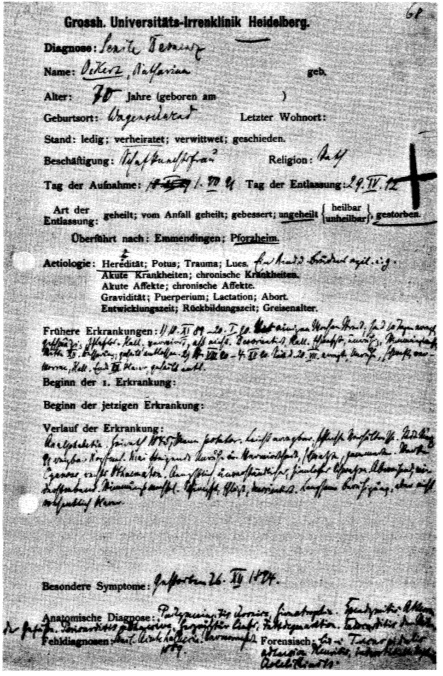
\includegraphics{./images/01-01/zahlkarten.jpg}

}

\caption{\label{fig-ZahlKarten}크레펠린이 직접 적은 진단카드
(Zählkarten)}

\end{figure}

크레펠린은 Kahlbaum이 기술한 파과증, 강직증, 편집증 개념을 모두 흡수한
조발성 치매라는 병명을 확고히한다. 그는 횡단면적 관찰만으로는
질병특이적(pathognomic) 증상이나 징후를 발견할 수 없으며, 오로지 종단적
경과 상의 특징을 함께 고려해야만 질병단위를 확인할 수 있다고 하였다.
그가 정신질환을 뇌병변에 따라 분류하고자 한 Griesinger의 염원에 거스른
것은, 원인이 되는 뇌병변을 찾기에는 당시의 학문수준이 따라오지 못한다는
반성이 있었기 때문이다. 이러한 철학은 1980년대 소위 신크레펠린 주의를
주창하는 미국 정신과 의사들이 DSM (Diagnostic and Statistical Manual of
Mental Disorders)을 만들게 된 이론적 근거가 되었다.

크레펠린은 5판 교과서부터 정신질환을 모두 13개의 큰 범주\footnote{\textbf{Kraepelin's
  1899 Classification:} 1) infectious insanity, 2) exhaustion insanity,
  3) intoxications, 4) thyrogenous insanity, 5) \textbf{dementia
  praecox}, 6) dementia paralytica, 7) insanity with cerebral disease,
  8) involutional insanity, 9) \textbf{manic-depressive insanity}, 10)
  paranoia, 11) general neuroses, 12) psychopathic states (degenerative
  insanity), 13) defective mental development}로 나누었으나, 학계의
주목을 받은 것은 조발성 치매와 조울정신병 둘 뿐이었다. 조울정신병 개념은
살페트리에 병원의 정신과 의사였던 Falret\footnote{\textbf{Jean-Pierre
  Falret (1794\textasciitilde1870)}: 프랑스의 정신과 의사.
  순환정신병(folie circulaire)의 개념을 창안했다.}와
Baillarger\footnote{\textbf{Jules Baillarger (1809\textasciitilde1890)}:
  프랑스의 정신과 의사. Falret와는 독립적으로 조울병 환자 증례를
  보고하였으나, Farlet의 발표가 좀더 앞선다. Baillarger는 오히려
  대뇌피질이 6개의 세포층으로 구설되어 있음을 발견한 것으로 유명하며,
  6개 세포층 중 신경섬유로만 구성된 층을 ``bands of Baillarger''라고
  부른다.}에게로 거슬러 올라간다. 크레펠린은 단극성 장애와 양극성 장애의
구분없이 모든 정서적 요소를 갖는 광증은 단일한 질환이라 보았고, 이는
조발성 치매에 비해 훨씬 양호한 경과를 보인다고 주장하였다. 크레펠린의
주장은 학자들 사이에 상당한 반향을 불러일으켰다. 단순하면서도 우아하고,
더군다나 탄탄한 임상자료를 통해 얻어진 그의 분류는 빠른 시간안에
전유럽으로 확산되었다. 그러나 한편으로 조발성 치매 진단을 내린다는 것은
너무나 가혹한 것이 되어버렸다. 유서 깊은 가문들은 자기 혈통 중에 환자가
발생하면 이를 비밀에 붙이느라 바빴고, 신경쇠약 혹은
신경증(neurosis)이라는 진단으로 진실을 가렸다. 뇌의 병변이라는
의미에서의 neurosis가, 광증은 아니라는 의미의 neurosis로 의미가 전환된
것도 이러한 사회적 요구때문이었다.

그러나 모든 조발성 치매 환자가 회복을 하지 못했던 것은 아니었다.
크레펠린이 수집한 사례에서도 1/4에 해당되는 환자는 어느 정도 회복을
하였으며, 그가 완성하지 못했던 9판 교과서 원고에는 궁극적으로 회복하여
정상 생활을 하는 증례들이 소개되어 있다. 크레펠린은 자신의 교과서를 여러
차례 개정하면서, 동료 의사들의 비판을 수용하여 질병의 개념과 이름을
변화시켰다. 말년에 나온 8판 교과서는 블로일러의 조현병 개념을
받아들였으며, 역시 블로일러가 제안한 단순 정신병(simple type) 개념도
추가하였다. 조발성 치매의 개념은 20년 이상에 걸쳐 수정, 보완되면서,
처음의 엄격하고 제한적인 개념에서 경계가 불분명하고 포괄적인 개념으로
변모하게 된다. 그러다보니 크레펠린의 교과서 8판에는 무려 10개의 아형이
기술되었고, 또 다시 이질적인 진단의 집합체가 되어버렸다.

\hypertarget{references}{%
\section*{References}\label{references}}
\addcontentsline{toc}{section}{References}

\markright{References}

\hypertarget{uxbe14uxb85cuxc77cuxb7ecuxc640-uxc815uxc2e0uxbd84uxc5f4uxbcd1}{%
\chapter{블로일러와
정신분열병}\label{uxbe14uxb85cuxc77cuxb7ecuxc640-uxc815uxc2e0uxbd84uxc5f4uxbcd1}}

Bleuler and Schizophrenia

\hfill\break

한편 블로일러\footnote{\textbf{Eugen Bleuler (1857\textasciitilde1939)}:
  스위스의 정신과 의사. Burghölzli에 위치한 쮜리히 대학에서 교수로
  재직하였다. Schizophrenia라는 명칭과 함께, autism, ambivalence 등의
  용어를 명명하였다. 프로이트와 융의 영향을 받아 조현병을
  정신분석학적으로 이해하려 애썼으나, 프로이트의 정신분석 이론에
  대해서는 교조주의적이라고 비판하였다. 아들인 Manfred Bleuler 역시
  정신과 의사이다.}는 조발성 치매가 회복 불가능하다는 견해를 맹렬히
비판하였다. 당시에는 이미 프로이트, 융의 정신분석학이 큰 파장을
불러일으키고 있었으며, 특히 융과 함께 수학했던 블로일러는 광증에도
심리적 의미가 있을 것이라고 생각하였다. 그는 심리 내부에는 다양한
정신기능을 하나로 아우르는 통합적 기능이 있는데, 조발성 치매환자는 이
기능이 손상되었을 것이라고 여긴다. 이 기능을 엿볼 수 있는 것 중 하나가
사고와 언어에서의 연상 과정이다. 연상 이론이란 흄\footnote{\textbf{David
  Hume (1711\textasciitilde1776)}: 스코틀랜드의 철학자이자 경제학자.
  스코틀랜드 계몽주의를 탄생시켰다. 단순 관념이 유사성, 인접성, 인과관계
  등을 매개로 서로 연합하여 복합 관념을 이룬다는 관념 연합론을 주장한다.}이나
밀\footnote{\textbf{James Mill (1773\textasciitilde1836)}: 영국의
  철학자이자 심리학자. 흄의 계보를 잇는 스코틀랜드 철학자이다. John
  Stuart Mill의 아버지이다. 그의 관념 연상 이론에 따르면, 두 가지 감각적
  인상이나 관념이 연달아 경험되면, 그 중 하나의 인상이나 관념만
  부여되어도 나머지 인상이나 관념이 저절로 연상된다.}과 같은 스코틀랜드
철학자들에게로 거슬러 올라가는데, 블로일러는 조현병 환자의 주된 병리적
특징이 이러한 연상 과정의 와해에 있다고 주장하였다.

광증이 정신기능의 파편화와 통합의 상실에 있다는 개념은, 오랜
서양전통사상 속에 그 뿌리를 두고 있다. 칸트에 따르면 인간은 육체와
정신이라는 근본적 균열 이외에도, 자유의지와 결정론, 실제(noumenal)와
현상(phenomenal)이라는 근원적인 균열 속에서 기적적인 통합을 이루고 있는
존재이다. 과학적 맥락에서 인간의 이중성이 논의된 것은 1844년으로 거슬러
올라간다. 영국의 의사였던 Wigan\footnote{\textbf{Arthur Ladbroke Wigan
  (1785\textasciitilde1847)}: 영국의 의사이자 작가. 1844년
  \emph{``마음의 이중성(The Duality of Mind)''}이라는 책을 펴냈다.}은
인간의 좌우 뇌에는 각각 서로 상충하는 의지가 자리잡고 있다고
주장하였다.{[}@Clarke1987-xu{]} 뒤이어 Wernicke\footnote{\textbf{Carl
  Wernicke (1848\textasciitilde1905)}: 독일의 정신과 의사.
  티아민(thiamine) 결핍에 의해 일어나는 특정 뇌병증(Wernicke
  encephalopathy)과, 운동성 실어증에 대비되는 수용성 실어증(Wernicke's
  aphasia)에 대한 연구로 유명하다. 신경해부학과 신경병리학에 대한 경험을
  바탕으로 질환이나 증상이 어떻게 특정 뇌 부위와 연결되어 있는 지
  밝히고자 하였다.}는 고위정신기능과 하위정신기능을 구분하였고, 이는
다윈의 진화론의 영향력을 등에 업고 현재까지도 널리 받아들여지고 있다.
19세기 말 히스테리와 최면요법의 등장으로 말미암아 무의식의 존재가
가정되었고, Janet\footnote{\textbf{Pierre Janet
  (1859\textasciitilde1947)}: 프랑스의 심리학자이자 정신과 의사. 과거의
  트라우마가 전의식에 묻혀 있으면서 현재까지 영향을 끼친다는 이론을
  세웠다. 해리, 전의식, 라포 등의 개념을 제안하였고, 프로이트 이전에
  이미 전의식을 분석함으로써 치료를 시도할 수 있음을 보여주었다.}는
정신을 통합하는 기능의 약화로 말미암은 해리 현상을 제안하였다.

이러한 정신기능의 파편화, 분절화라는 개념 속에서 Wernicke는 조현병을
``dementia sejunctiva''라고
불렀으며\protect\hyperlink{wernicke-kleist-leonhard}{(1장 1-10절 참조)},
유사한 맥락에서 dissociative psychosis, dementia dissociativa 등의
병명들이 잠시 등장하였다. 이런 맥락에서 블로일러는 퇴행 개념을 대신하여,
분절과 통합이라는 개념을 통해 조현병을 이해하고자 하였다. 이는 그가
\textbf{``정신분열병(schizophrenia)''}이라는 이름을 제안한 배경이 된다.

블로일러는 증상을 포함한 조현병의 외적인 표출양상은 결코 병을 이해하거나
진단하는데 핵심이 될 수 없다고 주장하였다. 그는 환자의 정신과정을
꿰뚫어봄으로써 독특한 형태로 약화되어 가는 현상을 잡아내야 한다고
하였다. 그는 조현병의 핵심 현상으로 \textbf{근본증상(fundamental
symptom)}과 \textbf{부수증상(accessory symptom)}을 구분하였으며, 전자에
해당하는 예로 ``\textbf{4A''} 즉 1) 연상의 와해(loosening of
association) 2) 정서의 둔마(affective flattening) 3) 자폐(autism) 4)
양가감정(ambivalence)을 제시하였다. 이에 비해 망상, 환청과 같은
부수증상은 이러한 근본 병리에 대한 개인의 심리적 반응으로서 그
중요성에서 뒤쳐진다고 보았다. 그는 부수증상의 의미는 정신분석적 접근을
통해 이해가능하지만, 부수증상의 이해만 갖고는 근본증상을 설명할 수
없다고 보았다. 근본증상은 아마도 뇌의 기질적 변화에 의할 것이며, 동시에
이러한 기질적 변화는 매우 다양할 것이다. 즉 다양한 기질적 이상이 다양한
부수증상을 낳게 되는 셈이지만, 그 중간에 4A로 대표되는 근본증상을 매개로
거친다면, 이를 정신분열병이라고 진단할 수 있다고 믿었다.

그는 조현병이 결코 회복될 수 없는 암울한 질병이라는 견해를 받아들이지
않았기 때문에, 조발성 치매보다는 정신분열병이라는 이름을 지지하였다.
한편 크레펠린은 Kahlbaum의 파과증, 강직증, 편집증을 조발성 치매의
아형으로 삼았는데, 블로일러는 여기에 단순형(simple schizophrenia)이라고
하여, 전형적인 정신병적 증상이 드러나지는 않지만 4A에 해당되는
근본증상을 보이는 경우를 추가하였다.

정신분열병이란 연상의 와해 혹은 지성과 감성의 분절화라는 근본증상을
포현하기 위해 사용된 용어이다. 그러나 이는 뜻하지 않은 오해를 불러오기도
하였다. 1889년 Mitchell\footnote{\textbf{Silas Weir Mitchell
  (1829\textasciitilde1914)}: 미국의 의사이자 작가. 신경과 및 정신과
  질환에 관심이 많았으며, 정신과 환자에게 ``휴식 요법(resting cure)''을
  제공한 것으로 유명하여 ``Dr Diet and Dr Quiet''이라는 별명이 붙여졌다.
  1889년 ``\emph{Mary Reynolds: A Case of Double Consciousness}''라는
  책을 발표하여 큰 반향을 이끌어내었다.}은 미국 최초의 다중인격장애
사례로 꼽히는 Mary Reynolds의 이야기를 책으로 펴냄으로써 다중인격에 대한
미국인의 유별난 관심을 촉발시켰다. 이후 정신분열병은 인격의 분열 즉
다중인격으로 오해되는 경우가 많았다. 또한 정신분석가들에게
정신분열병이란 자아(ego)의 약화로 인한 정신기능의 분절화를 의미했으며,
Laing\footnote{\textbf{Ronald David Laing (1927\textasciitilde1989)}:
  스코틀랜드 출신의 영국 정신과 의사. 1960년 ``분열된 자기(The Divided
  Self)''를 출판한 후 반정신의학의 정신적 지도자가 되었고, 유명세를
  탔다. 그는 정신과 질환의 의학적 모델에 반대하였다. 조현병 역시 가상적
  이론일 뿐 실제하지 않는다고 하였으며, 약물치료에도 반대하였다.}과 같은
반정신의학(anti-psychiatry) 추종자에게는 개인의 내적욕망과 사회적 압박
속에서 인격의 분리가 일어난 상태를 의미하기도 하였다.

1911년 블로일러가 처음 정신분열병이란 개념을 내어놓았을때만 해도 그
영향력은 매우 미미하였으나, 얼마지나지 않아 미국을 중심으로 급속도로
확대되었고, 대신 크레펠린의 조발성 치매 개념은 점차 영향력을 상실하였다.
이러한 극적인 전환은 당시 정신의학의 시대적 배경을 고려하면 쉽게 이해할
수 있다. 크레펠린은 조발성 치매를 진단하기 위해선 질병의 장기적 경과를
관찰해야 한다고 했지만, 환자를 처음으로 마주한 정신과 의사는 단면적
증상과 당시까지의 짧은 경과를 보고 진단을 내려야만 했다. 이런 와중에서
블로일러의 관찰은, 환자와의 깊은 면담 속에서 진단의 단서를 찾아낼 수
있다는 가능성을 제시해 주었다. 다만, 정신과 의사들이 자신이 환자의
핵심을 꿰뚫었다고 자신한 나머지, 미국의 조현병 진단율이 전세계에서 가장
높아지는 사태가 발생하였다.

정신분열병 개념이 지지를 받은 또 다른 요인은, 당시 급물살을 타고 있던
정신분석학적 이론을 적용시켰다는 점이다. 블로일러는 환자의 환각이나
망상이 중요한 의미를 갖고 있으며, 이들은 개개인의 무의식적 갈등을
나타내며 동시에 프로이트가 제안한 방어과정을 통해 생겨난다고 보았다.
이러한 생각은 당시의 미국 정신의학을 주도했던 유태인 정신분석가들
사이에서 이견없이 받아들여진 요인 중 하나이다.

크레펠린과 블로일러의 접근 방식은 명칭의 차이에서만 그치지 않는다.
크레펠린은 어디까지나 조현병의 정체에 대해서는 ``아직 모른다''는 관점을
고수하였다. 그렇기 때문에 순수히 통계적 데이터를 분류하는 방식으로
질병분류학에 접근하였고, 조현병을 일으키는 원인이나 병을 이해하는 이론에
대해선 언급을 피하였다. 반면 블로일러는 조현병의 기저에 어떤 핵심병리가
있고, 환자에게서 나타나는 다양한 증상은 이 핵심병리가 상황에 따라 다르게
나타나는 것 뿐이라고 보았다. 그는 정신분석학을 차용하여 조현병을
이해하는 이론적 틀을 제시하였다. 현재까지도 두 가지 접근방식은 서로
대립하고 있다. DSM은 전적으로 이론중립적 입장을 택하고 있지만, 그렇기
때문에 가열찬 비판을 받고 있다. 블로일러 이론은 정신분석학이 점점
영향력을 잃어가면서 함께 퇴색되어 갔지만, 조현병의 핵심 병리를 찾고자
하는 열망은 전혀 시들지 않았다. 당시에 정신분석학이 차지하던 자리를
지금은 생물정신의학이 대신 차지하고 있다. 그러나 크레펠린의 지적처럼,
아직도 조현병을 정복하기에는 학문수준이 미치지 못하는 지도 모른다.

\hypertarget{sec-ununderstandability}{%
\section{야스퍼스와 요해불능성}\label{sec-ununderstandability}}

야스퍼스\footnote{\textbf{Karl Jaspers (1883\textasciitilde1969)}:
  독일의 철학자로 하이데거와 함께 독일 실존철학을 창시하였다. 의학을
  전공하였으나 정신분석, 심리학을 거쳐 철학을 연구하게 되었으며, 불과
  30세의 나이에 \emph{``일반정신병리학 총론(Allgemeine
  Psychopathologie)''}을 저술하여 정신병리학의 기초를 다졌다. 그러나
  38세 때 건강상의 이유로 환자를 보는 일은 중단하였다. 2013년 세계
  정신의학계는 일반정신병리학 총론 출간 100주년을 맞이하여 대대적으로
  그의 업적을 회고하는 기회를 가졌다.}는 미리 설정된 모든 이론을
배제하고 환자의 경험을 있는 그대로 기술하고, 체계화하는
기술정신병리학\footnote{\textbf{기술정신병리학 (descriptive
  psychopathology)}: 정신병리학은 정신질환 환자가 보이는 증상과 징후를
  정의하고 분류하는 학문을 가리키는데, 크게 해석정신병리학과
  기술정신병리학으로 나눌 수 있다. 전자는 정신병리의 발생원인과 기전을
  특정한 이론(예. 정신분석, 행동주의, 실존주의 등) 가설에 기반하여
  해석하는 것이며, 후자는 순수히 환자를 외부에서 관찰한 사실과 환자의
  주관적, 현상학적 경험을 기술, 묘사하는 것이다. 이는 지각에 등장하여
  인간이 경험하게 되는 현상이란 객관적 외부 현실과는 구분된다는 현상학적
  전제에 기반하고 있다.}의 기초를 닦았다.(3장 1-4참조) 그는 환자의
경험은 자연과학에서 사용되는 인과관계적 \textbf{설명(explain)}의 대상이
아니라, 어떤 사고 과정을 거쳐 현상태에 도달하게 되었는지, 그 내적경험을
공감적으로 따라가는 \textbf{이해(understand)}\footnote{옛문헌에서는
  \textbf{이해}를 다른 말로 \textbf{요해}(了解, verstehen)라고도 부른다.}의
대상이라고 하였다. 야스퍼스는 조현병 그 자체에 대해서는 깊이 논하지
않았지만 정신병적 과정의 핵심은
\textbf{요해불능성(un-understandibility)}이라고
강조하였다.{[}@parnas2013{]} 즉 환자가 현 증세에 이르게 된 과정 중에서
치료자의 합리적 이성을 통해 도저히 그 전개과정을 이해할 수 없는 단계가
있다면, 이는 요해불가능에 해당된다. 정신병적 과정은 정상적인 인격
발전과는 이질적인 전혀 다른 방향의 전개이며, 비가역적이고 진행성인
(기질적) 병적 과정에 의하여 생긴다. 그는 블로일러와 마찬가지로, 굳이
증상의 종적 경과를 관찰하지 않아도, 횡적인 증상발현에서 요해불가능성을
찾으면 정신병적 과정이 일어나고 있음을 확신할 수 있다고 하였다.

\begin{figure}

{\centering \includegraphics{./images/01-01/img_2.png}

}

\caption{\label{fig-jaspers-hierarchy}야스퍼스의 위계적 진단 원칙}

\end{figure}

야스퍼스는 정신병적 과정을 중시했기 때문에, 조현병이라는 질병분류학적
단위의 진단에는 큰 비중을 두지 않았다. 그는 애초에 정신병리는 겉으로
드러나는 객관적 징후가 아니라, 내성(introspection)을 통해 인식하는
주관적 증상으로 파악하는 것인데, 이를 통해 객관적 진단을 내린다는 것을
탐탁치 않게 보았다. 그는 정신질환을 서열이 있는 세 개의 그룹(I: 기질적
정신병, II: 내인성 정신병, III: 신경증-인격장애)으로 나누고, 상위 서열의
진단이 내려지면 하위 서열의 진단은 내리지 않는 것을 원칙으로
하였다.(그림~\ref{fig-jaspers-hierarchy}) 예를 들어 불안을 호소하는
환자라도, 진찰과정에서 요해불가능한 사고과정이 드러나면 그룹 II의 조현병
진단이 내려지며, 그룹 III의 불안장애 진단은 내리지 않는다. 한편 그는
같은 그룹 내부에 속한 질환들의 감별진단은 잠정적일 수 밖에 없다. 진단은
인간이 필요에 따라 임의적으로 선을 긋는 행위이지, 자연적 종은 아니라고
보았다.{[}@Ghaemi2009-ek; @Sass2013-fu{]}

야스퍼스의 생각을 곧이 곧대로 받아들인다면, 진단내리는 의사의 본분은
정신병적 과정을 찾아내는 것이지, 분명한 선긋기를 행하는 것이 아니라고
보았다. 겉으로 드러나는 각양각색의 증상에 매몰되지 않고, 그 아래
숨어있는 본질을 꿰뚫고자 한다는 점에서 블로일러와 맥을 같이한다.

\hypertarget{sec-schneider-first-rank}{%
\section{슈나이더와 일급 증상}\label{sec-schneider-first-rank}}

슈나이더\footnote{\textbf{Kurt Schneider (1887\textasciitilde1967)}:
  독일 정신과 의사로 조현병의 진단과 반사회적 인격에 대한 연구로
  유명하다. 나찌에 협력하기를 거부하고 학계를 떠났다가 2차 대전이 끝난
  후 하이델베르크 대학의 교수로서 독일 정신의학의 재건에 힘썼다. 1946년
  처음 발간된 그의 저서 \emph{``임상정신병리학(Klinishce
  Psychopathologie)''}은 1967년 그가 사망할 때까지 꾸준히 개정되었다.
  특히 이 책은 1996년 이부영, 한오수 공역으로 한글판이 나왔는데 이는
  14판을 번역한 것이었다.{[}@1996-jj{]} 마지막 15판은 2007년 독일어로
  발간되었다.}는 야스퍼스와 함께 하이델베르크 대학에서 함께 연구한
동료로 하이델베르크 학파를 만든다. 그는 야스퍼스의 견해를 따라 조현병에
대해 명확한 정의를 내리기 보다는, 임상적 방법론에 의해 좀더 진단의
신뢰도를 높이는 방법을 고안하였다. 한편 블로일러나 야스퍼스와는 달리
신체적 원인 혹은 핵심 병적과정 등에 대한 가설적 개념은 진단에 사용하지
말 것을 권하였다.

그의 공헌 중 가장 유명한 것은 아마도 \textbf{``일급 증상(first rank
symptom)''}일 것이다.(표~\ref{tbl-first-rank}) 분명히 해야할 것은
블로일러의 근본증상과 부수증상의 개념과는 달리, 일급 증상이 질병의
핵심이고 2급 증상은 그에 대한 반응일 뿐이라는 주장은 어디에서도 찾아볼
수 없다는 것이다. 일급 증상이 존재하고, 이를 설명할만한 기질적 질환을
찾아낼 수 없다면 조심스레 조현병으로 진단할 수 있다. 이는 민감도보다는
특이도가 높은 개념이기 때문에, 일급증상이 있으면 조현병일 가능성이 확
올라가지만, 없다고 해서 조현병이 아니라고는 말하지 못한다.

\hypertarget{tbl-first-rank}{}
\begin{longtable}[]{@{}
  >{\raggedright\arraybackslash}p{(\columnwidth - 0\tabcolsep) * \real{1.0000}}@{}}
\caption{\label{tbl-first-rank}슈나이더가 나열한 1급
증상들}\tabularnewline
\toprule()
\begin{minipage}[b]{\linewidth}\raggedright
List of First rank symptoms suggested by Kurt Schneider
\end{minipage} \\
\midrule()
\endfirsthead
\toprule()
\begin{minipage}[b]{\linewidth}\raggedright
List of First rank symptoms suggested by Kurt Schneider
\end{minipage} \\
\midrule()
\endhead
Audible thoughts (voices speaking out his thought aloud) \\
Voices arguing (referring to the patient in 3rd person) \\
Voices commenting on one's action \\
Somatic passivity (experiencing externally controlled body changes) \\
Thought withdrawal \\
Thought insertion \\
Thought broadcasting \\
Made volition \\
Made affect \\
Made impulse \\
Delusional perception (a real perception elaborated in a delusional
way) \\
\bottomrule()
\end{longtable}

일급 증상은 크게 세가지 범주로 나누어진다. 첫째는 특별한 환청의
양상이며, 둘째는 사고와 행동에서 자신의 의지를 침범당했다고 느끼는 수동
경험(passive experience)이다. 마지막 셋째는 정상적 지각을 망상으로
해석하는 망상적 지각이다.

슈나이더가 어떻게 이들 증상을 추출했는지에 대해선 자세한 언급이 없다.
통계적 데이터로 뒷받침된 것도 아니다. 다만 이런 기준을 적용했을 때
진단율이 높아졌다는 언급만 나와있다. 아마도 슈나이더가 이들 증상을
뽑아낸 것은 야스퍼스의 영향이 컸을 것이다. 야스퍼스는 의식에는 두 가지
종류가 있다며, 이를 ``자아/자기-의식(ego/self consciousness)''과
``대상-의식(object consciousness)''으로 나누었다. 자아-의식은 다음과
같은 특징 혹은 기능을 갖는다.{[}@Fuchs2013-in{]}

\begin{enumerate}
\def\labelenumi{\arabic{enumi}.}
\tightlist
\item
  대상 및 외부세계와 구분된 자기 자신을 의식하는 것
\item
  활동성 혹은 의지를 가진 주체(agent)로서의 느낌
\item
  시간이 흘러도 동일하게 유지되는 정체성의 느낌
\item
  심리적으로 단일한 한 명의 자기라는 느낌
\end{enumerate}

슈나이더는 야스퍼스의 자아-의식을 수용하여, 자신의 생각과 감정, 행동이
타인의 영향을 받거나 타인에 의해 조종되는 느낌을
``자아-장애(ego-disorders, 독어로는 Ich-Störungen)이라고
불렀다.{[}@Fuchs2013-in{]} 슈나이더거 언급한 일급 증상은 대체로
야스퍼스의 자아-의식이 흐려진 상태를 말하며, 특히 자아와 대상의 경계가
불분명해지는 현상을 묘사하고 있다. Frith\footnote{\textbf{Christopher
  Donald Frith (1942\textasciitilde):} 영국의 심리학자. 런던대학
  명예교수로 기능적 뇌영상을 통해 인지기능을 연구해왔다. 특히 인간의
  지각이나 사고가 하향식(top-down)으로 먼저 작업가설(working
  hypothesis)을 세워 미래를 예측하고, 이를 감각기관에서
  상향식(bottom-up)으로 올라오는 데이터와 비교하여, 실시간으로 오류를
  보정해나간다는 이론을 제안하였다.{[}@frith2013{]}}는 일급 증상을
자기-모니터링(self-monitoring)의 붕괴때문에 자신의 의지, 행동, 지각의
주체를 스스로에게 귀속하지 못하는 상태로 해석한다.{[}@Frith2000-nm{]}
자기-모니터링은 전전두엽에서 행하는 집행기능 중 하나이며, 현대에
들어와서도 조현병의 핵심 병리 중 하나로 여겨지고 있다. 슈나이더는 이를
내다보고 있었을런지도 모른다.

그러나 이후의 정신과 역사에서, 일급 증상은 슈나이더의 의도와 달리
지나치게 중요시된 경향이 있다. 일급 증상은 비교적 잘 정의되었고,
찾아내기도 쉬운 편이었다. 게다가 진단특이도를 높이다보니, 이후 세대에서
표준화된 진단도구를 만들고자 애쓰고 있을 때 가장 먼저 진단도구에
편입되었다. 일급 증상은 최초의 표준화 진단도구의 하나인
연구진단기준(Research Diagnostic Criteria, RDC){[}@Spitzer1978-uu{]} 및
현상태 검사(Present State Examination,
PSE){[}@Wing1967-ka{]}\textbf{\hspace{0pt}}에 편입되었다. 이후 DSM-III을
시작으로 DSV-IV-TR에 이르기까지, 일급증상은 조현병 진단기준에서 특별한
지위를 누리게 되었다.{[}@Shinn2013-nn{]} (\href{}{1장 2-2-2 절 참조})

그러나 진단이 점점 외적으로 드러나는 행동 거지를 중요시하고, 젊은 정신과
의사들 사이에서 체크리스트 식 진단의 경향이 늘어나면서 일급 증상이
누리는 지위에 대해 의문이 제기되었다.{[}@freudenreich2004;
@Peralta2020-qa; @Heinz2016-km{]} 일급 증상은 야스퍼스 식의 현상학적
접근과 공감을 통한 이해를 거쳐야만 짚어낼 수 있는 현상들이다. 환자가
호소하거나, 객관적으로 드러나는 증상, 징후와는 성격을 달리한다. 또한
진단특이도를 높여준다고는 하지만, 일급 증상을 보이지 않는 조현병 환자가
너무 많으며, 처음 예상과 달리 조현병 이외 정신병에서도 종종
나타난다.{[}@Rosen2011-gs{]} 마지막으로, 일급 증상을 보인다고 해서
그렇지 않은 경우와 예후가 다른 것도 아니다.{[}@Peralta2020-qa{]} 이에
DSM-5는 일급 증상의 지위를 없애고 여타 증상과 동일한 수준으로
끌어내렸다.{[}@Heinz2016-km{]}

\hypertarget{uxd604uxc0c1uxd559uxc801-uxc778uxb958uxd559uxc801-uxc2dcuxac01}{%
\section{현상학적-인류학적
시각}\label{uxd604uxc0c1uxd559uxc801-uxc778uxb958uxd559uxc801-uxc2dcuxac01}}

대한조현병학회는 ``정신분열병''이라는 명칭이 선입관 및 편견을 낳는
주요한 요인이라 판단한 끝에, 2011년 이를 대신할 새로운 병명으로
\textbf{``조현병''}을 선정하였다.{[}@2011-ub{]} 새롭게 탄생한
``조현병''이라는 명칭에서 ``조현(調絃)''은 원래 ``현악기의 줄을
고르다''는 뜻으로, 정신을 구성하는 각각의 하부 기능들이 유기적으로
통합되어 조화로운 화음을 이룬다는 의미로 사용되었다.

그런데 ``조현(調絃)''의 영문표기인 \textbf{``Attunement disorder''}는
공교롭게도 짧지 않은 역사를 지니고 있으며, 조현병의 개념을 이해하기 위해
일군의 유럽 정신의학자들이 오랜동안 사용해온 중요한 용어이다. 이들을
소위 \textbf{현상학적-인류학적 정신의학(Phenomenological Anthropological
Psychiatry)}이라고 부른다. 이들은 상호주관성(intersubjectivity)의
붕괴로부터 발단된 셀프의 장애(ipseity)가 조현병의 근간을 이루며, 망상,
환청 등의 외적 증상들은 셀프의 장애로부터 파생된 이차적인 증상일
뿐이라고 주장한다.

현상학적-인류학적이라는 기치와 ``조현(attunement)''이 왜 연관되는지
의아해 보이지만, ``attunement''란 표현이 원래 하이데거\footnote{Martin
  \textbf{Heidegger (1889\textasciitilde1976)}: 독일의 철학자. 경력의
  전반기에는 대표적 저서인 ``존재와 시간''을 통해 현존재의 존재의미를
  탐구하는 실존론적 철학을 수립하였으며, 후반기에는 역사 속에서 존재
  자체가 인간에게 어떻게 스스로를 현시하는가를 다루었다. 20세기의 가장
  위대한 철학자의 한 사람으로 꼽히지만 나찌를 두둔하는 발언을 하는 등
  평가가 엇갈린다.}가 사용한 ``Befindlichkeit'' 혹은 ``Stimmung''을
영어로 직역한 것임을 감안하면 이해가 된다. 하이데거의 용례에서
``attunement''란 상호주관적 ``세계''에 속하게 된 개인이, 그 ``세계''
속에서 느끼는 전성찰적/전인지적 (pre-reflective/pre-cognitive) 감정을
의미한다. 따라서 ``Attunement disorder''란 상호주관성의 붕괴에서 비롯된
질병이라는 의미로 요약할 수 있다.{[}@2013-pe{]}

현상학적-인류학적 정신의학자들은 정상적인 주체성(subjectivity)은 1)
셀프경험(ipseity), 2) 세계 내에 내재하는 느낌(``Attunement''), 3)
타인과의 관계(상호주관성)라는 세 가지 축이 맞물리면서 유지된다고 본다.
이 중 어느 한쪽이라도 문제가 생기면 전체 구조의 붕괴가 초래되며, 그 결과
중 하나가 바로 조현병의 핵심이라고 주장한다. 현상학자들이 ``Attunement
disorder''라는 표현을 통해 강조하고자 하는 병리현상은, ``마음 이론''으로
불리우는 인지적 오류보다 더욱 광범위하고 근본적인 문제이다. 상호주관적
세계에 재편입하려면, 단순히 인지재활훈련을 통해 ``마음 이론'' 혹은
사회적 인지를 호전시키는 것만으로는 부족하다. 나와 너가 동일한 언어를
사용하고, 동일한 상식이 통용되어, 의사소통을 통해 마음을 나눌 수 있다 는
믿음이 없다면, 환자는 철저하게 고립될 것이다. Stanghellini\footnote{\textbf{Giovanni
  Stanghellini (1960\textasciitilde)}: 이탈리아의 정신과 의사. 키에티
  대학의 정신과학 교수로 재직하면서 철학, 윤리학, 심리학과 정신병리,
  신경과학을 통합하고자 노력해왔다.}가 묘사한 ``Attunement disorder''의
세계는 단순히 대인관계로부터 단절된 세계를 넘어, 자신의 육체로부터
분리되고(disembodied), 자신의 세계로부터 추방되어(disembedded), 지향할
곳을 잃어버린 낯설고 두려운 세계이다.{[}@2013-pe{]}

\hypertarget{sec-wernicke-kleist-leonhard}{%
\section{Wernicke-Kleist-Leonhard}\label{sec-wernicke-kleist-leonhard}}

크레펠린은 9판에 걸쳐 개정된 그의 교과서에서 여러 차례 용어의 정의와
개념을 수정한다. 초기에는 정신증(psychosis)이라는 용어를 모든 정신질환
전체에 대해 사용했으며, 말년에아 비로소 현대의 정신병적 장애를 가리키는
말로 사용하였다. 외인성, 내인성이란 말도 혼란스럽기는 마찬가지였다.
외인성이란 기질적이라는 의미로 사용되기도 하였고, 선천성 질환에
대조되어, 후천적으로 질병에 걸린 경우를 기리키기도 하였다. 조울정신병은
기질을 타고났다는 의미에서 내인성으로 분류되었으나, 조발성 치매는
처음에는 외인성으로 분류되었다. 1900년대 초만해도 크레펠린은 조발성
치매가 자가중독\footnote{\textbf{자가중독 (autointoxication)}:
  크레펠린과 동시대 정신과 의사 중 일부는 조발성 치매가 신체 일부분
  (특히 생식선과 소화기)에서 분비되는 독소때문에 뇌가 영향을 받아
  생긴다고 믿었다. 이 때문에 관장이나 맹장절제, 장일부 절제술이
  치료법으로 사용되기도 했으며, 생식선을 제거하여 거세시키는 방법도
  모색되었다. 이 이론은 오래전에 잊혀졌으나, 최근 장내 세균총(gut
  microbiome)과 구강내 세균총의 이상이 치매 및 조현병과 연관된다는
  주장이 부활하고 있다.{[}@szeligowski2020; @luc2021; @Martin2022{]}}
때문에 일어난다고 믿었기 때문이다. 크레펠린 사후 출간된 9판 교과서에
가서야 비로소, 두 질환은 나란히 내인성 정신증(endogenous psychosis)으로
분류되었다. 그가 의미한 내인성 정신증이란 외적 요인없이 신체 내부에서
일어난 병적 과정때문에 생기는 질환을 의미한다.

내인성 정신병의 개념이 조금씩 자리를 잡아가자, 이를 어떻게 분류할 지가
새로운 문제로 떠올랐다. 19세기 말까지 유행했던 단일정신병 개념은 일단
크레펠린의 분류체계에 의해 힘을 잃는듯 했다. 그러나 Kahlbaum의 파과증,
강직증, 편집증을 크레펠린이 하나로 묶은 것은, 모두 비가역적인 퇴행으로
이어진다는 표면적 공통점 밖에 없었다. 블로일러는 이들을 연상의 장애라는
공통점으로 묶어보려 했지만, 이는 오히려 조현병의 경계를 지나치게 넓히는
결과를 불러왔다. 이에 대조되어 Wernickle, Kleist 그리고 Leonhardt에
이르는 소위 프랑크푸르트 학파는 내인성 정신증을 최대한 세분하여 각각의
질환을 일으키는 해부학적, 유전학적 기전을 찾고자 하였다. 질병분류란
질병에 있어서의 자연적 종(\protect\hyperlink{modern-period}{1장 1-3절
참조})을 찾아내는 학문이고, 찾아진 질병(disease) 들은 각자만의 독특한
발병기전, 병태생리, 치료반응, 예후를 지니게 될 것이다. 프랑크푸르트
학파는 단일정신병 개념은 물론 크레펠린의 분류마저도 너무나
단순화되어있다고 비판했다. 조발성 치매로 진단되는 환자들은 너무나도
이질적인 양상을 보이기 때문에 도저히 하나의 자연적 종으로 보기 어려웠던
것이다.

Wernicke, Kleist 그리고 Leonhardt는 나치 정권이 들어선 독일, 그리고 패전
후 동독에서 활동하였기 때문에 이들의 업적은 오랜 동안 영어로 번역되지
못한채 묻혀있었다. 그러던 중 Leonhard가 생을 마감한 다음 해인 1989년,
국제 베르니케-클라이스트-레온하트 협회(International
Wernicke-Kleist-Leonhard Society)가 설립되면서 재평가가 시작되었고,
1999년에는 \emph{``Classification of Endogenous Psychoses and their
Differentiated Etiology''}이라는 제목의 단행본이 발간되어 본격적으로
영어권에 전파되기 시작하였다.{[}@Leonhard1999-mx{]} 당시 DSM은
신뢰도만을 중시한 나머지 안면타당도(face validity)를 희생시켰다는 비판에
봉착해있었다. 급부상하기 시작한 유전학과 뇌영상학의 발전, 그리고
1990년부터 시작된 뇌 연구의 10년\footnote{\textbf{뇌 연구의 10년 (decade
  of brain)}: 미국 대통령 부시는 1990년부터 1999년을 ``뇌 연구의
  10년''으로 정하여 뇌 연구를 지원함은 물론 그로 부터 얻어진 성과와
  혜택을 대중에게 널리 전파하고자 하였다. 이는 세계 각국으로 퍼져나가
  각국에서 유사한 뇌 연구 육성 사업을 벌이게 하였다. 이와는 별개로
  2013년 오마바 대통령은 브레인 이니셔티브(Brain Research through
  Advancing Innovative Neurotechnologies Initiative) 계획을 통해 막대한
  예산을 뇌과학에 투자하였다.}을 맞이하여 통계적 역학을 기반으로 한
분류가 아니라, 뇌신경 과학을 기반으로 한 분류가 필요해졌고, 이들이
완성한 분류 체계(WKL 분류체계)는 이에 맞물려 각광을 받았다.

Wernicke는 스승 Griesinger의 비젼을 따르면서도 신경해부학자이자
병리학자로서의 독자적인 통찰을 살려, 질환이나 증상이 어떻게 뇌 부위와
연결되어 있는 지 밝히고자 하였다. 하나의 뇌 기능이 단일한 뇌 부위에 의해
전적으로 행해진다면 연구가 수월할 것이다. 그러나, 그 자신도 인정하기를,
단순해 보이는 기능도 여러 뇌 부위의 긴밀한 연결을 통해 일어나는 것이
보통이다. 그는 뇌 부위들 사이의 연결이 붕괴되면, 정신 기능의 일부가
고립되면서, 기능을 잃거나, 통제를 벗어나거나, 비정상적인 기능을 보일
것이라는 견해를 내놓았고, 이를 ``Sejunktionstheorie (theory of
disjunction)''이라고 명명하였는다.{[}@Pillmann2007-gn 그는 한 가지 예로
연합신경이 분절되면서 이치에 맞지 않는 생각이 아무런 선행사고 없이 불쑥
떠오르는 것을 자생적 사고(autochthonous idea)라고 하였다. 이는
야스퍼스의 일차적 망상 개념에 영향을 주었다.{[}@Carota2019-sx{]}

Wernicke는 정신질환과 뇌 부위와의 연결을 밝히려면, 진단체계가 좀더
세분화되어야 한다고 주장하였다. 그렇게 세분화된 질환은, 비교적 국한된 뇌
부위의 손상때문이거나, 몇몇 부위의 연결관계가 무너졌기 때문일 것이다.
그는 전자를 초보적 증상(elementary symptom), 후자를 2차적 증상이라
하였다.{[}@Pillmann2007-gn{]} 이는 WKL 분류체계의 첫번째 실용적
원칙\footnote{\textbf{실용적 원칙 (heuristic)}: 반드시 합리적이거나
  이상적인 방법은 아닐지라도, 당장 주어진 문제를 대충이라도 해결하는데
  도움을 주는 원칙, 기법, 요령}이 되었다.

Wernicke의 제자인 Kleist\footnote{\textbf{Karl Kleist
  (1879\textasciitilde1960)}: 독일의 신경학자이자 정신과 의사. 인간의
  행동 및 정신기능과 이를 담당하는 뇌 영역을 짝지우는데 큰 업적을
  남겼다.}는 일차대전 중 전쟁터에서 머리를 다친 수많은 증례를 접하면서
스승의 이론을 발전시켰다. 그는 다양한 인지기능과 뇌부위를 연결시켰을 뿐
아니라 좀더 추상적인 정신증상 역시 해당되는 뇌부위를 찾으려 애썼다. 그는
오랜 세월 동안 동일한 환자를 추적관찰하면서, 단일한 질환이 질병 경과에
따라 여러가지 다른 모습으로 나타난다는 것을 관찰하였다. 이 과정을 통해
조울정신병을 단극성과 양극성으로 구분할 수 있었고, 이는 그의 가장 유명한
업적 중 하나가 되었다.{[}@Teichmann1990-yh{]}

Leonhard\footnote{\textbf{Karl Leonhard (1904\textasciitilde1988)}:
  동독의 정신과 의사. 동독의 훔볼트 대학 교수로 재직하였다. 내인성
  정신병의 복잡한 진단분류체계를 완성하였으나, 영미권의 학풍과 맞지
  않는다고 하여 학술지에 실리지 못했고, 저서들 역시 영어로 번역되지
  못했다. 사후에야 비로소 재조명되었다.}는 Kleist의 제자로 WKL
분류체계를 완성한다.(그림~\ref{fig-WKL}) WKL 분류체계는 이환된 뇌 부위,
종적 경과, 가족내 군집이라는 세가지 실용적 원칙을 통해
이루어진다.{[}@Foucher2020-ot{]} 이 원칙은 다음과 같이 요약될 수 있다.

\begin{enumerate}
\def\labelenumi{\arabic{enumi}.}
\tightlist
\item
  \textbf{초보적 증상 원칙 (elementary symptom principle)}: 하나의
  질환은 비교적 국한된 뇌 부위, 혹은 그러한 뇌 부위들의 연결에 이상이
  생겼기 때문에 일어난다.
\item
  \textbf{종적 경과 원칙 (longitudinal principle)}: 한 환자가 질병
  경과에 따라 다양한 양상을 보이더라도, 그는 하나의 질환에 걸린 것이다.
\item
  \textbf{가족내 군집 원칙 (familial aggregation principle)}: 가계에
  정신질환이 밀집되어 있다면, 그 구성원들은 동일한 질환에 걸린 것이다.
\end{enumerate}

\begin{figure}

{\centering \includegraphics{./images/01-01/img_4.png}

}

\caption{\label{fig-WKL}내인성 정신증(endogenous psychosis)에 대한 WKL
분류 시스템 {[}@Foucher2020-ot{]}}

\end{figure}

Leonhard가 정리한 WKL 체계에는 35개의 주요 정신증이 포함되게 되었으며,
내인성 정신증은 1) 체계적 조현병(systematic schizophrenia), 2) 비체계적
조현병(unsystematic schizophrenia) 그리고 3) 순환 정신증(cycloid
psychosis)으로 크게 나뉜다. 그리고 각군에는 몇 가지 아형 (subtype)을
두었다. ``체계적 조현병''은 대부분 서서히 증상이 발현되고 일찌기 정서의
둔화와 무감동 증상을 나타내며, 경과가 만성화되면서 인격의 황폐에 이른다.
``비체계적 조현병''은 급작스럽게 발병하며, 경과는 주기를 띠면서 악화,
호전을 반복하고, 만성화되어도 정서가 정상적으로 유지되고, 인격의
황폐화는 드물다. 마지막으로 순환 정신증은 임상 양상이 매우 변화무쌍하며,
주기성이 분명하고, 잔류증상없이 완전 관해에 이르는 경우가 많다.
Leonhard는 체계적 조현병과 순환 정신증의 경우 유전적 소인의 비중이 낮고,
비체계적 조현병은 상당히 높다고 보았기 때문에, 조현병의 유전학을
연구하는 학자들은 상당한 관심을 갖고 WKL 체계를 도입해보고자
하였다.{[}@Jablensky2006-ol; @Peralta2016-bf{]} 그러나 워낙 체계가
복잡하고, 타당도 증명에 대한 연구도 답보상태에 머물러 있어서 영어권에서
널리 전파되기는 어려울 것으로 보인다.

\hypertarget{references-1}{%
\section*{References}\label{references-1}}
\addcontentsline{toc}{section}{References}

\markright{References}

\hypertarget{uxadfcuxb300uxc801-uxc870uxd604uxbcd1-uxac1cuxb150uxacfc-dsm}{%
\chapter{근대적 조현병 개념과
DSM}\label{uxadfcuxb300uxc801-uxc870uxd604uxbcd1-uxac1cuxb150uxacfc-dsm}}

Modern Concept of Schizophrenia and DSM

\hfill\break

미국 정신의학회(American Psychiatric Association, APA) 회장을 지낸
Meyer\footnote{\textbf{Adolf Meyer (1866\textasciitilde1950)}: 스위스
  태생의 미국 정신과 의사. 존스 홉킨스 대학 교수이자, 부속 병원의 수석
  정신과 의사로 역임하면서, 1913년에는 Henry Phipps 정신의학 진료소
  개원을 이끌었다. 1927-28년에는 미국 정신의학회 회장을 역임하였다.}는
크레펠린의 분류 시스템에 감명을 받아 이를 미국에 최초로 도입하였지만,
정신분석가로서 역설적으로 블로일러의 개념을 정착시킨 인물이기도 하다.
블로일러의 개념이 발표되기도 전에 이미 그는 조발성 치매는 생물학적
요인을 갖고 있는 환자가 심리사회적 상황에 적응하면서 형성되는
\textbf{``반응(reaction)''}이라고 생각하였다. 이는 모든 정신질환은
생물학적, 심리학적, 사회학적 맥락에서 고려되어야 한다는
심리생물학(psychobiology) 이론의 토대가 된다.

따라서 그가 1913년 Phipps 클리닉\footnote{\textbf{Henry Phipps
  Psychiatric Clinic}: 볼티모어에 위치한 존스 홉킨스 의과대학의 부속
  정신과 병원. 철강 사업가 였던 Henry Phipps Jr.의 기부로 설립되었다.}을
설립하면서 개막식 연자 중 한명으로 블로일러를 초대한 것은 우연이 아닐
것이다. Phipps 클리닉은 미국 최초로 ``\textbf{schizophrenia''}라는
진단명을 사용하기 시작하였다. 초창기에는 조발성 치매와 정신분열병 개념이
혼재되면서, 4A 증상을 보이며 증상이 그리 심하지 않은 환자에게는
\textbf{``정신분열적 반응(schizophrenic reaction)''}이라는 진단이
붙여지고, 퇴행이 명백한 경우에는 조발성 치매라는 진단을 붙여지곤 하였다.

그러나 정신분열병 개념이 승리한 결정적인 계기는 미국 정신의학 대부로서의
Meyer의 정치적 지위와 함께, 나찌의 권력 장악과 유대인 박해에 있었다.
블로일러와는 대조적으로 크레펠린은 자신의 민족주의적 정치색을 마음껏
드러내었고, 크레펠린의 분류를 받아들이는 것은 친나찌 성향을 드러내는
것으로 분위기가 반전되었다. 1918년 미국 정신의학회의 전신인 American
Medico-Psychological Association (AMPA)은 조발성 치매 대신 정신분열병을
사용할 것을 공식화하였고, 그와 함께 블로일러가 제안하고 Meyer가
지지하였던 단순 조현병 및 잠재 조현병 개념 역시 공식적으로 인정된다.
이렇게 해서 ``정신분열병''의 시대가 열리게 되었다.

\hypertarget{sec-dsm-constitute}{%
\section{DSM의 제정}\label{sec-dsm-constitute}}

전통적으로 독일권 정신의학자들은 기술과 분류(description and
classification)에 열정적이었다. 당시의 의학 학술지는 상세한 증례를
보고하는 논문이 넘쳐났고, 현상학 전통을 물려받은 의학자들은 정신분석과는
또 다른 의미에서 환자의 심층적 경험을 추적하였다. 반면 실용주의에
기울어있던 미국 정신의학자들은 이론보다는 환자를 돌보는데 집중한 나머지,
정확한 진단을 내리거나 질병의 정체를 숙고하는데는 그다지 관심이 없었다.
따라서 미국 최초의 진단분류체계가 연구를 위해서가 아니라 행정적 필요에
의해 탄생했다는 사실은 그리 놀랄 일이 아니다.

애초에 AMPA는 통계청의 위탁을 받아 미국 전역에 흩어진 정신병원의 현황을
조사한다는 기본 계획을 세웠다. 1921년 AMPA는 미국 정신의학회(American
Psychiatric Association, APA)로 이름을 바꾸고, 본격적으로 분류체계의
기초를 닦기 시작하였다. 바야흐로 2차 대전이 끝나자, 미 육군은 재향
군인을 대상으로 정신질환 현황과 정신건강 서비스 수요를 조사하는 과업을
APA에 의뢰하였다. 마침 1948년 국제보건기구(World Health Organization,
WHO)에 의해 발표된 국제질병분류(International Classification of Disease,
ICD) 6판은 최초로 정신질환에 대한 챕터를 포함하고 있었고, 미국
정신의학회는 이를 보완하는 수준에서 1952년 정신질환 진단 및 통계
편람(Diagnostic and Statistical Manual of Mental Disorders, DSM)을
내어놓는다.(그림~\ref{fig-dsm-i})

\begin{figure}

{\centering 
\includegraphics[width=0.6\textwidth,height=\textheight]{./images/01-02/dsm-i.jpg}

}

\caption{\label{fig-dsm-i}1952년 발간된 DSM-I의 표지 (Wikipedia에서
발췌)}

\end{figure}

Meyer의 영향 하에 첫번째 DSM에서는 환경적인 원인을 염두에 두어 정신증
진단과 관련된 용어에는 \textbf{``반응(reaction)''}이라는 표현이 반드시
포함되었다.{[}@Grob1991-ul{]} 따라서 조현병은 \textbf{``정신분열적
반응''}이라 불리워졌다. Meyer를 비롯한 정신분석가들은, 정신질환은
생물학적, 심리적, 사회적 요소의 통합체로서의, 개인이 자신을 둘러싼
환경이나 닥쳐진 상황에 제대로 적응하지 못했기 때문에 생긴다고
보았다.{[}@Lidz1985-gv{]} 이는 단일정신병 개념에 접근하고 있다는 점에서,
크레펠린 식 질병단위 개념을 부정한 것으로도 생각할 수 있다. 진단
분류표가 나왔다고 하지만, 당시에는 조현병의 정의 자체가 모호했고, 감별
진단에 대한 언급도 없었으며, 구체적인 진단기준도 제시되지 않았다.

\hypertarget{dsm-ii}{%
\subsection{DSM-II}\label{dsm-ii}}

1960년대에 들어서면서 미국 정신의학은 서서히 Meyer의 영향으로부터
벗어났지만 여전히 미국 정신의학회의 주도권을 쥐고 있던 것은 역동
정신의학과 정신분석학파였다. 1967년 WHO는 정신장애 분류를 대폭 수정한
ICD-8을 출간했다. 정신장애는 1) 정신증, 2) 신경증, 인격장애 및
비정신병적 정신장애, 3) 정신지체의 세 가지로 대별되었다. 1968년 미국
정신의학회는 ICD-8에 대응되는 DSM-II를 발표한다. 가장 큰 특징은
``반응''이라는 용어가 완전히 삭제되었고, 특정 이론적 틀을 사용하지 않는
기술적인(descriptive) 분류가 시도되었다는 것이다. 이는 크레펠린 철학으로
회귀하는 첫번째 시도라 볼 수 있다. 그러나 정신분석가들은 여전히
블로일러의 생각에 매달려있었다. 결과적으로 조현병의 진단범위가 무척이나
넓어졌고, 불로일러의 단순형 조현병(simple schizophrenia), 또는 Hoch와
Polatin이 제안한 가성 신경증성 조현병\footnote{\textbf{가성 신경증성
  조현병 (pseudo-neurotic schizophrenia)}: Paul Hoch와 Philip Polatin이
  제안한 질병명이다. 기본 증상으로는 사고장애, 감정조절 장애,
  감각기관이나 자율신경계 기능부전이며, 부수증상으로는 불안, 노이로제,
  성적 방종 등이다. 이 개념은 Otto Kernberg에 의해 경계성 인격장애로
  흡수되었다.} 등이 포함되었다.{[}@OConnor2009-jv{]} 그러나 DSM-II에도
역시 구체적인 진단 기준이 제시된 것은 아니었고, 어디까지나 전형적인
환자에 대한 묘사만이 실려있었다.

DSM-II가 발표된 1968년은 정신의학계 내외적으로 격동의 시기였다.
정신분석에 치우친 정신의학은 주류 의학에서 배제된 상태였고, 심리학과의
경계도 애매하였다. 비용이 많이 드는 정신분석이 과연 환자를 낫게 하는
지에 대한 반성과 함께, 무의식을 해석하여 통찰을 얻게 된 사람이 얼마나
되겠느냐는 비판이 드세졌다. 미국의 반문화 운동(히피 문화\footnote{\textbf{히피
  문화 (Hippie culture)}: 1960년대 미국 젊은이들은 2차 대전 이후
  강요되었던 보수주의나 군국주의 문화에 저항하였고, 급부상하는
  물질주의도 거부하였다. 반전 운동, 인권보장, 성적 자유, 여성과 유색
  인종의 권위신장 등이 급물살을 탔다. 이중 주류 문화에 반대하여 LSD나
  마리화나를 피우며, 유사종교에 심취하여 전국을 떠도는 생활을 누리던
  젊은 층을 히피라고 불렀다.}이나 프랑스의 68 운동\footnote{\textbf{68
  운동}: 1968년 프랑스 대학생들은 자본주의, 소비만능주의, 미국 중심
  제국주의에 반대하여 시위를 거듭하였고, 5월이 되자 노동조합이
  합세하면서 전국적인 파업과 봉기로 이어졌다. 결국 정부와 노동자 측과의
  근로환경 협상이 타결된 후에야 잦아들었다. 시위 도중 반정신의학의
  기치를 내건 학생들이 당시 프랑스 정신의학의 거두인 Jean Delay의
  사무실을 점거하였고, 그는 이를 계기로 의업을 중단하였다.}은 기존의
가치와 질서를 무너뜨리고자 하는 당시의 세계관을 반영한다. 무의식을
들여다보고 있는 것은 부유층의 지적 유희로 여겨졌고, 동시에 누가 무슨
권리로 미친 사람과 그렇지 않은 사람을 나눌 수 있느냐는 질문이 던져졌다.
이렇게 시작된 반정신의학의 급물결은 현재까지도 영향을 끼치고 있다.

한편 1952년 시작된 정신약물학의 혁명은 정신의학이 정신분석을 떠나,
생물정신의학으로 돌아가야할 필요성을 실감하게 하였다. 정신의학은
양립하는 가치관(반정신의학과 생물정신의학) 사이에 끼어 질식할 지경에
이르렀다.

\hypertarget{sec-dsm-iii}{%
\subsection{DSM-III}\label{sec-dsm-iii}}

갈등이 불거지고 비판이 거세진만큼, 정신질환의 정의를 마련하고 분류기준을
세우는 작업은 철저한 객관성을 확보해야만 했다. WHO가 주도한
International Pilot Study of Schizophrenia (IPSS)\footnote{\textbf{The
  International Pilot Study of Schizophrenia}: 이 연구는 문화와
  소득수준이 전혀 다른 9개 나라 국민을 대상으로 정신질환의 실태를
  조사하는 연구로서 1968년에 시작되었다. 1,202명의 환자가 모집된
  당시로서는 대규모 연구이며, 향후 역학조사를 위한 방법론을 마련하는
  발판으로 설계되었다.}와 같이 여러나라가 연구에 참여할 때는, 모든
연구자가 공통적으로 사용할 수 있는 표준화된 평가척도가 필요하였다. 이에
영국 모즐리 병원\footnote{\textbf{모즐리 병원 (Maudsley Hospital)}: 영국
  런던에 소재한 정신과 병원. 1907년 정신과 의사 Henry Maudsley의 기부로
  건설계획이 세워져 1923년에 문을 열었다. 현재까지도 영국에서 가장
  규모가 큰 수련 정신병원이다.}의 연구진은 최초의 표준화된 평가척도인
\textbf{현상태 검사(Present State Examination, PSE)}를
제작한다.{[}@Wing1967-ka{]} PSE는 블로일러의 기본증상 대신, 슈나이더의
일급증상을 기준으로 삼았고, 이는 일급증상이 널리 알려진 계기가 되었다.
한편 IPSS 연구를 계기로 서로 다른 나라에서 동일한 기준을 적용하여 진단을
내려보니, Meyer의 영향 하에 있던 미국에서 조현병이 지나치게 많이
진단되고 있음이 밝혀졌다. 더군다나 1973년에는 악명높은 로젠한
실험\footnote{\textbf{로젠한 실험 (Rosenhan experiment)}: 스탠포드 대학
  심리학과 교수인 David Rosenhan이 미국 내 정신의학 진단의 정확성을
  평가하기 위해 행한 실험. 미리 훈련받은 가짜 환자들이 신분을 숨기고
  미국 5개 주 12개 정신병원에서 진료를 보았고, 한명만을 제외하고는 모두
  조현병으로 진단되어 입원하였다. 입원 직후 가짜 환자들은 자신들이
  어떠한 병적 증상도 경함하지 않는다고 주장하였으나, 의사들은 이를
  인정하지 않았고 항정신병 약물을 복용할 것을 강요하였다.}의 결과가
학계를 뒤흔들었다. 이를 통해 정상과 질병의 경계가 얼마나 모호하고, 소위
진단과정이 얼마나 형식적이고 정확성을 결여하고 있는 지가 만천하에
폭로되었다. 미국 정신과 의사들은 자신들의 관행을 되돌아보지 않을 수
없었다. 이러한 계기를 바탕으로 소위 세인트루이스 학파\footnote{\textbf{세인트루이스
  학파}: 미국 세인트루이스 소재 워싱턴 대학 정신과에 근무하던 Eli
  Robins, Samuel Guze, George Winokur는 1950년대부터 정신의학을 정신분석
  이전으로 되돌려야 한다고 주장하여 소위 \textbf{신크레펠린
  학파(Neo-Kraepelinian)}로 불린다. 그들은 명확한 진단과 분류 기준을
  세워, 평가자간 진단 신뢰도를 높이고, 정상과 질병의 구별도 분명히
  해야한다고 믿었다. 1967년 워싱턴 대학 전공의를 시작한 John Feighner는
  세 스승의 토론에 참여하면서 진단 기준 세트를 만드는데 주력한다. 1972년
  발표된 이 기준을 ``Feighner criteria''라고 한다.}는 \textbf{Feighner
진단기준}{[}@Feighner1972-ed{]}\textbf{\hspace{0pt}}을 만든다.

1974년 Spitzer\footnote{\textbf{Robert Leopold Spitzer
  (1932\textasciitilde2015)}: 미국의 정신과 의사이자 컬럼비아 의대
  교수.1968년 정신과 진단을 위한 컴퓨터 프로그램을 만들 정도로 일찌감치
  조작적 진단기준을 용호하였으며, 정해진 설문으로 이루어진 구조화된
  진단도구 개발에 앞장섰다. 1974년 부터 DSM-III 개발을 주도하였다.}는
DSM-III를 만들기 위한 특별위원회의 회장으로 임명되었다. 그는
세인트루이스 학파와 함께 작업했고, Feighner 진단기준을 확장하여 과
\textbf{연구진단기준(Research Diagnostic Criteria, RDC)}을 만들게
된다.{[}@Spitzer1978-uu{]} Feighner 진단기준, 그리고 좀더 복잡해진 RDC가
과거 진단기준과 근본적으로 차이나는 것은, 조작적 진단기준\footnote{\textbf{조작적
  진단기준 (operational criteria)}: 질병의 본질이나 정의가 밝혀지지
  않았을 때, 객관적으로 관찰가능한 특징(증상, 징후, 검사소견 등)을
  중심으로, 진단을 내리려면 어떤 특징이 필요하고 반대로 어떤 특징이
  있으면 배제할 수 있다는 식의 기준을 설정한 것. 각 항목은 객관적으로
  검증 가능하여 예/아니오로 평가될 수 있어야 하며, 자의적 해석의 여지가
  없어야 한다.{[}@Kendell1975-lc{]}}의 도입이었다.{[}@Farmer1993-ca{]}
DSM-III의 조현병 진단기준은 RDC를 거의 그대로 물려받았는데, 여기에는 몇
가지 기준 중에 몇 개 이상을 만족하면 진단한다는 식의 기준들이 포함되어
있다. 조작적 진단기준은 무엇보다 비전문가라도 비교적 용이하게 적용할 수
있었고, 신뢰도가 높아서 누가 진단했더라도 어느 정도는 믿을만 했다.

1980년 발간된 DSM-III는 최초로 조작적 진단기준을 적용한 체계였으며,
이외에도 무이론적/기술적 접근, 다축 진단 그리고 계층적 진단 체계였다.
\textbf{무이론적/기술적(atheoretical/descriptive) 접근}이란 정신분석적
이론이든 생물학적 이론이든 질환의 원인에 대한 어떤 선입관도 개입시키지
않겠다는 것이다. DSM-I에서 보았듯이, 진단체계 자체에 이론적 편향이
개입되면 이후 연구를 가로막을 위험이 있다. 당시까지 정신질환의 원인으로
증명된 것이 아무것도 없었던 만큼 미래의 연구를 방해하지 않겠다는 의지의
표현이었다.

증명되지 않은 이론에서 벗어나겠다는 의지의 표현은
\textbf{``질환(disease)''}이라는 용어를 사용하지 않은 것에서도 여실히
드러난다.{[}@Cooper2004-cw{]} 질환이란 고유한 병태생리가 존재하는
질병분류학적 단위\footnote{\textbf{질병분류학적 단위 (nosological
  entity)}: 질병분류학적 계층 구조를 구성하는 기본 단위. 린네의
  생물분류체계에서 종(species)의 개념을 도입하여, 뚜렷이 구별되는 원인,
  병태생리, 증상, 경과로 정의되는 질병분류학적 단위를
  질병(disease)이라고 한다. 질병의 지위를 획득하지는 못했지만 임상적으로
  흔히 함께 나타나는 증상군을 증후군(syndrome)이라 하며, 이 역시
  질병분류학적 단위의 하나이다. 이러한 단위의 결정은 임의적인 요소가
  많고, 자연 현상은 연속적(continuous)/다차원적(dimensional) 이기
  때문에, 질병분류학은 ``자연을 관절에서 억지로 분리하는 것(carving
  nature at its join)''이라는 비판을 받아왔다.{[}@carving2011{]}}, 즉
자연적 종을 의미한다.(\protect\hyperlink{modern-period}{1장 1-3절 참조})
DSM-III은 이 대신 \textbf{``장애(disorder)''}라는 말을 사용하는데, 이는
``임상적으로 중요한 행동적 또는 심리적인 증상 또는 패턴''이고,
``개인에게 고통을 주거나, 두 가지 이상의 중요한 영역에 있어서 기능
상실을 초래하는 것''으로 정의된다. 따라서 장애가 있다는 말이 정상과
비정상을 나누는 기준이 될 수는 없다. 이는 정신과 의사가 정상의 한계를
규정할 수는 없다는 비판을 염두에 둔 것으로 보인다. 조현병에 있어서도
공식적 명칭은 \textbf{``조현성 장애(schizophrenic disorder)''}라는
단어를 사용하여 ``schizophrenia''라는 질병명을 애써 피하고 있다.
마지막으로 정신증과 신경증이라는 구분도 사라졌으며, 대신
\textbf{``정신병적(psychotic)''}이라는 개념만 남게
되었다.{[}@Thomas2001-dd{]} 이에 따르면 내인성 정신증과 같은 개념이
들어설 자리는 사라져 버렸으며, WKL 체계와 같이 어떻게든 진단과 그 원인을
짝지우려는 시도와도 함께할 수 없게
되었다.(\protect\hyperlink{wernicke-kleist-leonhard}{1장 1-10절 참조})

DSM-III의 조현병 진단 기준은 A 기준\footnote{\textbf{A 기준 (A
  criteria)}: DSM에 언급되는 거의 모든 장애의 진단기준은, A 항목에
  질병에 걸린 환자가 보이는 주요 증상을 나열하고, 이중 몇 개 이상을
  만족해야 진단을 내릴 수 있다는 문구로 시작한다. 그래서 이를 통상적으로
  A 기준이라고 한다.}에 속한 6개의 증상 중 하나 이상을 급성기 동안
보여야 하며(최소 기간은 명시되지 않음), 전체적인 이환 기간은 6개월
이상이 되어야 한다. 6개 증상 중 두 가지는 슈나이더의 일급 증상을 그대로
나열하고 있다. 반면 사고 장애 및 인지/정서/행동 증상은 뭉뚱그려져 하나의
항목을 이루고 있다. 일급 증상을 진단 기준에 끼워넣으면 신뢰도가
향상되리라는 기대를 엿볼 수 있는 대목이다. 진단 기준에 유의한 기능 수준
저하가 포함되었고, 전구, 잔류 증상에 대한 자세한 기술이 되어있는 것은
크레펠린의 ``치매'' 개념이 영향을 주고 있기 때문이다.

DSM의 역사에 있어서 가장 중요한 분수령은 역시 DSM-III의 발간이다. 이를
기점으로 DSM은 무이론적/기술적 접근과 함께 조작적 접근이 정신질환 진단의
신뢰도를 높이는 유일한 방법이라고 선언한다. 당시에 직접 환자를 보는 중견
정신과 의사들은 DSM에 대해 의심스러운 눈길을 보냈지만, 이후 탄생할
정신과 의사의 교육에 뼈대가 되었으며, 모든 행정과 사법절차, 보험급여
등에서 기준이 됨으로써

\hypertarget{dsm-iiiruxacfc-dsm-iv}{%
\subsection{DSM-IIIR과 DSM-IV}\label{dsm-iiiruxacfc-dsm-iv}}

DSM-III-R은 1987년에 출판되었다. 어색했던 조현성 장애라는 이름 대신
원래의 ``schizophrenia''로 명칭이 바뀌었으며, 45세 이전에 발병해야한다는
기준이 삭제되었다. 6개 증상 중 하나라는 기존의 기준 대신, 일반 증상은 두
개 이상, 일급 증상은 하나 이상으로 비중이 차별화되었다. 눈여겨 보아야 할
것은 사고 장애가 일반 증상에 속한다는 것이다. 즉 블로일러 식의 4A 증상이
있다 하더라도 그것만 갖고는 조현병 진단을 내릴 수가 없었다. 오히려
DSM-III 보다도 더 양성 증상, 특히 일급 증상의 비중이 높아졌다. 또한 급성
증상이 최소한 1주 이상 지속되어야 한다는 단서가 추가되었다.

1994년 발표된 DSM-IV는 기본적 틀에서는 DSM-IIIR에서 크게 변하지
않았지만, 소소한 차이가 있다. 일단 처음으로 음성 증상이라는 용어가
공식적으로 포함된다.(표~\ref{tbl-dsm-iv-tr}) DSM-IIIR은 ``둔화되거나
현저히 부적절한 정서''라고 표현했지만, DSM-IV는 대응되는 항목을 ``음성
증상, 즉 둔화된 정동, 무언어증(alogia) 혹은 무의욕증(avolition)''이라
표현한다. Andreasen\textbf{\hspace{0pt}}\footnote{\textbf{Nancy Cooper
  Andreasen (1938\textasciitilde)}: 미국 아이오와 대학의 정신과학 교수.
  조현병의 음성 증상의 개념을 정립하는데 공헌하였고, 조현병의 뇌영상학
  연구에도 다수의 업적이 있다. 원래 전공은 영문학, 역사학과
  철학이었으며, 뒤늦게 의사의 길을 가게 되었다. 그래서인지 정신의학의
  철학적 고찰에 대한 많은 기고를 하였다.}이 Scale for the Assessment of
Negative Symptoms (SANS)를 발표한 것이
1982년이고{[}@Andreasen1982-qk{]}, Kay 등\hspace{0pt}이 양성 및
음성증후군 척도(PANSS)\footnote{\textbf{양성 및 음성 증후군 척도
  (Positive and Negative Syndrome Scale, PANSS)}: 조현병 환자의 증상의
  심각도를 다면적으로 평가하는 가장 널리 사용되는 평가척도 중 하나이다.
  1987년 Stanley Kay, Lewis Opler, and Abraham Fiszbein에 의해
  제작되었으며, 현재까지도 항정신병 약물 연구에서 빠져서는 안 되는 표준
  척도이다. 인터뷰에 의해 평가자가 총 30문항에 대해 1점에서 7점 사이로
  평가한다. 양성, 음성, 일반 정신병리 척도로 구성되어 있다.}를 발표한
것이 1987년이다.{[}@Kay1987-np{]}\hspace{0pt} 이후 수년간에 걸쳐 음성
증상은 조현병 이해에 빼놓을 수 없는 근본 증상이 되었고, DSM 역시 이를
외면할 수 없었다. 슈나이더는 양성 증상, 블로일러는 음성 증상이라는
구도에서, 블로일러의 비중이 조금씩 회복하고 있는 셈이다. 또 다른
변화로는 급성 증상이 1주가 아니라 1달 이상 지속되어야 한다는 것, 그리고
연상의 이완이 와해된 언어로 바뀐 정도이다. 후자는 환자의 사고과정은
언어를 통해 파악할 수 밖에 없으며, 언어를 통해 간접적으로 사고 장애를
추정하는 것 보다는, 언어 자체를 평가하는 것이 진단신뢰도를 높이는데
도움이 된다는 생각을 반영하고 있다.

\hypertarget{tbl-dsm-iv-tr}{}
\begin{longtable}[]{@{}
  >{\centering\arraybackslash}p{(\columnwidth - 2\tabcolsep) * \real{0.0211}}
  >{\raggedright\arraybackslash}p{(\columnwidth - 2\tabcolsep) * \real{0.9789}}@{}}
\caption{\label{tbl-dsm-iv-tr}DSM-IV-TR에서 조현병의 A
기준}\tabularnewline
\toprule()
\begin{minipage}[b]{\linewidth}\centering
\end{minipage} & \begin{minipage}[b]{\linewidth}\raggedright
A: Characteristic symptoms: Two (or more) of the following, each present
for a significant portion of time during a 1-month period:
\end{minipage} \\
\midrule()
\endfirsthead
\toprule()
\begin{minipage}[b]{\linewidth}\centering
\end{minipage} & \begin{minipage}[b]{\linewidth}\raggedright
A: Characteristic symptoms: Two (or more) of the following, each present
for a significant portion of time during a 1-month period:
\end{minipage} \\
\midrule()
\endhead
1) & Delusions \\
2) & Hallucinations \\
3) & Disorganized speech \\
4) & Grossly disorganized or catatonic behavior \\
5) & Negative symptoms, i.e., affective flattening, alogia, or
avolition \\
& \emph{Note: Only one Criterion A symptom is required if delusions are
bizarre or hallucinations consist of a voice keeping up a running
commentary on the person's behavior or thoughts, or two or more voices
conversing with each other.} \\
\bottomrule()
\end{longtable}

\hypertarget{references-2}{%
\section*{References}\label{references-2}}
\addcontentsline{toc}{section}{References}

\markright{References}

\hypertarget{dsm-5uxc758-uxb3c4uxb798uxc640-uxc815uxc2e0uxc758uxd559uxc758-uxb51cuxb808uxb9c8}{%
\chapter{DSM-5의 도래와 정신의학의
딜레마}\label{dsm-5uxc758-uxb3c4uxb798uxc640-uxc815uxc2e0uxc758uxd559uxc758-uxb51cuxb808uxb9c8}}

Advent of DSM-5 and Dilemma of Psychiatry

\hfill\break

\hypertarget{uxae30uxc874-uxccb4uxacc4uxc640uxc758-uxcc28uxc774}{%
\subsection{기존 체계와의
차이}\label{uxae30uxc874-uxccb4uxacc4uxc640uxc758-uxcc28uxc774}}

본서가 쓰여지고 있는 현재, 미국과 우리나라를 비롯한 전 세계 각국에서
조현병의 진단은 DSM-5를 기준으로 내려지고 있다.\footnote{DSM-5는 기존
  DSM과 차별화를 꾀하기 위해, 그 동안 로마자로 판본을 구분하던
  관행(DSM-I, II, III, IV)을 깨고 아라비아 숫자로 표기하였다.} DSM-5는
DSM-IV 발표 이후 거의 20년이 지난 2013년에 발표되었다. DSM-5의 조현병
진단 기준은 이전 체계의 골격을 유지하고는 있지만, 세부사항 속에는 많은
고민과 토론을 통해 다다른 새로운 질병 개념을 반영하고 있다. 주목할만한
변화를 손꼽는다면 아래와 같다.

첫째, 더 이상 슈나이더의 일급
증상(섹션~\ref{sec-schneider-first-rank})에 특별한 지위를 부여하지
않는다. DSM-IV까지만 해도, 일급 증상은 하나만 있어도 진단을 내릴 수
있었다. 그러나 이어진 역학 연구에서, 일급 증상이 조현병에 국한되어
나타나는 것도 아니고, 일반적인 망상/환청과 일급 증상 사이에 분명한
구분이 있는 것도 아니며, 일급 증상이 있다고 해서 치료 반응이나 경과가
달라지는 것도 아니라는 것이 명백해졌다.{[}@Mitchell2015-wt;
@Picardi2019-gd; @Peralta2020-qa{]} 따라서 일급 증상이 있더라도 A 기준에
해당되는 다른 증상이 동반되어야 진단을 내릴 수 있게 되었다.

\hypertarget{tbl-dsm-5}{}
\begin{longtable}[]{@{}
  >{\centering\arraybackslash}p{(\columnwidth - 2\tabcolsep) * \real{0.0256}}
  >{\raggedright\arraybackslash}p{(\columnwidth - 2\tabcolsep) * \real{0.9744}}@{}}
\caption{\label{tbl-dsm-5}DSM-5에서 조현병의 A 기준}\tabularnewline
\toprule()
\begin{minipage}[b]{\linewidth}\centering
\end{minipage} & \begin{minipage}[b]{\linewidth}\raggedright
A. Two (or more) of the following, each present for a significant
portion of time during a 1-month period (or less if successfully
treated). At least one of these must be (1), (2), or (3):
\end{minipage} \\
\midrule()
\endfirsthead
\toprule()
\begin{minipage}[b]{\linewidth}\centering
\end{minipage} & \begin{minipage}[b]{\linewidth}\raggedright
A. Two (or more) of the following, each present for a significant
portion of time during a 1-month period (or less if successfully
treated). At least one of these must be (1), (2), or (3):
\end{minipage} \\
\midrule()
\endhead
1 & Delusions \\
2 & Hallucinations \\
3 & Disorganized speech (e.g., frequent derailment or incoherence) \\
4 & Grossly disorganized or catatonic behavior \\
5 & Negative symptoms (i.e., diminished emotional expression or
avolition) \\
\bottomrule()
\end{longtable}

둘째, A 기준의 다섯개 증상 중 적어도 하나는 망상, 환각, 와해된
언어여야만 한다. DSM-IV에 따르면, 필요한 두 개의 증상이 행동 증상과 음성
증상이어도 진단이 가능하다. 그러나 DSM-5에 와서는 반드시 양성 증상이
하나 이상 포함되어야 한다. 이는 양성 증상이 조현병 병태생리의 핵심은
아닐 지라도, 정확한 진단을 위해서는 반드시 필요함을 강조하는 부분이다.

셋째, DSM-IV 까지 반세기 이상 이어져 내려온 \textbf{아형(subtype)}의
구분이 사라졌다. 이 역시 아형 구분이 임상적으로 큰 의미가 없다는
연구결과를 반영한다. 조현병의 다양성은 아형으로 표현되지 못하며, 질병
경과에 따라 한 아형에서 다른 아형으로 변화하는 것도 매우 흔하다. 또한
아형과 치료 반응, 예후 사이에 별 상관관계가 없다는 것도 이유 중
하나이다.{[}@Fenton1991-bg; @Braff2013-mw; @Mattila2015-ew{]}

넷째, 경과를 구분할 때 초발 환자에 대한 언급이 유달리 강조되었다. 물론
경과에 대한 기록은 DSM-III부터 덧붙여졌다. DSM-III는 잔류형 조현병에
국한하여 아만성(subchronic), 만성(chronic), 관해상태(in remission)를
구분하였다. DSM-IIIR에서는 동일한 경과 구분이 잔류형 뿐만 아니라 조현병
전체에 적용되었다. DSM-IV에서는 개념이 바뀌어 삽화성(episodic),
연속성(continuous), 단일 삽화 후 관해상태(single episode in remission)로
나누어진다. 그러던 것이 DSM-5에 들어오면, \textbf{초발성(first
episode)}, \textbf{반복삽화성(multiple episodes)} 그리고
\textbf{연속성(continuous)}으로 변화된다. 역시 초발 환자를 강조하고
있음을 엿볼 수 있는데, 이는 조기 정신증(early psychosis)에 대한 열띤
학문적/임상적 관심을 반영한 것으로 보인다.

\hypertarget{dsmuxc774-uxac00uxc838uxc628-uxc815uxc2e0uxc758uxd559uxc758-uxbcc0uxd654}{%
\subsection{DSM이 가져온 정신의학의
변화}\label{dsmuxc774-uxac00uxc838uxc628-uxc815uxc2e0uxc758uxd559uxc758-uxbcc0uxd654}}

애초에 DSM은 질병의 정체와 그 원인에 대한 이해가 부족한 상태에서,
어떻게든 미국의 정신과 의사들이 동일한 환자에게 동일한 진단을 내릴 수
있도록 하자는 취지에서 만들어졌다. 연구 측면에서도, 신뢰도가 높은 진단
기준은 균일한 환자 집단을 모으기 위한 선결과제이다. 통계 매뉴얼이라는
이름에서 분명히 드러나듯이, DSM은 어디까지나 역학 자료를 수집하기 위한
잠정적 기준으로 출발하였고, 지금도 그러한 목적에 가장 적합하다.

그러나 DSM 그리고 이와 성격을 같이 하는 ICD가 의료 행위에 미친 영향은
실로 방대하다. 20세기 들어 의료는 막대한 비용이 드는 행위가 되었다.
물적, 인적 자원을 효율적으로 사용하기 위해, 재정을 지원하는 국가나 보험
회사들은 모든 의료 행위에 DSM 혹은 ICD 진단명을 붙일 것을 강요했다.
지급하는 비용은 각 진단명에 따라 산정되었고, 각각의 질병은 비용이 많이
드는 질병과 그렇지 않은 질병으로 차별화되었다. 증거중심
의학(evidence-based medicine)의 기치를 내건 연구자들은 각각의 진단명에
유효한 치료를 솎아내기 시작하였다. 모든 임상연구는 DSM 진단을 기준으로
이루어졌으며, 얻어진 연구 자료는 증거중심 의학의 기반 증거로 채택되면서,
정확한 진단과 그에 합당한 치료라는 의학의 패러다임을 확고히 하였다.
보험제공자들은 환자의 진단명과 행해진 치료가 재단한 듯 딱 맞아떨어지지
않으면 치료비 지급을 거부할 수 있었다. 최근에 우리나라에서도 정책적으로
추진되고 있는 신포괄수가는 아예 진단명을 중심으로 청구할 수 있는 의료비
자체를 고정시켜 버렸다

진단이 중요해지면서 DSM과 ICD의 위상은 더더욱 높아져만 갔다. 진단
매뉴얼에 의존하는 것은 의료 행위 뿐만이 아니다. 자격증이나 취업 제한
요건, 양육권 소송에서부터 민사적 분쟁, 범죄 행위에 대한 면책 등 의료
외적 부분도 진단 매뉴얼에 의지하기 시작하였다. 의학 교육 역시, 각 질환에
대한 진단 기준을 외우고 이를 실제 증례에 어떻게 적용하는 지를 배우는
것부터 시작하게 되었다.

이러한 추세를 보면, 진단 매뉴얼이 마치 법전의 지위에 올라선 것처럼
보여지기도 한다. 법이든 진단매뉴얼이든 전문가들 사이에 약속한 바를
적어놓은 것이란 점에서는 서로 다르지 않다. 그러나 사람들은 진단매뉴얼도
법과 마찬가지로 사람들 사이의 약속일 뿐이며, 필요에 따라 새로 만들어질
수도, 폐기될 수도 있다는 점을 쉽게 망각한다. 체크리스트처럼 열거되어있는
진단기준에 맞기만하면, 더 이상 자세한 환자의 정신병리나 심층심리를
파악하지 않아도 된다고 여긴다. 어떤 상황에 처해서, 또는 어떤 삶을
살아오다가 이런 병리현상을 나타내게 되었는지와는 상관없이, 기준에
해당되면 진단을 내릴 것이요, 그렇지 않으면 진단을 내릴 수 없을 것이다.

정상과 질병의 경계 역시 DSM이 끊임없이 비판받고 있는 이유 중 하나이다.
보험제공자로부터 진료비를 환급받기 위해선 어쨌든 간에 진단이 필요하다.
따라서, 인간에게 심적 고통을 주는 다양한 상태에 대해 상담과 처방을
행하고, 그에 상응하는 보상을 받기 위해선, 그 모든 심적 고통 하나하나에
진단명을 붙일 수 밖에 없다. 따라서 DSM-I에서106 개였던 진단명은,
DSM-III에서는 265개로 늘더니, DSM-5에서는 298개가
되었다.{[}@Suris2016-qd{]}

위에 나열한 현실적 문제들보다 더욱 중요한 것은, 애초에 정신의학에서는
\textbf{``질병''}이라는 개념이 부자연스럽다는 것을, 새로 정신의학에
입문하는 초심자들이 종종 망각한다는 점이다. DSM-I에서
\textbf{``반응(reaction)''}이라는 용어를 사용하고, DSM-III에서
``질환(disease)'' 대신 \textbf{``장애(disorder)''}를 고집한 이유는,
정신의학의 진단명이란 환자의 고통에 이름을 붙이는 수단이지, 그것 자체가
실재하는 \textbf{자연적 종}을 의미하는 것이 아님을 분명히 하기 위함이다.
그러나 DSM을 교재로 삼아 교육받은 정신과 의사들은, 진단 기준(criteria)을
질병의 정의(definition)과 혼동하기 쉽다.{[}@Kapadia2020-dn{]} 본서의
주제인 조현병은, 지난 수백년 동안 수많은 사람들이 그 정체를 밝히기 위해
애써왔으나 여전히 그 실체를 어둠 속에 감추고 있는 그 무엇이다. 그것이
하나인지, 여럿인지, 공통된 원인이 있는지, 모든 환자마다 원인이 다른
것인지, 아직도 풀리지 않은 의문이 무수히 많다. 따라서 이러한 미지의
존재를 DSM 진단기준 몇 개로 잡아 가둘 수 있다고 믿는 것은 커다란 오류에
지나지 않는다. (진단명의 존재론적 위치에 대해선 3장 1-3절 참조)

\hypertarget{dsm-5uxc640-uxac1cuxd601uxc758-uxc2dcuxc791}{%
\subsection{DSM-5와 개혁의
시작}\label{dsm-5uxc640-uxac1cuxd601uxc758-uxc2dcuxc791}}

2013년에 발표된 DSM-5의 개정작업을 맡은 위원들은 막중한 책임과 야심찬
각오를 지니고 이 일에 뛰어들었다. 그들은 DSM에 쏟아지는 비판을 익히
인식하고 있었고, 변하지 않으면 점점 더 왜곡이 심해진다는 위기 의식을
느끼고 있었다. 개정 작업을 총괄한 Kupfer\footnote{\textbf{David Kupfer
  (1941\textasciitilde)}: 미국의 정신과 의사. 피츠버그 대학의 정신과
  교수로 있으면서 DSM-5 개정위원회 위원장을 역임하였다.}는 DSM이
표방해온, 무이론적(atheoretical), 기술적(descriptive) 태도가 오히려
정신의학의 발전을 저해하고 있다고 판단하였다. WKL 분류체계가 목표로
삼았던 것처럼 진단이 최대한 생물학적 병인과 접근해 있어야만, 그러한
진단체계를 사용한 연구가 조금씩이라도 진리에 다가서는데 보탬이 될 수
있을 것이다. 따라서 위원회는 무이론적 접근 원칙으로부터 서서히 병인론적
(특히 생물학적) 접근원칙으로, 패러다임 전환을 이루고자
하였다.{[}@Zachar2019-zb{]} 이는 DSM이 처음 만들어졌을 때로부터 반세기가
넘는 세월이 흐르는 동안, 부단한 학문적 발전으로 말미암아 질병의 정체를
밝힐 토대가 왠만큼 조성되었다는 믿음의 발로기도 하였다.

그러나 DSM-III를 탄생시켰던 Spitzer(섹션~\ref{sec-dsm-iii})나 DSM-IV
개정을 이끌었던 Frances\footnote{\textbf{Allen Frances
  (1942\textasciitilde)}: 미국의 정신과 의사. DSM-IV 개정을 이끌었으나
  이후 DSM-5가 발표된 이후에는 오히려 DSM의 무분별한 팽창이 정상과 질병
  사이의 경계를 없애버릴 것이라 비판하였다. 그는 삶에서 겪을 수 밖에
  없는 정상적인 걱정, 좌절이 질병이 되어서는 곤란하며, 분명한 생물학적
  기반을 지닌 상태만 질병으로 인정해야 한다는 입장을 밝혔다. 대표적인
  저서로 \emph{``Saving Normal: An Insider's Revolt against
  Out-of-Control Psychiatric Diagnosis, DSM-5, Big Pharma, and the
  Medicalization of Ordinary Life'', ``Twilight of American Sanity: A
  Psychiatrist Analyzes the Age of Trump''}가 있다.}는 이러한 패러다임
전환에 대해 냉소적인 반응을 보였다. 특히 Frances는 이러한 전환이
시기상조의 과도한 야심일 뿐이며, 무모한 변경은 중단되어야 한다고
목소리를 높였다. 그는 DSM의 기술적 진단(descriptive diagnosis)은
원인론과는 공존할 수 없으며, 현재의 과학발전의 수준으로는 정신질환의
원인을 밝힐 수도 없다고 하였다. 병인론의 이해에 있어 근본적인 도약이
없는 한 패러다임 전환은 불가능하며, 그 전까지 진단 체계의 기본 접근
원칙을 바꿔선 안 된다는 것이다.{[}@Frances2012-ft; @Frances2013-jd{]}

DSM-5를 개정하는데는 14년의 세월이 걸렸다. 패러다임 전환을 통해 전혀
새로운 모습의 진단 매뉴얼을 만들겠다는 취지로 시작되었으나, 막상 발표된
결과물은 이전 판과 크게 달라지지 않았다.{[}@Clark2017-fh{]} 차원적
접근(dimensional approach)을 표방했다고 하나, 이는 부상되는 모델 항목에
참고항목으로 실렸을 뿐이며, 병인론과 관련된 변화도 치매를 비롯한 몇몇
진단에 그쳤다.{[}@First2010-tr{]} 패러다임의 근본 전환도 없었으며,
조현병 진단 기준이 크게 바뀌지도 않았다. 그럼에도 불구하고 DSM-5가 이전
판에 비하여 더욱 거센 비판에 부딪힌 것은, 생물학적 병인론을 녹여냈다고
자신하는 바람에 DSM 진단 항목을 자연적 종으로 여기게 된 사람들이 점점 더
늘어났다는 점이다. 즉 내용은 기술적이고 조작적인 진단기준에 머물러
있으면서, 마치 WKL 분류체계처럼 병인론과 가장 근접한 진단 기준이라는
기치를 내걸었으니, 많은 사람들을 오도하고 있다는 것이다. DSM-5는 변화와
혁신을 담고자 애썼으나, 한쪽에서는 준비도 안 된 채 설익은 생물학적
병인론을 추가시켰다고 비판받고, 다른 한쪽에서는 축적된 생물학적 지식을
충분히 담아내지 못한다고 공격당하였다.{[}@Insel2010-ur;
@Castiglioni2014-tw{]}

이상과 같은 DSM을 둘러싼 비판을 종합하면, 연구자, 의사뿐 아니라 행정
담당자까지 DSM에 너무나 많은 역할을 기대하고 있음을 엿볼 수 있다.
연구자들은 DSM이 질병의 본질을 알려주는 가이드가 되어야 한다고 기대하며,
의사와 보험제공자는 효과적인 치료법을 정하고 예후를 판정하는 지침이
되어야 한다고 여긴다. 역학조사가나 정책입안자에게는 정신질환의 실태와
국민보건에 차지하는 비중을 판가름하는 잣대가 되어야 하며, 제약회사에게는
신약의 적응증을 따내는 지침이 된다. 이렇게 서로 다른 맥락에서 혼동되어
사용되기 때문에, 동일한 진단기준이 맥락에 따라 전혀 엉뚱한 뜻으로
해석되기도 하고, 아예 사용되어서는 안 되는 경우도 생기게 된다. DSM은
애초에 ``질병''이 아니라 ``환자''를 분류하기 위한 기준으로 탄생되었다.
진단기준은 질환과 질환의 경계를 분명히 하고자 하는 것이 아니라, 눈 앞의
환자가 어떤 질환을 앓고 있다고 판단하는 것이 실용적인가를 묻는다.
DSM에서 정해놓은 조현병이라는 개념은 미지의 존재에 임시방편으로
만들어높은 표지판 중 하나이다.{[}@2008-tq{]}

Kendler{[}@Kendler2016-ad{]}\textbf{\hspace{0pt}}는 정신의학에서의
진단은 다음 3가지 의미를 지니고 있음을 명쾌하게 설명하고 있다. 첫째,
사실주의(realism)는 진단이 인간의 주관적 지각이나 판단과는 상관없이
독립적으로 존재하는 자연적 종이라는 입장이다. 의학에서 사용되는
질병(disease)이라는 용어는 사실주의에 입각해 있다. 둘째,
실용주의\footnote{\textbf{실용주의(pragmatism)}: 미국의 Charles Sanders
  Peirce , William James, John Dewey 등에 의해 제안된 철학사조. 인간의
  이성은 형이상학적 개념을 설명, 재현, 파악하기 위해 있는
  것이라기보다는, 실제 생활에서 예측, 문제 해결, 행동을 하기 위한
  도구라고 논하였다. 따라서 철학 이론의 가치는 그 유용성과 성과를
  기준으로 평가해야한다고 보았다.}는 진단이 치료를 결정하고 예후를
예측하는데 실질적으로 도움이 된다면, 그 진단이 세계의 법칙에 부합하는
아닌지와는 굳이 상관하지 않는다는 주의이다. 셋째, 구성주의\footnote{\textbf{구성주의(constructivism)}:
  이탈리아 철학자인 Giambattista \textbf{Vico}는''안다''(to know)라는
  것은 ``어떻게 설명할 줄 안다(to know how to make)''라고 설명했다. 즉
  절대적인 진리란 없고, 오직 지식은 사전 경험을 바탕으로 개인이
  구성하여, 어떻게 활용할지를 아는 것 뿐이다. 여기서 출발하여 과학적
  지식 역시, 현실을 이해하고자 애쓰는 공동체가 이해의 틀을 구성하여
  여기에 합의한 것이라는 견해이다. 즉 현실은 인간의 정신으로부터
  독립되어 있지만, 지식은 항상 인간적이고 사회적인 구성에 지나지
  않는다.\\
}는 반정신의학이 정신의학을 비판하는 이유 중 하나이다. 이 입장에서,
진단은 사회적 필요에 의해 구성원들이 합의한 내용이라는 것이다. 예를 들어
다중 인격장애, 외상후 스트레스 장애, 월경전 불쾌 증후군 등은 상당 부분
정치적, 사회적 압력에 의해 만들어졌다.

정신과 의사들은 의료계의 구성원으로서 사실주의적 이상을 버릴 수 없다.
그러나 실제 임상에서는 대부분 실용주의 원칙에 따라 진료 행위를 하고
있음을 인정해야 한다. 하지만 의학 외의 압력으로 인해 구성주의적 원칙에
의해 진단명을 남발하고 있지는 않은지 스스로 되돌아볼 필요가 있다.

\hypertarget{sec-future-of-dsm}{%
\subsection{DSM의 미래와 조현병 개념의 변화}\label{sec-future-of-dsm}}

DSM-5이 붙여놓은 논란의 불꽃은 정신질환 진단분류 체계에 대한 자성의
목소리가 높아지는 계기가 되었다. Cuthbert\footnote{\textbf{Bruce
  Cuthbert}: 미국의 심리학자. 국립정신건강연구원(NIMH)에서 RDoC 개발
  초기부터 현재까지 담당 부서의 책임자를 맡고 있다. 2015년부터
  2016년에는 Insel의 사퇴 이후 NIMH 국장의 직무대행을 맡기도 하였다.}와
Insel\footnote{\textbf{Thomas Insel (1951\textasciitilde)}: 미국의
  신경생물학자이자 정신과 의사. 2002년부터 2015년까지 NIMH 국장을
  역임하였다. RDoC 기획을 통해 DSM 체계와 경쟁하였으나, 2015년에 갑자기
  Google의 생명과학 연구팀으로 이직하였다. 이후에는 벤처 사업가로
  활약하고 있다.}은 DSM의 한계를 절감한 나머지, 미국
국립정신건강연구원(National Institute of Mental Health, NIMH)의 후원을
얻어 Research Domain Criteria (RDoC)의 개발과 보급에
나선다.{[}@Insel2010-ur; @Insel2014-te{]} RDoC의 연구개발은 2009년에
시작되었으며, 2015년 Insel이 NIMH를 떠난 이후 기세가 한풀 꺾이긴 했지만,
Cuthbert의 지휘 하에 현재까지 지속되고 있다. Cuthbert와 Insel은 범주화된
질병이라는 존재가 오히려 뇌과학의 발전을 저해한다고 보았다. 뇌 기능과
좀더 직접 연결된 영역으로 부정적 감정, 긍정적 감정, 인지 체계, 사회적
기능, 각성 및 생체리듬 이렇게 5개 영역(domain)을 골라내었다. 각각의
영역들은 유전자와 세포 단계 로부터 행동 및 자가 보고에 이르는 단계까지
서로 다른 층위에서 연구될 수 있다.{[}@2013-bw{]} 이렇게 두 축(영역 x
단계)으로 분류하면 일종의 매트릭스가 만들어지게 되는데 이를 RDoC
Matrix라고 한다.(그림~\ref{fig-RDoC-matrix}) 조현병과 같은 정신질환은 이
매트릭스가 특정한 패턴으로 변화한 것으로 이해할 수 있다. 매트릭스를
구성하는 각 요소들의 변화는 연속적이며, 그 변화 패턴도 범주로 나누기
어렵다. 따라서 고전적인 질병과 질병을 구분하는 것은 큰 의미가 없으며,
나아가 정상과 비정상을 구분하는 절대적 기준도 없다.

\begin{figure}

{\centering \includegraphics{./images/01-03/img_0.jpg}

}

\caption{\label{fig-RDoC-matrix}RDoC 매트릭스. RDoC 홈페이지에서 발췌}

\end{figure}

RDoC가 성공적이었다고 여기기에는 아직 문제가 많고, 향방을 지켜보아야
한다.{[}@Carcone2017-wl; @Ross2019-xv{]} 그러나 정신질환을 뇌를 기준으로
분류해야한다는 기조에는 큰 변함이 없다.{[}@Miller2010-ny{]}
Kandel\footnote{\textbf{Eric Kandel (1929\textasciitilde)}: 미국의
  신경생물학자이자 정신과 의사. 컬럼비아 교수로 재직하면서 인간의 기억과
  신경가소성에 대한 연구를 하였고, 2000년에는 노벨 생리/의학상을
  수상하였다.}은 ``모든 정신 현상은 뇌의 현상이며, 정신기능의 질환은
생물학적 질환이다. 뇌가 아니라면 어디서 정신질환이 비롯되었
겠는가?''라고 말하였다.{[}@Weir2012-hr{]} 이러한 생각을 지닌 생물학적
환원주의 학자들은 인간의 모든 심리기능은 뇌를 중심으로 한 생물학적
기반을 갖고 있다고 믿는다. 2016년부터 NIMH를 이끌고 있는 Gordon은 모든
정신기능은 신경회로의 작용에 기반을 두고 있기 때문에, 이러한 회로를
찾아내고, 관측하며, 조작함으로써 정신질환의 정체를 밝히거나 치료방법을
찾아낼 수 있을 것이라 주장하였다.{[}@Gordon2016-qt{]}

RDoC가 정신기능의 개개 요소를 중요시하였고, 이후 이를 뒷받침하는
구체적인 신경회로의 기능과 오작동이 강조되면서, 고전적인 진단명은 그
존재 의의를 조금씩 잃게 되었다. 질병분류학을 접근하는 연구자의 태도를
크게 둘로 나눈다면, 통합론(lumper)와 분리론(splitter)이 될 것이다.
전자는 마치 단일정신병의 개념처럼 모든 현상은 하나요, 다만 정도차이만
있을 뿐이라고 주장할 것이며, 후자는 다양한 경우의 수가 각각 독자적인
정체성을 지닐 것이라 주장할 것이다.{[}@Cooper2013-gy{]}

급부상하는 진단의 새로운 개념화는 통합론과 분리론의 싹을 모두 포함하고
있다. 차원적 접근(dimensional approach)이나 정상과 비정상은 정도 차이에
불과하다는 식의 접근은 통합론에 가깝다고 볼 수 있다. 정신질환은
범주적으로 서로 구분되는 것이 아니라 연속선 상에 존재하는 어떤 것이라는
관점이기 때문이다. 그러나 이는 동시에 분리론이기도 하다. 개개 환자의
정신기능과 신경회로의 상태를 정밀하게 측정하고, 이에 맞춰 각기 다른
치료를 행하게 된다면 환자 한 사람 한 사람이 서로 다른 진단을 받는 것과
마찬가지이다. 이는 궁극적인 분리론이다.{[}@Williams2016-pi{]} RDoC와
신경회로 이론은 최근 인기를 끌고 있는 정밀의학\footnote{\textbf{정밀의학
  (precision medicine)}: 의학은 진단을 통해 환자를 접하지만, 실상 동일한
  진단이 내려진 환자라도 개인의 환경, 유전, 생물학적 특성, 생활 습관
  때문에 서로 다른 증상, 서로 다른 치료결과를 낳는다. 따라서 진단 뿐
  아니라 이러한 다면적 정보를 모두 고려하여, 개개인에 맞춤 치료를
  시도하려는 연구 및 의료 행위를 말한다. 유전체 정보를 기반으로 약물을
  선택하고 용량을 조절하는 약물유전체학은 정밀 의학의 한 부분이다.}을
이끄는 견인차가 되려고 분투하고 있다.{[}@Insel2014-te;
@Williams2016-pi{]} 만약 기술적으로 환자 개개인에 대한 맞춤 의학이
완성된다면, 현재 우리가 알고 있는 정신과 진단명은 역사의 뒤안길로 사라질
지도 모른다.

\marginnote{\begin{footnotesize}

\end{footnotesize}}

\hypertarget{uxc815uxc2e0uxc758uxd559uxc758-uxb51cuxb808uxb9c8}{%
\section{정신의학의
딜레마}\label{uxc815uxc2e0uxc758uxd559uxc758-uxb51cuxb808uxb9c8}}

중개의학(translational medicine)이란 실험실에서 얻은 연구의 성과를
질병의 진단 및 치료를 위해 활용하는 과정이라 말할 수 있다. 종양학에서
시작된 이 개념은 실제로 실험적 암치료를 임상에 조속히 도입하는데 혁혁한
성과를 거두었다. 정신의학 역시 급격히 발전하는 뇌과학의 지식을 실제
임상에 도입하고자 \textbf{중개 정신의학(translational psychiatry)}의
역할이 기대되었으나, 실상 정신의학만큼 둘 사이의 간극이 큰 의학분과도
그리 많지 않다.{[}@Markova2018-yu{]} 따라서 온갖 부풀어오른 기대감에도
불구하고, 빠른 시간내에 정신과 치료가 혁신적으로 변모할 것 같지도 않다.

정신의학은 19세기에 생겨난 학문으로 그 뿌리를 자연과학과 인문/사회과학
둘 다에 두고 있다. 애초에 인간의 심적 고통이란 인문학적 통찰을 통해
이해하는 것이지, 물리/생물학을 통해 설명하는 것이 아니다.\footnote{독일
  철학자인 William Dilthey는 1894년 펴낸 저서 \emph{``Ideas for a
  Descriptive and Analytic Psychology''}에서 설명(explanation)과
  이해(understanding)를 구분하였다. 인간은 지적 과정을 통해
  \textbf{설명}하지만, 공감을 비롯한 마음의 모든 능력을 동원하여
  \textbf{이해}한다.{[}@rickman1987{]}} 젊은 시절의 프로이트가 ``과학적
심리학 초고''\footnote{\textbf{과학적 심리학 초고(Project for a
  Scientific Psychology)}: 30대 후반이던 프로이트가 동료 Wilhelm
  Fliess와 나눈 서간문에 기초한 저작. 프로이트 사후인 1950년에
  출간되었다. 본능, 에고의 기능, 억압 등과 같은 심리적 기전을 뇌의
  물리적, 생물학적 기전으로 이해하려는 시도가 담겨져 있다. 심리학을
  신경학과 연결하고자 한 첫 시도는 좌절되는데, 프로이트는 당시의 지식
  수준으로는 이러한 작업을 더 이상 진행할 수 없다고 하였다.}를 통해
다다르려 했던 것은 비록 심리학과 신경과학의 통합이었지만, 그가 평생을
바쳐 이룩한 것은 심적 현상을 비교적 과학적으로 해부하는 전혀 새로운
방법론이었다. 프로이트를 비롯한 선배들의 전통을 물려받는 정신과
의사들은, 과학자들이 측정(measure)하지 못하는 정신현상을 공감을 통해
평가(evaluate)하는 방법을 수련한 사람들이다.{[}@Heckers2013-hi{]} 이렇게
쉽게 조화되지 않는 학문 영역에 양다리를 걸친 정신의학은, 한편으로는
발달하는 뇌과학을 속히 접목시켜야 한다는 압박감과 더불어, 다른
한편으로는 객관적 과학이 다가가지 못하는 인간의 고통이라는 고유한 문제를
위로해야 한다는 짐을 지고 있다.

따라서 테크놀로지의 진보를 통해 정신질환 치료를 한단계 진일보시켜야 하는
것도 맞지만, 동시에 테크놀로지에 묻혀 인간성을 상실해가는 현대 사회의
아픔도 이해해야만 한다. 이러한 분열된 숙명은 단순히 생물-심리-사회
모델(3-1절 참조)을 주창한다고 해결될 문제가 아니다. 여전히 정신과 의사는
``조현병''과 싸우는 것이 아니라, 조현병에 걸린 ``환자''를 돌보고 있다.
질병만 나으면 자기 인생은 스스로 걸어가도록 맡겨도 되는 일반 의학
환자와는 달리, 조현병 환자는 증상을 가라앉힌다 해도 인생 자체를 살펴보아
주어야 한다. 이러한 본분은 기술의 발전이 해결할 수 없는 문제이다.

\hypertarget{references-3}{%
\section*{References}\label{references-3}}
\addcontentsline{toc}{section}{References}

\markright{References}

\hypertarget{uxc870uxd604uxbcd1uxc758-uxc9c4uxb2e8}{%
\chapter{조현병의 진단}\label{uxc870uxd604uxbcd1uxc758-uxc9c4uxb2e8}}

Diagnosis of Schizophrenia

\hfill\break

진단이란, 어떤 질병에 이름을 붙이고, 정의하며, 식별할 수 있게
해줌으로써, 그 질병을 연구/비교/설명/통제할 수 있는 대상으로
만들어준다.{[}@Oyebode2018-mt{]} 진단을 떠받치는 두가지 요건은 신뢰도와
타당도이다. 진단은 전문가들 사이의 의사소통의 수단이기도 하기 때문에,
전세계 어느 누가 진단을 내린다 하더라도 동일해야 할 필요가 있다.
정신의학에서도 신뢰도를 높이기 위해 객관적 현상에 바탕을 두고 진단하고자
애쓰고 있다. 하지만 조현병을 객관적 증상만 갖고 진단하기는 어렵다.
환자가 마음 속으로 어떤 경험을 하고 있느냐는, 외부 관찰자 입장에서
쉽사리 파악하기도 정량화하기도 어렵다.{[}@Strauss2005-ff{]} 최첨단
뇌영상 기술이나 정밀한 뇌파 측정이 도움이 된다는 주장도 있으나, 실제
임상에서는 별로 현실성이 없다. 진단을 대신할 수 있다며 제안된 생물학적
지표는 수십개가 넘지만, 그 어떤 지표도 충분한 민감도와 특이도를 지니지
못한다.{[}@Hager2015-qc; @Lai2016-dc{]} 이런 상황은 심리학적 평가나
신경인지평가도 역시 마찬가지이다. 따라서 어디까지나 조현병의 진단은
숙련된 정신과 의사의 세심한 병력청취와 정신상태 검사에 의지할 수 밖에
없다. 이러한 진단의 기술은 면면히 선배에서 후배로 이어져왔지만, 그
기술이 명문화되거나 공식화된 적은 없다.

대부분의 정신과학 교과서에서 조현병의 진단을 다루는 장은 DSM이나 ICD의
진단 기준을 제시하는 것으로부터 설명을 시작한다. 진단 기준에 의한 진단은
일종의 상향식 진단법이라 할 수 있다. 이 진단법에서 의사의 역할은 먼저
개개 정신병리를 찾아내는 것이다. 망상, 환각, 사고 장애는 물론, 감정의
둔화, 무의욕 등을 현병력과 정신상태검사를 통해 찾아낸다. 이들 중 어떤
정신병리가 발견되는지, 어떤 병리는 발견되지 않는지를 확인하고, 그 조합을
기록한다. 만약 조합의 모양새가 정신증에 부합한다면, 증세가 경과에 따라
어떻게 변화해 왔는지 확인하며, 동시에 직업적/사회적 기능의 손실이 어느
정도인지 판가름한다. 마지막으로 기질성 뇌질환이나 약물 남용이 아닌지
확인하고, 최종 진단을 내린다. 이러한 체크리스트 식 진단은 어느 정도
신뢰도가 확보될 뿐더러, 교육적으로도 효과적이다.

그러나 경험을 쌓은 전문가는 이렇게 진단하지 않는다. 그들은 다년간의
경험에 의하여 전형적인 조현병 환자의 원형\footnote{\textbf{Daniel
  Weinberger (1947\textasciitilde)}: 미국의 정신과 의사로 존스홉킨스
  의과대학의 교수이며, Lieber Institute for Brain Development의
  소장이다. 조현병의 신경발달학적 가설을 내놓았을 뿐 아니라, COMT 및
  NRG1 유전자의 변이가 조현병 위험을 높인다는 사실을 밝혀냈다. 특히 COMT
  변이에 대한 발견은 조현병의 유전적 위험인자에 대한 최초의 발견이기도
  하였다.}을 몸에 익히며, 진단은 이러한 원형과 눈 앞의 환자와의 유사성에
따라 이루어진다. 더 정확히 말하면, 눈 앞의 환자와 유사성을 띤 몇 가지
전형들을 서로 비교해가면서 가장 가능성이 높은 전형을 2, 3개 선택한 후,
이들 전형의 중요한 감별 포인트를 이용하여 가능성이 떨어지는 진단을
배제해나간다.{[}@Westen2012-qj{]}

따라서 진단은 서로 맞물려 있는 두 개의 과정(dual process)에 따라
진행된다고 설명할 수 있다. 첫번째 과정은 직관적 사고로 몸에 익힌
원형과의 유사성에 따라 가능성을 좁히는 과정이며, 두번째는 좀더 분석적인
사고 과정을 거쳐 가장 가능성이 높은 진단을 선택하는
것이다.{[}@Bhugra2011-od{]} 경험이 많은 의사일수록 직관적 사고에 더
의존한다. 객관적이어야 할 진단에 직관이 끼어들기 때문에 신뢰도가
낮아진다는 비판을 할 수 있지만, 결국 진단 기준이라는 것도 전문가 집단이
공유하는 직관들을 공식화한 것에 지나지 않는다.

이러한 원형을 몸에 익히는 것은 진단기준을 암기하는 것보다는, 다수의
환자를 충분히 오랜 기간 동안 살펴보아 경험을 축적해 나감으로써 가능하다.
경과를 추적하다보면, 다른 환자보다 경과가 좋지 않거나 결국 퇴행에 빠지게
되는 환자를 식별하게 되며, 이들이 전형적 조현병이라고 마음 속에 각인하게
된다. 자신의 머리 속에 다양한 원형들을 간직하게 된 의사는, 이들이 어떤
본질\footnote{\textbf{Barbara K Lipska}: 폴란드에서 태어났으며, 미국으로
  이민온 후 국립정신보건연구원(NIMH)에서 경력을 시작하였다. 주로
  조현병의 동물 모델을 연구하는데 공헌했으며, 환자들의 사후뇌조직
  연구에도 역량을 발휘하였다. 2015년에 흑색종이 뇌로 전이되었다는 진단을
  받았으며, 약 두달에 결쳐 정신증 및 치매 증상을 몸소 경험하였다. 그녀는
  회복후 자신의 생생한 경험을 \emph{``The Neuroscientist Who Lost Her
  Mind''}라는 저서로 출판하였다.}을 지니고 있는지 무의식적으로
탐색하고자 한다. 어떤 이는 기이한 망상에서, 어떤 이는 감정의 둔마에서,
또 다른 이는 인지기능의 저하에서 다양한 원형들을 꿰뚫는 공통점을 찾고자
할 것이다. 이렇게 해서 초창기 정신의학의 개척자들이 내어놓은 다양한
이론들이 탄생하게 된다.

\hypertarget{uxc8fcuxad00uxc801-uxd310uxb2e8uxc5d0-uxc758uxd55c-uxc9c4uxb2e8}{%
\section{주관적 판단에 의한
진단}\label{uxc8fcuxad00uxc801-uxd310uxb2e8uxc5d0-uxc758uxd55c-uxc9c4uxb2e8}}

\hypertarget{uxc57cuxc2a4uxd37cuxc2a4uxc758-uxc694uxd574uxbd88uxac00uxb2a5uxc131}{%
\subsection{야스퍼스의
요해불가능성}\label{uxc57cuxc2a4uxd37cuxc2a4uxc758-uxc694uxd574uxbd88uxac00uxb2a5uxc131}}

1900년대 전반의 정신과 의사들은 조현병(schizophrenia)과
정신병(psychosis)을 굳이 구분하지 않았다. 정신병적(psychotic)이란 용어와
조현병적(schizophrenic)이란 말은 뒤섞여서 사용되었고, 정신병적 증상이
나타난다면 이는 조현병임에 틀림없다고 믿어 의심치 않았다. 현대적
개념으로 환언하면, 조현병과 조현 스펙트럼 장애\footnote{\textbf{Lipopolysaccharide
  (LPS)}: 그람 음성 박테리아의 세포벽 성분 중 하나이다. 전임상 실험에서
  인공적으로 면역 반응을 유발하기 위해 흔히 사용된다. 세균이 발생시키는
  독소는 크게 외독소(exotoxin)과 내독소(endotoxin)로 나뉜다. 전자는
  세균이 합성하여 분비하는 독소이며, 후자는 세균이 용해될 때 외부로
  노출되는 독소이다. LPS는 대표적인 내독소로, 세균 감염시 발열반응이나
  폐혈증을 일으킨다.}를 굳이 구분하지 않았다고 말할 수 있다. 따라서 과거
문헌들은 조현병에 대한 설명이라기 보다는 정신병 전반에 대한 것으로
이해하고 살펴야 한다.

야스퍼스의 요해\footnote{\textbf{Polyriboinosinic-polyribocytidilic acid
  (poly I:C)}: 인공적으로 합성된 이중 나선 RNA (dsRNA)이다. 원래
  1960년대에 항바이러스 제제로 만들어졌으며, 암세포의 증식을 막을 수
  있으리라는 기대를 받았다.{[}@adamson1969; @levy1969{]} 이중 나선인
  dsRNA가 세포 내로 들어가 두 나선의 결합이 풀리면, 그중 하나가 정상
  mRNA와 결합하여 단백질 합성을 차단하기 때문이다. 그러나 면역 세포에
  있는 toll-like receptor 3 (TLR3)에 결합하여 사이토카인 분비를 자극하는
  효과가 바이러스 감염 때 나타나는 현상과 흡사하다는 점이 더 주목을
  받았다.{[}@caskey2011{]}

  )} 불가능성(un-understandability)은 정신병적 증상을 식별하는 중요한
기준 중 하나이다. 정신증상은 환자의 내적 경험인지라 외부에서 직접 관찰할
수 없다. 단지 외부에서 관찰할 수 있는 망상, 기이한 언어, 이상한 행동을
결과물로 보고, 이에 도달하게 된 심리과정을 추적함으로써, 그
요해불가능성을 간접적으로 추론할 수 밖에 없다. 야스퍼스는 연상이론을
받아들여, 현재의 사고는 그 바로 전에 머리를 스쳐갔던 사고와 연상관계로
이어져 있다고 생각하였다. 따라서 망상이든, 행동이든 이 연상의 고리를
거슬러 올라가면, 애초에 왜 그런 생각을 품게 되었는지를 이해할 수 있을
것이다. 그런데, 정신병적 과정은, 정상적 연상과정과 두 가지 점에서 차이가
날 수 있다. 첫째는 거슬러 올라가는 과정에서 찾아낸 망상과 행동의 근원이
된 사고 자체가 아무런 근거없이 불쑥 솟아난 경우이다. 이를 Wernicke는
자생적 사고(autochthonous ideas)라
하였고(섹션~\ref{sec-wernicke-kleist-leonhard}), 야스퍼스는 이를 일차적
망상(primary delusion)의 형식 중 하나로
삼았다.{[}@McAllister-Williams1997-mr{]} 둘째는 연상과정 자체의
문제이다. 일찌기 크레펠린은 조현병 환자의 사고는 그 연결고리가 끊어져
있다며 이러한 현상을 \textbf{``Zerfahrenheit''}\footnote{\textbf{Tet-Off®
  double transgenic system}: mhDISC1을 갖게된 쥐들은 그 상부에
  tetracycline-response element (TRE)를 동시에 지니고 있기 때문에
  tetracycline-transactivator (tTA)가 TRE에 붙으면 mhDISC1의 전사가
  시작된다. 사료에 doxycycline (DOX)이 들어있으면 DOX가 tTA를 방해하여
  mhDISC1의 전사를 차단하기 때문에, 음식에 DOX를 넣었다 뺐다 하면서
  mhDISC1 발현을 조절한다.}라는 용어로 표현하였다. 동일한 개념을
블로일러는 연상의 이완으로 해석하였으며, 야스퍼스 역시 의미있는
의미관계를 찾을 수 없다면 이해할 수 없다고 보았다.{[}@Sass1992-wk{]}

둘 중 어느 쪽인지와는 상관없이 평가자가 환자의 사고를 역추적하는
과정에서, 도저히 이해할 수 없는 벽에 부딪힐 때, 평가자는
요해불가능하다고 하고, 해당되는 망상이나 행동을 정신병적이라고
결론짓는다. 이 때 망상 내용에 대해 공감을 하는 것과 망상이 왜 생겼는지를
이해하는 것은 구분해야 한다. Sims\footnote{mhDISC1을 발현시키면 정상
  DISC1의 작용을 방해하기 때문에, 말하자면 DISC1의 기능을 인위적으로
  켰다 껐다 한 셈이다.}가 예를든 한 사례에서, 나치의 박해를 피해
독일에서 탈출한 환자는 ``누군가 내가 마시는 물에 이상한 액체를 타서 나를
아프게 한다''는 망상을 보였다. 나치의 위협을 받아왔다는 사실을 통해 왜
이런 생각을 갖게 되었는지 공감할 수는 있지만, 왜 음료에 독을 탔다는
생각을 갖게 되었는지는 결코 이해할 수 없다.{[}@oyebode2015{]}

\hypertarget{uxc288uxb098uxc774uxb354uxc758-uxc790uxc544-uxc7a5uxc560}{%
\subsection{슈나이더의 자아
장애}\label{uxc288uxb098uxc774uxb354uxc758-uxc790uxc544-uxc7a5uxc560}}

슈나이더는 자신의 생각과 감정, 행동이 타인의 영향을 받거나 타인에 의해
조종되는 느낌을 \textbf{``자아-장애(ego-disorders, Ich-Störungen)''}라고
불렀다.{[}@Fuchs2013-in{]} 이는 자아와 타인의 경계가 불분명해지는
것이요, 자아의 주권행사력이 약화되는 것이다. 이 개념은 고전적인
정신병리학 교과서에서는 예로부터 중요한 개념으로 논의되었으나, DSM
시대에 들어와서는 그 중요성이 감소되어 여타의 망상, 환각 경험과 구분되지
않고 사용되었다. 예를 들어 \textbf{사고 전파(thought broadcasting)}는,
사고 반향(thought echo) 혹은 가청 사고(audible thought)와는 현상학적으로
전혀 다른 정신병리이다.\footnote{Two-hit 혹은 multiple-hit 가설이란
  유전적 변이때문에 취약한 개인이, 발달과정에서 또 다른 유해 요인에
  노출되면 발병으로 이어지게 된다는 가설이다.{[}@bayer1999{]}} 그럼에도
불구하고, 미국 정신과 의사를 대상으로 한 설문에서 대상자의 절반 이상은
이들을 같은 개념으로 인식하고 있었다.{[}@Pawar2003-pb{]} 게다가
정신분석, 특히 자아 심리학에서 말하는 미성숙한 자아 개념과 혼동되면서,
더더욱 조현병 진단에서의 자아 장애는 간과되거나 오해받고 있는
형편이다.\footnote{\textbf{취약 유전자(susceptibility gene)}: 변이가
  발생하면 특정 질환에 이환될 가능성을 높이는 유전자}

야스퍼스는 \textbf{자아 의식(ego consciousness)}을 다음과 같은 기능을
행하는 것으로 개념화하였다. 1) 대상 및 외부세계와 구분된 자기 자신을
의식하는 것, 2) 활동성 혹은 의지를 가진 주체\footnote{\textbf{유전자
  제거 모델 (knock-out model)}: 실험 동물(보통 마우스를 사용한다)의 모든
  조직 세포에서 표적 유전자가 돌연변이 유전자로 치환되어 기능이 차단된
  모델. 제작 과정은 다음과 같다. 우선 1) 유전자 조합을 통해 표적
  유전자가 돌연변이된 DNA 벡터를 만든다. 이 벡터에는 항생제 내성
  유전자(marker gene)를 삽입하여 선별이 용이하도록 한다. 2) 벡터를
  배아줄기세포에 감염시킨다. 3) 항생제를 투여하여 벡터가 결합된(즉
  항생제 내성 유전자를 지니고 있는) 줄기세포만을 골라낸다. 이 세포들은
  정상 DNA와 knock-out DNA가 혼합되어 있는 이형
  접합체(heterozygote)이다. 4) 줄기세포를 임신 중인 산모의 배아에
  이식시킨다. 5) 태어난 쥐들을 동종 교배시킨다. 6) 2대째 태어난 쥐들
  중에서 knock-out DNA 동형 접합체(homozygote)만을 골라낸다.}로서의
느낌, 3) 시간이 흘러도 동일하게 유지되는 정체성(identity)의 느낌, 4)
심리적으로 단일한 한 명의 자기라는 느낌. 야스퍼스는 이러한 자아 의식에
혼란이 생긴다면 정신병의 증거로 보아야 한다고 믿었다. 이중 두번째 항목,
즉 나의 정신을 내 의지대로 이끌어나갈 수 있고(sense of agency), 내
정신이 나의 것이라는 감각(sense of mine-ness)은 특히 조현병 진단에
중요하다. 슈나이더는 이러한 야스퍼스 철학을, 실제 임상에서 관찰되는
정신병리로 풀어내어 일급 증상을 완성하였다.

이에 속하는 일급 증상에는 자신의 몸, 사고, 의지나 정서가 자신이 아닌
타인의 의지에 의해 조종된다는 증상이 포함되어 있다. 자신의 생각이
외부로부터 집어넣어지거나, 누군가가 탈취한다는 것은 사고를 통제하는
자아의 지휘권을 상실했다는 느낌이다. 앞서 예로 든 것처럼, 사고 전파는
자신의 생각이 자신의 지배를 벗어나 주변 불특정 다수에게 알려진다는
느낌이다. 정상인은 자신의 생각이 ``자기 것''임을 확신하며 자신이
허락하지 않는 한 타인에게는 불투명하다는 것을 믿어 의심하지 않는다.
그러나 조현병 환자는 스스로의 생각을 통제하지 못하며, 생각이 나름대로의
의지를 가진 듯 빠져나간다고 느낀다. 이에 반해 가청 사고란, 머리속으로
하는 생각이 소리로 들리는 환청 경험이다. 드물게 가청 사고 때문에 남들이
내 생각을 알지도 모른다는 걱정을 초래하기도 하지만 엄밀한 의미에서 두
정신병리는 전혀 별개의 것이다.{[}@Burgy2011-la{]}

환자는 자신이 통제할 수 있는 내부와 통제할 수 없는 외부를 혼동한다.
그들은 이러한 경험에 대해 피해망상의 대상이 자신에게 박해를 가하는
것이라 믿기도 하고, 몸이나 마음의 일부가 나름의 의지를 지녀 독자적으로
생각하고 행동한다고 믿는다. 이런 식의 망상은 조현병 진단에 있어서 상당히
중요한 의미를 갖는다.

\hypertarget{sec-delusional-mood}{%
\subsection{망상적 기분과 망상적 분위기}\label{sec-delusional-mood}}

두 개념 역시 야스퍼스로부터 출발한다. 야스퍼스는 일차적 망상의 형태로
자생적 사고 외에도 망상적 기분, 망상적 지각, 망상적 기억을 열거한다.
특히 조현병 발병 초기에 환자들은 세상이 묘한 분위기를 띄면서 변해가는
듯한 경험을 하게 된다. 이전에는 당연한 것처럼 받아들였던 일상이, 전에
느끼지 못했던 의미나 상징을 내포하고 있는 것처럼 느껴진다. 이는 다시 두
가지 형태로 나눌 수 있는데, 첫째는 주변 사물이나 현상의 익숙함이
상실되어, 낯설거나, 기이하고, 꿈 속을 헤매는 것 같다는 느낌을 주는
것이며(derealization), 둘째는 그 모든 것들이 환자 자신과 이런 저런
식으로 관련되어 있는 것처럼 인식되는 것이다(idea of reference). 현상들은
환자에게 무언가를 일깨우려고 하거나, 숨겨진 메시지를 전달해주고자 애쓰고
있으며, 환자에게 그 의미를 찾아내라고 압박을 가하는 것처럼 느껴진다. 이
때문에 환자는 마치 자신의 주변에서 일어나는 일들이 누군가가 일부러
연출해놓은 연극같다고 진술하기도 한다.{[}@Maj2013-du;
@Henriksen2019-vg{]}

이러한 상태를 망상적 기분(delusional mood) 혹은 망상적
분위기(wahnstimmung)라고도 한다. 이 개념은 일찌기 Hagen\footnote{대조적으로
  \textbf{형질전환 모델(transgenic model)}에서는 기능을 알고자 하는
  인공적 염기서열을 삽입하거나, 특정 유전자를 과발현시켜 형질의 변화를
  관찰한다.}에게로 거슬러 올라간다.{[}@Maj2013-du{]} 야스퍼스는 환자
스스로 기이한 분위기를 어떻게든 해석하려 애쓰는 과정에서 이차적 망상이
발생한다고 여겼다. 현대 학자들은 망상적 분위기가 발병 직전 전구기 단계의
특징적 소견으로 보고 있으며, 전구기 환자들이 느끼는 이유없는 불안, 걱정,
죄책감, 우울감 등의 원인중 하나라고 여긴다.{[}@Henriksen2019-vg{]}
Conrad\footnote{Clustered regularly interspaced short palindromic
  repeats (CRISPR), CRISPR-associated proteins 9 (Cas9)}는 조현병의
전구기로부터 발병 순간까지를 ``\emph{Trema, Apophany,
Anastrophe''}\footnote{CRISPR/Cas9 기법을 개발하는데 공헌한 Emmanuelle
  Charpentier와 Jennifer Doudna는 2020년 노벨 화학상을 수상하였다.
  연구를 시작한지 불과 10년만에 노벨상을 탔다는 것은 전례가 없다.}의 세
단계로 나누었다. 그는 가장 처음의 단계를 \emph{Trema} 단계라고 하였는데,
환자는 자신이 마치 무대에 혼자 올라가 조명을 받고 있는 것처럼, 세상이
자기를 주시하며, 무언가 사건이 터질 것만 같은 불길한 긴장감에 시달린다.
그는 다음 단계인 \emph{Apophany}에 도달하면 \emph{Trema}의 긴장감이
소실되는데, 환자는 전단계의 불길함이''무엇 떄문이었는지''를 퍼뜩 깨닫게
된다. 망상이 자리잡게 되고, 망상은 모든 수수께끼를 한번에 설명해주는
자명한 진리로 자리잡는다. 마지막 \emph{Anastrophe} 단계에서는 세상의
모든 현상이 나와 관계된 것처럼 느껴진다.{[}@Mishara2010-wd{]}

조현병 진단에서 이러한 망상적 기분이 얼마나 중요성을 띄는지는 확실히
알려져 있지 않다. 그러나 두부 손상이나 약물 남용에 의해 비교적 갑자기
환각, 망상을 보이는 환자의 경과와, 망상적 분위기로부터 시작하여 망상을
굳히면서 긴장감이 해소되는 전구기 단계를 차곡차곡 밟아온 조현병의
질병경과는 분명히 구분되어야 한다. 조현 스펙트럼 장애에서 망상적 기분을
경험하는 비율은 1\textasciitilde8\%라고 하며, 망상적 기분을 오래
경험해왔음에도 불구하고 발병하지 않는 경우도 있다.{[}@Stone2017-lc{]}
DSM에서 강조하는 역학적 증거는 충분하지 못하다 할 지라도, 이러한 경험을
듣게 된 의사는 당장의 망상/환각 심각도와는 관계없이 조현병 진단을
의심하게 된다.

\hypertarget{praecox-feeling}{%
\subsection{Praecox feeling}\label{praecox-feeling}}

Rümke\footnote{Glutamate Decarboxylase 1 (GAD1): GAD67이라고도 불린다.}는,
구체적으로 정의하거나 언어로는 표현하기 어렵지만 조현병 환자를 면담할 때
임상가가 주관적으로 겪게 되는 막연한 불편감을 praecox feeling이라고
하였다.{[}@Ungvari2010-rb{]} 이는 환자와 공감이 불가능하고 감정 교류가
안되어, 상대방의 마음을 들여다볼 수도, 나 자신의 마음을 전달할 수도 없을
것 같은 느낌을 가리킨다. 야스퍼스의 전통에서 정신과 의사는 공감의 방법을
써서, 환자의 정신 세계를 추체험한다. 그러기 위해선 환자의 내면 세계에
다가가, 연상의 고리가 이어지지 않는 부분을 의사 자신의 이성과 상식을
바탕으로 채워나감으로써, 환자의 파편화된 경험을 최대한 이해가능한 하나의
전체(일종의 게슈탈트)로 만들려 애쓴다. 그러나 의사가 아무리 노력한다
하더라도 환자와 의사 사이에 어느 정도는 공통 분모가 있어야, 이런 과정이
가능해진다. 환자의 내면에 손상이 극심하여 최소한의 공통분모도 찾기
힘들어지면, 결국 공감 자체가 불가능해진다. 의사는 도저히 파악할 수 없는
벽에 부딪혔다고 느끼고, 더 이상 마음을 잇는 노력을 포기해버린다.

Praecox feeling은 정의하기도 어렵고, 객관적으로 증명하기도 어렵다.
그러나 진료 상황이 아니더라도, 모든 인간은 일상 생활 중에 사람들과
접하면서, 공감능력을 이용하여 타인의 마음에 다가가려 애쓴다. 타인과의
소통은 단순히 정보를 얻는 차원을 넘어, 타인과 내가 공통된
상호주관성\footnote{\textbf{상피세포 성장인자 (epidermal growth factor,
  EGF)}: 53개의 아미노산으로 이루어진 펩타이드로 세포막에 위치한 EGF
  수용체에 결합하여 세포의 증식과 분화를 자극한다. 특징적인 서열
  (EGD-like domain)을 갖는 성장인자들을 EGF-family라 하는데, neuregulin
  1,2,3,4는 그중 대표적인 멤버들이다.}의 세계에 속해있다는 것을 확인하는
과정이며, 나 자신의 정상성(normality)을 재확인하는 것이기도 하다.(4장
약물치료의 기본 개념 1-6절 참조) 왜냐하면 타인과 마음이 통할 수 있다는
것은 내가 정상이라는 증거이기도 하기 때문이다.{[}@Fuchs2009-os;
@Varga2013-xh{]} 거울 뉴런 이론\footnote{EGF가 결합하는 수용체들로서,
  가장 먼저 발견된 EGF 수용체(EGF receptor, ErbB1)를 비롯하여 ErbB
  2,3,4가 있다.}을 주장하는 학자들은 거울 뉴런을 통한 시뮬레이션이 공감
능력의 생물학적 기반이라고 말한다.{[}@Gallese1998-ko{]} 이처럼 다른
사람의 마음을 공감하거나, 남이 공감할수록 자신의 마음을 내줄 수 있는
것은 인간의 기본적인 인지 능력 중 하나이다.

정신과 의사는 각양각색의 사람들과 소통하면서 그들과 공감하는 능력을
키운다. 따라서 어떻게 해도 마주보고 있는 상대와 공감이 불가능하다면,
상대가 정상이 아니라는 식으로 판단할 수 있다. 이러한 느낌이 바로 praecox
feeling이다. Praecox feeling은 실제 임상에서 조현병 환자를 진단할 때
드물지 않게 사용된다. 그러나 이를 전적으로 의지하거나 조현병 진단의
유일한 증거로 내세워서는 안 된다. 의사가 환자와 공감하지 못하는 것이,
오히려 의사의 공감능력이 떨어지거나, 충분히 폭이 넓지 않아서일 수 있다.
또는 공감을 하기 위해 충분한 시간과 노력을 들이지 않았다는 반증일 수도
있다.{[}@Schwartz1987-vt{]} 게다가 praecox feeling이 강하게 느껴지는
환자라면, 의사가 아닌 일반인들도 이 환자가 정신질환을 앓고 있음을
인식하고 있을 가능성이 높다.

\hypertarget{uxc9c4uxb2e8uxae30uxc900uxc5d0-uxc758uxd55c-uxc9c4uxb2e8}{%
\section{진단기준에 의한
진단}\label{uxc9c4uxb2e8uxae30uxc900uxc5d0-uxc758uxd55c-uxc9c4uxb2e8}}

현대의 정신의학은 진단 기준에 의한 객관적 진단에 높은 가치를 둔다.
조작적 진단기준이 정립되기 전에는 정신과 의사의 독단적 주관이나 이론적
경향에 따라 진단을 내렸고, 이 때문에 남이 내린 진단을 전혀 신뢰할 수
없는 경우가 허다하였다. 진단에 신뢰성이 떨어진다면, 의학 연구나 임상
진료에 진단이 제 역할을 못할 것이며, 더더욱 행정, 사법, 통계 등 비의학적
영역에서는 사용할 엄두를 내지 못할 것이다. DSM과 같은 표준화된
진단기준이 만들어지면서, 모든 이해당사자들이 진단을 중심으로 상대를
신뢰하며 통합된 시스템을 엮어낼 수 있었다.

그러나 조작적 진단 혹은 체크리스트 식 진단이 장점만 있는 것은 아니다.
각각의 항목의 적용 여부만 신경쓰다보면, 전체적인 패턴을 놓치게 된다.
또한 예를 들어 망상이라는 입체적 현상이 단순히 있다/없다로 평가될 수는
없다. 정확한 진단을 위해선 망상의 내용, 신념이나 기이함의 정도, 믿게 된
과정, 요해불가능 여부 등 다면적 요소가 평가되어야 하나, 진단기준에는
그러한 다면적 기술이 끼어들어갈 여지가 없다. 또한 모든 의사들이 동일한
진단기준을 사용한다 하더라도, 그 개개 항목을 이해하는 바가 서로
다르다면, 결코 목적한 신뢰도를 얻을 수 없다. 그러나 무엇보다도 가장
중요한 것은 진단기준은 조현병의 진정한 본질을 반영하지 못하다는 사실을
쉽게 망각한다는 점이다.{[}@Jablensky2010-zv{]}

\hypertarget{dsm-5uxc5d0-uxc758uxd55c-uxc9c4uxb2e8}{%
\subsection{DSM-5에 의한
진단}\label{dsm-5uxc5d0-uxc758uxd55c-uxc9c4uxb2e8}}

DSM-5는 ICD-10의 코드를 빌려쓰기 때문에, 조현병은 F20.9로 분류된다. 앞서
언급한 바와 같이 DSM-IV에서 DSM-5로의 변화는 두드러지지 않지만, 몇몇
사항은 주목할 필요가 있다. 슈나이더의 일급 증상은 더 이상
진단특이적이라는 지위를 상실하게 되었다. 소위 A 기준에 속하는 다섯개
증상(망상, 환각, 와해된 언어, 기이한 행동, 음성 증상)은 증상의 특성과
상관없이 모두 동등한 지위를 갖게 되었지만, 유독 처음 세가지(망상, 환각,
와해된 언어) 중 적어도 하나는 반드시 포함되어야 한다고 강조되었다.

좀더 눈에 띄는 변화는, 아형에 대한 구분이 사라졌다는 것이다. DSM-IV
까지만 해도 편집형, 파과형, 강직형, 미분화형, 잔류형의 다섯 가지
아형으로 구분되었으나, DSM-5에서는 이런 구분이 아예 없어졌다. 코드를
빌려쓰는 ICD-10은 여전히 아형의 구분을 남겨놓고 있기 때문에, DSM에서의
조현병은 F20.9가 붙게 되었다. (참고로 ICD-10에서 F20.9는 상세불명의
조현병에 해당함)

아형을 삭제한 주된 이유는, 첫째 대부분의 환자가 편집형으로 진단되며,
둘째 아형에 따른 치료 반응이나 예후의 차이가 발견되지 않고, 셋째 한
환자가 질병 경과에 따라 서로 다른 아형을 번갈아 보일 수 있으며,
마지막으로 아형 구분의 신뢰도가 매우 낮기
때문이다.{[}@Salvatore2009-rr{]} 이로써 Kahlbaum과 Hecker의 편집증,
강직증, 파과증의 구분은 역사의 뒤안길로 사라지게 되었다. 하지만 이
결정은 매우 논란이 많았다. 고전적인 연구들은 아형이 시간이 지나도
안정되게 유지됨을 보여주었고, DSM-IV를 제작할 때만 해도 다수의 학자들은
아형들의 안면 타당도를 지지하였다.{[}@Kendler1985-ke;
@McGlashan1991-io{]}

한편 DSM-5는 강직증(catatonia)을 다양한 종류의 정신질환 혹은
신체질환에서 병발할 수 있는 상태로 취급하는데, 조현병 환자가 강직증상을
보이는 경우 예외적으로 명시자를 써서 강직증 증상을 동반한다고 첨부할 수
있게 해주었다. 명시자(specifier)란 DSM-IV에서 처음 소개된 개념으로,
진단에 보다 풍부한 정보를 붙여주기 위해서 사용된다. 명시자는
상호배타적이 아니기 때문에 한 진단에 여러 개의 명시자가 붙을 수 있다.
명시자에는 기술형(descriptive), 경과(course), 심각도(severity) 명시자
등이 있는데, 조현병과 관련해서는 강직증 명시자와 함께 8개의 경과
명시자가 붙여질 수 있다. 경과 명시자는 발병 후 1년이 지난 후부터 표기할
수 있다.(표~\ref{tbl-dsm-5-specifier})

\hypertarget{tbl-dsm-5-specifier}{}
\begin{longtable}[]{@{}
  >{\raggedright\arraybackslash}p{(\columnwidth - 0\tabcolsep) * \real{1.0000}}@{}}
\caption{\label{tbl-dsm-5-specifier}DSM-5에서 나열한 조현병의 경과
명시자 (course specifier)}\tabularnewline
\toprule()
\endhead
First episode, currently in acute episode (symptom criteria are
fulfilled) \\
First episode, currently in partial remission (symptom criteria are not
fully fulfilled) \\
First episode, currently in full remission (symptom criteria are not
present) \\
Multiple episodes, currently in acute episode \\
Multiple episodes, currently in partial remission \\
Multiple episodes, currently in full remission \\
Continuous (subthreshold symptom periods being very brief relative to
the overall course) \\
Unspecified \\
\bottomrule()
\end{longtable}

\hypertarget{icduxc5d0-uxc758uxd55c-uxc9c4uxb2e8}{%
\subsection{ICD에 의한 진단}\label{icduxc5d0-uxc758uxd55c-uxc9c4uxb2e8}}

현재 대한민국에서 사용하고 있는 한국표준질병사인분류(Korean Standard
Classification of Diseases, KCD)는 2014년 발표된 7번째 개정판이다. 이는
1990년에 처음 발간된 ICD-10을 기준으로 하고 있기 때문에, DSM-5보다는
DSM-IV와 가깝다. 정신과 질환의 경우 보통 DSM이 앞서가고 ICD가 뒤따르는
양상을 보여주는데, 2019년 발표된 ICD-11 역시 DSM-5의 변화를 대폭
수용하고 있다. 진단을 내리는데 필요한 증상들은 지속되는 망상, 지속되는
환각, 사고형식의 장애, 수동 경험(자기 경험의 왜곡), 음성 증상, 기이한
행동, 운동 장애이며, 이중 적어도 2개가 1달 이상 지속되면 진단을 내릴 수
있다. 다만 4개의 핵심 증상(core symptom), 즉 망상, 환각, 사고형식의 장애
및 수동 경험 중 하나가 포함되어 있어야 한다.

수동 경험 즉 자기 경험의 왜곡(distortion of self-experience)은
슈나이더의 일급 증상에 속한다는 점에서 DSM-5 보다는 일급 증상을 더 높게
평가하고 있음을 엿볼 수 있다. DSM-5의 선례를 따라 고전적인 아형은
삭제되었으며, 대신 1) 초발형, 2) 재발형, 3) 연속형, 4) 기타로 아형을
나눈다. 즉 DSM-5의 경과 명시자가 ICD-11에서는 아형으로 승격되었다.

DSM-5는 Clinician-Rated Dimensions of Psychosis Symptom Severity라고
하여, 정신증의 심각도를 8가지 증상영역에 대하여 5단계로 평가한다. 하지만
이는 실질적으로는 부록 정도에 해당하는 Section 3의 ``연구진행중인
평가방법과 모델''에 잠시 언급되는 정도로만 실려있다. ICD-11은 이와
유사한 내용을 postcoordination으로 첨부하게 되어있다
(표~\ref{tbl-postcoordination}). Postcoordination은 DSM-5의 명시자에
해당하는 것으로서 진단에 세부사항을 덧붙이는 것인데, 조현병 진단에
해당되는 것으로는 아래와 같은 증상 발현 코드가 있다.{[}@Valle2020-wq{]}

\hypertarget{tbl-postcoordination}{}
\begin{longtable}[]{@{}
  >{\raggedright\arraybackslash}p{(\columnwidth - 4\tabcolsep) * \real{0.0822}}
  >{\raggedright\arraybackslash}p{(\columnwidth - 4\tabcolsep) * \real{0.1096}}
  >{\raggedright\arraybackslash}p{(\columnwidth - 4\tabcolsep) * \real{0.8082}}@{}}
\caption{\label{tbl-postcoordination}ICD-11에서 조현병에 붙여지는
postcoordination}\tabularnewline
\toprule()
\endhead
6A25 & ~ & Symptomatic manifestations of primary psychotic disorders \\
~ & 6A25.0 & Positive symptoms in primary psychotic disorders \\
~ & 6A25.1 & Negative symptoms in primary psychotic disorders \\
~ & 6A25.2 & Depressive mood symptoms in primary psychotic disorders \\
~ & 6A25.3 & Manic mood symptoms in primary psychotic disorders \\
~ & 6A25.4 & Psychomotor symptoms in primary psychotic disorders \\
~ & 6A25.5 & Cognitive symptoms in primary psychotic disorders \\
\bottomrule()
\end{longtable}

Postcoordination 진단을 내릴 때는, 환자에게 해당되는 코드에 대하여
``없음'', ``경도'', ``중등도'', ``고도''로 평가한다. 이러한 차원적
평가가 환자의 기능 수준에 큰 영향을 미친다고 보기 때문이다. 그러나
DSM-5와는 달리, 직업적/사회적 기능 저하를 진단기준에서 제외하고 있다.
따라서 정상적인 기능을 발휘하고 있다 하더라도 조현병 진단을 내릴 수
있으며, 이로 인해 초발 정신병 환자에 대한 진단의 폭을 넓힐 수
있다.{[}@Biedermann2016-kt{]}

\hypertarget{uxc544uxd615uxc758-uxbd84uxb958}{%
\section{아형의 분류}\label{uxc544uxd615uxc758-uxbd84uxb958}}

\hypertarget{uxace0uxc804uxc801-uxc544uxd615-uxbd84uxb958}{%
\subsection{고전적 아형
분류}\label{uxace0uxc804uxc801-uxc544uxd615-uxbd84uxb958}}

전술한 바와 같이 DSM-IV까지는 편집형, 혼란형(파과형), 강직형, 미분화형
그리고 잔류형의 다섯개 아형이 포함되었으나, DSM-5와 ICD-11은 이를
과감하게 삭제해버렸다 (그림~\ref{fig-subtypes})

\begin{figure}

{\centering \includegraphics{./images/01-04/img_0.png}

}

\caption{\label{fig-subtypes}DSM-IV에서 구분한 조현병의 아형들}

\end{figure}

아형의 역사는 지극히 오래되었다. 크레펠린은 1899년 발간된 6판 교과서에서
\textbf{편집형, 파과형, 긴장형}을 아형으로 들고 있는데, 이는 Kahlbaum과
Hecker의 개념을 그대로 수용한 것이다. 뒤이어 블로일러는 진단의 범위를
넓혀가면서, \textbf{잠복형(latent)}과 \textbf{단순형(simple)}을
추가하였다. 이렇게 해서 만들어진 5개 아형은 잠복형을 제외하고는,
DSM-IV에 이르기까지 기본적 틀로서 유지되었다.{[}@Jablensky2010-zv{]}
아형의 중요성에 대한 이들 초창기 저자들의 생각은 헤아리기 어렵다. 일찌기
블로일러는 한 환자에서 질병의 아형이 질병 경과에 따라서 변한다면, 아형은
진단분류학적 단위가 될 수 없다고 하였다.{[}@Kendler1985-ke{]}

연구자들이 아형을 나누고자 하는 것은, 블로일러가 쓴 저서의 제목
\emph{``Dementia Praecox or the Group of Schizophrenias''}에서 엿볼 수
있듯이, 조현병이 단일 질환이라기보다는 이질적인 질환들을 억지로 묶어놓은
성격이 강하기 때문이다. 특히 조현병의 유전적 기반 혹은 기타 생물학적
원인을 연구하는 학자들은 조현병이라는 진단의 이질성(heterogeneity)
때문에 연구가 수십년간 진보를 이루지 못했다고
안타까워한다.{[}@beckmann2000{]} WKL 진단분류체계는 그러한 아쉬움에 대한
하나의 해답이었다.

그렇다면 아형 구분이 정당성을 확보하려면 아형들 간에, 발병 원인, 임상
양상, 치료 반응 등이 차이가 있다는 근거가 필요하다. 그러나 고전적 아형은
이런 기준을 충족시키지 못한다. 1991년 행해진 연구에서는 편집형 환자가
혼란형 환자보다 유의하게 예후가 좋았다는 것이 확인되었으나, 환자의
2/3만이 평균 4.5년후 동일한 아형을 유지했다고
보고되었다.{[}@Fenton1991-bg{]} 이렇게 진단적 안정성이 떨어질 뿐 아니라,
한 아형을 특징지우는 증상이 다른 아형에도 흔히 나타난다는 문제를 가지고
있다. DSM-IV에서는 긴장형, 혼란형, 망상형, 미분화형의 순으로 등으로
위계를 설정하여 이러한 문제를 해결하고 있는데 이는 다만 편의적인
방편이지 과학적 근거가 있는 것은 아니다.{[}@Liddle1999-gw{]} 또한,
혼란형, 긴장형 아형은 현대로 넘어오면서 점점 드물어지기 때문에, 효과적
치료의 보편화와 관계있는 것으로 보인다. 따라서 현재는 고전적 아형은
생물학적으로도 임상적으로도 큰 의미가 없는 것으로
결론지어졌다.{[}@goldberg1995{]}

\hypertarget{sec-modern-subtyping}{%
\subsection{현대의 아형 분류}\label{sec-modern-subtyping}}

Crow{[}@Crow1980-tn{]}는 1980년에 향후 큰 영향력을 미칠 논문을 발표한다.
그는 항정신병 약물의 효과가 급성 환자에서는 뚜렷하지만, 만성 환자에서는
기대에 못 미친다는 것을 근거로 급성 증상은 도파민 시스템의 과활성에
근거한 것이요, 만성 증상은 뇌의 구조적 변화에 기인한 것이라 가정하였다.
그는 이를 토대로 I형과 II형 조현병을 구분하고, 둘은 상이한 질병 과정에
의해 발현된 것이라 주장하였다.(표~\ref{tbl-crow-types})

\hypertarget{tbl-crow-types}{}
\begin{longtable}[]{@{}
  >{\raggedright\arraybackslash}p{(\columnwidth - 4\tabcolsep) * \real{0.1930}}
  >{\raggedright\arraybackslash}p{(\columnwidth - 4\tabcolsep) * \real{0.3626}}
  >{\raggedright\arraybackslash}p{(\columnwidth - 4\tabcolsep) * \real{0.4444}}@{}}
\caption{\label{tbl-crow-types}Crow가 제시한 두가지 유형의 조현병
{[}@Crow1980-tn{]}}\tabularnewline
\toprule()
\begin{minipage}[b]{\linewidth}\raggedright
\end{minipage} & \begin{minipage}[b]{\linewidth}\raggedright
Type I
\end{minipage} & \begin{minipage}[b]{\linewidth}\raggedright
Type II
\end{minipage} \\
\midrule()
\endfirsthead
\toprule()
\begin{minipage}[b]{\linewidth}\raggedright
\end{minipage} & \begin{minipage}[b]{\linewidth}\raggedright
Type I
\end{minipage} & \begin{minipage}[b]{\linewidth}\raggedright
Type II
\end{minipage} \\
\midrule()
\endhead
Characteristic symptoms & Delusion/hallucination, thought disorder
(positive symptoms) & Affective flattening, poverty of speech, loss of
drive (negative symptoms) \\
Most commonly seen in & Acute schizophrenia & Chronic schizophrenia \\
Drug response & Good & Poor \\
Outcome & Reversible & Irreversible \\
Intellectual impairment & Absent & Sometimes present \\
Postulated pathological process & Increased dopamine receptors & Cell
loss and structural changes in the brain \\
\bottomrule()
\end{longtable}

Crow가 이런 구분을 시도한 것은, Strauss
등{[}@Strauss1974-yf{]}\textbf{\hspace{0pt}}과
Andreasen{[}@Andreasen1982-xb{]}\textbf{\hspace{0pt}}등이 블로일러의 4A
증상을 \textbf{``음성 증상''}이라는 이름으로 재조명하면서, 조현병 이해에
있어 음성 증상의 중요성이 격상된데 힘입었다. 뒤이어 1987년 Kay
등\textbf{\hspace{0pt}}{[}@Kay1987-np{]}이 PANSS를 발표하면서, 조현병
환자에 대한 표준적 평가에는 항상 음성 증상이 포함되게 되었다. 1982년에
Andreasen{[}@Andreasen1982-qk{]}\textbf{\hspace{0pt}}은 증상의 구분을
아형 구분으로 확대하여, 조현병을 양성, 음성, 혼합형으로 구분하였다. 그와
동시에 음성 조현병 환자가 유달리 뇌실이 확장되어 있다는 결과를 발표하여,
생물학적 기반과 아형 사이의 연결을 시도하였다.

이와 관련하여 Carpenter 등\hspace{0pt}{[}@Carpenter1988-vo{]}은 다른
정신병리, 예를 들어 우울, 불안이나 약물 부작용 등에 의해 설명되지 않는
일차적 음성 증상이 나타나는 환자를 \textbf{결핍 조현병(deficit
schizophrenia)}이라 이름 붙였고, 비결핍 조현병(non-deficit
schizophrenia)과는 다른 질환이라고 주장하였다. 의사들은 결핍 조현병의
경우 더 심한 경과를 겪고, 이상 운동의 유병률이 더 높으며, 병전
사회기능이 더 떨어진다고 체감하고 있다.{[}@Kirkpatrick2001-az;
@Jablensky2006-ol{]} 그러나 결핍 조현병이 치료저항성 환자를 지칭하는
것인지, 가족형 혹은 조기 발병 조현병을 가리키는 것인지 혼란이
심화되면서, 결핍성 조현병을 따로 구분해야하는지는 의문시되고 있다.

아형을 구분하는 과정에서 어떤 선입견이나 이론적 편견도 배제하고, 순수히
통계적 기법을 이용하여 나눠보자는 움직임도 있다. 표준화된 진단도구가
일상적이 되면서, 정신의학 연구도 데이터를 기반으로 이루어지기 시작했고,
다양한 통계기법이 적용되었다. 여기에는 요인분석을 하여, 다양한 증상들을
몇 개의 요인으로 묶는 연구 방향이 있고, 군집분석을 하여 환자들을 몇 개의
집단으로 나누는 연구 방향이 있다. PANSS가 도입된 이후 수많은 연구들이
PANSS의 요인분석을 시도했는데, 그 결과는 양성 증상이 정신병적
차원(psychosis)과 와해 차원(disorganization)으로 나뉘고, 일반 증상은
흥분 차원(excitation)과 우울/불안(depression/anxiety) 차원으로 나뉜다는
정도였다.{[}@Lindenmayer1994-bi; @Levine2007-br; @Wallwork2012-sp{]}

한편 동일한 PANSS 데이터로 환자를 나눈 연구에서는, 양성, 음성, 혼합형,
혼란형 그리고 단순형으로 나누어졌다.{[}@Dollfus1996-pw{]} 최근에는 좀더
세련된 방법으로 기계 학습 알고리즘을 적용하여 환자군을 나누기도 하는데,
결과는 조금씩 다르지만 양성과 음성이라는 대략적인 구분은 크게 달라지지
않았다.{[}@Hopkins2020-by; @Chen2020-ti{]}

\hypertarget{references-4}{%
\section*{References}\label{references-4}}
\addcontentsline{toc}{section}{References}

\markright{References}

\hypertarget{uxc870uxd604uxbcd1uxc758-uxac10uxbcc4-uxc9c4uxb2e8}{%
\chapter{조현병의 감별
진단}\label{uxc870uxd604uxbcd1uxc758-uxac10uxbcc4-uxc9c4uxb2e8}}

Conceptual difficulties and practical application of differential
diagnosis.

\hfill\break

일반적으로 의학에서 감별진단은 매우 중요하다. 감별진단을 제대로 못하면,
치료의 기회를 놓치거나 엉뚱한 치료를 하여 오히려 환자의 회복을
방해하기도 한다. 그러나 감별진단을 제대로 하느냐 못 하느냐는, 애초에
질병과 질병 간에 분명한 경계선이 그어져있음을 전제로 하는 것이다.
충수염과 게실염을 감별하는 것이 어렵다고 하지만, 어쨌든 둘은 전혀 다른
질병이며 확진을 내릴 방법이 있다.

그러나 정신질환의 경우에는 확진할 방법이 없을 뿐더러, 애초에 질병의
경계가 있긴 한 것인지 애매하다. 역사적으로 수많은 진단기준이 제시되었고,
이들은 조금씩 변해왔다. 현재의 진단기준은 타당도가 아니라 신뢰도를
중심으로 개발되었기 때문에, \textbf{``실제로 존재하는 질병 A를 찾아내기
위한 진단도구''}라기 보다는, \textbf{``질병 A를 이렇게 정의하자는
약속''}으로 이해해야 한다.\footnote{이러한 문제는 실재론(realism)과
  유명론(nominalism)의 영원한 논쟁거리이다.} 그렇기 때문에 ``DSM-IV로는
조현병이지만, DSM-5로는 조현병이 아니다''라는 이해하기 힘든 상황이
벌어지는 것이다. 또한 이상적인 진단기준이라면 상호배타적이어서 한 진단에
해당되면 다른 진단에는 해당될 수 없어야 하는데, 현행 진단체계는 꼭
그렇지 않다. 자폐증이면서도 조현병 진단이 내려질 수 있는가는 DSM이
개정될 때마다 커다란 논쟁거리였다.{[}@Hommer2015-uk{]}

현행 진단체계는 범주적 접근원칙을 따르고 있지만, 이 원칙만으로는
해결되지 않는 문제점이 수두룩하다. 그래서 조금씩 변형된 원칙을 필요할
때마다 적용하고 있다. 따라서 현행 진단방식을 이해하려면 1) 모호한 경계,
2) 계층적 진단, 3) 차원적 진단, 4) 병발 진단에 대해 이해해야
한다.(그림~\ref{fig-ddx-concept})

\begin{figure}

{\centering \includegraphics{./images/01-05/img_0.png}

}

\caption{\label{fig-ddx-concept}감별진단을 바라보는 다양한 개념적 틀}

\end{figure}

\hypertarget{uxbaa8uxd638uxd55c-uxacbduxacc4}{%
\subsection{모호한 경계}\label{uxbaa8uxd638uxd55c-uxacbduxacc4}}

어떤 진단기준이라도 모든 경우의 수를 다 고려할 수는 없다. 감별해야 할 두
가지 이상의 진단에 대해, 그들을 구분하는 경계는 실로 애매하기 짝이없다.
DSM-5에서 망상 장애 진단을 내리려면, 오로지 망상 만이 1달 이상 지속되며,
환각이 있더라도 \emph{두드러지지 않고} 망상의 주제와 \emph{관련되어야}
한다. 더불어 기능 장애가 \emph{현저하게} 떨어지지 않으며, 행동이
\emph{대놓고 기이하지 않아야} 한다. 그런데 여기에 사용된 언어를 보면
``\emph{두드러지지 않아야 (not prominent)'',}''관련되어야(related
to)``\emph{,}''현저하지 않게(not marked)``\emph{,}''대놓고 기이하지
않아야(not obviously bizarre)'' 등 조작적 진단기준이라는 이름이 무색할
정도로 애매모호한 표현이 사용되고 있다. 게다가 ICD-11에서는 조현병의
진단 기준에서 기능 수준의 저하가 삭제되었기 때문에, 더더욱 망상 장애와의
구분이 어려워진다.

강박장애와 망상장애 혹은 조현병을 구분해야 하는 경우, 경험많은 의사라도
강박사고(obsessive thought)와 침습사고(intrusive thought)를 구분하기는
매우 어렵다. 더구나 강박사고에 대해 망상적 믿음을 지니고 있는 경우에도
강박장애로 진단할 수 있기 때문에, 이를 망상적 강박사고로 판단하면
강박증, 단순한 망상으로 판단하면 망상장애/조현병이 되어버린다.

이런 식으로 진단의 경계가 모호한 문제에 대해 DSM은 환자의 전체적인
임상상을 고려해야 한다고 권하고 있다. 하지만 전체적인 패턴을
원형(prototype)과 비교하여 진단을 내리는 것은 경험이 어느 정도 축적된
의사만이 가능하다. 게다가 그럴 정도의 경험이 축적되어 있다면 애초에 DSM
진단기준에 의지하지도 않을 것이다.

모호한 경계는 감별진단에서 문제를 초래한다. 물론 실제 임상에서는
감별진단이 그리 중요하지 않을 수도 있다. 특히 정신과 치료가 진단
중심보다는 증상 중심으로 이루어진다는 것을 고려하면 더욱 그렇다. (4장
조현병 치료의 이해 참조) 그러나 법적, 행정적 상황에서는 이러한 모호한
경계가 많은 갈등을 초래할 수 있다.

\hypertarget{uxacc4uxce35uxc801-uxc9c4uxb2e8}{%
\subsection{계층적 진단}\label{uxacc4uxce35uxc801-uxc9c4uxb2e8}}

DSM이나 ICD가 아무리 정교해진다 하더라도, 정신과 질환 자체의 속성 때문에
넘어설 수 없는 벽이 있기 마련이다. 100여년전 야스퍼스는 이러한 한계를
명쾌하게 분석하였다. 그에 따르면 정신과에서 다루게 되는 문제들은 세 가지
서로 다른 층위에 놓여있다. 이들은 1) 생물학적 원인과 밀접하게 맞닿아있는
기질적 정신장애(true diseases), 2) 어중간한 위치에 놓여있는 내인성
정신장애(circles), 그리고 3) 이해할 순 있어도 설명할 수 없는
신경증/인격장애(types)이다. 야스퍼스는 기질적 원인에 의한 진짜 질병들은
비교적 명확하게 감별진단 할 수 있지만, 내인성 정신장애는 사람들이 어떻게
선을 긋느냐에 따라 달라지는 인위석 구분밖에는 할 수 없다고 하였다. 한발
더 나아가, 유형(types)에 대해선 감별진단이 무의미하다고 하였다.

야스퍼스는 이러한 구분에 더하여 계층적 진단의 원칙(hierarchical
principle, 독일어로는 Schichtenregel)을
강조하였다.(섹션~\ref{sec-ununderstandability}) 모든 진단은 기질적
정신장애가 가장 우선되며, 그 뒤를 내인성 정신장애, 신경증/인격장애가
뒤따른다. 그는 환자가 보이는 다수의 증상 혹은 임상적 증거들을, 진단을
내리는데 결정적인(pathognomonic) 주 증상과 나머지 부수 증상으로 나눌 수
있다고 하였다. 증상들 중에서 상위 계층의 진단을 지지하는 것이 있으면
이것이 주 증상이 되며, 나머지는 자동적으로 부수 증상이 된다. 따라서
다양한 증상 중에 하위 계층의 진단을 시사하는 것들이 있더라도, 진단은
최상층의 진단 하나만 내려진다.

예를 들어 불안을 주소로 내원한 환자가, 아직 평가가 덜 된 상태에서 불안
장애의 진단이 내려졌다고 하자. 면담을 이어가면서 주기적으로 우울증에
빠졌다는 사실이 발견되면, 불안 장애 진단은 삭제되고 그 보다 상위인 주요
우울증 진단이 붙여진다. 만약 우연히 갑상선 기능 저하증이 발견되었다면,
진단은 다시 기질적 우울 장애로 바뀔 것이다.

DSM은 대놓고 계층적 진단의 원칙을 명시하고 있지는 않지만, 배제 원칙에
의해 간접적으로 적용하고 있다. 예를 들어 DSM-5는 정신병적 증상이
약물이나 기타 의학적 질환에 의한 것이라면 조현병 진단을 내리지 않도록
규정하고 있으며, 또한 기분 장애나 조현정동 장애에 의한 것일 때도 조현병
진단을 내리지 못하도록 하고 있다. 그러나 신경증/인격장애의 경우, DSM은
병존 질환으로 삼아 조현병과 함께 진단할 수 있도록 허용하고 있다.

Foulds와 Caine은 1965년 발표한 \emph{``인격과 정신질환(Personality and
Personal Illness)''}라는 책{[}@Foulds1965-bg{]}에서 모든 정신질환은
정상에서부터 극심한 인격의 붕괴까지 점점 더 심해지는 인간관계의 장애로
이해할 수 있다고 하였다. 그는 10년 후 연속선 상에 있다는 입장을 수정하여
모든 정신질환은 4개의 위계적 단계로 구분할 수 있다고 하였고, 이들을 기분
부전 상태(dysthymic state), 신경증 증상(neurotic symptoms), 통합된
망상(integrated delusion), 해체 망상(delusion of disintegration)이라고
하였다.{[}@Foulds1975-ky{]} 각 단계는 하위 단계의 증상을 모두 포함하기
때문에, 역시 진단은 가장 상위 단계를 기준으로
내려진다.{[}@Morey1987-fy{]} 예를 들어 조현병은 마지막 해체 망상 단계에
속하는데, 그렇기 때문에 조현병 환자가 우울/불안/공황 증상을 보이더라도,
진단은 조현병 하나로 마무리된다.

\begin{figure}

{\centering 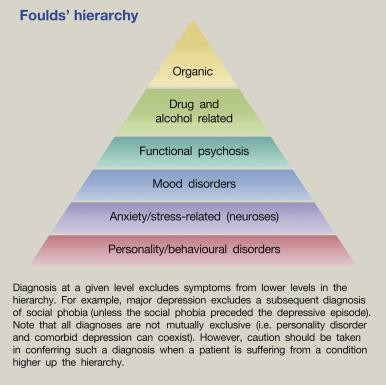
\includegraphics{./images/01-05/img_1.jpg}

}

\caption{\label{fig-foulds}Foulds가 제시한 정신과 진단의 계층적
위계질서}

\end{figure}

야스퍼스의 이론은 인간이 정신질환을 이해할 수 있는 인식론적 한계에 대한
것이라면, Foulds의 이론은 정신질환 자체의 구성원칙에 대한 이론이다.
Foulds는 자신의 이론을 증명하기 위해 ``Delusions-symptoms-states,
Inventory''라는 자가설문지를 제작하였고, 이는 다양한 인구집단에
적용되었다.{[}@Foulds1975-ky{]} 한국에서도 황석현
등\hspace{0pt}{[}@Hwang2013-zx{]}\textbf{\hspace{0pt}}이 환자군 및
정상대조군에 시행하여, Foulds의 이론을 지지하는 연구결과를 얻어낸 바
있다.

\hypertarget{uxb2e4uxc911-uxc9c4uxb2e8}{%
\subsection{다중 진단}\label{uxb2e4uxc911-uxc9c4uxb2e8}}

동반질환(comorbidity) 문제는 정신과 진단에서 항상 대두되는, 결코 쉽게
해결되지 않는 문제이다. 의학 진단은 두 가지 상반되는 원칙에 따라
이루어진다. 첫째는 오컴의 면도날 원칙\footnote{\textbf{오컴의 면도날
  원칙(Occam's Razor)}: 어떤 현상에 대한 설명들 가운데 논리적으로 가장
  단순한 것이 진실일 가능성이 높다(Simple is the best)는 원칙, 즉
  쓸데없이 복잡하게 만들지 말라는 것이다. 중세 프란체스코회 수사이자
  영국 철학자인 오컴 출신 윌리엄(William of Occam,
  1285\textasciitilde1349)에게서 유래했다.}이라 하여, 환자가 나타내는
다양한 증상을 최대한 하나의 진단으로 설명하는 것이다. 이와 대조되는
원칙을 히캄의 격언\footnote{\textbf{히캄의 격언(Hickam's dictum)}:
  미국의 의사인 John Barber Hickam이 말한 것으로 전해지는 격언으로
  오컴의 면도날 원칙과 상반된다. 이 두 원칙은 의학 진단에서 흔히
  맞딱뜨리는 딜레마이다.{[}@freixa2019{]}}이라 하며 ``환자는 가질 수
있는 모든 질병을 동시에 가질 수 있다''는 원칙이다. 대부분의 의사는
오컴의 면도날 원칙을 우선하며, 다양한 증상을 아우르는 단일 진단을
선호한다. 정신질환에 있어서 계층적 진단은 오컴의 면도날 원칙을 따른
예라고 할 수 있다. 그러나 현대로 접어들수록 점점 더 다중 진단(multiple
diagnosis)이 내려지는 추세이다. 이는 몇 가지 이유가 있다.

원래 동반질환(comorbidity)이란 주 진단에 동반하는 기타 질환이 주 질환의
병세나 경과를 변화시킬 수 있다는 개념에서 출발하였다. 그러다가 다중
이환(multimorbidity)의 개념으로 옮겨가게 되었는데, 이는 한 환자가 앓고
있는 모든 질환이 환자의 건강 수준과 삶의 질에 어떤 영향을 미치느냐에
초점을 맞추고 있다. 따라서 동반질환이라고 표현할 때는 보통 주 진단이
있어서 이것이 치료의 초점이 되며, 다중 이환이라 표현할 때는 모든 질환이
동등한 비중으로 고려된다. 정신의학에서는 전자의 개념으로 언급될 때가
많다. 조현병과 연관된 동반질환 개념은 조현병과 내과 질환의 병존,
조현병과 물질 남용의 병존, 조현병과 인격장애의 병존 등이 있다.

DSM-III 부터 DSM-IV 까지는 다축 진단체계\footnote{\textbf{다축 진단체계
  (multiaxial system)}: DSM-IV 까지 사용되던 진단 체계. Axis I에는
  통상적인 임상적 장애를, axis II에는 인격장애나 지능저하, 그리고 주된
  방어기제를 적는다. Axis III는 동반된 신체적 질환을 의미하며, axis IV는
  정신사회적 스트레스, 환경적 영향을 적는다. 마지막으로 axis V에는
  전반적 기능 수준을 Global Assessment of Functioning (GAF) 척도를
  이용하여 기록한다.}를 도입하여, axis I에서 정신과 진단을, axis II,
III에는 인격장애와 의학적 장애를 진단함으로써 다중 진단 문제를 원만하게
피해갔다. 그러나 문제가 되는 것은 Axis I에 속하는 서로 다른 정신과
질환을 동시에 진단할 수 있느냐이다. DSM-III만 해도 이를 권장하지 않고
있었으나, 동반질환에 대한 Boyd
등\hspace{0pt}{[}@Boyd1984-eq{]}\textbf{\hspace{0pt}}의 연구를 통해 점차
다중 이환을 인정하고 복수의 진단을 동시에 내리는 것이
권장되었다.\footnote{Boyd 등은 일만명이 넘는 대규모 표본을 이용하여
  표준화된 진단도구로 정신질환의 유병률을 조사한 결과, DSM-III에서 배제
  조항(``\textasciitilde 에 부합하는 경우 \textasciitilde 로 진단하지
  않는다'')으로 묶여있는 질환들이 실제로 한 환자에게 공존하는 비율이
  매우 높다는 것을 발견하였다.} 급기야 DSM-5에서는 다축 진단체계가
삭제됨으로써 다중 진단의 제한은 완전히 사라졌다. 게다가 현행 의료보험
체계에서는 치료를 행하려면 그에 걸맞는 진단명을 붙여야 한다. 예를 들어
조현병 환자가 우울 증상을 보여서 항우울제 처방을 해야할 때가 있는데,
삭감을 당하지 않으려면 우울증 진단코드를 추가해야만 한다.

물론 개수와 상관없이 정확한 진단이 붙여져서 환자가 필요한 치료를 받게
된다면 말할 것이 없겠지만, 많은 연구자들은 다중 진단이 진단 기준의
모호성 때문에 비롯된 아티팩트(artifact)라고 우려한다.{[}@Maj2005-hc;
@Van\_Loo2015-ds{]} 다중 진단을 허용하면서 동반 질환 연구가
활발해졌는데, 만약 이 현상이 진단의 불완전함때문이라면 문제가 아닐 수
없다.

\hypertarget{uxcc28uxc6d0uxc801-uxc9c4uxb2e8}{%
\subsection{차원적 진단}\label{uxcc28uxc6d0uxc801-uxc9c4uxb2e8}}

DSM-5의 개정 작업이 이루어지는 동안, 가열찬 논쟁거리였던 주제가 바로
차원적 접근의 수용 여부였다.{[}@Krueger2009-vh{]} 차원적 접근은 기존의
질병분류학에 대한 정면 도전이기도 하다. 기존의 분류학은 질병과 질병
사이를 구분하는 법과 두 질병이 어떤 위계 관계에 있는 지를 정하는 것이다.
그러나 자연의 모든 현상은 분명한 구분이 없을 때가 많으며, 구분을
함으로써 오히려 유용한 정보를 놓치게 될 때가 많다. 예를 들어 인간은
빨주노초파남보의 7가지 색을 구분하고 있지만, 이는 어디까지나 연속적인
전자기파의 파장을 임의로 구분한 것에 지나지 않는다. 그렇기 때문에 서로
다른 언어 사용자들은 서로 다른 색채 이름을 사용하며, 색채를 지시하는
이름의 개수도 다르다. 따라서 빨강과 주황을 어떻게 구분하는지에 대해
소모적인 논쟁을 하는 것보다는, 파장 자체를 숫자로 표기하는 것이 더
유용할 지 모른다.

점점 더 진단에 표준화된 평가도구를 이용하는 경우가 늘어나고, 정량화된
자료가 더해지면서, 차원적 진단이 가능한 시대에 돌입한 것은 사실이다.
일부 학자들은 차원적 진단이 조작적 진단기준의 폐해를 일소할 수 있을 뿐
아니라, 정신질환에 결부된 편견을 해소하는데도 한 몫할 것으로
기대한다.{[}@Cratsley2019-ot{]} 적지 않은 학자들은 정신병적 경험은
조현병 환자뿐 아니라 일반인에게도 널리 펴져있으며, 환자와 일반인의
차이는 정도 차이에 지나지 않는다고 주장한다.{[}@Nuevo2012-yc;
@Van\_Os2016-qe{]} 치료 역시 발병한 후의 환자보다, 높은 위험이 의심되는
환자에게 미리 행하는 것이 성과가 더 좋다고들
말한다.{[}@Fusar-Poli2017-lw; @Salazar\_de\_Pablo2020-vq{]} 이렇게
정상과의 경계를 정해놓지 않으면 자연스레 편견이 줄어들 전망이다. 차원적
진단은 다중 진단의 문제나 동일 질환 내부의 이질성 문제, 정신질환이
의심되나 기준에 덜 미치는 환자의 문제 등도 무리없이 해결할 수
있다.{[}@Krueger2009-vh{]}

이런 장점들 때문에, DSM-5, ICD-11이 큰 영향을 받았으며,
RDoC(섹션~\ref{sec-future-of-dsm})는 아예 정신기능의 영역(domain)을
정상으로부터 극단적인 비정상까지를 아우르는 차원으로 평가, 분석한다.
DSM-5는 개정 작업 중에는 좀더 야심찬 목표를 세웠으나, 결국은 section
3에서 인격장애를 분류하는 대안적 모델을 싣는데 그치고 말았다. 아직은
차원적 진단을 받아들이기에는 연구가 부족하고, 실제 사용에서도 문제점이
많기 때문이다. 하지만 앞으로 점점 더 광범위하게 적용될
전망이다.{[}@Appelbaum2017-hn{]}

\hypertarget{uxc870uxd604-uxc2a4uxd399uxd2b8uxb7fc-uxc7a5uxc560uxc640uxc758-uxac10uxbcc4}{%
\section{조현 스펙트럼 장애와의
감별}\label{uxc870uxd604-uxc2a4uxd399uxd2b8uxb7fc-uxc7a5uxc560uxc640uxc758-uxac10uxbcc4}}

\hypertarget{uxc870uxd604-uxc2a4uxd399uxd2b8uxb7fc-uxc7a5uxc560uxc758-uxac1cuxb150}{%
\subsection{조현 스펙트럼 장애의
개념}\label{uxc870uxd604-uxc2a4uxd399uxd2b8uxb7fc-uxc7a5uxc560uxc758-uxac1cuxb150}}

DSM-IV에서는 ``조현병과 기타 정신병적 장애 (Schizophrenia and Other
Psychotic Disorders)''라는 표현이 DSM-5에서는 조현 스펙트럼과 기타
정신병적 장애(Schizophrenia Spectrum and Other Psychotic Disorders)``로
바뀌었다. 이는 차원적 진단을 수용하려 했던 DSM-5 개정의 의도가
간접적이나마 반영된 결과이다. 여기에 속한 질환들은 서로 범주적으로
뚜렷이 구분된다기 보다는, 연속선 상에 이웃하여
존재한다.(그림~\ref{fig-spectrum}) 또한 조현형 인격 장애(schizotypal
personality disorder)는 인격 장애로 기술되면서도 동시에 조현 스펙트럼
장애에 속하며, section 3에 포함되긴 했지만 약화된 정신병
증후군(attenuated psychosis syndrome) 역시 조현 스펙트럼 장애의 하나로
분류된다. {[}@Tsuang2013-oa{]} 조현병의 감별은 주로 이들 스펙트럼
질환과의 감별이며, 이 과정은 질병의 본질을 구분한다기 보다는, 기간이나
기분 증상의 비중, 기능 장애의 정도 등 부차적인 요인들을 구분하는
과정이다.

\begin{figure}

{\centering \includegraphics{./images/01-05/img_2.png}

}

\caption{\label{fig-spectrum}조현 스펙트럼 장애}

\end{figure}

\hypertarget{uxc778uxaca9-uxc7a5uxc560}{%
\subsection{인격 장애}\label{uxc778uxaca9-uxc7a5uxc560}}

조현병과 감별 진단을 해야 하는 인격 장애는 조현형 인격 장애와 편집형
인격 장애이다. 조현형 인격장애(schizotypal personality disorder)라는
개념은 그 근원을 1962년 Meehl이 발표한 논문 \emph{'Schizotaxia,
schizotypy, schizophrenia''}에 두고 있다.{[}@Meehl1962-ym{]} Meehl은
조현병이 유전적 원인에 의해 발생할 것이라고 믿은 선구자 중 하나였다.
그는 유전자 변이로 인해 중추신경계 기능에 문제가 생긴 상태를
schizotaxia라고 하였고, 이러한 상태가 독특한 성격 특성으로 드러나는 것을
schizotypy, 그리고 임상적으로 뚜렷이 발병한 것을 schizophrenia로
개념지었다.{[}@Modenato2015-ea{]} 따라서 schizotypy는 schizotaxia의 외적
발현이라 할 수 있는데, Meehl은 schizotypy를 보이는 사람이 전 인구의
10\%는 될 정도로 흔하며, 조현병으로의 발병 위험도 높을 것이라
예상하였다.

Schizotypy의 개념은 DSM-III에서 조현형(schizotypal) 인격 장애로
통합되었다. 환자들은 대인관계를 맺으려는 욕구도 능력도 없다. 이들은
사회적 접촉에서 움츠러들며, 감정적으로 냉담하며 초연하다. 기분이
우울하거나, 타인에 대해 부끄러움, 열등감을 느끼는 것도 아니며, 타인의
말에 예민한 것도 아니다. 공감 능력이 부족하며, 혼자만의 기이한
공상세계에 머무르는 경향이 있다.{[}@Oyebode2018-mt{]} 일시적인 망상,
환각 등이 있을 순 있지만 지속적이지는 않으며, 기이한 사고나 행동을
보인다고 하지만 이를 마음 속에 간직하거나 사적 공간에 국한시키기 때문에
타인에게 눈총을 받을 일은 드물다. 그러나 조현성(schizoid) 인격 장애,
자폐 스펙트럼 장애와 구분하기 매우 어렵다.

편접형 인격 장애 환자는 항상 의심에 사로잡혀 있으나, 이들이 보이는
의심은 피해 망상이라기 보다는 지배관념\footnote{\textbf{지배관념
  (overvalued idea, 불어로는 \emph{idée fixe})}: 거짓이 아니고 이해
  가능하다는 점에서 망상과는 구분되나, 상식적인 범위를 넘어설 정도로
  집착하며 도가 지나친 가치를 부여하는 신념. 건강염려증 환자의 건강에
  대한 집착은 지배관념의 한 예이다.}에 가깝다. 광범위한 삶의 상황에서
의심에 빠지며, 의심은 그의 사고와 인생을 완전히 지배한다. 환자는 자신이
항상 피해자라고 느끼며, 주변에 일어나는 모든 상황이 이를 뒷받침한다고
느낀다. 종종 공격적이고 자기 파괴적인 행동을 보이나, 사고 장애는 드물다.
지배관념은 현상학적으로 망상이나 강박적 사고와는 뚜렷하게 구분된다.

\hypertarget{uxb9dduxc0c1-uxc7a5uxc560}{%
\subsection{망상 장애}\label{uxb9dduxc0c1-uxc7a5uxc560}}

크레펠린은 하나의 주제에 대해서 논리적으로 구조화된 망상이 지속되는
질환군을 편집증(paranoia)라고 하였고, 조발성 치매와는 달리 인격의
황폐화가 없고, 감정 반응이 보존되며, 기능 저하가 뚜렷하지 않다고
하였다.{[}@Kendler2017-xf{]} 그러나 어디까지를 망상 장애로 보고,
어디서부터 조현병으로 볼 것인지는 지속적인 논란이
대상이었다.{[}@2015-aw{]} 특히 ICD-11에서 조현병 진단기준에 기능 저하를
삭제하면서 더더욱 감별이 어려워졌다.

망상 장애와 조현병의 감별점을 Marneros
등{[}@Marneros2012-et{]}\textbf{\hspace{0pt}}은 다음과 같이 정리하였다.

\begin{enumerate}
\def\labelenumi{\arabic{enumi}.}
\tightlist
\item
  망상 장애와 편집형 조현병의 유일한 공통점은 망상 뿐이다.
\item
  편집형 조현병은 망상 이외에도 기타 정신병적 증상을 보이지만, 망상
  장애는 그렇지 않다.
\item
  망상 장애는 음성 증상이 나타나지 않는다.
\item
  편집형 조현병의 발병 연령은 망상 장애보다 이르다.
\item
  일차 친족에서의 정신병은 편집형 조현병에서 더 흔하다.
\item
  망상 장애 환자들 중 극소수만이 나중에 편집형 조현병으로 진단이 바뀐다.
\item
  사회적 기능은 망상 장애 환자들이 전반적으로 더 낫다.
\end{enumerate}

\hypertarget{uxc870uxd604uxc815uxb3d9-uxc7a5uxc560uxc640-uxae30uxbd84-uxc7a5uxc560}{%
\subsection{조현정동 장애와 기분
장애}\label{uxc870uxd604uxc815uxb3d9-uxc7a5uxc560uxc640-uxae30uxbd84-uxc7a5uxc560}}

임상에서 조현병 진단이 분명한 것 같은데 두드러진 조증/우울증 증세를
동반하거나, 이전 삽화에서는 조현병이었는데 다음 삽화에서는 기분 삽화로
이행하는 경우를 드물지 않게 보게 된다. ``조현정동 장애(schizoaffective
disorder)''라는 명칭은 1933년 Kasanin\footnote{\textbf{Jacob Kasanin
  (1897\textasciitilde1946)}: 러시아 태생의 미국 정신과 의사.}이 처음
사용하였다. 그는 크레펠린의 구분이 잘 맞아 떨어지지 않는 환자들을 보게
되었고, 정신병적 증상과 기분 증상의 혼재에 초점을 맞추어 이렇게
이름지었다. 조현정동 장애는 DSM-I과 II에서는 조현병의 한 아형으로
취급되다가, DSM-III로 넘어오면서 독립적인 질병으로 격상한다. DSM-III는
이 질환이 다양한 의미로 사용되어 왔음을 지적하면서, 명칭만 등재했을 뿐
명확한 진단기준은 내놓지 못했다.

조작적 진단기준을 마련하기 시작한 것은 Spitzer의 연구진단기준(RDC)
이었다.(섹션~\ref{sec-dsm-iii}) 두 계통의 증상이 병존하는 것에 더하여
기분 증상이 없는 상태에서도 1주 이상 정신병적 증상이 지속될 것을 기준에
추가하였다. DSM에서는 DSM-IIIR에 와서야 조현정동 장애의 진단기준을
명시되었는데, 두 계통의 증상이 한 삽화에 병존해야 하고, 기분 증상이 없는
상태에서 2주 이상 정신병적 증상이 지속되어야 하며, 전체적 경과에서
차지하는 기분 삽화의 비율이 정신병적 삽화보다 높아야 한다. RDC의 체계를
답습한 흔적이 보인다.

조현정동 장애는 조현 스펙트럼 장애중에서 가장 문제점이 많은 진단이다.
DSM-IIIR의 잣대를 엄격하게 적용하면 그 유병률은 0.3\% 정도에 지나지
않는다.{[}@Heckers2012-dn{]} 또한 장기간에 걸친 임상 자료가 있어야
진단이 가능하기 때문에, 진단의 안정성도 매우 떨어진다. 실제 임상에서는
한 환자가 재입원할 때마다 조현병, 양극성 장애, 조현정동 장애로 번갈아
진단되는 일이 비일비재하다. 이 환자들을 단순히 정신병적 기분 장애 환자로
분류하면 그만이라는 견해가 쏟아졌다.{[}@Lake2007-mh; @Marneros2007-xf{]}
더군다나 다중 진단이 일반화된 현재, 조현병과 기분 장애를 동시에 진단하지
말라는 법도 없다.

질병분류학적으로 이렇게 애매한 위치에 있고 비판도 수도 없이 쏟아지는
질병이지만, DSM-IIIR에서 한번 정해놓은 진단기준은 DSM-5에 이르기까지
전혀 바뀌고 있지 않다. 조현병과 감별하기 위해선 평생에 걸친 경과 중에서,
우울증이나 조증 증상이 없는 상태에서 망상/환각이 2주 이상 지속되어야
한다. 한편 기분 장애와 감별하기 위해선 역시 평생에 걸쳐 기분 장애 증상이
대부분의 시간 동안 나타나야 한다. 결국 정확한 감별을 위해서 한 환자를
평생 동안 추적 조사해야한다는 뜻인지라, 현실성은 없어
보인다.{[}@Parker2019-is{]}

\hypertarget{uxb2e8uxae30-uxc815uxc2e0uxbcd1uxc801-uxc7a5uxc560uxc640-uxc870uxd604uxc591uxc0c1-uxc7a5uxc560}{%
\subsection{단기 정신병적 장애와 조현양상
장애}\label{uxb2e8uxae30-uxc815uxc2e0uxbcd1uxc801-uxc7a5uxc560uxc640-uxc870uxd604uxc591uxc0c1-uxc7a5uxc560}}

이 둘은 독립된 진단명이라기보다는, 아직 경과관찰이 충분하지 않아
조현병의 진단을 내리기 어려울 때 잠정적으로 사용된다. 초발 환자가 처음
발병한지 아직 6개월이 되지 않았을 때는 이러한 진단을 붙일 수 밖에 없다.

그러나 개념적으로 조현병과는 조금 다른 양호한 예후를 보이는 상태를
의미하기도 한다. 예로부터 심리적 충격에 반응하여 극적인 정신병적 증상을
보였다가 비교적 깨끗하게 회복하는 경우에 대한 많은 사례보고가 있어왔다.
이를 독일에서는 ``cycloid disorders'', 프랑스에서는 ``\emph{bouffée
délirante}''이라고 하였으며, 스칸디나비아에서는 ``reactive and
psychogenic psychoses''이라고 불러왔다.{[}@Marneros2005-xy{]}

Cycloid psychosis는 Kleist와 Leonhard의 WKL 분류체계에서 중요하게
다루어진다.(섹션~\ref{sec-wernicke-kleist-leonhard}) Leonhard는 이
진단에 해당하는 환자들은 갑자기 상황에 걸맞지 않은 불안/행복감을
보이거나, 생생한 환각/망상으로 혼란에 빠지거나, 강직증에 버금가는
운동장애를 보인다고 하였다.{[}@Yadav2010-us{]} 발병 당시에는 증상이 매우
심해보이지만, 조속히 회복되며 후유증도 거의 남지 않는다. DSM은 cycloid
psychosis 개념을 수용하지 않았지만, ICD-10은 acute polymorphic psychotic
disorder (APPD)라는 이름으로 진단체계에
삽입하였다.{[}@Van\_de\_Kerkhof2016-lw{]}

\emph{Bouffée délirante} 역시 극적인 망상, 환각, 혼란, 불안 및 기분
증상을 동시에 보인다. 시간 단위로 증상이 바뀌기도 하며, 비교적 빨리
후유증을 남기지 않고 회복한다. 반응성 정신병(reactive psychosis)이라는
개념은 감당하기 힘든 외적 스트레스에 반응하여 급격한 정신병적 증상을
보인다는 의미인데, DSM-III와 IIIR에서는 단기 반응성 정신병(brief
reactive psychosis)으로 편입되었다. 이는 뚜렷한 스트레스 요인이 있고,
지속기간이 1달 이내여야 한다는 단서가 붙어있다.

DSM-IV부터는 반응성이라는 표현이 삭제되고, 단기 정신병적 장애(brief
psychotic disorder)로 명칭이 바뀌었다. 원인이 될만한 스트레스 요인이
있건 없건 지속기간이 하루 이상 1달 미만이면 이렇게 진단한다. 다만
스트레스 요인이 있을 때는 명시자를 통해 기입하도록 되어있다. 따라서
조현병과의 감별진단은 역시 기간에 따라 이루어진다.

조현양상 장애는 기간이 1달 이상 6개월 미만일 뿐, 진단기준은 급성
정신병적 장애와 다르지 않다. 조현병과의 차이점은 기능 저하가 없어도
진단을 내릴 수 있다는 점이다. Langfeldt\footnote{\textbf{Gabriel
  Langfeldt (1895\textasciitilde1983)}: 노르웨이의 정신과 의사로 오슬로
  대학에 재직하였다. 조현양 장애(schizophreniform disorder)에 대한
  업적을 남겼다. 노벨상을 받은 노르웨이 작가 Knut Hamsun의 나찌 부역죄에
  대해 정신감정을 한 것으로 유명하다.}가 조현병을 전형적 조현병과
조현양상 장애로 나눈 것은 전자와는 달리 후자는 비교적 예후가 좋다는 것을
강조하기 위해서였다.{[}@Bergem1990-oz{]} 그러나 예후가 좋은 것은 단기
정신병적 장애일 뿐이요, 한달 이상 지속되는 경우에는 예후가 그다지 좋지
않다.{[}@Coryell1986-pf{]} 게다가 예후가 좋게 보였던 고전적 증례들은
실상 기분 장애의 증례였던 것으로 추정되었다.{[}@Bergem1990-oz;
@Guldberg1991-qj; @Benazzi2003-ek{]} 조현양상 장애에 대한 연구를
살펴보면 대부분 ``좋은 예후를 갖는 조현병 유사 질환'' 혹은 ``조현병 유사
질환으로 잘못 진단되는 기분 장애'' 정도로 이해되고 있다. 따라서 조현양상
장애와 조현병을 감별하는 것보다는, 조현양상 장애와 기분 장애를 감별하고,
그 나머지는 조현병의 전단계 정도로 받아들이면 될 것이다.

\hypertarget{uxae34uxc7a5uxc99d}{%
\section{긴장증}\label{uxae34uxc7a5uxc99d}}

긴장증(catatonia)은 정신의학의 긴 역사 속에서, 주로 조현병의 한
아형으로서 진단되어 왔다. 하지만, 긴장증은 조현병만이 아니라 기분장애나
기질성 정신장애에서도 발견되는 것이 명확해졌다. 게다가 긴장증은 원래
질환에 관계없이 특정한 치료법이 효과적이기 때문에, 긴장병을 조현병의 한
아형이 아니라, 독립된 증후군으로서 진단하고 치료하는 것이 장려되게
되었다. DSM-5에서는 아형으로서의 긴장형 조현병을 삭제하고, 명시자의
하나로 긴장증을 사용한다. 이는 ICD-11에서도 마찬가지이다.

\hypertarget{sec-kahlbaum-catatonia}{%
\subsection{개념의 역사적 변천}\label{sec-kahlbaum-catatonia}}

긴장증의 개념은 Kahlbaum으로 거슬러
올라간다.(섹션~\ref{sec-before-kraepelin}) 그는 Gorlitz의 Remer
요양소에서 평생 근무하면서 환자들을 장기간에 걸쳐 추적 조사할 수 있었다.
환자의 장기적 경과와 예후를 토대로 질병을 분류할 수 있다는 그의 생각은
크레펠린에게 지대한 영향을 미쳤다. Kahlbaum이 활약했던 19세기 후반에는
수용소 환자의 상당부분이 신경매독 환자였다. 이들은 정신증상과 함께
운동장애, 진전, 경련발작 등 신경증상을 보였다. Kahlbaum은 조금은 독특한
운동증상을 보이는 환자들을 구분해내고, 이들이 신경매독보다는 양호한
경과를 밟는다는 것을 관찰하였다. 이들은 주기적으로 이상 행동을 보이나,
어느새 정상적으로 돌아오기도 하였다. 그러나 Kahlbaum은 이들이 기분
증상에서 시작하여 주기적으로 특징적인 운동 증상을 보이다가 종국에는
인격의 황폐화에 이르게 된다고 보고, 이를 독립적인 질환으로 여겨
긴장증(catatonia)이라 이름붙였다. 1874년 Kahnbaum이 발간한 소책자
\emph{``Die Katatonie''}에는 26명의 증례가 수록되었는데, 이들은 기분
장애, 조발성 치매, 신경매독, 결핵, 간질 등 다양한 질환을 앓고
있었다.{[}@Fink2011-oi{]}

크레펠린은 결국 인격의 황폐화에 이르게 되는 이들 환자들이 자신이 구상한
조발성 치매 개념에 부합한다고 여기고, 긴장증을 조발성 치매의 한 아형으로
삼는다. 즉 당시에도 이미 긴장증은 두가지 서로 다른 의미로 사용되고
있음을 알 수 있다. 첫째는 강직증, 함구증, 상동 행동 혹은 과도한 흥분
등을 보이는 독특한 증상 집합체이고, 둘째는, 일정한 경과를 밟다가 인격의
황폐화로 향하는 질병 과정이었다. 크레펠린이 조발성 치매에 부속시킨 것은
후자의 개념이다.

그러나 크레펠린 스스로도 이 증상군은 조발성 치매가 아닌 다른 질환에서도
발견할 수 있음을 언급하였다. 따라서 그는 긴장증의 존재만으로는 조발성
치매 진단을 내리지 말것을 권고하였다.{[}@Carroll2001-ix{]} 크레펠린과
블로일러의 영향으로 긴장증이 조현병의 한 아형으로 자리잡았지만, 19세기
의사들은 오히려 긴장증 혹은 혼미(stupor)가 멜랑콜릭 아형의 우울증 혹은
조울정신병에서 흔히 나타난다고 보았다. 그래서
Baillarger(섹션~\ref{sec-kraepelin})는 이러한 상태(\emph{stupidité})를
멜랑콜리의 한 아형으로 보아 \emph{``melancholie avec stupeur ''}라고
이름붙였다. Kahlbaum 역시 긴장증이 멜랑콜리에서 시작하는 경우가 많다고
보았으나, 그는 이후에 조증이 뒤따르는 경우가 많다는 것을
지적하였다.{[}@Starkstein1995-wg{]}

이들이 관찰한 긴장증은 주로 움직임이 없어지고 고정된 자세를 유지하는
형태가 많아 긴장형 혼미(catatonic stupor)라고 불리우곤 했다. 그런데,
Kleist와 Leonhard는 반대로 심하게 흥분하고 움직임을 멈추지 못하다가
탈진하게 되는 과활동성 긴장증에
주목하였다.(섹션~\ref{sec-wernicke-kleist-leonhard}) 이를
Stauder\footnote{\textbf{K.H. Stauder (1905-1969)}: 독일의 정신과
  의사이자 기자겸 작가.}는 악성 긴장증(lethal catatonia)이라고
불렀다.{[}@Castillo1989-li; @Sienaert2014-ce{]} 내인성 정신증의 WKL
분류체계에서는 긴장증이 여러군데 출현하는데, 우선 순환 정신증의 한
종류인 1) Hyperkinetic-Akinetic Motility Psychosis로서, 비체계적
조현병의 아형인 2) 주기적 긴장증(periodic catatonia)으로서, 그리고
체계적 조현병의 아형인 3) 긴장형 조현병으로 분류에 포함되었다.
Leonhard는 긴장증이 조울정신병의 일환으로 혹은 조현병의 일환으로
나타나는 경우를 모두 염두에 두었다. 긴장증의 예후에 대한 연구도 이런
이중성 때문에 모순되는 결과가 얻어지곤 하였다.

20세기 초엽에 진행된 Hoch\footnote{\textbf{August A. Hoch
  (1868\textasciitilde1919)}: 스위스 태생의 미국 정신과 의사. 뉴욕 시의
  시립 정신병원 소장을 역임하였다.블로일러의 정신분열병 개념을 최초로
  미국 학회에 소개하였다.}의 연구에서는 25명의 긴장증 환자에 대한 예후가
기록되었는데, 이중 19명이 조울증 환자였고, 조현병에 의한 것으로 간주된
환자는 6명 뿐이었다. 전자의 환자는 대체로 좋은 예후를 보였고, Hoch는
이들을 ``양성 혼미(benign stupor)''라 불렀다.{[}@Hoch1921-pq{]}
Joyston-Bechal\textbf{\hspace{0pt}}{[}@Joyston-Bechal1966-vw{]}\textbf{\hspace{0pt}}은
모즐리와 베들렘 병원에 입원했던 긴장증 환자 100명을 골라 경과를
추적하였는데, 이중 25\%가 우울증, 20\%는 기질성 뇌질환 환자였으며, 30\%
정도만이 조현병이었다고 하였다. 이중 약 20\%가 결국 사망하였으며, 기질성
뇌질환이었던 경우 더 치명률이 높았다.

미국 아이오와 주립 병원에 입원한 환자를 대상으로 한 두 개의 연구에서는,
주로 긴장증을 보인 조현병 환자에 대한 경과 및 예후가
조사되었다.{[}@Morrison1974-fy; @Winokur1974-gu{]} 두 연구에서도 양극성
장애에서 나타난 과활동성 긴장증은 경과가 짧고 회복 비율도 높았으나,
그렇지 못한 주로 조현병에서 나타나는 혼미형 긴장증은 예후가 불량한
것으로 나타났다. 특히 아이오와 500 연구\footnote{\textbf{아이오와 500
  연구 (Iowa 500 Research Project)}: 1975년 아이오와 대학 정신과를
  중심으로 1934년에서 44년 사이에 입원한 조현병과 기분 장애 환자 525명의
  이후 30\textasciitilde40 년 간의 삶을 추적 조사하는 후향적 연구이다.
  이에 더하여 환자 가족 2,055명, 대조군 160명 까지
  조사되었다.{[}@Tsuang1975-gv{]}}에서는, 긴장증은 질병 경과 중
일시적으로 나타나지만, 이들이 결국 파과형 조현병으로 전환되어 인격의
황폐화에 이르게 된다는 것이 관찰되었다.{[}@Pfohl1982-yu{]}

\hypertarget{dsmuxc5d0uxc11cuxc758-uxae34uxc7a5uxc99d}{%
\subsection{DSM에서의
긴장증}\label{dsmuxc5d0uxc11cuxc758-uxae34uxc7a5uxc99d}}

DSM-III에 처음 등장한 긴장증은 조현병의 한 아형으로 등재되었다. 따라서
그 치료 역시 통상적인 항정신병 약물이 권장되었다. 1994년 발표된
DSM-IV에서는 처음으로 ``의학적 질환에 2차적인 긴장증'' 항목이
추가되었다. 이후 DSM-5가 나올 때까지 20년 가까운 동안, 학자들은 1)
Kahlbaum이 원래 기술했던 조현병의 아형으로서의 긴장증, 2) 조증에서
보여지는 과활동성 긴장증, 3) 항정신병 약물 부작용인 항정신병 약물
악성증후군(neuroleptic malignant syndrome, NMS), 4) 기타 의학적 질환에
의한 긴장증을 구분하고자 하였다. 게다가 긴장증은 항정신병 약물이 아니라
벤조디아제핀이나 전기경련치료가 훨씬 더 효과적임이 확인되면서, 더 이상
조현병의 아형이 아니라 독자적인 질환으로 인정해줄 것을 요구하였다.
조현병의 한 아형으로서 잔류를 원하는 학자들도 많았기 때문에 토론은
결론을 내지 못하고 질질 끌었다.{[}@Heckers2010-lb{]}

DSM-5는 긴장증 뿐 아니라 조현병의 아형 자체를 삭제함으로써, 긴장증을
둘러싼 지리한 토론도 막을 내렸다. 긴장증은 명시자로서 조현병 뿐 아니라
다양한 질환에 추가 정보로 기입할 수 있게 되었다.{[}@Fink2011-oi{]}

\hypertarget{uxac10uxbcc4uxc9c4uxb2e8}{%
\subsection{감별진단}\label{uxac10uxbcc4uxc9c4uxb2e8}}

긴장증을 확진할 수 있는 뚜렷한 검사소견은 없다. 다만 특징적인 운동
증상\footnote{DSM-5는 긴장증의 운동증상으로 다음을 열거하고 있다:
  혼미(stupor), catalepsy, 납굴증(waxy flexibility), 함구증(mutism),
  거부증(negativism), 자세 유지(posturing), 매너리즘(mannerism),
  상동행동(stereotypy), 극심한 흥분(agitation), 찡그림(grimacing), 반향
  언어(echolalia), 반향 동작(echopraxia). 이중 2개 이상이 있으면
  긴장증으로 진단한다.}으로부터 미루어 짐작할 뿐이다. 과거에는
벤조디아제핀을 정맥주사한 후 50\%이상 운동 증상이 감소되면 긴장증을
확진하곤 했다.{[}@Fink2011-oi{]} 이 방법은 진단 뿐 아니라 치료법으로서
지금도 응급실에서 많이 이용하고 있다.

긴장증은 조현병의 명시자 중 하나이기 떄문에, 조현병과 긴장증을 감별한
필요는 없다. 오히려 문제는, 약물 부작용이나 다른 의학적 질환과 감별하는
것이다. 만약 약물과 관계된다고 여겨지면 약물에 의한 급성 근긴장증이나
지연성 운동장애(tardive dyskinesia, TD) 혹은 신경이완제 악성
증후군(neuroleptic malignant syndrome, NMS)를 염두에 두어야 한다.
긴장증을 유발할 수 있는 의학적 질환으로는 뇌종양, 뇌염, 칼슘혈증, 간성
뇌증, 호모시스틴 뇨증, 당뇨성 케토산증 등이 있으며, 드물지만 신경학적
질환인 무동성 함구증\footnote{\textbf{무동성 함구증(akinetic mutism)}:
  환자는 갑자기 몸을 움직이지도 말을 하지도 못하는데, 그럼에도 불구하고
  의식은 명료해보이며 시선은 검사자를 따라 움직일 수 있고, 간단한 명령에
  따를 수 있다. 이는 마비라기 보다는 움직일 의지를 일순간 잃어버리는
  것으로 해석되며, 그러다가 갑자기 멀쩡하게 잘 움직인다. 양쪽 전두엽이나
  중뇌에 손상을 입은 환자에서 드물게 발생한다.}, locked-in
syndrome\footnote{\textbf{Locked-in syndrome}: 환자가 의식은 있지만,
  눈꺼풀이나 안구 근육을 제외한 전신 근육이 마비되고 동시에 발성을 하지
  못한다. 가성혼수라고도 불리우며, 독소 중독이나 뇌간 부위의 경색으로
  발생한다. 패션잡지인 Elle의 편집장이던 Jean-Dominique Bauby가 유명한
  예이다. Baudy는 이 경험을 \emph{``잠수종과 나비 (The Diving Bell and
  the Butterfly)''}라는 저서로 출판하였다.}, stiff person
syndrome\footnote{\textbf{Stiff person syndrome}: 일종의 자가면역
  질환으로 환자는 점진적으로 근육이 경직되고, 간헐적으로 통증을 동반한
  경련을 일으킨다.}도 유사한 증상을 일으킬 수 있다.

\hypertarget{uxae30uxc9c8uxc131-uxc815uxc2e0uxbcd1uxacfcuxc758-uxac10uxbcc4}{%
\section{기질성 정신병과의
감별}\label{uxae30uxc9c8uxc131-uxc815uxc2e0uxbcd1uxacfcuxc758-uxac10uxbcc4}}

\hypertarget{uxae30uxc9c8uxc131-uxc6d0uxc778uxc5d0-uxc758uxd55c-uxc815uxc2e0-uxc99duxc0c1}{%
\subsection{기질성 원인에 의한 정신
증상}\label{uxae30uxc9c8uxc131-uxc6d0uxc778uxc5d0-uxc758uxd55c-uxc815uxc2e0-uxc99duxc0c1}}

조현병 역시 생물학적 원인에 의한 뇌 기능 장애라는 점에서 기질성 뇌질환에
속한다. 그러나 통상 의학에서 기질성 정신병(organic psychosis)이라 하면,
뚜렷한 중추신경계의 병변이 생긴 후에 망상, 환각 등 정신병적 증상이
발생한 경우만을 의미한다. 약물에 의한 뇌 기능 이상도 기질성 원인 중
하나이지만, 보통은 기질성 정신병에 포함시키지 않는다. DSM-5는 이를
\textbf{``다른 의학적 상태에 의한 정신병적 장애(Psychotic disorder due
to another medical condition)''}로 표현하며, 조현 스펙트럼 장애 항목에
집어넣고 있다. 반면, ICD-11은 ``조현병과 기타 일차적 정신병적
장애(Schizophrenia or other primary psychotic disorders)''와 완전히
분리하여, \textbf{``다른 곳에서 분류된 질환 혹은 장애와 연관된 이차적
정신 행동 증후군(Secondary mental or behavioral syndromes associated
with disorders or diseases classified elsewhere)''} 항목에 넣고 있다.

기질성 정신병은 뇌졸중, 뇌종양, 외상성 뇌손상, 자가면역 질환, 대사 장애,
감염성 질환 등 다양한 조건에서 발생할 수 있다.{[}@David2005-gq;
@Pego-Reigosa2008-ra; @Keshavan2013-fl{]} 따라서 뇌 기능에 문제를 일으킬
수 있는 질병이 존재한다면 기질성 정신병을 고려해야
한다.(표~\ref{tbl-secondary-psychosis}) 그러나 단순히 선행질병이 있다
해서 모두 다 기질성 정신병이 확실한 것은 아니다. 만약 유방암 환자가
망상, 환각을 보이는 증례가 있다고 할 때, 이론적으로는 정신증상이
신생물딸림 증후군\footnote{\textbf{신생물딸림 증후군 (paraneoplastic
  syndrome)}: 악성 종양을 갖고 있는 환자에서 종양 자체의 침윤이나 전이,
  영양실조, 감염, 항암치료의 부작용 등과는 관계없이 나타나는 다양한
  증상들을 통칭한다. 암에 대한 면역반응이나 암세포에서 비정상적으로
  분비하는 호르몬, 사이토카인 등과 같은 체액성 물질 등이 원인으로
  여겨지고 있다.}으로 인한 악성 종양의 후유증일 수
있다.{[}@Kayser2010-wu{]} 그러나 대다수의 의사는 일차적 정신병으로
진단할 것이다.

따라서 동반 질환이 있다고 무조건 기질성 정신병을 의심하는 것이 아니라,
다음 요건을 갖추었는지 확인해보아야 한다. 첫째, 당연하겠지만 의학적
질환이 선행되어야 한다. 단 정신증상으로 인해 의학적 질환이 우연히
발견되는 경우는 예외가 되겠다. 둘째, 일차적 정신증의 전형적 증상이나
경과와 맞지 않아야 한다. 고령에 발병한다던지, 의식저하가 있다던지,
환청보다 환시/환촉이 심하다던지 하는 것들이다. 셋째, 특징적인 증상패턴을
보이는 경우이다. 질병실인증(anosognosia)를 동반한 다양한 실인증(agnosia)
혹은 Capgras 증후군과 같은 오인증, 환후(olfactory hallucination)같은
드문 환각 등이 있으면 기질성 원인을 의심해보아야 한다.네째, 원인 질환의
악화, 호전에 따라 정신증상도 변화할 때, 그리고 마지막으로 일차적
정신증으로 설명하기 곤란할 때 기질성 정신병을 고려할 수 있다. 이런
요건이 해당된다면 기질성 원인에 대한 모든 가능성을 열어놓고 뇌영상학
검사를 포함한 기본 검사를 행한 후, 관련 전문의의 도움을 청하는 것이
바람직하다.{[}@Sachdev2010-gu{]}

\hypertarget{tbl-secondary-psychosis}{}
\begin{longtable}[]{@{}
  >{\raggedright\arraybackslash}p{(\columnwidth - 2\tabcolsep) * \real{0.2639}}
  >{\raggedright\arraybackslash}p{(\columnwidth - 2\tabcolsep) * \real{0.7361}}@{}}
\caption{\label{tbl-secondary-psychosis}이차성 정신증의 가능한 원인들
{[}@Keshavan2013-fl{]}}\tabularnewline
\toprule()
\begin{minipage}[b]{\linewidth}\raggedright
Category
\end{minipage} & \begin{minipage}[b]{\linewidth}\raggedright
Examples
\end{minipage} \\
\midrule()
\endfirsthead
\toprule()
\begin{minipage}[b]{\linewidth}\raggedright
Category
\end{minipage} & \begin{minipage}[b]{\linewidth}\raggedright
Examples
\end{minipage} \\
\midrule()
\endhead
Trauma & Traumatic brain injury \\
Autoimmune disorders & Systemic Lupus Erythematosus, NMDA receptor
encephalitis \\
Congenital disorders & Velocardiofacial syndrome, agenesis of corpus
callosum \\
Iatrogenic disorders & Antimalaria drug, steroid, isoniazid \\
Cerebrovascular disorders & Stroke, cerebral or meningeal hemorrhage \\
Space-occupying lesion & Cerebral tumors \\
Metabolic disorders & Pheochromocytoma, metachromatic leukodystrophy,
Wilson's disease \\
Dietary disorders & Pellagra, B12 deficiency, vitamin D deficiency \\
Sepsis/infectious disorders & Neurosyphilis, toxoplasmosis, HIV
infection \\
Neurodegenerative disorders & Lewy body dementia, Parkinson's disease,
Huntington's disease, multiple sclerosis, Freireich's ataxia \\
Seizure disorders & Partial complex seizure, temporal lobe epilepsy \\
Endocrine disorders & Hyperthyroidism, hypothyroidism,
hyperparathyroidism \\
\bottomrule()
\end{longtable}

\hypertarget{uxb1ccuxc878uxc911-uxb1ccuxc885uxc591}{%
\subsection{뇌졸중,
뇌종양}\label{uxb1ccuxc878uxc911-uxb1ccuxc885uxc591}}

뇌졸중이나 뇌종양 후에 망상, 환각이 생기는 경우는 흔하진 않지만 종종
접하게 된다. 특이하게도 우측 반구에 손상이 있을 때 망상이 생길 위험이 더
크다. 기존에 피질하 위축 등 문제가 있었던 경우에 더
흔하다.{[}@Joyce2018-pt{]} 전형적인 조현병 증세보다는 망상이나 환각에
국한되는 경우가 대부분이다. 유병률은 망상이 4.7\%, 환각이 5.1\%
정도이다. 남성에게 좀더 많으며, 뇌졸중을 겪은 후 뒤늦게 나타나는 경우가
많다.{[}@Stangeland2018-ii{]}

뇌종양은 워낙 빈도가 적기 때문에 임상에서 잘 찾아보기 어렵지만, 정신병적
증상을 일으키는 중요한 원인 중 하나이다. 양성이냐 악성이냐 보다는 위치가
중요하며, 측두엽 특히 변연계에 종양이 생긴 경우 정신병적 증상이 나타나는
빈도가 20\%에 달한다고 한다.{[}@Filley1995-vj{]} 뇌하수체 종양도 흔히
증상을 일으키는 위치 중 하나이다.{[}@Madhusoodanan2010-no{]}

\hypertarget{uxd30cuxd0a8uxc2a8-uxbcd1}{%
\subsection{파킨슨 병}\label{uxd30cuxd0a8uxc2a8-uxbcd1}}

파킨슨 병은 흔히 정신병적 증상을 일으키는 원인이 된다. 질병 초반부터
가벼운 착시, 생생한 꿈, 렘수면 행동 장애 등이 나타날 수 있으나, 질병이
진행되면 생생한 환각과 정신병적 증상이 일어난다. 환각 중에는 환시가 가장
흔하며, 처음에는 병식을 앓지 않으나 후에는 치매환자처럼 환각과 현실을
혼동한다. 약물 치료를 시작하기 전에도 정신병적 증상이 나타나지만,
L-DOPA를 비롯한 대부분의 항파킨슨 약제가 정신병적 증상을 악화시킬 수
있다.{[}@Thanvi2005-af{]}

정신과 의사는 환시를 중심으로 한 정신증상과 진전, 가벼운 운동장애 등을
고려하여 파킨슨 병을 의심해보지만, 신경과 의사는 뇌 양전자 단층
촬영(PET)을 통해 도파민 운반체 밀도를 확인한 연후에야 확진을 내리기
때문에, 진단이 제대로 내려지지 않은 채 시간만 끄는 경우가 있다. 게다가
파킨슨 병\footnote{\textbf{파킨슨 병 (Parkinson disease)}: 뇌의 기저핵
  특히 흑질체(substantia nigra)가 파괴되면서 파킨슨 증후군을 나타내는
  질환}이 아니더라도, 파킨슨 증후군\footnote{\textbf{파킨슨 증후군
  (Parkinsonian syndrome) 혹은 파킨스니즘 (Parkinsonism)}: 진전, 서동증,
  근경직, 자세 불안정성의 4가지 증상이 함께 나타나는 증후군을 말한다.
  이러한 증상군이 나타나는 원인으로는 파킨슨 병을 비롯하여 약물부작용,
  독성물질 중독, 외상, 뇌혈관질환 등 다양하다.}과 파킨슨 플러스
증후군\footnote{\textbf{파킨슨 플러스 증후군 (Parkinson-plus syndrome)
  혹은 비정형 파킨슨 증후군(atypical parkinsonism)}: 파킨슨 증후군에 몇
  가지 부가적 증상을 동반하는 일군의 신경퇴행 질환들. 다계통
  위축증(multiple system atrophy), 진행성 핵상마비(progressive
  supranuclear palsy), 피질 기저퇴화(corticobasal degeneration),
  루이소체 치매(Lewy body dementia) 등이 포함된다.}은 상당히 많은 의학적
상태를 포괄하기 때문에 정신과 의사가 이를 확진하기란 쉬운 일이 아니다.

파킨슨 병 환자는 항정신병 약물을 사용했을 때, 운동증상이 심각하게 악화될
위험이 크다. 퀘티아핀을 제외한 비정형 항정신병 약물 역시 마찬가지이다.
도파민 회로에 영향을 미치지 않는 pimavanserin만이 FDA로부터 사용허가를
획득한 유일한 약제이다.{[}@Marcinkowska2020-pj{]}

\hypertarget{uxce58uxb9e4}{%
\subsection{치매}\label{uxce58uxb9e4}}

조발성 치매라는 질병명 자체가 조현병 환자와 치매의 유사성을 알려주듯이,
조현병과 치매를 감별해야할 경우가 생길 수 있다. 물론 발병연령이 다르기
때문에 임상에서 혼동할 여지는 적겠지만, 기존의 조현병 환자가 인지기능
저하를 보일 때라던지, 과거의 조현병이 진단되지 않은 채로 치매 증상때문에
처음 병원을 방문하게 되었을 때 까다로운 상황이 일어날 수 있다. 조현병
환자가 과연 치매로 진행될 위험이 높은 지는 논란의 여지가 있다. 조현병
환자는 유병기간이 오래될 수록 인지 기능이 떨어지기 때문에,
간이정신상태검사(Mini-Mental Status Examination, MMSE)의 점수만을
고려하면 치매로 진단될 확률이 높다. 그러나 인지기능 저하가 바로 치매를
의미하는 것은 아니기 때문에, 두 질환 사이에 연관성이 없다는 연구도 적지
않다.{[}@Jellinger1999-sa{]} 그래도 최근에 발표된 메타 분석에서는 조현병
환자가 치매에 걸릴 상대 위험도가 2.3으로 유의하게
높았다.{[}@Cai2018-pz{]} 따라서 조현병 환자가 정신증상의 악화와 함께
인지기능 저하를 보일 때, 조현병이 악화된 것인지 치매가 새로 발생한
것인지를 구분하기란 매우 어렵다.

한편 고령의 환자가 처음 정신증상을 보여 병원을 찾았을 때도 감별진단이
어렵기는 매한가지이다. 조현병이 40세 이후에 발생하는 것이 드물긴 하지만
전혀 없진 않기 때문에, 40\textasciitilde60세 발병인 경우를 late-onset
(LOS),, 60세 이후 발병을 very-late-onset (VLOS)로 구분하여 기술하기도
한다.{[}@Howard2000-hw{]} 65세가 넘어서 조현병이 처음 발병하는 비율은
인구 100,000명당 7.5명 정도라는 집계도 나와있다.{[}@Stafford2018-vv{]}

치매에 동반되는 망상은 대부분 누군가 물건을 훔쳐간다는 망상이 많으며, 그
밖에 의심이 많아지거나 부정망상이 동반되기도 한다.{[}@Burns1990-yw{]}
사람을 못 알아보는 경우도 많은데, 특징적으로 Capgras, Fregoli
증후군\footnote{\textbf{Capgras, Fregoli 증후군}: 둘 다 사람에 대해
  오인(misidentification)하는 망상이다. 전자는 친숙한 사람이 외모를
  똑같이 빼닮은 사람으로 바꿔치기 되었다고 믿는 망상이다. Fregoli
  증후군은 어떤 한 사람이 여러 사람으로 모습을 그때그때 바꾸어
  나타난다고 믿는 망상이다.}이 나타난다. 환각이 나타나는 경우,
환청보다는 환시가 심하며, 환청이 있다 하더라도 일급 증상은 드물다.
치매에 동반되는 정신병적 증상은 치매의 행동심리증상\footnote{\textbf{치매의
  행동심리증상 (Behavioral and Psychological Symptoms of Dementia:
  BPSD)}: 치매 환자가 보이는 인지기능 저하 이외의 모든 정신증상.
  여기에는 정신병적 증상을 포함하여, 불안, 우울, 안절부절함, 자극과민,
  성적 방종과 같은 탈억제 현상 등이 포함된다.}의 일부를 이루며, 인지기능
저하보다도 훨씬 더 주변인에게 부담을 준다.

생생한 환시는 루이소체 치매\footnote{\textbf{루이소체 치매 (Lewy body
  dementia)}: 알츠하이머 병에 이어 두번째로 빈번한 치매이며,
  루이소체(Lewy body)라고 불리는 침착이 신경세포에서 광범위하게
  발견된다. 환자들은 인지기능 저하와 함께 파킨슨 병과 같은 운동 증상,
  생생한 환각, 자율신경계 기능 혼란, 수면 장애 등을 보인다.}의 특징적인
증상이기도 하다. 한 연구에 따르면 이 질병에서 망상과 환시의 유병률은
각각 57\%, 76\%에 육박했으며, 이는 알츠하이머 치매의 경우보다 훨씬 높을
뿐더러, 파킨슨 병에서의 유병률 29\%, 54\% 보다도 유의하게
높았다.{[}@Aarsland2001-jn{]} 이 질병은 특별히 감별진단이 중요한데,
망상과 환각을 조절하려는 목적으로 항정신병 약물을 사용했을 때 약
절반가량에서 심각한 추체외로 증상이 나타나며 심하면 목숨을 잃기
때문이다.

\hypertarget{uxc12cuxb9dd}{%
\subsection{섬망}\label{uxc12cuxb9dd}}

섬망상태에서도 역시 망상과 환각이 매우 흔하다. 섬망 환자는 이외에도 사고
및 언어 장애, 이자극성 및 공격성을 보이기 때문에 만성 치매 환자와는 또
다른 임상양상을 보이며, 급성 정신병과 감별해야 할 때가
있다.{[}@Meagher2007-qz{]} 이 상태는 환자의 안전을 해치기 때문에
정신과적 응급상태에 해당한다. 섬망은 원인이 된 선행질환의 존재,
의식수준의 변화, 뚜렷한 일중 변화 등을 근거로 삼아 조현병과 감별한다.

\hypertarget{uxc57duxbb3c-uxb0a8uxc6a9uxc5d0-uxc758uxd55c-uxc815uxc2e0uxbcd1}{%
\section{약물 남용에 의한
정신병}\label{uxc57duxbb3c-uxb0a8uxc6a9uxc5d0-uxc758uxd55c-uxc815uxc2e0uxbcd1}}

\hypertarget{uxac01uxc131uxbb3cuxc9c8}{%
\subsection{각성물질}\label{uxac01uxc131uxbb3cuxc9c8}}

남용 물질에 의한 정신질환은 과다사용으로 인한 급성 정신병과 오랜 사용에
의한 만성 정신병으로 나눌 수 있다. 조현병과 가장 흡사한 증상을 일으키는
것은 암페타민과 코카인 같은 각성물질이다. 특히 암페타민 정신병은
조현병의 동물모델일 정도로 조현병의 양성증상과 양상이 흡사하다.
암페타민에 의한 급성 정신병의 경우 극적인 피해망상과 환각이 주를 이루며,
환각은 환시 및 환촉이 흔하다. 피해 망상은 주로 누군가가 자신을
미행하거나 해치려 한다는 내용이 많다. 이에 비해 조현병에 특징적인 형식적
사고장애나 언어 장애는 흔하지 않다.{[}@Wearne2018-rh{]} 급성 정신병은
조현병과 감별해야 하는데, 왜냐하면 체내에서 암페타민 성분이 빠져나가면서
저절로 증상이 가라앉기 때문이다. 응급 처치가 필요한 경우라도 안정된
환경을 제공하고 벤조디아제핀을 투여함으로써 조절할 수 있다.

감별이 어려운 것은 만성 사용자이다. 이들은 한동안 약물을 사용하지
않더라도 지속적으로 유지되는 피해 망상과 환각을 보인다. 조작적 정의로는
약물을 한달 이상 사용하지 않았는데도 정신병적 증상이 지속된다면 암페타민
유발 정신병으로 진단한다. 호주에서 조사한 바에 따르면 만성
메스암페타민(소위 필로폰) 사용자의 13\%는 조현병 진단에 부합하며,
정신병적 증상을 보인 대상자의 비율은 23\%에 달하였다. 후자의 비율은
메스암페타민 의존 환자인 경우 76\%까지 치솟았다.{[}@McKetin2006-po{]}

만성 암페타민 정신병의 경우 인지/음성 증상까지 동반하기 때문에, 조현병과
구분하는 것이 거의 불가능하다. 또한 단순히 암페타민을 끊는다고 정신병이
호전되지도 않기 때문에 조현병에 준하는 치료가 필요할 수
있다.{[}@Fluyau2019-bz{]}

코카인의 경우 암페타민보다는 덜 하지만 일시적으로 정신병적 증상을 보일
수 있다. 피해망상, 관계망상과 함께, 특징적을 벌레가 피부 표면 혹은
아래를 기어간다는 환촉을 호소하는 ``코카인 버그(cocaine bug)'' 현상을
보인다. 코카인은 암페타민보다 체내 반감기가 짧기 때문에 지속적인
정신병을 일으키는 예는 드물다. 또한 일시적으로 주변에 관심이 없어지는
음성 증상을 보이기도 하지만, 지속되는 인지/음성 증상을 일으키는 비율도
낮다.

\hypertarget{uxb300uxb9c8uxcd08}{%
\subsection{대마초}\label{uxb300uxb9c8uxcd08}}

DSM-5는 대마초에 의한 정신병을 대마초 사용 장애 외에도, 급성 중독, 금단,
기타 장애 등으로 비중있게 다루고 있다.대마초는 급성 혹은 만성으로
정신병적 증상을 일으킬 뿐 아니라, 어떤 일에 대해서도 동기를 잃게 되는
무의욕 증후군\footnote{\textbf{무의욕 증후군(amotivational syndrome)}:
  현실과 동떨어져 보이고, 감정 표현이 둔화되며, 아무런 의욕도 흥미도,
  욕구도 보이지 않는 수동적인 상태를 특징으로 하는 증후군. 주로
  대마초(마리화나)를 만성적으로 피운 환자에게 잘 발생하며, SSRI 계
  항우울제를 오래 복용한 환자에게서도 발생할 수 있다.}을 일으키기 때문에
음성 증상과 유사할 수 있다.

급성 대마초 사용으로 인한 정신병적 증상은 보통 대마초를 피운 지 24시간
이내에 나타나며, 평소에 피우던 사람이라면 갑자기 용량을 높이거나 순도가
높은 (THC\footnote{\textbf{Tetrahydrocannabinol (THC)}: 대마초에
  포함되어 있는 주된 화학성분 중 하나.체내의 카나비노이드 수용체(CB1
  수용체)에 결합하여 약리효과를 나타낸다.} 함량이 높은) 대마초를 피웠을
때 나타날 수 있다. 급성기에는 피해망상, 과대망상, 환각, 불안 등이 주로
나타나지만, 만성화되면 인지/음성 증상을 일으키므로 조현병과 감별이
어려울 수 있다. 다만 조현병에 비해서는 기분 증상이 자주 나타나며,
대인관계 민감성, 우울, 경조증, 사회 불안을 동반한 불안 등이 두드러진다.

실제 임상에서는 대마초 유발 정신병을 감별하는 것보다는, 대마초를
상습적으로 피운 사람이 이후 조현병에 걸릴 확률이 높다는 것, 그리고 많은
조현병 환자가 대마초를 피운다는 것이 더 문제가 된다. 스웨덴에서 징병
자료를 이용해 27년간에 걸친 자료를 조사한 바에 따르면, 대마초를 피웠던
청년은 이후 조현병에 걸릴 위험이 2.2배 높았다.{[}@Andreasson1987-tu;
@Zammit2002-gz{]} 더군다나 이 연관은 분명한 용량 의존도를 보였다. 상습적
복용자인 경우에는 오즈비가 3.9에 다다를 정도였다.{[}@Sienaert2014-ce{]}

한편 젊은 나이에 대마초 유발 정신병을 일으킨 환자들 중 무려 41.2\%가
결국 조현병 진단을 받는다. 이렇게 조현병 위험을 상승시키는 효과는 오히려
암페타민, 코카인보다도 유의하게 높았다.{[}@Starzer2018-tn;
@Murrie2020-jo{]} 이런 정도이니, 오히려 대마초에 의해 정신병이 유발되는
환자는 애초에 유전적 요인을 갖고 있는 조현병 고위험군이 아닌가 하는
견해도 등장하였으며, 조현병의 전구기에 해당되는 것으로 여겨지기도
하였다.{[}@Ghose2018-po{]}

이러한 견해는 조현병 환자 중에 특히 대마초 상습 사용자가 많다는 사실에
의해 뒷받침된다. 대마초 사용 자 중에서 조현병 환자의 유병률은 약 5\%가
넘는다.{[}@Libuy2018-zy{]} 역으로 조현병을 비롯한 정신병 환자에서 대마초
사용 비율은 현재 사용 비율이 23\%, 평생 사용 비율이 42\%로 일반인구에
비해 상당히 높은 편이다.{[}@Green2005-ex{]} 최근에 시행된 초발 정신병
환자를 대상으로 한 메타 분석에서, 초발 환자들이 대마초를 사용해왔던
비율은 33.7\%였으며, 상습적으로 사용한 이후 조현병 발생까지 걸린 시간은
평균 6.3년이었다.

일부 연구자들은 조현병 환자 중 니코틴 중독이 많은 것처럼, 조현병이
발병했거나 혹은 전구기에 있는 환자가 자가 처방(self medication)의
일환으로 대마초를 사용할 가능성에 주목하고 있다.{[}@Hamilton2019-up{]}
이러한 형편이기 때문에 대마초 유발 정신병과 조현병을 감별하기 보다는,
이중 진단을 내리는 것이 고려되기도 한다.

\hypertarget{uxb1ccuxc804uxc99d}{%
\section{뇌전증}\label{uxb1ccuxc804uxc99d}}

20세기 전반에 메두나(조현병의 약물치료 이해 2장 1-2 절 참조)는
메트라졸을 이용하여 조현병 환자에게 인위적인 경련을 일으켰고, 긍정적인
치료 효과를 얻었다. 뒤이어 개발된 전기경련치료 역시 경련의 치료 효과를
이용한 것이다. 이러한 치료법이 개발될 무렵에는, 조현병과 간질은 한
환자에서 동시에 나타나지 않는다는 견해가 일반적이었고, 이에 근거하여
경련과 정신병이 서로 길항작용(antagonism)을 한다는 이론이
퍼져나갔다.{[}@Wolf1985-eu{]}

그러나 이는 경련 환자가 정신병적 증상을 보이지 않는다는 뜻은 아니다.
길항 이론을 뒷받침하는 임상 양상으로, Landolt가 \textbf{``강요된
정상화(forced normalization)''}라고 이름붙였고, Wolf가 ``\textbf{교대
정신병(alternative psychosis)``}라고 이름붙인 소견이 있다. 경련성 질환
환자가 경련 발작이 줄고 뇌파가 정상화되면 오히려 정신병을 보이기
시작하는 경향이 있다는 것이다.{[}@Calle-Lopez2019-wv{]} 따라서 길항
이론을 따른다 해도, 경련 환자를 조현병을 비롯한 정신병과 감별해야 할
경우는 계속해서 생길 수 밖에 없다.

실제로 간질 발작, 특히 측두엽성 발작인 경우에는 다양한 양성 증상이
동반된다. Clancy 등{[}@Clancy2014-kg{]}\textbf{\hspace{0pt}}이 실시한
메타분석에 의하면, 간질 환자에서 정신증상을 보이는 유병률은 5.6\%에
달하며, 특히 측두엽 간질인 경우에는 7\%에 이른다. 측두엽 간질, 특히 복합
부분 발작(complex partial seizure)인 경우에는 간질 발작 자체가 다양한
인지, 지각, 행동 장애를 보이며, 강직증과도 유사한 자동증을 보이기도
한다. 환각이 흔하며 전형적인 피해, 과대, 종교망상을 보이기도 한다. 단순
부분 발작일 때는 의식 수준이 정상인채 망상, 환각을 보일 수 있다. 이러한
경련 중 정신병(ictal psychosis)은 갑작스레 다발성의 정신 증상이 한꺼번에
나타나는 것, 이전에도 이런 식으로 정신 증상이 나타났다가 단기간에 소실된
과거력이 있는 점, 뇌파의 이상 등으로 감별할 수
있다.{[}@Sachdev1998-nh{]}

경련 발작 후 뒤늦게 정신병적 증상이 발현되는 경우를 경련 후(post-ictal)
정신병이라고 한다. 이는 마지막 경련 발생 후 짧게는 12시간 길게는 1주
후에 발생하며 망상, 환각, 긴장증, 혼동, 기분 장애 증상 등 다양한 증상이
나타난다. 증상이 소실되기까지는 평균 70시간 정도가 걸리며, 길게 간다
해도 한달 내에는 사라진다.{[}@Sachdev1998-nh{]} 경련성 질환을 오래
앓아올수록 발병 위험이 높으며, 보통 10년 이상 경과된 경우가
많다.{[}@Logsdail1988-li{]}

경련 중, 혹은 경련 후 정신병은 경련 발작과 직접적인 관계가 있지만,
발작없이 정신병을 나타내는 경우도 있다. 이를 발작간(inter-ictal)
정신병이라고 한다. 자주 발작을 일으키는 환자에게서 한번은 발작, 한번은
정신병, 이런 식으로 번갈아 나타나기도 하는데, 이 현상은 교대 정신병에
해당한다.{[}@Wolf1991-on{]} 이는 반복적으로 나타나며 수일 혹은 수 주가
지나면 저절로 사라진다. 만약 저절로 사라지지 않는다면 급기야 조현병이
발병했을 가능성도 염두에 두어야 한다. 소위 만성 발작간 정신병(chronic
interictal psychosis)이란 경련성 질환에서 발작의 출현과 상관없이
조현병과 구분하기 어려운 정신병적 증상을 보이는 것이다. 이러한 상태가
그야말로 조현병 유사 정신병인지, 아니면 조현병이 발병한 것인지는
어디선가 선을 긋기 어려운 불분명한 문제다.

\hypertarget{uxc790uxd3d0-uxc2a4uxd399uxd2b8uxb7fc-uxc7a5uxc560}{%
\subsection{자폐 스펙트럼
장애}\label{uxc790uxd3d0-uxc2a4uxd399uxd2b8uxb7fc-uxc7a5uxc560}}

DSM-IV 까지 전반적 발달 장애(pervasive developmental disorders)라고
불리우던 진단범주는 DSM-5에서 자폐 스펙트럼 장애(autism spectrum
disorder ,ASD)로 바뀌었다. 지적 장애가 분명하고, 언어기능의 장애가
동반되면 조현병과 혼동될 리가 없겠지만, ASD에는 다양한 기능 수준의
환자가 포함되기 때문에 감별진단이 어려울 수도 있다.

자폐 환자는 사회적 기술과 비언어적 의사소통을 포함한 소통 능력이
떨어지기 때문에 혼자만의 세계에 머물러 있기 쉽다. 그런데 블로일러의 4A에
자폐 성향이 포함되어 있을 정도로, 조현병 환자는 발병 전부터 혼자만의
공상 세계에 머물러 있는 성향이 강하기 때문에 ``자폐''라는 동일한 단어가
어떤 의미로 쓰여지는 것인지 구분이 잘 안될 때가 있다. 이에 ``자폐
성향''이라는 말은 조현성 혹은 조현형 인격을 의미하는 것으로 사용되기도
한다.{[}@Cook2020-rw{]} 또한 조현병 환자 중에 기이한 강박 증상을
동반하는 경우가 있는데, 이는 자폐 환자의 강박 증세나 상동 증세와
구분하기 어렵다.

결과적으로 오래전부터 자폐증과 조기 발병 조현병은 진단 상의 혼란을
가져왔다.{[}@Woodbury-Smith2010-hm{]} Heller 증후군으로 불리우는 아동기
붕괴성 장애(childhood disintegrative disorder) 처럼 증상이 굉장히 심한
환자에서부터, Asperger 증후군 처럼 경미한 증상을 보이는 환자에
이르기까지 망상이나 환각이 동반되는 경우는 적지 않으며, 따라서 자폐
스펙트럼의 전 영역에 있어 조현병과 증상면에서 겹치고
있다.{[}@Trevisan2020-ce{]} 억지로 감별을 한다면, 자폐 환자들은 능력의
극단적인 불균형, 주위 사람들의 상황을 전혀 고려하지 않는 강한 고집,
``상식''의 결여, 독특한 비언어적 의사소통 습관, 반복적인 자해 등이
동반되며, 조현병에서 보이는 의욕 감퇴나 감정 둔마는 상대적으로 드물다.

DSM-5에서는 두 질환을 엄밀하게 구분하기 보다는, 아동기에 자폐 스펙트럼
장애를 진단받았다 하더라도, 현재 현져한 망상, 환각 등 정신병적 증상이
1개월 이상 지속되면 이중 진단을 내리도록 허용하고 있다.

\hypertarget{references-5}{%
\section*{References}\label{references-5}}
\addcontentsline{toc}{section}{References}

\markright{References}

\hypertarget{uxc870uxd604uxbcd1uxc758-uxc790uxc5f0uxacbduxacfc}{%
\chapter{조현병의
자연경과}\label{uxc870uxd604uxbcd1uxc758-uxc790uxc5f0uxacbduxacfc}}

Natural Course and Outcome of Schizophrenia

\hfill\break

조현병은 오랜 세월에 걸쳐 환자의 삶을 잠식하는 끈질긴 질환이다. 하지만
환자에 따라 경과가 너무나 다르며, 그 예후도 완전한 회복에서부터 돌이킬
수 없는 인격의 황폐화까지 범위가 매우 넓다. 발병의 시점은 태생기로
거슬러 올라가며, 사망할 때까지 완치가 가능한지도 불분명하다. 대조군보다
사망률이 높고 기대 수명이 짧은데, 이는 적지 않은 환자들이 자살로 삶을
마감하기 때문이며, 이에 더하여 중년 이후에는 대사증후군을 비롯한 갖가지
성인병에 시달리기 때문이다. 전반적으로 조현병의 경과는 타 정신질환에
비해 비관적이지만, 불과 100년전 조현병 환자들의 삶과 죽음을 되짚어
본다면 지난 100년 사이에 기적적인 발전이 있었다고 보아야 한다. 불치의
병으로 낙인찍힌 채 수용소에서 삶을 마감해야 했던 100년 전과는 달리,
이제는 지역 사회에서 직업에 종사하고 독립적 삶을 유지하면서 인간다운
삶을 누릴 수 있게 되었다.

조현병의 경과가 일정한 단계를 거치면서 진행한다는 아이디어는 1982년
Hoffman{[}@hoffman1982{]}이 제안한 병기 모델(staging model)로 거슬러
올라간다. Hoffman의 모델은 Kübler-Ross\footnote{Elisabeth Kübler-Ross
  (1926\textasciitilde2004): 미국의 정신과 의사. 임종을 앞둔 환자들과의
  인터뷰를 통해 그들이 어떤 식으로 죽음을 받아들이는지를 연구하였다.
  1969년 \emph{``죽음과 죽어감(The Death and Dying)''}이라는 저서를 통해
  임종을 받아들이는 5단계 (부인-분노-협상-우울-수용)를 제시하였다.
  그녀는 미국에서 호스피스 운동이 활기를 띠는 견인차 역할을 하였다.}의
애도단계에서 영감을 받아, 조현병 환자가 거치는 과정을
불안-거부-양가감정-우울-수용의 5단계로 구분하였다. 당시만 해도 이는 낯선
개념이었지만, 병적 적응기, 전구기, 급성기, 잔류기, 만성기 등의
아이디어가 자리를 잡아가면서(그림~\ref{fig-longterm-course}), Fava와
Kellner{[}@Fava1993-uz{]}는 최초로 조현병에 병기 모델(staging model)을
적용하였다. Fava와 Kellner는 전구 증상단계를 시작으로 2년 이상
만성화되는 것을 5기로 삼았다.(표~\ref{tbl-fava-staging}) 물론 이러한
병기는 절대적인 것이 아니며, 병기와 병기 간의 구분도 분명하지 않다. 또한
순서대로 밟지 않고 병기를 거슬러 올라가거나 구간을 반복하는 경우도 있다.

학문적 추세가 조기 발굴과 조기 치료를 강조하면서 병기에 포함되는 범위가
점점 앞으로 당겨졌다. Liberman 등{[}@Lieberman2001-zf{]}은 각각의 병기와
그 시기에 겪게 되는 생물학적 변화를 대응시키면서 병전 적응기도 병기
모델에 포함시켰다.(그림~\ref{fig-lieberman}) 그는 병전 기간 동안에
신경계의 비정상적인 발달로 인한 신경 회로의 이상이 누적된다고 여겼다.

\hypertarget{tbl-fava-staging}{}
\begin{longtable}[]{@{}ll@{}}
\caption{\label{tbl-fava-staging}Fave와 Kellner가 제안한 조현병의 병기
모델 {[}@Fava1993-uz{]}}\tabularnewline
\toprule()
Stage & Description \\
\midrule()
\endfirsthead
\toprule()
Stage & Description \\
\midrule()
\endhead
Stage 1 & Prodromal (mainly affective and negative symptoms) \\
Stage 2 & Acute episode \\
Stage 3 & Residual symptom from the previous episode \\
Stage 4 & Subchronic (less than 2 years but more than 6 months) \\
Stage 5 & Chronic (more than 2 years) \\
\bottomrule()
\end{longtable}

\begin{figure}

{\centering \includegraphics{./images/01-06/img_1.png}

}

\caption{\label{fig-lieberman}Lieberman이 제안한 조현병의 병기 모델
@Lieberman2001-zf}

\end{figure}

\hypertarget{sec-premorbid-stage}{%
\section{발병 이전}\label{sec-premorbid-stage}}

크레펠린, 블로일러, 슈나이더와 같은 선구자들은 뚜렷한 급성기 증상을
보이거나, 발병 후 수년이 지나 인격의 황폐화에 접어든 환자들을 접하고
치료하면서, 조현병에 대한 이해와 통찰력을 키워왔다. 이후로도 오랜동안,
조현병은 망상과 환각을 일으키는 병 정도로 이해되면서, 행동 문제가 겉으로
드러난 시점부터의 경과를 중심으로 연구가 진행되었다.

1950년대에 접어들어 항정신병 약물이 개발되고 치료 기법이 나날이
발전하면서, 조현병은 치료될 수 있다는 희망이 싹트기 시작하였다. 그러나
그대와 열망과는 달리 아무리 약물 치료를 열심히 해도 병전 기능을 회복하기
어려웠고, 그 한계와 부작용이 점점 분명해졌다. 이에 의사와 연구자들은
조기 치료와 예방에 주목하기 시작하였다.

물론 이전 시대 학자들이라고 발병 전의 미묘한 변화를 눈치채지 못한 것은
아니다. 블로일러나 콘라드(섹션~\ref{sec-delusional-mood}) 등의 학자들은
발병 전 환자들이 보이는 초점없는 생각이라던가, 사회적 위축, 의욕이나
기력 저하 등에 주목하였다. 망상이나 환각과는 거리가 먼 비특이적 증상들이
조현병의 초기 증상이며, 동시에 재발의 징후가 될 수 있다는 생각은 이미
오래전부터 제기되었다.{[}@Chapman1966-ew; @Herz1980-zn{]}

\hypertarget{uxcd08uxbc1c-uxc815uxc2e0uxc99d}{%
\subsection{초발 정신증}\label{uxcd08uxbc1c-uxc815uxc2e0uxc99d}}

1980년대 중후반에는 바야흐로 초발 정신증(first episode psychosis)이라는
개념이 거론되기 시작하였다. 의사들은 초발 삽화와 재발 삽화가 임상
양상이나 치료 반응면에서 현저히 다르다는 것을 체감하기 시작하였고, 첫
삽화 때 공격적이고 충분한 치료를 받아야 한다는 공감대가 형성되었다.
선구적인 연구로서 1987년, ``스코틀랜드 초발 삽화 조현병 연구(The
Scottish First Episode Schizophrenia Study)''가 시작되었고, 49명의 초발
환자를 5년간 추적 조사하였다. 연구의 주 목적은 이들의 향후 경과를
관찰하는 것이었으며, 추적결과는 매년 논문으로 발표되었다. 자료를
분석해보니 실망스럽게도 5년간 꾸준히 약물을 복용했음에도 불구하고 70\%가
재발하였고, 20\%만이 안정된 직장을 유지하였다.{[}@thescot1987{]}

\hypertarget{uxc815uxc2e0uxbcd1uxc758-uxbe44uxce58uxb8cc-uxae30uxac04}{%
\subsection{정신병의 비치료
기간}\label{uxc815uxc2e0uxbcd1uxc758-uxbe44uxce58uxb8cc-uxae30uxac04}}

초발 환자의 이후 경과가 만족스럽지 못하다는 연구 결과가 발표되면서,
1990년대에 접어들자 ``정신병의 비치료 기간(duration of untreated
psychosis, DUP)''이라는 개념이 등장하였다.{[}@Loebel1992-ps{]} 초발
환자를 아무리 열심히 치료해도 성과가 신통치 않다면, 환자를 일찍 발굴하여
최대한 신속히 치료를 시작함으로써 치료 반응이나 예후를 나아지게 한다는
아이디어였다. DUP가 짧을수록 치료 성과가 좋아진다는 보고가 앞다투어
발표되었다. {[}@Falloon1992-ec; @Birchwood1992-vn{]} 발병한 환자를
최대한 빨리 찾아내기 위해선 의료인 교육뿐 아니라 사회 전반에 걸쳐
조현병에 대한 의식 변화와 계몽이 필요하였다.

조현병 경과에 대한 연구의 초점이 점점 더 시간적으로 앞당겨지면서, 새로운
개념들이 도입되었다. 비슷한 시기에 발표된 조현병의 신경발달학적
가설(현재 4장 2절 참조)이 영향력을 확장하면서, 노련한 임상가라면 감지할
수 있는 특징적인 증상 패턴이 발병 전에 이미 드러날 것이라 예상되었다.
동시에 일단 발병하고 나면 아무리 빨리 치료를 시작해도 오래전부터 시작된
뇌 손상을 되돌리기 어려울 것이라는 우려가
제기되었다.{[}@McGlashan1996-bq{]}

\hypertarget{uxbcd1uxc804-uxc801uxc751}{%
\subsection{병전 적응}\label{uxbcd1uxc804-uxc801uxc751}}

일찌기 1977년, Strauss 등{[}@Strauss1977-mq{]}은 조현병 환자의 병전
적응에 대해 논의하기 시작하였다. 병전 적응(premorbid adjustment)이란
질병의 징조가 나타나기 전까지 환자의 사회적/직업적 적응 수준을 의미한다.
저자들은 발병 과정을 요약하는 하나의 모델을 제시했는데, 이에 따르면
조현병 환자는 영아기 때부터 수면과 각성의 문제를 일으키다가, 아동/청소년
기에는 미세한 정신병적 삽화와 함께 또래와의 어울림 문제, 학업 성적 저하,
집중곤란 등의 문제를 보이고, 급기야 청소년기와 초기 청년기에 심한
스트레스를 받으면 사회적 위축과 기능 저하가 심해지면서 발병에 이르게
된다.

물론 이러한 전형적 패턴을 보이는 것은 극소수에 해당할 것이다. 환자마다
너무나 다양한 병전 증상을 보이기 때문에, 발병한 환자에서 후향적으로 병전
문제를 찾아낼 수는 있겠지만, 아직 발병하지 않은 소아/청소년의 증상을
바탕으로 미래의 발병 여부를 예측하기는 곤란하다. 게다가 병전 기간이란
태어나서부터 발병 전까지를 의미하므로, 너무나 광범위하고 조작적 정의를
내리기 힘든 개념이다.대표적인 평가 도구인 병적 적응 척도(Premorbid
Adjustment Scale, PAS){[}@Cannon-Spoor1982-fq{]} 역시 태어났을 때부터
성인기 까지를 4개의 구간으로 나누어 평가한다.

\hypertarget{uxc804uxad6cuxae30}{%
\subsection{전구기}\label{uxc804uxad6cuxae30}}

기간을 정의하기 어려운 병전 적응과는 달리 전구 증상(prodromal
symptom)이란 일단 발병하고 난 후 본격적 정신병적 증상이 나타나기 전까지
환자가 겪게 되는 비특이적 증상들을 말한다. 이는 어찌되었던 정상에서
벗어난 증상들이기 때문에 정의하기도 쉽고 향후 경과 예측에 사용하기도
용이하다. Keith와 Matthews{[}@Keith1991-ta{]}는 전구 증상을 발병 과정과
관련하여 나타나는 다양한 문제 행동들이라고 정의했다. Loebel
등{[}@Loebel1992-ps{]}은 전구기(prodromal stage)를 비정상적 행동 증상의
발현과 정신병적 증상 발현 사이의 기간으로, Beiser
등{[}@Beiser1993-my{]}은 첫번째 뚜렷한 증상발현으로부터 첫번째 저명한
정신병적 증상의 사이로 보았다. 물론 환자의 시점에서 보느냐, 제 3자의
시점에서 보느냐에 따라 기간 정의에 차이가 난다.{[}@Yung1996-yj{]} 환자
본인이 이상을 감지했을 때를 전구기의 시작으로 삼는다면 좀 더 빨라질 수
있지만, 병식이 없는 환자라면 더 늦어질 수도 있다.

\begin{figure}

{\centering \includegraphics[width=0.6\textwidth,height=\textheight]{./images/01-06/img_0.png}

}

\caption{\label{fig-longterm-course}조현병의 장기 경과에 대한 모형
{[}@McGlashan1996-bq{]}}

\end{figure}

\hypertarget{uxbcd1uxc804uxacfc-uxc804uxad6cuxae30uxc758-uxc8fcuxc694-uxc99duxc0c1}{%
\subsection{병전과 전구기의 주요
증상}\label{uxbcd1uxc804uxacfc-uxc804uxad6cuxae30uxc758-uxc8fcuxc694-uxc99duxc0c1}}

병전 적응기는 아직 발병하기 전이기 때문에, 연구를 진행하는 것 자체가
어렵다. 지금까지 행해진 연구는 보통 환자 가족 등 고위험군을 코호트로
삼아 전향적으로 추적하거나, 이미 발병한 환자를 대상으로 후향적으로
과거력을 조사한다. 후자의 경우 회상한 내용에 명백한 편향이 있을 수 있다.
워낙 비특이적이라 특정한 증상을 찾아내기보다는 광범위한 적응 정도를
추적한다. 연구결과에 따르면, 조현병 환자의 PAS 점수는 아동기부터
대조군보다 현저히 높아 발달 과정에 다양한 문제를 보인다는 것을 엿볼 수
있다. 특히 대조군은 청소년기에서 성인기로 넘어가면서 부쩍 점수가
감소하는데, 환자군은 오히려 급격히 증가한다.(그림~\ref{fig-PAS}) Shapiro
등{[}@Shapiro2009-ji{]}의 연구에 따르면 환자 가족 즉 고위험군은
대조군보다 점수가 높긴 하지만, 청소년기-성인기의 변화는 대조군과 동일한
패턴을 보인다. 이를 토대로 추론해보면, 아동기까지는 병전 적응 정도가
대조군에 비해 크게 차이가 나지 않지만, 후기 청소년기에 접어들면 상당한
차이가 나리라 예상할 수 있다.

\begin{figure}

{\centering \includegraphics{./images/01-06/img_2.png}

}

\caption{\label{fig-PAS}조현병 및 환자 가족, 대조군의 사회 적응 정도가
시간에 따라 변화하는 양상 (Premorbid Adjustment Scale로 평가)}

\end{figure}

단순히 정상적인 기능 발현이 제대로 되지 않는 병전 적응기에 비해,
전구기에는 보다 명확한 비특이적 증상이 나타난다. Lieberman
등{[}@Lieberman2001-zf{]}은 대표적인 전구증상으로 비특이적인 기분 증상,
불안, 감정기복, 자극과민성, 수면장애, 주의 집중 곤란, 마술적 사고,
일시적 망상이나 환각, 대인 기피, 집착, 약물 사용 문제 등을 나열하였다.
Yung과 McGorry{[}@Yung1996-yj{]}는 과거 문헌에서 전구 증상으로
언급되었던 증상들을 추려 정리했는데, 이는 표 2와 같다.

\hypertarget{tbl-premorbid-symptoms}{}
\begin{longtable}[]{@{}
  >{\raggedright\arraybackslash}p{(\columnwidth - 12\tabcolsep) * \real{0.1240}}
  >{\raggedright\arraybackslash}p{(\columnwidth - 12\tabcolsep) * \real{0.1163}}
  >{\raggedright\arraybackslash}p{(\columnwidth - 12\tabcolsep) * \real{0.1628}}
  >{\raggedright\arraybackslash}p{(\columnwidth - 12\tabcolsep) * \real{0.1395}}
  >{\raggedright\arraybackslash}p{(\columnwidth - 12\tabcolsep) * \real{0.1705}}
  >{\raggedright\arraybackslash}p{(\columnwidth - 12\tabcolsep) * \real{0.1628}}
  >{\raggedright\arraybackslash}p{(\columnwidth - 12\tabcolsep) * \real{0.1240}}@{}}
\caption{\label{tbl-premorbid-symptoms}조현병의 전구 증상에 나타나는
대표적인 증상을 영역별로 정리 {[}@Yung1996-yj{]}}\tabularnewline
\toprule()
\begin{minipage}[b]{\linewidth}\raggedright
신경증적 증상
\end{minipage} & \begin{minipage}[b]{\linewidth}\raggedright
기분 증상
\end{minipage} & \begin{minipage}[b]{\linewidth}\raggedright
의욕 변화
\end{minipage} & \begin{minipage}[b]{\linewidth}\raggedright
인지 증상
\end{minipage} & \begin{minipage}[b]{\linewidth}\raggedright
신체 증상
\end{minipage} & \begin{minipage}[b]{\linewidth}\raggedright
행동 변화
\end{minipage} & \begin{minipage}[b]{\linewidth}\raggedright
기타
\end{minipage} \\
\midrule()
\endfirsthead
\toprule()
\begin{minipage}[b]{\linewidth}\raggedright
신경증적 증상
\end{minipage} & \begin{minipage}[b]{\linewidth}\raggedright
기분 증상
\end{minipage} & \begin{minipage}[b]{\linewidth}\raggedright
의욕 변화
\end{minipage} & \begin{minipage}[b]{\linewidth}\raggedright
인지 증상
\end{minipage} & \begin{minipage}[b]{\linewidth}\raggedright
신체 증상
\end{minipage} & \begin{minipage}[b]{\linewidth}\raggedright
행동 변화
\end{minipage} & \begin{minipage}[b]{\linewidth}\raggedright
기타
\end{minipage} \\
\midrule()
\endhead
불안 & 우울 & 무기력, 욕망의 상실 & 주의 집중 곤란 & 막연한 신체증상
호소 & 학업/직업 기능 저하 & 강박증 \\
좌불안석 & 무쾌감증 & 따분함, 흥미 저하 & 집착, 백일몽 & 체중 감소 &
사회적 위축 & 해리현상 \\
분노, 이자극성 & 죄책감 & 피로, 기력 감퇴 & 사고 차단 & 식욕 부진 &
충동성 & 대인관계 민감 \\
& 자살사고 & & 추상적 사고 곤란 & 수면 장애 & 기이한 행동 & 자기 경험
변화 \\
& 심한 감정기복 & & & & 공격적, 파괴적 행동 & 언어구사 이상 \\
& & & & & & 지각 변화 \\
& & & & & & 편집 경향 \\
\bottomrule()
\end{longtable}

표~\ref{tbl-premorbid-symptoms}에서 보는 바와 같이 광범위한 정신병리가
모두 나타날 수 있기 때문에, 이를 통해 발병을 예측하기는 매우 어렵다.
그러나 일부 학자들은 특히 조현병과 주로 연관되는 진단 특이적인 증상이
있다고 주장한다.예를 들어 Cameron{[}@Cameron1938-cw{]}은 의심 경향,
혼란감, 기이한 신체적 경험을 언급했으며, Chapman{[}@Chapman1966-ew{]}은
주의집중 곤란 특히 선택적 주의의 곤란과 지각의 미묘한 변화가
특징적이라고 하였다. 슈나이더의 제자인 Huber\footnote{\textbf{Gerd
  Huber} (1921\textasciitilde2012): 독일의 정신과 의사. 조현병 환자의
  장기 종적 관찰인 본 연구(Bonn study)를 통하여 조현병의 초기 경과에
  대해 연구하였다. 소위 ``기본 증상(Basic symptoms)'' 개념을
  제안하였으며, 이 개념은 현재도
  \href{https://basicssymptoms.org}{International Working Group on Basic
  Symptoms}을 통해 연구가 지속되고 있다.}는 1960년대부터 기본 증상(basic
symptoms)이라는 개념을 발전시켜 왔다. 이 개념은 환자의 주관적 경험에
초점을 맞추어, 환자 자신과 세상을 경험하는 느낌에 미묘한 변화가 있거나,
평범하게 벌어지는 주변 상황에 적절히 대처하기 어려워하는 현상들을
가리킨다. 기본 증상 개념을 옹호하는 학자들은 객관적 증상보다 이러한
주관적 느낌의 변화가 조현병의 전형적인 전구 증상이며, 역설적으로 이들
증상이 사라지면서 전형적인 정신병적 증상이 뒤를 잇는다고 말한다. 그래서
이러한 기본 증상을 ``전초 증후군(outpost syndrome)''이라 칭하기도 한다.
유럽에서는 기본 증상을 중심으로 Cognitive Disturbances scale (COGDIS)와
Cognitive-Perceptive basic symptoms scale (COPER)라는 평가도구가
개발되었으며, 이 척도들은 고위험 군의 발병을 미리 찾아내기 위한 목적으로
사용되고 있다.{[}@Schultze-Lutter2015-oo; @Schultze-Lutter2016-xk{]}

주관적 증상을 강조하는 유럽에 비해 미국에서는 보다 객관적인 지표를
강조하고 있다. 2004년 무렵, 미국의 연구자들은 다기관 공동연구인 ``북미
전구증상 종적 연구 (North American Prodrome Longitudinal Study,
NAPLS)''\footnote{NAPLS에서 만든 모델은
  \href{https://riskcalc.org/napls/}{An Individualized Risk Calculator
  for Psychosis}에 접속하면 직접 사용해 볼 수 있다.}를 진행하기
시작하였다.{[}@Addington2007-lo{]} 연구를 진행하기 위해선 잠정적 전구기
모델과 표준화된 평가 도구가 필요했는데, 그들은 평가 도구로 Structured
Interview for Prodromal Syndromes (SIPS){[}@Miller2003-os{]}를
사용하기로 결정하였다.(표~\ref{tbl-SIPS}) 이 도구의 평가항목을 보면
음성증상을 비롯한 조현병의 제반 항목이 대부분 들어있으며, 수면 장애나
스트레스 내성 약화 등 신경증적 증상도 포함되어 있다. NAPLS의 연구자들은
SIPS 평가 결과를 분석한 후, 전구증상으로 인해 의사를 찾게 되는 경우를
세가지로 요약하였다. 첫째는 SIPS 양성 증상에 해당되는 각 항목이 중등도
이상이거나 지난 1년간 상승했으며 빈도가 잦아진 경우이다. 둘째는 친척
중에 조현병 환자가 있으며 지난 1년간 병전에 비해 상당히 기능이 떨어진
경우이다, 셋째, SIPS 양성 증상이 정신병적 단계에 도달하지만
일시적이어서, 한번에 1시간을 넘지 않는 범위에서 증상이 나타났다
사라졌다를 반복하는 경우이다. NAPLS의 연구자들은 SIPS 결과 및 인구학적
정보를 바탕으로 향후 발병의 위험도를 계산하는 모델을 개발하였고, 이는
민감도 94\%, 특이도 23.6\%의 성적을 보였다.{[}@Cannon2016-cx{]} NAPLS
연구는 이후 전구기를 이해하고, 고 위험군을 가려내는데 있어 큰 영향을
끼쳤다.

\hypertarget{tbl-SIPS}{}
\begin{longtable}[]{@{}
  >{\raggedright\arraybackslash}p{(\columnwidth - 6\tabcolsep) * \real{0.2933}}
  >{\raggedright\arraybackslash}p{(\columnwidth - 6\tabcolsep) * \real{0.1800}}
  >{\raggedright\arraybackslash}p{(\columnwidth - 6\tabcolsep) * \real{0.2533}}
  >{\raggedright\arraybackslash}p{(\columnwidth - 6\tabcolsep) * \real{0.2733}}@{}}
\caption{\label{tbl-SIPS}Structured Interview for Prodromal Syndromes
(SIPS)}\tabularnewline
\toprule()
\begin{minipage}[b]{\linewidth}\raggedright
P. Positive
\end{minipage} & \begin{minipage}[b]{\linewidth}\raggedright
N. Negative
\end{minipage} & \begin{minipage}[b]{\linewidth}\raggedright
D. Disorganization
\end{minipage} & \begin{minipage}[b]{\linewidth}\raggedright
G. General symptoms
\end{minipage} \\
\midrule()
\endfirsthead
\toprule()
\begin{minipage}[b]{\linewidth}\raggedright
P. Positive
\end{minipage} & \begin{minipage}[b]{\linewidth}\raggedright
N. Negative
\end{minipage} & \begin{minipage}[b]{\linewidth}\raggedright
D. Disorganization
\end{minipage} & \begin{minipage}[b]{\linewidth}\raggedright
G. General symptoms
\end{minipage} \\
\midrule()
\endhead
P1. Unusual thought content & N1. Social anhedonia & D1. Odd behavior or
appearance & G1. Sleep disturbance \\
P2. Suspiciousness/persecutory ideas & N2. Avolition & D2. Bizarre
thinking & G2. Dysphoric mood \\
P3. Grandiose ideas & N3. Expression of emotion & D3. Trouble with focus
and attention & G3. Motor disturbances \\
P4. Perceptual abnormalities/hallucination & N4. Experience of self &
D4. Impairment in personal hygiene & G4. Impaired tolerance to normal
stress \\
P5. Disorganized communication & N5. Ideational richness & & \\
& N6. Occupational function & & \\
\bottomrule()
\end{longtable}

\hypertarget{dsmuxc5d0uxc11cuxc758-uxc804uxad6c-uxc99duxc0c1}{%
\subsection{DSM에서의 전구
증상}\label{dsmuxc5d0uxc11cuxc758-uxc804uxad6c-uxc99duxc0c1}}

DSM-IIIR은 조현병의 전구 증상을 따로 열거하고
있지만(표~\ref{tbl-dsm-prodrome}), DSM-IV부터는 더 이상 언급하지 않고
있다. DSM-5 역시 전구증상에 대한 언급을 찾을 수 없지만, 대신 향후 연구
대상인 질병 목록에 ``약화된 정신병 증후군(Attenuated Psychosis
Syndrome)''을 올려놓고 있다. 이 질환은 그 진단 기준만을 보면 위에 언급한
조현병의 전구증상과 크게 차이나지 않는다. DSM-5에 이 질환을 넣느냐
마느냐로 의견이 분분할 때만 해도 이 상태는 ``정신병 위험
증후군(Psychosis Risk Syndrome)''이라 하여 좀더 전구기 증상과 개념이
접근해 있었다.{[}@Carpenter2009-jg; @Woods2009-vg{]} 그러나 예상과는
달리 가벼운 정신병적 증상을 오랫동안 앓아온 환자 중 절반 이상이 결코
조현병으로 이행되지 않는다는 연구 결과가 거듭 발표되자, 약화된 정신병
증후군이라는 명칭이 더 적절해보였다.{[}@Xu2015-wi{]} 아직 이 상태가 정식
DSM 진단명이 되지는 못했지만, 조현병의 조기 발견이라는 측면이 아니라 그
자체의 임상적 중요성에 의해 활발한 논의가 진행되고 있다.

\hypertarget{tbl-dsm-prodrome}{}
\begin{longtable}[]{@{}cl@{}}
\caption{\label{tbl-dsm-prodrome}DSM-IIIR에서 명시하고 있는 조현병의
전구 증상}\tabularnewline
\toprule()
& Nine symptoms for schizophrenic prodrome \\
\midrule()
\endfirsthead
\toprule()
& Nine symptoms for schizophrenic prodrome \\
\midrule()
\endhead
1. & Marked social isolation or withdrawal \\
2. & Marked impairment in role functioning \\
3. & Markedly peculiar behavior \\
4. & Marked impairment in personal hygiene and grooming \\
5. & Blunted or inappropriate affect \\
6. & Digressive, vague, over-elaborate or circumstantial speech \\
7. & Odd beliefs or magical thinking \\
8. & Unusual perceptual experiences \\
9. & Marked lack of initiative, interests, or energy. \\
\bottomrule()
\end{longtable}

\hypertarget{uxc804uxad6cuxae30uxc5d0uxc11c-uxbc1cuxbcd1uxc73cuxb85cuxc758-uxc774uxd589}{%
\subsection{전구기에서 발병으로의
이행}\label{uxc804uxad6cuxae30uxc5d0uxc11c-uxbc1cuxbcd1uxc73cuxb85cuxc758-uxc774uxd589}}

전구기는 전정신병 단계(pre-psychotic phase)와 정신병 단계(psychotic
phase)의 두 단계로 나누어 생각해 볼 수 있다. 전자가 정신병적 증상을
제외한 비특이적인 증상이 주를 이룬다면, 후자는 약화된 정신병 증후군에
가깝다. 자연히 전자가 선행하며, Häfner 등{[}@Hafner2003-zw{]}은 전자가
2\textasciitilde4년을 끈다면 후자는 2년 미만이라고 하였다. 전구증상을
어떻게 정의하느냐에 따라 천양지차이지만, 미약할 지라도 망상, 환각을
보였던 경우에는 40\textasciitilde50\% 정도가 조현병으로
이행된다.{[}@Hafner2003-zw{]} 그러나 최근의 연구결과는 좀 다른 양상을
보여준다. 아무래도 전구기에 대한 관심이 높아지면서 평가도구의 민감도가
높아진 때문인지, 최근 연구일수록 조현병으로의 이행 비율이 조금씩
낮아지고 있다. 2011년 행해진 메타 분석에 따르면 약화된 정신병적 증상을
보여 임상적 발병 위험군(Clinical High-Risk, CHR)으로 분류된 환자들은,
6개월 내 18\%, 1년내 22\%, 2년 내 29\%, 3년 내 36\%가 조현병으로
이행되었다.{[}@Fusar-Poli2012-ge{]}

환자에 따라 전구기 증상이 다른 것처럼 그 기간도 각양각색이다. 수일에서
수년까지 지속되기도 하며, 20\textasciitilde25\% 정도의 환자는
전구증상없이 갑자기 발병한다.{[}@Freudenreich2019-kb{]} Beiser
등{[}@Beiser1993-my{]}은 전구기의 중앙값이 52.7주라고 보고하였고, Loebel
등{[}@Loebel1992-ps{]}은 초발 조현병 환자에서 전구기는 평균 98.5주였다고
보고하였다. 대체로 첫 번째 정신증상과 본격적인 정신병의 발병 사이의
평균적인 시간은 약 2년 정도 (중앙값은 1년) 걸린다.{[}@Yung1999-xq{]}
그러나 발병에 도달하지 않았다 할지라도, 임상적 발병 위험군(CHR) 환자가
별 문제가 없느냐 하면 그렇지 않다. 약화된 정신병 증후군을 앓고 있는
것으로 분류되는 이들 환자들 역시, 전구증상 자체 때문에 고통을
받는다.{[}@Lin2015-wb{]} 약화된 증상이라 할 지라도 치료없이 저절로
회복되는 경우는 절반 정도에 지나지 않는다.{[}@Addington2011-zw{]}

전구기에서 발병에 이르는 상황의 임상적 변화는 자세히 알려져 있지 않다.
환자가 어떻게든 심리적으로 대처하면서 내부에 담아두고 있던 증상이,
정도가 심해지면서 외부 행동의 이상으로 나타나면 조현병이 발병했다고
판단하는 것 뿐이다. 발병 이전에 환자들은 정신병적 증상 뿐 아니라 우울,
불안을 함께 겪으며, 사회적/직업적 기능의 점진적 저하가 드러난다. 환자에
따라선, 발병 이전에 이미 기능 저하 때문에 학업/직업을 유지하지 못하기도
하며, 음성 증상의 증거가 미리 엿보이는 경우도 있다.{[}@Piskulic2012-un;
@Devoe2020-zq{]} Healey 등{[}@Healey2018-hi{]}은 지난 2년간의 증상
변화를 바탕으로, 발병에 이르는 군의 특징을 조사하였다. 증상의 정도가
심하지 않고 인지증상의 증거가 없는 경우, 이행하는 비율은 5.6\%에 지나지
않았다. 반면 최근 2년 동안 편집 경향이 강화되고 우울증에 빠진 경우는
이행 비율이 14.2\%였으며, 음성/인지 증상이 이미 눈에 띄게 된 경우에는
30\% 가까이 이행하였다. 결론적으로 본격적 조현병으로 이행하는 군은, 이미
전구기부터 정신병적 증상 뿐 아니라 퇴행 증상을 보이기 시작한다는 것을 알
수 있다.

\hypertarget{uxccab-uxbc1cuxbcd1}{%
\section{첫 발병}\label{uxccab-uxbc1cuxbcd1}}

\hypertarget{uxcd08uxbc1c-uxc0bduxd654}{%
\subsection{초발 삽화}\label{uxcd08uxbc1c-uxc0bduxd654}}

상당 기간 동안 전구기에 머물러있었던 경우, 전구기와 초발 삽화를 구분하는
것은 인위적 구분에 불과할 수 있다. 그러나 초발 삽화는 아무런
전조증상없이 발병하기도 하며, 전구기와는 질적으로 차이나는 증상을 겪기
시작하기도 한다. 환자가 외적으로 확연히 드러나는 기이한 행동을 보이거나,
폭력 성향을 보이면 쉽사리 주위에서도 눈치를 챌 수 있으나, 그렇지 않은
경우에는 발병을 하고도 치료를 받기까지 상당한 시간이 걸릴 수 있다.
증상의 심각도와는 상관없이 급성 발병인 경우 점진적 발병에 비해 장기적
예후가 양호하다.{[}@Kanahara2013-ib{]} 그 원인이 두 경우 사이의 생물학적
차이에 의한 것인지, 단순히 급성 발병은 정신병의 비치료 기간(DUP)가 짧기
때문인지는 분명하지 않다.

환자는 처음 겪게 되는 정신병적 증상때문에 당황하고 공포에 휩싸이며,
진실과 동떨어지더라도 의미를 부여하여 어떻게든 이해하고자 하며,
필사적으로 그 원인을 찾고자 한다.{[}@Troube2013-gl; @Bergamin2020-yq{]}
망상 자체에 포함된 가해자가 아니라해도, 가족이나 이웃 기타 주변인물이
자신의 고통에 관련되어 있다고 생각하기 때문에 사람을 피하며, 사회적으로
고립된다. 가까운 사람에게 분노를 폭발시키거나, 자해를 시도하기도 한다.
처음에는 이런 식으로 투쟁하려 애써보기도 하지만, 어떻게 해도 망상이나
환각이 지속된다는 사실에 맞부딪히면서 좌절, 포기에 빠진다. 수치심이나
피해사고 때문에 남에게 도움을 구하지도 못한다. 더군다나 전문가의 도움을
구하는 것은 자신이 미쳤다는 것은 인정하게 되는 셈이기 때문에 더더욱
숨기려 하거나 치료 권유를 거부한다. 대신 담배, 술, 기타 남용 물질에
의존하면서 스스로 증상을 가라앉히려 애쓴다.{[}@Goswami2004-dp{]} 일부
환자들은 자신이 점점 통제불능이 되어간다는 것을 인식하며, 이러한 변화에
공포를 느낀다. 이들 환자들은, 결국 통제가 안 되어 한바탕 소동을 일으킨
후 정신병동에 입원하게 되면 오히려 안도감을 느끼기도 한다.

환자가 자신의 증상을 숨기는 경향이 높기 때문에 비치료 기간(DUP)이
필요없이 길어진다. 메타 분석에서 DUP의 평균 값은 약 1년 (67.4주)이지만,
워낙 치우친 분포를 하기 때문에 평균값은 별 의미가
없다.{[}@Large2008-mk{]} 양성 증상이 심한 경우 DUP가 짧으며, 그에 비해
음성 증상이 일찍 시작되었을 때는 DUP가 현저하게 길다. 알코올 등 약물
남용이 동반되었을 때도 DUP가 길어진다.{[}@Howes2021-nq{]} DUP는 워낙
중요한 치료 반응의 예측인자이기 때문에 DUP를 줄이는 것은 의사들의
당면과제이다. 그러나 많은 조기 발견 프로그램들이 양성 증상에 초점을
맞추고 있는데 비해, 정작 DUP를 늘이는 것은 음성/인지 증상이라 방향
조절이 필요할 것으로 보인다.

\hypertarget{uxcd08uxbc1c-uxc0bduxd654uxc758-uxce58uxb8cc-uxbc18uxc751}{%
\subsection{초발 삽화의 치료
반응}\label{uxcd08uxbc1c-uxc0bduxd654uxc758-uxce58uxb8cc-uxbc18uxc751}}

임상적 경험에 따르면 초발 삽화를 겪는 환자는 재발 환자나 만성 환자에
비해 확연히 치료 반응이 양호하다. 초발 환자 522명을 대상으로 리스페리돈
혹은 할로페리돌 단일 약제를 이용하여 치료한 결과에 따르면 4주 이내에
77\%의 환자가 임상적으로 의미있는 반응(PANSS 총점이 20\%이상 감소)을
보였다.{[}@Emsley2006-it{]} 물론 11.2\%의 환자는 8주가 지나도 의미있는
반응을 보이지 않았다. 만성 환자와는 달리 1주일 내에 반응을 보이는 환자도
약 1/4에 달하였다. 최근에 행해진 메타 분석에 의하면 초발 삽화 환자가
최종적으로 PANSS 혹은 BPRS 총점의 20\% 내지 50\% 감소를 보이는 비율은
각각 81.3\%와 51.9\% 였다. 여성이거나 DUP가 짧은 환자가 유의하게
반응비율이 높았다.{[}@Zhu2017-aw{]} 거의 모든 연구에서 치료 직전
PANSS/BPRS 점수가 높은, 즉 증상이 심한 환자가 더 반응 비율이 높은 것으로
나타난다. 이는 양성 증상이 치료에 잘 반응한다는 것, 증상이 심한 환자는
DUP가 짧다는 것, 그리고 PANSS 점수가 낮아질 수록 거기서 더 호전되기가
어려워진다는 점 등으로 설명할 수 있다.

그러나 치료에 반응한다고 해서, 예외없이 관해에 도달하고 병전 기능을
되찾는 것은 아니다. 치료 반응이란 약물이 듣는다는 것 뿐이고, 증상이
소실되는 것을 의미하지는 않는다. 관해란 임상적으로 의미있는 증상이
없어지는 것을 의미하는데 (3장 4-1절 참조), 초발 삽화 환자에서 관해에
이르는 비율은 연구마다 큰 차이가 있지만 평균 35.6\%
정도이다.{[}@AlAqeel2012-st{]} 기능적 회복(functional recovery)은 증상의
관해보다도 더 비율이 낮아서, 첫 발병 후 5년이 지났을 때 적절한 사회적
기능을 수행하는 환자의 비율은 25.5\% 정도였으며, 그야말로 완전히
회복되는 비율은 13.7\%에 지나지 않았다.{[}@Robinson2004-lv{]}

\hypertarget{sec-after-first-episode}{%
\section{초발 삽화 이후}\label{sec-after-first-episode}}

\hypertarget{uxc815uxc2e0uxbcd1uxd6c4-uxc6b0uxc6b8uxc99d}{%
\subsection{정신병후
우울증}\label{uxc815uxc2e0uxbcd1uxd6c4-uxc6b0uxc6b8uxc99d}}

초발 삽화에서 겨우 회복된 환자는 대체로 자신이 했던 경험을 잘 소화하지
못한다. 부인과 억압의 방어기제가 작동하며, 잘 기억하지 못하거나 대놓고
부인하기도 한다. 비정상적이었다는 것은 인정하지만 조현병이라는 진단을
받아들이지 못하기도 하며, 치료만 잘 받으면 아무 문제가 없다는 낙관론을
펴기도 한다. 오히려 사태를 있는 그대로 받아들인 환자는 우울과 좌절에
빠지기 쉽다. 정신병후 우울증\footnote{\textbf{정신병후
  우울증(post-psychotic depression)}: DSM-IV에서는 ``조현병의 정신병후
  우울 장애(postpsychotic depressive disorder of schizophrenia)''라고
  하여 향후 연구가 필요한 진단으로 등재되었다. 그러나 이를 뒷받침하는
  증거가 부족한 나머지, DSM-5에서는 다시 삭제되었고, 필요한 경우 Other
  Specified Depressive Disorder로 진단하도록 되어있다.}이라는 개념은
매우 오래된 개념으로, 이에 대한 최초의 언급은 1920년대로 거슬러
올라간다.{[}@McGlashan1976-xm{]} 정신분석가들은 급성 정신병적 삽화를
겪은 환자들이, 회복 후 수개월이 지난 뒤에도 퇴행된 상태에 머물면서,
상담을 하려해도 말을 하지 않고 강한 저항을 보이는 것을 발견하였다.
분석가들은 이 시기 환자들이 부정, 투사, 왜곡을 주로 사용하며,
자기애적이고 퇴행적 상태에 머물러있다가 한참이 지난 후에야 조금씩 외부
현실로 빠져나온다고 보았다.이 시기 환자들은 심한 대인 기피와 함께
우울증과 유사한 증상을 보인다. McGlashan과
Carpenter{[}@McGlashan1976-xm{]}은 이러한 현상을 정신병후 우울증이라고
불렀다.

특히 초발 환자의 경우, 대다수 환자가 회복 후 잠깐이나마 우울증을 겪는다.
약 75\%의 환자가 상당한 우울 증상을 경험하며, 22\% 정도는 주요 우울증의
진단기준에 부합한다.{[}@Koreen1993-ln{]} 그러나 이러한 우울증이 정신병적
과정에서 회복한 환자가, 병식을 얻으면서 겪게되는 좌절인지는 확실하지
않다. 일단 분명한 것은 정신병후 우울증은 전구증상으로서의 우울증과는
확연히 구분된다는 점이다. 전구기 우울증은 정신병적 증상이 자리를
잡으면서 오히려 사라지는 경향이 있다. 전형적인 경과에서는 망상, 환각에서
회복된 환자가 처음에는 강한 의욕을 보이며 정상 생활로 되돌아가려고 애를
쓰지만, 얼마 지나지 않아 좌절, 무기력, 무의욕에 빠진다. 이 기간은 환자에
따라 차이가 심하며, 수개월이상 경우에 따라서는 1년 가까이 지속되기도
한다.{[}@Roth1970-uc{]}

정신병후 우울증을 독립적인 증후군으로 보아야 할 지는 애매하다. 일부
학자들은 우울 증상이 잔류하는 것은 삽화 자체가 아직 관해에 도달하지
않았기 때문이라고 하며, 약물 부작용에 의한 2차적 우울 증상을 감별해야
된다고 한다. 또한 애초에 진단을 정신병적 기분장애 혹은 조현정동 장애로
내려야 할 수도 있으며, 음성증상과의 구분 또한 명확하지 않다.

원래 정신분석가들이 이 상태를 고찰할 때는, 정신병적 혼란을 겪고난 자아가
스스로 자신의 내면을 치유해나가는 과정을 묘사하고자 하였다. 그러다
DSM으로 대표되는 진단 만능의 시대로 넘어오면서, 진단기준에 넣어야 하느냐
말아야 하느냐로 분분하다가 결국 흐지부지 되어버린 느낌이다. 하지만, 임상
현장에서 초발 삽화 후 비관 및 자살 충동을 느끼는 환자는 드물지 않게
목격한다. 이러한 환자를 치료하는 의사는 곤란한 딜레마에 빠지게 된다.
향후 경과를 현실적으로 설명하면 환자의 비관과 좌절을 더 악화시킬 것이요,
그렇다고 지나치게 희망적인 전망을 제시하면 약물 순응도가 떨어질 위험이
있다.

\hypertarget{uxc7acuxbc1c}{%
\subsection{재발}\label{uxc7acuxbc1c}}

초발 삽화의 치료 반응이 양호하다는 것은 긍정적인 부분이겠지만, 역으로
치료 순응도를 떨어뜨리는 원인이 되기도 한다. 심지어 기능적 회복을 이루지
못한 환자들도 고통스러운 망상이나 환각에서 벗어나기면 하면, 더 이상 약을
먹어야 될 필요성을 느끼지 못한다. 쉽게 회복했으니, 병 자체가 심각하지
않으리라 믿어버리는 것이다. 약물 순응도의 정의는 연구마다 다르지만, 초발
삽화 후 1년내에 약물 투여를 중단하는 비율은 50\%가
넘는다.{[}@Ljungdalh2017-ms{]} 그런데 약물 중단은 재발의 가장 큰 요인 중
하나이다. 재발의 비율은 연구 대상군이나 기간, 재발의 정의에 따라 크게
차이가 나기 때문에 어림잡기 어렵지만, 약물 유지군과 약물 중단군의 차이는
뚜렷해보인다. Kishi 등{[}@Kishi2019-pb{]} 행한 메타 분석에 따르면 초발
삽화에서 회복된지 24개월 시점에서 재발 비율은 약물 중단군의 경우 60\%에
이르렀으며, 이에 비해 유지군은 35\% 정도에
머물렀다.(그림~\ref{fig-relapse-rate})

\begin{figure}

{\centering \includegraphics{./images/01-06/img_4.png}

}

\caption{\label{fig-relapse-rate}관해에 이른 초발 조현병 환자가 이후
시간에 따라 재발하게 되는 비율 {[}@Kishi2019-pb{]}}

\end{figure}

재발의 가장 주요한 원인 중 하나가 약물 중단이지만, 약물을 중단하고 바로
재발하는 것은 아니다. 이 기간은 환자마다 큰 차이가 나는데, 보고된
평균값은 200-300일 정도이다.{[}@Gaebel2011-aq; @Emsley2012-cg{]} 그러나
임상에서 흔히 경험하기로는 약물 중단 후 1-2개월 내에 재발하는 경우가 꽤
있으며, 심지어 며칠 내에 재발하기도 한다.{[}@Emsley2013-ts{]} 약물을
끊고 수주 내에 재발하는 경우에 대해선 해석이 엇갈린다. 이전 삽화가
제대로 관해를 이루지 못했기 때문일 수도 있고, 그 동안 질병 과정은 계속
진행되고 있었는데 약물에 의해 겉으로 나타나는 증상만 억제되었을 수도
있다. 흥미로운 것은 금단 정신병(withdrawal psychosis) 가설이다.(3-4-3
참조) 장기간 항정신병 약물을 사용하여 도파민 수용체의 민감도가 높아져
있다면 갑자기 약을 끊었을 때 급속히 재발할 수 있다.

꽤 오랜 동안의 전구 증상을 보이는 초발 삽화와는 달리, 재발은 상대적으로
단기간에 일어나는 경우가 많다. 따라서 특정 증상을 이용하여 재발을
예측하고, 이에 따라 필요할때만 항정신병 약물을 투여하는 간헐적 약물
치료\footnote{\textbf{간헐적 약물치료(Intermittent drug treatment)}:
  항정신병 약물의 장기 사용이 중추신경계 혹은 신체 전반에 예기치 못한
  부작용을 가져올 수 있다는 전제 하에, 투여된 약물의 총량을 어떻게든
  줄이기 위해서 제안되었다. 이에 더하여 항정신병 약물을 지속적으로
  투여하면 도파민 수용체의 보상성 상향 조절이 생겨 약물에 내성이 생길
  것이라는 우려도 이를 뒷받침하였다. 일단 관해에 돌입하면 약물을
  끊었다가 재발 징조가 보이면 재투여하는 방법(targeted intermittent
  treatment), 급격한 정신병적 증상발현시 위기 개입 정도로만 약물을
  사용하는 방법, 약물 휴일 (drug holiday)등 다양한 방법이
  있다.{[}@Sfera2013-fr{]}}는 별로 실용성이 없다.{[}@Gaebel2011-aq{]}
재발의 위험을 알려주는 전구 증상을 흔히 ``조기 경고 징후(early warning
sign)''이라고 칭한다.{[}@Bustillo1995-ep{]} 일반적으로는 처음에 우울감,
대인 기피, 식욕 및 수면 패턴 변화가 생기고, 뒤이어 감정적 기복과
불쾌감이 두드러지며, 마지막으로 뚜렷한 정신병적 증상이 따르게
된다.{[}@Birchwood2000-xh{]} 일단 정신병적 증상이 출현하기 시작하면 며칠
내로 완전한 재발이 일어나기 때문에 그 전에 비특이적 증상만 갖고도 재발을
예측할 수 있어야 하는데, 이는 쉽지 않은 문제이다. 정신병후 우울증을
비롯하여, 조현병 환자가 일상생활에 제대로 적응하지 못하여 우울/불안을
보이는 것은 다반사이기 때문에, 이를 일일이 조기 경고 징후로 삼는것은
불가능하다.

절대적 기준을 세워서 모든 환자에게 적용하기 보다는, 관해 상태였을 때의
각자만의 기능 수준과 비교하는 것이 효율적이다. 일부 학자들은, 각각의
환자는 재발할 때마다 동일한 증상 경과를 밟는다고 보았고, 이를 ``재발
시그니처(relapse signature)''라고 불렀다.{[}@Birchwood1995-ih{]} 그러나
아무리 세심하게 추적관찰 한다고 해도, 조기 경고 징후를 이용하여 재발을
예방하는 것은 특이도가 떨어지거나 때를 놓치는 경우가 많아 실효성이 거의
없다.{[}@Gleeson2005-of{]}

일단 재발을 하게되면, 초발 삽화때 나타났던 증상들이 급격하게 다시
출현한다. 조금씩 증상이 악화되는 초발 삽화에서와는 달리, 재발 삽화는
마치 억눌려있던 증상들이 일거에 출현하는 듯한 양상을 보인다. 재발은
환자나 가족들에게 심리적, 사회적 피해를 입히는 것으로 끝나지 않는다.
재발이 거듭될 수록 인지/음성 증상이 악회되며, 다시 회복하였을 때의 기능
수준도 점점 떨어진다. 이 때문에 다수의 학자들은 재발 자체가 신경 독성을
띠고 있을 것이라 예상한다.{[}@mcglashan2005; @Remington2014{]} 재발을
거듭할 수록 치료 반응도 나빠진다. 반응 비율이 떨어질 뿐 아니라, 관해에
걸리는 시간도 늘어나며, 필요한 약물의 용량도 증가한다. Takeuchi
등{[}@Takeuchi2019-mj{]}이 조사한 바에 따르면 이러한 치료 반응의 악화
양상은 두번째 삽화에서도 이미 뚜렷해진다.

\hypertarget{uxc7a5uxae30-uxacbduxacfcuxc758-uxc720uxd615}{%
\subsection{장기 경과의
유형}\label{uxc7a5uxae30-uxacbduxacfcuxc758-uxc720uxd615}}

정신과 의사들은 흔히 자신의 예후를 묻는 초발 조현병 환자와 그들의
가족에게 ¼, ½, ¼ 법칙을 설명한다. 즉 환자가 자연적으로 건강을 회복할
확률이 ¼ 이요, 증상은 남아있지만 그럭저럭 사회적 기능을 수행할 확률이 ½
이요, 나머지 ¼ 은 아무리 치료해도 점진적 악화를 막을 수 없으리라는
법칙이다.

이는 원래 1960년대 스위스의 로잔 지역에서 시행된 ``\emph{Enquête of
Lausanne} (로잔의 조사연구)''라는 연구에서
비롯되었다.{[}@Ciompi1980-ul{]} 주 연구책임자였던 Müller와
Ciompi\footnote{\textbf{Luc Ciompi} (1929\textasciitilde): 이탈리아
  태생의 스위스 정신과 의사. 조현병 환자의 장기 추적 결과를 바탕으로,
  이들의 예후가 심리사회적 지지체계에 달려있다고 주장하였다. 사회
  정신의학(social psychiatry)을 발전시키는데 공헌하였으며, 1984년에는
  스위스 Berne 지역에 ``Soteria Berne''이라는 조현병 환자를 대상으로 한
  치료-재활 공동체를 설립하였다.{[}@Ciompi2004-aa{]}}는 1963년 이전에
처음으로 입원했던 65세 이하의 주요 정신질환 환자 5,661명을 연구 대상으로
삼았는데, 이중 1,642명이 조현병이었다. 이들에 대한 집중 인터뷰와
의무기록 조사를 통해 후향적으로 경과를 재구성하였다. 이 연구를 통해
조현병 환자의 기대 수명이 대조군보다 짧다는 것, 사인의 분포는 대조군과
유사하지만 상대적으로 암 유병률은 낮다는 것 등이 처음으로 알려졌다.
연구가 시작될 때 살아있던 289명의 조현병 환자에 대해서는 이후 추적
조사가 이루어졌다. 당시만 해도 조현병은 불치병이라는 인식이 강했고,
현대적인 약물 치료도 보급되지 않았을 때였다. 이러한 선입견과 달리 조사
대상의 ¼ 은 완전히 회복되어 정상적 삶을 누렸고, 인격의 황폐화로 진행된
환자는 ¼ 에 불과하였으며, 나머지 ½ 은 그 중간이었다. 이를 토대로 유명한
¼, ½, ¼ 법칙이 탄생하게 되었다.{[}@Ciompi\_undated-vq{]}

Ciompi는 환자의 경과가 가족력 유무 보다는 환자를 둘러싼 환경적 요인이나
병전 성격 등 심리사회적 요인에 의해 좌우된다고 보고, 재발을 막기
위해서는 위기 개입(crisis intervention)이나, 지지 체계(support system)
마련으로 환자의 심리사회적 스트레스를 줄여주어야 한다고 주장한다. 이는
이후에 조현병 환자의 지역사회 재활의 중요한 개념으로 자리잡는다.

로잔에서의 연구가 부분적으로 후향적 연구였던 것에 비해,
블로일러\footnote{\textbf{Manfred Bleuler} (1903\textasciitilde1994):
  스위스의 정신과 의사., Eugen Bleuler의 아들로 쮜리히 의과대학 교수로
  재직했으며, 부속 병원인 Burghölzli 병원에서 환자를 돌보았다. 아버지
  Bleuler의 이론을 가다듬고 전파하는데 공헌하였다.}는 208명의 조현병
환자를 부려 23년간 추적 관찰하였다. 이 환자들은 1942\textasciitilde43년
사이에 입원한 코호트로 정신약물학 태동기의 혜택을 약간이나마 본
그룹인데, 전체의 53\%, 초발 환자만 따지면 66\%가 회복되거나 상당히
호전되었다. 블로일러는 이 결과를 발표하면서 발병의 두 유형(급성과 만성),
중간 경과의 두 유형(기복형과 안정형), 그리고 최종 결과의 두 유형(회복과
심각한 손상)을 구분하였다. 이를 조합하면 2 x 2 x 2 = 8로 8개 유형의
경과가 도출된다.

\hypertarget{tbl-course-pattern}{}
\begin{longtable}[]{@{}
  >{\raggedright\arraybackslash}p{(\columnwidth - 16\tabcolsep) * \real{0.1084}}
  >{\raggedright\arraybackslash}p{(\columnwidth - 16\tabcolsep) * \real{0.1566}}
  >{\raggedright\arraybackslash}p{(\columnwidth - 16\tabcolsep) * \real{0.1084}}
  >{\raggedright\arraybackslash}p{(\columnwidth - 16\tabcolsep) * \real{0.1205}}
  >{\raggedright\arraybackslash}p{(\columnwidth - 16\tabcolsep) * \real{0.1446}}
  >{\raggedright\arraybackslash}p{(\columnwidth - 16\tabcolsep) * \real{0.1084}}
  >{\raggedright\arraybackslash}p{(\columnwidth - 16\tabcolsep) * \real{0.1084}}
  >{\raggedright\arraybackslash}p{(\columnwidth - 16\tabcolsep) * \real{0.0723}}
  >{\raggedright\arraybackslash}p{(\columnwidth - 16\tabcolsep) * \real{0.0723}}@{}}
\caption{\label{tbl-course-pattern}몇 가지 대규모 종적관찰 연구에서
드러난, 조현병의 장기경과 패턴과 그 비율{[}@Hafner2014-cx{]}Lausanne
{[}@Ciompi1980-ul{]}, Burgholzli {[}@Bleuler1978-cm{]}, Vermont
{[}@Harding1987-gr{]}, Chicago {[}@Marengo1991-fj{]}}\tabularnewline
\toprule()
\begin{minipage}[b]{\linewidth}\raggedright
Onset
\end{minipage} & \begin{minipage}[b]{\linewidth}\raggedright
Course
\end{minipage} & \begin{minipage}[b]{\linewidth}\raggedright
Outcome
\end{minipage} & \begin{minipage}[b]{\linewidth}\raggedright
Lausanne
\end{minipage} & \begin{minipage}[b]{\linewidth}\raggedright
Burgholzli
\end{minipage} & \begin{minipage}[b]{\linewidth}\raggedright
Vermont
\end{minipage} & \begin{minipage}[b]{\linewidth}\raggedright
Chicago
\end{minipage} & \begin{minipage}[b]{\linewidth}\raggedright
ISoS
\end{minipage} & \begin{minipage}[b]{\linewidth}\raggedright
Mean
\end{minipage} \\
\midrule()
\endfirsthead
\toprule()
\begin{minipage}[b]{\linewidth}\raggedright
Onset
\end{minipage} & \begin{minipage}[b]{\linewidth}\raggedright
Course
\end{minipage} & \begin{minipage}[b]{\linewidth}\raggedright
Outcome
\end{minipage} & \begin{minipage}[b]{\linewidth}\raggedright
Lausanne
\end{minipage} & \begin{minipage}[b]{\linewidth}\raggedright
Burgholzli
\end{minipage} & \begin{minipage}[b]{\linewidth}\raggedright
Vermont
\end{minipage} & \begin{minipage}[b]{\linewidth}\raggedright
Chicago
\end{minipage} & \begin{minipage}[b]{\linewidth}\raggedright
ISoS
\end{minipage} & \begin{minipage}[b]{\linewidth}\raggedright
Mean
\end{minipage} \\
\midrule()
\endhead
Acute & Undula ting & Mild & 25.4 & 35 & 7 & 10.8 & 29.4 & 21.5 \\
Chronic & Undula ting & Mild & 9.6 & & 38 & 6.8 & 22.6 & 19.3 \\
Chronic & Simple & Severe & 24.1 & 15 & 4 & 36.5 & 14.4 & 18.8 \\
Chronic & Undula ting & Severe & 5.3 & & 27 & 12.2 & 4 & 12.1 \\
Chronic & Simple & Mild & 10.1 & 7.5 & 12 & 4.1 & 10.4 & 8.8 \\
Acute & Simple & Severe & 8.3 & 10 & 3 & 13.5 & 9.1 & 8.8 \\
Acute & Undula ting & Severe & 11.9 & 5 & 4 & 9.5 & 4.9 & 7.1 \\
Acute & Simple & Mild & 5.3 & 5 & 5 & 6.8 & 5.3 & 5.5 \\
\bottomrule()
\end{longtable}

이후에 진행되었던 몇몇 대규모 종적 관찰 연구의 결과를 종합하여 8개
유형의 비율을 구하면 표~\ref{tbl-course-pattern}과 같다. 급격히 혹은
서서히 발병하여 재발을 거듭하다가 나이가 들면 어느 정도 증상이
안정화되고 일상을 되찾는 경우가 전체의 40\% 정도로 가장 많으며, 그 뒤를
회복과 재발이 뚜렷하지 않은채 서서히 기능을 상실해가는 유형이 차지하고
있다 (18\%). 유형의 분포를 좀더 분석하면, 재발/호전을 반복하는
기복형(undulating)이 좀더 예후가 좋으며, 급성 발병인 경우 좀더 기복형이
차지하는 비율이 크다. 가장 예후가 좋지 않은 것은 전구기서부터 삽화가
분명하지 않은 채 증상이 지속되는 유형이다.

명확한 데이터가 제시되지는 않았으나, 조현병 발병 후 첫 수년 동안은 심한
증상 및 잦은 재발로 인하여 삶 전체가 혼란에 빠진다. 이때는 아직 병식이
확립되지 않아 치료진과의 마찰도 빈번하며, 반복되는 비자발적 입원으로
인해 가족과도 대립이 심할 때이다. 환자는 아직 증상에 대처할만한
나름대로의 방안을 마련하지 못했고, 자신에게 병이 있다는 것을 부인해야할
지 수긍해야 할 지도 결정하지 못했다. 병전의 정체성을 포기하지 못했기
때문에 좌절과 방황이 극심하며, 만성기에 비해 자살 위험도 높은 편이다.

Shepherd 등{[}@Shepherd1989-rs{]}는 49명의 초발 환자를 5년간 추적관찰
하였다. 그는 이 환자들의 경과 유형을 4가지 군으로 나누었는데, 이는
그림~\ref{fig-after-discharge}과 같다. Ciompi의 ¼, ½, ¼ 법칙처럼, 전체
환자의 ¼ 은 단 한번 삽화를 겪은 이후 재발 없이 기능을 완전히 회복하였고,
43\%는 삽화가 반복되나 기능 수준의 점진적 저하는 보이지 않는다. 나머지
35\%는 지속적으로 기능 수준이 저하되어 만성화에 이른다.

\begin{figure}

{\centering 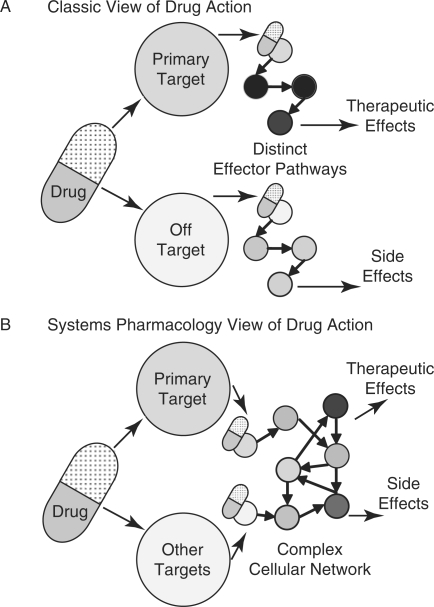
\includegraphics{./images/01-06/img_5.png}

}

\caption{\label{fig-after-discharge}초발 조현병 환자의 퇴원 후 5년간의
경과 @Shepherd1989-rs}

\end{figure}

\hypertarget{uxc2ecuxb9acuxc801-uxc801uxc751}{%
\subsection{심리적 적응}\label{uxc2ecuxb9acuxc801-uxc801uxc751}}

조현병 초기의 질풍노도와 같은 시기를 지나가면, 환자들은 나름대로 증상에
적응하기 시작한다. 실상 환자가 적응해야 하는 것은 증상 뿐만은 아니다.
대다수의 환자들은 학업을 중단하고, 직장을 잃었으며, 가족과 단절되어 삶의
터전을 상실한다. 또한 피해망상으로 인해 스스로 지역사회에 등을 돌렸을 뿐
아니라, 지역사회 역시 편견과 차별로 환자를 궁지에 몰아넣는다.

이러한 힘든 상황에서 회복의 실마리를 찾기란 여간 어려운 일이 아니다.
그러나 성공적으로 적응하기 시작한 일부 환자들은 나름대로의 대처전략을
마련한다. 조현병이 중반에 접어들면 증상이 조금은 약화되는 듯 하며,
적어도 재발의 주기가 길어진다. 환자들은 질병이 자신의 삶에 미친 영향을
심각하게 받아들이며, 부분적 병식이라도 얻게된 환자들은 약물 치료 및
정신과 상담에 의지하게 된다. 망상이나 환각에 대해서는, 증상이 완전히
사라지지 않았더라도, 그 의미를 축소하거나, 무시하거나, 주의를 다른 데로
돌리는 법을 익힌다.

환자의 회복 및 재활에 있어서 사회적 관계는 무엇보다도 중요한 역할을
한다. 환자들은 이전에 갖고 있던 사회적 연결고리를 대부분 상실한
상태이고, 증상 때문에 새로운 고리를 형성하기 어려워한다. 성년기에
접어들면 원가족으로부터 독립을 해야할 나이이기 때문에, 발병으로 인해
결혼 시기를 놓친 환자들은 자신만의 가족을 꾸리지 못한 채 홀로 살아나가야
한다. 지지적인 가족들이 경제적으로나 심리적으로 환자를 지탱해주기도
하지만, 그렇지 못한 경우 사회경제적으로 하위 계층으로 추락하기 쉽다.
다행스러운 것은, 환자가 강한 의지가 있거나, 적극적인 치료진을 만나는
경우에는, 그룹 치료나 재활 센터 등을 통해 새로운 지지 체계를 구축하기도
한다. 이러한 지지 체계는 현실적으로 환자의 자활을 도울 뿐더러, 환자가
현실감을 놓치지 않도록 지탱해주는 역할을 한다.

이를 정리하면, 질병의 중반기에 접어든 환자들은 증상이 조금은 경감되고,
부분적이나마 병식을 획득하며, 증상에 대처하는 기술을 익히고, 사회적
관계를 조정함으로써 재발의 기틀을 마련한다. 어떤 이들은 긍정적 미래를
꿈꾸기도 하고, 어떤 이들은 무기력과 절망감에 빠지기도 한다. 더 많은
이들은 젊은 시절에 꿈꾸었던 미래와 너무도 동떨어져버렸음을
아쉬워하면서도, 수용과 체념을 통해 새로운 현실에 적응하고자
한다.{[}@Shepherd2012-nv{]}

\hypertarget{uxc99duxc0c1uxbcc4-uxacbduxacfc}{%
\subsection{증상별 경과}\label{uxc99duxc0c1uxbcc4-uxacbduxacfc}}

조현병의 정체가, 발병 때 급격한 혼란 상태에 빠졌다가 시간이 지나면서
서서히 회복되는 질환인지, 아니면 마치 치매와 같이 점진적으로 악화되는
진행성 질환인지는 분명하지 않다. 이는 조현병 자체의 특성이기보다는 환자
각각의 특성으로 보는 것이 더 유용하다. 임상적 경험에 따르면 시간이 지날
수록 양성 증상이 전체 병세에 차지하는 비중은 줄어들며, 대신 음성/인지
증상이 차지하는 비중이 높아진다. 안타깝게도 기능 수준과 삶의 질을
결정하는 것은 후자의 증상이다.

\hypertarget{uxc591uxc131-uxc99duxc0c1}{%
\subsubsection{양성 증상}\label{uxc591uxc131-uxc99duxc0c1}}

양성 증상의 비중이 줄어드는 것이 질병의 자연적 경과인지, 약물 치료의
효과인지도 확실하지 않다. 윤리적 문제때문에, 환자를 추적 조사하는 모든
연구는 약물 치료를 병행할 수 밖에 없다. 약물의 효과가 양성 증상과
비교하여 음성/인지 증상에는 별반 뚜렷하지 않기 때문에, 증상의 비중이
변하는 것은 약물 치료의 결과일 가능성이 있다. 시카고 추적
조사\footnote{\textbf{시카고 추적 조사(Chicago Follow-up study)}: 시카고
  지역의 정신병원을 중심으로 행해진 조현병 환자에 대한 장기 경과 추적
  조사. 1980년대 초 시카고 대학 심리학 교수였던 Martin Harrow의
  주도하에, 젊은 조현병 환자 139명을 이후 최대 27년간 주기적으로
  평가하였다. 이 연구는 항정신병 약물을 한번도 투여받지 않은 환자군이
  오히려 예후가 좋고 기능 수준이 높다는 것을 보여줌으로써 약물치료에
  대한 맹신을 되돌아보게 하였다.{[}@Harrow2017-wh{]}}에서는 조현병의
다양한 증상들을 2, 4.5, 7.5, 10, 15, 그리고 20 년 후에
평가하였다.{[}@Harrow1985-ph{]} 슈나이더의 일급 증상은 초반에 심하다가
10년 후 약간 줄어드는 듯하였으나, 20년 후에는 다시 늘어나는 양상을
보였다. {[}@Rosen2011-gs{]} 하지만 환청은 처음 80\%에서 15년 후에는
30\%의 환자만이 경험하고 있었다. {[}@Goghari2013-xn{]}

\hypertarget{uxc778uxc9c0-uxc99duxc0c1}{%
\subsubsection{인지 증상}\label{uxc778uxc9c0-uxc99duxc0c1}}

많은 의사들의 선입관과는 달리 조현병 환자의 인지 기능 저하는 초발때부터
나타난다.{[}@Albus1996-si{]} 치료를 하여 양성 증상이 호전된다 할 지라도
인지 기능의 호전은 뚜렷하지 않으며, 동시에 시간이 경과한다고 해서 눈에
띠게 악화하지도 않는다.{[}@Censits1997-dd{]} 신경발달학적 가설에 의하면
환자들은 발병 전에도 이미 신경회로의 이상을 지니고 있으며, 이 때문에
집행 기능 등 고위 인지기능에 문제가 있을 수 있다. 단순히 전구증상을
보이는 고위험군과 비교해보아도, 실제로 발병에 이른 고위험군은 인지기능이
발병전부터도 이미 더 떨어져 있다. {[}@Carrion2015-va: @Carrion2018-um{]}
따라서 이렇게만 보면 점진적인 인지기능 저하 혹은 신경퇴행의 증거는 찾기
어려워보인다.

그러나 초발 후 10년 이상이 지난 장기적 시점에서 조사해보면, 인지기능의
저하가 서서히 관찰되기 시작한다. Zanelli 등{[}@Zanelli2019-jo{]}은
65명의 조현병 환자와 41명의 기타 정신병적 장애 환자를 발병 전과 후 약 10
여년의 간격을 두고 IQ를 측정하였다. 그 결과 비록 효과 크기는
작았지만(Cohen's d=-0.28), 조현병 환자군에서만 유의한 IQ 저하가
관찰되었다.

이상의 연구 데이터를 보면, 초발 시점에서 장년기에 이르기까지 인지기능의
점진적인 저하가 예상과 달리 두드러지지 않다는 것을 알 수 있다. 그러나
흥미롭게도 조현병 환자가 50세 이상이 되었을 때 간이정신상태검사(MMSE)
등을 이용하여 치매선별검사를 하면, 상당수 환자가 치매 진단기준에
해당한다.{[}@Friedman2001-jl; @Murante2017-jp{]} 연구자들은 나이든
조현병 환자의 인지기능 변화 궤적을 세가지 패턴으로 나눌 수 있다고
여긴다. 약 절반 정도의 환자는 일반 인구와 유사한 퇴행 속도를 보이며, 약
40\%는 일반 인구보다는 좀더 빠른 속도로 퇴행하며, 10\% 정도는 그야말로
급격한 퇴행을 보인다.{[}@Thompson2013-wm{]} 서로 다른 패턴의 존재가
생물학적 차이 때문인지, 평생에 걸쳐 사회와 담을 쌓고 살았던 때문인지는
불분명하다.

실제로 나이든 조현병 환자가 치매에 걸릴 위험은 일반 인구의 2.2배
정도이며, 이환 연령도 더 낮다.{[}@Cai2018-pz{]} 80세 이상을 비교했을
때는 치매의 이환률이 일반 인구에 비해 크게 차이가 없지만, 65세 이하만을
고려하면 상대 위험도는 3.8배에 이른다. 조현병 환자가 다양한 성인병에
좀더 빨리 걸리고, 65세 이하의 조기 치매 비율도 높으며, 기대 수명도
짧다고 했을 때, 이들이 가속화된 노화\footnote{\textbf{가속화된
  노화(Accelerated aging)}: 현대의 연구자들은 노화가 단순히 시간경과에
  따라 신체가 기능을 상실해가는 수동적 과정이 아니라, 정교하게
  프로그램된 생리적 프로세스라고 여긴다. 조로증(progeria)에서 볼 수
  있듯이 이러한 프로세스에 이상이 생기면, 시간적 연령과 생리적 연령에
  차이가 생긴다. 조현병 환자는 기대 수명이 짧아질 뿐 아니라 인지기능,
  혈압변화, 당대사 변화, 골밀도, 뇌실질 감소 등 다양한 노화 관련 현상이
  일반 대조군보다 일찍 시작된다. 이는 항정신병 약물을 투여하지 않는 군도
  마찬가지이다.{[}@Kirkpatrick2018-pg{]} 후성유전학의 발전에 따라
  텔로메이 길이 등 후성유전학적 시계(epigenetic clock)이 조현병
  환자에게서 앞당겨져 있는 것이 반복해서
  확인되었다.{[}@Higgins-Chen2020-rp{]} 혹자는 조현병을 부분적
  조로증(segmental progeria)으로 이해하기도
  한다.{[}@Papanastasiou2011-ak{]}}의 특성을 보인다고 생각해볼 수
있다.{[}@Kirkpatrick2018-pg{]}

21세기에 접어든 지도 20년이 지난 현재 노령기에 든 환자들은 조현병 치료에
대한 철학과 관행이 급격히 전환되는 시기를 거쳐왔다. 불과 10여년 전까지만
해도 대형 정신병원 위주의 치료가 행해졌고, 수년이상 가족과 사회로부터
격리된 채 담장 안에서 살아온 조현병 환자가 드물지 않았다. 이에 비해 지난
10년간 한국에서도 급격한 탈원화 물결과 함께 지역 사회로 돌아온 조현병
환자가 늘어났고, 사회적 지지체계도 눈에 띄게 발전하였다. 자의든 타의든
사회로부터의 단절 여부가 고령에 접어든 조현병 환자의 인지기능 감소
패턴을 설명할 수 있을 지는 향후 10여년 이상의 추적관찰 연구가
뒷받침되어야 알 수 있을 것 같다.

\hypertarget{long-term-course}{%
\section{장기적 예후와 최종 결과}\label{long-term-course}}

지난 70년 동안, 정신약물학의 발달과 신약의 도입으로 치료 성과가
점진적으로 나아졌다고 해도, 여전히 조현병 환자의 장기적 예후는 밝지
않다. 무엇보다 항정신병 약물이 장기적 예후를 개선시키는데 도움을 준다는
증거가 뚜렷하지 못하다.{[}@Harrow2013-fn{]} 약물 도입 이전에도 많게는
25\%의 환자가 평생 재발하지 않고 건강한 일상을 보낸다.(2-3-3절 참조)
따라서 약물 도입으로 인해 이 비율이 유의하게 높아졌는지는 확인하기
어렵다.{[}@Taylor2019-ba{]} 물론 약물 도입으로 말미암아 양성 증상의
조절은 비교할 수 없이 수월해졌고, 재발 예방 역시 큰 성과를 거두었다.
그러나 여전히 음성 증상과 인지 장해가 지속되는 비율은 상당히 높다.
이밖에도 환자의 25\textasciitilde80\%는 우울 증상을 경험한다. 우울
증상은 피해/관계사고와 결부되어 사회적 위축을 심화시키고, 가족 또는 사회
관계를 단절시키며, 물질남용을 높여 질병 경과를 악화시킴과 동시에
자살경향성도 2배 이상 높인다. {[}@Conley2007-el:
@Schennach-Wolff2011-mv{]} 장기적인 환자의 삶의 질은 음성/인지/우울
증상이 결정한다고 했을 때, 약물은 기껏해야 부분적인 승리만을 거둔
셈이다.

처음 발병한 환자의 70-80\%는 치료 후 일단 관해에 도달하지만, 5년 이내에
80\% 정도가 재발한다.{[}@Robinson1999-qy{]} 재발이 반복될수록 회복하지
못하는 비율이 늘고 항정신병 약물에 반응할 때까지의 시간이 길어지며, 약물
용량이 늘어나거나 병용 투여가 필요해진다.{[}@Emsley2013-ts;
@Takeuchi2019-mj{]} 궁극적으로 환자의 20-30\% 정도는 치료에 반응하지
않고, 30\% 정도는 부분적인 반응만을 보인다.{[}@Meltzer1997-rp{]}

비정형 항정신병 약물의 도입으로 말미암아 추체외로 부작용 및 지연 운동
이상증은 줄었으나, 대신 비만과 대사장애 그리고 이와 연관된 심혈관계
질환은 현저히 늘어났다. 조현병 환자의 일반 인구 대비 표준화
사망비(standardized mortality ratio, SMR)는 1970년대 1.84배에서
1990년대에는 3.2배로 오히려 더 높아졌는데{[}@Saha2007-ea{]}, 이렇게 점점
벌어지는 사망률의 차이가 비정형 약물에 기인한 대사장애 때문은 아닌지
의심되고 있다.{[}@Nielsen2013-et{]} 또한 고프로락틴혈증도 흔하고 환자의
30-80\% 정도가 성기능 장애를 겪으며{[}@Malik2007-ox{]}, 비정형 약물
도입으로 현저히 줄었다고는 하나 여전히 2\% 정도의 환자는 지연 운동
이상증을 겪는다.{[}@Correll2004-dk{]}

조현병 환자의 기대 수명은 일반 인구에 비해 짧은 편이다. 이는 특히 지난
30년 동안 일반 인구의 사망률이 급격히 낮아지고 기대 수명이 길어졌다는
것을 고려하면 더욱 두드러진다. 표준화 사망비(SMR)는 약 2.58 정도로
추정되는데, 연구가 행해진 나라에 따라 심하게 차이가
난다.{[}@Saha2007-ea{]} SMR 자체는 해가 갈수록 높아지는 것처럼 보이는데,
환자군의 실제 사망률(case fatality rate, CFR)이 늘어나는 것은 아니기
때문에, 일반 대조군의 사망률이 점점 떨어지기 때문이라고 보는 것이 맞다.
즉 현대 의학의 발전, 건강에 대한 관심, 라이프스타일의 변화 등 기대수명을
늘이는데 기여한 다양한 요소들의 혜택을 환자들이 누리고 있지 못하고
있다는 뜻이 된다.

Hjorthøj 등{[}@Hjorthoj2017-jq{]}이 2017년에 발표한 자료에 따르면,
조현병 환자는 일반 인구에 비해 14.5년 일찍 죽는다. 이러한 수명의 단축은
남성에게서 더 뚜렷하며, 남성 환자의 기대 수명은 60세 정도요, 여성 환자는
67.6세에 불과하다. 조기 사망의 원인 중 상당 부분은 자연사나 병사가 아닌
변사(unnatural death)이며, 이에는 자살, 사고사, 타살 등이 포함된다.
조현병 환자의 4.9\%는 결국 자살로 목숨을 잃게 되며, 이는 전체 사망의
12\% 정도를 차지한다.{[}@Pompili2007-sk{]}

역설적이지만, 일반인에 비해 조현병 환자의 수명이 단축되는 원인 중 자살이
차지하는 비중은 점차 줄어들고 있다. 조현병 환자의 자살률이 줄어드는 것이
아니라, 일반 인구의 자살률이 급격히 높아지고 있기 때문이다. 자살에 의한
표준화 사망비(SMR)는 1984년에 11.0에서 2014년에는 6.6으로
감소하였다.{[}@Tanskanen2018-at{]} 대신 심혈관 질환이나 암으로 인한
SMR은 점차 커지고 있다.

항정신병 약물 사용이 보편화된 이후에도 여러 가지 이유로 인해, 조현병
환자들의 장기적 자연 경과와 예후는 크게 달라지지 않았다. 약물 치료의
한계는 결국 환자의 사회적, 직업적 기능의 저하, 사회와 스스로로부터의
낙인, 결혼과 출산의 어려움, 폭력 그리고 낮은 삶의 질과 가족 및 사회의
부담 증가로 이어진다.

비록 조현병을 일으키는 생물학적 프로세스가 발병 전에 이미 피해를
입힐만큼 입혔고, 이후 평생에 걸친 유병 기간에는 그리 큰 영향을 미치지
않는다 하더라도, 한번 궤도를 벗어난 환자의 인생은 점점 더 정상과의
격차가 벌어지면서 고통이 가중될 수 있다. 현대 사회는 초경쟁 사회로서,
모든 사회구성원이 각자의 역량의 최대한 발휘해야만 생존할 수 있다. 이렇게
여유가 없어지는 현실 속에서 조현병 환자는 쉽게 사회의 밑바닥으로
떨어지며, 기술 만능의 사회에서 자신의 위치를 찾지 못한다. 탈원화 정책을
신봉해온 이론가들은 환자를 정신병원이라는 격리 시설에서 해방시키기만
하면 자동적으로 인간다운 삶을 되찾을 것이라 기대했지만, 이는 순진한
기대였을 뿐이다. 전체 사회 시스템 자체가, 기능이 떨어지는 조현병
환자들을 포용할만한 여유를 찾지 못하고 있으며, 환자들은 표면적으로는
자유를 누리고 있지만 실질적으로는 보이지 않는 창살 안에 갇혀 있는 것과
마찬가지인 인생을 보낸다. 조현병 환자의 궁극적 예후가 산업화된 국가보다
오히려 개발도상국에서 더 양호하다는 것은 이를
뒷받침한다.{[}@Padma2014-ny{]} 아마도 환자의 장기적 예후는 이러한 궁극적
소외 현상을 고려에 넣은 후에야 포괄적으로 논의될 수 있을
것이다.{[}@Warner2004-uz{]}

\hypertarget{references-6}{%
\section*{References}\label{references-6}}
\addcontentsline{toc}{section}{References}

\markright{References}

\part{조현병의 생물학적 이해}

\hypertarget{uxc870uxd604uxbcd1uxc758-uxc720uxc804uxd559uxc801-uxc774uxd574}{%
\chapter{조현병의 유전학적
이해}\label{uxc870uxd604uxbcd1uxc758-uxc720uxc804uxd559uxc801-uxc774uxd574}}

Genetic Understanding of Schizophrenia

\hfill\break

\hypertarget{uxc0dduxccb4uxacc4uxce21uxc801-uxc720uxc804uxd559}{%
\subsection{생체계측적
유전학}\label{uxc0dduxccb4uxacc4uxce21uxc801-uxc720uxc804uxd559}}

모든 정신증은 결국 하나의 질환이 다양하게 변용되어 나타나는 것뿐이라는
단일정신병 개념(섹션~\ref{sec-modern-period})이, 서로 명확히 구분되는
다수의 정신질환이 존재한다는 크레펠린의 혁신적인 개념으로 대체된 이후,
정신의학계는 새로운 희망과 의욕에 몸달아 있었다. 생물정신의학의 기치를
내건 Griesinger(섹션~\ref{sec-kraepelin})의 제자들은 그렇다면 다수의
정신질환은 제 각각 특징적인 신경병리를 보일 것이요, 이는 그에 상응하는
독특한 유전적 변이때문에 일어날 것이라 예상하였다. 그들이 이렇게 생각한
것은 경험상 정신질환이 특정 가계(pedigree)에 밀집되어 나타나는 것처럼
보였기 때문이다. 당대 학자들이 가장 먼저 떠올린 가설은 변성
개념(섹션~\ref{sec-kraepelin})이었다. 그들은 정신질환이 대를 거듭하면서
변이가 누적되어 점점 더 심한 형태로 악화된다고 믿었으며, 그 최종 국면에
조현병과 치매가 놓여있다고 생각하였다.

그러나 제대로 된 역학조사나 가계조사없이 유전적 증거를 확인할 수는
없었으며, 하물며 이를 정량화할 방법도 존재하지 않았다. 이미 다윈은
진화론을 통해 종의 생존적합성을 결정하는 미세한 표현형질(phenotype)들이
세대를 거쳐 유전된다고 주장하였다. 다윈의 사촌이었던 Galton\footnote{\textbf{Francis
  Galton (1822\textasciitilde1911)}: 영국의 우생학자, 유전학자이자
  통계학자. 인류의 발전을 위해서는 부적격자의 탄생을 막고, 적격자의
  탄생율 증진시켜야 한다고 주장하였으며 우생학(eugenics)이라는 용어를
  처음 사용하였다. 부모의 키와 자녀의 키 간에는 긴밀한 상관관계가 있다는
  것을 밝혀내면서, 상관계수, 회귀 등 통계학의 몇가지 기본 개념을
  확립하였고, 이를 유전학 연구에 응용하였다.}은 가계 구성원 들의 다양한
신체 치수를 서로 비교함으로써, 이들 간의 상호 관계를 알아낼 수 있을
것이라는 아이디어를 구상했다. 그는 이러한 신체계측 자료를 광범위하고도
치밀하게 수집하였으며, 이를 제자였던 Pearson\footnote{\textbf{Karl
  Pearson (1857\textasciitilde1936)}: 영국의 수학자이자 통계학자.
  Galton의 제자로서 생체계측적 유전이론의 기초를 다지는데 공헌하였다.
  유전 현상을 수학적/통계학적으로 이해하는 길을 마련했고, 산포도,
  표준편차, 상관계수, 회귀계수, 카이-검정, p 값 등의 개념을 창안하여
  현대적 통계분석의 기틀을 세웠다.}에게 맡겨 분석하도록 하였다. Galton과
Pearson이 몸 담았던 실험실은 유전이 어떻게 일어나는 지에 대한 이론적
문제보다는, 서로 다른 신체 치수 즉 표현형이 얼마나 유전에 의해
결정되는가를 계산하는데 주력하였다. Galton은 중심 극한 정리\footnote{\textbf{중심
  극한 정리(central limit theorem)}: 서로 독립인 무작위 변수가 더해지면,
  일정한 평균과 표준편차를 갖는 정규 분포에 흡사한 분포를 갖게 된다는
  이론. 더해지는 변수가 많으면 많을 수록 정규분포에 가까워진다. 이
  이론이 처음 제시된 것은 1733년 Moivre에 의해서였으나, Galton board를
  발명하여 이 이론을 일반인에게 이해시키고 대중화시킨 것은 Galton이다.}의
개념을 응용하여, 키나 몸무게 같이 정규 분포에 가까운 변이를 보이는
현상들은, 무수히 많은 요인들의 독립적 영향들이 합쳐져서(평균값을 통해)
나타나는 것이라 생각하였다. 따라서 유전되는 것은 연속적이고 미세한
변이를 일으키는 많은 수의 형질 들이고, 질병을 결정하는 것은 다수 형질
들의 효과의 총합일 것이라 믿었다. 1907년 Pearson의 동료인
Heron\footnote{\textbf{David Heron (1881\textasciitilde1969)}:
  스코틀랜드의 통계학자. Pearson의 연구 조교로 경력을 시작하였다.}은
\textsc{\emph{``광증의 통계 및 광증경향의 유전에 대한 첫번째 연구(A
First Study of the Statistics of Insanity and the Inheritance of the
Insane Diathesis)''}}라는 저서를 발간하였다. 이 책은 정신지체, 조현병을
비롯한 광증의 유전 정도를 정량적으로 분석한 첫번째 기록이며, 이 책에
실린 수치들은 현대에 추정된 수치와 매우 근접해있다.{[}@Kendler2015-lz{]}
당시 Galton의 실험실에서 함께 일했던 일군의 학자들을 후세 사람들은
\uline{생체계측적 유전학자(biometrical geneticists)}라고 불렀다.

\hypertarget{uxd604uxb300uxc801-uxc720uxc804uxd559}{%
\subsection{현대적 유전학}\label{uxd604uxb300uxc801-uxc720uxc804uxd559}}

현대 유전학을 탄생시킨 멘델\footnote{\textbf{Gregor Mendel
  (1822\textasciitilde1884)}: 오스트리아의 식물학자로 유전학의 기본
  법칙을 발견하였다. 천주교 사제로서 일하면서도, 아버지의 과수원에서
  일했던 경험을 살려 농학, 원예학에 몰두했다. 30대 중반부터 7년여간에
  걸쳐 완두콩을 재배하면서 유전에 대한 실험을 진행했고, 이를 명쾌한
  수학적 원리로 발표하였다. 생전에는 인정받지 못하였으나, 1900년에
  들어서 유럽의 식물학자들에 의해 재발굴되었다.}이 완두콩 교배를 통해
발견한 소위 ``멘델의 유전법칙''을 학계에 발표한 것은 1865년이었으나, 그
학문적 중요성이 재발견된 것은 안타깝게도 멘델이 죽은 후 15년이 지난
1900년에 이르러서였다. 연속적이고 미세한 형질이 점진적으로 유전된다고
여긴 Galton/Pearson과 달리, 멘델의 제 1법칙은 유전현상은 이산적
단위(discrete unit)를 통해 일어난다고 주장한다. 예를 들어 그가 연구했던
완두콩의 경우 우성 형질과 열성 형질은 황색/녹색 혹은 둥글다/주름지다
처럼 뚜렷이 구분되는 단위로 나뉘어져 있다. 이러한 대립형질 중 우성
아니면 열성 형질 하나가 발현될 뿐이지, 황색과 녹색 인자가
유전되었다고해서 연두색 콩이 나오는 것은 아니다. 이러한 논리에 따라,
당시에는 아직 DNA가 발견되기 전이지만, 생식을 통해 전달되는
대립유전형(allele)과 그에 의해 결정되는 표현형 사이에는 일대일
대응관계가 성립된다고 믿어졌다.

이는 이후 질병의 유전 연구에 커다란 영향을 미쳤고, 유전형과 표현형은
동일한 현상의 서로 다른 측면처럼 취급되었다. 질병 역시 하나의
표현형이라고 했을 때, 이를 결정하는 유전인자가 어딘가에 존재할 것이라는
추측은 매우 매력적인 가설이었다. 1900년대 초반, 혈우병, 야맹증, 안구색
등의 표현형이 멘델 법칙에 따라 유전된다는 것이 증명되었다.
Rüdin\footnote{\textbf{Ernst Rüdin (1874\textasciitilde1952)}: 스위스
  태생의 독일 유전학자이자 정신과의사. 비록 정신유전학에서 많은 업적을
  남겼지만, 나치의 이데올로기에 동조하여 정신질환자들을 거세하거나
  처형하는 것을 암암리에 지지하였다.}은 1907년 멘델의 유전법칙이
조현병에 들어맞는지 체계적으로 연구하기
시작하였다.{[}@Zerbin-Rudin1996-nn{]} 그는 비록 단일 유전인자에 의한
멘델 유전으로는 자신이 가계연구에서 얻은 데이터를 설명할 수 없었지만, 두
개의 열성 유전인자에 의한 유전 모델로는 상당히 근접하여 설명할 수
있었다고 주장하였다. 또한 유전인자를 물려받았어도 발병하지 않는 불완전
침투\footnote{\textbf{불완전 침투(incomplete penetrance)}: 질병을
  일으킨다고 알려진 유전자 변이를 물려받은 개인이 실제로 질병에 걸리게
  되는 비율을 침투라고 한다.이 비율이 100\%가 아닐 때는 불완전 침투라
  한다.} 현상이 있을 것이라고 추측하였다. 크레펠린은 조현병 환자의
형제들에게서, 뚜렷하게 병이 있는 것은 아니지만 좀 유별난 성격이 많다는
것을 관찰하고, 이들이 Rüdin이 말한 불완전 침투에 의한 잠재적 환자일
것이라고 생각하였다.{[}@Kendler1985-an{]} 크레펠린과 Rüdin 그리고 그들의
영향을 받았던 독일 정신과 의사들은 질병이 연속적이고 미세한 변이의
총합이라는 생체계측적 모델보다는, 이산적이고 뚜렷이 구분되는 대립형질이
유전된다는 멘델의 모델을 받아들였다. 그들은
유전인자-신경병리-조현병이라는 단순한 인과관계 모델에 매료되었기
때문이었다. 그러나 아무리 애를 써서 관측결과를 모델에 우겨넣으려 해도 잘
맞지 않았다. 좀더 확장된 모델이 필요할 때였다.

\hypertarget{uxd1b5uxacc4uxd559uxacfc-uxc720uxc804uxd559}{%
\subsection{통계학과
유전학}\label{uxd1b5uxacc4uxd559uxacfc-uxc720uxc804uxd559}}

1902년 통계학자인 Yule\footnote{\textbf{George Udny Yule
  (1871\textasciitilde1951)}: 영국의 통계학자. 특히 시계열 분석의 초석을
  놓았다.}은, 멘델 법칙에 따라 유전되는 대립형질 다수가 서로가 서로에게
영향을 미친다면, 실제 가계도에서 관찰되는 연속적인 형질 분포를 설명할
수도 있을 것이라고 하였다. 당시 초파리(drosophila)를 대량으로 사육하면서
인공적으로 돌연변이를 일으키는 연구를 진행하고 있던 Morgan\footnote{\textbf{Thomas
  Hunt Morgan (1866\textasciitilde1945)}: 미국의 진화생물학자. 염색체가
  유전현상에서 차지하는 역할을 발견한 공로로 1933년 노벨 생리의학상을
  수상하였다.}은 대부분의 돌연변이가 표현형에 큰 변화를 가져오지 않는
미세한 것이요, 질병을 일으킬 정도의 중요한 돌연변이는 극히 드물게만
일어난다는 것을 보고하였다. 이러한 사실들을 종합하여 1918년
Fisher\footnote{\textbf{Ronald Fisher (1890\textasciitilde1962)}: 영국의
  통계학자이자 유전학자. 근대 통계학의 거의 모든 토대를 혼자서 세웠다
  해도 과언이 아닐 정도로 많은 개념과 통계기법을 도입하였다. 진화론에서
  다윈주의를 전파하는데도 중요한 역할을 하여 다윈의 가장 위대한 후계자로
  불리운다.}는 연속적인 변이를 보이는 형질은 조그만한 효과를 갖는 많은
유전인자들의 영향을 단순히 합한 것으로 충분히 설명할 수 있다고
주장하였다.{[}@Provine2001-iw{]}

Fisher가 생체계측적 유전이론과 멘델식 유전이론을 통합한 이후에도, 각
이론을 신봉하는 유전학자들은 제각기 자기들만의 이론을 발전시켜 나갔다.
그러나, 1960년대 중반에 이르러 \uline{다유전자 유전모델(polygenic
inheritance)}{[}@Gottesman1967-rq{]}과
\uline{경향성-역치(liability-threshold) 모델}{[}@Falconer1967-wf{]}이
반향을 일으키면서, 조현병의 유전 방식은 서서히 이 두 모델에 의해
설명되기 시작하였다. 이는 진단개념에도 상응하는 영향을 주었다. 멘델식
유전모델에서는 질병과 건강상태의 구분이 비교적 명확하지만, 다유전자
모델에서는 형질의 분포가 연속적이라 이 구분이 애매하다. 이에 대해 조현병
자체가 연속적인 성향 즉 스펙트럼에 가까운 상태이며, 진단을 내리는 것은
이러한 스펙트럼 어딘 가에 임의적으로 역치를 설정하는 것이라고 이해되기
시작하였다. 이러한 개념은 1970년 대 말부터 정신유전학의 분석방법으로
인기를 끌던 구조방정식\footnote{\textbf{구조방정식(structural equation
  modeling)}: 여러 변인들 간의 인과관계를 하나의 모형을 통해 검증하는
  분석방법. 특히 잠재변인(latent variable)을 가정하여 직접 측정할 수
  없는 구성개념에 대해서도 인과관계를 파악할 수 있다.}에서 가정하는
잠재변인(latent variable)의 개념하고도 잘 맞아
떨어졌다.{[}@Franic2012-ak{]}

\hypertarget{uxac00uxacc4-uxc870uxc0ac-uxbc0f-uxc5eduxd559-uxc5f0uxad6c}{%
\section{가계 조사 및 역학
연구}\label{uxac00uxacc4-uxc870uxc0ac-uxbc0f-uxc5eduxd559-uxc5f0uxad6c}}

Rüdin의 선구적 연구를 시작으로 이후 뒤따른 가계 조사에서도, 조현병
환자의 생물학적 친척 중에 조현병 환자가 발생할 비율이 높다는 것이
확인되었다. 한편 당시의 정신분석학적 이론이나 Bateson 등이 주창한 생태
이론\footnote{\textbf{생태이론(echology of mind)}: Gregory Bateson
  (1904\textasciitilde1980)은 정신을 독립된 실체가 아니라 생태계적
  시스템 속에 내재하고 성숙되어가는 역동적 사건으로 이해한다. 따라서
  정신을 이해하기 위해선 이를 둘러싼 시스템을 이해해야 하며, 시스템
  구성원 간의 커뮤니케이션을 살펴보아야 한다고 주장하였다. 이
  논리대로라면 정신과 환자의 경우 가장 중요한 생태계적 시스템은
  가족이며, 가족 내의 왜곡된 커뮤니케이션이 질병을 야기할 것이다.}에서는
부모의 양육방법이나 가족 내 의사소통 패턴이 조현병의 원인이라고
간주되었다. 따라서 가계 내에 환자가 많은 것, 형제 중에 조현병 환자가
동시에 나타나는 것도 이러한 영향 때문으로 재해석 되었다. 이에 유전
이론을 신봉하는 학자들은 쌍생아 연구를 통해 이런 주장을 정면돌파하고자
하였다.

크레펠린의 제자였던 Luxenberger\footnote{\textbf{Hans Luxenberger
  (1894-1976)}: 독일의 유전학자. 정신유전학의 뮌헨 학파(Munich School of
  Psychiatric Genetics)의 일원이다. 뮌헨 인근에 입원해있던 조발성 치매
  환자 16,382을 조사하여 이중 211명의 쌍생아를 찾아낸 후 발병 일치
  여부를 분석하였다.{[}@Noll2009-av{]}}는 1928년 조현병 환자를 대상으로
한 최초의 쌍생아 연구를 수행하였다. 그가 조사한 일란성 쌍생아 중
조현병의 발생일치율\footnote{\textbf{발생일치율(concordance rate)}:
  유전적 정보를 공유하는 두 사람이 모두 동일환 질환에 걸릴 확률. 보통
  이미 진단을 받은 기준 환자(proband)의 친인척이 동일 질환에 걸릴 확률로
  표시한다.}은 58\%였던 반면, 이란성 쌍생아 중에서는 두 쌍생아가 모두
조현병에 걸린 사례를 찾아낼 수 없었다.{[}@Andreasen1994-bx{]} 이후
수십년간 이어진 유사한 연구에서 일란성 쌍생아에서의 발생일치율은 이란성
쌍생아에 비해 5-10배 정도 높다는 것이 확인되었다. 영국의 베들렘 병원과
모즐리 병원(Maudsley hospital)은 1948년 이래 공동으로 그곳을 거쳐간 모든
환자들의 신상정보와 임상기록을 보관해왔다. Gottesman과
Shields{[}@Gottesman1972-tr{]}가 처음 이 자료에 등록된 쌍생아 자료를
분석하였고, 1999년에는 Cardno 등{[}@Cardno1999-hh{]}이 재분석하였다.
일란성 쌍생아의 경우 발생일치율이 0.8\% 였음에 비해, 이란성 쌍생아는
5.3\%에 지나지 않았으며, 유전성\footnote{\textbf{유전성(heritability)}:
  개체 집단에서 발견되는 표현형의 변이 중에서 유전형의 변이로 인해
  설명되는 비율.}은 82\%에 달하였다.

입양아 연구에서도 유사한 결과가 얻어졌다. 이 분야에 탁월한 업적을 낸
Kety\footnote{\textbf{Seymore Kety (1915\textasciitilde2000)}: 미국의
  신경생물학자. 뇌혈류를 측정하는 방법을 최초로 개발하였으며, 미국
  국립정신건강연구원(NIMH)의 초대 국장을 역임하였다.}는 20 여년간의
꾸준한 연구를 통하여 다음과 같은 사실을 확인하였다. 첫번째, 조현병
어머니에게서 태어나 정상 부모에게 입양된 아이들은, 자신을 낳아준
어머니에게 양육된 아이들과 동일한 발병률을 보였다. 둘째, 입양된 조현병
환자의 현재 가족 구성원(입양한 가족)에서의 발병률보다, 원래의 생물학적
가족에서 훨씬 조현병의 발병률이 높았다.{[}@Kety1976-ts{]}

쌍생아 연구와 입양 가족 연구는 조현병 발병에 유전적 요인이 차지하는
비중에 대해 귀중한 정보를 제시했음은 물론, 양육방식과 가족 내 갈등이
발병의 주요 요인이라는 당시 심리학자와 정신분석가들의 편견을 일소하는데
기여하였다.{[}@Holzman2001-rz{]}

\hypertarget{uxc720uxc804uxc801-uxc5f0uxad00uxc5f0uxad6c}{%
\section{유전적
연관연구}\label{uxc720uxc804uxc801-uxc5f0uxad00uxc5f0uxad6c}}

\hypertarget{uxbcd1uxc778uxb860}{%
\subsection{병인론}\label{uxbcd1uxc778uxb860}}

크레펠린에 의해 조현병이 개념이 자리잡기가 무섭게, 학자들은 이 질환이
유전적 요인에 의해 일어난다는 것을 입증하고자 애썼다. 이런 배경에는,
조현병 환자가 특정한 가계에 몰려 나타나는 경향이 거듭 관찰되고 있었다는
것, 오염된 혈통과 변성 개념이 사람들에게 은근한 두려움으로 다가왔다는
요인이 자리잡고 있었다. 이에 덧붙여 질병의 원인론에 대한 당시의 지식과
이론도 영향을 끼쳤다. 현재도 마찬가지이지만, 아리스토텔레스의 원인
이론\footnote{\textbf{아리스토텔레서의 4원인(four causes of
  Aristoteles)}: 아리스토텔레스는 변화와 운동에는 반드시 원인이 있으리라
  가정하였고, 다음 네가지를 열거하였다. 1) 질료인(material cause)은
  대상이 무엇으로 이루어져 있는지, 2) 형상인(formal cause)은 대상이 어떤
  특성을 갖고 어떤 법칙을 따르는지, 3) 작용인(efficient cause)은
  외부로부터 가해진 변화나 힘, 4) 목적인(final cause)은 대상이 애초에
  지닌 의지, 동기, 목적은 무엇인지를 가리킨다.}및 뉴턴 역학의 영향을
받은 당대의 학자들은 현상 혹은 변화의 근원을 파고들어가면 결국 일차적
원인에 맞닥뜨리게 된다고 믿었다. 아리스토텔레스 철학에서는 물질의 재료나
구성 혹은 외부에서 힘을 가한 존재가 그 역할을 하며, 뉴턴 역학에서도
물체가 운동하려면 맨 처음 힘을 가한 어떤 존재가 있어야 한다. 우주에
존재하는 모든 만물의 운동 역시 태초에 궁극적인 원인이 있어서
시작되었으며, 아리스토텔레스는 이를 원동자\footnote{\textbf{원동자(prime
  mover)}: 아리스토텔레스는 원인 없는 결과는 없다고 보았는데, 그렇다면
  애초에 우주가 왜 움직이게 되었는지를 설명하기 곤란해진다. 이러한
  난점에 대해 그는 원인이 없이도 스스로 움직이기 시작한 최초의 존재를
  가정하고 이를 원동자( 元動者)라고 칭하였다.}라고 하였다.

병인론을 최초로 공식화한 Koch와 Loeffler\footnote{\textbf{Koch의 병인론
  가설}: Robert Koch와 Friedrich Loeffler가 1884에 제안한 가정. 만약
  특정한 병에 걸린 환자에서 1) 유달리 어떤 미생물이 많이 발견되고, 2) 그
  미생물이 실험실에서 배양될 수 있으며, 3) 배양액을 다른 개체에 주입하면
  동일한 병이 생기고, 4) 새롭게 병에 걸린 개체에서도 역시 동일한
  미생물을 다량 추출할 수 있다면, 질병의 원인은 처음의 그 미생물이다라는
  가설이다.}에게 있어서 원동자는 다름 아닌 미생물이었다. 그러나 조현병이
미생물에 의한 질병이 아닌 이상, 궁극적 병인으로 가장 걸맞은 것은 유전적
요인이었던 셈이다. 조현병 유전 연구의 초창기에는 가계도 분석과 역학
연구를 통하여 그 유전성 을 조사하는 것이 고작이었으나, 염색체의 발견을
거쳐 DNA의 구조와 기능이 밝혀지면서 유전 연구는 유전적 원인(genetic
cause)을 찾는 연구로 거듭나게 되었다. 다유전자 모델이 어느 정도 영향력을
갖게 된 이후에도, 상당수의 유전학자들은 그야말로 ``조현병을 일으키는''
단일 유전자를 찾고 있었다.

\hypertarget{uxc5fcuxc0c9uxccb4uxc640-uxc5f0uxad00-uxd604uxc0c1}{%
\subsection{염색체와 연관
현상}\label{uxc5fcuxc0c9uxccb4uxc640-uxc5f0uxad00-uxd604uxc0c1}}

염색체는 19세기 말에 이미 그 개념이 도입되었고, 전술했던 Morgan의 연구를
통해 존재가 증명되었다. 1920년대에는 이미 현미경을 통해 염색체를
육안으로 관찰할 수 있었고, 인간 염색체의 대략적인 개수도 알려졌다. 원래
멘델의 두번째 유전법칙인 독립의 법칙(law of independent assortment)에
따르면, 서로 다른 표현형은 독립적으로 유전되어야만 했지만 실상은 그렇지
않았다. 한 가계 내에서 서로 다른 표현형이 함께 유전되는 \uline{유전자
연관(genetic linkage)}은 이미 1905년 Bateson\footnote{\textbf{William
  Bateson (1861\textasciitilde1926)}: 영국의 생물학자로
  ``유전학(genetics)''이라는 용어를 처음 사용하였으며, 멘델의 유전법칙을
  널리 전파하는데 기여하였다.}에 의해 발견되었다. 선형 구조를 갖는
염색체 개념에 이를 적용하여, 염색체 상에서 서로 거리가 근접한 유전인자는
함께 유전될 가능성이 높고, 역으로 거리가 먼 유전인자는
재조합(recombination)될 확률이 높다는 이론이 고안되었다. 이를 토대로
염색체 지도가 만들어지기 훨씬 이전에 이미 \uline{연관 지도(linkage
map)}가 만들어졌다. 초기에는 대립형질(표현형을 구성하는 우성형질과
열성형질의 쌍) 하나하나가 지도에서의 위치를 가리키는 표지자
\footnote{\textbf{표지자(marker)}: 하나의 염색체에 들어있는 DNA는 하나의
  긴 1차원의 가닥으로 이루어진다. 이 가닥 내에서 상대적 위치를 표시할 수
  있는 모든 종류의 변이를 표지자라고 한다.}의 역할을 하였으나, 이는
초파리 실험과 같이 다양한 형질 변화를 인위적으로 일으킬 수 있는
연구환경이 아니라면 적용하기 어려웠다.

세포 내의 유전물질에 대한 가설은 이미 19세기 중반에 제기되었으며, 이것이
핵산(nucleotide)으로 구성되었다는 것 역시 1919년 Levene\footnote{\textbf{Phoebus
  Levene (1869\textasciitilde1940)}: 러시아 태생의 미국 생화학자로 DNA와
  RNA의 구조를 분석하였으며, 핵산이 연이어 연결된 구조가 이들의 기본
  형태라는 것을 발견하였다.}에 의해 발견되었다.{[}@Pray2008-vy{]} 이후
Watson과 Crick\footnote{\textbf{James Watson (1928\textasciitilde),
  Francis Crick (1916\textasciitilde2004)}: 미국의 분자생물학자로
  공동작업을 통해 DNA의 3차원적 구조를 발견했으며, 이 공로로 함께 1962년
  노벨 생리의학상을 수상했다.}는 DNA가 이중나선 형태를 이루고 있음을
1953년에 발표하였다. DNA의 발견은 부연 설명이 필요없을 정도로 유전
연구를 혁신적으로 진일보시켰다. 연관 지도를 통해 유전인자들이 일렬로
배열되어 있을 것이라 짐작하고 있었지만, 이제 그 실질적 증거를 확보하게
되었다. 바야흐로 연관연구는 표현형을 기반으로 한 원시적 표지자가 아닌
분자 단위의 세밀한 표지자를 이용하여 행해질 수 있었다.

\hypertarget{uxd45cuxc9c0uxc790}{%
\subsection{표지자}\label{uxd45cuxc9c0uxc790}}

유전적 표지자(genetic marker)가 되기 위해선 다른 표지자들과의 상대적
위치를 확정할 수 있어야 하며, 동시에 인구집단 내에 적당한 비율의 변이가
있어야 한다. 초창기에 등장한 표지자는 \uline{RFLP (Restriction fragment
length polymorphism)}라는 것으로, 특정한 염기서열만을 잘라내는
제한효소(restriction enzyme)에 의해 잘려나간 조각들의 패턴을 말한다.
개개인에 따라 염기서열이 조금씩 다르기 때문에, 이렇게 잘려나간 패턴 역시
변이가 생긴다. 이러한 조각들을 전기영동(southern blot)에 통과시키면,
분자량에 따라 잘려진 염기들을 순서대로 배열할 수 있었다. 그러나 RFLP는
특정 염기서열을 인식하는 제한효소가 있어야만 발견할 수 있는 표지자였고,
또 이를 영상화하기 위해서 방사성 동위원소나 형광 염료를 붙여야 하는 등,
자동화하기 어렵고 비용이 많이 드는 작업이었다. 뒤이어 Short Tandem
Repeat (STR), Variable Number Tandem Repeat (VNTR)\footnote{\textbf{Tandem
  Repeat}: DNA에는 특정 염기서열이 연이어 반복되는 경우가 많다. 예를
  들어 유전자의 프로모터에 자리잡은 CpG island에는 CG가 100번 이상
  반복된다. 반복되는 염기의 길이(bp)가 10개 미만이면 minisatellite,
  10\textasciitilde60개 정도이면 microsatellite라고 하며, STR은
  minisatellite, VNTR은 microsatellite가 반복되는 것을 지칭한다. STR,
  VNTR이 반복되는 수는 개인마다 다르며, 부모로부터 유전되기 때문에
  유전적 표지자 역할을 할 수 있다.} 등의 표지자가 개발되었다. 이들은
많은 수의 대립유전자 변이(allelic variation)를 갖고 있었기 때문에
정보량이 풍부하였으나, 게놈 내에 고루 분포하는 표지자가 아니였기 때문에
제한된 용도로 밖에 쓸 수 없었다.

이전의 연구가 표현형과 표현형 사이의 유전적 거리를 조사했다면,
이제부터는 표현형과 염색체 내 위치를 가리키는 표지자 간의 거리를
조사하기 시작하였다. 대립유전자가 유전될 때는 부모가 갖고 있는 한쌍의
대립유전자 중 무작위로 하나씩만 자손에게 전달되는데 이를
분리(segregation)라고 한다. 만약 특정한 표지자의 대립유전자가 질병과
함께 다음 세대로 전달되는 양상을 보인다면, 그 표지자는 질병유발 유전자와
매우 근접해있다는 증가가 된다. 이러한 동시 분리(co-segregation)을 찾는
것이 연관 연구(linkage study)의 핵심이다.{[}@2000-mn{]}

\hypertarget{uxc870uxd604uxbcd1uxc758-uxc5f0uxad00-uxc5f0uxad6c-uxc131uxacfc}{%
\subsection{조현병의 연관 연구
성과}\label{uxc870uxd604uxbcd1uxc758-uxc5f0uxad00-uxc5f0uxad6c-uxc131uxacfc}}

아쉽게도 쏟아졌던 기대에 비해 연관 연구는 큰 성과를 내지는 못했다.
그럼에도 불구하고, 몇몇 연구를 통해 조현병의 발병기전에 한발 다가갈 수
있었다. 강한 연관 신호를 보였던 몇몇 염색체 영역에 대해서 후속 연구가
진행되면서, 그 부위에 위치한 유전자 중 조현병의 병태 생리에 중요한
역할을 할 것으로 기대되는 몇 가지 유전자를 찾아낼 수 있었다. 예를 들어
1q42에서는 \uline{DISC1 (Disrupted in Schizophrenia 1)} 유전자를,
22q에서는 \uline{COMT (Catechol-O-methyltransferase)}, \uline{PRODH
(proline dehydrogenase)}, 8p에서 \uline{NRG1 (neuregulin 1)}, 그리고
6p에서 \uline{DTNBP1 (dysbindin)} 유전자를 찾아낼 수
있었다.(섹션~\ref{sec-neurophil}){[}@Karayiorgou1997-tk;
@Karayiorgou2006-vv{]} 이러한 유전자들은 이후 연합 연구를 통한
후보유전자 검색과정에서도 조현병과 관련되어 있는 것으로 나타났으며, 이후
조현병의 병태생리를 이해하는데 중요한 이정표가 되었다.

그러나 어렵게 얻어진 몇몇 양성 결과들조차 추후 연구에서 결과를
재현하는데 대부분 실패하였으며, 연관 신호가 높게 나타났던 염색체
부위에서 의미있는 유전자를 찾는 것도 쉽지 않았다. 이렇게 기대에 미치지
못한 이유는 다양하다. 무엇보다 연관 연구는 조현병이 기껏해야 몇 개의
드물지만 영향력이 큰 변이에 의해 초래된다는 가정, 그리고 이들이 단순한
멘델식의 우성 혹은 열성 유전모델을 따른다는 가정, 즉 \uline{단일
주요유전자 자리 모형(single major locus model)}에 입각해있다. 설령
다유전자 모델이 맞더라도, 여전히 조현병을 일으키는데 가장 중요한
유전자는 하나라는 뜻이다.{[}@Elston1970-rg; @Karlsson1974-ts{]} 이들이
이에 매달릴 수 밖에 없었던 이유 중 하나는 연관 연구의 약한 검증력으로는
영향력이 큰 몇 개의 부위만을 찾아낼 수 있기 때문이다.

검증력을 키워 미세한 연관 신호를 잡아내려면, 많은 수의 환자가 포함되어
있는 대규모 가계를 대상으로 연구해야 하는데, 이런 가계를 찾아내기란 여간
어려운 것이 아니다. 설령 그런 가계를 찾아냈다 하더라도, 포함된 환자들이
많으면 많을수록 그들 모두가 단일한 유전요인에 의해 발병되었을 확률이
떨어진다. 또한 한 가계에서 의미있는 신호를 발견했다 하더라도, 이 신호가
다른 가계에서도 발견된다는 보장이 없다. 즉 발견된 결과는 해당 가계에
국한되는 것이지, 보편적인 조현병의 원인인자로 일반화하기 힘들다.
마지막으로 연관 연구에 사용되는 표지자가 그리 조밀하지 않기 때문에 설령
의심되는 영역을 찾아낸다 하더라도 해상도가 매우
떨어진다.{[}@Karayiorgou1997-tk{]} 결국 연관 연구는 역사속의 한
페이지로만 남게 되었다.

\hypertarget{snpuxc640-uxc5f0uxd569-uxc5f0uxad6c}{%
\section{SNP와 연합 연구}\label{snpuxc640-uxc5f0uxd569-uxc5f0uxad6c}}

유전적 표지자의 문제는 오랜동안 유전 연구를 제약해왔던 사안이다. 보통
인구 집단내에 일정 비율 이상으로 존재하는 돌연변이를 표지자로 사용한다.
그 자신이 질병을 일으키는 경우도 있겠지만, 대부분은 그저 염색체 내의
특정한 위치를 표시하는 역할만 하게 된다. 만약 그 돌연변이가 생명을
위협할 정도라면 인구 집단에 널리 분포할 리가 만무하기 때문에, 그 영향이
너무 크지도 너무 작지도 않아야만 한다. 인간 게놈에는 30억개의 염기가
있다고 하는데, RFLP, VNTR 등과 같은 고전적 표지자들은 기껏해야 몇 만개
정도에 불과하다. 이렇듯 해상도가 낮기 때문에 조현병과 연관된 부위를
찾는다 해도, 그 부위에 포함된 유전자 중 어떤 유전자의 변이 때문인지조차
분명히 알아낼 수 없다.

\uline{단일염기다형성(single nucleotide polymorphism, SNP)}은 1996년
Lander\footnote{\textbf{Eric Lander (1957\textasciitilde)}: 미국의
  수학자이자 유전학자로 MIT와 하버드 대학의 교수로 재직중이다.
  유전연구로 유명한 Broad Institute의 초대 국장을 역임하였다. 2021년
  출범한 미국의 바이든 행정부에서 백악관 과학기술정책실장(Office of
  Science and Technology Policy)에 임명되었다.}에 의해 그 개념이
제시되었다. 이는 DNA 염기서열 중 특정 위치의 염기가 다른 것으로 바뀌어
있는 것을 의미한다. 단일 염기의 치환, 삭제, 첨가 등 다양한 기전에 의해
발생하며, 소수 대립유전자빈도\footnote{\textbf{소수 대립유전자빈도
  (Minor Allele Frequency, MAF)}: 하나의 유전자 자리에는 몇 개의 서로
  다른 유전형(변이)이 위치할 수 있다. 이들 변이는 조사된 인구집단에서
  일정한 비율로 분포하는데, 그중 가장 드문 대립유전형의 빈도를 의미한다.
  SNP는 두개의 대립유전자가 있기 때문에 MAF가 너무 작으면 표지자로서의
  가치가 떨어진다. 보통 MAF가 1\% 이상인 변이를 SNP라고 한다.}가 1\%
이상인 것만을 SNP라고 말한다. SNP에서 하나의 염기 위치에서 발견되는
대립유전자(allele)은 일반적으로 두 개이다. VNTR과 같이 한 위치에 수십,
수백 개의 대립유전자가 있는 변이보다는 변이의 폭은 좁지만, 그 대신
표지자가 밀집되어 존재하는 것이 특징이다. 평균잡아 1,000bp에 하나 꼴로
염기 치환이 일어나기 때문에, 한 사람의 게놈 내에는 4\textasciitilde5백만
개의 SNP가 있을 것으로 추정된다. 게다가 커다란 인구집단에서 발견되는
SNP의 수는 무려 1억개에
가깝다.{[}@1000\_Genomes\_Project\_Consortium2015-dn{]} 한 유전자 내에도
수십개 이상의 SNP가 분포하는 것이 일반적이며, 따라서 정확히 어떤 부위가
질병 위험과 연관되어 있는지를 높은 해상도로 파악해낼 수 있다. 게다가
1990년 부터 시작된 인간 게놈 프로젝트의 일환으로 DNA 염기서열을 매우
빠르고 정확하게 읽어내는 기술이 부단히 발전하면서, SNP 변이를 확인하는
기술은 속도 뿐 아니라 자동화 정도에서 기존의 표지자들보다 훨씬 더 앞서
있었다.

SNP의 등장으로 말미암아 연관 연구는 \uline{연합 연구(association
study)}로 대체되었다. 연관 연구는 한 가계 내의 구성원을 대상으로
행해지지만, 연합 연구는 전체 인구집단에서 추출된 표본을 대상으로
이루어진다. SNP는 서로 거리가 매우 가깝기 때문에 한 가계의 구성원이
아니라도, 먼 조상이 같다면 근접한 두 SNP는 재조합\footnote{\textbf{유전자
  재조합 (recombination)}: 유성생식을 하는 포유류는 난자와 정자를 만들때
  감수 분열을 하게 되는데, 이 때 두 개의 DNA 가닥이 꼬이면서 유전자
  교차가 일어날 수 있다. 이 과정에서 부모 각각으로 부터 받은 유전자들이
  뒤섞이는 것을 유전자 재조합이라 한다. 유전자 사이의 거리가 멀면 멀수록
  재조합 확률이 높아진다.}을 겪지 않은 채 연관된 상태 그대로 세대를
거듭하여 다음 대로 내려갈 것이다. 예를 들어 첫번째 SNP의 대립유전자가
A와 a이고 두번째 SNP의 대립유전자가 B와 b라고 가정하자. 두 SNP가 충분히
가깝다면, 해당 인구집단에서 AB, Ab, aB, ab의 분포는 A, a, B, b의
비율에서 계산되어지는 기대값에 비해 유의하게 어긋나게 된다. 이러한
현상을 \uline{연관불균형(linkage disequilibrium)}이라고
한다.{[}@Reich2001-sh{]}

연합 연구는 지극히 간단한 환자-대조군 연구로서, 조현병 환자군에서
발견되는 SNP 대립유전자의 비율과 대조군에서의 비율을 카이-제곱 등의
통계기법을 이용하여 서로 비교하는 것이다.{[}@Cordell2005-uk{]}
환자군에서 특정 대립유전자가 유의하게 자주 나타난다면 그것이 바로 연합의
증거가 된다. 연합이 발견된 SNP 표지자는 그 자체의 변이가 질병의 원인이
될 수도 있고 (직접 연합), 근방에 있는 진짜 질병유발 변이와의 연관불균형
관계를 통해 간접적으로 관련을 맺고 있는 것일 수도 있다 (간접 연합). 간접
연합을 이용하면, 분석에서 의미있게 나온 SNP의 위치를 토대로 질병 유발
유전자가 있는 위치를 점점 좁혀나갈수 있는데, 이를 \uline{연관불균형
매핑(LD mapping)}이라고도 한다.{[}@Maniatis2007-bl; @Riley2000-ul{]}

연합 연구가 도입된 초창기에는 SNP의 유전형을 읽어내는데 높은 비용이
들었기 때문에, 대규모 표본에서 많은 수의 SNP 표지자를 사용하기 힘들었다.
따라서 흔히 \uline{후보 유전자(candidate gene) 연구}를 수행하곤 하였다.
이는 연관 연구나 병태 생리 분석 등을 통해 조현병과 관련되어 있을 것이라
여겨지는 후보 유전자를 설정하고, 이 유전자에 위치하는 대표적인 SNP를 몇
개 뽑아내어 그 대립유전자의 빈도를 비교하는 것이다. 주로 연관 연구에서
강한 신호를 보였던 염색체 부위에 위치하는 유전자를 후보 염색체로
선택하는 경우가 많았다.{[}@Jorgensen2009-rb{]}

이 방법을 이용하여 무수히 많은 연구 결과가 발표되었으나, 여전히
재현불가능이라는 벽에 부딪히곤 하였다. 어느 한 연구자가 특정 유전자에
위치한 SNP와 조현병 사이의 긴밀한 연합을 발견했다고 발표했다 하더라도,
뒤를 이어 다른 연구팀이 이를 재현하고자 하면 결국 실패하고마는 일이
반복되었다.{[}@Ioannidis2001-cl{]} 혹자는 이를 인종이나 민족 등
인구집단의 차이로 설명하려 하였으나, 재현불가능성은 결국 연합 연구에
대해 부정적인 인상만을 심어주게 되었다.{[}@Gejman2011-aw{]}

이러한 후보 유전자 접근에 의한 연합 연구의 결과물들은
\href{http://www.szgene.org/}{SZGene}이라는 데이터베이스에 통합되었다.
이 데이터베이스에는 2011년 마지막으로 개정되기 전까지 1,008개의 유전자에
위치한 8,788개의 SNP에 대해 조사한 1,727개의 연구 자료가 실려있다.
관련된 저자들은 이 많은 연구 중에서, DRD1, DTNBP1, MTHFR과 TPH1라는 네
개의 유전자만이 가이드라인에서 정한 기준을 통과한 유의한 조현병 유발
유전자라고 결론지었다.{[}@Allen2008-we{]} 이후 후보 유전자 연합 연구는
더 이상 주목을 받지 못하였다. SZGene 데이터베이스 역시 2011년 이후 더
이상 관리가 되고 있지 않다.

\hypertarget{sec-GWAS}{%
\section{광범위 유전체 연합 연구}\label{sec-GWAS}}

앞절에서 살펴본 바와 같이 조현병의 후보 유전자 연합 연구는 무성한
결과만을 내어놓았을 뿐, 그 어느 것도 신빙성 있게 받아들여지지 않았다. 이
문제에 대하여 학계는 물량공세를 통한 대규모 접근으로 방향을 틀었다. 우선
기술의 발전에 의해 유전형을 읽어내는 기술이 점점 더 고속화, 자동화되었고
가격도 현저하게 하락하였다. \uline{차세대 염기서열 분석(next generation
sequencing)} 혹은 \uline{고출력 염기서열 분석(high-throughput
sequencing)}이라 불리는 이들 방법은 현재 인간의 전체 게놈을 읽어내는데
하루 정도 밖에 걸리지 않으며, 그 비용도 1,000 달러정도까지 내려가 있다.
따라서 후보 유전자를 가려 뽑거나 그 중에서도 SNP를 선택하는 과정은
불필요해졌으며, 바야흐로 전체 게놈을 한번에 분석하여 연합 연구의
방법론을 적용하는 것도 가능하게 되었다. 이를 \uline{광범위 유전체 연합
연구(genome-wide association study, GWAS)}라고 한다. 국제 HapMap
프로젝트\footnote{\textbf{국제 HapMap 프로젝트 (International HapMap
  Project)}: 인간 게놈 내의 변이를 체계적으로 조사하고 이를
  데이터베이스화하기 위해 2002년 출범한 국제공동연구로 미국을 포함하여,
  일본, 영국, 캐나다, 중국 연구팀이 참여하였다. 얻어진 자료는 전세계
  모든 연구자에게 공개되어 유전 연구에 없어서는 안 될 자료가 되었다.
  2016년에 서비스가 중단되었다.}로부터 시작되어 현재는 1000 게놈
프로젝트\footnote{\textbf{1000 게놈 프로젝트
  (\href{https://www.internationalgenome.org}{1000 Genomes Project})}:
  HapMap 프로젝트 이후에도 SNP를 비롯하여 발견된 변이의 수는 계속
  늘어나기만 하였다. 1000 게놈 프로젝트에서는 표본 수를 3,000명 이상으로
  확장하고, 차세대 염기서열 분석을 이용하여 규모가 훨씬 큰 변이의
  데이터베이스를 구축하였다.}로 승계된 국제 공동 연구에 의해 이미 인체에
존재하는 모든 SNP와 그들의 연관불균형 관계가 이미 데이터베이스로
구성되어 있다.{[}@International\_HapMap\_Consortium2003-bt;
@Sudmant2015-vm{]} 이를 근거로 전체 게놈에 존재하는 SNP 중 보통 백만 개
이상의 SNP를 뽑아 변이를 조사하고, 유전적 연합여부를 결정하게 된다. 후보
유전자 연구와는 달리, 사전에 어떤 이론적 편견도 갖지 않고 그저 SNP의
전략적 위치만을 고려하여 선택한다. 수백만개에 달하는 변이에 대해 다중
분석을 행하는 것이기 때문에 1종 오류(위양성)의 가능성이 부풀려진다. 이를
해소하기 위해 매우 엄격한 조건 (p \textless{} 5 x
10 \textsuperscript{-8})을 적용하는 것도 또 다른 특징이다.

분석하는 SNP의 개수를 대규모화하는 것 이외에, 또 다른 전략은 표본 수를
최대한 늘리는 것이다. 기존에 연구자들이 행한 연합 연구는 기껏해야 수백명
규모의 표본을 사용한 연구였다. 이는 검증력이 떨어지기 때문에, 양성
신호를 붙잡지 못하는 것도 있지만, 음성 결과를 자신있게 음성이라 말할 수
없다는 한계가 있다. 따라서 GWAS는 시작부터 다수의 연구자들이 힘을 모아
컨소시엄을 구성하는 방식으로 나아갔고, 그중 가장 규모가 큰 컨소시엄은
북캘리포니아 대학(University of North Carolina at Chapel Hill)에서
주도하는 \uline{Schizophrenia Psychiatric GWAS Consortium}과 미국의 7개
대학이 참여한 \uline{Consortium on the Genetics of Schizophrenia}가
있다. 특히 전자는 조현병을 비롯한 다양한 정신질환의 GWAS 연구를 위해
표본을 수집하고 있는 \uline{Psychiatric Genomics Consortium (PGC)}의
일환으로 수만명 단위의 조현병 환자 유전체 자료를 모아놓고 있다. PGC에는
무려 45개국, 500여명의 연구자가 참여하고 있기 때문에 다양한 인종과
인구집단이 포함되어 있다.{[}@Sullivan2018-ld{]}

이렇듯 거대한 표본과 광범위한 표지자를 통한 분석으로 얻어낸 GWAS의
연구결과는 기존의 후보 유전자 연구를 통해 얻어낸 유전자 군과는 전혀 다른
유전자들을 조현병 유발 유전자로 제시하였다. 전자의 유전자 군은 GWAS 결과
내에서는 별다른 연합 신호를 나타내지 못했으며, 결국 SZGene에 수록된
대부분의 연합 연구 결과가 별 가치가 없다는 것이
밝혀졌다.{[}@Farrell2015-mi; @Johnson2017-rg{]}

광범위 유전체 연합 연구 결과를 통해 얻어진 사실은, 결국 조현병을
일으키는 결정적인 돌연변이는 발견할 수 없다는 것이다. 조현병 유전 연구의
선구자들이 꿈꿔웠던 것처럼, 하나 혹은 두 세 개의 유전자 변이가 조현병을
일으키는 것도 아니요, 몇 개의 드문 변이가 상호작용함으로써 발병 위험이
높아지는 것도 아니다. GWAS에서 유의한 관련성을 보이는 유전자는 백여개가
넘으며, 이는 연구의 규모가 커지면서 점점 더 늘어나고 있다. 게다가 이들
중 대다수는 드문 변이(rare variant)가 아니라, 작은 영향력만을 갖는 흔한
변이\footnote{\textbf{흔한 변이(common variant)}: 흔한 변이란 일반적으로
  인구 집단 내에서 1\% 이상의 빈도로 나타나는 변이를
  말한다.{[}@Reich2001-sh{]}}들이었다. 조현병 발병 위험을 높이는
유전자가 수백개가 되다보니, 이들 유전자 각각의 기능을 분석하는 것은
만만한 작업이 아니다. 대신 연구자들은 \uline{유전자 세트 증폭 분석(gene
set enrichment analysis, GSEA)}이라는 방법을 적용하곤
한다.{[}@Schijven2018-pi{]} 유전자 세트란 세포 내에서 특정 기능에
관여하는 유전자들을 미리 지정해놓은 세트이다. 예를 들어 도파민
신호전달을 담당하는 세포 내 신호전달계와 관련된 모든 유전자 세트 같은
것들이다. GWAS에서 유의한 관련성을 보이는 SNP의 목록과 p 값을
MAGMA\footnote{\href{https://ctg.cncr.nl/software/magma}{Multi-marker
  Analysis of GenoMic Annotation} (MAGMA)}와 같은 소프트웨어에 입력하면,
입력된 SNP 들이 주로 어떤 유전자 세트에 집중되어 있는지를 알아낼 수
있다.{[}@De\_Leeuw2015-ag{]}

Pardiñas 등{[}@Pardinas2018-pf{]}은 이러한 방식의 GWAS 연구의 대표적인
사례라 할 수 있다. PGC 2세대 데이터를 사용하고 있는 이 연구에는
11,260명의 조현병 환자와 24,542명의 대조군 자료가 이용되었다. GWAS에
통상적인 기준(p \textless{} 5 x 10 \textsuperscript{-8})을 적용했을 때,
조현병과 유의한 관련성을 보이는 145개의 SNP를 발굴하였다. 저자들은
이들을 MAGMA에 입력하여, 유의하게 집중되어 있는 유전자 세트를 찾고자
했는데, 여기에는 fragile X mental retardation protein
(FMRP)(섹션~\ref{sec-epigenetics-limitation}), 5-HT2c 수용체, 전압 의존
칼슘 채널, 장기 강화(long-term potentiation) 등과 관련된 유전자 세트가
포함되었다.

\hypertarget{sec-influence-genetic-research}{%
\section{유전학 연구의 영향}\label{sec-influence-genetic-research}}

20세기 초기의 조현병 유전학 연구는 조현병이 진정으로 유전되는 질환인지를
확인하는데 주력하였다. 이후 DNA의 구조가 발견되고, 인간 유전체가
유전자들이 일렬로 배치된 일종의 지도와 같다는 것을 알게 되면서, 표현형과
유전형 들을 하나의 지도로 표시하고자 시도하였다. 1960년대
제한효소(restriction enzyme)가 개발된 후 표지자 개념이 등장하였고,
1977년 Sanger\footnote{\textbf{Frederick Sanger
  (1918\textasciitilde2013)}: 영국의 생화학자. 1958년에는 인슐린의
  구조를 밝힌 업적으로, 1980년에는 염기서열을 분석하는 방법을 고안해낸
  공로로 노벨 화학상을 두차례에 걸쳐 수상하였다.}등이 DNA 염기서열을
해독하는 방법을 개발함으로써 바야흐로 현대적 개념의 유전 연구가
시작되었다.

유전 연구에 수많은 연구자가 동참하고 천문학적 규모의 연구비가 투여되는
원인은, 이를 통해 조현병의 근본 원인을 찾을 수 있으리라는 소망 때문이다.
알츠하이머 치매의 경우 1991년에 연관 분석을 통해 19번 염색체에 유발
유전자가 있을 것이라 예상되었고, 2년 후인 1993년에는 apoprotein E
(APOE)가 바로 그 유전자임이 밝혀졌다. APOE가 아밀로이드 분해 과정에
직접적으로 참여하며, APOE--ε4 대립유전자를 가진 환자들이 분해과정이 늦을
뿐 아니라 치매 발병 위험이 높아진다는 것도 알게 되었다. 조현병의 원인
유전자를 찾고자 했던 노력은 알츠하이머 치매에서의 극적인 성공에 고무된
바 크다. 원인 유전자를 찾을 수 있다면 병태생리를 이해할 수 있고, 그
과정에 영향을 미칠 수 있는 약물을 개발함으로써 조현병의 치료에 한발
다가설 수 있으리라는 것이 모든 유전 연구자들의 바람이었다.

이 외에도 유발 유전자를 알게 되면, 조현병 고위험군을 미리 찾아낼 수
있다. 물론 조현병의 유전성이 80\%에 달한다고 하지만, 이중 SNP 변이가
차지하는 비중은 23\% 정도에 지나지
않는다.{[}@Cross-Disorder\_Group\_of\_the\_Psychiatric\_Genomics\_Consortium2013-tp{]}
그럼에도 불구하고, 현재로서는 어떤 한개인이 조현병으로 발병할 것인가를
예측하는데 가장 유용한 지표이다. 소위 \uline{다유전자 위험
점수(polygenic risk scoring, PRS)}란 GWAS에서 얻어진 SNP 변이와 각각의
오즈비를, 한 개인의 전체 유전체 염기서열에 적용함으로써, 그 개인이
앞으로 조현병에 걸릴 위험을 대략이나마 예측하는 기법이다. 아직은
정확도가 높지 않아서 실제 임상에 사용되기에는 무리가 있지만, 초발 조현병
환자나 가족 중 조현병 환자가 있는 고위험군에서는 정확도가 상당히
올라간다고 한다.{[}@Vassos2017-bo{]} 10만 명 이상을 대상으로 한 대규모
연구에서 PRS 수치가 상위 10\%에 속하는 군은 하위 10\%에 속하는 군에 비해
조현병의 발생 빈도가 4.6배 높아졌다.{[}@Zheutlin2019-ab{]}

\hypertarget{references-7}{%
\section*{References}\label{references-7}}
\addcontentsline{toc}{section}{References}

\markright{References}

\hypertarget{uxd6c4uxc131uxc720uxc804uxd559uxc801-uxbcc0uxd654}{%
\chapter{후성유전학적
변화}\label{uxd6c4uxc131uxc720uxc804uxd559uxc801-uxbcc0uxd654}}

Epigenetic Modifications in Schizophrenia

\hfill\break

소위 조현병의 2회 충격 가설(섹션~\ref{sec-two-hit-hypothesis})에 의하면,
유전적 취약성을 지니고 태어난 개인이라 할 지라도, 감당하기 어려운
심리사회적 스트레스를 받지 않는 이상 발병 위험은 그다지 높아지지 않는다.
또한 심리사회적 스트레스가 재발의 계기가 되기도 한다. Meyer와 그를
따르는 20세기 전반의 미국 정신의학자들이 조현병을 ``조현병적
반응(schizophrenic reaction)''이라고 불렀던 것은, 아무리 조현병이
뇌질환이라 할 지라도, 개인이 자신을 둘러싼 환경이나 주어진 상황에 제대로
적응하지 못해 생긴 문제라고 믿었기
떄문이다.(섹션~\ref{sec-dsm-constitute})

아무리 조현병을 생물학적 질환으로 이해하고자 해도, 심리사회적 스트레스가
발병 및 재발에 중요한 비중을 차지한다는 것을 부인할 수
없다.{[}@Nuechterlein1992-wb; @Corcoran2002-xa{]} 그렇다면 신체와 마음,
즉 생물학적 영역과 심리학적 영역 간에 서로 영향을 주고받는 통로가 반드시
있어야만 한다. 과거에는 신경내분비 계통이 이 통로의 역할을 담당한다고
믿어졌다.{[}@biondi1999{]} 장기간에 걸쳐 심리적 고통을 겪으면 스트레스
호르몬이 과도하게 분비되고, 내분비계 조절기전이 혼란상태에 빠진다.
스트레스 호르몬은 세포내 수용체를 통해 세포 내 신호전달계를 교란시키며,
이로 인해 정상적인 신경세포의 기능발휘가 불가능해진다. 따라서
시상하부-뇌하수체-부신 축(HPA axis)\footnote{Hypothalamic-pituitary-adrenal
  axis (HPA axis): 체내 항상성(homeostasis)을 유지하는 가장 중요한
  내분비 체계로, 내/외부에서 유입되는 스트레스에 대응하여 신체의 대사,
  면역, 자율신경계 반응을 음성 되먹임 기전에 의해 세밀하게 조절한다.}은
조현병을 비롯한 다양한 정신질환을 이해하는데 빠지지 않고 등장하는 단골
소재가 되어 왔다.(그림~\ref{fig-HPA-axis}){[}@Muller1990-vl;
@Chan2010-jl{]}

\begin{figure}

{\centering 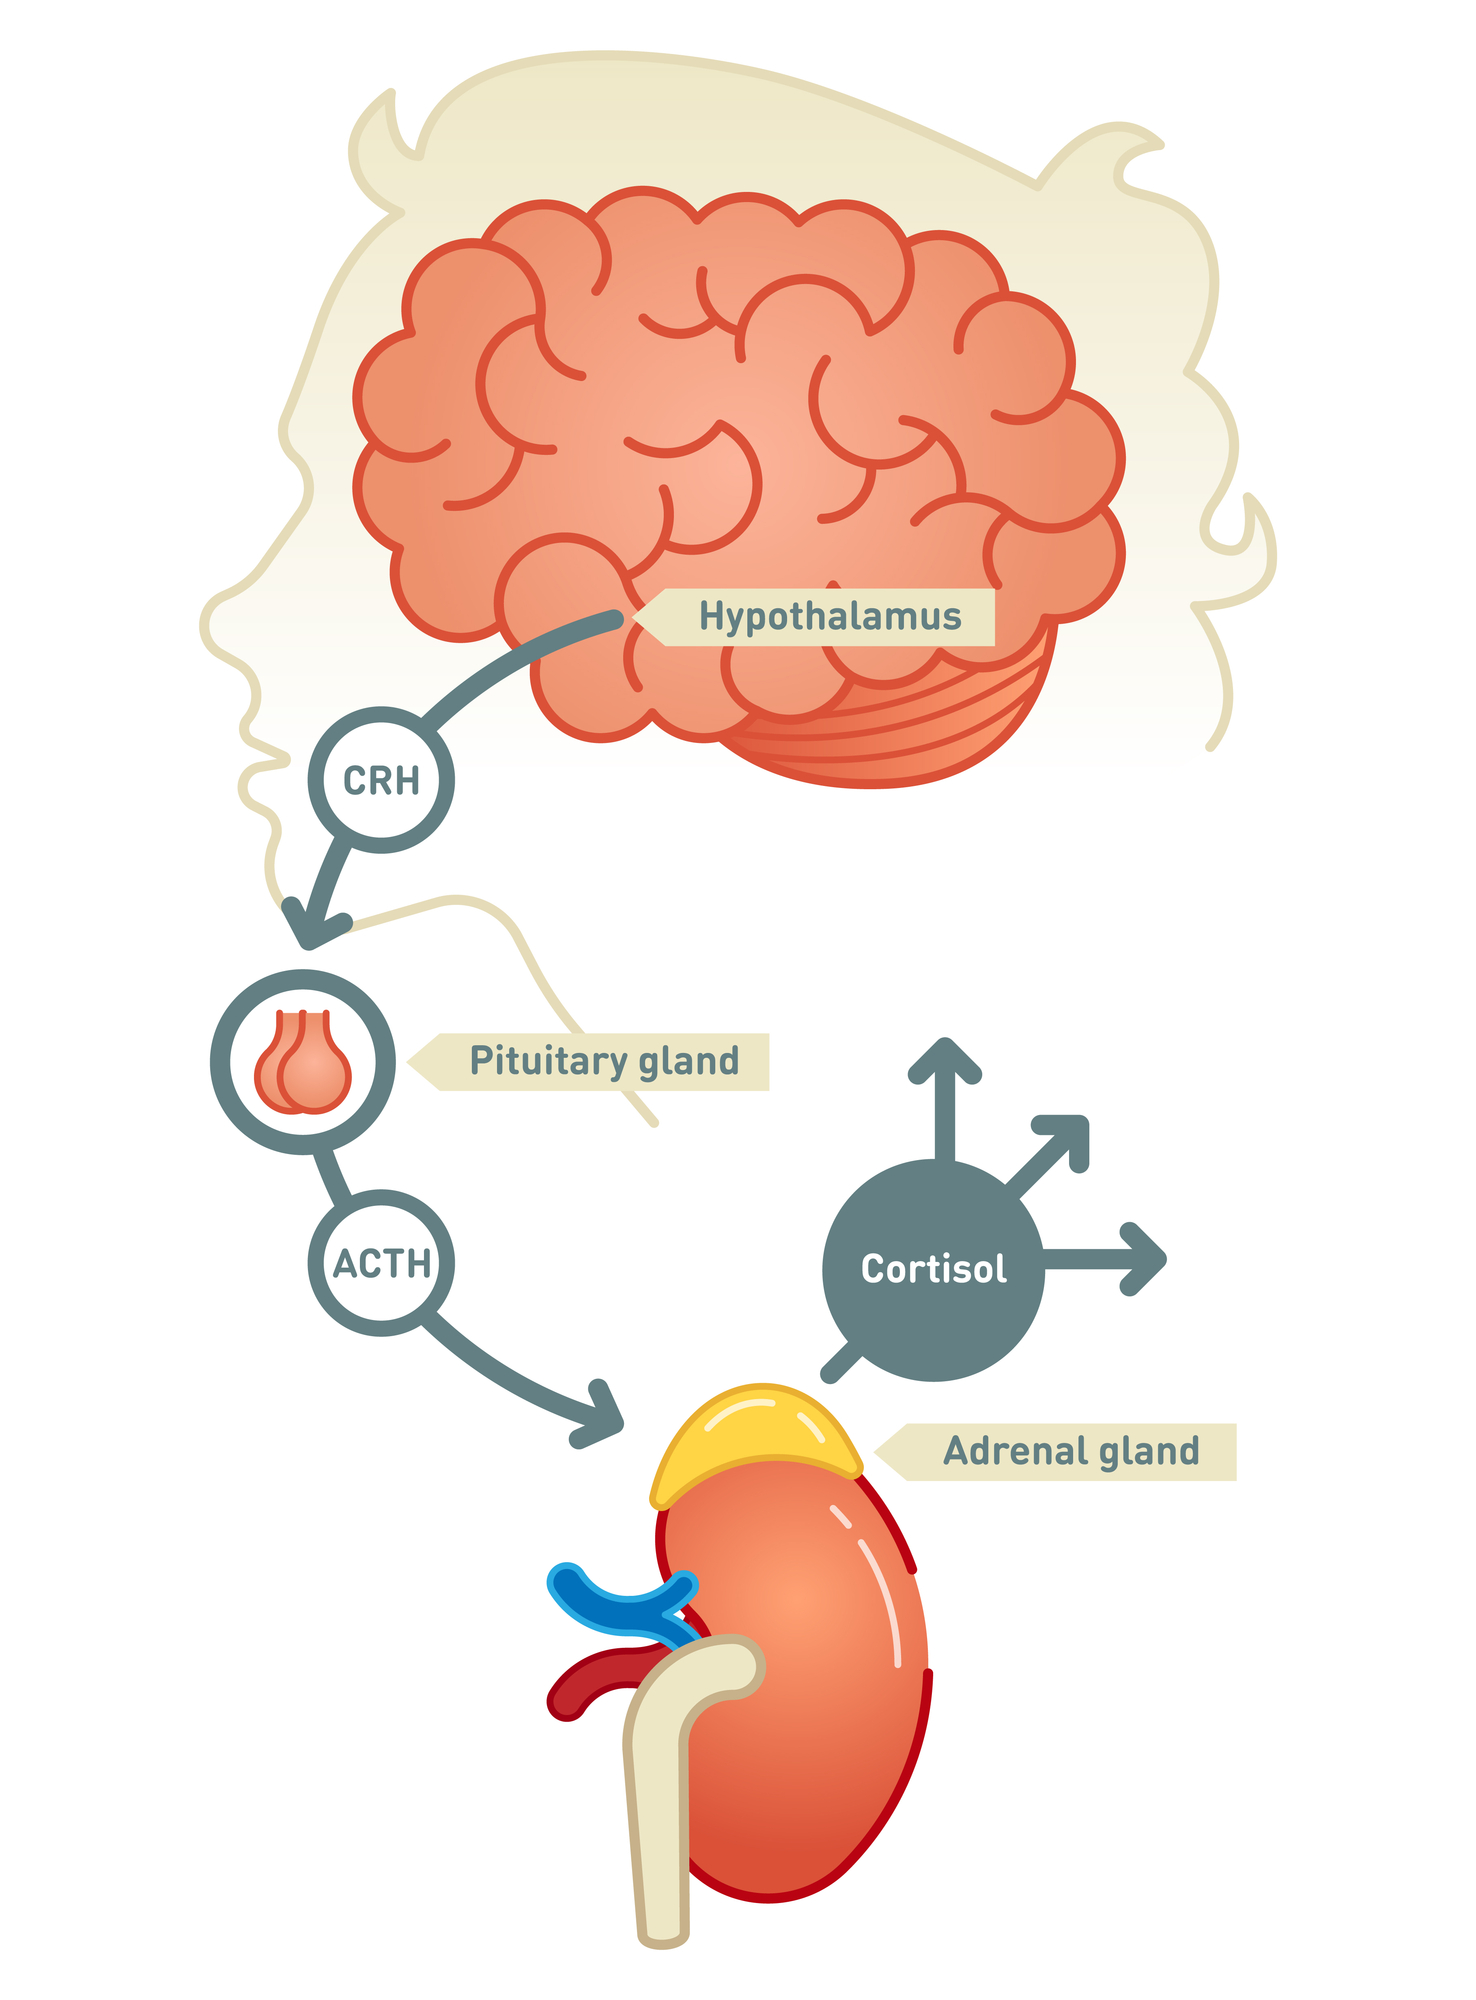
\includegraphics{./images/02-02/img_02.png}

}

\caption{\label{fig-HPA-axis}시상하부 뇌하수체 부신 축}

\end{figure}

물론 스트레스와 뇌 기능 변화를 연결시키는 경로는 HPA 축뿐만이 아니다.
스트레스는 도파민 활성을 직접적으로 변화시킨다.{[}@Wang1994-xb{]} 급성
스트레스는 대뇌피질의 도파민 분비를 늘이며, 선조체의 도파민 활성은
억제한다.{[}@Pani2000-st{]} 그러나 만성적으로 스트레스에 노출되면 도파민
분비세포가 허탈 상태에 빠지기 때문에 피질의 도파민 활성이 점차 감소하게
된다.{[}@Mizoguchi2000-qw{]} 최근에는 또 다른 스트레스 연관 통로로
내인성 카나비노이드 체계\footnote{\textbf{내인성 카나비노이드 체계
  (endocannabinoid system)}: 카나비노이드 화합물은 식물 및 동물에서
  자연적으로 합성되며, 인간 역시 anandamide, 2-arachidonoylglycerol 등을
  합성할 수 있다. 이들은 주로 중추신경계에 분포하는 카나비노이드 수용체,
  CB1, CB2에 결합하여 수면, 기분, 식욕, 생식, 통증 감각, 인지기능 등을
  조절한다. 대마초의 주성분인 tetrahydrocannabinol (THC)는 대표적인
  외인성 카나비노이드이며, 최근 정신질환 치료 효과로 주목받고 있는
  cannabidiol (CBD)은 불안, 운동장애, 통증을 가라앉히는 효과가 있다.}가
각광받고 있다. 카나비노이드는 스트레스에 대한 반응을
경감시켜주는데\textbf{\hspace{0pt}}{[}@Cota2008-lj{]}, 조현병 환자에게서
이 체계의 이상이 자주 발견된다.{[}@Muguruza2019-fr{]}

그러나 위에 연결한 경로들은 순간순간 스트레스와 뇌 기능 변화사이를
매개하는 데는 적합할 지 몰라도, 수년간에 걸쳐 장기간 지속되는 구조적
변화를 설명하기 어렵다. 조현병의 신경발달학적 가설에 따르면, 취약성을
높이는 유전자 변이는 신경회로의 구조적 이상을 낳고, 구조적 이상은
돌이키기 어려운 기능의 결함을 부른다. 하지만 취약성을 높이는 유전자
변이는 단지 발병의 확률을 조금 높일 뿐 거스를 수 없는 운명이 아니다.
게다가 취약 유전자를 물려받지 않은 경우에도 과도한 스트레스에 의해
여전히 조현병이 발생한다는 것은, 스트레스와 유전자 기능이 서로 무관하지
않음을 시사한다. 구조적 변화가 생기기 위해선 유전자 단계에서 이상이
있어야만 하는데, 그렇다고 후천적 스트레스가 신생 돌연변이\footnote{\textbf{신생
  돌연변이(de novo mutation)}: 부모에게서는 발견되지 않으나, 자식
  세대에서 새롭게 발견되는 유전자 서열의 변이. 생식세포에서 DNA 복제나
  복구 과정에 문제가 생기면서 변이가 발생한 것이 자식에게 전달된 것이다.
  난자보다는 주로 정자에서 발생하며, 한 세대당 약 70개 정도의 변이가
  생긴다고 한다.}를 일으키는 것은 불가능하다. 그렇다면 유전자 서열을
바꾸지 않으면서도, 유전자 기능을 켰다 껐다하는 스위치가 어딘가에는
존재해야 한다는 결론에 도달한다.

더불어 신체의 모든 세포가 애초에는 하나의 수정란에서 출발했다는 것을
상기해본다면, 유전자 정보가 같은 수많은 세포가 각기 다른 종류의 세포들로
분화되는 것 역시, 유전자 스위치의 존재를 암시한다. \uline{후성
유전학(epigenetics)}은 바로 이렇게 후천적으로 작동하는 유전자 스위치에
대한 유력한 이론이다. 후성 유전학의 발견은 개체가 갖고 있는 게놈이
개략적인 청사진일뿐, 결코 개체의 운명을 세부사항까지 못 박아 놓은 것이
아님을 분명히 해주었다. 게놈에는 수없이 많은 스위치들이 있으며, 이는
환경적 영향에 의해 켜지기도 하고, 꺼지기도 한다. 후성 유전학적
메카니즘은 개체에게 수없이 많은 가능성을 실현할 수 있도록 해주며, 따라서
변화하는 환경에 유연하게 적응하는데 없어서는 안될 기전이다.

\hypertarget{uxd6c4uxc131-uxc720uxc804uxd559}{%
\section{후성 유전학}\label{uxd6c4uxc131-uxc720uxc804uxd559}}

\hypertarget{uxc911uxc2ec-uxb3c4uxadf8uxb9c8uxc758-uxbd95uxad34}{%
\subsection{중심 도그마의
붕괴}\label{uxc911uxc2ec-uxb3c4uxadf8uxb9c8uxc758-uxbd95uxad34}}

후성 유전학 이론은 그 전까지 분자생물학을 이끌어왔던 중심
도그마\footnote{\textbf{중심 도그마(central dogma of molecular
  biology)}: 중심 도그마는 두 개의 버전이 존재한다. Francis Crick은
  정보가 핵산에서 단백질로 흐를 뿐 그 역으로의 흐름은 있을 수 없다고
  주장했으며, James Watson은 정보는 DNA에서 RNA로 그리고 RNA에서
  단백질로만 전달될 수 있다고 주장하였다. 이후 역전사효소(reverse
  transcriptase)의 발견에 의해 Watson의 주장은 사실이 아니라는 것이
  명백해졌다.}, 즉 생물학적 정보는 한 방향으로만 흐른다는 원리에 과감한
도전장을 내민다.{[}@Crick1970-vi{]} 중심 도그마에 의하면 DNA에서
RNA(전사), 그리고 RNA에서 단백질(번역)로 정보가 전달되며, 역 방향으로의
전달, 즉 단백질에서 DNA나 RNA로의 정보 전달은 일어날 수 없다. 이 이론을
확장하면, 생명체의 모든 정보는 DNA가 쥐고 있으며 염기서열이 바뀌지 않는
한 정보 자체가 변할 일은 없다는 것이다. 이에 반해 후성 유전학에서는
단백질에서 RNA로의 정보전달이 가능하며, 이를 통해 환경적 변화가 새로운
정보로서 DNA와 RNA에 기입될 수 있다고 주장된다.

인간 게놈에 포함된 DNA 중 대다수는 기능이 밝혀지지 않은 비코딩
DNA\footnote{\textbf{비코딩 DNA (non-coding DNA)}: 게놈에서 단백질로
  번역되지 않는 염기서열로 전체 게놈의 98\%를 차지한다. 대부분은
  유전자와 유전자 사이의 광활한 공백에 위치하며, 일부는 유전자 내의
  intron에 존재한다. 이중 소수는 프로모터(promoter) 등 조절 유전자에
  속하지만, 전혀 기능이 밝혀지지 않은 서열이 더 많다. Junk DNA라고도
  불리운다.}이다. 또한 설령 전사되었다 하더라도 아미노산을 만들지 않는
비코딩 RNA\footnote{\textbf{비코딩 RNA (non-coding RNA)}: 단백질로
  번역되지 않는 RNA. 여기에는 miRNA, siRNA, piRNA, lncRNA 등 다양한
  종류가 있다. 이들은 전사, 전사 후 변형(post-transcriptional
  modification), 번역, 번역 후 변형(post-translational modification)
  단계에서 세밀한 조절에 관여한다.}가 존재한다.{[}@St\_Laurent2007-xa{]}
이들 코딩되지 않는 염기서열들은 코딩 영역의 전사나 발현 정도를 조절하고
있다. 그 기전은 첫째, 역시 비코딩 DNA에 위치한 CpG 영역\footnote{\textbf{CpG
  영역}: DNA에서 cytosine (C)과 guanine (G)의 서로 연달아있는 염기서열이
  높은 빈도로 반복되는 영역. 특히 빈도가 높은 영역을 CpG island라고
  부른다. CpG 영역은 유전자의 프로모터에 주로 위치하는데, DNA
  methyltransferases (DNMTs)에 의해 이중 cytosine에
  메틸화(methylation)가 일어나면 해당 유전자는 더 이상 전사되지 못한다.}의
메틸화, 그리고 히스톤 단백질의 메틸화를 통한 염색질\footnote{\textbf{염색질
  (chromatin)}: DNA, RNA, 단백질로 구성된 거대분자 복합체이다. 세포 내의
  DNA를 모두 풀어놓으면 약 3미터에 달한다. 이렇게 긴 DNA를 작은 세포핵
  내부에 담아두기 위해서 히스톤 단백질을 중심으로 단단하게 꼬아놓아야
  한다. 이렇게 부피를 줄이고, 외부 충격으로 부터 DNA를 보호하며, 필요한
  부분만을 풀어놓아 전사가 이뤄지게 하는 구조가 바로 염색질이다. 세포가
  분열 준비를 하면 더욱 단단히 꼬아지면서 광학 현미경으로 관찰할 수 있는
  염색체 구조를 만들어낸다.} 구조의 변화이다.

\hypertarget{uxd6c4uxc131uxc720uxc804uxd559uxc801-uxae30uxc804}{%
\subsection{후성유전학적
기전}\label{uxd6c4uxc131uxc720uxc804uxd559uxc801-uxae30uxc804}}

CpG 영역의 메틸화는 보편적인 유전자 발현 조절 기전으로 유전체
각인\footnote{\textbf{유전체 각인(genomic imprinting)}: 인간은
  부모로부터 하나 씩의 상동 염색체를 물려받기 때문에 모든 유전자는 한
  쌍의 대립유전자로 존재한다. 한 쌍의 유전자 중 어느 하나만 기능을 하고
  나머지는 침묵하게 되는데, 이러한 결정이 유전자가 어머니, 아버지 중
  누구에게서 비롯되었느냐에 따라 결정되는 것을 유전체 각인이라 한다.
  예를 들어 정자에 있는 Igf2 유전자는 CpG 메틸화가 되어 기능을 하지 않는
  반면, 난자에 있는 Igf2는 메틸화 되지 않는다. 따라서 예외없이
  어머니로부터 물려받은 Igf2 만 기능하게 된다.}과 관련된 기전으로 잘
알려져 있다. 부모로부터 물려받는 한 쌍의 대립 유전자 중에서 어느 하나를
침묵시키는 것은 CpG 영역의 메틸화에 의해 결정된다. 그 밖에도 환경적
영향에 따라 후천적으로 CpG 영역이 메틸화가 되면 해당 유전자는 발현이
일시적으로 중단된다.{[}@Jang2017-wr{]}

한편 히스톤 단백질은 DNA가 염색질 구조로 존재할 수 있게 하는데 가장
중요한 역할을 하는데, 그 자신이 메틸화, 아세틸화, 유비퀴틴화 등
공유결합이 추가될 수 있다. 이렇게 공유결합이 변경되면, 히스톤의 3차원
구조가 바뀜으로써 염색질이 꼬이는 정도를 느슨하게도 팽팽하게도 변화시킬
수 있다. 예를 들어 히스톤 복합체 구성 요소 중 하나인 histone H3의 4번째
lysine이 메틸화되면 염색질이 느슨해지면서 유전자 발현이 촉진되지만,
동일한 히스톤의 9번째 혹은 27번째 lysine이 메틸화되면 반대 방향의 효과가
나타난다.{[}@Peterson2004-bz{]} 반대로 염색질이 팽팽하게 꼬이면 전사의
정도가 줄어들기 때문에, 이를 통해 유전자 활성을 조절할 수
있다.(그림~\ref{fig-epigenetics}){[}@Wei2017-py{]}

\begin{figure}

{\centering \includegraphics{./images/02-02/img_0.png}

}

\caption{\label{fig-epigenetics}후성유전학적 변화
(\href{https://www.whatisepigenetics.com/histone-modifications/}{whatisepigenetics}에서
발췌)}

\end{figure}

현재까지 가장 활발히 연구된 후성 유전학적 조절은 위에 설명한 두 가지
기전에 의한다. 비코딩 DNA는 세포핵막 (nuclear envelope), 핵공 (nuclear
pore) 혹은 핵소체(nucleolus)에 맞닿아 있는 채로
존재한다.{[}@Mekhail2010-nu{]} 이들이 외부로부터의 신호를 받아들이는
감지기 역할을 한다. 신호가 감지되면 후성 유전학적 기전에 따라 세포핵
내에 위치한 코딩 DNA와 이를 둘러싼 히스톤의 공유결합 변화를
불러일으킨다. 이러한 복잡다단한 조절 기전이 알려지면서, 세포핵과 그 안에
포함된 염색질이 단순한 정보 저장소가 아니라, 세포의 기능과 필요성에 따라
역동적이고 민첩하게 단백질 생성을 조절하는 고도로 특화된 기능적 단위라는
것이 명백해졌다.{[}@Qureshi2010-wf{]} 한가지 더 주목할만한 것은, 후성
유전학적 변화의 일부는 세대를 건너 유전될 수 있다는 점이다. 이는 DNA
염기서열을 통하지 않고도, 부모 세대의 경험이 자손 세대로 물려내려갈 수
있는 또 하나의 경로가 된다.{[}@Lacal2018-wk{]}

\hypertarget{uxd6c4uxc131-uxc720uxc804uxd559uxacfc-uxc870uxd604uxbcd1}{%
\section{후성 유전학과
조현병}\label{uxd6c4uxc131-uxc720uxc804uxd559uxacfc-uxc870uxd604uxbcd1}}

후성 유전학과 조현병의 연관이 제기된 최초의 계기는 2차 대전 당시 나치에
의해 출입이 봉쇄되어 오랜 기간 동안 심한 기근을 겪어야만 했던 네덜란드
산모에 대한 연구였다.{[}@Kirkbride2012-od{]} 기근이 가장 심했을 때
수정된 아이들은 기이하게도 이후 조현 스펙트럼 장애의 발생률이 유달리
높았다.{[}@Brown2008-tf{]} 연구자들은 산모의 \uline{엽산(folic acid)
부족} 가능성에 주목했는데, 그 이유는 엽산이 DNA 메틸화에 사용되는
메틸기의 주요 공급원이기 때문이다. 이때 태어난 집단이 장년이 되었을 때
DNA 메틸화 정도를 조사했는데, 몇가지 중요한 유전자에서 메틸화의 정도가
대조군과 다르다는 것이 발견되었다.{[}@Heijmans2008-mz{]}

2000년대 후반부터는 당시 취약 유전자로 알려진 몇몇 유전자의 메틸화
정도를 대조군과 비교해보려는 연구가 있었다. Reelin (RELN),
catechol-O-methyltransferase (COMT), serotonin receptor type-2 (HTR2A)
등의 메틸화가 대조군과 의미있게 차이가 있었으며, 그 정도는 단백질 발현
양과도 상관관계를 보였다.{[}@Abdolmaleky2008-ia; @Abdolmaleky2014-aq{]}
좀더 현대에 접어들면서는 개별 후보 유전자가 아니라, 광범위 유전체 연합
연구의 기법을 동원하여 게놈 전반에 퍼져있는 다량의 CpG 영역을 한꺼번에
조사하기 시작하였다. Wockner 등\hspace{0pt}{[}@Wockner2014-vr{]}은 각
24명의 조현병 환자와 대조군의 사후 뇌조직에서 무려 500,000개 가까운 CpG
영역의 DNA 메틸화 정도를 측정하였다. 그 결과 3,000개 정도의 유전자에서
메틸화의 변화를 감지했는데, 여기에는 기존에 조현병의 취약 유전자로
알려진 유전자들이 대거 포함되어 있었다.

후성 유전학적 조절은 각 장기와 조직마다 다르기 때문에, 뇌 조직의 변화가
혈액에서 나타나는 변화와 동일할 수는 없다. 그러나 살아있는 환자의 뇌
조직을 검사할 수는 없기 때문에, 연구자들은 혈액 내의 후성 유전학적
지표들을 탐색하기 시작하였다. 다행히 뇌 조직과 혈구 세포에서의 후성
유전학 지표 중에 공통되는 부분이 있었기 때문에, 환자의 말초 혈액을
이용하여 개개인의 후성 유전학적 시그니처를 얻어낼 수 있다. Aberg
등{[}@Aberg2014-bz{]}은 759명의 환자와 738명의 대조군으로부터 얻어낸
후성 유전학적 시그니처를 서로 비교하였는데, 신경세포의 분화와 도파민
유전자 발현에 관여하는 FAM63B 유전자가 가장 두드러진 차이를 보였으며,
이외에도 RELN을 비롯한 다양한 유전자들이 두 군 간에 유의한 차이를
드러내었다.

비코딩 RNA 역시 전사된 다른 RNA를 분해하거나 번역을 방해함으로써 유전자
발현을 조절할 수 있다. 이중 microRNA\footnote{\textbf{MicroRNA (miRNA)}:
  약 19\textasciitilde23개의 염기로 구성된 작은 RNA로 코딩 RNA의 3'-UTR
  영역에 결합함으로써 코딩 RNA의 번역을 방해한다. 현재까지 알려진
  miRNA의 70\%는 중추신경계에서 발견되었으며, 신경세포의 분열, 분화,
  성숙, 이동, 세포사 등에 관여한다.}는 중수신경계의 정상적인 발달과
성숙, 성인이 된 이후의 신경가소성이나 시냅스 기능에 중요한 역할을
한다.(그림~\ref{fig-epigenetic-mechanism}) 조현병과 관련해서도
신경세포에 분포하는 miR-132/212, miR-219, miR-195 등이 대조군과 의미있는
차이를 보인다.{[}@Mellios2012-sy{]} 말초 혈액의 miRNA 농도를 측정한
실험에서도 miR-130b와 miR-193-3p가 조현병 환자에서 의미있게 변화된 것이
발견되었다.{[}@Wei2015-be{]}

\marginnote{\begin{footnotesize}

\end{footnotesize}}

\begin{figure}

{\centering \includegraphics{./images/02-02/img_1.png}

}

\caption{\label{fig-epigenetic-mechanism}후성유전학적 조절기전과
microRNA {[}@smigielski2020{]}}

\end{figure}

조현병 환자의 히스톤 단백질 구조 변화에 대한 연구는 상대적으로 수가
적다. Chase 등{[}@Chase2013-yj{]}은 조현병 환자의 사후 뇌조직은 물론
말초 백혈구에서 histone H3의 9번째 lysine 메틸화가 대조군과 차이가
있음을 보고하였다. 한편 또 다른 연구에서는 조현병 환자의 말초 혈액에서
H3의 10번째 serine의 인산화 정도가 증가되었음이
관찰되었다.{[}@Sharma2015-wi{]}

\hypertarget{sec-epigenetics-limitation}{%
\section{후성 유전학의 한계와 전망}\label{sec-epigenetics-limitation}}

세포의 기능이 단백질 발현의 양에 달려있다고 지극히 단순화시킨다 해도,
단백질 생성의 양을 조절하는 기전 또한 한없이 복잡하고 다양하다. 유전자
발현은 시시각각 달라지는 세포 외 환경에 대응하여 순발력 있게 변화하며,
이는 세포막 수용체와 세포 내부의 정교한 \uline{신호전달 네트워크}의
역할에 달려있다.(2장 \_\_절) 항정신병 약물의 기전을 비롯하여, 질병의
병태생리와 치료기전을 이해하려는 수많은 연구자들은 이 신호전달
네트워크를 이해하기 위해 부단한 노력을 기울여왔다. 그러나 신호전달계를
통한 변화는 비교적 짧은 시간 범위에서 일어나는 것이기 때문에, 뇌
신경망의 구조적 변화와 같이 상대적으로 긴 시간 범위에서 일어나는 현상을
이해하기에는 한계가 있다.

오랜동안 학자들은 구조의 변화를 가져올 정도로 장기간 유지되는 변화는
염기서열의 변이에 의해서만 일어난다고 생각해왔다. 정신유전학은 이런
전제하에 발전해왔으며, 다양한 취약성 유전자를 발견해내는 성과를
이루었다. 그러나 조현병에 높은 빈도로 존재하는 변이 중 상당 수는 비코딩
DNA에 위치하고 있으며, 그 역할을 이해하기 어려웠다. 단백질 발현에 영향을
미치지 못하는 유전자 변이란 의미없는 변이에 불과하기 때문이다.

한편 환경적 영향 역시 이해하기 어렵기는 마찬가지이다. 물론 세포내
신호전달계는 환경적 변화를 감지하고 이에 대응하여 단백질 발현 양을
조절한다. 그러나 구조적 변화를 일으키거나, 발병을 유도할 정도로
스트레스의 영향이 장기간 유지되기 위해선, 신호전달계의 동적 변화만
갖고는 설명하기 어렵다. 후성 유전학은 이러한 두 가지 의문점에 해답을
제공할 가능성을 지니고 있다. 비코딩 DNA 중 상당 부분은 후성 유전학 조절
기전, 즉 유전자 스위치를 켜고 끄는데 관여하고 있다. 비코딩 DNA의 변이
때문에 후성 유전학적 조절 기전이 손상되거나, 혹은 특정 유전자가 장기간
억제되거나 혹은 탈억제 되면 장기간에 걸쳐 코딩 DNA의 발현이 변화되면서
발병/재발을 유도할 수 있을 것이다. 환경적 영향 역시 마찬가지이다.
스트레스가 후성 유전학적 기전에 의해 특정 유전자 발현을 장기간
억제한다면 구조적 변화에 이를 수 있을 것이다. 예를 들어 동물 실험 결과에
따르면, 갓 태어난 새끼 쥐는 엄마의 보살핌 정도에 따라 GAD1 유전자
프로모터 영역의 DNA 메틸화가 달라지며, 더불어 성인이 되었을 때에도
히스톤의 아세틸화 정도가 달라진 채로 유지된다고 한다.{[}@Zhang2010-tx{]}
인간을 대상으로 한 연구에서는, 자살자의 사후 뇌조직에서 스테로이드
수용체 유전자인 NR3C1 프로모터 영역의 DNA 메틸화를 조사했을 때, 아동기의
학대 여부와 연관되어 있음이 발견되었다.{[}@McGowan2009-pq{]}

하지만 동일한 의미에서 후성 유전학적 설명도 한계에 부딪힌다. 우선 후성
유전학적 변화가 얼마나 오랜 시간 안정적으로 유지되는 지에 대한 자료가
매우 부족하다. 이 역시 세포 외 상황에 적응하여 동적으로 변화되는 것이기
때문에, \uline{성향(trait)}을 반영한다기 보다는 \uline{상태(state)}를
반영한다고 보아야 한다. 지금까지의 연구 중 대부분이 단면조사
연구(cross-sectional study)였기 때문에, 후성 유전학적 기전의 시간적 변화
양상에 대해서는 거의 아는 바가 없다. 일례로 해마에서의 DNA 메틸화는
탈분극 정도에 반응하여 변화하는데, 그렇다면 시간적 척도가 세포내
신호전달계와 별다를 바가 없다.{[}@Nelson2008-cs{]}

한편 대조군과 환자군 사이에서 DNA 메칠화 정도나 히스톤 단백질의 인산화
정도가 다르다는 것을 발견했다고 해도, 이를 어떻게 해석해야 할 지에
난점이 많다. 이러한 변화가 발병 과정과 관련된 것인지, 오래된 병의 결과인
것인지, 혹은 항정신병 약물에 의한 것인지 전혀 구분되지 못하고 있다. 설령
치료받지 않은 초발 정신병 환자를 대상으로 삼아, 이러한 변인을 배제할 수
있었다해도, 후성 유전학적 변화가 비코딩 DNA의 변이에 의한 것인지, 축적된
환경적 요인에 의한 것인지 구분할 방법이 존재하지 않는다. 만약 전자에
의한 것이 맞다면, 광범위 유전체 연합 연구와 차별되는 장점이 무엇인지도
확실하지 않다.

그럼에도 불구하고, 후성 유전학적 연구는 많은 가능성을 내포하고 있다.
지금까지 보편적으로 알려진 유전자 발현의 조절은 유전자 인근의 제한된
영역의 DNA에 의한다고 여겨져 왔다. 넓게 잡아 5'-UTR (5'-untranslated
region)이라고 해도 몇 천 bp에 불과하다. 후성 유전학적 기전의 하나인 DNA
메틸화는 5'-UTR 내에 존재하는 CpG 영역에서 일어나지만, 히스톤 변형을
비롯한 다른 종류의 후성 유전학적 기전은 염색질의 구조 자체를 변화시키기
때문에, 훨씬 원거리 영역에서도 코딩 유전자의 발현을 조절할 수
있다.{[}@Wood2010-ir{]} 이러한 원거리 조절의 가능성은 비코딩 유전자
변이의 역할을 이해하는데, 큰 기여를 할 것으로 기대된다.

현재까지 후성 유전학적 기전에 의해 일어난다고 확인된 정신과 질환은 취약
X 증후군\footnote{\textbf{취약 X 증후군 (fragile X syndrome)}: 희귀한
  유전 질환으로 정신지체의 가장 흔한 원인 중 하나이다. X 염색체의 말단인
  Xq27-Xq28 부위가 끊어질듯 말듯 보이기 때문에 이렇게 이름붙여졌다.}과
레트 증후군\footnote{\textbf{레트 증후군 (Rett syndrome)}: Andreas
  Rett에 의해 처음으로 보고된 신경발달장애. 생후 6개월에서 18개월까지는
  비교적 정상 발달을 한 후 두위 발달의 감소와 함께 이미 습득했던 인지 및
  언어, 운동 능력을 상실하고, 손을 씻는 듯한 동작을 반복하는 상동증을
  보인다.} 등 주로 정신지체를 일으키는 다양한 질환이 있다. 예를 들어
취약 X 증후군에서는 \uline{FMR1 (fragile X mental retardation 1)} 유전자
프로모터에 변이가 있어서, 환자들은 CpG 영역에 염기서열 CGG가 지나치게
많이 반복된다. CG가 많으면 많을 수록 DNA 메틸화 정도가 심해지기 때문에,
환자들은 FMR1 단백질이 만들어지지 못하게 되어 발병에 이른다. 레트
증후군은 여성에게 주로 나타나는 신경 발달 장애로 X 염색체에 존재하는
\uline{MeCP2 (MECP2 methyl-CpG binding protein 2)} 유전자 변이에 의해서
초래된다. MeCP2는 CpG 영역의 메틸화된 DNA에 결합하여 다양한 유전자의
발현을 억제하는 역할을 한다.{[}@Good2021-dr{]} 이 밖에도, MeCP2는 히스톤
H3의 27번째 lysine을 메틸화시키기 때문에 히스톤 변형을 통한 염색질 구조
변화에 관여한다.{[}@Lee2020-ja{]} 따라서 MeCP2에 변이가 생기면 많은 수의
유전자 발현이 혼란에 빠진다. 특히 MeCP2는 신경세포가 성숙을 마친 이후에
대량으로 만들어지며, 이는 레트 증후군의 증상이 생후 6-18개월 지난 후에야
나타나는 것과 무관하지 않다.

한편 후성 유전학적 지표는 세대를 넘어서 유전된다는 특징이 있다. 앞서
기근에 빠진 산모에게서 태어난 아이들이 나중에 조현병으로 발병하는 예가
많았다는 것을 살펴보았다. 이는 신경발달학적 가설로 이해하여 태생기 뇌
발달 과정에 산모의 영양 부족이 영향을 끼쳤다고 볼 수 있지만, 후성
유전학적으로는 좀 다르게 해석할 수 있다. 즉 기근에 처한 주민들은 남녀
가릴 것 없이 기근에 적응하기 위해 후성 유전학적 기전을 사용하여 몇몇
유전자 발현을 조절하고 있었는데, 이러한 휴성 유전학적 지표가 정자와
난자를 통해 자손에게 그대로 물려내려갔을 수도 있다. 이를 확장하면 부모
대의 극심한 스트레스(예를 들어 전쟁이나 이민)가 자손의 조현병 발병
확률을 높일 수도 있다는 추론이 가능해진다.{[}@Lacal2018-wk{]}

후성 유전학은 아직도 초창기에 머물러 있는 생소한 학문인지라, 알려진
것보다는 아직 알지 못한 부분이 훨씬 많다. 따라서 조현병의 병태생리를
이해하는데 도움이 될 지 안 될 지 조차 분명하지 않다. 그러나 후성 유전에
기인한다고 알려진 질환의 병태 생리적 기전을 이해함으로써, 조현병의 발병
기전, 특히 심리적 스트레스가 발병을 앞당기는 이유, 청소년기 후기에
들어서야 발병에 이르는 이유, 그리고 부모 세대의 스트레스가 자손의 발병
위험에 미치는 영향 등을 밝히는데 도움이 되기를 희망한다.

\hypertarget{references-8}{%
\section*{References}\label{references-8}}
\addcontentsline{toc}{section}{References}

\markright{References}

\hypertarget{uxc2e0uxacbduxbc1cuxb2ecuxd559uxc801-uxac00uxc124}{%
\chapter{신경발달학적
가설}\label{uxc2e0uxacbduxbc1cuxb2ecuxd559uxc801-uxac00uxc124}}

Neurodevelopmental Hypothesis of Schizophrenia

\hfill\break

만약 조현병의 발병 위험을 높이는데 특정 유전자가 관여한다면, 변이가
발생한 유전자가 어떤 방식으로 질병에 취약하게 만드는지 의문이 생기지
않을 수 없다. 일반적으로 변이된 유전자가 일으킬 수 있는 효과를 다음과
같이 나열할 수 있다.

\begin{enumerate}
\def\labelenumi{\arabic{enumi}.}
\item
  효소의 결핍 및 기능 저하

  \begin{enumerate}
  \def\labelenumii{\alph{enumii}.}
  \tightlist
  \item
    필수 물질의 생성 저하
  \item
    기질(substrate) 혹은 중간 대사 산물의 축적
  \item
    조직 손상 위험이 있는 물질의 비활성화가 이뤄지지 못함
  \end{enumerate}
\item
  수용체 혹은 세포 내 수송 시스템의 오작동
\item
  구조형성 단백질 같은 비효소성 단백질의 결핍 혹은 기능 저하
\end{enumerate}

유전자 변이가 일으키는 효과는 다양하고 광범위하며, 그중 어떤 것도
조현병의 발병 위험을 높일 수 있다. 예를 들어 선천적 대사 장애라고 불리는
유전적 대사이상은 특징적으로 출생 초기부터 다양한 증상을 드러내며,
심지어 생명을 단축시키기도 한다. 한편 헌팅턴 병과 같은 유전 질환은
성인기 후기부터 운동 기능의 이상이 드러나며, 인지기능 저하와 정신증
증상이 동반되기도 한다. 이런 신경질환들은 신경퇴행성
질환(neurodegenerative disorder)이라고 알려져 있다.

반면 조현병의 임상적 특성과 보편적 경과는 이와는 전혀 다르기 때문에,
다른 형태의 병태생리를 고려해야 한다. 잘 알려진 대로 조현병은 후기
청소년기나 초기 청년기에 발병하며, 그 이후에는 악화와 호전을 반복하지만
완치에 이르기는 어렵다. 발병의 위험시기는 생물학적으로나
사회심리학적으로 큰 변화를 거치는 단계이며, 동시에 상당한 스트레스를
받는 시기이다. 청소년기는 신경발달의 마지막 단계를 거치는 시기로, 피질하
영역에서 시작하여 일차 감각운동 영역을 거쳐 마지막에 전전두엽에
이르기까지 대뇌피질이 두꺼워짐과 동시에 가지치기가 일어나 필요없는
연결을 잘라내는 과정이 이루어진다. 이렇듯 뇌의 재구조화가 마무리되는
동시에 성인으로서의 스트레스가 밀어닥치기 시작하는 시기에 발병한다는
것은, 조현병의 발병이 뇌의 신경학적 발달과정과 모종의 관계가 있음을
강력히 시사한다.

\hypertarget{sec-two-hit-hypothesis}{%
\subsection{2회 충격 가설}\label{sec-two-hit-hypothesis}}

소위 조현병의 \uline{2회 충격 가설(two-hit hypothesis)}은 유전적 요인
혹은 환경적 요인으로 인해 발달과정에 있는 태아의 중추신경계에 일차
충격이 가해져 취약성이 높아져 있는 상태에서, 후기 청소년기나 성인기
초기에 두번째 충격이 가해지면 발병에 이르게 된다는
가설이다.{[}@Maynard2001-yb{]} 두번째 충격이 어떤 것인지에 대해선
학자마다 의견이 분분하다. 실직, 도시 거주, 이민, 전쟁 등이 조현병 발병
위험을 높이는 것을 보면, 심한 심리사회적 스트레스가 영향을 끼치는 것이
분명해보인다.{[}@Dean2005-cb{]} 한편 신경기능을 유지하고, 외적 변화에
적응하며, 장기 강화를 통한 기억과 학습을 담당하는 경로에 문제가 생기는
것이 두번째 충격이라는 생물학적 이론도 언급되고
있다.{[}@Maynard2001-yb{]}

이중 첫번째 충격, 즉 태생기 혹은 영아기 초기에 일어나는 충격이 어떤
식으로 조현병에 취약한 상태를 평생동안 지속시키는지에 대한 유력한 가설이
바로 신경발달학적 가설이다. 이 이론은 특히 임신 제 1분기 동안 활발하게
일어나는 신경계의 구조적 발달과정의 문제가, 결함있는 신경연결망을
만들어내고, 이러한 결함이 아이가 성장하였을 때 겪게되는 환경적 변화에
유연하게 대처하는 능력을 훼손시키기 때문이라고
주장한다.{[}@Owen2011-rn{]}

\hypertarget{uxc2e0uxacbduxbc1cuxb2ecuxd559uxc801-uxac00uxc124uxc758-uxd0c4uxc0dd}{%
\subsection{신경발달학적 가설의
탄생}\label{uxc2e0uxacbduxbc1cuxb2ecuxd559uxc801-uxac00uxc124uxc758-uxd0c4uxc0dd}}

정신증의 신경발달학적 이론이 최초로 제안된 것은 1891년 스코틀랜드의
정신과 의사인 Clouston\footnote{\textbf{Thomas Clouston
  (1840\textasciitilde1915)}: 스코틀랜드의 정신과 의사. 왕립 에딘버러
  수용소 소장을 역임하였으며, 에딘버러 대학에서 정신의학을 강의하였다.
  청소년 정신의학에 관심이 많았으며, 강박적인 자위가 정신질환을
  일으킨다고 믿었다.}에 의해서였다. 그러나 크레펠린이 조발성 치매 개념을
대중화시키면서, 조현병은 \uline{신경발달학적 질환}이라기보다는
\uline{신경퇴행성 질환}이라는 인식이
강해졌다.(\textbf{?@sec-neurodevelopmental-vs-neurodegenerative})\footnote{조현병이
  신경발달학적 질환인지 신경퇴행성 질환인지에 대한 논란은 현재까지도
  지속되고 있다. 물론 양쪽 다일 가능성도 있다.{[}@Gupta2010;
  @Kochunov2014; @Buoli2017; @stone2022{]}} 1970년대 말초에 접어들면서
조현병의 뇌영상 연구가 첫걸음을 떼기 시작할 무렵, Johnstone
등{[}@Johnstone1976-hp{]}은 조현병 환자의 뇌실이 정상인에 비해 유의하게
커져있음을 보고하였고, 이는 신경발달과정의 문제를 시사하였다. 1982년에는
일란성 쌍생아에 있어서, 조현병에 이환된 환자의 뇌실은 그렇지 않은 형제의
뇌실보다 크다는 것이 발견되었다.{[}@Reveley1982-tm{]} 겨울에 출생한
집단에서 조현병 발병률이 높다던지, 2차 대전 중 기근으로 말미암아 산모가
영양실조 상태에 놓였을 때 출생한 자녀에서 조현병을 비롯한 조현병
스펙트럼 장애의 빈도가 높았다는 역학적 연구결과도 신경발달과정에
주목하게 된 요인이었다.{[}@Dalen1968-br; @Hoek1998-gh{]}

1987년 Weinberger\footnote{\textbf{Daniel Weinberger
  (1947\textasciitilde)}: 미국의 정신과 의사로 존스 홉킨스 대학 교수로
  재직중이다. 조현병을 비롯한 다양한 정신질환의 유전 요인을 찾는데
  업적을 남겼으며, COMT 및 NRG-1 유전자와 조현병의 연관관계를
  찾아내었다.}는 처음으로 신경발달학적 가설을 공식화하였다. 그는
발병하기 전의 조현병 환자의 뇌에서 이미 비특이적인 신경병리학적 소견이
발견되기 때문에, 먼 원인은 이미 태생기 초기에 자리잡았을 것이라
생각하였다. 그럼에도 불구하고 수년 이상 발병하지 않고 있다가 나이가
들어서 발병하는 원인은 이러한 신경병리학적 병변이 정상적인 신경계의
성숙과정과 상호작용을 일으키면서 점차 표면적인 증상이 드러나게 하는
것이라 가정하였다.{[}@Weinberger1987-ar{]}

\hypertarget{sec-neurodevelopment-evidence}{%
\section{신경발달학적 가설의 증거}\label{sec-neurodevelopment-evidence}}

이후 점차 신경발달학적 이상을 뒷받침하는 증거들이 축적되기 시작하였다.
저체중, 저산소증 등 산과적 합병증, 인플루엔자나 풍진(rubella),
톡소플라즈모시스(toxoplasmosis)와 같은 바이러스 감염 등은 뇌의 구조적
이상을 가져올 뿐더러, 조현병 발병 위험을 높인다.{[}@Mednick1988-mm;
@Brown2000-ga{]} 또한 조현병 환자의 뇌에서 뇌실의 확장 외에도, 이소성
회백질(ectopic gray matter), 뇌고량(cerebral sulcus)의 깊이나 모양의
차이, 해마 등 부위에서 발견되는 세포구축(cytoarchitecture)의 이상,
축삭돌기나 수상돌기의 분지 패턴 이상 등이 발견되었으며, 이들은 모두
중추신경계의 발달학적 이상과 구조적 결함을
입증하였다.{[}@Arnold1999-fr{]} 중추신경계가 발달하는 일련의 과정에는,
뇌실하 영역(subventricular zone)에서 처음 생성되는 신경세포들이 점차
바깥쪽으로 이동하면서 특징적인 6층 구조를 이루는 기전을 비롯하여, 축삭이
자라나면서 신경성장인자(neurotrophic factor)의 안내를 받아 정해진
신경세포를 찾아가는 과정, 그렇게 만난 축삭과 수상돌기가 시냅스를 이루는
과정 등이 포함된다. 신경발달과정의 이상은 그 어느 단계에서도 발생할 수
있다.

신경발달학적 가설을 지지하는 다양한 동물모델도 개발되었다. 갓 태어난
생쥐에게 phencyclidine (PCP)을 투여하면 정신증 유사증세를 보이며,
이들에게 항정신병 약물을 투여하면 증세가 없어진다.{[}@Broberg2009-jm{]}
Methylazoxymethanol acetate라는 세포분열 억제제를 임신 중인 쥐에게
투여하면, 태어난 쥐가 정신증 증세를 보일 뿐더러, 조현병 환자에게서
보이는 중추신경계의 구조적 이상을
동반한다.(섹션~\ref{sec-mam-model}){[}@Grace2017-cb{]}

만약 신경발달학적 가설이 맞다면, 아직 발병하지 않은 전구기 환자들도
신경연결망의 이상을 지니고 있다는 뜻이 된다. 코호트 연구를 통해 나중에
조현병이 발생한 환자들의 병전 상태를 재조사한다든지, 유전적 위험인자를
지닌 환자의 형제, 자식 등에게서 어떤 구조적, 기능적 변화가 있는 지를
연구하면 좀더 통찰을 얻을 수 있을 것이다. MRC 코호트 연구\footnote{\href{http://www.nshd.mrc.ac.uk/}{\textbf{MRC
  코호트 연구}} \textbf{(Medical Research Council National Survey of
  Health and Development Cohort)}: 2차 대전 직후인 1946년 영국에서
  태어난 5,362명에 대해 이후 성장과정을 50년 이상 추적하는 프로젝트이다.}나
Dunedin 종적 연구\footnote{\textbf{Dunedin 종적 연구( Dunedin
  Longitudinal Study)}: 뉴질랜드에서 행해진 코호트 연구이다. Dunedin에
  위치한 메리 여왕 산모센터(Queen Mary Maternity Center)라는 곳에서
  1972년부터 1973년 사이에 태어난 1,037명을 추적하며 현재 44세 시점의
  평가가 완료되었다.}를 통하여 조현병 환자들은 발병 전에 이미 다양한
신경운동기능, 언어발달, 사회적 부적응, 성적 저하 등을 보인다는 사실이
관찰되었다.{[}@Jones1994-kf; @Poulton2000-nk{]}

Weinberger 등이 상정한 신경발달학적 가설은 모종의 원인에 의해 태생기
초기에 이미 신경연결망 이상이 자리잡고, 이러한 이상이 정상 발달과정을
방해하거나 맞물리면서 증상이 발현된다는 것이었다. 그러나 신경발달 과정은
반드시 태생기에만 국한된 것이 아니다. \uline{시냅스 가지치기(synaptic
pruning)}는 잘 쓰지 않는 시냅스를 제거함으로써, 신경연결망 간의 상호
조절 효율성을 높이거나, 에너지 소모를 줄이는 과정으로 후기 청소년기나
성인기 초기까지 진행된다. 가지치기는 발달과정에서 부적절하게 연결된
원거리 시냅스를 제거하는 거시적 가지치기와, 자주 사용되는 연결만을
남기고 그다지 사용되지 않는 불필요한 연결을 소거하는 미시적 가지치기로
나뉜다.{[}@Vanderhaeghen2010-wz{]} Keshavan 등{[}@Keshavan1994-hy{]}은
조현병을 일으키는 신경발달학적 이상은 이 가지치기에 있을 것이라
주장하였다. 일부 학자들은 \uline{complement component 4 (C4)} 유전자에
위치한 유전자 복제수 변이\footnote{\textbf{유전자 복제수 변이 (copy
  number variation)}: 생식세포가 만들어 지는 신생합성(de novo synthesis)
  과정에서 유전자의 결실, 중복, 전좌, 역위 등 복제 상의 실수로 말미암아,
  유전자가 결실 되거나 하나 이상이 반복될 수 있다. 상대적으로 짧은
  염기서열이 반복되는 STR, VNTR과 달리 30\textasciitilde500kb에 이르는
  전체 유전자가 반복된다. 이때 반복되는 갯수가 개인에 따라 다른 것을
  유전자 복제수 변이라고 한다.}가 조현병과 상당한 유전적 연관성을 보이는
것에 주목한다. C4는 출생 후 가지치기에 깊숙히 관련되어 있기 때문에,
시냅스 가지치기는 새삼스레 조현병 발병기전에 있어 그 중요성이
부각되었다. 최근 한 연구에서는 조현병 환자에서 추출한 단핵구로부터
신경교세포 유사 세포를 유도한 다음, 이들이 시냅토솜\footnote{\textbf{시냅토솜(synaptosome)}:
  신경 말단을 형성하는 것으로 여겨지는 구조물로 신경세포에서 분리되어
  고립된 상태로 존재한다.}을 파괴하는 정도를 측정하였는데, 그 정도가
대조군에 비해 유의하게 높음을 발견하였다. 시냅토솜 파괴는 가지치기가
행해지는 주요 기전이기 때문에 시냅스 가지치기가 얼마나 활발히
이루어지냐를 반영하는 지표가 된다.{[}@Sellgren2017-ty{]}

\hypertarget{uxc774uxb860uxc801-uxb09cuxc810uxacfc-uxd55cuxacc4}{%
\section{이론적 난점과
한계}\label{uxc774uxb860uxc801-uxb09cuxc810uxacfc-uxd55cuxacc4}}

조현병 환자에게서 발병 전에 이미 다양한 신경계 이상이 발견되고, 이들 중
다수가 비정상적인 신경발달과정을 반영한다는 사실은 이제 이론의 여지없이
받아들여지고 있다. 그러나 여전히 풀리지 않은 문제는 이러한 발달학적
이상이 어떻게 발병에 이르게 하느냐는 것이다. 발달이상에 의해
신경연결망에 문제가 생겼다고 해도, 발병 전까지 그 영향이 그다지 드러나지
않는 것으로 보아 이러한 이상은 매우 미세하고 은근한 것이다. 따라서
신경연결망 이상이 직접 조현병을 일으킨다기 보다는, 취약성을 조금
증가시키는 정도로 이해하는 것이 바람직할 것이다. 2회 충격 가설에서
의미하는 두번째 충격은 보통 심리사회적 스트레스를 말한다. 그렇다면
신경발달학적 가설은, 신경연결망 이상이 개체가 다양한 스트레스에 대응하는
과정에 어떤 악영향을 미치는 것인지 설명할 수 있어야 한다.

한가지 힌트는 발달과정의 이상과 도파민 시스템의 연관성이다. Kanyuch와
Anderson은 동물모델에서 초기 신경발달의 이상은 청소년 시기에 도파민
시스템이 스트레스에 과도하게 반응하도록 만든다고
보고하였다.{[}@Kanyuch2017-nz{]} 선조체 도파민 시스템의 과도한 반응은
중립적 자극에 대해 부적절한 의미나 과도한 중요성을 부여하는
\uline{비정상적 현저성}(\protect\hyperlink{aberrant-salience}{2장 6-4절
참조})을 일으킨다.{[}@Kapur2003-xc{]} 잘 알려진 바와 같이 비정상적
현저성은 관계사고나 편집사고의 기반이 된다.{[}@Mishara2013-mc{]}

그러나 신경발달과정의 이상을 도파민 시스템과의 연관으로 이해하고자 해도,
신경연결망의 이상이 약하는 것은 민감성이나 편집적 경향이지 조현병 자체가
아니다. 이러한 경향은 인구집단 내에서 연속적으로 분포하며, 정상과 질병을
나누는 분명한 기준도 없다. 이는 신경발달과정과 가장 밀접한 연관이 있을
것으로 여겨지는 인지기능의 경우에도 역시 마찬가지이다. 이에 덧붙여,
편집적 경향이나 신경인지기능의 저하가 점진적으로 드러난다 하더라도,
그것이 반드시 조현병으로 발전하리라는 필연성은 없다. 조현 스펙트럼
장애를 비롯하여 양극성 장애, 우울증, 반사회성 인격 등 다양한 질환으로
발전할 수 있다. 따라서 신경발달학적 이상의 진단특이성은 확립되지
않았다고 할 수 있다.{[}@Murray2017-gx{]}

이상에서 보듯 조현병의 신경발달학적 가설은 몇가지 해결되지 않는 문제를
지니고 있다. 그럼에도 불구하고 이를 뒷받침하는 든든한 증거체계를 갖추고
있으며, 조현병의 특징적인 경과를 설득력있게 설명해준다. 비록 이론의
초창기에는 출생전에 이미 완료되어버린 발달 이상이 평생동안 조현병 발병
위험을 높이는 것처럼 받아들여지기도 했지만, 고위 인지기능을 관장하는
신경계의 발달은 평생토록 지속된다는 것을 감안할 때, 이 이론은 좀더
확장되어야 할 필요성이 있다.{[}@Andreasen2010-gc{]}

\hypertarget{references-9}{%
\section*{References}\label{references-9}}
\addcontentsline{toc}{section}{References}

\markright{References}

\hypertarget{uxc2e0uxacbduxd1f4uxd589uxc801-uxac00uxc124}{%
\chapter{신경퇴행적
가설}\label{uxc2e0uxacbduxd1f4uxd589uxc801-uxac00uxc124}}

\uline{신경퇴행(neurodegeneration)}이란 정상적으로 성장한 신경계 구조가
점점 그 구조와 기능을 상실하게 되는 과정을 의미한다. 엄밀한 정의상으로는
신경발달학적 가설과 확연히 구분되지만, 실제로는 구분히 애매한 회색
영역이 있다. 청소년기가 되면 중추신경계의 발달이 종료된다는 고전적인
개념과는 달리 신경계의 성숙은 성인기 초기까지
지속된다.{[}@Taber-Thomas2015-en{]} 출생전에 완성되는 신경세포의 생성,
이동, 피질층(cortical layer)의 형성 등과는 달리, 수초화, 가지치기,
신경가소성에 의한 시냅스 재구조화, 뇌에 축적되는 독성 물질의 제거 등은
성인기, 심지어 노년기까지도 지속되며, 이 역시 확장된 신경발달 과정으로
볼 수도 있다.{[}@Andreasen2010-gc{]} 그러나 후자는 대체로 기능
보존(neuronal housekeeping)에 관련된 문제이며, 기능 보존이 제대로 되지
않으면 퇴화하는 것을 막을 수 없기 때문에 이들을 신경퇴행의 관점에서 보는
것이 일반적이다.

각설하면 신경퇴행이란 없던 것이 생겨나는 발달의 문제가 아니라, 있던 것이
사라지는 붕괴의 문제이다. 크레펠린이 조발성 치매를 기술했을 때 그가
염두에 둔 것은 성인기 초기까지 비교적 정상적으로 성장한 성인이 점차
치매와 유사한 상태로 몰락해가는, 한번 시작되면 돌이킬 수 없는 비가역적
과정이었다. 질병경과를 진단기준의 중심축으로 삼은 것도 이렇게 퇴화되는
양상이 질병의 본질이라고 여겼기 때문이다. 현대에 들어와서도 조현병과
기분 장애는 그 장기적 예후에 있어서 근본적인 차이를 보인다. 물론 만성
양극성 장애 환자 중에도 황폐화에 이르는 경우가 있지만, 황폐화의 비율은
현저히 차이가 난다.{[}@McGlashan1984-em{]} 신경퇴행적 과정은 조현병에
독특한 과정인 셈이다.

크레펠린의 시대부터 현재까지, 조현병 발병 이후 점진적으로 대뇌피질이
위축되거나 뇌실이 점점 커지고, 신경세포가 사멸하며, 시냅스가 대폭
줄어드는 등의 소견이 반복적으로 관찰되었다.{[}@Glantz2006-uz;
@Osimo2019-tw{]} 연구자들은 이러한 뇌구조 변화와 유병기간 사이의
연관성을 통해, 변화가 점진적으로 진행되는 것임을 짐작해왔으며, 최근에는
직접 종적 추적관찰을 통해 조현병이 만성화가 된 이후에도 이러한 변화가
멈추지 않는다는 것을 알게 되었다.{[}@Andreasen2011-tc{]} 더군다나 이러한
종적 변화는 정신병적 증상이 얼마나 지속되는가와 비례하였으며, 동시에
인지기능의 감소 정도와도 유의한 관련성을 보였다.{[}@Lepage2020-ba{]}

물론 동일한 관찰결과들을 신경발달학적 가설의 증거로 삼을 수도 있을
것이다. 구조나 기능의 극적인 변화는 대부분 첫 삽화 혹은 처음 발병 후 몇
년 이내에 일어난다. 이러한 변화들은 태생기에 정상적이지 못한
신경연결망을 형성한 뇌가, 발병 전 과다하게 부여되는 스트레스를 견뎌내지
못하고 무너져 내리기 시작했다는 증거로 여겨진다. 고위험 군을 연구하는
학자들은 이러한 변화들을 고위험군이 발병 군으로 전환되는 예측인자로 삼을
수 있다고 주장한다.{[}@Ellis2020-af{]} 즉 뇌의 퇴행적 변화가 정신병적
증상의 원인이 된다고 주장하는 셈이다.

이와는 반대로 신경퇴행적 가설에서는 지속되는 증상이 이후 뇌 구조/기능이
퇴행되는 과정의 원인이 된다. 이 논리를 따라가면, 첫 삽화를 겪은 환자의
뇌와 재발이 거듭되어 만성화 단계에 이른 조현병 환자의 뇌는 결코
동일하다고 볼 수 없다. 즉 조현병의 병적 과정에는 두가지 측면이 존재한다.
첫째는 발병을 초래하는 병적 과정이요, 두번째는 일단 발병이 된 이후에도
멈추지 않고 지속되면서 만성화, 황폐화를 일으키는 과정이다. 두번째 과정에
주목하는 것이 바로 신경퇴행 가설의 핵심이다.

\hypertarget{sec-neurodegenerative-evidence}{%
\section{신경퇴행적 가설의 증거와
기전}\label{sec-neurodegenerative-evidence}}

\hypertarget{uxb1ccuxc2e4uxc9c8-uxc704uxcd95uxacfc-uxad50uxc138uxd3ecuxc99d}{%
\subsection{뇌실질 위축과
교세포증}\label{uxb1ccuxc2e4uxc9c8-uxc704uxcd95uxacfc-uxad50uxc138uxd3ecuxc99d}}

이런 가설이 등장하게 된 가장 중요한 요인은 나이든 조현병 환자에게서도
발견되는 점진적인 뇌실질 위축이다. 주로 해마(hippocampus)와
편도체(amygdala)가 포함된 측두엽에서 두드러지며, 전두엽의 용적 역시
뚜렷이 줄어든다. 위축의 정도는 환자의 연령 혹은 치료받지 않은 기간과
비례한다.{[}@Chakos2005-rl{]}

\begin{figure}

{\centering \includegraphics{./images/02-04/img_0.png}

}

\caption{\label{fig-cortical-atrophy}조현병 환자에서 발견되는 점진적인
피질 위축 {[}@Takayanagi2011-hi{]}}

\end{figure}

그런데 정작 어떤 조직이나 부위가 줄어드는지가 확실하지 않다. 가장 손쉽게
생각할 수 있는 것은 피질을 이루는 신경세포가 소실되는
것이다.(그림~\ref{fig-cortical-atrophy}) 뇌가 외상, 경련발작, 뇌졸중이나
기타 신경퇴행성 질환 때문에 신경세포가 괴사하기 시작하면 주위의
성상세포(astrocyte)가 활성화되며 반응성
\uline{성상교세포증(astrogliosis, 줄여서 gliosis라고도 한다)}이 생긴다.
이전부터 조직병리학을 연구하는 학자들은 조현병 환자의 사후 뇌조직에서
교세포증의 증거를 찾아내려고 애써왔다. 그러나 표본 수의 제한, 방법론
상의 오류 등으로 인해서인지 조현병이 성상교세포증을 일으킨다는 확고한
증거는 찾아내지 못했다.{[}@Schnieder2011-bh{]} 그에 비해 희소돌기
아교세포(oligodendrocyte)가 수초를 제대로 생성해내지 못하며 점점 기능이
쇠퇴해간다는 것은 점차 증가가 쌓여가고 있다.{[}@Hoistad2009-cl{]}

\hypertarget{sec-myelin-sheath}{%
\subsection{미엘린 수초의 소실}\label{sec-myelin-sheath}}

만약 신경세포의 손상이 아니라 미엘린 수초가 줄어들면서 섬유에 손상이
생기는 것이라면 이는 대뇌 부위 상호간의 연결성, 즉 \uline{백질의
연결성(white matter integrity)}을 해칠 것이다. \uline{뇌
확산텐서자기공명영상(Diffusion Tensor Imaging, DTI)}을 이용하면 물분자가
한방향으로 확산되는 정도를 나타내는 분할비등방도(FA)\footnote{\textbf{Daniel
  Weinberger (1947\textasciitilde)}: 미국의 정신과 의사로 존스홉킨스
  의과대학의 교수이며, Lieber Institute for Brain Development의
  소장이다. 조현병의 신경발달학적 가설을 내놓았을 뿐 아니라, COMT 및
  NRG1 유전자의 변이가 조현병 위험을 높인다는 사실을 밝혀냈다. 특히 COMT
  변이에 대한 발견은 조현병의 유전적 위험인자에 대한 최초의 발견이기도
  하였다.}라는 수치를 측정할 수 있다. FA는 많은 변수의 영향을 받지만,
특정 부위를 종적으로 추적했을 때 관찰되는 FA의 변화는 미엘린화의 정도를
반영한다고
한다.\href{https://paperpile.com/c/f4WTws/MAcWk}{\textbf{(Mädler et
al.~2008)}}

조현병 환자는 대조군에 비해 유의하게 FA 값이 낮으며, 이 차이는 나이가
들수록 점점 더 벌어진다.{[}@Friedman2008-mo{]} 연령에 따른 FA 감소
정도는 조현병 환자군이 정상대조군의 2배에 이르며, 이러한 연령 효과는
우울증 환자에게서는 발견되지 않았다.{[}@Kochunov2013-av;
@Wright2014-wv{]} 이를 \uline{가속화된 백질 노화(accelerated white
matter aging)}라고 부르며, 노화에 동반된 회백질 감소와 더불어 조현병
환자의 뇌가 일찍 퇴화하는 증거로 여겨지고 있다. 회백질 감소는 중년이
되면 더이상 진행되지 않지만, 백질 노화는 고령이 된 후에도 멈추지
않는다.{[}@Cropley2017-ja{]}

희소돌기 아교세포와 미엘린화는 전전두엽의 신경세포 간의 연결을 강화하고
기능을 유지하는데 중요한 역할을 한다. 축삭돌기가 끊임없이 미엘린의
생성해내지 못하면 연결성(integrity)이 붕괴된다.{[}@Chang2017-pk{]}
미엘린 수초는 신경전달의 속도를 가속화시킬 뿐 아니라, 축삭돌기의 모양과
구조를 유지하며, 다양한 외부 자극에 역동적으로 반응할 수 있게 돕는다.
예를 들어 미엘린화 정도가 감소하면 축삭돌기는 급격히 길이가
짧아지며(axon shorteing), 시냅스 후 신경세포와의 연결이
끊어져버린다.{[}@Suminaite2019-wv{]} 이러한 기전은 백질 뿐 아니라 대뇌
피질의 뉴런에도 마찬가지로 적용된다. 피질에는 빠르게
발포(fast-spiking)하는 parvalbumin 사이뉴런\footnote{\textbf{Barbara K
  Lipska}: 폴란드에서 태어났으며, 미국으로 이민온 후
  국립정신보건연구원(NIMH)에서 경력을 시작하였다. 주로 조현병의 동물
  모델을 연구하는데 공헌했으며, 환자들의 사후뇌조직 연구에도 역량을
  발휘하였다. 2015년에 흑색종이 뇌로 전이되었다는 진단을 받았으며, 약
  두달에 결쳐 정신증 및 치매 증상을 몸소 경험하였다. 그녀는 회복후
  자신의 생생한 경험을 \emph{``The Neuroscientist Who Lost Her
  Mind''}라는 저서로 출판하였다.}이 다량 분포한다. 이들 뉴런이 제대로
작동하려면 미엘린화가 잘 되어있어야 하기 때문에, 희소돌기 아교세포
기능에 문제가 생기면 사이뉴런의 연결이 차단되고, 이는 뇌 전역의
\uline{감마 동기화(gamma synchronization)}를
무너뜨린다.\href{2장\%20참조}{@Stedehouder2017-bn} 잘 알려진 바대로 감마
동기화는 뇌 전역의 기능을 하나로 통일시키는 역할을 하며, 조현병의 중심
병리 중 하나로 여겨지고 있다.{[}@Williams2010-sp{]} 이러한 변화들은
회백질 위축의 기전 중 하나로 거론되는 중이다.

\hypertarget{sec-neurophil}{%
\subsection{신경그물의 감소}\label{sec-neurophil}}

한편 개체가 변화하는 환경에 적응하기 위해선 신경가소성\footnote{\textbf{Lipopolysaccharide
  (LPS)}: 그람 음성 박테리아의 세포벽 성분 중 하나이다. 전임상 실험에서
  인공적으로 면역 반응을 유발하기 위해 흔히 사용된다. 세균이 발생시키는
  독소는 크게 외독소(exotoxin)과 내독소(endotoxin)로 나뉜다. 전자는
  세균이 합성하여 분비하는 독소이며, 후자는 세균이 용해될 때 외부로
  노출되는 독소이다. LPS는 대표적인 내독소로, 세균 감염시 발열반응이나
  폐혈증을 일으킨다.}에 의한 시냅스 재구조화가 원활하게 일어나야만 한다.
조현병 환자에게서 신경가소성이 떨어져 있다는 것은 오래전부터
보고되어왔다.{[}@Bhandari2016-th{]} 수상돌기의 형성이나 축삭돌기의 성장,
시냅스 연결 등이 원활히 이루어지지 않으면, 조직학적으로는
신경그물\footnote{\textbf{Polyriboinosinic-polyribocytidilic acid (poly
  I:C)}: 인공적으로 합성된 이중 나선 RNA (dsRNA)이다. 원래 1960년대에
  항바이러스 제제로 만들어졌으며, 암세포의 증식을 막을 수 있으리라는
  기대를 받았다.{[}@adamson1969; @levy1969{]} 이중 나선인 dsRNA가 세포
  내로 들어가 두 나선의 결합이 풀리면, 그중 하나가 정상 mRNA와 결합하여
  단백질 합성을 차단하기 때문이다. 그러나 면역 세포에 있는 toll-like
  receptor 3 (TLR3)에 결합하여 사이토카인 분비를 자극하는 효과가
  바이러스 감염 때 나타나는 현상과 흡사하다는 점이 더 주목을
  받았다.{[}@caskey2011{]}

  )}이 줄어들게 된다. 조현병 환자의 뇌에서 신경그물이 줄어드는 현상은
여러번 보고된 바 있다. 신경그물에는 시냅스가 빼곡히 밀집되어 존재하기
때문에, 이 영역의 개수나 크기가 줄어든다는 것은 그만큼 신경세포간의
연결정도가 감소한다는 뜻이 된다. 회백질 위축이나 인지기능 감퇴 등 조현병
증상의 진전 과정이 신경그물의 점진적인 감소 때문이라고 주장되기도 하며,
이를 \uline{신경그물 감소 가설(reduced neuropil hypothesis)}이라고
한다.{[}@Selemon1999-bg{]}

이런 현상의 원인으로는 신경세포의 발달과 성장에 관여하는 RELN,
DISC-1\footnote{\textbf{Tet-Off® double transgenic system}: mhDISC1을
  갖게된 쥐들은 그 상부에 tetracycline-response element (TRE)를 동시에
  지니고 있기 때문에 tetracycline-transactivator (tTA)가 TRE에 붙으면
  mhDISC1의 전사가 시작된다. 사료에 doxycycline (DOX)이 들어있으면 DOX가
  tTA를 방해하여 mhDISC1의 전사를 차단하기 때문에, 음식에 DOX를 넣었다
  뺐다 하면서 mhDISC1 발현을 조절한다.}, ApoE, NOTCH and
NRG-1\footnote{mhDISC1을 발현시키면 정상 DISC1의 작용을 방해하기 때문에,
  말하자면 DISC1의 기능을 인위적으로 켰다 껐다 한 셈이다.} 등 유전자의
변이, 만성 염증 상태, 후성유전학적으로 RELN\footnote{Two-hit 혹은
  multiple-hit 가설이란 유전적 변이때문에 취약한 개인이, 발달과정에서 또
  다른 유해 요인에 노출되면 발병으로 이어지게 된다는
  가설이다.{[}@bayer1999{]}} 같은 유전자의 과다한 메틸화 등이 언급되고
있다. {[}@Davis2014-kt{]} 한편, 신경퇴행을 이야기할 때 빼놓을 수 없는
이론이 글루타메이트에 의한 \uline{흥분 독성(excitotoxicity)}
이론이다.{[}@Plitman2014-at{]} 흥분 독성이란 글루타메이트와 같은 흥분성
신경전달물질이 NMDA, AMPA\footnote{\textbf{취약 유전자(susceptibility
  gene)}: 변이가 발생하면 특정 질환에 이환될 가능성을 높이는 유전자}
수용체를 과도하게 자극하면, 지나친 탈분극이나 과도한 칼슘 이온
유입때문에 세포내 구조물들이 손상되는 현상을 기리킨다. 흥분 독성은
뇌졸중, 외상성 뇌손상 후에 나타나며, 파킨슨 병, 헌팅턴 병, 다발성
경화증, 근위축성 측색 경화증 등 다양한 신경퇴행성 질환의 원인으로
간주된다.

조현병은 예로부터 도파민 과다활성에 의한 것으로 여겨져 왔는데, 도파민
시스템은 NMDA 수용체와 쌍방향으로 밀접한 연관이 있다. D\textsubscript{2}
수용체가 활성화되면 NMDA 수용체를 통한 글루타메이트 반응이 약화되는데,
역으로 NMDA 수용체를 통한 신호전달은 도파민 분비 신경세포를
세포자멸사\footnote{\textbf{유전자 제거 모델 (knock-out model)}: 실험
  동물(보통 마우스를 사용한다)의 모든 조직 세포에서 표적 유전자가
  돌연변이 유전자로 치환되어 기능이 차단된 모델. 제작 과정은 다음과
  같다. 우선 1) 유전자 조합을 통해 표적 유전자가 돌연변이된 DNA 벡터를
  만든다. 이 벡터에는 항생제 내성 유전자(marker gene)를 삽입하여 선별이
  용이하도록 한다. 2) 벡터를 배아줄기세포에 감염시킨다. 3) 항생제를
  투여하여 벡터가 결합된(즉 항생제 내성 유전자를 지니고 있는)
  줄기세포만을 골라낸다. 이 세포들은 정상 DNA와 knock-out DNA가 혼합되어
  있는 이형 접합체(heterozygote)이다. 4) 줄기세포를 임신 중인 산모의
  배아에 이식시킨다. 5) 태어난 쥐들을 동종 교배시킨다. 6) 2대째 태어난
  쥐들 중에서 knock-out DNA 동형 접합체(homozygote)만을 골라낸다.}에
의해 파괴하는 과정에 깊숙이 관여하고 있다.{[}@Sonsalla1998-wx;
@Vaarmann2013-sd{]} 파킨슨 병의 기전 중 하나는, 도파민 신경세포가
파괴되면서 NMDA 수용체를 통한 글루타메이트 유입이 늘어나고, 이는 다시
도파민 신경세포의 자멸사를 가속화시키는 악순환이 일어난다는 것이다.
조현병 환자는 GABA를 분비하는 사이 뉴런에 위치한 NMDA 수용체가 제대로
기능하지 못하기 때문에, 이들 사이 뉴론과 연접해있는 피라미드 뉴런의
탈억제가 일어나고, 이 때문에 역설적으로 글루타메이트이 과다 분비되어 뇌
내의 글루타메이트 농도는 상승하게 된다.{[}@Nakazawa2012-yb{]}

NMDA 수용체의 활성 저하에 뒤따르는 GABA 분비 신경세포의 활성감소,
탈억제에 의한 피라미드 뉴런의 과도 흥분과 흥분 독성에 의한 세포자멸사
유도로 이어지는 일련의 과정은, 특히 전전두엽에서 두드러지게
일어난다.{[}@Lewis2009-uz{]} 그로 인해 뉴런 자체의 수가 줄어들기도 하며,
시냅스 연결이 끊어지면서 수상돌기, 축삭돌기의 밀도가 낮아진다. 이는 결국
회백질의 점진적인 위축으로 귀결된다.

신경세포의 자멸사 역시 조현병 환자에게서 항진되어 있는 것으로 나타나는
현상이다. 자멸사는 괴사(necrosis)와는 달라서 계획된 프로그램에 의해
순차적으로 일어나는 과정이다. 해당 세포의 기능이 필요없다고 판단되거나,
신경영양인자(neurotrophic factor)의 자극이 차단되면, 해당 신경세포는
Ccl2, Bax, Caspase 등 일련의 단백질을 활성화함으로써 스스로를 제거하는
과정을 개시한다. 이를 응용하여 체내 Bax/Bcl-2의 비율을 조사하면,
자멸사의 정도를 간접적으로 측정할 수 있는데, 조현병 환자에서는 이 비율이
대조군에 비해 50\% 이상 증가되어 있는 것으로
나타난다.{[}@Jarskog2004-ej{]}

\hypertarget{uxac00uxc124uxc758-uxd55cuxacc4-uxbc0f-uxce58uxb8ccuxc801-uxc751uxc6a9}{%
\section{가설의 한계 및 치료적
응용}\label{uxac00uxc124uxc758-uxd55cuxacc4-uxbc0f-uxce58uxb8ccuxc801-uxc751uxc6a9}}

서두에서 언급했듯이 신경발달학적 가설과 신경퇴행적 가설은 마치 서로
양극단에 서있는 것처럼 보이지만, 사실은 서로 맞물려 있으며 구분하기
애매할 때가 많다.{[}@kulhara2010{]} 미엘린화의 불충분, 사이 뉴런 연결의
감소, 백질 연결성 붕괴, 원활하지 못한 신경가소성, 흥분 독성이나, 항진된
세포자멸사 등의 기전들은 만성화된 환자는 물론 초발 환자에게서도 이미
발견된다. 따라서 이들 현상을 황폐화에 이르는 기전으로 해석할 지, 아니면
발병에 이르게 하는 신경발달학적 오류로 해석할 지는 관점의 차이에 지나지
않는다고 말할 수 있다. 혹자는 이를 의식하여 두 이론을 통합하여
\uline{진행성 신경발달적 장해(progressive neurodevelopmental
disorder)}라는 개념을 내놓기도 하였다.{[}@Woods1998-gq; @Pino2014-hq{]}

그러나 조현병을 이해하고자 하는 의사의 입장에서는 신경발달이냐
신경퇴행이냐를 구분할 필요도, 어느 한 가지 가설을 편들 필요도 없을
것이다. 언급된 기전들은 질병 경과 중 어느때나 나타날 수 있는 이상들이고,
이를 차단하거나 지연시킬 수 있다면 경과 중 어떤 단계에서도 긍정적 치료
효과를 얻어낼 수 있을 것이다. 예방정신의학에서 설명하는 예방 모델 중에서
2차 예방은 발병 후 진행을 늦추거나 회복을 앞당기는 단계를 말한다 (3장
4-4절 참조). 설령 발병을 막지 못한다 할 지라도, 진행을 늦추고 황폐화를
최대한 막기 위해선 2차 예방 모델에 따른 적극적 치료가 필요하다. 현재
약물 치료의 핵심을 이루는 항정신병 약물이 과연 신경퇴행 과정을
차단하거나 늦출 수 있는 지는 불확실하다.\footnote{대조적으로
  \textbf{형질전환 모델(transgenic model)}에서는 기능을 알고자 하는
  인공적 염기서열을 삽입하거나, 특정 유전자를 과발현시켜 형질의 변화를
  관찰한다.} 이 때문인지 많은 연구자들은 증상 조절과는 별개로,
신경퇴행적 과정을 막기 위한 약물 개발에 많은 노력을 기울이고 있다.

이러한 치료 개념을 \uline{신경보호(neuroprotection)}라고 하며, 관련된
약물을 \uline{신경보호 약물(neuroprotective agent)}이라고
한다.{[}@Moncrieff2011-fc{]} 넓게 보아 이 범주에 속하며, 개발 가능성이
엿보이는 약물로는 NMDA 수용체 길항제인 메만틴, NMDA 수용체 내부의 글리신
결합 부위에 작용하는 약물들, 글리신 운반체(transporter) 억제제, 대사성
글루타메이트 수용체의 다른 자리 입체성 조절제(allosteric modulator),
신경스테로이드(neurosteriod) 계열 약물, 항염증 작용이 있는
cyclooxygenase-2 (COX2) 억제제, phosphodiesterase 10A (PDE10A) 억제제,
항산화 작용이 있는 N-acetyl cysteine (NAC), 비타민 C, 오메가-3 지방산
등이 있다.{[}@Gray2007-rk; @Kim2017-xi; @Hsu2020-jn{]}

\hypertarget{references-10}{%
\section*{References}\label{references-10}}
\addcontentsline{toc}{section}{References}

\markright{References}

\hypertarget{uxc2e0uxacbduxba74uxc5eduxd559uxacfc-uxc2e0uxacbduxc5fcuxc99d-uxac00uxc124}{%
\chapter{신경면역학과 신경염증
가설}\label{uxc2e0uxacbduxba74uxc5eduxd559uxacfc-uxc2e0uxacbduxc5fcuxc99d-uxac00uxc124}}

Neuroimmunological and Neuroinflammatory Hypothesis

\hfill\break

조현병 가계를 대상으로 한 연관 연구(linkage study)가 한창일때 일찌기
발견된 사실은, 염색체 6p 영역과 조현병이 동시
분리(cosegregation)\footnote{\textbf{동시 분리(cosegregation)}: 초창기
  가계연구에서는 출발이 된 환자(proband)의 일가 친척 중에 특정 질환들의
  유병률이 일반인구에서의 유병률보다 높으면 이들 질환이 ``동시
  발생''한다고 보고 유전 질환의 증거로 삼았다. 이후 유전적 표지자가
  발달하면서, 한 가계 내에서도 질병과 특정 표지자가 유달리 함께 나타나는
  경우에 동시 분리가 되었다고 하며, 이는 해당 표지자가 질병을 일으키는
  원인 유전자와 상대적으로 가깝다는 증거로 받아들여진다.}된다는
것이었다. 일찌기 1979년에 McGuffin은 인간 백혈구 항원 (HLA)\footnote{\textbf{Human
  Leucocyte Antigen (HLA)}: 백혈구에서 처음 발견되었기 때문에 이름이
  이렇게 붙었지만, HLA는 체내 모든 세포의 세포막에 발현되며, 신체의 면역
  체계가 ``자기(self)''와 ``비자기(non-self)''를 구분하는 기준이 된다.
  문맥에 따라 세포막 표면 항원을 지칭하기도 하며, 이를 코딩하는 6번
  염색체 21.3 부위에 위치하는 일군의 유전자들을 지칭하기도 한다. HLA를
  코딩하는 유전자는 모든 개인이 달라야만 하기 때문에,
  다형성(polymorphism) 정도가 지극히 높다. HLA는 모든 척추 동물에서
  발견되는 주조직 적합성 복합체(Major Histocompatibility Complex, MHC)의
  한 형태이다.}과 조현병의 유전적 연관에 대해 종설을 발표하였고, 이
연관이 향후 충분히 검토해볼 가치가 있는 발견이라고
보았다.{[}@McGuffin1979-pz{]} 1974년 Cazzullo
등{[}@Cazzullo1974-hv{]}으로부터 시작된 HLA와 조현병의 유전적 관련성
연구는 최근까지도 지속되어 오고 있는데, 현대의 광범위 유전체 연합
연구에서도 여전히 유의미한 신호를 보내주고 있다.{[}@Pouget2016-wi{]}
HLA는 개체와 개체를 구분해주는 항원으로서, 장기이식을 했을 때 적합 여부
및 거부 반응을 결정해주는 항원으로 알려져 있다. 여기에는 다양한 종류의
이질적인 항원이 포함되어 있다. HLA는 염색체 6p21.3-6p22.1에 위치하고
있으며, 여기에 포함된 수백개의 유전자 중 다수는 면역 기능과 관련된
기능을 수행한다.(그림~\ref{fig-HLA}) {[}@noauthor\_1999-ld{]}

\begin{figure}

{\centering \includegraphics[width=6.57292in,height=\textheight]{./images/02-05/img_0.png}

}

\caption{\label{fig-HLA}염색체 6번에 위치한 인간 백혈구 항원 유전자}

\end{figure}

HLA 영역과 조현병의 유전적 관계는 많은 연구에서 일관되게 확인되는 몇 안
되는 소견이었기 때문에, 자연스레 연구자들은 면역관련 유전자들이 조현병의
발병에 영향을 미칠 것이라 생각하게 되었다. 사실 이런 아이디어는 20세기
초반부터 회자되었다. 1937년 독일의 정신과 의사인
Lehmann-Facius\footnote{\textbf{Hermann Lehmann-Facius}
  (1899\textasciitilde1960): 독일의 신경병리학자. 뇌조직에 존재하는
  유지질(lipoid)에 반응하는 자가면역반응때문에 조현병이 생긴다고
  주장하였다.{[}@Steinberg2015-kq{]}}는 자가면역 반응이 조현병의 원인일
것이라 지적하였다. 그가 이렇게 생각한 이유는, 조현병의 경과가 몇몇
자가면역질환의 경과와 매우 흡사하다는 것이었다. 예를 들어 후기 청소년
기에 발병한다거나, 심리사회적 스트레스로 악화되고, 악화와 호전을
반복하는 등의 특징은 면역학적 질환에서 흔히 발견된다.
Menninger\footnote{\textbf{Karl Menninger (1893\textasciitilde1990)}:
  미국의 정신과 의사. 아버지인 Charles Menninger, 동생인 William
  Menninger와 함께 Menninger 진료소 및 요양원을 설립하였고, 정신분석의
  보급과 정신의학의 체계적 교육을 위해 1941년 Menninger 재단을
  발족하였다.}는 일차 대전 직후 전세계를 덮쳤던 스페인 독감에 걸렸던
아이들에게서 정신증이 다수 발견되었음을 보고
하였다.{[}@Rothermundt2001-pr{]} 또한 역학연구를 통해 겨울에 태어난
아이이거나, 산모가 인플루엔자, 풍진 등 바이러스에 감염되어 태어난 아이는
조현병에 걸릴 위험이 높다는 것이 알려졌다. 이러한 출생전 감염이 신경발달
과정에 악영향을 끼쳐 발병 위험을 높일 가능성은 이미 앞절에서 논의하였다.
그런데 바이러스가 어떤 식으로 신경발달을 가로막는지는 여전히 의문이다.
태반 장벽(placental barrier) 때문에, 산모가 바이러스에 감염이 되었더라도
태아에게 전해지는 것은 상당히 어렵다. 이에 연구자들은 바이러스 자체가
아니더라도, 바이러스로 인해 산모의 면역 기능이 활성화될 때 분비되는
C-reactive protein(CRP)나 TNF-alpha 등 cytokine이 태아에게 영향을 줄 수
있다고 생각하기 시작하였다.{[}@Canetta2014-gi{]} 산모의 감염이 아니라,
주산기 영아가 Epstein-Barr 바이러스에 감염되었을 때에도 조현병 발병
위험이 두 배 정도 증가한다는 보고도 있었다.{[}@Khandaker2014-uz{]}

\hypertarget{uxbc14uxc774uxb7ecuxc2a4-uxc2e0uxacbduxba74uxc5eduxacfc-uxc2e0uxacbduxbc1cuxb2ec}{%
\section{바이러스, 신경면역과
신경발달}\label{uxbc14uxc774uxb7ecuxc2a4-uxc2e0uxacbduxba74uxc5eduxacfc-uxc2e0uxacbduxbc1cuxb2ec}}

만약 바이러스 감염이 조현병 발병과 관련이 있다면, 가능한 두가지 가능성을
상정해볼 수 있다. 첫째, 바이러스가 직접 신경세포에 구조적/기능적 손상을
일으키는 것이다. 에스퀴롤(섹션~\ref{sec-modern-period})은 1845년에 이미,
정신증이 마치 전염병처럼 유난히 급증하는 해가 있는 것 같다고
언급하였다.{[}@Rothermundt2001-pr{]} 전염병인 신경 매독은 20세기 전반
까지 정신증의 중요한 요인 중 하나였고, 인플루엔자와 조현병의 관련성을
강조한 Menninger 역시 바이러스성 뇌염이 정신증의 직접적인 원인이라고
보았다.{[}@Yolken2008-rp{]}

성인에 있어서 감염된 후 급격한 정신증상을 일으킬 수 있다고 알려진 세균
혹은 바이러스만 해도 십여개가 넘는다. 여기에는 매독균과 인플루엔자를
포함하여, 헤르페스 바이러스, 거대세포 바이러스, Epstein-Barr 바이러스,
홍역, 풍진, 볼거리, 인간면역결핍 바이러스(human immunodeficiency virus,
HIV) 등이 포함된다. 이들 중 일부는 조현병 환자의 사후 뇌조직이나
척수액에서 발견되기도 한다.{[}@Crow1979-nn{]}

그러나 이러한 사례들은 보통 감염과 정신증 발병 사이의 시간적 간격이
짧다. 예외적으로 정신증상이 오랜 동안 후유증으로 남게 되는 경우도
있지만, 대부분은 뇌염이 호전되면서 정신증도 자연히 회복된다. 산모가
감염되었다 하더라도, 바이러스 자체나 바이러스에서 기인한 mRNA는 태아에서
거의 발견되지 않는다.{[}@Shi2005-yn{]} 만약 예외적으로 태아에게 직접
바이러스가 전달되었다 하더라도, 그렇다면 영아기나 학령전기에 이미
정신증상이 나타나야 할 법한데, 아무리 전구증상이 빨리 나타난다고 해도
청소년기 초반은 되어야 한다. 물론 HIV와 같은 레트로바이러스\footnote{\textbf{레트로바이러스
  (retrovirus)}: RNA 바이러스의 한 유형이다. 자신의 유전정보가 담겨있는
  RNA를 숙주의 DNA에 끼워넣기 위해, RNA에서 DNA를 만들어내는
  역전사효소를 지니고 있다. 분자생물학의 중심 도그마에 부합하지 않는
  대표적인 예이다.}는 숙주의 게놈에 끼어들었다가 성인기에 재활성 될 수
있고, 헤르페스, 톡소플라스마 등도 추후에 재활성화 될 수 있다. 그러나
이는 지극히 드문 경우라 하겠다.

\hypertarget{uxc0b0uxc804-uxc0acuxc774uxd1a0uxce74uxc778-uxac00uxc124}{%
\subsection{산전 사이토카인
가설}\label{uxc0b0uxc804-uxc0acuxc774uxd1a0uxce74uxc778-uxac00uxc124}}

따라서 훨씬 더 많은 연구자들은 바이러스 감염이 면역반응을 통해
간접적으로 태아의 뇌에 악영향을 미친다는 두번째 가설을 더 지지한다.
바이러스에 의해 산모의 면역계가 작동하면 IL-6나 TNF-α와 같은 사이토카인
\footnote{\textbf{사이토카인(cytokine)}: 주로 면역세포에서 분비되는
  단백질로, 숙주 방어와 손상 치유에 관여하는 다양한 세포들이 상호간에
  정보전달을 하는 수단이다. 이를 통해 다양한 세포들이 기능 및 활성도를
  서로 조율하여 전체 면역시스템이 효과적으로 운용될 수 있게 한다.
  인터루킨, 케모카인, 인터페론, 콜로니 자극인자(CSF), 종양괴사인자(TNF)
  등 다양한 종류로 나뉜다.}이 다량 분비되고, 이들이 발생과정 중에 있는
태아의 뇌에 전달되면 문제를 일으킬 수 있다. 이러한 이론을 \uline{산전
사이토카인 가설(prenatal cytokine hypothesis)}이라고
부른다.{[}@Meyer2013-dm{]}

사이토카인은 과도한 신경염증을 유발하는 효과가 있으며, 이에 노출된
신경세포는 세포자멸사를 통해 죽게 된다.{[}@Downen1999-bn{]} 신경교세포는
이렇게 해서 죽어버린 신경세포의 부스러기들을 처리하는 역할을 하지만,
주도적으로 주위의 신경세포를 자멸사에 이르게 유도하기도
한다.{[}@Marin-Teva2011-ke{]} 따라서 면역 반응이 비정상적으로 항진된
환경에서 태아의 신경발달이 제대로 이루어질리가 없다.

하지만 사이토카인을 비롯한 신경면역 체계가 신경발달 과정에 영향을 미치는
것은 이러한 세포 사멸에 의한 기전뿐만은 아니다. 신경세포 자체에 다수의
사이토카인 수용체가 있으며, 이는 신경세포의 정상적인 생리기능에
사이토카인이 필요하다는 증가가 된다. 예를 들어 IL-1는 중뇌에서
신경전구세포(neural progenitor cell, NPC)가 도파민 분비 세포로
분화하는데, 인터페론(interferon, IFN)은 콜린성 신경세포로 분화하는데 꼭
필요하다.{[}@Howard2013-rk{]} 그 뿐만이 아니다. TNF-α는 해마에서
수상돌기의 성장과 시냅스 강도를 조절하며, IL-1은 도파민 세포 축삭돌기가
뻗어나가는 것을 증진시키며, 역으로 IL-6는 이를
방해한다.{[}@Howard2013-rk{]} 신경교세포(microglia)들은 사이토카인을
매개로 하여 희소돌기 아교세포를 공격하며, 희소돌기 아교세포의 수가
줄어들면 미엘린화가 영향을 받으면서 사이뉴런의 연결이 차단된다.

성숙된 뇌에 있어서도 정상적인 시냅스 기능의 유지나, 역동적인 기억/학습
과정에서 면역 세포들이 일정 기능을 담당한다. TNF 수용체 1형을 통한 TNF
신호전달은 시냅스 연결강도를 유지시키며, IL-1α와 β는
장기강화\footnote{\textbf{장기강화(Long-Term Potentiation, LTP)}: 서로
  연결된 두 신경세포가 동시에 흥분하는 경우가 많아지면, 두 세포간의
  시냅스 강도가 점점 높아지면서 한 신경세포가 흥분했을 때 좀더
  효율적으로 다른 신경세포도 흥분하게 된다. 이는 단기적인 기억과 학습의
  기전으로 믿어지고 있다.}가 일어날 때 분비가 증가된다. 원래 체내에
침범한 이물질을 식별하는 수용체인 Toll-like receptor (TLR) 역시
기억/학습, 그리고 신경가소성에 일익을 담당한다.{[}@Marin2013-ai{]}
신경교세포는 잘 사용되지 않는 시냅스전 말단을 포식함으로써, 시냅스
가지치기를 이루어내며{[}@Paolicelli2011-ga{]}, 외부 환경에 맞추어
신경연결망을 하나하나 축조해나가는 역할을 맡고 있다고 믿어지고 있다.

사이토카인을 비롯한 면역 체계가 정상적인 신경발달에 깊숙히 관여한다는
이론은 신경발달학적 가설과 자연스레 이어진다. 만약 산모의 면역
활성화(Maternal Immune Activation, MIA) 혹은 산전 면역 자극(prenatal
immune challenge)으로 인해 초래되는 악영향이 결함이 있는 신경연결망을
만들어낸다면, 이 과정이 바로 \uline{2회 충격 가설}에서 이야기되는 일차
충격이라고 말할 수 있다.(섹션~\ref{sec-maternal-immune-activation})

\hypertarget{uxb3d9uxbb3cuxbaa8uxb378}{%
\subsection{동물모델}\label{uxb3d9uxbb3cuxbaa8uxb378}}

신경면역학적 변화가 일차 충격에 해당하고 이로 인해 조현병이 발병한다면,
면역기능을 통제된 환경에서 자극한 후 뒤따르는 신경발달학적 변화를
집중적으로 연구함으로써 조현병 병태생리의 단서를 잡을 수 있을
것이다.{[}@Bergdolt2019-og{]} 이런 맥락에서 현재까지 산모의 면역
활성화와 관련된 몇 가지 동물 모델이 개발되었다. 대표적으로 두 가지
모델이 있는데, 이들은 세균유래 내독소(bacterial endotoxin)인 지질
다당체(lipopolysaccharide, LPS) 투여 모델, 그리고 바이러스 RNA의 인공적
유사물인 Poly-I:C 투여
모델이다.(섹션~\ref{sec-maternal-immune-activation})
{[}@Winship2019-ii{]}

쥐에게 LPS를 투여하면, 다양한 종류의 사이토카인 및 기타 염증유도
물질들이 분비되며, 중추신경계 내에서는 신경교세포를 활성화시켜 역시
맹렬한 염증반응을 일으킨다. LPS가 투여된 쥐는 조현병과 관련된 다양한
신경해부학적, 조직병리학적, 신경생리학적, 신경인지적 변화를
나타낸다.{[}@Wischhof2015-to{]} Poly-I:C는 바이러스가 지니고 있는
이중가닥 RNA와 구조적으로 유사하다. 이는 면역세포 세포막에 위치한
toll-like receptor 3 (TLR3)과 결합하여 맹렬한 면역 반응을 일으킨다.
임신한 쥐에 Poly-I:C를 투여했을 때에도 LPS 모델에서와 마찬가지로 자손
쥐에서 다양한 조현병 유사 증상이 일어난다. Poly-I:C는 LPS 모델보다 훨씬
더 광범위하게 연구되었다. 연구자들은 서로 다른 임신 주기에 Poly-I:C를
투여하고, 이 때 활성화되는 유전자를 검색함으로써, 조현병 발병 기전과
관련된 경로를 찾고자 노력하였다. 관찰 결과에 따르면 투여 시기를 앞당기면
앞당길수록 태어난 자손 쥐에서 더욱 심하고 다양한 이상 소견이 나타났다.
게다가 변동이 일어나는 세포내 경로가 워낙 복잡다단하여, Poly-I:C가
일으키는 면역반응이 신경발달 과정의 근본적인 무언가를 훼손하는 것으로
짐작되고 있다.{[}@Meyer2006-rs{]}

지금까지 논의한 기전을 요약하면, 바이러스 등의 원인으로 말미암아 산모의
면역체계가 비정상적으로 활성화되면 태아의 신경발달에 문제가 생기고,
이것이 바로 신경발달학적 가설에서 이야기되는 첫번째 충격이라는 것이다.
언뜻 간단하게 들리지만, 정확히 어떤 기전에 의해 신경발달 과정 중 어떤
부분이 손상되는 지는 아직 안개에 쌓여있다. 게다가 조현병에 취약하게
만드는 특정 유전형과 산모의 면역 활성화가 어떤 식으로 상호 작용하는 지가
설명되어야 한다. 애초에 조현병의 신경면역학적 가설이 출발한 계기가
MHC와의 유전적 연관때문이었던 만큼, 태생기의 유해한 면역 환경이 산모의
기회 감염(바이러스 등) 때문인지, 아니면 태아 자체의 유전자 변이
때문인지도 구분해야 한다.

\hypertarget{uxba74uxc5ed-uxad00uxb828-uxc720uxc804uxc790uxc640-uxc2e0uxacbduxbc1cuxb2ec}{%
\section{면역 관련 유전자와
신경발달}\label{uxba74uxc5ed-uxad00uxb828-uxc720uxc804uxc790uxc640-uxc2e0uxacbduxbc1cuxb2ec}}

신경발달학적 가설에서 발달과정의 이상을 초래할 수 있는 원인은 첫째가
유전적 소인이요, 둘째가 산전감염을 포함한 환경적 요인이다. 감염과
신경발달과의 관계에 대해서는 좀더 자세한 연구가 이뤄진 것에 비해, 전자인
유전적 소인에 대한 연구는 아직 초보적 단계에 머물러있다.

연구가 지지부진한 가장 큰 요인은 유전학 연구 자체가 몇 차례 패러다임
전환을 거치면서, 조현병의 발병 위험을 높이는 취약 유전자가 어떤 것인지
여전히 합의에 도달하지 못했기 때문이다. 현재까지 알려진 백여개가 넘는
취약 유전자들은 광범위한 세포 내 기능과 경로에 관여하고 있으며, 이중
면역 체계와 관련된 것도 적지 않다. 연관 연구를 통해 처음 시사된 고전적인
주조직 적합성 복합체(MHC)\footnote{\textbf{주조직 적합성 복합체 (major
  histocompatibility complex, MHC)}: 포유류에서 발견되는, 매우 다형성이
  높은 유전자 영역으로 자기와 비자기를 결정하는 세포막 항원을 코딩한다.
  인간에서 발견되는 MHC를 특별히 인간 백혈구 항원(HLA)이라고 한다.}
영역과 조현병의 연관은 광범위 유전체 연합 연구에서도 재확인 되었다.
최근에는 MHC 보다 \uline{확장된 주조직 적합성 복합체(Extended Major
Histocompatibility Complex, xMHC)}라는 표현을 주로
사용한다.{[}@Horton2004{]} 이 영역은 염색체 6p21에 위치한 약 7Mb 길이의
영역을 가리키며, 400여개가 넘는 유전자가 포함되어 있다. xMHC 영역에
포함된 유전자로서 조현병 취약 유전자에 속하는 것은 \uline{C4, BAK1,
SYNGAP1} 등이 있다.

\hypertarget{xmhc-uxc601uxc5eduxc758-uxc720uxc804uxc790}{%
\subsection{xMHC 영역의
유전자}\label{xmhc-uxc601uxc5eduxc758-uxc720uxc804uxc790}}

\uline{C4 보체 유전자}는 내인성 면역 체계(innate immune system)를
구성하는 한 요소이다. 이 유전자에는 C4A와 B 두개의 유전자좌(loci)가
있으며, 각각의 유전자좌는 단순한 염기치환(SNP)가 아니라 유전자 복제수
변이(copy number variation)에 의해 변이가 발생하기 때문에 대립유전자형이
수십개가 넘는 복잡한 변이를 일으킨다.{[}@Sekar2016-ag{]} C4는 사용되지
않는 시냅스 제거를 담당하며 \uline{시냅스 가지치기}의 주요 기전이다.
Sekar 등은 C4A의 유전자 복제수가 많아지면서 활성이 높아지면, 과도한
시냅스 제거가 발생하면서 조현병 환자에게서 나타나는 시냅스 및
신경그물(neuropil) 감소를 일으킨다고 하였다.(섹션~\ref{sec-neurophil})
흥미로운 것은 C4는 전신성 홍반성 낭창(SLE)과 쇠그렌 증후군(Sjögren's
syndrome) 발병을 막아주는 효과가 있으며, 역으로 조현병을 유발한다. C4는
보편적으로 여성보다는 남성에서 더 활성이 높기 때문에, 이러한 성별 차이가
조현병이 유달리 남성에게 많은 이유를 설명해줄런지도
모른다.{[}@Kamitaki2020-pk{]}

\uline{BAK1}은 자가면역을 막아주는 미토콘드리아 단백질을 코딩하며,
\uline{SYNGAP1}은 시냅스후 밀도(PSD)\footnote{\textbf{시냅스 후
  밀도(postsynaptic density, PSD)}: 시냅스 후 뉴런의 세포막 부위에
  다양한 단백질들이 밀집되어 있는 구조로 신경전달물질 수용체들이
  모여있다. 전자현미경으로 보면 검고 굵은 띠 처럼 보여지기 이런 이름이
  붙었다.}를 구성하는 단백질들을 코딩한다. SYNGAP1은 PSD에 위치해있는
NMDA 수용체 기능과 관련이 있으며, 조현병 환자에서 해당 단백질의 분비가
감소되어 있다는 것이 독립된 연구들에서 재확인되었다.{[}@Funk2009-fq;
@Guo2009-ui; @Niu2019-he{]}

\hypertarget{uxadf8-uxbc16uxc758-uxc720uxc804uxc790}{%
\subsection{그 밖의
유전자}\label{uxadf8-uxbc16uxc758-uxc720uxc804uxc790}}

xMHC 영역에 포함되어 있지 않더라도, B, T 림프구에서 발현되며 면역 기능
수행에 중요한 역할을 담당하는 다양한 유전자가 조현병의 위험을 높이는
것으로 알려졌다. GWAS를 통해 수십개의 후보 유전자가 발견되었는데, 이중
\uline{HSPD1, CD14, DPP4, CLU, EGR1}은 두 개 이상의 연구에서 재확인
되었다.{[}@Lencz2015-kz; @Pouget2016-wi; @Lin2016-du{]} \uline{HSDP1}은
소위 열충격 단백질\footnote{\textbf{열충격 단백질(Heat Shock Protein,
  HSP)}: 단백질은 온도가 높아지면 변성되기 싶다. 만약 세포가 높은 온도와
  같은 스트레스에 노출되면, 기능발휘 단백질이나 구조물들을 변성의
  위험으로부터 지키기 위해 특화된 단백질을 생성하는데 이를 열충격
  단백질이라 한다.} 중 하나로, 열 뿐만 아니라 모든 종류의 스트레스에
반응하여 생성이 증가한다. HSP는 세포 내에서 분자적 샤프론\footnote{\textbf{분자적
  샤프론(molecular chaperone)}: 단백질은 다양한 자극에 의해 그 3차원
  구조를 변화시킴으로써, 즉 접힘(folding)으로써 새로운 기능을 발휘한다.
  그런데 이렇게 접히는 과정에 다른 분자가 방해를 하면 제 기능을 발휘하지
  못하거나 속도가 늦어진다. 열충격 단백질과 같은 샤프론은 다른 단백질에
  달라붙어 후자가 접히는 과정에 다른 훼방을 받지 못하도록 보호하는
  역할을 한다.}으로 활동하여 단백질의 응집(aggregation)을 방지하고,
손상된 단백질의 수리에 관여한다. 그 때문인지 오래전부터 조현병과의
연관성이 논의되어 왔다.{[}@Oh2007-yy{]}

위에서 살펴본 것과 같이 면역 기능과 관련된 유전자 중 일부는 조현병의
병태생리와 밀접한 관련을 맺고 있다. 그러나 정확히 어떤 메커니즘에 의해
신경발달을 방해하는지는 알려져 있지 않다. 다만, 각 유전자에 해당되는
단백질이 신경계에서 어떤 역할을 하는지를 조사함으로써, 간접적으로 그러한
기능이나 경로가 조현병 발병에 관여하리라 짐작하는 것 뿐이다. 한편 관련된
유전자 중 다수는 조현병 뿐만이 아니라, 다양한 정신질환 및 심리적 특성과
연관되어 있기 때문에 특이성의 문제가 뒤따른다. 일반적인 정신병리의
위험을 높이는 것인지, 아니면 조현병에 국한된 위험을 높이는 것인지는
불분명하다.{[}@Pouget2018-sj{]}

\hypertarget{sec-autoimmunity}{%
\section{자가면역}\label{sec-autoimmunity}}

\hypertarget{uxc0acuxc774uxd1a0uxce74uxc778uxc758-uxbcc0uxd654}{%
\subsection{사이토카인의
변화}\label{uxc0acuxc774uxd1a0uxce74uxc778uxc758-uxbcc0uxd654}}

한편, 또 다른 의문점은 면역 체계 활성화와 그로 의한 신경계 손상이
태생기에만 국한된 것이냐는 질문이다. 조현병 환자는 성인기에 이르러서도
여전히 면역 체계의 다양한 이상을 보인다. 사이토카인의 혈중 농도는 성인이
되어서도 여전히 대조군에 비해 상승되거나 저하되어 있으며, 자가면역
항체가 빈번히 발견되고, 실제로 다양한 자가면역질환이 병발하기도
한다.{[}@Ezeoke2013-fy{]}

조현병 환자의 혈장에서 상승된 것으로 알려진 사이토카인에는 IL-6, TNF-α,
IL-1β, IL-12, TGF-β 등이 있으며, 반대로 IL-2, IL-10, IFN-γ 분비는
줄어드는 게 보통이다.{[}@Miller2011-bu{]}{[}@Goldsmith2016-zf{]}
상승하는 사이토카인 중에는 염증 유발(pro-inflammatory) 인터루킨이 다수
포함되어 있으며, 역으로 감소하는 사이토카인 중에는 염증
억제(anti-inflammatory) 인터루킨이 많다. 물론 이러한 증가 및 감소 패턴은
연구에 따라 조금씩 차이가 나지만, IL-6가 증가되어 있는 것 만큼은
일관되게 발견된다.{[}@Potvin2008-lx{]} IL-6는 맥락에 따라 염증 유발
쪽으로도, 염증 억제 쪽으로도 작용하기 때문에 조현병 환자에게 어떤 역할을
하는 지 확신하기는 어렵다.{[}@Hunter2015-mh{]} 그러나 급성 환자나 초발
환자에게 주로 상승 폭이 큰 것으로 보아 아무래도 염증 유발 쪽 효과가
우세한 것으로 보인다.

\hypertarget{th-2-shift-uxc774uxb860}{%
\subsection{Th-2 shift 이론}\label{th-2-shift-uxc774uxb860}}

따라서 조현병 환자의 사이토카인 시스템 변화를 한마디로 요약하면,
급성기에는 좀더 두드러지게, 하지만 만성기에도 여전히 염증 반응이
지속되고 있다고 말할 수 있다. 더불어 B 림프구에 의해 유도되는 항체 매개
면역기능이 항진되어 있으며, 이에 반해 T 림프구에 의해 매개되는 세포 매개
면역기능은 비효율적 상태에 놓여있다.{[}@Steiner2010-xu{]} 세포 매개
면역기능의 불균형에 대해 혹자는 \uline{Th-2 shift 이론}을 제안하기도
한다.{[}@Schwarz2001-xq; @Kidd2003-le{]} 보조 T 세포(T-helper cell)는
Th-1형과 Th-2형으로 나누어지는데, 전자는 IFN-γ, TNF-β를 분비하여
대식세포(macrophage)의 기능을 자극하고, 후자는 인터루킨을 분비하여 B
세포가 형질 세포(plasma cell)로 분화되도록 유도한다. 조현병 환자에서는
\uline{Th-1/Th-2}의 상대적 비율이 감소하기 때문에, 세포 매개 면역 기능이
취약해지고 항체 매개 반응이나 알러지 관련 반응이 항진된다. 이를 Th-2
shift 이론이라고 한다.{[}@Muller2015-xu{]}

자가면역 항체 역시 조현병에서 드물지 않게 발견된다. MHC의 주된 역할이
자기 신체와 이물질을 구분하는 것이기 때문에, 이 기능에 문제가 생기면
비정상적 자가면역이 발동되어 앞절에서 요약한 면역체계의 이상이 지속될 수
있다. 더군다나 자가면역 질환과 조현병의 병발(comorbidity) 경향 역시
뚜렷하다. 자가면역 질환이 원인이라고 단정할 수는 없지만, 과거 자가면역
질환과 감염질환의 병력이 있으면 이후 조현병 발병 확률이 각각 29\%와 60\%
상승하며, 두 조건을 모두 갖추고 있으면 2.25배로 발병 위험이
높아진다.{[}@Benros2011-yq{]} 심지어 흔한 면역질환인 아토피 피부염,
알러지성 비염, 천식의 발생비율도 조현병 발생비율과 연관이
있다.{[}@Wang2017-bi{]}

\hypertarget{sec-antibrain-antibody}{%
\subsection{항뇌 항체}\label{sec-antibrain-antibody}}

Lehmann-Facius\footnote{\textbf{Hermann Lehmann-Facius
  (1899\textasciitilde1939)}: 독일의 병리학자이자 신경과 의사. 그는
  뇌세포의 지방질 (Hirnlipoidantikörper)을 공격하는 항체가 있다는 것을
  발견하였고, 다발성 경화증 등 다양한 신경퇴행성 질환 환자에서 이 항체를
  확인하였다. 그는 또한 강직성 조현병 환자의 뇌척수액에서 높은 비율로 이
  항체를 발견할 수 있다고 주장하였는데, 아쉽게도 당대 연구자들에 의해
  재확인되지는 않았다.}은 1930년대에 조현병의 자가면역 가설을 처음으로
제시하면서, 조현병 환자의 뇌척수액이나 사후 뇌조직에서 특정 항원에
반응하는 항체가 발견되었다고 보고하였다.{[}@Steinberg2015-kq{]} 이후
20여년간 이 보고는 잊혀져 있었지만, 1960년대초부터 일부 연구자들은
뇌조직에 반응하는 자가면역 물질의 존재를 구체적으로 입증하기 시작하였고,
이것이 면역글로불린임을 알아내었다.{[}@Heath1967-nw{]} 그들은 이를
\uline{항뇌 항체(anti-brain antibodies)}라고 이름붙였다.{[}@2008-jz{]}
한때 항뇌 항체에 대한 연구가 활발하게 이루어지던 때가 있었으나, 재현에
어려움을 겪었고 이후에는 그다지 관심을 끌지 못하였다. 2013년에 행해진
메타 연구에 따르면 조현병 환자에게서 빈번히 관찰되는 자가면역 항체에는
항핵 항체(antinuclear antibody), 항카디오리핀 항체 IgG와 IgM
(cardiolipin IgG, igM), 항 DNA 항체, 항도파민 수용체 항체, 항 NMDA
수용체 항체 등이 있으며, 이중 다수는 뇌 조직에
반응한다.{[}@Ezeoke2013-fy{]}

관심이 많이 줄어들었음에도 불구하고 한가지 예외가 있는데, 이는 \uline{항
NMDA 수용체 자가항체에 의한 뇌염(anti-NMDA receptor
encephalitis)}이다.\footnote{미국의 언론인이었던 Susannah Cahalan는
  갑작스런 정신증상을 겪으면서 정신과 병동에 입원치료도 받았으나,
  우여곡절 끝에 항 NMDA 수용체 자가항체에 의한 뇌염이라는 진단을
  받아낸다. 그녀는 이 경험을 \emph{``Brain on Fire: My Month of
  Madness''}라는 저서로 펴내었고, 이는 영화로도 제작되어 일약 유명세를
  탔다. 이 사건 이후, 진단이 제대로 내려지지 못한 신경과 환자들이
  ``정신증''이라는 명목하에 강제로 정신과 치료를 받게 된다는 공격의
  빌미가 되었다.} 이 질환은 NMDA 수용체를 이루는 NR1, NR2 아단위에 대한
자가 항체로 인해 급성 뇌염이 일어나고, 환자는 정신병적 증상, 경직증,
경련발작, 운동 장애 등을 일으키는 경우를 가리킨다.{[}@Dalmau2008-qm{]}
정상적으로 NMDA를 경유하는 글루타메이트 신호는 선조체의 도파민 활성을
억제하기 때문에, NMDA 수용체가 기능을 하지 못하면 도파민의 활성이
지나치게 높아져 정신증이 유발되는 것으로 짐작되고 있다.

NMDA 뇌염과 조현병을 감별하는 것이 중요하긴 하지만, 문제는 진단이 정확한
조현병 환자에게서도 약 8\%의 비율로 항 NMDA 수용체 자가항체가 발견된다는
것이다.{[}@Pollak2014-am{]} 따라서 NMDA 뇌염과 조현병이 서로 전혀 다른
질환인지도 확실하지 않다. 혹자는 설령 급성 뇌염 사례가 아니더라도,
조현병 환자가 치료저항성을 보이는 원인 중 일부는 항 NMDA 수용체 자가항체
때문일 것이라고 주장한다 {[}@Senda2016-yd{]} 이러한 관점은 조현병의 중요
병태 생리 중 하나가 NMDA 수용체의 기능 부전이라는 사실과 맞물려 있다.

\hypertarget{uxc790uxac00uxba74uxc5eduxc758-uxae30uxc804}{%
\subsection{자가면역의
기전}\label{uxc790uxac00uxba74uxc5eduxc758-uxae30uxc804}}

만약 신경세포 구성 물질에 반응하는 자가 항체의 존재가 조현병을
이해하는데 큰 비중을 차지한다면, 애초에 왜 자가 항체가 생기게 되었는지
의문이 들지 않을 수 없다. 물론 유전적 요인을 간과할 수 없다. 대표적인
자가면역 질환인 류마티스 관절염(rheumatoid arthritis)이나 전신성 홍반성
낭창(systemic lupus erythematosus)은 조현병과 마찬가지로 MHC 부위와 강한
유전적 연관성을 보인다. 그러나 이들 자가면역 질환에서도 여전히 유전자
변이가 자가면역을 일으키는 기전에 대해선 확실히 알려지지 않았다.

유전자 변이와는 별개로, 바이러스 감염에 의한 이종 단백이 면역 반응을
유도하면, 이에 따라 생산된 항체가 환자 자신의 신체를 이루는 항원(자가
항원, autoantigen)과 교차 반응(cross-reactivity)을 일으킨다는 가설이
있다. 이 가설은 세가지 경우로 나눠 생각해볼 수 있다. 첫번째, 바이러스
항원이 숙주 신체의 자가 항원과 구조적으로 유사한 부분을 지니고 있는
경우이다. 이렇게 되면 자연히 항바이러스 항체가 자가 항원과 교차 반응을
일으킬 것이다. 둘째, 바이러스에 의한 면역 반응이 너무 심하다보면, 근처에
있던 정상 조직의 자가 항원이 유리되는 경우가 생기고, 이미 항진된 면역
세포들은 이들 자가 항원에 대해서도 격렬한 면역 반응을 보일 수 있다.
셋째, 바이러스 증식으로 조직 내 세포가 다수 파괴되면, 괴사한 세포로부터
바이러스 항원과 함께 자가 항원들이 흘러나오면서 자가 항체 생성을
유발한다.{[}@Smatti2019-ko{]}

이러한 가능성에 대한 논의는, 산모의 바이러스 감염이 어떻게 태어난
자손에게, 태생기를 지나 성인기가 될 때까지 지속되는 면역계 이상을
유발하는지 단서를 제공한다. 모든 자가면역 질환이 마찬가지이지만 한번
자가면역이 자리잡게 되면 만성 염증 상태가 평생 지속되기 때문에, 면역
체계는 이에 적응하기 위해 정상과는 다른 길을 밟을 수 밖에 없다. 자가
면역 질환에서 나타나는 급격하진 않지만 오래 지속되는 만성 염증 상태를
소위 \uline{불꽃없는 염증(smoldering inflammation)}이라고 표현하기도
한다. 조현병 역시 만성 염증 상태가 특징적이며 동일한 표현을 적용할 수
있을 것이다. 한편 다발성 경화증(multiple sclerosis)과 같은 신경계
자가면역질환에서는 불꽃없는 염증 상태가 중추신경계에만 국한되는 양상을
보이는데, 조현병 역시 같은 방식으로 이해할 수 있다.{[}@Muller2018-vf{]}

\hypertarget{uxc2e0uxacbduxc5fcuxc99d}{%
\section{신경염증}\label{uxc2e0uxacbduxc5fcuxc99d}}

\hypertarget{uxcde8uxc57duxc131-uxc2a4uxd2b8uxb808uxc2a4-uxc5fcuxc99d-uxbaa8uxb378}{%
\subsection{취약성-스트레스-염증
모델}\label{uxcde8uxc57duxc131-uxc2a4uxd2b8uxb808uxc2a4-uxc5fcuxc99d-uxbaa8uxb378}}

신경면역학과 조현병 사이의 관계는 주로 신경발달학적 관점에서 논의되어
왔다. 앞서 논의된 내용들을 살펴보면, 면역 기능과 관련된 유전자의 산물
혹은 외적 요인에 의해 과도하게 활성화된 사이토카인 시스템 등이 태생기
뇌의 정상적인 발달 과정을 방해하여 일차 충격을 가한다는 공통된 플롯을
지니고 있다.

그러나 동일한 증거들을 신경퇴행적 관점에서 재해석 할 수도 있다. 조현병이
발병하는 것만으로 끝나는 것이 아니라, 점진적으로 퇴행하는 것이 문제가
된다면, 무엇이 퇴행을 일으키는 지에 대해서도 설명이 있어야만 한다.
더불어 만약 취약한 신경연결망이 심리사회적 스트레스 때문에 발병에 이르게
된다면, 스트레스는 어떻게 발병을 유도하는지에 대해서도 경로가 밝혀져야
한다. \uline{신경염증 가설(neuroinflammation hypothesis)}은 이에 대해
개연성 있는 설명을 제공한다.

\begin{figure}

{\centering \includegraphics{./images/02-05/img_1.png}

}

\caption{\label{fig-inflammation-model}조현병의 취약성-스트레스-염증
모델 (vulnerability-stress-inflammation model) {[}@Muller2018-vf{]}}

\end{figure}

2회 충격 가설과 유사하지만 강조점이 조금 다른 모델로 취약성-스트레스
모델(vulnerability-stress model 혹은 diathesis-stress model)이라는 것이
있다.{[}@Zubin1977-gx{]} 조현병의 생물심리사회 모델을 강조하던 학자들은
생물학적 취약성과 심리사회적 스트레스 간의 연결고리를 찾아야만 했다.
그들은 저하된 인지기능, 과민한 자율신경계 반응, 사회적 인지 결함 등으로
인해, 외적 환경 변화에 대처할 능력이 떨어지는 환자가, 적응범위를
벗어나는 스트레스를 받게 되면 발병/재발한다는 이론을 세웠다. 이를
확장하여 Müller는 \uline{취약성-스트레스-염증
모델(vulnerability-stress-inflammation model)}을
제안한다.(그림~\ref{fig-inflammation-model}) {[}@Muller2015-xu{]} 그에
따르면 취약성과 스트레스를 연결하는 연결고리는 다름 아닌
\uline{신경염증(neuroinflammation)}이다. 즉 면역기능과 신경연결망 둘
다에 결함을 갖고 있는 조현병 고 위험 환자에게 스트레스가 가해지면,
가뜩이나 염증 유발 상태(proinflammatory state)에 놓여있던 체내의
염증반응이 심해지면서 도파민, 세로토닌, 글루타민 등의 신호전달에 혼란이
생긴다는 이론이다. 예를 들어 염증 반응이 심해지면 tryptophan/kynurenine
경로의 불균형이 초래된다. Kynurenic acid (KYNA)는 트립토판의 대사 물질로
체내에서 생성되는 유일한 NMDA 수용체 길항제이다. KYNA가 축적되면 NMDA
수용체의 글리신 결합부위를 차단하여 케타민 유발 정신증 모델에서와 유사한
정신증상의 악화를 일으킬 수 있다.{[}@Pedraz-Petrozzi2020-vm{]}

{[}섹션 \#sec-autoimmunity{]}에서 언급한 바와 같이 과거 자가면역 질환과
감염질환의 병력이 있으면 이후 조현병 발병 확률이 훨씬
높아진다.{[}@Benros2011-yq{]} 여기서 의미하는 병력은 어머니의 감염
여부나 영아기 무렵의 감염 병력을 의미하는 것이 아니기 때문에,
신경발달학적 이해의 틀로 해석하기는 어렵다. 이미 발달이 끝난 신경계에도
비특이적인 감염이나 염증이 있으면 조현병 발병 위험이 높아진다는 뜻이다.
이런 환자들은 신경교세포의 활성이 높아져 있다.
(R)-{[}(11)C{]}PK11195라는 방사성 동위원소가 붙은 표지자를 사용하여
PET를 촬영하면 생체 내의 신경교세포 활성을 직접 측정할 수 있다. 한
연구에 따르면, 비록 10명 밖에 안 되는 소규모 표본이었지만 조현병 환자의
뇌는 대조군의 뇌에 비해 신경교세포 활성이 뚜렷이 항진되어
있었다.{[}@Van\_Berckel2008-xq{]}

\hypertarget{uxc2a4uxd2b8uxb808uxc2a4uxc640-uxc5fcuxc99duxbc18uxc751}{%
\subsection{스트레스와
염증반응}\label{uxc2a4uxd2b8uxb808uxc2a4uxc640-uxc5fcuxc99duxbc18uxc751}}

조현병 환자의 사이토카인 변화 패턴에서 엿보이듯이, 환자 들의 면역체계는
항시 ``불꽃없는 염증상태''에 놓여있으며, 스트레스에 대해서도 과민한 염증
반응을 보인다. 염증 유발 사이토카인의 분비 정도는 유병 기간 및 증상의
심각성에 비례한다. 만성 안정기보다는 급성 재발기에 두드러진 것으로 보아,
스트레스가 많아지고 양성 증상이 두드러질 때 반응적으로 사이토카인 분비가
늘어나는 것으로 보인다.{[}@Momtazmanesh2019-jd{]} 그러나 유병 기간에
비례하는 것으로 보아, 만성기에도 여전히 과다한 염증 유발 사이토카인에
노출되어 있다고 보아야 할 것이다.{[}@Schmitt2005-eb{]}

조현병 환자가 스트레스에 대해 과도한 생리적 반응을 보인다는 것은
예로부터 잘 알려져왔다.{[}@Van\_Leeuwen2018-ea{]} 스트레스는
교감신경계를 흥분시키며, 코티졸 분비를 자극한다. 환자들은 정상인에 비해
스트레스에 대한 코티졸 분비가 과도하며, 코티졸의 항염증 효과도 정상인과
달리 제대로 기능하지 않는다.{[}@Do\_Prado2017-ih{]} 이외에도 HPA 축의
기능이 손상되어 스트레스 반응의 해소가 원만하게 진행되지
않는다.{[}@Walker2008-tv; @Chiappelli2016-vy{]} 상승된 코티졸은
신경교세포를 증식시키거나, 신경교세포 내의 유전자 전사 패턴을 바꿔
기능을 변화시키기도 한다.{[}@Nair2006-rb; @Duque2016-cm;
@Lehmann2018-ca{]} 과도하게 활성화된 신경교세포는 무분별한 시냅스
가지치기를 일으켜 중추신경계의 정상적인 연결 패턴을 파괴하며, 그
과정에서 반응성 산소종이나 퀴놀린 산(quinolinic acid)과 같은
\uline{신경독소(neurotoxin)}을 만들어 신경세포의 괴사까지도
일으킨다.{[}@Muneer2020-ui{]} 이 때문에 스트레스에 특히 취약하다고
여겨지는 해마와 전전두엽의 신경세포가 손상을 받는다. 이러한 일련의
과정은 조현병 환자에게서 흔히 관찰되는 점진적 피질 용적 감소의 원인으로
여겨지고 있다.{[}@Howes2017-jx{]}

이러한 사실들을 종합하면, 모종의 이유(유전 혹은 감염 등)로 말미암아 어린
시절부터 민감화 상태에 놓여있던 조현병 환자의 면역계는 만성적인 염증
상태를 유지할 뿐더러, HPA 축의 기능 부전, 코티졸의 분비 증가 및 비정상적
조절 기전 등으로 인해 사소한 스트레스에 대해서도 과도한 염증 반응을
일으킨다. 염증 반응의 정도는 현재 정신증상의 심각성을 반영하는
상태지표일 뿐 아니라, 그 원인이기도 하다. 염증이 지속되면 신경교세포를
매개로 다양한 신경세포의 손상이 뒤따르게
된다.(그림~\ref{fig-stress-inflammation})

\begin{figure}

{\centering \includegraphics{./images/02-05/img_2.png}

}

\caption{\label{fig-stress-inflammation}산전 스트레스와 염증반응을 통한
조현병 발생 모델 {[}@Hong2020-ol{]}}

\end{figure}

\hypertarget{uxc804uxc2e0uxc131-uxc5fcuxc99duxacfc-uxb300uxc0ac-uxc7a5uxc560}{%
\section{전신성 염증과 대사
장애}\label{uxc804uxc2e0uxc131-uxc5fcuxc99duxacfc-uxb300uxc0ac-uxc7a5uxc560}}

조현병 병태생리의 다양한 차원이 드러나면 드러날수록, 조현병이 단순한
뇌질환이 아니라 전신성 질환이라는 증거가 속속 밝혀지고 있다. 항정신병
약물의 효과를 배제하더라도, 조현병 환자는 비만 및 내분비계 질환,
심혈관계 질환 등의 유병률이 높으며, 이로 인해 기대 수명도 정상 대조군에
비해 평균 14.5세 정도 단축된다.{[}@Hjorthoj2017-jq{]} (3장 4-3절 참조)

그런데 이러한 전신성 질환이 만성 염증 때문이라는 견해가 있다. 조현병
환자에게서 빈발하는 대사성 장애의 중심에는 \uline{인슐린 저항성(insulin
resistance)}이 자리하고 있다. 비정형 항정신병 약물이 폭넓게 사용되기
이전인 1990년대에 집계된 조현병 환자 결과 연구팀 연구\footnote{\textbf{Schizophrenia
  Patient Outcomes Research Team (PORT) 연구}: 1992년 미국의 Agency for
  Health Care Policy and Research (AHCPR)과 국립정신건강연구원(NIMHS)는
  조현병의 가장 효과적인 치료법을 찾기 위해 기존 문헌을 포괄적으로 검색,
  종합하는 연구를 진행하였다. 매릴랜드 대학과 존스 홉킨스 의과대학이
  주축이 되어 5년 간에 걸쳐 약물 치료는 물론 다양한 정신사회적 치료를
  검토하여 1998년 PORT 지침서를 발간한다.{[}@lehman1998{]}}에서,
15,000명이 넘는 조현병 환자 중 당뇨병의 유병률은 15\% 정도로
나타났다.{[}@Dixon2000-im{]} 당뇨 이전 단계의 당 대사 이상이나 인슐린
저항성의 비율은 이보다 높을 것이다. 최근 호주에서 집계된 바에 따르면
1,155명의 표본 중 당뇨 전단계 환자 비율은 19\%, 당뇨병의 비율은
12.1\%로, 둘을 합하면 무려 30\% 이상의 환자가 당 대사 이상을
보였다.{[}@Foley2016-xo{]}

비만과 대사 이상은 염증을 유발하기도 하고, 염증 때문에 악화되기도 한다.
섭취된 칼로리가 소모된 칼로리보다 많아지면 혈액 상피세포, 간세포,
지방세포, 백혈구 등은 어떻게든 축적되는 당과 지방산을 대사하여 애쓴다.
이 과정에서 반응성 산소종을 비롯한 대사 부산물이 축적되며, 점차 기능이
떨어지게 된다. 동시에 세포 괴사가 일어나면서 염증 반응이
늘어난다.{[}@De\_Souza2005-ui{]} 복부의 백색 지방 세포에서는
adiponectin을 비롯한 아디포카인\footnote{\textbf{아디포카인(adipokine)}:
  지방조직에서 분비되는 사이토카인을 의미한다. 지방조직은 단순한 에너지
  저장소가 아니며, 다양한 아디포카인을 분비함으로써 전신의 에너지 대사,
  혈당 조절, 체중, 염증 반응 등을 담당한다. Leptin, adiponectin,
  resistin 등이 포함되며, IL-6, TNF-α 역시 지방조직에서 분비된다.}을
분비하며, 동시에 IL-6, TNF-α 와 같은 염증 유발 사이토카인, 급성병기
단백질(acute phase protein), leptin 등을 분비한다. 이들은 모두 염증
반응을 촉진시키기 때문에 체내의 염증 상태는 점차
악화된다.{[}@Leonard2012-wl{]} 역으로 분비가 증가된 IL-6, TNF-α는
glucose transporter 4 (GLUT4)나 Insulin receptor substrate 1 (IRS-1)
발현을 억제하고, PI3K/AKT 경로\footnote{\textbf{Phosphatidylinositol-3-hydroxy
  kinase / serine/threonine-protein kinase (PI3K/Akt) pathway}: 외부
  환경의 변화에 대응하여 세포의 생존과 성장을 조절하는 신호전달계.
  세포주기를 직접 관리하기 때문에, 암세포의 제약없는 증식은 이
  신호전달계를 장악하기 때문이라고 여겨진다.} 경로를 비활성화 시킴으로써
인슐린 저항성을 악화시킨다. 이렇듯 인슐린 저항성과 염증은 서로가 서로를
악화시키기 때문에, 어느 한 상태가 시작되면 쉽사리 악순환에 빠져들게
된다.{[}@De\_Luca2008-pn{]}

\uline{대사 증후군(metabolic syndrome)}이란 비만, 인슐린 저항성, 고혈압,
지질 대사 이상 등을 포함하는, 당뇨와 심혈관 질환의 위험 인자들을
가리킨다. 2006년에 발표된 메타 연구 결과에서 대상 증후군은 심혈관계 질환
발생률을 1.53배, 관상동맥 질환은 1.52배, 뇌혈관 질환은 1.73배 높이는
것으로 추산되었다.{[}@Galassi2006-xu{]} 대사 증후군의 유병률은 대상이 된
표본의 특성, 적용한 기준, 성별과 연령, 항정신병 약물 투여 여부 등에 따라
매우 편차가 심하다. Mitchell 등{[}@Mitchell2013{]}이 보고한 메타
분석에서 조현병 환자의 대사 증후군 유병률은 32.5\% 정도로 나타났으며,
이는 정상 대조군의 약 두배에 가깝다. 클로자핀 투여군이 가장 비율이
높아서 51.9\%에 달했으며, 약물을 사용하지 않은 군이 가장 낮아 20.2\%에
머물렀다.

이런 관찰결과들을 종합하면, 조현병 환자는 항정신병 약물의 영향을
감안한다 하더라도 인슐린 저항성을 비롯한 대사 증후군의 소견이 나타날
위험이 높으며, 이는 만성 전신성 염증 상태와 밀접한 관련이 있다. 지속되는
염증 반응과 높은 사이토카인 농도는 당 대사를 방해하며, 이렇게 자리잡은
인슐린 저항성은 그 밖의 대사 증후군 증상들을 불러일으킨다. 대사 증후군은
심혈관계 질환의 위험을 높이며, 이는 조현병 환자의 높은 사망률을 일부
설명할 수 있다. 게다가 만성 염증 상태는 꼭 인슐린 저항성을 거치지
않더라도 동맥경화를 유도하여 심혈관 질환까지 초래할 수 있으므로, 더더욱
조현병 환자의 건강 상태를 저하시키는 요인이 된다.

\hypertarget{uxd56duxc5fcuxc99d-uxc81cuxc81cuxc758-uxce58uxb8ccuxc801-uxc0acuxc6a9}{%
\section{항염증 제제의 치료적
사용}\label{uxd56duxc5fcuxc99d-uxc81cuxc81cuxc758-uxce58uxb8ccuxc801-uxc0acuxc6a9}}

신경염증이 조현병 발병의 중요한 매커니즘 중 하나요, 동시에 증상을
유지시키고 재발을 초래하는데 악영향을 끼치고 있다는 것이 점점 더
분명해지면서, 이를 치료에 응용해보고자 하는 노력도 쉼없이 기울여졌다.

소위 NSAID라고 불리우는 항염/진통제 들은 대부분 cyclooxygenase (COX)
억제제들이다. COX는 1형과 2형이 있는데, COX-2는 COX-1의 523번째
아미노산인 isoleucine이 valine으로 치환된 동위효소(isozyme)이다. COX-2는
염증이 활발한 부위에만 선택적으로 존재하기 때문에, 최근에 개발된 NSAID는
대부분 COX-2에 대한 선택적 억제제이다. 2002년 Müller
등{[}@Muller2002-jr{]}은 리스페리돈에 COX-2 억제제인 celecoxib를
추가하는 방식으로 항염/진통제의 조현병 치료 효과를 확인해보았다. 5주간에
걸친 임상시험에서 병용 투여 군은 리스페리돈 군에 비해 의미있게 PANSS
총점의 감소 폭이 컸다. 한편 아스피린은 COX-2에 선택적이진 않지만 가장
많이 사용되는 cylooxygenase 억제제이다. Laan 등{[}@Laan2010-kk{]}은 이에
착안하여 다양한 항정신병 약물을 투여받고 있던 환자에게 아스피린과 위약을
병용 투여하였고, 그 결과 PANSS 총점 및 양성 척도에서 유의한 차이가
드러나는 결과를 얻었다.

이후 COX 억제제를 이용한 유사한 연구가 이어졌지만, 확실한 결론보다는
더많은 의문점만을 남기고 있다. 예를 들어 용량을 어떻게 정해야 할지,
얼마나 오래 투여해야 효과가 나는지, 다양한 차원의 증상 중 어떤 부분이
호전되는지, 어떤 환자들이 혜택을 보는 지 등은 여전히 풀리지 않는
숙제이다. 예를 들어 앞선 Müller 등{[}@Muller2002-jr{]}의 연구에서는
PANSS 총점에서만 유의한 차이가 나타났으나, 동일한 저자가
아미설프라이드에 celecoxib를 병용 투여한 연구에서는 PANSS의 음성
척도에서만 호전이 드러났으며{[}@Muller2010-zd{]}, Laan
등{[}@Laan2010-kk{]}의 아스피린 연구에서는 PANSS 양성 척도에서만 호전이
있었다. 아스피린과 celecoxib의 적절한 용량도 의문이다. 염증성 질환에
있어서도 적응증이나 치료 목표에 따라 권장용량이 달라진다. 아무리 COX-2
선택적 길항제라고 해도 고용량에서 부작용이 늘어나기 때문에 용량 결정은
중요한 의미를 갖는다. 용량은 투여 기간과도 밀접한 연관이 있다. Laan
등{[}@Laan2010-kk{]}의 연구는 3개월간 지속된 반면, Müller
등{[}@Muller2002-jr; @Muller2010-zd{]}의 연구는 5주 내지 6주에 그쳤다.
이론적으로만 생각한다면, 아무래도 염증 반응을 줄여서 신경세포의 기능이
회복되기까지는 상당한 시간이 필요할 터이기 때문에, 투여 기간이 길수록
효과가 더 분명해지리라 예상된다. 그러나 현재까지 행해진 가장 긴 연구
기간은 12주에 불과하다.{[}@Marini2016-hr{]}

신경퇴행적 관점에서 본다면 항염증 치료가 더 이상의 퇴행을 막는 유효한
수단일 것으로 기대되지만, 현재까지의 연구 결과를 보면 여전히 유병 기간이
짧은 초발 환자들이 더 항염증 치료의 혜택을 보는 것으로 알려져
있다.{[}@Muller2010-zd{]} 게다가 COX-2 억제제를 장기간 사용하는 것도
문제가 있다. 위장 출혈도 문제가 되지만, 심혈관 질환이나 뇌졸중의 위험을
높이기 때문에 이미 임상에서는 celecoxib를 제외한 다른 COX-2 억제제는
퇴출되었다.

동일한 신경염증 가설의 바탕 위에 cyclooxygenase 억제제 외에도 다양한
종류의 치료제가 시도되었다. 대표적인 것은 minocycline, N-acetylcysteine,
omega-3 fatty acids, estrogen 등이 있다. 항생제인 minocycline은 항염증
작용 뿐 아니라 신경보호 작용을 지니고 있으며, N-acetylcysteine은 항염증
작용 외에도 사이토카인 분비를 억제하며, 항산화 효과가 있다. 오메가 3
지방산은 다양한 항산화 효과와 함께 단가아민 신경전달에 관여하기 때문에,
조현병 뿐 아니라 다양한 정신질환 치료에 보조 약물로 이용되어
왔다.{[}@Bozzatello2016-nj{]} 조현병에서의 오메가 3 지방산의 효과에
대해서는 꽤 많은 연구가 이루어졌지만, 결과는 기대에 미치지 못하였다.
아직 효과가 전혀 없다고 결론짓기는 어렵지만, 다른 항염증 치료에 비해서는
현저히 효과가 떨어진다.

조현병이 남성에게 많다는 역학적 결과를 바탕으로 성호르몬인 에스트로젠과
pregnenolone이 조현병 병태생리에 관여할 것이라고 예상되었다. 이들은
NMDA, GABA 신호전달을 조절할 뿐 아니라, 그 자체가 항염증, 신경보호
효과를 갖는다. 같은 맥락에서 selective estrogen receptor modulator
(SERM)인 raloxifene 도 조현병 환자에 시도되었으며 긍정적인 가능성을
보였다.

Cho 등{[}@Cho2019-eq{]}은 조현병 치료에 사용된 다양한 항염증 치료의
효과에 대해 메타 분석을 행하였으며, celecoxib와 오메가 3 지방산을
제외하고는 모두 긍정적인 치료 효과를 보인다고 결론 짓고 있다. 특히
minocycline과 pregnenolone은 인지기능 호전에도 도움이 된다고 보았다.
이들 치료 과정에서 유의한 부작용은 발견되지 않았으며, 투여 전 정신증상이
심한 환자일 수록 효과의 폭이 컸다고
하였다.(그림~\ref{fig-antiinflammatory-panss})

\begin{figure}

{\centering \includegraphics{./images/02-05/img_3.png}

}

\caption{\label{fig-antiinflammatory-panss}다양한 항염증 제제가 PANSS
총점 감소에 미치는 영향 {[}@Cho2019-eq{]}}

\end{figure}

최근에는 좀더 실험적인 방법도 시도되고 있다. Davunetide는
activity-dependent neuroprotective protein (ADNP)로부터 유도된
신경펩타이드로서, 시냅스의 구조를 지탱해주는 microtubule을 다양한 외부
독성물질로부터 지켜주는 역할을 한다. Interferon--1b은 그 자체가 항염증
기능을 하는 사이토카인으로서 Th1/Th2 균형을 정상화시키는 효과를 보인다.

사이토카인 시스템 내의 다양한 타깃에 대한 단클론 항체(monoclonal
antibody)들은 최첨단 치료기법에 속한다. Tocilizumab는 IL-6 수용체에 대한
항체로 개발되었으며, 이외에도 canakinumab, natalizumab, fingolimod,
siltuximab 등의 단클론 항체들이 다양한 신경퇴행성 질환 치료를 위해
개발되었다. 현재 조현병 환자를 대상으로 이들 항체의 효과를 검증하기 위한
임상 시험이 속속 이루어지고 있다.{[}@Hong2020-ol{]}

\hypertarget{references-11}{%
\section*{References}\label{references-11}}
\addcontentsline{toc}{section}{References}

\markright{References}

\hypertarget{uxc870uxd604uxbcd1uxc758-uxc2e0uxacbduxc0dduxb9acuxd559}{%
\chapter{조현병의
신경생리학}\label{uxc870uxd604uxbcd1uxc758-uxc2e0uxacbduxc0dduxb9acuxd559}}

Neurophysiology of Schizophrenia

\hfill\break

뇌파는 신경계에서 뇌신경 사이에 신호가 전달될 때 생기는 전기의 흐름이다.
신경세포 하나에서 발생하는 전기적 파동의 세기는 측정할 수 없을 정도로
약하지만, 수만 개의 신경세포가 서로 동조하여 전기 신호를 주고받으면
미약한 파동들이 합쳐져서 측정 가능한 파동이 된다.

\uline{뇌파 검사(electroencephalography, EEG)}란 이러한 뇌파의 시간에
따른 변화 양상을 기록하는 기법으로, 1924년 Berger\footnote{\textbf{Hans
  Berger (1873\textasciitilde1941)}: 독일의 생리학자이자 정신과 의사.
  청년 시절 겪었던 텔레파시 경험에 집착하여 평생 인간과 인간 사이에
  물리적 신호를 보내는 기전을 연구하는데 매달렸다. 이 연구의 일환으로 뇌
  표면에서의 전기 신호를 측정, 기록하는 방법을 개발하였고 이를
  Elektrenkephalogramm이라고 이름지었다.}에 의해 개발되었다. 뇌파는
수면시의 뇌파 변화, 외상이나 저산소증에 의한 뇌손상의 심각도, 혈관성
뇌질환의 후유증, 간질 발작의 검출 등 다양한 용도로 사용되어 왔으며,
치매나 조현병 등 다양한 정신질환에서도 연구 목적으로 활발히 활용되어
왔다.

정신질환에서의 뇌파 검사는 뇌의 정보 처리 기전을 알아내거나 평가하기
위해 주로 사용되었으며, 안정 상태에서의 뇌파와 유발 전위\footnote{\textbf{유발
  전위(evoked potential 혹은 event-related potential)}: 시각, 청각, 체성
  감각등 자극을 주면, 말초 감각기로부터 전달된 신호를 뇌가 일차적으로
  처리하는 과정에서 시간 순서에 따라 독특한 뇌파의 파형이 만들어진다.
  하나하나는 진폭이 너무 작아 측정하기 어렵지만, 반복적으로 자극을 주고
  이를 중첩하여 측정가능한 세기의 파형을 검출한다. 얻어진 파형을
  분석함으로써 신경전달 경로에 문제가 있는지 파악할 수 있다.}를 중심으로
측정되어 왔다. 안정상태에 있는 뇌일지라도 뇌 각부분의 동조 상태를
반영하는 독특한 뇌파 패턴이 나타나며, 이 패턴의 이상은 뇌의 제반
인지기능이 서로 조율되어 합목적적으로 기능하지 못하고 있음을 시사한다.
뇌파는 공간적인 해상도는 매우 낮지만, 뇌영상 검사와는 달리 시간적
해상도가 매우 높다. 유발 전위는 이러한 특성을 이용하여, 자극에 대한
반응으로 나타나는 특징적인 뇌파 변화를 검출하며 그 파형과 시간을
분석함으로써 특정 정보 처리의 양과 질을 평가한다.

최근에는 \uline{자기 뇌촬영(magnetoencephalography, MEG)} 기법도 조금씩
이용되고 있다. 이는 뇌신경에서 유래된 전기 흐름이 만들어내는 자장의
변화를 측정하는 기법이다. 원리적으로는 동일한 뇌의 전기 흐름에서 유래된
것이지만, 뇌파 검사보다 훨씬 높은 공간 해상도를 보이며, 뇌파와는 조금
다른 생리 현상을 반영한다. 극히 미세한 자기장을 검출하기 위해 초전도
양자 간섭 장치(superconducting quantum interference device, SQUID)와
같은 특별한 장치를 필요로 하기 때문에 임상적으로는 사용되지 않고 있으며,
시각/청각 중추의 기능과 같은 특정한 연구 목적으로만 활용된다.

\hypertarget{uxc815uxb7c9uxd654-uxb1ccuxd30c-uxc5f0uxad6c}{%
\section{정량화 뇌파
연구}\label{uxc815uxb7c9uxd654-uxb1ccuxd30c-uxc5f0uxad6c}}

고전적인 뇌파 연구는 시간에 따라 변화하는 파형의 패턴을 분석하는
형식이었다. 이러한 분석은 수면뇌파나 전간증 환자의 경련파를 분석하는데는
유용하나, 뇌의 전반적 기능 수준을 파악하는데는 그다지 도움이 되지
못하였다. 시간축에서 정의되는 모든 종류의 파형은 \uline{푸리에
변환(Fourier transformation)}이라는 과정을 거치면, 주파수 축을 따라
새로운 파형으로 변환된다. 이는 동일한 현상을 시간축으로 보느냐
주파수축으로 보느냐 관점만 바꾼 것이며, 내포된 정보량은
동일하다.(그림~\ref{fig-fourier-transformation}) 뇌파 연구자들은
예로부터 알파파, 베타파, 델타파 등 뇌파의 모양을 기준으로 파형을
분류하곤 하였는데, 이를 주파수축에서 바라보면 모양이 아니라
\uline{주파수 영역(frequency band)}으로 구분된다. 예를 들어 알파파는
8-12Hz, 델타파는 1-3Hz 등의 주파수 밴드를
갖는다.(그림~\ref{fig-main-frequencies}) 이러한 밴드들에 포함된 뇌파의
세기(power)를 뇌의 각 영역별로 시각화하여 일종의 지도 형태로 표시하는
과정을 정\uline{량화 뇌파(quantitative electroencephalography, qEEG)}
분석이라고 한다.

\begin{figure}

{\centering \includegraphics{./images/02-06/img_0.png}

}

\caption{\label{fig-fourier-transformation}뇌파의 푸리에 변환}

\end{figure}

\begin{figure}

{\centering \includegraphics{./images/02-06/img_1.png}

}

\caption{\label{fig-main-frequencies}인간 뇌파에서 발견되는 주파수 영역
(frequency bands)}

\end{figure}

정량화 뇌파 분석은 뇌파에서 각각의 주파수 밴드가 차지하는 비중(power)을
알려줄 뿐 아니라, 뇌의 각 영역간의 상호 관계(coherence)도 정량적으로
나타내준다. 게다가 파형을 육안으로 보고 판정해야 하는 고전적
뇌파분석과는 달리, 전과정이 자동화되어 해석이 쉽고 표준화되어 있다는
장점이 있다.

\hypertarget{uxd30cuxc6cc}{%
\subsection{파워}\label{uxd30cuxc6cc}}

조현병 환자의 qEEG에서 거의 일관되게 나타나는 특징은 정상대조군에 비해
델타파, 쎄타파, 베타파의 파워가 증가하는 대신, 알파파의 파워는 저하되어
있다는 것이다.{[}@Boutros2008-ab{]} 서파\footnote{\textbf{서파(slow
  wave)}: 뇌파학에서 서파란 비정상적으로 느려진 파형을 의미하기도
  하지만, qEEG에서는 비교적 파장이 느린 세타파와 델파파를 지칭하기도
  한다.}의 비중이 높아지는 현상은 외상성 뇌손상이나 치매 환자의
특징이기도 하기 때문에, 이는 관련된 영역의 뇌기능이 전반적으로 떨어져
있음을 시사한다. 이러한 비정상적인 qEEG는 뇌의 모든 영역에서 나타나긴
하지만, 특히 전두엽 부분에서 많이 발견된다. 이러한 차이는 약물 투여
이전부터도 발견되기 때문에, 항정신병 약물 효과와는 상관없는 조현병의
병태생리를 반영한다.{[}@Kim2015-qj{]} 일부 의사들이 qEEG를 진단보조
도구로 사용하고자 애써왔지만, 진단특이도는 떨어지는 편이다. 물론
정상인과 조현병 환자의 차이는 뚜렷한 편이지만, 양극성 장애, 우울증, 치매
등에서 나타나는 소견과는 구분하기 어렵다.{[}@Boutros2008-ab{]} 최근에는
진단적 목적보다는, 신경피드백 치료를 했을 때 호전 양상을 추적하는
도구로서 각광받고 있다.{[}@Surmeli2012-me{]}

\hypertarget{uxc5f0uxacb0uxc131}{%
\subsection{연결성}\label{uxc5f0uxacb0uxc131}}

파워에 대한 연구에 비해 연결성(coherence)에 대한 연구는 상대적으로 적은
편이다. 연결성은 두 신호를 주파수 축에서의 파형으로 바꾼 후 둘 사이의
상관관계를 계산한 것이다. 즉 연결성이 높다는 것은 한쪽 파형이 다른쪽
파형에 의해 영향을 받거나 결정되는 요소가 크다는 것을 뜻한다.
정신질환에서는 보통 두 대뇌반구 사이의 연결성이 증가하는 경향을 보인다.
두 뇌반구가 서로 동조한다는 것은 언뜻 들으면 긍정적인 현상으로 보이지만,
실제로는 자유도가 떨어지고 뇌 기능에 포함된 정보량이 감소한다는
의미이기도 하다. 조현병에서는 특히 델타파 혹은 쎄타파의 양쪽 반구
연결성이 증가한다고 알려져 있다.{[}@Nagase1992-jc; @Andreou2015-iy;
@Di\_Lorenzo2015-hr{]} 그러나 이와 동시에 베타파와 감마파의 연결성은
감소되어 있다는 연구도 있다.{[}@Yeragani2006-zf{]}

\hypertarget{uxc720uxbc1c-uxc804uxc704-uxc5f0uxad6c}{%
\section{유발 전위 연구}\label{uxc720uxbc1c-uxc804uxc704-uxc5f0uxad6c}}

전통적으로 조현병 환자의 뇌파 연구는 유발 전위 연구로부터 시작하였다.
특정한 감각 자극을 부여한 후 정해진 시간 후 나타나는 뇌파의 진폭이나
지연 시간을 측정하는데, 이는 해당 감각 정보를 처리하는 뇌 기능을
반영한다고 여겨진다.

조현병 환자들은 기이한 정신병적 증상때문에 사람들의 이목을 끌지만, 실상
환자들의 주관적 고통과 삶의 질을 결정하는 것은 다양한 신경인지 증상이다.
신경인지 기능의 감퇴 때문에 양성 증상이 이차적으로 나타난다고 해도
과언이 아니고, 만성화 황폐화의 원인이 되는 것 역시 신경인지 증상들이다.
정상적인 신경인지 기능이 이루어지려면, 감각 자극을 신속하고도 정확하게
처리해야함은 물론 불필요한 자극으로부터 현재 맥락에서 본질적인 자극을
골라내는 기능이 원활하게 일어나야 한다.{[}@Turetsky2007-wb{]} 유발 전위
연구의 공헌은, 조현병 환자들에게서 이러한 요소들이 모두 손상되어 있다는
것을 찾아냈다는 점이다.

\hypertarget{sensory-gating}{%
\subsection{감각 관문과 P50}\label{sensory-gating}}

\hypertarget{uxcd08uxcc3duxae30-uxc5f0uxad6c}{%
\subsubsection{초창기 연구}\label{uxcd08uxcc3duxae30-uxc5f0uxad6c}}

1930년대에 이르면 이미 실험 동물의 눈에 광선을 비추면 뇌수막에서 전기적
변화를 관찰할 수 있다는 것이 알려졌다. 연구를 거듭하면서 연구자들은
연달아 두번의 광선 자극을 주면, 뇌파 변화는 한번만 나타난다는 것을
발견하였다. 두 자극을 얼마나 짧은 시간 간격(two flash threshold, 2FT)을
두고 주었느냐에 따라 유발 전위가 한번 나타나기도 하고 두번 나타나기도
했는데, 이 시간 간격은 망상체(reticular formation)의 각성 정도와
상관관계에 놓여있었다.

Venables\footnote{\textbf{Peter Venables (1923\textasciitilde2017)}:
  영국의 심리생리학자. 요크 대학의 교수로 재직하면서 조현병 환자의
  뇌파는 물론 피부전기반응에 대한 연구를 수행하였다.}는 1960년대에 이미
조현병 환자를 대상으로 다양한 신경생리적 변화를 연구하고 있었다. 그는
\uline{피부전기반응(electrodermal activity)}을 이용하여 조현병 환자의
각성(arousal) 정도를 측정하고 있었는데, 우연하게도 말이나 행동이 거의
없는 심하게 위축된 환자들이 역설적으로 상당한 각성 상태에 있다는 것을
발견하였다. 그는 이들로부터 시각적 유발 전위를 측정하여 2FT가 상당히
감소되어 있음을 확인할 수 있었다. 그는 이러한 관찰결과로부터 각성과
주의력 범위에 대한 창의적 가설을 이끌어낼 수 있었다. 각성 상태에 놓이면
주의력의 범위가 좁아지는 대신, 좁아진 범위 내에 유입되는 자극 하나하나에
반응하여야만 하고, 이들을 억제, 선택하는 것이 불가능해진다. 즉 조현병
환자들은 내부 여과장치 또는 감각 관문 기전의 손상이 있으며, 그 때문에
여과되지 않은 모든 자극이 불수의적으로 밀려와서 압도된다는
이론이다.{[}@Venables1964-sx{]}

이보다 몇년 앞서, 정신분석 기법으로 조현병 환자를 치료하고 있던
MacGhie와 Chapman{[}@Mcghie1961-dw{]}은 환자들이 분석과정에서 겪는
어려움은 결국 주의력과 지각 이상을 중심으로 한 인지기능의 결함때문이라는
가설을 내놓았다. 이는 당시로서는 혁명적인 생각이었다. 전통적으로
정신분석가들은 조현병 환자의 근본 병리는 에고(ego) 구조의 붕괴와
파편화라고 굳게 믿고 있었다. 이런 와중에 개별 인지기능 들을 따로따로
떼어 고찰하고, 그 중 일부를 조현병의 근본 병리로 삼았다는 것은 지극히
현대적이다. MacGhie와 Chapman이 거론한 중심 병리중 첫번째가 주의력의
분산에 관한 것이다. 환자들은 공통적으로, 너무나도 생생하고 너무너무 많은
감각자극이 자신들에게 밀려오며, 이들에 주의를 기울이지 않을 수 없다고
하였다. 또한 이런 상황 때문에 오히려 꼭 주의를 기울여야만 하는 자극은
놓치게 된다고 호소하였다. Venables는 환자들의 이러한 호소를 실험적으로
입증한 셈이다.

\hypertarget{uxac10uxac01-uxad00uxbb38uxacfc-uxc720uxbc1c-uxc804uxc704}{%
\subsubsection{감각 관문과 유발
전위}\label{uxac10uxac01-uxad00uxbb38uxacfc-uxc720uxbc1c-uxc804uxc704}}

\uline{감각 관문(sensory gating) 현상}은 이렇듯, 대뇌 고위 중추가 탑
다운 방식으로 말초로부터 유입되는 감각 자극을 차단하고, 중요한 것과
그렇지 않은 것을 걸러내는 과정을 말한다. 대부분 무의식적이고 자동적으로
일어나나, 목표 지향적으로 주의를 기울일 수 있는 능력과 연결되어
있다.{[}@Jones2016-pd{]} 여기엔 해당 감각중추, 전전두엽, 해마 등 다양한
뇌구조가 관여하지만, 직접 관문 역할을 하는 것은 시상에 위치하여
감각신호의 중계를 맡고 있는 핵들이다.{[}@Moustafa2017-tn{]} 정상인에게
있어서는 주의력이라는 제한된 인지적 자원을 효율적으로 한 곳에 집중시키는
능력을 가리키며, 원활한 인지기능 발휘를 위해 필수적이다.

\begin{figure}

{\centering \includegraphics{./images/02-06/img_2.png}

}

\caption{\label{fig-evoked-potentials}정신의학 연구에서 주로 사용되는
유발 전위들}

\end{figure}

감각 관문을 연구하는 대표적인 방법이 유발 전위이다. 서로 다른 유발
전위에는 보통 P50, N100, P300 등과 같은 부호가 붙어있는데, P, N은 극성을
가리키며, 뒤에 붙은 숫자는 자극을 준후 몇 millisecond 후에 나타나는
파형인지를 뜻한다.(그림~\ref{fig-evoked-potentials}) 감각 관문을
반영하는 유발 전위에는 P50, N100, P200이 있다. \uline{P50}은 자극이
주어진 후 가장 먼저 나타나는 파형으로서, \uline{이중 클릭
패러다임(paired-click paradigm)}이라는 시험 방법을 통해
측정한다.{[}@2019-wv{]} 이 방법에서는 첫번째 조건화 자극(S1)과 두번째
시험 자극(S2)을 500ms 정도의 간격을 두고 들려준다. 정상인이라면 S2에
대한 파형의 진폭이 S1에 대한 것보다 훨씬 작아지는데, 이는 선행 신호로
인해 뒤에 따라오는 신호가 정상적으로 차폐되었음을 의미한다. 보통 S1/S2의
비가 0.5 이하이면 정상으로 취급한다. 정상인의 경우 첫번째 신호가
주어지면 전전두엽의 작업 기억 기능이 이를 기억해놓는다. 이어서 두번째
신호가 주어지면 앞의 기억과 비교하게 되는데, 별 다른 차이가 없어서
정보적으로 가치가 적다고 판단하면 그만큼 신경활성을
억제해버린다.{[}@Cromwell2008-dj{]}

\begin{figure}

{\centering \includegraphics{./images/02-06/img_3.png}

}

\caption{\label{fig-abnormal-P50}조현병 환자에서 감각 관문 현상이
약해지는 증거. 두번째 자극에 대한 P50의 진폭이 감소되지 않는다.}

\end{figure}

\hypertarget{uxc870uxd604uxbcd1uxacfc-p50}{%
\subsubsection{조현병과 P50}\label{uxc870uxd604uxbcd1uxacfc-p50}}

조현병 환자의 P50을 살펴보면 S1/S2가 정상인에 비해 유의하게 높게
나타나며, 이는 환자들의 감각 관문이 제대로 기능하지 못함을
의미한다.(그림~\ref{fig-abnormal-P50}){[}@Freedman1987-dk{]} 청각중추,
해마, 전전두엽이 함께 동조하여 작동해야 하기 때문에, 전두엽과 측두엽의
정보 연결이 끊어진 것으로도 이해된다.{[}@Vlcek2014-uk{]} 이 기능에
관여하는 해마의 CA3, CA4 영역에 위치한 사이뉴런(Interneuron) 들은 중간
중격핵(medial septal nucleus)으로부터 콜린성 입력 신호를 받으며, 이는
⍺\textsubscript{7} 니코틴성 수용체에 의해
받아들여진다.{[}@Javitt2015-bj{]} 니코틴성 수용체 길항제는 P50을
손상시키며, 효현제는 항진시키는 것으로 보아 콜린성 신호전달과 밀접한
연관이 있다.{[}@Martin2004-ed{]} 조현병 환자들이 흡연에 집착하는 것도,
니코틴이 투여되면 감각 관문 기능이 일시적으로 항진되는 것과 무관하지
않다.{[}@Adler1993-gu{]}

조현병 환자들의 P50 패턴 양상은 만성화된 조현병 환자뿐 아니라, 초발환자,
전구기 환자, 심지어 발병하지 않은 가족에게도
나타난다.{[}@Cadenhead2005-mh; @Atagun2020-qq{]} 특정 증상과 상관관계가
있다거나, 만성화될수록 악화된다는 증거는 발견되지 않았으나, 항정신병
약물을 투여하면 상당히 정상화된다. 이런 특성때문에 고 위험군을
가려내거나 발병 위험군을 찾아내고, 약물의 효과를 판별하는 지표로서의
효용성이 연구되고 있다.{[}@Potter2006-qh{]}

\hypertarget{uxc775uxc219uxd574uxc9d0uxacfc-uxd30cuxb3d9-uxc804-uxc5b5uxc81c}{%
\subsection{익숙해짐과 파동 전
억제}\label{uxc775uxc219uxd574uxc9d0uxacfc-uxd30cuxb3d9-uxc804-uxc5b5uxc81c}}

감각 관문의 또 다른 형태로 반복되는 \uline{자극에 익숙해지는
현상(habituation)}을 들 수 있다. 동물에게 갑자기 큰 소리를 들려주면 경악
반사(startle reflex)가 일어난다. 그러나 큰 소리를 들려주기 전에 조그마한
소리를 먼저 들려주면 경악 반사의 정도가 상당히 감소한다. 이런 식으로
선행하는 약한 강도의 신호에 의해, 뒤따르는 강한 강도의 신호에 미리
적응하는 현상을 \uline{파동전 억제(prepulse inhibition, PPI)}라고 한다.
이 역시 불필요한 자극으로부터 필요한 자극을 걸러내는 인지기능의 하나로,
미지의 환경을 탐구하는 동물이 하나하나 자극에 지나치게 놀라지 않도록
하는 진화론적 기능을 갖는다.

인간에서 경악반사는, 눈꺼풀 근육에 부착한 근전도 계측기로 눈의 깜박임
정도를 정량화함으로써 측정한다. 놀람 자극을 주기 30내지 120 millisecond
전에 선행 신호를 들려주는데, 선행 신호를 들려주었을 때와 아닐 때의 눈
깜박임의 비를 갖고 PPI를 측정한다. 흥미로운 것은 P50과 PPI가 모두 감각
관문을 반영하는 생리현상임에도 불구하고, 두 평가치는 서로 낮은 상관관계
밖에 보이지 않는다는 것이다. 따라서 두 현상은 감각 관문의 서로 다른
측면을 반영한다고 보아야 한다.{[}@Braff2007-iw{]}

PPI는 P50보다는 좀더 원시적인 신경연결망을 통해 일어난다. 경악 반사는
교뇌(pons)에 위치한 망상체에서 비롯된다. 그런데 선행 신호가 주어지면
해마가 측좌핵(nucleus accumbens)을 억제하고, 연이어
대뇌다리교뇌(pedunculopontine) 신경세포가 억제됨으로써 경악 반사가
감소된다. 조현병 환자에서는, 측좌핵의 도파민 활성이 지나치게 높아 제대로
억제되지 않기 때문에, 선행신호가 주어지더라도 경악 반사가 줄어들지
않는다고 여겨지고 있다.{[}@Javitt2015-bj{]}

\hypertarget{uxc870uxd604uxbcd1uxacfc-uxd30cuxb3d9uxc804-uxc5b5uxc81c}{%
\subsubsection{조현병과 파동전
억제}\label{uxc870uxd604uxbcd1uxacfc-uxd30cuxb3d9uxc804-uxc5b5uxc81c}}

P50과 마찬가지로 PPI의 이상은 조현병 환자 뿐 아니라, 다양한 조현병
스펙트럼 장애에서 발견되며, 발병하지 않는 환자 가족, 조현병
고위험군에게서도 관찰된다.{[}@Braff2010-lq{]} 정신병적 증상과는 별
상관관계를 보이지 않기 때문에, 상태 변수(state variable)라기 보다는 특성
변수(trait variable)라고 보아야 하며, 이 때문에 관련된 유전 인자를
찾으려는 노력이 행해졌다. 한때 글루타메이트 시냅스의 성숙과 신경가소성에
관여하고 있는 NRGL--ERBB4 복합체와 PPI 결함의 관련성이 주목받기도
하였으나 재확인되지는 못했다.{[}@Greenwood2012-vg{]} Quiednow
등{[}@Quednow2018-mj{]}이 행한 메타 연구에서 PPI와 유의한 연관을 맺는
것으로 나타난 유전자는, COMT, GRIK3, TCF4 그리고 PRODH 였다. 그러나
이러한 결과는, GWAS가 일반화되기 이전의 후보 유전자 연구에 의해 얻어진
결과를 종합한 것에 지나지 않기 때문에 아직 확실한 결론은 얻지 못한
상태이다.

파동 전 억제 현상은 조현병 환자에게 높은 빈도로 관찰되기는 하지만,
조현병에 특이한 현상은 아니다. 조현병 스펙트럼 질환 뿐 아니라, 강박증,
틱장애, 양극성 장애, 주의력결핍 과잉행동장애, 불안장애, 자폐증, 외상후
스트레스 장애 등 광범위한 질환에서 관찰할 수 있기 때문에, 조현병에
독특한 병태생리를 연구하고자 할 때는 적합한 연구대상이 되지 못한다. 다만
다양한 정신질환의 공통된 병태생리에 대해서는 단서를 제공할 수 있으리라
기대된다.{[}@Kohl2013-ku{]}

\hypertarget{uxc815uxbcf4-uxcc98uxb9acuxc640-p300}{%
\subsection{정보 처리와
P300}\label{uxc815uxbcf4-uxcc98uxb9acuxc640-p300}}

P50과 PPI가 의식하기도 전 단계에서 일어나는 반사 현상이라면,
\uline{P300}은 보다 후기의 정보처리 과정을 반영한다. P300은 양자극
패러다임\footnote{\textbf{양자극 패러다임(oddball paradigm)}: 이는
  동일한 표준 자극(standard stimulus)이 반복적으로 제시되는 중에,
  무작위로 나머지와 다른 변이 자극(deviant stimulus)이 제시되는
  실험방안이다.}을 통해 연구한다. 지루한 반복자극으로 주의력이 떨어진
와중에서도 색다른 변이 자극이 입력되면 즉각 의식적으로 주의를 기울이게
되는데, P300은 이때 주의를 기울이고 정보를 처리해나가는 인지 능력을
측정한다.

P300은 변이 자극이 주어진 후 300ms 뒤에 나타나는 유발 전위이다. 이는
다양한 뇌부위의 정보 처리 기능이 통합되어 생성되는 것이기 때문에, 특정한
하나의 인지기능 보다는 종합적 기능을 평가한다고 보아야 한다. 크게 P3a와
P3b로 나누기도 하는데, 전자는 특별한 지시 사항이 없이 변이 자극을
수동적으로 수용할 때 드러나며, 후자는 변이 자극을 찾아내라는 과제를
부여하여 환자가 자극을 능동적, 적극적으로 수용할 때
드러난다.{[}@Polich2007-wj P300은 전두엽을 비롯하여, 해마, 두정엽과
측두엽 등 뇌의 여러 부위가 동조함으로써 일어난다. 아마도 전측 대상
피질(anterior cingulate gyrus)에서 주의가 새로운 자극으로 기울여지는
것을 기점으로 해서, 전두엽의 작업 기억이 갱신되고, 이는 해마를 거쳐
측두-두정엽에 저장된 장기 기억과 대조하는 과정으로 이어지게 되리라
짐작되고 있다.{[}@Polich2007-wj{]}

변이 자극이 주어진 후 P300이 나타날 때까지 걸린 시간을
잠재기(latency)라고 한다. P300의 진폭은 할당된 주의력의 양을 의미하고,
잠재기는 주의력을 할당하고 자극을 평가하는 데 소요된 시간을 가리킨다.
표준 자극에 비해 변이 자극이 나타날 확률이 낮은 검사일수록 P300의 진폭은
작아지고, 변이 자극과 표준 자극의 차이가 두드러질수록 잠재기가 짧고
진폭도 커진다고 한다.{[}@2019-wv{]}

\hypertarget{uxc870uxd604uxbcd1uxacfc-p300}{%
\subsubsection{조현병과 P300}\label{uxc870uxd604uxbcd1uxacfc-p300}}

P300은 얼마 전까지 조현병과 관련하여 가장 많이 연구된 신경생리학적
표지자 중 하나이다. 조현병 환자들은 P300의 진폭이 작아질 뿐 아니라,
잠재기(latency)가 늦어진다. 정상 성인에서도 노화에 따라 P300 잠재기가
연장되는 것으로 보아, P300의 잠재기는 신경 퇴행성 과정을 반영하는
것으로도 볼 수 있다.{[}@Polich1996-hg{]} P300의 진폭과 잠재기는 서로
다른 신경생리 측면을 반영하며, 두 지표 사이의 연관성도 낮은
편이다.{[}@Blakey2018-qg{]} P300의 잠재기보다는 진폭의 감소가 조현병
환자에서 더 일관되게 관찰되며, 초발 환자나 고위험 군에서도 만성 환자에
못지 않은 P300 진폭의 감소가 나타나기 때문에, P300 진폭은 조현병의
대표적인 특성 변수(trait variable)이자 내적 표현형(endophenotype)으로
여겨지고 있다.{[}@Qiu2014-yz{]} 그러나 P300의 진폭이 정신증상의 악화나
인지기능 저하와 비례하여 감소한다는 보고도 있어서 상태 변수로의 가능성도
고려되고 있다.{[}@Ford1999-if; @Mathalon2000-fh{]}

P300의 유전성은 60\%에 달하기 때문에, 이를 매개하는 유전자에 대한 검색도
활발하게 이루어졌다. 현재까지 COMT, DISC1, NRG1, ABCB1 등의 후보
유전자가 거론되었으나, 확실한 결론을 내리기에는 여전히 증거가
불충분하다.{[}@Bramon2008-hc; @Kang2010-dd; @Decoster2012-hg;
@Shaikh2013-nk{]} 게다가 P300의 이상은 조현병에만 국한된 것이 아니기
때문에, 조현병의 유전 요인을 찾고자 하는 연구에는 적당하지 않다.
P3a보다는 P3b가 좀더 조현병의 독특한 병태생리를 반영한다고 생각되고
있다.{[}@Ethridge2015-gx{]}

\hypertarget{uxbd88uxc77cuxce58-uxc74cuxc804uxc704}{%
\subsection{불일치 음전위}\label{uxbd88uxc77cuxce58-uxc74cuxc804uxc704}}

\uline{불일치 음전위(mismatch negativity, MMN)}은 P300을 측정할 때와
같은 양자극 방안을 통해 측정한다. 표준 자극을 주었을 때와 변이 자극을
주었을 때 모두 유발 전위가 일어나지만, 두 전위의 진폭에 상당한 차이가
나는데 이 차이가 바로 불일치 음전위이다. 예상치 못한 자극을 자동적으로
알아차리는 과정에서 일어나는 뇌의 활성 신호라 볼 수 있다.{[}@2019-wv{]}

MMN은 P300보다 빠른 100-250ms 시점에 일어난다. 이 때문에 의식적으로
주의를 기울이기 전에 자동적으로 발생하는, 주의를 기울이라는 선행 신호로
여겨진다. 발생기전으로 두가지 가설이 제기되었다. 첫번째의 좀더 고전적인
가설에서는, 반복되는 자극을 지각한 뇌가 이 패턴을 작업 기억 상에
띄워놓고 연이어 들어오는 입력 신호와 비교하며, 새로 들어오는 신호가 이
기억된 패턴과 차이가 나면 MMN이 발생한다.{[}@Escera1998-mx{]} 두번째
가설은 좀더 단순한 설명으로, 자극이 반복되면 점점 익숙해지기 때문에 유발
전위의 진폭이 작아진다. 따라서 변이 자극에 대한 유발 전위 진폭과 표준
자극에 대한 진폭의 산술적 차이가 MMN으로 나타난다는 것이다. 후자를
\uline{적응 가설(adaptation hypothesis)}이라고
한다.{[}@Jaaskelainen2004-zb{]}

발생기전에 대한 설명이 어떻든 간에, MMN은 자신을 둘러싼 주위
환경으로부터 끊임없이 위험 요소를 찾아내 피해야 하는 동물에게 있어서,
익숙한 자극으로부터 잠재적으로 위험한 자극을 골라낼 수 있게 해주는
인지기능이다. 그래서인지 MMN 현상은 영장류는 물론 하위 포유류에서도
측정가능하며, 특성 변수에 가깝기 때문에 평생 동안 거의 일정하게
유지된다.

MMN은 특히 NMDA 수용체를 통한 글루타메이트 신호전달과 밀접한 관련이
있다. NMDA 길항제를 투여하면 MMN이 상당히 줄어든다. 감각 관문에서와
마찬가지로, MMN의 기능이 떨어지면 과흥분 상태에 놓이고 모든 자극에
민감하게 반응하게 된다. 그러나 감각 관문이 불필요한 반응을 여과하는데
초점을 맞추고 있다면, MMN은 필요한 반응을 골라내는 측면을 강조한다.

\hypertarget{uxc870uxd604uxbcd1uxacfc-uxbd88uxc77cuxce58-uxc74cuxc804uxc704}{%
\subsubsection{조현병과 불일치
음전위}\label{uxc870uxd604uxbcd1uxacfc-uxbd88uxc77cuxce58-uxc74cuxc804uxc704}}

조현병 환자에서 MMN에 결함이 발견된다는 것은 1991년 Shelley
등{[}@Shelley1991-jq{]} 에 의해 최초로 보고되었으며, 이후 수많은
연구자들이 이를 재확인하였다. 2016년 발표된 메타 분석 자료를 인용하면,
병기를 고려하지 않은 조현병 환자에서 확인된 효과 크기는 0.95로 Cohen이
제시한 기준\footnote{\textbf{Cohen의 효과 크기 (Cohen's effect size,
  d)}: Jacob cohen이 제시한 효과 크기는 두 집단의 평균의 차이를 공통
  표준 편차로 나눈 값이다. 그는 d ≈ 0.2를 ``small'', d≈0.5를 ``medium'',
  d≈0.8 이상을 ``large''로 구분할 것을 제안하였다.}으로 보았을 때 매우
큰 값에 속한다. 질병 초기에는 크게 변하지 않고, 유병기간과 효과 크기
간에 유의한 상관관계도 없지만, 만성화가 되면서 점점 나빠질 것으로
예상되고 있다. 고위험 군 중 나중에 발병하는 군이 그렇지 않은 군에 비해
MMN이 상당히 떨어지는 것으로보아, 발병 위험군을 찾아내는데 사용할 수
있는 가능성도 시사된다.{[}@Erickson2016-wa{]} 한 연구에서는 P300과 MMN을
이용하여 조현병 환자군과 정상군을 구분하는 시도를 해보았는데, 그 분류
정확도가 최대 79.8\%에 달하여 선별 검사로 유용할 수 있다는 것을
입증하였다.{[}@Laton2014-nv{]}

\hypertarget{sec-aberrant-salience}{%
\section{비정상적 현저성 가설}\label{sec-aberrant-salience}}

\uline{Salience}는 한국말로 \uline{돌출 혹은 현저성}으로 번역되며, 어떤
사건이 중요하거나 현재 논의되고 있는 것과 연관성이 있다는 뜻을 지닌다.
감각 관문 이론에서 언급했듯이, 중요한 것과 그렇지 않은 것을 구분하는
기능이 원활하게 이루어져야, 이후의 고등 정신기능이 제대로 발휘된다. 감각
관문 개념이 정보 처리의 초기에 위치하는, 자동적이고 불수의적인 단계를
다룬다면, 비정상적 현저성 가설은 좀더 의식적으로 이루어지는 후기 단계를
다룬다.

이 이론은 피해망상 혹은 관계망상을 인지기능 손상과 연결시켜 설명하려는
노력으로부터 탄생하였다. Kapur는 개인이 경험하는 각양각색의 정신적
표상에 중요성을 부여하는 기능이 과도하거나 혼란에 빠지게 되면, 매사를
자신과 관계맺어서 생각하고, 숨겨진 의미를 찾고자 하는 경계심이 강해져서
결국 피해망상에 시달리게 된다고 하였다. 어떤 의미에서 망상이란, 모든
경험들이 중요성을 띄고 압박감을 주며 다가오는 상황을 어떻게든 설명하기
위한 2차적인 결과물이라고 해석할 수 있다.{[}@Kapur2003-xc{]} Kapur는
현저성의 장애는 도파민 신호전달계의 과활성 때문에 초래되며, 항정신병
약물을 투여하면 현저성이 약화된다고 믿었다. 현저성이 줄어들면 환자가
망상적이 아닌 대신 다른 방식으로 현상을 설명하는 길이 열리기 때문에
망상에 의한 긴장과 공포가 줄어들게 된다는 것이다.

\uline{비정상적 현저성(aberrant salience) 이론}은 다양한 수준에서의
인지기능 이상을 하나로 통합하여 설명하는 이론적 틀을 제시해주었다. 정보
처리의 초기 단계에서 감각 신호를 저장된 기억과 대조된다. 인간은 저장된
기억을 통해 사건이 어떤 식으로 벌어지리라는 것을 대충 예측한다. 그런데
이후 실제로 벌어지는 사건들이 예상한 바와 어긋나면 그 예외성에 주목하게
되고 무언가 다른 의미가 있지 않나 의심하게 된다.{[}@Hemsley2005-ln;
@Fletcher2009-da{]} 이러한 일련의 과정이 현저성을 결정하기 때문에,
관계된 인지 기능은 주의를 기울이기 전부터 의식하고 난 다음까지 다양한
수준에 걸쳐져 있다고 보아야 한다.{[}@Chun2019-ha{]}

이중 초기 단계에는, 아마도 감각 관문과 연계된 기능들 즉 다양한 유발
전위로 측정되는 인지기능들이 포함될 것이다. 그 중에서도 특히 표준
자극으로부터 \uline{돌출된} 변이 자극을 골라내는 MMN과 P300이 밀접하게
반영할 것이다. 이보다 좀더 뒤에 위치한 중간 단계의 인지 기능은 도파민에
의해 매개되는 보상 회로와 관련이 있다.{[}@Winton-Brown2014-br{]}
생활하면서 맞닥뜨리는 수많은 자극 들은 기억속에 저장된 조건화에 의해, 그
자극이 담고 있는 보상이나 처벌에 대한 가능성과 연결되어 있다. 보상과
처벌 어느 쪽이든 간에, 이와 관련된 조건화된 자극에는 주의가 기울여지며,
그렇지 못한 자극은 잊혀지게 마련이다. 도파민 신호전달에 문제가 생겨 보상
회로가 제대로 기능하지 못하면, 보상과 처벌의 감정적 가치가 제대로
매겨지지 못하기 때문에, 역시 중요한 자극과 그렇지 못한 자극을 구분해내지
못하게 된다.{[}@Howes2016-qm; @Chun2019-ha{]}

\hypertarget{uxb9dduxc0c1uxacfc-uxc798uxbabbuxb41c-uxcd94uxb860}{%
\subsubsection{망상과 잘못된
추론}\label{uxb9dduxc0c1uxacfc-uxc798uxbabbuxb41c-uxcd94uxb860}}

마지막으로 망상을 형성하게 되는 마지막 인지 단계는 \uline{인과 관계에
대한 잘못된 추론}이다.\footnote{연구자들은 인간의 믿음(belief)을
  형성하는 인지 과정이 베이지안 추론(Bayesian inference)에 의할 것으로
  예상한다. 이는 사전 믿음(prior belief)에 새로운 증거를 보태어 가면서,
  기존 믿음을 점차 수정해나가는 과정으로 수학적으로 모델링할 수 있다는
  장점이 있다. 만약 사전 믿음이 너무 강하다거나, 새로운 증거를 수집하는
  과정이 멈추었다거나, 믿음을 수정해나가는 추론 과정에 문제가 생긴다면,
  조현병 환자에서 보는 것과 같이 쉽게 교정되지 않는 망상이
  자리잡는다.{[}@ashinoff2022{]}}{[}@Fletcher2009-da; @Chun2019-ha{]}
사람들은 다양한 심리적 기전에 근거하여, 다수의 현상이나 사건들을 원인과
결과라는 관계로 맺어 놓으려 한다. 자신이 굳게 믿는 세상의 근본 법칙에
의해 사건들을 인과관계로 묶어 설명해야만 심리적 안정을 얻기
때문이다.{[}@Feeney2017-xh{]} 그런데 사람들이 흔히 기대는 인과 법칙은
오류투성이이며, 이 때문에 편견이나 미신, 초자연적 현상에 대한 믿음 등이
없어지지 않는다. 그런데 조현병 환자는 더더욱 사로 상관없는 사건들을 인과
관계로 묶고자 하는 경향이 강하며, 게다가 잘못된 인과 법칙을 사용하는
경우가 많다. 이렇게 정보 처리의 초기, 중기, 후기의 단계들이 모두
어우러져 비정상적인 현저성을 일으키게 된다. 이 원리는 조현병 뿐 아니라,
정상인에게 발견되는 망상과 환각 현상, 또는 분열형 인격
성향(schizotypy)을 설명하는데 유력한 이론이다.

\hypertarget{sec-gamma-band}{%
\section{동기화와 감마 밴드 진동}\label{sec-gamma-band}}

대뇌 인지기능이 제대로 수행되기 위해선 각 영역의 기능이 온전해야 함은
물론이지만, 이들이 전체적으로 얼마나 통합되느냐도 중요한 요소이다.
각각의 기능들이 정밀한 타이밍으로 일관되게 움직여주어야 합목적적인
기능을 발휘할 수 있다. 과거 고위인지기능을 논의할 때, 집행기능(executive
function)이라 하여, 계획을 수립하고, 필요한 요소들을 조직화하며, 순차적,
통합적으로 이들 기능 들을 개시, 유지, 변경, 중단함으로써 목표를 달성하는
기능을 언급하곤 하였다.{[}@1997-yg{]} 이는 지극히 추상적인 개념이긴
하지만, 수년전부터 각광받고 있는 뇌 전역을 아우르는 \uline{신경
진동(neural oscillation)}은 집행 기능의 신경생리학적 측면으로 여겨지고
있다.

\uline{신경 진동}이란 일군의 신경세포들이 같은 주파수와 같은 위상을 갖는
전기활성을 띠게 되는 것을 말한다.\footnote{신경세포 하나하나도 활성
  전위가 주기적으로 흥분하는 진동을 보인다. 그러나 서로 정보를 전달하는
  다수의 신경세포들은 피드백을 통한 상호작용에 의해 하나로 묶여 동일한
  진동 주기를 보이는데, 이것이 흔히 관찰되는 뇌파 밴드이다.} 이렇게
동조되는 것은 외부 자극에 의해서일 수도 있지만, 신경세포들의 자체적인
흥분성에 의해 이루어지기도 한다. 광범위한 뇌 영역의 동조된 신경 진동
현상은 이들 부위들이 조직화되어 움직이고 있음을 표시한다. 고주파 영역의
신경 진동은 지역적(local) 신경세포의 동조현상을 반영하며, 저주파 영역은
전역적(global) 동조현상을 반영한다. 예를 들어 세타파 영역의 신경 진동은
학습 및 기억과 관련이 있다. 세타파가 시작되는 곳은 중격핵과 해마이며, 이
부위와 인접 뇌 영역은 세타파를 이용해 정보를 포장(packaging)하여
전달한다. 아마도 기억의 부호와와 인출, 서로 다른 기억들 간의 연합 등에
중요한 역할을 할 것으로 믿어진다.

이중에서도 특히 감마 밴드는 조현병을 연구하는 많은 학자들의 관심사가
되고 있다. 감마 밴드는 30Hz 이상의 영역을 말하는데, 그 중에서도 특히
40Hz 근방의 진동이 주목받고 있다. \uline{감마 밴드 진동(gamma band
oscillation)}은 단순히 감각 신호를 처리하는 과정보다는, 자극의 다양한
감각적 특징들을 결합하여 하나의 대상으로 통합하는, 이른바 결합
문제\footnote{\textbf{결합 문제(binding problem)}: 인간은 다양한 자극을
  동시에 받아들이지만, 이를 적절히 구획하여 개개 사물을 식별할 수 있다.
  예를 들어 꽃 모양의 벽지를 배경으로 화병에 든 꽃이 있을 때에도 두 꽃을
  구분해서 지각할 수 있다. 반대로 시각, 청각, 촉각 등 다양한 자극이
  들어와도 이를 하나의 사물로 결합할 수 있다. 손에 든 사과를 바라보는
  경우, 사과의 모양과 색깔, 향기와 촉감을 모두 ``사과''라는 하나의
  사물에 속한 것으로 결합할 수 있다. 이 두 문제를 총칭하여 결합 문제라
  부른다.} 그리고 의식적 지각\footnote{\textbf{의식적 지각}: 시각 자극의
  경우, 인간의 뇌는 다양한 색과 모양을 구분하며, 그때그때 경우에 맞게
  적절한 운동 반응을 보인다. 그러나 반응을 보이는 것과 의식적으로
  인지(awareness) 혹은 지각(perception)하는 것은 구분할 수 있다. 예를
  들어 의식적으로 지각하지 않더라도 날아오는 물체를 피할 수 있다.}의
문제와 관련되어 있을 것으로 믿어진다. 오랜 동안 의식현상을 탐구해온
Searle\footnote{\textbf{John Searle (1932\textasciitilde)}: 미국의
  철학자. 주체와 의지/지향성, 의식을 갖는 주체와 그렇지 못한 인공 지능의
  구분 등에 대해 연구하였다.}이나 Edelman\footnote{\textbf{Gerald
  Edelman (1929\textasciitilde2014)}: 미국의 생물학자. 면역체계에 대한
  연구로 1972년 노벨 생리의학상을 수상하였다. 면역 체계가 점진적으로
  발전하는 진화 과정이 뇌 구조와 의식이 발달하는 것과 유사하다는
  전제하에, 의식의 생물학적 기전을 신경계의 다윈주의(neural darwinism)
  입장에서 해석하려고 시도하였다.}과 같은 학자들은 빨간 사과를 보았을 때
빨갛다고 느끼는 의식적이고 질적인 경험을 감각질 혹은 퀄리아(qualia)라고
명명하면서, 의식을 이해하기 위해 반드시 넘어서야 하는 중요한 현상이라고
생각하였다.{[}@Escobar2013-tx{]} 퀄리아의 신경학적 기반을 찾고자 했던
Crick\footnote{\textbf{Francis Crick (1916\textasciitilde2004)}: James
  Watson, Maurice Wilkins, Rosalind Franklin과 함께 DNA의 3차원 구조를
  해석하여 노벨 생리의학상을 수상하였다. 말년에는 Christof Koch와 함께
  의식을 컴퓨터 모델이나 신경생물학적 모델로 설명하는 연구에 몰두하였다.}과
Koch\footnote{\textbf{Christof Koch (1956\textasciitilde)}: 미국의
  신경생물학자. 의식의 신경생물학적 모델을 만드는데 기여해왔으며, 현재는
  알렌 뇌과학 연구소(Allen Institute for Brain Science)에서 대뇌의
  시각정보 처리를 컴퓨터 모델링하는 연구를 행하고 있다.} 등의 학자들은
감마 밴드의 신경 진동이 그 역할을 하리라 기대하였다.{[}{[}@Crick1990-ld;
@Rees2002-cv{]}

\hypertarget{uxc870uxd604uxbcd1uxacfc-uxac10uxb9c8-uxbc34uxb4dc-uxc9c4uxb3d9}{%
\subsection{조현병과 감마 밴드
진동}\label{uxc870uxd604uxbcd1uxacfc-uxac10uxb9c8-uxbc34uxb4dc-uxc9c4uxb3d9}}

감마 밴드 진동과 조현병의 관련을 최초로 언급한 사람은 Clemenz
등{[}@Clementz1997-jf{]}이었으나, 조현병 환자군에서 최초로 40Hz 진동의
파워가 저하되어 있음을 발견한 것은 권준수 등{[}@Kwon1999-qr{]}이다. 감마
밴드는 \uline{청각성 안정유발반응(auditory steady-state response,
ASSR)}이라는 기법으로 측정한다. 단일 주파수의 순음(pure tone)을
들려주면서 유발 전위를 측정하는데, 음량의 크기를 40Hz 빈도로 키웠다
줄였다를 반복한다. 그러면 유발 전위 자체도 소리에 맞춰 40Hz로 진동하게
되는데, 이 세기가 바로 감마 밴드 진동에 해당한다.

감마 밴드 진동은 여러가지 기전에 의해서 발생한다고 알려져 있으며,
조현병과 관련해서 중요한 것은 빠르게 발포(fast-spiking)하는
\uline{parvalbumin 사이뉴런}이다.(섹션~\ref{sec-myelin-sheath}) 이들
사이뉴런은 그들 자체의 연결 네트워크에서도 감마 밴드 진동을
만들어내지만, 주로 피라미드 뉴런과의 피드백 연결을 통해서 감마 진동을
만들어낸다.{[}@Sohal2009-yi; @Tada2020-ya{]} 진동은 글루타메이트
신호전달에 의한 피라미드 뉴런의 흥분과, 이에 대한 피드백으로
사이뉴런에서 분비되는 GABA에 의한 억제가 반복되는 현상으로 이해되고
있다. 조현병 환자들은 parvalbumin 발현 사이뉴런의 미엘린 화가 줄어들 뿐
아니라, 시냅스 가지치기 등에 의해 시냅스의 수가 줄어들면서 감마 진동의
강도도 줄어든다. 해부학적으로는 측두엽의 관자이랑(superior temporal
gyrus)의 회백질 감소와 연관이 있다.{[}@Edgar2014-vv{]}

권준수 등{[}@Kwon1999-qr{]}의 보고 이후, 조현병 환자의 감마 밴드 이상은
수많은 독립적 연구팀에 의해 재확인 되었다. 2016년에 행해진 메타 연구에서
효과 크기는 0.58 정도로 역시 Cohen의 기준에 근거하여 중간 정도의 효과로
해석되었다.{[}@Thune2016-dt{]} 감마 진동의 정도는 작업 기억, 인지적
조절, 지각적 결합 등 개개 인지기능과 상관관계가 있다.{[}@Barr2010-sm{]}
증상과의 연관성은 아직 확실히 알려져 있지 않다. 유전성은 0.64에 달하기
때문에 내적표현형으로 사용될 여지가 있지만, 아직 관련된 유전자는
발견되지 않았다.{[}@Turetsky2011-qs{]}

\hypertarget{references-12}{%
\section*{References}\label{references-12}}
\addcontentsline{toc}{section}{References}

\markright{References}

\hypertarget{uxc870uxd604uxbcd1uxc758-uxb3c4uxd30cuxbbfc-uxac00uxc124}{%
\chapter{조현병의 도파민
가설}\label{uxc870uxd604uxbcd1uxc758-uxb3c4uxd30cuxbbfc-uxac00uxc124}}

Dopamine Hypothesis of Schizophrenia

\hfill\break

조현병의 병태생리를 아무리 다차원적으로 분석하려 애쓴다 할 지라도,
결국은 그 최종 경로는 \uline{도파민 신호전달}로 돌아오게 마련이다.
병인론을 탐구하기 위해 고안된 아무리 참신하고 정교한 경로라고 하더라도,
그 중 어딘가에는 도파민 분비 뉴런과 수용체가 포함되어 있다. 현재까지
개발된 모든 항정신병 약물은 도파민 수용체 그 중에서도 D\textsubscript{2}
수용체 차단에 의해 그 효과를 나타내며, 이는 소위 \uline{조현병의 도파민
가설(dopamine hypothesis of schizophrenia)}을 낳는 근거가 되었다. 좀더
구체적는 \uline{조현병 양성 증상에 대한 중변연계 도파민 가설(mesolimbic
dopamine hypothesis of positive symptom of schizophrenia)}이라는 것으로,
중뇌에서 변연계로 뻗어나가는 도파민 신호전달의 과활성이 양성 증상을
일으킨다는 가설이다. 이는 지난 수십년간, 아니 현재까지도, 조현병
병인론의 가장 영향력있는 이론으로 자리잡고 있다.{[}@McCutcheon2019-qo{]}

물론 도파민의 과활성 때문에 조현병이 발생한다라는 단순한 설명은 사실과
거리가 멀다. 도파민 활성은 해부학적 위치에 따라, 수용체의 아형에 따라,
주변 신경전달물질의 활성 정도에 따라, 주어진 과업과의 시간적 관계에 따라
역동적으로 활성이 높아지기도 하고 떨어지기도 한다. 무엇보다도, 도파민
활성의 증가는 정신병적 증상의 신경생물학적 차원일 뿐이며, 확실히 알려진
것은 도파민 활성을 조절하면 치료효과를 얻을 수 있다는 것 뿐이다. 애초에
왜 도파민 조절에 문제가 생겼는지를 설명하지 못한다면
병인론(etiology)이라 할 수 없다.

\hypertarget{uxb3c4uxd30cuxbbfc-uxac00uxc124uxacfc-uxbcd1uxc778uxb860}{%
\subsection{도파민 가설과
병인론}\label{uxb3c4uxd30cuxbbfc-uxac00uxc124uxacfc-uxbcd1uxc778uxb860}}

예를 들어, 신체가 발열 반응을 일으키는 것은 다양한 원인에 의해
프로스타글란딘(prostaglandin) 분비가 촉진되고, 이들이 시상하부에서 정상
체온의 기준점(set-point)을 올리기 때문이다. 해열제는 cyclooxygenase를
억제하여 프로스타글란딘 생성을 차단하기 때문에 체온 상승을 막아낼 수
있다. 그렇다고 해서 해열제가 원인 질환을 치료하지 못하는 것은 물론이다.
조현병과 도파민, 그리고 항정신병 약물은, 보는 관점에 따라 발열과
해열제의 관계에 빗대어 이해할 수 있다. 모종의 이유로
도파민(프로스타글란딘) 활성 조절에 혼선이 생기면 정신병적 증상(발열)이
발현되고, 항정신병 약물(해열제)을 사용하면 이를 억제할 수 있다는 식이다.
도파민과 항정신병 약물의 역할을 이렇게 빗대어 바라보면 중요한 질문을
의문이 생긴다. 애초에 왜 도파민 활성이 상승했냐는 질문과 함께, 항정신병
약물을 써서 도파민 활성을 정상화시킨다 해도 원인 질환이 치료될 수
있겠느냐는 질문이다.

따라서 도파민 가설은 서로 상반되는 두가지 방식으로 이해될 수 있다.
첫째는 \uline{도파민 과활성}이 조현병의 궁극적인 원인이자,
\uline{조현병이라는 질병}과 동치\footnote{\textbf{동치(equivalence)}:
  관심의 대상이 되는 특정 질적 조건(property) 하에서 두 대상을 전혀
  구분할 수 없는 경우. 대상 A의 모든 성질을 B가 갖고, B의 모든 성질을
  A가 갖는다면 A와 B는 동치이다.(co-extensive) 혹은 B의 모든 성질을 A로
  설명할 수 있다면 A와 B는 동치이다.(explanation) 동치라는 개념은 특정
  질적 조건 하에서 논의되는 것이기 때문에 본질적으로 A와 B가 같다는 뜻은
  아니다.}라고 보는 시각이다. 이에 따르면 정신병적 증상이 없는 조현병은
존재하지 않는 것처럼, 도파민이 상승되지 않은 조현병은 있을 수 없다고
본다. 둘째는 도파민 과활성은 마지막 공통 경로일 뿐이고, 조현병의 진정한
정체는 도파민 활성보다 상위 기전을 탐구해야만 밝힐 수 있다고 보는
입장이다. 발열이 동반되지 않는 폐렴이 있듯이 도파민이 상승되지 않는
조현병도 있을 지 모른다. 아마도 진실은 양극단에 서있는 두 입장 가운데
어딘가에 숨어있을 것이다. 본서에는 도파민 가설 말고도 조현병을 이해하는
다양한 메커니즘이 소개되어 있다. 그러나 이들 중 상당수는 도파민을
고려하지 않고서는 성립되지 않는다. 따라서 도파민은 궁극적 원인에서부터
서로 다른 층위의 중간 단계를 거쳐, 증상이 발현되는 최종 공통 경로에도
골고루 관여하고 있다. 도파민 가설을 이해하기 위해선, 도파민의 미묘한
위치를 염두에 두고 있어야 한다.

\hypertarget{uxb3c4uxd30cuxbbfc-uxac00uxc124uxc758-uxbc1cuxb2ec-uxb2e8uxacc4}{%
\subsection{도파민 가설의 발달
단계}\label{uxb3c4uxd30cuxbbfc-uxac00uxc124uxc758-uxbc1cuxb2ec-uxb2e8uxacc4}}

도파민 가설은 계속 진화하고 있다. Howes와 Kapur{[}@Howes2009-xr{]}는
도파민 가설의 발달 단계를 세 단계로 나누고 있다. 첫번째 단계는 도파민
과활성을 조현병의 원인으로 간주하던 시기 (version I), 둘째는 과활성 뿐
아니라 전전두엽의 저활성이 음성 증상의 원인이라고 보완하던 시기 (version
II), 그리고 셋째는 도파민 경로를 최종 공통 경로로 간주하는 시기(version
III)이다. 이렇게 세 개의 단계가 제시된 지도 이미 10여년이 지났다.
Version III의 가설을 좇아 도파민 보다 상위단계를 공략하려는 치료제 개발
시도가 이어졌으나, 여전히 항정신병 약물은 도파민 길항제에서 벗어나지
못하고 있다. 그러나 동시에 쉴새없이 쏟아져 나온 새로운 연구결과들은
도파민 가설이 다시 한번 갱신되기를 기다리고 있다.{[}@Stahl2018-qc;
@Kesby2018-ro{]}

\hypertarget{dopamine-discovery}{%
\section{도파민의 발견과 도파민 가설}\label{dopamine-discovery}}

\hypertarget{carlssonuxacfc-uxb3c4uxd30cuxbbfc}{%
\subsection{Carlsson과 도파민}\label{carlssonuxacfc-uxb3c4uxd30cuxbbfc}}

클로르프로마진이 정신약물학의 태동을 알리고 있던 1950년대 무렵,
결핵치료제로 사용되던 iproniazid\footnote{Isoniazid는 1870년대에 처음
  합성되었고, 1910년대에는 항결핵 효과가 있음이 알려졌다. 당시
  sanatorium이라 불리우던 결핵 환자 요양소에 입원한 환자들은 음침한
  분위기 보다는 향락을 즐기거나 활발한 사교활동을 하는 등 상황에 걸맞지
  않는 들뜬 분위기에 젖어 있었는데, 연구자들은 항결핵약이 사람을
  흥분기키고 기분을 고양시키며, 심한 경우 조증과 비슷한 양상을
  일으킨다는 것을 알게 되었다. 1952년 iproniazid가 isoniazid보더 훨씬
  이런 작용이 강하다는 것이 밝혀졌고, 그 원인이 MAO 효소 억제효과
  때문이라는 것이 알려졌다.}가 상당한 항우울작용이 있다는 것이
발견되었다. Iproniazid를 연구하던 학자들은 이 약물이 \uline{단가아민
산화효소 억제제(monoamine oxidase inhibitor, MAOI)}라는 것을 알게
되었다. 리서핀(reserpine)에 의해 인공적으로 유발된 우울증 모델에 MAOI을
투여하면 증상이 회복된다는 것을 확인한 연구자들은 노르에피네프린과
세로토닌을 중심으로 \uline{우울증의 단가아민 가설}을 세울 수
있었다.{[}@Schildkraut1967-qr{]}

1957년 Carlsson\footnote{\textbf{Arvid Carlsson
  (1923\textasciitilde2018)}: 스웨덴의 약리학자. 룬드 대학에 근무할 당시
  도파민이 신경전달물질임을 발견하였고, 도파민을 정량하는 방법을
  개발하였다. 이 기법을 이용하여 파킨슨병이 도파민 활성저하때문임을
  증명하였다. 또한 항정신병 약물과 도파민의 밀접한 관계를 찾아내었고,
  최초의 선택적 세로토닌 재흡수 억제제인 zimelidine을 합성하기도 하였다.
  이러한 공로로 2000년 노벨 생리의학상을 수상하였다.}은
선조체(striatum)에 다량의 도파민이 분포한다는 것을 발견하였을 뿐 아니라,
단순히 노르에피네프린의 전구물질로 여겨지던 도파민 그 자체가 중요한
신경전달물질임을 최초로 증명하였다. 그는 한 걸음 더 나아가 리서핀을
투여하면 기저핵의 도파민이 고갈되고, 이와 더불어 파킨슨 병과 유사한
운동장애가 발생함을 관찰하였다. 이 발견은 이후 파킨슨 병의 기전과 치료제
개발에 가장 중요한 공헌이 되었다.

Carlsson과 연구진은 우연찮게 클로르프로마진을 투여하면, 도파민의
전구물질인 homovanilic acid가 유의하게 상승한다는 것을 발견하였다.
동시에 약물이 시냅스 후 수용체에 결합한다는 것 또한
확인하였다.{[}@Carlsson1963-sn{]} 전구물질의 증가는 시냅스 후 수용체
차단에 대한 보상작용으로 이해되었고, 추체외로 증후군이 파킨슨 병과
유사하다는 사실과 맞물려 항정신병 약물의 작용이 도파민 수용체 차단을
통해 일어난다는 대담한 가설이 세워지게 되었다.{[}@Carlsson1978-jv{]}
항파킨슨 제제로 처음 개발되었던 L-Dopa를 투여한 후 적지 않은 환자가
정신증을 보이게되었다는 사실 역시 도파민의 역할에 대한 Carlsson의 확신을
공고히 해주었다.{[}@Carlsson2006-se{]}

\hypertarget{uxc218uxc6a9uxccb4-uxacb0uxd569uxb825uxacfc-ic50}{%
\subsection{\texorpdfstring{수용체 결합력과
IC\textsubscript{50}}{수용체 결합력과 IC50}}\label{uxc218uxc6a9uxccb4-uxacb0uxd569uxb825uxacfc-ic50}}

약물이 도파민 수용체에 결합할 수 있다는 사실과, 그것이 치료 효과를
나타내는 주요 기전이라는 주장 사이에는 큰 간격이 놓여있다. 이러한 의문은
\uline{방사성 동위원소를 이용한 리간드 결합 분석(radioactive ligand
binding assay)}이라는 기법이 도입되면서 어느 정도 해소되었다. 도파민
수용체에 강력하게 결합하는 방사성 동위원소 리간드인
\textsuperscript{3}H-haloperidol와 함께, 당시 사용되던 다양한 항정신병
약물을 함께 투여하면서, \textsuperscript{3}H-haloperidol 결합을 50\%
방해하는 약물의 농도(IC\textsubscript{50})\footnote{\textbf{Half maximal
  inhibitory concentration (IC\textsubscript{50}):} 어떤 약물이 정상적인
  생물학적 기능을 정상 수준의 50\% 이하로 억제하는데 필요한 최소 용량.
  약물의 역가를 표시하는데 주로 사용된다.}를 측정하였다. 그 결과
임상에서 사용되는 유효 용량과 IC\textsubscript{50}을 log 축으로
표시하였을 때 예외없이 정비례한다는 것이
관찰되었다.(그림~\ref{fig-IC50}) {[}@Seeman1976-bu{]} 이로써 실제
임상에서의 약물 효과가 도파민 수용체 차단에 의한다는 것이 의문의
여지없이 확인된 셈이다.

\begin{figure}

{\centering \includegraphics{./images/02-07/img_0.png}

}

\caption{\label{fig-IC50}다양한 항정신병 약물의 표준 사용 용량과 IC50
값의 관계 {[}@Seeman1976-bu{]}}

\end{figure}

\hypertarget{sec-dopamine-occupancy}{%
\subsection{뇌 내의 도파민 활성과 수용체
점유}\label{sec-dopamine-occupancy}}

항정신병 약물이 도파민 차단효과를 갖는다는 것은 분명해졌지만, 실제
환자들에게서 도파민이나 수용체의 양에 변화가 있는 지를 확인하는 것은
매우 어려운 일이었다. 이 문제는 1980년대 중반 SPECT와 PET가 도입된
이후에 비로소 집중적으로 연구되었다. 연구자들은 강력한 도파민 수용체
길항제인 N-{[}\^{}11\^{}C{]}methylspiperone ({[}\^{}11\^{}C{]}NMSP)이나
{[}\^{}11\^{}C{]}raclopride를 이용하여 살아있는 환자의 뇌에서 수용체
농도를 측정하였다. 이러한 연구 들을 메타 분석한 결과에 따르면, 시냅스 전
도파민 활성이 높아져 있는 것은 분명하여 효과 크기가 0.79에 이르렀으나,
시냅스 후 수용체의 양은 약간 늘어나는데 그쳐 효과 크기가 0.26에 지나지
않았다.{[}@Howes2012-mh{]}

1992년, 역시 스웨덴의 카롤린스카 연구소에 근무하던 Farde와 연구진은 약물
치료를 받고 있는 조현병 환자의 선조체에서 항정신병 약물이 어느 정도나
수용체를 점유하고 있는지 조사하였다. 그의 연구에 따르면, 항정신병 효과를
보일 때 수용체 차단율은 65-90\%였고, 추체외로 증상을 보이기 시작할 때의
차단율은 82\% 정도였다. 이를 근거로 이후 항정신병 약물의 이상적인 용량은
도파민 수용체를 65-80\% 차단하는 범위라는 치료적 창\footnote{\textbf{치료적
  창(therapeutic window)}: 약물의 용량이 너무 낮으면 효과도 불충분하다.
  점진적으로 용량을 높이면 그에 따라 효과도 강해질 것이지만, 동시에
  부작용이 나타날 위험도 높아진다. 따라서 임상적으로 의미있는 효과를
  나타내기 시작하는 용량으로부터, 심각한 부작용이 나타나기 시작하는
  용량까지의 범위를 치료적 창이라고 한다. 치료적 창의 범위가 크면 클
  수록 이상적인 약물이라 할 수 있다.} 개념이
탄생하였다.{[}@Farde1992-ba; @Nordstrom1993-wp{]} 이후 이 이론은 향후
항정신병 약물 개발의 기준이 되어왔으며, 개개 환자의 치료적절성을
평가하는데도 이용되었다. 하지만 아리피프라졸과 같은 도파민 부분효현제는
90\% 이상의 차단율을 보이고, 또 도파민 수용체를 충분히 차단함에도
불구하고 치료저항성을 보이는 환자가 있어서, 전적으로 신뢰할 수 있는
지표라고 말하긴 어렵다.{[}@Wong2009-oa{]}

도파민 가설의 역사에서 보듯 그 출발은 항정신병 약물의 작용기전을
밝히려는 노력에서 시작되었다. 항정신병 효과 특히 양성 증상에 대한
효과는, 어떻게 해도 D\textsubscript{2} 수용체 차단 효과와 따로 분리해서
생각할 수 없었다. 그러나 이는 어디까지나 치료기전에 대한 증거일 뿐이지,
병인론에 대한 증거는 아니다. 약물의 작용기전으로서의 도피민 가설에서,
조현병이 도파민 신호전달의 이상 때문에 일어난다는 병인론적 가설로
도약하는데는, 수많은 우여곡절이 있었다.

\hypertarget{uxb3c4uxd30cuxbbfc-uxd68cuxb85cuxc758-uxad6cuxc870}{%
\section{도파민 회로의
구조}\label{uxb3c4uxd30cuxbbfc-uxd68cuxb85cuxc758-uxad6cuxc870}}

도파민은 대표적인 신경조절물질\footnote{\textbf{신경조절물질(neuromodulator)}:
  정보를 직접 전달하는 신경전달물질과는 달리, 신경조절물질은 다른
  신경전달물질의 분비나 재흡수를 돕거나 방해함으로써, 해당
  신경전달물질의 활성을 조절하는 역할을 한다. 그러나 둘 사이의 구분은
  임의적인 것으로, 동일한 물질이 경우에 따라 신경전달물질의 역할도
  했다가, 다른 때는 조절물질의 역할을 맡기도 한다.}이다. 뇌 전역에
분포하는 글루타메이트와는 달리, 도파민 매개 신호전달은 뇌내 특정
경로에만 국한되어있다. 도파민 분비세포의 세포핵은 중뇌(midbrain)의
피개(tegmentum)와 흑질(substantia nigra)에 위치한다. 흑질에서 유래된
도파민 경로는 파킨슨 병 및 추체외로 증후군의 발생과 연관이 있으며,
조현병의 병태생리와 직접 관계되는 것은 피개에서 유래된 경로이다. 피개에
세포체를 둔 도파민 분비 신경세포는 1) 선조체의 측좌핵, 2) 복내측
전전두피질(ventromedial prefrontal cortex) 그리고 3) 배외측
전전두피질(dorsolateral prefrontal cortex)에서 시냅스 후 세포와
연접한다. 고전적 도파민 가설에서 조현병의 원인으로 여겨졌던 것은
측좌핵으로의 경로이며 이를 \uline{중변연계 경로(mesolimbic pathway)}라고
한다. 각각의 해부학적 구조가 담당하는 기능을 따로 구분하는 것은, 그
자체가 지나친 단순화요 진실과는 거리가 있지만, 대체로 측좌핵 경로는
쾌감, 보상기전, 중독 등과 관련이 있으며, 배외측 피질은 고위인지기능,
복내측 피질은 감정 조절 및 의사결정에 관여한다. 특히 복내측 피질은 후측
대상 피질(posterior cingulate gyrus)와 함께 \uline{디폴트 모드
네트워크(default mode
network)}(\protect\hyperlink{connectome-fingerprint}{2장 9-3절 참조})의
구성요소 중 하나이다.

\hypertarget{uxc911uxbcc0uxc5f0uxacc4-uxacbduxb85cuxc640-uxc911uxd53cuxc9c8uxacc4-uxacbduxb85c}{%
\subsection{중변연계 경로와 중피질계
경로}\label{uxc911uxbcc0uxc5f0uxacc4-uxacbduxb85cuxc640-uxc911uxd53cuxc9c8uxacc4-uxacbduxb85c}}

중변연계 도파민 과활성이 양성 증상을 일으키는 것은 부인할 수 없어
보인다. 이는 조현병 뿐 아니라, 약물유발 정신병, 조증, 우울증, 치매 할 것
없이 적용된다. 뿐만 아니라 공격적이고 적대적인 행동에도 관여한다. 이에
비해 조현병에 특징적인 음성/인지 증상은 \uline{중피질계 경로(mesocortial
pathway)}의 도파민 활성과 연관이 있다. 따라서 조현병은 1) 중피질계
경로의 활성 저하와 2) 중변연계 도파민 경로의 과활성 상태라고 특징지울 수
있다. 전자와 후자가 서로 독립적인 현상인지, 둘이 인과관계로 맺어져
있는지는 확실하지 않다.

중변연계와 중피질계 경로를 분리하여 생각한 것은 고전적 도파민 가설에
비해선 분명 진일보한 것이지만, 이 가설 역시 금새 벽에 부딪힌다. 조현병의
음성 증상은 무의욕, 무감동 등 음성 증상을 특징으로 하며, 이들은 보상
회로와 밀접한 연관이 있다. 중변연계 경로의 종착점인 측좌핵은 보상
회로에서 가장 핵심적인 역할을 하며, 조현병 환자가 약물 남용에 쉽게
빠지는 것은 보상 회로의 기능이 저하되었기 때문이라고 설명된다. 그렇다면
중변연계 경로의 과활성 때문에 일어나는 양성 증상과 저활성 때문에
일어나는 음성 증상/약물 남용은 양립할 수 없다는 모순이 발생한다.

\hypertarget{uxc120uxc870uxccb4uxc758-uxad6cuxc870}{%
\subsection{선조체의 구조}\label{uxc120uxc870uxccb4uxc758-uxad6cuxc870}}

최근의 해부학적 지식의 발전으로 이러한 모순이 조금씩 해결되고 있다.
과거에는 선조체를 \uline{배측과 복측} 두 부위로 나누었고, 전자는
운동기능과 관련된 미상핵(caudate nucleus), 피각(putamen)을 포함하며,
후자는 전술한 측좌핵과 후각결절(olfactory tubercle)을 포함한다고
기술되었다. 따라서 배측은 추체외로 증후군, 복측은 양성 증상이라는 식으로
연결되었다. 그러나 최근에는 선조체를 \uline{배측, 중앙, 복측}의
세부분으로 나우며, 각각 1) 감각운동성 선조체(sensorimotor striatum), 2)
연합 선조체(associative striatum), 3) 변연계 선조체(limbic striatum)로
불리운다.(그림~\ref{fig-striatum}) {[}@McCutcheon2019-qo{]} 측좌핵은
변연계 선조체에 포함되며 이곳은 오히려 도파민 활성이 줄어들어있는데
비해, 양성 증상과 관련하여 도파민 활성이 증가하는 곳은 연합 선조체인
것으로 알려졌다.{[}@Kesby2018-ro{]}

연합선조체는 보상 회로와는 달리, 행동과 그것이 가져올 결과를 예측하고
예측된 결과에 가치를 매기는 과정과 관련이 있다. 또한 원하는 결과를 얻기
위한 행동 전략을 상황에 따라 유연하게 조정할 수 있는 기능을 담당하기도
한다. 이러한 기능에 문제가 생기면, 주어진 현상에 부적절한 가치를
부여하거나, 의미없는 행동에 과도한 에너지를 쓰거나, 행동방식이 경직되어
상황에 걸맞지 않게 되는 경우가 생긴다. 이런 문제점이 양성 증상의 토대를
이룬다고도 생각해볼 수 있다.{[}@Kesby2018-ro{]}

물론 선조체 내부의 다양한 부위들, 그리고 대뇌 피질은 독자적으로 기능하는
것이 아니라 서로 활발한 신호전달을 통해 상호 조율하면서 기능한다. 그
때문에 인위적인 실험 상황은 인체 내에서 실제로 벌어지는 상황을 있는
그대로 반영하지 못한다. 게다가 이러한 복잡성은 항정신병 약물 치료에 있어
딜레마를 야기한다. 약물은 해부학적 부위의 차이나 주어진 맥락을 고려하지
않기 때문에 맹목적으로 D\textsubscript{2} 수용체를 차단할 뿐이며 이는
음성/인지 증상을 오히려 악화시킬 수 있다.

\begin{figure}

{\centering \includegraphics{./images/02-07/img_1.png}

}

\caption{\label{fig-striatum}선조체의 구조와 다른 뇌 부위와의 연결 경로
{[}@McCutcheon2019-qo{]}}

\end{figure}

\hypertarget{uxd56duxc815uxc2e0uxbcd1-uxc57duxbb3cuxc774-uxb3c4uxd30cuxbbfc-uxc2dcuxc2a4uxd15cuxc5d0-uxbbf8uxce58uxb294-uxc601uxd5a5}{%
\section{항정신병 약물이 도파민 시스템에 미치는
영향}\label{uxd56duxc815uxc2e0uxbcd1-uxc57duxbb3cuxc774-uxb3c4uxd30cuxbbfc-uxc2dcuxc2a4uxd15cuxc5d0-uxbbf8uxce58uxb294-uxc601uxd5a5}}

\hypertarget{uxb3c4uxd30cuxbbfc-uxac00uxc124uxc758-uxd55cuxacc4}{%
\subsection{도파민 가설의
한계}\label{uxb3c4uxd30cuxbbfc-uxac00uxc124uxc758-uxd55cuxacc4}}

도파민 가설을 정립하는데 혁혁한 공헌을 한 Carlsson 역시 단순한
D\textsubscript{2} 수용체 차단 가설만으로는 항정신병 약물의 효과를
설명할 수 없다는 것은 인식하고 있었다. 그 계기는 클로자핀으로 대표되는
\uline{비정형 약물의 등장}이었다. 고전적 도파민 가설로는 항정신병 효과와
추체외로 증후군을 떼어놓고 생각하기가 어려웠다. 충분한 임상적 효과를
노리려면 어느 정도의 추체외로 증후군을 감수해야 한다는 것이 당시
의사들의 생각이었다. 그러나 비정형 약물이 등장하면서 이런 가설이
무너졌고, 이에 더불어 도파민 가설로 설명되지 않는 \uline{음성/인지
증상에 대한 치료 효과}도 설명될 필요가 있었다. Xiberas
등{[}@Xiberas2001-gl{]}은 정형 및 비정형 약물을 사용하여, 측두엽 피질과
선조체 양쪽 영역에 대해 D\textsubscript{2} 수용체 차단 정도를
조사하였다. 측두엽에서는 정형/비정형을 막론하고 모든 약물이 평균 80\%
이상의 차단율을 보였다. 그러나 선조체에서는, 정형 약물은 측두엽에서와
동일한 60-80\%의 차단율을 보인 반면, 비정형 약물은 40\% 정도의 차단율을
보일 뿐이었다. 이를 설명하기 위해서 연구자들은 도파민 수용체의 다양성에
주목하기 시작했을 뿐더러, 동일한 수용체 아형일 지라도 위치에 따라 다른
역할을 하거나 다른 식으로 조절되고 있을 지 모른다고 생각하게
되었다.{[}@Carlsson2006-se{]}

\hypertarget{uxc218uxc6a9uxccb4-uxcc28uxb2e8uxacfc-uxb3c4uxd30cuxbbfc-uxd65cuxc131}{%
\subsection{수용체 차단과 도파민
활성}\label{uxc218uxc6a9uxccb4-uxcc28uxb2e8uxacfc-uxb3c4uxd30cuxbbfc-uxd65cuxc131}}

우선 D\textsubscript{2} 수용체 차단이 도파민 활성의 감소로 이어지는 지
증가로 이어지는지 조차 분명하지 않았다. 도파민과 관련된 문헌을 읽다보면
얼마 지나지 않아 큰 혼란에 빠지게 된다. 도파민 전구물질의 농도, 도파민
활성 자체, 도파민 수용체의 농도 등에 대해 자주 언급되는데, 이들의 증가와
감소는 경우에 따라 전혀 다른 식으로 해석된다. 예를 들어 전구물질의
증가는 도파민 기능 저하에 따른 보상성 증가로 해석되기도 하고 도파민
과활성을 직접 반영하는 증거로 거론되기도 한다. 마찬가지로 수용체 농도
증가 역시 과활성의 증거로도, 저활성에 대한 반작용으로도 해석된다. 그렇게
따지면, D\textsubscript{2} 수용체 차단 역시 단순히 도파민 활성을 줄일
수도 있고, 역으로 보상기전을 강화시켜 활성을 증가시킬 수도 있을 것이다.
항정신병 약물 투여 후 D\textsubscript{2} 수용체 농도가 증가하고
과과민성이 나타나는 것은 그러한 대표적 예이다.{[}@Yin2017-hk{]}

여기에 더해서 혼란을 가중시키는 것은 \uline{시냅스 전
자가수용체(autoreceptor)}의 존재이다. 도파민 자가수용체 역시 대부분
D\textsubscript{2} 수용체이며, 이는 주로 도파민 분비 신경세포의 시냅스
말단(synaptic terminal)에 존재한다.{[}@Ford2014-tc{]} 시냅스로부터
분비된 도파민이 자가수용체에 결합하면 포타슘 채널이 자극되어 도파민을
실어나르고 있는 소포(vesicle)가 세포막과 융합하는 것을 방해하며, 도파민
생성 자체도 억제한다. 이 때문에 자가수용체가 자극되면 도파민 신호가
전체적으로 약화된다. 항정신병 약물은 시냅스 후 수용체 뿐 아니라 시냅스
전 수용체에도 결합하기 때문에, 도파민 신호전달을 강화시킬 수도, 약화시킬
수도 있다. 따라서 항정신병 약물이 D\textsubscript{2} 수용체를 차단하는
것은 맞지만, 그렇다고 해서 무조건 도파민 활성을 낮추는 것은 아니다.

\hypertarget{uxb3c4uxd30cuxbbfc-uxbd80uxbd84uxd6a8uxd604uxc81c}{%
\subsection{도파민
부분효현제}\label{uxb3c4uxd30cuxbbfc-uxbd80uxbd84uxd6a8uxd604uxc81c}}

\uline{도파민 부분효현제(partial agonist)}는 이런 이중성을 단적으로
보여준다. 도파민 신호전달이 왕성하지 않아 가용한 자가수용체가 많은
상황에서, 부분효현제는 시냅스 후 수용체보다 자가수용체에 먼저 달라붙기
때문에 도파민 신호전달을 오히려 자극한다. 반대로 신호전달이 왕성한
곳에서는 자가수용체가 이미 포화상태에 있기 때문에 약물이 시냅스 후
수용체에 주로 결합하여 신호전달을 차단한다. Carlsson은 시냅스 내부에
있는 수용체(시냅스 후 수용체)와 외부에 있는 수용체(자가수용체를 비롯한
기타 수용체)를 구분하고, 항정신병 약물의 작용에는 시냅스 외부 수용체가
더 중요한 역할을 할 것이라 예상하였다.{[}@Carlsson2006-se{]}

이렇듯 비정형 약물이나 부분효현제의 등장으로 말미암아, 기존의 도파민
가설로는 항정신병 약물의 효과를 충분히 설명할 수 없게 되었다. 도파민
활성을 무조건 감소시키는 것이 치료를 위한 지름길인지도 의심스러웠다.
더군다나 조현병을 양성 증상과 동일시하던 구태의연한 개념에서 점점
벗어나면서, 조현병의 근본증상은 전전두엽 기능으로 대표되는 고위
인지기능의 결함이라는 인식이 강해졌다. 도파민 가설은 이러한 변화를
수용하기 위해 수정/보완되어야만 했다.

\hypertarget{uxc804uxc804uxb450uxc5fd-uxae30uxb2a5-uxc800uxd558uxc640-uxb3c4uxd30cuxbbfcuxc758-uxc5eduxd560}{%
\section{전전두엽 기능 저하와 도파민의
역할}\label{uxc804uxc804uxb450uxc5fd-uxae30uxb2a5-uxc800uxd558uxc640-uxb3c4uxd30cuxbbfcuxc758-uxc5eduxd560}}

\hypertarget{sec-hypofrontality}{%
\subsection{도파민 수용체 아형과
hypofrontality}\label{sec-hypofrontality}}

고전적 도파민 가설에 최초로 대안을 제시한 것은 Davis
등이었다.{[}@Davis1991-ik{]} 그들은 먼저 도파민 수용체 아형의 분포
차이에 주목하면서, 도파민 기능 이상이 뇌 부위에 따라 다를 수 있기
때문에, 동일한 환자에서도 활성 과다와 저하가 동시에 나타날 수 있다고
제안하였다. 또한 전전두엽의 도파민 활성이 피질하 도파민 활성을 억제하며,
전자의 활성 저하가 음성/결여 증상의 원인일 것이라고 하였다.

도파민 수용체는 크게 두 군, 즉 D\textsubscript{1}
계열(D\textsubscript{1,5})과 D\textsubscript{2}
계열(D\textsubscript{2,3,4}) 군으로 나뉜다. 전자는 흥분성인 반면 후자는
억제성 수용체이며, 후자의 도파민 친화도는 전자의 10-100배에 달한다.
엄격한 구분은 아니지만 전두엽에는 D\textsubscript{1} 수용체가 상대적으로
많이 분포하는 반면, D\textsubscript{2} 수용체는 선조체와 측좌핵에 주로
분포한다.

본격적으로 조현병 환자에서 전전두엽 기능 부전이 각광받기 시작한 것은,
Goldman-Rakic\footnote{\textbf{Patricia S. Goldman-Rakic (1937--2003)}:
  미국의 신경생물학자. 예일 대학에 재직하면서 전전두엽 기능에 대한
  광범위한 연구를 수행하였으며, 집행기능, 작업기억 등의 개념을
  도입하였고, 도파민 활성이 중요한 역할을 한다는 것도 알아내었다.
  처음으로 인간의 고위 인지기능이 과학적 연구의 대상이 될 수 있음을
  보여주었고, 이후 신경인지과학이 발달할 수 있었던 초석이 되었다.}의
평생에 걸친 연구로 인해 작업기억과 집행기능을 비롯한 고위 인지기능의
개념이 어느 정도 틀을 갖추었고, PET를 이용한 기능성 뇌영상학이 발전하여
직접 전전두엽 기능을 촬영할 수 있게 된 후였다. PET를 통해 본 조현병
환자의 뇌는 전전두엽으로 가는 혈행이 감소되어 있는 소위
hypofrontality\footnote{\textbf{Hypofrontality}: 정의상으로는
  전전두엽으로 가는 혈류량이 감소한 것을 말한다. 1974년 Ingvar and
  Franzén에 의해 처음으로 조현병 환자에서 증명되었다. 이후에 이 단어는
  전전두엽의 당대사 감소나 도파민 활성 감소를 뜻하는 것으로 의미가
  확장되었다. 안정상태에서의 활성감소뿐 아니라, 인지과제를 주었을 때
  정상적인 혈류증가가 일어나지 않는 것이 중요하며, 시냅스 밀도의 감소나
  비효율적인 시냅스 연결때문인 것으로 여겨지고 있다.}를 보이고 있었다.
이는 과업을 주었을 때는 물론, 안정상태에서도
마찬가지였다.{[}@Hill2004-js{]}

이러한 hypofrontality가 도파민 활성이 떨어져있기 때문인지는 또 다른
연구를 필요로 한다. 선조체를 통한 도파민 활성이 주로 D\textsubscript{2}
수요체를 통해 일어난다면 전전두엽의 도파민 활성은 주로
D\textsubscript{1} 수용체를 매개로 일어난다. Goldman-Rakic 등은 1990년대
초에 이미 D\textsubscript{1} 길항제를 투여하면 작업기억 과제의
수행성적이 급격히 떨어진다는 것을 발견하고, D\textsubscript{1}이
hypofrontality와 깊은 관련이 있음을 확신하였다.{[}@Sawaguchi1991-sh;
@Sawaguchi1994-hv{]}

\begin{figure}

{\centering \includegraphics{./images/02-07/img_2.png}

}

\caption{\label{fig-six-layers}여섯개 층으로 이루어진 인간의 대뇌 피질}

\end{figure}

\hypertarget{sec-D1-anatomy}{%
\subsection{\texorpdfstring{D\textsubscript{1} 수용체와 해부학적
구조}{D1 수용체와 해부학적 구조}}\label{sec-D1-anatomy}}

D\textsubscript{1} 수용체는 Layer III\footnote{포유류의 대뇌피질은
  현미경으로 관찰되는 6개의 층으로 구성되어 있다. 가장 바깥쪽이 layer
  I이며 가장 안쪽이 layer VI이다. 각 층에는 독특한 신경세포가 자리잡고
  있으며, 신경섬유의 연결패턴 및 맡고 있는 기능도 다르다. 전전두엽의
  주된 신경세포는 피라미드 뉴런(pyramidal neuron)이라고 하는데, 크기가
  큰 피라미드 뉴런들은 layer III과 V에 주로 위치하며, 다른 layer에는
  훨씬 작은 피라미드 뉴런과 성상 뉴론(stellate neuron)들이 분포한다.}에서는
수상돌기의 가시(dendritic spine)에, layer V에서는 축삭돌기 시냅스 말단에
풍부하게 존재한다.{[}@Bordelon-Glausier2008-vx{]} Layer V에서 출발하는
축삭돌기는 대뇌에서 처리된 결과물을 다른 부위로 보내는 주요
출력말단이다. 반면 layer III는 부근의 사이뉴런과 함께 일종의 연산장치를
만들어낸댜.(그림~\ref{fig-six-layers}) 피라미드 뉴런은 GABA 분비
사이뉴런으로부터 피드백을 받으며, 동시에 NMDA 수용체를 통해 사이뉴론에
피드백을 준다. 이와 동시에 NMDA 활성은 니코틴 α\textsubscript{7}
수용체(nicotinic α\textsubscript{7} receptors, α\textsubscript{7}nChR)를
통한 콜린성 입력에 의해 조절된다. Layer III의 피라미드 뉴런은 이러한
피드백 루프를 통해 입력된 정보를 일시적으로 담아두고 있기 때문에 이를
\uline{delay cell}이라고도 부른다.{[}@Reid1999-hi{]} 종합하면 선조체의
연합/변연계 영역으로부터 배외측 전전두엽으로 입력되는 신호는 지각된
자극의 현저성(salience) 정보를 담고
있다.(섹션~\ref{sec-aberrant-salience}) 현저성이 있다고 판단된 자극은
D\textsubscript{1}을 매개로 하여 layer III의 글루타메이트-GABA 피드백
루프를 가동시키며, 정보가 이곳에서 맴도는 일정 기간 동안 작업 기억
형태로 유지되어 차후 반응에 사용된다.{[}@Arnsten2017-wa{]}

\hypertarget{d1-uxc218uxc6a9uxccb4uxc758-uxce58uxb8ccuxc801-uxc774uxc6a9}{%
\subsection{\texorpdfstring{D\textsubscript{1} 수용체의 치료적
이용}{D1 수용체의 치료적 이용}}\label{d1-uxc218uxc6a9uxccb4uxc758-uxce58uxb8ccuxc801-uxc774uxc6a9}}

조현병 환자의 hypofrontality가 D\textsubscript{1}을 매개로한 도파민 활성
저하로 인해 일어난다면, 환자군에서 활성이 낮아져 있음을 확인함은 물론
D\textsubscript{1} 을 자극함으로써 전전두엽 기능을 일시적이나마 향상시킬
수 있음을 보여야 할 것이다. Okubo 등{[}@Okubo1997-nx{]}은 PET를 이용하여
조현병 환자에서 D\textsubscript{1} 수용체 농도를 조사하였다. 선조체의
D\textsubscript{1} 농도는 대조군과 차이가 없었지만, 전전두엽에서는
대조군에 비해 유의하게 낮았다. 이 결과는 최근 항정신병 약물을 한번도
사용하지 않은 군에서도 확인되었다.{[}@Stenkrona2019-pm{]} 이렇게
대조군에 비해 낮았을 뿐 아니라, D\textsubscript{1} 수용체 농도는
환자들의 작업 기억 수행 정도와 역비례 관계를 보였는데, 이는 전두엽 기능
저하에 대한 보상 반응으로 해석되었다.{[}@Abi-Dargham2002-oc{]}
클로자핀의 인지 향상 효과는 D\textsubscript{1} 부분효현 작용에
기인한다는 견해와 함께, D\textsubscript{1} 수용체 기능이상은 전전두엽
기능 저하를 반영하는 중요한 지표로 여겨졌다.{[}@Aoyama2014-lr{]} 조현병
환자들에게 D\textsubscript{1} 효현제인 암페타민이나 L-dopa를 투여하면
작업 기억의 손상이 회복되는 증거를 보였으며, 회복의 정도는 PET로 촬영한
전전두엽의 뇌혈류 개선 정도와 비례하였다.{[}@Mattay2000-nl{]} 그러나
이들 비선택적 효현제는 D\textsubscript{2} 수용체도 강하게 자극하기
때문에 양성 증상을 악화시킬 위험이 크다.

1990년대 초 dihydrexidine이라는 선택적 D\textsubscript{1} 수용체
효현제가 개발되었으며, 실험실 내에서 상당한 가능성을 보여주었으나, 생체
이용률(bioavailability)이 낮고 금새 대사되어버리기 때문에 임상에
적용되긴 어려웠다. 이후 후속 물질이 몇 가지 개발되었으나, 유사한
문제점에서 자유롭지 못하였다.{[}@Arnsten2017-wa{]}

\hypertarget{sec-subcortical-dopamine}{%
\subsection{전전두엽의 피질하 도파민
조절}\label{sec-subcortical-dopamine}}

단순히 전전두엽의 도파민 활성 저하가 음성/인지 증상을 일으키는 동반
병리현상인지, 아니면 피질하 도파민 과활성의 원인일 될 수 있는지는
분명하지 않다. 양성 증상과 음성/인지 증상이 두드러진 질병 단계가 서로
차이가 나며, 두 증상군이 반드시 서로 비례하는 것도 아니다. 그러나
Davis{[}@Davis1991-ik{]}의 주장처럼 전전두엽의 도파민 신호가 피질하
도파민 활성을 조절할 지 모른다는 증거는 꽤 많은 편이다.

동물 실험에서, 전전두엽 도파민 신경세포를 파괴하면 선조체의 도파민
전구물질과 D\textsubscript{2} 수용체 농도가 증가한다. 또한 전전두엽에
도파민 효현제를 투여하면 선초체 도파민이 감소한다.{[}@Scatton1982-qu{]}
실제 환자에서도 유사한 현상을 관찰할 수 있었다. 환자에게 인지 과제를
부여하면서 fMRI\footnote{\textbf{기능성 자기공명영상(functional magnetic
  resonance imaging, fMRI)}: 통상적인 MRI에 비해 새롭게 개발된 MRI
  설비는 스캔 속도를 비약적으로 단축시켜, 시간경과에 따라 변화하는
  영상을 얻어낼 수 있다. 이를 응용하여 환자에게 인지과제를 부여한 후,
  그에 따른 산소요구량의 변화를 BOLD(Blood Oxygenation Level
  Dependent)라고 알려진 지표를 통해 영상으로 만들어내는 기법을 fMRI라고
  한다. 이는 인지기능과 연관된 뇌구조물을 찾아내는데 주로 이용된다.}를
촬영하면 전전두엽의 기능 저하 수준을 가늠할 수 있다. 동시에 방사성
표지자인 \textsuperscript{18}F-dopa를 이용하여 PET를 찍으면,
\textsuperscript{18}F-dopa의 흡수 정도를 통하여 선조체의 도파민 생성
역량을 측정할 수 있으며, 이는 활성의 간접적 지표이다. 연구 결과 작업기억
과제를 수행하는 전전두엽 기능과 도파민 흡수량은 역비례 관계에
놓여있었다.{[}@Fusar-Poli2010-ke{]} 즉 전전두엽 기능이 떨어질수록,
선조체 도파민 활성은 증가해 있었다. 이러한 상관관계는 발병 전
전구증상만을 보이는 고위험군 환자에게서도 동일하게
관찰되었다.{[}@Howes2009-xr{]}

전전두엽 기능이 피질 하 도파민 활성을 조절하는 한 가지 가설로 NMDA
수용체를 매개로 하는 가설이 있다. 이에 따르면 도파민 분비 신경세포의
축삭돌기 말단에는 GABA\textsubscript{B} 수용체가 존재하여 GABA 분비
사이뉴런에 의해 억제를 받는다. 한편 이 사이뉴런에는 NMDA 수용체를 통해
글루타메이트 신호를 입력받는다. NMDA 수용체를 통한 신호전달이 원활하지
못하면, 사이뉴런의 활성이 감소하고, 그러면 도파민 분비세포의 억제가
풀리게 되면서 도파민 과활성에 이르게 된다.{[}@Javitt2005-cx;
@Poels2014-vi{]} 이와 유사하지만 변형된 가설에서는, NMDA 매개 신호가
감소하여 GABA 분비 사이뉴런의 활성이 감소하면, 전두엽에서
피각(tegmentum)으로 뻗어있는 글루타메이트 분비 피라미드 뉴런의 탈억제가
일어나고, 연달아 도파민 분비세포가 자극을 받게 된다.{[}@Howes2015-jz{]}

이러한 가설은 NMDA 수용체 길항제인 ketamine을 투여하면 정신병적 증상이
일어난다는 사실과 잘 부합하며, 소위 도파민-글루타메이트 가설로
이어지기도 하였다. NMDA 신호를 늘이는 glycine이나 전구물질인 D-serine,
glycine transporter inhibitor인 sarcosine을 조현병의 보조 치료제로
시도하려는 노력도 끊임없이 진행되었다.

\hypertarget{uxc138uxb300-uxb3c4uxd30cuxbbfc-uxac00uxc124}{%
\section{3세대 도파민
가설}\label{uxc138uxb300-uxb3c4uxd30cuxbbfc-uxac00uxc124}}

중변연계 도파민 활성이 양성 증상을 일으킨다는 고전적 도파민 가설은,
중피질계 도파민 활성은 오히려 감소되어있다는 사실이 추가됨으로써 2세대
도파민 가설로 거듭 났다. 2세대 가설은 무조건 도파민 활성을 억제하는 것이
아니라 균형을 맞추는 것이 치료에 중요하다는 개념을 세울 수 있게 도왔고,
비정형 항정신병 약물들은 이런 개념 하에 각자 자신만의 독특한 장점을
부각시킬 수 있었다.

그러나 점차 다양화되는 조현병의 병인론적 탐구과정을 통해, 애초에 왜
도파민의 활성이 변화했느냐에 대한 질문이 더 중요시되었다. 유전적 연구를
통해 조현병의 위험을 높이는 유전자는 도파민 수용체나 수송체, 혹은
생성효소가 아니라, 세포의 성장, 분화, 유지, 사멸 등 전반적인 생리현상에
관여하는 유전자들이었다. 게다가 감염, 면역학적 변화, 심리사회적 환경의
영향 등 다양한 위험 요소들이 어떻게 도파민 조절 이상으로 이어지게
되는지에 대해서도 해답이 필요하였다.

따라서 현대의 도파민 가설은 더 이상 수용체 변화에 머물러있지는
않는다.{[}@Howes2009-xr{]} 그보다는 시냅스 전 도파민 활성에 영향을 끼칠
수 있는 가능한 모든 요소에 대해 연구가 진행되고 있다. 전전두엽 도파민
활성 저하가 피질하 활성 과다의 직접적인 원인이라는 2세대 도파민 가설의
단순한 설명 역시 설득력을 점점 잃어가고 있다. 이 기전은 도파민 조절
이상의 수많은 원인 중 하나일 뿐, 전전두엽의 도파민 활성을 상승시킨다고
해서 자연적으로 양성 증상이 해소되는 것도 아니었다. 역으로 선조체 도파민
이상이 전전두엽 도파민 활성 저하의 원인이 되기도
한다.{[}@Kellendonk2006-hb; @Li2011-mv{]}

조현병과 양극성 장애 및 기타 정신질환 들의 경계선이 점점 모호해지는 것은
조현병 이해에 있어서도 큰 변화를 가져왔다. 지금까지 논의된 대부분의
도파민 가설은 사실 양극성 장애나 약물 유발 정신병, 신경퇴행성 질환에
동반되는 정신증상 등 넓은 범위의 정신증(psychosis)에 모두 해당된다.
게다가 전구증상만 보이는 고위험군이라든지, 분열형 인격 성향(schizotypy)
환자에게도 적용된다. 따라서 이는 \uline{정신증의 도파민 가설}이지
\uline{조현병의 도파민 가설}이 되기에는 특이성이 결여된 셈이다. 조현병의
정체 및 본질에 대한 고민을 통해, 점점 더 연구자들은 신경발달학적 이상
그리고 뇌에 국한되지 않는 몸 전체의 변화 쪽으로 관심사를 확장하였다.
물론 조현병의 병인에 대한 윤곽이 어느 정도 확실해진다 하더라도, 결국
증상을 만들어내는 것은 도파민 신호전달이라는 의미에서, 도파민 가설은
결코 퇴색하지 않을 것이다. 새롭게 통합된 이론적 틀 안에서 도파민 가설이
어떤 위치를 차지할 지는 두고 보아야 한다.

\hypertarget{references-13}{%
\section*{References}\label{references-13}}
\addcontentsline{toc}{section}{References}

\markright{References}

\hypertarget{uxb3c4uxd30cuxbbfc-uxc138uxb85cuxd1a0uxb2cc-uxac00uxc124uxacfc-uxbe44uxc815uxd615uxc131}{%
\chapter{도파민-세로토닌 가설과
비정형성}\label{uxb3c4uxd30cuxbbfc-uxc138uxb85cuxd1a0uxb2cc-uxac00uxc124uxacfc-uxbe44uxc815uxd615uxc131}}

Dopamine-serotonin Hypothesis and Atypicality

\hfill\break

정신의학에서 세로토닌\footnote{\textbf{Daniel Weinberger
  (1947\textasciitilde)}: 미국의 정신과 의사로 존스홉킨스 의과대학의
  교수이며, Lieber Institute for Brain Development의 소장이다. 조현병의
  신경발달학적 가설을 내놓았을 뿐 아니라, COMT 및 NRG1 유전자의 변이가
  조현병 위험을 높인다는 사실을 밝혀냈다. 특히 COMT 변이에 대한 발견은
  조현병의 유전적 위험인자에 대한 최초의 발견이기도 하였다.}은 약방의
감초처럼 어느 질병에서나 조금씩은 관여하고 있는 모습을 보인다. 우울증과
불안 장애의 병인론에서는 중심적 역할을 맡고 있으며, 그 밖에 충동조절
장애, 자살 및 공격적 행동, 자폐증, 식이장애와 관련해서도 병태생리에
깊숙히 관여하고 있다.{[}@Lin2014-cd{]} 선택적 세로토닌 재흡수
억제제\footnote{\textbf{Barbara K Lipska}: 폴란드에서 태어났으며,
  미국으로 이민온 후 국립정신보건연구원(NIMH)에서 경력을 시작하였다.
  주로 조현병의 동물 모델을 연구하는데 공헌했으며, 환자들의 사후뇌조직
  연구에도 역량을 발휘하였다. 2015년에 흑색종이 뇌로 전이되었다는 진단을
  받았으며, 약 두달에 결쳐 정신증 및 치매 증상을 몸소 경험하였다. 그녀는
  회복후 자신의 생생한 경험을 \emph{``The Neuroscientist Who Lost Her
  Mind''}라는 저서로 출판하였다.}의 예기치 못한 상업적 성공을 등에 업고
등장한 \uline{우울증의 화학적 불균형 이론(chemical imbalance theory of
depression)}은 정신의학을 대중에게 친숙하게 다가갈 수 있도록 해주었지만,
그만큼 많은 오해와 부작용을 낳았다.{[}@Leo2008-zr{]} 세로토닌이 긍정적
기분과 현 상태에 대한 만족감을 가져온다는 몇몇 연구결과를 바탕으로, 대중
매체에서는 세로토닌이 마치 행복 호르몬인 것처럼 소개되었으며 이러한
인기는 현재까지도 이어지고 있다.{[}@Young2007-ua{]}

조현병에서의 세로토닌의 역할 역시 이러한 추세를 좇아 한때 붐을 일으킨
적이 있다. 화학적 불균형 이론 만큼이나, \uline{도파민-세로토닌의 균형
이론}은 한 시대를 풍미하였고, 새로 개발되는 항정신병 약물이 추구해야할
궁극적 목표인 것처럼 여겨졌다. 현재도 그 중요성이 완전히 부정된 것은
아니지만, 이제는 과거와 같은 관심은 받지 못하고 있다. 이렇게 쉽사리 관심
밖으로 멀어지게 된 이유는, 도파민-세로토닌 가설이 항정신병 약물의
비정형성을 설명하는데는 분명히 성공적이었지만, 조현병의 병인론을
설명하거나 질병의 정체를 이해하는데 별다른 기여를 하지 못했기 때문일
것이다.

1960년대에 이미 LSD\footnote{\textbf{Lipopolysaccharide (LPS)}: 그람
  음성 박테리아의 세포벽 성분 중 하나이다. 전임상 실험에서 인공적으로
  면역 반응을 유발하기 위해 흔히 사용된다. 세균이 발생시키는 독소는 크게
  외독소(exotoxin)과 내독소(endotoxin)로 나뉜다. 전자는 세균이 합성하여
  분비하는 독소이며, 후자는 세균이 용해될 때 외부로 노출되는 독소이다.
  LPS는 대표적인 내독소로, 세균 감염시 발열반응이나 폐혈증을 일으킨다.}가
환각을 일으킨다는 것이 잘 알려져 있었다. 그러나 LSD에 의한 환각은
조현병과는 많이 달랐다. LSD 투여 환자는 생생한 환시를 경험했으나,
사고장애나 망상, 인지기능 저하는 드물었다. 대부분 환자는 환시를 현재와
혼동하는 대신, 신비 체험이나 자아의 확장으로 받아들였다. 또한 이미
조현병의 고위험군이 아닌 이상, 반복적으로 사용한다고 해도 조현병이
발생할 위험은 그리 높지 않았다.{[}@De\_Gregorio2016-cd{]}

\hypertarget{sec-atypicality-serotonin}{%
\subsection{비정형성}\label{sec-atypicality-serotonin}}

조현병에 있어서 세로토닌의 역할이 재조명된 것은 다름 아닌 클로자핀의
도입 이후였다. 당시 의사와 연구자들은 클로자핀이 추체외로 증후군을
일으키지 않고 항정신병 효과를 나타낸다는 것에 대해 어리둥절하였고, 이
현상의 원인을 찾는데 골몰하였다. 클로자핀의 효능을 재현하기 위해 연달아
개발된 리스페리돈, 올란자핀, 퀘티아핀, 지프라시돈 등 소위 비정형 약물은
모두 강력한 \uline{5-HT\textsubscript{2A} 수용체 길항작용}을 갖고
있었다. 마치 모든 항정신병 약물의 공통점이었던 D\textsubscript{2} 수용체
길항작용이 도파민 가설의 출발점이 되었던 것처럼, 높은
5-HT\textsubscript{2A}/D\textsubscript{2} 결합비는 \uline{소위
비정형성}을 정의하는 출발점이 되었다.{[}@Meltzer1989-yh{]} 비정형성이란
상당히 모호한 개념이지만, 낮은 추체외로 증후군과 지연 운동 장애의 위험,
음성/인지 증상에 대한 의미있는 효과를 지칭한다. Meltzer\footnote{\textbf{Polyriboinosinic-polyribocytidilic
  acid (poly I:C)}: 인공적으로 합성된 이중 나선 RNA (dsRNA)이다. 원래
  1960년대에 항바이러스 제제로 만들어졌으며, 암세포의 증식을 막을 수
  있으리라는 기대를 받았다.{[}@adamson1969; @levy1969{]} 이중 나선인
  dsRNA가 세포 내로 들어가 두 나선의 결합이 풀리면, 그중 하나가 정상
  mRNA와 결합하여 단백질 합성을 차단하기 때문이다. 그러나 면역 세포에
  있는 toll-like receptor 3 (TLR3)에 결합하여 사이토카인 분비를 자극하는
  효과가 바이러스 감염 때 나타나는 현상과 흡사하다는 점이 더 주목을
  받았다.{[}@caskey2011{]}

  )}는 강한 5-HT\textsubscript{2A} 차단, 이보다 약한 D\textsubscript{2}
차단, 부수적으로 5-HT\textsubscript{1A}에 대한 효현 효과라는 세가지
요소가 앞 문장에서 정의한 비정형성(atypicality)을 발휘하는 열쇠라고
믿었다.{[}@Meltzer2003-ia{]}

\hypertarget{uxc138uxb85cuxd1a0uxb2cc-uxc2dcuxc2a4uxd15cuxc758-uxad6cuxc870}{%
\subsection{세로토닌 시스템의
구조}\label{uxc138uxb85cuxd1a0uxb2cc-uxc2dcuxc2a4uxd15cuxc758-uxad6cuxc870}}

세로토닌 분비 뉴런의 축삭돌기는 뇌 전역에 퍼져 있다. 크게
머리쪽(rostral)과 꼬리쪽(caudal) 경로로 나누며, 전자는 다시
배측솔기핵(dorsal raphe nucleus)과 정중솔기핵(median raphe nucleus)에서
시작되는 경로로 나뉜다. 배측솔기핵에 세포체를 둔 신경다발은 대뇌피질,
편도체, 흑질체, 교뇌, 해마 등 부위로 뻗어나가는 반면, 정중솔기핵에서
출발한 신경다발은 대뇌피질, 해마를 비롯하여 도파민 세포체가 모여있는
복측피개 영역(ventral tegmental area)에 연접을 이룬다. 따라서 조현병과의
관계에서는 정중솔기핵 경로가 좀더 비중이
높다.(그림~\ref{fig-serotonin-pathway})

\begin{figure}

{\centering 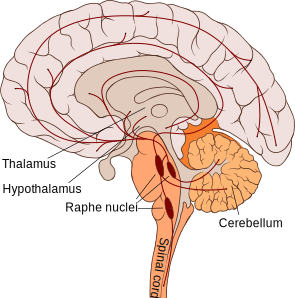
\includegraphics{./images/02-08/img_2.svg}

}

\caption{\label{fig-serotonin-pathway}인간 뇌의 세로토닌 경로
(Wikipedia에서 발췌)}

\end{figure}

세로토닌 신호전달에서 가장 중요한 역할을 담당하는
5-HT\textsubscript{2A}는 시냅스 후 수용체로 주로 글루타메이트를 분비하는
피라미드 뉴런의 수상돌기에 위치한다. 5-HT\textsubscript{2A}가 자극되면
글루타메이트 신호전달이 시작되고, 이는 선조체의 GABA 분비 사이 뉴런을
활성화시킨다. 사이뉴런은 근방의 도파민 분비세포로 하여금 분비를 줄이도록
조절한다. NMDA 수용체를 통한 글루타메이트 신호전달이 도파민 활성을
조절하는 메카니즘은 전전두엽이 피질하 도파민 활성을 조절하는 주요
기전이다.(섹션~\ref{sec-subcortical-dopamine}) 이런 식으로
5-HT\textsubscript{2A} 신호전달 은 도파민 활성을 조절할 수 있다. 따라서
5-HT\textsubscript{2A} 길항효과를 지닌 비정형 항정신병 약물을 투여하면,
브레이크가 풀리면서 도파민 분비가 증가할 것이다. 이것이 추체외로 증후군
발생을 억제/예방하는 기전으로 여겨진다. 글루타메이트 신호전달을 거치지
않더라도, 세로토닌 분비 뉴런은 도파민 분비 신경세포의 세포체나 축삭돌기
말단에 직접 연접하거나 근방의 GABA 뉴런을 통해 도파민 분비를 억제할 수
있다. 항정신병 약물을 쓰면 이들 억제회로도 역시 차단되어 도파민
신호전달이 늘어난다.

5-HT\textsubscript{2A}에 비해 5-HT\textsubscript{1A}는 자가수용체 역할을
한다. 5-HT\textsubscript{1A}는 세로토닌 분비 뉴런에 위치하며, 자극되면
세로토닌 분비를 억제한다. 비정형 항정신병 약물은 대체로
5-HT\textsubscript{1A} 효현효과를 갖기 때문에 결과적으로는 도파민 분비를
늘이는 쪽으로 기능한다.

\hypertarget{sec-5-HT-D2}{%
\subsection{\texorpdfstring{5-HT\textsubscript{2A}/D\textsubscript{2}
차단비와 비정형성}{5-HT2A/D2 차단비와 비정형성}}\label{sec-5-HT-D2}}

만약 순수하게 5-HT\textsubscript{2A} 수용체만을 차단한다면, 복측피개
영역에서 분비가 항진된 도파민은 중변연계든 중피질계든 관계없이 자극하여
오히려 정신병적 증상을 악화시킬 지 모른다. 바로 그렇기 때문에, 항정신병
약물의 비정형성은 5-HT\textsubscript{2A} 차단이 아니라
5-HT\textsubscript{2A}/D\textsubscript{2} 차단의 미묘한 균형에서
비롯된다고 할 수 있다. 5-HT\textsubscript{2A}와 D\textsubscript{2}가
동시에 차단된다는 것은, 시냅스 전 신경세포에서 분비되는 도파민의 양은
늘어나면서, 시냅스 후 신경세포에서의 도파민 효과는 막혀있는 상태를
불러온다.

\begin{figure}

{\centering \includegraphics{./images/02-08/img_0.png}

}

\caption{\label{fig-therapeutic-window}치료적 창 {[}@Arakawa2020-di{]}}

\end{figure}

일반적으로 항정신병 효과를 나타내는데 필요한 D\textsubscript{2} 차단
정도와 추체외로 증후군을 유발하는 D\textsubscript{2} 차단 정도는 서로
차이가 나기 때문에, 일종의 치료적
창(섹션~\ref{sec-dopamine-occupancy})을 만들어낼 수 있다. 항정신병
효과를 기대하기 위해선 적어도 D\textsubscript{2} 수용체가 60\%이상
차단되어야 하며, 차단율이 80\%가 넘어가면 추체외로 증후군과 프로락틴
혈증의 위험이 급증한다. 따라서 이 두 차단율 사이에 해당되는 용량 범위가
치료적 창이 되는 셈이다.(그림~\ref{fig-therapeutic-window}) 그런데
5-HT\textsubscript{2A} 차단에 의해 선조체의 도파민 분비 양이 늘어나면
추체외로 증후군을 일으키는 D\textsubscript{2} 수용체 차단 역치가 좀더
높아지며, 그에 따라 두 차단율 사이의 간격이 늘어난다. 이 말은 동시에
치료적 창의 범위도 넓어져, 상당히 고용량의 비정형 약물을 사용해도
추체외로 증후군의 위험이 적다는 뜻이 된다. 물론 비정형 약물이라 해도
지나치게 고용량을 쓰면 심한 추체외로 증상이 나타날 수 있으며, 이는
치료적 창을 넘어섰기 때문이라고 이해할 수 있다.

비정형 약물이라는 범주 안에는 상당히 이질적인 약물들이 포함되어 있으며,
5-HT\textsubscript{2A}/D\textsubscript{2} 차단의 비율도 약물에 따라
상당히 다르다. 5-HT\textsubscript{2A}/D\textsubscript{2} 차단의 황금비가
비정형성의 핵심이라고 주장한 Meltzer의 견해{[}@Meltzer1989-yh{]}를
따른다면, 이들 약물 중에서도 좀더 비정형적인 약물과 그렇지 않은 약물을
나눌 수 있을 것이다. 5-HT\textsubscript{2A}/D\textsubscript{2} 차단비가
가장 높은 약물은 클로자핀이며, 그 뒤를 뒤따르는 올란자핀, 퀘티아핀,
아세나핀과 함께 하나의 그룹을 형성하고 있다. 반면 팔리페리돈,
지프라시돈, 일로페릴돈, 루라시돈 등은 5-HT\textsubscript{2A}와
D\textsubscript{2}의 차단 정도가 거의 비슷하여 또 다른 그룹을 이룬다.
리스페리돈은 두 그룹의 중간 쯤에 위치하고 있다. 반면 도파민 부분
효현제인 아리피프라졸, 브렉시피프라졸, 카리프라진은 오히려
5-HT\textsubscript{2A}/D\textsubscript{2} 차단비가 1보다 작다. 이들
도파민 부분 효현제는 전혀 다른 방식에 의해 비정형성을 갖는다고 보아야
한다.

\hypertarget{uxc870uxd604uxbcd1uxc758-uxbcd1uxd0dcuxc0dduxb9acuxc5d0uxc11c-uxc138uxb85cuxd1a0uxb2ccuxc758-uxc5eduxd560}{%
\section{조현병의 병태생리에서 세로토닌의
역할}\label{uxc870uxd604uxbcd1uxc758-uxbcd1uxd0dcuxc0dduxb9acuxc5d0uxc11c-uxc138uxb85cuxd1a0uxb2ccuxc758-uxc5eduxd560}}

이상에서 살펴본 도파민-세로토닌 가설은 정확히 말하면 \uline{비정형성을
설명하기 위한 도파민-세로토닌 가설}에 지나지 않는다. 만약 병인론과
관련된 이론으로 승격하고자 한다면, 무엇보다 조현병 환자에게서 세로토닌
시스템의 이상이 발견되어야 하며, 세로토닌만을 조작함으로써 조현병과
유사한 상태를 유도할 수도, 차단할 수도 있어야 한다. 그러나 도파민
가설과는 달리 현재까지도 유력한 증거가 발견되지도, 설득력있는 통합
이론이 제시되지도 못하고 있다.

일단 LSD가 환각을 일으키는 기전부터 제대로 이해되지 않고 있다. LSD가
5-HT 수용체에 결합하는 것은 확실하지만 그것이 효현제인지 길항제인지도
불확실하다.{[}@Glennon1990-tc{]} 현재로서는 부분효현제로 보는 입장이
우세하며, 해부학적 위치와 기타 신경전달물질의 농도에 따라 효현 효과도
길항 효과도 발휘할 수 있다. LSD가 환각에 이르게 되는 과정에 대한 유력한
설명에 따르면, LSD는 청반(locus coeruleus)의 노르에피네프린 신경세포를
활성화하여 감각 신경을 예민하게 만들고, 대뇌 피질에서는 글루타메이트
신호전달을 필요 이상으로 강화시켜 신호대 잡음비를 높임으로써, 사고의
혼란과 비현실감을 유도한다.{[}@Aghajanian1999-mz{]}

과거에는 살아있는 조현병 환자의 뇌척수액에서 세로토닌 대사물질의 농도를
재거나, 사후 뇌조직에서 대사물질의 농도는 물론 수용체의 농도를 직접
측정하는 방식으로, 조현병과 관련된 세로토닌 시스템 이상을 발견하고자
노력하였다. 그러나 얻어진 결과들은 일관성이 없었고, 실험 조건이나
해부학적 부위에 따라 전혀 다른 결과가 얻어지곤 하였다. 몇 가지 흥미로운
결과를 언급한다면 다음과 같다. 뇌척수액의 5-HIAA\footnote{\textbf{Tet-Off®
  double transgenic system}: mhDISC1을 갖게된 쥐들은 그 상부에
  tetracycline-response element (TRE)를 동시에 지니고 있기 때문에
  tetracycline-transactivator (tTA)가 TRE에 붙으면 mhDISC1의 전사가
  시작된다. 사료에 doxycycline (DOX)이 들어있으면 DOX가 tTA를 방해하여
  mhDISC1의 전사를 차단하기 때문에, 음식에 DOX를 넣었다 뺐다 하면서
  mhDISC1 발현을 조절한다.}농도는 뇌피질의 위축과 상관관계가 있었으며,
동시에 낮은 5-HIAA 농도는 심한 음성증상 및 전전두엽 인지기능 손상과
연관이 있었다.{[}@Potkin1983-dx; @Abi-Dargham1997-lu{]} 사후 뇌조직
연구에서도 대체로 대뇌 피질이나 대상회에서는 세로토닌과 5-HIAA의 농도가
낮은 것으로, 측좌핵, 기저핵 등 피질하 조직에서는 높은 것으로
관찰되었다.{[}@Jospeh1979-uk; @Powchik1998-lo{]} 이 밖에도 대뇌 피질에서
5-HT 수송체는 대조군에 비해 낮은 것으로, 5-HT 수용체 역시 대조군에 비해
저하되어 있는 것으로 보여졌다.{[}@Laruelle1993-vx{]}

이러한 소견들은 조현병 환자에게서 5-HT와 관련된 신호전달이 원활하지
않다는 것을 시사한다. 그러나 이러한 연구들은 대부분 20-30년전에 이루어진
연구들로, 방법론이 현재처럼 정교화되지 않았을 뿐 아니라 만성화/황폐화된
환자들을 대상으로 하였기 때문에 의미있는 결론을 이끌어내기 어렵다. 다만
비교적 최근에 이루어진 메타 분석에 따르면, 사후 뇌의 전전두엽에서
5-HT\textsubscript{1A} 수용체는 증가된 반면 5-HT\textsubscript{2A}
수용체는 감소되어 있다고 한다.{[}@Selvaraj2014-qq{]} 그러나 PET를
이용하여 살아있는 환자에서 5-HT\textsubscript{2A} 수용체를 측정한
연구에서는 대조군과의 차이를 발견할 수 없었다.{[}@Lewis1999-co;
@Erritzoe2008-ox{]}

한편 유전 연구에서는 5-HT\textsubscript{2A}를 코딩하는 유전자인 HTR2A의
변이가 조현병의 위험을 높일 지 모른다 가능성이 제기되었으며 현재까지도
연구가 진행되고 있다. 주로 연구된 변이는 T102C(SNP rs6313)와 그 근방에
위치한 A-1438G (SNP rs6311)이다.{[}@Abdolmaleky2004-ww{]} 그러나 이들
변이는 조현병뿐 아니라 양극성 장애, 주요 우울증, 주의력 결핍장애 등
다양한 정신질환과 연관이 있다는 보고가 있어 조현병에 특히 하지도 않을
뿐더러, 최근 메타 연구에서는 어떤 질환과도 유의한 연관이 없다고
보고되었다.{[}@Serretti2007-hx; @Tan2014-rl{]}

\hypertarget{sec-serotonin}{%
\section{세로토닌과 항정신병 치료 효과}\label{sec-serotonin}}

비정형 항정신병 약물의 약리학적 성질에서 5-HT\textsubscript{2A}가
차지하는 위치에 대해, 그저 D\textsubscript{2} 차단제의 부작용을
감소시켜주는 정도의 소극적인 역할만을 부여할 수도 있을 것이다. 그러나
이들 약물이 음성/인지 증상에도 어느 정도 효과적이라는 것 때문에, 많은
연구자들은 5-HT 시스템이 좀더 적극적인 역할을 하리라 기대하였다. 신약을
개발하는 연구자들은 다양한 5-HT 수용체의 길항 혹은 효현제를 이용하여,
기존 항정신병 약물의 한계를 극복하고자 하였다. 특히 이들이 기대한 것은
음성 증상에 대한 개선 효과였다.

Ritanserin은 그 대표적인 약물로 5-HT\textsubscript{2A}와
5-HT\textsubscript{2C}에 대한 강력한 길항제이다. 일찌기 1990년대 초부터
시작되어 2000년대 후반에 이르기까지 기존 항정신병 약물에 ritanserin을
병용투여함으로써 음성 증상을 개선해보고 하는 많은 임상 시험이 있었지만,
결과는 가능성을 시사하는 정도에서 더 나아가지
못했다.{[}@Duinkerke1993-tv; @Akhondzadeh2008-hc{]} 유사한 계열의 약물로
volinanserin(M100907)과 eplivanserin(SR46349B)이 2상 혹은 3상
임상시험까지 진행되었으나, 효과 부족으로 중도에 개발이
중단되었다.{[}@Meltzer2004-de; @Ebdrup2011-xm{]}

이후 한동안 항정신병 약물 개발에서 5-HT\textsubscript{2A}에 대한 관심이
줄어드는 듯 했으나, 5-HT\textsubscript{2A}에 대한 역효현제(inverse
agonist) 개념이 등장하면서 새로운 전기를 맞이한다. 일반적인 약물은
수용체를 자극하거나 차단함으로써 그 효과를 발휘한다. 수용체 차단효과란
생리적으로 해당 수용체에 결합하는 내인성 리간드의 작용을 가로막는다는
뜻이다. 그러나 수용체의 작용기전에 대한 연구가 진일보하면서, 리간드가
결합되지 않아도 일정 수준의 활성을 보인다는 것을 알게 되었다. 따라서
고전적 차단약물로는 수용체를 완전히 차단한다고 해도, 리간드와 상관없이
발현되는 내인적 활성을 막을 수 없다. 역효현제란 약물이 수용체에
결합함으로써 내인적 효과마저 방해하는 약물을 말한다. 이런 개념을
적용해본 결과, 기존의 항정신병 약물도 5-HT\textsubscript{2A}에 대해
역효현 작용을 보이며, volinanserin, epivanserin 과 같은 실패한 약물도
역효현제라는 것을 알게 되었다.{[}@Sullivan2015-uc{]}

최근들어 5-HT\textsubscript{2A} 역효현제들은 참신한 (novel) 항정신병
개발 노선에 있어 선두 위치를 차지하고 있다. 이중 pimavanserin은 도파민,
아세틸콜린, 아드레날린 수용체 차단효과가 전혀없는 거의 순수한
5-HT\textsubscript{2A} 역효현제로 비정형 항정신병 약물의 하나로
분류된다. 이 약물은 파킨슨 병에 동반된 환각을 비롯한 정신병적 증상에
우수한 효과를 나타내며, 그 밖에 치매에 동반된 정신증상에도 효과적이라고
보고되었다.{[}@Friedman2013-pa{]} 이외에도 roluperidone와 lumateperone
등이 현재 임상 시험을 진행중이거나 이미 미국 식약청의 허가를
받았다.{[}@Jones2020-kk{]} Lumateperone은 5-HT\textsubscript{2A}에 대한
효과와 더불어 D\textsubscript{1}, D\textsubscript{2} 수용체 차단효과를
지니고 있지만, pimavanserin과 roluperidone은 도파민 수용체에 작용하지
않는다. D\textsubscript{2} 수용체를 차단하지 않고도 항정신병 효과를 낼
수 있다는 것은 세로토닌 가설을 진지하게 재고할 필요가 있음을
시사한다.{[}@Weiner2001-oz{]}

\hypertarget{uxc870uxd604uxbcd1-uxce58uxb8ccuxc5d0-uxc788uxc5b4uxc11c-uxc138uxb85cuxd1a0uxb2ccuxc758-uxbaa8uxc21cuxc801-uxc704uxce58uxc640-uxd5a5uxd6c4-uxc5f0uxad6c-uxbc29uxd5a5}{%
\section{조현병 치료에 있어서 세로토닌의 모순적 위치와 향후 연구
방향}\label{uxc870uxd604uxbcd1-uxce58uxb8ccuxc5d0-uxc788uxc5b4uxc11c-uxc138uxb85cuxd1a0uxb2ccuxc758-uxbaa8uxc21cuxc801-uxc704uxce58uxc640-uxd5a5uxd6c4-uxc5f0uxad6c-uxbc29uxd5a5}}

정신약물학의 역사에 있어서 \uline{조현병의 도파민 가설} 그리고
\uline{기분 장애의 생체 아민 이론(biogenic amine theory)}만큼 큰 족적을
남긴 가설은 많지 않다. 1960년대를 거치면서 항정신병 약물이 도파민
수용체를 차단한다는 사실과 함께, 항우울제는 노르에피네프린과 세로토닌의
가용성에 영향을 미친다는 것을 알게 되었다. 생물학적 아민 이론의 기초를
쌓아올린 Schildkraut\footnote{mhDISC1을 발현시키면 정상 DISC1의 작용을
  방해하기 때문에, 말하자면 DISC1의 기능을 인위적으로 켰다 껐다 한
  셈이다.}는 1965년과 67년에 연달아 생체 아민의 활성이 떨어지면
우울증이, 너무 높아지면 조증이 생긴다는 견해를
발표하였다.{[}@Schildkraut1965-wu; @Schildkraut1967-qr{]}

약물의 작용기전과 기분 장애의 병인론을 연결시키기는 불가능하다는
Schildkraut의 조심스러운 견해와는 달리, 대부분의 \uline{정신질환은
신경전달물질의 불균형 때문에 일어난다}는 단순명료한 이론은 의사와
연구자뿐만 아니라 제약 회사의 경영진 그리고 일반 대중의 마음을
사로잡았다. 현대의 정신과 의사들은 이제 더 이상 이러한 순진무구한 화학적
불균형 이론을 믿지 않는다고 하지만, 반세기를 이어져내려온 영향력은 쉽게
사그러지지 않았다. 여전히 정신의학 교과서에는 도파민 활성이 높으면
정신병적 증상이 생기며, 세로토닌이 부족하면 우울증에 쉽게 빠진다. 또한
노르에피네트린이 증가하면 조증이 유발되지만, 역설적으로 주의력 결핍
환자에게서는 집중력이 향상된다. 이런 식의 \uline{``A가 높으면 X가
생기고, B가 낮으면 Y가 생긴다''}는 설명은, 여전히 수많은 정신의학
연구에서 숨겨진 전제로 자리잡고 있다. 치료제의 개발에 있어서도,
\uline{``M을 차단하여 A를 낮추면 X가 치료된다''}는 식의 논리가 널리
통용된다.(그림~\ref{fig-drug-mechanism})

\begin{figure}

{\centering \includegraphics{./images/02-08/img_1.png}

}

\caption{\label{fig-drug-mechanism}정신질환에 대한 약물치료 효과의
잠재적 기전}

\end{figure}

단순히 \uline{``A가 높으면 X가 생긴다''}라는 식의 논리를 적용한다면,
조현병과 세로토닌의 관계에 있어서 금새 설명하기 어려운 벽에 부딪힌다.
세로토닌을 중심으로 한 과거의 연구는 조현병 환자 뇌에서 세로토닌
신호전달이 항진되어 있는 것처럼 묘사한다. 그렇기 때문에 세로토닌
효현제인 LSD를 투여하면 정신증상이 생기고, 5-HT\textsubscript{2A}를
차단하여 세로토닌 신호전달을 막으면 치료 효과를 볼 수 있다. 이에 반해
소박한 우울증의 세로토닌 가설에 의하면, 항우울제는 세로토닌 재흡수를
막아 시냅스내 세로토닌 농도를 올려주며 따라서 세로토닌 신호전달을
가속화시킨다. 세로토닌을 행복 호르몬에 비유하는 대중 매체의 선전에
따르면, 세로토닌은 많으면 많을수록 좋은 것이다. 그렇다면 우울증을
치료하기 위해선 세로토닌 활성을 높여야 하고, 조현병 치료를 위해서는
세로토닌 활성을 차단해야 한다는 모순적인 상황에 봉착한다. 이는 마치
양립할 수 없는 목표인 것처럼 보인다.

비정형 약물은 세로토닌 신호전달을 차단하며, 동시에 음성 증상에 효과를
나타내는 것처럼 보인다. 그러나 역으로 음성 증상을 개선하기 위해
항우울제를 사용하는 것은 예로부터 권장되어 왔으며, 효과 크기는 작지만
의미있는 성과를 거두고 있다.{[}@Singh2010-bt; @Helfer2016-mq{]} 그렇다면
음성 증상을 호전시키는데 필요한 것이 과연 세로토닌 차단인지, 아니면
자극인지 혼란스러워 진다. 더불어 조현병 환자가 심한 우울 증상을 동반하고
있을 때 대부분의 의사들은 주저없이 항우울제를 사용한다. 이 경우 세로토닌
활성을 높이는 약물과 낮추는 약물이 함께 투여되는 셈인데, 두 약물의
효과가 상쇄되거나 예기치 않은 부작용을 나타내지 않을지 우려하는 것은
매우 자연스럽다.{[}@Zullino1998-un{]}

이러한 모순을 이해하려면, \uline{``A가 높으면 X가 생긴다''} 혹은
\uline{``M을 차단하면 A가 낮추어진다''}라는 식의 단순한 논리에서
벗어나야 한다. 예상과는 달리 SSRI를 장기간 투여하면
5-HT\textsubscript{2A} 수용체의 농도가 감소하여 전반적인 신호전달이
줄어든다.{[}@Gray2001-eq{]} 더불어 5-HT\textsubscript{2A} 수용체의
과발현(over-expression)이 우울증을 유발한다는 이론도
있다.{[}@Eison1996-ir{]} 항우울제를 투여하면 몇 시간 지나지 않아
세로토닌 농도가 급상승하는데, 실제 항우울 효과는 2주는 있어야 나타나는
현상에 대해 항우울제에 의해 5-HT\textsubscript{1A},
5-HT\textsubscript{2A} 수용체가 충분히 감소하는데 시간이 걸리기
때문이라는 주장도 제기되었다.{[}@Stahl1994-vg{]} 물론
5-HT\textsubscript{2A} 수용체를 통한 신호전달이 직접 우울증을
일으키는지는 분명하지 않다. 항우울제에 의해 5-HT\textsubscript{2A}가
줄어드는 현상은 세로토닌 농도가 상승하는데 대한 단순한 피드백일 수 있다.
우울증 환자에서 5-HT\textsubscript{2A}가 늘어나 있는 것도 줄어든
세로토닌 신호전달에 의한 반작용일 수 있다.

대부분의 생체 과정은 어느 한 단백질의 기능을 차단하면, 보상성으로 해당
단백질이 과발현되어 양이 늘어나는 조절기전을 갖고 있다. 이는
내성(tolerance)이 발생하는 고전적 이유이다. 만약
5-HT\textsubscript{2A}를 차단하는 비정형 항정신병 약물을 오래 투여하면,
역시 내성이 생겨 수용체가 과발현되는 것도 예상할 수 있다.
5-HT\textsubscript{2A}가 직접 정신 증상과 연결되어있는 상태에서
5-HT\textsubscript{2A}의 농도가 증가한다면, 항정신병 약물의 효과 역시
내성이 생길 우려가 있다. 그러나 역설적으로 비정형 항정신병 약물을 오래
투여하면 오히려 5-HT\textsubscript{2A}가 점점 더 줄어드는
역내성(reverse-tolerance) 현상을 보인다.{[}@Van\_Oekelen2003-nd{]}
따라서 비정형 항정신병 약물과 항우울제를 각각 세로토닌 차단제, 세로토닌
활성 강화제로 이해하는 것은 곤란하다. 5-HT\textsubscript{2A} 신호전달의
차단효과에 있어서 두 계열의 약물이 동일한 효과를 나타내는 셈이다. 이러한
이론은 5-HT\textsubscript{2A} 길항제가 SSRI의 항우울효과를 증강시킨다는
관찰에 의해 뒷빋침된다.{[}@Marek2003-mk{]} 5-HT\textsubscript{2A}의
역효현제인 volinanserin가 SSRI의 효과를 끌어올리는 것도 역시 같은
맥락에서 이해할 수 있다 {[}@Marek2005-jl{]}

그러나 세로토닌 시스템의 모순성이 위와 같은 설명으로 명쾌히 해결되지는
않는다. 만약 비정형 항정신병 약물의 비정형성이 세로토닌 활성 조절에 달려
있는 것이 아니라 5-HT\textsubscript{2A} 차단에 달려 있다면,
5-HT\textsubscript{2A}를 통한 신호전달은 조현병 병태생리에 있어서 무조건
악영향만 끼치는 것으로 간주되기 쉽다. 그러나 5-HT\textsubscript{2A}는
신경섬유의 생성과 성장, 시냅스 형성에 중요한 역할을 맡고 있으며, 이
때문에 학습과 기억을 관장하는 신경가소성 메커니즘에 핵심 요소 중
하나이다.{[}@Lesch2012-fk{]} 21세기에 접어들면서 정신의학 연구자들은
신경전달물질 활성의 높고 낮음으로 인해 질병이 촉발된다는 단순한 도식에서
벗어나고자 애쓰고 있다. 그 대안으로 등장한 것은, 뉴런과 뉴런 사이의
원활하고 효율적인 연결의 생성 및 파괴, 그리고 이를 통해 상황에
역동적으로 적응하는 신경연결망(neural network)의 구조와 기능이라는
이해의 틀이다. 신경발달학적 가설이란 이런 신경연결망을 만들어가는
과정이요, 신경가소성이란 완성된 연결망을 유지, 보수하는 과정이다. 따라서
새롭게 인기를 끌고 있는 이론들은 학습/기억, 신경가소성, 신경영양인자
등에 강조점을 두고 있다. 따라서 세로토닌 가설, 특히
5-HT\textsubscript{2A} 수용체의 작용은 이런 측면에서 재해석될 필요가
있다. 조현병의 발병을 막는 것과는 별개로, 이미 이환된 조현병 환자의
퇴행을 막고 회복을 앞당길 수 있는 방법을 찾는 것 역시 빠질 수 없는 연구
과제이다. 이런 차원에서 LSD와 psilocybin\footnote{Two-hit 혹은
  multiple-hit 가설이란 유전적 변이때문에 취약한 개인이, 발달과정에서 또
  다른 유해 요인에 노출되면 발병으로 이어지게 된다는
  가설이다.{[}@bayer1999{]}} 등 5-HT\textsubscript{2A} 효현제들이
새삼스럽게 각광받고 있다.{[}@Carhart-Harris2017-cu{]} 이들 약물을 소량
투여하면, 신경가소성이 활발해지며 뇌 각부위의 연결이
공고해진다.{[}@Ly2018-md{]} 용량에 따라 다르지만, 인지기능이 개선된다는
연구결과도 적지 않은 편이다. 이를 응용하여 이들을 항치매제로 개발하려는
동향도 엿보인다.{[}@Vann\_Jones2020-fn{]}

\hypertarget{references-14}{%
\section*{References}\label{references-14}}
\addcontentsline{toc}{section}{References}

\markright{References}

\hypertarget{uxcee4uxb125uxd1b0uxacfc-uxae30uxb2a5uxc801-uxc5f0uxacb0uxc131}{%
\chapter{커넥톰과 기능적
연결성}\label{uxcee4uxb125uxd1b0uxacfc-uxae30uxb2a5uxc801-uxc5f0uxacb0uxc131}}

Connectome and Functional Connectivity

\hfill\break

\hypertarget{uxc2e0uxacbduxc5f0uxacb0uxb9dd}{%
\subsection{신경연결망}\label{uxc2e0uxacbduxc5f0uxacb0uxb9dd}}

뇌 기능은 고립된 신경세포에서 비롯되지 않는다. 또한 하나의 뇌 구조물이
항상 똑같은 기능만을 발휘하는 것도 아니다. 신경계의 기능이 창발하는 곳은
뉴런과 뉴런의 연결패턴이요 그들이 이루는 신경연결망(neural
network)\footnote{\textbf{신경연결망(neural network)}: 생물학적
  신경연경말의 개념을 처음 제안한 것은 영국의 철학자인 Alexander Bain
  (1873)과 미국의 위대한 심리학자인 William James (1890)이다. 이들은
  생각과 행동이 뉴런들 사이의 연결에서 비롯된다고 생각하였다. 그러나 이
  개념이 유명해진 것은 1943년 미국의 신경과학자인 McCulloch와 Pitts가
  신경망의 컴퓨터 모델을 만들어 간단한 연산이 가능하다는 것을 실연한
  다음이다. 1949년 Donald Hebb은 ``Hebbian learning'' 개념을 소개했고,
  이는 장기강화(long term potentiation) 모델의 핵심이 되었다.(6-8-1절)}이다.
해부학적 구조물 또한 다른 구조물과의 연결을 통해 합목적적 기능을
창출해낸다. \uline{``전체는 부분의 합보다 크다.(The whole is greater
than the sum of its part)''}라는 경구는 일반시스템 이론\footnote{\textbf{일반시스템
  이론(general system theory)}: 시스템이란 상호의존적이고 상호 작용하는
  부분들로 구성된 전체, 즉 구성 요소들과 그들의 상호 작용의 합으로
  정의된다. 오스트리아의 생물학자인 Ludwig von Bertalanffy에 의해
  창안되었다. 이전까지 과학은 개개 부분을 전체에서 고립시킨 후 그 성질을
  분석하는 환원주의 원칙에 따라 진행되어왔다. 이에 반해, Bertalanffy는
  시스템을 이해하기 위해 더욱 중요한 것은 개개 부분들이 다른 요소들과
  맺는 관계라고 지적하였다. 초기에는 인간사회나 기업조직을 이해하고자
  하는 데 응용되었으나, 점차 생물학 및 물리 시스템의 이해에도 적용되면서
  범위를 넓혀오고 있다.}이나 복잡계 이론\footnote{\textbf{복잡계
  이론(complexity theory)}: 시스템을 이루는 다양한 구성 요소들이 서로
  비선형적으로 관계맺고 있는 경우, 그들 전체에서 비롯되는 거시적인
  성질은 완전한 질서도 무질서도 아닌 카오스적인 양상을 보인다. 시스템
  구성요소에서는 발견할 수 없는 성질이 그들이 구성하는 시스템에서
  나타나는 소위 창발현상을 연구하는 이론을 복잡계 이론이라 한다.}을
확립한 현대의 선구적인 학자들이 아니라, 무려 2,500년전에 활약한
아리스토텔레스에게서 비롯되었다.

뉴런과 뉴런의 연결 역시 서로 다른 층위\footnote{\textbf{서로 다른 층위}
  시스템은 거의 예외없이 계층적 구조를 이루고 있다. 하위 단계의 구성
  요소들이 모여 새로운 성질을 발현하면, 그렇게 창발된 현상들이 모여 보다
  상위의 구조를 만들고 또 다른 성질을 창발시킨다. 따라서 전체 시스템을
  분석하기 위해선 어느 하나의 층위만을 이해해선 부족하며, 상위단계와
  하위단계가 맺는 관계까지도 이해해야 한다.}에서 바라볼 수 있다. 특정한
대뇌 피질층(cortical layer)(섹션~\ref{sec-D1-anatomy})에 위치한 피라미드
뉴런과 주변의 사이 뉴런이 이루는 국소적 연결을 비롯하여, 동일한 피질
기둥\footnote{\textbf{피질 기둥(cortical column)}: 6개의 층으로 구성된
  대뇌 피질은 기둥 구조로 조직화되어 있다. 피질 표면의 조그마한 영역과
  여기에 수직인 내측 피질은 서로 활발한 시냅스를 이루고 있으며, 하나의
  연산단위를 이룬다. 여기서 연산된 신호는 세번째 층(layer III)에서
  밖으로 뻗어나가는 축삭돌기를 통해 다른 피질 기둥으로 보내진다.}에
속하지만 서로 다른 층(layer)에 놓인 뉴런 간의 원격 연결, 서로 다른 피질
기둥 간의 연결 등을 고려해 볼 수 있다. 이보다 좀더 거시적으로 보면,
하나의 해부학적 구조와 다른 구조 사이의 연결이 있다. 후자의 규모가 큰
연결들은 다수의 신경 경로(neural pathway)를 구성한다. 이들은
해부학적으로 \uline{bundle, fasciculus, tract, commissure}와 같은 용어로
불리운다.

\hypertarget{uxc778uxac04-uxcee4uxb125uxd1b0-uxd504uxb85cuxc81duxd2b8}{%
\subsection{인간 커넥톰
프로젝트}\label{uxc778uxac04-uxcee4uxb125uxd1b0-uxd504uxb85cuxc81duxd2b8}}

\uline{커넥톰(Connectome)}이란 이렇게 거시적인 층위에서 신경 세포들이
연결되어 있는 양상을 종합적으로 표현한 것으로 일종의 뇌
회로도(blueprint)라고 생각할 수 있다. 좀 더 넓은 의미로는 단순히 뇌 내
신경세포 뿐만이 아니라 전신에 분포되어있는 신경세포들 간의 연결망까지도
포함한다. 2009년 시작된 \uline{인간 커넥톰 프로젝트(human connectome
project)}는 게놈 프로젝트 이후 최대의 과학 혁명으로 불린다. 이 연구를
통해 1,000억 개 신경 세포의 연결구조와 활동원리를 파악해서 기억, 의식,
성격 등의 비밀을 밝히고자 한다. 이 프로젝트를 성공시킴으로써 치매,
우울증, 자폐증, 조현병 등의 발병 기전과 치료법을 찾는데 기여할 정보를
얻는다는 목표를 추구하고고 있다.

인간 커넥톰 프로젝트는 한국 혈통의 미국인 과학자인 승현준\footnote{\textbf{Sebastian
  Seung (1966\textasciitilde)}: 한국계 미국 컴퓨터 공학자. 40세에
  신경생물학으로 전공을 바꾼 후 뇌 영상을 통해 커넥톰 구조를 찾아내는
  컴퓨터 프로그램을 만들기 시작한다. 2010년 TED 강연에 출연하여
  \emph{``나는 내 커넥톰이다(I am my connectome)''}이라는 강연을 하였고,
  2012년 \emph{``Connectome: How the Brain's Wiring Makes Us Who We
  Are''}이라는 저서를 써서, 커넥톰을 대중에게 알리는데 큰 역할을 하였다.
  2018년부터는 삼성전자에서 인공지능 개발팀을 이끌고 있다.}에 의해서
더욱 우리에게 친숙하다. 원래 컴퓨터 공학자이던 그는 인간 커넥톰
프로젝트의 출범 이후 그 가능성을 높이 평가하여, 저서 와
\href{https://www.ted.com/talks/sebastian_seung_i_am_my_connectome?language=en}{공개
강연}을 통해 커넥톰의 무궁무진한 잠재력을 역설하였다.

커넥톰을 그리는 것은 \uline{확산강조 MRI(diffusion-weighted MRI)}를
촬영하는 것으로 시작한다. 아무런 방해물이 없을 때 물 분자는 어느
한쪽으로도 치우침없이 대칭적으로 확산되며 이는 하나의 구(sphere)로
모델링 할 수 있다. 이 상태를 \uline{등방성(isotropic)}이라고 한다. 만약
미엘린 수초에 의해 신경 경로가 절연되어 있으면, 물 분자가 특정한
방향으로 더 쉽게 확산되는데 이러한 상태를
\uline{비등방성(anisotropic)}이라고 한다. 비등방성 상태가 되면
구(sphere)가 아니라 타원체(ellipsoid)를 이용하여 모델링하게 되는데,
이러한 방식으로 얻는 이미지를 \uline{뇌 확산텐서영상(diffusion tensor
imaging, DTI)}이라고 한다. 얻어진 영상에 특별한 컴퓨터 알고리즘을
적용하면, 신경 경로를 추적하여 3차원 그래픽으로 표시할 수 있는데, 이를
\uline{신경섬유경로영상(fiber tractography)}이라고 한다. 미국
국립보건원(NIH)에서 후원하고 있는 인간 커넥톰 프로젝트를 통해 얻어진
다양한 신경섬유경로영상은
\href{https://db.humanconnectome.org/app/template/Login.vm}{웹사이트}를
통해 내려받을 수 있으며, 이 자료는 다양한 연구에 활용되고 있다.

\begin{figure}

{\centering \includegraphics{./images/02-09/img_0.png}

}

\caption{뇌 확산텐서영상을 통해 얻어진 인간의 커넥톰
(\url{http://www.humanconnectomeproject.org/gallery/})}

\end{figure}

\hypertarget{uxae30uxb2a5uxc801-uxc5f0uxacb0uxc131}{%
\section{기능적 연결성}\label{uxae30uxb2a5uxc801-uxc5f0uxacb0uxc131}}

DTI를 통해서 얻어낸 자료는 해부학적 커넥톰에 해당한다. 그러나
해부학적으로 밝혀진 경로가 반드시 기능적으로도 의미가 있는 지는 확신할
수 없다. \uline{기능적 연결성(functional connectivity)}이란 서로 떨어진
뇌 부위가 기능적으로도 서로 연결되어 있는지를 알아내는 방법이다. 이는
fMRI를 이용하여 안정상태 혹은 과업수행 상태에서 뇌의 각 부위에서
발생하는 동시다발적 신호의 연결성을 분석하여 얻어낸다. 이 작업에는
고도로 복잡한 컴퓨터 알고리즘이 적용되며, 현재까지도 어떤 것이 가장
정확하고 효율적인 알고리즘인지는 결정되지 않았다. 기능적 연결성을 통해
기능적 커넥톰을 제쟉할 수 있다. 기능적 커넥톰은 해부학적 커넥톰의
부분집합이라는 견해, 즉 해부학적으로 연결되어 있어야 기능적 연결도
가능해진다는 견해가 있지만, 반드시 그렇지만은 않다는 이론도
있다.{[}@Tewarie2020-vv{]} 뇌의 신비를 벗겨내기 위해 좀더 중요한 것은
기능적 커넥톰이겠지만, 이를 매핑하는 과정은 해부학적 커넥텀의 경우보다도
훨씬 더 어려운 과업이다.{[}@Lang2012-gs{]}

\hypertarget{sec-connectome-fingerprint}{%
\section{커넥톰 핑거프린트}\label{sec-connectome-fingerprint}}

커넥톰은 개인마다 독특한 연결 패턴을 알 수 있도록 해준다. 이러한 패턴을
일종의 지문(fingerprint)에 빗대어 \uline{커넥톰 핑거프린트(connectome
fingerprint)}라고 한다. 커넥톰 핑거프린트는 개인마다 다르며, 시간이
지나도 크게 변하지 않는다. 핑거프린트를 사용하여 특정 개인의 신원을
확인할 수 있을 정도이며, 특히 이 패턴은 그 사람의 인지 기능과 상관이
있다.{[}@Finn2015-jj; @Munsell2020-nt{]}

당연한 이야기겠지만 개인마다 커넥톰 핑거프린트가 다르다면, 이를 그룹과
그룹 간에도 비교할 수 있을 것이다. 환자와 대조군, 혹은 각양 각색의
진단을 가진 환자군의 핑거프린트를 서로 비교하면, 각 진단군에 독특한
핑거프린트를 얻어낼 수 있을 것이다.{[}@Wang2020-tu{]} 다만 이러한 연구의
어려운 점은, 커넥톰 핑거프린트와 대응하는 표현형(phenotype)이 대체 어떤
것인지 미리 알 수 없다는 점이다. 주지하다시피, 정신과 진단이란 생물학적
병태생리와 일대일로 대응하지 않는다. 진단의 경계는 너무나 느슨하며고,
진단을 범주적(categorical diagnosis)으로 내려야할 지 차원적(dimensional
diagnosis)으로 내려야할 지도 의견이 모아지지 않았다. 만약 정신병적
증상에 해당하는 핑거프린트가 있다면 이는 조현병, 양극성 장애, 정신병적
우울증을 막론하고 나타날 것이다. 인지기능과 관련된 핑거프린트가 있다고
해도, 치매와 조현병을 구분하기 어려울 지 모른다.{[}@Baker2019-gz{]}

커넥톰 연구를 통해 세가지 광역 네트워크의 구조가 제시되었다. 첫번째,
\uline{전두-두정엽 조절 네트워크(frontoparietal control network,
FPCN)}는 전전두엽과, 하두정소엽(inferior parietal lobule), 대상회의
중앙부위(middle cingulate gyrus)을 중심으로 연결되며, 과거 전전두엽이
맡고 있다고 여겨진 작업 기억과 집행 기능을 행사한다. 둘째, \uline{현저성
네트워크(salience network)}는 전측 섬엽(anterior insula)과 전측
대상회(anterior cingulate gyrus)로 구성되며, 의사소통, 사회적 행위, 자기
의식 등과 관련된 복잡한 기능을 맡는다. 혹자는 이를 \uline{대상-판개
네트워크(cingulo-opercular network, CON)}라고 부르기도 한다. 마지막으로
\uline{디폴트 모드 네트워크(default mode network, DMN)}가 있다. 이는
내측 전전두엽(medial prefrontal cortex), 후측 대상회(posterior cingulate
gyrus) 그리고 각회(angular gyrus)로 이루어진다. DMN은 아무런 과업도
수행하지 않고 절대적 안정 상태에 있는 뇌에서 활성화되는 부분인데,
자아감이나 과거 회상, 미래에 대한 예측, 마음 이론, 도덕 판단 등
\uline{자기(self)}와 관련된(self-referential) 기능을 행사할 때
사용된다고
여겨진다.(그림~\ref{fig-global-network}){[}@Andrews-Hanna2012-lz{]}

\begin{figure}

{\centering \includegraphics{./images/02-09/img_1.png}

}

\caption{\label{fig-global-network}인간 뇌에서 발견되는 광역 네트워크
연결 {[}@Chabran2020-me{]}}

\end{figure}

이런 식으로 커넥톰에서 다루어지는 네트워크는 국소적 미세 연결부터 광역
네트워크까지 다양한 층위로 존재하며{[}@Mars2018-fz{]}, 이에 대응하는
표현형 역시 다양한 층위로 고려될 수 있다. 광역 네트워크 이상에 해당되는
표현형은 지엽적인 진단명을 넘어서는 좀더 높은 층위에 해당할 것이다.
이러한 층위의 결정이 커넥톰 연구의 걸림돌로 남아있다.

\hypertarget{uxc870uxd604uxbcd1uxc758-uxcee4uxb125uxd1b0-uxc774uxc0c1}{%
\section{조현병의 커넥톰
이상}\label{uxc870uxd604uxbcd1uxc758-uxcee4uxb125uxd1b0-uxc774uxc0c1}}

\hypertarget{sec-cognitive-control}{%
\subsection{FPCN과 인지적 조절}\label{sec-cognitive-control}}

이러한 어려움에도 불구하고, 최근에는 정신과 진단에 따라 세가지 광역
네트워크(FPCN, CON, DMN)에 어떤 변화가 있는 지를 알아내려는 연구가
활발히 진행되고 있다. Baker 등{[}@Baker2019-gz{]}은 조현병과 기분 장애
환자 모두에서 FPCN의 연결성이 떨어지는 것이 발견되었으나, DMN의 연결성
저하는 조현병 그리고 정신병적 증상이 동반된 기분 장애 환자에서만
발견되었다고 하였다. 그러나 동시에 FPCN의 연결성 저하가 PANSS로 측정한
양성 증상과 비례 관계에 있었기 때문에, FPCN 역시 정신병적 증상 발현에
기여하는 것 같다고 하였다. 또 다른 연구자들은 조현병의 다유전자 위험
점수(PRS, 섹션~\ref{sec-influence-genetic-research})가 FPCN과 DMN의
전반적 연결성과 역비례 관계에 있다고 하였다.{[}@Cao2020-mn{]}

유사한 연구에서 반복적으로 발견되는 조현병 환자의 FPCN 이상은, 조현병
증상이 \uline{인지적 조절(cognitive control)}이라는 집행 기능의 결함에서
비롯된다는 것을 시사한다. 인지적 조절이란 의식적으로 인지적 자원을
당면한 과제에 집중시키는 능력을 의미한다.{[}@Marek2018-gp{]} FPCN은 그
안에 포함된 하위 구조들간의 왕성한 연결 말고도, 다른 광역 네트워크와의
활발한 연결을 특징으로 한다. 집행 기능이라는 이름에 걸맞게, 다양한
네트워크 들의 기능을 동조시키거나 조율한다. 그래서 FPCN을 \uline{기능적
허브(functional hub)}라고 부르기도 한다.{[}@Power2013-vz{]} 특히 FPCN은
학습/경험과 무관한 유동성 지능\footnote{\textbf{유동성 지능 (fluid
  intelligence)}: 유동성 지능은 추리능력, 연산능력, 기억, 도형지각 능력
  등 경험과 무관한 지능이고, 대비되는 결정형 지능(crystallized
  Intelligence)은 어휘, 일반상식, 언어이해, 판단과 같이 경험, 훈련 및
  교육 등의 환경적 요인에 의하여 발달, 축적된 지능을 말한다.}과 관계가
깊다.{[}@Cole2015-oo{]} 그런데 조현병 환자는 FPCN과 CON 혹은 DMN과의
연결성이 현저히 떨어진다.{[}@Sheffield2015-gl{]}

조현병 환자 뿐 아니라 우울증, 불안장애, 강박증 등에서도 FPCN의 연결성이
떨어지는 것이 발견되지만, 두 경우는 좀 차이가 난다. Cole
등{[}@Cole2014-pi{]}은 이를 일차성과 이차성 기능 저하로 나눠 설명한다.
일차성 기능 저하는 그야말로 FPCN을 구성하는 회로 자체나 신경 세포의 손상
때문에 기능이 떨어지는 경우이다. 이에 비해, 이차성 기능 저하는, 회로
자체의 손상은 없으나 우울/불안 등의 다른 증상을 억누르기 위해 FPCN의
자원을 소진한 나머지, 정작 인지기능에 사용할 여지가 남지 않은 경우를
말한다. Cole 등은 FPCN의 일차성 기능 저하는 조현병과 양극성 장애의
특징이라고 주장한다.{[}@Cole2014-pi{]} 이상을 종합하면, 조현병 환자의
뇌는 FPCN의 일차적 기능 저하를 특징적으로 보이며, FPCN 내부의 연결성이
떨어질 뿐 아니라 FPCN과 다른 광역 네트워크와의 연결성도 떨어진다. 이
상태는 유동성 지능을 떨어뜨릴 뿐 아니라, CON과 DMN의 활성을 조율시키지
못하여 정신병적 증상을 유발하기도 한다.

\hypertarget{conuxacfc-uxd604uxc800uxc131}{%
\subsection{CON과 현저성}\label{conuxacfc-uxd604uxc800uxc131}}

FPCN이 과업을 시작하는데 필요한 초기 인지적 조절을 담당한다면, CON은
목표를 놓치지 않도록 유지하며, 오류가 생겼을 때 행동을 조절하는 역할을
맡고 있다.{[}@Godwin2017-it{]} 또한 내부로 부터 혹은 외부로 부터
전달되는 신호 중에서 현저하다고 여겨지는 신호를 탐지, 가공, 통합하는
역할을 맡는다.{[}@Huang2020-nw{]} CON의 연결성은 주어진 과제의 난이도가
높아질수록 강해지는 경향을 보인다.{[}@Sheffield2015-gl{]} 일부
연구에서는 조현병 환자에서 CON의 내부 연결성이 정상 대조군보다 낮으며,
그 정도는 음성 증상과 음의 상관관계를 보인다고 한다.{[}@Tu2012-dd{]} 또
다른 연구에서는 정신병적 증상을 잠깐이나마 경험했던 일반인을 대상으로,
증상의 심각도와 CON 연결성을 비교했더니 역시 음의 상관관계가
관찰되었다.{[}@Sheffield2016-ld{]} CON의 연결성이 단순히 인지 기능
저하를 반영하는 것인지, 망상의 기초가 되는 것인지는 아직 확실하지 않다.

비정상적 현저성 이론(섹션~\ref{sec-aberrant-salience})은 망상을 형성하는
과정을 설명하는 주요 이론 중 하나이기 때문에, CON에 대한 관심은 여전히
높은 편이다. 더구나 CON은 FPCN과 DMN 사이를 매개하는 일종의 스위치
역할을 하기 때문에 더욱 중요성이 강조되었다.{[}@Dosenbach2007-vn{]}
앞에서도 잠깐 언급되었지만 FPCN은 목표 지향적으로 과제를 해결해야할 때
활성화되는 네트워크인 반면, DMN은 자극이나 과제가 없는 상태에서 정신내적
세계에 머무를 때 활성화된다. 안정상태에서 DMN이 활성화되어 있는 개체가
무언가 평소와 다른 자극을 감지하면, CON은 이 자극이 해결을 요구하는
가치가 있는지 아니면 무시해도 되는지를 결정한다. 만약 전자라면 DMN을
잠시 비활성화하는 대신, FPCN을 활성화시킴으로써 새로운 과제를 해결하고자
한다. 조현병 환자는 외적 세계와 내적 세계를 혼동하는 경향이 있으며,
무시해도 될 자극과 중요한 자극을 걸러내지 못한다. 이러한 인지적
메커니즘의 오작동이, 온전하지 못한 CON 때문인지도 모른다. 따라서
연구자들이 CON의 이상을 확인하고자 애쓰는 것도 무리가
아니다.{[}@Huang2020-nw{]}

\hypertarget{dmnuxacfc-uxc790uxae30-uxad00uxb828uxc131}{%
\subsection{DMN과 자기
관련성}\label{dmnuxacfc-uxc790uxae30-uxad00uxb828uxc131}}

DMN이란 개념은 2001년 Raichle에 의해 제안되었다.{[}@Raichle2001-xd{]}
fMRI 연구를 할 때는 특정 과업을 주었을 때 활성화되는 뇌 영역을 찾기 위해
아무 과제도 주지 않은 안정상태(baseline)와 비교하게 되는데, 이
안정상태에서도 특정 뇌 부위가 독특한 패턴으로 활성화된다는 것이 DMN을
찾게된 계기가 되었다. DMN을 이루는 뇌 구조물은 예로부터 조현병과
관련하여 많이 연구되던 부위들이고, DMN이 담당하는 뇌 기능 역시 조현병
증상과 연관이 있기 때문에 일찌기 조현병과의 관련여부가
연구되었다.{[}@Hu2017-bx{]}

조현병과 관련한 DMN 이상을 최초로 보고한 연구자는 Garrity
등{[}@Garrity2007-lr{]}이다. 이들은 DMN 활성을 유도하는 인지과제를 주고,
뇌 대사가 활성화되는 부위와 주파수 특성을 측정한 후 환자군과 정상
대조군을 비교하였다. 그 결과 두 군 사이의 유의한 차이를 발견해내었다.
같은 해 Bluhm 등{[}@Bluhm2007-cu{]}은 조현병 환자는 DMN의 중심 구조인
후측 대상회(posterior cingulate gyrus)와 기타 영역들 간의 연결성이
떨어진다고 하였다. 하지만 혼란스럽게도, 이후 DMN의 활성 정도나 기능적
연결성을 환자군과 대조군 사이에 비교하는 연구들이 이어졌으나, 일관된
결과를 얻지는 못하였다.{[}@Hu2017-bx{]}

실험결과를 떠나서 연구자들은, 안정상태에서는 DMN이 활성화되어 있다가
현저성(salience)을 지닌 자극이 감지되면 순간적으로 DMN이 비활성화되면서
FPCN으로 활성이 옮겨간다고 생각하며, 이러한 역동적 전환이 제대로
이루어지지 않는 것이 조현병 환자의 특성이라 여긴다. FPCN과 DMN은 서로
음의 상관관계(anti-correlation)를 갖는 것이
정상적인데{[}@Uddin2009-ow{]}, 조현병 환자에서는 이러한 음의 상관관계가
덜 뚜렷하게 나타난다.{[}@Whitfield-Gabrieli2009-ln; @Wotruba2014-mj{]}

DMN의 활성과 연결성은 서로 정비례하며, 양성 및 음성 증상과도 유의미한
상관관계를 보인다.{[}@Whitfield-Gabrieli2009-ln{]}, 따라서 DMN의
과활성과 과연결성을 조현병과 결부시키는 연구자가 많은
편이다.{[}@Whitfield-Gabrieli2012-cd{]} 이러한 DMN의 과활성과 과연결성은
약물을 한번도 사용한적이 없는 환자에게도 나타날 뿐더러, 발병하지 않은
환자 가족에게서도 발견할 수 있다.{[}@Galindo2017-cv; @Guo2017-pa{]}
DMN의 주된 내용인 자기-관련성(self-referential)은, 환자들이 외부의
중립적 자극을 자꾸만 자신과 관련지어서(idea of reference) 생각하는
경향과 연결되는 것 같다.{[}@van2012{]}

한편 연결성의 이상은 조현병 환자에게 흔히 동반되는 연성 신경학적
징후(neurological soft signs)와도 연관이 있다고 한다.{[}@Kong2020-lw{]}
적지 않은 연구자들은 DMN의 활성 및 연결성을 조현병의 대표적인 생물학적
지표의 하나로 간주하고 있다

\hypertarget{references-15}{%
\section*{References}\label{references-15}}
\addcontentsline{toc}{section}{References}

\markright{References}

\hypertarget{uxae00uxb8e8uxd0c0uxba54uxc774uxd2b8-uxac00uxc124}{%
\chapter{글루타메이트
가설}\label{uxae00uxb8e8uxd0c0uxba54uxc774uxd2b8-uxac00uxc124}}

Glutamate Hypothesis

\hfill\break

글루타메이트는 중추신경계의 대표적인 흥분성 신경전달물질로서, 뇌에서
일어나는 신호전달의 90\% 이상을 담당하고 있다. 이러한 중요성에도
불구하고, 신경전달물질로서의 정체가 명확히 규명된 것은 도파민,
세로토닌보다도 늦은 1984년에 이르러서였다.{[}@Fonnum1984-cm{]}
글루타메이트는 그 자체가 신경전달물질일 뿐 아니라, 대표적인 억제성
신경전달물질인 GABA의 전구물질이기도 하며, 둘은 서로 상보적으로 작용하여
신호전달의 균형을 이룬다.

글루타메이트 수용체는 AMPA/kinate과 NMDA 수용체라 불리우는 이온채널을
비롯하여, G 단백질과 결합되어 있는 metabotropic 수용체로
나뉜다.(그림~\ref{fig-glutamate-neurotransmission}) 통상적인 정보전달
이외에도, NMDA 수용체를 통한 신호전달을 중심으로 하여 학습/기억에
핵심적인 역할을 하기 때문에 다양한 정신질환과 관련해서 연구되었다.

\begin{figure}

{\centering \includegraphics{./images/02-10/img_0.png}

}

\caption{\label{fig-glutamate-neurotransmission}글루타메이트 신호 전달의
기전 {[}@Swanson2005-ah{]}}

\end{figure}

\hypertarget{uxae00uxb8e8uxd0c0uxba54uxc774uxd2b8-uxac00uxc124-1}{%
\section{글루타메이트
가설}\label{uxae00uxb8e8uxd0c0uxba54uxc774uxd2b8-uxac00uxc124-1}}

\hypertarget{uxac00uxc124uxc758-uxd0c4uxc0dd}{%
\subsection{가설의 탄생}\label{uxac00uxc124uxc758-uxd0c4uxc0dd}}

도파민 가설이 조현병의 양성 증상을 설명하기 위해 등장하였다면,
글루타메이트 가설은 음성/인지 증상을 설명하기 위해 등장했다고 해도
과언이 아니다. 신경발달학적 가설과 신경퇴행적 가설이 점점 더 영향력을
얻어가면서, 연구자들의 관심은 신경연결망의 형성과 유지 그리고 붕괴에
쏠리기 시작하였다. 조현병 환자는 발병 초반부터 뇌실질의 위축이 관찰되고,
만성화, 황폐화 정도에 따라 이러한 위축이 점점 더 심해지는 소견을 보인다.
따라서 연결망이 애초에 만들어질 때부터 문제가 있을 뿐더러, 출생 후에도
이를 유지하고 상황에 맞게 변형시키는데 어려움을 겪을 것이라 예상되었다.

이와 더불어 1970년대 마취 보조제로 도입된 ketamine\footnote{\textbf{Ketamine}:
  1962년에 합성된 마취제. 원래 동물 마취 및 치과용 마취에 사용되었다.
  강력한 진통작용과 함께 환각을 일으킨다. 환자는 표면적으로는 의식이
  있는 것처럼 보이지만, 나중에 과정을 기억하지 못하기 때문에 해리성
  마취제로도 불리운다. 미다졸람, 프로포폴과 함께 가장 많이 사용되는
  수면마취제이지만, 남용 위험이 높으며 과량 투여 시 심혈관계 불안정으로
  사망할 수 있다.}과 phencyclidine (PCP)\footnote{\textbf{Phencyclidine}:
  소위 angel dust로 불리우는 환각제이다. 1926년에 합성되어 마취제로
  사용되었지만 남용 위험이 워낙 높아 ketamine으로 대체되었다. PCP 중독
  환자가 나중에 조현병으로 발병하는 비율은 26\% 정도로 대마초보다는
  낮지만, 필로폰, 코카인 보다는 상당히 높다.{[}@Murrie2020-jo{]}}은
특징적으로 조현병 유사 증상을 유발했는데, 암페타민 유발 정신증과는 달리,
음성/인지 증상에 해당되는 증상도 일으킬 수 있었다.{[}@Krystal1994-vn{]}
때문에 암페타민이나 LSD 복용 후 정신 증상을 일으켜 병원을 찾은 환자들에
대해선 의사들이 쉽게 감별진단을 할 수 있었던 것에 비해, PCP/ketamine
복용 후 방문한 환자들에게는 대부분 조현병 진단이
내려졌다.{[}@Uno2019-mx{]} 또한 실제 조현병 환자가 PCP를 복용하면,
기존의 증상이 훨씬 악화되는 현상을 보였다.{[}@Lahti1995-co{]}

Ketamine과 PCP가 결합하는 부위가 \uline{NMDA 수용체}라는 글루타메이트
수용체의 하나라는 것은 1980년대 초가 되서야 밝혀졌다. 두 약물은 NMDA의
비경쟁적 길항제이기 때문에, NMDA 신호전달을 원천적으로 차단해버린다.
NMDA 수용체는 세가지 서로 다른 종류의 아단위(subunit)가 복합체를 이룬
형태로 구성되며, 그 내부에는 글리신, D-serine, glutathione, spermine 등
다양한 조절물질이 결합하는 부위가
있다.(그림~\ref{fig-NMDA-receptor}){[}@Uno2019-mx{]}

\begin{figure}

{\centering \includegraphics[width=8.21875in,height=\textheight]{./images/02-10/img_1.png}

}

\caption{\label{fig-NMDA-receptor}NMDA 수용체의 구조 {[}@Witt2004-of{]}}

\end{figure}

글루타메이트 가설이 최초로 등장한 것은 1980년이다. 근거는 조현병 환자의
뇌척수액에서 글루타메이트 농도가 떨어진다는 것과, 쥐에 암페타민을
투여하면 역시 뇌척수액의 글루타메이트가 감소한다는 것이었다. 이에
연구자들은 글루타메이트 신경세포의 기능 부전 혹은 퇴행이 조현병의
원인이라고 생각하였다.{[}@Kim1980-yq; @Kim1981-mf{]} 당시에는 이러한
결과가 타 연구진에 의해 재현되지 않않기 때문에 그다지 관심을 받지
못하였다. 그러던 중 몇년 후 Javitt은 조현병의 PCP 모델이 암페타민
모델보다 더욱 조현병을 설명하는데 유용하다고 주장하면서, 글루타메이트
가설을 본격적으로 회자시킨다.{[}@Javitt1987-xw; @Javitt1991-fu{]}
한문장으로 요약하여, 글루타메이트 신호전달 특히 NMDA 수용체를 통한
신호전달이 제대로 이루어지지 않으면 조현병의 제반 증상이 출현한다는
것이다. NMDA 수용체가 기능을 하지 못하면 시냅스의 생성, 유지에 곤란을
겪을 것이다. 게다가 NMDA 수용체를 통한 신호전달은 전전두엽이 피질하
도파민 활성을 조절하는 주요 기전이므로(6-6절 참조), 피질 하 도파민
활성의 부적절한 증가가 초래될 수 있다.

항 NMDA 수용체 자가항체에 의한 뇌염(Anti-NMDA receptor encephalitis)
역시 글루타메이트 가설을 뒷받침하는
증거이다.(섹션~\ref{sec-antibrain-antibody}) 이는 자가면역 질환의
하나로, 급격한 정신병적 증상을 일으키며, 또 순수한 조현병 환자 중에도
일부 항 NMDA 수용체 자가항체가 발견된다. 이러한 증거들은 적어도 조현병
환자 중 일부는 NMDA 수용체 기능 저하때문에 증상이 지속되고 있음을
시사해준다.

\hypertarget{uxc720uxc804uxc801-uxc99duxac70}{%
\subsection{유전적 증거}\label{uxc720uxc804uxc801-uxc99duxac70}}

조현병의 신경발달학적 가설에서는 유전적 요인 혹은 주산기 감염과 같은
환경적 요인이 정상적인 신경발달 과정을 방해한다고 가정한다. 그런데
뉴런과 뉴런 사이에 시냅스가 형성되고, 그것이 점점 강화되어 자리를 잡기
위해선 NMDA를 통한 신경가소성 과정이 절대적으로 중요하다. 따라서
신경발달을 방해하는 유전적 요인이 글루타메이트와 관련되어 있을 것이라
예상하는 것은 상당한 개연성이 있다. 2014년 Schizophrenia Psychiatric
GWAS Consortium에서 발표한 광범위 유전체 연합 연구(GWAS,
섹션~\ref{sec-GWAS}) 결과를 살펴보면, 엄격한 기준으로 선택된 100여개
정도의 조현병 취약성 유전자에 GRM3, GRIN2A, SRR, GRIA1, CLCN3, SLC38A7,
RIMS1, CACNB2, CACNA1C 등 글루타메이트 수용체 발현 유전자가 포함되어
있다.{[}@Schizophrenia\_Working\_Group\_of\_the\_Psychiatric\_Genomics\_Consortium2014-ve{]}

Ketamine을 투여하면 NMDA 수용체가 차단되고, 이에 대한 반작용으로 뇌
일부분에서 글루타메이트 농도가 증가한다. 이에 비해 조현병 환자들은
유의한 정도로 변연계, 기저핵, 시상 등에서 글루타메이트의 농도가 항시
증가되어 있다.{[}@Merritt2016-bk{]} 이러한 글루타메이트 활성의 증가는
해마 용적의 감소와 더불어 집행 기능 결함과도 상관관계에
놓여있다.{[}@Poels2014-wu{]} Bustillo 등{[}@Bustillo2017-cj{]}은 GWAS
결과에서 선정된 글루타메이트 관련 취약성 유전자들을 이용하여 다유전자
위험 점수(polygenic risk scoring,
섹션~\ref{sec-influence-genetic-research})를 계산한 후 이를 뇌 내
글루타메이트 활성과 비교하였다. 그 결과 둘 사이의 유의한 양의 상관관계를
찾아내었다.

이와 더불어 부모로부터 물려받은 변이는 아니지만, 생식 세포 복제 과정에서
생기는 변이인 드 노보 변이(de novo mutation,
\textbf{?@sec-stress-brain})가 NMDA 수용체에 생겼을 때 조현병이 발생할
위험이 크게 높아진다고 한다. 이는 주로 유전자 복제수 변이(CNV,
섹션~\ref{sec-neurodevelopment-evidence})를 이용하여 조사되었는데,
시냅스의 밀도와 기능에 관계하는 유전자들의 복제수와 발병 위험간의
연관성이 발견되었다.{[}@Purcell2014-do; @Fromer2014-ie{]}

\hypertarget{uxae00uxb8e8uxd0c0uxba54uxc774uxd2b8-uxc2e0uxd638uxc804uxb2ecuxc758-uxbcd1uxd0dcuxc0dduxb9ac}{%
\section{글루타메이트 신호전달의
병태생리}\label{uxae00uxb8e8uxd0c0uxba54uxc774uxd2b8-uxc2e0uxd638uxc804uxb2ecuxc758-uxbcd1uxd0dcuxc0dduxb9ac}}

\hypertarget{sec-NMDA}{%
\subsection{NMDA 수용체 기능 부전}\label{sec-NMDA}}

그러나 NMDA 수용체 기능 부전이 정확히 어떤 식으로 조현병을 일으키는 지는
알려져 있지 않다. 뇌 전역을 아우르는 \uline{신경 진동(neural
oscillation)}은 글루타메이트 활성과 GABA 활성의 섬세한 균형에 의해
유지된다. parvalbumin을 발현하며, GABA를 분비하는 사이뉴런에는 NMDA
수용체가 높은 농도로 분포한다. 이들 수용체가 기능을 하지 못하면
사이뉴런의 활성이 떨어져 글루타메이트/GABA의 균형이 깨지며, \uline{감마
밴드 진동}에 문제가 생긴다.(섹션~\ref{sec-gamma-band}){[}@Jadi2016-zz{]}
감마 밴드 진동은 뇌의 각 영역이 주어진 과업을 수행하기 위해 동조되는데
중요한 역할을 하기 때문에, 이 진동이 깨지면 조현병 환자의 특징적인
인지과업 수행 저하가 발생할 수 있다.

NMDA 수용체의 문제는 도파민 활성을 높일 수도 낮출 수도 있다. 전술한 바와
같이 GABA 분비 사이뉴런의 활성이 떨어지면, 도파민의 탈억제가 일어나
피질하 도파민 활성이 증가할 수 있다. 역으로 조현병 환자들은 NMDA 기능
부전에 대한 보상작용으로 글루타메이트 농도가 증가되어 있기 때문에, GABA
분비 사이뉴런을 지나치게 자극하여 중피질계 경로에서의 도파민 분비를
저하시킬 수도 있다.{[}@Ellaithy2015-dj{]} 더군다나 NMDA를 통한
신호전달은 세로토닌에 의해서도 조절을 받고 있기 때문에, 더더욱 어느 한
방향으로 고정되어 움직인다고 말하기 어렵다.{[}@Yuen2008-sj{]}

최근에는 신경발달과정에서 NMDA 수용체가 담당하는 중요성을 강조하는
methylazoxymethanol acetate (MAM) 모델\footnote{\textbf{Methylazoxymethanol
  acetate (MAM)}: 식물에서 발견되는 신경독소로 신경아세포에 주로
  작용하며, DNA를 알킬화하여 복제를 방해한다. 착상 후 17일째 되는 쥐의
  배아에 MAM을 투여한 후 태어난 쥐는, 조현병과 흡사한 행동적, 해부학적
  변화를 보이기 때문에 조현병의 동물모델로 사용된다.}이
등장하였다.(섹션~\ref{sec-mam-model}){[}@Lodge2009-em{]} 임신한 지 17일
된 쥐에게 MAM을 주사하면, 태어난 생쥐가 성인이 되었을 때 조현병과 유사한
다양한 신경생학적, 생리학적, 해부학적, 행동적 이상을 보인다는 모델이다.
MAM을 투여받은 산모에게서 태어난 쥐는 NMDA 수용체 아단위에 구조적 이상이
발견되며, 이는 도파민 과활성이나 인지장애가 나타나기 이전부터
시작된다.{[}@Gulchina2017-wh{]} 이 결과는 NMDA 수용체 이상과 이에 따른
시냅스 구조 결함이 추후에 부상하는 도파민 활성 이상의 원인이 될 수
있음을 시사한다. 더욱 흥미로운 것은 MAM 모델 쥐에게 대사성 글루타메이트
수용체 효현제인 LY379268를 청소년 시기에게 투여하면 NMDA 수용체
기능저하와 인지기능 저하를 예방할 수 있었던 반면, 성인기에 투여하면
아무런 효과가 없었다는 점이다.{[}@Xing2018-si{]}

\hypertarget{sec-excitotoxicity}{%
\subsection{흥분성 독성}\label{sec-excitotoxicity}}

앞절까지는 글루타메이트 신호전달이 원할하지 않아 생기는 문제만을
살펴보았다. 그러나 보상 작용에 의해 뇌의 일부 영역에 글루타메이트 농도가
증가되어 있다는 것은 그 자체로 또 다른 문제를 일으킬 수 있으며, 그
대표적인 예가 \uline{흥분성 독성(excitotoxicity)}이다. 흥분성 독성이란
신경전달물질의 종류를 막론하고 과다한 신호전달이 전해질 때 일어나지만,
가장 대표적인 예는 NMDA 수용체를 통한 흥분성 독성(excitotoxicity)이다.
1950년대 중반부터 동물에게 과량의 글루타메이트를 투여하면 경련발작을
일으키며, 특정 신경세포층이 파괴된다는 것이 알려져 왔다. 1969년 Olney는
이 현상에 대해 \uline{흥분성 독성}이라는 이름을 붙였으며, 이 현상은
글루타메이트 수용체가 있는 시냅스 후 뉴런에 국한된다는 것도
확인하였다.{[}@Olney1969-vi{]}

\begin{figure}

{\centering \includegraphics{./images/02-10/img_2.png}

}

\caption{\label{fig-MRS}양성자 자기공명분광에 의해 측정된 인간
해마에서의 개개 화합물의 분포 스펙트럼 {[}@Briend2020-gb{]}}

\end{figure}

뇌 내에 글루타메이트가 증가되어 있다는 것은
\textsuperscript{1}H‐MRS\footnote{\textbf{양성자 자기공명분광(proton
  magnetic resonance spectroscopy, \textsuperscript{1}H‐MRS)}: 양성자는
  그 회전방향에 따라 서로 다른 에너지 준위를 보이는데, 이를
  스핀(spin)이라 한다. 양성자가 MRI 기계와 같은 강력한 자장 내에 놓이면
  에너지를 흡수하면서 스핀 방향이 바뀐다. 이 때 다수의 양성자가 동일한
  뱡향으로 정렬하는 현상이 나타나는데 이를 핵자기공명(nuclear magnetic
  resonance)이라고 한다. 한편 양성자가 포함되어 있는 분자의 구조에 따라
  공명을 일으키는 에너지 파장이 조금씩 달라지므로, 특정 파장에서 공명을
  일으킨다면 이에 대응하는 분자가 존재한다는 뜻이며, 그 세기는 분자의
  양에 비례한다. 이 성질을 이용하면 생체 조직에 개개 분자들이 상대적으로
  얼마만큼씩 존재하는지 정량화할 수 있다.}를 이용하여 입증할 수 있다. 뇌
내의 일부 저분자량 화합물들은 독특한 \uline{MR shift spectrum}을 갖고
있기 때문에 \textsuperscript{1}H‐MRS를 이용하면 생체 내에서 각 화합물의
농도를 측정할 수 있다. 그러나 MR shift spectrum이 근접한 물질들은 서로
구분하기 어려운데, 그렇기 때문에 \uline{글루타메이트,
글루타민(glutamine), GABA, 글루타치온(glutathione)}은 함께 측정되며 이를
합쳐 \uline{Glx (glutamine-glutamate-GABA complex)}라고
부른다.(그림~\ref{fig-MRS}) Merritt 등{[}@Merritt2016-bk{]}이 행한 메타
연구에서 조현병 환자는 대조군에 비해 기저핵, 시상, 내측 측두엽 등에서
유의하게 Glx가 높아져 있었다. 적어도 대조군에 비해 Glx가 감소되어 있는
뇌 영역은 한 군데도 찾을 수 없었다. 보상성으로 글루타메이트 농도가
높아지는 과정에도 GABA 분비 사이뉴런이 관여한다. NMDA 수용체가 막혀
사이뉴런의 활성이 떨어지면, 시냅스 후 피라미드 뉴런의 탈억제가 일어나고,
여기서 글루타메이트 분비가 증가한다. 이 피라미드 뉴런은 동시에 복측
피개의 도파민 분비 세포에도 연접하여 도파민 분비를 증가시킨다.

NMDA 수용체 전달이 차단되어 신경가소성이 방해를 받으면서 시냅스 연결이
줄어들고 시냅스 농도가 낮아져서 조현병에서 보이는 신경연결망의 잠식이
일어난다. 그러나 글루타메이트 자체의 독성때문에도 희소돌기 아교세포와
신경세포가 사멸하는 등 구조적 변화가 생길 수 있다. 신경세포가 어떻게든
사멸만은 면한다 해도, 전자가 죽어나가기 시작하면 미엘린 수초가 현저하게
줄어들고 \uline{백질의 연결성(white matter integrity)}이 붕괴되기
시작한다.(섹션~\ref{sec-myelin-sheath})

글루타메이트의 농도가 지나치게 높아지면 신경세포의 기능장애나 사멸이
일어날 수 있다. NMDA 수용체를 포함하여 AMPA 수용체등 글루타메이트 친화성
이온 채널은 모두 Ca\textsuperscript{2+} 채널이다. 지나친 탈분극으로
Ca\textsuperscript{2+}이 세포내에 유입되면 세포막에 위치한
Ca\textsuperscript{2+} 들이 무리하게 작동을 해야만 하며 이때 엄청나게
많은 양의 ATP를 소모한다.

흥분성 독성의 정확한 기전은 아직도 연구중이나, 크게 세가지 기전을 통할
것으로 예상된다.{[}@Dong2009-qx{]} 우선 지나친 탈분극에 의해 급격히
유입되는 Na\textsuperscript{+}, Cl\textsuperscript{-},
Ca\textsuperscript{2+} 등 이온들을, 세포밖으로 배출하는 펌프의 역량이
따라가지 못하게 되면, 삼투압이 높아지면서 세포막이 터지게
된다.{[}@Beck2003-pn{]} 둘째 Ca\textsuperscript{2+} 농도가 상승하면
calcineurin, calpain, caspase 등의 효소가 활성화되는데, 이들은
\uline{세포자멸사}({[}섹션 \#sec-neurophil{]})를 유도하는 대표적인
효소들이다.{[}@Pina-Crespo2014-by{]} 셋째, 세포질 내에 축적된
Ca\textsuperscript{2+}은 미토콘드리아로 내부로도 침투하게 되는데,
가뜩이나 이온 펌프 작동을 ATP를 과도하게 생성하고 있는 중이라 반응성
산소종\footnote{\textbf{반응성 산소종 (reactive oxygen species)}: 세포
  내에서 생성되는 산소 원자의 화합물로 생체 조직을 공격하고 세포를
  손상시키는 산화력이 강한 산소이다. 짝지어지지 않고 자유롭게 존재하는
  전자 때문에 반응성이 매우 높다. 세포 대사과정에서 저절로 생기기도
  하고, 자외선이나 열 등 스트레스에 의해 생기기도 한다. 세포 내에는
  산소의 침투를 방어하는 항산화 기전 역시 갖추고 있다.} 등 다양한
산화물질이 걷잡을 수 없이 생성된다. 세포 내 항산화 효소가 이들을
중화하는데 실패하면, 단백질, 핵산 등의 구조가 변성되면서 미토콘드리아는
ATP 생성을 더 이상 하지 못하게 된다. 에너지를 생성해내지 못하는 세포는
Ca\textsuperscript{2+}을 세포 밖으로 뽑아내지 못하며, 세포 내 상황은
더욱 악화된다.{[}@Stavrovskaya2005-lh{]}

세포 밖 상황도 마찬가지로 어려워진다. 신호전달을 마친 글루타메이트는
글루타메이트 수송체(glutamate transporter)를 통하여 근방의 교세포 등으로
재흡수된다. 그러나 ATP 생성 부진으로 수송체가 제 역할을 발휘하지 못하면,
재흡수 되지 못하고 시냅스 간극에 머무르게 된 글루타메이트가 반복해서
NMDA 수용체를 자극한다.{[}@Li2001-ck{]}

이렇듯 글루타메이트 신호전달이 일정한 역치를 넘어서면 악순환에 빠지면서
신경 세포가 제대로 기능을 못하고 자멸사가 유도된다. 이상의 기전은 조현병
뿐 아니라, 허혈성 뇌졸중, 헌팅턴 병, 파킨슨 병 및 알츠하이머 치매에서도
뱔견되는 현상으로, 조현병의 신경퇴행가설을 설명할 때 중점적으로 논의되고
있다.

\hypertarget{uxce58uxb8ccuxc801-uxd568uxc758}{%
\section{치료적 함의}\label{uxce58uxb8ccuxc801-uxd568uxc758}}

글루타메이트 가설은 조현병 환자의 신경퇴행 현상을 설명할 뿐 아니라,
D\textsubscript{2} 수용체 차단제를 넘어서서 새로운 약물을 개발하는데
견인차 역할을 하였다. NMDA 수용체라는 명칭의 기원이된 NMDA
(N-methyl-D-aspartate)를 효현제로서 투여해볼 수도 있겠으나, 이는 흥분성
독성을 일으킬 위험이 높다. 따라서 초창기에 시도되었던 약물은 NMDA
수용체에 결합하여 다른 자리 입체성 조절(allosteric
modulation)\footnote{\textbf{다른 자리 입체성 조절제 (allosteric
  modulator)}: 효소는 기질이 직접 달라 붙는 결합 부위(binding
  site)외에도 기질이 아닌 또 다른 물질들이 결합할 수 있는 조절
  자리(allosteric site)를 갖고 있다. 조절 자리에 리간드가 붙으면, 전체적
  3차원 구조가 변하면서 기질이 결합 부위에 붙는 것을 촉진할 수도 있고,
  방해할 수도 있는데, 이를 다른 자리 입체성 조절이라고 하며,그 리간드를
  다른 자리 입체성 조절제라고 한다.}을 행하는 \uline{D-serine}과
\uline{글리신(glycine)}이었다.

두 물질은 모두 NMDA 수용체 내부의 특정 부위에 결합하여 글루타메이트 간의
결합력을 증가시킨다. D-serine과 유사한 D-cycloserine은 원래 결핵약으로
개발되었는데, NMDA의 부분효현제로서 작용한다. 1990년대 중반부터 이들
물질은 항정신병 약물과 병용투여하여 음성증상을 개선해보고자 하는 임상
시험이 진행되었다.{[}@Javitt1994-to; @Heresco-Levy1996-tw{]} 당시만 해도
상당히 고무적인 결과가 얻어졌고, 틀에 박힌 항정신병 약물 개발의 틀에서
벗어날 수 있다는 흥분으로 말미암아, 많은 연구자들이 이 분야에
파고들었다. 1990년대 중반부터 약 10여년간 집중적으로 연구가 이어졌으나,
이 시기에 얻어진 결과는 그다지 희망적이지 못하였다.{[}@Singh2011-um{]}
대체로 음성, 인지 증상에 도움이 된다는 연구가 많았으나, 효과 크기는 크지
않았으며, 역설적으로 클로자핀과 병용 투여하면 오히려 양성 증상이
악화된다는 보고도 있었다.{[}@Potkin1999-mt{]} 이러한 논란을 잠재우고자,
Buchanan 등{[}@Buchanan2007-jy{]}은 다기관이 참여하는 대형 연구인
\uline{The Cognitive and Negative Symptoms in Schizophrenia Trial
(CONSIST)}을 진행하였다. 이중맹검 무작위 배정으로 16주간 glicine,
D-cycloserine 그리고 위약을 비교했던 이 연구에서 배정약물은 음성/인지
증상 개선에 아무런 효과를 보이지 못하였다. 이로써 지난 10여년간의 흥분과
기대는 금새 사그러들게 되었다.

그러나 글루타메이트 가설을 기초로 한 신약 개발은 근근히 이어졌다. 위에
언급한 약물 이외에도 글루타메이트 활성을 조절하는 다양한 경로를
차단/자극하는 약물이 개발되었다. Sarcosine은 글리신의 재흡수를 담당하는
\uline{글리신 수송체(glycine transporter, GlyT‐1) 차단제}이며, 글리신의
농도를 높여준다.{[}@Uno2019-mx{]} 또 다른 GlyT‐1 차단제인 bitopertin은
3상 임상시험까지 진행되었으나 효과 부족으로 중도에 탈락하였다.
N-acetyl-cysteine (NAC)은 아미노산인 L-cysteine의 전구물질이며,
L-cysteine의 산회되면 L-cystine이 된다. 후자는 글리신의 역수송체(glycine
antiporter)의 활성을 조절하며, 몇 단계를 거쳐 뉴런의 글루타메이트 분비를
감소시킨다.{[}@McQueen2018-ad{]} Sodium benzoate은 D-serine을 분해하는
DAAO\footnote{\textbf{D-amino acid oxidase (DAAO)}: D-amino acid는
  암모니아 기와 맞닿아있는 탄소의 이성질 방향이 D-configuration인
  아미노산을 의미하며, 대표적으로 D-aspartic acid와 D-serine이 있다.
  DAAO는 이들을 분해하여 단백질 대사에 기여하는데, 특히 D-serine을
  분해한다.} 효소의 억제제이다.{[}@Uno2019-mx{]}

AMPA, NMDA 수용체 뿐 아니라 대사성 글루타메이트 수용체 관련여부도 활발히
연구되었다. 대사성 수용체 효현제인 pomaglumetad methionil (POM)은 아직
별다른 성과를 보이지 못하고 있으나 활발히 연구가
진행중이다.{[}@Sonnenschein2020-vd{]} \uline{Phosphodiesterase (PDE)}는
글루타메이트가 수용체에 결합하고 난 이후의 신호전달을 조절하는 효소이다.
따라서 이를 차단하면 지나치게 상승된 글루타메이트의 효과를 무마할 수
있다. PDE는 무려 11개의 아형이 있으며, 그 각각이 조현병을 비롯한 다양한
정신질환에서 차지하는 역할을 규명하려는 연구가 활발히 진행되고
있다.{[}@Heckman2018-tz{]} 새롭게 개발되는 조현병 치료제로서는 Rolipram,
BI 409306, roflumilast 등이 임상 시험 중에 있다.{[}@Snyder2017-rd;
@Brown2019-be; @Gilleen2021-xt{]}

\hypertarget{references-16}{%
\section*{References}\label{references-16}}
\addcontentsline{toc}{section}{References}

\markright{References}

\hypertarget{uxc2e0uxacbduxc778uxc9c0-uxae30uxb2a5uxc758-uxc774uxc0c1}{%
\chapter{신경인지 기능의
이상}\label{uxc2e0uxacbduxc778uxc9c0-uxae30uxb2a5uxc758-uxc774uxc0c1}}

Neurocognitive Dysfunction

\hfill\break

크레펠린이 많은 용어 중에서 \uline{조발성 치매}라는 명칭을 선택했다는
것은, 이미 그가 조현병의 핵심 증상 중 하나로 인지 기능의 되돌릴 수 없는
손상을 염두에 두고 있었음을 보여준다. 당시에 치매(dementia)라는 용어는
비특이적인 정신질환을 가리키기도 했지만, 이미 18세기에 들어서서는
인지기능의 심각한 결손으로 이해되었다.
피넬(섹션~\ref{sec-modern-period})은 모든 종류의 정신질환을
\uline{melancholia}, \uline{mania}, \uline{idiotism}, \uline{dementia}로
나누었으며, dementia의 특징으로 기억력 손실과 판단력 손실을
들었다.{[}@Assal2019-zl{]} 크레펠린이 유독 치매라는 용어를 사용한 것은
조울증과 비교하여 지능의 급격한 감소가 특징적임을 강조하기
위함이었다.{[}@Jablensky1993-kg{]} 블로일러 역시 조현병의 고유 증상인 4A
증상을 강조하면서, 그중 하나로 \uline{연상의 와해(loosening of
association)}를 들었는데 이 역시 인지기능의 이상을 가리키는 개념이다.
블로일러는 1950년대에 이미 조현병 환자는 1) 질병 경과 중 특정 시기에, 2)
특정 인지 영역에 대해서, 3) 다양한 정도의 인지 손상을 보인다고
지적하였다.{[}@Bleuler1951-dy{]}

환청이나 망상이 조현병의 가장 두드러진 증상이라고 해도, 모든 환자가
환청과 망상을 겪는 것은 아니다. 그러나 인지기능의 손상은 거의 모든
환자가 겪게 된다. 연령에 따른 규준치에서 벗어나지 않는다 해도, 환자
자신의 병전 인지기능과 비교해보면 대부분 인지기능이 저하되어 있으며,
이러한 저하는 평생동안 조금씩 더 악화된다.{[}@Kremen2000-bv;
@Zanelli2019-jo{]} 어느 특정 시점에 인지기능이 정상수준으로 측정되었다
하더라도, 질병 경과 상 어느 시점에서는 반드시 인지기능이 떨어진 시점이
있다. 이런 면을 종합하면, 조현병의 근본 증상이 정신병적 증상이 아니라
인지 증상이라고 해도 과언이 아니다.

\hypertarget{uxc804uxbc18uxc801-uxc778uxc9c0uxae30uxb2a5-uxc190uxc0c1}{%
\section{전반적 인지기능
손상}\label{uxc804uxbc18uxc801-uxc778uxc9c0uxae30uxb2a5-uxc190uxc0c1}}

조현병 환자의 인지기능을 조사하기 시작한 초기의 연구들은 \uline{웩슬러
지능검사(Wechsler Adult Intelligence Scale, WAIS)}를 사용하였다. 연구
초창기에는 인지 기능의 각 영역이 세분화되지 않았기 때문에 이러한 연구
방법말고는 불가능하였다. 워낙 구태의연한 연구인 탓인지, 조현병 환자와
대조군의 IQ를 비교한 메타 분석 결과가 발표된지도 어언 40년 가까운 세월이
흘렀다.{[}@Aylward1984-ju{]} 이 결과에 따르면 질병 경과 중 어떤 시기에
측정해도 대조군에 비해 IQ가 떨어져있으며, 발병 전 아동/청소년 시기에
측정해보아도, 또래보다 IQ가 낮게 나타난다. IQ는 다양한 증상의 심각도나
예후와 상관관계에 놓여있었다. 대부분의 환자들에서 언어적 IQ가 수행적
IQ보다 높은 경향을 보였으나, IQ 각 항목의 구체적인 변화패턴을 찾기는
어려웠다. 물론 이러한 연구로는 IQ가 발병을 앞당기거나 막아주는 요소인지,
아니면 일어난 질병의 결과로 점점 손상되는 것인지 전후 순서를 가리는 것은
불가능하다.

이를 알기 위해선 발병 전 IQ를 분석하는 작업이 필요하다. 이는 우연히도
조현병이 발병하기 전에 IQ 검사를 해놓았던 적이 있는 환자들의 자료를
이용하거나, 읽기 검사를 통해 병전 IQ를 추정하는 방식으로 진행할 수 있다.
이런 방식의 연구를 종합한 메타 분석에 따르면, 발병 전에도 이미 환자들은
대조군에 비해 IQ가 낮게 나타난다. 자료의 불충분으로 말미암아 발병
직전까지 IQ가 점점 손상되는지 여부는 확인되지 않았다. 그러나 분명한 것은
일단 발병하고 나면, 그 전에 비해 IQ가 더 감소한다는
것이다.{[}@Woodberry2008-sx{]}

\hypertarget{uxac1cuxac1c-uxc601uxc5eduxc758-uxc778uxc9c0uxae30uxb2a5-uxc190uxc0c1}{%
\section{개개 영역의 인지기능
손상}\label{uxac1cuxac1c-uxc601uxc5eduxc758-uxc778uxc9c0uxae30uxb2a5-uxc190uxc0c1}}

인지심리학에 대한 연구가 자리를 잡아가면서 인지 현상은 수십 개의 세부
영역으로 나뉘어 고려되기 시작하였다. 해당 세부 영역을 측정하는 도구들이
개발되면서, 각 영역을 환자-대조군 간에 비교하는 연구도 활발하게
이루어졌다. 이런 연구를 거듭하면, 조현병 환자의 독특한 인지 손상 패턴을
찾아내고 그 기저에 깔린 신경생물학적 기전을 밝혀낼 수 있을 것이다.
그러나 명심할 것은 아무리 잘 고안된 평가도구를 써도, 세부 영역의
기능만을 따로 떼서 측정하기는 어렵다는 것이다. 어떤 인지과제를 수행할
때도 다양한 인지기능이 복합적으로 관여하며, 각 인지기능 들은 서로 긴밀한
상관관계를 맺고 있다.

DSM-5는 주요 정신질환과 연계되는 인지기능을 크게 6개 영역으로 나누고
있다. 이는 1) 주의력, 2) 집행 기능, 3) 학습과 기억, 4) 언어, 5)
지각-운동 기능, 그리고 6) 사회적 인지이다. 각각의 영역은 하위 세부
영역으로 나뉜다. 이러한 구분에 따라 조현병과 관련하여 흔히 거론되는
인지기능 장애의 특징을 논의해보고자 한다.

\hypertarget{uxc8fcuxc758uxb825}{%
\subsection{주의력}\label{uxc8fcuxc758uxb825}}

현대적 신경인지기능 검사의 도구가 갖춰지기 전에도, 이미 조현병 환자가
주의를 기울이거나 유지하는데 어려움을 겪는다는 것이 잘 알려져 있었다.
크레펠린과 블로일러조차 주의력을 일정 시간 이상 유지하지 못하는 것이
조현병 환자의 특징이라고 말할 정도였다.{[}@Hahn2012-nn{]}

모든 인지기능과 마찬가지로 주의력 역시 단일한 기능으로 보기 어렵다.
주의력은 대체로 경계, 정향, 선택, 집행 기능\footnote{\textbf{경계(alerting)}는
  깨어있어 자극을 받아들일 준비가 되어 있는 정도를 의미하며,
  \textbf{정향(orienting)}은 표적을 향해 주의를 돌리는 것이다.
  \textbf{선택(selecting)}이란 동시에 유입되는 자극 중에서 불필요한 것을
  걸러내고 필요한 것에만 주의를 기울이는 것이며, 이런 모든 과정을 통합,
  관리하는 것이 \textbf{집행 기능(executive function)}이다.}의 세부
프로세스로 나눌 수 있으며, 과제를 해결하기 위해 주의력을 유지하는 것은
뒤의 두 프로세스가 맡게 된다. 조현병 환자들은 다른 많은 정신질환과
마찬가지로, 경계/정향 단계에는 문제가 없지만, 선택/집행 기능에서 기능이
떨어진다. 앞절에서 이미 감각 관문의 문제나 비정상적 현저성 등, 조현병
환자는 불필요한 것에서 필요한 것은 골라내는 데 근원적인 어려움을
겪는다는 것을 논의하였다. 인간은 항시 주의를 산만하게 하는 내외 자극에
노출되어 있는데, 이중 과업에 필요한 것을 선택하고 그렇지 못한 것은
무시해야만 제한된 인지적 자원을 효율적으로 사용할 수 있다. 조현병 환자는
총체적으로 이런 고위 집행 기능에 문제가 있기 때문에, 주어진 과업에
몰입할 수 없으며, 어떤 자극에 주의를 기울일 지 결정하지 못하는 바람에 그
어느 자극에도 제대로 집중하지 못한다.

주의력과 집중력은 거의 모든 인지과제 수행에 필수적인 요소이기 때문에, 이
기능이 떨어지면 다른 과제 수행도 떨어지기 마련이다. 주의/집중에 특화된
검사에는 \uline{스트룹 색상-단어 검사(Stroop color-word test)},
\uline{지속수행 검사(continuous performance test)}, \uline{주의력 전환
검사(attention set shift test)} 등이 있다.(그림~\ref{fig-stroop}) 조현병
환자들은 이 모두에서 수행 성적이 대조군보다 떨어진다. 스트룹 검사에서는
주로 억제 반응이 수월히 일어나지 못하며, 지속수행 검사에서도 현저한
자극을 자꾸 놓친다. 지속수행 검사의 경우 이는 환자가 쉽게 지루해하거나
과제에 열성을 보이지 않는다기 보다는, 주어진 신호를 신속하게
부호화(encoding)한 후 작업기억에 보관하는 과정에 문제가 생기는 것으로
이해된다.{[}@Elvevag2000-uo{]}

\begin{figure}

{\centering \includegraphics{./images/02-11/img_0.jpg}

}

\caption{\label{fig-stroop}스트룹 검사: 색채와 그 색채의 이름이 일치하는
자극(congruent)과 그렇지 않은 자극(incongruent)에 대한 반응 속도의
차이를 서로 비교한다.}

\end{figure}

지속수행 검사의 예처럼, 검사의 이름(``지속수행'')이 암시하는 인지기능과
실제 문제가 되는 인지기능(``부호화'')이 정확히 맞아떨어지지 않을 때가
있다. 주의력을 검사하는 과업이라 하더라도, 실상은 이를 구성하는 프로세스
각각의 기능이 모두 제대로 이루어져야 수행 성적이 제대로 나온다. 또한
주의력이 작업기억이나 부호화 과정에 의지하는 것처럼, 한 인지기능이 다른
인지기능들에 의존하는 경우, 얻어진 검사 결과가 후자의 기능들을 반영할
수도 있다. 이러한 문제점은 앞으로도 계속 반복될 것이다.

\hypertarget{uxae30uxc5b5uxb825}{%
\subsection{기억력}\label{uxae30uxc5b5uxb825}}

\hypertarget{uxae30uxc5b5uxb825uxc758-uxc885uxb958}{%
\subsubsection{기억력의
종류}\label{uxae30uxc5b5uxb825uxc758-uxc885uxb958}}

기억력은 보통 명시적 기억\footnote{\textbf{명시적 기억(declarative
  memory)}: 언어(명제)로 표현될 수 있는 기억이며, 의식적이고 의도적으로
  정보를 끄집어낼 수 있다.}과 암묵적 기억\footnote{\textbf{암묵적
  기억(implicit memory)}: 언어(명제)로 표현하기 힘든 기억이며, 의식하지
  못한 상태에서 기억된 과거 경험이 현재 행동을 수행하는데 도움을 주거나
  영향을 끼치는 것이다.}으로 나뉘며, 전자는 다시 의미 기억\footnote{\textbf{의미
  기억(semantic memory)}: 경험이 배제된 지식적인 기억으로 책에서 읽은
  지식 등이 대표적 예이다. 맥락과는 관계없는 추상적 지식이다. 책에서
  읽은 내용은 의미 기억이지만, ``초등학교 때 그 책을 읽었던 기억''은
  삽화 기억이다.}과 삽화 기억\footnote{\textbf{삽화 기억(episodic
  memory)}: 자신이 직접 경험한 것에 대한 기억. 어느 특정 시간과 장소에서
  일어났던 과거 경험의 모음이며, 사건 자체 뿐 아니라 시간, 장소, 감정 등
  맥락이 동시에 기억된다. 이중 특히 자신에게 일어난 경험에 대한 삽화
  기억과 그것이 자신에게 갖는 의미, 영향 등에 대한 의미 기억을 합쳐
  \textbf{자서전적 기억(autobiographical memory)}이라고 한다.}으로
나뉜다. 조현병에서 드러나는 기억력 손상은 암묵적 기억 보다는 명시적
기억에서 훨씬 두드러진다. 물론 암묵적 기억 또한 정상인에 비해
저조하지만, 개념 추론이 개입되지 않는 암묵적 기억 과제에서는 정상인과 별
차이가 없었다.{[}@Spataro2016-tg{]} 삽화 기억이란 과거에 일어났던 사건과
그 사건이 발생한 맥락을 함께 기억하는 것으로, 조현병 환자에서 특히
손상이 심하다.{[}@Schaefer2013-hs{]} 모든 삽화 기억은 자신과 어느 정도
연관성이 있는 것이겠지만, 특히 자신의 삶과 관련된 기억을 자서전적
기억이라 하는데, 이 또한 명백하게 기능이 낮아져
있다.{[}@Schaefer2013-hs{]} 이에 비해 의미 기억의 경우 대조군보다
떨어지는 것은 분명하지만, 측정하고자 하는 영역이나 방법론에 따라 편차가
심하여 삽화 기억만큼 정도가 심하지 않다.{[}@Doughty2009-mh{]}

어떤 범주의 기억이든, 이를 측정할 때는 단기 기억\footnote{\textbf{단기
  기억(short-term memory)} 혹은 \textbf{즉각적 기억(Immediate memory)}:
  단기와 장기 기억의 구분은 유지되는 시간이라기 보다는 정보 처리의
  수준에 달려있다. 정보를 처리하지 않거나 최소한의 처리만 한 채, 단기간
  유지하는 것을 단기 기억이라하며, 그 의미를 해석하고 다른 기억들과
  연결시키는 등 정보처리후 저장하는 것을 장기 기억(long-term
  memory)이라고 한다. 유지되는 시간은 보통 30초 이하이다. 작업
  기억(working memory), 즉각 회상(immediate recall) 등과 엄밀하게는
  구분되는 개념이지만 문헌에서는 보통 혼용된다.}과 장기
기억\footnote{\textbf{장기 기억(long-term memory)}: 기억을 단기와 장기로
  나눈 것은 Atkinson과 Shiffrin이 1968년 발표한 기억 이론에서
  비롯되었다. 이들에 의하면 단기 기억은 반복되면서 장기 기억으로
  전환되어 저장되며, 필요할 때 꺼내 쓰게 된다. 장기 기억은 용량이나 지속
  시간에 한계가 없지만, 모든 기억을 자유롭게 꺼내 쓸 수 있는 것은
  아니다. 맥락, 힌트, 다른 기억과의 연관성 등에 의해 인출 효율이
  달라진다.}으로 구분하여 측정할 수 있으며, 기억했는지 확인하는 방법도
\uline{자유 회상(free recall)}과 \uline{재인(recognition)}으로 나눠
평가할 수 있다. 환자군은 대조군에 비해 측정 방법과 상관없이 수행성적이
떨어지며, 이는 언어적이든 비언어적이든 마찬가지이다.{[}@Aleman1999-ms;
@Cirillo2003-sr{]} 정상인도 재인보다는 자유 회상을 어려워하는데,
환자들은 자유 회상 과제에서 대조군과의 수행 성적 차이가 더욱
두드러졌다.{[}@Aleman1999-ms{]}

기억은 후향적(retrograde) 기억과 전향적(anterograde) 기억으로도 나눌 수
있다. 의미 기억처럼 단어의 뜻이나 기본 상식들을 물어보는 것, 혹은 과거에
일어났었던 일을 기억하는 삽화 기억은 후향적 기억에 속한다. 이에 비해
실험실에서 사물의 이름을 들려주거나 사물의 사진을 보여준 후 기억하게
하는 것은 전향적 기억에 속할 것이다. 조현병 환자는 후향적, 전향적 어떤
과제에서도 대조군보다 수행성적이 떨어진다.{[}@Zhou2019-hy{]} 그것이 의미
기억이든{[}@Doughty2009-mh{]} 삽화 기억이든{[}@Aleman1999-ms{]}, 자신과
관련된 자서전적 기억이든{[}@Berna2016-jp{]}, 기억의 종류와 관계없이 기능
저하가 관찰된다.

\hypertarget{uxc815uxbcf4uxc758-uxbd80uxd638uxd654uxc640-uxc778uxcd9c}{%
\subsubsection{정보의 부호화와
인출}\label{uxc815uxbcf4uxc758-uxbd80uxd638uxd654uxc640-uxc778uxcd9c}}

만약 인간의 기억을 컴퓨터 저장 장치에 비유한다면 하드 디스크에
기록하고(부호화), 저장하고(저장), 읽어내는(인출)\footnote{\textbf{부호화(encoding)}는
  감각 정보를 기억 속에 저장 가능한 표상으로 전환하는 것,
  \textbf{저장(storage)}은 부호화된 정보를 기억 속에 유지하는 것,
  \textbf{인출(retrieval)}은 기억된 정보를 필요할 때 끄집어내는 것을
  말한다. 이렇게 구분하기 시작한 것은 심리학자 Arthur
  Melton이다.{[}@Melton1972-qb{]}} 세 과정 모두가 조현병 환자에서 문제가
있다. 그러나 인간의 기억을 컴퓨터에 비유하는 것은 일부는 맞고 일부는
틀리다. 인간의 뇌에서 정보를 저장하는 뇌 영역과 정보를 처리하는 뇌
영역은 동일하다.{[}@DEsposito2015-ni{]} 기억 과제는 정보의 저장 능력만을
평가하는 것이 아니다. 기억이 오랜 동안 유지되기 위해선 효율적으로 정보를
부호화해야 하며, 이는 관련된 정보들과 얼마나 많은 연결을 지어서
저장했는가에 달려있다. 기억을 끄집어 내는 과정도 마찬가지이다. 만약
의도한 내용이 떠오르지 않을때, 인간은 이와 관련된 주변 기억들을 먼저
떠올리고 이를 통해 목적한 기억에 도달하는 다양한 인지적 수단을 강구한다.
조현병 환자가 기억력 장애를 보이는 것은 단순히 저장의 문제라기 보다는,
이렇게 연관된 고위 인지기능이 제대로 기능하지 않기
때문이다.{[}@Danion2007-xv{]} 오래전부터 조현병의 기억 장애는 저장
자체보다는 부호화와 인출 기능에 문제가 있기 때문이라고 여겨져
왔다.{[}@Paulsen1995-ji{]}

예를 들어 알츠하이머 치매에서 나타나는 의미/삽화 기억의 장애는
\uline{저장된 정보의 붕괴} 때문으로 여겨진다. 반면, 조현병에서는
전형적인 저장 정보의 붕괴는 나타나지 않는다.{[}@Doughty2008-bw{]} 실험실
상황에서 부호화와 인출에 관련된 전략을 조정하도록 유도하면 기억 수행
정도가 상당히 상승하는 모습을 보이며, 이러한 효과는 인지재활치료의
기반이 되고 있다.{[}@Jantzi2019-xt{]}

\hypertarget{uxc778uxcd9c-uxc804uxb7b5uxacfc-uxae30uxc5b5uxc758-uxd65cuxc131uxd654-uxd655uxc0b0}{%
\subsubsection{인출 전략과 기억의 활성화
확산}\label{uxc778uxcd9c-uxc804uxb7b5uxacfc-uxae30uxc5b5uxc758-uxd65cuxc131uxd654-uxd655uxc0b0}}

삽화 기억의 부호화는 좌측 전전두엽, 인출은 우측 전전두엽이 관장한다는
이론이 있으며 이들 부위는 조현병 환자에서 유난히 기능 저하가 두드러진
부위이다.{[}@Tulving1994-if{]} 정보를 효율적으로 부호화하려면, 삽화가
벌어졌던 상황이나 주변과의 관계, 그 삽화의 이전과 이후 벌어졌던 사건 등
\uline{맥락}이 함께 저장되어야만 한다. 특히 삽화와 자신과의 관계성
여부가 함께 부호화되어 자서전적 기억으로 전환되어야 더 기억에 오랜
남는다.{[}@Conway2001-sm{]} 조현병 환자들은 심지어 단어 사용에서조차
이러한 주변 맥락을 이용하는데 곤란을 겪으며{[}@Bazin2000-wq{]}, 자서전적
기억에 있어서도 자신이 어떤 맥락에서 경험을 했는지 제대로 기억하지
못한다.{[}@Talamini2010-ts{]} 정상인의 뇌는 새로운 정보가 입력되면 이와
관련된 의미를 담고 있는 신경 영역까지 활성이 전파되어 광범위한 신경망이
활성화된다. 기억을 인출할 때도 역시 광범위한 신경망으로부터 역으로
거슬러 올라와 목적했던 정보를 끄집어 내는데, 이를 \uline{기억의 활성화
확산(spreading activation) 이론}이라고 한다.{[}@Collins1975-gi{]} 조현병
환자에게 기억력 과제를 주면서 특별한 부호화 전략을 쓰도록 유도할 수
있다. 그 한가지 예가 \uline{relational and item-specific encoding
(RISE)}이다.{[}@Ragland2012-qd{]} Relational encoding이란 ``A는 B에
부합한다''는 식으로 두 대상의 관계성을 기억하게 하는 것이고,
item-specific encoding이란 ``A는 생물/무생물이다''는 식으로 대상 A에
국한된 사항을 기억하게 하는 것이다. 이렇게 측정하면 조현병 환자는 전자의
과제에서 훨씬 수행 저하가 두드러지며, 후자의 과제에서는 별다른 손상을
보이지 않는다.{[}@Ragland2012-qd; @Guo2019-wn{]} 이러한 관찰결과를 보면,
환자들이 무언가를 기억하고자 할 때 활성화 확산의 범위가 정상인보다
국한될 것임을 짐작할 수 있다.{[}@Barch1996-ds{]}

\hypertarget{uxc870uxd604uxbcd1-uxd658uxc790uxc758-uxae30uxc5b5uxb825-uxc7a5uxc560}{%
\subsubsection{조현병 환자의 기억력
장애}\label{uxc870uxd604uxbcd1-uxd658uxc790uxc758-uxae30uxc5b5uxb825-uxc7a5uxc560}}

따라서 조현병의 기억력 장애는 단순히 정보의 저장에 국한된 손상이 아니다.
무언가를 기억하고, 이를 끄집어 낸다는 것은 훨씬 더 복잡하고 다양한 하위
인지기능의 협조와 조율을 필요로 한다. 조현병의 기억 장애와 해마의 용적
사이의 관계는 연구마다 결과가 불일치하여 뚜렷한 결론을 내리기 어려운데
비해, 기억 장애와 배외측 전전두피질의 용적 혹은 fMRI로 측정한 활성화
정도는 거의 예외없이 밀접한 상관관계를 보인다.{[}@Guo2019-wn{]} 이는
어느 한가지 인지기능만을 따로 떼서 고려할 수 없다는 일반원칙에도
부합한다.

기억의 곤란은 조현병 환자의 사회적/직업적 기능수행에 직접적인 영향을
미친다. 기억이 되지 않는다는 것은 학습이 이루어지기 힘들다는 뜻이며,
이미 학습한 정보도 제대로 꺼내 쓰지 못한다는 뜻이다. 따라서 기억력 수행
정도가 삶의 질에 큰 영향을 미칠 수 있음은 의심할 여지가 없다. 단순히
사회적/직업적 기능이 아니더라도, 기억의 문제는 환자 자신의 정체성
유지에도 악영향을 끼친다. 과거로부터 현재를 거쳐 미래까지 이어지는
잡다한 경험들을 모두 \uline{나의 경험}으로 묶어내는 기억이 없다면 일관된
정체성을 유지하기 힘들 것이다. 또한 미래를 예견하는 것 역시 일관된
\uline{나}가 존재해야 가능한 것이기 때문에, 조현병 환자들은 자신의
미래를 내다보기 어려워한다.{[}@DArgembeau2008-np; @Ben\_Malek2019-id{]}
이러한 어려움은 존재론적 불안을 야기할 수 있다.

\hypertarget{uxc791uxc5c5-uxae30uxc5b5}{%
\subsection{작업 기억}\label{uxc791uxc5c5-uxae30uxc5b5}}

기억과 긴밀한 관련을 맺고 있는 인지기능 중 하나가 \uline{작업
기억(working memory)}이다. 작업 기억이란 컴퓨터로 비유하면,
중앙연산장치(CPU)의 캐시 메모리에 해당한다. CPU가 연산을 처리할 때는,
메인 메모리(RAM)에 접근하기 전에 캐시 메모리를 먼저 탐색하여 가장 최근에
사용했던 정보가 남아있는지 확인하고, 남아있으면 이를 활용한다. 캐시
메모리는 용량은 적지만 처리 속도가 매우 빠르며, 특히 CPU가 읽어들이는데
거의 시간이 걸리지 않기 때문에 CPU 성능을 확장하는데 중요한 역할을 한다.

인간의 작업 기억도 용량은 매우 작지만, 가장 최근에 인식한 정보를
저장하고 있으면서, 연산 과정에 즉각 이용될 수 있도록 돕는다. 따라서 만약
작업 기억의 용량이 너무 작거나, 저장된 내용이 쉽게 사라져 버리면 제대로
된 인지기능이 진행될 수 없을 것이다. 또한 컴퓨터의 캐시 메모리가 CPU
내부에 장착되어 있는 것과 마찬가지로, 작업 기억 또한 주요한 정보처리가
일어나는 배외측 전전두피질에서 담당한다고 믿어지고 있다.

작업 기억은 생각보다 고도의 인지 기능을 요구한다. 뇌가 정보를 처리하고자
하면, 연산 장치가 다룰 수 있는 형태, 즉 표상(representation)된 형태로
연산 장치에 제공되어야 하며, 연산이 끝날 때까지 그 형태를 유지하고
있어야 한다. 주의가 분산되는 바람에 미처 처리가 끝나지 않은 상태에서
표상이 소실되면 전체 연산이 중단되어 버린다. 역으로 시시각각 입력 정보가
바뀌면, 표상 또한 이를 반영하여 유연하게 갱신될 수 있어야 한다. 이처럼
상황에 실시간으로 대응하며 정보를 표상하기 위해선 고도의 인지기능이
요구될 수 밖에 없다. 일반적으로 작업 기억이 제대로 발휘되기 위해서는, 1)
정보를 부호화하고, 2) 이를 표상하며, 3) 불필요한 주변 자극을 억제하여
표상을 유지함과 동시에, 4) 필요할 때 신속하게 가져다 쓸 수 있는 능력이
갖춰져야 한다.

\begin{figure}

{\centering \includegraphics{./images/02-11/img_1.png}

}

\caption{\label{fig-human-memory}인간의 기억 체계에 대한 모델
{[}@Park2014-tg{]}}

\end{figure}

Baddeley\footnote{\textbf{Alan Baddeley (1934\textasciitilde)}: 영국의
  심리학자. 기억에 대한 연구로 유명하며, 작업 기억에 대한 개념과 모델을
  제안하였다. Baddeley는 최초의 작업 기억 모델을 1974년 Graham HItch와
  함께 제안하였다. 삽화기억 버퍼는 25년 후인 2000년에 추가되어 현재의
  모델에서 작업 기억은 4개의 요소로 구성되어 있다.}{[}@Baddeley1986-av{]}는
작업 기억을 상위의 \uline{집행 시스템(executive system)}과 그보다 하위에
위치한 두 개의 시스템, 즉 \uline{음운루프(phonological loop)}와
\uline{시공간 잡기장(visuospatial sketchpad)}으로 나누었고, 이후 또 다른
하위 시스템으로 \uline{삽화기억 버퍼(episodic buffer)}를
추가하였다.(그림~\ref{fig-human-memory}) {[}@Baddeley2000-ms{]} 작업
기억은 보통 N back test, forward/backward digit span test, delayed
AX-continuous performance test 등으로 측정하는데, 이들 각각은 Baddeley가
언급한 시스템 중 서로 다른 부분을 측정하기 때문에 해석에 주의를 요한다.
메타 분석에 따르면 세가지 시스템 모두에서 조현병 환자들은 대조군에 비해
현저히 저하된 성적을 보였으며, 이는 환자의 IQ로는 설명되지
않았다.{[}@Forbes2009-qu{]} 작업 기억의 손상은 조현병 환자에서 일관되게
나타나는 몇 안 되는 기능 손상 중 하나이며, 환자 뿐 아니라 환자
가족에서도 발견된다는 점에서 조현병의 내적 표현형이라 볼 수
있다.{[}@Park2014-tg{]} 그러나 양극성 장애나 우울증 환자에게서도 작업
기억의 손상이 나타나는 바 조현병에 특이하다고 보기는 힘들다.

작업 기억의 손상때문에 다른 중요한 인지기능들이 제대로 이뤄지지 않지만,
역으로 다른 인지기능의 문제때문에 작업 기능이 손상을 받을 수도 있다.
조현병 환자는 필요한 것과 불필요한 것을 잘 구분하지 못하고, 주의를
적절히 배분하지 못하기 때문에 연산처리에 필요한 정보에 주의를 기울여
부호화하는데 어려움을 겪는다.{[}@Hahn2010-pb{]} 음운루프보다는 시공간
잡기장에서 더 저하가 두드러진다는 점{[}@Lee2005-wj;
@Forbes2009-qu{]}에서 지각정보의 처리과정(특히 시공간 정보)에 이상이
문제시되기도 한다. 작업 기억의 유지는 주의가 산만해질 수 있는 주변
자극에도 불구하고, 표상을 붙잡고 놓지 않는 능력이기도 하며, 이는
주의집중력 문제와도 연관이 된다. 또한 청각적 혹은 시각적 부호를 조작하는
능력도 무관하지 않다. 연산이란 하나의 기호를 다른 기호로 전환하는
\uline{심볼 조작(symbol manipulation)} 과정이기도 하다. 이러한
연산자체가 제대로 이뤄지지 않으면, 기억된 표상이 유지될 수 없다. 다만
조현병 환자에서는 심볼 조작 기능이 손상되지 않은 상태에서도 작업 기능이
떨어지는 분리 현상이 보고되기도 하였다.{[}@Matthews2014-gw{]}

작업 기억은 배외측 전전두피질의 기능과 밀접한 관련이 있다. 영장류를
이용한 실험에서 배외측 전전두피질을 파괴하면 작업 기억 능력이 소실된다는
관찰결과는 신경인지기능 연구에 있어서 기념비적인 성과 중
하나였다.{[}@Funahashi1989-cx{]}
Goldman-Rakic(섹션~\ref{sec-hypofrontality})과 동료 연구진은 이러한 실험
결과를 통해 전전두엽 신경회로와 작업 기억의 관계를 밝혔으며, 더 나아가
고위 인지기능이 전전두엽 및 전전두엽이 기타 뇌 영역과 맺는 연결에서
비롯된다는 사실을 알아내었다.{[}@Arnsten2013-do{]} 게다가 도파민이 작업
기억을 유지하는데 중요한 기능을 한다는 것 또한
입증하였다.{[}@Goldman-Rakic1995-ur{]}

조현병 환자가 보이는 작업 기억의 장애는, 그 자체로서의 중요성 뿐만이
아니라, 조현병의 핵심 병태생리를 선조체가 아니라 전전두엽에서 찾아야
한다는 인식이 생겨난 출발점이라는 점에서 큰 의미가 있다. 이후 이어진
신경영상학적 연구, 신경인지연구는 전전두엽을 주요 연구 대상으로 삼게
되었고, 도파민 가설, 글루타메이트 가설 등 역시 전전두엽의 중요성을
강조하기 위해 수정되었다.

\hypertarget{uxc9d1uxd589-uxae30uxb2a5}{%
\subsection{집행 기능}\label{uxc9d1uxd589-uxae30uxb2a5}}

\hypertarget{uxc9d1uxd589-uxae30uxb2a5uxc758-uxc815uxc758}{%
\subsubsection{집행 기능의
정의}\label{uxc9d1uxd589-uxae30uxb2a5uxc758-uxc815uxc758}}

\uline{집행 기능(executive function)}을 정의하기란 쉽지 않으나, 널리
통용되는 정의에 따르면 \uline{``주어진 목표를 달성하는데 적절한 문제해결
지향적 태도를 일정 시간 유지할 수 있는 능력''}이다.{[}@Welsh1988-wz{]}
인간은, 너무나 익숙하여 반사 행동만으로도 목표를 달성할 수 있는 경우를
제외하고는, 주어진 목적을 달성하기 위해 다양한 인지 기능들을 동원하고
조직화하여야 한다. 또한 자신의 사고와 행동을 실시간으로
모니터링함으로써, 필요한 행동을 선택하고, 적절하지 않은 행동을 억제해야
한다. 따라서 집행 기능은 크게 두가지 요소로 구분되는데, 첫째는 의욕을
발휘하여 목표를 세우고, 관련 정보를 표상하여 이를 작업 기억에 담아두며,
표상된 정보를 조작하여 구체적인 수행 계획을 세우는 과정이다. 둘째는,
관련없는 자극에 주의가 분산되지 않도록 하며, 지금 하고 있는 행동이
목표에 부합하는지를 점검하고, 사회적으로 용납되지 않는 행동으로 빠지지
않는 지 검열하는 과정이다. 특히 후자를 \uline{인지적 조절} 혹은
\uline{셀프-모니터링}이라 부르기도
한다.(섹션~\ref{sec-cognitive-control})

집행 기능 개념의 역사는 생각보다 오래되었다. 1940년대에 이미 선택적
주의라는 개념이 등장했으며, 1975년 Posner는 \uline{인지적 조절(cognitive
control)}이라는 용어를 제안하였다. 한편 \uline{``executive''}라는 용어를
실제로 처음 사용한 학자는 Pribram\footnote{\textbf{Karl Pribram
  (1919\textasciitilde2015)}: 미국의 심리학자, 정신과 의사. 변연계
  개념을 정립하고 변연계와 전두엽의 집행기능 간의 상호관계를 연구하였다.}이다.
그는 뇌기능을 조직화하기 위해 \uline{``집행 프로그램''}이 가동되어야
하며, 이는 거의 전적으로 전두엽의 기능이라고
하였다.{[}@Pribram1973-ki{]}

집행 기능은 모든 목표지향적 행위에 수반되며, 여기에 참여하는 하위
기능으로는 추상적 개념화, 인지의 유연성 및 융통성, 계획수립과 시간순서
판단, 주도성, 의욕과 동기, 감정과 행동의 억제 및 조절 등이 포함된다.
집행기능이 손상되면 자발성이나 자기 조절력에 문제가 생기며, 무의욕
상태가 되거나, 주어진 과제를 어떻게 수행할 지 몰라 쩔쩔매기도 하며,
반대로 사회적으로 용인되지 않는 행동을 통해 과제를 해결하려 달려들기도
한다.{[}@1997-yg{]} 처음 집행 기능이 개념화될 때는 전두엽 기능과
동일시되었고, 그 때문에 집행 기능에 문제가 생긴 환자를 \uline{전두엽
증후군(frontal lobe syndrome)}이라 칭하기도 하였다.{[}@Krudop2015-lc{]}
그러나 연구결과와 임상경험이 축적되면서, 집행 기능이 반드시 전두엽에
국한된 것은 아님이 확실해졌다. 이에 Baddeley는 \uline{dysexecutive
syndrome}이란 용어를 제안하기도 하였다.{[}@Baddeley1988-km{]}

\hypertarget{uxc870uxd604uxbcd1-uxd658uxc790uxc758-uxc9d1uxd589-uxae30uxb2a5}{%
\subsubsection{조현병 환자의 집행
기능}\label{uxc870uxd604uxbcd1-uxd658uxc790uxc758-uxc9d1uxd589-uxae30uxb2a5}}

집행 기능은 오래전부터 조현병 환자에서 유의하게 떨어지는 기능 중 하나로
알려져 왔다. 크레펠린은 조현병 환자들의 정신적 효율성이 매우
떨어져있다고 하였고, Výgodsky\footnote{\textbf{Lev Simkhovich Výgodsky
  (1896\textasciitilde1934)}: 소련의 심리학자로 아동의 인지심리학적
  발달을 연구하였다. 이른 나이에 사망한데다가 소련 학자였기 때문에 거의
  알려지지 않다가, 1980년대에 비로소 각광받기 시작하였다. 아동의
  인지발달이 주변 환경과의 상호작용에 의한 것이라는 이론, 언어가 사고의
  표현일 뿐 아니라 사고를 하는 도구이기도 하다는 이론으로 잘 알려져
  있다.}는 1930년대에 이미 조현병 환자들은 추상적 개념을 다루는 능력이
심하게 떨어져 있다고 하였다. 40년대 들어서 진단적 심리검사를 도입한
Rapaport\footnote{\textbf{David Rapaport (1911\textasciitilde1960)}:
  헝거리의 심리학자이자 정신분석가. 진단적 심리검사의 개념을 도입하였고,
  인지검사, 성격구조검사를 포함하는 포괄적 심리검사의 발판을 마련하였다.}는
조현병 환자들이 ``판단력, 주의력, 집중력, 계획 수립 능력, 상황 예측
능력''에서 두드러진 손상을 보인다고 하였다.{[}@Rapaport1945-hz{]}

집행 기능이라는 개념이 소개된 것은 오래되었지만, 그 개념이 모호할 뿐더러
이를 제대로 측정할 수 있는 평가도구가 없어서 관련연구는 상당히
지연되었다. 1940년에 위스콘신 카드 분류 검사(WCST)\footnote{\textbf{위스콘신
  카드 분류 검사(Wisconsin Card Sorting Test,WCST)}: 한 개의 빨간색
  삼각형, 두 개의 초록색 별형, 세 개의 노란색 십자가형, 네 개의 파란색
  원형이 그려진 4가지 종류 64장의 카드를 분류하는 검사이다. 검사자는
  도형의 갯수, 모양, 색깔 중 하나를 염두에 두고 환자의 매 시도에 대해서
  ``맞습니다'', ``틀렸습니다''라는 답만 해준다. 환자는 이를 통해
  검사자의 의도를 추론하여 맞게 분류해야 한다. 어느 정도 맞으면,
  검사자는 환자에게 알리지 않고 분류 규칙을 바꾸는데, 환자는 이번에도
  바뀐 규칙을 새로 추론해내야 한다.}가 도입되었고{[}@Grant1948-yq{]},
1990년대 이후 조현병 환자에게 이 검사를 수행하기 하는 연구가 본격적으로
등장하기 시작하였다.{[}@Morice1990-cp{]} WCST는 전체 집행
기능이라기보다는 그중 일부인 인지세트의 유연한 변경 능력(set-shifting
capacity)을 측정하는 검사이다. 조현병 환자에게 WCST를 수행하도록 하면
유달리 보속 오류\footnote{\textbf{보속 오류(persevative error)}:
  위스콘신 카드 분류 검사에서 새로운 정보가 주어졌음에도 불구하고 이전에
  획득된 범주에 따라 계속하여 같은 규칙만을 적용하는 잘못된 반응}를 많이
보이는데, 이는 환자들이 개념 형성과 인지적 유연성에서 먾이 뒤쳐진다는
것을 의미한다. 동시에 WCST를 수행하도록 하면서 배외측 전전두엽의
혈류량을 재면, 환자군은 대조군에 비해 혈류량 증가의 폭이 매우 적음을
관찰할 수 있었다.{[}@Weinberger1986-bz{]} 이 연구를 계기로, 배외측
전전두엽은 조현병 이해에 있어서 가장 중요한 부위로 부각되기 시작하였다.

그러나 집행 기능이 다양한 하위 인지 기능을 아우르는 관계로, 집행 기능
이상을 다른 인지기능과 따로 떼내어 측정한다는 것은 거의 불가능하다. 이
때문에 WCST로 측정한 결과가 과연 집행 기능에 국한된 것이냐는 비판도
제기되었다.{[}@Summerfelt1991-ll{]} 이 때문에 다양한 집행 기능을
전반적으로 평가하는 Behavioral Assessment of the Dysexecutive Syndrome
(BADS)이 개발되었다.{[}@Evans1997-aa{]} 특히 이 평가도구는 실생활에서
충분히 접할 수 있는 상황을 중심으로 테스트를 설계하여, 집행 기능이 일상
생활을 어떻게 방해하는지에 대한 자료를 얻을 수 있었다. BADS를 이용한
연구들의 결과를 분석한 메타 연구에 따르면 BADS의 모든 항목에서 환자군의
수행 성적은 크게 떨어졌다. 하위 항목 중 시간 순서 판단과 계획 수립에서는
중등도의 효과 크기가 얻어진 반면, 인지적 유연성, 인지적 조절, 생소한
문제 해결에서는 고도의 효과 크기가 얻어졌다. 또한 유병 기간이 오래될수록
손상이 더 심한 것으로 나타났다.{[}@Thai2019-il{]}

\hypertarget{uxc9d1uxd589-uxae30uxb2a5uxacfc-uxae30uxb2a5-uxc218uxc900}{%
\subsubsection{집행 기능과 기능
수준}\label{uxc9d1uxd589-uxae30uxb2a5uxacfc-uxae30uxb2a5-uxc218uxc900}}

집행 기능의 이상은 조현병 환자가 일상에서 겪는 기능적 어려움을 설명하는
이해의 틀로 자주 언급되었다. 집행 기능의 이상은 발병 전부터 이미
드러나기 시작하며, 이미 이 당시부터 사회적/직업적 적응에 어려움을
야기한다.{[}@Glenthoj2020-ey{]} 또한 발병 당시의 집행 기능 손상 정도는
이후 음성 증상의 정도 및 대인관계, 사회적응, 독립적 생활 여부에 유의한
영향을 미친다.{[}@Martinez-Aran2002-xj; @Bagney2013-sm{]} 이 밖에도 집행
기능의 손상이 양성 증상의 발생 및 유지에 직접적 영향을 미친다는 견해도
있다.{[}@Guillem2008-wk{]} 때문에 조현병 환자의 인지재활치료에는 거의
반드시 집행 기능 훈련이 포함된다. 물론 단기간의 훈련으로 집행 기능이
조금 호전된다고 해도, 그러한 호전이 실제 증상 경감이나 사회적응에 큰
도움이 되는지는 별개의 문제이지만, 질병으로 인한 후유증을 최소화하기
위해서라도 인지재활치료가 도움이 될 것으로 기대된다.{[}@Stratta2004-jo;
@Wykes2007-ir{]}

\hypertarget{uxc0acuxd68cuxc801-uxc778uxc9c0}{%
\subsection{사회적 인지}\label{uxc0acuxd68cuxc801-uxc778uxc9c0}}

사회적 인지란, 타인과 어울리는 상황에서 다른 사람의 마음을 읽고 전반적인
상황판단을 할 수 있는 능력, 소위 분위기를 파악할 수 있는 능력을
가리킨다. 타인과 눈을 맞추거나, 익숙한 얼굴을 알아보는 등 원시적인
사회적 인지는 태어날 때부터 갖춰져 있으며, 유년기의 발달과정을 거쳐 점점
더 정교화된다. 사회적 상황을 제대로 판단하려면, 겉으로 드러난 타인의
행동만을 보고 심리내부의 의도, 성향, 감정 등을 읽어내야 하기 때문에,
소위 마음 이론\footnote{\textbf{마음 이론(theory of mind)}: 자신에게
  믿음, 의도, 욕구, 거짓, 지식 등이 있는 것처럼 타인에게도 고유한
  정신상태가 있음을 인식하고, 타인과 자신의 믿음, 욕구, 의도와 관점은
  다를 수 있다는 것을 이해할 수 있는 능력}과 연결되어 있다.

마음 이론이란 원래 영장류의 생태를 연구하던 Premack\footnote{\textbf{David
  Premack (1925\textasciitilde2015)}: 미국의 심리학자. 30세 무렵부터
  영장류의 행동을 연구하여, 이로부터 인간에게도 적응할 수 있는
  심리원칙들을 발견해내었다. 행동강화 원칙은 Premack's principle, 마음
  이론 등을 제안하였으며, 영장류의 인지특성을 관찰하기 위해 고안한
  방법을 인간 영아에게 적용함으로써 아동의 인지발달 과정을 밝히는데
  기여하였다.}에 의해 제안되었다.{[}@Premack1978-wj{]} 이후 이 이론은
Baron-Cohen\footnote{\textbf{Simon Baron-Cohen (1958\textasciitilde)}:
  영국의 심리학자. 자폐증 아동을 연구하였으며, 자폐 환자들이 타인 역시
  마음을 갖고 있는 존재라는 것을 인식하지 못한다는 이론을 제안하였다.}에
의해 자폐증을 설명하는 가장 유력한 이론이
되었고{[}@Baron-Cohen1985-gj{]}, Frith\footnote{\textbf{Chris Frith
  (1942\textasciitilde)}: 영국의 심리학자. 뇌 영상학을 이용하여 조현병
  환자의 사회 인지와 관련된 뇌의 구조적, 기능적 이상을 연구하였다.}는
이를 조현병 환자의 신경인지적 특성을 이해하는 이론으로
발전시켰다.{[}@Frith1992-vu{]} 마음 이론과 유사한 개념으로
\uline{정신화(mentalization)}라는 것이 있다. 정신화는 정신분석에서
탄생한 개념으로 타인의 감정을 얼마나 다채롭고 정확하게 표상할 수
있느냐에 초점을 맞춘다. 따라서 마음 이론이 보다 인지적인 면에 치우쳐져
있다면, 정신과는 좀더 감정적인 면을 다룬다.그러나 대부분의 문헌은 이들을
구분하지 않고 사용한다.

인간이 집단 생활을 하게 되면서, 타인의 행동을 곧이곧대로 받아들이는 것이
아니라, 상대의 내면에 있는 의도, 동기 등 소위 ``마음''을 통해 이해하는
것이 보다 효율적이라는 것을 깨닫게 되었다. 이런 능력을 가진 개체가
살아남으로써, 인간은 진화론적으로 마음 이론을 획득하게 된다. 그러나 마음
이론은 눈에 보이지 않는 짐작이고 추론이기 때문에 항상 틀릴 가능성이
있다. 따라서 자신의 추론을 통해 예측되는 상황과 실제 상황을 끊임없이
비교해보고, 자신의 추론을 수정, 갱신해야 하는 부담이 따른다. 게다가
\uline{자의식(self consciousness)}을 갖지 않는 동식물 심지어
무생물에게도 마음의 존재를 투사함으로써, 현실과는 거리가 있는
애니미즘\footnote{\textbf{애니미즘(animism)}: 무생물계에도 정령(精靈)
  또는 영혼이 있어서 초자연적인 세계를 구성한다고 믿는 사상. 단순히
  그렇게 믿고 교감하려는 심리적 경향에서, 정령(精靈)들의 초자연적 힘을
  빌어 인간계의 안녕을 도모하려는 숭배사상까지를 아우른다.}적 공상
세계를 만들어내게 된다. 이 과정에서 유물론적 현실세계와 유심론적
내면세계로 분열이 생기고, 인간은 둘을 제대로 구분해야 하는 과업을
짊어지게 된다. Frith는 마음 이론에 입각하여 조현병 환자의 정신병리를
다음과 같이 설명한다.{[}@Brune2005-ca{]} 즉 환자들은 첫째 마음 이론
자체가 기능을 하지 못하면서 자폐증과 같이 자신만의 세계에 틀어박히게
되고, 둘째 자신의 의도와 행동간의 차이를 분석하는 모니터링 능력이
떨어지기 때문에 수동 경험, 조종 망상과 같은 정신병리를 경험하며, 셋째
타인의 의도를 읽어내거나 사회적 단서(social cue)를 활용하는 것을
어려워하기 때문에 관계망상, 피해망상 등을 겪게 된다.

현대의 사회적 인지란 마음 이론뿐 아니라 다양한 이론적 구성개념들을
아우르고 있다. 여기에는 \uline{감정 처리}, \uline{사회적 지각},
\uline{사회적 지식이나 스키마}, \uline{귀인 편향} 등이
포함된다.{[}@Hoertnagl2014-fu{]} 환자들은 타인의 표정으로부터 감정을
유추하는 것을 어려워할 뿐 아니라, 자신의 감정을 표정을 통해서든 아니면
언어로 표현하는 것도 어려워한다.{[}@Mandal1998-bs{]} 따라서 대인관계를
맺기 어려워하며, 주변 사람들도 환자를 소외시키는 경향이 있다.

\uline{귀인(attribution)}이란 자신 혹은 타인에게 일어난 사건에 대해,
주로 어디에서 원인을 찾고자 하는 지를 가리킨다. 인간은 긍정적인 사건에
대해선 자기 탓이라 여기고, 부정적인 사건에 대해선 남 탓이라 여기기
쉬운데 이런 종류의 편향을 \uline{귀인 편향(attributional bias)} 혹은
\uline{자기 본위 편향(self-serving bias)}라고 한다.{[}@So2015-ja{]} 편집
망상을 보이는 환자는 특히 부정적인 사건이 타인의 악의에 의해 일어났다고
여기는 경향이 강하며, 우연한 주변 상황때문에 일어난 일에 대해서도
누군가의 의도때문에 일어났다고 여긴다.{[}@Kinderman1997-px{]}

\uline{사회적 스키마(social schema)}란 사회적 상황에서 대체로 이런
식으로 사건이 진행될 것이라고 예상되는 대본을 의미한다. 개인은
성장하면서 유사한 사회적 상황을 반복적으로 경험하며, 이를 통해 대충
세상이 돌아가는 법칙을 이해하게 된다. 물론 모든 상황이 스키마를 그대로
재현하는 것은 아니기 때문에 세부 사항은 그때마다 융통성을 발휘해서
수정해야만 한다. 사회적 스키마는 많은 인지적 수고를 들이지 않아도 대인
관계가 원활하게 이루어질 수 있도록 돕는다. 하지만 부정적인 스키마가
굳어져 있다면, 아무리 새로운 경험을 해도 편견이 굳어져 모든 것을
부정적으로 받아들인다. 조현병 환자는 성장과정에서 부정적 스키마를 많이
쌓아왔기 때문에 사회적 상황에 부적절하게 반응하고, 동일한 상황에
대해서도 큰 고통을 느낀다고 한다.{[}@Taylor2017-ho{]} 또한 환청의 명령에
대한 종속 관계나 병식 획득 역시 스키마의 영향을
받는다.{[}@Birchwood2004-in; @Paulik2012-kh{]} 한편 사회적 스키마를
처리하는 능력 자체가 저조하기 때문에 부적응적 스키마에 집착하며, 새로운
스키마를 쌓아나가는데 서툴다고도 한다.{[}@Corrigan1992-mm{]}

\hypertarget{references-17}{%
\section*{References}\label{references-17}}
\addcontentsline{toc}{section}{References}

\markright{References}

\hypertarget{uxc5b8uxc5b4uxc640-uxc870uxd604uxbcd1}{%
\chapter{언어와 조현병}\label{uxc5b8uxc5b4uxc640-uxc870uxd604uxbcd1}}

Language and Schizophrenia

\hfill\break

DSM-5는 조현병의 진단 기준 중 하나의 항목으로 \uline{와해된
언어(disorganized speech)}를 포함하고 있다. 단순히 망상을 갖고 있는 것과
언어가 와해된 것은 다르다. 비정상적 생각을 하더라도 이를 온전한 언어로
표현한다면, 이는 사고 내용(content)의 이상이라고 할 지언정 사고
형태(form)의 이상이라고 하지 않는다.{[}@Jeronimo2018-rk{]} 따라서 사고의
내용과는 독립적으로 언어적 표현의 형태 자체가 조현병을 진단하고 또
이해하는 단서가 될 수 있다.

조현병을 이해하고자 하는 연구자들이 그들의 언어를 바라보는 관점은 크게
세가지로 나눌 수 있다. 첫번째는 언어는 생각하는 바를 그대로 전달해주는
매체일 뿐이라는 관점이며, 둘째는 환자들의 언어에서 언어학적으로 추출된
특징(linguistic characteristics)을 통해 진단이나 병세 평가에 도움을 받을
수 있다는 것, 셋째는 신경회로의 붕괴로 인해 언어의 문법적 구조가
일차적으로 무너지면서, 망상 및 사고장애가 뒤이어 생긴다는 관점이다.

이는 가장 고전적인 관점이다. 1944년 Kasanin\footnote{\textbf{Jacob S.
  Kasanin (1897\textasciitilde1946)}: 러시아 태생의 미국 정신과 의사.
  조현정동장애를 구분해낸 것으로 잘 알려져 있다.}이 \emph{``조현병의
언어와 사고(Language and Thought in Schizophrenia)''} 라는 책을 펴낸
무렵부터 이미 와해된 언어는 그 밑에 깔려있는 와해된 사고에서 비롯된다고
믿어졌다. 이는 조현병 환자가 보이는 언어와 브로카(Broca's aphasia) 혹은
베르니케 실어증(Wernicker's aphasia) 환자가 보이는 언어가 확연히 차이가
나는 것을 통해 엿볼 수 있다.{[}@Gerson1977-vs{]} 언어중추 자체에 손상을
입으면 언어의 표현 혹은 이해가 불가능해지면서 지리멸렬해지지만, 조현병
환자의 지리멸렬함은 이들 실어증의 경우와 차이가 있다.

\hypertarget{uxd615uxc2dduxc801-uxc0acuxace0-uxc7a5uxc560}{%
\subsection{형식적 사고
장애}\label{uxd615uxc2dduxc801-uxc0acuxace0-uxc7a5uxc560}}

따라서 환자들의 언어를 분석하고자 했던 초기 학자들은 \uline{생각을
언어로 바꾸는 과정} 자체에는 문제가 없다고 잠정적으로 가정하고, 모든
언어의 이상을 \uline{형식적 사고 장애(formal thought disorder)}의 탓으로
돌렸다. 야스퍼스는 사고의 흐름을 앞의 생각과 뒤의 생각이
연상(association)의 고리로 이어지는 과정으로 시각화하였고, 조현병 환자의
사고를 이러한 연상의 고리가 느슨해진 것으로 이해하였다. 블로일러는
야스퍼스의 견해를 받아들여 기본 증상(4A 증상)에 \uline{연상의 이완}을
포함시켰다. 초기 이론가들은 연상의 이완 이외에도 형식적 사고 장애를
특징짓는 핵심 법칙을 밝히고자 애썼는데, 대표적인 예가 von Domarus의
원칙\footnote{\textbf{Elihard von Domarus (1893\textasciitilde1958)}에
  의하면 조현병 환자들은, 두 사물의 특성 중 몇 가지가 같으면, 두 사물을
  동일한 것으로 여기는 경향이 있다.{[}@Von\_Domarus1944-yf{]} Silvano
  Arieti (1914\textasciitilde1981)는 블로일러가 치료했던 한 환자의 예를
  든다. 그는 자신도 2차 대전을 혐오하며, 스위스도 2차 대전을 혐오했기
  때문에, 자신은 곧 스위스라고 주장하였다.{[}@Arieti1974-qz{]}},
Goldstein\footnote{\textbf{Kurt Goldstein} (1878\textasciitilde1965):
  독일의 신경과, 정신과 의사. 생명체는 홀리스틱(holistic)하며 새로운
  상황에 적응하고 스스로를 치유하려는 능력을 지녔다고 주장하였다. Carl
  Wernicke 밑에서 수학하였으며, 조현병 환자나 외상성 뇌손상 환자도
  치유될 수 있다고 믿었다.}이 주장한 구체적 사고\footnote{\textbf{구체적
  사고(concrete thinking)}: Goldstein에 의하면, 정상인은 현재 맞닥뜨리고
  있는 구체적 사물이나 상황에 대해 추상적인 개념의 한 구체적 예라고
  인식하지만, 신경학적 손상을 입은 환자나 조현병 환자는 개별 상황의
  독특성에서 벗어나지 못한다. 이 때문에 속담풀이나 사물의 공통점 찾기 등
  추상적 사고를 제대로 하지 못한다.{[}@Goldstein1944-lc{]}}, Cameron이
강조한 지나치게 포괄적인 사고, Arieti의 고태적 사고\footnote{\textbf{고태적
  사고(paleological logic)}: 논리적 사고의 출현을 알리는
  아리스토텔레스의 삼단 논리가 등장하기 전, 유사 이전 시대의 논리 형태.
  어린아이의 초기 발달단계에서 혹은 전설, 민담, 미신, 토속 신앙 등에서
  찾아볼 수 있다. 어린아이는 성장하면서 고태적 사고에서 벗어나게 되나,
  조현병과 같이 퇴행하게 되면 다시금 등장한다.} 등이다.

Kasanin에서 Arieti에 이르기까지, 조현병 환자가 보이는 언어는, 그 밑에
깔린 형식적 사고 장애를 드러내는 증거로서 받아들여졌고, 연구자들은
이러한 사고를 특징짓는 핵심적 논리의 오류를 찾고자 하였다. 그러나 언어가
사고의 충실한 반영이라는 견해는 어디까지나 잠정적 전제였을 뿐, 확인된
진실은 아니다. 언어를 획득하지 못한 청각장애인도 거의 정상적으로
사고하며, 기이한 망상을 갖고 있는 환자가 자신의 망상을 유려한 문장으로
묘사해놓기도 한다. 이에 조현병 환자의 핵심 병리를 사고 장애로 이해해야
할 지, 언어 장애로 이해해야 할 지 점점 논란이 가열되었다.

\hypertarget{uxc0acuxace0-uxc7a5uxc560uxc640-uxb3c5uxb9bduxb41c-uxc5b8uxc5b4-uxc7a5uxc560}{%
\section{사고 장애와 독립된 언어
장애}\label{uxc0acuxace0-uxc7a5uxc560uxc640-uxb3c5uxb9bduxb41c-uxc5b8uxc5b4-uxc7a5uxc560}}

Chaika{[}@Chaika1974-sc; @Chaika1982-mr{]}는 조현병 환자의 언어를
\uline{형식적 사고 장애의 반영}이 아니라 \uline{순수한 언어 사용의
장애}로 보았다. 그녀는 조현병 환자의 언어 특성은, 1) 적절한 단어를
사용하지 못하고, 2) 주제와 관련없는 음성이나 의미로 인해 주의가
분산되면서 자꾸 맥락에서 벗어나며, 3) 문법이 붕괴되는 것이라 하였다.
이에 덧붙여 궁극적으로는 환자가 \uline{자신의 언어가 비정상적이라는 것을
인식하지 못하는 것}이라고 하였다. 즉 형식적 사고 장애가 없더라도 병적인
언어 사용을 관찰할 수 있다는 뜻이다.

Andreasen은 1979년에 발표한 논문에서 연상의 이상에 국한된 블로일러식
사고 장애 개념이 한계에 봉착했음을 지적하면서, 조현병의 형식적 사고
장애를 1) 의사소통 장애, 2) 언어학적 장애, 3) 형식적 사고 장애로 나누는
것을 제안하였다.{[}@Andreasen1979-cs{]} 이 즈음부터 언어 장애와 사고
장애는 분리되기 시작하였다. 더군다나 언어를 통하지 않고 환자의 생각을
직접 들여다볼 수는 없기 때문에, 사고 장애보다는 언어 장애가 더
중요시되었다. 이러한 추세를 받아들여, DSM-IV는 조현병의 진단기준 중에서
이전에 사용하던 \uline{``사고 장애''}를 \uline{``와해된 언어''}로
바꾸었다.

현대의 연구자들은 사고 장애와 언어 장애 중에서 양자 택일하는 관점에서
벗어나, 환자들이 보이는 언어의 이상은 두 가지 장애가 섞여있기 때문이라고
생각한다. 전자(사고 장애)에 대해서는 집행 기능의 역할이 강조되어, 환자가
자신이 하고 있는 생각과 말을 제대로 모니터링 하지 못하기 때문에 연상의
이완이 발생한다고 본다. 후자(언어 장애)는 생각을 말로 표현하는
단계에서의 기능 장애를 가리키며, 단어를 선택하여 정해진 문법에 맞춰
문장으로 만들어내며, 대명사의 사용, 수식구의 첨가 등을 통해 상대방도
이해할 수 있는 의사소통을 이뤄내는 제반 과정에 문제가 생기는 것이다.
조현병 환자가 보이는 순수한 형태의 언어 장애를
schizophasia\footnote{원래 크레펠린이 사용한 표현으로, 유달리 두드러진
  언어 표현의 장애를 보이지만, 다른 정신 활동에는 상대적으로 문제가 덜
  심한 환자들을 말한다.}라고도 하는데, 이는 좁은 의미에서는 단어
범벅(word salad)을 가리키지만, 넓은 의미에서는 지리멸렬한 언어 정도의
의미로 쓰인다.{[}@Covington2005-ez{]}

\hypertarget{uxc870uxd604uxbcd1-uxd658uxc790uxc758-uxc5b8uxc5b4uxd559uxc801-uxc774uxc0c1}{%
\subsection{조현병 환자의 언어학적
이상}\label{uxc870uxd604uxbcd1-uxd658uxc790uxc758-uxc5b8uxc5b4uxd559uxc801-uxc774uxc0c1}}

인간의 언어 자체가 진화론적으로 후대에 나타난 산물이고, 다양한 인지
기능들이 매우 복잡하고도 다층적인 구조로 얽히면서 형성된 구조이기 때문에
이를 체계적으로 분석하는 것은 쉬운 일이 아니다. 언어학에서는 언어 구조를
음성학/음운론(phonetics/phonology), 형태론(morphology), 통사론(syntax),
의미론(semantics), 화용론(pragmatics) 등으로 나누어 분석한다. Covington
등{[}@Covington2005-ez{]}\textbf{\hspace{0pt}}은 조현병에서 나타나는
언어론적 이상을 간략하게 요약하였다. 그들에 따르면 음성학/음운론
측면에서는 큰 이상을 보이지 않으며, 억양이나 목소리 등에 이상이 있을 수
있지만, 이는 무의욕, 무감동 등에 의한 2차적인 것으로 생각된다.
마찬가지로 단어 형태를 왜곡하는 형태론적 문제도 드문 편이다. 문법의 경우
두드러진 이상이 나타나진 않으나, 복잡한 문법이 사용되는 빈도가 줄고
대부분 단순한 문법적 표현으로 대체된다. 이렇게 문법적 복잡성이 감소하는
것은 음성 증상 및 질병의 만성화와 상관관계가 있다.{[}@Thomas1996-bp{]}

본격적으로 문제가 드러나기 시작하는 것은
\uline{의미론(semantics)}부터이다. 의미론적 차원에서 정상적인 언어가
가능하려면, 개념(혹은 사물)과 이를 표상하는 상징(혹은 단어)가 정확히
연결되어야 한다. 인간은 언어로 사고하기 때문에, \uline{개념과 상징과의
연결}은 언어 표현 뿐만 아니라 정상적인 사고를 위해서도 중요하다. 그러나
환자들은 정상적 단어를 비정상적 개념을 표현하기 위해 사용하거나, 정상적
개념을 비정상적 (신어조작증에서처럼) 단어로 표현한다. 한 개인의 머리
속에서 단어들은 의미론적 네트워크\footnote{\textbf{의미론적
  네트워크(semantic network)}: 지식 기반(knowledge base) 내에 포함된
  개념 들간의 의미론적 관계로 구성된 네트워크. 인간 언어에 있어서 개념에
  해당되는 단위는 단어(vocabulary)가 된다. 모든 단어는 그 자체로서
  의미를 가진다기보다는, 다른 단어와의 관계에 의해서 의미를 갖는다.
  ``새벽(dawn)''과 ``아침(morning)''은 거의 유사한 의미이지만, 새벽은
  아침이 시작되는 시점이라는 식으로 구분된다. 이에 대응하는 단어는
  ``황혼(dusk)''과 ``저녁(evening)''이다. 따라서 ``새벽''이란 단어를
  들으면 ``아침''이나 ``황혼''이 자연스레 활성화된다.}로 존재한다. 한
단어가 활성화되면, 그것과 의미가 연결되어 있는 단어 역시 자극된다.
이렇게 자극이 퍼져나가는 범위가 너무 적으면, 단어 사용이 경직되거나
적절한 단어를 찾아내지 못하여 엉뚱한 단어를 사용하게 된다. 반대로 범위가
너무 넓어지면, 사고의 비약과 같이 개념과 개념 사이의 구분이 옅어지면서,
환자 자신만이 이해할 수 있는 독특한 의미로 단어를 사용하게 된다. 조현병
환자는 의미론적 네트워크가 붕괴되어 있으며, 편집형 환자보다 파과형
환자에게서 더욱 와해 정도가 심하다.{[}@Paulsen1996-vl{]}

그러나 뭐니뭐니 해도 조현병의 병리가 확연하게 드러나는 것은
\uline{화용론(pragmatics)}이다. 화용론이란 현실 세계에서 언어를 통해
의사소통을 이루는 다양한 방법을 가리키며, 좀더 구체적으로는
\uline{언어를 상황적 문맥에 맞게 사용하는 것}이다. 정확한 단어를 정확한
문법으로 구사한다고 해도, 그 말이 현재 상황과 문맥에서 벗어나면
비정상적인 것이다. 한 가지 예를 들면, 앞문장과 뒷문장, 혹은 발화자와
청취자가 번갈아 나누는 문장은 서로 의미적으로 연결되어야 정상적
의사소통에 기여할 수 있다. 문장 A와 뒤따르는 문장 B가 \uline{의미적
결속(lexical cohesion)}을 이루기 위해선, 다양한 결속 장치\footnote{\uline{결속
  장치(cohesion device)}: 문장과 문장을 결속하여, 전체적인 의미가 모순이
  없고 원할하게 전달되도록 돕는 문법적, 혹은 수사적 장치. 대표적인 예가
  접속사(conjunction)이지만, 그 밖에도 참조(reference),
  대치(substitution), 생략(ellipsis), 접속(conjunction), 어휘
  항목(lexical item) 등이 있다.}가 적절하고도 정확하게 사용되어야 한다.
조현병 환자들의 언어는 의미적 결속을 제대로 이루지 못하기 때문에, 환자는
자신이 상대가 충분히 알아들을 수 있도록 말했다고 믿지만, 이를 듣는
청취자 입장에서는 연상이 이완되고 지리멸렬한 것처럼 들린다. 또한
환자들은 대명사 사용도 매우 부정확하기 때문에, 청취자는 환자들이 지금
누구에 대해, 무엇에 대해 이야기하는지 파악하기
힘들어한다.{[}@Cokal2018-qk{]}

\hypertarget{uxc9c4uxb2e8-uxb3c4uxad6cuxb098-uxb0b4uxc801-uxd45cuxd604uxd615uxc73cuxb85cuxc11cuxc758-uxc5b8uxc5b4-uxc7a5uxc560}{%
\section{진단 도구나 내적 표현형으로서의 언어
장애}\label{uxc9c4uxb2e8-uxb3c4uxad6cuxb098-uxb0b4uxc801-uxd45cuxd604uxd615uxc73cuxb85cuxc11cuxc758-uxc5b8uxc5b4-uxc7a5uxc560}}

조현병 환자의 언어 이상은 사고 장애를 들여다보고 핵심 병리를 이해하기
위해서도 사용되지만, 그 자체로서 진단적 목적으로 사용되거나 생물학적
연구를 위한 내적 표현형으로 이용되기도 한다. de Boer가 이끄는 연구진은
수년간에 걸쳐 전산 언어학적\footnote{\textbf{전산 언어학(computational
  linguistics)}: 언어(구어나 문어)의 속성과 특질을 수학적 알고리듬을
  적용하여 발굴해내고자 하거나, 언어의 발생 자체를 컴퓨터 알고리듬의
  하나로 이해하고자 하는 학문. 최근 각광을 받고 있는 자연어 처리(natural
  language processing)는 전산 언어학의 연구 성과를 다수 차용하고 있다.}
방법을 동원한 자동화 언어분석을 통하여, 환자들의 언어 이상을
정량화해왔다. 그들은 이렇게 얻어진 자료가 진단에 기여하며, 백질내
신경경로 등 생물학적 이상과 관련지을 수 있다고
주장한다.{[}@De\_Boer2018-ig; @De\_Boer2020-bh{]} 다른 연구자들 역시
기계학습, 자연어 처리, 딮 러닝 등 인공지능 기법등을 적용한 언어분석을
통해, 환자를 가려내거나, 재발을 감지하고, 사고 장애를 정량화하는데
성공하고 있다.{[}@Rezaii2019-ja; @Corcoran2020-su; @Hitczenko2020-dh{]}

\hypertarget{uxc0acuxace0-uxc7a5uxc560uxc758-uxc6d0uxc778uxc774-uxb418uxb294-uxc5b8uxc5b4-uxc7a5uxc560}{%
\section{사고 장애의 원인이 되는 언어
장애}\label{uxc0acuxace0-uxc7a5uxc560uxc758-uxc6d0uxc778uxc774-uxb418uxb294-uxc5b8uxc5b4-uxc7a5uxc560}}

\hypertarget{uxad6cuxc870uxc8fcuxc758}{%
\subsection{구조주의}\label{uxad6cuxc870uxc8fcuxc758}}

다른 정신질환도 마찬가지이겠지만 조현병은 인간에 국한된 질병이다. 물론
조현병의 동물모델이 없는 것은 아니지만, 동물모델이 진정 조현병과 동일한
지는 누구도 보장할 수 없다. 인간과 그 밖의 동물이 차이가 나는 점은 첫째
자의식이 있다는 것 그리고 둘째 언어를 사용한다는 점이다. 따라서 만약
인간에게 언어가 없다면 조현병이 생겼을 것인가하는 질문을 던져볼 수 있다.
특히 형식적 사고 장애라는 측면은, 언어가 없이는 상상하기 매우 곤란하다.

생각이 먼저냐 언어가 먼저냐는 질문은 마치 닭이 먼저냐 달걀이 먼저냐는
질문과 마찬가지로 언뜻 간단해보이지만 쉽사리 풀리지 않는 질문이다. 분명
비언어적 사고도 존재하기 때문에 생각이 먼저임에 틀림없는 듯 보이지만,
생각이 언어의 굴레를 벗어나기 힘들다는 점에서 언어가 앞서있는 것 같기도
하다. 1916년, 언어학자인 소쉬르\footnote{\textbf{Ferdinand de Saussure
  (1857\textasciitilde1913)}: 스위스의 언어학자로 근대 구조주의 언어학의
  창시자라 불리운다. 그는 언어 세계를 랑그(langue)와 파롤(parole)로
  나눈다. 파롤은 개인이 언어에 의미를 담아 실제 의사소통에 사용하는
  행위를 가리키는 반면, 랑그는 이를 가능하게 해주는 추상적 구조라고
  했다. 그의 사후에 제자들이 강의록을 모아 \emph{``일반 언어학
  강의(Cours de linguistique générale)''}라는 제목으로 출판하였다.}의
저서 \emph{``일반 언어학 강의(Course in General Linguistics)''}가 출간된
이후, 20세기 중반까지 구조주의\footnote{\textbf{구조주의(structuralism)}:
  1960년대 프랑스 인류학자 레비스트로스(Lévi-Strauss)가 소쉬르(de
  Saussure)의 구조 언어학을 응용하여 체계화한 지적 경향. 문화적 현상과
  사회 활동을 내적 상호 작용을 통해 자족적(自足的)이고 자기 결정적인
  구조(structure)를 갖는 체계(system)로 파악함. 구조는 서로 교환 가능한
  요소로 성립되는데, 인간은 그 요소의 하나로서만 간주되며 인간의 자유
  의지나 주체성은 상당히 축소화된다. 예를 들어 모든 문학적 스토리에는
  영웅과 악당이 등장하는데, 이는 단순한 이항대립(binary
  opposition)이라는 구조에 부합하기 위해서이다. 이 이론은 인간이
  자유의지에 따라 행동하는 주체가 아니라, 기존 사회가 만들어놓은 구조에
  순응하거나 더 나아가 언어구조에 맞춰 구성된 무의식에 의해 움직여진다고
  보았다.}의 열풍이 불었다. 레비-스트로스\footnote{\textbf{Claude
  Lévi-Strauss (1908\textasciitilde2009)}: 프랑스의 인류학자. 사회와
  문화를 이해하는 방법으로 구조주의를 개척하였다. 그는 모든 사회관계나
  사회적 행위가 개념적 대립쌍들에 의해 구조화 된다고 보았는데, 이는
  언어와 언어행위에서도 동일하게 발견된다고 하였다. 그는 구조주의
  언어학자인 Roman Jacobson의 영향을 받아 언어구조를 이해하는 것은
  사회구조를 지배하는 법칙을 이해하는 것과 같다고 보았다.}에 의해 언어가
어떤 식으로 인간의 사고와 실제 생활을 구속하는지가 분명해졌다. 이를 인간
무의식에 응용한 라캉\footnote{\textbf{Jacques Lacan
  (1902\textasciitilde1981)}: 프랑스의 정신과 의사이자 정신분석가.
  ``프로이트로의 회귀''라는 명분을 내세워 독일 중심의 기존
  정신분석학계를 가차없이 비판하였으며, 이 때문에 많은 적을 만들었다.
  1953년 파리 정신분석학회의 회장이 되었으나, 교육 및 치료 방식에 대한
  갈등으로 말미암아 탈퇴하고 \emph{``프랑스 정신분석학회(Société
  Française de Psychanalyse)''}를 조직하였다. 라캉은 구조주의를
  정신분석에 적용하여 ``무의식이 언어와 같은 구조를 가지고 있다''고
  주장하였다. 인간은 근본적인 욕망을 지니지만, 이를 실현하기 위해 주체가
  되려면 사회나 언어가 짜놓은 구조 혹은 상징적 질서에 편입해야만 한다.
  그런데 상징적 질서에서 욕망을 실현할 도구를 찾는다해도, 이는 실제계에
  속해있는 근본적 욕망과는 항상 어긋나기 때문에 결코 욕망을 실현할 수
  없다고 보았다. 그의 이론은 실제 환자 치료보다는, 철학이나 문학비평에서
  상당한 영향력을 행사하였다.}은 무의식이 언어와 마찬가지의 구조로
되어있으며, \uline{은유(metaphor)}와 \uline{환유(metonymy)}라는 언어적
법칙이 의식과 무의식을 점령하고 있다고 주장하였다.

\hypertarget{uxc5b8uxc5b4uxc640-uxb9dduxc0c1}{%
\subsection{언어와 망상}\label{uxc5b8uxc5b4uxc640-uxb9dduxc0c1}}

20세기 후반의 서양철학을 대표하는 이들 이론은 언어가 사고보다 앞서있음을
강조하고 있다. 이를 그대로 조현병에 적용하면, 복잡하기 그지없는
의미론적, 문법적 질서가 붕괴되면서, 환자는 비정상적인 사고를 하게 된다고
해석할 수 있다.{[}@Wrobel1990-of{]} 이는 언어는 사고 장애의 반영일
뿐이라는 고전적 견해를 뒤집은 것이다. 몇몇 연구자들은 환자들이 언어를
갖고 마치 장난감처럼 유희하고 있으며, 문법적으로는 문제없지만 현실과
동떨어진 문장을 만들어내면서 그것을 실제와 착각하고 있다고
말한다.{[}@Goss2011-nr{]}

예를 들어 ``Mafia tries to kill \textbf{\emph{him}}''이라는 명제는
망상이라 할 수 없다. 그러나 단순히 ``him''이라는 대명사를
``\emph{me}''로 바꾸어 ``Mafia tries to kill \textbf{\emph{me}}''라고
말하면 이는 망상이 되어버린다. 대명사가 지칭하는 대상만 바뀌었을 뿐인데,
멀쩡한 문장이 망상이 되어버리는 것이다. 문법이 정확히 구분하지 못하는
애매모호한 문장이 망상을 유발할 수도 있다. ``\textbf{\emph{I}} am a
human like \textbf{\emph{you}}''는 말은 의미해석에 아무 문제가 없다.
그러나 ``\textbf{\emph{I}} am \textbf{\emph{not}} a human like
\textbf{\emph{you}}''라고 하면, 사람같지 않은 것이 \emph{나(I)} 혼자를
말하는 것인지, \emph{나(I)}와 \emph{당신(you)}을 동시에 말하는 것인지
애매해진다. 환자들은 이런 애매모호함 속에서 자신의 정서에 부합하는
의미를 임의로 선택해버린다.{[}@Hinzen2015-el{]} 앞서 환자들이 문법적으로
복잡한 구조를 자꾸 생략해버린다고 지적한 바 있다. 그런데 ``I
\textbf{\emph{may}} be a God''이라는 문장에서 may를 생략해버리면, ``I am
a God''이 되어버리면서 영낙없이 망상이 되어버린다. 환청의 경우에도 어떤
말소리가 머리 속에서 울리면, 환자는 언어적 습관 때문에 자연스레 말을
하는 \uline{발화자(speaker)}와 이를 듣는 \uline{청취자(listener,
여기서는 환자 자신)}를 구분하기 시작한다. 현실에서는 발화자가 동시에
청취자이지만 문법에서는 엄연히 나와 너가 구분되기 때문에, 환자들은
발화자에 해당하는 가상의 존재를 만들어내고, 그가 바로 피해망상 속의
가해자라고 믿어버리게 된다.{[}@Hinzen2015-el{]}

\hypertarget{uxc5b8uxc5b4uxc640-uxad6cuxc870uxc8fcuxc758-uxc774uxb860}{%
\subsection{언어와 구조주의
이론}\label{uxc5b8uxc5b4uxc640-uxad6cuxc870uxc8fcuxc758-uxc774uxb860}}

이런 예들을 살펴보면, 조현병에서 나타나는 사고 장애의 형식이 언어의 근본
구조와 따로 떼어 생각할 수 없음을 보여준다. 언어와 현실의 관계는 그다지
견고하게 밀착되어있지 않다. 소쉬르는 \uline{기표(signifier)}와
\emph{기의(signified)}의 연결 관계는 그 어떤 필연성도 없는 순수한 임의적
관계라고 주장하였다.\footnote{\textbf{기표(signifier)}란 말이 갖는
  감각적 측면으로, 예컨대 ``바다(sea)''라는 단어에서 글자 ``바다''와 그
  소리를 말한다. \textbf{기의}는 이 \textbf{기표}에 의해 의미되거나
  표시되는 바다의 이미지와 개념 또는 의미를 가리킨다. \textbf{기표}와
  \textbf{기의}를 하나로 묶어 기호(sign)라고 한다. 동일한 ``바다''의
  의미라도, 한국에서는 ``바다''이지만 영어에서는 ``sea''이고,
  프랑스어로는 ``mer''이다. 이처럼 기의는 고정되어있더라도 기표는
  임의적이다.} 이 이론에 따르면 의미는 기표와 기표의 대조\footnote{의미론적
  네트워크에서 언급했듯이, 기표와 기의의 관계가 밀착되거나 고정되어 있는
  것이 아니라 기표와 기표의 관계에 따라 기의가 부착된다. ``바다''라는
  기표의 의미는 ``호수'', ``해양'', ``대양'', ``육지'' 등 다른 기표와의
  관계 속에서 정의된다.}에서 비롯되며, 문법 등 구조의 지배를 받는 것
역시 기표와 기표의 관계일 뿐이다. 그런데 기의가 기표의 관계들 속에서
떠오르는 허상과 같은 것이라면, 서로 다른 개인들은 모두 자기만의 기이한
정신세계에 빠져들어 의사소통 자체가 불가능해질 위험이 있다.

라깡은 이러한 위험을 유려하게 공식화하였다. 그에 따르면 기표와 기표의
관계로만 이루어진 상징계가 우리 정신세계의 대부분을 구성한다. 그런데
상징계에서는 기표를 기의와 연결시켜주는 고리가 자꾸만 느슨해지기 때문에
실제계와 조금씩 동떨어진다고 하였다. (그는 이러한 현상을 ``기표는 기의에
닿지 못하고 계속 미끄러진다''고 표현하였다) 이렇게 동떨어지기만 하면
인간은 내내 상상과 상징 세계에 머물러있게 될 것이다. 그러나 정상인은
끊임없이 기표와 실제계에 속해있는 기의와의 연결을 재설정하며,
실제계로부터의 이탈을 막아낸다. 그런데 인간이 실제계를 직접 접하기는
어렵기 때문에, 대신 타인의 기표들과 비교, 점검함으로써 기표와 기의의
관계를 갱신한다. 이를 위해서는 역시 언어를 사용하여 활발한 의사소통을
해야하며, 내 언어의 구조(기표의 구조)를 타인의 담론에 동조시켜야
한다.{[}@Dimitriadis2018-pb{]}

따라서 정상적인 언어 사용에 문제가 생기면, 타인과의 의사소통이 끊어지고,
기표는 더 이상 본래의 기의와 연결될 수 없게 된다. 기의와 분리된 기표들은
의미와는 상관없이 오로지 문법적인 규칙에 의해 다른 기표들과 관계를
맺는다. 이렇게 되면 앞서든 예처럼, ``Mafia tries to kill
\textbf{\emph{him}}''이 말이 된다면, ``Mafia tries to kill
\textbf{\emph{me}}''도 말이 된다는 식의 논리가 생겨난다.

\hypertarget{uxc5b8uxc5b4-uxb2a5uxb825uxc758-uxd68duxb4dduxacfc-uxc870uxd604uxbcd1}{%
\section{언어 능력의 획득과
조현병}\label{uxc5b8uxc5b4-uxb2a5uxb825uxc758-uxd68duxb4dduxacfc-uxc870uxd604uxbcd1}}

1997년에 Crow\footnote{\textbf{Timothy John Crow (1938\textasciitilde)}:
  영국의 정신과 의사. CT를 이용하여 조현병 환자의 뇌실이 커져 있다는
  것을 확인한 것으로 유명하다. 또한 조현병을 양성 증상이 주를 이루는
  type I과 음성 증상이 주를 이루는 type II로 나누었다.}는 조현병이 호모
사피엔스가 언어 능력을 획득한 대가로 얻게 된 질병이 아니냐는 도전적인
논문을 발표하였다.{[}@Crow1997-gn{]} 그는 조현병이 분명히 생존과 번식에
불리한 형질임에도 불구하고 오랜 진화과정 동안 사라지지 않았고, 역사나
지역을 막론하고 1\% 남짓이라는 일정한 유병률을 보이는 것은, 조현병을
일으키는 유전자가 동시에 생존에 큰 도움이 되는 형질과 연결되어 있기
때문이라고 짐작하였다. 그는 후자의 형질이 다름 아닌 언어기능이라고
주장하였다. 그가 제시한 가설에 따르면, 약 10만년에서 25만년전, 유전자의
중요한 변이가 일어나면서 인간은 좌뇌와 우뇌의 기능을 분리시켰고, 좌뇌는
언어기능을 도맡게 되었다.\footnote{Crow는 특히 수백만년전 X 염색체가
  복제되어 Y 염색체가 새롭게 생성되는 시점에 생긴 변이 덕분에 뇌의
  비대칭화(lateralization)가 일어났고, 이 변화가 언어를 가능하게
  만들었다고 주장한다. 그는 이후 20년 이상 Xq21.3 영역의 유전자 변이와
  조현병의 관계를 연구하였다.}{[}@crow2008{]} 언어기능이 좌뇌로
국한되면서 좌뇌와 우뇌의 정보교환이 무엇보다 중요해졌는데, 이는
뇌량(corpus callosum)을 통해 일어난다. 만약 두 대뇌반구의 정보교환에
문제가 생기면, 좌뇌는 우뇌의 감독을 받지 못하고 자신만의 논리에 따라
세상을 이해하게 되는데 이는 정신병적 증상의 근원이 된다.

Crow가 그리고 있는 좌뇌와 우뇌의 기능 분할은 마치 상징계와 실제계의
구분과 닮아보인다. 잘 알려진 것처럼 좌뇌와 달리 우뇌는 시공간적 감각 및
기타 비언어적 감각을 처리하고, 좌뇌의 의식적 결정에 직감과 같은
무의식적인 영향력을 행사한다.{[}@Volz2017-wy{]} 또한 좌뇌는 시간적
순서에 지배되는 선형적 사고를 하지만, 우뇌는 시간관계를 초월한 비선형적,
평행적 사고를 한다. 따라서 좀더 현실을 입체적이고 정확하게 파악하는 것은
우뇌라 할 수 있다. 어쩌면 우뇌는 자기, 환경 그리고 실제라는 세 가지
차원을 조율하는 역할을 하는지도 모른다. 인간은 예기치 못한 상황에
직면했을 때 우선은 좌뇌의 힘을 빌어 그 전까지 문제없이 작동했었던 기존
모델을 사용하여 어떻게든 설명하려 한다. 이때 우뇌는 이러한 설명이 무언가
실제와 부합되지 않는다는 것을 감지하고, 모델이 잘못되었음을 좌뇌에
전달한다. 이 과정에 문제가 생기면, 좌뇌는 현실과 동떨어진 설명을 별다른
논리적 모순을 느끼지 않고 받아들이게 된다.{[}@Sass2015-wf;
@Gurin2017-po{]} \textbf{\hspace{0pt}}우뇌 특히 우측 전두엽에 손상을
입은 환자들이 극히 다양한 형태의 망상을 보이는 것은 이런 식으로 설명될
수 있다.{[}@Gurin2017-po{]} 우뇌로부터 적절한 피드백을 받지 못한다는
것은, 라깡이 이야기해듯이 기표가 더 이상 기의와 연결되지 못한다는 뜻이
된다. 이 때문에 문법적으로는 이상이 없지만, 상황과 맞지 않고, 현실적
맥락에서 벗어난 언어가 만들어진다.

Crow의 이론은 발표 후 수년동안 상당한 반향을
이끌어내었다.{[}@DeLisi2001{]} 현대의 연구자들은 Crow의 이론을 액면
그대로 받아들이지는 않지만, 대뇌 특히 전두엽의 비대칭성과 조현병 사이의
연구가 집중적으로 이루어지고 있다.{[}@bache2018{]} 대체로 조현병
환자에서 구조적 혹은 기능적 비대칭이 제대로 발달되지 못했다는 연구
보고가 많은 편이다.{[}@Ribolsi2014-xs{]} 최근에는 인간 커넥톰의 관점에서
조현병 환자의 백질에서 관찰되는 비대칭적 연결의 질적, 양적 특성이 활발히
연구되고 있다.{[}@Sun2017-ko; @De\_Boer2020-bh{]}

\hypertarget{references-18}{%
\section*{References}\label{references-18}}
\addcontentsline{toc}{section}{References}

\markright{References}

\part{조현병 치료의 기본 개념}

\hypertarget{uxc9c8uxbcd1-uxc911uxc2ec-uxce58uxb8ccuxc640-uxc99duxc0c1-uxc911uxc2ec-uxce58uxb8cc}{%
\chapter{질병 중심 치료와 증상 중심
치료}\label{uxc9c8uxbcd1-uxc911uxc2ec-uxce58uxb8ccuxc640-uxc99duxc0c1-uxc911uxc2ec-uxce58uxb8cc}}

Disease oriented or symptom oriented treatment

\hfill\break

\hypertarget{uxc11cuxc591uxc758uxd559-uxc804uxd1b5uxc744-uxd750uxb974uxb294-uxb450-uxac00uxc9c0-uxac00uxce58uxad00}{%
\subsection{서양의학 전통을 흐르는 두 가지
가치관}\label{uxc11cuxc591uxc758uxd559-uxc804uxd1b5uxc744-uxd750uxb974uxb294-uxb450-uxac00uxc9c0-uxac00uxce58uxad00}}

조현병의 약물 치료를 논하기 전에, 과연 \uline{우리가 치료하고자 하는
것이 무엇인지}를 먼저 규명하는 작업이 선행되어야 한다. 치료의 목표를
제대로 정해놓지 않으며 이후의 논의는 길을 잃게 되고, 가열찬 논쟁이
알고보니 근본적 전제의 차이에서 비롯되었다는 어이없는 사태가 벌어지기도
한다.

그러나 정작 이를 고민해보기 시작하면 시작부터 혼란에 빠지게 된다. 예를
들어 암의 경우 치료 목표가 무엇일까? 어떤 의사는 암세포의 사멸을 우선 시
할 것이요, 다른 의사는 생존 기간의 연장을 내세울 지도 모른다. 아마 또
다른 의사는 살아있는 동안 삶의 질 향상을 최우선으로 여길 수도 있겠다. 셋
다 의사가 온전히 추구해야 하는 바람직한 목표이지만, 하나의 목표를
앞세우다 보면 다른 목표를 놓치게 된다. 암 세포의 철저한 사멸을 노려
무리한 수술과 공격적인 항암 요법을 했다가 삶의 질을 망가뜨릴 수도 있다.
또한 생존 기간을 억지로 늘이기 위해 환자에게 고통스럽고 무의미한 삶을
강요하게 될 지도 모른다.

이러한 극단적인 예가 아닐 지라도 조현병의 치료 역시 유사한 딜레마에
봉착한다. 조현병이라는 \uline{질병}을 완치시키기 위해서는 과감하고
공격적인 치료가 필요한 것일까? 아니면 \uline{삶의 질}을 최우선하여
무리하지 않는 선에서 타협해야 하는가? 동반 증상을 조절하기 위해 다양한
약제를 동시에 투여해야 할까? 아니면 조현병만 해결되면 동반된 증상은
자연히 해결되리라 믿고 단일 약제 사용을 고집해야만 할까? 정신과 환자를
처음 보게 되는 초심자는 물론 경험많은 의사들 역시 이런 종류의 딜레마에서
자유롭지 못하며, 일관된 철학없이 상황과 편리에 따라 치료에 임하는
스스로의 모습을 발견하곤 한다.

\hypertarget{uxd788uxd3ecuxd06cuxb77cuxd14cuxc2a4uxc640-uxac08uxb808uxb178uxc2a4}{%
\subsubsection{히포크라테스와
갈레노스}\label{uxd788uxd3ecuxd06cuxb77cuxd14cuxc2a4uxc640-uxac08uxb808uxb178uxc2a4}}

이러한 딜레마는, 서양 의학의 뿌리를 형성하는 두 가지 철학, 즉
히포크라테스 식 접근과 갈레노스 식 접근에서도 찾아볼 수
있다.{[}@Ghaemi2008-lb{]}

\begin{figure}

{\centering \includegraphics{./images/03-01/img_0.png}

}

\caption{\label{fig-two-tradition}서양의학 역사를 흐르는 히포크라테스와
갈레노스의 의학적 전통 {[}@ghaemi2018{]}}

\end{figure}

히포크라테스(Hippocrates)는 기원전 400년 경 활약한 그리스의 의사로,
의사라는 직업인의 이상적인 전형으로 칭송받고 있다. 그의 임상 의사로서의
혜안과 통찰은 서양 의학에 막대한 영향력을 행사했으며, 윤리적 측면에서도
히포크라테스 선서를 통해 그 유지가 내려오고 있다.\footnote{소위
  히포크라테스 의학집성(\emph{Hippocratic Collection})은 히포크라테스와
  동시대에 그와 함께 일하던 의사들의 저작을 모아 놓은 기록이다. 고대
  그리스의 기록이 단편적으로 내려오다가 1527년 로마의 Marco Fabio
  Calvo에 의해 라틴어로 번역 출판되었으며, 이후 점점 더 많은 문서들이
  발견되고 합쳐지면서 현대에 이르게 된다. 전승 중에 많은 부분이 첨삭,
  소실되었으며, 따라서 실제로 히포크라테스가 어떤 말을, 어떤 맥락에서
  했는 지는 베일에 가려져 있다.}

한편 갈레노스(Claudius Galenus)는 히포크라테스 보다 약 5-600여년 후에
활동한 로마 시대의 의사로, 히포크라테스가 고대 의학의 출발점이라면
갈레노스는 그 완성자로 알려져 있다. 네명의 로마 황제의 주치의를
지냈으며, 역시 많은 저작을 남겨 \emph{``갈레노스 전집''}의 형태로
현재까지 내려오고 있다.

두 사람이 활동한 시대는 수백년의 시간 차이가 있으나, 이들의 저작이
재발견된 것은 모두 르네상스 시대로, 근대 의학의 태동기에 서로 대등한
영향을 끼쳤다고 볼 수 있다. 두 사람 모두 미신과 신앙으로 점철된 원시
의학을 배격하고, 자연주의 철학 하에서 실증 가능한 사실을 토대로 지식을
쌓아나갔다는 공통점이 있다. 그러나 둘 사이에는 미묘한 차이가 있으며 이는
서양 의학의 전통에 있어서도 은근한 균열을 싹 틔웠다.

갈레노스는 인간 해부가 금지되었던 당시, 가축이나 원숭이의 해부를 통해
인체 구조와 생리에 대한 기본 지식을 축적하였다. 동물의 장기 구조와 생리
현상을 관찰함으로써 인체의 구조와 기능을 추론하였고, 이러한 기능이
제대로 발휘되지 않는 것이 건강을 잃은 상태라고 생각하였다. 즉
\uline{따로 질병의 존재를 상정하지 않고도, 의학의 역할을 분명히 규정}한
셈이다. 자연히 치료의 대상은 개개 \uline{증상과 징후}가 되었으며, 이상적
건강 상태로 되돌리기 위해 상당히 적극적이고 공격적인 치료를 행하곤 했다.

흔히들 히포크라테스의 의료 철학을 한 마디로 축약한다면 \uline{``환자에게
해를 입히지 말라 (First, do no harm, 라틴어로는 \emph{Primum non
nocere})''}가 된다고 여긴다. 그러나 이 말을 히포크라테스가 실제로 했는
지도 분명하지 않을 뿐더러, 많은 이들은 생각하듯이 이 경구가 환자의
안전을 우선적으로 생각하라는 의료 윤리의 토대인 것도 아니다.\footnote{``\emph{Primum
  non nocere''} 라는 라틴어 경구는 Thomas Inman의
  저서인''\emph{Foundation for a New Theory and Practice of Medicine''}
  에 처음 등장하며, Thomas Sydenham(1624--1689)에 의해 발언된 것으로
  기록되어 있다. 실제로 히포크라테스 학파의 저술 중에 등장하는 이에 가장
  근접한 표현은 ``역학 1권''에 등장하는 ``Practice two things in your
  dealings with disease: either help or do not harm the patient'',
  라틴어로는 \emph{``Duoque ista elaboranda sunt, ut in morbis commodes
  aut ne quid offendas''}라는 표현이다. 이 역시 히포크라테스가 직접 한
  말인지는 분명하지 않다.} 히포크라테스가 실제로 한 말은 그보다는
\uline{``질병에 대해서 돕고자 애써라, 적어도 해는 가하지 말라''}에
가깝다. 히포크라테스가 활약하던 시절은 갈레노스 시절보다도 수백년
전이었기 때문에 아직 동물 실험을 할 준비가 되어있지 않았고, 가용한 연구
대상은 그저 자신을 찾아오는 환자들에 대한 면밀한 임상적 관찰 뿐이었다.
치료가 듣는 지 안 듣는지는 인체 구조와 기능에 대한 장대한 이론이 아니라,
철저한 결과 관찰을 통해 결정되었다. 효과적인 치료법이 그리 많지 않다는
것을 알기 때문에, 개개 증상을 치료하려고 애쓰기 보다는, \uline{증상이
중대한 질병의 결과라고 여겨지는 경우}에만 치료를 시도하였다. 또한 신의
가호와 인체의 회복력을 믿었기 때문에 휴식과 섭생을 통한 자연 치유를
기다렸으며, 경험적으로 확실하지 않은 치료는 행하지 않았다. 요약하면
치료의 타겟은 \uline{개별 증상이 아니라 어디까지나 질병}이었다.
현대적으로 번역하면, 진단이 확실해질 때까지 면밀히 관찰하며 서두르지
않고, 질병임이 확실한 경우에만 증거중심의학의 기반 하에 찾아진 치료법을
사용한다 정도가 될 것 같다.

현대 의학의 관점에서 본다면, 히포크라테스와 갈레노스적 접근은 질병 중심
치료와 대증적 치료의 양대 흐름이라고도 볼 수 있다. 일부 의사들은 환자의
고통을 경감시키고, 가능한 한 정상적인 삶으로 되돌리려 애쓰는 것을
이상적인 치료로 여기며, \uline{``증상이 아니라 질병을 치료하라''}는
Osler\footnote{\textbf{William Osler (1949-1919)}: 캐나다 출신의 의사로
  존스 홉킨스 의과대학을 세운 창립멤버 중 하나이다. 레지던트 프로그램은
  물론 의과대학 학생의 병실 실습도 그가 처음 시작하였다. 타고난 교육자로
  서양 의학에서는 ``현대 의학의 아버지 (father of modern medicine)''라고
  불리운다.}의 경구는 정신의학에 적용되지 않는다고
주장한다.{[}@Rudnick2009-jh{]} 한편 다른 의사들은 정확한 진단과 함께,
질병을 근원적으로 치료하는 것이 의사의 책무라고
여긴다.{[}@Ghaemi2008-lb{]} 증상은 치료의 대상이 아니라, 질병의 존재를
암시하는 지표일 뿐이다. 개개 증상에 대해 약물을 쓰기 시작한다면 진단의
의미가 없어질 뿐더러, 히포크라테스 의료 윤리에서 가장 경계시하듯
환자에게 해를 끼칠 우려가 있다.

\hypertarget{uxc870uxd604uxbcd1uxc758-uxc9c8uxbcd1uxbd84uxb958uxd559uxc801-uxc9c0uxc704}{%
\subsection{조현병의 질병분류학적
지위}\label{uxc870uxd604uxbcd1uxc758-uxc9c8uxbcd1uxbd84uxb958uxd559uxc801-uxc9c0uxc704}}

일반 의학에서 \uline{대증적 치료(symptomatic treatment)}라는 것은,
마땅한 치료법이 없거나 해당 질병에 대한 의학적 지식이 턱없이 부족할 때
어쩔 수 없이 사용하는 차선책으로 여겨진다. 그 때문에 흔히 \uline{보존적
치료(supportive treatment)} 혹은 \uline{완화 치료(palliative care)}와
동일한 의미로 간주되기도 한다. 심지어 진단을 놓치고 근본적인 치료를
행하지 못하는 것은 의사 자신의 무지를 드러내는 것으로 윤리적 책무를
다하지 못한 것으로 비난 받기도 한다. 그러나 정신의학에서는 역으로
질병분류학적 단위 (섹션~\ref{sec-modern-period})의 실재를 맹신하는 것이
오히려 혼란을 가중시켰다고 비난 받기도 한다.{[}@Jablensky2012-fg{]}
한가지 사례로 주의력결핍 과잉행동장애의 경우, 이것이 엄밀한 생물학적
기반을 지닌 타당한 질병단위인지, 단지 어른의 기대에서 벗어난 아이들을
지칭하기 위해 사회적으로 합의된 이름표일 뿐인지 여전히 논란의 대상이
되고 있다.{[}@Timimi2004-qf; @Parens2009-cw{]}

조현병은 이러한 논란의 와중에 어떤 위치를 차지하고 있을까? 본서의 존재
자체가 조현병의 확고한 질병분류학적 지위를 인정한다는 것을 내포하고
있지만, 반성의 여지가 없는 것은 아니다. 적지 않은 학자들은 다른 많은
정신과 질병명처럼 조현병 역시, 증상 들의 특별한 군집 형태(즉 증후군)에
편의를 위해 명칭을 붙인 것에 지나지 않는다고 주장한다. 네덜란드의
정신역학 연구자인 van Os는 과감하게 조현병은 존재하지 않는다고
주장한다.{[}@Van\_Os2016-sn{]} 그는 재발 때마다 조금씩 다른 증상 특징을
보이는 환자에게 그가 앓고 있는 병에 대해 이렇게 설명하는 것이 바람직할
것이라고 주장한다. ``당신은 정신증과 조증의 증상을 동시에 보입니다.
따라서 이번 삽화를 우리는 조현정동장애라고 분류할 것입니다. 하지만 다음
삽화에서 정신증상이 사라진다면, 우리는 양극성 장애라고 병명을 바꿀
것입니다. 역으로 조증 증상이 사라지고 정신증상이 만성화된다면, 아마도
조현병이라고 진단을 내려야 되겠지요.'' 정성훈{[}@JSH2008-tq{]}은 조금
다른 관점에서 역시 조현 병의 존재 여부에 대해 질문을 던진다. 그에
따르면, 질병분류를 포함한 모든 인위적 분류 체계는 \uline{계층적
구조(hierarchical structure)}를 지닌다. 따라서 조현병의 위에는 좀더
포괄적인 상위 분류가 있고, 아래에는 좀더 지엽적인 하위 분류가 존재하며,
조현병이라는 명칭이 그 보다 상위 혹은 하위 계층에 비해 특수한 지위를
지니는 것은 아니다. 그러나 인간은 계층 구조와 동시에 가족
유사성\footnote{\textbf{가족 유사성(family resemblance)}: 오스트리아의
  철학자인 Ludwig Wittgenstein (1889\textasciitilde1951)이 제시한
  개념이다. 이에 따르면 특정한 범주를 규정하는 본질은 있을 수 없다. 다만
  이 범주에 포함되는 여러 현상들 사이에 서로 중첩되는 공통점만이 있을
  뿐이다. 예를 들어, ``어머니''라는 범주에는 직접 나를 낳아준 어머니
  외에도 난자 제공자, 어린 시절 키워준 사람, 아버지와 결혼한 사람,
  배우자의 어머니 등 한가지 정의로 묶을 수 없는 다양한 경우가 포함된다.
  이들은 모두 가족 유사성을 띠고 있으며, 대부분의 사람은 이들이 모두
  ``어머니''라는데 불편함을 느끼지 않는다.}에 의한 분류라는 인지경향을
동시에 적용하기 때문에, 여러 단계의 계층 구조 중에서 조현병을 가장
친숙한 \uline{자연적 종(natural kind)}으로 인식한다. 즉 불독, 셰퍼드,
치와와, 푸들 등 다양한 개의 품종이 있지만, 인간은 \uline{개(dog)}를 그
대표적인 분류로 여기고 이를 자연적 종으로 삼는 것과 마찬가지이다.

\hypertarget{uxc815uxc2e0uxbcd1uxb9acuxc758-uxb124uxd2b8uxc6ccuxd06cuxc801-uxbaa8uxb378}{%
\subsection{정신병리의 네트워크적
모델}\label{uxc815uxc2e0uxbcd1uxb9acuxc758-uxb124uxd2b8uxc6ccuxd06cuxc801-uxbaa8uxb378}}

몇년 전 네덜란드 암스테르담 대학교 심리학과를 중심으로 제안되기 시작하여
전세계적으로 큰 반향을 일으키고 있는 \uline{정신병리의 네트워크적
모델(network model of psychopathology)}에서는, 일군의 증상들이 서로
군집을 이루어 나타나는 이유를 조금 색다르게
설명한다.{[}@Looijestijn2015-ng; @Borsboom2017-ty; @Contreras2019-dr;
@borsboom2018{]} 기존의 질병분류학적 모델에서는 그러한 증상들이
\uline{단일한 기저 질환의 발현}이기 때문에 함께 나타난다고 해석되었으나,
네트워크 모델에서는 증상들이 각각 서로에게 영향을 끼쳐 양성 되먹임을
이루고, 한번 이런 식으로 결집된 증상군들은 쉽게 해체되지 않기 때문이라고
설명된다. 즉 실재하는 것은 \uline{증상들간의 동적인 관계} 뿐이요, 굳이
잠정적인 질병의 존재를 가정할 필요가 없어진다는 논리이다. 이 이론에
의하면 치료의 대상은 잠복해있는 질병이 아니라, \uline{증상과 증상 간의
연결고리}이다. 개개 증상, 그 중에서도 연결 고리 상에서 중요한 위치에
자리잡고 있는 증상을 집중적으로 치료하면, 전체 연결고리의 결집력이
약해지면서 우리가 질병이라고 인식하고 있던 증상군이 자연히 해체된다.

일례로 독일과 스페인의 공동 연구로 진행된 한 연구에서는 초발 환자들을
대상으로 기본 증상\footnote{\textbf{기본 증상(basic symptom)}: 기본
  증상이란 조현병 환자가 주관적으로 겪게 되는 미묘한 변화로 아직
  정신병적 증상이라 할만한 단계에 이르지 못한 전구기 증상을 의미한다.
  사고, 언어, 욕동, 정서, 지각, 인지기능 등 정신 현상 전반에 걸쳐
  나타난다. Gerd Huber를 중심으로 한 독일어권 정신의학자들을 중심으로
  연구되었으며, 조기 정신증 연구가 활발해지면서 재조명되었다.}, 경감된
정신증상, 확고한 정신증상의 세 가지 범주에 속하는 증상들의 네트워크
구조를 분석하였다.{[}@Jimeno2020-wz{]} 그 결과 기본 증상 범주에서는 사고
압박, 사고 방해, 청각 자극에 대한 과민성이, 확고한 정신증상 범주에서는
과대 망상을 제외한 망상, 환청, 그리고 해체된 의사소통이 중심적 위치를
차지하고 있는 것으로 나타났다. 이들 소위 교량 증상\footnote{\textbf{교량
  증상(bridge symptom)}: 네트워크 이론에서는 네트워크를 구성하는 개개
  요소를 node, 요소와 요소와의 관계를 edge라고 부른다. 하나의 node는
  네트워크 상에서 어떤 위치에 놓이느냐에 따라 행사하는 영향력이
  결정된다. 예를 들어 node A가 다수의 node들과 연결되어있다면, A를 중심
  노드(central node)라고 하며 큰 영향력을 행사한다고 볼 수 있다.
  이번에는 몇 개의 node 들이 서로 긴밀하게 연결된 부분
  네트워크(subgraph)가 또한 몇 개 존재한다고 하자. 그런데 이들
  subgraph들은 다른 subgraph 들과 그다지 연결을 많이 맺고 있지는
  않았지만, 공통적으로 node B라는 연결고리를 통해 연결되어 있다고 하자.
  그러면 node B는 그 자신이 다수의 node들과 연결되어 있지 않다 해도,
  전체 네트워크에서 매우 중요한 위치를 차지한다. 이런 node를 교량
  노드(bridge node)라고 한다.} 들은 전구기 증상이 확산되어 질병으로
자리잡는 과정에서 핵심적 요소이자, 이러한 진행을 막기 위한 치료의 일차
타겟으로 평가되었다.{[}@castro2019{]}

이렇듯 일반 의학에서는 이상적인 의료 행위로 추구되는 히포크라테스 식의
질병 중심 치료와는 달리, 지금까지의 정신의학은, 혹은 앞으로의 정신의학
역시, 갈레노스 스타일의 증상 중심의 치료 형태에 머무르고 있다. 엄밀한
의미에서 지금까지 사용되어온 항정신병 약물 중심의 치료 역시 환각, 망상
등 양성 증상을 치료하는데 그치고 있으며, 조현병 자체에 대한 치료라고
말하기에는 어폐가 있다. 최근 등장한 참신한(novel) 항정신병 약물 역시
음성/인지 증상에 좀더 효과가 있다고는 하나, 이 역시 증상 중심의 치료라는
점에서는 크게 다르지 않다. 따라서 본서에서는 질병 자체에 대한
히포크라테스 식 접근은 궁극적으로 추구해야할 이상으로 남겨놓고, 실제로는
개개 증상에 대한 치료에 초점을 맞춰보고자 한다.

\hypertarget{uxc9c4uxb2e8uxacfc-uxc99duxc0c1}{%
\section{진단과 증상}\label{uxc9c4uxb2e8uxacfc-uxc99duxc0c1}}

\hypertarget{uxc9c4uxb2e8uxc758-uxc911uxc694uxc131}{%
\subsection{진단의 중요성}\label{uxc9c4uxb2e8uxc758-uxc911uxc694uxc131}}

정신질환의 약물 치료를 꾀할 때 증상을 우선시한다면 다음으로 고려되어야
할 것은 \uline{타깃 증상(target symptom)}을 결정하는 것이다. 어떤 증상이
치료될 수 있고 또 어떤 증상을 우선적으로 치료해야 하는가? 증상의 자연
경과는 어떻고, 해당 증상이 치료되지 않으면 나중에 어떤 영향을 미칠 수
있는가? 개개 증상에 효과적인 치료법은 무엇이고, 치료 성과는 어떻게
평가되어야 하는가? 안타깝게도 이러한 질문에 참고할 만한 자료를 찾기는
쉽지 않다. 왜냐하면 이런 질문에 대한 고찰은 대체로 진단명을 중심으로
논의되어 왔기 때문이다. 증상을 타깃으로 한다고 해도, 여전히 진단의 맥락
속에 있는 증상을 치료의 타깃으로 삼을 수 밖에 없다.

정신병리학자인 Andrew Sims\footnote{\textbf{Andrew Sims}: 영국 Leeds
  대학의 정신과 교수이다. 소개된 \emph{``마음의 증상과 징후 (Sims'
  Symptoms in the Mind)''}는 1988년에 초판이 발행되었으며, 기술
  정신의학에 있어 대표적인 개론서로 알려져 있다.}는 이렇게 말한다.

\emph{진단명이란, 단순히 기분 내키는 대로 선택되어 불행한 환자에게
붙여지는 이름표에 불과한 것이 아니다. 이는 현 상태를 일으킨 선행 사건에
관한, 유사한 다른 상태들에 관한, 그리고 가장 중요하게는 앞으로 일어날
일에 관한 의미를 전달해주며, 따라서 취해야 할 조치를 제시한다. 진단명은
의료진 사이에서 의사소통의 수단이 될 수 있어야 하며, 환자에 대해 설정된
가설 전체를 포괄할 수 있어야 한다.{[}@Oyebode2018-mt{]}}

정신장애의 진단 및 통계 편람(Diagnostic Statistical Manual of Mental
Disorders, DSM) 3판이 만들어진 배경의 하나는 정신약물학의 발전에 따라,
체계적이고 신뢰성 있는 진단 기준이 필요해졌기 때문이다. 2장에서
서술했듯이 표준화된 진단 기준의 정립은 임상 시험을 통해 증거를 축적할 수
있도록 도왔고, 효과적인 치료와 그렇지 않은 치료를 구분할 수 있는 잣대를
마련해주었다. Sims가 꿈꾸었던 이상적인 진단명 처럼, DSM과 ICD에 등재된
조현병이라는 진단명은 치료 반응, 경과 및 예후를 추정하는데 있어 여전히
믿음직한 개념틀이다.

다만 조현병이라는 진단명 혹은 DSM에 나열된 진단기준이 기저의 생물학적
원인 또는 병태생리를 반영하는 것이 아니라 그저 관찰되는 현상을
나열하는데 그치고 있다는 점이 아쉽다. 개개 증상들은 왜 함께 나타나는가?
하나의 증상은 왜 다른 증상들로 확장되며, 왜 어떤 증상은 다른 증상에 비해
나쁜 경과를 시사하는가? 각각의 증상은 고유한 뇌 내 변화때문에 생겨나는
것인가? 아니면 개인적 체질이나 환경의 차이에 따라, 동일한 뇌 내 변화가
서로 다른 양상으로 발현되는 것인가?{[}@Ciompi1984-su{]} 조현병 환자들은
모두 정신병적 증상을 보이지만 그 조합은 너무도 다양하다. 더군다나
비정신병적 증상은 더욱 더 예측하기 어렵다. 증상이 심하다고 해서 꼭
예후가 나쁜 것도 아니다. 짧은 기간 내에 증상이 소실되어 기능을 회복하는
환자도 있지만, 인격이 황폐화된 채 평생을 사는 환자도 있다.
신경생화학적으로는 여전히 도파민 때문이라고 하지만, 모든 증상이 도파민
때문만은 아니다. 게다가 조현병을 일으킨다고 내세울 만한 유전자가 확인된
적도 없다. 조현병이라는 진단이 \uline{특정되지 않은 조현 스펙트럼,
그리고 기타 정신병적 장애(unspecified schizophrenia spectrum and other
psychotic disorder)}와 어떻게 다른 것인지도 명확하지 않다. 의도했던
아니던 조현병이라는 진단명에는 궁극적인 치료저항성과 불량한 예후에 대한
체념이 깃들어 있다. 이런 점을 의식한 듯 조현병 대신에 조현 스펙트럼
장애와 같은 애매모호한 진단명을 붙이는 일이 점점 더 늘어나는
추세이다.{[}@Bergsholm2016-mb; @Guloksuz2018-do{]}

그럼에도 불구하고 조현병이라는 진단명과 감별 진단의 중요성은 포기할 수
없어 보인다. 여러가지 한계와 단점에도 불구하고, 진단은 진실에 접근하기
위해서 반드시 거쳐가야할 단계이다. Taylor와 Vaidya{[}@Taylor2005-xn{]}가
제시한 다음 증례를 보자.

\emph{28세 남자가 수년 동안 매일 크고 분명하게 들리며 경멸하는 내용의
비판하는 환청에 시달려왔다. 환청은 아침 몇 시간 동안 가장 심했고 때로는
오후 일찍 나타나기도 했다. 환청이 심해지면서 환자는 이를 실제라고 믿게
되었고 종일 환청에 대해 걱정하고 또 다시 들릴 것이란 공포에 떨었다.
환자는 목소리의 주인이 아닐까 하는 생각에 낯선 사람을 보면 의심이 들곤
했다. 우울증이나 조증 삽화는 없었으며 기분은 적절했고 언어장애는 없었다.
DSM 진단 기준에 따라 조현병으로 진단받고 여러 가지 항정신병약물을
복용했으나 효과는 거의 없었다.}

\emph{자문을 의뢰받은 정신과 의사는 환청이 특징적으로 아침에 잠자리에
있을 때 시작된다는 것에 주목했다. 환자는 아침에 깨자마자 흠칫 놀라고
이어서 환청이 들리다가 몇 시간 지나면서 점차 줄어들어 사라지곤 했다.
환청이 특정 시간과 연관되어 있다는 점에서 자문의는 아침에 깨자마자
발생하는 경련 발작 후 현상일 가능성을 제시하였다. 카바마제핀을 투여한 후
환청은 극적으로 호전되었다}

만약 치료의 타겟을 증상에만 국한시켰다면, 그리고 증상을 진단의 맥락에서
재해석 하지 않았다면, 환청을 치료하기 위해 항정신병 약물을 포기하지
않았을 것이고 증상은 오랜동안 호전되지 못했을 것이다. 증상의 밑바닥에
베일에 가려져 있는 병태생리적 이상을 염두에 두지 않고는 감별진단에
열성을 쏟기 힘들다. 크레펠린과 블로일러의 조현병 개념이 오랜동안
영향력을 잃지 않는 이유는, 동일한 증상이라 할 지라도 전체적인 맥락
하에서 전혀 다르게 해석될 수 있기 때문이다. 크레펠린은 ``의학적 소견은
그 시초부터 끝까지 전체적인 사태를 고려해야만, 다른 관찰 소견과 앞서의
소견이 이어진다는 점을 정당화할 수 있다''고 하였다.{[}@Murphy2020-qy{]}
예를 들어 동일한 환청이라도 이에 대한 건전한 현실검증력을 유지하고
있느냐에 따라 조현병의 증거로 받아들여질 수도 있고, 신경증의 소견이라고
해석될 수도 있다. 비난하는 환청의 목소리가 항상 우울 정서와 동반해서
나타난다면, 정신병적 소견이라기 보다는 초자아의 공격이라고 해석하게
될런지도 모른다. 이런 식으로 증상 하나하나는 전체 사태의 맥락 속에서
새롭게 해석되며 이는 의사가 가정하는 진단명에 확신을 더해준다. 앞서의
예에서 진단에 따라 환청에 대한 치료가 전혀 달라지게 될 것이라는 것은
의문의 여지가 없다.

\hypertarget{uxc9c4uxb2e8uxba85uxc758-uxc874uxc7acuxb860uxc801-uxc704uxce58}{%
\subsection{진단명의 존재론적
위치}\label{uxc9c4uxb2e8uxba85uxc758-uxc874uxc7acuxb860uxc801-uxc704uxce58}}

증상을 진단의 맥락에서 유동적으로 해석해야 한다고 했을 때, 애초에
진단이란 것을 어떻게 해석해야만 하는가? 개개 진단명 혹은 정신질환의
개념의 변천에 대해서 다양한 의견이 있을 수 있겠으나 Hoff는 이를 3가지
모형으로 정리하고 있다.{[}@Hoff2008-fm; @Hoff2020-ly{]}

첫째는 \uline{실재적(realistic) 입장}으로 정신질환을 신체질환과
마찬가지로 실제로 존재하고 누구도 그 존재를 의심할 수 없는 것으로 보는
관점이다. 즉 조현병을 객관적 증거를 찾아낼 수 있는 생물학적 장애로
파악한다. 이런 관점에서 개개 증상은 실재하는 정신질환의 외적 발현이자
진단을 가리키는 표지자(indicator)일 뿐이다. 게다가 개개인의 체질이나
성격, 처한 상황에 따라 발현되는 증상이 달라질 수 있으므로, 증상은 그다지
중요한 것이 아니며 따라서 치료의 일차적 대상이 되지도 않는다.

둘째는 \uline{유명론적(nominalistic)}\footnote{\textbf{실재론과 유명론}:
  이는 질병분류학에만 국한되는 논쟁이라기 보다는, 철학의 오래된 난제에
  속한다. 원래 던져졌던 질문은 보편(universal)은 실재하는가라는 것이다.
  플라톤은 유명한 이데아론에서 우리가 감각신경을 통해 인지하는 것은
  보편의 희미한 그림자일 뿐이라고 하였다. 따라서 보편은 신의 질서에서
  실재하는 것이요, 개개의 사물은 그 반영이라는 점에서 오히려 실제로
  존재하는 것이 아니라고 하였다. 이에 비해, 아리스토텔레서는 실재로
  존재하는 것은 개개 사물일 뿐이요, 보편이란 발현된 현상에 내포되어 있을
  뿐이라 하였다. 두 철학자의 이론은 대조적이지만 보편의 실재를 의심하진
  않는다. 이에 비해 윌리엄 오캄은 인간 정신을 벗어나 객관적으로 존재하는
  보편은 없다고 하였다. 즉 존재하는 개개 사물로부터 추론된 추상적 개념일
  뿐이요, 이에 이름을 붙이는 사람이 없으면 존재하지 않는 허깨비와 같은
  것이라 하였다. 조현병이 실재하는지, 단지 이름뿐인지는 분명하지 않다.
  그러나 DSM의 진단기준이 실재하는 조현병과 일치하지 않는다는 것만큼은
  분명하다.} 입장으로, 예를 들어 조현병이 실제로 존재하는 지에 대한
결론은 유보한 채, 축적된 지식을 토대로 조현병이라는 용어를 적절하고
과학적으로 사용할 수 있도록 지침을 제시한다. DSM의 기술이 이 입장을
대변한다. 이 경우 진단명이란 이론적 구성이고 추상적인 범주화이며
전문가의 의견으로부터 도출된 합의라고 할 수 있다. 이 입장에서 증상들은
실재하는 질병의 어렴풋한 반영이 아니라 질병 그 자체이다. 왜냐하면 증상이
모여있는 것이 바로 진단명이기 때문이다. 따라서 조현병의 증상은 환각과
망상이다라고 말하는 것은 동어반복이다. 왜냐하면 환각과 망상이 분명할 때
조현병이라는 진단을 내리기 때문이다.

하지만 DSM을 집필한 연구자들은 물론 다른 많은 연구자들은, 언젠가
조현병이 유명론적 허구에서 생물학적 실재로 격상되기를 꿈꾼다.
과학계에서는 이런 사례가 드물지 않다. \uline{힉스-보존 입자(Higgs boson
particle)}라는 것은 천체물리학자인 피터 힉스(Peter Higgs)가 입자
물리학의 표준 모형에서 물질이 왜 질량을 갖는 지를 설명하기 위해 1964년
가정한 개념이다. 처음에는 그야말로 수학 공식의 일관성을 확보하기 위한
가정일 뿐이었으나, 제시된 지 50년 가까이 지난 2012년 그 공식적 존재가
확인되었다. 조현병을 연구하는 학자들 역시, 구성 개념(construct)으로서의
조현병을 연구하다보면 언젠가는 그 실체가 떠오르리라 기대하고
있다.{[}@Demazeux2015-ed{]}

셋째는 \uline{전기적(biographical) 입장}으로 정신질환이 환자 외부에
있다는 견해, 즉 환자가 병에 걸린다는 사고 방식을 배격하고, 정신질환은
힘겨운 상황에 반응하는 개인의 부적응적 반응으로 이해하는 것이다. 따라서
중요한 것은 진단을 내리는 것이 아니라 환자를 이해하는
것이다.{[}@Malla2015-xl; @Hoff2020-ly{]}

대체로 신경과학의 관점은 실재적 입장과 가깝고 인문/사회 정신의학의
관점은 유명론적, 전기적 입장 쪽으로 기운다. 절대적인 유물론처럼 실재적
입장을 극도로 추구하면 정신질환을 신경생물학적 작용과 동일시하는
\uline{자연주의적 환원주의(naturalistic reductionism)}로 귀결하여,
주관성(subjectivity)과 같은 주제를 다룰 여지가 없어진다. 마찬가지로
(예를 들어, 정신역동적인) 이해와 해석의 과정을 통해 어떤 정신질환의
원인, 병태생리, 임상 증상 등을 개인이 처한 상황이나 환경에 의해 완전히
이해할 수 있다고 믿는다면, 이상과 비정상은 보는 이의 관점에 불과하다는
\uline{해석적 오류(hermeneutic fallacy)}에 빠지게 된다.

유명론적 입장 또한 \uline{형식적(formalistic) 환원주의}에 빠질 위험이
있다. 예를 들어 진단 기준에 조작적으로 기술된 내용을 실재하는 정신질환
그 자체로 오해한다면 지극히 기계적인 점검표 진단만이 남게 된다. 심지어
DSM 자체도 단순히 증상 목록표를 채우는 것이 진단과정을 대신할 수는
없다고 못 박고 있지만, 점점 더 많은 의사들은 진단기준에 근거한 구조화된
인터뷰, 자가 보고식 설문지 등에 의지하고 있다.{[}@Pearce2014-ya{]}

\hypertarget{uxae30uxc220-uxc815uxc2e0uxc758uxd559uxc758-uxc911uxc694uxc131}{%
\section{기술 정신의학의
중요성}\label{uxae30uxc220-uxc815uxc2e0uxc758uxd559uxc758-uxc911uxc694uxc131}}

DSM이 대표하는 유명론적 입장, 그리고 이를 실재하는 정신질환과 혼동하는
물신화 오류\footnote{\textbf{물신화 오류(reification fallacy)}: 이는
  추상적 개념 혹은 가정된 구성개념(hypothetical construct)을 물리적으로
  실재하는 현상으로 착각하는 논리적/심리적 오류를 말한다. 예를 들어
  ``정의를 수호하기 위해 싸운다''라고 했을 때 마치 정의라는 것이
  물리적으로 지켜져야 되는 사람 혹은 사물인 것처럼 인식한다. 그러나
  정의란 상황마다 달라지는 상대적 개념일 뿐이다. ``진공''은 원래
  아무것도 없다는 뜻이다. 그러나 사람들은 ``진공'' 자체가 어딘가에
  존재하는 것처럼 여긴다. 이러한 오류를 철학자인 Whitehead는 fallacy of
  misplaced concreteness라고 표현했다.}에 대해 수년간 비판해온
Andreasen(4장 10-4-2참조)은 DSM에 나열된 진단기준들이 표면적 현상들만
나열했을 뿐 이를 겪는 환자의 풍부한 주관적 경험에는 눈을 돌리고 있다고
지적한다. 또한 진단에 반드시 필요한 증상들만 나열한 나머지, 질병과
연관되어 흔히 나타나지만 진단특이적이지 않은 현상들은 모두 탈락되었다고
말한다.{[}@Andreasen2007-ox{]}

애초에 DSM을 제정한 연구자들은 증상과 징후의 발현을 면밀히 관찰해온
정신병리학자들이었다. 기술 정신병리학\footnote{\textbf{기술
  정신병리학(descriptive psychopathology)}: 야스퍼스는 환자를 보는 방법,
  정신현상을 연구하는 방법으로서 기술 정신병리학을 구상하였다. 후설의
  현상학적 방법을 도입하여, 현상을 관찰하는데 있어 어떤 종류의 이론적
  선입견도 배제하였으며, 환자의 의식 상에서 경험되는 주관적 현상을
  기술하고자 하였다. ``정적 이해(static understanding,
  Vergegenwärtigung)''란 공감을 통해 평가자의 마음 속에 환자가 겪었던
  현상을 충실히 재현하는 것이다. 이에 비해 ``발생적 이해(genetic
  understanding)''란 선행 정신현상으로부터 이어지는 정신현상이 어떻게
  비롯되었는지에 대한 인과관계를 이해하고자 하는
  것이다.{[}@Kumazaki2013-vn; @Hafner2015-zb{]} 이에 비해 해석
  정신병리학(explanatory psychopathology)이란 병리적 현상을 정해진
  이론(예를 들어 정신역동, 행동주의, 실존주의, 생물정신의학 등)의 틀에
  맞추어 해석하는 것이다.}이 다루는 영역은 환자의 주관적 경험과 행동의
형태를 기술, 나열하며, 이를 공유할 수 있도록 용어와 개념을 정립하는
것이다. 또한 비정상적인 경험과 정상적 경험을 구분하는 잣대를 마련하고,
비정상적인 증상의 발전과정을 추적함으로써 질병분류학의 토대를 세우는
것을 목표로 한다.{[}@Musalek2010-pl{]} 환자의 현상학적 경험은 세밀하게
분류되며, 이렇게 파편화된 경험들 중 공통점을 추려 질병과 관련한 보편적인
경험이 어떤 것인지를 골라낸다. 이는 질적 혹은 양적 분석의 원재료가 되며,
정상과 비정상을 나누고, 질병단위 간의 경계를 구분짓는데도 이용된다.

정신병리학의 토대를 세우는데 크게 기여한 야스퍼스는 후설과 하이데거의
전통을 계승하여, 환자가 경험하는 내적 세계를 의사가 공감의 방식을 통해
재구성(정적 이해)하는 길을 모색한다.{[}@Hafner2015-zb{]} 환자는 어떤
현상을 경험 하였는가? 그는 이를 어떻게 받아들이고, 어떻게 이해하였는가?
그런 현상이 생기게 된 원인을 뭐라고 여기는가? 그는 이 현상으로 인해 어떤
영향을 받게 되었는가? 정신병리학자가 궁금해하는 이러한 질문들을 통해,
야스퍼스는 외적 현상을 설명(explain)하고 내적 경험을
이해(understand)하고자 하였다. 여기서 이해한다는 것은 선입관이나 고정된
이론의 틀을 버리고 환자의 경험에 가장 가깝게 접근하여 그러한 경험이 어떤
것이었는지를 환자와 함께 체험, 즉 공감하는 것을 의미한다. 이러한 과정을
거쳐 의사는 환자가 왜 그런 정신현상을 경험하게 되었는지 그 과정을 거슬러
올라간다(발생적 이해). 하나의 관념은 다음 관념으로 이해지는 연결을
따라가다보면, 아무리 기이한 현상이라도 이해할 수 있을 지 모른다. 그는
정신증의 핵심이 궁극적인 이해불가능성(un-understandability)에 있다고
여긴다. 즉 발생적 이해를 통해 환자의 내적 세계를 따라가 보려고 해도
절대로 넘어설 수 없는 벽에 부딪힐 때, 그곳이 논리가 붕괴된 지점이요
정신증의 확고한 증거라는 것이다.{[}@Park2019-mm{]}

Andreasen이 통탄하듯, DSM에 나열된 증상 목록표에는 이런 식으로 환자의
주관적 경험을 따라가면서, 경험의 내용(content) 뿐만이 아니라
형식(form)을 구분하려는 노력이 빠져있다. 이는 치료에 있어서도 큰 의미를
갖는다. 약물 치료는 환청 현상을 아예 없애는 것을 목적으로 하지만,
실패하는 경우가 더 많다. 이 대신에 환청을 해석하고 영향을 받는 환자의
내적 경험을 유도, 변화시킴으로써 내적 고통을 경감시킬 수 있을 것이다.
망상과 환각에 대한 현대적 인지행동 치료는 알게 모르게 이러한 현상학적
전통과 맞닿아 있다.{[}@Pontillo2016-ar{]}

야스퍼스는 ``현상학에서는 모든 정신적 현상을 설명하기를 원한다. 어떤
상황에서도 막연한 인상이나, 수집된 몇 가지 세부 사항에 만족해서는 안
된다''고 언급한 바 있다. 그럼에도 불구하고 DSM이 보급된 이후 진단적으로
중요하다고 여겨지는 증상의 유무만을 조사할 뿐 주관적 경험에 대한 청취는
현저히 줄어들었다.{[}@Parnas2013-pk{]} 환자의 경험에 깃든 다양한 양상,
즉 환자가 살고 있는 내적 세계를 이해하고자 하는 노력은 단지 진단에
불필요하다는 이유로 경시되고 있다. 치료의 타깃이 되는 증상이라는 것도,
이러한 내적 경험의 일부로서의 입체적이고 다면적인 증상이지, 단순히
진단할 때 체크해 두었던 DSM 진단 기준 하나하나가 되어선 안 될 것이다.

\hypertarget{references-19}{%
\section*{References}\label{references-19}}
\addcontentsline{toc}{section}{References}

\markright{References}

\hypertarget{uxce58uxb8ccuxc758-uxc758uxbbf8}{%
\chapter{치료의 의미}\label{uxce58uxb8ccuxc758-uxc758uxbbf8}}

Meaning of treatment

\hfill\break

\hypertarget{uxc57duxbb3cuxc774-uxce58uxb8ccuxd560-uxc218-uxc788uxb294-uxc99duxc0c1}{%
\subsection{약물이 치료할 수 있는
증상}\label{uxc57duxbb3cuxc774-uxce58uxb8ccuxd560-uxc218-uxc788uxb294-uxc99duxc0c1}}

약물 치료가 조현병 치료의 핵심이라고 해도, 약물 치료 만으로는 조현병을
이겨낼 수는 없다. 약물 치료와 더불어 심리적 지지, 가족치료,
인지행동치료, 재활치료, 사회적 지지체계 등이 모두 합목적적으로
어우러져야 환자 한 사람의 미래를 지킬 수 있다. 그렇다면 약물 치료가
효과적인, 혹은 약물 치료 밖에는 도움이 되지 않는 증상은 어떤 것일까?

일반적으로 정신 증상은 \uline{내인성(endogenous)}과
\uline{외인성(exogenous)}으로 나눌 수 있으며, 이중 내인성은
\uline{기질성(organic)}과 \uline{심인성(psychogenic)}으로 나뉜다. 문헌에
따라선 심인성 원인을 \uline{기능성(functional)} 원인과 동일한 것으로
서술하기도 한다.{[}@Bell2020-jj{]} 약물 치료는 생물학적 약리작용을
기분으로 하므로, 외인성 보다는 내인성, 심인성 보다는 기질성 질환에
효과적일 것이라 예상할 수 있다. 과거에는 조현병 환자 중에서도, 기질성
정신증과 심인성 정신증을 나눠서 생각하기도 하였고\footnote{블로일러는
  이를 ``physiogenic schizophrenia''와 ``psychogenic schizophrenia''라
  불렀다.{[}@Bleuler1930-jn{]}}, 뚜렷한 외적 요인이 없는 내인성 정신증을
기능성 질환으로 이해하기도 하였다. 그러나 연구가 거듭될수록 조현병이
기질성 뇌질환임을 부인할 수 없는 증거가 점점 늘어만 갔다. 이러한 변화는
조현병 외의 기타 질환에서도 마찬가지여서, 순전히 심인성이라 여겨졌던
질환들 역시 생물학적 변화를 동반한다는 것이 분명해졌다. 혹자는 기질성과
기능성의 구분은 더 이상 유효하지 않다고 주장한다.{[}@Kendler2012-lb{]}

어찌보면 하나의 질환을 단위로 하여 기질적/기능적 임을 구분하는 것은
의미가 없을 수 있다. 질환을 구성하는 다양한 증상 중 어떤 것은 좀더
기질적에 가까울 것이며, 다른 것들은 기능적(functional) 혹은
반응적(reactive)에 가까울 수 있다. 조현병의 병식에 대한 논란이 대표적인
사례이다. 병식 부재는 조현병의 대표적 증상이지만, 그것이 뇌 기능(특히
인지기능)의 저하 때문인지, 부정(denial)이라는 심리적 방어 혹은 사회적
편견에 대한 거부감 때문인지는 여전히 해결되지 않았다. 환청은 기질적
원인에 의해 생겼지만, 이에 반응하여 생긴 망상은 심리적 기전으로 설명할
수 있을 지도 모른다. 야스퍼스는 그 발생과정을 도저히 이해할 수 없는
일차적 정신증상을 자생적\footnote{\textbf{자생적(autochthonous)}:
  autochthonous라는 개념은 고대 그리이스에 유래하였으며, 외부에서 유입된
  정착민에 대비하여 그 지역의 고유한 토착민을 지칭하였다. 또한 외부
  문화나 혈통의 유입을 차단하고 고유한 부족성을 지키는 집단을 가리켰다.
  생물지리학에서도 사람의 개입 없이 해당 지역에서 원래 나고 자라는
  동식물을 의미한다. 의학에서는 전이된 병소가 아니라 원발병소를
  의미한다. 야스퍼스는 매우 독특한 의미로 사용하였는데, 분명한 선행
  이유없이 발생하는, 발생과정을 이해할 수 없는 망상을 자생적 망상이라
  하였다.}이라고 불렀다. 이를 구분하는 잣대는 역시 정상적 심리과정에
대한 이해가능 여부였다. \uline{자생적 증상} 다시 말하여 \uline{이해
불가능한 증상}은 기질적 원인에 더 가깝다고 말할 수 있다. 이에 비해,
정신병 후 우울증(postpsychotic depression)과 같이 2차적, 즉 정상 심리적
반응으로 설명할 수 있는 증상도 있을 것이다.{[}@mcglashan1976{]}

\hypertarget{uxae30uxc220-uxc815uxc2e0uxbcd1uxb9acuxd559uxc801uxc778-uxc99duxc0c1-uxc774uxd574}{%
\subsection{기술 정신병리학적인 증상
이해}\label{uxae30uxc220-uxc815uxc2e0uxbcd1uxb9acuxd559uxc801uxc778-uxc99duxc0c1-uxc774uxd574}}

DSM은 내적 경험을 바탕으로 하는 증상 구분에는 별 중요성을 두지 않는다.
약물 치료를 할 지 여부는 해당되는 진단 기준의 개수, 혹은 사회적/직업적
기능의 손상 정도로 가늠하는 질병의 중증도에 따라 결정된다. 정신병 후
우울증을 보이는 환자의 증상이 심하여, 주요 우울증의 진단 기준을
만족시키게 되면 항우울제 치료가 필요하다고 여겨진다. 치료법의 효과를
판정하는 것도 투약과 증상 변화 간의 통계적 유의성을 기준으로 이루어진다.
이 경우 정신병리학적 내면 탐구는 불필요할 것이다.

이에 비해 전통적인 기술 정신병리학의 입장이라면, 여전히 내적 경험을
탐구하고 그런 증상에 이르게 된 정신과정을 재구성할 것이다. 이 과정에
대한 이해가능 여부에 따라 증상 각각에 대하여 기질성, 심인성 구분을 할
것이며, 전자에 대해선 약물 치료를 후자에 대해선 심리 치료를 고려할
것이다. 앞에서 든 정신병 후 우울증이라는 예에서, 만약 조현병 환자의
무기력과 우울감이, 심적 변화나 왜곡된 인지와 상관없고 오히려 음성 증상에
가깝다고 판단된다면 좀더 적극적인 약물 치료를 고려할 것이다. 그러나
병식의 회복과 더불어 찾아온 좌절/비관이라면 약물보다는 교육과 지지를
통해 해결하려고 할 것이다.

기술 정신병리학 특히 현상학적 정신병리학에서는, 일부 자생적 증상을
제외하고는, 어떤 사람이든 상황에 따라 경험할 수 있는 존재 양식으로
증상을 이해한다. 우울증이냐 조현병이냐는 의학 모델이 반드시 필요한 것도
아니다. 약물이 사용되는 것은 \uline{환자의 고통을 줄이기 위함}이지,
증상을 완전히 소멸시키기 위함이 아니다. 우울병적 체험이든 정신병적
체험이든, 고통스러운 체험도 경우에 따라선 꼭 겪고 넘어가야 하는 경우도
있다. 극단적으로 말하여, 정신병적 혼란 속에서 겪는 끔찍한 체험이 병식을
얻고 치료 필요성을 수용하는데 필요하다면 약물에 의한 치료를 조금 늦출
수도 있을 것이다.

이렇듯 설명만 들으면 이상적으로 보이는 기술 정신병리학적 관점이 점점
쇠퇴하게된 원인은 어디에 있을까? 가장 흔한 우려는 \uline{낮은 신뢰성과
타당성}이다. 정신병리학에서 환자의 주관적 경험을 파악하기 위해 사용하는
수단은 \uline{공감을 통한 이해}이다. 타인의 경험을 따라가기 위해 의사는
자신의 심리 내부를 들여다보아야 하며, 자신의 과거 경험과 인간성에 대한
보편적 지식을 활용해야 한다. 그러나 의사가 이해했다고 믿는 바가 단지
자신의 무의식을 환자에게 투사한 것에 지나지 않음을 어떻게 보장할 수
있는가? 또한 한번도 환각이나 망상에 시달려본 적이 없는 의사가 어떻게
혼란된 의식 상태에 있는 조현병 환자의 경험을 파악할 수
있는가?{[}@Stanghellini2009-rv; @Stanghellini2013-vq{]}

각양각색의 환자들이 경험하는 결코 일상적이지 않은 경험을 이해하기
위해선, 현상학적 분석과 공감적 이해\footnote{\textbf{공감적 이해
  (empathic understanding)}: 공감(empathy)과 동정(sympathy)은 명확한
  차이를 가진다. 공감은 다른 사람의 생각이나 느낌을 나 자신의 내면에서
  추체험하는 것이라면, 동정은 환자의 불행이나 슬픔에 대해 도와주고 싶은
  마음을 갖는 것이다. 따라서 동정은 전적으로 나 자신의 감정이요, 환자의
  내면 세계와는 무관하다. 공감은 환자의 입장을 상상해봄으로써 도달
  가능하지만, 인지적 노력만이 아니라 타인과 마음을 나누는 인간 본연의
  심리적 기능을 이용해야 한다. 거울 뉴런(mirror neuron), 표정
  모방(facial mimicry)과 같은 기능은 인간 뿐 아니라 영장류에게서도
  발결되는 생리적 기능이다.}에 대한 상당한 지식과 훈련이
요구된다.{[}@Heckers2014-tp{]} Schwartz와
Wiggins{[}@Schwartz1987-vt{]}는 ``여러 가지 정신질환을 식별할 수 있는
근본적인 능력은 개념적 정의에 통달하는 것보다는 이러한 질환을 보이는
각각의 환자를 직접 만나서 대면함으로써, 다양한 정신질환의 전형적인
형태를 구분해낼 수 있어야 한다''고 말하며, 이러한 과정을
\uline{유형화(typification)}라고 하였다. 이처럼 현상학적 분석과 공감적
이해라는 기술은 책이나 강의로 배울 수 있는 것이 아니기 때문에, 표준화와
객관적 평가가 점점 더 강조되는 현대적 의학교육과는 거리가 멀다. 기술
정신병리학의 전통이 강한 유럽에서도 적절한 교육이 이루어지지 않고
있으며, 하물며 미국의 실용적 정신의학을 따라가는 우리나라의 사정 역시
여의치 않은 것 같다.{[}@Fiorillo2016-qn{]}

이렇듯 교육의 기회가 부족하고, 커리큘럼에 정해진 의학 교육 보다는 개인적
자질이나 의학외적 소양에 의존하다보니, 정신병리학에서 강조하는 이해란
쉽사리 주관적이고 자의적인 해석에 빠지기 쉽다. 추구하는 이상은 높고
숭고하지만, 현실적으로는 추상적 개념의 남발과 의미가 불분명한 언술의
연속에서 더 나아가지 못한다. 증거중심의학에서 구축해놓은, 신뢰도를
높이기 위한 다양한 장치들을 적용할 수 없다보니, 자신의 이론에 부합하는
증거만을 수집하는 확증 편향이 생기기 쉽다. 덧붙여, 자신의 내적 경험을
상세히 묘사할 수 있는 환자들의 진술 만을 연구대상으로 삼을 수 밖에 없기
때문에, 음성 증상, 와해 증상 등에 대한 자료는 영영 얻을 수 없을 지도
모른다.{[}@Le\_Lievre2013-tf{]}

\hypertarget{uxd604uxc0c1uxd559uxc801-uxc778uxb958uxd559uxc801-uxc811uxadfc}{%
\subsection{현상학적 인류학적
접근}\label{uxd604uxc0c1uxd559uxc801-uxc778uxb958uxd559uxc801-uxc811uxadfc}}

기술 정신병리학적 관점을 따라가다 보면, 환자 개인의 주관적 경험이 그
무엇보다도 강조되고 있음을 볼 수 있다. 여기에는 환각에 대한 경험, 망상에
대한 경험이 있을 것이며, 스스로의 인지기능이 점점 쇠퇴하는 것에 대한
경험도 있을 것이다. 생물정신의학이 조현병의 근본 병태생리가 무엇인지
끊임없이 질문을 던지는 것처럼, 조현병 환자의 주관적 경험에 있어서도 개개
증상을 포괄하는 근본적 경험이 무엇이냐고 물을 수 있다.

인문/사회과학에서 주로 행해지는 질적 연구 방법론 중, 현상학적 질적
연구의 전통은 살아진 경험\footnote{\textbf{살아진 경험(lived
  experience)}: 인간이 현상을 경험하는 것은, 1) 스스로가 몸소 체험하는
  현상학적 경험과 2) 사회적으로 용인된 개념의 틀에서 경험에 의미를
  부여하는 것으로 나눌 수 있다. 부모의 죽음이라는 현상에 대해 실제
  체험한 것은 비현실감과 당황스러움이었는데, 타인에게 그 경험을 전달할
  때는 말할 수 없는 슬픔과 후회를 느꼈다고 말하는 것이 그 예이다. 인간은
  언어의 힘을 빌어 경험을 전달하기 때문에, 지배 이데올로기나 그래야만
  한다는 당위성에서 자유롭지 못하다. 살아진 경험이란 이중 전자의 경험을
  가리키며, 당사자의 직접적인 경험과 주체적인 결정, 그리고 이를 통해
  얻어진 지식을 말한다. Wilhelm Dilthey(1833\textasciitilde1911)는
  살아진 경험이란 경험하고 있는 그 순간에 의식에 주어지는, 개념화되기
  전에 느껴지는 반사적 인식(reflexive awareness)이라고 하였다. 이 개념은
  질적연구를 진행할 때 핵심적인 도구로 광범위하게 사용되고
  있다.{[}@Lewis-Beck2004-ap{]}} 에 초점을 맞춘다. 살아진 경험이란
현실에서 상황에 맞닥뜨린 개인이 실제로 경험한 모든 것들과 그가 내린
결정들, 그리고 그로부터 얻어진 모든 것들을 지칭한다. 조현병 환자의
근본적 경험을 탐구하고자 하는 학자들 역시 살아진 경험에 주목하며, 이러한
전통을 \uline{현상학적-인류학적 접근(Phenomenological-anthropological
approach)}이라고 한다.{[}@Wiggins2006-qy{]}

현상학적-인류학적 접근에서 조현병의 내적 경험은 자기 경험\footnote{\textbf{자기
  경험(self experience, \emph{ipseity})}: 현상학에서는 어떤 현상을
  의식할 때는, 의식하는 대상과 함께 의식하는 주체가 동시에 경험된다고
  한다. 능동적으로 대상을 인식하고, 주체적으로 결정을 내리는
  실행주체(agent)로서의 확고한 경험은 자신이 살아있다는 경험의 기반이
  된다. \emph{Ipseity}란 이러한 자기-의식(self-consciousness)을
  가리키며, 이는 자기 표상(self-representation)이나 자기
  정체성(self-identity)과는 다르다. 후자의 두 개념도 \emph{ipseity}가
  경험하는 또 다른 외적 대상일 뿐이다.{[}@Carruthers2018-fx{]}}의 장애와
상호주관성\footnote{\textbf{상호주관성(intersubjectivity)}: 세상을
  경험하고 인식하는 주체는 외부의 객관적 세계와 내면의 주관적 세계
  사이에서 분열된 채로 지낼 수 밖에 없다. 이 세상에 객관적 현실이란
  존재하지 않고 오로지 각각의 개인이 자의적으로 해석하는 주관적 현실만
  있다면 사람들은 사회를 이루어 살아가지 못할 것이다. 상호주관성이란
  이런 난관을 극복하기 위해 후설, 하버마스 등이 제안한 개념이다.
  한마디로 요약하면, 무수히 많은 주관성 사이에서 서로 공동(共同)으로
  인정하는 것을 가리킨다. 상호주관성의 세계가 가능해지려면, 개개
  주체들은 다른 주체를 인정할 수 있어야 하며, 그들과 공감, 공통된 경험,
  참여, 의사소통 등을 통해 서로의 주관적 경험을 나누고 일정 부분을
  수용해야 한다. 후설은 우리 자신의 주체가 타인의 눈에 정당한 주체로
  인정받지 못하면, 즉 상호주관성에 참여하지 못하면, 스스로의 주체성도
  붕괴된다고 보았다. 하버마스는 합리적 의사소통 행위를 바탕으로한 부단한
  노력을 통해 사회구성원 간에 최소한의 객관성에 대한 합의가 가능하고
  상호주관성이 지탱될 수 있다고 보았다. 조현병 환자가 사회적 철퇴를 통해
  상호주관성의 세계로부터 떨어져나가면, 주체로서의 존재감 역시 옅어질
  것이다.{[}@Gallagher2013-cc{]}}의 세계 속에서의 존재감의 이상이라는 두
가지 차원으로 분석할 수 있다고 본다. 모든 개인은 세계 속에서 행동하고
결정을 내리는 가운에, 자신이 그러한 행동과 결정의 주체라는 경험을 한다.
이는 곰곰히 생각한 후에나 느껴지는 것이 아니라 성찰 이전의
반사적(reflexive) 경험이며, 육체를 가진 인간으로서 모든 경험의
주인이라는 일인칭 시점의 경험이다. 그러나 조현병 환자들은 이러한
주체로서의 경험을 상실하고, 자신이 세계는 물론 자신의 운명에 대해서도
영향력을 잃기 시작한다는 공포감에 시달린다. 이와 함께 동반되는 경험은
상호주관성의 세계 속에서 배제되고 있다는 경험이다. 인간의 주체로 존재할
수 있는 것은 수많은 사회적 관계 속에서 서로가 서로의 주체를 인정하고
있기 때문이다. 정상적인 의사소통을 할 수 없고, 자신의 경험을 타인에게
이해시킬 수 없는 환자들은 점점 더 자신이 유령이 되어가는 경험을
한다.{[}@JSH2008-tq; @Irarrazaval2015-nb{]} 2011년 대한조현병 학회를
주관으로 하여 \uline{정신분열병}이라는 명칭이 \uline{조현병}으로
바뀌었다. 여기서 \uline{조현(調絃)}이란 현악기의 줄을 고른다는 뜻으로,
뇌의 신경구조의 이상으로 마치 현악기가 제대로 조율이 되지 않은 것처럼
혼란을 겪는 상태를 의미한다. 그러나 조현병의 영어 번역인
\uline{attunement disorder}에서의 \uline{``attunement (독일어로
Befindlichkeit)''}란 원래 독일 철학자 하이데거가 인간의 존재론적 위치를
묘사하기 위해 사용한 말로, 개인이 상호주관적 세계에 대하여 어떤 태도를
지니고 그 속에서 어떤 느낌과 감정을 지니며 살아가는지를
가리킨다.{[}@Zegers2010-vn{]}

만약 위와 같은 분석이 환자의 내적 경험을 충실히 반영하며, 진정 환자가
고통받는 이유가 이러한 소외에 있는 것이라면, 치료 역시 이러한 근본
경험을 묵인할 수 없을 것이다. 그러나 아무리 현상학적 통찰이 조현병의
근본 문제를 밝혀준다고 해도, 이를 치료의 대상으로 삼기에는 난점이 많아
보인다. 철학적 개념을 토대로 환자를 평가할 수 있는 전문가가 얼마나 될
것이며, 또 그러한 전문가의 진단이 타당하다는 증거는 어디서 찾을 수
있는가? 약물 치료란 여전히 생물학적 기반의 존재를 전제로 한다. 그렇다면
\emph{ipseity}의 장애의 근간이 되는 생물학적 이상을 찾을 수 있을 것인가?
평가하는 사람마다 제각기 다른 진단을 내놓는, 신뢰성이 떨어지는
개념이라면, 아무리 의학이 발전한다 하더라도 그 생물학적 기반을 찾을 수
있다는 보장이 어디에 있겠는가?{[}@Maj2012-yb{]}

현상학적-인류학적 접근법이 효과적인 치료로 이어질 수 있는 길이 애초부터
막혀있다면, 이를 연구하는 것은 무의미한 것이 될 지도 모른다. 이러한
논리를 조금만 확장하면, 애초에 주관적 경험과 심리 내적 고통에 대해 약물
치료를 논의하는 것 자체가 어떤 결론에도 이를 수 없는 막다른 길인지도
모른다. 그럼에도 불구하고, 환각과 망상 등 객관적으로 측정 가능한
증상만을 치료 대상으로 삼기에는 무언가 중요한 것을 놓치고 있다는 느낌을
떨치기 힘들다. DSM에 의한 기계적 진단이나, 점검표를 하나씩 지우는 식의
치료적 접근, 치료 성과를 숫자로 환산하며 숫자로 표시되지 않는 것은
효과가 없는 것이라 주장하는 증거중심의학의 모토 등에 대해 막연한
거부감이 드는 것은 우리가 인간심리를 탐구하는 정신과 의사이기 때문일
지도 모른다.

\hypertarget{uxc815uxc2e0uxc801-uxacbduxd5d8uxc758-uxc0dduxbb3cuxd559uxc801-uxae30uxbc18}{%
\subsection{정신적 경험의 생물학적
기반}\label{uxc815uxc2e0uxc801-uxacbduxd5d8uxc758-uxc0dduxbb3cuxd559uxc801-uxae30uxbc18}}

\hypertarget{uxb09cuxd56duxc744-uxac70uxb4eduxd55c-uxc720uxc804-uxc5f0uxad6c}{%
\subsubsection{난항을 거듭한 유전
연구}\label{uxb09cuxd56duxc744-uxac70uxb4eduxd55c-uxc720uxc804-uxc5f0uxad6c}}

기술 정신병리학이 추구하는 것은, 개인이 경험하는 현상을 최대한 세밀하게
분석함으로써 병적 증상의 미묘한 뉘앙스까지 명료화 하는 것이다. 이러한
세분화를 통해서만 그 하나하나에 해당되는 생물학적 기반을 추적할 수 있고,
이를 통해 조현병의 근본 병태생리를 파악함은 물론 정교한 치료에도 이르게
될 것이라 기대한다.{[}@Schultze-Lutter2018-np{]} 한 가지 예를 들자면,
지난 30 여년간 조현병의 원인 유전자를 찾기 위한 무수히 많은 연구가
이루어져 왔으나, 뚜렷한 결론을 얻지 못하였다. 이에 대해 고심한
연구자들은 조현병이 워낙 이질적인 상태 들의 집합이라, 이를 몇 개의
유전자로 설명하는 것은 애초에 불가능한 과업이라고
항변한다.{[}@Hodgson2017-sv{]} 이후 개개 증상으로 대표되는
표현형(phenotype) 혹은 내적 표현형\footnote{\textbf{내적
  표현형(endophenotype)}: 유전학자인 Bernard John과 Kenneth Lewis가
  1966년 제안한 개념이다. 유전학 연구에서는 외적 표현형(phenotype)의
  발현에 영향을 미치는 유전형(genotype)을 찾고자 한다. 그런데, 표현형이
  너무나 복잡한 요인들에 의해 다면적으로 결정되는 경우, 통계적 방법으로
  유전형과의 연관을 분리해내기가 힘들어진다. 따라서 표현형과 유전형
  사이에 놓인, 좀더 생물학적 근본에 가까운 대체 표현형을 찾게 되는데,
  이를 내적 표현형이라고 한다. 예를 들어 상위 표현형인 조현병의 유전
  인자를 찾는 것보다, 조현병 환자에게서 흔히 나타나는 P300 유발 전위의
  이상을 결정하는 유전자를 찾는 것이 훨씬 성공 가능성이 높다.}에 대한
유전적 연구가 대신 이루어지게 되었다.{[}@Greenwood2019-hy{]} 만약 이러한
정교화 과정이 더 진행되어 기술 정신병리학의 성과가 유전학 연구에
통합된다면, 환청을 내면의 목소리로 인식하는 지 아니면 외부에서 들려오는
목소리로 인식하는 지를 결정하는 유전자 탐색 연구가 진행되지 말라는 법은
없을 것이다.

\hypertarget{uxd560uxba38uxb2c8-uxb274uxb7f0}{%
\subsubsection{할머니 뉴런}\label{uxd560uxba38uxb2c8-uxb274uxb7f0}}

이러한 염원이 결실을 맺을 수 있다면 더 바랄 나위 없겠지만, 과연 가능한
과업인지 잠깐 살펴볼 필요가 있다. 진지하게 들리지 않을 수도 있지만, 한때
신경생물학 연구자들 간에 할머니 뉴런\footnote{\textbf{할머니 뉴런
  가설(grandmother neuron hypothesis)}: 1966년 영국 캠브리지 대학의
  Jerry Lettvin이 처음 주장하였다. 특정 현상에 대한 인간의 기억은
  100억개가 넘는 신경세포의 연결망 속에 분산 저장되었으리라는 것이
  정론이다. 그러나 Lettvin은 특정 개념 하나하나를 기억하는 세포가 있을
  것이라 가정하였다. 실제로 인간의 뇌에는 얼굴에만 반응하는 신경세포가
  있다. 2005년 캘리포니아 주립대학의 연구자들은 유명 연예인의 사진을
  보여주거나 언급하는 것을 들었을 때만 반응하는 신경세포를 찾아내기도
  하였다.{[}@Quiroga2005-wr{]} 이렇게 극단적인 주장은 아니지만, 특정
  개념을 부호화하는 데는 소규모의 신경세포 그룹만이 관여한다는 이론을
  sparse coding theory이라고 한다.{[}@olshausen2004{]}}의 존재에 대해
가열찬 논란이 행해졌고, 구체적인 증거도 제시되고
있다.{[}@Quiroga2013-al{]} 이는 세상에 존재하는 구체적인 사물, 혹은 개념
하나하나에 상응하는 뉴런이 존재할 수 있겠느냐는 근본적 질문이었다.
Hubel과 Wiesel의 혁명적인 연구를 통해 확인된 사실은 뇌가 시각정보를
처리할 때, 하위 뉴런은 모서리라든가 명암의 차이 등 기초적인 자극을
식별하지만, 점점 단계가 올라갈수록 복잡한 패턴에 흥분하는 뉴런이
발견된다는 것이었다.\footnote{\textbf{Hubel과 Wiesel의 시각정보처리
  이론}: 1958년, 당시 존스 홉킨스 의과대학의 대학원생이던 Daniel Hubel과
  Torsten Wiesel은 고양이 후두엽의 시각 중추에 전극을 꽂은 후,
  시각정보에 반응하여 신경세포가 활성화되는 양상을 관찰하고 있었다.
  그들이 처음 발견한 것은 특정한 각도의 시각 자극에 대하여 각기 반응하는
  신경세포가 따로 존재한다는 것이었다. 두 사람은 실험을 계속 확장시켜,
  특정 각도 뿐 아니라 좀더 복잡한 형태에 반응하는 세포들이 위계구조를
  이룬다는 것을 알아내었고, 나아가 신경세포 들의 기능적 단위가
  원주형태를 이룬다는 것(columnar functional organization), 시각 중추의
  시각우세기둥 구조 등을 발견하였다. 두 사람은 이 공로로 1981년 노벨
  생리의학상을 수상하였다.}{[}@Wurtz2009-es{]} 이를 논리적으로 확장하면,
시각정보 뿐만 아니라 추상적 정보에 대해서도, 혹은 지극히 복잡한 개념
혹은 행동양상 하나하나에 대해서도 해당되는 뉴런이 있을 법 하다는 것이다.
이러한 가설은 실제 실험으로도 일부 증명된 바 있다.{[}@landi2021{]}

이러한 개념이나 연구자들의 열망은, 아무리 복잡한 정신병리적 현상이라도
이에 상응하는 생물학적 기전이 어딘가에는 존재할 것이라는 염원과 매우
닮아있다. \uline{할머니 뉴런}은 아닐 지라도, \uline{환청 유전자}라든지,
\uline{망상 생성 신호전달계} 같은 식이다.{[}@Manji2003-dz{]} 그러나
다수의 신경생물학자들이 할머니 뉴런의 존재를 의문시하듯이 인간의 주관적
경험 각각에 해당하는 신경생물학적 기반이 반드시 존재하는지는 의문이다.
그 중요한 이유 중 하나는 정신현상이 복잡계(complex system)가 발현하는
창발된 속성\footnote{\textbf{창발된 속성(emergent property)}:
  창발(創發)은 계층 구조를 갖는 시스템에서, 하위 계층(구성 요소)에는
  존재하지 않는 특성이나 행동 양상이 상위 계층(전체 구조)에서 자발적으로
  예기치 않게 출현하는 현상이다. 가령 흰개미 한마리는 집을 지을 만한
  지능이 없지만, 그 집합체는 자신이 맡은 역할만을 수행하는 다른
  개미들과의 상호작용을 통해 거대한 집을 짓는다. 창발 현상은
  복잡계(complex system)와 단순계(simple system)를 구분하는 중요한
  잣대이다. 구성 요소를 아무리 모아놓아도 동적 상호작용을 통해 하위
  계층에서 예상할 수 없었던 거시적 성질이 출현하여야 복잡계라고 칭할 수
  있다. 뇌기능은 가장 대표적인 복잡계이며, 의식은 대표적인 창발
  속성이다.}일 가능성이 높기 때문이다. 태풍을 예로 들어본다면,
환원주의적 입장에서 보았을 때 태풍을 구성하는 것은 결국 공기의 흐름과
수증기의 밀도일 뿐이다. 그러나 이 둘이 상호 작용하는 과정에서 어떤 특정
조건에 도달하면, 엄청난 파괴력을 지닌 에너지 덩어리로 변모한다. 태풍의
발생과 소멸을 이해하려면 풍속과 습도라는 두 변수의 관계를 분석해야지,
공기와 물의 분자구조를 아무리 연구한다 해도 그 현상을 이해하는데 도움이
안 될 것이다. 여기서 얻을 수 있는 결론은 복잡계의 속성을 기술하고
이해하려면, 적절한 수준(level)의 추상화(abstraction) 과정이 필요하다는
것이다.{[}@Maayan2017-jj{]} 현상을 일으키는 구성 요소들의 상호 관계를
규명하여야 복잡계를 이해할 수 있을 텐데, 그 구성 요소를 어느 수준에서
정의하느냐에 따라 연구는 통찰에 도달하기도 하고 벽에 부딪히기도
한다.{[}@Damper2000-zp{]} 조현병을 앓는 환자의 망상 경험을 설명하고자 할
때, 이를 유전자나 신경전달물질 단계에서 기술하고자 하는 것이
\uline{적절한} 수준인지는 의문의 여지가 있다. 구성 요소들의 부적응적인
상호 작용으로 인해 창발된 속성이 병적 현상이요 증상이라고 했을 때,
치료는 이러한 상호관계를 끊어내고 바람직한 방향으로 되돌리는 것이다.
따라서 구성 요소를 무엇으로 정의하느냐는 치료의 관점에서도 매우 중요한
문제이다.

\hypertarget{uxc704uxacc4uxc801-uxad6cuxc870uxb97c-uxac00uxc9c4-uxc911uxcd94uxc2e0uxacbduxacc4}{%
\subsubsection{위계적 구조를 가진
중추신경계}\label{uxc704uxacc4uxc801-uxad6cuxc870uxb97c-uxac00uxc9c4-uxc911uxcd94uxc2e0uxacbduxacc4}}

중추신경계의 기능 역시 위계적 단계로 구성되어 있을 것이라는 견해를
최초로 제시한 사람은 1900년대 말에 활동한 Jackson\footnote{\textbf{John
  Hughlings Jackson (1835\textasciitilde1911)}: 영국의 신경학자로 간질의
  진단과 이해에 많은 업적을 남겼다. 말년에는 신경기능을 진화론적
  관념에서 이해하고자 하였는데, 이때 등장한 것이, 정신기능의 3단계
  이론이었다. 그는 John Russell Reynolds (1828\textasciitilde1896)의
  아이디어를 발전시켜, 음성 증상이란 상위 기능의
  해체(dissolution)때문이며, 양성증상은 하위 기능이 상위 기능으로부터
  해제(release) 혹은 탈억제(disinhibition)됨으로써 발생한다고
  주장하였다. 이는 병소가 직접 증상을 일으키는 것이 아니라, 전체 시스템
  내의 균형을 무너뜨림으로써 증상발현을 조장한다는 혁신적인 주장이기도
  하다. 이는 후에 조현병의 양성, 음성 증상 개념에 영향을
  미친다.{[}@Pearce2004-xa{]}}이었다. (Levin, 1965) 그는 신경계의 기능을
크게 세 개의 단계로 구분하였으며, 상위 단계의 기능은 하위 단계에
의존하지만, 역으로 하위 단계의 기능은 상위 단계의 조절을 받는다고
주장하였다. 하위 단계일수록 진화론적으로 고태적인 것으로 가장 안정되어
있으며 쉽사리 흔들리지 않는다. 이에 비해 상위 단계는 하위 단계의 성숙에
수반하여 창발된 현상으로 질병의 영향에 가장 취약하다. 또한 새롭게 창발된
기능이 진화를 거치면서 점차 더 정교화되고 새로 등장한 단계 내에서의 상호
작용이 활발해지기 시작하면, 하위 단계에 대한 의존성이 점차 옅어져 간다.
따라서 상위 기능을 일군의 신경세포나 특정 생화학적 기전으로 환원하는
것은 가망없는 전략이다. 이러한 기능들은 셀 수 없이 많은 기능 단위들의
상호 작용 속에서 일어나며 폭넓게 분산되어 있기 때문이다.

\hypertarget{uxbb34uxc5c7uxc744-uxce58uxb8ccuxd560-uxc218-uxc788uxc73cuxba70-uxbb34uxc5c7uxc744-uxce58uxb8ccuxd574uxc57c-uxd558uxb294uxac00}{%
\section{무엇을 치료할 수 있으며 무엇을 치료해야
하는가?}\label{uxbb34uxc5c7uxc744-uxce58uxb8ccuxd560-uxc218-uxc788uxc73cuxba70-uxbb34uxc5c7uxc744-uxce58uxb8ccuxd574uxc57c-uxd558uxb294uxac00}}

\hypertarget{uxacfcuxd559uxacfc-uxbe44uxacfcuxd559}{%
\subsection{과학과 비과학}\label{uxacfcuxd559uxacfc-uxbe44uxacfcuxd559}}

과학의 발전은 목표를 제대로 세우는 것으로부터 시작한다. DSM을 제정한
선대 연구자들은 자신이 집필한 DSM이 결함 투성이임을 알고 있었지만,
그들이 세운 방향을 따라 부단한 발전이 이어질 것이라 굳게 믿었고, 조금씩
더 진실에 가까워지리라 확신하였다.{[}@Kendler2017-qy{]} 과학철학자인
Popper\footnote{\textbf{Karl Raimund Popper (1902\textasciitilde1994)}:
  20세기의 가장 영향력있는 과학철학자이다. 그는 고전적인 관찰-귀납의
  과학 방법론을 거부하고, 과학자가 제시한 가설을 경험적인 증거를 통해
  반증하는 과정을 반복함으로써 과학이 발전내 나감을 주장하였다. 그가
  해결하고자 했던 것은 과학과 비과학을 구별하는 ``'구획 기준의
  문제''였다. 여기서 포퍼가 말하는 과학이란 어디까지나 경험 과학을
  말한다. 경험 과학과 그 밖의 과학을 구분하는 것은 반증가능성이다.
  거짓으로 밝혀진 이론이라 할 지라도, 반증가능성이 있다면 과학적
  가설이자 경험 과학의 구획 내에 있다. 반면 자명한 진리라도 반증가능성이
  없다면 과학이라 할 수 없다. 반증가능성(falsifiability)이란 주장되는
  가설이 실험이나 경험을 통해 기각될 수 있는 가를 묻는다. 이는 또한
  가설을 반박하는 증거가 지지하는 증거보다 더 많은 정보를 담고 있다는
  주장이기도 하다.}는 과학과 비과학을 구분하는 기준은
\uline{반증가능성(falsifiability)}라고 하였다. 즉 어떤 주장에 대해
실험이나 관찰을 통해 반증할 수 있는 여지가 있어야 과학적 탐구의 대상이
되는 것이요, 과학 발전의 정당한 방향이 될 수 있다는
뜻이다.{[}@Johnson2009-hd{]} 조현병을 둘러싼 개념들은 풀리지 않는
실타래처럼 얽혀만 있어서, 어디서 어떻게 풀어야 할 지 갈피를 잡기 어렵다.
그러나 이들 개념 중에는 반증가능성의 기준에 부합하는 것도 있고 그렇지
않은 것도 있다. 내적 경험과 심리적 현실에 대한 탐구는 진정 의미있는
주제이긴 하지만 반증가능성이라는 벽에 부딪힌다. 따라서 그 모든 결함과
모순에도 불구하고, 70년 가까운 세월 동안 정신약물학과 질병분류학 연구는
``\uline{반증가능한 것부터 해결해보자''}라는 방향으로 발전해왔다.
반증가능하다는 것은 가설의 설정과 오류의 발견, 그에 뒤이은 가설 보완의
과정을 무한히 반복하다보면 진실에 조금씩 수렴할 수 있다는 보장을 뜻한다.
다행히 정신병리학 연구에 있어서도 객관화 정량화의 도구를 통해 반증가능한
과학의 영역으로 편입시키려는 노력이 끊임없이 이어지고
있다.{[}@Stieglitz2017-yj{]}

지난 반세기가 넘는 세월 동안 조현병의 정체를 밝히려는 노력은
반증가능성의 테두리 안에 갖혀 있었다. 물론 신경생화학은 도파민,
세로토닌, 글루타메이트 등의 다양한 신경전달물질이 조현병의 병태생리에
관여한다고 알려주었으며, 신경해부학은 전두엽, 측두엽, 피질하 조직 등
여러 뇌 영역에서 이상이 발견된다고 알려주었다. 그럼에도 불구하고 축적된
정보는 너무나도 많지만, 이를 통합하여 정신 현상을 이해하는 길은 멀고도
험난해보인다. 정신병리학과 인지심리학 분야에서도 지각, 사고, 인지, 감정,
의지 등이 따로따로 연구되어 왔으며, 이를 통합해주는 이론은 아직 소식이
없다. 조현병을 구성하는 하나하나의 증상만이라도 단순, 명료했으면
좋으련만, 흔히 전적인 지각 이상으로 간주되는 환각 역시 실제로는 지각 뿐
아니라 인지, 정동, 판단, 병식 등 다양한 정신 기능이 함께 작동한 최종
결과물이다.{[}@hayashi2004{]}

정신 영역 각각에 대해 깊이 있게 탐색하고 또 이를 생물학적 소견과
연결시키는 작업이 과연 성공할 수 있을런지, 애초에 전제부터 잘못된
것인지는 여전히 오리무중이다. 그러나 문제점을 인식하고 자신이 취한
방향을 재검토 할 수 있는 연구자들의 노력이 모인다면, 언젠가 개개 증상과
그 생물학적 기반, 나아가 조현병 자체의 정체에 대해서 이해할 수 있는 날이
찾아오리라 기대한다. 근대 심리학의 아버지라 일컬어지는
Wundt\footnote{\textbf{Wilhelm Maximilian Wundt
  (1832\textasciitilde1920):} 독일의 생리학자로 근대 심리학의 아버지라
  불리운다. 철저한 실험심리학자로서 여러가지 심리현상을 계측 가능하고
  객관적으로 파악할 수 있는 것으로 탈바꿈시켰다. 이를 통해 심리학을
  생물학과 철학으로부터 분리시켰으면서도, 심리학을 정당한 과학의 테두리
  안에 포함시킬 수 있었다.}가 역설했듯이 심리학 연구에서, 단순한
현상마저 이해하지 못한다면 결코 그 너머의 복잡한 현상을 이해할 수 없을
것이다.{[}@Hergenhahn2013-bz{]} 하지만 나무만 열심히 들여다보아서는 결코
숲을 보지 못한다. 기술 정신병리학이 정신질환에 대한 일인칭적 진술에서
출발하여 비정상적인 경험의 근본 구조에 대한 보편법칙적 탐구하는데까지
전진하기 위해서는 새로운 방법론의 모색이 절실하다.

\hypertarget{uxc57duxbb3c-uxce58uxb8ccuxb97c-uxb4b7uxbc1buxce68uxd558uxb294-uxce58uxb8ccuxc790uxc758-uxc790uxc138}{%
\subsection{약물 치료를 뒷받침하는 치료자의
자세}\label{uxc57duxbb3c-uxce58uxb8ccuxb97c-uxb4b7uxbc1buxce68uxd558uxb294-uxce58uxb8ccuxc790uxc758-uxc790uxc138}}

본서의 주제가 조현병의 약물 치료인 만큼, 주된 논의의 내용은 생물학적
환원주의에 근거한 질병 및 증상 치료이다. 그러나 설령 약물 치료를 주로
시행하더라도, 치료를 행하는 의사와 이를 수용하는 환자는 생물학적
수준에서가 아니라 인본주의적 수준에서 만나고 공감을 이루어내야 한다.
그렇게 하기 위해선 광범위한 가치에 대해 친숙해져야 하며, 이를 포괄할 수
있는 넓은 시각이 필요하다.

조현병을 비록 뇌의 병이라고 하지만, 정신과 의사가 돌보는 것은 조현병이
아니라 조현병을 앓고 있는 환자이다. \uline{``좋은 의사는 질병을
치료한다. 그러나 훌륭한 의사는 병을 앓고 있는 환자를 치료한다''}는
Osler의 경구는 의사라면 누구나 한번쯤은 들어보았음직
하다.{[}@Seeman2017-mu{]} 이 경구는 물론 어떤 분야의 의사에게도 해당되는
말이겠지만, 정신과 의사에게는 더욱 더 가슴에 와닿는다. 뇌와 마음의 관계,
혹은 객관적 세계와 주관적 세계의 관계는 여전히 철학과 형이상학적 영역의
질문 들이다. 질병 개념은 정신 장애의 과학적 탐구를 위해 반드시 필요한
개념이다. 하지만 정신의학은 신체 의학과 달리 성격이나 문화 배경 등이
바탕이 된 환자의 주관적 경험을 중심에 두기 때문에, 동일한 약물 치료를
둘러싸고도 정신의학에서의 접근은 신체 의학에서의 접근과 달라야 한다.

\hypertarget{uxc8fcuxad00uxc801-uxacbduxd5d8uxc758-uxc138uxacc4}{%
\subsection{주관적 경험의
세계}\label{uxc8fcuxad00uxc801-uxacbduxd5d8uxc758-uxc138uxacc4}}

현상학에서 바라보는 주관적 경험이란 현상학적 경험과 그 경험에 개인이
부여하는 의미를 모두 아우른다. 정신병리학은 주관적 경험에 접근하는
신뢰성 있고 타당한 방법론을 강조한다는 점에서, 인간성 탐구의 유용한
도구이다. 병을 앓고 있다는 것은 어디까지나 환자의 주관적인 경험이며,
따라서 이를 경험하는 사람이 중심에 놓여야 한다. 환자는 자신의 병에 대해
해석하고 나름의 이론을 구축함으로써 진단 과정에서 능동적인 역할을 한다.
증상이란 취약성이 있는 개인이 자신에게 벌어지는 부적응적 변화를 이해하고
이에 대응해 나가는 과정에서 이루어지는 타협의
산물이다.{[}@Stanghellini2014-hm{]}

예를 들어 슈나이더의 일급 증상은 조현병 진단 기준의 중요한 일부로
채택되었지만, 의미가 축약되고 잘못 해석되어
있다.(섹션~\ref{sec-schneider-first-rank}) 슈나이더는 피동체험(somatic
passivity)을 경험의 구조 및 질의 변형, 즉 내용(content)이 아닌
형식(form)의 이상으로 보았으나, DSM에서는 내용에 집중하여 괴이한 망상,
즉 상식에 부합하지 않는 왜곡된 인지와 잘못된 판단으로 해석하고 있다.
DSM을 비롯한 진단 중심주의적 접근에서는 증상의 유무만을 중요시하여
단순히 진단을 뒷받침하는 증거로 이용하는데 그치고 있다. 하지만 일급
증상이 아무리 이해불가능하다고 해도, 여전히 이상 경험에 대해 판단하고
의미를 부여하는 환자의 주관성이 표현된 것이다. 의사는 대부분의 사람이
공유하는 상식적 생활세계\footnote{\textbf{생활세계(lifeworld, 독일어로는
  Lebenswelt)}: 개인의 모든 현상학적 경험이 일어나는 장으로서의 세계.
  객관적으로 파악된 세계와는 대조적인 의미를 갖는다. 앞서 언급했던
  살아진 경험(lived experience)가 일어나는 장이라고 간주할 수
  있다.{[}@Rich2013-ne{]}}에서 살고 있으나 조현병 환자들은 여기서
유기되어 또 다른 정신병리의 세계에 머물러 있을 수 있다. 이런 환자를
이해하기 위해서는 그가 사는 생활세계의 맥락에서 소통할 수 있어야
한다.{[}@Stanghellini2014-hm{]}

정신병리학은 증상을, 제거해야 하는 비정상적 현상으로 보는 데 그치지
않고, 내재된 정신내적 세계를 탐구하는 단서로 삼는다. 환자의 정신내적
세계에서 공감할 수 있는 부분을 발견하지 못한다는 것은, 치료가 진전되고
있지 못하다는 뜻이다. 이때 타인의 심적 경험에 다가서기 위해서는, 환자
스스로 자신의 내면을 기술하는 진술에 기대지 않을 수 없다. 환자가 아니라
조현병만 보거나, 질병의 보유자 정도로 탈개인화한다면 제대로 된 치료가
이어질 리 없다. 치료란 증상을 없애는 것 뿐 아니라, 환자가 자신만의
독특한 장점과 자원, 한계를 가지고 능동적으로 자신의 질병에 적응해나가는
과정을 돕는 것이다. 따라서 모든 치료는 질병 중심이 아니라 환자
중심이어야 한다.

정신과 의사가 환자를 접근하는 방식은 대부분 질문으로 이루어진다. 그런데
어떻게 질문하냐에 따라 그 반응이 놀랄 만큼 차이가 날 수
있다.{[}@Silberman2010-zg{]} 정신 증상에 대한 진술은, 환자 내부에서
그리고 환자와 의사 간의 대화 속에서 일어나는 설명 과정의 산물이다. 이런
점을 이해하지 못하면 증상의 평가에서부터도 어긋나기 시작한다. 동일한
병리현상에 대해서 의사와 환자의 해석은 완전히 다를 수 있다. 의사는
일반적 정의를 통해 병리현상의 유무를 환자에게 묻지만, 환자는 의사가
무엇을 물어보는지 의미를 파악하는데 어려움을 겪는다. 획일적인 질문은
이런 어긋남을 더욱 강화시키는데, 정해진 문구로 질문해야 하는 평가도구를
사용할 때 상황이 더 악화된다. 의사는 공감을 통해 환자가 경험하고 있을
것이라 예상되는 현상을 기술함으로써 질문을 던져야 하며, 의사가 던진
질문이 환자의 마음 속에서 어떤 파장을 일으키는지 조차 평가의 대상이
된다.{[}@Stanghellini2013-vq{]}

\hypertarget{uxacf5uxac10-uxc778uxac04uxc801-uxac00uxce58-uxce5cuxd654uxc801-uxc811uxadfc}{%
\subsection{공감, 인간적, 가치-친화적
접근}\label{uxacf5uxac10-uxc778uxac04uxc801-uxac00uxce58-uxce5cuxd654uxc801-uxc811uxadfc}}

현상학적 입장은 정신질환을 대할 때 공감, 인간애, 가치를 중시한다.
인간애를 바탕으로 한 공감이란 ``\uline{타인의 고통에 입회함으로써 갖는,
타인을 향한 관심, 연민의 감정''}이며 라포, 즉 치료적 동맹을 형성하여
신뢰를 이끌어내는 특수한 기술이다. 그런데 타인에 대한 공감을 가로막는
주된 요소 중 하나는 서로 다른 가치관이다. 의사는 환자와 전혀 다른
성장과정을 겪어 왔기 때문에 추구하는 것, 옳다고 생각하는 것 등에 대한
가치관이 전혀 다를 수 있다. 인간은 자신과 가치관이 동일한 타인에게는
얼마든지 관대해질 수 있지만, 가치관이 어긋나는 타인에게는 무관심하거나
잔인해질 수 있다.

\uline{증거중심의학}에서 치료와 관련된 결정은 정확한 진단과 객관적인
증거에 입각한다. 의사결정 과정에 환자의 주도적인 참여를 적극 권장하지만,
기껏해야 환자에게 관련된 의학적 증거들을 제시하고 그 중에서 최대한
합리적인 선택을 할 수 있도록 돕는 선에서 멈춘다. 이에 비해 근래 제시되고
있는 가치기반 진료\footnote{\textbf{가치기반 진료(value-based
  practice)}: 정신과 의사인 Kenneth Fulford에 의해 제안된
  개념이다.{[}@Fulford2008-iq{]} 모든 복잡한 의학적 의사결정은 가치를
  떼어놓고 생각할 수 없다. 과거에는 의료윤리적 가치만을 고려했으나,
  결정에 참여하는 당사자 마다 중요시하는 가치가 다를 수 있다는 원칙
  하에, 개인적 선호도, 욕구, 기대, 소망 등 다양한 가치를 반영할 필요성이
  높아졌다. 가치기반 진료를 행하기 위해서는, 참여자들이 지닌 서로 다른
  가치를 찾아내고, 적용되는 가치들의 우선순위를 매겨 충돌하는 가치를
  조정할 수 있는 기술이 필요하다.}는 환자가 어떤 가치를 가장
중요시하는가에 따라 의학적 결정을 내리는 것을 말한다.

한편 무엇이 최상의 가치인지는 시대에 따라 변하고, 증거중심의학에서
내세우는 근거가 확실한지도 의문이다. 의료 행위가 점점 복잡해지면서,
경제적, 법적, 윤리적, 정치적 가치 들이 충돌하기 시작했고, 심지어 어떤
희생을 무릅쓰고라도 생명을 살려야 한다는 가치조차 절대성이 흔들리고
있다. 낙태금지법안을 둘러싼 종교계와 페미니스트들의 가열찬 논쟁 또한
그러한 대표적인 예이다. 상황이 너무도 꼬여있다보니, 오히려 의사의 개인적
경험이나 전통적인 신념체계에 반성없이 의존하는 경향이 나타나기도 하며,
환자가 추구하는 가치를 경청하려 하지 않는 태도가
나타난다.{[}@Moller2009-dm{]}

이를 보완하기 위해 등장한 가치기반 진료는 의학적 결정이 좀 더
환자-중심적이 되도록 보완하는 역할을 하며, 상반되는 가치가 부딪히는
상황을 진료를 방해하는 걸림돌로 보는 게 아니라 좀 더 나은 상호 이해에
도달하는 기회로 본다. 가치기반 진료가 강조된다고 해서 의학적 증거를
무시하라는 뜻은 아니다. 두 진료 체계는 상호보완적이며, 증거중심의학이
독단으로 흐를 수 있는 가능성을 막아주는 역할을 한다.{[}@Peile2013-sa;
@Fernandez2015-fa{]} 가치기반 진료는 점차 복잡해지고 상충되는 가치를
조정하고 근거와 이어주는 역할을 한다. Sackett 등{[}@sackett2000{]}은
``최상의 연구 증거, 임상적 전문성과 환자의 가치라는 세 가지 요소가
통합될 때 임상의와 환자는 치료 결과와 삶의 질을 최적화할 수 있는 진단적,
치료적 동맹을 형성할 수 있다''고 한 바 있다. 더군다나 가치란 인간이 어떤
행동을 취하도록 만드는 강력한 추진력이다. 의사와 환자가 상호 이해를
바탕으로 공통의 가치에 도달한다면 치료 성과도 자연히 높아지는 것을
기대할 수 있다.

환자와 보호자의 가치를 구하고 이해하기 위해선, 인간의 경험과 행동의
숨겨진 부분을 밝히는 심리학적, 해석학적 지식이 필요하다. 그들은 자신이
추구하는 가치를 구체적으로 생각해본 적이 없을 수도 있고, 이를 남에게
전달해본 경험은 더더욱 부족할 것이다. 의사는 가능한 많은 정보를 바탕으로
환자가 추구하는 가치를 추론해내야 하며, 자의적인 해석을 삼가야 한다.
또한 아무리 환자가 추구하는 가치가 중시된다 해도, 넘어서는 안 되는
한계가 있다. 의학 윤리에서의 기본 원칙은 1) 환자의 자율성 존중, 2)
환자의 이익을 우선시함, 3) 환자 혹은 주변인에게 피해가 가서는 안 됨, 4)
공정하고 정의로운 결정이다.{[}@Beauchamp2007-ml{]}

조현병의 약물 치료에서 이러한 윤리 원칙은 명료한 해결책보다는 고민할
숙제만 더 던져주는 것 같다. 환자의 자기 결정권, 공유된 의사결정,
가치기반 진료 등 환자가 무엇을 원하는 지 적극 반영하라는 책무는
늘어났지만, 무엇이 환자에게 이익이 되는 지, 환자 가족들이나 사회의
피해는 고려의 대상이 되지 않는 것인지 등 해결되지 않는 숙제가
많다.{[}@Bassman2005-bs{]} 병식이 전혀 없거나 판단력이 손상되어 이성적인
결정을 할 수 없는 경우를 제외한다 하더라도, 환자 중에는 투약을 원하지
않거나 질병이라는 이름표가 붙는 것 자체를 거부하는 경우가 흔하다. 그러나
의사 입장에서는 치료를 하지 않았을 때 재발할 것이 분명하기 때문에 환자의
가치를 존중하는 것은 그에게 해를 입히는 셈이다. 환자의 돌발 행동이나
기능 부전이 가족에게 상처를 입힘은 물론 위협으로 다가온다는 것 역시
윤리적으로 받아들이기 어려운 점이다.{[}@Sabin2016-nf{]} 일부
인권학자들은 조현병 환자가 편견과 차별에 시달리는 것을 사회의
공동책임으로 돌리고 있지만, 증상이 여과없이 외부로 드러나기 때문에
차별을 받는 것이요, 증상을 조절하고 관리하는 것은 환자 자신이 떠맡아야
할 책임이기도 하다.

\hypertarget{uxc885uxd569uxc801-uxc2dcuxac01}{%
\section{종합적 시각}\label{uxc885uxd569uxc801-uxc2dcuxac01}}

오늘날 정신의학은 정신질환을 \uline{생물심리사회적 모형}으로 이해한다.
따라서 정신의학은 본질적으로 생물-심리-사회에 대해 종합적일 수밖에 없다.
정신의학이 다시 의학으로 복귀하기 위해 생물정신의학으로 탈바꿈하고자
안간힘을 쓰고 있는 와중에, 일반 의학은 정신과적 가치를 받아들이고자
애쓰는 역설적인 현상이 일어났다. 환자 중심, 가치기반 등의 모토는 애초에
정신의학에서는 당연한 진료 원칙이었다. 정신병리학의 전통이 잘 말해주듯,
환자의 주관적 세계에 대한 이해없이는 정신의학이 존재할 수 없었으며,
애초에 질병보다는 고통 받는 사람을 먼저 보았던 것도 정신의학의
전통이었다. 인문, 사회 과학의 다양한 이론 역시 사람과 그를 둘러싼 사회를
이해하는 노력 들이요, 이러한 인접 학문 영역에 대해 정신과 의사만큼
개방적이고 교양을 갖춘 의사도 많지 않을 것이다. 오히려 일반 의학을
따라잡아야 한다는 강박관념 속에서 원래 지니고 있던 장점들을 버리려 하는
지도 모른다.

야스퍼스는 이미 100여년전에 정신의학은 자연과학과 사회과학이라는
이질적인 요소가 합쳐져 있는 \uline{혼성 과학(hybrid scientific
discipline)}이라고 하였다. 딜타이\footnote{\textbf{Wilhelm Dilthey
  (1833\textasciitilde1911)}: 독일의 철학자로 역사학, 해석학의 권위자.
  정신과학의 인식론적 토대 구축을 위해 애썼다. 인간의 삶과 경험이 하나의
  이해의 대상으로 주어지며, 이를 학문의 대상으로 하는 것이 정신과학이라
  하였다. 따라서 정신과학의 학문적 원천은 바로 내적 경험이며, 이는
  동시에 언어와 전통을 매개로 역사적으로 형성된 조건 하에서 생성되는
  경험을 의미한다고 주장하였다. 야스퍼스는 물론 주관적 경험을 중시하는
  모든 종류의 질적 연구에 큰 영향을 미쳤다.}는 자연 과학은 현상의 인과적
\uline{설명(explanation)}을 요구하지만, 인문학은 인간 행동의 의미를
파악하는 \uline{이해(understanding)}에 관심을 둔다고 하였다. 야스퍼스는
이 개념을 빌려, 정신의학은 이 두가지 방법론을 모두 아우르는 독특한 학문
영역이라고 하였다. 자연과학으로서의 정신의학은 질병의 신경생물학적
기반을 밝히고자 하지만, 인문과학으로서의 정신의학은 사회가 왜 어떤
행동을 일탈(deviant)로 낙인찍고, 동일한 질병이라도 왜 사람마다 정신적
고통의 정도가 다른 지를 탐구한다. 이러한 혼성 학문이라는 인식론적 위치는
장점이기도 하지만, 필요없는 혼란을 유발하기도 한다. 이해를 필요로 하는
탐구 과제에 인과적 설명을 밝히는 양적 연구 방법론을 쓴다던가, 자연과학적
연구를 통해 얻은 사실을 가치 중심적인 논조로 비판하는 것이 그러한
예이다. 이는 동일한 현상을 이렇게도 바라볼 수 있고, 저렇게도 바라볼 수
있다는 상대주의(relativism), 다원주의(pluralism)적 주장을 하는 것이
아니다. 정신현상이란 그 발생과 현현 자체가 자연과학과 인문과학 적 요소가
깊게 뒤섞여 나타나는 지극히 복잡한 현상임을 잊어선 안 된다는
것이다.{[}@Markova2012-ul{]}

\hypertarget{references-20}{%
\section*{References}\label{references-20}}
\addcontentsline{toc}{section}{References}

\markright{References}

\hypertarget{uxc57duxbb3c-uxce58uxb8ccuxc758-uxd61cuxd0dd}{%
\chapter{약물 치료의
혜택}\label{uxc57duxbb3c-uxce58uxb8ccuxc758-uxd61cuxd0dd}}

Benefit of pharmacotherapy

\hfill\break

\hypertarget{uxc0dduxbb3cuxd559uxc801-uxd658uxc6d0uxc8fcuxc758}{%
\subsection{생물학적
환원주의}\label{uxc0dduxbb3cuxd559uxc801-uxd658uxc6d0uxc8fcuxc758}}

오늘날 정신의학은 모든 정신질환을 생물-심리-사회 모형\footnote{\textbf{Daniel
  Weinberger (1947\textasciitilde)}: 미국의 정신과 의사로 존스홉킨스
  의과대학의 교수이며, Lieber Institute for Brain Development의
  소장이다. 조현병의 신경발달학적 가설을 내놓았을 뿐 아니라, COMT 및
  NRG1 유전자의 변이가 조현병 위험을 높인다는 사실을 밝혀냈다. 특히 COMT
  변이에 대한 발견은 조현병의 유전적 위험인자에 대한 최초의 발견이기도
  하였다.}으로 이해한다. 조현병 역시 예외가 아니며, 생물학적 이상이
근간이 되더라도 심리적, 사회적 상황과 계기가 발병의 주요한 원인으로
간주되며, 증상의 심각도, 경과나 예후 역시 심리, 사회적 상황에 따라 크게
좌우된다.

정신의학의 태동기에는 오히려 생물이 빠진 심리사회적 모형이 대세였다.
생물학적 지식이 미천하였기 때문에, 심리내적 갈등과 의사소통의 제약,
사회적 모순 등이 중점적으로 연구되었다. 이 때문에 정신분석과 같은 학문
영역은 주류 의학과 분리되었으며 독자적인 길을 모색해왔다. 그러던 와중
20세기 중반 정신약물학이 태동하였고, 정신의학은 주류 의학으로의 복귀를
위해 안간힘을 썼다. DSM-III의 발간은 이를 공공연히 선언하는
사건이었다.{[}@Pasnau1987-cp{]}

현대 정신의학은 생물학적 모형에 치중하고 있으며, 표면적으로
생물심리사회적 기치를 내걸고 있다 하더라도 현실적으로는 심리사회적
접근을 타 학제 전문가(심리학, 사회복지학 등)에게 위탁하고 있다. 자연스레
정신보건 서비스에 다양한 시각과 입장들이 참여하게 되었고, 기본 시각이
서로 다르다보니 치료 방향이 제각각일 뿐 아니라 타 학제가 행하는 치료에
대한 불신과 폄하가 만연하게 되었다.{[}@Fulford2004-ao{]} 정신과 의사는
상이한 입장과 시각들을 종합하고 반목을 조정하는 최상의 적임자라고 할 수
있음에도, 어째서인지 점점 더 생물학적 모형에 안주하면서 스스로의 역할을
축소시키고 있다.{[}@Olfson1997-kr{]}

현대의 정신의학이 비판받는 주된 이유는, 지나치게 생물학적
환원주의\footnote{\textbf{Barbara K Lipska}: 폴란드에서 태어났으며,
  미국으로 이민온 후 국립정신보건연구원(NIMH)에서 경력을 시작하였다.
  주로 조현병의 동물 모델을 연구하는데 공헌했으며, 환자들의 사후뇌조직
  연구에도 역량을 발휘하였다. 2015년에 흑색종이 뇌로 전이되었다는 진단을
  받았으며, 약 두달에 결쳐 정신증 및 치매 증상을 몸소 경험하였다. 그녀는
  회복후 자신의 생생한 경험을 \emph{``The Neuroscientist Who Lost Her
  Mind''}라는 저서로 출판하였다.}에 의지한다는 것이다. 인문/사회계열의
전문가들은 환원주의 프로젝트는 절대로 성공할 수 없으며, 오히려 인간을
자신의 마음으로부터 소외시킬 것이라 경고하였다.{[}@Ruther2014-pn{]} 설령
정신 현상을 생물학적 기반을 통해 설명할 수 있다 하더라도, 무엇이
정상이고 무엇이 비정상이라는 구분 자체가 사회의 합의를 통한 인위적
규범이기 때문에 그 생물학적 기반은 찾을 수 없다는
것이다.{[}@Stier2013-hl{]}

\hypertarget{sec-stop-judgement}{%
\subsection{판단 중지}\label{sec-stop-judgement}}

약물 치료 역시 동일한 이유로 비판받는다. 조현병을 생물학적 시각으로
충분히 설명할 수 없다면 약물 치료의 의의는 무엇인가? 일단 조현병
환자만을 치료의 대상으로 삼는 것은 옳은가? 평범과 다른 사람들을 편견에
찬 시각으로 배척하는 사회 자체가 치료의 대상이 되는 것은 아닌가?
정신병적 증상은 그 자체로서 소멸되어야 할 악인가? 종교적 신비체험이나
광신적 믿음은 숭앙하면서, 환자들의 망상은 어떻게든 없애려 하는 것이
정당화될 수 있는가? 약물 치료의 장기적 부작용이 점점 더 우려의 대상이
되면서, 모든 희생을 감내해서라도 약물을 사용해야 하는 이유가 무엇인지에
대해 비판과 자성의 목소리가 높아져만 간다.

이러한 비판을 던지는 것은 타 분야의 전문가들 뿐 아니라 환자들 역시
마찬가지이다. 항정신병 약물을 거부할 법적 권리가 개인의 자기결정권과
밀접하게 연결되어 있는 만큼, 환자들은 약물 치료를 억압적 수단이라 여기며
낮은 병식과 어우러져 흔히 투약 거부로 이어진다.\footnote{\textbf{Lipopolysaccharide
  (LPS)}: 그람 음성 박테리아의 세포벽 성분 중 하나이다. 전임상 실험에서
  인공적으로 면역 반응을 유발하기 위해 흔히 사용된다. 세균이 발생시키는
  독소는 크게 외독소(exotoxin)과 내독소(endotoxin)로 나뉜다. 전자는
  세균이 합성하여 분비하는 독소이며, 후자는 세균이 용해될 때 외부로
  노출되는 독소이다. LPS는 대표적인 내독소로, 세균 감염시 발열반응이나
  폐혈증을 일으킨다.} 이런 상황에서 약물 치료의 필요성에 대한 확고한
증거가 쌓이고, 든든한 철학적 근거가 마련되지 않으면 점점 더 조현병의
약물 치료는 뒤로 후퇴할 수 밖에 없다.

후설이 ``현상학을 수립하기 위해서 일차적으로 이루어져야 할 작업은
\uline{사태 자체로(zu den Sachen selbst)} 돌아가는 것!''이라고 외친
것처럼, 의학이든, 심리학이든, 철학이든 모두 각자의 학문적 선입견에서
벗어나 일단 판단을 중지하는 것이 필요하다. 판단 중지\footnote{\textbf{Polyriboinosinic-polyribocytidilic
  acid (poly I:C)}: 인공적으로 합성된 이중 나선 RNA (dsRNA)이다. 원래
  1960년대에 항바이러스 제제로 만들어졌으며, 암세포의 증식을 막을 수
  있으리라는 기대를 받았다.{[}@adamson1969; @levy1969{]} 이중 나선인
  dsRNA가 세포 내로 들어가 두 나선의 결합이 풀리면, 그중 하나가 정상
  mRNA와 결합하여 단백질 합성을 차단하기 때문이다. 그러나 면역 세포에
  있는 toll-like receptor 3 (TLR3)에 결합하여 사이토카인 분비를 자극하는
  효과가 바이러스 감염 때 나타나는 현상과 흡사하다는 점이 더 주목을
  받았다.{[}@caskey2011{]}

  )}를 통해 전제나 편견을 배제하고, 타 분야의 시각이 무엇인지를
이해하고자 하며, 사태 그 자체로서의 조현병의 경험적 현상을 살핌으로써 좀
더 모순없는 구조를 구축할 수 있을 것이다. 이를 통해 다양한 치료들이
통합한, 새로운 서비스 모형을 만들 수 있을 것이며 약물 치료의 역할 역시
그 모형 안에서 굳건한 자리를 차지할 수 있을 것이다.{[}@Fulford2004-ao{]}

\hypertarget{uxc0acuxd68c-uxd658uxacbduxc758-uxbcc0uxd654uxc640-uxc2dcuxb300uxc801-uxd750uxb984}{%
\subsection{사회 환경의 변화와 시대적
흐름}\label{uxc0acuxd68c-uxd658uxacbduxc758-uxbcc0uxd654uxc640-uxc2dcuxb300uxc801-uxd750uxb984}}

명칭이란 어떤 현상을 바라보는 당대의 시각을 반영하기도 하고, 새로운
시각의 변화를 유도하기도 한다. 크레펠린이 처음 사용한 \uline{조발성
치매(dementia praecox)}라는 이름은 지극히 절망적이고 비관적인 인상을
불러일으켰기 때문에, 곧바로 블로일러가 제안한
\uline{정신분열병(schizophrenia)}으로 대체되었다. 이를 통해 치매의
이미지에서는 벗어났지만, 정신분열병이라는 용어는 질병이 전적으로
\uline{개인 내부에서 일어나는 사건}임을 시사한다. 이에 비해
\uline{조현병(attunement disorder)}이라는 명칭이 환기하는 것은, 이 병은
개인이 스스로의 셀프와 맺는 관계, 나아가 상호주관적 세계에서 타자와 맺는
관계가 무너져내리는 상태라는 것이다. 따라서 조현병은 개인 내부에만
국한되거나, 망가진 기능을 고치거나 대체하면 금방 회복되는 그런 단순한
질환이 아니다. 이러한 시각의 변화와 함께, 성공적인 치료란 증상으로 인한
제약에도 불구하고 \uline{사회 속에서 의미 있는 삶을 추구할 수 있도록
돕는 것}이라는 개념이 좀더 중요해졌다.

같은 맥락에서 조현병 치료의 최종 목표 역시, 원인의 제거나 병적 과정이
진행되는 것을 막는 것에서 회복탄력성\footnote{\textbf{Tet-Off® double
  transgenic system}: mhDISC1을 갖게된 쥐들은 그 상부에
  tetracycline-response element (TRE)를 동시에 지니고 있기 때문에
  tetracycline-transactivator (tTA)가 TRE에 붙으면 mhDISC1의 전사가
  시작된다. 사료에 doxycycline (DOX)이 들어있으면 DOX가 tTA를 방해하여
  mhDISC1의 전사를 차단하기 때문에, 음식에 DOX를 넣었다 뺐다 하면서
  mhDISC1 발현을 조절한다.}을 증대시키는 쪽으로 전환되고
있다.{[}@Izydorczyk2019-hb{]} 비정형 항정신병 약물 도입 이후, 약물의
효과를 판정하는 기준이 과거의 양성 증상 경감에서, 음성/인지 증상
경감으로 확대되었고, 개인적/사회적 기능 회복이 추가되기도 했지만, 여전히
비정상적인 부분을 최소화한다는 수동적 입장에서 벗어나지 못하고 있다.
이에 대한 대안으로 방어력과 회복력을 최대화하는 적극적 입장으로 전환해야
한다는 목소리가 등장하고 있다. 이는 비정상 심리현상만을 연구하던
심리학이 긍정 심리 쪽으로 연구 방향을 틀고 있는 것과 같은 맥락에
놓여있다.{[}@Jeste2017-wf{]}

치료의 주도권이 점점 환자 쪽으로 이동하고 있다는 것 역시 간과할 수 없는
시대적 흐름이다. 환자 기본권에 대한 강조, 치료에 대한 기대 변화라는
외부로부터의 압력과, 치료 결정 과정에 환자가 적극적으로 참여할수록 치료
성과가 높아진다는 증거에 의해, \uline{공유된 의사 결정(shared
decision-making)}이 점점 강조되고 있다.{[}@Beitinger2014-qm{]} 법적인
면에서도 치료를 거부할 권리, 원하는 치료를 선택할 수 있는 자기결정권이,
누구도 침해할 수 없는 권리로 받아들여지고 있다. 환자들의 입장에서는
항정신병 약물 치료가 자신을 향해 행해지는 폭력이라고 경험하기 마련이다.
완치에 대한 기약도 없이 오로지 주변 사람에게 피해를 주지 않기 위해, 온갖
부작용을 감내하면서 오늘도 약을 먹고 있는 것이라고 느낀다. 이런 인식이
변화될 정도로, 약물 치료가 발전되지 않는다면 낮은 순응도를 탓할 수만은
없을 것이다. 거듭 개정되고 있는 정신보건법 역시 정신질환자의
자기결정권을 다른 가치들보다 우선시하고 있으며, 이에 따라 약물 치료의
입지 역시 점점 좁아지고 있다.

결국 약물 치료는, 정신사회적 치료, 신체와 심리적 건강의 관리, 대처
전략의 다양화 및 회복탄력성의 증대, 사회적 편견의 최소화 및 지역사회로의
통합 등 다양한 전략들이 어우러지는 통합적 치료의 한 부분일 뿐이다.
정신과 의사는 환자에 대한 책임을 넘겨받은 사람으로서, 심리학자,
사회복지사, 공공기관, 다른 과의 의사 등으로 구성된 다학제적 치료진의
협력과 조화를 이끌어내어야 한다. 그런 와중에서도 성공적인 치료가
행해지기 위해선, 정신병리학이 중심에 있음을 잊지 말아야 한다. 정확한
진단을 위해, 고통 받는 개인의 경험을 이해하기 위해, 치료적
동맹(therapeutic alliance)을 맺고 개별화된 치료를 적용함으로써 목표에
도달하기 위해, 공감과 이해를 무기로 하는 정신병리학적 접근이 필수적이다.
무엇보다도 고통받고 있는 환자에게는 자신의 정신내적 세계를 탐색하는
과정의 길잡이가 필요하기 때문이다.

\hypertarget{uxc57duxbb3c-uxce58uxb8ccuxac00-uxac00uxc838uxc624uxb294-uxd61cuxd0dd}{%
\section{약물 치료가 가져오는
혜택}\label{uxc57duxbb3c-uxce58uxb8ccuxac00-uxac00uxc838uxc624uxb294-uxd61cuxd0dd}}

\hypertarget{uxce58uxb8cc-uxd6a8uxacfcuxc758-uxadfcuxac70}{%
\subsection{치료 효과의
근거}\label{uxce58uxb8cc-uxd6a8uxacfcuxc758-uxadfcuxac70}}

항정신병 약물 치료의 가장 두드러진 효과는 급성 증상 특히 양성 증상과
폭력/흥분 증상의 감소이다. 약물을 사용하기 시작해서 짧게는 며칠, 길게는
몇 주 사이에 양성 증상이 반응을 보이며, 대부분 강제입원의 사유가 해소될
정도까지는 회복된다. 비록 위약을 투여한 대조군에서도 ⅓ 가량의 환자들이
저절로 회복되곤 하지만, 여전히 약물 복용 환자군은 통계적으로 유의하게
높은 반응률을 보인다.{[}@Haddad2018-ey{]} 단적인 예로, 클로르프로마진이
도입되기 전, 정신과 병동에 입원하게 된 조현병 환자들은 수년 이상 아니
수십년이라도 병동에 갇혀 있을 수 밖에 없었다. 약물이 도입된 후에야
비로소 탈원화 운동이 가능해질 수 있었다는 것은 항정신병 약물의 효력을
간접적으로 증명해준다.

급성 증상에 대한 효과가 논란의 여지가 없는 것에 비해, 문제가 되는 것은
장기복용의 효과이다. 수많은 연구를 통해 증명된 것은 약물을 꾸준히
복용하면 재발율이 현저히 감소된다는 것이다. 1년 까지 수집된 자료를
분석한 고전적인 연구에 따르면 약물을 중단하고 6개월 내에 재발하는 비율은
평균 52\%에 이르며, 이에 비해 유지치료를 지속한 군은 16\%에 지나지
않았다.{[}@Gilbert1995-cl{]} 재발방지는 주요 정신질환의 치료에 있어서
포기할 수 없는 중요한 목표이다. 조현병을 비롯한 대부분의 주요 정신질환은
재발이 반복될수록 증세가 심해지고, 삽화의 기간이 길어지며, 치료에 대한
반응이 좋지 않다.{[}@takeuchi2019{]} 게다가 재발이 반복될수록 뇌 실질이
위축되고 뇌 손상의 정도가 심해진다는 증거가 있다.{[}@Andreasen2013-zq{]}
과거에 비해 인격이 황폐화된 조현병 환자의 수가 줄어들고 있다는 것은,
그만큼 약물 치료가 널리 보급되면서 개개 환자의 재발 횟수를 다소나마
줄이고 있기 때문이라고 생각되고 있다.{[}@Templer1982-zx{]}

그러나 어떤 정신과 의사도, 항정신병 약물을 충분히 오래 먹으면 조현병이
완치(cure)된다고 이야기하지 못한다. 현실적으로 단 한번의 정신병적
삽화만으로는 조현병이라고 진단하기 어렵기 때문에, 평생 단일 삽화만
경험하는 조현병 환자의 비율은 알려져 있지 않다. 대신 조현병 스펙트럼
질환의 경우, 평생 재발하지 않았던 경우는 약 15\% 정도에
불과하다.{[}@Rosen2005-eh{]} 한번이라도 재발하여 조현병 진단이 확인된
후에는 이미 완치는 불가능하다는 것이 보편적인 견해이다. 다만 증상이 잘
조절되어 기능적으로 문제가 없는 경우를 회복(recovery)이라 정하는데, 이
비율 역시 13.5\% 정도에 불과하다.{[}@Jaaskelainen2013-ow{]} 평생 유지
치료를 지속한다 해도 완치의 희망이 희박하다면, 장기 치료의 의미는
어디에서 찾을 수 있을까?

유지 치료에 대한 부정적인 시각 역시 수긍할 부분이 없지 않다. 논란을
불러일으킨 것은 네덜란드에서 행해진 초발 조현병 환자 추적 연구였다. 추적
초기 18개월 까지는 중도에 약을 끊은 환자군에서 훨씬 높은 재발률을
보였고, 불과 22\%의 환자만이 성공적으로 약을 끊을 수
있었다.{[}@wunderink2007{]} 반면 동일한 코호트를 7년후에 재추적 조사한
결과, 오히려 유지치료를 지속한 군에 비해 중도에 약을 끊은 환자군에서,
병전 기능을 회복한 환자의 비율이 두 배 이상 높았다.{[}@wunderink2013{]}
유지 치료를 비판하는 학자들은 설령 유지 치료를 통해 재발 횟수를 줄일
수는 있다 해도, 장기간 약물 사용에 의한 인지적 부작용 등으로 오히려
기능상의 회복을 막는다고 주장한다.{[}@Moncrieff2015-ac{]} 해묵은 득과
실에 대한 논란이 여기서도 결론이 나지 않은 채 이어지고 있다.

말할 것도 없이 반대되는 증거 역시 부족하지 않다. 유지 치료를 지속하면
재발률이 낮아진다는 것은 명백하고, 더 나아가 기능 수준이나 삶의 질도
나아진다는 증거가 있다. 중국에서 행해진 14년간의 추적 조사에서
관해상태를 유지한 환자의 비율은 치료받지 않은 군에서는 16.4\%에 그친
반면, 치료군에서는 34.1\%로 두 배 이상이었다.{[}@Ran2015-eu{]}
핀란드에서 행해진 1996년부터 2014년 까지의 국가 통계를 분석한 연구에서,
초발 정신증 환자가 관해 후 얼마나 오래 투약을 지속했느냐와, 이후의
재입원율, 사망률 등으로 집계한 예후는 반비례 관계에 있었다. 첫번째 삽화
이후 1-5년의 유지치료를 행한 후에는 일단 중단해본다는 임상적 관행과는
달리, 5년이 지난 후에도 일단 약을 끊으면 예후가 점점
불량해졌다.{[}@tiihonen2018{]}

\hypertarget{uxc7a5uxae30-uxd22cuxc5ecuxc758-uxbd80uxc815uxc801-uxce21uxba74uxacfc-uxbc18uxb860}{%
\subsection{장기 투여의 부정적 측면과
반론}\label{uxc7a5uxae30-uxd22cuxc5ecuxc758-uxbd80uxc815uxc801-uxce21uxba74uxacfc-uxbc18uxb860}}

항정신병 약물의 장기적 효과에 대해 의구심이 드는 것은 당연하다. 약물의
효과를 판정하는 임상 시험은 거의 대부분 18주 이내의 단기 연구이고, 재발
방지 효과를 탐색하는 장기 연구도 기껏해야 1년 정도에 불과하다. 그 이상의
연구는 관찰 연구이거나 데이터베이스를 이용하는 연구로, 증거중심의학에서
요구하는 엄격한 증거에 미달한다. 적극적으로 재발을 막으면 뇌 손상이나
인지기능의 손실을 최소화할 수 있다고는 하지만, 아직 장기적인 연구자료가
충분히 축적된 것은 아니며 어쩌면 의사들의 희망에 지나지 않을 지도
모른다. 오히려 장기간의 약물 투여는 구조적, 기능적 뇌손상을 일으키고,
궁극적인 예후나 삶의 질에 악영향을 끼치고 있을 지도 모른다. 약물
반대론자들은 수십년 전부터 이런 부정적인 측면에 주목해왔으며, 다방면의
연구와 홍보를 통해 경각심을 불러일으켜왔다.\footnote{mhDISC1을
  발현시키면 정상 DISC1의 작용을 방해하기 때문에, 말하자면 DISC1의
  기능을 인위적으로 켰다 껐다 한 셈이다.}

언제부터인가 약물 치료를 지지하는 측과 반대하는 측의 다툼은 엄밀한
과학적 논쟁이라기 보다는 이데올로기 싸움으로 변질되는 듯 하다. 과격한
비판자들은 항정신병 약물 뿐 아니라 모든 종류의 향정신성 의약품은
장기적으로 보았을 때 이득보다 피해가 더 심각하며, 당장 사용이 중단되어야
한다고 소리 높여 외친다.{[}@Gotzsche2015-vl{]} 환자 입장에 선 권익단체와
인권 옹호자들, 푸코(섹션~\ref{sec-before-kraepelin})와 랭\footnote{Two-hit
  혹은 multiple-hit 가설이란 유전적 변이때문에 취약한 개인이,
  발달과정에서 또 다른 유해 요인에 노출되면 발병으로 이어지게 된다는
  가설이다.{[}@bayer1999{]}} 등의 철학을 사상의 토대로 삼는 반정신의학자
들 역시, 항정신병 약물의 한계를 파고 들면서 약물을 사용하는 것은
비윤리적, 반인권적 행위일 뿐이라고 강변한다. 2017년
Lieberman\footnote{\textbf{취약 유전자(susceptibility gene)}: 변이가
  발생하면 특정 질환에 이환될 가능성을 높이는 유전자}을 위시한 일군의
명망있는 정신과 의사들은 유지 치료를 둘러싼 소모적인 논쟁에 종지부를
찍기 위해 마치 성명서와도 같은 논문을 발표하였다.{[}@Goff2017-ey{]} 이
논문은 항정신병 약물의 장기 사용을 둘러싼 다양한 논점들을 비교적
객관적으로 평가하려고 애썼기 때문에, 본서에서도 저자들의 관점에 기초하여
주요 이슈들에 대해 정리해보고자 한다.

\hypertarget{uxcd08uxae30-uxd56duxc815uxc2e0uxbcd1-uxc57duxbb3c-uxce58uxb8ccuxac00-uxc7a5uxae30uxc801-uxc608uxd6c4uxc5d0-uxbbf8uxce58uxb294-uxc601uxd5a5}{%
\subsubsection{초기 항정신병 약물 치료가 장기적 예후에 미치는
영향}\label{uxcd08uxae30-uxd56duxc815uxc2e0uxbcd1-uxc57duxbb3c-uxce58uxb8ccuxac00-uxc7a5uxae30uxc801-uxc608uxd6c4uxc5d0-uxbbf8uxce58uxb294-uxc601uxd5a5}}

초기의 약물 치료가 효과적이라는 증거는 분명하며, 그 효과 크기(effect
size)는 0.51 정도로, 보편적 신체 질환에서 약물 치료를 했을 때 얻어지는
효과 크기와 비교하여 결코 적지 않다.{[}@Leucht2012-lh{]} 아무런 치료를
하지 않아도 저절로 회복되는 비율이 15\% 정도는 되기 때문에, 심리사회적
치료만으로 충분한 효과를 볼 수 있다는 주장은 강력한 증거라고 보기
어렵다. 낙관적 결과들도 선택 편향, 진단의 불분명, 높은 중도 탈락률
때문에 해석하기 어렵다.

반면 초기 약물 치료가 장기적으로 먼 훗날, 예후에 악영향을 미친다는
주장{[}@wunderink2013{]} 역시 엄격한 증거로 보기에는 미약하다. 장기간의
효과를 조사하는 연구의 공통적 문제점은 엄격한 연구에 필요한 통제 상태를
장기간 유지할 수 없다는 것이다. 자연히 자연적 연구(naturalistic study)에
의지할 수 밖에 없는데, 자연적 연구에서는 교란 변수의 효과는 물론
\uline{선택 편향(selection bias)}을 해결할 수 없다. 예를 들어 대부분의
연구에서 약물 치료를 하지 않은 군의 중도 탈락 비율이 약물 유지군에 비해
현저히 높기 때문에, 약물 치료를 하지 않은 군에서 연구 종료 시점까지
탈락하지 않고 남아있는 환자들은 애초에 예후가 좋은 환자들이었을 것이라는
점이다. 이러한 선택 편향 문제는 모든 장기 추적 조사의 결과를 온전히
신뢰할 수 없게 만든다.

초기 약물 치료가 장기 예후에 악영향을 미친다는 증거는 미비한 반면,
초기에 치료 기회를 놓치면 장기 예후가 불량하다는 증거는 풍부한 편이다.
\uline{치료받지 않은 정신병적 기간(duration of untreated psychosis)}은
급성 시기가 지난 후의 잔여 정신증상 및 기능 손실과 양의 상관관계를
보이며, 이는 다른 교란변수들의 영향을 보정한 후에도 유의하게
유지되었다.{[}@Penttila2014-uy{]} 비록 치료받지 않은 정신병적 기간 동안
비가역적 뇌손상이 일어나는지 여부는 알 수 없지만, 조기정신증(early
psychosis)에 좀더 관심을 가지고, 될 수 있는 한 빨리 약물 치료를 시행하면
만성화와 황폐화를 조금이라도 줄일 수 있음은
분명해보인다.{[}@Murru2018-qf; @Albert2019-us{]}

\hypertarget{uxb9ccuxc131-uxc720uxc9c0-uxce58uxb8ccuxac00-uxc7a5uxae30uxc801-uxc608uxd6c4uxc5d0-uxbbf8uxce58uxb294-uxc601uxd5a5}{%
\subsubsection{만성 유지 치료가 장기적 예후에 미치는
영향}\label{uxb9ccuxc131-uxc720uxc9c0-uxce58uxb8ccuxac00-uxc7a5uxae30uxc801-uxc608uxd6c4uxc5d0-uxbbf8uxce58uxb294-uxc601uxd5a5}}

Harrow 등{[}@Harrow2014-sp{]} 139명의 초발 정신증 환자를 대상으로 이후
20년간의 경과를 추적하였다. 이중 2/3은 꾸준히 약물 치료를 시행하였고,
1/3은 약물을 복용하지 않았다. 예상과 달리 꾸준히 약물을 복용한 군의 70\%
가까이는 20년이 지난 후에도 여전히 정신병적 증상을 보이고 있었으며,
약물을 복용하지 않은 군에서는 8\% 만이 증상을 보였다. 동일 저자는 약물을
쓰지 않고도 재발을 겪지 않았던 환자들의 특성을 조사하였는데, 이들은 높은
병전기능, 무난한 인격과 긍정적 태도, 그리고 높은 회복탄력성을
보였다.{[}@Harrow2007-lp{]} 이러한 결과는 표면적으로는 마치 유지 치료가
예후를 나쁘게 만드는 것같은 인상을 주나, 앞절에서도 언급했듯이 유사한
연구들에 내재할 수 없는 한계를 잘 드러내준다. 실제 임상에서 증상이
뚜렷하지 않거나 기능 손상이 적은 환자가 장기간 유지 치료를 받는 일은
예외적이다. 즉 예후가 좋기 때문에 약물 치료를 안 한 것이지, 약물 치료를
안 해서 예후가 좋아졌다고 보기는 어렵다.

애초에 논란을 일으켰던 Wulderlink의 연구{[}@wunderink2013{]} 역시 이러한
비판에서 자유롭지 못하다. 2013년의 연구에서는 급성기 치료 후 무작위로
약물 지속군과 중단군으로 나눠서 비교했던 2007년
연구{[}@wunderink2007{]}와 동일한 코호트를 추후 추적관찰했다고 했으나,
1단계 연구가 끝나고 그 후 5년 동안의 약물 사용 여부는 무작위 배정이
아니라 그때그때 상황에 맞추어 이루어졌다. 연구자들은 약물 유지군과
중단군이 뚜렷이 구분되는 것처럼 묘사했지만, 추적 마지막 2년 동안 두 군에
투여된 항정신병 약물의 평균 용량은 할로페리돌 환산용량으로 4.0mg/일과
2.8mg/일로 사실상 큰 차이가 없었다.

그러나 이러한 연구 결과들을 전적으로 무시할 수는 없다. 유지 치료를 통한
재발 방지와 부작용으로 인한 삶의 질 저하 간의 밸런스를 유지하는 것은
생각보다 까다로우며, 믿고 의지할만한 증거도 별로 없는 편이다. 다만 유지
치료를 위한 약물 용량은 될 수 있으면 줄여야 하나, 표준 치료 용량의 50\%
이하가 되면 재발율이 급격히 높아진다는 것이 전문가들의
중론이다.{[}@uchida2011{]}

\hypertarget{uxd56duxc815uxc2e0uxbcd1-uxc57duxbb3cuxacfc-uxb1cc-uxc190uxc0c1}{%
\subsubsection{항정신병 약물과 뇌
손상}\label{uxd56duxc815uxc2e0uxbcd1-uxc57duxbb3cuxacfc-uxb1cc-uxc190uxc0c1}}

조현병 환자의 뇌 용적이 정상에 비해 작다는 것은 거듭 확인된 바이지만,
그것이 약물 때문이라는 견해 또한 만만치 않다. 18,000명 이상의 자료에
대한 메타 분석에서 뇌 용적의 감소는 투여 약물 농도 및 치료받지 않은
정신병적 기간과 양의 상관관계를 보였다.{[}@nakajima2013{]} 그러나 이
역시 증상이 심했기 때문에 고용량의 약물을 사용했을 것이라 짐작해 본다면,
인과관계의 방향을 결정하기 어렵다. 반면 항정신병 약물이 도입되기 전에도
뇌 용적 감소는 흔히 발견되는 현상이었으며, 약물 치료를 중단한 후에도
재발 횟수와 비례하여 뇌 용적 감소가 멈추지 않고 진행된다고
한다.{[}@Boonstra2011-an{]} 약물과 뇌 용적 감소에 대한 가장 영향력 있는
논문인 Ho 등{[}@ho2011{]}의 논문에서, 복용한 항정신병 약물의 갯수나
용량은 용적 감소의 정도와 유의한 상관관계를 보였다. 비록 저자는
정신증상의 심각도와 용량 사이에는 약한 상관관계 밖에 보이지 않았다고
주장하고 있으나, 이런 종류의 연구가 의례 그러하듯, 질병의 영향과 약물의
영향을 분리해낼 수는 없었다. 최근에 발표되는 연구들은, 조현병 환자의
뇌는 정상대조군에 비하여 지속적으로 용적이 감소되며, 이 과정에 약물이
미치는 영향력은 미미할 뿐이라고 보고 있다.{[}@Lawrie2018-my;
@Barth2020-al{]}

한편 항정신병 약물에 비판적인 사람들은, 장기간의 약물 사용이 뇌 용적
감소와 함께 인지 기능 저하를 일으켜, 결국 삶의 질을 망가뜨린다고
주장한다. 그러나 조현병으로 인한 인지 기능 저하는 약물 사용 전에도 이미
뚜렷하며, 오히려 약물 치료로 조금은 호전되는 양상을 보인다. 더군다나 뇌
용적 감소가 반드시 인지 기능 저하를 일으키는 지도 확인되지 않았다. 약물
치료 후 임상 양상이나 인지 증상이 좋아졌음에도 불구하고, 회백질의 부분적
소실이 여전히 진행되는 경우도 있다.{[}@Ahmed2015-bb{]}

동물을 대상으로 한 연구에서도 확실한 결론이 나지 않았다. 원숭이를
대상으로 한 연구에서, 18-24개월 약물을 투여해보니, 대조군에 비해 확실히
뇌의 용적 감소가 두드려졌다. 그러나 주목할 점은 용적 감소의 원인이
신경세포의 수가 줄어들었기 때문이 아니라, 성상세포(astrycyte)가 개수가
줄고 신경돌기의 다발인 신경그물(neuropil, 4장 참조)의 용적이 줄었기
때문이었다는 점이다. 즉 동물 실험에서 항정신병 약물이 신경세포 자체에
독성을 띤다는 증거는 발견되지 않은 셈이다.{[}@Konopaske2007-bm;
@Vernon2011-uj{]}

\hypertarget{uxb3c4uxd30cuxbbfc-uxc218uxc6a9uxccb4-uxbbfcuxac10uxd654-uxd604uxc0c1}{%
\subsubsection{도파민 수용체 민감화
현상}\label{uxb3c4uxd30cuxbbfc-uxc218uxc6a9uxccb4-uxbbfcuxac10uxd654-uxd604uxc0c1}}

혹자는 도파민 수용체 차단제를 오래 사용하면 점점
\uline{D\textsubscript{2} 수용체의 민감화(sensitization)}가 일어나 점점
더 높은 용량의 약물이 필요하게 되거나, 혹은 최대 용량을 써도 치료 효과를
거둘 수 없게 된다고 주장한다. 이는 과거에 고용량의 약물을 사용했던
환자일수록 위약으로 교체했을 때 재발률이 높았다는 관찰에서
비롯되었다.{[}@Prien1971-vp{]} 유사한 개념으로 Chouinard는
\uline{과민감도 정신증(supersensitivity psychosis)}이라는 가설을
제안하였다. 약물에 내성이 생기는 것처럼, 항정신병 약물에도 필요 용량이
점점 높아지며, 갑자기 끊었을 때 금단으로 인해 심한 재발을 일으킨다는
것이다.{[}@chouinard1980{]} 지연 운동 이상증과도 밀접한 관련이 있는
과민감도 정신증은 재발을 거듭할 수록 약물 반응이 좋지 않은 이유로
거론되곤 한다. Chouinard는 치료 저항성 환자의 약 70\%는 도파민 수용체의
과민감화 때문인 것으로 추정하고 있다.{[}@Chouinard2017-za{]}

항정신병 약물을 갑자기 끊었을 때 급격히 재발하는 현상은 이미 오래전부터
잘 알려진 현상으로, 특히 클로자핀처럼 항콜린 효과가 강한 약물을 갑자기
끊었을 때 흔히 발생한다.{[}@moncrieff2006{]} 클로자핀을 끊었을 때
나타나는 금단 증상은 정신증의 재발 뿐 아니라, 불안, 불면, 안절부절함 등
벤조디아제핀 금단 시와 유사한 증상을 보이며, 심지어 섬망 상태를
일으키기조차 한다.{[}@Green2019-xp{]} 이러한 증상을 겪는 비율은 많게는
53\%에 이르는데, 정신증의 재발과 구분하기 힘들지만 약물을 다시 사용하면
금새 안정화된다는 차이를 보인다.{[}@brandt2020{]} 따라서 항정신병 약물에
의한 \uline{금단 정신증(withdrawal psychosis)} 혹은 \uline{반동성
정신증(rebound psychosis)} 현상이 문제가 되는 것은 사실이지만, 이것이
도파민 과민화 때문인지는 분명하지 않으며 장기적 예후를 망가뜨리는 지도
확인되지 않았다.

항정신병 약물의 장기적 이득과 폐해에 대한 논쟁이 점점 이데올로기
싸움으로 변질되어 가는 것은, 위에서 살펴본 듯이 수십년의 경험이
축적되었음에도 여전히 모든 관계자가 납득할만한 증거가 발견되지
않았다는데 원인이 있다. 그도 그럴 것이 장기간의 추적 관찰은 연구 방법론
상의 한계때문에 믿을만 하지 못하며, 그렇다고 윤리적 문제때문에 장기간에
걸쳐 통제된 연구를 할 수도 없기 때문이다. 최근에는 국가가 관리하는
데이터베이스와 같은 빅데이터를 이용한 연구가 눈에 자주 띠고 있지만, 이
역시 그 동안의 치료 관행을 반영하는 것일 뿐 논쟁적 주제에 대해 확실한
답을 주진 않는다. 조현병 약물 치료의 역사는 지금까지 두 차례에 걸쳐 큰
희망과 낙관론에 고무된 적이 있다. 그 하나는 클로르프로마진이 처음
개발되었을 때요, 다른 하나는 비정형 항정신병 약물이 등장했을 때이다.
이미 그러한 긍정적 전망이 퇴색한 현재, 정신약물학자들은 엄격해진 의료
윤리와 향상되는 개인의 결정권, 전문가 집단을 불신하는 탈권위의 시대적
흐름 속에서, 점점 더 약물 치료의 당위성을 일반 대중에게 납득시키기
어려워지고 있다. 이러한 상황에서 단순히 ``약물을 꾸준히 먹다보면
언젠가는 치료될 수 있을 겁니다''라는 성의없는 자세는 점점 더 설득력을
잃어가고 있다. 좀더 체계적이고 다면적으로 약물의 득과 실을 저울질 할 수
있는 역량이 필요할 때다.

\hypertarget{references-21}{%
\section*{References}\label{references-21}}
\addcontentsline{toc}{section}{References}

\markright{References}

\hypertarget{uxc870uxd604uxbcd1uxc758-uxce58uxb8ccuxc640-uxc790uxc5f0uxacbduxacfc}{%
\chapter{조현병의 치료와
자연경과}\label{uxc870uxd604uxbcd1uxc758-uxce58uxb8ccuxc640-uxc790uxc5f0uxacbduxacfc}}

Natural course of schizophrenia treatment

\hfill\break

앞장에서 살펴본 바와 같이 장기간 약물 투여에 대해 찬반양론이 있지만,
이러한 논란은 어쩌면 클로르프로마진이 도입되기 전 조현병 환자들이
겪었어야만 했던 비참한 운명을 망각했기 때문인지도
모른다.{[}@Sacchetti2013-yv{]} 1950년 이전에 정신과 병동에 한번이라도
입원하게 된 조현병 환자의 절반 이상은 평생 동안 10년 이상 병동 생활을
해야만 하였다. 이들은 사회에 편입되어 재활의 길을 걷는 것은 고사하고,
폭력과 유기의 대상이 되기 쉬웠으며, 많은 환자들이 일찍 목숨을 잃었다.
그나마 재활치료가 강조되고, 치료의 중심이 폐쇄병동에서 지역사회로 옮겨온
것도 환자들이 약을 먹는다는 조건 하에서 였다. 기이하고 끔찍하기까지
하였던 조현병 환자들의 겉모습이 조금씩 누그러져, 외관만 봐서는 환자인지
알 수 없는 상태가 된 것도 약물 치료의 도입으로 혼란형, 강직형 환자들의
비율이 눈에 띄게 줄어들었기 때문이다.{[}@Tandon1998-yq{]}

이렇게 보면 항정신병 약물에 대한 실망과 비판은 기대 수준이 너무 높아졌기
때문인지도 모른다. 신약의 개발은 지극히 더딘 반면, 완벽에 가까운 치료에
대한 요구는 급격히 늘어났다. 애초에 항정신병 약물은 흥분 상태에 있는
급성기 환자의 정신병적 증상을 누그러뜨려, 정신치료가 가능할 정도의
상태로 만드는 것이 목적이었다. 그런데 현재는 동일한 약물이 음성/인지
증상을 개선해야 함은 물론, 궁극적인 뇌 기능의 정상화까지 이룩할 것을
기대하고 있다. 따라서 항정신병 약물의 한계와 미비점을 공격하기 보다는,
그 분명한 효과와 가시적인 이득에 더 초점을 맞추는 것이 공평한 논의의
시작일 것이다.

\hypertarget{uxbc18uxc751-uxad00uxd574-uxc7acuxbc1cuxc758-uxc870uxc791uxc801-uxc815uxc758}{%
\subsection{반응, 관해, 재발의 조작적
정의}\label{uxbc18uxc751-uxad00uxd574-uxc7acuxbc1cuxc758-uxc870uxc791uxc801-uxc815uxc758}}

\begin{figure}

{\centering \includegraphics{./images/03-04/img_1.png}

}

\caption{\label{fig-treatment-stage}조현병 환자의 약물 치료 과정과 단계}

\end{figure}

조현병의 약물 치료를 논하기 전에, 조현병의 자연 경과와 관련하여 문헌에서
흔히 등장하는 반응, 관해, 재발, 회복이라는 용어들에 대해 짚고 넘어갈
필요가 있다.(그림~\ref{fig-treatment-stage}) 1988년 맥아더 재단은 우울증
연구에 있어, 연구자마다 질병 경과 중 임상적으로 매우 중요한 시점에 대해
서로 다른 명칭과 정의를 사용하기 때문에 연구에 혼선이 빚어진다는 점을
지적하였다. 이에 Frank 등{[}@Frank1991-en{]}은 주요 우울증에 있어서
\uline{관해(remission)}, \uline{회복(recovery)}, \uline{재발(relapse)},
\uline{회복 후 재발(recurrence)}에 대해 조작적 정의를 내놓았다. 이에
영향을 받은 정신의학자들은 양극성 장애, 조현병을 비롯한 타 질환에
대해서도 유사한 식의 정의를 제안하였고, 점차 정신의학의 표준적 용어로
자리잡았다. 그러나 \uline{삽화(episode)}를 기준으로 질병 경과를 기술하는
정동 장애에서 비롯된 개념들을 조현병에 적용할 때 잘 들어맞지 않는다는
어려움이 있다. 예를 들어 정동장애에서 삽화와 삽화의 구분은 그 사이에
증상이 전혀 없이 회복된 기간이 4\textasciitilde6개월 이상 지속되었느냐로
결정한다.{[}@Frank1991-en{]} 따라서 \uline{재발(relapse)}과 \uline{회복
후 재발(recurrence)}이 명확히 구분된다.\footnote{\textbf{Daniel
  Weinberger (1947\textasciitilde)}: 미국의 정신과 의사로 존스홉킨스
  의과대학의 교수이며, Lieber Institute for Brain Development의
  소장이다. 조현병의 신경발달학적 가설을 내놓았을 뿐 아니라, COMT 및
  NRG1 유전자의 변이가 조현병 위험을 높인다는 사실을 밝혀냈다. 특히 COMT
  변이에 대한 발견은 조현병의 유전적 위험인자에 대한 최초의 발견이기도
  하였다.} 물론 조현병에서도 정신병적 증세가 심해지는 시기를 삽화라
지칭하지만, 정동 장애처럼 삽화와 삽화 사이에 과연 회복되었는지가
불분명하기 때문에, 재발과 회복 후 재발의 구분은 무의미하다. 용어들의
조작적 정의를 살펴보기 전에 이러한 정동 장애와의 차이를 염두에 둘 필요가
있다.

\hypertarget{uxbc18uxc751}{%
\subsubsection{반응}\label{uxbc18uxc751}}

\uline{반응(response)}이란 약물로 인해 임상 증상의 의미있는 호전이
있었는가를 의미한다. 즉 \uline{약물이 듣기는 하는가}라는 기본적 질문에
대한 답이다. 만약 충분한 기간 동안 약물을 투여했음에도 반응이 없다면
약물 교체를 고려해야 한다. 그러나 그 기준은 연구자마다 각양각색이다.
최소 기준으로는 \uline{BPRS 혹은 PANSS 총점이 약물 사용 전에 비해 20\%
이상 감소}해야 반응이 있다고 본다. 그러나 이 비율은
20\textasciitilde50\% 사이에서 제각각이며, 반응 여부를 결정하는데 충분한
기간은 어느 정도인지에 대해서도 기준이 없다. Leucht
등{[}@Leucht2009-zz{]}는 적어도 \uline{PANSS 총점이 50\% 이상 감소}해야
반응이 있다고 볼 수 있으며, 치료저항성 환자에 한하여 이 기준을 25\%
이상으로 낮출 수 있다고 하였다. 이렇게 보는 이유는 PANSS 25\% 감소는
전반적 임상 인상 - 호전 척도(Clinical Global Impression-improvement,
CGI-I)에서 최소 호전(minimally improved)에 불과하며, 50\%는 감소해야
상당한 호전(much improved)에 해당되기 때문이라고 하였다. 반응 여부를
최종적으로 판단하기 위해 기다리는 시간은 대체로 투여 후 최대 4주 정도를
잡고 있다.

\hypertarget{uxad00uxd574}{%
\subsubsection{관해}\label{uxad00uxd574}}

조현병 경과를 삽화로 구분할 때, \uline{관해(remission)}란 이번 삽화가
어느 정도 해결되었음을 의미한다. 역시 명확한 정의는 개념은 없으나,
반응(response)과는 달리 퍼센트가 아닌 절대적 기준이 주로 사용된다.
\uline{조현병의 관해 연구 실무그룹(The Remission in Schizophrenia
Working Group, RSWG)}은 2005년 관해에 대한 기준안을
제시하였다.(그림~\ref{fig-remission}){[}@Andreasen2005-op{]} 정신병적
증상, 혼란 증상, 그리고 음성 증상이라는 세가지 요인에 대해 따로따로
관해여부를 평가하는데, 기준 표에는 이 각각에 관련된 평가도구의 항목들이
등재되어 있다. 예를 들어 정신병적 증상이 관해되었다고 하려면, PANSS의
P1, G9, P3가 모두 경도(mild) 이하\footnote{\textbf{Barbara K Lipska}:
  폴란드에서 태어났으며, 미국으로 이민온 후 국립정신보건연구원(NIMH)에서
  경력을 시작하였다. 주로 조현병의 동물 모델을 연구하는데 공헌했으며,
  환자들의 사후뇌조직 연구에도 역량을 발휘하였다. 2015년에 흑색종이 뇌로
  전이되었다는 진단을 받았으며, 약 두달에 결쳐 정신증 및 치매 증상을
  몸소 경험하였다. 그녀는 회복후 자신의 생생한 경험을 \emph{``The
  Neuroscientist Who Lost Her Mind''}라는 저서로 출판하였다.}이거나,
BPRS의 8, 11, 12, 15번 항목이 모두 경도 이하여야 한다. 2020년 한국에서
전문가들의 의견을 모아 작성한 관해 기준에서는 PANSS 기준으로 양성 및
음성 증상에 해당되는 모든 항목이 2점 이하여야 한다.{[}@Lee2020-gc{]}

\begin{figure}

{\centering \includegraphics{./images/03-04/img_2.png}

}

\caption{\label{fig-remission}조현병의 관해 연구 실무그룹에서 제안한
관해의 정의 {[}@Andreasen2005-op{]}}

\end{figure}

이렇게 평가 도구로 측정한 증상이 기준 이하인 것을 \uline{증상적
관해(symptomatic remission)}라고 한다. 중간에 약간씩 증상의 호전과
악화가 있을 수 있지만, 추적 기간 중에 한번이라도 PANSS 기준으로 4점
이상이 기록되면 관해 상태를 유지했다고 하기 어렵다. 증상적 관해가
\uline{정식 관해(full remission)}로 인정되려면 증상적 관해 상태를 적어도
6개월 이상 유지하여야 한다.{[}@Lambert2010-aj; @Leucht2014-hx{]} 이에
비해 한국의 정신과 의사들이 생각하는 관해란 좀더 기준이 엄격하여 증상적
관해가 적어도 1년 이상은 유지되어야 정식 관해라고
생각한다.{[}@Lee2020-gc{]} 시간 기준만을 보면 \uline{정식 관해}는 정동
장애의 \uline{회복(recovery)}과 거의 유사한 개념이다. 그러나
조현병에서의 관해란 증상이 완전히 없어진 상태를 말하는 것은 아니다.
기준이 이렇게 정해진 것은 증상이 경도 이하면 사회적, 직업적 기능 유지에
큰 문제가 없다고 보기 때문이다. 또한 현재의 치료법으로는 정신병적 증상을
완전히 없애기는 어렵다는 현실을 인정하는 것이기도
하다.{[}@Leucht2009-zz{]}

암 환자의 경우 \uline{부분 관해(partial remission)}과 \uline{완전
관해(complete remission)}를 구분해서 사용한다. 후자는 치료에 반응하여
암과 관련된 제반 증상이 완전히 사라지는 것을 말한다. 암 환자의 경우,
완전 관해가 5년 이상 지속되면 보통 완치되었다고 선언한다. 그러나 완치란,
더 이상 치료하지 않아도 재발하지 않는다는 선언이자 보장인데, 실상 어떤
경우에도 암이 절대로 재발하지 않을 것이라 확신할 수 없다. 따라서 일부
의사들은 \uline{질병의 증거 없음(no evidence of disease, NED)} 정도로
표현을 완화시키기도 한다.{[}@vandorn2015{]} 조현병의 경우에도 완전
관해가 몇 년 이상 지속되면 NED의 판정을 내릴 수 있지 않을까 기대해보나,
아쉽게도 완전 관해의 가능성을 뒷받침하는 자료 자체가 없는 실정이다.

\hypertarget{uxc7acuxbc1c-1}{%
\subsubsection{재발}\label{uxc7acuxbc1c-1}}

\uline{재발(relapse)}은 일단 관해 상태를 유지했었던 환자를 기준으로
한다. 한번도 관해 상태에 도달하지 못했다면 재발이라는 표현은 부적절하다.
재발의 명확한 기준은 세워져 있지 않으며, 임상 시험에서도 제각각 다른
기준을 적용하고 있다. 일반적으로는 PANSS나 BPRS 점수의 증가를 보거나,
CGI 및 임상적 소견으로 증상 악화를 판정한다. 이에 더불어 점수와
관계없이, 증상 악화로 입원이 필요했거나, 자해/타해의 위험이 있었다면
재발한 것으로 정한다. PANSS가 몇 점 이상으로 높아져야 하는 지에 대해서는
기준이 애매하다. 기준치에 비해 10점 이상, 혹은 25\% 이상 증가하는 것으로
정하기도 한다. 어떤 임상 시험은 양성 증상을 묻는 항목이 하나라도 4점
이상이 되면 재발로 정의한다. {[}@Olivares2013-zs; @Moncrieff2019-ya{]}

증상이 악화된 기간도 문제가 된다. 잠깐 악화되는 듯 했다가 며칠
기다렸더니 자연적으로 좋아졌다면, 이를 재발로 봐야할 지 애매하다. 이에
대해서는 의견 차이가 심해서 이틀 이상만 지속되어도 재발로 보아야 한다는
연구자도 있고, 적어도 2주 이상은 지속되어야 한다는 견해도 있다. 한국에서
조사된 결과에서는 PANSS P7(공격성)과 G8(비협조성)이 6점 이상인 상태가
이틀 이상 지속되면 분명한 재발로 보고 있다.{[}@Lee2020-gc{]} 설령 점수
변화에 대한 기준이 정해진다 하더라도, 어느 시기를 기준치로 삼느냐도
문제가 된다. 임상 시험을 할 때는 고민없이 연구 시작 시점을 기준치로
정하지만, 실제 임상에서는 애매해진다. 마지막 관해 시의 점수를 기준으로
할 것인지, 과거 가장 증상이 호전되었을 때를 기준으로 할 것인지 등에
대해서 누구도 뚜렷한 답을 내놓지 않는다.

\hypertarget{uxd68cuxbcf5}{%
\subsection{회복}\label{uxd68cuxbcf5}}

\hypertarget{uxc644uxce58-uxd310uxc815}{%
\subsubsection{완치 판정}\label{uxc644uxce58-uxd310uxc815}}

관해에 대해서는 여러가지 조작적 정의(operational definition)가 비교적
명확히 내려져 있음에 비해, \uline{회복(recovery)}에 대해서는 그 개념조차
통일되어 있지 않다. 일단 완치(cure)에 근접한 개념으로서의 회복이란
약물을 복용하지 않는 상태에서, 양성, 음성, 일반 증상을 막론하고 어떤
증상도 나타나지 않는 상태가 1년 혹은 2년 이상 지속되는 것을
의미한다.{[}@Lambert2010-aj; @Lee2020-gc{]} 드물지 않게 조현병 환자들이
완치 판정을 내려달라고 요구할 때가 있다. 아무래도 조현병 진단을 받으면
면허취득이나 직업적 기회 등에서 제한이 가해지다 보니, 환자의 기능적
수준에 맞춰 완치 판정을 내리고 싶은 유혹을 받게 된다. 그러나 완치란
한번도 정의된 적 조차 없는, 모든 사람들의 희망 속에나 존재하는 무지개와
같은 개념이다. 감염성 질환이나 골절 등과 같이 질병 원인이 분명하고,
제거하는 방법도 명백한 경우를 제외하고는 완치란 사용되어서는 안 되는
개념인지도 모른다. DSM에서도 완치에 대한 언급이 없으며, 대부분의 의학
교과서에도 완치에 대한 논의가 빠져있다. 유용한 조작적 정의 중 하나는, 더
이상 치료하지 않아도 재발하지 않을 것임이 확실해질
때이다.{[}@Pizzorno2016-uk{]} 그러나 조현병은 물론 어떤 정신질환도
재발하지 않는다는 보장을 할 수 없다. 더군다나 발병 전에 이미
신경발달학적 이상이 있을 것으로 간주되는 조현병의 경우, 병의 원인을
근본적으로 제거할 길도, 재발을 원천적으로 봉쇄할 방법도 존재하지 않는다.

\hypertarget{tbl-recovery}{}
\begin{longtable}[]{@{}l@{}}
\caption{\label{tbl-recovery}여러가지 개념의 회복}\tabularnewline
\toprule()
회복의 구분 \\
\midrule()
\endfirsthead
\toprule()
회복의 구분 \\
\midrule()
\endhead
임상적 회복 (clinical recovery) \\
기능적 회복 (functional recovery) \\
개인적 회복 (personal recovery) \\
\bottomrule()
\end{longtable}

\hypertarget{uxae30uxb2a5uxc801-uxd68cuxbcf5}{%
\subsubsection{기능적 회복}\label{uxae30uxb2a5uxc801-uxd68cuxbcf5}}

따라서 회복에 대한 기준을 완치에 두기 시작하면 치료에 대한 비관적 전망과
환자에 대한 사회적 편견만이 강화될 우려가 있다. 이런 우려 때문에
연구자들은 신경학적 질환을 모델로 삼아 회복에 대한 느슨한 기준을
세우고자 한다. 척수 손상이나 뇌졸중을 겪었다고 했을 때, 병전 기능을
완전히 회복하는 것은 불가능한 목표일 지도 모른다. 그러나 재활 치료를
통해 상실된 기능을 보완하고, 예전과 같이 의미있고 풍요로운 삶을 되찾을
수 있다면 회복으로 볼 수 있을 것이다. 2002년 Liberman
등{[}@Liberman2002-zl{]}은 \uline{임상적 회복(clinical recovery)}에
대조되는 개념으로서 \uline{기능성 회복(functional recovery)}을
제안하였다.(표~\ref{tbl-recovery}) 그에 따르면 적어도 2년 이상 다음과
같은 상태가 유지되었을 때 기능적으로 회복되었다라고 말할 수 있다: 1)
BRPS에서 모든 항목의 점수가 4점(중등도) 이하, 2) 절반 이상의 기간 동안
고정된 직업을 유지했거나 학업에 매진하였음, 3) 독립적으로 생활할 수
있으며, 경제적으로 원조를 받았더라도 일상 생활의 자기 관리가 가능함, 4)
적어도 1주에 1회 이상 가족, 친지 등 타인과 직접 혹은 간접적으로라도
접촉함.

정신질환 뿐만 아니라 현대 사회에 만연한 대부분의 만성 질환은 이러한
느슨한 정의를 적용해야 할 것처럼 보인다. 만성 질환들은, 겉으로 드러난
증상이 경감되었더라도 질병 과정 자체는 끊임없이 진행중인 경우가 많으며,
질병 과정이 멈췄다 하더라도 장기의 손상 및 기능 저하는 비가역적일 수도
있다. 조현병의 경우 양성 증상을 만들어내는 뇌내 이상 현상이 멈췄다
하더라도, 이미 자신감의 결여, 환자라는 낙인, 깨어져버린 인간관계,
직업적/학업적 기회의 상실 등 돌이킬 수 없는 자아의 손상을 겪는다. 단순히
양성 증상이 나타나지 않는다고 해서, 이러한 잊혀지지 않고 돌이킬 수도
없는 상처들을 없었던 것으로 치부할 수는 없다. 따라서 조현병의 회복이란,
질병으로 인해 생긴 비정상적 상태를 원점으로 되돌리는 것이 아니라, 한번도
경험해보지 못한 새로운 삶과 자아상을 구축해나가는 것을 의미할
것이다.{[}@Bellack2006-lb{]}

\hypertarget{uxae30uxb2a5uxc774uxb77cuxb294-uxc7a3uxb300}{%
\subsubsection{기능이라는
잣대}\label{uxae30uxb2a5uxc774uxb77cuxb294-uxc7a3uxb300}}

이러한 느슨한 정의는 조현병을 앓고 있는 환자나 주변인들에게 긍정적이고
희망적인 미래를 꿈꿀 수 있게 해주었다는 의미가 있으나, 어떤 면에서는
비관적 전망을 은근슬쩍 눈속임 한 것에 지나지 않는다는 비판을 받기도
하였다.{[}@Harvey2009-en{]} 또한 느슨한 정의라 할 지라도, 여전히 사회적
기능이나, \uline{수행 성적을 강조}한다는 점은 변함이 없다. DSM에서
질병을 정의할 때는 거의 예외없이 직업적 기능, 대인관계, 자기관리
기능에서의 현저한 손상이 포함된다. 따라서 이러한 기능을 되찾아
사회구성원으로서 맡은 바를 수행하는 것이, 회복의 중요한 기준이 된다.
특히 강조되는 것은 나이에 걸맞은 역할 인식, 주위의 지도없이 일상 생활
영위, 사회적 관계에 참여, 주거의 독립성 등이다.{[}@Robinson2004-lv{]}

그러나 인간의 가치가 그가 수행하는 직업적, 사회적 기능으로만 정의되는
것은 아니다. 회복했다고 판단하는 기능 수준을 누가 정하는 것인지도
애매하다.\footnote{\textbf{Lipopolysaccharide (LPS)}: 그람 음성
  박테리아의 세포벽 성분 중 하나이다. 전임상 실험에서 인공적으로 면역
  반응을 유발하기 위해 흔히 사용된다. 세균이 발생시키는 독소는 크게
  외독소(exotoxin)과 내독소(endotoxin)로 나뉜다. 전자는 세균이 합성하여
  분비하는 독소이며, 후자는 세균이 용해될 때 외부로 노출되는 독소이다.
  LPS는 대표적인 내독소로, 세균 감염시 발열반응이나 폐혈증을 일으킨다.}
결국 그 정도는 사회가 환자에게 요구하는 과제에 지나지 않으며, 이는
환자만의 고유한 특성과 독특한 상황과는 별 관계가 없다. 애초에 질병이
기능 수준에 의해 정의되는 것 자체가 그다지 과학적이지 못하며, 따라서
기능을 만회해야 회복에 이른 것이라 정의하는 것도 무리가
있다.{[}@Wakefield2009-li{]}

\hypertarget{uxac1cuxc778uxc801-uxd68cuxbcf5}{%
\subsubsection{개인적 회복}\label{uxac1cuxc778uxc801-uxd68cuxbcf5}}

철저한 임상적 관해, 그리고 무슨 수를 써서라도 재발을 막아야 한다는
의학적 모델에서의 치유 모델은 그만큼 공격적인 치료를 요구하며, 환자에게
희생을 강요하는 면이 없지 않다. 이에 비해 소비자, 즉 환자들의 입장은
최소한의 치료를 통해 당사자가 만족할 정도에 도달할 수 있다면, 회복으로
보아도 무방하지 않느냐고 항변한다. 정작 중요한 것은 환자 본인의 삶에
대한 만족감이요, 자기 삶에 긍정적 의미를 찾을 수 있느냐는 것이기 때문에,
회복의 정의가 소비자 중심으로 바뀌어 가는 것은 막을 수 없는
흐름이다.{[}@Bellack2006-lb{]} 이와 발맞추어 등장한 \uline{개인적
회복(personal recovery)}이라는 정의은, 질병을 적극적으로 수용하며,
성장의 기회로 받아들이고, 긍정적 자아상과 함께, 주위와 사회의 편견에
적극적으로 부딪혀 나가는 것을 의미한다.{[}@Cavelti2012-sm{]}

개인적 회복은 생물학적 완치나 기능적 회복에 얽매이지 않는다. 적지 않은
환자들은 현저한 정신병적 증상을 겪고 있음에도 불구하고, 자신에게 아무런
문제가 없고, 오히려 이러한 경험을 통하여 존재의 더 높은 단계로 나아갈 수
있다고 믿는다.{[}@Hagen2010-ni; @Nixon2010-pu{]} 인권 운동과 사회적
구성개념\footnote{\textbf{Polyriboinosinic-polyribocytidilic acid (poly
  I:C)}: 인공적으로 합성된 이중 나선 RNA (dsRNA)이다. 원래 1960년대에
  항바이러스 제제로 만들어졌으며, 암세포의 증식을 막을 수 있으리라는
  기대를 받았다.{[}@adamson1969; @levy1969{]} 이중 나선인 dsRNA가 세포
  내로 들어가 두 나선의 결합이 풀리면, 그중 하나가 정상 mRNA와 결합하여
  단백질 합성을 차단하기 때문이다. 그러나 면역 세포에 있는 toll-like
  receptor 3 (TLR3)에 결합하여 사이토카인 분비를 자극하는 효과가
  바이러스 감염 때 나타나는 현상과 흡사하다는 점이 더 주목을
  받았다.{[}@caskey2011{]}

  )}으로서의 정신질환 이론에 영향을 받은 이들은, 정신질환을 문제시하는
사회의 고정관념과 치료에 대한 억압적 관행, 기능 만을 강조하여 장애를
못박아 버리는 경향만 타파해나갈 수 있다면 정신질환은 아무런 문제될 것이
없다고 주장한다.{[}@Williams2002-tg{]}

\hypertarget{uxd68cuxbcf5uxacfc-uxbcd1uxc2dd}{%
\subsubsection{회복과 병식}\label{uxd68cuxbcf5uxacfc-uxbcd1uxc2dd}}

질병에 대한 이러한 개념 변화와 부상하는 자기결정권으로 말미암아, 병식과
상관없이 약물 치료를 거부하는 환자가 늘어날 것임을 쉽게 예상할 수 있다.
조현병으로 인한 환자의 주관적 고통과 관련하여 흔히 이야기되는 것이
\uline{병식 역설(insight paradox)}이라는
현상이다.{[}@Belvederi\_Murri2016-uy{]} 이는 환자가 자신의 상태에 대해
온전한 병식을 획득하면 오히려 심한 우울감에 빠지면서 주관적 고통이
심해진다는 것이다. 게다가 병식을 획득한다는 것의 이면에는, 사회에서
강요하는 정신질환에 대한 편견과 억압에 굴복하여, 자신의 운명을 타인의
결정에 맡긴다는 부정적 면도 도사리고 있다. 이와는 대조적으로 일부
환자들은 정신병적 증상을 매혹적인 경험으로 받아들이고 긍정적 의미를
부여한다.{[}@Klapheck2012-vk{]} 심지어 일부 환자들은 편집증을 치열한
경쟁 사회에서 유용한 생존 전략으로{[}@Morrison2011-hr{]}, 환청을
동반자나 조력자 또는 위안을 주거나 흥미를 불러일으키는 경험으로
받아들인다.{[}@Jenner2008-po{]} 병식 역설의 측면에서 바라본다면, 이들은
주위 사람들에게 피해를 입힐 지 몰라도, 스스로는 우울을 잘 극복해나가는
경우가 될 것이다.

언어적 환청에 대한 긍정적 또는 부정적 관점은, 주로 환청을 어느 정도
통제할 수 있는지에 대한 환자의 느낌과 연관된다.{[}@Jenner2008-po{]}
그래서인지 환청에 대한 인지치료적 접근은 환청에 대한 통제력을 되찾고,
어쩔 수 없는 경험에 대해서는 받아들이게 하는데 주력하고
있다.{[}@Chadwick1994-rb{]} 그런데 우려되는 것은 환청을 긍정적으로
받아들이느냐, 스스로 얼마나 통제할 수 있느냐에 따라 오히려 환청이 더
오래 지속될 위험이 있다는 것이다.{[}@Sanjuan2004-kd; @Gonzalez2006-hj{]}
기분 좋은 환청은 당연히 지속되고, 부정적인 환청은 대응책으로 긍정적인
내용의 환청으로 대체함으로써 지속될 가능성이 있다.{[}@Morrison1998-tb;
@Farhall2007-gh{]} 그렇다면 환청의 인지치료에서 지향하는 통제력, 수용과
같은 목표가 오히려 환청을 지속시킬 위험을 지닐 수도 있다는 뜻이 된다.

과대망상이 심할수록 우울증이 적고 자부심이 높으며 스스로에 대한 부정적
평가가 적다는 보고가 있다.{[}@Smith2006-gh{]} 또한 과대망상은 무의식에
깔려있는 무가치감 및 무력감에 대한 보상으로 발생한다는 의견도
있다.{[}@Birchwood2007-jr{]} 일부 환자들은 피해 망상과 불안 속에서도
지지적인 내용의 환각이나 망상을 같이 보고하는데. 이는 현실 생활에서는
찾을 수 없는 보호와 위안을 받고픈 욕구에 대한 보상으로 이해된다. 이런
경우 환청과 망상을 제거하려는 의학적 목표가 환자의 심리적 방어기제와
충돌할 가능성이 있다.{[}@Strand2015-fx{]}

이러한 정신증의 역설에 대해선 문헌에서 다루어지는 경우가 극히 드물지만,
회복의 기준을 환자들이 진정으로 무엇을 원하느냐에서 찾아야 한다는
목소리가 높아지는 가운데 점점 더 공론화해야 할 필요성을 실감하게 된다.
2002년 당시 미국 대통령이던 부쉬는 대통령 정신건강
신자유위원회\footnote{\textbf{Tet-Off® double transgenic system}:
  mhDISC1을 갖게된 쥐들은 그 상부에 tetracycline-response element
  (TRE)를 동시에 지니고 있기 때문에 tetracycline-transactivator (tTA)가
  TRE에 붙으면 mhDISC1의 전사가 시작된다. 사료에 doxycycline (DOX)이
  들어있으면 DOX가 tTA를 방해하여 mhDISC1의 전사를 차단하기 때문에,
  음식에 DOX를 넣었다 뺐다 하면서 mhDISC1 발현을 조절한다.}를 발족한다.
이 위원회에서 Hogan은 조현병을 비롯한 주요 정신질환의 회복을
\uline{``질병과 장애에 대해 긍정적으로 적응해나가는 과정이며, 자아상에
대한 자각과 제반 결정과정에 있어서 스스로의 권리와 힘이 크다는 것을
깨닫는 과정''}이라고 정의하였다.{[}@Hogan2003-xk{]} 이는 물론 현대사회에
있어서 더욱 강조되어야 할 목표이자, 정신질환자의 삶의 질을 향상시키는데
필수적인 요소이지만, 문제는 의학적 회복의 정의와 자주 마찰을 빚는다는
것이다.{[}@Bellack2006-lb{]} 의학적 회복이라는 개념 자체도 불분명한
부분이 많지만, 소비자 중심의 개인적 회복의 정의는 더더욱 불분명하며,
수려한 미사여구 속에 실질적인 내용이 결여되어 경우가 많다.

흔히 치료 불충실을 초래하는 요인으로 부작용, 빈약한 치료적 관계, 병식의
부족, 낙인에 대한 두려움, 인지장해로 인한 망각 등이 열거되고 있지만,
질병으로부터의 혜택도 일조를 한다는 견해가 있다.{[}@Copolov2004-tz;
@Moritz2013-na{]} Moritz 등{[}@Moritz2013-na{]}이 113명의 조현병 환자를
대상으로 조사했을 때, 28\%가 양성 증상에 대한 긍정적인 태도 때문에, 즉
투약을 하면 자신의 경험이 사실이 아니라고 부정하는 것이기 때문에 약물
치료를 중단한 적이 있다고 보고하였다. 따라서 치료를 할 때, 정신병적
증상의 내용과 그에 대해 환자가 부여하는 주관적인 의미가 탐색될 필요가
있다.

2013년 초 독일연방 헌법재판소는 자해와 타해의 위험이 있어 강제입원이 된
경우라고 할 지라도 비자발적 약물 치료를 강요할 수 없다고
판결하였다.\footnote{mhDISC1을 발현시키면 정상 DISC1의 작용을 방해하기
  때문에, 말하자면 DISC1의 기능을 인위적으로 켰다 껐다 한 셈이다.}{[}@Jaeger2019-xo{]}
이처럼 환자가 치료의 형태를 결정하고, 회복의 기준마저 정하는 시대가 이미
도래하기 시작하였다. 환자를 치료 결정에 참여시켜, 심리사회적 재활에 대한
동기를 높이고, 자주적 역량을 격려하는 것은, 모든 치료자가 추구하는
공통된 목표이다. 그러나, 이러한 거센 사회적 움직임이 가뜩이나 근거가
굳건하지 못한 의학적 모델을 잠식해버리는 것은 환자 가족을 위해서나,
사회를 위해서나, 무엇보다 환자 본인을 위해서 바람직하지 못할
것이다.{[}@Slade2019-ag{]}

\hypertarget{uxc7acuxbc1c-2}{%
\subsection{재발}\label{uxc7acuxbc1c-2}}

\hypertarget{uxc7acuxbc1cuxc758-uxd3d0uxd574}{%
\subsubsection{재발의 폐해}\label{uxc7acuxbc1cuxc758-uxd3d0uxd574}}

\uline{재발(relapse)}이란 부분적 회복 이후에 증상이 다시 되돌아오는
것으로 정의할 수 있다.\footnote{Two-hit 혹은 multiple-hit 가설이란
  유전적 변이때문에 취약한 개인이, 발달과정에서 또 다른 유해 요인에
  노출되면 발병으로 이어지게 된다는 가설이다.{[}@bayer1999{]}} 재발은
증상 뿐 아니라, 개인 내부의 심리나 겉으로 드러나는 행동 면에서 일어날
수도 있다. 조현병 환자의 재발은 일반적으로 양성 증상의 악화를 기준으로
판단하지만, 약물 치료에 순응하던 환자가 예기치 않게 거부한다던지,
가족에게 공격성을 보인다던지, 불현듯 자살을 시도한다던지 하면 양성
증상의 도래와 상관없이 재발로 판정하기도 한다.

재발은 당사자에게, 결국 질병이 완치되지 않았던 것이라는 절망감을
안겨주기도 하지만, 가족에게는 과거의 끔찍한 경험을 다시 반복해야 한다는
커다란 부담으로 다가온다. 이러한 심리적인 파급 효과 외에도, 재발은
병세가 악화되고 있다는 증거이기도 하고 병세를 악화시키는 요인이기도
하다. 조현병은 신경발달학적 장애로 간주되고 있으나, 신경퇴행성 변화를
입증하는 연구들도 많다. 정신병적 기간이 길수록 대뇌의 전체 용적, 전두엽
등 일부 뇌 부위의 용적이 감소하며, 인지기능 또한 유병기간에 비례하여
떨어진다.{[}@Andreasen2013-zq; @Zanelli2019-jo; @Fett2020-wd{]} 조현병
치료에서 재발 방지를 우선시 하는 이유는, 재발을 거듭할 수록 이러한
\uline{신경퇴행성 변화}가 앞당겨질 것이라는 우려때문이다. 재발이 반복될
수록 신경생물학적 손상이 가속화될 것이라는 소위 신경독성
이론\footnote{\textbf{취약 유전자(susceptibility gene)}: 변이가 발생하면
  특정 질환에 이환될 가능성을 높이는 유전자}이 등장한 것은, 치료받지
않은 정신병적 기간, 그리고 재발이 반복된 횟수와 이후의 부정적인 질병
경과 간에 유의한 상관관계가 발견되기 때문이다.{[}@McGlashan2006-fz{]}
재발을 거듭할 수록 퇴행의 정도가 심해지고, 약물 치료의 반응성이 떨어지는
것은 부인할 수 없는 사실이지만, 그것이 어떤 신경생물학적 변화를 매개로
하고 있는지는 아직 불분명하다.

생물학적 요인 외에도, 반복되는 재발은 임상상의 악화로 이어진다. 환자들은
여러 차례 재발을 경험하면서, 사회적 관계, 학업, 직업을 유지하는 것을
힘들어하며 급기야 절망감에 포기하게 된다. 가족과 사회의 부담을
가중시키면서, 가족 들과의 관계나 사회가 환자를 바라보는 편견과 낙인도
걷잡을 수 없을 정도로 악화된다. 정상적인 반응이겠지만 이 때문에 우울이나
자살사고, 사회적 위축이 점점 더 심해진다.

\hypertarget{uxc7acuxbc1cuxc758-uxc608uxce21}{%
\subsubsection{재발의 예측}\label{uxc7acuxbc1cuxc758-uxc608uxce21}}

사전에 미리 예측할 수만 있다면, 재발에 대한 두려움이 조금은 덜 하겠지만
문제는 재발은 예측할 새도 없이 급격히 일어난다는 것이다. 일반적으로
남성, 젊은 나이, 치료받지 않은 정신병 기간이 길 때, 낮은 병전 기능 수준,
물질 남용, 빈약한 가족 및 치료자와의 관계, 우울감 또는 정신병후 우울증,
병식 결여 등이 재발의 위험 요인으로 꼽히고 있지만, 눈앞의 환자가 언제
재발할 지를 예측하는데는 도움이 되지 않는다.{[}@Porcelli2016-mu{]}

재발의 징후로는 흔히 식욕과 수면의 저하, 집중력 저하, 우울감, 사람을
피하는 모습 등 비특이적인 불편감(dysphoria)이 거론되는데, 재발 1-3일
내지 1개월 전부터는 환자나 가족이 인지하는 것으로 보고되고
있다.{[}@Birchwood1989-vl; @Norman1995-co{]} 대체로 비특이적 불편감에서
시작하여, 대인관계 위축, 감정적 거리가 뒤따르고, 뒤이어 정신병적 증상이
발현하는 식의 순서를 따른다. 워낙 비특이적 증상들이기 때문에, 심리사회적
상황변화에 따른 정상적인 굴곡과 구분하기 어려우며, 재발에 대한 예측력
역시 낮은 편이다.{[}@Birchwood2000-xh; @Birchwood2001-dl{]} 모든
환자들에게 공통적인 \uline{초기 경고 징후(early warning sign)}를 찾는
것은 무의미할 수 있다. 환자의 가족들은 환자가 재발 전에, 딱 꼬집어
이야기할 수는 없지만 분위기나 눈빛이 달라졌다고 흔히들 말한다. 중요한
것은 환자의 평소 모습과 무언가 달라진다는 것이다. 이러한 개인적 초기
경고 징후를 \uline{``relapse signature''}라고도 하는데, 이는 반복된
재발을 통해 찾아낼 수 밖에 없다.{[}@Birchwood1995-ih;
@Birchwood2000-xh{]}

재발을 예측할 수 있겠는가와, 예측이 되어 모종의 조치를 취했을 때 과연
악화를 막을 수 있겠느냐는 질문은 별개의 것이다. 이러한 질문과 관련된
자료는 지속적 유지 치료와 간헐적 유지 치료의 결과를 비교하는 연구를 통해
얻어질 수 있다. Gaebel 등{[}@Gaebel1993-fw{]}은 지속적으로 치료한 군,
재발이 의심될 때만 간헐적으로 치료한 군, 그리고 약물 치료를 하지 않은
군을 서로 비교하였다. 각각의 재발률은 23\%, 49\%, 63\%로 간헐적 치료군은
아예 치료를 하지 않은 군보다는 낮지만 지속적으로 유지 치료한 군에 비해서
유의하게 높은 재발률을 보였다. 임상적 경험을 되돌아보면, 일단 재발이
시작되면 그때가서 약물을 높여도 악화를 막을 수 없는 경우가 많다. 그에
비해 유지 치료를 지속한 군에서는 재발을 하더라도 증상이 덜 심하고 경과가
양호한 경우가 많다. 대부분의 정신과 의사들은 재발이 의심될 때만 약물을
투여하는 간헐적 유지 치료를 바람직하게 보지 않으며, NICE 진료지침서 역시
간헐적 유지 치료를 하지 말라고 권하고
있다.{[}@National\_Institute\_for\_Health\_and\_Care\_Excellence2014-qt;
@De\_Hert2015-ha{]}

재발의 가장 큰 위험 요인은 무엇보다 낮은 약물 순응도이다. 조현병 환자의
낮은 순응도는 아무리 정신질환에 대한 일반인의 인식 수준이 높아졌다
하더라도 여전히 심각한 문제가 되고 있다. 재발을 예측하는 요인 중 가장
분명한 것은 역시 낮은 약물 순응도이다.{[}@Valenstein2004-bz{]} 물론
꾸준히 유지 치료를 한다고 해도 재발을 완전히 막을 수는 없지만, 약물
순응도만 높일 수 있다면 재발의 위험이 크게 낮아질 것이다. 장기지속형
주사제가 보급된 이후 재발률 저하에 있어 가시적인 성과를 얻고 있는 것은
순응도와 재발의 관계를 단적으로 보여준다고 하겠다.{[}@Kim2020-ij{]}

\hypertarget{uxc784uxc0c1-uxbcd1uxae30}{%
\section{임상 병기}\label{uxc784uxc0c1-uxbcd1uxae30}}

\hypertarget{uxc815uxc2e0uxc99duxc758-uxbcd1uxae30uxbaa8uxb378}{%
\subsection{정신증의
병기모델}\label{uxc815uxc2e0uxc99duxc758-uxbcd1uxae30uxbaa8uxb378}}

고전적 질병 모델에서는 명확한 질병 원인(병인)이 발병을 일으키고, 일단
발병이 되면 병태생리적 과정을 거쳐 증상이 발현된다. 따라서 원인을
제거하면 치유가 일어날 것이며, 원인을 제거했음에도 불구하고 증상이 남게
되면 이를 후유증\footnote{\textbf{유전자 제거 모델 (knock-out model)}:
  실험 동물(보통 마우스를 사용한다)의 모든 조직 세포에서 표적 유전자가
  돌연변이 유전자로 치환되어 기능이 차단된 모델. 제작 과정은 다음과
  같다. 우선 1) 유전자 조합을 통해 표적 유전자가 돌연변이된 DNA 벡터를
  만든다. 이 벡터에는 항생제 내성 유전자(marker gene)를 삽입하여 선별이
  용이하도록 한다. 2) 벡터를 배아줄기세포에 감염시킨다. 3) 항생제를
  투여하여 벡터가 결합된(즉 항생제 내성 유전자를 지니고 있는)
  줄기세포만을 골라낸다. 이 세포들은 정상 DNA와 knock-out DNA가 혼합되어
  있는 이형 접합체(heterozygote)이다. 4) 줄기세포를 임신 중인 산모의
  배아에 이식시킨다. 5) 태어난 쥐들을 동종 교배시킨다. 6) 2대째 태어난
  쥐들 중에서 knock-out DNA 동형 접합체(homozygote)만을 골라낸다.}이라
한다. 이러한 모델은 서로 명확히 구분되는 세 단계로 나뉜다. 첫번째 단계는
\uline{병인으로부터 발병 직전까지의 과정}이며, 두번째 단계는 \uline{발병
직후부터 증상발현에 이르는 과정}, 그리고 마지막으로 \uline{회복 후
후유증이 남게 되는 단계}이다. 단순 감염성 질환에서는 이런 구분이
명확하다.

이에 비해 만성 퇴행성 질환이나 암과 같은 질환에서는 임상 병기가
\uline{다단계(multi-staging)}로 나뉜다. 특히 암의 경우에는 병기의 구분이
극도로 세분화되어 있으며, 병기에 따라 치료법이 결정될 만큼 중요한 의미를
띈다. 병기를 중요시하는 이유는 그뿐만이 아니다. 만성 퇴행성 질환이나
암과 같이 완치가 어려울 경우에는 질병이 다음 단계(병기)로 악화되는 것을
차단하는 것이 현실적인 목표가 될 수 있다. 이를 위해선 다음 단계로의
악화를 미리 예방하거나, 조기에 발견해서 필요한 조치를 취하는 것이
필요하다.

조현병을 비롯한 다양한 정신질환을 \uline{병기 모델(staging model)}로서
이해할 수 있다는 주장은 이미 1993년 Fava와 Kellner에 의해
제시되었다.(그림~\ref{fig-staging}){[}@Fava1993-ej{]} 이후 병기 모델은
조기 정신증 환자에 대한 조기 진단/개입/치료 전략을 역설한 연구진이
이어받아 정교화해나갔다. 조기 정신증\footnote{대조적으로
  \textbf{형질전환 모델(transgenic model)}에서는 기능을 알고자 하는
  인공적 염기서열을 삽입하거나, 특정 유전자를 과발현시켜 형질의 변화를
  관찰한다.} 개념의 선구자 중 하나인 McGorry 등{[}@McGorry2010-bt{]}은
0기부터 4기까지의 5단계로 구분하였고, Hickie 등{[}@Hickie2013-va{]}은
이를 좀더 수정하여 조현병 뿐 아니라 정동 장애, 불안 장애 등 일반
정신질환에 적용되는 5단계 모델을 만들어냈다.

\begin{figure}

{\centering \includegraphics{./images/03-04/img_3.png}

}

\caption{\label{fig-staging}조현병의 임상병기 {[}@Fava1993-ej{]}}

\end{figure}

이 모델에 따르면 첫번째인 0기는 높은 위험을 지니고 있지만 증상이
나타나지 않는 무증상 단계이며, 1기는 불안이나 우울등 비특이적인 증상이
나타나는 ``도움을 구하는 단계''와 질병에 고유한 증상이 나타나는 약화된
증후군\footnote{Clustered regularly interspaced short palindromic
  repeats (CRISPR), CRISPR-associated proteins 9 (Cas9)} 단계로 나뉜다.
2단계가 되면, 분명한 삽화가 나타나며 진단이 확실시된다. 이 단계의 환자가
재발을 반복하게 되면 3기라 하며, 마지막 4기는 증상이 지속적으로 조절되지
않아 만성화, 황폐화에 이르는 단계이다.(그림~\ref{fig-5-staging})

\begin{figure}

{\centering \includegraphics{./images/03-04/img_4.png}

}

\caption{\label{fig-5-staging}Hickie 등이 제안한 5단계 병기 모델
{[}@Freudenreich2019-lo{]}}

\end{figure}

\hypertarget{uxc815uxc2e0uxc9c8uxd658uxc758-uxc608uxbc29}{%
\subsection{정신질환의
예방}\label{uxc815uxc2e0uxc9c8uxd658uxc758-uxc608uxbc29}}

병기 모델은 주요 정신질환의 예방 모델\footnote{CRISPR/Cas9 기법을
  개발하는데 공헌한 Emmanuelle Charpentier와 Jennifer Doudna는 2020년
  노벨 화학상을 수상하였다. 연구를 시작한지 불과 10년만에 노벨상을
  탔다는 것은 전례가 없다.} 속에서 태어났다. 조현병의 발병 기전을 정확히
알지 못하는 이상 \uline{1차 예방(primary prevention)}은 불가능할 지
모른다. 그러나 조기에 질병을 찾아내어 증상이 심화되는 것을 막고 질병으로
인한 충격을 최소화하는 \uline{2차 예방(secondary prevention)}은
가능하리라는 것이 조기정신증 개념을 옹호하는 학자들의 입장이다. 따라서
병기 모델에는 0기나 1a 기의 정의에서 엿볼 수 있듯이, 증상이 없거나
진단이 확실하지 않는 경우도 선점적으로 포함되어 있다. 발병 위험이 높다는
것만으로도 병기에 포함시켜, 예방적 개입이 정당화되도록 하기 위함이다.

만약 이러한 조기 개입이 실패했다 하더라도, 병기 모델은 조현병 치료에
있어서 세분화된 목표와 그에 맞는 치료를 결정할 수 있도록 돕는다.또한
특정 병기에 적절하다고 보이는 치료가 성과를 거두지 못했을 때, 다음
병기에 해당하는 치료를 앞당겨 시도하는 단계적 치료를 꾀할 수도
있다.{[}@Freudenreich2019-lo{]} 암을 치료하는 과정에서, 완치를 현실적인
목표로 삼기 어려울 때는 다음 병기로의 진전을 막는 것이 차선의 목표가
된다. 조현병에서도 마찬가지로 다음 병기로의 악화를 막는 것은 적절하고도
매우 의미있는 목표가 될 수 있다. 이는 예방 모델에서는 3차적
예방(tertiary prevention)이라 할 수 있겠다.

예를 들어 McGorry 등{[}@McGlashan2006-fz{]}은 병기 구분에 맞추어 다음과
같은 맞춤 치료 전략을 제안하고 있다. 0기에는 정신건강 지식의 향상,
가족교육과 약물교육 그리고 간략한 인지기술 훈련이 추천된다. 1기에서는
정신병 발병으로의 진행 방지를 목표로 1a기에는 지지적인 상담, 가족교육,
운동, 적극적인 물질 남용 방지를, 1b기에는 이에 더해 개인 또는 집단
인지행동치료와 omega-3 등의 신경보호 약물의 사용을 제시하고 있다.
2기에서는 급성 증상을 경감하고 인지기능 저하를 방지하며 가족과
직업생활로 되돌아갈 수 있도록 항정신병 약물 사용 및 직업재활 등이
동원된다. 3기는 만성기로, 더 이상의 악화를 막고 완전관해에 도달하기 위한
의학적, 정신사회적 전략, 재발 방지, 장기적인 안정화가 강조된다. 4기에는
3기의 치료에 클로자핀 사용 및 타 약물과의 병용, 집중적인 지역사회 치료의
추가가 제안되고 있다.

병기 모델에서 이미 진전되어 관해를 기대하기 어려운 경우에 대해서도
적절한 치료를 고안할 수 있다. 약물, 심리, 재활치료 등이 대부분 증상의
관해를 유도하고, 직업적/사회적 기능 회복을 목표로 하기 때문에 3기나 4기
조현병 환자에 대해서는 적절하지 않을 수 있다. 이 단계의 환자들은 치료를
받지 못하고 방치되거나, 역으로 고용량의 약물 등 불필요하게 공격적인
치료를 받을 우려가 있다. 이런 환자들에게 완화의료(palliative care)의
원칙을 적용하여 삶의 질을 개선하고 환자의 자율성을 높여 스스로가 자기
삶을 영위해 나가도록 돕는 게 병기에 걸맞은 치료가 될 수 있다. 이들에
대해서 정신 증상을 수용하여 함께 살아가는 법을 익히며, 삶을 긍정하여
죽음을 서두르지 않도록 하며, 신체적, 심리적, 사회적, 영적 측면을
통합하는 식의 접근법이 제시되고 있다.{[}@Trachsel2016-xz{]} 그런데
이러한 심리사회적, 완화의료적 접근이 병기와 관계없이 무분별하게
적용되면, 충분히 완전 관해의 가능성이 있는 환자들이 약물 치료를 선택하지
않거나 적극 거부하는 사태가 생길 수 있다. 의학적 치료 모델과 심리사회적
치료 모델의 갈등 역시 병기에 대한 고려를 통해 조화를 꾀할 수 있을
것이다.

대부분의 병기 모델에서는 치료에 더 이상 반응하지 않고 증상이 지속되는
4기를 최종 단계로 보고 있지만, 실제 임상에서는 5기가 필요하다고 느껴질
때가 있다. 조현병 환자 역시 노년기를 맞이하며, 삶의 마지막 단계를
겪는다. 노년이 된 조현병 환자에 대한 연구자들의 관심은 그다지 높지 않다.
이는 청소년기/청년기 환자에 쏟아지는 관심과는 너무나 대조적이다. 생애
마지막 6-24개월 사이의 의료 자원 사용 양상에 대하여 조현병 환자와 일반
인구를 비교한 연구에서, 조현병 환자는 요양원에서 보낸 기간이 2배 이상
길고, 정신과 외 다른 과 전문의의 치료를 받은 비율도, 완화 치료를 받은
비율도 훨씬 낮았으며, 단적인 예로 통증 완화를 위한 마약성 진통제 사용
비율도 유의하게 낮았다.{[}@Chochinov2012-yr{]} 이러한 현상의 환자 측
요인으로는 의사소통의 곤란이나 의학적 결정을 내릴만한 인지 기능,
판단력이 떨어진다는 점, 가족들로부터 외면당해 대신 결정을 내려줄 사람도
찾기 힘들다는 점을 들 수 있다. 의료진 측 요인으로는 정신질환에 익숙하지
못한 치료진이나 치료비 등 경제적 제약 등이 문제가 된다. 조현병 환자들
역시 삶의 마지막 시기에 통증에 대한 두려움, 혼자 죽지 않을까 하는
두려움, 스스로 결정할 능력을 잃고 싶지 않다는 바람 등 일반인들 보다도 더
극적인 심리적 변화를 겪는다. 이러한 단계를 5기로 규정하고, 적극적 관심과
연구를 통해 맞춤형 치료를 마련하는 노력이 필요할 때다.{[}@Berk2012-lr{]}

병기 모델의 의의는 치료 성과를 높이는 데 그치지 않는다. 한 예로 병기
모델은 약물 치료의 성과에 대해 재평가할 수 있는 계기를 제공한다. 병기를
고려하지 않고 획일적으로 모든 환자에게 적용하는 현행 프레임워크에서,
약물 치료는 극적인 효과를 나타내기도 하고(초발 환자), 너무나 실망스러운
결과를 내놓기도 한다(치료저항성 환자). 이미 만성화되고 인지기능 저하가
진행된 환자에게 PANSS 총점 50\% 이상 저하라는 목표를 세우는 것은
무의미할 수 있다. 따라서 병기에 따라 그에 걸맞은 목표를 세우고, 약물이
이러한 목표를 달성하는데 얼마나 도움이 되었는지를 평가한다면 약물 치료의
효용과 성과를 좀더 긍정적으로 평가할 수 있을 것이다. 이 밖에도 병기
구분은 뚜렷한 정신 병적 증상 뿐 아니라 좀더 미세한 표현형(phenotype)에도
주의를 기울일 수 있게 함으로써, 조현병의 생물학적 기반을 이해하는데
확장된 프레임을 제공한다. 또한 제한된 자원을 효율적이고도 공정하게
배분할 수 있는 기준을 마련해준다.

물론 부족한 부분이나 역효과가 아주 없을 수는 없다. 현재까지의 연구는
무증상 단계나 약화된 증후군 단계에 대해 후향적으로 접근할 수 밖에
없었다. 즉 이미 발병이 된 환자의 과거 병력을 조사함으로써, 선행되었던
비특이적 증상들을 수집하는데 그치고 있다. 표집된 증상들이 향후 정신증
발병을 얼마나 잘 예측할 수 있는지에 대해선 자료가 부족하다. DSM-5에도
\uline{약화된 정신증 증후군(attenuated psychotic syndrome)}이 등재되어
있으나, 그 타당성에 대해 확신하지 못하여 아직은 향후 연구가 필요한 진단
카테고리에 머물러 있다.{[}@Tsuang2013-oa; @Salazar\_de\_Pablo2020-vq{]}
섣부른 병기 구분 특히 0기, 1기의 적용은 발병하지도 않은 환자에게 사회적
낙인을 찍을 위험이 있다. 또한 2차적 예방을 위해 미리 약물을 투여하는
것도 윤리적 원칙에 어긋날 요소가 있다. 이 때문에 병기 모델은 받아들이되,
0기는 제외해야 한다는 견해도 있다.{[}@Cosci2013-mu{]}

\hypertarget{uxd68cuxbcf5uxc758-uxac00uxb2a5uxc131}{%
\section{회복의 가능성}\label{uxd68cuxbcf5uxc758-uxac00uxb2a5uxc131}}

조현병이 신경발달학적 질환이냐, 신경퇴행적 질환이랴는 질문은 수십년간
가열차게 논의되었고 여전히 어떠한 결론에도 도달하지 못하고
있다.{[}@Buoli2017-xy{]} 청소년기까지는 약간의 전구증상을 내비칠 뿐
잠재기에 있다가 청년기에 도달하면서부터 급격히 발병하는 패턴, 발병하지
않은 고위험 환자들에게서 발견되는 유전적, 뇌영상학적, 신경인지적 이상
등은 조현병이 신경발달학적 질환임을 시사한다. 이에 비해 유병 기간이
길어질 수록 퇴행과 황폐화가 심해지고, 재발을 거듭할 수록 치료 반응이
떨어지는 것을 볼 때 신경퇴행적인 요소도 분명 포함되어 있을 것이라
믿어진다.{[}@Weinberger2002-ep; @McGlashan2006-fz{]} 이러한 논의는
자연히 조현병 회복에 대한 긍정적인 시각과 부정적인 시각으로 이어진다.
신경퇴행적 질환이라는 증거가 늘어날 수록 회복에 대한 기대는 줄어들기
마련이다. 항정신병 약물을 쓰나 안 쓰나 점점 더 대뇌피질의 위축이
진행되어가는 질환이라면, 치료는 무슨 의미가 있는가?

조현병 환자의 점진적인 퇴행이 양성 증상 차원에서 일어나지 않는다는 것도
비관적인 요소의 하나이다. 어느 정도 나이가 들면 양성 증상은 자연히
안정화상태가 된다. 그러나 음성/인지 증상의 악화는 양성 증상의 악화와는
상관없이 진행하며, 이는 조현병의 핵심 병태생리가 양성 증상에 있지 않다는
것을 보여준다. 현재의 치료법이 양성 증상 조절에 국한되어 있다는 것을
고려하면, 뭔가 중요한 것을 놓치고 있다는 인상을 지울 수 없다.

그러나 동일한 증거라 해도 조금은 다른 시각에서 바라볼 수 있다.
McGlashan은 황폐화에 이르는 환자라 하더라도, 일정 수준에 이르면 더 이상
진행되지 않는다는 것에 주목한다.{[}@McGlashan1998-qh{]} 인지 기능 저하가
심하다 해도, 치매 환자들처럼 극단적인 감소를 보이는 것도 아니다. 그는
조현병에서 발견되는 퇴행은 신경세포의 소멸때문이 아니라, 가소성을 지닌
신경들의 상호 연결이 감소하기 때문일 것으로 예상한다. 신경 연결성이
감소하는 것은 환자가 정신병적, 자폐적 세계에 갇혀 지내면서, 현실로부터의
자극을 점점 더 받지 못하기 때문이다.{[}@McGlashan2006-fz{]} 이러한
일종의 불용설\footnote{Glutamate Decarboxylase 1 (GAD1): GAD67이라고도
  불린다.}은, 신경퇴행 현상이 세포 레벨이 아니라 의식적/인지적 레벨에서
일어난다는 주장이며, 어느 정도 \uline{가역적}일 것이라는 긍정적인
전망이기도 하다. 치매나 몇몇 신경학적 질환에서, 뇌영상학적 검사에서
발견되는 뇌 손상 정도와 실제 기능 손실은 엄밀히 비례하지 않는다. 이는
동일한 신경퇴행적 타격에 대해서도, 이에 대처하는 중추신경계의 보상
기전이 개인마다 다르게 작용하기 때문이다. Stern은 이를 인지보유고
이론(cognitive reserve theory)이라고 칭하였다.{[}@Stern2002-nn{]}

이러한 관점은 회복에 대한 좀더 긍정적인 희망을 품을 수 있게 해준다.
탈원화가 일어나기 이전, 만성 정신과 병원에서 수십년을 갖혀 지내면서
인격의 황폐화에 이를 수 밖에 없었던 환자들과, 약간의 어려움을 겪더라도
지역 사회 내에서 사회구성원으로 통합되어 살아가는 오늘날의 환자들 만큼
극명한 대조를 이루는 것도 없다. 혹자는 이러한 변화가 약물 치료의
도입때문이라고 하지만, 약물이 직접 손상된 뇌 회로를 치유해준다는 증거는
발견되지 않았다. McGlashan의 견해를 빌리면, 약물 치료로 인해 환자들이
사회에 수월하게 통합되고, 자폐적 세계에 파고드는 일이 줄어들면서 생체의
자연치유 과정을 도왔다고도 볼 수 있다.{[}@McGlashan1998-qh{]} 이는 약물
치료와 함께 다양한 심리/재활 치료를 동원하면 훨씬 더 나은 성과를 기대할
수 있음을 의미한다. 설령 신경퇴행적 과정이 조현병에 동반된다고 해도,
인지보유고를 최대화하는 치료를 통해 기능 유지와 회복을 꾀할 수 있을 지도
모른다.{[}@Rund2009-bo{]}

중추신경계에 \uline{자연적 치유력}이 존재하여, 조현병의 자연 치유를
가능하게 할런지는 누구도 확신할 수 없다.\footnote{\textbf{상피세포
  성장인자 (epidermal growth factor, EGF)}: 53개의 아미노산으로 이루어진
  펩타이드로 세포막에 위치한 EGF 수용체에 결합하여 세포의 증식과 분화를
  자극한다. 특징적인 서열 (EGD-like domain)을 갖는 성장인자들을
  EGF-family라 하는데, neuregulin 1,2,3,4는 그중 대표적인 멤버들이다.}
그러나 신경가소성 개념이 등장한 이후, 더 이상 중추신경계가 출생시의 모습
그대로 평생 유지된다고 믿는 사람은 없다. Guo 등{[}@Guo2016-ou{]}은
임상적으로 안정상태에 있는 조현병 환자와 일반 대조군을 대상으로 대뇌
피질 각 부분에 있어서의 두께 변화를 조사하였다. 질병 경과가 길면 길수록
피질의 두께가 얇아지는 양상이 보였으나, 역으로 두께가 점점 두꺼워지는
부분도 존재하였다.\footnote{EGF가 결합하는 수용체들로서, 가장 먼저
  발견된 EGF 수용체(EGF receptor, ErbB1)를 비롯하여 ErbB 2,3,4가 있다.}
2015년 발표된 또 다른 연구에서, 고위험군에 있던 환자를 대상으로 뇌
확산텐서영상(diffusion tensor imaging, DTI)을 시행했을 때, 연구 시작
시점에는 모든 환자에서 뇌량(corpus callosum)의 백질 구조에 문제가 있는
것이 발견되었다. 그러나 1년 후 추적조사했을 때, 정신증으로 발병하지 않은
군에서는 원래 있었던 구조 이상이 정상화된 것을 발견할 수
있었다.{[}@Katagiri2015-xr{]} 이러한 보상적 리모델링 과정이 발병 기간
내내 일어나며, 이는 피질의 손실을 조금이나마 정상화시키는 것처럼
보여졌다. 발달 과정 뿐 아니라 생애 전반기에 걸쳐 뇌의 재구조화가
진행되며, 이는 성숙 및 건강한 노화의 선결조건이다. 조현병을 비롯한
정신질환은 이러한 뇌 구조화가 비적응적인 방향으로 진행되어 고착된 상태로
여겨지며, 어떤 수를 써서라도 고착 상태에서 빠져나오게 해서 재구조화를
꾀하는 것이 궁극적 회복의 지름길이라고
여겨진다.{[}@Gonzalez-Escamilla2018-yo{]}

\uline{회복탄력성(resilience)}은 ``크고 작은 다양한 역경과 실패에 대한
인식을 도약의 발판으로 삼아 더 높이 뛰어 오르려는 의지와 능력''으로
해석되며{[}@2011-ct{]}, 최근에는 심리적 해석을 넘어서, \uline{``동적
시스템이 평형 상태를 깨뜨리려는 심각한 도전 앞에서 이를 견뎌내거나
회복하고자 하는 역량''}으로 정의가 확대되고 있다. 확장된 정의 하에서는
유전적, 생리학적, 신경생화학적 의미 등 다양한 차원에서 연구되고 있으며,
발병에 대한 저항력 뿐 아니라 발병 후의 건강회복력이라는 의미를 갖기도
한다.{[}@Mizuno2016-zr{]} 조현병 및 정신병적 장애에 대해, 취약성을
높이는 인자도 있을 것이요, 회복탄력성을 높이는 인자도 있을 것이다.
Stassen 등{[}@Stassen2007-pe{]}은 우울증 환자가 약물 치료 후 회복되는
속도에 있어 개인차가 극심하게 나타나는 이유에 대해, 약물이 직접 우울증을
치료하는 것이 아니라, 마치 위약 효과를 일으키는 과정과 유사한 자연적
치료 과정을 활성화시킴으로써 회복을 유도하는 것이기 때문이라 논하였다.
우울증의 회복탄력성 경로에 대해서는 다양한 유전적, 후성유전적,
신경생화학적 요인들이 탐구되었다.{[}@Han2017-kn{]} 조현병에 대해서도
유사한 연구들이 뒤따르리라 예견된다.

항정신병 약물이 가져오는 급성기 증상의 경감, 재발 방지 효과는 그
자체로서는 조현병의 궁극적 회복을 가져오지 못한다 할 지라도, 점진적인
악화 과정을 차단하고, 자연 치유 과정을 활성화 시킴으로써 궁극적 회복을
도울 가능성이 높다. 회복이란 오로지 병전 상태로 되돌아가는 것만을
의미하지는 않는다. 동적 시스템이 새로운 평형 상태에 도달하고, 그 상태가
개체가 현재 상황에 적응하는데 도움이 된다면 얼마든지 회복했다고 볼 수
있다. 회복탄력성을 지닌 신체는, 현 상황에서 가능한 최선의 평형 상태에
도달하려는 자기 치유력을 발휘할 것으로 예상된다. 그러나 이에 대한 연구는
이제 걸음마를 떼기 시작한 정도이다.{[}@Nelson2017-xt{]}

\hypertarget{references-22}{%
\section*{References}\label{references-22}}
\addcontentsline{toc}{section}{References}

\markright{References}

\part{조현병 약물치료의 역사와 현재}

\hypertarget{uxc815uxc2e0uxc57duxbb3cuxd559uxc758-uxd0dcuxb3d9}{%
\chapter{정신약물학의
태동}\label{uxc815uxc2e0uxc57duxbb3cuxd559uxc758-uxd0dcuxb3d9}}

Birth of psychopharmacology

\hfill\break

정신장애의 치료와 관련된 역사를 살펴볼 때 명심해야할 부분이 있다. 조현병
치료와 관련된 비판적 문헌들은 역사적으로 행해졌던 치료들의
\uline{무지몽매함}과 \uline{비윤리적 요소}를 유달리 강조하는 경향이
있다. 이는 특히 반정신의학(\textbf{?@sec-ancient-period} 장)을 지지하는
사회과학자들의 문헌에서 많이 발견된다. 다만 광증을 의학적인 정신질환과
구분하지 못한 시절의 치료를 정신질환 치료의 역사에 넣어야 할 지는
의문이다.{[}@Kroll1995-bh{]} 조현병이 분명한 뇌질환이라는 개념이
정립되기 전에는, 유감스럽지만 치료법이 조악하거나 비상식적인 경우가
많았다. Battie\footnote{\textbf{William
  Battie(1703\textasciitilde1776)}: 영국의 의사. 1764년 정신과
  의사로서는 최초로 영국 왕립의사협회의 회장을 역임하였다.}가 1758년
저술한 \emph{``광기에 대한 소론(A Treatise on Madness)''}에는 당시의
정신질환을 치료하는 방법들이 묘사되어 있는데, 여기에는 화상 입히기,
굶기기, 찬물이나 뜨거운 물에 담그기, 사혈 등의 치료 방법이 기술되어
있다. 이 정도로 비상식적인 것은 아니라 할 지라도, 임상시험이라는 증거
수집의 기본 방법론조차 정립되지 않은 상황에서, 의사들은 객관적
증거보다는 광증에 대한 자신들만의 지극히 주관적인 이해에 입각하여 그들의
치료를 정당화하였다.{[}@Owen2014-mh{]} 이러한 부끄러운 과거의 역사적
유산들은 현재까지도 조현병 치료에 대해 부정적 시각과 편견을 조장하는
요인이 되고 있다.

\hypertarget{uxd06cuxb808uxd3a0uxb9b0uxacfc-uxbe14uxb85cuxc77cuxb7ec-uxadf8uxb9acuxace0-uxc0dduxbb3cuxd559uxc801-uxce58uxb8ccuxc758-uxc2dcuxc791}{%
\subsection{크레펠린과 블로일러, 그리고 생물학적 치료의
시작}\label{uxd06cuxb808uxd3a0uxb9b0uxacfc-uxbe14uxb85cuxc77cuxb7ec-uxadf8uxb9acuxace0-uxc0dduxbb3cuxd559uxc801-uxce58uxb8ccuxc758-uxc2dcuxc791}}

적을 물리치거나 방어할 수단을 마련하기 위해선, 무엇보다 \uline{적의
정체}가 무엇인지를 분명히 해야 한다. 질병분류학이 궤도에 올라서기 전까지
많은 정신질환은 광증이라는 애매모호한 범주에 속해있었고, 그것이 생물학적
질환인지, 도덕/윤리적 일탈인지도 분명하지 않았다.

크레펠린은 그가 명명한 \uline{조발성 치매}가 뚜렷한 생물학적 기반을 가진
질병이라고 믿어 의심치 않았다. 하지만 정작 그는 생물학적 기반을 확실히
밝히지 못한 이상, 조발성 치매의 치료는 불가능할 것이라 믿었다. 조발성
치매의 치료불능성에 대한 그의 확고한 믿음 때문에 동시대 정신과 의사들
조차 그를 염세주의자로 여길 정도였다고 한다.{[}@Ghaemi2019-ac{]}

조현병 해석에 정신분석적 관점을 도입한 블로일러 역시, 조현병이 생물학적
기반을 갖고 있다고 믿었다. 그는 \uline{``정신분열병의 대부분의 증상은
심리적 영향에 더하여, 독성 물질이나 해부학적 이상 때문에 일어난다''}고
말하였다.{[}@Ghaemi2019-ac{]} 그러나 그는 크레펠린과는 달리 조현병이
치료될 수 있으리라고 믿는 낙관론자에 속하였다. 이상과 같이 크레펠린과
블로일러, 그리고 동시대의 선구적 정신과 의사들에 힘입어 분명하진 않다
하러다도 적의 정체를 파악할 수 있게 되었고, 바야흐로 다양한 생물학적
치료가 강구되기 시작하였다.

그러나 신경전달물질에 의한 신호전달 등 신경과학의 기본 지식조차 밝혀지지
않은 상황에서, 치료법이라고 해봤자 수없는 시행착오를 거듭하며 요행을
바랄 뿐이었다. 의사들은 단순히 흥분을 가라앉히는 것이 아니라 제대로 병을
낫게 하기를 꿈꾸었으나, 새로 고안된 치료법들 역시 전통적 치료법에서 그리
발전했다고 보기 어려웠다. 당시 조현병의 병인으로 거론된 것은
변성(\ref{sec-before-kraepelin} 장) 이외에, 자가중독\footnote{\textbf{자가중독(autointoxication)}:
  프랑스의 의사 Charles Jacques Bouchard(1837\textasciitilde1915)는
  1887년 행한 \emph{``질병의 자가 중독 이론''}이라는 강의에서, 장 내에
  서식하는 세균의 양이 너무 많거나, 그 독소가 간이나 신장에서 제대로
  처리되지 못하면, 다른 장기로 들어가 질병을 유발한다고 믿었으며,
  정신질환도 그러한 사례 중 하나라고 하였다. 이는 현대에 들어와서
  \textbf{gut-brain axis}라는 이론으로 계승되고 있다.}과 신경계
감염이었다. 따라서 조현병 뿐 아니라 다양한 질환의 치료를 위해
\uline{관장}이 시도되었고, \uline{맹장이나 대장 일부분을 절제}하는
수술이 행해지기도 하였다.{[}@Noll2004-nx{]} 일부 의사들은 충치균이
조현병의 원인이라 생각하여, 환자의 \uline{치아를 모두 발치}하는 웃지
못할 치료법을 시행하기도 하였다.{[}@Kerner2017-kg{]}

\hypertarget{uxc815uxc2e0uxc57duxbb3cuxd559-uxc774uxc804uxc758-uxc815uxc2e0uxc99d-uxce58uxb8cc}{%
\subsection{정신약물학 이전의 정신증
치료}\label{uxc815uxc2e0uxc57duxbb3cuxd559-uxc774uxc804uxc758-uxc815uxc2e0uxc99d-uxce58uxb8cc}}

20세기 초 세균학과 면역학이 급속도로 발달하면서, 한때 조현병이 신체 조직
일부에 대한 자가면역 현상이라는 이론이 주목을 받기도
하였다.{[}@Noll2006-xm{]} 이 이론에 근거하여 면역억제제인 sodium
nucleinates를 사용하여 백혈구 수를 일시적으로 감소시키는 치료가
행해졌다.{[}@Domingo2010-hk{]} 이 이론은 얼마 지나지 않아 배척되었지만,
최근에도 주목을 받고 있는 \uline{면역질환으로서의 조현병 모델}의 선구
이론이라고 할 수 있다. 조현병이 미생물 감염에 의한 것이라는 이론 또한
많은 지지를 받았다. 19세기 중반 파스퇴르\footnote{\textbf{Louis Pasteur
  (1822\textasciitilde1895)}: 프랑스의 생화학자로 Robert
  Koch(1843\textasciitilde1910)와 함께 세균학의 아버지로 불린다. 질병과
  미생물의 연관관계를 밝혀냈고, 저온 살균법, 광견병, 닭 콜레라의 백신을
  발명했다.}는 고온 가열을 통해 세균을 박멸할 수 있음을 증명하였다. 만약
미생물이 조현병의 원인이라면 체온을 인위적으로 올려서 세균을 죽일 수
있을 것이다. 이 이론에 착안한 바그너-야우레크\footnote{\textbf{Julius
  Wagner-Jauregg (1857\textasciitilde1940)}: 오스트리아의 의사. 신경
  매독에 걸린 환자에게 말라리아 환자의 피를 주입하는 방법을 사용하는
  치료법을 발견했다. 약화된 말라리아 균이 주입된 환자가 심한 발열 반응을
  수차례 반복하면, 해열 작용이 있는 퀴닌 등으로 치료하였다.그는 이
  발견으로 1927년 노벨 생리-의학상을 수상하였다.}은 말라리아 균을 이용한
신경매독의 발열 치료를 개발하였다. 이 치료는 최초의 성공적인 치료법으로
기록되었으며, 실제로는 일시적인 효과가 있을 뿐이었지만 조현병 등 다양한
정신질환에 적용되었다.

말리리아 균을 이용한 치료 외에도 \uline{발열 반응}을 응용한 몇 가지
치료가 행해졌다. 피하나 복강 내에 테레핀\footnote{\textbf{테레핀(turpentine)}:침엽수종인
  소나무, 전나무등의 수지(송진)를 증류하여 얻은 액체이다. 과거에는 가정
  상비약으로서, 찰과상, 기생충 치료제 등으로 사용되었다. 현재는 플라스틱
  제조, 방부제, 청소용품 등에 첨가물로 사용된다.}을 주입하여 염증반을
일으킴으로써, 발열과 함께 백혈구 증가를 꾀하는 방식도 있었다. 정신병적
증상을 보이는 환자가 신체적 상태가 안 좋아지면 일시적으로 정신상태가
호전된다는 관찰은 현대에 들어서도 임상 의사들이 흔히 경험하는 사실이다.
2차 대전 전의 의사들은 이러한 일시적 변화를 질병의 근본적 치료와
혼동했던 것으로 보인다.{[}@Lehmann1997-mi{]}

발열 치료와 함께 널리 사용되었던 치료법은 \uline{수
치료(hydrotherapy)}와 수면 치료\footnote{\textbf{수면 치료(prolonged
  sleep therapy)}: 1900년 중국 상해에서 일하던 Neil Macleod는 갓 발견된
  수면제인 bromide를 이용하여 조증 환자를 잠재우는 치료법을
  적용하였으며, 1년 뒤 H. Wolff는 Trionalkur라는 약물을 이용하여
  수면치료를 행하였다. 이후 1910\textasciitilde20년대에 Epifaneo, Kläsi
  등에 재발견된 후 ``prolonged sleep (\emph{l'ipnosi prolongata})'' 혹은
  ``continuous narcosis (\emph{Dauernarkose})''이라는 명칭으로 정신질환
  치료에 응용되었다. 1930년대부터 60년대까지 상당히 오랜 기간 동안
  정신질환자 수용소에서는 바비튜레이트를 이용한 수면치료가 광범위하게
  행해졌는데, 1970년대 말 호주 Chelmsford 사립병원에서 25명의 환자가
  수면치료를 받다가 사망한 것이 알려지면서, 그 위험성이 세간에 알려지게
  되었다.{[}@ban2001{]}}였다. 뇌의 과다 각성이 정신 증상의 원인이라
여겼던 의사들은 환자들을 얼음물이 든 욕조에 담가 저체온증을
유도하였으며, 의식을 잃으면 몸을 데워 체온을 되돌렸다. 한편 19세기 말,
20세기 초에 걸쳐 바비튜레이트와 같은 수면/진정제가 개발되자, 과도한
수면을 통해 과다 각성을 안정시키고자 시도하기도 하였다. 특히 Epifaneo,
Kläsi 등은 지속수면요법을 써서 치료하였다. 며칠이고 잠이 들었던 환자들은
간혹 폐렴을 일으켜 사경을 헤매기도 하였다.{[}@Lehmann1997-mi{]}

20세기 들어와 \uline{쇼크(shock)}라는 개념을 정신의학에 도입한 사람은
프랑스의 여성 정신과 의사였던
Pascal\footnote{\textbf{Constance Pascal (1877\textasciitilde1937)}:
  루마니아에서 출신의 프랑스 정신과 의사. 당시만 해도 여성, 그것도
  외국인 여성으로서 의사의 길을 가는 것은 매우 드문 일이었다. 그녀는
  조현병의 생물학적 원인 뿐 아니라 심리적 외상, 사회적 유발 요인들에
  대해서도 활발히 연구하였다.}이었다.{[}@Benson2009-wk{]} 그녀는
정신질환을 \uline{정신적 과민반응(mental anaphylactic reactions)}이라고
정의하고, 이를 되돌리기 위해선 쇼크가 필요하다고 역설하였다. 그녀는
신경매독 치료에 성과를 보였던 발열요법에서, \uline{열}이 아니라
\uline{쇼크}가 치료의 주 요인이었다고 주장하였다. 이 이론에 따라
1930년대 이후 세가지 쇼크 요법, 즉 \uline{인슐린 혼수요법}과
\uline{메트라졸 경련}, 그리고 \uline{전기경련치료}가 경쟁적으로
연구되었다. 이중 모진 비판과 엄격한 평가를 이겨내고 현재까지도 유효한
치료법으로 자리잡은 것은 전기경련치료 뿐이었다.

인슐린 혼수 요법은 사켈\footnote{\textbf{Manfred Sakel (1900-1957)}:
  비엔나에서 활동한 오스트리아 정신과 의사}에 의해 개발되었다. 사켈은
단순한 혼수가 아니라 긴장간대성 경련(tonic-clonic seizure)이 일어난
환자들이 치료 성과가 우수했다는 것을 관찰하고, \uline{쇼크}가 아니라
\uline{경련}이 치료에 핵심이라는 것을 알아내었다.\footnote{사켈은
  \textbf{경련}이라는 단어가 불러일으킬 혐오감을 피하기 위해 여전히
  \textbf{혼수 요법(coma therapy)}이라는 이름을 선호했다고 한다.}
당시대의 학자들은 간질 환자에게 조현병이 드물게 발생한다는 관찰결과를
근거로, 간질과 조현병은 상극 관계에 있다고 가정하였다. 애초에
메두나\footnote{\textbf{Ladislas J. Meduna (1896-1964)}: 헝가리에서
  활동한 정신과 의사이자 신경 병리학자}는 간질 환자에게 조현병 환자의
피를 주사하여 경련을 치료하고자 하였으나, 이에 실패한 후 방향을 바꿔
조현병 환자에게 경련을 일으켜 긍정적인 치료 효과를 얻을 수 있었다.
처음에는 장뇌(樟腦, camphor)를 이용하였으나 이후 보다 안전한
메트라졸\footnote{\textbf{Metrazol}: pentylenetetrazol, pentetrazole
  (PTZ) 등으로 불리우는 이 약물은 원래 호흡부전 환자에게 자극제로
  사용되었으나, 경련 유발 효과 때문에 현재는 실험 목적으로만 사용된다.
  경련유발 효과는 GABA\textsubscript{A} 수용체 길항작용 때문이다.}을
사용하였다. 인슐린 혼수요법이 2\textasciitilde10\%의 높은 치사율을
보였던 것에 비해, 메트라졸로 인해 사망은 거의 없었으며, 경련을 일으키는
속도도 빨라 치료 기간이 단축될 수 있었다.

\hypertarget{uxadfcuxb300uxc801-uxc0dduxbb3cuxd559uxc801-uxce58uxb8ccuxc758-uxac1cuxbc1c}{%
\section{근대적 생물학적 치료의
개발}\label{uxadfcuxb300uxc801-uxc0dduxbb3cuxd559uxc801-uxce58uxb8ccuxc758-uxac1cuxbc1c}}

의학의 발전은 우연과 시행 착오 그리고 드문 행운으로 한걸음씩 전진해왔다.
정신증의 치료 역시 비록 잘못된 전제로부터 시작되었다 하더라도, 환자에게
도움을 주고자 하는 열망과 임상의사들 고유의 세밀한 관찰 그리고 실패를
반복하는 끈기와 집념을 통해 조금씩 실마리가 열렸다.

\hypertarget{uxc804uxae30uxacbduxb828uxce58uxb8cc}{%
\subsection{전기경련치료}\label{uxc804uxae30uxacbduxb828uxce58uxb8cc}}

간질 환자에게는 조현병이 생기지 않는다는 이론은 잘못된 전제였지만, 보다
안전하고 일관되게 경련을 일으킬 수 있는 방법에 대한 모색은 지속되었다.
이탈리아의 신경생리학자였던 셀레티\footnote{\textbf{Ugo Cerletti
  (1877\textasciitilde1963)}: 이탈리아의 신경학자. Lucio Bini와 함께
  전기경련치료를 개발하였다. 원래 신경 조직병리학을 전공했으며,
  알츠하이머 치매 환자의 아밀로이드 침착(amyloid plaque), 신경교세포의
  구조, 뇌-혈관 장벽에 대한 연구 등 다양한 업적을 남겼다.}는 가축
도살장에서의 경험을 통해 전기를 이용하면 경련 발작을 일으킬 수 있음을
일찌감치 깨닫고 있었다. 그러나 수없이 실험을 반복하였음에도 불구하고,
경련을 일으킨 동물 중 다수가 생명을 잃었기에, 인간에게 응용하기란
요원해보였다. 다행히 그의 조수였던 비니\footnote{\textbf{Lucio Bini
  (1908\textasciitilde1964)}: 이탈리아의 정신과 의사로 Cerletti와
  공동으로 전기경련치료를 개발하였다.}는 의사였음에도 전기 회로를 다룰
수 있는 기술이 있었고, 전류와 전압을 자유자재로 변경시킬 수 있는 장치를
조립하는데 성공하였다. 1938년 첫번째 인간 실험이 극적인 성공을 거둔
이후, 전기경련치료는 유럽을 중심으로 전세계에 보급되었으며, 거듭된 기술
혁신과 장비의 개선으로 안전하고도 효과적인 치료법으로 자리잡았다.
우리나라에서도 비교적 이른 시기에 도입되어 세브란스병원과 경성제국대학
의학부 부속병원에서 시행했다는 기록이 있다. 전기경련치료는
1940\textasciitilde50년 대를 거치면서 한 때 정신증의 가장 확고한
치료법으로 자리잡는 듯 했으나, 1900년대 말에 발명된 전기의자
처형\footnote{\textbf{전기의자 처형(electric chair execution)}: 고압의
  전류를 흘려 죄수를 사형하는 데 쓰는 의자이다. Thomas Edison의
  연구소에서 제작하였고, 1890년 처음으로 미국에서 실제 사형에
  사용되었다. Edison은 당시 Nikola Tesla가 지지하던 교류 전기를 폄하하기
  위해, 교류의 위험성을 부각시키고자 전기의자를 제작했다고 한다.
  전기경련치료도 교류를 사용하기는 하나, 전압이나 전류 량이 낮고
  펄스사각파(pulse square wave)를 사용하기 때문에 훨씬 안전하다.}을
연상시킨다는 부정적 인식때문에 점점 기피되기 시작하였다. 치료 직후
발생하는 일시적인 기억 상실 문제때문에 이 치료를 받고 나면 바보가 된다는
우려가 있었고, 설령 치료가 되더라도 자발성, 창의성 등을 영영 잃게 된다는
편견이 널리 펴졌다.

\hypertarget{uxbc31uxc9c8-uxc808uxc81cuxc220}{%
\subsection{백질 절제술}\label{uxbc31uxc9c8-uxc808uxc81cuxc220}}

전기경련요법과 함께 정신과 치료에 부정적인 인상을 심어준 대표적인 치료가
바로 \uline{전두엽 백질 절제술(frontal lobotomy)}이었다. 두뇌에 수술적
개입을 함으로써 정신과 행동에 영향을 미치는 수술의 시작은 19세기
후반으로 거슬러 올라간다. 기록에 따르면 1888년 스위스의 의사 Gottlieb
Burckhardt(1836\textasciitilde1907)가 최초의 정신 수술을 시도한 것으로
되어있다. 영미권과는 대조적으로 독일어권 지역에서는 이러한 수술에 상당히
허용적이었으며, 백질 절제술을 도입한 Egas
Moniz(1874\textasciitilde1955)가 포르투갈 인이라는 것도 무관하지 않다.
Moniz는 1935년 신경외과 의사인 Almeida Lima의 도움을 받아 최초로
전두엽의 백질 절단 치료를 수행했다. Moniz의 기법은 전 세계적으로 큰
반향을 일으켰으며 바그너-야우레크에 이어 1949년 노벨 의학상을 받았다.

Moniz는 결코 백질 절제술이 왜 치료효과가 있는지 밝혀내지 못하였다. 그는
정신병리가 백질 내 신경회로의 병적 연결이 고정되기 때문이라 제안하였다.
그리고 이 병리적 연결을 분쇄함으로써 자연적인 회복을 앞당길 수 있다고
믿었다. 초기에는 전두엽 백질에 알코올을 주입하는 시술을 했지만, 점차
특정 섬유를 절단하는 쪽으로 개선되었다. 미국에서 이 수술을 광범위하게
전파하여 악명이 높았던 Freeman\footnote{\textbf{Walter Jackson Freeman
  (1895\textasciitilde1972)}: 미국의 신경과 의사. Moniz의 백질 절제술을
  접한 후, 안구를 통해 두개골에 구멍을 내지 않아도 전두엽에 접근하는
  \textbf{경안 전두엽 절제술(transorbital frontal lobotomy)}을
  개발하였다. 이 수술법은 마취도 수술실도 필요로 하지 않았기 때문에,
  만성 정신과 병원에서 수요가 급증하였고, Freeman은 얼음 깨는 송곳을
  개조한 수술도구만을 들고 미국 전역을 돌아 다니면서 집도하였다. 그는
  1936년부터 1967년까지 무려 4,000번이 넘는 전두엽 절제술을 시행하였다고
  전해진다. 또한 미디어의 관심 받기를 좋아하여 수술 과정을 일반에게
  공개하기도 하였다. 그에게 수술 받은 환자 중에는 그의 부주의와
  경솔함으로 인해 뇌출혈을 일으켜 사망하거나 신경손상으로 심각한 기능
  상실을 겪게된 환자가 적지 않았다.{[}@Kerner2017-kg{]}}은 시상과 전두엽
사이 섬유를 절단하는 것이 가장 효과적이라고 주장하였다. 그는
시상(hypothalamus)은 병적인 감정적인 내용을 사고에 전달하기 때문에, 이
섬유를 파괴함으로써 감정이 사고에 미치는 영향을 최소화해야한다고
믿었다.{[}@Braslow1999-ts{]}

1950년대 이전에 도입 된 모든 치료적 중재술 중, 백질 절제술는 초기부터
혹독한 비판에 봉착했으며, 의사들이 시술을 중단 한 후에도 오랫동안 비난과
조롱의 대상이 되었다. 도입되자마자 급속히 보급되었던 전기경련치료와는
달리 백질 절제술의 확산은 매우 속도가 느렸다. Freeman이 미국에 이 수술을
도입한 것이 1936년이었지만, 그거 명성을 얻은 것은 1940년대 후반
부터였다. 이렇게 각광받지 못했던 것은 비가역적인 수술에 대한 저항감뿐
아니라 만성 조현병 환자에서 그다지 효과가 명백하지 못하였기 때문이다.
Moniz 역시 초조성 우울증에 가장 효과가 높고, 정신증에서는 가장 결과가
나쁘다고 보고하였다. 1940년대에 들어서야 비로소, 조현병에 대한 백질
절제술의 긍정적 효과에 대한 보고가 이루어졌고{[}@Strecker1942-xd{]},
그제서야 비로소 주립 병원 의사들을 중심으로 조금씩 수술이 이루어졌다.
Moniz가 노벨상을 수상한 이후 미국을 중심으로 상당히 활발하게 백질
절제술을 행해졌지만, 1954년 클로르프로마진이 개발된 이후 너무나도
급작스럽게 이 수술은 종적을 감추었다.

아이러니컬하게도, 겉으로는 사이비 수술처럼 보였지만 백질 절제술 자체는
분명한 이론적 근거가 있었다. 예일 대학에서 미국 최초의 영장류 실험실을
개설했던 John Fulton (1899\textasciitilde1960)은 1929년부터 전두엽
기능을 이해하는데 많은 열성을 쏟았다.{[}@Braslow1999-ts{]} 그는
전전두엽을 절제한 침팬지 한마리에 대한 관찰기록을 발표했는데, 바로 이
발표에서 아이디어를 얻은 자가 Moniz 였다. Fulton의 연구와 수술 후
환자들의 경과에 대한 관찰은 전전두엽의 기능 및 인간의 고위 인지기능에
대한 이해에 도달하는 실마리가 되었다.

\hypertarget{uxd55cuxad6duxc5d0uxc11cuxc758-uxce58uxb8cc}{%
\subsection{한국에서의
치료}\label{uxd55cuxad6duxc5d0uxc11cuxc758-uxce58uxb8cc}}

1917년 조선의학회잡지에 실린 논문에 따르면 우리나라에서 최초로
정신의학을 수련받은 분은 심호섭인데, 그가 지속수면요법을 시행했다고 되어
있다.{[}@1999-mq{]} 시대의 흐름과 함께 정신질환의 치료가 다양해져서
1930년대에 들어서서는 자가중독설을 근거로 하여 링거 액을 반복적으로
주사하는 수액치료법이 시도되었다. 유럽의 선진 치료법도 일본을 통해
비교적 빨리 도입되었다. 1930년대 중반부터는 인슐린 혼수요법, 화학적 쇼크
요법이 시도되었고, 전기경련치료 역시 시행되었다는 기록이
있다.{[}@1999-mq{]}

\hypertarget{uxcd08uxcc3duxae30-uxc0dduxbb3cuxd559uxc801-uxce58uxb8ccuxbc95uxc758-uxc720uxc0b0}{%
\subsection{초창기 생물학적 치료법의
유산}\label{uxcd08uxcc3duxae30-uxc0dduxbb3cuxd559uxc801-uxce58uxb8ccuxbc95uxc758-uxc720uxc0b0}}

위에서 살펴본 바와 같이 1950년대 이전까지 프로이트의 정신분석적 접근이
점차 영향력을 넓혀가는 와중에서도, 19세기 후반에 정립된 생물정신의학의
전통 하에 다양한 치료법이 등장했다가 소멸되기를 반복해왔다. 뇌기능이나
병태 생리에 대한 이해가 부족하고, 과학적 증거 보다는 개인의 신념에
근거하여 이론을 정립했던 시대에 고안된 치료법들은, 지금와서 돌아볼 때
지극히 원시적이고 조악하였다. 일부 환자에서 극적인 효과를 거두었다고
하나, 전체적으로 혜택 보다는 피해를 주었으며, 이는 모두 사회에서
소외되고 추방된 환자들이 감수할 수 밖에 없었다.

정신분석은 일부 부유층과 지식인들의 신경증적 고통과 존재론적 공허함을
달래주는데 기여했을 지 모르지만, 심각한 정신질환을 앓고 있던
환자들에게는 별 다른 도움을 주지 못했다. 항정신병 약물이 개발되기 전까지
이들 환자들은 사회에서 방치되어 있었고, 과밀하고 비위생적인 대형
정신병원에 수용되어 결핵이나 기타 전염병에 희생되는 사례가
비일비재하였다. 당시 한 기관에 수용된 조현병 환자의 사망률이 25\%에
육박했다는 기록을 보면 상황이 얼마나 절박했음을 짐작할 수
있다.{[}@Gross2011-lq{]}

이러한 상황에서 어떤 식으로든 환자들을 관리하여 건강을 유지시키고,
부적절한 행동을 조절하여 사회로 돌려보내는 책임은 정신과 의사들에게
지워져 있었다. 치료법이 정말로 효과적인지, 윤리적으로 문제가 없는지를
하나하나 고려하기에는 너무도 암울한 상황이었다. 따라서 이 시대에 대한
맹렬한 비난은 현실을 도외시한 면이 없지 않다. 전기경련치료를 제외하고
당시 도입된 치료법이 더 이상 시행되지 않는다 해도, 이것이 생물정신의학의
실패를 의미하는 것은 아니다. 현대에 들어와서도 경련의 치료 효과는
분자생물학적 관점에서 끊임없이 재해석되고 있으며, 조현병의 제반 증상이
고위 인지기능의 이상 때문에 발현된다는 이론 역시 실패했던 전두엽
절제술의 유산이라고 볼 수 있다. 동일한 오류를 반복하는 인간의 역사와는
달리, 과학 발전은 끊임없이 앞을 향해 나아가고 있으며, 거듭되는 실패를
통해 지식을 쌓고 과거의 실패를 반복하지 않을 지혜를 획득한다. 현대의
생물학적 치료 역시 과거의 실패를 밑거름으로 여기까지 올 수 있었다.

\hypertarget{uxd074uxb85cuxb974uxd504uxb85cuxb9c8uxc9c4-uxc774uxc804uxc758-uxc57duxbb3cuxb4e4}{%
\section{클로르프로마진 이전의
약물들}\label{uxd074uxb85cuxb974uxd504uxb85cuxb9c8uxc9c4-uxc774uxc804uxc758-uxc57duxbb3cuxb4e4}}

인간은 오래 전부터 식물 뿌리나 차 잎사귀 등 자연으로부터 얻어진 산물을
이용하여 정신 상태를 변화시키려 애써왔다.\footnote{\textbf{피토케미컬(phytochemical)}:
  식물이 외부 유해 환경으로부터 스스로를 보호하기 위해 만들어낸
  화학물질. 커피에 든 카페인을 비롯하여 니코틴, 모르핀, 코카인,
  메스칼린, 에페드린 등이 이에 속한다. 이런 물질들은, 안정제, 흥분제,
  환각제, 진통제 등으로 오랜동안 사용되어 왔으며, 종교적 목적으로는 의식
  상태를 변화하여 영적 차원에 도달하기 위해 사용되어 왔다.} 육신을 입은
채 신과 접하려 했던 고대 무당으로부터, 커피로 밤잠을 설치며 학문적
토론에 몰두했던 아랍인 들, 그리고 현대의 시름을 잊기 위해 오남용 물질에
손대는 현대인에 이르기까지, 향정신성 약물의 역사는 인간의 고뇌와 열망에
맞닿아 있다. 1800년대 들어서 기초적인 화학 기술이 눈부시게 발전하면서,
약리 작용을 일으키는 물질을 분리하여 순도를 높이는 방법이 강구되었다.
1806년 아편으로부터 모르핀이 분리되었고, 1817년에는 페탈라이트
암석으로부터 리튬이, 1826년에는 해초로부터 안정제로 쓰이는 브로마이드가
분리되었다. 새로운 화합물의 개발 역시 탄력을 받았다. 1832년 클로랄
하이드레이트, 1863년 바비튜레이트가 합성되어 마취제 및 수면제로
사용되었다. 또한 현대 항정신병 약물의 선조 격으로 페노타이아진 고리
구조가 1883년에, 암페타민 구조가 1887년에 밝혀졌다.\footnote{19세기
  후반을 \textbf{알칼로이드의 시대}라고 부르기도 한다. 1806년 독일
  약리학자 Friedrich Sertürner (1783\textasciitilde1841)가 아편으로부터
  모르핀을 분리한 이후, 탄소, 수소와 질소를 중심으로 구성된 다양한
  알칼로이드가 추출 혹은 인공적으로 합성되었다. 이들은 즉각 안정제,
  수면제, 진통제로 사용되었으며, 생물정신의학의 창시자로 일컬어지는
  Griesinger는 모르핀을 수면 장애와 불안의 치료제로 추천하기도 하였다.
  당시만 해도 그 독성이나 중독 위험에 대해 잘 알지 못했던 셈이다.}

1800년대만 해도 조현병과 간질, 히스테리 발작은 질병분류학에서 전혀
구분되지 않았다. 수용 시설의 의사들은 치료보다는 환자들의 발작을
안정시켜야만 했고, 육체적 구속을 대신할 수 있는 방법을 찾아야만 했다.
모르핀은 갑작스런 분노발작이나 공격성을 가라앉히는데 안성마춤인
약물이었으나, 중독 문제가 심각하였다. 예를 들어 당시 정신과 환자에게
다양한 \uline{칵테일 요법}이 시도되었는데, 그 중 하나인 \uline{Hyoscine
Co A}라는 것은 스코폴라민, 아트로핀 그리고 모르핀을 혼합한 것이었다.
1857년 Charles Locock(1799\textasciitilde1875)은 potassium bromide를
복용시키면 히스테리성 발작을 줄일 수 있다는 것을 발견하였고, 이후 이
약물은 안정제 겸 항경련제로 널리 사용되었다.{[}@Eadie2012{]} Chloral
hydrate는 최초의 수면제로서, 심리적으로 동요된 환자를 수면에 들게
함으로써 안정시키는데 이용되었다. 특히 이 약물은 모르핀과는 달리 경구
복용이 가능했기 때문에 병원이 아닌 가정으로 보급되었다.

1900년대에 접어들어 바비튜레이트(barbiturate)의 합성으로부터
진정/수면제의 혁명이 시작되었다.\footnote{바비튜레이트는 독일의 약리학자
  Adolf von Baeyer(1835\textasciitilde1917)에 의해 합성되었다. 그는 이를
  기반으로 독일 최대의 제약회사인 바이엘 사를 세웠고, 1905년에는 노벨
  화학상을 수상하기도 하였다.} 특허권을 지닌 바이엘 사는
\uline{베로날}이라는 상품명 하에 바비튜레이트를 수면유도제로서
판매하였고, 베로날은 근대 유럽인에게 없어서는 안 될 약물이 되었다.
바이엘 사는 1912년에 phenobarbital 합성에 성공하였고, 이는 현재까지고
항경련제로 사용되고 있다.{[}@Lopez-Munoz2005-ii{]}

하지만 이러한 약물들은 어디까지나 소란스러운 조현병 환자를 일시적으로
안정시키는데 이용되었을 뿐, 망상이나 환각을 가라앉히는 효과는 얻을 수
없었다. 게다가 안정성에 문제가 있어서 고의로 혹은 실수로 과다 복용시
치명적인 경우가 잦았고, 중독이나 남용 문제도 심각하였다. 1930년대 들어서
정신분석의 영향력이 점차 강해지기 시작하였고, 조현병은 생물학적 원인이
아니라 부모의 잘못된 양육방식이나 사회 전반의 왜곡된 억압구조 때문에
일어난다는 이론이 널리 받아들여졌다. 생물학적 병인론은 막다른 길에
다다른 듯 했고, 미국과 유럽의 대학에서도 생물정신의학을 신봉하는 학자를
찾아보기 힘들었다.

\hypertarget{references-23}{%
\section*{References}\label{references-23}}
\addcontentsline{toc}{section}{References}

\markright{References}

\hypertarget{uxc815uxc2e0uxc57duxbb3cuxd559uxc758-uxd0dcuxb3d9-1}{%
\chapter{정신약물학의
태동}\label{uxc815uxc2e0uxc57duxbb3cuxd559uxc758-uxd0dcuxb3d9-1}}

Birth of psychopharmacology

\hfill\break

\hypertarget{uxc5fcuxb8cc-uxacf5uxc5c5uxacfc-uxd398uxb178uxd2f0uxc544uxc9c4}{%
\subsection{염료 공업과
페노티아진}\label{uxc5fcuxb8cc-uxacf5uxc5c5uxacfc-uxd398uxb178uxd2f0uxc544uxc9c4}}

현재의 화학공업은 석탄 부산물의 활용과 염료 합성의 필요성으로부터
비롯되었다고 해도 과언이 아니다. 석탄이 타고 남은 부산물인
콜타르\footnote{\textbf{콜타르(coal tar)}: 석탄을 고온에서 가열하면
  코크스(골탄, 骨炭)이나 석탄가스가 만들어지는데, 이때 발생되는 증기를
  다시 농축한 것을 말한다. 1665년 발견되었으며, 1800년대부터는
  피부질환의 치료제로 사용되었다. 1800년대 중반에 콜타르를 주성분으로
  합성염료를 만들 수 있다는 것이 발견되면서 근대 화학공업이 급격히
  성장하였다.}에는 다양한 유기 화합물이 포함되어 있었고, 이를 분리하던
화학자들은 값비싼 천연 염료를 대체할 수 있는 합성 염료의 합성 가능성을
엿보았다. 염료가 발색을 하고 또 쉽게 씻겨내려가지 않으려면 섬유에 잘
달라붙어야 한다. 화학 구조의 변경을 통해 결합 특성을 조작하던 화학자들은
수용체-리간드\footnote{20세기 초 John Langley와 Paul Ehrlich는 약물
  작용기전이 수용체를 통하여 일어난다는 이론을 내놓았다. 그전만해도
  향정신성 약물이 신경세포 말단에 작용한다고 여겨졌는데, Langley는
  근육세포나 신경세포에 니코틴이 결합하는 수용 물질이 있다고 주장하였다.
  비슷한 시기에 Ehrlich는 서로 다른 약물이 독특한 효과를 나타내는 것은
  서로 다른 수용체에 결합하기 때문이라고 하였다. 리간드는 수용체 뿐
  아니라 다양한 생물학적 활성 물질에 달라붙어 결합체를 이루는 물질을
  의미한다. 체내에 약물 수용체가 존재한다는 것은, 애초에 수용체에
  결합하는 자연적으로 생성되는 물질(자연적 리간드)이 있음을 의미한다.
  이러한 추론을 통해 약리학 이론이었던 수용체-리간드 이론은
  신경전달물질, 호르몬을 비롯한 생체의 주요 신호전달체계를 이해하는 가장
  중요한 이론이 되었다.{[}@Rang2006-mh{]}}의 개념에 도달할 수 있었고,
자연스레 근대 약물학이 태동하는 계기가 되었다. 개발된 염료 중 하나인
\uline{메틸렌블루}는 세포핵을 염색할 수 있고 기생충을 죽이는 효과가 있기
때문에, 말라리아 치료제를 찾던 학자들에게 주목을 받았다. August
Bernthsen (1855\textasciitilde1931)은 메틸렌블루의 구조가 기존의 벤젠
고리와는 다르다는 것을 밝혀내었고 이를 \uline{페노티아진
고리(phenothiazine ring)}라고 명명하였다.(그림~\ref{fig-phenothiazine})

\begin{figure}

{\centering 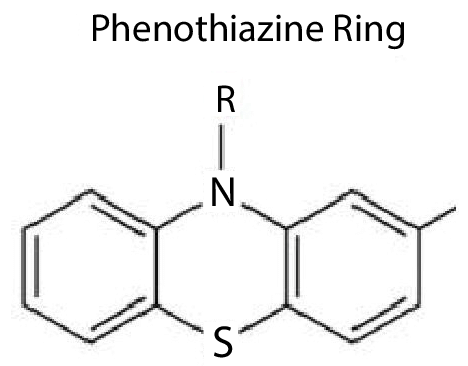
\includegraphics{./images/04-02/Chemical-structure-common-to-all-phenothiazine-antipsychotics.png}

}

\caption{\label{fig-phenothiazine}페노티아진 고리의 구조}

\end{figure}

\hypertarget{sec-laborit}{%
\subsection{클로르프로마진과 Laborit}\label{sec-laborit}}

기대와 달리 페노티아진 화합물은 말라리아에 별 효과가 없었다. 그러나 대신
진정 작용이 있다는 것이 알려졌고, 우연히도 외상으로 출혈이 심한 환자의
\uline{저혈성 쇼크}를 막아준다는 사실이 발견되었다. 클로르프로마진의
합성은 1950년대 정신약물학의 혁명을 불러왔지만, 그 시작은 우연과 행운
그리고 한 의사의 창의적 발상으로부터 비롯되었다. Laborit\footnote{\textbf{Henri-Marie
  Laborit (1914\textasciitilde1995)}: 프랑스의 외과의사 겸 신경학자.
  해군군의관으로 근무하면서, 심한 부상을 당한 군인들의 치사율을 낮추는
  마취보조제를 개발하고 있었다. 애초에 그가 먼저 Paul Charpentier에게
  항히스타민을 변형하여 중추신경계를 안정시키는 약물을 개발하는
  아이디어를 제안하였고. Charpentier는 이 과정 중 클로르프로마진 합성에
  성공한다. 이렇게 클로르프로마진 개발에 주도적인 역할을 했으나, 정신과
  의사가 아니었던 탓에 Deniker와 Delay에 비해 공로를 충분히 인정받지
  못하였다. 그의 말년에 이르러서야 업적의 재평가와 복권이 이루어졌다.}는
전투에서 부상당한 병사가 신속한 지혈과 수술 후에도 쇼크에 빠져 죽는
이유는, 신체적 허탈이 아니라 스트레스에 대한 과도한 반응 때문이라고
생각하였다.{[}@Kunz2014-gv{]} 그는 페노티아진 화합물 중 하나인
\uline{프로메타진(promethazine)}에 모르핀을 섞어서 투여하거나, 환자의
체온을 낮춤으로써 인공적인 동면상태를 유발하였고, 사망률을 상당히 낮출
수 있었다.{[}@Ban2007-wi{]}

한편 \uline{클로르프로마진(chlorpromazine)}은 1951년 프랑스의 제약회사인
롱프랑(Rhone Poulenc, 현재의 사노피-아벤티스 제약)의 연구실에서
항히스타민제를 개발하던 Paul Charpentier에 의해 합성되었다. 당시 롱프랑
실험실을 이끌고 있던 Simone Courvoisier는 클로르프로마진을 투여 받은
쥐의 행동변화를 관찰하였고, 쥐들이 조건반사로 학습된 신호를 무시하는
경향을 보인다는 것을 발견하였다.(\ref{sec-conditioned-avoidance} 장)
클로르프로마진의 시제품은 즉시 Laborit에게 연구용으로 보내졌고, 그는
인공동면(artificial hibernation)을 유도하는 자신의 처방(소위 Laborit
cocktail)에 포함시켰다.(\textbf{?@sec-chlorpromazine} 장)
클로르프로마진을 투여받은 환자는 완전히 진정 상태에는 이르지 않아 수술
중에도 의식을 잃지 않고 간단한 명령을 수행할 수 있었으며, 차분하고
통증에 둔감한 모습을 보였다.

당시는 흥분한 조현병 환자에게 찬물을 뿌려 진정시키곤 했던 시절이라,
Laborit은 환자의 ``\uline{열을 식히기 위해''} 동료 군의관들에게
클로르프로마진을 소개했고 1952년 1월 최초로 Jacques Lh라고 기록된 정신증
환자에게 시도되었다. 20일 동안의 반복 투여 후 Jacques Lh는 거의 완전히
회복되어 퇴원할 수 있었고, 이 놀랄만한 소식은 즉각 학계에 전파되었다.

\hypertarget{sec-delay-deniker}{%
\subsection{Delay와 Deniker}\label{sec-delay-deniker}}

한편 이 소식을 전해들은 성 안나 병원의 Delay\footnote{\textbf{Jean Delay
  (1907\textasciitilde1987)}: 프랑스의 정신과 의사. 성 안나 병원의
  정신과 의사로서 동료인 Pierre Deniker와 함께 최초의 클로르프로마진
  임상 연구를 수행한다. 이 업적으로 프랑스 정신과 학계의 총아로
  떠올랐으나, 60년대 말 정신질환의 강제적 약물치료에 반대하는 68혁명
  시위대가 그의 연구실을 습격한 이후 은퇴하여 작가로 여생을 보냈다.}와
Deniker\footnote{\textbf{Pierre Deniker (1917\textasciitilde1998)}:
  프랑스의 정신과 의사. Delay의 제자로 일하면서 클로르프로마진의 효과를
  입증해내었다. 클로르프로마진을 미국 학계에 알리는데 공헌하였으며,
  나중에는 약물의 행동적 부작용에 관심을 두어, 항정신병 약물의 고용량
  사용을 반대하는데 앞장서기도 하였다.{[}@healy1998{]}}는 즉각 1952년
3월 임상 시험을 시작하였다. 초기에는 약물의 효과를 향상시키기 위해
Laborit의 방식을 좆아 얼음 팩을 사용했으나, 여러 가지 이유로 저체온
상태를 유지할 수 없었을 때에도 환자들은 침착한 상태로 유도되었다.
Deniker와 동료들은 얼음이 불필요하다고 판단하였고, 약물의 효과가 저체온
유도 때문이 아니라는 것을 간파하였다.

그들은 이 발견에 너무나 고무된 나머지 불과 두 달 후인 5월 임상 성과를
학회에 발표하였고, 1952년 11월 롱프랑은 Largactil®이라는 상품명으로
출시하였다. 불과 2-3년 내에 클로르프로마진은 전 세계로 퍼져나갔고, 그
어떤 곳에서도 효과는 거듭 재확인 되었다. 미국에서는 스미스-클라인 제약이
클로르프로마진의 권리를 사들여 Thorazine®이라는 상품명으로 판매하였고,
1954년에 항정신병 약물로 허가를 받았다. 1950년대 말 미국 재향군인 보건국
연구진(US Veterans Administration Collaborative Study Group)에 의해
최초로 무작위 임상 연구가 행해졌으며, 클로르프로마진의 우수성이
공식적으로 확인되었다.{[}@Casey1960-pm{]}

정신증 치료 분야만이 아니더라도, 약물의 합성에 성공한지 불과 1년 동안에
예기치 않은 효과를 발견하고, 임상 시험을 완성시키며, 단 기간내에
전세계적으로 센세이션을 불러 일으킨 사례는 극히 드물 것이다. 더군다나
전기경련치료 외에는 뾰족한 치료법도 내놓지 못했고, 정신분석의 그늘 아래
점점 뒷전으로 밀리던 생물정신의학은 이후로 놀라운 발전을 일구어낼 토대를
다질 수 있었다. 또한 조현병이 무의식에 침범당해서 생긴다거나, 왜곡된
가족이나 억압된 사회구조 때문에 생긴다는 당시 인기를 끌던 이론이 점차
쇠퇴하고, 조현병 역시 다른 질병들과 마찬가지로 의학적 질환의 하나일
뿐이라는 개념이 뿌리를 내리기 시작하였다.

\hypertarget{uxb9acuxc11cuxd540uxacfc-uxcd94uxccb4uxc678uxb85c-uxc99duxc0c1}{%
\section{리서핀과 추체외로
증상}\label{uxb9acuxc11cuxd540uxacfc-uxcd94uxccb4uxc678uxb85c-uxc99duxc0c1}}

\uline{라우볼피아 서펜티나(Rauvolfia serpentina)}는 인도를 비롯한
동남아시아에 자생하는 식물로 뿌리 모양이 뱀과 유사하여 우리나라에서는
인도사목(印度蛇木)이라고도 불린다. 라우볼피아는 안정 효과가 있기 때문에
수세기 동안 광증 치료에 사용되어 왔으며, 이외에도 해독이나 해열 등에
민간요법으로 사용되어 왔다. 라우볼피아에서 약효의 주성분인
\uline{리서핀(reserpine)}이 최초로 분리된 것은 1952년이었다.

정신의학적인 측면에서 리서핀의 효과에 대한 첫번째 논문은
Kline\footnote{\textbf{Nathan Kline (1916\textasciitilde1983)}: 미국의
  정신과 의사. 리서핀을 조현병 환자에게 투여하는 최초의 임상 시험을
  시행하였다. 그는 이후 항우울제 연구로 관심을 돌려, 결핵약인
  iproniazid가 항우울 효과가 있음을 입증하였고, 이는 \textbf{단가아민
  산화효소 억제제(monoamine oxidase inhibitor)}라는 새로운 항우울제
  개념의 시발점이 되었다.}에 의해 1954년에
출판되었다.{[}@Kline1954-zl{]} 당시 클로르프로마진의 성공에 고무되어있던
정신의학자들은 유사한 화합물을 찾는데 열정적이었고, 혈압 강하 및 강한
진정 작용이 있는 것으로 알려졌던 리서핀은 고혈압 및 조현병 환자에게
활발하게 사용되기 시작하였다.{[}@healy1998{]}

그러나 리서핀에 대한 기대는 그리 오래가지 못하였다. 약물을 사용하던
환자의 상당수에서 심한 우울 반응이 일어났고, 그 외에도 무정동이나
안절부절함 등의 부작용이 드물지 않게 보고되었다.{[}@Baumeister2010-wy{]}
이처럼 리서핀은 역사에서 잊혀진 약이 되었으나, 대신 우울증의 단가아민
이론\footnote{\textbf{우울증의 단가아민 이론(monoamine theory of
  depression or catecholamine depletion theory of depression)}: 1965년
  하버드대 교수였던 Joseph J. Schildkraut는 중추신경계의
  단가아민(catecholamine, 대표적으로는 노르에프린과 세로토닌)이 부족하면
  우울증이 발생하고, 항우울제를 이용하여 이를 교정하면 우울증을 치료할
  수 있다는 이론을 내놓는다.{[}@Schildkraut1965{]} 이를 지지하는 증거도
  많은 편이지만, 실제 우울증이나 항우울제 효과를 설명하기에는 허점이
  너무나 많다.{[}@heninger1996{]} 그러나 단순명료함때문인지, 현재까지도
  제약회사의 선전이나 일반인을 대상으로 한 강연에서 항상 우울증의 발병
  원인으로 거론되어왔다. 마치 Hippocrates가 우울증의 원인으로 지목한
  검은 담즙(black bile)이 현대에 들어와서 catecholamine으로 대체된 것과
  같다.{[}@healy2015{]}}이 탄생하는데 중요한 단서가 되었다. 리서핀,
세로토닌 그리고 lysergic acid diethylamide (LSD) 사이의 구조적 유사성을
연구하던 Brodie\footnote{\textbf{Bernard Brodie
  (1907\textasciitilde1989)}: 영국출신으로 미국에서 활약한 약리학자.
  현대 약물학의 창시자라고 여겨진다. 미국 국립보건원의 약물학 실험실을
  설립하였다. 세로토닌과 노르에피네프린이 뇌 기능에서 차지하는 역할에
  대한 업적을 남겼다.)}는 리서핀이 세로토닌을 고갈시킨다는 것을
발견하였다.{[}@Brodie1955-fx{]} Arvid Carlsson은 이 연구를 확장하여,
세로토닌 뿐만 아니라 도파민, 노르에피네프린까지 감소시킨다는 것을
발견하으며, 동시에 리서핀으로 유도된 부동증이 L-dopa를 주입함으로써
해소됨을 보고하였다.(\ref{sec-classical-dopamine} 장) 이는 파킨슨 병의
기본 병리를 이해하는 가장 중요한 단서가 되었다.{[}@Carlsson1959-fh{]}

점차 리서핀을 복용한 환자들이 나타내었던 무정동, 무의욕증이
우울증이라기보다는 단가아민의 고갈에 의한 파킨슨 유사 증상이라는 의견이
부상하였다. 더불어 리서핀 복용 환자들이 보였던 또 다른 현상인 불안과
안절부절함이 역시 도파민과 관련된 부작용이라는 견해가 지지를 받으면서,
단가아민을 차단하는 항정신병 약물의 공통적인 부작용인 \uline{추체외로
증후군 개념}이 정립되기 시작하였다.{[}@Freyhan1957-tq{]} 우연이었는지
필연이었는지, 1950년대와 60년대 초반은 새롭고도 경이로운 발견이
연속되었으며, 불과 10여년 사이에 조현병과 우울증의 기본 병태 생리,
향정신성 의약품의 작용 기전, 부작용과 그의 해소법 등이 연달아 밝혀졌다.
리서핀은 비록 1954년부터 1957년까지 짧은 인기를 얻은 후, 실제 임상에서는
거의 사용되지 않는 약이 되어버렸지만, 뼈아픈 실패에서 소중한 결과를 얻은
예라 할 수 있다. 이로 말미암아 정신약물학은 화려하게 부활하였으며, 이후
반세기에 걸쳐 눈부신 성장을 할 수 있게 되었다.{[}@Lehmann1997-mi{]}

\hypertarget{uxd560uxb85cuxd398uxb9acuxb3ccuxacfc-uxae30uxd0c0-uxc57duxbb3cuxb4e4}{%
\section{할로페리돌과 기타
약물들}\label{uxd560uxb85cuxd398uxb9acuxb3ccuxacfc-uxae30uxd0c0-uxc57duxbb3cuxb4e4}}

\hypertarget{uxc2e0uxacbduxc804uxb2ecuxbb3cuxc9c8}{%
\subsection{신경전달물질}\label{uxc2e0uxacbduxc804uxb2ecuxbb3cuxc9c8}}

클로르프로마진의 성공에 힘입어 신경전달물질의 역할에 대해 새롭게 관심이
부여되었다. 1933년 Dale \footnote{\textbf{Henry Hallett Dale
  (1875\textasciitilde1968)}: 영국의 약리학자. 신경세포를 통한 화학적
  신호전달에서 아세틸콜린이 차지하는 역할에 대한 연구로 1936년 노벨
  생리학상을 수상하였다.}에 의하여 최초로 아세틸콜린이 말단 신경세포에서
신경전달물질 역할을 한다는 것이 확인되었다.{[}@Lopez-Munoz2009-js{]}
그러나 당시만 해도 중추신경계 내에서의 신호전달에서는 화학물질보다는
전기신호의 비중이 더 큰 것으로 여겨지고 있었다. 다양한 단가아민 들이
중추신경계에 분포한다는 것은 1950년대가 지나서야 밝혀졌고, 이들이
신경전달물질 역할을 한다는 것은 1958년 Carlsson이 이끄는 스웨덴 룬드
대학 연구진이 행한 일련의 기념비적 실험 들에
의해서였다.(\ref{sec-classical-dopamine} 장){[}@Lopez-Munoz2009-js{]}
Carlsson과 동료 Lindqvist는 클로르프로마진 및 할로페리돌의 작용 기전은
시냅스 후 단가아민 수용체 차단 및 이로 인한 시냅스 전 단가아민 활성의
증가임을 발견하였다.{[}@Carlsson1963-dq{]} 이에 근거하여 조현병은
도파민의 비정상적인 과활성에 의한 것이라는 가설이 세워질 수
있었다.{[}@Baumeister2002-wx{]}

\hypertarget{uxd3f4-uxc580uxc13c}{%
\subsection{폴 얀센}\label{uxd3f4-uxc580uxc13c}}

정신약물학의 발자취를 따라갈 때, 폴 얀센\footnote{\textbf{Paul Janssen
  (1926-2003)}: 벨기에 출신의 정신의학자. 소규모 가족 회사이던 얀센 사를
  다국적 대기업으로 키워낸 인물자로서, 그의 생전에 할로페리돈,
  리스페리돈을 비롯한 80개가 넘는 신약을 개발하였다.}이라는 걸출한
인물의 행적을 지나칠 수 없다. 제약회사 \uline{얀센 사}의 시작은
1933년으로 거슬러 오른다. 타 제약회사의 판매 대리점으로 시작했던 얀센
사는 2차 대전을 겪으면 급성장하였고, 파라세타몰(타이레놀) 개발에
성공함으로써 본 궤도에 오른다. 창업주의 아들이었던 얀센은 이미 청년
시절에 파라세타몰 및 마약성 진통제 합성에 성공하여 개발자로서의 명성을
높이고 있었다. 가족의 제약 사업을 확장시키던 방도를 찾던 얀센은 다양한
화합물의 구조를 체계적으로 변경하고, 동물 실험을 통해 효과가 있어 보이는
후보 물질을 선택하는 프로세스를 고안하였다. 얀센이 관심을 두었던 동물
모델은 \uline{암페타민으로 유도된 상동 행동(amphetamine induced
stereotypy)} 모델이었다.(\ref{sec-stereotypy} 장) 얀센은 경마장에서
암페타민을 복용한 기수가 종종 결승점을 지나고도 멈추지 않아 주위
사람들이 강제로 멈춰야 하는 점에 주목하였다. 그는 이러한 현상이 편집성
조현병과 유사하다는 일부 임상가의 지적을 알고 있었다. 얀센은 암페타민을
복용한 쥐가 보이는 반복적인 동작을 강박적(Zwangsnagen)이라 표현하였고
이를 차단하는 효과를 통해 항정신병 약물을 선별할 수 있을 것이라
믿었다.{[}@Janssen1965-pq{]}

\hypertarget{uxd560uxb85cuxd398uxb9acuxb3cc}{%
\subsection{할로페리돌}\label{uxd560uxb85cuxd398uxb9acuxb3cc}}

얀센이 이끄는 연구진의 원래 목표는 항정신병 약물이 아니라 강력한
진통제의 개발이었다. 이를 위해 메페리딘(페치딘 혹은 데메롤)의 지방산
체인을 점점 늘리는 변형을 시도하였다. 기존 화합물의 변형과 동물 실험,
선택된 화합물의 재변형이라는 프로세스를 통해 1957년 \uline{butyrophenone
R1187}이라 명명된 화합물이 만들어졌다. 동물 실험 결과 아편 유사 특성
외에도 암페타민 유발 상동 행동을 막는 작용과 함께, 진정 작용, 강직증
같은 클로르프로마진과 유사한 효과가 있음이 밝혀졌다. 연구진을 목표를
바꿔 항정신병 효능을 최대화시킨 R1187 유도체 개발에 착수하였고, 1958년
2월에 \uline{R1625}가 합성되었다. 이 화합물은 R 1187에 두 개의 할로겐
치환이 있었기 때문에 \uline{할로페리돌(haloperidol)}이라고
불리워졌다.{[}@Granger2005-km{]}

할로페리돌은 butyrophenone 계의 약물로서 다른 메페리딘 유도 물질이 실험
쥐를 흥분시킨 반면, 이 약은 안정을 찾게 만들었다. 합성에 성공한지 미처
두달도 안 되어 실제 조현병 환자에게 투여되었으며, 벨기에 리에주 대학의
Jean Bobon과 Paul Divry의 주도 하에 첫번째 임상 시험이 진행되었다.
그들은 임상 시험 결과를 발표하면서 약물이 수면을 유도하지 않으면서도
환자를 진정시켰고, 망상과 환각을 가라앉혀 정신치료적 면담이 불가능했던
상태에서 가능한 상태로 만들어주었다고 소개하였다.{[}@Divry1958-vh{]}

클로르프로마진을 통해 학계의 총아로 올라선 Delay와 Deniker 역시
초창기부터 할로페리돌에 깊은 관심을 나타내었다. 그들은 급성 환자의 진정
뿐만 아니라 만성 환자의 환각과 망상을 없애는 데도 탁월한 효과를
나타낸다고 하였으며, 신경독성을 일으키는 용량보다 훨씬 더 적은
용량에서도 항정신병 효과를 나타낸다는 의견을 내었다. 이전에 동물 모델을
연구하던 학자들이 강직증(catalepsy)을 일으킬 수 있을 정도의 용량을 써야
항정신병 효과를 발휘한다고 판단했던 것을 고려해보았을 때, 새로운 약물의
도입이 점점 더 학자들의 시야를 넓혀주고 이해의 폭을 깊게 했다는 것을
엿볼 수 있다.

\hypertarget{uxc758uxd559-uxc724uxb9acuxc640-uxd5c8uxac00-uxc81cuxb3c4}{%
\subsection{의학 윤리와 허가
제도}\label{uxc758uxd559-uxc724uxb9acuxc640-uxd5c8uxac00-uxc81cuxb3c4}}

클로르프로마진과 할로페리돌 개발의 뒷 배경을 살펴보면, 지금으로서는
납득되지 않을 정도로 합성과 임상 시험, 상품화가 신속히 이루어졌다는 것을
알 수 있다. 상당한 빈도로 추체외로 증후군이 나타났을 터인데도, 초기 임상
발표들에는 그런 내용이 생략되어 있다. 이는 당시만 해도 연구 윤리에 대한
개념이 없었고, 임상의약품 허가 체계도 갖춰지지 않았다는 것을 감안하여
이해해야 한다. 당시만 해도 연구참여자의 동의를 구하는 일도 없었고,
부작용에 대한 피해보상책도 없었다. 클로르프로마진은 개발된 지 불과 3년
후인 1955년 미국에서 사용 허가를 받았다. 반면 할로페리돌은 1960년대 초
이미 유럽에서 활발하게 사용되기 시작하였는 데 비해, 미국에서는
1969년에야 비로서 사용 허가를 받게 된다.

이 차이는 다름 아닌 \uline{탈리도마이드(thalidomide)} 사건 때문이었다.
안정제로서 유럽에서는 의사 처방없이도 자유롭게 구매할 수 있었던
탈리도마이드가 심각한 기형아 출산을 유발한다는 사실이 드러난 것이
1960년대 초 였다. 간발의 차이로 약물의 시장 진입을 저지한 미국 정부와
여론은 동일한 비극이 반복되지 않게 하기 위해 강력한 규제 조치를
요구했고, 1962년 케네디 대통령의 지시 하에 철저한 허가용 임상 시험과
규제에 대한 법령이 제정되었다. 할로페리돌은 이러한 절차를 거친 후에야
미국 시장에 도입될 수 있었다.{[}@Granger2005-km{]} 이후 정신과 약물 뿐만
아니라 모든 신약들은 철저한 임상 시험을 통해 효과와 안전성에 대한 확고한
자료가 얻어져야 허가받을 수 있게 되었다.

항정신병 효과를 선별하는 다양한 동물 모델이 개발되면서, 클로르프로마진과
유사한 약물을 찾는 작업이 지속적으로 이루어졌다. 1960년대 초에 개발
중이던 페노티아진 계열 약물의 수는 20개를 넘어섰으며, 1990년대까지 그
수는 배 이상 늘어났다. 이들 약물은 유럽을 중심으로 활발하게
사용되었으나, 우리에게 생소한 것은 까다로운 미국의 임상 허가 제도
때문이었다. 모든 페노티아진이 클로르프로마진의 복제품인 것만은 아니었다.
각각 필요 용량과 부작용 측면에서 큰 차이를 보였다. 예를 들어, 진정
효과는 클로르프로마진과 같은 aminoalkyl 에서 더 문제가 되었으며,
추체외로 증상은 prochlorperazine과 같은 piperazinylalkyl에서 문제가
되었다. 치오리다진(thioridazine)과 같은 piperidylalkyl은 심한
항콜린효과를 나타내기도 하였다. 그에 비해 다양한 페노티아진 계열 약물이
도입되었음에도 불구하고, 화학구조의 차이가 효능의 차이로 이어지리라는
기대는 이루어지지 않았다. 부작용이 다를 뿐 효능은 대체로 비슷했으며,
이는 클로자핀이 도입되기 전까지는 상황이 달라지지
않았다.{[}@Lehmann1997-mi{]}

\hypertarget{uxd56duxc815uxc2e0uxbcd1-uxc57duxbb3c-uxac1cuxb150uxc758-uxbcc0uxd654}{%
\section{항정신병 약물 개념의
변화}\label{uxd56duxc815uxc2e0uxbcd1-uxc57duxbb3c-uxac1cuxb150uxc758-uxbcc0uxd654}}

클로르프로마진 이전의 약물 치료가 단순히 흥분의 진정이라는 목적을 지니고
있었다면, 클로르프로마진은 처음으로 이를 넘어서 조현병 자체를 치료할 수
있을 지 모른다는 가능성을 보여주었다. 그 전까지 사용되던
메프로바메이트나 바비튜레이트와 같은 \uline{마이너 진정제(minor
tranquilizer)}들은 분명 불안을 감소시키고 수면을 유도하는 효과가 있으나,
조현병 환자의 공격성, 초조, 폭력 및 불안을 억제하는데는 역부족이었다.
따라서 조현병이 단순한 진정으로는 치료되지 않는다는 점이 분명해졌다.
이는 정신증과 신경증을 확연히 구분짓지 않는 정신분석적 접근방식에 대한
도전이기도 하였다. 무의식적 억압과 그 왜곡된 표현이라는 획일적
패러다임으로는 정신증의 고유한 약물 반응을 설명하기 어려웠다. 그러나
\uline{메이저 진정제(major tranquilizer)}라는 용어 자체에서 풍겨나듯이,
정신증을 병적 흥분과 연결시키는 서사는 인지 장애와 무감동으로
특징지워지는 음성 증상을 간과하게 하는 결과를 초래하였다.
클로르프로마진에 의해 안정되는 망상, 환각, 흥분, 초조 등의 증상이 조현병
증상의 전부인 것처럼 여겨지기 시작하였고, 조현병 치료는 신경계의
과흥분을 억제하는 것으로 개념화되었다. 이 와중에, 크레펠린과 블로일러가
묘사했던 인지손상이나 무의욕, Rado와 Meehl 등이 개념화한
\uline{무쾌감증(anhedonia)} 같은 핵심 개념들이 조현병을 둘러싼 논의에서
소외되고 말았다.{[}@Snaith1993-bh{]}

한편 항정신병 약물이 조현병 치료에 있어서 어떤 위치를 차지하는 지를
이해하려는 노력이 계속되었다. Delay와 Deniker는 클로르프로마진의 진정
효과와 주위에 무신경 해지게 만드는 효과에 주목하여 1955년 이들 약물을
\uline{신경이완제(neuroleptic)}이라고 부르기
시작하였다.{[}@Moncrieff2013-ds{]} 의사들의 경험이 쌓이면서 약물이
일으키는 파킨슨 유사 증상에 주목하게 되었고, 유럽의 의사들은 충분한
항정신병 효과를 나타내기 위해선 어느 정도의 파킨슨 유사 증상이
필요하다고 믿기 시작하였다. 신경이완제라는 용어는 이 즈음부터 정신
증상을 신경 증후군으로 대체하는 약물 정도로 여겨지기
시작하였다.{[}@Freyhan1959-so{]} 동시에 이들 약물이 ``조현병''을
근본적으로 치료하는 것은 아니며, 동일한 흥분, 과격함을 보이는 상태라면
꼭 조현병이 아니라도 광범위한 정신증에 효과를 보일 것이라 이해하였다.

유럽 의사들의 보수적인 견해와는 대조적으로 미국의 정신과 의사들은 약물이
조현병의 근본적 병태생리를 바로잡는다고 여기길 원했다. 급성기 효과는
증상을 가라앉히는 데 그칠지 몰라도, 장기간 복용하면 점점 더 근본적인
완치에 다가갈 것이라고 믿었다. 캐나다의 정신과 의사인
Lehmann\footnote{\textbf{Heinz Lehmann (1911\textasciitilde1999)}: 독일
  출신의 캐나다 정신과 의사. 유럽에서 사용되던 클로르프로마진을 캐나다와
  미국에 적극 전파시킨 인물로, 북미 정신약물학의 아버지라 불리운다.
  시대를 앞서가 psilocybin을 불안 치료에 적용해보고자 하였다.}은 이러한
희망을 담아 클로르프로마진 계열의 약물들을 \uline{항정신병
약물(antipsychotic drug)}이라 칭하기 시작하였다. 그는 물론 당대에 개발된
약물로는 아직 ``완치''의 목표와 거리가 멀지만, 멀지 않은 장래에
조현병만을 치료하는 약물이 개발되리라 믿었다. 1960년대가 되자 더 이상
항정신병 약물에 ``진정제''라는 명칭은 쓰지 말자는 견해가 힘을
얻었다.{[}@Moncrieff2013-ds{]}

클로르프로마진을 비롯한 약물이 단순히 양성 증상만을 억제하는 지, 아니면
근원적인 치료 효과를 일구어 내어 완치에 이르게 하는지는 아직도 규명되지
못한 과제이다. 현대에는 개념들이 더욱 혼란스럽게 뒤섞여서, 항정신병
약물이 양극성 장애나 주요 우울증에 효과적으로 사용되며, 역으로 타 질환
치료제가 조현병에 사용되기도 한다. 심지어 조현병과 기타 주요 정신질환이
분명히 구분되는지도 의문에 싸여있다. 또한 완치의 기준조차 여전히
마련되지 않고 있기 때문에 이들 약물이 진정 치료제라 할 수 있는지는 더욱
지켜봐야 할 것 같다.

약물을 오랜동안 꾸준히 복용하면 점점 더 완치에 다가가리라는 희망과는
별개로, 재발을 막기 위해서라도 항정신병 약물을 장기 요법이 필연적인 듯이
보였다. 약물로 급성기 증상을 가라앉힌다 해도, 사용을 중단하면 어느 새
증상이 돌아오는 것이 확실해보였다. 이로부터 재발 방지(relapse
prevention)라는 개념이 등장하였다. 1970년대 초가 되자 항정신병 약물의
급성기 효과뿐 아니라, 유지 치료의 효과에 대한 무직위 임상 시험이
이루어지기 시작하였다.{[}@Hirsch1973-yl{]} 1975년에는 이미 이들 연구의
성과를 종합한 메타 분석 결과가 발표되었고, 의문의 여지 없이 재발을 막기
위해선 유지 치료를 기약없이 행해야 한다는 것이
분명해졌다.{[}@Davis1975-uy{]}

\hypertarget{sec-side-effect-history}{%
\section{부작용과 약물의 위험성}\label{sec-side-effect-history}}

1957년 스위스에서 열린 2차 국제 정신약물학 학회에서 F.A. Freyhan은
클로르프로마진의 효과는 추체외로 증후군의 발생과 따로 떼어 생각할 수
없다고 못 박았다. 조현병에서 보이는 뇌의 과활동과 파킨슨 환자의 무동증은
연속선상에 놓여있기 때문에, 어느 한가지를 조절하려면 다른 쪽을 희생시킬
수 밖에 없다는 견해였다. 가시적인 효과를 보려면 추체외로 증후군이 발생할
정도의 충분한 용량을 사용해야만 한다거나, 추체외로 증후군은 치료 효과의
일부분이라는 주장도 드물지 않았다. 이런 개념을 \uline{신경이완제 역치
이론(neuroleptic threshold)}이라고도 한다.{[}@Bitter1991-td{]}

이보다 전에 클로르프로마진이 추체외로 증후군을 일으킨다는 것은 1954년
Hans Steck과 Hans Joachim Hasse에 의해 독립적으로
보고되었다.(\ref{sec-eps-history} 장) 파킨슨 병과 구분이 힘든 무정동,
무동증, 의욕 저하, 근긴장을 비롯하여 좌불안석 역시 함께 보고되었다. 앞서
언급했듯이 초기에는 이러한 효과가 부작용으로 간주되지 않았으나, 1964년
미국 국립보건원 후원으로 진행된 대규모 연구에서 각기 다른 약물들은
나타내는 부작용 정도나 특성이 서로 다르면서도 동등한 치료 효과를
나타낸다는 것이 확인되었다.{[}@Guttmacher1964-nb{]} 이 연구를 통해
추체외로 증후군은 치료에 불필요한 부작용이라고 여겨지기 시작하였고,
동등한 효과를 내면서도 부작용 없이 안전한 약물이 개발될 수 있다는
가능성이 비쳐졌다.

그러나 미래에 대한 희망과는 별개로 추체외로 증후군은 환자들에게는 말할
수 없는 고통을 안겨주었다. 1961년 보고서에서 항정신병 약물로 치료받은
환자의 추체외로 증후군의 유병률은 38.9\%로 추산되었다.{[}@Ayd1961-yg{]}
이러한 상황은 할로페리돌 도입 후에는 더욱 심화되었다. 더군다나
1950-70년대의 의료 현장에서는 난치성 환자에게서 약물 효과의 한계를
극복하기 위해, 심혈관계만 버텨준다면 플루페나진 혹은 할로페리돌은 수십
mg부터 수백 mg까지 투여하는 초고용량 치료가 시도되기도
하였다.{[}@Quitkin1975-at; @Bjorndal1980-yo{]}

이렇게 무모한 시도가 행해졌던 것은, 추체외로 증후군을 치료를 위한 댓가
정도로 대수롭지 않게 생각했던 때문이기도 하지만, 대부분의 의사들이
이러한 부작용이 가역적일 것이라고 믿었던 탓이 크다. 불수의적이고
지속되는 비정상적 운동 부작용은 이미 1957년 Schonecker에 의해
보고되었으며, 1964년 Faurbye는 이를 \uline{지연 운동 이상증(tardive
dyskinesia)}라고 이름붙였다.{[}@Macaluso2017-kk{]} 지연 운동 이상증은
약물을 끊어도 지속될 뿐 아니라 오히려 악화되기까지 했기 때문에,
비가역적일 것이라는 우려가 높아졌다. 1960년대부터 70년대에 걸쳐 지연
운동 이상증 및 \uline{항정신병 약물 악성증후군(neuroleptic malignant
syndrome)}의 보고가 증가하고, 더군다나 고용량 투여 시 치명적 부정맥인
\uline{torsade des pointe}가 증례가 발견되면서, 항정신병 약물의 안전
신화는 종지부를 찍었다. 또한 만성 조현병 환자가 보이는 소위 음성증상의
적지 않은 사례가 추체외로 증후군에 의한 이차성 음성 증상임이 판명되었다.
고용량 투여의 효과에 대해서도, 환자마다 용량-혈중 농도 관계에 차이가
있긴 하지만, 약물의 혈중 농도가 일정 수준에 도달되면, 더 높은 용량은
별반 이점이 없다는 설명이 확고히 자리잡았다.{[}@Kane2010-cr{]}

\hypertarget{uxc138uxb300-uxd56duxc815uxc2e0uxbcd1-uxc57duxbb3c-uxb3c4uxc785uxc774-uxac00uxc838uxc628-uxc601uxd5a5}{%
\section{1세대 항정신병 약물 도입이 가져온
영향}\label{uxc138uxb300-uxd56duxc815uxc2e0uxbcd1-uxc57duxbb3c-uxb3c4uxc785uxc774-uxac00uxc838uxc628-uxc601uxd5a5}}

클로르프로마진이 신속이 임상에 도입되었던 것은 그만큼 절실한 수요가
있었다는 뜻이다. 그러나 앞서 보았듯이 예기치 않은 부작용이나 임상 허가
제도의 부재, 그리고 제약사들의 과열된 경쟁 등의 요인이 합쳐져, 의도하지
않았음에도 불구하고 부정적인 결과가 초래되었고 피해자들이 생겨났다.
전전두엽 절제술 같이 위험 대비 이득이 높지 않은 치료를 행하는 실수를
저지르지 않기 위해, 약물이 광범위하게 보급된 후에야 지연 운동 이상증과
같은 부작용을 발견하는 일을 예방하기 위해, 치료 효과와 부작용을
객관적으로 평가하는 \uline{평가 도구}가 개발되었다. 또한 무작위 배정,
이중 맹검 시험 및 \uline{임상 시험의 표준 절차}와, 얻어진 결과를
객관적으로 분석하는 \uline{통계적 방법론}들이 함께 발전하였다. 이런
방법들은 항정신병 약물 뿐 아니라 이후 항우울제 개발 및 심리 치료에 대한
평가에 까지 적용되었다.

항정신병 약물의 개발이 가져온 또 하나의 극적인 변화는 \uline{탈시설화}의
물결이었다. 1960년대 냉전시대의 억압적 체제와 베트남 전쟁에 반대하는
와중에 태어난 반체제 운동은 정신질환자의 인권문제를 되돌아보게 하였다.
그러나 항정신병 약물이 없었던 들 결코 수용소에 갇혀 있던 환자들이
자유로운 공기를 마실 수는 없었을 것이다. 대형 수용소가 점차 폐쇄되고
환자들이 지역 사회로 복귀하면서 지역사회 정신의학이 강조되었다.
무조건적인 격리나 급성 증상 치료라는 목표에서, 재발-재입원의 방지가 더
큰 과제로 자리잡았다.

위와 같은 의학 외적 변화와 더불어 클로르프로마진이 가져온 커다란 영향 중
하나는 \uline{신경과학}의 눈부신 발전일 것이다. 항정신병 약물의 효과를
이해하려는 노력을 통해 신경전달물질과 이들 수용체의 기초적인 지식이
확립되었다. 특히 도파민, 세로토닌 시스템이 뇌의 주요 신경전달물질이며,
다양한 정신질환과 밀접한 연관을 맺고 있다는 발견은 이후 항우울제 개발에
지대한 역할을 했을 뿐더러, 현재까지도 정신약물학 발전의 토대를 이루고
있다.

조현병의 도파민 가설은 1966년 Van Rossum이 처음 제안하였다. 그는 원래
암페타민과 같이 도파민 활성을 자극하는 약물이 환각을 유발하며, 항정신병
약물이 파킨슨 병과 유사한 운동장애를 나타내는 것을 토대로 이 가설을
세웠다. 한편 이 가설을 결정적으로 뒷받침하는 증거는 1976년에 발표되었다.
Philip Seeman 등은 각종 항정신병 약물이, 방사성 동위원소를 붙인
할로페리돌({[}3H{]}-haloperidol) 혹은 도파민({[}3H{]}-dopamine)을
수용체에서 분리시키는 정도를 측정함으로써, 항정신병 약물의 \uline{수용체
친화도(receptor affinity)}를 측정하는 길을 열었다. 이렇게 측정된
친화도는 항정신병 약물 각각의 유효 용량과 양의 상관관계를 맺고
있었다.{[}@Seeman1976-bu{]} 이로써 Van Rossum의 가설, 즉, 항정신병
약물이 효과를 나타내는 것은 도파민 수용체 차단 효과에 기인하며, 동시에
조현병은 도파민 과다 분비 혹은 수용체 과활성 때문이라는 이론이
증명되었다.(\ref{sec-classical-dopamine} 장)

물론 도파민 수용체 차단이 항정신병 약물의 작용 기전임은 이로써
분명해졌지만, 도파민 과활성이 조현병의 핵심 병태생리인지는 의문의 여지가
있으며, 이후 가열찬 논쟁의 도화선이 되었다. 그러나 정신약물학 및
신경과학의 발전에 있어서 도파민 가설이 가져왔던 혁신과 흥분은 쉽게
찾아보기 힘든 사례였다.

\hypertarget{references-24}{%
\section*{References}\label{references-24}}
\addcontentsline{toc}{section}{References}

\markright{References}

\hypertarget{uxc138uxb300-uxd56duxc815uxc2e0uxbcd1-uxc57duxbb3c}{%
\chapter{2세대 항정신병
약물}\label{uxc138uxb300-uxd56duxc815uxc2e0uxbcd1-uxc57duxbb3c}}

2nd generation antipsychotics

\hfill\break

\hypertarget{uxd074uxb85cuxc790uxd540uxc758-uxd569uxc131}{%
\subsection{클로자핀의
합성}\label{uxd074uxb85cuxc790uxd540uxc758-uxd569uxc131}}

클로르프로마진과 할로페리돌로 대표되는 과거의 항정신병 약물은 조현병
치료의 스타트를 끊은 셈이지만, 이후 나온 약물들은 기존 약물의 복제품일
뿐 신약 개발은 1970년대에 들어 난항에 빠져 있었다. 역가(potency)를
올리면 진정작용이나 심혈관계 부담을 줄여주었지만, 추체외로 증후군의
빈도가 높아져 사용하기 어려웠다. 이 때문에 할로페리돌보다도 고역가인
spiroperidol이나 beneperidol은 거의 사용되지 않았다. 반대로 도파민
수용체 2형(D\textsubscript{2})에 친화성이 약한 화합물은 항정신병 효과가
약할 뿐더러, 진정 작용, 항콜린 효과 등 다른 부작용이 상당하여 여전히
사용이 까다로왔다. 이처럼 두가지 상반되는 성질이 양립하는 가운데,
클로자핀 만이 유독 기존의 패러다임으로 설명되지 않는 신약이었다.

클로르프로마진의 성공에 고무되어 다양한 제약회사들이 새로운 항정신병
약물을 찾고 있던 중, 1958년 스위스의 제약회사 Wander 사에서는 항우울제인
이미프라민을 기초로 클로자핀을 합성해낸다. 클로자핀은 클로르프로마진과
유사하게 통증에 대한 역치를 올리는 효과가 있었다. 그러나 기존의 항정신병
약물과는 달리 강경증(catalepsy)를 일으키지 않았다. 당시만 해도 강경증,
즉 인간으로 따지면 추체외로 부작용에 해당되는 운동 저하는 항정신병
약물을 선별하는 주요 동물 모델이었기 때문에, 클로자핀은 시작부터 큰
주목을 받지 못하였다.

\hypertarget{uxcd08uxae30uxc758-uxc2e4uxd328uxc640-uxbb34uxacfcuxb9bduxad6cuxc99d}{%
\subsection{초기의 실패와
무과립구증}\label{uxcd08uxae30uxc758-uxc2e4uxd328uxc640-uxbb34uxacfcuxb9bduxad6cuxc99d}}

엎친데 덮친 격으로 1962년에 행해진 첫번째 인체 대상 시험에서도 뾰족한
성과를 보이지 못했다. 1960년대 유럽에서 진행된 임상 시험에서 그럭저럭
효과가 있다고 여겨지기 시작했으나, 대부분 독일어 문헌이라 영어권
국가에는 소개되지 않았다. 1970년대에 들어서 Hippius\footnote{\textbf{Hans
  Hippius (1925\textasciitilde2021)}: 독일의 정신과 의사. 정치적 이유로
  학계에서도 위상이 추락한 독일 정신의학을 다시 부흥시키는데 앞장섰다.
  유럽 중심의 국제학회인 International College of
  Neuropsychopharmacology (CINP)와 European Psychiatric Association
  (EPA)의 창립멤버이기도 하다.}는 당시의 통념인 신경이완제 역치 이론에
정면으로 도전하여, 항정신병 효과가 추체외로 증후군에 의존하지 않는다고
역설하였다.{[}@hippius1999{]} 그럼에도 불구하고 대부분의 영향력 있는
정신과 의사들은 신경계 부작용을 일으키지 않는 이상, 의미있는 항정신병
효과를 얻을 수 없으리라고 믿었기 때문이었다. 아마도 1972년 Wander 사를
인수하였던 유럽 최대의 제약회사 Sandoz의 자금력과 연줄이 아니었던들,
클로자핀은 결코 빛을 볼 수 없었을 것이다. Sandoz가 우격다짐으로
Leponex®라는 상품명으로 시장에 출시했을 때에도 반응은 미적지근할
뿐이었다.

고정관념에 젖어있던 유럽의 정신과 의사들과는 달리, 미국의 의사들은
클로자핀에 깊은 흥미를 나타내었고, 식품의약품청(FDA)의 허가를 위한 임상
시험을 활발히 진행하고 있었다. 그러던 중 1975년 핀란드에서 클로자핀 복용
중 예기치 못한 무과립구증으로 9명이 사망한 사례가 보고되었다. 이는
커다란 충격으로 다가왔고, 미국에서의 임상 시험이 중단되었음은 물론
유럽에서도 판매 중단 및 회수가 이루어졌다.

\hypertarget{uxbbf8uxad6duxc5d0uxc11cuxc758-uxc784uxc0c1-uxc2dcuxd5d8}{%
\subsection{미국에서의 임상
시험}\label{uxbbf8uxad6duxc5d0uxc11cuxc758-uxc784uxc0c1-uxc2dcuxd5d8}}

이러한 불상사에도 불구하고, 허가 받지 않은 실험적 약물에 대한 동정적
사용 제도\footnote{\textbf{동정적 사용(compassionate use or expanded
  access)}: 생명이 위험하거나 다른 치료법이 전혀 없는 환자에 국한하여,
  예외적으로 허가받지 않았거나 현재 연구중인 약물을 사용할 수 있도록
  허용하는 제도. 환자에게 약가를 부담시키지 않는다.}를 통해 클로자핀의
사용량은 꾸준히 증가하였다. 이는 무과립구증을 조기에 발견할 수 있다면
충분히 관리가능하다는 사실과 함께 난치성 환자에 대한 클로자핀의 탁월한
임상 성과 덕분이었다. 1976년 클로자피에 대한 모든 개발 및 연구를
중단시켰던 Sandoz 제약은 1982년 다시 부활시켰고, 미국 식품의약청이
요구하는 까다로운 기준을 맞추는 대규모 임상연구를 시도하였다. 바야흐로
1986년 미국 전역에서 동시에 시행된 이 연구는, Sandoz 사의 연구원인
Gilbert Honigfeld가 디자인했고, 정신의학 임상연구에 큰 족적을 남긴 John
Kane과 Herbert Meltzer가 지휘하였다.

클로르프로마진과의 이중 맹검 비교로 이루어진 이 연구에서 클로자핀은
압도적으로 우월한 효과를 보였고, 이에 힙입어 1989년에 미국
식품의약품청의 허가를 획득하였다. 개발된지 4년만에 허가를 획득한
클로르프로마진에 비해 클로자핀은 개발된지 어언 30년이 지나서야
판매허가를 받았다는 것은, 그만큼 의약품 안전성에 대한 시대의 요구가
까다로워 졌다는 것을 엿볼 수 있다. 그럼에도 불구하고, 논란의 와중에서
귀중한 십여년의 시간을 흘려버렸다는 것은 여전히 안따까운 일이 아닐 수
없다.

클로자핀의 등장으로 말미암아 조현병 치료에 신경부작용이 필연적이지
않다는 것이 분명해졌다. 클로자핀 효과의 근원은 여전히 베일 속에 감춰져
있었으나, 그 특성을 또 다른 약물 개발로 이행시키려는 노력은 두 가지
방향으로 진행되었는데, 하나는 흑질-선조체 도파민 수용체에는 결합력이
약하면서 중뇌-변연계의 도파민 경로에 작용이 강한 약물의 개발이었고, 또
하나는 세로토닌 수용체 차단을 통해 추체외로 증후군의 발생을 억제하는
약물이었다. 유사한 성질을 가진 약물로 설피라이드와 치오리다진이
주목받았고, 서서히 \uline{비정형 항정신병 약물}이라는 약리학적 개념이
탄생하기 시작하였다.

\hypertarget{uxbe44uxc815uxd615-uxd56duxc815uxc2e0uxbcd1-uxc57duxbb3cuxacfc-uxc138uxb85cuxd1a0uxb2cc-uxac00uxc124}{%
\section{비정형 항정신병 약물과 세로토닌
가설}\label{uxbe44uxc815uxd615-uxd56duxc815uxc2e0uxbcd1-uxc57duxbb3cuxacfc-uxc138uxb85cuxd1a0uxb2cc-uxac00uxc124}}

\hypertarget{uxbe44uxc815uxd615uxc131}{%
\subsection{비정형성}\label{uxbe44uxc815uxd615uxc131}}

\uline{비정형(atypical)}이란 표현은, 클로르프로마진과 할로페리돌의
\uline{Me-too drug}에 지나지 않던 기존 약물들과는 전혀 다른 특성을
보이는 클로자핀을 묘사하기 위해 도입되었다. 무엇보다 추체외로 증후군을
일으킬 위험이 현저히 낮다는 특성과 함께, 음성증상에도 어느 정도의 효과를
나타낸다는 성질이 추가되었다.{[}@Lehmann1997-mi{]} 이러한 차이점을
부각시키기 위해 \uline{정형/비정형}이라는 표현 외에도
\uline{1세대/2세대} 또는 \uline{새로운} 항정신병 약물이라는 표현도
사용되었다. 비교적 순수한 도파민 수용체 차단제인 할로페리돌과는 달리,
클로자핀을 비롯한 새로운 약물들은 다양한 수용체 결합 특성을 보이고
있었으며, 이중 어떤 것이 비정형성의 핵심인지를 추적하는 것이 당시
정신약물학의 선결 과제였다.

할로페리돌의 후속 약물을 개발하던 얀센 사는 1980년대 초
\uline{리탄세린(ritanserin, R55667)}을 합성하였다. 이 약물은 순수한
세로토닌 수용체(5-HT\textsubscript{2}) 차단제이자 LSD 길항제였는데,
특이하게도 할로페리돌에 의한 추체외로 증후군을 경감시키는 효과를
보였다.{[}@Reyntjens1986-ep{]} 비록 이어지는 임상시험에서 항정신병
약물로서의 효과는 미미한 것으로 나타났지만, 이후 세로토닌-도파민
길항제의 대명사가 된 \uline{리스페리돈} 개발의 초석이 되었다.

\hypertarget{uxc138uxb85cuxd1a0uxb2ccuxacfc-uxb9acuxc2a4uxd398uxb9acuxb3c8}{%
\subsection{세로토닌과
리스페리돈}\label{uxc138uxb85cuxd1a0uxb2ccuxacfc-uxb9acuxc2a4uxd398uxb9acuxb3c8}}

애초에 조현병의 병태생리와 관련해서 세로토닌이 거론되기 시작한 것은
1950년대로 거슬러 올라간다. 세로토닌 수용체에 결합하여 환각을 일으키는
LSD 모델은 초창기 조현병 모델 중 하나였으나, 급성 정신병적 반응과
조현병은 질적으로 다르다는 점에서 세로토닌 모델은 그다지 각광받지
못하였다. 그러던 중 1985년에 \uline{리스페리돈}이 개발되면서 세로토닌은
조현병 이해의 핵심요소로 자리잡게 되었다. 리스페리돈은 비슷한 시기에
개발된 다양한 세로토닌 수용체 길항제 중에서도 유달리 LSD의 정신병 유발
효과를 차단하는 성질을 보였으며, 이 때문에 항정신병 약물로서의 가능성이
일찍부터 주목받았다.{[}@Colpaert2003-fy{]} 리스페리돈은 1993년 미국
식품의약청의 허가를 받은 이후 무난한 효과와 안전성으로 현재까지도 가장
광범위하게 사용되는 항정신병 약물의 하나가 되었다. 더군다나 리스페리돈은
과거의 약물과는 달리 음성증상에도 어느 정도 효과를 보인다는 점에서
새로운 가능성을 열었다.

리스페리돈이 정형 약물과 차이가 나는 성질, 동시에 클로자핀가 공유하고
있는 성질은 다양한 세로토닌 수용체를 차단한다는 것이었다. 이를 근거로
Herbert Meltzer는 세로토닌 및 도파민 수용체 차단의 적절한 비율이 두
약물의 독특한 효과의 원천이라
주장하였다.(\ref{sec-atypicality-serotonin} 장) Meltzer는
5-HT\textsubscript{2}/D\textsubscript{2}의 이상적인 비율이 25 정도라고
주장하였다.\footnote{\textbf{5-HT\textsubscript{2}/D\textsubscript{2}
  ratio}: 이 비율은 도파민 차단 효과에 대한 세로토닌 수용체 차단 효과의
  비율을 말하며, 리스페리돈은 이 비율이 19 정도이며 클로르프로마진은 7
  정도이다.}{[}@meltzer1989{]} 한 동안은 순수한 세로토닌 길항
효과만으로도 항정신병 효과를 나타낼 수 있지 않을까하는 기대에 맞추어
다양한 약물이 시험되기도 하였지만, 가시적인 성과를 얻지는 못하였다.
이어지는 기초 연구와 임상 경험은 여전히 도파민 차단 효과가 항정신병
효과의 필수불가결한 요소임을 시사하였고, 이후의 이론적 발전은 세로토닌과
도파민 시스템의 상호 조절 관계에 초점이 맞추어졌다.

\hypertarget{uxc138uxb85cuxd1a0uxb2cc-uxac00uxc124}{%
\subsection{세로토닌 가설}\label{uxc138uxb85cuxd1a0uxb2cc-uxac00uxc124}}

일반적으로 dorsal raphe로부터 뻗어나온 세로토닌 유리 신경세포는 도파민
신경세포의 발화를 억제한다. 따라서 5-HT\textsubscript{2} 길항제를
사용하면 오히려 도파민 활성이 증가되며, 기존 이론에 따르면 도파민 활성
증가는 정신병적 증상의 악화로 이어져야만 한다. 학자들은 이러한 모순을
해결하기 위해 기저핵으로 뻗어나가는 nigrostriatal pathway와 변연계 및
대뇌피질로 뻗어나가는 mesolimbic, mesocortical pathway를 구분하기
시작하였다. 세로토닌 차단은 nigrostriatal pathway 및 mesocortical
pathway에서의 도파민 활성을 높여, 추체외로 증후군을 억제할 뿐 아니라,
무의욕, 무감동으로 특징지워지는 조현병의 음성증상에 효과를 나타낼
것이었다. 물론 mesolimbic pathway의 도파민 활성을 높여 증상을 악화시킬지
모른다고 우려할 수 있으나, 적당한 도파민 수용체 차단 효과 때문에 그런
일은 발생하지 않는다. 즉 부위에 따라 도파민 활성을 조절함으로써
일거양득의 효과를 누릴 수 있다. 이러한 이론은 \uline{세로토닌 가설} 혹은
\uline{세로토닌-도파민 가설}이라는 이름하에 조현병 치료의 핵심 이론 중
하나로 자리잡게 되었다.{[}@kuroki2008{]}

이후 정신병적 증상 뿐 아니라, 조현병의 인지기능 감소에 대한 관심이 점점
고조되면서, 특히 전전두엽의 도파민 활성감소는 조현병을 이해하는 새로운
패러다임으로 인식되었다. 세로토닌-도파민 길항제들은
5-HT\textsubscript{2A} 뿐 아니라 5-HT\textsubscript{1A} 자가수용체를
차단함으로써 도파민 활성이 낮은 전전두엽에서 도파민 분비를 자극하며, 이
또한 비정형 항정신병 약물의 인지 증상 호전 효과의 토대로 여겨졌다.

\hypertarget{uxb9acuxc2a4uxd398uxb9acuxb3c8-uxc774uxd6c4uxc758-uxd56duxc815uxc2e0uxbcd1-uxc57duxbb3c}{%
\section{리스페리돈 이후의 항정신병
약물}\label{uxb9acuxc2a4uxd398uxb9acuxb3c8-uxc774uxd6c4uxc758-uxd56duxc815uxc2e0uxbcd1-uxc57duxbb3c}}

\hypertarget{uxc138uxb300-uxd56duxc815uxc2e0uxbcd1-uxc57duxbb3c-1}{%
\subsection{2세대 항정신병
약물}\label{uxc138uxb300-uxd56duxc815uxc2e0uxbcd1-uxc57duxbb3c-1}}

분명히 세로토닌 가설은 클로자핀과 그 비정형성을 설명하는데 있어서 가장
먼저 제시되었고, 가장 큰 영향력을 행사한 가설이긴 하지만, 그것만 갖고는
비정형성을 모두 설명하는데 무리가 있다. 클로자핀은 세로토닌 외에도 수십
종류의 다양한 수용체에 결합하며, 이외에도 세포 내 신호전달 체계에 미치는
광범위한 영향은 세포막 수용체 만으로 설명하기 어렵다. 클로자핀과
리스페리돈을 뒤이어 개발된 항정신병 약물로는 \uline{올란자핀, 퀘티아핀,
아미설프라이드, 서틴돌, 지프라시돈} 등이 있는데, 이들은 모두 광범위한
수용체에 결합한다는 특징을 공유한다. 그렇게 본다면 이들 약물은 항콜린
효과가 비교적 적다는 것 말고는 고전적인 클로르프로마진 과의 차이가
확연하지 않다.

올란자핀은 그 구조나 수용체 차단 프로파일에 있어서 클로자핀과 가장
흡사하지만, 그 효과는 클로자핀에 미치지 못한다. 체중 증가 및 대사성
증후군의 위험을 클로자핀과 공유하고 있지만, 혈액학적 부작용이 위험은
현저히 낮다. 퀘티아핀 역시 세로토닌과 도파민 수용체 뿐 아니라,
노르에피네프린, 히스타민 수용체 등 다양한 수용체에 결합한다. 세로토닌
가설에 부합할 뿐 아니라, 도파민 수용체 결합 후 신속히 해리되는 등 다른
비정형 항정신병 약물들과 많은 성질을 공유한다. 그러나 이 약물은 조현병에
대한 효과보다는 양극성 장애, 단극성 우울증 등 정동 장애에 더 활발히
사용되고 있다. 클로자핀, 올란자핀과 함께 대사성 증후군의 위험을
공유하는데 덧붙여 QTc 간격을 연장시켜 염전성 심실 빈맥(torsade de
pointes)를 일으키는 독특한 부작용을 나타낸다.

종합해보면 비정형 약물이라고 하더라도 하나의 범주로 묶긴 어려우며,
각각의 약물 나름대로 독특한 특성과 부작용을 갖고 있다. 이렇게 보면
추체외로 증후군의 위험이 적다는 것 외에는 정형 약물과도 뚜렷이 구분되지
않는다고 할 수 있다. 더군다나 효과 면에서도 정형 약물에 비해 탁월하다는
평가를 내리기엔 부족한 면이 많기 때문에, 진정한 비정형 약물로는
클로자핀만을 꼽을 수 있을런지 모른다.

\hypertarget{uxb3c4uxd30cuxbbfc-uxbd80uxbd84-uxd6a8uxd604uxc81cuxc640-3uxc138uxb300-uxd56duxc815uxc2e0uxbcd1-uxc57duxbb3c}{%
\subsection{도파민 부분 효현제와 3세대 항정신병
약물}\label{uxb3c4uxd30cuxbbfc-uxbd80uxbd84-uxd6a8uxd604uxc81cuxc640-3uxc138uxb300-uxd56duxc815uxc2e0uxbcd1-uxc57duxbb3c}}

정형 항정신병 약물 개발의 토대가 된 도파민 가설에 따르면 중뇌-변연계
(mesolimbic) 도파민 경로의 과활성은 조현병이 양성증상을 일으키는 것으로
되어있다. 그러나 실제로 동물실험에서 도파민이나 도파민 효현제를
투여하면, 용량에 따라 이중적인(biphasic) 반응을 일으킨다. 즉 낮은
용량에서는 오히려 과흥분이 억제되다가 높은 용량에서는 자극받기 시작한다.
이를 설명하기 위해 진행된 연구 끝에 알게 된 것은 도파민 분비를 억제하는
D\textsubscript{2} 자가수용체의 존재였다.{[}@Ford2014 도파민
자가수용체는 오히려 시냅스 후 수용체보다 도파민에 대한 결합력이 크며, 이
때문에 도파민 효현제의 농도가 낮을 때에는 도파민 활성을 차단한다. 이를
근거로 도파민 수용체에 대한 부분효현제를 이용하여 과도한 도파민 활성을
조절하려는 구상이 제시되었다.{[}@Mailman2010-zo{]} 도파민 차단제와 낮은
용량의 효현제를 함께 사용하는 방식도 모색되었으나, 더욱 효율적인 것은
부분효현제를 쓰는 것이다. (--)-3-PPP 혹은 preclamol이라는 약물은 가장
최초로 시도된 부분효현제이다. 안타깝게도 임상 성과는 실망스러웠지만,
시냅스 전 자가수용체와 시냅스 후 수용체에 대한 결합력을 어떤 비율로
맞추어 나가야 하는 지에 대한 고집스러운 연구 끝에
\uline{아리피프라졸(aripiprazole)}이 탄생하게 되었다.

아리피프라졸은 1989년 일본 오츠카 제약의 연구원이었던 Yasuo Oshiro 등에
의해 합성되었다. 오츠카 제약은 이미 1970년 대부터 D\textsubscript{2}
시냅스 전 자가수용체 효현제 합성을 연구하였고, 일찌기 아리피프라졸
합성에 성공했으나, 미국 식품안정청의 승인을 받은 것은 2002년이 되어서
였다. 처음 약물이 등장하였을 때 슬로건은 \uline{도파민 시스템
안정제(dopamine system stabilizer)}였다.{[}@Stahl2001-lt{]} 그도 그럴
것이 아리피프라졸은 도파민 수용체에 대한 결합력은 매우 강한 반면, 그
효현 효과는 원래 도파민에 비해 매우 낮다. 따라서 시냅스 전 수용체를
선점함으로써 도파민에 의한 음성 피드백을 억제하여 도파민 분비를
증가시키는 한편, 주위 도파민 농도에 따라 시냅스 후 수용체의 활성을
약물이 없었을 때보다 올리기도 하고 내리기도 한다. 이러한 이중성(biphasic
property)은 조현병의 음성증상 및 인지증상에 대한 관심이 점점 고조되던
시기와 맞아떨어지면서, 아리피프라졸이 조현병 치료제에 있어서 확고한
위치를 차지할 수 있도록 일조하였다. 혹자는 아리피프라졸의 독특한 효과를
강조하여 이를 \uline{3세대 항정신병 약물}로 분류하기도 한다. 유사한
약리작용으로 함께 3세대 약물로 분류되는 것으로는 brexipiprazole과
cariprazine 등이 있다.{[}@Mailman2010-zo{]}

아리피프라졸의 등장은 기존 비정형 약물의 작용기전에 대해서도 새롭게
해석하는 계기를 가져왔다. 2000년대 초 Kapur를 위시로 한 일군의 학자들은
클로자핀을 비롯한 기존의 비정형 항정신병 약물이 낮은 추체외로 증후군
위험성을 지니는 것은, 도파민 수용체를 차단하기는 하지만 동시에 신속하게
해리되어 버리기 때문이라고 주장하였다.(\textbf{?@sec-fast-dissocaition}
장){[}@Kapur2001-io{]} 초기의 강한 도파민 수용체 차단과 신속한 해리,
이러한 과정이 투약을 할 때마다 반복되면서 비정형적인 치료효과가
나타나고, 이 성질이 5-HT\textsubscript{2A} 차단보다 더 비정형성과
연관되었으리라는 주장이다. 비록 이 이론은 최근에는 시들해졌지만 한때는
유력한 가설로 자리잡았었다.

기존 항정신병 약물의 작용기전을 이해하고, 비정형성을 규명하려는 노력은
여기서 그치지 않는다. 원래 약물의 효과는 \uline{수용체 친화도(receptor
affinity)}와 \uline{내재한 효현효과(intrinsic efficacy or activity)}로
규정된다. 수용체 친화도를 통해 내인성 리간드와의 경쟁적 결합에서의
우위성이 결정되며, 내재적 활성을 통해 최대 결합시의 약리효과가 정해진다.
고전 약리학에서 이러한 성질은 약물의 내재적 성질이며, 작용하는 조직이나
세포가 다르다고 해서 달라지진 않는다. 이에 비해 아리피프라졸의 도파민
효현효과는 세포주에 따라 달라지는 양상을 보인다. 똑같이 도파민 수용체에
달라붙더라도, 도파민 신호전달체계 중에서 특정 부분에만 효과를 보이고,
다른 부분에는 영향을 끼치지 않기도 하며, 이러한 차별성이 세포가 처해있는
상황에 따라 달라지기도 한다.{[}@Tuplin2017-lu{]} 이러한 성질을
\uline{기능적 선택성(functional selectivity)}라고 하는데, 2000년대 이후
기존 약물의 성질을 이해하거나 새로운 약물을 설계하는 데 있어 가장
앞서가는 패러다임의 하나로 자리잡고 있다.{[}@Simmons2005-ux{]}

\begin{figure}

{\centering 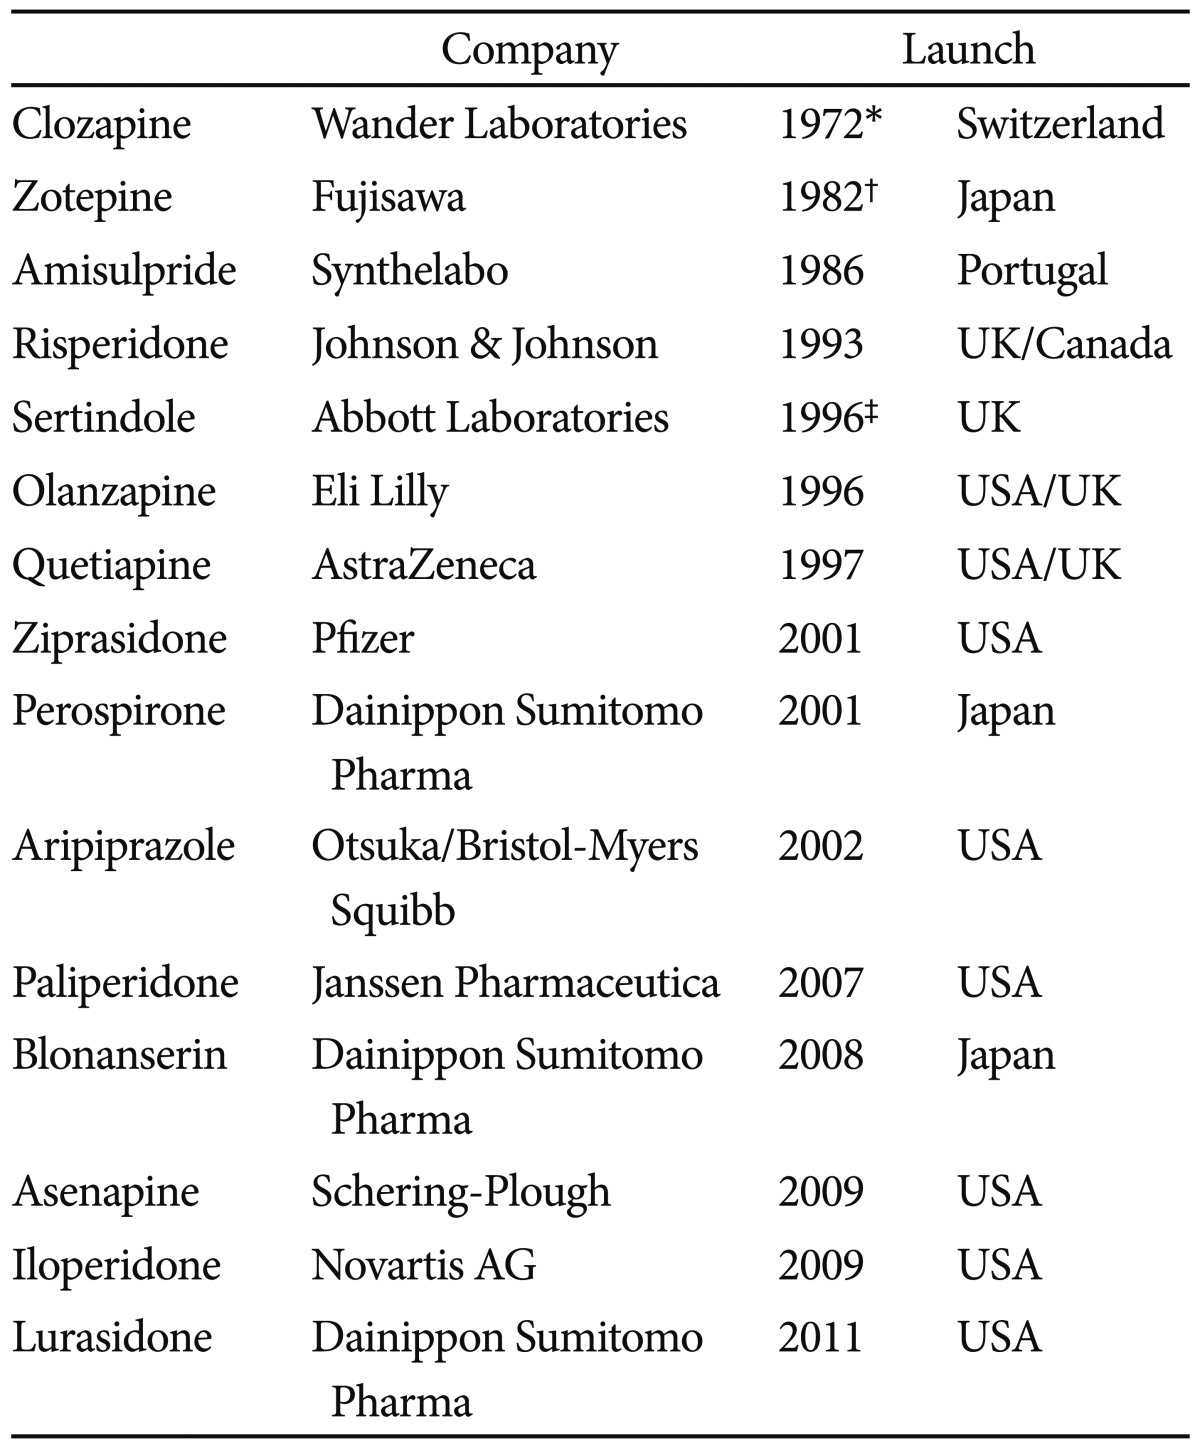
\includegraphics{./images/04-03/pi-10-8-i001.jpg}

}

\caption{2, 3세대 항정신병 약물과 미국 시장에 도입 연도
{[}@López-Muñoz2013{]}}

\end{figure}

\hypertarget{uxcc38uxc2e0uxd55cnovel-uxd56duxc815uxc2e0uxbcd1-uxc57duxbb3cuxb4e4}{%
\section{참신한(novel) 항정신병
약물들}\label{uxcc38uxc2e0uxd55cnovel-uxd56duxc815uxc2e0uxbcd1-uxc57duxbb3cuxb4e4}}

현재 한국에서 가장 광범위하게 사용되고 있는 항정신병 약물은 2세대 비정형
약물로서 클로자핀을 비롯하여 리스페리돈, 올란자핀, 퀘티아핀,
아미설프라이드, 지프라시돈, 아리피프라졸 그리고 리스페리돈의 개량형인
팔리페리돈 등이다. 미국과 유럽 등지에서는 이외에도 \uline{iloperidone,
asenapine, lurasidone, cariprazine, brexpiprazole, lumateperone} 등이
식품안정청의 허가를 획득하여 사용되고 있다. 문헌에서는 이들을
\uline{새로운(newer)} 항정신병 약물과 구분하여 \uline{참신한(novel)}
항정신병 약물로 지칭하기도 한다. 과거 항정신병 약물 개발의 역사를 보면,
2세대 약물이라고 해도 대부분 1970\textasciitilde80년대에 합성되었고,
20년 가까운 불확신과 우려의 나날을 거친 끝에 임상에 사용하게 된
약물들이다. 이에 비해 이후 합성된 약물은 대부분 합성되고 얼마 지나지
않아 사장되었으며, 기존 약물에 비해 별반 우수성을 갖지 못한다는 이유로
개발이 중단되었다. 실패를 거듭한 제약회사들은 항정신병 약물에 대한
투자를 꺼리게 되었고, 신약 개발의 파이프라인은 점점 막혀만 갔다.

때문에 참신한 약물이라고 소개되고 있는 약물들은 대체로 중소 제약업체에
의해 개발되었고, 과거 비정형 약물들을 개발, 배급했던 거대 제약사처럼
전세계적인 판로를 개척하지 못하고 있다. 이러한 연유에서인지 이들 약물 중
어느 것도 한국 시장에는 아직 소개되지 못하고 있다. 게다가 참신하다고
해도, 기존 약물과 차별화되는 새로운 작용기전을 갖는 약물이 아니기
때문에, 소위 ``Me-too'' 약물이라는 딱지를 쉽사리 떼지 못하고 있다.

참신한 약물들, 그중에서도 특히 가장 최근 임상에 도입된 cariprazine,
brexpiprazole, lumateperone 은 모두 부분효현제 특성을 지니고 있는
아리피프라졸 계열의 약물이다.{[}@Corponi2019-td{]} 또 다른 공통점이라면
다양한 수용체에 결합하는 multi-target 약물이라는 점이다. 그 동안 도파민
D\textsubscript{1}, D\textsubscript{3}를 비롯하여, 세로토닌 수용체의 각
아형들, glutamate system, neuropeptide Y등 다양한 신경전달물질 시스템이
항정신병 약물의 타겟으로 고려되어 왔으나, 분명한 것은 어느 한 시스템에
선택적으로 작용하는 약물로는 가시적인 성과를 볼 수 없었다는 점이다. 이를
의식한 듯, 새로 나오는 약물은 대부분 다양한 수용체를 공략하며, 이들간의
밸런스를 중요시한다.

조현병 자체를 치료할 수 있는 참신한 항정신병 약물의 개발이 힘들다면,
특정 증상만을 타겟으로 하여 호전을 꾀하는 치료제를 개발할 수 있을
것이다. 특히 치료가 어려운 음성 증상 및 인지 증상이라면, 이러한 신약
개발 노력은 큰 의미를 가질 것이다. \uline{Cariprazine}은
D\textsubscript{2,3} 수용체의 부분효현제이며, 아리피프라졸과 달리
D\textsubscript{3}에 대한 친화도가 더 크기 때문에 초기부터 음성 증상에
우수한 효과를 보일 것이라 기대되었다. 뚜렷한 음성 증상을 보이는 만성
조현병 환자를 대상으로 시행된 다기관 공동연구에서 cariprazine은
리스페리돈에 비해 우월한 음성 증상 개선 효과를
보였다.{[}@Nemeth2017-ud{]} 만약 cariprazine 효능에 대한 확신이 점점
확고해진다면, 음성 증상에 D\textsubscript{3} 수용체가 차지하는 위치에
대한 연구도 부쩍 늘어날 것으로 기대된다.

또 다른 타겟은 조현병의 인지 증상이다. 인지 증상은 조현병 환자의 삶의
질을 떨어뜨리는 주된 요소일 뿐 아니라, 양성 및 음성 증상의 근간을 이루는
근본 증상으로 여겨지기도 한다. 오래전부터 조현병 환자에게 항치매제를
사용하여 인지 증상의 개선을 꾀하려는 노력이 있었으나, 별다른 성과를
거두지 못하였다. 이외에도 D-cycloserine, sarcosine 등 glycine 활성을
통해 NMDA 수용체 기능을 조절하는 약물, 니코틴성 아세틸콜린 수용체 활성을
조절하는 varenicline, encenicline 같은 약물, 전반적인 염증 상태를
억제하는 NSAID 계통 항염증제, erythropoietin, minocycline 등이
연구되었다.{[}@Kroken2014-tu; @Yang2017-gh{]}

이러한 신약개발 연구동향에서 엿보이는 것은, 이미 다른 목적으로 사용되고
있는 약물을 새롭게 항정신병 약물로서 \uline{용도 변경(repurposing)}하는
전략이다.{[}@Yang2017-gh{]} 항정신병 약물의 경우와도 같이 의학에서
사용되는 대부분의 약물은 그 효과를 완전히 이해하지 못하고 있다. 따라서
기존 약물의 새로운 용도를 발견해내는 작업은 신약 개발에서 좀처럼 성공을
거두지 못하는 제약사로서는 잠재력이 풍부한 블루 오션이라 할 수 있다.
주된 기법으로는 조현병의 병태생리와 관련된다고 여겨지는 \uline{단백질
인터랙톰(protein interactome)}을 정의하고, 이와 작용하는 영역이 최대한
겹치는 약물을 후보 물질로 선정하는 것이다. 또 다른 방법은 기존의
항정신병 약물이 그 발현 정도에 영향을 끼친다고 알려진 단백질들에 역시
가장 많은 영향을 미치는 약물을 찾는 것이다. 생물정보학 및 컴퓨터 공학의
발전과 더불어 요새는 약물과 유전자, 단백질 들의 상호관계가
데이터베이스로 정리되어 있어 손쉽게 접속이 가능한 시대이므로, 이러한
검색작업은 과거와는 비교가 안 될 효율성으로 진행된다. 이렇게 선정된
물질에 대한 임상 시험도 속속 진행되고 있다.{[}@Karunakaran2019-oj{]}

\hypertarget{uxc0c8uxb85cuxc6b4-uxac1cuxb150uxc758-uxd56duxc815uxc2e0uxbcd1-uxc57duxbb3c-uxac1cuxbc1cuxc740-uxac00uxb2a5uxd55cuxac00}{%
\section{새로운 개념의 항정신병 약물 개발은
가능한가?}\label{uxc0c8uxb85cuxc6b4-uxac1cuxb150uxc758-uxd56duxc815uxc2e0uxbcd1-uxc57duxbb3c-uxac1cuxbc1cuxc740-uxac00uxb2a5uxd55cuxac00}}

1960년대 Carlsson과 Lindqvist의 연구팀이 도파민 가설을 내놓을 수 있었던
것은, 당시만 해도 경이로운 효과를 보였던 클로르프로마진이 도파민
수용체를 차단한다는 사실을 발견하였기 때문이었다. 이를 통해 조현병
환자들은 도파민 활성이 과다하게 상승되어 있고, 약물을 통해 이를
정상화시킬 수 있다는 단순한 논리가 세워졌고, 이후 개발된 항정신병
약물들은 모두 이 단순한 이론에 근거하고 있다. 물론 중뇌-변연계 도파민
활성이 조현병의 양성 증상과 밀접한 관련이 있음은 의심의 여지가 없다.
그러나 망상과 환각은 조현병에만 독특한 증상도 아니요, 환자의 삶의 질에
결정적인 영향을 끼치는 것도 아님을 명심해야 한다. 망상과 환각은 그야말로
표면적으로 드러나는 극적인 증상일 뿐이며, 더 깊숙한 곳에 자리하여 망상,
환각을 야기하는 근본 증상은 오히려 인지 기능의 퇴화와 뒤틀림이라고 할 수
있다. 더군다나 현재 가장 널리 받아들여지는 신경발달학적 가설에 의하면,
조현병은 양성 증상이 발현하기 훨씬 전부터 이미 영향을 끼치고 있으며,
뇌내 신경세포들간의 연결 네트워크의 이상, 비정상적인 신경세포의
가지치기(neuronal pruning) 등이 일어나고 있다는 증거가 있다.
{[}@Narr2015-hd; @Sakai2020-ql{]} 이렇듯 겉으로 나타나는 조현병의 증상
기저에는 다양한 신경생물학적 변이들이 자리잡고 있기 때문에, 도파민과
직접 관련되지 않은 시스템 역시 새로운 치료제 개발의 타겟이 될 수 있을
것으로 기대된다.

\hypertarget{uxc138uxb85cuxd1a0uxb2cc-uxc218uxc6a9uxccb4-uxc544uxd615uxb4e4}{%
\subsection{세로토닌 수용체
아형들}\label{uxc138uxb85cuxd1a0uxb2cc-uxc218uxc6a9uxccb4-uxc544uxd615uxb4e4}}

도파민 가설 이후, 처음 등장한 대안 가설은 \uline{세로토닌-도파민
가설}이었다. 비정형 항정신병 약물이 공통적으로 세로토닌 수용체를
차단한다는데서 출발한 이 가설은 처음에는 5-HT\textsubscript{2A} 수용체에
국한하여, 추체외로 증상을 경감시킨다는 보조적인 측면에서만 논의되는
경향이 있었으나, 최근에는 5-HT\textsubscript{3}, 5-HT\textsubscript{6}에
대한 관심이 높아짐과 동시에 인지기능 향상을 위한 치료제 개발에 관심이
모아지고 있다.{[}@De\_Bruin2015-hb{]} 유발전위의 이상이나 감각
관문(sensory gating)의 이상 등 조현병 환자의 독특한 신경인지적 결함이
속속 발견되면서, 이러한 변이들이 니코틴성 아세틸콜린 수용체와 관련됨이
발견되었다. 전술했듯이 varenicline, encenicline 등의 약물은 이러한
인지적 이상을 회복시키려는 목적으로 시도되고 있다. 그러나 뭐니뭐니 해도
이전부터 가장 연구의 초점이 되고 있는 것은 글루타메이트시스템이다.

\hypertarget{uxae00uxb8e8uxd0c0uxba54uxc774uxd2b8-uxc2dcuxc2a4uxd15c}{%
\subsection{글루타메이트
시스템}\label{uxae00uxb8e8uxd0c0uxba54uxc774uxd2b8-uxc2dcuxc2a4uxd15c}}

중추신경계 신경세포 중 60\% 이상은 글루타메이트를 분비하며, 거의 모든
신경세포는 글루타메이트 수용체를 지니고 있다. 글루타메이트는 학습, 기억
및 신경가소성에 있어서 가장 핵심이 되는 신경전달물질이며, 발생단계의 뇌
세포가 서로 연결을 이루고 일정한 구조를 형성하는데 기여한다.
글루타메이트 활성의 과다나 부족은 도파민 GABA 등과의 상호작용을 통해
다양한 정신 증상을 일으킨다. 일례로 PCP, ketamine과 같은 NMDA 수용체
차단제는 급격한 정신병적 증상을 나타내며, 장기간 투여는 음성 증상, 인지
증상을 일으키는 것으로 알려져 있다. 이 밖에도 조현병 환자의 사후
뇌조직에서 NMDA 수용체를 측정한 결과, 수용체 자체 뿐 아니라 glycine,
D-serine, polyamine 결합 부위의 이상이 발견되기도
하였다.{[}@Uno2019-mx{]}

연구자들은 먼저 D-cycloserine과 glycine에 대하여 항정신병 약물로서의
가능성을 타진해보았다. 그러나 기대와는 달리 2007년 발표된
\uline{조현병의 인지 및 음성 증상 임상 시험(the Cognitive and Negative
Symptoms in Schizophrenia Trial, CONSIST)} 결과에서는 위약에 비해 별다른
효과를 보이지 못하는 것으로 드러났다.{[}@Buchanan2007-jy{]} 이후 NMDA
수용체에 결합하는 위 약물들과는 달리 metabotrophic glutamate receptor의
선택적 효현제인 LY2140023 개발이 이루어졌다. 제약사인 Eli Lilly의
주도하에 3상 임상시험까지 이어졌으나 결과적으로는 미적지근한 효과로
개발이 중단되었다.{[}@Downing2014-gq{]} 이 밖에도 세포외 글루타메이트
농도를 조절하는 N-acetylcysteine, 글루타메이트 신호전달계의 하위 단계에
관여하는 phosphodiesterase의 억제제들, Glycine transporter 1을 억제하는
bitopertin 등이 임상시험을 거치고 있다. 그러나 현재까지 이렇다할 효과를
보인 약물은 없었다.{[}@egerton2020{]}

\hypertarget{uxcca8uxb2e8-uxc758uxd559uxc758-uxbaa8uxd5d8uxc801-uxc2dcuxb3c4uxc640-uxc870uxd604uxbcd1-uxce58uxb8ccuxc758-uxbbf8uxb798}{%
\subsection{첨단 의학의 모험적 시도와 조현병 치료의
미래}\label{uxcca8uxb2e8-uxc758uxd559uxc758-uxbaa8uxd5d8uxc801-uxc2dcuxb3c4uxc640-uxc870uxd604uxbcd1-uxce58uxb8ccuxc758-uxbbf8uxb798}}

오랜 동안 수많은 연구자들의 지적 탐구 및 헌신적 노력을 통해 적지 않은
가시적인 성과를 거두었음에도 불구하고, 조현병의 근본적인 원인이나
치료법은 쉽게 붙잡히지 않는다. 그 원인에 대해 두 가지 서로 다른 방향으로
접근할 수 있다. 첫째는 조현병은 단일한 원인이 아니라 다수의 원인들이
서로 복잡하게 얽히면서 발현되는 질병일 것이라는
가정이다.{[}@Kavanagh2015-rw{]} 근원을 거슬러올라가면 결국 단일한 원인이
있을 것이라는 순진한 기대와는 달리, 실상을 파헤치기 위해서는 시스템적
사고 방식과 복잡계를 이해하는 이론적 도구가 갖춰져야 한다는 주장이다.
반면 둘째는 조현병이라고 불리워지는 현상은 사실 표면적으로만 닮았을 뿐
서로 이질적인 질병들을 망라하고 있다는 가정이다. 개개 환자들은 서로
질병의 근원이 된 유전적 변이가 다르고, 신경생물학적 변이도 다를 것이라는
주장이다.{[}@Manchia2020-uz{]}

두 노선은 거의 대등한 정도로 주장되고 있으며, 개개 학자들 역시 어느 한
노선만을 고집한다기 보다는 그때그때 상황에 따라 어느 한 견해를
지지했다가 나중에는 다른 견해를 따르기도 한다. 복잡하게 얽힌 비선형
시스템에 대한 고찰은 수십년 전부터 이루어져 왔으나, 아직도 제대로 된
이해의 틀이 마련되지 않았기 때문에 전자의 노선은 상대적으로 발전이
뒤쳐졌다. 이에 비해 후자의 노선은 설득력이 있을 뿐더러, 최근 각광받는
\uline{정밀의학(precision medicine)}과 맥락을 같이 하고 있다. 후자를
주장하는 학자들은 환자 개개인마다 조현병의 원인이 된 유전적 변이가
다르기 때문에, 전체 게놈 스캔 등의 방법으로 환자의 변이를 찾아내어, 이를
줄기 세포 혹은 CRISPR-Cas9 유전자 가위 등의 첨단 기법을 동원하여 교정할
수 있으리라 기대한다.{[}@Schrode2019-rp; @Oltra2020-ta; @Zhang2020-rq{]}

단순하고 명쾌한 논리는 해답에 가까워졌을 것이라는 기대감을 높이긴
하지만, 생물학적 현상이 단순할 리가 없다는 것은 부인할 수 없는 진실이다.
설령 정밀의학의 힘을 빌려 개개 환자를 세부 아형으로 분류하고, 동일한
조현병이라도 그 환자에게 가장 적절한 치료법을 선택하는 일이 가능해질 지
모른다. 그러나 이는 여전히 다양한 종류의 치료 수단이 마련되었을 때의
일이다. 아직은 기존에 사용되고 있는 약물이 과연 어떤 기전으로 치료효과를
나타내는지 조차 완전히 이해하지 못한다. 앞서 설명한 기능적
선택성(functional selectivity)처럼, 약물의 효과는 단순히 리간드-수용체
결합이라는 논리만으로 설명되지 않는다. 동일한 약물이라도 작용하는 세포가
처한 상황에 따라 효현제가 될 수도 길항제가 될 수도 있으며, 또 세포 내
신호전달계 각각에 대하여 특정 레벨에서만 선택적으로 작용할 수도 있다.
이러한 기전들을 모두 이해하려면, \uline{전사체학(transcriptome), 후성
유전체학(epigenome), 마이크로바이옴(microbiome) 단백질체학(proteome)}
그리고 \uline{대사체학(metabolome)}의 지식이 총망라되어 세포내에서 어떤
현상이 일어나는지에 대한 이해의 폭이 깊어져야 할 것이다. 이러한 이해의
폭이 깊어지는 동시에 눈부시게 발전하고 있는
\uline{광유전학(optogenetics), 화학유전학(chemogenetics), 유전자 편집
기술(gene editing), 빅데이터와 정보기술, 나노기술} 등이 한데 어우러 질
수 있다면, 새로운 개념의 질병 이해와 치료 기술이 등장할 날도 멀지 않을
것으로 기대된다.{[}@Schulz2019-ft{]}

\hypertarget{references-25}{%
\section*{References}\label{references-25}}
\addcontentsline{toc}{section}{References}

\markright{References}

\hypertarget{uxadfcuxac70uxc911uxc2ecuxc758uxd559---uxc784uxc0c1uxc2dcuxd5d8}{%
\chapter{근거중심의학 -
임상시험}\label{uxadfcuxac70uxc911uxc2ecuxc758uxd559---uxc784uxc0c1uxc2dcuxd5d8}}

Evidence based medicine - Clinical trials

\hfill\break

\hypertarget{sec-EBM}{%
\subsection{근거중심의학의 개념}\label{sec-EBM}}

의학에서 정확한 \uline{진단(diagnosis)}이 가지는 중요성은 아무리
강조해도 지나치지 않을 것이다. 진단이 정해지면, 그에 상응하는 표준
치료\footnote{\textbf{표준 치료(standard treatment or standard of
  care)}: 특정 질병이나 질환에 대해 다수의 의학 전문가들이 적합하다고
  인정하였으며, 실제 임상에서도 가장 보편적으로 적용되는 치료법.
  교과서에 수록되는 치료법이기도 하며, 보험이나 사법체계에서 인정하는
  적절한 치료의 기준이 되기도 한다.}를 행하는 것이 옳으며, 환자의 상황이
특별하거나 표준적 치료에 반응하지 않는다면 다음 단계에 해당되는 차선적
치료를 행하게 된다. 진단에 걸맞는 치료를 행하는 것은 의사의 지식과
숙련도를 반영하는 잣대일 뿐 아니라, 의료 사고를 판별하는 기준이자, 의료
보험 체계를 지탱하는 기본적 축이다.

그러나 정신질환은 진단에서 치료로 이어지는, 틀에 짜여진 형식에서 약간
비켜간 듯한 느낌을 준다. 물론 DSM이나 ICD와 같은 표준 질병분류체계가
있고, 여전히 진단이 중요시되고 있으나, 실제 임상가들은 진단의
세부항목까지 따지는 것에 대해 큰 중요성을 두지 않고 있다. 더군다나
생물학적 치료와 심리적 치료를 넘나드는 광범위한 치료 수단의 활용은
획일적인 보험체계의 틀에 가두기에는 너무나 유동적이다.

정신약물학이라는 국한된 영역에서도 역시 마찬가지이다. 비정형 항정신병
약물이 등장한 이후, 이들 약물은 조현병 치료제로 쓰일 뿐 아니라, 양극성
장애, 우울증 심지어 가벼운 불안장애나 수면 조절에도 사용된다. 또한
조현병에도 항우울제, 항불안제들이 통상적으로 사용되기 때문에 과연 진단이
치료에 꼭 필요한가라는 의문이 들기도 한다.{[}@Dean2011-vz{]}

소위 근거중심의학(evidence based medicine, EBM)은 과학적 정보에 근거하여
의학적 결정을 내리는 관행을 의미한다.\footnote{기존의학과 근거중심의학의
  차이점은 다음과 같다. 기존의학에서는 병인과 병태생리에 대한 막연한
  추론, 의사 개개인이나 전문가 집단의 임상경험이나 주관적 평가에 의해
  진료를 했다면, 근거중심의학에서는 체계적 임상시험, 메타분석과 같이
  객관적이고 계량 가능한 증거에 기반하여 진료를 행한다. 전자는
  의학자들만이 독점하는 폐쇄된 지식이라면, 후자는 일반인은 물론 환자 및
  보호자도 접근할 수 있는 지식이기 때문에, 공유된 의사결정이 가능하게
  된다.} 물론 의학적 결정을 내리기 위한 임상 관찰과 자료의 중요성은
그리스 시대로 거슬러 올라간다. {[}@Sackett1996-hm{]} 그러나, 20세기에
이르러 EBM의 개념은 모든 의료 영역에서 으례 따라야 하는 패러다임으로
진화했다. Eddy\footnote{\textbf{David Eddy (1941\textasciitilde)}:
  미국의 의사이자, 수학자, 건강제도 분석가이다. 질병의 수학적 모델링,
  의학에서의 합리적 의사결정, 임상진료지침의 중요성 등에 대해
  연구해왔다.}는 \uline{근거 중심(evidence-based)}이라는 용어를 처음으로
사용했고, Guyatt 등은 1990년대 초에 \uline{근거중심의학}이라는 용어를
도입하였다.{[}@Eddy1990-pb; @Guyatt1992-zm{]} 앞에서 소개했듯이 정신과
진료에서 EBM의 도입은 저항도 많았고, 잘 들어맞지 않는 부분도 많다. 이는
조현병 치료를 위시한 정신과 진료에서 증거를 얻고, 얻어진 증거를
평가하며, 더불어 그러한 증거를 치료 결정에 \uline{적절하게} 적용하는
것이 꽤 까다롭기 때문이다.{[}@Keshavan2009-pf{]}

\begin{figure}

{\centering 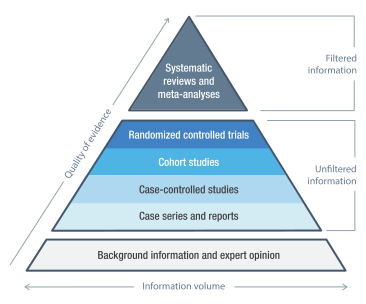
\includegraphics[width=4.8125in,height=\textheight]{./images/04-04/levels-of-evidence.svg}

}

\caption{\label{fig-evidence-pyramid}근거중심의학에서 사용되는 근거의
피라미드}

\end{figure}

\hypertarget{sec-randomized-trial}{%
\subsection{무작위 배정 임상시험}\label{sec-randomized-trial}}

근거중심의학에서 사용되는 증거에는, 일화적 증례 보고나 비통제 연구
결과도 있지만, 그중 가장 강력한 증거로 채택되는 것은 무엇보다 무작위
배정 임상 시험(randomized clinical trial, RCT)의
결과이다.(그림~\ref{fig-evidence-pyramid}) 증례보고나 통제되지 않은
비무작위 혹은 개방형 연구는 연구자 혹은 연구 참여자의 편견, 바이어스를
배제하기 어려우며, 무엇보다 다양한 교란변인(confounding variable)의
효과를 통제할 수 없기 때문에 결과를 얻어놓고도 인과관계를 주장하기
어렵다. 이에 비해 철저한 이중 맹검, 무작위 배정 연구는 순수한 치료적
개입의 효과를 걸러내어 행해진 치료과 치료효과를 낳았다는 인과관계를
주장할 수 있다.

때문에 국가기관에서 신약에 대해 사용허가를 내줄 때에도 반드시 무작위
배정 이중맹검 임상 시험의 자료를 토대로 한다. 근거중심의학의 패러다임이
영향력을 키워갈수록, 무작위 임상시험의 결과는 의학적 의사 결정과 교육,
임상 실습에 커다란 영향을 미친다. 그러나 임상 시험은 타당화와 일반화
측면에서 중대한 한계를 갖는다. 새롭게 등장한 치료법인 효과적인데도
불구하고 이를 입증하는데 실패할 수도 있으며, 반대로 잘못된 결론으로 이끌
수도 있다.{[}@Correll2011-hg{]}

임상 시험에서 환자를 선택하는 과정은 현재 질병분류학의 약점을 더욱
부각시킬 수 있다. 앞서 언급했듯이 똑같은 조현병이라고 해도 너무나 다양한
특성의 환자가 존재하기 마련이며, 진단 경계의 회색 영역에 위치하는 환자도
많다. 임상 시험에는 진단에 애매모호함이 없는 전형적인 환자만 포함되기
마련이며, 이들이 전체를 대표할 수 있는지는 의문이다. 또한 대부분의 임상
시험에서 진단은 정해진 진단 도구를 이용하게 되는데, 이러한 진단 도구
자체가 실제 임상에서 의사들이 체감하는 진단과는 거리가 있다. 게다가 동반
질환이 있는 환자를 배제하는 관행때문에 역시 실제 임상에서 흔히 접하게
되는 환자는 임상 시험에 포함되지 못한다.

또한 임상 시험은 공동의 이익과 개인의 치료 사이에서 과학과 윤리의 충돌을
야기한다. 치료의 효과를 증명하기 위해 위약(placebo)을 사용하는 것이
요구되는데, 위약군에 배당되는 환자들은 실질적으로 치료기회를 놓친다는
점에서 피해를 입는 셈이다. 무작위 임상 시험이 공동선을 달성하기 위해서는
임상의, 의료 정책 입안자 및 임상 진료에 영향을 미치고 평가하는
관계자들이 임상 시험 데이터에 접할 수 있어야 하며, 이 데이터를 제대로
해석할 수 있는 지식과 경험을 갖추고 있어야 한다.{[}@Correll2011-hg{]}
그러나 제약회사가 주관하는 대부분의 임상 시험 데이터는 회사에게 소유권이
있다는 이유로 공개가 제한된다. 미국에서는 임상 시험을 계획할 때 사전에
\href{https://clinicaltrials.gov/}{국가 데이터베이스}에 등록하여, 임상
시험의 진행과정을 공개하도록 하였으며, 우리나라에서도 국립보건연구원
산하
\href{https://cris.nih.go.kr/cris/index/index.do}{임상시험정보서비스(clinical
research information service, CRIS)}에서 정보를 관리하고 공개하고 있다.
그러나 이런 서비스는 어디까지나 임상시험의 디자인과 진행상황을 보여주는
것이지, 얻어진 데이터가 공개되는 것은 아니다.

\hypertarget{uxc784uxc0c1-uxc2dcuxd5d8uxc758-uxb3c4uxc785uxacfc-uxd3c9uxac00uxc758-uxd45cuxc900uxd654}{%
\subsection{임상 시험의 도입과 평가의
표준화}\label{uxc784uxc0c1-uxc2dcuxd5d8uxc758-uxb3c4uxc785uxacfc-uxd3c9uxac00uxc758-uxd45cuxc900uxd654}}

마취보조제로 개발된 클로르프로마진은 조현병 환자들에게 ``진정 작용''을
갖는다는 다소 우연한 관찰로부터, 정신약물학의 혁명을 이끌어냈다. 약물이
합성된지 불과 3년 후인 1954년에 미국 식품의약청(FDA)으로부터 승인을
받았지만, 허가를 받기 전에 무작위 배정 이중맹검 연구가 시행된 적은
한번도 없었다. 그럼에도 불구하고 1964 년까지 전세계 약 5천만 명의
사람들이 이 약물로 치료 받았으며, 어느 누구도 약물의 효과에 대해
의심하지 않았다.

그러나 클로르프로마진의 성공에 고무되어 유사한 약물들이 우후죽순처럼
개발되기 시작하자, 이들 약물의 효과를 객관적으로 검증할 수 있는 장치가
필요해졌다. 무작위 배정의 방법론과 결과를 분석하는 통계적 기법도
필요했지만, 그것보다 먼저 갖춰져야 하는 것은 정확히 어떤 환자를 연구에
참여시킬 것인지를 결정하는 \uline{진단 기준(diagnostic criteria)},
그리고 효과를 판정하기 위한 객관적인 \uline{평가 도구(rating
scale)}였다.

정신과 질환에 대해 합의된 진단 기준이 최초로 마련된 것은 1949년
국제보건기구(WHO)에서 발간한 \uline{국제질병분류(international
statistical classification of diseases, ICD) 제 6차 개정판}이
처음이었다. 1952년에 미국 정신과 학회(American psychiatric association,
APA)는 \uline{정신 장애 진단 및 통계 편람(diagnostic and statistical
manual of mental disorders, DSM)} 초판을 발간하였으나, 질병의 목록만
있었을 뿐 개별 장애에 대한 진단 기준이 구체적으로 명시되지는 않았다.

\hypertarget{uxc9c4uxb2e8uxae30uxc900}{%
\subsubsection{진단기준}\label{uxc9c4uxb2e8uxae30uxc900}}

1960-70년대에는 제대로 된 진단기준도 없었고, 구조화된 진단도구도
전무했기 때문에 당시 연구대상자의 선정기준은 전적으로 의사의 자의적인
판단으로 이루어졌다. 대조군의 선정도 한 병원에서 한개 병동의 전체 환자가
약물 투여군으로 선정된다면, 다른 병동의 전체 환자가 대조군이 되는 등
편의적인 선정이 일반적이었다.{[}@Brunoni2010-et{]} 이런 상황을 타개하기
위하여 John Feighner를 비롯한 워싱턴 대학 정신과 연구진은 1972년 소위
\uline{Feighner criteria}를 발표하였다.(\ref{sec-dsm-iii} 장) 이는
최초의 실행적 진단 기준(operational diagnostic criteria)로서 일련의
진단기준 중 몇 개 이상을 만족하면 특정한 질병으로 진단한다는 형식을
갖추고 있다.{[}@Feighner1972-ed; @Kendler2010-lr{]} Feighner criteria와
이를 통해 소개된 실행적 진단 기준의 개념은 즉각 환영받았고, 이는 1978년
발표된 research diagnostic criteria (RDC)를 거쳐 DSM-III에
흡수된다.{[}@Spitzer1978-uu{]}Feighner criteria와 RDC의 항목들을
상당부분 차용한 DSM-III은 개별 정신질환의 진단 기준들을 제시할 수
있었다. 이는 정신 질환 진단의 타당성과 신뢰성을 향상시켰다는 점에서 향후
임상 연구 및 약물 개발에 있어서 엄청난 영향을 미쳤다.

\hypertarget{uxd3c9uxac00uxb3c4uxad6c}{%
\subsubsection{평가도구}\label{uxd3c9uxac00uxb3c4uxad6c}}

최초의 구조화된 진단도구로는 \uline{schedule for affective disorders and
schizophrenia (SADS)}와 \uline{현상태검사(present state examination)}을
들 수 있다. 전자는 1978년 Endicott와 Spitzer가 research diagnostic
criteria (RDC)를 이용하여 진단을 내리는데 필요한 정보를 수집하고 환자의
증상과 기능 수준을 기술하는 것을 목적으로 개발하였으며, 후자는 ICD-9을
반영하여 개발되었다. 그러나 가장 영향력있는 진단도구로는 역시 DSM-III의
발간과 함께 발표된 structured clinical interview for DSM-III-R (SCID)일
것이다.{[}@Spitzer1992-ol{]} SCID는 이후 DSM이 개정될 때마다 함께
개정되어 현재는 DSM-5를 반영하는 SCID-5까지 나와있다.

이러한 진단도구 이외에도 정신병리의 경중을 평가하기 위한 지표로 최초의
평가도구는 1962년 Overall과 Gorham에 의해 개발된
\uline{간이정신평가척도(brief psychiatric rating scale, BPRS)}이
있다.{[}@Overall1962-kq{]} 1987년 Stanley Kay 등은 BPRS를 더욱 확장시켜
\uline{양성 및 음성증후군 척도(positive and negative syndrome scale,
PANSS)}를 제작하였으며, 이는 명실공히 현재까지도 가장 널리 사용되는
조현병의 평가도구로 자리잡았다.{[}@Kay1987-np{]}

\hypertarget{uxba54uxd0c0-uxbd84uxc11d}{%
\subsection{메타 분석}\label{uxba54uxd0c0-uxbd84uxc11d}}

이들 평가도구가 개발된 이후 조현병 환자를 대상으로 한 대부분의 임상
시험은 SCID로 진단된 환자를 대상으로 시행하고, PANSS를 통해 결과를
확인하는 식으로 이루어졌다. 진단도구가 표준화되자 임상 시험에 포함되는
환자라면 대체로 어떤 환자들이라는 컨센서스가 생겨나게 되었다. 진단이
통일되고, 효과 판정을 위한 기준이 명확해지면 개별 연구들의 결과를
통합하는 분석, 즉 \uline{메타 분석(meta-analysis)}이 가능해진다.
1970년대 이후 의학 문헌에서 조금씩 등장하기 시작한 메타 분석은
근거중심의학에서 사용하는 증거 중에서 가장 최상위에 위치한다. 개개 임상
연구는 표본 수가 작아서 충분한 검증력을 갖지 못하지만, 이를 한데 모아
분석하면 충분한 검증력을 확보할 수 있다는 장점이 두드러졌다. 체계적
문헌고찰을 위한 Cochrane library: cochrane review\footnote{\textbf{Cochrane
  review}: 스코틀랜드의 의사 Archibald Leman Cochrane
  (1909\textasciitilde1988)은 평생 무작위 임상시험의 중요성과 그
  결과들을 종합할 수단을 마련해야함을 역설하였다. 이에 영향을 받은
  옥스포드 대학의 Iain Chalmers (1943\textasciitilde)은 1993년 Cochrane
  Collaboration (현재는 그냥 Cochrane이라 부름)을 설립한다. 현재 전세계
  30,000명 이상의 자원 연구자들이 체계적 문헌 분석과 메타 분석을 하여 그
  결과를 \href{https://www.cochranelibrary.com/}{Cochrane library}에
  등재하고 있으며, 이는 Cochrane Database of Systematic Reviews를 통해
  서비스 가입자에게 공개된다.{[}@Shah2009-ck{]}}가 1996년부터 서비스를
개시하였고, 여기에는 각종 임상적 질문에 대해 관련된 연구 문헌들을
종합하여 내려진 근거들이 나열되어 있다.

더불어 표준화된 평가도구의 보급은 임상 연구의 세계화를 가능하게 만든
계기가 되었다. 정신약물학의 초창기에는 미국와 유럽에 국한된 제한된 연구
기관에서만 임상 연구가 가능했으나, 전세계 공통으로 적용되는 진단 기준,
각국어로 번역된 진단 도구 등의 보급으로 한국을 비롯하여 중국, 인도, 라틴
아메리카 등이 활발히 임상 연구에 참여하고 있다. 이는 또한 거대 다국적
제약기업들이 판로를 전세계로 확대한 때문이기도 하다. 임상 연구의
상업화와 세계화로 규모가 점점 더 커지게 되었으며, 다양한 환자군이
포함됨으로 인해 하위집단 분석(subgroup analysis)이 보다 정교해졌다.

\hypertarget{uxd45cuxc900uxd654uxc5d0-uxb300uxd55c-uxbe44uxd310}{%
\subsection{표준화에 대한
비판}\label{uxd45cuxc900uxd654uxc5d0-uxb300uxd55c-uxbe44uxd310}}

한편 이러한 국제화, 표준화는 많은 발전을 가져왔지만 동시에 어두운
그림자도 드리우고 있다. 가장 큰 문제는 SCID로 대표되는 소위 실행적 진단
기준\footnote{\textbf{실행적 진단기준(operational diagnostic criteria)}:
  진단의 신뢰성을 높이기 위해 1970년대 Feighner 등 속한 Washington 대학
  연구진이 도입한 진단체계. 일단 병인에 대한 선입관을 모두 내려놓고
  진단에 특징적인 증상과 징후를 나열한 다음, 그 중 해당되는 것이 몇 개
  이상이고, 동시에 배제기준에 해당되지 않으면 진단을 확정하는 식으로
  이루어진다. 신뢰도가 극적으로 높아진 것은 분명하나, 정신과 진단을
  checklist 진단으로 바꿔놓아 증상/징후 들 사이의 유기적인 관계를
  무시했다는 비판을 받는다. 이는 전형적인 진단 원형과 얼마나 유사한가에
  의해 진단을 확정하는 prototype diagnosis와 대조된다.{[}@maj2011{]}
  ``실행적(operational)''이라는 이름은 정말 맞는지 틀리는지 여부는
  지금으로서는 알 수 없지만, 일단 다음 과정이 진행되도록 하기 위해
  임시로 정해놓은 기준이라는 의미로 사용되었다.}이 과연 임상가의 경험과
일치하는가라는 점이다. 또한 조현병 증상의 개선을 거의 대부분 PANSS로
평가하는 만큼, PANSS에 반영되지 않는 변화는 호전의 증거로 채택되지
않는다는 문제도 있다. DSM 체제에 대해 비판적인 일부 학자들은
미국정신의학회가 정신질환 진단의 신뢰도를 높이기 위해 타당도를
포기하였다고 주장한다. 즉 환자 상태에 부합하는 특정 진단 항목의 갯수로
진단을 확정짓는 부자연스러운 과정을 수용함으로써, 정말로 조현병이 어떤
것인지에 대한 핵심을 상실해버렸다는 것이다.{[}@Ghaemi2018-le{]} DSM
체제가 확고해지면서 후대에 교육받은 정신과 의사들은 마치 DSM 진단기준이
질병 자체인 것처럼 착각해버리는, 그야말로 주객인 전도된 상황이 발생하기
하였다. Van Praag는 이미 1993년에 쓴 논문에서, DSM을 최초에 제정한
의사들은 진단기준의 모호성과 실제 임상에서의 한계에 대해 충분히 이해한
상태에서 DSM을 만들었지만, 이후 이러한 모호성과 혼란은 수치와, 계량화
속에 묻혀버렸고, 진단을 너무나 과대평가하는 현재의 추세 때문에 가지
말았어야 할 길을 가버렸다고 지적하고 있다.{[}@Praag1993-sx{]}

\hypertarget{uxc870uxd604uxbcd1uxc758-uxc9c8uxbcd1uxbd84uxb958uxd559uxc801-uxc9c0uxc704uxc640-uxce58uxb8ccuxc758-uxd0c0uxae43}{%
\subsection{조현병의 질병분류학적 지위와 치료의
타깃}\label{uxc870uxd604uxbcd1uxc758-uxc9c8uxbcd1uxbd84uxb958uxd559uxc801-uxc9c0uxc704uxc640-uxce58uxb8ccuxc758-uxd0c0uxae43}}

윗절에서 언급한 바와 같이, 근거중심의학의 도래와 임상 시험에 대한 과도한
의존은 조현병 치료에 있어서 임상가는 무엇을 타깃으로 하고 있는가를 새삼
되돌아보게 한다.{[}@Levine2008-kh{]} 근거중심의학의 토대는 정신과 진단에
대한 실제론(realism)에 있다. 즉 ``\emph{인간에게 주관적 고통을
야기하거나, 기능의 상실을 불러오는 현상을 증상 혹은 징후라 칭한다. 만약
일군의 증상 및 징후가 높은 빈도로 함께 동반되어 나타난다면, 이를
증후군(syndrome)이라 할 수 있다. 그런데 이러한 증후군이 등장하는 이유는
그 기저에 질병분류학적 기본단위(nosological entity)라고 할 수 있는
\uline{질병(disease)}이 존재하기 때문이다''}라는 논리이다. 이렇게 가정된
질병을 실재하는 것으로 간주한 상태에서, 그 원인, 병리현상 및 예후를
따지는 것이 의학의 궁극적 과제가 되었다. 모든 치료는 이 질병에 맞추어져
있으며, 질병의 병태생리를 정상화시킴으로써 제반 증상/징후들을 소실시키려
노력한다. 근거중심의학은 이러한 질병개념에 충실하기 때문에, 진단이
무엇보다도 중요한 지위를 차지한다.

그러나 실제 임상에서의 경험을 되짚어보면, 이러한 이상과는 큰 거리가
있다. 대부분의 치료는 개개 증상 및 징후를 타깃으로 하고 있으며, 치료
성과가 있고 없음 역시 증상 및 징후가 얼마나 줄어드는가, 그리고 환자가
주관적으로 얼마나 편안해하는가를 토대로 결정된다.{[}@Jablensky2012-fg{]}
병존질환의 문제 역시 마찬가지이다. 질병분류체계에 의하면 조현병 환자가
우울 증상을 보이는 경우, 조현병과 우울증이라는 개개 질병이 병존하는
것으로 진단한다. 그러나 정신병적 증상에 시달리고, 부적응으로 인해
사회로부터 소외되는 환자가 우울해지는 것은 정상적인 심리반응의 일환일
수도 있다. 환자를 직접 치료하는 의사들은 이를 구분하여 상황에 맞게
환자를 돕고자 하지만, 근거중심의학이나 규정에 매인 치료 알고리즘은 임상
상황의 미묘한 뉘앙스까지 고려하지 못한다.

따라서 \uline{``조현병의 약물 치료''}라는 야심찬 구호 역시 조심스레
이해되어야 한다. 조현병이라는 질병이 실제로 존재하는 것인지, 아니면
진단의 신뢰도를 높이고자 하는 목표 하에 인위적으로 만들어진
\uline{구성개념(construct)}인지는 여전히 확인되지 않고 있다. 해당 증상의
개수를 따져보는 것 외에 믿을만한 진단기법이 있는 것도 아니요, 증상이
수그러드는 것 말고 질병의 호전 여부를 확인해볼 수 있는 검사 방법이 있는
것도 아니다. 정신약물학의 첫 장을 열었던 클로르프로마진이 해결했던
문제는 무엇보다 환자를 진정시키는 것이었고, 운좋게도 환각과 망상을
경감시키는 효과를 발휘했던 것이다. 그러나 환각과 망상을 줄여준다고 해서
조현병이 과연 나아지는 것인지는 의문의 여지가 있다. 조현병이 만성화되면
양성 증상의 비중이 줄어들고 음성/인지 증상이 더 두드러진다. 그렇다고
해서 조현병이 호전되고 있다고 말할 수는 없는 노릇이다.

\hypertarget{sec-major-clinical-trials}{%
\section{주요 임상 시험들}\label{sec-major-clinical-trials}}

근거중심의학의 한계를 분명히 감안한다 할 지라도, 여전히 조현병 치료의
근거를 확립하고자 했던 수많은 연구자들의 노력을 간과할 수 없다. 정형
항정신병 약물이 처음 도입되었을 때, 거의 모든 의사들과 연구자들은 약물의
효과와 효용성에 의심을 품지 않았다. 그도 그럴 것이 이제까지 경험해보지
못했던 긍정적인 변화를 자신의 눈으로 직접 목격할 수 있었기 때문이다.
그러나 추체외로 부작용의 문제, 지연 운동 이상증 등의 부작용 문제가
불거지면서 과연 예상되는 이득이 피해를 정당화할 수 있는 지에 대한 고민이
시작되었다.{[}@slovenko2000{]}

이러한 고민은 비정형 항정신병 약물의 도입으로 인해 더욱 깊어졌다. 새로운
항정신병 약물은 운동부작용의 위험을 획기적으로 낮추었기 때문에, 이전의
약보다 개선되었다는 것은 의문의 여지가 없었다. 그러나 거대 제약사들이
독점적으로 제조, 공급하면서 약가가 현저하게 상승되었다. 더군다나 대사성
부작용이라는 새로운 문제가 불거지면서, 부풀려진 비용 만큼 장점이 있는
것인지에 대해 많은 의사들과 정책결정자들은 의문을 품기 시작하였다. 이미
공정하고 체계적인 임상 시험의 방법론적 틀이 확립되어 있었고, 다기관
공동연구가 일상화되었으며, 약물경제학(pharmacoeconomics)이라는 새로운
학문이 싹트면서, 비정형 항정신병 약물의 실상을 밝히기 위한 대규모 임상
시험이 기획, 진행되었다.

이러한 연구들은 다음 질문에 답하고자 하였다. 첫째, 비정형 항정신병
약물은 정형 약물에 비해 치료 효과가 뛰어난가? 둘째, 전자는 후자에 비해
높은 안전성을 지니는가? 셋째, 전자가 갖는 우수성은 높은 비용을
상쇄할만한 가치가 있는가? 그리고 마지막으로 이러한 장점은 실제 임상에서
환자의 높은 삶의 질로 이어지는가?

\hypertarget{clinical-antipsychotic-trials-of-intervention-effectiveness-catie}{%
\subsection{Clinical Antipsychotic Trials of Intervention Effectiveness
(CATIE)}\label{clinical-antipsychotic-trials-of-intervention-effectiveness-catie}}

이같은 질문에 답하고자 한 연구 중 가장 유명한 것은 미국 국립 정신보건
연구소(NIMH)의 주도로 행해진 CATIE 연구일 것이다.{[}@lieberman2005{]} 이
연구는 만성 조현병 환자에 대한 비정형 항정신병 약물의 효과를 실제
임상에서 검증한 것으로, 그 후의 조현병 약물 치료에 크나큰 영향을 주게
된다. 연구는 2001년에서 2004년 사이에 미국 전역의 57개 도시에서 무려
1,500명 이상의 환자를 대상으로 행해졌다. 모두 세단계로 이루어졌는데,
첫번째 단계는 무작위 배정 이중 맹검에 의하여 정형 항정신병 약물로는
퍼페나진(perphenazine), 그리고 비정형 약물로는 올란자핀, 퀘티아핀,
리스페리돈, 지프라시돈의 다섯개 약물 중 하나를 18개월 동안 투여받는
것이었다. 퍼페나진을 사용하다가 중도에 탈락된 환자는 다시 나머지 비정형
약물 중 하나에 배정되어 관찰을 지속하였다.

두번째 단계는 1단계에서 모종의 이유로 중도 탈락한 환자를 대상으로 역시
무작위 배정으로 클로자핀, 올란자핀, 퀘티아핀, 리스페리돈 중 하나를 역시
18개월 동안 투여받는 것이었다. 이때는 이중맹검은 시행하지 않았고,
개방형으로 진행되었다. 마지막 3단계에서는 1,2 단계에서 중도 탈락된
환자를 대상으로 이번에는 의사와 환자의 논의 하에 다음 약물을 선택하게
하였다. 모든 단계에서 가장 중요한 결과 변수는 ``모든 이유에 의한 투약
중지'' 즉 \uline{중도 탈락률}과 \uline{중도 탈락할 때까지의 기간}이었다.

정형 약물로 퍼페나진이 선정된 것, 그리고 일차적 결과변수가 PANSS 점수의
변화가 아니라 중도 탈락률이었던 것은 기존의 임상 시험과 차별화되는
점이다. 퍼페나진이 선정된 것은 그나마 정형 약물 중에서 가장 추체외로
증후군의 위험이 낮은 약으로 평가되었기 때문이다. 한편 중도 탈락률이
선정된 이유는, CATIE 연구의 설계자들이 실제 임상에서의 효과를 최대한
반영하기를 원했기 때문이다. PANSS는 연구상황이라는 매우 인위적인
상황에서 평가되지만, \uline{중도 탈락}은 주치의나 환자가 그 약의 유효성,
부작용 등을 살펴보면서, 무언가 문제가 있다고 판단을 내렸음을 반영하는
예민한 지표이기 때문이다.

1단계 연구의 결과를 보면 올란자핀이 중도 탈락률이 가장 낮았다는 것이
확인되었다. 그러나 올란자핀 군은 체중 증가가 가장 심했고, 대사성
부작용의 비율도 가장 높았다. 반면 심리사회적 기능, 증상, 삶의 질 등에
있어서는 시험 약물간의 차이를 발견할 수 없었다. 결과적으로 비용-효과
비가 가장 높은 약물은 perphenazine인 것으로
나타났다.{[}@Swartz2008-xv{]}

2단계 연구에서는 클로자핀이 추가되었는데, 이는 리스페리돈, 퀘티아핀 등에
비해 우수한 효과를 나타내었다. 이에 반해 올란자핀과 클로자핀의 차이는
크게 두드러지지 않았다. 마지막 3단계 연구에서 증상이 심한 환자들은
클로자핀 혹은 여러 개의 항정신병 약물을 사용하는 다약제
복용(polypharmacy)을 선택했고, 체중 증가가 심했던 환자들은
아리피프라졸과 지프라시돈을 선택하는 경향을 보였다.{[}@Stroup2009-cf{]}

표면적으로 CATIE 연구는 다양한 비정형 항정신병 약물 같의 우열을 비교한
것같지만, 얻어진 결과가 갖는 중요성은 다른 데 있다. 아마도 가장 두드러진
발견은 1단계 시험이 행해진 18개월 동안 중도에 약물을 바꾼 비율이 무려
74\%에 이르렀다는 점이다. 게다가 약물을 꾸준히 유지했든, 중도에 바꿨든
환자의 치료 성과는 대동소이했다는 것이다.{[}@Attard2012-zd{]} 이러한
결과는 의사이든 환자이든 현재 사용되고 있는 항정신병 약물에 그다지
만족하지 못하고 있으며, 그래서 약을 바꿨다고 해도 별반 나은 점은
없었다는 뜻으로 해석된다.

두번째로 논란을 일으킨 발견은 퍼페나진과 비교하여 비정형 약물이 효능이나
부작용 면에서 통계적으로 유의한 차이를 보이지 못했고, 따라서 비용-효과
분석에서 열등하였다는 점이다. 이는 의사, 학계, 환자 단체, 제약사 및 정책
결정자 사이에 강한 반발과 광범위한 논의를
불러일으켰다.{[}@Manschreck2007-fq{]} 물론 정형 약물의 대표 겪으로
조현병 치료에 거의 쓰이지 않던 퍼페나진을 선택한 것은 예상 밖이다. 만약
퍼페나진 대신 할로페리돌을 사용했다면 전혀 다른 결과가 얻어졌을 수도
있다. 또한 18개월이라는 기간이 추체외로 증상이나 지연 운동 이상증이
나타날 만큼 충분히 오랜 기간이었는지에 대한 의문도
남는다.{[}@Casey2006-ar{]}

비정형 약물이 퍼페나진에 비해 뚜렷한 장점을 보이지 못했음에 비해, 체중
증가와 대사성 증상 발현에 있어서는 뚜렷한 위험 요인을 안고 있었다.
클로자핀과 함께 올란자핀은 두드러지게 높은 체중 증가와 대사 증후군의
발생률을 보였다. 올란자핀 군에서는 체중 증가, 대사에 대한 영향때문에
투약을 중지한 비율이 9\%로 다른 약물 군보다도 유의하게 많았다. 또 7\%
이상의 체중 증가가 생긴 비율이 30\%로, 다른 항정신병 약물 군의
7-16\%보다고 유의하게 높았다. 이 밖에도 당화 헤모글로빈(HbA1C), 총
콜레스테롤 치, 중성 지방 치 등이 치료 기간을 보정한다 해도 타 약물 군에
비해 유의하게 높았다. 이러한 문제가 환자의 삶의 질이나 기대 수명에 어떤
악영향을 미치는 지는 앞으로도 끊임없는 논란 거리가 될 것이다. 항정신병
약물의 단기 효과는 물론 자살 위험을 낮추고 건강을 해칠 수 있는 위험한
행동을 줄여 기대 수명을 늘이는 것이지만, 길게 보았을 때는 역으로 만성
성인병의 유병률을 높여 기대 수명을 감소시킬 가능성도
있다.{[}@Correll2015-yz; @Taipale2020-yw{]}

CATIE 연구는 취지는 좋았지만, 지나친 야심때문에 결과의 신빙성을 해친
사례라 할 수 있다. 다수의 환자가 참여한 대규모 연구인 것은 맞지만 너무나
많은 약물이 동시에 비교되었고, 앞에서 탈락된 환자가 다음 단계의 참여자가
되는 연구설계로 인해 각각의 약물 군을 대등하게 비교하기가 어려웠다. 이로
인해 환자의 세부 그룹 분류가 너무나 복잡해졌고, 측정치도 많고 통계적
시험도 너무 많아 다중 비교로 인한 통계학적 오류의 위험도 커졌다.
그럼에도 불구하고, 비정형 항정신병 약물에 대한 맹신적인 믿음에 일침을
가했다는 점에서 큰 의미를 가지며, 제약회사 주도가 아니라 공정한 국가
기관에 의해 이루어졌기 때문에 신뢰할만 하다는 성과를 내었다. 2005년
첫번째 연구 결과{[}@Lieberman2005-oe{]}가 발표된 이후 현재까지도
원자료를 재분석, 재해석하는 과정이 진행되고 있으며, 그 때마다 조금씩
다른 통찰을 제시하고 있다.{[}@Kim2020-zd{]}

\hypertarget{cost-utility-of-the-latest-antipsychotic-drugs-in-schizophrenia-study-cutlass}{%
\subsection{Cost Utility of the Latest Antipsychotic Drugs in
Schizophrenia Study
(CUtLASS)}\label{cost-utility-of-the-latest-antipsychotic-drugs-in-schizophrenia-study-cutlass}}

CATIE가 미국에서 행해진 연구라면, CUtLASS는 영국에서 행해진 연구로 그
목적은 역시 비정형 항정신병 약물의 비용-효과적 이점을 검증하는데
있었다.{[}@Jones2006-tz{]} CUtLASS는 CATIE 보다는 훨씬 소규모
연구였는데, 참여한 연구 대상자도 227명에 불과했으며, 이중 맹검은
적용되지 않았다. 약물 선택에 있어서도, 정형이냐 비정형이냐만 무작위
배정되었을 뿐 개개 약물의 선택은 의사와 환자의 판단에 맡겨졌다. 1단계
CUtLASS 연구에서는 총 13개의 정형 항정신병 약물과 4개의 비정형 약물이
사용되었다. 1단계 연구의 주 목적은 클로자핀을 제외한 비정형 항정신병
약물이 정형 약물에 비해 삶의 질 향상 측면에서 우월하리라는 가정을
확인하는 것이었다. 그러나 결과적으로 증상이나 삶의 질 측면에서 비정형
약물이 우수하다는 증거는 찾지 못하였다. 심지어 추체외로 증후군의 발생
빈도에서도 두 군은 유의한 차이를 보이지 않았다. 이후 이어진 2단계
CUtLASS 연구에서는 클로자핀과 기타 비정형 약물간의 비교가 이루어졌는데,
여기서는 예상한 바대로 클로자핀이 증상 호전면에서 우월하다는 것이
확인되었다.

이 연구는 CATIE와 비슷한 시기에 이루어졌고, 처음 연구 목적과는 달리
비정형 약물에 대한 부풀려진 평가를 무너뜨리는데 일조했다는 면에서
주목받긴 하지만, 작은 규모나 허술한 방법론 등으로 하여 학문적 의의는
상대적으로 작다. 가장 많이 사용된 정형 항정신병 약물이 비정형성을
지닌다고 알려진 설프라이드라는 점도 연구 결과의 파급력을 떨어뜨리는 요인
중 하나이다.{[}@Lewis2008-dr; @Naber2009-vw{]}

\hypertarget{schizophrenia-outpatient-health-outcomes-soho}{%
\subsection{Schizophrenia Outpatient Health Outcomes,
SOHO}\label{schizophrenia-outpatient-health-outcomes-soho}}

비슷한 시기에 유럽에서도 비정형 약물의 우수성을 확인하고자 대규모 연구가
진행되었다. 이 연구는 무작위 배정도 이중 맹검도 시행하지 않았으며,
최대한 실제 임상을 반영하는 자연적 연구로 진행되었다. 눈여겨 보아야 할
점은 방대한 규모인데, 유럽 전역에서 천명 이상의 의사가 연구자로
참여했고, 모집된 표본 수는 10,972명에 이른다.{[}@Haro2006-mx{]} 타
연구에 비해 상당히 장기간인 3년간 관찰이 이루어졌고, 중도 탈락률도 낮아
12개월 후 유지율은 약 85\%에 이르렀다. 이는 74\%가 중도 탈락한 CATIE
연구와 대조적인데, 아무래도 CATIE 연구에서는 약물을 중도에 바꾼다는 것이
애초에 선택지로 들어가있었던 것이 원인이 아닌가
싶다.{[}@Attard2012-zd{]}

충분한 기간 동안 추적 관찰이 이루어졌기 때문에 다양한 임상 변인에 대해
변화 양상을 측정하는 것이 가능하였다. 그 결과를 요약하면, 다른 정형
약물이나 비정형 약물에 비해 클로자핀과 올란자핀이 효과 면에서
우수하였으며, 정형 약물에 비해 비정형 약물은 확실히 추체외로 증후군이나
지연 운동 이상증의 발현 비율이 낮았다. CATIE에서처럼, quetiapine은
효과면에서 다른 항정신병 약물들과 비교할 때 다소 효과가 낮았다. 이외에도
단일 약물을 사용할 때보다 다약제 복용 시 좀더 효과가 좋았으며, 체중
증가는 여전히 클로자핀과 올란자핀 투여 군이 가장 높았으나, 타 비정형
약물과의 차이는 예상보다 크지 않았다는 것(첫 6개월 동안 평균 1.3kg
차이)을 발견할 수 있었다.

이 연구는 전반적인 비정형 약물의 우수성을 입증한 의미있는 연구라고 할 수
있다. 이 연구는 올란자핀을 개발 판매하고 있는 Eli Lilly 사의 지원 하에
이루어졌고, 애초의 연구 목적도 올란자핀의 우수성을 부각시키기 위한
것이었다. 그래서인지 전체 환자군의 절반 정도가 올란자핀을 투여 받고
있었다는 점에서 신뢰도가 반감되고 있다.{[}@Haro2006-mx{]}

\hypertarget{european-first-episode-schizophrenia-trial-eufest}{%
\subsection{European First Episode Schizophrenia Trial
(EUFEST)}\label{european-first-episode-schizophrenia-trial-eufest}}

앞서 살펴본 세 개의 대규모 임상 시험이 주로 만성 조현병 환자를 중심으로
행해진 데 비해, EUFEST 연구는 초발 환자를 대상으로 했다는 특징이 있다.
현재 삽화가 첫번째 삽화이고, 이전에 항정신병 약물에 노출된 경험이 없는
환자를 대상으로 아미설프라이드, 퀘티아핀, 올란자핀, 지프라시돈 그리고
저용량의 할로페리돌을 무작위 배정하여 1년간 추적
관찰하였다.\href{https://paperpile.com/c/j3mtWJ/NcZe}{\textbf{(Fleischhacker
et al., 2005)}}

모두 498명이 환자가 참여했는데, 일차 결과변수인 중도 탈락률이
할로페리돌의 경우 72\%에 육박한 반면, 비정형 약물은 퀘티아핀(53\%),
지프라시돈(45\%), 아미설프라이드(40\%), 올란자핀(33\%) 순으로 높았다.
하지만 PANSS로 측정한 증상 호전의 정도는 약물 간에 의미있는 차이를
보이지 않았다. 예상대로 추체외로 증후군의 발현 비율은 할로페리돌 군이 두
배이상 높았으며, 좌불안석의 비율도 뚜렷이 높았다. 중성지방, 콜레스테롤,
공복시 인슐린 등 대사 증후군의 지표는 약물군간에 차이가 없었으나, 체중
증가는 올란자핀 군이 유의하게 높았다.{[}@Kahn2008-ga{]}

이 연구에서 감안해야할 사항은 허용된 할로페리돌의 최대 용량이 하루 4mg에
불과했다는 것이다. 이는 할로페리돌과 비정형 약물을 비교했던 기존 연구가
할로페리돌의 높은 용량 때문에 비판받는 것을 의식했던 것으로 보이는데,
오히려 용량이 너무 낮아 효과 부족때문에 중도 탈락하는 사례가 많지 않았나
의구심이 든다. 반면 이렇게 조심스럽게 썼는데도 추체외로 증상이나
좌불안석이 거의 30\%에 달하는 환자에게 나타나, 초발 환자에게는 역시
비정형 약물이 부작용 면에서 우위에 있음을 확인시켜 주었다.

\hypertarget{uxb300uxaddcuxbaa8-uxc784uxc0c1-uxc2dcuxd5d8uxc774-uxc6b0uxb9acuxc5d0uxac8c-uxc54cuxb824uxc900-uxac83}{%
\subsection{대규모 임상 시험이 우리에게 알려준
것}\label{uxb300uxaddcuxbaa8-uxc784uxc0c1-uxc2dcuxd5d8uxc774-uxc6b0uxb9acuxc5d0uxac8c-uxc54cuxb824uxc900-uxac83}}

2000년대 초 비정형 항정신병 약물이 임상에 도입되면서 의사와 환자들은
새로운 희망을 품게 되었으나, 갑자기 약값이 수십배로 치솟으면서 새롭게
도입된 약물이 그 값을 다하는지 의심스러워 하는 이가 많았다. 특히
정책입안자, 보험관계자들은 불필요한 의료비 상승에 대해 과민하게
반응하였으며, 어떻게든 비정형 약물의 비용대비 효능을 깍아내리고자
하였다. 게다가 거대 제약사의 공격적 마케팅에 대한 반작용으로 임상 연구가
상업적 목적으로 변질되지 않는가에 대해 자성의 목소리가 높아졌다.

CATIE, CUtLASS와 같은 대규모 임상 시험은 제약사의 후원 없이 정부 주도
혹은 연구자 주도로 이루어졌고, 그래서인지 비정형 약물의 우수성을
입증하는데 실패하였다. 반면 제약사 주도로 이루어진 SOHO 연구는 후원사
약물의 우수성을 입증하는데 보기좋게 성공하였다. 이러한 결과를 눈앞에 둔
의사와 환자는 곤혹스러울 수 밖에 없다. 약물 연구와 상업성은 분리될 수
없는 만큼, 신약의 우수성을 강조하는 많은 임상 연구의 자료들은 이미
신뢰성이 훼손되었다고 여겨야 할지도 모른다. 아니면, 아무리 그렇다 해도
엄격한 방법론과 객관적인 검증을 거쳤기 때문에 실제 임상에 적극 반영해야
할런지도 모른다.

CATIE와 CUtLASS의 연구에 참여했던 Lewis와 Lieberman은 ``CATIE와 CUtLASS
: 우리가 진실을 다룰 수 있을까?''라는 논문에서 두 연구의 함의에 대해
논하고 있다.{[}@Lewis2008-dr{]} 비록 두 연구를 통해 비정형 약물이 정형
약물에 비해 효과 면에서 뚜렷한 장점을 지니는 지에 대해선 확인하지
못했지만, 비정형 약물의 도입을 통해 정형 약물의 사용 전략을 되돌아보는
기회가 되었고, 치료의 목표가 단순히 증상의 경감만이 아니라는 것도
명확해졌다. 추체외로 증후군이 치료에 도움이 된다는 구태의연한 사고방식은
진실이 아닌 것으로 판명났다. 정형 약물도 용량을 줄이고 부작용을 적극
조절한다면, 비정형 약물 만큼의 효과를 거둘 수 있었다. 비록 비정형 약물의
대사성 부작용 위험이 상당히 크다는 것이 발견되었으나, 정형 약물 역시
크게 차이나지 않는다는 것도 강조되었다. 약물 복용에 수반되는 불쾌감을
줄여서 순응도를 높이는 것은 약물의 직접 효과만큼이나 중요하다는 것 역시
새로이 주목하게된 요소들이다.

상기한 대규모 임상 연구 이후, 더 이상 유사한 규모의 연구는 행해지지
않았다. 비정형 약물의 특허가 만료되고, 복제약(generic drug)이 쏟아져
나오면서 약가도 저렴해졌다. 이제는 약물경제학적 논란도 수그러들었고,
오히려 재발 방지 및 입원 횟수 감소를 통해 더 경제적으로 이득을
가져온다는 것이 정론으로 자리잡았다. 정형 약물, 비정형 약물을 구분하는
것의 중요성 또한 점점 희미해져가는 추세로, 비정형 약물이 정형 약물을
대체했다기 보다는 훨씬 더 넓은 선택권을 제공해주었다는 식으로
받아들여지고 있다.{[}@Naber2009-vw{]}

\hypertarget{uxc784uxc0c1-uxc2dcuxd5d8-uxacb0uxacfcuxc758-uxc2e4uxc81c-uxc9c4uxb8cc-uxc801uxc6a9-uxac00uxb2a5uxc131}{%
\section{임상 시험 결과의 실제 진료 적용
가능성}\label{uxc784uxc0c1-uxc2dcuxd5d8-uxacb0uxacfcuxc758-uxc2e4uxc81c-uxc9c4uxb8cc-uxc801uxc6a9-uxac00uxb2a5uxc131}}

\hypertarget{uxc784uxc0c1-uxc2dcuxd5d8-uxc0c1uxd669uxacfc-uxc2e4uxc81c-uxc9c4uxb8cc-uxc0c1uxd669uxacfcuxc758-uxad34uxb9ac}{%
\subsection{임상 시험 상황과 실제 진료 상황과의
괴리}\label{uxc784uxc0c1-uxc2dcuxd5d8-uxc0c1uxd669uxacfc-uxc2e4uxc81c-uxc9c4uxb8cc-uxc0c1uxd669uxacfcuxc758-uxad34uxb9ac}}

1948년 영국에서 스트렙토마이신의 효과에 대한 검증이 이루어진 이후,
무작위, 위약대조 임상 시험은 약물 연구가 추구해야 하는 전형으로 자리
잡았다.{[}@Depp2007-aj{]} 약물을 비롯한 치료적 중재의 순수한 효과를
가려내려면, 기타 수많은 교란 변수의 영향을 최대한 차단해야 하고, 이를
가능케 하는 연구 방법은 현재로서는 무작위, 위약대조 시험 밖에 없다.
그러나 의사들은 임상 시험 결과가 ``어떤 조건에서, 어떤 환자에게, 어떤
치료가 효과가 있는지''에 대한 궁금증을 풀어주지 못한다고 느낀다. 즉
통제된 조건에서 효과와 안전성을 입증하는 3상 시험 결과가 실제 임상에서
유효성을 검증하는 4상 시험에서 재현되지는 않는다.
\uline{유효성(efficacy)}, 즉 이상적인 연구 상황에서 나타나는 약의 잠재적
효과와, \uline{효과성(effectiveness)}, 즉 실제 임상 상황에서 드러나는
약의 효과는 전혀 다를 수 있다.

신약 허가를 위한 통제된 임상 시험은 3상 시험에 해당한다. 이는 유효성
입증 목적의 연구로, 성공 가능성을 최대화한 이상적인 조건에서 약물이
어떻게 작동하는지를 검증하는 데 있다. 즉 ``고정된 연구 대상이나 조건에서
연구 결과가 참이다''라는 내적 타당도를 최대화하기 위해, 대상이나 조건을
까다롭게 규정한다. 그래서 임상 시험의 연구계획서에는 누가 피험자가
되는지, 어떤 조건에 맞아야 연구에 참여할 수 있는지, 어떤 경우에 탈락하게
되는지, 누가 어떻게 치료하는지, 그 효과는 어떻게 재는 지에 대한 내용이
상세히 적혀있다.

이러한 조건들은 실제 임상 상황과 동떨어져 있을 수 밖에 없다.
중도탈락하거나 내약성에 문제가 있을 것 같은 피험자는 자동적으로
배제된다.\footnote{예를 들어 65세 이상 고령자, 임산부, 신체질환이
  동반되거나, 약물남용 병력이 있는 경우, 자살 위험이 의심되는 환자는
  예외없이 임상시험 배제 기준에 해당된다.} 임상 시험에서 얻어진 데이터를
실제 진료에 적용하려면, 이러한 조건에 맞지 않는 환자에 대해서도 일반화
즉 외삽(extrapolation)을 해야 하는데, 이는 이미 타당성을 상실했다고
보아야 한다. 단적인 예로, 임상 시험에는 자살 위험이 있는 환자는
포함시키기 않는다. 만약 임상 시험 중에 환자가 자살이라도 하며 소송/배상
등 법적 문제가 뒤따르고, 윤리적 논란도 적지 않기 때문이다. 그런데 만약
임상시험 자료를 재분석한 연구에서 투여군과 대조군의 자살률에 유의한
차이가 있다는 것이 밝혀졌다고 하자. 경솔한 연구자라면 이를 마치 약물의
자살 예방 효과를 주장할 지 모르지만, 애초에 심각한 자살 위험이 있는
대상은 모두 빠져있다는 것을 고려하면, 유용한 정보라고 보기 어렵다.

이런 극단적인 예가 아니더라도, 임상 시험에서 얻은 결과를 실제 진료에서
기대하기는 어렵다. 임상 연구가 진행되는 센터는 숙련된 의사들이 배치된
일정 규모 이상의 대학병원 내지 종합병원들이다. 연구진과 치료진은 좀더
환자 치료에 공을 들이며, 피험자는 프로토콜에 의해 치료진과 더 자주, 더
많은 시간 접촉할 수 있다. 애초에 임상 시험에 참여하는 환자들은 협조가 잘
되는 환자들이며, 치료나 검사가 무료로 제공되고 일정 수준의 사례비까지
제공되는 상황에서 더더욱 치료에 순순히 응한다. 이런 이상적인 조현병
환자를 실제 임상에서 얼마나 만날 수 있을까 마음속에 그려본다면 그 괴리를
실감할 수 있다. 또한 임상 시험은 비용이나 관리 등 여러가지 문제때문에,
치료 효과가 통계적 차이를 보이는 가장 최소한의 기간으로 정해진다. 때문에
1년 이상 장기관찰하는 임상 시험을 찾기란 매우 어렵다.

\hypertarget{uxc2e4uxc6a9uxc801-uxc784uxc0c1-uxc5f0uxad6c}{%
\subsection{실용적 임상
연구}\label{uxc2e4uxc6a9uxc801-uxc784uxc0c1-uxc5f0uxad6c}}

통제된 임상 연구를 \uline{유효성 연구(efficacy trial)}라고 한다면, 좀더
임상 실제를 반영하도록 고안한 방법이 \uline{효과성 연구(effectiveness
trial)}이다. 효과성 연구는 보다 일반적으로는 \uline{무작위 임상
연구(RCT)}와 비교하여 \uline{실용적 임상 연구(pragmatic clinical trial,
PCT)}라 칭해지며, 다른 말로 \uline{자연적 연구(naturalistic study)}라
불린다. 물론 RCT와 PCT는 각각 내적 타당도와 외적 타당도를 잇는
연속선상에서 어느 한쪽에 치중할 뿐 전적으로 다른 범주의 연구는 아니다.
PCT의 목적은 임상 실제와 흡사한 조건에서 치료의 효과, 위험, 비용 등을
검증하여 임상 시험에서 제공하지 못하는 의문에 실용적인 해답을 제공하고,
일반화 가능성을 최대화하는 데 있다.(그림~\ref{fig-RCT-PCT})

\begin{figure}

{\centering \includegraphics{./images/04-04/img_2.png}

}

\caption{\label{fig-RCT-PCT}무작위 임상 시험과 실용적 임상 시험의 차이}

\end{figure}

PCT에서는 선정 기준이 매우 넓고 배제 기준은 대개 안전성에서 뚜렷한
문제가 있는 경우로 국한된다. 치료 방식도 대체로 주치의의 임상적 결정에
맡긴다. 또한 일반화 가능성을 높이기 위해 다양한 피험자를 방대한 규모로
모집한다. 전형적인 RCT에서는 흔히 군당 50-100명을 모집하는데 비해
PCT에서는 1,000명 이상의 환자를 모집한다. PCT 연구에서는 이렇게 모집된
연구대상이 조사하고자 하는 집단을 어떻게 폭넓게 대표할 수 있는 지를
기술해야 한다.

효과성 평가를 위해 증상의 개선뿐만이 아니라 삶의 질이나 사회적, 직업적
기능, 의료 이용 정도 등 다양한 결과변수가 선정되며, 좀 더 장기적인 기간
동안의 변화에 초점을 맞춘다. Nasrallah
등{[}@Nasrallah2005-gj{]}\textbf{\hspace{0pt}}은 조현병 치료의 효과성에
포함되어야 할 요소로 증상의 장기적인 감소, 치료로 인한 부담(부작용)의
감소, 환자와 가족 및 사회가 질병 때문에 겪는 부담의 감소, 건강한 행동
방식의 장기적인 증가와 만족감의 회복 등을 제시한 바 있다.

연구는 연구 센터가 아니라 일차 의료기관을 비롯한 다양한 기관에서
이루어진다. 치료는 실제 임상에서 일어날 수 있는 가변성을 감안하여
유연하게 제공된다. 연구진이나 피험자가 원하는 치료나 용량, 다른 치료법의
병행, 새로운 치료로의 교체 등이 융통성 있게 시행된다. 치료 순응도는 중도
탈락률은 통제해야 할 변수가 아니라 그 자체가 의미있는 결과 변수가 되기도
한다.

이와 같은 방법은 임상 실제에서 제기되는 의문에 해답을 줄 수 있을지
모르지만, 여러 가지 난점을 안고 있다. RCT에 비해 환자 한명 당 비용은
저렴한 편이나, 참여 대상사 수가 많다보니 연구 계획을 수립하고 조율하고
진행하는데 더 많은 시간과 자원이 요구된다. 또한 비 연구센터 위주의
다기관이 참여하다보니, 자료를 추적하고 그 질을 관리하며, 연구진 간의
소통과 보고, 예외적 상황의 처리 등에 방대한 노력이 필요하다.

이러한 방법론 상의 난점보다 더 중요한 것은 과연 PCT 연구 결과를 얼마나
믿을 수 있을 것이냐는 점이다. 무작위 배정도 이루어지지 않고, 이중 맹검
그나마 단일 맹검 조차 이루어지지 않은 상황에서 행한 평가가 얼마나 확증
편향에서 자유로울 수 있을 지는 의문이다. 워낙에 다양한 환자군과 서로
조금씩 다른 임상 상황이 개입되다보니, 치료 효과를 평균내어 버리면 그러한
독특한 상황에 대한 정보고 소실된다. 역으로 각 상황들에 대해 하위 집단
분석을 하다보면 통게적 검증력을 잃게 된다. 따라서 PCT는 치료법의 비교
우위를 결정하는데는 적당하지 않으며, 얻어질 결과를 인과적으로 해석하는
것도 부적절하다. 그보다는, 해당 치료가 진료 행태에 어떤 변화를 가져올 수
있는 지에 대한 기술적(descriptive) 자료 정도로 받아들이는 것이
바람직하다.{[}@Ernst2005-sv{]}

\hypertarget{references-26}{%
\section*{References}\label{references-26}}
\addcontentsline{toc}{section}{References}

\markright{References}

\hypertarget{uxba54uxd0c0-uxbd84uxc11duxacfc-uxc784uxc0c1uxc9c4uxb8ccuxc9c0uxce68}{%
\chapter{메타 분석과
임상진료지침}\label{uxba54uxd0c0-uxbd84uxc11duxacfc-uxc784uxc0c1uxc9c4uxb8ccuxc9c0uxce68}}

Meta analysis and treatment guidelines

\hfill\break

\hypertarget{uxac1cuxc694}{%
\subsection{개요}\label{uxac1cuxc694}}

2000년대 후반 이후 이전의 CATIE, CUtLASS, SOHO 등과 같은 대규모 연구가
매우 드물어진 대신, 그 빈자리를 채운 것은 다양한 \uline{체계적 문헌
고찰(systematic review)} 및 \uline{메타 분석 연구(meta analysis)}였다.
근거중심의학에서 채용되는 근거 중에서 가장 중심적인 위치는 무엇보다
무작위 배정 임상 시험이 자리하고 있으나, \uline{근거 수준(level of
evidence)의 피라미드}에서 그 보다 더 상위 위치를 차지하고 있는 것은
체계적 문헌고찰과 메타 분석이다.(\ref{sec-EBM} 장) 아무래도 개개 연구는
표본 수가 적을 뿐더러, 연구자의 고유한 학문적 경향이나 편견이 개입된
나머지 그 자료 혼자만으로는 임상에 적용하는데 적절하지 못하다. 그러나
유사한 결과가 독립된 연구에서 반복 확인된다면 훨씬 강력한 타당성을
지니게 된다. 게다가 매해 수십만편씩 쏟아지는 새로운 연구 결과들을 일일이
살펴볼만한 여유나 능력을 갖춘 연구자나 의사는 극히 드물 것이다. 이런
현실에서 주의깊게 작성된 체계적 문헌 고찰은 쉽게 접하기 힘든 연구 결과를
소개함은 물론, 각 연구들의 쟁점과 논란을 요약하고, 연구들의 중요성을
평가하며, 그로부터 합리적 의심하에 받아들일 수 있는 타당한 결론들을
가려내 준다.{[}@Clarke2018-xv{]}

메타 분석이 정당한 연구 방법론으로 자리잡은 1970년대 중반 이후 해마다
메타 연구의 비중은 증가되어 왔으며, 이제는 큰 학문적 파급력을 갖는
논문의 약 20\%는 메타 분석 논문이다.{[}@Mitchell2016-db;
@Gurevitch2018-tv{]} 체계적 문헌 고찰이란, 연구 결과들을 통합함에 있어
어느 한쪽으로의 편향을 막기 위해 미리 정해진 절차를 따라 행해지는 문헌
고찰이다. 체계적인 절차\footnote{과거에는 문헌 고찰이라고 해도 저자의
  개인적 견해에 의해 편향되는 일이 많았기 때문에, 문제점을 인식한 일부
  연구자들이 모여 1999년 최초의 지침인 The Quality of Reporting of
  Meta-analyses (QUOROM)을 발표하였다.{[}@moher1999{]} 이 지침은 내용을
  보완하여 2009년에 The \textbf{Preferred Reporting Items for Systematic
  reviews and Meta-Analyses (PRISMA)}로 개편되었다.{[}@moher2009{]} 현재
  전세계의 학술지들은 모든 체계적 문헌 고찰과 메타 분석 논문의 저자들로
  하여금 PRISMA 지침을 철저히 따르도록 규정하고 있다. 2020년에는 그
  동안의 학문 동향과 연구 성과를 반영하여 PRISMA 2020 지침이 새로
  발표되었다. {[}@page2021{]}}의 예로는 고찰에 포함시킬 문헌을 검색하는
전략이라던지, 각 문헌에 대해 어떤 식으로 비중을 매길 것인지를 고찰을
진행하기 전에 미리 정해놓는 것이 등이 있다. 한편 메타 분석은 정해진
주제와 관련된 독립적인 연구 결과들을, 특정한 분석 방법론을 이용하여
결합하고 요약하는 것이다. 이는 단순히 원전 연구의 자료를 구하여 합산하는
것이 아니며, 통계학적으로 검증된 방법론을 거쳐 엄격한 체계 하에 결과를
통합한다. 따라서 단순히 표본 수가 늘어나는 것이라고 생각해선 곤란하며,
종합적 결과를 요약해내는 것과 동시에 그렇게 얻어진 결과에 잠재된
신뢰도나 편향성 여부까지 산출해낸다.

메타 분석이 각광받고 있는 원인 중 하나는, 개별 연구들의 신뢰도가 자꾸
떨어진다는 우려이다. 연구자들이 행하는 개별 연구들은 엄밀히 말하여,
진실을 밝히고자 한다기 보다는, 자신의 가설을 주장하기 위해 행해진다.
따라서 원하는 결과를 얻기 위해 특이한 방법론을 동원하고, 의미있는 결과가
나올 때까지 새로운 분석방법을 동원하여 데이터를 파헤친다.\footnote{이런
  연구방식을 폄하하는 학자들은 이런 관행을 ``p-value hacking''이라고
  부른다.{[}@head2015{]} 이상적인 연구란 미리 연구 가설을 정해놓고, 실험
  혹은 관찰 결과가 이를 지지 혹은 반증하는지만 확인해야 한다. 그러나
  탐색적 연구(exploratory study) 혹은 가설 생성 연구(hypothesis
  generation study)에서는 자료를 이리저리 살펴보아 유의미한 결과를
  찾아내는 관행에 의지할 수 밖에 없다.{[}@gaus2015{]}} 작은 표본 수와
작은 효과 크기(effect size), 통상적이지 않은 실험 디자인, 미리 정해놓지
않은 분석방법을 사용했을 때, 한 연구에 다양한 분석이 포함되었을 때,
재정적 혹은 그 밖의 이해관계가 얽혀있을 때 더욱 더 연구의 신뢰도는
떨어지게 된다.{[}@Ioannidis2005-ol{]} 따라서 선행 연구결과를 후속
연구자가 재현하기란 점점 더 어려워지고 있으며, 이러한 재현성의
위기(replication crisis)가 객관성을 최우선시 하는 과학 연구의 기반을
점점 잠식하고 있다.{[}@Anvari2018-tm{]}

메타 분석은 이러한 개별 연구들의 한계를 극복하는 중요한 연구 방법이다.
연구 결과들 간의 차이를 감지하고, 일관되지 않은 결과 속에서 공통된
경향을 찾아낸다.{[}@Lam2005-tn{]} 더군다나 흥미로운 점은, 최근에 관심이
모아지고 있는 \uline{네트워크 메타 분석}은 실제로는 서로 비교된 적이
없는 두 치료적 개입의 효과를 간접적으로 비교할 수 있도록 해준다는
것이다. 즉 치료법 A와 위약 간의 대조 연구가 있고, 치료법 B와 위약 간의
대조 연구가 있다면, 메타 분석을 통해 치료법 A와 B 간의 상호 우위를
판정할 수 있다.{[}@Oh2015; @Rouse2017-da{]}

\hypertarget{uxba54uxd0c0-uxbd84uxc11duxc758-uxd55cuxacc4}{%
\subsection{메타 분석의
한계}\label{uxba54uxd0c0-uxbd84uxc11duxc758-uxd55cuxacc4}}

그러나 메타 분석이라고 해서 전혀 편향에서 자유로운 것은 아니다. 아무리
개별 연구들의 한계를 보완해준다고 해도, 원 자료의 질을 넘어설 수 없다.
다루려는 주제가 일반적이고 오랜동안 연구된 것이어서 관련 연구 자료가
풍부하다면, 좀더 정교한 분석결과를 얻을 수도 있고, 수준에 미달되는
연구는 배제시킬 수도 있다. 그러나 지엽적이고 최근에야 관심이 모아지고
있는 주제라 관련 연구가 많지 않다면, 질이 낮은 연구 결과도 포함시킬 수
밖에 없고 따라서 메타 분석의 결과 또한 강등된다.{[}@Mitchell2016-db{]}
또한 논문 게재의 속성 상, 가설 입증에 실패했거나 원하는 결과가 얻어지지
않았던 결과는 아예 출판되지 않는다는 출판 편향\footnote{\textbf{출판
  편향(publication bias)}: 당연하겠지만 학술지의 편집자들은 통계적으로
  유의미한 결과를 도출한 연구를 그렇지 않은 연구보다 더 선호한다.
  유의미한 결과를 얻지 못한 연구는 ``실패한 연구''로 여겨지며, 따라서
  출간될 가능성도 거의 없다. 이런 상황에서 출판된 연구를 원자료로 하여
  메타 분석을 시행하면 실제효과가 과대 추정될 수 있다. 논문 개제가
  거절되는 경우도 문제이지만, 연구자 스스로 유의미한 결과를 얻지 못하면
  논문 자체를 쓰지 않고, 서랍 속에 데이터를 묵혀버리는 경우가 태반이다.
  이를 ``file-drawer problem''이라 한다.{[}@malhotra2022{]}}의 문제가
있다. 또한 기존 메타 분석에서 특정한 결과 쪽으로 결론이 날 것 같으면,
이후 후속 연구 역시 동일한 결론을 재확인하기 위해 행해지고, 이런 상황이
지속되면 새롭게 갱신된 메타 분석의 결과는 이전 결과를 강화하는데 지나지
않게 된다. 이러한 확증 편향(confirmation bias)은 메타 분석의 신뢰성을
떨어뜨리는 가장 중요한 요인 중 하나이다.{[}@Littell2008-lb{]}

\hypertarget{uxba54uxd0c0-uxbd84uxc11duxc758-uxbc29uxbc95uxb860uxc801-uxc9c4uxd654}{%
\subsection{메타 분석의 방법론적
진화}\label{uxba54uxd0c0-uxbd84uxc11duxc758-uxbc29uxbc95uxb860uxc801-uxc9c4uxd654}}

\hypertarget{uxc784uxc0c1uxc2dcuxd5d8-uxc0acuxc804uxb4f1uxb85d}{%
\subsubsection{임상시험
사전등록}\label{uxc784uxc0c1uxc2dcuxd5d8-uxc0acuxc804uxb4f1uxb85d}}

메타 분석이 피하려해도 피할 수 없는 선택 편향 및 확증 편향의 문제,
그리고 아무리 정교한 방법론을 적용한다 하더라도 분석에 포함된 원 연구의
질과 수준을 넘어설 수 없다는 문제 등을 해결하기 위해 몇 가지 방법론이
제시되었다. 가장 중요한 움직임은 2000년대 중반부터 시작된
\uline{임상시험 사전등록(clinical registry)}
제도이다.(\textbf{?@sec-best-medication} 장) 그 전까지만 해도 중요한
임상시험이 진행되었다 해도, 그 결과가 부정적인 경우 출판되지 않고
사장되는 경우가 많았으며, 더욱 심각한 것은 제약사의 이해득실과 관련하여
일부러 출판되지 않는 경우도 허다했다. 미국의 사전등록 사이트인
\href{https://clinicaltrials.gov}{ClinicalTrials.gov}는 이미 1997년부터
운영을 시작하였으나, 사전등록이 의무사항이 아닌 이상 유명무실한 상태로
유지되었다. 분위기가 반전된 것은 2004년이었다. 항우울제의 심각한
부작용을 은폐하려던 GlaxoSmithKline의 시도가 폭로되면서, 주요 의학저널이
편집자들은 사전에 등록되지 않은 임상시험 결과는 싣지 않겠다고
선언하였다.{[}@Dickersin2012-ac{]}

미국의 이러한 움직임은 전세계로 파급되었다. WHO는 2005년부터
\uline{International Clinical Trials Registry Platform}라는 시스템을
운용하기 시작하였고, 유럽공동체는 \uline{EU Clinical Trials Register
(EU-CTR)}를 발족하였다. 2008년 개정된 6차 헬싱키 선언에서도 모든
임상시험은 첫번째 환자를 등록시키기 전에 일반에게 공개된 데이터베이스에
사전등록해야 한다고 못 박고 있다. 우리나라에서도 질병관리청에서 운영하는
\uline{임상연구정보서비스(Clinical Research Information Service)}가
있어서 임상연구를 시작하기전에 등록하는 것을 권고하고 있다. 이러한
사전등록 제도는 연구의 수준과 윤리성을 높임은 물론, 그 진행상황이나
최종결과를 관심있는 학자 뿐 아니라 일반인들에게도 공개함으로써 투명성을
향상시킨다. 체계적 문헌고찰이나 메타 분석을 행하는 연구자 입장에서도
선택 편향으로부터 해방되어 조건에 맞는 모든 연구 결과를 포함할 수 있게
되었으며, 그 결과를 비교적 용이하게 열람할 수 있게 되었다. 임상연구
등록제도는 그 동안 양적으로 급성장하였으며, 수많은 긍정적인 변화를
가져왔으나, 여전히 개선되어야 할 부분이 많다. 실제 데이터베이스를
열람해보면 아직도 등록만 되어있을 뿐 사후관리가 제대로 되지 않아,
진행상황이나 결과가 따라붙지 않은 경우가 많으며, 데이터베이스에 등재된
결과와 정작 논문으로 출판된 결과가 상이한 경우도 있다. 또한 메타 분석을
하는 연구자들은 여전히 출판되지 못한 임상 시험의 자료를 포함시키기
꺼려한다.{[}@Talebi2020-bt{]}

\hypertarget{uxac1cuxbcc4uxd658uxc790uxc790uxb8cc-uxba54uxd0c0-uxbd84uxc11d}{%
\subsubsection{개별환자자료 메타
분석}\label{uxac1cuxbcc4uxd658uxc790uxc790uxb8cc-uxba54uxd0c0-uxbd84uxc11d}}

메타 분석은 기본적으로 원 논문에서 제시된 결과들을 모아 종합하는
과정이다. 그런데 원 논문에서 제시된 결과 자체가 환자들의 데이터를 요약한
것이므로, 메타 분석 결과는 요약의 요약이라고 할 수 있다. 이 과정에서
중요한 정보가 상당 부분 소실되어 버린다. 또한 원 저자가 주목하지 않았던
비교나 가설, 하위집단에 대한 독립적인 분석들은 불가능하다. 이러한 한계를
극복하기 위해 \uline{개별환자자료 메타 분석(Individual patient data
meta-analysis, IPDMA)}이 거론되기 시작하였다.{[}@Riley2010-rf{]} 이는
임상 연구의 원자료를 저자의 동의 하에 얻어낸 다음, 이를 모두 종합하여
거대 표본을 만든 후 이를 재분석하는 것이다. 원자료 공개에 대한 윤리적
논란은 오랜동안 이어져왔다. 최근에는 공적인 연구비를 통해 이루어진
연구의 원자료는 공개되어야 한다는 쪽으로 의견이 모아지고 있지만, 기업이
후원한 연구의 원자료는 얻기 힘든 경우가 많다. 물론 임상 시험에 드는
노력과 비용이 점점 더 늘어나고 있는 추세에서, 원자료에 대한 독점권을
행사하고자 하는 연구자나 후원사를 무조건 비난할 수는 없을 것이다. 게다가
원자료가 공개되었을 때 환자의 프라이버시가 침해될 소지가 크다는
위험때문에 무조건 여과없는 공개가 옳다고 주장할 수만은
없다.{[}@Sydes2015-of{]} 그러나 자료를 얻어낼 수만 있다면, 각각의 개별
연구보다 훨씬 더 설득력 있는 결과를 얻어낼 수 있다는 점에서 많은
잠재력을 지닌 분석법이다.{[}@Tierney2020-jn{]}

아무리 메타 분석의 방법론이 진화했다고 해도, 원래 연구의 흠을 보완할
수는 없다. 오히려 메타 연구에 대한 지나친 기대와 과대 평가가 더 문제가
될 지도 모른다. 방법론의 개선으로 말미암아 지나치게 많은 메타 분석
논문이 발표되고 있으며, 이중 상당수는 너무나 지엽적인 주제에 매달리거나
포함된 연구 수 자체가 적어 메타 논문의 선결조건에 미달되고 있다. 임상
시험 논문의 개수 대비 메타 분석 논문의 개수의 이상적인 비율이 정해진
것은 아니지만, 임상 시험보다 메타 분석의 개수가 더 많아지는 어이없는
사태가 되어선 안 될 것이다.{[}@Moller2018-fm{]}

\hypertarget{uxd56duxc815uxc2e0uxbcd1-uxc57duxbb3c-uxd6a8uxacfcuxc5d0-uxb300uxd55c-uxba54uxd0c0-uxbd84uxc11duxc758-uxacb0uxacfc}{%
\subsection{항정신병 약물 효과에 대한 메타 분석의
결과}\label{uxd56duxc815uxc2e0uxbcd1-uxc57duxbb3c-uxd6a8uxacfcuxc5d0-uxb300uxd55c-uxba54uxd0c0-uxbd84uxc11duxc758-uxacb0uxacfc}}

\hypertarget{uxd56duxc815uxc2e0uxbcd1-uxc57duxbb3cuxc758-uxae30uxb300-uxc774uxd558uxc758-uxd6a8uxacfc}{%
\subsubsection{항정신병 약물의 기대 이하의
효과}\label{uxd56duxc815uxc2e0uxbcd1-uxc57duxbb3cuxc758-uxae30uxb300-uxc774uxd558uxc758-uxd6a8uxacfc}}

항정신병 약물의 효과 및 부작용을 메타 분석 및 체계적인 문헌 고찰
방법으로 고집스럽게 추적해온 학자로 뮌헨 공과대학 정신건강의학과 소속인
Stefan Leucht와 동료 연구진을 들 수 있다. 이들은 비정형 항정신병 약물과
정형 약물의 비교\textbf{\hspace{0pt}}{[}@Leucht2009-ui{]}, 비정형 약물들
간의 비교\textbf{\hspace{0pt}}{[}@Leucht2013-pm{]}, 항정신병 약물 용량에
대한 비교\textbf{\hspace{0pt}}{[}@Leucht2020-tu{]}, 단일 약물 요법과
다약제 투여의 비교{[}@Galling2017-ux{]}, 급성기
효과\hspace{0pt}{[}@Huhn2019-hx{]}, 재발 방지
효과\textbf{\hspace{0pt}}{[}@Leucht2012-jb{]}, 치료 저항성 환자에서의
효과\textbf{\hspace{0pt}}{[}@Samara2016-jp{]} , 대사성 부작용 위험
비교{[}@Rummel-Kluge2010-fl{]} 등 항정신병 약물 치료와 관련되어 생각할
수 있는 거의 모든 주제에 대해 수준 높은 메타 분석을 시행하였다.

2017년 이들 연구진은 \emph{``급성 조현병 환자에 대한 위약 대조 임상 시험
60년''}이라는 다소 거창한 제목의 논문을 발표하였다.{[}@leucht2018{]} 이
연구에 포함된 이중 맹검 위약 대조 연구는 모두 167개로 참여 대상자 수만
28,102명에 이르렀다. 엄격한 메타 분석을 통해서 이들이 내린 결론은
항정신병 약물의 전반적 효과의 \uline{표준화된 평균 차이(standardized
mean difference)}는 0.38 정도로 통계적으로 유의한 것은 분명하지만
기대만큼 크지 않다는 것이었다. PANSS 20\% 이상 감소로 정의된 의미있는
\uline{반응}을 보인 환자군은 51\%로 반수가 넘었으나, 이 비율은 위약
대조군에서도 30\%로 나타났다. PANSS 50\% 이상 감소라는 \uline{관해}의
정의에 해당되는 비율은 이보다 훨씬 적어서 각각 23\%, 14\%에 불과하였다.
물론 반응군, 관해군의 비율이 약물 투여군에서 약 두 배 가량 높지만,
여전히 절반 가량의 환자들은 약물에 최소한의 반응도 보이지 않았다.
PANSS로 평가한 지표에서 양성 증상이 가장 치료 효과가 높았으며, 음성
증상과 일반 증상이 그 뒤를 따랐다. 전반적 PANSS 호전 정도는 약
9.6점이었다.

\hypertarget{uxc704uxc57duxad70uxc5d0uxc11cuxc758-uxbc18uxc751uxb960-uxc99duxac00}{%
\subsubsection{위약군에서의 반응률
증가}\label{uxc704uxc57duxad70uxc5d0uxc11cuxc758-uxbc18uxc751uxb960-uxc99duxac00}}

이 연구에서 보고된 흥미로운 사실은 지난 60년 동안 약물의 효과는 정형
약물 시절이나 비정형 약물 시절이나 거의 동일하게 유지되었지만,
위약-대조군에서의 반응률이 계속해서 높아졌다는
점이다.{[}@gopalakrishnan2020{]} 때문에 매 10년마다 약물군과 대조군의
효과 크기 차이는 0.08 씩 줄어들었다. 참여 대상자의 선정, 평가방법의
변화, 비약물 치료의 발전 등 여러가지 원인들을 고려해볼 수 있겠으나, 위약
군에서의 치료 성적이 매해 높아지는 현상은 잘 설명되기 어렵다. 예를 들어
1964년 미국 정신보건연구원(NIMH)에서 주도한 페노치아진 계열 항정신병
약물과 위약 대조군 간의 비교 임상 시험에서, 의미있는 호전을 보인 환자의
비율은 각각 61\%와 22\% 였다.{[}@Guttmacher1964-nb{]} 혹자는 이 결과와
현대의 비정형 약물을 이용한 비교 임상 결과를 대조시키며, 비정형 약물의
효과를 깎아내리기도 한다. 그러나 이는 엄연히 위약 대조군의 반응률이
높아져서 그러는 것이지, 약물의 효과가 낮아져서 그러는 것은 아닌 것
같다.\footnote{위약군의 반응률이 해가 갈수록 높아지는 현상은 조현병 뿐만
  아니라 우울증, 불안 장애 등 거의 모든 정신과 질환에 있어서
  마찬가지이다.{[}@jones2021{]} 혹자는 신약개발이 갈수록 어려워지는
  이유가, 약물이 효과가 없어서가 아니라 위약 반응이 워낙 높기 때문이라고
  치부한다.{[}@khan2017; @laughren2020{]}}

또 다른 결과는 항간의 편견과는 달리, 제약회사 주도로 이루어진 임상
연구가 오히려 효과 크기가 더 적었다는 것이다. 비정형 약물에 대해
의사들이 의구심을 품었던 원인 중 하나가, 임상 시험 결과에 다국적
제약사들의 영향력이 가해져 결과가 왜곡된 것 아니냐는 편견이었다. 그러나
제약사 주도 연구일 수록 표본 수가 크고, 방법론이 엄격하며, 참여 대상자가
이질적이었기 때문에 약물의 효능이 더 반감되어 나타난 것으로 보인다. 같은
맥락에서 연구자 주도의 소규모 연구들이 상당한 편향을 보이고 있었으며,
전반적 출판 편향도 매우 심한 편이었다.

\hypertarget{uxc57duxbb3cuxac04uxc758-uxc6b0uxc218uxc131uxc548uxc815uxc131-uxc11cuxc5f4}{%
\subsubsection{약물간의 우수성/안정성
서열}\label{uxc57duxbb3cuxac04uxc758-uxc6b0uxc218uxc131uxc548uxc815uxc131-uxc11cuxc5f4}}

한편 네트워크 메타 분석 방법론의 보편화로 말미암아, 수십가지 항정신병
약물의 상호 비교도 가능하게 되었다. 역시 Leucht 연구진에 의해 2013년에
발표된 논문\textbf{\hspace{0pt}}{[}@Leucht2013-pm{]}에서, 효과 크기가 큰
약물부터 나열하면 \uline{클로자핀, 아미설프라이드, 올란자핀,
리스페리돈}의 순이었다. 부작용 면에 있어서는 약물들 간의 차이가 더욱
뚜렷하여, 중도 탈락률에 있어선 아미설프라이드가 가장 우수한 반면
할로페리돌이 가장 열등했으며, 추체외로 증후군에서는 클로자핀과
할로페리돌, 진정작용에 있어서는 아미설프라이드와 클로자핀이 각각 가장
우수 - 가장 열등한 약물로 꼽혔다. 이러한 분석이 분명하게 해준 것은 증상
경감이라는 효능 면에서는 각 약물 간의 차이는 물론 정형 약물과 비정형
약물의 차이도 그리 뚜렷하지 않지만, 부작용 면에서는 약물에 따른 차이가
상당하다는 것이다. 따라서 저자들은 정형-비정형의 구분 보다는, 개개
약물의 효능-부작용 특성을 정확히 파악하는 것이 훨씬 중요하다고 강조하고
있다.

동일 연구진은 위 논문의 후속 연구로, 보다 많은 종류의 항정신병 약물을
비교한 결과를 2019년에 발표하였다. 이 연구에는 좀더 다양한 종류의 정형
항정신병 약물이 포함되었을 뿐 아니라 가장 최근에 임상에 도입된
브렉스피프라졸과 카리프라진의 자료가 포함되었다. 얻어진 결과는 2013년의
결과와 근본적으로 다르지 않았다. 치료 효과에서 가장 우수한 약물은
\uline{아미설프라이드, 클로자핀, 조테핀, 올란자핀, 리스페리돈} 등이었다.
비교적 최근에 도입된 일로페리돈, 루라시돈, 카리프라진, 브렉스피프라졸
등은 효과 면에서 기존 비정형 약물에 비해 별반 개선점을 보이지 못했다.
특히 카리프라진과 브렉스피프라졸은 음성 증상에 대해 차별화된 효능을
나타낼 것으로 기대를 모았으나, 얻어진 결과를 보면 클로자핀, 조테핀,
아미설프라이드 등에 미치지 못하였다.{[}@Huhn2019-hx{]}

Leucht와 그가 이끄는 연구진이 발표하는 연구들이 워낙 규모가 크고,
포괄적이기 때문에 이와 비교하면 다른 메타 분석들은 빛을 잃곤 한다.
그러나 유사한 주제를 다룬 다른 메타 분석 결과에서도 \uline{클로자핀,
올란자핀, 리스페리돈, 아미설프라이드}의 상대적 우수성은 거듭
확인된다.{[}@Oh2015-ff; @Samara2016-jp; @Zhu2017-jl{]} 한가지 염두에 둘
것은 다른 어떤 약보다도 올란자핀, 리스페리돈, 퀘타아핀에 대한 임상 시험
데이터가 풍부하며, 도입된 지 얼마 되지 않은 약물은 그만큼 임상 시험
자료가 부족하다. 한편 클로자핀은 연구 건수는 많으나, 워낙 치료 저항성
환자에게만 사용되기 때문인지 참여 환자수는 많지
않다.{[}@Samara2016-jp{]} 그럼에도 불구하고 효능 면에서 클로자핀의
우수성은 확연히 드러난다. 이와는 대조적으로 퀘티아핀, 아리프피라졸,
지프라시돈은 임상 자료가 풍부함에도 불구하고, 타 약물에 비해 상대적으로
저조한 평가를 받고 있다. 소위 3세대 약물로 불리는 신약들은 데이터가
부족할 뿐더러, 현대로 올 수록 위약 대조군의 반응률이 높아지면서 표준화된
평균 차이가 줄어들고 있기 때문에 좀더 박한 평가를 받고 있는 것 같다.

반복된 메타 분석을 통해 점점 더 분명해지는 것은, 다양한 약물이 있지만
효능 면에서는 이들 간에 별 차이가 나지 않는다는 점이다. 물론 위에 나열한
것처럼 일대일 비교나, 네트워크 메타 분석 등을 통해 우열이 매겨지고 있다
해도 그 차이는 수치상으로도 미미할 뿐더러, 실제 임상에서 그 차이를
체감하기도 쉽지 않다. 대부분의 약물이 도파민 수용체 차단이라는 기본적
메카니즘을 공유하고 있기 때문에 그렇다고 쳐도, 대부분의 약물이 서로
비등한 효과를 보인다는 것은 조현병의 약물 치료에 있어 새로운 돌파구를
찾지 못하고 있다는 반증이 되기도 한다.

많은 의사들은 평균적으로는 약물 간에 차이가 드러나지 않는다 해도, 특정한
약물에 잘 듣는 환자군이 있으리라 예상한다. 유전적 차이, 혹은 질병 단계의
차이 등에 의해 약물 반응도 차이가 날 것이며, 이를 미리 예측할 수 있으면
정밀의학의 이상을 달성하는데 한발 다가갈 수 있을 것이라고 기대한다.
그러나 이에 대한 반론도 없지 않다. 만약 환자 개개인마다 임상 시험에
사용된 약물에 대한 반응 정도가 다르다면, 위약 대조군에 비해 약물
투여군에서 이러한 호전 정도의 변이 폭이 더 커야 할 것이다. 그러나 이러한
\uline{변이 폭의 비(coefficient of variation ratio)}를 역시 메타
분석으로 분석한 결과 오히려 약물 투여 군에서 변이의 폭이 줄어드는 것으로
나타났다. 즉 비약물 치료에 대한 개개 환자의 반응 정도 차이가 약물 치료에
대한 차이보다 컸다는 의미이다.{[}@McCutcheon2019-sg{]} 게다가 대부분의
연구에서 약물 투여군의 반응 정도 분포는 단봉 분포(unimodal
distribution)였지, 이봉 분포(bimodal distribution)가 아니었다. 이는 특정
약물에 대한 비반응군이 반응군과 비교하여 질적으로 다르지 않음을 시사하는
소견이며, 특정 약물에만 잘 반응하는 아형이 존재하지 않는다는 간접적인
증거이기도 하다.

동일한 맥락에서, 한 가지 약물에 반응이 미진하다고 해서 중간에 약을
교체하는 것은 별다른 차이를 가져오지 않는다는 분석도
있다.{[}@Leucht2015-lc{]} 유럽에서 행해진 OPTiMiSE 시험에서는
아미설프라이드를 4주 치료 후 반응이 만족스럽지 않은 군을 무작위로 나누어
일부는 다른 항정신병 약물로 바꾸고, 나머지는 아미설프라이드를 그대로
투여하여 6주 후 재평가하였다. 그 결과 약물을 교체한 군이 더 나은 효과를
보인다는 증거는 찾을 수 없었다. 따지고 보면 약물 간의 효과 차이 중
일부는 임상 시험에 사용된 약물 용량이 최적화되지 않았기 때문이기도 하다.
섬세하게 약물 등가 용량을 결정하고 이에 기반하여 비교하면 약물 간의
차이는 더더욱 줄어든다. 물론 이렇게 데이터 통합과 모델링을 거쳐 얻어진
일반적 결과를 개개 환자에게 예외없이 적용할 수야 없겠지만, 적어도 메타
분석을 통해 얻은 증거에 따르면 단순한 효과부족을 이유로 약물을
교체하거나 통상적이지 않은 고용량을 사용하는 것은 기대한 결과를 가져오지
못한다.{[}@Leucht2020-tu{]}

\hypertarget{uxd56duxc815uxc2e0uxbcd1-uxc57duxbb3c-uxbcd1uxc6a9-uxc694uxbc95uxc758-uxd6a8uxacfc}{%
\subsubsection{항정신병 약물 병용 요법의
효과}\label{uxd56duxc815uxc2e0uxbcd1-uxc57duxbb3c-uxbcd1uxc6a9-uxc694uxbc95uxc758-uxd6a8uxacfc}}

만약 약물 교체가 그다지 효과적이지 않다면, 고려할 수 있는 차선책으로 두
개 이상의 항정신병 약물을 병용하는 것, 비 항정신병 약물의 증강 요법,
마지막으로 클로자핀으로의 교체를 고려할 수 있을 것이다. 이러한 전략의
효과에 대해서는 소규모 임상시험으로는 절대로 결론을 내릴 수 없을 것이다.

Correll 등{[}@Correll2017-kc{]}은 항정신병 약물에 하나 이상의 병용
약물(항정신병 약물 혹은 기타 약물)을 투여했을 때와 기존의 항정신병
약물을 단독으로 투여했을 때를 비교한 연구들에 대한 메타 분석 결과들을
수집하였다. 말하자면 이 연구는 메타-메타 분석에 해당한다. 수집된 메타
분석은 모두 29개였으며, 여기에 포함된 병용 투여 전략의 개수는 42개 였다.
개개 전략에 대하여 최소 1개, 최대 27개의 원 임상 시험 자료가 포함되어
있었다. 이들 전략 중 약 1/3인 14개의 전략이 메타 분석 상 대조군에 비해
유의하게 우수한 것으로 나타났다. 이 연구는 메타 분석의 질과 분석에
포함된 원래 임상 시험의 질 사이의 미묘한 갈등을 드러내어준다. 29개의
메타 분석은 모두 엄격한 방법론이 충실히 적용된 연구들이었으나, 원래 임상
시험의 수준은 천차만별이었다. 원래 임상 시험의 질과 메타 분석에서 얻어진
효과 크기 사이에 음의 상관관계가 보여졌기 때문에 아무리 메타 분석을
엄격히 했다 하더라도 얻어진 결과들을 곧이곧대로 믿기는 어려웠다.
원자료의 조합, 그리고 조합된 자료의 이차적 조합. 이렇게 한단계씩
상승하면서 원 자료의 부족한 부분을 메꾸고 좀더 객관적인 정보만을 추려낼
수 있다면 좋겠으나, 현실적으로는 원자료의 한계를 보완할 수 있는 방법론은
정립되어 있지 못하다.

한편 임상에서 구사할 수 있는 약물의 조합은 너무나 많고, 이중 극히
일부만이 임상 시험을 거치게 되며, 또 메타 분석을 할 수 있을 정도로
반복해서 연구가 이루어지는 조합은 그 중에서도 극소수일 뿐이다. 이는
연구자와 의사, 그리고 이해관계가 얽혀있는 기업이나 정책결정자 들의
관심의 향방에 의해 특정 치료법의 운명이 결정난다는 것을 잘 보여준다.

\hypertarget{uxc548uxc804uxc131uxc5d0-uxb300uxd55c-uxba54uxd0c0-uxbd84uxc11d-uxacb0uxacfc}{%
\subsubsection{안전성에 대한 메타 분석
결과}\label{uxc548uxc804uxc131uxc5d0-uxb300uxd55c-uxba54uxd0c0-uxbd84uxc11d-uxacb0uxacfc}}

많은 항정신병 약물이 효능 면에서는 뚜렷한 차이를 보이지 않았지만, 부작용
측면에서는 각기 나름대로의 독특한 특색을 보인다. 따라서 부작용
측면에서의 차이는 어떤 약이 우수하고, 어떤 약이 열등하다고 해석하기
보다는 서로 이질적이라고 이해하는 편이 나을 것이다.

Leucht 연구진의 2019년 메타 분석
결과{[}@Huhn2019-hx{]}\textbf{\hspace{0pt}}에 따르면, 체중 증가면에서는
\uline{조테핀, 올란자핀, 서틴돌} 등이 가장 그 정도가 심했다.
지프라시돈은 오히려 체중이 감소했으며, 그 뒤를 루라시돈, 아리피프라졸이
따랐다. 항파킨슨 약물 사용 정도에서는 \uline{클로자핀, 서틴돌, 올란자핀,
퀘티아핀}이 가장 사용 빈도가 적었고, 피모자이드, 할로페리돌 등이 가장
높았다. 진정작용이 가장 심한 약물은 \uline{클로자핀, 조테핀, 설프라이드}
등이었고, 가장 약한 약물은 피모자이드, 카리프라진, 팔리페리돈 등이었다.

약물을 상호 비교한 것은 아니지만, 항정신병 약물을 사용했을 때 전반적으로
신체적 부작용의 비율 및 사망률이 높아지는 지에 대해 연구한 메타 분석
자료가 있다. 항정신병 약물을 투여한 40,000명이 넘는 환자 중에서 약물
투여 초기에 심각한 신체적 질환을 앓게된 환자의 비율은 1.6
\textasciitilde{} 2.0\% 정도였다. 그러나 위약 대조군에서도 이 비율이 1.4
\textasciitilde{} 1.7\% 정도로 나타나 오즈비는 1.24 (유의수준
1.08\textasciitilde1.42)로 겨우 통계적 유의성을 띌 정도였다. 짧게는 6주
길게는 13주에 이르는 임상 시험 기간 중에 사망한 환자의 비율은 약물군과
위약 대조군이 각각 0.4\%와 0.3\%로 두 군간의 차이는 보이지 않았다.
그러나 신체적 부작용 및 사망률 모두에서, 치매를 앓고 있는 노인인 경우
약물군에서 비율이 상승되는 경향을 보여, 이러한 특수 환자군에 투약할 때는
많은 주의를 기울여야 함을 시사하였다.

\hypertarget{uxc784uxc0c1uxc9c4uxb8ccuxc9c0uxce68uxacfc-uxc54cuxace0uxb9acuxc998}{%
\section{임상진료지침과
알고리즘}\label{uxc784uxc0c1uxc9c4uxb8ccuxc9c0uxce68uxacfc-uxc54cuxace0uxb9acuxc998}}

\hypertarget{uxc758uxc758uxc640-uxd55cuxacc4}{%
\subsection{의의와 한계}\label{uxc758uxc758uxc640-uxd55cuxacc4}}

중거중심의학의 발전이 가져올 논리적 귀결은 \uline{임상진료지침(clinical
practice guideline, CPG)}과 \uline{치료 알고리즘(treatment algorithm)}의
정립일 것이다. 질병분류학적 모델에 집착해있는 현대의학은 정확한 진단과
그에 해당하는 효과적 치료라는 두가지 원칙에 매달려있다. 여기에 천문학적
의료비 상승과 부적절한 의료 행위에 대한 법적 공방이 가열되면서, 점점 더
\uline{표준 치료(standard of care)}라는 개념이 강조되었다.(\ref{sec-EBM}
장) 마치 특정한 환자 상태에 대해서 정확한 진단은 하나만 존재하며, 해당
진단에 대한 가장 효율적인(경제적으로도 치료 효과면에서도) 치료법도
하나만 존재한다는 식의 인식이 강해졌다. 이러한 압력은 의사들
내부에서보다는, 의료비 상승을 최대한 억제하려는 정책결정자들, 그리고
의료인의 잘못을 엄중히 가려내고자 하는 법조인들로부터 가해져 왔다.
애초에 치료지침이나 알고리즘이란 글자 그대로 진료 행위에 참조할 수 있는
지침을 제공하는 데 지나지 않지만, 정책결정자들은 오히려 이 지침에서
벗어나면 부적절한 의료행위로 단죄하곤 한다.\footnote{\textbf{임상진료지침(clinical
  practice guideline)}과 \textbf{표준 치료(standard of care)}는
  유사하지만 조금 다른 개념이다. 표준 치료란 특정한 임상적 상황에서
  진단에 도달하기 위해, 혹은 진단이 확실해졌다면 이를 치료하기 위해
  의사라면 모름지기 취해야 하는 일련의 의학적 절차를 말한다. 이에 비해
  임상진료지침이란 증거기반의학의 기치 하에 가장 합리적이고 효과적인
  이상적인 치료절차를 제시하여, 많은 의사들이 이를 따라주길 희망하는
  것이다. 표준 치료는 의료분쟁이 벌어졌을때, 의사의 과실을 판정하는
  기준이 되기 때문에 반드시 숙지해야 한다. 문제는 일부 보험관련자,
  정책입안자, 법조인이 임상진료지침을 표준 치료와 동일시한다는
  것이다.{[}@aung2011; @moffett2011{]}} 우리나라 의료 보험 제도가 점차
행위별 수가제에서 포괄 수가제로 넘어가는 것도 이러한 맥락에서 이해할 수
있다. 보험공단은 표준 치료라는 명목하에 진단별 진료비를 고정시켜 놓고,
이 이상 진료하는 것을 사실상 제한하고 있다. 의료인들이 스스로 자성의
목소리를 통해 만들어놓은 기준이나 지침이 이런 식으로 역이용 될 수 있음을
잊지 말아야 할 것이다.

혹자는 경험많은 의사에게는 불필요하지만, 수련을 받고 있는 학생이나
전공의, 혹은 비전문 일반의에게는 알고리즘이 이상적이라는 견해를
주장한다. 그러나 알고리즘을 통해 교육하는 것은 몇 가지 근본적 문제를
수반한다. 위에서 언급했듯이 알고리즘을 통해 생각하는 방식은, 정신과적
문제에 대해 어딘가에는 ``정답이 있다''는 것을 전제로 한다. 알고리즘이란
불확실한 상황에서 일련의 절차를 거쳐 점차 확실한 상황으로 나아가는
것이다. 그러나 정신과 의사가 다루는 문제는 많은 경우 파헤치면 파헤칠수록
점점 더 불확실한 방향으로 나가는 경우가 많다. 진단이 과연 조현병이
맞을까 하는 문제를 제쳐놓는다 하더라도, 불확실성은 줄어들지 않는다.
환자가 호소하는 어려움, 삶의 질을 침해하는 주된 요인, 가족들이 고통받는
원인이 과연 조현병의 증상인지조차 확실하지 않다. 알고리즘 상의 논리라면
애초에 조현병을 치료하면 이 모든 어려움들이 사라져야 하지만, 현실은
그렇지 못하다. 오히려 치료과정에서 생긴 부작용이나, 치료를 둘러싼 갈등
때문에 더 삶의 질이 나빠질 수도 있다. 완치라는 개념이 드문 정신과
질환에서, 정신과 치료란 끊임없는 문제해결의 연속일 뿐, 질병을 근본적으로
치료하겠다는 목표는 비현실적으로 비춰진다. 이런 상황에서 진단에 맞춰
알고리즘을 따라 적절한 약물을 투여하고, 치료 목표를 달성했다고 안도하는
것은 의사의 역할을 제대로 인식하지 못하고 있는 것인지도 모른다.

한편 정신과 진료에서 \uline{판단보류}라는 것은 매우 중요하다. 정신과
의사는 끊임없이 다양한 가능성과 대안적 설명들을 염두에 두고 있어야 한다.
환자가 나타내는 임상상은 경과에 따라, 주변 상황에 따라 시시각각
달라진다. 더군다나 진단체계라는 것 자체가 이론의 여지가 없는 일관된
지식체계가 아니라, 필요에 따라 임시방편으로 짜깁기워진 엉성한 그물망에
지나지 않는다는 것을 알게 된다면 더더욱 판단보류가 중요해진다.
현재로서는 조현병을 의문의 여지없는 뇌질환으로 여기고 있지만, 정신과
환자를 이해하는 패러다임은 생물학적 이해뿐만이 아니다. 그때그때 필요에
따라 다양한 패러다임과 프레임을 통해 환자를 이해하고, 유동적인 치료
방안을 모색할 수 있어야 한다.

이에 비해 \uline{알고리즘이란 판단보류를 피해가는 대표적 방법}이라 할 수
있다. 알고리즘은 원래 인간의 복잡한 판단과정을 최대한 단순화시켜, 기계가
대신할 수 있을 정도로 표준화시킨 것이다. 앞선 단계의 불확실성과
애매모호함이 이후 단계의 결정에도 영향을 미치는 인간의 사고 방식과는
달리, 알고리즘은 중간단계에서 맞닥뜨리는 불확실성에 대해 일단 결정을
하면, 군더더기 정보들은 모두 버려가며 점점 더 가능성을 좁혀가는
방식이다. 따라서 알고리즘을 사용하면 마치 보다 정확한 확실성을 얻을 수
있다는 착각을 불러일으키지만, 이는 그야말로 심리적 착각일 뿐으로 정보의
선택과 여과 과정에서 느껴지는 홀가분함일 뿐이다.

물론 임상진료지침이나이나 치료 알고리즘을 제작하는 입장에서는, 이들이
결코 절대적인 것이 아니며, 인간의 판단을 대체할 수 없고, 오로지 보조적인
자료일 뿐이라고 항변하고 있다. 그러나 특히 수련중의 학생이나 비전공
일반인에게는, 마치 개개인의 편견을 배제할 수 있는 이상적인 접근법이라고
잘못 비춰질 수 있다. 이러한 오해는 지침 제작과정에 대한 이해 부족
때문에도 발생할 수 있다. 아무리 광범위한 문제에 대해 임상 시험이
행해지고, 치밀한 분석가들에 의해 그 자료가 종합된다고 하더라도 ,
임상에서 접하는 모든 상황이나 궁금증에 대해 신빙성있는 증거를 확보하기는
어렵다. 기껏해야 사례 보고나 소규모 개방 연구 정도로 만족해야할 경우도
있으며, 이나마도 없는 경우가 비일비재하다. 따라서 전통적으로 지침 제작은
확립된 증거뿐만 아니라, 전문가들의 공통적 견해를 기초로 시작되었다. 이를
소위 \uline{전문가 집단의 합의(expert consensus)}라고 하는데, 보통 그
방면에 풍부한 임상 경험을 갖고 있다고 여겨지는 전문가들에게 설문을
행하여, 가장 많은 비율로 지지를 받는 치료법을 우선적인 치료로 정하는
방식이다. 이런 식으로 지침이 마련되면, 이를 엄격히 준수하여 치료한
환자군과, 의사의 개인적 판단으로 치료한 환자군을 비교하여 치료결과의
우수성을 증명한다. 그러나 이런 과정은 좀더 나은 치료법을 찾아내는 것도
아니요, 경험적 치료법의 비합리성을 증명하는 것도 아닌, 그저 학계에서
실권을 잡고 있는 전문가들의 합의를 재확인하는데 지나지 않을 위험이 있다.
해당 치료법에 대한 문헌이 많다는 것 또한, 그만큼 편견이 굳어져 있다는
것을 의미할 수도 있다. 게다가 임상진료지침을 작성할 때 여러 이익단체들의
입김이나 요구사항을 완전히 배제하기 어렵다. 국가기관이나 영향력있는
학회가 지침서를 만드는 경우, 이익단체들의 입장이나 반발을 미리 고려하여
치료법 사이의 우열을 배제하고 단순히 나열하는 경우가 있으며, 역으로
지침서에서 후순위로 밀려났다고 해서 맹렬한 비판을 받기도
한다.{[}@Dauphin2020-tv{]}

\hypertarget{uxc911uxc694uxc131}{%
\subsection{중요성}\label{uxc911uxc694uxc131}}

그럼에도 불구하고 임상진료지침과 치료 알고리즘은 점점 더 다양해지고
정교해지고 있다. 이들에 대한 신뢰와 필요성에 대한 인식 역시 해가 갈수록
높아지고 있다. 이를 통해 개개 의사들의 이론적 치우침이나 무의미한 치료에
대한 맹신을 보완할 수 있으며, 부단한 의학 연구를 통해 얻어진 값진
성과들을 비교적 신속하고, 누구나 알아보기 쉬운 형태로 보급한다는 중요한
의미가 있다. 의학의 발전속도는 너무나 빠르기 때문에 개개 의사가 일일이
이를 따라잡기는 곤란하다. 더군다나 의미있는 결과와 그렇지 않은 결과를
구분하고, 전체 맥락에서 개별 결과가 차지하는 의의를 파악하는 것 역시
매우 힘들다. 지침서는 이를 도와줄 수 있는 유용한 도구이다. 지침서에만
의지하여 치료한다는 것은 바람직한 방향이 아닐 지 모르지만, 자신의 치료
행태가 현행 지침에 부합하는지를 점검하는 것은 모든 의사들의 필수과제가
아닐까 한다.

\hypertarget{uxc8fcuxc694-uxc870uxd604uxbcd1-uxc784uxc0c1uxc9c4uxb8ccuxc9c0uxce68}{%
\subsection{주요 조현병
임상진료지침}\label{uxc8fcuxc694-uxc870uxd604uxbcd1-uxc784uxc0c1uxc9c4uxb8ccuxc9c0uxce68}}

\hypertarget{expert-consensus-guideline-series}{%
\subsubsection{Expert consensus guideline
series}\label{expert-consensus-guideline-series}}

근거중심의학의 원칙 하에 지침서가 만들어지기 전에도 이미 지침서는
있어왔다. 1990년 미국 의학 연구소 (Institute of Medicine, IOM)는
임상진료지침을 \uline{``특정한 임상 장면에서, 의료 제공자와
환자·보호자에게 적절한 의료를 위한 의사 결정을 지원하기 위해 계통적으로
작성된 문서''}라고 정의하고 지침서 작성을 위한 기준을
제시했다.{[}@Institute\_of\_Medicine1990-pf{]} 그 이후로 전문가 집단의
합의를 종합한 지침서가 제작되기 시작하였다. 그 대표적인 예로 1990년대
말부터 발간되기 시작한 \uline{expert consensus guideline series}를 들 수
있다. 이 가이드라인은 다양한 질환, 다양한 임상 상황에 대하여 순차적으로
발간되었는데, 그중 일부를 이루는 조현병 치료에 대한 가이드라인은
1996년에 첫판이 발표되었고, 1999년에 개정
되었다.{[}@noauthor\_1999-lp{]}

지침서의 개발을 위해 약물 치료와 관련하여 57명 그리고 심리사회적 치료와
관련해서 62명의 전문가들로 부터 설문 응답을 받았다. 전문가 선정은
학문적인 업적, DSM-Ⅳ작업 참여 경력, 과거 임상 지침서 개발 경험 등을
참조하였다. 여기에는 의료진 뿐 아니라 공공기관이나 정부기관의 의견을
대표하는 인물도 포함되었다. 그래서인지 약물 치료뿐만 아니라, 심리사회적
치료, 진단 및 감별진단 뿐 아니라 환자와 가족을 위한 내용도 포함하고
있다. 이 지침서의 특징은 비정형 항정신병 약물이 처음 도입되던 당시의
낙관주의를 반영하고 있다는 것이다. 증상이나 부작용 여부에 따라 항우울제,
항불안제, 항콜린제를 병용하는 것보다는 비정형 약물의 단독 사용을
우선적으로 추천하고 있다. 또한 항정신병 약물의 최대 허용 용량도 많이
낮아져, 용량이 점점 낮아지는 최근의 추세를 반영하고 있다.

\hypertarget{the-schizophrenia-patient-outcomes-research-team-port}{%
\subsubsection{The schizophrenia patient outcomes research team
(PORT)}\label{the-schizophrenia-patient-outcomes-research-team-port}}

조현병 환자의 치료 결과 연구 팀(PORT)\footnote{The schizophrenia patient
  outcomes research team (PORT)}은 AHCPR\footnote{Agency for health care
  policy and research (AHCPR)}과 NIMH의 지원하에 1992년
구성되었다.{[}@Lehman1995-vx{]} 전문가 합의 뿐 아니라, 기존까지 발표된
논문들을 체계적으로 검토하여 최대한 근거중심의학의 방법론 하에서
객관적인 증거가 최대한 반영되도록 애썼다. 첫 가이드라인은 1995년에
발표되었으며, 2009년 마지막으로 재개정되었을 때에는 CATIE 및 CUtLASS
임상 시험의 결과가 최대한 반영되었다.(\ref{sec-major-clinical-trials}
장){[}@Kreyenbuhl2010-ft{]} 다루는 영역에서는 expert consensus guideline
series와 유사하지만, 객관적인 연구 자료가 반영되었다는 점에서
진일보하였다.

\hypertarget{texas-medication-algorithm-project-tmap}{%
\subsubsection{Texas medication algorithm project
(TMAP)}\label{texas-medication-algorithm-project-tmap}}

조현병에 대한 진료지침에 부쩍 관심이 높아진 것은 비정형 항정신병 약물의
도래와 연관이 깊다. 대학 연구팀을 중심으로 제작된 지침서들은 1990년대
말부터 2000년대 중반에 걸쳐 가장 활발하게 소개되었고, 이후에는 동력을
상실하여 개정도 뜸해지게 되었다. 이런 상황에서 지침서의 상업적 목적이
의심받기도 하였다.

미국 텍사스 주의 공적 정신의료의 향상을 목적으로 텍사스 정신보건국과
텍사스 대학이 공동으로 작성한 Texas medication algorithm project
(TMAP)은 조현병 뿐 아니라 우울증, 양극성 장애, 주의력 결핍 과잉행동
장애에 대하여 일관되고 적절한 표준 약물치료를 제시하였다. 특히 이
프로젝트는 가이드라인을 준수한 치료결과와 그렇지 않은 결과를 비교하는
임상 시험을 진행하여 가이드라인의 현실적 유용성을 입증하기도
하였다.{[}@Miller1999-lo; @Miller2004-om{]}

그러나 이 연구는 Robert Wood Johnson 기금으로부터 연구비를 제공받았는데,
이 기금은 얀센 사의 모회사인 Johnson \& Johnson 사가 세운 기금이다. TMAP
제작에는 이외에도 많은 제약회사가 직접 연구비를 후원하였는데, 이후
임상진료지침 제작에 이익단체가 금전적으로 개입하는 것이 윤리적인지에
대한 논란을 불러일으켰다.{[}@Chiles1999-an{]} 이처럼 지침서의
작성과정은, 전문가의 선정에서부터 임상 증거의 취사 선택 등 너무나도 많은
자의적인 요소가 개입되어 있기 때문에 그 제작과정이 극도로 투명할 필요가
있다.

\hypertarget{uxbbf8uxad6d-uxc815uxc2e0uxc758uxd559uxd68c-uxc9c0uxce68uxc11c}{%
\subsubsection{미국 정신의학회
지침서}\label{uxbbf8uxad6d-uxc815uxc2e0uxc758uxd559uxd68c-uxc9c0uxce68uxc11c}}

이러한 자성과 시대적 요청에 힘입어 작성 과정부터 명료함과 투명성을
강조한 좀더 엄격한 지침서가 제작되는데, 그 대표적인 예가 2004년 발표된
미국 정신의학회(APA)가 제작하는 조현병 진료지침이다. 특히 APA 지침서는
모든 작성 과정에서 GRADE\footnote{\textbf{Grading of Recommendations
  Assessment, Development and Evaluation
  (\href{https://www.gradeworkinggroup.org/}{GRADE})}: 2000년부터
  작성되기 시작한 기준으로, 임상진료지침을 제작할 때 사용할 수 있도록,
  개개 치료법의 증거와 불확실성을 수치화하여 권장 치료법을 결정하는
  일련의 표준 절차를 포함하고 있다.{[}@guyatt2011{]}} 기준을 준수하며
제작되었다. GRADE 기준에 따르면, 지침서의 개개 항목은 예상되는 이득과
함께 잠재적인 위험을 함께 고려하며, 전자가 후자를 상회하는 것이 확실할
때에만 추천 치료로 선정된다. 또한 이러한 결론의 신뢰성을 수치로
제공함으로써 의사가 참조할 때 우선 순위를 매길 수 있게 하였다. 신뢰성을
산출할 때에는 그 기반이 된 임상 시험의 질, 서로 다른 인구집단에서의
균질성, 환자집단의 선호도 등을 종합적으로 고려하였다. 또한 예상되는
이득이 소요되는 비용을 만회할 수 있는지에 대한 고찰도 포함되었다.

APA 지침서는 2020년에 새로 개정되었다. 새로운 지침서는 정형 약물과
비정형 약물의 순위 매김은 의미없으며, 개개 약물은 정형/비정형이라는
범주를 떠나, 독특한 특성을 지닌 고유한 약물로 여겨져야 한다고 선언하고
있다. 특정 약물을 사용하여 급성기 치료에서 효과를 보았다면, 동일한
약물로 장기간 유지치료를 할 것을 강조하며, 장기지속형 주사제에 대한
권장도 포함하고 있다. 클로자핀의 비중이 높아져서, 치료 저항성을
보이거나, 타 약물을 사용해도 자살 혹은 공격적인 행동이 문제가 될 때
클로자핀을 사용할 것을 적극 권장하고 있다. 이전 판에 비해 변화된 것은
지연 운동이상증이 있을 때 소포 단가아민 수송체(vesicular monoamine
transporter 2, VMAT2) 억제제를 사용하라는 권고이다. 지연 운동이상증에
VMAT2 억제제가 미국 식품의약청의 허가를 받은 것은 2017년으로, 아직 임상
경험이 많이 쌓여있지 않음에도 불구하고 지침서에 포함된 것은 매우
예외적이다.

\hypertarget{nice-uxc9c0uxce68uxc11c}{%
\subsubsection{NICE 지침서}\label{nice-uxc9c0uxce68uxc11c}}

이익단체의 후원때문에 지침서의 공정성이 퇴색한 탓인지, 공익성을 인정받는
학회나 국가가 제작한 지침서가 좀더 신뢰를 받고 있다. 앞서 소개한 APA
지침서 외에 현재 가장 영향력있는 가이드라인으로는 NICE 지침서가
있다.{[}@National\_Institute\_for\_Health\_and\_Care\_Excellence2014-qt{]}

영국의 국가 보건의료 우수증진기관(NICE)\footnote{National Institute for
  Health and Care Excellence (NICE)}은 조현병 뿐만 아니라 300여개가 넘는
다양한 의학적 관심사에 대해 근거중심의학 원칙에 입각하여 가이드라인을
내놓고 있다. 이는 정신과 전문의 뿐만이 아니라, 간호사, 심리사, 환자,
케어 제공자 등 보다 광범위한 의료 종사자를 대상으로 한다. NICE 지침서는
다음 원칙에 근거하여 작성되었다.

\begin{enumerate}
\def\labelenumi{\arabic{enumi}.}
\tightlist
\item
  객관적 증거의 중시: 임상적인 효과와 비용 대 효과의 쌍방의 관점에서,
  최신의 의학적 증거에 근거하여 권장되는 치료 등을 제시한다.
\item
  폭넓은 전문가 집단의 참여: 임상 실천, 공중위생, 사회 복지 등의
  전문가들로 구성된 독립된 위원회에 의해 작성된다.
\item
  국민의 참여: 모든 데이터베이스 작성 위원회는 적어도 2인의
  비전문가(환자, 원조자, 서비스 이용자, 일반 시민 등)을 포함하여,
  비전문가로부터 의견을 청취한다.
\item
  독립성, 적절한 의론과 투명성: 보건성 및 국가보건서비스(National Health
  Services, NHS)로부터 지침서 작성의 의뢰를 받은 후는, 어느
  조직으로부터의 영향도 받지 않고, 중립적인 입장에서 작성한다. 개인,
  단체를 묻지 않고 모든 국민의 의견을 기술하는 기술을 보증하여, 작성
  과정의 투명성을 유지한다.
\item
  재검토: 모든 지침서는 정기적으로 재검토되어, 필요에 의하여 최신의
  증거에 근거하여 개정된다.
\item
  사회적 가치관이나 공정성에 대한 배려: 사회적 가치관이 반영되도록 시민
  평의회와 협력하여 일한다.
\item
  선진적인 방법론: 국제적으로 인증되어 있는 과학적 방법에 근거하고,
  다양한 타입의 실천에 관한 효능이나 비용 대 효과를 검증한다.
\end{enumerate}

국가가 주도하여 작성된 NICE 지침서가 내세우고 있는 가치를 살펴보면,
중립성, 투명성이 얼마나 중요하며, 단순히 의학적, 생물학적 증거만을 갖고
지침서가 결정되는 것이 아님을 알 수 있다. 지침서는 과학에 일방적으로
끌려가는 것이 아니며, 어떻게보면 질병과 그 치료를 둘러싼 국민 모두의
합의임을 엿볼 수 있다. 고통 받는 당사자인 환자를 중심으로, 의학적 치료를
담당하는 의사, 보조적 치료와 지지를 담당하는 전문가 집단, 비용을
제공하는 보험 당국, 정책을 결정하는 정부. 의료의 경제성이나 윤리적
문제를 탐구하는 학자 등이 모두 납득할 수 있는 치료법이 지침서에 포함되는
것이다. NICE 지침서 중 조현병과 관련된 부분은 2014년 마지막으로 개정된
성인에서의 치료 지침, 그리고 2013년 개정된 소아, 청소년에서의 치료
지침이 있다.

NICE 지침서는 영국에서 실제 진료행태에 큰 영향을 끼쳤다. 지침서의 개정은
언론에서 비중있게 다루어지며, 일반인의 관심도 높다. 모든 문서는 공개되어
있으며, 일반 사용자를 위한 평이한 문서도 공개된다. NICE 지침서는
약물보다 심리 요법과 지역사회 재활을 강조하고 있다. 또한 처방약을 결정할
때 환자의 선호도나 주도적 의사결정이 큰 비중을 차지한다. APA 지침서와
마찬가지로 비정형 항정신병약을 우선시하지 않으며, 두가지 이상의 항정신병
약물에 효과가 없다면 클로자핀 사용을 적극 권장하고 있다. 또한 다약제
병용 보다는 단일약제 치료를 권하여, 치료저항성을 보일 때나 약물 교체
때를 제외하고는 병용 요법을 권하지 않는다.

\hypertarget{uxc138uxacc4uxc0dduxbb3cuxc815uxc2e0uxc758uxd559uxd68c-uxc9c0uxce68uxc11c}{%
\subsubsection{세계생물정신의학회
지침서}\label{uxc138uxacc4uxc0dduxbb3cuxc815uxc2e0uxc758uxd559uxd68c-uxc9c0uxce68uxc11c}}

위에 소개한 지침서들이 각각 특정 국가의 의료 상황에 제한된 것이었다면,
국제 학회를 주축으로 하여 여러 나라의 학자들이 머리를 맞대어 제작한 것도
있다. 세계생물정신의학회(WFSBP)\footnote{\textbf{The world federation of
  societies of biological psychiatry (WFSBP)}: 1974년 아르헨티나에서
  창립된 유서깊은 국제학회로 주로 정신질환의 생물학적 이해와 치료에
  관심을 두고 있다. 기존 국제학회들이 영미, 유럽에 지나치게
  치중되어있는데 비해, 보다 광범위한 국가들의 목소리를 반영하고 있다.}는
알츠하이머 치매, 불안장애, 물질 남용, 성격장애, 양극성 장애, 우울증 등
다양한 질환에 대해 치료 지침서를 내놓고 있는데, 이중 조현병 지침서는
2005년에 처음 발표하되었으며, 급성기와 유지기 치료 지침서가 2012년과
2013년에 각각 개정되었다.{[}@Falkai2005-gk; @Hasan2012-ym;
@Hasan2012-ym{]} 특이한 점은 2015년에 우울 증상, 자살 우려, 물질 사용
장애, 임신, 수유 등의 특수 상황에서 조현병 약물치료 관리에 대한 지침서가
발표되었다는 것이다.{[}@Hasan2015-sl{]}\textbf{\hspace{0pt}} 이는 타
지침서와 차별되는 점이며, 임상에서 피해갈 수 없는 까다로운 상황을 다루고
있다.

WFSBP 지침서는 GRADE 작성법을 도입하지는 않았지만, 나름대로의 기준을
세워 지침서에 제시된 증거의 질을 명시하였다. 증거를 A (두 개 이상의 이중
맹검 임상 시험으로 부터 얻어진 증거) 부터 F (증거없음)까지 6개의
수준으로 나누고, 이에 기반하여 지침에 제시된 사항의 권장 정도를 5단계로
구분하였다. 이 지침서 역시 정형/비정형 약물을 구분하는 것은 큰 의미가
없고, 효과 면에서 두 범주의 약물의 차이가 난다는 증거도 없다고 못
받으면서도, 중도 탈락, 지연 운동이상증 위험, 삶의 질, 음성 증상 호전 등
치료에 핵심 요소에 있어 일부 비정형 약물이 우수하다고 덧붙이고 있다. 될
수 있으면 단일 약제 사용을 우선시하며, 심한 부작용이나 환자의 선호도로
인해 약물을 교체해야하는 경우가 아니라면, 적어도 동일 약물을 최소 2주,
최대 8주 사용한 후에 실패 여부를 결정할 것을 권한다.

\hypertarget{uxd558uxbc84uxb4dc-uxb300uxd559uxc758-uxc815uxc2e0uxc57duxbb3cuxd559-uxc54cuxace0uxb9acuxc998-uxd504uxb85cuxc81duxd2b8}{%
\subsubsection{하버드 대학의 정신약물학 알고리즘
프로젝트}\label{uxd558uxbc84uxb4dc-uxb300uxd559uxc758-uxc815uxc2e0uxc57duxbb3cuxd559-uxc54cuxace0uxb9acuxc998-uxd504uxb85cuxc81duxd2b8}}

위에서 본 바와 같이 해외에서 널리 사용되는 지침서를 보면, 그 내용이 서로
대동소이하다는 것을 엿볼 수 있다. 그럴수밖에 없는 것이, 지침서들이 근거
자료로 사용하고 있는 대규모 임상 시험이나 메타 분석 자료는 모두 동일하기
때문이다. 한편 2010년 이후 비정형 약물들의 특허가 풀리면서 복제약들이
쏟아졌고, 다국적 제약 회사들의 연구 동력이 사라지면서 더 이상 과거와
같은 대규모 임상 시험을 찾기 어려워졌다. 그렇다보니, 지침서를 개정할
새로운 임상 자료가 드물어졌고, 이 때문에 최근 10년 사이에는 별다른
개정이 이루어지지 않았다.

그렇지만 지난 10년간 아리피프라졸을 필두로 소위 3세대 약물들이 출현하는
등 소소한 변화들이 축적되었다. 조현병 치료의 방향도, 양성 증상 치료에
초점을 맞추고 나머지 증상은 심리사회적 지지와 재활로 보충한다는 고전적
전략에서 벗어나, 인지나 음성 증상 자체를 타겟으로 약물 치료를 꾀하는
쪽으로 바뀌고 있다. 이러한 점진적인 지식의 축적과 개념의 변화를 좀더
역동적이고 신속하게 알고리즘에 적용해야 한다는 목소리가 높아졌다.
지침서나 알고리즘의 절대적 수가 부족한 것은 아니지만, 오랜 세월에 걸쳐
꾸준히 수정, 보완되고 있는 알고리즘은 생각보다 많지 않다.

하버드 의과대학의 David Osser가 이끌고 있는 하버드 정신약물학 알고리즘
프로젝트\footnote{The psychopharmacology algorithm project at the
  Harvard South Shore Program (PAPHSS)}는 순수히 민간 연구팀에 의해
발행되고 있는 알고리즘이다. 제약회사의 연구비 지원을 전혀 받지 않았을
뿐더러, 국가 기관이나 학회의 지원도 받지 않았기 때문에 다양한 이익
단체의 복잡한 입장을 조율해야한다는 제약에서도 자유로왔다. 1996년에
우울증의 약물치료 알고리즘으로 부터 시작되었으니, 현재까지 4반세기에
걸쳐 꾸준히 운영, 유지되고 있는 셈이다. 조현병을 포함하여, 자폐증,
양극성 장애의 우울증, 사회불안장애 등을 포함하여 총 11가지 임상 진단에
대하여 알고리즘을 제시하고 있는데, 조현병에 대한 알고리즘은 1998년에
처음 발표되었다. 책자나 논문으로 발간되는 타 지침서/알고리즘에 비하여,
이 프로젝트는 애초부터 \href{https://psychopharm.mobi/algo_live/}{온라인
형식}으로 공개되었기 때문에 필요에 따라 수시로 개정될 수 있었으며,
따라서 타 알고리즘에 비해 최신 연구결과들을 가장 먼저
반영한다.\footnote{본서의 저술 시점을 기준으로, 조현병 알고리즘은 2020년
  9월에 마지막으로 개정되었다. 2020년에는 \emph{``Psychopharmacology
  Algorithms''}이라는 단행본으로도 출간되었다.} 조현병 가이드라인의
특색이라고 한다면, 최초 선택 약물에 루라시돈이 포함되었다는 점과 동시에
올란자핀, 퀘티아핀, 클로자핀이 빠져있다는 점이다. 이는 세가지 약물의
대사 부작용에 대한 우려와, 퀘티아핀이 조현병 재발을 막는데 상대적으로
효과가 미미하다는 연구 결과를 반영한 것이다.{[}@Tiihonen2019-ir{]}
클로자핀에 치료저항성을 보이는 환자에게 토피라메이트나 라모트리진
병용요법을 권한다던지, 병용 후에도 만족스럽지 못하거나 클로자핀을 사용할
수 없을 때는 기존 항정신병 약물에다가 메만틴, 오메가 3 지방산,
미르타자핀, 항염증제인 celecoxib 등의 병용 투여를 시도해보라고 명시한
것도 타 알고리즘에서는 찾아보기 어려운 특색이다.

\hypertarget{uxc6b0uxb9acuxb098uxb77cuxc758-uxd604uxd669}{%
\subsection{우리나라의
현황}\label{uxc6b0uxb9acuxb098uxb77cuxc758-uxd604uxd669}}

구미 각국에서 임상진료지침이 우후죽순처럼 등장하던 2000년대 초반
우리나라에서도 이러한 움직임에 동참해야 한다는 목소리가 높아졌다.
대한정신약물학회와 대한조현병학회는 주요 정신 질환의 약물치료에 대한
한국형 알고리즘 개발 계획\footnote{Korean Medication Algorithm Project
  for Major Psychiatric Disorders (KMAP)}을 착수하였고, 독립적으로
운영되는 조현병팀과 양극성 장애팀을 투어 개발에
착수하였다.{[}@Kwon2004-wl{]} 세계적으로 널리 알려진 치료 알고리즘이
있는데도 독자적으로 제작하려고 했던 것은, 우리나라 의학 현장의 독특한
사정을 반영할 수 있어야만 했기 때문이다.{[}@Ahn2003-qz{]}

우리나라는 전국민 의료보험 시스템에 의해 가능한 의료형태가 제한되고 있기
때문에, 사용할 수 있는 약물이 많지 않고, 진료 수가가 외국과 많은 차이가
있다는 점이 고려되어야 했다. 또한 해외에서 시행된 임상시험에는 아시아
인의 비중이 크기 않기 때문에, 한국인의 유전적 특성 때문에 나타나는
고유한 약물 반응이 서구인과 다를 가능성이 있다. 이 때문에 최대한 국내
연구 결과를 반영한 지침서가 필요하였으며, 암묵적으로는 현대적 진료관행을
반영한 지침서를 통해 보험공단에 압력을 가하고자하는 취지도 있었다.

역시 대한정신약물학회와 대한 조현병학회가 공동으로 펴낸 \uline{``2019년
한국형 조현병 약물치료 지침서''}는 2006년 마지막 개정 이후 13년만에
이루어진 대대적 개정판이었다. 이는 1) 정신병 증상에 대한 항정신병약물
치료 알고리즘, 2) 동반증상에 대한 치료 알고리즘, 3) 항정신병약물 사용에
의한 부작용의 치료 알고리즘, 3가지 영역으로 구성되어 있다. 정신병 증상에
대한 항정신병 약물 알고리즘은 총 5단계의 단계로 구성되어, 환자에게
최초로 시도하게 되는 단계와 앞선 단계가 실패했을 때 시도하는 단계가
구분되었다. NICE, APA 지침서와는 달리 제 1단계에서 정형보다는 비정형
약물을 사용하는 것을 원칙으로 하였고, 제 2 단계에서야 비로소 정형 약물을
사용하도록 하였다. 제 3단계에서는 클로자핀을, 제 4단계는 클로자핀과 그
밖의 향정신성 약물 혹은 전기경련요법의 증강 요법, 마지막으로 제 5단계는
클로자핀 이외의 항정신병 약물 다약제 병용치료 단계로 되어 있다. 또한 제
1단계부터 장기지속형 주사제가 권장되고 있는 것이 이전 판과 달라진
점이다.(그림~\ref{fig-korean-algorithm})

\begin{figure}

{\centering \includegraphics{./images/04-04/img_4.png}

}

\caption{\label{fig-korean-algorithm}한국형 조현병의 치료 알고리즘}

\end{figure}

\hypertarget{uxc870uxd604uxbcd1-uxc57duxbb3c-uxce58uxb8ccuxc758-uxacfcuxac70uxc640-uxbbf8uxb798}{%
\section{조현병 약물 치료의 과거와
미래}\label{uxc870uxd604uxbcd1-uxc57duxbb3c-uxce58uxb8ccuxc758-uxacfcuxac70uxc640-uxbbf8uxb798}}

지금이야 조현병을 약물로 치료한다는 것이 당연하게 느껴지지만,
정신약물학은 역사는 아직 100년도 채 되지 않은 젊은 학문이다. 게다가
클로르프로마진 개발이라는 의도하지 않았던 우연으로부터 갑작스레 태어난
학문이기도 하다. 클로르프로마진과 뒤이은 Me-too 약물들의 작용 기전을
연구하는 와중에 도파민 가설이 등장하였고, 이는 지난 70년간 조현병
약물치료의 중심 개념으로 굳건히 자리잡았다. 우여곡절 끝에 빛을 본
클로자핀이 난치성 환자들에게 새로운 희망이 되었고, 역시 클로자핀의
독특한 작용기전을 규명하려는 노력 속에서 도파민 가설은 다양한 가지를
치면서 새로운 학설들이 등장하였다. 약물의 기전을 이해하려는 노력과
병행하여, 뇌영상학, 신경인지과학, 유전학 등의 눈부신 발전으로 말미암아
조현병 자체에 대한 이해의 폭도 넓어졌다. 이러한 발전에 고무된 학자들은
유전자 치료, 줄기세포 치료, 아형적 접근에 의한 정밀의학 등 다양한 치료를
꿈꾸었고, 조현병 극복이 멀지 않았다는 희망에 부풀기도 하였다.

그러나 이러한 밝은 미래에도 불구하고, 현실에서의 조현병 치료는 70년
전이나 그다지 나아진 바가 없다. 지난 20년간 정형 약물과 비정형 약물의
우열성을 가리려는 논쟁은 어떠한 결론도 내리지 못하고 흐지부지 되었으며,
그러는 와중에 항정신병 약물의 약값만 수십배 부풀어올랐다. 비정형 약물이
도입되었을 때의 흥분을 기억하는 의사들은 그것이 진정 학문적
진일보였는지, 다국적 제약회사의 상술에 압도된 것인지 어리둥절해하고
있다. 1990년대 중반부터 2010년대 초반까지 비정형 약물의 우수성을
입증하기 위해, 혹은 정형 약물과 차이가 없다고 깎아내리기 위해 대규모
임상시험 들이 속속 이루어졌고, 자료의 축적과 동시에 근거중심의학의
물결이 거세게 밀어닥쳤다. 근거중심의학은 의사들이 반드시 추구해야 하는
이상적 단계임을 물론 윤리적 책임이라고 주장하는 목소리가 강해졌으며,
이를 토대로 수많은 연구자들의 숨은 노력끝에 태어난 임상진료지침은
의사들에게 표준 치료에 대한 방향을 제시하는 동시에 치료의 다양성을
옥죄기 시작하였다.

2010년까지의 흥분도 잠시, 다국적 제약회사들은 후속 약물을 개발하는
과정에서 실패를 거듭했고, 조현병 이해의 새로운 패러다임들도 효과적인
약물 개발로 이어지지 못하면서, 신약 개발에 투입되는 열정과 예산은 대폭
줄어들었다.{[}@Marder2017-bx{]} 더 이상 대규모 임상 시험은 시행되지
않았고, 기껏 이루어지는 것도 과거 약물의 새로운 제형(예를 들어
장기지속형 주사제)이나 특허권을 지키기 위한 화학 구조의 변형(예를 들어
팔리페리돈)에 대한 임상 시험이 고작이었다. 새로운 자료가 생성되지 않자,
연구자들은 기존 자료를 좀더 정교하게 분석하는 메타 분석에 열중하게
되었고, 메타 분석 결과가 근거중심의학에서 최상의 증거로 자리잡았다.
하지만 아무리 정교한 방법론을 적용한다고 해도 원 자료가 바뀌는 것은
아니기 때문에 메타 분석의 결론은 상식선에 머물렀고, 의사들이 궁금해하는
현실적 문제에 대한 해답은 여전히 얻어지지 않았다.{[}@Eysenck1978-wg;
@Ioannidis2016-qd{]}

이 와중에서도 끊이지 않고 신약들이 개발 보급되었으나, 연구의 주축이
예산이 풍부한 다국적 제약회사에서 실험성 강한 중소 제약업체로 이동하면서
큰 반향을 불러일으키지 못하고 있다. 조현병에 대한 새로운 치료법에 대한
요구는 점점 더 절실해졌지만, 연구와 신약 개발을 이끌고 가는 원동력은
경제성이었다.{[}@Cunningham\_Owens2018-ea{]} 비정형 약물이 성공할 수
있었던 것은, 갑자기 수십배 상승한 약가를 수용할 수 있을만한 경제적
여력과 사회적 합의가 있었기 때문이었다. 최근 새로운 개념의 항우울제로
등장한 스프라바토(SpravatoⓇ)의 사례를 보면 알 수 있지만, 엄청난 연구개발
비용과 중도 개발 실패의 경제적 손실을 보상하기 위해서는 약가가 또 한단계
높아질 수 밖에 없다.{[}@Ross2020-hj{]} 그러나 이러한 경제적 부담을
사회가 수용할 수 있을 지는 또 다른 문제이다.

정신의학에서의 발전은 왜 이리 더딘 것일까? 암 역시 인류가 위협받고 있는
불치병의 하나이고, 여전히 이상적인 치료에 접근하지 못하고 있지만, 그래도
끊임없이 쏟아지는 새로운 발견과 함께 도전적이고 혁신적인 치료방안이
쉼없이 도입되고 있다. 지난 30-40년 동안 정신의학 연구자들이 손에 쥔
테크놀로지는 놀랄만큼 발전하였다. 지난 1990년부터 1999년까지 ``뇌 연구를
위한 10년(Decade of the Brain)'', 그리고 비슷한 시기에 완성된 인간 게놈
프로젝트를 거치면서 뇌 영상학, 정신생리학, 분자 생물학, 유전학, 줄기
세포 등의 분야에서 혁혁한 발전이 있었다. 정신의학 역시 신경생물학과의
통합을 완성하고 이전과는 전혀 다른 모습으로 거듭날 모든 준비를 갖추고
있었다. 그러나 뇌 연구를 위한 10년이 종료된 지도 벌써 20년이 지났건만
여전히 정신질환은 그 본질을 우리에게 드러내지 않고 있다.

20세기 초 Jaspers에서 시작하여 최근의 Berrios와 de Leon의 저술에
언급되었듯이 이와 같은 ``기술적 진보''만으로는 정신의학 발전에 필요한
새로운 차원의 정보를 얻기 어려울 지도 모른다. 자연과학과 인문/사회과학
사이의 어중간한 위치에 있는 정신의학은 과학적 방법론을 적용하기는 매우
불리한 위치에 놓여있다. 즉, 자연과학의 엄밀성을 적용하다보면 뭔가 가장
중요한 부분을 놓치고 있다는 불길함에 사로잡히며, 그렇다고 엄밀함을
포기하시 시작하면 도그마와 수사학만 난무할 뿐이지 지식의 축적과 전진을
기대하기 어려워진다.

정신현상이라는 온전한 전체를 파악하기 위해서는 나름의 고유한 인식론이
필요할 지 모른다. 현재까지 발전된 과학적 방법론이란 대부분 뉴턴이
고안해낸 고전 역학 모델에 입각하고 있다. 그러나 인간은 필요에 따라
현상을 보는 새로운 눈을 강구해왔다. 그로부터 양자역학적 미시세계에 대한
새로운 인식론이 갈라져 나왔고, 생물 현상을 이해하기 위한 인식론 역시
파생되어 나왔다. 계량적 정보를 분석하는 통계학에 있어서도 고전적인
빈도주의(frequentist)에서 베이지안(Bayesian) 주의가 도입되어 동일한
자료를 새롭게 보는 시각을 제공해주었다. 마찬가지로 신경생물학, 심리학,
정신병리학 등의 전통을 이어받고 이들 학문 분야간의 횡적인 연결을 꾀하여,
서로 다른 시각들을 서로 보완하고 통합하는 새로운 인식론이 등장해야할
때가 도래하였다.

지난 100여년간 각각의 학문 영역은 각자의 상아탑에 갇혀 고유한 방법론을
발전시켜 왔으며, 다른 학문적 관점을 비판하는데 주력해왔다. 정신의학의
고유한 언어를 만들어내기 보다는, 정신의학을 타 과학 분야에 통합시키기에
바빴다는 것을 인정해야 한다. 때문에 정신의학은 의학이 되기도 했고,
생물학이 되기도 했으며, 심리학이나 철학, 한발 더 나아가 사회사업에
가까와지기도 하였다. 이런 과정에서 실제로 환자를 치료해야 하는 임상
의사들은 기초의학적 발전에 대해 냉소적이 되었고, 정신질환을 어떤 식으로
이해하든 치료법은 마찬가지 아니냐는 회의주의에 빠지기도 하였다.

임상 현장에서 고군분투하는 의사들은 물론, 연구 현장에서 의문 투성이에
정체를 알 수 없는 조현병과 씨름하는 연구자들, 그리고 지금도 영문을 모른
채 고통받고 있는 환자들 역시 현재의 구태의연한 치료법이 한계에 봉착하고
있다는 것을 느끼고 있다. 혁신을 시도하는 것과 실제로 성공을 거두는 것은
별개의 문제라 하더라도, 부단히 한계를 깨어부수려는 시도 만이 성공으로
향하는 왕도임은 부인할 수 없다. 지난 70년 간의 정신약물학의 발전은
우리에게 시도할 수 있는 다양한 길을 제시해주었다. 기초 의학에서의 발전은
기존 이론을 되돌아보고 제고할 수 있는 계기를 가져왔고, 새로운 시도가
얼마든지 가능하다는 것을 확인시켜 주었다. 이러한 발전들은 의사들의
자조적 냉소주의를 충분히 불식할만한 잠재력을 지니고 있다. 최근 COVID-19
때문에 닥친 전세계적 위기 속에서, 전세계의 연구자들이 상호협력 하에
총력을 다함으로써 놀랄만큼 빠른 시간 내에 백신 개발의 완성단계에
다다르는 것을 목격한 바 있다. 조현병 역시 이러한 부단한 노력 속에
언젠가는 해결되리라 조심스러운 희망을 품어본다.

\hypertarget{references-27}{%
\section*{References}\label{references-27}}
\addcontentsline{toc}{section}{References}

\markright{References}

\part{전임상 모델}

\hypertarget{uxace0uxc804uxc801-uxb3d9uxbb3c-uxbaa8uxb378}{%
\chapter{고전적 동물
모델}\label{uxace0uxc804uxc801-uxb3d9uxbb3c-uxbaa8uxb378}}

\hypertarget{uxc804uxc784uxc0c1-uxbaa8uxb378uxc758-uxd544uxc694uxc131}{%
\subsection{전임상 모델의
필요성}\label{uxc804uxc784uxc0c1-uxbaa8uxb378uxc758-uxd544uxc694uxc131}}

조현병의 발병 기전을 이해하고, 효과적인 치료방안을 찾기 위해서는, 임상
현장에서 축적된 경험과 통찰을 실험을 통해 확인하는 과정이 필요하다.
이상적으로는 인간 대상의 실험이 필요하나, 윤리적으로 용납될 수 없기
때문에, 자연히 동물 혹은 세포주를 이용한 \uline{전임상 모델(preclinical
models)}을 사용할 수 밖에 없다. 전임상 모델은 목표로 하는 병태생리를
가장 가깝게 모사한 모델로 실험조건을 통제하면서 결과를 확인할 수 있어야
한다. 보통 인간과 유전정보를 상당히 공유하거나, 흡사한 생리현상을 보이는
설치류, 영장류를 이용하며, 인간에게서 비롯된 조직이나 세포를 이용하기도
한다.{[}@geyer2002{]} 물론 신체 질환과는 달리, 정신적 경험을 물어서
확인할 수 없는 동물이나 세포주에게서 정신 질환을 재현한다는 것이 가능할
리 없지만, 지난 수십년간 연구자들은 온갖 창의적인 수단을 동원하여
조현병과 가장 유사한 전임상 모델을 만들어왔다.{[}@winsky2005{]} 이를
통해 예상하지 못했던 새로운 통찰을 얻게 되었고, 조현병을 이해하는 새로운
가설들을 만들어왔다. 새로운 가설은 새로운 모델을 낳고, 또 새로운 모델을
통해 진일보한 가설이 탄생하는 선순환을 통해 정신약물학은 멈추지 않고
발전해왔다.\footnote{물론 정교한 전임상 모델에서 얻어진 결과가 실제
  환자에 적용될 수 있느냐는 것은 또 다른 질문이다. 전임상 모델은
  실험조건을 인위적으로 통제하기 때문에, 갖가지 요인이 복잡하게 얽혀있는
  실제 환자의 상황과는 동떨어져 있다.{[}@seyhan2019; @stanford2020{]}
  따라서 전임상 모델을 통한 기초 연구에서 얻어진 지식을 임상에 적용하는
  \textbf{중개연구} 혹은 \textbf{임상이행연구(translational research)}의
  역할이 중요해진다.}

\hypertarget{uxace0uxc804uxc801-uxb3d9uxbb3c-uxbaa8uxb378-1}{%
\subsection{고전적 동물
모델}\label{uxace0uxc804uxc801-uxb3d9uxbb3c-uxbaa8uxb378-1}}

전임상 동물 모델은 조현병 연구에서 가장 중요한 도구 중
하나이다.\footnote{전임상 모델은 크게 새포주 모델과 동물 모델로 나뉘며,
  동물 모델은 다시 설치류를 이용하는 모델과 영장류 모델로 구분할 수
  있다. 모델이 복잡해질수록 실제 임상에 적용하기는 용이하지만,
  통제해야할 변수가 많아지고 실험에 드는 수고와 비용이 급증하기 때문에
  보편화되기 어렵다. 정신과 연구에서는 주로 설치류를 이용한 모델이
  사용된다.} 동물 모델은 신경생물학적 변화와 행동 변화 사이의 상호
연관성을 밝히는데 사용되어 왔고, 신약 개발 과정에서는 후보 물질을
선별하는 기준 역할을 해왔다. 그런데 어찌된 셈인지 약물 효과 판정을 위해
사용되어 온 동물 모델들은 지난 70년간 거의 변하지 않았으며, 모두
예외없이 도파민 가설에 기반하여 개발된 모델들이다. 1980년대에
신경발달학적 가설이 등장하면서 진일보한 동물 모델들이 다수 등장하였지만,
경제적 위험 부담이 큰 신약 개발에 사용될만큼 인정받지는
못하였다.{[}@bowling2016{]} 하지만 정신약물학의 역사를 살펴보았을때,
조현병에 대한 이해는 주로 항정신병 약물의 효과를 낱낱이 파헤치면서
발전해왔다고 해도 과언이 아니다. 만약 신약 개발이 이러한 고전적 동물
모델에서 벗어나지 못한다면, 조현병에 대한 이해 또한 도파민 가설에서
벗어나지 못하는 아이러니한 상황을 맞이할 것이다.

구태의연한 고전적 동물 모델이 신약 개발의 발목을 잡는다는 것을
인식하면서도 상황을 쉽게 타개하지 못하는 이유는, 새롭게 제시된 모델들
역시 조현병의 병태생리를 제대로 반영하는지 확인할 길이 없기 때문이다.
이런 어려움은 정신과 이외 질환과 대조해보면 이해하기 쉽다. 파킨슨병
모델의 경우 쥐에게 MPTP\footnote{\textbf{1-methyl-4-phenyl-1,2,3,6-tetrahydropyridine
  (MPTP)}: 신경독성물질인 MPP\textsuperscript{+}의 전구물질이다. 흑질의
  도파민 분비세포를 선택적으로 파괴한다. 모르핀 혹은
  페치딘(meperidine)과 유사한 효과를 나타내는 아편양 물질인 MPPP
  (Desmethylprodine)의 합성 과정 중에 불순물로 만들어진다.}를 투여하면
파킨슨 환자와 거의 동일한 운동 장애를 재현할 수 있으며, 이는 도파민 분비
세포의 파괴 정도와 비례한다.{[}@meredith2011{]} 이에 비해 조현병
모델에서는, 쥐들이 보이는 이상 행동이 어떤 정신병리를 반영하는지 의견이
엇갈린다. 예를 들어 고전적인 환청 모델에서는, 주변 자극이 없는 상황에서
쥐가 고개를 움찔거리는 횟수를 측정하고 이를 환청의 빈도로
삼는다.{[}@robbins2017{]} 그러나 이 행동이 환청때문이었는지 쥐에게
물어볼 수도 없는 노릇이다. 비교적 객관화하기 쉬운 환청이 이럴진대,
정해진 형태가 없는 기타 증상에 대해서는 대응하는 행동 변화를 찾기가
무척이나 난감하다. 게다가 신경발달학적 가설에 기반한 모델들은, 임신 중인
산모에게 처치를 가한 후 태어난 자식 쥐의 행동을 관찰하는 것으로, 신약
개발에 사용하기에는 시간이 오래 걸릴 뿐더러 중간에 개입하는 교란 변수가
너무나 많다.{[}@odonnell2013{]}

하지만 내내 도파민 가설에 입각한 고전적 모델에 머물러 있다가는, 아무리
시간이 지나도 정해진 틀에서 벗어난 신약이 등장하기 어려울 것이다.
조현병에 대한 새로운 통찰을 통해 좀더 개선된 모델을 만들고, 이 모델을
연구함으로써 더욱 새로운 통찰을 얻어내는 선순환 과정을 통해, 전임상 동물
모델은 끊임없이 진보해나가야 한다. 실제로 연구자들은 각자가 바라보는
조현병 개념에 입각하여 다양한 모델을 만들어왔으며, 이를 고전적 모델과
비교하면서 공통점과 차이점을 찾아내어 왔다. 새로운 모델들 역시 각각
조현병의 단편적 측면만을 반영할 뿐이지만, 이들을 종합하면 조현병에 대해
좀더 입체적인 시각을 가질 수 있게 될 것이다.{[}@feifel2010;
@pratt2012{]}

\hypertarget{uxc57duxbb3c-uxd6a8uxacfc-uxd310uxc815-uxbaa8uxb378}{%
\section{약물 효과 판정
모델}\label{uxc57duxbb3c-uxd6a8uxacfc-uxd310uxc815-uxbaa8uxb378}}

이 범주에 속하는 동물 모델들은 70여년 전에 처음 개발되어, 현재까지도
항정신병 효과를 띤 물질을 가려낼 때 사용된다. 이 중에는 인위적인 조작을
가하지 않은 채 동물의 자연적 행동 양상을 이용한 것이 있는가하면,
인위적으로 약물을 투여하여 이상 행동을 유발하는 모델도 있다. 신약 후보
물질을 투여했을 때, 표적이 되는 이상 행동이 줄어드는 지를 확인하는 것이
약물 선별과정의 골자이다.

이러한 모델들은 동물(흔히 설치류)이 평상시에 혹은 특정한 자극을 주었을
때 보이는 행동을 조현병의 증상과
대응시킨다.(\textbf{?@fig-animal-model}) 여기에는 쉽게 수긍이 가는
대응도 있지만, 그렇지 못한 것도 있다. 큰 소리를 들려주었을 때 놀라
움찔하는 정도를 측정하는 놀람 반사(startle reflex)는 인간이나 쥐나
다르지 않을 것이다. 반면 사육용 우리(cage) 안에서 처음 만나는 쥐를
보았을 때 선뜻 다가가는 정도를 측정하는 모델은, 이 행동이 정말 조현병의
음성 증상을 반영하는지 의심스럽다.{[}@powell2006{]}

\hypertarget{fig-animal-model}{%
\subsection{\texorpdfstring{\protect\includegraphics[width=6.25in,height=\textheight]{./images/05-01/img_0.png}}{조현병의 동물모델에서 주로 다루어지는 표현형 들}}\label{fig-animal-model}}

\hypertarget{sec-conditioned-avoidance}{%
\subsection{조건회피 반응검사}\label{sec-conditioned-avoidance}}

\uline{조건회피(conditioned avoidance)}란 반복된 학습 후에, 위해
자극(harmful stimulus)에 선행하는 조건화 자극\footnote{조건반사를
  설명할때 \textbf{무조건 자극(unconditioned stimulus)}과 조\textbf{건화
  자극(conditioned stimulus)}이라는 용어가 등장한다. 전자는 학습과
  상관없이 타겟 반응을 이끌어내는 자극으로서, 식욕을 자극하거나 쾌락을
  약속하는 자극(긍정적 무조건 자극)과 통증을 유발하거나 위협적인
  자극(부정적 무조건 자극)으로 나눌 수 있다. 후자는 중립적이라 그
  자체로는 아무런 반응을 이끌어내지 못하지만, 학습을 통해 무조건 자극과
  연관되면 무조건 자극없이도 타겟 반응을 이끌어내는 자극을 말한다.}을
주었을 때 반사적으로 회피 행동을 보이는 것을 의미한다. 1900년대 초
Bechterew\footnote{\textbf{Vladimir Bekhterev
  (1857\textasciitilde1927)}: 러시아의 신경과학자이자 심리학자로 객관적
  심리학의 아버지라 불리운다. 기억 과정에 해마가 중요하다는 것을 처음
  발견하였으며, 조건 반사 이론을 두고 파블로프와 열띤 논쟁을 벌인 것으로
  유명하다.}에 의해 처음 발견되었다. 파블로프 \footnote{\textbf{Ivan
  Pavlov (1849\textasciitilde1936)}: 러시아의 생리학자. 고전적 조건화
  이론을 정립하였으며, \textbf{``파블로프의 개''} 실험으로 유명하다.
  조건화 이론 말고도 소화 기관에 대한 연구를 인정받아 1904년 노벨
  생리의학상을 수상하였다.}의 \uline{조건반사(conditional reflex)}란,
예를 들어 종소리라는 조건화 자극(conditioned stimulus)이 음식이라는
\uline{긍정적 무조건 자극(positive unconditioned stimulus)}과 연결되는
것이다. 이에 비해 조건회피는 조건화 자극이 학습을 통해, 이번에는
\uline{부정적 무조건 자극(negative unconditioned stimulus)}과 연결되는
현상이다. 고전적인 조건회피 실험에서, 쥐에게 종소리를 들려준 후에 발판에
전기 자극을 주는 일을 반복하면, 나중에는 종소리만 들려주어도 다른
선반으로 도망가거나 밧줄을 타고 올라가는 등 회피반응을 보인다. 처음에
학자들은 이 현상을 파블로프의 조건반사와 동일한 것으로 이해하였으나,
얼마 지나지 않아 종소리를 위협이라 인식하는 인지과정 및 상황을 피하고자
하는 동기가 추가로 필요하다는 것을 깨닫게 되었다.

조현병의 주요 증상과 개념이 제대로 정립되지 않았던 1950년대에 항정신병
효과 판정을 위한 동물 모델을 만들어낼 수 있었던 것은, 창의적인
연구자들의 끈질긴 관찰과 사고의 유연성 덕분이었다. 1950년대 롱프랑
연구소의 Courvoisier\footnote{\textbf{Simone Courvoisier}: Charpentier가
  클로르프로마진 합성에 성공할 당시 롱프랑 제약사 약리학 실험실의
  실장이었다. 클로르프로마진을 개발한 것이 온전히 Charpentier의 공인
  것처럼 알려져 있으나, 항히스타민제에 염소 이온을 부착시키는 방법을
  찾아내고, 동물 실험을 통해 클로르프로마진의 효과를 확인한 것은
  Courvoisier였다.}은 조건 반사 신호에 맞추어 실험용 쥐가 먹이가
달려있는 밧줄을 오르는 데 걸리는 시간을 측정하고 있었다. 그녀는 부하
직원인 Charpentier가 개발한 클로르프로마진을 실험용 쥐에게
투여해보았는데, 약물이 쥐가 밧줄을 오르는데 걸리는 시간을 유의하게
증가시킨다는 것을 발견하였다. 또한 종소리가 울리면 사육용 우리 바닥에
전류가 흐른다는 것을 학습시킨 쥐에게 이 약을 투여하면, 종소리가 울려도
피하지 않고 무시한다는 것을 관찰하였다.{[}@shen1999{]} 하지만 이 쥐들은
진짜로 전류를 흘려보내면 예외없이 회피 반응을 보였다. 이에 비해
벤조디아제핀을 투여하면 조건회피 반응은 물론이거니와, 실제 전류에 대한
회피 반응도 소실되어 버렸다. 따라서 무조건회피 반응에는 영향이 없되,
조건회피 반응만을 선택적으로 억제하는 약물이 항정신병 효과가 있다는
가설이 세워졌다.

이런 관찰결과를 발전시켜 Cook\footnote{\textbf{Leonard Cook
  (1924\textasciitilde2016)}: 미국의 약리학자. 약물의 동물모델 연구에서
  업적을 남겼다. 학계보다는 제약회사 연구소에서 연구를 지속하면서,
  항정신병 약물, 항불안제를 선별하는 동물모델을 개발하였다.}은
클로르프로마진은 \uline{무조건 반사(unconditional response)}에는 영향을
주지 않으면서도 \uline{조건회피 반사(conditional avoidance response)}를
차단하며, 이것이 다른 진정제와 차별화된 점이라고
주장하였다.{[}@COOK1962{]} 조건회피 반응을 일으키려면 선조체
D\textsubscript{2} 수용체가 70\% 이상 차단되어야 하고, 이는 항정신병
약물이 임상 효과를 나타내는 차단율과 일치한다.{[}@wadenberg2000{]}
Cook의 조건 회피 반사 검사\footnote{\textbf{조건회피
  반사검사(conditional avoidance response test)}: 쥐에게 무조건 자극과
  조건화 자극을 반복해서 함께 줌으로써 학습을 시킨 후에, 조건화 자극만을
  주고 얼마나 신속히 회피 반사를 보이는 지 측정하는 검사. 예를 들어 쥐가
  들어있는 우리에 전기 자극을 준다고 했을 때, 쥐는 우리의 다른 쪽
  구석으로 옮겨가야 자극을 회피할 수 있다. 조건화 단계에서는 벨을 울릴
  때마다 전기 자극을 주어 학습시킨다. 이후 벨만 울린 다음, 쥐가 얼마나
  빨리 다른 쪽으로 옮겨가는 지 측정한다. 항정신병 약물을 투여한 쥐는,
  실제 전기자극을 주었을 때 회피하는 반응속도는 줄어들지 않으나, 벨만
  울렸을 때 피하는 속도는 유의하게 늦어진다.)}는 항정신병 약물을
찾아내는 가장 오래되고 기본적인 모델이며, 현재까지도 활발히 사용되고
있다.{[}@ban2007{]}

\hypertarget{sec-stereotypy}{%
\subsection{상동행동 억제}\label{sec-stereotypy}}

쥐들은 자주 목적없이 동일한 행동을 반복하는 일이 있다. 예를 들어 앞발을
핥는다던지 사육용 우리를 깨문다던지 하는 것인데, 이러한
\uline{상동행동(stereotypic behavior)}은 목적이 있어서 반복하는 행동과는
다르다.{[}@fog1969{]} Apomorphine\footnote{Apomorphine: Morphine을
  미네랄 강산과 반응시켜 합성되는 마약성 제제의 유도체.
  D\textsubscript{1}, D\textsubscript{2}를 가리지 않고 자극하는 비선택적
  도파민 효현제이며, 파킨슨병을 비롯하여 남녀의 성욕저하, 발기부전
  치료제로도 쓰인다.}이나 암페타민과 같은 도파민 효현제를 투여하면
상동행동이 급격히 증가하는데, 이는 측좌핵보다는 등쪽 선조체의
D\textsubscript{2} 수용체 자극에 의한 것으로 여겨진다.{[}@langen2011{]}

따라서 apomorphine, 암페타민, 혹은 NMDA 수용체 길항제 등을 투여받아
상동행동을 보이는 쥐에게 신약 후보 물질을 투여하여 증가되었던 상동행동이
감소하는지를 확인할 수 있을 것이다. 이 모델은 신약개발의 기본적인 단계로
자리잡았지만, 모델이 평가하는 것이 등쪽 선조체의 D\textsubscript{2}
활성에 국한되기 때문에 항정신병 효과를 직접 반영하는 지는 의문이다.
해석에 따라서는 추체외로 증상 혹은 강박 증상을 반영한다고도 볼 수 있기
때문이다.{[}@nsimba2009; @alonso2015{]} 예를 들어 할로페리돌은
상동행동을 현저히 줄이지만, 클로자핀은 그렇지 못하다.{[}@geyer2002{]} 즉
클로자핀은 상동행동 억제 검사를 통과하지 못한다는 뜻이다.

\hypertarget{uxacfcuxb2e4uxd589uxb3d9-uxc5b5uxc81c}{%
\subsection{과다행동 억제}\label{uxacfcuxb2e4uxd589uxb3d9-uxc5b5uxc81c}}

특정 약물을 주면 행동이 과다해지는 것 역시 양성 증상의 모델로 간주된다.
이런 모델에서 항정신병 약물을 미리 혹은 사후에 투여하면 과다행동이 눈에
띠게 줄어든다. 하지만 이런 효과가 양성 증상에 대한 효과 때문인지, 단순한
진정 효과 때문인지는 해석이 어렵다. 그럼에도 불구하고 개념이 단순하고,
사육용 우리 바닥의 센서나 천장의 카메라를 이용하여 행동량 측정을 자동화
및 정량화할 수 있기 때문에. 1차 선별 목적으로 자주 사용된다.

\hypertarget{uxb180uxb78c-uxbc18uxc751uxc758-uxd30cuxb3d9-uxc804-uxc5b5uxc81c}{%
\subsection{놀람 반응의 파동 전
억제}\label{uxb180uxb78c-uxbc18uxc751uxc758-uxd30cuxb3d9-uxc804-uxc5b5uxc81c}}

쥐에게 갑자기 큰 소리(부정적 무조건 자극)를 들려주면 깜짝
놀란다\textbf{.}\footnote{놀람 반응 (startle response)} 그런데 큰 소리를
들려주기 조금 전(500ms 이하)에 미리 작은 소리를 들려주면, 정작 큰 소리를
들려주었을 때 놀람 반응이 덜 심하게 나타난다. 이렇게 놀람을 유발하는
청각 혹은 촉각 자극(무조건 자극)에 대해, 미리 준 자극이 놀람 정도를
줄여주는 현상을 \uline{파동 전 억제(prepulse inhibition, PPI)}라고
한다.{[}@graham1975{]} 조현병 환자는 불필요한 자극을 걸러내는
\uline{지각운동 차단(sensorimotor gating)} 능력이 손상되어 있기 때문에,
필요한 자극과 불필요한 자극을 잘 구분하지 못한다. 이는 질병취약성을
나타나는 표지자 중 하나로서, 치료 반응과 일상 생활 적응을 결정짓는
중요한 변인 중 하나이다. 지각운동 차단 능력이 손상되면 파동 전 억제
현상도 잘 일어나지 않는다. 따라서 PPI를 호전시키는 정도는 항정신병
약물의 중요한 특성이 될 수 있다.

실험 동물에서는 약물이나 비약물적인 방법으로 인위적으로 PPI를 손상시킬
수 있으며, 이를 이용하여 후보 물질의 항정신병 효과를
평가한다.{[}@ralphwilliams2003{]} 암페타민, apomorphine과 같은
D\textsubscript{2} 수용체 효현제, 5-HT\textsubscript{2A} 효현제 혹은
NMDA 수용체 길항제를 투여하는 것은 약물적 방법이요, 다른 쥐들로부터
고립시켜 키우는 것(social isolation)은 비약물적 방법이다. 최근에는
유전자 조작을 통하여 유달리 PPI 기능이 떨어진 동물 모델을 만들기도
한다.{[}@powell2009{]}

정형 약물들은 도파민 시스템 조작을 통해 만들어진 PPI 모델을 회복시킬 수
있지만, 5-HT\textsubscript{2A} 효현제 및 NMDA 수용체 길항제로 만들어진
PPI 장애에는 효과가 없다, 반면 비정형 약물은 두 종류 모델들에 모두
효과적이다. 특히 NMDA 수용체 길항제인 MK-801에 의한 PPI 장애는 조현병
환자의 지각운동 차단 손상과 가장 흡사하다고 여겨진다. MK-801/PPI 모델은
오로지 비정형 약물로만 회복되기 때문에, 비정형 약물의 우수성을 강조할 때
자주 언급된다.{[}@keith1991; @levin2007{]}

\hypertarget{uxc74cuxc131uxc778uxc9c0-uxc99duxc0c1-uxac80uxc0ac}{%
\subsection{음성/인지 증상
검사}\label{uxc74cuxc131uxc778uxc9c0-uxc99duxc0c1-uxac80uxc0ac}}

비정형 약물은 음성/인지 증상을 조금이나마 개선시킬 것이라 기대되기
때문에, 후보 물질을 테스트할 때 꼭 음성/인지 증상에 대한 효과도
포함시킨다. 이를 측정하기 위해선 사회적 상호작용의 정도와 다양한 인지
기능 검사가 동원된다.

건강한 쥐들은 서로가 서로의 생식기 냄새를 맡곤 하며, 동성이건 이성이건
상관없이 서로의 등에 올라타 활발하게 호기심과 친밀도를 표현한다.
과거에는 서로 연결된 두 개의 사육용 우리에 두 무리의 쥐를 키우면서, 한쪽
무리에 속한 쥐가 상대쪽 우리에 얼마나 자주 들락거리느냐를 측정하였다.
또한 다른 무리의 쥐를 만났을 때 비정상적인 공격성을 보이는지 여부를
평가하기도 하였다. 최근에는 긍정적 상호작용을 할 때 쥐들이 발성하는
40에서 80Hz 사이의 초음파(ultrasonic vocalization)를 센서로 포착하여
정량화함으로써 사회적 상호작용을 평가한다.{[}@wilson2014{]}\footnote{초음파
  발성을 주파수 별로 분석하여 특정한 패턴을 찾아냄으로써, 유전적 변이를
  찾아낼 수도 있다.} MK-801/PCP를 투여한 쥐는 사회적 상호작용이 현저히
줄어드는데, 이런 쥐에게 후보 물질을 투여함으로써 상호작용이 얼마나
늘어나는지 평가하게 된다.

쥐를 이용한 흔한 인지 검사에는 Morris water test, Y maze/radial arm maze
test 등이 있다.(그림~\ref{fig-maze-test}){[}@vorhees2014{]} 이런
검사들은 주로 공간 기억에 기반을 둔 작업 기억을 측정한다. 비록 학습과
기억에 대한 검사가 가장 손쉽고 연구도 많이 이루어졌지만, 그 밖의 인지
기능에 대한 검사도 개발되었다. 예를 들어 5-choice serial reaction time
task (5-CSRTT)는 주의 집중과 충동성을 측정하며{[}@remmelink2017{]}, fear
conditioning test는 감정적 기억을 측정한다.{[}@fendt1999{]}

\begin{figure}

{\centering \includegraphics{./images/05-01/y_maze.pdf}

}

\caption{\label{fig-maze-test}Y maze와 T maze}

\end{figure}

\hypertarget{uxbcd1uxd0dcuxc0dduxb9acuxb97c-uxc5f0uxad6cuxd558uxae30-uxc704uxd55c-uxbaa8uxb378}{%
\section{병태생리를 연구하기 위한
모델}\label{uxbcd1uxd0dcuxc0dduxb9acuxb97c-uxc5f0uxad6cuxd558uxae30-uxc704uxd55c-uxbaa8uxb378}}

\hypertarget{uxc554uxd398uxd0c0uxbbfc-uxbaa8uxb378}{%
\subsection{암페타민 모델}\label{uxc554uxd398uxd0c0uxbbfc-uxbaa8uxb378}}

1950년대 이후, 암페타민을 먹고 환각과 망상을 보이는 정신증 사례가 정신과
의사들에게 낯설지 않게 되었다. 연구자들은 이에 착안하여 쥐에게
암페타민을 투여해보았는데, 이 쥐들은 활동량이 지나치게 늘고, 상동행동을
보였으며, 주의집중 및 지각운동 차단 기능에 손상을 보였다. 특히 일회
투여했을 때 보다, 반복적으로 투여했을 때 더욱 정신증에 가까운 행동을
보였다. 아래 설명할 PCP 모델과는 달리 암페타민을 투여했다고 해서 쥐가
사회적 고립 현상을 보이지는 않았지만{[}@samsdodd1998{]}, 영장류의
경우에는 반복적으로 투여헀을 때 사회적 고립 현상도
동반되었다.{[}@miczek1981{]}

암페타민은 시냅스 간극의 도파민 농도를 현저히 높이기 때문에, 도파민
가설을 뒷받침 하는데 안성맞춤이다. 암페타민은 미량 아민관련
수용체\footnote{Trace amine-associated receptor 1 (TAAR1)}에 결합하여
단가 아민 운반체(monoamine transporter)의 기능을 억제하며, 그 밖에도
흥분성 아미노산 운반체\footnote{Excitatory amino acid transporter 3
  (EAAT3)} 및 소포성 단가 아민 운반체\footnote{Vesicular monoamine
  transporter (VMAT)}를 억제하여 도파민 재흡수를 차단한다.

암페타민 모델은 양성 증상을 재현하는 가장 손쉽고도 강력한 모델이지만,
음성 및 인지 증상을 제대로 재현하지 못한다는 약점이 있다. 또한 거의
전적으로 도파민 활성을 높여 이상 행동을 이끌어내는 것이기 때문에, 그
밖의 병리 현상을 연구하는데는 한계가 있다.

\hypertarget{pcpmk-801-uxbaa8uxb378}{%
\subsection{PCP/MK-801 모델}\label{pcpmk-801-uxbaa8uxb378}}

Phencyclidine (PCP)\footnote{\textbf{Phencyclidine}: 1926년에
  합성되었으나 50년대에 이르러서 마취 보조제로 사용되기 시작하였다.
  해리와 환각을 일으키는 특성때문에 \textbf{angel dust}라는 별명을 얻게
  되었고, 급격히 남용되기 시작하자 급기야 1965년에는 인간에게 사용이
  금지되었다. 그러나 현재까지도 미국과 유럽에서 가장 많이 사용되는 불법
  약물 중 하나이다.}를 복용하고 환각을 경험하는 환자들은, 환각말고도
조현병과 흡사한 일련의 증상들을 나타낸다. 게다가 PCP를 끊은 지 한참 지난
후에도 감정 반응이 무뎌지고 의욕이 사라지며, 인지 기능에 손상을 보이는
등, 조현병의 음성/인지 증상과 유사한 면을 보인다. 더불어 조현병 환자에게
PCP를 투여하면 증상이 급격히 악화되는데, 이 역시 다른 남용 물질에서는
보기 힘든 성질이다.

쥐에게는 PCP를 한번만 투여해도 과다행동을 보이거나 사회적으로 고립되며,
PPI에 손상이 생긴다. PCP를 4\textasciitilde10일 이상 투여받고 며칠 휴식
기간을 가진 쥐는 과다행동을 더 이상 보이지 않았으나, 다시 PCP를 주었을
때 급격히 행동량이 늘어나는 과민 반응을 보였다. 이러한 PCP 과민성은
조현병 환자에게 PCP를 투여했을 때 증상이 갑자기 악화되는 것과 유사하다.
또한 PCP를 장기간 복용한 쥐는 사회적 상호작용이 현저히 줄어드는데, 이
역시 음성 증상의 표시로 해석된다. 다양한 인지 과제에서도 수행 성적이
떨어지는데, 아쉽게도 실험 방식에 따라 결과가 서로 달라서 해석이
용이하지는 않다.{[}@jones2011{]}\footnote{반복적으로 PCP를 투여하면 쥐의
  뇌파에 변화를 가져올 뿐 아니라, 뇌의 일부 부위에 특징적인
  괴사(necrosis)를 일으킨다. 이를 \textbf{``Olney 병변(Olney's
  lesion)''}이라고 하는데, 아직 인간에서는 확인되지
  않았다.{[}@olney1989{]}}

PCP는 대표적인 NMDA 수용체 길항제이기 때문에, 이런 효과들은 모두 NMDA
차단을 통해 일어나는 것으로 간주된다. 또 다른 NMDA 길항제인
MK-801\footnote{\textbf{MK-801 (dizoclipine)}: 1982년 Merck 사에 의해
  합성되었다. NMDA 수용체 내부에 비경쟁적으로 결합하여
  Ca\textsuperscript{2+}의 통과를 원천적으로 차단한다. 항경련제, 해리성
  마취 보조제로 개발되었으나, 부작용이 심해 임상에 도입되지는 않았다.
  대신 실험 목적으로 널리 사용되고 있다.} 역시 유사한 행동 변화를 일으켜
동물 모델로 자주 쓰인다. 두 모델은 NMDA 수용체를 통한 글루타메이트
신호전달계가 조현병 발병에 중요한 역할을 한다는 사실을 뒷받침한다. 이는
도파민 모델보다 한발짝 나아간 것인데, 그 이유는 양성 증상뿐 아니라
음성/인지 증상을 재현할 수 있으며, 반복적으로 투여했을 때 조현병
환자에서 발견되는 신경해부학적 미세구조 변화도 재현하기
때문이다.{[}@svoboda2015{]} 그러나 MK-801/PCP 모델은 조현병 뿐 아니라,
경련성 질환, 뇌졸중, 외상성 뇌손상, 신경퇴행성 질환, 치매 등 다양한
질환의 모델로 사용되며, 조현병에 고유한 병태생리를 반영한다고 말하기는
어렵다.

\hypertarget{references-28}{%
\section*{References}\label{references-28}}
\addcontentsline{toc}{section}{References}

\markright{References}

\hypertarget{uxc0c8uxb86duxac8c-uxc81cuxc2dcuxb41c-uxb3d9uxbb3cuxbaa8uxb378}{%
\chapter{새롭게 제시된
동물모델}\label{uxc0c8uxb86duxac8c-uxc81cuxc2dcuxb41c-uxb3d9uxbb3cuxbaa8uxb378}}

\hypertarget{uxc2e0uxacbduxbc1cuxb2ecuxd559uxc801-uxbaa8uxb378uxc758-uxd0c4uxc0dd}{%
\subsection{신경발달학적 모델의
탄생}\label{uxc2e0uxacbduxbc1cuxb2ecuxd559uxc801-uxbaa8uxb378uxc758-uxd0c4uxc0dd}}

1987년 신경발달학적 가설을 제안하여 조현병에 대한 이해의 틀을 바꾼
미국의 의학자 Weinberger\footnote{\textbf{Daniel Weinberger
  (1947\textasciitilde)}: 미국의 정신과 의사로 존스홉킨스 의과대학의
  교수이며, Lieber Institute for Brain Development의 소장이다. 조현병의
  신경발달학적 가설을 내놓았을 뿐 아니라, COMT 및 NRG1 유전자의 변이가
  조현병 위험을 높인다는 사실을 밝혀냈다. 특히 COMT 변이에 대한 발견은
  조현병의 유전적 위험인자에 대한 최초의 발견이기도 하였다.}는 자신의
가설을 뒷받침할만한 동물 모델을 찾고 있었다.{[}@weinberger1987{]} 그는
동료 연구원인 Lipska\footnote{\textbf{Barbara K Lipska}: 폴란드에서
  태어났으며, 미국으로 이민온 후 국립정신보건연구원(NIMH)에서 경력을
  시작하였다. 주로 조현병의 동물 모델을 연구하는데 공헌했으며, 환자들의
  사후뇌조직 연구에도 역량을 발휘하였다. 2015년에 흑색종이 뇌로
  전이되었다는 진단을 받았으며, 약 두달에 결쳐 정신증 및 치매 증상을
  몸소 경험하였다. 그녀는 회복후 자신의 생생한 경험을 \emph{``The
  Neuroscientist Who Lost Her Mind''}라는 저서로 출판하였다.}와 함께 갓
태어난 쥐의 배측 해마에 ibotenic 산을 주입하여 파괴한 후, 이 쥐들이
청소년기가 되었을 때의 행동 변화를 관찰해보았다. 손상을 입은 쥐들은 초기
발달기에는 이상을 보이지 않았으나, 청소년 기를 넘어가면서 상동행동이나
과다행동이 늘어나는 등 이상 반응을 나타내기 시작하였다.{[}@lipska1993{]}
이는 태생기나 발달 초기에 가해진 생물학적 손상이, 청소년기 이후에
특징적인 증상 복합체로서 모습을 드러내는 것으로 해석되었으며,
신경발달학적 가설을 뒷받침하는 유력한 모델로 받아들여졌다.

이 모델이 등장한 이후, 갓 태어난 쥐나 아직 태어나기 전의 쥐에게 조작을
가한 후, 청소년 혹은 성인기에 이르렀을 때 행동을 측정하는 모델이
다양하게 만들어졌다. 연구자들은 행동을 측정할 뿐 아니라 신경세포의
미세한 형태학적 변화까지 들여다보면서, 조현병과 관련된 단서를 찾아내고자
애썼다. 이 모델의 장점은 가해진 조작이 조현병을 일으킬 수 있느냐 없느냐
뿐만 아니라, 어떤 식의 발달과정을 거쳐서 조현병에 이르게 하는지 그
중간과정도 살필 수 있다는 점이다. 게다가 증상이 발현되기 전의 쥐에게
다양한 치료 수단을 강구한 후 청소년기가 되었을 때 증상 심각도를
측정함으로써, 조현병 발병을 미리 예방하는 방안을 모색할 수 있다는 가치가
있다.{[}@piontkewitz2012{]}

\hypertarget{uxb2e4uxc591uxd55c-uxc2e0uxacbduxbc1cuxb2ecuxd559uxc801-uxbaa8uxb378}{%
\subsection{다양한 신경발달학적
모델}\label{uxb2e4uxc591uxd55c-uxc2e0uxacbduxbc1cuxb2ecuxd559uxc801-uxbaa8uxb378}}

\hypertarget{sec-mam-model}{%
\subsubsection{MAM 모델}\label{sec-mam-model}}

Weinberger와 Lipska가 제안한 원래 모델은 복잡한 수술적 처치를 필요로
하였기 때문에, 다른 실험실에서 사용하기 어려웠다. 좀더 용이한 모델을
탐색하던 연구자들은 임신 중인 산모 쥐에게 nitric oxide synthase 억제제인
L-nitroarginine이나 세포분열 억제제인 \textbf{methylazoxy-methanol
(MAM)} 을 투여하면, 태어난 자식 쥐가 조현병과 유사한 행동 양상을
보인다는 것을 발견하였다.{[}@talamini1998{]}

MAM은 DNA에 메칠 기를 붙여, DNA 복제를 방해한다. 이런 식으로 MAM은
신경아세포(neuroblast)의 분열을 방해하지만, 그렇다고 신경교세포(glial
cell)를 비롯한 다른 세포에는 영향을 끼치지 않기 때문에 기형아 출산으로
이어지지는 않는다.{[}@cattabeni1997{]} 연구가 거듭되면서 태생기 17일에
MAM을 투여한 모델이 가장 널리 사용되게 되었으며, 이를
\textbf{MAM-E17}이라고 부른다.{[}@moore2006{]} MAM-E17 쥐는 안쪽
전전두엽의 용적이 줄고 뇌실이 커지며, 변연계나 대뇌피질의 parvalbumin
사이뉴런이 줄어든다. 이 쥐들은 사회성이 떨어지며, 파동전 억제나 기억
과제에서의 성적 역시 저하된다. 암페타민이나 MK-801을 투여하면 매우
민감한 반응을 보이며, 이러한 손상은 항정신병 약물에 의해 일부
경감된다.{[}@moore2006{]}

\hypertarget{uxaca9uxb9ac-uxc591uxc721-uxbaa8uxb378}{%
\subsubsection{격리 양육
모델}\label{uxaca9uxb9ac-uxc591uxc721-uxbaa8uxb378}}

어린 시절의 양육환경이 조현병 발병에 유의한 영향을 미칠 것이라 믿던
학자들은, 자신들의 이론을 지지할 모델을 찾고자 하였다. 연구자들은 태어난
지 21일된 쥐를 이후 수 주 동안 사육용 우리에 혼자 지내게 하여, 인공적인
격리 양육 모델을 만들었다. 이 쥐들은 또래가 있는 사육용 우리에
돌려보내진 후에도 정상적인 사회적 상호작용을 할 수 없었다. 더우기 PPI의
손상 등 조현병과 유사한 인지 손상을 보였는데 이는 항정신병 약물에 의해
일부 호전될 수 있었다.{[}@geyer1993; @bakshi1998{]} 흥미로운 것은 성인이
된 쥐는 일정기간 격리생활을 한 후에도, 다시 또래 쥐들과 합류한 다음에는
금방 활발한 상호작용을 한다는 것이다.{[}@wilkinson1994{]} 한편 이러한
사회적 상호작용의 손상 정도는 종(strain)에 따라 크게 차이가
났다.{[}@varty1998{]} 이는 어린 시절의 양육 경험이 사회성 발달에 큰
영향을 미친다는 것을 보여줄 뿐 아니라, 그 효과가 유전적 소인과
상호작용한다는 것을 알려준다.

그러나 격리 양육 모델은 조현병 뿐 아니라, 우울, 불안, 중독, 충동성 등
다양한 정신 질환의 모델로 사용되어 왔으며, 조현병에 고유한 모델이라고
말하기는 어렵다.{[}@famitafreshi2018{]}

\hypertarget{sec-maternal-immune-activation}{%
\subsubsection{산모의 면역항진
모델}\label{sec-maternal-immune-activation}}

발달과정에 있는 태아나 산모에게 가해지면 조현병 위험을 높인다고 알려진
요인으로는, 보통 세균이나 바이러스 감염, 영양 부족, 외상, 주산기 합병증
등을 거론하는데, 그 중 뺴놓을 수 없는 것이 면역학적
스트레스이다.{[}@jenkins2013{]} 면역학적 스트레스는 산전 위험요인들의
공통 분모라고도 볼 수 있는데, 왜냐하면 앞서 언급한 기타 요인들이 모두
산모의 면역체계에 혼란을 가져오기 때문이다.

이러한 과정을 재현하기 위해 소위 \textbf{산모의 면역항진 모델(maternal
immune activation model, MIA)}이 만들어졌다. 예를 들어 LPS\footnote{\textbf{Lipopolysaccharide
  (LPS)}: 그람 음성 박테리아의 세포벽 성분 중 하나이다. 전임상 실험에서
  인공적으로 면역 반응을 유발하기 위해 흔히 사용된다. 세균이 발생시키는
  독소는 크게 외독소(exotoxin)과 내독소(endotoxin)로 나뉜다. 전자는
  세균이 합성하여 분비하는 독소이며, 후자는 세균이 용해될 때 외부로
  노출되는 독소이다. LPS는 대표적인 내독소로, 세균 감염시 발열반응이나
  폐혈증을 일으킨다.}를 임신 중인 쥐에 투여하면, 사이토카인 분비가
증가하면서 열이 나는데, 이는 태생기 세균 감염을 재현한 모델이라 할 수
있다.{[}@boksa2010{]} 이 산모에게 태어난 쥐는 PPI나 작업 기억의 손상을
보이며, 암페타민에 의한 과다행동 발현에 매우
민감해진다.{[}@fortier2004{]} 또한 해마와 전전두엽의 수상돌기
간극(dendritic spine) 감소나 도파민 분비 세포의 비정상적 흥분이
관찰되기도 한다.{[}@cui2009{]} 한편 해당 산모가 철분 결핍까지 동반하면
태아 쥐의 행동 이상이 더 심하게 나타나는데, 이는 영양 상태 불량과 세균
감염이 겹치면 조현병 위험이 배가된다는 가능성을
시사한다.{[}@harvey2014{]}

LPS가 세균 감염을 재현한 것이라면, poly I:C\footnote{\textbf{Polyriboinosinic-polyribocytidilic
  acid (poly I:C)}: 인공적으로 합성된 이중 나선 RNA (dsRNA)이다. 원래
  1960년대에 항바이러스 제제로 만들어졌으며, 암세포의 증식을 막을 수
  있으리라는 기대를 받았다.{[}@adamson1969; @levy1969{]} 이중 나선인
  dsRNA가 세포 내로 들어가 두 나선의 결합이 풀리면, 그중 하나가 정상
  mRNA와 결합하여 단백질 합성을 차단하기 때문이다. 그러나 면역 세포에
  있는 toll-like receptor 3 (TLR3)에 결합하여 사이토카인 분비를 자극하는
  효과가 바이러스 감염 때 나타나는 현상과 흡사하다는 점이 더 주목을
  받았다.{[}@caskey2011{]}

  )}는 바이러스 감염의 모델이다.{[}@meyer2005{]} 임신 중에 poly I:C를
투여받아 태생기에 과도한 면역기능 활성화를 겪은 쥐들은, 다양한 시험
과제에서 조현병과 유사한 인지 손상을 보인다.{[}@meyer2010{]} DISC1은
고전적인 조현병 취약 유전자 중 하나로, DISC1 단백질과 복합체를 형성하는
일련의 유전자 집단은 신경발달 과정에서 중심적인 위치에
놓여있다.{[}@mackie2007{]} 2011년 Pletnikov가 이끄는 연구진은 돌연변이
DISC1 유전자(mutant human DISC1, mhDISC1)를 지니고 있는 쥐를
만들어내었다. 그들은 임신 중인 쥐에게 poly I:C를 투여한 후 mhDISC1의
발현을 인위적으로 변화시켜가면서\footnote{\textbf{Tet-Off® double
  transgenic system}: mhDISC1을 갖게된 쥐들은 그 상부에
  tetracycline-response element (TRE)를 동시에 지니고 있기 때문에
  tetracycline-transactivator (tTA)가 TRE에 붙으면 mhDISC1의 전사가
  시작된다. 사료에 doxycycline (DOX)이 들어있으면 DOX가 tTA를 방해하여
  mhDISC1의 전사를 차단하기 때문에, 음식에 DOX를 넣었다 뺐다 하면서
  mhDISC1 발현을 조절한다.}, DISC1과 면역 항진 상태가 어떤 식으로
상호작용하는지 살펴보았다.{[}@abazyan2010{]}\footnote{mhDISC1을
  발현시키면 정상 DISC1의 작용을 방해하기 때문에, 말하자면 DISC1의
  기능을 인위적으로 켰다 껐다 한 셈이다.} 연구자들은 똑같이 poly I:C를
투여받았다 할 지라도, 발달과정 내내 DISC1 작용이 방해를 받았던 쥐들만이
조현병 유사 증상을 나타내었고, 중간에 DISC1 활성이 회복되었던 쥐에서는
해당 증상이 나타나지 않는다는 것을 관찰하였다. 이는 면역학적 유해요인이
특정 유전자 및 해당 단백질과 상호작용하여 발병에 이르게 한다는 소위
two-hit 가설\footnote{Two-hit 혹은 multiple-hit 가설이란 유전적
  변이때문에 취약한 개인이, 발달과정에서 또 다른 유해 요인에 노출되면
  발병으로 이어지게 된다는 가설이다.{[}@bayer1999{]}}을 입증한 연구가
되었다.{[}@brandon2010{]}

\hypertarget{uxc720uxc804uxc801-uxc870uxc791-uxbaa8uxb378}{%
\section{유전적 조작
모델}\label{uxc720uxc804uxc801-uxc870uxc791-uxbaa8uxb378}}

\hypertarget{uxc720uxc804uxc801-uxc870uxc791-uxbaa8uxb378uxc744-uxb9ccuxb4dcuxb294-uxae30uxbc95}{%
\subsection{유전적 조작 모델을 만드는
기법}\label{uxc720uxc804uxc801-uxc870uxc791-uxbaa8uxb378uxc744-uxb9ccuxb4dcuxb294-uxae30uxbc95}}

1990년대부터 활발하게 진행된 유전적 연합 연구와, 뒤이은 광범위 유전체
연합 연구(Genome-Wide Association Study, GWAS)를 통해 상당수의
유전자들이 조현병 발병 가능성을 높이는 취약 유전자\footnote{\textbf{취약
  유전자(susceptibility gene)}: 변이가 발생하면 특정 질환에 이환될
  가능성을 높이는 유전자}인 것으로 밝혀졌다. 발견된 유전자에 인공적으로
변이를 일으키거나 knock-out 기법을 사용하면, 해당 유전자 변이가 가져오는
행동 상의 변화를 직접 관찰할 수 있을 뿐 아니라, 신경생물학적으로 어떤
경로가 영향을 받는 지 규명할 수 있다. 더 나아가 유전적 변이와 환경과의
상호 작용, 그리고 이러한 상호작용이 발병에 기여하는 몫에 대해서도 연구할
수 있다.{[}@bowling2016{]}

전통적으로 이용되어온 knock-out 모델\footnote{\textbf{유전자 제거 모델
  (knock-out model)}: 실험 동물(보통 마우스를 사용한다)의 모든 조직
  세포에서 표적 유전자가 돌연변이 유전자로 치환되어 기능이 차단된 모델.
  제작 과정은 다음과 같다. 우선 1) 유전자 조합을 통해 표적 유전자가
  돌연변이된 DNA 벡터를 만든다. 이 벡터에는 항생제 내성 유전자(marker
  gene)를 삽입하여 선별이 용이하도록 한다. 2) 벡터를 배아줄기세포에
  감염시킨다. 3) 항생제를 투여하여 벡터가 결합된(즉 항생제 내성 유전자를
  지니고 있는) 줄기세포만을 골라낸다. 이 세포들은 정상 DNA와 knock-out
  DNA가 혼합되어 있는 이형 접합체(heterozygote)이다. 4) 줄기세포를 임신
  중인 산모의 배아에 이식시킨다. 5) 태어난 쥐들을 동종 교배시킨다. 6)
  2대째 태어난 쥐들 중에서 knock-out DNA 동형 접합체(homozygote)만을
  골라낸다.}은 해당 유전자의 기능 상실이 어떤 효과를 가져오는지
알려준다. 그러나 knock-out 모델은 기능 상실의 효과만을 알려줄 뿐, 해당
유전자의 역할을 알려주지는 않는다.\footnote{대조적으로 \textbf{형질전환
  모델(transgenic model)}에서는 기능을 알고자 하는 인공적 염기서열을
  삽입하거나, 특정 유전자를 과발현시켜 형질의 변화를 관찰한다.} 게다가
체내 모든 세포에서 해당 유전자의 기능이 차단되기 때문에, 특정 조직에서의
역할만을 꼭 집어 알아내기 어렵다. 또한 태아의 생존에 꼭 필요한
유전자라면, knock-out 모델을 만들 수 없다.

유전자 기능을 특정 조직에서만 차단하기 위해서 Cre-loxP 시스템이 대안으로
떠올랐다. 이는 표적 유전자가 돌연변이된 벡터가, 특정 조직으로 분화될
운명을 지닌 소수의 줄기세포에만 삽입될 수 있도록 유도한다.{[}@kim2018{]}
한편 고전적 knock-out 모델은 두 세대를 거쳐야 하기 때문에 제작하는데
수개월 이상이 걸린다. 이러한 단점을 극복하기 위해
\hspace{0pt}\hspace{0pt}short interfering RNA's (siRNA's) 기술이
개발되었다.{[}@elbashir2001{]} 인공적으로 만들어진 siRNA를 벡터를 통하여
다 자란 쥐에게 주입하면, 세포 내에서 정상 mRNA의 전사를 방해하기 때문에
특정 유전자 발현을 침묵시키는 효과가 있다. 이는 주로 치료적인 목적으로
연구되고 있지만 동물 모델에도 사용될 수 있다.{[}@chang2004{]}

상기 모델들은 각자의 장단점이 존재하며 쉽게 넘어서기 어려운 한계들이
있다. 이를 넘어서며 기술적 수준에서 가장 진보된 모델은 CRISPR/
Cas9\footnote{Clustered regularly interspaced short palindromic repeats
  (CRISPR), CRISPR-associated proteins 9 (Cas9)}라고 불리는
시스템이다.{[}@doudna2014; @caligiuri2018{]}\footnote{CRISPR/Cas9 기법을
  개발하는데 공헌한 Emmanuelle Charpentier와 Jennifer Doudna는 2020년
  노벨 화학상을 수상하였다. 연구를 시작한지 불과 10년만에 노벨상을
  탔다는 것은 전례가 없다.} CRISPR/ Cas9를 이용하면 DNA의 원하는 위치에
흠집을 낼 수 있고, 이 흠집이 메워질 때 원하는 DNA 서열을 넣을 수도,
제거할 수도 있다. 보통은 서열 변화를 통해 무의미 코돈(nonsense
codon)이나 종결 코돈(stop codon)을 삽입시켜 유전자 기능을 꺼버리지만,
프로모터 부위의 서열조작을 통해 특정 유전자 발현을 유도할 수도 있다.
2020년 Fujihara 등{[}@fujihara2020{]}은 CRISPR/Cas9를 이용하여 GABA 생성
단백질 유전자인 GAD1\footnote{Glutamate Decarboxylase 1 (GAD1):
  GAD67이라고도 불린다.} 기능을 제거한 조현병의 마우스 모델을 발표한 바
있다. 앞으로 이런 종류의 동물 모델들은 정신질환 뿐 아니라 다양한 복합성
질환(complex disease) 들을 연구하는데 큰 기여를 할 것으로 기대되고
있다.{[}@baker2020{]}

\begin{figure}

{\centering \includegraphics{./images/05-01/img_1.png}

}

\caption{Overview of
\href{https://www.cambridge.org/core/journals/mrs-bulletin/news/crispr-implications-for-materials-science}{CRISPR/Cas9
system}}

\end{figure}

CRISPR-Cas9 is a method of genome editing that exploits a natural
DNA-snipping enzyme in bacteria, called Cas9 (CRISPR-associated protein
9) to target and edit particular genes. CRISPR stands for Clustered
regularly interspaced short palindromic repeats, which are segments of
DNA of a particular structure found widely in bacteria and archaea
(prokaryotes). In the wild, the CRISPR-Cas9 system is part of the
prokaryotic immune system, which can snip out of the genome DNA acquired
from foreign sources such as phages (bacterial viruses). The same
molecular machinery is now being used to enable genetic material to be
cut from and pasted into the genomes of other organisms, including
eukaryotes such as humans.

\hypertarget{uxb2e4uxc591uxd55c-uxc720uxc804uxc801-uxc870uxc791-uxbaa8uxb378}{%
\subsection{다양한 유전적 조작
모델}\label{uxb2e4uxc591uxd55c-uxc720uxc804uxc801-uxc870uxc791-uxbaa8uxb378}}

\hypertarget{neuregulin-1-uxbaa8uxb378}{%
\subsubsection{Neuregulin 1 모델}\label{neuregulin-1-uxbaa8uxb378}}

Neuregulin 1(NRG1)은 상피세포 성장인자\footnote{\textbf{상피세포
  성장인자 (epidermal growth factor, EGF)}: 53개의 아미노산으로 이루어진
  펩타이드로 세포막에 위치한 EGF 수용체에 결합하여 세포의 증식과 분화를
  자극한다. 특징적인 서열 (EGD-like domain)을 갖는 성장인자들을
  EGF-family라 하는데, neuregulin 1,2,3,4는 그중 대표적인 멤버들이다.}계열에
속하는 4개의 단백질들(neuregulins) 중 하나를 발현하는 유전자이다. 주로
ErbB 수용체\footnote{EGF가 결합하는 수용체들로서, 가장 먼저 발견된 EGF
  수용체(EGF receptor, ErbB1)를 비롯하여 ErbB 2,3,4가 있다.}에 결합하여
효과를 나타내기 때문에 보통 NGR1/ErbB를 한데 묶어서 연구한다. NRG1이
ErbB 수용체에 결합하면 타이로신 인산화 효소인 ErbB가 세포내 신호전달계의
주요 단백질들을 인산화하며, 이를 통해 Raf--MEK--ERK 그리고
PI3K--Akt--S6K 경로를 활성화한다. NRG1은 발달과정에서 축삭돌기를 정해진
위치로 유도하는 역할을 하기 때문에, 정상적인 신경발달에 결정적이다. 또한
일종의 줄기세포인 신경능선세포(neural crest cells)을 희소돌기
아교세포(oligodendrocyte)로 분화시키며, 신경세포의 축삭을 따라 감싸도록
유도한다. 더불어 슈반 세포(Schwann cell)의 증식과 분화를 도와 신경
세포의 수초화를 담당한다.{[}@taveggia2008{]} 그 밖에도 신경-근 시냅스 및
중추신경계에서 신경 세포들 간의 시냅스 형성에 일부 영향을
미친다.{[}@mei2008{]} 이렇듯 태생기 발달과정에서 핵심 역할을 하는
단백질이지만, 발달이 멈춘 후에도 신경 세포의 생존이나 단기/장기
신경가소성에 관여하기 때문에 기억/학습을 비롯하여 스트레스에 대한
회복탄력성을 돕는다.{[}@mei2008{]}

조현병과 NRG1 유전자 연합은 적지 않은 연구에서
재확인되었으며{[}@munafò2006{]}, 광범위 유전체 연합 연구에서도 유사한
결과를 얻었다.{[}@agim2013{]} 인간의 8번 유전자 특히 8p 영역에는 뇌
발달과 관련된 유전자들이 집중되어 있는데, NRG1 역시 이 위치에 존재한다.
NRG1 내에는 다수의 유전적 표지자가 있지만 특히
SNP8NRG243177(rs6994992)가 위험 변이로 지목되고 있다. 여기에 변이가
있으면 전두엽, 측두엽 활성에 문제가 생기며, 정신증상의 발생과 함께 낮은
지능과도 연관이 있다.{[}@hall2006{]}

NRG1 유전자가 완전히 제거되면 생존할 수 없기 때문에, 동물 모델은 한 쌍의
염색체 중 하나에만 NRG1 돌연변이가 발생한 이형 접합체(heterozygote)이다.
이 쥐들은 PPI, 잠재적 억제(latent inhibition) 등 신경생리학적 이상과
함께 비정상적인 사회적 행동을 보인다.{[}@karl2013{]} 반대로 조현병
환자에서 neuregulin 농도가 높다는 관찰에 기반하여, NRG1 유전자를 과다
발현시킨 동물 모델도 있다. 이 역시 진전이나 운동 기능 이상, PPI, 놀람
반응 등에 이상을 보이기 때문에, 단순한 기능 상실보다는 유전자
용량\footnote{\textbf{유전자 용량 (gene dosage)}: 유전체에서 특정한
  유전자가 몇번이나 반복되어있느냐를 나타내는 수치. 이 수치가 높을수록
  해당 유전자 발현 단백질 양이 많아진다.}이 조현병 발병 위험과 관계된
것으로 보인다.{[}@deakin2009{]} 후천적으로 doxycycline을 투여하여 과다
발현을 정상화시키면 이러한 소견이 역전되는 것으로 보아\footnote{Doxycycline을
  투여하면 NRG1 유전자 발현이 억제되면서 neuregulin 생성이
  멈춘다.{[}@marín2013{]}}, 발달 과정에서의 이상이라도 치료를 통해 어느
정도 호전시킬 수 있을 것으로 보인다.{[}@yin2013{]} 실제로 동물 모델에
클로자핀을 비롯한 항정신병 약물을 동시에 투여하면, 행동 이상이 일부
상쇄된다.{[}@rimer2005{]}

\hypertarget{disrupted-in-schizophrenia-uxbaa8uxb378}{%
\subsubsection{Disrupted-in-Schizophrenia
모델}\label{disrupted-in-schizophrenia-uxbaa8uxb378}}

Disrupted-in-Schizophrenia (DISC)는 다수의 조현병 환자가 포함된 거대
가계\footnote{1990년 영국의 연구진은 스코틀랜드 에딘버러에서 수집된 MRC
  Cytogenetics Registry 자료를 검토하던 중 77명의 가족 구성원중 23명이
  정신질환을 앓고 있는 한 가계(pedigree)를 발견하였다.{[}@stclair1990{]}
  연구진들이 처음 발견한 것은 1번 유전자 1q42.2 부위의 균형
  상호전위(balanced translocation)이었고, 후속 연구를 통해 이 위치에서
  DISC1,2 유전자가 발견되었다. 이 가계는 속칭 \textbf{``거대 스코틀랜드
  가계 (a large Scottish pedigree)''}라고 불리우며, 조현병 이외에도
  다양한 정신질환에 이환된 구성원들이 있었기 때문에 각종 질환의 유전적
  요인을 연구하는데 사용되었다.}를 대상으로 한 유전적 연계연구(genetic
linkage study)를 통해 발견되었다.{[}@millar2000{]} 염색체 1번에 위치하며
DISC1과 DISC2 두 개의 종류가 있다. DISC1에 의해 발현된 단백질은 그
자체가 효소 활성을 지니고 있지 않지만, 소위 비계 단백질\footnote{\textbf{비계
  단백질 (scaffold protein)}: 각종 신호 단백질들을 한데 묶어서 덩어리를
  만들어주는 단백질로서, 신호 전달 경로를 이루는 단백질이 밀집되면서
  신호 전달이 효율적으로 이루어지도록 돕는다.}로서 다수의 단백질과
결합하며, 이들의 기능이 안정되게 발휘하도록 돕는다. DISC1과 결합하는
단백질은 100여개가 넘을 정도로 다양한데, 그 중에는 도파민 신호전달과
연관이 있는 여러 효소들이 포함된다. 특히 cAMP-dependent
phosphodiesterase 4 (PDE4), glycogen synthase kinase 3β (GSK3β),
Kalirin-7, 그리고 pericentriolar material 1 (PCM1)이 포함된 경로는
신경세포의 이동과 증식, 분화, 시냅스 기능 등과 깊은 연관이
있다.{[}@bradshaw2012{]} 한편 DISC1은 직접 D\textsubscript{2} 수용체와
결합하여 복합체를 만들기도 하며, GSK3β를 통해 하부 경로에 신호를
전달한다.{[}@su2014{]} 이와는 대조적으로 DISC2는 단백질로 번역되지 않는
비코딩 RNA (non-coding RNA)를 만들어낸다. DISC2 RNA의 기능은 베일에 싸여
있지만, 아마도 DISC1의 기능을 보조할 것으로 여겨진다.

2000년대 초에 처음 학계에 알려질 때만 해도 스코틀랜드 가계와 미국인
가계에서 독립적으로 조현병과 연계되어 있는 것이 확인되었기 때문에,
DISC는 조현병의 대표적인 취약 유전자로 인정받았다. 하지만 주요
단일염기다형성(SNP)인 rs821597과 rs821616에 대해 집중적인 연합 연구가
행해졌음에도 불구하고, 기대했던 결과가 얻어지지 않아 과연 조현병의 취약
유전자가 맞는지 의문시되기도 하였다. 그래도 최근의 메타 분석 결과에서는
약하게나마 조현병의 발병 위험을 높이는 것으로 나타났다.{[}@sullivan2013;
@ma2018{]} 한편 광범위 유전체 연합 연구에서는 DISC1과 함께
상호작용체\footnote{\textbf{상호작용체 (interactome)}: 세포 내에서 서로
  긴밀하게 상호작용하는 물질들과 그들 사이의 관계를 가리킨다. 대표적인
  예는 단백질 상호작용 네트워크(protein-protein interaction network, PPI
  network)이다.}를 구성하는 유전자 세트 전체가 조현병과 깊은 관련이 있는
것으로 나타났다.{[}@facal2019{]} DISC1 자체의 변이가 아니더라도, DISC1이
참여하는 경로 어딘가에 문제가 생기면 조현병 발병 위험이 커지는 것 같다.

현재까지 DISC1과 관련하여 다양한 knock-out 혹은 형질전환(transgenic)
모델이 만들어졌다. 유전자 기능이 차단된 쥐들은 충동성과 함께 조현병에서
특징적인 인지기능 손상을 보인다. 그 중 작업 기억의 손상은 해마의
신경병변과 함께 나타나는데, 이 역시 비정상적 신경발달 때문으로
생각된다.{[}@koike2006{]} 특정 뇌 조직에서만 DISC1의 발현 정도를
변화시킨 모델도 있는데, 이 쥐들은 뇌실이 크고, 과다 행동과 함께 사회적
행동의 손상, 공간 기억력 손상을 보였다.{[}@pletnikov2008{]} 정상
단백질의 활동을 방해하는 변이(dominant-negative form)\footnote{\textbf{Dominant
  negative form}: 돌연변이를 일으킨 유전자에서 생성된 단백질이 정상
  단백질의 기능을 억제하는 모델. 유도된 단백질은 생체 경로(biological
  pathway)에서 정상 단백질이 차지하고 있는 위치에 경쟁적으로
  결합함으로써 길항작용을 일으킨다.} DISC1을 생성도록 유도한 동물 모델
역시 뇌실 확장과 함께 유사한 행동 변화를 보였다.{[}@hikida2007{]}

연구자들은 제작된 동물 모델을 이용하여 신경발달 과정에서 DISC1의 역할을
꾸준히 연구해왔다. 태생기 혹은 출산 후 짧은 기간 동안 DISC1 발현을
변화시키면, 해마의 치아이랑(dentate gyrus)을 구성하는 신경세포의 형태가
달라진다. 이들 신경세포는 흥분성이나 이동 패턴도 정상에서
벗어난다.{[}@duan2007{]} 이러한 연구 성과를 바탕으로 새로운 치료 전략이
제시되기도 하였다.{[}@sawa2016{]}

\hypertarget{copy-number-variants-uxbaa8uxb378}{%
\subsubsection{Copy number variants
모델}\label{copy-number-variants-uxbaa8uxb378}}

인간 게놈의 상당 부분은 복제 현상을 통해, 동일한 염기 서열이 여러번
반복된다. 짧은 서열이 반복되기도 하지만, 유전자 하나가 통째로 포함될
정도의 긴 서열이 반복되기도 한다. 질병과 관련되어 중요한 반복은 유전자
내의 일부 서열이 반복되는 것이다. 이 복제수가 개인마다 다르면, 이를
\textbf{유전자 복제수 변이(copy number variation, CNV)}라고 한다. 복제수
변이가 특정 질병의 위험을 높이기도 하는데, 대표적인 예가 헌팅턴
무도병\footnote{\textbf{헌팅턴 무도병 (Huntington's chorea)}: Huntingtin
  단백질을 발현하는 유전자(HTT)에 CAG 염기가 지나치게 반복되면 생성된
  단백질에 지나치게 글루타메이트가 많아지면서 기능을 못하게 된다.
  정상인은 6\textasciitilde35 번 반복되는 데 비해, 36번이 넘으면 발병
  위험이 급격히 높아진다.}이다.

\begin{figure}

{\centering \includegraphics[width=3.66667in,height=\textheight]{./images/05-02/CNV-2.jpeg}

}

\caption{유전자 복제수 변이 (copy number variation)의 개념. 그림에서
C라고 표시된 유전자의 개수는 결실(왼쪽)에 의해 줄어들기도 하고,
중복(오른쪽)에 의해 늘어나기도 한다.}

\end{figure}

조현병의 위험을 변화시킨다고 알려진 CNV 부위는 22q11.2, 15q13.3, 1q21,
NRXN1, 3q29, 7q11.23 그리고 16p11.2이 있으며, 이중 한 두개를 제외하고는
모두 동물 모델이 만들어졌다.{[}@forsingdal2019{]} 22q11.2의 일부
염기서열이 결실되어 복제수가 적어지는 DiGeorge 증후군\footnote{\textbf{DiGeorge
  증후군 (DiGeorge syndrome)}: 22번 염색체의 부분 결손으로 인해서 생기는
  질환. 나중에 갑상선과 부갑상선으로 발달하는 3번째, 4번째
  인두낭(pharyngeal pouch)의 형성 부준이 특징적이다. 심장 결함(cardiac
  defects), 비정상 얼굴 모양(abnormal facial features), 흉선 발육
  부전(thymus underdevelopment), 구개열(cleft palate),
  저칼슘혈증(hypocalcemia)의 머리 글자를 따서 CATCH-22로 부르기도 한다.

  선천성 질환으로 3,4 인두낭에 서 유래되는 흉선과 부갑상선의 형성 부전을
  보이며, 흔히 대동맥궁의 기형과 선천성 심질환, 안면 기형 등 을 동반한다}은
가장 많이 알려진 변이로, 이 변이를 갖는 환자는 조현병 발병 위험이
25\textasciitilde30배 높아진다.{[}@schneider2014{]} 2p16.3 부위에
미세결실\footnote{\textbf{미세결실 (microdeletion)}: 염색체의 일부가
  결실되는 것을 말하는데, 결실된 크기가 5Mb를 넘지 않기 때문에 통상적인
  염색체 검사로는 현미경으로도 보이지 않는다. 이를 관찰하기 위해서는
  대신 fluorescence in situ hybridization (FISH)와 같은 염색법을
  사용해야 한다. 염색체 결실때문에 생기는 대표적인 질환으로는 DiGeorge
  증후군을 비롯하여 Prader-Willi 증후군, neurofibromatosis 등이 있다.}이
있으면 시냅스 접착(synapse adhesion) 단백질인 Neurexin-1α와 -1β를
발현하는 NRXN1 유전자의 서열이 바뀌는데, 이 변이를 지닌 환자 역시 조현병
발병 위험이 9배 정도 증가한다.{[}@rujescu2009{]} 또 다른 예는 15q13.3의
미세결실인데, 이 부위에는 니코틴성 아세틸콜린 수용체가 있으며,
미세결실을 지닌 쥐는 좀더 공격적 반응을 보인다.{[}@lewis2018{]}

\hypertarget{dysbindin-uxbaa8uxb378}{%
\subsubsection{Dysbindin 모델}\label{dysbindin-uxbaa8uxb378}}

Dystrobrevin-binding protein 1 (Dysbindin)은 주로 해마와 소뇌의 이끼
섬유\footnote{\textbf{이끼 섬유 (mossy fiber)}: 대뇌 혹은 뇌간에서
  입력되는 정보는 이끼 섬유와 오름 섬유(climbing fiber)를 통해 소뇌
  피질로 전달된다. 이끼섬유는 뇌교 (pons)를 통해서 들어오는 정보를
  전달하는 섬유로서 소뇌에 몸 감각, 각성, 평형, 대뇌 피질의 운동정보를
  전달한다.} 신경세포의 시냅스 말단에서 주로 발견되는
단백질이다.{[}@benson2001{]} 2002년 Straub 등{[}@straub2002{]}이 행한
가족기반 유전적 연합연구에서 조현병과의 강한 연관성이 밝혀진 이후 학계의
주목을 받아왔다. Dysbindin은 소포의 생성 및 분출(exocytosis), 재활용에
관여하며, 이를 통해 도파민을 비롯한 신호전달물질이 시냅스 간극으로
분비되는 양을 조절한다. DTNBP1의 변이는 NMDA 혹은 대사성 글루타메이트
수용체를 통한 신호전달을 방해하기 때문에, 조현병의 인지 증상과 연관이
있을 것으로 예상된다.{[}@winship2019{]} 게다가 조현병 환자의 해마나
전전두역에서 dysbindin이 발현되는 양이 줄어들어있다는 증거가
있다.{[}@weickert2008{]}

Dysbindin은 DTNBP1 유전자에 의해 코딩되는데, DTNBP1이 자연적으로
돌연변이를 일으킨 ``\textbf{sandy (sdy)``} 마우스를 C57BL/6J 종과
역교배하여 \textbf{``sdy/B6''}라는 동물 모델을 만든다.{[}@talbot2009{]}
Sdy/B6 마우스는 과다한 운동성을 보이며 암페타민에 높은 민감성,
충동적이고 강박적인 행동을 보이는 등 기타 조현병 동물 모델과 유사한
양상을 보인다.{[}@bhardwaj2009; @cox2009{]} 또한 작업 기억 및 장기
기억의 손상과 같은 인지 증상도 동반된다.{[}@takao2008{]}

Sdy/B6 모델은 새로운 발병 기전 발굴이나 신약 개발에 활발하게 사용되고
있다. Dysbindin은 일종의 허브 단백질\footnote{\textbf{허브 단백질 (hub
  protein)}: 단백질 상호작용 네트워크(protein interaction network)의
  중심 부위에 위치하면서, 평범한 단백질에 비해 훨씬 많은 수의 단백질과
  결합할 수 있는 단백질. 그 자체가 기능을 한다기 보다는, 기능을 발휘하는
  단백질들을 한데 모아 기능복합체를 형성하게 함으로써 복잡한 기능을
  발휘하도록 유도한다. 비계 단백질과 유사한 면이 있지만 훨씬 규모가 큰
  네트워크를 이룬다.}로서, dystrophin-associated protein complex (DPC)와
BLOC-1 (biogenesis of lysosome-related organelles complex-1)이라는
단백질 복합체의 구조를 안정화시키는 역할을 한다.{[}@nazarian2006;
@lee2012{]} DTNBP1에 변이가 있으면 DPC와 BLOC-1 복합체의 기능이 저하되기
때문에, sdy/B6는 dysbindin 자체 뿐 아니라 결합체에 포함되는 또 다른
단백질들의 기능적 중요성을 파악하는데도 유용하다.{[}@morris2008;
@guo2009{]} 한편 sdy/B6 마우스에 대사성 글루타민 수용체의 다른 자리
입체성 조절제(mGluR5 modulator)인 CDPPB를 투여하면, 공간적 기억력 저하가
회복되는 양상을 보인다.{[}@bhardwaj2015{]} mGluR5 조절제\footnote{mGluR5
  조절제는 원래 조현병보다는 자폐증 치료를 목적으로 좀더 활발하게
  연구되고 왔다. mGluR5의 활성을 높이는(positive) 조절제와
  낮추는(negative) 조절제가 있는데, 자폐증 치료에는 둘 다 효과가 있는
  것으로 보인다. mGluR5는 NMDA 활성을 촉진시키는 효과가 있기 때문에,
  조현병 치료제로는 postive allosteric modulator (PAM) 쪽이 더 전망이
  밝다. 하지만 PAM은 경련을 유발하는 부작용이 있기 때문에, NMDA 활성을
  너무 자극하지 않으면서 mGluR5를 활성화시키는 VU0409551와 같은 약물이
  개발되고 있다.{[}@nicoletti2019{]}} 들은 새로운 개념의 항정신병 약물로
개발 중에 있다.

\hypertarget{reelin-uxbaa8uxb378}{%
\subsubsection{Reelin 모델}\label{reelin-uxbaa8uxb378}}

Reelin은 큰 분자량의 세포외 기질 당단백질\footnote{\textbf{세포외 기질
  당단백질 (extracellular matrix glycoprotein)}: 세포와 세포 사이를
  메꾸고 있는 세포외 기질(extracellular matrix) 혹은 결합
  조직(connective tissue)을 지탱하는 단백질. 구조적 역할 뿐 아니라
  다양한 생화학적 반응이 일어날 수 있는 토대를 마련해준다.
  콜라겐(collagen)이 주된 성분으로 여기에 다양한 효소들과
  당단백질(glycoprotein), 칼슘 등 미네랄이 덧붙여져 있다. 당단백은
  아미노산에 탄수화물 곁가지가 붙어있다.} 중 하나로, 발달 과정에 있느냐
아니냐에 따라 서로 다른 기능을 한다. GABA를 분비하는 신경세포에 함께
분포하며, 발달 과정 중의 뇌에서는 신경세포가 정밀한 위치로 이동하는 것을
제어하며, 성인의 뇌에서는 장기 강화(long-term potentiation)와
신경가소성(neuroplasticity)에 기여한다. 따라서 조현병의 신경발달학적
가설을 이해할 때 중요한 위치에 놓여있는 단백질로서, 조현병 뿐 아니라
다양한 정신질환과 관련되어 연구되고 있다.{[}@ishii2016{]}

Reelin 유전자가 knock-out 된 마우스를 \textbf{``reeler 마우스''}라고
부르며 유용한 동물 모델로 사용된다. 이 모델은 사실 reelin 유전자(RELN)가
발견되기도 전인 1948년에 우연히 돌연변이 종으로서
발견되었다.{[}@falconer1951{]} 이 돌연변이를 지닌 마우스는 특히 소뇌
피질의 층판 구조(laminar organization)가 와해된다는 것이 알려지면서
갑자기 주목받기 시작하였다.{[}@hamburgh1963{]} 인간에서도 유전적 연합
연구를 통해 Reelin 유전자 변이가 조현병의 위험성을 높인다는 것이
보고되었으며{[}@li2013{]}, 조현병 및 양극성 장애 환자에서 단백질 양이
떨어져 있고 약물 치료를 통해 정상화된다는 것이
관찰되었다.{[}@impagnatiello1998; @fatemi2000; @yin2020{]}

Reeler 마우스 모델은 매우 다양하다. 고전적인 동형접합체 모델만 해도
\textbf{Jackson reeler}와 \textbf{Orleans reeler}가 있으며, 이형접합체
reeler 마우스(heterozygous reeler mice, HRM) 뿐 아니라 reelin을
과다발현하는 모델도 있다.{[}@lossi2019{]} 이들 모델들은 특히 정상적
인지기능의 발달과정, 그 중에서도 태생기의 환경적 요인이 후성유전적으로
신경발달에 영향을 끼치는 기전을 밝히는데 기여해왔다.{[}@iafrati2014;
@negrónoyarzo2016{]} 신약 개발에도 활발하게 이용되고 있으며, 조현병 뿐
아니라 우울증, 치매 치료제 개발에도 이용되고 있다.{[}@costa2002;
@kang2020; @brymer2020{]}

\hypertarget{uxbd80uxc791uxc6a9uxc5d0-uxb300uxd55c-uxb3d9uxbb3c-uxbaa8uxb378}{%
\section{부작용에 대한 동물
모델}\label{uxbd80uxc791uxc6a9uxc5d0-uxb300uxd55c-uxb3d9uxbb3c-uxbaa8uxb378}}

조현병의 증상이나 발병 기전을 재현하기 위한 모델만 있는 것이 아니라,
약물 부작용을 재현하기 위한 모델도 존재한다. 과거에는 부작용을 일종의
필요악으로 여겨 부작용 모델이나 효과 판정 모델이나 마찬가지라고
인식하기도 했으나, 이제는 더 이상 그렇지 않다. 새로 개발되는 약물은 효과
판정 모델에서 우수한 효과를 보여야 할 뿐 아니라, 부작용 모델에서
안전성이 확립되어야 다음 연구단계로 넘어갈 수 있다.

\hypertarget{uxac15uxc9c1uxc99d-uxac80uxc0ac}{%
\subsection{강직증 검사}\label{uxac15uxc9c1uxc99d-uxac80uxc0ac}}

시험자가 억지로 실험동물의 팔다리를 구부려 불편한 자세를 취하도록 하면,
실험동물은 이내 발버둥치며 편한 자세로 돌아가려 한다. 만약 실험동물이
신속히 편안한 자세를 회복하지 못하면, 강직증이 있는 것으로 판단한다.
대표적인 예가 \textbf{평행 막대 검사(bar test)}이다. 평행으로 가로놓여진
막대 위에 쥐의 앞발만 얹어놓으면, 정상적인 쥐는 발을 내려 평지로
내려오거나, 아예 막대 위로 올라선다. 여기까지 걸리는 시간이 길면 길수록
강직증이 심한 것으로 추정한다.{[}@kuschinsky1972{]} 보편적으로 가장 많이
사용되지만, 절차가 표준화되어 있는 것도 아니고 절단점(cut-off point)이
정해져 있는 것도 아니다.{[}@sanberg1988{]} 유사한 검사로 \textbf{wire
grid test (혹은 wire hang test)}라는 것이 있는데, 여기서는 수평에서
50도로 기울인 철망에 쥐의 앞다리를 양옆으로 벌린 채 올려놓는다. 역시
쥐가 이 포즈를 그대로 유지하는 시간을 강직증의 정도로
추정한다.{[}@fuenmayor1979{]}

정형 약물의 경우에는 용량과의 관계가 비교적 분명하여 약물의 치료적
창(therapeutic window)를 가늠하는데 유용하다.{[}@hoffman1995{]} 평행
막대의 높이나 wire grid의 각도 등을 조절함으로써 검사의 민감도를
변화시킬 수 있으며, 최근에는 센서에 의한 자동화/정량화도
가능해졌다.{[}@bricker2014{]}

\hypertarget{vacuous-chewing-movements-test}{%
\subsection{Vacuous chewing movements
test}\label{vacuous-chewing-movements-test}}

쥐에게 장기간 항정신병 약물을 투여하면 목적없이 입을 세로로 벌리고 간혹
혀를 내미는 현상을 보이는데, 이를 \textbf{vacuous chewing movement
(VCM)}라고 부른다. VCM은 정상적으로는 나타나지 않으며, 유독 정형 약물
투여 후 많이 발생하고, 약을 끊은 후에도 잘 없어지지 않기 때문에 흔히
지연운동 장애(tardive dyskinesia, TD)의 동물모델로
사용된다.{[}@guzen2019{]} 물론 약물 투여 후 3-4주가 지나지 않아 나타나기
시작하고, 항콜린제에 반응하는 등 추체외로 증후군과 구분이 석연치 않은
면이 있지만, 현재로서는 이보다 더 나은 모델이 나오지 않았다.

\includegraphics[width=4.77083in,height=\textheight]{./images/05-02/img_2.png}\hspace{0pt}

Vacuous chewing movement {[}@guzen2019{]}

\hypertarget{uxb3d9uxbb3c-uxbaa8uxb378uxc758-uxc720uxc6a9uxc131}{%
\section{동물 모델의
유용성}\label{uxb3d9uxbb3c-uxbaa8uxb378uxc758-uxc720uxc6a9uxc131}}

전임상적 동물 모델이 아무리 발전한다고 해도, 인간과 동물의 병리현상이
전적으로 동일할 수는 없다. 게다가 현재 사용되는 대부분의 동물 모델은
설치류를 대상으로 한 것으로 인간과의 차이가 예상보다 크다. 영장류 모델을
사용하는 것이 보다 이상적이겠지만, 비용이나 시간, 그리고 윤리적 측면에서
현실적인 대안이 되지 못한다. 또한 조현병이라는 질환 자체가 너무나
이질적인 임상 양상의 집합이기 때문에, 단일한 모델이 조현병 전체를
대표한다고 보기도 힘들다. 아무리 이상적인 동물 모델이라고 해도 조현병
전체의 극히 단편적인 일부분만을 반영할 뿐이다.

이런 근본적 한계에도 불구하고 동물 모델을 통한 연구가 거듭되다보니,
겉으로는 무척이나 정교해보이지만 안면 타당도(face validity)가 떨어지는
모델들이 양산되고 있다. 게다가 각각의 질병을 연구하는 학자들은, 동일한
동물 모델을 자신들이 연구하는 질병을 대표하는 것으로 아전인수격으로
해석하려고 한다. 예를 들어 사회적 상호작용 감소 모델에 대해서 조현병을
연구하는 학자는 이를 \textbf{음성 증상}으로 해석하지만, 불안 장애를
연구하는 학자는 \textbf{사회 공포증}으로, 자폐증을 연구하는 학자는
\textbf{사회적 지능의 손상}으로 해석한다. 이러한 모호성은 약물의 효능을
평가하는 과정에도 영향을 끼친다. 음성 증상을 반영하는 동물 모델에서
유의한 효과를 보인 물질이라 하더라도, 이 약물을 항정신병 약물로
개발해야할지 항우울제로 개발해야할지 자 구분이 되지
않는다.{[}@treadway2013{]} 자칫하면 이론적 타당성이 아니라, 시장성을
근거로 개발 방향이 결정될 수도 있다.

이러한 혼란은 조현병의 인지증상 개선제 개발에서도 여실히 드러난다.
정신병리학적으로 조현병 환자가 보이는 인지 저하와 치매 환자가 보이는
인지 저하를 명확히 구분하기 어렵다.{[}@ting2010{]} 따라서 Morris water
test 수행성적을 올리는 약물이라고 해서 조현병의 인지 증상에 과연 도움이
될 지 확신하기 어렵다. 현재까지는 \textbf{``치매는 아세틸콜린 활성,
조현병은 도파민 활성''}이라는 단순한 이분법만 있을 뿐 더 정교한 이론은
만들어져있지 않다. 그러다보니, 조현병의 인지 증상을 타겟으로 개발된 어떤
약물도 일반적 비정형 약물의 치료 효과를 넘어서지 못하고
있다.{[}@barak2011{]}

한편 기존 모델에 적용되어 왔던 뿌리깊은 고정관념이 새로운 모델 개발을
가로막기도 한다. 예를 들어 MK-801/PCP 모델은 전통적인 조현병 모델로
타당성을 인정받아 왔으며, 이 모델을 통해 NMDA 수용체 차단은 조현병의
중요한 발병 기전 중 하나로 자리잡았다. 그러나 최근 S-ketamine이 우울증
치료의 새로운 패러다임으로 등장하면서, ketamine을 비롯한 사이키델릭
약물들이 심한 우울이나 음성 증상을 보이는 조현병 환자에게 안전하게
사용될 수도 있다는 견해가 나오기 시작하였다.{[}@brown2017; @bartova2018;
@veraart2021{]} 이는 전과 같으면 상상도 할 수 없는 이단적 견해로, 거의
대부분의 정신과 의사는 조현병 환자에게 ketamine을 사용하는 것은
위험하다고 생각할 것이다.{[}@beck2020{]} 그러나 NMDA 수용체를 차단하여
항치매 효과를 얻는 memantine의 경우를 생각해볼 때, 한번쯤 기존 관념의
굴레를 벗어던지는 것이 필요할 때도 있을 것이다.

혹자는 현재까지의 항정신병 약물 개발은
\textbf{``항정신증(anti-psychotic)''} 약물 개발이었을 뿐,
\textbf{``항조현병(anti-schizophrenic)''} 약물 개발은 아니었다고 못
박는다.{[}@sotiropoulos2021{]} 그럴 수 밖에 없는 것이 현존하는 동물
모델들이 대부분 조현병 모델이라기 보다는 정신증 모델이었기 때문이다.
이런 모델을 갖고 개발된 약물은 급성기 치료에는 도움이 될 지언정, 장기적
예후를 변화시키기에는 역부족이다. 현존하는 동물 모델에 안주하여 기존
약물의 변주일뿐인 유사 약물들을 양산할 것이 아니라, 임상에서 얻어진
현상학/정신병리학/역학/유전학 등의 연구 성과를 반영한 새로운 동물 모델이
개발되어야 한다. 이렇듯 양방향으로의 소통이 있어야, 현재 제자리에서
맴돌고있는 항정신병 약물 개발이 새롭게 도약할 수 있을 것이다.

\hypertarget{references-29}{%
\section*{References}\label{references-29}}
\addcontentsline{toc}{section}{References}

\markright{References}

\hypertarget{uxc138uxd3ecuxc8fc-uxbaa8uxb378uxacfc-uxc804uxc0b0uxd654-uxbaa8uxb378}{%
\chapter{세포주 모델과 전산화
모델}\label{uxc138uxd3ecuxc8fc-uxbaa8uxb378uxacfc-uxc804uxc0b0uxd654-uxbaa8uxb378}}

역 중개 연구\footnote{전임상 동물 모델에서 얻은 결과를 임상에 적용하는
  연구를 중개 연구(translational research)라고 한다. 이에 비해 임상에서
  얻은 경험적 지식을 전임상 모델 개발에 응용하는 것을 \textbf{역 중개
  연구(back-translational research)}라고 한다.}란 임상에서 얻은
아이디어를 실제 생리학적 메커니즘으로 재확인하는 과정이다. 다시 말하여
환자들을 대상으로 관찰된 현상을 동물 모델에서 재현하고, 이어서 모델에
쓰인 동물의 생체 조직을 얻어 행동 변화를 일으키는 세포 내외의 변화를
찾아내는 과정이라 할 수 있다. 여기서 후자의 단계를 \textbf{생체 외
연구(In vitro study)}라고 하며, 주로 세포 내 신호전달계, 세포 외
환경변화와 유전자의 관계 등을 연구한다. 이를 위해서는 인간의 신경세포를
충실히 재현하는 실험 모델이 필요하게 되는데, 이를 얻기 위해 다양한
방법들이 개발되어왔다.

\hypertarget{uxd6c4uxac01-uxc138uxd3ec-uxcc44uxc9d1}{%
\subsection{후각 세포
채집}\label{uxd6c4uxac01-uxc138uxd3ec-uxcc44uxc9d1}}

살아있는 인간 뇌 조직을 떼어내어 실험에 사용할 수는 없지만, 지난 수십년
동안 연구자들은 비강(nasal cavity)에서 채집한 후각 상피
세포\footnote{\textbf{후각 상피 (olfactory epithelium)}: 인간의 비강을
  덮고 있는 약 9cm\textsuperscript{2} 넓이의 상피이다. 여기에는 후각을
  담당하는 신경세포 말단이, 이를 지탱하는 지지 세포 사이에 분포하고
  있다. 이렇듯 신경세포가 직접 체외로 노출되어 있는 것 외에도, 평생
  분열과 증식을 계속한다는 것도 큰 특징이다. 후각 상피에는 basal
  cell이라는 일종의 줄기 세포가 있으며, 이는 신경세포 혹은 지지세포로
  분화한다.}를 뇌 조직 대신 사용해왔다. 예전에는 생검 후 출혈이나 후각
손상이 빈번하여 잘 활용되지 않았으나, 안전한 생검 기법이 도입된 이후로는
좀더 활발히 사용되고 있다.{[}@lovell1982{]}

조현병 환자와 그 가족 중에는 후각 기능이 떨어져 있는 사람이 많고, 후각
기능의 손상은 음성 증상과 비례한다.{[}@moberg1999{]} 줄기세포와의
차별점이라면 발달 과정 중에 있는 줄기세포와는 달리, 발달 과정을 끝낸
성숙한 신경세포의 이상을 조사할 수 있다는 점이다.{[}@choi2018{]} 더불어
후각 상피는 성인이 된 후에도 여전히 분열, 증식하는 유일한
신경세포인데다가 채집 방법이 쉽기 때문에, 오래된 기술임에도 불구하고
여전히 중요한 연구 기법으로 인정받는다.{[}@lavoie2017{]}

\hypertarget{uxc2e0uxacbd-uxc138uxd3ecuxc8fc}{%
\subsection{신경 세포주}\label{uxc2e0uxacbd-uxc138uxd3ecuxc8fc}}

\textbf{세포주(cell line)}란 하나의 암세포를 조심스럽게 배양하여 스스로
증식할 수 있는 클론\footnote{\textbf{클론 (clone)}: 여기서는 동일한
  유전적 정보를 지닌 세포 집합을 의미한다.}으로 성장시킨 것으로,
외부에서 영양 물질을 공급해주기만 한다면 영원히 죽지 않는다. 이 세포들은
모두 유전자 구성이 동일하기 때문에, 실험결과를 통제하거나 재현하는데
유리하다. 정신의학 연구를 위해서는 신경세포의 특성을 최대한 많이 지닌
세포주를 사용해야 하는데, 가장 널리 사용되는 것은 SH-SY5Y
세포주\footnote{\textbf{SH-SY5Y 세포주}: 신경아세포종(neuroblastoma)를
  앓고 있던 환자의 골수에서 채취된 암세포 중에서 특별히 신경세포의
  특성을 가장 많이 띤 세포를 골라 불멸화시킨 세포주이다.1978년에 처음
  발표되었다. 전세계 모든 연구실에서 사용되는 SH-SY5Y 세포주는 모두 이
  세포주의 자손이다.}이다. SH-SY5Y 세포는 도파민을 비롯한 단가 아민
신경전달물질을 생성하고, 수상돌기 간극을 자라나게 하는 등 신경세포의
특성을 많이 지니고 있어서 항정신병 약물의 최초 선별에 널리
사용된다.{[}@koszla2020{]}

\hypertarget{uxc77cuxcc28-uxc138uxd3ec-uxbc30uxc591}{%
\subsection{일차 세포
배양}\label{uxc77cuxcc28-uxc138uxd3ec-uxbc30uxc591}}

신경 세포주는 불멸이라 배양하기는 쉽지만, 여전히 암세포이기 때문에 실제
신경세포와 차이가 크다. 따라서 좀더 신경세포의 독특한 특성을 연구하고
싶다면, 쥐의 해마 혹은 대뇌 피질에서 신경세포를 채집한 후 이를 직접
배양하여 사용한다. 이를 \textbf{일차 세포 배양(primary cell
culture)}이라고 하는데, 이렇게 얻은 세포주는 세포내 변화뿐 아니라 세포의
분화, 시냅스 형성 및 구조변화 등 발달과정을 연구하는데 이용된다. 또한
약물 효과는 물론 독성에 대해서도 연구할 수 있을 정도로
정교하다.{[}@sahu2019{]}

하지만 애초에 살아있는 신경 세포를 채집하기가 힘들고, 얻어진 세포를
죽이지 않고 키우는 것도 쉽지 않다. 게다가 전세계 공통으로 쓰이는
세포주와는 달리 채집된 원천에 따라, 배양 조건에 따라, 실험실에 따라
특성이 천차만별이기 때문에, 얻어질 실험결과를 일반화하기 어렵다.

천신만고 끝에 신경세포를 키우는데 성공했다고 해도, 분열하지 않기 때문에
조만간 죽게 되고, 실험을 계속하려면 또 다시 채집/배양 과정을 되풀이
해야만 한다. 이를 극복하기 위해, 출산 전이나 출산 직후의 뇌에서 배아
줄기 세포(embryonic stem cell)을 얻어 키우는 방법이 도입되었다. 얻어진
세포를 적합한 환경에서 키우면 신경세포로 분화되며, 이후 다양한 실험을 할
수 있는 세포주가 얻어진다.{[}@sahu2019{]}

\hypertarget{uxc720uxb3c4-uxb9ccuxb2a5-uxc904uxae30-uxc138uxd3ec-uxbaa8uxb378}{%
\subsection{유도 만능 줄기 세포
모델}\label{uxc720uxb3c4-uxb9ccuxb2a5-uxc904uxae30-uxc138uxd3ec-uxbaa8uxb378}}

일차 세포 배양에서와 같이 성체에서 신경조직을 얻어 배양하는 것은 제대로
키우기 어려울 뿐더러, 개체의 발달 과정에서 벌어지는 현상을 연구하기에
적합하지 않다. 배아 줄기 세포를 얻어 키우기도 하지만, 이는 윤리적
문제때문에 동물에서나 가능하다. 물론 인간 태아의 탯줄로부터 줄기 세포를
얻는 방법도 고려할 수 있지만, 성인이 되어 조현병이 발병하게될 태아를
미리 찾아낼 방법이 없다. 이러한 한계를 극복하는 기술이 성인의 체세포를
역분화시켜 줄기 세포를 얻는 것이다. 조현병 환자로부터 체세포를 얻어내어
역분화시킨다면, 유전적 취약성을 지니고 있는 줄기세포가 발달 과정 중에
어떤 이상을 보이는 지 재현할 수 있을 것이다. 이러한 기술을 유도 만능
줄기 세포 (iPSC)\footnote{\textbf{유도 만능 줄기 세포 (induced
  pluripotent stem cell, iPSC)}: 성인에게서 얻어진 체세포에 역분화를
  일으키는 특수한 유전자를 도입한 후 발현시키거나, 특수 유전자로부터
  유도된 단백질을 체세포에 주입하여 만들어낸다. 어떤 유전자가 이러한
  특수한 성질을 지니는 지 찾아내는 것이 관건이다.}라고 하며, 2006년
Yamanaka\footnote{\textbf{Shinya Yamanaka (1962\textasciitilde{} )}:
  일본 교토 대학 교수로 역분화 줄기 세포 기술을 개발한 공로로 2012년
  노벨 생리의학상을 수상하였다. 그가 발견한 4개의 유전자(Myc, Oct3/4,
  Sox2, Klf4)를 Yamanaka factors라고 부른다.}에 의해
개발되었다.{[}@takahashi2006{]}

조현병에 iPSC 기술을 최초로 응용한 연구는 2011년에
발표되었다.{[}@brennand2011{]} 연구자들은 환자 및 대조군으로부터
상피세포를 얻어 iPSC로 역분화시킨 후, 신경 조직으로 분화하는 과정을
세밀히 관찰함으로써 두 군 간의 차이를 탐색했다. 더불어 분화의 중간
과정에 항정신병 약물을 투여함으로써 치료 가능성 역시 살펴보았다. iPSC는
신경세포 뿐 아니라 이를 지탱하는 신경교세포로도 분화하기 때문에 그럴듯한
뇌조직으로 발달해나간다. 이를 통해 3차원적 구조의 변화는 물론,
신경섬유가 뻗어나가는 경로도 연구할 수 있다.{[}@mohamed2019{]} 한편 mRNA
전사량을 측정하면, 각 발달과정에서 주요 단백질들이 어떻게 양적으로
변화하는 지 시계열 자료를 얻어낼 수도 있으며{[}@mcneill2020{]}, iPSC의
유전자 프로파일을 인위적으로 조작함으로써 특정 유전자의 기능을 좀더
확실히 밝혀낼 수 있다.{[}@ma2017{]}

이렇듯 iPSC는 무궁무진한 가능성을 지니고 있지만 단점이 없는 것은 아니다.
개개인의 유전적 프로파일을 반영한다는 것은 장점이긴 하지만, 결과를
일반화할 수 없다는 것은 일차 세포 배양과 마찬가지이다. 또한
신경교세포까지는 분화하지만, 희소돌기아교세포로는 분화가 이루어지지 않기
때문에 수초화 단계가 진행되지 않는다. 즉 아무리 기다려도 태아 수준에
머물러있기 때문에, 청소년기 이후에 발병과정이 어떻게 이루어지는지를
확인하기는 어렵다.{[}@mcneill2020{]}

\hypertarget{uxc9c1uxc811-uxc138uxd3ec-uxc804uxd658}{%
\subsection{직접 세포
전환}\label{uxc9c1uxc811-uxc138uxd3ec-uxc804uxd658}}

iPSC는 일단 성체 세포를 만능 줄기 세포로 역분화시켰다가, 다시 원하는
세포로 분화시키는 \textbf{간접 프로그래밍(indirect programming)} 방법을
사용한다. 이 과정은 무척 복잡할 뿐 아니라, 중간에 소실되는 세포가 많아
효율이 무척 떨어진다. 만약 성체 세포를 iPSC라는 중간 과정없이 직접 신경
세포로 전환시킨다면 훨씬 효율을 높이고 수고도 줄 것이다.

2000년대 중반 연구자들은 C/EBP\footnote{CCAAT/enhancer-binding proteins
  (C/EBP)}이라는 전사 인자를 주입함으로써 성숙한 T/B 세포를
대식구(macrophage)로 전환시키는데 성공하였다.{[}@laiosa2006{]} 이런
방법을 \textbf{직접 프로그래밍(direct programming)} 혹은 \textbf{직접
세포 전환(direct cell conversion)}이라 한다. 연구가 거듭되면서, 사용하는
전사 인자의 종류에 따라 서로 다른 세포로 전환시킬 수 있다는 것이
밝혀졌다. 급기야 2010년에는 섬유아세포를 심근세포로 전환시키는데
성공했으며{[}@ieda2010{]}, 2012년에는 이렇게 만들어진 심근세포를
살아있는 쥐에 이식하는데도 성공하였다.{[}@song2012{]}

이 무렵에는 전사인자를 외부에서 주입해주어야 했으나, microRNA 기술이
도입된 이후에는 세포내에 microRNA를 주입하여 목적한 전사인자를
발현시키는 식으로 프로그래밍이 이루어졌다. Yoo 등{[}@yoo2011{]}은
microRNA를 써서 인간 섬유아세포를 신경세포로 전환하는데 성공하였다.

직접 프로그래밍 기법은 연구는 물론이거니와 치료적으로도 중요한 의미가
있다. 심근경색이나 뇌졸중처럼 원래는 재생될 수 없는 조직이 파괴된 경우,
직접 프로그래밍을 시도하여 손상 부위에서 새로운 세포들이 자라날 수
있도록 유도한다. 한편 역분화 과정을 겪지 않기 때문에, 세포가 갖고 있는
유전자 정보뿐 아니라 출생 후 경험을 통해 획득한 후성유전학적(epigenetic)
특질까지 고스란히 복제할 수 있다. 이는 유전자와 환경의 상호작용으로
발병하는 정신질환을 연구하는데 매우 매력적인 부분이다. iPSC보다 좀더
성숙한 뇌조직을 만들어낼 수 있는지는 아직 확실하지 않지만, 가능성은
남아있다.{[}@wang2021{]}

직접 세포 전환 기술은 아직 초보 단계에 머물러 있다. iPSC보다 나아졌다고
하지만 복잡하고 정교한 과정이 필요하며, 전환의 성공률도 낮은 편이다.
한편 iPSC와는 달리 증식하지 않기때문에 뇌 오가노이드\footnote{\textbf{뇌
  오가노이드 (cerebral organoid)}: Jürgen Knoblich를 비롯한 오스트리아
  연구진은 2013년 소두증을 가진 환자로부터 iPSC를 배양한 후 이를
  정교하게 분화시켜, 약 4\textasciitilde5mm 정도의 뇌 유사 구조물을
  키우는데 성공하였다.{[}@lancaster2013{]} 이를 brain organoid 혹은
  cerabral organoid라고 한다.}를 만들 수 없다.

\begin{figure}

{\centering \includegraphics{./images/05-03/img_3.png}

}

\caption{Human Cell Models for Schizophrenia {[}@wilson2013{]}}

\end{figure}

\includegraphics{./images/05-03/img_4.png}\hspace{0pt}

From 33387152

\hypertarget{uxc804uxc0b0uxd654-uxbaa8uxb378-uxbc0f-uxc2dcuxc2a4uxd15c-uxc0dduxbb3cuxd559}{%
\section{전산화 모델 및 시스템
생물학}\label{uxc804uxc0b0uxd654-uxbaa8uxb378-uxbc0f-uxc2dcuxc2a4uxd15c-uxc0dduxbb3cuxd559}}

\hypertarget{uxc2dcuxc2a4uxd15c-uxc0dduxbb3cuxd559}{%
\subsection{시스템 생물학}\label{uxc2dcuxc2a4uxd15c-uxc0dduxbb3cuxd559}}

과학 연구는 거대한 환원론적 패러다임(reductionist paradigm)에 의지하여
한 발자국씩 나아간다. 현상을 나누고 또 나누어서, 더 이상 나눌 수 없는
세부사항을 연구 대상으로 삼아 이해하고자 하며, 세부사항에 대해 얻어진
퍼즐 조각을 모두 한데 합치면 전체 현상에 대한 큰 그림을 그릴 수 있을
것이라고 기대한다.{[}@schaffner2013{]} 그런데 문제는 단편적인 지식들을
아무리 모아도 전체적 현상을 이해하기 어렵다는 것이다. 게다가 점점 더
전문화된 영역으로 시야를 좁히려는 연구자들의 성향때문에, 전체를
바라보기는 점점 더 어렵게 되었다. 그러나보니 정신의학에서도, 분자 수준의
정교한 신경생물학적 지식이, 거시적인 인간 행동이나 심리, 그리고 사회
현상을 이해하는데는 아무런 도움을 주지 못한다는 비판이 고개를 들게
되었다.{[}@alawieh2012{]}

이러한 한계를 극복하기 위해서는 가장 아래 단계인 유전자로부터 가장 윗
단계인 정신병리나 역학에 이르기까지 서로 다른 층위의 계층적 자료를
통합할 수 있는 새로운 관점이나 방법론이 필요하다.{[}@hidalgo2009{]} 개개
요소의 성질을 파헤치는 것도 중요하지만, 그만큼 중요한 것은 이들이 한데
모여 이루어내는 동역학적 효과를 이해하는 것이다. 복잡계적 이해의 틀,
혹은 시스템적 시각이 필요해지는 것은 바로 이 떄문이다.{[}@mo2009;
@johnson2019; @montagud2021{]}

\textbf{시스템 생물학(system biology)}이란 생명 현상을
\textbf{복합체(complex system)}가 발휘하는 기능으로 규정하고, 현상의
서로 다른 층위를 다루는 의학, 생물학, 수학, 물리학, 화학 등을 종합적으로
사용하여, 거시적 현상에 가장 근접한 모델을 세우는 것을 목표로 한다.
환원적 이해의 틀에서는 \textbf{``분자 A는 B라는 기능을 한다''}라는
묘사에서 멈추는 반면, 시스템 생물학에서는 서로 다른 기능을 갖는 요소들이
상호작용하면서 발현시키는 평형 상태와 그 시간적 변화를 수학적 모델로
기술하려 한다. 그러다보니 미분 방정식을 이용한 동역학(dynamics)에 대한
이해가 필연적으로 요구되며, 수학 및 컴퓨터 공학을 이용한 모델링과
시뮬레이션이 중요하게 다루어진다.{[}@liu2005{]}

시스템 생물학의 개념은 오래 전부터 정립되어 있었으나, 인간 게놈
프로젝트를 통하여 방대한 데이터가 얻어진 이후 본격적으로 각광을 받기
시작하였다.{[}@trewavas2006{]} 게놈 프로젝트를 계기로 세포 수준에서의
자동화 분석 기술이 한차원 높은 단계로 약진하였고, 유전체(genome) 뿐
아니라, 전사체(transcriptome), 단백체(proteome), 대사체(metabolome)에
대한 정보가 축적되기 시작하였다.{[}@manzoni2018{]} 이들을 다루는 소위
\textbf{Omics} 학문들은, 하나의 세포가 담고 있는
\textbf{완전한(complete)} 정보를 추적하며, 이를 통해 세포의 기능을
미시적으로부터 거시적 수준까지 이해하고 재현하고자 한다. 이렇게 얻어진
지식은 맞춤의학(personalized medicine) 및 정밀의학(precision medicine)을
실현하는 밑거름이 될 것으로 기대된다.{[}@chen\_systems\_2012; @chen2013;
@filipp2017{]}

\begin{figure}

{\centering \includegraphics{./images/05-03/img_5.png}

}

\caption{조현병의 omics 연구 전략 {[}@guan2022{]}}

\end{figure}

\hypertarget{uxb9deuxcda4uxc758uxd559uxacfc-uxc815uxbc00uxc758uxd559}{%
\subsection{맞춤의학과
정밀의학}\label{uxb9deuxcda4uxc758uxd559uxacfc-uxc815uxbc00uxc758uxd559}}

\textbf{맞춤의학(personalized medicine)}은 개인의 유전체 혹은 기타 omics
정보를 이용하여, 그 사람에게 가장 적합한 치료를 선택하는 것을 목표로
삼는다.{[}@lisoway2021{]} 거의 흡사한 분야인 \textbf{정밀의학(precision
medicine})은 개개인에게 적합한 치료를 찾아낸다는 의미에서 맞춤의학과
지향하는 바는 같지만, 좀더 전산화, 정보화에 의지한다는 미묘한 차이가
있다. 2015년 미국 국립보건원은 \textbf{``Precision Medicine
Initiative''}라는 연구 프로그램을
발족하였다.{[}@collins2015{]}\footnote{당시 미국 대통령 Obama는 이
  프로그램을 이끌 수장으로 생물학자가 아니라 반도체 제조 회사인 인텔에서
  경력을 쌓은 Eric Dishman을 임명하였다. 이는 정밀의학이 가능해지려면
  방대한 자료를 해석할 수 있는 정보화 시스템의 구축이 무엇보다
  필요하다는 인식때문이었을
  것이다.{[}@allofusresearchprograminvestigators2019{]}} 한해에 쏟아지는
생물학적 정보의 양은 이미 기상학, 천문학에서 얻어지는 정보보다도
방대해졌기 때문에, 전산화, 정보화의 비중이 강조될 수 밖에 없다. 그야말로
세포 하나에서 얻어지는 정보를 처리하고자 해도, 슈퍼 컴퓨터 및 컴퓨터
클러스터를 동원한 고성능 컴퓨팅(high performance computing, HPC)에
의지할 수 밖에 없다.{[}@jagiella2017{]}

정신의학 역시 이러한 거대한 흐름에서 예외가 될 수 없다. 정신현상은 언뜻
다지털 정보와 가장 거리가 먼 듯이 보이지만, 오히려 다른 생리 현상에 비해
훨씬 더 고차원적이고 고려되어야할 정보량이 많기 때문에 더욱 방대한 연산
능력이 필요하다. 더욱이 최근들어 딥 러닝과 인공지능에 대한 관심이 급속히
늘어나면서, 인공지능을 통해 얻은 통찰을 정신현상을 이해하는데 사용할 수
있으리라는 기대가 커지고 있다. 이런 환경적 변화와 시대적 요청에 의해
태어난 학문 분야가 \textbf{계산 정신의학(computational
psychiatry)}이다.{[}@huys2016{]} 이는 또 하나의 전임상적 실험 기법으로,
발병 기전 이해 및 약물 개발에 있어서 조금씩 역할을 키워나가고 있다. 계산
정신의학의 개념을 살펴보기 전에 이를 가능하게 한 환경적 변화에 대해 조금
더 살펴보고자 한다.

\hypertarget{uxc815uxbcf4-uxcd95uxc801uxacfc-uxb370uxc774uxd130uxbca0uxc774uxc2a4uxc758-uxad6cuxcd95}{%
\subsection{정보 축적과 데이터베이스의
구축}\label{uxc815uxbcf4-uxcd95uxc801uxacfc-uxb370uxc774uxd130uxbca0uxc774uxc2a4uxc758-uxad6cuxcd95}}

인간 게놈 프로젝트는 \textbf{차세대 염기서열 분석(Next Generation
Sequencing, NGS)}\footnote{혹은 High-throughput sequencing이라 불리운다.}를
통해 얻어지는 방대한 유전적 정보를 어떻게 수집, 저장, 배포하겠느냐는
고민과 동시에 진행되었다. 1988년에 세워진 미국 국립생물공학정보센터
(NCBI)\footnote{\textbf{National Center for Biotechnology Information
  (NCBI)}: 미국 국립보건원 산하 조직으로 1988년 설립되었다. 나날이
  발전하는 생명공학과 의학을 통해 집적된 생물정보학 데이터의 효율적인
  수집, 저장, 배포를 위해, 염기서열, 아미노산 서열, 단백질 구조, 유전적
  변이, 질병 및 의학 논문의 서지 목록(pubmed) 등 무척이나 다양한
  데이터베이스를 관리, 운영하고 있다.}는 유전체 서열 데이터베이스인
GenBank\footnote{\href{https://www.ncbi.nlm.nih.gov/genbank/}{GeneBank}:
  전세계 연구자들의 자발적인 협조를 통해 얻어진 공개된 모든 DNA
  염기서열과 번역된 아미노산 서열을 보관한 데이터베이스. 로스알라모스
  연구소 직원이었던 Walter Goad에 의해 1982년에 시작되었다. 현재는
  미국의 국립생물공학정보센터(NCBI)에 의해 관리되고 있다.}를 비롯하여,
유전자 변이, 표현형, 질병과의 연관성에 이르기까지 각종 생명공학 정보를
체계적으로 보관하고, 전 세계 연구자들이 이를 열람할 수 있도록 도구를
제공하고 있다. 미국과 유럽은 생명 정보 공학에 있어서 주도권을 놓치지
않기 위해 우호적 경쟁관계에 놓여있었는데, 미국이 NCBI를 발족하여 선수를
치자 유럽 연합은 1992년에 유럽 생물정보학 연구소(EMBL-EBI)\footnote{\textbf{European
  Bioinformatics Institute (EMBL-EBI)}: 유럽분자생물실험실(European
  Molecular Biology Laboratory, EMBL)의 산하 기관으로 생물정보학에 관한
  연구를 수행과 정보를 제공하고 있다. 미국의 NCBI에 자극받아 유럽 각국의
  협력하에 1992년 설립되었다. EBI에서도 NCBI에서 제공하는 것들과 유사한
  데이터베이스를 독자적으로 운영하고 있다.}을 세워 이에 대응하였다.

정신 유전학은 환자가 밀집된 거대 가계를 대상으로 하는 연계 연구로
시작하였지만, 이내 대상 환자 수가 수백, 수천명에 이르는 연합 연구로
옮겨갔고, 10여년 전부터는 광범위 유전체 연합 연구(GWAS)를 주된 연구
방법으로 채택하였다. GWAS에는 거대한 표본 수가 필요하기 때문에 단일
연구팀이 수행하기는 어려움이 많았고, 일찌감치 진단과 유전형 자료를
공유하는 데이터베이스가 만들어졌다.
\href{https://www.med.unc.edu/pgc/}{Psychiatric Genomics Consortium
(PSG)}는 노스 캐롤라이나 의과대학을 주도로 2007년에 시작되었으며, 현재
40여개국에서 천명이 넘는 연구자들이 힘을 합하고 있다. 조현병만 해도
2018년 현재 10만면이 넘는 표본이 수집되어
있다.{[}@sullivan\_psychiatric\_2018{]} 이러한 유전 정보 외에도
\href{https://www.proteomicsdb.org/}{단백체},
\href{https://singlecell.broadinstitute.org/single_cell/}{단일 세포내의
전사체}, \href{https://hmdb.ca/}{대사체} 데이터 베이스가 속속 구축되어
연구자들의 참여를 기다리고 있다.

정신의학과 관련하여 구축되어 있는 데이터베이스 혹은 데이터뱅크(data
bank)들은 세포 생물학적 데이터에만 국한되지 않는다. 알렌 뇌
지도\footnote{\textbf{Allen Brain Atlas}: 마이크로소프트 사의 창립
  멤버였던 Paul G. Allen의 기부로 2003년 Allen Institute of Brain
  Science가 설립되었다. 이 연구소에서는 쥐, 영장류 그리고 인간 뇌에 대한
  매우 상세한 영상을 제공할 뿐 아니라, 뇌 부위에 따른 유전자 전사 및
  단백질 발현량 정보를 제공하는데 이를
  \href{https://portal.brain-map.org/}{Allen Brain Atlas}라고 한다. 현재
  성체는 물론 발달 중인 개체의 지도를 제공하고 있으며, 2011년 부터는
  신경망의 연결에 대한 지도도 제공하기 시작하였다.}는 정밀한 뇌 영상과
유전적 자료를 결합하기 위해 2004년부터 영상 자료를 제공하고 있다.
이외에도 각 정신과 질환별로 뇌영상 자료를 공유하는 데이터베이스들이
있으며, 뇌파를 비롯한 생리학적 자료, Human Connectome
Project\footnote{\href{http://www.humanconnectomeproject.org/}{Human
  Connectome Project (HCP)}: 인간 뇌의 신경섬유 경로에 대한 방대한
  자료를 수집함으로써 신경망 구성의 청사진을 얻으려는 계획으로,
  2009년부터 5년 예정으로 시작되었다. 얻어진 네트워크 지도를
  connectome이라 한다.}에서 얻어진 신경경로 자료, fMRI 자료 들이
제공된다.

이렇게 방대한 자료에 대한 접근 권한은 타당한 자격을 지닌 연구자라면 연구
계획에 대한 간단한 심사과정을 거쳐 얻을 수 있다. 아쉽게도 공개되어 있는
데이터는 뇌영상학 정도까지이며, 증상이나 진단 등 외적 표현형에 관한
데이터베이스는 아직 구축되지 않았다. 아마도 환자 개인의 프라이버시에
해당되는 자료라 함부로 공유하기 어려웠으리라 짐작된다. 생물학적 자료가
표현형과 연결된 후에야 비로소 진정한 의미에서 시스템 정신의학이 시작될
수 있기 때문에 무척 아쉬울 따름이다.

\hypertarget{uxc2dcuxc2a4uxd15c-uxc815uxc2e0uxc758uxd559-uxb124uxd2b8uxc6ccuxd06c-uxc815uxc2e0uxc758uxd559}{%
\subsection{시스템 정신의학, 네트워크
정신의학}\label{uxc2dcuxc2a4uxd15c-uxc815uxc2e0uxc758uxd559-uxb124uxd2b8uxc6ccuxd06c-uxc815uxc2e0uxc758uxd559}}

시스템 생물학, 시스템 의학이란 구호는 거창하였지만, 서로 다른 층위의
자료를 어떻게 통합할 것인지 구체적인 방법론은 마련되지 않았다.
1970년대부터 학자들의 입에 오르내리기 시작한 \textbf{비선형 동역학
시스템(nonlinear dynamic system)} 혹은 \textbf{복잡 적응계(complex
adaptive system)} 이론은 1984년 미국의 산타페 연구소\footnote{\href{https://www.santafe.edu/}{\textbf{산타페
  연구소 (Santa Fe Institute, SFI)}}: 복잡계 분야 연구를 위해 설립된
  연구소로 미국 뉴멕시코주 산타페에 위치하고 있다. 노벨물리학상 수상자인
  Murray Gell-Mann과 Phillip Anderson, 그리고 노벨 경제학상 수상자인
  Kenneth Arrow를 주축으로 하여, 복잡성 (complexity) 에 대한 보편적이며
  통합적인 패러다임을 만들기 위해 1984년에 창립되어 현재까지 활발하게
  운영되고 있다. 학문간의 경계를 무너뜨리고, 생물학, 컴퓨터 공학 뿐
  아니라 정치학, 경제학, 사회학에 이르기까지 모든 종류의 시스템에서,
  구성 요소들이 자체조직화(self-organization) 과정을 거쳐 발현시키는
  질서과 구조를 연구하고 있다.}가 문을 열면서 이론적 틀이 마련되었고,
카오스(chaos)라는 단어가 대중의 상상력을 사로잡기 시작하였다. 그러나
복잡계 이론은 난해한 수학적 지식을 필요로 하였고, 말 그대로 너무 어렵고
복잡한 나머지, 기껏해야 수사학적 장치로 전락하여 정신의학이나 정신치료에
차용되었을 뿐이다. 정작 복잡계 이론을 이루는 수학 공식으로 신경세포와
뇌내 구조물의 생리를 모델링할 수는 없었다.{[}@tobin1997{]}

이에 대한 대안으로 소위 \textbf{네트워크 생물학(network biology)} 또는
\textbf{네트워크 의학(network medicine)} 개념이 새로
등장하였다.{[}@barabási2011{]} 이는 시스템을 구성하는 요소들의 집합적
상호작용이 전체 계의 특성을 구현한다는 기본 개념은 동일하지만, 과거
복잡계 이론에서 중요시하였던 비선형과 동역학을 일단 제거하였다. 미분
방정식으로 시간에 따른 동적(dynamic) 변화를 모델링하기 보다는,
상호연결의 패턴을 정적(static)으로 분석함으로써 거시적인 특성을
도출해내려 하였다.{[}@saxe2016{]} 이를 \textbf{정적 네트워크 분석(static
network analysis)}이라고도 하는데, 심리생리적 모델링의 첫번째 과제라고도
할 수 있다. 그 대표적인 예는 \textbf{단백질 상호작용
네트워크(protein-protein network)}로,
\href{https://string-db.org/}{STRING 데이터베이스}는 단백질 상호작용
자료를 수집, 제공하고 있으며, \href{https://thebiogrid.org/}{BioGRID}는
한걸음 더 나아가 유전자, 단백질, 기타 화합물의 상호작용에 대한 자료를
제공한다.

일찌기 2008년 대만 연구자들은 단백질 상호작용 패턴을 기초로 하여 조현병
취약 유전자에 속하는 \hspace{0pt}\hspace{0pt} NRG1와 CACNG2 유전자
사이의 가능한 생물학적 연관 경로를 제시하였다.{[}@hsu2008{]} 이러한
선례를 따라 연구자들은, 데이터베이스에 등재된 상호작용 자료를 근거로 각
질환의 네트워크 구조를 비교하기도 하며, 수치모델에 의해 기능을 알지
못하는 유전자가 어떤 경로에 속할 지를 예측하기도 한다.{[}@lee2011;
@ganapathiraju2016{]} 이러한 네트워크 의학적 시각에서 게놈은 단순한
유전자들의 모임이 아니라 그들 사이의 상호관계 차원에서 연구되어야 하며,
단백체 역시 proteome이 아니라 interactome\footnote{예를 들어 Dana-Faber
  암 연구소에서 진행한 \href{http://www.interactome-atlas.org/}{the
  Human Reference Interactome Mapping Project}는 17,500 개 이상의 단백질
  간의 상호 작용을 조사하여 이를 하나의 네트워크 지도로
  표시하였다.{[}@luck2020{]}}이 더 중요하다고 이해된다. 이런 시대적
흐름을 바탕으로 하버드 대학의 Silbersweig와
Loscalzo{[}@silbersweig2017{]}는 \textbf{``네트워크 정신의학(Network
Psychiatry)''}을 통해서 분자 수준의 생명 현상을 그 맥락에서 이해할 수
있을 뿐 아니라, 정신병리와 나아가서는 진단까지 새로운 시각으로 바라볼 수
있을 것이라 내다보았다. 이러한 전망은 앞으로 점점 더 정신의학 연구에서도
빅 데이터를 컴퓨터로 분석하는 방법론이 점점 더 강조될 것임을 시사한다.

\hypertarget{uxb2e8uxc77c-uxc138uxd3ec-rna-uxc11cuxc5f4-uxbd84uxc11d}{%
\subsection{단일 세포 RNA 서열
분석}\label{uxb2e8uxc77c-uxc138uxd3ec-rna-uxc11cuxc5f4-uxbd84uxc11d}}

지금까지 생물의 염기 서열을 분석할 때는 차세대 염기서열 분석기기를
사용한다고 해도 역시 표본을 구성하는 다량의 세포 전체를 뭉뚱그려 분석할
수 밖에 없었다. 예를 들어 인간 게놈 프로젝트에는 혈액 표본 전체의 B형
림프구, 혹은 떼어낸 피부 조직 전체의 섬유아세포가 사용되었다. 유전형은
모든 세포가 동일하기 때문에 이와 같은 연구 방법이 문제가 되지 않았지만,
단백제, 전사체 등을 분석할 때는 개개 세포마다 조금씩 내용이 다를 것이기
때문에 문제가 될 수 있다.

이를 극복하기 위해 단일 세포를 대상으로 RNA 염기서열을 분석하는
방법(single cell RNA sequencing, scRNA-seq)이 개발되었다.{[}@chen2019{]}
이는 표본이 동질한 미세 조직, 혹은 그야말로 세포 하나이기 때문에
엄청나게 정교해야만 한다. 같은 조직에 속하는 세포라도 환경적 요인,
후성유전학적 요인에 의해 RNA 전사 패턴이 달라지기 때문에, 가급적 다양한
세포에 대해 하나하나 분석을 시도한다. 게다가 시점에 따라 달라지는 전사
패턴을 규명하려면 더더욱 정보량이 커지게 된다. 이런 식으로 서로 다른
세포, 서로 다른 시점에서 얻어진 RNA 서열을 분석하고자 한다면, 효율적인
알고리듬과 큰 규모의 연산능력이 필요해진다.

최첨단의 연구 기법이지만 정신의학에서도 이미 scRNA-seq 모델이 사용되고
있다. Li 등{[}@li\_integrative\_2018{]}은 분만 전부터 후에 이르는 개체
발달의 전 범위에 걸쳐, 다양한 뇌 조직에서의 전사체와 후성유전체를
scRNA-seq의 방법을 동원하여 분석하였다. 연구자들은 정신질환을 일으킨다고
알려진 몇몇 유전자의 발현 양상을 공간적, 시간적으로 추적함으로써,
신경발달 도중 정신질환이 점차 자리잡는 과정에 대한 단서를 얻을 수
있었다.

\hypertarget{uxc778uxacf5-uxb1ccuxc640-uxacc4uxc0b0-uxc815uxc2e0uxc758uxd559}{%
\subsection{인공 뇌와 계산
정신의학}\label{uxc778uxacf5-uxb1ccuxc640-uxacc4uxc0b0-uxc815uxc2e0uxc758uxd559}}

어떤 연구자가 새로운 화학 물질의 약리학적 효과를 시험하고자 한다면,
지금까지는 세포주나 실험 동물에 투여하여 그 효과를 확인하는 수 밖에
없었다. 이런 고전적인 방법은 물적, 인적 자원 뿐 아니라 오랜 시간이
걸리기 때문에, 신속하게 대량의 물질을 시험해야 할 때는 비용/효과비가
떨어지고, 수요를 따라가지도 못한다. 하지만 만약 컴퓨터 알고리즘으로
생리현상을 시뮬레이션 할 수 있다면, 화합물의 화학 구조만 입력하면
예상되는 반응을 가늠할 수 있는 시스템을 구축할 수 있을 것이다. 이를 가상
선별(virtual screening)이라 하며, 이미 molecular docking, pharmacophore
modeling, QSAR\footnote{\textbf{Quantitative structure-activity
  relationship (QSAR)}: 생물학적 거대분자를 이루는 개개 원소의
  물리화학적 성질, 그리고 이들의 결합관계를 기초로 하여, 화합물의
  구조적, 생물학적 성질을 예측하는 모델링 기법} 등 관련 기술이 개발,
적용되고 있다.{[}@lin2020{]} 여기서 한발 더 나아가 컴퓨터로 모델링한
인공 신경세포 혹은 인공 뇌가 있다면, 향정신성 의약품 개발도 비약적으로
앞당길 수 있을 것이다.{[}@herwig2014{]}

2009년 신경과학자인 Henry Markram\footnote{\textbf{Henry Markram
  (1962\textasciitilde)}: 이스라엘의 신경과학자로 유럽 연합에서 추진한
  Human Brain Project를 통해 인간의 뇌를 시뮬레이션 하는 모델을
  만들려했으나 학계의 반대로 물러났다. 이 계획은 현재
  \href{https://www.epfl.ch/research/domains/bluebrain/}{Blue Brain
  Project}로 이름을 바꾸어 인간 뇌 대신 쥐의 뇌 모델을 만드는데 주력하고
  있다.}은 컴퓨터 상에서 인간 뇌를 소프트웨어로 구현해내겠다는 장대한
계획을 발표하였다. 그는 이 모델을 통해 뇌파와 같은 뇌의 생리적 현상 뿐
아니라, 인간의 지각, 사고, 추론 과정을 연구할 수 있으리라 기대하였다.
언뜻 들으면 황당무계한 주장같기도 하지만, 딥 러닝 기술의 개발로 인공
지능 연구가 급성장하면서 실현 가능성이 조금은 높아졌다.

인공 지능의 비약적인 발전은 생각보다 오래 전부터 이루어져 왔다.
Rumelhart와 Hinton\footnote{\textbf{Geoffrey Hinton
  (1947\textasciitilde)}: 캐나다의 인지심리학자이자 컴퓨터 공학자.
  1986년에 역전사 기법을 처음 제안하였고, 2012년에는 AlexNet을 통해
  컴퓨터가 인간과 필적할 정도로 영상을 분류해낼 수 있음을 입증하여 딥
  러닝의 대부로 여겨진다. 현대적 딥 러닝은 Geoffrey Hinton, Yoshua
  Bengio, Yann LeCun에 의해 태어났다고 해도 과언이 아니며, 이 세명은
  2018년 Turing 상을 수상하였다.} 등이 다층 신경망(multi-layered neural
network)을 학습시키는데, 역전사 (back-propagation)를 이용할 수 있다고
발표한 것이 1985년이었으며, LeCun\footnote{\textbf{Yann André LeCun
  (1960\textasciitilde)}: 프랑스의 컴퓨터 공학자로 특히 컴퓨터
  비전(computer vision)의 발전에 공헌하였다.}이 합성곱
신경망(convolutional neural network)를 이용하여 그림으로된 숫자를
읽어내는데 성공한 것이 1989년이었다. 1999년에는 그래픽 처리장치(graphic
processing unit, GPU)가 개발되면서 역전사에 필요한 막대한 연산이
현실적으로 가능해졌고, 그야말로 딥 러닝 혁명이 시작되었다.

딥 러닝 기술은 인간의 인지 과정을 이해하는데도 막대한 영향을 끼쳤다.
인간의 사고 과정을 본딴 인공 지능을 만들겠다는 이상과 더불어, 인간의
사고 자체가 정교한 알고리즘에 지나지 않는다는 철학과 사상이 힘을 얻었다.
이런 시대적 상황을 고려했을 때 Markram이 인간 뇌를 시뮬레이션하겠다는
야망을 품은 것도 허황된 꿈은 아니었을 것이다. 그 덕분이었는지 유럽
집행위원회(European Commission)은 10억 유로의 예산을 들여 2013년에 인간
뇌 프로젝트(Human Brain Project, HBP)를 발족시킨다.\footnote{애초에
  HBP는 신경세포 하나하나의 생리현상을 수학방정식으로 모델링하고, 이렇게
  만들어진 모의 신경 단위(neural unit)들을 서로 연결시켜 네트워크를 만든
  후 집단이 창발시키는 현상을 연구하는 것을 목표로 하였다. 그러나 유럽과
  미국 전역의 신경과학자들은 이러한 꿈이 논리적, 기술적으로 불가능하다고
  반대하는 청원서를 올렸고, HBP는 연구 목표를 수정할 수 밖에
  없었다.{[}@abbott2015{]} 하나하나 신경세포의 모델링을 모두 합쳐 고위
  인지 기능을 구현해내겠다는 ``bottom-up'' 접근 방식은, 아무리 고성능의
  연산 능력을 투입하고, 시뮬레이션하는 네트워크의 규모를 키워도 해결될
  수 없다는 것이 청원의 골자였다. 이 과정에서 Henry Markram은 HBP를 떠날
  수 밖에 없었다.}

유럽의 HBP에 대응하여, 같은 해인 2013년에 미국에서는 \textbf{``Brain
Initiative''}\footnote{\href{https://braininitiative.nih.gov/}{The Brain
  Research Through Advancing Innovative Neurotechnologies (BRAIN)
  Initiative}의 약자이다.}가 발족되었다. Brain initiative는 광범위한
연구 목표를 세워놓고 있지만, 이를 간단히 요약하면, 신경세포의 내부
생리를 이해하고, 신경세포가 구성하는 연결망에 대해 세세한 지도를 만들며,
이렇게 모인 방대한 자료를 이용해 수학적 모델링 및 시뮬레이션을
진행하겠다는 것이다. 그럼으로써 집단을 구성하는 신경세포들의 역동적인
전기적 활성 변화를 시간과 공간 변화에 따라 추적하는 것이 Brain
Initiative의 주요 목적이다.

이러한 시대적 배경 하에 태어난 새로운 학문 분야가
\textbf{계산신경과학(computational neuroscience)}과 그 하위 분야인
\textbf{계산정신의학(computational psychiatry)}이다. 이미 1988년
Sejnowski 등{[}@sejnowski1988{]}은 신경생리학 데이터를 분석하기 위해서는
컴퓨터의 힘을 적극 동원할 필요가 있음을 강조함으로써 계산신경과학을
탄생시켰다. 뒤이어 2012년 Montague등{[}@montague2012{]}은 분자생물학에서
얻어진 지식과, 행동 및 정신병리 차원에서 얻어진 지식 사이의 간극을
메우기 위해서는 컴퓨터를 이용한 수학적 모델링이 필요하다고 역설함으로써
계산정신의학의 탄생을 알렸다. 계산정신의학자들은 뉴런을 하나의 정보 처리
단위로 간주하고, 하나의 뉴런 안에서 일어나는 신호 전달을 시뮬레이션 하는
것은 물론, 대단위 신경망에서의 정보처리를 컴퓨터로 시뮬레이션하여 이를
정신병리와 대응시키고자 한다. 보통 두 주제로 나뉘는데, 첫번째는
실험실로부터 얻어진 방대한 데이터를 기계 학습(machine learning)이라는
체로 걸러냄으로써 그동안 알지 못했던 새로운 사실을 찾아내는 것이며(data
driven analysis), 두번째는 기존 이론을 출발점으로 모델을 만들어
시뮬레이션된 결과를 데이터와 비교함으로써, 모델을 수정 보완하는 동시에
기존 이론을 다듬어 나가는 과정이다.(theory driven
analysis){[}@huys2016{]} 계산정신의학은 이제 걸음마를 떼는 단계에
불과하지만 빅데이터 분석 및 인공 지능 기술이 나날이 발전해나가는 가운데,
많은 성장 가능성을 품고 있다.

\hypertarget{references-30}{%
\section*{References}\label{references-30}}
\addcontentsline{toc}{section}{References}

\markright{References}

\part{항정신병 약물의 작용 기전}

\hypertarget{uxd5a5uxc815uxc2e0uxc131-uxc758uxc57duxd488-uxac1cuxbc1cuxacfc-uxc6b0uxc5f0uxc758-uxc5eduxd560}{%
\chapter{향정신성 의약품 개발과 우연의
역할}\label{uxd5a5uxc815uxc2e0uxc131-uxc758uxc57duxd488-uxac1cuxbc1cuxacfc-uxc6b0uxc5f0uxc758-uxc5eduxd560}}

정신약물학(psychopharmacology)이라는 명칭은 1920년 Macht\footnote{\textbf{David
  Macht (1982\textasciitilde1961)}: 미국의 약리학자. 약물이 식물에
  미치는 영향을 토대로, 인체 내에서의 약리 효과를 추정하는 기법을
  개발하였다.}에 의해 붙여졌다. 이름은 거창했지만, 당시만 해도 기껏해야
퀴닌(quinine)과 아세트살리신 산이 근육 운동에 미치는 영향을 설명하는
정도였고, 정신질환의 치료를 논하기 까지는 한참을 더 기다려야만
하였다.{[}@ban2007{]} 그로부터 30 여년의 세월이 지난 1952년에
이르러서야, 조현병 최초의 치료제로서 클로르프로마진이 미국과 유럽 양
대륙에서 인정받으면서, 진정한 의미의 \textbf{정신약물학}이 탄생하였다.

클로르프로마진은 정신약물학의 서막을 알린 의미심장한 약이지만, 그 개발
과정은 그야말로 우연과 행운의 연속이었다.(\ref{sec-laborit} 장)
클로르프로마진을 합성하는데 성공한 Charpentier의 지인이었던 Laborit는
환자들이 외상 자체보다는, 쇼크에 빠져 죽는다는 것을 인지하고 있었다.
그는 안정제를 써서 신진대사를 낮추고, 체온을 낮추면 쇼크를 예방할 수
있을 것이라는 가설을 세웠다. 그는 이를 입증하기 위해 환자들에게 써보던
소위 Laborit cocktail\footnote{\textbf{Laborit cocktail}: Laborit가
  중상을 입은 환자들을 안정시켜 쇼크를 예방할 목적으로 사용한 처방으로,
  promethazine, pethidine 그리고 클로르프로마진을 섞은 것이다. 이는 후에
  \textbf{neuroleptanalgesia}라는 개념으로 확장되어 수술전 마취유도제로
  종종 사용되었다.}에 클로르프로마진을 포함시켜 보기로 하였다. Laborit
cocktail의 효과는 지나친 스트레스 반응을 차단하는 것이었으며, 이를
투여한 환자들은 의식이 온전하고, 명령을 잘 따르며, 혈압 변동도
잦아들었다.(\ref{sec-laborit} 장){[}@kunz2014{]}

클로르프로마진이 흥분을 가라앉히고, 무념무상의 상태를 유도한다는 것을
관찰한 Laborit는 정신질환 환자에게 써보면 어떨까라는 번뜩이는 아이디어를
떠올렸고, 함께 군병원에 근무하던 동료들을 설득하기 시작하였다. 그의
열정에 설득된 동료들은 1952년 1월, 조증을 앓고 있던 한 남성 환자에게
클로르프로마진을 투여하였고, 비록 몇 시간 동안에 불과했지만 환자는
온전히 제정신을 되찾을 수 있었다. 이후 20일 동안 클로르프로마진을
반복하여 투여한 끝에 이 환자는 완전한 관해상태에 도달하였다.

이 소식을 들은 Delay와 Deniker는 특정 병동을 골라 병동의 모든 환자들에게
클로르프로마진을 투여하였고, 이를 다른 병동 환자들의 경과와
비교하였다.(\ref{sec-delay-deniker} 장) 이는 정신약물학 역사상 최초의
임상 시험으로 기록되었다. 이들은 1952년 5월부터 연말까지 무려 6편의
논문을 발표하였고, 유럽의 모든 정신과 의사들은 이 결과를 전적으로
신뢰하였다.

지나간 역사를 살펴보면, 클로르프로마진이 탄생할 수 있도록 행운의 신이
손을 쓰지 않았나 싶을 정도로 우연들이 겹쳐져있다. 애초에 정신질환
치료제로 쓰일 것이라고는 아무도 예상하지 못했고, 우연히 괴짜 의학자의
손에 들어간 후에도 엉뚱한 아이디어를 시험하는 데 사용되었다. Laborit가
어떻게 조증 환자에게 써볼 생각을 했는지도 언뜻 상상이 되지 않는다.
더군다나 현대의 신약 개발이나 임상 시험이 얼마나 성공하기 어렵다는 것을
감안한다면, 임상 시험의 경험도, 통계 분석의 기술도 전혀 없었던 의사들이
후세에도 반박하기 어려울만큼 훌륭한 결과를 얻어냈다는 것이 놀랍기만
하다.

\hypertarget{uxae30uxd0c0-uxd5a5uxc815uxc2e0uxc131-uxc758uxc57duxd488uxc758-uxac1cuxbc1c}{%
\section{기타 향정신성 의약품의
개발}\label{uxae30uxd0c0-uxd5a5uxc815uxc2e0uxc131-uxc758uxc57duxd488uxc758-uxac1cuxbc1c}}

우연에 의해 향정신성 의약품이 개발된 사례는 클로르프로마진에 그치지
않는다. 19세기 중반 유기 화학의 개념이 자리잡기 시작하면서, 화학자들은
특성이나 용도에는 개의치않고 새로운 알칼로이드 화합물을 합성하는데
여념이 없었다. 이런 와중에 chloral hydrate, barbiturate와 같은 약물이
우연히 탄생하였고, 화학자들은 흥미로운 성질을 보이는 화합물의 뼈대는
그대로 유지한 채 곁사슬(side chain)만 조금씩 바꿔가면서 개량에 개량을
거듭했다. 예를 들어 1864년에 처음 합성된 barbiturate는 이후 20세기
초반까지 2,500개가 넘는 화합물로 변형되었고, 이중 50개 정도는 약효를
인정받았다.{[}@lópezmuñoz2005{]}

\begin{figure}

{\centering \includegraphics{./images/06-01/img_0.png}

}

\caption{중요한 향정신성 의약품의 개발 역사 {[}@robinson2018{]}}

\end{figure}

벤조디아제핀 역시 우연과 행운이 겹치면서 개발되었다. 스위스의 제약사
Hoffmann-La Roche 사에 근무하던 Sternbach\footnote{\textbf{Leo Sternbach
  (1908\textasciitilde2005)}: 폴란등에서 태어나 미국에서 활동한 화학자.
  벤조디아제핀을 처음으로 합성하였고, 이후 chlordiazepoxide, diazepam,
  clonazepam 등의 개발에도 연달아 성공하였다. 그의 성과는 국소
  제약사였던 Roche가 세계적인 제약사로 탈바꿈하는데 가장 큰 역할을
  하였다.}는 젊었을 때 염색 공장에서 일하면서 RO-6-0690이라는 화합물을
합성했었지만, 아이러니하게도 제약업에 바쁘다보니 20년 이상 망각하고
있었다. 신약 개발의 압박을 받던 중 우연히 이를 기억해낸 그는 화학식을
조금씩 변형시킨 끝에 chlordiazepoxide (Librium™) 합성에
성공한다.{[}@wick2013{]}

사정이 이렇다보니 약물들이 어떤 기전으로 효과를 내는 지에 대해서 착각과
억측이 난무하게 되었다. 리튬의 항조증 효과를 제안한 Cade\footnote{\textbf{John
  Cade (1912\textasciitilde1980)}: 호주의 정신과 의사. 리튬이 조증 환자
  치료에 처음으로 사용하였다. 호주의 정신의학 시설과 체계를 근대화하는데
  공헌하였다.}의 사례는 이러한 과정을 생생하게
보여준다.{[}@Brown2019-oq{]} 이차 대전 중 일본군에게 포로로 잡혔다
생환한 그는, 포로 생활 중의 경험을 통해 정신질환을 앓는 환자의 소변에는
독성물질이 있다고 믿게 되었다. 그는 환자로부터 채취한 소변을 guinea
pig에게 투여해보았는데. 그의 예상대로 실험 동물이 죽어가는 것을
관찰하였다. 그는 당시 통풍 치료제로 사용되던 리튬이 소변 중의 독성
물질을 순화시킬 것이라고 생각하였는데, 아니나다를까 환자의 소변과 함께
리튬을 투여받은 동물들은 더 이상 힘들어하지 않고 평온해 보였다. 이것이
바로 리튬이 기분조절제로서 탄생한 계기였다.

그러나 현시점에서 돌이켜보면 조증 환자의 소변에 독성 물질이 들어있다는
것도, 리튬이 이 물질을 순화시킨다는 것도 사실이 아니다. 결과는 옳았지만,
여기에 이르게 된 가정은 모두 오류 투성이었다. 실제로 이어진 임상
시험에서 Cade가 리튬을 투여한 환자 중 다수는 독성으로 목숨을 잃었으며,
Cade의 귀중한 발견은 훗날 의학자들이 재발견할 때까지 조용히 잊혀지고
말았다.\footnote{Cade가 리튬의 임상 시험을 시행했던 해는 1949년이었으나,
  학계의 주목을 받게 된 것은 1960년 미국의 Samuel Gershon과 Arthur
  Yuwiler가 재조명한 이후였다.{[}@shorter2009{]}}

\hypertarget{uxc57duxbb3cuxc758-uxc791uxc6a9-uxae30uxc804uxacfc-uxc9c8uxbcd1uxc758-uxbcd1uxc778uxb860}{%
\section{약물의 작용 기전과 질병의
병인론}\label{uxc57duxbb3cuxc758-uxc791uxc6a9-uxae30uxc804uxacfc-uxc9c8uxbcd1uxc758-uxbcd1uxc778uxb860}}

20세기 전반의 향정신성 약물 개발이 대부분 우연의 소산으로 이루어졌기
때문에, 역으로 ``\textbf{약물이 어떤 약리 효과를 내는지 연구함으로써''}
질병에 대한 지식이 조금씩 축적되었다. 예를 들어 단가아민 산화효소
억제제(monoamine oxidase inhibitor, MAOI)와 삼환계 항우울제(tricyclic
antidepressant, TCA)의 작용을 설명하기 위해 등장한 단가아민
고갈가설\footnote{\textbf{단가아민 고갈가설 (monoamine depletion
  hypothesis)}: 우울증이 단가아민 신경전달물질의 효용성의 저하, 특히
  시냅스에서 세로토닌과 노르에피네프린이 고갈되어 증상이 나타난다는
  가설.{[}@schildkraut1965{]}}이 우울증의 병인론으로 등장하는 식이었다.
여기서 발생한 중요한 문제는, 일반인은 물론 의사들까지도 \textbf{약물의
작용 기전}을 \textbf{질병의 병인론}으로 혼동하기 시작했다는 것이다.
단가아민 고갈가설은 약리학적 효과를 설명하는데는 성공적이었지만,
그렇다고 해서 우울증이 단가아민의 결핍 때문에 발생한다고 볼만한 근거는
별로 없었다. 그럼에도 불구하고, 이 가설은 정신의학 교과서에 우울증
발생의 표준 가설로 실리게 되었다.

조현병에서도 사정은 다르지 않았다. 임상적 효과가 확인된 항정신병
약물들이 예외없이 도파민 D\textsubscript{2} 수용체를 차단한다는 것이
확실해지자, 이내 조현병은 선조체의 도파민 활성과다때문에 일어난다는
이론이 정설로 받아들여졌다.\footnote{\textbf{도파민 가설 (dopamine
  hypothesis)}: 조현병이 선조체의 도파민 신경전달의 과다 활성때문에
  일어난다는 가설. 과다 활성은 다음 세가지 과정 중 하나 때문에 일어날 수
  있다. 1) 시냅스전 뉴런에서 도파민이 지나치게 많이 분비된다, 2) 대사
  분해나 재흡수의 장애로 시냅스 간극에 지나치게 많은 도파민이 존재한다
  3) 시냅스후 뉴런의 수용체가 기능적으로 지나치게 활성화된다. 세가지
  기전 중 어느 쪽이 우세한지 아직 분명하지 않으나, 학자들은 세번째
  가능성을 지지하는 경향이다.} 세월이 흐르면서 조현병이 이렇게 단순한
원인때문에 일어난다고는 생각하지 않게 되었지만, 여전히 약리학적 효과를
통해 병인론을 역추론하려는 경향에는 변함이 없다. 비정형 약물이 5-HT
시스템을 건드리기 때문에 조현병 자체가 세로토닌 신호전달의 문제때문에
일어난다고 간주하거나, 클로자핀과 전기경련 치료가 세포 내 신호전달
체계를 뒤흔든다는 것을 토대로 세포 내 신호전달의 혼선이 조현병의
원인이라고 주장하는 것은 그러한 예이다.

이상적인 세계라면 확고히 확립된 병인론을 토대로, 병태 생리를 이루는
경로의 부분 부분을 복구시키는 약물을 하나씩 개발하게 될 것이다. 그러나
21세기에 접어들었어도 여전히 이러한 꿈은 이루어지지 않고 있다. 약물
개발은 여전히 과거에 효과가 있었던 약물을 끊임없이 변주하면서, 가능성이
있어보이는 물질을 선별하는 방식으로 진행된다. 임상 시험을 통과한 약물은
왜 효과적인지 이유도 모른 채 임상에 사용되고, 연구자들은 그 때부터 그
\textbf{이유}를 찾는데 주력한다. 그러나 모든 약리학적 효과가 애타게 찾아
헤매는 \textbf{이유}가 되는 것은 아니다. 약리학적 효과 중 일부는 오히려
부작용만 일으킬 것이며, 더 많은 부분은 그저 치료하고는 아무런 연관이
없다.

이 장에서 논해지는 항정신병 약물의 작용 기전은, \textbf{이유}를 찾는
과정 중에 등장한 수많은 가설들에 지나지 않는다. 그 중 어떤 이야기는 질병
치료와는 별 상관없을 것이며, 어떤 이야기는 원치 않는 효과를 낳을 것이다.
그러나 구석에 숨겨져있는 어떤 이야기는 그야말로 치료의 핵심이며,
조현병이라는 미지의 정체를 이해하는데 중요한 단서를 지니고 있을 것이다.
이런 점을 마음 한 구석에 새긴 상태에서 논의를 시작하고자 한다.

\hypertarget{references-31}{%
\section*{References}\label{references-31}}
\addcontentsline{toc}{section}{References}

\markright{References}

\hypertarget{uxace0uxc804uxc801-uxc57duxbb3c-uxc791uxc6a9-uxc774uxb860}{%
\chapter{고전적 약물 작용
이론}\label{uxace0uxc804uxc801-uxc57duxbb3c-uxc791uxc6a9-uxc774uxb860}}

\hypertarget{sec-uxace0uxc804uxc801-uxc774uxb860uxc758-uxd55cuxacc4}{%
\subsection{고전적 이론의
한계}\label{sec-uxace0uxc804uxc801-uxc774uxb860uxc758-uxd55cuxacc4}}

약리학의 기본 원칙에 따르면, 약물은 수용체와 결합함으로써 효과를
발휘한다. 즉 수용체가 자물쇠라면 약물은 이를 여는 열쇠에
해당한다.\footnote{\textbf{Lock and key model}, 혹은 제안한 학자의
  이름을 따서 \textbf{Fisher theory}라고 한다. 원래 효소와 기질의 관계를
  설명하기 위해 제안된 이론이었으나, 약물에도 거의 그대로 적용되었다.}
약물이 수용체에 결합한 이후에 일어나는 현상은 효과기\footnote{\textbf{효과기
  (effector)}: 생물학에서 \textbf{효과기}라 단백질에 붙어 생물학적
  활성을 조절하는 물질들을 뭉뚱그려 가리킨다. 문맥에서는 수용체가 수신한
  신호를 세포질 내에서 차례로 전달하여 궁극적으로 유전자 발현까지
  전달하는 모든 중간단계 물질들을 의미한다.}가 담당하는 것이므로,
자물쇠를 열기만 하면 약물의 역할은 거기서 끝난다. 따라서 약물을
개발한다는 것은, 수용체에 달라 붙을 수 있는 3차원적 구조를 만들어내는
과정에 지나지 않는다.{[}@rang2006{]}

그런데 몸 안에 수용체가 존재한다는 것은, 애초에 이 수용체에 결합하는
내인성 물질\footnote{\textbf{내인성 물질(endogenous substance)}: 생체
  내에서 비롯된 물질이란 뜻으로, 외부에서 만들어져 주입된
  외인성(exogenous) 물질과 대조된다.}이 있다는 증거가 된다. 이런 식으로
\textbf{약물 → 수용체 → 내인성 물질}의 순서로 발견되는 사례가 적지
않다.\footnote{예를 들어 모르핀이 작용하는 수용체가 발견된 이후, 수년이
  지난 다음에야 enkephalin을 비롯한 내인성 아편양 물질이 발견되었다.
  한편 시그마 수용체처럼 수용체가 발견된 지 한참이 지났는데도 내인성
  결합물질이 발견되지 않은 사례도 있다.} 이런 논리 하에서 약물이
치료적이라는 것은, 애초에 \textbf{내인성 물질이 제대로 기능하지 못하여
병이 생겼다}는 식으로 해석된다. 즉 약물이 내인성 물질을 대신하거나
보충함으로써, 원래의 수용체 활성을 되찾도록 하는 것이 치료 과정이라는
이론이다.

이러한 논리가 틀린 것은 아니지만, 전체적 맥락에서 분리된 채 하나의
수용체, 하나의 내인성 물질에만 집중하다보면 그 효과를 곡해하기 쉽상이다.
연구자들은 거시적인 시각을 통해 전체 맥락을 이해하고자 노력하기 보다는,
오히려 수용체의 서로 다른 아형(subtype) 하나하나를 가려내는 식으로
시야를 점점 더 좁히고 있다. 그러나 하나의 항정신병 약물은 수십가지
이상의 수용체에 동시다발적으로 작용하며, 신경전달물질 들은 서로가
서로간에 영향을 주기 때문에, 약물의 영향이 어디까지 뻗어나갈 지 아무도
이해하지 못한다.{[}@morrison2018{]} 만약 각각의 신경전달물질 체계가 서로
균형을 이루는 것이 건강 상태이고 이 균형이 깨지는 것이 질병 상태라면,
물질 A의 활성이 떨어져 보이더라도 실제 문제는 물질 B에 있을 수 있다. 이
상황에서 치료를 위해 물질 A나 B의 활성을 조절하고자 하지만 그게
어렵다면, 물질 C를 변화시켜 새로운 균형을 유도할 수도 있을 것이다.

\begin{figure}

{\centering \includegraphics{./images/06-02/img_1.png}

}

\caption{\emph{조현병의 발병 기전을 신경전달물질 신호전달 간의 균형이
깨진 상태로 해석한 하나의 예. 외부 요인에 의해 단 하나의 신경전달물질
활성이 변하더라도 전체의 균형이 무너질 수 있으며, 처음에 활성이 변화된
신경전달물질이 제각각이더라도 최종 불균형 상태는 유사할 수 있다.
{[}@systems2010{]}}}

\end{figure}

한편 내인성 물질이든 약물이든 일단 수용체에 결합하면 이후 효과는
동일하다는 전제도 받아들이기 어렵다.\footnote{1990년대 후반에 이르러
  약리학자들 사이에서 \textbf{기능 선택성(functional selectivity)}이론이
  논의되기 시작하였다. 고전적 약리학에서는 모든 수용체의 내인성
  활성(intrinsic activity)이 고정되어 있으며, 리간드가 수용체에
  결합한다는 것은 각 수용체 고유의 내인성 활성을 켜거나 끄는 것으로
  이해되었다. 그러나 \textbf{기능 선택성 이론}에서는 수용체의 기능이
  고정된 것이 아니고, 어떤 리간드가 어떤 상황에서 결합하느냐에 따라
  수용체 스스로 자신이 발현할 작용을 선택할 수 있다고
  본다.{[}@berg2018{]}} 똑같이 수용체가 자극받았더라도 어떤 식으로
자극받았으냐에 따라 이후 세포 내 신호전달계\footnote{\textbf{세포 내
  신호전달계(Intracellular signal transduction system)}: 세포막 혹은
  세포 내 수용체를 통해 수신된 신호를 세포질 혹은 핵 내부로 전달하는
  다양한 경로. 세포 내 효과기들이 마치 계주를 하듯 연달아 신호를
  전달하며, 참여하는 효과기들을 그 역할에 따라 2\textsuperscript{nd},
  3\textsuperscript{rd}, 4\textsuperscript{th}\ldots{}
  n\textsuperscript{th} messenger라고 부른다. 신경전달물질 혹은 호르몬을
  사용하는 세포 외 신호전달계와 대조되는 체계이다.}에 미치는 영향이
달라질 수 있다. 부분 효현제, 역 효현제나 다른 자리 입체성
조절제\footnote{\textbf{다른 자리 입체성 조절제 (allosteric modulator)}:
  효소는 기질이 직접 달라 붙는 결합 부위(binding site)외에도 기질이 아닌
  또 다른 물질들이 결합할 수 있는 조절 자리(allosteric site)를 갖고
  있다. 조절 자리에 리간드가 붙으면, 전체적 3차원 구조가 변하면서 기질이
  결합 부위에 붙는 것을 촉진할 수도 있고, 방해할 수도 있는데, 이를 다른
  자리 입체성 조절이라고 하며,그 리간드를 다른 자리 입체성 조절제라고
  한다.}의 발견은 그 대표적인 예라고 할 수 있다. {[}@strange1999;
@pliska1999; @lu2019{]} 또한 D\textsubscript{2} 수용체처럼 G 단백질을
매개로하는 수용체인 경우, 어떤 효현제에 의해 자극받느냐에 따라 전혀 다른
신호전달계가 활성화될 수 있다.\footnote{예를 들어 효현제의 종류에 따라 G
  단백질을 이루는 아단위(subunit)가 결합하는 성상이 달라지고, 이에 따라
  자극받는 효과기도 달라진다.{[}@kenakin2001{]}} 시야를 넓히면, 약물이
수용체를 얼마나 차단했는지와 같은 정량적 지표뿐만 아니라, 언제, 어느 때,
어떤 조건 하에서 차단하였는지와 같은 정성적인 지표도 약물 효과를
이해하는 데 중요한 열쇠라는 것을 간과해선 안 된다.

한편 치료 효과가 약물의 단기 효과에서 비롯되는지 장기 효과에서
비롯되는지 구분하기 어려우며, 동일한 약리학적 효과라도 궁극적으로
긍정적인지 부정적인지 가늠하기 어렵다. D\textsubscript{2} 수용체 차단이
항정신병 약물의 주된 치료 기전이라는 도파민 가설이 화려하게 등장한 후
얼마 안 되어, 이 가설을 탄생시킨 주역들은 장기간 약물을 사용하면 오히려
보상적으로 도파민 수용체가 증가된다는 것을 알게되었다.{[}@lee1980;
@mackay1982{]} 이 현상을 항정신병 약물에 대한 내성, 초과민성
정신증(hypersensitivity psychosis)의 원인이라며 부정적으로 해석할 수도
있지만, 전전두엽 도파민 활성을 증가시킨다는 면에서 긍정적으로 해석할
수도 있다. 즉 동일한 현상을 어떻게 해석해야 하는지에 대해서도, 견해가
통일되지 못하고 있다.

이처럼 고전적 이론은 약물이 수용체를 차단하거나 자극하여 효과를
나타낸다고 지극히 단순화시키지만, 약물이 초래하는 변화는 지극히
다양하며, 맥락에 따라 혹은 시간에 따라 전혀 다른 결과를 낳을 수 있다.
1990년대 중반 이후에는 \textbf{신경가소성(neuroplasticity)} 개념이
등장하면서, 약물의 궁극적인 치료 효과는 신경망의 재구조화에서 비롯된다는
패러다임의 변화가 있었다. 이러한 개념들의 소용돌이 속에서 항정신병
약물의 효과를 수용체의 차단 혹은 자극만으로 이해하는 고전적 이론은 더
이상 만족스러워 보이지 않는다.{[}@rief2016{]}

\hypertarget{sec-classical-dopamine}{%
\subsection{고전적 도파민 가설}\label{sec-classical-dopamine}}

항정신병 약물의 작용에 도파민 수용체 특히 D\textsubscript{2} 수용체
차단이 결정적 역할을 한다는 사실은 정신약물학 태동기에 등장한 탁월한
연구업적 중 하나이다. 클로르프로마진의 작용에 세로토닌이 관여하고,
조현병의 병인이 세로토닌의 불균형에 있다는 가설은 1954년 록펠러
의학연구소에 재직하던 Wooley\footnote{\textbf{Dilworth Wayne Woolley
  (1914\textasciitilde1966)}: 미국의 생화학자로 록펠러 의학연구소에
  재직하였다. 비타민에 대한 연구 및 세로토닌의 역할에 대한 연구로
  유명하다.}와 Shaw에 의해 제기되었다.{[}@woolley1954{]} \footnote{이들이
  세로토닌을 언급한 것은 당시만 해도 밝혀진 알려진 신경전달물질이
  세로토닌 밖에 없었기 때문인데, 그 때문인지 이들의 논문은 아무런
  파급력이 없었다.}

흔히 조현병의 도파민 가설은 Carlsson\footnote{\textbf{Arvid Carlsson
  (1923\textasciitilde2018)}: 스웨덴의 신경약리학자. 스웨덴 룬드 대학 및
  예테보리 대학 교수로 재직하면서 도파민 연구에 기여하였다. 도파민이
  뇌에 존재한다는 것은 이전부터 알려져 있었으나, 단순히 노르에피네프린의
  전구물질로 여겨지고 있었다. Carlsson은 도파민 자체가 신경전달물질이며,
  기저핵에 높은 동도로 분포한다는 것을 발견하였다. 또한 리서핀을 주어
  도파민을 고갈시켜면 운동장애가 유발되고, L-dopa를 투여하면 회복된다는
  것을 알아내었다. 이러한 연구는 파킨슨 병 및 조현병, 우울증의 단가아민
  가설을 세우는데 가장 중요한 기여를 하였다. 2000년 노벨 생리의학상을
  수상하였다.}이 제안한 것으로 여겨진다. 물론 도파민이
신경전달물질이라는 것을 발견한 사람이 Carlsson이고, 클로르프로마진과
할로페리돌이 몇 가지 단가 아민 수용체를 차단한다는 사실을 처음 발표한
것도 Carlsson이었다.{[}@carlsson1963{]} 그러나 도파민 효현제인 L-dopa와
암페타민이 정신증을 유발하고, 클로르프로마진이 도파민 수용체를
차단함으로써 정신증을 개선한다는 견해를 최초로 발표한 것은 네덜란드의
약리학자인 van Rossum이다.{[}@vanrossum1966{]}

각각 1963년과 66년에 발표된 Carlsson과 van Rossum의 논문은, 모두
저자들의 고국인 스웨덴과 네덜란드의 국내학회지에 발표될 정도로 학계의
주목을 받지 못했다. 조심스레 도파민이 조현병의 원인으로 제시되었지만,
당시만해도 수용체라는 개념 자체가 존재하지 않았기 때문에 도파민이 어떤
역할을 하는 지에 대해선 그럴듯한 설명을 하지 못하였다.

1970년 대에 들어서야 아세틸콜린 수용체 발견을 계기로 비로소 수용체
개념이 도입되었고, 1972년에는 방사성 동위원소를 이용하여 신경전달물질
수용체를 연구하는 방법이 정립되었다. 1974년 Snyder\footnote{\textbf{Solomon
  H. Snyder (1938\textasciitilde)}: 미국의 신경과학자. 존스 홉킨스
  의과대학에 재직하면서, 신경전달물질 수용체에 대한 연구를 수행하였다.
  아편 수용체를 발견한 것으로도 유명하다.}는 D\textsubscript{1}과
D\textsubscript{2}의 두 가지 도파민 수용체를 발견하였으며, 항정신병
약물이 주로 D\textsubscript{2} 수용체에 결합한다는 것도 알아내었다.
2년후인 1976에 Snyder는 바아흐로 조현병이 도파민 수용체 과다 흥분으로
일어난다는 가설을 발표하였다.{[}@snyder1976{]}

당시만해도 일부 연구자 들의 흥미를 자극하는데 그치고 있었던 도파민
가설을 그야말로 표준 이론으로 격상시킨 인물은 Seeman\footnote{\textbf{Philip
  Seeman (1934\textasciitilde2021)}: 캐나다의 정신약물학자. 생체 내에서
  도파민 수용체 활성을 측정하는 방법을 완성시켰고, 이는 향후 신약 선별
  과정에 큰 도움을 주었다. 나중에는 Kapur와 함께 신속 해리 가설을
  제안하여, 비정형 항정신병 약물이 왜 추체외로 부작용이 적은 지
  설명하였다.}이었다. 그는 Janssen\footnote{\textbf{Paul Janssen
  (1926\textasciitilde2003)}:할로페리돌을 개발한 얀센 사의 대표}의
도움을 얻어 방사성 동위원소가 붙은 할로페리돌을 실험에 이용할 수
있었는데, 이를 이용해 항정신병 약물이 도파민 수용체에 밀접하게
결합한다는 것을 증명하였을 뿐 아니라 이를 정량화하는데도 성공하였다.
방사성 동위원소를 이용한 실험 기법이 능숙해지자, 그는 다양한 항정신병
약물의 평균 치료 용량과 도파민 수용체 결합 세기를 비교해보았는데, 그
결과 확연한 비례 관계를 발견할 수 있었다. 그가 해당 논문에 실은 도표는
이후 수세기에 걸쳐 도파민 가설의 가장 유력한 증거로 인정받았고,
정신약물학 역사상 가장 유명한 그림 중 하나가 되었다.{[}@seeman1975{]} 이
결과는 이듬해 발표된 Snyder의 논문{[}@snyder1976{]}에 큰 힘을
실어주었다.

\begin{figure}

{\centering \includegraphics{./images/06-02/img_3.png}

}

\caption{항정신병 약물의 사용 용량과 도파민 수용체 친화도 간의 관계
{[}@seeman1975{]}}

\end{figure}

Seeman과 Snyder는 자신들의 성공에 안주하지 않고, 항정신병 약물을 오래
사용했을 때 뇌내 도파민 수용체가 어떻게 변화하는지
살펴보았다.{[}@lee1980; @mackay1982{]} 그들은 일부 환자의 뇌에서 도파민
수용체 농도가 비정상적으로 높아져 있음을 발견하고, 장기간의 약물 사용이
과연 조현병 치료에 긍정적인지 의문을 품기 시작하였다. 1980년대가 되자
Snyder는 물론 Carlsson 마저 도파민 과다활성이 조현병을 일으킨다는 단순한
이론에 등을 돌리기 시작하였다. 이처럼 창안자들에게조차 외면되기 시작한
후에도 고전적 도파민 가설은 신약 개발의 출발점이 되었을 뿐더러, 대중의
인식에 뿌리깊게 자리잡았다. 명확하고 이해하기 쉽기 때문에, 교육, 홍보
자료에는 예외없이 조현병의 원인이자 치료 기전으로 도파민 가설이
소개되었다. 제약회사들은 조현병 및 우울증 등 정신 질환을 \textbf{화학
물질의 불균형(chemical imbalance)}이라는 수사학으로 포장하였고, 약물
치료를 통해 다시 균형을 회복할 수 있다며 다투어
선전하였다.{[}@kvaale2013{]} 이후 도파민 가설을 대체할 만한 수많은
가설들이 쏟아져나왔음에도 불구하고, 대중들에게 친근하고 강력하게 다가갈
수사학적 매력이 부족한 탓인지, 도파민 가설만큼의 영향력을 발휘하지
못하였다.

\hypertarget{uxcd94uxccb4uxc678uxb85c-uxc99duxd6c4uxad70uxacfc-uxc9c0uxc5f0uxc6b4uxb3d9uxc7a5uxc560}{%
\subsection{추체외로 증후군과
지연운동장애}\label{uxcd94uxccb4uxc678uxb85c-uxc99duxd6c4uxad70uxacfc-uxc9c0uxc5f0uxc6b4uxb3d9uxc7a5uxc560}}

추체외로 체계\footnote{\textbf{추체외로 체계 (extrapyramidal system)}:
  주로 불수의 운동을 관장하는 운동 조절 신경계. 연수의
  피라미드(medullary pyramids)를 거쳐 지나가는 수의 운동 조절 신경섬유와
  구분하기 위해 이런 이름이 붙여졌다. 1898년 우크라이나의 의사인 Johann
  Prus가 처음 기술하였는데, 그는 동물실험을 통해 피라미드 경로를
  차례대로 절제했음에도 불구하고 경련발작이 멈추지 않는 것을 관찰하고,
  운동신경을 조절하는 경로가 피라미드 경로 외에도 존재할 것이라
  추측하였다.}라는 개념은 미국의 신경학자인 Wilson\footnote{\textbf{Samuel
  Kinnier Alexander Wilson (1878\textasciitilde1937)}: 20세기 전반기에
  미국에서 가장 위대한 신경과 의사라 칭송받던 인물. 그의 이름을 딴
  Wilson 병을 비롯하여, 추체외로 경로를 침범하는 다양한 운동 장애를
  발견하였다.}에 의해 명문화되었다.{[}@deoliveirasouza2012{]} 그는
자신의 이름을 따 지은 Wilson 병\footnote{\textbf{Wilson's disease
  (hepatolenticular degeneration)}: 선천적 유전 질환으로, 체내의 구리를
  담즙으로 배출하는 단백질의 변이로 말미암아 몸 속에 구리가 침착된다.
  주로 간과 렌즈핵(피각과 담창구)에 구리가 침착되며, 간경화와 특이한
  운동장애를 보인다.)} 환자의 사후 뇌조직을 검사하던 도중, 기저핵에 생긴
병변을 발견하고 이를 \textbf{추체외로 경로(extrapyramidal tract)}라고
이름 지었다. 곧 이어 이 경로가 파킨슨 병 증상을 일으키는데 중요한 역할을
한다는 것이 밝혀졌다.\footnote{파킨슨 병을 처음 기술한 James Parkinson은
  파킨슨 병의 주요 증상인 진전 마비(shaking palsy)의 병변이 ``medulla
  spinalis'' 즉 척수에 있다고 잘못 생각하였으나, 이후 독일의 신경학자인
  Herman Oppenheim가 이는 척수가 아닌 또 다른 운동 조절 경로의
  이상때문이라고 수정하였다.}

한편 항정신병 약물과 추체외로 부작용 간의 연관을 처음 인지한 것은 각각
스위스와 독일의 정신과 의사인 Steck\footnote{\textbf{Hans Steck
  (1891\textasciitilde1980)}: 스위스의 정신과 의사. Lausanne 대학에서
  교수로 재임하였으며, 부설 Cery 수용소의 원장을 역임하였다. 조현병
  환자의 예술 표현에 관심이 많았으며, 당대 유명 화가인 Jean Dubuffet의
  ``art brut (outsider art)'' 운동의 영향을 받아 자신이 돌보던 조현병
  환자인 Aloïse Corbaz (1986\textasciitilde1964)를 유명 화가로
  발굴하였다.}과 Haase\footnote{\textbf{Hans-Joachim Haase
  (1922\textasciitilde1997)}: 독일의 정신과 의사이자 정신분석가.
  추체외로 증상을 일으킬 정도의 용량을 써야, 항정신병 약물의 치료 효과를
  최대로 얻을 수 있다는 ``neuroleptic threshold''이론을 제안하였다.}였다.{[}@steck1954;
@haase1954{]} 그들은 클로르프로마진을 복용한 환자들이 행동을 개시하는데
어려움을 겪고, 표정이 굳어있으며, 근경직을 보인다는 것에 주목하였다.
이런 현상이 용량을 높일수록 심해진다는 것도 확인하였다. Steck은 이미
1930년 무렵 기면성 뇌염\footnote{\textbf{기면성 뇌염 (encephalitis
  lethargica)}: 20세기 초 전세계를 휩쓸었던 신경학 질환. 환자를 내내
  수면이나 강직 상태에 빠뜨리는 것이 특징이다. 1917년 신경학자
  Constantin von Economo에 의해 처음 기술되었다. 원인이 되는 세균이나
  바이러스는 발견하지 못했다. 다만 자가면역질환이라는 이론도 있으나,
  그것만 갖고는 1915\textasciitilde1926년 사이의 대유행을 설명하지
  못한다.} 환자들이 정신 증상과 함께 추체외로 증후군(extrapyramidal
syndrome, EPS)을 보인다는 것을 이해하고 있었다. 그래서인지 Steck은
조현병이 기질적 원인에 의한 질병이라는 가정 하에, EPS를 조현병의
일부라고 생각하였다.{[}@foley2018{]} 한편 Haase는 항정신병 약물이 효과를
나타내려면 EPS가 생기는 것이 불가피하다고 보았으며, 다만 심한 불편감을
일으키지 않는 범위에서 용량을 정하면 된다고 하였다. {[}@haase1956;
@moncrieff2013{]} 약물의 치료 효과가 EPS와 불가분의 관계에 있다는
Haase와 당대 의사들의 믿음은 1960년대에 들어와서야 부정된다. 1964년 미국
국립정신보건연구원(NIMH)의 후원으로 진행된 연구에서, 약물이 일으키는
EPS의 정도와 치료 효과 사이에는 아무런 상관관계가 없다는 것이
확실해졌다.{[}@guttmacher1964{]} 더군다나 1960년대 중반에 임상시험을
거친 클로자핀은 EPS를 거의 일으키지 않으면서도 치료 효과가 탁월하였다.

한편 항정신병 약물 복용 후 비가역적인 운동장애가 생겼다는 최초의 보고는
1957년 Schonecker{[}@schonecker1957{]}에 의해 이루어졌으며, 지연성
운동장애(tardive dyskinesia, TD)라는 이름은 1964년 Faurbye\footnote{\textbf{Arild
  Faubye}: 덴마크의 정신과 의사. Saint Hans Hospital에서 일했다.}에 의해
붙여졌다.{[}@faurbye1964{]} TD의 발생기전은 아직까지도 명확하지 않으나,
EPS는 의심할 여지없이 흑질-선조체 도파민 경로의 D\textsubscript{2}
수용체 차단에 의해 발생한다. 선조체에 존재하는 아세틸콜린 분비
사이뉴런은 평상시 항상 활성상태에 놓여있다. 이 뉴런에는
D\textsubscript{2} 수용체가 있어서 흑질-선조체 경로로부터 분비된
도파민에 의해 활성이 차단된다. 항정신병 약물에 의해 D\textsubscript{2}
수용체가 차단되면 콜린성 뉴런의 활성이 걷잡을 수 없이 증가하면서 이상
운동 현상이 생기는 것으로 이해된다.{[}@kharkwal2016{]} 이 때문에
항콜린제를 사용하면 EPS가 일시적으로 경감하게 된다.

그에 비해 TD는 만성적인 D\textsubscript{2} 수용체 차단에 의해 수용체가
보상적으로 과다 생성되어 발생하는 일종의 도파민 초과민성\footnote{\textbf{도파민
  초과민성 (dopamine supersensitivity)}: 이 이론은 1970년대 중반부터
  논의가 시작되었으며 Chouinard와 Jones{[}@chouinard1980{]}에 의해
  체계적인 이론으로 자리잡았다. 애초에는 삽화가 반복되면서 항정신병
  약물이 더 이상 듣지 않는 내성 현상을 설명하기 위해 도입되었으며, 이후
  TD의 발생 기전으로 확장되었다. 이 이론은 찬반양론이 분분하다. 일단
  지지자들이 말하는 내성 현상은 재발이 반복될수록 치료가 안 되는 질병의
  자연경과로 이해할 수 있다. 항정신병 약물을 오래 사용하면 도파민
  수용체가 보상적으로 증가하는 것은 맞지만, 이는 치료가 잘 되는
  환자에서도 마찬가지이다. 따라서 보상적 증가가 반드시 증상 악화로
  이어진다는 증거는 없다. 따라서 비판하는 학자들은 이 이론이 항정신병
  약물치료에 반대하는 세력의 선동문구로 이용될 우려가 있다고 본다.}
현상이라고 이해된다.{[}@ali2020{]} 그러나 EPS는 물론 TD의 발생과정에
대해서도 이해되지 않는 부분이 한두군데가 아니다. EPS가
D\textsubscript{2} 차단때문에, TD는 D\textsubscript{2} 과민화때문에
생긴다면 서로 반대방향인데도 왜 증상은 유사한지, EPS는 왜 항정신병
약물을 투여하고 일정 시간이 지나야 나타나기 시작하는지, 항정신병 약물을
끊는다고 해도 왜 EPS가 금방 소실되지 않는지, 왜 특정 환자에서만 EPS나
TD가 발생하는지 등 이런 식의 의문들에 대해선 아직 만족스러운 답이
제시되지 않았다.{[}@marsden1980{]} 풀리지 않는 궁금증이 한 두개가
아니지만 다행스러운 것은, 항정신병 약물의 세대교체를 통해 EPS와 TD의
문제를 상당부분 해결했다는 점이다.

\hypertarget{uxc57duxbb3cuxc758-uxad6cuxc870uxc640-uxc57duxb9acuxd559uxc801-uxd2b9uxc131}{%
\section{약물의 구조와 약리학적
특성}\label{uxc57duxbb3cuxc758-uxad6cuxc870uxc640-uxc57duxb9acuxd559uxc801-uxd2b9uxc131}}

\hypertarget{uxd56duxc815uxc2e0uxbcd1-uxc57duxbb3cuxc758-uxd654uxd559uxad6cuxc870}{%
\subsection{항정신병 약물의
화학구조}\label{uxd56duxc815uxc2e0uxbcd1-uxc57duxbb3cuxc758-uxd654uxd559uxad6cuxc870}}

생리현상을 구성하는 모든 종류의 분자들은 \textbf{``구조가 기능을
결정한다''}는 원칙을 따르고 있다. 효소와 수용체를 비롯한 생물학적 거대
분자들은 독특한 3차원적 구조(3-dimensional conformation)를 지니고
있으며, 또 다른 독특한 3차원적 구조를 지닌 분자들만이 여기에 결합할 수
있다.\footnote{효소에 결합하여 복합체를 형성하는 모든 물질을
  \textbf{리간드(ligand)}라고 한다. 그중에서도 효소의 결합부위에
  결합하여 효소의 작용을 받는 리간드를 \textbf{기질(substrate)}이라고
  한다.} 따라서 약물 개발은 원하는 3차원적 구조를 만드는 지난한
노력이라고 이해할 수 있다.\footnote{단백질의 3차원 구조는 아미노산
  서열에 의해 결정된다. 하나의 단백질을 구성하는 아미노산들이 지극히
  복잡한 상호작용을 거쳐 독특한 구조로 안정화되는데, 이를 \textbf{단백질
  접힘(protein folding)}이라고 한다. 서열로부터 구조를 예측하는 것은
  오랫동안 약물 개발자들의 염원이었는데, Google 산하의 기업인 DeepMind
  사는 2020년에 이를 가능하게 하는 인공지능 프로그램 AlphaFold를
  개발하였다.} 구조를 결정하는 것은 분자의 화학식 뿐 아니라 곁가지에
자리잡고 있는 원소들의 전하가 중요한데, 이는 같은 극성의 전하들이 서로
밀어내는 척력때문에 구조가 호환되더라도 실제로는 결합하지 못하는 사태가
발생하기 때문이다.

\begin{figure}

{\centering \includegraphics{./images/06-02/img_2.png}

}

\caption{Phenothiazine 고리의 구조 {[}@jaszczyszyn2012{]}}

\end{figure}

클로르프로마진의 중심구조를 형성하는 phenothaizine은 하나의
질소(nitrogen)와 하나의 황(sulfur)를 포함한 thiazine 고리에, 두 개의
벤젠 고리(phenyl ring)가 양쪽에 붙어있는 형태를 지니고 있다. 이러한
삼환계(tricyclic) 구조는 항우울제와도 공유하기 때문에, 정신약물학은 이
세 개의 고리로부터 출발했다고 말해도 무방하다.\footnote{Phenothiazine
  구조는 1876년 염색 물질의 한 종류인 메틸렌 블루(methylene blue)가
  합성되면서 화학 공정에 처음 모습을 드러냈다. Paul Charpentier에 의해
  다양한 유도체가 만들어졌으며, 그는 이 과정 중에 클로르프로마진을
  합성한다.} Phenothiazine은 thiazine 고리에 붙어있는 곁가지의 종류에
따라 1) 지방족 화합물(aliphatic compound), 2) piperidines, 3)
piperazines로 나누어진다. 참고로 클로르프로마진은 지방족 화합물,
thioridazine은 piperidines, 그리고 fluphenazine은 piperazines 구조이다.

분자 구조는 약물이 신경전달물질 수용체에 결합하는 데 필요한 화학적,
물리적 특성을 부여한다. Phenothiazine은 10번 위치의 질소(N10)에 붙어있는
곁가지와 2번 위치의 탄소(C2)에 붙은 원소에 의해 성질이 달라진다. 곁가지
말단에 위치한 아민(terminal amine)은 도파민 수용체에 결합하는데 필요한
3차원적 구조를 제공해준다. 이에 비해 전반적 뼈대를 이루는 벤젠 고리는
지용성을 부여하여, 약물이 뇌-혈관 장벽을 넘어 중추신경계까지
운반되도록한다. 이에 비해 C2에 붙어있는 염기는 전기적 성질을 결정하며,
이에 따라 항정신병 약물의 고유한 개성이 결정된다.{[}@jaszczyszyn2012{]}

정형 항정신병 약물은 크게 phenothiazines/thioxanthenes 계열, 그리고
butyrophenones/diphenyl-butylamine 계열로 나누어진다. 화학구조가 조금씩
다르지만 차이점보다는 공통점이 더 많은 편이다. Thioxanthenes은 N10이
탄소로 치환되어 있는 것을 제외하고는 phenothiazine과 동일한 구조이다.
그래서인지 이 계열에 속하는 thiothixene, clopenthixol, fluphenthixol은
클로르프로마진과 거의 동일한 성질을 지닌다.

할로페리돌로 대표되는 butyrophenones은 벤젠 고리가 하나밖에 없다. 그러나
3차원적 구조를 보면, 가운데 thiazine 고리가 해체되었을 뿐 두개의 벤젠
고리가 있는 것은 phenothiazine과 동일하다. Butyrophenones은 도파민
수용체에 대한 결합력이 매우 강하며, 다른 수용체에 결합하는 능력은
phenothiazine에 비해 떨어진다. 구조가 거의 유사한 diphenyl-butyl
piperidines은 도파민 수용체 결합력이 한층 더 강하며 피모자이드가 그
대표적인 약물이다. 네가지 계열을 놓고보면, phenothiazine → thixanthenes
→ butyrophenones → diphenyl-butylamine의 순서로 역가가 점점 더 강해지며,
동시에 도파민 수용체 결합력도 높아진다. 두고두고 논란의 중심이 되는 1)
저역가 약물과 고역가 약물, 2) 다수용체 결합 약물과 순수 도파민 수용체
차단 약물의 구분은 이런 화학 구조에서 비롯된다.

비정형 약물이 도입된 이후에는 구조가 훨씬 다양해졌지만, 1) 전체적으로
삼환계 구조를 유지하고 있는 클로자핀, 올란자핀, 퀘티아핀과 2)
butyrophenones의 기본 골격을 물려받은 리스페리돈, 지프라시돈,
아리피프라졸로 크게 구분된다. 이러한 구조의 차이때문인지 전자에는 대체로
다수용체 작용 약물이 많으며, 후자에는 도파민/세로토닌 수용체에
집중적으로 작용하는 약물이 많다.

\hypertarget{uxd56duxc815uxc2e0uxbcd1-uxc57duxbb3cuxc758-uxc218uxc6a9uxccb4-uxacb0uxd569-uxd504uxb85cuxd30cuxc77c}{%
\subsection{항정신병 약물의 수용체 결합
프로파일}\label{uxd56duxc815uxc2e0uxbcd1-uxc57duxbb3cuxc758-uxc218uxc6a9uxccb4-uxacb0uxd569-uxd504uxb85cuxd30cuxc77c}}

Seeman의 유명한 도표(6-2-3절) 이후로, 항정신병 약물이 치료 효과를 내려면
D\textsubscript{2} 수용체를 충분히 차단해야 한다는 것은 누구도 부인할 수
없어 보였다.{[}@seeman1975{]} 초창기에는 D\textsubscript{2} 이외의
수용체에 대한 작용은 원치 않는 부작용만 낳는 것으로 여겨졌다.\footnote{예를
  들어 콜린 수용체 차단은 변비, 입마름, 기억력 저하, 섬망 등을 일으키며,
  아드레날린 수용체 차단은 어지러움이나 기립성 저혈압을, 항히스타민
  효과는 졸리움과 체중 증가를 가져온다는 식이었다.} 따라서 약물
개발자들은 좀더 순수한 D\textsubscript{2} 수용체 길항제를 찾는 데 여념이
없었으며. 할로페리돌, 설프라이드, 피모자이드 등은 이런 목표 아래 개발된
성공적인 사례였다.

이 당시에 정신약물학을 공부하는 학생이 수용체 결합 프로파일을 외워야
했던 이유는, 예상되는 약물의 부작용을 이해하기 때문이었다. 정신약물학
교과서들은 각각의 수용체에 해당되는 부작용을 열거하면서 이를 깔끔하게
표로 정리해놓기도 하였다. 추체외로 증상은 치료에 필요하기 때문에 어쩔 수
없이 감수해야하는 부분이지만, 나머지 부작용들은 순수한
D\textsubscript{2} 길항제 개발을 통해 없애야 하고, 또 없앨 수 있는
부분으로 묘사되었다.

그러나 가장 효과가 우수하다는 클로자핀은 D\textsubscript{1},
D\textsubscript{2}, D\textsubscript{3}, D\textsubscript{4},
α\textsubscript{1}, α\textsubscript{2}, 5-HT\textsubscript{2},
5-HT\textsubscript{1A}, H\textsubscript{1}, 그리고 니코틴성/무스린성
콜린 수용체 등에 결합할 수 있는 다수용체 길항제\footnote{\textbf{다수용체
  길항제 (multi-acting receptor-targeted antipsychotics, MARTA)}}이다.
고정된 편견에서 벗어나고자 했던 일부 연구자들은 클로자핀의 독특한 효과가
D\textsubscript{2} 이외의 수용체에서 비롯된 것이 아닐까 의문을 품기
시작하였으며, 특히 5-HT에 주목하기 시작한 학자들을 통해 비정형성이라는
개념이 태어나게 되었다.{[}@nucifora2017{]} 현 세대의 의사들 중에서
항정신병 효과가 D\textsubscript{2} 수용체 차단만으로 100\% 설명된다고
믿는 사람은 거의 없을 것이다. 그러나 여전히 많은 사람들은 치료 효과는
오롯이 D\textsubscript{2} 차단에서 비롯되며, 나머지는 그저 부작용을
줄이는데 기여한다고 믿는다. 실제로 Girgis 등{[}@girgis2019{]}의 문헌
고찰에 의하면, D\textsubscript{2} 이외의 수용체가 치료 효과를 낸다는
가설을 검증하고자 했던 연구가 250건 이상 행해졌으나, 그중 어느 것도
확고한 결과를 내놓지 못하였다.\footnote{물론 예외는 있다. Pimavanserin은
  파킨슨 병 혹은 치매 환자의 망상 및 환각 치료에 사용될 목적으로 2016년
  미국 FDA의 승인을 받았다. 이 약물은 도파민 수용체에 대한 효과가 없는
  순수한 5-HT\textsubscript{2A} 길항제로서, D\textsubscript{2} 차단
  없이도 항정신증 효과를 낼 수 있다는 첫번째 사례가
  되었다.{[}@tariot2021{]}}

어찌되었던 연구 성과의 축적과 개념의 확장을 통하여, 비 도파민 수용체를
포함하는 수용체 결합 프로파일은 부작용을 이해하는 것만을 넘어서, 독특한
치료 효과를 이해하는데 중요한 요소가 되었다.

\hypertarget{uxc57duxbb3c-uxc791uxc6a9uxc758-uxb124uxd2b8uxc6ccuxd06cuxc801-uxc2dcuxac01}{%
\section{약물 작용의 네트워크적
시각}\label{uxc57duxbb3c-uxc791uxc6a9uxc758-uxb124uxd2b8uxc6ccuxd06cuxc801-uxc2dcuxac01}}

모든 약리학적 작용이 치료적 효과와 맞아 떨어지는 것은 아니다. 이상적인
세계라면 질병은 단일한 원인을 갖고, 약물 역시 단일한 작용 기전을 갖고
있으며, 이 둘이 맞아떨어지면 치료가 성공적으로 이루어진다고 할 수 있다.
그러나 현실에서 질병은 복잡하기 짝이없는 생리현상의 불균형으로 일어나며,
약물 역시 전부 다 열거하기 힘든 수많은 효과들을 지닌다. 동일한 약물이
어떤 환자에게는 도움이 되지만 또 다른 환자에게는 고통만을 가져올 수
있으며, 심지어 같은 환자라도 신체의 상황과 맥락에 따라 전혀 다른 결과를
가져올 수 있다.

\begin{figure}

{\centering \includegraphics{./images/06-02/img_5.png}

}

\caption{약물 작용의 네트워크적 시각 {[}@csermely2013{]}}

\end{figure}

이를 이해하기 위해서는 네트워크적 시각이 필요할 지도
모른다.{[}@csermely2013{]} 이는 약물이 포함된 일련의 현상을 하나의
복잡계(complex system)로 바라보는 것으로, 구성 요소 각각이 서로에게
영향을 미치는 네트워크 혹은 계(system)에서, 어느 한 요소(예를 들어
약물)의 변화가 전체 계에 가져오는 변화를 거시적인 시각에서 분석해내고자
한다. 약물의 효과는 약물 자체의 성질뿐 아니라, 전체 계의 현 상태에 의해
결정된다. 약물이 작용하기 시작하면 전체 계의 상태가 변화하고, 변화된
계의 상태에 따라 발휘되는 약물의 효과도 달라질 수 밖에 없다. 이를 미분
방정식으로 풀어내면, 약물이 전체 계에 유발하는 창발\footnote{\textbf{창발
  (emergence)}: 각각의 구성 요소에서는 발견할 수 없었던 성질이, 이들이
  상호작용하는 전체 계 혹은 네트워크에서 발현되기 시작하는 현상. 창발
  이론(emergentism)은 물질의 속성이 물질 자체에 깃들어있는 것이 아니라,
  구성 요소들의 상호작용에서 우러난다는 철학적 이론이다. 신경세포의
  상호작용으로부터 정신 현상이 우러나는 것은 대표적인 창발 현상이다.}
속성(emergent property)을 예측해낼 수 있을 것이다.{[}@bhalla1999;
@recanatini2020{]}

복잡계 이론(complex adaptive theory)은 1970년대 무렵부터 학자들의 관심을
모으기 시작하여 꾸준히 연구되어 왔고, 이를 분자생물학에 접목시킨 시스템
생물학(systems biology)을 비롯하여, 시스템 약리학(systems pharmacology),
네트워크 의학(network medicine) 등 새로운 학문 분야가 차곡차곡 이론적
틀을 다져 왔다.{[}@barabási2011; @zhao2012{]} 아쉽게도 새롭게 태동하는
이런 학문들은 정신약물학의 미래가 지향해야할 방향은 맞지만, 아직 실질적
성과를 내지 못하고 있다.{[}@tretter2012; @alawieh2012{]} 방대한 개별
지식들을 통합할 수 있는, 이론적 틀이 준비되려면 앞으로도 오랜 시간을
기다려야 할 것 같다.

약물의 작용기전들을 복잡계 차원에서 통합하여 새로운 이해의 틀을 제시하는
것은 본서 저자들의 역량을 넘어선다. 대신 본서의 저자들은 항정신병 약물의
치료 효과를 다양한 시각에서 바라보았던 선대 연구자들의 발자취를 하나하나
되짚어 보고자 한다. 전통적인 시각인 신경전달물질 수용체에 대한 효과뿐
아니라, 이를 넘어 다양한 영역으로 확장된 개념들, 실질적인 성과는
없었지만 기존에 생각해보지 못했던 틈새를 비춰주는 여러가지 가설들을 될
수 있는 한 폭 넓게 살펴보고자 한다. 비록 단순한 열거에 그칠 지 모르지만,
독자들의 시야를 넓혀 정신약물학의 깊이와 폭을 실감하도록 하고, 좀더
새롭고 창의적인 영감을 얻을 수 있도록 돕는 것이 저자들의 바람이다.

\hypertarget{references-32}{%
\section*{References}\label{references-32}}
\addcontentsline{toc}{section}{References}

\markright{References}

\hypertarget{uxb3c4uxd30cuxbbfcuxacfc-uxadf8-uxbc16uxc758-uxc2e0uxacbduxc804uxb2ecuxbb3cuxc9c8-uxc218uxc6a9uxccb4}{%
\chapter{도파민과 그 밖의 신경전달물질
수용체}\label{uxb3c4uxd30cuxbbfcuxacfc-uxadf8-uxbc16uxc758-uxc2e0uxacbduxc804uxb2ecuxbb3cuxc9c8-uxc218uxc6a9uxccb4}}

항정신병 효과를 나타내려면, D\textsubscript{2} 수용체를 차단하여 도파민
신호의 강도를 낮춰야 한다는 것은 부정하기 어려운 사실이다. 그러나 이는
어디까지나 필요조건일 뿐 충분조건은 아니다. D\textsubscript{2} 수용체
차단만으로는 이상적인 치료 성과를 얻기 어려우며, 점증하는 신경학적
부작용때문에 자유롭게 약을 쓰기도 어렵다. 이런 문제점을 인식한
연구자들은, 도파민 이외의 수용체에 대한 효과에도 관심을 기울이기
시작하였다. 기타 수용체 작용 약물들은 독자적으로는 조현병 치료에
기여하는 바가 미미해 보이지만, D\textsubscript{2} 차단제와 함께 또는
다른 수용체 작용 약물과 함께 사용되면 분명 긍정적인 치료 효과를
가져온다. 이는 분명 희망적인 소식이지만, 동시에 연구의 진전을 막는
커다란 난관이기도 하다. 각각의 수용체는 수 개에서 수십개에 이르는
아형으로 나뉘기 때문에, 이들 수용체의 조합을 고려하면 금방 이해의 한계를
넘겨버린다. 현재까지의 연구 결과들이 혼란스럽기만 하고, 단순하고도
명백한 원칙으로 수렴되지 않는 것도 이런 어려움에서 비롯된다.

\hypertarget{sec-d2-uxb3c4uxd30cuxbbfc-uxc218uxc6a9uxccb4}{%
\section{\texorpdfstring{D\textsubscript{2} 도파민
수용체}{D2 도파민 수용체}}\label{sec-d2-uxb3c4uxd30cuxbbfc-uxc218uxc6a9uxccb4}}

도파민 수용체는 G 단백질 결합 수용체로서, 크게 G 단백질의
G\textsubscript{s} 아단위과 결합하는 D\textsubscript{1,5} 수용체와
G\textsubscript{i} 아단위에 결합하는 D\textsubscript{2,3,4}로
나누어진다.{[}@aringhieri2018{]} 대뇌에는 네가지 주요 도파민 경로, 즉
중변연계(mesolimbic), 중뇌피질(mesocortical), 흑질
선조체(nigrostriatal), 결절누두(tuberoinfundibular) 경로가 있다.

\begin{enumerate}
\def\labelenumi{\arabic{enumi}.}
\item
  \textbf{중변연계(mesolimbic) 경로}는 소위 \textbf{보상 경로(reward
  pathway)}라고 불리우며, 중뇌의 배쪽 피개 영역(ventral tegmental
  area)로부터 배쪽 선조체(ventral striatum)로 이어진다. 배쪽 선조체에서
  도파민 입력을 받는 부위는 측중격핵(nucleus accumbens)과
  후각결절(olfactory tubercle)이다.
\item
  \textbf{중뇌피질(mesocortical) 경로}를 이루는 도파민 분비 뉴런은 역시
  배쪽 피개 영역에서 시작하여 전전두엽까지 뻗어나간다. 말단에서 분비된
  도파민은 작업기억을 비롯한 다양한 인지 기능에 필수적이라고 여겨진다.
\item
  \textbf{흑질 선조체(nigrostriatal) 경로}는 중뇌에 위치한
  흑질\footnote{흑질 (substantia nigra): 기저핵(basal ganglia)의 구조물
    중 하나로, 세포 내 멜라닌 함유량이 높아 현미경에서 검게 보이기
    때문에 이런 이름이 붙었다. 치밀부(pars compacta)와 망상부(pars
    reticulata)로 나뉜다.}에서 시작한다. 도파민 분비 뉴런의 세포 핵은
  흑질 중에서도 치밀부(pars compacta)에 위치하고 있다. 여기서 시작한
  뉴런의 축삭은 등쪽 선조체(dorsal striatum), 즉 꼬리핵(caudate
  nucleus)과 피각(putamen)에 연접한다. 등쪽 선조체는 주로 운동의 미세한
  조절에 관여하기 때문에 이 경로는 파킨슨 병을 비롯한 추체외로 증상과
  연결된다.
\item
  \textbf{결절하저(tuberoinfundibular) 경로}는 시상하부에 위치한
  궁상핵(arcuate nucleus)으로부터 시작하여 역시 시상하부의 한 영역인
  정중융기(median eminence)까지 뻗친다. 특이한 것은 정중융기에는
  시냅스가 없고, 단지 모세혈관 들이 어지러이 얽힌 포털(portal)이 있다.
  축삭말단에서 분비된 도파민은 포털을 통과하여 뇌하수체까지 이동한 후
  프로락틴 분비에 영향을 미치는 것으로 보인다.{[}@grattan2015{]}
\end{enumerate}

고전적 도파민 가설에서 항정신병 약물의 선조체 D\textsubscript{2} 수용체
결합력은 해당 약물의 유효 농도와 밀접한 연관이 있다.{[}@seeman1975{]}
이를 근거로 선조체에 연접하는 중변연계 경로의 과다 활성이 조현병을
일으키는 것으로 믿어졌다. 처음에 왜 여러 경로 중에서 중변연계 경로가
조현병의 원인으로 지목되었는지는 분명하지 않지만, 복합부분발작 환자의
발작 증상과 조현병의 양성 증상이 유사하다든지, 암페타민 모델에서
암페타민 자극을 받으면 측중격핵의 도파민 분비가 급증한다든지, 항정신병
약물을 측중격핵에 직접 주사했을 때 효과가 가장 강하게 나타났다는
현상들을 통해 중변연계의 중요성이 부상되었다.{[}@mccutcheon2019{]}

중변연계의 기능 중 조현병과 관계되어 가장 많이 강조되는 것은, 측중격핵이
위치한 배쪽 선조체가 환경과 사물의 현저성\footnote{\textbf{현저성(salience)}:
  인간이 환경을 지각할 때는 인지 자원을 절약하기 위해 익숙한 자극에는
  주의를 기울이지 않으며, 순간순간 당사자에게 의미가 있고 생존과 적응에
  도움이 되는 자극에만 주의를 기울인다. 이처럼 인간의 주의를 끄는 사물의
  성질을 현저성이라고 한다. 소위 조현병의 비정상적 현저성 모델(aberrant
  salience model)이란, 조현병 환자는 정상인이라면 별로 주의를 기울이지
  않을 배경 자극에 지나치게 주의를 기울이는 나머지, 인지 자원이 쉽게
  고갈된다는 이론이다.}을 결정하며, 특히 위협과 관련된 신호를 지각한다는
것이다.{[}@peters2016; @menegas2018{]} 인간은 습관적으로 마주치는 사물과
환경이라는 배경 속에서, 특별히 도드라지게 다가오는 사물과 환경 변화에
대해 민감하게 반응한다. 이 기능이 너무 민감해져 비정상적 노이즈가
증가하고, 대신 주의를 기울여야 하는 곳에 제대로 집중하지 못하면
신호/노이즈 비(signal-to-noise ratio)가 급감하면서 사물과 환경을
기이하게 해석하고 부적절한 판단 및 감정 반응을 일으킨다.{[}@fornito2013;
@maia2017; @mccutcheon2019{]} 도파민 수용체의 비정상적인 흥분은 이런
과정을 통해 양성 증상들을 탄생시키는 것으로 생각된다.

D\textsubscript{2}는 대뇌 전역에 광범위하게 분포하는 대표적인 도파민
수용체이다.{[}@hall1994; @camps1989{]} D\textsubscript{2} 수용체는 서로
다른 RNA 편집(RNA splicing)에 의해 29개의 아미노산이 더 많은
\textbf{D\textsubscript{2}L (long form)}과 그렇지 못한
\textbf{D\textsubscript{2}S (short form)}로 나뉜다. 둘다
G\textsubscript{i}를 통해 cAMP 생성을 감소시켜 세포막의 흥분성을
가라앉히지만, 미세한 역할은 조금씩 차이가 난다. 예를 들어
D\textsubscript{2}L 수용체는 cAMP와는 독립적으로 AKT1, PP2A,
β-arrestin이 결합체를 만드는 것을 유도하며, 이는 ERK1/2 및 GSK3β
신호전달계를 활성화시킨다.{[}@martel2020{]} 한편 D\textsubscript{2}S
수용체는 도파민 분비 뉴런의 세포체나 축삭말단에 존재하여 시냅스 전
수용체로 기능하지만, D\textsubscript{2}L은 주로 시냅스 후 수용체 역할을
한다. 이처럼 D\textsubscript{2}S와 D\textsubscript{2}L은 서로 다른
역할을 맡고 있지만, 현재의 항정신병 약물은 이 둘을 구분하지 못한다.

앞절에서도 언급했지만, 거의 모든 항정신병 약물은 D\textsubscript{2}
수용체를 차단한다. 이러한 확고부동한 증거는 얼핏 D\textsubscript{2}
수용체 차단이 항정신병 효과의 핵심이라는 \textbf{단일 수용체 가설}을
지지하는 것처럼 보인다.{[}@miller2009{]} 더우기 다른 수용체들은 보조
역할만 할 뿐, 직접적인 치료과정에는 참여하지 않는 것 같기도 하다. 예를
들어 5-HT\textsubscript{2A}는 비교적 일찍 포화상태에 도달하기 때문에,
D\textsubscript{2}와 같은 \textbf{수용체 차단율 - 치료효과} 사이의 선형
관계를 찾기 어렵다. 그러나 클로자핀과 퀘티아핀 같은 다수용체 작용 약물이
우수하고도 독특한 효과를 보이는 것을 고려했을 때, 항정신병 효과를
나타내려면 D\textsubscript{2}만으로도 충분하다는 가설을 이견없이
받아들이기는 힘들다.

\hypertarget{d2-uxc774uxc678uxc758-uxb3c4uxd30cuxbbfc-uxc218uxc6a9uxccb4}{%
\section{\texorpdfstring{D\textsubscript{2} 이외의 도파민
수용체}{D2 이외의 도파민 수용체}}\label{d2-uxc774uxc678uxc758-uxb3c4uxd30cuxbbfc-uxc218uxc6a9uxccb4}}

\hypertarget{d1-uxc218uxc6a9uxccb4}{%
\subsection{\texorpdfstring{D\textsubscript{1}
수용체}{D1 수용체}}\label{d1-uxc218uxc6a9uxccb4}}

도파민 수용체는 D\textsubscript{1}에서 D\textsubscript{5}까지 다섯개의
아형으로 나누어지는데, 각 아형마다 위치하는 부위가 다르며, 하는 역할도
조금씩 다르다. 서로 다른 도파민 수용체 아형은 서로 결합하여
이종이량체\footnote{\textbf{이종이량체 (heterodimer)}: 생물학적 거대
  분자들은 두개 혹은 몇개 이상이 결합하여 존재하는 경우가 많은데, 두
  개가 결합한 것은 dimer, 그 이상이 결합한것은 multimer라고 한다. 한편
  같은 종류의 분자가 결합한 것은 homodimer라고 하며, 서로 다른 종류가
  결합한 것을 heterodimer라고 한다. Dimer를 이루는 두 분자는 서로가
  상대에 대해 효소 활성을 발휘한다.} 형태로 존재하며, 심지어 도파민이
아닌 다른 신경전달물질 수용체와도 이종이량체를 구성한다. 물론 이러한
복합체 중 hub 역할을 하는 것은 역시 D\textsubscript{2} 수용체이다.

D\textsubscript{2} 수용체 이외에 조현병과 관련해서 주목받는 것은
D\textsubscript{1}과 D\textsubscript{3}이다. D\textsubscript{1} 수용체는
시냅스후 수용체로서 선조체, 편도체, 후각 망울(olfactory bulb)에
분포하지만, 무엇보다도 신피질(neocortex)에 가장 널리 분포하는 도파민
수용체라는 점이 중요하다.{[}@hall1994{]} 변연계와 신피질에는
D\textsubscript{1} 수용체가 D\textsubscript{2} 수용체에 비해
4\textasciitilde7배 더 많으며, 특히 전전두엽에 밀집해있는
D\textsubscript{1} 수용체는 인지 증상과 연관성이 깊다.

D\textsubscript{1} 수용체와 인지 기능의 관계는
Goldman-Rakic\footnote{\textbf{Patricia Goldman-Rakic
  (1937\textasciitilde2003)}: 미국의 신경과학자. 영장류를 이용한 실험을
  통해 전전두엽의 회로 구성과 인지 기능과의 연관성을 연구하였다. 인간의
  고위 인지기능을 과학적으로 연구하는 방법론적 토대를 놓는데
  기여하였으며, 특히 작업 기억에 대한 연구로 명성이 높다.}의 고전적인
실험을 통해 밝혀지기 시작하였다. Goldman-Rakic은 원숭이의 전전두엽에
D\textsubscript{1} 길항제를 주사한 후 작업 기억 과제를 어떻게 수행하는
지 평가하였다. 그 결과 감각 및 운동 기능에는 지장이 없었음에도 불구하고,
오류가 늘어나고, 반응 시간도 늦어졌다. 이는 고위 인지기능의 결함, 즉
집행 기능에 문제가 생겼기 때문으로 분석되었다.{[}@sawaguchi1991{]}

동물실험의 결과를 토대로 하여, 조현병 환자에서 관찰되는 작업 기억, 집행
기능 등 배외측 전전두엽(dorsolateral prefrontal cortex, DLPFC)의 기능
저하에도 D\textsubscript{1} 수용체가 관여할 것으로 예상되었다. 실제로
PET를 동원하여 전전두엽을 촬영하면, 대조군에 비해 D\textsubscript{1}
수용체가 유의하게 감소되어 있으며, 이는 음성 증상과 비례 관계에
있었다.{[}@okubo1997{]} 하지만 이 문제가 명쾌하게 해결된 것은 아니다.
Abi-Dargham 등{[}@abidargham2002{]}은 오히려 환자들의 전전두엽에
D\textsubscript{1} 수용체가 상향 조정되어 있으며, 이는 조현병의
병태생리로 인한 도파민 결핍에 대한 보상 반응이라고 보았다.

D\textsubscript{1} 길항제가 고위 인지기능을 감소시킨다는 사실이 널리
알려지지 않은 탓인지, 1990년대 초반까지만해도 D\textsubscript{1} 수용체
길항제를 항정신병 약물로 개발하려는 연구자들이
있었다.{[}@andersen1992{]} 그러나 임상 시험에서 오히려 증상을 악화시키는
것이 분명해졌기 때문에{[}@karlsson1995{]}, 다급히 효현제 쪽으로 개발의
방향을 수정해야만 했다. 클로자핀은 대표적인 D\textsubscript{1}
효현제로서, PCP 정신증 모델에서 D\textsubscript{1} 수용체 활성화를 통해
쥐의 행동 이상을 정상화시킨다.{[}@aoyama2014{]}
D\textsubscript{1}/D\textsubscript{2} 점유율 비를 조사해보아도,
클로자핀이 0.88, 올란자핀이 0.54, 퀘티아핀 0.41, 리스페리돈 0.31로
클로자핀이 가장 높다.{[}@tauscher2004{]} 한편 Goldman-Rakic은 정형
항정신병 약물을 오래 투여하는 것만으로도, 전전두엽의 D\textsubscript{1}
수용체를 하향 조정하여 작업 기억의 저하를 가져오며, 이를 상쇄하기
위해서는 D\textsubscript{1} 효현제가 효과적일 것이라고
내다보았다.{[}@castner2000{]}

하지만 안타깝게도 다양한 D\textsubscript{1} 효현제(dihydrexidine,
DAR-0100A, PF-6142)를 항정신병 약물로 개발하려는 시도는 불발에
그쳤다.{[}@salmi2004; @girgis2016{]} 게다가 클로자핀을 제외한 다른
비정형 약물들은 D\textsubscript{1} 수용체에 거의 결합하지 않기 때문에,
D\textsubscript{1} 수용체가 비정형성의 핵심이라고 보기도 힘들다.

\hypertarget{d3-uxc218uxc6a9uxccb4}{%
\subsection{\texorpdfstring{D\textsubscript{3}
수용체}{D3 수용체}}\label{d3-uxc218uxc6a9uxccb4}}

D\textsubscript{3} 수용체는 D\textsubscript{1}, D\textsubscript{2} 에
비해 그 수가 적고, 성질이 D\textsubscript{2}와 크게 다르지 않기 때문에
별반 주목을 받지 못하였다. 하지만 감정 및 인지 기능을 담당하는 변연계의
일부 영역에 집중적으로 분포하는 데다가, 설피라이드와 아미설프라이드가
D\textsubscript{3}에 강력히 결합하기 때문에 꾸준히 관심을
받아왔다.{[}@gurevich1999{]} D\textsubscript{3}의 기능은 잘 알려져 있지
않지만 D\textsubscript{3}를 차단하면 도파민 활성이 높아지기 때문에,
아마도 전전두엽에서 자가수용체 역할을 할 것으로
짐작된다.{[}@lahti1998{]} 또한 D\textsubscript{3}를 차단하면 아세틸콜린
분비가 늘어나며, 이는 인지 기능에 여러모로 도움이 될 것이라
예상된다.{[}@lacroix2006{]}

아미설프라이드의 뒤를 잇는 새로운 D\textsubscript{3} 길항제를 개발하려는
노력도 꾸준히 진행되었다. SB277011A, S33084, GSK598809, F17464와 같은
D\textsubscript{3} 길항제는 동물모델에서 추체외로 증상을 줄이고,
주의력을 비롯한 인지 기능을 호전시켰다.{[}@nakajima2013{]} 특히 비교적
최근에 개발된 blonanserin은 강력한 D\textsubscript{3} 길항효과를
지닌다.{[}@baba2015{]} 하지만 D\textsubscript{3} 차단이 무조건 좋다고 볼
수는 없다. 예를 들어 cariprazine은 D\textsubscript{3} 부분 효현제인데도
우수한 항정신병 효과를 나타낸다.{[}@huang2019{]} 이에 대해 학자들은,
cariprazine이 마치 아리피프라졸처럼 D\textsubscript{3} 활성 안정화
제제(D\textsubscript{3} stabilizer) 역할을 할 것으로
기대한다.{[}@bolonna2005{]}

\hypertarget{d4-uxc218uxc6a9uxccb4}{%
\subsection{\texorpdfstring{D\textsubscript{4}
수용체}{D4 수용체}}\label{d4-uxc218uxc6a9uxccb4}}

D\textsubscript{4} 수용체 역시 그다지 주목을 받아본 적은 없지만,
중변연계 및 중뇌피질 경로에 선택적으로 존재하며, 클로자핀이
D\textsubscript{2}/D\textsubscript{3}에 비해 D\textsubscript{4} 수용체
대한 결합력이 10배가 넘는다는 점은 기억할만 하다.{[}@sanyal1997{]}
도파민 가설을 정립한 당사자인 Seeman은 D\textsubscript{4} 수용체의 상향
조정에 의한 과도한 흥분이 조현병의 핵심병리라고
믿었으나{[}@seeman1993{]}, 환자의 사후 뇌조직에서 D\textsubscript{4}의
상향 조정을 입증하고자 했던 시도들은 일관된 결과를 내지
못했다.{[}@mulcrone1996{]}

그러던 중 1990년대부터 밀어닥치기 시작한 유전 연구의 열풍을 타고,
D\textsubscript{4}는 새삼스레 연구자들이 총애하는 연구주제가 되었다.
D\textsubscript{4} 수용체 유전자는 다른 도파민 수용체에 비해 유달리
변이가 풍부하기 때문에 유전적 표지자\footnote{유전 연구에서 어떤 변이가
  전체 게놈에서 어느 위치에 있는지를 알려면, 위치를 알고 있는 다른 변이
  들과의 상대적 거리를 수학적으로 계산해야 한다. 이때 사용하는 후자의
  변이를 \textbf{유전적 표지자(genetic marker)}라고 한다. 보통
  인구집단에서 일정 비율 이상으로 나타나는 흔한 변이(common variant)를
  사용한다. 표지자 자체가 질병의 위험을 높일 수도 있지만, 아직 밝혀지지
  않은 질병유발 변이의 위치를 가리키는 경우가 더 많다. 형태에 따라 RFLP,
  VNTR, SNP, CNV 등 다양한 종류가 있다.}로 쓰기 적격인 때문이었다.
연구자들은 D\textsubscript{4}의 유전적 다형성\footnote{\textbf{유전적
  다형성 (genetic polymorphism)}: 게놈의 특정 위치 즉 한 유전자좌
  (locus)에, 하나 이상의 대립 유전형이 나타날 수 있는 것을 다형성이라고
  한다. 대립 유전형 중 드문 쪽이 적어도 전체 인구집단에서 1\% 이상의
  비율로 나타날 때를 다형성이라하며, 그보다 적을 때는 단순한 돌연변이로
  간주한다.}이 조현병 발병에 직접 기인하거나, 적어도 클로자핀에 대한
반응 여부를 예측할 수 있는 단서가 되리라 믿고 있었다. 1990년대 중반부터
2000년대 초반까지 D\textsubscript{4} 다형성에 대한 유전적 연합연구가
특히 활발하게 진행되었으나{[}@hwu1998; @hwang2012{]}, 대부분의 연구는
의미있는 연관성을 찾는데 실패하였다.{[}@barr1993; @rao1994;
@shaikh1995{]} 하지만 2017년 발표된 메타 분석에서는 여전히
D\textsubscript{4} 유전자의 특정 변이가 조현병의 위험 요인일 가능성을
남겨두고 있다.{[}@xu2018{]}

D\textsubscript{4}에 대한 연구자들의 관심은 강렬하게 타올랐다가 흔적도
없이 사라져버렸다. 한참 관심이 모아질 때는 D\textsubscript{4} 유전자
발현을 선택적으로 억제하는 최첨단 방식까지 동원하여 차세대 항정신병
약물을 개발하려는 노력이 기울어졌다.{[}@kulkarni2000{]}
Sonepiprazole이라 명명된 선택적 D\textsubscript{4} 수용체 길항제는
동물모델에서 신피질의 활성을 향상시키고, 스트레스에 의한 인지 기능
저하를 막아주는 효과를 보였으나, 2004년 발표된 임상 시험에서 위약군과
차별되는 치료 효과를 보이지 못했다.{[}@corrigan2004{]} 뼈아픈 실패를
계기로 D\textsubscript{4} 수용체는 이내 제약사의 포트폴리오에서 사라지고
말았다.

\hypertarget{uxb3c4uxd30cuxbbfc-uxc218uxc6a9uxccb4uxc5d0-uxb300uxd55c-uxc0c8uxb85cuxc6b4-uxc2dcuxac01}{%
\section{도파민 수용체에 대한 새로운
시각}\label{uxb3c4uxd30cuxbbfc-uxc218uxc6a9uxccb4uxc5d0-uxb300uxd55c-uxc0c8uxb85cuxc6b4-uxc2dcuxac01}}

\hypertarget{uxc2e0uxc18duxd55c-uxd574uxb9ac-uxac00uxc124}{%
\subsection{신속한 해리
가설}\label{uxc2e0uxc18duxd55c-uxd574uxb9ac-uxac00uxc124}}

흔히 항정신병 약물의 비정형성은 5-HT\textsubscript{2A} 차단에서
비롯된다고 믿어지고 있지만, D\textsubscript{2}에 대한 독자적인
효과만으로도 비정형성이 나타날 수 있다는 참신한 견해가 등장하였다.
2001년 Kapur\footnote{\textbf{Shitij Kapur}: 인도 태생의 영국 정신과
  의사. 조현병의 기전 및 정신약물학 연구에서 탁월한 업적을 쌓아왔으며,
  현재 킹스 칼리지 런던의 총장으로 재직하고 있다.}는 Seeman과 함께,
약물이 D\textsubscript{2} 수용체로부터 빨리 해리되는 성질이 비정형성을
결정한다는 \textbf{신속한 해리 가설(fast dissociation hypothesis)}을
내놓았다.{[}@kapur2001{]} 당시만 해도 Meltzer\footnote{\textbf{Herbert
  Meltzer}: 미국의 정신과의사로 노스웨스터 대학 교수로 재직하고 있다.
  과거 미국정신약물학회(ACNP), 국제 신경정신약물학회(CINP) 회장을
  역임하였다. 5-HT\textsubscript{2a}/D\textsubscript{2} 차단의 비가
  비정형성을 결정짓는다는 이론으로 유명하다.}가 주장하는 세로토닌-도파민
길항 이론이 절대적 영향력을 행사하고 있었기 때문에, 이는 구세대에 대한
신세대의 도전장이 아닐 수 없었다.

\begin{figure}

{\centering \includegraphics{./images/06-03/img_7.png}

}

\caption{그림설명: 약물 (D)가 수용체(R)과 kon의 속도로 결합하여
복합체(DR)를 만들면, 이내 koff의 속도로 다시 해리된다. 따라서 koff/kon의
비에 따라 평형상태에서의 DR의 비율이 결정된다.}

\end{figure}

Kapur가 이런 주장을 할 수 있었던 것은, PET를 이용하여 뇌 내 수용체 결합
정도를 정밀하게 측정할 수 있었기 때문이다. 항정신병 약물이
D\textsubscript{2} 수용체를 65\textasciitilde80\% 차단해야 유효한 효과를
나타낸다는 것은 이미 정설로 굳어졌다. 그런데 한가지 짚고 넘어가야 할
점은, 일반적으로 약물 농도를 측정하거나 PET 촬영을 하는 시점은 마지막
약물 투여 후 12시간이며, 65\textasciitilde80\%라는 범위도 이 시점에서
얻어진 수치라는 점이다. Kapur는 클로자핀과 퀘티아핀의 낮은 점유율에
의문을 품고, 투여 후 1, 2시간 간격으로 반복하여 수용체 점유율을
측정하였다. 그 결과 투여 직후에는 두 약물 모두 60\textasciitilde70\%
이상의 수용체 점유율을 보였으나, 다른 약물에 비해 보다 신속하게 점유율이
떨어진다는 것을 확인할 수 있었다. 이듬해 Seeman 등{[}@seeman2002{]}은
31개의 항정신병 약물에 대하여 D\textsubscript{2} 수용체에 대한
\textbf{결합 상수(k\textsubscript{on})}와 \textbf{해리
상수(k\textsubscript{off})}를 조사하였다. 그 결과 모든 비정형 약물은
정형 약물에 비해 K\textsubscript{on}과 K\textsubscript{off}값이 모두
작았다. 즉 비정형 약물은 D\textsubscript{2} 수용체에 좀더 느슨히
결합하며, 신속히 해리된다는 뜻이다.

신속한 해리 이론은 기껏해야 낮은 추체외로 부작용을 설명하는 유력한
이론에 그칠 수도 있었지만, Kapur는 좀더 야심찬 설명을 내어놓는다. 그는
신속한 해리가, 비정형 약물로 하여금 시시각각으로 변화하는 도파민 활성에
신속하고 유연하게 대응할 수 있도록 도와준다고 생각하였다. 느슨하게
결합하고 빨리 해리되는 특성은 스트레스나 내적 자극에 의해 도파민이
급격히 증가할 때 이를 효과적으로 차단하고, 도파민 활성이 떨어지면 금새
차단을 푸는 것을 가능하게 한다는 것이다.

하지만 동시대 학자들은 Kapur의 과감한 주장을 선뜻 받아들이려 하지
않았다. 이어지는 연구에서 좀더 다양한 약물의 k\textsubscript{off}를
측정하여 비교한 결과, k\textsubscript{off}와 부작용 간의 관계도 그리
명확하지 않았다.{[}@roth2004{]} 최근의 연구 결과들도 신속한 해리이론에
힘을 실어주지 못했고{[}@sahlholm2014{]}, 결국 정신약물학 교과서의 한
페이지를 장식하는데 그치고 말았다. 하지만 이 이론을 통하여
\textbf{``도파민 활성에 역동적으로 대응한다''}는 아이디어가 자리를
잡았으며, 단순한 도파민 길항제가 아니라 도파민 시스템
안정제\footnote{\textbf{도파민 시스템 안정제 (dopamine system
  stabilizer)}: 도파민 부분 효현제인 아리피프라졸을 시작으로 하여,
  preclamol, OSU6162, DU-127090, aplindore 등 D\textsubscript{2},
  D\textsubscript{3}에 부분 효현 효과를 지닌 약물들이 속속 개발되었다.
  이런 노력을 통해 brexpiprazole과 cariprazine이 성공적으로 시장에
  도입되었다.}가 필요하다는 인식을 가져오게 되었다.{[}@stahl2001{]}

\begin{figure}

{\centering \includegraphics{./images/06-03/img_8.png}

}

\caption{Shown are \emph{k}−1 values (see Refs
\href{https://www.nature.com/articles/nrd1346-c2\#ref-CR2}{2},\href{https://www.nature.com/articles/nrd1346-c2\#ref-CR4}{4},\href{https://www.nature.com/articles/nrd1346-c2\#ref-CR6}{6}
for details) for selected clinically effective antipsychotic drugs.
Drugs with low incidence of EPS are in red, those with a high incidence
of extrapyramidal side effects (EPS) are in black. {[}@roth2004{]}}

\end{figure}

\hypertarget{d2-uxbd80uxbd84uxd6a8uxd604uxc81c}{%
\subsection{\texorpdfstring{D\textsubscript{2}
부분효현제}{D2 부분효현제}}\label{d2-uxbd80uxbd84uxd6a8uxd604uxc81c}}

신속한 해리 가설에는, 비정형성을 나타내는데 5-HT\textsubscript{2A}가 꼭
필요한 것은 아니라는 내용이 포함되어 있다. 아주 낮은 용량의 항정신병
약물을 사용해도 5-HT\textsubscript{2A} 수용체가 거의 100\% 차단되지만,
항정신병 효과는 기대하기 어렵다. 용량을 높여 D\textsubscript{2}가
차단되기 시작하면 조금씩 비정형성이 드러나지만, 용량이 많이 올라가
D\textsubscript{2} 차단률이 80\%를 넘어서면 비정형성은 온데간데
없어져버리고 정형 약물의 특성만 남는다. 이렇게 보면 비정형성은,
5-HT\textsubscript{2A}보다도 D\textsubscript{2} 수용체 차단 비율에 더 큰
영향을 받는다고 생각할 수 있다.

한편 항정신병 약물이 경쟁적 길항제인지 비경쟁적 길항제인지도 애매하다.
문헌에서도 이에 대한 언급을 찾기 어렵다. Kapur에 의하면
k\textsubscript{off}가 적은 약물들은 비경쟁적 길항제로 작용하지만,
클로자핀과 같이 k\textsubscript{off}가 큰 약물들은 실질적으로 경쟁적
길항제 역할을 한다.{[}@kapur2001{]} 경쟁적 길항 효과는 내인성 도파민이
작용할 수 있는 여지를 주기 때문에 좀더 상황에 대응하여 유연한 반응을 할
수 있다.

그러나 경쟁적 길항 효과만으로는 이상적 약물 효과를 낼 수 없다. 이상적인
약물이라면 주변 도파민 활성이 상승했을 때 확실한 차단 효과를 내야
하는데, 경쟁적 길항제는 이런 상황에서 내인성 도파민에 밀려난다. 반대로
주변 도파민 활성이 떨어지면, 길항 작용이 강해져 음성 증상만 악화시킨다.
이런 난제를 해결하기 위해선 도파민 부분 효현제가 절실히 필요해진다.

D\textsubscript{2} 부분 효현제는 수용체 친화도가 내인성 도파민보다 크기
때문에, 낮은 용량에서도 D\textsubscript{2}를 독점해 버린다. 반면 내인성
활성(intrinsic activity)이 있기 때문에, 어느 정도 내인성 도파민과 동일한
효과를 낼 수 있다. 따라서 주변 도파민 활성이 높건 낮건 일정 수준의
도파민 활성을 유지할 수 있다. 또한 아무리 용량을 높여도 일정 수준 이상의
도파민 활성을 보장하기 때문에, 추체외로 증상을 잘 일으키지 않는다.
따라서 양성 증상을 일으킨다고 여겨지는 선조체에서는 길항 작용을,
음성/인지 증상을 일으키는 전전두엽에서는 효현 작용을 기대할 수 있다.

D\textsubscript{2} 부분 효현제로 가장 상업적으로 성공한 약물은
아리피프라졸이다. 물론 아리피프라졸이 생각만큼 이상적인 약물인 것은
아니다. 충분한 용량을 써도 실질적인 도파민 활성 차단 정도는
60\textasciitilde70\% 미만이라, 이 정도로 양성 증상을 충분히 해결할 수
있을 지 의문이다. 게다가 효현 효과가 필요한 D\textsubscript{1} 수용체에
대해 길항 작용을 보이기 때문에, 인지 기능에 긍정적인지도
의문이다.{[}@tuplin2017{]}

\hypertarget{d2-uxc218uxc6a9uxccb4uxc758-uxc9c0uxc5eduxc801-uxc120uxd0dduxc131}{%
\subsection{\texorpdfstring{D\textsubscript{2} 수용체의 지역적
선택성}{D2 수용체의 지역적 선택성}}\label{d2-uxc218uxc6a9uxccb4uxc758-uxc9c0uxc5eduxc801-uxc120uxd0dduxc131}}

정형 약물 중에서도 유달리 \textbf{비정형성}을 나타내는 대표적인 약물이
benzamide 계통인 설피라이드이다. 설피라이드와 후속 약물인
아미설프라이드는 D\textsubscript{2,3} 수용체에 선택적으로 결합하기
때문에, 고전적인 세로토닌/도파민 가설로는 설명하기 어렵다. 이에 학자들은
설피라이드가 유달리 중변연계와 중뇌피질 경로에만 작용한다는 지역적
선택성(regional selectivity)에서 답을 찾고자 하였다.{[}@möller2014{]}
Benzamide 치환물로서 개발된 약물들은 모두 유사한 특성을 물려받았으며,
여기에는 아미설프라이드를 비롯하여, remoxipride와 nemonapride가
포함된다.{[}@wadworth1990; @schoemaker1997{]}

이들 약물의 뇌내 분포를 방사성 동위원서 표지자를 이용하여 추적함으로써,
지역적 선택성을 증명하려는 연구가 활발히 행해졌다.{[}@köhler1992;
@möller2003{]} 그러나 결과가 항상 일치하는 것은 아니었고, 왜 지역에 따라
결합정도가 달라지는지도 설명하기 어려웠다. 최근에는 뇌-혈관 장벽에
존재하는 운반체\footnote{뇌-혈관 장벽 (blood brain barrier, BBB)에는
  다양한 \textbf{운반체(transporter)}들이 있어서 체순환과 뇌내 순환
  사이의 물질 교환을 능동적으로 조절한다. 운반체에는 1) efflux
  transporter와 2) uptake transporter가 있으며, 전자는 우연히 유입된
  물질을 다시 체순환으로 배출하며, 후자는 필요한 물질을 선택적으로
  흡수한다. 전자의 대표적인 예는 P-glycoprotein (P-gp)과 multidrug
  resistance-associated proteins (MRP)가 있으며, 후자의 예로는 organic
  anion/cation transporter와 multidrug and toxin extrusion protein
  (MATE1)이 있다.}활성에 의해 뇌 부위별로 항정신병 약물 농도가
달라진다는 사실이 새삼 주목을 받고 있다. 아미설프라이드는 뇌-혈관 장벽을
잘 통과하지 못하기 때문에, 이러한 성질이 중변연계 특이성(limbic
specificity)을 설명해줄 지도 모른다.{[}@sekhar2019; @luptáková2021{]}

\hypertarget{uxc138uxb85cuxd1a0uxb2cc-uxc218uxc6a9uxccb4}{%
\section{세로토닌
수용체}\label{uxc138uxb85cuxd1a0uxb2cc-uxc218uxc6a9uxccb4}}

세로토닌의 공식 명칭은 6-hydroxytryptamine으로 보통 5-HT라고 표기한다.
5-HT 수용체는 모두 7개의 아형으로 나뉘는데, 대표적인
5-HT\textsubscript{2}는 G\textsubscript{q} 단백질과 커플링되어 있으며,
5-HT\textsubscript{1,5}는 G\textsubscript{i}와
5-HT\textsubscript{4,6,7}은 G\textsubscript{s}와 커플링되어 있다. 이온
채널인 5-HT\textsubscript{3}를 제외하고는 모두 G 단백질 매개 수용체이다.

\hypertarget{ht2a}{%
\subsection{\texorpdfstring{5-HT\textsubscript{2A}}{5-HT2A}}\label{ht2a}}

다양한 5-HT 수용체 중에서도 비정형성과 연관하여 가장 많이 언급되는 것은
5-HT\textsubscript{2A}이다. 이 수용체는 다른 5-HT 수용체와는 달리
G\textsubscript{q} 단백질을 통해 phospholipase C (PLC)를 활성화시키고,
PLC는 IP\textsubscript{3}와 DAG를 유리시켜 protein kinase C (PKC)를
자극한다. 5-HT\textsubscript{2A}는 중추신경계에 광범위하게 분포하며,
특히 layer V에 위치한 피라미드 뉴런의 수상돌기에 밀집되어 글루타메이트
분비를 자극한다. 이 때문에 주의, 집중, 기억과 인지에 중요한 역할을
하리라 여겨지고 있다. 신경계 밖에서는 혈소판에 고농도로 분포하기 때문에,
5-HT\textsubscript{2A} 활성을 연구할 때는 주로 혈소판이 이용된다.

애초에 \textbf{비정형성(atypicality)}은, \textbf{``치료 효과가
높으면서도 추체외로 증상을 일으키지 않는다''}는 의미로
사용되었다.{[}@farah2005{]} 그러다가 조금씩 의미가 변질되면서
\textbf{``음성/인지/정서 증상에 효과적이다''}, \textbf{``환자의 기능과
삶의 질을 향상시킨다''}는 식으로, 과학적 근거보다는 의사들의 염원을
반영한 용어로 사용되기 시작하였다.{[}@gründer2009{]} 그 밖에도
\textbf{``클로자핀의 성질에 가까운''}이라는 의미로 쓰이기도 하였다.

클로자핀은 D\textsubscript{2} 차단효과가 상대적으로 작아,
5-HT\textsubscript{2A}/D\textsubscript{2} 결합비가 매우 높은 편이다.
여기에다가 비정형성 약물의 시조 격으로 개발된 리스페리돈 역시
5-HT\textsubscript{2A}를 집중적으로 차단하기 때문에, 이에 주목한
Meltzer는 일찌감치 \textbf{5-HT\textsubscript{2A}/D\textsubscript{2}}의
상대적 결합비가 \textbf{비정형성}을 결정한다는 \textbf{세로토닌/도파민
가설}을 주장해왔다.{[}@meltzer1989; @meltzer1999{]} Layer V의 피라미드
뉴런에 분포한 5-HT\textsubscript{2A} 수용체가 자극되면 피질에서 흑질까지
뻗어있는 신경세포 말단에서 글루타메이트가 유리되며, 이에 자극받아
흑질에서 GABA의 분비가 늘어난다. 늘어난 GABA는 이번에는 흑질-선조체
경로의 도파민 분비를 차단한다. 만약 5-HT\textsubscript{2A}를 차단하면
이러한 제동 장치가 풀리면서 선조체의 도파민 활성이 높아진다. 피라미드
뉴런을 거치지 않고 5-HT\textsubscript{2A}가 도파민 활성을 조절하는
기전도 있다. 뇌간의 봉선핵(raphe nucleus)에서 시작된 5-HT 분비 뉴런은
흑질 도파민 분비 뉴런의 시냅스 전 말단에 직접 연접하거나, GABA를
매개함으로써 도파민 분비를 차단한다. (그림 \_\_\_) 또한
5-HT\textsubscript{2A} 수용체는 D\textsubscript{2} 수용체와 결합하여
이종이량체를 만드는데, 이 역시 도파민 활성을 조절하는 기전으로
여겨진다.{[}@lukasiewicz2010{]}

\begin{figure}

{\centering \includegraphics{./images/06-03/img_9.png}

}

\caption{세로토닌과 도파민의 상호 작용}

\end{figure}

이를 한 문장으로 요약하면, \textbf{``D\textsubscript{2} 차단에 의해
저하된 도파민 활성을 5-HT\textsubscript{2A} 차단으로 보상한다''}는 것이
된다. 하지만 이렇게되면 치료 효과 역시 상쇄되는 것 아닌지 우려할 수밖에
없다. 이에 대한 최종적인 답은 아직 제시되지 않았지만, 지역적 선택성이
작용하리라 기대되고 있다. 즉 기저 도파민 활성이 낮은 흑질-선조체와
결절하저 경로는 D\textsubscript{2} 차단제를 썼을 때 큰 타격을 입으며, 이
상태에서 5-HT\textsubscript{2A}를 막아주면 도파민 분비가 상당히
증가한다. 이에 비해, 중뇌변연계 경로는 기저 도파민 활성이 높기 때문에,
5-HT\textsubscript{2A}를 막는다 해도 도파민 분비량이 별로 변하지 않는다.
이런 식의 차별화된 효과는, 중뇌변연계의 도파민 활성이 정상인보다 더
높아져 있을때 빛을 발하게 된다. 즉 D\textsubscript{2} 부분 효현제가 기저
도파민 활성이 지나치게 높은 곳은 낮춰주고, 낮은 곳은 오히려 높여주는
안정화 작용과 매우 유사하다.

5-HT\textsubscript{2A} 을 차단하면 도파민 활성이 높아진다는 사실은,
음성/인지 증상 회복에 도움이 되리라는 간절한 기대를 낳았다.
Goldman-Rakic의 \textbf{작업 기억/집행 기능 이론}은 조현병을 바라보는
시각을 변화시켰다. 표면에 드러나는 양성 증상 보다는, 밑바닥에 깔려있는
고위 인지기능의 저하가 조현병의 근본 병리라고 이해되기
시작하였다.{[}@green1999{]} 시각 변화에 발맞추어 연구의 중심도 선조체가
아니라 전전두엽으로 옮겨갔다. 이런 변화의 와중에 5-HT\textsubscript{2A}
차단이 전전두엽 도파민 활성을 높여준다는 연구 결과가
발표되었다.{[}@gobert1999; @bortolozzi2005{]} 5-HT\textsubscript{2A}
수용체의 중요성에 대한 근거는 이 뿐만이 아니다. 환각을 일으키는 LSD
(lysergic acid diethylamide)는 5-HT\textsubscript{2A} 효현제로서,
피라미드 뉴런들 사이의 정보전달을 혼란에 빠뜨림으로써 환각을
유발한다.{[}@jakab1998{]} 대표적인 조현병 모델인 PCP/ketamine 정신증에도
5-HT\textsubscript{2A}가 관련되어 있다. 서서히 5-HT\textsubscript{2A}는
단순히 추체외로 증상을 경감시키는 수단에서 벗어나, 조현병의 근본
병태생리를 교정할 수 있는 수단으로 인식되었다.{[}@meltzer1999{]}

\textbf{세로토닌/도파민 가설}은 한때 엄청난 영향력을 행사한
이론이었지만, 근래 들어서는 비정형성을 이해하는데 있어서
5-HT\textsubscript{2A}의 중요성이 점점 더 축소되고 있다. 가장 큰 이유는
D\textsubscript{2} 차단제에 5-HT\textsubscript{2A} 길항제를 섞는 치료
전략이, 임상 시험은 물론 동물 실험에서도 의미있는 결과를 얻지 못하였다는
것이다. 5-HT\textsubscript{2A}와 D\textsubscript{2}를 동시에 차단하는
비정형 약물을 사용하는 것과, 5-HT\textsubscript{2A} 차단제와
D\textsubscript{2} 차단제를 섞어 사용하는 것이 왜 이토록 차이가 나는
지에 대한 그럴듯한 설명은 아직 제시되지 못하였다.{[}@duinkerke1993;
@martin1997; @akhondzadeh2008; @ebdrup2011{]}

\hypertarget{ht1a}{%
\subsection{\texorpdfstring{5-HT\textsubscript{1A}}{5-HT1A}}\label{ht1a}}

5-HT\textsubscript{2A} 이외의 세로토닌 수용체, 즉 5-HT\textsubscript{1},
5-HT\textsubscript{3} 역시 비정형성에 기여할 것으로 추정되고
있다.{[}@meltzer1999{]} 5-HT\textsubscript{2A} 수용체가 피라미드
뉴런에서의 글루타메이트 분비를 촉진시킨다면, 5-HT\textsubscript{1A}
수용체는 오히려 글루타메이트 분비를 차단한다. 따라서
5-HT\textsubscript{2A}와는 반대로, 5-HT\textsubscript{1A} 효현제가
도파민 분비를 유도한다. 그 밖에도 5-HT\textsubscript{1A}는 시냅스 전
자가수용체로서, 음성 피드백을 통해 5-HT 분비를 억제한다. 이러한 효과들을
종합해보면, 5-HT\textsubscript{1A} 효현제는 그 자신이 선조체의 도파민
분비를 늘리는 것과 동시에, 5-HT\textsubscript{2A}를 통한 제동 장치도
기능을 하지 못하도록 하기 때문에, 도파민 분비가 배로 늘어나는 효과로
이어진다.

하지만 5-HT\textsubscript{1A}는 조현병 자체 보다는 불안 장애나 인지
기능과 연관되어 언급될 때가 더 많다. 대표적인 항불안제인 buspirone은
5-HT\textsubscript{1A} 부분 효현 작용을 지닌다. 동물 모델에서
5-HT\textsubscript{1A}를 knock-out 시킨 쥐는 심한 불안 반응을
보인다.{[}@olivier2001; @nash2008{]} 항우울 효과와의 연관성도 흔히
거론되는데, 항불안 효과보다는 항우울 효과가 더 높다고 여겨지는
vilazodone은 5-HT\textsubscript{1A} 효현제이자, 5-HT 재흡수 억제제이다.
{[}@dawson2009{]} SSRI를 투여한 후 일시적으로 시냅스 간극에 5-HT 활성이
높아지면 시냅스 전 자가수용체인 5-HT\textsubscript{1A}가 흥분하면서 5-HT
분비를 억제한다. 하지만 이 상태가 오래 지속되면 5-HT\textsubscript{1A}가
피로에 빠져 탈감작(desensitization)되는데, 그제서야 비로서 5-HT의 생성과
분비 자체가 증가하게 된다. 5-HT\textsubscript{1A} 효현제를 사용하면
이러한 과정이 가속화되어 탈감작이 단시간에 유도되면서 항우울 효과가
앞당겨진다.{[}@fitzjohn2010{]} 이러한 기전은 아리피프라졸을 우울증의
보조치료제로 사용하는 근거이기도 하다.

클로자핀, 지프라시돈, 퀘티아핀과 같은 비정형 약물들은 대부분
5-HT\textsubscript{1A} 부분 효현 작용을 지니고 있다. 특히 아리피프라졸을
포함하여, brexpiprazole, lurasidone, cariprazine 등 소위 제 3세대
항정신병 약물들은 특히 강한 5-HT\textsubscript{1A} 효현 효과를 지니고
있다.{[}@jordan2002{]} Newman-Tancredi{[}@newmantancredi2011{]}를 비롯한
학자들과 제약사 연구진들은 5-HT\textsubscript{1A}와 D\textsubscript{2}
차단 효과가 균형잡힌 약물이 추체외로 증상 위험이 낮으면서 동시에
음성/인지 증상에 효과를 보일 것이라 예상하였다.{[}@ye2014{]} 이 이론에
의하여 일본에서는 perospirone{[}@kishi2013{]}이, 헝가리에서는
cariprazine이 개발되었다.{[}@citrome\_cariprazine\_2016{]} 두 약물은
항정신병 효과는 기존 약물보다 좀 떨어진다는 것이 중론이지만, 대신 항우울
효과가 있으며 양극성 장애를 비롯한 기분 장애에 우수한 효과를 보인다고
알려져 있다.{[}@citrome\_cariprazine\_2016{]}

그런데 이런 논의는 다시 한번 조현병 치료가 질병 중심인지 증상 중심인지
갸우뚱하게 한다. 5-HT\textsubscript{1A} 효현 작용이 도파민 대사에 영향을
끼쳐, 그야말로 음성/인지 등 조현병의 핵심 증상을 호전시키는 것인지, 단지
불안/우울 증상을 호전시켜 환자의 고통을 줄이고 삶의 질을 나아지게 한
것인지 분명하지 않다. 일례로 buspirone은 조현병 환자의 음성 증상을
경감시키고{[}@ghaleiha2010{]}, 인지 기능을 향상시킨다고 알려져
있지만{[}@wang2019{]}, 이러한 효과가 불안 감소의 이차적인 효과일
가능성이 크다.{[}@temmingh2015{]}

\hypertarget{ht3}{%
\subsection{\texorpdfstring{5-HT\textsubscript{3}}{5-HT3}}\label{ht3}}

5-HT\textsubscript{3} 수용체는 5-HT 수용체 중에서 유일한 이온 채널로서,
시냅스 후 뉴런에 위치하여 GABA 활성을 조절한다. 뇌간의 화학수용체
자극대(chemoreceptor trigger zone)에 분포하는 5-HT\textsubscript{3}
수용체들은 구역, 구토를 조절하며, 장 점막에 분포하는 수용체들은 장운동을
조절하기 때문에, 5-HT\textsubscript{3} 길항제인 ondansetron은 항암제
사용으로 인한 구토에, 그 밖의 길항제들은 과민성 대장 증상에
이용된다.{[}@fayyaz2008{]}

5-HT\textsubscript{3}에 작용하는 대표적인 약품에는 미르타자핀과
vortioxetine이 있으며, 클로자핀 또한 항정신병 약물 중에서는 거의
유일하게 5-HT\textsubscript{3} 길항 효과를 지닌다. 정형 항정신병 약물은
5-HT\textsubscript{3}에 영향을 끼치지 않고, 5-HT\textsubscript{3}가 유독
중변연계에만 존재하기 때문에, 클로자핀의 비정형성이
5-HT\textsubscript{3} 길항작용에 기인한다는 주장도
있었다.{[}@wang1994{]} 그러나 올란자핀, 조테핀 등 일부 예외를 제외한
다른 비정형 약물은 5-HT\textsubscript{3}에 결합하지 않기 때문에,
비정형성을 뒷받침한다고 보기는 어렵다.

한편 ondansetron, granisetron, tropisetron을 포함한 다양한
5-HT\textsubscript{3} 차단제들은 항정신병 약물과 함께 투여되었을 때
조금이나마 음성 증상을 호전시키는 결과를 보였다.{[}@sirota2000;
@khodaieardakani2013; @kishi\_selective\_2014{]} 이론적으로
5-HT\textsubscript{3}를 차단하면 GABA 분비가 줄어들고, 결과적으로
도파민을 비롯한 다양한 단가아민 신경전달물질 분비가 늘어난다. 특히
니코틴성 아세틸콜린 수용체를 매개로 한 콜린 활성은 인지 기능에 긍정적인
작용을 나타낸다.{[}@hashimoto2005{]}

결과적으로 약물로 5-HT\textsubscript{3} 활성을 조절하는 전략은 새로운
향정신성 의약품으로 이어질 풍부한 잠재력을 지니고 있으나, 항정신병
약물로서의 가능성은 그리 높지 않다. 게다가 최근 10년 사이에는 관심이
많이 옅어진 것 같다.

\hypertarget{uxc544uxb4dcuxb808uxb0a0uxb9b0uxc5d0uxd53cuxb124uxd504uxb9b0-uxc218uxc6a9uxccb4}{%
\section{아드레날린(에피네프린)
수용체}\label{uxc544uxb4dcuxb808uxb0a0uxb9b0uxc5d0uxd53cuxb124uxd504uxb9b0-uxc218uxc6a9uxccb4}}

조현병의 발병 기전이나 치료에 있어서 아드레날린에 크게 관심이 주어진
적은 한번도 없다. 기껏해야 α\textsubscript{1} 수용체 차단에 의한 기립성
저혈압 위험을 강조하는 정도이다. 이는 항우울제 작용기전의 중심에
놓여있는 것과는 확연한 대조를 이룬다. 그러나 조현병 발병에
α\textsubscript{1,2} 수용체가 일부 기여할 것이라는 간접적인 증거는
풍부하다. 효현제인 yohimbine은 정신 증상을 악화시키며, 길항제인
clonidine은 증상을 완화시킨다.{[}@yamamoto2004{]} 둘록세틴, 벤라팍신과
같은 아드레날린 재흡수 억제제는 흔히 항정신병 약제와 함께 사용되어
음성/우울 증상을 경감시킨다.{[}@mazeh2004{]}

클로자핀은 D\textsubscript{2} 수용체보다도 아드레날린 수용체에 대한
결합력이 강하며, α\textsubscript{1,2} 수용체 모두에 대해 길항제로
작용한다. 이에 힌트를 얻어 Svensson과 같은 학자들은 간단하게
α\textsubscript{1} 수용체 차단은 양성 증상, α\textsubscript{2} 수용체
차단은 음성/인지 증상을 완화시킨다고 정리하기도 한다.{[}@svensson2003{]}
과거 Baldessarini 등{[}@baldessarini1992{]}은 α\textsubscript{1}
차단제인 prazosin을 할로페리돌과 같이 투여하면 클로자핀과 유사한 반응이
나타나며, 클로자핀의 비정형성에 α\textsubscript{1} 수용체 길항작용이
반드시 필요하다고 주장하였다.

하지만 거의 모든 항정신병 약물 및 항우울제가 어떤 식으로든
α\textsubscript{1,2}에 영향을 미치기 때문에, 영향을 주지 않는 약물과
비교하기가 어렵다. 현재까지 β 아드레날린 길항제인 propranolol,
α\textsubscript{1} 길항제인 prazosin, α\textsubscript{2} 길항제인
clonidine에 대해 임상 시험이 진행되었으나 별다른 성과를 보이지 못했다.
최근에는 한발 물러서 기껏해야 인지기능 증진에 조금이나마 도움이 될
것이라는 정도로 목표를 낮추고 있다. 한편 α\textsubscript{2} 수용체가
A,B,C라는 세가지 아형으로 나누어진다는 것이 밝혀지고,
α\textsubscript{2A.2C} 길항제인 idazoxan과 미르타자핀이 음성/인지 기능
개선에 도움이 된다는 것이 알려지면서 새삼 신약 개발의 한 전략으로 관심이
모아지고 있다.{[}@brosda2014{]}

\hypertarget{uxcf5cuxb9b0-uxc218uxc6a9uxccb4}{%
\section{콜린 수용체}\label{uxcf5cuxb9b0-uxc218uxc6a9uxccb4}}

콜린 수용체는 무스카린성(muscarinergic) 수용체인
M\textsubscript{1,2,3,4,5}와 니코틴성(nicotinergic) 수용체로 나뉜다.
둘다 아세틸콜린이 결합하지만, 전자에는 muscarine\footnote{\textbf{Muscarine}:
  원래 버섯에서 발견되는 독성 성분이다. 강력한 부교감 신경 자극효과를
  지니며, 과량 투여 시 심정지를 일으켜 사망에 이르게 된다. 콜린 수용체에
  직접 결합하며, 내인성 리간드인 아세틸콜린보다도 강한 효과를 보인다.
  이는 콜린에스터라아제에 의해 분해되지 않기 때문인 것으로 믿어진다.}이
결합할 수 있으며, 후자에는 nicotine이 결합할 수 있다.

전자는 G 단백질 결합 수용체이며, 부교감 신경의 신호전달에 있어 중요한
역할을 담당한다. 마치 도파민 수용체가 두 개의 큰 그룹으로 나뉘듯이,
M\textsubscript{1,3,5}는 G\textsubscript{q}를 매개로 하는 흥분성
수용체이며, M\textsubscript{2,4}는 G\textsubscript{i}를 경유하는 억제성
수용체이다. 무스카린 수용체는 부교감 신경뿐 아니라, 해마를 포함한 대뇌
전체에 고루 분포하고 있으며, 특히 흥분성인 M\textsubscript{1}은 기억을
비롯한 인지 기능 발휘에 꼭 필요하다.{[}@hasselmo1992{]} 니코틴 수용체
역시 인지 기능에 핵심적인 역할을 하며, 조현병 환자들이 흡연에 집착하는
이유가 저하된 인지 기능을 만회하기 위해서라고 이해될 정도이다.
무스카린과 니코틴 수용체 모두 알츠하이머 병을 비롯한 치매의 병태생리에
연관되는 것으로 여겨지고 있으며, 니코틴 수용체 효현제는 새로운 치매
치료제로서의 가능성을 인정받고 있다.{[}@levey1996; @picciotto2002;
@hoskin2019{]}

원래 무스카린 수용체 차단 효과는 변비, 요저류, 시력 저하, 입마름 등을
일으키는 원흉으로서, 좋은 면보다는 나쁜 면만 잔뜩 강조되어 왔다.
그럼에도 불구하고 학자들은 도파민과 콜린계의 불균형이 정신증 증상을
유발할 가능성이 있다고 여겨왔다.{[}@raedler2007{]} 조현병 환자에서 흔히
발견되는 동통 지각의 감소, 저체온, 동공반응의 이상, REM 수면 잠복기가
짧아지는 현상 등은 콜린 계 활성이 항진되어있다는 증거이다. 콜린 활성을
증가시키는 physostigmine이 음성 증상을 일으키며, 항콜린 약물은 양성
증상은 악화시킬 수 있지만 오히려 음성 증상은 감소시킨다.{[}@singh1987;
@tandon1992{]} 조현병 환자 뿐 아니라 일반인들 중에도 기분 상승
효과때문에 항콜린성 약물을 남용하는 환자들이 있는데, 아마도 콜린 활성을
억누르면 도파민 활성이 증가하는 기전이 있을 것으로
예상된다.{[}@zemishlany1996{]}\footnote{고대 로마, 이집트에서도
  Belladonna alkaloid를 미용 목적으로 남용해왔다. 항콜린제는 경한
  쾌감(euphoria)로부터 독성 정신병에 이르기까지 다양한 정신증상을 나타낼
  수 있다. 처음부터 항콜린제를 쾌락 목적으로 사용하는 환자는 드물지만,
  부작용을 가라앉히려 사용했던 항콜린제를 점점 남용하게 되거나, 항콜린
  효과가 강한 삼환계 항우울제를 남용하는 경우가 흔하다. 항콜린제
  중에서도 진정 효과가 강한 benztropine 보다는 각성 효과가 있는
  trihexyphenidyl이 남용 가능성이 높다. 이외에도 어지러움을 가라앉히는
  scopolamine이 쾌락이나 범죄를 목적으로 사용되는 경우가 있는데, 이를
  \textbf{Devil's breath}라고 한다.)} 학자들은 도파민/콜린 불균형이 운동
증상으로 드러나는 것이 추체외로 증상이라면, 비운동성으로 드러나는 것이
음성 증상이라고 생각하기도 한다.{[}@yeomans1995; @raedler2007{]}

그러나 획기적인 의식의 전환이 뒷받침 되지 않는다면, 음성/인지 증상을
개선하기 위해 선뜻 항콜린성 약물을 선택하기 힘들다. \textbf{``항콜린제 =
인지기능 저하''}라는 등식이 뿌리깊게 박혀있기 때문이다. 조현병 환자들은
인지기능의 저하가 두드러지기 때문에, 오래 전부터 콜린 활성의 저하나
콜린성 수용체 이상이 의심되었다. 실제로 M\textsubscript{1,4} 수용체
발현이 전전두엽과 해마를 비롯한 여러 뇌 영역에서 정상인보다 감소되어
있음이 보고되었다.{[}@scarr2007; @gibbons2013{]} 이를 만회하기 위해
조현병 환자에게 콜린에스테라제 억제제(항치매제)를 사용하는 방안이 활발히
연구되고 있을 정도이다.{[}@friedman2004{]} 항콜린 효과가 강한 클로자핀이
인지기능 향상 효과를 지닌다는 일견 모순되는 사실도, 사실은 대사물질인
norclozapine의 효과로 설명할 수 있다. 클로자핀은
M\textsubscript{1,3,5}에 대해서는 길항제로 작용하여 인지기능을 떨어뜨릴
수 있지만, 그 대사물질인 norclozapine은 M\textsubscript{1}의 다른자리
입체성 조절인자(allosteric modulator)로서 M\textsubscript{1} 활성을
오히려 강화한다.{[}@sur2003; @yohn2018{]}

현재로서는 조현병이 과도한 콜린 활성에 의해 일어난다는 가설도, 항콜린
제제를 치료에 사용할 수 있다는 가설도 곧이곧대로 받아들이기는 어렵다.
하지만 조현병에서 보여지는 인지 기능 저하는 치매 환자의 그것과는 성질이
다르기 때문에, 항치매제가 조현병 환자에게 큰 도움이 되리라고 기대하기는
어렵다. 아마도 무스카린 수용체와 니코틴 수용체의 차이, 다섯가지나 되는
무스카린 수용체의 아형 들의 기능과 이상이 자세히 밝혀진 후에야 모순되지
않는 설명을 얻을 수 있을 것 같다.{[}@foster2021{]}

\hypertarget{uxd788uxc2a4uxd0c0uxbbfc-uxc218uxc6a9uxccb4}{%
\section{히스타민
수용체}\label{uxd788uxc2a4uxd0c0uxbbfc-uxc218uxc6a9uxccb4}}

히스타민 수용체에는 H\textsubscript{1,2,3,4}가 존재하며, 시상하부의
유두체핵(tuberomammillary nucleus)에서 출발하여 해마, 편도체, 선조체
등에 연접하는 뉴런에서 분비된다. H\textsubscript{1}은 기립성 저혈압,
침흘림을 비롯하여 졸리움과 체중 증가를 이해하는데 중요하다. 항정신병
약물의 H\textsubscript{1} 수용체 결합력은 체중 증가 위험과 비례관계에
놓여있다.{[}@he2013{]} H\textsubscript{1} 수용체가 차단되면,
AMP-activated protein kinase (AMPK)가 활성화되는데, 이는 carnitine
palmitoyltransferase 1 (CPK1) 경로를 통해 좀더 많은 열량을 섭취하도록
유도한다.{[}@kim2007{]} 이와 더불어 H\textsubscript{1} 차단은 지방
분해를 줄이고 생성을 늘여. 백색지방조직(white adipose tissue)에 지방이
축적되도록 한다.{[}@kola2008; @lópez2016{]}

H\textsubscript{3}는 시냅스 전 자가수용체(presynaptic autoreceptor)로서
이에 대한 연구는 드문 편이지만, 전전두엽에서 도파민 분비를 늘리는 효과가
있기 때문에, H\textsubscript{3} 길항제는 조현병 뿐 아니라 알츠하이머 병,
다발성 경화증의 치료제로서 제약회사들의 관심을 끌고 있다. 실제로 조현병
환자에게 H\textsubscript{3} 길항제인 GSK539512를 사용하여 인지 기능을
향상시켰다는 보고가 있다.{[}@jarskog2015{]} 이후 길항제는 물론 몇 가지
역효현제(inverse agonist)들이 조현병의 인지 증상을 타깃으로 하여 임상
시험을 거쳤으나, 아직 위약과 뚜렷한 차이를 보이는 물질은 발견하지
못했다.{[}@vohora2012; @cheng2021{]}

\hypertarget{uxd3a9uxd0c0uxc774uxb4dc-uxc2e0uxacbduxc804uxb2ecuxbb3cuxc9c806-03-13}{%
\section[펩타이드 신경전달물질]{\texorpdfstring{펩타이드
신경전달물질\footnote{펩타이드(peptide)는 단백질이라고 부르기에는 짧은
  길이(2\textasciitilde50 개의 아미노산)인 아미노산 연쇄를 가리킨다.
  대표적인 신경펩타이드인 neurotensin, CCK, neuropeptide Y, oxytocin,
  orexin 등은 신경전달물질 혹은 호르몬으로서 생리 현상을 조절한다.}}{펩타이드 신경전달물질}}\label{uxd3a9uxd0c0uxc774uxb4dc-uxc2e0uxacbduxc804uxb2ecuxbb3cuxc9c806-03-13}}

\hypertarget{neurotensin}{%
\subsection{Neurotensin}\label{neurotensin}}

Neurotensin (NT)은 특히 시상하부, 흑질, 변연계에 많이 분포한다. 실험
동물의 중추신경계에 직접 주입하면 암페타민으로 유발되는 과다행동을
억제하는 효과를 보이며{[}@skoog1986{]}, neurotensin 효현제들은 조건화된
회피반응(conditioned avoidance response)을 억제한다.{[}@holly2011{]} 이
두 효과는 항정신병 약물을 선별할 때 사용되는 고전적인 검사이기 때문에,
neurotensin과 그 효현제들은 항정신병 약물로서의 일차 자격 요건을
갖추었다고 볼 수 있다.

조현병 환자 중 일부는 약물 사용 전에 이미 뇌척수액에서 neurotensin
농도가 떨어져 있으며, 항정신병 약물을 사용하면 부분적으로
정상화된다.{[}@binder2001{]} Neurotensin은 특히 배쪽 피개 영역에서
도파민 분비를 늘리는 등 도파민 신호전달에 큰 영향을
미치는데{[}@palacios1981{]}, 이런 실험결과들을 근거로 하여
Nemeroff\footnote{\textbf{Charles B Nemeroff (1949\textasciitilde)}:
  미국의 정신과 의사로 미국정신의학회에서 펴낸 정신약물학 교과서의 대표
  편집인이기도 하다.{[}@hershenberg2014{]}}와 같은 학자들은
neurotensin이 \textbf{내인성 항정신병 약물(endogenous antipsychotic)}
역할을 한다는 가설을 내놓고 있다.{[}@kinkead2002{]} 이 가설이 맞다면
기존 항정신병 약물의 부작용에서 자유로운, 또 다른 조현병 치료의 길이
열릴 것으로 기대된다. 하지만 안타깝게도 신경펩타이드의 유사물질을
합성하기란 매우 어려우며, 혈액을 통해 투여된 펩타이드는 BBB를 통과하기
전에 peptidase에 의해 분해되어 버리기 때문에 뇌 내로 투여하는 것이
수월하지 않다.{[}@boules2013{]} 어려움에도 불구하고 몇 가지 효현제가
만들어져 동물 시험이 행해졌지만, 큰 성과를 올리지는
못하였다.{[}@kinkead2002; @lacrosse2013{]}

\hypertarget{cholecystokinin}{%
\subsection{Cholecystokinin}\label{cholecystokinin}}

Cholecystokinin (CCK) 역시 도파민 시냅스가 분포하는 영역에서 함께
발견되기 때문에, 도파민 활성을 조절할 것이라 추측되고 있다. CCK를
측좌핵에 직접 주입하면 암페타민에 의한 과다 행동을 억제하기 때문에 CCK
효현제가 항정신병 작용을 보일 것이라 예상할 수 있다. 그러나 주입된
부위에 따라 반대 작용을 일으키기도 하기 때문에 섣불리 단정하긴
어렵다.{[}@lacrosse2013{]}

Neurotensin이 내인성 항정신병 약물로 여겨진 것처럼, CCK도 유사한 역할을
하리라 기대되었기 때문에 CCK 효현제 개발이 이어졌다. 80년대 초에 이미
CCK 효현제인 caerulein에 대한 임상 시험이 진행되었으며 긍정적인 결과를
얻기도 하였으나{[}@moroji1982{]}, 이중 맹검 연구에서는 위약군과 별
차이를 보이지 못하였다.{[}@mattes1985{]} 꾸준히 연구가 진행된
neurotensin과는 달리 90년대 이후에는 조현병 치료에서 CCK의 역할을 탐구한
연구를 찾기 힘들다.

\hypertarget{neuropeptide-y}{%
\subsection{Neuropeptide Y}\label{neuropeptide-y}}

Neuropeptide Y (NPY)는 36개의 아미노산으로 이루어진 펩타이드로
중추신경계는 물론 말초신경계에 광범위하게 발현되어 있으며, 대표적인
수용체인 Y(1)과 Y(2)는 특히 해마와 편도체에 밀집하여 분포한다. 1980년대
부터 각종 정신질환자의 뇌척수액에서 neuropeptide Y를 측정하는 연구가
이루어졌는데, 조현병 환자에서도 정상대조군에 비해 농도가 많이 떨어져
있으며 약물 치료 이후 증상 호전과 함께 정상화된다는 것이
관찰되었다.{[}@lindström1985; @peters1990{]} 그러나 이러한 관찰은 후속
연구에서 확인되지 않았으며, neuropeptide Y와 조현병의 연관성은 뇌리에서
잊혀지는 것 같았다.{[}@berrettini1987{]}

이후 연구자들은 정신증에 국한하지 않고 연구를 지속하여, neuropeptide Y가
비특이적인 우울, 스트레스, 자살 사고, 극심한 감정 반응과 밀접한 연관이
있다는 것을 발견해내었다.{[}@moralesmedina2010; @zambello2010;
@sharma2022{]} Mickey 등{[}@mickey2011{]}은 특정 neuropeptide Y 유전자
변이를 지닌 피험자에게 부정적인 단어를 들려주거나 통증을 가했을 때,
이들이 대조군에 비해 좀더 부정적인 감정 반응을 보였으며, 내측 전전두엽의
활성이 제대로 상승하지 않는다는 것을 관찰하였다. 이는 neuropeptide Y가
부정적 감정반응을 조절하고, 불안을 줄이며, 스트레스에 대한 저항력을
키운다는 기존 이론과 부합하는 소견이었다.

이러한 증거들을 바탕으로 심리적 안정을 위해 neuropeptide Y를 비강
스프레이\footnote{\textbf{비강 스프레이 (intranasal spray)}: 펩타이드를
  경구로 복용하면 peptidase에 의해 분해되어 버리기 때문에, 체순환으로
  직접 투여해야 한다. 정맥 투여는 불편하고 침습적이기 때문에, 이를
  대신하여 비강 스프레이가 자주 사용된다. 비강에는 혈관이 풍부하게
  분포하기 때문에 흡수율이 높다. 하지만 분자량이 크면 제대로 흡수되지
  않는다는 단점이 있다.}로 뿌리는 제형이 개발되었으며, 동물실험 및 임상
시험에서 우울증, 외상후 스트레스 장애를 치료하는데 고무적인 결과를
보여주었다.{[}@mathé2020; @nahvi2021{]} 비록 조현병 치료에 직접적인
영향을 주진 않지만, 환자들의 우울/불안/스트레스를 줄임으로써 치료에
기여할 지도 모른다. 예를 들어 정형, 비정형을 포함한 대부분의 항정신병
약물은 측좌핵과 선조체에서 neuropeptide Y 유사 면역반응(neuropeptide
Y-like immunoreactivity, NPY-LI)를 감소시키며, 대신 시상하부 및
대뇌피질에서는 NPY-LI를 증가시킨다. 대뇌피질의 NPY-LI는 전기경련 치료나
리튬 복용 후에도 증가하며, 그에 반해 코카인, phencyclidine 투여 후에는
감소한다는 것을 고려할 때, 항정신병 약물의 정서적 안정 효과가
neuropeptide Y를 통해 이루어지고 있을 가능성이
크다.{[}@obuchowicz2004{]}

하지만 최근에는 neuropeptide Y가 항정신병 약물에 의한 체중 증가를
매개한다는 우려가 높아지고 있다. 클로자핀에 의해 neuropeptide Y가
증가하는 부위 중 하나인 시상 하부의 arcuate nucleus는 식사 개시와 연관이
있고, neuropeptide Y는 leptin, ghrelin, AMPK 등의 활성을 변화시킴으로써
체중 증가쪽으로 신체 대사를 유도한다.{[}@kirk2006; @yuen2021{]}

\hypertarget{oxytocin}{%
\subsection{Oxytocin}\label{oxytocin}}

Oxytocin은 9개의 아미노산으로 이루어져 있으며, 시중에 떠도는 속설에
따르면 oxytocin은 도파민, 세로토닌과 더불어 3대 행복 호르몬 중 하나로
꼽힌다.\footnote{Oxytocin은 그 중에서도 \textbf{사랑 호르몬}이라고도
  불리우며, 공감, 신뢰, 성적 매력, 자녀 양육 등 온갖 긍정적인 정서를
  대표하고 있다. 이렇게 알려진 이유는 아마도 oxytocin이 분만 및 수유와
  관계되기 때문일 것으로 짐작된다.} 인간 행동을 연구하는 학자들은,
인간을 비롯한 영장류의 집단 생활을 가능하게 하는 호르몬이 oxytocin이라고
생각해왔다.{[}@marsh2021{]} 합성된 oxytocin을 비강 내에 투여하면
피험자가 신뢰, 공감, 친근하게 다가감, 이타적 행동을 하게 될 확률이
높아지며, 신경영상학 연구에서도 oxytocin을 투여하면, 보상 관련 회로가
자극받고 공포와 관련된 회로는 안정화된다.

이런 점 때문에 오래 전부터 조현병의 병태 생리를 이해하고 새로운 치료
전략을 세우기 위해 연구되어 왔다. 조현병의 특징적 증상 중 하나는 사회적
인지의 손상으로, 여기에는 마음 이론\footnote{\textbf{마음 이론 (theory
  of mind)}: 자신 혹은 타인의 행동 저변에, 설령 눈에 보이지는 않지만
  신념, 의도, 욕구, 감정, 지식 등과 같은 심리상태(mental state)가
  존재한다는 것을 알고 있는가를 가리키는 용어이다. 비전문가 영역에서는
  개념이 확대되어, 타인에 대한 공감과 이해 능력 정도를 가리키기도 한다.
  미국의 심리학자 David Premack과 Guy Woodruff가 1978년에 발표한 논문
  ``침팬지는 마음이론이 있는가?''를 기점으로 활발한 연구가 행해졌다.
  영국의 심리학자인 Simon Baron-Cohen은 자폐증의 핵심 병리가 마음 이론의
  결여라고 주장하였다.}, 타인의 의도나 감정을 읽어내기, 시선을 해석하기,
사회적 자극의 의미 파악하기, 친근함과 적대감을 구분하기 등이 포함된다.
이런 고위 인지 기능의 손상은 조현병 환자의 사회적 고립을 부추겨 삶의
질을 훼손할 뿐 아니라{[}@javed2018{]}, 관계/피해 망상 등 직접적으로 양성
증상을 악화시킬 수 있다.{[}@bell2017{]}

동물모델에서 oxytocin을 knock-out 시킨 쥐는 비정상적인 파동 전
억제(PPI)를 보이며, 이는 감각관문 차단의 손상때문인 것으로
설명된다.{[}@caldwell2009{]} 이런 손상을 보이는 쥐에게 oxytocin을
투여하면 PPI가 원래대로 정상화된다.{[}@feifel1999{]} 외부 자극에 대한
민감성을 줄여서인지, oxytocin을 투여한 쥐는 사회적 상호작용이
늘어나며{[}@lee2005{]}, 이성을 찾는 빈도도 늘어난다.{[}@smith2010{]}
이는 정상 쥐 뿐 아니라, 조현병이나 자폐증의 동물 모델에서도 유사한
효과가 나타난다.{[}@peñagarikano2015{]}

Oxytocin을 조현병 치료에 이용할 수 있다는 견해는 1974년 러시아의 정신과
의사인 Bujanow에 의해 처음 제기되었다.{[}@bujanow1974{]} 그를 비롯한
동시대의 연구자들은 oxytocin과 도파민 시스템의 밀접한 연관성 때문에,
oxytocin이 중변연계 도파민 과활성을 바로잡아 양성 증상을 억제하는데
도움이 될 것이라 여겼다. 그러나 후대 연구자들은 양성 증상보다는, 사회적
인지를 중심으로 한 음성 증상에 초점을 맞추고 oxytocin을
연구해왔다.{[}@pedersen2011{]} 연구자들은 단순히 양성, 음성 증상의
호전을 PANSS로 측정하는 것 말고도, 사회적 인지를 구성하는 다양한 인지
과제에 대한 수행 성적을 평가하였다. 이러한 과제에는 사진으로 보여준
얼굴의 감정상태를 구분하는 것이라든지, 한번 보았던 얼굴을 기억해내기,
상대의 발언 중에 기만이나 빈정댐을 구분해 내기 등이 포함되어
있다.{[}@davis2013; @guastella2015{]}

이런 종류의 많은 연구들이 oxytocin이 항정신병 약물의 치료 효과를
보조하여 특정한 증상 영역에서 긍정적인 결과를 낸다는 것을 보고하고
있지만{[}@goh2021{]}, PANSS나 BPRS로 측정한 양성 혹은 음성 증상
자체에서는 아직 유의한 효과가 입증되지
않았다.{[}@zheng\_adjunctive\_2019{]} 하지만 임상 시험 자체가 많지 않고
이상적인 치료 효과를 내는 용량이 결정되지 않았기 때문에 섣불리 결론을
내리기는 이르다.

\hypertarget{orexinhypocretin}{%
\subsection{Orexin/hypocretin}\label{orexinhypocretin}}

Orexin 또는 hypocretin이라 불리우는 신경펩타이드는 섭식과 각성을
조절하는 것으로 알려져 있다. Orexin이 조현병의 병태 생리에 직접 연관되어
있다는 증거는 발견되지 않았다. 그러나 꽤 오래전부터 연구자와 임상
의사들은 항정신병 약물로 인한 졸리움을 해결하기 위해
modafinil\footnote{\textbf{Modafinil}: 1970년대에 프랑스에서 개발된
  약물로 기면병, 일주기 리듬 수면장애 등에 사용된다. 상품명은 Provigil™
  이다. 정확한 작용기전은 밝혀지지 않았으나, 도파민 재흡수를 억제하며,
  orexin과 히스타민 분비를 자극한다.} 을 사용해왔으며, 기대 이상으로
긍정적인 성과를 얻었다.{[}@saavedravelez2009{]} 이후 modafinil은 단순히
졸리움이나 피곤함을 해소시킬 뿐 아니라, 조현병 환자의 주의력을 향상
시키고 인지 기능을 개선한다는 것이 관찰되었다.{[}@teitelman2001{]} 이후
2000년대 초반부터 후반까지 modafinil을 조현병 치료에 사용하는 임상
시험이 집중적으로 이루어졌으며, 일부 환자들에게는 상당한 도움이 된다는
것이 알려졌다.{[}@rosenthal2004; @hunter2006; @turner2004{]}

Modafinil는 애초에 기면병에 사용되는 약물이고, 기면병은 orexin을
분비하는 신경세포의 퇴행으로 말미암아 발병한다.{[}@siegel2001{]} 따라서
만약 정말로 조현병 환자에게 modafinil이 도움이 된다면, 환자들의 orexin
신호전달계에 모종의 혼란이 있으리라 추론할 수 있다.{[}@deutch2006{]}
실제로 조현병 환자에서 orexin의 농도가 변화되어 있다는 보고들이 꽤 있고,
특히 한번도 약물을 사용하지 않은 초발 환자에서도 혈중 orexin 농도가
대조군에 비해 낮은 것으로 나타났다.{[}@lu2021{]} 그러나 종합적 메타
분석에서는 아직 유의미한 차이가 입증되지 않았다.{[}@misiak2019{]}

현재로서는 과연 조현병 환자의 orexin 체계에 변화가 있는 것인지, 있다면
어떻게 인지기능과 연관되는지 확실한 것이 하나도 없다. 다만 연구자들은
시상하부-대뇌피질 각성 시스템(thalamocortical activating system)이
orexin을 분비하여 전두엽을 각성시키며, 조현병 환자는 이러한 각성
시스템이 손상되어 있기 때문에 정보처리가 제대로 이루어지지 않는 것으로
생각한다.{[}@lambe2007{]} 이 밖에도 orexin은 중추신경계의 염증을 막아,
신경세포를 보호하는 역할을 한다.{[}@li2020; @couvineau2019{]}\footnote{Orexin에
  대한 연구는 전통적으로 기면병과 관련해서 이루어졌으나, 최근에는 주요
  우울증 환자의 수면주기 변화 및 무쾌감증 유지에 중요한 역할을 한다는
  것이 관심을 모으고 있다. 이에 따라 각 제약사에서는 suvorexant,
  daridorexant, lemborexant, seltorexant 등 orexin 수용체 길항제를
  연달아 출시하고 있다. 이들은 주로 우울증과 연관되거나 연관되지 않은
  불면증 치료에 사용된다.}

\hypertarget{renin-angiotensin-uxccb4uxacc4}{%
\subsection{Renin-angiotensin
체계}\label{renin-angiotensin-uxccb4uxacc4}}

Renin-angiotensin 체계는 하위 호르몬인 aldosterone과 함께 체내의 수분과
전해질 항상성을 유지한다. Angiotensin I은 renin에 의해 angiotensinogen이
분해되면서 만들어지며, 곧 이어 angiotensin
전환효소(angiotensin-converting enzyme, ACE)에 의해 angiotensin II로
전환된다. Angiotensin II는 말초 혈관을 수축시키고 나트륨 배출을 억제하기
때문에 혈압을 올리며, 이 때문에 angiotensin 수용체 길항제 (angiotensin
receptor blocker, ARB)와 ACE 억제제는 대표적인 항고혈압제로 사용되어
왔다. 따라서 renin-angiotension이 중추신경계 내에서 중요한 역할을 맡고
있다는 것은 뜻밖의 사실이 아닐 수 없다.

1961년 Bickerton과 Buckley{[}@bickerton1961{]}는 angiotensin II이
시상하부 주변의 신경세포 내에 존재한다는 것을 처음으로 알아내었다. 이후
renin도 중추신경계에 분포한다는 것이 확인되었다.{[}@ganten1971{]} 당시
연구자들은 이들 호르몬이 시상하부에서 직접 갈증과 물마심을 조절할
것이라고 짐작하였으나{[}@allen2006{]}, 연구가 거듭되면서 중추신경계의
renin은 신장에서 분비되는 것과 mRNA 구조가 다르며{[}@lee-kirsch1999{]},
작용하는 수용체도 일부 차이가 난다는 것이 확인되었다.{[}@grobe2008{]}
예를 들어 뇌를 포함하여 전신에 고루 분포하는 angiotensin type 1
수용체(AT1R)는 혈압을 올리지만, 뇌 내에 주로 분포하는 AT2R은 오히려
혈압을 낮춘다. {[}@jackson2018{]} AT2R은 신경세포의 흥분성을 조절하는 등
인지기능과 연관이 있고, 세포의 성장, 이동, 분화, 수초화 및 생존을
결정하는데 기여한다. 그밖에도 AT1R을 비롯한 그 밖의 angiotensin 수용체,
renin, ACE 등이 모두 인지 기능을 비롯한 정신 증상에 관여한다는 증거가
속속 발견되고 있다.{[}@guimond2012; @jackson2018{]}

구체적인 기전은 베일에 싸여있지만, 연구자들은 공통적으로
renin-angiotensin 체계가 HPA 축을 보조하는 또 다른 스트레스 반응
시스템이라고 생각한다.{[}@yang1996{]} 그중 한가운데 위치한 angiotensin
II는 코티졸에 대응하는 스트레스 호르몬 역할을 하며, 이 작용을 차단하는
ARB나 ACE 억제제는 항스트레스 효과를 지닌다는 것이다.{[}@raasch2006{]}
그 밖에도 renin-angiotensin 체계를 구성하는 요소들은 글루타메이트, GABA
신호전달의 균형을 바로잡아주며, 항산화, 항염증 효과가 있기 때문에 정신
질환, 신경계 질환 치료에 이용될 수 있으리라 믿어진다. 알츠하이머 및
혈관성 치매, 파킨슨 병과 같은 신경퇴행성 질환 치료에 대해서는 꾸준한
연구가 진행되어 왔으며{[}@cosarderelioglu2020; @royea2020{]}, 최근에는
대표적인 ATR1 길항제로 고혈압 약으로 쓰이는 telmisartan (MicardisⓇ)을
조현병 치료에 활용해보고자 하는 시도가 있었다.{[}@fan2017; @oh2019{]}

한편 90년대 연구자들은 조현병 환자 중에 다음증(polydipsia)을 보이는
환자가 많다는데 착안하여 뇌척수액에서 ACE 활성도를 측정하였고, 이 수치가
상당히 올라가 있음을 발견하였다.{[}@wahlbeck1993{]} 다음증의 유전인자를
찾던 후대 연구자들은 다음증을 동반하지 않는 조현병 환자에서도, ACE
유전자 변이가 빈번하게 발견된다는 것을 보고하였다.{[}@shinkai2003;
@chauquet2021{]} 이러한 유전적 연결고리는 조현병과 고혈압, 대사성 질환
및 만성 염증성 질환과의 높은 병발 위험을 설명하는데 단서가 될 지도
모른다.{[}@miller2019{]}

최근 들어 조현병을 비롯한 다양한 정신 질환에서 면역 반응과 염증 상태가
병태 생리에 차지하는 비중이 점점 강조되고 있기 때문에, renin-angiotensin
체계는 앞으로도 많은 주목을 받을 것이라 기대된다. 특히 Covid-19로
전세계가 신음하고 있는 2021년 현재, SARS-CoV-2가 ACE를 이용하여 숙주
세포내로 침투한다는 것이 밝혀졌기 때문에, ACE 활성의 변화가 있는 조현병
환자들이 더욱 Covid-19에 취약한 것은 아닌지 관심이 모아지고
있다.{[}@panariello2020{]}

\hypertarget{sigma-uxc218uxc6a9uxccb4}{%
\subsection{Sigma 수용체}\label{sigma-uxc218uxc6a9uxccb4}}

Sigma-1 (σ-1) 수용체\footnote{약물이 결합하는 수용체가 체내에 발견되면,
  이 수용체에 원래 달라붙는 내인성 리간드가 있을 것이라 기대하기
  마련이다. 그러나 sigma 수용체의 내인성 리간드는 아직도 발견되지
  않았다.}는 아직도 그 정체가 안개에 가려져 있는 수용체로서, 코카인,
모르핀, PCP 와 같은 아편성 물질들이 결합하기 때문에 과거에는 아편양
수용체(opioid receptor)의 하나로 분류되어 왔다.{[}@martin1976{]} 그러나
기존의 아편양 수용체와는 구조적, 기능적으로 아무런 연관성이 없고, 아편양
물질 외에도 다양한 리간드가 결합하기 때문에 현재는 더 이상 아편양
수용체로 간주되지는 않는다.{[}@hayashi2005{]}

이처럼 정체가 불분명한 수용체이긴 하지만, 일찍부터 조현병 및 약물 의존과
관련된 연구가 진행되었다. 이는 조현병 동물모델인 암페타민, 필로폰, PCP
모델에서 σ-1 수용체 길항제들이 증상을 경감시키고, 긍정적인 행동 변화를
가져오기 때문이었다. 게다가 대표적인 항정신병 약물인 할로페리돌이 강력한
σ-1 수용체 길항제라는 것은 많은 연구자들의 의욕을
자극하였다.{[}@tam1984; @hayashi2004{]}

Remoxipride 역시 D\textsubscript{2} 수용체보다 무려 10,000배 이상 더
강하게 σ-1 수용체에 결합하며{[}@largent1988{]}, 이 성질은 remoxipride의
비정형성을 이해하는데 중요한 요인으로 생각되었다. 이후 일련의 σ-1 수용체
길항제들이 잠재적 항정신병 약물로 개발되었으며, 여기에는
rimcazole{[}@gilmore2004{]}, BMY-14802{[}@gewirtz1994{]},
eliprodil{[}@modell1996{]}, panamesine{[}@huber1999{]} 등이 포함된다.

그런데 최근에는 길항제가 아니라 오히려 σ-1 수용체 활성을 높이는
효현제들이 신약으로 개발되고 있다. 세포 내 소포체(endoplasmic reticulum,
ER)에는 미토콘드리아가 밀집되게 붙어있는 부분이 있는데, 이를
MAM\footnote{Mitochondria-associated endoplasmic reticulum membrane
  (MAM): 동물 모델인 methylazoxymethanol acetate (MAM)와는 아무 관계가
  없다.}이라고 하며, 스트레스 상황에서 신경세포를 보호하는 역할을
한다.{[}@weng2017{]} 그런데 ER와 미토콘드리아 사이를 매개하는 것이 σ-1
수용체라는 것이 알려졌다. 우연히도 플루복사민, 플루옥세틴,
에스시탈로프람, 도네페질 역시 σ-1 수용체
효현제들이다.{[}@hashimoto2015{]} 이런 약물들은 모두 신경보호 작용을
하고 있으며, 특히 플루복사민의 강력한 σ-1 수용체 효현 효과는 지연운동
장애에 효과적일 것이라는 견해가 제시되었다.{[}@albayrak2013{]}

σ-1 수용체 길항제들은 공통적으로 도파민 활성 과다에 의한 정신증 모델에는
효과가 없지만, PCP 모델과 같이 글루타메이트 활성 과다에 의한 모델에는
효과가 우수하다. 따라서 항정신병 효과 역시 글루타메이트 신호전달을
조절하는 능력과 연결될 것으로 여겨진다. 단순히 D\textsubscript{2} 차단
능력으로 항정신병 약물을 평가하던 과거와는 달리, 시대가 변하면서 점점
D\textsubscript{1}/D\textsubscript{2} 균형이라든지, NMDA, GABA
신호전달계, 세포 내 항산화 기전 들의 역할이 강조되고 있다.비록 지금은
σ-1 수용체 길항제에 대한 연구가 옛날만큼 활발하진 않지만, 충분한
연구해볼 가치가 있는 영역이라 생각된다.\footnote{가장 최근에 개발 중인
  σ-1 효현제는 pridopidine으로, 이 약물은 헌팅턴 병과 근위축성 측색
  경화증(amyotrophic lateral sclerosis, ALS)의 치료제로 임상 시험
  중이다.}

\hypertarget{uxae00uxb8e8uxd0c0uxba54uxc774uxd2b8-uxc218uxc6a9uxccb4}{%
\subsection{글루타메이트
수용체}\label{uxae00uxb8e8uxd0c0uxba54uxc774uxd2b8-uxc218uxc6a9uxccb4}}

도파민, 세로토닌, 노르에피네프린 등과 같은 신경전달물질은 좀더
엄밀하게는 신경조절물질\footnote{\textbf{신경조절물질 (neuromodulator)}:
  그 자체가 이온 채널을 활성화시키지는 않지만, 다른 신경전달물질(대체로
  글루타메이트)이 수용체에 결합하여 흥분성/억제성 효과를 나타내는 것을
  증진시키기도 하고 억제하기도 하는 물질을 가리킨다. 단가아민
  신경전달물질은 대체로 신경조절물질로 취급되지만, 어떤 물질이
  신경전달물질인지 신경조절물질인지를 구분하기 어려울 때가 많다.}에
속한다. 이에 반해 글루타메이트는 그야 말로 진정한 신경전달물질로서
뇌에서 일어나는 정보 전달의 대부분을 담당한다.

글루타메이트는 주로 흥분성 신호전달물질로, 그 수용체는 AMPA/kainate,
NMDA 수용체\footnote{약리학자들은 어떤 수용체의 아형을 구분할 때,
  인공적으로 합성된 약물에 결합할 수 있는지 여부를 기준으로 삼곤 한다.
  AMPA (α-amino-3-hydroxy-5-methyl-4-isoxazolepropionic acid), kainic
  acid, NMDA(N-methyl-D-aspartate)는 모두 아형을 구분하기 위해
  인공적으로 합성된 약물들이다.}와 같은 이온 채널 수용체와 대사성
수용체\footnote{\textbf{대사성 수용체 (metabotropic receptor)}: 수용체는
  크게 그 자체가 이온 채널인 이온성 수용체(ionotropic receptor)와, 그
  자체는 이온 채널이 아니지만 대신 일련의 대사 과정을 일으켜 간접적으로
  이온 채널의 활성을 조절하는 대사성 수용체(metabotropic receptor)로
  나누어진다. 일반적으로 ``대사성 수용체''라고 하면 보통 ``대사성
  글루타메이트 수용체''를 지칭한다.}로 나누어진다. 특히 NMDA 수용체는
기억과 학습에 가장 중요한 역할을 담당하는 수용체로서 다양한 정신질환을
이해하는데 반드시 짚고 넘어가야할 부분이다.

예로부터 ketamine, PCP와 같은 NMDA 길항제를 사용하면 급성 정신증이
발생하기 때문에, NMDA를 매개로 한 전전두엽의 글루타메이트 저활성때문에
조현병이 발생한다는 이론이 제시되었다.{[}@farber2003{]} 동시에,
역설적이지만, AMPA 수용체를 매개로 한 글루타메이트 과활성이 오히려
조현병을 일으킨다는 가설도 힘을 얻었다.{[}@plitman2014{]} 조현병을
일으키는 것이 저활성인지 과활성인지 결정하기 곤란하지만, 이 둘이 서로
밀접하게 얽혀있음을 기억하는 것이 이해의 첫걸음이다. NMDA 길항제를
투여하여 글루타메이트 신호를 차단하면 오히려 세포 외의 글루타메이트
농도가 급상승한다.{[}@farber2003{]} 피라미드 뉴런은 GABA를 분비하는
사이뉴런에 의해 피드백 조절을 받고 있다. 두 뉴런 모두 세포막에 NMDA
수용체가 있지만, 사이뉴런에 있는 NMDA 수용체가 좀더 민감하다고 생각된다.
만약 NMDA 길항제가 투여되면 피라미드 뉴런보다 사이뉴런이 먼저 차단되기
때문에, 오히려 피드백 메커니즘이 먼저 기능을 멈춘다. 동시에 세포 외에는
글루타메이트 농도가 높아져 있는 만큼, 피라미드 뉴런에서의 글루타메이트
신호전달을 훨씬 강해질 수 있다.{[}@moghaddam2012{]}

글루타메이트 수용체 특히 NMDA 수용체는 다양한 다른 자리 입체성
조절제(allosteric modulator)에 의해 흥분도가 조절된다. 여기에는 glycine,
D-serine, glutathione 등이 포함된다.{[}@moghaddam2012{]} 또한 내인성
NMDA 길항제인 kynurenic acid에 의한 조절 역시 무시할 수
없다.{[}@bagasrawala2016{]} 클로자핀은 NMDA 길항제에 의한 정신증상을
효과적으로 경감시킨다. 아마도 클로자핀이 glycine 운반체를 억제하기
때문에, 시냅스 내 glycine 농도가 높아지면서 NMDA 수용체를 통한
신호전달이 원할해지기 때문이 아닐까 싶다.{[}@javitt2005{]} 같은 맥락에서
glycine 운반체 억제제인 sarcosine은 정형 혹은 비정형 항정신병 약물과
함께 병용 투여되었을 때, 인지 증상을 비롯한 전체적인 증상 호전에 도움이
된다.{[}@chang2020{]}

글루타메이트는 신경가소성을 통해 성인 뇌의 학습과 기억에만 중요한 것이
아니라, 정상적인 신경발달 과정에도 매우 중요하다. 다양한 글루타메이트
수용체 유전자에 손상이 있으면 자폐, 지능 지체 장애, 주의력결핍 과잉행동
장애 등 다양한 신경발달 질환이 생길 수 있다.{[}@moretto2018{]} 또한
태생기에 이미 신경망의 구조 이상을 유발하여 조현병의 발병 위험을 높일 수
있다.{[}@egerton2020{]} 실제로 메타 연구를 통해 대사성 글루타메이트
수용체 유전자(GRM3)가 조현병 발병 위험을 높인다는 것이
확인되었다.{[}@saini2017{]} 그 밖에도 NMDA 수용체 유전자인 GRIN2A와
GRIN2B의 변이가 조기 발병 혹은 치료 저항성과 유전적으로 연합 관계에 놓여
있음이 보고되었다.{[}@taylor2016; @poltavskaya2021{]}치료저항성을 보이는
환자가 유독 전전두엽의 저활성(hypofrontality)이 심하고, 글루타메이트
신호전달을 원할하게 만드는 클로자핀에 반응한다는 것은 치료저항성이
글루타메이트 조절 시스템 붕괴와 관련있음을 시사한다.{[}@lally2016{]}
비정형 약물을 특징지우는 5-HT\textsubscript{2A},
5-HT\textsubscript{1A}에 대한 작용 역시 피드백 메커니즘의 조절을 통해
피라미드 뉴런의 글루타메이트 분비를 늘리는데, 이는 비정형 약물이
음성/인지 증상에 그나마 효과적인 원인으로 손꼽힌다.{[}@aringhieri2018{]}

Glycine은 NMDA 수용체를 통한 신호전달을 돕기 때문에, 초창기에는
glycine을 조현병 환자에게 직접 투여해보기도 하였다. Glycine은 미국에서
건강보조식품으로도 판매되고 있을 정도로 안전하고 저렴한 물질이지만,
효과를 보려면 대량 투여해야 하며, 오래 투여하면 우울감과 소화장애 등
부작용이 있다. 이 때문에 glycine 운반체(glycine transporter type 1,
GlyT1) 억제제들이 신약 개발 목적으로 합성되었다.{[}@hashimoto2011{]}
Ketamine을 이용한 동물 모델에서 PET를 이용하여 GlyT1 활성을 측정한 결과,
GlyT1이 75\%이상 차단되면 유의한 작업 기억의 향상이
관찰되었다.{[}@roberts2010{]} 하지만 신약 개발 과정은 기대한 대로
진행되지 않았다. 최초의 GlyT1 억제제인 bitopertin은 3상 시험에서
실패하였으며, org 25935, AMG747, PF-03463275, BI-425809 등도 교착상태에
빠져있다. Sarcosine은 내인성 GlyT1 억제제로서 부작용이 없다는 장점을
지니고 있으나, 여전히 뚜렷한 결론을 내지 못하고 있다.{[}@pei2021{]}

D-serine 역시 입체성 조절제로서, NMDA 수용체를 통한 신호전달을
향상시킨다. 그러나 D-serine은 안전한 치료범위(therapeutic window)가 너무
작아 효과적인 용량에서 신장독성(nephrotoxicity)을 유발할 수
있다.{[}@iwata2015{]} D-아미노산 산화효소 (D-amino acid oxidase, DAAO)는
D-serine을 비롯한 아미노산을 분해하는 효소로, D-serine의 분해를 막아
간접적으로 NMDA 수용체 활성을 높일 수 있다. 항정신병 효과를 시험한 DAAO
억제제로는 sodium benzoate, PGM030756 등이 있으며 임상 시험이
진행중이다.{[}@lin2018; @szilágyi2018{]} 이 밖에도 D-cycloserine (DCS),
kynurenine aminotransferase (KAT) 억제제, 대사성 글루타메이트 수용체의
다른 자리 입체성 조절제 등이 신약 후보 물질로서 연구 개발되고 있다.

\hypertarget{gaba-uxc218uxc6a9uxccb4}{%
\section{GABA 수용체}\label{gaba-uxc218uxc6a9uxccb4}}

GABA 분비 사이 뉴런\footnote{\textbf{사이 뉴런 (interneuron)}: 사이
  뉴런은 원래 감각 중추와 운동 중추를 연결하는 신경을 포괄적으로
  가리키며, relay neuron 혹은 association neuron이라고도 부른다. 하지만
  본문에서 언급되고 있는 좁은 의미에서의 사이 뉴런은, 주로 흥분성인
  피라미드 뉴런 일색인 대뇌 피질의 신경망에서, 억제성 신호를 발생시켜
  신경망의 기능을 세밀하게 조절하는 억제 뉴런을 가리킨다. 후자의 좁은
  의미를 강조하기 위해 local (circuit) interneuron이라고 한다. 이들은
  전체 신경세포의 20\textasciitilde30\% 정도에 불과하지만, 맡은 역할은
  피라미드 뉴런에 못지 않다. 대뇌 피질의 신경망 구성에 가장 큰 역할을
  하는 사이 뉴런은 parvalbumin이라는 Ca\textsuperscript{2+} 결합
  단백질을 발현하기 때문에 \textbf{parvalbumin 사이 뉴런}이라고
  불리운다.}은 뇌의 거의 모든 영역에서 도파민, 글루타메이트 등의 신호를
조절한다. 워낙 담당한 기능이 많기 때문에 조현병의 병태 생리에도
관여한다고 보아야 하겠지만, 다른 질환과 차별화되는 조현병에서의 고유한
역할이 있는 지는 의심스럽다. 물론 벤조디아제핀은 조현병 치료에 빠지지
않고 쓰이며, 단순히 불안이나 부작용을 조절하는 것 외에도 항정신병 약물의
치료 효과를 높여준다. 그렇지만, 벤조디아제핀이 조현병의 핵심증상을
치료하는 것 같아보이지는 않는다.

전통적으로 GABA 수용체 중에서도 빠른 반응을 매개하는
GABA\textsubscript{A} 형 수용체가 특히 향정신성 약물 개발과 관련하여
연구대상이 되어왔다. GABA\textsubscript{A}는 5개의 아단위가 모여
형성되는데, 아단위를 구성하는 물질은 α(1\textasciitilde6),
β(1\textasciitilde3), γ(1\textasciitilde3)등 12개의 단백질이다.
이중에서도 α\textsubscript{5} 아단위가 포함된 GABA\textsubscript{A}
수용체가 유독 주목받고 있는데, 이는 이들이 해마와 후각 결절(olfactory
tubercle)에 집중적으로 분포하기 때문이다.{[}@jacob2019{]}
α\textsubscript{5}의 다른 자리 입체성 조절제들은 인지기능 개선, 항우울
효과 등을 기대하며 약물로 개발되었다. 이중에 SH-053-R-CH3-2′F가 포함되어
있는데, 이 약물은 조현병의 methylazoxymethanol acetate (MAM) 모델에서
비정상적으로 상승된 도파민 활성을 정상화시킨다.{[}@gill2011{]}

\hypertarget{references-33}{%
\section*{References}\label{references-33}}
\addcontentsline{toc}{section}{References}

\markright{References}

\hypertarget{uxc138uxd3ec-uxb0b4-uxc2e0uxd638uxc804uxb2ecuxacc4}{%
\chapter{세포 내
신호전달계}\label{uxc138uxd3ec-uxb0b4-uxc2e0uxd638uxc804uxb2ecuxacc4}}

정신약물학 혁명이 일어난지 어언 70년의 세월이 흘렀지만, 항정신병 약물의
작용 기전을 연구하거나 신약을 개발하는 이론적 토대는 수용체 결합
수준에서 쉽사리 벗어나지 못하고 있다. 그러나 수용체에 결합한 후부터 약리
효과가 일어날 때까지는, 지극히 복잡다단한 세포 내 프로세스를 거쳐야만
한다. 휴먼 게놈 프로젝트를 원동력으로 유전학이 급격히 발전하면서,
궁극적인 질병의 원인과 치료 기전은 유전자 수준에서 찾아야 한다고 믿는
학자들이 많다. 그렇다면 수용체에 결합한 약물 역시 어떤 식으로든 유전자
발현에 영향을 미쳐야 할텐데, 이 과정을 밝혀내긴 위해선 중간 단계인
\textbf{세포 내 신호전달계(intracellular signal transduction system)}를
낱낱이 파헤치는 수 밖에 없다.{[}@bowling2016{]}

게다가 약물이 반드시 수용체, 특히 세포막에 위치한 수용체에 결합해야만
효과를 발현하는 것은 아니다. 클로르프로마진, 할로페리돌을 비롯한 다수의
항정신병 약물은 소수성(hydrophobic)인 방향족 고리(aromatic ring)와
친수성(hydrophilic)인 곁가지로 구성되어 있다. 이런 식으로 소수성, 친수성
구조를 동시에 갖고 있는 화합물을 \textbf{cationic amphiphilic
drug}이라고 칭하며, 이들은 세포막과 같은 이중지질막을 통과하여 세포 내
리소좀\footnote{리소좀 (lysosome): 강력한 단백질 분해 효소가 들어있는
  세포질 내 소포로, 기능을 다한 세포내 소기관을 파괴하거나, 탐식작용을
  통해 먹어 치운 바이러스나 박테리아를 파괴하는 데에 사용된다.}에
축적되곤 한다.{[}@vater2017{]} 세포 내로 들어온 약물은 세포막 수용체를
거치지 않고도, G 단백질을 자극하여 하위(downstream) 신호전달계를
활성화시킬 수 있다. 동시에 sphingomyelin을 비롯한 지질 대사에 영향을
미쳐 예상하지 못한 약리 효과를 내기도 한다. 예를 들어 항정신병 약물이
콜레스테롤 생성을 방해하거나, 리소좀 기능을 방해하여 항암 효과를 내는
것은 이런 예상하지 못한 효과 중 하나이다.{[}@canfranduque2013;
@varalda2020{]}

항정신병 약물의 효과를 설명하는데 주로 사용되는 수사법은, 뇌를 복잡한
배선이 얽히고 설켜 있는 전자회로로 묘사하는 것이다. \textbf{``변연계에
위치하는 도파민 배선은 망상과 환각을 낳기 때문에 어떻게든 차단하는 것이
좋다. 반면 전전두엽에 위치한 도파민 배선을 통해 흐르는 전류는 최대한
늘리는 것이 좋다. ''}는 식의 수사법이 널리 통용된다. 수용체를 차단한다는
것은 마치 해당되는 회로를 통한 전기신호의 흐름을 차단하는 것처럼 들린다.

\begin{figure}

{\centering \includegraphics{./images/06-04/electronic-circuit-brain.png}

}

\caption{뇌를 전자 회로로 비유하는 삽화}

\end{figure}

이러한 수사법은 직관적이고 이해하기 쉽지만 사실을 있는 그대로 묘사하진
못한다. 항정신병 약물의 효과가 투여 직후에 나타나는 것도 아니고, 약물
효과가 그저 그날그날의 증상을 막아주는 것에 그치는 것도 아니다. 꾸준한
약물 복용은 신경망의 기능 뿐만 아니라 구조의 변화까지도 가져온다. 다시
말하여 약물의 효과는 당장의 전기 흐름을 통제하는 것에 그치지 않으며,
전자회로 자체를 뜯어고치는 것까지 확장된다. 1970년대 중반 이후, 기억과
학습에 대한 우리의 편견을 근본부터 뒤집어 엎은 \textbf{신경가소성(neural
plasticity)}이란 개념은, \textbf{``기능과 구조가 사실은 하나이며, 치료의
궁극적 목표는 구조의 변화가 되어야 한다''}는 사실을 가르쳐주었다. 이러한
개념의 확장을 따라가기 위해선 세포 내 신호전달과 뒤따르는 유전자
발현까지를 모두 이해해야만 한다.

이런 식으로 관점의 폭을 넓히다보면, 단순히 수용체에 결합할 수 있느냐
없느냐를 넘어서, 신호전달계를 구성하는 특정한 분자, 특정한 경로에 목적한
효과를 발휘할 수 있느냐를 기준으로, 향상된 효과, 낮은 부작용, 보다 넓은
적응증을 갖춘 새로운 약물을 개발할 수 있을 것이다.{[}@seo2014{]} 실제로
구태의연한 관점에서 벗어나, 한발 앞으로 내디디려는 움직임이 관측되고
있다. 2019년 미국 FDA는 루마테퍼론 (Caplyta®)을 조현병 치료에 사용하는
것을 허가하였다. 이름조차 의미심장한 Intra-Cellular
Therapies\footnote{Intra-Cellular Therapies, Inc.: 2002년 창립된 미국의
  제약회사. 노벨상 수상자인 Paul Greengard가 공동창립자로 참여하였다.
  정신질환 치료제인 루마테퍼론과 함께, 심장병 약물로 phosphodiesterase
  억제제인 Lenrispodun을 개발 중이다.}에서 개발한 이 신약은,
butyrophenone 유도체로서 D\textsubscript{2}와 5-HT\textsubscript{2A}를
비롯한 몇 가지 수용체 길항제 역할을 한다. 그러나 루마테퍼론의 작용은
여기서 그치는 것이 아니라 mTOR\footnote{\textbf{Mammalian target of
  rapamycin (mTOR)}: phosphatidylinositol 3-kinase-related kinase 계통에
  속하는 인산화 효소로 mTOR complex 1과 2를 만들어 다양한 생체 과정에
  참여한다. 생체 내외의 산화 스트레스, 인슐린과 같은 호르몬 수치 등에
  반응하여 활성화되며, 영양분을 분해하여 에너지로 전환하는 세포 내 대사
  과정을 조절한다.}와 GSK-3 경로를 조절함으로써, NMDA, AMPA 수용체를
통한 글루타메이트 활성을 촉진하는 성질을 갖는다.{[}@kumar2018{]}

루마테퍼론에는 선택적/동시적 세로토닌, 도파민, 글루타메이트
조절제\footnote{Selective and simultaneous modulator of serotonin,
  dopamine and glutamate} 혹은 도파민 수용체 인산화
조절제\footnote{Dopamine receptor phosphoprotein modulator}라는 거창한
수식어가 따라붙어있다. {[}@maini2021{]}실제로 루마테퍼론이 선전문구에
부합하는 신약인지는 제쳐두더라도, 세포 내 신호전달계에 대한 작용 기전이
약물의 우수성을 강조하는데 전면으로 등장하는 것은 시대적 변화를 반영하는
것 같다.

\hypertarget{uxc138uxd3ec-uxb0b4-uxc2e0uxd638uxc804uxb2ecuxacc4uxc758-uxac1cuxad00}{%
\section{세포 내 신호전달계의
개관}\label{uxc138uxd3ec-uxb0b4-uxc2e0uxd638uxc804uxb2ecuxacc4uxc758-uxac1cuxad00}}

약물 작용 기전을 연구하는 초점이 세포 내 신호전달계로 옮아간다 할
지라도, 수용체가 더 이상 중요하지 않다는 뜻은 아니다. 다만 연구의 주제가
수용체 결합 후 어떤 일이 벌어지는가까지 확장된 것 뿐이다. 약물은 다수의
수용체에 결합하며, 그 무궁무궁한 조합 중 특정 패턴만이 원하는 약리
효과를 일으킨다. 수십년 간 연구가 진행되어왔어도 일정한 패턴을 찾아내지
못했기 때문에, 자연히 답이 없는 곳을 뒤지고 있지 않았냐는 반성이 따르게
되었다. 만약 효과적인 수용체 차단 패턴이 모두 동일한 세포 내
신호전달계를 가리키고 있고 동일한 계열의 유전자를 향하고 있다면, 더 이상
수용체 수준에서 답을 찾으려 애쓰지 않아도 될 런지
모른다.{[}@neurotra2000{]}

약물이 결합하는 수용체는 대체로 세포막 표면에 위치한다. 약물이 결합하면
이온 채널이 열려 세포막 내외의 전압 차이가 발생하거나, G 단백질을 통해
세포 내 효소가 활성화된다. 이 단계의 신호전달과정을 \textbf{세포막
신호전달(transmembrane signal transduction)}이라 부른다. \textbf{세포 내
신호전달(intracellular signal transduction)}은 그 다음 단계로, 생성된
전기적 변화 혹은 활성화된 수용체가 2차 전달자(secondary messenger)를
만들고, 2차 전달자는 주요 단백질들의 인산화를 유도해 점점 더 아래
단계(downstream)로 신호를 전달하며, 종국에는 특정 유전자 발현이 유도되는
과정까지를 말한다. 경우에 따라 생성된 단백질의 변형, 후성유전학적 조절
등이 포함되기도 한다.

\textbf{2차 전달자}라는 명칭은 1차 전달자와 대비시키기 위해 만들어진
이름이다. \textbf{1차 전달자}는 약물과 내인성 리간드를 포함하여 수용체에
결합하여 신호를 전달하는 모든 물질을 가리킨다. 1차 전달자는 세포외
정보를 세포막에 전달하는 과정을 담당한다. 이에 비해 2차 전달자는
세포막에서 감지된 정보를 세포질 내로 전달하게 된다.\footnote{대표적인
  2차 전달자로 cyclic adenosine monophosphate (cAMP), cyclic guanosine
  monophosphate (cGMP), inositol triphosphate (IP\textsubscript{3}),
  diacylglycerol (DAG) 그리고 calcium (Ca\textsuperscript{2+})이 있다.}
세포 내에서 이루어지는 생체 과정(biological process)에는 분열/성장/분화,
이동/분비, 생존/자멸사 등 다양한 과정이 있으며, 2차 전달자는 이 모든
프로세스에 관여한다.

수용체 들을 그 아형들까지 따지면 상당히 많은 종류가 있는데 비해, 세포 내
신호전달 체계는 중심이 되는 2차 전달자의 종류에 따라 크게 4가지 방식으로
분류할 수 있다.

\begin{quote}
\begin{enumerate}
\def\labelenumi{\arabic{enumi}.}
\item
  G 단백질 결합 수용체가 흥분하면서 생성되는 cyclic AMP (cAMP)와 protein
  kinase A (PKA), 혹은 IP\textsubscript{3}/DAG\footnote{Inositol
    triphosphate/diacylglycerol}와 protein kinase C (PKC)에 의해
  매개되는 신호전달
\item
  세포막 전압차에 의해 Ca\textsuperscript{2+}가 유입되고 난 후에
  Calcium/calmodulin-dependent protein kinase II (CaMKII)에 의해
  매개되는 신호전달
\item
  세포막의 receptor tyrosine kinase가 흥분하면서, 일련의 kinase인
  Ras-Raf-MEK-ERK 경로를 통해 매개되는 신호전달
\item
  세포질 내 혹은 세포핵 내에 위치하는 수용체가 직접 활성화되면서
  매개되는 신호전달
\end{enumerate}
\end{quote}

\begin{figure}

{\centering \includegraphics{./images/06-04/img_10.png}

}

\caption{세포 내 신호전달계의 모식도 {[}@schatzberg2017{]}}

\end{figure}

\hypertarget{sec-g-uxb2e8uxbc31uxc9c8-uxacb0uxd569-uxc218uxc6a9uxccb4uxb97c-uxd1b5uxd55c-uxc804uxb2ec}{%
\subsection{G 단백질 결합 수용체를 통한
전달}\label{sec-g-uxb2e8uxbc31uxc9c8-uxacb0uxd569-uxc218uxc6a9uxccb4uxb97c-uxd1b5uxd55c-uxc804uxb2ec}}

G 단백질 결합 수용체(G protein coupled receptor, GPCR)는 아마도 약물
작용을 이해하는데 가장 중요한 수용체일 것이다.\footnote{다양한 GPCR들이
  차지하는 유전 정보는 포유류의 전체 게놈의 5\%를 차지할 정도로
  방대하며, 미국 FDA에서 승인받은 약물 중 34\%정도가 GPCR를 통해
  작용한다.{[}@hauser2018{]}} GPCR의 작용을 이해하기 위해선 먼저
\textbf{단백질 인산화효소(protein kinase)}가 무엇인지 이해해야 한다.
생화학에서 인산화효소(kinase)란 기질(substrate)에 인산기(phosphate
group)를 전달하는, 즉 인산화(phosphorylation) 시키는 효소를 의미한다.
인산기는 인산에서 세개의 수소를 제거한
염기({[}PO4{]}\textsuperscript{3−})로 강한 전하를 띠기 때문에, 기질의
3차원적 구조를 크게 비틀 수 있다. 이렇게 에너지가 높은 인산기는
adenosine triphosphate (ATP)로부터 공여받으며, 이 과정에서 ATP가
소모되므로 인산화 과정은 상당한 에너지를 소모하는 과정이라 하겠다.
인산화 효소 중에서도 특히 단백질 인산화 효소(protein kinase)는 기질이
되는 단백질의 serine/threonine에 인산기를 붙여, 단백질의 3차원 구조를
변화시키는 효소를 가리킨다.

Protein kinase A, G, C는 가장 대표적인 단백질 인산화효소이다. Protein
kinase A (PKA)와 protein kinase G (PKG)는 각각 cAMP와 cGMP를 통해
활성화되며, protein kinase C (PKC)는 DAG에 의해, 혹은 직접적으로
Ca\textsuperscript{2+} 농도에 따라 활성화된다. 이 세가지 효소를 비롯하여
다양한 세포 내 단백질 인산화 효소들이 인산화기를 이리저리 전달함으로써
연쇄적인 신호전달을 일으킨다.

\textbf{G 단백질 결합 수용체(GPCR)}라는 이름이 의미하듯, 이들은 모두 G
단백질과 결합할 수 있다. GPCR는 1) 세포 외부에 존재하는 N 말단
(N-terminus), 2) 세포막을 일곱번에 걸쳐 가로지르는 세포막 횡단
영역(transmembrane domain), 그리고 3) 세포 내부에 존재하는 C
말단(C-terminus)으로 이루어진다. 세포막 횡단 영역의 특별한 구조 때문에
seven-transmembrane domain receptor (7TM)라고도 부른다.{[}@pierce2002{]}

\begin{figure}

{\centering \includegraphics{./images/06-04/img_11.png}

}

\caption{세포막을 일곱번 가로지르는 G 단백질 결합 수용체 {[}@li2002{]}}

\end{figure}

한편 \textbf{G 단밸질}이란 guanosine triphosphate (GTP)와 결합할 수 있는
단백질이란 의미이며, α, β, γ의 세가지 아단위로 구성된다. 평상시에 G
단백질은 GPCR에 연결되어 있으며, α 아단위에는 guanosine diphosphate
(GDP)가 붙어있다. 만약 약물이 GPCR에 결합하여 신호가 전달되면, α
아단위에서 GDP가 떨어져 나가고 대신 GTP가 결합한다. 이는 에너지가 높기
때문에, 활성화된 α 아단위와 β, γ 복합체가 GPCR로부터 분리되어 세포막을
떠다니게 되며, 만나는 주변 단백질을 활성화시킨다.

\hypertarget{camp---pka-uxacbduxb85c}{%
\subsection{cAMP - PKA 경로}\label{camp---pka-uxacbduxb85c}}

세포막을 자유롭게 떠다닐 수 있게 된 α 아단위와 β, γ 복합체가
활성화시키는 가장 중요한 효소는 adenylyl cyclase이다. Adenylyl cyclase는
ATP로부터 cAMP를 생성하며, 이로써 cAMP가 2차 전달자 역할을 할 모든
준비가 갖춰진다. 하지만 cAMP 생성이 늘어나는 것은 G\textsubscript{s}
형의 α 아단위가 활성화되었을 때이다. α 아단위에는 그 밖에도
G\textsubscript{i}, G\textsubscript{12/13}, G\textsubscript{q} 등이
존재하며, G\textsubscript{i} 형의 α 아단위가 활성화되었을 때는 오히려
adenylyl cyclase의 활성이 억제된다. 대표적인 예로 도파민 수용체 중에서
D\textsubscript{1,5}는 G\textsubscript{s}를, D\textsubscript{2,3,4}는
G\textsubscript{i}를 자극하는 것은 이미 앞에서 살펴본 바
있다.(섹션~\ref{sec-d2-도파민-수용체}) 농도가 증가한 cAMP는 protein
kinase A (PKA)를 활성화시키며, 활성화된 PKA는 DARPP-32와 CREB을
인산화시킨다.

\hypertarget{ip3dag---pkc-uxacbduxb85c}{%
\subsection{\texorpdfstring{IP\textsubscript{3}/DAG - PKC
경로}{IP3/DAG - PKC 경로}}\label{ip3dag---pkc-uxacbduxb85c}}

한편 GPCR에 의해 G\textsubscript{q}가 자극받은 경우에는, adenylyl
cyclase가 아니라 phospholipase C-β (PLC-β)\footnote{\textbf{Phospholipase
  C}: 이 효소는 β, γ, δ, ε, ζ, η의 6가지 아형이 있으며, 이들 모두가
  독특한 세포 내 기능을 담당하지만, GPCR와 연관되어 중요한 것은 β
  아형이다.}가 활성화된다. PLC-β의 역할은 세포막에 존재하는 phosphatidyl
inositol 4,5-bisphosphate (PIP\textsubscript{2})를 inositol
1,4,5-trisphosphate (IP\textsubscript{3})과 diacylglycerol (DAG)로
분해하는 것이다. 생성된 IP\textsubscript{3}와 DAG는 모두 2차 전달자
역할을 한다. 물에 녹는 IP\textsubscript{3}는 세포질로 확산되어
소포체(endoplasmic reticulum)에 저장된 Ca\textsuperscript{2+}를
유리시킨다. 반면 물에 녹지 않는 DAG는 세포막 내에서
Ca\textsuperscript{2+}의 도움을 받아 protein kinase C (PKC)를
활성화시킨다. PKC는 세포 내 다양한 타깃 단백질을 인산화시킴으로써 세포
내 프로세스를 자극한다.

Ca\textsuperscript{2+}은 세포 내 기능을 조절하는데 결정적인 역할을 하기
때문에, 세포는 많은 에너지를 써가면서 세포 내 Ca\textsuperscript{2+}을
세포 밖으로 퍼내고 있다. 이러한 Ca 펌프의 도움으로 세포 내
Ca\textsuperscript{2+} 농도는 평소에는 매우 낮게 유지된다.
IP\textsubscript{3}/DAG는 급격하게 Ca\textsuperscript{2+} 농도를
높이는데, 작용을 마친 Ca\textsuperscript{2+}은 Ca의 펌프에 의해 제거되어
Ca\textsuperscript{2+} 농도는 다시 원래 수치로 돌아간다. 이런 식으로
Ca\textsuperscript{2+} 농도는 증가와 감소를 반복하면서 일종의 파동을
일으키며, 이 파동의 진폭이나 파장이 세포 내 수많은 효과기\footnote{\textbf{효과기
  (effector)}: 세포 내 신호전달과정에서 생체 과정에 관여하여 기능을
  발휘하는 생체 분자를 \textbf{효과기}라고 한다. 이에 반해 효과기에
  신호를 전달하는 물질을 \textbf{변환기(transducer)}라고 한다. 하지만
  세포 내 물질이 transducer인지 effector인지는 고정된 개념이 아니라
  상대적인 개념일 뿐이다. 예를 들어 G 단백질을 transducer라고 했을 때
  adenylate cyclase는 effector이지만, adenylate cyclase 역시 신호전달의
  중간 단계에 불과하므로 transducer라고 볼 수 있다.}들의 작용을
동조시키는데 결정적 역할을 한다.

\hypertarget{uxc774uxc628-uxcc44uxb110uxc744-uxc774uxc6a9uxd55c-uxc2e0uxd638uxc804uxb2ec}{%
\subsection{이온 채널을 이용한
신호전달}\label{uxc774uxc628-uxcc44uxb110uxc744-uxc774uxc6a9uxd55c-uxc2e0uxd638uxc804uxb2ec}}

세포막에는 다수의 이온 채널이 존재하며, 이들 역시 세포 내외의 환경
변화에 따라 전도성이 달라진다. 특히 GPCR에 의해 활성화된
G\textsubscript{s}, G\textsubscript{i}, G\textsubscript{o} 아형의 G
단백질은 cAMP나 DAG와는 상관없이, 주변의 이온채널 들을 자극한다. 예를
들어 G\textsubscript{s}는 심근과 골격근에서 Ca\textsuperscript{2+}
채널을 여는 반면, G\textsubscript{i}/G\textsubscript{o}는 평활근(smooth
muscle)에서 K\textsuperscript{+} 채널을 연다. GPCR는 이렇듯 이온 채널을
통해 세포 외 Ca\textsuperscript{2+}가 세포 내로 유입되도록 하며, 동시에
IP\textsubscript{3}를 통해 세포 내에 격리되어 있는
Ca\textsuperscript{2+}이 유리되도록 함으로써 Ca\textsuperscript{2+}
농도를 급격히 높인다.

\hypertarget{cacalmodulin-kinaseuxb97c-uxd1b5uxd55c-uxc2e0uxd638uxc804uxb2ec}{%
\subsection{Ca/Calmodulin kinase를 통한
신호전달}\label{cacalmodulin-kinaseuxb97c-uxd1b5uxd55c-uxc2e0uxd638uxc804uxb2ec}}

세포 내 Ca\textsuperscript{2+}는 PKC 말고도 calcium/calmodulin kinase
(CaMK)를 통하여 다양한 효과를 일으킨다.{[}@takemotokimura2017{]}
외부자극에 의하여 농도의 불안정한 동요가 생긴 Ca\textsuperscript{2+}는
calmodulin과 결합하여 복합체를 형성한다. 이 복합체는 CaMK를
활성화시키고, CaMK는 연이어 다른 단백질들을 인산화시킨다. CaMK를 통한
신호전달은 심근에서 가장 활발하게 연구되었으나, 신경세포에서도
신경전달물질의 분비, 시냅스 가소성, 새로운 신경회로의 발달 등에 관여하고
있다.{[}@takemotokimura2017{]} 특히 CaMKII는 해마의 전체 단백질 중
1\textasciitilde2\%를 차지할 정도로 비중이 크며, 아마도 장기 강화과 기억
형성에 핵심 역할을 할 것으로 믿어지고 있다.{[}@ataei2015{]}

\hypertarget{sec-receptor-tyrosine-kinaseuxb97c-uxd1b5uxd55c-uxc2e0uxd638uxc804uxb2ec}{%
\subsection{Receptor tyrosine kinase를 통한
신호전달}\label{sec-receptor-tyrosine-kinaseuxb97c-uxd1b5uxd55c-uxc2e0uxd638uxc804uxb2ec}}

Receptor tyrosine kinase (RTK)는 세포막에 위치한 수용체로서 그 자체가
tyrosine을 인산화시킬 수 있는 성질을 띠기 때문에 이런 이름이 붙여졌다.
포유류 세포에서 다양한 성장인자, 사이토카인, 인슐린과 같은 일부 호르몬이
결합하여 다양한 기능을 발휘한다. 리간드가 RTK에 결합하면
단위체(monomer)로 존재하던 두 개의 수용체가 서로 결합하여
이합체(dimer)가 되며, 서로가 상대의 tyrosine기를
인산화시킴(trans-phosphorylation)으로써 활성화된다. 이렇게 활성화된
RTK는 SH2 domain\footnote{C-terminal Src-homology 2 domain (SH-2 domain)}을
가지는 다양한 단백질들이 결합할 수 있는 도킹 부위로 작용한다. 이후의
신호전달 과정은 크게 두 가지로 나뉘는데, 이들은 1) \textbf{Ras-Raf-MEK
경로}와 2) \textbf{PIP3-Akt-mTOR 경로}이다.

전자의 경로를 간략히 설명하면 다음과 같다. RTK의 도킹 부위에
Grb2\footnote{Growth factor receptor-bound protein 2 (Grb2)}가 결합하면
세포막 근처에 떠다니던 Sos (son of sevenless)를 끌어당겨 Grb2-Sos
복합체가 만들어진다. 이 복합체에는 Ras-GDP가 결합하며, Sos는 Ras에 붙어
있는 GDP를 GTP로 바꿔줌으로써 Ras를 활성화 시킨다. 활성화된 Ras는 Raf를
세포막으로 끌어들여 활성화시키며, 활성화된 Raf는 이번에는 MEK (MAP
kinase/ERK kinase)을 인산화시킴으로써 Raf-MEK-MAPK 경로를 통해 신호를
전달하게 된다. (그림~\ref{fig-ras-raf-MEK}) MAPK 신호전달에 대해서는
아래 절에서 논의된다.(섹션~\ref{sec-mapkerk-경로})

\begin{figure}

{\centering \includegraphics{./images/06-04/img_12.png}

}

\caption{\label{fig-ras-raf-MEK}Ras-Raf-MEK 경로 {[}@kennedy2012{]}}

\end{figure}

두번째 경로는 Akt를 통한 것이다. RTK의 도킹 부위에 PI3K
(phosphatidylinositol 3-kinase)가 결합하여 활성화되면, PIP2
(phosphatidylinositol 4,5-bisphosphate)를 PIP3 (phosphatidylinositol
3,4,5 trisphosphate)로 전환시킨다.\footnote{PIP3는 이내 IP3와 DAG로
  가수분해되며, 이들은 세포막에서 유리되어 세포 내 2차 전달자가 된다.}
PIP3는 Akt1과 함께 PDK1\footnote{3-phosphoinositide-dependent protein
  kinase 1 (PDK1)}와 mTOR\footnote{mammalian target of rapamycin (mTOR)}을
세포막으로 끌어들여 복합체를 만든다. 이 복합체 내에서 이번에는 PDK1과
mTOR에 의해 Akt1이 인산화되고, 인산화된 Akt는 GSK-3 활성을
억제한다.\footnote{이는 β-arrestin/Akt1/PP2A 복합체와는 정반대이다.}
Akt1/GSK-3경로에 대해서도 역시 아래에서
논의된다.(섹션~\ref{sec-akt1gsk-3-경로})

\includegraphics{./images/06-04/img_13.png}\hspace{0pt}

PIP3-Akt-mTOR 경로 (AR: androgen receptor 는 지울 것) {[}@phin2013{]}

\hypertarget{sec-GPCR}{%
\section{GPCR 수용체를 통한 신호전달}\label{sec-GPCR}}

정신약물학에서 주로 다루어지는 수용체, 즉 도파민 수용체를 비롯하여
세로토닌, 아드레날린, 무스카린성 아세틸콜린 등은 모두 GPCR이다. 이중
예외적으로 5-HT\textsubscript{3} 수용체와 니코틴성 아세틸콜린 수용체만이
이온 채널이다. 글루타메이트의 경우 AMPA, NMDA 수용체는 이온채널이지만,
대사성 수용체(mGluR)는 역시 GPCR이다. 이렇듯 항정신병 약물의 작용이 모두
GPCR과 연관되어 있기 때문에, 일부 학자들은 \textbf{항정신병 약물}이라는
명칭보다, \textbf{다중 GPCR 수용체 차단제 (multiple GPCR
antagonist)}라는 용어가 더 적절하다고 주장할 정도이다.{[}@seifert2020{]}

항정신병 약물을 투여하면, 일정한 패턴으로 세포 내 신호전달계를 통해
신호가 전달된다. 이 패턴은 약물에 따라 다르며, 약물 투여 후 시간이나
작용 뇌부위에 따라서도 다르다. 이런 차이가 어디에서 비롯되는 지는
확실하지 않다. 단순하게는 수용체 결합 프로파일의 차이에서 비롯될 것이라
예상할 수 있지만, 신호전달계에 대한 영향으로 시야를 확대하면 좀더 복잡한
조절 기전이 모습을 드러낸다.

정형과 비정형 약물의 차이 역시 세포 내 신호전달의 차이에서 유래될 수
있다. 예를 들어 할로페리돌은 선조체에서 PKA의 활성 및 mRNA 농도를
높이지만, 클로자핀은 오히려 이를 낮춘다.{[}@boules2013{]} 뇌 부위별
차이도 두드러지는데, 예를 들어 올란자핀을 투여하면, PKA 활성이 등쪽
선조체에서는 증가하지만 내측 전전두엽에서는 오히려
감소된다.{[}@turalba2004{]} 물론 정형과 비정형 약물이 항상 반대되는
작용을 하는 것은 아니다. PKA가 인산화시키는 단백질 중에서
DARPP-32\footnote{\textbf{DARPP-32}: 도파민 뉴런에서 PKA의 기질로
  발견되었다. 신경전달물질, 신경조절물질, 신경펩타이드, 호르몬 등의
  신호에 의해 인산화 정도가 변화하기 때문에, 세포 내 신호전달과정에서
  이질적인 입력 신호들을 하나로 통합하는 역할을 하는 것으로
  여겨진다.{[}@svenningsson2004{]}}라는 것이 있는데, 할로페리돌과
클로자핀은 모두 DARPP-32 인산화를 증가시킨다.{[}@bateup2008{]} 이렇듯
세포 내 신호전달계에 미치는 영향을 살펴보면, 정형/비정형의 구분이 큰
의미가 없다는 것을 알 수 있다. 각각의 항정신병 약물은 독특한 변화를
일으키고 있으며, 이는 치료 효과는 물론 부작용의 차이를 만들어낸다.

세포 내 신호전달계의 변화를 연구하는 것은 이처럼 약물 간의 차이를
규명하기 위해서 뿐 아니라, \textbf{``과연 약물의 효과는 어떤 과정을 거쳐
발현되는가''}라는 보다 근본적인 문제에 답하기 위함이다. 만약 항정신병
약물의 작용 기전을 묻는 질문에 대해 \textbf{``D\textsubscript{2}
수용체를 차단하여 망상과 환각을 만들어내는 잘못된 신호전달을
차단한다''}고 답한다면, 이는 수사법을 진실과 혼동한 것에 지나지 않다.
궁극적으로 약물의 장기적인 효과는 유전자 발현의 변화에서 비롯된다.
일반적으로 한번 분화된 세포는 정교한 조절 메커니즘을 통하여, 해당 세포가
맡은 역할에 맞게 유전자 발현을 좁은 범위로 제한한다. 이런 세포가
지금까지와는 다른 방식으로 단백질을 생성하도록 유도하려면, 세포로 하여금
상황과 역할이 달라졌다는 것을 인식하게끔 새로운 신호를 꾸준히 전달해야
한다. 약물이 세포 내 신호전달계를 통해 행하는 효과는, 이처럼 달라진
신호를 핵 내의 유전자 발현 기전에 꾸준히 보내는 것이다.

\hypertarget{sec-canonical-uxacbduxb85cuxc640-non-canonical-uxacbduxb85c}{%
\subsection{Canonical 경로와 non-canonical
경로}\label{sec-canonical-uxacbduxb85cuxc640-non-canonical-uxacbduxb85c}}

앞서 GPCR을 통한 신호전달을 설명하면서
(섹션~\ref{sec-g-단백질-결합-수용체를-통한-전달}),
G\textsubscript{s}/G\textsubscript{i}는 cAMP의 활성을 조절하며,
G\textsubscript{q}는 PLC-β를 통해 Ca\textsuperscript{2+}의 농도를
변화시킨다는 것을 살펴보았다. 이렇게 G 단백질을 경유하는 신호전달 경로를
canonical\footnote{\textbf{Canonical}: \textbf{canon에 따른}이라는
  뜻이다. Canon은 고대 그리스어로 ``법, 규칙''이라는 뜻으로, 법전 혹은
  공인받은 종교적 경전을 가리킨다. 즉 canonical은 ``가장 보편적인'',
  ``표준에 따른'', ``널리 인정된'' 등의 의미를 내포한다. 분자생물학에서
  canonical/non-canonical 이란 표현이 자주 쓰이는데, 전자는 ``잘
  알려진'', ``고전적인'' 정도의 의미이고, 후자는 ``새롭게 발견된''
  정도의 의미를 갖는다.} 경로라고 부른다. 이에 비해 GPCR이 G 단백질을
경유하지 않고 작용하는 과정을 \textbf{non-canonical 경로}라고 하는데, 이
중 가장 연구가 많이 된 것은 \textbf{β-arrestin}을 통한
경로이다.{[}@lefkowitz2005{]} 다양한 항정신병 약물이 β-arrestin의 기능을
차단하며, 약물 기전에 중요한 역할을 하는 GSK-3β 경로가 β-arrestin을 통해
활성화되기 때문에, non-canonical 경로 또한 반드시 짚고 넘어가야 하는
부분이다.{[}@urs2014{]} 물론 canonical/non-canonical 경로는 서로 간에
상호연락(crosstalk)이 심하기 때문에 그 기능을 뚜렷이 구분하기 힘들다.
하지만 이해를 쉽게 하기 위해 임의적으로 구분하여 설명한다.

\hypertarget{canonical-uxacbduxb85c}{%
\subsubsection{Canonical 경로}\label{canonical-uxacbduxb85c}}

Canonical 경로 중에서도 좀더 비중이 큰 cAMP-PKA 경로는 다음과 같이
진행된다. 세포 막에서 cAMP의 농도가 상승하면, PKA의 활성
아단위(catalytic subunit)가 떨어져 나가면서 기질을 찾아나선다. 항정신병
약물 효과와 관련하여, 중요한 기질은 DARPP-32와 CREB이다. DARPP-32는 무척
다양한 기능을 할 것으로 예상되는데{[}@yger2011{]}, 일단은 protein
phosphatase-1 (PP1)을 억제하는 것이 중요한
기능이다.{[}@ivarwalaas1983{]} 그런데 PP1은 그야말로 거의 모든 세포 내
프로세스에 관여하는 다기능 단백질이기 때문에 DARPP-32의 역할 역시
광범위할 것으로 보인다. 대표적인 기능으로는 AMPA/NMDA 글루타메이트
수용체의 활성, 그리고 전압 의존 Na\textsuperscript{2+},
Ca\textsuperscript{2+} 채널의 활성을 조절하는 것이다.{[}@yger2011{]} 그
밖에도 세포핵로 이동한 DARPP-32와 PP1은 단백질의 번역 후
변형(post-translational modification) 혹은 후성유전학적 조절에 관여하고
있다.{[}@moorhead2007{]}

한편 세포핵 내부로 직접 이동한 PKA의 활성 아단위는 cAMP-response element
binding protein (CREB)를 직접 인산화하여
활성화시킨다.{[}@meinkoth1993{]} CREB은 가장 널리 알려진 전사
인자(transcription factor)이며, DNA의 promoter에 위치한 cAMP-response
element (CRE)에 직접 결합하여 유전자의 전사를 개시하도록 신호를 보낸다.
CREB에 의해 전사가 개시되는 유전자 역시 무척이나 다양하지만,
신경계에서는 학습과 기억에 기여할 것으로 보인다.{[}@horiuchi2008{]}

\hypertarget{non-canonical-uxacbduxb85c}{%
\subsubsection{Non-canonical 경로}\label{non-canonical-uxacbduxb85c}}

이상의 기술은 canonical 경로에 대한 것이지만, 이것만 갖고는 동일한
GPCR이 세포가 처한 상황에 따라 전혀 다른 기능을 나타내는 현상을 충분히
설명하기 어렵다. 원래 β-arrestin\footnote{\textbf{Arrest}는 영어로
  ``진행 중인 과정을 멈춘다''라는 의미를 갖는다.}은 GPCR의 기능을
종료시키는 어댑터 단백질\footnote{\textbf{어댑터 단백질 (adapter
  protein)}: β-arrestin과 같은 어댑터 단백질은 다양한 단백질에 결합할 수
  있는 특수한 아미노산 서열(domain)을 지니고 있기 때문에, 다른
  단백질들을 끌어모아 복합체를 형성할 수 있다. 신호전달이 원활히
  이루어지려면 신호를 전달하는 단백질들이 물리적으로 가까워져야 하기
  때문에 어댑터 단백질의 역할이 매우 중요해진다.}로 알려졌었다. 활성화된
G 단백질이 떨어져나간 GPCR은 β-arrestin의 도움을 받아 세포막으로 다시
흡수되어 재활용되거나 리소좀에 의해 분해된다.{[}@ferguson1996{]}

1999년 Luttrell 등{[}@luttrell1999{]}은 β-arrestin이 tyrosine kinase인
\emph{c-Src} 등을 비롯한 다른 단백질과 복합체를 구성하면서 canonical
경로와 별개의 신호 전달을 한다는 것을 알아내었다. 이후 β-arrestin을
중심으로 한 경로를 non-canonical 경로라고
부르기시작하였다.{[}@maudsley2015{]}

Canonical 경로가 좀더 단기적이고 역동적인 반응이라면, non-canonical
경로는 좀더 장기적이고, 유전자 전사까지를 포함하는 심도깊은 반응이다.
특히 β-arrestin을 포함하는 복합체는 세포가 처한 상황에 따라 그
구성요소가 달라지며, 하위 신호전달계에 미치는 영향도 다르기 때문에,
GPCR의 \textbf{기능 선택성(functional selectivity)}을 설명하기에
유리하다.(섹션~\ref{sec-고전적-이론의-한계}){[}@urban2007{]} GPCR 역시
리간드의 종류 혹은 내적 상황에 따라, canonical, non-canonical 경로의
상대적 비중이 달라진다. 게다가 β-arrestin 복합체의 구성도 그때마다
달라지면서 더욱 유연하게 기능을 발휘할 수 있다.{[}@violin2007{]} 예를
들어 Allen 등{[}@allen2011{]}은 아리피프라졸 분자를 조금씩 변형하여,
canonical 보다는 non-canonical 쪽 효과가 더 큰 기울어진
리간드\footnote{\textbf{기울어진 리간드 (biased ligand)}: 리간드의
  종류에 따라 동일한 수용체라도 서로 다른 기능을 나타낸다는 성질을
  이용하여, 원하는 기능이 선택될 수 있도록 임의로 설계된 약물. GPCR의
  경우 리간드를 어떻게 설계하느냐에 따라, 이후 어떤 단백질 복합체가 더
  안정화되는지가 달라지기 때문에, 리간드 설계가 그만큼
  중요해진다.{[}@seyedabadi2019{]}}를 만들어내는데 성공하였다. 이러한
기능 선택성은 향후 약물 개발에 새로운 가능성과 도전이 될 것으로 보인다.

\hypertarget{sec-akt1gsk-3-uxacbduxb85c}{%
\subsection{Akt1/GSK-3 경로}\label{sec-akt1gsk-3-uxacbduxb85c}}

\includegraphics{./images/06-04/img_14.png}\hspace{0pt}

\textbf{A)} Phosphorylated Akt inactivates GSK-3 through
phosphorylation. \textbf{B)} Binding of DA to the D2 receptor leads to
recruitment of β-arrestin 2, a scaffolding protein, along with Akt and
the phosphatase PP2A. PP2A dephosphorylates and inactivates Akt,
resulting in increased GSK-3 activity.{[}@freyberg2010{]}

Non-canonical 경로가 주목받는 또 다른 이유는, 세포의 분열/분화, 자멸사
등 세포의 생사를 결정하는 \textbf{Akt/GSK-3} 경로가 β-arrestin 복합체를
통해 활성화되기 때문이다. Akt 는 protein kinase B라고도 알려져 있으며,
Akt 1,2,3의 세 종류가 있다. 이중 특히 Akt 1은 세포의 생존에 가장 중요한
단백질 중 하나로 원발암 유전자\footnote{\textbf{원발암 유전자
  (proto-oncogene)}: 염기서열에 변이가 생긴다 해도 모든 세포 내 유전자가
  다 암을 일으키는 것은 아니다. 변이가 생겼을 때 특히 암 발생 위험을
  높이는 유전자들을 원발암 유전자라고 한다. 이들은 주로 세포의 증식과
  분화, 자멸사를 결정하는데 관여한다. 바이러스는 자신들의 증식을 위해
  침범한 세포의 DNA에 바이러스 유전자를 끼워넣게 되는데, 이 유전자들
  역시 증식과 분화에 주로 관여한다. 그래서인지 원발암 유전자들은 처음에
  바이러스로부터 발견된 경우가 많다.}에 포함되는데, 공교롭게도 조현병
위험을 높이는 유전자로도 알려져 있다.{[}@emamian2004; @thiselton2008{]}

Akt1의 주된 작용은 GSK-3α 혹은 3β를 인산화하시켜 활성을 억제하는 것이다.
{[}@beaulieu2011{]} GSK-3에 대해 정신의학자들이 관심을 갖기 시작한 것은,
항조증 효과를 갖는 리튬의 작용 기전을 이해할 때 빼놓을 수 없기 때문이다.
리튬은 inositol phosphate가 재활용되는 것을 막아 PIP2의 농도를 낮추는데,
이와는 독립적으로 Akt1를 활성화시켜 GSK-3 활성을 억제한다. 이는 동물
모델에서 과다 행동을 가라앉히는 주요 기전으로
생각된다.{[}@freland2012{]} 리튬의 영향을 모순적인데, 왜냐하면 Akt1의
활성화되는데는 PIP2가 필요하기 때문이다.\footnote{리튬이 PIP2 농도를
  낮추는 것은 Akt1이 활성화되는 것을 방해하는 효과를 가져오지만,
  직접적으로는 Akt1을 활성화시키기 때문이다.}

그런데 리튬 말고도 많은 종류의 항정신병 약물들이 D\textsubscript{2}를
통해 Akt/GSK-3에 영향을 미친다는 것이 확인되었다.{[}@li2007{]} 도파민
운반체를 knock-out 시켜 도파민 활성을 높이면, Akt1의 활성은 떨어지고
GSK3의 활성은 높아진다. 이 쥐들에게 비가역적인 tyrosine hydroxylase
inhibitor를 투여하여 급격하게 도파민 생성을 줄이거나, D\textsubscript{2}
길항제를 투여하면 Akt1/GSK-3 활성이 정상으로
회복되었다.{[}@beaulieu2011{]} 이 실험결과는 Akt1/GSK3 경로가 도파민의
영향을 깊게 받고 있다는 분명한 증거로 여겨진다.

Akt1/GSK-3가 non-canonical 경로를 통해 영향을 받는다는 사실은,
인위적으로 cAMP 농도를 변화시켜도 Akt1/GSK-3의 활성이 변화하지 않는다는
관찰결과를 통해 유추할 수 있다. D\textsubscript{2} 수용체를 통한
도파민의 자극은 Akt1, β-arrestin, protein phosphatase 2A (PP2A)가 서로
복합체를 이루는 것을 촉진시킨다. 이 복합체 내에서 PP2A가 Akt를
탈인산화시켜 작용을 억제하면, GSK-3 활성이 높아지는 것으로 이해되고
있다.{[}@beaulieu2005{]} 따라서 항정신병 약물이 D\textsubscript{2}
수용체를 차단하면, β-arrestin이 세포막으로 동원되는 것을 막아
β-arrestin/Akt1/PP2A 복합체가 만들어지지 못하게 하므로 GSK-3 활성이
높아질 기회가 없어진다.{[}@klewe2008{]}

\hypertarget{aktmtor-uxacbduxb85c}{%
\subsection{Akt/mTOR 경로}\label{aktmtor-uxacbduxb85c}}

D\textsubscript{2} 수용체를 통한 Akt1 조절도 중요하지만, 애초에 Akt1를
자극하는 가장 중요한 신호는 receptor tyrosine kinase를 통해 전달되는
인슐린과 다양한 성장인자 들이다
(섹션~\ref{sec-receptor-tyrosine-kinase를-통한-신호전달}).{[}@ryskalin2018{]}
Akt/mTOR 경로는 세포의 성장과 분화, 세포골격의 유지와 운동성을 조절하며,
그 때문에 신경발달과정 및 신경가소성에서 핵심 역할을 한다. mTOR 경로가
수상돌기 구조의 유지와 변형에 핵심 역할을 하고 있다는 것은 두가지 면에서
정신질환과 연관이 있다. 첫번째, 시냅스의 구조적, 기능적 유지 보수와
직접적 연관이 있다. 학자들은 mTOR 경로의 이상이 정신질환에서 발견되는
시냅스 기능 이상의 주요한 원인이며, 약물 치료의 새로운 타겟이 될 수
있으리라 믿고 있다.{[}@calabrese2016{]} 두번째는 mTOR 경로가 붕괴하면
신경발달과정에 문제가 생긴다는 견해이다.{[}@gururajan2014;
@howell2020{]} 조현병의 신경발달학적 가설에 따르면 유전적/환경적
영향으로 신경발달과정에 문제가 생기면, 조현병을 비롯한 각종 정신질환이
차후에 발병할 위험이 높아진다. mTOR 경로가 이 과정을 매개하는 전략적
위치에 놓여있을 가능성이 높다.

한편 mTOR는 자가 포식(autophagy)을 억제하는 기능도 있는데, 이는
알츠하이머, 파킨슨 병 등 신경퇴행성 질환 뿐아니라, 조현병과 암페타민
정신증의 발생 기전과 연관된다. 연구자들은 mTOR의 과다한 활성으로
정상적으로 이루어져야 하는 자가 포식이 일어나지 않으면 여러 가지
신경/정신 질환이 발생할 수 있다고 주장한다.{[}@ryskalin2018{]} 이 가설이
맞다면 mTOR 억제제를 투여함으로써, 이들 질환 치료에 도움이 될 것이라
기대할 수 있다.{[}@gururajan2014{]}

그러나 mTOR의 활성을 조절하는 기전은 워낙 복잡하게 얽혀있어, 얽힌
실타래를 풀어내기가 무척 어렵다. 도파민만 해도 D\textsubscript{2}와
D\textsubscript{1}을 통한 영향이 정반대이다. D\textsubscript{2}를 통한
자극은 β-arrestin/Akt1/PP2A 복합체를 통해 Akt를 억제하여 mTOR 활성도
줄이지만, D\textsubscript{1}을 통한 자극은 오히려 mTOR 활성을 높이면서
자가 포식을 방해한다.{[}@wang2018{]}

\begin{figure}

{\centering \includegraphics{./images/06-04/img_15.jpg}

}

\caption{mTOR pathway (왼쪽 Ras signal은 지울것) {[}@foster2010{]}}

\end{figure}

The mTOR pathway is complicated and has many inputs. The PI3K input
involves the generation of PIP3 from PIP2, which recruits and activates
PDK1, which then phosphorylates Akt at Thr308. Akt can then
phosphorylate and suppress the GAP activity of TSC1/2. Suppression of
TSC1/2 results in elevated activation of the GTPase Rheb, which then
leads to a complex activation of mTORC1 via the activation of PLD1 and
suppression of FKBP38 whereby elevated PLD activity generates the
phosphatidic acid necessary for the formation of mTORC1 complex and
FKBP38 dissociates from mTORC1.

\hypertarget{wntux3b2-catenin-uxacbduxb85c}{%
\subsection{Wnt/β-catenin 경로}\label{wntux3b2-catenin-uxacbduxb85c}}

Wnt 계열에 속하는 리간드들은 일종의 성장 촉진 인자들로서 세포의 분열과
분화, 발달 과정에 깊숙히 관여한다. Wnt 체계는 비록 암의 발생기전을
연구하는 와중에 발견된 신호전달계이긴 하지만, 주요 정신질환의
신경발달가설을 지지하는 학자들로서는 Wnt 신호전달에 지대한 관심을 가질
수 밖에 없다.{[}@panaccione2013{]} 실제로 광범위 유전체 연합
연구(GWAS)를 통해 발견된 조현병의 취약성 유전자 중에는
Wnt/\textless s\textgreater TCF4\footnote{Transcription factor 4 (TCF4):
  immunoglobulin transcription factor 2 (ITF-2)라고도 불리운다.
  β-catenin과 복합체를 형성한다.}와 Dickkopf 계열 유전자(Dkk family)가
속해있다.{[}@stefansson2009; @aleksic2010; @al-dujaili2021{]} 또한
대표적인 취약성 유전자 중 하나인 DISC1 역시 GSK3β를 경유하여 Wnt 경로에
영향을 미친다.{[}@mao2009{]}

\begin{figure}

{\centering \includegraphics{./images/06-04/img_16.png}

}

\caption{Canonical Wnt/β-catenin and divergent signaling pathways
{[}@bem2019{]}}

\end{figure}

Canonical Wnt/β-catenin and divergent signaling pathways. The binding of
a Wnt ligand to a Frizzled receptor and LRP5/6 co-receptor, followed by
the recruitment of DVL to the receptor complex, leads to translocation
and inhibition of the destruction complex, which consists of the kinase
GSK3α/β, Adenomatous Polyposis Coli (APC) and Axin. The phosphorylation
of β-catenin by GSK3α/β in the active destruction complex primes this
protein for proteasomal degradation (not shown). Upon inhibition of the
complex, β-catenin accumulates in the cytoplasm and translocates into
the nucleus where it activates gene transcription as a co-activator of
LEF1/TCFs. This canonical pathway can branch downstream (a) GSK3α/β
inhibition (e.g., to slow protein degradation during mitosis, activate
the mTOR pathway, or stabilize the cytoskeleton), (b) β-catenin
stabilization (e.g., to stabilize cell adhesion with cadherins or
facilitate the assembly of PDZ domain-containing proteins), and (c)
β-catenin nuclear translocation (to activate gene transcription by
interacting with nuclear receptors, FOXO and other transcription
factors).

Wnt 리간드들은 Frizzled (Fzd)라고 불리우는 수용체에 결합하여 신호전달을
개시한다. Wnt 신호전달 역시 canonical과 non-canonical 경로로 나눌 수
있으며\footnote{앞선 언급한 GPCR의 canonical/non-canonical 경로와는 아무
  상관이 없다.}, \textbf{β-catenin}은 canonical 경로의 중심 단백질이다.
Canonical 경로에서 Wnt는 LRP5/6\footnote{Low density lipoprotein
  receptor-related protein 5 and 6 (LRP5, 6)}을 보조 수용체로 하여 Fzd와
결합하며, Wnt/Fzd는 Disheveled (Dvl)를 끌어당겨 복합체를 이룬다. 세포
내에는 β-catenin destruction complex라는 구조가 존재하며, 여기에는
β-catenin과 함께 GSK-3, Axin, Dvl 등이 포함되어 있어서 β-catenin의
농도가 일정 수준 이상 증가하면 함께 분해되도록 유도한다. 한편 Wnt 신호에
의해 Dvl이 자극받으면 β-catenin destruction complex의 구조를 변화시켜 그
기능을 억제하기 때문에, 결과적으로 β-catenin의 농도가 세포질과 핵 내에서
상승하는 효과를 낳는다.{[}@beaulieu2011{]} β-catenin는 중요한 전사
인자인 TCF\footnote{T cell factor/lymphoid enhancer factor‐1 family
  (TCF)}를 활성화시킴으로써 다양한 단백질의 생성을 유도한다. 반면
non-canonical 경로는 planar cell polarity 경로와 Wnt/calcium 경로로
나뉘는데, 모두 β-catenin을 경유하지 않고 독자적으로 신호를 전달한다.
전자는 세포골격(cytoskeleton)을 유지, 보수하여 세포의 형태를 지탱하는
역할을 하며, 후자는 Ca\textsuperscript{2+} 신호전달을 조절한다.

정신과 질환과 관련해서는 canonical 경로가 좀더 비중있게 다루어진다.
할로페리돌, 클로자핀을 비롯한 항정신병 약물은 β-catenin, GSK3β, and
Dvl3를 직접 인산화하여 활성을 변화시키며, 동시에 단백질 생성을
유도하기도 한다.{[}@kang2004; @alimohamad2005; @sutton2007;
@freyberg2010{]} Wnt 신호전달의 주된 효과를 한 마디로 요약한다면
GSK-3β의 활성을 막아 자유로운 β-catenin 농도를 높이는 것이다. 항정신병
약물이 β-catenin, Dvl3 등에 직접 영향을 미치는 점을 차치하더라도 GSK-3β
활성은 Akt에 의해 조절되기 때문에, 약물은 Akt를 통해서도 β-catenin
활성을 변화시킬 것이라 예상할 수 있다.{[}@fukumoto2001{]}

항정신병 약물이 이들 주요 신경전달계에 강한 영향력을 행사하고 있음이
분명함에도 불구하고, 그 방향성을 한 마디로 요약하기는 어렵다. 도파민
신호를 차단하는 항정신병 약물들은 GSK-3 활성을 낮추기 때문에 β-catenin의
활성은 높일 것으로 이해되며, 따라서 TCF의 조절을 받는 다양한 유전자들의
전사를 유도할 것으로 예상된다. 학자들은 이 작용이 수상돌기의 성장을
촉진하여 새로운 연결을 맺도록 유도하기 때문에, 약물의 장기적 치료 효과를
설명할 수 있는 중요한 열쇠라고 여긴다.{[}@park2011{]} 그러나 반복적으로
약물을 투여하면 GSK-3 자체의 발현 또한 증가하기 때문에 결과적으로
β-catenin의 활성이 어떻게 변화하는지는 불분명하다.

이러한 논의들은 세포 내 신호전달계가 얼마나 서로 복잡하게 얽혀있고
얼마나 많은 상호연락(crosstalk)이 일어나고 있는지를 여실히 보여준다.
통제된 실험실에서는 다른 변수들을 고정시킨 상태에서, 상위
단계(upstream)의 물질 A가 하위 단계(downstream)에 있는 물질 B의 활성을
높이느냐 낮추느냐를 측정하지만, 실제 생체에서 A와 B 사이에 어떤 현상이
벌어지고 있는지를 파악하기가 쉽지 않다. 그럼에도 불구하고, 약물의 작용을
이해하기 위해, 조현병 뿐 아니라 많은 정신질환들의 발생과정을 추적하기
위해, 지금도 학자들은 부단한 노력을 기울여 이들 시스템을 연구하고
있다.{[}@freyberg2010; @okerlund2011; @bae2018; @bem2019{]}

\includegraphics{./images/06-04/img_17.png}\hspace{0pt}

그림 설명: Wnt 신호가 들어오지 않는 비활성화 상태에서는 β-catenin
destruction complex 내에서 GSK3가 β-catenin을 인산화시키며, 인산화
표지가 붙은 β-catenin는 β TrCP에 의해
유비퀴틴화(\emph{ubiquitination})되어 궁극적으로는 proteasome에 의해
분해된다. 이 때문에 일정 농도 이상의 β-catenin은 자동으로 분해된다.

\begin{figure}

{\centering \includegraphics{./images/06-04/img_18.png}

}

\caption{유도}

\end{figure}

\hspace{0pt}

그림설명: 만약 Wnt 리간드가 Fzd에 결합하면, Fzd에 붙어있는 LRP가
인산화되고 이는 Dvl을 세포막 근처로 끌어당긴다. 이 과정에서 β-catenin
destruction complex의 구조적 변화가 생겨 GSK3가 더 이상 β-catenin을
인산화시키지 못하게 되며, 이에 더하여 β TrCP의 유비퀴틴화도 일어나지
못한다. 활성이 급격히 상승된 β-catenin은 핵 내로 들어가 TCF를
자극함으로써 단백질 생성을 유도한다

\hypertarget{sec-mapkerk-uxacbduxb85c}{%
\subsection{MAPK/ERK 경로}\label{sec-mapkerk-uxacbduxb85c}}

조현병 환자가 암에 더 잘 걸리는지 덜 걸리는 지는 수십년 동안 역학
연구자들을 갸우뚱하게 만들었던 질문이다.\footnote{이 질문은 1909년에,
  잉글랜드와 웨일즈의 정신질환 감독관 회의 정례보고서에서 처음
  제기되었다고 한다.{[}@hodgson2010{]}} 1989년 Mortensen은 6,168명의
조현병 환자를 30여년간 추적한 끝에 이들의 암 발생률이 일반 대조군에 비해
낮았다고 보고하였다.{[}@mortensen1989{]} 물론 최근의 연구들은 과거의
역학조사가 잘못되었다는 것을 확인하고, 조현병 환자의 암 발생률이
일반인과 동일할 뿐 아니라 오히려 조기 진단을 놓쳐 사망하는 비율이 높은
편이라고 밝히고 있다.{[}@nordentoft2021{]} 그러나 암과 조현병의 역설적인
관게는 수십년간 의학자들의 상상력을 자극했고, 조현병 취약성 유전자가
오히려 암에 대해선 방어인자로 작용한다던지{[}@gal2012; @ibáñez2014{]},
항정신병 약물이 암을 예방하는 효과가 있다는 식의 뜬구름 잡는 가설 들이
지치지 않고 제기되었다.{[}@fond2012; @burgess2012; @avendañofélix2020{]}

이런 영향때문인지 조현병을 연구하는 신경생화학자들은 유달리 원발암
유전자에 많은 관심을 쏟는다.(섹션~\ref{sec-akt1gsk-3-경로}) 그럴 수 밖에
없는 것이, 암이란 세포의 분열과 분화, 생존과 사멸을 섬세하게 조절하는
기전이 손상된 것으로 이해되며, 동일한 기전이 신경세포의 태생기 발달
과정에 핵심 역할을 하기 때문이다. 심지어 성인에서도 이들 기전은
신경가소성을 통해 변화하는 환경에 적응하는 능력을 부여한다고 여겨지며,
정신질환의 치료에도 반복해서 강조되고 있다.{[}@forrest2018; @zhuo2019{]}
Akt, mTOR, Wnt/β-catenin 경로 역시 암 유발과 밀접한 연관이 있는
경로들이며, 아래에 소개할 MAPK/ERK 경로 역시 마찬가지이다.

MAPK/ERK 경로는 다른 말로 Ras-Raf-MEK-ERK 경로라고도 하며, 세포 분열을
촉진하는 mitogen의 작용을 매개하는 대표적인 경로이다. 모든 세포들의 세포
주기는 철저히 관리되고 있다. 완전히 분화된 세포는 G\textsubscript{0}
상태에 머물러 있으면서 더 이상 성장/분열하지 않지만, 그렇지 않은
세포들은 G1(성장), S(DNA 복제), G2(성장), M(분열)의 단계를 순환한다.

\begin{figure}

{\centering \includegraphics{./images/06-04/img_19.png}

}

\caption{세포 주기}

\end{figure}

From wikipedia

이 순환을 조절하는 가장 중요한 단계는 소위 G\textsubscript{1}
관문\footnote{G\textsubscript{1} checkpoint 혹은 restriction point라고
  불리운다.}이라 불리우는 것으로, DNA 복제가 시작되는 S 단계로 진입할 지
아니면 다시 G\textsubscript{0} 상태로 되돌아갈 지를 결정한다. Mitogen은
바로 G1 관문에 영향을 끼쳐 S 단계로의 진입을 촉진하는 물질들이며, 이들은
주로 RTK를 거쳐 세포 내로 신호를
전달한다.(섹션~\ref{sec-receptor-tyrosine-kinase를-통한-신호전달})

앞절에서 설명하였듯 RTK에 기질이 달라붙으면, 일련의 과정을 거쳐 Ras가
활성화된다. Ras는 small GTPase\footnote{\textbf{Small GTPase}: 세포막에
  분포하는 G 단백질 α 아단위에 대응하는, 세포질 내에 존재하는 효소이다.
  GTP를 GDP로 분해할 수 있다.}에 속하는 단백질로 쥐에 육종(sarcoma)을
일으키는 바이러스에서 처음 발견되었다.\footnote{Ras는
  \hspace{0pt}\hspace{0pt}Rous sarcoma virus protein의 약자이다. Rous는
  실험에 많이 쓰이는 쥐의 일종이다.} Ras는 최초로 발견된 암 유발 유전자
중 하나로 지난 40년간 꾸준히 연구되어 오면서, 암에 대한 이해를 넓히는데
중추적인 역할을 담당해왔다.{[}@fernándezmedarde2021{]}

G1 관문은 서로 다른 두 개의 작용이 미묘한 균형을 이루면서 조절된다.
Ras와 그 하위 단계에 위치한 Raf-MEK-ERK는 G1 관문을 여는 중요한 작용
기전으로 세포 분열을 촉진시킨다.{[}@foster2010{]} 반면 암 억제 단백질인
p53을 중심으로 한 기전은 세포 분열을 중단시키고, 자멸사 쪽으로
유도한다.{[}@aubrey2018{]} Ras의 하위 단계에 있는 Raf와 MEK는 모두
serine/threonine 인산화 효소들이며, 결국 ERK(혹은 MAPK)를 활성화시키게
된다.

ERK는 extracellular signal-regulated kinase의 약자이며, 상위 범주인
mitogen-activated protein kinase (MAPK) 단백질 군에 포함된다.\footnote{MAPK에는
  EKR 말고도 c-Jun N-terminal kinase (JNK)과 p38 kinase가 포함되며, 각자
  독특한 방식으로 세포 주기에 관여한다.} 활성화된 ERK는 세포 핵 내부로
이동하며, 여기서 초기 유전자\footnote{\textbf{초기 유전자 (immediate
  early gene, IEG)}: 외부 자극을 받은 세포가 본격적인 유전자 전사와
  단백질 생성을 개시하기 전에, 이를 보조하기 위해 임시로 발현시키는
  유전자를 말한다. 이들은 스스로가 전사 인자(transcription factor)이거나
  다른 방식의 DNA 결합 단백질이며, 보다 나중에 시작되는 유전자 전사를
  촉진시키거나 억제한다. 자극에 대해 반응하는 속도가 빠르기 때문에
  \textbf{immediate early}라는 이름이 붙여졌다. 이들은 전사를 돕는 기능
  외에도, 학습과 기억에 관여한다고 알려져 있다.}인 \emph{c-fos, c-jun,
c-myc}의 발현을 유도한다. \emph{c-fos}와 \emph{c-jun}은 서로 결합하여
전사 인자인 AP-1 복합체를 만들며, AP-1은 cyclin D의 발현을 유도한다.
궁극적으로 cyclin D는 G1 관문을 넘어서도록 하며, 한번 G1 관문을 넘어선
세포는 성장 인자의 도움을 받지 않아도 세포 분열을
지속한다.{[}@pennycook2020{]}

이렇게만 보면 암을 일으키는 경로가 조현병과 무슨 상관이 있을까 싶은데,
1990년대부터 2000년대 초에 걸쳐 수많은 연구자들이 항정신병 약물 및
전기경련 치료가 MAPK/ERK 경로에 미치는 영향을 조사해왔다.{[}@kang1994;
@pozzi2003; @browning2005; @pereira2012; @kim2008; @ahmed2008{]} 예를
들어 할로페리돌을 1회 투여하면, ERK 1/2의 인산화가 증가하는데 비해,
클로자핀을 1회 투여하면 오히려 감소한다.{[}@pozzi2003{]} 이와는 반대로,
반복적으로 투여할 경우 할로페리돌은 ERK 1/2 활성에 미미한 영향만을
주지만, 클로자핀은 전전두엽에서 ERK 1 /2 활성을
증가시킨다.{[}@ahmed2008{]} 이러한 차이점들은 정형 약물과 비정형 약물의
작용 기전을 구분하는데 중요한 의미를 가지며, 특히 클로자핀의 독특한 치료
효과를 설명하는데도 간과할 수 없는 단서가 된다.{[}@pereira2012{]}

\begin{figure}

{\centering \includegraphics{./images/06-04/img_20.png}

}

\caption{FADD}

\end{figure}

From ``FADD and its Phosphorylation Mediate Mitogenic Signaling in
Mutant Kras

Tumors'' by Brittany Bowman (PhD thesis)

\hypertarget{uxc138uxd3ec-uxb0b4-uxc2e0uxd638uxc804uxb2ecuxacc4uxb97c-uxc5f0uxad6cuxd558uxb294-uxbaa9uxc801}{%
\section{세포 내 신호전달계를 연구하는
목적}\label{uxc138uxd3ec-uxb0b4-uxc2e0uxd638uxc804uxb2ecuxacc4uxb97c-uxc5f0uxad6cuxd558uxb294-uxbaa9uxc801}}

약물학의 고전적 패러다임은 열쇠와 자물쇠의 관계로 요약할 수 있다.
세포막에는 무척이나 다양한 종류의 자물쇠가 있고, 동시에 이를 여는
열쇠(내인성 리간드)가 있어서 생체 기능을 조절한다. 약물은 원래의 열쇠를
그럴듯하게 복제한 인공적 열쇠로 원하는 자물쇠를 열 수 있다. 현재까지
조현병의 발병 기전을 연구한다는 것은 어떤 자물쇠가 있는지를 탐구하는
작업이었다고 해도 과언이 아니다. 항정신병 약물은 D\textsubscript{2}
차단제를 중심으로 개발되었기 때문에, \textbf{``자물쇠가 열리는 것을
방해하는''} 물질이라고 표현할 수 있다. 하지만 조현병의 발병 기전을
\textbf{``D\textsubscript{2}라는 자물쇠가 열리기 때문''}이라고
설명하거나, 약물의 작용기전을 \textbf{``자물쇠가 열리는 것을 막는''}
혹은 또 다른 \textbf{``자물쇠를 여는''} 것이라는 설명하는 것은
불충분하다.

세포 내 신호전달계를 연구하는 것은 다름 아니라, 자물쇠가 열린 후 어떤
일이 발생하는지를 연구하는 것이다. 지금까지도 신경망을 일종의 전자회로에
빗대어, 일부 회선을 차단하거나 새로 연결하면 신경망이 원하는 결과를
내놓을 것이라고 믿는 경향이 있다. 그러나 인간의 뇌 속에 존재하는
신경망은 살아 움직이는 생물학적 구조물로 스스로 구조를 바꿔나간다.
단순히 신호가 전달되고 안 되고가 문제가 아니라, 어떻게 전달되느냐가 매우
중요한 의미를 띤다. 신경전달물질은 단순히 신호를 주고 받는 매개체가
아니라, 신경세포의 생과 사를 결정하고, 새로운 가지를 뻗게 하거나
거둬들여 효율적인 네트워크를 형성하도록 유도하는 물질로 이해되어야 한다.
항정신병 약물의 효과가 약물 투여를 시작한 후 상당한 시간이 지나야
나타난다는 사실은, 이를 뒷받침한다. 신경망의 기능이 달라지려면 구조가
변화해야 하고, 구조가 변화하려면 단백질이 합성되어야 할텐데, 세포 내
신호전달계는 바로 외부 환경변화를 단백질 합성으로 이어주는 중간 다리
역할을 담당한다.

또한 \textbf{``어떻게 전달되느냐''}는 약물 들 사이의 효과와 부작용
차이를 가져오기 때문에, 이를 이해하기 위해서라도 세포 내 신호전달계를
이해해야 한다. 신경계에는 수용체의 종류도 많고, 이들의 아형 또한 매우
다양하지만, 세포 내 신호전달계가 갖는 복잡함과 다양함에는 비교할 수
없다. 그만큼 자유도가 높은 시스템이기 때문에, 약물들은 각자 나름의
고유한 효과를 갖게 될 수 있다.

초기의 연구자들은 정형 약물과 비정형 약물의 차이를 이해하기 위해서,
그리고 클로자핀의 우수성을 설명하기 위해 신호전달계 및 궁극적 종착역인
유전자 발현에 미치는 영향을 밝히는데 매진했다.{[}@molteni2009{]} 이
과정에서 연구자들이 공통적으로 발견한 것은, 비정형 약물이 신호전달계에
미치는 영향이 정형 약물의 경우보다 훨씬 더 복잡하였으며, 대체로
신경세포의 가소성/회복 탄력성을 더욱 증가시키는 방향으로 작용한다는
것이었다.{[}@eisch2008{]} 비정형 약물을 장기간 사용하면 신경세포의
분열과 증식이 늘며, 스트레스에 의한 신경세포 퇴행을 막아준다는 것도 많은
연구자들의 상상력을 사로잡았다.{[}@luo2005{]} 이렇게 축적된 연구
결과들은 이후 세대로 하여금 항정신병 약물의 작용을 이해하는 지평을 훨씬
넓힐 수 있게 하였다.

\hypertarget{references-34}{%
\section*{References}\label{references-34}}
\addcontentsline{toc}{section}{References}

\markright{References}

\hypertarget{uxc870uxae30-uxc720uxc804uxc790uxc640-uxd0c0uxac9f-uxc720uxc804uxc790}{%
\chapter{조기 유전자와 타겟
유전자}\label{uxc870uxae30-uxc720uxc804uxc790uxc640-uxd0c0uxac9f-uxc720uxc804uxc790}}

\hypertarget{uxc0dduxbb3cuxd559uxc801-uxd658uxc6d0uxc8fcuxc758-1}{%
\subsection{생물학적
환원주의}\label{uxc0dduxbb3cuxd559uxc801-uxd658uxc6d0uxc8fcuxc758-1}}

매순간 일어나는 세포 내 신호전달계의 변동은 이온 채널의 투과성을
변화시켜, 신경망을 흐르는 전기, 화학적 신호를 일시적으로 바꿀 수 있지만,
그 효과는 오래가지 못한다. 좀더 영속되는 변화를 일으키기 위해선 결국
단백질 발현이 뒤따라야만 한다. 신경세포에서 발현되는 단백질은 크게 두
가지로 나눌 수 있다. 첫째, 신경전달물질 수용체, 신경전달물질의 생성,
분비를 조절하는 단백질, 그 밖의 2/3차 메신저와 관련된 단백질 등
신호전달과 관련된 단백질이다. 이들의 양적 변화는 신호전달의 새로운
역치를 설정한다. 둘째, 장기강화 기전 관련 단백질 및 세포골격 단백질 등의
구조 단백질로, 이들은 새로운 수상돌기 간극이나 축삭을 자라나게 만든다.
항정신병 약물을 투여하면 당장은 흥분과 불안을 가라앉히는 정도에
머무르지만, 수 주가 지나면 점차 정신병적 증상 자체가 가라앉기 시작한다.
이렇듯 서서히 찾아오는 치료적 효과는, 신경세포 내부에서 단백질 발현의
변화가 일어났다는, 즉 유전자 수준에서 변화가 시작되었다는 것을 암시한다.

물론 조현병은 사고와 정서 그리고 행동의 질환이다. 이러한 거시적 차원의
현상이 특정 단백질 합성의 촉진이나 억제를 통해 근본적으로 바뀔 수 있다고
인정하는 것은, 생물학적 환원주의\footnote{\textbf{생물학적 환원주의
  (biological reductionism)}: 환원주의란 우주를 이루는 제반 현상은, 원자
  혹은 아원자 단위의 입자와 그들 사이의 상호작용을 규제하는 물리법칙에
  의해 일어난다고 믿는 것이다. 마찬가지로 생물학적 환원주의는
  \textbf{생명현상}이 생물학적 분자들의 상호작용에서 비롯된다고 믿는다.
  여기에는 \textbf{존재론적 환원주의}와 \textbf{인식론적 환원주의}가
  있다. 전자는 생명현상이 분자들의 물리화학적 상호작용에
  \textbf{``지나지 않는다''}는 주장이며, 후자는 진실이 어떤 것인지는
  영원히 알 수 없을 지도 모르지만, 인간은 결국 물리화학적 상호작용을
  이해하는 길을 통해서만 생명현상을 \textbf{``알아갈 수 있다''}는
  주장이다.}에 대한 전적인 신뢰를 필요로 한다. 물론 환원주의라고 해도
수많은 층위로 나눠질 수 있으며, 연구자에 따라 어느 정도까지의 환원을
수용할 수 있는 지는 큰 차이가 있다. 예를 들어 1) 신경세포를 구성하는
하나하나 단백질의 기능을 이해함으로써 세포 전체의 작용을 이해할 수
있다고 믿는 것과, 2) 각각의 신경세포를 이해함으로써 망상과 환각의
발생기전을 이해할 수 있다고 믿는 것은, 요구되는 믿음의 도약 정도에
있어서 큰 차이가 있다.\footnote{정신의학에서 존재론적 환원주의를
  받아들인다면 \textbf{자유 의지의 불가능성}이라는 문제가 발생한다. 즉
  정신이 물리화학적 법칙에 지나지 않는다면 자유 의지란 존재하지 않을
  것이다. 하지만 인식론적 환원주의에서는 자유 의지를 부인하지 않는다.}
마찬가지로 항정신병 약물이 특정 유전자 발현에 미치는 영향을 통하여, 1)
전전두엽 글루타메이트 신호전달의 변화를 이해할 수 있다고 믿는 것과, 2)
음성 증상에 대한 치료 효과를 설명할 수 있다고 믿는 것 역시 전혀 다른
차원의 환원주의적 명제이다. 어느 수준까지의 환원주의를 수용할 수 있는
지는 독자들의 지식과 경험, 철학에 따라 천차만별이겠지만, 일단 환원주의에
대한 비판과 거부감을 잠시 내려놓고, 항정신병 약물의 궁극적인 효과는
유전자 전사와 단백질 발현 조절에 있다고 가정한 상태에서 논의를
진행하고자 한다.

\hypertarget{sec-uxc720uxc804uxc790-uxbc1cuxd604uxc758-uxc870uxc808}{%
\subsection{유전자 발현의
조절}\label{sec-uxc720uxc804uxc790-uxbc1cuxd604uxc758-uxc870uxc808}}

\textbf{``DNA로부터 mRNA가 전사(transcription)되고, mRNA로부터 단백질이
번역(translation)된다''}는 분자생물학의 중심 도그마(central
dogma)\footnote{분자생물학의 중심 도그마는 많은 오해와 논란의 소지를
  낳았다. 1957년 Francis Crick은 ``일단 한번 단백질로 흘러간 유전 정보는
  다시 끄집어낼 수 없다''고 선언하였다. 즉 아미노산 서열 정보가 다른
  단백질을 만드는데 쓰이거나 DNA/RNA를 합성하는데 사용될 수는 없다는
  뜻이다. 한편 그의 동료 James Watson은 1965년에 ``유전 정보는 DNA는
  RNA, 그리고 RNA에서 단백질이라는 일방향으로 흐른다''고 서술하였고,
  이것이 보편적인 중심 도그마로 받아들여졌다. 현대 생물학에서 Crick의
  주장은 여전히 참이지만, Watson의 설명은 거짓인 것으로 드러났다.}에
따르면, 단백질 발현이 조절될 수 있는 기회는 1) 전사 과정과 2) 번역 과정
두 군데 밖에 없다. 세포는 일반적으로 전사 과정에 더 정교한 조절 기전을
마련해놓고 있으며, 복잡다양한 전사 인자(transcription factor) 들을 통해
mRNA의 양을 조절한다.

1961년 Jacob\footnote{\textbf{François Jacob (1923\textasciitilde2013)}:
  프랑스의 생물학자. 박테리아가 외부 환경 변화에 대응하여, 유전자 전사를
  조절함으로써 효소 양을 변화시키는 세부 과정을 밝혔다. 이 이론을
  오페론(operon) 이론이라고 한다.}과 Monod\footnote{\textbf{Jacques
  Monod (1910\textasciitilde1976)}: 프랑스의 생화학자. 오페론 연구로
  1965년 François Jacob과 함께 노벨 생리의학상을 수상하였다.}는 대장균이
락토오스 대사에 관련된 효소를 생성할 때 억제성 전사 인자인 lac1을 통해
전사를 조절한다는 것을 처음으로 밝혀내었다.\footnote{Operon theory:
  operone은 일련의 구조적 유전자로 operator에 의해 발현이 조절된다. 반면
  일련의 조절 유전자는 repressor를 발현하는데, 생성된 repressor는
  operator에 붙어 operon의 전사를 억제한다.} 인간의 전체 게놈 중 직접
단백질을 코딩하는 유전자는 1\textasciitilde2\% 정도일 뿐이다. 비록
유전자를 둘러싸고 있는 일부 DNA 서열에는, 앞서 예를 든 lac1과 같은
promoter, enhancer 등이 작용하는 부위가 있어 전사 과정을 섬세하게
조절하는데 기여하고 있지만, 나머지 95\% 이상의 DNA는 아직도 기능을 잘
모른다. 그러나 연구가 거듭될수록 점점 비코딩 염기 서열\footnote{\textbf{비코딩
  염기 서열(non-coding sequence)}: 아미노산 연쇄(단백질)의 신호를 담고
  있지 않은 나머지 모든 DNA. 과거에는, 진화의 긴 역사를 통해 지금은
  필요가 없어진 염기서열이 제거되지 않고 누적된 것이라 생각하여 junk
  DNA라고 부르기도 하였다. 그러나 연구가 거듭될수록 정교한 전사 조절에
  관여하고 있다는 것이 밝혀지고 있다.}의 중요성이 부각되고 있으며,
이들이 또 다른 방식으로 전사를 조절하고 있을 가능성이
제기되었다.{[}@elkon2017{]} 가장 대표적인 예가 후성유전학적
조절(epigenetic regulation)이며, 그 밖에도 선택적 스플라이싱(alternative
splicing), 전사 후(post-transcriptional) 및 번역 후
변형(post-translational modification), 마이크로 RNA
(microRNA)\footnote{마이크로 RNA (miRNA): 번역이 되지 않는, 즉 단백질을
  코딩하지 않는 짧은(22 base 안팎) RNA이다. 상보적 서열을 지닌 mRNA와
  결합하여 번역을 막아버리기 때문에, 단백질 합성의 양을 조절한다.} 등이
여기에 속한다.{[}@caputo2015{]}

항정신병 약물은 이 모든 조절 과정에 영향을 미칠 수 있으며, 궁극적으로
단백질 발현 양을 변화시킨다. 항정신병 약물은 내인성 리간드가 아니라 인공
화합물이기 때문에 전자가 지닌 섬세함을 기대할 수는 없지만, 그렇다 해도
결과적으로는 치료에 도움이 되는 방향으로 단백질 발현을 유도할 것으로
믿어진다. 단백질 발현은 매우 역동적이어서, 상황에 따라 시시각각 변하기
때문에, 단순히 많고 적고가 아니라 1) 어떤 단백질들이 서로 어울려
발현되는지를 말해주는 발현 패턴, 2) 외적 변화에 대한 반응 양상, 3) 시간
경과에 따른 시계열적 변화가 의미있는 연구 대상이 될 것이다. 이러한
면에서 현재까지의 연구는 아쉬운 점이 많다. 횡단면적인 패턴까지는 상당한
진전이 있었으나, 반응성이나 시간 변화에 대해선 방법론 상의 어려움때문에
만족할만큼 진행되지 못하고 있다.

논문을 읽다보면, \textbf{``조현병 환자에서 A라는 유전자 발현이
대조군보다 많거나 적기 때문에, 유전자 A가 취약 유전자일 것이다''}라는
식의 고찰을 흔히 접하게 된다. 비슷한 예로 1) \textbf{``항정신병 약물이
유전자 A의 발현을 변화시키니까, A가 조현병의 취약 유전자일
것이다''}라던가, 2) \textbf{``약물이 이전 연구를 통해 취약 유전자로
알려진 유전자 B의 발현을 조절하니까, 이 약물은 유전자 B를 통해 효과를
나타낼 것이다''}는 식의 주장이 흔하다. 그러나 이를 액면그대로
받아들이기는 곤란하다. 이런 식의 주장이 받아들여지려면, 해당 유전자
발현이 동물 모델에서 어떤 효과를 낳는 지, 그리고 그 효과는 조현병이라는
큰 맥락에서 어떤 위치를 차지하는 지가 입체적으로 평가되어야 한다. 이러한
전후 관계를 찾아내지 못하면, 특정 유전자에 대한 비특이적 효과가 치료적인
것인지, 부작용을 일으키는 요인인지, 아니면 별 의미없는 우연일 뿐인지
절대로 구분할 수 없다. 분자생물학 차원에서 항정신병 약물에 대한 연구가
심도깊게 진행되었음에도 불구하고, 아직 조현병 이해에 큰 파장을 일으키지
못한 것은 바로 이러한 어려움 때문이다.

\hypertarget{uxcd08uxae30-uxc720uxc804uxc790}{%
\section{초기 유전자}\label{uxcd08uxae30-uxc720uxc804uxc790}}

초기 유전자(immediate early gene)란 외적 자극에 즉각적이고 일시적으로
대응하는 몇가지 특별한 유전자들을 가리킨다. 유전자 수준에서의 세포
반응은 초기 반응과 후기 반응으로 나뉘며, 먼저 활성화되는 초기 유전자들이
후기 반응을 이끌어내는 식으로 작동한다. 따라서 초기 유전자를
``\textbf{유전체 반응의 관문(gateway to the genomic response)``}이라
부르기도 한다. 일반적인 유전자는 전사와 번역 과정을 거치는 데 상당한
시간이 걸리기 때문에, 면역 반응이나 스트레스 대응, 학습/기억과 같이
즉각적 반응이 필요한 상황에서는 순발력이 떨어지며, 따라서 이러한
역할들은 초기 유전자에게 맡겨진다.\footnote{초기 유전자들이 어떻게
  이렇게 신속하게 반응할 수 있는 지에 대해선 몇 가지 이론이 제기되고
  있다. 아마도 해당 단백질이 항상 일정 농도 이상으로 생성/유지되고
  있다가, 자극이 유입되면 단백질 변형(protein modification)을 통해 기능
  수준을 급격히 변화시킬 수 있을 것이다. 그렇지 않으면 mRNA들이 분해되지
  않고 일정 수준 이상으로 유지되고 있다가, 즉시 단백질로 번역되는 것도
  가능할 것이다.}

가장 먼저 발견된 초기 유전자들은 \emph{c-fos}, \emph{c-myc},
\emph{c-jun} 등\footnote{\emph{c-fos}, \emph{c-myc}, \emph{c-jun}와 같은
  소문자 이탤릭체 표기는 원래 세포 내 단백질을 가리키지만, 동시에 해당
  유전자를 의미하기도 한다. 엄밀한 형식을 따르면 초기 유전자는 대문자로
  시작하여 c-Fos, c-Myc, c-Jun이라 써야 옳으며, ``c-''를 생략하여 FOS,
  MYC, JUN이라 쓰기도 한다.}으로, 이들은 동시에 \textbf{원발암
유전자(proto-oncogene)}로 분류되고 있다.(섹션~\ref{sec-akt1gsk-3-경로})
바이러스에 의해 유발되는 암\footnote{레트로 바이러스(혹은 역전사
  바이러스)가 세포에 침입하면 가장 먼저 바이러스의 특정 DNA 조각을 숙주
  DNA에 끼워넣어 단백질을 만들어내며, 이 단백질들이 숙주 세포의 증식과
  분화를 제어하는 메카니즘을 혼란에 빠뜨려 세포를 불멸화시키기 때문에
  암이 발생한다.}을 연구하던 연구자들은, 바이러스 유전자에 대응하는 염기
서열이 이미 인간 세포 내에 존재하며, 세포가 환경변화에 대응할 때 가장
먼저 이들의 농도가 변화한다는 것을 발견하였다. 이렇게 해서 발견된 초기
유전자들은 원발암 유전자라는 불명예를 얻었지만, 신경 세포의 흥분, 단기
및 장기 기억 형성에도 깊숙이 관여한다는 것이 밝혀지면서, 암 연구 뿐
아니라 신경과학 연구에 있어서도 매우 중요해졌다.

초기 유전자 산물들은 대부분 전사 인자(transcription factor) 역할을 하는
DNA 결합 단백질들이지만, 그 외에도 소포체를 구성하는 단백질, 세포 골격
단백질, 어댑터 단백질
(섹션~\ref{sec-canonical-경로와-non-canonical-경로}), 신호전달물질 생성
효소 등 갖가지 종류가 있다. 특히 이들이 신경계에서 장기 강화와
신경가소성에 관여한다는 것은 꼭 기억해야 한다. NMDA 수용체를 통해 기억과
학습이 일어난다는 큰 그림이 그려졌지만, 정작 어떤 신호가 어떻게 전달되어
새로운 수상돌기 간극(dendritic spine)의 형성으로 이어지는지는 아직도
모르는 부분이 많다. 바로 이 과정에 Arc, HOMER, EGR과 같은 초기
유전자들이 핵심 역할을 한다.

학습과제를 수행하는 동물의 뇌에서 NMDA 수용체를 통해
Ca\textsuperscript{2+}이 유입되면 \emph{Arc, c-fos} 그리고
\emph{egr-1}와 같은 초기 유전자 들이 반응하기 시작한다. 특히 \emph{Arc}
mRNA의 농도는 신경세포의 활성 정도와 깊은 상관관계를 보인다. 연구자들은
이에 착안하여, 이들 초기 유전자의 작동을 인위적으로 억제하거나
유도함으로써, 동물 모델에서 공포 기억의 형성을 차단하거나 거짓된 기억을
삽입하는데 성공하였다.{[}@ramirez2013{]} 한걸음 더 나아가 광유전학적
조작\footnote{광유전학(optogenetic)적 조작: 생체 분자 중에는, 망막에
  있는 rhodopsin 처럼 자연적으로 빛에 반응하는 단백질이 있다. 이러한
  단백질을 통털어 opsin이라 하는데, 세포주나 동물 모델에서 유전자 조작을
  통하여 원하는 단백질(주로 이온채널)에 opsin을 부착시킬 수 있다.
  Opsin을 발현시킨 모델에 빛을 가하면, opsin과 연결된 채널의 기능이
  활성화되는데 이를 통해 해당 채널의 기능을 연구할 수 있다. 혹은 이미
  기능을 알고 있는 채널이라면, 빛을 비추어 원하는 반응을 유도할 수 있다.}을
이용하면 특정 부위의 신경세포에 대해서만 초기 유전자 발현을
억제/유도하는 것이 가능하다. 이를 이용하면 기억이 형성될때 어느 뇌
부위의 어떤 초기 유전자가 활성이 변하는지 그 경로를 추적할 수도
있다.\footnote{광유전학적 기술은 있는 기억을 삭제하거나, 거짓 기억을
  삽입하는데 사용될 수 있는 가능성을 지니고 있다.{[}@ramirez2013{]}
  윤리적으로 문제가 될 소지가 있지만, 기억을 조작하는 기술은 조현병
  치료에도 응용될 여지가 있다.{[}@peled2011; @fan2019{]} 이런 기술들이
  가능해지는 시대가 도래하면 정신치료의 모습도 지금과는 많이 달라질
  것이다.{[}@adamczyk2020{]}}{[}@liu2012; @minatohara2016{]}

이런 식으로 초기 유전자는, 환경적 자극에 대응하여 개체가 신속한 반응을
보일 수 있도록 돕는다. 혹자는 초기 유전자의 대응 현상을 신경세포의
전기적 활동전위(action potential)에 빗대어 ``\textbf{유전체 활동
전위(genomic action potential)``}라고 부르기도 한다.{[}@clayton2000{]}
전기적 활동전위가 수상돌기를 통해 유입되는 자극들을 통합하여 다음
신경세포로 신호를 전달할 지 말지를 결정하는 것처럼, 유전체 활동 전위는
유입 자극을 좀더 시간을 들여 통합한 후 일사불란한 유전적 대응을 하도록
지휘한다.

이처럼 신경세포의 제반 기능에 광범위하게 관여하다보니, 초기 유전자와
조현병의 관계 역시 인내심 많고 창의적인 연구자들에 의해
탐색되어왔다.{[}@marballi2018{]} 그 결과 다양한 항정신병 약물 및
전기경련 치료가 초기 유전자 시스템에 적지 않은 영향을 미친다는 것을 알게
되었다.{[}@calais2013; @debartolomeis2017{]} 좋게 해석하면 섬세한
조정이지만, 나쁘게 이야기하면 무질서한 혼돈을 초래하는 셈이다. 아마도
초기 유전자에 대한 영향을 짚고 넘어가지 않는 한, 항정신병 약물이 어떻게
신경망에 구조적 변화를 일으키는지 이해하기는 어려울 것이다.

항정신병 약물에 의해 활성이 변화한다고 밝혀진 초기 유전자에는 c-Fos와
c-Jun을 비롯하여 Arc, EGR, Delta-fos, HOMER, Nur 등이 있다. c-Fos,
c-Jun은 기억/학습과 관련된 신경세포의 활성을 추적할 수 있는 비특이적
표지자로 많이 이용된다. Nur 계열 유전자는 도파민 신경세포 발달 과정을
조절하며, Arc와 EGR 은 장기 강화에 직접적으로 관여한다. HOMER는 뼈대
단백질로서 신경세포 활성에 맞춰 수상돌기의 구조를 재정렬해주는 역할을
한다. 각각의 항정신병 약물과 초기 유전자 발현과의 관계에 대해서는 de
Bartolomeis 등{[}@debartolomeis2017{]}의 종설을 참고하기 바란다.

\begin{figure}

{\centering \includegraphics{./images/06-05/img_0.png}

}

\caption{대표적인 초기 유전자들과 이들이 세포 내에서 차지하는 위치
{[}@sommerlandt2019{]}}

\end{figure}

Fig. 2 Intracellular activation cascade of immediate early genes (IEGs;
left column) and examples of involved molecules and molecule classes
(right column). Extracellular signals activate via membrane receptors
and channels a series of intra- cellular biochemical pathways. Kinases
then mediate the activation of constitutively expressed transcription
factors that initiate the expression of IEGs. Protein products of IEGs
can act either as inducible transcription factors to orchestrate the
expression of downstream genes, or as direct effector proteins with
implications in cell physiology and signaling

\hypertarget{c-fos-c-jun}{%
\subsection{c-Fos, c-Jun}\label{c-fos-c-jun}}

가장 먼저, 그리고 가장 널리 알려진 초기 유전자는 c-Fos와
c-Jun이다.{[}@chiu1988{]} \emph{c-fos}와 \emph{c-jun}은 서로 결합하여
activator protein-1 (AP-1)이라는 전사 인자를 생성한다. AP-1은 발달중인
세포에서는 증식과 분화를 유도하지만, 신경세포에서는 장기 강화를 시작할지
말지를 결정한다.{[}@demmer1993{]}

몇몇 연구자들은 조현병 환자에서 \emph{c-fos}나 \emph{c-jun}의 양이 정상
대조군에 비해 변화되어 있음을 관찰하였다.{[}@todorova2003; @cattane2015;
@boyajyan2015{]} \emph{c-fos}는 기억 형성과 관련된 신경세포 활성도를
반영하며{[}@bullitt1990{]}, 조현병 환자는 흔히 기억력 장애를 보이기
때문에 이론적 연결 고리를 맺을 수 있다. 그러나 이들 단백질의 양은
살아있는 환자의 혈액과 사후 뇌조직에서 크게 차이나며, 그 밖에 많은 외적
요인의 영향을 받기 때문에, 기억력 정도를 충실히 반영한다고 보기는
어렵다.{[}@huangcentral\_2019{]} NMDA 길항제인 MK-801을 투여했을 때
오히려 \emph{c-fos} 발현이 급격히 증가하는 것도 해석을 어렵게 하는 요인
중 하나이다.{[}@dragunow1990{]} 일부 연구자는 c-Fos 유전자 내에 위치하는
단일염기다형성인 rs1063169와 rs7101T가 조현병과 연합 관계에 있다고
주장하였으나, 후속 연구가 뒤따라주지 않았다.{[}@boyajyan2015{]} 아마도
c-Fos, c-Jun을 조현병의 원인 중 하나로 지목하는 것보다는, 단순히
\emph{c-fos}와 \emph{c-jun}의 농도를 비특이적인 신경세포 활성의 표지자로
보는 것이 유용할 것이다.

연구자들은 약물이 \emph{c-fos} 활성을 변화시키는 양상을 추적함으로써,
원인불문하고 활성화되는 뇌 부위를 찾아내고자 하였다. 이를 통해 정형,
비정형 약물이 모두 \emph{c-fos} 발현을 유도하지만, 그 부위에 차이가
있다는 사실을 알아내었다. Robertson과 Fibiger{[}@robertson1992{]}의
실험에 따르면, 할로페리돌은 등쪽 선조체에서 \emph{c-fos} 발현을 강하게
유도하는데비해, 클로자핀은 전전두엽과 측중격핵에서 \emph{c-fos}를
유도하고 등쪽 선조체에는 별로 영향이 없다.\footnote{선조체는
  미상핵(caudate nucleus), 조가비핵(putamen) 등으로 구성된 등쪽
  선조체(dorsal striatum)와 측좌핵, 후각 결절로 구성되는 배쪽
  선조체(ventral striatum)로 나뉜다. 전자는 감각운동신호를 통합하는
  역할을 하며 흑질 선조체 경로의 종착역이다. 반면 배쪽 선조체는
  중뇌변연계 경로의 종착역이다.} 저자들은, 등쪽 선조체에 대한 효과가
운동 부작용과 관련있을 것이라 믿고, 한동안 \emph{c-fos} 유도 부위의
차이에 따라 정형/비정형성을 구분하고자 하였다.{[}@robertson1994;
@robertson1996{]} 또 다른 연구자들은 선조체 조직을 이루는 서로 다른 두
구획(striosome과 matrix)\footnote{선조체은 면역조직학적으로
  striosome(혹은 patch)과 matrix라는 두 구획으로 나뉜다. 두 구획은
  물리적으로는 서로 구분되지 않고 얽혀 있으나, 특수한 염색을 통해 구별할
  수 있다. Striosome에는 도파민을 비롯하여, enkephalin, substance P 등의
  농도가 높으며, 반면 matrix에는 도파민 수용체와 아세틸콜린 생성 및 분해
  효소의 농도가 높다.{[}@brimblecombe2017{]}}에 대하여, 항정신병 약물의
효과를 따로따로 살펴보았다. 정형 약물은 두 구획 모두에서 \emph{c-fos}를
유도하였으나, 비정형 약물은 striosome에서만 효과를
나타내었다.{[}@bubser2002{]} 이런 점에서 선조체의 striosome은 기억과,
matrix는 운동 기능과 연관된다는 것이 흥미롭다.{[}@white1998{]} 비정형
약물이 matrix에 대한 효과가 현저히 적다는 것은 운동 부작용이 적은 이유로
거론되기도 하였다.{[}@bubser2002{]}

\emph{c-jun} 역시 AP-1의 또 다른 구성물로서 많은 연구가 진행되었다.
조현병 환자의 사후 뇌를 이용한 연구에서, \emph{c-jun}이 소뇌에 국한되어
농도가 증가되어 있다는 것이 보고되었다.{[}@todorova2003{]} 전체 유전체
발현 연구(whole genome expression study)에서 c-Fos와 c-Jun은 조현병
환자의 섬유아세포에서 확연히 증가되어 있던 6개의 유전자에 포함되었으나,
혈구 세포에서는 오히려 c-Jun이 감소되어 있는 것으로
나타났다.{[}@cattane2015{]} \emph{c-jun} N-terminal kinases (JNK)는 MAPK
신호전달계의 최종 공통 경로이다. JNK는 쓸모없게 된 신경세포를
세포자연사로 유도하는 신경퇴행 쪽 역할과, 신경돌기의 확장/성숙 등
신경보호 쪽 역할을 동시에 수행한다.{[}@herdegen2001{]} 상당히 모순된
역할을 동시에 떠맡고 있는 것처럼 보이지만, 손상된 신경세포의 운명을
결정짓는다고 보면 이해가 쉽다.

\emph{c-fos}와 \emph{c-jun}은 가장 처음 발견되었고 가장 대표적인 초기
유전자였던 만큼, 초창기 연구자들의 단골 연구 소재였다. 그러나 2000년대
이후에는 거의 문헌을 찾아보기 힘들다. 이는 \emph{c-fos, c-jun} 그리고 이
둘의 결합으로 형성되는 AP-1이 워낙 광범위한 생명 현상에 관여하고 있어서,
조현병 혹은 항정신병 약물에 국한된 효과를 가려내기가 쉽지 않았기
때문이다. 마찬가지로 비정형성을 가르는 주요 기전일 것이라는 기대 역시
만족할만한 답을 주지 못했다.

\hypertarget{nur-uxacc4uxc5f4-uxc720uxc804uxc790}{%
\subsection{Nur 계열 유전자}\label{nur-uxacc4uxc5f4-uxc720uxc804uxc790}}

NR4A (nuclear receptor subfamily 4A)는 핵 내부에 존재하는
수용체\footnote{핵 수용체 (nuclear receptor ): 세포막에 위치한 일반적인
  수용체와는 달리, 핵 내부에 존재하는 수용체로 주로 스테로이드, 갑상선
  호르몬을 비롯한 특정 물질과 결합한다. 리간드가 결합되면, 수용체의
  3차원 구조가 변화하면서 직접 DNA에 결합하여 전사 인자 역할을 한다.}이자
전사 인자로, 아직까지 내인성 리간드가 발견되지 않았다. 여기에는 NR4A1
(Nur77), NR4A2 (Nurr1) and NR4A3 (Nor1)가 포함되며 이들을 Nur 계열
유전자라고 하는데, 신경계의 발달 및 유지 그리고 염증 및 면역 기능 조절에
중요한 역할을 한다. 화학적, 물리적 스트레스를 가리지 않고 워낙 많은 외부
환경적 변화에 반응하다보니, 오히려 그 역할과 기능이 베일에 가려져
있다.{[}@maxwell2006{]} 하지만 NR4A를 생성하는 세포의 분포가 도파민
시스템과 많이 겹치기 때문에, 조현병과 관련하여 일찍부터 주목을
받아왔다.{[}@camposmelo2013{]}

Nur 계열 유전자들은 유해한 자극으로부터 신경세포를 보호하는 역할을 맡고
있는데, 그러면서도 항정신병 약물에 대한 반응은 c-Fos와 매우 닮아있다.
c-Fos는 기억과 학습의 맥락에서 주로 다루어지므로 조현병의 인지 기능과
관련되어 논의되는 경우가 많은데 비해, Nur는 신경보호 쪽을 담당하다보니
추체외로 부작용 맥락에서 논의되는 경우가 많다.{[}@maheux2012{]} 긍정적인
쪽이든 부정적인 쪽이든 도파민을 통한 항정신병 약물의 효과를 이해하기
위해선 반드시 짚고 넘어가야할 초기 유전자이다.{[}@debartolomeis2017{]}

NR4A1 (Nur77)은 c-Fos와 마찬가지로 정형 약물을 투여하면 등쪽 선조체에서
발현되며, 클로자핀을 투여하면 주로 전전두엽과 측좌핵에서 발현이
증가한다.{[}@beaudry2000{]} 다른 연구에서는 조현병 환자의 사후
뇌조직에서 Nur 계열 유전자들의 mRNA 양을 대조군과 비교하였는데,
셋(Nur77, Nurr1, Nor1) 모두 대조군에 비해 유의하게 감소하였지만, 가장
두드러진 것은 Nur77이었다.{[}@corley2016{]} Nur77은 추체외로 부작용을
직접 매개할 것으로 짐작되는데, Nur77 유전자를 knock-out 시킨 마우스는
D\textsubscript{2} 길항제를 주어도 강직증을 일으키지 않는 반면, 인간의
지연성 운동장애에 해당하는 vacuous chewing movements (VCMs)은 오히려 더
현저해진다.{[}@ethier2004{]} Nur77 마우스는 이밖에도 조현병과 유사한
증상을 보이기 때문에 조현병 동물 모델로도 이용된다.{[}@gilbert2006{]}

최근에는 Nur77의 염증 관련 작용이 부각되기도 한다. 한 연구에서는 염증
수치가 높은 조현병 환자와 그렇지 않은 조현병 환자, 그리고 대조군에서
Nur77 농도를 비교하였는데, 염증 수치가 높은 조현병 환자는 다른 두 군에
비해 현저히 Nur77 농도가 낮았다.{[}@tsai2017{]}

한편 Nurr1은 특히 흑질과 배쪽 피개 영역에 다량 분포한다. Nurr1의 변이는
조현병의 인지 수행능력과 연관을 보인다.{[}@ancín2013{]} Nurr1 유전자를
한쪽만 결여시킨 이형접합 마우스는 기저핵의 도파민 농도가 높아질 뿐
아니라 조현병의 특징적인 인지 증상을 보이기 때문에 동물 모델로도
이용된다.{[}@vuillermot2011{]} 동시에 파킨슨 병의 모델로도 활발하게
사용되고 있다.{[}@decressac2013{]}

\hypertarget{egr-uxacc4uxc5f4-uxc720uxc804uxc790}{%
\subsection{EGR 계열 유전자}\label{egr-uxacc4uxc5f4-uxc720uxc804uxc790}}

EGR (early growth response protein)에는 EGR-1, EGR-2, EGR-3, EGR-4가
포함되고 있지만, 신경계 기능과 관련하여 가장 많이 연구된 것은
EGR-1\footnote{옛날 문헌에는 Zif268이라고도 표기되어 있다.}이다. EGR-1은
소위 zinc-finger\footnote{Zinc finger: 작은 크기의 단백질
  모티프(motif)로서 Zn\textsuperscript{2+}에 의해 구조가 안정화된다.
  모티프란 다양한 단백질의 3차원 구조에서 반복되어 등장하는 독특한
  구조를 일컬으며, 하나의 모티프가 반복되거나 다른 모티프와 어울리면서
  전체적인 구조를 이룬다. Zinc finger는 손가락 같은 돌출부가 여러개
  튀어나와 있어서 다른 물질에 부착하기 쉽게 되어 있으며,
  Zn\textsuperscript{2+}에 의해 안정화되지만 반드시
  Zn\textsuperscript{2+}이 아니더라도 금속 이온이기만 하면 상관없다.}
전사 인자로서, 다른 초기유전자들과는 달리 암억제 유전자\footnote{\textbf{암억제
  유전자 (tumor suppressor gene, anti-oncogene)}: 정상적인 세포에서 세포
  증식을 늦추거나, DNA 보수를 담당하고, 세포자연사를 유도하는 유전자들을
  가리킨다. 세포에는 암유발 유전자와 암억제 유전자가 모두 존재하며,
  절묘한 균형을 이루고 있다.}로 알려져 있다.

EGR-1은 원래 우울/불안 장애와 관련하여 다양한 연구가 이루어져 왔다. 이는
EGR-1이 감정적 기억을 형성하는데 중요한 역할을 하며
{[}@baumgärtel2008{]}, 스트레스에 처했을 때 보이는 행동을 결정할 때도
깊이 개입하기 때문이다.{[}@duclot2017{]} 우울증 환자의 전전두엽에서
EGR-1의 mRNA 수치가 떨어지는 것은, 동물 모델은 물론 인간 실험에서도
반복되어 확인되었다.{[}@covington2010{]} 우울증 환자는 스트레스에 대한
회복 탄력성(resilience)이 떨어지기 때문에, EGR-1은 회복 탄력성과
관련된다고 믿어진다.{[}@revest2005{]} GAD1\footnote{GAD1: GABA를
  생성하는 glutamic acid decarboxylase 67 (GAD67)을 코딩하는 유전자.}
mRNA 농도와 강한 상관관계를 보이며, GABA 신호전달의 정도를 결정한다는
것도 이런 추측을 뒷받침한다.{[}@kimoto2014{]} 이처럼 EGR-1은 주로 성인의
우울/불안과 관련하여 논의되어 왔지만, 최근에는, 조현병과 관련하여,
태생기 및 출생 초기의 스트레스가 GABA 분비 뉴런의 조직화를 저해하는
과정에 개입되어 있을 것으로 믿어지고 있다.{[}@zhang2010; @duclot2017{]}
조현병 환자의 혈액에서는 mRNA 수치가 증가되어 있다고
보고되는데{[}@kurian2011{]}, 뇌 조직에서의 결과는
불분명하다.{[}@pérezsantiago2012; @kimoto2014{]} 항정신병 약물을 사용한
쥐의 뇌에서는 발현이 증가된다고 한다.{[}@bruinsslot2009;
@debartolomeis2015{]} 이런 변화가 약물 효과와 어떤 관련이 있는지는
알려져 있지 않다.

\hypertarget{sec-homer-uxacc4uxc5f4-uxc720uxc804uxc790}{%
\subsection{HOMER 계열
유전자}\label{sec-homer-uxacc4uxc5f4-uxc720uxc804uxc790}}

\emph{c-fos, c-jun, erg-1} 등은 그 자체가 효과를 발현한다기 보다는, 다른
유전자의 발현을 유도하는 중간 매개자 역할을 하지만, Arc와 HOMER는
수상돌기 재정렬이나 장기 강화에 직접 나서서 효과를
발휘한다.{[}@sommerlandt2019{]} HOMER 계열 단백질들은 특히 시냅스후
밀집체(postsynaptic density)에 집중적으로 분포하는 뼈대
단백질\footnote{\textbf{뼈대 단백질 (scaffolding protein)}: 신호전달에
  필요한 여러 단백질들을 끌어당겨 물리적으로 결합할 수 있도록 해주고,
  이렇게 만들어진 결합체가 세포 내 특정 위치에 자리잡을 수 있도록
  유도하는 단백질을 말한다. 어댑터 단백질(adapter protein)이 두 세개
  단백질 사이의 교량 역할을 한다면, 뼈대 단백질은 좀더 많은 수의
  단백질이 붙을 수 있는 기판 역할을 한다. 분자량도 뼈대 단백질이 더
  크다.}이며, 지금까지 Homer1, Homer2, Homer3가 알려져 있다. HOMER는
글루타메이트 분비 신경세포와 다른 신경세포 간에 원할한 신호전달이
이루어지도록 하며, 수상돌기 간극의 성장을 촉진시켜
구조변화(remodeling)를 도모한다.{[}@shiraishiyamaguchi2007;
@clifton2019; @yoon2021{]}

몇몇 유전 연구에서 HOMER 계열 유전자 변이가 조현병 위험을 높이며,
치료반응과도 관계가 있다는 보고가 있었다.{[}@spellmann2011{]} 또한 동물
모델에서도 Homer1의 발현이 증가되어 있으며, 항정신병 약물이 발현 양을
조절한다고 알려져 있다.{[}@ghasemzadeh2009; @debartolomeis2013{]}
Homer1은 짧은 길이의 Homer 1a와 좀더 긴 Homer 1b로 나눌 수 있으며,
조현병 환자의 해마에서 1a/1b의 비율이 크게 증가되어 있다는 보고가
있다.{[}@matosin2016{]} de Bartolomeis 등{[}@debartolomeis2013{]}의
연구에서 ketamine, MK-801 등 정신증상을 유발하는 물질을 투여하면 Arc,
\emph{c-fos}와 함께 Homer 1a의 발현이 유의하게 증가한 반면, Homer 1b는
감소하였다. 반면 역시 NMDA 차단 효과를 지니는 memantine은 Homer 1a/1b의
비율을 낮추는 효과를 보였다. 이러한 결과는 글루타메이트 신호전달을
조절하는 Homer 1a/1b의 균형이 조현병의 발병기전에 연결되어 있음을
시사하며, memantine이 NMDA 차단제이면서도 조현병 환자의 인지 증상을
경감시켜 준다는, 언뜻 이해하기 어려운 역설을 설명하는 단서를
제공해준다.{[}@clifton2019{]}

\hypertarget{arc}{%
\subsection{Arc}\label{arc}}

\emph{Arc/Arg3.1} 단백질의 원래 명칭은 \textbf{activity-regulated
cytoskeleton-associated protein}으로 해당 유전자는 ARC라고 한다. 이
단백질은 글루타메이트 신호를 받는 시냅스 후 신경세포에서 주로 발현되며,
\emph{c-fos} 보다 좀더 직접적으로 학습/기억에 관여한다. 성인에서는
학습/기억과 관련된 역할을 하지만, 발달 과정에 있는 태아에서는
homeostatic synaptic scaling\footnote{만약 어떤 뇌 회로가 지속적으로
  자극을 받아 오랫동안 활성 상태에 놓이면, 신경세포는 자체적으로 활성
  전위의 생성 역치를 조절하여 전기적 활성을 낮추는데 이를 homeostatic
  synaptic scaling이라고 한다. 이러한 음성 피드백 작용은 세포막의
  글루타메이트 수용체 농도를 조절하거나, 수상돌기 간극의 수를 줄임으로써
  이루어진다. 신경세포가 변화된 상황에 처해서도 안정적인 신호전달을 할
  수 있도록 유지/보수하는데 필수적인 기전이다.{[}@turrigiano2008{]}},
장기 억제(long-term depression), 시냅스 가지치기(synaptic pruning)을
통해 발달하는 신경망의 미세구조를 정교하게 다듬는 역할을 한다.

좀더 구체적으로 \emph{Arc}는 NMDA 수용체 자극에 의해 시냅스후 밀집체에
동원되었던 AMPA 수용체들을 다시 원래 자리로 복귀시켜 활동을 멈추게
한다.{[}@sidorov2013{]} 따라서 \emph{Arc}의 이상은 단순한
건망증으로부터, 치매, 자폐증, 조현병 까지 다양한 정신질환과 관련해서
논의되고 있으며{[}@managò2017{]}, 학습/기억과 관련된 다양한 초기 유전자
들의 기능을 한데 엮어주는 허브 역할을 할 것으로 여겨진다.{[}@gao2019{]}

Fragile X 증후군은 FMR1 유전자가 기능을 하지 못하여 fragile X mental
retardation protein (FMRP)가 만들어지지 못하는 신경발달학적 질환으로
지능 저하를 특징으로 한다. FMRP는 다양한 단백질과 상호작용하며
일괄적으로 조절을 받기 때문에 이들을 합쳐 \textbf{FMRP regulon}이라고도
한다.{[}@fernández2013{]} FMRP의 타겟 단백질들은 조현병 뿐 아니라
우울증, 양극성 장애 등 여러 종류의 정신질환과 유전적으로 연관되어 있는
것으로 알려져 있다.{[}@clifton2021{]} 그런데 \emph{Arc}는 FMRP의 가장
중요한 타겟 중 하나이다.{[}@sidorov2013; @clifton2020{]}

Arc 유전자와 조현병의 연관은 흥미롭게도 신생 돌연변이(de novo
mutation)에서 발견되었다. 2014년 독립된 두 연구팀은, 조현병 환자들의
신생 돌연변이를 조사하던 중 발견된 다수의 변이들이 모두 Arc와
상호작용하고 있다는 공통점을 발견하였다.{[}@fromer2014; @purcell2014{]}
더군다나 조현병 환자의 전전두엽에서 \emph{Arc}의 mRNA 농도가 떨어져
있다는 보고{[}@guillozetbongaarts2014{]}, ARC 유전자 내부 변이인
rs35900184가 조현병과 연관된다는 보고{[}@huentelman2015{]} 등, Arc와
조현병 사이의 연결을 시사하는 증거는 여러가지가 있다.

\hypertarget{uxd56duxc815uxc2e0uxbcd1-uxc57duxbb3cuxc758-uxd0c0uxac9f-uxc720uxc804uxc790}{%
\section{항정신병 약물의 타겟
유전자}\label{uxd56duxc815uxc2e0uxbcd1-uxc57duxbb3cuxc758-uxd0c0uxac9f-uxc720uxc804uxc790}}

\hypertarget{uxbc1cuxd604uxc720uxb3c4-uxc720uxc804uxc790}{%
\subsection{발현유도
유전자}\label{uxbc1cuxd604uxc720uxb3c4-uxc720uxc804uxc790}}

조현병의 취약 유전자를 찾는 유전 연구에 비해, 항정신병 약물로 인해 발현
정도가 변화되는 유전자, 즉 \textbf{발현유도 유전자(differentially
expressed genes, DEG)}를 찾는 연구는 그 수가 극히 적은
편이다.{[}@choi2009; @roussos2012; @lee2017{]} 환자의 사후 뇌조직에서
mRNA나 단백질을 정량하는 것이 쉬운 일은 아니며, 살아있는 환자의 혈액에서
측정한 수치는 뇌조직에서의 수치와 차이가 완전히 일치하지는 않기
때문이다. 그러나 연구의 어려움에도 불구하고 약물의 궁극적인 작용 기전을
알고자 한다면, 약물로 인해 발현이 변화되는 유전자를 찾는 과정이
필요하다. 앞 절에서 수용체와 신호전달계를 거쳐 초기 유전자까지
광범위하게 살펴보았지만, 어찌보면 이 모든 단계들은 궁극적으로 특정
유전자 발현을 세밀하게 조절하는 기전들이었을 뿐이다.

항정신병 약물의 타겟 유전자를 찾는 작업은 데이터베이스를 이용한 방법과
직접 실험실에서 발현양을 측정하는 방법이 있다. DrugBank\footnote{\textbf{DrugBank}:
  2006년 캐나다 앨버타 대학의 David Wishart 연구실에서 시작된 온라인
  데이터베이스. 학술 논문으로 발표되는 연구 자료를 총집하여, 각종 약물의
  화학적, 약물학적 정보와 함께, 약물이 작용하는 타겟의 종류와 화학 구조,
  단백질 서열, 경로 등에 대한 정보를 제공한다. 2021년 현재 14,589개
  약물에 대한 정보가 실려있다. (\url{https://go.drugbank.com/})}와
Similarity Ensemble Approach\footnote{\textbf{Similarity Ensemble
  Approach (SEA)}: 리간드와 수용체의 화학 구조 유사도를 바탕으로 약물의
  가능한 타겟을 예측하여 그에 대한 정보를 제공한다.
  (\url{https://sea.bkslab.org/})}와 같은 대형 데이터베이스는 약물이
결합할 수 있는 가능한 타겟에 대한 정보를 제공한다. SZGR 2.0\footnote{\textbf{Schizophrenia
  Gene Resource 2 (SZGR 2)}: 각종 유전 연구, 전사체 연구, 후성유전학
  연구 등의 자료를 취합하여, 각종 항정신병 약물에 의해 발현량이 유의하게
  변화하는 유전자의 목록을 제공하는
  서비스.(\url{https://bioinfo.uth.edu/SZGR/}){[}@jia2017{]}}은 항정신병
약물에 국한하여, 약물을 투여하였을 때 치료 전과 후의 발현이 유의하게
달라지는 유전자들의 목록을 제공한다.

이상적인 상황이라면 1) 조현병의 취약 유전자와 2) 발현유도 유전자라는 두
개의 집합이 거의 일치해야 하겠지만 현실은 이와 거리가 멀다. 유전자 A
때문에 병이 생겼더라도, 전혀 다른 유전자 B를 통해 치료될 수도 있다.
게다가 발현유도 유전자가 치료에 도움이 되는 것인지, 부작용만 일으키는
것인지도 구분할 길이 없다. 그럼에도 불구하고, 두 집합 사이에서 겹치는
유전자들이 분명히 존재한다. Ruderfer 등{[}@ruderfer2016{]}은 DrugBank와
SEA 데이터베이스 검색을 통해 항정신병 약물의 타겟을 167개의 유전자
세트로 좁혀놓고, 이들 중에 조현병의 취약 유전자가 얼마나 포함되어 있는지
조사하였다. 그 결과 167개 중 10\%는 조현병 위험을 높인다고 알려진 드문
변이(rare mutation)가 일어나는 유전자였으며, 21\%는 광범위 유전체 연합
연구(GWAS)에서 찾아낸 흔한 변이(common variant)가 일어나는 유전자였다.

최근 발표된 체계적 문헌고찰{[}@wagh2021{]}에 따르면, 말초 혈액에서
측정하였을 때, 항정신병 약물에 의해 발현이 유의하게 변화되는 유전자는
모두 27개로, 이중 절반이 넘는 16개는 조현병 환자와 대조군 사이에서도
발현 양의 차이가 난다고 알려진 유전자였다.\footnote{RPS25, DISC1,
  SLC2A3, UBD, NRG1, BRCA1, AKT1, MAL, RXRA, CCDC134, ZIC2, NLN, DAAM2,
  DGCR6, EIF2D 그리고 MMP9} 예를 들어 AKT1과 DISC1은 잘 알려진 조현병
취약 유전자에 포함되는데{[}@thiselton2008; @ma2018{]}, 이들 유전자의
활성이 증가되어 있던 조현병 환자에게 리스페리돈을 투여하면 수치가 거의
정상 수준으로 회복된다.{[}@kumarasinghe2013{]}

조현병의 발병 기전에 관여하는 것과는 별개로, 발현유도 유전자들은 약물에
대한 반응성을 결정하는데 일익을 담당하고 있을 수 있다. 특정한 유전형
때문에 약물을 투여해도 유전자 발현이 제대로 이루어지지 않는다면, 해당
약물에 대한 치료 반응도 여의치 않으리라고 짐작할 수 있다. Rampino
등{[}@rampino2019{]}은 이러한 질문에 대해 체계적 문헌고찰을 하였는데,
그들이 발견한 항정신병 약물의 타겟이면서 동시에 치료 반응을 좌우하는
유전자에는 AKT1, GSK3B, Beta-catenin, ANKS1B, CNTNAP5, 그리고 PPP2R2B이
포함되어 있었다. 이런 결과가 시사하는 바는, 어떤 환자가 치료에 반응을
할지 말지는, 약을 써보기도 전에 이미 유전형을 통해 결정되어 있을 지도
모른다는 것이다.

\hypertarget{uxc5f0uxad6cuxc758-uxb09cuxc810uxacfc-uxc0dduxccb4-uxacbduxb85c}{%
\subsection{연구의 난점과 생체
경로}\label{uxc5f0uxad6cuxc758-uxb09cuxc810uxacfc-uxc0dduxccb4-uxacbduxb85c}}

항정신병 약물의 타겟 유전자를, 약물 사용 전과 후의 발현 양 변화를 통해
찾으려는 노력은 몇가지 방법론적 한계에 부딪힐 수 밖에 없다. 우선 타겟
유전자와 발현유도 유전자의 개념은 유사하면서도 미묘하게 다르다. 타겟이란
약물이 달라붙거나 직접적인 영향을 미치는 유전자를 말하지만, 발현유도
유전자란 직접이든 간접이든 치료 후에 발현량이 변화하는 유전자를 말한다.
발현량만 추적하다보면 간접적 효과에 의해 변화되는 타겟 유전자를 가려낼
수 없다. 역으로 리간드/수용체 관계만 주목하여 타겟 유전자를 찾다보면,
화학식과 실제 생물학적 영향 사이의 관계가 엇나갈 수 있다. 또 다른
어려움은 항정신병 약물의 종류에 따라 발현유도 유전자가 다르기 때문에,
이들이 조현병 발병과정이나 치료기전에 관여한다고 확신하기 어렵다는
것이다. 예를 들어 한 연구에서는 클로자핀에 의해 발현이 변화되는 유전자
집합을 탐색하였는데, 여기에 포함된 유전자들은 다른 항정신병 약물에
의해서는 변화하지 않았다.{[}@harrison2016{]} 클로자핀과 할로페리돌을
직접 비교한 연구에서도 클로자핀은 MAPK 신호전달계 등 신경세포의 성장과
분화에 관련된 유전자 발현을 크게 변화시킨 반면, 할로페리돌은 그렇지
못했다.{[}@rizig2012{]} 최근에 3세대 약물로 임상에 소개되고 있는
항정신병 약물들은 비정형 약물과 비교했을 때도, 유전자에 대한 영향이
차이가 났다.{[}@li2018{]}

이러한 차이는, 항정신병 효과라는 공통된 생물학적 프로세스를 유전자
수준에서 규명하려는 작업을 까다롭게 만든다. 그러나 다른 한편으로는 각
약물의 차이를 구분하는데 이용할 수 있으며, 한 환자에게 가장 이상적인
약물을 찾는 맞춤의학의 전략으로서도 가치가 있다. 앞으로 약물의 용량,
사용 기간, 다약제 사용 등 제반 교란 변수를 잘 통제한 연구 결과가
축적되면, 이러한 맞춤의학의 이상에 더 다가갈 수 있을 것이다.

한가지 조심할 점은, 모든 생명 현상에서는 유전자 하나하나가 독립적으로
작용하지 않는다는 사실이다. 유전자 뿐 아니라 세포 내 모든 분자들은 다른
분자들과의 \textbf{관계} 속에서 기능을 발휘한다. 따라서 관계를 이해하지
못하면 기능을 이해하지 못하는 것이나 마찬가지인데, 이러한
\textbf{관계}를 정의하는 하나의 방식이 생체 경로(biological
pathway)\footnote{세포내에서는 하나의 목표를 이루기 위해 다수의
  유전자들이 힘을 합쳐 작용하게 되는데, 이러한 유전자들의 집합을 생체
  경로라고 한다. \href{https://www.genome.jp/kegg/}{Kyoto Encyclopedia
  of Genes and Genomes (KEGG)}, \href{https://reactome.org/}{Reactome
  Pathway Database}와 같은 온라인 데이터베이스는 전 세계 연구자들이
  일일이 공을 들여 밝혀낸 생체 경로의 데이터를 제공하고 있다.}이다.
중요한 것은 다수 유전자들이 함께 발현하는 패턴이지, 하나하나의 발현이
증가하고 감소하는 문제가 아닐 것이다. 연구자들은 일군의 유전자 발현이
변화되면, 이들 유전자가 어떤 집합(즉 생체 경로)에 포함되어 있는 지를
따져본 후, 그 경로 전체가 활성화되고 있다는 식으로 이해한다.\footnote{이러한
  방식의 분석을 \textbf{유전자 집합 농축 분석(gene set enrichment
  analysis, GSEA)}이라고 한다.} 이런 식으로 항정신병 약물에 의해
활성화되는 \textbf{경로}를 손꼽으면, 두말할 나위없이 도파민, 세로토닌
수용체 신호전달이 두드러지지만, 그 뒤를 좇아 AMPK 신호전달, 액틴
세포골격 조절(regulation of actin cytoskeleton) 등이
뒤따른다.{[}@sun2012{]} 그 밖에도 전혀 예상하지 못했던 경로가 등장하기도
한다. 세포 내 에너지 대사와 관련된 유전자 들(DISC1, OPA1, GLUD1, AKT1)이
항정신병 약물의 장기 투여에 의해 발현이 유의하게 변화하는 것으로 보아,
미토콘드리아 수준에서의 대사 변화가 항정신병 약물 치료기전의 일부라고
생각할 수 있다. 물론 이는 효과가 아니라 단순히 대사증후군을 일으키는
기전일지도 모르지만 말이다.

하나의 단위로 움직이는 유전자 집합을 생체 경로를 기준으로 정할 수도
있지만, STRING 데이터베이스에 수록된 단백질 상호작용
네트워크\footnote{단백질 상호작용 네트워크 (protein-protein interaction
  network, PPI network): 특정 단백질들은 서로 결합하여 하나의
  복합체(complex)를 구성함으로써, 생물학적 기능을 발휘한다. 하나의
  복합체는 복수의 단백질로 구성되며, 하나의 단백질은 복수의 복합체에
  포함될 수 있기 때문에, 전체적인 구조는 매우 복잡한 네트워크로
  표시되는데 이를 단백질 상호작용 네트워크라고 한다. STRING
  데이테베이스는 이러한 단백질 상호작용에 대한 정보를 제공한다.
  (\url{https://string-db.org/})}에 대한 정보를 통해 정할 수도 있다.
예를 들어 Mas 등{[}@mas2015{]}은 추체외로 증상을 일으킨 환자들과 그렇지
않은 환자의 단백질 상호작용 네트워크를 비교하여, AMPK/mTOR 경로가 중요한
위치에 놓여있다는 것을 보고하였다.

\hypertarget{omics-uxb370uxc774uxd130uxc758-uxd1b5uxd569}{%
\subsection{Omics 데이터의
통합}\label{omics-uxb370uxc774uxd130uxc758-uxd1b5uxd569}}

유전자 하나에서 다수 유전자의 네트워크로 시야를 확장했다 하더라도
복잡성이 해결된 것은 아니다. 생물학 연구자들은 \textbf{증가/감소},
\textbf{활성화/비활성화}라는 식으로 생체 현상을 단순화하려는 경향이
있다. 그러나 어떤 유전자의 발현이 증가/감소 했더라도, 그것이 갖는 의미는
관련된 다른 유전자들의 상황에 따라 다를 수 있다. 즉 발현량의 변화는 그
맥락을 이해해야 실제 생물학적 기능으로 연결지을 수 있다. 결론적으로
조현병 취약 유전자와 약물 타겟 유전자라는 두 개의 집합이 서로
겹친다(genetic overlap)고 해도, 그것이 실제 어떤 의미를 가질 지는
분명하지 않다.{[}@mcmahon2016{]}

이러한 복잡성을 뛰어넘으려면, 시스템 생물학 혹은 네트워크 생물학의
관점을 적극 수용해야 할 수 밖에 없다. 똑같은 Omics 데이터라고 해도,
유전체, 전사체, 단백체, 대사체 등 서로 다른 층위의 데이터를 통합하기
위해서는 지금까지와는 다른 접근 방법이 필요할 것이다.{[}@guan2022{]}
예를 들어 Kauppi 등{[}@kauppi2018{]}은 단백체 상호작용 네트워크 정보와
항정신병 약물 타겟 유전자, 조현병 취약 유전자 정보들을 통합하여, 신약이
타겟으로 삼을 만한 유전자들을 추출해내는데 성공하였다. 마찬가지로 홍콩의
연구진은 Connectivity Map\footnote{\textbf{Connectivity Map (CMap)}:
  생물학적 분자 혹은 약물이 생체에 발휘하는 효과는 다양한 유전자에
  미치는 영향력의 패턴 혹은 시그니처로 표현해야할 지 모른다. 미국의
  Broad Institute는 수천개 이상의 단백질과 약물 각각에 대하여,
  백오십만개 이상의 유전자들의 발현을 어떻게 변화시키는지 조사하여 그
  결과를 \href{https://clue.io/cmap/}{Connectivity Map}을 통해 제공하고
  있다.{[}@subramanian2017{]}} 자료와 조현병 취약 유전자, 기존 항정신병
약물의 타겟 유전자 등을 비교 분석함으로써, 이미 사용되고 있는 약물 중
항정신병 효과로 용도를 전환할 수 있는 후보 약물의 목록을
추출해내었다.{[}@lau2020{]}

이런 식으로 Omics 데이터를 창의적인 방법으로 통합하여 새로운 통찰을 얻는
연구가 계속 이어질 전망이다. Connectivity Map이라는 이름이 가리키는
것처럼, 유전자를 포함한 세포내 분자들이 서로 연결(connected)되어 있기
때문에 기능을 발휘하고, 또 신경세포들 역시 연결되어 있기 때문에 기능을
발휘한다. 같은 층위 사이의 연결, 그리고 서로 다른 층위 사이의 연결에
대해 좀더 이해의 폭을 넓히다보면 조현병의 궁극적인 발병 원인과 치료
방법도 모습을 드러내리라 조심스레 점쳐본다.

\hypertarget{references-35}{%
\section*{References}\label{references-35}}
\addcontentsline{toc}{section}{References}

\markright{References}

\hypertarget{uxd6c4uxc131uxc720uxc804uxd559}{%
\chapter{후성유전학}\label{uxd6c4uxc131uxc720uxc804uxd559}}

전통적으로 후성유전학은, \textbf{``DNA의 염기 서열에는 변화를 일으키지
않으면서도, 유전을 통해 전달되는 생물학적 정보''}를
다룬다.{[}@dupont2009{]} 후성유전학은 개개인의 운명이 DNA라는 청사진에서
매여있다는 결정론에서 벗어날 수 있도록 해주었다. 개개인의 경험과 환경적
영향, 그리고 그 선조들의 경험은, 후성유전학적 기전을 통해 겹겹이 쌓여
생물학적 기억으로 저장되어 있다. 달리 말하면, 발달과정과 환경적 영향을
생물학적 정보로 바꾸는 전환장치라고도 할 수 있다.

그 밖에도 후성유전학은, 모두 동일한 DNA를 지니고 있는 개체 내 세포들이
서로 다른 장기로 갈라져, 고유한 세포형으로 분화할 수 있는 기회를
마련해준다. 발달과정에서 세포의 운명이 엇갈리는데 후성유전학이 개입할 뿐
아니라, 성숙한 신경세포에서 상황에 따라 세포의 반응이 달라지는데도
후성유전학적이 관여하고 있다.

인간의 DNA 염기서열 전체를 \textbf{유전체} 혹은
\textbf{게놈(genome)}이라고 하는데 비해, 유전체에 부착되어 발현을
조절하는 모든 분자와 단백질들을 통틀어 \textbf{후성유전체} 혹은
\textbf{에피게놈(epigenome)}이라고 한다. 기술발전을 통하여 유전체에
부착된 모든 물질들을 분석할 수 있게 되었을 뿐 아니라, DNA의 물리적
성상(꼬여있는 정도)에 대해서도 분석이 가능해졌다.{[}@basu2021{]} 한편
CRISPR/Cas9 시스템(\_\_\_절 참조)을 사용하면 DNA 상의 목적한 위치에
임의로 후성유전학적 변화를 유도하는 것이 가능해진다. 이렇게 변화를
유도한 후 나타나는 표현형을 조사함으로써 후성유전학적 변화와 표현형 간의
관계를 유추하는데 큰 도움을 받을 수 있을 것이다.

이러한 기술의 변화는 뇌기능 연구 및 조현병 연구에서 가보지 않았던 길을
개척할 것이다. 실제로 알츠하이머 병을 비롯한 몇몇 신경퇴행성 질환에서
후성유전학적 이상이 발견되기도 하였고{[}@sweatt2013{]}, 조현병 발병
기전과 관련해서도 활발한 논의가 진행되고 있다. {[}@akbarian2014;
@richetto2021{]} 특히 운명처럼 돌이킬 수 없는 유전자 변이와는 달리,
후성유전학적 변화는 치료적 개입에 의해 정상화될 수 있기 때문에 많은
연구진들은 새로운 치료법 개발가능성으로 인해 들떠있다.{[}@liu2019{]}

분자생물학의 기본 도그마에 의하면 표현형을 결정하는 것은 1) 어떤
단백질이 2) 얼마만큼 전사 혹은 번역되느냐에 달려있다.
(섹션~\ref{sec-유전자-발현의-조절}) 후성유전학 역시 이런 도그마의 한계
내에 갇혀 있으며, 앞으로 논의되는 기전들은 대부분 유전자 전사를 켜고
끄는 스위치에 해당한다. 그렇다면 세포 내 신호전달에 의한 전사 조절과
무엇이 다르냐고 반문할 수 있다.

그 차이는 한마디로 \textbf{유전가능성(heritability)}에 있다.
\textbf{``유전가능''}하다는 것은 부모, 자식 사이에 전달될 수 있다는
의미로도 사용되지만, 여기서는 \textbf{``부모 세포로부터 자식 세포로
전달되는''}이라는 의미로 보아주기 바란다. 세포 내 신호전달 시스템이
아무리 정교하게 다듬어졌다고 해도, 세포가 분열하여 새로운 세포로
거듭나면 저장되었던 정보는 소멸되어 버린다. 이에 비해 후성유전학적
정보는 염기서열 정보와 함께 변하지 않고 전달된다. 그렇기 때문에
조상대대로 내려오는 경험, 혹은 개체가 발달 초기에 노출되었던 환경적
영향도 지워지지 않고 저장될 수 있다.

이렇듯 세대를 거쳐 유지되지만, DNA 염기서열과는 달리 가역적이기 때문에
개체가 살아가면서 조금씩 변화해간다. 연령, 영양상태, 음주, 흡연, 질병,
약물 등은 후성유전학적 변화를 일으키는 중요한 요인들이다.

\begin{figure}

{\centering \includegraphics{./images/06-06/img_1.png}

}

\caption{후성 유전학의 주요 기전}

\end{figure}

대표적인 후성유전학적 기전에는 1) \textbf{DNA 메틸화}, 2) \textbf{히스톤
단백질} 변형, 그리고 3) \textbf{microRNA}가 있다. 세포 내 DNA는
평상시에는 히스톤 단백질\footnote{\textbf{히스톤 단백질}: Lysine,
  arginine이 풍부한 염기성 단백질로, 진핵 세포의 핵 내부에서 발견된다.
  DNA가 촘촘히 감기어 염색체 형태를 이룰 때, 중간중간에 박혀 실패(spool)
  역할을 한다. DNA 가닥이 늘어져서 손상되는 것을 막기 때문에, DNA를
  보호한다고 할 수 있으며, 그 밖에도 DNA 가닥이 풀리고 감기는 것을
  통제하므로 전사를 조절한다고 말할 수 있다.}을 중심으로 코일 형태로
꼬이고 또 꼬여서 용적을 최대한 줄인 채 존재한다.\footnote{히스톤
  단백질에 DNA가 감겨있는 상태를 염색질(chromatin)이라고 한다. 분열하지
  않는 세포에서는 염색질이 현미경을 통해서도 보이지 않는다. 염색질은 RNA
  전사가 일어나는 곳만 풀려있고 나머지는 단단히 꼬여있는데, 전자를
  euchromatin 후자를 heterochromatin이라 부른다. 분열을 준비하는
  세포에서는 좀더 강하게 꼬이면서 염색체(chromosome)를 형성하며, 비로소
  현미경으로 보이게 된다. 한국의 생물학 교과서에서는 염색질을
  염색사(chromatin thread)라고 표현하기도 한다.} 전사가 필요해지면 해당
부분의 코일이 풀리면서 RNA 중합효소(polymerase)가 붙을 공간을 마련하여
전사가 시작된다. 한편 DNA 염기서열 중에는 CpG 염기쌍\footnote{사이토신(cytosine)과
  구아닌(guanine)으로 구성된 두 염기쌍}이 반복되는 구간이 자주 발견된다.
이중 사이토신(C)에는 메틸기(-CH\textsubscript{3})가 붙을 수 있는데 이를
\textbf{DNA 메틸화}라고 한다. 메틸화가 되면 DNA의 물리적 안정성이
향상되어 잘 풀리지 않는다. 한편 유전자의 5' 쪽 상단에는 CpG가 밀집된
독특한 영역이 존재하며 이를 \textbf{CpG 섬(CpG island)}이라고 하는데,
여기에 일정 수준 이상 메틸기가 붙으면 히스톤 단백질과의 상호작용이
변화하면서 코일이 풀리지 못하게 된다. 결과적으로 CpG의 메틸화는 전사
억제로 이어진다.

\begin{figure}

{\centering \includegraphics{./images/06-06/img_2.png}

}

\caption{CpG island}

\end{figure}

DNA 메틸화의 정도가 매듭이 풀리는 정도를 조절하는 것처럼, 히스톤
단백질의 변화 역시 크로마틴 구조에 변화를 일으킨다. DNA는 8개의 히스톤
단백질(H2A, H2B, H3, H4 각각 2개씩)을 감아 코일 구조를 이루며 이를
뉴클레오솜(nucleosome)이라 한다. 여기에 하나의 히스톤 단백질(H1)이
연결되어 구조를 안정시키는데, 이 구조를 크로마토솜(chromatosome)이라고
부른다. 히스톤 단백질은 번역 후 변형(post-translational modification)을
통해 기능이 변화하는데, 여기에는 아세틸화, 메틸화, 인산화,
유비퀴틴화\footnote{\textbf{유비퀴틴화 (ubiquitylation)}:
  유비퀴틴(ubiquitin)은 진핵 생물의 세포 어디에서나 발견될 수 있다고
  (ubiquitous) 하여 이런 명칭이 붙었다. 단백질에 유비퀴틴이 붙는다는
  것(ubiquitylation) , 이후 proteasome에 의해 분해될 것이라는 표지를
  붙이는 것과 같다. 하지만 이런 용도 외에도 단백질의 기능을
  변화시키거나, 이동을 하게 만드는 등 다양한 효과를 지닌다.)},
sumoylation\footnote{Sumoylation: Small Ubiquitin-like Modifier (SUMO)
  단백질이 결합하는 것}이 포함된다.

\begin{figure}

{\centering \includegraphics{./images/06-06/img_3.png}

}

\caption{뉴클레오솜}

\end{figure}

히스톤의 아세틸화는 \textbf{histone acetyltransferase (HAT)}에 의해
일어나며, 역으로 탈아세틸화는 \textbf{histone deacetylase (HDAC)}에
의해서이다. 아세틸기가 붙으면 크로마틴 코일이 풀리고, 떨어지면 더 단단히
꼬인다. 왜냐하면 아세틸기의 음전하가 역시 음전하를 띠는 DNA를 밀어내면서
코일이 풀리기 때문이다. 이러한 기전을 바탕으로, HDAC의 억제제(HDAC
inhibitor, HDACi)들이 새로운 개념의 항암제로 개발되기
시작하였다.\footnote{히스톤의 탈아세틸화를 막으면 전사가 용이한 상태를
  유지하게 된다. 따라서 HDACi의 치료 효과는 주요 경로의 유전자 발현이
  억제되어 있는 세포의 전사를 정상화시키는 것이다.} {[}@kim2011{]}
일찌기 2010년에 Grayson 등{[}@grayson2010{]}은 HDACi가 조현병이나 우울증
등 주요 정신질환에 사용될 수 있을 것이라는 전망을 내놓았다.

microRNA (miRNA)는 한가닥으로 된 비코딩 RNA로 전사 과정에는 참여하지
않는다.(섹션~\ref{sec-유전자-발현의-조절}) 대신 정상 mRNA의 일부 부위에
상보적으로 결합하여, mRNA를 조각내거나 불안정하게 만든다. 결과적으로는
단백질 발현이 아예 차단되거나 양이 훨씬 줄게 된다. 인체에는 2,000 개
이상의 miRNA가 존재하면서 단백질 발현을 미세하게 조절한다.

신경세포 내에서도 활발한 후성유전학적 기전이 작동하고 있다. 탈분극이나
신경가소성 신호에 반응하여 히스톤 아세틸화가 활발하게
일어난다.{[}@gräff2013{]} 또한 MAPK 경로가 활성화되면 HDAC2가 작용을
하지 못하면서 아세틸화가 촉진된다. 역으로 노화에 동반되는 기억력 감소가
아세틸화 감소를 동반한다고도 한다.{[}@peixoto2013{]}

항정신병 약물 역시 후성유전학적 변화를 불러온다, 이는 개체의 고유한
후성유전학적 특성과 맞물리면서 효과 및 부작용의 차이를 일으킨다. 또 다른
연구자들은 후성유전학적 특성이 정신질환이 발병할 위험을 높인다고 보고
있다. 따라서 아래에는 각각의 후성유전학적 기전에 대하여, 조현병 발병과의
연관 그리고 항정신병 약물의 영향을 열거해보고자 한다.{[}@swathy2017{]}

\hypertarget{uxc870uxd604uxbcd1uxacfc-uxd6c4uxc131uxc720uxc804uxd559uxc801-uxbcc0uxd654}{%
\section{조현병과 후성유전학적
변화}\label{uxc870uxd604uxbcd1uxacfc-uxd6c4uxc131uxc720uxc804uxd559uxc801-uxbcc0uxd654}}

\hypertarget{dna-uxba54uxd2f8uxd654}{%
\subsection{DNA 메틸화}\label{dna-uxba54uxd2f8uxd654}}

후성유전학적 연구는 세가지 유형으로 나눌 수 있다. 1) \textbf{전반적
메틸화 정도(global methylation)}란 조직 전체의 메틸화된 사이토신과
그렇지 않은 사이토신의 비(5mC/5C)를 측정함으로써 비특이적인 메틸화
정도를 가늠하는 것이다. 2) \textbf{유전체 메틸화 정도(genome-wide
methylation)}란, 전체 유전체 내에서 특히 CpG가 밀집되어있는 몇몇 유전자
부위를 선택하여 이들의 메틸화를 측정한 후 평균을 내는 것이다.
환자-대조군 간에 메틸화가 유의하게 차이나는 유전자를 찾아낼 수도 있는데,
이러한 연구기법을 특히 \textbf{epigenome-wide association study
(EWAS)}라고 한다.{[}@flanagan2015{]}, 3) \textbf{국소부위/유전자별
메틸화 정도(region-specific/gene-specific methylation)}는 말 그대로
각각의 뇌부위나 특정 유전자에 대해 조사하는 것이다.

다수의 연구에서 조현병 환자들의 전반적 메틸화 정도가 떨어져있다는 것이
관찰되었지만{[}@shimabukuro2007; @melas2012{]}, 이것이 질병 때문인지,
약물 때문인지는 구분하기 어려웠다. 메틸화에 영향을 미치는 교란변수들은
성별, 나이, 흡연 등 무수히 많으며, 전반적 메틸화 정도는 주위 환경에 따라
시시각각 달라지는 동적인 지표라는 점도 연구결과 해석을 어렵게 만든다.

EWAS 연구를 행하면 조현병 환자와 정상 대조군 간에 메틸화 정도가 유의하게
차이가 나는 유전자를 발견할 수 있으며, 몇 가지 유전자 부위\footnote{특히
  CACNB2, PRKN, C17orf53, THAP1, KCNQ4 등의 유전자 {[}@forero2020;
  @li2021{]}}가 통계적 유의성 기준을 넘어섰다. Hannon
등{[}@hannon2016{]}은 주조직 적합성 복합체(major histocompatibility
complex, MHC)를 구성하는 유전자를 비롯하여 면역 기능을 담당하는 유전자
부위가 주로 메틸화가 변화하는 영역이라고 주장하였다.

한편 국소부위/유전자별 메틸화 정도를 살펴본 연구결과는 좀더 가치가 높다.
일찌기 Abdolmaleky 등{[}@abdolmaleky2005{]}은 GABA 신호전달과 관련된
GAD1과 RELN\footnote{Reelin을 발현하는 유전자 (5-3-4-5절 참조)} 유전자
promoter 부위의 CpG 메틸화가 증가되어 있다고 보고하였다. 동일 저자는
이후 DTNBP1 유전자(5-3-4-4절 참조) promoter에도 과도한 메틸화가 발견되며
이는 항정신병 복용 기간과 역비례 관계에 있다고
하였다.{[}@abdolmaleky2015{]} GAD1, RELN, BDNF의 발현이 저하된 분비
신경세포에서는 동시에 DNMT1\footnote{\textbf{DNA methyltransferase
  (DNMT)}: S-adenosylmethionine으로부터 공여받은 메틸기를 DNA의 CpG
  서열에 붙이는 효소이다. 포유류 세포에는 DNMT1, DNMT3a, DNMT3b라는
  세개의 DNMT가 존재한다. 이중 DNMT1이 가장 대표적이다.)}의 과다 발현이
자주 관찰되기 때문에, CpG의 메틸화 정도가 너무 높아서 GABA 신호전달의
핵심 유전자들을 억제시킨다고 해석할 수 있다.{[}@dong2015{]}

단가 아민을 분해하는 COMT (Catechol-O-methyltransferase)에는 세포막에
붙어있는 MB-COMT와 세포질에 녹아있는 S-COMT가 있다. 조현병 환자에서
MB-COMT의 메틸화 정도가 유의하게 떨어져 있다는 보고가 있는
반면{[}@abdolmaleky2006{]}, S-COMT의 메틸화는 증가되어 있다고
한다.{[}@melas2012{]} 두 효소는 역할도 서로 달라서, 전자는 도파민을,
후자는 비특이적인 세포 내 독성 대사물을 분해한다. 조현병 환자의
전전두엽에서 도파민 활성이 떨어지는 것이, 낮은 MB-COMT의 메틸화로 인해
도파민 분해가 너무 활발해서 초래되는 것 아닌가 짐작되고 있다. 다만
COMT의 메틸화가 감소되어 있는 것은 조현병 뿐 아니라 양극성 장애
환자에서도 발견되는 사실이다.{[}@nohesara2011{]}

세로토닌 역시 DNA 메틸화 조절을 받고 있다. 조현병 환자에서는
5-HT\textsubscript{1A}와 5-HT\textsubscript{2A} 유전자의 메틸화가
유의하게 증가되어 있는데, 이렇게 메틸화가 증가된 배경에는 염기서열
변이로 인해 CpG 반복서열 자체가 많아져있기 때문이다.{[}@carrard2011;
@abdolmaleky2011{]} 정리하면 GABA 신호전달과 세로토닌 수용체 관련 유전자
프로모터는 메틸화가 증가되어 있으며, COMT 프로모터는 감소되어 있다는
것이 현재까지 내려진 결론이다.

현재까지 진행된 대부분의 연구들이 약물에 오랫동안 노출된 환자들을
대상으로 했기 때문에, 약물의 영향을 따로 구분해내기는
어려웠다.{[}@rukova2014; @kinoshita2017; @venugopal2018{]} 이상적으로는
치료 전과 후를 직접 비교해봐야 할 텐데, 이러한 연구는 극히 드물다. 그런
점에서 Kinoshita 등{[}@kinoshita2017{]}의 연구는 따로 언급할만하다.
그들은 클로자핀 투여 전과 1년 후의 메틸화 정도를 비교하였는데, 무려
3만개 가까운 영역의 메틸화 정도가 유의하게 변화하였다. 흥미롭게도 이들
중에는 세포들 간의 접착(adhesion)이나, 세포와 세포외 기질\footnote{\textbf{세포외
  기질 (extracellular matrix, ECM)}: 콜라겐, 당단백질, 효소,
  hydroxyapatite 등 거대분자와 미네랄들이 결합하여 3차원적 형태의
  네트워크를 만듦으로써, 세포를 지탱할 수 있는 구조를 이루는 것. 물리적
  안정성을 부여할 뿐 아니라, 세포들의 항상성을 유지하는데도 기여한다.}의
접착을 좌우하는 유전자들이 유달리 많았다.

한편 실험 전에 미리 표적 유전자를 정해놓고 메틸화 정도를 살펴본 연구들은
주로 조현병 취약 유전자인 DTNBP1, HTR2A, COMT, RENL, AKT 등을 대상으로
하였다. 대조군에 비해 메틸화 정도가 줄어든 유전자도 있고 늘어난 유전자도
있지만, 연구마다 사용한 항정신병 약물이나 실험 조건이 다르고 찾아낸
결과도 달라 일관된 패턴을 도출해내기는 어려웠다.{[}@burghardt2020{]}
직접 치료 전과 후를 비교한 연구로는 Venugopal 등{[}@venugopal2018{]}의
연구가 있는데, 이 연구에서는 3개월 간의 항정신병 약물 치료 후 치료 전
메틸화가 떨어져있던 IL-6 promoter가 치료 후에는 정상화되는 것으로
나타났다.

대규모 메타 분석{[}@hannon2021{]}에 따르면 조현병 환자에서 메틸화에
유의한 변화가 발견된 대표적인 유전자는 모두 692개로, 앞서 예를 든
Kinoshita 등{[}@kinoshita2017{]}에서와 마찬가지로 세포들 간의 혹은
세포와 세포외 기질의 접착을 좌우하는 유전자들이 다수를 차지하였다. 특히
이 중 일부는 치료저항성 환자에서 유달리 변화되어 있었는데, 이 환자들이
대부분 클로자핀을 복용하고 있었기 때문에, 메틸화가 변했다고 발견된
부위가 사실은 클로자핀의 영향을 받는 부위일 수도 있다.\footnote{조건에
  따라 메틸화 정도가 변화하는 게놈 상의 위치를 differentially methylated
  positions (DMP)이라고 한다.}

\hypertarget{uxd788uxc2a4uxd1a4-uxb2e8uxbc31uxc9c8uxc758-uxbc88uxc5ed-uxd6c4-uxbcc0uxd615}{%
\subsection{히스톤 단백질의 번역 후
변형}\label{uxd788uxc2a4uxd1a4-uxb2e8uxbc31uxc9c8uxc758-uxbc88uxc5ed-uxd6c4-uxbcc0uxd615}}

조현병 환자에서 히스톤 변형(histone modification)을 탐구한 연구는
메칠화만큼 활발하지는 못하다. 조현병 환자에서 DNMT1이 과발현되는 것과
마찬가지로 histone methyltransferase (EHMT1,2)의 발현이 증가되어 있다는
보고가 있다.{[}@chase2013{]} H3의 4번째 lysine에 메틸기가 3개 붙어있는
H3K4me3은 주위 유전자의 전사를 촉진시키며{[}@beacon2021{]}, 이와 달리
메칠기가 27번 lysine에 붙어있는 H3K27me3은 주변 유전자를
억제시킨다.\footnote{유전자 발현을 촉진시키는 조절 물질을 enhancer,
  억제하는 것을 silencer라고 한다.} {[}@cai2021{]} 조현병 환자는
H3K4me3이 제대로 형성되지 못하면서 GAD1 활성이 떨어지기때문에 GABA
신호전달에 문제가 생긴다는 주장이 있다.{[}@huang2007{]} 흥미롭게도
클로자핀을 투여하면 H3K4me3이 늘어난다.

또한 대뇌피질에 HDAC1이 늘어나고, 대신 HDAC2는 줄어든다는 보고도
있다.{[}@baharijavan2017; @schroeder2017{]} 사후 뇌조직을 조사해야 했던
과거와는 달리, 현재는 PET을 이용하여 살아있는 환자 뇌에서 HDAC 영상을
촬영할 수 있는데, 여기서도 전전두엽에서 HDAC2 활성이 떨어져 있을 뿐
아니라, 그 정도가 인지기능 수준과 상관관계를 보였다.{[}@gilbert2018{]}

히스톤 단백질에 영향을 미친다는 것이 처음으로 알려진 약물은
발프로에이트였다.{[}@sharma2006{]} 이후 리튬, 라모트리진과 같은
기분안정제가 히스톤 아세틸화를 변화시키는 것이 재차
확인되었다.{[}@phiel2001; @ookubo2013{]} 아쉽게도 정작 항정신병 약물과
관련해서는 연구가 적은 편이다. 쥐에게 스트레스를 주면 BDNF 프로모터에서
H3 아세틸화가 감소되는데, 올란자핀을 미리 투여하면 이 현상을 예방할 수
있었다. 그에 비해 할로페리돌은 영향을 주지 못했다.{[}@seo2018{]} 비록
실험적 증거는 없지만, 히스톤 변형은 나이를 먹어가면서 가장 현저히
변화하는 후성유전학적 특성이기 때문에, 나이가 들수록 약물 반응성이
떨어지는 현상을 일부 설명해줄 것이라 짐작하고 있다.{[}@mcclarty2018{]}

\hypertarget{microrna}{%
\subsection{microRNA}\label{microrna}}

소위 22q11.2 결손 증후군은 조현병 위험을 높이는 염색체 구조 이상 중 가장
대표적인 것이다.\footnote{\textbf{DiGeorge syndrome}: 이 증후군을 타고난
  환자는 조현병의 발병 위험이 20배 가량 높아져서, 환자 4명 중 한명이
  조현병 증상을 보인다.{[}@mcdonaldmcginn2015{]}} (5-3-4-3절, Copy
number variants 모델) 특히 22q11.2에는 DGCR8\footnote{DiGeorge Critical
  Region Gene 8 (DGCR8)}이라는 유전자가 있는데, 이는 miRNA의 생성에 필수
역할을 맡고 있다. 가설 단계이긴 하지만, DGCR8의 결손으로 miRNA 조절이
혼란에 빠지면 조현병 위험이 높아질 수 있다.{[}@perkins2005{]}

인체 내에 발견된 2,000개가 넘는
miRNA((섹션~\ref{sec-유전자-발현의-조절})는 모두 번호를 붙여 관리하는데,
이중 다수가 조현병 환자에서 양이나 분포에 변화가 있다는 것이
알려졌다.{[}@perkins2007{]} 특히 mir-137에 위치하는 SNP인 rs1625579는
광범위 유전체 연합 연구에서 조현병 취약 유전자로 확인된
부위이다.{[}@schizophreniapsychiatricgenomewideassociationstudyconsortium2011{]}
후속 연구에서 mir-137은 축삭돌기의 성장 유도, 시냅스의 생성, 성숙 등
뉴런간의 신호전달에 중요한 역할을 한다는 것이 확인되었다.{[}@kos2016;
@he2018{]} 연구자들은 해마에서 mir-137에 의해 발현이 조절되는 유전자가
500개가 넘는다는 것을 발견하고는, mir-137이 거대한 유전자 네트워크의 hub
위치(5-3-4-4절)에 있을 것이라 여기고 있다.{[}@oldeloohuis2017{]}
항정신병 약물의 영향을 조사한 바에 따르면, 치료 전과 후에 mir-21,
mir-181b의 발현이 유의하게 감소되었으며, 감소의 정도가 증상 호전과
비례관계에 있다고 한다.{[}@song2014; @chen2016{]}

miRNA는 익히 알려진 전사 조절 메커니즘에 비해 훨씬 더 섬세하기 때문에,
조현병 치료의 새로운 목표로 기대를 모았다.{[}@bravo2011; @cao2018{]}
miRNA를 치료에 응용하기 위해선, 알려진 서열에 상보적인 oligonucleotide를
만들어 miRNA의 작용을 차단하는 기법이 주로 사용된다. 정신과 이외의
질환에서 간혹 성공사례가 들려오지만{[}@vanzandwijk2017{]}, 정신 질환
치료에 있어서는 뇌-혈관 장벽을 어떻게 통과하느냐는 난제가
뒤따른다.{[}@cao2018{]}

이런 기술적 난관이 해결된다 하더라도 어떤 miRNA를 치료 대상으로 삼을
것인지 정하기는 매우 어렵다. miRNA의 수가 워낙 많다보니, 이 모든 miRNA의
변화를 추적하기 곤란할 뿐더러 위양성을 배제하기 위한 통계 기법을 찾는
것도 어렵다. 그래서인지 연구에 따라 변화된다고 주장하는 miRNA의 종류가
다르며, 증가/감소의 방향성 역시 차이가 난다. 항정신병 약물에 의한 변화를
연구하기란 더더욱 어렵기 때문에, 최근에는 치료 타겟보다는 질병의
표지자로서의 가능성이 강조되고 있다.{[}@he\_mirnas\_2018{]}

\hypertarget{uxbc88uxc5ed-uxd6c4-uxbcc0uxd615}{%
\subsection{번역 후 변형}\label{uxbc88uxc5ed-uxd6c4-uxbcc0uxd615}}

번역 후 변형(post-translational modification, PTM)이란 번역이 끝난
단백질을 다양한 방식으로 변형시켜 서로 다른 생물학적 기능을 수행하도록
다양화하는 것이다. 이 기전에는 공유결합을 통해 다른 활성 물질을
붙이던가, 단백질 분해효소를 이용해 아단위(subunit)를 분리시키던가,
필요없는 아미노산 가지를 분해시키는 과정을 포함한다. 단백질에 추가로
붙을 수 있는 활성 물질 역시 종류가 다양하여, phosphorylation,
glycosylation, ubiquitination, nitrosylation, methylation, acetylation,
lipidation 등을 거론할 수 있다. 이러한 변형은 단백질의 효소 활성을 직접
변화시킬 뿐 아니라, 세포 내 위치, 다른 분자와의 결합력, 분해 정도 등도
바꿔나갈 수 있다. 이중 가장 대표적인 것은 \textbf{당화(glycosylation)}와
\textbf{지방화(lipidation)}이다. 활성 물질이 붙는 과정은 매우 단순하고
신속하기 때문에, 환경 변화에 즉각적인 대응을 해야할 때
유리하다.{[}@mueller2020{]}

지금까지 조현병의 병태생리에 대한 연구는 대부분 신경전달물질 수용체에
치우쳐져 있었다. 새로운 세대의 연구자들은 이러한 굴레에서 벗어나기를
간절히 바랬고, 좀더 근본적인 세포 내 대사과정에서 발병원인을 찾고자
했다. 그러다보니 뇌조직 전체의 변화보다는 세포 하나하나의 독특한 변화를
규명하고 싶어했다. PTM은 이러한 열망에 답할 수 있는 매력적인 연구 과제
중 하나이며, 가히 다음 세대의 연구 과제로 불릴만
하다.{[}@grubisha2021{]}

이를 뒷받침하듯, 광범위 유전체 연합 연구를 통해 조현병의 취약 유전자로
선정된 유전자 중에는 인산화 효소, 탈인산화 효소를 비롯하여, PTM에
참여하는 다양한 효소들이 포함되어 있다.{[}@grubisha2021{]}
당화(glycosylation)란 탄수화물 곁가지(glycan)가 단백질이나 지질에
공유결합되는 현상으로 PTM 중 가장 흔한 기전이다.\footnote{당(탄수화물)이
  붙은 단백질을 당단백질(glycoprotein)이라고 한다. 세포막을 가로지르는
  단백질의 세포 밖 부분은 흔히 당이 붙어있으며, 이는 세포의 신원을
  확인하는 시그니처가 된다. 세균이나 바이러스가 침입한 세포의 세포막에
  붙은 당단백질은 항원이 되어 면역반응을 이끌어낸다. 또한 당이 붙으면
  단백질이 분해되지 않고 오래 유지될 수 있기 때문에 세포외로 분비되는
  단백질 역시 당화 과정을 거친다. 세포 내의 탄수화물에 대해 연구하는
  학문을 glycomics라고 하는데, 그 중에서도 당단백질을 연구하는 학문을
  glycoproteomics이라고 한다.} 당화는 공유결합에서 다리가 되는 원소를
기준으로 질소(N-) 기반과 산소 기반 당화(O-glycosylation)로 나눌 수 있다.
하나의 세포 내에서도 glycan의 농도, glycosyltransferases /glycosidase 등
효소의 활성에 따라 당화의 정도가 달라질 수 있다. 게다가 서로 다른 당이
붙은 당단백질들은 모두 한데 뭉쳐 복합체로 존재하려는 경향이 있으므로,
더욱 그 성질을 연구하기 어렵다.

중추신경계에서 당화 과정의 역할은 신비에 싸여 있으나, 질소 기반
당화(N-glycosylation)는 신경세포의 흥분성을 조절하는 중요한 기전이다.
또한 세포 외부로 노출된 신경전달물질 수용체나 운반체들은 대부분 당화가
이루어져 있으며, 당화의 특성에 따라 수용체 활성이 변할 수
있다.{[}@scott2014{]} 뿐만 아니라 발달 과정 중의 축삭이나 신경돌기의
안내, 새로운 시냅스 생성, 신호전달의 효율 등이 당화에 의해 조절되고 있을
것으로 예상된다. 최근에는 당단백질체 연구(glycoproteomics)가 독립적인
연구 분야로 자리잡기 시작했으며, 조현병과 알츠하이머 병을 비롯한
정신질환에서 당단백질체의 변화를 찾아내고자 하는 연구가 진행되고
있다.{[}@zhang\_integrative\_2020; @williams2020{]}

조현병에서는 주로 GABA와 글루타메이트 신호전달에 관련된 단백질에서 당화
특성의 변화가 관찰되며, AMPA, kainate 수용체 아단위, 글루타메이트
운반체인 EAAT1,2, 그리고 GABA\textsubscript{A} 수용체 아단위에서 변화가
관찰된다.{[}@bauer2010{]} 또한 신경가소성의 지표로 간주되는
polysialylated-neural cell adhesion molecule (PSA-NCAM)\footnote{\textbf{신경접착분자
  (neural cell adhesion molecule, NCAM)}: 세포 표면에 위치하는
  당단백질로 태아 발생 중 신경세포들이 서로 결합하는 과정을 담당한다.
  신경섬유가 서로 뭉쳐 다발을 형성하거나, 신경-근 접합부 생성 등에
  중요하다. NCAM 중 일부에는 독특한 탄수화물인 polysialic acid이 붙어
  PSA-NCAM이라는 당단백질을 생성하는데, 이는 다른 신경세포의 NCAM과
  접착되지 않도록 막아준다.{[}@gascon2007{]}}의 농도가 감소되었다는 것이
보고되었다.{[}@gilabertjuan2012; @saini2020{]} 질소 기반 당화의 정도는
NMDA 수용체의 세포막 내 이동성을 조절하기 때문에, 적재적소에 NMDA
수용체를 배치하는 과정에도 관여한다. 신경망에서의 정상적인 신호전달이
이루어지려면 흥분성 신호와 억제성 신호의 균형이 무엇보다 중요한데,
이상에 언급한 글루타메이트와 GABA에 대한 당화의 역할이 이러한 균형을
유지하는데 기여할 것으로 믿어지고 있다.{[}@kehrer2008; @williams2020{]}

\begin{figure}

{\centering \includegraphics{./images/06-06/img_4.png}

}

\caption{당화단백질 {[}@williams2020{]}}

\end{figure}

항정신병 약물의 영향을 살펴본 고전적인 연구로는, 편집성 조현병 환자에게
올란자핀을 투여했더니 혈청 내 glycan이 galactosylation되거나
sialylation\footnote{Sialylation: sialylation: polysialic acid가
  부착되는 당화 현상}되는 정도가 높아졌다는 보고가
있다.{[}@telford2012{]} 이는 비정형 약물 투여 후 흔히 관찰되는 당화효소
유전자인 B4GALT1\footnote{당화를 일으키는 glycotransferase의 하나인
  β-1,4-galactosyltransferase 1을 코딩하는 유전자}의 발현 증가와도
연결된다. 올란자핀을 쥐에 투여하면 전전두엽에서 PSA-NCAM가 증가되는데,
할로페리돌은 이러한 효과가 관찰되지 않는다.{[}@frasca2008{]}

당단백체에 대한 연구는, 도파민 이론 및 신경발달학적 이론과 같은 고전적
이론에서 탈피하고자하는 학자들에게 많은 영감을 주고 있다. 특히 광범위
유전체 연합연구를 통해 발견된 취약 유전자 중 다수\footnote{SLC39A8,
  FUT9, MAN2A1, TMTC1, GALNT10, B3GAT1 등}가 당화 과정과 관련된
유전자라는 점에서 더욱 기대를 걸어볼 만 하다.{[}@mealer2020{]}

단백질의 지질화(protein lipidation)는 당화와 마찬가지로, 생성된 단백질의
기능을 변화시키는 또 다른 기전이다. 무척 종류가 다양한데, 1) cysteine에
대한 프레닐화(prenylation)와 팔미트화(palmitoylation), 2)
serine/lysine에 대한 아실화(fatty acylation)가 대표적이다.
소수성(hydrophobic)인 지질이 단백질에 붙으면 세포막에 융합하는 성질이
커지기 때문에, 세포막에의 침투력과 세포막 위에서의 이동성\footnote{세포막
  수용체는 세포막에 고정된 위치에 박혀 있는 것이 아니라, 단순한 확산을
  통해 끊임없이 이동한다. 세포막은 지질이중막이기 때문에, 수용체의
  지용성이 높아질수록 더 넓은 반경으로 이동하기 쉬워진다.}이 증가한다.
아직 조현병에서 연구가 활발히 이루어지고 있지는 않지만, 지질화에
참여하는 유전자들\footnote{FNTA, PGGT1B, RABGGTA 등}의 발현이 조현병
환자의 DLPFC에서 줄어들어있다거나{[}@pinner2020{]}, 역시 DLPFC에서
팔미트화 정도가 감소되어 있다는 보고가 있다.{[}@pinner2016{]} 2000년대
초반만해도 팔미트화를 일으키는 ZDHHC8 유전자가 대표적인 조현병
취약유전자로 연구되기도 하였다.{[}@mukai2004; @faul2005{]} 한편 cAMP와
같은 2차 신호전달자의 활성을 중지시키는 phosphodiesterase 10A (PDE10A)는
또 다른 조현병 치료전략으로 연구되고 있는데, PDE10A가 세포막 내에서
적재적소로 이동하는 것은 팔미트화를 통해서 조절된다.{[}@charych2010;
@charych2010; @kehler2011{]} 따라서 팔미트화가 감소되어 있다는 것은
PDE10A의 이동성이 떨어져있다는 뜻이기도 하다.

단백질 지질화는 당화보다도 훨씬 연구가 뒤쳐져 있으며, 아직은 항정신병
약물의 영향도 보고된 바 없다. 그러나 연구가 거듭될수록 신경계 기능에서
차지하는 비중이 높아지고 있기때문에, 조만간 관련된 연구결과를 접하게 될
것 같다.

\begin{figure}

{\centering \includegraphics{./images/06-06/img_5.png}

}

\caption{단백질의 지질화 {[}@jiang2018{]}}

\end{figure}

\hypertarget{references-36}{%
\section*{References}\label{references-36}}
\addcontentsline{toc}{section}{References}

\markright{References}

\hypertarget{uxc2dcuxb0c5uxc2a4uxc758-uxbbf8uxc138uxad6cuxc870}{%
\chapter{시냅스의
미세구조}\label{uxc2dcuxb0c5uxc2a4uxc758-uxbbf8uxc138uxad6cuxc870}}

정신약물학 교과서에서는 흔히, 시냅스를 통한 신호전달의 강도가 전적으로
1) \textbf{시냅스 간극의 신경전달물질의 농도,} 그리고 2) \textbf{시냅스
후 뉴런의 수용체 농도}에 좌우되는 것처럼 그려진다. 향정신성 약물의 작용
기전을 설명할 때도 그저 1) 신경전달물질의 분비를 늘리거나, 2) 재흡수를
억제하거나, 3) 수용체에 결합하는 것을 차단하는 것 중 하나로 묘사되었다.
하지만 생체가 신호전달의 강도나 정확성을 조절하고 유지하기 위해서는,
훨씬 더 복잡하고 섬세한 기전을 필요로 한다. 이를 이해하기 위해서는,
단순히 농도와 활성을 동일시하는 1차원적 관점에서 벗어나, 좀더 입체적이고
다면적인 시각을 가져야 한다. 시냅스를 이루는 구조 들은 지극히 세분화되어
서로 유기적으로 기능을 분담하고 있다. 이를 통해 신경전달물질의 작용은
상상하는 것보다 훨씬 섬세하게 조절되고 있다.

\hypertarget{uxd574uxbd80uxd559uxc801-uxad6cuxc870}{%
\subsection{해부학적 구조}\label{uxd574uxbd80uxd559uxc801-uxad6cuxc870}}

시냅스 후 밀집체(postsynaptic density ,PSD)는 흥분성 시냅스 후 뉴런의
세포막에 단백질이 고농도로 밀집되어 있는 부위를 가리킨다. 전자
현미경으로 보면 약 30\textasciitilde40nm 정도의 검게 보이는 원반 모양의
구조물 형태로 나타난다.(그림~\ref{fig-postsynaptic-density}) 이 구조물은
시냅스 전 세포막에서는 발견되지 않으며, 억제성 시냅스 후 신경세포에도
발견되지 않는다. 따라서 흥분성 시냅스만 시냅스 전, 후 세포막의 구조가
다른 비대칭 형태를 갖는다고 할 수 있다. 처음에 이를 발견한 사람의 이름을
따, 비대칭형 시냅스를 Gray\footnote{\textbf{Edward George Gray
  (1924\textasciitilde1999)}: 영국의 신경과학자로 전자현미경을 이용하여
  신경조직의 미세 구조를 밝히는데 공헌하였다.} 1형이라 하고 대칭형
시냅스를 Gray 2형이라 부른다.{[}@gray1959{]}

\begin{figure}

{\centering \includegraphics{./images/06-07/img_6.png}

}

\caption{\label{fig-postsynaptic-density}시냅스 후 밀집체 (from
Wikipedia)}

\end{figure}

해부학적 위치를 고려할 때 PSD는 신경전달물질이 수용체에 결합한 후의
프로세스를 담당하는 구조일 것으로 여겨진다. 실제로 여기에는 400개 이상의
단백질이 밀집되어 있으며, G 단백질과 관련된 효소, 2차 신호전달자를
생성하거나 분해하는 효소, 인산화/탈인산화 효소, 그리고
어댑터(섹션~\ref{sec-canonical-경로와-non-canonical-경로})나 뼈대
단백질(섹션~\ref{sec-homer-계열-유전자}) 등 구조를 지탱하는 단백질들이
포함되어 있다.{[}@tomasetti2017{]} 중추신경계에서 대표적으로 흥분성
신호전달을 담당하는 물질이 글루타메이트인 만큼, PSD의 중심부위에는 NMDA
수용체들이 밀집되어 자리잡고 있으며, AMPA, kainate 수용체는 주변부에
위치한다. 도파민, GABA 수용체들 역시 대표적인 구성 요소들이다.

\hypertarget{uxc2dcuxb0c5uxc2a4-uxd6c4-uxbc00uxc9d1uxccb4uxc758-uxae30uxb2a5}{%
\subsection{시냅스 후 밀집체의
기능}\label{uxc2dcuxb0c5uxc2a4-uxd6c4-uxbc00uxc9d1uxccb4uxc758-uxae30uxb2a5}}

조화로운 신호전달이란 흥분성 신호와 억제성 신호가 섬세한 균형을 이루는
것이기 때문에 수용체 간의 상호연락(crosstalk)이 활발히 이루어져야 한다.
이를 위해선 무엇보다도 관련된 단백질들이 물리적으로 가까운 위치에 있어야
하는데, 이러한 초미세구조(ultra-fine structure)를 마련해주는 것이
PSD이다. PSD 내에 포함되어 있는 단백질들은, 개개 단백질의 농도 뿐 아니라
초미세구조가 얼마나 질서정연하게 유지되는가에 따라 기능이 좌우된다. 예를
들어 GPCR의 non-canonical
경로(섹션~\ref{sec-canonical-경로와-non-canonical-경로})에서 어댑터
단백질인 β-arrestin은 c-Src 등 다른 단백질을 끌어당겨 복합체를
구성하는데, 이렇게 끌어당기는 현상을 \textbf{anchoring}이라
한다.{[}@pawson1997{]}

구조를 이루는데 없어서는 안 되는 또 다른 요소는 뼈대
단백질들이다.(섹션~\ref{sec-homer-계열-유전자}) PSD에 존재하는 대표적인
뼈대 단백질로는 PSD-95/SAP90\footnote{Postsynaptic density
  95/synapse-associated protein 90 (PSD-95/SAP90)}, HOMER,
GRIP\footnote{Glutamate receptor interacting protein (GRIP)} 등을 들 수
있다.{[}@debartolomeis2004{]} 이들은 각각 NMDA 수용체, 대사성
글루타메이트 수용체, AMPA 수용체에 결합하여 틀을 잡아준다.

\begin{figure}

{\centering \includegraphics{./images/06-07/PSD.jpg}

}

\caption{시냅스 후 밀집체의 구성 단백질 {[}@banerjee2016{]}}

\end{figure}

PSD는 이렇듯 다양한 분자들이 서로 상호작용할 수 있는 구조적 틀을
마련해주는 기능 말고도, 시냅스 후 뉴런의 세포막을 구획으로 나누어 각각의
구획마다 서로 다른 기능을 할 수 있도록 돕는다. 전자현미경 상 PSD가 원반
모양으로 생겼다고 언급하였는데, 세포막에는 다수의 원반들이 존재하며
이들은 서로 물리적으로 떨어져있다. 각 원반마다 조절되는 양상이 다르기
때문에 서로 다른 신호를 전달한다고 믿어지며, 특정한 신호에 특화되어
있다고 보면 된다. 이를 소위 세포막의 \textbf{microdomain}이라고 하는데,
이렇게 구획으로 나눠짐으로써 서로 다른 PSD 사이에 혼선이 생기는 것을
막아준다고 이해되고 있다.{[}@debartolomeis2004{]} 예를 들어 초기
유전자의 하나인 HOMER는 PSD를 구성하는 중요한 뼈대 단백질인데, 대사성
글루타메이트 수용체에 결합하여 IP3 신호전달을 촉진함으로써 세포 내로의
Ca\textsuperscript{2+} 유입 정도를 조절한다. Ca\textsuperscript{2+} 가
세포 내로 유입된다 하더라도 세포질의 부위에 따라 농도 차이가 발생하는데,
이는 각 PSD마다 HOMER의 활성 정도가 다르기 때문으로
이해된다.{[}@worley2007{]}

\hypertarget{uxc870uxd604uxbcd1uxacfcuxc758-uxad00uxb828uxc131}{%
\subsection{조현병과의
관련성}\label{uxc870uxd604uxbcd1uxacfcuxc758-uxad00uxb828uxc131}}

이렇듯 PSD는 정교한 신호전달에 없어서는 안될 구조이기 때문에 PSD를
타겟으로 삼는 조현병 치료 전략을 세워볼 수 있다. 아직 이 개념을 실제로
실현한 치료법이 소개되지는 못했지만, 다수의 항정신병 약물은 PSD를
구성하는 분자에 영향을
끼친다.{[}@de\_bartolomeis\_serotonin-glutamate\_2013; @tomasetti2017{]}
초기 유전자를 논하면서 소개하였지만, 항정신병 약물은 HOMER의 발현양을
증가시키거나, HOMER 1a/1b의 비율을
끌어올린다.(섹션~\ref{sec-homer-계열-유전자}) HOMER의 발현 정도는 각각의
PSD에 따라 다르기 때문에 단일 뉴런의 세포막에서 일종의
지형도(topographical map)를 그릴 수 있는데, 개개 항정신병 약물은 고유한
지형도를 만들어낸다.{[}@tomasetti2007{]} PSD-95와 같은 뼈대 단백질 역시
항정신병 약물에 의해 기능이 변화한다. 정형 약물인 할로페리돌은 PSD-95를
비롯한 다수의 단백질의 세포 내 이동에 간섭하여 글루타메이트 수용체를
중심으로 한 복합체 형성을 방해하는데 비해, 비정형 약물인 올란자핀은 그런
효과가 발견되지 않았다.{[}@fumagalli2008{]}

De Bartolomeis 등{[}@debartolomeis2015{]}은 항정신병 약물의 농도를
서서히 높여서 투여하였더니, PSD를 구성하는 Zif268, Homer 1a, Arc,
c-fos와 같은 주요 단백질들이 점진적으로 더 많이 PSD 부위로 모여드는 것을
관찰하였다. 이러한 효과는 약물에 따라 다르며, 따라서 임상에서 약물을
교체하면 PSD 단백질들의 발현 지형도가 갑자기 바뀌는 효과를 가져올 수
있다.{[}@debartolomeis2016{]} 항정신병 약물이 HOMER 1a 발현에 미치는
영향은 약물의 종류, 용량, 투여 기간 등에 따라 달라진다는 것도
보고되었다.{[}@iasevoli2020{]}

이렇듯 항정신병 약물은 PSD를 구성하는 단백질들의 발현과 이동에 영향을
미침으로써, PSD의 초미세구조를 변화시킨다. 이는 뇌의 해부학적 부위뿐
아니라, 단일 세포의 서로 다른 microdomain에서도 조금씩 차이가 나는
차별화되는 변화를 일으킨다. 특히 HOMER가 깊게 관여하는 수상돌기 간극의
성장은 항정신병 약물에 의해 상당한 영향을
받는다.{[}@debartolomeis2014{]}

\hypertarget{uxc2e0uxacbduxc804uxb2ecuxbb3cuxc9c8-uxbc29uxcd9cuxc758-uxc870uxc808}{%
\section{신경전달물질 방출의
조절}\label{uxc2e0uxacbduxc804uxb2ecuxbb3cuxc9c8-uxbc29uxcd9cuxc758-uxc870uxc808}}

시냅스 후 뉴런에 PSD가 있다면, 시냅스 전 뉴런에는 신경전달물질을 제때
정확히 방출하는 정교한 기전이 있다. 시냅스 전 축삭 말단(presynaptic axon
terminal) 혹은 synaptic bouton\footnote{Bouton은 프랑스어로,
  단추(button), 장소, 싹, 손잡이 등의 의미를 갖는다.}이라고 불리우는
구조물은 축삭 말단의 팽대된 부위로, 여기에는 신경전달물질들이
소포(synaptic vesicle)에 싸여 저장되어 있다. 여기에 축삭을 타고 전기
신호가 도달하면 소포는 active zone\footnote{\textbf{Active zone}: 시냅스
  간극(synaptic cleft)을 둘러싸고 있는 시냅스 전 뉴런의 특별히 분화된
  세포막. 소포가 융합하고 다시 함입되는 신경전달물질 방출 기전을
  조절하는 특별한 단백질들이 분포한다.}에 1) 접근하여, 2)
융합(fusion)한후, 3) 내용물을 방출하고, 4) active zone에 다시 흡수된다.
수백 수천개의 소포가 active zone에 융합하면 시냅스 전 뉴런의 세포막이
점점 확장되는데, 여분의 지질막은 다시 4) 세포내 함입(endocytosis) 과정을
거쳐 재활용된다. 이런 기전이 워낙 복잡하다보니, 그중 어느 하나라도
문제가 생기면 신경전달물질 방출이 제대로 이루어지지 못하고 신경망이
차단되면서, 조현병 발병 위험이 높아질 것이다.{[}@egbujo2016;
@howes2020{]}

\hypertarget{uxc2e0uxacbduxc804uxb2ecuxbb3cuxc9c8uxc758-uxbc29uxcd9c-uxacfcuxc815}{%
\subsection{신경전달물질의 방출
과정}\label{uxc2e0uxacbduxc804uxb2ecuxbb3cuxc9c8uxc758-uxbc29uxcd9c-uxacfcuxc815}}

\begin{figure}

{\centering \includegraphics{./images/06-07/img_8.png}

}

\caption{신경전달물질의 방출과정 {[}@augustine1999{]}}

\end{figure}

세포체에서 신경전달물질이 만들어지면 지질막에 둘러싸여 일종의
패키지\footnote{아직 정식 소포(vesicle)가 되기 전 단계이기 때문에
  synaptic vesicle precursor transport vesicle (STVs)이라고 한다.}로
포장되는데, 이 패키지는 축삭을 타고 시냅스 전 말단까지 이동하여야 한다.
이동 과정\footnote{세포체에서 축삭 말단으로 향하므로 전향성
  이동(anterograde transport)이다.} 은 먼저 패키지에
kinesin\footnote{\textbf{Kinesin}: 미세소관은 축삭을 따라 마치 선로처럼
  뻗어있다. Kinesin은 ATP를 분해해가면서 끊임없이 3차원 구조를 바꾸는데,
  이것이 마치 선로위를 걸어가는 것처럼 미세소관 위를 이동할 수 있게
  만든다. 이 때문에 kinesin을 motor protein이라고 부른다.}이 달라붙고,
kinesin은 미세소관(microtubule)을 따라 기어가면서 부착된 패키지가 함께
운반되는 방식이다.{[}@yagensky2016{]} 패키지가 축삭 말단에 도달하면 그
내용물(신경전달물질)이 일단 방출된 후 새롭게 지질막에 싸이면서, 시냅스
소포(synaptic vesicle)로 재포장된다. 만들어진 소포들은 축삭 말단에서
시냅스 소포 군집(synaptic vesicle cluster)을 이루어 언제든지 방출될
준비를 갖춘다.{[}@reshetniak2021{]} 많은 연구가 거듭되었지만, 아직도
kinesin이 어떻게 패키지와 결합하며, 어떻게 목적지를 알 수 있는지,
내용물을 방출하는 과정은 어떤 것인지 의문에 싸여 있다.

\begin{figure}

{\centering \includegraphics{./images/06-07/kinesin.jpg}

}

\caption{Kinesin과 미세소관}

\end{figure}

시냅스 소포군집(synaptic vesicle cluster)에 위치하고 있는 소포들은
active zone에 거의 맞닿아있는데 이를 도킹(docking) 상태라고 한다. 이
상태에서 분비 신호가 감지되면 전압 위존 Ca\textsuperscript{2+} 채널이
열리면서 국소적으로 Ca\textsuperscript{2+}이 유입된다. 소포를 구성하는
단백질인 synaptotagmin은 Ca\textsuperscript{2+}이 붙을 수 있는 C2
domain이라는 서열을 지니고 있는데, Ca\textsuperscript{2+}이 부착된 C2
domain은 갈고리형태를 띠면서 소포를 둘러싼 지질막에 구멍을 낸다. 이렇게
지질막에 틈이 생기면서 소포와 active zone 사이의 지질막이 서로 융합하시
시작하며, 최종적으로는 fusion pore가 만들어진다. 지질막 융합 과정에서
중요한 역할을 하는 분자들을 가리켜 SNARE\footnote{Soluble
  N-ethylmalemide-sensitive factor attachment protein receptor (SNARE):
  영어로 snare는 올가미란 뜻이기도 하다.} 단백질이라고 한다.

\hypertarget{snare-uxb2e8uxbc31uxc9c8}{%
\subsection{SNARE 단백질}\label{snare-uxb2e8uxbc31uxc9c8}}

SNARE 단백질은 무려 60개 이상의 단백질을 포함하는 넓은 범주로,
신경전달물질 분비 과정에는 synaptobrevin\footnote{Vesicle-associated
  membrane protein-2 (VAMP2)라고도 불린다.} , SNAP-25\footnote{Synaptosomal-associated
  protein 25 (SNAP 25)} 그리고 syntaxin이 참여한다. Synaptobrevin은
소포에(v-SNARE), 나머지 두 단백질은 active zone에 위치하면서(t-SNARE),
v-SNARE와 t-SNARE가 서로 맞물리는 일종의 지퍼와 같은 구조를 이룬다. 이
지퍼가 서서히 맞물려가면서 소포와 active zone의 지질막에 구멍을 내고 이
둘을 융합시키는데, 이렇게 해서 만들어진 구멍을 fusion pore라고 한다.
(그림~\ref{fig-fusion-pore}) 소포에 들어있던 신경전달물질은 fusion
pore를 통해 자연스레 시냅스 간극으로 방출된다. 이 과정에서 또 다른 SNARE
단백질인 synaptotagmin은 Ca\textsuperscript{2+}의 센서 기능을 하여
지퍼가 잠기는 정도를 조절한다.\footnote{SNARE 단백질은 보툴리눔
  독소(botulinum toxin)와 파상풍균 독소가 공격하는 표적일 정도로,
  생명체의 생과 사를 결정하는 중요한 단백질들이다.}

\begin{figure}

{\centering \includegraphics{./images/06-07/img_9.png}

}

\caption{\label{fig-fusion-pore}시냅스 소포체의 도킹 과정과 fusion pore
{[}@thoreson2020{]}}

\end{figure}

\hypertarget{uxc138uxd3ecuxb9c9uxc758-uxd568uxc785}{%
\subsection{세포막의 함입}\label{uxc138uxd3ecuxb9c9uxc758-uxd568uxc785}}

일단 소포의 내용물이 비워지면 소포의 지질막은 완전히 active zone에
융합된다. 이제는 세포내 함입(endocytosis)을 통해 지질막이 재활용되어야
하는데, 여기에는 endophilin, synaptojanin, synaptotagmin, dynamin,
clathrin, AP180 등 수십개가 넘는 단백질이 참여한다.{[}@milosevic2018{]}
이 과정은 1) \textbf{clathrin을 매개로 하는 함입}과 2) \textbf{그렇지
않은 함입}으로 나누어지는데, 전자가 좀더 고전적인 방식이다. 일단 active
zone에서 흡수된 여분의 지질막은 clathrin으로 덮이기 시작하면서, 마치
비누방울이 솟아오르듯 세포질 내로 함입되기 시작한다. 생성 과정 중에 있는
소포와 주변 세포막 사이에는 지질막으로 된 일종의 연결고리가 남게 되는데,
dynamin이 이를 잘라내면서 소포는 완전히 세포막으로부터 떨어져나온다.
이렇게 분리된 소포에서 clathrin이 분리되면, 재활용될 모든 준비가
갖추어지는 셈이다.{[}@jung2007{]}

Clathrin을 매개로 한 고전적 합입은 시간적 여유가 있을 때 이용하는
방법이며, 좀더 빠른 재활용이 필요할 때는 clathrin에 의지하지 않고 actin,
dynamin 만을 이용하여 함입이 일어나기도 한다.\footnote{Clathrin을
  매개하지 않은 함입 과정은 현재까지 네 개의 메커니즘이 알려져 있다: 1)
  clathrin-independent fast endocytosis, 2) kiss-and-run, 3) bulk
  endocytosi, 4) ultrafast endocytosis {[}@milosevic2018{]}}
{[}@delvendahl2016{]}

\begin{figure}

{\centering \includegraphics{./images/06-07/img_10.png}

}

\caption{Clarthrin을 매개하지 않는 시냅스 소포체 융합 {[}@gross2016{]}}

\end{figure}

\hypertarget{uxc870uxd604uxbcd1uxacfcuxc758-uxad00uxb828uxc131-1}{%
\subsection{조현병과의
관련성}\label{uxc870uxd604uxbcd1uxacfcuxc758-uxad00uxb828uxc131-1}}

Synaptophysin은 그 기능이 완전히 알려져 있지 않지만, synaptobrevin과
복합체를 만들기 때문에 신경전달물질 방출이나 세포내함입 과정에 중요한
역할을 할 것으로 여겨진다.{[}@white2021{]} 약 20여년 전부터
synaptophysin을 비롯한 SNARE 단백질 들에 문제가 있으면 단가아민
신호전달이 이루어지지 못하리라는 가정 하에, 조현병 환자에서
synaptophysin의 발현 양을 측정하려는 연구가 행해졌다.{[}@browning1993{]}
특히 Davidsson 등{[}@davidsson1999{]}과 Landén 등{[}@landén2002{]}은
조현병 환자의 특정 뇌 구조에서 synaptophysin 농도가 감소되어있음을
관찰하였다. 2019년에 이루어진 메타 분석에서 synaptophysin은 조현병
환자의 해마, 전두엽 및 대상회(cingulate gyrus)에서 유의하게 떨어져 있는
것으로 분석되었다.{[}@shen2012{]} 연구자들은 synaptophysin 유전자(SYP)
내부는 물론 이를 둘러싸고 있는 프로모터 부위의 변이에 대해서도 증거를
찾아내고자 하였다. 기대와는 달리 흔한 변이가 조현병에 대한 취약성을
높인다는 증거는 발견하지 못했지만, 드문 변이가 관여할 지도 모른다는
단서를 찾아낼 수 있었다.

연구자들이 microarray를 이용하여 실험을 할 때면, 한번에 수천개 이상의
mRNA 발현 정도를 동시에 측정한다. 조현병 환자를 대상으로 한 microarray
연구에서, 발현 양상이 유사하여 군집 분석을 통해 synaptophysin과 같은
그룹으로 묶이는 단백질들은 syntaxin, synaptotagmin V 그리고
Rab3a이었다.{[}@kontkanen2002{]} Syntaxin은 평소에는 v-SNARE와 t-SNARE가
결합하지 못하도록 방해하며, 인산화를 통해 syntaxin의 3차원 구조가 변해야
비로소 SNARE 지퍼가 잠기기 시작한다.{[}@dulubova1999{]} 항정신병 약물을
오래 투여한 쥐에서는 syntaxin-1의 인산화가 증가하며, 실제 조현병
환자에서도 약물 치료를 했느냐 안 했느냐에 따라 syntaxin-1의 인산화
정도가 차이난다.{[}@khvotchev2010{]} 쥐에 할로페리돌과 클로자핀을 12주간
투여했을 때, SNAP-25의 발현은 두 약물 모두에서 감소하였지만, 오로지
할로페리돌 투여군에서만 syntaxin-1의 발현 증가가
관찰되었다.{[}@vonwilmsdorff2018{]}

이외에도 조현병 환자에서 연구된 시냅스 구성 단백질은 synapsin, SNAP-25,
synaptobrevin 등 다양하다. 관련 연구를 진행하고 있는 학자들은 시냅스 전
뉴런의 신경전달물질 방출 기전이 정상적인 시냅스 기능에 무척이나 중요하기
때문에, 조현병을 비롯한 주요 정신질환을 일으키는데 핵심 역할을 할 것이라
굳게 믿고 있다. 그러나 워낙 관련된 단백질의 종류가 많고, 실험 조건에
따라 다양한 결과를 내어놓기 때문에, 단순명료한 가설로 수렴되지 못하고
있다.

또 다른 문제는, 만약 어떤 단백질의 mRNA가 증가 혹은 감소되었다고 해도,
그 의미가 어떤 것인지 쉽게 알아내기 어렵다는 점이다. 예를 들어 SNAP-25
유전자에는 DdeI이라 불리우는 다형성 변이가 있는데, 이 변이는 치료
반응{[}@müller2005{]} 및 인지 기능{[}@spellmann2008{]}과 연관이 있다고
보고되었으며, 심지어 SNAP-25를 knockout 시킨 쥐는 조현병 유사 행동을
보인다고 한다.{[}@yang2017{]} 이러한 결과로부터 지극히 단순하게
추론하면, SNAP-25가 기능을 제대로 못하면 조현병의 위험이 증가하고,
SNAP-25 기능을 회복시키면 치료에 도움이 될 것이라 기대할 수
있다.{[}@barakauskas2010{]} 그러나 기대와는 달리 척수액에서 측정되는
SNAP-25 농도는 시냅스 퇴행, 그리고 아밀로이드나 타우 단백질에 의한
신경세포 변성의 정도를 반영하는 생체
표지자(biomarker)이다.{[}@benedet2020{]} 심지어 치매를 비롯한 신경퇴행성
질환의 조기 진단에 사용할 가능성이 타진되고 있을
정도이다.{[}@brinkmalm2014; @mazzucchi2020{]} 이렇듯 조현병 환자에서
SNAP-25 발현이 감소되어 있다는 관찰결과가, 긍정적인 것인지 부정적인
것인지조차 확실하지 않은 상태에서, 치료 전략을 세운다는 것은 성급한
판단일 것이다.

\hypertarget{clathrinuxc744-uxb9e4uxac1cuxb85c-uxd55c-uxc138uxd3ecuxb0b4uxd568uxc785}{%
\subsection{Clathrin을 매개로 한
세포내함입}\label{clathrinuxc744-uxb9e4uxac1cuxb85c-uxd55c-uxc138uxd3ecuxb0b4uxd568uxc785}}

신경세포가 지질막을 재활용할 때는, 재활용하고자하는 지질막을 일단
clathrin으로 덮은 후 세포 내부로 끌어당겨 세포막으로 부터 분리시키는데,
이를 clathrin 매개 세포내함입(clathrin mediated endocytosis, CME)이라고
한다. 이렇게 지질막을 재활용할 때 말고도, 세포 밖 물질을 세포 내부로
흡수하여 원하는 위치로 운반하고자 할 때는 항상 clathrin이 중요한 역할을
한다. Clathrin과 여기에 결합하는 어댑터 단백질(adaptor protein complex
2, AP-2)은 다수의 단백질들을 끌어들여 하나의 복합체를 형성하는데, 이를
CME interactome이라고 칭한다.{[}@schmid2007{]} 이 과정은 신경세포의
기능발휘에 매우 중요하기 때문에, 오래 전부터 조현병이나 양극성 장애가
CME의 이상을 동반하지 않는지 연구의 대상이 되어왔다.{[}@schubert2012{]}

\begin{figure}

{\centering \includegraphics{./images/06-07/clathrin.jpg}

}

\caption{Clathrin을 매개로 한 세포내 함입 {[}@perry1979{]}}

\end{figure}

일반적으로 clathrin을 연구할 때는 dynamin을 함께 조사하는 것이 보통이다.
오래전부터 phenothiazine을 기반으로 한 항정신병 약물이 dynamin을
비롯하여 CME 과정 전체를 억제한다는 것이 잘 알려져
있다.{[}@daniel2015{]} CME는 과도한 도파민 신호전달에 노출된
D\textsubscript{2} 수용체가 탈감작(desensitization)하는 과정에도 중요한
역할을 한다. 왜냐하면 필요가 없어진 D\textsubscript{2} 수용체는
β-arrestin에 이끌려 세포막으로 재흡수되는데, 이 과정에 clathrin이
참여하기 때문이다. (섹션~\ref{sec-canonical-경로와-non-canonical-경로})
그런데 대다수의 정형 및 비정형 항정신병 약물은 β-arrestin이
D\textsubscript{2} 수용체에 결합하는 것을 방해한다.{[}@masri2008{]}
조현병 전임상 모델인 SH-SY5Y 세포주(5-4-2절)에 클로자핀을 처리하면,
CME에 동참하는 다양한 단백질의 mRNA의 양이 급격히 변화하는데, 그 중에는
β-arrestin 발현의 현저한 감소도 포함되어 있다.{[}@sharp2013{]}

CME는 조현병의 발병 기전을 이해하거나 치료 전략을 마련할 때 분명히
흥미로운 연구주제이지만, 최근에는 좀 다른 측면에서 재논의 되고 있다.
2020년 이후 COVID-19가 전세계로 퍼져나가면서, 항정신병 약물을 사용 중인
환자의 COVID-19 감염 위험이 주목을 받았다. 조현병 환자가 폐렴 등 호흡기
질환의 유병률이 높으며, 심지어 클로자핀은 면역억제 효과를 지니기
때문이다. 그러나 역학 조사 결과 항정신병 약물을 투여한다고 해서 유달리
COVID-19 감염 위험이 높은 것은 아니었다. 오히려 항정신병 약물을 복용
중인 환자가 바이러스 감염에 저항력을 보인다는 조사 결과도
있었다.{[}@anderson2019{]} 이 현상을 설명하기 위해선, 바이러스가 숙주
세포 내로 침입할 때 세포내함입 과정을 거친다는 것을 기억해내야 한다.
항정신병 약물이 CME를 억제하다보니, 바이러스가 함입되는 것도 부분적으로
막아낼 수 있을 것이다.{[}@dutta2012; @jeong2021{]} 사정이 이렇다보니
COVID-19 감염 위험이 높은 조현병 환자에게는 예방적으로 클로르프로마진을
투여하자는 제안이 등장하기도 하였다.{[}@plaze2020{]}

이런 논의가 있을 정도로 항정신병 약물이 CME에 미치는 영향은 상당히
비중이 크다. 특히 클로자핀의 독특한 작용 기전 중 일부는 CME를 통해서일
가능성이 있다.{[}@sharp2013{]} CME를 비롯한 시냅스 전 뉴런의 다양한
신경전달물질 방출 기전은 현재 매우 각광받는 연구주제이다. 항정신병
약물과 관련된 연구 역시 의미있는 성과가 있기를 바란다.

\hypertarget{references-37}{%
\section*{References}\label{references-37}}
\addcontentsline{toc}{section}{References}

\markright{References}

\hypertarget{uxc2e0uxacbduxb9dduxc758-uxad6cuxc870uxc801-uxbcc0uxd654}{%
\chapter{신경망의 구조적
변화}\label{uxc2e0uxacbduxb9dduxc758-uxad6cuxc870uxc801-uxbcc0uxd654}}

중추 신경계는 학습과 기억을 통해 얻어진 정보를 장기간 저장할 때는 새로운
신경돌기(neurite)를 자라나게 하거나, 혹은 수상돌기 간극(dendrite
spine)의 생성을 유도하여 신경망의 구조적 리모델링을 꾀한다. 발달 과정
중에도 신경망을 성숙시킨다 함은 신경돌기를 생성하고 필요없는 돌기는
솎아내는 과정에 다름아니다. 조현병이 이 과정의 이상때문에 생기는
질환이라면, 신경망을 리모델링하는 구체적 기전에 이상이 있을 것이라
예상하는 것은 자연스러울 것이다. 설령 발달이 끝난 성체의 신경
조직이라도, 학습한 바를 저장하는 신경가소성 과정에 문제가 생긴다면
다양한 정신질환을 촉발할 수 있다.

\hypertarget{uxc2e0uxacbduxb3ccuxae30uxc758-uxc0dduxc131}{%
\section{신경돌기의
생성}\label{uxc2e0uxacbduxb3ccuxae30uxc758-uxc0dduxc131}}

\hypertarget{uxbbf8uxc138uxc18cuxad00uxacfc-uxc138uxd3ecuxbf08uxb300}{%
\subsection{미세소관과
세포뼈대}\label{uxbbf8uxc138uxc18cuxad00uxacfc-uxc138uxd3ecuxbf08uxb300}}

세포뼈대(cytoskeleton)는 세포의 형태를 지탱하는 구조물을 가리키며, 1)
actin으로 된 \textbf{microfilament}, 2) keratin 등으로 만들어진
\textbf{intermediate filament} (혹은 neurofilament), 그리고 3) 미세
소관(\textbf{microtubule})으로 구성된다. 신경세포가 BDNF\footnote{\textbf{Brain-derived
  neurotrophic factor (BDNF)}: 신경세포에 작용하는 성장 인자 중 가장
  중요한 물질이다. 중추신경계와 말초신경계 모두에 작용하며, 기존
  신경세포의 생존과 성장은 물론 줄기세포가 신경세포로 분화하는 것을
  돕는다. 또한 장기 기억을 유지하는데도 결정적인 역할을 한다. 뇌에서
  분비되는 다른 성장 인자는 NT-3, NT-4, nerve growth factor (NGF)가
  있다.}등 외부 자극을 받으면 actin과 미세소관 네트워크가 재조직화되면서
filopodia라는 돌출 부위를 만들어낸다. 평상시 actin은 세포막에
무방향성(non-oriented)으로 분포되어있는데, 자극을 받으면 어느 한
방향으로 뻗어나가기 시작한다. 이후에는 미세소관이 actin이 미리
만들어놓은 경로를 따라 뻗어나가기 시작한다. 미세소관은 말 그대로 세포내
다양한 분자들이 이동하는 통로이며, 미세소관을 통해 공급된 분자들이
돌출부에 모이면서 신경돌기(neurite)가 형성된다.{[}@sainath2015{]}

\begin{figure}

{\centering \includegraphics{./images/06-08/growth_cone.jpg}

}

\caption{신경돌기(neurite)의 구조: 녹색으로 염색된 부분은 미세소관이며,
붉은색으로 염색된 부분은 actin으로 구성된 filopidia와
lamellipodia이다.{[}@kalil2011{]}}

\end{figure}

미세소관은 α- 그리고 β-tubulin의 이량체(dimer)로 구성되는 직경 23 nm
정도의 미세한 관이다. 미세소관은 필요에 따라 생성과 분해를 반복한다.
단세포 생물에서는 섬모를 만들어 운동성을 제공하지만, 다세포 생물에서는
신경돌기를 만들어 신경망 형성 및 세포 이동에 관여한다. 세포의 이동과
관련된 모든 생체 프로세스, 즉 뉴런의 방향성 결정, 발달과정 중의 뉴런
이동, 축삭의 성장, 시냅스 형성 등은 미세소관을 고려하지 않고는 이해할 수
없다.{[}@lasser2018{]}

\begin{figure}

{\centering \includegraphics{./images/06-08/Microtubule-structure.jpg}

}

\caption{미세소관의 구조}

\end{figure}

미세소관은 세포의 모양을 지탱하는 주요 구조이지만, 동시에 분자들을
이동시키는 통로이기 때문에, 어떤 물질을 통과시키고 또 어디로 보낼 지를
결정한다. 이런 역할을 통해 정보전달에도 한 몫 한다는 것이 점차 밝혀지고
있다.{[}@dent2014{]} 소위 MAP (Microtubule Associated Proteins)이라
불리우는 미세소관 관련 단백질에는 MAP1B, MAP2, Tau 그리고
MAP6\footnote{MAP6 (Microtubule-associated protein 6)는 STOP (stable
  tubule-only polypeptide)이라고도 불리운다. 미세소관을 구성하는
  microtubule-associated protein 중 하나로, tubulin과 결합하여
  미세소관을 형성한다.}등의 구조 단백질과, CRMP\footnote{\textbf{CRMP
  (Collapsin response mediator proteins)}: 세포질 내에 존재하는 단백질로
  발달 과정에 있는 신경세포에서 가장 중요한 인단백질(phosphoprotein) 중
  하나이다. CRMP 1,2,3,4,5의 다섯가지 종류가 있다. 주로 신경돌기의 생성,
  성장원뿔(growth cone)의 생성과 해체를 담당하며, 미세소관의 합성 속도를
  통제한다.)}이라고 하는 기능성 단백질이 포함된다. MAP6와 CRMP는
미세소관을 새로 생성할 지, 아니면 제거할 지, 새로 만든다면 어느 방향으로
뻗어나갈 지 등을 결정한다.{[}@nakamura2020; @cuveillier2021{]}

\hypertarget{uxc870uxd604uxbcd1uxacfc-uxbbf8uxc138uxc18cuxad00}{%
\subsection{조현병과
미세소관}\label{uxc870uxd604uxbcd1uxacfc-uxbbf8uxc138uxc18cuxad00}}

소위 \textbf{Microtubule-deficient model of schizophrenia}라는 모델은
STOP (=MAP6)을 knockout 시킨 동물 모델에서
비롯되었다.{[}@andrieux2002{]} STOP 유전자가 제거된 쥐는 해마의 도파민
활성이 감소하며{[}@brun2005{]}, 과다행동 및 감각관문(sensory gating)의
결함을 보인다.{[}@andrieux2002; @fradley2005; @powell2007{]} 흥미롭게도
정형 혹은 비정형 약물을 장기간 투여하면 STOP 마우스의 행동적 이상이 일부
호전된다.{[}@bégou2008{]} 물론 이러한 행동 이상과 인지기능 저하는
항우울제 혹은 전기경련에 의해서도 호전되는 양상을
보인다.{[}@jonckheere2018{]}

이러한 가설을 바탕으로 \textbf{microtubule stabilizer}라는 개념의
약물들이 개발되었다.{[}@andrieux2006{]} STOP 결여 마우스에게 미세소관을
보호해주는 약물인 NAP (davunetide)\footnote{\textbf{NAP (davunetide)}:
  activity-dependent neuroprotective protein (ADNP)는 외부
  위해자극으로부터 신경세포를 보호하는 역할을 하며, 기능을 제대로
  발휘하지 못하면 자폐증 스펙트럼 장애에 속하는 ADNP 증후군을 일으킨다.
  ADNP는 미세소관과 결합할 수 있고, ADNP를 제거한 쥐는 신경돌기가 제대로
  자라지 못하기 때문에, ADNP가 미세소관의 구조를 보호한다고 여겨진다.
  ADNP는 100개 이상의 아미노산으로 이루어진 단백질이지만, 그중 활성을
  나타내는 8개 아미노산으로 이루어진 조각을 분리하여 약물로 개발한 것이
  NAP이다. NAP는 다양한 신경퇴행성 질환의 치료제로 임상 시험 중이다.}를
투여하면 조현병 유사 행동이 일부 소실되며, 인지 저하 역시 조금이나마
회복한다.{[}@merenlenderwagner2010; @gozes2011{]} 그 밖에 epothilone
D\footnote{\textbf{Epothilone D}: 자연에서 발견되는 항생물질로
  미세소관을 안정시키기 때문에 Microtubule-stabilizing agent라고도
  불리운다. 하지만 세포가 분열하는 것을 가로 막고, 미토콘드리아의 이동을
  차단하기 때문에 조금만 농도가 높아져도 세포가 죽게
  된다.{[}@clark2020{]}}을 투여하여 시냅스 밀도나 장기 강화를 개선하고
동물 모델의 행동을 호전시켰다는 보고가 있다.{[}@andrieux2006{]} 인간을
대상으로 한 임상 연구로는 NAP를 비강으로 투여한 위약대조연구가
유일하다.{[}@javitt2012{]} 결과가 뚜렷하지는 않았지만 특별한 부작용없이
일부 인지기능을 향상시킨다는 것이 확인되었다.

NAP와 epothilone D의 뒤를 잇는 microtubule stabilizer 들은 주로 항암제로
개발되어왔다. 대표적인 약물로 난소암 치료제인 paclitaxel (Taxol®)을
비롯하여, docetaxel, ixabepilone, cabazitaxel, nab-paclitaxel
(Abraxane®) 등이 있다.{[}@rohena2014{]} 이러한 약물들은 뇌-혈관 장벽을
통과하지 못한다는 기술적인 난점때문에 그 동안 신경퇴행성 질환에 사용되지
못하였으나, 현재는 많은 문제점들을 해결하여 다양한 신경학적 질환에 1,2상
연구가 진행되고 있다.{[}@varidaki2018{]}

CRMP 역시 조현병 발병 과정 중 여러 곳에서 영향을 미칠 수
있다.{[}@quach2015; @cuveillier2021{]} 관련 유전자인 CRMP1과 CRMP2의
변이는 조현병, 특히 무쾌감증(anhedonia)과 관련된다고
한다.{[}@bader2012{]} 앞서 STOP 마우스에서 보여졌던 여러가지 형질들은
CRMP1 혹은 CRMP3 knockout 마우스에서도 거의 동일하게
드러난다.{[}@yamashita2013{]} 게다가 STOP 모델에서와 마찬가지로 CRMP에
의한 결함 역시 항정신병 약물에 의해 경감된다. 아마도 클로자핀,
리스페리돈 등의 약물이 CRMP2, CRMP4의 인산화를 감소시키는 것과 관련이
있을 것이다.{[}@kedrackakrok2015{]}

하지만 무엇보다도 조현병 발병에 있어서 뼈대 단백질의 중요성을 실감하게
하는 것은, DISC-1과 조현병의 연합관계일 것이다.(5-3-4-2절) DISC-1은
다양한 단백질과 상호작용을 할 수 있지만, 그 중 가장 비중이 큰 것이
MAP과의 상호작용이다.{[}@morris2003{]} 특히 NDEL1\footnote{Nuclear
  distribution element-like protein (NDEL1)} 그리고 PCM1\footnote{Pericentriolar
  material-1 (PCM1)}과의 상호작용은 미세소관의 구조화와 소관 내부를 통한
axonal transport를 조절한다.{[}@bradshaw2012{]} 또한 NDEL1, LIS와의
상호작용은 운동단백질인 dynein의 기능을 조절한다. DISC1에 인공적으로
변이를 일으킨 마우스는 특징적인 인지기능 저하를 보이는데, 리스페리돈이나
NAP를 투여하면 이러한 결함이 다소 호전된다.{[}@vaisburd2015{]}

\begin{figure}

{\centering \includegraphics{./images/06-08/DISC-1.png}

}

\caption{Centrosome의 구조를 지탱하는 DISC-1 {[}@brandon2009{]} DISC1
play a role in anchoring these molecules in association with the dynein
motor complex and centrosome, regulating microtubule organization.}

\end{figure}

\hypertarget{sec-uxc2dcuxb0c5uxc2a4-uxac00uxc9c0uxce58uxae30}{%
\section{시냅스
가지치기}\label{sec-uxc2dcuxb0c5uxc2a4-uxac00uxc9c0uxce58uxae30}}

학령전기 아동으로부터 사춘기에 이르기까지 후기 발달 단계에 있는 뇌에서는
\textbf{시냅스 가지치기(synapse pruning)}라는 독특한 과정이 일어난다.
그때까지 뉴런 사이의 연결을 그저 늘리기만 해오던 뇌는, 이제는 불필요해진
연결을 솎아내기 시작한다. 이는 신호 대 잡음비를 늘리고 신경망의 연결을
더욱 효율적으로 만들어, 삶에 꼭 필요한 정보와 기술을 갈고 다듬는데
필요하다.{[}@scholl2021{]}

대뇌의 시냅스 수는 생후 2\textasciitilde3년 사이에 최고 치에
도달한다.\footnote{시카고 대학의 소아신경과 의사였던 Peter
  Huttenlocher는 갓난 아이로부터 90세 노인에 이르는 사후 뇌조직을
  전자현미경으로 관찰하여, 시냅스의 갯수를 일일이 세어 기록하였다. 그는
  인간 시냅스의 갯수가 출생 후 2-3세에 최대치에 도달하며, 청소년기에
  급격히 감소하여 이후에는 안정된 수를 유지한다는 것을 알아내었으며,
  이를 1979년에 발표하였다.} {[}@huttenlocher1979{]} 이 시기에 신경세포
하나가 맺는 시냅스의 개수는 평균 15,000개 이상에 달한다. 이 시기가
지나면 급격히 시냅스 수가 줄어들며, 뇌 부위에 따라 50\% 이상 감소하는
곳도 있다. 가지치기가 언제까지 지속되는지도 부위에 따라 다르다. 시각
중추의 경우 6세 정도가 되면 가지치기가 완성되나, 전전두엽은 성인기까지도
가치치기가 지속된다.{[}@petanjek2011{]}

\begin{figure}

{\centering \includegraphics{./images/06-08/pruning.png}

}

\caption{발생 중인 소뇌에서의 시냅스 가지치기 {[}@faust2021{]}}

\end{figure}

연구자들은 부적절한 가지치기가 자폐증과 조현병을 일으키는데 부분적으로
기여한다고 믿는다. 재미있는 것은 자폐증은 가지치기기가 제대로 이루어지지
않아 (under-pruned) 불필요한 시냅스가 너무 많이 남아있는 상태이고,
조현병은 지나친 가지치기가 일어나 (over-pruned) 꼭 필요한 시냅스가
결여된 상태라는 것이다. \textbf{``조현병이 지나친 가지치기에 의해
일어난다는 가설(over-pruning hypothesis of schizophrenia)''}은 같은
나이의 조현병 환자의 뇌에서 시냅스 혹은 수상돌기의 수가 훨씬 적게
관찰된다는 사실에 기반한다.{[}@feinberg1982; @glantz2000{]} 물론
시냅스나 간극의 수가 줄어드는 것을 외부 독성에 의해서 신경세포의 퇴행이
일어나기 때문이라 생각할 수도 있지만, 그렇게 보기에는 동반되는
신경교증(gliosis)의 범위가 너무나 작다. 조현병 환자라 해도 실제로 뉴런의
개수가 줄어드는 것은 아니며, 단지 신경그물\footnote{\textbf{신경그물
  (neuropil)}: 수초로 싸여있지 않은 축삭, 수상돌기, 그리고 신경교세포의
  가지들로 이루어진 매우 치밀한 그물같은 구조를 가리킨다.}의 용적이
줄어드는 것 뿐이다.

가지치기(pruning)이라는 용어를 처음 사용한 것은 Feinberg\footnote{\textbf{Irwin
  Feinberg}: 캘리포니아 대학 정신과 교수. 주로 수면정신의학 분야에서
  업적을 남겼다.}였다. 1982년 그가 처음 이 이론을 발표할 때만 해도 이를
뒷받침할만한 근거가 부족했기 때문에 확고한 이론으로 자리잡지는
못하였다.{[}@feinberg1982{]} 지난 40년동안 조금씩 증거가 갖춰졌는데,
첫번째는 직접 환자 뇌에서 시냅스를 관찰하는 신경해부학적 증거였고,
둘째는 가지치기에 참여하는 단백질 양의 변화를 관찰하는 것이었다. 조현병
환자 뇌에서 시냅스가 줄어들어있다는 것은 분명하기 때문에, 자연히 지나친
가지치기가 일어났으리라 짐작할 수 있다. 초발 환자를 종적으로 추적하면
발병 초기 수년 내에 현저한 대뇌 피질의 위축을 관찰할 수
있는데{[}@sun2009{]}, 이는 원래는 정상적인 가지치기 과정이 지나치게
일어나는 것이라 이해되었다. 아마도 조현병의 발병 시기가 후기 청소년기와
초기 청년기에 집중된 것은 이 시기가 전전두엽의 가지치기가 가장 활발한
시기이기 때문일 것이다. 최근 영국 연구진은 시냅스 밀도를 반영하는
SV2A\footnote{Synaptic vesicle glycoprotein 2A (SV2A)}라는 물질을 PET로
촬영하는데 성공함으로써, 살아있는 조현병 환자의 뇌에서 시냅스 밀도가
유의하게 떨어져 있다는 것을 보고하였다.{[}@onwordi2020{]}

조현병 환자에서 왜 가지치기가 지나치게 일어나는지, 약물이 어떤 영향을
끼치는지는 여전히 해결되지 않는 숙제이다. 연구자들은 아마도 글루타메이트
신호전달이 너무 과하게 전달되기 때문이거나, 시냅스 구조를 안정화시키는
다양한 단백질들이 제대로 기능하지 못하기 때문일 것이라 생각한다. 앞
절에서 논의했던 뼈대 단백질 들의 이상은 모두 시냅스를 제대로 유지하지
못하게 만든다. 위에서 열거했던 뼈대 단백질 외에도 Cdc42, Duo 그리고
reelin은 모두 조현병 환자의 뇌에서 감소되어 있다고 알려져있는데, 이들은
actin의 대사에 밀접하게 연결되어 있다. 특히 reelin은 신경발달학적 가설을
설명할 때 빼놓을 수 없는 중요한 단백질이다.(5-3-4-5절) 조현병 환자의
전전두엽에서 reelin mRNA가 감소되어 있으며, reelin 유전자 promotor의
메틸화가 증가되어 있다는 것은, 조현병과 관련된 연구 중에서 몇 안되는
확실한 관찰결과이다.{[}@knable2001; @grayson2005{]} Reelin은 n-cofilin을
인산화시키는데, n-cofilin은 actin과 결합하여 actin 섬유가 끊어지는 것을
막아준다. 따라서 reelin이 기능을 하지 못하면 새로 만들어진 시냅스 간극이
구조를 유지하지 못하고 무너져 내린다.{[}@chai2009{]}

한편 실제로 기존에 있던 시냅스나 간극을 먹어치워 파괴하는 것은
신경교세포들이다.\footnote{발달과정 중에 지나치게 과밀해진 시냅스는
  fractalkine (CX3CL1)이라고 하는 chemokine을 분비하며, 이는 주변의
  신경교세포를 자극하여 표식자가 붙은 신경돌기를 제거하도록 유도한다.
  성인기에 들어서도 신경교세포는 항상 시냅스가 최적의 밀도를 유지하도록
  감독한다.{[}@hong2016{]}} 어떤 시냅스나 간극을 먹어치울지를
결정하는데는 면역 체계의 구성요소인 보체\footnote{\textbf{보체
  (complement)}: 면역 체계가 이물질을 제거하고자 할 때, 이를 여러
  기전으로 보완하는 단백질. 이물질에 자극받아 보체 단백질들이
  활성화되면, 보체들은 이물질을 둘러싸서 세포벽에 구멍을 내거나, 항체가
  달라붙기 쉽게 하거나, 염증반응을 일으켜 대식세포의 살상작용을
  강화한다.} 들이 작용한다. 2007년 스탠포드 대학교의 연구진이 처음으로
보체가, 쓸모없어진 시냅스를 제거하는데 중요한 역할을 한다는 것을
발견하였다.{[}@stevens2007{]} 정확히 어떤 기준으로 쓸모없어진 시냅스를
구분하는 지는 알 수 없으나, 시냅스에 보체가 결합되면 주변의
신경교세포들은 신경세포 자체는 그대로 놔둔채, trogocytosis라는 과정을
통해 시냅스를 말 그대로 \textbf{``갉아먹는다.''}{[}@schafer2012{]}

C4는 시냅스 가지치기에 적극 관여하는 보체 중 하나인데, 주로 중추신경계에
분포하기 때문에 주목을 받아왔다. 2016년 하버드 대학교 연구진은 C4 유전자
내부 변이인 rs13194504가 조현병과 강력하게 연합관계를 이루며, C4A mRNA의
발현양 역시 조현병 발병 위험과 현저한 비례관계에 있음을
찾아내었다.{[}@sekar2016{]} 이는 당시까지 발견된 어떤 유전적
연합관계보다도 강력한 관계였다. 게다가 동일 연구진은 C4A 유전자 양이
시냅스 가지치기 정도를 결정한다는 것 또한 입증하였다. 이 성과에 뒤이어
3년 뒤 또 다른 연구진은 조현병 환자에서 얻어낸 신경세포를 배양한 후 이
세포주의 가지치기 정도가 대조군보다 유의하게 높다는 것을 관찰하였으며,
그 정도가 C4의 변이와 관련됨을 증명하였다.{[}@sellgren2019{]}

\begin{figure}

{\centering \includegraphics{./images/06-08/img_11.png}

}

\caption{Psychiatric Genomics Consortium 데이터를 사용하여 광범위 유전체
연합 연구를 했을 때, 조현병과의 연합관계가 가장 큰 유의도를 보인 유전자
(가장 높은 peak)는 C4였다. {[}@sekar2016{]}}

\end{figure}

Minocycline은 합성된지 50년이 넘는 고전적인 tetracycline 계 항생제인데,
뇌-혈관 장벽을 무난히 통과하는데다가 비특이적인 면역억제, 항염증 효과가
있기 때문에 류마티스 관절염, 염증성 대장 증상 등 자가면역질환에도
사용된다.{[}@garridomesa2013{]} 2007년 일본의 정신과 의사들이 우연히
폐렴에 걸린 조현병 환자에게 minocycline을 처방했는데, 조현병 증상이 많이
좋아졌다는 보고를 하였다.{[}@miyaoka2007{]} 이후 minocycline이 신경보호
기능을 한다는 것이 알려졌고, 다양한 정신질환에 대한 치료효과가
탐색되었다. 그중 한가지 가능성은 minocycline이 신경교세포의 활성을
억제하며 지나친 가지치기를 막아준다는 것이다.{[}@sellgren2019{]}
Minocycline이 새로운 항정신병 약물로 자리잡을 지는 의문이지만, 현재까지
연구된 바를 종합하면 보조 치료제로 사용되었을 때 유의하게 음성 증상 및
집행 기능을 호전시키는 것으로 나타났다.{[}@solmi2017{]}

\hypertarget{references-38}{%
\section*{References}\label{references-38}}
\addcontentsline{toc}{section}{References}

\markright{References}

\hypertarget{uxc790uxac00uxd3ecuxc2dd}{%
\chapter{자가포식}\label{uxc790uxac00uxd3ecuxc2dd}}

시냅스 가지치기는 C4에 의해 표지가 붙은 시냅스를 신경교세포가
trogocytosis\footnote{\textbf{trogocytosis}: 세포가 다른 세포를 갉아
  먹는다는 뜻. Trogo는 그리스어로 ``갉아먹는다(영어로는 gnaw)''는 뜻이
  있다. 대표적인 예는 림프구가, 항원을 부착하고 있는 다른 세포로부터
  항원이 붙은 세포막의 일부를 뺏아와 자신(림프구)의 세포막 표면에
  부착하는 경우이다.}라는 과정을 거쳐 제거하는
현상이다.섹션~\ref{sec-시냅스-가지치기} 이와 유사하지만 조금 다른
개념으로, 세포가 자신에게 더 이상 불필요한 구조를 스스로 제거하는 현상을
자가 포식(autophagy)\footnote{\textbf{autophagy}: 스스로(auto)
  먹는다(phagy)는 뜻}이라고 한다. 자가 포식은 세포 내의 노폐물, 퇴행성
단백질이나 수명이 다한 세포소기관 (organelle)을 제거하는 기전이다. 세포
자체가 도태되는 것은 아니기 때문에 세포자멸사\footnote{세포자멸사(apoptosis):
  기능을 하지 못하거나 손상된 세포가 제거되는 기전은 크게 세포자멸사와
  괴사(necrosis)로 나눌 수 있다. 이중 전자는 염증세포를 동반하지 않고
  세포 자체에서 일련의 과정을 거쳐 스스로 DNA가 조각나고 세포질이
  응축되면서 소실되는 것으로 소위 programmed cell death라고 한다. 반면
  후자는 외부 염증세포에 의해 세포가 제거되는 것을 말한다. 이 두 기전과
  달리 자가 포식은 세포가 자신의 일부를 제거하는 과정이다.}와는 다르다.
불필요해진 세포 내 기관들은 일단 자가포식체 (autophagosome)라고 불리는
소포 내에 격리되고, 이 소포는 다시 리소좀 (lysosome) 내에 있는 효소에
의하여 분해된다.(그림~\ref{fig-depiction-autophagy}) 필요없어졌다는
표식으로 시냅스에 C4가 붙듯이, 세포 내 구조물이 필요없어지면
ubiquitin\footnote{Ubiquitin은 후성유전학적 과정의 하나인 히스톤
  변형(6-6-4-1절)을 포함한 광범위한 단백질의 번역 후
  변형(post-translational modification)에 관여한다. (6-6-4-5절)}이라는
표지자가 붙는다. 세포 내에는 자가 포식 외에도 ubiquitin-proteasome
system (UPS)이라는 노폐물 제거 기전이 있지만, ubiquitin을 표지자로
사용하는 점은 공통적이다.{[}@kocaturk2018{]}

세포 분열이 활발하게 일어나는 조직에서는 세포가 기능을 제대로 하지
못하면 세포 자체를 폐기하면 되지만, 분열이 일어나지 않는 신경세포는
더더욱 자가 포식과 UPS에 의존해서 세포 기능을 최대한 오래 유지해야한다.
두 기전은 외부에서 유입되는 다양한 유해 자극(harmful stimuli)으로부터
신경세포를 보호하지만, 작용이 지나치면 오히려 autosis\footnote{Autosis는
  세포자멸사도 괴사도 아닌, 세포가 죽어가는 제 3의 기전이다. 앞의 두
  기전과는 세포의 형태학적 생화학적 변화가 다르다. 자가 포식 과정 중,
  세포 주변의 영양분 고갈이나 허혈상태, reserpine과 같은 약물 등에 의해
  자가포식체의 양이 너무 많아지면 autosis 과정이 시작된다.{[}@liu2015{]}}라는
과정을 거쳐 세포를 죽음으로 이끌 수 있다.{[}@galluzzi2016{]} 따라서 자가
포식의 균형을 맞추는 것은, 정신과 질환의 발병은 물론 그 치료에 있어서도
간과할 수 없는 부분이라 하겠다.{[}@schneider2016; @vucicevic2018{]}

\begin{figure}

{\centering \includegraphics{./images/06-09/img_12.png}

}

\caption{\label{fig-depiction-autophagy}자가 포식의 개요}

\end{figure}

From {[}@xie2007{]}

\hypertarget{uxc870uxd604uxbcd1uxc5d0uxc11cuxc758-uxc790uxac00-uxd3ecuxc2dd}{%
\section{조현병에서의 자가
포식}\label{uxc870uxd604uxbcd1uxc5d0uxc11cuxc758-uxc790uxac00-uxd3ecuxc2dd}}

\hypertarget{uxc790uxac00-uxd3ecuxc2dduxacfc-uxce58uxb8cc-uxc804uxb7b5}{%
\subsection{자가 포식과 치료
전략}\label{uxc790uxac00-uxd3ecuxc2dduxacfc-uxce58uxb8cc-uxc804uxb7b5}}

자가 포식은 세포 내의 항상성을 유지하고 유해 자극으로부터 세포를
지켜내기 때문에, 문제가 생기면 각종 신경퇴행성 질환이 일어날 것이라
예상할 수 있다. 알츠하이머 병, 파킨슨 병, 헌팅턴 무도병 등은 그 대표적인
예이다.{[}@nixon2013{]} 조현병에 있어서도, 자가 포식을 담당하는 유전자의
mRNA 농도가 환자와 대조군 사이에 차이가 난다는 보고가
있다.{[}@horesh2011{]} 특히 이런 차이는 측두엽의 관자이랑(superior
temporal gyrus) 부위에서만 드러나며, 전두엽에서는 두드러지지 않았다. 잘
알다시피 측두엽은 양성 증상을 일으킨다고 알려진
부위이다.{[}@barnes2011{]} Merenlender-Wagner
등{[}@merenlenderwagner2015{]}에 의하면 조현병 환자의 해마에서는 자가
포식 관련 유전자인 Beclin-1과 BCL2의 mRNA가 줄어들어있으며\footnote{Beclin-1
  (BECN1)과 Beclin-1-interacting protein (BCL2)는 자가 포식 및
  세포자멸사를 담당한다. 종양 생성과 신경퇴행에 관여하고 있으며, 유방암,
  난소암, 전립선암 등에서 BECN1의 변이가 발견된다. 또한 이들 종양에서
  Beclin-1 mRNA가 줄어들어있으며, 그 감소 정도가 심할수록 예후가
  불량하다.{[}@zhang2013; @valente2014{]}}, ADNP\footnote{\textbf{Activity-dependent
  neuroprotective protein (ADNP)}: 중추신경계의 정상적인 발달은 물론,
  성인의 신경계에서 유해 자극에 대해 신경세포를 지키는 역할을 한다.
  축삭을 따라 자라나는 미세소관의 말단 부분을 보호하며, 미세소관을 통한
  물질 이동(axonal transport)을 활성화한다. 원래 ADNP는 1,102개의
  아미노산으로 이루어져 있으며, 이중 활성에 가장 중요한 8개 아미노산
  서열만 떼어낸 것이 NAP(davunetide)이다. (6-7-3-1절) 조현병을 비롯하여,
  자폐증, 알츠하이머 병 등에서 변이가 발견된다.}는 반대로 증가되어 있다.
이러한 변화양상은 모두 정상적인 자가 포식을 방해하는 역할을 하며,
조현병에서 나타나는 신경퇴행이 자가 포식이 제대로 일어나지 못하기
때문이라는 가설이 제시되었다.

만약 자가 포식이 일어나지 않아 조현병 위험이 높아진다면, 자가 포식을
유도하는 물질을 사용하면 치료에 도움이 될 지도 모른다. 예를 들어
reserpine은 오래전부터 자가 포식을 증가시킨다는 것이 알려져
있다.{[}@salas1980{]} Reserpine은 자가포식체를 증가시키고, p62와
α-synuclein\footnote{\textbf{α-synuclein}: 주로 신경세포에 분포하는
  단백질로, 시냅스 전 뉴런에서 소포의 이동 및 재활용, 신경전달물질의
  분비를 조절하며, 원활한 자가 포식 과정을 방해하여 autosis 쪽으로
  유도한다. 뉴런에 비정상적으로 α-synuclein이 축적되는 질환군을
  synucleopathies라고 하는데, 파킨슨 병, 루이소체 치매, 다계통
  위축증(multiple system atrophy)가 대표적인 예이다.}이라는 자가 포식
관련 단백질을 증가시킴으로써 신경세포의 autosis를
유도한다.{[}@lee2015{]} 항정신병 약물 중에서도 trifluoperazine,
fluspirilene, pimozide는 자가 포식을 유도할 수 있다.{[}@zhang2007{]}
자가포식체의 개수만으로는 세포 내 소기관의 분해 정도를 정확히 알 수 없기
때문에, 요새는 autophagy flux를 측정하여 이를 자가 포식의 정도로
삼는다.\footnote{과거에는 자가 포식의 정도를 측정하기 유해
  전자현미경으로 자가포식체의 양을 측정하기도 하였는데, 현재는
  LC3-II라는 단백질의 생성과 분해량을 측정하여 autophagy flux의 지표로
  삼는다.{[}@zhang2013; @loos2014{]}} 항정신병 약물 중에는 자가 포식을
증가시키는 선에서 멈추는 약물이 있는가 하면, autosis까지 유도하는 약물도
있다. 리스페리돈과 할로페리돌은 전자에 속하는 반면, 피모자이드,
올란자핀, 클로자핀 등은 후자에 속한다. {[}@vucicevic2014;
@vucicevic2018{]} 본서의 저자들 역시 클로자핀이 쥐의 전두엽에서
AMPK-ULK1-Beclin1 신호전달계를 매개로 하여 자가 포식을 증가시킨다는 것을
밝힌 바 있다.{[}@kim2018{]}

자가 포식 유도체를 이용하여 조현병을 치료할 수 있을 지는 아직 가설
단계에 머물고 있다. 자가 포식이 제대로 이루어지지 않으면 신경퇴행이
발생할 수 있다고 했지만, 지나친 자가 포식과 autosis 역시 동일한 결과를
초래할 수 있기 때문이다. 예를 들어 할로페리돌과 클로자핀은 다발성 경화증
환자에서 오히려 지나친 자가 포식을 차단함으로써, 신경세포가 탈수초화되는
것을 막아준다.{[}@patergnani2021{]} 장기간의 항정신병 약물 치료는 오히려
인지 기능을 망가뜨리고, 신체의 당대사 과정을 혼란에 빠뜨리는데, 이
과정에 지나친 자가 포식과 autosis가 관여하고 있을 가능성이 있다. 결국
건강과 질병 상태를 구분하는 것은 위태롭기 짝이없는 균형 상태일 것이다.
이런 의문들 모두 앞으로 연구되어야 할 산적한 과제들이다.

\hypertarget{uxb2e4uxc591uxd55c-uxc790uxae30-uxd3ecuxc2dd-uxae30uxc804}{%
\section{다양한 자기 포식
기전}\label{uxb2e4uxc591uxd55c-uxc790uxae30-uxd3ecuxc2dd-uxae30uxc804}}

\hypertarget{ubiquitin-proteasome-system}{%
\subsection{Ubiquitin-proteasome
system}\label{ubiquitin-proteasome-system}}

Ubiquitination은 단백질의 번역 후 변형(post-translational
modification)의 한 기전으로서, ubiquitin이 단백질에 붙어 폐기처분되어야
함을 알리는 과정이다.(6-6-4-1절) 세 단계로 이루어지는데, 첫번째
단계에서는 E1에 ubiquitin이 붙고, 두번째 단계에서는 E1에 붙어있던
ubiquitin이 E2로 옮아가며, 세번째 단계에서는 E2-ubiquitin이 E3를 매개로
하여 기질이 될 단백질이 붙으면서 ubiquitin이 기질 단백질로
옮아간다.(그림~\ref{fig-ubuquitin-protease-system})\footnote{E1은
  ubiquitin-activating enzyme, E2는 ubiquitin conjugating enzyme, E3는
  ubiquitin-protein ligase라고 한다.} 기질 단백질에 한번 ubiquitin이
붙으면, 주변의 ubiquitin이 줄줄이 붙게 되는데, 결과적으로
polyubiquitinated protein을 만들어낸다. Polyubiquitin 사슬은
단백분해효소(proteasome)에 의해 인식되기 때문에, 기질 단백질은 짧은
펩타이드로 분해되어 재활용된다. Ubiquitin 역시 ubiquitin 제거
효소(deubiquitinating enzyme, DUB)에 의해 떨어져나가
재활용된다.{[}@luza2020{]}

\begin{figure}

{\centering \includegraphics{./images/06-09/img_13.png}

}

\caption{\label{fig-ubuquitin-protease-system}Ubiquitin-protease system}

\end{figure}

Ubiquitin-proteasome system (UPS)가 이렇게 복잡한 이유는 그만큼 세포
건강에 중요하며 세심한 조절을 받고 있다는 증거이다. 동일한 세포 내에서도
위치에 따라 활성이 다르며, 수상돌기 하나하나마다 따로 조절을 받고 있다.
수상돌기 간극이 분해되는 주요한 기전으로 여겨지며, 새로운 기억이
만들어지기도, 지워지기도 하는 과정의 핵심 요소라고
여겨진다.{[}@hegde2017{]} 신경세포에서는 단백질 분해 과정 말고도, 뼈대
단백질의 유지, 신호전달을 위한 복합체의 형성 등에
관여한다.{[}@zajicek2021{]}

항정신병 약물과 UPS의 관계는 pimozide의 항암 효과에 대한 연구를 통해
조명을 받기 시작하였다. Pimozide가 유방암을 비롯한 다양한 암 세포의
증식을 억제한다는 것은 1990년대 초부터 잘 알려져
있었다.{[}@strobl1990{]} 이에 대한 연구는 최근까지도 활발히 이어져왔으며
유방암 뿐 아니라 폐암, 전립선암 에서도 동일한 효과가
관찰되었다.{[}@dakir2018{]} 항암 효과를 나타내는 기전에 대해선 여러가지
가설이 제기되었으나, pimozide가 대표적인 USP1/UAF1 복합체의 억제제라는
것이 부각되었다.\footnote{Ubiquitin-specific protease (USP1)은 대표적인
  DUB 중 하나이며, USP1-associated factor 1 (UAF1)은 USP1에 붙어 활성을
  높여준다. DUB의 기능은 이중적인데, 한편으로는 E3의 활성을 억제하여
  단백질에 ubiquitin이 부착되는 것을 방해하기 때문에, 단백질 분해를 막고
  안정화시킨다. 하지만 다른 한편으로는 ubiquitin을 재활용하여 세포질
  내의 ubiquitin 저장량을 일정하게 유지함으로써 새로운 ubiquitination이
  원활하게 진행되도록 한다. 적어도 암세포에서 pimozide는 USP1을 억제하여
  ubiquitination이 제한없이 일어나도록 하며, 이는 DNA 구조를 유지하는
  단백질들을 분해하여 세포사멸에 이르게 한다.{[}@park2020{]}} 물론
조현병 환자의 신경세포에서 일어나는 프로세스와 암세포에서 일어나는
프로세스가 같지는 않겠지만, 항정신병 약물의 항암작용으로부터 단서를 얻은
연구자들은 조현병 환자의 USP 상태를 살펴보기 시작하였다.

비교적 분명한 연구결과를 보여주는 것은 또 다른 DUB인
UCHL1\footnote{\textbf{Ubiquitin carboxyl terminal esterase L1 (UCHL1)}:
  DUB의 하나로 신경세포 생성에 중요한 역할을 한다. 악성 뇌교종(glioma)
  발생에 중요한 역할을 하리라 믿어지고 있다.}으로, 이 효소는 뇌에
집중적으로 분포하며 신경세포에서 노화된 단백질 혹은 잘못 접혀진
단백질\footnote{단백질의 기능은 1차원적 아미노산 서열이 접히면서
  형성하는 3차원 구조에서 비롯된다. 동일한 아미노산 서열을 갖고 있더라도
  세포 내의 제반 상태에 의해 잘못 접힐(misfolded) 수 있는데, 그러면 제
  기능을 발휘하지 못하게 된다. 대표적인 예로 알츠하이머병에서는 잘못
  접혀진 amyloidogenic precursor 단백질이 침착되면서 amyloid plaque를
  형성한다. 이러한 질환들을 protein misfolding disease라 부른다.}을
제거하는데 중요한 역할을 한다. 조현병과 관련해서, 환자의 DLPFC에서
UCHL1의 mRNA 농도가 감소되어있으며, 혈중 UCHL1 농도는 PANSS 총점과
상관관계에 있다는 것이 발견되었다.{[}@demirel2017; @andrews2017;
@wang2017{]} 그 밖에도 ubiquitin 경로를 구성하는 몇 가지 유전자들의
발현양이 대조군에 비해 유의하게 감소되어 있으며{[}@altar2005{]}, 조현병
환자 특히 치료저항성 환자에서 ubiquitin이 결합된 단백질 농도가
높다.{[}@bousman2019{]}

항정신병 약물의 기전 중에도 ubiquitin 관련 단백질들이 등장한다.
클로르프로마진이나 할로페리돌을 투여하면 다수의 단백분해효소(proteasome)
활성이 증가한다. 조현병 환자에서 관련 단백질의 혼란이 초래되어 있다면,
항정신병 약물이 이를 바로잡아줄 가능성이 없지
않다.{[}@brandãoteles2019{]}

\hypertarget{n-degronuxacfc-c-degron}{%
\subsection{N-degron과 C-degron}\label{n-degronuxacfc-c-degron}}

불필요해진 수상돌기 간극을 제거할 때 trogocytosis 및 자가 포식 기전이
작용하며, 여기에는 UPS를 통해 역할을 다 한 단백질을 제거하는 과정이
개입된다. 그렇다면 애초에 제거해야할 단백질을 어떻게 알아보는 것일까?
이는 단백질의 N-terminal과 C-terminal에 그 열쇠가 있다.

단백질의 양쪽 말단 즉 N-, C-terminal과 그 주위 서열에는 ubiquitin이
부착될 수 있는 lysine 기가 집중적으로 분포하고 있는데, 이를 각각
N-degron, C-degron이라고 칭한다.\footnote{N-degron이 먼저 발견되었기
  때문에, 한때 학자들은 단백질 분해가 N-terminal의 신호로부터 비롯된다고
  생각하고 이를 N-end rule이라 명명하였다. 그러나 이후에 C-degron과 이에
  대응하는 C-degron pathway가 차례로 발견되었다.{[}@varshavsky2011{]}}
한편 N-, C-degron의 분해 개시 신호를 알아보고 실제 분해를 담당하는
경로를 각각 N-, C-degron pathway라고 한다.{[}@varshavsky2019;
@timms2020{]}

UPS는 넓은 의미에서 N-, C-degron pathway의 한 부분이다. N-degron이
활성화되는 과정의 예를 들자면, Arg-transferase은 N-terminal에 위치한
Asp, Glu, Cys 아미노산에 arginine을 붙여준다. Arginine이 결합된
N-terminal은 E3에 의해 인식되기 때문에, UPS 과정을 통해 ubiquitin이 붙을
수 있다.{[}@choi2010{]} Arg-transferase를 매개로 한 경로에 의해 분해되는
단백질에는 RGS4\footnote{\textbf{Regulator of G-protein signaling 4
  (RGS4)}: GTP를 분해하는 GTPase로서, 활성화된 G 단백질의 α 아단위를
  다시 비활성화시킨다. RGS4는 유전학적 연구를 통해 혹은 단백질 농도
  연구를 통해 조현병과의 연관성이 자주 언급되곤 한다.{[}@erdely2006;
  @chowdari2007{]}}가 포함되어 있다. 그런데 클로자핀은 E3가 인식하는
N-degron과 상호작용함으로써, RGS4에 ubiquitin이 붙는 것을 방해한다.
RGS4는 전전두엽에서 도파민 신호전달을 안정화시키는 역할을 하므로,
클로자핀의 이로운 효과 중 하나가 N-degron pathway를 통하여 도파민 신호를
안정화하는 것이라 짐작해볼 수 있다.{[}@jeon2021{]}

\hypertarget{references-39}{%
\section*{References}\label{references-39}}
\addcontentsline{toc}{section}{References}

\markright{References}

\hypertarget{uxc2e0uxacbduxc5fcuxc99d-1}{%
\chapter{신경염증}\label{uxc2e0uxacbduxc5fcuxc99d-1}}

\hypertarget{uxc2e0uxacbduxc5fcuxc99duxc758-uxac1cuxc694}{%
\subsection{신경염증의
개요}\label{uxc2e0uxacbduxc5fcuxc99duxc758-uxac1cuxc694}}

뇌-혈관 장벽에 둘러싸여 있는 뇌는 오랜 세월 동안 체내의 면역
활동으로부터 고립된 성역으로 여겨졌지만, 이제는 뇌와 척수 안에서도
독자적인 면역 체계가 활동하며, 말초의 면역 체계와 활발한 정보 교환을
한다는 것이 분명해졌다. 다만 혈구세포 들이 주인공 역할을 하는 말초 면역
시스템과는 달리 중추신경계에서는 신경교세포(glial cell)가 그 역할을
떠맡고 있다.{[}@muldoon2013{]}

말초 면역 시스템과 마찬가지로 신경교세포를 중심으로 한 중추 면역 체계는
유해 자극에 반응하여 활성화되는데, 이는 소위
신경염증(neuroinflammation)을 일으킨다. 신경교세포 중에서 가장 잘 알려진
것은 미세아교세포(microglia)이지만, 이외에도
거대아교세포(macroglia)라고도 불리우는 성상세포(astrocyte), 희소돌기
아교세포(oligodendrocyte), 신경상피세포(neuroepithelial cell)가
존재한다. 이들은 중추신경 내의 모든 세포 중 90\% 이상을 차지하며, 염증이
시작되기 전에는 구조적 혹은 기능적으로 신경세포의 생존과 기능을
보조한다.

신경염증은 미세아교세포 막에 부착된 TLR 수용체\footnote{\textbf{Toll-like
  receptor (TLR)}: 대식구, 미세아교세포와 같이 면역 체계에서
  파수꾼(sentinel) 역할을 하는 세포의 세포막에 부착된 수용체이다. 세균,
  바이러스 등 유해 항원을 감지하면 사이토카인 분비를 유도하여 주변 면역
  세포들을 활성화시킨다. 이 명칭은 초파리(\emph{Drosophila
  melanogaster})의 toll pathway와 유사하다고 해서 붙여졌다.}로부터
시작된다. 예를 들어 박테리아 단백질이 TLR에 포착되면, AKT, MAPK, mTOR를
아우르는 세포내 신호전달계를 거쳐 NF-κB\footnote{\textbf{Nuclear factor
  kappa-light-chain-enhancer of activated B cells (NF-κB)}: NF-κB는
  대부분의 진핵 세포에서 발견되며, 모든 종류의 스트레스, 즉 사이토카인,
  자유 라디칼, 중금속, 자외선, 산화물, 박테리아나 바이러스 등에 반응하여
  면역 반응을 개시하도록 유도한다. 이외에도 신경계에서는 시냅스
  가소성이나 기억의 형성에도 관여하는 것으로 보인다. NF-κB는 초기 유전자
  유래 단백질 들처럼 항상 세포내에 일정농도 이상 존재하고 있으며,
  단백질을 새로 합성할 필요가 없기 때문에 스트레스에 즉각적으로 반응할
  수 있다.}가 활성화된다. NF-κB는 염증 유발 사이토카인의 분비를
촉진시키며, 그 결과로 주변에 위치한 미세아교세포 뿐 아니라 다른
거대아교세포들도 활성화된다. 미세아교세포는 그 자신이 대식구일뿐 아니라
항원을 T-세포에 전달하는 역할도 하며, 반응성 산소종(6-7-5-3절)을 비롯한
다양한 세포독성물질을 분비한다.{[}@shabab2017{]}

신경염증은 유해 물질을 제거하고, 체내 방어력을 높이는 긍정적인 기능도
있지만, 지나치거나 너무 오래 지속되면 각종 신경퇴행성 질환의 원인이
된다.{[}@wysscoray2002; @ransohoff2015; @kwon2020{]} 정신과 영역에서도
오래전부터 알츠하이머 병과 같은 신경퇴행성 질환의 원인 중 하나로
지목되어 왔으며, 최근에는 주요 우울증을 비롯하여 조현병의 발병이나 악화
과정에도 개입되어 있을 것으로 짐작되고 있다. {[}@buckley2019;
@troubat2021{]}

\hypertarget{uxc2e0uxacbduxc5fcuxc99duxacfc-uxc815uxc2e0uxc9c8uxd658}{%
\subsection{신경염증과
정신질환}\label{uxc2e0uxacbduxc5fcuxc99duxacfc-uxc815uxc2e0uxc9c8uxd658}}

비정상적인 신경염증이 일어나는 경로는 몇 가지로 나누어 생각해볼 수 있다.
아무리 뇌-혈관 장벽을 통해 말초와 중추 면역체계가 분리되어 있다고 해도,
사실은 끊임없는 양방향 소통이 이루어진다. 조현병 환자에서 항정신병
약물과 관계없이 다양한 면역 기능 이상이 발견된다는 것은 오래전부터 잘
알려져 있다. 만약 이와 동시에 뇌-혈관 장벽의 투과성에도 변화가 생긴다면,
전신의 항진된 염증 상태가 신경계에도 파급될 것이다.{[}@kealy2020{]}
하지만 중추신경계에서 비롯된 염증때문에 뇌-혈관 장벽이 붕괴되고,
흘러넘친 사이토카인이 말초 면역계를 활성화시킬 수도 있기 때문에, 어느
쪽이 원인이고 어느 쪽이 결과인지는 확실하지 않다.

어느 쪽이 원인이든 간에 미세아교세포가 비정상적으로 자극받거나, 활성화된
상태가 지나치게 오래 지속되면 주변 신경세포의 괴사\footnote{\textbf{괴사
  (necrosis)}: 세포자멸사(apoptosis)와는 달리 외적 요인에 의해 준비가
  되지 않은 세포가 사멸하는 과정이다. 세포자멸사가 대체로 주위 조직에
  긍정적인 영향을 끼치는 것과는 반대로, 세포가 괴사하면 세포 내부의 독성
  물질이 세포 밖 공간으로 흘러넘치면서 주위의 다른 세포도 괴사로 이끈다.}나
necroptosis\footnote{\textbf{Necroptosis}: 염증 상태에 있는 세포가
  사멸하는, 세포 사멸의 또 다른 기전이다. 괴사와는 달리 주변 조직에의
  피해가 훨씬 덜 하기 때문에 programmed necrosis, 혹은 숙주의 면역학적
  방어 기전 중 하나이기 때문에 inflammatory cell death라고 부르기도
  한다.}로 이어진다. 연구자들은 특별한 방사성 표지자를 써서 활성화된
미세아교세포를 PET로 직접 촬영하거나, CD68\footnote{\textbf{CD68}:
  대식구나 단핵구에 주로 발현되는 당단백질로서, 염증 조직이나 암
  조직에서 면역활성세포를 염색할 때 주된 표지자로 사용된다.}와 같은
단백질 표지자를 써서 미세아교세포 활성을 측정해왔다.{[}@tronel2017{]}
비록 모든 결과가 항상 일치한 것은 아니었지만, 대체로 조현병 환자에서
염증 수치가 높고 이들의 뇌가 항진된 염증 상태에 머물러 있다는 것을
관찰할 수 있었다. {[}@depicker2017{]}

정상적으로도 노화에 따라 신경세포의 수가 줄어드는데, 이 과정에도
미세아교세포가 큰 역할을 한다.{[}@schuitemaker2012{]} 미세아교세포
활성화로 인한 신경세포 소실이 뇌 노화\footnote{\textbf{뇌 노화 (brain
  aging)}: 40세가 지나면 뇌 용적이 10년마다 5\% 정도씩 감소하며, 70세가
  넘으면 이 속도 자체가 점점 더 가속된다. 용적 감소에는 백질의 수초가
  줄어드는 것도 한몫하지만, 무엇보다도 뇌세포가 사멸하는 것이 가장 큰
  요인이다. 줄어드는 뇌세포를 보상하기 유해 수상돌기가 점점 더 가지를
  치기도 하나, 종국에는 시냅스 자체의 수도 감소하며 뇌내 도파민,
  세로토닌 양도 줄어든다. 뇌 부위 중에서도 특히 전전두엽이 노화의 영향을
  가장 많이 받으며, 이에 따라 고위 인지 기능도
  감퇴한다.{[}@peters2006{]}}의 척도라면, 조현병 환자는 가속화된
노화\footnote{\textbf{가속화된 노화 가설 (accelerated aging
  hypothesis)}: 조현병 환자에서 보이는 인지기능 및 신체기능의 점진적
  쇠퇴가, 정상 노화 과정이 미지의 원인에 의해 점점 더 빨리 찾아오는
  것이라고 설명하는 가설.{[}@schnack2016; @nguyen2018{]} 정상적인 노화
  과정이 DNA의 메틸화 정도나 텔로미어의 단축으로 진행된다고 했을 때,
  조현병 환자에서는 이러한 지표들이 생물학적 나이에 비해 훨씬 앞당겨져
  있다.}현상을 보이고 있다. 개체가 나이를 먹거나 누적된 스트레스가 많을
수록 미세아교세포는 스트레스에 대해 과민화된 반응을 보이게 되는데, 이를
\textbf{과민화(sensitized)} 혹은 \textbf{프라이밍(prmining)} 현상이라고
한다.{[}@niraula2017{]} 조현병이나 우울증을 비롯한 일부 정신질환이,
미세아교세포가 \textbf{프라이밍}되어 지나친 염증 반응을 보이기 때문에
일어난다는 가설도 등장하였다.{[}@tay2017{]}

한편 신경염증은 지금 현재의 뇌 기능을 손상시킬 뿐 아니라, 발달 단계의
뇌에서도 문제를 일으킬 수 있다. 신경교세포의 대식 작용은 정상적인
신경망의 구조 형성이나 시냅스 가지치기에 결정적인 역할을
한다.{[}@bilbo2012; @hong2016{]} 임신 중인 산모가 바이러스 등에
감염되면, 미세아교세포가 프라이밍되면서 청소년기에 접어들었을 때 격렬한
면역 반응을 일으킬 수 있다.{[}@perry2014{]} 이러한 산모의 면역항진
모델은 조현병의 유력한 동물모델로 사용될 정도로 조현병 발병과정을
설명하는데 도움이 된다.(5-3-3-3절) 그래서 학자들은 이 가설을
\textbf{``미세아교세포 활성화 가설 (microglial activation
hypothesis)''}이라고 부르기도 한다.{[}@monji2009{]} 미세아교세포가
프라이밍되면 시냅스 가지치기가 지나치게 이루어져 정상적인 신경망 구성이
어려워질 수 있다.{[}@sellgren2019{]} 이는 Feinberg 가설에 대한 또 다른
증거로 간주된다.(6-7-3-2절)

\hypertarget{uxd56duxc815uxc2e0uxbcd1-uxc57duxbb3cuxc758-uxd56duxc5fcuxc99d-uxd6a8uxacfc}{%
\subsection{항정신병 약물의 항염증
효과}\label{uxd56duxc815uxc2e0uxbcd1-uxc57duxbb3cuxc758-uxd56duxc5fcuxc99d-uxd6a8uxacfc}}

재미있는 것은 조현병이 항진된 염증 상태라면{[}@comer2020{]}, 항정신병
약물은 대체적으로 항염증(anti-inflammatory) 작용을 한다는 것이다. 물론
어떤 약물이 염증 유발(pro-inflammatory) 쪽이냐 항염증(anti-inflammatory)
쪽이냐를 구분하기란 쉽지 않다. 약물이 영향을 미치는 경로는 주로 특정
사이토카인의 분비를 자극하는 것인데, 개개 사이토카인조차 둘 중 어느
쪽인지 구분하기 어렵기 때문이다.\footnote{예를 들어 interleukin-6
  (IL-6)는 급성 염증상태에서는 항염증 효과를 보이지만, 만성
  염증상태에서는 오히려 염증을 지속시키는 쪽으로
  작용한다.{[}@gabay2006{]}} 이 방면으로 가장 연구가 활발히 된
클로자핀은 대체로 항염증 쪽으로 분류되지만{[}@al-amin2013{]}, 투여한 지
6주 정도까지는 염증 유발 쪽으로 작용하기 때문에 이 시기에 발열 반응을
일으키기도 한다.{[}@røge2012{]} 투여 초기를 무사히 넘어갔더라도 심근염,
췌장염, 이하선염을 일으키는 등 염증을 유발하는 것처럼 보이지만, 동시에
무과립구증과는 상관없이 폐렴 위험을 높이며, 비특이적인 항체 생성을
억제하는 등 면역 억제 효과를 보인다.{[}@song2000; @ponsford2019;
@jeong2021{]} 이처럼 말초 면역체계에서는 어느 쪽인지 방향을 구분하기
힘들지만, 적어도 미세아교세포에게만큼은 항염증 쪽으로 작용하는 것 같다.
미세아교세포를 인공 항원인 lipopolysaccharide (LPS) 혹은 Poly(I:C)로
자극하였을 때(5-3-3-3절), 클로자핀을 함께 투여하면 염증 방응과 함께
신경독성이 현저히 줄어든다. 동시에 superoxide나 반응성 산소종 등 유해
물질 생성을 줄이며, 세포자멸사를 유도하는 TNF-α 생성 또한
억제한다.{[}@hu2012; @ribeiro2013; @vgiridharan2020{]} 이는 클로자핀이
Akt 경로를 억제하여, NF-κB가 활성화되는 것을 최대한 막기 때문으로
여겨진다.{[}@jeon2018{]}

항염증 효과를 갖는 것은 클로자핀 뿐 아니라 많은 항정신병 약물에 공통되는
특징이다. Phenothiazine 계열 약물은 세포에 면역 자극을 주었을 때, IL-lb,
TNF-α, IL-2, IFN-gamma, IL-4 등 염증 유발 사이토카인이 증가되는 것을
억제하며, 대신 IL-10 등 항염증 효과가 있는 사이토카인을
증가시킨다.{[}@pollmächer2000{]} de Witte 등{[}@dewitte2014{]}은 180명의
초발 조현병 환자에게 비정형 항정신병 약물로 치료하면서, 치료 전과 후의
IL-10 수치를 비교하였다. 그 결과 IL-10의 증가 정도는 PANSS 총점의 변화와
유의한 상관관계를 보였다. 한편 클로자핀을 비롯한 항정신병 약물들은
IL-18, IFN-γ 등의 농도를 높여 식세포 작용을 강화하고 항체 생성을 줄이기
때문에, 조현병 환자에서 치우쳐져 있던 type I/type II 면역 체계 비중을
정상화시킨다.{[}@jeong2021{]}\footnote{말초 면역체계는 세포 매개를 주로
  하는 type I (Th1)과 항체를 매개로 하는 type II (Th2)로
  나누어진다.{[}@berger2000{]} 조현병 환자에서는 type I에 비해 type II가
  차지하는 비중이 커지면서, 불필요한 항체 생성이 늘고 되려 식세포
  작용(phagocytosis)이 둔해진다. 이를 조현병의 Th2 shift 가설이라고
  한다.{[}@schwarz2001{]}} 이를 고려하면 클로자핀이 항체 생성을 줄이는
현상이 반드시 몸에 나쁘다고 말하기는 어렵다.{[}@ponsford2019{]} 혹자는
type I/type II 비율을 정상화시키는 현상이 비정형 약물에서 더
두드러진다고 말하나{[}@chen2012{]}, 할로페리돌을 투여했을 때에도 유사한
면역조절 효과가 관찰된다. {[}@dacruzjung2016; @yamamoto2016{]}

\hypertarget{uxc5fcuxc99d-uxbc18uxc751uxacfc-uxb300uxc0ac-uxc99duxd6c4uxad70}{%
\subsection{염증 반응과 대사
증후군}\label{uxc5fcuxc99d-uxbc18uxc751uxacfc-uxb300uxc0ac-uxc99duxd6c4uxad70}}

항정신병 약물이 면역 체계에 간과할 수 없는 변화를 가져오는 것은
분명하지만, 그것이 진정 치료적 효과인지, 단순한 부수현상인지, 아니면
대사증후군과 같은 부작용만 일으키는 것인지는 가늠하기 어렵다. 특히
사이토카인을 비롯한 면역체계의 혼란은 대사증후군 발생에 깊은 연관이 있기
때문에, 더더욱 혼란을 가중시킨다.

항염증 효과가 좀더 뚜렷한 클로자핀, 올란자핀 등의 비정형 약물은 체중
증가 효과도 큰 편이다. 염증 유발 사이토카인은 식욕을 떨어뜨리고 체중
감소를 유발하므로, 이를 거꾸로 뒤집으면 염증 유발 사이토카인을 줄여주는
항정신병 약물은 식욕을 항진시키고 체중을 증가시키는 쪽으로 몰고 간다고
볼 수 있다.{[}@fonseka2016{]} 염증 유발 사이토카인들은
leptin\footnote{\textbf{Leptin}: 주로 지방세포에서 분비되는 호르몬으로,
  시상하부, 배쪽 피개 영역에 작용하여 배고픔을 느끼지 못하도록 하며,
  지방 세포에서는 지방이 축적되지 못하도록 막는다. 결과적으로 체중을
  줄이는 쪽으로 작용하는데, 비만 환자들은 leptin에 대한 감수성이
  떨어져있다고 한다.}, insulin과 함께 체내 지방저장고\footnote{\textbf{Adipose
  tissue}: 체내 지방은 지방세포(adipocyte)에 저장되며, adipocyte가
  밀집된 조직을 adipose tissue라고 한다. Adipocyte는 단순히 지방을
  저장하는 것 말고도, leptin을 비롯하여 스테로이드 호르몬, 염증 유발
  사이토카인, adiponectin, resistin 등 다양한 물질을 생성, 분비함으로써,
  체내의 지방 저장상태를 시상하부에 전달한다.}에 대한 정보를 시상하부의
섭식 중추와 포만 중추\footnote{시상하부의 arcuate nucleus (ARC)에는
  사이토카인 수용체들이 밀집되어 있으며, 여기에는 1) 식욕을 떨어뜨리는
  (anorexigenic) 신경세포와 2) 식욕을 증가시키는(orexigenic)
  신경세포들이 분포되어 있다. 특징적으로 전자는 proopiomelanocortin
  (POMC)를, 후자는 neuropeptide Y(NPY)를 생성한다. 이들 신경세포들은
  각각 좀더 상부에 위치한 시상하부 중추에 연결되는데, 바깥쪽에는
  \textbf{``섭식 중추(feeding centre)''}가안쪽에는 \textbf{``포만
  중추(satiety centre)''}가 자리하고 있다.{[}@ahima2008{]}}에
전달한다.{[}@ahima2006{]} 사이토카인은 이처럼 직접 시상하부에 정보를
전달하는 것 말고도 cholecystokinin (CCK)과 함께 미주 신경(vagus nerve)을
자극하여 포만 신호를 보내기도 하며, IL-1이나 TNF-α는 지방 세포에서
leptin 분비를 늘려 음식 섭취를 억제한다.{[}@fonseka2014{]}

항정신병 약물이 이러한 사이토카인 체계를 뒤흔들면 체내 지방 저장상태에
대한 정보가 제대로 시상하부 중추에 전달되지 못하기 때문에, 칼로리 섭취를
줄여 항상성을 회복하려는 피드백 과정이 방해를 받는다. Klunge
등{[}@kluge2009{]}은 6주간 클로자핀 혹은 올란자핀으로 치료한 후, 다양한
사이토카인과 함께 leptin 농도의 시간에 따른 변화를 측정하였다. 그 결과
몇몇 사이토카인의 변화가 BMI 변화와 밀접한 연관을 지니고 있음을 관찰할
수 있었다. 아마도 사이토카인 체계의 교란은 체중 변화뿐 아니라 좀더 넓은
맥락에서 대사증후군에 영향을 미칠 것으로 예상된다.

체중이란 단순히 식욕만으로 설명되는 현상이 아니며, 인슐린을 중심으로 한
당과 지질 대사 이상, 좀더 나아가 에너지 항상성 자체의 변동으로
설명된다.{[}@faulconbridge2011{]} 그러나 항정신병 약물의 효과를 해석하는
지점에서 연구자들의 입장은 혼란스럽게 엇갈린다. 비정형 약물을 우호적으로
보느냐 그렇지 않느냐에 따라, 동일한 결과를 해석할 때도 정반대 방향으로
갈라지곤 한다. 앞서 항정신병 약물이 \textbf{항염증} 효과가 있고, 이
때문에 사이토카인이 포만 중추로 신호전달을 제대로 하지 못하여 비만에
이를 수 있다고 설명하였다. 이와는 대조적으로, 약물을 부정적으로 보는
학자들은 인슐린 저항성이 만성 염증상태에서 출발한다는데
주목하고{[}@donath2011{]}, 항정신병 약물의 \textbf{염증 유발} 효과
때문에 체중 증가뿐 아니라 광범위한 대사증후군에 이르게한다고
주장한다.{[}@oconnell2014; @zhao2021{]} 이러한 해석의 혼란은
대사증후군에 관여하는 변수가 워낙 많고, 무엇이 원인이고 무엇이
결과인지를 가려내기 어렵기 때문에 초래된다. 비만은 대사증후군의
원인일수도 결과일수도 있으며, 마찬가지로 염증 역시 대사증후군의
원인일수도 결과일수도 있다. 비만으로 인해 복부의 백색지방\footnote{체내
  지방조직은 크게 백색 지방(white fat)과 갈색 지방(brown fat)으로
  나눈다. 후자는 미토콘드리아의 함량이 높아 갈색으로 보인다. 백색 지방은
  성인의 주된 지방 저장 조직인데, 비해 갈색 지방은 영아에 주로 나타나며
  성인이 될수록 감소한다. 전자는 저장이 목적이라면, 후자는 지방을
  연소시켜 체온을 높이는 것이 목적이다. 한때, 백색 지방은 무조건 나쁘고,
  백색 지방을 갈색 지방으로 전환해야 체중이 줄어든다는 식으로 소개되기도
  했으나, 아직 확실한 증거는 없다.}이 팽창하게 되면, 이곳에서는
adipokine을 비롯하여 IL-6, TNF-α와 같은 염증 유발 사이토카인이 생성된다.
이들은 이어서 leptin 분비를 증가시키는데, leptin은 오히려 IL-6, TNF-α의
생성을 촉진시킨다.{[}@agrawal2011{]} 결과적으로 비만으로 인해 사이토카인
생성의 악순환이 자리잡을 수 있다는 뜻이다.

농도가 증가된 IL-6, TNF-α은 이번에는 지방 세포의 inositol 경로를
방해하며, 동시에 인슐린 수용체를 이루는 tyrosine kinase의 활성 및 GLUT-4
포도당 수송체를 억제하여 당분이 세포 내로 들어가는 것을 방해한다. 이렇게
유발된 인슐린 저항성에 더하여 간세포로 하여금 지방을 분해하도록 유도하기
때문에 지질대사 이상까지 부가된다.{[}@leonard2012{]} 이렇게 보면 IL-6,
TNF-α가 모든 악역을 담당하는 것처럼 보이지만, 앞절에서 지적했듯이
포만중추를 자극하여 식욕을 떨어뜨리는 것 역시 동일한 사이토카인이다.
이러한 복잡한 피드백 혹은 피드포워드 메커니즘 중에 항정신병 약물이
어디에 위치하느냐에 따라, 약물의 치료에 도움이 되는지 해가 되는 지를
판가름할 수 있을 것 같다. 한편 조현병은 항정신병 약물의 영향과는
독립적으로도 당 및 지질 대사 이상을 동반하고 있으니, 이 모든 변수와
조건들이 엮어내는 관계의 사슬을 이해하기에는, 원인과 이를 뒤따르는
결과라는 선형적인 사고는 역부족인지도 모르겠다.

\hypertarget{uxc0b0uxd654-uxc2a4uxd2b8uxb808uxc2a4}{%
\section{산화 스트레스}\label{uxc0b0uxd654-uxc2a4uxd2b8uxb808uxc2a4}}

\hypertarget{uxc0b0uxd654-uxc2a4uxd2b8uxb808uxc2a4uxc758-uxac1cuxc694}{%
\subsection{산화 스트레스의
개요}\label{uxc0b0uxd654-uxc2a4uxd2b8uxb808uxc2a4uxc758-uxac1cuxc694}}

세포 내 대사과정, 특히 미토콘드리아에서 에너지를 생성하는 산화적
인산화\footnote{\textbf{산화적 인산화 (oxidative phosphorylation)}: 모든
  세포는 당분을 분해해서 ATP를 만들어내며, 생성된 ATP는 세포가 즉각
  사용할 수 있는 형태의 에너지를 실어나른다. 포도당(glucose)에서
  에너지를 끄집어내는 과정은 1) \textbf{당 분해(glycolysis)}와 2)
  \textbf{산화적 인산화(oxidative phosphorylation)} 두 단계를 거친다.
  체내로 흡수된 당분은 당 분해 과정을 거쳐 pyruvate로 분해되는데, 이때
  산화 상태에 있던 NAD\textsuperscript{+}가 NADH로 환원된다. 당 분해
  과정 자체는 산소가 필요없으며, 이 과정 중에도 ATP가 생성되기는 하지만
  효율이 그다지 높지 못하다. 미토콘드리아 내에서 일어나는 산화적
  인산화는 당 분해보다 훨씬 효율이 높다. NADH (Nicotinamide adenine
  dinucleotide)는 높은 에너지의 전자를 지니고 있으며, 이 전자를
  미토콘드리아 내부 막에 위치한 complex I에 전달한다. 이후 전자는
  complex I에서 IV까지 차례대로 옮겨 다니다가 마지막에 산소에 전달되며,
  여분의 전자가 결합된 산소(O\textsubscript{2} \textsuperscript{-})는
  수소(H\textsuperscript{+})와 결합하여 물을 생성한다. 한편 전자가
  지니고 있던 높은 에너지는 양성자 펌프인 complex I\textasciitilde IV를
  가동시켜 미토콘드리아 세포질에 있는 양성자(H\textsuperscript{+})를
  지질막 바깥으로 뿜어낸다. H\textsuperscript{+}의 이동으로 생긴 전하의
  경사는 마지막에 ATP synthase로 하여금 ATP를 생성하도록 한다.}는
필연적으로 반응성 산소종\footnote{\textbf{반응성 산소종 (reactive oxygen
  species, ROS)}: 자유 전자를 지난 산소가 포함된 화합물을 가리키는
  용어로, 과산화물(peroxide, H\textsubscript{2}O\textsubscript{2})과
  초과산화물(superoxide, O\textsubscript{2} \textsuperscript{-})이 그
  대표적인 예이다. 유리기 혹은 자유 라디칼(free radical)이라고도 부른다.}이라는
부산물을 생성한다.\footnote{산화적 인산화의 마지막 단계에서 전자가
  O\textsubscript{2}에 전달되면 O\textsubscript{2} 
  \textsuperscript{-}가 형성된다. 여기에 NADH로부터 떨어져 나온
  H\textsuperscript{+}가 붙으면 물(H\textsubscript{2}O)이 되어 모든
  과정이 종료되는데, 아직 H\textsuperscript{+}가 붙기 전의
  O\textsubscript{2}  \textsuperscript{-}는 잉여 전자때문에 자꾸 주변
  분자들에 결합하려고(산화시키려) 하여 매우 위험하다.} 이들은 활성이
매우 높기 때문에 가만 놔두면 DNA 구성요소를 산화시켜 비가역적인 손상을
입히거나\footnote{DNA의 염기 중 하나인 guanine을 8-oxoguanine으로
  변형시켜 버린다.}, 세포막을 구성하는 지질을 산화시켜 구조를
망가뜨린다. 따라서 세포 내에는 이를 제거하기 유해 superoxide dismutase
(SOD), catalase (CAT) 혹은 glutathione peroxidase (GPx) 등과 같이 ROS를
제거하는 기전을 마련해두고 있다.{[}@pizzino2017{]} 생성과 제거가 균형을
이룰 때는 별 문제가 되지 않지만, 외적 스트레스가 심해져 제거 역량에 비해
ROS의 생성이 과하게 되면 산화 스트레스(oxidative stress)가 세포에 부담을
주게 된다. ROS의 과다한 생성을 유발하는 유해 자극으로는 자외선, 이온화
방사선(ionizing radiation), 공해물질, 중금속, 박테리아, 바이러스, 약물
등이 있다. DNA에 손상이 가해지더라도 어느 정도 까지는 세포에 내장된 수선
메커니즘\footnote{\textbf{DNA repair}: DNA의 single strand 혹은 double
  strand가 다 끊어지더라도, 어느 정도는 무리없이 복구될 수 있다. 무척
  다양한 기전들이 마련되어 있으며, 이를 집중적으로 연구한 Tomas Lindahl,
  Paul Modrich, Aziz Sancar는 2015년 노벨 화학상을 수상하였다.}으로
수선이 가능하지만, 이런 손상이 누적되면 결국 세포가 죽게 된다. 사멸에
이르지 않은 세포라도 ROS가 축적되면 염증 유발성 사이토카인을 과도하게
분비하기 때문에 주변 세포에게도 부담을 주며, 전체적으로 조직의 노화를
불러 일으킨다. 신경계에서 이런 과정이 진행되면 미세아교세포 자체가
노화되면서, 과민화 혹은 프라이밍 현상을 일으킨다.{[}@niraula2017a{]}

물론 ROS가 반드시 해로운 것만은 아니다. ROS는 세포내 신호전달물질로
작용하기도 하며{[}@reczek2015{]}, 미세아교세포와 같은 염증 세포들은 많은
양의 ROS를 생성하여 침입한 외부 물질을 중화시키는데
사용한다.{[}@simpson2020{]} 그러나 중추신경계는 유달리 산화 스트레스에
취약한 편이다.{[}@murray2021{]} 무엇보다 체내 산소 소모량의 20\%를 뇌가
사용하기 때문에, 다른 세포보다 산화적 인산화가 훨씬 활발하다고 보아야
하며, ROS에 의해 변성되기 쉬운 다중 불포화 지방산\footnote{\textbf{다중
  불포화 지방산 (polyunsaturated fatty acid, PUFA)}: 뼈대를 이루는
  탄소체인에 두개 이상의 이중 결합(double bond)을 갖고 있는 지방산. 필수
  지방산을 비롯하여 오메가 계열의 지방산 등은 불포화 지방산에 속한다.
  이에 비해 음식으로 섭취하는 지방산에는 포화 지방산이 대다수이다.}이
풍부하다. 또한 신경세포는 글루타메이트 과활성에 의한 exicitotoxicity에
노출되어 있으며, 신경전달물질의 생성과 재활용 과정에서 생기는 중간
부산물 역시 산화 스트레스를 가중시킬 수 있다.{[}@cobley2018{]}
\footnote{단가 아민이 단가아민 산화효소에 의해 분해되면 amine +
  O\textsubscript{2} + H\textsubscript{2}O -\textgreater{} aldehyde +
  H\textsubscript{2}O\textsubscript{2} + NH\textsubscript{3}의 과정을
  거쳐 과산화수소(H\textsubscript{2}O\textsubscript{2})를 만들어낸다.
  또한 도파민은 자가산화(autoxidation) 과정을 거쳐 semiquinone radical을
  만들어낸다.} 신경세포 내에서 ROS를 신호전달물질로 사용한다는 것은
조심스레 균형을 이루고 있는 redox signaling\footnote{Redox signaling:
  신호를 감지하는 단백질(예: 수용체)이 2차 메신저에게 정보를 전달할 때,
  전자의 전달(산화/환원 과정)을 수단으로 삼는 신호전달. 과산화수소와
  같은 ROS가 신호전달매개체로 사용된다.}에 의지한다는 뜻인데, 이 균형은
쉽게 깨질 수 있다.{[}@maher2000{]}

\hypertarget{uxc0b0uxd654-uxc2a4uxd2b8uxb808uxc2a4uxc640-uxc815uxc2e0uxc9c8uxd658}{%
\subsection{산화 스트레스와
정신질환}\label{uxc0b0uxd654-uxc2a4uxd2b8uxb808uxc2a4uxc640-uxc815uxc2e0uxc9c8uxd658}}

산화스트레스에 의한 신경세포와 미세아교세포의 노화는 알츠하이머 병,
파킨슨 병을 비롯한 신경퇴행성 질환의 또 하나의 중요한 기전으로
떠올랐다.{[}@singh2019; @simpson2020{]} 산화스트레스가 제대로 해소되지
않으면, 미토콘드리아가 제대로 에너지를 생성하지 못하며,
희소돌기아교세포가 손상되어 탈수초화가 발생한다. 또한 parvalbumin 발현
사이뉴런의 NMDA 수용체가 기능부전을 일으켜 신경망 전체의 원할한 기능이
저해된다. 흥미롭게도 이러한 변화들은 조현병의 발병기전을 논할때 빠지지
않고 등장하는 요소들이기도 하다.{[}@bitanihirwe2011{]} 그 때문에
일찍부터 연구자들은 조현병 환자에서 산화 스트레스를 측정하고 이를
대조군과 비교해보고자 하였다. 이런 연구들에서는, 직접 변성된 지질
성분\footnote{\textbf{Lipid peroxidation products}: 대표적인 예로
  malondialdehyde, 4-hydroxynonenal 등이 있다.}을 측정하기도 했지만,
대부분은 사후 뇌조직이나 혈중에서 다양한 항산화 효소의 농도를
측정해왔다.{[}@bitanihirwe2011{]}보고된 결과들이 항상 일치한 것은
아니지만, 종합해보면 변성된 지질 성분은 높게 측정된 반면, 항산화 효소
활성은 대부분 낮은 수치를 보였다. 산화 스트레스의 정도를 종적으로 관찰한
연구도 있었는데, 환자와 대조군의 차이는 환자가 급성기냐 만성기냐에 따라
그 특성이 조금씩 달라진다는 것을 발견할 수 있었다.{[}@solberg2019{]}

살아있는 환자의 뇌에서 산화 스트레스를 측정하기는 정말 쉽지 않다.
연구자들은 MRS\footnote{\textbf{자기공명영상분광경검사 (magnetic
  resonance spectroscopy, MRS)}: 인체 내에 있는 수소는 어떤 화학
  구성물(분자)에 포함되어 있느냐에 따라 공명주파수가 약간씩 다르다.이
  원리를 응용하여 수소 공명의 주파수 대역별 크기를 역으로 추적하면, 뇌
  내 특정 화학구성물의 비율을 알 수 있다. MRS 그래프의 가로축은 주파수
  대역을 표시하며, 세로축에서 해당 물질의 농도를 나타낸다.}를 이용하여
glutamate/glutamine의 농도비를 계산해보았는데, 전대상회(anterior
cingulate gyrus) 및 전전두엽에서 측정한 glutamate/glutamine 비는 증상이
남아있는 환자에서 증상이 거의 없는 환자에 비해 유의하게
높았다.{[}@egerton2012{]}

\hypertarget{uxd56duxc0b0uxd654uxc81cuxc758-uxce58uxb8cc-uxd6a8uxacfc}{%
\subsection{항산화제의 치료
효과}\label{uxd56duxc0b0uxd654uxc81cuxc758-uxce58uxb8cc-uxd6a8uxacfc}}

만약 산화 스트레스가 조현병 발병을 유발하거나 증상을 악화시킨다면,
항산화제를 투여함으로써 증상 완화를 꾀할 수 있을 것이다. N-acetyl
cysteine은 glutathione\footnote{\textbf{Glutathione}: 세포 내에 존재하는
  자연적인 항산화물질로, 과산화물을 분해하는 glutathione peroxidase의
  cofactor이다.}의 전구물질로서 한때 미토콘드리아의 기능을
회복시켜준다면서 치료에 적용되었다. 2008년부터 시작되어 10여년 동안
이루어진 연구들을 종합한 메타분석 결과 N-acetyl cysteine은 특히 조현병의
음상 증상을 호전시키는데 도움이 되는 것으로 나타났다. {[}@yolland2020{]}

오메가-3는 가장 손쉽게 사용할 수 있는 항산화제로, 치료 저항성 조현병
환자의 증상을 완화시키는데 도움이 된다고 한다.{[}@chen2015{]} 최근에
발표된 메타분석에서도 오메가-3를 포함한 eicosapentaenoic acid를 기존
항정신병 약물에 병용 투여했을 때 특히 양성 증상 감소에 도움이 되었으며,
더불어 중성지방 수치도 개선되었다고 한다.{[}@goh\_effects\_2021{]} 특히
오메가-3는 발병 후 시간이 많이 지난 환자보다는 전구기 환자에게 사용했을
때 조현병으로 전환되는 비율을 줄이는 것으로 나타나, 초기 정신증을
연구하는 학자들에게 특히 기대를 받고 있다.{[}@chen2015{]}

\hypertarget{uxd56duxc815uxc2e0uxbcd1-uxc57duxbb3cuxc774-uxc0b0uxd654-uxc2a4uxd2b8uxb808uxc2a4uxc5d0-uxbbf8uxce58uxb294-uxc601uxd5a5}{%
\subsection{항정신병 약물이 산화 스트레스에 미치는
영향}\label{uxd56duxc815uxc2e0uxbcd1-uxc57duxbb3cuxc774-uxc0b0uxd654-uxc2a4uxd2b8uxb808uxc2a4uxc5d0-uxbbf8uxce58uxb294-uxc601uxd5a5}}

몇 가지 항산화제들은, 단독으로 조현병 치료제로 사용되기는 역부족이라
하더라도, 발병을 예방하거나, 증상을 경감하고, 진행을 늦추는데 도움이
되는 것 같다. 그보다 궁금한 것은 기존 항정신병 약물이 산화 스트레스에
과연 어떤 작용을 하는가이다. 앞서 비정형 약물들이 미세아교세포의 염증
반응 및 신경독성을 줄여준다는 것은 언급한 바 있다. 그렇다면 산화
스트레스에 있어서도 긍정적인 효과를 보여줄 것인가? 아니면 오히려
스트레스를 가중시켜 부정적인 효과를 일으키는 것일까?

먼저 분명히 해야할 부분은 일부 항정신병 약물은 오히려 산화 스트레스를
가중시킬 수 있다는 점이다. 쥐에 할로페리돌은 투여하면 대표적 항산화
효소들인 Mn-SOD\footnote{항산화 효소로 작용하는 superoxide dismutase
  (SOD)는 그 구조 내부에 금속을 포함하는 metalloprotein이다. 그 중에는
  망간을 포함하는 Mn-SOD (SOD-2)와 구리/아연을 포함하는 Cu/Zn-SOD
  (SOD-1)가 있다.}, Cu/Zn-SOD, catalase 등의 활성이 떨어지고, 대신
변성된 지질(lipid peroxidation)이 증가한다.{[}@parikh2003{]} 후속
연구들에서 할로피리돌과 클로자핀은 또 다른 산화 스트레스의 지표인
TBAR\footnote{\textbf{Thiobarbituric acid reactive substances (TBARS)}:
  지질의 과산화 과정에서 만들어지는 부산물인데, thiobarbituric acid에
  반응하기 때문에 정량화 목적으로 많이 사용된다.}을
증가시킨다.{[}@polydoro2004{]} 이후 축적된 데이터들은 매우 혼란스러워서,
약물의 종류, 투여 조건, 뇌 부위, 산화 스트레스의 지표 등에 따라 결과가
제각각이다. 그러나 큰 그림은 그려질 수 있는데, 정형 약물과 클로자핀은
산화 스트레스를 가중시키는 반면, 비정형 약물은 그런 효과를 찾아내기
어렵다는 것이다.{[}@pillai2007{]} 할로페리돌을 장기간 투여하면 예외없이
산화 지표가 나빠지는데, 이후 클로자핀, 올란자핀 등 비정형 약물을
투여하면 이들 지표가 정상화된다.{[}@pillai2007{]} 일부 연구자들은 산화
스트레스가 지연 운동장애의 원인이라고 여기기도 하는데, 비정형 약물이
지연 운동장애의 위험이 적은 것은 산화 스트레스를 덜 주기 때문인지도
모른다.{[}@lohr2003; @adams2019{]}그러나 비정형 약물 역시 산화
스트레스가 만만하지 않다는 주장도 있어, 섣불리 단언하기는
어렵다.{[}@panariello2020{]}

한편 항정신병 약물은 산화 효과 뿐 아니라 항산화 효과를 동시에 지니고
있으며, 두 효과가 서로 상쇄된다 하더라도 결과적으로는 항산화 효과가
우위에 있다는 주장도 적지 않다. 특히 비정형 약물은 산화-환원 균형(redox
balance)을 바로잡고, 이 정도는 증상 호전 정도와도 상관관계를
보인다.{[}@dakhale2004{]} 만성 환자와는 달리 초발 환자는 산화 스트레스
지표가 그리 나쁘지 않을 뿐 아니라, 비정형 약물 치료를 한 후에 지표가 더
좋아졌다고 한다.{[}@kriisa2016{]} 정형 약물 역시 항산화 효과가 전혀
없지는 않다. 정형 약물로 6주 치료한 후 치료 전과 후를 비교해보았을 때
catalase 활성은 증가했으나, glutathione 활성을 반영하는
glucose-6-phosphate dehydrogenase (G6PDH)는 더
감소하였다.{[}@ivanova2014{]} 이처럼 항정신병 약물은 산화/항산화 효과가
어지러이 뒤섞여 있어, 뭐라고 잘라 말하기가 어렵다.

그래서인지 항정신병 약물이 가진 항산화 효과가 과연 치료에 보탬이 되는
지는 불확실하다. 도파민을 비롯한 단가아민의 분비와 대사과정에서 다량의
ROS가 생성되기 때문에, 시냅스 근방에 밀집되어 있는 항정신병 약물
분자들이 인근의 산화, 혹은 질소화\footnote{\textbf{질소화 (nitration)}:
  산화 스트레스 기전 중 하나로, NO로 부터 비롯된 활성 물질들이 단백질의
  tyrosine 가지에 질소를 붙이는 과정을 가리킨다.}된 분자들을 제거해줄
지도 모른다.{[}@sadowskabartosz2016{]} 신경세포 뿐 아니라
미세아교세포에서 비롯된 산화 스트레스를 줄이는 것도, 건강한 신경망을
유지하는데 절대적으로 필요하다. 미세아교세포가 염증 반응을 일으키면 ROS
생성이 과도해지며, 미세아교세포 자신 뿐 아니라 주변의 신경세포에
악영향을 미친다. 리스페리돈과 팔리페리돈은 미세아교세포에서 비롯된 염증
반응 및 산화 스트레스를 정상화시킨다는 연구 결과가 있다.
{[}@macdowell2013; @caruso2020{]} 클로자핀 역시 항산화 효과를 통해
조현병 증상을 경감시킨다는 증거가 있다. 예를 들어 격리
양육(5-3-3-2절)되어 키워진 쥐는 변성된 지질의 증가와 함께 파동 전 억제의
결함을 보이는데, 클로자핀을 투여하면 두 현상이 동시에
교정된다.{[}@möller2013{]}

질병의 발병기전과 치료전략이 반드시 같은 방향을 가리키지는 않는다.
발병기전을 연구하는 학자들은 신경발달과정에 있는 세포들이 받는 지나친
산화 스트레스가 정상적인 신경망 발달은 가로막아 조현병이 생길 것이라
여긴다.{[}@do2009{]} 따라서 이미 발병한 후에는 산화 스트레스를 줄인다
해도 이미 늦었을 지도 모른다. 이를 지지하듯 항산화제를 치료에 이용하려
했던 연구들은 공통적으로, 발병 전에 예방 목적으로 사용했을 때 가장
뚜렷한 효과를 볼 수 있다고 말한다.{[}@sawa2014{]} 발병 이후에 산화
스트레스를 줄이려는 노력이 조금이라도 의미를 지니려면, 조현병의 황폐화
과정을 조금이나마 늦출 수 있어야 할 것이다. 조현병이 신경발달학적
질환이냐 신경퇴행성 질환이냐는 질문은 해묵은 논쟁거리이지만{[}@rund2009;
@zipursky2013{]}, 산화 스트레스가 신경퇴행 과정에 중요한 역할을
차지한다는 증거는 넘치고 또 넘친다. 항정신병 약물의 항산화 효과를
이용하여 신경퇴행을 최소화할 수 있다면, 그것만으로도 경과를 호전시키는데
한몫 할 수 있을 것이다.{[}@nishioka2004{]}

\hypertarget{references-40}{%
\section*{References}\label{references-40}}
\addcontentsline{toc}{section}{References}

\markright{References}

\hypertarget{uxb1cc-uxb0b4uxc758-uxc5d0uxb108uxc9c0-uxb300uxc0ac}{%
\chapter{뇌 내의 에너지
대사}\label{uxb1cc-uxb0b4uxc758-uxc5d0uxb108uxc9c0-uxb300uxc0ac}}

\hypertarget{uxbbf8uxd1a0uxcf58uxb4dcuxb9acuxc544uxc640-mitostatis}{%
\subsection{미토콘드리아와
mitostatis}\label{uxbbf8uxd1a0uxcf58uxb4dcuxb9acuxc544uxc640-mitostatis}}

뇌가 사용하는 에너지를 만들어 공급하는 것은 세포 내의 미토콘드리아이다.
미토콘드리아는 두 개의 지질막으로 둘러써여진 세포 내 소기관으로, 그
자체가 독자적인 유전정보(mtDNA)\footnote{\textbf{Mitochondria DNA
  (mtDNA)}: 미토콘드리아 내부에 원형의 염색체로 존재하는 독립적인 DNA.
  인간 mtDNA는 16,569 개의 염기로 구성되면 13개의 단백질을 코딩한다.
  아마도 진화론적으로 먼 옛날 진핵세포가 삼켜버린 박테리아의 게놈이
  mtDNA가 되었을 것이라 짐작된다. 핵 내의 DNA와는 별개로 복제되며,
  자손에게 유전될 때도 엄마의 난자를 통해서만 물려내려진다.}를 지닌다는
점에서 다른 소기관과는 궤를 달리한다. 세포 내에 들어있는 미토콘드리아의
개수는, 한 개도 없는 적혈구로부터 1,000\textasciitilde2,000개가 넘는 간
세포에 이르기까지 매우 다양하다.\footnote{적혈구는 미토콘드리아가 없기
  때문에, 산소를 운반하면서도 산소를 쓰지 않고, 혐기성 발효를 통해
  에너지를 생성한다.} 미토콘드리아는 숙주 세포와는 독립적으로 분열하며,
숙주 세포가 분열할 때는 대략 1:1의 비율로 자손 세포에
배분된다.{[}@mishra2014{]} 미토콘드리아가 분열하는 과정을 fission이라
하며, 역으로 다수의 미토콘드리아가 결합하는 과정을 fusion이라고
부른다.{[}@youle2012{]} 미토콘드리아는 fission과 fusion을 섬세하게
조절함으로써 주변 환경 변화에 대응한다. 따라서 fission과 fusion에
참여하는 유전자에 변이가 있으면 심각한 유전 질환에 이르게
된다.{[}@mishra2014{]}

\begin{figure}

{\centering \includegraphics{./images/06-11/img_14.png}

}

\caption{미토콘드리아의 fission과 fusion {[}@misgeld2017{]}}

\end{figure}

Fission은 진핵세포에서 세포내 함입(endocytosis)을 담당하는 dynamin
계열인 GTP 분해효소\footnote{Dynamin은 clathrin이 덮인 세포막을 세포
  내로 함입시켜 정해진 위치로 이동시키는 과정을 담당한다. Dynamin
  superfamily에는 dynamin을 비롯하여 Mx proteins, OPA1, mitofusins, and
  GBP 등이 포함되는데, 여기서는 구체적으로 dynamin-related protein 1
  (Drp1)을 가리킨다.}에 의해 일어난다. Fission은 미토콘드리아의 수를
늘리고, 분열하는 숙주 세포에 균등하게 나눠주기 위해서 필수적인 과정이다.
신경세포와 같이 분열하지 않는 세포에서 왜 fission이 필요한지 궁금할 수
있지만, 하나의 신경세포에 백만 개 이상의 미토콘드리아가 포함되어 있으며,
하나의 시냅스마다 수십에서 수백개 정도의 미토콘드리아가 배치된다는 점을
고려하면 활발한 분열이 꼭 필요할 것이다. 이렇게 미토콘드리아의 수를
역동적으로 유지하고, 필요한 곳에 배치하는 과정을 neuronal mitostasis라고
한다.{[}@misgeld2017{]} 세포체에서 미토콘드리아는 따로 떨어져 존재하는
것이 아니라, 수백, 수천개의 미토콘드리아가 소포체(endoplasmic
reticulum)에 결합한 덩어리 형태로 존재한다. 이들 중 일부의
미토콘드리아를 새로 생겨난 시냅스로 배치하기 위해선, 소포체나
미토콘드리아 덩어리로부터 분리하여 축삭을 따라 이동시켜야 하는데, 이때
fission과정이 필요해진다.{[}@misgeld2017{]}

Fusion은 fission의 반대 과정으로 보면 된다. Fission은 새로 젊은
미토콘드리아를 생성하는 과정이라서 쉽게 이해가 되지만, fusion은 무엇
때문에 존재하는지 아리송하다. 미토콘드리아가 독자적인 유전체(mtDNA)를
가지고 있다고는 하지만, 하나의 미토콘드리아가 반드시 하나의 mtDNA를 갖고
있는 것은 아니다. Fission과 mtDNA 복제 과정은 별개이며, 단지 fission을
통해 원래의 미토콘드리아가 둘로 나누어질 때 적당히 mtDNA를 배분하는
것뿐이다. 그러다보니 개개 미토콘드리아에 유전물질이 골고루 배분되지
못하는 경우가 생긴다. 따라서 미토콘드리아는 fusion 과정을 통해 mtDNA를
다시 배포하고, 변이를 일으킨 mtDNA\footnote{mtDNA의 복제 과정은 숙주
  세포의 DNA 복제보다 원시적이기 때문에 오류가 발생할 비율이 높다.}의
영향을 중화시킨다.

Mitostasis를 구성하는 세부 프로세스에는 fission/fusion 뿐 아니라
미토콘드리아를 목표 지점까지 운반하는 과정도 포함된다. 이는 세포 내 뼈대
단백질, 미세소관, 그리고 kinesin 등이 동원되는 축삭의 전향성 운반에 의해
일어난다.(6-7-2-1절) 따라서 이 구성요소 어딘가에 하나라도 결함이 생기면,
mitostasis 전체가 영향을 받게 된다.\footnote{Mitostasis에 참여하는 Drp1,
  Opa1, TRAK1, mitofusin 2 등의 변이는 각각 독특한 신경학적 질환을
  일으킨다. 파킨슨 병의 일부 아형은 PINK1과 Parkin의 변이로 말미암아
  미토콘드리아의 이동에 문제가 생겨서 일어난다.{[}@pickrell2015{]}}

\hypertarget{uxbbf8uxd1a0uxcf58uxb4dcuxb9acuxc544uxc640-uxc870uxd604uxbcd1}{%
\subsection{미토콘드리아와
조현병}\label{uxbbf8uxd1a0uxcf58uxb4dcuxb9acuxc544uxc640-uxc870uxd604uxbcd1}}

한편 조현병 발병과정에서 미토콘드리아가 차지하는 역할 역시 조금씩 연구가
진척이 되고 있다. 에너지 대사에 주목하는 연구자들은 조현병 환자에서
산화적 인산화의 첫단계인 complex I의 이상이 자주 발견된다고 보고한다.
연구자들은 조현병 환자에서 얻어진 세포 는 산소 대사 효율이 떨어지며, 이
현상이 주로 complex I의 문제 때문이라는 것을
알아내었다.{[}@benshachar2017; @rollins2017{]}\footnote{산화적 인산화를
  연구하기 위해선 상당히 복잡하고 고난도의 분석기술을 필요로 한다.
  환자에서 얻어낸 세포를 배양한 후, 배양된 세포의 산소 소모량과 산소
  소모 시의 미세한 막 전위(membrane potential) 변화를 측정한다.} 조현병
환자에서는 complex I의 주요 효소인 NADH dehydrogenase의 발현양이
떨어지며, NDUFV1과 NDUFV2\footnote{NADH dehydrogenase {[}ubiquinone{]}
  flavoprotein 1, 2 (NDUFV1, 2)}의 변이가 보다 빈번히
발견된다.{[}@benshachar2007; @bergman2020{]}

Microstasis의 결함도 종종 보고된다. 미토콘드리아의 분포나 형태가
대조군과 차이가 난다거나, Opa1\footnote{Opa1: dynamic-like 120 kDa
  protein을 코딩하는 유전자. 이 단백질은 미토콘드리아의 fusion 과정을
  조절한다. 돌연변이가 생기면 시신경 위축(optic atrophy)이 발생한다.}
유전자 발현이 줄어있다는 보고가 있었다. 미토콘드리아의 형태를 결정하는
G72\footnote{\textbf{G72}: D-amino acid oxidase activator (DAAO)를
  코딩하는 유전자. DAAO는 D-amino acid oxidase (아미노산의 이성질체인
  D-아미노산에 작용하여 과산화수소를 생성하는 효소)에 결합하여 작용을
  보조하는 단백질로서, 조현병 및 양극성 장애의 발병위험을 높인다.
  리스페리돈은 DAAO를 억제한다.}유전자는 오랫동안 조현병 취약 유전자로서
연구되었으며{[}@kvajo2008; @sacchi2016{]}, 대표적인 취약 유전자인 DISC1
역시 미토콘드리아의 이동을 책임지는 Miro1과 TRAK\footnote{\textbf{Trafficking
  Kinesin Protein (TRAK)}: Miro1과 kinesin을 연결시키는 어댑터 단백질로
  미토콘드리아의 이동에 참여한다.}을 조절하기 때문에 mitostasis에
관여한다고 보아야 한다.{[}@ogawa2014{]} 이외에도 DISC1은
Mfn1,2\footnote{Mitofusin-1,2 (Mfn1, 2): 미토콘드리아의 fusion에
  참여한다.}와의 상호작용을 통해 fission과 fusion에도 핵심적인 역할을
한다.{[}@norkett2016{]}

\hypertarget{uxd56duxc815uxc2e0uxbcd1-uxc57duxbb3cuxacfc-mitostasis}{%
\subsection{항정신병 약물과
mitostasis}\label{uxd56duxc815uxc2e0uxbcd1-uxc57duxbb3cuxacfc-mitostasis}}

항정신병 약물 역시 에너지 대사 및 mitostasis 모두에 무시할 수 없는
영향을 미친다. 기대하는 바와는 달리 에너지 대사에 있어서 항정신병 약물의
효과는 부정적인 측면이 더 강하다. 메타분석 결과를 보았을 때에도 항정신병
약물이 complex I의 기능을 떨어뜨리는 것은 분명해보인다.{[}@holper2019{]}
직접 미토콘드리아 세포막 전위를 흩뜨리기도 하고{[}@babich2016;
@elmorsy2021{]}, 관련된 단백질의 발현을 방해하기도 한다.{[}@ji2009;
@scaini2018{]} 실제 조현병 환자에서 complex I의 효율을 측정하였을 때,
항정신병 약물을 사용한 환자들은 그렇지 않은 환자에 비해 더 효율이
떨어졌다.{[}@rollins2017{]} Microstasis 측면에서도 올란자핀이 Opa-1의
발현을 줄이고 fusion을 방해한다는 연구 결과가 있다.{[}@delcampo2018{]}
학자들은 이런 부정적 영향이 조현병 증상을 악화시킨다기 보다는, 인슐린
저항성이나 대사증후군 발생과 관계가 있을 것이라고
본다.{[}@contrerasshannon2013; @delcampo2018{]}

하지만 또 다른 연구에서, 항정신병 약물 치료를 1달 정도 밖에 받지 않은
환자들은 미토콘드리아의 에너지 대사 관련 지표에 있어 대조군과 유의한
차이가 있었지만, 몇 년 이상 치료를 받은 군에서는 대조군과 거의 차이가
나지 않았다.{[}@baryosef2020{]} 비록 대상군의 수가 작은 개념정립 연구에
불과하였지만, 저자들은 장기간의 약물 치료가 약물 치료 이전부터 있어왔던
에너지 대사 이상을 바로잡았을 것이라고 해석하였다.

\hypertarget{uxc774uxae30uxc801-uxb1cc-uxac00uxc124}{%
\section{이기적 뇌 가설}\label{uxc774uxae30uxc801-uxb1cc-uxac00uxc124}}

\hypertarget{uxb1ccuxc758-uxc5d0uxb108uxc9c0-uxacf5uxae09uxc744-uxc704uxd55c-uxc870uxc808-uxae30uxc804}{%
\subsection{뇌의 에너지 공급을 위한 조절
기전}\label{uxb1ccuxc758-uxc5d0uxb108uxc9c0-uxacf5uxae09uxc744-uxc704uxd55c-uxc870uxc808-uxae30uxc804}}

뇌는 용적이나 무게는 작은 편이지만 체내 에너지 소모량의 20\% 정도를
차지한다.\footnote{이 수치는 성인 뇌에 해당한다. 발달 과정에 있는
  영,유아의 뇌는 더 많은 에너지를 필요로 하며, 하루 에너지 필요량의 43\%
  이상을 뇌가 소비한다. 성숙한 신경망을 발생시키기 위해 이렇게 많은
  에너지가 필요하기 때문에, 다른 포유류나 영장률에 비교했을 때
  발달과정에 유난히 긴 시간이 걸린다.{[}@kuzawa2014{]}} 이렇게 많은
에너지를 쓰기 때문에, 체내의 모든 에너지원으로부터 우선적으로 열량을
공급받는다. 뇌가 사용하는 에너지의 대부분은 K\textsuperscript{+} 펌프를
가동시켜, 일단 탈분극된 신경세포를 다시 원상태로 되돌리는데 사용된다.
뇌가 인지 기능을 발휘하거나 감정적으로 동요할 때는 해당 부위에 혈류량이
급격히 증가한다. 이런 식으로 뇌의 에너지 소모량은 그때그때 필요에 따라
역동적으로 변화하기 때문에, 항상 충분한 에너지가 마련되어 있지 않으면
정상적인 인지 기능 발휘에 문제가 생긴다.{[}@watts2018{]} 미토콘드리아의
결함으로 인해 에너지 생성이 제대로 되지 않는 것은 다양한 신경퇴행성
질환에서 공통적으로 관찰되는 현상이다.{[}@zhou2008{]}

뇌의 에너지 소모량이 시간적으로 또 공간적으로 시시각각 변화된다는 것은,
원활한 에너지 공급을 위해 정교한 조절 기전이 마련되어 있어야 함을
시사한다. 학자들은 neurovascular coupling과 neurometabolic coupling
현상을 통해 이를 설명하고자 한다.{[}@watts2018{]} Neurovascular
coupling이란 특정 뇌조직이 흥분하여 에너지 필요량이 높아지면 그 부위
혈관을 확장시켜 충분한 혈액을 공급하는 기전이다.{[}@phillips2016{]}
여기에는 신경세포의 NO 신호전달, 그리고 성상세포의
Ca\textsuperscript{2+} 농도 조절이 큰 역할을 한다.{[}@archer1994;
@takano2006{]} 한편 neurometabolic coupling 혹은 bioienergetic
coupling이란 효율적인 에너지 공급을 위해 신경세포와 성상세포가
역할분담을 하는 현상을 가리킨다. 에너지 필요량이 갑자기 늘어나면,
신경세포는 산화적 인산화에만 집중하고, 대신 당 분해과정은 주위
성상세포에게 위탁한다.{[}@kasischke2004{]}

\begin{figure}

{\centering \includegraphics{./images/06-11/img_15.png}

}

\caption{Neurometabolic coupling {[}@falkowska2015{]}}

\end{figure}

Metabolic profile of astrocytes
{[}\href{https://www.ncbi.nlm.nih.gov/pmc/articles/PMC4661798/\#B16-ijms-16-25939}{16}{]}.
Glucose is transported to astrocytes through GLUT1 transporter and then
metabolized to lactate. Lactate is transported outside astrocytes and
taken up by neurons by monocarboxylate transporters (MCTs).
Intracellular lactate in neurons is oxidized to pyruvate and metabolized
along the oxygen pathway. GLUT1: glucose transporter-1; MCT:
monocarboxylate transporter; TCA: Krebs cycle; Pyr: pyruvate; Lac:
lactate

\hypertarget{uxc816uxc0b0-uxc154uxd2c0}{%
\subsection{젖산 셔틀}\label{uxc816uxc0b0-uxc154uxd2c0}}

신경세포가 필요한 에너지를 모두 스스로 생성해내야 한다면 그만큼 많은
양의 당을 분해해야하는데, 신경세포는 이를 감당할 능력이 없을 뿐더러 이
과정에서 발생하는 산화적 스트레스때문에 귀중한 신경세포가 손상을 입게
된다. 이에 비해 주변 성상세포는 산소 소모량이 많지 않기 때문에 분담을
해도 큰 무리가 없다. 신경세포가 흥분하면 시냅스 주변에 글루타메이트의
농도가 상승한다. 이를 민감하게 포착하는 성상세포는 세포 내에 이미
글리코겐을 비축하고 있기 때문에 즉각 당분해 과정에 돌입하고, 젖산을
만들어 세포 밖으로 배출한다. 성상세포에서 분비된 젖산은 monocarboxylate
transporter (MCT)를 통해 신경세포 내에 유입되며, 포도당보다 훨씬 쉽게
pyruvate로 전환된다. 이 과정에서 발생한 NADH는 산화적 인산화의 원재료로
사용된다.{[}@sullivan2018{]}

신경세포가 자신이 소모하는 에너지의 상당 부분을 주변의 성상세포로부터
공급받는다는 이론은 Magistretti\footnote{\textbf{Pierre Magistretti
  (1952\textasciitilde)}: 이탈리아 출신의 스위스 신경생물학자. 주로 뇌의
  에너지 대사와 정신질환에 있어서의 신경교세포의 역할에 대해 연구하였다.}가
처음 제안하였으며, 속칭 \textbf{``성상세포-신경세포 젖산 셔틀 가설
(astrocyte--neuron lactate shuttle hypothesis)''}라고
불리운다.{[}@magistretti1996; @pellerin2004{]}신경세포로의 에너지 공급을
유해 얼마나 정교한 기전이 가동되고 있는지 엿볼 수 있는 사례라고 하겠다.

\hypertarget{uxc774uxae30uxc801-uxb1cc-uxac00uxc124-1}{%
\subsection{이기적 뇌
가설}\label{uxc774uxae30uxc801-uxb1cc-uxac00uxc124-1}}

신경세포에 공급할 에너지를 마련하기 위해 다른 조직들이 도움을 주는
사례는 젖산 셔틀에 그치지 않는다. 만약 뇌로 가는 혈류가 부족하거나, 조직
내 ATP 생성이 제대로 되지않아 사용할 에너지가 부족하다고 감지되면, 뇌는
신체의 건강을 훼손시키더라도 에너지 공급을 우선시하는데, 이러한 현상을
\textbf{``이기적 뇌 가설 (selfish brain hypothesis)''}이라고
부른다.{[}@peters2004{]} 이 가설을 처음 고안한 Peters\footnote{\textbf{Achims
  Peters (1957\textasciitilde)}: 독일의 신경과학자. 1998년에 이기적 뇌
  가설을 발표하였다. 이 가설은 뇌 생리 뿐만 아니라, 비만의 기전을
  이해하는데도 큰 영향을 끼쳤다.}에 따르면 뇌가 쓸 에너지가 부족해지면,
뇌는 다음과 같은 방식으로 뇌로 향하는 에너지 공급망을 확보한다. 1) 우선
뇌는 뇌-혈관 장벽이나 모세 혈관 상피를 통해 포도당 흡수를 가속시킨다. 2)
이것으로도 부족하면 HPA 체계의 설정값을 변화시켜서 심한 스트레스를
받았을 때와 동일한 대사 변화를 일으킨다. 즉, 포도당이 간세포나
지방세포로 저장되는 것을 막아 혈당을 높이고, 간에 저장된 글리코겐을
분해하여 혈중으로 방출한다. 또한 섭식중추를 자극하여 식욕을 증가시킨다.
이러한 과정이 지속되면 인슐린 저항성을 유발하여, 당뇨, 비만의 지름길이
된다.{[}@peters2004; @fehm2006{]}

\hypertarget{uxc870uxd604uxbcd1uxc5d0uxc11cuxc758-uxc5d0uxb108uxc9c0-uxb300uxc0ac}{%
\section{조현병에서의 에너지
대사}\label{uxc870uxd604uxbcd1uxc5d0uxc11cuxc758-uxc5d0uxb108uxc9c0-uxb300uxc0ac}}

\hypertarget{uxbe44uxd6a8uxc728uxc801-uxc5d0uxb108uxc9c0-uxacf5uxae09}{%
\subsection{비효율적 에너지
공급}\label{uxbe44uxd6a8uxc728uxc801-uxc5d0uxb108uxc9c0-uxacf5uxae09}}

과거에는 대사증후군이 오로지 비정형 항정신병 약물 사용때문에 생기는
것처럼 인식되어 약물에 대한 반감을 부추기는 원인이 되었으나, 연구가
거듭될수록 약물을 한번도 사용하지 않은 초발 정신증 환자에서도 당대사
이상이나 인슐린 저항성이 관찰된다는 것이 분명해졌다. 약물에 의하든
그렇지 않든 조현병 환자에서 대사증후군의 유병률이 높다는 것은 부인할 수
없으며, 이는 단순히 식욕 증가때문이 아니라 좀더 근본적인 에너지 대상의
이상이나 HPA 체계의 잘못된 설정값 때문이라고 여겨지고 있다.

이기적 뇌 가설을 상기해본다면, HPA 체계가 신체 건강을 훼손하는 방향으로
돌아선 이유를 뇌의 에너지 부족으로 가정해볼 수 있다. 수십년간 꾸준히
축적되어온 뇌영상학적 지식에 따르면 조현병 환자는 전전두엽으로 가는
뇌혈류량이 감소되어 있다. PET를 이용하여
\textsuperscript{18}F-fluorodeoxyglucose의 농도를 측정했을 때나, BOLD
기법\footnote{\textbf{Blood oxygenation level dependent (BOLD)}:
  신경세포는 당분을 축적하고 있지 않기 때문에, 갑자기 에너지 요구도가
  높아진 부위에 혈액을 많이 보내어 필요량을 충당한다(neurovascular
  coupling). 한편 에너지 소모가 많은 부위에서는
  산화혈색소(oxyhemoglobin)/탈산소 혈색소(deoxyhemoglobin)의 비가 낮아질
  수 밖에 없다. 이 비율이 달라지면 자기장에 대한 반응 역시 달라지는데,
  이 원리를 이용하여 영상을 만들어내는 기술을 BOLD imaging이라고 한다.}을
사용하여 산소 소모량을 측정했을 때 모두, 환자들의 뇌는 정상인에서
기대되는 에너지 소모량에 미치지 못한다.{[}@andreasen1992;
@callicott2000{]} 대부분의 학자들은 주어진 과제에도 불구하고 해당 지역의
뇌세포가 활성화되지 않았기 때문에 혈류량이나 산소 소모량이 늘어나지
않았을 것이라 해석하지만, 역으로 혈류를 동적으로 변경하는 속도가
시시각각으로 변화하는 에너지 수요를 따라잡지 못했기 때문이라고 생각해볼
수도 있다.

조현병 환자의 뇌세포가 에너지를 제때 공급하지 못한다는 증거는
미토콘드리아의 효율 저하에서도 찾아볼 수 있다. 미토콘드리아 유전체의
변이가 빈번하고, 현미경으로 보았을 때의 형태가 비정상적인 경우가
많다.{[}@rollins2009; @clay2011{]} 기능적으로도 complex I의 기능이
떨어져 있다는 것은 이미 앞절(6-7-6-1)에서 살펴본 바 있다. 산화적
인산화의 효율이 떨어지면, 인근의 성상세포에서 행해지는 당
분해과정(glycolysis)이 이를 보충해야 하는데, 조현병 환자에서 성상세포와
신경세포 사이의 역할 분담 즉 neurometabolic coupling 과정에 문제가
있다는 보고가 많다.{[}@sullivan2018{]}

조현병 환자의 뇌 조직이나 말초 혈액에서 단백체(proteome)
분석\footnote{\textbf{단백체 분석}: 어느 한 시점에서, 어떤 생물학적
  단위(세포, 조직, 기관 혹은 생체 전체)에서 발견되는 모든 단백질을
  정량화하여 분석하는 기법}을 해보면, 당을 분해하는데 중요한 효소인
hexokinase\footnote{\textbf{Hexokinase}: 포도당(glucose)을 인산화하여
  glucose-6-phosphate로 만드는 효소}, pyruvate kinase, GAPDH \footnote{\textbf{Glyceraldehyde-3-phosphate
  dehydrogenase (GAPDH)}: 포도당 분해 과정에서 6번째 단계를 맡고 있는
  효소} 등의 활성이 변화되어 있다는 것을 발견할 수 있다.
{[}@martinsdesouza2011{]} 좀더 직접적으로 성상세포가 만들어내는
pyruvate의 양 또한 감소되어 있다. {[}@martinsdesouza2010{]} 또 다른
연구에서 살아있는 조현병 환자 뇌에서 젖산의 양을 MRS를 이용하여
측정하였을 때, 대조군에 비해 젖산 농도가 증가하였고 그 정도가 인지기능과
역의 상관관계에 있음이 보고되었다.{[}@rowland2016{]} 저자들은
미토콘드리아의 이상 때문에 조현병 환자의 뇌가 좀더 혐기성 당분해에
의존하는 것으로 해석하였다.

젖산 셔틀을 비롯한 neurometabolic coupling이 제대로 이루어지지 않는다는
것은 단순히 부실한 에너지 공급으로만 그치지 않는다. 성상세포에서 당
분해가 제대로 이루어지지 않으면, 여분의 포도당은 세포 밖 공간으로
흘러넘치며 주변의 미세아교세포를 과도하게 흥분시킨다. 포도당에 의해
활성화된 미세아교세포는 염증유발성 사이토카인을 분비하기 시작하여
신경염증을 악화시킬 수 있다.{[}@hsieh2019; @roosterman2021{]}

조현병의 대표적 취약 유전자인 DISC1이 성상세포에서 젖산 대사에
관여한다는 간접적인 증거도 있다. DISC1에 인공적인 변이를 일으킨 쥐는
이상 행동을 보일 뿐더러, 성상세포로의 포도당 유입양이 줄어들며, 젖산의
생성량도 함께 줄어든다. 쥐의 먹이에 젖산을 첨가해주면 이상 행동이 일부
교정되는 것으로 보아, DISC1 변이가 젖산-셔틀 이상을 일으키고 있을
가능성이 보인다.{[}@jouroukhin2018{]} 이런 식으로 에너지 생성 효율이
떨어지면, 뇌는 어떻게 해서든 혈당을 올려 보상하려 할 것이며 이러한 보상
작용이 인슐린 저항성을 낳는 선행 과정이 될지도 모른다.(이기적 뇌 가설)
조현병의 병태생리 자체가 이런 이상을 포함하고 있다면, 환자들이 겪는
대사증후군을 오로지 비정형 항정신병 약물 사용때문이라고 매도하는 것은
곤란할 것이다.

\hypertarget{uxd56duxc815uxc2e0uxbcd1-uxc57duxbb3cuxc758-uxc601uxd5a5}{%
\subsection{항정신병 약물의
영향}\label{uxd56duxc815uxc2e0uxbcd1-uxc57duxbb3cuxc758-uxc601uxd5a5}}

조현병 환자에게서 찾아볼 수 있는 당대사 이상은 약물을 사용하지 않은 초발
조현병 환자는 물론 아직 발병하지 않은 친척들에서도
드러난다.{[}@herberth2011{]} 그렇다 해도 항정신병 약물이 세포 내 에너지
대사에 아무런 영향을 미치지 않는다는 뜻은 아니다. 조현병 환자에서
complex I의 효율은 거의 절반 가까이 떨어져 있는게 보통이지만, 약물을
복용하고 있는 환자에서는 좀더 심하다.{[}@rollins2017{]} 물론 약물을 쓰지
않는다고 해서 효율이 정상으로 돌아오는 것도 아니고, 동일하게 항정신병
약물을 사용하고 있는 양극성 장애 환자는 별다른 효율 저하를 보이지
않았지만, 이미 비효율적인 에너지 생성 과정을 약물이 더 훼손시키고 있을
가능성이 높다.

앞절에서 살펴본 바와 같이 메타분석 결과를 보았을 때 항정신병 약물이
complex I의 기능을 떨어뜨리는 것은 분명해보인다.{[}@holper2019{]}
학자들이 이러한 현상을 대사증후군 발생의 원인으로 지목한다는 것도 언급한
바 있다.{[}@contrerasshannon2013; @delcampo2018{]} Complex I 뿐 아니라
다른 complex 들에 대해서도, 약물이 효율을 떨어뜨린다는 증거가 있다.
이러한 효과는 ATP 생성을 감소시킬 뿐 아니라, 제대로 환원되지 못한 ROS를
양산한다. 이러한 효과는 가장 최근에 도입된 3세대 항정신병 약물인
brexpiprazole, cariprazine, lurasidone도 마찬가지였다.{[}@lupták2021{]}
게다가 클로자핀과 리스페리돈이 미토콘드리아 유전체의 변이를 더
가속시킨다는 부정적인 결과도 보고된 바 있다.{[}@kumar2018{]}

이런 식으로 증거를 수집하다보면, 적어도 에너지 대사 차원에서는 항정신병
약물이 매우 안 좋은 영향만을 주고 있다는 인상을 준다. 그러나 좀더
긍정적인 효과도 있다. 일부 연구자들은 항정신병 약물 투여 후 뇌 내 젖산
농도가 상승하는 것에 대해, 약물이 대사 이상을 초래하여 부작용을 유발한
증거라고 해석하고 있지만{[}@elmorsy2016{]}\footnote{허혈 상태나, 경련성
  발작 등 뇌 손상 징후가 있으면 젖산 생성이 늘어나, 젖산 산증(lactic
  acidosis) 상태가 도래하기 때문에, 젖산이 늘어나는 것은 보통 부정적인
  의미로 받아들여진다.}, 오히려 젖산 셔틀이 제대로 작동하면서 성상세포가
분비하는 젖산이 늘어났기 때문이라고 해석할 수도 있다. 배양된
희소돌기아교세포에 할로페리돌과 클로자핀을 투여하였을 때, 전자의
경우에는 포도당 소모가 줄면서 생성되는 젖산의 양도 줄어드는 반면,
클로자핀은 세포 내 포도당 유입이 늘고 젖산 생산량도
늘었다.{[}@steiner2014{]} 즉 젖산이 늘어나는 것이 당 분해가 활발하고
산화적 인산화 효율이 높아지는 것을 가리킬 수도 있다는 뜻이다.

유사한 연구 결과로 배양된 세포에 MK-801를 투여하면 당 분해 과정이
손상되는데, 특히 신경세포나 미세아교세포 보다 희소돌기아교세포에서 더
심하게 나타난다. 흥미로운 것은 MK-801과 함께 클로자핀을 투여하면
희교돌기아교세포에서의 당 분해 손상이 훨씬 덜 심했다는
점이다.{[}@guest2015{]} 또 다른 실험에서는 유사한 실험 조건에서,
MK-801만 처리했을 때와 클로자핀과 MK-801을 함께 처리했을때를 비교하여,
발현량에 차이가 나는 단백질들을 탐색해보았다. MK-801로 인해 변동되는
단백질 중 일부는 당 대사와 관련된 단백질이었는데, 이중 상당수가
클로자핀이 투여되면 반대방향으로 움직인다는 것을 확인할 수
있었다.{[}@cassoli2016{]} 에너지 공급에 매우 민감한 지표 중 하나는
parvalbumin 발현 사이뉴런의 면역반응성(immunoreactivity)이다. 쥐에게
장기간 간헐적으로 PCP를 투여하면, 전전두엽과 시상에서 parvalbumin
면역반응성이 감소하는데, 클로자핀을 함께 투여하면 거의 정상화된다. 이는
할로페리돌에서는 발견되지 않는 클로자핀의 독특한
효과이다.{[}@cochran2003{]}

약물 투여 후 뇌 세포에서의 에너지 대사 회복은, 전전두엽이나 시상으로의
혈류량 혹은 포도당 소모량의 증가를 통해서 간접적으로 엿볼 수 있다.
할로페리돌과 비교했을 때 비정형 약물인 sertindole이나 올란자핀은 포도당
소모량 증가 효과가 훨씬 두드러졌다.{[}@buchsbaum2007; @buchsbaum2009{]}
영국의 Turkheimer가 이끄는 연구진은 당시까지의 증거들을 수집한 후 다음과
같은 가설을 제시하였다.{[}@turkheimer2020{]} 즉 항정신병 약물은 조현병
환자 뇌의 에너지 소모량을 끌어올리는 효과가 있지만, 이러한 효과가 증상
개선으로 이어지려면 그만큼 기반이 되는 미토콘드리아를 비롯한 에너지 관련
기전들이 온전해야 한다는 것이다. 반대로 만약 기반 자체가 취약한
상황이라면, 항정신병 약물의 자극을 견뎌내지 못하고 오히려 부정적인
효과를 초래할 수도 있다는 가설이다. 물론 이는 어디까지나 가설에 지나지
않지만, 뇌의 에너지 수급 균형이 조현병을 비롯한 정신질환의 발병과 치료에
그만큼 깊게 관여하고 있음을 보여주는 단적인 예이다.

\hypertarget{references-41}{%
\section*{References}\label{references-41}}
\addcontentsline{toc}{section}{References}

\markright{References}

\hypertarget{uxc2e0uxacbduxac00uxc18cuxc131}{%
\chapter{신경가소성}\label{uxc2e0uxacbduxac00uxc18cuxc131}}

\hypertarget{uxc2e0uxacbduxac00uxc18cuxc131-uxac1cuxb150uxc758-uxbc1cuxb2e8}{%
\subsection{신경가소성 개념의
발단}\label{uxc2e0uxacbduxac00uxc18cuxc131-uxac1cuxb150uxc758-uxbc1cuxb2e8}}

인간의 뇌를 이루는 천억개 가까운 신경세포 들은 독자적으로는 아무런
기능도 하지 못한다. 멀고먼 우주를 탐사하고, 다른 차원에 대한 꿈을 꾸며,
스스로의 존재를 고민하는 고귀한 기능은 오로지 이들 신경세포 사이의
연결에서 비롯되다. 이러한 연결의 기본 도식은 이미 신경발달 과정 중에
완성되기 때문에, 조현병의 발병을 추적하는 학자들은 태생기 발달단계에
신경망이 만들어지는 과정을 집중적으로 조사해 왔으며, 이를 통해 유전
정보와 환경이 서로 얽히면서 어떻게 결함이 있는 신경망을 만들어내는지
조금이나마 이해하게 되었다.

천억개 가까운 신경세포는 거의 대부분 출생 전에 만들어지며, 개체가 죽을
때까지 영속한다. 만약 이들 사이의 연결 도식(connectivity scheme) 마저
생후 수년 사이에 완결되어 그 후에 더 이상 변하지 않는다면, 조현병에 걸릴
운명을 타고난 사람은 무슨 수를 써도 그 숙명에서 빠져나올 방도가 없을
것이다. 게다가 약물이라 할지라도 신경망이 내는 잡음을 임시방편으로
줄여주는 것에 불과하고, 설계 자체가 잘못된 신경망의 구조는 손댈 수
없으니, 제대로 된 치료가 아니라 어설픈 미봉책에 불과할 것이라 하겠다.

활발하게 분열하는 세포들을 거느린 뇌를 제외한 타 조직에서는 부실한
세포는 자연 도태되고, 새롭고 건강한 세포들이 그 기능을 떠맡으면서 전체
조직의 활력을 도모한다. 이와 달리 중추신경계에서는, 비록 성인에서도 극히
소량의 새로운 신경세포가 태어난다고는 하지만, 그것만 갖고는 뇌의 젊음을
유지하기에는 부족할 것이다. 그렇다면 신경세포를 죽이지 않으면서도 그
기능을 업데이트 할 수 있는 장치가 필요하다.

\begin{figure}

{\centering \includegraphics{./images/06-12/The Beautiful Brain.jpg}

}

\caption{Santiago Ramón y Cajal, Self-portrait, taken by Cajal in his
laboratory in Valencia when he was in his early thirties, c.~1885. Cajal
Institute (CSIC), Madrid}

\end{figure}

이미 1900년대 초 Cajal\footnote{\textbf{Santiago Ramón y Cajal
  (1852--1934)}: 스페인의 신경생물학자로 주로 중추신경계의 신경해부학,
  조직학 연구에 매진하였다. 1894년 영국왕립학회에서 ``성인의 신경세포는
  성장할 수 있고 새로운 연결을 만들어낼 수 있으며, 이는 학습 현상을
  설명할 수 있을 것이다''는 취지의 연설을 하여 신경가소성 원리를 최초로
  내놓았다.그가 사용한 ``신경 가소성''이라는 용어는 루마니아의
  신경생물학자 Ioan Minea(1878\textasciitilde1941)에게서 차용한 것이다.
  Cajal은 신경세포를 염색하는 기법을 창안한 Camillo Golgi와 함께 1906년
  노벨 생리의학상을 수상하였다. 그는 현미경으로 본 신경조직의 구조를
  다수의 아름다운 스케치로 남겼고, 이는 후세들의 교육용 자료로 널리
  사용되었다. 그가 남긴 스케치들은 2017년
  ``\href{https://greyartgallery.nyu.edu/exhibition/beautiful-brainthe-drawings-santiago-ramon-y-cajal/}{The
  Beautiful Brain: The Drawings of Santiago Ramón y Cajal}''이라는
  저서로 출판되었다.)}은 말초의 신경세포들이 퇴행하기도 하고 성장하기도
하는 것을 목격하고 \textbf{가소성(plasticity)}이라는 개념을
제안하였으며, 이 현상이 말초 뿐 아니라 중추 신경계에서도 일어난다고
믿었다. 그러나 1970년대까지만 해도, 대부분의 신경과학자들은 성인의
뇌조직은 더 이상 바뀌지 않는다는 도그마를 버리지 않았다. 1964년
Diamond\footnote{\textbf{Marian Diamond (1926\textasciitilde2017)}:
  미국의 신경생물학자. 신경가소성 개념을 널리 홍보하였으며, 아인슈타인의
  사후 뇌조직을 분석한 것으로 유명세를 탔다.}가 최초로 성인의 뇌 조직이
해부학적으로 형태를 바꾸는 것을 보고하였고{[}@diamond1964{]}, 이후
뇌졸중 등으로 뇌 기능을 일부 상실한 환자들이 조금씩 기능을 회복해가는
과정을 연구하면서 신경가소성의 증거들이 속속 보고되었다. 신경가소성
개념이 신경과학자들은 물론 일반인에게도 낯설지 않은 개념으로 정착한 데는
Merzenich\footnote{\textbf{Michael Merzenich (1942\textasciitilde)}:
  미국의 신경생물학자. 2004년 TED에 출연하여 ``성인 신경가소성의
  점증하는 증거들 (Growing evidence of brain plasticity)''이라는
  제목으로 공개강연함으로써, 대중들의 이목을 집중시키는데 성공하였다.
  2013년에는 ``Soft-wired: How the New Science of Brain Plasticity Can
  Change Your Life''라는 저서를 출판하였다.}의 공이 크다. 그는 30년
가까이 신경가소성을 연구하면서 다앙한 신경질환 환자의 재활 치료에 지대한
영향을 끼쳤다.\footnote{이 밖에도 일반 대중에게 신경가소성 개념을
  전파하는데 큰 영향을 끼친 것은, 2007년 Norman Doidge에 의해 쓰여진
  ``\emph{The Brain That Changes Itself''}라는 저서이다.}

\hypertarget{uxc2e0uxacbduxac00uxc18cuxc131uxc758-uxac1cuxb150}{%
\subsection{신경가소성의
개념}\label{uxc2e0uxacbduxac00uxc18cuxc131uxc758-uxac1cuxb150}}

신경가소성은 중의적으로, 즉 1) 뇌의 자기 치유 현상, 그리고 2) 학습과
기억을 가능하게 하는 신경세포의 변화라는 의미로 사용된다. 대중의 뇌리에
각인된 신경가소성의 이미지는, 뇌 손상을 입었던 환자가 서서히 기능을
되찾아가거나, 중년이 넘어서도 새로운 기술을 습득할 수 있는 등의
성공담이다. 그러나 신경가소성은 좀더 보편적인 현상으로 이 기전이 없다면,
그 어떤 학습이나 기억도 일어나지 못할 것이다. 신경가소성을 문자 그대로
해석하면 신경망의 구조가 바뀐다는 뜻이지만, 반드시 구조가 변하지
않더라도 시냅스를 통한 신호전달의 효율이 변화되는 것은 모두 신경가소성
개념에 포함된다.\footnote{이를 따로 시냅스 가소성(synaptic
  plasticity)이라 구분하기도 한다.} 이는 소위 장기 강화(long-term
potentiation, LTP) 현상으로 잘 알려져 있는데, 장기 강화란 연접한 두
신경세포가 동시에 흥분하는 일이 반복되면 신경전달물질이 유리되는 효율이
높아지고, 시냅스 후 뉴런의 수용체가 민감해지는 현상이다. 장기 강화
현상은 기능만 변화하는 경우도 있고, 구조 변화가 뒤따르는 경우도 있다.
Kandel\footnote{\textbf{Eric kandel (1929\textasciitilde)}: 오스트리아
  태생의 미국 신경생물학자. 원래는 정신분석가로 훈련받았으나, 콜럼비아
  대학 교수로 재직하면서 생화학과 생물리학을 연구하였다. 그는 생물체의
  경험을 통하여 시냅스의 효능이 어떻게 변화하는지, 그 분자생물학적
  메커니즘을 연구하였고 이 과정에 NMDA 수용체가 핵심 역할을 한다는 것을
  밝혀내었다. 또한 단백질 합성을 동반한 장기강화로 시냅스 간극이
  생겨나는 등 구조가 변화하고, 이것이 장기 기억의 메커니즘이라는 것도
  증명하였다. 2000년 노벨 생리의학상을 수상하였다.}을 비롯한 연구진의
현미경에는 수상돌기에 조그마한 간극이 하나씩 둘씩 새롭게 생겨나기도
하고, 기존의 간극들이 사라지기도 하는 현상이
목격되었다.{[}@bailey1983{]} 즉 기능적 변화는 구조적 변화를 동반한다는
중추신경계의 작동원칙을 다시 한번 확인한 셈이다.

\begin{figure}

{\centering \includegraphics[width=6.89583in,height=\textheight]{./images/06-12/img_16.png}

}

\caption{Cytoskeletal organization of dendritic spine
{[}@hotulainen2010{]}}

\end{figure}

\begin{enumerate}
\def\labelenumi{(\Alph{enumi})}
\tightlist
\item
  Dendritic spine morphology (green) and localization of F-actin (red)
  in cultured hippocampal neurons. Merged red and green are shown in
  yellow. Bar, 5 µm. (B) Actin and microtubule cytoskeleton organization
  in a mature dendritic spine from cultured hippocampal neurons
  visualized by platinum replica electron microscopy (EM). Axonal
  cytoskeleton, purple; dendritic shaft, yellow; dendritic spine, cyan.
  The spine head typically contains a dense network of short
  cross-linked branched actin filaments, whereas the spine neck contains
  loosely arranged longitudinal actin filaments, both branched and
  linear. The base of the spine also contains branched filaments, which
  frequently reside directly on the microtubule network in the dendritic
  shaft. (C) Schematic diagram of a mature mushroom-shaped spine showing
  the postsynaptic membrane containing the postsynaptic density (PSD;
  blue), adhesion molecules (gray) and glutamate receptors (reddish
  brown), the actin (black lines) and microtubule (yellow) cytoskeleton,
  and organelles. The endocytic zone (EZ) is located lateral of the PSD
  in extrasynaptic regions of the spine and recycling endosomes (pink)
  are found in the shaft and spines. Dendritic spines exhibit a
  continuous network of both straight and branched actin filaments
  (black lines). The actin network is spread in the spine base, gets
  constricted in the neck, undergoes extensive branching at the
  neck--head junction, and stays highly branched in the spine head. The
  actin-polymerizing barbed ends are indicated as red lines. Stable
  microtubule arrays are predominantly present in the dendritic shaft. A
  small fraction of the microtubules in mature dendrites are dynamic and
  depart from the dendritic shaft, curve, and transiently enter
  dendritic spines. The microtubule plus-ends are symbolized as yellow
  ovals.
\end{enumerate}

1990년대 말에 행해진 런던의 택시운전사를 대상으로 한 실험은 수없이 많은
공개 강연에서 다루어졌다. 영국 런던 대학에 근무하고 있던
Maguire\footnote{\textbf{Eleanor Maguire (1970\textasciitilde)}:
  아일랜드 출신의 신경생물학자. 뇌 영상 연구를 통해 현실생활에서
  발현되는 기억과 이에 대응하는 구조적 변화를 찾아내는 연구를
  수행하였다. 학습과 함께 해마의 구조가 변화한다는 것, 또는 fMRI 영상을
  통해 기억의 내용을 엿볼 수 있다는 연구 등이 대표적 업적이다.}는 택시
운전 자격증을 따고자 하는 지망자들을 대상으로 4년간에 걸쳐
해마(hippocampus)의 변화를 종적으로 관찰하였다. 그 결과 지망자들이 런던
시내의 지리를 조금씩 더 학습할 때마다 해마의 용적이 눈에 띄게 증가하였을
뿐 아니라, 면허 시험에 합격한 사람과 그렇지 않은 사람 간에도 용적가
확연히 차이가 난다는 것을 발견하였다.{[}@maguire1997{]} 이를 통해 다
성정한 성인도 인지적 필요에 따라 뇌 구조를 활발하게 바꿔나간다는 것이
분명해졌다.

최근 문헌에서는 신경가소성보다 시냅스 가소성(synaptic plasticity)이라는
용어가 더 자주 등장한다.{[}@takeuchi2014{]} 이는 신경세포의 구조 변화를
동반하는 가소성뿐 아니라, 시냅스를 통한 정보전달의 효율이 시시각각
변화하는 역동적 현상까지 총망라하는 개념이다. 중년 이상의 성인도 새로운
기술을 배울 수 있다는 식의 대중적 개념에서 벗어나, 시시각각 변화하는
환경에 가장 최적화하여 반응할 수 있도록 신경망을 끊임없이 세부조정하는
모든 기전을 아우르는 것으로 개념이 확장되었다. 인간은 과거의 경험을
토대로 현재의 대처 방안을 마련할 수 밖에 없기 때문에, 이런 식의
세부조정은 자연히 학습과 기억으로 연결된다. 여기서 말하는 학습과
기억이란, 개체 수준에서의 의식적 혹은 암묵적 기억뿐 아니라 세포
하나하나의 기억 역시 아우른다.

\hypertarget{uxc870uxd604uxbcd1uxacfc-uxc2e0uxacbduxac00uxc18cuxc131}{%
\subsection{조현병과
신경가소성}\label{uxc870uxd604uxbcd1uxacfc-uxc2e0uxacbduxac00uxc18cuxc131}}

이렇게 보면 조현병을 연구하면서 신경가소성을 다루지 않는 것은 가장
중요한 것을 놓치고 있다는 인상을 준다. 조현병 환자가 보이는 사고 장애,
인지 장애란 결국 외부 환경에 순간순간 효율적으로 적응하지 못한다는
것이고, 과거 경험을 통해 틀렸다는 것을 알면서도 틀린 답을 계속 고수하고
있는 것과 같다. 신경발달학적 가설이 개인이 어떤 신경망을 갖고
태어나느냐에 초점을 맞추는 것이라면, 시냅스 가소성을 통한 이해는 개인이
타고난 신경망을 어떻게 운용하느냐에 대한 질문이라고 볼 수 있다. 또한
치료적 함의도 크다. 약물 치료가 좀더 순조로운 세부조정으로 이어질 수
있다면, 나아가 수상돌기와 축삭이 유연하게 새로운 돌기를 만들어내고
새로운 연결을 도모할 수 있도록 도와줄 수 있다면, 훨씬 치료의 파급력이
커질 것이다. 신경가소성이란 한마디로 ``우리 모두는 어떤 상황에서도
변화될 수 있다''는 믿음이다. 이는 조현병이라는 가혹한 형벌을 안고 가는
환자들에게도 희망의 메시지가 될 것이다.

\hypertarget{uxc2dcuxb0c5uxc2a4-uxac00uxc18cuxc131}{%
\section{시냅스 가소성}\label{uxc2dcuxb0c5uxc2a4-uxac00uxc18cuxc131}}

\hypertarget{uxc2dcuxb0c5uxc2a4-uxac00uxc18cuxc131uxacfc-uxae30uxc5b5}{%
\subsection{시냅스 가소성과
기억}\label{uxc2dcuxb0c5uxc2a4-uxac00uxc18cuxc131uxacfc-uxae30uxc5b5}}

1949년 Hebb\footnote{\textbf{Donald Hebb (1904\textasciitilde1985)}:
  캐나다의 심리학자. 1949년 ``The Organization of Behavior''라는
  저서에서 소위 Hebbian learning에 대한 개념을 소개하였다. 이 개념은
  인지심리학 뿐 아니라 다층 신경망을 이용한 딥 러닝에도 지대한 영향을
  끼쳤다.}은 신경과학 뿐 아니라 컴퓨터 공학에서도 큰 영향력을 끼치게 될
이론을 다음과 같이 제안하였다.{[}@hebb1949{]}

\begin{quote}
\emph{``세포 B에 인접한 세포 A가 반복적으로 B를 흥분시키거나, 지속적으로
B가 흥분되는데 관여한다면, 어떤 종류의 성장 과정이나 대사의 변화가 양쪽
세포 모두 혹은 그중 하나에 일어나서, 결과적으로 A가 B를 흥분시키는
효율이 증가된다.''}
\end{quote}

이 가설이 살아있는 신경세포에서 실험적으로 확인된 것은 사반세기가 지난
1973년에 이르러서였다.\footnote{장기 강화 현상을 누가 처음 발견했는지 딱
  집어 말하기는 어렵다. 현대적 의미에서 장기 강화는 1964년 Eric Kandel이
  바다민달팽이(aplysia)를 이용한 연구를 통해 처음 지적했고, 1966년
  노르웨이의 Per Andersen과 지도학생이던 Terje Lømo은 토끼의 해마에서
  장기 강화 현상을 관찰하였다. 그러나 확고한 증거는 Andersen 연구진에
  합류한 Timothy Bliss와 Terje Lømo의 공동 연구로 1973년
  발표되었다.{[}@bliss1973{]}} 한편 Hebb은 효율이 증가되는 것만을
이야기했지만, 신경세포들의 연결이 점점 더 강해지기만 해서는 금방
포화상태에 이를 것이기 때문에 학습이 일어날 리 만무하다. 따라서 효율이
감소되는 기전 또한 있어야 한다고 추정되었고, 얼마 지나지 않아 이 역시
실험적으로 증명되었다.{[}@odell1994{]}

1973년 Bliss\footnote{\textbf{Timothy Bliss (1940\textasciitilde)}:
  영국의 신경생물학자. 런던의 National Institute for Medical
  Research에서 40년 가까이 근무하면서 장기 강화에 대한 연구를
  수행하였다.}와 Lomo\footnote{\textbf{Terje Lømo
  (1935\textasciitilde)}: 노르웨이의 신경생물학자. Timothy Bliss와 함께
  장기 강화의 생물학적 증거를 찾아내었다.}가 처음 장기 강화 현상의
실험적 증거를 발표했을 때만 해도 시냅스나 신경전달물질에 대한 개념이 잘
알려져 있지 않았기 때문에, 이들의 발견은 시대를 너무 앞서간 것이었고
뒤를 이은 학자들이 많지 않았다.{[}@nicoll2017{]} 그래서인지 NMDA
수용체나 Mg\textsuperscript{2+} 스위치와 같은 분자생물학적 기전이 발견된
것은, 그 후로 10여년의 세월이 흐르고 난 다음이었다.{[}@bliss1993{]}

\begin{center}\rule{0.5\linewidth}{0.5pt}\end{center}

1980년대 중반에 이르러 장기 강화가 성공적으로 일어나려면 1) 시냅스 후
뉴런에 충분히 강한 자극이 입력되어야 하며 (cooperativity), 2) 시냅스 전
뉴런과 후 뉴런이 동시에 발화되어야 한다는 것(associativity)이
분명해지면서, Hebb의 학습(Hebbian learning)을 가능하게 하는 가장 유력한
기전이 장기 강화라는 공감대가 형성되었다. 그러나 이러한 현상이 과연
학습과 기억을 가능하게 하는 핵심 기전인지는 여전히 의문에 싸여있었다.
한편 1960년대 중반부터 Kandel과 동료 연구자들은 바다민달팽이(Aplysia)를
이용하여 시냅스가 하나밖에 없는 원시적인 신경계가, 어떻게 반복적인
시냅스 전 자극에 의해 민감해지거나 둔감해지는지를 집중적으로 연구하기
시작하였다.(5416543, 5416542) 이들은 시냅스 전 신경세포에서
신경전달물질이 방출되는 효율이 변화하는 현상이 바다민달팽이의 행동
변화와 연결된다는 것을 관찰하였고, 이 현상에는 시냅스 전 뉴런에서
Ca\textsuperscript{2+} 유입과 함께 CREB의 활성화 및 유전자 전사과정이
필요하다는 것을 알아내었다. 또한 후속 연구에서는 이러한 효율 변화와 함께
시냅스의 형태 자체가 변화한다는 것도 알아낼 수 있었다.(6828885)
연구자들은 좀더 복잡한 포유류의 뇌를 연구하기 시작했고, 하나의
신경세포에 자리잡고 있는 수천개 이상의 시냅스 중에서도 자극을 받은
시냅스 만이 효율에 변화가 생기며, 오랫동안 자극을 받지 못한 시냅스는
점점 소멸한다는 것을 알게 되었다.(19146817) 즉 더 이상 분열하지 않는
신경세포 대신, 시냅스가 생성과 소멸을 반복하는 것이었다. 이러한 연구들을
통해 학습과 기억은 단기적으로는 신경전달물질의 방출 효율에 따라,
장기적으로는 부단한 시냅스의 리모델링에 의해 저장된다는 결론에 이르게
되었다. 주로 해마의 CA3-\textgreater CA1 시냅스 연구를 통해 정립되어온
장기 강화 이론, 바다민달팽이를 이용하여 쌓아올린 학습과 기억에 대한
시냅스 가소성에 대한 연구가 통합되면서, 시냅스 가소성은 명실공히 학습과
기억의 가장 유력한 기전으로 인정받게 되었다.(28103477)

이러한 과정을 통해 시냅스 가소성에도 다양한 종류가 있다는 것이
명확해졌다. 이는 다음과 같은 차원으로 구분지어 생각해볼 수 있다.

\begin{enumerate}
\def\labelenumi{\arabic{enumi}.}
\tightlist
\item
  얼마나 오래 지속되는가?
\item
  시냅스 강도를 강화시키는가, 약화시키는가?
\item
  시냅스 전 뉴런에서 일어나는가, 시냅스 후 뉴런에서 일어나는가?
\item
  구조의 변화를 동반하는가, 그렇지 않은가? (즉 단백질 합성을
  동반하는가?)
\end{enumerate}

시냅스 가소성은 그 지속시간이 그야말로 몇백 millisecond에 불과한 것부터
평생을 지속하는 것까지 매우 다양하다. 이중 몇 분 이내로 사라지는 것을
단기 강화(short-term potentiation, STP)라고 하며, 이에 비해 적어도 몇 분
이상 지속되는 것을 장기 강화라고 한다. 시냅스 방출 효율이 높아지는 것을
강화(potentiation 혹은 facilitation)라고 하는 것에 비해, 오히려 과거
경험에 의해 방출 효율이 줄어드는 경우를 억제(depression)라고 한다. 이
역시 단기와 장기로 나눌 수 있다.

장기 강화는 다시 수시간 정도 지속되는 경우와 그 이상 지속되는 경우로
나눌 수 있다. 따로 이름을 붙여 구분하지는 않지만, 전자는 새로운 단백질
발현을 필요로 하지 않는 반면 후자는 필요로 하며, 새로 발현된 단백질은
구조 변화에 사용된다. 단기 강화 혹은 장기 강화라 하더라도, 그 기전이 딱
고정되어 있는 것이 아니라 수십개의 방식이 서로 보완하게 되는데, 이들은
또 다시 시냅스 전 뉴런에서 일어나는 과정과 시냅스 후 뉴런에서 일어나는
과정으로 구분된다.

\hypertarget{uxb2e8uxae30-uxac15uxd654}{%
\subsection{6-8-2. 단기 강화}\label{uxb2e8uxae30-uxac15uxd654}}

단기 강화는 불과 몇백 millisecond 지속되는 것에서부터 수 초 동안
지속되는 것까지를 포함한다. 이는 대부분 시냅스 전 뉴런에서 일어나는
과정이며, 시냅스 방출 효율의 순간적인 변화를 의미한다. 시냅스 가소성을
``과거 경험에 의한 신호전달 효율의 변화''라고 정의했을 때, 불과 몇
millisecond 전의 경험일지라도 어쨌든 과거 경험이라 할 수 있다. 흔히 어떤
신경회로의 활성을 ``과다'' 혹은 ``저하''로 양분해서 설명하는 경우가
많지만, 신호전달은 분비되는 신경전달물질의 ``양'' 뿐만 아니라 그
``시간적 패턴(temporal pattern)''에 의해서도 이루어진다. 공학에서도
메모리가 없는 시스템(static or memoryless system)과 메모리가 있는
시스템(dynamic or memory system)을 구분하는데, 시냅스를 통한 신호는 분명
메모리가 있는 다이나믹 시스템이다. 이는 강화와 억제로 나누는데, 강화
현상은 Ca\textsuperscript{2+}의 유입에 의해 신경전달물질을 담고 있는
소포(vesicle)들이 더욱 active zone에 쉽게 융합할 수 있도록 유도되면서
일어난다.(17728696) 이에 비해 억제는 단순하게는 그야말로 소포들이
소진되거나, 전압의존 Na\textsuperscript{2+} 혹은 Ca\textsuperscript{2+}
통로들이 일시적으로 피로에 빠지면서 신경전달물질 방출이 점점 줄어드는
현상이다. 신경세포의 신호는 보통 일련의 연달은 탈분극 (NOTE: 이를 spike
train이라고 부른다. 활동 전위(action potential)의 크기는 거의 동일하기
때문에, 신경세포 내부에서는 spike train의 주파수와 타이밍을 조절함으로써
메시지를 전달한다. 이러한 기전은 신경세포 내부뿐 아니라 시냅스를 통한
신호전달에도 적용된다.)으로 이루어지는데, 이 신호는 주파수가 낮을 수도
높을 수도 있다. 단기 강화(STP)를 일으키는 뉴런은 고주파 신호가 들어오면
들어올수록 더 강화되기 때문에, 하이패스 필터(high-pass filter) (NOTE:
주파수가 높은 신호만을 통과시키고, 낮은 주파수의 신호는 차단하는 필터.
로우패스 필터는 그 반대이다.)로 작용한다. 반면 단기 억제(short-term
depression, STD)를 일으키는 뉴런은 고주파 신호를 차단하기 때문에
로우패스 필터(low-pass filter)로
작용한다.(\href{http://dx.doi.org/10.1016/S0166-2236(00)01835-X}{10.1016/S0166-2236(00)01835-X})
이처럼 단기 강화/억제 현상은 시냅스를 통한 신호가 메모리가 있는
시스템이며, 특정 패턴의 신호만 통과시키는 일종의 공학적 필터 역할을
한다는 것을 보여준다.

단기 강화/억제는 일시적인 현상으로 수백\textasciitilde 수천
millisecond이 지나면 다시 원래대로 돌아가지만, 감각 신호의 해석, 운동
조절을 비롯하여 특히 작업 기억(working memory)을 발휘하는데 결정적
역할을 할 것으로 믿어지고 있다.(11826273) 특히 입력 자극의 시간에 따른
변화를 코딩할 수 있기 때문에, 생체가 환경의 역동적인 변화에 대처할 수
있도록 도와준다. (10.1523/JNEUROSCI.20-03-01129.2000) 메모리가 없는
시스템에 비해 메모리가 있는 시스템이 훨씬 복잡한 신호를 전달할 수 있다는
것은 컴퓨터를 통한 시뮬레이션에서도 증명된 바
있다.(\href{https://www.ncbi.nlm.nih.gov/pubmed/22046457}{22046457})

\hypertarget{uxb2e8uxbc31uxc9c8-uxd569uxc131uxc744-uxb3d9uxbc18uxd558uxc9c0-uxc54auxb294-uxc7a5uxae30-uxac15uxd654}{%
\subsection{6-8-3. 단백질 합성을 동반하지 않는 장기
강화}\label{uxb2e8uxbc31uxc9c8-uxd569uxc131uxc744-uxb3d9uxbc18uxd558uxc9c0-uxc54auxb294-uxc7a5uxae30-uxac15uxd654}}

\hypertarget{uxc2dcuxb0c5uxc2a4-uxc804-uxb274uxb7f0}{%
\subsubsection{6-8-3-1. 시냅스 전
뉴런}\label{uxc2dcuxb0c5uxc2a4-uxc804-uxb274uxb7f0}}

시냅스 전 뉴런에서 신경전달물질이 분비되는 효율의 변화는 보통 단백질
합성까지 요구하지는 않는다. 물론 예외가 없지는 않으며 이는 다음 절에서
논할 것이다. 글루타메이트를 분비하는 시냅스 전 뉴런에는 그 자체에도
대사성 글루타메이트 수용체들이 존재하는데, 이는 일종의 음성 피드백
역할을 하여 주변의 신경전달물질 농도에 따라 신호전달을 가속화하기도
늦추기도 한다.(7688163) 그 밖에도 시냅스 전 뉴런의 신경전달물질 방출
효율을 변화시키는데는 시냅스 후 뉴런의 역할을 빠뜨릴 수 없다.(17728696)
짧은 시간 동안 반복되는 신호전달이 일어나면, 시냅스 후 뉴런에서는
시냅스를 거슬러 올라가 시냅스 전 뉴런에 위치한 수용체에 결합하는 역행성
전달물질(retrograde neurotransmitter)을 방출한다. 역행성 전달물질의
대표적인 예는 nitric oxide (NO)가 있으며, 최근에는 내인성
카나비노이드(endogenous cannabinoids)가 주목받고
있다.(\href{https://www.ncbi.nlm.nih.gov/pubmed/23040807}{23040807})

\hypertarget{uxc2dcuxb0c5uxc2a4-uxd6c4-uxb274uxb7f0}{%
\subsubsection{6-8-3-2. 시냅스 후
뉴런}\label{uxc2dcuxb0c5uxc2a4-uxd6c4-uxb274uxb7f0}}

수시간 이상 지속되는 영속적인 변화는 주로 시냅스 후 뉴런에서 일어난다.
글루타메이트 신호전달계에서 이 현상은 AMPA 수용체와 NMDA 수용체의 협력
작업을 통해 일어난다. 먼저 시냅스 전 뉴런이 강하게 흥분하여 다량의
글루타메이트가 분비되면, 시냅스 후 뉴런의 AMPA 수용체가 열리면서
Na\textsuperscript{2+}가 유입된다. AMPA 수용체는 쉽게
탈감작(desensitization)되기 때문에, 시냅스 후 뉴런의 탈분극으로 이어지지
않으면 금새 닫혀 신호전달이 끊기게 된다. 다행히 시냅스 후 뉴런 역시
탈분극되면 NMDA 수용체를 막고 있던 Mg\textsuperscript{2+}가
떨어져나가면서 NMDA 채널이 열리며, 이를 통하여 Na\textsuperscript{2+} 뿐
아니라 Ca\textsuperscript{2+}가 급격하게 유입된다.

시냅스 전 뉴런에서와 마찬가지로 세포 내로 유입된
Ca\textsuperscript{2+}이 연속적인 반응을 일으키는데,
Ca\textsuperscript{2+}는 CaMK-II (NOTE: Calcium calmodulin-dependent
protein kinase II: serine/threonine 인산화 효소로
Ca\textsuperscript{2+}/calmodulin 복합체에 의해 활성이 조절된다. 다양한
과정에 참여하나, 특히 학습과 기억에 중요한 역할을 한다. AMPA 수용체를
인산화하여 민감화시킬 뿐 아니라, AMPA 수용체들을 세포막 바깥으로 일단
내보냈다가 다시 필요한 위치로 함입시키는 전 과정에 관여한다.)를 자극하며
세포질 내에 있던 AMPA 수용체를 모두 시냅스 후 밀집체(PSD)로 집중되게
함으로써 글루타메이트에 대한 반응성을 몇십배 이상 증폭시킨다. (14556714)
이때 동원되는 AMPA 수용체는 신호를 받고 새로이 합성되는 것이 아니라
수상돌기 근방의 소포에 포장되어 저장되어 있는 것이다. 앞절에 지적한
바대로 하나의 신경세포에는 수천 개 이상의 수상돌기가 있고, 하나의
수상돌기에도 다수의 시냅스 후 밀집체가 있기 때문에(6-7-1 절), 신경세포는
신호전달에 필요한 물자들을 각 수상돌기 간극에 위치시키기 않고 중앙에
보관했다가 필요에 따라 분배하는 방식을 취한다. CaMK-II가 어떤 식으로
AMPA 수용체를 필요한 곳으로 이동시키는지에 대해서는 잘 알려져 있지
않았으나, 새로운 단백질 합성이 필요하지 않기 때문에 수초내에 탄력적으로
반응할 수 있다. (NOTE: 과거에는 세포질에 있던 AMPA 수용체가 흥분된 PSD에
직접 ``끼워진다''는 식으로 이해되었으나, 최근 연구에 의하면 AMPA
수용체들은 일단 세포외 배출(exocytosis)과정에 의해 세포 막 표면으로
떠올라 막을 둥둥 떠다니다가, PSD 근처에 도달하게 되면 PSD에 있는
membrane-associated guanylate kinase (MAGUK) 단백질에 의해 포획되는
것으로 확인되었다.(15095012,10087064)) 시냅스 후 밀집체(PSD)로 이동한
AMPA 수용체는 TARP (NOTE: Ttransmembrane AMPA receptor regulatory
proteins)를 매개로 PSD 단백질과 탄탄하게 결합되어 잘 떨어져나가지 않게
된다.(10.1038/s41467-021-25281-4) 여기에다가 AMPA 수용체 하나하나의 이온
투과율도 향상되니, 질적 양적으로 입력되는 신호에 대한 민감성이 높아진다.

\hypertarget{uxb2e8uxbc31uxc9c8-uxd569uxc131uxc744-uxb3d9uxbc18uxd55c-uxc7a5uxae30-uxac15uxd654}{%
\subsection{6-8-4. 단백질 합성을 동반한 장기
강화}\label{uxb2e8uxbc31uxc9c8-uxd569uxc131uxc744-uxb3d9uxbc18uxd55c-uxc7a5uxae30-uxac15uxd654}}

단백질 합성을 동반하지 않는 장기 강화는 단기 강화와 마찬가지로 임시적인
것으로 자극이 지속되지 않으면 1-2시간 내에 원래대로 돌아가버린다. 따라서
세포 수준에서도 기억을 영속적인 것으로 바꾸는 과정이 필요하며 이를
기억의 응고화(consolidation)라고 한다. 해마의 CA3-\textgreater{} CA1
시냅스를 기준으로 장기 강화 현상이 약 3시간 이상 지속되려면 반드시
단백질의 합성 과정을 필요로 한다.(16919684)

\hypertarget{uxc2dcuxb0c5uxc2a4-uxc804-uxb274uxb7f0-1}{%
\subsubsection{6-8-4-1. 시냅스 전
뉴런}\label{uxc2dcuxb0c5uxc2a4-uxc804-uxb274uxb7f0-1}}

Kandel을 위시한 연구자들은 바다민달팽이 실험을 통해 주로 시냅스 전
뉴런에서 일어나는 장기 강화 현상을 연구해왔다. 이들이 밝혀낸 바에
따르면, 반복되는 신호가 입력되면 시냅스 전 뉴런에서 cAMP가 증가하고,
이는 protein kinase A (PKA)를 자극한다. 활성화된 PKA의 아단위는
세포핵으로 이동한 후 핵 내부로 들어가, CREB-1 (NOTE: cAMP response
element binding protein (CREB): 핵 내에서 DNA의 cAMP response element
(CRE)라는 promoter에 붙어 유전자 전사를 촉진시키기도 억제하기도 한다.
다양한 기능을 하지만 특히 학습과 기억 과정에 중요하다. 상위 신호에 의해
활성화된 CREB-1은 CREB-binding protein (CBP)를 끌어들인 후 함께 특정
유전자의 promoter에 붙어 유전자 전사를 개시하며, CBP는 히스톤 단백질을
아세틸화시켜 DNA 가닥을 풀도록 유도함으로써 보조적 역할을 한다.)을
인산화시키며, 활성화된 CREB-1은 DNA에 붙어 특정 유전자 전사를 유도한다.

한편 CREB에 의해 유도되는 단백질 중에는 ubiquitin hydrolase라는 것이
있는데, 이 효소는 PKA의 조절 아단위를 떼어내버리기 때문에 cAMP 농도가
다시 기저치로 떨어지더라도 PKA 활성을 높게 유지시킨다. 이런 식으로 한번
장기 강화가 시작되면 더 이상 탈분극 신호가 입력되지 않더라도 PKA 활성이
안정되게 유지되면서, 새로운 시냅스를 만들어내는데 필요한 많은 단백질이
충분한 양만큼 만들어진다. (Kandel, principles of neural science,
p1469-1471) 이에 더하여 PKA는 CaMK-II를 불활성화시킬 수 있는 탈인산화
효소들을 억제하기 때문에, 더더욱 안정적인 장기 강화 환경이
유지된다.(10087064)

\hypertarget{uxc2dcuxb0c5uxc2a4-uxd6c4-uxb274uxb7f0-1}{%
\subsubsection{6-8-4-2. 시냅스 후
뉴런}\label{uxc2dcuxb0c5uxc2a4-uxd6c4-uxb274uxb7f0-1}}

시냅스 후 뉴런에서 일어나는 AMPA 수용체의 동원과 이동만으로는 기억된
신호를 수시간 이상 저장할 수 없다. 저장은 새롭게 합성된 단백질을 통해
이루어질 텐데, 사실 정확히 어떤 식으로 저장하는지는 여전히 안개에 가려져
있다. 일단 시냅스 전 뉴런에서와 마찬가지로, 새로 합성된 단백질들은 외부
신호와 무관하게 AMPA 수용체 활성을 최대한 오래 유지할 수 있는 격리된
구획을 만드는데 사용될 수 있다. 이렇게 되면, 더 이상의 입력 신호가
없어도 상당히 오랜 동안 신호를 유지할 수 있다.(16919684)

이보다 더 합리적인 설명은 새롭게 합성된 단백질들이 기존 간극의 구조를
강화시키거나, 새로운 간극을 만드는데 사용될 것이라는 것이다. 장기 강화
현상 중에 있는 수상 돌기를 전자 현미경으로 끈기있게 관찰해보면, 새로운
간극이 싹트거나, 기존 간극이 두꺼워지고, 혹은 하나의 간극이 둘 이상으로
갈라지는 것을 관찰할 수 있다.(11687814) 하나하나의 간극마다 시냅스 후
밀집체가 새로 만들어지면, 역행성 신경전달물질을 통한 신호 교환을 통해
마주하고 있는 시냅스 전 뉴런에도 active zone이 생기게 된다.

신경발달과정에서는 뻗어나가는 축삭 말단이 타겟이 되는 수상돌기에 신호를
전달하여 두 뉴런이 서로 물리적으로 가까와질 수 있도록 한다. 장기 강화
시에는 역으로 시냅스 후 밀집체에서 시냅스 전 뉴런으로 신호를 보내어
연접을 맺을 수 있도록 한다. 이처럼 새로운 시냅스를 만든다는 것은 두
뉴런의 공동 노력으로 이루어지며, 둘 사이를 중재하는 복잡한 기전이
존재하기 마련이다. 여기서 가장 중요한 역할을 하는 매개자는 N-CAM (NOTE:
신경접착분자(Neural cell adhesion molecules, N-CAM 혹은 CD56이라고
불리운다): 신경세포, 신경아세포, 면역세포, 근육세포 등의 세포막에
붙어있는 당단백질이다. 세포가 같은 종류의 세포를 서로 알아보고(동종
결합, homophilic binding), 상대를 향하여 신경돌기를 자라나게 함으로써,
서로 접합시키는 역할을 한다.) 들이다. N-CAM은 시냅스 전, 후 뉴런에서
모두 발현되며, 신경세포 사이에서 일종의 접착제 역할을 한다. 축삭말단과
수상돌기가 물리적으로 접촉하면 잠깐 연접을 이루는 것 같다가도 금방
떨어져버리는데, 이를 구조적으로 안정화시켜주는 것은 N-CAM이다.(10715574)
이외에도 ephrin, neuroligin, neurexin 등이 분자접착제로서 새로운
시냅스를 만들고 그 구조를 안정화시키는데 중심 역할을 하고
있다.(\href{https://www.ncbi.nlm.nih.gov/pubmed/17275284}{17275284} )

\includegraphics{./img_17.png}\hspace{0pt}

\includegraphics{./img_18.png}\hspace{0pt}

\hypertarget{uxc2dcuxb0c5uxc2a4-uxac00uxc18cuxc131uxc758-uxc548uxc815uxd654}{%
\subsection{6-8-5. 시냅스 가소성의
안정화}\label{uxc2dcuxb0c5uxc2a4-uxac00uxc18cuxc131uxc758-uxc548uxc815uxd654}}

아무리 성인기의 시냅스가 끊임없이 리모델링을 반복한다고 해도, 태생기
신경발달기 혹은 생후 수년 동안의 급격한 시냅스 리모델링에 비교하면, 그
규모와 범위 모두 비교하기가 무색할 정도이다. 그도 그럴 수 밖에 없는
것이, 어린 시절의 발달을 통해 기본적으로 자연과 사회를 이해할 기본
지식이 쌓이면, 이를 쉽사리 망각해선 곤란하기 때문이다. 학령후기와 초기
청소년기에 최대치에 도달한다는 시냅스 가지치기를 마지막으로, 그 이후에는
리모델링의 변동 폭이 급격히 감소하여 미세한 조정밖에 허락하지 않는다.
따라서 나이가 들면 자연히 시냅스 가소성의 폭을 점차로 축소시키는 안정화
기전이 작동해야함 한다.

이런 고찰은 시냅스 가소성이 무조건 원활하다고만 해서 좋은 것이 아니라는
점을 명확히해준다. 장기 강화만 있고 억제가 없으면 아무런 학습이 일어날
수 없는 것과 마찬가지로, 시냅스 가소성의 고삐를 단단히 잡고 있는
무언가가 없으면, 최적화된 뇌 기능의 핵심인 위태로운 균형을 지켜낼 수
없다.(24309249) 이를 고려한다면, 회백질의 두께를 무조건 인지기능 수준과
동일시하는 것이 얼마나 안이한 해석인지를 깨달을 수 있다. 조현병 문헌을
읽다보면, 특정 뇌 부위의 회백질 두께를, 해당 영역이 담당하는 인지 기능과
동일시하는 고찰을 자주 접할 수 있다. 또한 항정신병 약물이 회백질 두께를
증가시키면 좋은 것이고, 감소시키면 나쁜 것이라는 표현 역시 심심치 않게
등장한다. 그러나 필요한 시냅스를 만들어내어 회백질 두께를 증가시키는
것과 마찬가지로, 생존에 별 도움이 안 되는 연결을 쳐내는 것도 시냅스
가소성이 담당해야 하는 큰 책무 중 하나이다.(19520764)

글루타메이트 분비 회로와는 달리 parvalbumin을 포함하는 GABA 분비
신경회로는 후기 청소년기에 이르기까시 성숙과정을 이어간다. GABA
사이뉴런들은 주변 신경세포에 억제성 신호를 전달하면서, 신경돌기가
뻗어나가거나 새로운 시냅스가 형성되는 것을 방해한다. 이런 조절기전에는
축삭의 수초화를 앞당기는 것뿐 아니라 신경세포들을 둘러싼 세포외
기질(6-6-4-2절)에 신경원주위 연결망(perineuronal nets, PNN) (NOTE:
신경원주위 연결망(perineuronal nets, PNN): 성인 뇌의 특화된
세포외기질로서 신경세포를 지탱하는 구조를 구성한다. 주로 chondroitin
sulfate proteoglycan으로 구성된다. 어린아이의 발달 과정 중 학습과 기억이
가속화되는 결정적 시기(critical period)라는 기간이 있는데, PNN의 형성은
이 시기를 종료하는데 중요한 역할을 한다. 신경돌기가 뻗어나가는 것, AMPA
수용체가 이동하는 것 등을 억제한다. 연구자들은 편도체의 PNN을 선택적으로
분해시킴으로써, PTSD 등에 수반되는 공포 기억을 없애는 연구를 수행하고
있다.(19729657))을 형성하는 것도 포함된다.

아직은 가설 단계에 머무르고 있지만, PNN은 어떤 종류의 정보는 기억하고,
어떤 종류의 기억은 망각해버릴 지를 결정할 가능성이 있다.(19729657) 격자
형태의 PNN이 치밀하게 조직화되어 있는 부위는 새로운 시냅스가 생겨나기
어렵다. 만약 어떤 정보를 기억하기로 결정했다면, PNN 조직이 느슨해지면서
일종의 구멍이 생겨야 하며, 그 부위에 국한되어 새로운 시냅스 형성이
활발히 일어나게 된다.(10.1038/nrn1115, 10.1523/JNEUROSCI.5390-13.2014)
이러한 가설은 PNN 분해 효소가 결핍된 마우스를 이용하여 학습과 기억
능력을 측정했을 때, 유의하게 인지 능력이 떨어진다는 것을 통해
뒷받침된다.
(\href{https://doi.org/10.1073/pnas.1310158110}{10.1073/pnas.1310158110})

\hypertarget{uxc870uxd604uxbcd1uxc5d0uxc11cuxc758-uxc2dcuxb0c5uxc2a4-uxac00uxc18cuxc131}{%
\subsection{6-8-6. 조현병에서의 시냅스
가소성}\label{uxc870uxd604uxbcd1uxc5d0uxc11cuxc758-uxc2dcuxb0c5uxc2a4-uxac00uxc18cuxc131}}

조현병 환자에서 신경가소성에 문제가 있을 것이라는 가설은, 신경발달가설이
등장하면서 당연한 것으로 받아들여지기 시작하였다. 신경가소성에 문제가
있지 않고서야 어떻게 발달하는 신경망의 구조가 잘못될 수 있겠는가? 새로운
신경세포의 탄생과 분화, 이동, 정확한 위치에의 정착, 그리고 축삭을
뻗어나가고, 신경돌기를 사방으로 보내어 연결할 다음 뉴런을 찾아다니는 등,
신경망을 구축해 나가는 거의 모든 과정이 신경가소성의 토대 위에
이루어진다.

그러나 본 절에서는 발달과정에서의 신경가소성에 대해 고찰하는 대신,
논의의 폭을 성인기의 시냅스 가소성으로 좁히고자 한다. 발달과정을
논하기에는 지면이 부족할 뿐더러, 항정신병 약물의 효과와 부작용을
이해하기에는 성인기 가소성을 살펴보는 것이 더 유용하기 때문이다. 이렇게
폭을 좁힌다 해도 가소성에 영향을 미치는 요인이 워낙 많다보니, 간단히
요약하기가 어려워보인다.

조현병 환자의 사후 뇌조직을 살펴보면 수상돌기 간극의 밀도가 떨어지고,
가지를 친 정도가 줄어들어 있을 뿐 아니라 그 형태도 정상과 차이가 난다.
(22546337,
\href{https://www.ncbi.nlm.nih.gov/pubmed/25478958}{25478958}) 수상돌기
간극에 구조적 안정성을 부여하, actin을 비롯한 뼈대 단백질 유전자
발현양도 차이가 난다. (25818630, 16402129) 장기 강화의 기능적 측면에서도
NMDA와 AMPA 수용체 자체의 유전자 복제수가 정상과 차이가 나거나, 발현양이
줄어들어 있다.(8613785, 10.1038/mp.2011.154) 시야를 조금만 확장하면,
NMDA와 AMPA 수용체 그리고 이와 결부되어 있는 MAPK 신호전달 관련 단백질
등, 시냅스 후 밀집체에 빽빽하게 들어차있는 모든 단백질들이 정상 대조군과
어느 정도 차이를 보인다. 2019년 네덜란드 연구팀은 조현병 환자의 시냅스
병리현상에 대해 당시까지 발표된 주요 결과들을 메타
분석하였다.(\href{https://doi.org/10.1093/schbul/sbz060}{10.1093/schbul/sbz060})
그 결과 대뇌 피질에서 시냅스 후 밀집체 개수는 물론 수상돌기 간극 밀도가
유의하게 떨어져 있었으나, 피질 하 조직에서는 저하가 관찰되지 않았다.
이러한 저하는시냅스 후 밀집체를 구성하는 단백질의 발현양에 있어서도
마찬가지였다.
\href{https://pubmed.ncbi.nlm.nih.gov/?sort=pubdate\&term=F\%C3\%B6cking+M\&cauthor_id=25048004}{Föcking}
등(25048004)은 좀더 구체적으로 시냅스 후 밀집체에 포함된 700여개의
단백질 발현양을 일일이 조현병 환자와 대조군 사이에 비교하였는데, 그중
143개의 단백질이 차이를 보였다. 가장 두드러진 차이를 보이는 단백질은
세포내 함입을 담당하는 dynamin, 그리고 NMDA 수용체에 결합하는 CYFIP2,
SYNPO, SHANK3, 마지막으로 MAPK 신호전달계 구성 성분인 MAPK3였다.

시냅스를 리모델링하는데는, 신호전달을 증폭시키는 과정 뿐 아니라 갓
만들어진 간극의 구조를 안정화시키는 과정, 시냅스 전, 후 뉴런을 매개하는
과정 등 다양한 과정이 조율되어야 한다. 필요한 물자를 운반하는 actin,
actin과 결합하여 시냅스 강도를 높이는 Arc 복합체, AMPA 수용체를 시냅스
후 밀집체로 옮겨주는 MAGUK, 새로 태어난 간극의 모양을 결정하는 CNK2 등
시냅스 가소성과 관련하여 상상할 수 있는 모든 종류의 유전자와 단백질들이,
직간접적으로 조현병 발병과 연관되어 있다.(25056061, 22083728, 24463507)

한편 조현병 환자에서 발견되는 두드러진 관찰 결과 중 하나는 전전두엽에서
parvalbumin을 함유하는 GABA 사이뉴런의 기능이 원활하지 못하다는 것이다.
(\href{https://doi.org/10.3389/fcell.2021.663854}{10.3389/fcell.2021.663854})
Parvalbumin 뉴런의 기능 부전은 40Hz 감마 밴드 진동 약화의 원인이며,
인지기능 저하와도 직접적으로 연관되어 있다고 믿어진다.
(\href{https://www.ncbi.nlm.nih.gov/pubmed/25863358}{25863358},
\href{https://doi.org/10.1016/j.biopsych.2015.02.034}{10.1016/j.biopsych.2015.02.034})
사이뉴런의 기능부전은 또한 신경원주위 연결망의 결손을 동반한다. 조현병
환자에서 신경원주위 연결망의 밀도를 조사한 많은 연구에서는 특정 부위의
신경원주위 연결망 밀도가 떨어져 있는 것이 발견되었으며, 그 부위는
후각상피, 편도체, 상부측두엽, 전전두엽 등 다양하다.
(\href{https://doi.org/10.1016/j.neubiorev.2014.03.018}{10.1016/j.neubiorev.2014.03.018})
신경원주위 연결망을 분해하는 단백질 분해효소인 MMP16 (NOTE: Matrix
metalloproteinase 16)이나 ADAMTS (NOTE: A disintegrin and
metalloproteinase with thrombospondin motifs) 등은 광범위 유전체 연합
연구를 통해 밝혀진 수백개의 조현병 취약 유전자에 포함된다.
(10.1038/ng.2742,
\href{https://doi.org/10.3109/01677063.2013.878339}{10.3109/01677063.2013.878339},
24039173, 21239144)

위에 나열한 변이와 이상 들이 갖는 의미는 무엇일까? 가장 기초적인 함의는,
시냅스 가소성의 결함이 장단기 기억력 감퇴를 가져올 것이라는 것이다.
작업기억을 단기 강화와 연결시키는 견해도 이미 살펴본 바
있다.(6-8-2절)(10.1523/JNEUROSCI.1989-16.2016) 하지만 위에 나열한 많은
요인들이 기억력 저하를 일으키는데만 그친다고 생각할 수는 없다. 물론 발달
과정에 있는 뇌에 다양한 영향을 끼치리라는 것은 말할 것도 없지만, 성인의
뇌에서도 다차원적인 역할을 하고 있으리라 믿어진다. 그 중 하나는 시냅스
가지치기이다. 시냅스 가지치기는 출생 후 시냅스 가소성이 가장 뚜렷한
자취를 남기는 과정이다. Feinberg가 제창한 지나친 가지치기
가설(6-7-3-2절)에 의하면, 비정상적이고 정도가 지나친 가지치기가 신경망
구조를 망가뜨려 청소년기 후반에 발병을 유도한다.(7187776) 뒤늦게
성숙하는 GABA 사이뉴런은 주위의 글루타메이트 뉴런과 위태로운 균형을
이루어야 하는데, 이 과정에도 시냅스 가소성 및 신경원주위 연결망의 형성과
분해가 관여한다. (19155345, 10.1016/j.biopsych.2017.01.004)

청소년기를 지나 성인기에 접어든 뇌라도 상황이 달라지지 않는다. 신경망의
구조를 완성시키는 과정 뿐 아니라 이를 유지하는 데에도 많은 노력이 든다.
새로운 기억이 들어서려면 오래된 기억은 자리를 내주어야 한다. 이 때 어떤
정보를 남겨야 하고, 어떤 정보는 지워도 될런지를 결정하는 것도 복잡한
과정이 아닐 수 없다.
(\href{https://doi.org/10.1146/annurev-psych-072720-094140}{10.1146/annurev-psych-072720-094140})
개체 수준에서 저장하는 기억 말고도, 국소 신경망이 저장하는 정보 역시
신경세포가 순간순간 변화하는 환경에 최적의 판단을 내리는데 영향을
미친다. 시냅스 가소성의 결함은 이런 과정 전체에 문제를 야기하여, 조현병
환자로 하여금 점점 더 합리적인 판단을 내리지 못하게 방해할
것이다.(12505794)

\hypertarget{uxd56duxc815uxc2e0uxbcd1-uxc57duxbb3cuxacfc-uxc2dcuxb0c5uxc2a4-uxac00uxc18cuxc131}{%
\subsection{6-8-6. 항정신병 약물과 시냅스
가소성}\label{uxd56duxc815uxc2e0uxbcd1-uxc57duxbb3cuxacfc-uxc2dcuxb0c5uxc2a4-uxac00uxc18cuxc131}}

조현병이 발병할 때 쯤에는 이미 신경망의 어느 한부분에 구조적 문제가
생겼을 터이기 때문에, 이를 바로잡기 위해서는 긍정적 측면에서 활발한
시냅스 가소성을 필요할 것이다. 그러나 여러차례 강조한 것처럼, 무턱대고
가소성이 항진되는 것은 오히려 잘 기능하는 신경망을 와해시킬 위험이 있기
때문에, 섬세하고 위태로운 균형을 어떻게 유지하는 지가 관건이 될 것이다.

안타깝게도 항정신병 약물이 섬세한 균형을 바로잡아 줄 것이라 기대하는
것은 지나친 주문일 것이다. 시냅스 가소성을 구성하는 요소들이 워낙 많고
그 과정이 복잡하다보니, 항정신병 약물 역시 그들 중 다수에 이러저러하게
영향을 미친다 그러나 아직까지도 어떤 영향이 환자에게 긍정적이고, 어떤
것은 부정적인지 확실하지 않다.

정형 약물 중에서는 할로페리돌이 가장 연구가 활발히 이루어졌다. 정형,
비정형을 가리지 않고 항정신병 약물을 장기간 투여하면 용량 의존적으로
선조제 용적이 증가하며, 치료를 중단하면 원래대로 돌아온다. (2054430,
7961574, 7916539,
\href{https://doi.org/10.3389/fnins.2020.00484}{10.3389/fnins.2020.00484})
선조체 D\textsubscript{2} 수용체를 차단한 만큼 D\textsubscript{2} 의
상향 조정(up-regulation)이 뒤따르는데, 이는 단순히 수용체 개수가 증가할
뿐 아니라, 시냅스 전 축삭말단의 용적 및 시냅스 당 소포 개수 또한
증가한다. 시냅스 후 뉴런에서는 시냅스 후 밀집체의 수와 크기가 증가하며,
기존의 시냅스가 둘로 갈라지는 현상도 자주 관찰된다.
(\href{https://www.ncbi.nlm.nih.gov/pubmed/11720691}{11720691}) 이런
변화가 D\textsubscript{2} 초과민화를 일으키는 것은 아닌지 우려되지만,
지연운동 장애의 동물 모델인 vacuous chewing movements(5-3-5-2절)를
보이는 쥐에서는 오히려 선조체의 시냅스 밀도가 감소한다. (7570355)

D\textsubscript{2} 수용체는 G\textsubscript{q} 단백질을 통해 cAMP 생성을
억제하기 때문에 , D\textsubscript{2}를 차단하면 cAMP 생성이 늘고 PKA가
활성화된다. PKA에 의한 CREB의 생성은 앞절(6-8-4-1)에서 살펴본 바와 같이
신경전달물질 방출 효율을 높이고 새로운 시냅스를 만들어내는데 필요한
단백질 생성을 자극한다.

항정신병 약물들은 NMDA 수용체에 대한 결합력이 그다지 크지 않으며, 있다
하더라도 효현 효과보다는 길항 효과가 더 크다. 그러나 다른 한편으로
PCP/MK-801로 유도된 조현병 유사 증상을 경감시키는 것으로 보아 NMDA
수용체 기능을 항진시킬 것으로 기대되었다. (12829726,
28167075,10818136,\href{https://www.ncbi.nlm.nih.gov/pubmed/11720691}{11720691})
NMDA 기능이 향상된다는 것은 장기 강화 현상이 활발하게 일어남을 의미하며,
이는 선조체에서 시냅스 밀도가 증가하는 현상을 설명해준다. 하지만 이
뿐만이 아니라. 특히 정형 항정신병 약물은 단기적으로 오히려 기억력을
떨어뜨리는데, 이는 약물이 새로운 기억의 저장을 차단하고 있음을 시사한다.
장기간에 걸쳐 할로페리돌과 리스페리돈을 투여한 쥐는 기억력 검사 과제에서
성적이 저조하며, 전전두엽과 기저전뇌(basal forebrain)에서
신경성장요인(nerve growth factor) (NOTE: 신경성장인자(nerve growth
factor, NGF): BDNF와 함께 중추신경계의 대표적인 성장인자. 신경세포의
성장, 생존, 증식 등에 관여한다. NGF를 분리해낸 Rita Levi-Montalcini와
Stanley Cohen은 이 공로로 1986년 노벨 생리의학상을 수상하였다.)의 농도가
저하된다. (17942237) 시냅스 강도를 조절하는 TrkA (NOTE:
Tropomyosin-receptor kinase A: 신경성장요인이 결합하면 자가 인산화하여
활성화되며, NGF/TrkA 복합체를 만들어 Ras/MAPK 경로와 PI3K/Akt 경로를
활성화한다.)의 발현을 방해하는 것도 시냅스 가소성을 저하시키는 증거로
제시된다.

아마도 가장 논란을 불러일으킨 이슈는 장기간에 걸친 항정신병 약물 사용 후
전전두엽을 비롯한 대뇌피질이 오히려 얇아진다는 관찰결과일 것이다. (NOTE:
항정신병 약물 때문에 대뇌 용적이 감소한다는 관찰 결과는 정신약물학 역사
상 가장 열띤 논란의 대상이 된 문제라 아니할 수 없다. 조현병 환자가
점진적으로 뇌실의 용적이 커지며, 동반하여 뇌 실질의 용적이 감소한다는
것은 일찌감치 알려져 있었다. 그러던 중 2011년 Nancy Andreasen이 이끄는
Iowa 대학 연구진은 초발 환자에서 항정신병 약물 사용에 의해 뇌 용적이
감소한다는 결과를 발표하여 논란의 뇌관을 당겼다.(21300943) 이는
\href{https://www.madinamerica.com/author/jmoncrieff/}{Joanna
Moncrieff}와 같이 약물치료에 반대하는 반정신의학 진영에 구실을
제공하였다.(\url{https://www.madinamerica.com/2013/06/antipsychotics-and-brain-shrinkage-an-update/})
현재까지도 뇌 용적의 감소가 약물 때문인지, 질병의 자연경과때문인지
결론이 나지 않고 있으며, 용적 감소가 안 좋기만 한 것인지에 대해서도
의견이
분분하다.(\href{https://doi.org/10.1038/s41386-021-00980-0}{10.1038/s41386-021-00980-0})
하지만 이 논란으로 인하여, 초기 정신병 혹은 전구 증상 환자에게
무분별하게 항정신병 약물을 투여하는 관행에는 제동이 걸렸다.)(15809403,
21300943) 이를 둘러싸고 치열한 논쟁이 벌어 졌지만, 조현병 환자의
자연적인 신경퇴행을 감안한다 하더라도, 약물에 의해 시냅스의 수가
줄어드는 것은 거의 확실해보인다.(23168990,
\href{https://doi.org/10.1016/j.biopsych.2018.04.023}{10.1016/j.biopsych.2018.04.023})
이는 클로자핀을 비롯한 비정형 약물에서도 관찰되며, 증상이 좋아진
환자에서도 거의 예외없이 나타난다.
(\href{https://www.ncbi.nlm.nih.gov/pubmed/25829144}{25829144},
\href{https://doi.org/10.1016/j.biopsych.2018.04.023}{10.1016/j.biopsych.2018.04.023})
그렇다고 신경세포나 신경아교세포의 숫자가 변하는 것이 아니기 때문에,
용적 변화는 거의 대부분 수상돌기 간극과 모세혈관의 감소로 설명될 수
있다. 이러한 증거는 결정적으로 시냅스 가소성 측면에서는 항정신병 약물이
긍정적 영향보다는 부정적 영향을 끼치는 것이 아닌가 하는 의구심을 불러
일으킨다.

그러나 피질 용적이 변화하는 것은 부위에 따라 큰 차이가 나며, 정상 호전과
용적 감소에 큰 상관관계가 나타나지 않기 때문에, 반드시 용적 감소가
부정적이라고 단언해서는 안 될 것 같다. 새로운 정보를 저장하는 것만큼,
필요없는 정보를 버리는 것도 뇌기능을 최적화하는데 꼭 필요하다. 오히려
시냅스 가소성이 활발해졌기 때문에, 필요없는 간극이 솎아졌을 가능성도
존재한다. 항정신병 약물이 ERK/MAPK, Akt, Bcl-2 등 시냅스 가소성을
촉진하는 세포내 신호전달체계를 자극하는 것은, 무턱대고 가소성을 억제하는
것은 아님을 입증한다. (19877500)

이를 감안하더라도, BDNF 분비를 늘리는 등 시냅스 가소성을 강력하게
자극하여 새로운 신경망이 만들어지도록 유도하는 항우울제에 비하면,
항정신병 약물의 역할을 대체로 부정적이거나, 별 영향이 없다. 약물 투여에
의해 용적이 증가하는 뇌 부위도 있긴 하지만, 인지 기능과 관련짓기에는
패턴이 뚜렷이 드러나지 않는다. 또한 단기/장기간 사용에 따라 효과가
다르며, 약물과 관련없이 진행되는 시냅스의 소실과 분리해서 따져보기도
어렵다. 과거 문헌들은 점진적인 피질의 소실이 정형 항정신병 약물에
국한된다고 주장하고 싶어하였지만, 최근 이루어진 대규모 메타 분석에서
정형 약물의 감소 효과 크기는 Cohen의 d로 표현했을 때
−0.765/−0.648(좌/우)임에 비해, 비정형 약물은 −0.536/−0.516으로 사실상 큰
차이가
없었다.(\href{https://doi.org/10.1016/j.biopsych.2018.04.023}{10.1016/j.biopsych.2018.04.023})

보다 최근에 개발되고 있는 항정신병 약물들은 조금은 다른 효과를 보이는 것
같다. Lurasidone은 항우울 효과를 갖는다고 알려진 비정형
약물인데(27036122), BDNF 발현에 긍정적인 영향을 미칠 것이라고 기대되고
있다.(21349227) 출생 전 큰 스트레스를 겪은 쥐는 생후에 BDNF 발현이
줄어드는데, 청소년기에 lurasidone을 투여하면 BDNF 감소를 미리 예방할 수
있다.(10.1016/j.euroneuro.2013.12.010) 비슷한 맥락에서 쥐를 움직이지
못하게 하여 스트레스를 주어도 BDNF, GSK-3β, β-catenin이 줄어드는데,
올란자핀과 아리피프라졸을 미리 투여하면 이러한 감소를 예방할 수 있다고
한다.
(\href{https://doi.org/10.1016/j.neures.2011.08.010}{10.1016/j.neures.2011.08.010})
물론 무조건 BDNF가 증가하면 좋은 것이고, 감소하면 나쁜 것이라는 이분법적
논리 자체가 잘못된 것이긴 하지만, 현재 가장 인기있는 정신질환의 치료적
접근은 시냅스 가소성을 늘여 회복탄력성을 확보함은 물론 신경망의
재조직화를 통해 궁극적 치유를 꾀하는 것이다.

\hypertarget{references-42}{%
\section*{References}\label{references-42}}
\addcontentsline{toc}{section}{References}

\markright{References}

\part{다양한 항정신병 약물}

\hypertarget{uxc815uxd615-uxd56duxc815uxc2e0uxbcd1-uxc57duxbb3c}{%
\chapter{정형 항정신병
약물}\label{uxc815uxd615-uxd56duxc815uxc2e0uxbcd1-uxc57duxbb3c}}

사물의 이름이나 분류는, 당대 학자들이 약물에 대해 어떤 시각을 지니고
있었는지 암시해준다.{[}@king2002{]} 1950년대 이후, 클로르프로마진과 유사
약물들이 갑자기 시장에 도입되자 이들의 공통적 특성을 아우르는 이름이
필요하였다. 이에 \textbf{tranquilizers, neuroleptics, ataractics,
antipsychotics, anti-schizophrenic agents} 등 다양한 이름이 사용되기
시작하였다. 실용적 필요성이나 연구자의 개인적인 철학에 의해 붙여진 이
이름들은, 이름이 갖는 임상적, 심리적, 사회적 함의에 대한 별 논의 없이
사용되기 시작하였다. 이중 많은 이름들이 명멸했지만, 오늘날 남아있는
용어는 \textbf{항정신병 약물(antipsychotic)}이라는 이름이다.

가장 먼저 등장한 이름은 \textbf{major tranquilizer}였다. 이 약물들이
조현병 환자의 흥분성을 가라앉힌다는 것이 분명해지자, minor
tranquilizers로 흔히 불리우던 안정제/진정제(sedatives)와 구분하기 위해
사용되기 시작하였다.\footnote{\textbf{Tranquilizer}라는 용어는 스위스의
  화학자인 Frederik Yonkman이, reserpine의 효과를 barbiturate와 같은
  \textbf{sedative}와 구분하기 위해 사용하기 시작하였다.} 그러나 이는
그다지 만족스럽지 못했는데, 왜냐하면 마치 동일한 질병에 사용하는 약물
중에 어떤 것은 좀더 약하고(minor), 어떤 약은 좀더 세다(major)는 인상을
주었기 때문이다. 신경증으로 고생하던 환자가 좀더 센 약을 달라며 major
tranquilizer를 원하는 예기치 않은 일들이 발생하기도
하였다.{[}@berger1965{]} 이후 잠깐 \emph{ataractics}\footnote{\textbf{\emph{Ataractic}}은
  그리스어로 ``흥분하지 않고 평온을 유지하는''이라는 의미를 갖는다.}라는
용어가 등장하였으나, 이내 tranquilizer라는 용어와 함께 의사들의 뇌리에서
지워지고 말았다.

클로르프로마진의 임상 시험을 성공리에 이끈 Delay와 Deniker는 어쩐
사연인지 많은 후보 명칭 중에서도 \emph{neuroleptic}\footnote{그리스어
  \textbf{\emph{neuron (nerve)}} 과 \textbf{\emph{leptein
  (grabbing)}}에서 유래되었으며, ``정신의 고삐를 잡는다''는 뜻으로
  풀어볼 수 있다.}이라는 용어를 채택하였다. 이 명칭은 약물이 근경직,
진전, 서동증 등 추체외로 증상을 유발한다는 것을 강조하며, 더불어
환자들의 정신적 반응성을 떨어뜨리고 감정적으로 현실과 동떨어지게
만든다는 뜻을 지니고 있었다. {[}@king2002{]} 애초에 클로르프로마진의
개발 목적이 과도한 스트레스 반응을 억제하는 것이었으니,
\textbf{\emph{neuroleptic}} 이란 이름은 약물의 목적과 작용 기전을 잘
반영했다고 볼 수 있다. 하지만 부작용을 토대로 이름을 짓는다는 것은 많은
의사들의 반발을 샀다. {[}@kline1969{]} 당시만 해도 추체외로 증상이
항정신병 효과에 필수불가결하다는 견해가 지배적이었기 때문에 어찌어찌
넘어갈 수 있었지만, 클로자핀이 임상에 도입된 후에는 더 이상 이 이름이
적절하지 않아 보였다.

\emph{Neuroleptic} 이라는 용어가 사라진 후 잠깐 \textbf{항조현병
약물(anti-schizophrenic)}이라는 이름이 사용되기도 하였으나, 얼마 지나지
않아 \textbf{항정신병 약물(antipsychotic)}으로 대체되었다.\footnote{\textbf{Antipsychotic}이라는
  용어는 캐나다의 정신과 의사 Heinz Lehmann이 1956년 학회에서 처음
  사용하였다.{[}@lehmann1993{]}} 두 이름 중에서 후자가 채택되었다는 것은
이 계열의 약물이 조현병이라는 질병을 치료하는 것이 아니라, 정신병적
증상이라는 일련의 증상을 가라앉히는 것이라는 점을 시인한 것이라
하겠다.{[}@king2002{]} 지난 수십년 동안 항정신병 약물이라는 이름은,
약물이 사용되는 실제 임상 현장과 잘 부합하였고, 조현병을 비롯하여 양극성
장애, 정신병적 우울증 등 정신병적 증상이 등장하는 어떤 곳에서나 잘
어울렸다.

그런데 최근에는 이 용어마저 설자리를 잃고 있다. 비정형 항정신병 약물은
정신병적 증상 뿐 아니라 훨씬 다양한 정신 증상에 사용되어 왔고, 기대보다
훨씬 우수한 성과를 거두었다. 현재 항정신병 약물은 기분 장애, 불안 장애,
강박 장애, 성격 장애, 자폐증, 틱 장애, 식이 장애 등 안 쓰이는 질환군이
없을 정도로 광범위하게 사용된다. 이런 상황에서 항정신병 약물이라는
이름이 갖는 부정적인 어감은 더 이상 어울리지 않는다. 실제로 임상에서
내가 우울증인데 왜 조현병 약을 쓰는가?하고 항의를 하는 환자들을 드물지
않게 볼 수 있다. 이런 현상은 국내 뿐 아니라 전 세계 환자들에게 공통적인
것으로, 그만큼 약물 용도에 기반한 명명체계가 설 자리를 잃었다는
증거이기도 하다.{[}@caraci2017{]}

이미 1957년 국제 정신과 학회(International Congress of Psychiatry)에
참여한 의사들은 약물을 그 효과와 적응증에 따라 분류하는 것이 바람직하지
않다는 것을 논의하고 있었다. 정신과 진단 자체가 불분명하고 계속 진화하는
상황에서, 치료하는 질병을 모델로 이름을 지을 수는 없는 노릇이었다.
그로부터 수십년이 지난 지금, 바야흐로 다양한 작용 기전이 밝혀지고 새로운
적응증을 지니게 된 항정신병 약물은 새로운 이름을 필요로 하게 되었다.
이름에 대한 논란은 의사들 뿐만 아니라 모든 보건 의료 계통 종사자들이
약물들을 어떻게 취급하고 사용할 것인지를 결정하며, 소비자인 환자에게도
선입견과 편견을 불러 일으킨다.

원래 항정신병 약물 뿐 아니라 항생제, 항경련제 등과 같이 약물의 용도를
기반으로 이름을 붙이는 체계를 ATC 코드\footnote{Anatomical Therapeutic
  Chemical (ATC) Classification System}라고 부르며, 1976년
세계보건기구에 의해 공식적으로 채택된 후 지금까지 사용되고
있다.{[}@ghaemi2017{]} 점차 퇴색하여 가는 낡은 명명체계를 대체하기 위해,
2008년에 주요 정신과 학회의 대표들이 모여 태스크 포스를
발족하였다.{[}@blier2017{]} 이릍 통해 ATC 분류의 대안으로 탄생한 것이
Neuroscience-based Nomenclature (NbN)\footnote{NbN의 자세한 정보는
  \url{https://nbn2r.com}에서 찾아볼 수 있으며, 분류표는 핸드폰 앱으로도
  제공된다.}이다.

NbN은 약리학적 타겟 및 작용 메커니즘에 대한 최신 과학 정보를 기반으로 한
분류이며, 여기에 더해 1) 인가된 적응증, 2) 효능 및 부작용, 3) 실용적인
메모, 4) 신경 생물학이라는 4가지 부가 정보가 덧붙여져 있다. 현재 130개의
향정신성 의약품이, 10개의 약리학적 타겟과 9개의 작용 모드로 분류되어
있다. 예를 들어 아리피프라졸은, 타겟은 도파민과 세로토닌, 작용 모드는
부분 효현제로 기술되어 있다.

\begin{longtable}[]{@{}ll@{}}
\caption{NbN의 분류 체계}\tabularnewline
\toprule()
Pharmacology & Mode of Action \\
\midrule()
\endfirsthead
\toprule()
Pharmacology & Mode of Action \\
\midrule()
\endhead
Acetylcholine & Channel blocker \\
Dopamine & Enzyme inhibitor \\
GABA & Enzyme modulator \\
Glutamate & Neurotransmitter releaser \\
Histamine & Positive allosteric modulator \\
Melatonin & Receptor agonist \\
Norepinephrine & Receptor antagonist \\
Opioid & Receptor partial agonist \\
Orexin & Reuptake inhibitor \\
Serotonin & \\
\bottomrule()
\end{longtable}

NbN 체계는 용도가 아닌 기전을 통해 분류를 시도함으로써 좀더 과학적이고
유연한 분류체계를 만들어내었다는 의미가 있지만, 지나치게 신경전달물질
수용체에 집중되어 있기 때문에 고정된 틀에 갇혀 있다는 인상을 준다. 또한
수십년 동안 써왔던 약물일 지라도 여전히 새로운 약리학적 기전이 속속
밝혀지고 있기 때문에, 부단한 개정이 이루어지지 않는 한 금새 시대에
뒤쳐질 우려가 있다. 게다가 일부 학자들은, 학회를 좌지우지하는 몇몇
대표들의 합의로 만들어진 체계가 표준으로 자리잡으면, 좀더 독립적이고
창의적인 이론의 탄생을 방해할 것이라 우려하기도 한다.{[}@seifert2018;
@seifert2020{]} 마치 DSM과 ICD 체계가 정신질환에 대해 상상하고 이해하는
방식을 전 세계 공통으로 획일화 시켰듯이, 분류 체계에 있어서도 표준이
진리라는 식의 오해가 자리잡아서는 곤란하다는 지적이다.

\hypertarget{uxd56duxc815uxc2e0uxbcd1-uxc57duxbb3cuxc758-uxbd84uxb958}{%
\section{항정신병 약물의
분류}\label{uxd56duxc815uxc2e0uxbcd1-uxc57duxbb3cuxc758-uxbd84uxb958}}

\hypertarget{uxad6cuxc870uxc5d0-uxb530uxb978-uxbd84uxb958}{%
\subsection{구조에 따른
분류}\label{uxad6cuxc870uxc5d0-uxb530uxb978-uxbd84uxb958}}

1990년대 이전, 항정신병 약물은 주로 화학 구조에 따라 분류되었다.
클로르프로마진은 phenothiazine계 화합물로 가운데 thiazine 고리를 갖고
있지만, 전부 세개의 고리를 가지고 있다는 점에서 삼환계 항우울제와 구조가
유사하다. 이에 비해 할로페리돈으로 대표되는 butyrophenone 계 약물은
하나의 벤젠 고리만을 지니고 있어 성상이 다르다. 그 밖에 thioxanthenes
계열, diphenyl butylamine 계열의 약물이 있으나, 차이점보다는 공통점이 더
많다. 정형 약물 시절에는 이렇게 얼마 안 되는 뼈대 구조때문에, 약물을
비교적 명확하게 분류할 수 있었다. 게다가 뼈대 구조를 알면, 약물의
화학적/약물학적 성질을 어느 정도 예상할 수 있었다. 반면 비정형 약물
시대가 도래하면서 기존의 뼈대 구조에 맞지 않는 다양한 신약이 도입되었다.
게다가 구조-성상 관계 역시 명확하지 않아, 화학 구조에 의한 분류는 점점
그 중요성이 떨어지게 되었다.

\hypertarget{uxc5eduxac00uxc5d0-uxb530uxb978-uxbd84uxb958}{%
\subsection{역가에 따른
분류}\label{uxc5eduxac00uxc5d0-uxb530uxb978-uxbd84uxb958}}

저역가/고역가란 약물의 최대 효과가 약하고 세다를 뜻하는 것이 아니라,
평균적으로 치료 효과를 나타낼 수 있는 용량이 어느 정도인지를 기준으로
나눈다. 약물의 통상 용량은 D\textsubscript{2} 수용체 차단 정도에
비례하는데, 이를 기반으로 \textbf{저/중간/고역가(low/mid/high
potency)}로 구분한다. 예를 들어 클로르프로마진/치오리다진 등은 저역가,
할로페리돌/피모자이드 등은 고역가로 분류된다. 저역가 약물은 추체외로
증상/지연성 운동장애 위험이 적은 반면, 항콜린 효과, 진정 효과 및 체중
증가 위험이 더 높다. 반대로 고역가 약물은 그 반대이며, 중간역가 약물은
그 중간 정도이다. 이러한 특성은 비정형 약물에서도 이어지고 있는데, 비록
추체외로 증상 위험은 모든 약이 낮다고 해도 저/중간역가 약물들이 진정 및
체중증가 발생률이 더 높다.

클로자핀과 퀘티아핀은 대표적인 저역가 약물로서, 용량을 높여도
D\textsubscript{2} 수용체를 40 \% 이상 차단하지 않는다. 마치 저역가
약물인 클로르프로마진처럼 항콜린, 항히스타민, 항아드레날린 등 다양한
수용체 시스템을 차단하는 효과를 지닌다. 올란자핀은 대표적인 중간역가
약물로 분류될 수 있다. 용량이 높아지면 D\textsubscript{2} 차단률이
올라가기 때문에 추체외로 증상이 발생하지만, 그러면서도 항콜린,
항히스타민, 항아드레날린 효과를 갖는다. 리스페리돈과 지프라시돈은
D\textsubscript{2} 및 5-HT 수용체를 80\textasciitilde90\% 이상
차단하면서, 다른 수용체에는 거의 효과가 없는 고역가 약물이다.

\begin{longtable}[]{@{}lll@{}}
\caption{역가(potency)에 따른 항정신병 약물의 분류}\tabularnewline
\toprule()
  & 1세대 & 2세대 \\
\midrule()
\endfirsthead
\toprule()
  & 1세대 & 2세대 \\
\midrule()
\endhead
저역가 & Chlorpromazine & Clozapine \\
& Thioridazine & Quetiapine \\
중간역가 & Perphenazine & Olanzapine \\
& Trifluoperazine & Asenapine \\
고역가 & Haloperidol & Risperidone \\
& Fluphenazine & Ziprasidone \\
& & Aripiprazole \\
& & Iloperidone \\
& & Lurasidone \\
& & Cariprazine \\
\bottomrule()
\end{longtable}

역가에 따른 분류는 약물의 용량을 결정하거나 부작용을 예상하는데 도움을
준다. 그러나 비정형 약물은 정형 약물과는 특성이 달라, 저/중간/고역가
구분만 갖고는 효과와 부작용을 예상하기 어렵다. 또한 사용하는 용량도 임상
경험이 축적되면서 변화되고 있어서, 역가에 따라 비정형 약물을 분류하는
것은 적절하지 못하다.\footnote{예를 들어 우울증 환자에게 올란자핀이나
  아리피프라졸을 사용할 때, 조현병 환자에게 사용하는 것보다 훨씬 적은
  용량을 쓰곤 하는데, 그렇다고 해서 고역가 약물로 분류하기는 곤란하다.}

\hypertarget{uxc218uxc6a9uxccb4-uxacb0uxd569-uxd504uxb85cuxd30cuxc77cuxc5d0-uxb530uxb978-uxbd84uxb958}{%
\subsection{수용체 결합 프로파일에 따른
분류}\label{uxc218uxc6a9uxccb4-uxacb0uxd569-uxd504uxb85cuxd30cuxc77cuxc5d0-uxb530uxb978-uxbd84uxb958}}

구조나 역가보다는 수용체 결합 프로파일에 따른 분류가, 효과나 부작용을
예측하는데 좀더 유리하다. 도파민, 세로토닌, 아세틸콜린 등 각 수용체에
대한 결합력 뿐만 아니라, 각 수용체의 아형에 대한 결합력에 따라서도
분류가 가능하다. 예를 들어 특정 도파민 수용체 아형에 선택적으로 결합하는
약물, 부분적 D\textsubscript{2} 효현 작용을 가진 약물, 도파민 수용체에
영향을 주지 않는 약물, D\textsubscript{2}/5-HT\textsubscript{2} 결합의
균형을 이루고 있는 약물 등으로 분류할 수 있다.

하지만 이런 분류도 모두 적절한 것만은 아니다. 예를 들어, 세로토닌/도파민
길항제로 분류된 약물들이 이 두 가지 수용체에만 작용하는 것도 아니며,
서로 다른 군에 속한 약물 사이에도 수용체 프로파일이 서로 중첩되어 있다.
또한 거의 유사한 프로파일을 갖는 약물이 약리학적, 임상적 효과에 차이가
나기도 한다 예를 들어 올란자핀은 무과립구증이 없는 클로자핀이라고 불릴
정도로 클로자핀과 수용체 프로파일이 흡사하지만, 실제 효과는 상당한
차이가 난다.

\begin{figure}

{\centering \includegraphics{./images/08-01/img_0.png}

}

\caption{항정신병 약물 수용체 결합 프로파일 {[}@siafis2018{]}}

\end{figure}

\hypertarget{uxc815uxd615uxbe44uxc815uxd615uxc758-uxad6cuxbd84}{%
\subsection{정형/비정형의
구분}\label{uxc815uxd615uxbe44uxc815uxd615uxc758-uxad6cuxbd84}}

비정형(atypical) 약물이라는 이름은 추체외로 증상을 유발하지 않으면서도
치료 효과를 나타내는 것이 정통 이론에 부합하지 않는다는 의미에서
붙여졌는데, 사실 좀 과장되게 부풀려진 면이 있다. 용량을 올려도 추체외로
증상을 유발하지 않는 약은 클로자핀과 퀘티아핀 뿐이며, 나머지 약들은
용량이 높아지면 예외없이 추체외로 증상을 나타내어 정형 약물과의 차이가
희미해진다. 게다가 치오리다진과 설프라이드는 애초에 추체외로 증상을 잘
일으키지 않기 때문에 비정형 속성을 지녔다고 평가될 수 있으나, 개발
시점이 오래되었기 때문인지 정형 약물로 분류된다. 따라서 화학적으로나
약리학적으로나 소위 비정형이 무엇이다고 정의할만한 명확한 기준은 없는 것
같다.

그래서인지 \textbf{새로운(novel)}, \textbf{2세대 (second
generation)}라는 용어를 사용함으로써 정형 약물과의 차별화를 노리기도
한다. 최근에는 아리피프라졸 이후에 임상에 도입된 약물을 \textbf{3세대
(third generation)} 약물이라 하여 기존 세대와 구분하기도 한다. 3세대
약물들은 좀더 세분화된 수용체 아형을 집중 공략하거나, 기능
선택성(6-2-1절)을 지님으로써 전 세대 약물과 구분된다.{[}@mailman2010{]}
여기에 속하는 약물로는 brexpiprazole, cariprazine, lumateperone,
pimavanserin, roluperidone 등이 있다. 하지만 이들의 특성은 워낙
제각각이기 때문에, 공통적인 특징을 끄집어내기 어려우며, 그저 최근에 새로
개발된 약물들이란 의미로 이해하면 된다.{[}@orsolini2020{]}

\hypertarget{uxc815uxd615-uxd56duxc815uxc2e0uxbcd1-uxc57duxbb3cuxb4e4}{%
\section{정형 항정신병
약물들}\label{uxc815uxd615-uxd56duxc815uxc2e0uxbcd1-uxc57duxbb3cuxb4e4}}

\begin{center}\rule{0.5\linewidth}{0.5pt}\end{center}

\hypertarget{uxd074uxb85cuxb974uxd504uxb85cuxb9c8uxc9c4}{%
\subsection{클로르프로마진}\label{uxd074uxb85cuxb974uxd504uxb85cuxb9c8uxc9c4}}

클로르프로마진(chlorpromazine)은 최초로 개발된 항정신병 약물로,
미국에서는 Thorazine™ 혹은 Largactil™ 이라는 상품명으로 도입되었다.
클로르프로마진은 D\textsubscript{2} 도파민 수용체의 효과적인
길항제이지만, 동시에 세로토닌 수용체에도 작용하여 불안과 공격성을
줄여준다. 매우 다양한 수용체에 결합하기 때문에 부작용의 범위가 넓은
편이다. 히스타민 수용체 H\textsubscript{1} 에 대한 작용은 진정 효과,
구토 방지, 체중 증가를 일으킨다. 무스카린성 아세틸콜린 수용체에 대한
작용은, 입마름, 시력 감퇴, 변비와 같은 항콜린 부작용을 유발한다.
α\textsubscript{1} 아드레날린 수용체 차단은 기립성 저혈압의 원인이다.

클로르프로마진의 생체 이용률은 약 80\% 이며, 반감기는
8\textasciitilde33시간이다. 지용성이며, 거의 대부분 혈장 단백질과
결합한다. 주로 간에서 CYP2D6에 의해 대사되는데, 주요 대사 산물은
N-dedimethylchlorpromazine과 7-hydroxychlorpromazine이다. 대사 산물은
대부분 소변으로 빠져나가며, 일부 나머지는 대변으로 배출된다.

클로르프로마진은 다양한 적응증을 지니고 있다. 조현병, 조증에 동반된
정신증, 다양한 원인에서 기인한 이차적 정신병 등, 정신병적 증상에 대해
진단불문하고 사용할 수 있다. 꼭 정신병적이지 않더라도 충동성 및 공격성
조절에 사용하며, 소아-청소년의 과잉 행동, 공격성, 폭발적 행동, 흥분 행동
조절에도 사용이 승인되었다. 메스꺼움과 구토 치료에 도움이 되며, 난치성
딸꾹질 치료에도 사용된다. 여기까지 열거한 승인받는 적응증 이외에도 많은
오프라벨\footnote{\textbf{오프라벨(off-Label prescription)}: 규제당국이
  허가한 범위 이외의 적응증, 용량, 투여 경로 등으로 처방하는 사례를
  뜻한다. 약물을 반드시 허가 범위 내에서만 사용할 수 있는 것은 아니지만,
  점점 근거중심의학이 강조되는 시대적 분위기에서, 유효성과 안정성이
  입증되지 않은 용도로 약물을 사용하는 것은 환자에게 피해를 줄 수 있다.}
용도가 있다. 실제 임상에서는 편두통, 불면증, 심한 가려움증, 마취 전
보조제로도 흔히 사용된다.

정제와 주사제를 비롯하여, 액상, 좌약 등 다양한 제형이 있으나,
우리나라에는 정제와 주사제만 도입되었다. 과거에는 클로르프로마진
주사제가 급성 환자의 흥분을 가라앉히거나, 약물 복용을 거부하는 환자에게
유용하게 사용되었다. 그러나 졸림, 저혈압 등의 문제와 함께 특히
노인에서는 낙상 위험성이 높아진다. 특히 주사제는 갑작스레 심근의
수축력을 약화시키고 혈관을 확장시키며, 부정맥을 일으킬 수 있기 때문에
심혈관 질환이 있는 환자에게는 사용하기 어렵다.{[}@elkayam1980{]}

클로르프로마진은 추체외로 부작용과 지연성 운동장애를 덜 일으키지만, 기타
부작용이 워낙 많아 할로페리돌이 등장한 이후에는 과거만큼 널리 사용되지
않는다. 게다가 과량복용 시 저혈압, 호흡 억제, 쇼크로 생명을 위협할 수
있으며, 자살 목적으로도 종종 사용되었다.{[}@douglas1957{]} 독특한
부작용으로 광과민성을 유발하는데, 고용량을 오래 사용한 환자들은 피부와
안구가 푸른색이 도는 검은 빛으로 변색된다.

\begin{center}\rule{0.5\linewidth}{0.5pt}\end{center}

\hypertarget{uxd560uxb85cuxd398uxb9acuxb3cc-1}{%
\subsection{할로페리돌}\label{uxd560uxb85cuxd398uxb9acuxb3cc-1}}

할로페리돌(haloperidol)은 1958년에 Janssen\footnote{\textbf{Paul Janssen
  (1926\textasciitilde2003)}: 벨기에에서 가족 기업으로 소박하게
  경영해오던 제약회사를 물려받아, 전세계적으로 손꼽히는 글로벌 제약사인
  얀센 사로 성장시킨 입지전적인 인물}이 합성에 성공했고 1967년에 미국
FDA의 승인을 받았다. 보다 선택적인 D\textsubscript{2} 길항제로,
클로르프로마진에 뒤따르던 다양한 부작용들에서 자유로울 수 있었다.
저혈압, 쇼크 등을 걱정해야만 했던 클로르프로마진과는 달리, 훨씬
고용량에서도 환자의 생체 징후에 영향을 주지 않았다. 클로르프로마진 이후
가장 성공적인 항정신병 약물로 자리잡았으며, 비정형 약물이 도입된
이후에도 여전히 일정 수준 이상의 시장 점유율을 유지하고
있다.{[}@dold2015{]}

그러나 도파민 수용체를 집중적으로 차단하는 만큼, 추체외로 증상과 지연성
운동장애의 위험은 보다 커졌다. 할로페리돌의 도입 이후 급성 근긴장이나
좌불안석에 대한 의사들의 관심이 새삼 높아지기도 하였다. 드물긴 하지만
신경이완제 악성증후군(9장) 역시 할로페리돌을 사용했던 환자에서 첫 사례가
생겼다.\footnote{\textbf{신경이완제 악성증후군 (neuroleptic malignant
  syndrome)}: 1960년 할로페리돌은 사용하던 프랑스 환자에서 처음
  보고되었으며, 이 명칭은 사례를 보고한 저자들이 사용한
  \textbf{\emph{syndrome malin des neuroleptiques}}을 영어로 번역한
  것이다.{[}@buckley1995{]}}

D\textsubscript{2}를 제외한 다른 수용체에 결합력이 약하기 때문에 진정,
체중 증가, 항콜린 부작용을 일으킬 가능성이 적어졌다. 그러나 과량
복용했을 경우에는 여전히 저혈압, 호흡 억제, 쇼크가 올 수 있다. 안전한
약물이라는 인식이 오히려 지나치게 높은 용량을 사용하는 관행을
불러일으켜, 환자에게 위험을 가져오기도 하였다.\footnote{할로페리돌의
  유효 용량은 4\textasciitilde20mg/day 정도이다. 그러나 1980년대까지만
  해도 100\textasciitilde200mg/day 가까이 사용하는 일이
  빈번했다.{[}@mccreadie1977{]}}

할로페리돌은 조현병의 급성기 치료 및 유지 치료에 승인되었으며, 그 밖에
틱, 투렛 증후군과 폭발적이고 공격인 행동을 보이는 소아-청소년에게 사용이
승인되었다. 경구 할로페리돌의 생체 이용률은 60\textasciitilde70\%이며,
반감기는 약 12--38시간이다. 혈장 단백질 결합률은 90\% 정도이다. 간에서
glucuronidation에 의해 대사된 뒤 주로 CYP3A4에 의해 산화된다. 투여
용량의 약 1\% 만이 변하지 않고 소변으로 배출된다.

할로페리돌 역시 다양한 오프라벨 사용처가 있다. 비록 승인은 받지 못했지만
양극성 장애 치료에 널리 사용되며, 특히 섬망과 행동 장애를 보이는 치매에
특효약으로 사용된다.\footnote{할로페리돌은 항콜린 효과가 없기 때문에
  섬망 환자에게 효과적이며, 중환자실에서 발생하는 섬망 사례의
  75\textasciitilde80\%에서 사용된다. 치매 환자가 보이는 정신병적
  증상에서도 널리 사용되어 왔지만, 다른 모든 항정신병 약물과 함께 치매
  환자의 사망률을 높일 수 있기 때문에 사용을 자제해야 한다.} 현재 알약을
비롯하여, 액상 형태, 근육 및 정맥 주사, 그리고 장기 지속형
주사\footnote{소위 데포 주사제 (depot injection)}로 제공된다. 할로페리돌
주사제는 큰 인기를 끌었으며, 급속 진정(rapid tranquilization)에 없어서는
안 될 필수 의약품이 되었다.

\hypertarget{uxd37cuxd398uxb098uxc9c4}{%
\subsection{퍼페나진}\label{uxd37cuxd398uxb098uxc9c4}}

클로르프로마진이 aliphatic phenothiazines이라면,
퍼페나진(perphenazine)은 piperazine이 곁가지로 붙은 piperazinyl
phenothiazine이다. Piperazine 곁가지는 좀더 D\textsubscript{2} 결합력을
강화하고, 다른 수용체에 대한 효과를 감소시킨다. 그래서 대표적인
중간역가(medium-potency) 약물로 꼽힌다. 퍼페나진 또한 D\textsubscript{2}
수용체를 차단하여 정신병적 증상을 감소시키며, 항도파민, 항히스타민,
항콜린 효과에 힘입어 메스꺼움과 구토, 멀미현상을 줄여준다.

퍼페나진도 엄연한 항정신병 약물이지만 그 효과는 좀 애매하다. 실제
임상에서는 조현병 보다는, 초조 증상이 심한 우울증이나 불안 장애에
저용량으로 널리 사용되어 왔다. 비정형 약물 시대에는 우울증 환자에게
항정신병 약물을 사용하는 것이 보편화되었지만, 이전 시대에는 퍼페나진이
그 역할을 대신해왔다고 해도 과언이 아니다. 퍼페나진과 플루옥세틴 조합은
과거 정신병적 우울증의 가장 효과적인 치료법이었다.{[}@rothschild1993{]}

퍼페나진은 항정신병 효과가 강력하지는 않았지만, 부작용 없고 순한
약이라는 인식이 강해 그리 심하지 않은 조현병 환자의 유지 치료에 널리
사용되었다. 그러던 중 2000년대 초반에 시행된 CATIE 연구\footnote{\textbf{Clinical
  Antipsychotic Trials of Intervention Effectiveness (CATIE)}: 미국
  국립보건원의 지원 하에 시행된 다기관 임상 연구로서, 당시 새로 도입된
  비정형 항정신병 약물과 정형 약물(퍼페나진)의 효과와 안정성을 무작위
  배정 이중 맹검 시험을 통해 비교하였다.}에서 비정형 약물과 효과와
안정성 면에서 큰 차이를 보이지 않는데다가, 비정형 약물에 비해 훨씬
경제적이었다는 것이 밝혀져 재조명되었다.{[}@lieberman2005;
@swartz2008{]} 퍼페나진 역시 정제 및 주사 제형으로 제공되나, 한국에서는
정제만이 보급되었다.

퍼페나진의 반감기는 8\textasciitilde12시간으로 하루 두번 복용하며,
클로르프로마진과 동일하게 간에서 CYP2D6에 의해 분해된다. 플로욱세틴을
비롯한 SSRI들이 보통 CYP2D6에 의해 분해되기 때문에 함께 사용할 때는 용량
조절을 고려해야 한다.

퍼페나진도 다른 모든 항정신병 약물과 마찬가지로 고용량에서 추체외로
증상을 일으킬 수 있으며, 체중 증가, 진정, 시야 흐림, 변비 및 구강 건조를
유발할 수 있다. 그러나 클로르프로마진과 할로페리돌이 양쪽 극단이라면,
퍼페나진은 부작용 특성도 두 약물의 중간 정도라고 할 수 있다.

\hypertarget{uxc124uxd53cuxb77cuxc774uxb4dc}{%
\subsection{설피라이드}\label{uxc124uxd53cuxb77cuxc774uxb4dc}}

설피라이드(sulpiride)는 치환된 벤즈아미드(substituted benzamide)이며,
레보설피리드(levosulpiride)는 설피라이드의 광학 이성질체이다. 이들은
훨씬 후에 개발된 비정형 항정신병 약물인 아미설프라이드와 화학적 및
임상적 유사성을 갖는다.

할로페리돌이 D\textsubscript{2}에 집중적으로 결합한다고 해도,
D\textsubscript{1\textasciitilde5}까지의 모든 도파민 수용체 아형,
세로토닌 수용체, 그 밖의 아드레날린, 콜린 수용체에 결합할 수 있었다면,
설피라이드는 좀더 선택적으로 D\textsubscript{2}, D\textsubscript{3},
5-HT\textsubscript{1A} 수용체에 결합한다. 그래서인지 1966년에 개발된
오래된 약물이지만 예로부터 비정형성이 강조되어 왔고, 음성/우울 증상에
효과가 있는 것으로 인정되었다. 이런 효과의 배후에는 D\textsubscript{3}에
대한 작용, 혹은 시냅스전 도파민 자가 수용체를 차단하여 도파민 활성을
올리는 작용이 있을 것으로 생각되었다. {[}@perrault1997;
@lecrubier2000{]}

이러한 비정형성 때문인지, 설피라이드는 조현병 치료는 물론,
주요우울증에서 항우울제와 함께 자주 사용되었다. 그 밖에 틱/뚜렛 장애를
비롯하여, 특이하게도, 장 운동 이상증, 과민성 대장증상 및 십이지장 궤양
치료에도 사용되었다.

설피라이드는 95\%가 대사되지 않은채 소변으로 배설되며, 혈장 단백질에
결합하는 비율도 40\% 미만이다. Cytochrome에 의해 대사되지 않기 때문에,
약물 상호 작용도 거의 없는 편이다. 반감기는 7\textasciitilde8시간으로
하루 두번 복용한다. 도파민, 세로토닌 수용체 이외에는 거의 결합하지 않기
때문에 운동 부작용 외에는 부작용이 적은 편이지만, 고용량 투여시
신경이완제 악성증후군을 일으킬 수 있다.

\hypertarget{uxb85duxc0acuxd540}{%
\subsection{록사핀}\label{uxb85duxc0acuxd540}}

록사핀(loxapine)은 1975년 경 임상에 도입된 dibenzoxazepine 계열 항정신병
약물로서, 구조적으로는 클로자핀의 뼈대인 dibenzodiazepine과 유사하다.
정형 약물로 분류되지만, D\textsubscript{2} 에 대한 길항작용 이외에도,
세로토닌 재흡수를 억제하며 5-HT\textsubscript{2A} 수용체에 높은 친화성을
보인다. 이 때문에 비정형 약물의 선조 격으로 취급된다.{[}@glazer1999{]}
클로자핀과 구조가 유사한데다가, 세로토닌/도파민 길항제이고, 게다가
무과립구증의 위험도 없었기 때문에 잠깐 동안 상당한 주목을 받았다.
록사핀은 할로페리돌과 리스페리돈을 잇는 약물로 여겨지며, 50mg/day 이하의
저용량에서는 비정형을 띠지만 그보다 용량이 높아지면 추체외로 증상과
지연성 운동장애의 위험이 상당히 높아지기 때문에 진정한 비정형 약물이라고
보기는 힘들다.{[}@ereshefsky1999{]}

록사핀의 혈장 단백질 결합율은 96.6\% 이며, 간에서 N-demethylation을 통해
사환계 항우울제인 아목사핀으로 대사된다. 경구 제제의 반감기는 4시간 밖에
안 되지만 반감기가 긴 활성 대사 산물이 있어서 하루 두번 복용한다.
대사과정은 매우 복잡하며, CYP1A2를 비롯하여 CYP2D6, 3A4가 관여한다.
대사산물인 아목사핀\footnote{\textbf{아목사핀 (amoxapine)}: 독자적인
  항우울제로 사용되며, 우리나라에서는 아디센®이라는 상품명으로 판매되고
  있다.}은 매우 효과가 빠른 항우울제로 알려져 있는데다가 항정신병 효과도
유지하고 있기 때문에, 록사핀이 조현병 환자의 우울 증상을 개선하는데
일조하고 있다. 물론 록사핀 자체도 노르아드레날린과 세로토닌의 재흡수를
억제하기 때문에 항우울 효과를 지니고 있다.

많은 장점에도 불구하고 록사핀은 시장에서의 어중간한 위치때문에 그리
활발하게 사용된 편은 아니었다. 그러던중 미국의 Alexza 제약은 흡입형
록사핀을 개발하여 Adasuve®라는 상품명으로 판매하기
시작하였고{[}@keating2013{]}, 이는 2012년에 성인의 조현병 또는 양극성 I
장애와 관련된 초조 증상의 급성 치료 목적으로 미국 FDA의 승인을
받았다.\footnote{우리나라에서는 2019년에 코오롱 제약이 \textbf{아다수브
  흡입제}라는 이름으로 식약처의 허가를 받았으나, 널리 사용되지는 않고
  있다.} 흡입형 록사핀은 근육 주사보다도 효과가 빠르기 때문에.
협조적이고 공격적이지 않은 환자라면 급속 초조 증상을 치료하는데
효과적이다.

\hypertarget{uxbab0uxb9b0uxb3c8}{%
\subsection{몰린돈}\label{uxbab0uxb9b0uxb3c8}}

몰린돈(molindone)은 dihydroxyindole계의 정형 항정신병 약물로, 1974년
Moban®이라는 상품명으로 판매되기 시작하였다. 화학구조적으로 기존의
항정신병 약물과는 전혀 다르며, 작용 기전도 자세히 알려져 있지 않으나,
D\textsubscript{2} 및 5-HT\textsubscript{1A,2A}에 결합하는 것으로 알려져
있다.

몰린돈은 널리 쓰여지는 약은 아니었으나, 체중 증가를 일으키는 대부분의
항정신병 약물과는 달리 오히려 체중을 감소시키는 효과를
보인다.{[}@allison1999{]} 이 때문에 체중 관리가 중요한 환자들에게 종종
사용되곤 하였다. 하지만 이마저도 2010년에 생산과 판매가 중단되면서,
이제는 완전히 잊혀진 약이 되었다.

\hypertarget{uxd53cuxbaa8uxc790uxc774uxb4dc}{%
\subsection{피모자이드}\label{uxd53cuxbaa8uxc790uxc774uxb4dc}}

피모자이드(pimozide)는 diphenylbutyl piperidine 계열로 1963년 얀센 사에
의해 개발되었다. 할로페리돌과 비슷한 수용체 결합 프로파일을 가지고
있지만, D\textsubscript{2} 에 보다 선택적이며, 용량 대비 수용체 차단
정도를 따지면 할로페리돌보다 훨씬 고역가이다.

정형 약물 시절에도 이미 클로르프로마진과 같이 다양한 수용체를 건드리는
약물과 피모자이드, 설피라이드와 같이 도파민 수용체만 선택적으로 차단하는
약물 사이에, 어느 쪽이 더 효과적인지에 대한 논란이 거세었다. 당시만 해도
D\textsubscript{2} 이외 수용체에 대한 효과는 오로지 부작용만 낳는다는
견해가 지배적이었기 때문에, 피모자이드와 같은 순수 D\textsubscript{2}
차단제가 조현병 치료제 개발의 미래라고 인식되었다. 더군다나 피모자이드는
진정 작용이 적었기 때문에 음성 증상을 주로 보이는 환자에게도 널리
사용되었다. 반면 다른 쪽에서는 피모자이드의 작용이 특정 수용체에 너무
국한된 나머지, 망상 장애나 틱/뚜렛 장애 등에는 효과적일지 모르지만,
조현병과 같이 증상 자체가 광범위한 질환에는 효과가 제한될 것이라는
견해를 보였다.

논란에도 불구하고, 피모자이드는 용량이 올라가면 심한 추체외로 증상을
일으켰기 때문에 고용량을 필요로 하는 급성기 조현병 환자보다는 만성기에
접어들어 유지 치료가 필요할 때 주로 사용되었다. 게다가 칼슘 채널 차단
작용때문에 다른 칼슘 채널 차단제 복용 환자 혹은 부정맥의 과거력이나
가족력이 있는 환자에서는 사용이 금지되었다. 항정신병 약물이 QTc 구간을
늘리고, 지나치면 Torsade de Pointes를 일으킬 수 있다는 것도 피모자이드를
통해 알게 된 사실이다.

흥미롭게도, 피모자이드는 망상성 기생충 감염증\footnote{\textbf{망상성
  기생충 감염증 (delusional parasitosis, delusional infestation)}: 피부
  아래에 벌레가 기어간다면서 심한 가려움증을 호소하는 사례. 2001년부터
  2010년 사이에 미국 피부과 학회에서 열띤 논쟁이 있었다. 환자들은 미지의
  기생충에 감염되었다고 믿으며, 피부 밑에 벌레가 기어다니고 정체 불명의
  실같은 물질이 피부에서 빠져나온다고 호소한다. 프랑스의 구전 설화에서
  이름을 따 Morgellons syndrome이라고 부르기도 한다.{[}@harvey2009{]}}을
비롯한 건강염려증적 망상증에 한동안 사용되어 왔으며{[}@koo1996{]},
gabapentin 등이 보급되기 전에 신경병성 통증에도 흔히
사용되었다.{[}@lorenzo2004{]} 또한 STAT5\footnote{\textbf{Signal
  transducer and activator of transcription 5 (STAT5)}: STAT5A와
  STAT5B의 두가지 단백질을 지칭한다. 활성화되면 세포 성장과 분열을
  자극하며, 몇 가지 암세포에서 통제를 벗어나 있는 것이 발견된다. STAT5의
  활성을 억제하는 것은 전망이 밝은 암치료 전략으로 손꼽히고 있다.}
억제제로서 암세포의 분열과 이동을 막는 성질이 있어 항암제의
보조치료제로도 활용되고 있다.{[}@dakir2018{]}

\hypertarget{uxce58uxc624uxb9acuxb2e4uxc9c4}{%
\subsection{치오리다진}\label{uxce58uxc624uxb9acuxb2e4uxc9c4}}

치오리다진(thioridazine)은 piperidine phenothiazine 계열의 약물로서
클로자핀을 개발했던 Novartis 제약에 의해 개발되었다. 치오라다진은
클로르프로마진보다도 추체외로 증상을 일으키는 위험이 낮다. 진정 작용이
매우 강하기 때문에, 수면 유도 목적으로 사용되기도 하였다. 큰 특징은 없는
약으로 기존 약물에 효과를 보이지 않을 때 2차 선택 약물로 사용되곤
하였으며, 치오리다진 단독으로 조현병 치료를 행하는 사례는 많지 않았다.

가장 중요한 문제는 QTc 구간의 증가였고, pimozide와 마찬가지로 Torsade de
Pointes의 위험을 용량 의존적으로 높였다. 게다가 pimozide와는 달리 항콜린
효과가 강하고, 혈압 강하 효과도 있었기 때문에, 심혈관계 기능이 좋지 않은
환자에서는 절대로 써서는 안되는 약이 되었다. 이외에도
망막세포변성증\footnote{\textbf{망막세포변성증 (pigmentary
  retinopathy)}: 망막세포에 색소가 침착하면서 점차 광수용체의 기능이
  떨어지는 유전성 질환. 원래는 유전질환이지만, 말라리아 치료제인
  hydroxychloroquine과 더불어 클로르프로마진, 치오리다진에 의해
  후천적으로 생길 수 있다.}을 일으켜 시력을 저하시키기 때문에 안과적
점검이 필요하다.{[}@davidorf1973{]} 위험한 부작용들 때문인지, 2005년에
생산이 중단되었다.

\hypertarget{references-43}{%
\section*{References}\label{references-43}}
\addcontentsline{toc}{section}{References}

\markright{References}

\hypertarget{uxbe44uxc815uxd615-uxd56duxc815uxc2e0uxbcd1-uxc57duxbb3c}{%
\chapter{비정형 항정신병
약물}\label{uxbe44uxc815uxd615-uxd56duxc815uxc2e0uxbcd1-uxc57duxbb3c}}

클로자핀은 나중에 Norvatis 사에 흡수된 Wander AG 사가 1956년에
개발하였다.개발된 지 오래된 약물이지만, 우수한 효과와 낮은 추체외로
증후군 위험, 음성/인지 증상에 효과 등을 통해 비정형 항정신병 약물의
원조가 되었다. 클로자핀의 성공 이후의 조현병 정신약물학은 클로자핀의
작용기전을 낱낱이 조사하여, 그 비밀을 밝히고자하는 시도였다고 해도
과언이 아니다.{[}@nucifora2017{]}

클로자핀은 원래 이미프라민을 기초로, 보다 개량된 삼환계 항우울제를
개발하려던 과정에서 부산물로 만들어졌다. 동물 모델에서 강직증을 일으키지
않았기 때문에 항정신병 약물로서는 가치가 없다고 생각되었으나, 연구진들의
설득으로 1962년대 독일에서 첫번째 임상 시험이 진행되었다. 무슨
이유에서인지 첫 임상 시험은 보기좋게 실패했다. 그러나 60년대 말과 70년대
초에 이루어진 후속 임상 시험은 긍정적 결과를 보였고, 1975년에
Leponex®라는 상품명으로 독일과 핀란드에서 출시되었다.{[}@hippius1999{]}

출시하자마자 핀란드에서 16명의 무과립구혈증 사례가 발생하였고, 이중
8명이 사망하였다. 핀란드에서 유달리 발생률이 높았던 것은 이 나라 국민의
독특한 유전적 배경때문으로 이해되었고, 잦은 혈액검사를 하는 조건으로
유럽에서는 계속 사용이 허가되었다. 하지만 이를 계기로 당시 클로자핀을
생산, 공급하던 Sandoz 사는 미국 시장에의 진출을
포기하였다.{[}@crilly2007{]}

하지만 미국 의사들은 암암리에 유럽에서 약을 구해와, 환자들에게 투여하곤
하였다. 의사들의 요청에 힘입어, 1988년에 Kane 등{[}@kane1988{]}이
치료저항성 조현병 환자를 대상으로 무작위배정 이중맹검 임상 시험을
진행하였고, 클로르프로마진과의 비교를 통해 클로자핀은 압도적으로 우수한
성적을 보여주었다.

이 결과에 힘입어 미국 FDA는 2년 후인 1990년에 미국 내 사용을 허가하였다.
다만 클로자핀 투여 환자를 미리 등록하여 체계적으로 혈액검사 결과를
확인하도록 하는 시스템을 갖추게 하였다. 2002년에는 조현병 및
조현정동장애 환자의 자살 위험을 낮추는데에도 허가를
획득하였다.{[}@meltzer2003{]}

클로자핀이 어떤 기전으로 다른 약에 비해 우수한 효과를 나타내는지는
알려져 있지 않다. D\textsubscript{2} 수용체를 차단하기는 하나 다른
약물에 비해 훨씬 수용체 차단율이 낮으며, D\textsubscript{2} 보다 오히려
D\textsubscript{4}에 더 강력하게 결합한다. 이외에도
5-HT\textsubscript{2A}를 비롯하여,
5-HT\textsubscript{1A,~2C,~2B,~6,~7}에 결합하며, 아세틸콜린과 아드레날린
수용체들에도 강력하게 결합한다.클로자핀의 독특함은 치료저항성 환자에
대한 효과뿐 아니라, 음성/인지 증상에 조금이나마 더 효과적이며, 추체외로
증상이 거의 없고, 기존에 지연성 운동장애 증상을 보이는 환자에게 사용했을
때 운동 증상을 경감시키는 효과가 있다는 것이다. 이런 장점들과, 다양한
신경전달물질 수용체에 미치는 역할을 대응시키는 것은 정신약물학자들의
숙원과제가 되어왔다.

\begin{figure}

{\centering 

\href{클로자핀의\%20수용체\%20프로파일}{\includegraphics{./images/08-01/img_1.png}}

}

\end{figure}

From Stahl (p217)

\hypertarget{uxd074uxb85cuxc790uxd540uxc5d0-uxc801uxd569uxd55c-uxd658uxc790uxb4e4}{%
\subsection{클로자핀에 적합한
환자들}\label{uxd074uxb85cuxc790uxd540uxc5d0-uxc801uxd569uxd55c-uxd658uxc790uxb4e4}}

클로자핀의 첫번째 적응증은 치료저항성 조현병 환자이다. 치료저항성으로
판정되려면, 적어도 두 가지 이상의 항정신병 약물을 충분히 사용했음에도
불구하고 수긍할만한 효과를 얻지 못했어야 한다. 따라서 많은 치료
가이드라인에서는 3차 전략으로 사용할 것을 권하고 있다. 그러나 이러한
권고는 클로자핀의 무과립구증 위험 때문일 뿐, 이론적으로 치료저항성
환자에게만 효과적일 이유는 없다. 즉 만약 무과립구증 문제만 해결된다면,
1차 치료제로도 얼마든지 사용될 수 있을 것이다.

이외에도, 추체외로 부작용에 민감하여 다른 약물을 사용할 수 없는 경우나,
긴장성 조현병 환자, 지연성 운동장애 환자를 비롯한 기타 신경학적 문제가
있는 환자에게 사용되며, 비슷한 맥락에서 파킨슨병에 동반한 망상증, 치매
환자 및 섬망에도 사용할 수 있다. 자살 충동에 시달리거나 자살 위험이 높은
조현 스펙트럼 장애 환자, 난치성 기분 장애 환자에게 사용가능하며,
최근에는 소아-청소년, 특히 지적 장애나 자폐 환자의 공격적, 충동적 행동을
조절하기 위해서도 시도되고 있다.

\hypertarget{uxd074uxb85cuxc790uxd540-uxbaa8uxb2c8uxd130uxb9c1-uxc11cuxbe44uxc2a4}{%
\subsection{클로자핀 모니터링
서비스}\label{uxd074uxb85cuxc790uxd540-uxbaa8uxb2c8uxd130uxb9c1-uxc11cuxbe44uxc2a4}}

무과립구증의 위험때문에, 대부분의 국가에서는 클로자핀을 투여하기 전에
미리 환자를 등록하고, 정기적으로 혈액 검사 결과를 검토하는 시스템을
갖추고 있다. 이는 백혈구 수치 그 중에서도 절대 호중구
수치(ANC)\footnote{\textbf{절대 호중구 수치 (absolute neutrophil count,
  ANC)}: ANC는 \$\$ (\%neutrophil + \%bands) \textbackslash times (WBC
  count) \textbackslash div 100 \$\$으로 계산된다. 호중구(neutrophil)는
  백혈구 중의 40\textasciitilde70\%를 차지한다. 호중구는 이물질을
  먹어치우는 포식세포이며, 그 밖에도 과립에 포함된 성분을 분비하여
  세균을 죽이는데 사용한다. 세균이나 진균이 침입한 조직에 가장 먼저
  도착하여, 식균작용을 하는 가장 중요한 방어기전이다. 따라서 ANC는
  신체의 전반적 면역상태를 판단하는 지표가 된다.}가 일정 수준 이하로
하락하면 무과립구증이 임박했다고 볼만한 근거가 있기 때문이다. 정기적
혈액검사에서 ANC가 임계값 밑으로 내려가면, 검사를 더 자주 한다던지
클로자핀을 일시적으로 끊어야 하며, 한번이라도 무과립구증이 발생했던
환자라면 클로자핀을 다시 투여해선 안 된다. 클로자핀 모니터링
서비스\footnote{Clozaril® Patient Monitoring Service (CPMS)}은 의사를
보조하여, 이상 소견이 생겼을 때 의사에게 알려주며, 환자가 어떤 지역으로
옮기더라도 과거의 혈액 검사 수치를 의사가 열람할 수 있게 도와준다.
우리나라에서는 약물을 판매, 공급하는 제약사에서 각자 시스템을 운영하고
있으나, 미국에서는 REMS\footnote{\textbf{Risk Evaluation and Mitigation
  Strategy (REMS)}: 미국에서 2015년에 운영을 시작했으나, COVID-19 사태에
  직면하여 혈액검사 규정을 몇 차례 수정하는 등 진통을 겪었으며, 2021년
  12월 부터 일시적으로 가동을 중단한 상태이다.
  \url{https://www.newclozapinerems.com}}라고 하여 국가에서
데이터베이스의 관리, 유지 및 모니터링을 관장하고
있다.{[}@bastiampillai2016{]}

\hypertarget{uxd074uxb85cuxc790uxd540uxc758-uxd22cuxc5ec-uxbc29uxbc95}{%
\subsection{클로자핀의 투여
방법}\label{uxd074uxb85cuxc790uxd540uxc758-uxd22cuxc5ec-uxbc29uxbc95}}

클로자핀은 반감기가 12시간 미만이어서, 하루 두번 복용하는 것이
원칙이지만 진정 효과를 최소화하기 위해 야간에 한번 투여할 수 있다.
그런데 클로자핀이 다른 약물과 다른 점은 용량적정 과정에 많은 신경을
써야한다는 점이다. 처음 약을 복용하는 환자에게는 내약성이 상당히 낮은
편이며, 무과립구증을 제외하더라도 진정 작용, 기립성 저혈압, 항콜린
부작용, 침흘림, 발열 반응 등 상당히 많은 종류의 부작용이 투여 초기에
나타난다. 이 때문에 처음 클로자핀을 쓸 때는 보통 입원해서 하게 되며,
목표 용량까지 도달하는데 3\textasciitilde4주 가까이 걸리기도 한다.

제품 설명서에는 첫날 12.5mg 1회 또는 2회로 투여를 시작하며, 큰 부작용이
없을 경우 2\textasciitilde3일 마다 25\textasciitilde50mg씩 증량하여,
2\textasciitilde3주차에 300mg/day에 도달하도록 되어 있다. 제품 설명서
내용을 꼭 지켜야 하는 것은 아니지만, 이렇게 초기 용량을 낮게 잡고,
천천히 올리는 가장 큰 이유는 진정 작용과 기립성 저혈압 때문이다.
어림잡아 첫 주가 지날 때 100mg 정도에 도달하게 되는데, 이후에는 좀더
빨리 올릴 수 있다. 하지만 투여 10\textasciitilde15일 경에 발열 반응이
생기는 환자가 많아 이때 증량 속도를 줄이다보면 예상외로 시간이 많이
걸린다.

일단 250\textasciitilde350mg/day에 도달하면 일차 목표 용량에 도달한
것으로 본다. 클로자핀의 대사는 개인차가 크기 때문에, 유효 용량이 아니라
유효 농도를 따진다. 최소한의 유효 농도는 250\textasciitilde350ng/mL
언저리인데, 혈중 농도를 측정할 수 있는 곳이 많지 않기 때문에 그저
어림짐작을 할 수 밖에 없다. 첫번째 단계에서 기다려보아도 반응이 녹록치
않다면, 좀더 높은 농도를 바라볼 수 있다.

클로자핀을 충분히 쓴다는 것은 혈중 농도 350\textasciitilde600ng/mL까지
써본다는 것이며, 치료 실패를 논할 때에는 최소 350ng/mL 이상의 농도를
8\textasciitilde12주 이상 유지해본 다음에야 결정한다. 혈중 농도가
350\textasciitilde600ng/mL가 될 정도로 올리려면 클로자핀 용량이
600\textasciitilde900mg/day 까지 필요할 수도 있다. 그러나 용량이
450mg/day를 넘어가면 경련의 위험성이 급증하며, 한국인 환자에게 600mg/day
이상을 투여하는 경우는 거의 없다.

문헌에서는 900mg/day 이상의 공격적인 치료도 시도해보는 의사들이 있지만,
클로자핀 치료저항성 조현병\footnote{Clozapine resistant schizophrenia
  (CRS)} 환자가 따로 정해져 있어서 용량을 더 올린다 하더라도 별 소득이
없다고 여겨지고 있다. 다만 혈중 농도를 측정하지 못하는 곳에서는 환자의
약물대사특성때문에 용량을 높여도 혈중 농도가 충분히 올라가지 않았을
가능성을 고려해야 한다.

용량이 높아질 때 가장 신경쓰이는 것은 경련발생의 위험이다. 일일 용량이
350mg/day를 넘어갈 때는 뇌파를 한번 측정해볼 필요가 있으며, 뇌파에서
간질 의심파\footnote{극서파 복합체(spike-and-wave complex)나,
  극파(spikes)/예파(sharp wave) 등}가 나온다면 항경련제를 투여하면서
증량을 시도할 수 있다. 그 밖에 조심할 부분은 QTc 연장이다.

이상의 적정 과정은 평균적인 상황이고, 환자의 충동적/공격적 행동이
심각하다면 좀더 신속한 증량을 시도할 수 있다. 이를 클로자핀의 신속
적정(rapid titration) 혹은 초신속 적정(ultra-rapid titration)이라고
부르는데, 이에 대한 정확한 정의는 내려져 있지 않다. 문헌에는 6시간마다
25\textasciitilde50mg 씩 증량하여 나흘 만에 일차 목표인 350mg/day에
도달하는 사례들이 소개되고 있다.{[}@aksoypoyraz2015{]}

\hypertarget{uxce58uxb8ccuxc801-uxc57duxbb3c-uxbaa8uxb2c8uxd130uxb9c1}{%
\subsection{치료적 약물
모니터링}\label{uxce58uxb8ccuxc801-uxc57duxbb3c-uxbaa8uxb2c8uxd130uxb9c1}}

클로자핀을 제대로 사용하려면 정기적인 혈중 농도 측정, 즉 치료적 약물
모니터링\footnote{Therapeutic Drug Monitoring (TDM)}을 필요로 한다.
클로자핀은 주로 CYP1A2에 의해 간에서 대사되며 주된 대사 물질은
nor-clozapine이다. CYP1A2의 활성은 인종이나 민족을 비롯하여, 성별, 연령,
흡연, 병용 약물 등 다양한 변수에 영향을 받기 때문에, 클로자핀의
용량-농도 관계는 쉽게 예측하기 어렵다. 혈중 농도가 150ng/mL 미만이라면
클로자핀의 효과를 기대하기 어렵다. 통계적으로 혈중 농도가 적어도
250\textasciitilde420ng/mL 정도는 되어야 효과를 최대화할 수 있으며,
클로자핀에 대한 치료저항성은 혈중 농도 350ng/mL 이상은 되어야 판정한다.

한편 경련 발생의 위험은 혈중 농도에 비례한다. 경련 발작의 빈도는
300mg/day 이하에서 1\%, 300\textasciitilde600mg/day에서 2.7\%, 600mg
이상에서는 4.4\% 였다.{[}@devinsky1991; @varma2011{]} 통상적인 용량의
클로자핀에 반응을 하지 않을때는 고용량을 써볼 수 있는데, 그렇다 하더라도
혈중 농도가 700\textasciitilde1,000ng/mL 정도면 쓸데없이 경련 위험만
키우고 있는 것이며, 1,000ng/mL를 넘어가면 독성 상태로 보아야 한다. 한편
클로자핀 뿐 아니라 대사 물질인 nor-clozapine의 농도도 의미가 있다.
Clozapine/nor-clozapine의 비(CLO/NCLO)는 CYP1A2의 활성 정도를 뜻하며,
대체로 1.19\textasciitilde3.37 사이에 분포한다. 평소보다 이 값이 떨어져
있으면 최근에 약을 제대로 먹지 않았음을 뜻하며, 증가한다면 염증이나
발열때문일 수 있다.

\hypertarget{uxbd80uxc791uxc6a9}{%
\subsection{부작용}\label{uxbd80uxc791uxc6a9}}

클로자핀 투여를 시도하는 것은 부작용과의 싸움이라고 해도 과언이 아니다.
물론 무과립구증(ANC\textless500/mL)이 가장 중요하지만, 그 외에도 환자를
불편하게 하거나 건강을 해치는 다양한 부작용이 있다. 무과립구증의
발생빈도는 연구에 따라 큰 차이가 있으나, 최근 집계된 메타 분석에서는
발생률은 0.9\%이었으며, 이로 인해 사망 사례 발생률은 0.013\%이었다. 즉
무과립구증이 생겨도 치명률은 2.1\%에 지나지 않았다. 물론 이는 철저한
혈액학적 모니터링이 이루어지고 있는 상황에서의 비율이기 때문에,
혈액검사를 게을리할 수는 없다. 호중구 감소증(ANC\textless1,500/mL)은
좀더 빈도가 높아 3.8\% 정도이다.

임상지침에서는 호중구 감소증이 발생하면 바로 클로자핀을 끊어야 하는
것으로 되어있지만, 호중구 감소증이 무과립구증으로 전환하는 비율은
확실하지 않다. 둘은 서로 별개의 상태라고 여겨지며, 사실 단순한 호중구
감소증이 클로자핀 때문에 생기는 지도 확실하지
않다.{[}@ingimarsson2016{]} 애초에 백혈구 수치의 기저치가 낮은 환자들은
쉽게 1,500mL의 기준 밑으로 떨어지지만, 그렇다고 무과립구증의 위험이 더
높은 것은 아니다. 미국에서는 양성 민족성 호중구 감소증\footnote{\textbf{양성
  민족성 호중구 감소증 (Benign Ethnic Neutropenia, BEN)}: 주로 아랍이나
  아프리카 출신의 민족 중에서 다른 건강상의 문제가 전혀 없는데도
  불구하고, ANC가 1,500/mL 미만으로 측정되는 상태}의 예외 규정을
마련하여 이들에게는 ANC\textless1,000/mL의 기준을 적용한다.

그러나 임상현장에서는 빈도가 낮은 혈액학적 부작용보다는, 좀더 빈번하게
일어나는 일반 부작용이 더 환자를 괴롭힌다. 여기에는 진정 작용, 기립성
저혈압, 빈맥, 야간의 침흘림과 요실금 그리고 장기간 사용 시 발생하는 체중
증가와 대사증후군이 포함된다. 특히 타 항정신병 약물과 차별화되는
침흘림과 야간 뇨실금은 환자가 클로자핀 투여를 받아들이기 힘들어하는 주요
요인이며, 딱히 치료법도 마련되어 있지 않다.

주로 치료 초기에 나타나는 이상의 부작용들을 무사히 넘어서더라도, 또 다른
부작용들이 의사들의 신경을 쓰이게 만든다. 가장 빈도가 높은 것은 경련
발작이다. 경련으로 발전하지 않더라도, 클로자핀은 광범위한 뇌파의 변화를
초래하는데, 이러한 변화가 치료 효과에 도움이 되는지에 대해선 논란이
많다.{[}@kang2001{]} 경련 위험때문에 많은 의사들은 고용량을 사용하기 전
뇌파를 점검하며, 미리 발프로에이트 등 항경련제를 병용 투여하기도
한다.{[}@varma2011{]} 그 밖에 주의할 부작용은 면역학적 부작용과
장폐색이다. 클로자핀 투여 중에 드물게 심근염(myocarditis),
심낭염(pericarditis), 췌장염 등이 발생하는데, 이들은 감염성
질환이라기보다는 면역체계의 항진때문에 생기는 것으로
여겨진다.{[}@røge2012{]} 장폐색은 클로자핀의 항콜린 효과에 의한 만성
변비가 악화되어 생기는데, 잠재적으로 치명적인 부작용이기 때문에 극히
조심해야 한다.{[}@mckinnon2009{]}

클로자핀에 의한 체중 증가 및 대사성 증후군 발생은, 클로자핀뿐만 아니라
모든 비정형 항정신병 약물의 공통점이다. 체중 증가량의 평균치로만 보면 약
3·01kg으로 크지 않게 보이지만, 이 수치는 정형, 비정형 약물을 통털어서
가장 큰 증가폭이다. 콜레스테롤 증가폭에서도 가장 큰 영향을 미치며, 거의
모든 대사성 지표에서 1,2위를 차지하는 불명예를 안고
있다.{[}@pillinger2020{]} 이런저런 이유로, 클로자핀을 사용하는 환자는
전혈검사뿐 아니라 주기적으로 당, 지질, 간기능 등을 점검해야만 한다.
클로자핀을 위시한 비정형 약물의 도입 이후에, 정신과 의사가 각종 성인병에
대해 확고한 지식을 갖춰야하는 시대가 도래하였다.

\hypertarget{uxb9acuxc2a4uxd398uxb9acuxb3c8uxacfc-uxd314uxb9acuxd398uxb9acuxb3c8}{%
\section{리스페리돈과
팔리페리돈}\label{uxb9acuxc2a4uxd398uxb9acuxb3c8uxacfc-uxd314uxb9acuxd398uxb9acuxb3c8}}

\hypertarget{uxac1cuxbc1c-uxc5eduxc0acuxc640-uxc57duxbb3cuxc758-uxd2b9uxc131}{%
\subsection{개발 역사와 약물의
특성}\label{uxac1cuxbc1c-uxc5eduxc0acuxc640-uxc57duxbb3cuxc758-uxd2b9uxc131}}

제약사 Janssen은 할로페리돌과 피모자이드의 시장 진입에 힘입어 좀더
새로운 항정신병 약물을 개발하는데 몰두하고 있었다. 암페타민 모델만으로는
D\textsubscript{2} 차단제를 찾아내는데서 벗어날 수 없다는 것을 실감한
소속 연구진은, LSD 모델에 눈을 돌렸다. 이를 뒷받침한 것은
5-HT\textsubscript{2A} 길항제를 전처치한 쥐에게 할로페리돌을 투여하면
강직증 발생이 훨씬 경감되었다는 것이다. 연구자들은 이에 LSD의 효과를
차단하는 약물을 찾기 시작했고, 지난한 과정\footnote{이 과정에서 합성된
  또 다른 물질이 ritanserin이다. 5-HT\textsubscript{2A,2C} 길항제로서
  항정신병 효과는 약하였으나, 할로페리돌과 병용 투여했을 때 추체외로
  증상 발생율을 현저히 줄였을 뿐 아니라, 음성 증상 및 불안 증상에 효과가
  있었다. Ritanserin은 상품으로 출시되지는 못했지만, 리스페리돈이
  개발되는 길목을 터주었다.}끝에 1985년에 리스페리돈(risperidone)을
합성하는데 성공한다.{[}@colpaert2003{]}

미국 FDA가 마지막으로 승인한 항정신병 약물은 록사핀으로 이 때가
1975년이었다. 이후 거의 20년만인 1994년에 리스페리돈의 사용이
승인되었고, 리스페리돈은 클로자핀의 뒤를 이어 사상 두번째의 비정형
항정신병 약물이 되었다. 이후 봇물 터지듯 또 다른 비정형 약물들이 그 뒤를
따랐다.\footnote{올란자핀이 1996년, 서틴돌과 퀘티아핀이 1997년에 허가를
  받았다.}

리스페리돈은 benzisoxazole 유도체로서, LSD의 작용을 완전히 차단할 수
있었다. 5HT\textsubscript{2A}/D\textsubscript{2} 친화도의 비율은 약 20
정도로, 5-HT\textsubscript{2A} 친화도는 할로페리돌의 100배가 넘으며,
심지어 클로자핀보다도 20배 이상 크다. D\textsubscript{2} 수용체 결합력이
꽤 높기 때문에, 고용량에서는 정형 약물 못지않게 추체외로 증상을 일으킬
수 있다. 한편 α\textsubscript{1}, H\textsubscript{1} 수용체에도 중등도의
친화력을 보여 여전히 기립성 저혈압 및 진정 작용에서 자유롭지 못하다.

리스페리돈의 권장 복용량은 2\textasciitilde8mg/day이지만,
2\textasciitilde4mg의 낮은 용량 범위에서만 비정형성을 보인다. 클로자핀은
워낙 다수용체 길항 약물이기 때문에 어떻게 비정형성을 나타내는지
오리무중이었으나, 리스페리돈은 훨씬 이해하기 수월하였다. Meltzer는
클로자핀의 작용기전을 연구하면서 높은
5-HT\textsubscript{2A}/D\textsubscript{2} 결합비가 ``비정형성''을
결정하는 요인이라고 주장하였다.{[}@meltzer1989{]} 요약하면
D\textsubscript{2} 차단에 의해 저하된 도파민 활성의 일부를,
5-HT\textsubscript{2A} 차단으로 다시 높여준다는 뜻이다. 흑질-선조체와
결절하저 경로, 그리고 중뇌변연계 경로는 도파민 활성 및 수용체의 감수성이
모두 다르기 때문에, 비정형 약물의 5-HT\textsubscript{2A} 차단 효과는
중뇌변연계는 건드리지 않으면서 흑질-선조체에서 낮아진 도파민 활성을
회복시킬 수 있었다. (6-3-4-1절) 리스페리돈은 소위 ``Serotonin-dopamine
antagonist hypothesis''를 가장 이상적으로 구현한 약물로 기대를 모았다.

\hypertarget{uxc0acuxc6a9-uxc694uxb839}{%
\subsection{사용 요령}\label{uxc0acuxc6a9-uxc694uxb839}}

비슷한 시기에 출시된 올란자핀과 퀘티아핀이 다수용체 길항제로서
클로르프로마진의 뒤를 이었다면, 리스페리돈은 거의 순수한
5-HT\textsubscript{2A}/D\textsubscript{2} 길항제로서 할로페리돌을
대체하였다. 출시 2년 만에 리스페리돈은 미국에서 가장 많이 처방된
항정신병 약제가 되었으며, 현재까지도 명맥을 유지하고 있다.

리스페리돈 도입 초기에 제약사는 첫날 2mg, 둘째날 4mg, 셋째날 6mg라는
공격적인 용량 적정 스케줄을 홍보하였다. 물론 그만큼 큰 부작용없이 증량할
수 있음을 강조하기 위험이었겠지만, 실제 임상 경험이 쌓이면서 너무 조급한
증량은 환자에게 큰 부담을 준다는 것이 분명해졌다.{[}@luchins1998{]} 최대
용량까지 올리는데 적어도 1주일의 여유는 주어야 한다. 한편 오랫동안
리스페리돈의 목표 용량은 6mg였으나, 최근에는 4mg 정도로도 충분하다는
견해가 우세하다.{[}@nyberg1999{]} 이는 PET를 이용해 D\textsubscript{2}
수용체 차단정도를 조사한 결과에 근거하고 있다. 유효한 치료효과를 얻는데
필요한 D\textsubscript{2} 차단 정도는
65\textasciitilde80\%인데{[}@farde1992{]}, 리스페리돈 6mg/day를 투여하면
수용체 차단률이 쉽게 80\% 이상으로 올라가 치료적 창(therapeutic
window)을 벗어나버린다.{[}@kapur1999{]} 물론 개인의 대사 차이 때문에
8mg/day 이상 고용량을 써야 하는 경우도 있지만(2480616), 사실 고용량은
부작용만 늘릴 뿐 별 이득이 없다.{[}@leucht2021{]}

용량을 강조하는 것은 리스페리돈 역시 다양한 부작용이 있기 때문이다. 투여
초기에 어지러움 및 기립성 저혈압, 두통, 진정 작용이 강한 편이다.
결절하저 경로에 대한 차단효과가 크기 때문에 유독 프로락틴 혈증 가능성이
크며, 여성에서의 생리불순은 물론, 남성에서 여성형 유방 및 성기능 장애가
심하다.{[}@kearns2000{]} 용량이 높아지면 전형적인 추체외로 증상이
나타나는데 특히 좌불안석이 두드러진다.{[}@lay2012; @pringsheim2018{]}
클로자핀, 올란자핀 보다는 훨씬 덜한 편이지만, 장기 복용 시 체중 증가 및
대사증후군 위험도 무시할 수 없다.

\hypertarget{uxb300uxc0ac-uxacfcuxc815uxacfc-uxd314uxb9acuxd398uxb9acuxb3c8}{%
\subsection{대사 과정과
팔리페리돈}\label{uxb300uxc0ac-uxacfcuxc815uxacfc-uxd314uxb9acuxd398uxb9acuxb3c8}}

리스페리돈은 경구 투여 후 빠르게 흡수되며 약 1시간 내에 최대 혈장 농도에
도달하고 생체 이용률은 약 70-85\%이다. 주로 CYP2D6에 의해 대사되어
9-hydroxy-risperidone (9-OH-RSP)이 되는데, 이 대사물은 리스페리돈과
유사한 치료적 효과를 지니며, 향후에
\textbf{팔리페리돈(paliperidone)}이라는 신약으로
개발된다.{[}@fang1999{]} 이 두 물질을 합쳐 ``active moiety''라고 하는데
9-OH-RSP는 결국 신장을 통해 배설된다. 이런 대사의 특징 때문에 CYP2D6로
대사되는 SSRI와 함께 사용되면 리스페리돈 농도가 높아지면서 추체외로
증상이 갑자기 나타날 수 있다.{[}@spina2007{]}

Janssen 사는 2006년에 팔리페리돈을 삼투압 펌프가 내장된 특수한 정제에
넣은 제형을 개발하여 Invega®라는 상품명으로 출시한다. 팔리페리돈은 효능
면에서는 리스페리돈과 동일하지만 몇 가지 장점이 있다. 첫째, 간에서의
대사 과정을 이미 거쳤기 때문에 간기능 저하 환자에게 자유롭게 쓸 수 있을
뿐더러, 고질적인 문제였던 약물 상호작용에서 자유롭다. 둘째, 리스페리돈에
비해 α\textsubscript{1}, α\textsubscript{2} 수용체에 대한 친화도가 낮아
기립성 저혈압 위험이 상대적으로 낮다.{[}@corenamcleod2015{]} 셋째,
Invega®은 삼투압 펌프 덕택에 오랜 시간 일정한 혈중 농도를 유지하기
때문에 약효가 안정적이며, 리스페리돈과 달리 아침에 한번 투여하는 것으로
족하다.

\hypertarget{uxc7a5uxae30uxc9c0uxc18duxd615-uxc8fcuxc0acuxc81c}{%
\subsection{장기지속형
주사제}\label{uxc7a5uxae30uxc9c0uxc18duxd615-uxc8fcuxc0acuxc81c}}

할로페리돌 장기지속형 주사제로 일찌감치 장기지속형 주사제의 미래를
내다본 Janssen 사는, 유사한 성공 사례를 비정형 약물에서도 거두고자 많은
애를 썼다. 첫번째 시도는 2003년에 결실을 거두었다. 제약사는 리스페리돈을
microsphere에 부착하는 공법을 사용하여, 최초의 비정형 항정신병 약물
장기지속형 주사제인 Risperdal Consta®를 출시한다. 기존의 정형 약물의
주사제는 지용성 약제를 지방산에 녹여 주사하였는데, 리스페리돈은
수용성이었기 때문에 이와 같은 특별한 공법이 필요하였다. Risperdal
Consta®는 2주에 한번 주사를 맞아야 하는 등 불편한 점이 있어서 현재는
거의 쓰이지 않지만, 이후 연이어진 장기지속형 주사제 개발의 단초를
놓았다.

한편 Invega®가 시장에 출시되었을 때 의사들의 반응은 좀 의아해하는
편이었다. 의사들은 또 다른 ``Me-too drug''이냐며, 그저 제약사가 특허권을
방어하기 위해 편법을 부린 것이라 여기기도 하였다.{[}@gahr2011{]} 그러나
제약사의 복안은 훨씬 더 먼데 있었다. Microsphere를 이용한 Risperdal
Consta™는 기술적 한계때문에 주사 간격을 더 이상 줄이기 힘들었다. 이에
비해 팔리페리돈은 hydroxyl 기(OH-)가 있기 때문에 지방산에 결합시켜,
지용성으로 전환시킬 수 있었다. 이에 팔리페리돈을 팔미틱산에 결합한
형태인 팔리페리돈 팔미테이트가 2009년 미국 FDA의 승인을 받았으며, Invega
Sustenna™라는 상품명으로 출시되었다.

이후 개발의 역사는 계속해서 주사 기간을 계속 늘이는 과정이었다.
2015년에는 3개월에 한번 주사하는 Invega Trinza™가 출시되었고, 2021년에는
6개월에 한번 맞는 Invega Hafyera™가 FDA의 승인을 받았다. 그야말로 1년에
2번 주사를 맞으면 유지치료가 이루어지는 시대가 도래하였다.

\hypertarget{uxc62cuxb780uxc790uxd540}{%
\section{올란자핀}\label{uxc62cuxb780uxc790uxd540}}

\hypertarget{uxac1cuxbc1c-uxc5eduxc0acuxc640-uxc57duxbb3cuxc758-uxd2b9uxc131-1}{%
\subsection{개발 역사와 약물의
특성}\label{uxac1cuxbc1c-uxc5eduxc0acuxc640-uxc57duxbb3cuxc758-uxd2b9uxc131-1}}

1988년에 미국에서 행해진 클로자핀 임상 시험 결과는 모두를 놀라게
하였다.{[}@kane1988{]} 그러나 무과립구증의 위험과 혈액검사의 필요성
때문에, 아무리 효과가 좋아도 클로자핀이 상업적으로 성공할 것 같지는 않아
보였다. 당시 Eli Lilly 사의 연구자들은 혈액학적 부작용이 없으면서도
클로자핀의 효과를 재현하는 약을 찾고 있었으며, 클로자핀이 미국 FDA의
승인을 받았던 1990년에 올란자핀(olanzapine)이라는 화합물에 대해 특허를
신청한다. 1995년부터 96년 사이에 행해진 네건의 임상 시험{[}@baldwin1995;
@beasley1996; @beasleyolanzapine\_1996; @tollefson1997{]}은 모두
성공적이었으며, 1997년에 미국 FDA의 승인을 받아 Zyprexa®라는 상품명으로
출시되었다.

올란자핀은 thiobenzodiazepine 유도체로 클로자핀과 화학적 구조가 매후
흡사하다. 그래서인지 수용체 결합 프로파일도 클로자핀과 유사한 편이다.
화학구조 상의 차이는 매우 미미한데 왜 혈액학적 부작용이 없는 지는 아직
이해되지 않았다. 하지만 체중 증가나 대사증후군 위험은 클로자핀의 단점을
그대로 이어받았다.

올란자핀은 D\textsubscript{1,2,3,4}, 5-HT\textsubscript{2,3,6}, 무스카린
M\textsubscript{1,2,3,4,5}, 그 밖에 α\textsubscript{1},
H\textsubscript{1} 수용체에 결합한다. 다양한 수용체에 결합하는 특성은
클로자핀과 동일하나, D\textsubscript{2} 수용체에 대한 결합력은 크게
차이가 난다. 클로자핀의 D\textsubscript{2} 차단 정도가 통상 용량에서 약
40\% 언저리이고 용량을 올려도 60\%를 넘지 않는 반면, 올란자핀은
10mg/day에서 73\%, 20mg/day에서는 76\%에 달한다.{[}@kapur1998{]} 자연히
5-HT\textsubscript{2A}/D\textsubscript{2} 비는 8.9 정도로 클로자핀의
45보다는 훨씬 작으며, 오히려 리스페리돈과 비슷하다.{[}@kusumi2015{]}
이렇다보니, 다수용체 길항제로서 클로자핀을 일부 계승하지만,
5-HT\textsubscript{2A}와 D\textsubscript{2}에 대한 작용은 리스페리돈과
유사한 약물인 셈이다.

올란자핀은 5-HT\textsubscript{2A}/D\textsubscript{2} 말고도 다른 기전을
통해 비정형성을 지닌다. 우선 D\textsubscript{1}에 결합하는 성질을 통해
음성/인지 증상에 도움이 될 여지를 지니며, 동일한 D\textsubscript{2}
수용체라도 흑질-선조체와 결절하저 경로 (A9)와 중뇌변연계
경로(A10)\footnote{중뇌의 도파민 분비 뉴런은 해부학적으로 세군데
  위치해있다. 적색핵(red nucleus) 뒤쪽에 위치한 것은 A8, 흑질에 위치한
  것은 A9, 그리고 배쪽 피개 영역에 위치한 것을 A10이라고 한다.}를
구별하기 때문에, 부작용이 훨씬 적다.{[}@stockton1996{]} 특히 프로락틴에
대한 효과에 있어서는 리스페리돈과 반대로 다소 낮추는
편이다.{[}@volavka2004{]}

\hypertarget{uxc0acuxc6a9-uxc694uxb839-1}{%
\subsection{사용 요령}\label{uxc0acuxc6a9-uxc694uxb839-1}}

올란자핀의 권장 용량은 5\textasciitilde30mg/day 이지만 한국에서 허가된
최대 용량은 20mg이다. 클로자핀과 리스페리돈이 기립성 저혈압때문에 초기
용량에 신경을 써야 하는 반면, 올란자핀은 진정 효과말고는 크게 우려할
부분이 없다. 따라서 조현병 환자에게 첫날 부터 5\textasciitilde10mg를
사용하는 것이 보통이며, 많은 경우 20mg까지 증량하여 유지하는 편이다.
CATIE 연구에서 집계된 올란자핀 평균 사용 용량도 20.1mg/day
였다.{[}@lieberman2005{]} 이처럼 고용량 혹은 빠른 적정이 크게 문제되지
않기 때문에, 지금 당장 충동적/공격적 행동을 보이는 급성 조현병 혹은
양극성 장애 환자에게는 첫날부터 30\textasciitilde40mg를 투여하다가
안정되면 조금씩 감량하는 전략을 구사하기도 한다.{[}@brooks2008{]} 그러나
최근에는 점점 저용량을 사용해도 충분하다는 인식이 널리 퍼지고
있다.{[}@kinon2008{]} 투여 횟수에서도 과거에는 하루에 두번 투여하는
경우가 많았으나, 요새는 하루 한번 투여가 보편적이다.{[}@takeuchi2015{]}

올란자핀 투여 초기의 중요한 부작용은 진정, 입마름, 변비, 기립성 저혈압,
식욕 증가 등이다. 올란자핀은 무스카린성 콜린 수용체를 강하게 차단하기
때문에, 항콜린 부작용이 심할 것으로 예상되지만 이상하게도 실제
임상에서는 리스페리돈과 비교했을 때 큰 차이가 없다.{[}@kennedy2000{]}
이런 차이는 실험실에서의 수용체 차단 정도와 실제 부작용 여부가 일치하지
않는 대표적인 예로 거론된다. 한편 올란자핀의 H\textsubscript{1} 결합력은
비정형 약물 중에서 가장 크며, 퀘타이핀과 맞먹을 정도의 진정 작용을
보인다. 그러나 클로자핀보다는 덜 졸린다고 인식되고
있다.{[}@miller2004{]} 추체외로 증상의 발현 위험은 현저히 낮으며,
리스페리돈이나 아리피프라졸처럼 좌불안석을 일으키는 경향도
없다.{[}@rummelkluge2012{]} 그러나 고용량이 되면 여전히 비정형성을
상실하는 경향을 보인다.{[}@sheitman1997{]}

올란자핀의 문제는 주로 체중 증가와 대사와 관련된 것으로, 환자의
33\textasciitilde50\%는 기저 체중의 7\% 이상 증가한다.{[}@russell2001{]}
이제는 고전이 된 Allison 등{[}@allison1999{]}의 연구에서 표준 용량으로
10주 투여했을 때, 클로자핀에 의한 체중 증가가 4.45kg였는데 비해
올란자핀은 4.15kg으로 다른 어떤 항정신병 약물보다도 증가 폭이 컸다.

인슐린 저항성 및 당뇨병 발병빈도는 항정신병 약물을 한버도 사용하지 않은
초발 환자에서도 이미 높아져있기 때문에, 반드시 약물 때문이라고
확신하기는 어렵다.{[}@pillinger2017{]} 그러나 클로자핀과 올란자핀 사용
환자는, 약물을 사용하지 않았던 환자에 비해서 당뇨병 발생률이 3배 이상
높아지며, 정형 약물을 사용한 환자에 비해서도 유의하게 발생률이
높아진다.{[}@hirsch2017{]} 특히 사용 기간이 길어질수록, 용량이
높아질수록 당뇨병 이환율도 덩달아 높아지는 것
같다.{[}@gianfrancesco2002; @ulcickasyood2011{]} 꼭 당뇨병에 이환되지
않는다 하더라도, 올란자핀은 클로자핀을 포함한 다른 어떤 항정신병 약물에
비해서도 혈당을 올리는 효과가 컸다.{[}@zhang2017{]}

사정이 이렇다보니 2009년에 발표된 PORT 지침서\footnote{\textbf{Schizophrenia
  Patient Outcomes Research Team (PORT) guideline}: 1992년 미국 국립
  정신보건원 (NIMH)은 조현병을 비롯한 주요 정신질환 환자에게 양질의 표준
  치료를 제공하기 위해 PORT 연구를 발주하였다. 그 결과로 1998년 첫번째
  PORT 지침이 발표되었으며, 이후 2003, 2009년에 각각 업데이트 되었다.
  PORT 지침은 비슷한 무렵 발표된 다른 지침서와 달리, 전문가의 견해에
  입각한 것이 아니라 실제 임상 연구결과들을 모아 체계적으로 검토함으로써
  만들어졌다.}에서는 클로자핀과 올란자핀을 첫번째 치료 약물로 쓰는 것을
반대하고 있다. {[}@kreyenbuhl2010{]} 특히 대사증후군에 민감한 초발 환자,
소아-청소년 환자에서는 올란자핀 사용이 부적절한 것으로 의견이 모아지고
있다. 2008년 발표된 TEOSS 연구\footnote{Treatment of Early-Onset
  Schizophrenia Spectrum Disorders (TEOSS) study}에서는 올란자핀에
배정된 초발 환자군이 지나치게 체중이 증가하고 대사 지표가 악화되어
중간에 올란자핀 사용이 중단되기도 하였다.{[}@sikich2008{]}

그렇다고 나쁜 점만 있는 것은 아니다. 지연성 운동장애나 신경이완제
악성증후군의 발생 위험이 현저히 낮고, 프로락틴 혈증도 드물다. QTc 지연을
비롯하여 심장에 미치는 악영향이 거의 없으며, 과다 복용시에도 의식 저하가
있을 뿐 상대적으로 안전하다.{[}@czekalla2001{]}

\hypertarget{uxb300uxc0ac-uxacfcuxc815}{%
\subsection{대사 과정}\label{uxb300uxc0ac-uxacfcuxc815}}

올란자핀은 간에서 두가지 경로로 대사된다. 첫번째는
glucuronidation\footnote{\textbf{Glucuronidation}: 처리해야할 화합물에
  UDP-glucuronic acid에서 유래된 glucuronic acid를 결합시키는 과정.
  이렇게 결합된 물질을 glucuronide라고 하는데 수용성이 대폭 증가되기
  때문에 소변으로 배출된다. UDP-glucuronyltransferase가 담당한다.}
과정을 거쳐 10-N-glucuronide 혹은 4-N-glucuronide로 대사되는 것이요,
두번째는 CYP1A2에 의해 산화되어 N-desmethylolanzapine이 되는 것이다.
{[}@ring1996; @callaghan1999{]} 따라서 CYP1A2를 억제하는 플루복사민과
함께 사용하면 혈중 농도가 증가하며, 흡연에 의해 농도가 감소한다. 만성
흡연자가 갑자기 담배를 끊었을 때 약물의 농도가 상승하는 것은 클로자핀과
마찬가지이다. 그러나 CYP1A2가 관여하는 것은 대사과정의 일부일 뿐이기
때문에 약물 상호작용은 그리 심하지 않다고 보아도 된다. 반감기는
24\textasciitilde36시간으로 하루 한번 투여로 충분하다.

주의할 것은 여성과 고령 환자에서는 올란자핀의 청소율이
25\textasciitilde30\% 정도 감소하며, 반감기도 50\% 정도 늘어난다는
점이다. 비록 이들에게서 부작용이 훨씬 빈번하다는 증거는 없지만, 고용량을
쓸때 조심할 필요가 있다. 하지만 간기능이나 신기능이 저하된 환자에서
특별히 용량을 줄일 필요는 없다.{[}@callaghan1999{]}

\hypertarget{uxc8fcuxc0acuxc81c}{%
\subsection{주사제}\label{uxc8fcuxc0acuxc81c}}

올란자핀은 구강붕해형태인 Zyprexa Zydis® 외에도 바이얼에 든 파우더
형태의 근육주사 제제가 있다. 근육주사제는 신속한 행동조절이 필요할 때
주로 사용되며, 효과면에서 충분히 할로페리돌 주사제를 대체할 수 있지만
가격때문에 널리 사용되지는 않는다.{[}@freeman2009{]}

이에 더하여 올란자핀 팔미테이트 형태의 4주에 한번 주사하는 장기지속형
주사제(Zyprexa Relprevv®)가 있다. 장기지속형 주사제는 경구제와 동등한
치료 효과를 보여주었으나, 약 1\% 미만의 환자에서 post-injection
delirium/sedation syndrome (PDSS)을 일으킨다. 이는 갑작스레 심한
의식저하나 혼란, 말더듬, 운동실조증 등을 보이는 상태로, 대부분은 주사제
투여 1시간 이내에 일어난다. 아마도 근육주사 과정에서 활성 성분이
혈액으로 흡수되는 바람에 생기는 것으로 추정되고 있다.

PDSS의 발생 위험때문에, 주사제를 투여받은 환자는 적어도
2\textasciitilde3시간 이상 적절한 교육을 받은 의료진에 의해
모니터링되어야 한다. 이는 외래에서 주사를 맞은 후 바로 귀가하지 못하고
관찰실에서 대기해야 한다는 뜻으로, 환자 및 의료진에게 큰 부담을
안겨주었다.{[}@bushe2015{]}

\hypertarget{uxd018uxd2f0uxc544uxd540}{%
\section{퀘티아핀}\label{uxd018uxd2f0uxc544uxd540}}

\hypertarget{uxac1cuxbc1c-uxc5eduxc0acuxc640-uxc57duxbb3cuxc758-uxd2b9uxc131-2}{%
\subsection{개발 역사와 약물의
특성}\label{uxac1cuxbc1c-uxc5eduxc0acuxc640-uxc57duxbb3cuxc758-uxd2b9uxc131-2}}

퀘티아핀(quetiapine)은 dibenzothiazepine 유도체로서, AstraZeneca 사에서
1985년에 합성에 성공했으며, 1997년에 미국 FDA로부터 조현병 치료에 사용할
수 있도록 승인을 받아 Seroquel®이란 상품명으로 발매되었다. 특이하게도
퀘티아핀은 조현병 보다는 양극성 장애, 주요 우울증에 효과적이었으며,
양극성 장애에 대해선 2003년, 주요 우울증에 대해서는 2009년에 FDA의
승인을 받았다.

퀘티아핀의 작용 기전은 잘 이해되고 있지 않다. 다른 비정형 약물과
마찬가지로, 다양한 도파민, 세포토닌 수용체에 결합하지만,
5-HT\textsubscript{2A}/D\textsubscript{2} 비는 2.6정도로 클로자핀,
리스페리돈, 올란자핀에 비해 상당히 낮은 편이다.{[}@kusumi2015{]} 특히
용량을 충분히 써도 D\textsubscript{2} 차단율이 30\% 정도에 머무르기
때문에, 클로자핀보다도 결합력이 낮다. 이 때문에 Kapur
등{[}@kapur2000{]}은 클로자핀과 퀘티아핀이 D2에 강하게 결합하더라도
신속하게 해리되기 때문에 비정형성을 나타내리라는 신속 해리 가설을
내놓기도 하였다. (6-3-3-1절) 그 밖에
α\textsubscript{1},H\textsubscript{1} 수용체에 강하게 결합하기 때문에,
기립성 저혈압과 진정 작용이 매우 크다. 대신 아세틸콜린 수용체에는 거의
결합하지 않는다.

퀘티아핀이 고유한 특성은 용량에 따라 수용체 프로파일이 조금씩 달라진다는
점이다. 매우 낮은 용량 즉 50mg/day 이하에서는 α\textsubscript{1}과
H\textsubscript{1} 수용체에만 결합하기 때문에 주로 진정작용을 보인다.
50\textasciitilde300mg/day 범위에서는 좀더 범위가 확장되어
5-HT\textsubscript{2A,2C,7} 수용체 길항 작용 및 5-HT\textsubscript{1A}에
대한 부분효현 효과를 통해 항우울 및 항불안 효과를 보인다. 용량이 더
올라가 300\textasciitilde800mg/day 사이가 되면 D\textsubscript{2}에 대한
작용이 추가되면서 항정신병 효과를 보이기 시작한다. 게다가 퀘티아핀은
CYP3A4에 의해 N-desalkyl quetiapine (norquetiapine)으로 대사되는데,
norquetiapine은 노르에피네프린 운반체\footnote{\textbf{Norepinephrine
  transporter (NET)}: 노르에피네프린 뿐만 아니라 세로토닌, 도파민의
  재흡수를 담당하기 때문에, 이를 차단하면 주요 단가아민 신경전달물질의
  활성이 증가된다. 이는 항우울 효과뿐 아니라 조현병의 음성/인지 증상을
  호전시키는 효과를 나타낸다.}를 차단하여 노르에피네프린의 재흡수를
억제하기 때문에 강한 항우울 효과를 보인다.

퀘티아핀은 복용 후 2시간이면 최대 농도에 도달하고, 반감기는 약 6시간으로
짧은 편이다. 그래서 보통 하루에 두번 투여되나, 진정작용때문에 취침 전에
한번 투여하는 경우도 많다. 두가지 투여 방법을 비교한 무작위
임상시험에서도, 치료 효과에 차이는 발견되지 않았다.{[}@chengappa2003{]}
하지만 제약사는 2006년에 서방형인 Seroquel XR®을 출시하였다. Seroquel
XR®은 하루 한번 처방으로 족하며, 조현병의 급성기 및 유지치료에 효과를
인정받았다. 특이한 것은 주요 우울증의 치료에 있어서, 원래 제형이 아니라
Seroquel XR®만 승인을 받았다는 것이다.{[}@bauer2009{]}

\hypertarget{uxd6a8uxb2a5uxacfc-uxc624uxd504uxb77cuxbca8-uxc0acuxc6a9}{%
\subsection{효능과 오프라벨
사용}\label{uxd6a8uxb2a5uxacfc-uxc624uxd504uxb77cuxbca8-uxc0acuxc6a9}}

조현병에서의 퀘티아핀의 효과는 좀 애매한 편이다. 물론 위약에 비해서
효과적이라는 것은 임상 시험을 통해 확인되었으나, 다른 약물에 비해 큰
장점이 있어보이지는 않는다. 이 때문에 오히려 양극성 장애의 치료에 더
활발히 사용되고 있으며{[}@sanford2012{]}, 오프라벨로 널리 사용된다.
퀘티아핀이 주요 우울증에 사용허가를 받았고, 우울증이라는 것이 워낙
경계가 모호한 진단인지라, 묘하게도 퀘티아핀은 가장 빈번하게 처방되는
항정신병 약물이 되어버렸다. 예를 들어 퀘티아핀 매출의 ¼ 가량은 25mg
제형에서 나오는데, 이 제형은 수면 유도 효과 이외에는 항우울 효과도
항정신병 효과도 기대하기 어렵다. 즉 퀘티아핀의 가장 빈번한 용도가 단순한
불면증이었다는 뜻이다.{[}@brett2015{]}\footnote{불면증에 퀘티아핀을
  사용하는 것이 무조건 나쁘다는 것은 아니다. 소량의 퀘티아핀으로도
  강력한 수면 유도 효과를 얻을 수 있어, 벤조디아제핀에 듣지 않는
  환자에게 사용할 수 있다.{[}@karsten2017{]} 하지만 Z-drug과 달린 아침에
  hangover 위험이 크며, 내성이 생겨서 점점 더 필요 용량이 올라갈 수
  있다. 용량이 수백 mg에 이르게 되면 체중 증가/대사증후군 등 각종
  부작용이 문제를 일으킨다.{[}@anderson2014{]}} 게다가 다른 항정신병
약물과 달리 퀘감이나 안정감을 위해 불법 남용되는 경우도 드물지
않다.{[}@kim2017{]}\footnote{이러한 사정 때문에 AstraZeneca 사는 지나친
  오프라벨 사용을 묵인하거나 암암리에 조장했다는 이유로, 2010년 5억불
  가까운 벌금을 내야만 했다.{[}@tanne2010{]} 허가받지 않은 사용으로 인해
  상당수의 사용자가 목숨을 잃었기 때문이다.{[}@lee2018;
  @papazisis2012{]}}

\hypertarget{uxbd80uxc791uxc6a9-1}{%
\subsection{부작용}\label{uxbd80uxc791uxc6a9-1}}

2011년 미국 FDA는 제약사로 하여금 퀘타이핀의 약품 설명서에 QTc 연장으로
인한 Torsade de Pointes 발행 위험에 대한 경고문을 넣으라고
지시하였다.{[}@hasnain2014{]} 비록 제약사와 개인 연구자들의 검토에
의해서, 퀘티아핀이 다른 항정신병 약물보다 특히 더 QTc 연장 효과가
강하지는 않다고 판단되었으나, 위험이 완전히 없어진 것은 아니었다. 특히
QTc 를 연장시킬 수 있는 다른 약물을 투여받고 있는 노인 환자나, 불법 남용
환자, 실수로 혹은 고의로 과다 복용한 환자들에서는 현실적인 위험이 있다.

퀘티아핀의 다른 부작용으로는 진정 작용을 비롯하여, 입마름, 변비, 기립성
저혈압이 있으며, 특히 노인에게 고용량 투여하면 진정 작용과 기립성
저혈압이 합쳐져 낙상을 유발할 수 있다.항콜린 효과가 없는데도 입이 마른
것은 아드레날린 수용체를 통한 것이다. 추체외로 증상 및 프로락틴 증가
효과는 거의 없으며, 체중 증가를 비롯한 대사 부작용은 비정형 항정신병
약물 중 중간 수준이다.

\hypertarget{uxc9c0uxd504uxb77cuxc2dcuxb3c8}{%
\section{지프라시돈}\label{uxc9c0uxd504uxb77cuxc2dcuxb3c8}}

\hypertarget{uxac1cuxbc1c-uxc5eduxc0acuxc640-uxc57duxbb3cuxc758-uxd2b9uxc131-3}{%
\subsection{개발 역사와 약물의
특성}\label{uxac1cuxbc1c-uxc5eduxc0acuxc640-uxc57duxbb3cuxc758-uxd2b9uxc131-3}}

지프라시돈(ziprasidone)은 아리피프라졸보다 1년 앞서 2001년에 미국
FDA로부터 조현병 치료제로 승인받았다. 지프라시돈은
\hspace{0pt}\hspace{0pt}benzisothiazolylpiperazine 유도체로 리스페리돈과
구조적으로 유사하며, 1985년에 Pfizer 제약에서 처음
합성되었다.\footnote{Stahl은 비정형 항정신병 약물들을 \textbf{``the
  pines, the dones, two pips and a rip''}으로 구분한다. 여기서
  \textbf{``pines''}는 clozapine, olanzapine,quetiapine, asenapine이며,
  \textbf{``dones''}는 risperidone, paliperidone, lurasidone,
  iloperidone, ziprasidone이다. 이외에 \textbf{``pips''}는 aripiprazole,
  brexpiprazole을 가리키며, \textbf{``rip''}은 cariprazine이다.}

지프라시돈은 D\textsubscript{2}를 차단하고 5-HT\textsubscript{2A}에는 역
효현 효과를 지닌다는 점에서 여타의 비정형 약물과 다를 바 없다.
5-HT\textsubscript{2A}/D\textsubscript{2}는 31 정도로 클로자핀에 의해
두번째로 크다.{[}@kusumi2015{]} 이 때문에 전전두엽에서 도파민 분비를
늘려 음성/인지 증상에 효과를 나타내며, 추체외로 증상이 적고 프로락틴
혈증을 일으키지 않는다. 지프라시돈이 기존 약물과 차별화되는 점은 5-HT
수용체에 대한 좀더 복잡한 작용이다. 지프라시돈은 아리피프라졸처럼
5-HT\textsubscript{1A}에 효현제로 작용하며, 5-HT\textsubscript{1C} 및
5-HT\textsubscript{2D}에는 길항제로 작용한다. 후자의 기전은 모두
단가아민의 분비를 늘려 인지 증상 개선에 도움이 되며\footnote{5-HT\textsubscript{1D}
  길항효과를 통해 인지 기능 향상에 도움이 되는 것은 항우울제인
  vortioxetine와 동일하다.}, 5-HT\textsubscript{1A}에 대한 작용은
부스피론과 동일하게 항불안 작용을 보인다. 여기에 더해 세로토닌과
노르에피네프린 운반체를 차단하므로, 항우울제로서의 특성을
지닌다.{[}@schmidt2001; @stahl2003{]}

지프라시돈의 수용체 프로파일은 부작용 면에서도 유리하다.
α\textsubscript{1}, H\textsubscript{1}, 무스카린 M\textsubscript{1}
수용체에 결합하지 않기 때문에, 기립성 저혈압도 항콜린 효과도 적으며,
무엇보다도 체중 증가 위험이 별로 없다. 하지만 예상과 달리
H\textsubscript{1} 수용체 결합력은 낮으면서도, 진정과 수면 유도 효과는
강한 편이다. 아마도 세로토닌 시스템에 대한 작용 때문으로 생각된다.

지프라시돈의 유효 용량은 80\textasciitilde160mg/day이며, 반감기가 7시간
정도로 짧아 하루 두번 처방한다. 특이하게 식사가 약물 흡수에 크게 영향을
미치며, 식후 1시간 이내에 투여하면 50\% 이상 흡수가
증가된다.{[}@gandelman2009{]} 역으로 말하면 공복 시에는 그만큼 흡수가 안
된다는 뜻으로, 이는 용량을 늘린다고 해결되지 않는다.

지프라시돈의 치료 효과는 여타의 비정형 약물의 패턴을 답습하여,
D\textsubscript{2} 수용체를 65\textasciitilde80\% 정도 차단할 때 최대가
된다. 이는 적어도 120mg/day 이상의 용량을 사용할 때 도달하며, 용량
설정의 기준이 된다.{[}@mamo2004{]} 약품 설명서에 따르면 첫날은 20mg을
하루 두번(40mg/day) 투여하지만, 이틀 내에 유효 용량인 80mg 하루
두번(160mg/day)까지 증량한다. 이렇게 빨리 증량하는 것은, 기립성 저혈압
등 빠른 증량을 막아서는 부작용이 거의 없기 때문이다. 급성 조증 삽화를
겪는 환자의 경우에는 첫날부터 40mg 하루 두번(80mg/day)도 무리없이 사용할
수 있다. 보통 120\textasciitilde160mg/day는 써야 충분한 효과를 볼 수
있다고 하며, 오히려 낮은 용량을 썼을 때 효과 부족때문에 중도 탈락하는
비율이 높아진다.{[}@arango2007{]} 문헌에서 반복적으로 강조되는 것은
120mg/day 이하의 어중간한 용량을 써서는 안 된다는
것이다.{[}@joyce2006{]} 심지어 초회 용량을 얼마나 공격적으로
사용했느냐에 따라서 1년 후의 치료 성과가 달라지기도
한다.{[}@mullins2006{]} 경우에 따라선 160mg/day 이상의 높은 용량을 써서
더 효과를 높이기도 한다.{[}@citrome2009{]}

\hypertarget{qtc-uxc5f0uxc7a5}{%
\subsection{QTc 연장}\label{qtc-uxc5f0uxc7a5}}

애초에 지프라시돈의 최대 용량이 160mg/day로 정해진 것은 QTc 연장 위험을
고려해서였다. 원래 지프라시돈은 1997년에 신약 신청이 이루어졌으나, FDA는
QTc에 미치는 영향에 대해 좀더 상세한 자료를 요청했고, 이 때문에 승인이
2001년으로 미루어졌다.\footnote{비슷한 시기에 또 다른 항정신병 약물인
  sertindole이 FDA 승인을 받은 지 2년만에 허가가 취소되는 사건이 있었다.
  Sertindole이 QTc 간격을 연장시키고, 돌연사 위험을 높였기 때문이었다.
  당시 지프라시돈 투여 환자 중에서도 돌연사가 보고되었고, FDA는
  sertindole의 뼈아픈 전례를 반복하고 싶지 않았다.} 실제로 지프라시돈은
용량 의존적으로 QTc를 연장시키며, 그 비율은 혈중 농도가 100ng/mL 상승할
때마다 6msec 정도이다.{[}@camm2012{]} 또 다른 연구에 따르면, 용량을 40,
160, 320mg/day 사용했을 때 평균 QTc 연장은 각각 4.5, 19.5, 22.5msec
이었다.{[}@miceli2010{]} 이 정도의 QTc 연장은 다른 항정신병 약물에 비해
별로 다르지 않으며, 60ms 이상 QTc가 연장되는 환자는 1\% 미만으로, 이게
문제가 되어 부정맥이 발생하는 경우도 거의 없었다.{[}@camm2012{]}

FDA 허가 이전에는 지프라시돈과 돌연사의 관련성이 제기되었으나,
18개국에서 20,000명 가까운 사례를 조사한 사망 사례 연구\footnote{Ziprasidone
  Observational Study of Cardiac Outcomes (ZODIAC) 연구}에서 올란자핀과
비교하여 사망율의 차이가 없는 것으로 확인되었다.{[}@strom2011{]} 따라서
160mg/day 보다 더 고용량을 사용한다고 해도, QTc 연장에 의한 부정맥
위험은 크게 높지 않다. 이러한 안전성을 바탕으로 제약사는 최대 용량을
높이기 위해, 320mg/day 투여군과 160mg/day 투여군을 비교하는 임상
시험\footnote{The ZEBRAS study}을 진행하였다.{[}@goff2013{]} 그러나 두
군간에 유의한 치료 성과의 차이는 보이지 않았고, 고용량 군에서 혈압이
높아지고 음성 증상이 더 심하며, QTc 연장 폭이 더 커진다는 것만
확인하였다. 제약사는 이후 더 이상 고용량 투여에 대한 연구를 진행하지
않았다. 하지만 식사 여부와 흡수 효율의 관계에서도 볼 수 있듯이, 용량과
혈중 농도의 관계가 매우 들쑥날쑥하며 개인차가 크기 때문에, 치료 효과가
여의치 않다면 충분히 고용량을 써볼 여지가 있다고 보인다.

\hypertarget{uxb300uxc0acuxc640-uxbd80uxc791uxc6a9}{%
\subsection{대사와 부작용}\label{uxb300uxc0acuxc640-uxbd80uxc791uxc6a9}}

지프라시돈의 대사 경로는 매우 다양하다. 1/3 정도는 CYP3A4, 1A2 등에 의해
산화되지만, 2/3은 알데히드 산화 효소(aldehyde oxidase)를 통해
dihydroziprasidone이 된다. Aldehyde oxidase를 통해 분해되는 약물은 거의
없기 때문에, 임상적으로 중요한 약물 상호 작용은 보고되지 않았다. 연령과
성별에 따른 대사의 차이는 미미한 것으로 보이지만, 간 기능 부전
환자에서는 용량을 줄여야 한다. 신 기능 부전환자에서는 용량 조절이
필요없다.

지프라시돈과 관련된 부작용으로는 진정 작용이 가장 많고, 추체외로 증상,
구역/구토, 변비 등이다. 간혹 피부발진이 일어나는데, 2014년 미국 FDA는
전신에 번지는 심한 피부 발진\footnote{Drug Reaction with Eosinophilia
  and Systemic Symptoms (DRESS)}이 생길 수 있다는 것을 약품설명서에
추가하라고 지시하였다. 체중 증가, 당뇨병 위험 및 프로락틴혈증의 가능성은
매우 낮으며, 체중 및 대사 증후군때문에 약물을 교체해야 할 때 맨 먼저
선택되는 약물 중 하나이다. 독특한 부작용 중 하나는, 투여 초기에 발현되는
불면이 동반되는, 안절부절못함, 초조, 불안 현상이다. 마치 아리피프라졸을
처음 투여했을 때와 흡사한 상황인데, 이 역시 도파민 분비 증가에 의한
활성화 현상인지 좌불안석의 하나인지 해석이 애매하다. 이 현상은 오히려
초회 용량을 낮게 잡았을 때 더 흔하며, 120mg/day 이상에서는 거의 나타나지
않는다. 따라서 초회 용량이 어중간할 때 탈락률이 높아지는 현상을 일부
설명해주는 것으로 보인다.{[}@arango2007; @weiden2002{]} 한가지 설명은,
용량이 어중간하게 낮으면 D\textsubscript{2} 차단이 충분하지 않은
상태에서 5-HT\textsubscript{2C} 차단이 거의 완전하게 일어나면서,
단가아민 분비가 현저히 늘어나기 때문이라는 것이다.{[}@pozzi2002{]}

지프라시돈은 빠른 증량이 가능하고 사소한 부작용도 적은 편이기 때문에,
조현병, 조현정동장애, 양극성 장애 조증 삽화 환자에게 손쉽게 쓸 수 있는
약이다. 근육 주사도 있어서, 급격히 흥분한 환자에게도 유용하게 사용된다.
장기간에 걸쳐 보았을 때 대사 부작용이 거의 없고, 음성/인지 증상에
효과적이며, 우려했던 심장에 대한 악영향도 임상적으로 별 의미가 없다.
이렇게 많은 장점을 구비한 약이지만, 실제로는 그렇게 많이 사용되지
않는다. 이는 제약사의 소극적인 홍보 때문일 수도 있지만, 의사들의
공통적인 인상은 다른 비정형 약물에 비해 효과가 부족하다는
것이다.{[}@komossa2009{]} 몇 가지 약물비교연구에서 PANSS 등으로 측정한
호전 정도는 물론, 효과 부족으로 인한 중도 탈락률도 지프라시돈에 불리한
결과를 보였다. 가장 최근에 보고된 초발 조현병 환자에서의 치료 효과
연구에서도, 퀘티아핀에 이어 두번째로 중도 탈락률이
높았다.{[}@gómezrevuelta2020{]}

\hypertarget{uxc544uxbbf8uxc124uxd504uxb77cuxc774uxb4dc}{%
\section{아미설프라이드}\label{uxc544uxbbf8uxc124uxd504uxb77cuxc774uxb4dc}}

\hypertarget{uxac1cuxbc1c-uxc5eduxc0acuxc640-uxc57duxbb3cuxc758-uxd2b9uxc131-4}{%
\subsection{개발 역사와 약물의
특성}\label{uxac1cuxbc1c-uxc5eduxc0acuxc640-uxc57duxbb3cuxc758-uxd2b9uxc131-4}}

아미설프라이드(amisulpride)는 우수한 효과와 장점에 비해 턱없이 저평가된
약물이다. 가장 큰 이유는 미국 FDA에서 조현병에 대한 아미설프라이드
사용을 승인하지 않았다는 것이다.\footnote{미국 FDA는 2020년 정맥 주사
  형태의 아미설프라이드를 수술후 구역/구토 예방에 사용하는 것을
  승인하였다.} 이는 효과 부족이나 안정성 문제보다는, 경제적 원인이 크다.
애초에 아미설프라이드의 원조격인 설피라이드가 FDA의 허가를 받은 적이
없고, 설피라이드와 아미설프라이드 모두 유럽과 일본을 중심으로
사용되었다. 아미설프라이드를 제조, 판매하는 Sanofi-Aventis 사는 1998년에
FDA에 신약 신청을 한 적이 있으나, 수익성이 없다는 이유로 철회하였고,
이후 2008년 물질특허가 끝나면서 더 이상 신약신청을 할 이유가
없어져버렸다.

아미설프라이드는 설피라이드로부터 명맥을 이어온 substituted benzamides
계열의 약물이다.{[}@vardanyan2016{]} 아미설프라이드는 시냅스전
D\textsubscript{2,3} 자가수용체에 선택적으로 결합하는 것이 가장 큰
특징이다. 따라서 낮은 용량에서는 도파민 활성을 올려주기 때문에, 조현병의
음성/인지 증상뿐 아니라 주요우울증 환자의 우울 증상에도 효과가 있다.
용량이 높아지면, 시냅스 전 수용체 뿐 아니라 시냅스 후 D\textsubscript{2}
수용체들도 차단되기 때문에 다른 항정신병 약물과 유사한 효과를 보이기
시작한다.

이 때문에 임상 시험에 사용된 용량도 환자군의 특성에 따라 차이가 난다.
재발한 급성 조현병 환자에게 사용할 때는 400\textasciitilde1200mg/day
범위에서 투여되는 반면{[}@peuskens1999; @carrière2000{]}, 음성 증상을
주로 보이는 만성 환자에게 쓸 때는 50\textasciitilde300mg 정도를
사용한다.{[}@danion1999{]} 급성 증상에 대한 효과는 리스페리돈,
할로페리돌, flupenthixol 등에 비교하여, 전혀 열등하지 않은 효과를
보였다. 사실 비정형 약물이라고 해도 음성 증상에 대한 효과는 그리
두드러지지 않은 편인데, 아미설프라이드는 음성 증상을 주로 보이는
환자에게 있어서 위약과 비교해서 확연한 증상 호전을 보였으며, 정형 약물과
비교했을 때도 우월한 효과를 보였다. 특히 이러한 음성 증상에 대한 효과는
양성 증상에 대한 효과와는 별개였기 때문에, 음성 증상 자체에 대한 효과로
간주되었다.{[}@curran2001{]}

\hypertarget{uxbe44uxc815uxd615uxc131-1}{%
\subsection{비정형성}\label{uxbe44uxc815uxd615uxc131-1}}

아미설프라이드의 비정형성은 5-HT\textsubscript{2A}와는 아무런 관련이
없다. D\textsubscript{2}와 D\textsubscript{3}에 강력하게 결합하며, 이와
대조적으로 5-HT 수용체, 히스타민 수용체, α/β 아드레날린 수용체, 무스카린
수용체에는 결합하지 않는다. 통상 용량인 400\textasciitilde1200mg/day
범위에서 D\textsubscript{2}를 70\textasciitilde80\% 차단하며, 그 이상의
용량에서는 D\textsubscript{2} 차단률이 높아지면서 추체외로 증상이
나타난다. 100mg이하의 낮은 용량에서는 D\textsubscript{2} 차단률이 14\%
정도에 지나지 않는다.{[}@martinot1996{]} 아미설프라이드는 낮은 용량에서
시냅스 전 도파민 자가수용체를 차단한다는 특징이 있지만, 시냅스 후 도파민
수용체에 대해서도, 선조체 수용체는 건드리지 않으면서 변연계의 수용체만
차단하는 지역선택성을 보인다. 이러한 특성이 5-HT와는 상관없이 비정형성을
나타내는 근거라고 하겠다.{[}@perrault1997{]} 5-HT에 대한 유일한 효과는
5-HT\textsubscript{7}의 길항제라는 것인데, 이는 아리피프라졸을 위시한
3세대 항정신병 약물의 공통점이다. 이 효과 역시 단가아민 분비를
늘림으로써 음성/우울 증상 개선에 일조한다.{[}@abbas2009{]}

아미설프라이드의 D\textsubscript{3} 길항작용은 아리피프라졸과는 반대로,
병적 도박이나 성행위 중독에 대해 긍정적인 효과를 가져올 가능성이 크다.
아직 본격적으로 연구되지는 않았으나, D\textsubscript{3} 효현제는 Iowa
Gambling Task\footnote{Iowa Gambling Task: Iowa 대학 심리학과의 Antoine
  Bechara 등이 만든 검사이다. 컴퓨터 화면에 서로 다른 배당률을 지닌
  카드가 보여지고, 피검자는 이를 선택하여 도박을 한다. 도박 중독자는
  장기적으로는 손해가 분명한데도, 당장 큰 돈을 딸 수 있는 위험률이 높은
  카드를 선택하는 경향이 있다.{[}@brevers2013{]}}에서 고위험/고배당인
선택을 하게 만들고, 길항제는 좀더 안정적인 선택을 하도록
유도한다.{[}@barrus2016; @diciano2015{]}

\hypertarget{uxd6a8uxacfcuxc758-uxc7acuxd3c9uxac00}{%
\subsection{효과의 재평가}\label{uxd6a8uxacfcuxc758-uxc7acuxd3c9uxac00}}

아미설프라이드의 효과에 대한 관심이 불거진 것은 2008년 발표된
EUFEST\footnote{European First-Episode Schizophrenia Trial (EUFEST)}
임상 시험 결과가 계기가 되었다.{[}@kahn2008{]} 유럽판 CATIE 연구라고도
볼 수 있는 이 연구에서는 아미설프라이드를 비롯하여 할로페리돌, 올란자핀,
퀘티아핀, 지프라시돈이 무작위 배정을 통해 비교되었는데, 1년의 연구기간
동안 원인 불문하고 중도 탈락한 비율이 올란자핀과 더불어 가장 낮았다.
더불어 증상이 50\% 이상 호전된 반응군의 비율도 올란자핀과 함께 가장
높았다.{[}@boter2009{]} 최근에 이루어진 OPTIMISE\footnote{Optimization
  of Treatment and Management of Schizophrenia in Europe (OPTIMISE)}
연구에서도 아미설프라이드를 4주 사용했을 때 반응군의 비율이 56\%에
이르렀다. 4주 내에 반응하지 않았던 환자들에게 추가로 6주간
아미설프라이드 연장 사용과 올란자핀 교체를 시도하였는데, 두 군간에
반응군 비율에 있어 차이가 드러나지 않았다.{[}@kahn2018{]} 이 연구의
저자들은 대사증후군의 염려가 없는 아미설프라이드를 1차 치료로 선택하고,
여기에 반응하지 않으면 다른 비정형 약물을 시도하는 대신 클로자핀으로
옮겨가는 것이 바람직하다는 의견을 내었다. 조현 스펙트럼 장애 환자에 대한
아리피프라졸, 올란자핀, 아리피프라졸의 효과와 안정성을 직접 비교했던
BeSt InTro 연구에서도, 52주 치료 후에 PANSS 호전 정도가 세 약물 중에서
아미설프라이드가 가장 높았다.{[}@johnsen2020{]}

2019년에 Lancet 지에 발표된 32개 항정신병 약물을 비교한 메타 분석에서,
아미설프라이드는 클로자핀에 이어 두번째로 효과가 우수한 약물로 손꼽혔고,
중도 탈락 비율도 모든 비정형 약물 중에서 가장 낮았다.{[}@huhn2019{]}
아미설프라이드가 치료저항성 환자에게 특별히 효과적이라는 증거는 없으나,
아리피프라졸과 함께 클로자핀 저항성 환자에게 가장 많이 병용 투여되는
약물로 꼽힌다.{[}@zink2004; @barnes2018{]}\footnote{2017년에 클로자핀
  치료저항성 환자에서 아미설프라이드 병용 투여의 효과를 위약
  병용투여군과 비교하는 Amisulpride augmentation in
  clozapine-unresponsive schizophrenia (AMICUS) 결과가 발표되었다.
  반응군으로 전환될 오즈비가 1.17로 아미설프라이드군이 약간
  우수하였으나, 통계적으로 유의하지는 않았다.{[}@barnes2017{]}}

\hypertarget{uxbd80uxc791uxc6a9-2}{%
\subsection{부작용}\label{uxbd80uxc791uxc6a9-2}}

많은 의사들이 아미설프라이드를 긍정적으로 보는 이유는, 체중 증가나
대사증후군의 위험이 거의 없고, 프로락틴 증가 이외에는 다른 부작용도 매우
적다는 데 있다. 크게 졸리지도 않을 뿐더러, 인지 기능을 방해하는 효과도
없고, 오히려 저용량에서는 음성/인지/우울 증상에 효과적이다. 간에서 거의
대사되지 않은채 소변으로 배출되기 때문에, 약물 상호작용을 고민하지
않아도 된다는 것은 또 다른 장점이다. 그러나 미국에서 사용되지 않는
탓인지, 임상적 근거가 상대적으로 부족하며 유럽 의사들이 자존심을 걸고
편애하고 있다는 한계가 있다. 물론 단점이 없는 것은 아니다.
리스페리돈보다는 덜 하지만, 올란자핀, 퀘티아핀에 비해서는 진전, 경직,
좌불안석 등 추체외로 증상을 더 자주 일으킨다. 불면, 불안을 유발할 수
있으며, 프로락틴 상승으로 인해 유즙 분비, 무월경, 여성형 유방, 유방통,
발기부전, 불감증이 빈번하다.{[}@leucht2002{]}

아미설프라이드의 또 다른 한계는 뇌-혈관 장벽을 잘 통과하지 못한다는
것이다. 이 때문에 저역가 약물이 아니면서도, 투여 용량이 매우 높다.
수술후 구토\footnote{Postoperative nausea and vomiting (PONV)}를 막을
때는 정맥 주사를 사용하는데, 이 때 사용 용량은 5mg 미만으로 조현병
치료에 사용하는 용량에 비해 턱없이 낮다.{[}@zhang2020{]} 이러한 단점을
해결하기 위해 메칠기를 붙인 아미설프라이드(LB-102)를 개발
중이다.{[}@grattan2019{]}

\hypertarget{references-44}{%
\section*{References}\label{references-44}}
\addcontentsline{toc}{section}{References}

\markright{References}

\hypertarget{uxc2e0uxc138uxb300-uxbe44uxc815uxd615-uxc57duxbb3c}{%
\chapter{신세대 비정형
약물}\label{uxc2e0uxc138uxb300-uxbe44uxc815uxd615-uxc57duxbb3c}}

\hypertarget{uxac1cuxbc1c-uxc5eduxc0acuxc640-uxc57duxbb3cuxc758-uxd2b9uxc131-5}{%
\subsection{개발 역사와 약물의
특성}\label{uxac1cuxbc1c-uxc5eduxc0acuxc640-uxc57duxbb3cuxc758-uxd2b9uxc131-5}}

1990년대 말에 연이어 리스페리돈, 올란자핀, 퀘티아핀이 혜성처럼 임상
현장에 등장하면서, 의사들은 비정형 항정신병 약물이라는 낯선 개념을
소화하기 바빴다. 이전까지 클로르프로마진과 할로페리돌이라는 양대
선택지에 머물러있던 의사들은 어쨌든 새로운 치료제 도입을 반겼으나,
급격히 높아진 가격에 어리둥절하면서 과연 약물이 그 가치를 하는 지에 대해
반신반의하였다.

새로운 개념을 앞다투어 받아들였던 의사들도 힐로페리돌 → 리스페리돈,
퍼페나진 → 올란자핀, 클로르프로마진 → 퀘티아핀으로 대체된 것 뿐 아니냐는
의구심을 갖기 시작하였다. 고강도/저강도의 구분도 유사했고, 그에 따른
약물의 특성도 정형 약물 시절과 크게 달라진 점이 없었다. 게다가
비정형성이라는 선전문구는 요란했지만, 여전히 음성/인지 증상에는 효과가
불확실하였고, 고용량을 쓰면 추체외로 증상이 심해지는 것도 마찬가지였다.
설상가상으로 리스페리돈은 프로락틴 혈증을 일으켰으며, 올란자핀은
대상증후군을 퀘티아핀은 QTc 구간 연장을 불러오는 등 새로운 골치덩이가
생기기조차 하였다.

비정형 약물이라고 해도 음성/인지 증상에 효과가 없고 추체외로 증상에서
자유롭지 못했던 것은, 이들이 여전히 D\textsubscript{2}에 대한 완전
길항제\footnote{완전 길항제(full agonist): 약물이 수용체에 결합했을 때,
  수용체가 원래 갖고 있던 내인적 활성(intrinsic activity)을 전혀
  나타내지 않는 것을 완전 길항제라고 하며, 부분적으로 나타내는 것을 부분
  효현제(partial agonist), 오히려 수용체의 원래 작용과 반대되는 효과를
  나타내는 것을 역 효현제(inverse agonist)라고 한다.}이기 때문이다.
아무리 5-HT\textsubscript{2A} 에 대한 효과를 통해 D\textsubscript{2}
차단 작용을 완화시킨다고 해도 약물 용량이 올라가면 D\textsubscript{2}를
거의 완전히 차단하는 것은 피할 수 없다. 부분적으로 A9와 A10(8-1-5-2절)에
대한 지역 선택성을 통해 혹은 D\textsubscript{1}/D\textsubscript{2}에
대한 상대적 효과를 통해 미세조정을 가한다고 하지만, D\textsubscript{2}의
완전 길항제로서는 전전두엽의 도파민 활성을 회복시킬 수 없다. 하지만 만약
동일한 약물이 D\textsubscript{2} 수용체에 결합하되, 도파민 활성이 떨어진
부위에서는 내인적 활성을 높여주고, 활성이 지나친 곳에서는 억제해줄 수
있다면 이상적인 약물이 될 것이다. 이런 바람을 통해 등장한 개념이
\textbf{도파민 시스템 안정제(dopamine system stabilizer, DSS)}이다.

애초부터 아리피프라졸(aripiprazole)이 도파민 시스템 안정제로서 개발된
것은 아니었다. 일본의 오츠카 제약 연구실에서는 도파민
자가수용체\footnote{\textbf{도파민 자가수용체(dopamine autoreceptor)}:
  동일한 D\textsubscript{2} 수용체이지만 도파민을 분비하는 시냅스 전
  뉴런의 세포체나 수상돌기에 위치하면서 음성 피드백을 통해 도파민 분비를
  조절하는 수용체. 이를 차단하면 일종의 브레이크가 풀리면서 도파민
  분비가 늘어나게 된다.}를 차단하면 도파민 분비가 늘어나면서 음성/인지
증상에 효과적일 것이라는 가설에 입각하여 약물을 개발하고
있었다.{[}@kikuchi2021{]} 연구진이 발견한 것은 자가수용체 차단만으로는
양성 증상에 효과가 없고, 시냅스 전 수용체와 동시에 시냅스 후
D\textsubscript{2} 수용체도 차단할 수 있어야 한다는 것이었다. 이런
조건을 만족하는 화합물로서 1995년에 아리피프라졸이 합성되었다. 연구진은
새로 찾아진 약물의 성질을 연구하던 중 뜻하지 않게 아리피프라졸이
D\textsubscript{2}의 \textbf{부분 효현제}라는 것을 알게 되었고, 도파민
시스템을 안정화할 수 있는 가능성을 확신할 수 있었다. 게다가
아리피프라졸은 5-HT\textsubscript{2A}를 강력히 차단하기 때문에,
세로토닌-도파민 가설에도 충실히 부합하는 약물이었다. 한마디로 고전
이론과 혁신적 이론을 동시에 구현하는 이상적인 약물인 셈이다.

아리피프라졸은 dihydroquinolinone 유도체로서 D\textsubscript{2}와
5-HT\textsubscript{1A}에 부분 효현 작용을 하며, 5-HT\textsubscript{2A}를
강력히 차단한다. 이외에도 D\textsubscript{3,4}, 5-HT\textsubscript{2C,7}
그리고 α\textsubscript{1}과 H\textsubscript{1} 수용체에 결합한다.
세로토닌 운반체도 차단하기 때문에 SSRI와 유사한 성질을 갖는다.
아리피프라졸이 5-HT 수용체에 미치는 영향 역시 도파민 못지 않게 약리
효과에 큰 비중을 차지한다. 5-HT\textsubscript{2A}는 글루타메이트 분비
뉴런과 GABA 분비 뉴런을 포함하는 장거리 피드백 루프에 위치하여 도파민
분비를 조절한다.{[}@alex2007{]} 세로토닌-도파민 길항제들은
5-HT\textsubscript{2A}를 차단함으로써 이 피드백 루프를 잠시 멈추게
한다.\footnote{과거에는 비정형 항정신병 약물이 5-HT\textsubscript{2A}
  길항제인 것으로 여겨졌으나, 최근에는 역 효현제로 작용한다는 것이
  중론이다.} 피드백 루프의 봉쇄는 도파민 뿐 아니라, 세로토닌,
노르에피네프린 등 단가아민 분비를 자극하여 항우울 효과를 가져온다.
5-HT\textsubscript{1A}에 대한 효과도 흥미로운데, 일단 약물 투여 초기에는
5-HT\textsubscript{1A} 차단 작용때문에 불안을 유발하기도 하지만, 곧이어
수용체의 탈감작을 일으켜 오히려 5-HT\textsubscript{1A}를 통한 신호를
활성화한다.{[}@han2009{]} 이러한 복잡한 약리 작용은 항불안 효과와 함께,
항우울제의 효과를 보조하는 역할을 한다.{[}@pae2011{]}

아리피프라졸은 2002년 미국 FDA의 승인을 받아 Abilify®라는 상품명으로
출시되었다. 기존 비정형 약물과의 차별성 때문에 아리피프라졸과 이후
도입된 약물들을 통털어 제 3세대 약물이라고 따로 분류하기도
한다.{[}@mailman2010{]}

\hypertarget{uxc0acuxc6a9-uxc694uxb839uxacfc-uxbd80uxc791uxc6a9}{%
\subsection{사용 요령과
부작용}\label{uxc0acuxc6a9-uxc694uxb839uxacfc-uxbd80uxc791uxc6a9}}

아리피프라졸의 약품 설명서에 따르면 초회 용량은 10mg/day, 목표 용량은
15mg/day이다. 일반적으로 조현병 환자에서는 10\textasciitilde30mg
범위에서 사용하게 되며, 보편적인 사례에서는 15mg/day 이상으로 증량하여도
크게 효과 차이가 나지 않는다고 한다. 허가된 최대 용량은 30mg/day이며,
이상의 용량에서의 안전성을 확보되지 않았다.

아리피프라졸은 기존 약물과는 전혀 다른 작용기전을 갖고 있기 때문에,
약물이 도입된 초기에 의사들은 이미 안정화된 환자에게 항정신병 약물을
교체하는 목적으로 많이 사용하였다.{[}@fagiolini2015{]} 하지만 적지 않은
임상 시험에서 급성 조현병 혹은 양극성 환자에서도 만족스러운 효과를
보인다는 것이 확인되었다.{[}@janicak2009{]} 위약군보다 우수할 뿐 아니라,
급성 환자에 대한 표준 치료인 할로페리돌이나 리스페리돈에 비해 결코
부족하지 않은 효과를 보였다.{[}@kane2002; @potkin2003{]} 다만 양성
증상이 심한 환자나 현재 흥분 상태에 있는 조증 환자에게는 30mg/day 정도의
고용량이 필요할 수 있다.{[}@disciascio2015; @qian2021{]}

하지만 약물이 쓰이기 시작한 지 20년 가까이 되었음에도 불구하고, 의사들이
아리피프라졸에 대해 갖는 이미지는 아래 나열한 바와
같다.{[}@disciascio2015{]} 이 때문에 조현병 환자의 급성기에는,
리스페리돈, 올란자핀으로 급성 증상을 가라앉힌 후, 슬슬 부작용이 표면화될
시점에서 아리피프라졸로 바꾸는 경우가 많으며, 기존 약물에 병용 투여하는
경우도 생각보다 흔하다.

\begin{itemize}
\tightlist
\item
  아리피프라졸은 양성 증상 보다는 음성 증상에 더 효과적이다.
\item
  흥분 상태에 있는 급성 조현병 혹은 조증 환자에게 1차 약물로 선뜻
  선택하기 어렵다.
\item
  환자 증상의 심한 정도에 따라 어느 정도의 용량을 써야할 지 애매하다.
\item
  치료저항성 조현병 환자에게는 별 효과가 없다.
\item
  기존 약물에 불충분한 반응을 보일 때 보조 치료제로서 유용하다.
\item
  기존 약물에 대한 부작용, 특히 체중 문제나 대사 증후군,
  고프로락틴혈증을 호소하는 안정화된 조현병, 양극성 장애 환자에게 최선의
  선택이다.
\item
  부작용에 특히 민감한 초기 정신병, 초발 환자에게 유용하다.
\end{itemize}

이러한 의사들의 임상 경험을 통한 인상에 대해, 전문가들은 단순히 편견에
지나지 않는다며 급성기 환자에서의 우수한 효과, 그리고 단독 치료로도
충분한 효과를 강조하고 있다.{[}@keck2007; @brown2013{]} 그러나 이러한
강조가 오히려 아리피프라졸의 약점을 가리고 있는 것 아닌지 의심이 든다.
실제로 리스페리돈과의 비교 임상 시험에서, 전체적 호전 정도는 시험약과
차이가 없었지만, 양성 증상 호전에서는 리스페리돈보다 유의하게 효과가
미진한 것으로 나타났다.{[}@kim2021{]}

아리피프라졸의 초회량에 대해서도 논란이 계속되고 있다. 약품 설명서에는
10mg/day로 되어있고, 대규모 임상 시험도 이에 맞추어 진행되었지만,
의사들은 높은 초회 용량을 사용했을 때 생기는 안절부절함에 대해 신경을
많이 쓴다.{[}@lea2007{]} 이 현상에 대해 어떤 연구자는 좌불안석이라고
했고, 또 다른 연구자는 도파민 활성에 의해 깨어나는 현상이라고 하는 등
서로 상반되는 해석이 제시되었다.{[}@vergouwen2005; @basu2006{]}
아리피프라졸의 허가 임상에서는 좌불안석 현상이 크게 부각되지 않았지만,
이후의 실제 경험상 환자들이 투여 초기에 안절부절해지는 비율은 무려
15\textasciitilde25\%에 이르러, 아리피프라졸의 가장 중요한 부작용으로
자리매김하였다.{[}@poyurovsky2010{]} 이러한 높은 좌불안석 위험은
아리피프라졸 뿐만 아니라 3세대 항정신병 약물의 공통적인 특성이기도
하다.{[}@thomas2015{]}

이런 문제때문에, 조심스러운 의사들은 초회량을 낮추거나 증량 속도를 좀더
늦추기도 한다.{[}@sullivan2007; @mago2008{]} 또한 기존 약물에서
아리프프라졸로 교체할 때는, 후자의 약물이 충분한 용량으로 올라갈 때까지
기존 약물을 함께 병용하는 것을 권장한다.{[}@casey2003{]} 최근 문헌들은
15mg/day를 기준으로 고용량 전략과 저용량 전략을 나누고 있다. 급성기나
상당한 양성 증상이 있는 환자, 그리고 조증 삽화에 있는 양극성 장애
환자에게는 처음부터 고용량을 쓰거나 신속하게 증량하며, 만성 조현병
환자나 기존 약물에서 교체하는 환자는 5mg/day 정도에서 시작하여 서서히
증량한다.{[}@mago2008{]} 낮은 용량에서도 D\textsubscript{2} 차단정도는
꽤 높다. 1\textasciitilde2mg/day만 써도 선조체 D\textsubscript{2}
수용체의 75\%가량이 차단되며, 10mg/day에서 85\%, 30mg/day 에서는 90\%
이상이 차단된다.{[}@yokoi2002{]} 비정형 항정신병 약물의 치료적 창이
D\textsubscript{2}를 65\textasciitilde80\% 차단하는 것이라고 여겨지고
있지만, 아리피프라졸은 이 기준이 좀 다르다. 아리피프라졸 자체가 도파민
활성을 일부 지니고 있기 때문인지, 적어도 D\textsubscript{2}를 90\% 이상
차단해야 조현병 치료 효과를 나타낸다. 또한 이 정도로 높게
D\textsubscript{2}가 차단되어도 추체외로 증상은 드문
편이다.{[}@natesan2006{]}

\hypertarget{uxb300uxc0acuxc640-uxbd80uxc791uxc6a9-1}{%
\subsection{대사와
부작용}\label{uxb300uxc0acuxc640-uxbd80uxc791uxc6a9-1}}

아리프피라졸과 그 대사물질인 dehydroaripiprazole은 반감기가 거의
3\textasciitilde4일이기 때문에 하루 한번 복용으로 충분하다.
아리피프라졸은 간에서 CYP3A4 및 CYP2D6을 통해 주로 탈수소화,
하이드록실화 및 N-탈알킬화가 진행된다. 정상 상태에서 혈장 아리피프라졸의
약 40\%는 주요 대사 산물인 dehydro aripiprazole이다. 신장과 간을 통해
배설되며 간 또는 신장 장애, 연령, 성별, 인종 또는 흡연 상태를 이유로
용량을 조절할 필요는 없다. 하지만 CYP3A4 및 CYP2D6 억제제나 CYP3A4
유도제를 함께 사용할 때는 용량 조정이 필요하다. 다행하게도 양극성 장애
환자에서 리튬과 발프로에이트와 함께 사용해도 약동학에 유의한 영향을
미치지 않기 때문에 안심하고 쓸 수 있다.

안절부절함은 특히 기존 항정신병 약물을 오래 사용하던 환자에서
두드러진다. 기존 약물을 끊고 아리피프라졸로 교체하였을 때, 안절부절함을
보이기 시작하면 이 현상이 좌불안석인지 정신병 증상의 악화인지 구분하기
어렵다. 심지어 일부 환자들은 자해나 자살 시도까지 행하기 때문에, 특히
의사들의 경각심을 불러 일으켰다.{[}@barnas2005; @raja2007;
@takeuchi2013{]} 이러한 현상은 D\textsubscript{2} 길항제를 오래 사용하여
D\textsubscript{2} 수용체가 보상적으로 늘어나있던 환자에게, 부분효현제가
들어가면서 갑자기 도파민 활성이 과다해지기 때문에 발생하는 것으로
설명되었다.{[}@takase2015{]}\footnote{일종의 도파민 초과민성
  정신병(dopamine supersensitivity psychosis)이라고 볼 수 있다.}
오랫동안 연구자들은 이러한 현상이 실제로 근거가 있는 것인지, 의사들의
단순한 편견때문인지를 밝히기 위해 애써왔다. {[}@montastruc2019;
@takeuchi2018{]} 대부분의 연구는 기존 약물을 아리피프라졸로 바꿀 때나,
다른 약물로 바꿀 때나 증상이 악화되는 비율에는 차이가 없다고 결론짓고
있지만, 의사들의 인상은 잘 바뀌지 않고 있다.

안절부절함외에 흔한 부작용은 두통과 불면이다. 물론 추체외로 부작용이
아예 없다고는 할 수 없지만, 좌불안석을 제외하고는 정형 약물보다는 확실히
적다. 하지만 클로자핀, 올란자핀, 퀘티아핀보다는 추체외로 증상이 많다고
보여진다.{[}@kim2021{]} 이에 비해 기타 비정형 약물의 공통된 약점인 체중
증가, 인슐린 저항성 증가, 지질 대사 이상, 프로락틴 혈증에서 자유로우며,
QTc 간격 연장을 비롯한 심장에 대한 영향도 거의 없다. 게다가 앞서 언급한
두통, 불면 등의 증상도 투여 초기에 집중되며, 장기간 투여 시에는 그리
현저하지 않기 때문에 부작용면에서는 확실히 우수한 약이라고 하겠다.

문헌에서 강조되지는 않고 있지만, 아리피프라졸은 D\textsubscript{3}에도
부분효현 작용이 있다. 이는 양성 증상 치료에는 크게 도움이되지 않지만,
음성 증상을 개선하고 기분을 고양시키는데 기여할 수 있다.하지만 병적 도박
등 예기치 않은 부작용을 가져올 수도 있다.{[}@boileau2013;
@grallbronnec2016{]}\footnote{2016년 미국 FDA는 아리피프라졸(장기주사제
  포함) 투여 중 도박, 폭식, 쇼핑, 성행위에 대한 과도하고도 참을 수 없는
  강박적 욕구가 생길 수 있다는 경고문을 넣을 것을 지시하였다. 이러한
  부작용은 pramipexole, ropinirole과 같은 다른 D3 효현제에서도 발생할 수
  있다.}

\hypertarget{uxae30uxd0c0-uxc81cuxd615}{%
\subsection{기타 제형}\label{uxae30uxd0c0-uxc81cuxd615}}

아리피프라졸은 그 동안 구강 붕해정, 용액, 급성 주사제 등 다양한 제형이
개발되었으나, 2015년 갑자기 생산이 중단되었다. 이는 제약사의 전략적인
선택으로 보이며, 효과나 안정성 문제는 아니었다. 대신 2013년에 장기지속형
주사제인 Abilify Maintena®가 FDA의 승인을 얻고 출시되었다. 한달에 한번
맞는 장기지속형 주사제 300\textasciitilde400mg는, 경구약
10\textasciitilde20mg/day에 상응하는 효과를 보인다. Abilify Maintena®는
시장에서 금새 인기를 끌었고, Invega Sustenna®와 함께 조현병의 유지
치료를 대표하는 약물이 되었다.

아리피프라졸의 성분특허는 이미 풀려있기 때문에, 미국에서는 또 다른
장기지속형 주사제인 Aristada®가 출시되었다. 이는 aripiprazole lauroxil
성분으로 두달에 한번만 맞으면 되는 등, Abilify Maintena®보다 좀더 유리한
약동학적 특성을 보인다.

\hypertarget{uxbe0cuxb809uxc2a4uxd53cuxd504uxb77cuxc878}{%
\subsection{브렉스피프라졸}\label{uxbe0cuxb809uxc2a4uxd53cuxd504uxb77cuxc878}}

브렉스피프라졸(brexpiprazole)은 아리피프라졸의 쌍동이 형제라고 볼 수
있다. 아리피프라졸의 개발 과정 중 1999년에 합성되었다. 당시 개발을
주도한 연구진의 목적은 아리피프라졸의 좌불안석, 안절부절못함, 불면
증상을 어떻게든 해결하는 것이었다. 이를 위해 D\textsubscript{2}에 대한
내인적 효과가 적고, 세로토닌-도파민 길항제로서의 성질이 더 뚜렷한 약물을
찾고자 하였다. 브렉스피프라졸은 2015년에 와서야 우울증의 보조 치료 및
조현병 치료에 FDA 승인을 받았으며, Rexulti®라는 상품명으로
출시되었다.{[}@kikuchi2021{]}

브렉스피프라졸은 동일한 D\textsubscript{2} 부분 효현제라고 해도
아리프피라졸에 비하여 내인적 효과\footnote{부분효현제가 수용체를 100\%
  차단했을 때 나타내는 도파민 활성}가 좀더 작고, 대신
5-HT\textsubscript{2A}와 5-HT\textsubscript{1A} 대한 차단 효과가 더
크다.{[}@maeda2014{]} 따라서 D\textsubscript{2} 효현 효과때문에 나타나는
좌불안석, 불면이 적고, D\textsubscript{2} 차단때문에 발생하는 추체외로
증상 발생도 적다. 제약사 역시 세로토닌을 좀더 강조하여 아리피프라졸과
차별화하기 위해 세로토닌-도파민 활성 조절제\footnote{Serotonin-dopamine
  activity modulator (SDAM)}라고 선전하고 있다.{[}@das2016{]} 이런 성질
때문인지, 브렉스피프라졸은 우울증 치료제로서 좀더 시장에서의 위치가
굳어지고 있는 느낌이다.{[}@kishi2019{]} D\textsubscript{3}에 대한 효과는
아리피프라졸과 거의 동일하고, α\textsubscript{1}, H\textsubscript{1}
대한 결합력은 아리피프라졸보다 약간 크지만 거의 유사하다고 보면
된다.{[}@maeda2014{]}

브렉스피프라졸은 두 개의 허가 임상 연구\footnote{BEACON, VECTOR trial}를
통해, 급성 조현병 환자에게 6주간 치료 했을 때 위약과 분명한 차이를
보였다.{[}@kane2015; @correll2015{]} 52주 동안의 유지 치료에서도
위약군과 비교하여 탁월한 재발방지 효과를 보였다.{[}@fleischhacker2017;
@forbes2018{]} 또한 네 개의 임상 시험\footnote{Pyxis, Polaris, Sirius,
  Delphinus trial}을 통해 주요우울증 환자에서 항우울제와 함께 투여되었을
때 뚜렷한 효과를 보였다.{[}@thase2015; @thase\_adjunctive\_2015;
@hobart2018; @hobart\_efficacy\_2018{]}

이중 맹검 임상 시험은 모두 위약을 비교 대상으로 삼았기 때문에, 다른
항정신병 약물 특히 아리피프라졸에 비해 어떤 장점이 있는지는 알기 어렵다.
안정성 자료를 검토한 바에 따르면, 좌불안석이나 안절부절함이 없지는 않다
하더라도 위약군과 크게 차이나지 않았으며, 약간의 체중 증가 및 프로락틴
상승 효과가 있는 정도였다.{[}@watanabe2020{]} 브렉스피파리졸을
아리피프라졸과 직접 비교한 연구는 Citrome 등{[}@citrome2016{]}에 의한
연구가 유일하다. 6주 치료 후 PANSS 호전 정도가 -22.9와 -19.4로 미미하게
브렉스피프로졸이 우세한 경향을 보였다. 하지만 역시 차이가 난 것은
좌불안석 발생빈도였는데, 각각 9.4\%와 21.2\%로 브렉스피프로졸이
절대적으로 빈도가 적었다. 그러나 이 연구는 표본수도 적고 개방 연구라
근거로서의 가치는 낮다. Kishi 등{[}@kishi2020{]}은 위약 대조군 연구의
자료들을 네트워크 메타 분석 기법을 통해 종합함으로써, 두 약간의 효과와
안정성을 비교하였다. 그들이 분석한 바에 따르면 효과 뿐 아니라 좌불안석,
수면, 어지러움, 추체외로 증상 등 모든 안정성 자료에 있어서도 두 약물간에
유의한 차이는 없었다.

\hypertarget{uxc77cuxb85cuxd398uxb9acuxb3c8}{%
\section{일로페리돈}\label{uxc77cuxb85cuxd398uxb9acuxb3c8}}

2009년부터 2010년 사이에 미국 FDA는 일로페리돈, 아세나핀, 루라시돈의
순서로 허가를 내주었다. 항정신병 약물의 개발에 많은 노력과 시간이 드는
것을 고려하면, 짧은 기간 동안에 세 개의 신약이 시장에 도입되었다는 것은
주목할만한 사건이다. 그래서인지 이 세 약물은 함께 논의되는 일이 많으며,
일종의 경쟁 관계에 놓여있다.{[}@tarazi2012{]} 이들은 고전적인
세로토닌-도파민 길항제 계열이지만, 리스페리돈/올란자핀/퀘티아핀에 비해
체중 증가 및 대사 부작용이 훨씬 적다. 하지만 효과 면에서 기존 약에 비해
크게 차이가 나지 않는데다가, 한국에서 출시될 예정이 없기 때문에 발매된지
10년이 지났어도 별 주목을 받지 못하고 있다.

일로페리돈(Iloperidone)은 리스페리돈과 마찬가지로 benzisoxazole 계열
약물이며, 2009년에 조현병 치료용으로 FDA로부터 승인을 받았다.\footnote{일로페리돈의
  판권은 여러 제약사의 손을 거쳤다. 원래 Hoechst Marion Roussel에 의해
  개발된 약으로, Titan Pharmaceutical을 거쳐 Novartis가 권리를
  인수하였다. Novartis는 다시 2004년에 Vanda Pharmaceutical에 판권을
  넘겼으나, 2009년에 장기지속형 주사제 개발에 대한 권리를 다시 사들였다.
  지금은 두 회사가 공동으로 제조, 판매를 하고 있다.} 일로페리돈의 수용체
프로파일은 매우 복잡한데, 기본적으로 세로토닌-도파민 길항제인 것은
맞지만, D\textsubscript{2}와 5-HT\textsubscript{2A} 이외에도
D\textsubscript{3,4} 및 5-HT\textsubscript{6,7}에 친화도가 높다.
5-HT\textsubscript{2A}/D\textsubscript{2} 결합비는 1.1 정도로 클로자핀,
리스페리돈에 비해 매우 떨어진다.{[}@kongsamut1996{]} 일로페리돈을 기타
비정형 약물과 차별화하는 가장 큰 특징은 클로자핀에 버금가는
α\textsubscript{1} 수용체 결합력이다. 그에 비해 5-HT\textsubscript{1A}와
H\textsubscript{1}에 대한 결합력은 매우 낮은 편이다.

일로페리돈의 효과는 몇 가지 장단기 연구를 통해
확인되었다.{[}@cutler2008; @potkin2008; @weiden2016{]} 위약에 대해서는
확실한 차이가 드러나지만, 다른 비정형 약물보다 우수하다는 근거는
발견되지 않았다. 일로페리돈의 효과가 타 약물과 차별화되는 것 같지는
않으며, 효과보다는 부작용 특성을 살피는게 중요할 것이다.

일로페리돈의 가장 흔한 부작용은 α\textsubscript{1} 차단때문에 생기는
빈맥, 어지러움과 기립성 저혈압이다. 임상 시험에 참여한 환자 중
6\textasciitilde17\%가 어지러움을 호소하였다. 그 밖의 부작용 특성은
리스페리돈과 지프라시돈의 중간 정도라고 보면 될 것이다. 추체외로
증상이나 체중 증가 등의 부작용이 정형 약물보다 적은 것은 사실이지만,
지프라시돈보다는 흔한 편이다. 무척 졸리다는 것도 고려해야할 사항인데,
환자의 4\textasciitilde13\%가 졸리움을 부작용으로 호소한다. 그 밖에 구강
건조, 코막힘 등의 부작용이 있다. 프로락틴을 약간 올릴 수 있지만,
아미설프라이드, 리스페리돈보다 훨씬 덜 하다.{[}@peuskens2014{]}
프로락틴에 영향이 적어 성적 부작용이 없을 것이라 기대되지만, 다른 비정형
약물과 마찬가지로 역행성 사정 및 지속발기증이
보고되었다.{[}@freeman2013; @latorre2013{]} 한편 용량 의존적으로 QTc
간격을 증가시킬 수 있으며, 증가 폭은 지프라시돈과
유사하다.{[}@potkin2013{]} \footnote{제약사가 시행한 \textbf{A thorough
  QTc (TQT) study}에서 일로페리돈을 하루에 8mg bid, 12mg bid로 2주간
  투여했을 때, QTc 간격이 각각 8.5mg, 9.0mg 증가하였다. 동일한 기간 동안
  지프라시돈을 80mg bid로 투여한 군은 9.6ms 증가하였다.}

특이하게도 일로페리돈의 치료 효과는 몇 가지 유전자 변이의 영향을 받는다.
CNTF\footnote{Ciliary neurotrophic factor (CNTF)} 는 사이토카인의 하나로
노르아드레날린과 세로토닌 기능을 억압하는데, CNTF에 변이가 있어 단백질
활성이 떨어지는 환자는 임상 효과도 크게 떨어졌다.{[}@lavedan2008{]} 그
밖에도 일로페리돈 효과에 영향을 끼치는 변이가 여러개
발견되었다.\footnote{예를 들어 Neuronal PAS domain protein 3 (NPAS3), XK
  Kell blood group complex subunit--related family member 4 (XKR4),
  tenascin-R (TNR), glutamate receptor ionotropic AMPA 4 (GRIA4), glial
  cell line--derived neurotrophic factor receptor alpha 2 (GFRA2),
  NUDT9P1 pseudogene located in the serotonin receptor 7 gene (HTR7) 등}

일로페리돈의 유효 용량 범위는 12\textasciitilde24mg/day로 하루 두번
투여한다. 기립성 저혈압이 심하기 때문에 천천히 조심스레 증량해야 한다.
첫날 1mg 하루 두번으로 시작해서, 하루에 최대 4mg 씩 증량한다. 목표
용량에 도달하는데 최소 1주일은 여유를 두어야 한다.

종합하면 일로페리돈은 효과 면에서는 다른 비정형 약물과 큰 차이가 없지만,
추체외로 증상의 위험이 적고, 프로락틴을 올리지 않으며, 체중 증가 및 대사
증후군의 위험이 적다는 장점이 있다. 클로자핀을 제외한 다른 비정형 약물의
경우, 용량이 일정 수준을 넘어서면 추체외로 증상 빈도가 상당히 높아지는
것에 비해, 일로페리돈은 용량이 높아져도 추체외로 증상 위험이 따라
증가하지 않는다.{[}@weiden2012{]} 하지만 하루 두번 투여해야 하고,
어지러움과 기립성 저혈압의 위험이 커서 용량 적정 과정이 복잡하다. 유사한
시기에 도입된 경쟁 약물들에 비해 양극성 장애에 적응증이 없다는 것도
한계이다.

\hypertarget{uxc544uxc138uxb098uxd540}{%
\section{아세나핀}\label{uxc544uxc138uxb098uxd540}}

아세나핀(asenapine)은 2009년에 조현병 치료 및 양극성 장애의 조증 또는
혼합 기분 에피소드의 급성 치료를 위한 단일 요법, 또는 기분조절제와의
병합 요법으로 미국 FDA의 승인을 받았다. Mianserin이라는 친숙하지 않은
항우울제를 토대로 화학구조를 변형시켜 Organon 사에서 개발에
성공하였으며, Saphris® 혹은 Sycrest®라는 상품명으로
판매되었다.\footnote{Saphris®는 상업적으로는 우여곡절을 겪었다. Organon
  사는 Pfizer와 함께 약물을 공동 개발하였는데, Pfizer는 상업성이 없다고
  포기하였다. Organon 사는 이후 Merck사(MSD)에 합병되었고, 2009년에
  Saphris®를 출시한 것은 Merck 사였다. 그러나 Merck 역시 2013년에 판권을
  Forest Laboratories에 넘겼고, Forest Laboratories 사는 2019년에 AbbVie
  사에 인수합병 되었다. 현재는 AbbVie 사에서 제조, 판매하고 있다.}

아세파핀은 전형적인 세로토닌-도파민 길항제로 D\textsubscript{2},
5-HT\textsubscript{2A} 그리고 α\textsubscript{2} 수용체에 강한
길항작용을 보인다. 그 밖에도 D\textsubscript{3}, 5-HT\textsubscript{2B},
5-HT\textsubscript{6,7}, H\textsubscript{1} 수용체에 강한 친화도를
보인다.{[}@citrome2014{]} 이 약물의 독특한 점은 위장 흡수가 매우
불량하기 때문에, 설하 정제로 투여되며 구강 점막을 통해 흡수된다는
것이다. 따라서 약물 복용 후 10분 동안은 먹거나 마시지 말아야 한다는
불편함이 있다. 하지만 그 때문에 투약한지 30\textasciitilde90분 내에 최대
농도에 도달한다는 장점도 있다. 빠른 효과 발현 때문인지 급성 조증 삽화에
승인을 획득한 최초의 항정신병 약물이 되었다.{[}@tarazi2012{]} 한편
영국을 비롯한 유럽에서는 급성 조증 삽화에서만 사용이 허가되었다.

시작 용량은 조현병 환자는 5mg 씩 하루 두번이며, 급성 조증 환자는 10mg 씩
하루 두번이다. 용량 적정과정은 필요없으며, 부작용이 발생하면 조금
낮춰보거나 효과가 부족하면 20mg 하루 두번까지 올린다. 설하 투여하는
정제이기 때문에, 다른 약물처럼 반으로 잘라 투여할 수는 없다. 가장
두드러진 부작용은 α\textsubscript{1,2}, H\textsubscript{1} 수용체 결합에
의한 진정 작용과 어지러움이며, 그 밖의 부작용은 다른 세로토닌-도파민
길항제와 유사하다.{[}@citrome\_asenapine\_2009{]} 체중 증가 및 대사
증후군의 위험은 매우 적으며, 프로락틴 상승 효과는 아리피프라졸에 비해
좀더 심하다.{[}@citrome\_asenapine\_2014{]} 혀 밑에서 녹기 때문인지,
약을 먹다보면 입에서 이상한 맛이 나고(dysgeusia), 혀가 먹먹해지는(oral
hypoesthesia) 부작용이 5\% 정도에서 일어난다. 기전은 알 수 없지만
좌불안석의 위험이 매우 높으며, 이와 연관되어 하지불안 증후군이 발생한
사례도 자주 보고되고 있다.{[}@mccall2014; @thomas2015{]}

투약의 불편함때문인지 좌불안석 때문인지 중도탈락률이 상당히
높다.{[}@schoemaker2012{]} 이를 개선하기 위해 아세타핀 경피
패치(transdermal patch)가 개발되었고, 2021년에 FDA 승인을 받아
Secuado®이라는 상품명으로 출시되었다.\footnote{아세나핀의 물질특허는
  2020년에 풀렸고, 이를 기다렸다는 듯이 Noven이라는 제약사가 2021년에
  경피 패치를 출시하였다.} 하지만 매일 교환하여야 하며, 갈아붙일 때마다
피부의 다른 부위를 선택해야 하는 등 여전히 불편한 것은
마찬가지이다.{[}@citrome2020{]}

\hypertarget{uxb8e8uxb77cuxc2dcuxb3c8}{%
\section{루라시돈}\label{uxb8e8uxb77cuxc2dcuxb3c8}}

루라시돈(lurasidone)은 2010년에 미국 FDA로부터 조현병 치료제로 허가를
받았으며, 2013년에는 양극성 장애 환자의 우울 삽화에 승인을 받았다. 특히
항정신병 약물로서 후자에 적응증을 받은 것은 퀘티아핀과 함께 유일하며,
다른 약물과 차이가 나는 점이다.

루라시돈은 benzisothiazole 유도체로서 D\textsubscript{2}와
5-HT\textsubscript{2A} 그리고 5-HT\textsubscript{7} 수용체에 강력하게
결합한다. 5-HT\textsubscript{1A}에 부분 효현 효과를 보이고,
α\textsubscript{2}에 길항 작용이 있지만, H\textsubscript{1},
M\textsubscript{1} 수용체에는 별로 결합하지 않는다. 따라서 용량을 높여도
체중 증가, 진정 작용, 항콜린 부작용에서 자유로운 편이다.{[}@javed2019{]}

루라시돈의 반감기는 18시간으로, 지프라시돈과 마찬가지로 음식과 함께
복용했을 때 흡수율이 두 배 가까이 증가한다. 따라서 적어도 350 칼로리
이상의 식사와 함께 섭취하는 것이 권장된다. 시작 용량은 40mg/day이며,
조현병에서는 160mg/day, 양극성 우울증에서는 120mg/day 까지 사용한다.
일로페리돈이나 아세나핀과 달리 하루에 한 번만 복용해도 된다. 간기능 또는
신기능이 저하된 환자에게는 40mg/day 이상 쓰면 안 된다.

루라시돈은 부작용이 참 적은 약이다. 효과는 기존 비정형 약물에 비해 크게
내세울 것이 없지만, 신체적 건강을 지킨다는 측면에서 매우 이상적인
약이다. 기존 약물에서 루라시돈을 바꾸는 경우 오히려 체중이 조금 빠질
정도이며, 당 수치, 인슐린 저항성, 지질 수치에도 거의 영향이
없다.{[}@inamdar2015; @zhang2017{]} 프로락틴 상승 효과는 아리피프라졸,
카리프라진에 비하면 조금 높지만, 리스페리돈/팔리페리돈에 비하면 훨씬
낮다. 따라서 성적 부작용도 거의 없는 편이다.{[}@clayton2018{]} QTc 간격
연장 역시 전혀 신경쓰지 않아도 될 정도이다.{[}@loebel2013{]}

항정신병 약물을 복용하는 환자들이 가장 힘들어하는 부작용 중 하나가
졸리움이다. 클로자핀을 비롯하여, 올란자핀, 퀘티아핀은 무척이나 졸리운
약에 속한다. 새로 출시된 약물 중에서도 지프라시돈, 일로페리돈, 아세나핀
모두 졸리운 편에 속한다. 그나마 덜 졸린다고 하는 리스페리돈과
아리피프라졸은 환자에 따라 졸리기도 하고, 불면을 초래하기도 하며, 가장
중립적인 약물은 브렉스피프라졸이다. 이에 반해, 루라시돈과 아래 소개할
카리프라지는 오히려 깨우는(activating) 약물에 속하며, 기존 약물에서
후자의 약물들로 교체할 때는 불면이 실제로 문제가 되기도
한다.{[}@citrome2017{]}

루라시돈은 일로페리돈, 아세나핀, 그리고 아리피프라졸, 클로자핀과 함께
5-HT\textsubscript{7}에 결합하며, 그 중에서도 가장 결합력이 강하다.
5-HT\textsubscript{7}과 인지 기능의 관계는 vortioxetine을 통해 관심을
모으기 시작하였다.{[}@westrich2015{]} 5-HT\textsubscript{7}가 차단되면
전전두엽, 해마 그리고 측좌핵에서 도파민 분비가 늘어난다.{[}@huang2012{]}
MK-801에 의한 인지 기능 저하 모델에서도 5-HT\textsubscript{7} 길항제를
미리 투여하면, 예방 효과가 있다.{[}@horisawa2013{]} 하지만
5-HT\textsubscript{7} 효현제는 글루타메이트에 의한 세포독성으로부터
신경세포를 보호하며, 기억력을 포함한 인지 기능을 증진시키는 효과가
있다.{[}@meneses2015; @yuksel2019{]} 따라서 인지 기능에 미치는
5-HT\textsubscript{7}의 역할을 모순 덩어리이며, 아직까지 완전히 이해되지
못하고 있다.{[}@meneses2014{]} 어쨌든 루라시돈은 낮은 용량에서도 조현병
환자의 인지 기능을 개선하는 효과가 있으며, 이는 양성 증상의 호전과는
상관이 없었다.{[}@meltzer2020{]} 5-HT\textsubscript{7} 길항제는 이외에도
일중 리듬을 정상화시키며, 기분을 증진시키는 효과가 있기 때문에,
항우울제를 비롯한 신약 개발의 중요한 타겟이 되고
있다.{[}@nikiforuk2015{]}

종합하면 루라시돈은 같은 시기에 도입된 세 개의 비정형 약물 중에서도
대사성 부작용, 기립성 저혈압, QTc에 대한 효과, 졸리움 등에서 압도적으로
유리한 약물이다. 비록 추체외로 증상의 위험이 조금 높지만, 지난 세대의
비정형 약물에 비해서는 여전히 낮은 편이다. 게다가
5-HT\textsubscript{7}에 대한 작용을 통해 인지 기능을 향상시키고, 항우울
효과를 나타낸다. 아직은 임상 경험이 많지 않지만, 가장 기대되는 약물 중
하나이다.

\hypertarget{uxce74uxb9acuxd504uxb77cuxc9c4}{%
\section{카리프라진}\label{uxce74uxb9acuxd504uxb77cuxc9c4}}

카리프라진(cariprazine)은 헝가리의 Gedeon Richter Ltd.에서 2004년에
합성에 성공하였으며, 미국에서는 Actavis Generics 사에서 제조, 판매하고
있다.\footnote{Actavis Generic 사는 아일랜드에서 출발한 다국적 기업이며,
  전 세계에서 3번째로 규모가 큰 제네릭 의약품(복제약) 생산 업체이다.
  복제약 생산 업체가 오리지널 약품인 카리프라진을 생산하는 것은
  의외이다.} 카리프라진은 2015년에 조현병, 그리고 양극성 장애 조증 혹은
혼합형 삽화 치료에 허가를 받아, Vraylar®라는 상품명으로 판매되고 있다.

카리프라진은 D\textsubscript{2}와 D\textsubscript{3}의 부분 효현제로,
아리피프라졸, 브렉스피프라졸의 뒤를 잇는 항정신병 약물이다.\footnote{아리피프라졸,
  브렉스피프라졸, 카리프라진 그리고 루마테퍼론을 가리켜 3세대 항정신병
  약물이라 부른다.} 특히 D\textsubscript{3}에 더욱 강력한 효현 효과를
보이는데, 이는 항정신병 약물 작용 기전 연구의 새로운 방향을 제시했다고
보아야 한다. 카리프라진은 그 밖에도 5-HT\textsubscript{1A}에 부분 효현,
5-HT\textsubscript{2A}에는 길항 효과를 보인다.

아무래도 앞서간 두 약물과 자꾸 비교를 당하게 되는데, 아리피프라졸과
브렉스피프라졸이 D\textsubscript{3}에는 거의 결합하지 않는 반면,
카리프라진은 D\textsubscript{2}와 비교해 6-8배 이상 D\textsubscript{3}에
대한 결합력이 크다. 아리피프라졸과 비교하면 D\textsubscript{3}에 대한
결합력이 3\textasciitilde10배 이상 크다.{[}@citrome2016{]}
D\textsubscript{2}에 대한 내인적 효과는 아리피프라졸에 비해 다소 적은
편인데, 이는 브렉스피프라졸과 마찬가지로 좌불안석, 안절부절못함의
부작용이 적은 원인이다. D\textsubscript{3}에 대해서 비록 내인적 효과를
갖긴 하지만, 도파민 자체보다는 한참 낮은데다가 D\textsubscript{3}에 대한
결합력이 도파민보다도 높기 때문에, 결과적으로 D\textsubscript{3}를
차단하는 효과를 보인다.{[}@stahl2016{]} 이는 D\textsubscript{3}를
어중간하게 자극하여 병적 도박을 유발하는 아리피프라졸과 차별되는 점이며,
오히려 아미설프라이에 접근한다고 볼 수 있다.(8-1-5-4절, 8-1-5-6절)
5-HT\textsubscript{1A}에 친화도가 높은 것은 새로운 세대의 항정신병
약물의 공통점이다. 다만 5-HT\textsubscript{2A}에 대한 결합력이 기타
세로토닌-도파민 길항제에 비해 턱없이 낮은데, 어떻게 비정형성을
나타내는지는 의문이다.

카리프라진은 빠르게 흡수되어 경구 투여 후 3\textasciitilde4시간 사이에
최고 농도에 도달한다. 음식 섭취는 흡수율에 크게 영향을 미치지 않는다.
유효 용량은 1.5\textasciitilde6 mg/day이며 하루 한번 복용한다.
카리프라진을 사용할 때 꼭 기억해야 하는 것은 긴 반감기이다. 카리프라진
자체의 반감기가 2\textasciitilde4일인데다가, 주요 대사물 중 하나인
DDCAR\footnote{Didesmethyl-cariprazine (DDCAR)} 은 체내에
2\textasciitilde3주간 머무른다.{[}@kiss2019{]} DDCAR 역시 약물 활성을
보이기 때문에, 카리프라진 자체의 반감기가 그만큼 길다고 생각해야 한다.
반감기가 길기 때문에, 항정상태에 도달할 때까지 10\textasciitilde12주
이상 걸릴 수 있으며, 용량을 바꿔도 바로 혈중 농도에 반영되지 않는다.
용량을 변경한 날로부터 2주는 지나야 그 효과가 반영될 정도이다. 또한
약물을 갑자기 끊어도, 몇 개월 이상 약효가 지속된다. 이러한 성질은 투여
초기 농도 적정을 힘들게 하고, 부작용 관리에도 부담을 주지만, 또 다른
한편으로는 환자의 복용 순응도가 떨어져도 쉽게 재발하지 않는다는 장점이
있다.{[}@stahl2016{]}

카리프라진은 위약군과 비교한 몇몇 임상 시험을 통해 조현병의 급성 증상
치료 및 재발방지 효과가 있다는 것이 확인되었다.{[}@kane\_efficacy\_2015;
@durgam2015; @durgam2016{]} 뿐만 아니라 급성 조증 삽화 및 혼합형
삽화에서도 유의한 치료 효과를 보였다.{[}@durgam\_efficacy\_2015;
@sachs2015; @calabrese2015{]} 하지만 양극성 우울증 환자에서는
1.5mg/day만이 위약군보다 유의하게 우수한 효과를 보였을 뿐, 0.75mg/day
그리고 3mg/day는 위약군과 뚜렷한 차이를 보이지
못했다.{[}@durgam\_depression\_2016{]} 주요 우울증에서의 병용 투에에서도
인상적인 결과는 보이지 못했다.{[}@durgam\_adjunctive\_2016{]} 현재로서는
양극성 우울증 또는 주요 우울증에 대한 적응증은 획득하지 못하였다.

부작용으로는 제법 좌불안석, 불면 등 활성화 부작용이 나타나는 편이며,
추체외로 증상도 드물지 않다. 위약군에 비해 좌불안석을 경험할 오즈비는
3.92로 가장 신경이 쓰이는 부작용이다. 그에 비해 체중 및 대사 지표에 대한
변화는 일으키지 않았고, 프로락틴 수치 및 QTc 간격에도 영향이
없다.{[}@lao2016{]}

\hypertarget{uxb8e8uxb9c8uxd14cuxd37cuxb860}{%
\section{루마테퍼론}\label{uxb8e8uxb9c8uxd14cuxd37cuxb860}}

루마테퍼론은 긴 항정신병 약물 개발 역사에 있어서 가장 마지막에 위치하고
있다.\footnote{카리프라진 이후 개발된 비정형 항정신병 약물로
  pimavanserin이 있다. 그러나 이 약물은 조현병이 아니라, 파킨슨병에
  동반된 환각과 망상에 대하여 각각 2016년과 2018년에 미국 FDA 승인을
  받았다.} Intra-Cellular Therapies라는 제약사에서 개발된 이 약물은
2019년에 조현병 치료에 대해 미국 FDA의 승인을 받았으며, Caplyta®라는
상품명으로 2020년부터 판매되고 있다. 2021년말에는 양극성 장애 I, II 형에
동반된 우울삽화에 단독 치료 혹은 기분조절제와의 병용 치료도 승인받았다.

루마테퍼론은 butyrophenone 계열 약물이다. 그렇지만 같은 계열인
할로페리돌과는 달리 5-HT\textsubscript{2A}/D\textsubscript{2} 비가
60정도로 클로자핀보다도 큰 편이다.{[}@snyder2015{]} 한편
α\textsubscript{1}, H\textsubscript{1}, M\textsubscript{1} 등 다른
수용체에는 거의 결합하지 않기 때문에 사소한 부작용들이 매우 적은 편이다.
루마테퍼론의 독특한 점은 유효 용량에서 D\textsubscript{2} 차단율이 40\%
미만으로 퀘티아핀 정도에 지나지 않는다는 것이다.{[}@vanover2019{]}
그런데 이렇게 낮은 차단율로도 항정신병 효과를 나타내는 것은 루마테퍼론이
시냅스 전 도파민 수용체의 효현제이기 때문이다.

일반적인 비정형 약물은 시냅스 전,후 D\textsubscript{2} 수용체 모두에
길항 효과를 보이기 때문에, 일단 시냅스 전 수용체를 차단하여 도파민
분비를 늘리고, 대신 그만큼 시냅스 후 D\textsubscript{2}를 막아 정신병
증상이 악화되는 것을 막는다. 하지만 루마테퍼론은 시냅스 전
D\textsubscript{2} 수용체에는 효현작용을 하여 도파민 분비를 줄이기
때문에, 시냅스 후 D\textsubscript{2}를 철저히 차단하지 않아도
충분하다.{[}@zhang2018{]} 그 밖에도 루마테퍼론은 mTOR\footnote{Mammalian
  target of rapamycin (mTOR)} 경로의 몇가지 주요 단백질을 인산화시켜,
NMDA, AMPA 수용체를 통한 글루타메이트 활성을 촉진하는 성질을
갖는다.{[}@kumar2018; @snyder2018{]} 문헌에는 GSK-3\footnote{Glycogen
  synthase kinase (GSK-3)}의 인산화를 촉진시켜 항정신병 효과에
기여한다는 것도 언급되곤 하는데, 사실 GSK-3에 대한 영향은 모든
D\textsubscript{2} 차단제가 공통적으로 갖는 성질이다. 이렇게 조금씩
발견되는 새로운 기전 때문에 루마테퍼론은
\textless s\textgreater 선택적/동시적 세로토닌, 도파민, 글루타메이트
조절제\textless/s\textgreater{}\footnote{Selective and simultaneous
  modulator of serotonin, dopamine and glutamate} 혹은
\textless s\textgreater 도파민 수용체 인산화
조절제\textless/s\textgreater{}\footnote{Dopamine receptor
  phosphoprotein modulator}라는 수식어가 따라붙어있다. (6-4-1절)

루마테퍼론은 또한 세로토닌 운반체를 차단하기 때문에, SSRI와 같은 항우울
작용을 보인다. 세로토닌 운반체 차단율은 30\% 정도로 SSRI 보다는 적지만,
5-HT\textsubscript{2A} 길항효과와 합쳐지면 강한 항우울 효과를 나타낸다고
한다. 이는 루마테퍼론이 양극성 우울증 환자에게 적응증을 얻게 된 주된
원인이다.{[}@davis2015{]}

항정신병 효과는 D\textsubscript{2} 수용체 차단에 의해서만 일어나며, 5-HT
수용체에 대한 효과는 부작 용을 줄이기 위한 수단일 뿐이라고 믿는 의사라면
분명 의심스러워 할 것이다. 그러나 pimavanserin의 예\footnote{파킨슨병
  환자의 망상/환각을 치료하는 pimavanserin은 D\textsubscript{2}를
  차단하지 않으면서도 5-HT\textsubscript{2A}에 대한 역효현 작용
  하나만으로 항정신병 효과를 나타낸다.}를 보았을 때, 이상적인 조합이
갖춰진다면 D\textsubscript{2} 차단이 항정신병 효과에 필수적이지 않은
것인지도 모른다.{[}@meltzer2012{]} 루마테퍼론의 낮은 D\textsubscript{2}
차단율은 좌불안석을 비롯한 추체외로 증상이 거의 나타나지 않는 특징을
설명해준다.

루마테퍼론의 반감기는 13\textasciitilde21시간으로 하루 한번 복용하며,
용량 적정 필요없이 첫날부터 유효 용량인 42mg를 투여한다. 일반적으로는
42mg/day를 유지하나, 효과가 부족하면 84mg/day로 증량할 수 있다. CYP3A4에
의해 주로 대사되며, 그 밖에도 UGT\footnote{Uridine diphosphate
  glycosyltransferase (UGT)} 효소에 의해 glucuronidation되거나, ketone
reductase에 의해 알코올로 분해된다.\footnote{이는 음주용의
  에틸알코올과는 다르다.} 따라서 흔한 CYP3A4 억제제인 플루복사민에 의해
혈중 농도가 증가하며, 카바마제핀에 의해 감소한다. 또한 UGT 억제제인
발프로레이트와 병용해도 농도가 증가한다.{[}@greenwood2021{]}

루마테퍼론은 낮은 용량에서도 5-HT\textsubscript{2A}를 거의 완전히
차단하기 때문에 졸리움과 피로감을 유발할 수 있다. 이는 흥분하거나
공격적인 환자에게는 유리하지만, 양극성 우울증 환자에게는 부정적인
효과이다. 오히려 용량을 높여야 세로토닌 운반체 차단 효과가 궤도에
오르면서 항우울 효과가 시작된다. 졸리움 외에는, 추체외로 증상을 비롯하여
대사 부작용, 프로락틴, QTc 에 대한 효과가 거의 없기 때문에, 부작용때문에
기존 항정신병 약물을 복용하기 어려웠던 환자에게 좋은 선택이 될 수 있다.
그러나 한달 약값이 무려 \$1,500이 넘기 때문에, 그만한 가치가 있는 지는
의문이다.\footnote{예를 들어 경구 Invega®에 비해 약 5배 가량 비싸다.}

\hypertarget{references-45}{%
\section*{References}\label{references-45}}
\addcontentsline{toc}{section}{References}

\markright{References}

\part{조현병 약물 치료의 일반적 원칙}

\hypertarget{uxc57duxbb3c-uxcc98uxbc29uxc758-uxcca0uxd559}{%
\chapter{약물 처방의
철학}\label{uxc57duxbb3c-uxcc98uxbc29uxc758-uxcca0uxd559}}

\hypertarget{uxbaa8uxb450uxac00-uxb530uxb974uxb294-uxae38uxacfc-uxc790uxc2e0uxb9ccuxc758-uxae38}{%
\subsection{모두가 따르는 길과 자신만의
길}\label{uxbaa8uxb450uxac00-uxb530uxb974uxb294-uxae38uxacfc-uxc790uxc2e0uxb9ccuxc758-uxae38}}

항정신병 약물은 \textbf{조현병을 치료하기 위함}이 아니라, 조현병에 걸린
\textbf{환자를 돕기 위해} 사용된다. 정신과에 처음 발걸음을 내딛는
초심자들은, 약물들이 효과 면에서 대동소이하기 때문에 부작용 특성을 보고
선택하면 된다고 여긴다. 이 말은 시험 답안으로서는 맞을지 모르지만,
경험많은 임상가 입장에서는 영 마땅치 않다. 물론 기존의 어떤 임상연구도,
클로자핀을 제외하고는, 특정한 약이 다른 약보다 더 우수하다는 것을
입증하지 못하였다. 비정형 약물이 도래한 후에도, 정형 약물보다 더 나은
효과를 기대하기는 어려웠고, 그저 안전성에서 일보 전진한 것에 지나지
않았다. 그러다보니 ``왜 항정신병 약물이 여러 종류가 필요하느냐''는 병원
경영진의 추궁을 받기도 한다.

그러나 비열등성은 어디까지나 \textbf{환자 집단}에 해당하는 것이지,
\textbf{개별 환자}에 해당하는 것은 아니다. 개별 환자에게는 분명, 그의
독특한 증상과 체질에 가장 들어맞는 약물이 따로 있기 마련이다. 이를
찾아내는 일은, 몇 가지 약물 중에서 어느 하나를 선택하는데 그치는 것이
아니라, 이들이 어울려 만들어내는 무궁무궁한 조합 중에서 가장 최적의
조합을 선택해야 하는 과제이다. 이를 해내는데 필요한 지식은 그 어떤
서적이나 논문도 알려주지 않는다. 초심자들은 교과서에 실려있는,
\textbf{모든 이가 따라야 한다고 적힌}, 도그마(dogma)를 손에 들고 여행을
시작하지만, 몇 걸음 디디지 않아 손에 든 도그마가 별 도움이 안 된다는
것을 체득한다. 여행을 멈추지 않는 용기있는 의사들은, 책에서 접해보지
못했고 이해하기조차 힘에 겨운 환자들의 사례를 헤치고 나아가면서, 점차
자신만의 고유한 시각을 키워나간다.

흔히 약물 처방은 \textbf{확고한 근거}에 기반해야 한다고 강조된다. 그러나
메타 연구와 체계적 문헌고찰의 홍수 속에서도, ``아직도 명확한 근거는
제시되지 않고 있다''는 어정쩡한 결론에 실망하게 된다. 모두가 따르는 길을
고수할 수도 있지만, 스스로의 경험을 비판적으로 되돌아보면서, 자신만의
지식을 축적해나가는 것도 못지 않는 미덕이다. 환자의 상황과 약물의 작용
기전을 대조해가며 전략을 세우고, 시행 결과를 통해 가설을 수정하여 다음
전략을 마련하는 일련의 반복된 과정은, 자신만의 시각을 키워나가는 재료가
된다. 성공 사례는 가설을 굳건히 하는 밑거름이 되며, 실패 사례는 스스로의
생각을 되짚어보는 계기가 될 것이다. 매일 매일 맞닥뜨리는 상황에서 근거는
항상 부족하다. 이러한 불확실성을 견뎌 나가기 위해서는 부단히 축적한
지식과, 세월을 통해 연마한 날카로운 감에 의지할 수 밖에 없다.

그렇다고 모두가 가는 길에서 너무 동떨어져도 된다는 뜻은 아니다. 약물
선택에 조금씩 자신감이 붙기 시작할 때, 자칫하면 독단 혹은 자신만의
왜곡된 논리에 빠지기 쉽다. 따라서 항상 약물을 선택할 때에는 다음 함정에
빠지지 않았는지 스스로를 돌아봐야 한다.{[}@crumlish2009{]}

\begin{enumerate}
\def\labelenumi{\arabic{enumi}.}
\item
  \begin{description}
  \item[가용성 바이어스(availability bias)]
  쉽게 생각해낼 수 있거나 접근하기 쉬운 정보에 근거해서 결정하는 편향성
  (최근에 학회에서 소개받았던 처방을 그대로 사용한다 혹은 최근에 좋은
  효과를 거두었던 약을 반복해서 사용한다)
  \end{description}
\item
  \begin{description}
  \item[확인 바이어스 (confirmation bias)]
  원래 기대했던 바에 부합하게, 실패 사례를 각색하는 편향성 (클로자핀을
  6개월 사용해도 호전을 보이지 않는 환자에 대해, 클로자핀은 효과를
  나타내는데 원래 오래 걸리는 법이라며 수긍한다)
  \end{description}
\item
  \begin{description}
  \item[고정 바이어스 (anchoring bias)]
  여러 가능성을 생각하지 않고, 처음에 내렸던 선택을 끝까지 밀고 나가는
  편향성 (주의력이 떨어진다는 말만 듣고 ADHD 약물을 처방한 후, 주의력
  발휘를 막아온 다른 정신질환에 대한 탐색을 중단한다.)
  \end{description}
\item
  \begin{description}
  \item[커미션 바이어스 (commission bias)]
  아무것도 안 하는 것보다는 무엇이라도 하는 것이 옳다고 믿는 편향성.
  (조증 삽화를 겪은 지 얼마 되지 않은 환자가 무력감을 호소하면, 선뜻
  항우울제를 처방한다.)
  \end{description}
\end{enumerate}

약물을 처방한다는 것은 부실한 지도와 흔들리는 나침판만 갖고 대양을
건너는 것과 같다. 본서 역시 부실하기 짝이없는 지도를 소개할 수 밖에
없다. 그러나 명심할 것은 이렇게 부실한 \textbf{근거}와
\textbf{원칙}이라는 것도, 사실은 선배 정신과 의사들이 각자 혼자만의 길을
외롭게 걸어가면서 조금씩 얻어낸 경험의 집적이라는 것이다.

\hypertarget{uxadfcuxac70uxc911uxc2ecuxc758uxd559uxacfc-uxc608uxc220uxb85cuxc11cuxc758-uxc758uxb8cc}{%
\subsection{근거중심의학과 예술로서의
의료}\label{uxadfcuxac70uxc911uxc2ecuxc758uxd559uxacfc-uxc608uxc220uxb85cuxc11cuxc758-uxc758uxb8cc}}

허가된 적응증에 허가된 용량을 썼다 할 지라도, 효과나 부작용은 개개인마다
커다란 차이를 보인다. 이러한 차이를 이해하고자 약물유전학이 발전했고,
몇몇 야심찬 연구자들은 개인의 유전형을 통해 맞춤형으로 약물을 찾아낼 수
있다고 자신한다. 개인별 맞춤의료나 정밀의료라는 슬로건은 이러한 염원의
결정체로, 개인의 유전정보를 비롯하여 신체와 관련된 모든 정보를
알고리즘에 입력하여, 최적의 치료 프로토콜을 만들어낼 수 있는 날을
꿈꾼다.

물론 기술의 발전과 정보의 집적을 통해 이런 꿈은 조금씩 현실에 가까워지고
있다. 그러나 그 꿈이 어느 정도 이루어진다 하더라도 여전히 그 효용성은
제한적이다. 아무리 인공지능 알고리즘이 발달한다 해도, 그 타당도를
결정하는 것은 알고리즘 자체가 아니라 학습에 사용된 데이터이다. 그런데
임상 시험에서 얻어지는 데이터와 실제 임상에서 경험하는 데이터는 일치하지
않는다. 과학이라는 이상에 다가가기 위해 표준화, 규격화에 매달릴수록
실재하는 세상과 거리가 멀어진다. 마찬가지로 엄격한 진단기준을 적용한
양질의 임상 시험일수록 진료실에서 매일 마주치는 환자들과는 동떨어져
있다.

이러한 갈등은 예로부터, 잘 설계된 임상시험과 자연적 연구(naturalistic
study) 간의 결과 차이라는 문제로 꾸준히 논의되어 왔다.{[}@katona2021{]}
예를 들어 임상 시험은 반드시 피험자의 자발적인 동의를 요하는데, 동의를
했다는 것은 어느 정도 협조가 되고 병식이 갖추어져 있음을 의미한다.
따라서 정말 비협조적이고 치료를 거부하는 환자들은 근본적으로 임상연구에
포함될 수 없다. 또 다른 예로 과거에는 임상 연구가 서유럽 백인을 중심으로
행해졌기 때문에, 얻어진 결과를 소수 인종에 적용하는데 애를 먹었다.
하지만 현재는 상황이 바뀌어, 많은 임상 연구가 비용이 싸고 윤리 기준이
느슨한, 동유럽, 중국, 인도, 아프리카 등에서 이루어진다. 이렇게 얻어진
결과를 서로 다른 인종과 민족에게 가감없이 적용할 수 있을지는 의문이다.

아무리 기술이 발전한다고 해도, 획일화, 규격화된 알고리즘은 실제 세계에
존재하는 다양성(heterogeneity)을 반영하기 힘들며, 따라서
대표성(representativeness)에 문제가 있다. 고유한 생물학적, 사회적,
문화적 상황에 처해있는 의사는 환자와 협력관계를 맺은 상태에서, 증상은
어떻게 변화하고 환자는 어떻게 반응하는지, 그가 가장 가치를 두는 것이
무엇이며 지금 당장 필요한 것은 무엇인지를 고려하여 처방을 다듬어 나간다.
이 모든 과정에는 \textbf{근거} 뿐만 아니라, 의사의 \textbf{인격}이
필요하다. 근거중심의학은 근거에서부터 출발하라는 뜻이지, 근거에 얽매여
제자리에 머물라는 뜻은 아니다. 의사는 자신의 논리와 감정, 감각과 직관을
모두 활용하여야 하며, 이는 과학과 예술 그 중간 어딘가일 것이다.

\hypertarget{uxc57duxbb3c-uxc0acuxc6a9uxc758-uxc77cuxbc18-uxc9c0uxce68}{%
\section{약물 사용의 일반
지침}\label{uxc57duxbb3c-uxc0acuxc6a9uxc758-uxc77cuxbc18-uxc9c0uxce68}}

``마음의 고통을 약물로 치료할 수 있는가''는 모든 정신과 의사들의 풀리지
않는 의문점이다.\footnote{Joseph Davis는 저서 ``마음이 병이 될 때:
  힘겨운 마음은 약물로 치유 가능한가''에서 마음의 고통에서 삶을 배울 수
  있는 기회를 배제하고, 점점 더 그 원인을 생물학적 오류로 돌리려는
  현대인의 심리를 지적한다.{[}@davis2020{]}} 정신약물학이 아무리
발전하고 수많은 약물이 쏟아져 나와도, 여전히 내가 사용하는 약물이 과연
환자의 고통을 줄여줄 수 있을 지는 아무도 자신하지 못한다. 약물이라는
무딘 칼을 들고, 적과의 싸움에서 승리하기 위해선 몇 가지 지켜야할 일반
지침이 있다. 이는 약물을 최대한 효율적이고 안전하게 사용할 수 있는
요령이라 할 수 있다.

\begin{enumerate}
\def\labelenumi{\arabic{enumi}.}
\item
  \begin{description}
  \item[허가된 적응증을 정확히 파악한다.]
  약물의 허가된 적응증이나 용량은 유용한 길잡이라기 보다는 자율권을
  얽매는 고루한 제약처럼 느껴질 때가 많다. 게다가 허가 사항이 과학적
  증거말고도, 제약사의 영업 전략에 영향을 받는다는 사실도 부인할 수
  없다. 그러나 적어도 허가된 내용은 대부분의 환자에게 이득을 가져다주며,
  최소한의 안전을 보장해주는 안전망이다. 오프라벨 사용이 반드시 부적절한
  것은 아니지만, 그럴때는 결정을 뒷받침할만한 합리적인 근거가 있어야
  한다. 이 떄는 환자와 충분히 논의되어야 하며, 문서화된 동의가 필요할
  수도 있다.\footnote{미국에서 오프라벨 사용은 법적 소송의 단골소재이다.
    물론 이런 소송에서는 처방을 낸 의사를 벌하기 보다는, 제약사가
    의도적으로 오프라벨 사용을 부추겼는지를 심판한다.}
  \end{description}
\item
  \begin{description}
  \item[위험에 비해 이익이 상회해야 한다.]
  증상 개선의 가능성이 부작용의 위험을 상회해야 하며, 대체 가능한 다른
  안전한 치료법보다 우수해야 한다. 위험과 이익의 균형은 임상적 판단에
  기반하되 환자의 견해와 가치관을 반드시 고려한다.
  \end{description}
\item
  \begin{description}
  \item[불필요한 복합처방을 피한다.]
  동일한 치료 타겟에 대해 병합 요법, 증강 요법 등의 이름으로 행해지는
  다약제 병용(polypharmacy)은 원칙적으로 추천되지 않는다. 이는 대개의
  경우 효과보다는 부작용 위험만 증가시킨다. 하지만 다약제 병용에 대한
  학계의 태도는 시대에 따라 달라지며, 약을 조합함으로써 생각지도 못한
  효과를 얻어내기도 한다. 꼭 필요하다면 망설이지 말되, 목표와 근거를
  명확히 해야 한다. 특히 이전 약물을 새 약물로 교체하는 교차
  적정(cross-titration) 과정에서 어정쩡하게 복합처방이 되는 기간을
  최소화한다.\footnote{이전 약(A)을 다음 약(B)으로 바꾸기 위해, A를 조금
    감량하고 B를 새로 추가한 상황에서 환자가 호전되면, 환자는 물론
    의사도 현재 처방을 그대로 유지하고 싶은 유혹을 받는다. 그러나 이런
    어정쩡한 상황을 그대로 유지하면, A와 B 중 호전이 어느 약물때문인지
    알기 어렵고, 나중에 유사한 상황에 부딪혔을때 또 다시 A와 B를 섞여 쓸
    수 밖에 없게 된다. 따라서 가급적이면 B로의 교체를 완결짓는 것이
    좋다.}
  \end{description}
\item
  \begin{description}
  \item[약물 치료는 광범위한 치료 계획의 일부분이다.]
  약물 치료는 반드시 심리사회적 중재와 함께 이루어져야 한다. 스트레스를
  줄이고, 행동을 교정하며, 필요하다면 환자를 둘러싼 환경도 개선해야
  한다. 약물 치료를 전공했다고 해서, 상담치료나 인지행동치료를
  등한시해서는 안 된다.
  \end{description}
\item
  \begin{description}
  \item[치료 결정에 환자를 참여시킨다.]
  공유된 의사결정은 이제 예외가 아니라 표준이 되었다. 조현병 환자가 이
  과정에 제대로 참여할 수 있을지는 상황에 따라 다르겠지만, 가능하다면
  환자가 치료적 결정에 참여할 수 있어야 한다. 환자가 주도적으로 치료
  결정에 관여할 때 순응도가 높아지고 장기적 예후가 향상된다.
  \end{description}
\item
  \begin{description}
  \item[부작용에 대해 환자와 미리 논의한다.]
  정신과 약물은 광범위한 부작용을 일으킬 수 있다. 그중 일부는 객관적으로
  인지할 수 있지만, 나머지는 환자의 주관적 경험세계에서만 알 수 있다.
  심각한 부작용뿐 아니라 사소해 보이는 부작용 역시 치료 전과 치료 중에
  환자와 상의한다. 환자가 부작용임을 모르는 경우가 많으므로, 가능한
  부작용에 대한 정보를 제공하고 체계적으로 질문하여 평가한다.
  \end{description}
\item
  \begin{description}
  \item[순응도를 정기적으로 점검한다.]
  약물 치료가 실패하는 가장 큰 이유는 환자가 약을 먹지 않는 것이다.
  고전적으로는 낮은 순응도를 병식 부재의 탓으로만 돌렸으나, 이제는
  의사가 추구하는 목표와 환자가 추구하는 가치가 서로 일치하지 않았기
  때문이라는 반성의 목소리가 높아지고 있다. 병식이 없더라도 치료에 응을
  할 것 수는 있다는 것을 명심하고, 환자를 치료 결정에 적극적으로
  참여시킨다. 병식의 문제는 물론, 환자들이 약물에 대해 가지고 있는
  비합리적 걱정에 대해서도 다룰 필요가 있다.
  \end{description}
\end{enumerate}

\hypertarget{uxd658uxc790uxc5d0uxac8c-uxc57duxbb3cuxc774-uxac16uxb294-uxc758uxbbf8}{%
\section{환자에게 약물이 갖는
의미}\label{uxd658uxc790uxc5d0uxac8c-uxc57duxbb3cuxc774-uxac16uxb294-uxc758uxbbf8}}

``병에 걸렸으면 당연히 약먹고 치료해야지''라는 전통적인
사고방식에서부터, ``약물에 의해 변화된 나는 진정한 내가 아니다''라는
실존적 관념까지, 환자가 약에 대해 가지는 생각과 환상은 가지각색이다.
같은 환자라도 약에 대해 긍정적 인식과 부정적 인식이 뒤섞여 있는 수가
많으며, 스스로도 자신의 관념을 인식하지 못하고 있을 때도 많다. 그러나
특히 정신과 약물에 대해서는 부정적 인식이 더 많은 편이며, 이는 순응도를
저하시킨다.

\hypertarget{uxc790uxc728uxc131uxacfc-uxd1b5uxc81cuxac10-uxc0c1uxc2e4}{%
\subsection{자율성과 통제감
상실}\label{uxc790uxc728uxc131uxacfc-uxd1b5uxc81cuxac10-uxc0c1uxc2e4}}

자신이 병에 걸렸다는 사실을 인정하는 환자들조차 의사의 처방을 순수히
따르지 않는다. 심지어 외래 치료에 꼬박꼬박 맞추어 오고, 약이 떨어지면
큰일날 것처럼 굴어도, 실제로는 약을 매일 안 먹거나, 이것저것 골라 먹곤
한다.

현대 사회는 무수히 많은 정보가 제공되고 선택의 폭이 넓기 때문에, 소비
형태도 많이 달라졌다. 소비자들은 사소한 물건 하나라도, 구입하기 전에
샅샅이 정보를 검색하여 유사한 제품 들의 가격과 품질을 서로 비교하며,
경험자의 사용기를 참조하여 자신에게 맞는 물건이 맞는 지 고민한다. 요컨데
필요하니까 물건을 산다는 개념에서 나아가, 구매 행위 하나하나가 큰
프로젝트가 되었다. 이에 비해 의사의 약물 처방은 일방적인 구매강요에
가깝다. 새로운 소비 형태에 익숙해진 환자들은 자신이 받은 처방에 대해
최대한 정보를 모으며, 충분히 수긍되기 전까지 받아들이기를 미룬다.

환자들의 이러한 \textbf{고집}은 원활한 치료를 방해할 수 있다. 치료의
주도권을 놓지 않으려는 의사와 자율권을 방어하려는 환자는 종종 대치
상태에 놓인다. 싸움을 싫어하는 환자들 역시 자율성과 통제감을 유지하기
위해, 의사에게 말하지 않고 자기 멋대로 약을 복용한다. 어떤 환자들은 자기
식대로 약을 복용하였더니 증상이 좋아졌다며 자랑스레 의사에게 보고하지만,
이는 의사의 오류를 지적함으로써 자신의 통제력을 되찾아오려는 노력이기도
하다. 여기서 한걸음만 더 나아가면 약을 먹지 않고도 질병을 다스릴 수
있다는 자신감으로 확장된다.

이런 상황은 비순응으로 이어져 결국 환자의 미래를 망가뜨리지만, 개인이
자신에게 가장 이로운 것이 무엇인지를 스스로 찾아나서 결정한다는
의미에서는 긍정적이다. 의사는 이런 환자를 치료적 결정에 적극
참여시킴으로써, 환자가 자율성을 발휘할 여지가 있음을 확인시켜준다. 일부
논쟁적인 환자들은 약물 치료에 내재된 \textbf{생물학적 환원주의}와 거대
제약 산업의 영향력을 비난한다. 의사는 이러한 문제는 모든 정신과 의사가
함께 고민하는 부분이라며, 오히려 환자를 자기편으로 끌어들일 수 있다.
쟁점이 많아진다는 것은 환자가 의사의 지시에 무조건 저항한다기 보다는,
자신의 생각을 존중해주기를 원하는 것이다.

\hypertarget{uxb098uxb97c-uxbcc0uxd654uxc2dcuxd0a4uxc9c0-uxc54auxb294-uxc120uxc5d0uxc11cuxc758-uxd0c0uxd611}{%
\subsection{``나''를 변화시키지 않는 선에서의
타협}\label{uxb098uxb97c-uxbcc0uxd654uxc2dcuxd0a4uxc9c0-uxc54auxb294-uxc120uxc5d0uxc11cuxc758-uxd0c0uxd611}}

조현병을 포함한 만성 질병의 문제점은 ``나는 원래 이랬던 사람이야''라는
포기 반, 순응 반의 감정이 자리잡는다는 것이다. 환자들은 더 이상 입원하지
않기 위해, 가족들을 기쁘게 하기 위해, 직장에서 해고당하지 않기 위해 약을
복용하지만, 근본적으로는 약을 먹어도 아무것도 달라질 것이 없다고 믿는다.

외래에 규칙적으로 등원하는 조현병 환자들에게 왜 약을 먹느냐고 물어보면,
``약을 안 먹으면 잠을 못 자니까''라는 답이 가장 많다. 즉 이들은 약물의
효과를 실감해본 적도 없고, 그것이 자기 인생에 얼마나 도움이 되는지
느껴보지도 못했다. 이들은 현 상황이 유지되는 동안에는 약물 치료에
순응하지만, 환경이 달라지면 바로 저항할 가능성이 높다. 예를 들어 만성
조현병 환자가 결혼을 하게 되면서, ``더 이상 약 먹는 가장이 되기는
싫어요''라고 말하는 경우이다.

심지어 어떤 환자들은 환청을 \textbf{또 다른 자기(the other self)}로
받아들인 나머지, 환청이 없는 삶을 상상하지 못한다. 예를 들어 환청을
외로움을 달래주는 벗이요, 결정을 대신 내려주는 부모같은 존재, 더 높은
의식 수준으로 이끌어주는 지혜로운 목소리라고 묘사하는 환자들이 있다.
매우 정교하고 체계화된 망상을 품은 환자는, 자신이 얼마나 끈질기게
노력하여 이러한 깨달음에 도달하게 되었는지 자랑스러워한다.

만약 이런 환자들이, 약물 치료를 하는 이유가 바로 이런 현상들을 뿌리뽑기
위한 것이라는 점을 알게되면, 자신의 정체성 중 일부를 제거하려는 공격으로
받아들인다. 그리 거부적이지 않은 환자들조차, ``내가 잠을 못 자고 가끔
불안해지니까 약을 먹기는 하지만\ldots 나머지 약은 먹고 싶지
않아요''라면서, 자기 자신을 근본적으로 바꾸는 것은 거절한다.

이런 저항에 맞닥뜨린 의사들은 환자의 생각에 일부분 맞장구 쳐주며, 일부
증상이라도 조절하여 고통을 줄이기 위해서는 약이 필요하다는 식으로
은근슬쩍 넘어가곤 한다. 그러나 가끔은, 비정상적인 것은 어떻게 뒤집어도
비정상적이요, 환자가 고집하고 있는 인격의 일부를 포기하면 훨씬 더
다채롭고 가능성이 풍부한 현실이 기다리고 있다고 알려주어야 한다.

\hypertarget{uxce58uxb8ccuxc790uxb97c-uxb300uxc2e0uxd558uxb294-uxc57duxbb3c}{%
\subsection{치료자를 대신하는
약물}\label{uxce58uxb8ccuxc790uxb97c-uxb300uxc2e0uxd558uxb294-uxc57duxbb3c}}

항정신병 약물을 오랜 기간 먹어야 한다는 사실을 받아들인 환자들은, 동시에
자기 인생의 일부분을 의사에게 맡겼다고 생각한다. 그들은 정신과 의사에게
온갖 신체 증상을 상의하며, 다른 약을 먹어도 되는지, 수술은 받아도 되는지
등을 묻는다. 더불어 결혼하여 아이를 가져도 되는지, 어떤 자격증을 따야
하고, 직업은 어떤 것을 가져야하는지 인생행로 전반에 대한 질문에도
답해주기를 바란다.

한번 의사에게 의지하기 시작하면, 약물은 의사를 만나지 못하는 동안 자신을
지탱해주는 이행 대상(transitional object)이 되어버린다. 약은 다음 번에도
의사를 만날 것이라는 약속이자 통행증이다. 가끔 상담만 하고 싶다는
환자들이 있는데, 이들이 몇번 오다가 마는 것은 처방이 없는 관계의 끈은
끊어지기 쉽기 때문이다. 어떤 환자들은 처방이 바뀌는 것을 잘 받아들이지
못하는 것처럼, 의사가 바뀌는 것도 힘들어한다. 동일한 약을 처방한다고
해도 새로운 의사를 못 미더워하며, 자기 주치의에게서 약을 타가기 위해 먼
거리를 왕복하는 것을 무릅쓰기도 한다.

역으로 의사에 대한 불신과 반감을 약에 투사하기도 한다. 의사와 우호적인
관계를 갖지 못한 환자는 약물에 부정적인 태도를 보인다. 약물에 대한
태도는 의사 뿐 아니라, 단골로 거래하는 약국, 주사를 놓는 간호사와의
관계에 따라 달라지기도 한다. 따라서 약물 순응도를 높이기 위해서는
\textbf{환자가 평생 믿고 의지할 수 있는 의사}라는, 어쩌면 조금은
신경증적인 관계를 유지할 수 있어야 한다.

\hypertarget{uxacf5uxad8cuxb825uxc758-uxb3c4uxad6c}{%
\subsection{공권력의 도구}\label{uxacf5uxad8cuxb825uxc758-uxb3c4uxad6c}}

인류의 역사는 고압적인 계급 사회, 전제군주 사회에서, 모든 국민이
기본권을 누리고, 평등한 관계를 유지하는 민주주의 사회로 발전해왔다.
그럼에도 불구하고, 사람들은 자신들이 보이지 않는 공권력에 의해 제약을
받는다고 믿는다.\footnote{이러한 막연한 불안은 Michel Foucault에 의해
  생생하게 표현되었다. 그는 지식 체계 자체가 공권력이 민중을 억누르기
  위해 마련된 제도적 장치라고 주장하였다. 그는 \textbf{\emph{광기와
  문명: 계몽주의 시대의 광기의 역사 (Folie et Déraison: Histoire de la
  Folie à l'âge Classique)}}라는 저서를 통해 정신의학이 어떻게 개인의
  삶을 비정상이라 규정해왔는지 비판하였다. 또한 \textbf{\emph{감시와
  처벌; 감옥의 역사(Surveiller et punir\,:\,Naissance de la
  prison)}}이라는 책에서는 공권력이 민중을 파놉티콘(panopticon)에서
  드러나지 않게 감시한다고 주장하였다. George Orwell의
  \textbf{\emph{1984}} 역시 정체를 알 수 없는 권력이 인민을 통제하는
  상황을 섬뜩하게 묘사하였다.} 환자들은 자신이 문제가 있음을
시인하면서도, 약물 투여는 그러한 자신을 ``올바르게'' 바로잡으려는 숨겨진
권력의 의도라고 믿는다. 그러한 환자들은 급성 증상에 대한 약물 치료에는
어렵사리 동의할 수 있지만, 유지 치료를 받아들이지 않는다. 또한
흥미롭게도 수면제, 안정제에 대해선 쉽사리 순응하면서도, 항정신병 약물에
대해선 거부한다.

이들이 거부하는 것은 가족의 압력, 사회의 압력 뿐 아니라, \textbf{정상과
비정상}을 구분하는 보이지 않는 권력에 대해서이기도 하다. 약을 먹는 것은
이런 권력에 굴복하여 자신이 비정상임을 시인하는 것이다.
Usher{[}@usher2001{]}는 조현병 환자에 대한 질적 연구를 통해, 그들이
주위로부터 얼마나 약을 먹으라는 압력을 받고 있으며, 이에 저항할 수
없다는 무력감에서 어쩔 수 없이 약을 먹고 있음을 발견하고, 이러한 상황을
\textbf{강요된 순응(imposed compliance)}라고 불렀다. 일부 환자는
재발때문에 입원하는 것이 아니라, 약물을 복용하지 않는데 대한 사회적
제재로서 입원하게 된다고 믿기도 한다. 이러한 믿음은 엄연히 사실과
다르지만, 그럼에도 불구하고 쉽사리 부인하기 어려운 부분이 있다.

\hypertarget{uxb099uxc778uxacfc-uxd3b8uxacacuxc758-uxac01uxc778}{%
\subsection{낙인과 편견의
각인}\label{uxb099uxc778uxacfc-uxd3b8uxacacuxc758-uxac01uxc778}}

환자들은 \textbf{조현병}이라는 진단명 자체에는 그렇게 충격을 받지
않아도, \textbf{``약을 먹어야 한다''}는데 대해선 큰 충격을 받는다. 처음
진단을 접한 환자들은 ``약을 먹지 않아도 이겨낼 수 있지요''라고 물어본다.
마치 약을 먹는다는 것이 감추고 있던 치부를 드러내어 버리는 것처럼
느낀다. 환자들은 자신이 복용하는 약물에 의해 분류되고 낙인 찍히는 것처럼
느낀다. 수면제나 항불안제를 먹는 환자는 스스로를 \textbf{``예민한
사람''}으로 분류하고, 항우울제를 먹는 사람은 \textbf{``슬픔에서 헤어나지
못하는 사람''}으로 분류한다. 이에 비해 항정신병 약물을 먹는다는 것은
\textbf{``스스로가 어딘가 정상이 아닌 사람''}임을 의미한다.

마치 남용 약물을 한번이라도 사용하면 영원히 \textbf{약쟁이}로
치부되듯이, 항정신병 약물을 먹는다는 것은, 정상적인 대인관계를 맺을
수도, 사회에서 책임있는 자리를 맡을 수도 없다는 낙인이 되어버린다.
이러한 믿음은 환자의 내적 심리에서 과장된 면이 있지만, 우리나라 현실에서
전혀 동떨어져 있는 것도 아니다. 주요 정신질환에 대한 사회적 편견과
낙인은 뿌리깊은 것으로, 정신질환자가 취득할 수 없는 자격이나 직업은
28가지에 이른다.\footnote{병무청 훈령 1816호. {[}별표 1{]}
  \href{https://www.law.go.kr/LSW/admRulLsInfoP.do?admRulSeq=2100000204860\#AJAX}{안과ㆍ정신건강의학과
  질환자 취득 제한 자격ㆍ면허}에 그 목록이 나와있다.}

환자들에게 약을 먹지 않는다는 것은 \textbf{``병에서 회복되었다''}거나,
\textbf{``자기 힘으로 병을 이겨내고 있다''}는 것을 의미한다. 의사
입장에서는 약을 제대로 복용하며 자기 관리를 충분히 할 수 있는 상태를
회복이라 판단하지만, 환자나 사회의 입장은 \textbf{약을 먹지 않아도 되는
상태}를 요구한다. 이러한 사회 전체의 왜곡된 의식을 바로잡아나가지 않으면
환자가 약에 대해 갖는 부정적 인식은 해결되지 않을 것이다.

\hypertarget{uxc131uxc5eduxd560uxc5d0-uxc758uxd55c-uxcc28uxc774}{%
\subsection{성역할에 의한
차이}\label{uxc131uxc5eduxd560uxc5d0-uxc758uxd55c-uxcc28uxc774}}

동일한 약물에 대해서 남녀가 느끼는 바는 차이가 있다. 남성은 약물에 의해
자신의 육체적 힘과 성적 역량, 전문인으로서의 기술이 손상을 입었다고
인식한다. \textbf{``약을 먹으니 남자 구실하겠어요''}라는 조소에 가까운
표현은 이런 수치심을 잘 보여준다. 또한 평생 누군가에게 의지하며 살아야
한다는데 대해 자존심에 큰 상처를 입는다.

그에 비해 여성은 가족이나 사회에 의지하여 사는데 큰 거부감을 보이지
않지만, 대신 성적 매력과 생식력을 상실한다는데 충격을 받는다. 조현병
진단을 받은 젊은 여성 환자가 간혹 \textbf{``이제 어떤 남자가 저를
데려가려 하겠어요''}라고 말할 때가 있다. 물론 항정신병 약물을 먹으면
결혼을 못하고, 아이도 낳지 못한다고 생각하는 것 자체가 잘못된
믿음이지만, 한겹한겹 쌓여나간 집단의 무의식은 쉽게 바뀌지
않는다.{[}@breslau2011{]} 이는 현대 사회처럼 결혼과 출산이 당연시 되지
않는 사회에서도, 여전히 마찬가지이다.{[}@thara2003{]}

\hypertarget{uxc0c1uxc9d5uxacfc-uxba54uxd0c0uxd3ec}{%
\subsection{상징과 메타포}\label{uxc0c1uxc9d5uxacfc-uxba54uxd0c0uxd3ec}}

약물의 모양과 색깔뿐만 아니라 약물의 이름도 개인의 자부심이나 수치심에
영향을 미칠 수 있다. 어떤 문화는 환약을 선호하고, 어떤 사람들은 액체
또는 좌약을 선호한다. 주사는 보통 \textbf{``가장 강력한''} 것으로
간주되며, 경구약 중에서는 강렬한 색을 띤 약이 더 강하고 독하다고
여겨진다. 약물은 \textbf{``서양에서 넘어왔고''}, \textbf{``공장에서
만들지만''}, 한약은 \textbf{``생약성분이라 해가 없고''},
\textbf{``자연치료에 더 가깝다''}. 반대로 국내에서 만든 복제약보다는
굳이 수입된 오리지널 약을 선호하는 환자들이 많다.

교육의 영향 때문에, 환자들은 약을 먹으면 뇌의 \textbf{``화학적 불균형을
교정한다''}라고 믿는다. 그 외에도 \textbf{``막힌 혈관을 뚫어준다''},
\textbf{``부족한 호르몬이 다시 나오게 해준다''}, \textbf{``끊어진 회로를
다시 연결한다''}, \textbf{``나쁜 영을 몰아내어 준다''},
\textbf{``잡생각을 없애준다''}는 등 다양한 개념을 갖는다. 이렇게 환자가
약물 작용을 묘사하는데 사용하는 수사학(메타포)은 왜 무언가가 작동하고
다른 것은 효과가 없는지에 대한 개인의 고유한 설명을 담고
있다.{[}@rhodes1984{]} 환자들이 약물에 부여하고 있는 메타포를 알아야,
반쯤의 성공과 뼈아핀 실패를 반복하게 되는 약물 치료의 긴 여정을, 환자와
발맞추어 동행할 수 있다.{[}@rosenman2016{]}

\hypertarget{uxc57duxbb3c-uxbe44uxc21cuxc751}{%
\section{약물 비순응}\label{uxc57duxbb3c-uxbe44uxc21cuxc751}}

\hypertarget{uxbe44uxc21cuxc751uxc758-uxc2e4uxd0dc}{%
\subsection{비순응의 실태}\label{uxbe44uxc21cuxc751uxc758-uxc2e4uxd0dc}}

약물 비순응의 실태를 정확히 집계하기는 어렵다. 환자들이 처한 환경에 따라
크게 달라지기 때문이다. 2002년 집계된 체계적 문헌고찰에서 항정신병
약물에 대한 비순응도는 약 40\% 정도였다.{[}@lacro2002{]} 미국 재향군인회
병원처럼 치료비가 지원되는 곳에서조차, 비순응하는 환자의 비율은 비슷한
정도였다.{[}@valenstein2006{]} 그나마 순응도는 항상 일정한 것이 아니라
시간에 따라 계속 변화하기 때문에, 4년동안 일관되게 순응도를 유지하는
환자의 비율은 40\%가 채 되지 않았다. 즉 60\% 이상의 환자는 처방을
일관되게 지키지 못한다는 뜻이 된다.

비순응은 약물 치료가 실패하는 가장 중요한 요인으로서, 그 영향은 해당
환자의 병이 잘 낫지 않는다는 것에 그치지 않는다. 약물 치료에
순응했음에도 불구하고 효과를 보지 못했던 환자와 비순응하는 환자는 차이가
있다. 비순응을 보이는 환자들은 정신 병원 입원율, 응급 정신과 서비스
사용, 체포, 폭력사용, 알코올 및 약물 관련 문제가 현저히 높았으며, 삶의
질 또한 형편없이 낮았다.{[}@aschersvanum2006{]} 유럽에서 진행된 3 년간의
전향적 연구에 따르면, 알코올 문제, 주거의 불안정성, 공격성은 비순응을
예측하는 인자였지만, 역으로 비순응은 재발, 입원 및 자살 시도와 유의하게
연관되어 있다.{[}@novick2010{]}

상대적으로 짧은 기간의 비순응도 문제가 된다. 미국의 한 연구에 따르면
심지어 10일 간의 비순응도 입원 위험을 유의하게 높이며, 비순응 기간이
길어지면 길수록 위험이 높아진다.{[}@law2008{]} 첫번째 정신병적 삽화를
겪은 환자는 집중적인 유지 치료의 대상이 된다. 재발을 막느냐 못 막느냐는
평생의 삶의 경로를 뒤바꿀 수 있는 결정적인 갈림길이다. 그렇지만 여전히
많은 초발 환자들이 중도에 탈락한다.{[}@offord2013; @hickling2018{]}
예상한 바대로, 5 년간의 추적 연구에서 첫 정신병 삽화가 끝난 후 약물을
중단한 환자군은 그렇지 않은 군에 비해 재발율이 5나
높았다.{[}@robinson1999{]}

\hypertarget{uxbe44uxc21cuxc751uxc758-uxc608uxce21-uxc694uxc778}{%
\subsection{비순응의 예측
요인}\label{uxbe44uxc21cuxc751uxc758-uxc608uxce21-uxc694uxc778}}

부적절한 통찰과 부족한 병식은 조현병 증상의 일부로 간주되며, 비순응의
가장 중요한 원인이다.{[}@mcevoy2004{]} 병식은 고정된 특성이 아니라
시시각각 변화하며, 치료가 되면서 호전되기도 한다. 그러나 이미 약을 먹지
않고 있는 중이라면, 중간에 병식을 얻게 되었다 해도 약을 먹지 않는다.
인지 장애 역시 비순응과 관련이 있다. 질병인식불능증\footnote{질병인식불능증
  (anosognosia): 자신의 몸에 생긴 질병이나 이상 상태를 알아치리는 능력이
  소실되어, 이를 부인하는 증상. 비우성 대뇌 반구에 병변이 생겨 좌측
  반신불수가 된 환자가 이를 인식하지 못하는 사례에 대해 1914년 Joseph
  Babinski가 처음 사용한 용어이다. 조현병 환자의 병식부재가, 전전두엽
  기반의 인지장애로 인한 일종의 질병인식불능증이라는 가설을
  ``insight-anosognosia model''이라고 한다.{[}@shad2006{]}}을 모델로 한
병식 이론에서는, 뇌의 기질적 문제가, 스스로에게 문제가 있음을 인정하기
어렵게 만든다고 주장한다.{[}@lehrer2014{]} 증상의 특성도 순응도에 영향을
준다. 약물을 통해 자신을 독살시키려 한다고 믿거나, 치료를 받지 말라고
하는 환청을 듣는 환자는 약을 먹지 않을 것이다. 음성/우울 증상은 치료를
받으려는 동기를 감소시킨다.

꼭 병식이 온전한 환자만 순응하는 것은 아니다. 무엇때문에 약을 먹는지 잘
모르는 환자도, 의사에 대한 신뢰와 주변의 압박때문에 약물 치료에 응한다.
거꾸로 병식이 있는데도 비순응에 빠질 수 있다. 자신만의 건강-질병 모델에
따라 약물 치료를 거부할 수도 있고, 일부러 그러는 것은 아니지만, 제때
복용하는 것을 잊어버린다든지, 병원에 오기 어려운 사정이 있다든지, 약값을
감당하기 어려워 치료를 이어가지 못할 수 있다. 의도적이든 의도적이
아니든, 한번 약을 안 먹기 시작하면 다시 먹기가 여간 어려운 일이 아니다.
많은 환자들이 치료를 거부하여 병원에 오지 않지만, 또 다른 환자들은
어쩌다 약을 안 먹게 된 후, 의사를 볼 낯이 없어서 병원에 오지 않는다.
이런 부담감을 초기부터 덜어주고, 설령 약을 먹지 않았더라도 의사를 만나러
와야 한다고 강조하는 것이 중요하다.

부작용 역시 비순응의 중요한 이유이다. 부작용의 객관적인 면에만
치중하다보면 주관적인 불편감을 놓칠 수 있다. 환자들은 부작용의 객관적
정도보다는 주관적 불편감때문에 투약을 거부한다. 오랜 투약으로 항상 입을
오물거리던 환자가, 새삼스레 탈모가 생긴다며 약을 거부할 수 있다. 또한
환자가 약물의 효과는 물론 의사를 신뢰하지 않는다면, 사소한
부작용만으로도 투약을 거부한다. 이런 환자는 지금은 어쩔 수 없이 의사의
지시에 따르지만, 의사가 틀렸음을 밝히기 위해 호시탐탐 기회를 노리고
있다. 그러던 중 몸에서 이상 반응이 나타나면, 자신이 옳고 의사가 틀렸다는
것을 입증하는 증거로 이용한다.

그 밖에도 많은 요인들이 병식이 온전함에도 불구하고 비순응에 빠지게
만든다. 치료비가 부담스러우면 일찍 약물을 중단한다. 병원까지의 거리가 멀
때, 직장 때문에 매달 일정한 시간에 외래를 방문하기 어려울 때, 투약
빈도가 잦고 복잡할 때, 병원에서 아는 사람을 마주칠 기회가 많을 때 병원에
오지 않는다. 이렇게보면 지극히 사사로워 보이는 요인들 때문에도 유지
치료가 실패한다.

역으로 치료에 순응하게 되는 요인은, 가족간의 관계가 단단할 때,
지지해주는 사회적 관계의 폭이 넓을 때, 질병을 잘 극복해낸 롤 모델이 있을
때, 질병에 대한 정보에 자주 접해보았거나, 정보를 찾는데 익숙할 때
등이다. 이런 환경에 있는 환자들은 의학적 설명을 신뢰하고, 소위 말하는
``모범 환자''가 되어 주체적으로 병을 극복하고자 하며, 그 경험을 타인에게
전달하기 원한다.

\hypertarget{uxbe44uxc21cuxc751uxc758-uxd3c9uxac00}{%
\subsection{비순응의 평가}\label{uxbe44uxc21cuxc751uxc758-uxd3c9uxac00}}

예약된 시간에 나타나지 않는 환자는 자연히 비순응 환자이다. 그러나 외래에
꼬박꼬박 오는 환자라고 순응하고 있다고 확신하기 어렵다. 재발한 환자의
방을 뒤져보면 쌓아놓은 약 뭉치가 발견되는 일이 허다하다. 물론 순응도를
평가하는 가장 손쉬운 방법은 환자에게 직접 물어보는 것이다. 환자를
책망하지 않는 태도만 잘 유지한다면, 환자들은 얼마나 약을 빼먹었는지
솔직히 말해준다. 그러나 이 역시 의사-환자 관계가 확고한 환자들에게나
해당되는 방법이다.

임상 연구에서는 순응도를 평가하는 객관적 방법이 필요하다. 과거에는 남은
약을 일일이 세는 방법을 썼으나, 환자가 남은 약을 가져오지 않으면 소용이
없다. 좀더 발전된 전자 모니터링 시스템에서는, MEMS\footnote{Medication
  Event Monitoring System (MEMS)}라는 장치를 이용하여 약병 뚜껑이 열릴
때마다 서버에 기록을 전송한다.

약물의 혈중 농도를 측정하여 순응도를 평가할 수도 있다. 그러나 이는
손쉬운 일이 아닐 뿐더러, 정확한 지표라고 말하기도 어렵다. 개인마다
약동학적 특성이 다르기 때문에, 약을 제대로 복용해도 혈중 농도가 크게
차이날 수 있다. 또한 혈중 농도는 채혈 직전 며칠 동안의 약물 복용
정보만을 제공한다. 비순응을 숨기고자 하는 환자라면, 외래에 오기 며칠
전부터만 제대로 복용하면 된다. 따라서 혈중 농도를 재는 것은 그저, 약물
복용을 강조하기 위한 보여주기식 으름장인 경우가 많다.

가장 최근에 개발된 방법은 복용 가능한 이벤트 마커\footnote{Ingestible
  event marker (IEM)}이다. 이 시스템은 약 1mm\textsuperscript{2}크기의
디지털 센서가 내장된 디지털 알약(digital pill)을 사용한다. 섭취된 센서는
위액에 의해서 활성화되고, 패치 형태로 피부에 부착된 외부 기기에 무선으로
정보를 전달하며, 이 때 복용 날짜와 시간이 기록된다. 알약이 분해되면
센서는 대변으로 배설된다.\footnote{Abilify McCite® 시스템은 오츠카
  제약과 Proteus Digital Health 라는 IT 기업이 합작해서 개발하였고,
  2017년에 미국 FDA의 승인을 받았다. 이는 센서가 부착된 알약인 Abilify
  McCite ®과 피부 부착형 센서인 MyCite® Patch, 그리고 스마트폰 앱인
  MyCite® app으로 구성되어 있다.} {[}@demiguelberiain2020{]}

디지털 알약과 같은 기술지향적 방법은 순응도 문제 뿐 아니라 약물의 효과를
개인에 맞추어 최적화하는 획기적인 기술을 제공한다. 그러나 어두운 부분이
없는 것은 아니다. 순응도 문제는 어디까지나 환자의 회복을 위한 것이라며
논의되고 있으나, 여전히 외부에서 정한 올바럼의 기준에 강압적으로 맞추게
하려는 억압적인 면이 도사리고 있다. 디지털 필은, 개인의 은밀한
사생활이나 생리 정보마저 누군가에게 열람되고 평가받는 시대가 도래하고
있음을 알려준다. 아무리 부인해보아도 해도 결국 순응도 문제가 감시의
패러다임에서 벗어날 수 없다는데 대해 막막한 느낌이 든다.

\hypertarget{uxbe44uxc21cuxc751uxc758-uxb300uxcc45}{%
\subsection{비순응의 대책}\label{uxbe44uxc21cuxc751uxc758-uxb300uxcc45}}

원론적인 이야기이지만, 치료방침 결정 과정에 환자를 적극 참여시키는 것은
순응도를 높이는데 효과적이다. 의사는 환자의 가치관과 우선 순위가
존중받고 있다는 느낌을 주어야 한다. 가능하면 몇 가지 대안을 주고 그중
선택할 수 있는 기회를 제공한다.

부작용 관리에 힘쓰며, 언제든지 부작용에 대해 보고할 수 있고, 그 내용은
치료 방침을 바꾸는데 큰 영향을 미친다는 것을 믿을 수 있도록 해야 한다.
약물을 사용하면서 겪는 경험은 긍정적인 것이든 부정적인 것이든, 가족,
간호사, 사회사업가 등 다양한 채널을 통해 표현하도록 권한다. 치료팀이 잘
구성된 곳에서는 이렇게 표현된 내용이 결국 의사에게 전달된다. 부작용
체크리스트를 사용하는 것도 도움이 된다. 이런 도구들은 환자가 치료의
수동적 소비자가 아니라, 적극적 의사결정자임을 실감하게 해준다.

전통적으로 질병교육을 통해 질병에 대한 지식과 이해를 향상시키면,
자연적으로 순응도가 높아지리라 기대되었다. 그러나 지식과 이해가
갖춰지더라도 그것만으로는 행동이 변화되는 계기가 되지
못했다.{[}@lincoln2007{]} 질병교육 모델은 직접 행동을 강화하거나 인지를
수정하는 프로그램과 통합되어야 한다. 행동 개입은 행동 모방, 강화 전략
등을 사용하여, 매일 약을 복용하는 것과 관련된 규칙적이고 건강한 행동
습관을 길러주고자 한다.{[}@heinssen2002{]} 예를 들어 비록 오래된
방법이긴 하지만, MUSE\footnote{Medication Usage Skills for Effectiveness
  (MUSE)} 프로그램은 약병을 개봉할 때마다 다음 복용 시간을 상기할 수
있도록 안내를 해준다. 이 방법은 심한 정신 장애가 있는 환자에서도
순응도를 유의하게 향상시킬 수 있었다.{[}@cramer1999{]}

이외에도 다양한 인지행동치료가 시도되었다. 이는 약물중독 치료에서 기본
설계를 가져오고, 건강에 도움이 되는 행동을 증가시키고, 그렇지 못한
행동을 줄이는 행동의학적 기법을 참고하여 만들어졌다.
질병교육\footnote{질병교육(psychoeducation): 질병의 성질과 효과적인
  치료법에 대한 지식을 환자에게 전달하여, 환자 스스로 질병에 잘
  대처해나갈 수 있도록 돕는 교육을 의미한다.}, 동기강화면담\footnote{동기강화면담
  (motivational interviewing): 미국의 심리학자인 William Miller와
  Stephen Rollnick에 의해 개발된 모델로, 내담자의 양가감정을 탐색하고
  해결함으로써, 내담자 내면에 잠재해 있는 변화 동기를 끄집어 내어
  강화시킴으로써, 바람직한 행동을 하도록 유도하는, 내담자-중심,
  목표지향적인 상담기법.}, 순응치료\footnote{순응치료(compliance or
  adherence therapy): 동기강화면담 기법을 주요 정신질환 환자의 약물
  순응에 초점을 두어 수정, 보완한 치료 기법. 의사-환자 관계의 근본적
  갈등을 피해가면서, 목표로 하는 약물순응 행동만을 늘려나가는 간략하고
  실용적인 면담으로 이루어진다.}들은 환자에게 보다 폭넓은 시야를 갖게
하여 선택의 폭을 넓히면 환자는 결국은 자신에게 이로운 선택을 하리라
기대하였다.

그러나 되돌이켜보면 질병교육이든 인지행동치료든 기대만큼 성과를 거두지는
못하였다.{[}@hegedüs2014; @gray2016{]} 이는 제품에 대한 모든 정보가
주어지면, 소비자가 합리적인 소비를 할 것이라 믿는 순진한 기대와 같은
차원이다. 환자가 합리적인 결정을 할 것이라는 믿음보다는, 외적 압박이나
은근한 강요가 더 효과적일 지도 모른다. 환자가 제대로 약을 먹는지
의심스러을 때, 보호자에게 약봉지마다 일일이 해당 날짜를 적어두라고 권할
때가 있다. 이런다고 순응도가 높아지진 않겠지만, 비순응의 정도를 비교적
정확하게 파악할 수 있다. 약 먹는 시간을 알려주는 알람 장치나, 정해진
시간에 문자 메시지를 보내는 방법도 조금씩 도입되고 있다. 스마트
디스펜서\footnote{\textbf{스마트 디스펜서 (smart dispenser)}: 우리나라는
  약을 약봉지(packet)에 일회분씩 담아주지만, 외국은 보통 한품목당 하나의
  통(bottle)에 담아 준다. 따라서 여러가지 약을 먹는 환자들은 이를
  디스펜서에 나눠담아 일회분씩 먹는다. 디스펜서에 다양한 디지털 기술을
  장착하여 정확한 복용을 도와주는 장치를 스마트 디스펜서라고 한다.
  언뜻보면 우리나라의 약봉지가 합리적이고 편리할 것 같지만, 약봉지에
  담을 수 있는 약도 있고 아닌 것(햇빛이나 상온에 노출되면 안 되는 약
  등)도 있기 때문에 혼란이 가중된다. 또한 스마트 디스펜서와 같은 기술을
  약봉지에 적용하기는 곤란하다.}는 환자에게 약 먹는 시간을 알려줄 뿐
아니라, 복약 상황을 중앙의 서버에 보내주기도 한다. 첨단이라고 하기엔
이미 낡은 기술이지만 Med-eMonitor™ System, MEMS V TrackCap® devices와
같은 스마트 디스펜서는 지정된 시간에 열리지 않은 경우 환자 및 의료진에게
문자메시지가 보내진다. 시간이 지나도 반응이 없으면, 의료진은 환자에게
전화를 걸어 복약에 대한 상담을 진행한다. 앞서 언급했던 디지털 필보다는
환자들의 거부감이 적고, 민감한 개인정보가 유출될 위험이 적다. 그러나
기술이 보급된 지가 벌써 20년 가까이 지났음에도 불구하고 널리 사용되지는
않는다.

만성 정신질환자에게 복지 서비스를 제공하는 것에 대한 급부로, 규칙적인
외래 치료와 약물 복용을 조건으로 거는 지역도 있다. 미국, 캐나다,
뉴질랜드, 호주, 이스라엘, 스웨덴, 영국을 포함한 많은 나라들은 지역사회에
거주하는 만성정신질환자를 위해 외래치료명령제\footnote{외래치료명령제
  (community treatment order, CTO): 정신질환을 앓고 있는 사람이 특정한
  외래치료 프로그램에 참여하도록 법에 의해 명령을내리는 사회적 강제
  제도. 우리나라에서도 임세원법이라고 하여 도입하고자 하였으나, 인권침해
  논란때문에 무산되고 대신 외래치료지원제를 채택하였다.}를 도입하고
있다. 법적 및 임상 요건은 다양하지만, 환자는 규칙적인 약물 복용을 포함해
지역사회 내에서 치료를 받아야 한다는 의무를 지고, 정신보건 전문요원은
이러한 조건이 깨졌을 때 환자를 병원에 재입원시킬 수 있는 권한을 가진다.
하지만 외래치료명령제의 인권 침해 여부 및 그 효용성에 대해서는 논란이
많고, 우리나라에서도 갑론을박 중이다.{[}@jang2017; @oreilly2019{]}

심지어 약물을 규칙적으로 복용하면 환자에게 돈을 주는 방법도 제안되었다.
금전적 보상은 행동 변화의 가장 강력한 동기이기 때문이다. 경제적으로도
지역사회에서 환자가 재발했을 때 소요되는 비용과 비교하면 오히려 더
유리한 면이 있다. 지급하는 방식은 현금을 비롯하여, 상품권, 바우처 등이
있다. 무작위 임상연구에 의하면 인센티브를 제공한 환자군의 장기지속형
주사제 순응도가 85\%였는데 비해, 대조군은 71\%에 지나지
않았다.{[}@priebe2016{]} 하지만 확실한 효과에도 불구하고, 윤리적 논란과
형평성 문제때문에 실제로 사용되기에는 어려움이 있어 보인다.

조현병 환자의 순응도와 재발 방지 문제는 환자 개인이나 해당 가족만의
문제가 아니라, 지역사회가 함께 고민해야 할 문제이다. 심각한 정신질환을
제대로 관리하지 못했을 때, 지역사회가 겪는 고통이 심각할 수 있고,
낭비되는 사회적 비용도 매우 크기 때문이다. 위에 기술한 약물 순응도 개선
전략은 이러한 비용을 줄일 수 있는 잠재력을 가지고 있다. 의사의 역할은
처방까지라는 소극적 개념보다는, 순응도 문제를 적극 다루려는 자세가
필요하다.

\hypertarget{references-46}{%
\section*{References}\label{references-46}}
\addcontentsline{toc}{section}{References}

\markright{References}

\hypertarget{uxd56duxc815uxc2e0uxbcd1-uxc57duxbb3cuxc758-uxc120uxd0dd}{%
\chapter{항정신병 약물의
선택}\label{uxd56duxc815uxc2e0uxbcd1-uxc57duxbb3cuxc758-uxc120uxd0dd}}

정형 항정신병 약물 시대에는 비교적 약물 선택의 기준이 명료하였다.
원형격이 클로르프로마진과 할로페리돌을 양쪽 끝에 놓고, 약물들은
저/중간/고역가 약물로 구분되었다. 고역가 약물은 효과는 좀더 우수한 대신
추체외로 증후군과 지연성 운동장애의 위험이 높고, 저역가 약물은
운동부작용은 상대적으로 적지만 기타 부작용이 심하다는 식으로 명료하게
정리되었다. 그에 비해 중간 역가 약물은 이도 저도 아니기에, 일차 약물이
실패한 경우에 두번째 혹은 세번째로 사용되었다. 어떤 약물들은 특별한
목적을 위해 선택되었다. 설피라이드와 록사핀은 음성/인지 증상을 돕기
위해, 피모자이드는 신경성 식욕부진증이나 뚜렛 증후군, 강박증의 치료를
위해, molindone은 체중 감소를 위해 선택되었다. 어떻게 보면 나름대로 약물
선택에 그럴듯한 지침이 있었던 셈이다.

비정형 약물이 도입되면서 상황은 크게 변화되었다. 제약사들은 자사 약품의
독특한 특색보다는, 광범위하게 우수하다는 점을 전면에 내세웠다.
리스페리돈과 올란자핀이 처음 도입되었을 때, 두 회사는 서로 자사 약물이
효과가 우수하다고 선전하는데 열을 올렸다. 소위 맞대결
비교임상시험\footnote{\textbf{맞대결 비교임상시험 (head-to-head clinical
  trial)}: 기대하는 치료 효과를 가진 두 개의 약물(혹은 치료법)에 대해,
  어느 약물이 더 우수한 지 직접 비교하는 무작위 임상시험. 자사 약물의
  우수성을 입증하기 위해서 하는 경우(superiority design)와, 비열등성을
  입증하기 위해 하는 경우(non-inferiority design)가 있다. 점점
  치료효과가 없는 위약을 임상시험에 사용하는 것이 윤리적으로
  문제시되면서, 맞대결 임상시험의 일종인 활성 대조군 연구(active
  comparator design)가 늘어나고 있다.{[}@streiner2008{]}}이라는 것이
등장하였는데, 대표적인 예로 20세기가 끝날 무렵 리스페리돈과 올란자핀의
효과와 안정성, 경제적 효과를 비교하는 다국적 연구가 진행되기도
하였다.\footnote{\textbf{Risperidone olanzapine drug outcomes studies in
  schizophrenia (RODOS)}: 얀센 사의 주도로 진행된 다국적 임상 연구로 전
  세계 9개국의 61개 센터가 참여하였으며, 총 1,901명의 환자가 등록된
  대규모 연구이다.} {[}@kasper2001{]} 미국 FDA가 허가를 내줄 때에는 일단
위약 대조 연구 자료만을 요구하지만, 허가 이후라도 기존 약물에 대한
우수성 혹은 비열등성 시험\footnote{\textbf{비열등성 시험
  (non-inferiority test)}: 새로운 약물이 기존에 표준으로 확립된 치료법에
  비해, 더 낫거나 혹은 적어도 효과가 더 떨이지지 않는다는 것을 입증하기
  위해 행해지는 임상 시험. 적어도 효과가 열등하지만 않다면, 안정성이나
  경제성에서 이점이 있다는 이유로 새롭게 임상에 도입될 수 있다.} 자료를
요구할 때가 있다. 따라서 제약 회사들은 다수의 맞대결 비교임상을 진행하여
자사 약의 우수성을 강조해왔다. 10여년 전에 발표된 항정신병 약물 메타
연구에서도 이미 78개의 맞대결 시험 자료가 포함되어
있었으며{[}@leucht\_meta\_2009{]}, 이로부터 10년 사이에 그 수는 훨씬
증가되어 있었다.{[}@huhn2019{]} 게다가 맞대결 임상 자료가 없다 하더라도,
간접적으로 약물 사이의 서열을 매기는 네트워크 메타 분석\footnote{\textbf{네트워크
  메타분석 (network meta-analysis)}: 만약 A와 C약물을 비교하고 싶지만
  둘을 직접 비교한 임상시험 자료가 없을 경우, A와 B, B와 C를 비교한
  연구를 토대로 A와 C의 차이를 도출해내는 것을 간접비교라 한다. (여기서
  B는 보통 위약에 해당한다.) 다수의 약물 사이에서, 앞의 방법으로 얻어낸
  간접 비교 결과와 직접 비교 결과를 모두 통합하여, 약물 간의 순위를
  매기는 것을 네트워크 메타 분석이라고 한다.} 기법이 동원되면서, 어떤
약이 얼마나 더 효과적인지에 대해 치열한 암투가 벌어졌다.{[}@huhn2019{]}

그럼에도 불구하고, 이 모든 노력들의 결론은 클로자핀 말고는 어떤 약도
다른 약보다 확실히 우수하다는 증거를 찾지 못헀다는 것이다. 약물 효과의
신뢰구간은 서로 넓게 겹쳐져 있었다. 게다가 적지 않은 연구자들은 임상
시험 자체의 신뢰성과 효용성에 대해 의문을 제기한다. 양질의 임상 시험은
대부분 제약회사의 후원 하에 이루어지고, 연구 설계 단계부터 암암리에
후원사의 입김이 가해진다. 최근에는 모든 임상 시험을 시행 전에 미리
사전등록\footnote{국제보건기구(WHO)는 2005년에 International Clinical
  Trials Registry Platform (ICTRP)를 발족하여 임상시험을 사전등록하고 그
  정보를 공개하는 국제 표준을 제도화하였다. 미국은 2008년 이후
  \href{https://clinicaltrials.gov/}{ClinicalTrials.gov}를 운영하여
  인간을 대상으로 하는 모든 임상 시험을 사전에 등록하도록 법적으로
  제약하고 있다. 우리나라도 2010년에 ICTRP로부터 승인을 받아, 임상시험
  자료를 전 세계와 공유하고 있다. 국내에서는
  \href{https://cris.nih.go.kr/}{임상연구정보서비스}(Clinical Research
  Information Service, CRIS)가 연구자들의 사전 등록을 받고 있다. 하지만
  아직 법적으로 강제되고 있지는 않다.}하도록 규정되어 있지만, 그럼에도
불구하고 후원사에 불리한 결과(소위 음성 결과)는 연구 목표를 달성하지
못했다는 구실로 논문화되지 않는 경향이 있다. 이러한
출판편향\footnote{\textbf{출판 편향 (publication bias)}: 원래는
  통계적으로 유의한 차이를 발견한 연구가, 그렇지 못한 연구보다
  학술논문으로 출판될 가능성이 높은 편향을 말한다. 이제는 의미가
  확장되어, 애초에 목적한 양성 결과만이 발표되고 음성 결과는 발표되지
  않는 편향을 뜻하기도 한다. 가설 입증에 실패한 연구가 발표되지 못하면,
  메타 분석에서는 성공한 연구만 포함되어 결과가 긍정적인 쪽으로
  왜곡된다. 임상연구 사전등록제도는 실패한 연구라도 결과가 공개되어 메타
  분석에 포함될 수 있게 하는 제도적 보완장치이다.}은 메타 분석 결과의
신뢰성을 떨어뜨리는 중요한 원인 중 하나이다. 이런 상황이다보니, 57개의
제약회사 후원 맞대결 비교임상시험 중에서 55개(96.5\%)가 후원사 약이
우수하거나, 열등하지 않다는 결과를 낼 정도로 비뚤림\footnote{2006년에
  다음과 같은 도전적 제목의 논문이 발표되었다. \textbf{\emph{Why
  Olanzapine Beats Risperidone, Risperidone Beats Quetiapine, and
  Quetiapine Beats Olanzapine: An Exploratory Analysis of Head-to-Head
  Comparison Studies of Second-Generation
  Antipsychotics?}}{[}@heres2006{]}}이 심각하다.{[}@flacco2015{]}
제약사의 후원을 받지 않는 자연적 연구(naturalistic study)나 대규모
데이터베이스 연구는 이런 비뚤림에서 자유로운 편이나, 대신 연구 자체의
엄정성이나 신뢰도에 상당한 문제가 있다. 만약 임상 시험 결과와 자연적
연구 결과가 일치한다면 훨씬 믿을 만한 결과이겠지만, 실제 임상 자료 역시
마케팅 캠페인의 영향에서 완전히 자유롭다고 하기는
어렵다.{[}@katona2021{]}

약물 간의 효과 차이에 대한 결론이 나지 않다보니, 효과의 개념을 좀더
광범위하게 정의하는 경향이 등장하였다. 일반적으로 항정신병 약물
임상시험에서 일차 평가 변수(primary endpoint)는 BPRS나 PANSS 점수를
이용하지만,, 이차 평가 변수(secondary endpoint)에는 심리사회적 적응
정도나 사회적/직업적 기능, 삶의 질에 대한 평가가 포함되기
시작하였다.\footnote{예를 들어 현대의 임상시험에는 Personal and Social
  Performance Scale (PSP), Subjective Well-Being Under Neuroleptics
  Treatment Scale (SWN-20), WHO Quality of Life (WHO-QOL),
  health-related quality of life (HRQoL) 등이 단골로
  포함된다.{[}@canuso2008; @kim2009; @potkin2016; @awad2014{]}} 이를
통해 단순히 정신병적 증상 만 아니라, 궁극적 효과인 환자 삶의 긍정적
변화에 효과가 있다는 것을 부각시키고 있다.

서로 상충하는 수많은 연구 자료와 공격적인 마케팅 캠페인 속에서, 의사들은
약물 간의 차이에 대해 냉소적인 입장을 취하게 되었다. 비정형 약물 들간의
우열에 대한 논란을 넘어, 과연 비정형 약물이 정형 약물에 비해 나은 점이
있느냐는 원론적인 비판들도 가시지 않고 있다.{[}@lieberman2005;
@lieberman2011{]} 그러나 언제인가부터 최적의 약물 선택에 대한 논의가
샛길로 벗어나버렸다는 느낌을 받는다. 의사로서 궁금한 것은
\textbf{``눈앞의 한 환자에게 어떤 약물을 써야하는가''}라는 질문이지,
\textbf{``어떤 약이 전반적으로 더 우수한가''}라는 질문이 아니다. 아무리
비교임상시험에서 다른 약에 뒤지는 것으로 보여진 약이라도, 특정한
환자에게는 매우 효과적일 수 있다. 의사들은 각각의 독특한 임상 상황에서
어떤 원칙을 따라야하는지를 알고 싶을 뿐, 고가의 약들이 값어치를 하는지,
기존 약보다 더 우수하지 못하다면 왜 새 약을 도입해야 하는지 등 비생산적
논의에는 관심이 없다.

\textbf{``모든 면에서 우수한 약물이 없다면 약물 선택은 어떤 원칙으로
이루어져야 하는가?''} 이 난제에 대해 현재까지 이루어진 합의는 두 가지로
요약할 수 있다. 첫째, 약물 선택은 부작용 프로파일에 따라 행해져야 하며,
어떤 부작용을 우선시할 지는 환자 자신의 선호가 가장 중요하다. 둘째,
환자의 증상 특성, 생리적 지표, 유전형 등에 대한 광범위한 자료를
분석함으로써, 개개 환자에 대한 약물 반응을 예측할 수 있고, 이를 통해
최적의 약물을 선택할 수 있다. 후자는 맞춤의학, 정밀의학이라는 이름으로
연구의 탄력을 받고 있다.

\hypertarget{uxc57duxbb3c-uxc120uxd0dduxc758-uxae30uxc900}{%
\section{약물 선택의
기준}\label{uxc57duxbb3c-uxc120uxd0dduxc758-uxae30uxc900}}

\hypertarget{uxc2ecuxac01uxd55c-uxc57duxbb3cuxc720uxd574uxbc18uxc751uxc744-uxd53cuxd574uxac00uxb294-uxc120uxd0dd}{%
\subsection{심각한 약물유해반응을 피해가는
선택}\label{uxc2ecuxac01uxd55c-uxc57duxbb3cuxc720uxd574uxbc18uxc751uxc744-uxd53cuxd574uxac00uxb294-uxc120uxd0dd}}

정형 약물 시대부터 약물의 선택은 \textbf{``가장 효과적일 것 같은''}
약물을 선택하는 것보다는 \textbf{``사용해선 안 되는 약물을 배제''}하는
것으로부터 시작할 때가 많았다. 예를 들어 녹내장 환자에게 항콜린 효과가
큰 약물을 쓰면 안 된다든지, 심장 질환 환자에게 QTc를 연장시키는 약을
쓰면 안된다든지 하는 것들이다. 그러나 \textbf{부작용}이란 원래 목적한
바가 아닌 작용을 뭉뚱그려 가리키는 것이지, 꼭 \textbf{약물유해반응}을
의미하는 것은 아니다.(9-1장 참조) 예를 들어 진정 작용은 애초에 원했던
작용은 아니지만(즉 부작용이지만), 원활한 치료를 위해 유용하게 사용될
때가 있다.

그렇다 하더라도 분명히 심각한 약물유해반응들이 존재하며, 이들은 어떤
상황, 어떤 맥락에서도 달갑지 않다. 따라서 약물을 선택할 때 최우선적으로
고려할 것은 심각한 약물유해반응을 최소화하는 것이다. 여기에 해당하는
약물유해반응으로 다음 네가지를 들 수 있다.{[}@lugg2022{]}

\begin{enumerate}
\def\labelenumi{\arabic{enumi}.}
\tightlist
\item
  지연성 운동장애
\item
  대사증후군
\item
  고프로락틴혈증
\item
  신경이완제 악성증후군
\end{enumerate}

이중 앞선 세가지 유해반응은 당장 눈앞에 벌어진 현상이 문제가 될 뿐
아니라, 장래에까지 영향을 미칠 후유증을 낳는다는 공통점이 있다. 지연성
운동장애는 한번 발생하면 절반 이상의 환자에서 회복될 수 없기 때문에
치명적인 유해반응이다. 대사증후군 역시 체중 증가 뿐 아니라, 심혈관계
질환, 뇌혈관 질환 등 환자의 기대수명을 단축시키는 심각한 후유증으로
이어진다. 고프로락틴혈증 역시 단지 월경이 중단되는 것 뿐 아니라, 골밀도
감소, 암 발생 위험 증가 등의 위험을 동반한다. 이 밖에 신경이완제
악성증후군은 비록 그 빈도가 매우 낮지만, 치명률이 높고 뾰족한 치료법이
마련되어 있지 않기 때문에 반드시 피해야하는 대상에 포함된다.

이렇게 따지면 사용할 수 있는 약물이 거의 없을 것이다. 지연성 운동장애를
고려하면 특히 고역가 정형 약물을 피해야하며, 대사증후군을 고려하면
클로자핀, 올란자핀이 배제된다. 신경이완제 악성증후군과 특별히 연관되는
약물은 없지만, 고프로락틴 혈증을 막으려면 리스페리돈, 아미설프라이드
계열의 약이 배제된다. 그러나 이렇게 따지기 시작하면, 남는 약물이라곤
아리피프라졸을 비롯한 2000년대 이후에 도입된 약물들뿐이다.

특히 초기 정신병 혹은 소아/청소년 환자에 대한 관심이 높아지면서, 이들의
신체적 건강에 해를 끼치면 안된다는 인식이 높아지고 있다. 적극적인 약물
치료로 조현병의 진전을 조기에 막아야한다는 목적과, 약물 치료에 불가피한
장기적 후유증을 막아야 한다는 목적이 정면으로 충돌하고 있다. 정신과
의사들은 항정신병 약물이 \textbf{필요악(necessary evil)}이라는 인식에
대체로 동의하고 있다. 따라서 \textbf{가장 덜 나쁜 대안(the least worst
option)}을 선택하는 것이 최선일지도 모른다.{[}@morant2018{]}

\hypertarget{uxbd80uxc791uxc6a9-uxbc0f-uxae30uxd0c0-uxc81cuxc57d-uxc0acuxd56duxc744-uxace0uxb824uxd55c-uxc120uxd0dd}{%
\subsection{부작용 및 기타 제약 사항을 고려한
선택}\label{uxbd80uxc791uxc6a9-uxbc0f-uxae30uxd0c0-uxc81cuxc57d-uxc0acuxd56duxc744-uxace0uxb824uxd55c-uxc120uxd0dd}}

심각한 유해반응이 아닐 지라도 다양한 부작용들은 약물을 선택할 때 반드시
고려해야할 사항이다. 아무리 이상적인 약물을 선택한다고 해도 모든
부작용을 피할 수는 없기 때문에, 부작용들에 대해 우선 순위를 매길 수 밖에
없다. 순위가 높은 부작용을 피하기 위해선 그보다 낮은 순위의 부작용을
감수해야만 한다. 예를들어 운동부작용이 예상되는 환자에게는 항콜린 효과를
무릅쓰고 저역가 정형 약물을 쓰며, 대사부작용을 감수하고 비정형 약물을
쓰게 된다. 반대로 전립선비대증이나 장폐색의 과거력이 있어서 항콜린제를
쓰면 안 되는 환자라면, 운동부작용의 위험을 무릎쓰고 고역가 약물이나
리스페리돈 계통의 약물을 쓸 것이다.

경우에 따라선 부작용을 치료에 이용할 수 있다. 급속 진정을 위해 진정
작용이 강한 약물을 일부러 선택할 수 있다. 음성 증상 위주의 환자라면 약간
불안이나 좌불안석을 야기할 수 있는 아미설프라이드, 아리피프라졸 계통의
약물을 선택할 것이다.

과거에는 부작용의 우선 순위를 매기는 것이 전적으로 의사 손에서
행해졌지만, 이제는 시대가 바뀌어 의사의 독단적인 결정보다는, 환자의
선택을 존중하는 것이 보다 바람직한 의료형태로 자리잡고
있다.{[}@ngmak2018; @achtyes2018; @fiorillo2020{]} 동일한 현상이라도
의사와 환자가 서로 다른 가치를 부여할 수 있다. 의사들은 당연히 치료
효과에 가장 높은 가치를 두지만, 환자들에게 치료 효과는 부작용, 복용
편리성에 뒤이은 부차적인 요소였다.{[}@kaar2019{]} 부작용 중에서도
환자들은, 체중 증가와 좌불안석을 의사들이 생각하는 것보다 훨씬 더
중요시하며, 살이 찔 바에는 약을 안 먹겠다고 생각하기도
한다.{[}@wykes2017; @achtyes2018{]}

희생해야 할 부분은 부작용 뿐만이 아니다. 무엇보다 비싼 비용을 감수해야
하며, 병원과의 관계에 얽매게 된다는 것, 낙인과 편견에 시달려야 한다는
것, 제대로 복용하고 있는지 간섭을 받아야 된다는 것 등 한 두 가지가
아니다. 그런데 이러한 다수의 조건이 서로 상충할 때가 많다. 예를 들어
의사는 부작용을 줄이기 위해 하루 두번으로 나누어 처방하고자 하지만,
환자는 도저히 아침에 약을 챙기기 힘들다고 한다. 환자는 가급적이면 비싸고
좋은 약을 쓰고 싶어하지만, 의료보호라는 제도의 굴레때문에 처방의 제약을
받아야 할 때도 있다. 환자는 졸리는 약을 절대로 먹고 싶어하지 않지만,
가족들은 환자가 밤중에 잠 안자고 돌아다니는 것이 가장 걱정스러운
부분이라며 마찰을 빚기도 한다.

합리적인 의사결정을 위해서는 의사가 평가하는 환자의 증상적, 생리적
특성(personalization by physiology과 환자가 보고하는
선호도(personalization by preference), 그리고 그 외 제약조건들 사이에
균형을 잡아야 한다. 전문가들은 이러한 갈등 상황을 해결하는 하나의
방법론으로 다기준결정분석(MDCA)\footnote{Multi-Criteria Decision
  Analysis (MCDA)}을 제시한다.{[}@adunlin2015{]} MCDA는 다양한
이해당사자의 상충되는 가치가 개입되고, 명백하게 옳은 결정이 없는 경우에
최선의 선택을 하기 위해 개발되었다. 한때 항암치료에 인공지능 기반
의사결정지원시스템\footnote{의학적 의사결정지원시스템(Clinical Decision
  Support System, CDSS): 예를 들어 IBM's Watson for Oncology는 수집된
  빅데이터 분석 결과와 환자 개인의 자료를 비교 검토하여 가장 효과가 높을
  것으로 예상되는 항암치료전략을 제시해준다. 우리나라에서는 2016년
  길병원을 시작으로, 많은 대학병원이 앞다투어 도입하였다. 그러나 실제
  임상 실제와 잘 맞지 않고, 정확도가 떨어져 점차 관심이 멀어졌다. 급기야
  2022년 IBM 사는 Watson Health 전체를 매각하였다.}이 사용되었던 것처럼,
정신과 영역에서도 복잡한 알고리즘을 갖춘 의사결정 지원 시스템이 도입될
지도 모른다.{[}@ozsahin2020{]}

\hypertarget{uxc9c8uxbcd1-uxc544uxd615uxc5d0-uxb530uxb978-uxc120uxd0dd}{%
\subsection{질병 아형에 따른
선택}\label{uxc9c8uxbcd1-uxc544uxd615uxc5d0-uxb530uxb978-uxc120uxd0dd}}

아무리 약물들 사이에 효과 차이가 없다고 해도, 특정 약물을 써야만 증상이
호전되는 환자가 있다는 경험을 무시할 수 없다. 마찬가지로 몇 가지 약물에
실패하여 이것저것 약물을 교체하던 도중, 별로 기대하지 않았던 약에 갑자기
좋아지는 사례를 드물지 않게 만나게 된다. 의사는 자연스레 ``애초에 이
약부터 시작했었으면\ldots{}''하는 미련이 남고 후회를 하게 된다. 이는
또한 과거에 잘 들었던 약이 재발 후에도 효과적이라는 임상 격언에도
들어맞는다. 이는 부작용이나 선호도와는 아무 상관없이 환자에게 안성맞춤인
약물이 있다는 뜻일텐데, 안타깝게도 현재로서는 이를 미리 예측할 방법이
없다.

개개인의 약물 반응을 예측할 수 없다면, 환자가 어떤 아형(subgroup)에
속하는 지를 판단하여 부족하나마 약물 선택에 도움을 받을 수 있을 지
모른다. 이론의 여지는 있지만 조현병은 단일한 질환이라기보다는, 서로
밀접한 유사성이 있지만 꽤 차이가 나는 다수의 이질적인 질환들일 가능성이
높다.{[}@tsuang1990; @kirkpatrick2001; @clementz2016{]} 이 질환들은
현상학적(증상 특성)으로, 병태생리학적으로, 병인론적으로 다양하게 구분될
수 있다. 만약 합리적으로 이들 아형을 분별해내는 방법이 있다면, 각 아형에
걸맞는 치료법을 찾아내고 이를 환자에게 적용할 수 있을
것이다.{[}@gillespie2017; @lee2015{]} 예를 들어 Mars등{[}@mas2020{]}은
초발 정신병 환자들을 종적으로 관찰하여 반응과 유해반응 여부에 따라
아형으로 구분한 후, 약물 사용 이전부터 드러난 임상 특성을 비교하였더니
유의한 차이를 발견할 수 있었다. 이를 역으로 적용하면, 약물을 사용하기
전에 환자에게 약물이 도움이 될 지 피해만 줄 지를 예측할 수 있다는
뜻이다.

예로부터 편집형, 파과형, 강직형 등의 고전적인 아형에 따라, 치료 반응 및
예후를 구분해보려는 시도가 있어왔다.{[}@fenton1991{]} 그러나 이 접근법은
100여년간의 노력에도 불구하고 큰 성과를 내지 못했고, 전통적 아형 자체가
DSM-5에 이르러서는 폐기될 운명에 처했다.{[}@mattila2015{]} 최근에는
생물학적 표지자를 이용하여, 좀더 생물학적 기반에 근거하여 아형을
나누고자 한다.\footnote{한 연구에서는 44개의 생물학적 표지자를 이용하여
  조현병을 3가지 biotype을 나누었는데, 유형 1은 낮은 뉴런 반응, 유형 2는
  과도한 뉴런 반응 및 감각신경 억제곤란으로 특징지워졌으며, 유형 3은 이
  두 지표가 모두 정상인 경우였다.{[}@clementz2016{]}} 앞으로 더욱 다양한
유전학적 지표, 신경생리 및 신경인지 지표를 사용하여 정밀하게 아형을
구분할 수 있다면, 개인의 아형을 진단하여 맞춤형 치료를 제공하는 것도
불가능하지 않을 것이다.\footnote{Duke 의과대학을 중심으로 구성된 Mood
  Disorder Precision Medicine Consortium은 정밀의학 방법론을 이용하여
  각종 항우울제에 대한 반응을 예측하고자 한다. 독일에서는
  Munich/Augsburg consortium이 구성되어, 조현병, 양극성 장애, 주요
  우울증을 대상으로 역시 정밀의학을 통해 질병의 만성화를 방지하고
  기대수명을 늘리겠다는 목표를 추구하고 있다.{[}@basile2002{]}} 아마도
이러한 염원을 달성하기 위해서는 다음 절에 소개할 맞춤의학/정밀의학의
선구자들에게 맡겨야 할 것 같다.

\hypertarget{uxd0c0uxac9f-uxc99duxc0c1uxc5d0-uxb530uxb978-uxc120uxd0dd}{%
\subsection{타겟 증상에 따른
선택}\label{uxd0c0uxac9f-uxc99duxc0c1uxc5d0-uxb530uxb978-uxc120uxd0dd}}

정신과 치료가 어쩔 수 없이 대증적 치료의 비중이 크다는 것을 감안했을때,
지금 현재 환자에게 나타나는 증상에 가장 큰 비중을 두어 약물을 선택할 수
밖에 없을 것이다. Stahl은 우울증의 개개 증상을 도파민, 세로토닌,
노르에피네프린의 상대적 영향에 따라 분류하고, 이를 근거로 두드러진
증상에 맞춰 항우울제를 선택하는 증상기반 약물선택\footnote{Symptom-based
  antidepressant selection}을 제안하였다.{[}@stahl1997{]} 이는 아마도
반복해서 나타나는 증상 특성이 특정한 아형을 지시하고, 아형의 차이에 따라
약물 반응이 달라질 수 있다는 앞절의 논점을 반복하는 주장일
것이다.{[}@chekroud2017; @murawiec2021{]} \footnote{우울증의 예를
  들자면, 두드러진 증상에 따라 8개의 생물학적 유형이, 1) rumination, 2)
  anxious avoidance, 3) negative bias, 4) threat dysregulation, 5)
  anhedonia, 6) context insensitivity, 7) inattention, 8) cognitive
  dyscontrol, 설정되었으며, 각각에 대한 치료약 개발이 진행되고
  있다.{[}@williams2016{]}} 그러나 설령 아형 구분과는 상관없는 증상일
지라도, 환자에게는 지금 당장 가장 고통스럽고 절실하게 해결을 바라는
문제일 수 있다.

비정형 항정신병 약물은 다양한 수용체와 결합하여 폭넓은 효과를 나타내며,
이는 기분 장애, 불안 장애, 강박 장애 등까지 아우른다. 몇몇 수용체 결합
특성이 특정 증상에 대한 효과와 연결되기도 하는데, 예를 들면
5HT\textsubscript{2A} 길항 \textbf{\&\#8594} 음성 증상,
5HT\textsubscript{1A} 효현 \textbf{\&\#8594} 불안,
5HT\textsubscript{1D,2C} 길항 \textbf{\&\#8594} 우울 증상에 효과적이라는
식이다. 최근 개발되는 신약들은 아예 약물 개발 단계에서부터 기분 장애를
중요한 적응증으로 포함시키는데, 예를 들어 아리피프라졸, 브렉스피프라졸은
주요 우울증에, cariprazine, lurasidone은 양극성 우울증에 FDA 허가를
받아내었다. 이러한 적응증을 잘 이용하면, 기분 증상을 동반한 환자, 양극성
장애 조증과 구분이 잘 되지 않는 환자, 조현정동장애 환자에게 효과적인
약물을 어렵지 않게 선택할 수 있다. 비록 적응증을 받지 않았지만, 일부
항정신병 약물은 조현병 환자의 불안, 불면 뿐 아니라, 순수한 불안 장애,
수면 장애 환자에서도 효과를 보이며, 이 역시 약물을 고르는데 단서가 될 수
있다. {[}@hershenberg2014; @gao2006; @morin2014{]}

\hypertarget{uxb9deuxcda4uxc758uxd559uxc815uxbc00uxc758uxd559uxc758-uxbe44uxc83c}{%
\subsection{맞춤의학/정밀의학의
비젼}\label{uxb9deuxcda4uxc758uxd559uxc815uxbc00uxc758uxd559uxc758-uxbe44uxc83c}}

맞춤의학/정밀의학은 거의 동등한 개념으로 받아들여진다. 처음에 등장한
용어는 맞춤의학이었지만, 이는 마치 환자 개개인을 위해 안성맞춤으로
재단한 치료법을 찾아내는 실용 기술처럼 들린다. 물론 이러한 목적을
추구하는 것도 맞지만, 학문으로 자리매김하기 위해선 보편적으로 어떤
\textbf{접근법}을 취할 것인지를 다뤄야지, 최적의 처방을 찾아내는 요령만
다뤄서는 곤란할 것이다. 그래서인지 최근에는
\textbf{맞춤의학(personalized medicine)} 대신 \textbf{정밀의학(precision
medicine)}이라는 용어를 더 많이 사용한다.{[}@cesková2021{]}

모든 치료가 환자의 증상과 체질, 그리고 요구에 맞추어 행해져야 한다는
것은 고대로부터 지금까지 한번도 의학의 원칙에서 누락된 적이 없다. 문제는
환자의 증상과 체질을 어떻게 파악하겠느냐이다. 모든 환자는 \textbf{별난
체질(idiosyncrasy)}을 지닌다. 고대 그리이스 의학에서는 이를
\textbf{\emph{``iδιoσυγκρασiα (idiosynkrasia)''}}라고 표현하였으며,
신체의 독특한 기질이나 성향 즉 체액\footnote{\textbf{체액(humor)}:
  육체의 건강은 4가지 체액(피, 점액, 노란 담즙, 검은 담즙)의 조화에
  달려있다는 이론으로 히포크라테스로부터 비롯된다고 여겨지고 있다. 원래
  고대 그리스 철학자들은 우주의 삼라만상이 몇 가지 기본 요소로 구성되어
  있다고 믿었는데, 히포크라테스가 이를 의학에 처음 적용하였다. 이 이론은
  19세기 중반 미생물 병인론이 탄생하면서 자연스레 사라졌다.)}의 혼합
비율을 의미하였다.{[}@visvikissiest2020{]} 따라서 동일한 질병이라도
체질에 맞게 치료법이 달라진다는 것은 지극히 당연하였다. 지금도
전통의학에서는 질병의 종류보다도 개인의 체질을 더 우선시하는 경향을
찾아볼 수 있다. 그런데 근대 의학이 자리를 잡으면서 체질보다는 질병의
정체성이 더 강조되기 시작하였고, 1950년대 등장한 근거중심의학을 정점으로
\textbf{``동일한 질병에는 동일한 치료법''}이라는 원칙이 새로운 미덕으로
간주되었다. 근현대 의학에서 질병분류학이 그 무엇보다도 중요시된 이유는,
개인의 체질에서 질병의 속성으로 강조점이 옮겨간 탓으로 무리가 아니다.

그러던 중 체질이 다시 부상하기 시작한 것은 다름 아닌 유전학의
발전때문이었다. 개인의 생물학적 정체성이 게놈을 이루는 30억개의 염기
서열에 모두 담겨있다면, 체질에 대한 정보도 이 안에 온전히 포함되어 있을
것이다. 게다가 개인과 개인 사이의 변이는 전체 염기 서열의 1\%도 되지
않으니, 더욱 분석대상이 좁아진다.
\textbf{약물유전학(pharmacogenetics)}은 이러한 시대적 변화에서
탄생하였으며, 개별 유전자 변이가 약물 반응에 어떤 영향을 미치는지를
조사하기 시작하였다. 이후 인간 게놈 지도가 완성된 후에는, 체질을
파악하는 범위가 개개 변이에서 전체 게놈으로 확장되었다. 학문의 이름도
바뀌어서 새로이 등장한 \textbf{약물유전체학(pharmacogenomics)}은 전체
게놈에 분포하는 모든 변이의 조합이 약물 반응과 맺는 관계를 연구한다.
고대 의학의 치료 방침을 갈랐던 개인의 별난 체질이, 이제는 유전적
변이라는 이름하에 슬그머니 되돌아온 셈이다.

19세기 중반 자리잡은 \textbf{미생물 병인론(germ theory)}의 유산은,
신체와 질병을 두 개의 서로 대립하는 존재로 인식하게 만든다는 것이다. 이
때문에 흔히 \textbf{``질병에 걸린다''}, \textbf{``병을 뿌리뽑다''}는
식의 표현이 자주 쓰인다. 그러나 조현병은 이러한 표현이 잘 들어맞지
않는다. 조현병에 이르게 되는 길은 환자 수만큼이나 다양하며, 병의 시작도
태생기로 거슬러 올라간다. 이쯤되면 \textbf{``조현병에 걸린 것''}인지,
\textbf{``조현병 체질을 타고나는 것''}인지 알 수 없을 정도이다. 즉
환자의 신체/정신, 그리고 조현병이라는 두 개체를 서로 대립하는 존재라고
보기 어렵다는 것이다. 조현병을 바라본다는 것은, 애초부터 환자의 체질을
마주하는 것과 마찬가지이다.

약물유전체학으로부터 발전한 정밀의학은 첨단 과학의 도구를 이용하지만,
환자의 체질을 객관적으로 파악하려는 노력에 다름아니다. \textbf{차세대
염기서열 분석(Next Generation Sequencing, NGS)}이 가능해지면서, 축적된
생물학적 데이터의 양은 폭발적으로 늘어났다. 유전체(genome) 뿐 아니라,
전사체(transcriptome), 단백체(proteome), 대사체(metabolome)에 대한
정보가 축적되었다.{[}@manzoni2018{]} 이러한 소위 \textbf{omics} 학문들은
그야말로 생물체 내의 \textbf{완전한(complete)} 정보를 추적하며, 이를
통해 신체 생리를 미시적으로부터 거시적 수준까지 이해하고자 한다.(5-5장
참조) 전세계 연구소로부터 제공되어 데이터베이스에 축적된 거시적 데이터
말고도, 개인의 유전정보를 비교적 싼 값에 해독해주는 서비스\footnote{소비자가
  직접 자신의 유전정보를 조사할 수 있는 대표적인 서비스로,
  \href{https://www.23andme.com/}{23andMe}가 있다.}도 등장하였다. 암
치료 분야에서 이는 매우 성공적인 결과를 내고 있다. 환자의 유전체 정보를
해독하고, 이를 분석하여 항암제 반응성을 예측하는 서비스\footnote{\href{https://www.personalgenome.com/}{Personal
  Genome Diagnostics}는 의료진이 보내준 환자의 혈액 및 조직으로부터
  유전체 정보를 해독한 후, 기계 학습 알고리즘을 거쳐 생성한 유용한
  정보를 되돌려준다.}는 이미 미국 FDA의 승인을 받아 상용화되었다.

정신의학에서도 발빠른 연구자들은 이러한 시대적 흐름에 뒤쳐지지 않으려
최선을 다하였다. 기분장애 분야에서는 이미 상당한 진전이 있어서, 유전
변이와 신경영상학 자료를 바탕으로 항우울제나 리튬의 반응을 예측하는
연구들이 다수 진행되었다.{[}@maciukiewicz2018; @athreya2018;
@lee\_applications\_2018; @huhn2019{]} \footnote{한국에서도 2019년
  고려대 연구팀은 ARPNet라는 기계 학습 알고리즘을 설계하여, 항우울제에
  대한 반응 여부를 85\%에 달하는 정확도로 예측하는데
  성공하였다.{[}@chang2019{]}} 지금까지 정밀의학의 방법론은 진단, 아형
분류, 예후 예측 등에 더 많이 사용되어 왔지만, 미국 FDA가 정밀의학의
궁극적인 목표로 삼은 것은 \textbf{``적합한 환자에게 적합한 시기에 올바른
치료를 제공하는 것''}\footnote{\emph{``to fit the right treatment to the
  right patient at the right time''} quoted from
  \url{https://www.fda.gov/medical-devices/vitro-diagnostics/precision-medicine}}이다.

항정신병 약물의 반응성을 예측하고자 하는 연구는 비록 기분 장애에
비해서는 훨씬 수가 적지만, 착실하게 한발한발 나아가고 있다. 초기에
사용된 방법은 취약 유전자 변이 정도를 가중합으로 표시한 \textbf{다유전자
위험 점수(polygenic risk scoring, PRS)}(2-1-6절 참조)이다. 이는 단순한
가중합이기 때문에 이해가 쉽고, 복잡한 알고리즘을 적용할 필요가 없다.
Zhang 등{[}@zhang2019{]}은 PRS가 낮은 환자들은 높은 환자에 비해 2배 가량
항정신병 약물에 반응하는 비율이 높았다고 하였다. 하지만 단순한 선형
조합만으로는 다수의 유전자가 상호작용하면서 자아내는 약물 반응성을
설명하기 어려울 것이다. Vivian-Griffiths 등{[}@viviangriffiths2019{]}
역시 유전 정보를 이용했지만, 가중합인 PRS 대신 비선형 조합인 서포트
벡터머신\footnote{\textbf{서포트 벡터머신 (support vector machine,
  SVM)}: 분류 과제에 사용할 수 있는 강력한 기계학습(machine learning)
  지도학습 모델. 각 데이터를 다차원 공간에 임베딩한 후, 가장 분류
  정확도가 높은 결정경계(decision boundary)를 찾는 과정이다.} 기법을
사용하여 치료저항성을 예측해보고자 하였다. 비록 비선형 방식이 선형
방식보다 더 우수하다는 것을 입증하지는 못했지만, 좀더 정교한 알고리즘이
필요하다는 것을 시사하는 연구라 하겠다. 특정 생물학적 경로를 이루는 유전
변이들은 부작용을 예측하는데 사용되기도 한다. 도파민 신호의 세포내
신호전달을 담당하는 mTOR 신호전달계의 주요 유전자 변이를 사용하여,
추체외로 증상의 발현을 예측하려 했던 연구에서는, 비록 민감도는 40\%에도
미치지 못했지만, 특이도는 80\% 정도에 육박하였다.{[}@boloc2018{]}

약물 반응을 예측하는 것은 유전 정보에만 국한되지 않는다. 어떤 종류의
생물학적 표지자라도 예측에 사용할 수 있을 것이며, 더욱 중요한 것은
이질적인 데이터들을 서로 통합하는 문제일 것이다. 뇌파는 이런 생물학적
지표의 하나이다. 클로자핀은 뇌파에 상당한 영향을 미치기 때문에, 역으로
뇌파 특성을 통해 클로자핀 반응성을 예측하려는 시도가
있었다.{[}@masychev2020; @ciprian2020{]} 유사한 맥락에서 P300 유발전위의
진폭, 안정기 뇌파의 부위간 연결성(coherence) 등은 전기경련 치료의
반응성을 예측하는데 이용되어 왔다.{[}@simon2021{]}

이론가들은 다양한 omics 데이터들이 서로 다른 층위에서 통합될 수 있다고
믿는다. 이들은 증상을 비롯한 전통적인 표현형보다, 다층의 omics
데이터들이 환자 상태를 이해하는데 더 많은 정보를 제공한다고 주장한다.
이들을 통합하는 multi-omics profiling\footnote{\textbf{Multi-omics
  profiling}: multinomics, panomics 등으로도 불린다. 이는 다층의 omics
  데이터들이 시스템 의학의 원리 하에 서로 통합하여, 일관된
  유전-형질-환경의 관계를 도출해낼 수 있다는 전략이다.}은 생리현상과
질병을 이해하는 한차원 앞선 정보를 제공할 것이다. 이처럼
맞춤의학/정밀의학의 비젼은 야심차지만, 정신의학에서 아직까지의 연구
성과들은 이 비젼을 현실화하기에는 여전히 요원하다. 암 치료에서 얻어낸
눈부신 성과를 조현병 치료에도 적용한다는 아이디어는 일견 불가능할 것도
없다는 확신을 주지만, 세부사항을 파고들기 시작하면 장애물이 한 두개가
아니다. 민감도와 특이도, 그리고 정확도가 몇 \%였다는 등 주의를 끄는 많은
연구가 꽤 있었으나, 독립된 검증 데이터셋을 통해 외부검증 단계를 거친
연구는 거의 없다. 기계 학습을 적용하기 위한 데이터셋의 규모가
수만\textasciitilde 수백만 명 단위라고 볼 때, 정신의학에서 아직까지
그만큼 큰 데이터셋을 사용한 연구는 보기 힘들다. 그러다보니 성공적인 연구
결과도 제대로 재현되지 않아 신뢰성에 금이 가는 일이 반복되고
있다.{[}@pardiñas2021{]}

빅데이터, 기계 학습, 딥 러닝, 인공 지능 등 우리 시대의 키워드 들은
조현병 치료도 한시바삐 다음 차원으로 넘어가야할 것만 같은 조급함을
안겨준다. 그러나 조급함에 마음을 뺏겨, 조현병을 둘러싼 근본 질문들을
소홀히 하다가는, 겉멋만 쫓다가 금새 시들해지던 과거의 행태를 답습하지
않을 수 없을 것이다. 정밀의학이 정신의학의 미래를 가리키고 있는 것은
분명하지만, 현재는 비전과 슬로건만이 나부끼고 있는 실정이다.

\hypertarget{uxc57duxbb3c-uxc120uxd0dduxc758-uxc77cuxbc18-uxc6d0uxce59}{%
\section{약물 선택의 일반
원칙}\label{uxc57duxbb3c-uxc120uxd0dduxc758-uxc77cuxbc18-uxc6d0uxce59}}

\hypertarget{uxc77cuxbc18uxc801uxc778-uxcc38uxc870-uxae30uxc900}{%
\subsection{일반적인 참조
기준}\label{uxc77cuxbc18uxc801uxc778-uxcc38uxc870-uxae30uxc900}}

합리적인 약물 선택을 둘러싼 이론과 논의들은 많지만, 결국 실제 임상에서
약물을 선택할 때 참조하는 기준은 다음 몇 가지\footnote{\href{https://www.hpft.nhs.uk/media/5096/final-guidance-on-choice-and-selection-of-antipsychotics-in-management-of-psychosis-and-schizophrenia-dec-2016-amended-sep-18-and-nov-20-docx.pdf}{Guidelines
  on Choice and Selection of Antipsychotics for the Management of
  Psychosis and Schizophrenia in Adults, Hertfordshire Partnership
  University NHS Foundation Trust (HPFT), 2016}서 발췌}에 불과하다.

\begin{enumerate}
\def\labelenumi{\arabic{enumi}.}
\tightlist
\item
  현재의 증상 특성
\item
  현재의 신체적 건강 상태
\item
  항정신병 약물 이외의 다른 병용 약물
\item
  이전 항정신병 약물에 대한 반응 경력
\item
  이전 항정신병 약물에 대한 이상 반응 경력
\item
  환자가 감수할 수 있는 부작용의 범위
\item
  기타 심각한 금기 사항
\item
  환자 개인의 선호도
\item
  비용 효과 측면
\item
  제도적 한계
\end{enumerate}

현재의 증상 특성에 대한 고려는 윗절 8-3-2-4. 문제가 되는 증상에 따른
선택을 참조하기 바란다. 특히 퀘티아핀과 아미설프라이드는 용량에 따라
기분 증상에 미치는 효과가 다르기 때문에 증상에 따라 용량을 선택할 수
있다. 신체적 건강 상태는 역시 부작용 프로파일과 관련이 있다. 심장질환이
있다면 QTc 연장 위험이 높은 약은 피하며, 녹내장/전립선비대증이 있으면
항콜린 효과가 큰 약물을 피한다. 전반적 건강상태가 좋지 않다면
클로자핀처럼 부작용이 다양한 약물을 쓰기 힘들며, 다른 약물을 쓴다
하더라도 고용량은 부담스럽다. 젊고 심혈관계 기능이 양호한 환자라면
기립성 저혈압 위험에도 불구하고 α\textsubscript{1} 길항작용이 있는 약을
마음껏 사용할 수 있다.

\hypertarget{uxacfcuxac70uxc5d0-uxd6a8uxacfcuxac00-uxc788uxc5c8uxb358-uxc57duxbb3c}{%
\subsection{과거에 효과가 있었던
약물}\label{uxacfcuxac70uxc5d0-uxd6a8uxacfcuxac00-uxc788uxc5c8uxb358-uxc57duxbb3c}}

이전에 효과가 있었던 약물이 이번 삽화에도 효과가 있을 것이라는 예상은
맞기도 하고 틀리기도 한다. 환자의 체질이나 질병의 아형은 특성 변수일
터이기 때문에, 만약 약물에 대한 효과가 이들에 좌우된다면, 삽화를
거듭하더라도 환자에게 가장 효과적인 약물은 변하지 않을 것이다. 그러나
첫번째 삽화에서 A라는 약물에 적당한 효과를 보였더라도, A가 이 환자에게
최적의 약물인지는 확실하지 않다. 왜냐하면 다른 약물을 시도한 적이 없었기
때문이다. 동일 약물에 대한 효과는 재발이 반복될수록 떨어지기
때문에{[}@takeuchi2019{]}, 이번 삽화에서는 A에 대한 효과가 만족스럽지
못하여 다른 약을 써야만 할 수 있다. 이렇게 따져보면 이전에 반응이 좋았던
약물보다는, 이전에 실패했던 약물에 대한 과거력을 확인하는 것이 더 중요할
것이다. 하지만 이전에 실패했던 약물이, 그야말로 효과불충분에서였는지,
아니면 부작용, 순응도, 짧은 사용 기간 등 그 밖의 원인 때문이었는지
확인하기는 쉽지 않다. 만약 효과 이외의 다른 원인때문에 실패했던
것이라면, 이번 삽화에서는 성공적일 가능성이 충분히 남아있다.

효과에 대한 과거력보다는 부작용에 대한 과거력이 좀더 안정적이다. 효과
발현은 삽화마다 들쑥날쑥하지만, 이전에 나타났던 부작용은 이번에도 다시
나타날 가능성이 높다. 따라서 과거에 중요한 부작용을 일으켰던 약물이라면
이번에도 피하는 것이 좋다. 그런데 이번에는 환자가 감수할 수 있는
부작용의 범위가 과거와 달라질 수 있다. 삽화가 반복되어 고통이 심해지면,
월경을 안 하는 것 쯤은 개의치 않게 될 수도 있다. 이렇듯, 부작용의
과거력과 함께, 현재 환자가 부작용에 부여하는 중요성도 약물 선택의 기준이
된다. 이에 비해 환자가 감수하고 안 하고를 떠나서 약물을 다시 사용해서는
안 되는 경우도 있다. 과거 무과립구증, 심근염 등을 일으킨 적이 있다면,
클로자핀을 재시도해서는 안 된다.

\hypertarget{uxadf8-uxbc16uxc758-uxc81cuxc57d-uxc694uxc778}{%
\subsection{그 밖의 제약
요인}\label{uxadf8-uxbc16uxc758-uxc81cuxc57d-uxc694uxc778}}

환자 개인의 선호도는 약 자체보다는 부작용에 대한 수용범위와 관련이 깊다.
전반적인 부작용에 대해서 설명하면 대다수의 환자들은 아리피프라졸을
선호한다. 그러나 아리피프라졸에 의한 좌불안석을 경험해본 적이 있는
환자는 선호도가 확 바뀌기도 한다. 주사약 사용 여부는 선호도가 가장 큰
영향을 미치는 문제이다. 환자가 앞서서 주사약을 요구하는 경우도 많지만,
괜한 저항감때문에 끝까지 거부하는 환자도 다수이다.

한국의 의료환경에서 약값때문에 약물 선택에 제약을 받는 경우는 많지
않지만, 다약제 처방이 복잡해지면 약값이 상당히 올라간다. 약값은 용량이
높아진다고 크게 달라지지 않기 때문에, 다약제를 병용하기 보다는 단일
약제를 충분한 용량으로 쓰는 것이 훨씬 경제적이다. 만약 환자가 의료보호
서비스를 받게 된다면, 갑자기 많은 제약을 받을 수 있다. 현재의
정액수가제에서 비교적 고가인 비정형 약물을 선택하기 힘들어진다. 한국에서
집계된 자료에서도 보험 서비스 종류는 정형 약물 사용 여부에 큰 영향을
미치는 것으로 나타났다.{[}@lee\_changes\_2018{]}

\hypertarget{uxce58uxb8cc-uxc2e4uxd328-uxd6c4uxc758-uxc57duxbb3c-uxc120uxd0dd}{%
\subsection{치료 실패 후의 약물
선택}\label{uxce58uxb8cc-uxc2e4uxd328-uxd6c4uxc758-uxc57duxbb3c-uxc120uxd0dd}}

만약 위의 원칙을 거쳐 약물을 선택하여 충분한 용량, 충분한 기간 동안
사용했음에도 불구하고, 효과를 보지 못했다면 다음 약물을 선택하여야 한다.
하지만 이 때 적용할만한 기준이나 지침은 더더욱 존재하지 않는다. 2019년에
발간된 한국형 조현병 약물 치료 지침서(KMAP-SCZ 2019){[}@yun2019{]}는
1단계에서 비정형 약물과 장기지속형 주사제를 시도해본 후 실패한다면,
2단계에서는 \textbf{``다른 종류의 비정형 항정신병약물이나 정형
항정신병약물을 시도할 수 있다''}라고만 적혀있다. 여기서 \textbf{``다른
종류의''}라는 용어는 보통 \textbf{``다른 클래스에 속하는''}으로
해석된다. 정형 약물 시대에는 phenothiazine, butyrophenone 등 몇 가지
클래스에 국한되어 있었기 때문에, 한 가지 약에 실패했을 때 같은 클래스에
속하는 약을 사용하는 것은 의미가 없었다. 그러나 비정형 약물 시대에
들어와서는 일부 예외(리스페리돈과 팔리페리돈)를 제외하고는 모든 약이
다른 클래스이기 때문에, 클래스 구분은 큰 의미가 없다.

지침서의 권고 사항은 다시 말하여 각 단계의 약물 선택은 이전 단계의
결과와는 \textbf{독립적}이라는 뜻이다.\footnote{즉 이전에 어떤 약물에
  실패했다 하더라도, 그 사실은 다음 약물에의 성공 확률에 영향을 미치지
  못한다.} 그러나 이는 경험상 수긍하기 어렵다. 이전의 실패 경험은 이후
약물 선택에 무언가 중요한 정보를 제공해 줄 지도 모른다. 과거 정형 약물
시대에는 고역가 약물에 실패했다면 이번에는 저역가 약물을 시도해보는 것이
유리하다는 등, 근거는 비록 확실하지 않았지만 나름의 요령이 있었다.
그러나 비정형 약물에서는 이런 요령을 찾아내기 힘들다. 경험이 쌓이다보면,
세로토닌-도파민 길항제에 실패했다면 다음 번에는 D\textsubscript{2,3}
길항제를 써본다던가, 도파민 부분효현제에 실패했다면 그 다음에는 다수용체
길항제를 써본다는 등의 나름의 요령이 생길지도 모른다. 그러나 이에 대한
임상 근거는 전혀 없다.

이런 지식의 공백을 인지한 탓인지 중국과 미국의 연구진은
SMART-CAT\footnote{Sequential Multiple-Assignment Randomized Trials to
  Compare Antipsychotic Treatments}라는 연구를 계획하고
있다.{[}@li2021{]} 이 연구는 항우울제를 대상으로 했던
\textless s\textgreater STAR*D
연구\textless/s\textgreater{}\footnote{Sequenced Treatment Alternatives
  to Relieve Depression (STAR*D){[}@sinyor2010{]}}를 선행모델로 하여,
첫번째 약물에 실패했을 때 어떤 식으로 약물을 선택해야 가장 효과적인지를
탐색하고자 한다. 이런 식의 연구가 결실을 얻게 되면, 항정신병 약물의
순차적 선택도 합리적 지침을 얻을 수 있을 것이다.

\hypertarget{references-47}{%
\section*{References}\label{references-47}}
\addcontentsline{toc}{section}{References}

\markright{References}

\hypertarget{uxc6a9uxb7c9-uxacb0uxc815uxc744-uxbe44uxb86fuxd55c-uxc81cuxbc18-uxbb38uxc81cuxb4e4}{%
\chapter{용량 결정을 비롯한 제반
문제들}\label{uxc6a9uxb7c9-uxacb0uxc815uxc744-uxbe44uxb86fuxd55c-uxc81cuxbc18-uxbb38uxc81cuxb4e4}}

\hypertarget{uxc801uxc815-uxc6a9uxb7c9}{%
\subsection{적정 용량}\label{uxc801uxc815-uxc6a9uxb7c9}}

선택된 약물을 효과적으로 사용하기 위해 가장 중요한 요소는 사용 용량의
결정이다. 이는 약물 선택보다도 더 정해진 지침이 없고, 과학적/합리적
근거가 부실하다. 약동학적 혹은 약력학적 특성 때문에, 개개 환자에 맞는
최적 용량은 다를 수 밖에 없다. 의사는 증량하다보면 조금씩 더 나은 효과가
발현되기 시작하고, 언젠가는 관해에 다다르리라 기대하지만, 관해에 필요한
\textbf{충분한} 용량, 즉 \textbf{적정 용량(optimal dose)}이 있을 뿐이지,
용량을 두배 올린다고 해서 효과가 두배가 되는 것은 아니다. 즉 적정 용량을
사용했음에도 불구하고 효과를 얻지 못했다면, 용량을 늘려도 사정은
마찬가지일 것이라는 뜻이다. 이는 개인의 용량과 반응의 관계를 도식화한
\textbf{용량-반응 곡선(dose-response curve)}을 통해 쉽게 이해할 수 있다.

\begin{figure}

{\centering \includegraphics{./images/08-06/img_3.png}

}

\caption{개인에게 이상적으로 기대되는 용량-반응 곡선}

\end{figure}

그러나 도파민 수용체 차단 곡선과 같이 생물학적으로 정의될 수 있고,
객관적으로 수치화될 수 있는 효과에 대해서는 위의 용량-반응 곡선이
타당하지만, 환자를 대상으로 한 임상 연구는 생물학적 변수를 다루는 것이
아니다. 예를 들어 한 환자에서 \textbf{``가능한 최대 효과의
80\textasciitilde90\%가 발휘되고 있다''}는 것을 어떻게 정의하고, 어떻게
측정하겠는가? 그렇기 때문에 용량-반응 곡선의 y 축은 다음 그림처럼,
\textbf{``전체 실험군에서 반응한 피험자의 비율(\% of the population
responded)''}로 수정되어야 한다.

\begin{figure}

{\centering \includegraphics{./images/08-06/img_4.png}

}

\caption{집단에서 실제로 얻어지는 용량-반응 곡선}

\end{figure}

즉 용량-반응 곡선은 용량 증가에 따라 \textbf{반응한 환자의 비율이 얼마나
높아지느냐}를 표시하는 것이지, 한 환자에서 \textbf{얼마나 우수한 효과가
얻어지는지}를 뜻하는 것이 아니다. 마찬가지로 적정 용량이라고 표시된 점은
, 이보다 용량을 더 높였을 때 전체 대상군에서 더 이상 반응군의 비율이
변화하지 않는다는 뜻이지, 개개 환자에서 더 효과를 볼 수 없다는 뜻이
아니다.

부족하나마, 임상 시험 자료를 이용하여 한 환자가 각각의 용량에서 얼마나
반응을 보일 지를 수학적 모델링을 시도해볼 수 있다. 2004년 Davis와
Chen{[}@davis2004{]}은 반복적 연속 근사법(iterative successive
approximation)을 이용하여 약물의 용량-반응 곡선을 재구성해보았다. 이에
따르면 올란자핀 주사제처럼 용량-반응이 깨끗한 비례관계를 보이는 경우도
있지만, 나머지 약들은 오차 범위가 너무 커서 적정 용량을 결정하기가 매우
애매하였다.

\begin{figure}

{\centering \includegraphics{./images/08-06/img_5.png}

}

\caption{수학적 모델링을 통해 계산한, 개인에서 기대되는 용량-반응 곡선
{[}@davis2004{]}}

\end{figure}

이렇듯 용량-반응 곡선을 참고해도 개별 환자에 맞는 적정 용량을 미리 알기
어렵다면, 그저 환자에게 직접 써보고 나서 짐작할 수 밖에 없다. 그렇다면,
적정 용량에서 더 용량을 늘리는 것은 의미가 없다는 첫번째 원칙과 모순을
빚게 된다. 더군다나 적정 용량이란 제약사가 권장하고 규제 기관이 승인한
용량을 말한다. 제약사는 약물 개발 단계 중에 적정 용량을 찾는 일련의 임상
시험을 진행한다.\footnote{1상 시험에서 행해지는 것을 \textbf{용량범위
  발견시험(dose-ranging study)}이라고 해서, 꽤 넓은 범위의 용량을 여러
  피험자에게 투여하여 안전하게 효과를 나타낼 수 있는 범위를 찾는다.
  여기서 \textbf{최대허용용량(maximum tolerated dose, MTD)}이 결정된다.
  다음으로는 2상 시험에서 \textbf{적정용량 발견시험(dose-finding
  study)}을 하는데, 피험자 한 사람 한 사람에게 점차적으로 용량을
  높여가거나, 정해진 용량을 투여 받은 앞 실험군의 반응을 살펴서 다음
  실험군의 용량을 정하는 식으로 용량을 높여나가면서 가장 효과적인 용량을
  정한다.{[}@schmidt1988{]}} 그러나 1, 2상 임상 시험에서 행해지는
용량탐색 연구는, 소규모 피험자에게 이루어지기 때문에 인종, 민족, 진단,
중증도, 동반 질환 등이 지극히 다양한 개별 임상 상황을 고려하기
어렵다.{[}@gardner2010; @remington2010{]} 이런 한계를 넘기 위해 일부
제약사는 위약대조연구와 병행하여, 병행용량 비교연구\footnote{\textbf{병행용량
  비교연구(parallel-arm, multiple-dose study)}: 위약군을 비롯하여,
  시험약을 서로 다른 고정 용량으로 투여하는 다수의 실험군에 대해 치료
  효과를 비교하는 연구}를 진행하기도 한다.{[}@marder1994; @small1997;
@keck1998{]} 이 밖에도 용량을 필요에 따라 유동적으로 변동시킬 수 있는
개방 연구를 설계한 후, 사용된 용량이 어느 정도였느냐를 사후에
분석한다.{[}@lipkovich2005; @lipkovich2008{]} 이런 연구결과들은 의사들이
용량을 참고할 때 유용하게 쓰이지만, 여전히 실제 환자 진료에서 갖는
가치는 매우 제한적이다.{[}@gardner2010{]}

결국 의사들은 증량 과정에서 시행 착오를 피해가기 어려우며, 항상 지금
사용하고 있는 용량이 부족한 것은 아닌지, 과하지는 않는지 노심초사 할 수
밖에 없다. 제약사가 공시한 용량을 신뢰하지 않는 일부 의사들은 최대 허가
용량을 넘겨 증량해보기도 하지만, 이는 공식적으로 인정되지 않는다.

약물이 임상에 도입된 후 충분한 시간이 흐르면, 의사들이 선호하는 용량의
윤곽이 드러나기 시작하며, 이는 권장 용량과 차이가 날 수 있다.
리스페리돈의 경우 적정 용량은 4\textasciitilde16mg/day 범위이지만, 많은
의사들은 6mg/day 이상 사용하는 것은 추체외로 증상의 급격한 증가때문에
별로 도움이 되지 않는다고 본다.{[}@love1999{]} 반면 올란자핀의 경우 최대
용량은 20mg/day이지만, 1997년부터 2006년까지 뉴욕 주립 정신병원에 입원한
환자들을 분석한 결과 20mg/day를 넘겨서 사용한 환자의 비율은 16.2\%에서
50\%까지 상승하였다.{[}@citrome2009{]} 새로운 약물이 일단 FDA의 허가를
받으면, 그 이후에는 허가 사항 변경을 신청하는 일이 거의 없기 때문에,
임상에서 얻어진 컨센서스가 허가 내용에 반영되기는 지극히
어렵다.\footnote{허가 내용을 변경하기 위해서는 새로운 대규모 임상시험이
  필요한데, 제약사가 이미 허가를 획득한 약물에 대해 비용이 많이 드는
  연구를 수행할 경제적 이점이 없다. 더군다나 의약품 특허가 풀렸거나, 곧
  풀릴 약물이라면 더더욱 그럴 이유가 없다.} 이런 제도적 허점은 보완될
필요가 있다.

\hypertarget{uxd608uxc911-uxb18duxb3c4}{%
\subsection{혈중 농도}\label{uxd608uxc911-uxb18duxb3c4}}

개인에게 맞는 용량을 확인하는 가장 이상적인 방법은 약물의 작용 부위에서
직접 약물 농도를 확인하는 것이다. 그러나 약물이 작용 부위까지
전달되기까지는 몇가지 관문이 있다. 경구로 복용된 약물은 일단 체순환에
도달해야 하는데, 이는 다행히 혈중 농도로 확인할 수 있다. 다음에는
뇌-혈관 장벽을 통과해야 하는데, 투과도는 약물에 따라, 개인의
P-glycoprotein\footnote{\textbf{p-glycoprotein}: ATP를 사용하는
  능동배출을 통해 약물들이 세포막을 통과할 수 있게 도와주며, 반대로 세포
  내에서 밖으로 배출시키는 역할을 한다. 뇌-혈관 장벽에도
  p-glycoprotein이 있어서 뇌조직으로 스며든 약물을 밖으로 배출시킨다.}
활성에 따라 심하게 차이가 난다.{[}@pollak2018{]} 게다가 뇌-혈관 장벽의
투과성은 증상의 심한 정도에 따라 변화하기 때문에, 한 환자에서도 시시각각
달라질 수 있다. 마지막 관문은 뇌 조직에 도달한 약물이 정해진 작용 부위에
전달되는 것이다. 이는 뇌 조직생검을 통해서만 확인 가능할 것이다. 이렇듯
경구로 섭취되는 약물의 용량에서, 작용 부위에 도달하는 약물의 양 사이에는
워낙 많은 중간단계가 끼워져 있기 때문에, 전자를 통해 후자를 예측하기는
거의 불가능하다. 물론 방법이 아주 없는 것은 아니다. 도파민 수용체
차단율과 반응을 분석한 고전적인 연구{[}@farde1992{]}에 따르면, 항정신병
약물의 적정 용량은 D\textsubscript{2}를 65\textasciitilde80\% 차단하는
범위이다. \href{https://paperpile.com/c/PWOuZI/eC5iJ+hWiJb}{(2-7-2 절)}
그러나 환자의 D\textsubscript{2} 수용체 차단율을 확인하려면, 방사성
동위원소를 이용한 PET 촬영이 필요한다.

부족하나마 가장 현실적인 대안은 혈중 농도를 확인하는 것이다. 합리적인
조현병 치료를 위해서 치료적 약물 모니터링 (TDM)\footnote{\textbf{치료적
  약물 모니터링 (therapeutic drug monitoring, TDM)}: 어쩌고 저쩌고}을
적극 활용해야 한다는 주장은 어제 오늘 나온 이야기가
아니다.{[}@schoretsanitis2020{]} Cytochrome 효소 활성은 유전적으로
결정될 뿐만 아니라, 흡연, 질병 등으로 인해 그때마다 변화한다. 게다가
광범위한 약물 상호작용의 영향을 받기 때문에, 매우 유동적이고 예측이
어렵다고 보아야 한다. 과거에는 혈중 농도가 주로 순응도를 확인하는
목적으로 사용되었지만, 최근에는 점점 더 개인과 개인 사이의 대사율 차이를
가늠하기 위해 사용되고 있다. 낮은 용량에서 뜻밖에 부작용이 발생하거나,
충분히 용량을 높여도 치료효과가 나오지 않을 때, 의사들은 약물 자체가 안
맞는 것인지, 투여 용량에 문제가 있는 것인지 확인할 길이 없다.
VanderZwaag 등{[}@vanderzwaag1996{]}은 용량이 아니라 혈중 농도를
기준으로 실험군을 나눈 후, 각 군의 반응 정도를 비교하여 적정 용량이
아니라 적정 농도를 찾아내었다. 이후 갖가지 항정신병 약물에 대해 유사한
연구가 진행됨으로써, 효과를 최대화하고 부작용을 최소화한 혈중 농도에
대한 지침이 만들어졌다.

\begin{figure}

{\centering \includegraphics{./images/08-06/concentration.gif}

}

\caption{항정신병 약물의 유효한 용량 범위 {[}@schoretsanitis2020{]}}

\end{figure}

TDM은 이외에도 소아, 노인, 임산부 등 허가 임상에서 놓칠 수 밖에 없었던
특별한 환자군에 약물을 쓸 때, 간/신기능 저하 환자에게 사용할 때, 급성
감염이나 염증을 앓고 있을 때, 소화기 장애로 약물의 적절한 흡수가 의심될
때, 약물을 교체할 때 등 다양한 임상 상황에서 단서를 구하기 위해
사용된다.

물론 TDM이 한계와 단점이 없는 것은 아니다. 유효한 농도 범위가 제시되었다
하더라도, 혈중 농도와 치료 반응 사이에 상관 관계가 확인된 약물은
클로자핀과 할로페리돌을 비롯한 일부 약물에 불과하다. 비용 및 장비 문제로
워낙 소수의 환자에게만 TDM이 적용되고 있기 때문에, 데이터가 축적되기
힘들다. 현실적으로 TDM이 자리잡으려면 각 병원 진단검사의학과마다
참조치(reference value)가 정해져야 하는데, 데이터가 축적되지 않으니 갈
길이 요원하다. 또 다른 단점으로, 부분 순응을 파악하기 위해서 생각보다
TDM이 제 역할을 못한다. 혈중 농도가 거의 0에 가깝다면 완전한 비순응을
확인하기 쉽지만, 예상보다 낮게 나오면 부분 순응때문인지 환자의 약동학적
특성때문인지 확인할 길이 없다. 이러한 한계들은 좀더 경험이 쌓이고,
데이터가 축적된 후에나 해결책을 모색할 수 있을 것이다.

\hypertarget{uxb4f1uxac00-uxc6a9uxb7c9}{%
\subsection{등가 용량}\label{uxb4f1uxac00-uxc6a9uxb7c9}}

등가 용량(equivalent dose)은 환자가 현재 복용하고 있는 항정신병 약물의
총 투여량을 어림할 때 사용되는 방법이다. 만약 리스페리돈 6mg/day와
퀘티아핀 150mg/day를 함께 복용하고 있는 환자와, 올란자핀 20mg/day를
단독으로 복용하고 있는 환자가 있다면, 누가 더 고용량의 약을 먹고 있을까?
이런 식의 질문에 답하기 위해서는 등가 용량 전환을 해보아야 한다. 또한
약물을 교체할 때도 반드시 필요한 개념이다. 이전 약에서 다음 약으로
전환할 때, 다음 약물의 용량을 정하기 위해서는 등가 용량을 참조해야만
한다. 연구 차원에서도 다양한 항정신병 약물의 용량을 하나의 표준 단위로
묶을 수 있다면, 역학 조사는 물론 약물 간의 효과 및 안정성을 비교하는
연구가 가능해진다. 특히 맞대결 비교임상시험(head-to-head)이 늘어나면서,
서로 다른 약을 공정하게 비교하기 위해 등가 용량의 중요성이 더욱
강조되었다.

등가 용량의 개념을 처음 제안한 학자는 Davis\footnote{\textbf{John
  Marcell Davis (1933\textasciitilde)}: 시카고 소재 일리노이 주립대학
  정신건강의학과 교수로, 70년대 당시 항정신병 약물이 필요 이상으로
  고용량 사용되고 있음을 지적하였다. 정신과 역사상 최초의 메타 연구를
  지휘하였으며, 약물의 대사과정에 대해서도 많은 연구업적을 남겼다.}로
그는 클로르프로마진 100mg/day에 해당하는 타 약물의 등가 용량을
제안하였다.{[}@davis1974{]} 이후 클로르프로마진을 기준으로 하는 것이
정례화되었고, 비정형 약물 시대에도 여전히 기준으로 사용되었다. 하지만
때때로 리스페리돈, 올란자핀이 기준 역할을 대신 맡기도 하였다.

그런데 문제는 등가 용량을 어떻게 결정하느냐이다. 몇가지 방법이 있으나
모두 문제점이 없지 않다.{[}@patel2013{]} 가장 기본적인 방법은 각 임상
시험에서 사용된 용량을 조사한 후, 표본수에 따른 가중평균값을 구하여,
이를 기준으로 등가 용량을 정하는 것이다.{[}@leucht2015{]} 즉 임상 시험에
사용된 용량이 적정 용량이라고 간주하는 것이다. 그러나 제약사가 임상
시험에서 어떤 용량을 사용했는지는, 과학적 근거뿐 아니라 제약사의 사정에
의해서도 영향을 받는다. 유사한 방법으로 최소 유효 용량, 근접 최대 유효
용량\footnote{영국의 British National Formulary (BNF)는 항정신병 약물의
  최대 허가 용량을 등재하고 있다. \url{https://bnf.nice.org.uk} 이를
  기준으로 하여 현재 항정신병 약물의 사용량을 BNF로 나눈 분율(\%BNF)을
  등가 용량으로 쓰기도 한다.}을 서로 비교하는 방법이 있다. (아래 ``최소
유효 용량과 근접 최대 유효 용량'' 절 참조) 둘다 평균 사용 용량보다는
과학적 의미를 지니지만, 역시 제약사의 접근 방침에 따라 영향을 받을 수
있으며, 약물에 따라 필요한 자료가 갖춰지지 않은 경우가
많다.{[}@leucht2015{]}

이 밖에 경험많은 정신과 의사에게 설문을 돌려 의견취합 방식으로 등가
용량을 정하기도 한다.{[}@gardner2010{]} 이는 약물 전환 사례를 충분히
경험해 본 전문가로부터, 실제 경험을 듣는 것으로 시작하기 때문에 경험과
지혜를 모은다는 의미가 있으나, 개인의 편향때문에 합의점에 도달하기
어렵다.

한편 WHO에서 권장하는 방법\footnote{정확히는
  \href{https://www.whocc.no/}{WHO Collaborative Center for Drug
  Statistics Methodology}에서 표준으로 정한 방법이다. 이 단체는
  정기적으로 ATC/DDD index를 발간하며, 여기에는 정신과 약물 뿐 아니라
  다양한 약물의 일일상용량(defined daily dose, DDD)이 개시된다.}은
일일상용량\footnote{\textbf{일일상용량(defined daily dose, DDD)}: 각
  제약사는 WHO에 DDD를 등록시킨다. 이때 필요한 자료는 허가 용량 및, 임상
  시험에 사용된 용량, 시장 조사를 통해 얻은 평균 사용량, 비교임상시험
  자료 등이며, WHO는 이를 주기적으로 평가하여 DDD를 정한다.}을 비교하는
것이다.일일상용량이란 주요 적응증에 대해 체중 70kg의 성인이 매일
복용해야 하는 평균 유지용량으로 정의된다. 기준은 자의적으로 정할 수
있는데, 예를 들어 올란자핀의 일일상용량은 10mg이고, 아리피프라졸은
15mg라면, 올란자핀 1mg에 상응하는 아리피프라졸의 등가 용량은 1.5mg이
된다.

이 방법은 전세계적으로 인정받은 공식 데이터를 기준으로 하며, 대부분
항정신병 약물에 비교할 자료가 존재한다는 면에서 장점이 있으나, 유지
치료를 기준으로 하기 때문에 급성기 약물의 역가를 비교하기는 어렵다. 또한
일일사용량은 그 시대의 학문적 흐름에 따라 변화할 수 있기 때문에 이를
바탕으로 등가 용량을 정한다는 것은 어폐가 있다. 예를 들어 정형 약물
시대에는 고용량을 쓰는 것이 보편적이었고, 비정형 약물 시대에는 용량을
낮춰 쓰는 것이 유행이었으므로, 자연히 정형 약물에 대한 비정형 약물의
등가 용량은 낮게 책정될 수 밖에 없다.{[}@leucht2016{]} 게다가 성별,
인종, 국가간 사용량의 차이를 고려하지 않은 수치이기 때문에, 한국인에게
일괄적으로 적용하는데 문제가 있다.

\begin{longtable}[]{@{}ll@{}}
\caption{각종 항정신병 약물의 등가 용량 (클로르프로마진 100mg을 기준으로
하였을 때) {[}@leucht2015{]}}\tabularnewline
\toprule()
Name & Equiv. dose \\
\midrule()
\endfirsthead
\toprule()
Name & Equiv. dose \\
\midrule()
\endhead
First Generation Antipsychotics & \\
Chlorpromazine & 100 mg \\
Fluphenazine & 2 mg \\
Haloperidol & 2 mg \\
Loxapine & 10 mg \\
Perphenazine & 8 mg \\
Pimozide & 2 mg \\
Prochlorperazine & 15 mg \\
Trifluoperazine & 2-5 mg \\
Thioridazine & 100 mg \\
Thiothixene & 4 mg \\
& \\
Second Generation Antipsychotics & \\
Aripiprazole & 7.5 mg \\
Asenapine & 4 mg \\
Clozapine & 100 mg \\
Iloperidone & 3-4 mg \\
Lurasidone & 16 mg \\
Olanzapine & 5 mg \\
Paliperidone & 2 mg \\
Quetiapine & 75 mg \\
Risperidone & 1 mg \\
Ziprasidone & 60 mg \\
\bottomrule()
\end{longtable}

\hypertarget{uxcd5cuxc18c-uxc720uxd6a8-uxc6a9uxb7c9uxacfc-uxadfcuxc811-uxcd5cuxb300-uxc720uxd6a8-uxc6a9uxb7c9}{%
\subsection{최소 유효 용량과 근접 최대 유효
용량}\label{uxcd5cuxc18c-uxc720uxd6a8-uxc6a9uxb7c9uxacfc-uxadfcuxc811-uxcd5cuxb300-uxc720uxd6a8-uxc6a9uxb7c9}}

최소 유효 용량(minimum effective dose, MED)은 적어도 하나 이상의 고정
용량 위약대비 무작위 배정 임상시험에서, 위약에 비해 유의한 효과를 나타낸
최소 용량으로 정의된다.{[}@leucht2014{]} 개인마다 적정 용량은 차이가
나더라도, 최소 유효 용량은 크게 다르지 않다. 따라서 조금이라도 효과를
기대하려면, 적어도 이 정도 용량을 써야한다는 하한선으로 여기면 될
것이다. 현재 제시되고 있는 최소 유효 용량은 표 \_\_와 같다. 물론 재발
삽화에서는 이보다 좀더 최소 유효 용량이 높아진다.

이와 대조되는 근접 최대 유효 용량(near maximal effective dose, NMED)은,
이 용량보다 더 올려도 그다지 더 나은 효과를 기대할 수 없는 용량의
상한선을 말한다. 임상 시험에서 얻어진 용량-반응 곡선을 살펴보면, 일정
구간을 지난 후 고원(plateau)에 다다르기 때문에 더 이상 반응군의 비율이
높아지지 않는다. Leucht 등{[}@leucht2020{]}은 예상할 수 있는 약물 최대
효과의 85\textasciitilde95\%를 내는 용량을 근접 최대 유효 용량으로
정의한 후, 각 약물에 대해 이 값을 제시하였다.(표\_\_) 그의 주장에 따르면
이 용량을 넘겨 사용하는 것은 극히 일부 환자에게만 이득을 가져올 것이며,
대부분의 환자에게는 무익할 뿐더러 오히려 부작용만 키우는 결과를 초래할
것이다.

\begin{longtable}[]{@{}lll@{}}
\toprule()
Antipsychotic & MED (mg/day) & ED95 (mg/day) \\
\midrule()
\endhead
amisulpride & & 536.94 \\
aripiprazole & 10 & 11.5 \\
asenapine & 10 & 14.97 \\
brexpiprazole & 2 & 3.36 \\
cariprazine & 1.5 & 7.63 \\
chlorpromazine & 200 & \\
clozapine & 300 & \\
haloperidol & 4 & 6.33 \\
iloperidone & 8 & 20.13 \\
lurasidone & 40 & 147.03 \\
olanzapine & 7.5 & 15.17 \\
paliperidone & 3 & 13.35 \\
quetiapine & 150 & 482.08 \\
risperidone & 2 & 6.26 \\
ziprasidone & 40 & 186.39 \\
\bottomrule()
\end{longtable}

\hypertarget{uxc131uxbcc4-uxc778uxc885uxc5d0-uxb530uxb978-uxcc28uxc774}{%
\subsection{성별, 인종에 따른
차이}\label{uxc131uxbcc4-uxc778uxc885uxc5d0-uxb530uxb978-uxcc28uxc774}}

적정 용량, 등가 용량, 최소 유효 용량, 근접 최대 유효 용량 등의 개념은
모두 용량을 결정할 때 귀중한 가이드가 되지만, 이들은 어디까지나 평균
추정값이라 개개 환자의 특수성에 적용하기가 곤란하다. 특히 임상에서
문제가 되는 것은 남성과 여성에게 필요한 용량이 다르며, 서양인을 대상으로
수집된 권장 용량, 유효 용량이 한국인에게 잘 맞지 않을 수 있다는 것이다.
이는 약동학 뿐만 아니라 약력학적 차이까지도 영향을 미친다. 예를 들어
올란자핀의 제거율(elimination rate)은 개인에 따라 무려 10배까지 차이가
나는데, 전체 변량(variance) 중 흡연, 성별, 인종이 각각 26\%, 12\%, 7\%를
차지하였다.{[}@bigos2008{]} 동일한 용량을 사용했어도, 여성은 남성에 비해
아미설프라이드의 혈중 농도는 71.9\% 높았으며, 아리피프라졸은 55.8\% 더
높았다.{[}@hoekstra2021{]} 여성은 체중과 키를 감안하더라도 남성에 비해
낮은 용량이 필요하며, 부작용에 대한 취약성도 큰 편이다. 게다가 월경
주기에 따라 약물 대사가 들쑥날쑥 변화하므로, 일정한 농도를 확보하기
어렵다.{[}@smith2010{]}

성별은 약력학에도 영향을 미쳐, 동일한 혈중 농도를 유지한다 하더라도
남녀간에 효과와 부작용이 달리 나타날 수 있다. D\textsubscript{2}
수용체를 65\textasciitilde80\% 차단하는 것이 이상적이라 할 때, 여성은
훨씬 적은 용량으로도 이 목표에 도달한다. 예를 들어 올란자핀을 투여하여
D\textsubscript{2} 수용체를 70\% 이상 차단하기 위해선, 남성은 20mg/day가
필요한데 비해 여성은 그 절반인 10mg/day면 충분하다.{[}@eugene2017{]}
이런 식으로 탐색하다보면, 다른 항정신병 약물도 역시 성별에 따라 목표
용량을 재조정해야할 필요성이 드러날 것이다. D\textsubscript{2} 수용체,
도파민 운반체, 5-HT\textsubscript{1A} 수용체 등의 농도 역시 성별에 따라
확연히 다르며, 월경 주기, 성호르몬 농도에 따라 요동친다.{[}@czoty2009{]}
이러한 차이가 여성이 항정신병 약물에 더 잘 반응한다는 것을 뜻하는지,
단지 부작용에 예민하다는 것을 의미하는지는 두고봐야 알겠지만, 변함없는
사실은 여성은 남성보다 용량을 적게 써야한다는 것이다.{[}@seeman2004;
@usall2007{]}

약물 반응과 인종의 관계는 좀더 복잡하다. 일단 인종에 따라 cytochrome
변이의 구성비가 크게 다르기 때문에, 동일 용량에 대해서도 혈중 농도가
달라진다. Cytochrome 2D6의 초신속대사형(ultra-rapid
metabolizer)\footnote{Cytochrome 2D6에는 100가지 종류가 넘는 변이가
  있으며, 이 변이의 구성비에 따라 대사 속도가 결정된다. 편의를 위해
  개인의 대사 특성을 다음과 같이 구분한다. 1) 지연대사형(poor
  metabolizers, PM), 2) 중간대사형 (intermediate metabolizers, IM), 3)
  정상대사형 (normal metabolizers, NM), 4) 초신속대사형 (ultrarapid
  metabolizers, UM)}의 빈도는 유럽인에서는 2\textasciitilde3\%에 지나지
않지만, 동부 아프리카인에서는 20\textasciitilde30\%에
달한다.{[}@koopmans2021{]} 과거부터 임상 경험을 통해 우리나라를 비롯한
동북부 아시아인들은 서양인보다 용량을 낮추어 사용해야 한다는 보고가
많았다.{[}@frackiewicz1997; @kitada2003{]} 특히 클로자핀은 cytochrome
1A2와 2C19의 영향을 많이 받는데, 동양인은 지연대사형이 많기 때문에
서양인보다 훨씬 낮은 용량에서 반응하며, 동일한 용량에도 부작용이 심하게
나타난다.{[}@ruan2019{]} 이 때문에 많은 의사들은 서양인에 비해 동양인은
클로자핀 용량을 약 20\% 정도 낮추어 사용할 것을 권하고
있다.{[}@gardner2010{]}

\hypertarget{uxc2dcuxb300uxc801-uxcd94uxc138uxc640-uxac1cuxc778uxc801-uxc131uxd5a5}{%
\subsection{시대적 추세와 개인적
성향}\label{uxc2dcuxb300uxc801-uxcd94uxc138uxc640-uxac1cuxc778uxc801-uxc131uxd5a5}}

의사가 용량을 결정하는데 영향을 미치는 요인은, 허가 용량이나 축적된 연구
결과 등 객관적인 지표에 그치지 않는다. 시대적 추세와 의사 자신의 성향에
따라 용량이 달라질 수 있다는 것은, 의사들 스스로는 인정하고 싶지
않겠지만 부인할 수 없는 사실이다. 항정신병 약물 도입 초반기에는
\textbf{``많을수록 좋다''}는 분위기가 조성되었고, 이에 부응하여 급속
정온요법(rapid tranquilization), 고용량 치료(high dose therapy) 및
초고대용량 치료(very high dose therapy)가 앞다투어
시도되었다.{[}@mccreadie1977; @fruensgaard1978; @bjørndal1980{]}
80\textasciitilde90년대를 거쳐 환자들 자신의 목소리가 높아지면서, 고용량
치료는 유행에서 뒤쳐지게 되었고, 역으로 어떻게든 약을 조금만 사용하는
것이 미덕으로 자리잡았다.{[}@bollini1994; @uchida2011; @leucht2021{]}
병용 치료를 백안시하던 서구 정신의학계도, 항정신병 약물의 용량을 높이는
것 보다는, 벤조디아제핀 등 병용 약물을 넉넉히 사용함으로써 제반 증상을
조절하는 치료법을 받아들이게 되었다. 이러한 변화는 현재까지도 저용량
치료를 강조하는 분위기로 몰아갔다.{[}@remington2010{]} 이제는 저용량
치료(low-dose therapy)는 물론이고 초저용량 치료(very low-dose
therapy)라는 개념까지 등장하였으며{[}@mcgorry2011; @liu2021{]}, Leucht
등{[}@leucht2021{]}은 등가 용량으로 리스페리돈 5mg 이상 사용하는 것은
재발 방지에 득이 될 것이 없다고 못 박기도 하였다.

그러나 실제 임상가들 사이에서는 \textbf{``충분한''} 용량을 써야만 최적의
효과를 볼 수 있다는 의견도 사라지지 않았으며{[}@takeuchi2020{]}, 공식
석상에서는 저용량 치료가 옳다고 찬동하면서도, 실제로 자신이 맡은
환자들에게는 용량을 점점 높게 사용하는 경향도 발견할 수
있다.{[}@citrome2005; @malandain2021; @mandarelli2022{]} 저용량 치료를
강조하다보니, 대신 다약제 처방이 늘어서 전체 투여량으로 따지면 결국
고용량을 쓰는 것과 마찬가지인 웃지 못할 상황이 되어버리기도
하였다.{[}@gamón2021{]}

이러한 현실을 의사들의 이중성이라고 비난하기 보다는, 이론과 현실 사이의
메울 수 없는 간극이라고 받아들여야 할 것이다. 이렇게 정해진 답이 없는
상황에 의사의 개인적 성향까지 가미되면, 더더욱 표준 치료와는 거리가 먼
납득하기 어려운 치료도 등장하게 된다. 위험을 무릅쓰더라도 좀더 공격적인
치료를 하고 싶어하는 의사가 있는 반면, 환자에게 해를 끼쳐서는 안 된다는
원칙을 무엇보다 앞세우는 의사도 있을 것이다.

허가 용량이나 논문에서 말하는 적정 용량이란 단지 지침일 뿐이지, 의사들의
자유로운 처방권을 침범하는 것은 아니다. 또한 평균값은 어디까지나 평균일
뿐이고 개개 환자들에게 적용되는 것은 아니기 때문에, 한 환자에게 맞는
용량은 평균값과는 동떨어져 있을 수 있다. 그럼에도 불구하고, 항상 자신의
처방 패턴을 되돌아보고 동료와 비교하며, 시대의 흐름이 얼마나 과학적
증거를 반영하는지 점검하는 것은 덕목이 아니라 의무일 것이다.

\hypertarget{uxc6a9uxb7c9-uxc801uxc815}{%
\section{용량 적정}\label{uxc6a9uxb7c9-uxc801uxc815}}

\hypertarget{uxc6a9uxb7c9-uxc801uxc815uxc758-uxacfcuxc815}{%
\subsection{용량 적정의
과정}\label{uxc6a9uxb7c9-uxc801uxc815uxc758-uxacfcuxc815}}

급성 삽화를 조절하기 위해 항정신병 약물을 투여하기 시작할 때, 첫날부터
타겟 용량을 한꺼번에 투여할 수는 없다. 첫날에는 권장되는 초기 용량을
투여한 후, 효과와 부작용을 살펴가면서 타겟 용량에 이를 때까지 점진적으로
올리는 것이 보통이다. 아직 약물에 노출되어 본 적이 없는 환자에게 새로운
약물이 투여되면, 신체가 원만하게 적응할 때까지 부작용 위험이 매우 높기
때문이다. 또한 개인에게 가장 적절한 용량을 미리 알 수 없는 상황에서,
\textbf{용량 적정(dose-titration)}은 부작용은 최소화하면서 효과를
최대화하는 용량을 조심스럽게 찾는 과정이기도 하다. 용량 적정에는 처음
약을 쓸 때 증량\textbf{(up-titration)}하는 과정뿐만 아니라, 재발 위험을
최소화하면서 감량\textbf{(down-titration)}하는 과정, 약물을 바꾸기 위해
교차 적정\textbf{(cross-titration)}하는 과정도 아우른다.

용량 적정, 특히 증량 과정에서 신경을 써야할 사항들은 증량 속도, 투여
간격, 증량 주기, 그리고 타겟 용량 등이다. 추체외로 증상, 프로락틴 증가,
체중 증가, 인지기능 저하 등은 용량의존적이다.{[}@yoshida2021{]} 한편
클로자핀의 대표적 부작용인 진정 작용, 기립성 저혈압, 경련 등은 용량 뿐
아니라 증량 속도에 영향을 받는다. 따라서 치료 지수\footnote{\textbf{치료
  지수 (therapeutic index)}: 집단의 50\%에서 독성을 나타내는
  용량(TD\textsubscript{50})을 집단의 50\%에서 효과를 나타내는
  용량(ED\textsubscript{50})으로 나눈 값. 치료 지수가 낮다 혹은 좁다라고
  묘사되는 약물은 유효 용량에서 조금만 벗어나도 독성을 보이기 때문에
  용량 적정과정이 매우 조심스럽다.}가 좁아 부작용 위험이 큰 약물은,
시간을 넉넉히 두고 천천히 증량할 필요가 있다. 투여 간격은 하루 몇 번
복용하느냐를 의미하는데, 최대 농도에 도달하는데 걸리는 시간
(T\textsubscript{max})과 반감기(T\textsubscript{1/2})를 고려하여
결정한다. 대체로 투여 초기에는 하루 2번 분복하다가, 어느 정도 시간이
지나면 하루 한번으로 전환하는 것이 보통이다. 증량 주기란 며칠마다 용량을
올릴 것이냐를 뜻한다. 효과와 부작용 여부를 살펴보면서 한단계씩 증량하는
것이 원칙이겠지만, 약물의 특성 상 오늘 용량을 변화시켰다고 해서 내일 그
효과가 나타나는 것이 아니기 때문에, 매일 혹은 이틀 간격으로 증량하는
것이 보통이다. 마지막으로 증량 과정을 마무리하는 것은 역시 타겟
용량이다. 모든 환자에게 처음부터 근접 최대 유효 용량(NMED)까지 올리는
것은 아니다. 환자에 따라서 더 낮은 용량에서도 충분한 효과를 볼 수 있기
때문에, 일차 타겟 용량은 NMED보다 훨씬 낮은 수준에서 설정되며, 일단 타겟
용량에 도달하면 몇 주 기다렸다가 반응 여부를 보아 다시 용량을 조절하게
된다. Maudsley 지침서에서는 일차 타겟 용량을 최소 유효농도(MED)로 권하고
있지만, 의사들은 보통 MED와 NMED 사이의 어느 정도 선을 목표로 잡는다.
2010년에는 18개국으로부터 참가한 43명의 정신과 의사의 견해를 물어
작성한, 전문가 합의에 의한 지침(International Consensus Guideline)이
발표되었다.{[}@gardner2010{]} (표 \_\_) 여기서 살펴본 타겟 용량은
MED보다는 상당히 높은 수준이다.

\begin{figure}

{\centering \includegraphics{./images/08-06/img_7.png}

}

\caption{Consensus drug dosage {[}@gardner2010{]}}

\end{figure}

환자에게 가해질 피해를 최소화하고, 순응도에 문제가 생기지 않게
조심하려면 무조건 천천히 증량하면 될 것이다. 개인의 약동학적 특성이나
약물 상호작용에 영향을 많이 받는 약물, 유효 농도의 범위가 넓어 적정
용량을 결정하기 어려운 약물은 그만큼 시간이 걸린다. 예를 들어 클로자핀의
용량 적정 기간은 2\textasciitilde3주가 넘게 걸릴 수도 있다. 게다가
조급하게 증량하는 것은 순응도를 떨어뜨리는 중요한 요인이 되기도 한다.
한편 정신병의 급성 삽화는 오래 끌면 끌수록 반응이 나빠지며, 신속히
환자를 조절하지 않으면 환자 본인은 물론 주변 사람들이 겪을 피해와 고통이
너무 커진다. 이 때문에 대부분의 치료 가이드라인은 부작용만 없다면 최대한
빨리 증량하는 것을 권장한다. 게다가 최근에는 재정적 압박으로 말미암아,
점점 더 재원 기간이 단축되고 있으니, 용량 적정 과정에 너무 많은 시간을
잡아먹으면 곤란하다.{[}@schuck2019{]} 한 연구에 따르면 퇴원할 때까지
걸린 시간은 평균적으로 용량 적정에 걸린 시간의 3배 정도라고
한다.{[}@vadiei2020{]} 이처럼 안전과 효용성이라는 서로 대립되는 제약
속에서, 최대한 빠른 증량 속도를 결정하는 것은 정녕 과학이자 예술이라 할
수 있다.{[}@buckley2008; @caffrey2020{]}

많은 약들의 사용설명서에는, 첫날부터 유효 용량을 하루 한번 투여해도
무방하다고 적혀있다. 그러나 이를 임상에 곧이곧대로 적용할 수 있을 지는
의문이다. 예를 들어 아리피프라졸은, 아무런 적정 과정없이 첫날부터 유효
용량인 10\textasciitilde15mg을 하루 한번 투여해도 된다고 적혀있다.
그러나 임상 의사들은 이렇게 처방했다가는 용량의존적으로 나타나는
좌불안석때문에, 일부 환자가 심각한 고통을 겪게 된다는 것을 잘 알고 있다.
그래서인지 의사들이 나름대로 의견수렴을 거쳐 새로운 지침을 발표하기도
하는데, 예를 들어 영국 의사들이 내놓은 지침에 따르면, 아리피프라졸을
초회 용량 10mg에서 타겟 용량 15mg까지 증량하는데는 적어도 2주의 간격을
두는 것이 바람직하다.{[}@sullivan2007{]}

제약사가 매우 구체적인 증량 스케줄을 제시하는 경우도 있다. 예를 들어
리스페리돈은 한 때, 첫날 1mg 하루 두번, 둘째 날 2mg 하루 두번, 셋째 날
3mg 하루 두번이라는 명확한 증량 스케줄을 따르도록 권고되었다. 그러나
역시 많은 의사들이 이보다 속도를 늦춰야 한다는 견해를 제시하였고, 현재는
약품 설명서에 구체적 증량 스케줄이 삭제되어 있다. Iloperidone도 투여
첫날 1mg 하루 두번으로 시작한 후, 매일 2mg 씩 올려, 7일 차에는 12mg/day
하루 두번에 도달하라는 매우 구체적인 스케줄을 제시하고 있다. 그런에
iloperidone에 대한 임상 경험이 아직 부족하여, 이런 스케줄이 현실적인지는
단언하기 어렵다.

\begin{figure}

{\centering \includegraphics{./images/08-06/img_8.png}

}

\caption{Pharmacokinetic}

\end{figure}

\hypertarget{uxd22cuxc5ec-uxd69fuxc218}{%
\subsection{투여 횟수}\label{uxd22cuxc5ec-uxd69fuxc218}}

모든 약물은 최대한 하루 중 투여 횟수를 줄이는 것이 미덕이라고 여겨진다.
투여 횟수가 많아 처방이 복잡해질수록 순응도가 떨어지며, 치료가 실패할
가능성이 높다. 또한 대부분의 항정신병 약물은 T\textsubscript{max}와
T\textsubscript{1/2}가 길기 때문에 이론적으로 하루에 두번 이상 나눠서
투여할 필요가 전혀 없다. (표 \_\_)

그러나 특히 투여 초기에는 하루 두번으로 나눠서 처방할 때가 많다. 약물의
부작용은 특히 최대 농도(peak concentration)에서 나타날 위험이 높다.
아무래도 나눠서 복용하는 것이 최저 농도와 최대 농도의 차이를 줄이는데
유리하기 때문에, 환자가 조금씩 부작용을 호소한다면 두번으로 나눠서
투여한다. 예를 들어 클로자핀은 유달리 진정 작용, 기립성 저혈압 등
용량의존성 부작용이 많기 때문에, T\textsubscript{1/2}이 꽤 긴데도
불구하고 용량 적정기에는 반드시 두번으로 나눠서 투여한다.

어떤 환자들은 약물의 혈중 농도가 떨어질 때쯤 조금씩 증상이 드러나기도
한다. 즉 저녁에 한번 투여하는 환자가, 꼭 다음 날 오후 늦게 증상이
악화된다면 혈중 농도의 하락을 의심할 수 있다. 항정상태(steady state)에
도달하기까지는 T1/2의 다섯배의 시간이 걸리므로, 투약을 개시한 지 꽤
오랫동안 항정상태에 도달하지 못했다고 보아야 한다. 따라서 투여 초기에는
약물 농도 요동의 폭이 꽤 큰 편이다. 리스페리돈, 퀘티아핀, 지프라시돈이
상대적으로 이런 문제가 흔한데, 이는 아무래도 T\textsubscript{max}와
T\textsubscript{1/2}(반감기)가 짧기 때문으로 생각된다. 이에 제약사들은
Quetiapine XR 및 OROS 기술\footnote{ORal Osmotic System) technology
  (OROS®): 캡슐 내의 약제가 장시간 동안 일정한 속도로 방출되게 만드는
  약물제형 기술이다. 캡슐 내에 약물이 채워진 층(drug layer) 이외에
  polymeric osmotic push layer가 포함되어 있다. 캡슐이 위장에 들어가
  물을 흡수하면 push layer가 천천히 팽창하기 시작하며, 이는 drug layer를
  압박하여 약물이 캡슐 한쪽에 뚫려있는 delivery orifice로 서서히
  방출된다.}을 이용한 Paliperidone ER (Invega®)로 제형을 개량하여, 하루
한번 복용만으로도 충분하도록 만들었다. 한편 클로자핀과 퀘티아핀은
약력학적으로도, D\textsubscript{2} 수용체에 결합했다가 신속히 해리되는
성질(6-3-3-1 장 참조)을 지니고 있기 때문에, 하루 두번 나눠서 투여하는
것이 유리하다.

\hypertarget{uxc6a9uxb7c9-uxc801uxc815uxc744-uxb9c8uxce5c-uxd6c4}{%
\subsection{용량 적정을 마친
후}\label{uxc6a9uxb7c9-uxc801uxc815uxc744-uxb9c8uxce5c-uxd6c4}}

항정신병 약물의 반응은 투여하자마자 나타나지 않는다. 게다가 개별 증상에
따라 반응이 나타나기 시작하는 속도가 다를 수 있다. 예를 들어 흥분과
공격성은 일찌기 효과를 보이지만, 망상과 환청은 좀 더 후에, 음성/인지
증상은 그야말로 수개월 혹은 수년 후에나 효과가 나타난다. 따라서 타겟
용량까지 용량 적정을 마친 후, 다음 임상 결정을 내리기까지 얼마나 오래
기다려야 할 지 막연할 수 밖에 없다. 이는 의사들마다 대답이 다른데, 한
설문 조사에서는 투여 개시 후 평균 3주 후에 결정한다고
집계되었다.{[}@hamann2007{]} 그러나 설문에 참여한 의사들의 반응은
들쑥날쑥이었고, 과학적 근거보다는 근무하고 있는 병원의 퇴원 일수 제한과
더 밀접한 연관을 보였다.

만약 3주 정도에 퇴원을 시켜야하는 병원이라면, 용량 적정에 최소 1주일이
걸린다고 가정했을 때, 입원 2주 째에는 다음 단계를 고민해야 한다는 뜻이
된다. 즉 현대 의료 체계에서 충분히 반응을 기다려볼 시간적 여유는 없는 것
같다. 이때 취할 수 있는 대안은 증량, 다른 항정신병 약물의 추가(add-on),
아니면 약물을 아예 교체하는 것이다. 많은 임상 연구들은 적정 용량보다 더
용량을 높여봤자 별 도움이 되지 않는다는 실망스런 결론을 내린다. 물론
이는 평균적 결과일 뿐으로, 분명 일부 환자들은 용량을 높였을 때 극적인
반응을 보이기도 한다. 따라서 현재 용량이 아직 최대 허가 용량(표 \_\_)에
이르지 못했다면, 교체를 결정하기 전에 먼저 증량을 시도해볼 것이다. 물론
이는 효과가 부족할 때 해당되는 것이고, 심한 부작용이나 환자의 선호도가
문제되는 경우에는 즉각 약물을 교체해야 한다.

\begin{figure}

{\centering \includegraphics{./images/08-06/img_9.png}

}

\caption{최대 허가 용량 from Maudsley prescribing guide}

\end{figure}

느긋하게 기다리지 못하는 의사라면 좀더 발빠르게 대처하고 싶어질 것이다.
임상 시험을 진행해본 연구자라면, 첫 2주 동안 체감할 수 있는 호전을
경험한 환자들은 종료 시점까지 임상 시험을 무사히 마치며, 그렇지 못한
환자들은 중도 탈락한다는 것을 경험적으로 알고 있다. 첫 2주 동안 반응이
시원치 않았던 환자는, 나중에 조금 나아진다고 해도, 처음부터 반응이
좋았던 환자를 따라잡지 못한다. 약물이 잘 맞느냐 안 맞느냐를 떠나서,
초반에 효과가 있었던 환자는 치료를 신뢰하여 순응도가 높아지며, 의사와의
관계도 돈독해진다.{[}@kane2007{]} 따라서 의사로서는 어떻게든 빨리 환자가
약물의 효과를 체감할 수 있도록 해야, 이후에도 성공적으로 환자를 이끌어갈
수 있다. 그러기 위해선 전망이 불투명한 약물은 과감히 교체해야만 한다.

한동안 풍미했던 \textbf{``지연 반응 가설(delayed response
hypothesis)''{[}@agid2003{]}}, 즉 약물을 투여한 지 적어도
2\textasciitilde3주는 지나야 효과가 나타난다는 가설에 대응하여, 최근에는
반응을 보일 환자는 처음부터 다르다는 \textbf{``조기 반응 가설(early
onset hypothesis)''}이 점점 더 힘을 얻고 있다.{[}@leucht2005;
@levine2010; @samara2015{]} 교과서에는 어떤 약물이 실패냐 아니냐를
판가름하기 위해 적어도 4\textasciitilde10 주를 기다릴 것을 제안하지만,
점점 이러한 결정이 빨리 이루어지고 있다. 약물 반응도 생각보다 일찍
드러나고, 용량을 올려도 별 차이가 없다면 일찌감치 병용 투여나 약물
교체를 고려하는 것이 옳을 지도 모른다.

유사한 맥락에서 첫번째 약물에 실패했다면 바로 클로자핀으로 갈아타라는
매우 과격해보이는 주장이 점점 더 학자들간에 호응을 얻고
있다.{[}@lewis2006; @agid2007; @remington2013{]} 이들의 견해는
치료저항성 환자는 독립된 아형이라, 치료를 시작하기 전부터 이미
정해져있다는 가설에 기반하고 있다.{[}@gillespie2017{]} 따라서 만약
환자가 치료저항성 환자일 것 같다면 최대한 빨리 클로자핀으로 치료하는
것이, 향후 예후를 조금이나마 낫게 하는데 도움이 된다는 것이다.

\hypertarget{uxcd5cuxb300-uxd5c8uxac00-uxc6a9uxb7c9uxacfc-uxace0uxc6a9uxb7c9-uxce58uxb8cc}{%
\subsection{최대 허가 용량과 고용량
치료}\label{uxcd5cuxb300-uxd5c8uxac00-uxc6a9uxb7c9uxacfc-uxace0uxc6a9uxb7c9-uxce58uxb8cc}}

모든 약물은 최대 허가 용량(MLDD, maximum licensed daily dose)이 정해져
있어서, 이보다 더 높은 용량으로 사용하는 것은 허가 외(off-label)
처방이다. MLDD는 의약품의 효능과 안전성을 기준으로 제약사가 정하며, MLDD
이상의 용량으로 처방한다는 것은 허가 외(off-label) 처방이 되기 때문에
정당한 근거가 있고 문서로 남겨져야 한다.

정형 약물의 허가 용량범위는 매우 넓었다. 할로페리돌의 경우 과거 영국에서
허가한 최대 용량은 120mg였다.{[}@haw2001{]}\footnote{영국에서
  할로페리돌의 최대 허가 용량은 과거 120mg/day에서 2001년 30mg/day로
  낮아졌으며, 2014년에는 20mg/day로 다시 한번 낮아졌다. 이렇게 낮춘
  배경에는 QTc 연장에 대한 우려가 자리잡고 있다.} 적정 용량이
7.5\textasciitilde10mg 정도라고 했을 때, 상당히 높은 용량이다. 이에 비해
비정형 약물의 MLDD는 상당히 낮은 편이다. 올란자핀의 통상 사용량이
10\textasciitilde15mg/day 이상인데, MLDD가 20mg/day라는 것은 운신의 폭을
매우 조여온다. 퀘티아핀의 MDLL가 750mg/day라는 것을 알면 많은 의사들이
고개를 갸우뚱할 것이다. 이러한 변화는 안정성에 대한 과학적 자료의
축적때문이기도 하지만, 비싼 약가와도 관련이 있다. 제약사는 어떻게든 의료
비용을 낮추려는 보험 당국과 약가 문제를 둘러싸고 줄다리기를 해야 하는데,
MLDD를 낮춰 잡으면 예상되는 소요 비용을 조금이나마 낮출 수 있다.

그래서인지 많은 의사들은 MLDD를 넘겨 고용량으로 치료하는 것을 크게
부담스러워하지 않는다. 2017년 영국에서 조사한 바에 따르면, 입원 중인
급성 조현병 환자 4명 중 한 명은 고용량 항정신병 약물 치료(high dose
antipsychotic therapy, HDAT)를 받고 있었다.{[}@prajapati2017{]} 앞서
언급했듯이 약동학적 특성은 개인에 따라 크게 차이가 나며, 동일한 용량을
써도 혈중 농도가 쉽게 올라가지 않는 환자들이 있다. 게다가 혈중 농도가
충분히 높더라도, 정작 뇌 내의 D\textsubscript{2} 수용체 차단까지
이어지지 않는 경우도 있다. 용량과 D\textsubscript{2} 차단 곡선은
시그모이드(sigmoid) 곡선을 그리기 때문에, 조금이라도 D\textsubscript{2}
차단율을 높이려면 용량을 꽤 많이 올려야만 한다. 한편 클로자핀,
퀘티아핀은 애초에 D\textsubscript{2} 친화도가 낮기 때문에, 반응이
충분하지 않다면 좀더 용량을 올려 D\textsubscript{2} 차단을 강화시켜 볼
수 있다. 대조적으로 D\textsubscript{2} 친화도가 높은 아리피프라졸은 유효
용량범위에서 이미 100\% 가깝게 차단하기 때문에 더 용량을 높이는 것은
의미가 없다. 실제로 의사들이 아리피프라졸을 30mg/day 넘게 사용하는
경우는 거의 없다.

HDAT에 대해 보험 당국이 제약을 가하기 시작하고, 점점 더 유용성과
안전성에 대해 의문이 제기되자, 의사들은 병용 치료로 전환하기 시작하였다.
그러나 이는 보험 당국의 눈을 피했을 뿐 여전히 HDAT에 해당된다. 둘 이상의
약물을 사용하고 있다면, 그 누적 용량을 따져봐야 한다. 여기에는 두 가지
방법이 있다. 첫 번째 각 약물을 클로르프로마진 등가용량으로 전환하여 이를
합치는 방법이다. 그 합계가 1,000mg/day를 넘으면 HDAT라고 할 수 있다. 또
다른 방법은 각 약물의 용량을 MLDD로 나눈 후 구해진 분율(\%)을 더하는
것이다. 이 합계가 100\%를 넘으면 역시 HDAT에 해당한다. 모든 국가들이
HDAT에 대해 지침을 마련하고, 주기적인 모니터링을 강조하는 이유는 기립성
저혈압과 QTc 연장 등 심혈관계 부작용 그리고 경련 발작에 대한 우려가
높아졌기 때문이다. 이들 부작용은 최대 농도(peak concentration) 혹은 누적
용량과 관련하여 위험이 높아진다. 또한 조현병 환자들은 항정신병 약물
이외에도 다양한 정신과 약물을 복용하기 때문에 용량이 높아질수록 약물
상호 작용의 가능성도 올라간다. 인과관계를 정확히 맺을 수는 없지만,
HDAT를 행하는 환자 중에 급사 환자의 비율이 높은 것은 이러한 우려를
뒷받침한다.{[}@ray2019; @zhu2019{]}

항정신병 약물의 용량을 올린다고 해서 조현병을 치료하는데 보다
효과적이라는 증거는 없지만, 신속한 진정, 공격성 해소, 치료 기간 단축
등의 목적을 위해 사용해볼 수 있다. 다만 고용량 사용 결정은 다학제 팀이
참여하여 신중하게 결정해야 하며, 가능하면 환자나 가족의 사전 동의를 얻는
것이 좋다. 기저 질환이 있다면 가급적 피해야 하며, HDAT를 하는 동안 신체
기능을 정기적으로 모니터링 해야 한다. 초과 용량의 효용성은 3개월 마다
재평가를 하며, 분명한 개선의 증거가 보이지 않는 한 무한정 지속되어서는
안 된다.

\hypertarget{uxc720uxc9c0-uxce58uxb8ccuxc640-uxac10uxb7c9}{%
\section{유지 치료와
감량}\label{uxc720uxc9c0-uxce58uxb8ccuxc640-uxac10uxb7c9}}

\hypertarget{uxc720uxc9c0-uxce58uxb8ccuxc758-uxc6a9uxb7c9-uxacb0uxc815}{%
\subsection{유지 치료의 용량
결정}\label{uxc720uxc9c0-uxce58uxb8ccuxc758-uxc6a9uxb7c9-uxacb0uxc815}}

전통적으로 정신약물학 교과서에서는 유지 치료를 할 때 급성기보다는 용량을
낮춰보라고 권한다.{[}@kane1983; @carpenter1996{]} 그러나 비정형 약물
시대에 들어서면서 다른 식으로도 생각해볼 수 있게 되었다.
70\textasciitilde80년대에는 급성기에 고용량을 쓰는 게 보통이었지만,
현대에 와서는 급성기에도 용량을 과하게 높이지 않기 때문에 유지 치료에
접어들었다 해도 더 낮출 필요가 없다는 견해이다. 그래서인지 비정형 약물
시대 이후에 등장한 가이드라인들은 유지 치료에 합당한 용량에 대해서
이견을 좁히지 못하고 있다. 예를 들어 CINP\footnote{\href{https://www.cinp.org/resources/Documents/CINP-schizophrenia-guideline-24.5.2013-A-C-method.pdf}{The
  International College of Neuropsychopharmacology (CINP) Schizophrenia
  Guidelines}}, WFSBP\footnote{World Federation of Societies of
  Biological Psychiatry (WFSBP) Guidelines for Biological Treatment of
  Schizophrenia, Part 2: Update 2012 on the long-term treatment of
  schizophrenia and management of antipsychotic-induced side effects
  {[}@hasan2013{]}}, RANZCP, Schizophrenia PORT\footnote{The 2009
  Schizophrenia Patient Outcomes Research Team (PORT)
  psychopharmacological treatment recommendations{[}@buchanan2010{]}}
가이드라인은 급성기 때 효과적이었던 용량을 그대로 지속할 것을 권하고
있으며, 이에 반해 NJDMHS , APA\footnote{American Psychiatric Association
  (APA) Practice Guideline for the Treatment of Patients With
  Schizophrenia, 3rd ed.{[}@americanpsychiatricassociation2020{]}} ,
Singapore 가이드라인{[}@verma2011a{]}, TMAP\footnote{\href{https://jpshealthnet.org/sites/default/files/inline-files/tmapalgorithmforschizophrenia.pdf}{Texas
  Medication Algorithm Project (TMAP) Procedural Manual (2008)}}는
가능한 한 최소 유효 용량(MED)에 가깝게 유지할 것을 권하고
있다.{[}@correll2022a{]} 게다가 대부분의 가이드라인은 유지 치료의 기간을
2\textasciitilde5년으로 제시하고 있지만, 이 기간 동안 동일한 용량을
사용해야 한다는 것인지, 점진적으로 줄여나갈 수 있다는 것인지, 구체적인
언급이 없다.

아무래도 최대한 낮은 용량을 권하는 연구자들은 유지 치료가 장기간
행해지며, 약물의 누적 용량(cumulative dosage)이 뇌 위축이나 대사증후군
등 당장 눈에 띄지 않는 부작용에 악영향을 미친다는 것을 염두에 두고
있다.{[}@lee\_prevalence\_2017; @kanahara2022{]} 매일매일의 용량을
낮추지 않으면 용량이 누적되는 속도를 줄일 수 없기 때문이다. 게다가 많은
연구자들은 용량을 낮춰 유지한다 해도, 재발률에 있어서 표준 용량과 크게
차이나지 않는다고 보고해왔다.{[}@huq2004; @uchida2011{]} 심지어
리스페리돈 2mg 이하의 초저용량 치료도 효과적이라고
보고되었다.{[}@mcgorry2011{]}

지난 20여년간은 그야말로 용량을 낮추는 것이 최우선적 과제인 것처럼,
연구자마다 앞다투어 강조해왔다.{[}@mcgorry2013; @wunderink2013;
@zhou2018{]} 정신약물학계에 있어 가장 강력한 영향력을 발휘하는 학자 중
하나인 Leucht는 최근 발표한 메타 분석을 통해서, 등가용량으로 리스페리돈
5mg/day 이상을 사용하는 것은 부작용에 의한 탈락률만 높일 뿐 재발 방지에
더 나은 효과를 가져오지 못한다고 못박았다. 그는 심지어 안정 상태를
유지하는 일부 그룹에서는 2.5mg/day 이상도 필요없을 정도라고
하였다.{[}@leucht2021{]} 급성기가 해소된 후 약물을 아예 끊는 전략에
대해서도, 과거에는 모든 지침서들이 권하지 않았으나, 2013년 이후 발간된
지침서들은 \textbf{``부분적으로 권장된다(partially recommended)''}로
바뀌고 있다.{[}@shimomura2020{]}

환자 스스로 고용량을 투여받기를 원하는 경우는 거의 없을 것이다. 환자들은
용량이 조금이라도 낮아지면 그만큼 자신이 회복에 한발 다가왔다고 생각하기
때문에, 이제나 저제나 담당의가 용량을 낮춰주기만을 기다리고
있다.{[}@crellin2022{]} 의사들은 장기간의 유지 치료를 이끌어가고 환자가
탈락하는 것을 막기 위해, 조금씩 용량을 낮춰가며 이러한 환자의 열망에
부응하기도 한다. 게다가 환자의 목소리와 선택권이 어느 때보다도
중요시되는 지금, 고용량으로 유지 치료를 진행하기는 점점 더 어려워졌다.

이러한 시대적 흐름 속에서 조심스럽게 반론을 제기하는 목소리도
등장하였다. 한번 이상 재발한 적이 있는 환자를 대상으로 Højlund
등{[}@højlund2021{]}은 대규모 메타 분석을 통해 표준 유지
용량\footnote{2010년 International Consensus Guideline에서 정한
  용량{[}@gardner2010{]}. 여기에 의하면 클로르프로마진의 유효 용량은
  300\textasciitilde600mg, 올란자핀은 10\textasciitilde20mg 범위이다.
  연구자들은 유효 용량의 하한선(클로르프로마진 300mg, 올란자핀 10mg)을
  표준 유지 용량으로 삼았다.}을 유지한 환자와 저용량(표준 유지 용량의
50\textasciitilde100\%), 초저용량(50\%미만) 유지 환자군의 재발률을
비교하였다. 그 결과 저용량 유지는 표준 용량에 비해 재발률을 44\%
높였으며, 초저용량 유지는 72\% 상승시켰다. 용량을 낮추면 탈락률이 적어질
것이라는 기대와는 달리, 저용량, 초저용량의 탈락률은 각각 12\%, 31\%
상승하였다. 즉 불충분한 용량으로 유지하면 효과 부족으로 인해 탈락률과
재발률이 모두 높아진다는 결론이 얻어졌다. 이러한 결과는 비정형 약물
시대의 용량 관행 변화와 연관이 깊다. 이보다 10년전에 행해진 Uchida
등{[}@uchida2011{]}의 메타 분석에서는 분명 저용량 치료가 결과가 좋은
것으로 나타났지만, 이 당시 분석에 포함된 자료에는 정형 약물 사용 환자의
비율이 매우 높았다. 따라서 10년의 세월이 지난 현재는, 급성기 용량에 비해
지나치게 용량을 낮춰 유지 치료를 하는 것은 위험할 수도 있을 것 같다.

이러한 논란의 와중에는 전문가들이 사용하는 표준 용량의 정의조차 제대로
이루어지지 않았다는 함정이 있다. 문헌에는 주로 2010년 제시된
International Consensus Guideline이나 WHO에서 발표하고 있는
일일상용량(defined daily dose)을 언급하고 있지만, 연구마다 적용하는
기준이 천차만별이다. 게다가 임상가가 궁금해하는 질문은 ``한 환자에게
있어서 유지 치료 용량을 급성기 치료 용량에 비해 얼마까지 낮춰도
되는가''라는 것이지만, 문헌에서 다루어지는 것은 ``표준 용량보다 얼마나
낮춰도 되는가''일 뿐이다.

이러한 데이터의 부재와 개념의 혼란을 해결하기 위해 몇 건의 대규모 임상
시험이 진행 중이다. 덴마크에서는 TAILOR\footnote{Tapered discontinuation
  versus maintenance therapy of antipsychotic medication (TAILOR)}
연구{[}@stürup2017{]}, 호주에서는 REDUCE 연구{[}@weller2019{]},
영국에서는 RADAR\footnote{Research into Antipsychotic Discontinuation
  and Reduction (RADAR)}연구{[}@moncrieff2019a{]}, 네덜란드에서는
HAMLETT\footnote{Handling Antipsychotic Medication Long-term Evaluation
  of Targeted Treatment (HAMLETT): 연구진은 ``To be, or not to be, that
  is the question''는 햄릿의 독백을 패러디하여, ``To continue or not to
  continue?''라는 표제를 앞세우고 있다.} 연구{[}@begemann2020{]}가
진행되고 있다. 이들 연구들의 결과가 발표되면 유지 치료의 개략적인 용량
정책이 가시화될 수 있으리라 기대된다.

결국 실제 임상에서 의사들은 개별 환자의 특성에 맞추어 유지 용량을 결정할
수 밖에 없다. 급성기 용량이 지나치게 높았다면, 관해 후에는 과감하게
용량을 낮출 필요가 있을 터이지만, 일정 용량 이하로 낮추는 것은 위험할 수
있다. 관해에 이르렀다 하더라도, 잔여 증상이 꽤 남아있고, 병식이 불충분한
환자라면 반응을 보였던 급성기 용량을 그대로 가져가는 것이 유리하다. 또한
과거 삽화 시 공격적/파괴적이었고, 회복하는데 애를 먹었던 환자라면 유지
치료 시에도 용량을 높게 가져가는 것이 안전하다. 반면 병식이 좋고 지지
체계가 잘 확립된 환자라면, 최대한 용량을 낮춰 유지하면서 재발 징조를
주의깊게 살펴볼 수 있을 것이다. 만약 급성기에 다수의 항정신병 약물을
섞어 사용하고 있었다면, 각 약물의 용량을 낮추는 것보다는 약물의 개수를
줄이는 것이 먼저일 것이다. 이런 식으로 의사결정에 영향을 주는 다양한
요인들이 있지만, 이들은 공식적 문헌에 잘 다루어지지 않는다.

\hypertarget{section}{%
\subsubsection{}\label{section}}

\hypertarget{uxac10uxb7c9-uxc2dcuxae30uxc640-uxbc29uxbc95}{%
\subsection{감량 시기와
방법}\label{uxac10uxb7c9-uxc2dcuxae30uxc640-uxbc29uxbc95}}

환자가 급성기 증상으로 입원하면, 의료진들은 가능한 빨리 증상을
가라앉히기 위해 어느 정도의 부작용을 감수하더라도 꽤 높은 용량을
사용한다. 게다가 다수의 항정신병 약물을 함께 쓰는 경우도 많고, 기타
향정신성 약물로 병용 치료하는 것을 주저하지 않는다. 입원 상황에서는
하루에 여러번 투약하는 것이 다반사이기 때문에 하루에 3번 심지어 4번
이상의 투약도 이루어지기도 한다. 그래서 환자가 퇴원 후 첫번째 외래를
방문할 때는 지나치게 올라간 용량과, 복잡해진 처방을 정리하는 과정을
거치게 된다.

일차 정리가 끝나면 다음에 언제 감량을 시도할 지가 의문이다. 의사
입장에서는 관해에 도달하고 나서 일정 기간이 지나면 재발율이 현저히
감소한다는 증거가 있었으면 하지만, 아직까지 그런 증거는 얻어지지 않았다.
초발 환자가 약물을 끊은 후 재발하는데 걸린 기간은 평균 200일 정도라는
연구 결과가 있지만{[}@emsley2012{]}, 불과 수일, 수주 내에 재발하는
경우도 드물지 않다. 초발 환자인 경우 많은 지침서들은
1\textasciitilde2년의 유지 치료를 권장하고 있지만, 2년간 유지 치료를
무난히 마쳤다 하더라도 재발률이 낮아진다는 증거는 없다.{[}@emsley2012{]}
그저 많은 의사들은 경험과 직관에 근거하여, 적어도 관해 도달 후
3\textasciitilde6개월 정도는 용량을 크게 줄이지 않는다. 이 원칙은 동일
기간 동안 약물을 성급하게 바꾸지 않는다는 내용도
포함한다.{[}@takeuchi2011; @begemann2020{]} 감량 시도를 행하는 시기를
언급한 유일한 가이드라인인 WFSBP는 관해 후 적어도 6개월이 지난 후
시도해볼 것을 권한다.{[}@hasan2013{]}

이후에는 감량 계획을 세워볼만 하지만, 사실 불과 몇 년 전까지만 해도 감량
전략이라는 개념 자체가 아예 존재하지 않았다. 최초로 제시되었던 전략은
2014년 발표된 SCAP 프로토콜\footnote{Safety correction of high dose
  antipsychotic polypharmacy (SCAP) protocol}이다.{[}@sukegawa2014{]} 이
프로토콜의 목적은 다약제를 고용량으로 사용하는 환자들을 위해, 안전하게
감량하는 전략을 마련하는 것이었다. 저자들은 고역가 약물인 경우
클로르프로마진 등가 용량으로 주당 50mg/week 이하의 속도로 감량하며,
저역가 약물은 25mg/week 이하의 속도로 감량하라고 권한다. 저역가 약물이
속도가 더 느린 것은 콜린성 반동의 위험이 있기 때문이다. 또한 급성기
용량이 높았던 환자는 D\textsubscript{2} 수용체의 보상적
과민화(compensatory supersensitivity)가 일어나 있을 수 있기 때문에, 이전
용량의 퍼센트(\%)가 아니라 절대량으로 감량 속도를 정하는 게 옳다고
주장하였다.SCAP 프로토콜은 이후 임상시험을 통해 원래 용량을 유지한
대조군에 비해 재발률을 높이지 않는다는 것이
확인되었다.{[}@yamanouchi2015{]}

2019년에는 Liu가 이끄는 대만과 일본 연구진이 새로운 감량 알고리즘(guided
dose-reduction algorithm)을 제안하였다.{[}@liu2020{]} 이 알고리즘은 1)
한번에 최대 25\%까지만 줄이며, 2) 용량을 줄인 후 적어도 6개월간 경과를
관찰하며, 3) 아무리 적은 용량이라도 완전히 약을 끊지 않으며, 4) 용량을
결정할 때는 환자를 적극 참여시킨다라는 원칙으로 요약될 수 있다. 저자들은
이 알고리즘을 적용하여 소규모 임상 시험에서 긍정적인 결과를 얻었다고
밝히고 있으며, 좀더 대규모 연구도 계획하고 있다.{[}@liu2022{]}

한편 2021년 영국의 연구진은 또 다른 감량 프로토콜을
발표하였다.{[}@horowitz2021{]} 이는 환자가 현재 안정적이라면,
D\textsubscript{2} 수용체 차단률이 선형적으로 줄어들더라도 안정 상태를
유지한다는 가설을 바탕으로 한다. 이렇게 되려면 약물의 용량은
지수함수적으로, 즉 이전 용량에 비해 일정 비율만큼 감소되어야 한다. 이
프로토콜은 Liu 등의 알고리즘과 마찬가지로 1) 이전 용량의
10\textasciitilde25\% 내외에서 감량하며, 2) 감량과 감량 사이에는
3\textasciitilde6개월의 간격을 두라고 권한다. 다만 Liu 등과는 달리 유효
용량의 1/40까지 줄인 이후에는 완전히 끊어도 무방하다고 말하고 있다. 물론
이 프로토콜 역시 대규모 임상 시험을 통한 검증절차를 통과해야 한다.

이러한 프로토콜들이 공통적으로 강조하는 것은 갑작스러운 감량은
위험하다는 것이다. 많은 환자들은 용량 감소나 투여 중단 직후 재발한다.
재발은 매우 갑작스럽고, 경고 징후도 없거나 비특이적이다. 일단 재발하면
이전 삽화만큼, 아니 그 이상 증상이 심해진다. 게다가 치료 반응도 이전
삽화에 비해 떨어진다. 이런 관찰들은 감량이나 중단에 의한 재발이 단순히
삽화가 되돌아왔다기 보다는, 다른 종류의 삽화일 가능성을 시사한다. 많은
학자들은 만성적인 D\textsubscript{2} 수용체 차단은 보상적 과민화를
일으키기 때문에 점점 더 도파민 초과민성 정신병(dopamine supersensitivity
psychosis)의 가능성을 언급하고 있다.{[}@sukegawa2014{]} 이 상태에서 약물
농도가 급격히 떨어지면, 과도한 도파민 활성과 함께 갑작스런 재발이
일어나게 된다. 약물 중단 시 나타나는 급격한 재발을 과거에는 금단
정신병(withdrawal psychosis)이라고 불러왔으며{[}@moncrieff2006{]}, 이는
오히려 D\textsubscript{2} 친화도가 낮은 클로자핀 복용 환자에서 가장
빈번하게 나타난다.{[}@blackman2021{]}

프로토콜들은 정신증의 재발을 주로 고려하고 있지만, 감량을 시도할 때 동반
증상이 악화될 가능성도 염두에 두어야 한다.{[}@cerovecki2013{]} 가장 흔한
문제는 항히스타민 성질이 강한 저역가 약물을 감량할 때 나타나는 불안과
불면이다. 고역가 약물과는 달리 저역가 약물은 수면 유지 때문에 환자
스스로 감량을 원하지 않을 때가 많다. 고역가 약물과 저역가 약물을 동시에
쓰고 있던 환자에서, 저역가 약물만을 감량하면 새삼 추체외로 증상이 나타날
수도 있다. 감량 과정 동안 이런 제반 증상들이 예기치 않게 나타날 수
있으며, 이는 그때 그때 환자를 면밀히 관찰함으로써 쉽사리 해결할 수 있다.

\hypertarget{uxc57duxbb3c-uxd22cuxc5ec-uxac04uxaca9}{%
\subsubsection{약물 투여
간격}\label{uxc57duxbb3c-uxd22cuxc5ec-uxac04uxaca9}}

항정신병 약물은 매일 하루 한번 내지 두번 고정적으로 투여하도록 권장되고
있다. 약물에 따라 반감기가 천차만별이지만, 적어도 하루 한번 투여라는
대원칙은 별로 도전받은 적도 없고, 논란의 대상이 된 적도 없다. 이러한
원칙의 바탕에는 혈중 농도를 항상 일정하게 유지해야 최적의 치료 효과를
얻을 수 있다는 전제가 깔려있다. 마치 리튬이나 발프로에이트처럼 일정한
농도 유지가 재발 방지의 관건이 된다고 믿는 것이다. 한발 더 나아가
D\textsubscript{2} 수용체가 항상 일정한 비율로 차단되어 있어야, 세포내
신호전달계가 지속적인 신호를 보내어 유전자 단계에서의 치료 과정이 별
변동없이 진행된다. 그렇기 때문에 경구 약물 보다는 장기지속형 주사제가 더
안정된 치료효과를 낸다. 적어도 많은 의사는 이런 식으로 믿고 있다.

이처럼 탄탄한 전제에 이론을 제기한 것은, 신속 해리 가설(6-3-3-1절)을
내세운 Kapur이다. 그는 클로자핀, 퀘티아핀과 같은 약물은
D\textsubscript{2} 수용체에 강력히 결합한다 하더라도 그만큼 빨리
해리되기 때문에 비정형성을 나타낸다고 주장하였다. 즉 D2를 안정적이고
지속적으로 차단하는 것이 아니라, ``치고 빠지는 전략'' 즉 간헐적으로
차단하는 것이 더 유리하다는 것이다. 그는 D2를 계속 차단하면 보상적인
상향 조정에 의한 초과민화만 발생할 뿐, 이점이 없다는 것을 이유로 든다.
이에 더해 이러한 전략이 시시각각 변화하는 도파민 활성에 신속하고
유연하게 대응할 수 있는 길이라고 생각하였다. 만약 Kapur의 생각이 옳다면,
비지속적 투여 전략을 시도해볼 수 있을 것이다. 약을 끊지는 말되, 투여
간격을 늘려 D\textsubscript{2} 수용체의 상향 조정을 막고, 재발 방지
효과를 떨어뜨리지 않는 것이다.

1980년대에는 휴약 기간(drug holiday)을 시험해보는 연구가 시도되었다.
휴약 기간은 연구에 따라 2주에서 6주까지 다양하였으며, 대체로 휴약에도
불구하고 재발 없이 잘 유지할 수 있었다는 보고를 하였다.{[}@shenoy1981;
@hershey1981; @pyke1981{]} 그러나 이들 소규모 연구들은 통제된 대조군도
없고, 맹검 절차도 없어서 결과를 곧이 곧대로 믿기 어렵다. 당시만 해도
정형 약물의 부작용, 특히 지연성 운동장애의 위험을 어떻게든 낮춰야 한다는
것이 지상 과제였기 때문에 이러한 연구가 가능했었다. 그러나 비정형 시대로
접어들면서 지연성 운동장애의 위험에 대한 부담이 줄어들자, 휴약 기간을
거론하는 연구자는 거의 사라졌다. 게다가 원칙적으로는, 재발의 징조를 찾기
위해 휴약 기간 중에 더 진료를 자주 해야 하는데, 대부분의 환자들은 휴약
기간 동안 외래를 방문하려고 하지 않는다.

이에 비해 며칠에 한번씩 규칙적으로 투여하는 \textbf{``확장된
투약(extended antipsychotic dosing)''} 방법은 최근까지도 조심스레
언급되고 있다. 환자들 역시 약 먹는 횟수를 줄이면 안 되냐는 문의를 해올
때가 많다. 이미 2005년부터 확장된 투약을 이용한 임상 시험이
진행되어왔으며{[}@remington2005{]}, 이중 맹검 시험에서도 이틀마다 한번씩
투여하나 매일 투여하나 재발율은 유사하였다. 오히려 재입원율은 매일
투여한 군이 더 높게 나타나기도 하였다.{[}@remington2005{]} 일부
연구자들은 D\textsubscript{2}를 65\textasciitilde80\% 차단해야 약물의
효과가 제대로 나타나는 것이라는 기준은 급성 환자에 해당되는 것이지, 만성
환자에게는 D\textsubscript{2}를 65\% 미만으로 차단해도 재발 방지 효과를
충분히 누릴 수 있다고 주장한다.{[}@mizuno2012; @ikai2012{]} 무작위 단일
맹검 시험도 진행되었는데, 간격을 두고 투약하여 D\textsubscript{2}
차단률을 65\% 미만으로 유지했던 환자들도, 매일 투여한 환자에 비해 결과가
열등하지 않았다.{[}@tsuboi2015{]} 그에 비해 운동 부작용은 후자의
환자군에서 훨씬 빈번하였다.

확장된 투여를 통해 혈중 농도와 함께 D\textsubscript{2} 차단율을 낮추어,
운동 부작용과 지연성 운동장애를 최소화하고, 그러면서도 일정 수준 이상의
재발 억제 효과를 누릴 수 있다는 주장은 일리가 있다. 그러나 근거로
언급되는 연구 들은 모두 지극히 안정된 만성 환자에게 이루어졌으며, 그것도
며칠마다 한번씩 투여하는 조건에도 높은 순응도를 보였던 환자들에 국한되어
있다. 실제 임상에서 매일 약 먹는 습관을 들이지 않으면, 환자들은 쉽게 약
먹는 것을 잊어버리며, 한번 안 먹는게 익숙해지면 금새 약물을
중단해버린다. 따라서 이틀마다 한번씩 먹는 전략이 얼마나 현실 상황에
먹혀들어갈 지는 의문이다. 게다가 비정형 약물의 최대 약점인 대사증후군이
확장된 투여를 통해 줄어든다는 증거는 아직 발견되지
않았다.{[}@servonnet2021{]}

\hypertarget{uxc57duxbb3cuxc758-uxc804uxb2ec-uxbc29uxc2dd}{%
\section{약물의 전달
방식}\label{uxc57duxbb3cuxc758-uxc804uxb2ec-uxbc29uxc2dd}}

항정신병 약물 뿐만 아니라 의료에서 사용되는 대부분의 약물은 경구제이다.
경구제는 복용의 편의성은 높으나, 약동학적 관점에서는 불리한 점이 많다.
일단 위장관에서 분해되고, 간에서 1차 통과 효과\footnote{\textbf{1차 통과
  효과 (first pass effect)}: 위장에서 흡수된 약물은 모두 간문맥(portal
  vein)을 통해 간으로 보내지며, 여기서 한번 대사과정을 거친다. 이 과정
  약물이 표적 장기에 도달하기도 전에 일어나는 대사이기 때문에 1차
  통과라고 한다. 한편 체순환을 거쳐 작용을 마친 약물 역시 간으로
  되돌아와 대사 과정을 거친후 배출된다.}를 거치기 때문에 생체 이용률이
낮으며, 개인차가 커서 일관된 예측을 하기 곤란하다. 또한 흡수 과정에서
구역/구토를 비롯한 소화 부작용 등을 일으키기도 한다. 환자가 자발적으로
약물을 삼켜야 하기 때문에 순응도에 문제가 있으며, 투약 후 효과를
보이기까지 시간이 많이 걸린다. 게다가 만약 환자가 의식이 없거나, 잘 삼킬
수 없거나, 위장의 운동성 및 흡수 기전에 문제가 있다면 경구제는 매우
곤란하다. 일부 약물은 이 때문에 단기 혹은 장기지속형 주사제가
개발/보급되었지만, 이는 전체 약물의 일부에 불과하다.

투약이 쉽고, 환자가 스스로 의식하지 못한 채 저절로 전달되는 약물 제형 및
대체 투여 경로 개발에 대한 요구는 오래전부터 있어왔다. 구강붕해정,
설하정, 경피용 패치, 혹은 피하이식(subdermal implant) 등은 이미
의료계에서 널리 사용되고 있으며, 정신과 영역에서도 조금씩 사용되고
있다.{[}@kaminsky2015{]}\footnote{대표적인 예로 리스페리돈 구강붕해제,
  아리피프라졸 경구 용액, 아세나핀 경피 패치, 록사핀 흡입제 등이 있다.}
그러나 외국에 비해 우리나라에 비경구제가 도입되는 속도는 매우 더디며,
보급되었다 하더라도 환자들이 선호하지 않아 그다지 활성화되지는 못하고
있다.

약물을 입으로 흡입(inhalation)하여 폐에서 흡수시키는 방법은, 신속하게
약물을 체순환에 주입시키기 위해 사용된다. 폐는 표면적이 넓고
혈관투과성이 좋아서 흡수 효율이 높고 속도도 빠르다. 흡입형 제제가 개발된
항정신병 약물은 록사핀이 유일한데(Adasuve®), 이는 조현병 및 조증 삽화의
급성 상태를 조절하기 위해 이용된다. 하지만 흡입제는 폐점막을 과도하게
자극하여 기관지 경련을 일으킬 수 있기 때문에, 기관내 삽관 및 기계 환기
등의 의료시설이 갖춰진 곳에서만 사용하도록 제한하고 있다.

이와 유사하지만 코로 흡입하여 비강 점막으로 흡수시키는 방법이 있다. 비강
내로 주입된 약물은 장을 통하지 않고 직접 체순환으로 흡수될 뿐 아니라,
후각 신경 말단을 통해 직접 중추신경계로 전달된다. 이렇게 되면 약물이
중추로 전달되는 비율이 늘어나, 말초에서의 부작용을 최소화할 수 있다.
항우울제인인 에스케타민(Spravato®)이 이렇게 투여되지만, 항정신병 약물을
아직 적용된 바 없다.

구강붕해정은 약물을 삼키지 않아도, 입속에서 저절로 녹아 식도로 넘어간다.
그러나 이는 결국 장으로 흡수되는 것이기 때문에 약동학적 측면은 구강
정제와 크게 다르지 않다. 다만 약을 삼키기 어려워하거나 투약을 거부하는
환자에게 유용하게 쓰일 수 있다. Risperdal Quicklet®, Zyprexa Zydis®가
대표적이며, 아리피프라졸의 구강 용액 제제가 개발되어 있다.

설하 투여 약물을 혀 밑 혹은 볼 구석에 물고 있으면, 구강 점막을 통해
흡수된다. 구강붕해정처럼 약물이 입에서 녹지만, 장이 아닌 점막의 모세혈관
네트워크를 통해 신속하게 체순환으로 전달된다.{[}@senel2018{]} 예를 들어
아세나핀은 설하 제형이 개발되어 있다. 한편 구강붕해정과는 달리 설하정은
환자가 계속 입에 물고 있어야 하기 때문에 적극적인 협조가 요구된다.

경피 투여는 의약품 개발에서 가장 인기있는 전달 방식이다. 장기간 일정한
속도로 약물을 전달할 수 있으며, 환자의 의지와는 상관없기 때문에 정신과
약물에도 많이 적용되었다. 다양한 항정신병 약물이 지난 수십년 동안, 크림,
젤, 필름, 나노입자 등의 형태로 경피 투여 제형이 개발되었다. 그러나 정식
임상 시험이 이루어진 적은 한번도 없었고, 상용화된 것은 2019년 미국 FDA가
승인한 아세나핀의 경피 패치가 유일하다.{[}@abruzzo2019{]}

\hypertarget{uxc7a5uxae30uxc9c0uxc18duxd615-uxc81cuxd615}{%
\subsection{장기지속형
제형}\label{uxc7a5uxae30uxc9c0uxc18duxd615-uxc81cuxd615}}

서방형 제제(extended release, XR)\footnote{서방형 제제는 그 개념에 따라
  1) sustained-release (SR), 2) controlled-release (CR), 3)
  extended-release (ER), 4) osmotic release oral delivery system
  (OROS)으로 나누어진다.}는 일정한 속도로 보다 천천히 흡수되도록 설계된
약물이다. 대부분의 항정신병 약물은 즉시 방출 제형(immediate release,
IR)이라 위장에 도달하면 바로 흡수되고 반감기가 지나면 절반 이상 배출되기
때문에, 하루 두번 이상 투여해야 일정한 혈중 농도를 유지할 수 있다.
그런데 처방이 이렇게 복잡해지면 순응도가 떨어질 위험이 있다. 따라서
제약사들은 마이크로 캡슐, 층상 구조(layered structure), 친수성/소수성
매트릭스, 삼투 방출 메커니즘 등 다양한 기법을 이용하여, 하루 중 일정한
속도로 약물이 방출될 수 있도록 설계한다.

\begin{figure}

{\centering \includegraphics{./images/08-06/img_2.png}

}

\caption{Pharmakokinetic of extended release {[}@wheless2018{]}}

\end{figure}

서방형 제제는 순응도 문제만을 해결하는 것이 아니라, 약물 농도를 안정시켜
일정한 효과를 유지할 뿐 아니라, 농도의 급격한 변화를 막아 금단 증상이
생기는 것을 예방한다. 게다가 최대 농도(peak concentration)는 효과에는 별
상관이 없지만, 부작용 발생 위험을 높이기 때문에, 최대 농도를 낮추는
서방형 제제는 안전성에 있어서도 장점이 많다. 또한 급속한 흡수를 막기
때문에 위장 부작용도 낮은 편이다.

하지만 단점이 없는 것은 아니다. 반감기가 길다는 특성 때문에 서방형
제제는 환자가 갑자기 약을 끊더라도 약효가 수일 이상 지속되는데, 오히려
이 때문에 환자가 부담없이 약을 안 먹을 위험이 높아진다. 또한 용량 선택이
제한 적이고, 게다가 약을 잘라서 사용할 수 없기 때문에 낮은 용량을
사용하기가 곤란하다. 항정신병 약물 중에서는 퀘티아핀 서방형(Seroquel XR
®)이 대표적이다.

여기서 한발 더 나아간 것이 장기지속형 주사제(long acting injectable,
LAI)이다. 정형 약물 시대에서 데포 주사제(depot injection)라고 해서
장기간 효과가 지속되는 제형이 있었지만, 최근에는 좀더 현대적 공법을 통해
한차원 높게 승격된 비정형 약물들이 사용된다. 장기지속형 주사제는 보통
4\textasciitilde12주에 한번 주사를 맞으면 해당 기간 동안 약물 효과가
안정적으로 유지될 수 있도록 설계되어 있다. 이는 순응도 문제를 해결하기
위한 매우 강력한 수단이지만, 아직은 리스페리돈, 팔리페리돈,
아리피프라졸이라는 제한된 약에만 적용되고 있다. 하지만 현재 보급된
장기지속형 주사제만 해도 빠른 속도로 점유율을 늘리고 있으며, 점점 더
많은 약물이 이 제형으로 개발될 것으로 기대된다.

\hypertarget{references-48}{%
\section*{References}\label{references-48}}
\addcontentsline{toc}{section}{References}

\markright{References}

\hypertarget{uxad50uxccb4-uxc911uxb2e8-uxb2e4uxc57duxc81c-uxbcd1uxc6a9}{%
\chapter{교체, 중단, 다약제
병용}\label{uxad50uxccb4-uxc911uxb2e8-uxb2e4uxc57duxc81c-uxbcd1uxc6a9}}

\hypertarget{uxc57duxbb3cuxc744-uxbc14uxafb8uxb294-uxc774uxc720}{%
\subsection{약물을 바꾸는
이유}\label{uxc57duxbb3cuxc744-uxbc14uxafb8uxb294-uxc774uxc720}}

항정신병 약물은 바꾸는 이유는 크게 세 가지, 즉 1) \textbf{치료 효과의
부족}, 2) \textbf{부작용}, 3) \textbf{환자 또는 보호자의 선호도}이다.
조금 더 구체적으로 살펴본다면 다음과 같다.{[}@keks2019{]}

\begin{enumerate}
\def\labelenumi{\arabic{enumi}.}
\item
  충분한 용량을 써도 관해에 도달하지 못할 때
\item
  아무리 오래 유지 치료를 해도 기능 회복을 하지 못할 때
\item
  적절한 유지 치료에도 불구하고 재발할 때
\item
  잔여 증상이 해결되지 않을 때
\item
  효과를 보기 전에 부작용이 먼저 나타날 때
\item
  약물에 분명한 효과를 보았지만, 부작용이 더 심각하다고 여겨질 때
\item
  신체적 상황의 변화로 말미암아 약을 바꿔야할 때
\item
  순응도가 낮아 다른 형태(주사제)로 바꿔야 할 때
\item
  환자나 보호자가 원할 때
\end{enumerate}

약물을 바꾸고자 할 때는 그 전에 몇 가지 확인할 사항이 있다. 만약 효과
부족때문이라면 이전 약물이 왜 실패했는지 따져보아야 한다. 진단이
정확한지, 다른 동반 질환이 회복을 막고 있는지, 순응도는 양호했는지, 치료
용량 및 기간은 충분했는지를 확인한 연후에야, 이전 약에 대해 치료가
실패했다고 선언할 수 있다. 이런 과정은 새로 바꾸는 약물에 대한 반응을
예측하는데 필요할 뿐 아니라, 한번 실패했던 약물을 장래의 약물 선택
과정에서도 배제할 수 있도록, 분명히 기록해놓아야 할 필요가 있기
때문이다.

부작용때문에 약을 바꾸는 경우에도 역시 부작용이 정말 약물에 의한 것인지,
호소하는 부작용이 치료 효과보다 더 중요한지, 다른 방법을 통해 부작용이
해결될 수 있을지 등을 따져보아야 한다. 환자에게 양호한 반응을 나타내는
약물을 찾기가 쉽지 않은 상황에서, 다른 식으로 해결될 수 있는
부작용때문에 적합한 약물을 포기한다는 것은 안타낍다.

환자 및 보호자가 약물 변경을 요청하는 경우도 마찬가지이다. 환자의
선호도를 중요시해야 한다는 것은 당연하지만, 환자의 선택이 단편적인 정보,
치료에 대한 양가 감정, 병식의 부족때문이라면 무시할 수 있어야 한다.
따라서 환자나 보호자가 변경을 요청할 때에는 구체적으로 그 이유를
물어보아야 한다.

결론적으로 현재 사용 중인 약물에 대해 100\% 만족하지 못한다 하더라도,
경솔하게 약물을 바꿔서는 안 된다. 모든 결정은 예상되는 이득과 잠재적인
위험을 저울질 해보아야 한다. 만약 급성 정신병적 삽화에서 회복된지 얼마
안 되었고, 삽화 중 사용했던 약물이 효과적이었다면 섣불리 바꾸면 안 된다.
현재 장기지속형 주사제를 안정적으로 투여받고 있으며, 과거 경구 약물에
순응도가 떨어졌다면, 약물 교체를 위해 주사제를 포기해서는 안 된다. 과거
폭력, 자살/자해, 심각한 피해망상 등 위험한 증상을 보였던 환자라면,
위기를 넘기는데 도움이 되었던 약물을 섣불리 바꾸지 말아야 한다.

\hypertarget{uxc57duxbb3c-uxbcc0uxacbd-uxc2a4uxcf00uxc904}{%
\subsection{약물 변경
스케줄}\label{uxc57duxbb3c-uxbcc0uxacbd-uxc2a4uxcf00uxc904}}

약물 변경의 일반적인 스케줄은 다음 그림\_\_\_과 같이 세가지로 나눌 수
있다.

\includegraphics{./images/08-07/img_10.png}\hspace{0pt}

{[}@grande2014{]}

첫번째 \textbf{직접 교체(direct switch)}는 어제까지 기존 약물을 유효
용량으로 쓰다가, 오늘부터 갑자기 새로운 약물을 타겟 용량으로 시작하는
것이다. 두번째 \textbf{교차 교체(cross titration)}는
2\textasciitilde3일에 한번씩 25\% 내외로 기존 약을 감량하고, 새 약을
증량하는 방법이다. 세번째 \textbf{중첩 교체(overlap switch)}는 기존 약을
줄이지 않은 상태에서 새 약을 천천히 증량하여 목표 용량에 도달하게 한
다음, 기존 약을 역시 천천히 끊는 것이다.

실제 임상에서는 \textbf{교차 교체}를 가장 많이 사용하며, 그 다음으로
\textbf{중첩 교체}를 많이 쓴다. 교차 교체는 주로 안정된 환자의 유지 치료
시에 약물을 바꿀 때 사용되며, 항정신병 약물의 총 용량이 거의 일정하게
유지되기 때문에 부작용이나 재발 위험을 최소화할 수 있다. 그러나 시간이
많이 걸리기 때문에 시간적 여유가 많을 때나 사용가능하다. 반면 직접
교체는 금단 현상이 일어날 위험이 크고, 새로운 약도 적정 과정을 거치지
않기 때문에 부작용 위험이 크다. 그러나 클로자핀에 의한 무과립구증처럼
급박하게 기존 약을 끊어야 할 상황이라면 이 방식을 쓸 수 밖에 없다.

\textbf{중첩 교체}는 가장 보수적인 방법이다. 기존 약을 줄이지 않은
상태에서 새 약을 증량하기 때문에, 과정 중에는 상당히 고용량의 항정신병
약물이 투여된다. 이는 새로운 부작용 가능성을 높이지만, 아직 환자의
증상이 안정화되어 있지 않고, 새 약이 효과가 있을 지 없을 지 확신하기
어려울 때는 이 전략을 취할 수 밖에 없다.

교차 교체의 감량 및 증량 속도는 약물의 반감기에 따라 달라진다. 기존
약물과 새 약물의 반감기가 비슷하거나, 기존 약물의 반감기가 더 길다면 두
약물을 비슷한 속도로 감량/증량하면 된다. 기존 약의 반감기가 길기 때문에
금단 증상이나 갑작스런 재발 가능성도 낮은 편이다. 하지만, 기존 약의
반감기가 새 약에 비해 훨씬 짧다면 감량은 천천히 하되 증량은 빨리 한다.
왜냐하면 반감기가 짧은 약은 금방 혈중 농도가 감소하면서 금단을 일으키고,
반감기가 긴 약은 항정상태에 이르기까지 긴 시간이 걸리기 때문이다. 따라서
뒤의 약을 빨리 올리지 않으면 중간에 항정신병 약물의 혈중 농도가 떨어지는
구간이 생기게 된다.

일반적인 교체 기간은 급성기때는 2주 정도이지만, 만성 환자라면 4주에서
길게는 8주 이상 걸리기도 한다. 시간적 여유가 있다면 천천히 하는 것이
좋다. 그 밖에도 약물 상호작용, 기저질환, 연령 등 개별 상황에 따라 교체
속도가 달라질 수 있다.

예외가 되는 것은 아리피프라졸과 같은 도파민 효현제이다. 이 약은 반감기가
길어 금단 증상이 없기 때문에 바로 끊어도 별 문제가 없지만, 몇 가지
주의할 사항이 있다. 먼저 기존 약을 아리피프라졸로 교체할 때를
고려해보자면, 후자는 항콜린 효과가 전혀 없기 때문에, 기존 약을 너무 빨리
끊었을 때 콜린성 반동이 생길 수 있다. 또한 기존 약물에 의해
D\textsubscript{2} 수용체가 보상적으로 과항진 되어있다면, 아리피프라졸이
효현제로 작용하여 도파민 과활성이 일어날 수 있다. 이런 때는 기존 약물을
최대한 천천히 감량하여, D\textsubscript{2} 수용체 차단이 갑자기 풀리지
않도록 해야한다.

아리피프라졸에서 타 약물로 교체하는 경우에는, 새 약물이 목표 용량에
도달할때까지 기다렸다가 아리피프라졸을 신속히 끊는다. 아리피프라졸은
반감기가 75시간으로 항정신병 약물 중 가장 긴데다가, 일정 용량 이상이
되면 더 많이 쓰나 적게 쓰나 D\textsubscript{2} 차단 정도는 동일하기
때문이다. 따라서 새 약물의 용량이 조금씩 높아진다 하더라도 그에 맞춰
아리피프라졸을 조금씩 줄일 필요가 없다.

이러한 요령을 비롯하여, 항정신병 약물을 변경할 때 참고할 수 있는
구체적인 스케줄이 몇몇 웹사이트에 잘 정리되어 있다.\footnote{\href{https://www.psychiatrienet.nl/switchtabel/show?id=SwitchAntipsychotics}{PSYCHIATRIENET},
  \href{https://www.nps.org.au/australian-prescriber/articles/antipsychotic-switching-tool}{NPS
  MEDICINEWISE}}

\hypertarget{uxc7a5uxae30uxc9c0uxc18duxd615-uxc8fcuxc0acuxc81c-uxbcc0uxacbd-uxc804uxb7b5}{%
\subsection{장기지속형 주사제 변경
전략}\label{uxc7a5uxae30uxc9c0uxc18duxd615-uxc8fcuxc0acuxc81c-uxbcc0uxacbd-uxc804uxb7b5}}

장기지속형 주사제와 관련된 변경 전략은 1) 경구 약물에서 주사제로 바꿀
때, 2) 주사제에서 경구약으로 바꿀 때, 3) 주사제에서 다른 주사제로 바꿀
때로 나누어 생각할 수 있다. 각종 장기지속형 주사제는 설명서에 제약사가
추천하는 가이드라인이 나와있기 때문에 이를 참조하면 된다. 현재 한국에
도입된 장기지속형 주사제로는 Invega Sustenna®와 Abilify Maintena®가
대표적이기 때문에, 아래에는 주로 두 약물에 대해 설명하고자 한다.

\hypertarget{uxacbduxad6cuxc81cuxb97c-uxc8fcuxc0acuxc81cuxb85c-uxbc14uxafb8uxb294-uxacbduxc6b0}{%
\subsubsection{경구제를 주사제로 바꾸는
경우}\label{uxacbduxad6cuxc81cuxb97c-uxc8fcuxc0acuxc81cuxb85c-uxbc14uxafb8uxb294-uxacbduxc6b0}}

Invega Sustenna®는 신속히 혈중 농도를 높이기 위해 첫번째 주사를 맞고
1주일 후에 다시 주사를 맞는다. 이러면 첫번째 주사한 후 8일 후면 목표
농도에 도달한다. 따라서 주사제로 변경하면서 바로 기존 약물을 끊어도 큰
문제가 생기지 않는다. 다만 반감기가 짧은 퀘티아핀이라던지, 항콜린 효과가
큰 약물에서 교체할 때는 기존 약물을 1\textasciitilde2주 이상 겹쳐
사용하는 것이 필요할 수 있다.

Abilify Maintena®은 첫번째 주사를 맞은 후 유효 용량에 도달하기 까지 약
2주 이상의 시간이 걸린다. 따라서 주사제를 맞은 날부터 기존 경구 약물의
용량을 절반으로 낮춘 후, 2주가 지난 시점에서 경구 약을 끊는다. 다만 기존
약물이 항콜린 효과가 강했다면, 2주가 아니라 4\textasciitilde6주 가까이
병용 투여할 수도 있다. 물론 이는 기존에 아리피프라졸을 써본 경험이
있었던 환자에게 해당되는 것으로, 그런 경험이 없었던 환자라면 일단 기존
경구약을 경구 아리피프라졸로 바꾼 후, 적어도 2주 이상 내약성을 확인한
후에 주사제로 바꾸는 과정을 거쳐야 한다.

\hypertarget{uxc8fcuxc0acuxc81cuxc5d0uxc11c-uxacbduxad6cuxc81cuxb85c-uxbc14uxafb8uxb294-uxacbduxc6b0}{%
\subsubsection{주사제에서 경구제로 바꾸는
경우}\label{uxc8fcuxc0acuxc81cuxc5d0uxc11c-uxacbduxad6cuxc81cuxb85c-uxbc14uxafb8uxb294-uxacbduxc6b0}}

주사제는 4주 동안 비교적 평평하게 유효 농도를 유지하는데다가, 약물을
끊어도 4\textasciitilde5개월 이상 약물이 체내에 잔류하기 때문에, 주사
약제를 바로 끊어도 상관없다. 신속히 증량해도 상관없는 약물이라면,
주사제의 다음 예정일부터 경구 약물을 쓰기 시작하면 되지만, 클로자핀과
같이 적정하는데 긴 시간이 걸리는 약이라면 예정일이 다가오기 전부터 쓰기
시작한다.

\hypertarget{uxc8fcuxc0acuxc81cuxc5d0uxc11c-uxc8fcuxc0acuxc81cuxb85c-uxbc14uxafb8uxb294-uxacbduxc6b0}{%
\subsubsection{주사제에서 주사제로 바꾸는
경우}\label{uxc8fcuxc0acuxc81cuxc5d0uxc11c-uxc8fcuxc0acuxc81cuxb85c-uxbc14uxafb8uxb294-uxacbduxc6b0}}

Invega Sustenna®에서 Trinza®로 바꾸는 경우에는 고민할 바 없이,
Sustenna®의 다음 예정일부터 Trinza®로 교체하면 된다. 그보다 복잡해지는
것은 Invega Sustenna® 와 Abilify Maintena®간에 약물을 교체하는 것이다.
이 역시 경구 약에서의 같이 1) 직접 교체, 2) 교차 교체, 3) 중첩 교체
전략을 모두 구사할 수 있다. 직접 교체할 때는 기존 주사제의 다음 예정일에
바로 새 주사제를 투여하는 것이고, 교차 교체는 기존 주사제와 새 주사제를
15일 간격으로 번갈아 맞으면서 기존 주사제의 용량을 줄여나가는 것이다.
마지막으로 중첩 교체는 역시 15일 간격으로 번갈아 맞되, 새 주사제가
항정상태에 이르기까지 기존 주사제 용량을 줄이지 않고 유지하는 것이다.

하지만 대부분의 의사들은 지나치게 고민하지 않고 직접 교체를 행하고
있으며, 별 문제없이 잘 유지된다. 다만 약물이 바뀌는 교체 기간 중 환자
상태가 흔들린다면 임시로 경구 약을 투여하여 안정화시킨다.

\hypertarget{uxc57duxbb3c-uxad50uxccb4-uxd6c4-uxad00uxb9ac}{%
\subsection{약물 교체 후
관리}\label{uxc57duxbb3c-uxad50uxccb4-uxd6c4-uxad00uxb9ac}}

약물 교체 후에는 환자 상태가 불안정할 수 있기 때문에 밀접한 관찰이
필요하다. 교체의 목표를 달성할 수 있었는지, 새로운 부작용은 없는지,
순응도에 변화가 생기지는 않았는지 평가를 해보아야 한다. 약물을 바꾼 후
정신병적 증상이 일시적으로 악화되는 경우가 있지만, 그보다는 비특이적인
불안, 초조, 불면, 추체외로 증상때문에 환자가 다시 이전 약을 달라고
요구하는 경우가 많다. 이러한 상황에서는 1) 환자를 안심시키고 조금 더
지켜보거나, 2) 기존 약물의 감량 속도를 줄이거나 오히려 일시적으로 증량할
수 있으며, 3) 항콜린 약물, 벤조디아제핀 등 보조 약물을 추가하여
해결한다. 만약 보조 약물을 사용했다면, 약물 교체가 끝나 안정화될 때까지
중단하지 않는 것이 좋다.

가장 난감한 것은 약물 교체 과정 중에 정신증이 재발하거나 오히려 악화되는
것이다. 이런 상황은 특히 클로자핀, 올란자핀을 다른 약물로 바꿀 때 자주
발생한다. 이 때는 벤조디아제핀을 충분히 사용하면서, 중첩 교체로 전략을
바꾼다. 이 과정 중에 상당히 고용량의 항정신병 약물에 노출되므로,
부작용에 특히 조심해야 한다는 것은 말할 것도 없다. 이렇게 해도 증상이
좋아지지 않는다면 교체를 포기해야 한다.

\hypertarget{uxc57duxbb3c-uxc911uxb2e8}{%
\section{약물 중단}\label{uxc57duxbb3c-uxc911uxb2e8}}

\hypertarget{uxc57duxbb3c-uxc911uxb2e8uxc774-uxac00uxb2a5uxd55cuxac00}{%
\subsection{약물 중단이
가능한가?}\label{uxc57duxbb3c-uxc911uxb2e8uxc774-uxac00uxb2a5uxd55cuxac00}}

지금 당장 눈앞에서 증상에 시달리는 환자에게, 의사는 어떻게든 항정신병
약물을 투여하기 위해 안간힘을 쓴다. 운좋게 증상이 가라앉은 후에는,
재발을 막는다는 명목 하에 약을 끊지 않도록 환자를 설득하느라 애를
먹는다. 이미 두세번 재발한 경력이 있는 환자에게는 평생 약을 먹어야
한다며 강하게 밀어붙이고, 그것이 환자를 위한 최선의 길이라고 스스로
다짐한다.

모두가 이렇게 믿고 있는 상황에서 네덜란드의 정신과 의사인 Lex
Wunderlink는 2013년에 도전적인 논문을 발표하여, 정신의학계를 혼란에
빠뜨렸다.{[}@wunderink2013{]} 시간을 거슬러 올라가 6년전인 2007년에 그는
초발 환자들을 1) 일찍 약을 끊는 군과 2) 계속 유지하는 군으로 나누어
재발율을 비교하였는데, 전자가 훨씬 재발율이 높았기 때문에 기존 상식을
재확인하는데 그쳤다.{[}@wunderink2007{]} 그러나 이 연구에 참여했던
동일한 환자들을 수소문하여 7년 후에 근황을 조사했을 때, 오히려 약을 일찍
끊었던 군의 회복 정도가 계속 약을 쓴 환자들에 비해 유의하게 더 높다는
예상하지 못한 결과가 발견되었다.{[}@wunderink2013{]} Wunderlink는 이
결과를 근거로, 무분별한 장기 유지치료가 환자의 회복을 오히려 방해한다는
과격한 주장을 펼쳤다. 이 논문은 즉시 큰 파장을 일으켰으며, 많은 정신과
의사들이 해당 논문의 결과를 반박하는 글을 올리기도
하였다.{[}@undurraga2014; @hui2014; @elzinga2014{]} 그러나 그가 던졌던
의미심장한 질문, 즉 \textbf{``기한 없는 항정신병 약물 유지 치료가 과연
필요한가?''}라는 질문은, 10년이 지난 지금에도 반향을 일으켜 후속
연구들을 양산하고 있다. 예를 들어 Harrow 등{[}@harrow2021{]}은 시카고
인근 지역의 환자들을 20년 넘게 추적한 결과, 약물 치료 시작 후 2년 만에
약을 끊었던 환자들이 오히려 회복율이 높았고, 재입원율도 낮았다는 결과를
보고하였다.

물론 이런 연구들의 치명적인 허점, 즉 \textbf{``약을 끊어서 예후가 좋아진
것인지''} 아니면 \textbf{``약을 끊을 수 있을만한 환자들이니까 약을
끊었던 것인지''}라는 의문은 아무도 확인할 길이 없다. 마치 닭이 먼저냐
달걀이 먼저냐는 질문처럼 어떤 결과에도 도달할 수 없는 무의미한 논쟁만
이어질 뿐이다.{[}@pierre2021{]} 진정 엄격한 조건 하에 임상 시험이
이루어지지 않는 한, 이 질문에 대한 답은 얻어내기 어려울
것이다.{[}@speyer2020; @luykx2021{]}

의미없는 논쟁을 지속하는 것 보다는, 평생 유지 치료가 필요한 환자들과
어느 순간에는 약을 끊는 것이 유리할 환자를 구분할 수 있는 방법을 찾는 게
더 중요할 것이다. 또한 만약 끊는다면 언제까지 쓰고 끊는 것이
안전하느냐는 질문도 빼놓을 수 없다. 초발 환자 중 약 ⅓ 정도는 약을 끊고
지켜보아도 궁극적으로는 양호한 예후를 보인다.{[}@moilanen2013{]}
그렇다고 이들이 한번도 재발을 안 했다는 뜻은 아니다. 약을 쓰나 안 쓰나,
절반이 넘는 환자들은 재발한다. 그러나 잦은 재발에도 불구하고 장기 예후가
좋았다는 것은, 이 환자들이 애초에 고유한 특성을 지니고 있었을 것임을
시사한다. 핀란드에서 2010년도 초반에 행해진 코호트 연구\footnote{Northern
  Finland 1966 Birth Cohort study}는 이런 특성을 찾고자 애를
썼다.{[}@jääskeläinen2015{]} 그러나 기대와는 달리 독신, 조기 발병,
점진적인 발병, 자살 사고, 잦은 재입원 등 상식적인 요인 외에는 장기
예후를 말해주는 예측 지표를 찾지 못했다.{[}@juola2013{]} 체계적
문헌검색을 통한 연구에서도 치료받지 않은 기간이 짧고, 나이들어
발병했으며, 발병시 증상이 덜 심하고, 재발 횟수가 적고, 낮은 용량의
항정신병 약물로 유지치료를 한 환자들이 성공적으로 약을 끊을 수 있었던
것으로 나타났다.{[}@tani2018{]} 그러나 이러한 특성들은 예측
인자라기보다는 예후가 좋은 환자들이 자연스레 보이는 경과의 양상일
뿐이다.

유지 치료를 하는 기간 또한 의문점 투성이이다. 환자들 뿐 아니라 많은
의사들은 암의 \textbf{5년 생존율}을 빗대어, 조현병도 몇 년 이상 재발하지
않으면 완치된 것으로 보아도 된다는 기대를 갖고 있다. 그러나 사실
암에서도 5년동안 재발하지 않으면 완치 판정을 내릴 수 있다는 과학적
근거는 없다.\footnote{암의 5년 생존율은 개인의 완치 판정의 기준이 아닌,
  국가 단위의 통계를 위한 기준일 뿐이다. 거시적인 치료 성공률을 판단할
  때 해당 집단의 평균 5년 생존율을 주로 사용하는데, 5년이라는 기간이
  선택된 것은 의무기록을 5년간 보관해야 한다는 법적 규제와 연관이
  있다.{[}@welch2000; @hubbard2012{]}}

지침서에서 제시되는 유지 치료 기간은 초발인 경우 최소 1년 반, 재발인
경우 2\textasciitilde5년이다.{[}@remington2017{]} 그나마 절반 이상의
지침서들은 유지 치료의 권장 기간을 언급하지 않고 있다.{[}@correll2022{]}
재발 방지 효과를 평가하는 임상 시험도 대부분 1년 미만으로
설계되는데다가{[}@leucht2012{]}, 실제 임상에서도 환자들이 이 기간을
채우는 비율이 매우 낮기 때문에, 이 기간이 얼마나 유효한 지는 경험을 쌓기
힘들다.{[}@lieberman2005; @aschersvanum2006{]}

더군다나 문제가 되는 것은 오래 유지 치료를 한다고 해서, 치료를 중단한 후
재발율이 낮아지는 게 아니라는 것이다. {[}@gitlin2001; @emsley2018{]} 즉
유지 치료를 1년을 하나 5년을 하나, 약물을 중단한 그 순간부터 일정한 재발
위험에 노출되게 된다. Tiihonen 등{[}@tiihonen2018{]}이 분석한 바에
따르면, 8년에 걸쳐 유지 치료를 한 후에도 재발의 위험은 전혀 줄어들지
않았다. 마찬가지로 조현병에서 회복되는 비율은 처음 2년이 지나면 거의
일정하게 유지되며, 시간이 지난다고 회복 가능성이 높아지지
않는다.{[}@lally2017{]} 이러한 당혹스러운 결과들은 오랜 유지 치료가
회복률을 끌어올리지 못하며, \textbf{5년 생존률}과 같은 기준을 적용하기
어렵다는 것을 말해준다.{[}@gaebel2011{]} 어차피 재발을 막을 수도 없고,
약물 치료가 회복률에 별 영향을 미치지 못하는 것이라면, 약물을 일찍
끊어서 약물에 노출되는 기간이나 최소화해보자는 마음을 품을 수도 있다.
그러나 재발은 당사자는 물론 주위에 커다란 상처를 남길 뿐더러, 재발을
반복할수록 점점 더 관해 가능성이 떨어지는 법이니, 이는 너무나 위험한
발상이다.

비겁하게 들릴 수도 있는 변명이지만, 지금까지 의사들은 재발의 탓을 의사의
권고를 무시하고 일찍 약을 끊어버린 환자에게 돌려왔다. 충분한 시간 동안
약을 먹고 재발을 막다보면 완치에 이를 수도 있다는 희망을 주고 있지만,
\textbf{충분한 시간}이 어느 정도인지는 아무도 알지 못한다.

\hypertarget{uxc57duxbb3c-uxc911uxb2e8uxc758-uxbc29uxbc95}{%
\subsection{약물 중단의
방법}\label{uxc57duxbb3c-uxc911uxb2e8uxc758-uxbc29uxbc95}}

앞 절에서 살펴본 주장이 사실이라면, 유지 치료는 분명히 재발을 막는데
도움이 되지만, 회복을 이끌어내는데는 별 도움이 되지 않는다. 즉 약물
치료를 하지 않아도 잘 지낼 ⅓ 에 속하는 환자는 애초부터 정해져 있으며,
유지 치료를 하건 안 하건 그 운명이 크게 바뀌지 않는다. 이들을 미리
찾아낼 수 있다면 고민할 필요가 없겠지만, 현재로서는 그런 방법이 존재하지
않는다. 남아있는 한가지 방법은, 관해에 도달하고 일정 기간이 지난 후부터
조심스럽게 약을 줄여보면서, 이 환자가 양호한 예후의 ⅓ 에 속하는 지 아닌
지를 확인해보는 것이다.

이와는 좀 다른 개념이지만 간헐적 치료\footnote{\textbf{간헐적 치료
  (targeted intermittent treatment)}: 이는 \textbf{휴약 기간(drug
  holiday)}이나 \textbf{확장된 투약(extended dosing)}과는 성질이 다르다.
  이 둘은 약물 투여를 최소화하더라도, 유지 치료를 지속하는 것이지만,
  간헐적 치료는 재발의 기미가 보이지 않는 한 약물을 쓰지 않는 것이다.}는
1960\textasciitilde70년대에 등장한 고전적인 기법으로, 양성 증상이 심할
때만 약물 치료를 하고 증상이 해소되면 바로 끊는
전략이다.{[}@sampson2013{]} 의도는 좋았으나, 어떤 식으로 임상 시험을
진행해도 지속적 유지 치료에 비해 재발 방지 효과가 떨어졌다. 메타
분석에서는 재발율이 2배 이상 높아지는 것으로
나타났으며{[}@sampson2013{]}, 심지어 발병 후 2년 이상 좋은 경과를
유지했던 환자에서도, 이후 간헐적 치료 전략을 구사했더니 재발이
반복되었다.{[}@emsley2012{]} 이 전략이 의미가 있다고 믿는 의사들조차,
잦은 재발로 인해 환자들이 부담해야 할 손해가 너무 크기 때문에 추천할 수
없다고 결론지었다.{[}@gaebel2011{]} 그러나 정신병적 증상을 보이는 기분
장애 환자라든지, 치매 환자에게는 간헐적 치료 전략이 유용하게 쓰이고
있다.

간헐적 치료는 증상이 사라지면 비교적 신속히 약을 끊는 방식을 채택했기
때문에, 최대한 천천히 약을 줄여야 한다는 최근의 건해와는 어긋난다.
당시만 해도 금단 증상이나 도파민 초과민화 현상에 대한 이해가 없었기
때문에, 빨리 끊는 것 자체가 증상 재발을 자극한다는 것을 알지 못했다.
이러한 문제를 예방하기 위해선, 단약의 기간을 짧으면 6개월에서 길면
1\textasciitilde2년 가량으로 충분히 잡아야 할 것이다. 속도가 중요하다는
것은, 경구 약물을 끊을 때와 장기지속형 주사제를 끊을 때, 후자에서 훨씬
재발률이 낮다는 것에서도 엿볼 수 있다.{[}@schoretsanitis2022{]} 주사제는
반감기가 길기 때문에 즉시 끊었다 해도 경구 약물을 최소 4개월 이상에 걸쳐
점진적으로 끊는 것과 마찬가지 효과를 보인다.{[}@weiden2017{]} 단약 후에
생기는 콜린성 반동은 늦으면 4주 후에라도 출현할 수 있으며, 금단
운동이상증(withdrawal dyskinesia)과 같은 신경학적 증상은 단약 후
수개월이 지난 후까지 지속되기도 한다. 이런 점들을 고려하면, 적어도
수개월 이상에 걸쳐 약을 서서히 끊어야 한다는 것이
분명해진다.{[}@brandt2020{]}

일괄적으로 단약 과정에 필요한 시간을 지정하기는 곤란하다. 금단 증상이나
급격한 재발이 D\textsubscript{2} 수용체의 초과민화와 관련이 있다면,
약물을 오래 사용하면 할수록 초과민화 현상이 심해지기 때문에, 만성
환자들이 더 단약이 어려울 것이라 예상할 수 있다. 그렇다면 약물을
사용했던 기간에 따라 단약에 필요한 시간도 달라질 것이다. 이 밖에도
약물의 D\textsubscript{2} 친화도, 또는 반감기에 따라 상당히 달라질 수
있다. 이러한 개개 상황의 특수성을 고려하지 않고, 몇 개월 안 에 약을
끊겠다고 미리 정하는 것은 타당하지 않다.{[}@costardi2021{]}

약물 중단의 방법은 앞 절(8-4-5-2)에서 설명한 감량의 방법과 다르지 않다.
다만 문제가 되는 것은 저용량 유지와 완전한 단약의 차이일 뿐이다.
영국에서 제시한 감량 프로토콜{[}@horowitz2021{]}에서는 원래 용량의 1/40
정도까지 줄이고 나면 그 다음엔 완전히 끊어도 된다고 설명한다. 그에 비해
대만과 일본에서 제시된 알고리즘에서는 아무리 소량일 지라도 계속 유지하는
것을 권한다.{[}@liu2020{]} 임상에서 약물 치료의 의미가 있을 지
의심스러울 정도로 용량을 낮춰 유지하고 있던 환자가, 그마저도
끊어보았더니 얼마 지나지 않아 재발하는 경우를 종종 보게 된다. 최소 유효
용량, 혹은 그 이하의 용량을 계속 유지하는 것과 완전한 단약의 차이는 또
다른 연구 주제인데, 아직 명쾌한 결론이 나지는 않았다.{[}@liu2021{]}

\hypertarget{uxae08uxb2e8-uxc99duxc0c1}{%
\subsection{금단 증상}\label{uxae08uxb2e8-uxc99duxc0c1}}

급하게 항정신병 약물을 끊었을 때, 혹은 나름 천천히 줄이고 있다고
생각하는데도 금단 증상이 나타날 수 있다. 물론 가장 흔한 것은 진정 작용이
강한 약물을 끊을 때 생기는 불안과 불면이다. 이 두 증상은 진정한 금단
증상이라고는 하기 어렵지만, 불면은 환자들이 어쩔 수 없이 약에 매달리는
가장 중요한 원인이며, 의사들은 이 점을 이용하여 완전한 단약을 말리곤
한다.

진정한 금단 증상으로 문헌에서 소개되는 것은 \textbf{콜린성
반동(cholinergic rebound)}, \textbf{초과민성 정신병(supersensitivity
psychosis)}, \textbf{세로토닌 반동 증후군(serotonin rebound syndrome)},
그리고 \textbf{금단 이상운동증(withdrawal dyskinesia)}이다. 애초에
항정신병 약물의 금단 증상은 1959년 Brooks{[}@brooks1959{]}에 의해 처음
소개되었다. 그는 클로르프로마진을 쓰다가 갑자기 약을 끊은 28명의 환자
중에서, 17명 정도가 긴장, 공포, 안절부절, 불면, 발한, 구토 증세를
보였다고 보고하였으며, 이 증상은 2주가 지나도 사라지지 않았다고 하였다.
이후 20여년이 지나서야 콜린성 반동\footnote{\textbf{콜린성 반동}:
  항정신병 약물 금단 증상이 콜린성 과다항진에 의할 것이라는 가설은
  1980년 Luchins 등{[}@luchins1980{]}에 의해 처음 제기되었으며, 1년 후
  Lieberman이 \textbf{콜린성 반동}이란 용어를 처음
  사용하였다.{[}@lieberman1981{]}}이라는 용어가 만들어졌고, Brooks가
기술한 증상들이 콜린 활성의 과다항진때문에 일어난다는 것을 이해하게
되었다. 항콜린성 효과가 강한 항정신병 약물 또는 항파킨슨 제제를 갑자기
줄이면, 구역/구토, 설사, 발한, 발열, 침흘림 등 자율신경계 부조에 따른
말초 증상이 나타나며, 심할 때는 불안, 불면, 자극과민, 혼동, 정신증 등
중추신경계 증상이 나타날 수 있다. 드물지만 섬망, 강직증 형태로
나타나기도 한다.{[}@stanilla1997; @galova2019{]} 문헌에 소개되는 콜린성
반동 사례 중에는 클로자핀을 리스페리돈으로 바꾸었을 때가 가장 흔했지만,
클로자핀에서 항콜린 효과가 비교적 큰 올란자핀으로 바꾸었을 때도
발생했다는 보고가 있다.{[}@stanilla1997; @delassusguenault1999;
@blackman2021{]} 하지만 콜린성 반동은 진단만 잘 하면, 항콜린 제제를
추가함으로써 쉽게 가라앉힐 수 있다.

초과민성 정신증 혹은 금단 정신증(withdrawal psychosis)은 다양한 항정신병
약물을 급하게 끊었을 때 생길 수 있지만, 역시 클로자핀을 끊고 발생한
사례가 가장 많이 보고되었다.{[}@moncrieff2006{]} 주로 약을 끊은 지
1\textasciitilde2주 내에 발생하나, 더 늦게 출현하는 경우도
있다.{[}@ekblom1984; @viguera1997{]} 약을 끊고 나서 너무 빨리 증상이
악화되고, 원래 삽화보다 증상이 더 심하며, 기존 약을 다시 써도 잘
해소되지 않는다면 금단 정신증을 의심할 수 있다. 도파민
초과민성때문이라고 생각하는 학자가 있긴 하지만, 초과민성 정신증 개념은
아직 논란의 여지가 있다. 또한 금단 정신증은 콜린성 반동이나 아래 소개할
세로토닌 반동 증후군과 엄밀히 구분되지 않는다.

세로토닌 증후군은 과도한 세로토닌 자극의 결과로 초조함, 근간대성 경련,
과반사(hyperreflexia) 및 고열이 나타나는 상태이다. 이는 보통 항우울제가
과다하게 투여되면서 생길 수 있는 부작용으로 항정신병 약물과 직접적인
관련은 없다. (9-6-3절) 그러나 클로자핀을 비롯한 많은 비정형 약물이
5-HT\textsubscript{2A} 길항 효과를 보이기 때문에, 이를 갑자기 중단하면
세로토닌 증후군을 일으킬 수 있다.{[}@stevenson2013{]}

정형 약물 사용 시대에 금단 이상운동증은 꽤 빈번하게
보고되었다.{[}@gardos1978{]} 고역가 약물을 오래 사용하여 수용체 상향
조정이 일어난 상태에서 갑자기 끊으면 마치 지연성 운동장애가 일어나는
식으로 갑작스레 불수의적 운동이 발생하거나 추체외로 증상이 악화된다.
반면 D\textsubscript{2} 수용체 친화도가 낮은 클로자핀을 갑자기 끊어도
이상운동증이 나타나기 때문에, 콜린성 반동과도 연관이 있을 것으로
짐작된다.{[}@ahmed1998{]} 다행히 이 상태는 지연성 운동장애와 달리 90\%
이상에서 자연 회복되며, 항파킨슨 제제를 투여하면 회복을 앞당길 수
있다.{[}@chouinard2008{]}

\hypertarget{uxb2e4uxc57duxc81c-uxbcd1uxc6a9}{%
\section{다약제 병용}\label{uxb2e4uxc57duxc81c-uxbcd1uxc6a9}}

\hypertarget{uxc6a9uxc5b4uxc758-uxc815uxc758}{%
\subsection{용어의 정의}\label{uxc6a9uxc5b4uxc758-uxc815uxc758}}

\textbf{Polypharmacy}란 한국말로 \textbf{다약제 병용},
\textbf{다중약물요법} 또는 \textbf{다제투여} 등으로 번역되는 용어로,
동시에 여러가지 약물을 투여하는 것을 의미한다. 보통 동시에 투여되는
약물의 개수로 정의되는데, 이 기준 또한 정해진 것이 없고 연구자마다
천차만별이다. 그러나 4\textasciitilde6개 이상을 \textbf{주요 다약제
병용(major polypharmacy)}으로 보는 것은 공통적이다.{[}@masnoon2017{]}
학계에서는 부적절한 다약제 병용 혹은 적절하더라도 과다한 다약제 병용을
부정적으로 바라보기 때문에 이를 예방하기 위해 많은 홍보와 교육에 애쓰고
있다. 그럼에도 불구하고 다약제 병용은 늘어만 가고 있는 추세이며, 모두가
외면적으로는 좋지 않다며 고개를 젓고 있지만, 실제로는 주저없이 기대고
있는 형편이다.{[}@rittmannsberger2002; @nakagami2021{]}

사실 어느 범위까지 다약제 병용에 포함시킬 지도 불분명하다. 엄격한
정의로는 \textbf{한 환자}에게 동시에 다수의 약물이 처방되는 것을
의미하지만, 그보다는 \textbf{하나의 질환 혹은 의학적 상태}를 치료하기
위해 동시에 처방되는 것이 보다 현실적인 정의이다.{[}@kingsbury2001{]}
한편 정신과 영역에서는 향정신성 약물(psychotropic medication)이 다수
투여되는 것으로 범위를 좁히기도 한다.{[}@nakagami2021{]} 즉 넓은 정의에
의하면, 다수의 질환으로 고생하는 고령의 환자가 여러 개 과를 전전하면서
많은 약을 투여받는 것이 다약제 병용에 해당되지만, 좁은 정의에 의하면
정신과 환자에게 투여되는 항파킨슨제나 변비약, 소화제 등은 다약제 병용에
포함되지 않는다. 만약 \textbf{하나의 질환에는 하나의 약물}이라는 기준을
적용한다고 해도, 정신과에서 흔한 병존 질환의 문제에 부딪히면 어디까지를
다약제 병용으로 제한해야 할 지 막연해진다.{[}@möller2014{]} 어떤 약물은
단일 약물 자체가 복합제인 경우도 있다. 예를 들어 Symbyax®는 올란자핀과
플루옥세틴의 복합제로 제조되며, Lybalvi ®는 올란자핀과 samidorphan의
복합제이다. 이런 약물을 투여한다고 해서, 다약제 병용으로 몰고 갈 의사는
별로 없을 것 같다.

사용되는 용어 자체도 무척 다양하고, 이들 간의 구분도 불투명하다.
\textbf{병합요법(combination therapy)}이란 하나의 목표를 향하여, 동일한
종류이지만 서로 다른 클래스에 속하는 약물을 동시에 쓰는 것을 의미한다.
예를 들어 양성 증상을 해결하기 위해 성질이 다른 두 가지 이상의 항정신병
약물을 사용하는 것이 해당된다. \textbf{증강요법(augmentation
therapy)}이란 하나의 목표를 향하는 것은 맞지만, 종류가 다른 약물을
섞어쓰는 것을 가리킨다. 치료저항성 환자에게 항정신병 약물과 함께 리튬을
사용하는 것이 이에 해당한다. 반면 \textbf{부가요법(adjunctive
therapy)}은 하나의 질환을 향하고 있는 것은 맞지만 부수 증상들을 해결하려
할 때를 말한다. 조현병 환자가 심한 우울감을 호소할 때 항우울제를
투여하는 것이 대표적인 예이다. 이들 외에도 영어 문헌에는 \textbf{add-on
therapy}, \textbf{comedication} 등 더욱 다양한 용어들이 등장한다. 그러나
이러한 용어들은 정해진 뜻이 있는게 아니라 문헌마다 혼란스레 뒤섞여
사용되기 때문에, 그때그때 문맥을 보고 이해하는 것이 좋겠다.

\hypertarget{uxb2e4uxc57duxc81c-uxbcd1uxc6a9uxc5d0-uxb300uxd55c-uxbe44uxd310}{%
\subsection{다약제 병용에 대한
비판}\label{uxb2e4uxc57duxc81c-uxbcd1uxc6a9uxc5d0-uxb300uxd55c-uxbe44uxd310}}

다약제 병용이 비판받는 주된 이유는 1) 약동학적, 약력학적 상호작용에 의해
부작용만 늘어날 위험이 크고, 2) 약을 섞어 쓰는 명확한 근거가 없으며, 3)
불필요하게 비용이 상승하기 때문이다. 비용 상승에 민감한 일부 국가의 의료
보험에서는 약물의 개수가 많아지면 보험급여를 삭감하는 시스템을
운영하기도 한다.{[}@hirano2019{]} 이러한 제약에 반발하는 학자들은
필요하다면 다수의 약물을 사용하는 것은 당연하며, 보험사가 비용 문제로
이를 제재하는 것은 부당하다고 여긴다.

서구 의학이 자리잡기 이전부터 \textbf{처방} 혹은 \textbf{약을
짓는다}라는 것은 자연스레 하나 이상의 약물을 이상적으로 조합하는 것을
의미했기 때문에, 의사들에게 다약제 처방은 너무나 자연스럽다. 더군다나
정신질환의 치료가 아직은 \textbf{대증적 치료(symptomatic treatment)}에
머물러 있기 때문에, 다약제 처방은 불가피하다. 조현병이 크게
양성/음성/인지 증상을 일으키며, 여기에 우울, 불안, 불면, 공황, 강박 등
갖가지 부수 증상을 동반한다고 했을 때, 하나의 약물 만으로 이 모든 증상을
조절할 수 있다고 믿는 의사는 없다. 의사는 병을 치료하는 것이 아니라
고통받는 환자를 돌보기 때문에, 조현병이 완치되어 나머지 증상들이 자연히
소실될 때까지 기다릴 여유가 없다.

일례로 조현병 치료에서 어쩔 수 없이 병용 치료에 의지하게 되는 것은
대표적으로 아래와 같은 상황들이다.

\begin{enumerate}
\def\labelenumi{\arabic{enumi})}
\item
  급하게 증상을 조절해야할 때
\item
  치료 저항성을 보일 때
\item
  치료 목표를 명확하게 잡지 못한 상태에서, 약물 효과가 부족하다고 느낄
  때
\item
  한가지 약물을 고용량 쓰는 것보다, 여러 약물을 조금씩 쓰는 것이
  안전하다고 믿을 때
\item
  약물 교체를 하면서 이전 약을 중단하지 못할 때
\item
  병존 질환의 치료를 위해서
\item
  환자가 호소하는 부수 증상을 해결하기 위해서
\item
  약물 부작용을 해결하기 위해서
\end{enumerate}

아마도 몇몇 경우를 제외한다면, 단일 약제만을 고집해서는 잘 해결되지 않을
것이다. 그러나 특별히 신경을 쓰지 않으면, 다약제 병용이 일상이
되어버린다.\footnote{항정신병 약물 효과가 부족하다고 다른 클래스의 약을
  섞어쓰며, 불면때문에 안정제/수면제, 우울하다고 항우울제, 부작용이
  우려된다고 항파킨슨제, 소화기 증상 때문에 소화제, 변비약을 쓰기
  시작하면, 순식간에 약물 개수가 5\textasciitilde6개를 훌쩍 넘어간다.
  여기에다가 체중 관리와 대사증후군 위험때문에 식욕억제제, 지질강하제
  등도 처방하는 추세이다.} 다약제 사용이 문제가 되는 가장 큰 이유는 약물
상호 작용에 의한 부작용이다. 실제로 약제를 여러가지 쓸 수록 사망률, 낙상
위험, 병원 재입원율 및 입원기간이 증가한다.{[}@carmonahuerta2019{]}
약동학적 상호작용을 차치하고라도, 두 약물이 서로 상쇄하는 작용
메커니즘을 갖고 있다면 치료 효과가 감소될 것이다. 예를 들어
플루옥세틴으로 인한 성기능 장애에 cyproheptadine을 쓰게되면, 전자는
세로토닌 활성을 올리지만 후자는 차단하기 때문에 약력학적으로 서로의
효과를 깎아내린다.{[}@feder1991{]} 실제 임상에 조금씩 시도되고 있는
조합이긴 하지만, 항정신병 약물과 pramipexole을 함께 쓰는 것은 도파민
활성에 서로 반대 작용을 하는 약물을 쓰는 것이기 때문에, 이론적으로는
부적절하다.{[}@weng2019{]}

문헌에서 구체적인 약물 상호작용의 메커니즘이 자세히 설명되는 경우는
드물다. 그저 병용 약물이 많아지면, 1) 항콜린 작용, 2) 진정작용, 3) 체중
증가, 4) QTc 연장 경향 등이 증가한다는 설명에 그치고 있다. 흔히들 위험이
있는 약물을 동시에 투여하면, 위험이 산술적으로 합산된다고 생각한다.
그러나 단순한 합산으로 치부할 수 없는 예상하지 못한 위험이 발생할 수
있다. 한 가지 약물은 다른 약물의 흡수, 대사, 분포, 수용체에 대한 작용
양상을 바꿀 수 있다. 게다가 두 가지 약물의 조합에 대한 연구는 꽤
이루어지고 있지만, 세가지, 네가지 약물 조합에 대한 연구는 거의 없으며,
동시에 투여되는 약물이 많아지면 조합을 이루게 되는 가짓수도
기하급수적으로 늘어난다.

예상치 못한 약물 상호작용의 위해는 특히 노인 환자에서 두드러지는데, 이
때문에 각국은 노인 환자에서 병용 투여를 제한하는 약물의 목록을 발표하고
있다.\footnote{American Geriatric Society (AGS)가 주축이 되어 1991년부터
  \textbf{The Beers Criteria for Potentially Inappropriate Medication
  Use in Older Adults}라는 지침을 발행하고 있다. 이는 개정을 거듭하여
  현재 2019년 증보판이
  나와있다.{[}@americangeriatricssocietybeerscriteriaupdateexpertpanel2019{]}
  영국에서는 STOPP (Screening Tool of Older Person's Prescriptions)과
  START (Screening Tool to Alert doctors to Right Treatment)라는 지침이
  만들어져서 노인 환자에서의 약물 사용을 점검할 수 있도록 제공되고
  있다.{[}@gallagher2008{]}} 한편 많은 정신과학 문헌에서는 약물학적
이유말고도, 조금은 다른 이유로 다약제 사용을 비판하고 있다. 다약제
처방을 하게 되면, 1) 처방 오류가 늘어나며, 2) 처방이 복잡해질수록 환자의
순응도가 떨어지고, 3) 오프라벨 처방이 늘어나며, 4) 약물의 누적
독성(cumulative toxicity)이 늘어나고, 5) 어떤 약물이 효과적인지 알 수
없게 되며, 6) 비용이 상승한다.{[}@kukreja2013{]} 이러한 요인들은 모두
환자 치료에 있어서 합리적인 전략을 세우기 힘들게 방해한다.

어떤 의사들은 두 가지 이상의 약물을 각각 최대 허가 용량까지 올리기도
한다. 각각의 약물은 아직 안전한 용량 범위에 있다고 해도, 누적 독성이
상당할 것이기 때문에 위험할 수 있다.{[}@roh2014; @kim2021{]} 이에 비해
또 다른 의사들은 유효 용량에 미치지 못하는 낮은 용량으로 여러가지 약을
섞어 쓰기도 한다. 이때는 어느 하나의 약물도 제대로 작용하지 못할 뿐더러,
설령 만족할만한 효과가 나더라도 어떤 약 때문인지 알 수 없게된다. 이렇게
되면 환자가 좋아진 후에도, 어느 약부터 끊어야 할 지 막막해지기 때문에
유지 치료 시에도 다약제 병용을 그대로 가져가게 된다.

\hypertarget{uxd569uxb9acuxc801-uxb2e4uxc57duxc81c-uxbcd1uxc6a9}{%
\subsection{합리적 다약제
병용}\label{uxd569uxb9acuxc801-uxb2e4uxc57duxc81c-uxbcd1uxc6a9}}

이러한 혼란 속에서 생겨난 개념이 \textbf{합리적 다약제 병용(rational
polypharmacy)} 개념이다. 약동학적 혹은 약력학적 상호작용때문에 위해
반응의 위험을 높이는 처방, 혹은 함께 사용해도 별다른 추가 효과를
기대하기 어려운 처방이라면 \textbf{비합리적(irrational)} 병용이지만,
시너지 효과를 누릴 수 있는 처방, 단일 약물로 해결하기 어려운 증상을
해결하는 처방은 \textbf{합리적 병용}이라는 것이다.{[}@preskorn2007{]}
엄밀하게 말하여 합리적 병용으로 인정받으려면, 임상 시험을 통해 병용
투여가 단일 투여보다 우수하다는 것이 확인되어야 한다. 그러나 이런 기준을
통과한 약물 조합은 극히 드물다. 흔히 언급되는 병용 중에는 항정신병
약물과 리튬/갑상선 호르몬 병용, 클로자핀과 아리피프라졸의 병용 등이
있으나, 엄격한 임상 시험에서 얻어진 결과는 별반 인상적이지
못했다.{[}@leucht\_lithium\_2015; @cipriani2013{]}

그렇다 하더라도 최근에는 다약제 병용에 대한 무조건적인 비판은 수그러드는
모습이다. Tilhonen 등{[}@tiihonen2019{]}은 다약제 처방과 단일약제 처방을
받은 조현병 환자들의 재입원율을 전국적 규모로 조사했는데, 클로자핀과
아리피프라졸 병용 투여 군이 가장 재입원율이 낮았으며, 어떤 식의 항정신병
약물 조합도 단일약제 투여보다 재입원율이 낮은 것으로 나타났다. 다약제를
처방하던 환자를 단일약제 처방으로 전환했을 때, 치료 중단으로 이어지는
사례가 빈번해지고, 증상도 악화되었다.{[}@essock2011; @constantine2015{]}

\hypertarget{uxc57duxb825uxd559uxc801-uxadfcuxac70}{%
\subsubsection{약력학적
근거}\label{uxc57duxb825uxd559uxc801-uxadfcuxac70}}

다양한 향정신성 의약품의 조합이 있을 수 있지만, 본서에서는 항정신병
약물을 조합해서 사용하는 경우에 대해서만 그 근거(rationale)를 살펴보려
한다. 약물 작용의 메커니즘으로 볼 때, 다수용체에 작용하는 약물을 쓰는
것은 단일 수용체에 작용하는 약물 여러개를 쓰는 것과 마찬가지이다. 예를
들어 클로자핀은 뇌에 존재하는 거의 모든 신경전달물질 수용체에 결합한다.
클로자핀의 탁월한 효과는 많은 연구자들로 하여금 도파민 수용체 이외의
수용체가 조현병 치료에 중요한 역할을 한다는 것을 깨닫게 하였고, 몇 개
약제를 조합하여 적절한 수용체 결합 프로파일을 얻으려 노력하게끔
유도하였다. 반대로 클로자핀의 부족한 D\textsubscript{2} 차단효과를 다른
약물로 보충하려는 시도가 이루어졌다. 그래서 한때 클로자핀과 리스페리돈,
설피라이드 혹은 할로페리돌을 섞어 쓰는 방식이 유행하기도
했다.{[}@freudenreich2002{]}

혹은 D\textsubscript{2}에 긴밀하게 결합(tight binding)하는 리스페리돈,
할로피레돌에 느슨하게 결합(loose binding)하는 퀘티아핀을 섞어 쓰는
방식도 제시되었다. 클로자핀과 아리피프라졸의 조합은 전자가 전두엽에서 G
단백질 매개 수용체 인산화 효소\footnote{G-protein-coupled receptor
  kinase (GRK2)} 활성을 늘려, 아리피프라졸의 도파민 효현 작용을
강화시키기 때문에, 특히 전두엽의 도파민 활성 저하 상태를
개선시킨다.{[}@urs2017{]} 또한 아리피프라졸은 D\textsubscript{2,3}의
초과민화를 예방하기 때문에, 다른 약물에 내성이 생기는 것을 막아줄 수
있다.{[}@tadokoro2012{]}

\hypertarget{uxc57duxb3d9uxd559uxc801-uxadfcuxac70}{%
\subsubsection{약동학적
근거}\label{uxc57duxb3d9uxd559uxc801-uxadfcuxac70}}

약물이 서로 상대방의 대사를 방해하여 혈중 농도를 올리는 것은,
일반적으로는 부정적인 약물 상호작용이라고 해야겠지만 경우에 따라 효과를
높이는데 기여하기도 한다. 클로자핀과 리스페리돈을 함께 쓰면 두 약물 모두
농도가 높아진다.{[}@byerly1996{]} 플루복사민 역시 클로자핀의 농도를
상당히 높여주기 때문에 과거에 \textbf{``가난한 자의 클로자핀''}이라는
웃지 못할 별명이 붙여지기도 하였다.{[}@lu2000{]} 혈중 농도 만이 아니라
뇌 내로 전달되는 비율이 달라질 수도 있다. P-glycoprotein은 뇌-혈액
장벽에 위치하며서, 안으로 들어온 물질을 밖으로 다시 배출하는 역할을
한다.{[}@kirschbaum2008{]} 리스페리돈을 비롯한 다수의 항정신병 약물은
p-glycoprotein의 기질이기 때문에 뇌-혈액 장벽에서 진입이 막혀버린다.
그런데 클로자핀은 p-glycoprotein을 억제하기 때문에, 간접적인 방법이지만
리스페리돈이 뇌 내로 진입하는 것을 돕게 된다.{[}@moons2011{]}

약동학적 상호 작용은 단순히 농도를 높인다 낮춘다에 끝나지 않는다. 각
약물은 반감기, 최고 농도에 이르는 시간, 최대 농도와 최소 농도 간의 차이
등이 다르기 때문에, 약물을 섞어 쓰면 약물의 효과가 발현되는 시간적
특성이 달라진다. 각각의 약물은 똑같이 D\textsubscript{2} 에
결합하더라도, 기능 선택성(functional selectivity) 때문에 서로 다른
세포내 신호전달계를 활성화시킬 수 있다. 두 약물 A와 B를 섞어 쓰게 되면
각 약물의 시간적 농도 변화 특성에 따라, 어떤 때는 약물 A가 어떤 때는
약물 B가 D\textsubscript{2}에 결합하면서 약간씩 다른 약효를 보이게 된다.
따라서 한가지 약물의 용량을 아무리 올려도 얻을 수 없는 효과를, 두 가지
약을 섞어 사용함으로써 얻어낼 수 있다.

마찬가지 맥락에서, 아직 연구가 제대로 이루어진 것은 아니지만, 장기
지속형 주사제와 경구 항정신병 약물을 병용 투여함으로써 색다른 약동학적
특성을 얻어낼 수 있다. 주사제가 안정적으로 D\textsubscript{2}를 차단하는
상황에서, 경구 약물이 일중 농도 변화 리듬에 따라 D\textsubscript{2}
이외의 수용체를 차단하면 기대하지 않았던 효과를 얻을 수 있을 것이다.

\hypertarget{uxc99duxc0c1uxc5d0-uxb530uxb978-uxc57duxbb3c-uxc0acuxc6a9}{%
\subsubsection{증상에 따른 약물
사용}\label{uxc99duxc0c1uxc5d0-uxb530uxb978-uxc57duxbb3c-uxc0acuxc6a9}}

각각의 항정신병 약물을 독특한 수용체 프로파일을 지니며, 작용 및 부작용에
있어서도 많이 다르다. 이 때문에 급성기에 효과적인 약물이 있는가하면,
유지기에 도움이 되는 약물이 있기도 하다. 많은 의사들은 유지기에 진정
효과가 적은 팔리페리돈, 아리피프라졸 같은 약물을 선호하는 반면,
급성기에는 퀘티아핀, 지프라시돈, 클로르프로마진 등을 선호한다. 그런데
유지기 환자의 재발은 정말 예고없이 찾아오기 때문에, 약을 섞어
사용하다보면 유지기 치료의 효과를 거두면서 갑작스런 재발도 막을 수
있다.{[}@fleischhacker2014{]}

음성/인지 증상의 치료는 양성 증상 치료와는 별개의 난관이다. 재발을 막기
위해서는 강력한 D\textsubscript{2} 차단제가 필요하겠지만, 음성/인지
증상을 해결하려면 반대로 전두엽의 도파민 활성을 늘리는 약을 찾아야 한다.
몇몇 연구에서 기존 약물에 루라시돈, 지프라시돈을 섞어 쓰면, 인지 증상을
호전시키는데 도움이 된다는 것이 확인되었다.{[}@harvey2013; @harvey2015;
@muscatello2014{]} 최근에는 기존 약물에 cariprazine을 병합하는 것이
각광을 받고 있다.{[}@berardis2021; @oloyede2022{]}

부작용을 해소하기 위해 아리피프라졸을 병용하는 것은 이제 평범한 일이
되어버렸다. 기존 항정신병 약물에 아리피프라졸을 섞어 쓰면
고프로락틴혈증을 완화시킬 수 있으며{[}@qiao2016; @zheng2019{]}, 체중
변화나 고지혈증에도 도움이 된다.{[}@fleischhacker2010; @gupta2021{]}

\hypertarget{uxb2e4uxc911uxd45cuxc801-uxc57duxb9acuxd559}{%
\subsubsection{다중표적
약리학}\label{uxb2e4uxc911uxd45cuxc801-uxc57duxb9acuxd559}}

지금까지의 약물개발은 약리학의 고전적 패러다임인 열쇠-자물쇠 모델에 따라
\textbf{단일 약물, 단일 표적(one drug, one target)} 원칙을 고수해왔다.
그러나 조현병을 비롯한 대부분의 질환은 다양한 원인에 의한 다인자
질환(multifactorial disease)으로서, 어느 한가지 타겟을 건드린다고 해서
생물학적 시스템이 그다지 변화되지 않는다.{[}@hopkins2008{]} 예를 들어
조현병은 수백개 이상의 유전적 변이에 의해서 초래된다고 여겨지며, 이들은
다수의 생물학적 경로에 분산되어 있다. 따라서 D\textsubscript{2}
수용체라는 단일 표적에 집중하기보다는, 다수의 생물학적 과정에 영향을
미칠 수 있는 약물을 개발하는 것이 바람직할 것이다.{[}@talevi2015;
@kondej2018{]}

이는 감염성 질환이나 항암 치료에서는 오래전부터 적용되어 왔다. 감염성
질환에 어느 한가지 항생제만 사용해서는 내성을 해결할 수 없기 때문에,
다수의 항생제를 섞어 쓰는 병합치료가 일반화되었다. 항암 치료 역시
암세포의 생존을 좌우하는 다양한 표적에 작용하기 위해 여러가지 약물을
조합하여 왔다. 최근 약리학의 새로운 지향점은 단일 악제로서 다중 표적에
작용하는 약물을 개발하는 것이지만, 아직 그럴만한 기술이 완성되지 않았기
때문에, 미약하나마 병합요법에 기댈 수 밖에 없다. 또한 단일 표적을 향하여
개발된 약물이라 할 지라도, 의도하지 않게 다중 표적을 건드리는 것이
자연스럽기 때문에, 약물의 숨겨진 효능을 찾는 작업이 활발하게 이루어지고
있다.\footnote{약물재창출 (drug repurposing): 이미 승인된 약품이나, 개발
  중인 약물에 대해, 원래 승인되었거나 목적했던 용도가 아닌 새로운 용도를
  개발하는 전략. 항정신병 약물을 항암제로 용도변경하는 연구가 여기에
  속한다.{[}@lianos2022{]}} 이런 시대적 흐름은 하나의 질환에 하나의
약물을 고수하는 단일악제(monotherapy) 원칙이 실현불가능한 이상에
불과했음을 보여주고 있다. 우리는 어느 한쪽에서는 다약제 병용의 폐해를
강조하고, 다른 한쪽에서는 단일악제 원칙의 허구성에 맞부딪히는 불안정한
시대를 살고 있다.{[}@millan2014; @hjorth2021{]}

\part{부작용과 그 대처법}

\hypertarget{uxbd80uxc791uxc6a9-3}{%
\chapter{부작용}\label{uxbd80uxc791uxc6a9-3}}

\hypertarget{uxc57duxbb3cuxc720uxd574uxbc18uxc751uxc758-uxac1cuxb150}{%
\subsection{약물유해반응의
개념}\label{uxc57duxbb3cuxc720uxd574uxbc18uxc751uxc758-uxac1cuxb150}}

세계 보건 기구에 따르면 \textbf{약물유해반응(Adverse Drug reaction,
ADR)}이란 \textbf{``약물에 의한 유해하고 의도하지 않았던 반응''}으로
정의된다. 확실한 인과관계의 증명을 요구하는 것은 아니며, 다만 약물에
의해 일어났을 수도 있다는 합리적인 의심이 가능할 때를 가리킨다. 이에
비해, \textbf{(의도하지 않았던) 부작용(unexpected side effect)}은
\textbf{``정상적 용량에서 나타나는, 약리학적 효과에 일어났지만
의도하지는 않았던 효과''}로 정의된다. 이는 해로울 수도 있지만, 오히려
이로울 수도 있다. 예를 들어 삼환계 항우울제는 과민성대장증후군 증상을
경감시킬 수 있는데, 이는 의도했던 효과는 아니다.{[}@rahimi2009{]} 따라서
이 효과는 부작용이지만 약물유해반응은 아니다.

신약 개발 과정에서 당연히 부작용에 대한 스크리닝이 진행되지만, 드문
부작용은 일반 환자군에 널리 사용된 이후에야 드러나기 시작한다. 따라서
약물이 시판되고 난 후 예기치 못했던 ADR을 발견하고 평가하는 과정을
\textbf{시판 후 조사(postmarketing surveillance, PMS)}라고 하는데, 만약
시판 후 조사에서 ADR이 빈도가 높거나, 심각하다고 판단된다면, 약품의
허가를 철회하고 시장에서 퇴출시킬 수도 있다. 좀더 큰 개념으로
\textbf{약물감시(pharmacovigilance)}란 의약품의 유해사례 또는 안전성
관련 문제의 탐지/평가/해석/예방에 관한 모든 과학적 활동을 말한다.

모든 ADR이 심각한 것은 아니며, 환자들이 보고하는 부작용 중 5\% 정도만이
심각한 문제\footnote{이러한 부작용을 Serious adverse event (SAE) 혹은
  serious adverse drug reaction (sADR)이라고 한다. 여기서 심각하다는
  것은 다음 결과 중 하나에 해당할 때를 말한다. 1) 사망, 2) 생명의 위협,
  3) 입원 치료나 퇴원의 연기 4) 지속적인 장애 상태, 5) 선천적 기형}가
된다.{[}@iversen2018{]} 보통 정신과에서 심각하다고 하는 것은, 부작용으로
인해 수술 혹은 입원치료가 필요하거나, 입원치료가 연장되거나, 장애가
남거나, 선천성 기형이 발생하거나, 자살 시도를 하거나 혹은 생명을 위협할
정도의 끔찍한 경험을 하게 된 것을 의미한다.

어떤 약이나 마찬가지이겠지만 정신과 약물 역시 다양한 부작용과
약물유해반응을 갖고 있다. 심각한 ADR 때문에 시장에서 퇴출된
약물\footnote{예를 들어 remoxipride, sertindole, thioridazine,
  lorcaserin 등}도 있지만, 클로자핀처럼 심각한 ADR이 있다는 것을
알면서도 그대로 사용 중인 약물도 있다. 그리 심각하지 않은 ADR인
경우에는, 위험/이익 비를 고려하여 그대로 사용하고 있는 경우가
대부분이다. 환자에 따라서는 부작용을 치료적 목적으로 역이용하는 경우도
있다. 진정 작용이 강한 항정신병 약물은 흥분상태에 있는 급성 환자를
조절하기 위해, 혹은 불면증에 시달리는 환자를 돕기 위해 사용된다. 21세기
들어 개발된 항정신병 약물들이 대부분 우울증에도 효과를 보이는 것은
의도된 효과라고 해야할 지, 예기치 않았던 부작용이라고 해야할 지
애매하다.

\hypertarget{uxc57duxbb3cuxc720uxd574uxbc18uxc751uxacfc-uxce58uxb8cc-uxc804uxb7b5}{%
\subsection{약물유해반응과 치료
전략}\label{uxc57duxbb3cuxc720uxd574uxbc18uxc751uxacfc-uxce58uxb8cc-uxc804uxb7b5}}

하지만 특히 조현병 환자에서는 심각하지 않은 ADR이나 부작용이라도,
순응도를 떨어뜨리거나 삶의 질을 저하시켜, 궁극적으로 치료 실패를
가져오는 경우가 허다하다. 그렇다고 무조건 ADR을 최소화하는 치료 전략을
고수할 수는 없다. ADR을 조현병의 증상과 감별하는 것이 쉽지 않을 때가
많으며, ADR을 치료에 불가피한 약리 작용과 분리하기 어려울 때도 허다하다.
더불어 ADR의 심한 정도와 환자가 겪는 고통은 비례하지 않으며, 환자에 따라
감내하기 어려운 ADR은 모두 다르다. 안타깝지만 목적한 치료 효과를 내려면,
일정 수준 이상의 ADR을 감수해야 할 경우가 많다. 따라서 의사의 과업은
무조건 ADR을 최소화하는 것이 아니라, 환자의 주관적 고통을 최소화하면서
효과와 ADR 사이의 미묘한 균형을 유지하는 것이다. 이 과업은 정신과 의사의
지식과 임상경험 뿐만 아니라, 환자의 협조가 절대적으로
필요하다.{[}@morant2018; @kaar2019{]}

현대의 정신약물학과 항정신병 약물 개발은 막대한 발전을 이루었지만,
다양한 부작용을 만족할만큼 해결하지 못하였고, 정신병은 치료될 지언정
다른 건강문제가 야기되는 상황이 초래되고 있다. 조현병 환자의 치료는
정신병적 증상의 소실 만으로 그치지 않으며, 이들이 궁극적으로 신체와 정신
양쪽 모두가 건강한 상태에서 의미있는 삶을 누릴 수 있도록 돕는데까지
확장되어야 한다. 부작용의 해결은 단순히 순응도를 높여 치료 성공률을
높이는 것뿐만 아니라, 이러한 궁극적 치료 목표를 달성하는데 필수적이다.

\hypertarget{adruxc758-uxbd84uxb958}{%
\subsection{ADR의 분류}\label{adruxc758-uxbd84uxb958}}

ADR은 다양한 방법으로 분류할 수 있지만, 대표적으로는 기전에 따라 A형과
B형으로 분류한다. A형 반응은 예상되는 약리적 효과가 환자의 특성때문에
통상 용량에서 과장되게 나타나는 것이다. 이는 충분히 예측가능하며, 용량을
조정하거나 일시적으로 끊음으로써 쉽게 되돌릴 수 있다. 대체로 심하지
않고, 용량에 비례하기 때문에, 용량이 상승되면 거의 모든 환자에서 나타날
것이라 예상할 수 있다. 예를 들어, 항콜린성 부작용은 M1 수용체 차단작용이
큰 항정신병 약물을 복용하는 거의 모든 환자에서 나타날 것이라 예상할 수
있다. 그러나 어떤 환자는 상당한 용량에서도 잘 나타나지 않는 반면, 민감한
환자들은 소량에서도 심하게 나타난다.

이에 비해 B형 ADR은 소위 특이체질 반응(idiosyncratic reaction)을
의미한다. 약물의 효과로 설명할 수 없고, 용량과 무관하며, 미리 예측할
수도 없다. B형 반응의 대부분은 약물이 항원으로 작용하여 면역 기전을
매개로 일어나는 것으로 과민성 쇼크(anaphylactic shock), 무과립구증,
신경이완제 악성증후군 등이 이 범주에 속한다. B형 ADR은 매우 드물기
때문에 시판전에 걸러지지 않으며, 약물이 얼마 동안 시장에 출시되어 다양한
환자 집단에서 사용된 후에야 드러난다.

B형 ADR은 예측 불가능하다고 하지만, 용량 관련성, 시간에 따른 경과,
환자의 인구학적 정보, 유전적 정보 등을 통해 조금은 예측도를 올릴 수
있다. 예를 들어 마취 후 드물게 나타나는 악성 고열증은 Ryanodine 수용체
유전자(RYR1)의 변이가 강력한 위험 인자이다. 클로자핀 복용 후 나타나는
무과립구증이 투여 초기 18주 내에 집중된다는 것도, 예측 인자 중 하나이다.

\hypertarget{uxc57duxbb3c-uxc0acuxc6a9uxc758-uxc8fcuxad00uxc801-uxacbduxd5d8}{%
\section{약물 사용의 주관적
경험}\label{uxc57duxbb3c-uxc0acuxc6a9uxc758-uxc8fcuxad00uxc801-uxacbduxd5d8}}

\hypertarget{uxc8fcuxad00uxc801-uxacbduxd5d8uxacfc-uxc784uxc0c1uxc801-uxc758uxbbf8}{%
\subsection{주관적 경험과 임상적
의미}\label{uxc8fcuxad00uxc801-uxacbduxd5d8uxacfc-uxc784uxc0c1uxc801-uxc758uxbbf8}}

조현병 치료뿐만 아니라 현대 의학의 새로운 패러다임에서 환자는 더 이상
치료의 수동적 수혜자가 아니라, 자신의 치료 과정에 능동적으로 참여하는
의사결정자로 여겨진다. 물론 초발 환자라면 증상을 완전히 없애 원래 삶으로
되돌이키는 것을 목표로 할 수 있지만, 조현병과 같은 만성 질환의 경우
증상의 완전한 소실보다는 고통스럽지 않고 의미있는 삶이 목표가 될것이다.
따라서 치료에 대한 환자의 주관적 경험과 만족도는 중요한 치료결과로
간주될 것이다.{[}@hellewell2002{]}

과거 의사들은 조현병 환자의 주관적 경험을 신뢰하지 않았다. 환자들은 흔히
비합리적 사고와 원할하지 않은 의사 소통으로, 자신의 감정, 가치 및
만족도에 대해 제대로 보고할 수 없는 것으로 간주되어 왔다. 게다가
근거중심의학은 신뢰도를 무엇보다 중요시하기 때문에, 어떤 임상 시험에서도
환자의 주관적 경험과 만족도를 결과 지표로 삼지 않았다.

그러나 비정형 약물의 도입으로 약물의 부작용이 줄어들면서, 약물 치료를
받고 있는 환자라도 충분히 자신의 경험을 제대로 묘사하고 평가할 수 있다는
것이 분명해졌다. 더불어 자기보고식 평가도구가 점점 더 정교화되면서,
이러한 평가도구가 충분한 신뢰도를 지닌다는 것이 입증되었다. 자기보고의
신뢰도는 증상이 경한 환자 뿐만 아니라, 왠만큼 심한 환자의 경우에도
충분히 높은 편이었다.{[}@goldberg2002; @bell2007{]}

항정신병 약물 치료를 받는 환자의 자기보고를 통해 확인할 수 있었던 것은,
이들이 자발적 사고 및 행동을 하는데 어려움을 겪으며, 정서반응이
부자연스럽다고 느끼며, 궁극적으로 자기 삶을 사는 것 같지 않아
힘들어한다는 것이다.{[}@moncrieff2009; @read2020{]} 이러한 현상은 조현병
자체의 병리 현상보다는 약물 부작용으로 보여지며, 전통적으로 신경이완제
유발 결핍증후군\footnote{Neuroleptic induced deficit syndrome (NIDS)}이라는
개념으로 설명되었다.{[}@lewander1994{]}

신경이완제 유발 결핍증후군, 혹은 좀더 폭넓은 개념인 항정신병 약물에 대한
불쾌감\footnote{\textbf{항정신병 약물에 대한 불쾌감 (antipsychotic drug
  induced dysphoria, neuroleptic dysphoria)}: 약물 복용 후 환자들이
  경험하는 전체적으로 부정적인 정서 반응. 저역가 약물보다는 고역가
  약물에서 흔하기 때문에 D\textsubscript{2} 차단과 연관이 있을 것이라
  여겨진다. 예를 들어 측좌핵의 도파민 신호가 차단되면 쾌락 중추의 정상적
  작용이 억제되어 삶의 기쁨을 느낄 수 없게 된다.{[}@voruganti2004;
  @wu2015{]}}은 약물 사용과 연관된 불안, 우울, 무기력, 의욕 저하,
무정동, 신체적 불편감 등의 증상을 총칭한다. 이는 추체외로 증상을
경험하지 않는 환자에서도 나타나며, 조현병이 아닌 다른 이유로 사용할 때도
비슷한 증상이 보고된다.{[}@margolese2002{]} 이 증상은 외부 관찰자의
눈에는 운동부작용 및 음성증상, 우울증상과 잘 구분되지 않지만, 환자에게
강한 정서적 반응을 일으킨다는 차이가 있다. 불쾌감은 순응도에 직접적인
영향을 끼치며, 순응도와는 독립적으로도 치료 반응에 부정적 영향을 준다.
심지어 치료 첫날에 경험한 불쾌감이 4\textasciitilde8주 이후의 치료
결과를 예측하는데 기여했다는 보고가 있을 정도이다.{[}@vanputten1981;
@voruganti2002{]} 초기 반응이 그만큼 중요한 이유는, 약물에 대한 첫인상이
이후에 환자가 약물 치료에 적극적으로 동참할 것인지, 거부감을 유지할
것인지를 결정하기 때문이다.{[}@awad1996{]}

초기의 불쾌감은 아직 추체외로 증상을 경험하기도 전에 겪는 주관적
반응이기 때문에, 단순히 운동부작용의 일종이라 치부하기는
어렵다.{[}@voruganti2004{]} 비정형 약물이 시장에 도입되었을 때, 제약사는
물론 많은 의사들은 추체외로 증상이 줄어들면 자연히 순응도가 높아지리라
기대하였다. 그러나 상황이 그렇게 단순하지는 않았고, 순응도를 결정하는
것이 단순히 추체외로 증상만은 아님이 분명해졌다.{[}@hale1995;
@dolder2002; @aschersvanum2006{]}

\hypertarget{uxc57duxbb3cuxc5d0-uxb300uxd55c-uxac70uxbd80uxac10}{%
\subsection{약물에 대한
거부감}\label{uxc57duxbb3cuxc5d0-uxb300uxd55c-uxac70uxbd80uxac10}}

조현병 치료를 성공적으로 이끌려면, 왜 환자들이 약물에 대해 거부적인지
이해할 필요가 있다. 조현병 환자들은 다른 질환 환자들에 비해 유달리
순응도가 떨어지며, 약물에 대한 불쾌감도 유독 높은
편이다.{[}@lacro2002{]} 상황이 이렇게 된 데는 다양한 요인이 작용할
것이다. Larsen과 Gerlach{[}@larsen1996{]}은 이를 1) 질병 자체의 특성,
부작용 및 2) 의사-환자 관계로 구분하여 설명한다.

질병의 속성 상 환자들은 자신의 질병에 대한 통찰력이 부족하며, 일부
환자들은 음성/인지 증상때문에 질병의 병태생리 및 약물의 효과를 이해하지
못한다. 약물로 인한 불괘감이나 부작용은 약을 먹자마자 금방 드러나며,
환자는 물론 외부인에게도 분명해보이지만, 치료 효과는 한참 후에나
나타나며, 그다지 뚜렷하게 경험되지 않는 것이 문제를 더욱 심화시킨다.
환자들은 자신이 병들어있다는 것을 부정하는 것 만큼이나, 약물을 사용한 후
정상으로 돌아왔다는 것도 인정하지 않는다. 급성 정신병적 삽화 자체에 대한
기억을 잃어버리기도 하며, 현재 자신의 사회적/직업적 기능이 저하된 것에
대해 질병 때문이 아닌 다른 이유를 갖다 붙이는 경향이 있다.

부작용 역시 약물에 대한 거부적 태도에 결정적이다. 추체외로 증상은 운동
증상 뿐만 아니라 사고, 인지, 혹은 정서적 장애를 일으킨다. 환자들은
생각이 예전처럼 자유롭게 진행되지 않고, 둔탁해졌음을 보고한다.
좌불안석은 특히 고통스러운 부작용으로, 심한 경우 자살 위험을 높이기까지
한다. 의사들은 겉으로 드러나는 운동부작용에 관심을 집중하는 경향이
있지만, 환자들은 운동감소증(akinesia)이나 이상운동증(dyskinesia)에 대해
눈치채지 못하거나 별반 신경을 쓰지 않는 경우도 많다. 그에 비해 막연한
불쾌감에 대해선 상당히 예민하게 반응한다. 또한 특히 남성의 경우 성적
부작용은 드러나지 않게 거부감을 조장하는 중요한 요인이다. 남성들은
자신의 성적 역량을 자신의 가치나 자존심의 근간으로 생각하기 때문에, 설령
배우자나 성적 파트너가 없더라도 중요시한다.

마지막으로 중요한 것은 의사-환자 관계이다. 조현병 증상으로 충동/공격적
행동을 보이거나, 가족이나 지역 사회에 물의를 빚었던 환자에 대해, 가족은
물론 의사들조차 ``타인에게 피해를 주었으니 약을 먹고 자중해야 한다''는
메시지를 전달하기 쉽다. 이 경우 약물은 징벌이나 속죄의 의미를 띠게
되는데, 환자들은 자연히 자신을 바라보는 이런 시각에 대해 거부감을
표시한다. 그 밖에도 의사와 환자가 상호 작용하는 방식은 질병에 대한
이해나 태도, 약물 치료의 장점에 대한 이해 및 태도에 큰 영향을 미친다.

\hypertarget{uxc815uxd615-uxbc0f-uxbe44uxc815uxd615-uxd56duxc815uxc2e0uxbcd1uxc57duxbb3c}{%
\subsection{정형 및 비정형
항정신병약물}\label{uxc815uxd615-uxbc0f-uxbe44uxc815uxd615-uxd56duxc815uxc2e0uxbcd1uxc57duxbb3c}}

정형 약물에 대한 환자의 태도는 운동부작용이 있든 없은 거의 예외없이
부정적이다. 이 약물들은 모두 D\textsubscript{2} 수용체를 강하게 차단하기
때문에, Karamatskos 등{[}@karamatskos2012{]}은 도파민 차단이 보상 회로의
정상적인 작용을 방해하여 불쾌감을 초래한다고 주장하였다. 사실 건강한
지원자들에서 소량의 정형 약물을 한두차례만 투여해도 40\% 가량이 불쾌감을
경험한다.{[}@king1995{]} Voruganti 등{[}@voruganti2001{]}은 SPECT 촬영을
이용하여 D\textsubscript{2} 수용체 차단과 기능과 주관적 불쾌경험 간의
높은 상관관계를 보고하기도 하였다.

D\textsubscript{2} 차단 강도가 낮거나 부분 효현제인 비정형 약물은
추체외로 증상뿐 아니라 무의욕, 불쾌감, 결핍 증후군과 같은 주관적
부작용도 유의하게 적은 것으로 보인다.{[}@karow2002{]} 대신 비정형 약물은
대사 증후군을 유발하지만, 다행히도 이는 약물에 대한 거부감 자체에는 크게
영향을 주지 않는다.{[}@garcíacabeza2001{]} Awad와
Voruganti{[}@awad2005{]}는 리스페리돈, 올란자핀, 퀘티아핀 혹은 정형
약물을 6개월 이상 투여받고 있는 환자군을 대상으로 부작용과 주관적 반응을
조사하였다. 비정형 약물을 투여받은 환자들은 정형 약물군에 비해 유의하게
부작용이 적었고, 치료에 대해 보다 긍정적이고 우호적인 태도를 보였다.
그렇다고 해서 의사가 평가한 삶의 질이나 GAF로 측정한 기능 정도가 더
높아진 것은 아니었다. 이는 자신의 삶과 현재 치료에 대해 만족하는 정도가,
객관적인 기능을 중심으로 측정한 삶의 질과 반드시 일치하지 않는다는 것을
보여준다. 초기 정신증 환자를 대상으로 약물에 의한 불쾌감 빈도를 직접
비교한 연구에서는, 정형 약물을 썼을 때 불괘감의 빈도가 16.5\%였던 반면,
비정형 약물을 투여한 환자에서는 4.6\%만이 불쾌감을
호소하였다.{[}@opjordsmoen2009{]} 이러한 차이는 실제 순응도에도 영향을
미치는 것 같다. 비정형 약물은 저/중/고 역가를 불문하고 모든 정형 약물에
비해, 약물 치료를 지속하는 기간이 길었다.{[}@aschersvanum2006{]}

같은 비정형 약물이라도 주관적 경험은 차이가 날 수 있다. Sechter
등{[}@sechter2002{]}은 이중 맹검 조건 하에서 리스페리돈과 아미설프라이드
투여 군의 주관적 반응을 평가하였다. PANSS 호전 정도에서는 두 군간에
차이가 없었으나, 환자들은 아미설프라이드에 대해 좀더 선호도를 보였으며,
이는 사회적 기능과 치료에 대한 긍정적 평가에도 반영되었다. 또 다른
연구에서는 리스페리돈과 클로자핀에 비해 올란자핀이 주관적 평가나 삶의
질에서 더 긍정적이었다.{[}@naber2001{]} 물론 비정형 약물에 대한 모든
연구가 긍정적인 결과를 보이지는 않았다. 정형 약물과 비정형 약물 투여
환자의 주관적 삶의 질을 비교한 연구에서, 약물의 차이는 삶의 질에 별반
영향을 주지 않았다.{[}@tempier2001{]} 비정형 약물이라고 해도 제각기
다양한 성격을 갖고 있으며, 현저하게 상이한 부작용을 보일 것이다. 또한
비정형 약물은 새로운 부작용들을 가져왔으며, 고용량이 되면 어김없이
D\textsubscript{2} 를 강력하게 차단하기 때문에 또 다른 거부감을 일으킬
수 있다. 문헌에서는 주관적 불쾌감이 예외없이 도파민 활성에 좌우된다고
언급하고 있지만, 5-HT 시스템이나 아드레날린, 아세틸콜린, 히스타민 등 그
밖의 수용체 들이 주관적 불괘감에 관여할 가능성도 무시할 수 없다.

\hypertarget{uxbd80uxc791uxc6a9uxc758-uxd3c9uxac00}{%
\section{부작용의 평가}\label{uxbd80uxc791uxc6a9uxc758-uxd3c9uxac00}}

항정신병 약물의 부작용은 추체외로 증상 뿐만이 아니다. 따라서
운동부작용의 객관적 평가에만 치중하다보면 다른 부작용을 놓칠 수 밖에
없다. 치료에 조금이라도 협조적인 환자는 부작용을 적극적으로 보고하고
대책 마련을 요구하지만, 그렇지 않은 대부분의 환자들은 그저 말없이 치료에
순응하지 않을 뿐이다. 따라서 관찰자의 객관적 관찰에 의존하는 부작용 측정
도구만으로는 평가가 완전하지 못하며, 환자로 하여금 주관적 경험을 상세히
보고하도록 권해야 한다. 이를 위해선 환자의 불편감에 대해 경청하고, 치료
전략에 환자의 의향을 적극적으로 반영할 준비가 되어있음을 보여주어야
한다. 단순히 부작용이 있고 없음이 문제가 아니라 그것이 환자에게 미치는
영향을 조사하고, 어느 정도까지 환자가 수용할 수 있는지 평가해야 한다.
대안이 있다면, 그것이 갖는 또 다른 부작용 위험성, 예상되는 효과 및
환자에게 미칠 영향에 대해 평가하여야 한다. 이러한 평가는 모두 환자를
치료 전략 결정에 적극 참여시키지 않고는 진행하기 어렵다.

\hypertarget{uxd3c9uxac00-uxcc99uxb3c4}{%
\subsection{평가 척도}\label{uxd3c9uxac00-uxcc99uxb3c4}}

예로부터 항정신병 약물 사용 시 부작용을 평가하는데 썼던 척도들은 주로
운동부작용에 집중되어 있으며, 여기에는 심슨-앵거스 평가 척도(SAS),
BARNES 좌불안석 평가 척도(BAS) 그리고 비정상적 불수의 운동 척도(AIMS)가
포함된다.(7-4-1-4절) 그러나 운동부작용 이외의 부작용과 주관적 경험이
강조되면서, 광범위한 신체 및 정신 부작용을 평가하는 자가설문지가
늘어났는데, 대표적인 예로 글래스고우 항정신병 약물 부작용
척도{[}@waddell2008{]}\footnote{Glasgow Antipsychotics Side-Effect Scale
  (GASS)}와, 리버풀 항정신병약물 부작용 평가
척도{[}@day1995{]}\footnote{Liverpool University Neuroleptic Side Effect
  Rating Scale (LUNSERS)}가 있다.

자가설문지는 아니지만, 평가자가 체계적으로 평가하는데 도움을 주는 인터뷰
도구로는 Systematic Assessment for Treatment of Emergent Events
(SAFTEE){[}@levine1986{]}와 SAFTEE를 소아 환자를 위해 번안한 Safety
Monitoring Uniform Report Form(SMURF)이 있다.{[}@greenhill2004{]} 좀더
최근에는 Systematic Monitoring of Adverse events Related to Treatments
(SMARTS)가 개발되어 비교적 간편하게 사용할 수 있다.{[}@haddad2014{]}

\begin{longtable}[]{@{}
  >{\raggedright\arraybackslash}p{(\columnwidth - 2\tabcolsep) * \real{0.5000}}
  >{\raggedright\arraybackslash}p{(\columnwidth - 2\tabcolsep) * \real{0.5000}}@{}}
\toprule()
\begin{minipage}[b]{\linewidth}\raggedright
\textbf{SMARTS checklist questions (Are you troubled by\ldots)}
\end{minipage} & \begin{minipage}[b]{\linewidth}\raggedright
\textbf{Potential side effect addressed}
\end{minipage} \\
\midrule()
\endhead
1. Difficulties in your movement such as shaking, stiffness or muscle
aches? & Parkinsonism, tremor \\
2. Changes in your weight or appetite? & Weight and appetite change \\
3. Problems with your sex life? & Sexual dysfunction (may reflect raised
prolactin and/or other pharmacological mechanisms) \\
4. Changes in your periods or changes in your breasts? &
Hyperprolactinaemia \\
5. Dizziness or light-headedness? & Postural hypotension \\
6. Tiredness or sleepiness? & Sedation \\
7. Restlessness or feeling fidgety? & Akathisia \\
8. Constipation, diarrhoea, nausea, stomach problems or dry mouth? &
Gastrointestinal side effects (e.g.~antimuscarinic side effects) \\
9. Difficulty passing water or passing water very frequently? & Urinary
symptoms (e.g.~antimuscarinic action may cause urinary retention; type 2
diabetes may cause polyuria) \\
10. Problems with your concentration or memory? & Sedation \\
\bottomrule()
\end{longtable}

Systematic Monitoring of Adverse events Related to Treatments
(SMARTS){[}@haddad2014{]}

나열된 척도 가운데 GASS와 SMARTS가 가장 현실적일 것 같다. 모두 환자
스스로 작성하며, 대기실에서 기다리는 동안 답할 수 있을 정도로 짧고,
간편하다. 그러면서도 적용 범위가 광범위하며, 각 항목의 빈도와 심각도를
모두 평가한다. SAFTEE는 반구조화된 면담도구로 시간이 많이 걸리고,
LUNSER는 자가설문지이긴 하지만 무척 길다. SAS, BAS 및 AIMS는 좁은 범위의
부작용만을 목표로 하여 평가하는 연구용 도구이다.

\hypertarget{uxc815uxc2e0uxacfc-uxc774uxc678-uxc758uxd559uxc801-uxc9c0uxc2dduxc758-uxd544uxc694uxc131}{%
\subsection{정신과 이외 의학적 지식의
필요성}\label{uxc815uxc2e0uxacfc-uxc774uxc678-uxc758uxd559uxc801-uxc9c0uxc2dduxc758-uxd544uxc694uxc131}}

정형 항정신병 약물을 사용하던 시대의 정신과 의사는 신경과 의사의 기술이
필요했다. 당시에 부작용 모니터링의 초점은 신경학적 부작용 특히
운동부작용을 감지하는데 있었다. 그러나 비정형 약물이 일반화된 시대로
접어들면서, 심혈관계 질환, 대사 질환, 내분비 질환의 위험성에 대한
모니터링이 더욱 중요해졌다. 이런 전신적인 문제를 정기적으로 추적관찰하고
건강상태를 모니터링하려면, 정신과 의사가 내과적인 지식을 겸비하는 것이
이상적이다. 물론 이상이 발견되어 치료를 요할 정도라면, 타과 전문의의
도움을 청하는 것이 바람직하겠지만, 이상 소견을 찾아내는 1차 의료
서비스까지 타 기관에 의뢰해야 한다면 문제가 복잡해진다. 지역의 1차
의료기관과 정신과 의사가 활발히 의사소통하기 힘들 뿐더러, 환자들은
새로운 의사(1차 진료의)에게 자신의 문제를 털어놓기 어려워한다. 따라서
환자를 일차적으로 책임지고 있는 정신과 의사가 기본적인 내과 지식을
갖추고 있어야 한다.

의사가 필요한 지식을 갖추는 것 말고도 부작용 모니터링이 효과적으로
이루어지려면, 환자 자신 및 환자를 돌보는 보호자나 간병인의 역할이
중요하다. 치료 효과나 부작용을 스스로 인지할 수 있도록 교육이 필요하며,
효율적인 의사 소통 채널이 마련되어야 한다. 또한 문제가 발생했을 때
의뢰할 수 있는 타과 전문의들과의 협업 프로세스가 마련되어 있어야 한다.
현재 환자에게 발생한 건강 상의 이상에서 정신과 치료가 차지하는 비중이
어느 정도인지, 사용해선 안되는 약물이나 겹치는 약물은 없는지, 약물
상호작용에서 주의할 점은 무엇인지, 어디까지가 예상가능한 부작용이고
어디서부터 그렇지 못한 것인지 등등에 대한 정보를 협업하고 있는 타과
전문의들과 공유해야 한다.

\hypertarget{references-49}{%
\section*{References}\label{references-49}}
\addcontentsline{toc}{section}{References}

\markright{References}

\hypertarget{uxcd94uxccb4uxc678uxb85c-uxc99duxd6c4uxad70}{%
\chapter{추체외로
증후군}\label{uxcd94uxccb4uxc678uxb85c-uxc99duxd6c4uxad70}}

\hypertarget{sec-eps-history}{%
\subsection{역사와 임상적 의의}\label{sec-eps-history}}

1950년대 후반이 되자 대형 정신병원에 근무하던 의사들은 진단을 불문하고
수용되어 있던 환자들에게 앞다투어 클로르프로마진을 투여하기 시작하였다.
하지만 놀라운 효과에 감탄한 동시에 새로운 약물이 환자들에게 어떤 영향을
미치는지에 대한 우려도 높아졌다. 정신약물학자라기 보다는 정신분석가에
가까왔던 Steck\footnote{\textbf{Hans Steck (1891-1980)}: 스위스의 정신과
  의사. Lausanne 대학에서 교수로 재임하였으며, 부설 Cery 수용소의 원장을
  역임하였다. 조현병 환자의 예술 표현에 관심이 많았으며, 당대 유명
  화가인 Jean Dubuffet의 ``art brut (outsider art)'' 운동의 영향을 받아
  자신이 돌보던 조현병 환자인 Aloïse Corbaz (1986\textasciitilde1964)를
  유명 화가로 발굴하였다.}과 Haase\footnote{\textbf{Hans-Joachim Haase
  (1922\textasciitilde1997)}: 독일의 정신과 의사이자 정신분석가.
  추체외로 증상을 일으킬 정도의 용량을 써야, 항정신병 약물의 치료 효과를
  최대로 얻을 수 있다는 ``neuroleptic threshold''이론을 제안하였다.}는
이 약물을 쓴 환자들이 행동이 느리고, 팔을 흔들지 않고 걸으며, 근육이
경직되고 무표정한 얼굴에 감정 반응도 둔화된다는 것을
관찰하였다.{[}@steck1954; @haase1954{]} (6-2-4절) 이러한 양상은 파킨슨병
환자와 매우 흡사하였기 때문에 \textbf{추체외로 증상(extrapyramidal
symptoms)}, \textbf{가성 파킨슨증(pseudoparkinsonism)}\footnote{\textbf{Pseudoparkinsonism}:
  항정신병 약물에 의한 추체외로 증상을 지칭하는 용어로 도입되었으나,
  이내 다양한 약물에 의해서, 혹은 치매나 뇌졸중에 의해서 발생하는 유사
  증상을 폭넓게 지칭하게 되었다. 현재는 정작 파킨슨병(Parkinson
  disease)은 아니면서 유사한 증상을 나타내는 모든 상태를 의미하며, 점차
  파킨슨증(parkinsonism) 혹은 이차성 파킨슨증(secondary
  parkinsonism)이라는 용어로 대체되고 있다.{[}@kurlan2013{]}}, 혹은
\textbf{약물유발 파킨슨증(drug-induced parkinsonism)} 등으로 불리게
되었다.

두 사람은 이를 부작용으로 이해하기 보다는 조현병 병리 현상의 일부 혹은
항정신병 약물 치료 효과의 일부라고 생각하였고, Haase는 neuroleptic
threshold (NT)\footnote{\textbf{Neuroleptic threshold}: Haase가 이끄는
  연구팀은 환자들의 손글씨를 검토하였다.(Handwriting test) 손글씨는
  미세한 운동조정 기능을 반영한다는 가정하에, 손글씨의 손상이 일어난
  환자들과 그렇지 않은 환자들의 치료 반응을 조사하였고, 후자가 훨씬
  반응이 좋다는 것을 확인하였다. Haase 등은 이러한 미세 운동 장애를
  일으키는 항정신병 약물의 용량을 neuroleptic threshold라고 불렀고,
  적어도 이를 넘어서야 약물 반응을 기대할 수 있다고
  하였다.{[}@haase1974{]}} 라는 개념을 내놓기도 하였다. 물론 NT를 훨씬
넘어서는 용량은 불필요하며, 환자에게 불필요한 고통을 지운다는 데는
의사들의 의견이 일치하였지만, 적어도 NT를 약간 넘는 수준의 용량을
투여해야 한다는 이론은 오랫동안 임상 관행을 좌우하였다.\footnote{1991년에
  발표된 McEvoy 등{[}@mcevoy1991{]}의 논문에서도, 경한 추체외로 증상을
  일으키는 용량, 즉 neuroleptic threshold 용량을 최소 유효 용량을 삼고
  있다.}

이러한 관행은 1964년 미국 국립정신보건연구원(NIMH)의 후원으로 진행된
연구에서, 추체외로 부작용의 정도와 치료 효과 사이에는 별다른 상관관계가
없다는 것이 확인되면서{[}@guttmacher1964{]}, 조금씩 옅어지기 시작하였다.
이후 조현병 환자의 삶의 질, 사회적/직업적 기능 회복, 주관적 경험과
순응도 등에 대한 연구가 활발해지면서, 추체외로 부작용은 그야말로 아무도
원하지 않는 약물유해작용이 되어버렸다. 1980년대 말 클로자핀이 미국에
도입되었고, 이후 봇물 터지듯 비정형 항정신병 약물들이 차례로 도입되면서,
운동 부작용을 최소화하면서도 치료 효과를 낼 수 있다는 자신감이 생겼다.
21세기에 FDA의 승인을 받은 좀더 새로운 약물들은 거의 추체외로 부작용일
일으키지 않는다.

문헌에서는 \textbf{추체외로 증상(extrapyramidal symptoms)},
\textbf{추체외로 부작용(extrapyramidal side effects)}, \textbf{약물유발
파킨슨증} 등의 용어가 혼재되어 사용되고 있지만, DSM-5나 ICD-10에서는
\textbf{약물유발 운동장애 (drug-induced movement disorders, DIMD)}로
용어를 통일하고 있으며, ``추체외로'' 이외의 운동장애들도 포괄한다.
엄밀하게 말하여 약물유발 운동장애 중 하나인 파킨슨증(아래 참조)은
추체외로 부작용이 맞지만, 근긴장이나 좌불안석은 추체외로 이외의 다른
경로도 관여한다.

운동 부작용은 심한 기능 장애를 유발하며, 삶의 질과 약물 순응도에
부정적인 영향을 미친다. 환자 중에서는 운동 부작용을 잘 인식하지 못하는
경우도 있지만, 대다수 환자들은 불쾌하고 고통스러운 정신적 증상을
동반한다. 이러한 정신 증상이 운동 부작용에 대한 ``정상적인''
심리반응인지, 또 다른 약물 부작용인지는 잘 감별되지 않는다.

실제로 운동 부작용과 이에 동반된 정신 증상은, 조현병 자체의 증상과
유사하여 평가에 혼란을 가져온다. 예를들어 서동증이나 무표정은 음성/우울
증상과 구분하기 어려우며, 좌불안석은 불안/초조 증상으로 오진되기 쉽다.

\hypertarget{uxb2e4uxc591uxd55c-uxc57duxbb3cuxc720uxbc1c-uxc6b4uxb3d9uxc7a5uxc560}{%
\section{다양한 약물유발
운동장애}\label{uxb2e4uxc591uxd55c-uxc57duxbb3cuxc720uxbc1c-uxc6b4uxb3d9uxc7a5uxc560}}

약물유발 운동장애는 다시 1) 약물유발 파킨슨증과, 2) 근긴장증, 그리고 3)
좌불안석(정좌불능증)으로 구분된다. 항정신병 약물 투여 후 수 주 내에
발생하여 저절로 소실되는 급성 부작용이 더 흔하지만, 장기 치료 과정에서
지연성 근긴장증 및 만성 좌불안석으로 오랫동안 고통받을 수도도 있다.

\hypertarget{uxc57duxbb3cuxc720uxbc1c-uxd30cuxd0a8uxc2a8uxc99d}{%
\subsection{약물유발
파킨슨증}\label{uxc57duxbb3cuxc720uxbc1c-uxd30cuxd0a8uxc2a8uxc99d}}

약물 투여를 시작하거나 증량한지 수일에서 수주 내에 발생하며, 안정시
진전(resting tremor), 근육 경직(rigidity), 운동불능증(ataxia) 또는
서동증(bradykinesia)이 주로 나타난다. 아마도 흑질-선조체 경로의
D\textsubscript{2} 수용체 차단때문이라고 여겨진다. 그러나 수용체 차단은
투여 후 몇 시간이면 시작되지만, 근긴장증이나 좌불안석과는 달리 파킨슨
증상이 처음 나타나려면 며칠 이상 기다려야 하기 때문에,
D\textsubscript{2} 차단이 운동 중추에 영향을 주기까지 복잡한 과정을
거쳐야 하는 것으로 보인다. 아마도 최종적인 이상은, 시상-피질
회로(thalamo-cortical circuit)를 통한 되먹임 과정에 있는 것으로
추정된다.(22523509)

\hypertarget{uxbc1cuxc0dduxae30uxc804}{%
\subsubsection{발생기전}\label{uxbc1cuxc0dduxae30uxc804}}

대뇌 피질에서 특정한 운동을 개시하겠다고 결정하면 저장된 운동 프로그램을
기저핵으로 보내, 구체적으로 어떤 근육을 어떻게 움직일 것인지 실행
계획(action plan)을 만들어낸다. 기저핵을 통해 만들어진 실행 계획은
시상-피질 회로를 거쳐 대뇌로 되돌려지며, 그제서야 비로서 피질 척수
경로(corticospinal tract)를 통해 실제로 어떤 근육을 수축시키고, 어떤
근육은 억제할 지 운동 신호가 내려간다.{[}@wang2015{]}

\begin{figure}

{\centering \includegraphics{./images/09-02/img_0.png}

}

\caption{Action program}

\end{figure}

\begin{figure}

{\centering \includegraphics{./images/09-02/img_1.png}

}

\caption{Brain mechanism}

\end{figure}

실행 계획을 만들어내는 기저핵의 회로는 1) 직접 경로(direct pathway)와 2)
간접 경로(indirect pathway)로 나누어진다. \textbf{직접 경로}는
\textbf{양성 되먹임}\hspace{0pt}의 원칙 하에 움직여야 하는 근육을 제대로
움직일 수 있도록 \textbf{촉진}\hspace{0pt}하는 역할을 하며, \textbf{간접
경로}는 \textbf{음성 되먹임}\hspace{0pt}의 원칙 하에 불필요하거나 목적한
바에 어긋나는 근육의 움직임을 \textbf{억압}\hspace{0pt}하는 역할을 한다.
한편 흑질로부터 유입되는 도파민 신호는 이 두 회로에 모두 영향을 주는데,
1) 직접 경로에서는 D\textsubscript{1} 수용체를 통해 GABA 분비 뉴런을
\textbf{자극}하며, 2) 간접 경로에서는 D\textsubscript{2} 수용체를 통해
GABA 분비 뉴런을 \textbf{억제}한다. 이는 결과적으로 직접 경로는
자극하고, 간접 경로는 억제하는 효과는 낳게 된다. 항정신병 약물은
D\textsubscript{2}를 차단하기 때문에 주로 간접 경로를 통해 추체외로
증상을 유발하게 된다. D\textsubscript{2} 차단으로 간접 경로가 억제되지
못하면, 음성 되먹임이 너무 강해져서 실행 계획이 제대로 대뇌에 되돌려지지
못하기 때문에 운동을 신속히 시작할 수 없다. 그 뿐 아니라 원하는 운동을
하는데 필요한 근육마저 억제하는 실행 계획이 되돌려지기 때문에
운동실조증이 생긴다. 반대로 도파민 활성이 과다해지면, 간접 경로가 제대로
작용하지 못하여 불필요한 근육의 수축을 막지 못하기 때문에 불수의적인
이상운동이 원하는 행동을 방해한다.

흑질의 도파민 신호는 GABA 분비 뉴런에 연접하지만, 동시에 아세틸콜린 분비
사이뉴런에도 연접한다. 아래 그림에서처럼 정상 상황에서
D\textsubscript{2}는 아세틸콜린 뉴런을 억제하는데, D\textsubscript{2}가
차단되면 아세틸콜린 활성이 통제가 안 되면서 간접 경로가 지나치게
활성화된다. 이는 D\textsubscript{2} 차단에 의해 GABA 뉴런이 억제되지
않는 상황을 더욱 악화시킨다. 따라서 이런 경우 항콜린성 약물을 쓰면 간접
경로가 지나치게 자극받는 것을 어느 정도는 막을 수 있다.

\begin{figure}

{\centering \includegraphics{./images/09-02/img_2.png}

}

\caption{Mechanism of EPS}

\end{figure}

\hypertarget{uxc784uxc0c1uxc591uxc0c1}{%
\subsubsection{임상양상}\label{uxc784uxc0c1uxc591uxc0c1}}

파킨슨증의 빈도는 환자의 특성이나 진단, 사용한 약물에 따라 큰 폭으로
차이가 나지만, 모든 종류의 항정신병 약물을 투여하는 환자의 약 20\%에서
발생하는 것으로 추정된다.{[}@ali2021{]} 이는 좌불안석(11\%)이나
근긴장증에 비해 확연히 높은 빈도이다. 분명히 항정신병 약물의 용량과
상관이 있지만, 감수성의 개인차가 심하기 때문에 용량을 통해 발생 여부를
예측하기는 어렵다. 파킨슨증이 호발하는 위험 요소로는 고령, 처음 투여받는
청소년, 과거 중추신경계 질환 병력, 알코올이나 물질 남용, 간질, 과거
추체외로 부작용의 병력 등이 거론된다.{[}@hedenmalm2006; @misdrahi2019{]}

약물유발 파킨슨증은 (특발성) 파킨슨병\footnote{\textbf{파킨슨병
  (Parkinson disease)과 파킨슨증 (Parkinsonism)}: 파킨슨병은 알 수 없는
  이유로 흑질의 도파민 분비세포가 죽어나가면서, 수년간에 걸쳐 점차 운동
  조절 기능을 상실해가는 만성 질환이다. 이에 비해
  파킨슨증(parkinsonism)은 파킨슨병과 비슷하게 진전, 경직, 서동증을
  유발하는 다양한 질환들을 한데 모아 일컫는 말이다. 파킨슨증을 atypical
  Parkinson's disease, Parkinson's plus 등으로 부르기도 한다. 약물유발
  파킨슨증은 그중 대표적인 상태이며, 그밖에도 vascular parkinsonism,
  progressive supranuclear palsy, multiple system atrophy, dementia with
  Lewy bodies, corticobasal degeneration 등이 포함된다.}과 비슷한 임상
양상을 보인다. 객관적인 운동 이상이 관찰되기 전이라도 환자들은 ``입술과
혀가 굳었다'', ``발음이 새서 말이 똑바로 나오지 않는다'', ``침이 옆으로
질질 흐른다'', ``몸이 뻣뻣해졌다'', ``팔 다리가 마음대로 움직이지
않는다''는 식으로 호소한다. 증상을 적극적으로 호소하지 않는 환자라도,
가만히 있을 때 입주변이나 손에 떨림이 관찰되며, 보행시 팔을 자연스럽게
흔들지 못하고, 자세를 바꾸거나 행동을 시작할 때 머뭇거리는 증상을
보인다. 때로는 고개를 흔들거나, 몸통을 앞뒤로 흔드는 증상, 입맛을 다시는
행동\footnote{입술 주변 근육의 규칙적인 진전을 rabbit syndrome이라고
  한다.{[}@schwartz2004{]}}, 잦은 눈깜빡임 등을 보이기도 한다. 발생
시간을 따져보면, 약물을 처음 사용하고 가장 먼저 나타나는 것이
근긴장증이며, 그 다음이 좌불안석, 마지막으로 나타나는 것이 파킨슨증으로,
약물 투여 시작 후 5\textasciitilde30일 내에 가장 흔하다. 이를 급성
파킨슨증이라고 하는데, 수개월이 지난 후에도 지속되는 경우는 만성
파킨슨증이라고 한다.

파킨슨병과 비교해서 약물유발 파킨슨증에서는 안정시 진전이 상대적으로
드물며, 운동불능/서동증이 더 빈번하게 나타난다. 파킨슨병은 대개 어느
한쪽 반신에 두드러지며, 서서히 진행되는 점진적 경과를 보이며, 자율신경계
부조가 동반되는 경우가 많다. 파킨슨병의 확진을 위해서는 PET나 SPECT를
이용하여 도파민 수송체를 촬영하거나, 심장에 분포한 자율신경계 퇴화를
촬영하여 확인한다.\footnote{Cardiac \textsuperscript{123}I-MIBG
  scintigraphy} 실제 임상현장에서 강조되고 있지는 않지만, 중년 이상의
조현병 환자인데 약물을 아무리 조정해도 파킨슨 증상이 지속된다면 신경과에
의뢰하여 파킨슨병이 아닌지 확인할 필요가 있다. 그렇지 않다면 일단 약물을
교체하거나 끊어서 약물로 유발된 증상이 맞는지 확인해 볼 수 있는데,
문제는 원인 약물을 완전히 끊어도 최장 6개월까지도 증상이 지속될 수
있다는 것이다. 게다가 정신병적 증상때문에, 파킨슨증이 있음을 알면서도
약물을 끊기 어려울 때가 많다.

\hypertarget{uxce58uxb8cc}{%
\subsubsection{치료}\label{uxce58uxb8cc}}

치료를 위해서 가장 효과적인 것은 원인으로 의심되는 항정신병 약물의
용량을 줄이거나 다른 약으로 바꾸는 것이다. 그렇게 하기 어려울 때는
항콜린제를 비롯한 항파킨슨 약물을 사용한다. 항콜린제를 무작정 오래 쓰는
것은 삼가해야 한다. 파킨슨증이 저절로 좋아지는 경우가 있기 때문에
3개월에 한번 정도는 약물을 계속 써야할 지 고민해봐야 한다. 특히
노인에게서는 항콜린성 부작용의 위험이 더 크기 때문에 유의해야 한다.
(구체적인 항콜린제 사용방법은 9-5절 참조)

\hypertarget{uxadfcuxae34uxc7a5uxc99d}{%
\subsection{근긴장증}\label{uxadfcuxae34uxc7a5uxc99d}}

근긴장증은 갑자기 순간적으로 왔다가 사라지는 경우와, 꽤 오래 지속되는
경우로 나눌 수 있다. 갑자기 올 때는 주로 머리와 목 주위 근육이 침범되며,
눈\footnote{\textbf{안구운동발작 (oculogyric crisis)}: 안구운동근육의
  경직으로 눈이 위로 치켜떠지는 증상} , 턱과 입\footnote{\textbf{개구장애
  (trismus)}: 턱 근육이 경직되어 입이 벌어지지 않거나, 이를 꽉 악물게
  되는 증상} 을 포함한 근육이 강하게 수축하여 불편한 자세를 한동안
유지할 수 밖에 없다. 후두 근육이 영향을 받아 인후 경직(pharyngeal
rigidity)이 일어나는 경우에는 구토, 연하 곤란, 호흡 곤란을 일으켜 응급
상황이 발생할 수도 있다.{[}@yagmur2010{]} 한편 근긴장증이 지속되는
경우에는 목, 몸통 또는 사지 근육이 계속 수축상태를 유지하여,
사경(torticollis), 배굴증(camptocormia), 흉곽경직(Pisa 증후군),
활모양강직(opisthotonus) 등으로 이어질 수 있다. 이런 증상들은
외견상으로는 강직증(catatonia)과 잘 구분되지 않지만, 환자가 몹시
고통스러워한다는 차이가 있다.

근긴장이 생기는 이유는 파킨슨증보다도 이해가 불충분하다. 갑작스러운
D\textsubscript{2} 차단에 의한 간접 경로의 비정상적인 활성화가 원인일
것으로 추정되지만, 왜 근수축이 억압되지 않고 항진되는지는 의문이다. 그저
원하지 않는 운동 프로그램이, 기저핵의 조절 기전을 제대로 거치지 못하고
원시적인 형태 그대로 실행되는 것이라 추측될 뿐이다.{[}@loonen2021{]}

근긴장증은 항정신병 약물을 처음 쓸 때 가장 많이 나타나지만, 용량이
증가하거나, 두번째 항정신병 약물이 추가되거나, 약물 상호작용을 일으키는
다른 약물이 추가되었을 때 생기기도 한다. 흥미롭게도 클로자핀을 갑자기
끊었을 때도 발생할 수 있다.{[}@ahmed1998{]} 약물 개시 후 가장 먼저
나타나는 부작용으로 95\%의 경우에는 첫 5일 이내에 나타난다. 근긴장
증상은 몇 초 또는 몇 시간 지속되며, 길어도 24\textasciitilde48
시간내에는 저절로 좋아진다. 파킨슨증과는 달리 젊은 남성에 호발하며, 45세
이상의 환자에서는 드문 편이다.

문제는 근긴장이 자꾸 재발하거나, 잘 해소되지 않는 경우가 있다는 것이다.
안구운동발작(oculogyric crisis)은 특히 재발을 잘 하며, 안정적인 유지치료
시에도 종종 반복된다.{[}@sachdev1993{]} 그 외에 사경, Pisa 증후군 등도
수일에서 수년까지 지속될 수 있는데, 지속 기간이 길어지면 지연성
근긴장증(tardive dystonia)으로 분류한다.{[}@lee2018{]} 하지만 항콜린제를
쓰면 증상이 악화되는 지연성 운동이상증과는 달리 항콜린제에 여전히
반응한다.{[}@loonen2021{]}

급성 근긴장이 생겼을 때는 항콜린제를 정맥 주사하는 것이 우선 권장된다.
그러나 우리나라처럼 주사제가 없는 경우에는 벤조디아제핀이나
디펜하이드라민을 정맥 주사한다. 일단 근긴장이 풀리면, 예방 차원에서 경구
항콜린제를 투여한다. 근긴장이 만성화되어 지연성 근긴장증이 의심될 때는
클로자핀으로 약을 바꿔야 할 수도 있다.

\hypertarget{uxc88cuxbd88uxc548uxc11d}{%
\subsection{좌불안석}\label{uxc88cuxbd88uxc548uxc11d}}

좌불안석 혹은 정좌불능증(akathisia)\footnote{\textbf{Akathisia}는
  그리스어로 ``앉아있을 수 없는''이란 뜻이다. 1901년 체코슬로바키아의
  정신과 의사인 Ladislav Hascovec가 처음 사용하였다.}은 끊임없이
움직이고 싶은 충동을 참을 수 없어서 가만히 있지 못하는 것을 의미하며,
환자는 이 기분을 떨치기 위해 몸통을 흔들거나 다리를 떨며, 자세를
끊임없이 바꾸고, 심하면 앉아있지 못하고 서성인다. 제 3자가 보았을때도
지나치게 움직임이 많아지는 것이 관찰되지만, 외적 변화없이 환자 혼자만
내면에서 초조함에 시달리기도 한다. 대부분 문헌에서는 항정신병 약물을
비롯한 약물유발 운동장애로 서술되지만, 항정신병 약물이 도입되기 훨씬
전인 20세기 초반에도 좌불안석에 대한 기술이 종종 보고되었다. 처음에는
심리적인 이유\footnote{히스테리 발작이나 전환 장애}때문으로 여겨지기도
하였으나, 뇌염 후 파킨슨병에서 자주 동반되는 것을 관찰한 후대 학자들은
뇌의 기질적 문제로 보기 시작하였다.{[}@blaisdell1994{]}\footnote{신경학자인
  Paul Robert Bing과 Jean-Athanase Sicard가 주로 이런 사례를 보고했기
  때문에, 파킨슨병을 비롯한 기저핵 질환에서 동반되는 좌불안석을
  Bing-Sicard akathisia라고 한다.{[}@barnes1985{]}} Ekbom은 유사한
현상인 하지불안 증후군(restless leg syndrome)을 기술하였고, 이를
Willis-Ekbom disease라 칭하였다.{[}@garciaborreguero2014{]} 그러나
하지불안 증후군은 수면 장애인데 비하여, 좌불안석은 수면과는 아무런
상관이 없다.\footnote{좌불안석은 일중 변화나 수면 주기와 연관이 없고,
  움직이거나 걸어도 근질근질한 느낌이 사라지지 않는다. 하지불안증후군은
  저녁부터 시작되어 수면을 취하려고 할 때 가장 심하며, 움직이려는 충동이
  하지에 집중되고, 움직이면 잠시 동안은 충동이 사라진다. 하지불안증후군
  역시 일부 항우울제나 항정신병 약물에 의해 유발/악화될 수 있지만,
  치료를 위해선 원인 약물을 제거하는 것만 갖고는 부족하며 ropinirole,
  pramipexole과 같은 도파민 효현제가 필요하다. 반면 좌불안석은 원인
  약물을 제거하면 훨씬 호전되며, β-차단제나 벤조디아제핀이 효과적이다.}
항정신병 약물 도입 이후 좌불안석에 대한 보고는 부쩍 많아졌으며,
클로르프로마진의 임상 시험을 수행한 Delay 역시 1957년에 좌불안석 사례를
보고하고 이를 ``\emph{Le syndrome excitomoteur} (excitomotor
syndrome)''이라고 불렀다.

좌불안석은 1) 주관적으로 느껴지는 초조함과 움직이고 싶은 충동 그리고 2)
객관적으로 관찰되는 과다 행동으로 구성된다. 환자들은 불안과 초조를
심하게 호소하며, ``근질거린다'', ``피부 밑에 뭔가가 기어다닌다'',
``뛰쳐나가고 싶다''는 식으로 표현한다. 외적으로 나타나는 행동은 특징적인
패턴을 보이는데, 반복적으로 자기 몸을 만지거나, 다리를 떨거나, 체중을
번갈아 양쪽 다리로 옮기거나, 다리를 꼬았다 풀었다를 반복한다. 또한 아예
일어나 제자리 걸음을 하거나, 일정 구간을 계속 왔다갔다 하기도 한다. 내적
고통이 매우 심하기 때문에, 자살 사고나 충동/공격적 행동으로
이어지기도하며, 약물 순응도를 떨어뜨리는 가장 중요한 요인 중 하나이다.

좌불안석이 왜 생기는 지는 여전히 오리무중이다. 일차적으로는
D\textsubscript{2} 차단이 원인일 것으로 생각되지만, 특징적 증상 양상이나
clonidine, propranolol이 효과적인 것으로보아, 아드레날린 과다활성이
중요한 역할을 하는 것으로 보인다.{[}@stahl2011{]} 가장 유력한 가설에
따르면 도파민 저활성에 의해 보상적으로 활성이 증가한 아드레랄린 분비
뉴런은 측좌핵의 껍질 부분을 선택적으로 자극하는데, 여기서 불쾌감이
비롯되는 것으로 생각된다.{[}@zareifopoulos2021{]}\footnote{좌불안석의
  병태생리는 쥐의 emotional defecation 모델을 이용하여 연구되었다.
  평상시에는 도파민 분비 뉴런이 측좌핵의 핵(core)과 껍질(shell)을
  균형있게 자극한다. 하지만 약물에 의해 도파민 활성이 줄어들면, 껍질에
  주로 연접하는 아드레날린 분비 뉴런의 활성이 상대적으로 강해지면서
  불균형이 생기고, 이러한 불균형이 불쾌감을 자아내는 것으로 믿어진다.
  하지만 이는 어디까지나 쥐에 해당된 것으로 이 모델이 인간의 좌불안석에
  들어맞는지도 의문이다.}

급성 좌불안석은 약물 투여 후 수일에서 수주 내에 호발하며, 약물 용량을
조절하면 쉽게 사라진다. 그러나 의심을 하지 않으면 진단을 놓치기 쉽다.
급성 정신증을 앓고 있는 환자는 증상의 일부분으로 초조, 불안을 호소하며,
흥분이나 편집 사고 때문에 한군데 가만히 있지 못한다. 만성 병동에서는
혼자말을 중얼거리면서 복도를 계속 서성이는 환자를 보게 되는데,
좌불안석을 의심하지 못하면, 강직증에서 보이는 상동행동으로 치부하기
쉽다. 진단을 놓치면 결정적인 실수를 할 수도 있다. 내적 불편함을 망상의
일부분으로 편입하여 치료진과 다툼을 일으키는 경우에, 치료진은 오히려
항정신병 약물의 용량을 더 올리거나 주사제를 사용하기도 하는데, 이러면
증상이 더욱 악화된다. 진단에서 중요한 것은 외적 행동보다는 내적
경험이며, 좌불안석을 ``운동 부작용''으로 보는 것보다는 ``감각-운동
부작용''으로 보는 것이 더 합당하다.{[}@lohr2015{]} 그만큼 좌불안석에는
특징적인 이상 감각이 존재하며, 과다 행동은 이 이상감각을 없애기 위한
노력일 뿐이다.

약물 용량이 안정화된 후에도 좌불안석이 계속되어 만성이 된 경우에는
겉으로 드러나는 행동은 표시가 잘 안나지만, 내적 초조함과 불편감만
계속되는 경우가 많다.{[}@kim\_akathisia\_2003{]}\footnote{이를 주관적
  좌불안석(subjective akathisia)이라고 표현하기도 한다.} 이와는 반대로
환자는 끊임없이 사부작거리는데, 정작 본인은 전혀 불편함을 못 느끼는
경우도 있다. 후자의 경우를 \textbf{가성
좌불안석(pseudo-akathisia)}이라고 칭하기도 한다.{[}@munetz1982{]} 비록
``가성'이라는 이름이 붙었지만, 좌불안석의 정당한 한 형태로 인정되며,
지연성 운동이상증로 넘어가는 중간형태로 여겨진다.{[}@barnes1985{]}

만성 좌불안석과 지연성 좌불안석을 구분하기는 어렵다. 개념적으로는 급성
좌불안석이 호전되지 않고 오래 지속되는 것을 \textbf{만성 좌불안석}이라
하며, 반면 약물을 처음 사용했을 때는 나타나지 않다가 한참 후(적어도
3개월 후)에야 비로소 시작되는 것을 \textbf{지연성 좌불안석(tardive
akathisia)}이라 한다. 하지만 좀더 포괄적인 지연성 운동이상증과 명확히
구분되지는 않는다. 흔하지는 않지만, 약물을 갑자기 끊었을 때도 심한
좌불안석이 나타날 수 있는데, 이를 \textbf{금단 좌불안석(withdrawal
akathisia)}이라고 한다.

철분 결핍성 빈혈이 있을 때 하지불안증이 자주 나타난다는
관찰결과때문인지, 일부 연구자들은 빈혈과 좌불안석을 연결시키려고
시도해왔다.\footnote{이는 아마도 하지불안증후군이 낮은 혈장 철 수치와
  관련된다는 사실에서 유추한 듯 하다.} 1987년 Brown 등{[}@brown1987{]}이
처음으로 좌불안석을 겪고 있는 환자에서 혈장 철 농도가 유의하게
떨어져있다고 보고한 후, 유사한 관찰결과가 뒤따랐다.{[}@barton1990;
@kuloglu2003{]} 심지어 좌불안석 환자에게 철분을 정맥 주사하였더니 증상이
좋아졌다는 보고도 있었다.{[}@cotter2007{]} 그러나 이러한 접근법은 논란이
많으며, 좌불안석 환자에서 과연 철분 농도가 떨어져 있는지도 확실하지
않다.{[}@barnes1992{]}

증상이 분명할 때 가장 먼저 시도해야할 것은 역시 원인이 되는 항정신병
약물의 용량을 줄이거나 교체를 시도하는 것이다. 그러나 좌불안석에
있어서만큼은 새로운 세대의 약물들이 반드시 유리한 것은 아니다. 새로운
세로토닌-도파민 길항제들\footnote{일로페리돈, 아세나핀, 루라시돈} 이나,
3세대 항정신병 약물\footnote{아리피프라졸, 브렉스피프라졸, 카리프라진}도
은근히 좌불안석의 빈도가 높으며{[}@demyttenaere2019{]}, 확실하게 위험이
낮은 것은 도파민 친화도가 낮고 항콜린 효과가 큰 클로자핀, 올란자핀,
퀘티아핀, 루마테퍼론 정도이다.{[}@musco2020{]}

약물 치료를 시도할 경우, 가장 고전적이고 보편적인 전략은 β-차단제인
propranolol을 60\textasciitilde120mg/day 정도 사용하는 것이다.
Propranolol은 α\textsubscript{2} 효현제인 clonidine과 함께 과도하게
활성화된 아드레날린 뉴런을 억제한다. Propranolol과 clonidine은 보통
벤조디아제핀과 함께 사용되며, 특히 급하게 증상을 가라앉혀야 할 때는
벤조디아제핀 주사제가 많이 활용된다. 경구 벤조디아제핀을 쓸 때는
클로나제팜과 로라제팜이 가장 많이 쓰인다. 이에 비해 항콜린제는
β-차단제나 벤조디아제핀만큼 효과가 없고, 만약 효과를 보려면 상당히 높은
용량을 써야 한다.{[}@adler1993{]} 이렇게 높은 용량을 쓰다보면 부작용이
늘어나기 때문에 위험/혜택 비에서 상당히 뒤로 밀린다.

급성 좌불안석은 어떤 치료법을 선택해도 반응이 좋은 편이지만, 만성
좌불안석은 상대적으로 치료가 잘 안 된다. 항정신병 약물의 용량을 줄일만큼
줄여도 환자가 여전히 힘들어할 때가 있다. 최근에는 급성 좌불안석을
비롯하여 만성인 경우에도, mirtazapine을 사용하는 것이 부쩍 자주 시도되고
있다. Mirtazapine은 5-HT\textsubscript{2A/2C}의 차단을 통해 좌불안석
증상을 경감시키며, 그 자체의 진정 효과가 강하기 때문에 주관적인 불안,
초조 증상을 해결하는데 도움이 된다.{[}@poyurovsky2001; @poyurovsky2003;
@praharaj2015{]} 그 밖에 시도되는 약물로는 amantadine, gabapentin,
vitamin B6 등이 있다.{[}@pringsheim2018{]}

\hypertarget{uxd56duxcf5cuxb9b0uxc131-uxbc0f-uxd56duxd30cuxd0a8uxc2a8-uxc57duxbb3c}{%
\section{항콜린성 및 항파킨슨
약물}\label{uxd56duxcf5cuxb9b0uxc131-uxbc0f-uxd56duxd30cuxd0a8uxc2a8-uxc57duxbb3c}}

\hypertarget{uxb300uxd45cuxc801uxc778-uxd56duxcf5cuxb9b0uxc131-uxc57duxbb3c}{%
\subsection{대표적인 항콜린성
약물}\label{uxb300uxd45cuxc801uxc778-uxd56duxcf5cuxb9b0uxc131-uxc57duxbb3c}}

항정신병 약물로 인해 운동 부작용이 생겼을 때 간단히 시도할 수 있는 것은
항파킨슨 약물을 추가하는 것이다. 정형 약물 시대에는 항파킨슨 약물을
빈번히 사용해왔고, 심지어 운동 부작용이 나타나지 않았더라도 예방
차원에서 병용하는 것이 관행이었다.{[}@murphy1979{]} 그러나 비정형 약물
시대가 열리면서, 항파킨슨 약물을 반드시 필요한 경우에만 국한하여
사용하는 것이 강조되고 있다.{[}@desmarais2012{]} 왜냐하면 이 약물들
자체가 말초 및 중추성 부작용을 일으킬 수 있으며, 인지 기능을 악화시켜
항정신병 약물의 음성/인지 증상 치료 효과를 상쇄시켜버리기 때문이다.

약물유발 운동부작용에 도파민 효현제를 사용할 수는 없기 때문에,
항파킨슨제로 사용되는 것은 대부분 항콜린성 약물이다. 유일한 예외라면
항히스타민제인 diphenhydramine이나 도파민 효현 작용을 지닌
amantadine\footnote{Amantadine: 국내에서는 피케이멜즈(P.K.-Merz)라는
  이름으로 판매되고 있다. 항파킨슨제이지만 인플루엔자 A 바이러스가
  세포에 침입하는 것을 막기 때문에 2000년대 초까지만 해도 독감 치료제로
  쓰였다.} 정도이다. 벤즈트로핀과 트리헥시페니딜은 가장 많이 사용되는
항콜린성 약물이다. 벤즈트로핀은 구조적으로 atopine 및 diphenhydramine과
연관이 있는데, 후자의 성질을 띠기 때문에 상당히 졸린다. 보통
0.5\textasciitilde6mg/day 사이에서 사용한다. 트리헥시페니딜 역시 항콜린
효과를 보이나 벤즈트로핀보다 역가가 낮기 때문에 1\textasciitilde10mg/day
정도 사용한다.

항히스타민제인 diphenhydramine은 역시 강한 항콜린성 효과가 있어서,
추체외로 증상을 가라앉힌다. 신속히 흡수되고 작용 발현 시간이 빠르기
때문에, 급성 근긴장에 많이 사용된다. 이에 비해 항콜린 효과가 거의 없는
amantadine은 상당히 안전하다고 볼 수 있다. 효과도
벤즈트로핀/트리헥시페니딜에 비해 그리 떨어지지 않는다.{[}@dimascio1976;
@kelly1974{]} Amantadine은 중뇌-변연계보다 흑질-선초제의 도파민을 좀더
자극하기 때문에, 낮은 용량에서 정신증을 악화시키지는 않지만, 그렇다고
위험이 아주 없지는 않다. 이 때문에 벤즈트로핀/ 트리헥시페니딜에 효과가
없거나 안정성때문에 쓰지 못하는 환자에서만 대안으로
사용된다.{[}@nestelbaum1986{]}

\begin{longtable}[]{@{}
  >{\raggedright\arraybackslash}p{(\columnwidth - 4\tabcolsep) * \real{0.3288}}
  >{\raggedright\arraybackslash}p{(\columnwidth - 4\tabcolsep) * \real{0.3288}}
  >{\raggedright\arraybackslash}p{(\columnwidth - 4\tabcolsep) * \real{0.3425}}@{}}
\toprule()
\begin{minipage}[b]{\linewidth}\raggedright
\textbf{*정신증에서의 항파킨슨 약물 사용}
\end{minipage} & \begin{minipage}[b]{\linewidth}\raggedright
\end{minipage} & \begin{minipage}[b]{\linewidth}\raggedright
\end{minipage} \\
\midrule()
\endhead
\textbf{형태} & \textbf{약물} & \textbf{특이적 사용} \\
항콜린제 & 트리헥시페니딜 (Artane) & 추체외로증상 \\
& 벤즈트로핀 (Cogentin) & \\
& 바이페리든 (Alcineton) & \\
& 프로사이클리딘 하이드로클로라이드(Kernadrin) & \\
항히스타민제 & 디펜하이드라민 (Benadryl) & 근긴장이상증 \\
비항콜린성항파킨슨 약물 & 아만타딘 (P.K.-Merz) & 항콜린성 약제에 반응이
없거나 노인의 경우 \\
베타블로커 & 프로프라놀롤, 베타소롤, 메토프로롤, 핀돌롤, 나돌롤 &
좌불안석 \\
벤조다이아제핀 & 디아제팜, 로라제팜 & 좌불안석, 근긴장이상증 \\
\bottomrule()
\end{longtable}

from {[}@burgyone2004{]}

\hypertarget{uxc0acuxc6a9-uxbc29uxbc95}{%
\subsection{사용 방법}\label{uxc0acuxc6a9-uxbc29uxbc95}}

\hypertarget{uxc77cuxbc18uxc801uxc778-uxc0c1uxd669uxc5d0uxc11cuxc758-uxc0acuxc6a9}{%
\subsubsection{일반적인 상황에서의
사용}\label{uxc77cuxbc18uxc801uxc778-uxc0c1uxd669uxc5d0uxc11cuxc758-uxc0acuxc6a9}}

약물유발 운동부작용이 발견되거나 의심되는 경우에는 기존 치료 약물의
용량을 조절하는 것이 먼저이다. 그게 여의치 않을 때만 항콜린제 사용을
고려한다. 벤즈트로핀을 쓸 때는 첫날 0.5mg로 시작하여 최대 6mg/day까지
증량한다. 낮은 용량에서는 취침전 한번 복용하며, 용량이 높아지면 하루
3\textasciitilde4회까지 나눠서 복용한다. 오래 지속된 추체외로 증상에는
주사제보다 반감기가 긴 경구제가 유리하다. 벤즈트로핀의 효과는 축적되기
때문에, 너무 급하게 증량하기보다는 효과가 나타날 때까지 적어도 3일 이상
기다려본다.

트리헥시페니딜은 벤즈트로핀보다 사용 용량이 높으며, 초회량인 1mg/day에서
시작하여 10mg/day 정도까지 증량한다. 벤즈트로핀보다 덜 졸리기 때문에
취침전보다는 식후 하루 세번 복용한다. 두 약물의 적응증이나 부작용,
금기는 거의 비슷하다. 현재 요저류, 전립선 비대증, 녹내장, 빈맥, 섬망
등이 있으면 사용해선 안된다. 한편 항콜린제는 발한을 막아 체온을 올리는
성질이 있기 때문에, 알코올 중독 환자나 야외 노동자, 격한 운동을 하는
사람에게는 조심해야 한다. 또한 안구건조를 유발하기 때문에 콘택트 렌즈를
착용하는 사람은 안경으로 바꿔야 한다.

항콜린제를 어느 정도나 오래 써야 하는 지에 대해선 지침이 없다.
항콜린제를 갑자기 끊으면 콜린성 반동 증상이나, 급격히 악화된 추체외로
증상이 나타날 수 있다. 하지만 서서히 줄이면 큰 무리없이 끊을 수
있다.{[}@desmarais2014{]} 최근에는 특별한 고민없이 마냥 유지하는
항콜린제로 인해 발생하는 인지부작용에 경각심이 커지고
있다.{[}@ogino2014; @eum2017{]} 대부분 항정신병 약물 투여 초기에
항콜린제를 병용했다가, 항콜린제를 중단하면 운동부작용이 재발할까봐
두려워 끊지 못하고 있는 경우이다. 하지만 추체외로 증상은 자연히 소실되는
경우도 많다는 것을 염두에 두어야 한다.

또한 많은 의사들이 지연성 운동이상증에 대해서 아무런 치료를 하지 않는
것보다는, 항콜린제라도 쓰는게 맞다고 생각하는데, 이는 잘못된
생각이다.{[}@cutino2020{]} 지연성 운동이상증에 항콜린제은 아무런 효과가
없으며, 항콜린제 자체가 지연성 운동이상증을 악화시키기도
한다.{[}@klawans1974{]} 그나마 유일하게 지연성 운동이상증에 효과가
있다고 인정된 항파킨슨제는 아만타딘 뿐이다.{[}@pappa2010{]}

\hypertarget{uxae09uxc131-uxc99duxc0c1uxc5d0uxc11cuxc758-uxc0acuxc6a9}{%
\subsubsection{급성 증상에서의
사용}\label{uxae09uxc131-uxc99duxc0c1uxc5d0uxc11cuxc758-uxc0acuxc6a9}}

항정신병 약물을 사용하는 중 갑자기 추체외로 증상이 생겼을 때는, 용량을
줄이는 것보다 먼저 항콜린제를 투여하는 것이 바람직하다. 특히
안구운동발작과 인후 경직을 비롯한 급성 근긴장증이나 급성 좌불안석이
생기면, 환자에게 끔찍하고 공포스러운 경험이 되므로 즉각 항콜린제를
사용해야 한다. 벤즈트로핀의 초회량은 0.5mg/day이지만 급성 근긴장의 경우
첫날부터 4\textasciitilde6mg/day 사용한다. 좀더 빠른 효과를 기대하려면
정맥 주사로 투여할 수도 있다. 트리헥실페니딜 역시 하루
3\textasciitilde4회 투여하며, 첫날이라도 증상에 따라
6\textasciitilde10mg/day까지 올릴 수 있다. 외국에서는 벤즈트로핀의
정맥주사를 가장 많이 사용하지만, 우리나라에는 주사제가 없기 때문에 경구
항콜린제와 함께 벤조디아제핀 정맥주사를 사용하는 경우가 더 많다.

\hypertarget{uxc608uxbc29-uxbaa9uxc801uxc73cuxb85c-uxc0acuxc6a9uxd558uxb294-uxacbduxc6b0}{%
\subsubsection{예방 목적으로 사용하는
경우}\label{uxc608uxbc29-uxbaa9uxc801uxc73cuxb85c-uxc0acuxc6a9uxd558uxb294-uxacbduxc6b0}}

추체외로 증상을 사전에 예방하기 위해 항콜린제를 사용하는 것은 논란의
여지가 있다. 겉으로 잘 드러나지 않고 환자도 크게 불평하지 않는 경우
추체외로 증상을 놓치기 쉽다. 이렇게 애매한 상황에서 항콜린제를 사용하면
환자가 훨씬 편안해하고, 그제서야 추체외로 증상이 있었음을 확인하기도
한다. 그러나 항콜린제 자체가 지닌 부작용때문에,고역가 약물을 고용량으로
사용할 때, 근육 주사를 반복해서 사용할 때, 과거 추체외로 부작용으로
힘들어 했을 때와 같은 특별한 경우에만 예방 목적으로 사용한다. 또한 예방
목적으로 사용했다면 적어도 3개월 내에는 끊는 것을 고려한다.

초발 정신증 환자는 재발 경험이 있는 환자보다 부작용 면에 있어서 더
민감하게 반응하며, 치료 초기에 급성 근긴장이 나타나는 빈도도 높다.
더군다나 처음 치료를 받는 젊은 환자들이 심한 추체외로 증상을 겪고 나면,
이후 약물 치료에 대해 내내 부정적인 선입견을 갖게 될 수 있다. 이런 경우
항정신병 약물과 병행하여 예방적 목적으로 항콜린성 약물을 써볼 수
있다.{[}@ogino2014{]} 그러나 이 경우에도 장기 투여가 바람직하지 않은
것은 마찬가지이다.

\hypertarget{uxc7a5uxae30-uxc9c0uxc18duxd615-uxc8fcuxc0acuxc81c-uxc0acuxc6a9-uxc2dcuxc758-uxd56duxcf5cuxb9b0uxc81c-uxc0acuxc6a9}{%
\subsubsection{장기 지속형 주사제 사용 시의 항콜린제
사용}\label{uxc7a5uxae30-uxc9c0uxc18duxd615-uxc8fcuxc0acuxc81c-uxc0acuxc6a9-uxc2dcuxc758-uxd56duxcf5cuxb9b0uxc81c-uxc0acuxc6a9}}

장기 지속형 주사제는 나름의 장점이 많지만, 부작용에서 자유로운 것은
아니다. 게다가 용량 선택의 폭이 좁고, 일단 주사를 하고 나면 혈중 농도를
낮추기 곤란하기 때문에, 부작용 관리가 쉽지 않다. 이런 경우에는 주사제
사용 초기에 항콜린제를 잠시 병용할 수 있다. 그러나 추체외로 증상이 아직
나타나지도 않았는데 예방적으로 사용하는 것은 권장되지
않는다.{[}@ogino2014{]}

\hypertarget{uxd56duxcf5cuxb9b0uxc81c-uxc790uxccb4uxc758-uxbd80uxc791uxc6a9}{%
\subsection{항콜린제 자체의
부작용}\label{uxd56duxcf5cuxb9b0uxc81c-uxc790uxccb4uxc758-uxbd80uxc791uxc6a9}}

벤즈트로핀과 트리헥시페니질은 도파민 재흡수를 억제하므로, 낮은
용량에서는 진정 효과를 보이지만 용량이 높아지면 흥분 효과를 나타낸다.
특히 벤즈트로핀은 도파민을 통한 자극 효과와, 항콜린 작용을 통한 환각
유발 효과를 보이며, 트리헥시페니딜은 행복감을 느끼게 하고 무력증을
개선시킨다. 이 때문에 정상인 혹은 조현병 환자가 불법으로 남용하는 경우가
있다.{[}@grace1997{]}

항콜린제는 비교적 낮은 용량에서도 다양한 말초성 항콜린 부작용을
일으킨다. 여기에는 입마름, 변비, 시력 저하, 안압 상승, 요저류, 장폐색,
빈맥 등이 포함된다. 따라서 항콜린 효과가 강한 항정신병 약물과 함께 쓰게
되면 더욱 부작용이 심해진다. 입마름이 심하면 지나치게 물을 마셔 물중독에
빠질 수 있으며, 만성 변비가 장폐색으로 악화될 수 있다. 용량이 더
높아지면 중추성 항콜린 부작용이 시작되는데, 기억력을 비롯하여 인지기능
손상과 뇌 실질 위축을 일으킬 수 있다.{[}@lópezálvarez2019{]} 더 심해지면
항콜린성 섬망이 발생하기도 한다.{[}@kulik1982{]} 만약 항콜린제를 복용
중인 환자가 의식이 불분명해지고, 뜨겁고 건조한 피부와 점막; 확장된 동공,
심한 빈맥을 보이면 항콜린성 섬망을 의심한다. 항콜린성 섬망의 증상이 그리
심하지 않으면 대증적 치료를 행하며, 벤조디아제핀으로 자극과민을
가라앉힌다. 심한 경우에는 콜린에스터라아제 억제제인 physostigmine을
0.03mg/kg의 용량으로 정맥 내에 투여한다.

\hypertarget{references-50}{%
\section*{References}\label{references-50}}
\addcontentsline{toc}{section}{References}

\markright{References}

\hypertarget{uxc9c0uxc5f0uxc131-uxc6b4uxb3d9uxc7a5uxc560}{%
\chapter{지연성
운동장애}\label{uxc9c0uxc5f0uxc131-uxc6b4uxb3d9uxc7a5uxc560}}

\hypertarget{uxac1cuxb150uxc758-uxc5eduxc0ac}{%
\subsection{개념의 역사}\label{uxac1cuxb150uxc758-uxc5eduxc0ac}}

지연성 운동이상증(tardive dyskinesia)은 항정신병 약물의 도입 이후 가장
비극적인 부작용이라 아니할 수 없다. 비록 생명을 위협하는 부작용은
아니지만, 빈도가 꽤 높은 편이며, 환자들의 사회적/직업적 기능 발휘를
막고, 삶의 질을 떨어뜨리며, 무엇보다도 평생토록 타인의 눈길에서 숨어살
수 밖에 없도록 만들었다. 정형 약물 시대에 지연성 운동이상증의 발생
빈도는, 약물에 1년 노출될 때마다 2\textasciitilde5\%에 달할 정도였으며,
환자들이 수년 동안 유지치료를 받아야 한다는 것을 고려할 때 전체적인
유병률은 15\textasciitilde20\%에 달하였다.{[}@kane1985;
@morgenstern1993{]} 지연성 운동이상증이 생겼다고 해서 환자가 직접 담당
의사를 고소하는 일은 거의 없지만, 이는 점점 문제가 될 수 밖에
없다.{[}@slovenko2000{]}\footnote{리스페리돈을 복용한 후 지연성
  운동이상증을 일으킨 한 환자가 약물을 제조, 판매하는 Johnson \& Johnson
  사에 대해 소송을 제기하였다. 하급 법원은 피고가 잠재적 위험을 제대로
  고지하지 않았다고 판단하여 원고에게 이백만불의 배상금을 지급하라고
  판결하였으나 2017년 미시시피주 대법원은 약물사용설명서에 기입된
  내용으로 충분한 경고가 이루어진 셈이라고 무죄판결을 내렸다. 그러나
  여전히 비정형 항정신병 약물이 지연성 운동이상증의 위험이 낮다고 기술한
  것이, 환자나 의사들을 오도하고 있는 것이 아니냐는 반론이
  제기되었다.{[}@anacker2019{]}} 의사들은 치료를 시작하기 전에 지연성
운동이상증의 위험을 환자에게 알리고 동의를 구했다고 항변할 수 있지만,
실제 임상에서 상세히 설명하거나 서면 동의를 받는 일은 극히 드물다. 급성
정신병적 상태에 놓인 환자가 제대로 합리적인 판단을 할 수 있을 지도
의문이며, 과연 이런 상태에 놓인 환자가 약물 치료를 거부할 권리를 행사할
수 있는 지도 논란의 여지가 있다. 급성 상태를 벗어난 환자라고해도 이런
부작용에 대한 설명을 들었다간 치료를 거부할 것이 뻔하기 때문에, 의사들은
그저 얼버무리기 쉽상이다.

DSM-5에서는 지연성 운동이상증에 대해 \textbf{``항정신병 약물을 적어도 몇
달 이상 복용한 후 나타나는 혀, 얼굴 아래쪽과 턱, 사지(때로는 인두,
횡격막, 몸통 근육까지도 포함)의 불수의적 움직임이 적어도 몇 주 이상
지속되는 경우''}라고 설명하고 있다. 항정신병 약물을 복용한 후 안면근육의
불수의적 이상운동이 나타난 최초의 사례는 이미 1957년에
보고되었다.{[}@schonecker1957{]} 1964년에는 약물 복용 후 상당한 기간이
지난 후에야 비로소 나타나기 시작한다\footnote{``Tardive''는 라틴어
  ``\emph{Tardus}''에서 유래되었으며, ``늦은, 굼뜬''이라는 뜻이다.}는
의미를 담아 \textbf{지연성 운동이상증(tardive dyskinesia, TD)}라는
명칭이 붙여졌다.{[}@faurbye1964{]} 처음에 TD는 안면부 특히 입주변과 혀의
리드미컬한 반복운동(choreiform) 혹은 느릿느릿 꿈틀거리는 (athetoid)
운동만을 의미하였으나\footnote{Oral-buccal-lingual dyskinesia}, 이내
좀더 광범위한 운동이상증을 포함하게 되었다. 1962년 Druckman 등은 두경부
근육이 지속적으로 수축된 환자를 보고하였고{[}@druckman1962{]}, 1973년
Keegan과 Rajput{[}@keegan1973{]}은 \textbf{지연성 근긴장증(tardive
dystonia)}이라는 용어를 제안하였다. \textbf{지연성 좌불안석(tardive
akathisia)}에 대한 증례 역시 1960년대 이후 꾸준히 보고되었으나, 이
개념과 용어가 문헌에 등장하기 시작한 것은 1980년대
이후였다.{[}@barnes1985{]}

이처럼 고전적 TD 이외에도 점차 개념이 확장되었고, 한 환자에서 여러가지
지연성 운동이상이 동시에 나타나는 경우가 잦았기 때문에 용어 사용에
어려움이 초래되었다. 일부 저자들은 지연성 근긴장증과 지연성 좌불안석을
아울러 TD라고 칭하기도 하였으나, 그러면 고전적 TD와 구분이 어려웠다.
이에 모든 지연성 운동 문제를 가리키기 위해 \textbf{지연 증후군(tardive
syndrome,TS)}이라는 포괄적 용어가 제안되었다.{[}@frei2018{]} TS는 위에
언급한 세가지 현상 뿐 아니라, 항정신병 약물 복용 후 처음 발생한
틱(tardive tourettism), 근간대성 발작, 진전(tardive tremor),
통증(tardive pain), 항정신병 약물 금단 이상운동증 \footnote{\textbf{Neuroleptic
  withdrawal-emergent dyskinesia}: 약물을 끊고 나서 시작되는 운동이상증.
  대부분은 2달 내에 저절로 소실되기 때문에 이보다 오래 지속될 때만
  지연성 운동이상증에 포함시킨다.{[}@polizos1973{]} 약물을 끊은 것이
  원인이라기 보다는 TD가 이전부터 있어왔지만, 약물의 D\textsubscript{2}
  차단 효과때문에 가려져 있다가(masking) 약을 끊으니까 드러난(unmasking)
  것으로 여겨진다.}등 다양한 운동 이상을 아우른다.

TS의 정의를 분명히 내리기는 어렵다. \textbf{``지연(tardive)''}이란
의미는 약물을 투여한 지 적어도 몇 달 지난 후에 나타난다는 의미를
내포하고 있지만, 실제 임상에서는 더 짧게 사용한 후에도 증상이 나타날 수
있다. 따라서 \textbf{``늦게 나타난다''}는 것보다는 \textbf{``약물을
끊어도 지속된다''}가 TS의 핵심인 듯 하다. 즉 원인 약물을 끊으면 서서히
해결되는 약물유발 운동이상(neuroleptic induced movement disorder)과는
달리, TS는 지속적이고 돌이킬 수 없다. 정확한 시간 기준은 정해지지
않았지만, 문헌에서는 대체로 약물을 적어도 3달 이상 투여한 후에 나타나는
운동이상으로 원인 약물을 끊어도 1달 이상 증상이 지속되는 사례만 TS에
포함시키고 있다.{[}@cornett2017{]}

\hypertarget{uxbc1cuxbcd1uxae30uxc804}{%
\subsection{발병기전}\label{uxbc1cuxbcd1uxae30uxc804}}

TS는 고전적으로 장기간에 걸친 D\textsubscript{2} 수용체 차단으로
말미암아 수용체가 보상적으로 상향 조정되면서, 도파민 신호에 대한
과민화(dopamine supersensitivity)가 발생하여 생긴다고 설명되어 왔다.
기저핵의 간접 경로(indirect pathway)는 불필요한 근육의 움직임을
억제하는데, 보통은 도파민 신호에 의해 억제된다. (09-02 참조) 따라서
도파민 과민화로 간접 경로가 지나치게 억압되면, 이상 운동이 전혀 제어가
되지 않아 외적으로 표출하게 된다.

최근에는 단순한 자극과 억제라는 이분법이 아니라, 시냅스 가소성의
차원에서 TS의 발생을 설명하려는 학자들이 늘어났다. 기저핵의 직접/간접
경로는 정해진 프로그램대로 작용하는 것이 아니라, 이전 운동의 실행 결과를
끊임없이 평가하여 새로운 운동 프로그램으로 업데이트한다. 만약
D\textsubscript{2} 수용체 차단과 과민화가 기저핵과 선조체의 학습 과정에
혼란을 일으키면, 잘못된 운동 프로그램이 수정되지 못한 채 영원히
반복된다. 이 과정에 산화 스트레스 또한 일조할 수 있다. 도파민 활성이
상향 조정되면 자연히 도파민 회전율이 증가되면서 자유기(free radical)
생성이 늘어나 신경 독성을 유발한다. 특히 자유기를 제거하는 효소인
MnSOD\footnote{Manganese superoxide-dismutase} 변이가 TS 위험을 높이는
것과 연관이 있다.

비정형 약물은 과거에 비해 TS의 위험이 현저하게 줄어들었다고 평가되는데,
이는 5-HT\textsubscript{2A,2C} 길항 작용과 5-HT\textsubscript{1A} 효현
작용을 통해 지나친 D\textsubscript{2} 차단과 그로 인한 과민화를 막기
때문으로 설명된다.{[}@naidu2001{]} D\textsubscript{3},
5-HT\textsubscript{2A,2C} 유전자 변이가 TS 발병률을 높이는 것은 이런
가설을 뒷받침한다.{[}@wilffert2009{]}

\hypertarget{uxc5eduxd559}{%
\subsection{역학}\label{uxc5eduxd559}}

TS의 정확한 발생률과 유병률을 알기는 매우 어렵다. 적용한 진단기준에
따라, 사용한 약물의 종류 및 용량에 따라, 사용 기간에 따라 무척이나 다른
결과를 보인다. 따라서 발표된 결과를 해석할 때는 이러한 불확실성을
감안해야 한다. 1977년 Kane은 TS의 유병률을 체계적으로 조사하기 위해
Hillside study를 시작하였다. 여기에는 908명의 정형 약물을 처방받고 있는
조현병 환자가 포함되었는데, 그 결과 TS의 누적발생률은 항정신병 약물에
1년 노출될 때마다 5\% 정도인 것으로 추산되었으며, 유병률은 5년 노출 시
27\%, 10년 후 43\%, 15년 후 52\%로 나타났다.{[}@kane1982; @kane1985{]}
비정형 약물이 도입되면서 TS의 비율이 크게 낮아질 것으로 기대되었고,
실제로 비정형 약물에 노출된 환자의 TS 유병률이 13.1\% 정도에 그친다는
고찰도 있었다.{[}@kim2014{]}

한편 일부 학자들은 정형 약물과 비정형 약물의 차이가 선전하는 것만큼
뚜렷한 지에 대해 의문을 품기 시작하였다. 제약사의 후원을 받지 않은
대규모 역학조사였던, CUtLASS\footnote{Cost Utility of the Latest
  Antipsychotic Drugs in Schizophrenia Study (CUtLASS)}나
CATIE\footnote{Clinical Antipsychotic Trials of Intervention
  Effectiveness (CATIE)} 연구에서도 두 약물군 사이에 TS의 빈도가 크게
다르지 않는 것으로 나타났다.{[}@dabreu2018{]} 그러나 이런 연구들은
처음부터 비정형 약물만 사용했던 환자와 이전에 정형 약물을 사용했다가
비정형 약물로 바꾼 환자를 구분하지 않고 있다. 2017년에 이루어진 메타
분석{[}@carbon2017{]}에서 이러한 점이 확연히 드러난다. 이 연구에서 TS
유병률은 정형 약물군이 30\%, 비정형 약물군이 20\%로 유의한 차이가
있었다. 특히 초발때부터 비정형 약물만 써왔던 군의 유병률은 7.2\%로,
과거에는 정형 약물을 사용했다가 약을 바꾸었던 군의 23.4\%보다 크게
낮았다. 한편 TS의 위험 인자로 꼽히는 것은 고령, 여성, 이전 뇌 손상 병력,
이전 약물유발 운동이상 병력이며, 인종도 크게 작용한다. 아시아인은 타
인종에 비해서 꽤 낮은 편이며, 미국과 아프리카의 흑인, 중동 출신의 환자는
위험이 높다.{[}@cornett2017{]} 소아-청소년에 환자가 없는 것은 아니지만,
고령일수록 발생률이 높아질 뿐더러 약물 투여 개시 후 증상이 나타나는
시간간격도 짧다. 이는 아마 누적된 뇌손상과 신경퇴행이 TS의 위험을 높이는
것으로 예상된다.

정형과 비정형 약물의 차이 이외에도 개별 약물에 의한 차이가 조금씩 있다.
클로자핀은 확연하게 TS 위험이 낮으며, 중국에서 집계된 연구이긴 하지만
발생률이 약 4\%에 지나지 않는 것으로 보고되었다.{[}@li2009{]} 이에 비해
2년 노출 후 TS 발생률이 리스페리돈은 7.2\%, 올란자핀은 11.2\%
였다.{[}@woerner2011{]} 정확한 수치는 얻어지지 않았지만, 아리피프라졸과
지프라시돈의 TS 발생률 역시 매우 낮은 것으로 추정된다.

일반적으로 TS가 한번 생기면 비가역적이라고 설명되지만, 실제 임상에서는
저절로 소실되는 경우가 꽤 있다. 위에 언급한 Hillside study에서 연간 누적
발생률이 5\%라면, 연간 자연소실율도 2\% 정도 되는 것으로
나타났다.{[}@kane1982{]} 이탈리아에서 행해진 연구에서는 3년간의 관찰
기간 중 28.6\%의 환자가 회복했다고 집계되었다.{[}@cavallaro1993{]}
1993년 발표된 Yale Tardive Dyskinesia Study의 결과에서도 TS의 누적
발생률이 1년에 5.3\%였던 반면, 자연관해율은 2.5\%로
나타났다.{[}@morgenstern1993{]} 그러나 이보다 훨씬 낮은 관해율을 보고한
연구들도 있어서 예후가 불량한 것은 변하지 않는 것 같다.{[}@kang1986{]}
표면적으로는 원인 약물을 끊고 안 끊고가 관해율에 큰 차이를 가져오지
않는다. 그러나 약물을 계속 사용하면 이상 운동이 억눌려져 있는 것 뿐으로,
언젠가는 악화되어 표면으로 드러나게 마련이다. 조금이라도 치유를 바란다면
약물을 끊는 수 밖에 없다.

\hypertarget{uxc784uxc0c1-uxc591uxc0c1}{%
\section{임상 양상}\label{uxc784uxc0c1-uxc591uxc0c1}}

\hypertarget{uxc9c0uxc5f0uxc131-uxc6b4uxb3d9uxc774uxc0c1uxc99d}{%
\subsection{지연성
운동이상증}\label{uxc9c0uxc5f0uxc131-uxc6b4uxb3d9uxc774uxc0c1uxc99d}}

환자들은 주로 안면부 특히 입주변과 혀의 리드미컬한 반복운동(choreiform)
혹은 느릿느릿 꿈틀거리는(athetoid) 운동을 보인다. 입속에서 혀를
우물거리는 증상은 틀니를 오래 낀 노인들의 orofacial dyskinesia와 매우
흡사하다.{[}@sutcher1971{]} 입과 혀의 불수의 운동때문에 언어장애가 올 수
있으나{[}@portnoy1979{]}, 근육이 무언가에 닿으면 비정상적인 움직임이
멈추기 때문에 음식을 먹는데는 큰 지장이 없다. 몸통을 침범하면 몸을
앞뒤로 흔들거나, 골반을 반복적으로 회전시키기도 한다. 몸통과 다리를
침범하면 보행에 문제를 일으킬 수도 있다. TD는 운동이상증에 멈추지
않으며, 입 부위에 타는 듯한 통증같은 이상 감각 현상을 유발하기도
한다.{[}@patel2014{]} 통증이 주로 오는 것은 지연성 통증(tardive
pain)이라고 한다.{[}@ford1994{]}

TD와 감별해야 하는 것은 무엇보다 가역적인 약물유발 운동이상이다.
약물유발 파킨슨증에서의 떨림은 TD의 전형적인 느릿한 무정위 운동에 비해
리드미컬하고 빠르다. 파킨슨증은 항정신병 약물을 시작한 지 얼마 안 되어
혹은 증량할 때 발생하며, 약물의 용량을 줄이면 감소한다. 반면 TD는 약물
투여 후 한참 있다가 발생하며, 항정신병 약물의 용량이 감소될 때 종종
악화되고, 용량이 증가하면 오히려 개선된 것처럼 보일 수 있다. 또한,
벤즈트로핀과 같은 항콜린성 약물은 TD를 악화시킬 수 있다. 이외에
감별해야할 진단으로는 조현병 환자의 상동행동, 노인의 자발적 안면 운동
이상(orofacial dyskinesia), 틀니 사용과 관련된 구강 운동 이상(edentulous
Dyskinesia), 하악 근육 긴장 이상증(oromandibular dystonia), 본태성
진전(essential tremor) 환자의 머리 흔들기\footnote{본태성 진전 혹은
  파킨슨병 환자 중에서 머리나 목, 몸통을 앞뒤, 좌우로 흔드는 경우가
  있는데, 이를 titubation이라고 한다.} 등이 포함된다.

환자가 이상 운동을 호소하거나 제 3의 관찰자에게 이상 운동이 관찰되면,
TS의 가능성을 염두에 두고 다른 신경학적 질환들을 감별하게 된다. 증상은
환자의 감정 상태나 스트레스에 따라 변화 폭이 크기 때문에 반복적으로
검사할 필요가 있다. TS의 심각도를 평가하는데는 AIMS (Abnormal
Involuntary Movement Scale)를 가장 많이 사용한다. AIMS는 기본적으로 안정
상태의 환자를 관찰하는 것이지만, 증상이 잘 보이지 않을 때는 엄지와
검지를 빠른 속도로 맞닿게 하거나(thumb-finger tapping), 팔을 들게
하거나, 걸어보게 함으로써 증상을 ``활성화'' 시킬 수 있다.\footnote{이런
  행동들은 파킨슨병 증상을 검사할 때 주로 쓰이는 기법이다.}

\hypertarget{uxc9c0uxc5f0uxc131-uxadfcuxae34uxc7a5uxc99d}{%
\subsection{지연성
근긴장증}\label{uxc9c0uxc5f0uxc131-uxadfcuxae34uxc7a5uxc99d}}

이 상태에서는 주로 목, 몸통 또는 얼굴이 일부 근육이 불수의적으로
수축되어 불편한 자세를 지속해야만 한다.{[}@tominaga1987{]} 근육이 아예
안 펴지는 것은 아니지만, 의식적으로 바로잡아도 금새 슬그머니 뒤틀린
자세로 돌아가버린다. 목 근육을 침범하면, 후경(retrocollis) 및
사경(torticollis)이 되며, 몸통을 침범하면 몸통이 앞으로 구부러진다.
평상시에는 괜찮다가 걸을 때 허리가 굽어지는 형태도 있다(dystonic gait).
흥미롭게도 뛰거나 뒤로 걸을 때는 증상이 없어지기도 한다.{[}@quinn2002{]}
지연성 근긴장증은 얼굴이나 목에서 시작해서 수년간에 걸쳐 전신으로
퍼져나가는 양상을 보인다. 고령 환자는 입주변의 국소 근긴장이 흔한 반면,
젊은 환자는 전신성 혹은 사지 쪽의 근긴장이 상대적으로 빈번하다. 관해
가능성은 지연성 운동이상증보다도 더 낮아 10\textasciitilde15\% 미만인
것으로 보고된다.{[}@kiriakakis1998{]}

\hypertarget{uxc9c0uxc5f0uxc131-uxc88cuxbd88uxc548uxc11d}{%
\subsection{지연성
좌불안석}\label{uxc9c0uxc5f0uxc131-uxc88cuxbd88uxc548uxc11d}}

지연성 좌불안석이라고 해서 급성 증상과 크게 다르지는 않다. 대부분의
좌불안석은 약물 사용 초기에 국한되지만, 만성 좌불안석도 있기 때문에
감별이 결코 쉽지는 않다. 결국 좌불안석이 오래 지속되면서 약물을 끊어도
사라지지 않으면 지연성 좌불안석이라 진단한다. 보통 지연성 운동이상증
또는 지연성 근긴장증과 함께 오는 경우가 많다.{[}@weiner1983;
@burke1989{]}

\hypertarget{uxadf8-uxbc16uxc758-uxc9c0uxc5f0uxc131-uxc99duxd6c4uxad70}{%
\subsection{그 밖의 지연성
증후군}\label{uxadf8-uxbc16uxc758-uxc9c0uxc5f0uxc131-uxc99duxd6c4uxad70}}

항정신병 약물을 투여한 후 처음으로 나타난 틱이 약물을 끊어도 지속될 수
있다. 운동 틱과 음성 틱이 함께 나타나면 지연성 뚜렛 증후군이라고 한다.
진짜 뚜렛 증후군과는 달리, 주의력 결핍/과잉행동 장애 및 강박 증상은
동반되지 않는다. 지연성 떨림도 생길 수 있는데, 이는 파킨슨증에서의
떨림보다 더 거칠고, 폭이 크다. 본태성 떨림이나 파킨슨증 치료제에는
반응하지 않는다. 근간대성 경련은 간헐적이고 반복적으로 발생하는 짧은
불수의적 근육 수축을 말하는데, 이 역시 항정신병 약물 투여 한참 후에
발생할 수 있다.{[}@tominaga1987; @little1987{]}

장기간에 걸친 항정신병 약물 사용 후에 생식기 부위 및 입과 혀 부위의
지속적인 통증이 생길 수 있다. 이 환자들은 대체로 다른 지연성 증후군
증상을 동반하고 있었으며, 통증에 매우 집착하는 모습을
보였다.{[}@ford1994{]} 일부 학자들은 지연성 좌불안석의 감각 이상을
환자가 통증으로 인식하는 것이라 간주하기도 한다.

드물게 약물유발 파킨슨증이 약물을 끊어도 해소되지 않는 경우가 있다.
안정시 진전, 경직, 서동증이라는 특징적인 증상 때문에, 지연성
운동이상증과는 구분이 된다. 하지만 이는 약물로 인해 비가역적인 상황이
발생했다기보다는, 우연히 약물 투여 중인 환자에서 특발성 파킨슨병이
발생했다고 보는 것이 옳을 것 같다.{[}@won2008; @frei2018{]}

\hypertarget{uxce58uxb8cc-1}{%
\section{치료}\label{uxce58uxb8cc-1}}

\hypertarget{uxace0uxc804uxc801-uxce58uxb8cc}{%
\subsection{고전적 치료}\label{uxace0uxc804uxc801-uxce58uxb8cc}}

TS가 발생하였을 때 가장 먼저 검토해야하는 것은 약물을 끊을 것이냐 말
것이냐다. 원인 약물을 끊는다고 TS가 금방 좋아지는 것은 아니지만, 그래도
회복 가능성을 높일 수 있다. 만약 현재 증상이나 재발 위험성에 비해,
용량이 과하거나 뚜렷한 근거없이 여러 종류의 약물이 사용되고 있다면
최대한 약물을 감량한다. 물론 이를 결정할 때는 환자 본인이 느끼는
불편감과 재발의 위험을 잘 저울질 해야 한다.

TS에 효과를 인정받거나, 표준 치료로 자리잡은 치료법은 없지만, 고전적으로
세가지 전략이 사용되었다. 이는 1) 정형 약물을 사용하고 있었다면 비정형
약물로 바꾸거나, 2) 클로자핀으로 바꾸거나, 3) 오히려 항정신병 약물의
용량을 늘여 증상을 덮는(masking) 것이다. 그러나 클로자핀을 제외하고는
비정형 약물로 바꾼다 하더라도 일단 발생한 TS가 회복된다는 증거는 없다.
항정신병 약물을 끊거나 줄이면 일시적으로는 증상이 악화될 수 있지만, 이
방법 말고는 자연회복 가능성을 높일 수 없다. 학자들 사이에는 여전히 TS의
비가역성에 대해 이견이 많고, 약을 끊거나 줄인다고해서 회복 가능성이
높아지느냐에 대해서도 확실한 답이 나와있지 않다. 항정신병 약물을 아예
끊으면 모를까 용량을 줄이는 것은 별 의미가 없을 것이라는 견해가
대다수이다.\footnote{항정신병 약물을 끊거나 감량하는 것이 TS를
  치료하는데 과연 도움이 되느냐는 문제는 반복해서 Cochrane review의
  주제가 되어왔다. 하지만 2018년에 발표된 review에서도 연구 데이터가
  부족하고 질이 낮아 어떠한 결론도 내기 어렵다고 얼버무리고 있다.}

따라서 증상 때문에 항정신병 약물을 아예 끊을 수 없다면 거의 유일한
방법은 클로자핀으로 바꾸는 것이다. 물론 클로자핀도 TS를 유발한다는
보고가 있지만, 어떤 약물과 비교해도 발생 가능성이 현저히 낮다. 실제로 TS
증상이 심한 경우 클로자핀으로 바꾸는 것만으로도 상당히 증상이
경감된다.{[}@mentzel2018{]} 연구에 따라선 클로자핀으로 바꾸고 불과 4주
만에 AIMS가 50\%이상 감소했다고 하며, 심한 TS 환자에서도 4달만에 80\%
이상의 환자가 호전을 보였다.{[}@littrell1993{]}

\begin{figure}

{\centering \includegraphics{./images/09-03/img_3.png}

}

\caption{TS에 대한 클로자핀의 효과 {[}@pardis2019{]}}

\end{figure}

클로자핀을 사용하면 TS 증상이 조금 경감된다고 했을 때, 이런 효과가 정말
치료적인 것인지 아니면 그저 증상을 덮는(masking) 것인지 의문이 들지 않을
수 없다. 만약 클로자핀을 중단했을때, TS 증상이 원상태로 돌아온다면 이는
그저 잠시 보이지 않게 한 것일 뿐이다. 관련된 연구는 많지 않지만,
안타깝게도 연구 결과는 후자를 지지한다. 클로자핀 치료로 TS 증상이 사라진
환자들도 약을 끊으면 다시 증상이 돌아오곤 하였다.{[}@small1987;
@moore1992; @yovtcheva2000; @uzun2001{]}

만약 환자가 원하지 않거나 혈액학적 부작용때문에 클로자핀을 사용하기
어려운 경우 최선의 대안은, 역시 도파민 친화도가 낮은 퀘티아핀 정도이다.
이후에 도입된 일로페리돈, 아세나핀 등의 신약 들은 정형 약물에 비해서
확실히 TS 위험이 낮다고 하나, 이들 약물로 교체했을 때 TS 증상이 호전되는
지에 대해서는 아직 자료가 축적되지 않았다. 다만 루마테페론은
D\textsubscript{2} 친화도가 클로자핀보다도 낮은 편이라 TS 치료를
위해서도 시도할 가치가 있어 보인다.

TS가 D\textsubscript{2} 수용체의 상향 조정때문에 발생한다면, 오히려
강력한 D\textsubscript{2} 차단제로 늘어난 수용체들을 차단시켜 버리면 TS
증상이 호전될 수 있을 것이다. 실제로 정형 약물을 써서
D\textsubscript{2}를 안정적으로 차단하면 일시적인 호전을 꾀할 수
있다.{[}@kazamatsuri1972{]} 그러나 이러한 전략은 효과가 오래가지 못하며,
보상적으로 D\textsubscript{2} 수용체가 좀더 상향 조정되어버리기 때문에
바람직한 치료는 되지 못한다. 하지만 TS 증상때문에 고통이 심하거나 일상
생활이 어려울 정도라면 시도해볼만하다.{[}@ricciardi2019{]}

\hypertarget{vmat2-uxc5b5uxc81cuxc81cuxb97c-uxc774uxc6a9uxd55c-uxce58uxb8cc}{%
\subsection{VMAT2 억제제를 이용한
치료}\label{vmat2-uxc5b5uxc81cuxc81cuxb97c-uxc774uxc6a9uxd55c-uxce58uxb8cc}}

Tetrabenazine은 경쟁적 VMAT2\footnote{\textbf{Vesicular monoamine
  transporter 2 (VMAT2)}: 도파민을 비롯한 단가아민을 시냅스 전 뉴런의
  소포에 저장하는 작용을 하는 효소. 이 효소를 억제하여 도파민이 소포에
  포장되지 못하면, 자연히 도파민 분비량이 줄어들어 이상 운동이 나타날
  가능성이 줄어든다.} 억제제로서 2008년 미국 FDA로부터 헌팅턴 병의 무도
증상을 치료하는데 승인을 받았다. Tetrabenazine은 상당히 오래된 약물로
이미 1972년부터 TD에 대한 임상시험이 이루어졌고, 90년대까지도 연구가
이어졌다.{[}@kazamatsuri1972; @ondo1999{]} 그러나 CYP2D6에 의해 신속히
분해되어버리기 때문에 반감기가 짧고 약물 상호작용 가능성이 높으며,
전반적으로 안정성이 떨어져 표준 치료로 자리잡기는 무언가 부족해보였다.

제약사들이 tetrabenazine을 대체할 수 있는 VMAT2 억제제 개발에 매달린
결과, 2017년 deutetrabenazine과 valbenazine이 동시에 미국 FDA의 승인을
받았다. 두 약물도 원래는 헌팅턴 병 치료제로 개발되었으나, 헌팅턴 병은
물론 지연성 운동이상증 및 뚜렛 증후군에도 효과가 있는 것으로 보인다.
Valbenazine과 그 대사 물질({[}+{]}-α-HTBZ)은 반감기가 24시간 정도이기
때문에 작용 시간이 짧은 tetrabenazine의 약점을 보완할 수 있다. 유효
용량인 80mg/day에서 6주간 사용하면 AIMS 총점이 약 2\textasciitilde3점
감소하는 것을 기대할 수 있다.{[}@hauser2017{]}

Deutetrabenazine은 tetrabenazine의 분자 구조 중 일부 수소를
중수소(deuterium)를 바꿔 반감기를 늘린 약물이다. 역시 유효 용량인
12\textasciitilde48mg/day로 12주간 사용하면 AIMS 3점 정도의 감소를
예상할 수 있다.{[}@fernandez2017{]} Deutetrabenazine과 valbenazine 모두
내약성이 매우 높아서 중도 탈락한 환자는 거의 없었다. Deutetrabenazine은
Austedo®라는 상품명으로 한국에도 출시가 되었으나, 약가가 무척 높고
희귀약으로 지정되어 있다. 아마 현실적으로 TS에 사용하기 위해선 상당한
기간을 기다려야 할 것 같다.

TS로 고통받고 있는 환자의 입장에서 VMAT-2 억제제는 새로운 희망으로
다가온다. 그러나 아직 써본 사례가 많지 않기 때문에, 실제 임상 상황에서
얼마나 효과적일 것이며, 또한 장기적인 영향이 어떠할지는 미지수이다.
게다가 VMAT-2 억제제가 시냅스 전 뉴런의 도파민을 고갈시켜서 TS 증상을
줄이는 것이라면, 조현병의 음성/인지 증상에 어떤 영향을 미칠 지도 우려가
된다.\footnote{실제로 동물 모델에서 VMAT2 억제제인 tetrabenazine을
  투여하면, 의욕이 감소한다.{[}@collo2020{]} 암페타민과 같은
  정신흥분제(psychostimulant)들은 VMAT2 활성을 억제하며, 조현병
  환자에서는 VMAT-2 자체가 줄어들어있다는 보고도 있다.{[}@chaudhry2008;
  @purvestyson2017{]}} 한편 비용-효율성 문제와 의료보험 적용 여부 들은,
TS를 겪는 만성 조현병 환자들이 대부분 저소득층이라는 것을 고려할 때
의료윤리적 문제까지도 제기한다.

\hypertarget{uxadf8-uxbc16uxc758-uxce58uxb8ccuxbc95}{%
\subsection{그 밖의
치료법}\label{uxadf8-uxbc16uxc758-uxce58uxb8ccuxbc95}}

2013년에 미국 신경학회는 지연성 운동이상증의 치료 지침을
내놓았다.\footnote{\href{https://www.aan.com/Guidelines/Home/GetGuidelineContent/613}{American
  Academy of Neurology (AAN) guideline}} 워낙 축적된 근거가 미미하였기
때문에 대부분의 치료는 ``자료가 불충분함(level U)'' 판정을 받았지만,
개중 clonazepam, ginkgo biloba, amantadine 그리고 tetrabenazine은
추천할만한 근거가 있는 것으로 지목하고 있다. 공식적인 업데이트는
아니었지만 2018년에 AAN 지침에 대한 자료 보완이
이루어졌다.{[}@bhidayasiri2018{]} 이에 따르면 지연성 운동이상증에
조금이나마 근거를 확보한 치료법은 표 \_\_와 같다.

\begin{longtable}[]{@{}lll@{}}
\toprule()
American Academy of Neurology (AAN) guideline & & \\
\midrule()
\endhead
& 2013 & 2018 \\
Deutetrabenazine, valbenazine & & A \\
Tetrabenazine & C & C \\
Clonazepam & B & B \\
Ginkgo biloba & B & B \\
Amantadine & C & C \\
Electroconvulsive therapy & U & U \\
Deep brain stimulation & U & C \\
Withdrawing or switching antipsychotics & U & U \\
\bottomrule()
\end{longtable}

VMAT-2 억제제를 제외하고 level B와 C를 받은 치료법은 clonazepam, ginkgo
biloba, amantadine 그리고 심부뇌자극 정도이다. Clonazepam은 GABA
효현제로서 당장의 증상은 감소시키지만, 효과가 단기간 뿐으로 내성이 쉽게
생기며, 의존 및 남용의 가능성이 크다는 것이 단점이다.{[}@thaker1990{]}
Clonazepam을 제외한 벤조디아제핀은 그나마도 효과가 없다. Ginkgo
biloba(은행나무)는 항산화 효과를 지니며 2016년 발표된 메타 분석에서
효과가 있는 것으로 보고되었다.{[}@zheng2016{]}\footnote{문제는 메타
  분석의 저자도 중국인이고, 분석에 사용된 연구도 모두 중국에서 행해진
  것이라 일반화하는데 문제가 있다.} Amantadine은 약물유발 파킨슨증에
사용되는 약물 중에서 유일하게 TS를 악화시키지 않는 약물로, TS 증상을
조금 호전시키기도 한다.{[}@pappa2010{]} 반면 근이완제인 baclofen은
현재까지도 꽤 많은 의사들이 사용하고 있지만, 1970년대에서 80년대까지
간간히 이루어진 연구에서 별다른 효용성을 보이지 못했기 때문에 level U
판정을 받았다.{[}@gerlach1978; @stewart1982{]}

TS의 발생 자체를 억제하는 것은 아니지만, 보툴리늄 주사(botox 주사)를
통해 증상이 겉으로 드러나지 않게 할 수는 있다.{[}@vanharten2006{]}
보툴리늄 주사는 1989년에 미국 FDA에서 안검경련을 비롯한 안면마비 치료에
승인을 받은 보편적이고 안전한 치료법이다. 비록 신경학회 지침에서는 level
U 였지만, 파킨슨증을 비롯한 다양한 운동이상증에 우수한 효과를
발휘하였고, TS 특히 지연성 근긴장증에도 긍정적인 결과를
보였다.{[}@tarsy1997; @esper2010{]} 하지만 지연성 근긴장증과는 달리
지연성 운동이상증에는 뚜렷한 효과를 내지 못하고 있다.{[}@slotema2008{]}

이외에 실험적인 치료법으로는 전기경련 치료 및 심부뇌자극술을 들 수 있다.
비록 통제된 연구는 전혀 없이 증례 보고에 그치고 있지만, 전기경련 치료를
통해 난치성이던 운동이상증이 경감되었다는 증례가 꾸준히 보고되고
있다.{[}@deng2017; @yahya2021{]} 이에 비해 심부뇌자극술\footnote{\textbf{심부뇌자극술
  (deep brain stimulation)}: 이미 1990년대에 개발된 수술법으로 원인
  불문하고 다양한 근긴장증(dystonia) 및 운동이상증(dyskinesia)에 효과를
  발휘하였다. MRI를 통해 깊이를 확인한 후 전극을 뇌의 특정 부위에
  고정시키고, 수술 부위가 아물면 재수술을 통해 조절기와 배터리를 체내에
  삽입한다. 수술 후 환자 개인에게 가장 효과적인 자극 프로그램을 찾는
  작업을 하며, 일단 프로그램이 설정되면 24시간 자극을 켜놓거나, 필요할
  때만 자극을 켜놓는 식으로 생활한다.} 은 통제된 연구가 진행되었으며
결과도 긍정적이다. 주로 안쪽 담창구(globus pallidus interna, GPi) 혹은
시상하핵(subthalamic nucleus)을 자극하는데, 추체외로 증상은 물론 지연성
운동이상증에도 유의한 효과가 있다.{[}@macerollo2018{]} 다만 수술이
복잡하고 비용이 많이 들며, 전극의 위치를 정확히 잡기 어려워 실패하는
경우가 많다. 전극이 정확히 위치하더라도 입력된 전류가 주변 조직으로
흘러넘치면서 원하지 않는 신경학적 부작용을 일으키는 경우가 많다. 하지만
이런 문제들은 수술 기법의 부단한 향상을 통해 해결되리라 예상된다.

과거 문헌에는 난치성 지연성 운동이상증에 담창구 일부를 전기로
소각시키거나(pallidotomy), 아예 담창구를 제거하는 수술(pallidectomy)을
시행한 사례가 종종 발견된다.{[}@wang1997; @lenders2005; @centen2021{]}
이 수술을 지지하는 의사들은 비교적 안전하며, 난치성 근긴장증 및
운동이상증에 효과적이라고 주장하고 있지만, 심부자극술이 보편화되면서
이런 과격한 치료는 점점 드물어지고 있다.

\hypertarget{uxc694uxc57d-uxbc0f-uxacb0uxb860}{%
\section{요약 및 결론}\label{uxc694uxc57d-uxbc0f-uxacb0uxb860}}

안타깝게도 TS는 한번 발생하면 비가역적일 때가 많으며, 치료에도 잘
반응하지 않는다. 무엇보다 예방이 중요하지만, 이미 발생한 경우에는
어떻게든 증상을 최소화하고, 일상 생활을 유지할 수 있도록 돕는 것이
최선의 방책이다. 이미 만성화된 환자들이기 때문인지, 정신과 의사들은
적극적 대처보다는 사용 중인 항정신병 약물의 용량과 종류를 낮추거나 끊는
것에 그치는 경우가 많다. 하지만 적어도 TS 환자에게 클로자핀으로 바꾸는
전략을 구사할 수 있으며, clonazepam, ginkgo biloba, amantadine 등을
시도해보는 것도 의미가 있다. 가까운 장래에 deutetrabenazine과
valbenazine의 처방이 보편화되면 좀더 희망을 가져볼 수 있을 것이다.
주변에 모험적이고 운동장애를 치료해본 신경외과 전문의가 있다면
심부뇌자극술을 시도해볼 수 있다.

결국 한번 생기면 치료가 곤란한 만큼, 정기적으로 항정신병 약물의 필요성을
재검토하고 불필요해 보이는 약물을 끊거나 줄이려고 애써야 한다. 특히
우울증, 불안 장애, 강박증, 신체화 장애 등에 항정신병 약물이 보조치료제로
처방되는 경우, 급성 증상이 해소되면 약물을 조만간 끊는 것이 바람직하다.
비정형 약물이라고 TS에서 안전할 것이라는 섣부른 방심이, 환자를 오랫동안
고통스럽게 만들 수 있음을 명심해야 한다.

\hypertarget{references-51}{%
\section*{References}\label{references-51}}
\addcontentsline{toc}{section}{References}

\markright{References}

\hypertarget{uxc2e0uxacbduxc774uxc644uxc81c-uxc545uxc131uxc99duxd6c4uxad70}{%
\chapter{신경이완제
악성증후군}\label{uxc2e0uxacbduxc774uxc644uxc81c-uxc545uxc131uxc99duxd6c4uxad70}}

신경이완제 악성증후군(neuroleptic malignant syndrome, NMS)은
클로르프로마진이 도입된 직후인 1956년에 첫번째 사례가
보고되었으며{[}@ayd1956{]}, 1960년 Delay가 \emph{``syndrome malin des
neuroleptiques''}라고 명명한 후, 영어 번역인 ``neuroleptic malignant
syndrome''으로 불려지게 되었다.{[}@delay1960{]}

NMS는 드문 데다가 다른 신체질환과 감별하기 쉽지 않고, 치료법도 마땅하지
않기 때문에 치명적인 결과를 초래할 수 있다. NMS는 많은 정신과 의사가
평생 동안 한 사례도 경험하지 못할 정도로 드물지만, 막상 접하면 어찌할
바를 모르는 사이에 환자 상태가 점점 더 위중해진다. 그러나 NMS에 대한
인식의 확대는 지발성 운동이상증과 더불어 항정신병 약물의 무분별한 사용을
줄이는 결과를 낳았고, 약물의 보수적인 사용과 함께 추체외로 증상을
세심하게 관리해야할 필요성을 부각시켰다.

NMS는 주로 항정신병 약물을 처음 시작했거나 용량을 증량할 때 나타난다.
치료 시작 후 1달 이상 지나서 발생하는 경우는 극히
드물다.{[}@buckley1995{]} 드물게 약물 투여 후 몇 시간 내에 급격히 발생할
수도 있지만, 대부분은 2\textasciitilde3일에 걸쳐 천천히 발생한다.
전구기에는 추체외로 증상이 좀 심해지는 정도로 보여지지만, 의식 수준의
변화가 발병을 알린다. 초기에는 자꾸 졸려하는 정도이지만 점점 저하되어
완전한 혼수 상태에까지 이르게 된다. 따라서 발병 초기에 조기 진단한다는
것은 현실적으로 불가능하다. 증상 발현의 순서는 근경직 → 발열 →
자율신경계 증상이다. 의료진이 경각심을 갖게 되는 것은 발열이 시작되고 난
후인데, 이때는 벌써 구음 장애, 연하 곤란, 근간대성 떨림 등이 동반된다.
의료진이 생체 징후를 점검하고 혈액검사를 하면, 빈맥/빈호흡/불안정한 혈압
등 자율신경계 증상이 발견되며, CPK 수치도 상승되어 있다. 그나마 발열이
일찍 시작되면 조기 진단이 가능하지만, 발열이 심하지 않거나, 뒤늦게
나타나거나, 혹은 세균/바이러스 감염으로 오진하게 되면 진단을 놓치게
된다. NMS의 3대 증상은 근 경직, 발열, 의식상태의 변화로 알려져 있지만,
항상 3가지 증상이 모두 나타나는 것도 아니다. DSM-5에서도 발열, 근 경직,
의식 변화, CPK 상승, 자율신경계 증상을 주된 증상으로 나열하고 있는데,
실제 사례에서는 이들 증상들 중 어떤 조합으로도 발현될 수 있다.

체온 조절이 안 되고, 근경직이 심해져 식사도 못하기 때문에 환자는 금방
탈진 상태에 빠진다. 침을 많이 흘려서 흡인성 폐렴이 발생하기도 한다.
근경직때문에 횡문근 융해증이 시작되면 신부전에 빠질 수도 있다. 만약
치료가 제대로 이루어지지 않으면, 호흡 부전, 신부전, 대사성 산증으로
사망하게 된다.

\hypertarget{uxc6d0uxc778}{%
\section{원인}\label{uxc6d0uxc778}}

NMS는 주로 고역가 항정신병 약물에 의해 일어난다고 알려져 있지만, 저역가
약물을 비롯하여 비정형 약물, 항구토제, 삼환계 항우울제, 리튬에 의해서도
일어날 수 있다. 파킨슨병을 치료하기 위해 사용 중이던 도파민 효현제,
항콜린제를 갑자기 끊고 나서 발생하는 사례도 있다.{[}@spivak1996;
@stetzer2016{]} 위험 인자를 발견하려는 노력은 큰 성과를 거두지
못했다.{[}@ananth2004{]} 갑작스러운 증량 및 리튬, 항우울제와의 병용 투여
등이 위험을 높인다고 하여, 미국 FDA는 항우울제와 항정신병 약물을
병용했을 때 NMS가 발생할 수 있다는 경고를 약품설명서에 추가하도록
하였다. 하지만 후자의 경우는 세로토닌 증후군일 가능성이 더 높다.

임상에서 문제가 되는 것은 극도로 흥분하거나 공격적인 환자를 조절하기
위해, 반복적으로 항정신병 약물 주사제(속효성)를 투여하고, 안정실에서
오랫동안 강박한 경우에 환자의 생체 징후가 갑자기 나빠지는
경우이다.{[}@pollanen1998; @otahbachi2010{]} 이 현상을 NMS로 설명해야 할
지, 약물의 심장부작용으로 봐야할지, 심부정맥 혈전증으로 인한 폐전색으로
봐야할 지 의문이지만, 여러가지 유발 요인\footnote{흥분, 강박에 저항하기
  위한 발버둥, 탈수, 환기나 온도조절이 잘 안 되는 격리실, 짧은 기간 내에
  고용량의 항정신병 약물 투여, 애초에 공격성의 원인이 약물 남용
  때문이었을 경우 등}이 겹쳐져 있으므로 NMS 가능성도 높아진다고 보아야
한다.{[}@tse2015{]}

병태생리에 대해 고전적으로는 D\textsubscript{2}의 갑작스러운 차단, 혹은
도파민 분비의 중단으로 인해, 파킨슨병과 같은 경직이 발생하는 것으로
설명되고 있다.{[}@nisijima2007{]} 그러나 기저핵의 D\textsubscript{2}
차단만으로 심한 근경직을 설명하기는 어렵다. NMS와 증상이 비슷한 악성
고열증\footnote{\textbf{악성 고열증 (malignant hyperthermia)}: 근육
  소포체(sarcoplasmic reticulum)의 Ca\textsuperscript{2+} 채널인
  ryanodine receptor type 1 (RyR1) 유전자 변이에 의한 유전성 질환.
  흡입성 마취제나 succinylcholine에 자극되어 골격근 내의
  Ca\textsuperscript{2+} 농도가 오르면, 대사가 급격히 항진되어 체온증가,
  골격근 강직, 심한 호흡성 및 대사성 산증, 횡문근융해증 등의 증상을
  나타낸다.}은 횡문근의 Ca\textsuperscript{\textsubscript{2+}} 채널의
유전적 변이때문에 일어난다. NMS에서도 마찬가지로 원인 약물이
투여되었을때, 횡문근의 근육 소포체에 저장되어있던
Ca\textsuperscript{\textsubscript{2+}}가 갑자기 방출되면서 근경직이
일어나는 것으로 짐작되고 있다. 발열은 근경직이나 진전때문에 근육으로부터
열생성이 늘어나고, 동시에 시상하부의 체온중추가 오작동하기 때문으로
여겨진다. 교감신경계가 흥분하고 노르에피네프린, 세로토닌 등 단가아민의
농도가 증가하는데, 이는 갈색지방에서의 열 생성을 촉진한다. 동시에 말초
혈관이 수축하면 정상적인 체온발산도 제대로 이루어지지
않는다.{[}@nisijima2007{]}

그러나 이러한 추측은 악성 고열증과의 유비를 통해서 제안된 가설에 지나지
않으며, 현상적으로 유사한 악성 고열증, 악성 강직증, 세로토닌 증후군 등과
어떻게 차이가 나는지도 베일에 가려져 있다.{[}@desai2021{]} 워낙
드문데다가, 적당한 동물 모델이 없는 것도 연구를 가로 막는 주요한
이유이다.{[}@tanii1996{]}

\hypertarget{uxc9c4uxb2e8-uxbc0f-uxac10uxbcc4uxc9c4uxb2e8}{%
\section{진단 및
감별진단}\label{uxc9c4uxb2e8-uxbc0f-uxac10uxbcc4uxc9c4uxb2e8}}

DSM-IV에서는 고열, 근육 경직, 발한, 빈맥 중 두 가지 이상의 소견이 있을
때 진단하는 것으로 되어있으나, DSM-5에서는 구체적인 진단 기준을 생략하고
그저 흔히 나타나는 증상만 나열하고 있다. 이는 아마도 사례에 따라
나타나는 증상의 조합이 너무나 다양하기 때문에 변화된 것으로 보인다. DSM
이외에 흔히 사용되는 \textbf{Nierenberg 진단
기준}{[}@nierenberg1991{]}에서는 고열, 근경직, CPK 상승, 자율신경계
증상(발한, 빈백, 고혈압), 의식변화의 5개 증상을 주요 증상으로 놓고, 이중
4개를 만족하거나 아니면 주요 증상 3개와 기타 증상 3개를 만족하면 진단할
수 있는 것으로 제안하고 있다.(표 \_\_\_) 하지만 이는 정형 항정신병 약물
시대에 마련된 진단 기준이라 비정형 약물에 의한 변형된 NMS를 진단하기에는
너무 엄격하다.{[}@trollor2009; @teo2018; @elkhoury2020{]} 특히 클로자핀
복용 중 발생하는 NMS는 발열 및 근경직이 두드러지지
않다.{[}@karagianis1999{]}

\begin{figure}

{\centering \includegraphics{./images/09-04/img_4.png}

}

\caption{Nierenberg 진단기준}

\end{figure}

진단에 진단검사의학적 검사도 큰 도움은 되지 않지만, 일단 진단이
의심되었을 때 진행 양상과 심각도를 평가하기 위해선 필수적이다. 혈청
CPK\footnote{\textbf{Creatine phosphokinase (creatine kinase, CPK/CK)}:
  횡문근 근육세포 내에 존재하는 효소로 creatine + ATP를 phosphocreatine
  + ADP로 전환시킨다. ATP를 대량 소모하는 근육세포에 주로 분포하며,
  근세포가 심한 스트레스를 받고 있거나 손상이 가해지면 세포 밖으로
  새어나와 혈중치가 높아진다. CK-MB 아형은 주로 심근에 분포하기 때문에,
  CK-MB 수치는 심근경색의 지표이다. 반면 CK-MM 아형은 근경직, 횡문근융해
  등에서 높아진다.}는 진단을 위해서도 도움이 되지만, 횡문근융해증의
진전양상을 반영한다. 그 밖에도 백혈구 혈증, 간 수치(AST, ALT) 상승, 혈청
LDH 등이 상승하며, 횡문근 융해증이 심해지면 미오글로빈 혈증 및 요증,
전해질 불균형이 뒤따른다.

NMS와 유사하면서도 조금씩 다른 현상은 악성 강직증(malignant catatonia),
세로토닌 증후군, 악성 고열증이다. 특히 악성 강직증은 NMS와 감별하기
어렵다. 악성 강직증에서도 근 경직과 고열, 교감신경계 항진, CPK 상승을
동반하지만, 불수의적 경직보다는 긴장성 흥분, 거부증, 납굴증 등 강직증에
특징적인 소견들이 나타난다. 의식 변화 역시 점점 혼수에 빠지는 NMS에 비해
강직증에서는 환자가 내면적으로는 주변 상황을 잘 의식하고 있다는 증거가
조금씩 관찰된다.{[}@fleischhacker1990{]} 하지만 둘다 도파민 대사이상에
의한 정신-운동 증후군이기때문에 일부 학자들은 NMS가 악성 강직증의 한
형태라고 본다.{[}@fink2006{]} 이러한 연관성을 표현하기 위해 두 상태를
\textbf{neuroleptic toxicity spectrum}에 집어넣기도 하며{[}@tsai2005{]},
NMS를 \textbf{drug-induced hyperthermic catatonia}라 부르기도
한다.{[}@mathews1999{]} 그러나 악성 강직증 역시 생명을 위협할 수 있는
정신과적 응급상태이며, 치료법이 크게 다르지 않기 때문에, 감별이 큰
의미를 지니지는 않는다.{[}@cronemeyer2022{]}

이에 비해 NMS와 세로토닌 증후군을 구분하는 것은 큰 의미를 지닌다.
세로토닌 증후군은 과도한 세로토닌 자극의 결과로 초조함, 근간대성 경련,
과반사(hyperreflexia) 및 고열이 나타나는 상태이다. 이는 보통 항우울제
치료 중에 나타나지만, 조현병 환자의 상당수가 항정신병 약물과 항우울제를
병용하고 있기 때문에 위험을 무시할 수 없다. 대부분의 항정신병 약물은
5-HT\textsubscript{2A}를 차단하기 때문에, 그 자체가 세로토닌 증후군을
일으키는 위험은 낮지만, 5-HT\textsubscript{1A,1B,2C} 등에 부분효현
작용을 하기 때문에 위험이 아주 없다고 볼 수는 없다.{[}@odagaki2009;
@racz2018{]} 세로토닌 증후군이라고 확신했다 하더라도 대증적 치료나
bromocriptine, dantrolene을 쓰는 것은 마찬가지이지만, 끊어야 하는
원인약물이 다르고 세로토닌 길항제인 cyproheptadine이 효과적이라는 점이
차이가 난다.

세로토닌 증후군을 NMS와 감별하는 요령은, 근육의 경직(rigidity)보다는
반사항진에 의한 간헐성 경련\footnote{\textbf{간헐성 경련 (clonus)}:
  근육이나 힘줄에 외력을 가해 신전시키면, 불수의적으로 규칙적인 율동적인
  수축을 반복하는 현상. 근반사가 민감하고 과하게 일어나는
  과반사(hyperreflexia)의 심한 형태이다. 간대성 근경련(myoclonus)과는
  차이가 나는데, 후자는 불규칙적이며 율동적이지 않다.}이 특징적이라는
것이다. 안정시에는 잘 나타나지 않을 수 있으므로, 근육을 신전시켜
유발해보는 것이 필요하다. 상지보다는 하지쪽이 심하며, 병세가 진전되어
경직이 출현하면 더 이상 드러나지 않기 때문에 진단을 놓칠 수
있다.{[}@tormoehlen2018{]} 또한 NMS에서 특징적인 의식의 혼탁보다는
자극과민, 초조 등이 더 두드러지며, 설사 등 대장 증상도 흔하다. 하지만
NMS와 마찬가지로 중추성 혹은 말초성 기전을 통해 고열이 발생하기 때문에,
발생 초기에 감별하지 못하면 더 이상 감별이 어려워진다.

\hypertarget{uxce58uxb8cc-2}{%
\section{치료}\label{uxce58uxb8cc-2}}

\hypertarget{uxb300uxc99duxc801-uxce58uxb8cc}{%
\subsection{대증적 치료}\label{uxb300uxc99duxc801-uxce58uxb8cc}}

만약 NMS가 의심된다면, 가장 중요한 것은 의심되는 항정신병 약물을 즉시
중단하는 것이다. 금단 증상 가능성때문에 갑자기 중단하는 것을 망설이는
경우가 있지만, NMS의 위중한 정도나 진행속도가 훨씬 심각하기 때문에 빨리
끊어야 한다. 진단검사 결과를 기다리느라 약물 중단을 연기할 필요는 없다.

원인 약물을 끊은 후에는 대증적 치료를 할 수 밖에 없다. 환자가 의식이
양호하고 생체 징후가 안정적이라면 병동 집중 치료실에서 관찰할 수
있겠지만, 그렇지 않으면 바로 중환자실로 옮겨야 한다. 주변 온도를 낮추어
체온을 조절하고, 충분히 수액을 공급한다. 수액은 탈수를 막고 체온을
낮추며, 미오글로빈 저류에 의해 급성 신부전이 되는 것을 예방한다. 따라서
도뇨관(foley catheter)을 삽입하고 투여량과 배설량을 점검하면서 수액을
투여한다. 호흡 근육의 경직때문에 호흡 부전이 생길 수 있으므로 산소를
공급하며, 흡인성 폐렴을 막기 위해 침대 머리를 45도까지 올린다. 의식
혼탁으로 행동 조절이 안 되면 물리적 강박을 해야할 수 있지만, 환자가
반항하여 발버둥치기 시작하면 근경직과 체온 상승 위험이 가중되기 때문에
신중하게 사용해야한다.

환자가 중환자실에 입실할 정도라면 정신과 의사가 치료를 전담하기 보다는
신장내과 의사의 협조를 구해야 한다. 증상에 따라 전해질 불균형이나 pH
변화를 교정하며, 이뇨제를 투여하여 미오글로빈의 축적을 막는다. 불안정한
혈압을 조절하기 위해 칼슘 차단 항고혈압제를 사용하는데, 이는 근육세포의
Ca\textsuperscript{\textsubscript{2+}} 활성을 막아 근경직도 경감시킨다.
만약 심부 혈전에 의한 폐색전이 우려된다면 헤파린을 투여하기도 한다.

\hypertarget{uxc57duxbb3cuxce58uxb8cc}{%
\subsection{약물치료}\label{uxc57duxbb3cuxce58uxb8cc}}

경미한 NMS 사례는 원인 약물을 끊고 생체 징후를 안정시켜 기다리는
것만으로도 회복되지만, 그렇지 않으면 특정한 치료를 행해야 한다. 환자가
의식 혼탁으로 자극과민하거나 행동 통제가 안 될때, 항정신병 약물을 투여할
수는 없기 때문에 대신 벤조디아제핀을 주게 되는데, 경험에 따르면
로라제팜이 NMS의 제반 증상을 가라앉히는데 효과가 있다. 더군다나
강직증(catatonia)의 일차치료법이 로라제팜 정맥주사이기때문에, 의사들은
오래전부터 로라제팜 주사를 애용해왔다.{[}@fink1996; @francis2000{]}
Francis 등{[}@francis2000{]}이 집계한 16명의 환자 증례에서는, 로라제팜을
투여한지 약 24시간 내에 발열과 근경직이 사라졌으며, 51시간 후에는 기타
증상도 소실되었다. NMS 증상이 완전히 없어지기 까지는
5\textasciitilde10일이 걸리긴 하였지만, 저자들은 로라제팜이 회복 기간을
줄이는데 크게 기여했을 것이라 결론짓고 있다. 저자들이 사용한 로라제팜의
평균 용량은 3mg/day 였다. 비정형 약물 사용 후 나타난 NMS 사례에서도
2\textasciitilde6mg/day의 로라제팜을 정맥 혹은 근육주사로 사용 후
24\textasciitilde72 시간 내에 발열과 경직이 사라졌다고
한다.{[}@yacoub2006{]}

이외에 문헌에서 가장 많이 언급되는 것은 bromocriptine, dantrolene,
그리고 항파킨슨제인 amantadine이다. Bromocriptine (Parlodel®)은 주로
항정신병 약물에 의한 고프로락틴혈증 치료에 사용되는 D\textsubscript{2}
효현제이다. Bromocriptine은 80년대 이후부터 NMS에 사용되어 왔으며,
긍정적 효과를 얻은 증례가 꽤 많은 편이다.{[}@mueller1983;
@dhibjalbut1987; @schvehla1988{]} 이들 증례에서 사용된 용량은
7.5mg/day에서 45mg/day까지 매우 폭이 크다. 권장 용량은
2.5\textasciitilde5mg를 6\textasciitilde8시간 마다 경구로 투여하는
것으로, 최대 40mg/day까지 증량할 수 있다. 하지만 관련 문헌들이 30여년
전에 나온 것들이라 최근에는 별로 주목받지 못하고 있다.

Dantrolene은 근육소포체에서 Ca\textsuperscript{2+}이 유리되는 것을
막아주는 약물로 일종의 근이완제이다. Dantrolene은 제반 원인에 의한
근경직(spasticity)\footnote{Rigidity와 spasticity는 모두 근경직이라
  번역되지만 서로 구분되는 현상이다. 검사자가 환자의 사지를 움직일때,
  전자에서는 속도에 상관없이 일정한 저항이 감지되지만, 후자에서는 속도를
  높일수록 저항이 심해진다. 전자는 중추성 원인에 의하여, 후자는 척수손상
  등 말초성 원인에 의해 일어난다.}과 악성고열증 치료에 사용되기 때문에,
NMS에 대해서도 어느 정도 효과가 있으리라 예상된다.{[}@tsutsumi1998;
@ngo2019{]} Dantrolene은 NMS에 일상적으로 사용되지는 않지만, 마취과
의사들 사이에서는 임상 경험이 적지 않으므로 다른 치료에 반응하지
않는다면 써볼 수 있다. 정맥 주사를 할 때는 1\textasciitilde2.5mg/kg
용량으로 한번 주사한 후 증상이 가라앉지 않으면 하루에
3\textasciitilde4회 반복 주사한다. 하루 용량이 10mg/kg를 넘어서는 안
된다. Dantrolene은 부작용이 많은 약으로 심한 진정, 어지러움, 구역/구토를
일으킬 수 있으며 용량이 과다해지면 심한 간독성을 일으킬 수 있다.

간혹 항콜린제가 도움이 된다는 보고가 있지만, 의식 혼탁을 가중시키며
경직, 발열에도 별 도움이 안 된다. 대신 amantadine은 도파민 활성을 높이는
동시에 NMDA 수용체를 차단하며, NMS에 성공적으로 사용된 사례가 꽤
있다.{[}@mccarron1982{]} 일부 학자들은 amantadine의 효과를 근거로 NMS
발생에 글루타메이트 시스템이 관여할 것으로 여기기도
한다.{[}@kornhuber1993; @weller1992{]}

\begin{figure}

{\centering \includegraphics{./images/09-04/img_5.png}

}

\caption{DGPPN Guideine}

\end{figure}

2019년 독일의 DGPPN\footnote{\textbf{Deutsche Gesellschaft für
  Psychiatrie und Psychotherapie, Psychosomatik und Nervenheilkunde e.
  V. (DGPPN)}: 독일 정신의학, 정신치료, 정신신체의학 협회}은 실제
임상에서 유용할만한 좀더 구체적인 치료 지침을 내놓았다. (표\_\_\_) 이
지침에서는 증상의 중등도에 따라 약물 투여 중단 → 로라제팜 →
bromocriptine/amantadine → dantrolene → 전기경련 치료 순으로
시도해보도록 되어있다.{[}@schönfeldtlecuona2020{]} 마지막에 추천된
전기경련 치료에 대해서는 학자들의 이견이 분분한데, 그야말로 어떤 방법도
실패했거나 악성 강직증과 구분이 잘 되지 않는 경우에 시도해볼 수 있다.
Morcos 등{[}@morcos2019{]}이 집계한 15명의 사례에서는 11명이 전기경련
치료 후 증상이 호전되었다. 그러나 이후 강직증의 재발을 막기 위해 평균
18번의 전기경련이 필요했다는 것으로 보아 이중 다수는 강직증 환자였을
가능성이 있다.

\hypertarget{uxc7acuxd22cuxc5ec}{%
\subsection{재투여}\label{uxc7acuxd22cuxc5ec}}

한번 NMS가 발생하면 다시 항정신병 약물을 사용하기 매우 부담스럽다. Wells
등{[}@wells1988{]}은 44명의 재시도 환자의 사례를 조사했는데, 이중
7명(16\%)에서 NMS가 재발하였다. 보고에 따라 재발률은
13\textasciitilde37\% 정도로 들쑥날쑥하다. 이 정도의 재발률은 NMS가
적어도 면역기전에 의한 특이약물반응(idiosyncratic drug reactions)은
아니라는 것을 시사한다. 그러나 NMS 발생에 유전적 위험요인이 작용한다면,
항정신병 약물을 재투여했을 때 유사한 반응이 또 나타나리라고 예상할 수
있다.{[}@kawanishi2003{]} 재투여를 하기로 결정했다면, 적어도 NMS에서
회복되고 난 후 2주 정도는 기다렸다가 투여하는 것이
좋겠다.{[}@rosebush1989{]} 만약 NMS의 재발이 우려되는 경우에는
D\textsubscript{2} 차단정도가 낮은 클로자핀, 퀘티아핀 등의 약물로
교체하는 것이 권장되며, 이것조차 여의치 않다면 전기경련 치료를
반복적으로 행할 수 밖에 없다. 장기지속형 주사제 사용 환자 중에서 NMS가
발생하는 경우는 극히 드물지만{[}@kane2019; @misawa2021{]}, 그렇다고
NMS를 예방하기 위한 대안이 되기는 어렵다. 빈도가 아무리 낮다고 해도,
장기지속형 주사제와 연관된 NMS 증례 역시 꾸준히 보고되고
있다.{[}@langleydegroot2016; @netcheva2021{]}

\hypertarget{references-52}{%
\section*{References}\label{references-52}}
\addcontentsline{toc}{section}{References}

\markright{References}

\hypertarget{uxb300uxc0acuxc99duxd6c4uxad70}{%
\chapter{대사증후군}\label{uxb300uxc0acuxc99duxd6c4uxad70}}

현대 사회에 접어들수록, 특히 선진국을 중심으로 심혈관 질환과 2형
당뇨병의 유병률이 부쩍 증가했으며, 이 환자들은 대체로 비만하다는
공통점이 있다. 1988년 Reaven\footnote{\textbf{Gerald Reaven
  (1928\textasciitilde2018)}: 미국의 내분비의사로 스탠포드 대학 교수로
  재직하였다. 1988년 미국 당뇨병 학회에서 주관한 Banting Lecture에서,
  인슐린 저항성과 이로 인한 당 내성 저하가 비만/당뇨/고혈압의 원인이라는
  이론을 발표하였다. 당시만 해도 2형 당뇨의 원인이 췌장의 인슐린
  분비세포 손상으로 말미암은 인슐린 농도 저하때문이라고 믿어졌기 때문에
  그의 이론은 격렬한 저항에 부딪혔고, 정설로 받아들여지기까지는 꽤 오랜
  시간이 걸렸다.}은 이러한 상태가 인슐린 저항성에서 비롯된다고 보고,
흔히 한데 모여 나타나는 증상들을 모아 \textbf{``Syndrome X''}라고
칭하였다.{[}@reaven1988{]} 그가 제시한 Syndrome X 혹은 \textbf{``인슐린
저항성 증후군(insulin resistance syndrome)''}이란 용어는 병태생리를
강조하는 용어였지만, 의사들은 쉽고, 신뢰도가 높은 진단기준을 원하였다.
원래 \textbf{``대사증후군( metabolic syndrome)''}은 1977년 독일의
의학자인 Haller에 의해 도입된 용어이다.{[}@haller1977{]} 그는 동맥경화의
위험요소를 찾던 중 비만, 당뇨, 이상지질혈증, 요산 증가, 지방간이 한
환자에서 동시에 발견되는 경우가 제법 많다는 것에 주목하고, 이러한
증상들을 한데 묶어 \textbf{대사증후군}이라 불렀다. 즉 대사증후군이란
심혈관 질환의 위험을 높이는 특정한 증상들의 집합을 가리키는 개념이었던
반면, Syndrome X란 대사증후군의 주요한 원인 중 하나(인슐린 저항성)를
지목한 개념인 셈이다.

내분비 의사들에 의해 비슷비슷하면서도 혼동스러운 개념들이 잇달아
제안되자, 1999년 WHO는 유사한 개념들을 통합하여
\textbf{``대사증후군''}이라는 용어로 통일하고 잠정적인 정의를 내린다.
이에 따르면 1) 당내성 이상/당뇨/인슐린 저항성 중 하나가 존재하면서, 2)
고혈압, 이상지질혈증, 중심부 비만\footnote{\textbf{중심부 비만 (central
  obesity)}: 복부비만(abdominal obesity) 혹은 내장비만(visceral
  obesity)이라고도 불리운다. 아랫배를 중심으로 지나치게 지방이 축적되는
  것으로, 복막을 중심으로 외부(피하 지방)와 내부(내장 지방)에 지방이
  쌓인다. 이는 엉덩이와 허벅지에 지방이 축적되는 말초비만(peripheral
  obesity)과 대조되는 개념으로, 특히 중심부 비만은 심혈관계 질환의
  위험을 높인다.}, 알부민뇨증 중 두 가지 이상이 해당되면 대사증후군이라
진단한다. 그러나 WHO 진단기준에 만족하지 못한 전세계의 다양한 학회들은
이 기준을 확장, 보완하여왔고, 현재는 수십개 이상의 진단기준이 혼란스럽게
사용되고 있다.{[}@oda2012{]}

대사증후군에 대한 의학자들의 반응은 양면적이다. 공중보건의 개선과 개인의
건강 수준 향상을 위해서 무척 중요한 개념이라는 것을 인정하지만, 진단적
가치에 대해서는 의문을 표한다. 전문가들은 대사증후군이 보건 계몽을 위한
교육적 개념일뿐, 그 자체가 독립된 진단 혹은 질병이라고 보기는 어렵다고
여긴다. 게다가 정의와 진단기준조차 합의가 이루어지지 않기 때문에 역학
조사에 사용하기도 어렵다고 본다.{[}@simmons2010; @chopra2020{]}

이처럼 논란이 많은 개념이긴 하지만, 조현병은 물론 주요 정신질환 환자에
있어서 대사증후군 위험은 무척이나 강조되고 있다.{[}@penninx2018{]} 특히
조현병은 질환 자체가 대사증후군의 위험요인일 뿐 아니라{[}@pillinger2017;
@yang2020{]}, 장기적인 항정신병 약물의 복용은 위험을 더욱
가중시킨다.{[}@lieberman2004{]} 특히 일부 비정형 약물을 복용하면
환자들은 빠르면 수일내지 수주내에 뚜렷한 체중 증가를 경험하며, 이내
당내성 이상 및 이상지질혈증이 뒤따른다. 특히 체중 문제는 치료 초기부터
시작하여 수년동안 지속될 수 있으며, 자존감 저하와 사회적 낙인은
물론이거니와, 대사 이상, 심혈관 질환, 골관절염, 수면 무호흡증, 담석증,
다낭성 난소증후군 등 비만과 관련된 다양한 신체적 문제를 일으킨다. 이는
궁극적으로 치료에 대해 거부감으로 이어진다.{[}@dayabandara2017{]}

\hypertarget{uxb300uxc0acuxc99duxd6c4uxad70uxc758-uxc5eduxd559}{%
\subsection{대사증후군의
역학}\label{uxb300uxc0acuxc99duxd6c4uxad70uxc758-uxc5eduxd559}}

대사증후군의 기준으로 가장 보편적으로 사용되는 것은 2005년 미국 국립
콜레스테롤 교육 프로그램(NCEP)에서 발표한 기준 이다.(표 \_\_)\footnote{미국의
  National Cholesterol Education Program (NCEP) Adult Treatment Panel
  III (ATP III)는 2001년에 대사증후군 진단기준을 발표한다. 2005년에
  American Heart Association과 National Heart Lung and Blood Institute는
  NCEP 기준을 보완하여 새로운 기준을 내놓는데, 이를 AHA/NHLBI
  기준이라고도 한다. 같은 해인 2005년에 세계 당뇨병 협회(International
  Diabetes Foundation, IDF)는 또 다른 진단 기준을 내놓는데, AHA/NHLBI와
  IDF 기준의 차이는 후자는 비만을 필수 기준으로 넣어놓았다는데 있다.
  2009년에는 두 기관이 조율하여 새로운 기준을 내놓는데, 실상 AHA/NHLBI
  기준과 달라진 것이 없다.{[}@huang2009{]}} 나열된 5가지 기준 중 3가지
이상을 만족하면 대사증후군으로 진단한다.

\textbf{표31. 성인 대사증후군의 정리 (5개의 위험요인들 중 3개이상이면
대사증후군에 해당) {[}@citrome2018{]}}

\begin{longtable}[]{@{}
  >{\raggedright\arraybackslash}p{(\columnwidth - 6\tabcolsep) * \real{0.2500}}
  >{\raggedright\arraybackslash}p{(\columnwidth - 6\tabcolsep) * \real{0.2500}}
  >{\raggedright\arraybackslash}p{(\columnwidth - 6\tabcolsep) * \real{0.2500}}
  >{\raggedright\arraybackslash}p{(\columnwidth - 6\tabcolsep) * \real{0.2500}}@{}}
\toprule()
\begin{minipage}[b]{\linewidth}\raggedright
항목
\end{minipage} & \begin{minipage}[b]{\linewidth}\raggedright
남성
\end{minipage} & \begin{minipage}[b]{\linewidth}\raggedright
여성
\end{minipage} & \begin{minipage}[b]{\linewidth}\raggedright
비고
\end{minipage} \\
\midrule()
\endhead
허리둘레 & ≥90cm & ≥85cm & *한국기준/국가별로 상이할 수 있음 \\
중성지방 & ≥150 mg/dL & &   \\
HDL 콜레스테롤 & ≤40 mg/dL & ≤50 mg/dL &   \\
혈압 & 수축기 혈압 ≥130 mm Hg이완기 혈압 ≥85 mm Hg & &   \\
공복혈당 & ≥100 mg/dl 또는 당뇨병 과거력, 또는 약물복용 & &   \\
\bottomrule()
\end{longtable}

조현병 환자의 대사증후군 유병률은 인구학적 특성, 복용 약물의 종류 등에
따라 격차가 크기 때문에 믿을만한 추정치를 얻기 어렵다. 예를 들어 비교적
젊은 인도 환자를 대상으로 한 연구에서는 유병률이 3.9\%에 지나지 않았던
반면{[}@padmavati2010{]}, 뉴질랜드에서 행해진 연구에서는 68\%로
보고되었다.{[}@tirupati2007{]} 이렇듯 인구집단에 따라서도 달라지지만,
적용하는 진단기준에 따라서도 달라질 수 있다. 동일한 모집단에서도 NCEP
기준을 사용했을 때보다 IDF 기준을 적용하였을 때 유병률이 높게
나온다.{[}@owusuansah2018{]} 한국에서 집계된 바에 의하면, NCEP 기준을
적용했을 때 조현병과 조현정동장애 환자 845명 중 36.5\%에서 대사증후군이
진단되었고, 이중 클로자핀 군이 44.7\%로 가장 높았다.{[}@lee2017{]}

유병률이 아닌 발병률(incidence)을 조사한 연구는 더욱 드물다. 약물 복용
기왕력이 없는 30명의 여성을 대상으로 6주간 항정신병 약물을 투여했을 때,
약물 투여 전과 후의 대사증후군 빈도는 각각 3.33\%와 31.81\%였다. 이는
항정신병 약물 투여 후 얼마나 빠르게 대사증후군이 발생할 수 있는지를
보여주는 드문 연구이다.{[}@saddichha2007{]} 유지치료 중인 환자라
하더라도, 대사증후군이 항상 고정되어 있는 것이 아니라, 일부는 새로
생기기도 하고 일부는 저절로 회복되기도 한다. 한국에서 비정형 약물을
투여받고 있는 만성 환자를 대상으로 조사한 바에 다르면, 1년 동안 새로
발생하는 비율은 29.6\% 였는데 비해, 저절로 회복되는 비율은
26.4\%였다.{[}@jeong2018{]}

\hypertarget{uxc704uxd5d8-uxc778uxc790}{%
\subsection{위험 인자}\label{uxc704uxd5d8-uxc778uxc790}}

수많은 역학 조사에서도 불구하고 약물에 의한 대사증후군 발생을 예측할 수
있는 지표는 명확하게 밝혀지지 않았다.{[}@pillinger2020{]} 학자들이
언급하는 위험 요인 혹은 예측 인자는 기껏해야 성별, 나이, 유병기간,
약물의 종류, 약물 투여기간, 기저 BMI\footnote{\textbf{Basal mass index
  (BMI)}: weight(kg)/height(m)\textsuperscript{2}로 계산한다.} 수치,
유전적 요인 정도이다.{[}@papanastasiou2013{]} 대부분의 연구에서 여성에서
대사증후군의 유병률이 높은 것으로 보고하였다.{[}@kraal2017{]} 그러나 각
요소별로 나누면 남성이라고 위험이 낮은 것은 아니다. 예를 들어 체중,
허리둘레, 지질대사지표 등은 여성에서 변화가 컸지만, 혈압 변화와 혈당
상승은 오히려 남성에서 두드러졌다.{[}@pillinger2020;
@schneiderhan2021{]}

연령이 높아질수록 대사증후군의 유병률은 뚜렷이 높아진다. 그러나 연령은
항정신병 약물 노출 기간 혹은 질병의 만성화 정도와 관계되기 때문에, 어느
변인이 더 근본 원인인지는 확실하지 않다.{[}@mitchell2013{]} 그보다는
정상대조군과의 차이가 연령이 높을수록 더 희미해진다는 것이 흥미롭다.
나이가 들면 정상인에서도 대사증후군의 유병률이 급격히 높아지기 때문에,
약물투여군과의 차이가 점점 줄어든다. 대신 젊은 환자군에서는 차이가
확연하다. 그 밖의 위험인자로는 운동량 및 활동성, 흡연과 음주, 식습관 등
생활습관과 관련된 것들이 있다.

우리나라에서는 큰 문제가 되지 않지만, 다인종 국가에서는 인종간의 차이가
생각보다 크다. 흑인과 동남아시아인, 라틴 민족은 백인보다 위험이 높다.
물론 이들은 문화적으로 식습관, 이상적인 체형, 허용되는 체중범위 등이
다르기때문에, 서유럽 백인을 기준으로 만들어진 진단기준을 그대로 적용하는
것은 적절하지 않다. 그러나 이들의 평균수명이 짧고, 중년기 이후
건강상태가 대체로 나쁜 것을 감안할 때, 유전적 영향이 있을 가능성을
배제할 수 없다.{[}@henderson2005; @riordan2011; @phillips2015{]}

대사증후군 혹은 대사증후군을 구성하는 각 요소에 해당되는 유전적
위험변이를 찾는 것은 인기있는 연구주제였고 실제로 광범위 유전체
연합연구를 통해 수십개 이상의 변이가 발견되었다.{[}@papanastasiou2013{]}
발견된 변이들은 정상대조군에서 대사증후군 위험을 높이는 변이와 크게
다르지 않았다. 지금까지의 연구를 통해 MTHFR\footnote{\textbf{5,10-methylenetrahydrofolate
  reductase (MTHFR)}: MTHFR은 소위 methylation cycle에 참여하는
  효소이다. 정상인에서 MTHFR C677T 변이를 가진 환자는 비만, 고혈압,
  당내성 및 당뇨, 이상지질혈증을 앓게 될 위험이
  크다.{[}@wang\_MTHFR\_2018{]} 이 변이의 영향은 조현병 환자에서도
  마찬가지이다.{[}@vanwinkel2010{]}} 유전자 변이와 α\textsubscript{1}
자가수용체 유전자 (ADRA1A) 변이가 조현병 환자에서 대사증후군의 위험을
높이는 것이 발견되었다. 5-HT\textsubscript{2C} 유전자(HTR2C),
카나비노이드 수용체 유전자(CNR1) 변이 역시 관련이 있다고
여겨진다.{[}@mulder2007; @milewicz2011; @cheng\_association\_2012{]}

한편 약물에 노출되지 않은 조현병 환자에서도 이미 공복혈당의 상승이나
인슐린 저항성이 빈번하게 발견되며, 코티졸 농도도
높아져있다.{[}@fernandezegea2009; @vancampfort2015;
@chen\_impaired\_2016{]} 이는 조현병의 병태생리가 호르몬 및 면역 조절
경로에 이상을 가져오며, HPA 축을 교란시키고 있음을 시사한다. 혹은
조현병의 유전적 위험변이와 대사증후군의 위험변이 사이에 겹치는 부분이
있을 가능성도 있다.{[}@postolache2019; @so2019{]}

\hypertarget{uxd56duxc815uxc2e0uxbcd1-uxc57duxbb3cuxc758-uxc601uxd5a5-1}{%
\section{항정신병 약물의
영향}\label{uxd56duxc815uxc2e0uxbcd1-uxc57duxbb3cuxc758-uxc601uxd5a5-1}}

\hypertarget{uxccb4uxc911-uxc99duxac00}{%
\subsection{체중 증가}\label{uxccb4uxc911-uxc99duxac00}}

아무리 조현병의 유전적 요인 및 비활동적인 생활습관이 대사증후군의 위험을
높인다고 해도, 항정신병 약물의 영향을 능가할 수는 없다. 약물을 사용하고
안하고에 따라 유병률에 큰 차이가 나며, 약물에 따라서도 그 위험 정도가
분명히 다르다. 화학구조가 유사한 클로자핀과 올란자핀은 다른 어떤
약물보다다 대사증후군 위험이 높아, 주요 심혈관계 질환의 유병률을 3배
가까이 높일 정도이다.{[}@szmulewicz2017{]} 이에 비해 아리피프라졸,
지프라시돈, 아미설프라이드와 같은 약물은 현저히 위험이 낮으며, 새롭게
개발된 세로토닌-도파민 길항제들 역시 심혈관계 질환의 위험이
낮다.{[}@pillinger2020{]} 클로자핀, 올란자핀이라는 두 약물 때문에 비정형
약물 전체가 대사증후군 위험이 높다는 오명을 얻게 되었지만, 사실은 정형
약물 시대에도 상황은 비슷하였다. 2011년에 행해진 METEOR\footnote{Evaluation
  of METabolic disordErs in schizOphRenic patients (METEOR) study}
연구에서는, 대사증후군을 구성하는 각 요소의 유병률이 정형 약물과 비정형
약물 사용군에서 크게 다르지 않다는 결론이 얻어졌다.{[}@falissard2011{]}

대사증후군을 이루는 각 요소 중에서도 가장 약물의 영향이 두드러진 것은
체중 증가이다. 다행히 약물을 투여한 처음 몇 달 동안 급격하게 체중이
증가한 후, 조금씩 안정화되어 더 이상은 크게 증가하지 않는다. 안정화에
이르기까지 걸리는 시간은 약물에 따라 다른데, 올란자핀의 경우
4\textasciitilde9개월 정도이지만 클로자핀은 수년이 걸릴 수도
있다.{[}@rummelkluge2010{]} 물론 체중이라는 것이 줄었다 쪘다하는
것이지만, 평균적으로 증가된 체중이 새로운 기준점이 되어 약물을 끊더라도
체중이 원래대로 돌아가지는 않는다.{[}@deng2013{]} 체중 증가의 위험
요인으로는 여성, 낮은 연령, 초발 환자, 기저 BMI가 낮은 환자 등이며, 약물
투여 후 첫 한달 동안의 식욕 및 체중 변화가 이후 경과를 예측하는 중요한
변인이다.{[}@vandenberghe2015{]}

정리하면 조현병 환자들은 약물을 사용하기 전부터 이미 대사증후군의 유전적
위험인자를 갖고 있으며, 조금씩 대사증후군의 증상을 보이기 시작하고 있다.
하지만 항정신병 약물을 이 상황을 더욱 악화시키며, 그 정도는 정형/비정형
구분에 의한 차이보다는, 각 약물의 개별적 특성으로 보여진다. 게다가
약물에 의한 진정, 음성증상 등은 환자들로 하여금 비활동적이고 건강하지
못한 생활습관을 취하게 만들어 체중 증가를 유도한다. 따라서 환자들은
대사증후군과 관련하여 삼중고(유전적 요인 + 약물 영향 + 나쁜 생활습관)를
겪고 있다고 보아야 한다.

\hypertarget{uxc815uxc0c1-uxc2dduxc695-uxbc0f-uxc2dduxc774-uxc870uxc808-uxae30uxc804}{%
\subsubsection{정상 식욕 및 식이 조절
기전}\label{uxc815uxc0c1-uxc2dduxc695-uxbc0f-uxc2dduxc774-uxc870uxc808-uxae30uxc804}}

식이 조절은 시상하부의 궁상핵\footnote{\textbf{궁상핵 (arcuate nucleus,
  ARC)}: 시상하부의 바닥쪽 안쪽(mediobasal)에 위치한 핵으로 여기서
  분비되는 neuropeptide Y (NPY)와 Agouti-related peptide (AgRP)는 식욕
  증진에 관여하고, α-melanocyte-stimulating hormone (α-MSH)는 반대
  작용을 한다.}을 중심으로 한 정교한 체계에 의해 이루어진다. 시상하부의
궁상핵에는 NPY, AgRP\footnote{\textbf{Neuropeptide Y (NPY),
  Agouti-related peptide (AgRP)}: 시상하부의 궁상핵에서는 NPY/AgRP
  분비세포가 있으며, leptic에 의해 분비가 억제되고 ghrelin에 의해
  증가된다. NPY와 AgRP는 대체로 식욕을 증가시키고, 에너지 소모를
  감소시킨다. 이들은 아마도 melanocortin 수용체에 작용함으로써 효과를
  발휘하는 것으로 여겨진다}를 분비하는 핵과 대조적으로 POMC\footnote{\textbf{Proopiomelanocortin
  (POMC)}: 중추 melanocortin 체계를 이루는 호르몬 중 하나이다. 주로
  식이와 에너지 소모를 조절한다. 궁상핵에 위치한 POMC 뉴런의 아세틸콜린
  수용체를 자극하면 식욕이 감소하는데, 이는 니코틴이 식욕을 줄이는
  기전이기도 하다.}를 분비하는 핵이 있으며, 전자를 자극하면 섭식 행동이
증가되고 후자를 자극하면 감소한다. 궁상핵은 뇌간의 NTS\footnote{\textbf{Nucleus
  tractus solitarius (NTS)}: 뇌간에 위치하며, 미주 신경을 통해 위장에
  위치한 신경총(nervous plexus)으로부터 영양분 흡수 상태에 대한 신호를
  받는다.}로부터 입력되는 신호를 받으며, 같은 시상하부에 위치했지만 좀더
상부에 자리잡은 PVN\footnote{\textbf{araventricular nucleus (PVN)}:
  시상하부에 위치한 핵 중 하나로, 제 3뇌실에 연접해있다. PVN에서 시작된
  뉴런은 뇌하수체로 연접되며, 옥시토신과 CRH(corticotropin-releasing
  hormone), TRH(thyrotropin-releasing hormone)를 분비한다. PVN은 신체의
  삼투질 농도, 식욕, 스트레스 반응 등을 조절한다.}으로 신호를 보낸다.

식이 조절은 단기적 조절과 장기적 조절로 나눌 수 있다. 단기적으로는 주로
위 점막의 팽창정도와 장으로부터 분비되는 펩타이드(gut peptide)에 의해
조절된다. 허기가 져서 위의 팽창도가 떨어지면, 위 점막에서 분비되는
ghrelin\footnote{\textbf{Ghrelin}: 위의 상부에 위치한 위바닥(fundus,
  식도와 위몸통을 연결하는 부위)에서 분비되며, 배고픔 호르몬(hunger
  hormone)이라고도 불린다.}이 PVN 및 NPY,AgRP 뉴런을 자극하기 때문에
섭식행동이 늘어난다. 반대로 식사 후 위 점막이 팽창되거나 장에서
GLP-1\footnote{\textbf{Glucagon-like peptide-1 (GLP-1)}: 음식이 흡수되면
  장점막과 NTS에서 분비되며, 췌장에서 인슐린이 분비되는 것을 자극한다.
  또한 위점막에 직접 자극하여 위산 분비와 운동성을 줄이는 등 식욕을
  감소시킨다.}, PYY\footnote{\textbf{Peptide YY (PYY)}: 음식이 흡수되면
  소장과 대장의 점막에서 분비되는 호르몬으로 NPY 수용체에 결합하여
  식욕을 줄이는 역할을 한다.}, CCK\footnote{\textbf{Cholecystokinin
  (CCK)}: 음식이 흡수되면 십이지장에서 분비되는 호르몬으로 소화 효소와
  담즙이 분비되도록 자극하며, 공복감을 감소시킨다.}가 분비되면, ghrelin
분비가 멈추게 되고, 공복감이 사라지면서 섭식행동도 줄어든다.(그림
\_\_\_)

\begin{figure}

{\centering \includegraphics{./images/09-05/img_6.png}

}

\caption{Control of food intake in hypothalamus}

\end{figure}

장기적으로는 지방 세포에 저장된 체내 지방의 양에 따라 조절된다. 지방의
축적정도에 비례하여 인슐린과 leptin\footnote{Leptin: 지방세포와 소장에서
  분비되며, 배고픔을 감소시키고 섭식행동을 줄인다. 또한 대사 효율을 높여
  체내 지방량을 줄인다. 적당량의 leptin 분비는 체중 유지에 도움이
  되지만, 장기간 leptin 분비가 증가되면 leptin 수용체 하부에 위치한
  JAK/STAT 신호전달계가 기능을 하지 못하고, leptin의 뇌-혈관 장벽
  투과성이 줄어들면서 leptin 저항성이 생기게 된다.} 분비가 증가되며, 두
호르몬은 함께 시상하부에 작용하여 식이 섭취를 줄이고, 에너지 소모를
촉진한다. 그러나 장기적으로 고칼로리 식사를 하여 leptin 분비가 늘어난
상태가 지속되면, 쉽게 leptin 저항성이 유발되어 충분히 축적된 체내
지방에도 불구하고 섭식행동을 멈추지 않는다.

\hypertarget{uxd56duxc815uxc2e0uxbcd1-uxc57duxbb3cuxc774-uxc2dduxc695-uxbc0f-uxc2dduxc774uxc5d0-uxbbf8uxce58uxb294-uxc601uxd5a5}{%
\subsubsection{항정신병 약물이 식욕 및 식이에 미치는
영향}\label{uxd56duxc815uxc2e0uxbcd1-uxc57duxbb3cuxc774-uxc2dduxc695-uxbc0f-uxc2dduxc774uxc5d0-uxbbf8uxce58uxb294-uxc601uxd5a5}}

의사와 환자 사이에는 항정신병 약물 복용 후 살이 찌는 것이, 식욕증가와
무너진 식습관 때문인지 아닌지에 대해 격론이 벌어진다. 환자들은 많이 안
먹는데도 살이 찐다고 주장하며, 의사들은 약물이 식욕을 증가시키니
식습관을 교정해야만 한다고 강조한다. 이러한 논란은 아직 분명한 답을 얻지
못하고 있다. 약물이 식욕 및 식이에 큰 영향을 미치는 것도 맞지만,
식이습관과 관련없이 대사 경로 자체를 바꾸는 것도 맞는 것 같다.

일반적으로 항정신병 약물에 의한 체중증가는 H\textsubscript{1} 수용체
차단효과 탓으로 돌려진다. 이를 뒷받침하듯 항히스타민제는 항정신병 약물이
아님에도 불구하고 식욕을 촉진하고 체중을 증가시킨다. 히스타민 신경세포는
시상하부 뒤편에 위치하며, 선조체를 통해 뇌 전역에 연접한다. 본래
leptin은 쉽게 저항성에 빠지기 때문에, 다른 기전이 개입하지 않는 한
leptin 신호는 오래 지속되지 못하는데, 흥미롭게도 히스타민은 leptin
저항성이 생기는 것을 방해한다. 예를들어 H\textsubscript{1} 수용체가
knock-out된 쥐는 처음부터 leptin 저항성을 보이기 때문에 leptin이
식이억제 효과를 전혀 발휘하지 못한다.{[}@morimoto1999{]} 반대로 뇌실에
히스타민을 직접 주사하면 식이섭취가 극적으로
줄어든다.{[}@ishizuka2006{]} 항정신병 약물은 단순히 H\textsubscript{1}
수용체를 차단할 뿐 아니라, 궁상핵과 VMH\footnote{\textbf{Ventromedial
  nucleus of the hypothalamus (VMH)}: 시상하부의 배쪽 안쪽에 위치한
  핵으로 포만감, 공포, 성욕, 체온 조절등을 담당하고 있다. VMH에
  인위적으로 손상을 입히면, 식이섭취가 늘어나고 체중이 증가한다. 이
  때문에 포만감 중추(satiety center)라고도 불리운다.}에서
H\textsubscript{1} 수용체의 발현량 자체를 줄인다.{[}@han2008{]} 이렇게
되면 leptin의 기능이 마비되는 것이나 마찬가지이다.

이외에도 항정신병 약물이 음식에 대한 갈망이나 식이섭취에 영향을 미치는
경로는 다양하다. 올란자핀과 리스페리돈은 NPY와 AgRP 분비량을
증가시킨다.{[}@lian2015{]} 올란자핀은 ghrelin 신호전달을 활성화시킨기도
한다.{[}@tagami2016{]} POMC, β-endorphin, α-melanocyte-stimulating
hormone (α-MSH), adrenocorticotropic hormone (ACTH) 등과 같은 식욕증진
호르몬들 역시 항정신병 약물 투여 후 분비가 증가된다.{[}@freyberg2017{]}
올란자핀은 5-HT\textsubscript{2C} 수용체를 차단하는데,
5-HT\textsubscript{2C}는 원래 POMC 신경세포를 자극하여 식욕을 줄이기
때문에 이를 차단하는 것은 체중 증가로 이어진다.

환자들은 단순히 식욕이 증가되었다기 보다는 항상 속이 허전하고, 음식에
대한 생각과 갈망이 늘어나며, 한번 먹기 시작하면 정신을 차리지 못한다고
보고한다. 이는 폭식장애\footnote{\textbf{폭식장애 (binge eating
  disorder)}: 간헐적으로 빈번하게 폭식을 하는 것으로, 토하거나 체중에
  집착하지 않는 면이 폭식증(bulimia nervosa)과 차이가 난다.}나
야식증후군\footnote{\textbf{야식증후군 (night eating syndrome)}: 저녁
  식사 이후에 반복적으로 상당한 양의 음식을 먹게 되는 상태로, 자다가
  깨서 먹거나, 자기 전에 먹는 경우를 모두 포함한다. 환자들은 폭식에 대해
  어렴풋이 기억하며 이를 수치스럽게 여기고 어떻게든 숨기려 한다. 1955년
  Stunkard 등{[}@stunkard1955{]}에 의해 처음 기술되었으며, DSM-5에도
  잠정적인 진단기준이 등재되어 있다.} 등이 유발되는 것은 아닌지
의심스럽게 만든다.{[}@kouidrat2014; @debeaurepaire2021{]} 음식에 대한
갈망은 특정한 종류의 음식(주로 고탄수화물, 고지방 음식)을 먹고 싶은 강한
충동이나 욕망과 함께 이러한 충동에 저항하기 어려워하는 것으로 정의된다.
이러한 현상은 단순히 궁상핵을 중심으로 한 공복감/포만감 조절기전만으로는
설명되지 않으며, 그보다 상위에 있는 보상 회로의 영향을 받는다고 보아야
한다. 항정신병 약물은 보상회로의 도파민 신호전달을 혼란시키기 때문에
폭식을 유발할 수 있다. 설탕, 지방, 소금, 조미료 등은 도파민을 급격히
올릴 수 있다.{[}@alonsoalonso2015{]} 마치 조현병 환자들이 니코틴에
탐닉하여 인지기능 저하를 보상하려 하듯이, 약물 투여 후 감소된 도파민을
폭식을 통해 보상하고 있는 지도 모른다.

클로자핀과 올란자핀은 음식에 대한 갈망 및 폭식행동을 유발할 수 있는
대표적인 약물이다.{[}@theisen2003{]} Kluge 등{[}@kluge2007{]}이 임상시험
자료를 분석한 바에 따르면, 클로자핀과 올란자핀 복용 환자 중 음식에 대한
갈망을 느낀 환자의 비율은 각각 48.9\%와 23.3\%였으며, 실제 폭식을 경험한
환자는 16.7\%와 8.9\%였다. 약물을 투여한지 일주일이 지나면 벌써 음식에
대한 갈망이 시작되었으며, 이내 폭식으로 이어졌다.

\hypertarget{uxd56duxc815uxc2e0uxbcd1-uxc57duxbb3cuxc774-uxc5d0uxb108uxc9c0-uxb300uxc0acuxc5d0-uxbbf8uxce58uxb294-uxc601uxd5a5}{%
\subsubsection{항정신병 약물이 에너지 대사에 미치는
영향}\label{uxd56duxc815uxc2e0uxbcd1-uxc57duxbb3cuxc774-uxc5d0uxb108uxc9c0-uxb300uxc0acuxc5d0-uxbbf8uxce58uxb294-uxc601uxd5a5}}

식욕 및 음식에 대한 갈망에 변화를 일으키는 말고도, 에너지 소모나 대사
경로 자체를 변화시키면 체중에 영향을 미칠 수 있다. 무엇보다도 진정
작용이 강한 항정신병 약물은 활동량을 줄이기 때문에 소모되는 칼로리가
적어진다. 동물실험에서도 올란자핀을 투여한 쥐는 활동성이 현저히
저하되며, 이는 식욕을 증가시키지 않을 정도의 낮은 약물 용량에서도 차이가
드러난다.{[}@westongreen2011; @vanderzwaal2014{]} 가만히 있는
안정상태에서도 에너지 소모량\footnote{안정상태에서의 에너지 소모량을
  resting energy expenditure (REE)라고 한다.}에 차이가 나는지는 확실하지
않다. 한가지 단서는 환자의 체온에서 찾을 수 있다. 안정상태 에너지
소모량의 상당 부분은 열발생(thermogenesis)이다. 애초에 Laborit가
클로르프로마진에 주목한 이유는 체온을 낮춰 인공적 동면상태를 유도하기
때문이었다.{[}@dundee1954; @zonnenberg2017{]} 클로르프로마진 이외에도
올란자핀, 할로페리돌, 리스페리돈 등은 간혹 저체온증을 일으킬 때가
있다.{[}@zonnenberg2017{]} 이와같이 체온을 낮추는 효과는 에너지 소모를
확연히 줄이는 결과를 낳는다.{[}@vanderzwaal2012{]} 하지만 이러한 영향이
체중 증가에 얼마나 기여하는지는 의문이다.

한편 에너지 대사와 관련된 말초 조직, 특히 위장관계와 지방세포에는
도파민, 세로토닌 등 다양한 신경전달물질 수용체가 발현되며, 이러한
수용체들은 항정신병 약물의 영향을 받는다. 이들 수용체는 국소적인 조절을
위한 것이기도 하지만, 중추신경계와 말초조직 간의 활발한
상호소통(crosstalk)을 위해서이기도 하다.{[}@gershon2013{]} 예를 들어
인슐린을 분비하는 β 세포\footnote{\textbf{β 세포}: 췌장의 Langerhans
  섬(Langerhans islet)에 분포하며, 인슐린과 amylin을 분비한다.}에는
D\textsubscript{2,3} 수용체가 발현되며, 위장관에는 광범위하게
5-HT\textsubscript{2A} 수용체가 분포되어 있다. D\textsubscript{2,3}
수용체가 자극되면 인슐린 분비가 줄어들며, β 세포의 증식 억제와 함께
세포자멸사가 유도된다.{[}@garciabarrado2015{]} 따라서
D\textsubscript{2,3}를 차단하는 항정신병 약물을 투여하면 인슐린 분비가
상당히 늘어나는데{[}@farino2020{]}, 이는 당장은 혈당을 낮추지만 만성적인
고인슐린 혈증으로 말미암아 인슐린 저항성을 유발하게
된다.{[}@shanik2008{]}

\hypertarget{uxc57duxbb3cuxc5d0-uxb530uxb978-uxcc28uxc774}{%
\subsubsection{약물에 따른
차이}\label{uxc57duxbb3cuxc5d0-uxb530uxb978-uxcc28uxc774}}

\begin{figure}

{\centering \includegraphics{./images/09-05/img_7.png}

}

\caption{Weight gain potential {[}@lett2012{]}}

\end{figure}

모든 항정신병 약물은 체중을 증가시킬 위험이 있지만, 약물마다의 차이도
매우 심한 편이다. 약물에 따른 차이는 대체로 H\textsubscript{1} 수용체
친화도에 의해 결정되지만, 꼭 그렇지 않은 경우도 있다. 평균 수치를
모아보면 그림\_\_와 같이 정리해볼 수 있다. 클로자핀과 올란자핀은 체중
증가의 위험이 가장 높으며, 리스페리돈, 팔리페리돈, 퀘티아핀 등이 중간
정도이다. 반면 보다 최근에 도입된 약물들 즉, 아리피프라졸,
브렉스피프라졸, 카리프라진, 루라시돈, 지프라시돈과 같은 약물은 위험이
가장 낮다. 그러나 이러한 약물 사이의 비교는 평균치를 사용하기 때문에,
환자 개개인의 사례에 반드시 들어맞는다는 보장은 없다. 예를 들어 비교적
체중에 중립적이라고 평가되는 루라시돈의 경우, 1년 동안 투여했을 때
평균적으로는 0.4kg 감소한 것으로 나타났지만, 환자들 중 16\%는 여전히
유의미한 체중 증가\footnote{보통 기저 체중의 7\%이상 증가한 경우를
  말한다.}를
경험하였다.(\href{https://www.ncbi.nlm.nih.gov/pubmed/26196189}{26196189})

항정신병 약물의 용량에 따라 체중 증가의 폭이 달라지리라고 보는 것이
맞지만, 이 역시 약물에 따라 차이가 크다. 예를 들어 리스페리돈과
팔리페리돈은 용량이 증가한다고 해서 체중 증가의 위험이 따라서 커지지
않지만, 올란자핀은 용량-위험이 거의 정비례한다.{[}@spertus2018{]} 이러한
차이는, 약물에 따라 체중 증가를 일으키는 기전이 조금씩 다를 수 있다는
것을 시사한다.

\hypertarget{uxc778uxc290uxb9b0-uxc800uxd56duxc131}{%
\subsection{인슐린 저항성}\label{uxc778uxc290uxb9b0-uxc800uxd56duxc131}}

\hypertarget{uxc778uxc290uxb9b0-uxc800uxd56duxc131uxc758-uxac1cuxb150}{%
\subsubsection{인슐린 저항성의
개념}\label{uxc778uxc290uxb9b0-uxc800uxd56duxc131uxc758-uxac1cuxb150}}

대사증후군을 구성하는 각 구성요소들은 인슐린 저항성을 공통된 병태생리로
가지고 있기 때문에, 어떤 의미에서는 항정신병 약물의 체중에 대한 효과보다
인슐린 저항성에 대한 효과가 더욱 중요할 수 있다. 대다수 의사들은 체중
증가가 지속되면 결국 인슐린 저항성을 가져온다고 생각하고 있지만, 체중
증가를 거치지 않는 경우도 있기 때문에 주의를 요한다.

혈당이 증가되면 췌장의 β 세포에서 인슐린이 분비되며, 인슐린은 간을
비롯하여 근육과 지방세포에 작용하여 포도당을 세포내로 흡수하고 혈당을
낮춘다. 인슐린은 그 밖에도 간이 포도당을 생성하는 것을 억제하며,
지방세포에서 중성지방이 가수분해되는 것을 막는다. 어떠한 이유로 해서
인슐린 저항성이 발생하면, 이와는 반대 과정이 촉진된다. 인슐린 반응
조직에 포도당이 흡수되지 않을 뿐더러, 간과 근육에서 글리코겐이 분해되어
포도당이 생성되고, 지방세포에서는 지방산이 분비된다. 신체는 남아도는
포도당을 어떻게든 재흡수하기 위해 지방세포를 더 만들어내며, 이는
체중증가를 더욱 가속화시킨다. β 세포는 인슐린 분비량을 늘여
고인슐린혈증(hyperinsulinemia) 상태가 되는데, 이때까지는 혈당이
정상수준으로 유지되지만 β 세포가 더 이상 감당하기 어려워지면 급격히
혈당이 오르기 시작한다.

체중 증가가 인슐린 저항성을 유발하는데는 복부(내장) 지방의 역할이 크다.
피하 지방과는 달리 내장 지방이 늘어나면, 염증유발 사이토카인 생성이
증가하며 이들은 인슐린 작용을 방해한다. 또한 간에 지나치게 축적된
지방세포에서 분비된 유리 지방산 역시 인슐린 저항성을 악화시키며, 급격히
늘어난 지방세포에서는 지질독성(lipotoxic) 염증 과정이 진행되면서
간세포가 파괴되고 인슐린 저항성 역시 악화된다.

\hypertarget{uxbe44uxb9ccuxc744-uxd1b5uxd55c-uxc778uxc290uxb9b0-uxc800uxd56duxc131}{%
\subsubsection{비만을 통한 인슐린
저항성}\label{uxbe44uxb9ccuxc744-uxd1b5uxd55c-uxc778uxc290uxb9b0-uxc800uxd56duxc131}}

항정신병 약물은 체중 증가를 야기하기 때문에, 체내 지방 특히 내장 지방이
증가하면서 인슐린 저항성이 유발될 수 있다. 체중이 단시간 내에 증가하면
유리 지방산과 TNF-α와 같은 염증성 사이토카인 증가가 늘어나면서 인슐린
저항성을 가속화시킨다. 유리 지방산은 인슐린 수용체 하위 단계인
IRS\footnote{Insulin receptor substrates (IRS)}의 인산화를 방해하며,
이는 연이어 PI3K/Akt 경로는 통한 GLUT4\footnote{\textbf{Glucose
  transporter type 4 (GLUT4)}: 지방세포와 근육세포에 존재하며, 인슐린
  신호를 받아 포도당을 세포 내로 이동시키는 역할을 한다.}의 활성화를
차단한다.

\hypertarget{uxbe44uxb9ccuxc744-uxd1b5uxd558uxc9c0-uxc54auxb294-uxc778uxc290uxb9b0-uxc800uxd56duxc131}{%
\subsubsection{비만을 통하지 않는 인슐린
저항성}\label{uxbe44uxb9ccuxc744-uxd1b5uxd558uxc9c0-uxc54auxb294-uxc778uxc290uxb9b0-uxc800uxd56duxc131}}

의사들은 환자들에게 체중만 잘 관리하면 당뇨나 고지혈증의 위험은 없을
것이라 안심시키지만, 실상은 체중이 증가하지 않더라도 항정신병 약물
투여후 인슐린 저항성을 통해 대사증후군이 발생할 수
있다.{[}@vanwinkel2008; @teff2013{]} 이는 약물 종류에 따른 차이를 이해할
때도 문제를 야기한다. 예를 들어 아리피프라졸은 체중 증가가 거의 없는
약물이지만, 여전히 인슐린 저항성을 유발할 수 있다.{[}@teff2013{]} 인슐린
수용체 하부의 신호전달은 주로 PI3K/Akt 경로에 의해 이루어지는데,
항정신병 약물은 대체로 Akt를 억제한다.{[}@engl2005{]} (6-4-2-5장,
6-4-3-2장) 이러한 효과는 D\textsubscript{2} 수용체 차단에 의해서 직접
일어날 수 있지만, 올란자핀은 직접 IRS와 IGF-R\footnote{Insulin-like
  growth factor receptor (IGF-R)}의 인산화를 방해하는 반면 또 다른
D\textsubscript{2} 차단제인 아미설프라이드는 이러한 효과가 관찰되지
않았다.{[}@engl2005{]} 클로자핀 역시 유사한 효과가
확인되었다.{[}@panariello2012{]}

\hypertarget{uxad00uxb9ac-uxbc0f-uxce58uxb8cc}{%
\section{관리 및 치료}\label{uxad00uxb9ac-uxbc0f-uxce58uxb8cc}}

\hypertarget{uxc8fcuxae30uxc801-uxbaa8uxb2c8uxd130uxb9c1}{%
\subsection{주기적
모니터링}\label{uxc8fcuxae30uxc801-uxbaa8uxb2c8uxd130uxb9c1}}

이렇듯 항정신병 약물이 체중을 증가시키고 인슐린 저항성을 유발한다면,
문제가 심각해지기 전에 서둘러 진단하여 대책을 강구할 필요가 있다. 특히
비정형 약물을 사용함에 있어 명명있는 지침서들은 공통적으로 항정신병 약물
복용기간내내 체중과 혈당을 규칙적으로 모니터링할 것을 권장한다. 사실
허리둘레가 복부(내장) 비만을 더 잘 반영할 수 있지만, 실제 진료 상황에서
실용성이 떨어진다. 물론 환자 개인의 병력이나 위험인자를 따져 평가주기를
융통성있게 정해야 하겠지만, 미국 당뇨병 학회와 정신의학회가 합의한
지침서에서는 표 \_\_\_와 같은 평가주기를 권하고 있다.{[}@pereira2019{]}

\begin{figure}

{\centering \includegraphics{./images/09-05/img_8.png}

}

\caption{Monitoring}

\end{figure}

\textbf{표33. 항정신병약물로 인한 대사증후군의 모니터링
권장사항}{[}@pereira2019{]}

\hypertarget{uxc815uxc2e0uxc0acuxd68cuxc801-uxac1cuxc785}{%
\subsection{정신사회적
개입}\label{uxc815uxc2e0uxc0acuxd68cuxc801-uxac1cuxc785}}

심지어 약물을 사용하지 않는 조현병 환자라도 일반 인구와 비교하여 심혈관
질환의 유병률과 사망률이 높기 때문에, 현재 항정신병 약물을 사용하고
있다면 사전에 대사증후군의 악화를 예방하기 위한 방책이 필요하다. 모든
조현병 환자들에게 체중 증가와 대사증후군의 위험성에 대해 교육해야 하며,
활발한 신체활동과 건강한 식습관을 강조해야 한다. 만약 당뇨병
전단계\footnote{당뇨병 전단계 (prediabetes): 정상과 당뇨병의 중간단계를
  말하며, 공복혈당장애(impaired fasting glucose, IFG)와
  내당능장애(impaired glucose tolerance, IGT)를 포함한다. 당뇨병 전단계
  환자 중 연간 5\textasciitilde10\%가 당뇨병으로 진단 받게 된다. 또한
  prediabetes시기에도 이미 당뇨병과 관련된 미세혈관 합병증이 나타날 수
  있으며 정상에 비하여 심혈관 합병증의 위험도 높다. 미국당뇨병학회의
  기준에 따르면, 1) 공복혈당이 100\textasciitilde125mg/dL, 2) 75g의 당을
  투여한 지 2시간 후 혈당이 140\textasciitilde199mg/dL인 경우로
  정의된다.}라고 판단되면, 체중 뿐 아니라 혈당에 대한 집중적인
모니터링과 식이요법/운동에 대한 집중적인 조언과 지원이 권장된다.

그러나 현실적으로 교육 및 생활습관 개선에 대한 강조가 얼마나 현실적인
성과를 거두는지는 의문이다. 연구차원에서 통계적으로는 의미있을지 몰라도,
임상적으로는 큰 의미가 없다는 것이 중론이다.{[}@niv2014; @speyer2019{]}
단순히 건강한 생활습관을 강조하고, 닥친 위험에 대해 교육한다고 해서
환자의 행동이 달라지지는 않는다. 조현병 환자에 맞게 수정된 체중관리
프로그램이 필요하며, 행동치료적 차원에서 생활습관을 변화시켰을 때
주어지는 긍정적 강화가 필요하다.{[}@carey2018{]}

\hypertarget{uxd56duxc815uxc2e0uxbcd1-uxc57duxbb3c-uxad50uxccb4}{%
\subsection{항정신병 약물
교체}\label{uxd56duxc815uxc2e0uxbcd1-uxc57duxbb3c-uxad50uxccb4}}

적지않은 의사들은 약물에 의한 체중 증가 문제가 불거졌을 때, 어느 정도
증상이 안정화되었다면 약물을 교체한다. 실제로 올란자핀, 퀘티아핀,
리스페리돈 등을 사용하던 환자에게 아리피프라졸 혹은 지프라시돈으로
약물을 교체하면, 체중 및 대사 지표들이 유의하게
개선된다.{[}@siskind2021{]} 두 약물이 주로 언급된 것은 가장 많이
사용되고 연구가 많이 된 탓이며, 다른 차세대 약물들로 교체했을 때도 체중
감소를 기대할 수 있다. 그러나 체중 문제때문에 굳이 약물을 교체했다가
재발로 이어지는 경우가 빈번하기 때문에, 증상이 심했던 환자에게 위험을
무릅쓸 것인지는 난감하다. 특히 클로자핀을 사용하는 치료저항성 환자라면
더욱 약물을 교체하기 어렵다.

병용 투여가 조금이나마 효과가 있을 수 있다. 클로자핀을 사용하고 있는
207명의 환자에게 위약과 아리피프라졸을 16주간 병용 투여했을 때, 체중
변화는 각각 -0.38kg과 -2.53kg으로 유의한 차이가 있었다. 더불어
아리피프라졸 병용 군은 체중 뿐 아니라 허리 둘레, 지질단백 및
콜레스테롤이 유의하게 더 감소하였다.{[}@fleischhacker2010{]} 이러한
효과는 올란자핀-아리피프라졸 조합에서도 관찰되었다.{[}@henderson2009{]}
아리피프라졸의 효과는 D\textsubscript{2} 부분효현 작용에 의한 PI3K/Akt
기능의 일부 정상화 때문인 것으로 생각되고 있다.{[}@deng2010{]}

\hypertarget{uxc57duxbb3cuxc5d0-uxc758uxd55c-uxbe44uxb9cc-uxce58uxb8cc}{%
\subsection{약물에 의한 비만
치료}\label{uxc57duxbb3cuxc5d0-uxc758uxd55c-uxbe44uxb9cc-uxce58uxb8cc}}

이제는 대한민국 어디를 가도 어렵지 않게 비만클리닉을 찾을 수 있고,
관련된 의료시장 역시 그 규모가 급성장하고 있다. 국내에서 허가된 중추성
식욕억제제는 phentermine, phendimetrazine, diethylpropion, mazindol
그리고 phentermine/topiramate 복합제이다.\footnote{그 밖에 비만치료제로
  허가 받은 약물은 liraglutide, orlistat 그리고 naltrexone/bupropion
  복합제가 있다. Orlistat (Xenical®)은 lipase를 억제하여 장벽에서 지방
  흡수를 막는다.} 과거 sibutramine (Reductil®) 과 locaserine (Belviq®)이
활발하게 사용되기도 했지만 심혈관계 부작용 우려때문에 현재는 퇴출된
상태이다. 비만 클리닉에서는 이외에도 다양한 약물을 복합 처방하는데,
여기에는 pseudoephedrine, 플루옥세틴, 토피라메이트, 변비약, 이뇨제,
프로바이오틱스, orlistat 등이 포함된다.

문제는 중추성 식욕억제제들은 모두 암페타민과 구조적으로 유사한 교감신경
흥분제(sympathomimetic amine)이기 때문에, 허가를 받았음에도 불구하고
정신증이나 조증/우울증 악화를 일으킬 위험이 크다는 것이다. 다이어트
시장이 활황인 탓인지, 식욕억제제 복용 후 망상 및 환각을 보인 증례는 유독
한국에서 많이 보고되었다.{[}@yun2013; @jo2019{]} 조현병 환자에서 유사한
현상이 나타났다는 증례보고는 찾기 힘들지만, 건강했던 사람이 정신병적
증상을 보일 정도라면 조현병 환자가 얼마나 위험할 지 충분히 예상할 수
있다. 게다가 최근들어 체중조절제를 다이어트 목적이 아닌 쾌락추구 용으로
사용하는 사례가 늘어나면서, 남용 및 중독 가능성이 심각하게 대두되고
있다.{[}@hendricks2014{]}

따라서 교감신경 흥분제가 아니면서 체중을 감소시키는 약물을 찾는 끈질긴
노력이 지속되었다. 현재까지 metformin, d-fenfluramine, topiramate,
reboxetine과 같은 약물이 조금이나마 가능성을 보여준 반면, amantadine,
dextroamphetamine, famotidine, nizatidine, orlistat,
phenylpropanolamine, rosiglitazone 등은 위약과 의미있는 차이를 보이지
못했다.{[}@manu2015{]} 정신과 의사들이 비교적 부담없이 사용하는
플루옥세틴과 토피라메이트는 안타깝게도 항정신병 약물에 의한 체중 증가를
막기에는 역부족인 것 같다.{[}@bustillo2003; @narula2010{]}

항정신병 약물 복용 후 나타나는 대사증후군은 체중 증가뿐 아니라 혈당을
비롯한 각종 대사 지표가 악화되는 것이기 때문에, 이를 한꺼번에 개선하기
위해선 당뇨병 치료제가 효과적일 수 있다. 이런 방향으로 가장 많이 연구된
약물은 metformin이다. 정상인에서 metformin은 체중에 거의 영향을 미치지
않으나, 항정신병 약물과 함께 투여하면 복용 후 3\textasciitilde6개월 동안
의미 있는 체중감소 효과가 나타난다. 2016년에 행해진 메타 분석에서
metformin을 사용하면 평균 3.27kg의 체중감소를 기대할 수 있었으며, 이와
함께 인슐린 저항성 지표도 개선되었다.{[}@desilva2016{]} 이어진
연구에서는 지질대사 지표 또한 의미있게 개선된다는 것이
확인되었다.{[}@jiang2020{]} 따라서 좀더 확실한 대안이 나올 때까지는,
항정신병 약물 복용 후 체중이 증가한 환자에게 metformin을 최우선적으로
고려해볼 수 있다.

Metformin의 주요 작용 기전은 GLP-1\footnote{\textbf{Glucagon-like
  peptide-1 (GLP-1):} GLP-1과 glucose-dependent insulinotropic
  polypeptide (GIP)를 합쳐 incretin이라고 부른다. 이들은 식사 후 인슐린
  분비를 자극하는 것이 주된 역할이다. 체중과 관련해서 그동안 GLP-1만이
  주목받아온 경향이 있으나 점차 GIP에 대한 관심도 늘어나고 있다. 최근
  제약회사 Lilly가 개발한 GIP/GLP-1 수용체 효현제인 tirzepatide가 우수한
  체중 감소 효과를 보인다는 임상시험 결과가
  발표되었다.{[}@jastreboff2022{]}} 분비를 자극하는 것이다.(9-7-3-1절)
GLP-1은 식사 후 농도가 상승되며 인슐린 분비를 자극하고 글루카곤 분비를
억제하기 때문에, 포도당 항상성 및 포만감 유지에 중요한 역할을
한다.\footnote{식사 후에는 췌장의 β 세포에서 인슐린이 분비되고,
  공복상태에서는 α 세포에서 글루카곤(glucagon)이 분비된다. 글루카곤은
  간에서 포도당 생성을 늘려 혈당을 올리며, 인슐린과 정반대의 작용을
  한다.} 연구자들은 GLP-1의 인공적인 유사체를 합성하려 노력해왔으며, 그
결과로 exenatide (Byetta®), liraglutide (Saxenda®), semaglutide
(Wegoy®)가 탄생하였다. Exenatide와 liraglutide는 매일 피하주사를
해야하는데 비해, semaglutide는 일주일에 한 번만 주사하면
된다.\footnote{Exenatide는 하루 두번, liraglutide는 하루 한번 주사한다.
  최근에는 semaglutide의 경구제가 개발되어 (Rybelsus®) 더욱 선택의 폭이
  넓어졌다.} 필자가 소속된 연구진은 클로자핀 복용 환자들에게 liraglutide
3.0mg을 매일 16주간 투여하여, 평균 4.3kg의 체중 감소를 확인하였다. 대상
환자들은 평균 체중이 93.2kg인 과체중 환자들이었기 때문에, 이 정도의 체중
감소도 건강 유지에 큰 역할을 하리라 기대된다. 비용문제가 걸림돌이긴
하지만, GLP-1 유사체들은 항정신병 약물에 의한 체중 증가에 새로운
대안으로 자리잡을 전망이다.{[}@siskind2019{]}

또 다른 연구 방향은 아편양 수용체 차단제를 병용하는 것이다. Naltrexone은
이미 알코올 의존 치료에 성공적으로 사용되고 있으며, 음식에 대한 갈망도
줄여주는 효과가 있다.{[}@mason2015{]} 이를 근거로 bupropion/naltrexone
복합제가 Contrave®라는 상품명으로 출시되었다.{[}@greenway2010{]}
소규모의 파일럿 연구이지만 naltrexone을 병용하면 항정신병 약물에 의한
체중 변화를 줄일 수 있다는 결과도 보고되었다.{[}@tek2014{]} 유사한
방향에서 또 다른 아편양 수용체 억제제인 samidorphan을 올란자핀과 함께
투여함으로써\footnote{Olanzapine/samidorphan 복합제는 이미 2021년 미국
  FDA의 승인을 받아 Lybalvi®이라는 상품명으로 출시되었다.}, 후자에 의한
체중 증가를 최소화 할 수 있다는 사실이 보고되었다. 기저 체중의 7\% 이상
증가한 환자의 비율은 올란자핀만 투여했을 때 42.7\%였던 반면,
samidorphan을 추가하면 27.5\%에 머물렀다.{[}@correll2020{]}

\hypertarget{uxc774uxc0c1uxc9c0uxc9c8uxd608uxc99duxc758-uxc870uxc808}{%
\subsection{\texorpdfstring{\textbf{이상지질혈증의
조절}}{이상지질혈증의 조절}}\label{uxc774uxc0c1uxc9c0uxc9c8uxd608uxc99duxc758-uxc870uxc808}}

체중과 당대사 이상은 GLP-1 유자체를 비롯한 당뇨병 치료제를 적극 사용하여
대처할 수 있다하더라도, 이상지질혈증\footnote{이상지질혈증(dyslipidemia):
  콜레스테롤과 중성지방을 운반하는 지단백(lipoprotein)의 합성 증가 또는
  분해 감소에 의해 혈액 중에 지질 성분이 과다하게 상승되는 상태. 혈중에
  총콜레스테롤, LDL 콜레스테롤, 중성 지방이 증가되며, HDL 콜레스테롤은
  낮아진다. 고지혈증, 고콜레스테롤혈증, 고중성지방혈증 등의 용어가
  사용되기도 하나, 이상지질혈증은 이들을 모두 합한 개념이다.}은 또 다른
문제이다. 가장 보편적인 치료법은 스타틴\footnote{\textbf{스타틴
  (statin)}: 3-hydroxy-3-methylglutaryl-CoA reductase 억제제로 중성
  지방, 콜레스테롤, 저밀도 지단백(low-density lipoprotein)을 저하시키는
  약물들의 통칭}계열의 약물을 사용하는 것이다. 저밀도 지단백
콜레스테롤(LDL-C)\footnote{\textbf{Low-density lipoprotein cholesterol
  (LDL-C)}: 보통 ``나쁜'' 콜레스테롤이라 불리운다. 우리나라에서는
  중성지방이 400 mg/dL 이상이면 LDL-C를 직접 측정하지만, 그렇지 않은
  경우에는 Friedewald 공식을 이용하여 간접적으로 추정한다. 이 공식에
  따르면 LDL-C = 총콜레스테롤 - (중성지방/5 + 고밀도 콜레스테롤) 이다.}은
동맥경화 및 심혈관 질환의 주된 위험인자이기 때문에 이를 낮추는 것이
관건이다. 미국 심장학회 진료지침에 따르면, 스타틴의 사용 여부는
죽상동맥경화 혈관질환(ASCVD) 위험과 LDL-C 수치에 따라 결정된다. ASCVD
발생위험이 높거나 LDL-C가 190mg/dL 이상인 경우에는 무조건 스타틴을
투여하며, LDL-C가 70mg/dL이상일 때는 당뇨병이 동반되어 있거나 ASCVD
위험이 20\% 이상이라고 평가될 때 투여한다.{[}@grundy2019{]} 조현병
환자의 경우에도 동일한 지침을 적용할 필요가 있다.

스타틴은 위장관계 증상이나 근육통처럼 나름의 부작용이 있지만, 지방을
줄일 뿐 아니라 지방세포에서 유래된 염증반응을 줄여주기 때문에
이론적으로는 조현병 증상을 호전시킬 가능성이 있다.{[}@müller2015;
@nomura2018{]} 과거에 스타틴이 기분 변화와 충동성을 일으키고 자살 사고를
부추긴다는 우려가 있었지만{[}@cham2016{]}, 최근의 메타 분석에서 이러한
우려는 근거없는 것으로 밝혀졌고 오히려 우울증상을 개선시키는 것이
관찰되었다.{[}@molero2020{]}

\hypertarget{uxace0uxd608uxc555-uxce58uxb8cc}{%
\subsection{고혈압 치료}\label{uxace0uxd608uxc555-uxce58uxb8cc}}

항정신병 약물이 심장에 미치는 영향은 주로 QTc 연장이나 빈맥을 비롯한
부정맥 유발과 기립성 저혈압이다. 하지만 클로자핀과 아리피프라졸을
중심으로 D\textsubscript{2} 차단제가 고혈압을 일으킬 수 있다는 우려가
높아지고 있다.{[}@henderson2004; @woo2009; @alves2019{]} 물론 고혈압이
비만을 비롯한 대사 이상의 결과로 나타날 수도 있지만, 학자들은 약물이
콩팥의 레닌-안지오텐신 체계에 직접 영향을 미쳐 혈압을 올릴 가능성을
염려하고 있다. 콩팥과 소장에서는 국소적으로 도파민이 분비되며 도파민
수용체도 광범위하게 분포하고 있다. 이들은 Na\textsuperscript{+} 의 이동
및 재흡수를 조절하고 있으며, 항정신병 약물에 의해 도파민 균형이 깨지게
되면, Na\textsuperscript{+}가 충분한데도 재흡수가 멈추지 않아 혈압이
올라가게 된다.{[}@gonsai2018{]} 하지만 이는 아직 가설 단계일 뿐으로,
인간에게 직접 확인된 것은 아니다. 다른 학자들은 아리피프라졸의 NO
(nitric oxide) 신호전달 억제 효과, 혹은 말초의 α\textsubscript{1} 수용체
차단효과 때문에 고혈압이 유발된다고 설명하기도 한다.{[}@seven2017{]}

만약 항정신병 약물 복용 중에 고혈압이 발생하였다면, 혈압을 증가시킬 수
있는 다른 원인들을 먼저 배제해야 한다. 만약 고혈압의 원인으로 항정신병
약물이 가장 강력히 의심되고 혈압 상승 폭이 10mmHg 이상이라면, 항정신병
약물 교체를 고려할 수 있다. 만약 여의치 않다면 항고혈압제를 병용
투여해야 할 수도 있다.

\hypertarget{references-53}{%
\section*{References}\label{references-53}}
\addcontentsline{toc}{section}{References}

\markright{References}

\hypertarget{uxd504uxb85cuxb77duxd2f4uxacfc-uxbe44uxb1e8uxae30uxacc4-uxc7a5uxc560}{%
\chapter{프로락틴과 비뇨기계
장애}\label{uxd504uxb85cuxb77duxd2f4uxacfc-uxbe44uxb1e8uxae30uxacc4-uxc7a5uxc560}}

\hypertarget{uxac1cuxc694-1}{%
\subsection{개요}\label{uxac1cuxc694-1}}

남성에게 있어서 성적 역량, 그리고 여성에게 있어서 규칙적인 월경과 배란은
정력과 풍요를 상징하는 가늠자이자 자존감을 구성하는 중요한 요소이다.
D\textsubscript{2} 차단효과는 어쩔 수 없이 프로락틴의 증가를 동반하며
성적 기능에 상당한 영향을 끼친다. 성적 역량(sexual potency)의 저하는
드러내놓고 논의하기 껄끄러운 주제로, 환자들이 자발적으로 호소하기 보다는
그저 말없이 약을 먹지 않는다. 반면 여성에게 있어서 무월경이나 유즙
분비는 건강에 대한 우려와 공포로 다가온다. 가끔 생리불순을 이유로
산부인과 진료를 본 후, 프로락틴선종(prolactinoma)이 의심된다며 급하게
신경외과를 찾는 웃지못할 사례가 생기기도 한다.

뇌하수체에서 분비되는 프로락틴은, 분비억제 요소\footnote{Prolactin-release
  inhibiting factor (PIF)} 작용을 하는 도파민과, 분비자극
요소\footnote{Prolactin-releasing factor (PRF)} 역할을 하는 TRH와
VIP\footnote{Vasoactive intestinal peptide (VIP)} 에 의해 조절된다.
프로락틴의 정상치는 검사방법에 의해 조금씩 다르나, 일반적으로 남성에서는
20ng/mL 미만, 여성에서는 25ng/mL 정도이다.{[}@wadoo2017{]}

조현병 환자의 고프로락틴혈증(hyperprolactinemia)을 모두 항정신병 약물
탓으로만 볼 수 없는 이유는, 스트레스, 임신/수유 등 생리적 원인을
비롯하여, 유증상 혹은 무증상 갑상선 기능저하증, 뇌하수체 선종, 흉곽의
손상, 신부전, 항우울제, 고혈압약제 등의 약물, 특정한 종류의 허브 등
다양한 원인이 있을 수 있기 때문이다. 특히 조현병 환자들은 애초에 도파민
불균형 상태에 놓여있기 때문인지, 항정신병 약물을 사용하지 않더라도 약
25\% 정도에서 프로락틴 치의 상승이 발견된다.{[}@aston2010;
@riecherrössler2013{]}

이런 변인들을 감안한다 하더라도 항정신병 약물은 고프로락틴혈증의 가장
흔한 원인이며, 약물 종류에 따라 혈중 프로락틴 수치가 정상치의 10배 이상
상승할 수 있다.{[}@gonzálezrodríguez2020{]} 대체로 고역가 약물이 상승
효과가 크며, 저역가 약물 및 비정형 약물들은 상대적으로 효과가 작다. 특히
문제가 되는 것은 리스페리돈(팔리페리돈)과 아미설프라이드로 거의
70\textasciitilde100\% 환자에서 고프로락틴혈증이 발생한다. 이에 반해
클로자핀, 아리피프라졸은 이 비율이 5\% 미만에 지나지
않는다.{[}@bushe2008{]} 동일한 약물을 쓰더라도 가임기 여성, 특히
출산력이 있는 여성에서 상승 폭이 크다.{[}@dehelean2020; @hoekstra2021{]}
폐경 후에는 정상적으로도 성호르몬이 저하될만큼 저하되어 있기 때문에
프로락틴 수치가 높더라도 후유증은 거의 발생하지
않는다.{[}@gonzálezrodríguez2020{]} 고프로락틴혈증은 다른 부작용과 달리
시간이 지나도 잘 없어지지 않는데, 다만 후유증의 빈도는 급성기 때보다
조금 감소한다.{[}@bo2016{]}

\begin{figure}

{\centering \includegraphics{./images/09-06/img_9.png}

}

\caption{Prolactinemia {[}@wadoo2017{]}}

\end{figure}

\hypertarget{uxace0uxd504uxb85cuxb77duxd2f4uxd608uxc99duxc758-uxd6c4uxc720uxc99d}{%
\subsection{고프로락틴혈증의
후유증}\label{uxace0uxd504uxb85cuxb77duxd2f4uxd608uxc99duxc758-uxd6c4uxc720uxc99d}}

고프로락틴혈증은 단기적으로는 월경불순 및 성적 부작용을 일으키지만, 이
상태가 오래 유지되면 전반적인 신체 건강에도 영향을 미친다. 따라서 상승된
프로락틴을 수년간 아무 대책없이 방관하는 것은 바람직하지 않다.
고프로락틴혈증의 후유증은 프로락틴 자체의 영향때문일수도 있지만, HPG
축\footnote{Hypothalamic--pituitary--gonadal axis (HPG axis)} 의
교란으로 인해 성호르몬\footnote{\textbf{성호르몬 (sex hormone)}:
  여성에서 분비되는 estrogen/progesterone과 남성에서 주로 분비되는
  androgen을 가리킨다. Testosterone은 대표적인 androgen 중 하나이다.
  이밖에 부신에서 생성되는 dihydrotestosterone (DHT), androstenedione
  (A4), androstenediol (A5), dehydroepiandrosterone (DHEA)이 androgen에
  포함된다.}이 감소한 결과일 수도 있다. 단기적으로 대표적인 후유증은
월경 주기 혼란, 성기능 장애, 불임, 유즙 분비, 여성형 유방 및 성기능
장애이지만, 장기적 관점에서는 골다공증, 심혈관 질환, 몇가지 암발생이
문제가 된다.{[}@haddad2004{]}

\hypertarget{uxb2e8uxae30-uxd6c4uxc720uxc99d}{%
\subsubsection{단기 후유증}\label{uxb2e8uxae30-uxd6c4uxc720uxc99d}}

여성에서 두드러진 현상은 무월경(amenorrhea)과 희발월경(oligomenorrhea)을
포함한 월경불순이다. 프로락틴 농도가 어느 정도 상승해야 무월경이
되는지는 개인마다 다르지만, 대체로 60\textasciitilde100ng/mL 이상이면
월경이 멈춘다.{[}@marken1992{]} 월경불순이 발생하는 비율은 약물마다
천차만별이라 가늠하기 힘든데, 대체로 항정신병 약물 투여 중인 가임기 여성
환자의 40\textasciitilde50\%에서 발생한다고 추산된다.{[}@haddad2004{]}
여성의 월경은 GnRH\footnote{Gonadotropin-releasing hormone (GnRH)} 의
박동성(pulsatile) 분비를 기초로 하며, 성호르몬과 함께, LH,
FSH\footnote{Luteinizing hormone (LH), follicle-stimulating hormone
  (FSH): LH와 FSH는 생식선자극호르몬(gonadotropin)이라 불리우며,
  남성에서는 고환, 여성에서는 난소를 자극한다.} 분비가 정교한 리듬에
맞춰 동조됨으로써 이루어진다.{[}@bargiota2013{]} 프로락틴이 상승하면
GnRH의 박동성 분비가 방해를 받고, 성호르몬이 폐경 상태 정도로 감소할 뿐
아니라, LH, FSH의 피드백 메커니즘이 작용하지 못하여 월경이 제대로
일어나지 못한다.

프로락틴은 남성에서는 여성형 유방(gynecomastia), 남성과 여성 모두에서
유즙 분비(galactorrhea)를 일으킬 수 있다. 이는 성호르몬을 거치지 않고,
프로락틴이 직접 조직에 영향을 주어 발생한다는 점에서 월경불순과는
다르다. 여성에서 유즙 분비의 빈도는 10\textasciitilde50\% 빈도로
보고되며{[}@windgassen1996{]}, 출산 경력이 있는 여성에서 훨씬 더
빈발한다.{[}@haddad2004{]} 여성형 유방은 훨씬 드물기는 하지만, 남성에서
혹은 사춘기에 도달하지 않은 소녀에서 가슴이 부풀어오르는 경우 수치심을
비롯하여 상당한 정서적 충격을 줄 수 있다.

항정신병 약물에 의한 성기능 저하가 단순히 프로락틴 상승과 성호르몬
저하에 의해서만 결정되지는 않지만, 성호르몬이 감소되면 일차적으로 성욕
및 성적 흥분/극치감이 줄어든다. 프로락틴 수치가 50ng/mL 이상인 남성
환자의 80\%가 성욕 감소 및 발기부전을 호소했다는 보고가
있다.{[}@kinon2003{]} 대부분의 저자들은 남성의 성기능 저하와 프로락틴
간의 연결성을 인정하지만, 클로자핀, 아리피프라졸처럼 프로락틴을 크게
올리지 않는 약물도 성기능 저하를 유발한다는 것을 감안하면, 다른 요인도
개입되어 있는 것이 분명하다.{[}@serretti2011; @just2015{]}

여성의 경우에도 프로락틴이 상승하면 성욕 및 극치감이 저하되며, 질의
건조로 인한 성교통이나 극치감 중 통증이 동반될 수 있다.{[}@milano2017{]}
그러나 프로락틴 상승과 성호르몬 저하가 여성의 성적 부작용에 어느 정도나
기여하는 지는 불분명하다.{[}@howes2007{]} 5-HT\textsubscript{2} 수용체
차단은 극치감을 지연시키고, 항콜린 효과는 질 분비를 억제하며, 항히스타민
효과로 인한 진정 작용은 성적 자극보다는 수면을 택하도록 유도할 수 있다.
한편 여성들은 성적 부작용을 자발적으로 호소하는 빈도가 남성보다도 훨씬
적은데다가, 월경불순과 불임문제에 더 신경을 쓰기 때문에 제대로 관심을 못
받는 경우가 많다.

\begin{figure}

{\centering \includegraphics{./images/09-06/img_10.png}

}

\caption{\textbf{항정신병 약물로 인해 성적 부작용이 일어나는 메카니즘}
{[}@just2015{]}}

\end{figure}

\hypertarget{uxc7a5uxae30-uxd6c4uxc720uxc99d}{%
\subsubsection{장기 후유증}\label{uxc7a5uxae30-uxd6c4uxc720uxc99d}}

프로락틴이 오랫동안 상승되어 있으면 골다공증 위험이 증가한다. 잘 알려져
있다시피 장년기 이후의 골밀도 유지는 에스트로겐과 밀접한 연관이
있다.\footnote{\textbf{에스트로겐과 골밀도}: 폐경기 여성의 에스트로겐
  감소가 골다공증을 유발한다는 것은 1941년 미국의 내분비학자인 Fuller
  Albright가 알아내었다.{[}@albright1941{]} 그로부터 35년 후에는
  에스트로겐 대체요법을 통해 골다공증을 예방할 수 있다는 것이
  밝혀졌다.{[}@lindsay1976{]} 흥미로운 것은 남성에서도 골밀도를 유지하는
  것은 테스토스테론이 아니라 에스트로겐이라는
  것이다.{[}@falahatinini2000{]}} 에스트로겐이 줄어들면
파골세포(osteoclast)에 의한 골흡수가 증가하고, 조골세포(osteoblast)에
의한 새로운 골형성은 줄어들기 때문에, 골감소증이나 골다공증\footnote{\textbf{감소증과
  골다공증}: 골다공증(osteoporosis)은 골밀도(bone mineral density,
  BMD)가 평균보다 표준편차의 2.5배 이상 감소되어 있을 때로 정의된다.
  반면 골감소증(osteopenia)는 1배 이상 2.5배 미만 감소되어 있을 때를
  가리킨다.}이 촉진된다.{[}@khosla2012{]} 더군다나 프로락틴은 직접적으로
조골세포 세포막에 발현된 프로락틴 수용체에 작용하여, 조골세포의 활성과
증식을 감소시킨다.{[}@seriwatanachai2008{]}

아일랜드에서 진행된 한 연구에 따르면, 항정신병 약물을 10년 이상 투여받은
55명의 환자 중 25명(44\%)에서 골밀도가 감소되어 있었으며, 골밀도 감소는
프로락틴 농도와 유의한 상관관계가 있었다.{[}@meaney2004{]} 가임기 여성
환자를 대상으로 일부는 올란자핀, 나머지는 리스페리돈/아미설프라이드를
1년간 투여했을 때 전자에서는 골밀도가 다소 증가했으나, 후자에서는
점진적으로 감소하였다.{[}@meaney2007{]} 이렇듯 많은 연구가 프로락틴
농도와 골밀도 간의 음의 상관관계를 보고하고 있지만, 꼭 그렇지만은 않다는
연구도 있다. 이러한 차이는 사용한 약물의 종류와도 상관이 있는 것
같다.{[}@lally2019{]}

골밀도 감소와 골다공증의 위험은 고령 환자에게만 해당되는 것이 아니다.
조현병이 발병하기 시작하는 사춘기 후반부터 초기 성인기는 아직 뼈의
형성이 완료되지 않은 상태로, 이 시기에 골다공증 발생 위험이 상당히 높다.
따라서 폐경 후 환자뿐만 아니라 25세 미만 환자들에게도 프로락틴 및
골밀도를 자주 모니터링하는 것이 필요하다.{[}@milano2017{]}

한편 고프로락틴혈증이 지속되면 지방세포의 인슐린 저항성을 증가시킬 수
있다. 실험실에서 배양된 β 세포에 프로락틴을 투여하면 β 세포가 증식될 뿐
아니라 인슐린 분비가 늘어난다.{[}@weinhaus2007{]} 장기간의 인슐린
과다분비는 쉽게 저항성으로 이어지기 때문에 인슐린 분비가 늘어나는 것은
바람직한 현상이 아니다. 실제 역학조사에서도 프로락틴 농도와
HOMA-IR\footnote{\textbf{HOMA-IR (Homeostatic Model Assessment for
  Insulin Resistance)}: Matthew 등{[}@matthews1985{]}이 1985년에 제안한
  인슐린 저항성을 계산하는 공식으로 HOMA-IR = (혈당치 x 혈중 인슐린 농도
  mg/dL)/405 로 계산된다.}와 같은 인슐린 저항성 지표간에 상관관계가
발견된다.{[}@tuzcu2003{]} 따라서 항정신병 약물에 의한 고프로락틴혈증은
대사증후군 발생에 일부 기여할 것임을 짐작할 수 있다.{[}@oberweis2012{]}

고프로락틴혈증을 일으킨 쥐는 식욕이 늘고 체중이
증가하며{[}@byatt1993{]}, 뇌하수체 선종 때문에 고프로락틴혈증을 보이는
환자들은 대체로 비만한 편이다.{[}@greenman1998{]} 따라서 프로락틴이 직접
체중 증가에 영향을 미칠 수 있을 것으로 보인다. 체중 증가와 대사증후군
위험은 직접 심혈관계 질환에 의한 사망률을 높일 수 있다. 독일에서 4,000명
가까운 환자를 대상으로 분석한 바에 따르면, 프로락틴 농도의 상승은 모든
원인에 의한 사망률을 1.2배 정도 높였다.{[}@haring2014{]} 그러나 미국과
영국에서 행해진 비슷한 규모의 연구에서는 프로락틴이 관상동맥질환
위험과는 별 상관이 없는 것으로 나타났다.{[}@reuwer2009;
@therkelsen2016{]}

\hypertarget{uxc554-uxbc1cuxc0dd-uxc704uxd5d8}{%
\subsubsection{암 발생 위험}\label{uxc554-uxbc1cuxc0dd-uxc704uxd5d8}}

일부 학자들은 고프로락틴혈증이 유방암, 전립선암 그리고 뇌하수체 종양의
위험인자라고 여긴다.{[}@sethi2012{]} 실제로 1990년대 말 전임상 연구에서
프로락틴은 유방암 세포의 성장을 촉진하는 것이
발견되었다.{[}@wennbo1997{]} 정상 유선세포에 비해 유방암 세포는 프로락틴
수용체를 과다하게 발현하며, 따라서 프로락틴에 대해 민감하게
반응한다.{[}@reynolds1997{]} 암세포들은 스스로 프로락틴을 분비하여 자기
자신의 수용체를 자극하는 자가분비(autocrine) 현상에 의해 세포 증식을
유도할 수도 있다.{[}@bhatavdekar2000{]}

물론 세포주에 대한 결과를 인간에 직접 적용할 수는 없으나, 경각심을
불러일으키기에는 충분하다.{[}@milano2017{]} 2016년에 보고된 메타
분석에서 고프로락틴혈증이 유방암 위험을 일으킬 상대위험도는
1.16(1.04\textasciitilde1.29)으로 통계적으로는 유의하지만 임상적으로는
별 의미가 없었다. 특히 ER+/PR+\footnote{\textbf{ER+/PR+}: estrogen
  receptor와 progesterone receptor 수용체가 모두 발현되는 암 유형.
  유방암은 수용체 발현 양상에 따라 1) ER+/PR+ type, 2) HER2+ type
  (HER2는 Receptor tyrosine-protein kinase erbB-2의 다른 명칭), 3)
  triple negative type으로 나뉜다. 전체 유방암 환자의 80\% 가량이
  ER+/PR+ type이며, 이들은 호르몬 치료에 잘 반응한다.} 인 폐경기
환자에서는 유의한 연관이 있었으나, 가임기 환자나 ER-/PR-인 환자에서는
연관이 발견되지 않았다.{[}@wang2016{]} 하지만 항정신병 약물 사용이
유방암 위험을 높인다는 연관성은 아직 발견되지 않았으며, 역학조사나
전임상 연구의 증거들도 불분명한 편이다.{[}@froesbrandao2016{]} 다만
유방암의 개인력 및 가족력이 있다면, 프로락틴을 증가시키는 약물은 가급적
피하는 것이 좋겠다.{[}@milano2017{]}

한편 2006년 Szarfman 등{[}@szarfman2006{]}은 약물이상반응 데이터베이스를
분석하여, 각종 항정신병 약물 사용 환자군에서 뇌하수체 선종의 빈도를
조사하였다. 그 결과 리스페리돈 사용군이 타 약물 사용군보다 현저히
뇌하수체 선종의 빈도가 높은 것으로 나타났다. 자연스럽게 이 결과는 장기간
지속된 고프로락틴혈증이 실제로 뇌하수체 선종을 유발하는 것 아닌가 하는
의구심을 낳았다. 하지만 3년후에 다른 저자들이 이 자료를
재분석하였고{[}@gianfrancesco2009{]}, 이 결과가 단순히 프로락틴 수치가
상승된 환자들이 MRI 촬영을 많이 했기 때문에 무증상의 뇌하수체 선종이
탐지된 비율이 높았던 것 뿐임을 밝혔다. 정상인의 16\textasciitilde22\%가
뇌하수체 선종을 갖고 있으며, 대부분이 무증상이기 때문에 죽을 때까지
모른채 넘어간다.{[}@ezzat2004{]} 따라서 항정신병 약물에 의한 프로락틴
상승이 뇌하수체 선종을 일으킬 것이라는 우려는 별 근거가 없는 것 같다.

\hypertarget{uxce58uxb8cc-3}{%
\subsection{치료}\label{uxce58uxb8cc-3}}

항정신병 약물을 사용하면 프로락틴 수치가 올라갈 것이 예견되므로, 약물
사용 전에 프로락틴 농도를 측정해 놓는 것이 좋다. 게다가 일부 조현병
환자는 약물 사용 이전에도 고프로락틴혈증을 보일 수 있다는 것을 기억해야
한다. 이후에는 예상되는 증상에 대해 주기적으로 질문하여 모니터링 하며,
의심되는 경우에는 정기적으로 프로락틴 농도를 측정하다. 간혹 일부
치료지침서에, 항정신병 약물을 72시간 이상 끊고 프로락틴 농도를 측정하여,
약물이 원인인지를 확인하라는 권고가 들어있긴 하지만, 증상 악화
우려때문에 현실적으로 적용하기는 어렵다. 그러나 약물 이외에 다른 원인이
있을 지도 모르기때문에, 약물 용량을 줄이거나 교체한 후 다시 한번
측정하여 정상화되는지 확인하는 것이 바람직하다.{[}@grigg2017{]}

고프로락틴혈증을 예방하거나 완화시키기 위해서 다양한 치료 전략이
권고되어 왔으나 여전히 논란이 많다. 다른 부작용에서와 마찬가지로
기본적인 권고 사항은 항정신병 약물을 최대한 낮은 용량으로 투여하는
것이며, 다약제 병용을 피하는 것이다. 가능하다면 프로락틴을 높이지 않는
약물로 전환하는 것이 필요하지만, 여의치 않다면 약물을 그대로 사용하면서
metformin, cabergoline등의 약물 치료를 시도해본다. 그러나 새로 투여된
약물이 또 다른 부작용을 불러 올 수 있음을 유의해야 한다.

\hypertarget{uxd56duxc815uxc2e0uxbcd1-uxc57duxbb3cuxc758-uxac10uxb7c9uxacfc-uxbcc0uxacbd}{%
\subsubsection{항정신병 약물의 감량과
변경}\label{uxd56duxc815uxc2e0uxbcd1-uxc57duxbb3cuxc758-uxac10uxb7c9uxacfc-uxbcc0uxacbd}}

상승된 프로락틴의 장기적 부작용이 우려되긴 하지만 당장 환자가 무월경이나
성기능 감소에 대해 별 불만이 없다면, 당장 약물을 감량하거나 교체하여
재발의 위험을 무릅쓸 필요는 없을 것이다. 그러나 환자에게 이런 부작용이
큰 의미가 있고, 순응도를 떨어뜨리는 상황이라면, 위험을 감수하고라도
대책을 강구해야 한다.

고프로락틴혈증의 위험이 가장 높은 것은 고역가 정형 약물과 함께,
리스페리돈, 팔리페리돈, 아미설프라이드 그리고 아세나핀이다. 루라시돈,
올란자핀은 중간 정도로 프로락틴을 상승시키며, 퀘티아핀, 지프라시돈,
일로페리돈, 카리프라진, 루마테퍼론은 거의 프로락틴에 대한 영향이 없다.
(8-1-5절 참조)

따라서 고위험 약물을 사용하고 있다면, 프로락틴 중립적인 약물로 바꿔볼 수
있다. 한편 프로락틴을 조금이라도 낮출 가능성이 있는 약물은
아리피프라졸이다. 아리피프라졸의 도파민 부분 효현 효과는 프로락틴
분비자극 요소로 작용한다. 따라서 현재 사용 중인 항정신병 약물을 다른
약물로 교체하기 어려운 경우에는, 아리피프라졸을 추가적으로 사용하는 것이
가장 매력적인 대안이 될 수 있다.{[}@zheng\_adjunctive\_2019{]} 최근
이루어진 메타 분석에서는 기존 약물에 아리피프라졸은 추가했을 때,
프로락틴 농도가 약 65.52(24.08\textasciitilde104.91)ng/mL 감소하는
것으로 추정되었다.{[}@zhang2021{]} 프로락틴 농도를 낮추기 위해
아리피프라졸을 병용할때는 최대 6mg/day 까지 사용한다. 이 정도 수준까지는
용량에 비례하여 프로락틴 농도가 낮아지나, 이 이상에서는 감소 효과가 더
이상 커지지 않는다.{[}@ajmal2014{]}

\hypertarget{uxc57duxbb3c-uxce58uxb8cc}{%
\subsubsection{약물 치료}\label{uxc57duxbb3c-uxce58uxb8cc}}

Metormin은 당뇨병 치료제이지만, 예로부터 다낭성
난소증후군\footnote{\textbf{다낭성 난소증후군 (polycystic ovary
  syndrome, PCOS)}: HPG 축의 이상으로 난소의 androgen 분비가 증가하여
  배란이 이루어지지 않고, 월경 불순, 다모증, 비만, 불임과 함께
  장기적으로 대사 증후군으로 발전하는 상태. 허리, 둔부에 집중적인 중심형
  비만이 나타나며, 자궁내막 증식증, 자궁내막암과 같은 질환의 위험이
  높아진다. 항정신병 약물에 의해 유발되는지는 불확실하나 확실히 증상이
  악화된다.{[}@doretto2020{]}}에서 동반되는 당뇨와 무월경을 치료하는데
사용되어 왔다. 이러한 경험을 통해 metformin이 PCOS 환자에서 비정상적으로
증가되어 있는 androgen의 생성을 차단할 뿐 아니라, 프로락틴 농도를 낮추는
효과가 있다는 것이 발견되었다.{[}@attia2001; @krysiak2016; @gao2018{]}

고프로락틴혈증으로 인한 무월경 치료를 위해 metformin을 사용한 연구들은
유의한 증상 호전과 프로락틴 농도의 감소를 보고하였다. 임상시험 결과를
종합해보았을 때 약 67\%의 환자가 월경을 다시 시작했고, 91\%의 환자는
유즙 분비를 멈췄다.{[}@bo2016{]} Metformin은 항정신병 약물에 의한 체중
증가나 혈당 상승에도 효과가 있으므로, 매력적인 치료 방안으로 자리잡았다.

그러나 metformin은 무월경에 효과가 있을지언정, 프로락틴의 농도를 낮추는
메커니즘이 불분명하고 증거가 충분하지도 않다.{[}@ajmal2014{]} 프로락틴
분비를 원상대로 회복시키려면 결국 도파민 효현제를 사용할 수 밖에 없는데,
이들은 정신병적 증상 악화의 위험이 있다. 가장 보편적으로 사용되어 왔던
도파민 효현제는 bromocriptine (Parlodel®)이다. Bromocriptine은 월경불순,
유즙분비, 불임, 성호르몬 저하 등 다양한 부인과 질환에 사용되어
왔다.{[}@seppalå1976{]} 이 약물은 현재도 사용되고 있지만, 작용 시간이
짧아 하루 세번 복용해야 하며, 기타 부작용도 많은 편이다. 이를 개선하기
위해 작용시간이 긴 도파민 효현제로 개발된 것이 cabergoline과
quinagolide이다. Cabergoline은 맥각 유도체(ergot derivative)로 뇌하수체
선종을 비롯하여 다양한 원인에 의한 고프로락틴혈증에 치료제로 사용된다.
정상인에 있어서 bromocriptine과 cabergoline은 비교적 안전하게 사용할 수
있다고 하나, cabergoline 사용 후 정신병적 증상이 악화되거나 조증 삽화가
유발된 사례가 연달아 보고되면서 기존 조현병 환자에게 사용하기에는
부담스러워졌다.{[}@chang2008; @ozturk2016; @yüksel2016{]} Quinagolide는
전혀 다른 구조의 D\textsubscript{2} 선택적 효현제로 cabergoline과는
부작용 프로파일이 다르다.{[}@barlier2006{]} 아직 조현병 환자에 대한
자료는 부족하지만, 뇌하수체 선종이 있던 만성 정신병 환자에게
아리피프라졸과 함께 안전하게 사용되었다는 증례보고가
있다.{[}@broekhof2012{]}

종합해보면 일반적인 고프로락틴혈증의 치료법을 약물로 인한 조현병 환자의
고프로락틴혈증에 응용하는데는 여러모로 무리가 있다. 당장의 무월경이
원하지 않는 임신을 막아주는 등 필요한 면이 있다 하더라도, 장기적인
건강을 고려했을 때 언젠가는 프로락틴 상승 효과가 적은 약물로 교체하는
것이 가장 건설적인 대안인 것 같다.

\hypertarget{uxc784uxc2e0}{%
\subsubsection{임신}\label{uxc784uxc2e0}}

프로락틴 농도가 상승되어 있는 동안에는 HPG 축의 교란때문에 여성은 자연히
불임 상태에 놓이게 된다. 그러나 고프로락틴혈증이 오래 유지된다고 해서
영구적인 불임이 된다는 증거는 없으며, 프로락틴 농도가 정상화되어 배란이
이루어지면 임신 가능하다. 한편 일반적으로 의사들은 항정신병 약물을
투여받는 남성이라 할 지라도 아이를 갖는데 아무 문제가 없다고 설명하지만,
실제로는 기능을 저하시키고 정자 생산량을 줄이기 때문에, 난임의 원인이 될
수 있다.{[}@aleem2005{]} 그러나 그 영향은 여성에 비해서는 훨씬 적은
편이며, 체계적으로 프로락틴 농도와 정자의 활동성을 비교한 연구에서는 별
차이가 발견되지 않았다.{[}@okada1996{]}

환자가 아이를 갖기 원하는데 임신이 되지 않는 경우도 있지만, 더 많은
경우는 환자가 무월경을 대수롭지 않게 받아들인 상태에서 피임에 대해 전혀
신경쓰지 않는 것이다. 이러다가 약물 감량이나 교체 등으로 인해 프로락틴이
정상화되면 원치 않는 임신을 하게 될 수 있다. 따라서 프로락틴 치 정상화를
위해 약물을 변경할 때는 피임 필요성에 대해 교육해야 한다.

\hypertarget{section-1}{%
\section{}\label{section-1}}

\hypertarget{uxc131uxae30uxb2a5-uxc7a5uxc560}{%
\section{성기능 장애}\label{uxc131uxae30uxb2a5-uxc7a5uxc560}}

\hypertarget{uxc720uxbcd1uxb960}{%
\subsection{유병률}\label{uxc720uxbcd1uxb960}}

성기능 장애는 항정신병 약물의 흔한 부작용 중 하나로, 남성의 약 절반,
여성의 약 ⅓ 정도에서 나타난다. 정확한 비율은 알기 어려운데, 이는 사용
약물의 차이, 조사 방법의 차이, 성기능 장애를 어떤 범위까지 확장하느냐는
견해의 차이때문에 전혀 다른 결과가 얻어지기 때문이다. 월경불순, 배란
장애 등 임신/수유와 관련된 부작용까지 포함시키면 여성에서의 유병률이
80\% 이상이지만, 성적 역량에 해당하는 부작용만 고려하면 30\% 정도까지
떨어진다.

이렇게 보고된 비율은 임상시험에서 체계적 설문지나 인터뷰를 통해 얻어진
결과로, 진료 현장에서 성기능 장애를 직접 호소하는 빈도는 이보다 훨씬
적을 수 있다. 성별, 연령군에 따라 유병률이 다른 것은 성기능에 대한
기대나 관점 차이에서 비롯되는 것 같다. 남성과 여성 모두 성적 욕구가
감소되고 극치감을 느끼기 어려워지며, 남성의 약 40\%는 발기 부전, 20\%
정도는 사정에 어려움을 겪는다. 드물긴 하지만 지속발기증(priapism)이
나타나는 경우도 있다.

\hypertarget{uxc6d0uxc778-1}{%
\subsection{원인}\label{uxc6d0uxc778-1}}

성기능은 단순한 신체 기능이 아니며, 정신질환 자체, 유전/생물학적 요인,
심리적 요인, 병용되고 있는 기타 약물 등 다양한 변수가 영향일 끼치고 있기
때문에, 뾰족하게 이것이 윈인이라고 단정하기 어렵다.

\hypertarget{uxc9c8uxd658-uxc790uxccb4uxc640-uxad00uxb828uxb41c-uxc694uxc778uxb4e4}{%
\subsubsection{질환 자체와 관련된
요인들}\label{uxc9c8uxd658-uxc790uxccb4uxc640-uxad00uxb828uxb41c-uxc694uxc778uxb4e4}}

무쾌감, 무의욕 등 음성증상이 있으면, 성적 욕망이나 쾌감을 느낄 리
만무하다. 게다가 많은 환자들은 사회적 위축 상태에 놓여있기 때문에, 성적
대상과 접촉할 기회 자체가 없다. 설령 교제할 기회가 생긴다 하더라도
정동이 둔마되고, 타인의 감정을 잘 읽지 못하기 때문에, 친밀감이 성적
관계로 발전하기 어렵다. 성적 파트너가 있는 경우에도 정상적인 성생활을
즐길 수 있는 능력이 손상된다. 만약 우울감이 동반되었다면 더더욱 성적
욕구가 사라질 것이다. 뿐만 아니라 잦은 재발로 인한 사회적 기능 손상,
비만 등 성적 매력의 상실, 성적 대상을 찾는 것을 포기하게 만드는 사회적
편견 등은 더더욱 정신증 환자가 성적 관계를 형성하는 것을 어렵게 한다.

성기능의 저하가 오로지 약물 때문만은 아니라는 것은, 아직 질병이 발병하지
않은 초고위험군 (ultrahigh-risk) 환자에서도 성기능 장애가 발견된다는
것에서 확인할 수 있다. 같은 초위험군 환자라도 정신증으로 발병하지 않은
군보다 발병한 군에서 성기능 장애가 더 많이 발견되었다는 것, 증상의
심각도와 장애의 정도가 상관관계를 보였다는 것 역시, 성기능 저하가
정신질환 자체의 결과일 가능성을 시사한다.{[}@marques2012; @ciocca2021{]}

\hypertarget{uxc720uxc804uxc801-uxc694uxc778}{%
\subsubsection{유전적 요인}\label{uxc720uxc804uxc801-uxc694uxc778}}

도파민 신호전달계는 성적 흥분 및 발기 등 주요한 성적 기능에 깊숙히
관여하고 있으며, D\textsubscript{2}, D\textsubscript{4} 수용체의 변이는
성기능 장애와 연관이 있다고 한다.{[}@benzion2006; @eisenberg2007{]}
따라서 조현병 환자에서 유달리 성기능 장애와 연관된 변이가 많이 나타날
가능성이 있으며, 조현병 자체와 관련된 변이는 아니라 하더라도 항정신병
약물에 의한 성기능 장애의 위험을 고조시키는 변이가 있을 수
있다.{[}@zhang2011{]} 그러나 아직은 성기능과 관련된 유전적 요인에 대한
연구 자체가 미흡한 편이다.{[}@changasi2014{]}

\hypertarget{uxbcd1uxc6a9-uxc57duxbb3c}{%
\subsubsection{병용 약물}\label{uxbcd1uxc6a9-uxc57duxbb3c}}

조현병 환자들은 항정신병 약물 말고도 다양한 약물을 복용하고 있다. 모든
계열의 항우울제, 특히 세로토닌 시스템을 건드리는 약물들은
지연사정(delayed ejaculation), 역행사정(retrograde ejaculation)을 흔히
일으키며, 항정신병 약물과 마찬가지로 성욕 및 성적흥분을 줄이고, 극치감을
느끼기 어렵게 만든다. 이런 부작용이 발생할 빈도는 SSRI, SNRI에서 거의
60\textasciitilde70\%에서 달한다.{[}@higgins2010{]}

반면, 기타 항우울제 계열인 mirtazapine, bupropion, agomelatine 등의
약물은 성적 부작용을 일으키는 위험이 훨씬 낮다. 따라서 가뜩이나 성적
부작용을 겪고 있는 조현병 환자에게 항우울제를 병용할 에정이라면 후자의
약물을 고려해보는 것이 어떨까 싶다.

리튬과 발프로에이트 등의 기분안정제는 물론 벤조디아제핀 등
항불안제까지도 성적 욕망과 역량을 줄일 수 있다.{[}@elnazer2015;
@grover2021{]} 이렇게 따지면 거의 모든 향정신성 의약품이 성기능에 부정적
영향을 미친다는 뜻이 된다.{[}@latorre2013; @la\_torre\_sexual\_2013;
@latorre2014{]} 게다가 대사증후군 치료를 위해 투여하게 되는 고혈압약,
심혈관 질환 예방 약물 들 역시 성적 부작용을 초래할 수
있다.{[}@latorre2015; @latorre2016{]}

하지만 역으로 적극적인 치료로 정신증상이 호전되어, 정서가 안정되고
불안이 줄어들면 성적 친밀도가 높아지고 성적 역량도 증가할 것이다. 결국
모든 약물은 득과 실이 있으며 이를 저울질 하는 것은 의사의 책임이다.

\hypertarget{uxd56duxc815uxc2e0uxbcd1-uxc57duxbb3c}{%
\subsubsection{항정신병
약물}\label{uxd56duxc815uxc2e0uxbcd1-uxc57duxbb3c}}

항정신병 약물은 성반응 주기\footnote{\textbf{성반응 주기 (sexual
  response cycle)}: 인간이 성적 자극을 받았을 때의 생리적 변화를 1)
  흥분기(excitement), 2) 고조기(plateau), 3) 절정기(orgasm), 4)
  해소기(resolution)의 4단계로 나눈 모델로, 1996년 William Masters와
  Virginia Johnson에 의해 제안되었다.}를 이루는 모든 단계에 부정적인
영향을 미친다. 각 단계는 서로 다른 신경전달물질에 의해 영향을 받으며,
예를 들어 흥분기에는 도파민이 주요한 역할을 하며, 고조기나 절정기에는
노르에피네프린과 아세틸콜린의 영향이 강하다. 반면 세로토닌은 대체로 모든
단계에서 억제하는 방향으로 작용한다.{[}@la\_torre\_sexual\_2013;
@graf2019{]}

대부분의 항정신병 약물은 성욕을 감소시키지만, 그 효과는 phenothiazine
계열의 약물에서 더욱 두드러진다. 과거 만성 정신병동에서 환자들 사이의
부적절한 성적 접촉을 막기 위해 클로르프로마진 등을 사용하기도 했다.
항남성호르몬제가 사용되기 전에는 성범죄자의 일탈 행동을 막기 위한 화학적
거세에 클로르프로마진, benperidol과 같은 항정신병제가 사용되기도
하였다.{[}@bartholomew1968; @tennent1974{]}

비정형 약물 중에서는 단연 리스페리돈의 성적 부작용 빈도가 가장 높으며,
그 다음은 아미설프라이드 → 올란자핀 → 클로자핀 → 퀘티아핀 → 아리피프라졸
순서로 이어진다. 이 순서는 프로락틴 상승 정도의 순서와 동일하기 때문에,
아무래도 성호르몬에 대한 효과가 성적 부작용을 일으키는데 가장 큰 부분을
차지하는 것 같다. 다행인 것은 리스페리돈, 아미설프라이드를 제외한 비정형
약물들은 프로락틴 상승 효과가 그리 크지 않으며,
5-HT\textsubscript{2A,2C} 억제를 통해 D\textsubscript{2} 차단에 의한
성욕 감소 효과를 부분적으로 상쇄한다.{[}@just2015{]}

이외에도 항정신병 약물의 항콜린 효과는 말초혈관의 확장을 억제하여
발기부전을 유발한다. α-아드레날린 수용체 길항 작용은 양면적인 효과를
지닌다. 원래 α\textsubscript{1,2} 수용체가 자극받아 평활근이 수축하면
발기가 줄어든다. 따라서 이들 수용체가 차단되면 발기가 유도되며 지나친
경우 지속발기증(priapism)이 발생할 수 있다.{[}@traish2000{]} 하지만
현실에서는 α 수용체 차단이 발기에 미치는 영향을 예측하기 힘들며 오히려
기능을 방해할 수도 있다. 한편 히스타민 수용체 차단으로 인한 진정 작용은
성적 흥분은 물론 성욕 자체를 저하시킨다.

\hypertarget{uxce58uxb8cc-4}{%
\subsection{치료}\label{uxce58uxb8cc-4}}

\hypertarget{uxbe44uxc57duxbb3cuxc801-uxac1cuxc785}{%
\subsubsection{비약물적
개입}\label{uxbe44uxc57duxbb3cuxc801-uxac1cuxc785}}

만약 약물을 쓴지 얼마 안 된 시점이라면 자연관해를 기다리는 것이
우선이다. 10\textasciitilde20\%의 환자들은 6개월 이내에 저절로 증상이
좋아진다. 하지만 이러한 호전이 정신 증상이 좋아지면서 동반하여 좋아진
것인지는 구분할 길이 없다. 게다가 수개월 이상 기다리지 않는 한 호전을
실감하기 어렵다.{[}@montejo2021{]}

만약 약물을 줄이거나 교체하기 어려운 상황이라면, 비약물학적 개입을
시도할 수 있다. 일반적인 성치료에서처럼 수행불안, 성적 파트너와의 갈등,
트라우마 병력 등에 대해 개인 혹은 부부상담을 할 수 있다. 체위를
바꾸거나, 성관계를 갖는 환경을 바꿔보는 것도 도움이 된다. 하지만 이 역시
금방 효과를 실감하기 어려우며, 호전이 더디면 순응도에 문제가 생길 우려가
높다.

따라서 환자가 자발적으로 고통을 호소할 정도라면 약물을 줄이거나 바꿀 수
밖에 없다. 용량 감소는 가장 먼저 손쉽게 할 수 있는 방법이지만, 대체로 별
효과가 없다. 가시적인 효과를 보려면 용량을 절반 이상 줄여야 하는데,
그러면 재발의 위험을 무시할 수 없다.{[}@montejo2021{]}

약물을 교체한다면 프로락틴 농도에 영향이 적은 약물을 선택하는 것이
원칙이다. 이런 면에서 아리피프라졸이 가장 연구가 활발하게 이루어졌다.
아리피프라졸은 프로락틴 농도를 정상화시킬 뿐 아니라, 다른 항정신병 약물
및 항우울제로 발생한 성적 부작용을 회복시킨다. 더우기 기존 약물을
아리피프라졸로 변경하는 것뿐만 아니라, 그저 추가하는 것 만으로도
전반적인 성기능 및 만족도를 향상시켰다.{[}@raghuthaman2015;
@clayton2016{]} 2018년 발표된 DAAMSEL\footnote{\textbf{Dopamine Partial
  Agonist Aripiprazole for the Management of Symptomatic ELevated
  Prolactin (DAAMSEL)}: 영어 수사학에 ``damsel in distress''라는 표현은
  남성이 구해주기를 기다리는, 위험에 빠진 젊은 여성이라는 뜻이 있다.}
연구에서는 기존에 사용하던 항정신병 약물에 의해 프로락틴 상승과 성적
부작용을 경험하던 가임기 여성 환자에게, 위약과 아리피프라졸 병용 요법을
시행하였다. 16주 치료 후 아리피프라졸 투여군 중 절반에서 프로락틴 치가
정상으로 돌아왔고 덩달아 성기능 평가점수도 정상수준으로 회복되었다. 반면
위약군에서는 거의 변화하지 않았다.{[}@kelly2018{]} 하지만 아리피프라졸의
효과는 기존 약물이 리스페리돈일때 특히 두드러지며, 기존 약물이
설피라이드/아미설프라이드인 경우에는 만족스럽지 못하다.{[}@chen2010{]}

\hypertarget{uxc57duxbb3cuxc801-uxac1cuxc785}{%
\subsubsection{약물적 개입}\label{uxc57duxbb3cuxc801-uxac1cuxc785}}

만약 용량을 줄이거나 약을 바꾸어도 성기능이 회복되지 않는다면
고프로락틴혈증에서 소개한 도파민 효현제(bromocriptine, cabergoline,
quinagolide)를 사용해본다. 또 다른 도파민 효현제인 amantadine과
pramipexole\footnote{\textbf{Pramipexole (Mirapex®)}: 파킨슨병 및
  하지불안증후군에 사용되는 pramipexole은 D\textsubscript{2,3}
  자가수용체 효현제로 간혹 병적 도박, 과도한 쇼핑, 폭식과 함께 과도한
  성욕 항진을 유발한다. 이러한 활성화 성질을 이용하여, 항정신병 약물에
  의한 성적 부작용 뿐 아니라 조현병 환자의 음성 증상 개선에 사용되고
  있다.} 역시 시도해볼 수 있는 약물이다.{[}@valevski1998; @ishitobi2011;
@krzystanek2021{]}

발기부전 치료제로 쓰이는 sildenafil (Viagra®)은 소위 phosphodiesterase-5
(PDE5) 억제제이다.\footnote{성적으로 흥분하면 음경에서 nitric oxide
  (NO)가 분비되면서 cGMP 생성이 증가된다. 늘어난 cGMP는 평활근을
  이완시켜 발기를 돕는다. cGMP는 PDE5에 의해 분해되는데, sildenafil은
  PDE5를 억제하여 cGMP의 활성을 오래 유지시킨다.} 한 연구에서
sildenafil은 조현병 환자의 발기 능력 및 지속 시간을 증가시킬 뿐 아니라
행위의 만족감도 상승시켰으며, 다행히 정신병적 증상의 악화는 관찰되지
않았다.{[}@gopalakrishnan2006{]} 또 다른 PDE5 억제제들\footnote{Vardenafil
  (Levitra®), tadalafil (Cialis®), avanafil (Stendra®), udenafil
  (Zydena®), lodenafil (Helleva ®)}에 대해서도 비록 소규모이지만 연구가
행해졌으며, 대체로 조현병 환자에게 효과적이고 안전하게 사용할 수 있다는
것이 확인되었다.{[}@mitsonis2008; @nunes2013; @deboer2014{]}

\hypertarget{uxbe44uxb1e8uxae30uxacc4-uxbd80uxc791uxc6a9}{%
\section{비뇨기계
부작용}\label{uxbe44uxb1e8uxae30uxacc4-uxbd80uxc791uxc6a9}}

\hypertarget{uxbc30uxb1e8uxc640-uxad00uxb828uxb41c-uxc815uxc0c1-uxc0dduxb9ac}{%
\subsection{배뇨와 관련된 정상
생리}\label{uxbc30uxb1e8uxc640-uxad00uxb828uxb41c-uxc815uxc0c1-uxc0dduxb9ac}}

성기능 장애를 제외한 비뇨기계 부작용은 저장 증상(storage symptoms)과
배뇨 증상(emptying symptoms)으로 나누어 볼 수 있다. 저장 증상은 소변을
제대로 저장할 수 없어 소변을 보지 말아야 할 때 소변이 나오는 것으로,
요실금(incontinence, enuresis) 형태로 나타난다. 배뇨 증상은 이와 반대로
방광이 차있는데도 소변을 보기 힘든 것으로, 소변 저류 및 잔뇨감으로
나타난다.

정상적으로 방광이 어느 정도 차게 되면 A-delta 섬유를 통해 이 신호가
교뇌(pons)의 중추까지 올라가며, 뇌는 교감신경계의 한 가지인 하복
신경(hypogastric nerve)을 통해 소변이 잘못 배출되지 않도록 저장 신호를
내려보낸다. 하복 신경은 노르에피네프린을 분비하며, 이는 이는 방광벽
배뇨근(detrusor muscle)에 위치한 β\textsubscript{3} 아드레날린 수용체를
자극하여 이완시키고, 방광 출구와 근위부 요관의 α\textsubscript{1}
수용체를 자극하여 수축시킴으로써 출구를 틀어막는다. 반면 원위부 요관과
골반지지근에는 아세틸콜린 수용체가 있으며, 회음부 신경(pudendal nerve)과
천골 신경(sacral nerve) 등에서 분비되는 아세틸콜린에 의해 자극받아
수축함으로써, 방광의 저항성을 돕는다.

방광이 일정 수준을 넘겨 꽉 차거나, 수의적으로 배뇨를 결정하면 뇌는 골반
신경을 따라 배출 신호를 전달하며, 이때 아세틸콜린이 분비되어 배뇨근이
수축한다. 동시에 교감신경계를 통한 신호전달이 중단되면서 괄약근과 요관이
수축을 풀게 된다. 이 과정에는 도파민, 세로토닌, 엔돌핀도 관여하는 것으로
알려져 있다. 이 과정에는 무스카린 M\textsubscript{2,3} 수용체가
관여한다.{[}@tsakiris2008{]}

\begin{figure}

{\centering \includegraphics{./images/09-06/img_11.png}

}

\caption{소변의 배설 {[}@fowler2008{]}}

\end{figure}

\hypertarget{uxc694uxc2e4uxae08}{%
\subsection{요실금}\label{uxc694uxc2e4uxae08}}

요실금(urinary incontinence, enuresis)은 항정신병 약물의 독특한
부작용이다. 특히 클로자핀의 야간 야뇨증(nocturnal enuresis)은 환자를
당황하게 만드는 가장 큰 요인이다. 클로자핀 복용 환자의 다섯 명 중 두명
정도는 야뇨증을 경험하며, 한명 정도는 주간에도 요실금을
겪는다.{[}@lin1999; @harrisonwoolrych2011{]} 클로자핀의 그늘에 가려져
있지만, 다른 항정신병 약물 들도 주간 및 야간 요실금을 일으킬 수 있다.
올란자핀, 퀘티아핀, 리스레피돈의 경우에도 약 6\textasciitilde10\% 정도의
환자가 요실금에 시달린다고 한다.{[}@harrisonwoolrych2011{]} 요실금은
양상 및 원인에 따라 1) 복압성 요실금\footnote{\textbf{복압성 요실금
  (stress incontinence)}: 기침이나 재채기 등 배에 힘이 들어가 복압이
  올라갈 때 순간적으로 소변이 흘러나오는 현상. 중년 여성에 흔하며
  방광하부 조직 및 골반지지근, 요도괄약근의 손상 및 약화때문에 생긴다.
  전체 요실금의 80\textasciitilde90\%를 차지한다.}, 2) 절박성
요실금\footnote{\textbf{절박성 요실금 (urge incontinence)}: 소변이 자주
  마렵고, 마려운 순간 참지 못하고 속옷에 실수를 하게 된다. 방광근의
  이상수축이나 신경손상, 방광염 또는 과민성 방광 등에 의하여 발생한다.}
, 3) 복합성 요실금\footnote{\textbf{복합성 요실금 (mixed incontinence)}:
  어떤 형태의 요실금이든 두 가지 이상의 형태가 혼합되어 나타나는
  경우이다. 하지만 복압성과 절박성이 혼합되는 경우가 가장 흔하다.}, 4)
일루성 요실금\footnote{\textbf{일루성 요실금 (overflow incontinence)}:
  소변이 제대로 배출되지 못하여 방광이 너무 팽창되기 때문에 조금씩
  흘러나오는 현상. 배뇨의 어려움과 함께 나타난다. 전립선 비대증이 흔한
  원인이다.} , 5) 기능성 요실금\footnote{\textbf{기능성 요실금
  (functional incontinence)}: 너무 깊게 자느라 의식하지 못하고 소변을
  보게 된다거나, 관절염, 보행장애 등으로 화장실까지 제대로 가지 못하여
  중간에 보게 되는 현상}으로 나눈다.

요실금을 주로 일으키는 약물들은 항콜린제, α\textsubscript{1} 수용체
길항제 혹은 α\textsubscript{2} 수용체 효현제, 칼슘채널 차단제, ACE
억제제, 항도파민제 등이다. 소변의 저장과 배출이 상당히 복잡한 신경계의
조절을 받다 보니, 이들 약물은 각기 서로 다른 기전을 통해 요실금을 일으킬
수 있다. 과거부터 phenothiazine, butyrophenone 등 계열을 가리지 않고,
항정신병 약물들이 요실금을 비롯한 다양한 비뇨기계 부작용을 일으켜왔다.
부작용을 일으키는 용량도 제각각이며, 약물 투여 후 시간도 천차만별이기
때문에 일관된 양상을 기술하기 어렵다. 아마도 항콜린 효과, 항도파민 효과,
α 수용체에 대한 효과 등을 통해 요실금을 일으키리라 예상은 되지만, 이들
효과들이 서로 얽혀서 최종적으로 어떤 작용을 일으키는지는 예측하기
어렵다.{[}@arasteh2021{]}

항정신병 약물은 절박성, 일루성 등 다양한 유형의 요실금을 일으킬 수
있지만, 골반 기저의 지지근 혹은 방광 괄약근의 약화 때문에 생기는 복압성
요실금과는 거리가 있다. 그 보다는 신경학적 질환에 의해 절박감을 느끼거나
배뇨 장애와 함께 일루성 요실금이 나타나는 환자들과 좀더
유사하다.{[}@sinha2016{]} 환자들은 방광의 유효용량이 작고, 배뇨근이
민감하며, 괄약근은 막혀있는 복합적인 양상을 띤다. 항콜린 효과는 오히려
원활한 배뇨를 막기 때문에 일루성 요실금을 일으킬 수도 있다. 이런 유형에
따라 치료법도 조금씩 달라지기 때문에 요역동학 검사(urodynamic study)가
필요할 수 있다.

\hypertarget{uxd074uxb85cuxc790uxd540uxacfc-uxc57cuxb1e8uxc99d}{%
\subsection{클로자핀과
야뇨증}\label{uxd074uxb85cuxc790uxd540uxacfc-uxc57cuxb1e8uxc99d}}

클로자핀 복용 환자들의 야뇨증은 좀더 복잡한 기전이 관여하기 때문에
단순히 이해하기 어렵다. Lin 등{[}@lin1999{]} 은 클로자핀 치료를 받은
환자의 44\%가 한번 이상 요실금을 경험하였고, 25\% 정도는 요실금이 계속
지속되었다고 하였다. 또 다른 연구에서 클로자핀 투여 환자가 야뇨증을
경험할 비율은 20.7\%였으며, 이는 올란자핀 9.6\%, 퀘티아핀 6.7\% 등의
수치에 비해 상당히 높았다.{[}@harrisonwoolrych2011{]} 클로자핀은
요역동학 지표에 상당한 영향을 미친다. 동물 모델에서는 배뇨근이 이완되어
방광의 유효용량이 커지지만, 괄약근을 억제하여 원활한 배뇨를 방해하며,
그러다보니 잔뇨가 많아졌다.{[}@vera2001{]} 하지만 이러한 변화는
올란자핀, 리스페리돈에서도 관찰되기 때문에, 클로자핀만의 야뇨증 유발
경향을 설명하기 어렵다.{[}@vera\_effects\_2001{]} 이들의 야뇨증은 스스로
인식하지도 못한채, 부적절한 시점에 발생하는 ``정상적인'' 배뇨 현상이기
때문이다.{[}@barnes2012{]} 이 때문에 강한 진정 작용이나, ADH
분비저하\footnote{Antidiuretic hormone (ADH): 정상적으로 야간에는 ADH가
  분비되어 소변양을 줄이기 때문에, 7\textasciitilde8시간 이상 소변을
  보지 않아도 된다. 클로자핀은 다른 항정신병 약물에 의한 ADH
  과다분비(syndrome of inappropriate antidiuretic hormone secretion,
  SIADH)와 저나트륨혈증의 치료약으로 사용될 정도로 ADH 분비를 줄인다.
  또한 클로자핀 환자의 야간뇨를 치료하는 방법 중 하나는 ADH 유사물인
  desmopressin을 흡입하는 것이다.}, M\textsubscript{4} 수용체 효현
효과\footnote{클로자핀의 M\textsubscript{4} 수용체 효현 작용은 침흘림을
  유발하는 원인이기도 하다. 어쩌면 야뇨증과 침흘림 사이에 공통분모가
  있을 지도 모른다.} 등 다양한 설명이 제기되었다. 그러나 어느 하나도
만족할만한 설명은 되지 못하는 것 같다.{[}@winkler2021{]}

정확한 기전을 알지 못하기 때문에, 요실금과 야뇨증의 치료는 대증적일 수
밖에 없다. 배뇨근이 민감해진 경우가 많기 때문에 전립선 비대증의 치료제로
사용되는 항콜린제\footnote{흔히 사용되는 비뇨기계 항콜린제는 oxybutinin
  (Ditropan®), tolterodine (Detrol ®), trospium chloride (Spasmolyt ®),
  propiverine (Detrunorm®), solifenacin (Vesicare®) 등이 있다.}를 많이
사용한다. 만약 요저류가 있어 일루성 요실금이 의심된다면, 오히려 방광
출구를 이완시키는 α\textsubscript{1} 차단제\footnote{흔히 사용되는
  α\textsubscript{1} 차단제는 doxazosin (Cardura®), alfuzosin (Xatral®),
  prazosin (Minipress ®), terazosin (Hytrin®),tamsulosin (Harna ®) 등이
  있다.}를 사용할 수 있다. 클로자핀에 의한 야뇨증에는 행동적
치료방편으로 야간에는 음료를 마시지 못하게 하고, 입면 전에 꼭 화장실에
들리도록 하며, 자명종을 맞춰 수면 중 일정 시간마다 일어나 소변을 보게
한다.{[}@frankenburg1996{]} 야뇨증때문에 클로자핀 치료를 포기할 수는
없기 때문에, 클로자핀을 끊지 않은 상태에서 아리피프라졸
10\textasciitilde15mg을 병용하는 것도 하나의 대안이다.{[}@lee2010;
@palaniappan2015{]} 또한 자기 전에 합성 ADH인 desmopressin을 비강
스프레이로 흡입하면 성공적이었다는 보고가 있다.{[}@steingard1994;
@lurie1997; @luche2020{]}

\hypertarget{uxc694uxc800uxb958}{%
\subsection{요저류}\label{uxc694uxc800uxb958}}

항정신병 약물은 요실금뿐만 아니라, 배뇨 장애인 요저류(urinary
retention), 잔뇨감(residual urine), 배뇨 곤란(voiding difficulty) 등을
유발할 수 있다.{[}@trinchieri2021{]} 아마도 이는 약물의 항콜린 효과와
직접적인 연관이 있을 것으로 보이며, 전립선 비대 증상이 있는 중년 이상의
남성이라면 꼭 한번 확인하고 넘어가야할 부작용이다.{[}@cohen2007;
@mirzakhani2020{]} 환자가 갑자기 소변이 너무 마려운데 나오지 않는다고
응급실을 찾을 수 있으며, 노인 환자처럼 요의를 잘 느끼지 못하는 경우에는
소변이 역류하여 신부전에 빠지기도 한다.{[}@jiang2017{]} 이 정도가
아니더라도 요저류에 의해 잔뇨가 계속 남아있으면 잦은 방광염, 요도염이
생길 수 있다.{[}@truzzi2008{]} 실제로 치매환자에서 항정신병 약물 사용은
요로 감염의 위험을 1.28배 높일 수 있다고 한다.{[}@schneider2006{]}

\hypertarget{references-54}{%
\section*{References}\label{references-54}}
\addcontentsline{toc}{section}{References}

\markright{References}

\hypertarget{uxb0b4uxbd84uxbe44-uxc2ecuxd608uxad00uxacc4-uxbd80uxc791uxc6a9}{%
\chapter{내분비, 심혈관계
부작용}\label{uxb0b4uxbd84uxbe44-uxc2ecuxd608uxad00uxacc4-uxbd80uxc791uxc6a9}}

\hypertarget{uxac11uxc0c1uxc120-uxae30uxb2a5-uxc774uxc0c1}{%
\subsection{갑상선 기능
이상}\label{uxac11uxc0c1uxc120-uxae30uxb2a5-uxc774uxc0c1}}

정신과에서 갑상선 기능이 중요시되는 것은 주로 리튬을 사용하고 있는
환자나 치료저항성 우울증 환자에 국한되지만, 항정신병 약물 역시 다양한
기전을 통해 HPT 축\footnote{Hypothalamic-pituitary-thyroid (HPT) axis}에
영향을 미친다. Phenothiazine 계 약물을 포함한 정형 항정신병 약물은
대체로 TSH 농도를 올리며, 무증상적 갑상선 저하증을
유도한다.{[}@wetzel1994{]} 하지만 약물을 사용하지 않았던 환자라도 갑상선
기능 이상이 자주 보고되기 때문에, 약물의 영향을 정확히 구분해내기
어렵다. 급성 정신증 삽화에서는 약물 사용과 상관없이 갑상선 기능 이상과
자가면역 이상이 자주 발견되며, 대체로 TSH와 T3가 정상대조군보다 낮고,
T4는 증가된 양상을 보인다.{[}@misiak2021{]}갑상선 호르몬의 변화가
정신증의 원인은 아니겠지만, 갑상선 호르몬 수치는 조현병의 인지 증상 및
대사 부작용과도 연관이 있다고 한다.{[}@labad2016{]}

항정신병 약물 중 갑상선에 가장 두드러진 영향을 미치는 약물은
phenothiazine 계 약물이다. 이들 약물은 갑상선 상피세포가 요오드를
함입하는 과정을 방해하며, 클로르프로마진과 같이 약물-요오드 결합력이
높은 약물은 한정된 요오드를 두고 정상 세포와 경쟁하기 때문에, 의원성
(iatrogenic) 갑상선 저하증을 유도한다.{[}@sauvage1998{]} 한편 이들
약물은 갑상선 세포에 MHC class II 항원을 발현시키기 때문에, 자가 항체가
이 항원을 인식하면 갑상선 세포를 직접 공격한다.{[}@takorabet1998{]} 한편
phenothiazine 계 약물은 α 수용체 차단에 의해 TRH에 대한 TSH의 반응을
감소시킨다.{[}@lamberg1977{]} 이런 양면적인 효과때문에 정작 TSH 농도는
올라가기도 내려가기도 한다.{[}@boukhalil2011{]}

결절누두 경로를 통한 D\textsubscript{2} 차단은 갑상선 기능에 영향을 미칠
수 있다. 무증상이라도 갑상선 기능 저하 환자에서 고프로락틴혈증이 발견될
확률이 높으며, 이들에서는 TSH와 프로락틴 농도 사이에 양의 상관관계를
발견할 수 있다.{[}@sharma2016{]} 프로락틴이 직접 TSH에 영향을 끼치는
지는 알 수 없지만, D\textsubscript{2} 차단에 의해 뇌하수체 분비
호르몬들의 조절 기전이 혼란에 빠지는 것은 분명하다. 한편 고프로락틴혈증
환자에게서 갑상선 자가 항체가 발견될 확률도 높기
때문에{[}@poyraz2008{]}, 혈중 프로락틴 수치가 높은 환자라면 갑상선
기능을 규칙적으로 모니터링하는 것이 권장된다.{[}@boukhalil2011{]}

비정형 약물의 효과는 더욱 중구남방이다. D\textsubscript{2}를 강력히
차단하는 아미설프라이드는 TSH를 상승시키지만{[}@wetzel1994;
@gründer1999{]}, 차단력이 낮은 클로자핀은 오히려 TSH를 낮추는 효과를
보인다.{[}@paunovic1991{]} 퀘티아핀, 올란자핀도 free T4를 감소시키는 등
갑상선 기능 저하를 유발하며{[}@kontaxakis2009{]}, 환자들이 보고하는 체중
증가는 낮은 혈중 T4와 관련이 있었다.{[}@vedal2018{]}

\hypertarget{uxb2e4uxc74cuxc99duxacfc-uxbb3c-uxc911uxb3c5}{%
\subsection{다음증과 물
중독}\label{uxb2e4uxc74cuxc99duxacfc-uxbb3c-uxc911uxb3c5}}

1923년 Rowntree\footnote{\textbf{Leonard Rowntree
  (1883\textasciitilde1959)}: 캐나다의 내과 의사로 신장 기능 연구에
  기여하였다. 그는 신장투석의 개념을 처음 개발한 것으로도 알려져 있다.}가
만성 조현병 환자의 수분 대사 이상에 대해 최초로 보고한
이후{[}@rowntree1923{]}, 만성 정신 병동에서 다음증과 물 중독을 보이는
사례는 심심치 않게 발견되었다. 원래 당뇨병 환자에서 흔히 발견되는
다음증은 비정상적인 항이뇨 호르몬(antidiuretic hormone, ADH) 분비때문에
발생하지만, 조현병 환자에서의 다음증은 ADH만으로 설명이 되지 않는다.
대부분은 다음증과 다뇨증 단계에 그쳐 큰 문제가 없지만,
20\textasciitilde30\%의 환자들은 소위 물 중독(water intoxication)으로
인한 저나트륨혈증에 빠져 의식상태가 혼미해지고 경련을 일으켜 생명이
위험해질 수도 있다.{[} @deleon1994; @meulendijks2010{]} 다음증으로
발생한 저나트륨혈증은 행동 치료를 통해 수분섭취를 제한하면 대부분
호전되며, 클로자핀 등 비정형 항정신병 약물로 바꾸면 좀더 나아지기도
한다.

\hypertarget{uxc6d0uxc778-2}{%
\subsubsection{원인}\label{uxc6d0uxc778-2}}

항정신병 약물이 왜 다음증과 물 중독을 일으키는 지는 알려져 있지 않다.
단순히 조현병 증상이나 오랜 입원 생활로 인한 스트레스를 물을 마셔
달랜다는 설명도 있고, 약물의 항콜린 효과로 갈증이 심화된 상태에서 ADH가
부적절하게 과다 분비되기 때문이라고도 한다.{[}@verghese1993{]} 하지만
다음증을 보이는 환자들이 대체로 만성 환자들이고, 강박적인 수준으로 물을
마시면서도 판단력이 떨어져 그것이 문제라고 인식하지 못하기 때문에,
단순히 갈증이 원인이라고 치부하기도 어렵다. 마찬가지로 조현병 뿐 아니라
자폐증을 비롯한 발달장애 환자에서도 다음증이 자주 발견되며, 드물기는
하지만 양극성 장애, 정신병적 우울증 상태에서도 동반될 수 있다.

일부 학자들은 정형 약물과의 관련성을 들어 D\textsubscript{2} 수용체의
초과민성(supersensitivity)으로 도파민 활성이 오히려 상승되면, 시상하부의
갈증 중추를 자극한다고 생각한다. 즉 지연성 운동장애와 유사한 기전으로
이해하는 것이다.{[}@smith1980; @hirayama2001{]} 게다가 정형 항정신병
약물, 특히 할로페리돌은 SIADH\footnote{Syndrome of inappropriate
  secretion of antidiuretic hormone (SIADH)}를 일으켜 다음증이 없이도
저나트륨혈증을 일으킬 수 있다.{[}@husband1981; @kenes2016{]}

다음증과 물 중독은 일단은 서로 구분되는 현상이다. 갈증 센터의 자극때문에
일차성 다음증(primary polydipsia)이 발생했다고 해도, 정상적인 상태의
신장은 수분을 하루에 최대 12L까지 배출할 수 있다.{[}@berl2008{]} 또한
수분 섭취가 늘어나면 자연히 ADH 분비가 줄어들면서 묽은 소변을 배출하게
된다. 다만 수분 섭취량이 신장의 역량을 초과하거나, 신장에 문제가 있어
제대로 수분을 배출하지 못할 때, 혹은 SIADH로 수분 대사가 혼란에 빠질 때
물 중독 상태로 이어지게 된다. 조현병 자체가 문제인지 항정신병 약물
때문인지는 확실하지 않지만, 물 중독에 이르는 환자들은 ADH가 분비되기
시작하는 혈장 삼투압이 상대적으로 낮게 맞춰져 있기
때문에{[}@deleon1994{]}, 수분이 과다한 상태에서도 ADH가 분비된다.
더군다나 급성 정신병적 증상이 악화되면 ADH 분비가 자극되는 경향이 있기
때문에 상황을 더욱 악화시킨다.{[}@raskind1975{]}

최근에는 건강 칼럼등을 통해 충분한 수분섭취가 건강에 좋다고 지나치게
홍보된 나머지, 건강염려증적으로 수분 섭취에 매달리는 환자들이 생겼다.
처음에는 의식적으로 물을 과다섭취하지만, 시간이 지나면 갈증에 대한 역치
자체가 변화하기 때문에 점점 더 물을 더 먹게 된다.

\hypertarget{uxc784uxc0c1uxc591uxc0c1uxacfc-uxc9c4uxb2e8}{%
\subsubsection{임상양상과
진단}\label{uxc784uxc0c1uxc591uxc0c1uxacfc-uxc9c4uxb2e8}}

만약 다음증이 급성 저나트륨혈증으로 이어지면 현저한 신경학적 증상이
나타난다. 처음에는 구역/구토와 운동실조증 (ataxia)이 생기며, 기면, 혼돈
등 의식변화가 뒤따른다. 편집성 공격성이 악화되어 급성 삽화처럼 보일 수도
있다. 그러다가 갑자기 발작을 일으키며 혼수 상태에 빠지기도 한다.
일부에서는 횡문근융해증이 발생하여 가뜩이나 손상된 신장 기능을 더욱
망가뜨린다. 이 상태에서는 혈중 나트륨 농도, 혈장 및 소변 삼투압을
확인하는 것만으로도 진단이 가능하다.

하지만 이렇게 현저한 증상을 보이지 않는다면, 오랫동안 다음증을
앓아왔으면서도 발견이 안 될 수 있다. 이들은 만성 물 중독과
저나트륨혈증에 빠지게 되는데, 두드러진 증상은 없지만 집중력과 학습
능력이 떨어지며, 초조해지고 자극 과민해지기 때문에 기존의 정신 증상과
구별이 어려울 수 있다.

이들을 찾아내기 위해서는 주의 깊은 관찰이 필요하다. 환자들은 대개 물
마시는 것을 숨기지만, 하루 종일 컵을 들고 다니거나, 음수대 혹은 정수기
옆을 떠나지 못하는 환자를 주의깊게 살펴보는 것이 요령이다. 물 중독
환자들이 특히 겨울에 수분 섭취로 낮아진 체온을 보충하기 위해 난방기
주변으로 모여드는 행동(afternoon radiator sitting syndrome)이 단서가
되기도 한다.{[}@koczapski1987{]} 또한 하루에 2kg이상 체중에 변동이 있는
것도, 부종의 다른 원인이 있지 않는 한 물 중독의 증거가 되기도 한다. 좀더
정교하게는 normalized diurnal weight gain (NDWG)\footnote{Normalized
  diurnal weight gain: NDWG = (오후 4시 체중 - 오전 7시 체중)/오전 7시
  체중 x 100(\%)로 계산된다.}을 계산하여{[}@vieweg1988{]}, NDWG가 4\%
이상이면 물 중독을 의심해본다.{[}@vieweg1988{]} 만약 의심이 되는
환자라면, 오후 늦게 혈액/소변 검사를 함으로써 저나트륨혈증을 진단할 수
있다.

\hypertarget{uxce58uxb8cc-5}{%
\subsubsection{치료}\label{uxce58uxb8cc-5}}

급성 물중독의 치료는 수분 섭취를 제한하고, 자연스레 수분 배설을 유도하는
것이다. 경우에 따라서는 furosemide (Lasix®)와 같은 루프
이뇨제\footnote{\textbf{루프 이뇨제 (loop diuretics)}: Loop of Henle의
  상행각(ascending limb)에 작용하는 이뇨제로 효과가 확실하고 빨리
  작용해서 긴급한 상황에 많이 쓰인다. 하지만 고용량을 오래 사용하면
  청각손상을 일으키며, 용량이 과다하면 탈수를 일으키고 저나트륨혈증을
  악화시킬 수 있다.}를 사용한다. 만약 혈중 나트륨 농도가 120mEq/L
이하이거나, 신경학적 증상이 보인다면 고농도 생리식염수(3\%)를
정맥주사하여 나트륨을 보충한다. 하지만 너무 급격히 삼투압이 보정되면
뇌교 중심부 수초용해증\footnote{\textbf{뇌교 중심부 수초용해증 (central
  pontine myelinolysis)}: \hspace{0pt}\hspace{0pt}나트륨 농도가 갑자기
  상승하면 급격한 삼투압 변화 때문에 신경세포 속의 수분이 외부로
  빠져나간다. 특히 교뇌(pons)의 미엘린 수초가 파괴되면서 신경세포가
  기능을 제대로 발휘하지 못하게 된다. 환자는 나트륨 교정
  2\textasciitilde3일 후부터 의식 저하, 사지 마비, 가성 연수
  마비(pseudobulbar palsy)를 일으킨다.}이 발생할 수 있음을 명심해야
한다. 하지만 이 정도로 중한 환자는 정신과 의사가 아니라 신장내과
전문의가 돌보는 것이 바람직하다.

급성 상황이 아닌 만성 물 중독 환자의 첫번째 치료는 행동 요법을 통해 수분
섭취량을 제한하는 것이다. 이는 가정에서보다는 입원 상황에서 행해진다.
교육과 함께 음수대/정수기에 접근하지 못하도록 하며, 의료진이 보는
앞에서만 물을 먹도록 한다. 이는 식이장애 환자의 치료와 흡사한데, 환자의
순응도가 떨어지면 성공하기 어렵다. 심한 경우에는 안정실이나 독방에
격리하여 수분 섭취를 차단할 수도 있다.

항정신병 약물이 원인이라고 판단되면 항콜린 작용이 낮은 약물로 교체한다.
사용 중이었던 약물이 항콜린 효과가 크지 않은 약물이라면, 물 중독때문에
용량을 낮추는 것보다는 오히려 높이는 것이 치료에 도움이 된다. 이외의
약물 치료라면 1) 클로자핀이나 2) ADH 길항제를 사용할 수 있다. 현재까지
이중맹검 위약 대조군 연구가 행해지지는 않았지만, 많은 연구자들이
클로자핀이 물중독의 위험을 낮춘다고 보고하였다.{[}@deleon1995;
@canuso1999{]} 메커니즘은 불분명하지만, 항콜린 효과에도 불구하고
클로자핀은 강박적으로 수분 섭취에 매달리는 것을 억제한다. 이러한
목적으로는 기존 항정신병 약물에 최대 100mg/day의 클로자핀을 추가하는
것이 도움이 되며, 더 높은 용량이 효과적이라는 증거는 없다.

과거에는 ADH 길항제인 demeclocycline을 사용하기도
했으나{[}@alexander1991{]}, 새롭게 vaptan 계열\footnote{\textbf{Vaptan
  계열 약물}: 항이뇨 호르몬(ADH, vasopressin) 수용체인
  V\textsubscript{1A,1B,2}를 차단하여 수분 배출(aquaresis)을 돕는다. 물
  중독에 의한 저나트륨혈증뿐 아니라 간경화, 심부전, 다낭성 신질환 등의
  부종 치료에 이용된다. Conivaptan, tolvaptan, lixivaptan, satavaptan
  등의 약물이 있다.}의 ADH 경쟁적 길항제가 도입되면서 더 이상 사용되지
않는다. Vaptan 계열 약물인 tolvaptan이 이중 맹검 연구에서 물 중독을
치료하는 효과가 입증되었다. 혈중 나트륨 농도에 따라
15\textasciitilde60mg/day의 tolvaptan을 투여하였을 때, 투여 후 24시간
내에 혈중 나트륨 농도가 정상화되었다. 약물의 효과는 치료기간 내내 유지
되었으나, 문제는 투약을 중단하면 이전의 저나트륨혈증 상태로 돌아온다는
것이었다.{[}@chen2014; @han2018{]}

\hypertarget{uxc2ecuxd608uxad00uxacc4-uxbd80uxc791uxc6a9}{%
\section{심혈관계
부작용}\label{uxc2ecuxd608uxad00uxacc4-uxbd80uxc791uxc6a9}}

\hypertarget{uxc870uxd604uxbcd1uxacfc-uxc2ecuxd608uxad00-uxae30uxb2a5}{%
\subsection{조현병과 심혈관
기능}\label{uxc870uxd604uxbcd1uxacfc-uxc2ecuxd608uxad00-uxae30uxb2a5}}

심혈관 기능은 대체로 자율 신경계에 의해 제어된다. 그런데 일찌기
크레펠린은 조현병 환자들이 빈맥, 동공 확장, 발한, 타액 분비, 체온 변화
등 다양한 자율신경계 이상을 보인다는 것을 지적하였다.{[}@bär2015{]}
이후의 연구자들도 조현병 환자들이 심장 질환, 특히 돌연사(sudden cardiac
death, SCD)의 위험이 높다는 데 주목하였다. 이렇게 위험이 상승된 것은
약물에 노출되지 않은 환자 뿐 아니라, 환자의 가까운 친족에게도 공통적으로
나타난다.{[}@mothi2015{]} 조현병 환자들은 대체로 교감 신경계가 항진되고,
부교감 신경계가 위축되어 빈맥이 있는 경우가 많다. 심박변이도(heart rate
variability, HRV)로 측정해보았을 때에도, 교감/부교감 균형이 깨져 있는
것이 반복적으로 관찰된다.{[}@montaquila2015{]} 이러한 불균형을 심혈관
자율신경계 기능부전(cardiac autonomic dysfunction, CADF)이라고도
한다.{[}@broadstone1991; @bär2015{]}

항정신병 약물을 사용하기 전에도 이미 심장의 자율신경계가 혼란 상태에
놓여 있는 상황에서, 약물을 사용하면 위험이 좀더 상승한다. 항정신병
약물은 아드레날린성 및 콜린성 수용체를 통해 중추의 자율 신경 및 말초의
압력 수용기에 영향을 미친다.{[}@buckley2000; @leung2012{]} 예를 들어
α\textsubscript{1} 아드레날린 수용체를 차단하면 일단은 혈관벽의 평활근이
이완되어 혈압이 떨어지며, 기립성 저혈압을 일으키기도 한다. 그러나
오랫동안 α\textsubscript{1} 수용체가 차단되면 보상적으로 아드레날린
활성이 증가하여, 혈압을 높이고 맥박수를 증가시킨다. 여기에 항콜린
효과까지 가세하니 더더욱 안정된 심박수를 유지하기 어렵게 된다. 게다가
비정형 약물은 체중 증가, 인슐린 저항성 등 심혈관 질환의 위험 요소를
수반하므로, 대사 증후군을 앓고 있는 환자에게 자율신경계 혼란까지
중첩되면 현실적인 문제가 될 수 밖에 없다.{[}@dehert2011{]}

\hypertarget{uxb3ccuxc5f0uxc0ac}{%
\subsection{돌연사}\label{uxb3ccuxc5f0uxc0ac}}

조현병 환자의 돌연사(SCD)는 종종 접하게 되는 문제이다.{[}@li2018{]} 이에
대한 설명으로 불건전한 생활 습관, 운동 부족, 흡연, 미흡한 영양섭취 등
여러가지 요인이 거론되어 왔으나, 그중 일부는 약물이 원인이었을 수도
있다. Salvo 등{[}@salvo2016{]}이 행한 메타 분석에서, 각종 항정신병
약물을 복용하던 환자가 SCD로 사망할 위험은 thioridazine이 가장 높아
오즈비가 4.58이었으며, 그 뒤를 클로자핀(OR=3.67), 할로페리돌(OR=2.97),
리스페리돈(OR=3,04), 올란자핀(OR=2.04), 퀘티아핀(OR=1.72)이 뒤따르고
있었다. 이처럼 일부 약물은 특별히 심혈관계 부작용의 빈도가 높은 것
같으며, thioridazine의 오즈비가 높다는 것은 QTc 연장에 의한 돌연사가
포함되어 있었음을 시사한다.{[}@anonymous2001{]} 하지만 이렇게 계산된
오즈비(OR)를 전적으로 약물의 영향으로 돌리는 것은 성급한 결론이다.
조현병 환자들은 꼭 심혈관 질환이 아니더라도 돌연사 가능성이 높다. 실제로
100여건 이상의 돌연사 사례에서 자살/타살에 의한 사례를 제외했을 때, 주요
사인은 급성 심근경색증 외에도 상기도 폐쇄, 폐색전, 혈전성 뇌졸중
등이었으며, 부정맥에 의한 급성 심정지는 극히 드물었다.{[}@manu2011{]}

다행스럽게도 정신과 의사 입장에서, 자신이 담당한 환자가 심장병으로
돌연사하는 경우를 접하는 일은 일생에 한번 있을까 말까이다. 유럽에서
집계된 바에 의하면, 항정신병 약물 치료 중 심각한 심장 질환이 발생한
비율은 불과 0.13\%에 불과하였다.{[}@friedrich2020{]} 약물을 사용하지
않은 환자들도 CADF 상태에 빠져 있으며, CADF의 심각도는 양성 증상과
비례관계에 있다.{[}@wood2014{]} 이는 비특이적 스트레스 정도에 따라
환자의 심장 상태가 변화한다는 뜻이다. 그렇다면 항정신병 약물에 의한
성공적인 치료는 오히려 심혈관 자율신경계의 안정을 되찾는데 도움을 줄
수도 있을 것이다.

항정신병 약물이 원인인지, 아니면 병 자체 혹은 전락한 생활환경이 원인인지
구분하기는 곤란하지만, 조현병 환자들이 유달리 높은 심혈관계 질환 위험에
노출되어 있음을 기억하는 것이 중요하다. 효과적인 치료를 통해 이들의
스트레스를 낮추고, 생활습관 교정을 통해 환경적 위험인자를 줄이며, 심장에
가장 부담이 적은 약물을 선택하는 등 다면적인 노력을 통해, 환자들의
기대수명이 짧아지는 사태를 막는 것이 의사들의 사명이다.

\hypertarget{uxae30uxb9bduxc131-uxc800uxd608uxc555}{%
\subsection{기립성 저혈압}\label{uxae30uxb9bduxc131-uxc800uxd608uxc555}}

앞에서 언급했듯이 α\textsubscript{1} 아드레날린 수용체 차단 효과가 강한
약물은 기립성 저혈압의 위험이 크다. 꼭 자세를 바꾸지 않더라도, 일부
약물은 혈압을 떨어뜨리는 효과가 있다. 건강한 지원자에게 클로자핀 50mg을
일회 투여하면 약 8.7mmHg의 혈압이 떨어진다.{[}@pretorius2001{]} 혈압
하강 효과는 α\textsubscript{1} 수용체 차단 효과와 거의 비례하기 때문에,
α\textsubscript{1} 수용체 차단이 기립성 저혈압의 원인이라는 것은
분명해보인다.{[}@leung2012{]}

기립성 저혈압\footnote{\textbf{기립성 저혈압 (orthostatic hypotension)}:
  충분한 시간 누워있어 안정된 혈압을 보이는 환자를 즉시 일어나게 했을
  때, 3분 이내에 수축기 혈압이 20mmHg, 이완기 혈압이 10mmHg이상 떨어지면
  기립성 저혈압이라고 한다.}은 항정신병 약물을 처방받는 환자의 약
40\%에서 나타나는, 흔한 부작용 중 하나이다.{[}@mackin2008{]} 이는 압력
수용기(baroreceptor)로부터 신호를 전달받은 교감신경계가 얼마나 신속하게
하지 정맥을 수축시켜 혈액을 머리 쪽으로 보내느냐와 관계있다. 젊은
성인에서는 약간 어지럽더라도 별 문제가 되지 않지만, 노인 환자에서는
낙상의 가장 큰 위험요인이다. 약물 투여 초기, 용량 적정 과정에서
집중적으로 발생하는데, 젊은 환자들조차 순간적인 현기증과
어지러움\footnote{\textbf{어지러움 (dizziness)}: ``어지럽다''는 표현은
  1) 현기(lightheadedness)와 2) 현훈(vertigo)을 모두 가리킨다. 전자는
  기립성 저혈압과 연관이 있지만, 후자는 전정기관의 이상 때문이다.
  현기증이 심해 쓰러지는 것은 졸도(실신, syncope)라 하는데, 이는 기립성
  저혈압말고도 미주신경성 실신을 감별해야 한다.}때문에 약물에 대해
불쾌감을 토로하기 쉽상이다. 이는 α\textsubscript{1,2} 수용체 차단 효과와
관련이 깊다.{[}@nourian2008{]}

기립성 저혈압을 예방하려면 치료 초기에 천천히 증량하며, 정형 약물 보다는
비정형 약물을 선택한다. 하지만 클로자핀과 리스페리돈, 일로페리돈돈은
유난히 위험이 높다는 것을 염두에 두어야 한다.\footnote{클로자핀은 비정형
  약물 중 기립성 저혈압을 일으킬 위험이 가장 높은데, α\textsubscript{1A}
  /D\textsubscript{2} 수용체 친화도 비가 무려 156에 달한다.} 문헌에서는
기립성 저혈압이 심하면 midodrine과 fludrocortisone을 사용할 수 있다고
되어있다. 전자는 직접 α\textsubscript{1} 수용체를 자극하여 혈압을
올리며, 후자는 수분을 재흡수하여 혈장량을 늘임으로써 혈압을 높인다.
그러나 대체로 자세 변경 시 조심하라고 교육하는 것만으로 충분할 때가
많다.

\hypertarget{qtc-uxc5f0uxc7a5-1}{%
\subsection{QTc 연장}\label{qtc-uxc5f0uxc7a5-1}}

심전도에서 QT 구간은 심실이 한번 수축했다가, 다시 이완되어 다음 수축을
준비하기까지 걸리는 시간을 가리킨다. QT 구간은 심박이 느려지면 자연히
길어지므로 생리적 의미를 지니기 어렵다. 따라서 심박수를 보정한 QTc
구간\footnote{\textbf{QTc (QT corrected)}: QTc를 구하는 것은 두 가지
  방법이 있다. Bazett의 공식은 QTc=QT/√RR-interval이며, Hodge의 공식은
  QTc= QT x 1.75 x (HR-60)이다. 대부분의 문헌에서는 Bazett의 공식을
  사용하고 있다.}을 주로 사용한다. QTc는 심장이 재충전할 때 걸리는
시간이라는 뜻이므로, 이 구간이 길어진다는 것은 심장이 새로운 환경에
민첩하게 대응하지 못한다는 뜻이다. 재충전이 늦어지는 상태에서 다음
수축을 알리는 전기적 신호가 떨어지면, 심근이 제대로 수축하지 못하여
전체적인 리듬이 흐트러지게 되는데, 이 현상이 심해지면 Torsade de Pointes
(TdP)\footnote{\textbf{Torsade de Pointes (TdP)}: QTc가 점점 길어지면
  재충전 와중에 다음 수축 신호가 떨어지면서 T파 위에 R파가 겹치는 R-on-T
  현상이 발생한다. 이 상태가 심해지면 QTS가 뒤틀리게 되는 특징적인
  파형의 부정맥이 발생하는데, 이를 Torsade de Pointes (twisting of
  peaks의 불어표현)라고 한다.}와 같은 부정맥이 발생한다.

\begin{figure}

{\centering \includegraphics{./images/09-07/img_12.png}

}

\caption{QTc 구간}

\end{figure}

다양한 약물이 QTc를 연장시키고, 이중 몇몇 약물은 부정맥 위험때문에
허가가 취소되기도 하였다. 항정신병 약물 중에서도 1990년대 중반에
사용되기 시작한 sertindole이 QTc 연장과 돌연사 위험때문에 허가가
취소되었다. 나머지 약물들도 역시 QTc 연장 효과가 있지만, 위험이 과장되게
포장된 경향이 있으며, 실제로 부정맥을 일으킬 위험은 그리 높지 않다.

정형 약물 중에서는 저역가 약물인 클로르프로마진과 thioridazine이 유독
QTc 연장 효과가 크다. 예를 들어 신체적으로 건강한 조현병 환자에게
할로페리돌 15mg/day를 투여했을 때 QTc가 7.1msec 늘어난 반면 thioridazine
300mg/day를 투여했을 때 30msec가 늘어났다.{[}@harrigan2004{]} 그러나
저역가 약물만이 위험한 것은 아니다. Pimozide는 대표적인 고역가
약물임에도 불구하고 QTc 연장과 Torsade de Pointes 위험이
높다.{[}@glassman2001{]}

약물의 QTc 연장 효과는 \hspace{0pt}\hspace{0pt}hERG\footnote{\textbf{hERG}:
  the human Ether-à-go-go-Related Gene (혹은 KCNH2 gene). hERG는 칼륨
  채널의 α 아단위를 코딩한다. 문헌에서는 이 칼륨 채널을
  \emph{I\textsubscript{Kr}} 채널이라고도 하는데, 심근의 재분극을
  담당한다.} 채널에 대한 결합력에 따라 결정된다. 한 연구에 따르면
항정신병 약물의 hERG에 대한 친화도는 약물에 따라 수천배 차이가 난다.
예를 들어 sertindole은 IC\textsubscript{50}\footnote{IC\textsubscript{50}
  (half-maximal inhibitory concentration): 어떤 화합물/약물이 목적한
  생물학적 기능의 50\%를 차단하는 농도}이 2.7nM인데 비해, 올란자핀은
6,013nM에 달한다.{[}@kongsamut2002{]} 유효 농도에서의 약물 농도를
IC\textsubscript{50}으로 나눈 값은, 각 약물의 QTc 연장 위험과
역비례한다. 하지만 QTc 연장은 신체 상태에 크게 영향을 받기 때문에, 실제
심장 부작용의 빈도와 hERG 결합력 간에는 차이가 있다. 예를 들어
할로페리돌은 고역가 약물인데다가 hERG 결합력이 높은 편이 아니지만, 워낙
중환자실에 입원한 섬망 환자에게 많이 쓰이다보니 부정맥을 일으킨 빈도도
높은 편이다.{[}@beach2013{]} 특히 정맥 주사로 투여된 할로페리돌은 QTc
연장의 위험이 높아, 미국 FDA는 할로페리돌 정맥 주사를 사용하는 모든
환자는 심전도를 점검할 것을 권고하였다.{[}@meyermassetti2010{]}

\begin{figure}

{\centering \includegraphics{./images/09-07/img_13.png}

}

\caption{hREG에 대한 항정신병 약물의 결합도 (IC\textsubscript{50} 로
표시) {[}@kongsamut2002{]}}

\end{figure}

\begin{figure}

{\centering \includegraphics{./images/09-07/img_14.png}

}

\caption{QT prolongation risk {[}@beach2013{]}}

\end{figure}

비정형 약물 역시 QTc 연장과 돌연사 위험에서 자유롭지 못하다. 그 중에서도
특히 지프라시돈의 QTc 연장 효과\footnote{지프라시돈과 QTc 연장: 초기
  임상 시험에서부터 지프라시돈은 QTc 간격을 용량 의존적으로 증가시키는
  것으로 나타났다. 미국 FDA의 요청으로 이루어진 심사에서 지프라시돈은
  평균 20.3msec 연장시켰으며, 이에 비해 thioridazine은 35.6msec,
  퀘타이판은 14.5msec, 올란자핀은 6.8msec, 할로페리돌은 4.7msec 이었다.
  비록 QTc 때문에 허가가 반려되지는 않았지만, 미국 FDA는 사용설명서에
  경고문을 포함시켰다.{[}@taylor2003{]}}가 우려를 자아냈는데, 그렇다
하더라도 실제 임상에서 QTc를 일일이 고려할 필요는 없어보인다. 지프라시돈
과다복용으로 응급실에 실려온 56명의 환자 중 QTc가 500msec 이상으로
연장되었던 환자는 단 한명에 지나지 않았다.{[}@kleinschwartz2007{]}
지프라시돈 복용 후 TdP를 일으킨 사례보고도 전세계적으로 손꼽을 정도이다.
이런 사실은 QTc가 연장되었다고 해서 곧바로 돌연사 위험으로 연결되는 것이
아님을 시사한다. QTc가 연장되어 있으면서도 부정맥을 비롯한 심장 부작용이
전혀 없을 수도 있고, QTc가 정상인데도 돌연사 할 수 있다. 예를 들어
클로자핀은 QTc 연장 효과가 크지 않음에도 불구하고, 돌연사 위험은 가장
높다.{[}@modai2000; @warner2002{]}

이렇듯 항정신병 약물 자체의 QTc 연장 효과와 이에 수반하는 TdP 유발
효과가, 우려하는 만큼 크지는 않다고 할 수 있지만, 다른 위험 요인들이
중첩되어 있을 때는 사정이 달라진다. QTc 연장이 부정맥 및 돌연사로 이어진
대다수의 사례는 중환자실에 입원한 기저 질환 환자이거나 노인이었다. 만약
탈수, 칼륨/마그네슘/칼슘 부족, 고령, 심장의 기저 질환, 이뇨제 사용 등이
겹쳐있다면, QTc 연장이 TdP로 이어질 가능성이 매우
크다.{[}@trinkley2013{]} 또한 QTc를 연장시킬 수 있는 항우울제(특히
citalopram) 및 내과 약물(항부정맥제, 이뇨제 등)을 병용하고 있을 때도
긴장해야 한다.

조심성이 많은 일부 학자들은 항정신병 약물을 시작하기 전과 복용 직후에
반드시 심전도를 점검해야 한다고 주장한다. 그들은 클로자핀에 의한
무과립구증보다 심장 돌연사 위험이 더 높다는 것을 그 이유로 든다. 하지만
대부분의 치료 지침서는 모든 환자에게 통상적으로 심전도를 행하기 보다는,
위험성이 큰 약물을 처방하고 있을 때, Long QT syndrome\footnote{\textbf{Long
  QT syndrome (LQTS)}: LQTS는 보통 선천적으로 QTc가 길어지는 것을
  말한다. 가장 흔한 타입을 Romano--Ward syndrome이라고 하며 칼륨 채널
  유전자인 KCNQ1, KCNH2 (=hERG)의 변이에 의해 일어난다. 빈도는 2,500명
  중 한명 꼴이다.} 의 가족력이 있을 때, 심장 질환의 개인력이 있을 때,
현재 전해질 이상이 의심될 때 심전도 및 철저한 신체 검사를 실시하도록
권하고 있다. 만약 QTc를 연장시킬 수 있는 두 개 이상의 약물을 복용하고
있거나, 항정신병 약물의 허가 용량을 초과하여 복용하고 있다면 주기적인
모니터링이 필요할 것이다.{[}@stroup2018{]}

만약 심전도를 모니터링하고 있다면 당연히 부정맥이 의심되는 소견이
나타나는지 확인해야 하며, QTc의 변화를 추적하고 있어야 한다. QTc가 어느
선 이상이면 약을 끊어야 한다는 기준은 없으나, 대다수의 치료 지침서나
문헌은 500msec 이상이면 당장이라도 약을 끊을 것을 권유한다.\footnote{일반인에서
  QTc가 500 msec 이상 증가하면 한달 내에 사망할 위험이 2배 가량
  높아지며, 이후 3년간 원인불문하고 사망한 비율이 50\%에
  육박한다.{[}@gibbs2018; @gibbs2019{]}} QTc의 정상 범위도 확실히 정해진
것은 없지만, 대체로 남성은 450 msec 이상, 여성은 470 msec 이상을
비정상으로 본다.\footnote{QTc가 어느 정도 이상일때부터 비정상으로
  규정하느냐는 학자들마다 견해가 다르다. 어느 수준 이상이면 갑자기
  부정맥의 위험이 높아진다는 절대적 기준은 없다. 다만 건강한 정상인
  그리고 LQTS 환자들의 QTc가 어떤 분포를 하느냐에 따라 결정될 뿐이다.
  게다가 QTc를 구할 때 어떤 공식을 적용하느냐에 따라서도 달라진다. 남성
  450 msec, 여성 470 msec이라는 기준은 유럽의 The Committee for
  Medicinal Products for Human Use (CHMP)가 내놓은
  기준이다.{[}@lester2019{]}} 그 밖에도 남성은 430\textasciitilde450
msec, 여성은 450\textasciitilde470 msec 범위를 경계선(borderline)으로
보기때문에, 이 범위에 들어간다면 심전도를 자주 측정할 필요가 있다. 다른
연구자들은 절대적인 QTc 수치가 아니라, 약물을 사용하기 전에 비해 60 msec
이상 증가한다면 TdP가 임박했다고 보고 약을 끊을 권을 권하고
있다.{[}@haddad2002{]}

\hypertarget{uxc2ecuxadfcuxc5fcuxacfc-uxc2ecuxadfcuxbcd1uxc99d}{%
\subsection{심근염과
심근병증}\label{uxc2ecuxadfcuxc5fcuxacfc-uxc2ecuxadfcuxbcd1uxc99d}}

심근염(myocarditis)과 심근병증(myopathy)는 주로 클로자핀 사용 환자에게서
빈발한다.{[}@haas2007; @bellissima2018{]} 물론 클로자핀 이외의 다양한
정형/비정형 약물에서도 심근염 및 심근병증 사례가 보고된 바 있지만 이들은
드문 증례보고 수준이고, 의식적으로 신경을 써야 하는 것은 클로자핀 투여
환자들 뿐이다.

\hypertarget{uxc2ecuxadfcuxc5fc}{%
\subsubsection{심근염}\label{uxc2ecuxadfcuxc5fc}}

심근염은 주로 심장 근육에 림프구와 대식구가 침범하여 염증을 일으키는
경우를 가리키지만, 클로자핀에 의해 유발된 심근염은 대부분 IgE에 의해
자극된 호산구가 침범한다.{[}@ronaldson2010{]} 따라서 모종의 면역성
과민반응으로 예상된다.{[}@ronaldson2015{]} 특이한 것은 보고된 사례가
호주, 뉴질랜드를 중심으로한 남반구에 집중되어 있기 때문에, 기타 환경적
원인도 의심되고 있다.{[}@yost1999{]}

클로자핀 투여 환자에서 심근염의 유병률은 약 3\%로 추정되기 때문에 간과할
수 없는 부작용 중 하나이다. 일부 환자는 전혀 증상이 없으며 주관적 호소도
없다. 증상을 호소하는 경우에도 대부분 비특이적으로 처음에는 기껏해야
빈맥, 발열, 근육통, 흉통, 관절통, 부종 등이 나타난다. 심근염은 보통
클로자핀 치료 시작 후 6주 내에 발생하는데, 이 시기는 심근염이 없는
환자도 일시적인 발열을 경험하는 시기와 겹치기 때문에 더더욱 진단을
놓치기 쉽다.{[}@ronaldson2011{]} 문제는 이런 비특이적 증상만 보이던
환자가, 어느 순간부터 갑자기 호흡곤란 및 심부전 소견을 보이기 시작한다는
것이다. 이 상태가 되면 청진 상 비정상적 심음과 함께 폐에서 수포음이
들린다고 하나 정신과 의사가 찾아내기는 무리이다. 확진을 위해선 심근의
조직 생검을 해야 하지만, 위험부담이 크기 때문에 그야말로 연구용일
뿐이며, 대신 CRP\footnote{\textbf{C-reactive protein (CRP)}: 염증에
  반응하여 농도가 상승하는 혈장 단백질이다. 염증 초기에 IL-6에 반응하여
  간에서 활발하게 생성된다. 염증의 또 다른 지표인 ESR (erythrocyte
  sedimentation rate)에 비해 좀더 빨리 상승했다 빨리 감소하기 때문에,
  급성 염증 상태 진단에 주로 사용된다. 정상치는 0.3mg/L 이하이며, 50mg/L
  이상은 심각한 염증 상태를 의미한다.}와 troponin\footnote{\textbf{Troponin}:
  심장 근육 수축에 관여하는 단백질이며, 심근에 상당한 손상이 있을 때만
  혈장에서 발견된다. 심근 경색, 심부전, 신부전, 심근염, 심근병증 등 심장
  질환 및 패혈증 등에서 상승한다. 정상치는 0.3ng/mL이다.}수치로
진단한다.

만약 CRP가 50mg/L 이상으로 증가하면 CRP/troponin을 매일 확인한다.
Troponin 농도가 상한선의 두 배 (0.06ng/mL) 미만이고, CRP가 100mg/L
미만이라면 클로자핀을 계속 사용할 수 있지만, 그 이상이라면 클로자핀을
중단하고 심장 전문의에게 치료를 의뢰해야 한다.{[}@ronaldson2011{]}

심근염의 사망률은 10\textasciitilde30\%에 달하기 때문에 의학적으로 응급
상황이다. 치료는 대증적이며, 생체징후를 유지하고 이뇨제, 강심제, 베타
차단제 등을 사용하여 심부전을 조절한다. 다행히 클로자핀을 끊으면 빠른
시일 내에 심기능이 회복되는 편이다.

\hypertarget{uxc2ecuxadfcuxbcd1uxc99d}{%
\subsubsection{심근병증}\label{uxc2ecuxadfcuxbcd1uxc99d}}

심근염이 투여 초기에 나타난다면 심근병증은 훨씬 뒤에 나타나는 현상이다.
보통 확장성 심근병증(dilated cardiomyopathy) 형태로 나타나며, 심근의
수축력이 떨어져 좌심실 박출률(ejection fraction, EF)이
감소한다.{[}@knoph2018{]} 아마도 급성기에 발생한 심근염의 후유증으로
생각되나, 심근염에서 완전히 회복한 환자에게서도 나타날 수 있다. 발생
비율은 1,000명 중에 한명 꼴로 심근염에 비해서도 드물지만, 사망률은 꽤
높은 편이다.{[}@kilian1999{]}

증상은 주로 피로와 숨가쁨, 흉부 불편감, 빈맥, 말초 부종 등으로 나타난다.
용량과는 큰 관계가 없으며, 대부분의 환자는 12 개월 이내에 증상이
발생하였으나, 일부 사례는 3년 후에 발생한 경우도 있다.{[}@kilian1999{]}

진단은 심초음파를 통하여 박출률을 계산함으로써 내린다. 심근병증이
진단되면 당장 클로자핀을 끊어야 한다. 진단 당시의 박출률이 40\%
이상이라면 완전한 회복도 기대할 수 있다. 심근병증 후 클로자핀을
성공적으로 재투여했다는 사례가 있기는 하지만, 일반적으로 재사용은
권해지지 않는다. 무엇보다 심근병증을 예방하기 위해선 투여 초기에
나타나는 심근염을 면밀히 찾아내어 후유증으로 발전하지 않도록 애써야
한다.

\hypertarget{uxbe48uxb9e5-uxbc0f-uxace0uxd608uxc555}{%
\subsection{빈맥 및
고혈압}\label{uxbe48uxb9e5-uxbc0f-uxace0uxd608uxc555}}

모든 항정신병 약물은 콜린성 무스카린 수용체(M\textsubscript{2})를
차단하기 떄문에 어느 정도의 빈맥을 유발한다. 예를 들어 항콜린 효과가
강한 클로자핀은 맥박을 20\% 이상 증가시킬 수 있다. 그러나 약물 적정
과정을 통해 자율신경계가 어느 정도의 항콜린 효과에 적응하기 때문에
임상적으로 문제가 되는 빈맥은 드문 편이다. 빈맥이 심하면 환자 스스로
심계항진을 느낄 수 있으며, 심장에 무리를 주어 다른 심장질환으로 발전할
가능성을 높인다.{[}@diaz2005{]}

클로자핀 투여 환자의 1/4는 치료 중 빈맥을 경험하며, 주로 빠른 증량
과정에 더불어 나타난다. 맥박이 120회/분 이하라면 치료를 요하지 않지만,
140회/분을 넘거나, 주관적 증상을 호소하거나, 심장 질환을 앓고 있는
경우에는 적극적으로 치료해야 한다. 클로자핀을 끊으면 호전될 수 있지만,
단순히 빈맥만으로 클로자핀을 끊지는 않으며, 대신 베타 차단제 (atenolol,
propranolol, arotinolol)나 칼슘 채널 차단제 (verapamil),
ivabradine\footnote{Ivabradine (Procoralan®): 베타 차단제가 교감신경을
  차단해 심박수를 늦춘다면, ivabradine은 동방결절에서 박동을 일으키는
  funny channel (I\textsubscript{f} channel)을 차단하여 심박수를 줄인다.}
등을 사용한다.{[}@lally2014{]} 베타 차단제나 칼슘 채널 차단제의 경우
심박과 함께 혈압이 낮아지는 부작용이 있으나, ivabradine는 혈압에 영향을
끼치지 않는다는 장점이 있다.

항정신병 약물에 의해 혈압이 상승하는 것은 새로 약물을 투여하거나 용량을
올릴 때 일시적으로 나타나는 고혈압과, 만성적으로 서서히 증가하는
고혈압으로 나눌 수 있다.{[}@parks2018{]} 항정신병 약물은
α\textsubscript{1} 수용체 차단효과 때문에 일시적으로 혈압을 낮추지만,
동시에 시냅스전 α\textsubscript{2} 자가수용체의 길항제이기 때문에,
노르에피네프린 분비를 자극하여 혈관 수축을 유발할 수 있다. 물론
α\textsubscript{1} 과 α\textsubscript{2} 에 대한 작용이 서로 상쇄되기도
하지만, 일부 사례에서는 어느 한쪽으로 치우쳐 갑자기 혈압이 높아지거나
갑자기 낮아진다. 만약 단가아민 분비를 자극하는 SSRI, SNRI 등 항우울제와
함께 투여하는 경우라면 혈압이 높아지는 쪽으로 치우칠 위험이 크다.

하지만 만성적으로 혈압이 증가하는 것은 대사 증후군과 관련된 체중
증가때문일 가능성이 높다. 하지만 클로자핀과 올란자핀을 비교했을 때,
전자에서 유달리 고혈압이 많이 발생하기 때문에, 체중 증가만 갖고
설명하기는 어렵다.{[}@woo2009{]} 대사 증후군을 앓고 있는데다가 혈압마저
올라가면. 더더욱 심장에 부담이 늘어나고, 혈관벽이 손상될 가능성이 커지기
때문에 후유증이 심각해질 수 있다.

\hypertarget{uxd3d0uxc0c9uxc804uxc99d-uxbc0f-uxc815uxb9e5-uxd608uxc804-uxc0c9uxc804uxc99d}{%
\subsection{폐색전증 및 정맥 혈전
색전증}\label{uxd3d0uxc0c9uxc804uxc99d-uxbc0f-uxc815uxb9e5-uxd608uxc804-uxc0c9uxc804uxc99d}}

1960년대 중반부터 이미 항정신병 약물 치료 중에 색전증으로 사먕하는
사례에 대한 우려가 높아졌다.{[}@häfner1965{]} 혈전은 주로 하지 정맥에서
발생하고 (venous thromboembolism, VTE), 혈전이 떨어져나와 폐 혈관을
막으면 폐색전 (pulmonary embolism, PE)이 발생하기 때문에 생명을 위협받게
된다. 최근에 행해진 메타 연구에 따르면 종류와 상관없이 항정신병 약물
치료를 받으면, 폐색전의 위험이 약 1.6배, 정맥혈전의 위험은 약 2배로
증가한다.{[}@liu\_current\_2021{]} 심지어 클로자핀의 경우에는 약
5배까지도 위험이 증가한다는 보고가 있다.{[}@walker1997{]}

혈전증의 위험이 높아지는 기전은 잘 알려져 있지 않다.{[}@jönsson2012{]}
항정신병 약물이 혈전 생성에 미치는 영향도 양면적이다. 프로락틴은 혈소판
응집을 유도하기 때문에 고프로락틴혈증은 혈전증의 위험
인자이다.{[}@wallaschofski2003{]} 하지만 클로자핀이 상당히 혈전증 위험이
높은 것을 고려하면 프로락틴이 주된 원인은 아닌 듯하다. 정형 약물과
클로자핀을 사용하면 항인지질 항체(antiphospholipid antibodies)가
증가하는데 이 또한 혈전증 위험을 높인다.{[}@canoso1990; @schwartz1999{]}
반면 클로자핀과 올란자핀은 adenosine diphosphate (ADP)에 대한 혈소판
반응을 감소시켜, 혈소판이 응집되는 것을 방해한다. 따라서 혈소판에 대한
작용만 생각하면 혈전증 발생을 이해하기 어렵다.

아무래도 약물에 의한 체중 증가, 고지혈증, 진정 작용, 운동 부족, CRP
상승, 대사증후군에 의한 염증 반응 증가, 사이토카인 활성의 증가 등이
혈전증에 관여할 것으로 예상된다.{[}@jönsson2018{]} 약물을 사용하지 않고
있는 환자라도 상기 요인이 충족되면 혈전증 위험이 높아지며, 정신증 자체가
혈소판 응집의 위험 인자라는 보고도 있다.{[}@firer1994{]}

특히 격리, 강박 등으로 운동이 제한되어 있는 젊은 환자에서 종아리
부종/통증과 함께 급성 호흡곤란이 나타난다면, 폐색증을 의심할 수 있어야
한다. 이 때는 신속히 항혈전 치료를 시작하고 항정신병 약물 치료를
중단하거나 다른 약으로 바꿔야 한다. 혈전증은 폐색전 뿐 아니라 심근경색,
뇌경색으로도 올 수 있으므로 역시 주의를 기울여야 한다. 이를 예방하기
위해서는 약물을 최소 용량으로 쓰는 것과 함께, 신체 활동을 증진시키고
충분히 수분 섭취를 권장해야 한다.

\hypertarget{uxb9d0uxcd08-uxbd80uxc885}{%
\subsection{말초 부종}\label{uxb9d0uxcd08-uxbd80uxc885}}

항정신병 약물이나 항우울제를 투여받는 환자들이, 자고 일어나면 하지를
비롯하여, 얼굴이나 눈두덩, 손 등이 심하게 붓는다고 호소할 때 있다.
가뜩이나 부종과 체중 증가가 쉽게 구분되지 않기 때문에, 부종 부위에
압력을 가했을 때 오목 들어가는 지 확인해볼 필요가 있다 (pitting edema).
신체 일부의 부분적인 부종은 α\textsubscript{1} 수용체 차단에 의한 모세
혈관 확장때문이지만{[}@koola2012{]}, 전체적인 부종은 레닌-알도스테론
시스템의 활성화를 통한 수분 저류가 원인이 된다. 부종은 주로 약물을
시작하고 4주 이내에 발생하며, 여성에서 빈도가 높다.{[}@chan2014{]}
유병률을 추정하기는 어려우며, 연령 및 기저 건강 상태에 따라 편차가 매우
크다. 원래 심혈관계, 신장기능 이상, 갑상선 기능 저하 등 문제가 있으면
훨씬 부종이 생길 빈도가 높다. 약물 중에서는 리스페리돈, 팔리페리돈,
올란자핀이 특히 빈도가 높다고 알려져 있다.{[}@chen2014a{]}

보통 부종은 심하지 않고 4주 이내에 저절로 소실되기 때문에 특별한 치료는
필요없다. 하지만 불편감이 심하다면 원인이 된 약물을 끊고, 단기간
이뇨제를 사용해야 할 수 있다. 어떤 의미에서 부종을 없애는 것보다는,
잠재된 심장, 간 혹은 신장 기능의 이상을 점검하는 것이 더 중요하다.

\hypertarget{references-55}{%
\section*{References}\label{references-55}}
\addcontentsline{toc}{section}{References}

\markright{References}

\hypertarget{uxc18cuxd654uxae30uxacc4-uxbd80uxc791uxc6a9}{%
\chapter{소화기계
부작용}\label{uxc18cuxd654uxae30uxacc4-uxbd80uxc791uxc6a9}}

\hypertarget{uxce58uxacfc-uxc9c8uxd658}{%
\subsection{치과 질환}\label{uxce58uxacfc-uxc9c8uxd658}}

항정신병 약제가 원인이라기보다는 조현병 환자의 불규칙한 식사습관, 당분이
풍부한 자극성 음식, 흡연, 부적절한 구강 위생, 그리고 당뇨와 같은 대사
증후군은 치아 우식증과 치주 질환을 일으키는 강력한 위험인자들이다.
실제로 조현병 환자에서 충치가 생긴 치아의 개수는 일반 인구에서 발견되는
수준의 두 배이다.{[}@wey2016; @denis2019{]} 이러한 격차는 40대
미만에서는 아직 잘 드러나지 않으나, 연령이 증가할수록 격차가 벌어진다.

반면 불량한 구강 건강에 항정신병 약물이 얼마나 기여하는지는 확실하지
않다. 한 연구에서는 비정형 약물 사용군에 비해 정형 약물 사용군이 더 구강
건강이 안 좋았다고 하나, 이는 사회경제적 상태가 개입되었을 가능성이
크다.{[}@grinshpoon2015{]} 약물이 구강 위생을 해치는 기전은 항콜린
효과에 의한 구강건조증(xerostomia)와 클로자핀의 독특한 부작용인
침흘림(sialorrhea)이다. 전자는 충치, 치주염(gingivitis),
설염(glossitis), 구내염(stomatitis), 이하선염(parotitis), 혀
갈라짐(fissured tongue) 등을 일으킨다.{[}@friedlander2002{]} 반면 타액이
과다해지는 것 역시 충치와 치주염에는 직접적인 영향이 없다고 하지만 구강
위생에 좋지 않은 영향을 미친다.{[}@hegde2008{]} Eltas
등{[}@eltas2013{]}은 침흘림을 억제하는 항정신병 약물을 복용하는 군과
클로자핀을 복용하는 군 사이의 구강 위생을 비교하였다. 그 결과 확실히
치석의 양이나 잇몸 상태가 전자에서 더 불량하였다. 결국 정상적인 침분비가
구강 건강 유지에 그만큼 중요하다는 것을 엿볼 수 있다.

\hypertarget{uxc785uxb9c8uxb984uxacfc-uxad6cuxac15uxac74uxc870uxc99d}{%
\subsection{입마름과
구강건조증}\label{uxc785uxb9c8uxb984uxacfc-uxad6cuxac15uxac74uxc870uxc99d}}

항정신병 약물을 복용하는 환자 중 다수가 입이 바짝 마르고 혀가 갈라진다는
구강건조증\footnote{\textbf{구강건조증 (xerostomia)}: 환자가 주관적으로
  입마름을 호소하는 상태. 객관적인 기준은 없지만, 타액이 분비되는 속도가
  자연 흡수 + 자연 증발되는 속도를 따라가지 못하면 구강건조증이라 할 수
  있다. 일반적인 진단기준은 자극받지 않았을 때 타액분비 속도가 0.1mL/min
  이하, 자극을 주었을 때 0.5\textasciitilde0.7mL/min 이하일
  때이다.{[}@villa2015{]} 그러나 주관적 불편감이 꼭 침분비량과
  역비례하는 것은 아니다.}을 호소한다. 일반적으로 약물의 항콜린 효과
때문으로 여겨지지만, 항콜린 효과가 강하지 않은 아미설프라이드, 퀘티아핀,
올란자핀 등 약물을 복용한 후에도 구내염 및 궤양, 인두염, 설염 등이 흔히
관찰된다.{[}@lai2016{]} 하지만 이러한 연구결과를 해석할 때는 많은
환자들이 동시에 항파킨슨제를 사용한다는 것도 고려에 넣어야
한다.{[}@fratto2014{]} 구강건조증은 그 자체만으로도 환자에게 주관적
고통을 주지만, 구역/구토와 함께 치과 질환의 중요한 위험
요소이다.{[}@cockburn2017{]}

약물을 쓰지 않는 치료법으로는 산도가 높은 과일 섭취, 무설탕 껌이나 사탕,
구강청결제 가글 등 침샘을 자극하는 방법을 시도해본다.{[}@rajkumar2019{]}
담배와 카페인 음료는 피하도록 하며, 알코올 및 알코올 성분이 든
구강청결제도 입을 건조하게 만든다는 것을 교육시킨다.

미국 FDA는 쇼그렌(Sjögren) 증후군에 의한 구강건조증의 약물 치료제로
cevimeline (Evoxac®)과 pilocarpine (Salagen®)을 승인하였다. 둘 다 경구로
복용하며, M\textsubscript{3} 무스카린 수용체를 자극하여 침과 눈물의
분비를 늘린다. Pilocarpine은 녹내장 치료에 사용되는 안약 형태로도
시판되는데, 이를 입을 헹굴 때 사용하면 입마른데 도움이
된다.{[}@theunissen2021{]} 이외에 비특이적 무스카린 수용체 효현제인
bethanehol도 사용해볼 수 있다. 한국에서 cevimeline은 거의 사용되고 있지
않지만, pilocarpine의 경구제 및 안약, 그리고 bethanechol은 쉽게 처방할
수 있다.

\hypertarget{uxce68uxd758uxb9bc}{%
\subsection{침흘림}\label{uxce68uxd758uxb9bc}}

한국어에서는 뭉퉁그려 침흘림이라고 표현하지만, 엄밀하게 말하면
침과다증(sialorrhea, ptyalism, hypersalivation)는 침이 과다하게 생성되는
것이고, 침흘림(drooling)은 잘 삼키지 못하여 겉으로 흘리는 것이다.
어린아이들은 정상적으로도 침을 많이 흘리지만 4세가 넘어서도 침을 흘리면
비정상으로 본다. 뇌성마비, 지능저하 환자들이 흔히 침을 흘리며,
파킨슨병에서도 70\% 이상의 환자가 침과다증과 침흘림을
보인다.{[}@isaacson2020{]} 이러한 사례에서는 침이 과다 생성되는
것보다는, 침을 제대로 삼키지 못하는 것이 더 문제가 된다.

정신과 문헌에서 주로 거론되는 것은 클로자핀 복용 환자들의 침흘림이다.
앞서의 경우와는 달리 낮 동안에는 그다지 눈에 띄지 않다가 수면 중에
심해지는 것으로 보아, 침흘림보다는 침의 과다 생성이 더 문제가 되는
것으로 보인다. 무스카린성 M\textsubscript{3} 수용체는 침 생성을 늘리고,
M\textsubscript{4} 수용체는 억제한다. 클로자핀은 두 수용체 모두에 결합할
수 있지만, 길항 효과를 보이는지, 효현 효과를 보이는지 조차 아직
불확실하다.{[}@sockalingam2007{]} 이에 더해 α\textsubscript{2} 수용체
길항 효과도 침 생성을 자극한다.

아마도 침이 과다하게 생성되기 때문으로 여겨지고 있지만, 실제 침 분비량을
측정한 연구에서는 대조군에 비해 큰 차이가 없는 것으로
나타났다.{[}@ben\_aryeh1996{]} 파킨슨병처럼 침을 제대로 삼키지 못해서
겉으로 흐르는 것이라는 견해를 비롯하여, 일중주기(circadian rhythm)의
변동으로 인해 유난히 잠잘 때만 침이 많이 생성된다는 견해가 제기되었다.
기전이 어쨌든 간에 클로자핀 복용 환자들은 잠에서 깨어났을 때 머리카락과
베개가 침에 흠뻑 젖을 정도이며, 수면 장애, 턱과 피부 주변 부위의 염증,
피부 감염 및 흡인성 폐렴 등이 발생하기도 한다. 침흘림은 야뇨증과 함께
클로자핀 복용 환자들에게 수치심을 안겨주는 주된 원인으로, 주관적 고통이
매우 심하다. 침흘림을 그대로 방치하면 일부 환자에서 이하선이 비대해지는
후유증을 야기할 수 있다.{[}@vasile1995; @immadisetty2012{]}

침흘림에는 뾰족한 치료법이 마련되지 않았다. 전통적으로 hyoscine,
scopolamine, glycopyrrolate, ipratropium 등의 항콜린제를 이용하여 침의
생성을 어떻게든 줄이고자 하였으나, 실상 별 효과가 없으며 전신성 항콜린
효과때문에 부작용만 늘어난다. 해외 문헌에는 뇌-혈액 장벽을 넘지 않는
M\textsubscript{1}/M\textsubscript{4}선택적 차단제로서, 궤양약으로
사용되는 pirenzepine (Bisvanil®)과 마취 전 침 분비 억제를 위해 사용되는
glycopyrrolate (Robinul®)이 가장 많이 권해진다. 하지만 경구
glycopyrrolate은 역시 약효가 전신에 퍼지기 때문에 매일 사용하기는 무리가
있다. 미국에서는 시럽 형태 (Cuvposa®)가 출시되었고, 이는 소아 및 뇌성
마비 환자의 만성 침흘림에 일차적으로 추천된다. 지난 10여년간 클로자핀에
의한 침흘림에도 Cuvposa®가 추천되어 왔는데, 안타깝게도 한국에서는
시판되지 않는다.{[}@isaacson2020{]}

\hypertarget{uxc5f0uxd558-uxace4uxb780}{%
\subsection{연하 곤란}\label{uxc5f0uxd558-uxace4uxb780}}

역사적으로 만성 정신병원에서 발생하는 돌연사의 상당 부분은 음식을 잘
삼키지 못하다가 기도가 막혀 사망한 사례들이다.{[}@fioritti1997;
@crouse2017{]} 이런 극적인 사례가 아니더라도 만성적인 연하 곤란은 탈수,
영양 부족, 투약 거부 및 흡인성 폐렴을 일으켜 환자의 건강 상태를 악화시킬
수 있다. 사레들림이나 흡인성 폐렴은 특히 요양원에 거주하며, 섬망이나
행동 문제때문에 항정신병 약물이 투여되는 치매환자들에게 자주 발생한다.
만성 정신질환자가 사레들릴 위험은 일반인의 8\textasciitilde20배에
이른다.{[}@allen2012{]} 치명적일 수 있음에도 불구하고 과거에는 의사들이
별 관심을 기울이지 않았으나, 2005년 미국 FDA는 모든 항정신병 약물
설명서에, 치매 노인 환자에서 사용할 경우 흡인성 폐렴에 의한 사망 위험을
높인다는 경고 문구를 삽입하도록 지시하였다.{[}@cicala2019{]}

연하 곤란의 기전은 분명하지 않다. 음식을 삼키려 혀를 움직이는 것은
수의운동이지만, 그 후에 인두와 후두가 움직여 기도를 막지 않고 음식을
식도로 넘기는 것은 다수의 반사 작용이 조화를 이루어야 하는 불수의
운동이다. 파킨슨병 환자도 흔히 연하 곤란을 겪고, 도파민 차단이 후두
경련(laryngospasm)을 일으키는 것으로 보아, 도파민 수용체 차단 효과가
일조하는 것은 분명하다. 그러나 연하과정은 대부분 부교감 신경의 감독 하에
이루어지기 때문에 항콜린 효과가 더 문제가 되는 것 같다.{[}@visser2014{]}
항콜린 효과에 의한 위장관 운동저하 (GIHM)\footnote{\textbf{위장관
  운동저하 (gastrointestinal hypomotility, GIHM)}: 위장관 벽을 이루고
  있는 근육층의 수축력 약화 혹은 음식이 위장관을 통과하는 시간이
  지연되는 상태로, 음식이 제대로 흡수되지 않거나 대변이 제대로 배설되지
  않는 현상. 단순한 소화불량이나 가스팽만으로부터,
  위마비(gastroparesis), 가성 장폐색(intestinal pseudo-obstruction)을
  일으킬 수 있다.}은, 식도와 인/후두에 걸친 평활근의 조화로운 이완을
방해하기 때문에 음식 흡수의 첫번째 관문에서부터 문제를 일으킨다.
더군다나 약물 복용 환자들은 치아의 문제 및 구강건조증을 함께 갖고 있는
경우가 많기 때문에, 음식을 제대로 씹지도 못하고 부드럽게 녹이지도
못한다. 역으로 클로자핀 복용 환자처럼 침이 너무 많이 흘러 음식을 제대로
삼키지 못하는 경우도 있다.

연하 곤란은 전통적으로 추체외로 증상의 하나로 간주되어 왔다. 이는 연하
곤란이 다른 추체외로 증상 및 지연성 운동장애와 동반되어 나타나는 일이
많고, 도파민 차단의 영향이 중요해보이기 때문이다. 그러나 연하 곤란은
식도의 이완불능증(achalasia)과 함께 나타나기도 하며, 도파민 보다는
아세틸콜린의 비중이 더 큰 것으로 보아 위장관계 증상 즉 위장관 운동저하의
하나로 보는 것이 더 유용하다.{[}@crouse2017{]} 특히나 연하 곤란의 치료를
위해 항콜린 효과가 강한 항파킨슨제를 쓰면 상황을 더욱 악화시킨다는
점에서 더욱 그렇다.{[}@wolf2021{]}

연하 곤란은 쉽게 발견되는 증상이 아니다. 이유없이 식사량이 줄거나 투약을
거부하는 환자라면 혹시 만성 연하곤란을 겪고 있는 것 아닌지 확인해보아야
한다. 알약을 잘 삼키지 못한다고 하여 간호사가 약을 분쇄해서 주는 경우가
있는데, 이는 약동학의 변동때문에 또 다른 위험을 초래할 수 있다. 연하
곤란이 있는 환자는 식사를 자주 조금씩 섭취하게 하고, 부드러운 음식을
주며, 천천히 복용하도록 교육하는 것이 필요하다. 문제가 잘 해결이 안
되면, 항정신병 약물을 감량 및 분복 혹은 중단해야 하며, 항콜린 효과가
약한 약으로 교체를 고려한다.

\hypertarget{uxc704-uxc2dduxb3c4-uxc9c8uxd658}{%
\section{위-식도 질환}\label{uxc704-uxc2dduxb3c4-uxc9c8uxd658}}

한국인 환자의 대부분은 약물이 속을 버린다며, 식후 30분에 약 먹는 것을
고집한다. 환자들은 약물이 위점막을 자극하여 위염 및 궤양을 일으키기
때문에 음식과 같이 먹어야 하며, 혹시라도 위산이 약 흡수를 방해할까봐
30분 정도 간격을 두어야 한다고 생각한다. 그러나 항정신병 약물이 위점막을
자극한다거나 궤양을 일으키는 일은 극히 드물다. 그보다는 위장관계 전체에
걸쳐 평활근의 운동성을 낮추기 때문에, 흡수로부터 배설에 이르는 모든
단계에 걸쳐 다양한 위장 증상을 나타낼 수 있다. 이러한 위장관 운동저하(
GIHM)는 빈도가 매우 높은데도 불구하고 인식이 부족하여 놓치게 되는 경우가
많다. 하지만 GIHM은 경한 변비 증상뿐 아니라 장폐색 및 허혈성 장질환과
같은 심각한 상태까지 일으키므로, 평소에 관심을 가져 문제가 심각해지기
전에 해결해야 한다.{[}@chen2018{]}

위-식도 역류(gastroesophageal reflux disease, GERD)는 환자들이 약 먹고
속이 쓰리다고 호소하는 중요한 이유 중 하나이다. 식도의 운동성이
떨어지고, 하부 식도 괄약근(low esophageal sphincter)이 이완되면서 위산이
식도 내로 역류하는 현상이 생긴다. 그러나 항정신병 약물과 GERD의 관계는
잘 연구되지 않았으며, 약물이 꼭 위험을 높이는 지도 확인되지
않았다.{[}@kasap2015{]} 다만 흡연을 하는 조현병 환자가 일반인에 비해
좀더 GERD로 고생하는 경우가 많다는 정도가 알려져 있다.

이에 비해 유독 클로자핀 복용 환자에서 GERD의 빈도가 높으며, 위산억제제
치료를 받는 환자 비율이 높다는 것이 주목받았다.{[}@vanveggel2013{]}
클로자핀이 주목받는 이유가 클로자핀의 독특한 약리 효과 때문인지, 단순히
연구가 많이 된 것 때문인지는 확실하지 않다. 그러나 다른 비정형 약물과
비교했을 때에도 역시, 클로자핀 투여 환자가 더 위산억제제 치료를 많이
받는다고 한다.{[}@taylor2010{]}

조현병 환자들이 속이 쓰리다고 하면 의사들은 별다른 고민없이 위산억제제를
처방하곤 한다. 그런데 위산억제제는 위 자체에서 항정신병 약물의 흡수를
방해할 수도 있고, 특히 양성자 펌프 억제제(proton pump inhibitor)는
CYP1A2를 유도하여 클로자핀의 농도를 낮출 수 있다는 것을 기억해야
한다.{[}@moustafa1987; @frick2003{]}

\hypertarget{uxbcc0uxbe44}{%
\section{변비}\label{uxbcc0uxbe44}}

\hypertarget{uxc784uxc0c1-uxc591uxc0c1-1}{%
\subsection{임상 양상}\label{uxc784uxc0c1-uxc591uxc0c1-1}}

\begin{longtable}[]{@{}
  >{\raggedright\arraybackslash}p{(\columnwidth - 0\tabcolsep) * \real{1.0128}}@{}}
\caption{Diagnostic criteria for functional constipation according to
Rome IV criteria From {[}@aziz2020{]}}\tabularnewline
\toprule()
\endhead
\begin{minipage}[t]{\linewidth}\raggedright
\hypertarget{two-or-more-of-the-following}{%
\subsubsection{\texorpdfstring{\textbf{Two or more of the
following\ldots{}}}{Two or more of the following\ldots{}}}\label{two-or-more-of-the-following}}
\end{minipage} \\
\begin{minipage}[t]{\linewidth}\raggedright
\begin{itemize}
\tightlist
\item
  Straining more than 1/4 of defecations.
\end{itemize}
\end{minipage} \\
\begin{minipage}[t]{\linewidth}\raggedright
\begin{itemize}
\tightlist
\item
  Lumpy or hard stools more than 1/4 of defecations.
\end{itemize}
\end{minipage} \\
\begin{minipage}[t]{\linewidth}\raggedright
\begin{itemize}
\tightlist
\item
  Sensation of incomplete evacuation more than 1/4 of defecation.
\end{itemize}
\end{minipage} \\
\begin{minipage}[t]{\linewidth}\raggedright
\begin{itemize}
\tightlist
\item
  Sensation of anorectal obstruction/blockage more than 1/4 of
  defecation.
\end{itemize}
\end{minipage} \\
\begin{minipage}[t]{\linewidth}\raggedright
\begin{itemize}
\tightlist
\item
  Manual maneuvers to facilitate more than 1/4 of defections.
\end{itemize}
\end{minipage} \\
\begin{minipage}[t]{\linewidth}\raggedright
\begin{itemize}
\tightlist
\item
  Fewer than three spontaneous bowel movements per week.
\end{itemize}
\end{minipage} \\
\bottomrule()
\end{longtable}

뭐니뭐니 해도 항정신병 약물의 가장 흔한 부작용은 변비일 것이다. 항정신병
약물 복용 환자 중 변비의 유병률은 대략 30\textasciitilde60\%에
이른다,{[}@dehert\_constipation\_2011; @de\_hert\_prevalence\_2011{]}
불만을 토로하는 환자들도 많지만, 상당수의 환자들은 별 문제가 아니라고
생각하여 의사에게 알리지 않는다.{[}@koizumi2013{]} 정의상으로는 일주일에
변을 3회 미만으로 보면 변비라고 하지만, 횟수와 상관없이 변볼때 통증이
심하고, 딱딱하고 단절된 변이 나오며, 힘을 많이 주어야 겨우 변이 나오고,
시간이 오래 걸려도 변비라고 볼 수 있다.\footnote{국제적으로 통용되는
  변비의 진단 기준인 \textbf{로마 기준 IV}는 변비를 1) 기능성 변비, 2)
  과민성 대장증후군, 3) 아편양 물질에 의한 변비, 4) 기능성 배변장애로
  나눈다. 항정신병 약물에 의한 변비는 \textbf{기능성 변비}에 해당한다.}
변비는 단순히 불편한 것 뿐만 아니라, 치열/치질의 원인이 되며, 변이 장에
오래 머물기 때문에 비정상적 세균총이 자리잡을 수 있다. 심지어 클로자핀
복용 환자에서는 폐쇄성/마비성 장폐색, 허혈성 장질환, 장 천공으로 목숨을
잃을 수도 있다.

변비의 기전은 확실하게 알려져 있지 않다. 전체적인 GIHM때문에 변이 장
내에 오랜 시간 머물게 되고, 점점 더 수분을 뺏겨 딱딱한 대변이
만들어진다. 클로자핀 복용 환자의 장운동성을 살펴본 연구에서, 82\%의
환자가 위와 장의 어느 한 곳 이상에서 운동성이 심하게 떨어지는 모습을
보였다.{[}@everypalmer2019{]} 또 다른 연구에서는 대변이 대장에 머무르는
시간을 조사하였는데, 비정형 항정신병 약제 사용 군이 23시간으로 정상인과
별 차이 없었던 것에 비해, 클로자핀 사용 군은 104.5시간으로
4\textasciitilde5배 늘어나 있었다.{[}@everypalmer2016{]} 장 운동은
아세틸콜린 이외에도 세로토닌, 히스타민 신호전달이 관여하고 있다. 콜린성
신호는 평활근 및 카할 간질세포(interstitial cells of Cajal)\footnote{\textbf{카할
  간질세포(interstitial cells of Cajal)}: 장벽을 이루는 평활근은 세가지
  세포가 gap junction을 통해 융합되어 있는 형태로 존재하며 이를
  \textbf{SIP syncytium}이라고 한다. 세가지 세포는 3) 평활근육
  세포(smooth muscle cell), 2) 카할 간질세포, 3) PDGF (platelet-derived
  growth factor) 수용체 α (PDGFRα)이다. 카할 간질세포는 장벽 운동의
  pacemaker 역할을 하며, 외부 신경전달물질이나 전기신호에 반응하여
  리듬을 조절한다.}를 자극하여 장운동(peristalsis)을 촉진하며, 무스카린
M\textsubscript{1}과 M\textsubscript{3}를 차단하면 장운동의 리듬이
혼란에 빠진다. 세로토닌 역시 5-HT\textsubscript{3}를 통해 장운동에 직접
관여하며, 히스타민 H\textsubscript{1} 수용체 역시 마찬가지이다.
클로자핀은 이 모든 수용체를 차단하며, 그 대사물인 norclozapine은
δ-아편양 수용체 효현작용을 통해 대장 운동을 차단한다.{[}@xu2021{]}
이렇듯 클로자핀의 영향력이 크기 때문에 학자들은
\textbf{clozapine-induced gastrointestinal hypomotility (CIGH)}라는
용어를 쓰기도 한다.{[}@palmer2008{]}

장 운동성에 항콜린 효과가 가장 큰 영향을 미치고, 항콜린 효과가 큰
클로자핀, 클로르프로마진 등이 유달리 변비가 심하지만, 나머지 약물이라고
해서 변비가 안 생기는 것은 아니다. 비정형 약물 중에서는 클로자핀
다음으로 퀘티아핀과 올란자핀이 변비를 자주 유발하며, 그에 비해
리스페리돈/팔리페리돈은 빈도가 상대적으로
낮다.{[}@dehert\_constipation\_2011{]} 어찌된 셈인지 항콜린 효과가 적은
할로페리돌 역시 변비를 일으킬 위험이 높다.

변비는 모든 항정신병 약물의 공통적인 부작용이지만, 변비가 치명적이었던
사례는 클로자핀 복용 환자에서 주로 보고되었다. 클로자핀에 의한 변비의
유병률은 31.2\%로 다른 어떤 항정신병 약물과 비교해도 높으며, 변비
합병증으로 사망할 확률은 무과립구증보다도
높다.{[}@dehert\_constipation\_2011{]}

\hypertarget{uxce58uxb8cc-6}{%
\subsection{치료}\label{uxce58uxb8cc-6}}

변비 치료는 무조건 변비약을 쓰기 전에 환자에게 정상적 배변에 대한 정보,
아침 배변의 중요성, 적절한 섬유질과 수분 섭취의 필요성 등에 대해
교육해야 한다. 식이성 섬유로 통곡물, 프룬(말린 자두), 헴프씨드(hempseed)
등을 규칙적으로 복용하는 것이 도움이 된다. 소위 변비약(완하제,
laxative)은 크게 부피형성 완하제, 삼투성 완하제, 자극성 완하제로
나누어진다. 변비 치료에서 가장 먼저 사용하는 것은 Mutacil®, Agio®,
Sylcon® 등의 부피형성 완하제이다. 이들은 임산부에서도 사용가능할 정도로
안전하나, 위장관에 물리적 협착이 의심되면 사용해선 안 된다.

정신과에서 가장 많이 사용하는 수산화마그네슘(MgO, Magmil®)과 lactulose
시럽(Duphalac®)은 삼투성 완하제이다. 삼투성 완화제는 다시 염류성과
고삼투성으로 나뉘는데, MgO는 염류성이며, lactulose는 고삼투성 완하제에
속한다. MgO는 하루 1\textasciitilde2g를 투여하며, 보통 하루 두번에
나누어 충분한 물과 함께 복용한다. MgO의 문제는 신기능 장애 환자에서
고마그네슘 혈증이 생길 수 있다는 것과, 조금씩 내성이 생긴다는 것이다.
Lactulose는 매우 단 시럽이기 때문에 복용감이 좋지 않다. 그래서 변비가
심할 때만 아침 식전 공복 상태에서 15\textasciitilde30 mL을 투여한다.
만약 매일 사용할 때는 10\textasciitilde15 mL로 양을 줄여 투여한다.
유당이 많이 들어있기 때문에 당뇨 환자라면 사용하기 어렵다. 또다른
고삼투성 완하제인 macrogol (Forlax®)은 먹기가 훨씬 수월하고 혈당을
올리지 않아 lactulose를 대체할 수 있다.

환자들이 흔히 일반 약국을 통해 구입하여 사용하는 Dulcolax®, Alaxyl® 등은
각각 bisacodyl과 senna 성분이 주 원료인 자극성 완하제로, 대장의
근육신경총을 자극하여 장운동을 촉진하고 배변 신호를 일으킨다. 오래
사용한다고 해서 장 신경을 손상시킨다는 증거는 없지만, 남용 및 의존
위험이 높기 때문에 장기 사용은 권장되지 않는다. 정신과 의사 입장에서는
1) 교육, 2) 부피형성 완하제, 3) 삼투성 완하제, 4) 자극성 완하제 순으로
사용하고, 자극성 완하제는 꼭 필요할 때만 단기간 쓰는 것이 바람직하다.
이러한 원인으로도 해결이 되지 않는 만성 기능성 변비는 소화기 내과에
의뢰하게 되는데, 최근에는 linaclotide (Linzess®), prucalopride (Resolor
®), plecanatide (Trulance®) 등 신개념 약들이 등장하고 있다.

변비는 투약 초기뿐 아니라 오래 지속되는 만성적 문제이기 때문에 완하제만
사용한다고 해서 해결이 되지 않는다. 만일 부피형성/삼투성 완하제로
해결되지 않는 경우라면, 항정신병 약물의 감량이나 교체를 진지하게
고려해야 하며, 항파킨슨제를 사용하고 있다면 지속 여부를 재평가해야 한다.

\hypertarget{uxd569uxbcd1uxc99d}{%
\subsection{합병증}\label{uxd569uxbcd1uxc99d}}

만약 변비를 오래 앓던 환자가 갑작스레 복통, 발열을 호소하면, 장패색이나
허혈성 장질환을 배제하기 위해 영상학적 검사를 행해야 한다. 장폐색의
치명률은 30\textasciitilde40\%에 이르며, 허혈성 장질환은 이보다도 높아
40\textasciitilde90\%에 이르기 때문에 빠른 진단이 무엇보다 중요하다.
장폐색은 기계적 장폐색(mechanical ileus)과 마비성 장폐색(paralytic
ileus)으로 나누는데, 조현병 환자에서는 탈장, 게실염, 암, 과거 장 수술
등의 병력이 없다면 거의 대부분 마비성 장폐색이다. 항정신병 약물 복용
환자 중 장폐색의 누적 발생률은 0.46\% 이며, 고역가 정형 항정신병 약물,
삼환계 항우울제, 항콜린성 약물 및 아편양 제제 치료를 받은 환자들에서
흔하다.{[}@nielsen2012{]} 단순 복부 촬영으로 쉽게 진단할 수 있으며,
진단되면 일단 약물을 끊고 금식하며, 수액으로 영양 공급 및 전해질을
보충한다. 필요하다면 비위관(nasogastric tube)을 삽입해 위장의 압력을
낮춘다. 이러한 대증적 요법으로 대부분 회복된다. 문제는 진단을 놓쳐 장이
막힌 채로 오랜 시간이 지나면, 체액 및 전해질 손실, 허혈에 의한 장 점막의
손상으로 심한 후유증에 빠질 수 있다는 것이다.

항정신병 약물에 의한 허혈성 장질환은 원인이 분명하지 않다. 아마도 오랜
변비로 인해 장이 팽창되면서, 장벽 압력의 증가로 인한 혈관 수축이 원인인
것 같다.{[}@shah2013{]} 장의 혈액공급이 차단되면 빠르게 괴사가 시작되며,
환자는 구토와 발작성 통증, 혈변 및 변에서의 악취를 보이기 시작한다.
치료하지 않으며, 복막염이 패혈증으로 이어져 사망에 이르게
된다.{[}@shah2013{]}

\hypertarget{uxac04-uxcdccuxc7a5uxc758-uxae30uxb2a5-uxc7a5uxc560}{%
\section{간, 췌장의 기능
장애}\label{uxac04-uxcdccuxc7a5uxc758-uxae30uxb2a5-uxc7a5uxc560}}

\hypertarget{uxac04-uxae30uxb2a5-uxc800uxd558}{%
\subsection{간 기능 저하}\label{uxac04-uxae30uxb2a5-uxc800uxd558}}

약물에 의한 간 손상은 1) 특이 반응(idiosyncratic liver injury)에 의한
전격적인 간부전과, 2) 심하지 않지만 점진적인 간 기능 저하(intrinsic
liver injury)로 나누어 생각할 수 있다.{[}@chalasani2010{]}
클로르프로마진은 특이 반응에 의한 전격적 간 손상을 일으킬 수 있는
대표적인 약물로, 2004년 영국에서 조사된 바에 의하면 상용 약물 중에서
가장 위험비가 큰 것으로 나타났으며, 그 발생률은 1,000명 당 1.3건
정도였다.{[}@deabajo2004{]} 이러한 현상은 투여 초기 4주 이내에 나타나며,
발열, 발진, 그리고 호산구 상승이 동반된다.{[}@selim1999{]}

하지만 특이 반응은 그 빈도가 극히 드물고, 보다 흔하게 접할 수 있는 것은
경미한 간수치의 상승이다. 그 기전은 알려져 있지 않으나, 1) 간세포 자체에
대한 독성, 2) 담즙 정체 그리고 3) 지방간 유발의 세 가지 기전을 생각해볼
수 있다.{[}@tellescorreia2017{]} 이러한 분류에 따라 약물에 의한 간
손상도 1) 간세포 독성 유형과 2) 담즙 정체 유형, 그리고 3) 혼합형으로
나눌 수 있다. 항정신병 약물은 이 세가지 유형 모두 일으킬 수 있다. 특히
phenothiazine 계 약물은 과민 반응때문인지 소관막\footnote{\textbf{소관막
  (canalicular membrane)}: 간세포에서 내보내지는 물질은, ATP를 쓰는
  적극적 수송에 의해 소관막을 가로질러 모세담관으로 배설된다. 이 기능이
  부진하면 담즙 배출이 원할하지 못하게 된다.}을 손상시켜 담즙 정체를
일으킬 수 있으며, 이는 황달과 소양감을 일으킬 뿐만 아니라 간세포 자체를
망가뜨릴 수 있다.{[}@regal1987{]} 이렇게 간에서 만들어진 일차 대사물이
담즙이나 소변으로 제대로 배출되지 못하면 그 자체가 독성을 띨 수 있다.
대사물이 축적될 때까지는 시간이 좀 걸리기 때문에 약물 투여 후 상당한
시일이 지나서야 그 영향이 나타날 수 있다.{[}@marwick2012{]}

항정신병 약물 특히 클로자핀을 사용한 조현병 환자의 최대 78\%에서 어느 한
가지 이상의 간수치 상승을 보인다.{[}@gaertner2001{]} 이는 투여 초기에
일시적으로 나타나는 경우와 만성으로 지속되는 경우가 있다. 투여 초기 6주
내에는 간에만 부담이 가해지기 때문에 ALT (GPT)\footnote{\textbf{Alanine
  aminotransferase (ALT)}: L-alanine의 amino-group을 α-ketoglutarate로
  옮겨주는 역할을 하며, 이 결과로 glutamate가 생성된다. 간에서만
  존재하기 때문에, 혈액에서 검출되는 ALT 수치는 간세포가 파괴되었음을
  의미한다. 40 IU/L를 정상 상한선으로 본다. 과거에는 serum
  glutamic-pyruvic transaminase (sGPT)로 불렸다.}만 상승하지만, 이
상태가 이어지면 손상의 부담이 주변 조직으로 전파되어 AST
(GPT)\footnote{\textbf{Aspartate aminotransferase (AST)}: L-aspartate의
  amino-group을 α-ketoglutarate로 옮겨주는 역할을 하며, 이 결과로
  glutamate가 생성된다. ALT와는 달리 간뿐만 아니라, 심장, 근육, 신장,
  뇌에도 존재하기 때문에 ALT보다는 비특이적인 간기능 지표이다. 간세포의
  손상이 시작되면 AST보다 ALT가 먼저 상승하기 때문에 AST/ALT비는 낮은
  편이다. 그러나 손상이 주변 장기로 확대되어 염증이 퍼져나가면 AST도
  상승하기 때문에 AST/ALT 비가 역전된다. 과거에는 serum glutamic
  oxaloacetic transaminase (sGOT)로 불렸다.}가 상승하기 시작한다. 더
오래되면 담즙 정체가 뒤따라 ALP\footnote{\textbf{Alkaline phosphatase
  (ALP)}: 주로 간, 담관, 신장, 뼈, 태반에 분포한다. 생리적 기능은
  확실하지 않으나, 혈중 ALP 수치는 간염, 담관폐쇄, 담낭염, 간경화 등에서
  상승하며, 빌리루빈 수치와 함께 움직일 때가 많다.}와 빌리루빈 수치가
덩달아 상승할 수 있다.

경미한 간 수치 상승은 흔히 무증상이며, 환자의 건강에 크게 영향을
미치지는 않는다. 그러나 대사증후군과 체중 증가에 의해 비알코올성
지방간이 발생하는 경우에는, 처음에는 증상이 없다 하더라도 간 병변으로
진행할 수 있기 때문에, 주기적인 간 기능 검사가 필요하다. 보통 항정신병
약물을 투여하기 전 기준치를 점검한 후 1년 마다 정기적으로 평가하며,
클로자핀을 사용하는 경우에는 6개월마다 한번씩 평가하기를 권한다. 만약
알코올을 자주 복용하는 환자라면 더욱 자주 해야함은 물론이다. 혈액검사할
때가 이르지 않았더라도 황달, 가려움증, 메스꺼움 등 간 손상의 징후가
있다면 즉시 혈액검사를 해보아야 한다.

하지만 AST, ALT가 어느 정도를 넘어가면 약물을 중단해야 하는 지에 대한
기준은 세워져 있지 않다. 경미한 간수치 상승은 약물을 중단할 이유가 되지
않는다. 연구자들은 AST 혹은 ALT가 정상 상한선(upper limit of normal,
ULN)의 3배 이상으로 높아졌을 때를 심각한 간 손상으로 정의하기 때문에, 이
정도가 되면 항정신병 약물을 중단하는 것이
권고된다.{[}@tellescorreia2017{]} 약을 끊으면 간수치의 정상화를 기대할
수 있지만, 지방간으로 인해 점진적으로 상승한 경우에는 약물을 중단한다고
금방 정상화되라라는 보장이 없다. 약물 중단의 결정은 AST, ALT의 절대치 뿐
아니라 AST/ALT의 비율도 고려한다. 이 비율이 2:1 이상이면 지방간이나
간경화로 확대되었을 가능성을 고려해야 한다. 또한 ALP나 빌리루빈 수치가
동반되어 올라갔는지 여부도 고려해서 최종 판단을 내려야 한다. 또한
항정신병 약물 뿐 아니라, 조현병 환자 치료에 흔히 병용되는 항우울제,
기분조절제 등의 약물이 모두 간세포 손상과 담즙 정체를 일으킬 수 있음을
명심해야 한다.

\hypertarget{uxcdccuxc7a5uxc5fc}{%
\subsection{췌장염}\label{uxcdccuxc7a5uxc5fc}}

급성 췌장염은 췌장 효소 상승과 함께 복통이 나타나며, 급성 췌장염이
반복되면 만성 췌장염으로 진행한다. 항정신병 약물에 의한 췌장염은 극히
드물지만, 그래도 클로자핀, 올란자핀, 리스페리돈의 순서로 경미하게나마
위험률을 올리는 것으로 나타났다.{[}@koller2003; @kawabe2014;
@silva2016{]} 위험 인자로는 젊은 연령, 알코올 사용, 당뇨, 과거 담석
유무, 다약제 사용 등이었다.{[}@silva2016{]}

췌장염이 발생하면 구역/구토, 복통이 시작되며, 진행하면 발열과 함께
혈압이 떨어진다. 췌장에서 분비되는 효소인 amylase와 lipase가 정상
상한선의 3배 이상 증가되면 췌장염을 의심할 수 있다. 하지만 amylase,
lipase는 매우 비특이적인 효소라 췌장염이 아닌 다른 원인에 의해서도
상승할 수 있으며, 만약 췌장염이라 하더라도 상승 정도가 심각도를 반영하지
않는다.{[}@ismail2017{]} 예를 들어 발프로에이트를 복용하는 경련성 질환
환자는 췌장염의 증거가 없이도 혈중 amylase가 일시적으로
상승한다.{[}@voudris2006{]} Amylase와 lipase를 비교한다면, lipase가 좀더
췌장에 특이하며 더 오래 상승된 상태를 유지하기 때문에 췌장염 진단에 더
유리하다.{[}@ismail2017{]}

대부분 항정신병 약물 투여 개시 후 2개월 내에 발생하며, 약물을 중단하면
자연히 호전되었다. 발프로에이트와 마찬가지로, 클로자핀 복용 환자들이
아무런 증상없이 amylase, lipase가 상승하는 경우가
있다.{[}@bergemann1999{]} 이 때문에 조심성많은 연구자들은 클로자핀 사용
중 이들 효소를 정기적으로 모니터링해야한다고 주장하지만, 수치가
상승한다고 해도 증상이 없으면 약물을 중단할 이유는 되지 않는다. 그보다는
비교적 젊은 환자가 약물 증량 중에 갑작스러운 복통, 구역/구토 등의 증상을
보일 때, 췌장염 가능성을 염두에 두고 간기능 검사와 함께 amylase,
lipase를 확인하는 것이 더 현실적이다. 복부 초음파나 CT로 직접 췌장염을
증거를 찾을 수도 있다. 췌장염이 의심된다면 사용하던 약물은 중단하는 것이
좋으며, 다시 사용하는 것은 권해지지 않는다.

\hypertarget{references-56}{%
\section*{References}\label{references-56}}
\addcontentsline{toc}{section}{References}

\markright{References}

\hypertarget{uxadf8-uxbc16uxc758-uxbd80uxc791uxc6a9}{%
\chapter{그 밖의 부작용}\label{uxadf8-uxbc16uxc758-uxbd80uxc791uxc6a9}}

\hypertarget{uxd638uxd761uxace4uxb780}{%
\subsection{호흡곤란}\label{uxd638uxd761uxace4uxb780}}

\hypertarget{uxd6c4uxb450-uxadfcuxae34uxc7a5}{%
\subsubsection{후두 근긴장}\label{uxd6c4uxb450-uxadfcuxae34uxc7a5}}

항정신병 약물 복용 환자가 갑자기 호흡곤란을 일으키는 것은 1) 사레들림,
2) 후두 근긴장 이상(laryngeal dystonia), 3) 중추성 호흡 부전, 4) 수면
무호흡증 등으로 나눠 생각할 수 있다. 사레들림은 연하 곤란이 있는
환자에게 흔히 나타나며 (9-14-1 참조), 급하게 음식을 먹다가 목이 막히는
경우이다.

항정신병 약물에 의한 후두 근긴장 이상은 1978년 처음 보고된 바
있으며{[}@flaherty1978{]}, 극히 드물지만 만약 나타난다면 치명적일 수
있다.{[}@christodoulou2005; @ganesh2015{]} 진단하기는 매우 어렵지만
사경을 비롯한 다른 근긴장과 함께 나타나면 도움이 된다. 기도가 막혀
그렁거리는 협착음(stridor)이 들리고, 후두경으로 바라보면 성대가
비정상적으로 운동하는 것이 보인다고 한다.{[}@mellacheruvu2007{]} 치료는
항파킨슨제제를 쓰는 것이며, 벤조디아제핀은 호흡부전을 일으켜 가뜩이나
어려운 호흡을 더욱 어렵게 만들 수 있다.{[}@christodoulou2005{]} 대부분
급성 근긴장 이상이지만, 지연성으로 후두 근긴장이 나타난 사례가
보고되기도 하였다.{[}@matsuda2012; @jiwanmall2021{]}

\hypertarget{uxc911uxcd94uxc131-uxd638uxd761uxbd80uxc804}{%
\subsubsection{중추성
호흡부전}\label{uxc911uxcd94uxc131-uxd638uxd761uxbd80uxc804}}

벤조디아제핀계 약물과 아편양 약물이 중추성 호흡 부전을 일으킬 수 있다는
것은 오래전부터 잘 알려져 있다.{[}@ranløv1987; @beaupré1988;
@murciano1993{]} 이 때문에 만성 폐쇄성 폐질환(COPD) 환자에게
벤조디아제핀을 사용할 수 있느냐 없느냐는 오래 전부터 논쟁거리가
되어왔다. 그런데 문제는 COPD 환자에게 항정신병 약물을 사용했을 때에도
급성 호흡 부전이 올 위험이 1.6\textasciitilde2.3배 증가한다는
것이다.{[}@wang2017; @wang2020{]} 이 위험은 약물 사용을 멈추면 점점
감소하고, 또한 용량에 따른 효과도 관찰되었기 때문에 인과관계가 의심된다.
하지만 물론 항정신병 약물을 복용하는 COPD 환자는 대부분 벤조디아제핀 등
다양한 약물을 처방받고 있기 때문에 엄밀한 인과관계를 맺기는 아직 증거가
불충분하다.

\hypertarget{uxc218uxba74-uxbb34uxd638uxd761uxc99d}{%
\subsubsection{수면
무호흡증}\label{uxc218uxba74-uxbb34uxd638uxd761uxc99d}}

만약 코골이가 심한 환자라면 폐쇄성 수면 무호흡증을 의심하게 되는데, 몇몇
연구자들은 항정신병 약물이 수면 무호흡증의 위험을 높일 수 있다고
경고한다.{[}@rishi2010{]} 그러나 조현병을 비롯한 정신질환을 앓고 있는
환자들은 과체중 등 수면 무호흡증의 위험 인자들을 이미 갖고 있기 때문에,
약물이 직접적 원인인지는 확실하지 않다. 분명한 것은 조현병, 우울증,
양극성 장애 등 주요 정신질환을 앓고 있는 환자들은 수면 무호흡증의 위험이
크며, 적절한 평가와 치료를 받아야 한다는 점이다.{[}@knechtle2019{]}

따라서 흡기시 후두 그렁거림 (stridor)를 동반한 급성 호흡 곤란은 항정신병
약물을 다루는 모든 의사들이 유념해야 하는 상태이다. 그리고 항파킨슨병
약제 역시 아주 경미한 호흡 곤란이 나타나도 즉각적으로 투약을 시작해야
한다.{[}@yagmur2010{]}

\hypertarget{uxd3d0uxb834}{%
\subsection{폐렴}\label{uxd3d0uxb834}}

전통적인 역학 연구에서 항정신병 약물 사용은 폐렴의 위험을 높인다는 것이
입증되었다. 심지어 정신질환을 앓고 있지 않는 노인 환자에서도 정형 및
비정형 항정신병 약물을 사용하면 폐렴 위험이 높아진다. 조현병 환자에서
현재 클로자핀을 사용하고 있는 것은 폐렴 위험을 3.18배 증가시키고,
올란자핀 및 퀘티아핀, 리스페리돈 등은 1.32\textasciitilde1.83배로
클로자핀보다는 낮지만 여전히 위험을 증가시킨다.{[}@correll2015{]} 모든
항정신병 약물을 통합하면 약 1.83배 위험을 높인다.{[}@dzahini2018{]}

클로자핀의 경우에는 지나친 진정 작용과 침흘림, 항체 생성을 억제하는
면역기능 변화 등이 폐렴의 위험을 높이는 것으로 이해할 수
있다.{[}@ponsford2019{]} 다른 항정신병 약물의 경우에도 역시 진정 작용과
연하 곤란이 원인이리라 짐작되지만, 분명한 원인을 콕 집어내기 어렵다.
클로자핀 복용 환자가 폐렴에 걸리면 신체 상태가 특히 더 악화되는데,
여기에는 다량 분비된 사이토카인이 CYP1A2를 방해하여 클로자핀의 혈중
농도가 급상승한 영향도 있다.{[}@de\_leon\_pneumonia\_2020{]}

클로자핀 복용 환자에 대해선 워낙 의사들이 조심을 하기 때문에 큰 문제가
안 될 수 있지만, 그보다 관심을 덜 받는 것은 섬망때문에 항정신병 약물을
투여받게 되는 노인 환자들이 폐렴에 걸리는 경우이다. 이는 워낙 흔한
일인데, 이 때 항정신병 약물을 계속 사용하는 것이 맞는지 당장 끊는 것이
맞는지 대답하기 어렵다. 혹자는 항정신병 약물이 폐렴 위험을 높인다는
불명예를 지게 된 것은, 이런 환자들 때문에 잘못 생긴 편향(protopathic
bias\footnote{\textbf{Protopathic bias}: 어떤 질환을 경감시키기 위해
  자주 사용하는 약물이, 마치 그 질환을 일으킨 주범인 것처럼 보여지는
  착시현상. 예를 들어 협심증에 앞서 비특이적으로 나타나는 통증을
  조절하기 위해 NSAID를 사용하는 환자가 많다면, 나중에 역학조사를 했을
  때 마치 NSAID 사용이 협십증에 선행하는, 즉 NSAID가 협심증을 일으킨
  것과 같은 결과를 얻게 된다.}) 때문일 수도 있다고 지적할
정도이다.{[}@trifirò2011{]}

항정신병 약물이 폐렴 위험을 높인다고 해서, 섬망 때문에 위험한 행동을
보이는 환자에게도 약물을 쓰지 않는다는 것은 주객이 전도된 형편일 것이다.
정 사용할 수 밖에 없는 상황이라면 과감히 쓰되, 최소한의 용량으로,
가급적이면 진정 작용을 가중시키는 다른 병용 약물 없이 사용하는 것이
바람직할 것이다.{[}@trifirò2011{]}

\hypertarget{section-2}{%
\section{}\label{section-2}}

\hypertarget{uxd608uxc561-uxc9c8uxd658}{%
\section{혈액 질환}\label{uxd608uxc561-uxc9c8uxd658}}

\hypertarget{uxbc31uxd608uxad6cuxd638uxc911uxad6cuxac10uxc18cuxc99d}{%
\subsection{백혈구/호중구감소증}\label{uxbc31uxd608uxad6cuxd638uxc911uxad6cuxac10uxc18cuxc99d}}

백혈구/호중구감소증은 클로자핀의 독특한 부작용으로 의사들의 뇌리에
박혀있지만, 정형 약물 시절에도 이미 phenothiazine 계 약물이나 일부
항경련제를 사용하던 중 치명적인 무과립구증이 발생하는 사례가 드물지
않았다.{[}@litvak1971; @vilarodriguez2013{]} 지금과 같이 모니터링 지침이
있었던 것도 아니요, 감염관리시설이 제대로 갖춰진 것도 아니었기 때문에
환자들은 속절없이 목숨을 잃곤 하였다. 의사들 역시 제대로 된 무기
하나없이 환자의 목숨을 지키느라 동분서주하였다.

건강인의 정상적인 백혈구 수는 4,000\textasciitilde11,000/μL 정도로,
3,500/μL 이하로 내려가면 백혈구 감소증(leukopenia)이라고 한다. 백혈구
중에서도 가장 많은 부분(50\textasciitilde70\%)을 차지하는 세포는
호중구인데, 전체 면역 기능 중에서 가장 중요한 역할을 담당하기 때문에
보통 이 수치(absolute neutrophil count, ANC)를 중요시 한다. ANC가
1,500/μL 이하면 호중구감소증(neutropenia)이라고 하는데, 500/μL 이하로
감소하면 세균, 진균, 바이러스에 대한 자연 방어선이 무너지면서 기회
감염\footnote{\textbf{기회 감염 (opportunistic infection)}: 건강한 면역
  체계가 유지되는 사람에게는 질병을 일으키지 않는 병원체가 면역계의
  균형이 무너진 기회를 틈타 심각한 감염병을 일으키는 것을 말한다.이들
  병원체 중 일부는 평상시에도 체외 혹은 체내에 공존하는 정상
  상재균(normal flora)에 속한다. 이런 병원체가 감염병을 일으킨다는 것은
  면역 체계가 거의 기능을 하지 못한다는 뜻이다.}이 발생할 수 있다. 이때
만약 치료 시기를 놓친다면 급격한 폐혈증으로 악화되어 생명을 잃을 수
있다. 물론 경도(1,500/μL이하)나 중등도(1,000/μL이하)의 호중구감소증은
감염 위험을 높이지 않기 때문에 그 자체로는 의미가 없다. 다만 조만간
무과립구증에 빠질 수 있다는 선행 지표로서 의미가 있을 뿐이다. 하지만
호중구감소증과 무과립구증은 서로 다른 기전에 의해 일어날 가능성이 크다.
흑인이나 아랍계 민족에서 흔히 발견되는 양성 민족성
호중구감소증\footnote{\textbf{양성 민족성 호중구감소증 (benign ethnic
  neutropenia, BEN)}: 호중구가 감소할 다른 어떤 이유가 없는데도
  만성적으로 호중구 수치가 1,500/μL이하로 유지되는 상태로, 감염의 위험이
  높아지지는 않는다. 이 상태는 아프리카 흑인의 25\textasciitilde50\%,
  미국 거주 흑인의 4.5\%, 아랍인의 10.7\%에서 발견될 정도로 흔하다.
  원인은 정확히 모르지만, DARC (Duffy antigen receptor for chemokines)
  유전자 변이와 연관이 있을 것이라 여겨진다.}환자들은 호중구 수치가 평생
1,000\textasciitilde1,500/μL 정도에서 맴돌지만, 이들이 감염에 취약하다는
증거는 없다. 더군다나 호중구감소증은 여성에게 많고 나이가 적을수록
빈번한데 비해, 무과립구증은 주로 남성, 40\textasciitilde59세에서 잘
발생한다.

\hypertarget{uxae30uxc804}{%
\subsubsection{기전}\label{uxae30uxc804}}

우연히 호중구감소증이 발견되면 바짝 긴장하게 되는데, 안타깝게도
무과립구증으로 진행될 지 여부를 예측하는 확실한 방법이 없다. 또한
선행하는 호중구감소증없이 급격히 무과립구증이 발생하는 경우도 없지 않다.
혈구가 줄어드는 기전도 아직 확실하지 않다. 골수에서의 생성 억제 및 기존
호중구의 파괴가 동시에 작용하는 것 같다. 대부분의 연구는 무과립구증에
초점을 맞추어 진행되었기 때문에 호중구감소증의 기전과는 맞지 않을 수
있다. 단편적인 결과들을 종합하면 자가면역 기전이 관여하고 있으리라
짐작된다. 과거에는 클로자핀 자체 혹은 주요 대사물인 norclozapine이 골수
세포를 직접 억압한다고 의심되었으나{[}@deliliers1998{]}, 현재는 호중구가
클로자핀을 대사할 때 만들어지는 nitrenium ion이 원인으로 지목되고 있다.
이 물질은 활성이 강하여 직접 DNA를 손상시킬 수 있으며, 세포막에 달라붙어
자가면역반응\footnote{\textbf{Cell surface haptenation}: nitrenium ion은
  저분자량 항원 즉 hapten으로서 세포막에 달라붙는데, 그러면 면역체계가
  세포를 이물질로 인식하여 자가면역 반응이 일어난다.}을 일으키고,
glutathione\footnote{Glutathione: 대표적인 항산화물질로 세포 대사 중
  어쩔 수 없이 생성되는 자유기(free radical)를 제거한다.}을 소모시켜
세포막의 온전성을 훼손시킨다. 결과적으로 호중구의 세포
자멸사(apoptosis)를 유도한다.{[}@williams2000; @wicinski2018{]} 또 다른
가설은 약물이 G-CSF 분비 주기를 혼란에 빠뜨린다는 것이다. 대부분의
환자들은 클로자핀 사용 초반에, G-CSF 분비가 급증하면서 혈구수도 함께
증가하는 호중구증가증(leukocytosis) 상태를 보인다.{[}@pollmächer1997;
@liu2011{]} 그러다가 막상 무과립구증이 올 때는 G-CSF가 거의 분비되지
않는다.{[}@schuld2000{]} 그래서 G-CSF 농도의 급격한 변화를 무과립구증의
선행 지표로 삼기도 한다.{[}@alvir1995{]} 물론 어느 것이 선행하는
원인인지는 확실하지 않지만, G-CSF 분비 주기의 급격한 변화가 무과립구증의
원인일 가능성이 있다.

\hypertarget{uxce58uxb8cc-uxbc0f-uxb300uxcc98}{%
\subsubsection{치료 및 대처}\label{uxce58uxb8cc-uxbc0f-uxb300uxcc98}}

호중구감소증이 발견되었다고 놀랄 필요는 없지만, 만에 하나
무과립구증으로의 진행을 예방하기 위해 혈구수가 정상으로 돌아올때까지
반복해서 혈구 검사를 해야 한다. 또한 후향적으로 감염이나 영양 결핍 등
선행하는 다른 원인을 찾아보아야 하며, 전향적으로 감염의 징후가 새로
나타나는지 세심히 살펴야 한다. 만약 감소의 폭이 크고, 지속적으로
감소하고 있으며, 혈구수에 영향을 주는 다른 약물(예를 들어 carbamazepine,
amoxicillin, ticlopidine 등)을 복용하고 있다면, 항정신병 약물을 일단
중단한다. 약물이 원인이었다면, 중단하고 난 뒤 1\textasciitilde2주 내로
호중구가 정상화되는 것을 기대할 수 있다.{[}@taylor2022{]}

가이드라인에서는 중등도의 호중구감소증에서도 클로자핀을 끊는 것으로
되어있으며, 호중구 수치가 다시 1,000/μL 이상으로 회복되어야 약을 다시 쓸
수 있다. 그러나 클로자핀을 갑자기 끊는 것은 현실적으로 쉽지 않다. 콜린성
반동이 걱정될 뿐 아니라, 금단 정신병 등 증상 악화가 예상되기 때문이다.
실제 무과립구증 사례를 보면, 호중구감소증이 처음 발견된 후
무과립구증으로 진행할 때까지 1주일 정도가 걸리기 때문에, 호중구감소증이
발견되면 약 1주일에 걸쳐 클로자핀을 점진적으로 감량한다. 만약
무과립구증이 확인된다면 중간에라도 여지없이 클로자핀을 끊어야 한다. 약을
끊는 것만으로 혈구 수가 회복되면 다행이지만, 그렇지 않다면 합성 G-CSF
혹은 GM-CSF\footnote{\textbf{Granulocyte colony-stimulating factor
  (G-CSF), GM-CSF (granulocyte-macrophage colony-stimulating factor
  (GM-CSF)}: 항암치료 중 발생한 무과립구증을 치료하기 위해 합성 G-CSF,
  GM-CSF가 개발되었으며, filgrastim (Neupogen ®), pegfilgrastim
  (Neulasta ®), lenograstim (Neutrogin ®)등 다수의 약물이 있다. 이들은
  피하주사라서 사용이 불편하고, 가격이 비싼 데 비해 효과가 확실하지
  않으며, 상당한 부작용마저 감수해야 한다.}를 사용하게 된다. 약의 효과는
호중구가 정상화되는 기간을 단축하는 것으로, 약을 쓰지 않았을 때와
비교하여 약 절반 정도로 줄일 수 있다고 한다. 그러나 G-CSF는 항암치료
환자의 호중구감소증 예방에 뚜렷한 효과를 보이지 못하고 있으며, 위약
대조군 연구가 없는 상황에서 G-CSF의 효과가 부풀려졌을 가능성이
있다.{[}@lally\_GCSF\_2017{]} 그 밖에도 기회감염이 우려되는 징후가이
발견된다면 항생제 및 항진균제를 사용하게 된다.

\hypertarget{uxbc31uxd608uxad6cuxd638uxc911uxad6cuxc99duxac00uxc99d}{%
\subsection{백혈구/호중구증가증}\label{uxbc31uxd608uxad6cuxd638uxc911uxad6cuxc99duxac00uxc99d}}

백혈구/호중구가 증가하는데 대해서는 환자는 물론 의사도 크게 신경을 쓰지
않지만, 사실 클로자핀 투여 중에 호중구감소증보다는
호중구증가증(neutrophilia)이 훨씬 더 자주 나타난다. 리튬 역시
백혈구/호중구를 증가시키며 이 역시 신체 건강에 별 영향을 끼치지 않는다.
백혈구의 정상 수치는 4,000\textasciitilde11,000/μL로 잡고 있으며, 이에
해당하는 호중구 수치는 7,500/μL 정도이다. 정상 신체에서 감염 시 백혈구는
40,000/μL, 호중구는 25,000/μL 정도 까지 증가하며, 이는 지극히 정상적인
면역 반응을 의미한다.

따라서 백혈구/호중구가 증가하면 의사들은 다짜고짜 감염 병소를 찾는데
주력하는데, 실제로는 감염과 상관없는 경우가 많다. 리튬, 스테로이드,
NSAID, G-CSF 등에 의해 혈구 수치가 올라갈 수 있으며, 심지어 격렬한 운동
후에도 수치가 상승한다. 클로자핀 사용 후 약 절반에 가까운 환자가, 투여
후 약 1\textasciitilde3주 사이에 발열과 백혈구/호중구증가증을 보이는데,
이 환자들에게서 별다른 감염의 증거는 찾을 수 없다.{[}@jeong2002;
@verdoux2019{]} 이 현상은 IL-6, TNF 등 사이토카인 분비때문으로 여겨지며,
수일 내에 저절로 소실된다.

한편 클로자핀 투여 환자 중 일부는 역시 감염의 증거없이 백혈구/호중구가
증가된 상태를 오래도록 유지한다.{[}@madhusoodanan2007{]} 남성, 리튬의
병용, 흡연 등이 유발 인자로 지목되고 있으며, 일부 저자는 만성
호중구증가증이 클로자핀 저항성을 시사할 지 모른다고 지적하고
있다.{[}@fabrazzo2017{]} 또한 상승된 백혈구가 심근염, 췌장염 등 진단이
쉽지 않은 부작용의 증거일지도 모른다.{[}@bergemann1999; @haas2007{]}
그러나 연구자들의 보편적인 견해는 백혈구/호중구증가증은 임상적으로 큰
의미가 없으며, 주기적인 모니터링도 필요하지 않다는
쪽이다.{[}@fabrazzo2017{]}

\hypertarget{uxd608uxc18cuxd310uxac10uxc18cuxc99d}{%
\subsection{혈소판감소증}\label{uxd608uxc18cuxd310uxac10uxc18cuxc99d}}

혈소판감소증은 혈소판 수치가 150,000/μL 이하로 떨어진 상태를 말한다.
약물 유발 혈소판 감소증은 혈소판에 반응하는 항체가 생겨 혈소판을
파괴하는 자가면역 반응으로 이해된다. 항정신병 약물에 의한 혈소판
감소증은 매우 드문 경우이지만, 다른 혈액관련 부작용과 마찬가지로
phenothiazine계 약물 및 클로자핀, 올란자핀에서 주로
보고되었다.{[}@kate2013; @sahoo2016; @cruz2017{]}

출혈 위험은 환자마다 다르기 때문에, 혈소판 수치가 어느 정도 이하면
위험하다는 기준이 따로 정해져 있는 것은 아니다. 일반적으로는 50,000/μL
이하면 심각한 상황으로 보며, 20,000/μL 이하로 떨어지면 외상없이도 자연
출혈이 발생할 수 있다.{[}@cruz2017{]} 항정신병 약물은 혈소판 숫자를 줄일
수도 있지만, 혈소판 기능을 방해하기도 한다. 혈소판은 adenosine
diphosphate (ADP)의 자극을 받아 응집을 이루는데, 항정신병 약물은
혈소판의 ADP 반응성을 줄인다.{[}@dietrichmuszalska2010{]} 하지만
혈소판이 다른 단백질에 부착되는 것을 자극하고, aPTT를 단축시키는 등
정반대되는 효과를 보여 혈전증의 위험을 높이기도 한다.{[}@axelsson2007{]}
다시 말하여 어느 한편으로는 자발적 출혈을 걱정해야 하고, 다른 한편으로는
혈전/색전증을 우려해야 하는 곤란한 상황에 처하게 된다.{[}@hägg2009{]}

\hypertarget{uxbe48uxd608}{%
\subsection{빈혈}\label{uxbe48uxd608}}

항정신병 약물 특히 클로자핀은 다양한 혈액학적 부작용을 일으키지만, 그 중
호중구감소증/무과립구증 그리고 혈소판감소증 정도만이 의사들의 관심을 끌
뿐, 다른 부작용은 그다지 언급되지 않는다. 하지만 약물에 의한 재생불량성
빈혈이나 용혈성 빈혈은 드문 일이 아니기 때문에, 항정신병 약물이라고 해서
예외가 될 수는 없다. 예를 들어 과거 항정신병 약물로 도입되었던
remoxipride는 재생불량성 빈혈을 일으켜 시장에서 퇴출된 바
있다.{[}@philpott1993{]}

역설적으로 클로자핀을 사용하는 환자들은 정기적으로 혈구 검사를 하기
때문에, 자연스레 빈혈이 일찍 발견되고 적절한 조치가 이루어 진다. 이에
비해 기타 항정신병 약물을 투여하는 경우에는, 빈혈을 전혀 의심하지 않고
있다가 우연히 발견되는 경우가 있다. 아무래도
클로자핀{[}@lee\_anemia\_2015; @eleftheriou2020{]}과 관련된 사례가 가장
많이 보고되었지만, 아리피프라졸{[}@hägg2009{]}, 퀘티아핀{[}@arici2018{]}
등 혈액학적 부작용과 거리가 멀어보이는 약물 사용 중에도 심한 빈혈이
발견되었다. 특이 반응에 의한 재생불량성 혹은 용혈성 빈혈이 아니더라도,
단순한 철분결핍성 빈혈의 빈도도 꽤 높은 편이다. Lee
등{[}@lee\_anemia\_2015{]}이 집계한 바에 따르면 클로자핀 투여 환자를
2년간 추적했을 때, 그 중 ¼ 정도에서 빈혈이 발견되었다.

물론 항정신병 약물을 끊어야 될 정도의 심각한 빈혈은 극히 드물다. 단순한
철분 결핍성 빈혈은 증상이 없을 뿐더러 별다른 개입이 필요하지도 않다.
고프로락틴혈증으로 무월경 상태에 있던 환자가, 약을 교체한 후 새삼스레
월경을 하기 시작하여 헤모글로빈 수치가 급격히 떨어지는 사례도 드물지
않다. 그러나 아무런 이유없이 헤모글로빈 수치가 점점 더 떨어지는
상황이라면 혈액종양내과에 정밀 검사를 의뢰해야 한다.

\hypertarget{uxd638uxc0b0uxad6cuxc99duxac00uxc99d}{%
\subsection{호산구증가증}\label{uxd638uxc0b0uxad6cuxc99duxac00uxc99d}}

호산구는 백혈구 중에서 약 7\textasciitilde8\%를 차지하며, 정상인에서 그
수는 100\textasciitilde500/μL 정도이다. 호산구 수가 500/μL 이상이면
호산구 증가증(eosinophilia)이라 하며, 1,500/μL이하면 경증, 5,000μL
이하면 중등도, 그 이상이면 중증이라 한다. 만약 중등도(1,500/μL 이상)의
호산구 증가증이 장기간 유지되면 과호산구증(hypereosinophilia)이라 한다.

경증이나 중등도의 호산구증가증 은 대부분 알레르기 반응을 시사한다.
알레르기성 비염, 천식, 부비동염, 아토피성 피부질환 환자들은 내내
호산구가 증가되어 있다. 중증의 호산구증가증은 기생충 감염이 원인인
경우가 많다. 본서에서 주목하는 것은 약물 알레르기에 의한
호산구증가증이다. 페니실린, 세팔로스포린, NSAID, 설파제, 항경련제,
항말라리아제 등 다양한 약물에 의해 일어나며, 혈중 호산구를 전반적으로
증가시킬수도 있고, 특정 조직에 침윤된 말초 호산구증가증을 일으킬 수도
있다.{[}@kovalszki2016{]}

혈중에 국한된 호산구증가증은 대부분 별 증상이 없지만, 폐, 심장, 신장 등
특정 조직에 호산구가 집중적으로 침윤되면 조직 손상 및 기능 부전을 일으킬
수 있다. 클로자핀 복용 환자의 1\% 정도가 호산구증가증을 보이며,
올란자핀, 퀘티아핀, 아리피프라졸 역시 드물지 않게 호산구증가증을
일으킨다.{[}@tsamakis2021{]} 특히 클로자핀의 경우 호산구증가증은
췌장염{[}@garlipp2002{]}, 간염{[}@fong2005{]},
대장염{[}@karmacharya2005{]}, 늑막삼출{[}@patel2012{]},
신장염{[}@au2004{]}, 심근염{[}@ronaldson2015{]}에 동반된다. 이 때문에
특히 심금염은 IgE 매개 과민반응\footnote{\textbf{IgE 매개 과민반응 (IgE
  mediated hypersensitivity)}: 과민반응은 그 기전에 따라 type 1,2,3,4로
  나누는데, 그 중 type 1이 IgE에 의해 매개되는 알레르기성 과민반응이다.
  알레르기 항원(allergen)이 붙은 IgE이 서로 엉겨 붙으면, mast cell,
  basophil 등에 위치한 Fc 수용체에 결합하여 세포 내의 과립(granule)을
  분비시킨다. 이 과립에는 histamine을 비롯한 다양한 분자들이 포함되어
  특징적인 알레르기 반응을 일으킨다.}때문인 것으로 여겨진다. 결국 위에
언급한 항정신병 약물 복용 환자에게서 호산구증가증이 발견되면, 위에
나열한 상태가 아닌지 감별해야 한다.

항정신병 약물에 의한 중증 피부반응 중 하나인 DRESS 증후군\footnote{Drug
  reaction with eosinophilia and systemic symptoms (DRESS)}은 피부발진,
고열, 간기능 손상, 림프절 병증과 함께 특징적으로 호산구증가증을
동반한다.{[}@kovalszki2016{]} DRESS 증후군은 치명률이
10\textasciitilde20\%에 달하는 중증 질환으로, 올란자핀, 아리피프라졸,
퀘티아핀 등에서 보고된 바 있다.{[}@penchilaiya2017; @hagiwara2018;
@taleb2019{]}

약물 유발 호산구증가증은 말초 장기에 침윤이 없는 한 증상을 동반하지
않는다. 따라서 특별한 처치를 필요로 하지 않으며, 정기적으로 모니터링할
필요도, 약을 중단할 필요도 없다. 그러나 장기 침윤이 의심되는 증상이
뒤따른다면, 뜻밖에도 심각한 부작용을 의미할 수 있기 때문에 경계를
늦추어선 안 된다.

\hypertarget{uxc2e0uxacbduxd559uxc801-uxbd80uxc791uxc6a9}{%
\section{신경학적
부작용}\label{uxc2e0uxacbduxd559uxc801-uxbd80uxc791uxc6a9}}

\hypertarget{uxacbduxb828-uxbc0f-uxb1ccuxd30c-uxc774uxc0c1}{%
\subsection{경련 및 뇌파
이상}\label{uxacbduxb828-uxbc0f-uxb1ccuxd30c-uxc774uxc0c1}}

\hypertarget{uxd56duxc815uxc2e0uxbcd1-uxc57duxbb3cuxc758-uxb1ccuxd30cuxc5d0-uxb300uxd55c-uxc601uxd5a5}{%
\subsubsection{항정신병 약물의 뇌파에 대한
영향}\label{uxd56duxc815uxc2e0uxbcd1-uxc57duxbb3cuxc758-uxb1ccuxd30cuxc5d0-uxb300uxd55c-uxc601uxd5a5}}

경련 및 뇌파 이상이라고 하면 가장 먼저 클로자핀을 떠올리게 되지만, 이미
정형 약물 시대부터 경련 부작용은 의사들의 골칫거리 였다.
클로르프로마진은 경련 역치를 낮추는 대표적인 약물이며, 할로페리돌,
피모자이드 등과 같은 고역가 약물은 상대적으로 위험이 낮지만, 집계를
해보면 여전히 약물유해반응 중에서 경련 발작이 차지하는 비중이
높다.{[}@hedges2003; @kumlien2010{]}

게다가 이러한 우려는 비정형 약물이 도입된 후에도 사라지지 않았다.
클로자핀은 논외로 치더라도, 비정형 약물이, 적어도 고역가 정형
약물보다는, 뇌파 이상을 더 많이 일으킨다는 우려가
표명되었다.{[}@lertxundi2013{]} Centorrino 등{[}@centorrino2002{]}이
조사한 바에 따르면, 경도 이상의 뇌파 변화가 나타난 비율은 클로자핀
투여군 47.1\%, 올란자핀 38.5\%, 리스페리돈 28.0\%로, 정형 약물의
14.5\%보다 상당히 높았다. 올란자핀은 구조상 클로자핀과 흡사하기 때문인지
뇌파 이상을 일으키는 비율이 매우 높다. 올란자핀 투여 환자의
11\textasciitilde15\%에서는 간질파가 나타나며, 경련 발작으로 이어지는
경우도 꽤 된다.{[}@schuld\_EEG\_2000; @amann2003{]} 하지만 실제 경련
발생 비율이 워낙 낮기 때문에 신뢰할만한 추정치를 얻기 힘들다. 영국에서
시행된 대규모 데이터베이스 연구에서 대조군에서의 경련 발생률이 10,000
인년\footnote{(\textbf{인년 (person-year)}: 발생률을 추정하기 위해 특정
  기간 혹은 특정 코호트를 관찰한다고 할 때, 정해진 기간 동안 대상자 수가
  자주 바뀌거나, 각 대상자의 관찰 기간이 서로 다르면, 각 개인의
  관찰기간을 모두 합한 인년을 분모로 사용한다. 예를 들어 2명을 5년씩
  관찰한 것과 5명을 2년씩 관찰한 것을 동일한 10인년으로 계산한다는
  것인데, 이에 대한 비판도 만만치 않다.}당 11.7이었는데, 이에 비해
할로페리돌 투여군은 115.4, 퀘티아핀은 48.8, 리스페리돈은
25.9였다.{[}@bloechliger2015{]} 스페인에서 행해진 역시 데이터베이스를
토대로 한 조사에서는 클로자핀을 제외하고도, 정형 약물에 비해 비정형 약물
투여군에서 경련 위험이 더 높은 것으로 나타났다 (오즈비:
2.08).{[}@lertxundi2013{]} 그러나 데이터베이스 연구에서 얻어진 수치들은,
각 약물의 사용 건수에 따라 크게 영향을 받는다. 위험이 높게 나타난 약물은
단순히 사례수가 많아 부작용이 활발하게 보고된 것에 지나지 않을 수 있다.

항정신병 약물이 어떻게 경련 위험을 높이는지는 불분명하다. 고전적으로는
흥분성인 D\textsubscript{1} 수용체 신호전달은 경련 위험을 높이고,
억제성인 D\textsubscript{2} 수용체 경로는 경련 위험을 낮춘다고 하나 이는
너무나 단순한 해석이다.{[}@bozzi2013{]} 그 밖에도 글루타메이트와 GABA
사이의 균형을 비롯하여, H\textsubscript{1}, M\textsubscript{1} 수용체
차단 효과 역시 경련 유발에 관여할 수 있다.

그러나 뇌파 변화를 모두 경련 발작의 위험과 결부시키는 것은 잘못이다.
정량화 뇌파를 이용한 다수의 연구들은, 각각의 항정신병 약물이 뇌 부위에
따라 그리고 뇌파 스펙트럼에 따라 서로 다른 변화를 가져온다는 것을
관찰해왔다.{[}@hyun2011; @ozaki2021{]} 이러한 변화는 의도한 약리 작용의
결과이자, 조현병이 치료되고 있음을 반영하는 지표일 수도 있다. 일부에서는
약물에 의해 발생하는 뇌파 변화를 이용하여, 약물 반응이나 예후를
예측하려는 시도가 행해지기도 하였다.{[}@lacroix1995; @galderisi2002{]}
클로자핀의 경우에도 뇌파 변화가 치료의 진행 상황을 반영한다는 견해가
제기되었다.{[}@kikuchi2014{]} 이러한 시도를 통틀어
\textbf{``pharmaco-EEG''}라고 하는데, 최근 기계 학습, 인공 지능의 발전과
함께 밝은 전망이 비춰지고 있다.{[}@zhdanov2020{]}

\hypertarget{uxb300uxcc98-uxbc29uxc548}{%
\subsubsection{대처 방안}\label{uxb300uxcc98-uxbc29uxc548}}

기존에 아무런 문제가 없던 환자가 약물 사용 후 고질적인 경련성 질환을
앓게 되었다는 사례는 극히 드물지만, 이미 투여 전에도 비정상적 뇌파를
보이고 있었다면 문제가 다르다. 조현병 환자에서 약물 사용전에도 이미
뇌파의 이상이 나타난다는 보고도 많고{[}@kikuchi2007; @kim2021;
@perrottelli2021{]}, 간질과 관련되어 나타나는 정신병이 마치 조현병처럼
나타날 때도 있다.{[}@sachdev1998; @endres2017{]}

약물 사용 전 평가를 통해 간질파를 발견했다면 뇌파에 영향이 적은 약물을
선택하거나, 예방적으로 항경련제 사용을 고려할 수 있을 것이다. 그러나
정상인에서도 약 10\% 정도에서 비특이적 간질파가 발견될 수 있고, 항경련제
자체의 부작용도 있기 때문에, 뇌파 이상이 발견되었다고 해서 바로
항경련제를 사용하는 것은 지양해야 한다.{[}@sam2001{]}

약물을 선택하였다면 시작 용량을 낮게 하고, 천천히 증량하며, 유지 용량도
최소화하여 발작을 예방한다. 이렇게 조심한다 하더라도 경련 역치에 변화를
일으키는 자극이 주어질 수 있다. 새로운 약물이 추가되어 약물 상호작용을
일으키거나, 발작을 억제하던 약물이 갑자기 중단될 때가 위험한 순간이다.
흡연이나 음주 역시 역치를 변화시키는 중요한 요인들이다.

만약 약물 사용 중에 발작이 일어난다면, 어떤 요인이 유발 요인이었는지
조사해야 한다. 새로 추가되거나 중단된 약물 혹은 용량 변화가 있었다면
일단 원상복구 시킨다. 유발 요인을 제거한 이후에도 경련이 반복되거나
뇌파에서 지속적으로 경련파가 관찰된다면 원발성 경련을 감별하기 위해
신경과 의사의 협조를 구한다.

클로자핀 투여 환자처럼, 약물때문에 경련이 일어난다는 것을 알고 있어도
다른 약물로 교체하기 힘든 경우에는 항경련제를 추가할 수 밖에 없다.
항경련제를 사용할 때 가장 중요한 것은 약물상호작용의 가능성이다. 가장
많이 사용하는 발프로에이트는 타 약물과 상호작용이 적어 안전하지만, 체중
증가 가능성이 문제이다. 카바마제핀은 오히려 타 약물의 농도를 낮추고,
골수 억제의 위험이 있어 잘 사용되지 않는다. 최근 정신과에서 가장
인기있는 약물은 라모트리진이다. 라모트리진 추가 이후 클로자핀과
리스페리돈의 농도가 각각 3, 5배 증가했다는 증례보고가 있긴
하지만{[}@kossen2001; @bienentreu2005{]}, 훨씬 더 많은 연구에서는
라모트리진과 토피라메이트이 주요 비정형 약물의 농도를 그다지 변화시키지
않는다고 보고되었다.{[}@spina2006; @migliardi2007{]} 신경과 의사들이
선호하는 levetiracetam (Keppra®)은 원래 부분 발작에 쓰이는 약물인
데다가, 단독으로 사용해도 정신증을 비롯한 정신적 부작용을 일으키기
때문에 조현병 환자에게는 잘 쓰이지 않는다.{[}@dannaram2012{]}

\hypertarget{section-3}{%
\subsection{}\label{section-3}}

\hypertarget{uxc9c4uxc815uxacfc-uxc878uxb9acuxc6c0}{%
\subsection{진정과 졸리움}\label{uxc9c4uxc815uxacfc-uxc878uxb9acuxc6c0}}

항정신병 약물이 공통적으로 갖고 있는 진정 작용은 급성기 환자에게는
치료에 도움이 되지만, 장기 유지 치료의 관점에서 보면 순응도를 떨어뜨릴
뿐더러, 음성/인지 증상을 가중시키고, 삶의 질도 떨어뜨린다. 약물은 야간
수면 시간을 늘릴 뿐 아니라, 깨어있을 때도 의욕이 없고 무기력하게 만들기
때문이다.

일반적으로 클로르프로마진과 같은 저역가 약물이 할로페리돌과 같은 고역가
약물에 비해 진정 효과가 크다. 진정 작용을 결정하는 가장 중요한 요인은
히스타민 H\textsubscript{1} 수용체 차단력, 그리고 유효 용량에서 중추성
H\textsubscript{1} 수용체에 도달하는 약물의 절대 양이다. 동일한 차단력을
지니더라도, 저역가 약물은 임상 효과를 얻기 위해 고용량의 약물을 써야하기
때문에 H\textsubscript{1} 수용체에 도달하는 약물의 양 자체가 많아진다.
한편 아무리 H\textsubscript{1}이 중요하다 하더라도, 진정 효과에는
아드레날린 α\textsubscript{1}, 아세틸콜린 M\textsubscript{1} 및 각종
세로토닌 수용체가 모두 관여하기 때문에, 약물 효과를 간단히 예측하기는
힘들다. 이론적으로 할로페리돌은 진정 작용 자체는 적지만 강력한
D\textsubscript{2} 차단으로 인해 무의욕/무정동을 초래하는데, 이는 낮
동안의 무료함과 무기력, 수면과다를 낳게 된다.

\hypertarget{uxac10uxbcc4uxc9c4uxb2e8-1}{%
\subsubsection{감별진단}\label{uxac10uxbcc4uxc9c4uxb2e8-1}}

항정신병 약물의 진정 작용은 양날의 검이다. 많은 조현병 환자들이 급성
삽화가 지난 후에도 불면증을 비롯한 수면 장애를 호소하기 때문에, 안정된
수면을 취하도록 돕기 위해 항정신병 약물의 진정 효과를 이용할 때가 많다.
다시 말하면, 정신과 의사들은 조현병 환자가 불면을 호소하면 새로운
수면제를 처방하기 보다는, 사용 중이던 항정신병 약물의 용량을 높인다는
뜻이다. 그러나 수면장애가 애초에 약물 때문에 비롯된 것은 아닌지 재고할
필요가 있다. 급성기에 높은 용량의 항정신병 약물을 사용했던 경우, 의존
현상 때문에 약물을 줄이면 불면증이 생길 수 있다. 또한 약물 부작용으로
하지 불안 증후군, 주기적 사지 운동 장애, 수면 무호흡증 등이 발생하여
수면의 질이 떨어질 수도 있다. 한편 환자들은 낮에 개운하게 깨지 못하면
\textbf{``전날밤에 깊은 잠을 못잤기 때문''}이라는 식으로 해석하기도
하는데, 더 깊게 잘 수 있도록 약물 용량을 늘리면 문제가 더 악화될 것이다.
즉 조현병 환자가 수면장애를 호소하면, 무턱대고 항정신병 약물을 증량할
것이 아니라, 불량한 수면 위생이나 수면에 약영향을 미칠 수 있는 다른
요인이 있는지부터 검토해야 한다. 만약 조현병 악화때문에 불면에 시달리는
것이 아니라면, 단기 수면제 처방 등 일반 환자에게 접근하는 치료 전략을
사용해볼 수 있다.

\hypertarget{uxb300uxcc45}{%
\subsubsection{대책}\label{uxb300uxcc45}}

만약 진정 작용때문에 환자가 힘들어한다면, 이에 대해 대책을 마련해야
한다. 가장 먼저 취해야할 조치는, 현재 사용 중인 약물 중에서 항정신병
약물을 제외하고 진정 작용이 강한 약이 있다면 이를 끊거나 줄이는 것이다.
불안이나 좌불안석을 해결하기 위해 사용 중인 벤조디아제핀, 추체외로
증상때문에 사용중인 벤즈트로핀, 감정기복 때문에 쓰는 발프로에이트 등은
대표적인 예이다. 다음에는 취침 전으로 약을 몰아준다. 용량 적정 시에는
안정적인 혈중 농도 유지를 위해 분복이 필요하지만, 일단 항정상태에
도달하면 반감기에 크게 구애받지 않고 야간에 약을 몰아서 쓸 수 있다.

이런 조치로 해결되지 않는다면 약물 교체를 고려해볼 수 있다. 2017년
Citrome{[}@citrome2017{]}은 비정형 항정신병 약물에 대해 진정 작용의
정도를 비교하여 순위를 매겼다. 그 결과 올란자핀, 퀘티아핀, 지프라시돈이
가장 졸린 약으로 선정되었고, 브렉스피프라졸, 팔리페리돈, 아리피프라졸이
가장 졸리지 않은 약으로 나타났다.

\begin{figure}

{\centering \includegraphics{./images/09-09/img_15.png}

}

\caption{Sedation potential of antipsychotics {[}@citrome2017{]}}

\end{figure}

만약 약물 교체마저 여의치 않다면, 주간 졸리움을 해결하기 위해 추가로
약물을 사용할 수 있다. 대부분의 환자들은 이미 오전에 커피 몇 잔을 마시고
있다.{[}@thompson2014{]} 아데노신 수용체 길항제인 카페인이 재발을
앞당긴다는 증거는 없으며, 적당한 카페인 섭취는 활력을 주고 인지기능을
개선하는 등 긍정적인 효과를 가져온다.{[}@gurpegui2004; @huang2021{]}
카페인으로 졸리움이 해결이 안 된다면 모다피닐\footnote{\textbf{모다피닐
  (modafinil)}: 기면병에 사용되는 약물로 국내에서는 Provigil®이라는
  상품명으로 판매된다. 도파민 재흡수를 억제하며, orexin과 histamine
  수용체 효현제 역할을 한다. 조현병 환자의 인지 기능 개선 효과가
  있는지에 대해 임상 시험이 행해지곤 했으나, 과연 효과가 있는 지는
  여전히 불분명하다.{[}@wittkampf2012; @ortizorendain2017{]}}을 고려해
볼 수 있다. 한편 메틸페니데이트, 암페타민 등의 각성제 사용은 지양해야
한다. 안정 상태에 있는 만성 환자라면 위험이 덜 하겠지만, 급성기
환자에게는 절대로 사용하면 안 된다.{[}@janowsky1973; @bramness2012{]}

\hypertarget{uxc218uxba74-uxc7a5uxc560}{%
\subsection{수면 장애}\label{uxc218uxba74-uxc7a5uxc560}}

조현병 환자는 급성기는 물론 전구기나 관해 상태에서도 빈번히 수면 장애에
시달린다. 단순한 불면 뿐 아니라 일중 리듬이 변화하며, 수면 구조도 혼란에
빠진다.{[}@krystal2008{]} 수면다원검사를 해보면 REM 수면 잠재기(REM
latency)가 짧아지고, REM 수면 양이 늘어나며, 깊은 서파 수면이 줄어든다.
이러한 수면 장애는 급성 정신병적 증상의 결과이기도 하지만, 동시에 증상을
악화시키고 회복을 방해하는 요인이기도 하다.{[}@poulin2003{]}

대부분의 항정신병 약물은 진정 작용을 갖고 있기 때문에, 조현병 환자의
수면에 긍정적인 영향을 미친다. 단순히 H\textsubscript{1} 길항작용으로
졸립게 만드는 것 뿐 아니라, 항콜린 작용으로 REM 압력을 줄이고 REM
잠재기를 늘리며, 세로토닌 수용체 차단을 통해 서파 수면의 양을
늘인다.{[}@krystal2008{]} 그러나 동시에 눈에 잘 띠지 않는 수면 장애를
일으켜, 환자의 수면을 방해할 수 있다. 정형 약물은 물론 비정형 약물도
하지불안 증후군을 일으킬 수 있으며, 이는 주간의 좌불안석과 감별하기 힘들
수 있다.{[}@aggarwal2015{]} 하지불안 증후군의 원인이 도파민
결여때문이라고 하지만, 클로자핀, 퀘티아핀 처럼 D\textsubscript{2} 차단
효과가 낮은 약물도 하지불안 증후군을 일으킨 사례가 다수
보고되었다.{[}@semiz2016{]}

비정형 약물은 식욕 증가 및 체중 증가 위험이 크기 때문에, 이차적으로
수면무호흡증의 유병률을 높일 수 있다.{[}@wirshing2002{]} 수면무호흡 혹은
저호흡증\footnote{Obstructive sleep apnea/hypopnea syndrome (OSAHS)}은
수면의 질을 낮춰 주간 졸리움을 악화시킬 뿐 아니라, 장기적으로는 고혈압,
심장 질환, 당뇨 등 신체적 건강을 저해할 수 있다. 항정신병 약물 치료 중
야간 폭식이 빈발하는 경우가 있는데, 환자들은 늦은 밤에 너무 많이 먹기
때문에 속이 불편하여 잠을 못 이루기도 하고, 배가 고파서 중간에 깨어 뭘
먹느라 잠을 못 자기도 한다.{[}@sankaranarayanan2021;
@kanagasundram2021{]} 만약 의식이 온전히 돌아오지 않은 상태에서
자동적으로 뭔가를 먹게 되면 사건수면장애(parasomnia)의 하나로
분류되는데\footnote{만약 환자가 완전히 깨어 의식이 온전한 상태에서
  음식을 먹으면 night eating disorder라고 하며, 몽유병 상태처럼 의식이
  돌아오지 않은 상태에서 자동적으로 음식을 먹으면 nocturnal
  sleep-related eating disorder (NSRED)라고 한다. 하지만 두 상태는
  명확히 구분되지 않는다.}, 유사한 상태인 몽유병(sleep walking) 역시
약물 치료 중에 빈번히 나타난다.{[}@seeman2011; @chopra2020{]} 워낙
퀘티아핀이 수면 장애에 많이 사용되어서인지, 문헌에는 유달리 퀘티아핀
복용 중 발생한 몽유병 사례가 많다.{[}@hafeez2007; @kanagasundram2021{]}

요약하면 조현병 환자들은 약물 치료를 시작하기 전부터 이미 수면 장애를
동반하는 경우가 많고, 대부분의 경우에 항정신병 약물은 동반된 수면 문제를
해결하는데 도움이 된다. 그러나 일부 환자에서 발생하는 약물에 의한 수면
부작용은 수면의 질을 떨어뜨릴 뿐 아니라, 다양한 신체적 문제도 야기할 수
있다. 따라서 이러한 드문 부작용 발생에 신경을 써야 한다.

만약 이런 후유증이 동반된다면, 항정신병 약물의 용량을 늘릴 것이 아니라
아예 수면제 처방을 고려할 수 있다. Zolpidem, zaleplon, zopiclone 등 소위
\textbf{Z-drug}은 남용과 의존 가능성이 있긴 하지만, 조현병 환자라고 해서
일반인보다 특히 더 위험이 높은 것은 아니다. 이러한 약물들은 수면의 질을
개선시킬 뿐 아니라, 미미하지만 인지 기능을 개선시키는 효과도
있다.{[}@tek\_impact\_2014{]} 물론 아무리 안전하다고 해도, 남용/의존
위험이 높고, 과다 복용하면 정신병적 증상을 유발할 수
있으며{[}@eslamishahrbabaki2014; @orsolini2021{]}, 몽유병이나 야간 식이
장애의 위험도 무시할 수 없다.{[}@mittal2021{]} 자살 시도를 위해 가장
많이 과다 복용하는 약물이 Z-drug이라는 점도 기억해야 한다.

\hypertarget{uxc778uxc9c0-uxc7a5uxc560}{%
\subsection{인지 장애}\label{uxc778uxc9c0-uxc7a5uxc560}}

인지 장애는 조현병의 핵심 증상으로서, 전구기에서부터 만성화된 후까지
투병 과정의 모든 단계에 걸쳐 기능 회복 및 삶의 질을 결정한다. 항정신병
약물을 장기간 유지하여 어떻게든 재발을 막으려 노력하는 것도, 인지 기능이
무너져내리는 것을 최대한 막기 위한 노력이라고 할 수 있다.

항정신병 약물은 조현병 환자의 인지 기능을 조금이나마 개선시킨다고
여겨지고 있지만, 정상인에게 사용하면 오히려 인지 기능을 일시적으로
떨어뜨린다. 이는 특히 처리 속도 및 주의집중에서
두드러진다.{[}@veselinovic2013{]} 약물에 따른 차이도 무시할 수 없다.
정상인에게 할로페리돌과 아미설프라이드를 투여하면, 전자는 현저한 인지
기능 저하를 보인 반면 후자는 거의 영향이 없었다.{[}@ramaekers1999{]}

이러한 점때문에 약물을 수년 이상 사용하게 되는 조현병 환자들에게 있어서,
약물의 누적 효과가 과연 긍정적인지 부정적인지 의문이 들지 않을 수 없다.
비정형 약물들은 분명한 인지 향상 효과가 있다고 선전되지만, 우려의
목소리도 높은 편이다. 임상 시험 결과의 세밀한 통계 분석에서 유의한 인지
향상 효과가 발견되었다고 해도, 실제 임상에서 얼마나 의미가 있는 지는
미지수이다.{[}@hill2010{]} 게다가 필요 이상으로 과하게 약물이
투여되었을때, 오히려 인지 기능이 손상된다는 증거가 모아지고
있다.{[}@husa2017{]} 특히 표적이 되는 것은 과도한 용량, 다약제 사용,
항콜린 효과이다.{[}@élie2010; @ballesteros2018{]} 누적된 항콜린
부담\footnote{\textbf{Anticholinergic cognitive burden (ACB)}: Boustani
  등{[}@boustani2008{]}은 현재 환자에게 가해지는 항콜린 효과를
  정량화하기 위해 anticholinergic cognitive burden (ACB) scoring
  system을 개발하였다. 이들은 흔히 사용되는 약물들의 항콜린 효과를, 콜린
  수용체 친화도와 뇌-혈관 장벽 투과율을 토대로 일일이 점수화한 후, 일일
  용량 및 사용일자 등을 통해 ACB 점수를 계산해낸다.}은 학습과 기억, 집행
기능 및 처리 속도에 악영향을 끼치기 때문에, 현재 처방의 총 항콜린 효과를
항상 점검해야 한다. 클로자핀만큼은 예외인데, 클로자핀은 항콜린 효과가
상당히 강하면서도 인지 저하 효과가 크지 않다. 이는 클로자핀의 독특한
인지 향상 효과와 항콜린 작용이 서로 상쇄된 것으로 보인다.{[}@lee1994{]}

하지만 명심해야할 것은 대부분의 연구들이 횡단면적으로 약물 용량/종류와
인지 증상 사이의 연관성을 찾는 식으로 이루어졌기 때문에, 약물때문에 인지
기능이 떨어졌다고 책임을 묻는 것은 성급한 결론이다. 왜냐하면 애초에
증상이 심하고, 잔류 증상이 남아있으며, 만성화된 환자에게 고용량/다약제
처방이 이루어졌을 것이기 때문이다. 이런 한계를 극복하기 위해 핀란드
연구진은 43년에 걸친 코호트 추적 조사 결과를 발표하였다.{[}@husa2017{]}
이 보고에 따르면 노출된 항정신병 약물의 누적 용량이 많을수록 중년기의
인지 기능이 떨어졌으며, 그 정도는 정형/비정형 약물 사이에 별 차이가
없었다. 이는 그 동안의 우려를 뒷받침하는 강력한 증거라 아니할 수 없다.
결국 이러한 연구들이 시사하는 바는 무조건 충분한 양의 항정신병 약물을
써야 한다는 고정관념보다는, 환자 개개인에 최적화된 처방을 찾으려 애써야
한다는 것이다.{[}@medalia2018{]} 의사들은 근시안적으로 눈에 보이는
부작용만 해결하려 해서는 안 되며, 현재는 관찰되지 않지만 잠재적으로
초래될 수 있는 부작용에 대해서도 최소화하려고 애를 써야만 한다.

항정신병 약물의 인지 저하 부작용은 항콜린 효과에만 국한되지 않는다.
인슐린 저항성을 비롯한 대사 증후군은 치매의 대표적인 위험인자로서 인지
저하를 가속화한다. 뇌혈관의 동맥경화로 혈관의 반응성이 저하되면
적재적소에 당과 산소를 공급하기 어려워진다. 그 밖에도 신경염증, 산화
스트레스 증가, 뇌지질 변성 등은 뇌 노화를 부추긴다. 가뜩이나 조현병은
일종의 가속화된 노화 현상이라고 여겨지기 때문에(6-7-5-1절), 대사
증후군은 신체적 건강 뿐 아니라 인지 증상을 비롯한 조현병 증상 자체를
악화시킨다고 볼 수 있다.{[}@bora2018; @chen2020{]}

\hypertarget{uxadf8-uxbc16uxc758-uxbd80uxc791uxc6a9-1}{%
\section{그 밖의
부작용}\label{uxadf8-uxbc16uxc758-uxbd80uxc791uxc6a9-1}}

\hypertarget{uxccb4uxc628-uxc870uxc808-uxc7a5uxc560}{%
\subsection{체온 조절
장애}\label{uxccb4uxc628-uxc870uxc808-uxc7a5uxc560}}

\hypertarget{uxace0uxccb4uxc628uxc99d}{%
\subsubsection{고체온증}\label{uxace0uxccb4uxc628uxc99d}}

\begin{figure}

{\centering \includegraphics{./images/09-09/img_16.png}

}

\caption{Regulation of body temperature {[}@caroff2021{]}}

\end{figure}

인간을 비롯한 포유류에게 있어 체온을 조절하는 것은 생사를 가르는 중요한
문제이다. 그래서인지 시상 하부의 체온조절 중추\footnote{\textbf{체온조절
  중추 (thermoregulatory center)}: 시상 하부의 medial preoptic/anterior
  hypothalamic area (POA)에는 온도를 감지하는 신경세포들이 있다. 이
  신경세포들은 현재 체온을 설정점(setpoint)과 비교하여 오차가 있으면,
  연수의 raphe pallidus에 신호를 전달한다. 후자는 근육떨림 및
  세동맥(arteriole) 수축을 통해 실제 체온조절을 담당한다.}에는 다양한
신경전달물질이 참여하는 복잡한 조절 기전이 자리잡고
있다.{[}@benarroch2007; @morrison2011{]} 체온은 열 생성과 열 손실의
균형에 맞춰 조절된다. 열 생성(thermogenesis)은 주로 갈색 지방의 대사
작용과 횡문근의 떨림(shivering)을 통해 발생하고, 열 손실은 피부와 땀을
통해 일어난다. 항정신병 약물이 긍정적 의미이든 부정적 의미이든
신경전달물질의 균형을 무너뜨리면, 체온의 균형 또한 영향을 받기때문에,
열성 긴장증, 신경이완제 악성 증후군 등 체온 조절이 혼란에 빠지는 상태가
뒤따르기도 한다.

클로르프로마진을 비롯한 많은 항정신병 약물은 세동맥(arteriole)을
확장시키거나 근육을 통한 열 생성을 줄여 말초의 체온을 낮춘다. 역으로
항콜린 효과를 통해 땀흘림(anhidrosis)을 줄여 열 발산을 막기 때문에 체온
상승을 유도하기도 한다. 다음증 환자들은 수분이 너무 많이 유입되어 체온이
떨어지기도 하며, 탈수 상태가 되면 열사병에 빠질 위험이 높아진다.
항정신병 약물 도입 초기부터 저체온증과 고체온증의 사례들이 혼란스레
보고되었으며{[}@delay1960; @loughnane1968{]}, 과연 약물이 체온을
낮추는지 높이는지도 명확하지 않았다. 아마도 약물의 영향은 주변이나
신체의 온도 변화에 유연하게 적응하는 역량을 침식하는데 있는 것 같다.

중추의 체온 설정점(temperature setpoint) 변동때문에 고열이 발생되는
경우로 신경이완제 악성증후군(NMS), 세로토닌 증후군, 악성 긴장증(lethal
catatonia), 악성 고체온증(malignant hyperthermia), 급성 약물중독(코카인,
MDMA, LSD 등) 등을 거론할 수 있다.{[}@ahuja2009; @caroff2021{]} 모두
의식 변화와 근경직을 비롯한 신경학적 증상들을 동반하며, 치사율이 높은
편이다. 감별이 쉽진 않지만 진단에 따라 치료방침이 전혀 달라질 수 있다.
예를 들어 NMS에는 도파민 길항제가 효과적이지만 세로토닌 증후군에는
사용하면 안 된다. 악성 긴장증은 벤조디아제핀이 일차 치료약이며 NMS에도
효과가 있지만, 다른 상태에서는 의미가 없다.{[}@ahuja2009{]}

하지만 실제 임상에서 위와 같은 사례를 매우 드물며, 그 보다는 주변의
폭염에 몸이 대응하지 못해 열사병에 걸리는 경우가 훨씬 더
많다.{[}@kwok2005{]} 주변의 온도가 체온보다 낮으면 인체는 자연스럽게
피부를 통해 열을 발산시키지만, 그 반대의 경우에는 발한(sweating)
이외에는 딱히 열을 낮출 방법이 없다. 약물 등의 이유로 열을 제대로
발산하지 못해 심부 체온(core temperature)이 40°C 이상으로 오르면
열사병이 발생할 수 있다. 의식 저하, 졸도, 섬망, 경련 등 정신 증상과 함께
전신 기관의 기능이 떨어지며, 혈관벽이 손상되고 응고 경향이 높아지면서
혈전/색전증에 이르기도 한다.{[}@hifumi2018{]} 이 상태가 오래 지속되면
신체 조직, 특히 뇌의 손상으로 인해 생명을 잃거나 심각한 후유증에 빠질 수
있다.

메타 연구에 의하면 항정신병 약물을 복용하던 환자가, 폭염 시기에 사망할
위험이 대조군에 비해 두 배 정도 증가한다.{[}@bouchama2007{]} 수십년 동안
뉴욕 주립 정신병원의 사인 기록을 조사한 바에 따르면, 항정신병 약물이
도입되기 전인 1950년대 이전, 그리고 약물을 고용량으로 투여하던
1970년대에 열사병으로 인한 사망률이 가장 높았으며, 이후 80년대 들어서는
훨씬 낮아졌다.{[}@bark1998{]}

따라서 조현병을 앓고 있거나 항정신병 약물을 투여하고 있는 모든 환자는
열사병의 위험성에 대해 교육을 받고 이에 어떻게 대비할 지 익히 알고
있어야 한다. 폭염이 지나갈 때는 실내에 머물러야 하며, 수분을 충분히
섭취하고, 열사병의 징후를 살펴야 한다.

\hypertarget{uxc800uxccb4uxc628uxc99d}{%
\subsubsection{저체온증}\label{uxc800uxccb4uxc628uxc99d}}

클로르프로마진을 처음 임상에 도입한 Laborit는 원래 이 약이 체온을 낮추는
효과에 주목하여 전쟁터에서 심한 부상을 입은 병사의 쇼크를 예방하는데
사용하였다. 비교적 계몽이 많이 된 열사병과는 달리 저체온증은 드물기도
하지만, 관련 연구도 지식도 부족하다. 게다가 환경적 영향에 의한
열사병과는 달리, 체온 강하는 예측하기 곤란하기 때문에 치료 시기를 놓쳐
사망에 이르기도 한다.{[}@vanmarum2007{]} 하지만 고체온증과 다르게
항정신병 약물로 인한 저체온증에 대한 연구는 턱없이
부족하다.{[}@zonnenberg2017{]}

저체온증은 심부 체온이 35.0°C 이하일 경우로 정의한다. 가벼운 저체온증은
심한 떨림, 차가운 이뇨, 차갑고 하얀 피부 등으로 증상이 시작되고,
중등도가 되면 떨림, 서맥, 운동 저하 등으로 진행을 하며, 중증의
저체온증이 되면 떨림이 멈추고 심장 정지가 가능한 서맥, 무호흡이 가능한
호흡저하, 무신경, 의식저하 및 사망까지 이를 수 있는 심한 저체온증으로
발전된다. 조현병 환자가 저체온증에 빠지는 원인으로 일단 추위 노출,
열악한 난방, 부적절한 의복, 영양 부족 등 환경적 요인을 들 수 있으나,
이로써 설명되지 않는 사례들은 자연히 약물을 의심해보게 된다. 항정신병
약물이 원인으로 지목된 사례의 80\%는 투약 시작 또는 용량 증가 직후에
발생하였으며, 73\%의 경우 투약 후 7일 이내에 발생하였다. 일부 학자들은 α
수용체 차단때문에 열손실을 막지 못해 일어난다고도 하고, 또 다른 학자들은
비정형 약물의 5-HT\textsubscript{2} 차단 효과때문이라고도 한다. 후자의
견해는 5-HT\textsubscript{1A} 수용체를 자극하면 체온이 떨어지고,
5-HT\textsubscript{2}를 자극하면 오르는 현상\footnote{\textbf{5-HT\textsubscript{2}와
  체온조절}: MDMA(ecstasy)는 급격히 5-HT 농도를 상승시키는 물질인데,
  고체온증을 일으켜 목숨을 잃게 만들기도 한다. MDMA로 체온이 높아진
  상태에서 5-HT\textsubscript{2} 길항제인 ketanserin을 투여하면 체온이
  정상화된다.}에서
비롯되었다.(\href{https://doi.org/10.1016/0028-3908(86)90101-2}{10.1016/0028-3908(86)90101-2})

급성 삽화를 겪고 있는 환자의 행동이 통제가 되지 않아 강박\footnote{쥐를
  강박하면 처음에는 체온이 상승하지만, 시간이 지나면 저체온증에 빠지며,
  이를 \textbf{강박 저체온증(restraint hypothermia)}이라고 한다. 아마도
  근육떨림(shivering)이 차단되어서 그럴 것으로 생각되고 있다. 인간에게
  유사한 현상이 나타나는 지는 알 수 없지만, 강박이 체온조절 기전을
  훼손시키는 것은 분명하다.}을 하게 되면, 환자가 격렬히 저항하거나
흥분하면서 체온이 오른다. 이 상태에서 고용량의 항정신병 약물을 투여하고,
담요를 덮어주지 않거나 냉방을 한 채로 방치하면, 인지하지 못한 채 체온이
상당히 떨어질 수 있다. 명심해야 할 것은 강박된 환자는 체온이 급변동 할
수 있다는 것이다.

저체온증에 빠지면 담요를 덮어주거나 실내 온도를 올려 외부에서 체온을
높여주는 것이 우선이다. 만약 체온이 올라가지 않으면 환자가 호흡하는
산소를 데워주거나, 40\textasciitilde45℃로 데운 생리식염수를
주사한다.{[}@mccullough2004{]} 동반되는 저혈압과 서맥은 도파민,
dobutamine과 같은 강심제로 치료한다.

\hypertarget{uxc548uxacfcuxc801-uxbd80uxc791uxc6a9}{%
\subsection{안과적 부작용}\label{uxc548uxacfcuxc801-uxbd80uxc791uxc6a9}}

항정신병 약물로 인한 안구 부작용도 다양하게 보고되고 있으며, 수정체와
각막의 색소축적으로 인한 안과적 효과, 망막 병증, 각막 부종, 시력 조절
장애 및 녹내장도 연관성이 보고되었다. 과거 정형 약물 시절, 항정신병
약물에의 노출과 백내장 발생 간의 관련성이 의심되었으며, 이는 특히
페노치아진 계 약물, 치오리다진, 몰린돈에서 더욱
그러하였다.{[}@richa2010{]} 특히 클로르프로마진은 피부뿐 아니라, 눈꺼풀,
결막, 각막 및 수정체에도 색소 침착을 일으킨다. {[}@mathalone1967{]}
그러나 비정형 약물이 보급된 이후에는 안과적 부작용에 대한 경각심이 많이
줄어들었다.{[}@chou2016{]} 실제로 영국에서 비정형 약물을 투여받고 있는
환자들의 백내장 수술빈도를 조사한 연구에 따르면, 오히려 일반 인구보다
비율이 낮았다.{[}@pakzadvaezi2013{]}

이런 상황에서 퀘티아핀이 유달리 백내장 위험과 관련하여 주목받은 것은
예외적이다. 퀘티아핀을 판매하는 AstraZeneca 사는 1999년 자사 약물을
복용중이던 15명의 환자에서 백내장이 발생하였음을 보고하고, 6개월마다
한번씩 안과적 검진을 할 것을 권고하였다.{[}@valibhai2001{]} 실제로
제약사에서 시행한 동물 실험에서도 백내장이 발생하였기 때문에, 각종
치료지침서들은 퀘티아핀 투여 환자에 대해 안과검진을 강조하였다. 그러나
지난 20년 이상의 임상 경험상 백내장에 대한 우려는 별 근거가 없는 것으로
보인다.{[}@shahzad2002{]}

현실적으로는 위에 열거한 드문 부작용보다는 안구건조증과 시력 저하가 가장
큰 문제이다. 페노치아진을 대표로 대부분의 항정신병 약물은 항콜린 효과
때문에 눈물 분비를 저해하여 안구건조증을 일으킬 수 있다. 클로자핀 역시
무스카린 M\textsubscript{3} 수용체를 차단하기 때문에 눈물 분비에 영향을
미칠 가능성이 있다.{[}@nakamura1997{]} 안구와 구강 건조증에 시달리는
것은 항콜린 효과를 지닌 약물을 투여받는 환자의 공통적인 불편감이기
때문에, 항정신병 약물에 국한되지 않는다. 그러다보니 진단을 막론하고
정신과 환자들이 안구건조증에 시달릴 위험이 높다.{[}@liang2020{]}

일반적인 안구건조증의 치료로는 인공 누액을 가장 많이 사용한다. 최근에는
안구 주변의 염증을 가라앉혀 누액 분비를 원할하게 하는 치료가
도입되었는데, 여기에는 cyclosporin 점안액, lifitegrast (Xiidra®) 등이
있다.{[}@white2019{]}

항정신병 약물 투여 중에 시력이 떨어졌다고 호소하는 환자는 무척 많은데,
그 대부분은 역시 항콜린 효과때문에 초점 조절이 잘 안 되어 발생하는 흐린
시야(blurred vision)이다. 따라서 그 양상은 노안(presbyopia)에 가깝다.
드물게 젊은 연령에서 근시가 발생하는 경우가 있지만, 이는 대체로
일시적이다. {[}@stratos2011; @praveenkumar2018{]}

\hypertarget{uxd53cuxbd80-uxc774uxc0c1uxbc18uxc751}{%
\subsection{피부 이상반응}\label{uxd53cuxbd80-uxc774uxc0c1uxbc18uxc751}}

피부이상반응은 일반적으로 약물로 인한 이상반응 중에서 가장 빈번한
유형이기 때문에, 항정신병 약물을 복용하는 중에도 흔히 나타난다. 하지만
대부분의 피부 이상 반응은 경미하며, 쉽게 치료되거나, 그냥 놔두어도
심각하게 진행되지 않는다. 다만 극히 드물게 DRESS 증후군\footnote{\textbf{Drug
  reaction with eosinophilia and systemic symptoms (DRESS)}: 약물에
  의하여 발생하는 중증피부유해반응 중 하나로 가려움을 동반한
  반구진성발진이 전신을 덮으며, 혈액학적 이상, 고열, 림프절 병증 및
  타장기 침범이 나타날 수 있다. 침범되는 장기는 간 외에 신장, 폐, 심장
  및 위장관 등이다. Stevens-Johnson 증후군이나 독성표피괴사용해와는 달리
  피부 박리는 흔하지 않으며, 피부 출혈이 관찰되는 일도 드물다.},
Stevens-Johnson 증후군, 독성표피괴사용해처럼 생명을 위협하는 경우도
있다.

대표적인 피부 이상반응은 가려움증과 약진, 색소 침착 및 광과민성,
두드러기 등이다. 가려움증(소양증, pruritus)은 보통 다른 피부반응에
동반되어 나타나지만, 겉으로 드러나는 증상없이 독립적으로 나타날 수도
있다. 약진(藥疹, drug rash 혹은 eruption)은 약물 복용 후 피부의 색깔과
모양 또는 감촉이 변하는 현상으로 피부색이 붉게 변하고 오돌토돌 해지거나,
수포 혹은 농포가 생긴다. 무증상일 때가 많으나, 경우에 따라 가렵고, 아플
수 있다. 가장 흔한 것은 발진형 약진(exanthematous eruption)으로
가려움증을 동반한 홍역모양(morbilliform)의 반점과 구진\footnote{발진은
  반점 혹은 구진의 형태로 나타난다(maculopapular rash). 반점(macule)은
  피부의 융기없이 색채만 변화하는 것이며, 구진(papule)은 직경 1cm
  미만으로 피부가 솟아올라 있으나 고름은 잡히지 않는 것이다.}이 전신에
대칭적으로 발생한다. 이외에 고정약진(fixed drug eruptions)은 원인 약물에
노출되면 꼭 동일부위에 경계가 명확한 홍반\footnote{\textbf{홍반
  (erythema)}: 피부의 혈관이 확장되어 붉게 보이는 것으로, 비교적 경계가
  명확한 피부 영역이 붉게 상기되는 것이다.}과 부종이 발생하 는데, 시간이
지남에 따라 자색 또는 갈색으로 변한다.

다형 홍반\footnote{\textbf{다형 홍반 (erythema multiforme)}: 피부가 붉게
  달아오르는 데(홍반), 가운데가 하얗게 된 부분이 있어 꼭 과녁(혹은
  도넛)처럼 보이는 병소.}은 조금 심한 증상이다. 극히 드문 일이지만 다형
홍반이 Stevens--Johnson 증후군이나 독성표피괴사용해\footnote{Stevens-Johnson
  증후군(SJS)과 독성표피괴사용해(toxic epidermal necrolysis, TEN)은 거의
  동일한 질환으로, 전자는 침범된 피부 면적이 전신의 10\% 미만인 반면,
  후자는 30\% 이상이다. 처음에는 발열, 두통, 몸살과 각결막염으로
  시작되다가 이내 피부 병변이 붉은 발진이 얼굴, 목, 몸통에 나타나고,
  이후에 신체 나머지 부위에 확산된다. 발진 부위가 점점 커지고 확산되면서
  피부과 벗겨져 나간다. 피부가 손실되면서 중증 화상에서와 같이
  수분소실로 생명이 위험할 수 있다.}로 발전할 가능성을 배제할 수 없다.
따라서 다형 홍반이 나타난다면 해당 약물을 즉각 끊는 것이 바람직하다.

자외선에 대한 광과민 반응은 일반적인 광독성(phototoxicity) 반응과
광알레르기(photoallergy) 반응으로 나눈다. 전자는 일정 수준 이상의
자외선에 노출되면 대부분 환자에게 나타날 것이라 예상되는 반응을 말하고,
후자는 특정 환자에게만 유달리 과하게 나타나는 반응을 가리킨다. 예로부터
클로르프로마진을 복용하는 환자가 햇빛에 오래 노출되면, 홍반, 부종, 색소
침착 및 박리 현상이 생긴다는 것이 알려져왔다.{[}@epstein1968{]}
클로르프로마진이 자외선을 받으면 광이온화 현상에 의해 자유기(free
radical) 들이 생기고, 이들이 진피 세포를 공격하여 광독성을 일으키는
것으로 이해되고 있다.{[}@chignell1985{]} 자유기들은 DNA 자체에 손상을
일으킬 뿐 아니라, 세포막 단백질에 달라붙어 항원으로 인식되게끔 함으로써
광알레르기를 일으킨다.{[}@kochevar1981{]} 피부 반응이 분명하게 드러나지
않는다 하더라도, 피부 손상이 축적되어 광노화가 가속될 수 있다. 따라서
항정신병 약물 치료를 받는 모든 환자는 자외선의 폐해에 대해 정보를
제공받아야 하며, 가급적 자외선을 피하고, 자외선 차단제를 꼭 바르도록
권한다.

그밖에도 항정신병 약물은 특히 여성에서 여드름을 악화시킬 수 있다.
고프로락틴혈증이 유지되면 안드로겐/에스트로겐 비가 높아지며, 이 때문에
여드름이 악화되거나 다모증(hirsutism)이 생길 수 있다.{[}@seeman2009{]}
이런 부작용은 비만과 함께 환자들의 외관상 매력을 반감시키기 때문에,
자존심에 깊은 상처를 주게 된다.

대부분의 피부 부작용은 경미하고 일시적이며, 특별한 치료가 필요하지 않다.
국소 병변에 그치는 경우에는, 신중하게 지켜본다는 전제하에 항정신병 약물
치료를 계속하며, 증상에 따라 로션이나 국소 스테로이드 크림 등을
사용한다. 만약 병소가 전신으로 퍼지기 시작하거나 점막을 침범한다면,
잠재적인 합병증을 예방하기 위해 즉각 약물을 중단해야 한다.

\hypertarget{uxd0c8uxbaa8}{%
\subsection{탈모}\label{uxd0c8uxbaa8}}

약물에 의한 고프로락틴혈증은 여성에서 에스트로겐 농도를 낮추며, 이는
상대적으로 안드로겐의 비중을 높여 다모증, 여드름, 체중 증가 및 다낭성
난소 증후군을 일으킬 수 있다. 이와는 반대로 탈모 역시 발생할 수 있다. 그
동안 정신약물학에서 탈모는 주로 발프로에이트와 리튬의 부작용으로
인식되어 왔지만{[}@mckinney1996{]}, 항우울제 및 항정신병 약물 복용
중에도 탈모가 동반될 수 있다.{[}@mercke2000{]} 그러나 어느 정도의 탈모를
임상적으로 의미있는 탈모라 할 지는 불분명하다. 환자들은 흔히 머리를
감고나면 머리카락이 한웅큼씩 빠진다고 호소하지만, 하루에 150 가닥 이내의
머리카락이 빠지는 것은 정상범위이다.{[}@druschky2018{]} 여성들은 머리가
길기 때문에 같은 수의 가닥이라도 더 많이 빠진 것처럼 인식한다. 머리를
감았을 때보다는 빗으로 빗거나, 심지어 손가락을 빗으로 삼아
훑어내렸을때도 머리카락이 뭉치로 빠진다면 더 확연히 알 수 있다.

모발은 새롭게 자라나는 anagen 단계와 성숙한 모발이 안정상태에 있는
telogen 단계를 거친다. 항암제가 아닌 이상 약물에 의한 탈모는 대부분
telogen 단계의 모발이 너무 일찍 빠지는 것이다.{[}@druschky2018{]} 약물
복용 후 수 주 만에 탈모가 시작되는 anagen 탈모와는 달리 telogen 탈모는
원인 약물 노출 후 수개월이 지난 후부터 시작되기 때문에 원인을 딱
짚어내기 어렵다. 비정형 약물로 인한 심각한 탈모는 아직까지 사례보고만
되어있는 형편이다.{[}@kuloglu2003; @mclean2007; @jha2016{]}

\hypertarget{references-57}{%
\section*{References}\label{references-57}}
\addcontentsline{toc}{section}{References}

\markright{References}

\part{실제 임상에서 부딪히는 문제들}

\hypertarget{uxc57duxbb3c-uxce58uxb8ccuxc758-uxc900uxbe44}{%
\chapter{약물 치료의
준비}\label{uxc57duxbb3c-uxce58uxb8ccuxc758-uxc900uxbe44}}

급성기(acute stage)라는 말은 증상이 심각하다거나, 전체 질병 경과 중
비교적 초기에 속한다는 의미로 사용되기도 하나, 치료의 관점에서는 급성
정신병적 삽화\footnote{공식적인 명칭은 아니지만, 영어 문헌에서는 흔히
  acute psychotic episode, psychotic episode, acute schizophrenia, acute
  episode of schizophrenia 등으로 표현한다.}를 가리킨다. 조현병에 걸렸다
하더라도 집중적으로 증상이 심한 시기가 있는가 하면, 많이 누그러져서
겉으로는 증상이 잘 보이지 않는 시기가 있다. 그래서인지
``삽화(episode)''라는 용어는 원래 기분 장애에서 쓰지만, 조현병에서도
증상이 새롭게 드러나거나 표면적으로 문제가 발생한 시기를 급성 정신병적
삽화라고 표현한다. 그 중에서도 생전 처음 정신증을 겪는 시기를
\textbf{초발 삽화 정신증(first episode psychosis, FEP)}이라고 하며
{[}@breitborde2009{]}, 이후 삽화를 재발에 의한 삽화라고 한다.

초발 삽화 정신증이냐, 재발에 의한 삽화이냐에 따라서 환자를 둘러싼 상황과
의사가 떠맡아야 할 책임이 상당히 달라진다. 조현병 환자들은 비록
전구기에도 막연한 정신 및 신체 증상을 보이지만, 이때는 환자도 가족도
정신병이라고는 꿈에도 상상하지 못한다. 그러다가 어떤 계기로 인해
정신증이 발병하면 환자와 가족들은 혼란과 경악에 빠지며, 질병에 대한
지식이나 이해의 부족때문에 신속하게 필요한 조치를 취하지 못한다. 제대로
된 치료를 받기까지 몇 개월에서 몇 년의 시간\footnote{Duration of
  untreated period}이 걸리기도 하며, 간혹 급성 삽화가 끝나고 이미
음성/인지 증상이 시작된 후에야 비로소 병원을 찾게 되는 경우도 있다.

초발 환자를 치료하는 의사는 증상을 조절해야하는 부담 외에도, 진단을
확실히 하고, 환자와 가족을 교육하며, 혼란과 심적 고통을 가라앉혀 주어야
한다는 부담을 지게 된다. 조현병 진단을 내린다는 것은 암 선고에 맞먹을
정도로 심각하고 부담되는 선언이다. 의사는 조현병이 평생 낫지 않을수도
있다는 냉정한 견해로부터, 그럼에도 불구하고 완치를 기대할 수 있으며,
설령 완치가 힘들어도 정상 생활이 가능하다는 희망적 메시지를 동시에
전달해야 한다. 너무 희망적으로 이야기하면, 환자와 가족이 질병을 가볍게
여기거나 부인(denial)해버릴 수 있다. 반면 너무 비관적으로 설명하면,
자포자기하여 치료 의욕을 잃어버린다. 의사는 두 극단 사이에서 균형을
유지해야 하며, 상황에 따라 어느 한쪽을 강조해야 한다.

재발로 인한 삽화일 때는 초발보다는 부담이 덜하다. 만약 환자나 가족이
이전 삽화 때 질병 교육을 잘 받았다면, 재발로 인해 크게 실망할 지언정
놀라지는 않을 것이다. 또한 치료자 입장에서도 조현병 선고를 내려야 한다는
심리적 부담에서 자유롭다 그러나 이 경우에도 심리적 갈등이 없을 수 없다.
만약 순응도가 낮아 치료를 등한시 했다면, 재발의 책임이 온전히 환자를
향하게 된다. 재발한 것이 상대 탓이라며 환자와 가족이 서로 비난하기도
하며, 재발을 막아주지 못한 의사에게 원망의 화살을 돌리기도 한다. 조현병
선언을 새삼 내려야할 수도 있다. 처음 발병했을 때는 단기 정신병이라는
애매한 진단명으로 환자와 가족을 안심시킬 수 있었을 지 모르지만, 재발하게
되면 조현병 진단을 피해갈 수 없다.\footnote{단기 정신병적 장애와
  조현병이 재발 여부로 구분되는 것은 아니다. 급성 삽화가 1달 내에 끝나
  관해에 도달하면 단기 정신병적 장애라고 하고, 6개월 이상 이어지면
  조현병이라 한다. 그러나 초발 삽화는 쉽게 치료되어 1달 내에 회복되는
  경우가 많기 때문에, 단기 정신병적 장애로 진단되는 경우가 흔하다. 이
  환자들은 추후에 조현병, 조현정동장애, 기분 장애, 경계성 인격장애
  등으로 확진되며, 단기 정신병적 장애 진단이 지속적으로 유지되는 비율은
  극히 낮다.{[}@schwartz2000{]}} 한편 유지 치료를 잘 받고 있던 와중에
재발했다면, 치료가 아무 의미가 없다는 절망감이 깊어질 것이다. 이런
상황에서 의사는 환자의 증상 이외에도 환자의 심리내적 문제 및 가족간의
역동 문제까지도 다룰 수 있어야 한다.

급성 삽화의 치료가 잘 마무리되어 환자가 관해 상태에 도달했다면, 이제
유지 치료를 행하게 된다. 유지 치료는 두가지 목적을 갖는다. 첫째, 무슨
수를 써서라도 재발의 빈도와 심각성을 낮추는 것이다. 조현병은 그 속성상
수시로 재발하는 병이며, 재발이 거듭될 수록 비가역적인 결핍
조현병(deficit schizophrenia)으로 진행되어 간다. 재발을 막는 거의 유일한
방법은 꾸준한 약물 치료이며, 역으로 재발의 가장 큰 원인은 약물 치료의
중단이다.{[}@emsley2016{]} 따라서 장기간의 유지 치료를 통해 재발을 막고
사회적/직업적 기능을 보전하는 것이 필수적이다. 두번째 목적은 약물의
효과를 최대화하는 것이다. 환자가 표면적으로는 관해상태에 도달했더라도,
그 이면에는 여전히 비정상적인 뇌신경의 병리현상이 지속되고 있다.
안정적인 약물 치료를 통해 이러한 병리 현상이 조금이나마 정상화되기를
바랄 수 있다.\footnote{항정신병 약물이 단지 순간순간 증상만 억누르는
  것인지, 꾸준히 복용하면 근본적인 뇌 이상을 조금이라도 바로잡아
  주는지는 논란의 대상이다. 고전적으로는 증상 억제 및 재발 방지 효과만
  있다고 여겨졌으나, 최근에는 \textbf{신경가소성} 원리에 힘입어,
  장기적인 약물 투여가 비정상적인 신경 네트워크를 정상화시켜준다는
  보고가 늘어나고 있다.{[}@konradi2001; @turkheimer2020;
  @tendillabeltran2020{]}}

급성기라는 용어의 또 다른 의미는, 발병 후 몇년 지나지 않아 치료 가능성이
비교적 높은 시기라는 뜻이다.{[}@mcgorry2010{]} 연구자들은 이 시기를
대체로 발병 후 3\textasciitilde5년 이내의 시기로 잡는다. 이 시기에는
급격히 사회적/직업적 기능이 떨어지며 동시에 뇌의 구조적/기능적 변화가
자리잡는다. 역설적으로 치료 반응이 가장 좋은 시기이며, 질병의 만성화를
막을 수 있는 절호의 기회이기도 하다. 이 시기에 한번 증상과 기능 저하가
고착되면, 정상 생활로의 회복이 어렵다고 보기 때문에, 급성기 치료의
중요성은 누누히 강조될 수 밖에 없다.{[}@lieberman2001{]} 그러나 이
시기는 환자가 병원과 의사를 전적으로 신뢰하지 못하고, 자신의 질병을
부인하거나, 치료를 받지 않아도 괜찮아질 것이라는 비합리적인 기대를 품는
시기이다. 환자들은 한번 정신과 치료를 받기 시작하면 평생 약을 먹어야
한다는 걱정에 사로잡히는데, 질병의 속성 상 그렇게 될 여지가 크다는 것이
의사의 마음을 아프게 한다.

이에 비해 만성기에 접어들면, 양성 증상이 차지하는 비율을 조금씩
줄어들지만 음성/인지 증상이 악화되면서 환자는 정상적이고 독립적인 사회
생활을 유지하기 힘들어한다. 물론 양성 증상이 완전히 해결되지는 않고
지속되지만, 급성기와는 달리 흥분하거나 공격적인 행동을 보이는 경우가
줄어들기 때문에 치료의 초점이 되지 않는다. 이러다보니 오히려 약물 치료가
목표를 상실하고, 지지부진해지기 쉽상이다. 항정신병 약물이 음성/인지
증상에도 도움이 된다고는 하지만, 그 영향이 미미하기 때문에 치료의 효과를
판정하기도 어렵고, 환자나 가족들 역시 뭐가 좋아지는지 실감하기 어렵다.
의사들 역시 환자가 거의 변하지 않는다는 것을 알기에, 큰 기대를 갖지
않으며, 그저 타성에 젖어 옛날 처방을 반복하는데 익숙해진다.

\hypertarget{uxce58uxb8cc-uxc138uxd305}{%
\section{치료 세팅}\label{uxce58uxb8cc-uxc138uxd305}}

치료를 어떤 세팅(setting)에서 할 것이냐는 어떤 항정신병 약물을 선택할
것이냐보다 훨씬 더 중요한 문제이다. 비자발적으로라도 안정 병동에
입원시킬 것인지, 외래에서 치료할 것인지, 당장 약물 투여를 할 것인지,
며칠 기다려볼 것인지 등이 그러한 문제들이다.

급성 삽화를 겪고 있는 환자라도 어느 정도의 현실 판단력이 남아 있으므로,
원칙적으로 환자 본인의 의견이 존중되어야 한다. 그러나 질병 속성상 환자의
협조를 구하기 어려운 상황에서, 환자의 인권과 의견을 존중해주기란 의사나
가족들에게 지나친 요구라 하지 않을 수 없다. 그럼에도 불구하고 의사는
최대한 열린 태도를 유지한 채, 환자의 견해, 가족의 견해 그리고 의학적
견해라는 세 가지 목소리를 적절히 절충하여야 한다. 정해진 치료 세팅에
우격다짐으로 밀어 넣기보다는, 환자의 상황이나 욕구에 맞추어 치료 세팅을
유연하게 결정하는 것이 바람직하다. 따라서 급성기 치료라고 해서 반드시
안정 병동에서 반강제적으로 이루어져야 하는 것은 아니며, 유지 치료라고
해서 무조건 외래에서 이루어지는 것도 아니다. 상황에 따라 외래 혹은
낮병원, 개방 병동, 안정 병동 등에서 유연하게 이루어질 수 있다.

\hypertarget{uxc548uxc815-uxbcd1uxb3d9}{%
\subsection{안정 병동}\label{uxc548uxc815-uxbcd1uxb3d9}}

\textbf{폐쇄 병동}이라는 용어가 \textbf{안정 병동}으로 바뀌었다고 해도,
부정적인 인식이 달라지지는 않는다. 자유가 구속되고, 공동 생활의 규율이
부과되며, 구금 상태나 마찬가지에 놓이게 되는 것은 누구라도 거부감이 들
것이다.{[}@katsakou2007{]} 게다가 망상을 굳게 믿고 있는 조현병 환자에게
입원이라는 것은, 자신의 망상을 전적으로 부인당하는 것이며, 자신의
두려움이 현실화되는 것이기도 하다.

자발적 입원의 경우는 크게 문제가 없지만, 비자발 입원(보호 입원)은 다른
치료 세팅이 불가능할 때 마지막으로 선택하게 된다. 현재 우리나라의
법령이나 인권 해석으로는 자/타해 위험이 동반되지 않았다면, 설령 환자가
자신이 처한 상태를 제대로 이해하지 못하여 치료를 거부할 지라도
강제적으로 치료하지 못하도록 되어있다. {[}@hwang2020{]} 이 때문에 비자발
입원의 범위가 점점 축소되고 있지만, 조현병 치료 특히 급성 삽화 치료에
있어서 비자발 입원이 아니면 치료를 시작할 수 없는 경우가 허다하다.

실제 환자를 보지 않는 이론가들은 환자의 상황을 공감하고 충분히 설명하여
병식을 갖도록 유도하면, 환자가 자기 자신에게 가장 이상적인 치료 방식을
결정할 수 있을 것이라고 본다.{[}@thomas2019{]} 그러나 환자들은 병식이
부족한 것이 아니라, 병식을 ``거부''하는 것이다. 조현병 환자의 망상이나
집착은 자신이 존재하는 이유가 될 정도로 환자의 마음을 사로잡는다. 마치
혹독한 고문을 당해도 정치적 신념을 버리지 않는 사상범처럼, 이 환자들이
망상을 포기하지 않는 것은 ``자기 자신으로 있는 것을'' 포기할 수 없기
때문이다. 치료를 받으라는 주변의 압박에 굴복한다는 것은, 자신의 신념을
버리고 변절하는 것과 마찬가지이다. 이러한 현상은 충분한 병식을 갖고
꾸준히 치료를 받아오던 환자라고 해도, 일단 재발하고나면 병식을 잃고
치료에 거부적으로 변하는 것을 보아도 알 수 있다.

그럼에도 불구하고 비자발 입원을 금지하는 것은 정신질환을 앓고 있다고
해서 기본적인 인권이 박탈되어서는 안 되기 때문이다.\footnote{1991년 UN
  인권위원회는 \textbf{Principles for the protection of persons with
  mental illness and the improvement of mental care}를 발표하였다.
  제시된 25개의 원칙 중 11번째 \textbf{치료에 대한 동의} 항목에서,
  특별한 예외 조항에 해당되지 않는 한 환자의 동의없이 정신과 치료를
  해서는 안 된다고 명시하고 있다.
  \url{https://www.ohchr.org/en/instruments-mechanisms/instruments/principles-protection-persons-mental-illness-and-improvement}}
이렇듯 인권 보호와 치료적 목적이 충돌하는 상황을 개선해나가려면, 안정
병동의 시설을 최대한 개선하고 환자의 자유를 보장하는 방향으로 나갈 수
밖에 없다. 병실은 조용하고 자극이 없는 환경이어야 하며, 가능하면
일인실이 제공되어야 한다. 잦은 회진이나 CCTV 등을 통해 밀착해서 관찰해야
하지만, 지나치면 피해 망상을 자극할 수 있으므로 균형 감각이 필요하다.
환자의 혼란되거나 공격적인 행동도 어느 정도는 수용될 수 있어야 하나,
일정한 선을 넘으면 확실한 조치가 취해진다는 분명한 한계가 있어야 한다.
따라서 보안 요원이나 강박 시설 등 만일의 사태에 대비할 수 있는 방안이
마련되어야 한다. 과거에는 안정실이라하여, 행동이 통제되지 않는 환자를
격리, 강박하는 보호실을 두곤 하였는데, 현재는 정신과적 중환자실
(Intensive psychiatric care unit, IPCU)이라는 개념으로 전환되고 있다.
{[}@voskes2021{]}

\hypertarget{uxc785uxc6d0-uxacb0uxc815}{%
\subsection{입원 결정}\label{uxc785uxc6d0-uxacb0uxc815}}

응급실에서 환자를 처음 보는 상황이라면, 시간적 여유가 없는 상황에서
신속히 치료 계획을 수립해야 한다. 양성 증상만이라도 제대로 평가를 했으면
싶지만, 환자가 거부적이거나 증상이 심하여 의미있는 대화가 이루어지지
않는다면, 진단은 물론 환자를 입원시켜야 할 근거를 마련하기도 힘에
버겁다. 이런 난처한 상황에서 입원 결정, 특히 비자발 입원을 결정할 때는
다음 사항에 집중해서 평가한다.

\begin{itemize}
\tightlist
\item
  환자가 의뢰된 전후 상황: 치료 세팅을 결정하는데 가장 중요한 요인은
  어떤 식으로 의뢰되었느냐이다. 환자가 스스로 자신의 정신 상태에 이상을
  느껴 방문한 경우와, 경찰관에 의해 포박된 채로 오게된 경우는 다르다.
  어떤 식으로 의뢰되었느냐는 주변에서 환자의 행동을 보고 어떻게
  판단했는가를 반영하기 때문이다.
\item
  자해나 타해의 위험: 자살 시도 후 응급실에 온 경우가 아니더라도 반드시
  환자에게 스스로를 해치고 싶은 충동을 느끼는 지 물어보아야 한다. 자해
  충동이 있다고 반드시 입원 대상이 되지는 않지만, 과거 실제로 행동에
  옮긴 적이 있다면 큰 문제가 아닐 수 없다. 타해의 경우 누군가에게
  보복하고 싶은지, 죽이고 싶은 대상이 있는 지 확인한다. 자, 타해로
  판단하는 범주가 반드시 신체적 상해에만 국한되는 것은 아니다. 무분별한
  소비나 성행위, 위험한 투자 등은 넓은 의미에서 자해에 포함될 수 있으며,
  공공 질서를 무너뜨리거나 소란을 피우는 행위는 넓은 의미에서 타해에
  포함될 수 있다. 주변 사람들의 신고에 의해 경찰관이 환자를 호송해온
  경우는 어찌되었던 타해의 위험이 있다고 봐도 무방하다.
\item
  병식의 정도 혹은 치료에 협조할 수 있는 지 여부: 병식의 문제는
  이분법적인 것이 아니라 일종의 스펙트럼으로 보아야 한다. 또한 병식의
  유무와 치료 협조 정도가 반드시 일치하는 것도 아니다. 만약 치료에
  거부적이라 할 지라도, 그것이 정신병적 사고에 의한 것인지, 제안된 치료
  방법이 마음에 들지 않는 것인지, 아니면 본래 성격이 고집세고 남의 말에
  잘 수긍하지 않는 것인지에 따라 다르게 결정해야 한다. 예를 들어 병식은
  없지만, 불안/불면에 시달린다는 것에 동의하고, 항정신병 약물을 복용하면
  그러한 증상들이 줄어든다는 말에 수긍한다면, 덜 강제성을 띤 세팅에서
  치료를 진행할 수 있다.
\item
  지지체계: 만약 외래에서 치료를 진행하고자 한다면, 가족들의 지지와
  보호가 절대적으로 필요하다. 약물 복용을 챙겨주는 것은 물론, 환자
  상태의 변화를 세밀히 관찰하고 의사에게 알려주어야 하며, 환자가 느끼는
  심리적 스트레스가 최소화되도록 끊임없이 애써야 하기 때문이다. 돌보아줄
  가족이 없거나, 가족이 있어도 그럴 여유가 없는 경우, 가족과 사이가 나빠
  오히려 스트레스가 심해질 경우, 가족 구성원이 피해 망상의 가해자가 되어
  있는 경우는 입원 치료를 필요로 한다.
\end{itemize}

\hypertarget{uxc548uxc815-uxbcd1uxb3d9-uxc774uxc678uxc758-uxc138uxd305}{%
\subsection{안정 병동 이외의
세팅}\label{uxc548uxc815-uxbcd1uxb3d9-uxc774uxc678uxc758-uxc138uxd305}}

\hypertarget{uxac1cuxbc29-uxbcd1uxb3d9}{%
\subsubsection{개방 병동}\label{uxac1cuxbc29-uxbcd1uxb3d9}}

환자가 치료에 동의하고 협조를 구할 수 있는 정도이지만, 외래 치료만으로는
치료 성과를 기대하기 힘들 때는 개방 병동에서 급성기 치료를 시도할 수
있다. 안정 병동의 구속을 견디지 못하는 환자들은 주저 없이 개방 병동을
선호한다. 자/타해 위험이 최소 수준이라고 평가된 환자 중에서, 1) 신속한
검사가 필요한 경우, 2) 빠른 약물 조절이 필요한 경우, 3) 부작용을
조절해야 할 경우, 4) 새로운 치료법을 시도할 경우 등에는 개방 병동이
이상적이다. 반면 개방 병동은 안전이 보장되지 못하고, 집중적인 환자
관찰이 이루어지지 않으며, 의사와의 일대일 치료를 제외하고는 안정 병동이
제공하는 다양한 환경 치료(milieu therapy)를 제공받을 수 없다는 단점이
있다. 하지만 무엇보다도, 환자에게 사고가 발생하였을 때, 개방 병동이라고
해서 의료진이 책임을 면할 수 없다는 것이, 의사들이 개방 병동 입원권유를
꺼리는 이유이다.\footnote{1990년대 초 판례들을 보아도, 개방병동에
  입원했던 환자가 자해나 자살을 시도하여 다치거나 사망한 경우, 법원은
  의사와 간호사에게 관찰, 감독 의무를 소홀히 한 과실책임을 지어왔다.
  현재는 점점 더 의료진에게 불리한 판결이나오고 있다. {[}@kim2019{]}}

\hypertarget{uxb0ae-uxbcd1uxc6d0}{%
\subsubsection{낮 병원}\label{uxb0ae-uxbcd1uxc6d0}}

급성기 환자를 낮 병원에서 치료하는 경우는 거의 없지만, 협조가 잘 되는
환자라면 시도해볼 수 있다. 원래 낮 병원은 정신질환자가 지역 사회에
복귀하는 것을 돕기 위해 시작되었으나, 1997년 이후 정신보건센터가 문을
열면서 그 존재 이유가 퇴색되어 갔다. 현재는 이런 목적으로 낮 병원을
운영하기 보다는 병식이 있는 급성기 환자를 대상으로 서비스를 제공하는
주간집중치료센터로 전환하고 있다. 전기경련 치료 환자를 낮 병원에서
돌보는 것은 이러한 예로 들 수 있다.

출입이 자유롭다는 점에서 개방 병동과 유사하지만, 숙식을 제공하지 않기
때문에 입원비가 매우 저렴하다. 아무리 개방 병동이라 할 지라도, 적응
능력이 취약한 환자들에게는 집을 떠나 낯선 곳에서 먹고 자고 한다는 것이
부담이 된다.{[}@heekeren2020{]} 반면 낮 병원은 인력이 적기 때문에 환자
상태에 대한 관찰이 잘 이루어지지 않고, 취침 전 약 복용이 통제가 되지
않으며, 퇴소 후 위험 행동을 보일 수 있다는 한계가 있다.

\hypertarget{uxc678uxb798-uxce58uxb8cc}{%
\subsubsection{외래 치료}\label{uxc678uxb798-uxce58uxb8cc}}

자/타해의 위험이 저명하지 않아 비자발 입원이 현행법상 불가능한 상황에서,
환자를 어떻게든 입원시키려 압박하다 보면 오히려 치료 기회를 놓칠 수
있다. 도저히 입원에 동의할 상황이 아니라고 생각되면, 외래 치료라도
제안하여 치료의 기회를 차단하지 않도록 해야 한다. 물론 환자의 동의를
받고 외래 예약을 잡았더라도 실제로 외래에 찾아오는 비율은 극히
저조하지만, 이렇게 해서 외래를 방문한다면 치료를 진행할 수 있는 가능성이
높아진다.

급성기 환자를 외래에서 치료하기로 결정했다는 것은, 환자의 필요와 요구를
최대한 인정하고 있으며, 환자의 망상 세계를 전적으로 무시하거나 부인하지
않고 있음을 전달한다. 환자-의사 관계가 수직적이 아닌 좀더 수평적 위치에
놓이게 되며, 순조롭게만 진행되면 이후 유지 치료에도 긍정적 관계가
이어진다.

그러나 외래 세팅에서 급성기 치료가 성공적으로 이루어지려면, 자해/타해의
위험이 없어야 하며, 치료 동맹을 맺을 수 있는 건강한 자기가 온전히
남아있어야 하고, 가족들이 격려/지지/설득하여 투약에 응할 수 있도록 해야
한다. 다시 말하여 가족들이 보조 치료자로서 제 역할을 하지 못한다면 외래
치료는 실패할 수 밖에 없다.

\hypertarget{uxce58uxb8cc-uxc900uxbe44-uxacfcuxc815}{%
\section{치료 준비 과정}\label{uxce58uxb8cc-uxc900uxbe44-uxacfcuxc815}}

\hypertarget{uxce58uxb8ccuxc758-uxd15cuxd3ec}{%
\subsection{치료의 템포}\label{uxce58uxb8ccuxc758-uxd15cuxd3ec}}

급성 환자가 입원하게 되면 치료진은 속히 증상을 가라앉혀야 한다는 시간적
압박을 받게 된다. 자/타해 위험이 예상되는 경우라면 지체하지 않고 충분한
용량의 항정신병 약물을 공격적으로 투여해야 하겠지만, 그 밖의 요인 때문에
치료진이 압박을 받는 경우가 많다. 대부분의 입원 시설은 비용 문제때문에
입원 기간이 짧게 제한되어 있다.{[}@pletscher2015{]} 비자발 입원의 일차
입원 기간이 3개월로 제한되어 있는데다가, 평균재원일수가 짧아야 병원
평가에서 좋은 점수를 받는 이해하기 어려운 평가기준이 정신과에도 그대로
적용된다. 또한 병실에는 다른 환자들도 있기 때문에 병동의 치료적 환경이
깨지는 것을 막아야하며, 그러기 위해서는 서둘러 환자의 행동을 조절하여
소란을 피우지 못하도록 해야 한다. 한편 증상이 가라앉지 않아 치료진과
환자가 대치하는 상황이 길어질수록 의사-환자 관계가 악화일로를 걷는다.
증상을 빨리 조절하지 못해 격리/강박/면회제한 등 입원에 대해 부정적인
경험만 늘어나면, 설령 급성기를 어찌어찌 넘겼다 해도 유지 치료 역시
실패하게 된다.

그러나 성급하거나 지나치게 공격적인 접근 역시 의사-환자 관계를 해칠 수
있다. 시간에 쫒기다보면 무리하게 고용량으로 증량하고자 할 것이며, 이는
환자 입장에서 불신과 불안을 자아내고, 만약 부작용이라도 발생하면 의사에
대한 신뢰가 추락한다. 이상적으로는 약물의 장점과 단점, 예상할 수 있는
효과와 부작용, 다른 치료 대안을 논의하는 과정을 거쳐, 환자가 약물 치료에
대해 갖고 있는 부정확한 정보나 근거없는 두려움을 해소시켜 주어야 한다.
시간이 걸리더라도 이런 과정을 거쳐 치료 동맹을 맺으면, 필요로 하는 약물
용량이 줄어들 뿐더러, 부작용에 대해 감내하는 정도도
높아진다.{[}@karow2002{]}

\hypertarget{uxad6cuxccb4uxc801-uxce58uxb8cc-uxbaa9uxd45c-uxc124uxc815}{%
\subsection{구체적 치료 목표
설정}\label{uxad6cuxccb4uxc801-uxce58uxb8cc-uxbaa9uxd45c-uxc124uxc815}}

인생의 어느 시점에서 조현병 진단이 내려졌다고 해서 치료의 목표가 항상
동일할 수는 없다. 조현병은 경과를 거치면서 부단히 그 모습을 바꾸는
질환이므로, 질병의 각 단계마다 새로운 문제들을 야기한다. 결과적으로 각
단계마다 치료 목표가 달라질 수 밖에 없다. 급성기에는 정신병적 증상과
병식 부족이 가장 큰 문제이겠지만, 유지 치료 시에는 우울과 좌절, 대인
관계로부터의 철수, 실직, 자살 사고 등이 문제가 될 것이다. 좀 더 진행되어
만성기가 되면, 음성/인지 증상과 함께 약물 남용, 내외과적 질환의 병발
등이 환자의 삶을 갉아먹는다. 치료자 입장에서는 자신이 다뤄야 하는 범위가
정신 증상에 국한된다며 소극적인 자세를 취할 수 있겠으나, 이러한 주변
문제들은 결국 재발을 부르고 환자 상태를 악화시키기 때문에 결코 간과할 수
없다. 따라서 위기에 처해있는 조현병 환자를 평가할 때는 다양한 문제를
다각적으로 살펴보아야 하며, 그 평가 결과에 따라 지금 무엇을 치료 목표로
삼아야 할 지, 어떤 치료를 해야할 지, 그리고 어떤 세팅에서 치료할 지
결정해야 한다.

더불어 ``관해에 도달한다''라는 식의 추상적이고 막연한 목표는 전혀 도움이
되지 않는다. 환자가 스스로 불편감을 느끼거나, 주변에 물의를 일으키는
증상 중 일부를 선택하여, 이를 어느 정도까지 감소시키겠다는 구체적인
목표가 필요하다. 예를 들면 망상이나 환청의 감소, 감정 기복의 경감,
신체적 불쾌감 해소, 자살 사고의 해소 등을 목표로 삼을 수 있다. 이러한
목표를 환자와 공유함으로써 약물 치료의 성공 여부를 가늠할 수 있으며,
환자 스스로도 약물의 효과를 자각할 수 있다.

과도하게 목표를 높게 잡는 것도 바람직하지 못하다. 급성기 환자의 치료
목표를, ``충분한 병식을 획득하고 치료자를 신뢰하여 치료에 적극 참여하게
만드는 것''으로 잡는다면 대부분 실패할 것이다. 그저 지금 당장은 ``환자가
자신의 치료 과정에 조금이라도 참여하도록 유도하는 것'' 정도로 만족해야
할 지도 모른다.

과거에는 오로지 양성 증상의 소실을 일차 목표로 삼기도 했지만, 근래에는
좀더 다양한 증상의 균형적인 회복을 강조하게 되었다. 양성 증상 뿐 아니라,
음성/인지/기분 증상과 기타 일반적 증상들이 모두 독립적인 치료 목표가
된다. 사회적/직업적 기능을 회복하고 삶의 질을 향상시키는 것은 양성 증상
이외의 다른 증상들의 회복도 크게 기여한다. 또한 환자가 가장 불편해하고
고통받는 것이 양성 증상이 아니라, 다른 영역의 증상들일 수도 있다. 모든
영역은 서로 맞물려 있으며, 한가지 영역의 회복은 다른 영역의 회복을
부추기고, 역으로 이쪽 영역의 미진한 회복은 저쪽 영역의 회복을 방해한다.
약물 치료는 이러한 다양성을 품을 수 있어야 한다.

\hypertarget{uxac70uxbd80uxc801uxc778-uxd0dcuxb3c4-uxb118uxc5b4uxc11cuxae30}{%
\subsection{거부적인 태도
넘어서기}\label{uxac70uxbd80uxc801uxc778-uxd0dcuxb3c4-uxb118uxc5b4uxc11cuxae30}}

특히 급성기 환자를 대하는 치료진은 약물 복용을 거부하는 환자와 실강이를
벌일 때가 많다. 환자들이 흔히 약물치료와 연관시키는 단어는, 세뇌, 조작,
통제, 개조 등이다. 환자들은 의사가 약물을 사용하여, 자신들을 가족이
바람직하다고 생각하는 사람으로 개조시키려 한다고 여긴다. 약을 오래
먹으면 심리적 자율성을 잃고, 누군가의 꼭두각시같은 인격으로 전락한다고
믿기도 한다.

이러한 반응에 대해 의사 역시 다양한 역전이적 반응을 보일 수 있다. 주변에
피해를 입히는 환자에게는 징벌의 목적으로 약물 치료를 강요하기도 하고,
환자의 어리석음을 고쳐주겠다는 의도로 투여하기도 하며, 혹은 한발짝 뒤로
물러나 ``약을 안 먹으면 결국 네 손해''라는 식의 소극적인 태도를 취하기도
한다. 이런 식의 약물치료는 의사와 환자 사이에 심리내적 혹은 외적 갈등이
심화시킨다. 게다가 의사는 직접 환자와 갈등을 겪는 당사자이면서도 환자의
갈등을 풀어주어야 한다는 이중의 부담을 짊어지게 된다.

이러한 거부적인 태도를 넘어가기 위해서는 강압적 지시와 온정적 이해를
적절히 섞어서 대응할 수 밖에 없다. 교과서적으로야 투약의 이점을 설명하고
환자의 선택을 기다리는 게 원칙이겠지만, 실제 상황에서는 그렇게하기
어렵다. 이럴 때 안정 병동의 치료적 환경이 무척 도움이 된다. 입원한
상태라면 동료 환자들이 투약에 응하는 것을 목격하면서 무언의 압박을 받기
마련이다. 입원 환경의 혼란을 깨지 않기 위해 투약에 응해야 한다는 식으로
설득하는 것도 하나의 방법이다. 물론 치료는 환자를 위한 것이지만,
사랑하는 가족들을 위해서이기도 하다는 점을 강조할 수 있다. 가족이 이런
점을 언급하며 환자를 설득하면 치료잔에게 많은 도움이 된다. 마지막으로
하루 빨리 약을 먹고 증상이 가라앉아야 퇴원이 앞당겨진다는 것을 언급하는
것도 빼놓을 수 없다.

\hypertarget{references-58}{%
\section*{References}\label{references-58}}
\addcontentsline{toc}{section}{References}

\markright{References}

\hypertarget{uxc57duxbb3c-uxce58uxb8cc-uxc2e4uxc81c-uxacfcuxc815}{%
\chapter{약물 치료 실제
과정}\label{uxc57duxbb3c-uxce58uxb8cc-uxc2e4uxc81c-uxacfcuxc815}}

약물을 선택하는 일반적인 원칙에 대해서는 8장(8-3-7)에서 논한 바와 같다.
그러나 좀더 여유가 있는 환자에게 약물을 선택할 때와, 지금 당장 심한 양성
증상을 보이는 환자에게 약물을 선택할 때는 사정이 다를 것이다. 일반적인
약물 선택에서는 예상되는 부작용과 환자의 선호도가 우선적으로
고려되겠지만, 지금 현재 공격적이거나 행동 조절이 이루어지지 않는다면,
부작용은 무시하고라도 진정 작용이 강하거나 양성 증상에 효과적인 약물을
선택하여 환자와 주변의 안전을 도모할 것이다.

\hypertarget{uxd589uxb3d9-uxc870uxc808uxc774-uxc548-uxb418uxb294-uxd658uxc790}{%
\subsection{행동 조절이 안 되는
환자}\label{uxd589uxb3d9-uxc870uxc808uxc774-uxc548-uxb418uxb294-uxd658uxc790}}

흥분 상태에 있고 공격적인 환자를 치료하기 위해서는, 효과가 신속하면서도
믿을만해야 한다. 만약 강제로 주사를 놓았는데 약효가 빨리 나타나지
않거나, 효과가 불충분하면 오히려 환자를 더 자극하는 꼴이 될 것이다.
따라서 약효가 빠르고, 진정 효과가 강하며, 과량 투여 시에도 안전한 약물이
필요하다. 이러한 여건을 만족하는 약물로 전통적으로는 할로페리돌 주사제가
가장 널리 사용되어 왔다.

이상적인 치료효과는 환자를 수면에 빠지지 않게 하면서 흥분을 가라앉히는
것이다. 응급실에서 행동 조절이 안 되는 환자를 맞닥뜨렸을 때 무조건
재우면, 더 이상 환자 상태를 평가하기 힘들 것이다. 만약 이 환자가
중추신경계의 기질적 문제를 안고 있는 환자였다면 큰 문제가 아닐 수 없다.
따라서 일차적 목표는 일단 흥분을 가라앉혀서 의학적 평가가 가능하게
만드는 것이다.{[}@schleifer2011{]} 또한 이런 상황에서 진정은, 환자가
스스로 상황을 통제할 수 있도록 돕는 것이 되어야지, 강압적으로 상황을
제압하는 것이 되어서는 안된다.

그러나 현재 사용되는 약물로는 이런 이상을 실현하기에 역부족이다.
전통적으로 사용되오던 할로페리돌, droperidol, midazolam 등의 주사제는
환자를 일단 재워버리기 때문이다. 그러던 중 2002년에 지프라시돈의
주사제가 미국 FDA의 허가를 받으면서 상황이 조금씩 달라졌다. 2년 후에는
올란자핀 주사제가 허가를 받았다. 두가지 비정형 약물 주사제도 진정 효과가
없는 것은 아니지만 기존 약물보다는 약하였고, 그러면서도 충분한 진정
효과를 발휘하였다. 또한 갑작스레 나타나는 추체외로 증상도 거의
없다.{[}@cañas2007{]}

\hypertarget{uxacbduxad6c-uxc57duxbb3cuxc5d0-uxc758uxd55c-uxc9c4uxc815}{%
\subsubsection{경구 약물에 의한
진정}\label{uxacbduxad6c-uxc57duxbb3cuxc5d0-uxc758uxd55c-uxc9c4uxc815}}

신속한 효과를 꾀하려면 주사제를 써야하지만, 주사제는 강압적인 느낌이
강하기 때문에, 먼저 경구 복용을 권해볼 수 있다. 경구제는 환자 스스로
상황을 통제할 수 있을 것이라는 의료진의 신뢰를 전달하기 때문에,
의사-환자 관계에 긍정적 영향을 미친다. 경증인 경우 리스페리돈
1\textasciitilde2mg, 올란자핀 5\textasciitilde10mg 정도를 30분에서
한시간 간격을 두고 반복하여 투여한다. 문헌에는 24시간 동안 올란자핀을
40mg까지 투여했어도 별 탈이 없었다는 사례가 있다.{[}@baker2003{]} 흔히
벤조디아제핀을 함께 투여하는데, 이는 효과를 보충할 뿐더러 만에 하나 있을
지 모르는 급성 근긴장이나 좌불안석을 예방하기 위함이다. 주로 사용되는
것은 로라제팜 1\textasciitilde2mg, 혹은 디아제팜
5\textasciitilde10mg이다.

똑같이 경구 복용이라고 해도 정제보다는 액상 형태가 협조를 구하기 어려운
환자에게 사용하기 쉽다. 다행히 리스페리돈, 올란자핀, 아리피프라졸 모두
구강붕해제형이 시판되고 있으며, 리스페리돈(oral suspension)과
아리피프라졸(oral solution)은 액상 제형도 있다. 이들은 복용이 간편하고
흡수가 좀더 빠르기 때문에 급박한 상황에서 요긴하게 사용된다. 이외에도
asenapine의 설하 제제나 loxapine의 흡입 제제가 응급 상황에서 사용될 수
있다.{[}@lesem2011; @pratts2014{]} 그러나 이러한 방법들은 환자의
적극적인 협조가 필요하기 때문에, 공격적 환자보다는 스스로 고통스러워하는
환자에게 쓰인다.

\hypertarget{uxc8fcuxc0acuxc81cuxc5d0-uxc758uxd55c-uxc9c4uxc815}{%
\subsubsection{주사제에 의한
진정}\label{uxc8fcuxc0acuxc81cuxc5d0-uxc758uxd55c-uxc9c4uxc815}}

좀더 폭력적이고 심한 행동 문제를 보이는 환자에게는 주사제를 이용한 급속
진정\footnote{급속 진정(rapid tranquilization)은 급속 신경이완화(rapid
  neuroleptization)과 다른 개념이다. 전자는 흥분한 환자를 일단
  진정시키는 과정이지만, 후자는 조현병 치료를 위해 고용량의 항정신병
  약물을 근주 혹은 정주로 짧은 시간 안에 투여하는
  것이다.{[}@donlon1979{]}}을 시도한다.{[}@desouza2022{]} 주로
근육주사제가 사용되며, 드물게 정맥주사도 시도된다. 주사제는 협조가
이루어지지 않는 환자에게도 사용할 수 있으며, 신속하게 유효 혈중 농도에
도달할 수 있다. 안전요원 및 치료진이 환자를 둘러싼 상황에서 주사제를
권유하면, 상당히 강압적, 징벌적으로 받아들여지므로, 주사제는 환자를
편안하게 해주기 위해 투여된다는 것을 강조할 필요가 있다.

급속 진정은 임상에서 흔히 사용되지만, 정작 임상적 근거는 쌓여있지 않다.
이런 상태의 환자들이 임상 연구에 동의할리가 없어 임상 연구 자체가 드물기
때문이다. 부족하나마 있는 자료들을 끌어모은 메타 연구가 있어 이를
소개한다.{[}@bak2019{]} 가장 활발한 연구가 이루어진 것은 올란자핀
근육주사였으나, 가장 효과가 확실하다고 집계된 것은
할로페리돌+promethazine 주사제\footnote{\textbf{Promethazine:}
  phenothiazine 계열 항정신병 약물로, 강한 항히스타민, 항콜린 효과를
  보이는 반면, 항도파민 효과는 약해서 할로페리돌 주사제에 의한 추체외로
  증상 발생을 막아준다고 믿어진다.}였다. 이외에도 올란자핀 및
아리피프라졸 주사제, 할로페리돌+로라제팜 주사제, 그리고 리스페리돈 구강
현탁액이 효과적이었으며, 이에 비해 지프라시돈, 할로페리돌, 로라제팜
각각의 단독 주사는 효과가 상대적으로 떨어졌다. 그러나 워낙 연구의 수가
작고, 대상자 수도 작아 치료 전략간의 우열을 가리기는 힘들다. 한국에는
아예 promethazine, 아리피프라졸, 지프라시돈의 주사제가 도입되지
않았으며, 그나마 올란자핀 주사제가 몇 년간 사용되다가 2016년에는 그마저
허가가 취소되었다. 더불어 위 논문의 저자들이 액상 리스페리돈의 효과가
과대평가되었을 가능성을 지적하고 있기 때문에, 남는 선택은
할로페리돌+로라제팜 주사제 밖에 없다. 실제로 우리나라 현실에서 공격적
환자에게 가장 많이 쓰이지만, 가장 부작용 발생이 흔한 선택이기도 하다.

할로페리돌과 로라제팜을 각각 주사했을 때보다 함께 투여했을 때 분명한
상승효과가 있으며, 평균 44분이면 진정 상태에 도달한다.{[}@foster1997;
@currier2001{]} 문헌에는 이 밖에도 할로페리돌과 midazolam을 섞어
주사하면 10분내에 진정 상태를 유도할 수 있다고
보고되었다.{[}@calver2013{]} Midazolam은 단독으로, 혹은 할로페리돌과
함께 사용하며, 보통 7.5\textasciitilde15mg을 근주 또는 정주로 투여한다.
최근에 급속 진정에 대한 연구로는 가장 규모가 큰 무작위 배정 이중맹검
연구결과가 발표되었다.{[}@chan2021{]} 흥분 상태에 있는 167명의 환자에게
무작위로 midazolam, 올란자핀, 할로페리돌 주사제를 투여하였다. 효과와
부작용 발생 빈도는 세 군 간에 거의 비슷하였으나, 진정 상태에 도달한
시간은 각각 8.5, 11.5, 23.0분으로 유의한 차이가 있었다. 아쉽게도 이
연구에는 할로페리돌+로라제팜 병용 주사는 포함되지 않았다.

할로페리돌+로라제팜을 주사할 때 가장 많이 사용되는 용량은
5+2mg\footnote{외국에서는 이 조합을 \textbf{B-52}라고 부르며,
  항파킨슨제인 diphenhydramine 50mg을 추가하여 \textbf{5250}이라
  부르기도 한다}이다. 가장 널리 쓰이긴 하지만, 주사
12\textasciitilde24시간 내에 후두 경련, 안구운동발작(oculogyric crisis),
사경(torticollis)을 포함한 근긴장 이상이 생길 수 있으며, 급성 좌불안석도
흔한 편이다. 이런 부작용은 환자에게 매우 공포스럽게 느껴지며, 향후 약물
순응도나 유지 치료에 심각한 영향을 줄 수 있다. 로라제팜을 함께 투여하는
이유는 진정 효과를 높이는 것 뿐 아니라, 이러한 근긴장 이상을 미리
예방하기 위해서이기도 하다.{[}@salzman1986{]} 그러나 과연 목적한만큼
부작용을 예방할 수 있는 지에 대해선 논란이 많다. {[}@battaglia1997{]}
비정형 약물의 주사제(올란자핀, 아리프피라졸, 지프라시돈)가 개발된
이후에는 할로페리돌 주사제를 단독으로 쓰는 게 과연 윤리적인지 의문이
제기되었다.{[}@citrome2013{]}

할로페리돌+로라제팜 조합보다는 올란자핀을 비롯한 비정형 약물 주사제를
사용하는 것이 훨씬 추체외로 증상이 적다. {[}@satterthwaite2008{]}
올란자핀, 지프라시돈 모두 일회 10mg 씩 근육 주사하며, 2시간 간격으로
반복할 수 있다. 그러나 일일 최대 용량이 40mg를 넘지 않게
한다.{[}@meyermassetti2010{]} 지프라시돈은 QTc 연장 사례가 있으므로,
심혈관 질환의 위험이 높은 환자에게는 추천되지 않는다. 올란자핀을
벤조디아제핀과 함께 주사하면 진정 작용이 지나치게 강해질 위험이 있어서,
이 두 약제를 두시간 이내에 함께 투여하는 것은 피해야
한다.{[}@marder2010{]}

만약 정맥주사 경로가 이미 확보되어 있다면, 환자를 자극하지 않고 손쉽게
투여할 수 있다. 그러나 정맥주사는 QTc 연장이나 Torsades de Pointes
(9-11-3절)의 위험을 높이기 때문에 그다지 권장되지
않는다.{[}@meyermassetti2010{]} 올란자핀 주사제도 정맥으로 투여하는
경우가 있지만, 이는 허가되지 않았다.{[}@khorassani2019{]}

근육 주사이든 정맥 주사이든 주사를 투여하고 첫 한시간 동안은 10분
간격으로 생체 징후를 측정하며, 이후에는 깨어서 돌아다닐 때까지 30분에서
1시간 간격으로 생체 징후를 측정한다. 주사제 투여 후 호흡 부전, 서맥,
저혈압, 급성 근긴장 등이 드물게 발생할 수 있다. 특히 midazolam을 비롯한
벤조디아제핀을 주사제로 투여했다면 호흡 부전을 신경써야 한다. 호흡
부전이 오면 산소를 공급하며 수동식 인공호흡(ambu-bagging)을 하며,
저혈압인 경우 수액 투여, 급성 근긴장이 오면 로라제팜이나 벤즈트로핀을
경구 혹은 근육 주사한다.

\hypertarget{uxcd08uxbc1c-uxd658uxc790uxc5d0uxc11cuxc758-uxc57duxbb3c-uxc120uxd0dd}{%
\subsection{초발 환자에서의 약물
선택}\label{uxcd08uxbc1c-uxd658uxc790uxc5d0uxc11cuxc758-uxc57duxbb3c-uxc120uxd0dd}}

일단 급박한 위험이 조절되고 난 이후에는 부차적인 요인들을 검토하여 주된
치료 약물을 선택한다. 공격적 행동을 조절하기 위해 사용했던 주사제 성분을
경구로 바꿔 그대로 가져가는 경우도 있지만, 상황에 맞추어 치료 약물을
바꾸는 경우가 많다. 초발 환자의 경구 약물 치료는 1) 가급적 단일 약제를
2) 최대한 낮은 용량으로 사용한다는 원칙 하에서
이루어진다.{[}@keating2017{]} 환자들은 낮은 용량에서도 잘 반응하지만,
동시에 부작용도 쉽게 나타난다.

특히 초발 환자는 단일 약물로 충분한 효과를 나타낼 가능성이 높기 때문에,
약물 선택이 매우 큰 의미를 지닌다. 생애 첫번째 약물에 대한 경험이, 이후
평생동안 항정신병 약물에 대한 인식을 바꿔놓을 수 있기 때문에, 의사는 큰
부담을 느끼지 않을 수 없다. 대부분의 치료지침서는 초발 환자에게 약물을
선택할 때 부작용을 중시하는 경향이 있으며, 추체외로 증상의 위험을 줄이기
위해 비정형 약물을 권유한다.

유럽에서 진행된 EUFEST\footnote{The European First Episode Schizophrenia
  Trial (EUFEST)} 연구에서는 비정형 약물로서 아미설프라이드
200\textasciitilde800mg/day, 올란자핀 5\textasciitilde20mg/day, 퀘티아핀
200\textasciitilde750mg/day, 지프라시돈 40\textasciitilde160mg/day를
사용했으면 정형 약물로서는 할로페리돌 1\textasciitilde4mg/day을 1년간
사용하면서 추적 조사하였다. 1년이 지난 후 관해 상태에 도달한 환자의
비율은 할로페리돌 사용 군이 17\%에 지나지 않았던데 비하여,
아미설프라이드 군은 40\%, 올란자핀 군은 41\%, 퀘티아핀 군은 24\%,
지프라시돈 군은 28\%로 모두 할로페리돌 군보다 관해율이 높았다. 비록
리스페리돈, 아리피프라졸이 빠져있다는 문제점이 있지만, 전체적으로 비정형
약물이 초발 환자에게 의미있는 성과를 얻어낼 수 있다는 것을
입증해주었다.{[}@boter2009{]}

한편 미국 국립보건원이 후원한 RAISE\footnote{Recovery After an Initial
  Schizophrenia Episode (RAISE)} 연구에서는 아리피프라졸, 퀘티아핀,
리스페리돈, 지프라시돈이 일차 선택제로 추천되었으며, 올란자핀은 이차
선택제로 밀려났다.{[}@rosenheck2016{]} 환자들이 청소년기 후반, 초기
청년기에 걸쳐 있기 때문에, 체중이 증가하거나 대사증후군이 발생하여
신체상(body image)이 변화하면 큰 심리적 문제를 일으킬 수 있다. 더불어
성적으로 가장 활발한 나이에 무월경을 비롯한 성적 부작용이 발생하면 역시
심리성적(psycho-sexual) 발달을 저해한다. 올란자핀이 이차 선택제로 밀려난
것은 이러난 이유 때문인 듯 싶다.

그러나 실제 연구 결과를 보면 조금 다른 그림이 그려진다. 초발 정신증 환자
376명을 전향적으로 3년간 추적 조사한 연구\footnote{Programa de Atención
  a las Fases Iniciales de Psicosis (PAFIP)}에서 가장 중도탈락률이
낮았던 약물은 오히려 올란자핀(69.09\%)이었으며, 가장 높았던 약물은
퀘티아핀(95.53\%)이었다.(31974576) 퀘티아핀 치료가 꾸준히 이어지지 못한
이유는 주로 효과 부족때문이었으며, 반면 리스페리돈/지프라시돈은
부작용때문인 경우가 많았다. 이 결과를 보면 환자들이, 추후에 발생하는
대사 부작용보다는 단기간에 발현되는 추체외로 증상, 성적 부작용에 더
신경을 쓴다는 것을 엿볼 수 있다. 그래서인지 환자들은 당장 편안함을 주고
단기 부작용이 적은 올란자핀에 만족했던 것으로 보인다. 아리피프라졸은
부작용으로 인한 탈락률은 매우 낮았지만, 단순 비순응때문에 전체적
중도탈락률(73.08\%)이 여전히 높은 편이었다.

\hypertarget{uxc7acuxbc1c-uxd658uxc790uxc5d0uxc11cuxc758-uxc57duxbb3c-uxc120uxd0dd}{%
\subsection{재발 환자에서의 약물
선택}\label{uxc7acuxbc1c-uxd658uxc790uxc5d0uxc11cuxc758-uxc57duxbb3c-uxc120uxd0dd}}

재발 환자에게는 무엇보다 과거에 반응이 좋았던 약물을 선택하는 것이
원칙이다. 환자 개개인에게 어떤 약물이 이상적인지를 정확히 예측하게
해주는 표지자가 없기 때문에, 현재로서는 과거 경험에 의지할 수 밖에 없다.
덧붙여 이전에 좋은 경험을 했던 약물을 선택하는 것은 환자의 신뢰도와
만족감을 얻는데 도움이 된다. 또한 과거에 내약성이 확인된 약이라면 적정
과정을 좀더 앞당길 수 있다.

그러나 초발 상황과 재발 상황이 같을 수는 없다. 초발 삽화때는 대부분의
약물에 비교적 반응이 좋기 때문에, 다양한 약을 써볼 기회가 없다. 따라서
어떤 약이 환자에게 최선의 선택인지를 알 수 없다. 더군다나 재발이 반복될
수록 이전 삽화보다 반응성이 떨어지고 더 오래 기다려야 한다. 또한 환자는
더욱 현저한 기능 상실을 겪게 되고, 환자를 둘러싼 사회적/직업적 상황도
달라진다. 이런 식으로 상황이 변하면 필요한 약물이 달라질 수 있다. 또한
약물 반응이 만족스럽지 못하여 용량이 올라가면, 이전에는 문제가 되지
않았던 부작용이 새삼스레 문제가 될 수 있다. 재발 상황에서는 증상의
특성도 달라질 수 있다. 초발 삽화에서는 순수한 양성 증상만 나타났었는데,
질병의 병기가 진행되면서 기분 증상, 불안증, 강박증, 인지장애 등이 고통을
가중시킬 수 있다.

만약 재발 후 좀 더 긴 유지 치료가 필요해지고, 동시에 환자의 경제적
상황이 어려워졌다면 약물의 경제적 부담도 문제가 될 수 있다. 값비싼
비정형 약물을 몇 가지씩 함께 쓴다던지, 장기지속형 주사제를 쓰게 되면
금방 경제적 부담을 감당하기 어렵게 된다. 환자의 재정 형편을 살피고, 보험
혜택을 받을 수 있는 범위를 확인하거나, 사회보장 제도를 최대한 이용하도록
돕는 것도 치료의 일환이다.{[}@ganguly2018{]}

\hypertarget{uxc720uxc9c0-uxce58uxb8ccuxc5d0uxc11cuxc758-uxc57duxbb3c-uxc120uxd0dd}{%
\subsection{유지 치료에서의 약물
선택}\label{uxc720uxc9c0-uxce58uxb8ccuxc5d0uxc11cuxc758-uxc57duxbb3c-uxc120uxd0dd}}

의사에게 유지 치료는 훨씬 부담이 적다. 일단 급성기를 무사히 넘겼을
뿐더러, 환자가 유지 치료에 응한다는 것은 어느 정도 의사-환자 관계가
확고해졌고, 부분적인 병식도 생겼다는 것을 뜻하기 때문이다. 그러나 급성기
치료 이후 몇 달 정도는 멋모르고 치료에 잘 따라오다가도, 기간이
길어지면서 서서히 투약 순응도가 떨어지고 결국 중도 탈락하는 경우가
태반이다. 이 시기에는 어떻게든 환자를 잘 이끌어 유지 치료를 오래
이어가고, 재발의 위기를 잘 넘기는 것이 의사의 사명이
된다.{[}@ceraso2020{]}

원칙적으로 유지 치료에서는, 급성기 치료에서 효과적이었다고 판단된 약물을
그대로 사용한다.{[}@correll2022{]} 많은 저자들은 심지어 용량도 줄이면
안된다고 경고한다. 하지만 현실적으로 이를 지키기는 쉽지 않다. 급성기에는
제한된 시간 안에 증상을 어떻게든 가라앉혀야 한다는 일념 하에 용량을 높게
쓰거나, 다양한 병용 약물을 사용하는 것이 보통이다. 또한 입원 상황이기
때문에 복잡한 처방이나, 하루에 여러번 분복시키는 것도 다반사이다.

환자가 퇴원하게 되면 이런 상황을 지속하기 힘들며, 용량을 새로 조절하고,
약물의 가짓수를 줄이며, 처방을 단순화시켜야
한다.{[}@americanpsychiatricassociation2020{]} 용량을 조절하는 이유는
증상이 심하지 않기 때문일 수도 있지만, 부작용에 대한 민감도가 달라지기
때문이기도 하다. 급성기에 흥분 상태에 있던 환자는 약물로 인한 진정
부작용을 별로 호소하지 않지만, 유지 치료기에 접어들면 졸림 때문에 일상
생활이 힘들다고 호소한다. 물론 이러한 호소에 대해 졸릴 수 있는 병용
약물을 먼저 끊어나가지만 결국 주된 치료약물의 용량을 낮춰야 할 수 있다.
이 밖에도 급성기에는 중요하게 생각하지 않던 무월경이나 체중 증가에 대해
많은 비난이 의사를 향해 쏟아지기도 한다.

이러한 문제가 용량을 조절하거나 병용 약물을 끊어서 해결되지 않는다면
약물을 바꿔야 할 수도 있다. 또한 임상 양상의 변화에 따라 약물 교체의
필요성이 부상할 수 있다. 유지 치료 시기에 점점 더 문제가 되는 무월경,
대사 증후군, 성적 부작용을 해결하기 위해서는 아리피프라졸을 비롯한 3세대
약물이 유리하다. 또한 음성/인지 증상 해결을 위해 다른 약물을 고려해볼
수도 있다. 또한 점점 더 떨어지는 순응도 문제를 해결하기 위해, 장기지속형
주사제가 강력한 대안으로 고려되는 것도 이 시기이다.

유지 치료의 기간에 대해선 논란이 많으며, 많은 가이드라인은 아예 언급을
회피한다. 이미 앞에서 언급했듯이, 원칙적으로는 평생 약물을 유지해야
재발을 막을 수 있다. 그러나 재발 가능성과 약물 투여의 폐해를 저울질 했을
때, 초발 환자라면 1\textasciitilde2년, 재발 환자라면 적어도 5년 이상
유지치료를 하는 것이 필요하다.{[}@remington2017{]}

\hypertarget{uxd2b9uxc218-uxd658uxc790uxc5d0uxc11cuxc758-uxc57duxbb3c-uxc120uxd0dd}{%
\subsection{특수 환자에서의 약물
선택}\label{uxd2b9uxc218-uxd658uxc790uxc5d0uxc11cuxc758-uxc57duxbb3c-uxc120uxd0dd}}

고령 환자 혹은 소아-청소년 환자에게는 특별히 주의를 기울여야 할 필요가
있다. 나이가 듦에 따라 약동학적/약력학적 변화가 찾아오기 때문에, 고령
환자는 부작용에 더 민감하며, 또한 녹내장, 전립선 질환, 심장 질환 등 특정
약물을 써서는 안 되는 금기들이 더 자주 발견된다. 더군다나 이미 많은
종류의 내, 외과적 약물을 사용하고 있을 가능성이 높기 때문에 약물
상호작용의 위험도 배가된다. 고령 환자는 젊은 환자처럼 직업적, 사회적
기능 회복을 크게 기대하지 않기 때문에, 좀더 안정적이고 보수적으로 약물을
사용하여 효과보다는 안정성에 치중한다.

마찬가지로 소아-청소년 환자 역시 보다 전문적인 지식이 요구된다. 한참
대인관계를 연습하고, 정체성을 구축하며, 성적 능력을 시험하는 나이이다.
또한 각각의 약물은 사용할 수 있는 환자 연령에 제한이 있다. 조현병의
경우는 대체로 13세 이상의 환자에게만 사용할 수 있는데, 그나마 비정형
약물 중 18세 미만에서 사용이 허용된 약물은 아리피프라졸, 올란자핀,
퀘티아핀, 리스페리돈뿐이다.

\hypertarget{uxce58uxb8cc-uxc911-uxbcd1uxd589uxd558uxb294-uxc758uxd559uxc801-uxd3c9uxac00}{%
\section{치료 중 병행하는 의학적
평가}\label{uxce58uxb8cc-uxc911-uxbcd1uxd589uxd558uxb294-uxc758uxd559uxc801-uxd3c9uxac00}}

치료 중 발생할 수 있는 부작용은 추체외로 증상에 국한되지 않는다. 약물은
광범위한 장기에 영향을 미치며, 극히 드물지만 치명적인 부작용을 일으킬
수도 있다. 게다가 조현병 환자는 자신의 건강 상태에 충분히 주의를
기울이지 않으며, 생활 습관이 불건전하고, 신체 증상이 있어도 의학적
도움을 구하려 하지 않기 때문에, 이미 신체 상태가 별로 좋지 않을 가능성이
높다. 급성기 환자들은 신체 상태의 변화를 제대로 감지하기 어려우며,
의료진에게 도움을 청하기 힘들어 할 수 있다.

\hypertarget{uxc2ecuxd608uxad00-uxd65cuxb825-uxc9d5uxd6c4}{%
\subsection{심혈관 활력
징후}\label{uxc2ecuxd608uxad00-uxd65cuxb825-uxc9d5uxd6c4}}

항정신병 약물은 직, 간접적으로 자율신경계에 영향을 미친다. 직접적
영향으로는 무스카린 수용체 차단 효과, α\textsubscript{1} 아드레날린
수용체 차단 효과, 그리고 나트륨, 칼륨, 칼슘 체널에의 효과를 들 수 있다.
무스카린 차단은 빈맥을 일으키는데, 특히 저역가 약물과 클로자핀이 문제가
된다. 무스카린 수용체 뿐 아니라 α\textsubscript{1} 수용체에 대한 영향도
빈맥을 악화시킨다.{[}@iwamoto2012{]} α\textsubscript{1} 수용체가
차단되면 말초 혈관이 확장되어 반응성으로 빈맥이 심해지기 때문이다.
마찬가지 기전으로 α\textsubscript{1} 차단은 기립성 저혈압을 일으킨다.
물론 빈맥과 저혈압이 심각한 문제를 일으키는 경우는 드물며, 기껏해야
현기증 등 불쾌한 감각을 일으키는 정도이다. 그러나 오랫동안 빈맥이
지속되면 심장의 산소요구량을 늘리며 부담을 준다.

의사들이 그보다 더 신경을 쓰는 것은 QTc 연장이다. QTc가 남성에서 450msec
이상, 여성에서는 480msec 이상이면 돌연사의 위험이
높아진다.{[}@aronow2018{]} 정형 약물 중에서 치오리다진, 드로페리돌,
피모자이드, 비정형 약물 중에서는 서틴돌, 지프라시돈, 퀘티아핀이 요주의
대상이다. 특히 항정신병 약물을 사용 중인 노인 환자는 대조군에 비해
심혈관계 문제로 사망할 위험이 1.6배 높다.{[}@schneider2005{]} 물론 이는
주로 섬망/치매 환자에게서 얻어진 수치이지만, 노인 조현병 환자도 여전히
주의를 기울여야 할 것이다.

\hypertarget{uxccb4uxc628-uxbcc0uxd654}{%
\subsection{체온 변화}\label{uxccb4uxc628-uxbcc0uxd654}}

체온 조절은 시상 하부에 위치한 온도 감지 뉴런과 조절 중추에 의해
이루어는데, 다수의 신경전달물질이 관여하기 때문에 항정신병 약물 복용 후
체온 조절의 혼란이 예상된다.{[}@shiloh2009{]} 주위 온도에 따라 저체온증
및 고체온증이 나타날 수 있으며, 열사병\footnote{\textbf{일사병(sunstroke)}은
  정상적 체온조절 과정에서 땀을 과도하게 흘려 생기는 탈수와 열분 소실을
  의미한다. 반면 \textbf{열사병(heat stroke)}은 체온조절 기능이 제대로
  이루어지지 않아 체온이 과도하게 오르는 것으로, 의식저하, 경련,
  운동실조증 등 신경학적 증상이 동반된다.} 이 쉽게 생길 수 있다.
고용량의 항정신병 약물을 복용하고 있는 조현병 환자가 한여름에 경련발작을
일으키는 경우, 진짜 경련과 열경련(heat cramp)\footnote{열경련(heat
  cramps): 고온에서 심한 운동을 했을 때 나타나는 불수의적인 근육
  수축으로, 근육이 경직되고 긴장되어 통증이 생긴다. 이는 소아의
  열성경련(febrile seizure)과는 전혀 상관없다.}을 구분할 필요가 있다.

\hypertarget{uxd638uxd761}{%
\subsection{호흡}\label{uxd638uxd761}}

급성 환자의 행동 조절을 위해 벤조디아제핀 주사제를 반복하는 경우, 드물게
호흡 부전\footnote{\textbf{호흡 부전(respiratory depression,
  hypo-ventilation)}: 벤조디아제핀과 아편양 물질 투여 후 중추성 호흡
  드라이브가 줄어들고, CO\textsubscript{2} 농도에 대한 반응성이
  약해지면서 호흡수가 줄고, 무호흡 기간이 길어지며, 청색증이 발생할 수
  있다. 또한 GABA 활성화에 의한 호흡 근육의 약화도 원인으로
  작용한다.{[}@vozoris2014{]}}이 올 수 있다. 가스 교환이 제대로
이루어지지 않기 때문에, 의식이 흐려지고 청색증이 올 수 있다. 흔히
사용되는 로라제팜은 디아제팜보다 위험이 적고, 근육 주사는 정맥주사보다
위험이 적다. 그러나 언제든 찾아올 수 있는 응급 상황이기 때문에 산소를
투여할 수 있는 시설이 마련되어 있어야 한다. 올란자핀 주사제 역시 유사한
호흡 부전을 일으킬 수 있다.

\hypertarget{uxac10uxc5fcuxc131-uxc9c8uxd658}{%
\subsection{감염성 질환}\label{uxac10uxc5fcuxc131-uxc9c8uxd658}}

조현병 환자들 중 일부는 개인 위생이 불결하고, 생활 습관이 불규칙하며,
약물 남용의 위험이 높기 때문에 여러가지 감염성 질환에 걸릴 가능성이
높다. 이러한 환자들이 입원 시설에서 공동 생활하면서, 서로서로 간염, 요로
감염, 드물게는 성병까지도 옮길 수 있다.{[}@ayano2018{]} 한 연구에서는
조현병을 비롯한 급성 정신증 환자의 20\% 이상이 요로 감염에 걸려있는
것으로 조사되었다.{[}@graham2014{]} 한편 항정신병 약물의 용량이
높아지면, 면역 기능이 떨어지면서 폐렴을 비롯한 감염성 질환의 위험이
증가한다.{[}@dzahini2018{]} 클로자핀은 침흘림 때문에 흡인성 폐렴의
위험을 높인다.{[}@kaplan2018{]}

입원 중인 환자가 열이 나기 시작하면 의사는 감별 진단에 애를 먹는다.
보통은 폐렴 및 요로 감염을 의심하여 체계적인 검사를 하고, 전방위적으로
항생제를 쓰게 되는데, 감염원이 발견되지 않는 경우가 태반이다. 그런데
클로자핀은 사이토카인 분비를 촉진하면서 발열 반응을
일으키며{[}@jeong2002{]}, 그 밖의 약물도 체온조절 중추의
기준점(set-point)을 변화시켜 체온을 올리기 때문에 감별에 애를 먹을 수
있다.{[}@ferreira2019{]} 무엇보다도 환자가 강직증을 보이기 시작하거나
의식 변화가 동반된다면, 항정신병약물 악성증후군, 저나트륨 혈증에 의한
횡문근융해증까지도 의심해보게된다.

\hypertarget{uxc784uxc2e0-1}{%
\subsection{임신}\label{uxc784uxc2e0-1}}

급성기 약물 치료를 받는 모든 가임기 여성 환자는 임신 여부를 확인해야
한다. 피임 등 자기 관리를 잘 하지 못하는 환자는, 자신도 모르는 채로
임신이 되었을 가능성이 있다. 대부분의 항정신병 약물은 임신과 관련된
위험에서 C 등급\footnote{미국 FDA가 정한 임부 안정성 등급에서 C 등급은
  \textbf{동물 실험에서 드물게 이상 반응이 발견되었으나 인간에게는
  체계적인 연구가 이루어지지 않은 약물}을 의미한다.}에 속한다. 적어도
항정신병 약물 복용에 의하여 선천적 기형의 위험이 높아지는 것으로
보이지는 않는다.{[}@huybrechts2016{]} 그러나 임신 말기에 항정신병 약물이
투여되면, 갓 태어난 신생아에게서 추체외로 증후군이나 금단 증후군이 종종
발생한다.{[}@gentile2008{]}

\hypertarget{references-59}{%
\section*{References}\label{references-59}}
\addcontentsline{toc}{section}{References}

\markright{References}

\hypertarget{uxce58uxb8cc-uxc911-uxbd80uxb52auxd788uxac8cuxb418uxb294-uxbb38uxc81cuxb4e4}{%
\chapter{치료 중 부딪히게되는
문제들}\label{uxce58uxb8cc-uxc911-uxbd80uxb52auxd788uxac8cuxb418uxb294-uxbb38uxc81cuxb4e4}}

충분히 항정신병 약물을 투여해도 원하는 치료 효과를 얻지 못한다면 낭패가
아닐 수 없다. 치료에 전혀 반응하지 않는 경우도 있고, 분명히 반응이 있긴
하지만 만족스러운 수준에 도달하지 못한 경우도 있다.{[}@emsley1999{]}
전자의 경우는 효과가 없는 약물을 걸러낸다는 면에서 나름대로 의미가
있지만, 효과가 없다고 판단하는 것이 말처럼 쉽지가 않다.
치료저항성(treatment resistance)이란 보통 적절한 치료에도 불구하고
\textbf{상당히 심한 증상}이 지속되는 것을 이야기하므로, 반응이 있되
깨끗하게 낫지 않는 환자들을 치료저항성으로 분류하기는
애매하다.{[}@howes2017{]}

게다가 어중간한 치료 반응이 약물에 의한 것인지도 분명하지 않다. 많은
위약 대조 임상 시험에서 드러나듯이 위약 효과는 상당히 큰
편이다.{[}@rutherford2014{]} 치료진의 관심과 지지를 받는 것 자체가
치료적 효과를 보이며, 더군다나 입원 치료를 받을 때는 안정된 환경, 자극
차단, 행동 통제 등 환경 치료가 치료에 도움을 준다. 또한 치료 초기에는
병용 약물의 효과가 더 크게 나타나기도 한다. 따라서 효과없는 약물을,
효과가 없다고 선언하는 것이 상당히 힘들다. 비특이적 치료 효과를 항정신병
약물의 효과로 오인하여, 만족할만한 반응이 얻어질 때까지 마냥 기다린다면
그만큼 치료 기회를 놓치는 셈이다.

\hypertarget{uxcd08uxae30-uxbc18uxc751uxc758-uxc911uxc694uxc131}{%
\subsection{초기 반응의
중요성}\label{uxcd08uxae30-uxbc18uxc751uxc758-uxc911uxc694uxc131}}

따라서 한시라도 빨리 효과적인 약물과 그렇지 못한 약물을 구분해낼 필요가
있다. 고전적으로는 효과를 판정하기 위해서 일단 유효 용량의 항정신병
약물을 투여한 후 충분한 기간(4\textasciitilde8주 정도)동안 기다리라고
권고하는데, 변화된 의료현실에서 이 정도 시간을 낭비할 여유가 없다.

현대의 연구자들은 좀더 빨리 반응 여부를 판정할 수 있다고 자신있게
말한다. Agid 등{[}@agid2003{]}의 메타 분석에 의하면, 약물에 의한
BRPS/PANSS 감소 비율은 첫 주에 13.8\%, 둘째주에 8.1\%, 셋째 주에
4.2\%로, 초기 2주 내에 20\% 이상 감소하였다. 보통 BRPS/PANSS 총점이 20\%
이상 감소하는 것을 반응(response)으로 정의하기 때문에, 첫 2주 내에 반응
여부가 결판난다는 뜻이다. 유사한 맥락에서 Ascher-Svanum
등{[}@aschersvanum2008{]}은 1년 이상 경과를 관찰한 임상 시험 자료를
재분석 한 후, 첫 2주 동안의 반응 여부가 8주 째 반응 여부를 72\%의
정확도로 예측할 수 있다고 하였다. 첫 2주 동안에 눈에 띠는 반응을 보이지
못했다면, 이후에도 관해율이 낮고 기능 회복도 하지 못했다. Kinon
등{[}@kinon2008{]} 역시 올란자핀을 이용한 임상 연구를 통하여, 초기 2주
동안의 반응 여부가 3개월 후의 반응 여부(PANSS 40\% 이상 감소)를 80\%
이상의 정확도로 예측해주었다고 보고하였다. Samara 등{[}@samara2015{]}은
이러한 논쟁에 결론을 짓기 위해 30개가 넘는 임상 시험 자료를 종합하여 만
명 가까운 환자에 대해 메타 분석을 하였는데, 역시 초기 2주 내에 반응
여부를 가지고 연구 종료 시점에서의 관해 여부(PANSS 50\% 이상 감소)를
예측할 수 있으며, 그 정확도는 특이도가 86\%, 양성예측도는 무려 90\%에
달하였다.

물론 2주 내에 효과 판정을 할 수 있다는 주장은, 치료 초기부터 유효 용량이
투여되었을 때만 유효하다. 부작용이나 주관적 불쾌감 등의 이유때문에
신속히 유효 용량까지 올리지 못했다면, 효과 판정을 하기 위해 좀더 시간이
필요하다. 따라서 약물을 투여하기 시작한 시점이 아니라, 유효 용량에
도달한 시점부터 2주 이내로 판정 기한을 바꾸는 것이 합리적이다. 예를 들어
용량 적정이 빠른 리스페리돈은 2주 이내의 반응으로 추후 반응을 예측하는
것이 가능했지만, 좀더 적정에 시간이 걸리는 올란자핀은 예측 정확도가 매우
떨어졌다.{[}@hatta2011{]} 좌불안석 위험때문에 용량 적정이 늦는
아리피프라졸 역시, 추후 반응을 가장 정확히 예측하는 시점은 초기
3주까지의 반응 여부였다. 또한 여건이 허락한다면 효과 판정을 하기 전에
약물농도를 점검해보도록 한다.{[}@park2014{]}

\hypertarget{uxae30uxb2e4uxb824uxbcf4uxb294-uxc804uxb7b5}{%
\subsection{기다려보는
전략}\label{uxae30uxb2e4uxb824uxbcf4uxb294-uxc804uxb7b5}}

앞서 소개한 진보적인 학자들의 주장이 맞다면 초기 2주 내에 반응을 보이지
않았다면 마냥 기다리는 것은 의미가 없다.{[}@samara2015{]} 하지만 반대로
초기 2주 내에 어느 정도 반응을 보였다면, 용량을 더 올리지 않은 채 관해에
이르기까지 기다려 볼 수 있다. 그러나 앞서의 연구 결과는 초기에 반응을
보이지 않으면 나중에도 결과가 안 좋았다는 뜻이지, 초기에 부분적으로라도
반응을 했다면 저절로 관해에 이르게 된다는 뜻은 아니다. 즉 적지 않은
환자들은 초기에 증상이 좋아지는 듯 하다가, 더 이상 좋아지지 않고 마냥 그
상태를 유지한다. 의사는 약물을 포기하기도 어렵고, 계속 사용하기도
껄끄러운 난처한 입장에 처하게 된다.{[}@emsley2006{]}

초기 2주가 지난 후, 언제 재평가가 이뤄져야 하는 지에 대해선 정해진
지침이 없다. 그러나 대부분의 임상 시험은 6\textasciitilde8주 지속되기
때문에, 일단 2주 시점에서 한번 평가한 후, 추가로 4\textasciitilde6주
정도 더 지켜본 다음에 다시 한번 평가를 한다고 짐작할 수 있다. 비록
Andreasen 등{[}@andreasen2005{]}이 제시한 기준에 의하면,
관해(remission)란 6개월 이상 지켜보아야 내릴 수 있는 판정이지만, 보통
6\textasciitilde8주 시점에서 BRPS/PANSS가 기저치의 50\% 이상 감소하면
관해에 이르렀다고 판정한다.{[}@leucht2009{]} 만약 이 기준에 도달하지
못했다면, 아래와 같이 새로운 전략을 세워야 한다.

\hypertarget{uxc99duxb7c9}{%
\subsection{증량}\label{uxc99duxb7c9}}

현실적으로 많은 의사들은 약물을 바꾸기 전에 일단 용량을 최대한
올려본다.{[}@kinon2004{]} 예를 들어 미국 정신과 의사의 절반 이상은
올란자핀을 허가 용량인 20mg 보다 더 높게 사용한다.{[}@citrome2009{]}
치료저항성 환자에게 올란자핀을 25\textasciitilde45mg/day 사용하면, 통상
용량을 사용했을 때보다 우수한 결과를 나타내며, 심지어 클로자핀에 뒤지지
않는 효과를 보이기도 하였다.{[}@bitter2004; @meltzer2008{]} Batail
등{[}@batail2014{]}의 용량-농도 연구에 의하면, 올란자핀의 일일 용량을
100mg까지 올려도 용량-농도 곡선은 정비례 관계를 보였다. 즉 용량을 높이면
그만큼 혈중 농도를 올릴 수 있다는 뜻이다.

그러나 엄격한 임상 연구에서 증량의 효과는 변변치 않았다. Agid
등{[}@agid2003{]}은 초발 환자를 대상으로, 리스페리돈, 올란자핀을 통상
용량으로 투여하는 1차 시도에서 반응이 미진했던 환자를 골라, 일부는
용량을 그대로 유지하고 나머지는 용량을 올려 두 군을 비교하였다. 후자는
올란자핀 30mg, 리스페리돈 10mg까지 사용하였는데, 이렇게 해서 추가로
반응을 보인 환자의 비율은 기껏해야 15\% 정도에 지나지 않았다.
Lindenmayer 등{[}@lindenmayer2011{]}이 퀘티아핀을 1,200mg 까지
증량해보았던 연구에서도, 600mg의 통상 용량을 유지했던 군과 별 차이가
없었다. 유사한 연구들에서도 고용량 투여가 기대만큼 도움이 되지 않는다는
것이 확인되었다.{[}@honer2011; @goff2013{]} Dold 등{[}@dold2015{]}은
유사한 연구들을 메타 분석하여, 유효 용량에 반응을 보이지 않았다면,
용량을 훨씬 올리더라도 별 이득을 기대할 수 없다는 결론을 내렸다.
올란자핀의 고용량 치료는 거의 유일한 예외였다. 고용량이 효과가 없는
이유는, 통상 용량에서도 이미 D\textsubscript{2} 수용체가 충분히
차단되며, 지나친 D\textsubscript{2} 차단은 오히려 D\textsubscript{2}의
초과민화만 일으키기 때문일 것이다.{[}@seeman2011{]}

한편 위의 연구들은 6\textasciitilde8주 충분히 기다려본 다음에 용량을
올려본 경우임을 기억해야 한다. 초기 2주 동안에 반응이 여의치 않아서
전략을 수정해야 한다면, 일단 용량을 더 올려본다 치료 초기의 무반응은
약동학적 개인차에 의한 것일 가능성이 있기 때문이다. PET 촬영을 통해 직접
D\textsubscript{2} 수용체 차단 정도를 확인해보지 않는 이상, 현재 용량이
개개 환자에게 충분한 용량인지는 확신할 수 없다. 이런 경우 용량을
올려보는 것은 적정 용량을 탐색해본다는 의미에서 시도해볼만 하다. Loebel
등{[}@loebel2016{]}은 2주 간의 lurasidone 80mg 치료로 반응을 보이지
않았던 환자들을 골라, 한 군은 80mg를 유지하고, 다른 군은 160mg으로
증량하였다. 6주 후에 PANSS를 비교해보았더니 160mg으로 증량한 군이
유의하게 감소의 폭이 컸다.

\hypertarget{uxbcd1uxd569-uxc694uxbc95-uxbc0f-uxc57duxbb3c-uxad50uxccb4}{%
\subsection{병합 요법 및 약물
교체}\label{uxbcd1uxd569-uxc694uxbc95-uxbc0f-uxc57duxbb3c-uxad50uxccb4}}

대부분의 치료 가이드라인에서는 용량을 올린 후에도 여전히 반응이 좋지
않은 경우 1) 병합 요법을 시행하거나 2) 약물을 바꿔보라고
권한다.{[}@hatta2018{]} 병합 요법과 약물 교체 중 어느 쪽으로 결정할 지는
부분 반응의 정도에 따라 달라진다. 만약 일차 약물에 부분적이지만 상당히
의미있는 반응을 하였고, 이를 포기하기 싫다면 병합요법을 시행할 것이다.
반면 일차 약물이 전혀 기대에 미치지 못하거나, 심한 부작용때문에 더 이상
사용하기 어렵다면 교체를 고려해야만 할 것이다. 병합 요법은 약물의 상승
효과를 기대할 수 있고, 상대 약물의 약점을 보완할 수 있다는 장점이
있으나, 예기치 않은 약물 상호작용, 부작용 및 비용의 증가를 수반한다.
이에 비해 약물 교체는 다약제 병용을 줄이고, 약물 상호작용의 위험이
적으며, 경제적 부담을 줄인다. 그러나 이전 약물로 얻은 효과를 포기할 수
밖에 없고, 교체로 인한 약물 적정이 복잡하여 그만큼 치료에 시간이
걸린다는 단점이 있다. 이전 장(8-3-8)에서 논의했듯이 교체를 시도할 때는
다른 클래스에 속하는 약물을 선택하며, 환자가 견디기 어려워했던 부작용이
적은 약물을 선택한다.

\begin{figure}

{\centering \includegraphics{./images/10-01/img_0.png}

}

\caption{병합 치료와 약물 교체의 비교{[}@pae2013{]}}

\end{figure}

\hspace{0pt}

문제는 첫번째 약물에 반응이 없었던 이유가, 환자가 애초에 치료저항성
환자였기 때문일수도 있다는 것이다.\footnote{최근에는 치료저항성 환자가
  애초부터 정해져 있다고 생각하는 학자가 많아졌다.{[}@potkin2020{]}} 이
경우 아무리 약물을 교체하거나 병합 요법을 해도 그다지 반응률이 올라가지
않을 것이다. 치료 가이드라인에서는 적어도 두 가지 약물이 실패한 후에야
세번째 순위로 클로자핀을 고려한다. 그러나 일부 진보적인 학자들은
클로자핀을 적어도 두번째 순위로 앞당겨야 한다고
주장한다.{[}@remington2013{]} 초발 환자에게 일찌감치 클로자핀을 고려하는
것은 쉽지 않은 선택이지만, 동시에 이들을 신속히 치료하지 못하면 평생에
걸쳐 기능 수준 및 삶의 질이 떨어지며, 장기적 예후 또한 좋다. Agid
등{[}@agid2011{]}이 244명의 초발 환자를 대상으로 수행한 연구에 따르면,
첫번째 약물에 반응한 비율이 74.5\% 였던 반면, 나머지 비반응군 중 두번째
약물에 반응한 비율은 16.6\%에 지나지 않았다. 그러나 두번째 약물에도
반응하지 않던 군에게 클로자핀을 사용했더니 다시 반응률이 75.0\%까지
상승하였다. 이러한 결과는 다른 비정형 약물을 사용했던 두번째 단계가 시간
낭비에 지나지 않았음을 시사한다.

그러나 여전히 초발 환자에게 클로자핀을 사용하는 것은 여의치
않다.\footnote{영국에서 클로자핀을 사용하게 된 초발 환자 431명을
  대상으로 집계한 바에 따르면, 클로자핀을 사용하기 전까지 시도해본
  항정신병 약물은 평균 3가지였으며, 이 과정에 걸린 기간은 평균
  19.5개월이었다.{[}@tungaraza2017{]}} 무과립구혈증을 무릅쓰다고
할지라도, 체중 증가를 비롯한 대사 증후군, 침흘림이나 야간뇨 등 환자를
수치스럽게 만드는 부작용은 초발 환자들에게 강한 거부감을 불러일으킨다.
더불어 한번 클로자핀을 사용하면 더 이상 다른 약에 반응하지 않게 된다는
우려도 있다. 물론 정말 그렇다는 증거는 없지만, 애초에 치료 저항성을 보인
환자들이니 현실적으로 그렇게 되지 말라는 보장도 없다.

\hypertarget{uxae30uxd0c0-uxc57duxbb3cuxc758-uxc0acuxc6a9}{%
\section{기타 약물의
사용}\label{uxae30uxd0c0-uxc57duxbb3cuxc758-uxc0acuxc6a9}}

\hypertarget{uxb300uxc99duxc801-uxce58uxb8cc-1}{%
\subsection{대증적 치료}\label{uxb300uxc99duxc801-uxce58uxb8cc-1}}

조현병을 치료한다고 해서 항정신병 약물만 쓰는 것은
아니다.{[}@stroup2019{]} 다른 향정신성 의약품을 사용하는
병용요법(adjunctive treatment)은, 1) 부수 증상을 조절하기 위한 경우와,
2) 반응 부족을 극복하기 위한 경우로 나눌 수 있다. 조현병만 잘 해결하면
부수 증상이 저절로 해결된다는 원칙은 현실에는 잘 들어맞지 않는다. 핵심이
되는 증상과 속발하는 증상, 그리고 증상에 대응하는 정상적 심리과정에서
만들어지는 증상 등 갖가지 병적 과정이 뭉쳐 복합체가
만들어진다.{[}@vanrooijen2017{]} 게다가 의사가 중요시하는 병의 징후와
환자가 느끼는 고통의 근원이 다를 수 있다. 예를 들어 환청의 경우, 의사는
환청이라는 정신병리에 주목하겠지만, 환자는 위협적인 목소리에서 비롯된
불안에 더 고통을 받을 것이다. 치료 동맹이 잘 유지되려면, 무엇보다 환자
자신이 경험하는 고통이 줄어들어야 한다. 예로 든 상황에서 벤조디아제핀을
충분히 사용하는 것은 환청을 줄이는데는 큰 의미가 없을 지 모르지만,
불안을 감소시키는데는 중요한 의미를 갖는다.

이러한 현실은 정신의학의 질병분류학(nosology)에 대해 근본적인 재검토를
요구한다.{[}@strömgren1992{]} 일부 의사들은 정신의학은 진단의 중요성이
매우 떨어지기 때문에, 결국 대증 요법에 의지할 수 밖에 없다고
여긴다.\footnote{이러한 논쟁은 결국 의학의 역사에서 히포크라테스 전통과
  갈렌 전통의 엇갈림이기도 하다.{[}@ghaemi2018{]}} 조현병 환자가 보이는
우울 증상이나 주요 우울증 환자의 우울 증상은 모두 동일하게 치료할 수
밖에 없다는 입장이다. 이들은 항정신병 약물은 양성 증상을 해결하는데는
효과적이지만. 환자들이 보이는 다양한 부수 증상들에 대해서는 별 효과가
없다고 여긴다. 이렇게까지 극단적인 생각을 갖고 있지 않는 의사라도
불면에는 수면제, 감정기복에는 기분조절제, 우울 증상에는 항우울제를
추가로 사용하는 것이 보통이다.

한편 환자가 치료 효과를 신속히 느끼도록 하기 위해 전략적으로 병용 약물을
사용할 수 있다. 환자가 항정신병 약물의 효과를 느끼기 시작하는데 약
2\textasciitilde4주 가량의 시간이 걸릴 수 있다. 반면 벤조디아제핀이나
수면제 등은 치료 반응이 즉각적이기 때문에, 환자는 무언가 혜택을 받고
있음을 실감할 수 있다.

그러나 약물이 많아지면 복용이 불편해질 뿐더러, 개개 약물의 치료 효과를
판정하기 어렵고, 불필요한 부작용을 불러일으킬 수 있다. 치료 초기부터
벤조디아제핀과 수면제에 의존하기 시작하면, 급성 증상이 가라앉은 이후에도
내성과 남용 문제가 뒤따른다. 따라서 일차 치료 약제를 제외한 병용
약물들은 수시로 재평가하여 필요가 없다고 판단되면 줄이거나 끊어야만
한다. 또한 항파킨슨제의 경우에도 예방 차원의 투여는 바람직하지 않으며,
증상이 나타났을 때에만 투여하는 것이 옳다.

\hypertarget{uxc99duxac15uxc694uxbc95}{%
\subsection{증강요법}\label{uxc99duxac15uxc694uxbc95}}

넓은 의미에서 항정신병 약물이 아닌 기타 약물을 함께 사용하는 것을
증강요법(augmented treatment)이라고 한다. 이에 비해 좁은 의미에서
증강요법은 Preskorn과 Lacey{[}@preskorn2007{]}가 나열한 이유 중 세번째,
즉 조현병의 핵심 증상에 대한 일차 치료약물의 효과를 보충하기 위해서 다른
약물을 추가하는 것을 가리킨다.(9장 참조) 그러나 실제 임상에서 이러한
구분은 별 의미가 없다. 모든 증상은 서로 맞물려 있기 때문에 어떤 증상이든
호전시키면, 다른 증상들도 덕을 보기 마련이다.

\hypertarget{uxbca4uxc870uxb514uxc544uxc81cuxd540}{%
\subsubsection{벤조디아제핀}\label{uxbca4uxc870uxb514uxc544uxc81cuxd540}}

흔히 병용 투여되는 약물은 벤조디아제핀, 기분조절제, 항우울제 그리고
최근들어 자주 시도되고 있는 글루타민 효현제 등이다. 벤조디아제핀은
투여되지 않는 경우가 거의 없을 정도로 보편적으로 사용된다. 행동 조절 및
불안 경감, 수면 유지의 목적 이외에도, 도파민 생성과 분비를 줄여줌으로써
직접적으로 양성 증상 호전에도 효과가 있다.{[}@wolkowitz1991{]} 이렇듯
쓸모가 많으나 궁극적인 회복 자체에는 별 이득이 없는 것으로 보인다. Dold
등{[}@dold2013{]}이 행한 메타 분석에서 벤조디아제핀 추가는 반응군 비율을
높이는데 의미있는 영향을 미치지 못하였다. 비록 이 연구에서는 부작용 역시
별로 높아지지 않은 것으로 나타났지만, 벤조디아제핀을 장기간 사용하면
부작용이 뒤따를 수 밖에 없다. Tilhonen 등{[}@tiihonen2016{]}이
20,000명이 넘는 환자들을 대상으로 추적 조사한 바에 따르면 장기간의
벤조디아제핀 사용은 유의하게 사망률을 높였다. 따라서 벤조디아제핀은 치료
초기에만 국한해서 사용하되, 유지 치료기로 넘어가면 끊는 것이 추천된다.

\hypertarget{uxae30uxbd84uxc870uxc808uxc81c}{%
\subsubsection{기분조절제}\label{uxae30uxbd84uxc870uxc808uxc81c}}

카바마제핀, 발프로에이트, 라모트리진은 대표적인 기분조절제로 항정신병
약물의 효과를 보완한다고 여겨진다. 과거에는 이런 효과가 항정신병 약물의
혈중 농도를 올리기 때문이라고 생각되기도 하였다.{[}@centorrino1994{]}
하지만 최근에는 GAD67, reelin과 같은 유전자의 프로모터(promoter) 부위
과메틸화(hypermethylation)를 조절하는 등 후성 유전학적 기전에 의해
조현병 치료에 도움이 된다는 것이 알려졌다.{[}@guidotti2014{]}

메타 분석에 따르면 발프로에이트를 병용한 환자들이 항정신병 약물
단독요법을 한 환자들에 비해 호전의 정도가 더 높지만, 이러한 효과는
급성기에 국한된 것으로 보여진다.{[}@tseng2016{]} 반면 카바마제핀 역시
약간은 호전 정도를 높이는 것으로 보였으나, 연구의 수도 작고 그 효과도
미미하여 병용요법제로는 그다지 권해지지 않는다.{[}@leucht2014{]}

\hypertarget{uxd56duxc6b0uxc6b8uxc81c}{%
\subsubsection{항우울제}\label{uxd56duxc6b0uxc6b8uxc81c}}

SSRI를 비롯한 항우울제는 우울 증상 뿐만 아니라 음성 증상을 호전시키는데
도움이 되리라고 기대받는다. CATIE 연구에 의하면 연구에 참여한 조현병
환자의 ⅓ 가량이 항우울제를 투여받고 있었으며, 최근 미국의 재향 군인
병원에서 조사한 자료에서도 비슷한 병용 투여 비율을
보였다.{[}@chakos2006; @himelhoch2012{]} 항우울제 병용 투여의 비율은
해가 갈수록 높아지고 있으며, 아시아권보다는 북미, 유럽권에서 더 비율이
높다.{[}@mao2015{]} 이렇게 항우울제가 널리 사용되는 것은, 조현병 환자의
¼ 가량이 우울 증상으로 고통받는다는 것을 고려하면 이해가
된다.{[}@siris2000{]} 그 밖에도 강박 증상, 비특이적 신체 증상 등을
경감시키기 위해 항우울제가 흔히 사용된다. 그러나 실제로 효과가 있는지는
아직 불확실하다.

항우울제는 주요 우울증 치료에서 확고한 효과를 나타내지만, 조현병에
동반된 우울증에 대해선 효과가 그다지 믿음직하지
못하다.{[}@terevnikov2015; @helfer2016{]} Kasckow가 이끄는 연구진은
수년간에 걸쳐 이 주제를 연구해왔으며, 우울 증상을 동반한 장년층 이상의
조현병 환자에게 시탈로프람을 병용 투여했을 때 뚜렷한 호전이 있었다고
보고하였다.{[}@kasckow2001; @kasckow2010{]} Mulholland
등{[}@mulholland2003{]}도 서트랄린을 병용 투여한 군이, 위약군에 비해
우울 증상이 좀 더 호전되었다고 하였다. 그러나 별다른 효과를 보지
못했다는 연구도 상당히 많은 편이며, 같은 약물이라도 서로 상반되는 결과를
보이기도 한다.{[}@mao2015{]}

항우울제가 왜 조현병에 동반된 우울증에는 뚜렷한 효과를 나타내지 못하는지
설명하기는 어렵다. 한가지 가능성은 조현병 환자가 보이는 우울 증상은 음성
증상과 긴밀하게 연결되어 있어서, 기분 장애 환자의 우울과는 근본적으로
다르다는 것이다.{[}@holcomb2007{]} 이러한 차이점을 반영하여 조현병에
동반된 우울증을 평가할 때 Calgary Depression Scale for Schizophrenia
(CDSS)를 권장하는데{[}@addington1990{]}, 과거 연구들은 대부분 HAM-D를
사용했기 때문에 호전 정도가 제대로 반영되지 못했을 가능성이 있다.

항우울제가 병용 투여되는 또 다른 이유는 음성 증상에 도움이 되리라는
기대이다. 플루옥세틴, 서트랄린과 같은 SSRI는 세로토닌 재흡수를 차단하긴
하지만, 동시에 세포 외 도파민 농도를 올리기도
한다.\footnote{비정형 항정신병 약물은 5-HT\textsubscript{2A}를 차단하여
  세로토닌 활성을 낮추며, 반대로 SSRI는 세로토닌 활성을 높인다. 게다가
  세로토닌은 도파민 분비를 억제하기까지 한다. 이렇게 반대되는 작용을
  하는 약물이 음성 증상에 도움이 되는지는 현재까지도 속 시원히 풀리지
  않는 수수깨끼이다.{[}@zullino1998{]}}{[}@bymaster2002;
@kitaichi2010{]} 또한 GABA 탈탄산효소(GABA decarboxylase)나
GABA\textsubscript{A} 수용체에 작용함으로써 치료 효과를 나타낼 가능성이
있다.{[}@chertkow2009; @silver2013{]} 물론 실제 음성 증상을
호전시키는지에 대해서는 의견이 분분하다. Sepehry등{[}@sepehry2007{]}이
2007년에 시행한 메타 분석에서는, SSRI를 비롯한 항우울제가 음성 증상을
호전시키는 뚜렷한 증거가 발견되지 않았다. 이에 비해 2010년 Singh
등{[}@singh2010{]}이 행한 메타 분석에서는 중등도의 효과 크기(SMD =
-0.48)로 음성 증상에 도움이 되는 것으로 나타났다.

메타 분석은 연구가 시행된 시기가 매우 중요하다. 두 메타 분석 결과를
자세히 살펴보면 흥미로운 사실을 관찰할 수 있다. 전통적으로 많이 쓰이는
SSRI는 그다지 뚜렷한 효과를 보이지 못했는데 비하여, 최근들어 미르타자핀,
트라조돈, 리탄세린\footnote{\textbf{Ritanserin}: 1980년대에 합성된
  비정형 항우울제로 5-HT\textsubscript{2A}와 5-HT\textsubscript{2C}의
  길항제이다. 상품화되지는 못했지만, 의학 연구용으로 많이 쓰인다. 이
  약으로부터 리스페리돈이 개발되었다.} 등 비정형 항우울제 사용이 늘면서
전체 메타 분석 결과가 유의한 쪽으로 기울어지기 시작했다. 2016년에 발표된
좀더 규모가 커진 메타 분석에는 음성 증상에 대한 효과 크기가 -0.30으로
역시 의미있는 차이가 관찰되었다.{[}@helfer2016{]}

음성 증상에 대한 효과와 특히 주목받고 있는 것은 NaSSA\footnote{Noradrenergic
  and Specific Serotonergic Antidepressant (NaSSA)} 계열인
미르타자핀이다. 일찍이 Berk 등{[}@berk2001{]}이 조현병 환자에게
미르타자핀을 추가했더니, PANSS의 음성증상 척도에서 유의한 호전이
관찰되었다고 보고한 이후, 유사한 결과가 재확인되었다.{[}@vidal2015{]}
미르타자핀은 좌불안석이나 추체외로 증상을 경감시키는데도 도움이 되기
때문에 이차적 음성 증상의 호전에 기여했을 가능성이
있다.{[}@praharaj2015{]} 흥미로운 것은 미르타자핀의 음성 증상 호전
효과는 우울 증상과는 독립적이라는 점이다.{[}@kishi2014{]} 특히
미르타자핀을 투용하면 졸리움이나 무기력이 심해지는데, 그럼에도 불구하고
음성 증상이 호전되었다는 것은 매우 흥미롭다.

마지막으로 강박 증상에 대해서도 SSRI를 중심으로 한 항우울제를 사용하게
된다. 조현병 환자에게 강박 장애 진단이 덧붙여지는 비율은, 연구에 따라
적게는 7.8\% 많게는 46\%에 이른다.{[}@poyurovsky2003{]} 클로자핀의
부작용으로 강박 증상이 주목을 받기 시작한 이후, 조현병 환자에게 강박
장애의 진단이 붙는 비율은 점점 더 높아졌다. 최근에 이루어진 메타
분석에서 이 비율은 12.3\% 였으며, 진단 기준에 부합하지는 않지만 강박
증상이나 강박 행동을 동반하는 비율은 30.7\%에 이르렀다.{[}@swets2014{]}
클로자핀을 복용하는 환자라면 그 중 약 20.6\%가 투여 6개월 내에 강박
증상을 새로 나타내게 된다.{[}@dehaan1999; @scheltemabeduin2012;
@schirmbeck2012{]} 클로자핀 이외의 비정형 약물들 역시 강박 증상을
유발하는 경우가 있다.{[}@fonseka2014{]}

이처럼 강박 증상에 대한 임상적 관심이 높아진 반면, 이를 어떻게 치료해야
할 지는 정립된 바가 없다. 과거 문헌에서는 전통적 강박증 치료제인
클로미프라민, 플루복사민 등이 효과가 있었다는 보고가
있지만{[}@zohar1993; @reznik2000{]}, 오히려 정신증을 악화시켰다는 보고도
있다.{[}@bark1992{]} 강박 증상에 대한 SSRI의 효과는, 소규모 연구들이
서로 상반되는 결과를 보고하고 있는데다가 최근에는 임상 시험마저 뜸하여,
과연 사용하는 것이 옳은 지도 판정하기 어렵다.{[}@hadi2012{]}

\hypertarget{uxc7a5uxae30uxc9c0uxc18duxd615-uxc8fcuxc0acuxc81c-1}{%
\subsection{장기지속형
주사제}\label{uxc7a5uxae30uxc9c0uxc18duxd615-uxc8fcuxc0acuxc81c-1}}

장기지속형 주사제는 말 그대로 한번 주사를 맞으면 오랜 기간 동안 약효가
일정하게 유지되는 새로운 제형의 약물이다. 적어도 개념상으로는 순응도
문제를 근본적으로 해결할 수 있다. 애초에 모든 치료를 거부하는 환자에게는
소용이 없겠지만, 마지못해서라도 주사를 맞으면 일정 기간 동안 확실하게 약
효과가 유지될 것을 신뢰할 수 있다. 더불어 인지기능 저하로 인한 비고의적
비순응을 해결할 수 있으며, 부분 순응의 문제도 없고, 환자와 보호자가 약
먹는 문제로 신경전을 벌일 이유도 없어진다. 환자의 순응도를 정확히 평가할
수 있기 때문에 약물효과의 평가나 치료계획 수립의 혼선도 피해갈 수 있다는
것 역시 빼놓을 수 없는 장점이다.

Leucht 등{[}@leucht2011{]}은 메타 연구를 통해 장기지속형 주사제와 경구
약물의 재발억제 효과를 비교하였다. 그 결과 장기지속형 주사제를 사용하면,
경구 약물에 비해 30\% 이상의 재발감소 효과를 보였다. 1990년대에 들어
비정형 항정신병 약물의 장기지속형 주사제가 임상에 도입되었다. 이는
과거의 데포 주사제에 비해 훨씬 부작용이 줄고 투여가 편리해졌기 때문에,
장기지속형 주사제의 새로운 부흥기가 시작되었다. 데포 주사제에 대해
부정적이었던 환자들도 비정형 주사제를 긍정적으로 받아들였고, 약물 복용
후 느낌도 양호하다고 평가하였다. 이러한 기대에도 불구하고 CATIE 연구
결과 비정형 주사제를 사용한 환자 중 무려 74\%가 18개월 내에 이런 저런
이유로 중도에 약을 끊는 것으로 나타났으며, 이는 대부분 재발이나
재입원으로 이어졌다. 순응도 문제가 주사제만으로 완전히 해결되기를
기대하기는 어려울 것 같다.{[}@lieberman2005{]}

\hypertarget{uxc720uxc9c0-uxce58uxb8cc}{%
\section{유지 치료}\label{uxc720uxc9c0-uxce58uxb8cc}}

\hypertarget{uxc720uxc9c0uxae30uxc758-uxc815uxc758}{%
\subsection{유지기의 정의}\label{uxc720uxc9c0uxae30uxc758-uxc815uxc758}}

유지기\footnote{\textbf{유지기(maintenance phase)}: 문헌에 따라서 이
  시기를 ``안정화기 (stabilization phase)'', ``안정기 (stable phase)''
  ``초기 급성기 후 삽화 (early post-acute episode)'',
  ``회복기''(recovery period)'' 등 다양한 명칭으로 불러왔다.}는
급성기에서 벗어나 유지 치료가 필요한 시기라고 정의할 수 있을 것이다.
미국정신의학회에서 발간한 치료지침에서는 유지기를 다음과 같이 기술하고
있다.{[}@lehman2004{]}

\begin{quote}
안정화기는 급성기 이후의 시기로서 안정기로 이행하는 일정 기간 동안의
과도기이다. 급성기와 안정화기를 합쳐 일반적으로 보통 6개월이 소요된다.
안정기는 증상이 충분히 조절되어 기능 호전과 회복이 치료의 초점이 되는
기간으로 재활과 장기간의 치료가 지속된다.
\end{quote}

이 정의에 따르면 유지기란 안정화기와 안정기를 합친 개념으로, 증상이
호전되고 있지만 여전히 어느 정도의 기능 저하가 있는 상태를 의미한다.
유지기의 기간에 대해서 미국정신의학회에서는 위에 언급한대로 약 6개월이
소요된다고 하였으나, WFSBP\footnote{World Federation of Societies of
  Biological Psychiatry (WFSBP)}는 안정화기는 3-6개월 지속되며, 안정기는
수개월에서 수년간 지속된다고 하였다.{[}@falkai2006{]}

\hypertarget{uxc720uxc9c0-uxce58uxb8ccuxc758-uxc804uxb7b5}{%
\subsection{유지 치료의
전략}\label{uxc720uxc9c0-uxce58uxb8ccuxc758-uxc804uxb7b5}}

유지 치료의 표준은 급성기에 효과적이었던 항정신병 약물을 장기적이고
지속적으로 매일 복용하는 것이다. 그러나 어느 시점부터 용량을 줄일 수
있는 지, 언제까지 써야하는 지에 대해서는 확실히 정해진 바가 없다.
WFSBP는 급성기 이후 최소 6개월 이상 항정신병 약물을 유지하면서
지속적으로 추적관찰 할 것을 권고하였다.{[}@falkai2006{]} 문헌에서는 초발
환자라면 대체로 1년 반, 재발 환자라면 5년 이상 유지 치료를 지속하기를
권한다. 그러나 유지 치료의 기간 및 중단 시기는, 재발 횟수, 기능 회복의
정도, 잔류 증상, 약물 부작용, 병식의 유무 등 무수히 많은 요인을 고려하여
결정되므로, 일괄적으로 몇년이라고 단정지어 말할 수 없다.

만약 환자가 유지 치료를 단기간에 끝내기를 정 원한다면, 간헐적
투여전략(intermittent dosing)을 시도해볼 수 있다. 이는 일단 환자 상태가
안정화되면 약을 끊고, 재발의 기미가 보일 때 다시 약물을 사용하는
전략이다. 이러한 전략의 이론적 근거는, 1) 조현병도 기분 장애처럼 삽화
단위로 재발하며, 2) 환자마다 독특한, 재발에 선행되는 전구 증상을
관찰함으로써 재발을 예측할 수 있고, 3) 전구 증상이 보일 때 약물을 쓰면
재발로 진행하는 것을 막을 수 있다는 것이다. 이렇게 함으로써, 항정신병
약물의 누적 용량을 줄이며 부작용을 최소화할 수 있다는 것이 이 전략을
지지하는 의사들의 주장이다.{[}@dehert2015{]} 그러나 대부분의 임상
시험에서 간헐적 투여전략은 별로 성공적이지 못하였기 때문에, 현재 거의
모든 치료지침에서는 간헐적 치료전략을 권하지 않는다.

휴약 기간(drug holiday)이나 확장된 투약(extended dosing)도 제안되었으나,
이를 뒷받침하는 임상 시험 자료가 부족하다. 다만 실제 임상에서 정말
협조가 잘 되는 환자에게 시도해본다면, 치료 관계를 개선하고 부작용을
감소시키는데 효과적인 전략일 수 있다.{[}@servonnet2021{]}

환자들은 매번 약을 줄이기를 원한다. 그들은 한시바삐 약을 끊기 원하며,
용량을 줄여도 잘 지내는 것이 그만큼 완치에 가까와지고 있는 증거라고
생각한다. 만약 매일 약물을 먹는 것으로 정한 상황이라면, 용량을 어느 정도
줄여볼 수 있다. 유지 치료의 감량에 대해 유일하게 언급한 WFSBP 치료
가이드라인은 적어도 6개월은 급성기에 사용했던 용량을 줄이지 말고 그대로
쓸 것을 권하였다. 이후 감량 시에는 한번에 10\textasciitilde25\% 씩
비율을 맞춰 줄이며, 한꺼번에 용량을 갑자기 변화시키지 않는다. 환자가
집요하게 매달리는 경우가 아니라면, 일일상용량(DDD)의 50\% 이하로는
줄이지 않는다. 여기서 더 나아가 최소 유효 용량에 근접할 정도로
줄였더라도, 이 정도라도 유지하는 것과 아예 안 먹는 것은 큰 차이가 난다는
것을 명심할 필요가 있다.

만약 급성기에 지나치게 높은 용량을 썼었다면 감량의 폭이 더 클 수 있다.
통상적인 사용 용량 범위가 큰 경우, 감량 폭 역시 커질 수 있다. 예를 들어
유효 용량의 범위가 작은 리스페리돈은 기껏해야 2\textasciitilde6mg
사이에서 변화시키겠지만, 범위가 큰 퀘티아핀이라면
150\textasciitilde750mg 사이에서 조절이 이루어진다. 정형 약물을 쓸 때는
급성기에 고용량을 쓰는 경우가 많으므로 감량이 폭이 크지만, 비정형 약물은
감량을 별로 권하지 않으며 감량의 폭도 작게 잡는다. 대사증후군이 우려되긴
하지만, 용량을 줄인다고 대사증후군이 생기지 말라는 보장은 없다.

충분한 기간 동안 재발없이 유지 치료를 성공적으로 이끌어냈다면, 그야말로
단약(withdrawal)을 시도할 차례이다. 의사들은 재발의 책임을 지고 싶어하지
않기 때문에 먼저 단약을 권유하는 사례가 거의 없다. 그러나 환자가 먼저
단약을 요구했을 때, 그 요구가 합리적이라고만 판단된다면 단약을 시도하지
말라는 법은 없다. 이때 조심해야 할 것은 갑작스런 단약은 절대로 피해야
한다는 것이다. 장기간의 약물 사용으로 D\textsubscript{2} 수용체가 상향
조절되어 있을 터이므로, 반드시 점진적인 감량 과정을 거쳐야 한다. 이런
과정을 생략하여 바로 끊을 수 있는 약은 아리피프라졸 뿐이다. 환자에게
감량 과정을 걸쳐 성공적으로 단약을 하려면 수개월의 시간이 걸릴 수 있음을
미리 교육하고, 단약하더라도 이후 몇 개월 간은 특히 재발의 전조 증상에
주의를 기울여야 한다고 강조한다. 또한 항정신병 약물을 끊더라도,
필요하다면 벤조디아제핀 등의 병용 약물을 유지하여, 순간순간 모습을
드러내는 정신 증상에 대비하는 것이 좋다.

\hypertarget{uxc815uxc2e0uxbcd1uxd6c4-uxc6b0uxc6b8uxc99d-1}{%
\subsection{정신병후
우울증}\label{uxc815uxc2e0uxbcd1uxd6c4-uxc6b0uxc6b8uxc99d-1}}

의사 입장에서 유지 치료 중에 특히 신경이 쓰이는 것은 급성기 삽화를 지난
환자가 급격히 무의욕, 무감동, 무기력 등에 빠지는 것이다. 환자들은
대부분의 시간을 누워서 핸드폰만 보며 지내며, 극도로 바깥 활동을 꺼리며,
우울하고 어떤 것에도 흥미가 생기지 않는다고 말한다. 이러한 상태는
음성/우울 증상이 뒤섞여 있는 것 처럼 보이며, 1951년에 유사한 상태를
Eissler가 \textbf{relative muteness stage}라고 칭한
이래{[}@eissler1951{]} 다양한 명칭으로 기술되어 왔다.\footnote{주로
  1970년대에 유사한 개념들이 등장하였으며, 이에는 ``anaclitic
  depression''{[}@sachar1970{]}, ``depressive-neurasthenic
  phase''{[}@roth1970{]}, ``post-psychotic regression''{[}@kayton1973{]}
  등이 있다.}

1976에 McGlashan과 Carpenter{[}@mcglashan1976{]}가 급성기 증상의 관해 후
이어지는 우울한 정동과 심각한 사회적 위축을 \textbf{정신병후
우울증(post-psychotic depression)}으로 이름붙인 후. 이 명칭은 영미권
국가에서 광범위하게 받아들여졌다.{[}@kudo2002{]} 이처럼 정신병후
우울증에 대한 논의가 광범위하게 진행되었음에도 불구하고, 공식적인
진단체계에는 포함되지 않았다. ICD-10에 post-schizophrenic
depression이라는 이름으로 올라있을 뿐이다.

정신병적 우울증은, 환자 본인에게 충격적이었을 급성기 삽화에 대한
정상적인 우울 반응, 혹은 잃어버린 사회적/직업적 기능이나 사회 관계에
대한 애도 반응, 사회로부터의 소외와 편견에 대한 절망감 등으로 이해되어
왔다.{[}@harrison2001; @sandhu2013{]} 그러나 그것만으로 설명하기에는
부족한 면이 있다. 조현병은 사고의 장애이고 우울증은 기분 장애라는 식의
구분은 이제 철지난 감이 있다. 조현병 역시 감정 증상을 동반하며, 집행
기능의 이상은 감정을 조절하고 통제하는 것도 망가뜨린다.{[}@henry2007;
@anticevic2015{]} 음성 증상과 우울 증상을 구분하는 것은 말처럼 쉽지
않으며{[}@guerrerojiménez2022{]}, 자살을 시도하는 조현병 환자가 반드시
우울 증상에 시달리는 것도 아니다.{[}@pompili2007{]} 일반적으로 정신병후
우울증의 치료에는 항우울제나 인지치료가 우선적으로
권유되지만{[}@siris2000; @sensky2000{]}, 근거로 할만한 임상 시험은 거의
이루어지지 않았다. 연구는 절대적으로 부족하지만, 이 시기를 잘 넘기는
것이 매우 중요한데, 의사-환자의 동맹관계, 가족들의 지지체계 등에 의해
자살 위험이 크게 변할 수 있기 때문이다.

\hypertarget{references-60}{%
\section*{References}\label{references-60}}
\addcontentsline{toc}{section}{References}

\markright{References}

\part{치료저항성 환자의 치료}

\hypertarget{uxce58uxb8ccuxc800uxd56duxc131uxc758-uxac1cuxb150}{%
\chapter{치료저항성의
개념}\label{uxce58uxb8ccuxc800uxd56duxc131uxc758-uxac1cuxb150}}

\hypertarget{uxac1cuxb150uxc758-uxc5eduxc0ac-1}{%
\subsection{개념의 역사}\label{uxac1cuxb150uxc758-uxc5eduxc0ac-1}}

충분한 치료에도 불구하고 환자가 회복되지 않는 것을
\textbf{``치료저항성(treatment resistance)''}이라고 한다. 이 개념은
1966년 Itil\footnote{\textbf{Turan M. Itil (1924\textasciitilde2014)}:
  터키 태생의 정신과 의사로 1964년에는 당시 새로 발족한 미조리 대학
  정신건강연구소에서 일하였다. 일찌기 향정신성 의약품이 뇌파에 미치는
  영향을 연구해왔고, 이를 이용하여 행동과 뇌파의 관계, 뇌파를 이용한
  약물 효능 예측 등에 업적을 남겼다.}에 의해 처음
제기되었다.{[}@itil1966{]} Itil은 역설적으로 망상과 환각이 두드러지지
않은 환자들이 약물 치료 반응이 좋지 않았고, 결과적인 예후도 나빴다고
관찰하였다. 그는 급성 정신병적 증상은 내적인 병적 과정에 대한 환자의
적극적 방어라고 가정하고, 방어를 제대로 하지 못하는 환자는 치료 결과도
나쁘다는 견해를 내놓았다. Itil이 제시한 \textbf{치료저항성}이라는 용어는
논란을 야기할 소지가 보인다. 왜냐하면 \textbf{저항}이라는 표현이
정신분석에서 사용하는 \textbf{``저항(resistance)''} 개념과 맞물리면서,
치료 실패의 원인을 환자에게 돌리고 있기 때문이다. 설령 환자 탓을 하는
표현이 아니라 하더라도, 한번 치료저항성으로 낙인찍히면, 환자를 위해 더
이상 해줄 수 있는 일이 없다는 부정적인 느낌을 준다.

게다가 치료 실패를 어떻게 정하느냐는 기준도 분명하지 않다. 암이나 전염성
질환에 있어서 치료 실패 혹은 저항성을 정의하기는 비교적 쉽다. 약물이나
방사선 등 표준적인 치료를 하여도 암세포나 미생물이 증식을 멈추지
않는다면 치료저항성이라 할 수 있을 것이다. 조현병의 경우에는 특징적
증상들이 사라지는 지 여부를 기준으로 삼을 텐데, 문제는 증상을 소실시키는
것과 질병을 성공적으로 치료하는 것이 반드시 일치하지 않는다는 점이다.
의사 입장에서는 증상을 없애는 것까지를 자신의 책임 범위이자 한계라고
선을 긋기 쉽지만, 궁극적인 치료의 목적은 사회로의 복귀와 삶의 질 증진,
나아가 의미있는 삶을 되찾는 것이다. 환자 중에는 증상이 거의 소실된
후에도 사회 적응을 못하는 경우가 있으며, 그 역의 경우도 허다하다. 따라서
치료저항성의 개념 역시, 치료 실패를 어떻게 정의하느냐에 따라 달라질 수
밖에 없다.{[}@citrome\_introduction\_2013{]}

\hypertarget{uxce58uxb8ccuxc800uxd56duxc131uxc758-uxc815uxc758}{%
\subsection{치료저항성의
정의}\label{uxce58uxb8ccuxc800uxd56duxc131uxc758-uxc815uxc758}}

그렇다 해도 치료저항성에 대한 의학적이고 객관적인 기준이 필요했기 때문에
조작적인 정의가 만들어졌고, 그 개념 자체도 이러한 기준에 근거하여
다음어져 왔다. 1980년대 무렵부터 치료저항성은 항정신병 약물을 1) 충분한
용량으로 2) 충분한 기간 사용하였음에도 불구하고 3) 증상이 지속되는
것으로 정의되었다. 이 세가지 요건에 대한 기준은 조금씩 정교화되어왔지만,
그 기본 체계는 크게 바뀌지 않았다.{[}@kane1988{]}

치료저항성의 정의가 내려지고, 그 개념에 대해 합의가 이루어졌다고 해도
문제점이 사라진 것은 아니다. 정의에 포함되었듯이 약물치료에 한정하여
사용되는 개념이라, 심리사회적 개입 등 다른 치료의 효용을 높게 치지
않는다. 장기간의 예후를 고려하는 것인지, 단기적인 약물 반응을 고려하는
것인지도 분명하지 않다. 지속되는 증상 역시 주로 양성 증상에 초점이
맞춰져 있다.

게다가 근본적인 난제는 치료저항성이 환자의 속성인지, 질병의 속성인지,
아니면 그야말로 환자 개인에 최적화된 치료가 행해지지 못했기 때문인지를
구분하기 힘들다는 점이다. 암이나 전염성 질환의 경우 치료저항성은 큰
논란의 여지없이 질병의 속성으로 치부된다. 그러나 신경발달학적으로 생겨난
조현병의 경우 \textbf{치료저항성 조현병}인지, \textbf{치료저항적
환자}인지를 구분하기란 쉽지 않다. 혹자는 \textbf{``난치성
조현병(refractory schizophrenia)''}라는 표현을 쓰지만 역시 적절한
용어인지는 의문이다.

\hypertarget{uxac00uxc131-uxce58uxb8ccuxc800uxd56duxc131}{%
\subsection{가성
치료저항성}\label{uxac00uxc131-uxce58uxb8ccuxc800uxd56duxc131}}

더군다나 어떤 환자를 치료 저항적 환자로 낙인찍는 것도 이상적이지 않아
보인다. 동일한 환자라도 약물의 효과가 일정하지 않기 때문에, 관해 상태를
오래 유지하던 환자가 재발한 이후에는 전혀 증상이 잡히지 않기도 한다.
질병 경과가 오래될수록 치료에 반응하지 않는다고 하지만, 어떤 환자는 첫
삽화부터 약물효과가 좋지 않으며, 또 다른 환자는 만성화된 이후에도 새롭게
시도된 약물에 양호한 반응을 보인다. 따라서 임상가는 치료저항성을 환자의
고정된 특성이라고 못 박기보다는, 유동적이고 상황적인 특성이라 여기고,
탄력적으로 치료계획을 수립하는 것이 중요할 것이다. 실제 임상에서는 낮은
순응도{[}@kane2013{]}, 항진된 약물 대사{[}@spina2015{]}, 불충분한
용량이나 치료 기간{[}@howes2017{]}, 약물 상호작용 등 부수적 요인에 의한
\textbf{``가성 치료저항성 (pseudo-resistance)''}을 배제하는 것이 훨씬
중요하다.{[}@kinon2019; @kim2020{]}

\begin{figure}

{\centering \includegraphics{./images/11-01/img_0.png}

}

\caption{Resistance {[}@potkin2020{]}}

\end{figure}

그럼에도 불구하고, 현대적 치료저항성의 개념은 조현병의 한 아형으로
환자의 고정된 특성이라는 식으로 자리잡았다. 그 원인 역시 유전적 변이를
비롯한 생물학적 특성에서 비롯되는 것으로 믿어진다. 따라서 치료저항성에
대한 조작적 정의도, 연구자의 편의를 위한 임의적 기준이 아니라,
생물학적으로 독특한 일군의 환자를 가려내는 시금석 쯤으로 간주되고 있다.

\hypertarget{uxce58uxb8cc-uxbc18uxc751uxacfc-uxce58uxb8cc-uxc2e4uxd328}{%
\subsection{치료 반응과 치료
실패}\label{uxce58uxb8cc-uxbc18uxc751uxacfc-uxce58uxb8cc-uxc2e4uxd328}}

약물치료에 대한 반응은 상대적이고 연속적이며 시간에 따라 동적으로
변화하는 것이지만, 실제 임상이나 연구 상황에서는 지극히 임의적인 기준을
적용하여 반응과 미반응을 판별하게 된다.{[}@kinon2009{]} 증상의 미미한
변화는 임상적으로 유의하지 않으며 치료 전 증상의 심각도가 고려되어야
한다는 전제 하에, BPRS 혹은 PANSS 총점이 약물 사용 전에 비해 일정 퍼센트
이상 감소하는 것을 \textbf{``반응(response)''}이라고 정의한다. 이 비율은
임상 연구마다 또는 연구자마다 제각각이지만 대체로 20\textasciitilde50\%
사이에서 정해진다. Leucht 등{[}@leucht2009{]}는 적어도 PANSS 총점이 50\%
이상 감소해야 반응했다고 볼 수 있으며, 다만 과거 치료저항성 환자에
한하여 이 기준을 25\% 이상으로 낮출 수 있다고 하였다. (4장 4-1 참조)
기간적 측면에 있어서, 정신증 치료반응 및 저항성에 대한
연구모임\href{TRRIP,\%2011장\%201-3-4절\%20참조}{@howes2017}은 현
시점에서 가벼운 증상 이하로 적어도 12주 이상 유지되어야 반응군으로
분류할 것을 제안하고 있다.

\textbf{``관해 (remission)''}는 상당한 기간동안 임상적으로 유의한 증상이
없는 상태를 유지하는 것을 말하며, \textbf{``회복 (recovery)''}은
사회적/직업적 기능을 되찾고 궁극적으로 병전 상태로 되돌아가는 것을
의미한다.\href{4장\%204-1절\%20참조}{@leucht2014} 회복은 환자들의 주관적
경험을 중시한 개인적 회복(personal recovery)과 임상가의 관점을 반영하는
기능적 회복 (functional recovery) 으로 나누어지기도
한다.{[}@leamy2011{]} 그러나 둘 다 기준이 애매한 주관적 평가이기 때문에
치료저항성을 이야기할 때는 반응과 관해만을 고려한다.

일반적으로 약 30\%\textasciitilde40\% 조현병 환자들이 치료에 반응하지
않는 것으로 알려져 있다.{[}@brenner1990; @brenner1995{]}. 병력이
오래되었다고 치료에 저항할 것이라 단정할 수는 없으며, 단지 이상적인
치료를 받지 못했을 수도 있다. 만성 환자라도 적극적으로 치료하면 약
50\%의 환자가 치료에 반응하며, 기능면에서도 좋은 결과를 보일 수
있다.{[}@harrison2001; @elkis2016{]}

\hypertarget{uxce58uxb8ccuxc800uxd56duxc131-uxd658uxc790uxc758-uxbe44uxc728}{%
\subsection{치료저항성 환자의
비율}\label{uxce58uxb8ccuxc800uxd56duxc131-uxd658uxc790uxc758-uxbe44uxc728}}

조현병(조현정동 장애 포함)의 예후를 평가한 연구들은, 연구자가 긍정적인
시각을 갖느냐 부정적인 시각을 갖느냐에 따라 매우 상이한 그림을
제시한다.{[}@buckley2001{]} (1장 6-3절 참조) Ram 등이 항정신병 약물 도입
초기의 자료를 분석한 바에 의하면, 환자 중 28\%는 한두 차례 삽화 이후
거의 완전히 회복되었고, 50\%는 부분 관해를 보였으며, 치료에 반응하지
않아 장기간 입원할 수 밖에 없었던 환자는 22\% 정도였다.{[}@bromet1992{]}
약물 이전 시대를 포함한 100년간의 문헌에 대한 메타 분석에서, Hegarty
등은 40\%의 환자는 평균 5.6년 후에 증상이 개선되었고, 나머지는 지속된
증상으로 고통받았다고 하였다.{[}@onehund1994{]}

한편 Wiersma 등{[}@wiersma1998{]}은 82명의 초발 환자를 그 후 15년에 걸친
추적 관찰한 후, 63\%의 환자가 첫 번째 삽화 후 관해에 도달하지 못했으며,
삽화가 반복될 때마다 만성화되는 비율이 증가했다고 보고하였다. 증상의
경감 뿐만 아니라 기능적 회복까지 암격하게 적용한다면, 회복률은 더 떨어질
수 밖에 없다.{[}@leff1992; @lauronen2005{]} 경과 중 어떤 시점에서
증상적, 기능적으로 회복되었다 해도, 그것이 재발하지 않으리라는 보장은
되지 못한다.{[}@torgalsbøen1998{]} 이렇게 따지면 완치되는 환자의 비율은
극히 낮으며, 대부분의 환자가 치료저항성을 보인다고도 볼 수 있다. 물론
지난 20년간 조현병의 치료는 비약적으로 발전하였고, 현시대에서는 이렇게
조현병의 예후를 비관적으로 볼 필요는 없을 것이다. 예를 들어 비교적 최근
연구인 Conus 등{[}@conus2017{]}에 따르면 661명의 초발 환자를 18 개월간
추적한 결과 63\%는 증상의 관해를 보였으며, 사회적 기능 수준에서 관해에
도달한 비율도 44\%에 달하였다.

관해 여부 뿐 아니라, 단기간의 치료 반응 비율을 어림잡는 것조차 쉬운
문제가 아니다. Samara 등{[}@samara2018{]}은 임상연구 자료를 바탕으로,
6천명 이상의 임상시험 참여자에 대해 4\textasciitilde6주 치료에 대한 치료
실패 비율을 조사하였다. 반응의 비율은 치료 실패를 어떻게 정의하였느냐에
따라 크게 달라졌는데, 임상시험 개시 전 PANSS나 BRPS의 25\% 이상 감소를
달성하지 못한 것으로 정의한 경우에는 치료 실패 비율이 43\%였으며, 50\%
이상으로 정의했을 떄는 66.5\% 였다. 전반적으로 관해에 이루지 못한 환자의
비율은 무려 66.9\%에 달하였다.

이렇게 일관된 수치를 얻지 못하는 상황은, 치료저항성에 대한 조작적인 정의
및 기준이 마련된 후에도 그다지 나아지지 않았다. 평가기준, 평가시기, 대상
환자군의 특성에 따라 그 비율은 천차만별로 적게는 14\%에서 많게는
60\%까지 보고되었다.{[}@beck2019{]} 정신병적 증상에만 국한된 기준보다
사회적 기능을 포함한 확장된 기준을 적용했을 때 좀더 비율이 높아질
것이며, 초발 환자보다는 만성 환자에게서, 지역사회 거주 환자보다는 입원
환자에게서 비율이 높게 나타날 것이다. 이렇게 구분하였을 때, 치료저항
환자의 비율은 대체로 만성 환자에서는 45\textasciitilde61\%, 초발
환자에서는 14\textasciitilde34\%의 비율로 추산된다.{[}@demjaha2017a{]}

Beck 등{[}@beck2019{]}은 기능적 수준까지 고려하여 지역 사회에 거주하는
조현병 환자 202명을 평가하였는데, 이중 56\%가 치료저항성으로 분류되었다.
이 연구에서 반응군과 저항성 환자군의 연령 차이가 없는 것으로 보아,
만성화 정도는 영향을 끼치지 않은 것으로 보였다. 흥미로운 것은 백인과
유색인에 따른 비율 차이는 없었으나, 치료저항성 환자의 클로자핀 투여
비율은 백인이 훨씬 높았다는 점이다. 이는 치료저항성 환자에 대한 치료의
적극성이 사회문화적 배경에 영향을 받는다는 점을 시사한다.

Wimberley 등{[}@wimberley2016{]}은 덴마크의 환자 등록 시스템을 이용하여
대규모 코호트 집단에 대해 비율을 추정하였다. 1996년부터 이후 10년 사이에
조현병으로 진단받았던 8,624명의 환자군에 대하여, 1) 클로자핀 투여, 2)
과거 두 차례 치료에도 불구하고 새롭게 입원함이라는 기준으로 치료저항적
환자를 추출해보았더니, 21\%의 환자가 이 기준에 충족되는 것으로 나타났다.
하지만 이 비율은 적극적 치료를 받은 환자만을 포함하기 때문에 수치가
과소평가되었을 가능성이 높다.

치료저항성에 대한 가장 유력한 대책 중 하나가 클로자핀의 투여이지만,
치료저항성 환자 중 절반 가량은 클로자핀에도 증상이 조절되지 않는
초치료저항성(ultra-treatment resistance)을 보인다. 이들이 클로자핀
반응군과 어떤 차이가 있는지에 대해선 아직 이렇다할 연구결과가 없으며,
이들에 대한 임상적 해결방법 역시 연구자들이 해결해야할 시급한
과제이다.{[}@remington2018; @leung2019{]}

\hypertarget{uxce58uxb8ccuxc800uxd56duxc131uxc758-uxc870uxc791uxc801-uxc815uxc758}{%
\section{치료저항성의 조작적
정의}\label{uxce58uxb8ccuxc800uxd56duxc131uxc758-uxc870uxc791uxc801-uxc815uxc758}}

\hypertarget{sec-kane-resistance}{%
\subsection{Kane의 기준 및 그 변형}\label{sec-kane-resistance}}

치료저항성 개념이 처음 모양을 갖춘 것은 난치성 조현병에 대한 클로자핀의
효과를 입증한 Kane\footnote{\textbf{John M. Kane (1945\textasciitilde)}:
  미국의 정신과 의사. 뉴욕 시의 Zucker Hillside 병원에서 일하면서 다수의
  대규모 임상 연구의 책임연구자로서 업적을 남겼다. 특히 클로자핀과
  장기지속형 주사제 보급에 앞장섰다.}의 임상연구에서였다.{[}@kane1988{]}
Kane은 지난 5년간 3회 이상 서로 다른 항정신병 약물로 충분히 치료했음에도
불구하고 유의미한 증상이 남아있는 경우를 치료저항성 혹은 난치성이라
정하였다. 여기서 충분히 치료했다는 것은 클로프프로마진 등가 용량으로
하루 1,000mg 이상을 6주 이상 투여한 것을 말하며, 유의미한 증상이란 다음
조건을 만족시키는 것을 말한다.

\begin{enumerate}
\def\labelenumi{\arabic{enumi}.}
\tightlist
\item
  BPRS의 양성증상 4개 항목(개념적 와해, 망상, 환각, 불신) 중 두 개
  이상이 4점 이상
\item
  BPRS-18의 총점이 45점 이상이며, CGI 4점 이상
\item
  사회/직업적으로 제대로 기능을 발휘한 기간이 없었음
\end{enumerate}

이 연구에서는 기존의 치료가 충분하지 않았을 때를 배재하기 위해, 시험
약제 투여 전에 6주간 할로페리돌을 하루 최대 60mg까지 투여했음에도
BPRS-18 총점 감소의 폭이 20\% 미만이어야 한다는 조건이
추가되었다.{[}@suzuki2011; @dold2014{]}

이 기준은 지나치게 엄격하다는 비판을 받았기 때문에 보다 완화된 기준이
제시되었다. 완화된 기준에 따르면, 서로 다른 두 가지 이상의 약제를
이용하여, 클로르프로마진 등가량 400\textasciitilde600mg을 6주 이상
투여해보았음에도 불구하고 충분한 반응을 보이지 않는 것을 치료저항성이라
한다. Juarez-Reyes 등에 따르면, Kane의 기준을 적용하면 12.9\%만이
치료저항성으로 분류되었으나, 완화된 기준을 적용했더니 42.9\%가
치료저항성으로 분류되었다.{[}@juarezreyes1995{]}

\hypertarget{uxbe0cuxb808uxb108uxc758-uxae30uxc900}{%
\subsection{브레너의 기준}\label{uxbe0cuxb808uxb108uxc758-uxae30uxc900}}

Kane의 정의는 양성 증상에 지나치게 높은 비중을 두었기 때문에, 환자
기능의 다양한 영역을 고려하는 임상 현장에서는 적절치 않다고
지적되었다.{[}@molina2012{]} 이를 개선하기 위해 Brenner등은 지난 2년 간
서로 다른 종류의 약물로 최소 3회 이상 치료(클로르프로마진 등가량
1,000mg으로 6주 이상) 했음에도 유의한 증상이 남아있다는 기준을
제시하였다. 5년에서 2년으로 관찰기간이 짧아진 것 외에, 약물치료 뿐아니라
심리사회적 치료도 받았을 것을 요구한다는 차이가 있다. 미진한 반응에
대해서도 Kane보다 더 자세하고 포괄적 기준을 제시하였다. 관해에서 중증의
난치성에 이르기까지 7단계로 구분하였고, 정신병적 증상뿐 아니라 사회기능
장애 및 행동 장애까지 고려하여 반응성을
평가하였다.(그림~\ref{fig-brenner-criteria}) {[}@brenner1995{]}

\begin{figure}

{\centering \includegraphics{./images/11-01/img_1.png}

}

\caption{\label{fig-brenner-criteria}Brenner Criteria for treatment
resistant schizophrenia {[}@molina2012{]}}

\end{figure}

\hypertarget{meltzeruxc758-uxae30uxc900-1992}{%
\subsection{Meltzer의 기준
(1992)}\label{meltzeruxc758-uxae30uxc900-1992}}

Meltzer는 치료저항성을 증상, 인지 기능, 추체외로 기능, 사회적 기능,
독립성과 업무 기능, 삶의 질, 직업 유지, 복진, 의존, 질병 및 치료 비용 등
다양한 매개 변수로써 평가할 것을 제안하였다. 또한 환자를 치료저항성으로
생각하기 전에 진단, 치료 순응도, 인지행동치료 등 심리사회적 치료, 약물
남용 및 심리 사회적 스트레스 요인에 대해 재평가할 것을
요구하였다.{[}@meltzer1992{]} 그의 기준은 덜 엄격하고 임상적으로
유용하여, 이후에 발표된 다양한 임상 지침과 치료 알고리즘에
반영되었다.{[}@molina2012{]}

\hypertarget{trrip11-01-3-working-group-consensus-guidelines}{%
\subsection[TRRIP Working Group Consensus
Guidelines]{\texorpdfstring{TRRIP\footnote{Treatment Response and
  Resistance in Psychosis (TRRIP)} Working Group Consensus
Guidelines}{TRRIP Working Group Consensus Guidelines}}\label{trrip11-01-3-working-group-consensus-guidelines}}

현재까지 치료저항성을 보이는 환자에 대한 임상 연구들이 다수
진행되었지만, 연구자의 임의적 기준에 따라 서로 다른 잣대를 적용하여
치료저항성이 정의되었기 때문에 연구결과를 종합하거나 비교하기 어려웠다.
이를 통감한 일군의 연구자들이 협력하여 ``정신증 치료반응 및 저항성에
대한 연구모임 (TRRIP)''을 결성하였고, 이들은 다양한 치료저항성의 정의
중에서 공통 분모를 모아 통일된 기준을 제시하였다.{[}@howes2017{]}

이들은 치료저항성을 환자의 특성으로 간주하며, 치료 저항적 환자들은
그렇지 않은 환자에 비해 근본적인 차이점을 보인다는 이분법적 구분을
지지한다. 따라서 정확하게 치료 저항적 환자를 구분해내려면 초발 삽화부터
종적으로 관찰해야 한다고 지적한다. 환자의 증상이 다면적이라는 것을
고려하여, 양성/음성/인지 증상에 대한 치료저항성을 구분하는 것도
권유하였다. 덧붙여, 현재의 치료저항성은 \textbf{``도파민 수용체 차단제에
대한 치료저항성''}에 지나지 않으며, 다른 치료법이 등장하면 개념이 바뀔
수 있다는 것도 부언하고 있다.

TRRIP 에서는 치료저항성 조현병을 아래 표와 같이 정의하고 있다. 최소
기준(minimum requirement)과 최적 기준(optimum requirement)을 나눈 것이
특색인데, 이는 실제 임상에서는 정보가 불충분하고, 환자나 보호자의 기억
편향(recall bias) 때문에 얻은 정보조차 신뢰하기 어렵다는 것을 반영한
부분이다. 따라서 임상 연구와 같이 양질의 자료를 얻을 수 있을 때는 최적
기준을, 진료 상황에서와 같이 그렇지 못할 때는 최소 기준을 적용하라고
권하고 있다.

기준을 간략히 살펴보면, 치료 반응을 평가할 때는 PANSS, BRPS, SANS,
SAPS와 같은 표준화된 평가 도구를 이용해야 한다. 치료 전에 비해 호전의
폭이 20\% 미만이고, 중등도 이상의 증상을 지속적으로 보일 때를 치료
반응이 불충분한 것으로 본다. 이러한 미반응 상태는 12주 이상 지속되어야
하며, 증상의 지속은 SOFAS 등으로 평가된 직업적/사회적기능의 저하와
동반되어야 한다.

충분한 치료에 대해서는 클로르프로마진 등가 용량 600mg 이상으로 최소
2가지 이상의 항정신병 약물을 각각 6주 이상 시도해보았어야 한다. 여기서
6주는 치료 유효 용량을 의미하므로, 용량 적정에 필요했던 기간은
포함시키지 않는다. 순응도를 고려하기 위해 적어도 두 차례 이상 혈중
농도를 측정하여 최소 유효 농도 이상임이 확인되어야 한다. 특이한 것은
2가지 이상의 항정신병 약물 중 적어도 하나는 장기지속형 주사제여야 한다는
점이다. 주사제는 적어도 4개월 이상 투여해보았을 것을 명시하고 있다.

\begin{figure}

{\centering \includegraphics{./images/11-01/img_2.png}

}

\caption{\label{fig-TRRIP-criteria}TRRIP criteria of treatment resistant
schizophrenia {[}@howes2017{]}}

\end{figure}

\hypertarget{uxce58uxb8ccuxc800uxd56duxc131uxc758-uxc6d0uxc778}{%
\section{치료저항성의
원인}\label{uxce58uxb8ccuxc800uxd56duxc131uxc758-uxc6d0uxc778}}

\hypertarget{uxc870uxd604uxbcd1uxc758-uxc544uxd615uxc73cuxb85cuxc11cuxc758-uxce58uxb8ccuxc800uxd56duxc131-uxc870uxd604uxbcd1}{%
\subsection{조현병의 아형으로서의 치료저항성
조현병}\label{uxc870uxd604uxbcd1uxc758-uxc544uxd615uxc73cuxb85cuxc11cuxc758-uxce58uxb8ccuxc800uxd56duxc131-uxc870uxd604uxbcd1}}

조현병은 그 원인 및 임상 양상, 경과, 치료 반응이 모두 다른 이질적
질환들이 모여있는 질병군이다. 일부 학자들은 조현병의 치료 반응이 너무나
다양한 요인에 의해 결정되기 때문에 그 결과는 연속선상에 위치할 수 밖에
없고 (중심극한의 정리 2장 1-1 참조), 이를 치료 반응성/저항성으로 나누는
것은 인위적인 구분일 뿐이라고 보고 있다.{[}@mouchlianitis2016{]} 이에
반해 또 다른 학자들은 치료저항성 조현병 혹은 환자들은 근본적으로 다른
병태생리를 갖는 환자이기 때문에 이분법적 구분이 타당하다고
여긴다.{[}@howes2014; @gillespie2017; @nucifora2019{]} 이 환자들은,
유전적, 발달학적, 생물학적, 문화적 요인 등 다양한 요인들에 의해 애초부터
치료에 잘 반응하지 않도록 결정되어 있다는 견해이다.{[}@radua2018;
@assunçãoleme2020a; @gillespie2017{]}

한동안 연구자들은 음성 증상을 주로 보이며 만성화되어 더 이상 사회적응을
하지 못하는 환자들을 치료저항성 환자로 보아왔다. 예를 들어
Crow{[}@crow1985{]}는 뇌의 기질적 이상 및 임상 증상에 기초하여 조현병을
I형과 II형으로 분류하였다. (1장 4-4-1절 참조) 이에 따르면 음성 증상의
비중이 큰 II형은 상대적으로 치료에 반응하지 않는다. 사실 항정신병 약물은
주로 양성 증상을 개선하기 때문에, 음성 증상이 잘 호전되지 않는 것을 환자
탓으로 돌려야 할 지, 약물 탓으로 돌려야 할 지는 애매하다. 게다가 음성
증상을 중심으로 치료저항성을 구분하려면, 좀더 세심한 평가가 필요하다.
Pogue-Geile과 Harrow는 음성 증상을 질병과정의 직접적 결과인 것(A형)과
투병 중 대처과정에서 발생한 2차적 증상(B형)으로 나누고, 후자는
치료저항성 고려에서 제외해야 한다고 보았다.{[}@pogue-geile1984{]}

Carpenter의 결핍 조현병(deficit schizophrenia) 역시 근본적으로 치료가 잘
안 되는 조현병의 한 아형으로 제시되었다.{[}@carpenter1988{]} (1장
4-4-1절 참조) 단 그는 치료되기 어려운 일차적 결핍 증상과 개선시킬 수
있는 이차적 결핍 증상을 구분하였다. 후자는 사회적 상호작용, 정동 및
동기, 심리사회적 지지 등의 영향을 받는 것으로, 약물에 대한
치료저항성과는 직접 관계가 없다.{[}@carpenter2007{]} 하지만 일차적 결핍
증상을 주로 보이는 환자라면 치료저항성을 보일 것이다.

그러나 최근 경향은 음성 증상의 비중과는 상관없이 양성 증상 자체가 듣지
않은 경우를 치료저항성이라고 한다. 궁극적으로 예후가 안 좋은 것과,
치료에 대한 반응이 나쁜 것을 개념적으로 분리하고자 하는 것이다.

\hypertarget{uxc9c8uxbcd1-uxb2e8uxacc4uxc640-uxce58uxb8cc-uxc800uxd56duxc131}{%
\subsection{질병 단계와 치료
저항성}\label{uxc9c8uxbcd1-uxb2e8uxacc4uxc640-uxce58uxb8cc-uxc800uxd56duxc131}}

치료저항성 조현병을 독립적인 아형으로 간주하기 위해선, 이 성질이 질병
단계와는 비교적 독립적이어야 하며, 발병 초기부터 분명히 나타나야 할
것이다. 분명 그러한 면이 없는 것이 아니지만, 쉽사리 결론짓기 어려운
부분이 많다. 발병 초기에 이미 치료저항성 환자를 알아볼 수 있다는 견해는
크레펠린으로 거슬러 올라간다. 그는 약 1/3의 환자들이 발병한지 채 1년도
지나지 않아 비가역적인 퇴행 상태에 도달한다고
하였다.{[}@kraepelin1919{]} 항정신병 약물이 도입된 이후에도 학자들의
공통된 견해는 약물에 반응이 나쁜 환자들은 치료 초기부터 잘 듣지 않는다는
것이었다. 최근의 연구에 따르면, 초발 환자 중 14\textasciitilde34\%에서
치료저항성이 관찰되며, 궁극적으로 치료저항성 환자로 분류되는 환자의 80\%
이상이 질병 초기부터 치료저항성을 보였다고 한다.{[}@kolakowska1985;
@demjaha2017{]}

그러나 이에 못지 않게, 재발이 반복되고 질병이 만성화될 수록 치료 반응이
좋지 않다는 주장도 만만치 않다. 신경퇴행적 가설에 따르면 조현병은 뇌의
구조적/기능적 퇴행이 멈추지 않는 진행성 질환이며, 적극적으로 치료하여
이를 최대한 막지 않으면 점점 돌이킬 수 없는 퇴행상태로 접어든다.(2장
4-1절 참조) 이러한 퇴행은 치료 반응에도 반영되어, 질병 단계가 깊어질
수록 약물 용량이 늘어나며, 다약제 사용 비중이 커지고, 관해에 도달할
가능성이
떨어진다.\href{1장\%206-4참조}{@emsley2013}\href{1장\%206-4참조}{;
@takeuchi2018} 초발 삽화일 때의 약물반응 비율은 70\textasciitilde80\%에
이르며 관해 비율도 60\% 가까이에 이르지만{[}@lally2017{]}, 이 환자들이
점차 질병 경과를 밟아가다보면 최종적으로 20-30\% 정도는 어떤 치료에도
반응하지 않고, 30\% 정도는 부분적인 반응만을 보인다.{[}@meltzer1997{]}
관해에 이르는 시간이 길어질 뿐 아니라 아예 관해 자체에 도달하기
어려워진다는 것이다.{[}@lieberman1993; @sheitman1997{]} 일부 학자는
항정신병 약물을 오래 사용하여 초래되는 도파민
초과민성(supersensitivity)이 치료저항성의 원인이라고 주장한다. 이는
치료저항적 환자가 따로 있다는 견해에 정면으로 배치되는
것이다.{[}@suzuki2015{]}

이와는 대조적으로 일부 환자들은 젊었을 때는 치료저항성을 보이다가 나이가
든 후에 자연적인 관해에 이르거나, 약물에 새삼스레 반응하기 시작하는
경우도 있다.{[}@meltzer1997{]} 일반적으로 나이든 조현병 환자는 젊은
환자에 비해 항정신병 약물의 유지용량이 낮아지는데{[}@sustaine1987{]},
이는 도파민 신호전달이 나이가 듦에 따라 감소되는 현상으로 설명할 수
있어보인다. {[}@dreher2008; @graff-guerrero2015{]}

\hypertarget{uxce58uxb8cc-uxc800uxd56duxc131uxc758-uxc2e0uxacbduxc0dduxbb3cuxd559uxc801-uxae30uxbc18}{%
\subsection{치료 저항성의 신경생물학적
기반}\label{uxce58uxb8cc-uxc800uxd56duxc131uxc758-uxc2e0uxacbduxc0dduxbb3cuxd559uxc801-uxae30uxbc18}}

최근의 학자들은 음성 증상을 중시한 과거의 개념에서 벗어나, 양성 증상
자체도 치료에 잘 반응하지 않는 환자들에 주목하고 있다. 현행 기준으로는
상당 기간에 걸쳐 치료 시도와 실패를 반복한 후에야 치료 저항성 판정을
내리도록 되어있는데, 현대의 학자들은 이 기간을 최대한 단축시키기를
염원하고 있다. 왜냐하면 초발 삽화에서도 이미 치료 저항성을 보이는 환자가
있기 때문에, 이들을 한시라도 빨리 찾아내어 클로자핀이나 전기경련치료 등
좀더 공격적인 치료를 하는 것이 바람직하기 때문이다.

이러한 염원이 가능해지려면, 시행착오를 통해 치료 저항성을 판정하는 것이
아니라, 생물학적 특성을 기반으로 치료 저항 환자를 구분할 수 있어야 한다.
현재 언급되는 치료 저항성의 원인으로는 도파민 수용체의 초과민성
상태(supersensitivity) 혹은 저활성 상태가 있으며, 이외에도 글루타메이트
신호전달계 등 기타 시스템의 문제가 언급된다.{[}@demjaha2014;
@potkin2020{]}

도파민 수용체 초과민성은 장기간에 걸친 도파민 수용체 차단제 투여에 의한
부작용으로 여겨지며, 금단 정신병(withdrawal psychosis) 및
지연운동장애(tardive dyskinesia)의 원인으로 생각되기도 한다.
인간에게서는 아직 확증을 얻지 못했지만, 동물모델에서는 반복적으로
증명되었다.{[}@samaha2007; @ginovart2008{]} 초반에는 약물에 잘 반응하던
환자가 점점 더 필요한 용량이 증가하며, 갑자기 약을 중단한 경우 급격하게
재발한다. 이는 도파민 수용체 차단에 대한 반작용으로 수용체의 수가
급증하거나 민감도가 증가한 경우로, 약물 내성의 주요한 원인이기도 하다.
한 연구에 따르면 치료 저항성을 보이는 환자의 70\% 가까이에서 도파민
초과민성의 특성을 발견할 수 있다고도 한다.{[}@suzuki2015{]} 주목할 점은
장기지속형 주사제처럼 안정적으로 도파민 수용체를 차단하는 약물을 쓰면,
이런 환자들에게 긍정적 효과를 얻어낼 수 있다는 것이다.{[}@kimura2014{]}

항정신병 약물에 잘 반응하는 초발 환자들은 대부분 선조체의 도파민 활성이
증가되어 있다. 그러나 일군의 환자들은 약물을 사용하기 전에도 선조체
도파민 생성역량이나 활성이 떨어져 있는 데, 이들은 유달리 치료 저항성을
보인다고 한다.{[}@demjaha2012{]} 권준수가 이끄는 국내 연구진은
\textsuperscript{{[}18F {]}}DOPA PET를 이용하여 치료 저항성 환자들의
선조체 도파민 농도를 조사해왔는데, 치료 저항성 환자 들은 정상 대조군 및
치료 반응군에 비해 도파민 농도가 유의하게 떨어지며, 전두엽과 선조체 간의
기능적 연결(functional connectivity) 또한 유의하게 떨어진다는 것이
발견되었다,{[}@kim2016; @kim2018{]} 이러한 차이는 약물 투여력과 상관없이
초발 환자에서도 입증되기 때문에, 치료 저항성 환자가 독립된 아형이라는
가설을 지지하고 있다.{[}@jauhar2018{]}

유전적 요인 또한 무시할 수 없다. 도파민 혹은 세로토닌 수용체의 특정
변이와 치료저항성이 연관되어 있다고 하며{[}@bilic2014{]},
catechol-O-methyltransferase (COMT)의 변이와의 연관성도
발견되었다.{[}@sagud2018{]}. 신생 돌연변이(de novo mutation)(2장 2-1절)
및 유전자 복제수 변이(2장 3-2절
article-02-03.html\#.neurodevelopment-evidence)와도 관계되는데, 이들
지표는 전반적인 유전체의 불안정성\footnote{\textbf{유전체 불안정성
  (genome instability)}: 일정한 크기의 유전체 내에 돌연변이가 발생하는
  비율. 암 발현 및 다양한 신경퇴행성 질환과 연관이 있다.}을 반영한다.
NMDA 수용체 유전자의 특정 변이 또한 치료저항성과 연관이
있다.{[}@ruderfer2016{]}

NMDA 수용체 이상은 조현병의 글루타메이트 가설과도 연결된다. 치료저항적
환자는 전측 대상회(anterior cingulate gyrus)의 글루타메이트 농도가
높다고 하며{[}@mouchlianitis2015{]}, 글루타메이트의 전구물질과
대사물질을 모두 포함하는 Glx\footnote{Glutamate-Glutamine (Glx)} 농도
자체가 다양한 뇌부위에서 차이가 난다는 보고도
있다.\href{2장\%2010-\%20절\%20참조}{@goldstein2015}

뇌의 구조적 변화 역시 치료저항성 환자를 찾아내는 한가지 수단이 될 수
있다. 구조적 변화는 전통적으로 나쁜 예후와 연관되는 것으로 여겨져
왔는데, 연구가 거듭될수록 초발 당시부터 구조적 변화가 두드러진 환자가
있다는 것이 분명해졌다. 이러한 환자들은 빈번하게 치료저항성을 보이는데,
발병 초기부터 전체적인 회백질 용적이 감소해있거나, 배외측 전전두엽 등
특정 부위의 용적이 감소된 것이 보고되었다.{[}@zugman2013; @zugman2013{]}
그러나 치료저항성에 대한 정의나, 뇌영상학적 기법 등이 통일되지 못하는 등
방법론상의 한계때문인지, 메타 분석에서는 뇌영상학적 변화와 치료저항성
사이에 유의한 연관관계가 발견하지 않았다.{[}@nakajima2015{]} 이 영역은
여전히 향후 많은 연구가 필요한 분야이다.

\hypertarget{uxce58uxb8ccuxc800uxd56duxc131-uxc870uxd604uxbcd1uxc758-uxc0acuxd68cuxc801-uxbd80uxb2f4}{%
\section{치료저항성 조현병의 사회적
부담}\label{uxce58uxb8ccuxc800uxd56duxc131-uxc870uxd604uxbcd1uxc758-uxc0acuxd68cuxc801-uxbd80uxb2f4}}

치료저항성 조현병은 환자, 가족, 치료진 모두에게 상당한 부담이
된다.{[}@ascher-svanum2008{]} 치료반응성 환자에 비해 음성/인지 증상이 더
심하고, 기능적 저하가 크며, 더 많은 치료비를 필요로 하고 삶의 질 또한
저하된다.{[}@iasevoli2016 치료 실패를 반복적으로 경험하면서 좌절,
낙담하며, 물질남용의 빈도가 높고 과격한 행동이나 자살 시도도
늘어난다.{[}@hill2013; @chan2017{]} 동시에 물질 남용이 빈도가 높고,
과격한 행동이나 자살시도도 더 많다. 치료진은 비관적, 허무적이 되기 쉽고,
현상 유지에 급급하여 도전적 치료를 행하지 않는다.{[}@torrey1988;
@nielsen2009{]} 가족들 역시 상당한 시간과 경제적 비용을 환자에게
투자해야 하고, 이로 인해 가족 구성원이 직업을 잃거나 스트레스 관련
질환을 얻기도 하고, 가족 내 응집력이 떨어져 불화가 싹트기도
한다.{[}@koutra2014{]}

이러한 장기적 예후에 대해 익히 알고 있기에 정신과 의사 역시 회복가능성에
대해 부정적으로 바라보기 쉽상이다. 초발 환자인 경우에는, 환자에게 완전한
회복이라는 이상적인 미래상을 그려주면서 적극적으로 격려하다가도, 잦은
재발과 치료저항성에 맞부딪히게 되면 오히려 좌절감과 분노를 환자에게
투사하여 환자를 비난하곤 한다. 환자 역시 달라진 의사의 태도에
당혹스러워하면서, 자신의 상태가 여기서 더 나아지지 않을 것이라며
자포자기에 빠져든다. 치료저항성 환자라도 여전히 의사가 돌봐야 한다는
사실은 변하지 않는다. 의사의 태도가 이렇게 극에서 극으로 변한다면,
환자들은 자신들이 더 이상 관심을 받지 못한다는 것을 알아차릴 것이다.
환자 상태가 점진적으로 나빠진다면, 그에 맞추어 치료 목표를 조금씩
수정해가면서, 현실적이면서도 도달 가능성을 품고 있는 밝은 미래의 모습을
제시해줄 수 있어야 한다. 가족들 역시 마찬가지이다. 초반에는 모든 자원을
총동원하여 환자의 치료를 돕다가도, 만성화되기 시작하면 환자와의 접촉을
꺼려하고 치료에 드는 비용을 부담스러워해서는 안된다. 치료저항성 환자를
돌보아야 하는 가족들은 환자들의 지속적인 초조, 적대감, 망상, 의심,
피해의식을 감내할 수 있으면서, 동시에 그들이 스트레스를 잘 견디고 적응할
수 있도록 도와줄 수 있는 역량을 키워야 한다.

\hypertarget{references-61}{%
\section*{References}\label{references-61}}
\addcontentsline{toc}{section}{References}

\markright{References}

\hypertarget{uxce58uxb8ccuxc800uxd56duxc131-uxd658uxc790uxc758-uxd3c9uxac00}{%
\chapter{치료저항성 환자의
평가}\label{uxce58uxb8ccuxc800uxd56duxc131-uxd658uxc790uxc758-uxd3c9uxac00}}

과거 치료가 실패의 연속이었다고 해서, 반드시 치료저항성 환자라고 단정할
수는 없다. 질병의 생물학적 요인에서 비롯된 치료저항성이 아닐 지라도,
다양한 원인으로 인해 치료가 실패한다. 치료 실패의 다른 요인, 즉 가성
치료저항성(pseudo-resistance)의 원인을 찾는 것은 생물학적 요인을
고려하는 것 못지 않게 중요하다. 예를 들어 치료에 실패하는 환자의 ⅓
가량은 약물동역학적 변수나 낮은 순응도로 인해 유효햔 혈중 농도를
유지하지 못한다.{[}@mccutcheon2017{]} 치료 거부나 낮은 순응도로 인한
치료 실패에 비하면, 정작 생물학적 치료저항성은 그 비중이 상대적으로 낮은
편이다.

\hypertarget{uxd658uxc790-uxad00uxb828-uxc694uxc778uxb4e4}{%
\subsection{환자 관련
요인들}\label{uxd658uxc790-uxad00uxb828-uxc694uxc778uxb4e4}}

치료 실패를 부르는 요인은 수정 불가능한 요인과 수정 가능한 요인으로 나눌
수 있다. 인종, 성별 등 인구학적 특성, 유전적 배경, 발달력 등은 수정
불가능하다. 이에 비해 약물 순응도나 물질 남용, 가족 내 지지체계와 같은
요인은 원칙적으로 수정이 가능하다. 결혼 상태, 직장 유지나 종교 생활,
가족의 지지체계 등도 중요한 요인으로 손꼽히지만, 이들은 치료 실패의
원인인지 결과인지를 따져보아야 한다. 독거 남성이 치료 반응이 나쁘다고
하지만, 치료가 안 되어 결혼 시기를 놓쳤을 가능성이 높다.

마찬가지로 개인의 성격이나 심리적 회복탄력성(resilience) 역시 치료
성패를 가르는 중요한 요인이지만(4장 3-2절 참조), 부적응적인 병전 성격이
조현병 전구 증상의 일부임을 감안한다면, 질병 자체의 한 부분일 가능성이
높다. (1장 6-1절) 그렇다 해도 병전 성격은 정신병적 체험에 대처하는
자세를 결정한다는 점에서 중요한 요건이다. 질병을 어떻게 해석하고,
받아들이며, 치료에 어떤 태도를 취하는 지와 같은 질병 행동은 상당 부분
질병 자체가 아니라 병전 성격에 의해 결정된다.{[}@tait2003{]} 마찬가지로
질병과는 상관없는 스트레스에 얼마나 취약하고, 지금까지 어떻게 극복해왔는
지도 치료 성패에 큰 영향을 준다.{[}@myin-germeys2005{]}

\hypertarget{uxac00uxc871-uxad00uxb828-uxc694uxc778uxb4e4}{%
\subsection{가족 관련
요인들}\label{uxac00uxc871-uxad00uxb828-uxc694uxc778uxb4e4}}

가족 내에 환자가 있음으로해서 가족 관계가 비뚤어지고 긴장도가 높아질
가능성이 있긴 하지만, 가족들의 빈번한 언어적/비언어적 감정
표현\footnote{1956년 영국에서 퇴원 환자의 재발률을 연구하고 있던
  사회학자 George Brown은, 환자가 퇴원 후 부모나 배우자와 살게 되는
  경우가, 퇴원 후 형제나 지인들과 사는 경우보다 재입원률이 높다는 것을
  발견하였다. Brown은 그 원인이 가족이 환자에게 가하는 비판적인
  감정표현에 있다고 생각하였고, 이를 표현된 감정(expressed emotion,
  EE)이라 명명하였다. 대표적인 EE에는 1) 비판적 언급, 2) 적대적인 말, 3)
  감정적으로 과도한 간섭이 있으며, 가족구성원은 자신들이 하는 이러한
  말들이 환자에게 도움이 되리라고 믿지만, 실제로는 심한 스트레스를 주어
  재발률은 높이기만 한다.}은 치료 실패를 부른다.{[}@vaughn1984{]} 입원
상황에서 안정을 찾은 환자가 퇴원만 하면 증상이 나빠지는 것은 이런 원인에
의할 때가 많다.{[}@theimpo1996{]} 조현병이 빈번히 발병하는 청년기
초기는, 자신의 사회적 정체성을 확립하고 정서적, 경제적 독립을 이루는
매우 중요한 발달단계이다. 그래서인지 학업이나 취업에 대한 가족들의
압박이 매우 심하며, 환자들의 음성 증상이 보호자의 눈에는 게으름이나
소심함으로 비쳐지는 경우가 허다하다. 물론 환자가 가장이거나, 가정 살림을
책임지고 있는 경우는 말할 것도 없다. 일단 질병이 만성화되면, 환자가
증상을 이유로 가족구성원으로서의 책임을 다하지 않는 것이 더 이상
용납되지 않는다. 노골적으로 표현되든 아니든 이러한 압력들은 환자를
궁지에 몰아넣는다. 비교적 상태가 좋은 환자들은 가족들의 기대에 부응하기
위해 항정신병 약물을 복용하지 않으멸 하며, 상태가 나쁜 환자들은 망상의
세계로 도피하거나 적대감을 키운다.{[}@goldstein1982{]}

이와는 대조적으로 환자의 현 상태를 인정 및 수용할 수 있으며, 회복에 대한
희망보다 사람 그 자체의 가치에 대한 믿음이 있으며, 환자를 일상 생활에
적극 참여시키고, 무엇이 증상을 악화시키는지 인식하고 있는 가족이라면,
치료 실패나 재발률을 유의하게 낮출 수 있다. {[}@tlhowe2017{]}

\hypertarget{uxc9c8uxbcd1-uxad00uxb828-uxc694uxc778}{%
\subsection{질병 관련
요인}\label{uxc9c8uxbcd1-uxad00uxb828-uxc694uxc778}}

치료 초기의 반응을 보면 이후 경과를 대략 예측할 수 있다. 양호한 경과를
보일 환자들은 대개 치료 개시 후 첫 2주 내에 긍정적 변화를
보인다.{[}@agid2003; @leucht2005{]} 치료저항성의 정의에는 용량 적정
기간을 제외한 최소 6주 이상의 치료를 명시하고 있지만, 의사들은 대체로
현재의 치료 전략을 4주 이상 유지해도 반응이 없으면 전략을 바꿔야 할 때가
되었다고 여긴다.{[}@suzuki2011; @samara2015{]}

병식의 부재는 비순응으로 직접 이어지기 때문에, 병식은 치료 성패의 중요한
요건이다. 병식이 있고 없고는 병전 성격에 좌우되므로 환자 관련 요인아라
할 수도 있겠으나, 질병 자체의 특성으로 보아야 될 때가 많다. 예를 들어
약물 반응이 좋은데도 불구하고, 이상하게 병식을 회복하지 못하는 환자들이
적지 않다.\footnote{조현병 환자의 병식 부재에 대해 1) 질병 자체의 핵심
  증상이라고 여기는 이론, 2) 심리적 부인(denial)의 기제와 관련있다고
  보는 이론, 3) 신경인지기능의 손상에 의한 일종의
  질병인식불능증(anosognosia)으로 보는 이론이 있다.{[}@lehrer2014{]}}
이는 인지 증상이나 판단력 저하와 관계가 있을 수 있는데, 이유가 어쨌든
궁극적으로 치료저항성으로 이어질 위험이 높다.{[}@emsley2008{]} 병식은
일단은 수정가능한 요소이지만, 병식이 좋아야 치료가 잘 되며, 치료가 잘
되어어야 병식을 얻는다는 순환론적 모순에 빠진다.{[}@kemp1995{]}

발병 초기 부터 보이는 음성/인지 증상은 치료 실패와 깊은 연관이 있다. 긴
전구 기간 동안 적응 수준이 낮고, 인지 증상이 뚜렷하며, 양성 증상이
뚜렷하지 않으면서 서서히 발병하는 경우는 치료 반응이 불량하다. 발병이 잘
드러나지 않아 정신병의 비치료 기간(DUP, 1장 6-1절 참조)이 길었기 때문일
수도 있지만{[}@kane1988{]}, 그러한 양상 자체가 치료저항성의 예측
인자이기도 하다.{[}@bobes2009; @crumlish2009; @white2009{]} 조기 정신병
예방을 강조하는 학자들은 조현병 치료의 결정적 시기(critical period)가
있어서, 이 시기에 치료하지 못하면 평생 예후가 좋지 않다고
주장한다.{[}@birchwood2000{]} 따라서 이 시기를 놓치느냐 놓치지 않느냐가
치료성패를 좌우한다는 것인데, 아직 그 근거는 분명하지 않다.

\hypertarget{uxce58uxb8cc-uxc804uxb7b5-uxad00uxb828-uxc694uxc778}{%
\subsection{치료 전략 관련
요인}\label{uxce58uxb8cc-uxc804uxb7b5-uxad00uxb828-uxc694uxc778}}

개개 환자에 맞는 항정신병 약물의 유효 용량은 그 범위가 매우 넓다. 또한
제조사가 제시한 권장 용량은 현실에 맞지 않을 때가 많다. 권장 용량은 임상
연구라는 특수 상황에 맞춰진 것으로 실제 임상과는 거리가 멀다. 제약사의
경제적 논리나 식약청과의 줄다리기 때문에 용량이 현실에 맞지 않게
결정되는 일도 허다하다. 예를 들어 지프라시돈, 퀘티아핀, 올란자핀은
일상적으로 필요한 용량보다 훨씬 낮게 권장 용량이 책정되었으며,
리스페리돈과 아리피프라졸은 너무 높게 책정되었다.{[}@citrome2009{]}
경험많은 의사들은 권장용량에 크게 구애받지 않고 약물을 사용하지만,
보험규정때문에 제약을 받을 때가 많다. 궁극적으로 개개 환자의 적절 용량은
치료적 약물농도검사(Therapeutic Drug Monitoring ,TDM)나 직접
D\textsubscript{2} 수용체 점유율을 확인하여 결정할 수 밖에 없다. 병원에
따라선 클로자핀의 혈장 농도 검사가 가능한 곳도 있으나 보편적이진
않으며{[}@mauri2007{]}, 후자의 방법은 PET 촬영을 해야한다는 점에서 더욱
비현실적이다.

따라서 용량 조절은 무엇보다 임상적 관찰에 따라 이루어져야 한다. 고전적
항정신병 약물은 부작용 최소화를 위해 용량적정(dose titration)의 중요성이
강조되었지만, 비정형 약물은 부작용이 적어 용량적정이 필요없다는 식으로
선전되는데, 이는 사실이 아니다. 불필요하게 높은 혈중 농도는 부작용을
유발하며, 간혹 부작용이 증상으로 오인되어 더욱 치료 효과를 떨어뜨리기도
한다. 역으로 약물 대사가 지나치게 활발한 환자는 권장 용량보다 훨씬
고용량을 사용해야 치료 효과를 얻을 수 있다.

치료저항성을 판정하는 충분한 용량이란 보통 클로르프로마진 등가 용량으로
600\textasciitilde1,000mg 정도를 말하지만, 좀더 엄밀하게는
D\textsubscript{2} 수용체를 60\textasciitilde80\% 차단할 수 있는 정도의
용량을 말한다. 물론 도파민 부분효현제 등 새로운 기전의 약물이 도입되고
있기 때문에, 획일화된 기준에 매달려서는 곤란하다. 게다가 개개인의
약물동역학적 차이때문에 용량의 절대값은 별 의미가 없다. 혈중 농도 검사가
가장 정확하겠지만, 클로자핀 이외에는 치료적 약물농도검사(TDM) 자체가
불가능하며, 클로자핀의 TDM 역시 진료 목적으로 사용하기는 현실적이지
못하다. 경험적으로 용량을 꽤 높였다고 생각했는데도 효과는 물론
부작용마저 없다면 일반 인구에 비해 유독 대사가 빠르다고 의심할 필요가
있다. 최근에는 약물유전학(pharmacogenetics)의 발전으로 말미암아, 미리
유전형 검사를 통해 약물 대사 정도를 예측하기도 한다.{[}@yoshida2018{]}

다약제 투여(polypharmacy)가 관행이 되고 있으므로 약물 상호 작용도
고려해야 한다. 약물 상호 작용은 싸이토크롬 p450 효소 체계 이외에도
장에서의 약물 흡수, 혈장단백질 결합정도 등에서 일어나기도 한다. 약물
상호작용은 정신과 약물 뿐 아니라 모든 처방 약물에 대해 고려되어야 하며,
간혹 비처방 약물도 영향을 줄 때가 있다. 병용 투여되는 약물이 많아지면
경우의 수가 기하급수적으로 늘어나며, 약물동역학적 차원 뿐 아니라 작용
기전 상의 상호작용까지 고려한다고 했을 때, 단순한 계산법으로는 도저히
파악할 수가 없다.{[}@sunny2022{]}

\hypertarget{uxce58uxb8ccuxc800uxd56duxc131uxc758-uxd310uxc815}{%
\section{\texorpdfstring{\textbf{치료저항성의
판정}}{치료저항성의 판정}}\label{uxce58uxb8ccuxc800uxd56duxc131uxc758-uxd310uxc815}}

어떤 환자를 섣불리 치료저항성으로 판정하게 되면, 향후 치료에 소극적이
되거나 역으로 너무 공격적인 치료로 인해 불필요한 피해를 입게 된다. 또한
제대로 사용했으면 효과적이었을 지도 모르는 약물을 반응이 없었다면서 평생
다시 쓰지 않게 될 지도 모른다. 치료가 되지 않는 상태가 오래되면, 환자는
더더욱 약물에 신뢰를 잃게 되며 치료가 필요없다는 생각을 굳히게 된다.
따라서 치료저항성이라고 선언하기 전에 철저한 평가 과정이 선행되어야
한다.

\hypertarget{uxc9c4uxb2e8uxc758-uxc7acuxd3c9uxac00}{%
\subsection{진단의 재평가}\label{uxc9c4uxb2e8uxc758-uxc7acuxd3c9uxac00}}

환자의 진단이 맞는가를 재평가할 필요가 있다. 인격 장애나 양극성 장애
또는 정신병적 우울장애 등이 조현병과 구별하기 어려울 수 있다. 기질적
원인에 의한 정신병적 상태인 경우 항정신병 약물에 저항적일 수 있다.
강박증이나 정신병적 증상이 동반된 우울증 등은 항정신병 약물 만으로는
최적의 치료 효과를 기대하기 힘들다. 긴장증 증상을 동반한 경우에는
벤조디아제핀, 클로자핀, 전기경련치료 등으로 치료 전략을 바꿔야
한다.{[}@england2011{]}

미국의 경우 치료저항성의 흔한 원인 중 하나는 물질남용이다. 환자들은
남용물질을 사용하여 증상에 대처하려 하지만, 그러다보면 정작 항정신병
약물에 대한 순응도가 떨어지며, 또한 남용약물 자체의 영향 때문에 항정신병
약물의 효과를 가로막을 수 있다.{[}@schoeler2017{]} 한편 우리나라에
특징적인 현상으로, 식욕억제제 때문에 정신 증상이 지속되는 것을 들 수
있다. 애초에 진단이 틀려서 조현병이 아니라, 단순히 약물에 의한
정신증이었을 가능성도 있다. 하지만 조현병 환자가 식욕억제제에 의존하는
경우도 적지 않다는 것을 기억해야 한다. 이를 놓치면, 치료저항성의 중요한
원인 중 하나를 간과하는 셈이다.

\hypertarget{uxc21cuxc751uxb3c4-uxd3c9uxac00}{%
\subsection{순응도 평가}\label{uxc21cuxc751uxb3c4-uxd3c9uxac00}}

어떤 약물이 도움이 되느냐 아니냐를 판정하기 위해서는 환자가 적어도
처방된 약물의 80\% 이상을 복용하여야 한다. 환자는 자신의 약물복용 여부에
대해 정확히 보고하지 않으므로, 가족의 보고, 약품 구매 기록, 남은 약물
개수의 확인 등을 통해서 다방면으로 살펴보아야 한다. 가능하면 불시에 혈중
농도를 검사하는 것도 방법이다.{[}@mccutcheon2017{]} 외래에는 꼬박
방문하면서 약은 제대로 먹지 않는 환자들이 예상보다 많다. 의심이 된다면
장기지속 주사제를 고려해야 한다.{[}@dold2014{]} 앞서 언급했듯이 TRRIP는
치료저항성을 판정하기 전에, 장기지속 주사제를 적어도 4개월 이상 써보아야
한다고 명시하고 있다. 실제로 같은 약물이라도 장기지속 주사제의 치료
성적이 경구제보다 좋다는 것이 보고된 바 있다.{[}@kishimoto2013{]}

\hypertarget{uxacfcuxac70uxb825-uxd3c9uxac00}{%
\subsection{과거력 평가}\label{uxacfcuxac70uxb825-uxd3c9uxac00}}

치료저항성을 판정하기 위해선, 과거에 두차례 혹은 세차례 이상 항정신병
약물 치료에 실패했다는 과거력이 필요하다. 오래전부터 동일한 의료진에
의해 치료받은 것이 아니라면, 과거력을 조사할 때 신뢰할만한 기록을 얻기가
힘들 때가 많다. 환자가 설령 약물의 이름을 어렴풋이 기억한다고 해도, 사용
용량이나 기간에 대해선 잘 알지 못하며, 사용하던 약물을 효과 부족때문에
중단헀는지 부작용 때문에 중단했는지도 잘 알지 못한다. 과거 약물 치료에
실패했던 것이 의학적인 이유가 아니라 전혀 엉뚱한 이유 때문이었을 수도
있다. 과거 의무기록을 열람할 수 있다 하더라도 기록이 미비하다면, 치료
실패 판정을 내릴만큼 적절한 치료가 행해졌는지 확인하기 어렵다.
현실적으로 많은 의사들은 자신이 직접 해당 약물을 사용해본 연후에야
치료저항성이라 판정을 내리곤 한다.

\hypertarget{uxc57duxbb3c-uxce58uxb8ccuxc758-uxd55cuxacc4}{%
\subsection{약물 치료의
한계}\label{uxc57duxbb3c-uxce58uxb8ccuxc758-uxd55cuxacc4}}

조현병의 모든 증상이 약물치료에 반응하는 것은 아니다. 흔히 음성/인지
증상은 약물에 잘 반응하지 않는다고 하지만 이외에도 다양한 문제들이 있다.
특히 환자들은 우울, 강박, 물질 남용 등의 문제가 동반되는 경우가
허다한데, 이들 증상이 해결되지 않았다고 해서 항정신병 약물 치료가
실패했다고 판정하긴 어렵다. 가족 구성원과의 적대적 관계, 적응 실패의
결과로 느끼는 좌절감과 분노가 과격한 행동을 유발하여 마치 양성 증상처럼
보일 수 있지만 이는 일차적으로 약물로 해결될 수 있는 문제가 아니다.
사회적 고립과 이로인한 소외괌과 외로움 또한 약물로 호전을 기대하기
어렵다. 이러한 문제들이 환자의 회복을 가로막는다면, 전체적인 치료의
실패라고는 말할 수 있을 지언정, \textbf{``약물에 대한
치료저항성''}이라고 말하긴 어렵다.

\hypertarget{uxbd80uxc791uxc6a9-uxd3c9uxac00}{%
\subsection{부작용 평가}\label{uxbd80uxc791uxc6a9-uxd3c9uxac00}}

추체외로 증상이 음성증상으로 오인되거나 정좌 불능이 정신병적 초조로 잘못
평가되면 엉뚱하게 치료저항성 판정이 내려질 수 있다. 특히 후자의 경우
약물을 더 증량하게 되면서 환자 상태는 더 악화될 수 있다.{[}@dold2014{]}
클로자핀 투여로 인한 강박증상 역시 치료에 반응이 없는 것인지, 치료로
악화되는 것인지 구분하기 어렵다. 이런저런 이유로 해서 일시적으로 용량을
줄여보는 것도 치료저항성 판정에 도움이 된다.

\hypertarget{references-62}{%
\section*{References}\label{references-62}}
\addcontentsline{toc}{section}{References}

\markright{References}

\hypertarget{uxce58uxb8ccuxc800uxd56duxc131-uxd658uxc790uxc758-uxce58uxb8ccuxc804uxb7b5}{%
\chapter{치료저항성 환자의
치료전략}\label{uxce58uxb8ccuxc800uxd56duxc131-uxd658uxc790uxc758-uxce58uxb8ccuxc804uxb7b5}}

적극적인 의사들은 초발 환자인 경우라도 치료저항성을 보이면 일찌감치
클로자핀을 사용할 것을 권하고 있다.{[}@agid2007{]} 그러나 아무리
치료성적이 좋다고 해도 실제로 사용하기에는 진입장벽이 높다. 무과립구증의
위험은 비율이 매우 낮아서 무시할 수 있다 하더라도, 진정작용이나 체중
증가, 침흘림, 야뇨증, 심장 및 위장관계 부작용 등, 위험은 낮아도 빈번한
부작용이 현실에서의 사용을 제한한다.{[}@iqbal2020{]}

따라서 치료저항성 환자에게 클로자핀을 이용하기 전에 다른 방도를 먼저
시도해보는 것이 보통이며, 이는 크게 1) 기존의 약물을 더 오래, 더 높은
용량으로 사용해 보거나, 2) 다른 항정신병 약물로 교체하거나, 3) 항정신병
약물 이외의 다른 약물을 병용 투여하거나, 4) 두 가지 이상의 항정신병
약물을 조합하는 것으로 나눌 수 있다.

제조사의 권장량, 임상연구에서의 용량, 가이드라인 권장 용량 등은 서로
다를 수 있으며, 실제 환자에게 적용할 때는 큰 도움이 되지 않는다.
부작용을 자주 평가하고, 필요할 때마다 실험실 검사를 진행한다면 권장
용량보다 높여도 대개 문제가 없다. 간혹 항정신병 약물을 과다 투여하여
응급실을 방문하는 환자가 있지만 부정맥의 위험 말고는 치명적인 경우는
드물다.{[}@trenton2003{]} 이런 이유에서인지 권장 용량보다 높게 투여하는
것은 다약제 투여와 함께 치료저항성 환자에서 가장 널리 시도되는
방법이다.{[}@howes2012{]}

권장 용량 혹은 표준 용량이란 보통 대상 환자의 50\%에서 기대한 효과를
나타내는 용량 즉 중앙 유효량(median effective dose,
ED\textsubscript{50})을 말한다. 이는 예를 들어 올란자핀 10mg, 리스페리돈
2mg, 퀘티아핀 200mg 등의 용량으로 예상외로 낮다. 이에 비해 최대용량에
근접하는 용량 (near-maximal effective dose, ED\textsubscript{95})이란
대상 환자의 95\%에서 기대한 효과를 나타내는 용량, 혹은 약물이 발휘할 수
있는 거의 최대 효과를 나타내는 용량으로 정의된다. 이는 아리피프라졸
11.5mg, 올란자핀 15.2mg, 팔리페리돈 13.4mg, 퀘티아핀 482mg, 리스페리돈
6.3mg 정도이다.{[}@woods2004; @leucht2020{]}

표준 용량에서 반응이 없는 경우, 최대 근접 용량을 시도하는 것은
자연스러우며 대부분의 정신과 의사는 이 정도 용량을 시도하지 않고는 치료
실패라고 단정짓지 않을 것이다. 애초 Kane의 정의에 따르면 치료저항성을
판정하기 전에 적어도 클로르프로마진 등가 용량으로 1,000mg 이상을
사용해보았어야 하며, 완화된 기준도 적어도 600mg 이상 사용해보았을 것을
권하고 있다. 그러나 클로르프로마진의 최대 근접 용량은 450mg 정도이다.

논란의 대상이 되는 것은 최대 근접 용량 보다 더 용량을 높였을 때 얼마나
도움이 되느냐이다. 개인에 따른 약동학적 차이나, 병용 투여되는 약물에
의한 대사률 변화 등 다양한 원인에 의해 혈중 농도가 변화하며, 뇌혈관
장벽을 통과하는 비율도 달라지므로, 이러한 변수가 의심된다면 용량을
최대한 높여볼만 하다. 그러나 임상 연구에서 이러한 전략을 지지하는 자료는
매우 드문 편이다. Agid 등{[}@Agid2011{]}은 표준 용량에 반응하지 않는
환자를 대상으로 1) 올란자핀 22.5\textasciitilde30mg, 리스페리돈
6.5\textasciitilde10mg 까지 용량을 높여보았다. 그 결과 표준 용량에서
반응한 환자 비율이 71\% 였는데 비해 고용량에서의 반응율은 75\%로 불과
4\% 증가하는데 그쳤다. 동일한 연구에서 약물을 교체해보았더니 역시 추가
4\% 정도의 환자만 반응하였으며, 클로자핀으로 교체한 이후에야 비로소 앞서
두 단계에서 반응을 보이지 않았던 환자의 75\%가 반응하였다.

다른 몇몇 임상 연구 및 메타 분석에서도 최대 근접 용량을 넘어서면 효과는
별반 그대로이면서 부작용만 증가하게 된다고 결론짓고 있다.{[}@honer2011;
@dold2015; @samara2016{]} 이러한 결론은 앞으로도 크게 바뀔 것 같지
않으며, 치료가이드라인을 중요시하는 연구자들은 더더욱 고용량 치료가
필요없다고 강조한다. 아무래도 치료저항적 환자에서의 고용량 투여는 가장
손쉽지만 동시에 가장 효과가 떨어지는 방법으로 보인다.

\hypertarget{uxb2e4uxb978-uxd56duxc815uxc2e0uxbcd1-uxc57duxbb3cuxb85c-uxad50uxccb4}{%
\section{다른 항정신병 약물로
교체}\label{uxb2e4uxb978-uxd56duxc815uxc2e0uxbcd1-uxc57duxbb3cuxb85c-uxad50uxccb4}}

\hypertarget{uxad50uxccb4-uxc57duxbb3cuxc758-uxc120uxd0dd}{%
\subsection{교체 약물의
선택}\label{uxad50uxccb4-uxc57duxbb3cuxc758-uxc120uxd0dd}}

모든 항정신병 약물은 D\textsubscript{2} 수용체 차단을 기본적인
작용기전으로 삼고 있지만, 개개 약물마다 독특한 차이가 있다. 따라서
한가지 약물에 반응하지 않는 환자가 다른 종류의 약물에 반응할 지 모른다고
기대하는 것은 자연스럽다. 여기서 주목할 것은 치료저항성을 정의하는 몇몇
기준들은, ``서로 다른 클래스''에 속하는 약물을 두가지 혹은 세가지 이상
사용해보아야 한다고 명시했다는 점이다. 즉 작용 메카니즘이 거의 동일한
약물이라면 약물을 바꾸는 의미가 반감된다. 한 가지 약물에 실패했다면,
교체할 약물은 전혀 다른 작용기전을 가진 약물 중에서 선택해야 한다.

그런데 약물들의 클래스를 나눈다는 것이 생각보다 쉽지 않다. 모든 약물은
수용체 결합 프로파일이 조금씩 다른데, 어떤 기준으로 클래스를 나눠야
하는지에 대해선 정해진 바가 없다. 정형 항정신병 약물 시대에는
역가(potency)와 함께, 결합하는 수용체의 다양성에 의해 약물을 구분하였다.
즉 할로페리돌, 피모자이드과 같이 비교적 순수한 D\textsubscript{2} 수용체
차단제이면서 역가가 높은 약물, 그리고 클로르프로마진처럼 다양한 수용체에
결합하면서 역가가 낮은 약물로 구분되었다. 경우에 따라서는 퍼페나진과
같이 그 중간에 속하는 약물을 다른 클래스로 구분하기도
하였다.{[}@verster2010{]}

한편 비정형 항정신병이 도입된 이후에는 정형과 비정형이라는 두 가지
클래스로 구분하는 것이 일반화 되었다. 리스페리돈, 올란자핀, 퀘티아핀,
아미설피라이드 등 대표적인 비정형 약물들은 한데 묶여 동일한 클래스로
취급받거나, 역으로 각자가 서로 다른 클래스에 속하는 것으로 여겨졌다.
클로자핀만은 예외취급을 받아 어떤 클래스에도 속하지 않는 것으로
간주되었다. 이러한 상황은 아리피프라졸의 등장으로 변화되기 시작하였다.
도파민 부분효현제인 아리피프라졸은, 세로토닌-도파민 수용체 차단제라는
비정형 공식에서 벗어나있었으며, 이후 등장한 소위 참신한(novel) 항정신병
약물의 원형이 되었다. 예를 들어 cariprazine, brexpiprazole, lumateperone
등은 모두 도파민 부분효현제로서 작용한다. (3장 4-1 참조) 따라서 현재
서로 다른 클래스라고 하면, 1) 정형 약물, 2) 클로자핀을 제외한 비정형
약물, 3) 클로자핀, 4) 도파민 부분효현제로 나눠질 수 있다. 앞으로 순수한
세로토닌 수용체 차단 약물이나 글루타메이트 수용체 약물이 등장한다면
클래스가보다 다양해질 지도 모른다. 치료저항성 환자에게 약물을 교체한다는
것은 이렇듯 실패했던 약물과는 클래스가 다른 약물로 교체해야 한다는
뜻으로, 선택에 신중을 기해야 한다. 무조건 새롭게 개발된 약물이 더
효과적이라는 뜻은 아니기 때문에, 비정형 약물에 효과를 보지 못했다면 정형
약물을 시도해보는 것도 방법이다.

\hypertarget{uxc57duxbb3c-uxad50uxccb4uxc2dc-uxc8fcuxc758uxc810}{%
\subsection{약물 교체시
주의점}\label{uxc57duxbb3c-uxad50uxccb4uxc2dc-uxc8fcuxc758uxc810}}

약물을 바꾼다는 것은 항상 위험성을 수반한다. 치료 효과가 부족하다곤
하지만, 그나마 이전 약물에 의해 현재 정도의 안정상태를 유지하고 있는지도
모른다. 특히 고정된 처방을 오래 써온 환자는 사소한 약물 교체나 용량
변경으로 인해서도 안정 상태가 무너질 수 있다. 이런 잠재적 위험성을
최소화하기 위해서는 점진적인 교체 방법(cross-tapering)이
권장된다.{[}@weiden2007{]} 기존의 약물을 서서히 줄이면서 새 약물을
도입하는 것이다. 증상이 심해서 약물 변경 시 악화 위험이 높다고 판단되면,
두번째 약물을 어느 정도 용량 이상으로 투여한 뒤에 비로서 앞서 사용했던
약물을 감량하는 전략을 취할 수도 있다. 이런 조심스러운 접근의 단점은 새
약물을 추가하는 과정 중에 환자가 호전되었을 때 이전 약물을 끊지 못하고
의도치 않게 다약제 처방이 될 수도 있다는 것이다.{[}@takeuchi2017{]}
그러나 원칙은 이전 약물을 완전히 끊는 것이며, 명확한 근거없는 다약제
처방은 바람직하지 않다.

그러나 비정형 약물 사이의 작용기전 차이는 미미한 편이기 때문에, 첫번째
약물에 반응이 없었다면 약물을 교체한다고 해도 극적인 효과를 기대하기
힘들다.{[}@stauffer2011; @lally2016{]} CATIE (Clinical Antipsychotic
Trials of Intervention Effectiveness, 3장 6-1절 참조) 연구에서는 한
종류의 약물에 실패한 환자들을 적극적으로 다른 약물로 교체해가면서 관찰을
지속하였는데, 어떻게 해도 클로자핀으로 교체한 군의 반응율을 따라갈 수
없었다.{[}@rosenheck2009{]} 게다가 약물을 중간에 교체한 환자는 처음
약물을 그대로 지속한 군에 비해 중도 탈락률이 더 높았다.{[}@Essock2006{]}
이는 매우 의기소침해지는 연구 결과로 치료저항적인 환자는 약물을 어떻게
바꿔봐도 별 소용이 없을 뿐더러, 자주 약물을 바꾸면 약물에 대한 신뢰도만
떨어뜨린다 결론이었다.

\hypertarget{uxc7a5uxae30uxc9c0uxc18duxd615-uxc8fcuxc0acuxc81c-2}{%
\subsection{장기지속형
주사제}\label{uxc7a5uxae30uxc9c0uxc18duxd615-uxc8fcuxc0acuxc81c-2}}

장기지속형 주사제는 대체로 경구 약물로 만족할만한 효과를 보았을 때, 이
상태를 최대한 오래 유지하고 재발을 막기 위한 수단으로 선택된다. 그러나
적지 않은 연구에서 경구 약물에 비해 장기지속형 주사제가 효과나 재발 억제
측면에서 우수하고, 심지어 동일 성분의 경구 약제와 비교해도 우수하다는
결과가 얻어졌다.{[}@marinis2007; @markowitz2013; @kishimoto2017;
@lynnstarr2018{]}

만약 과거의 치료 실패가 부분 순응문제 때문이었다면 고민하지 말고
장기지속형 주사제를 사용해보는 것이 필요할 것이다. 반복된 지적이지만
최근의 치료저항성 판정기준에는 장기지속형 주사제 사용을 꼭 시도해보기를
권하고 있다. 한발 더 나아가 반드시 순응도 때문이 아니었더라도, 경구
약물로 치료에 실패했을 때 주사제를 사용하는 것이 긍정적인 결과를 가져올
가능성이 있다. 주사제의 안정된 혈중 농도 유지 특성이 치료 반응을
높이는데 도움이 될 수 있다. 대표적인 예로 도파민 초과민성때문에 유발된
치료저항성 환자의 경우 장기지속형 주사제가 매우 효과적이라는 보고가
있다.{[}@kimura2014{]}

\hypertarget{uxbcd1uxc6a9uxc694uxbc95-uxd639uxc740-uxc99duxac15uxc694uxbc95}{%
\section{병용요법 혹은
증강요법}\label{uxbcd1uxc6a9uxc694uxbc95-uxd639uxc740-uxc99duxac15uxc694uxbc95}}

정신과 영역에서 다약제 투여(polypharmacy)는 눈살을 찌푸리게 하는
용어이긴 하지만 실상 모든 정신과 의사가 행하고 있는
치료전략이다.{[}@lin2019{]} 정의로만 따지면 동일한 질병을 치료하기 위해
두 가지 이상의 약제를 쓰는 것을 다약제 투여라 하지만, 숨겨진 의미는
반드시 필요한 약제 이외에 더 많이 투여하는 것을 가리킨다. 다약제
투여라는 용어는 다양한 개념을 포함하고 있으며, 이들은 문헌에서도
혼란스레 사용되고 있다.

좁은 의미의 다약제 투여는, 동일한 효과의 약제 혹은 동일한 클래스의
약제를 여러 개 동시에 투여하는 것이다. 이를
\textbf{병행약물(concurrent/concomitant medication)}이라고도 한다.
리스페리돈과 할로페리돌을 동시에 투여하는 것, 플루옥세틴과 파록세틴을
동시에 투여하는 것은 동일한 클래스의 약물을 사용하는 경우이다.
클로자핀과 아리피프라졸처럼 서로 다른 클래스의 약물을 투여하는 경우도
있지만 둘다 기대하는 효과는 동일하다. 이와는 달리
\textbf{병용요법(adjunctive therapy)}이란 치료 대상이 되는 질병은 같지만
기대하는 효과가 전혀 다른 약물을 사용하는 것이다. 항정신병 약물과
항우울제, 혹은 기분안정제를 함께 투여하는 것이 여기에 속한다. 그 밖에도,
항정신병 약물의 부작용을 해소하기 위해 항파킨슨 제제를 함께 투여하는 것,
수면 조절을 위해 벤조디아제핀을 투여하는 경우도 병용요법에 속한다.

매우 유사한 개념으로 \textbf{증강요법(augmentation therapy)}이 있다.
주로 사용되는 약제만으로 효과가 부족할 때, 다른 용도의 약물을 소량
첨가함으로써 부족한 반응을 보충한다는 의미이다. 추가 되는 약물은
단독으로 사용될 때에 비해 낮은 용량이 사용된다는 특징이 있다. 예를 들어
난치성 우울증에 항우울제와 더불어 갑상선 호르몬을 소량 섞는
경우이다.{[}@Kukreja2013{]}

개념들이 서로 얽혀 있어 복잡하지만 치료저항성 조현병 치료에서 주로
언급되는 것은, 1) 항정신병 약물과 비항정신병 약물을 섞어 쓰는 병용요법과
2) 두 가지 이상의 항정신병 약물을 쓰는 다약제/병행 투여 두가지이다.
후자에 대해선 달갑게 여기지 않는 의사들도 전자에 대해선 적극 수용하고
있다. 병용 투여를 하는 이유는 치료저항성을 넘어서기 위해서이기도 하지만,
항정신병 약물로는 호전되지 않는 증상을 치료하기 위해서이기도 하다.
후자의 예로는 동반된 우울이나 강박증상을 치료하기 위해 선택적 세로토닌
재흡수 억제제(SSRI)를 사용하는 것이 있다.

안타깝게도 기존의 항정신병 약물에 어떤 약물을 병용했을 때 분명히
효과적이라는 임상 증거는 희박한 편이다. 지금까지 무척이나 다양한
향정신성 의약품들이 항정신병 약물과 함께 병용요법으로 시도되어 왔으며,
이 밖에도 항염증제, 항산화제, 호르몬조절제, 글루타메이트 및 니코틴
수용체 조절제, 내인성 카나비노이드 제제(2장 2-1절 참조) 등이
연구되었다.{[}@Bumb2015; @Brown2016{]} 벤조디아제핀 사용을 병용요법의
하나로 보기도 하나{[}@szarmach2017{]}\textbf{, 실제 임상에서는} 거의
모든 조현병 환자에게 투여되기 때문에 굳이 병용요법이라 할 수 있을 지
의문이다. 이를 제외하고 가장 많이 사용되는 병용요법 제제는 항우울제와
기분안정제이다.

\hypertarget{uxd56duxc6b0uxc6b8uxc81c-1}{%
\subsection{항우울제}\label{uxd56duxc6b0uxc6b8uxc81c-1}}

조현병에서 항우울제가 사용되는 것은 치료저항성을 해결한다기 보다는
동반된 우울/음성/강박 증상을 해결하기 위해서이다. 항우울제는 조현병
환자에게 가장 많이 병용 투여되는 약물 중 하나이며, 미국, 유럽에서는 대략
40\%에 달하는 조현병 환자에게 투여된다.{[}@Mao2015{]}

비정형 항정신병 약물의 비정형성이 5-HT\textsubscript{2A} 수용체 차단에
있다고 흔히들 이해되고 있기 때문에, 세로토닌 계에 영향을 미치는
항우울제는 우울 증상 개선을 넘어서 음성 증상에 효과가 있을 것으로
기대된다. 대표적인 예로 5-HT\textsubscript{2A} 길항제인 ritanserin은
음성 증상 개선제로 기대를 모았으나 아쉽게도 임상에 도입되지는
못했다.{[}@Akhondzadeh2008{]} 최근의 한 임상 연구에서는 또 다른 5-HT
길항제인 vortioxetine이 리스페리돈과 병용 투여되었을 때 음성 증상을
유의하게 호전시켰다고 보고되었다.{[}@Moazen-Zadeh2020{]} 정확한 기전은
알 수 없지만, 항우울제를 병용 투여하면 전전두엽의 도파민과
노르에피네프린 활성이 늘어나기 때문에, 이 또한 음성 증상에 도움이 될
것으로 기대되었다.{[}@zhang2000{]} 한 메타 분석에서 다양한 항우울제는
조현병 환자의 음성 증상 호전에 중등도 정도의 효과 크기를 보이는 것으로
평가되었다.{[}@Singh2010{]}

항우울제를 병용할 때는 약동학적(pharmacokinetic)뿐 아니라
약력학적(pharmacodynamic) 상호 작용을 고려하여야 한다. 오래전부터 삼환계
항우울제와 SSRI는 비교적 안전하게 병용 투여되어 왔다. 노르에피네프린
활성을 높이는 Noradrenergic and specific serotonergic antidepressants
(NaSSAs)나 SNRI, 그리고 도파민 활성을 높이는 부르포피온 등은 정신병적
증상을 악화시킬 수 있다는 우려를 자아냈으나, 실제 임상에서는 큰 무리없이
사용된다. 특히 부프로피온은 조현병 환자의 금연을 위해 사용되기도 하며,
미르타자핀은 좌불안석을 호전시키는 효과가 있다.{[}@Englisch2013;
@Kishi2014{]} 멜라토닌 수용체 및 5-HT\textsubscript{2C}에 작용하는
항우울제 Agomelatine은 일주기 리듬을 조절하고 수면 패턴을 향상시지만
조현병 환자에서의 경험은 부족한 상태이다.{[}@zink2012{]}

\hypertarget{uxae30uxbd84-uxc870uxc808uxc81c-uxbc0f-uxd56duxacbduxb828uxc81c}{%
\subsection{기분 조절제 및
항경련제}\label{uxae30uxbd84-uxc870uxc808uxc81c-uxbc0f-uxd56duxacbduxb828uxc81c}}

선조체의 도파민 활성은 시냅스 전 뉴런의 GABA와 글루타메이트 활성에 의해
조절된다. 특히 parvalbumin을 포함하는 GABA 분비 사이뉴런은 선조체 도파민
분비를 억제하며, 그 자신은 NMDA 수용체를 통한 글루타메이트 신호에 의해
조절을 받는다.(2장 10-4절 참조 article-02-02.html\#NMDA) 조현병과
글루타메이트의 관계는 이중적이어서, NMDA 수용체를 통한 신호는 오히려
저활성이어서 문제가 되지만, 전반적인 글루타메이트의 과다분비와 이로 인한
농도 증가는 흥분성 독성(excitotoxicity)을 유발하여 가뜩이나 결함이 있는
신경망을 계속 망가뜨린다.(2장 10-5절 참조
article-02-02.html\#excitotoxicity)

조현병의 치료를 D2 수용체 차단제에서 벗어나 다각화 시키려던 연구자들은
GABA와 글루타메이트에 영향을 미치는 항경련제제에 관심을 두기 시작하였다.
1990년대 이후 항경련제들은 양극성 장애를 비롯하여 다양한 정신질환에
사용되기 시작하였다. 발프로에이트는 GABA를 분해하는 GABA transaminase
억제제이기 때문에 GABA 농도를 높인다. 동시에 글루타메이트가 결합하는
전압-의존성 나트륨 통로를 차단하기 때문에 흥분성 독성을 막을 수 있다.
이에 덧붙여 후성 유전학에서 자주 언급되는 히스톤 디아세틸레이즈(histone
deacetylase)를 억제함으로써, 신경성장인자들의 유전자가 좀더 많이
발현되도록 유도한다.{[}@Chiu2013{]}

이처럼 발프로에이트를 비롯한 각종 항경련제들은 이론적으로는 조현병에
치료 효과를 도울 수 있는 잠재력을 지니고 있다. 그러나 실제 임상에서는
정신병적 증상 자체라기 보다는 특히 급성기에 동반되는 공격성, 자극과민성,
감정의 이변성 등을 조절하는데 더 많이 이용되고 있다. 그나마 그 효과가
반박의 여지없이 입증된 것도 아니다. 치료 초반 아직 항정신병 약물의
효과가 본격적으로 드러나지 않고 있을 때 발프로에이트는 진정효과를 내면서
흥분을 가라앉히고 공격성을 줄인다.{[}@Citrome2004{]} 그러나 조현병 증상
자체를 호전시키는 지는 확실하지 않다.{[}@wang2016{]} 그나마 호전을
돕는다는 긍정적인 연구 결과는 개방 연구에 국한될 뿐, 이중맹검 연구에서는
증명되지 못했다. 개방 연구 중에서도 4주 이내의 단기 연구에서만 차이가
났을 뿐 그 이상 진행된 연구에서는 대조군과 차이가
없었다.{[}@tseng2016{]} 따라서 발프로에이트는 치료저항성 환자에게
사용한다기 보다는, 치료 초기에 호전의 속도가 느려 행동 문제가 발생할 때
유용하게 사용될 수 있다.

발프로에이트는 진정 작용 말고는 안전성에 큰 문제가 없지만 여성 환자에게
처방할 때는 임신 가능성에 신경써야 한다.{[}@tomson2016{]} 또한
발프로에이트는 클로자핀을 비롯하여 함께 투여되는 항정신병 약물의 농도를
올리기 때문에 문제가 될 수 있다.{[}@Centorrino1994{]} 클로자핀에
발프로에이트를 추가할 경우에는 호중구감소증의 위험성을 올릴 수 있다는
점에도 주의하여야 한다.

병용 투여에 있어서 리튬의 위치 또한 발프로에이트와 비슷하다. 리튬은 GSK3
억제제로서 기분을 안정시키고 흥분성을 가라앉히는 효과가 있다. 메타
분석에서는 리튬을 병용 투여했을 때 치료 반응이 좀더 나아졌지만,
조현정동장애 환자 등 기분 증상이 두드러진 환자군을 제외하면 의미있는
차이가 보이지 않았다.{[}@leucht2004; @leucht2015{]} 2000년대 초반까지는
몇 건의 임상 시험이 이루어졌고 긍정적인 결과가 얻어지기도
하였으나{[}@lerner1988; @small2003; @Kontaxakis2005{]}, 실제 임상가
입장에서는 뚜렷한 정신 증상의 호전보다는 그저 감정기복이나 자극과민성이
있는 환자를 조금 더 빨리 안정시키는데 도움이 되는 정도를 기대할 수
있겠다.

라모트리진 역시 나트륨 채널 차단제로 글루타메이트 신호전달을 억제한다.
우연히도 우울 증상을 보이는 양극성 환자에게, 조증 삽화를 유발하지
않으면서도 효과적이라는 것이 알려지면서 정신과 의사에게
친숙해졌다.{[}@Geddes2009{]} 약물 자체로서 항정신병 효과는 없지만,
유달리 클로자핀과 병용 투여했을 때 반응 정도를 높인다는 것이
알려졌다.{[}@Tiihonen2009{]} 그렇다고 속단하기는 이른데, 한 메타 분석에
따르면 라모트리진 병용 투여가 PANSS/BPRS 점수를 낮추는데 도움이 되는
것처럼 보였으나, 유달리 성적이 좋은 한 개 연구{[}@zoccali2007{]}를
제외하고 분석하면 더 이상 유의성이 관찰되지 않았다.{[}@sommer2011{]}

또 다른 항경련제인 토피라메이트 역시 양성증상 및 음성증상 호전에 도움이
된다는 메타 분석이 몇 개 있었으나{[}@sommer2011; @okuyama2016;
@zheng2016{]}, 분석에 포함된 연구의 질이 낮아 가이드라인에 포함되거나
임상 현장에 적용하기에는 무리가 있어 보인다.

\hypertarget{uxae00uxb8e8uxd0c0uxba54uxc774uxd2b8-uxc2e0uxd638uxc870uxc808uxc81c}{%
\subsection{글루타메이트
신호조절제}\label{uxae00uxb8e8uxd0c0uxba54uxc774uxd2b8-uxc2e0uxd638uxc870uxc808uxc81c}}

앞서 언급했듯이 조현병의 정신병리에서 글루타메이트 신호전달계가 차지하는
비중이 높아지면서, 다양한 조절 물질들이 병용요법제로 시도되었다. NMDA
수용체 내부에는 glycine 결합 부위가 있으며, glycine과 글루타메이트가
동시에 결합하여야 NMDA 신호전달이 원할히 이루어진다. 이를 응용하여
glycine을 직접 투여하거나, CX516, D-serine, D-cycloserine와 같은 glycine
효현제를 투여하기도 하고, sarcosine와 bitopertin 같은 glycine 재흡수
억제제를 사용해보기도 한다.{[}@javitt2001; @Buchanan2007; @beck2016{]}

위의 약제들은 NMDA를 통한 글루타메이트 활성을 높여 음성 증상을
회복시켜보려는 시도였다면, 메만틴 사용은 정반대의 기전이다. 메만틴은
원래 항치매제로 개발되었는데, 비경쟁적 NMDA 수용체 길항제로서
글루타메이트 신호전달을 차단한다. NMDA 차단제인 ketamine이 정신병적
증상을 유도하는 것을 고려하면, 메만틴을 조현병 치료에 사용한다는 것이
얼핏 이해가 되지 않지만, 흥분성 독성을 막고 남아있는 인지 기능을
지킨다는 명목하에 병용요법으로 시도되었다. 메만틴의 효과는 주로 음성 및
인지 증상 개선에서 엿보이며{[}@Zheng2018{]}, 클로자핀에 효과가 미진한
환자에서도 기억력과 음성 증상을 호전시키는데
기여하였다.{[}@Veerman2017{]} 메만틴이 왜 정신병적 부작용을 일으키지
않는지는 의문이지만, ketamine에 비해 친화도가 낮고 비경쟁적이며,
시냅스외 수용체에 주로 작용한다는 차별점이 긍정적으로 작용할 것으로
짐작된다.{[}@Kikuchi2020{]}

그 이외에도 cannabidiol\footnote{\textbf{Cannabidiol (CBD)}:
  마리화나(대마초, Cannabis sativa)에는 100개가 넘는 화학
  물질(cannabinoids)이 포함되어 있으며, 이중 가장 양이 많은 것이
  tetrahydrocannabinol (THC)과 cannabidiol (CBD)이다. CBD는 불안, 치매,
  통증 치료에 효과가 있다고 알려지면서 일반의약품으로 판매되기도 하나,
  그 효과 여부는 불분명하다.}, estrogen, dehydroepiandrosterone,
allopurinol\footnote{\textbf{Allopurinol}: Xanthine의
  산화억제제(xanthine oxidase inhibitor)로서 혈중 요산의 농도를 낮추기
  때문에 통풍 치료에 사용된다. 반면 혈중 adenosine 농도를 높이는데, 이는
  도파민 수용체 효현 효과를 보인다.}, oxytocin, varenicline, NSAIDS,
아세틸콜린 수용체 효현제, 불포화 지방산 등 다양한 물질을 이용한 연구가
진행되었으나 그다지 긍정적인 결과를 얻지 못하고 있다.{[}@Faden2019{]}
점점 더 신약개발이 어려워지고 있는 상황에서, 제약사들은 기존 약물의
새로운 용도를 찾는 약물 재지정(drug repurposing)에 주력하고
있다.{[}@Berk2015{]} 과거에는 조금이라도 병태생리에 연결점이 있다면
논리적 근거가 부족하더라도 병용요법으로 시도해보곤 했으며, 자연히 대부분
실패하였다. 이제는 생물정보학적 데이터를 인공지능에 접목시켜서 좀더
합리적 방법으로 기존 약물의 새로운 용도를 찾는 작업이 태동하기
시작하였다.{[}@Lüscher2020; @tanoli2021{]} 조현병에 있어서도 이런 변화가
찾아오리라 기대해본다.

\hypertarget{uxc57duxbb3c-uxad50uxccb4uxc640-uxbcd1uxc6a9uxc694uxbc95}{%
\subsection{약물 교체와
병용요법}\label{uxc57duxbb3c-uxad50uxccb4uxc640-uxbcd1uxc6a9uxc694uxbc95}}

일정 기간 이상의 약물 치료 후에도 반응이 미미하다면 다음 단계로
나가아하는데, 이때 고민할 부분이 새로운 항정신병 약물로 교체할 것이냐
아니면 병용요법제를 추가할 것이냐이다. 치료지침서들은 대체로 단일제제
치료를 우선시 하며, 보통 2,3개 항정신병 약물을 바꿔가며 사용해 후 그래도
안 되면 병용투여나 다약제 투여를 권하고 있다.{[}@Ascher-Svanum2012{]}
또한 클로자핀 지지자들은 효과가 불분명한 다약제 투여보다는 일찌감치
클로자핀으로 교체할 것을 적극 지지한다.{[}@remington2013;
@Okhuijsen-Pfeifer2018{]}

그러나 임상 실제에서는 약물 교체보다 병용투여를 시도하는 빈도가 높다.
이전에 사용한 항정신병 약물에 전적으로 반응이 없다면 모를까
부분적으로라도 효과를 보이면 포기하기가 쉽지 않기 때문이다. 게다가 일정
증상은 반응하고, 나머지 증상은 반응하지 않는 경우에는 질병에 대한 치료가
아니라 개별 증상에 대한 치료를 행하게 된다. 조현병의 모든 증상이 단일한
병태생리에서 비롯된 것이라고도 자신있게 이야기하기 어렵기 때문이다.
따라서 환자의 증상이 조현병의 핵심 증상 중 하나인지, 아니면 다른 종류의
악제가 필요한 부가 증상인지 판단해야 하는데, 이는 오롯이 임상가의 경험과
직관에 맡길 수 밖에 없다.

\hypertarget{uxb450-uxac00uxc9c0-uxc774uxc0c1uxc758-uxd56duxc815uxc2e0uxbcd1-uxc57duxbb3c-uxd22cuxc5ec}{%
\section{두 가지 이상의 항정신병 약물
투여}\label{uxb450-uxac00uxc9c0-uxc774uxc0c1uxc758-uxd56duxc815uxc2e0uxbcd1-uxc57duxbb3c-uxd22cuxc5ec}}

약물 교체에 대한 논의에서 언급한 것처럼 모든 항정신병 약물들이
기본적으로는 D\textsubscript{2} 수용체 억제제라고 해도, 세부적인 작용
기전은 조금씩 다르다. 따라서 한가지 약물에 부분적인 반응을 보였을 때
다른 약물로 보충하는 것도 충분히 고려할만 하다. 그러나 이는
정신약물학에서 완고하게 고수하는 단일약제 사용 원칙에서 벗어나기 때문에
어떤 교과서나 어떤 치료 지침도 다약제 투여를 드러내놓고 권장하지는
않는다. 예를 들어 영국 NICE (National Health and Clinical Excellence)
지침에 따르면, 다수의 항정신병 약물을 중복 투여하는 것은 한 약물에서
다른 약물로 교체하는 과정에서만 임시적으로 정당화 될 수
있다.{[}@sin2009{]}

정의상 항정신병 약물의 다약제 투여란 두 가지 이상의 약물을 90일 이상
투여하는 것이다. 따라서 약물 교차 적정 중 거치게 되는 이중 처방은 다약제
투여에 해당되지 않는다. 무엇보다도 다약제 투여를 께림찍하게 여기는
이유는 투여되는 약제가 많아지면 환자가 호전될 가능성 보다는 부작용만
늘어날 위험이 더 크다는 점이다. 항정신병 약물들이 치료 효과를 나타내는
기전은 대동소이하지만 부작용 프로파일은 매우 다양하기 때문에, 이를 섞어
쓰면 다양한 부작용이 동시다발적으로 발생할 수 있다. 약물 상호작용의 위험
역시 배가될 수 있다. 약동학적이든 약력학적이든 함께 투여되는 약물이
상호작용 할 수 있는 경우의 수는 약물의 개수에 비례하여 폭발적으로
증가한다. 또한 어떤 약물이 효과적 이었는지 결코 알 수 없다는 현실적
단점도 있다. 약물 A에 반응이 좋지 않아 B를 섞어 사용했더니 부족하나마
효과를 볼 수 있었다면, 그것이 A 때문인지 B 때문인지 판단할 수 없다.
차후에 환자가 재발했을 때 약물 A와 B 중 어느 것을 써야할 지도 지침을
얻기가 어려워진다. 이와 관련하여 가장 빈번한 다약제 투여 사례는,
의도하지 않은 채 투여하는 것이다. 원래는 약물 A를 B로 바꾸기 위해 교차
적정(cross-titration)을 하던 중 증상이 다소 호전되면, A의 효과가 뒤늦게
나타나는 것인지, B의 효과가 일찍 나타난 것인지 판단하기 어려워진다.
힘겹게 얻어낸 호전인 만큼, A와 B 중 어떤 약도 중단하기 어려워진다.
이렇게 얼떨결에 투여되기 시작한 다약제 처방이 유지치료까지 이어지는
경우가 허다하다.

임상에서 흔한 경우로 항정신병 효과를 증강시키기 보다는, 기타 증상을
조절하기 위해 다약제를 처방하는 경우가 있다. 가장 많은 예는 불면을
해결하기 위해 퀘티아핀을 처방하는 것과, 음성 증상의 개선 및 프로락틴이나
체중 증가를 조절하기 위한 목적으로 아리피프라졸을 처방하는 것이다. 또
다른 경우로는 한 가지 약제를 고용량으로 처방하면 부작용 위험이
높아질까봐, 혹은 허가 용량의 상한선에 묶여 보험제공자로부터 불이익을
당할까봐 몇 가지 약제로 나눠서 처방하는 경우이다.{[}@de2013{]} 이런
다양한 상황들 때문인지 지난 20여년간 항정신병 약물의 다약제 처방은
지침서의 보급에도 불구하고 꾸준히 증가해 왔다.{[}@gilmer2007;
@gallego2012{]}

실상 두 가지 이상의 약물을 쓴다는 것은, 한 가지 약물을 고용량으로 쓰는
것과 별 차이 없다. 고용량 투여가 별반 도움이 안 되는 것처럼 다약제
투여가 우수하다는 확고한 증거도 찾아보기 힘들다.{[}@barnes2011;
@ballon2013{]} 오히려 병용투여로 인한 사망위험{[}@waddington1998{]} 및
전반적인 부작용 증가{[}@centorrino2004{]}, 인지기능 저하{[}@élie2009{]}
등 문제점이 꾸준히 제기된 바 있다. 메타 분석 결과를 보면, 일부 통제되지
않은 연구에서는 다약제 투여가 단일요법에 비해 전체 증상에 대한 효과가
우수한 것처럼 보였으나, 잘 통제된 연구에서는 이러한 차이를 밝히는데
실패하였다.{[}@galling2017{]} 예외가 있다면 아리피프라졸을 타 비정형
약물과 함께 투여하는 것이다. 연구 상에서도 아리피프라졸을 병용하면 음성
증상의 호전폭이 컸으며, 프로락틴 상승이나 체중 증가를 억제하는데 도움이
되었다.{[}@galling2017{]}

반면 다약제 투여를 긍정적으로 보는 학자들은 일반적인 환자에게 처음부터
다약제 투여를 할 필요는 없지만, 치료저항성을 보이는 환자라면 시도하지
않을 이유가 없다고 주장한다. 단일약제로 충분한 이상적인 세계에서는,
조현병이란 병도 단일한 존재이고 모든 항정신병 약물의 작용 기전도
동일하다. 그러나 실제 세계에서는 똑같은 조현병을 앓고 있더라도 각각의
환자는 뇌 구조 및 기능적 변화양상이 다르고, 약제가 작용할 분자적 표적도
다르다. 따라서 여러가지 약제를 사용함으로써 복수의 표적을 동시에
공략하면 표적을 맞출 가능성이 높아질 수 있다. ``하나의 유전자, 하나의
질병, 하나의 약물''이라는 고전적 패러다임은 이상적 염원일 뿐이며, 질병의
정체도 약물의 작용 기전도 무엇하나 확실한 것이 없는 현실 세계에서는
가지고 있는 수단을 모두 동원하여 치료의 가능성을 높여나갈
뿐이다.{[}@buckley2012{]}

\begin{figure}

{\centering \includegraphics{./images/11-03/img_0.png}

}

\caption{실제 임상에서 항정신병 약제를 다약제 처방하게 되는 경우
{[}@buckley2012{]}}

\end{figure}

\hypertarget{uxc7a5uxae30uxc9c0uxc18duxd615-uxc8fcuxc0acuxc81cuxc758-uxbcd1uxc6a9-uxd22cuxc5ec}{%
\subsection{장기지속형 주사제의 병용
투여}\label{uxc7a5uxae30uxc9c0uxc18duxd615-uxc8fcuxc0acuxc81cuxc758-uxbcd1uxc6a9-uxd22cuxc5ec}}

장기지속형 주사제를 처음 사용할 때는, 안정적인 혈중 농도에 다다를 때까지
일정 기간 이상 경구 항정신병 약물을 함께 투여하는 것이 권장된다. 그런데,
일부 환자들은 이 기간이 한참 지난 후에도 경구 약물과 주사제를 함께
사용하는 경우가 있다.{[}@Aggarwal2012{]} 한 조사에 따르면 조사 대상자의
46\%가 경구 약제를 함께 복용하고 있었으며, 이중 반수 이상은 주사제와
동일 성분의 약물을 쓰고 있었다. 정형 약물의 주사제를 맞는 환자들은
경구로 비정형 약물을 투여받고 있는 경우가 많았으며, 최근에 도입된 비정형
주사제일지라도 여전히 경구제를 병용 투여하는 비율이 절반을
넘어섰다.{[}@doshi2015{]}

기존 약제에 반응이 만족스럽지 않은 상황에서 약물 순응도가 의심된다면,
치료저항성 판정을 내리기 전에 동일성분의 장기지속형 주사제를 사용해보는
것이 권장된다. 제형을 바꾸는 것만으로도 치료 반응이 나아질 수 있다.
그런데 환자가 주사를 맞으러 오지 못하는 경우가 생길 수도 있고, 또 주사제
용량만으로 부족하다고 느껴져 경구 약물을 추가할 수 있다. 상태가 불안하면
더 먹으라고 필요시 복용 약제로 처방하기도 한다. 이 경우 경구 약물과
주사제의 병행 투여이긴 하지만, 엄밀한 의미에서 다약제 처방이라고 할 수는
없다.

장기지속형 주사제를 이용한 다약제 처방 사례들은, 장기지속형 주사제를 쓸
수 밖에 없고, 또 이미 쓰고 있는 환자에서 효과가 미진할 때 다른 클래스의
경구 약물을 함께 투여하는 경우일 것이다. 주사제 효과가 미진하다는 것은
알고 있지만, 순응도 문제때문에 주사제를 포기할 수도 없는 상황이다. 이는
원리적으로는 경구 약물을 두 개이상 병행투여하는 것과 다르지 않다. 차이가
있다면 적어도 하나는 주사제를 사용하여 불안정한 순응도로 인한 문제를
최소화하는 것이다. 일단 주사제를 써서 급격한 증상 변화를 차단한 후,
여유있게 경구 약제를 이것저것 시도하여 미비한 부분을 보충한다는
전략이다. 임상에서 흔히 사용되는 전략이긴 하지만, 체계적인 임상 시험
자료가 미비하여 추가적인 연구를 요하는 바이다.

\hypertarget{uxb450-uxac00uxc9c0-uxc774uxc0c1uxc758-uxc7a5uxae30uxc9c0uxc18duxd615-uxc8fcuxc0acuxc81c}{%
\subsection{두 가지 이상의 장기지속형
주사제}\label{uxb450-uxac00uxc9c0-uxc774uxc0c1uxc758-uxc7a5uxae30uxc9c0uxc18duxd615-uxc8fcuxc0acuxc81c}}

더욱 과격한 방법은 둘 이상의 주사제를 병용하는 것이다. 치료저항성을
보이는데다가 경구 제제를 사용할 수 없는 경우가 해당될 것이다. 서로 다른
클래스의 주사제를 번갈아 투여하는 것이 보통인데, 비정형 주사제는 종류가
제한적이어서 정형 주사제와 비정형 주사제를 혼용하기도 한다. 아직은 증례
보고 정도라 임상에 추천하기는 어렵지만, 어떤 경구 약물도 거부하는
치료저항성 환자라면 고려해볼만 하다.{[}@Scangos2016; @Mathew2018{]}

\hypertarget{uxacb0uxb860}{%
\section{결론}\label{uxacb0uxb860}}

치료저항성 환자는 그 비율도 높고, 환자 및 환자를 둘러썬 가족과 지역
사회에 미치는 폐해가 이만저만이 아니기 때문에 단 얼마간의 치료 효과
차이도 가치가 크다. 단순히 완전한 관해에 도달하느냐 아니냐가 문제가
아니라, 환청이 조금이라도 줄어들고 만족스런 수면만 취하게 되도 환자도,
가족들도 안도할 수 있다.

그래서인지 치료저항성 환자의 차도를 어떻게든 낳게 하기 위해 생각할 수
있는 모든 방도가 시도되었고, 동시에 재평가되었다. 단일 약제를 사용하여
``조현병''이라는 질병을 치료하면, 제반 문제가 자연히 사라질 것이라는
기대는 교과서에서나 가능한 이상적인 그림일 뿐이다. 의사들은 가중되는
부작용과 비용의 압박, 과연 효과가 있을 것인지에 대한 불확실성을
견뎌내면서, 이런저런 조합을 시도하며, 해당 조합이 조금이나마 변화를
가져오면 쉽사리 포기하지 못한다.

그럼에도 불구하고, ``이것저것 사용하다보면 언젠가는 맞는 조합이
찾아지겠지''라는 식의 주먹구구식 접근으로는 환자의 고통을 덜어주기
힘들다. 치료 반응을 얻는데 시간이 걸릴 수록, 실패한 조합이 많을 수록
환자도 가족들도, 그리고 의사 역시 치료에 대한 희망을 점점 잃어가게 된다.
따라서 비록 치료저항성 환자에 대해 증거가 충분한 치료법이 현단계에서는
존재하지 않는다 해도, 나름의 원칙을 세워 알고리듬 적으로 접근해가는 것이
바람직할 것이다. 다양한 치료 가이드라인 들은 유사한 알고리듬을 제시하고
있으며, 아래 그림~\ref{fig-resistant-algorithm} 역시 그러한 한 가지
예이다. {[}@dold2014{]}

\begin{figure}

{\centering \includegraphics{./images/11-03/img_1.png}

}

\caption{\label{fig-resistant-algorithm}치료저항성 조현병 환자의 치료
접근 알고리듬 {[}@dold2014{]}}

\end{figure}

\hypertarget{references-63}{%
\section*{References}\label{references-63}}
\addcontentsline{toc}{section}{References}

\markright{References}

\hypertarget{uxd074uxb85cuxc790uxd540-uxd22cuxc5ec}{%
\chapter{클로자핀 투여}\label{uxd074uxb85cuxc790uxd540-uxd22cuxc5ec}}

치료저항성 조현병에 있어 클로자핀 투여가 모든 문제의 해답이라 볼 수는
없다. 그러나 그만한 대안도 없는 것이 사실이다. 보수적 의사들은 클로자핀
투여를 최대한 마지막 수단으로 남겨놓으려 하며, 보다 급진적인 의사들은
일찌감치 시도하고자 한다. 전자의 경우에도 이유가 없는 것이 아니다.
클로자핀은 무과립구증이라는 치명적인 부작용 외에도 다양한 부작용을 갖고
있으며, 이는 환자의 신체적 건강 뿐 아니라 삶의 질을 위협할 수 있다.
게다가 초기부터 마지막 수단을 사용해버리면, 이마저도 효과가 없을 때
속수무책의 궁지에 몰리게 된다. 의사들의 경험 상 발병 초기에는 비교적
약물에 잘 반응하는 것으로 보이기 때문에, 발병한 지 수년 내의 환자에게는
최대한 다양한 약을 시도해보면서 환자에게 맞는 약을 찾고자 노력한다.
보수적 의사들에게 클로자핀은 그 이후에나 시도해 보는 약물이다.

반면 급진적인 의사들 역시 확고한 근거를 갖고 있다. 한 연구에 따르면
클로자핀이 보급되기 이전 시대에 10.1\%--36.2\% 환자에서 허가된 최고 용량
이상의 항정신병 약물이 사용되었고, 15.9\%-60.5\%에서는 다약제 처방이
이루어졌다.{[}@McEvoy1991; @Wiersma1998{]} 그러나 고용량에 반응한 환자는
15.5\% 정도, 몇 번 약물을 교체한 후에 반응한 환자는 16.7\% 정도였으며,
2가지 이상의 항정신병 약물을 병용한 경우에도 반응률은 20\%를 좀 넘는
수준이었다.{[}@kolakowska1985 ; @agid2011{]} 즉 치료저항성이 드러난
환자에게 클로자핀이 아닌 다른 방법을 시도하는 것은 불필요하게 치료
시기만 늦추는 것에 지나지 않았다.{[}@kane2019{]} 이렇게 요행을 바라며
질질 끄는 것은, 클로자핀 사용에 대한 환자 및 치료진의 불안감을 해결하지
못했기 때문인지도 모른다.

클로자핀이 치료저항성 환자에게 우수한 효과를 나타내는 것은 의문의 여지가
없다. 결정적인 Kane의 연구{[}@kane1988{]} 이외에도 클로자핀의 우수성을
입증하는 연구는 셀 수 없이 많다. 물론 타 약물에 대한 우월성이 입증되지
못한 연구도 있지만, 이는 클로자핀의 용량을 과감하게 올리지 못했기 때문인
경우가 많다.{[}@samara2016{]} 치료반응을 보이는 클로자핀의 적절
혈중농도는 350\textasciitilde420 ng/ml 정도이나 드물지 않게 500 ng/ml
이상에서 반응이 나타나는 경우가 있으며, 천정효과\footnote{\textbf{천정효과
  (ceiling effect)}: 약물 용량 혹은 농도와 효능의 관계는 어느 정도까지는
  비례관계를 보이지만, 농도가 일정 수준 이상을 넘게되면 더 이상 효능이
  증가하지 않는 경우를 가리킨다. 천정용량은 최대 효능이 나타나는 최소
  농도 라고도 이야기할 수 있다.}가 나타나는 것은 600-838 ng/ml 이상일
때이다.{[}@remington2012; @faden2019{]} 이 정도 혈중농도에 도달하려면 꽤
높은 용량을 써야 하는데, 실제 임상에서는 다양한 부작용 특히 경련발작의
위험때문에 충분히 용량을 높이지 못하는 경우가 많다.

실제 사용에서의 어려운 점에도 불구하고, 클로자핀은 단기적으로 뿐 아니라
장기적으로도 정형/비정형 약물을 통털어서 가장
효과적이다.{[}@siskind2016{]} 그 우수성은 치료저항성 환자에만 국한되는
것이 아니기 때문에, 무과립구증의 위험이 아니라면 초발 환자에서도 권해질
정도이다.{[}@remington2013{]} 현재 많은 치료 가이드라인에서 클로자핀은
두차례 이상의 약물 치료 실패 후에 고려될 수 있으며, 자살위험이 높을 때
혹은 지속적인 공격성이나 폭력적인 행동을 보일 때는 좀더 일찍 사용될 수
있다. 그러나 이러한 지침은 잘 지켜지지 않고 있으며, 클로자핀 사용 빈도
역시 일정 수준 이상으로는 그다지 높아지지 않고 있다.{[}@Warnez2014;
@roberts2018{]} 의사들의 부담감을 넘어서기에는 위험해 보이는 약물이긴
하지만, 좀더 적극적인 사용이 요청되는 바이다.{[}@Stahl2014{]}

\hypertarget{uxd074uxb85cuxc790uxd540-uxd22cuxc5ecuxac00-uxc9c0uxc5f0uxb418uxc5c8uxc744-uxb54cuxc758-uxbb38uxc81cuxc810}{%
\subsection{클로자핀 투여가 지연되었을 때의
문제점}\label{uxd074uxb85cuxc790uxd540-uxd22cuxc5ecuxac00-uxc9c0uxc5f0uxb418uxc5c8uxc744-uxb54cuxc758-uxbb38uxc81cuxc810}}

클로자핀을 보다 적극적으로 투여할 것을 지지하는 연구자들은, 클로자핀에
대한 반응에도 골든 타임이 있다고 주장한다. 정신병의 비치료 기간(duration
of untreated psychosis)이 평생의 예후를 결정하는데 중요한 역할을 하는
것처럼, 치료저항성 조현병에서 클로자핀을 언제 시작했느냐가 이후 예후를
결정지을 수 있다고 한다. 재발이 반복될 수록 신경퇴행의 정도가 심화되어
치료 반응이 떨어지는 것처럼, 현저한 증상이 지속되는 기간이 길면 길수록
클로자핀 조차 듣지 않는 지경에 이르게 되기 때문이다.

일부 연구자들은 치료저항성이 불거진 지 3년 이내에 클로자핀이 투여되지
않으면 유일한 기회를 놓치는 셈이라고 경고한다.{[}@birchwood1998;
@garety2000; @üçok2015{]} 클로자핀의 시작을 늦추는 것 자체가 클로자핀에
대한 반응성을 낮춘다는 과감한 주장이다. Yoshimura
등{[}@yoshimura2017{]}은 두 가지 이상의 항정신병 약물 치료에 실패한
시점을 치료저항성의 진단시점으로 잡고, 이후 얼마나 빨리 클로자핀이
투여되었느냐에 따라 클로자핀 치료에 대한 반응률을 비교해보았다. 그 결과
2.8년이 지나기 전에 클로자핀이 투여되었던 경우의 반응률이 81.6\% 였음에
비해, 더 지연되어 투여되었던 경우에는 30.8\%에 지나지 않았다. Üçok
등{[}@üçok2015{]}도 유사한 결과를 얻었는데, 클로자핀 치료의 성공 여부를
결정짓는 것은 클로자핀이 투여될 때까지의 지연 시간과 최대용량이었다.
이러한 결과들을 종합하면, 2\textasciitilde3개의 항정신병 약물에 의한
치료에 실패한 경우, 적어도 3년이 지나기 전에 클로자핀을 투여하는 것이,
클로자핀 저항성을 최대한 예방하는 방법이라 할 수 있다. 일단 클로자핀
저항성으로 판정된다면, 이들에게 행해볼 수 있는 치료 전략은 매우 제한되기
때문이다.{[}@miyamoto2015{]}

\hypertarget{uxc591uxc131-uxc99duxc0c1-uxc774uxc678uxc758-uxce58uxb8cc-uxd6a8uxacfc}{%
\subsection{양성 증상 이외의 치료
효과}\label{uxc591uxc131-uxc99duxc0c1-uxc774uxc678uxc758-uxce58uxb8cc-uxd6a8uxacfc}}

현저한 양성 증상과 함께 공격성을 보일 때, 또는 감정 기복이 심해 우울에
쉽게 빠지거나 충동적으로 자해나 자살 사고를 보일 때, 전통적으로는
항정신병 약물에 리튬이나 항경련제를 병용투여해 왔다. 그러나 클로자핀은
단일요법으로 사용해도 공격행동을 줄일 뿐더러 자살율을
감소시킨다.{[}@hennen2005{]} 2년에 걸친 무작위 임상시험이었던
International Suicide Prevention Trial\footnote{International Suicide
  Prevention Trial (InterSePT): Herbert Meltzer가 기획한 클로자핀의 자살
  예방 효과를 확인하기 위한 연구로, 북, 남미와 유럽의 11개국 67개 센터가
  참여한 다국적 대규모 임상시험이다. 조현병 및 조현정동장애를 앓는
  980명의 환자에게 무작위로 클로자핀과 올란자핀을 투여한 후 2년간
  추적조사하였다. 올란자핀이 대조약으로 선택된 이유는 이 약물 역시 이전
  연구에서 MADRS로 측정한 자살 사고를 줄인다고 알려져 있기 때문이었다.
  연구 결과 자살 시도 위험율은 클로자핀이 0.76으로 올란자핀에 비해
  유의하게 낮았다.}에서도 클로자핀은 올란자핀에 비해 유의한 자살 방지
효과를 보였다.{[}@meltzer2003{]}. 이 결과에 근거하여 미국 식품의약품
안전처(FDA)는 조현병에서의 자살 위험을 클로자핀의 적응증 중 하나로
인정하였다. 덴마아크의 전국적 약물처방기록을 보면, 클로자핀 이외의
항정신병 약물을 사용한 환자는 클로자핀 사용 환자에 비해 1.36배 높은 자해
위험성을 보이고, 두 배에 가까운 사망률을 보였다.{[}@wimberley2017{]}
또한 클로자핀은 양성 효과에 미치는 영향과는 독립적으로 지속적인 공격성과
충동적 과격함을 감소시킬 수 있으며, 공격성에 대한 효과는 특히 치료저항성
환자에서 두드러진다.{[}@frogley2012{]}

\hypertarget{uxd074uxb85cuxc790uxd540-uxc800uxd56duxc131}{%
\section{클로자핀
저항성}\label{uxd074uxb85cuxc790uxd540-uxc800uxd56duxc131}}

\hypertarget{uxc815uxc758uxacfc-uxac1cuxc694}{%
\subsection{정의과 개요}\label{uxc815uxc758uxacfc-uxac1cuxc694}}

클로자핀이 아무리 효과적인 대안이라 할 지라도, 40\textasciitilde70\%의
환자는 여전히 효과가 만족스럽지 못하다.{[}@kane2019a{]} 클로자핀에 대한
반응여부는 타 항정신병 약물보다는 좀 더 신중을 기해서, 적어도 혈중 농도
350 ng/ml 이상을 유지한 채 8주 이상 지난 후에야 평가한다. 이 기간 중
BPRS-18 혹은 PANSS 점수가 20\% 이상 감소되지 않는다면 클로자핀
저항성으로 판정한다. 클로자핀 사용 후에도 앞서 언급한 케인의 치료저항성
기준(섹션~\ref{sec-kane-resistance})을 만족하면 초
저항성(ultra-resistance)이라 부르기도 한다.{[}@mouaffak2006{]}

클로자핀 치료에 저항적인 환자는 부차적 이유로 해서 클로자핀을 충분히
투여할 수 없었던 경우와, 충분히 용량을 높였음에도 불구하고 치료가 되지
않는 경우로 나눌 수 있다. 무과립구증을 제외하고, 클로자핀을 충분히 쓸 수
없는 가장 흔한 원인은 경련발작이다. 경련의 유병률은 적게는 5\%에서
많게는 20\% 정도까지 보고되며, 경련에 이르지 않는 뇌파 이상의 비율은
그보다 훨씬 더 많다.{[}@williams2014{]} 문제는 경련의 위험이 용량이나
혈중 농도와 직접적으로 비례한다는 것이다. 일일 300mg 이하에서는
0.6\textasciitilde2\%, 300\textasciitilde600mg 사이에서는
1.8\textasciitilde4\%이지만, 600mg를 넘어서면 5\textasciitilde14\%에서
경련발작을 일으킨다.{[}@Kikuchi2014{]} 한번 경련을 일으키면 다시 일으킬
가능성이 높기 때문에, 자연히 용량을 높이는 것을 주저할 수 밖에 없다. 이
외에도 침흘림, 진정 작용, 기립성 저혈압 등이 용량 의존적이라고 여겨진다.
클로자핀의 허용 용량은 900mg이며, 최대용량에 근접하는 용량은 적어도
400mg이다. 그러나 적지 않은 의사들은 400mg의 용량도 환자의 삶의 질을
망가뜨린다고 생각한다.{[}@Yamin2010{]}

클로자핀 저항성에 대해 다양한 치료 전략이 시도되었다.{[}@miyamoto2015{]}
클로자핀에 반응이 만족스럽지 못하더라도, 클로자핀을 포기하지 않는 것이
모든 치료 전략의 공통점이다. 대신 다양한 약물을 병용하게 되는데,
아미설프라이드, 설피라이드, 리스페리돈 및 아리피프라졸 등이 비교적 많은
데이터를 갖고 있다.{[}@josiassen2005; @honer2006; @mitsonis2007;
@assion2008; @Chang2008{]} 병용 투여 후 오히려 증상이 악화될 수도 있기
때문에, 클로자핀 투여 개시 후 적어도 3-6개월간 반응을 점검한 뒤에
고려하며, 병용 투여 후 10주가 지나도 별다른 개선이 없다면 병용 약물은
중단한다.{[}@chan2005; @paton2007{]}

\hypertarget{uxc784uxc0c1uxc801-uxd2b9uxc9d5}{%
\subsection{임상적 특징}\label{uxc784uxc0c1uxc801-uxd2b9uxc9d5}}

클로자핀을 투여해도 줄어들지 않는 양성 증상이 클로자핀 저항성의
핵심이다.{[}@mouaffak2006; @lee2015{]} 다시 말하여 클로자핀을 투여해도
음성/인지 증상이 좋아지지 않는다고 해서 클로자핀 저항성이라 이름붙이진
않는다. 클로자핀 저항성 환자는 전체 조현병 환자의
12\textasciitilde20\%를 차지한다.{[}@siskind2017{]} 대부분은 발병
당시부터 치료저항성을 보인다.{[}@agid2011; @lally2016; @demjaha2017{]}
그렇다고 해서, 일반적 항정신병 약물 저항성 환자와 비교했을 때,
인지기능을 비롯하여 눈에 띄는 차이는 발견되지 않았다.{[}@anderson2015{]}
한편 일반적 치료저항성 환자군에게 클로자핀 투여를 미루면 미룰 수록
클로자핀 저항성의 위험이 커지는 것으로 보인다.{[}@üçok2015;
@yoshimura2017{]}

\hypertarget{uxd074uxb85cuxc790uxd540-uxc800uxd56duxc131-uxd658uxc790uxc758-uxce58uxb8cc-uxc804uxb7b5}{%
\subsection{클로자핀 저항성 환자의 치료
전략}\label{uxd074uxb85cuxc790uxd540-uxc800uxd56duxc131-uxd658uxc790uxc758-uxce58uxb8cc-uxc804uxb7b5}}

클로자핀에 듣지 않는 환자를 다른 항정신병 약물로 교체한다는 것은
출발점부터 불리한 위치에 서 있다. 애초에 다른 약물에 듣지 않아서
클로자핀으로 넘어왔을 것이기 때문이다. 그러나 너무나 적극적인 의사가
지나치게 서둘러 클로자핀을 투여했던 경우, 혹은 효과는 있었지만 내약성
때문에 클로자핀을 투여할 수 없게 된 경우에는 타 약물로의 교체가 효과적일
수 있다. 이런 경우 전통적으로 클로자핀과 분자구조가 가장 유사한
올란자핀으로 전환하는 것이 고려되었으며 긍정적인 성과를 내기도
하였다.{[}@Dossenbach2000{]} 증례 보고에 지나지 않지만, 클로자핀에 의한
장폐색 때문에 클로자핀을 끊을 수 밖에 없었던 환자에게 아리피프라졸을
투여한 이후 오히려 그전보다 증상이 좋아졌다는 보고가
있다.{[}@Feeley2017{]} 또 다른 연구에서는 치료저항성 때문에 클로자핀을
사용하던 환자를 장기지속형 주사제로 교체했더니 임상상이 악화되지
않으면서 대사증후군 지표가 모두 좋아졌다고
하였다.{[}@Martínez-Andrés2020{]} 그러나 이 연구는 일반적 치료저항성
환자를 대상으로 했지, 클로자핀 저항성 환자를 대상으로 한 것은 아니었다.
결론적으로 말하면, 클로자핀 저항성 환자를 다른 항정신병 약물로 교체해서
긍정적 결과를 얻었다는 데이터는 거의 없다.

따라서 클로자핀 저항성 환자라도 클로자핀을 끊지 않는 것이 보통이다. 대신
다양한 약물을 병용하게 되는데, 이 역시 확실한 결론이 나지 않았다. 몇몇
개방형 연구에서는 다른 항정신병 약물을 병용하여 치료 반응이 나아지기도
했지만, 이중맹검 연구만을 골라서 메타 분석을 해보았더니 유의한 차이가
드러나지 않았다.{[}@barbui2008{]} 또 다른 메타 분석에서는 항정신병 약물
다중 투여가 다소간 이점을 보이는 것으로 나타났으나 미미한 정도에 지나지
않았다.{[}@taylor2011{]} 가장 최근에 이루어진 이중맹검 연구를 대상으로
한 메타 분석에서도, 음성 증상과 우울 증상에 대해서만 다소 효과가 있었을
뿐, 양성 증상 호전에는 위약군과 차이가 없었다.{[}@bartoli2019{]}

한 가지 예외는 클로자핀과 아리피프라졸의 병용 투여이다. 두 약물은
작용기전이 전혀 다르기 때문에 일치감치 병용 투여 전략이 제안되었으며,
비교적 많은 이중 맹검 임상 시험이 진행되었다. 클로자핀 단독 투여군과
아리피프라졸 병용 투여군을 비교한 임상 연구를 메타 분석한 결과에 따르면,
분명 병용 투여군이 양성 증상을 비롯한 각 분야에서 우수한 반응을
보였다.{[}@wagner2019{]} Tiihonen 등{[}@Tiihonen2019{]}은 스웨덴 국가
데이터베이스를 이용하여 클로자핀을 포함한 다양한 항정신병 약물 다약제
투여 환자의 재입원률을 조사하였는데, 가장 재입원 위험이 낮았던 것은
클로자핀과 아리프프리졸을 병용 투여했던 환자들이었다. 이상과 같이
클로자핀 단독 치료에 비해 아리피프라졸 병용 투여가 좀더 효과적이었다는
보고가 많은데 비해, 다른 병용 투여 전략과 비교해서는 별반 이점이
없었다는 연구 결과도 있다. Clozapine Haloperidol Aripiprazole Trial
(CHAT)이라고 이름 붙여진 연구에서는 클로자핀 + 할로페리돌 군과 클로자핀
+ 아리피프라졸 군을 이중 맹검으로 비교하였는데, 후자가 내약성이 훨씬
우수했을 뿐 효과 면에서는 두 군이 별 차이를 보이지
않았다.{[}@Barbui2011; @Cipriani2013{]}

항경련제 중에서 특히 클로자핀과의 병용 요법이 부각된 것은 전압의존
나트륨 채널 차단제인 라모트리진이다. 라모트리진은 Phencyclidine (PCP)
유발 정신병 모델에서 유의한 치료 효과를 나타내기
때문에{[}@Quarta2011{]}, 일찍부터 치료저항성 조현병 환자에게 증강
치료로서 시도되었고 상당한 가능성을 보여왔다.{[}@Large2005{]} 캐나다의
정신과 의사 Dursun 등{[}@dursun1999{]}이 6명의 클로자핀 저항성 환자에게
시도하여 성과를 얻은 후, 현재까지도 끊임없이 연구가 이어졌다. 2009년에는
첫번째 메타 분석결과가 발표되었는데, 음성 증상 및 양성 증상에서도 위약
대조군에 비해 우수한 성적을 보였다.{[}@tiihonen2009{]}

토피라메이트 역시 유사한 항경련제로서 클로자핀 저항성 환자에게 시도되어
왔다. Zheng 등{[}@Zheng2017{]}은 클로자핀과 다양한 항경련제 병용 투여에
대한 메타 분석을 발표하였는데, 여러 연구에서 비교적 일관되게 우수한
성적을 나타낸 것은 발프로에이트와 토피라메이트였다. 라모트리진도 일차
분석에서는 유효한 것으로 나타났으나, 지나치게 성적이 우수한 두 개의
연구를 제외하였더니 더 이상 유효하지 않은 것으로 나타나 효과에 의구심을
불러 일으켰다. 그러나 의사들의 약물 사용 추세를 보면, 토피라메이트는
치료저항성을 해결하기 보다는 체중 증가, 당대사 호전, 다음증 등 부작용을
해결하기 위해 사용하는 경우가 많으며, 정작 효과 증진을 위해서는
라모트리진을 선호하는 편이다.

이 밖에도 항우울제나 글루타메이트 효현제 등을 병용 투여하기도 하는데,
이는 클로자핀 저항성을 해결한다기 보다는 클로자핀을 투여해도 여전히
미진해보이는 영역을 호전시키기 위해서 시도된다. 주로 음성 증상 및 인지
증상이 그 대상이 되는데, 얻어진 결과들이 썩 만족스럽지는 못하다.
항우울제는 클로자핀 투여에도 별반 변화되지 않은 음성 증상을 호전시키기
위해 활발하게 연구되었으나, 얻어진 결과는 초라하다. 플루옥세틴은 거의
효과가 없었으며, 시탈로프람은 중국에서 행해진 단 하나의 연구에서만
효과가 입증되었다. 미르타자핀의 경우 행해지 두 개의 연구가 상반된 결론을
내놓고 있어 결론이 나지 않았다.{[}@Sommer2012{]} 이외에도 CX 516,
D-cycloserine, D-serine, glycine, sarcosine과 같은 글루타민계 약물도
클로자핀과 함께 투여되었으나 결과는 변변치 못했다.{[}@Sommer2012{]}

종합하면 클로자핀에 대해서도 효과를 보이지 않을 때 선택의 폭은 무척이나
좁혀진다. 아리피프라졸의 병용 투여를 제외하고는 근거중심 의학에서
요구하는 근거가 전혀 없는 상황이다. 하지만 여러가지 이유로 클로자핀을
충분히 쓸 수가 없을 때, 대안으로서 시도되는 다양한 전략이 예기치 않게
돌파구가 될 수도 있다. 예를 들어 Lowe 등{[}@Lowe2018{]}은 심각한
부작용때문에 클로자핀을 사용할 수 없었던 환자에게 vortioxetine과
lurasidone을 함께 투여하여 눈에 띄는 효과를 보았던 증례를 보고하였다.
만약 다약제 처방 전략이 모두 실패한다면 전기경련 치료를 시도하게
된다.{[}@wang2018; @kim2018{]} 클로자핀이 경련 역치를 낮추기 때문에
전기경련 치료를 하면 위험하지 않은가 우려할 수도 있지만, 사전에 전류
강도를 조절하면 별 문제없이 시행할 수 있다.{[}@chan2019{]}

\hypertarget{references-64}{%
\section*{References}\label{references-64}}
\addcontentsline{toc}{section}{References}

\markright{References}

\hypertarget{uxc804uxae30uxacbduxb828-uxce58uxb8ccuxc640-uxb1cc-uxc790uxadf9uxc220}{%
\chapter{전기경련 치료와 뇌
자극술}\label{uxc804uxae30uxacbduxb828-uxce58uxb8ccuxc640-uxb1cc-uxc790uxadf9uxc220}}

치료저항성 조현병 환자에서 클로자핀을 사용해도 양성 증상이 조절되지
않는다면 거의 최종적인 단계로 \textbf{전기경련 치료(Electroconvulsive
Treatment, ECT)}, \textbf{반복적 경두개 자기자극(Repetitive Transcranial
Magnetic Stimulation, rTMS)}, \textbf{뇌심부 자극술(Deep Brain
Stimulation, DBS)} 와 같은 뇌자극 치료를 고려하게
된다.{[}@nucifora2019{]} 전기경련 치료에 대해서는 임상적 증거들이 꽤
많이 축적된 편이며 비교적 긍정적인 성과를 보이고 있으나, 다른 두
치료법은 역사가 오래되지 않아서인지 효과를 판단할만한 자료가 부족한
편이다. 이들 치료법은 치료저항성 환자에 대한 효과를 고려하기에 앞서
조현병 자체에 효과가 있는지 불분명하지만, 워낙 실험적인 치료법이라
치료저항성 환자들을 중심으로 시도되어 왔다. 비록 전기경련 치료만큼의
효과는 확립되지 않았다고 할 지라도, 접근성이 좋고, 편견이나 낙인에
영향받지 않으며, 인지기능 부작용이 전혀 없다는 점에서 앞으로의 성장이
기대된다.

\hypertarget{uxc804uxae30uxacbduxb828-uxce58uxb8cc}{%
\section{전기경련 치료}\label{uxc804uxae30uxacbduxb828-uxce58uxb8cc}}

\hypertarget{sec-acute-effect}{%
\subsection{치료저항성 환자에 대한 급성기 효과}\label{sec-acute-effect}}

ECT는 치료에 듣지 않는 양성 증상, 특히 폭력성과 호전성을 감소시키는데
상당히 효과적이다. 특히 클로자핀에마저 저항성을 보이는 환자에게는 ECT를
능가할만한 치료 전략이 존재하지 않는다. 클로자핀 투여를 유지하면서 ECT를
병용하는 경우 반응율은 47.4\textasciitilde72.7\%에 이르는데 이는 그 어떤
부가요법 중에서도 가장 높은 반응율이다.{[}@lally2016; @kim2018;
@youn2019{]} Lally 등{[}@lally2016{]}이 메타 분석을 통해 조사한 바에
따르면, 클로자핀에 저항성을 보이던 환자에게 평균 11회에 걸쳐 ECT를
시행하였더니 66\%에서 효과적이었다. Petrides 등{[}@petrides2015{]}은
충분한 혈중농도에서 12주 이상 클로자핀 치료를 진행했어도 증상이
지속되었던 환자를 두 군으로 나누어, 한 군은 그대로 치료를 계속하고 다른
군은 8주간에 걸쳐 ECT를 실시하였다. 전자에선 반응한 환자가 한명도
없었는데 비해, 후자에서는 50\%가 반응하였다. 비교가 끝난 후 전자의
환자군에게도 역시 ECT를 시행하였는데, 여기서도 반응율은 약 47\%정도였다.

그러나 이런 높은 반응율은 개방형 연구에서 얻어진 것으로서,
근거자료로서는 불충분하다. Petrides의 연구만해도 평가자만이 시행된
치료에 대해 맹검상태였을 뿐, 담당 의사나 환자는 자신이 ECT를 받았는지
아닌지를 알고 있었다. 아무리 연구를 위해서라고 해도 가짜
ECT\footnote{\textbf{가짜 ECT (sham ECT)}: 현재 대부분의 현장에서는
  전신마취하에 이루어지는 수정된 전기경련 치료를 행한다. 가짜 ECT는 ECT
  전극을 대고 전신마취까지 하지만 정작 전류를 흘리지 않는 식으로
  진행된다.}를 한다는 것이 용이하지 않을 뿐더러 윤리적으로도 문제가 될
수 있기 때문에 위약-대조 연구가 드물었었다. 최초의 이중-맹검 연구가
이루어진 것은 2017년에 이르러서였다.{[}@melzer-ribeiro2017{]} 이
연구에서는 클로자핀에 부분 반응만을 보이는 환자를 두군으로 나누어,
한군은 진짜 다른 군은 가짜 ECT를 시행하였는데, 아쉽게도 두 군의 호전
정도에 유의한 차이가 발견되지 않았다. 자신이 ECT를 받았다는 암시 효과
자체가 상당한 위약 효과를 낼 가능성이 있기 때문에, ECT의 명확한 효과
여부는 연구할만한 가치가 매우 높은 주제이다.

\hypertarget{uxc720uxc9c0-ectuxc758-uxd544uxc694uxc131}{%
\subsection{유지 ECT의
필요성}\label{uxc720uxc9c0-ectuxc758-uxd544uxc694uxc131}}

ECT의 급성기 효과는 탁월하지만 이로 인한 호전은 일시적일 뿐이며, 치료
세션이 끝나면 멀지 않아 정신병적 증상이 되돌아온다.{[}@jelovac2013{]}
ECT 중단 후 1년간 재발율이 42.7\textasciitilde63.6\%에 달하며 이중
대부분은 ECT 중단 후 6개월 이내에 재발한다.{[}@shibasaki2015;
@ward2018{]} ECT 치료가 끝나도 항정신병 약물은 그대로 유지한다는 것을
고려하면, 이렇게 재발율이 높다는 것은 문제가 아닐 수 없다. 따라서 급성기
ECT가 끝난 이후에도 정기적으로 유지 ECT를 진행하는 것이
권장된다.{[}@trevino2010; @weiner2017{]}

항정신병 약물을 유지하면서 정기적으로 ECT를 시행하면, 약물치료만 했을
때보다 재발을 방지하고 인지기능을 호전시키는데
효과적이다.{[}@ward2018{]} 그러나 언제까지, 어떤 빈도로 유지 ECT를
병행해야 하는 지에 대해선 자료가 부족하다. 클로자핀 저항성 조현병
환자에게 유지 ECT를 최대 24주까지 시행한 무작위 연구에서는, 유지 기간
동안 증상이나 부작용의 급격한 변화는 관찰되지 않았다.{[}@braga2017{]}

객관적 근거자료가 있는 것은 아니지만 치료저항성 조현병 환자에게 유지
ECT를 시행할 때는, 처음에는 매주 1회 시행하다가 점차 2주 내지 한달
간격으로 시행한다.{[}@ward2018{]} 양성 증상과 사고 장애가 심할 때는
1\textasciitilde2주 간격으로, 기분 증상이나 음성 증상이 주된 증상일 때는
3-4주 간격으로 할 수 있다.{[}@maintena1995{]} 유지 ECT의 간격이
길어지면, ECT로 인해 일시적으로 저하된 인지기능\footnote{전기경련 치료의
  인지저하 부작용: 전기경련 후 올 수 있는 인지저하는 1) 비기억력 장애,
  2) 전향적 기억상실, 3) 후향적 기억상실로 나눌 수 있다. 치료를 받은 후
  3일 내에 집행 기능 및 정보처리 속도의 저하가 현저하게 나타나지만 3일이
  지나서 지속하는 경우는 거의 없다. 마찬가지로 3일 내에 전향적
  기억장애가 나타날 수 있지만, 2주가 지나면 거의 완전히 정상화된다.
  문제가 되는 것은 후향적 기억상실이다. 전기경련 치료를 받기 전에 있었던
  일에 대한 기억을 잃어버리는데, 심하면 1년이 지나도 회복하지 못한다.
  이러한 인지손상은 전극을 붙이는 위치, 전류의 강도, 빈도 등에 따라
  좌우될 수 있다.}이 회복될 수 있는 시간적 여유를 확보할 수 있지만,
그만큼 재발의 위험에 노출되게 된다.{[}@dannon2015{]} 따라서 어떤
간격으로 유지 ECT를 해야할 지는, 인지저하의 정도나 재발 시 증상의 심각성
등 다양한 요소를 고려하여 결정해야 한다.

클로자핀과 유지 ECT 병용에 대한 자료는 드물고 이중맹검 임상시험 결과는
아예 없다. 후향적 관찰연구가 하나 있는데, 여기 포함된 환자들은 2.5주
간격으로 평균 91회 ECT를 받았으며, CGI 점수 상 유의한 호전이 연구 기간
동안 유지되었다.{[}@dannon2015{]} Moeller 등이 보고한 증례에서는,
치료저항성 조현병 환자가 1년간 24회의 ECT를 시행받고 증상이 유의하게
감소되었을 뿐 아니라, 이후에는 약물치료만으로도 안정상태를 유지할 수
있었다.{[}@moeller2017{]} 또한 유지 ECT를 병행하였을 때 입원율이
낮아졌다는 보고도 있다.{[}@shelef2015{]}

한편 클로자핀에 저항성을 보이는 환자가 유지 ECT에 의한 효과를 보기까지
상당한 시간이 필요할 수 있다. 정인원 등이 보고한 증례에서는, 클로자핀
투여에도 불구하고 자살사고와 우울을 부추기는 만성적인 환청이 두드러졌던
30대 여성 조현병 환자에서 3년간 91회의 ECT를 시행하였더니 극적으로 환청
등이 호전되었으며, 이후 클로자핀 용량을 일일 200mg으로 낮춘 후에도
재발없이 안정상태를 유지하였다.{[}@Chung2021{]}

\hypertarget{ect-uxc2dcuxd589uxc758-uxc2e4uxc81c}{%
\subsection{ECT 시행의 실제}\label{ect-uxc2dcuxd589uxc758-uxc2e4uxc81c}}

ECT는 급성 강직증이나 신경이완제 악성증후군 등, 항정신병 약물이
불필요하거나 사용할 수 없는 경우에는 단독 요법으로 사용된다. 그러나
치료저항성 만성 환자에게는 대부분 기존의 항정신병 약물을 그대로
유지하거나 약간 용량을 낮춘 채 시행된다. 클로자핀은 경련 역치를 낮추기
때문에, 클로자핀 투여 환자에게 ECT를 시행하면 경련이 지나치게 오래
지속될까봐 우려하기도 한다.\footnote{항정신병 약물 특히 비정형 약물은
  대체로 전기경련 치료에서 경련 역치를 높인다.{[}@Chi2017{]} 대표적인
  예로 아리프프라졸은 항경련 효과를 나타낸다. 대조적으로 클로자핀은
  고용량에서 경련 역치를 낮추기 때문에, 보통 ECT를 할 때 클로자핀 용량을
  다소 낮출 것을 권장한다.} 그러나 실제로 그런 경우는 드문 편이며, 굳이
클로자핀의 용량을 줄이지 않고서도 ECT를 시행할 수 있다. Lally
등{[}@lally2016{]}이 조사한 체계적 문헌검토에 따르면 조사된 166명의 사례
중 오래 지속된 경련은 5명에서 나타났으며, 또 다른 조사에서도 208명의
사례 중 4건 뿐이었다.{[}@grover2015{]} 조현병 특히 치료저항성 환자에게
ECT를 할 때는 우울증 환자에게 ECT를 할 때보다 좀더 과감한 치료가
필요하다. 따라서 단극성 보다는 양극성을 사용하며, 시술 회수도 우울증때
보다 더 많아야 한다.

치료저항성 환자가 아닐 지라도 조현병에서 ECT는 대체로 주 2-3회 시행되며,
총 투여 횟수는 10회 내외가 된다. 시행 회수를 미리 결정하고 시작하는 것이
아니라 매번 치료 후에 환자를 다시 평가하여 치료를 더 할지말지를 결정하곤
한다. 한번 시술 후에 극적인 증상의 변화가 관찰되는 경우도 있지만, 환자의
호전 정도를 주의 깊게 관찰할 수 있는 표준화된 도구(BPRS, PANSS)등이
준비되어 있지 않으면 치료 성과를 판단하기 어려울 수 있다. 미리 정해둔
치료 목표에 도달하면 바로 중단할 수도 있지만 보통은 1-2회 더 시술하는
것이 일반적이다. ECT 시행에 대한 일반적 원칙이나, 주의할 점, 이전 복용
약물을 어떻게 해야할 것인지에 대한 자세한 설명은 김용식
등{[}@kys2019{]}을 참조하기 바란다.

\hypertarget{ectuxb97c-uxc704uxd55c-uxd558uxb4dcuxc6e8uxc5b4-uxbc0f-uxc18cuxd504uxd2b8uxc6e8uxc5b4-uxbc95uxc801-uxaddcuxc815}{%
\subsection{ECT를 위한 하드웨어 및 소프트웨어, 법적
규정}\label{ectuxb97c-uxc704uxd55c-uxd558uxb4dcuxc6e8uxc5b4-uxbc0f-uxc18cuxd504uxd2b8uxc6e8uxc5b4-uxbc95uxc801-uxaddcuxc815}}

ECT는 고도의 전문적 치료로, 우리나라에서는 정신과 치료기관중 극히
일부에서만 시행하고 있다. 안정성과 유용성에 비해 실제로는 널리 사용되지
못하고 있는데, 이는 일반인 뿐 아니라 의료진 역시 ECT를 낯설고
부담스러워하며, 전문적인 시설과 장비 및 인력이 필요하다는 점이 장벽으로
작용한다. 또한 투여하는 자원에 비해 충분한 건강보험 수가를 받지 못하고
있으므로, ECT 건수가 무척 많지 않은 한 장비와 인력을 따로 투자하기
힘들다.

ECT를 위해서는 시술하는 정신과 의사 및 마취과 의사, 시술 보조자 등 최소
3인의 시술자가 필요하고, 수술 회복실 담당 경험이 있는 간호인력도
필요하다. ECT 시술하는 정신과 의사는 기계 조작법, 자극 투여법, 환자
모니터링, 경련이 실패했을 때의 전략, 부작용 또는 위험한 상황에 대한 대책
등을 잘 알고 있어야 하므로 전문적 교육이 필요하다. 시설 측면에서는
산소가 공급되며 안정된 시술을 할 수 있는 처치실, 회복실 등이 최소한
필요한 공간이다. 이런 기초적인 자원이 확보된 뒤에도 ECT 장비 및 다양한
부속장비, 마취 장비 등이 필요하다. 한편, 법적으로 ECT는 특수치료에
속하므로 환자의 동의서가 필요할 뿐만 아니라 병원내 위원회를 통해 5인
이상 전문가의 동의를 얻어야 한다.

\hypertarget{uxbc18uxbcf5uxc801-uxacbduxb450uxac1c-uxc790uxae30uxc790uxadf9}{%
\section{반복적 경두개
자기자극}\label{uxbc18uxbcf5uxc801-uxacbduxb450uxac1c-uxc790uxae30uxc790uxadf9}}

반복적 경두개 전기자극(Repetitive transcranial magnetic stimulation,
rTMS)이란 환자의 두부에 자기 코일을 가까이 위치시킨 후, 여기에 전류를
흘려보내면 강력한 자장이 형성되는 원리를 이용한다. 시간에 따라 변화하는
강력한 자장이 걸리면 대뇌의 신경세포에는 다시 전기 신호가 형성되며, 이는
세포를 흥분시키기도 억제시키기도 한다.\footnote{ECT는 직접 전류를
  흘려보내는 방식을 취하는데 비해, rTMS에서는 1) 전류를 자장으로 바꾸고,
  2) 자장이 뇌세포 내에서 다시 전류로 바뀌는 방식을 취한다. 따라서
  전극을 직접 머리에 대지 않고도 전류의 흐름을 만들어낼 수 있는데,
  역으로 발생되는 전류의 흐름을 통제할 수도, 측정할 수도 없다는 단점이
  있다.} 뇌에 전기자극이 가해진다는 면에서 전기경련 치료(ECT)와
유사하나, 근본적으로 비침습적이며, 순간적으로 강력한 전류가 흐르는
ECT와는 달리 상대적으로 약한 전류가 반복적으로 흐르게 된다는 점에서
차이가 난다. 개발 초기에는 신경학적 질환에 널리 사용되었으나, 점차
적응증을 확장하여 공황 장애, 강박 장애, 우울증 등에 효과를 보였으며,
조현병에도 조금씩 시도되고 있다.

조현병 환자에서도 항정신병 약물로 충분한 효과를 보지 못하는 경우
시험적으로 시도되어 왔다. 20여년전 Hoffman 등{[}@Hoffman1999{]}이 TMS를
청각피질에 시행함으로써 환청 증상을 억제할 수 있었다고 보고한 이후
지금까지 rTMS 연구는 주로 약물로 잘 잡히지 않는 환청에 집중되어
왔다.{[}@Hoffman2003; @Otani2015{]} Kennedy 등{[}@kennedy2018{]}이 행한
메타 분석에서 rTMS는 환청을 줄이는데 우수한 효과를 보였으며,
음성증상에도 긍정적인 효과를 나타내었다. 반면 동일한 연구에서 양성
증상에는 별 도움이 되지 않았을 뿐더러 오히려 악화되는 경향을 보였다.
적지 않은 긍정적 연구결과에도 불구하고 여전히 효과 여부는 논쟁 중에
있으며, 자극의 강도나 빈도, 지속 시간 등이 연구마다 천차만별이라 통일된
치료 프로토콜이 만들어지려면 아직도 한참을 기다려야 할 듯
하다.{[}@marzouk2019{]}

최근 독일 연구진은 주로 음성 증상을 보이는 조현병 환자 175명을 대상으로
진짜와 가짜 rTMS를 이용하여 이중 맹검 임상 시험(RESIS\footnote{rTMS for
  the Treatment of Negative Symptoms in Schizophrenia (RESIS) trial})을
진행하였다.{[}@Wobrock2015{]} 이 연구는 흔하지 않은 대규모 연구였지만,
안타깝게도 두 군간의 음성/인지 증상 호전의 차이를 발견하지 못하였다.
그러나 이중 클로자핀 치료저항성을 보였던 26명의 환자 자료만 따로 떼어
분석한 결과에 따르면, 비록 음성/인지 증상에서는 호전이 없었지만, 오히려
양성/일반 증상에서는 대조군에 비해 유의하게 우수한 효과를
보였다.{[}@wagner2019{]}

ECT와는 달리 rTMS의 자극이 전달되는 부위는 비교적 국한된 영역이므로,
환자의 증상 패턴이나 기능적 영상학 소견에 따라 치료를 행하는 위치를
달리할 수 있다. 애초에 Hoffman 등{[}@Hoffman1999{]}이 좌측 측두엽에
TMS를 시행한 것은 이곳이 수용성 언어중추이며, 환청이 들릴 때 좌측
측두두정엽이 활성화된다는 것이 PET 연구를 통해 밝혀져 있었기
때문이다.{[}@silbersweig1995{]} 마찬가지로 RESIS 임상 시험에서는
음성/인지 증상을 호전시키기 위해 좌측 배외측 전전두엽에 자극을 가하였다.
rTMS를 시행하면 해당되는 부위의 혈류가 증가 혹은 감소된다는 것을 fMRI를
통해 확인할 수 있으며{[}@kindler2013{]}, 치료 전 측두엽으로의 혈류
정도를 이용하여 rTMS의 효과를 예측할 수 있다고도 한다.{[}@Hoffman1999{]}

종합하면 rTMS는 비침습적이고 환자에게 심리적 트라우마를 남기지 않는다는
면에서 ECT의 강력한 대안으로 제시되었으나, ECT와 달리 효과가 명백하게
확인되지 않았다. 일반 조현병 환자에서의 효과도 확실하지 않은 상태에서
치료저항성, 게다가 클로자핀 저항성 환자에 대한 효과를 논한다는 것은
지나치게 성급한 듯 싶다.{[}@marzouk2019{]} Siskind
등{[}@siskind2019{]}이 집계한 바에 따르면 2019년까지 클로자핀 치료저항성
환자에게 rTMS를 시도한 연구는 세개로 총 54명에게 시도되었다. 그러나 이
자료만 갖고는 가짜 rTMS에 비해 우수한 효과를 보인다는 증거는 찾을 수
없었다.

\hypertarget{uxb1ccuxc2ecuxbd80uxc790uxadf9uxc220}{%
\section{뇌심부자극술}\label{uxb1ccuxc2ecuxbd80uxc790uxadf9uxc220}}

뇌심부 자극술(Deep brain stimulation, DBS)\footnote{뇌심부 자극술은
  프랑스의 신경외과의인 Alim Louis Benabid에 의해 개발된 것으로 알려져
  있다. 그는 1980년대에 전극을 심어 양측 기저핵을 자극함으로써 파킨슨
  환자의 이상 운동을 경감시키는데 성공하였고, 이 기술이 DBS로 발전하게
  되었다. {[}@oliveria2018{]}}은 양쪽 대뇌 반구에 신경외과적 시술을 통해
전극을 이식하고, 이를 통해 전기 자극을 보내는
방법이다.{[}@pycroft2018{]} 뇌의 특정 부위에 전기자극을 일정한 주파수와
일정한 전압으로 반복적으로 보낼 수 있으며, 이를 통해 교란된 신경
네트워크가 다시 균형을 찾아갈 수 있도록 돕는다. 원래는 약물 치료에
반응하지 않는 진전이나, 피킨슨 병, 근긴장 이상증, 만성 통증 등에
시도되었으며, 2009년 난치성 강박증의 치료로 허가를 받은 이후에는 다양한
정신질환에도 시도되고 있다.\footnote{정확하게 말하면 미국 FDA는 2009년에
  미국 Medtronic 사에서 개발, 판매하는 \textbf{\emph{Reclaim}}®이라는
  기기의 사용을 허가한 것이다. 기기의 본체는 쇄골 하부에 심어놓고,
  여기서 나오는 전극은 신경외과적 수술에 의해 내포 전반부(anterior limb
  of internal capsule)에 삽입된다. 강박 증상이 심할 때마다 리모트
  컨트롤러를 이용하여 전기자극을 보낸다.}

워낙 침습적이고 실험적인 치료라 조현병 환자에 대한 자료는 매우 드물다.
현재까지 측좌핵(nucleus accumbens)을 자극한 두 개의 증례보고가 있을
뿐이다. 한 증례에서는 편측 자극을 통해 강박 증상과 정신 사회적 기능은
호전되었지만 음성 증상에는 변화가 없었다.{[}@plewnia2008{]} 또 다른
증례에서는 편측 자극에서 양성과 음성 증상 모두에서 감소를 보였으나, 양측
자극을 주었더니 좌불안석이 나타났다고 하였다.{[}@corripio2016{]} 동일
연구진은 2020년에 클로자핀에도 효과가 없거나 부작용때문에 사용할 수
없었던 7명의 치료저항성 조현병 환자에게 측좌핵 혹은 전측 대상회에 전극을
심어 DBS를 시행하였는데, 이중 4명에서 의미있는 호전을 관찰할 수 있었다.
더욱 흥미로운 것은 정기적으로 전기 자극을 주는 것을 멈췄더니 거의 즉시
증상이 재발하였다는 점이다.{[}@Corripio2020{]}

DBS는 일부 환자에서는 극적인 효과를 보이고 있지만 여전히 치료 프로토콜이
확립되지 않았으며, 수술의 부작용 혹은 기계적 오작동의 위험을 항시 품고
있다. 애초에 신경학적 질환으로 DBS를 시행했던 환자들 중에서는 심각한
정신의학적 부작용을 일으켜 치료를 중단해야 했던 사례들이 적지
않았다.{[}@Mosley2015{]}

\hypertarget{references-65}{%
\section*{References}\label{references-65}}
\addcontentsline{toc}{section}{References}

\markright{References}

\part{초발 정신병, 소아/청소년 환자}

\hypertarget{uxc870uxae30-uxc815uxc2e0uxbcd1uxacfc-uxc804uxad6cuxae30}{%
\chapter{조기 정신병과
전구기}\label{uxc870uxae30-uxc815uxc2e0uxbcd1uxacfc-uxc804uxad6cuxae30}}

\hypertarget{uxac1cuxb150uxc801-uxd63cuxb780}{%
\subsection{개념적 혼란}\label{uxac1cuxb150uxc801-uxd63cuxb780}}

\textbf{조기 정신병(early psychosis)}의 정확한 정의에 대해서는 학자마다
이견이 있지만, 일반적으로는 향후 조현병이 발병될 환자에 있어서 아직
뚜렷한 정신병적 증상이 나타나기 전에 전구 증상만을 보이는 시기를
말한다.\footnote{\textbf{조기 정신병(early psychosis)}과 가장 혼돈되는
  용어가 \textbf{조기 발병 정신병(early-onset psychosis, EP)}이다.
  전자는 전구기 개념인데 비해, 후자는 18세 이전에 발병한 조현병 등
  정신병 사례를 의미한다. 이와 관련하여 13세 이전에 발병했다면
  \textbf{극조기 발병 정신병(very early-onset psychosis, VEOP)}라고
  한다.} 이 개념은 이미 1930년대부터 사용되어 왔지만\footnote{\textbf{``Early
  psychosis''}라는 용어는 1938년에 Meyer-Gross에 의해 처음 사용되기
  시작하였으며, 뚜렷한 정신병적 증상에 선행하는 자극과민성, 집중력 곤란,
  건강염려, 기분 저하, 나태 등 비특이적 증상들을 의미하였다. 당시는
  인슐린이나 약물에 의한 쇼크 치료가 처음 시작되던 시기로, 진단과 치료가
  조기에 이루어진 환자들이 비교적 예후가 좋다는 것이 관찰되었다. 조기
  진단이 점점 강조되었고, 어떻게든 빨리 환자를 찾아내고 싶었던 의사들은
  조기 정신병이라는 조현병의 단계가 따로 있다는 식으로 생각하게
  되었다.{[}@rzesnitzek2013{]}}, 신경발달학적 가설이 널리 받아들여지고
되고 정신질환의 예방적 치료에 대한 관심이 커지면서 점점 더 주목을 받게
되었다.

조기 정신병은 조기 진단 및 신속한 치료적 개입과 따로 떼서 생각할 수
없다. 조현병 발병 후 첫 5년 이내에 대부분의 사회적, 심리적, 생물학적
황폐화가 일어나기 때문에{[}@birchwood1993{]}, 전구기를 포함하여 발병 후
5년까지를 치료의 결정적 시기(critical period)로
본다.{[}@birchwood1998{]} 조기 정신병 개념은 이 시기를 놓치지 않기 위한
노력의 일환으로 등장한 셈이다.

따라서 이 개념의 존재 의의는 향후 조현병으로 발전할 환자를 어떻게 하면
미리 찾아낼 수 있는가에 달려있는데, 그 위험도를 어떤 기준으로
판단하느냐에 따라 용어와 개념의 정의가 달라진다. 지금까지 조기 정신병은
\textbf{``전구기(prodromal period)''}, \textbf{``위험한 정신상태 (at
risk mental state)''}{[}@yung1996{]}, \textbf{``초고위험 (high and
ultra-high risk)''}{[}@yung2013{]}, \textbf{``임상적 고위험 (clinical
high risk)''}{[}@addington2011{]}, \textbf{``기본증상(basic
symptom)''}{[}@klosterkötter2001{]}, \textbf{``정신병 위험 증후군
(psychosis risk syndrome)''}{[}@correll2010{]} 등 다양한 용어로
불리워왔으며, 이들 용어들은 개념적 구분없이 혼용되어 왔다. 이런 혼란을
해결하기 위해 DSM-5에서는 \textbf{``약화된 정신병 증후군 (attenuated
psychosis syndrome)''}이라는 새로운 범주를
제안하였다.{[}@carpenter2011{]} 이를 구성하는 소위 \textbf{약화된 정신병
증상 (attenuated psychotic symptoms, APS)}이란 정신병적 증상이긴 하지만
정도가 덜 하고 심각한 장해나 고통을 유발하지 않는 경험으로 지역사회 내
일반인 집단에도 존재하지만, 정신병 발병 위험도가 높은 집단에서 빈번하게
관찰된다. 다른 말로는 임상역치하 정신병적 경험 (subclinical psychotic
experiences)이라고도 한다. 이들 다양한 용어의 개념적 차이를
그림~\ref{fig-early-psychosis-terms} 에 요약하였다.{[}@seiler2020{]}

\begin{figure}

{\centering \includegraphics{./images/paste-0C907A3A.png}

}

\caption{\label{fig-early-psychosis-terms}조기 정신병과 관련된
용어들에서 보여지는 정신병적 정도와 주관적 고통 {[}@seiler2020{]}}

\end{figure}

조기 정신병에서 말하는 정신병의 범위는 조현병 외에도 조현양상장애,
조현정동장애, 조현형 성격장애, 망상장애, 단기정신병적장애 등을 포함하며,
때로는 정신병적 증상을 동반한 기분 장애도 아우른다. 발병 한 이후에는
증상 및 기타 임상 양상을 통해 감별진단이 가능하지만, 조기 혹은 초발인
경우에는 감별이 쉽지 않다. 초발 환자에게 내려진 진단이 나중에 바뀌는
경우가 드물지 않다. Subramamian 등{[}@subramaniam2007{]}은 초발 때의
진단과 처음 치료를 받은 후 2년이 지나 재진단한 결과를 비교하였는데, 두
진단이 동일했던 경우는 조현병이 87.0\%, 정동 정신병(affective
psychosis)이 54.5\% 였다.

따라서 임상가들은 조기 조현병(early schizophrenia)이라는 용어보다는 조기
정신병(early psychosis)이라는 용어를 선호한다. 얼마든지 진단이 바뀔
여지가 있을 뿐 아니라, ``조현병''이라는 용어가 불필요하게 환자와
가족에게 상처를 줄 수 있기 때문이다. 게다가 조현병에 대한 치료진의
선입견때문에 지나치게 공격적인 치료를 하거나 비관적 전망을 갖게 될 수도
있다.{[}@yung1996{]}

\hypertarget{uxc804uxad6cuxae30uxc758-uxac1cuxb150-uxbc0f-uxc815uxc758}{%
\section{전구기의 개념 및
정의}\label{uxc804uxad6cuxae30uxc758-uxac1cuxb150-uxbc0f-uxc815uxc758}}

조기 정신병은 병전 단계(premorbid stage)를 포함하기도 하기 때문에 좀더
포괄적인 개념이긴 하지만, 의사들에게 좀더 친숙한 개념은 전구기일 것이다.
의학에서 전구기란 병이 발생하긴 했지만, 아직 본격적인 증상이 나타나기
이전을 가리킨다. 따라서 발병 가능성만을 타진하는 고위험 시기와는 맥락을
달리한다. 전구기란 또한 아직 특징적인 증상이 출현하지 않아 진단을 내리기
어렵지만, 비특이적 증상들이 있어서 특정 진단이 상당히 의심될 때를
가리키고 한다. 따라서 해당 시기가 전구기였는지 여부는, 일단 확실한
진단이 내려진 후에나 후향적으로 평가될 수
있다.{[}@schultze-lutter2019{]} 그런데 정신질환에서는 언제가
전구기였는지를 결정하기가 여간 어려운 것이 아니다. 환자들의 기억은
불확실하며, 현재의 상황때문에 기억이 변조되는 경우가 흔하다. 게다가
병식이 없는 환자라면 발병 전에도 역시 자신은 아무런 문제가 없었다고
주장할 것이다. 이런 경우 전구기의 판단은 주위 사람들의 관찰에 의지할 수
밖에 없다. 그러나 주관적 경험을 잘 묘사하는 환자라면, 겉으로 증상이
드러나기 훨씬 전부터 내적인 변화가 있었다는 것을 진술할 것이다. 설령
겉으로 드러나는 증상이 아니라 명백한 기능 저하를 기점으로 전구기를
정한다 해도, 내적 이상의 시작과 기능 저하가 시작되는 시점 사이의 시간
차이는 상당할 것이다. 따라서 전구기의 시작 시점을 명확히 꼬집어 내기란
불가능에 가깝다.

전구기는 대략 두 가지 관점에서 이해되는데, 1) 정신병의 초기 형태라는
개념과 2) 정신병에 대한 취약성이 증가되어 있는 상태라는 개념이다. 만약
전자의 개념이라면 전구기에 접어든 환자는 정의상 이미 정신병 환자이다.
이에 비해 후자의 개념이라면, 전구기 환자의 일부만 발병할 것이다. 예를
들어 Yung and McGorry (1996)이 전구기를 '위험한 정신상태 (at-risk mental
states, ARMS)'라 칭한 것은 후자의 개념을 적용한 것이다. 그러나
일반적으로 의학에서 말하는 전구기는 전자의 개념으로 쓰이며, 전구기에
접어들었다는 것은 이미 병이 시작되었다는 뜻으로 받아들여진다.

\begin{figure}

{\centering \includegraphics{./images/12-01/img_1.png}

}

\caption{\label{fig-psychopathology-development-model}초기 및 후기
전구기의 정의와 관현된 정신병의 정신병리 발달 모델
{[}@schultze-lutter2008{]}}

\end{figure}

독일의 German Research Network on Schizophrenia (GRNS){[}@wlwer2003{]}는
전구기를 초기 전구기(early initial prodromal state, EIPS)와 후기 전구기
(late initial prodromal state, LIPS)으로 나누어 이러한 혼란을 바로잡으려
하였다 (그림~\ref{fig-psychopathology-development-model}). 초기 전구기는
약화된 정신병 증상(APS)보다는 사고간섭, 강박과 유사한 사고의 보속증,
사고의 압박 또는 차단, 수용언어 장애, 불안정한 관계사고, 비현실감 등과
같은 소위 기본증상(basic symptoms, BS)이 주로 나타난다. 반면 후기
전구기는 관계사고, 비정상적 지각 경험, 편집성 사고/불신, 마술적 사고,
괴상한 말과 같은 APS 혹은 일시적으로 발생했다가 저절로 소실되는 정신병적
증상(Brief Limited Intermittent Psychotic Symptoms, BLIPS)을 포함한다.
요약하면 전자는 취약성을, 후자는 병의 시작을 의미하는
것이다.{[}@schultze-lutter2008{]}

호주 연구진이 제시한 정신병의 임상적 병기 모델(Clinical staging model)
역시 개념적으로 흡사하다 (\_\_\_참조). 증상은 없으나 정신병적 장애의
위험이 고조된 0기와 완연한 정신병이 발현된 2기 사이에 두 단계가
존재한다. 1a기에는 인지 결함을 포함하는 가볍거나 비특이적 정신병적
증상과 가벼운 기능 저하가 나타나고, 1b기에는 정신병 삽화 기준에는 미치지
못하는 중등도 수준의 증상(APS)이 드러난다. 호주의 조기 정신병 사업의
핵심은 1b기를 빨리 찾아내어 중재함으로써 발병을 완화, 연기 또는 억제하는
것이다.{[}@mcgorry2010; @hartmann2018{]}

\begin{figure}

{\centering \includegraphics{./images/12-01/paste-5CB55E59.png}

}

\caption{호주의 McGorry 등{[}@mcgorry2010{]}이 제시한 임상적 병기 모델}

\end{figure}

\hypertarget{uxc804uxad6cuxae30-uxc5f0uxad6cuxc758-uxc5eduxc0ac}{%
\section{전구기 연구의
역사}\label{uxc804uxad6cuxae30-uxc5f0uxad6cuxc758-uxc5eduxc0ac}}

Kraepelin은 조발성 치매에 대한 기술에서 ``정신병은 보통 전신 권태감,
불쾌감, 두통, 귀에 소음, 어지러움, 불면, 신체 각 부분에서의 다양한
불쾌한 느낌, 불면, 식욕 저하와 같은 증상으로 시작한다. 환자는 소심해지고
위축되며 풀이 죽고 불안해지며 일을 그만두게 되고 특별히 건강염려증적
내용의 모호한 말을 하게 된다.''라고 언급하였다. 비슷한 시기 유럽의 다른
학자들도 ``depressive prodromes'' 또는 ``prodromal
pseudoneurasthenia''와 같은 용어를 통해 비정신병적 증상들을 묘사하려
하였다. 블로일러는 단순형 조현병(simple schizophrenia)(1장 1-6절 참조
article-01-01.html\#bleuler)이란 개념으로 비슷한 상황을 묘사하여 하였다.

미국에서는 Harry Stack Sullivan이 조기 조현병의 정신역동적 또는
정신분석적 해석을 하였고{[}@sullivan1927{]}, 1941년 Zilboorg는
``ambulatory schizophrenia'', 1949년에 Hoch와 Polatin은 ``pseudoneurotic
schizophrenia''라는 용어를 도입했다. 이 밖에도 ``latent,'' ``masked,''
``mild,'' ``simple'' 또는 ``sluggish'' schizophrenia와 같은 명칭 들이
혼란스럽게 등장하였다.{[}@rzesnitzek2013{]}

당시만 해도 이들 다양한 용어들이 조현병과 별개의 질환을 의미하는 것인지,
조현병으로 이어지는 발병 과정을 묘사하는 것인지 명확하지 않았다.
1950년대 말에 이르러 Conrad는 다양한 ``조현병의 시작 단계''에 대한
분석이 가능하며, 신경심리학적 증상의 진행 법칙을 밝힐 수 있을 것이라
내다보았다.{[}@mishara2009{]} McGhie와 Chapman이 ``Observations on
specific disorders of attention and perception in early
schizophrenia''{[}@mcghie1961{]}과 ``The early symptoms of
schizophrenia''{[}@chapman1966{]} 라는 논문을 잇달아 출판하면서, 실증적,
나아가 생물학적 관점에서의 조기 정신병 연구가 시작되었다.

독일에서는 1962년 Gerd Huber가 훗날 ``Bonn Scale for the Assessment of
Basic Symptoms (BSAB)''로 불리는 ``Heidelberg Checklist of Basic
Symptoms''을 고안했는데 조현병이 발병할 위험을 미리 평가하는 도구로
이용되었다.{[}@gross1987; @gross2010; @klosterkötter1997{]} 이들은
자신들의 이론을 입증하기 위해, ``Cologne Early Recognition-Study''
(CER)이라는 이름으로 조현병 환자들의 과거 병력 및 생활상을 수집하는
후향적 연구를 시도하였다.{[}@klosterkötter2001; @schultze-lutter2008a{]}
이들의 연구에서의 쟁점은 기본증상(Basic Symptom)이 상태표지자(state
marker)인지 특성표지자(trait marker)인지, 그리고 기본증상이 조현병에
특이한 것인지였다. 만약 기본증상이 선천적 취약성(vulnerability)을
나타내는 것이라면, 전구기의 시작시점을 논하는 것은 의미가 없다. 또한
이러한 취약성이 조현병에 특이적인 것도 아니라면, 조현병 발병을
예측하는데 별 도움이 되지 못한다. 그럼에도 불구하고 이들은 ``BSAB''를
이용하여 미묘한 정신병리를 찾아냄으로써, 조현병에 특이한 선행변화를
찾아내고 조기 발견/중재를 시도하여 하였다.{[}@klosterkötter2001{]}

신뢰도를 무엇보다 중요시한 DSM--III에서는 객관적 진단기준을 적용할 수
없는 개념이나 이론에 대한 기술이 배제되었다. 따라서 이전까지 우후죽순
겪으로 등장하였던 다양한 진단명들은 일거에 공식적 논의에서 배제되었으며
자연히 전구기에 대한 연구도 동력을 잃었다. 그 대신 조현병의 약화된
형태로 조현성 인격장애(schizoid personality disorder)와 조현양상
장애(schizotypal disorder)가 새롭게 등장하였다. 당시 정신과 의사들은
전자는 지속적인 인격의 특성을 의미하는 것으로 조현병 발병과는 별 상관
없는 것으로 받아들였으나, 후자의 경우에는 추적 관찰하다보면 결국
조현병으로 발병하는 것으로 받아들이고 있었다.

20세기 말에 들어서자 전구기에 대한 연구는 폭발적으로 늘어났다.
1998년에는 국제 조기 정신병 협회
\href{https://iepa.org.au/}{International Early Psychosis Association
(IEPA)}가 설립되었고 2005년에는 IEPA의 조기 정신병 임상 지침서가
발표되었으며, 2007년에는 기관지인 ``Early Intervention in Psychiatry''의
간행이 시작되었다. DSM-5 역시 이러한 시대적 조류를 무시할 수 없었는지,
``약화된 정신병 증후군''을 향후 연구가 필요한 진단으로 도입하고 있다.

\hypertarget{uxc804uxad6cuxae30uxc758-uxc9c4uxb2e8uxae30uxc900}{%
\section{전구기의
진단기준}\label{uxc804uxad6cuxae30uxc758-uxc9c4uxb2e8uxae30uxc900}}

\hypertarget{uxcd08uxace0uxc704uxd5d8-uxc9c4uxb2e8-uxae30uxc900}{%
\subsection{초고위험 진단
기준}\label{uxcd08uxace0uxc704uxd5d8-uxc9c4uxb2e8-uxae30uxc900}}

호주 연구진이 고안하여 세계적으로 널리 사용되고 있는 초고위험 진단 기준
(Ultra-High Risk Criteria, UHR)은 다음 세 가지 증후군 중 하나 이상에
해당할 때로 정의된다. 즉 1) 약화된 정신병적 증상 (APS), 2) 단기간
나타났다 자연 소실되는 정신병 증상 (BLIPS), 그리고 3) 기질적 취약성이
있는 사람이 최근 정신사회적 기능의 현저한 저하를 보이는 경우(Genetic
Risk and Deterioration Syndrome, GRD)를 말한다. 이런 기본적 개념을
바탕으로 UHR를 평가하고 진단하기 위한 여러가지 도구가 개발되었다. 뒤에
언급되겠지만, UHR 기준에 의거하여 실제 환자를 평가하기 위한 다양한
진단도구가 개발되었다.

\hypertarget{uxae30uxbcf8uxc99duxc0c1-uxc9c4uxb2e8uxae30uxc900}{%
\subsection{기본증상
진단기준}\label{uxae30uxbcf8uxc99duxc0c1-uxc9c4uxb2e8uxae30uxc900}}

외적으로 드러나는 증상 및 기능저하를 중시하는 UHR에 비해, 기본증상(Basic
Symptom, BS)은 지각, 사고과정, 언어, 주의집중과 같은 다양한 영역에서
``주관적으로 경험하는'' 증상을 가리킨다. 이를 경험하는 환자는 매우
낯설고 불편하다고 느끼며, 자신의 사고와 감정에 뭔가 이상이 생겼다는
병식을 지닌다.{[}@schultze-lutter2009{]} 이는 좀더 미묘하고 언어로
표현하기 어려운 변화를 가리키고 있기 때문에, 자신의 정신상태에 대해
성찰할 수 있는 능력이 있어야만 제대로 보고할 수 있다. 또한 비록
민감도(sensitivity)는 높을 수 있어도 특이도(specificity)는 매우 낮은
편이다.

기본증상 개념을 지지하는 학자들은 13개의 기본 증상을
cognitive‐perceptive basic symptoms (COPER), 과 cognitive disturbances
(COGDIS)라는 두 개의 범주로 나누었다.(표~\ref{tbl-basic-symptoms}) 각
범주는 9개의 증상으로 구성되는데, 이중 1주에 한번 이상 발현하는 증상이
2개 이상이 되면, COPER (+) 혹은 COGDIS (+)로
진단한다.{[}@schultze-lutter2017{]}

\hypertarget{tbl-basic-symptoms}{}
\begin{longtable}[]{@{}
  >{\raggedright\arraybackslash}p{(\columnwidth - 4\tabcolsep) * \real{0.5833}}
  >{\raggedright\arraybackslash}p{(\columnwidth - 4\tabcolsep) * \real{0.2083}}
  >{\raggedright\arraybackslash}p{(\columnwidth - 4\tabcolsep) * \real{0.2083}}@{}}
\caption{\label{tbl-basic-symptoms}Schizophrenia Proneness Instrument
(SPI) adult version에 수록된 기본증상과 COPER, COGDIS
구분}\tabularnewline
\toprule()
\begin{minipage}[b]{\linewidth}\raggedright
Symptom
\end{minipage} & \begin{minipage}[b]{\linewidth}\raggedright
COGDIS
\end{minipage} & \begin{minipage}[b]{\linewidth}\raggedright
COPER
\end{minipage} \\
\midrule()
\endfirsthead
\toprule()
\begin{minipage}[b]{\linewidth}\raggedright
Symptom
\end{minipage} & \begin{minipage}[b]{\linewidth}\raggedright
COGDIS
\end{minipage} & \begin{minipage}[b]{\linewidth}\raggedright
COPER
\end{minipage} \\
\midrule()
\endhead
Thought interference & Yes & Yes \\
Thought perseveration & No & Yes \\
Thought pressure & Yes & Yes \\
Thought blockages & Yes & Yes \\
Disturbance of receptive language & Yes & Yes \\
Disturbance of expressive language & Yes & No \\
Disturbances of abstract thinking & Yes & No \\
Inability to divide attention & Yes & No \\
Captivation of attention by details of the visual field & Yes & No \\
Decreased ability to discriminate between perception and ideas, true
memories and fantasies & No & Yes \\
Unstable ideas of reference with insight & Yes & Yes \\
Derealization & No & Yes \\
Visual or acoustic perceptual disturbances with insight & No & Yes \\
\bottomrule()
\end{longtable}

UHR과 BS 기준은 서로 보완적으로 이용될 수 있다. BS가 더 이른 전구기
시기를 반영한다면, UHR은 좀더 늦은 전구기를 반영하는 것으로 보인다.
따라서 임상에서 정신병 고위험군을 평가할 때는 두 진단기준을 반영하는
각각의 척도를 함께 사용한다.{[}@fusar-poli2008{]}
표~\ref{tbl-high-risk-tools} 에는 초고위험 진단기준 및 기본증상
진단기준에 의거하여 정신병고위험군을 가려내는 진단도구 들을 열거하였다.

\hypertarget{tbl-high-risk-tools}{}
\begin{longtable}[]{@{}
  >{\raggedright\arraybackslash}p{(\columnwidth - 2\tabcolsep) * \real{0.5000}}
  >{\raggedright\arraybackslash}p{(\columnwidth - 2\tabcolsep) * \real{0.5000}}@{}}
\caption{\label{tbl-high-risk-tools}정신병 고위험군을 가려내기 위한
진단도구들}\tabularnewline
\toprule()
\begin{minipage}[b]{\linewidth}\raggedright
Ultra-High Risk Criteria
\end{minipage} & \begin{minipage}[b]{\linewidth}\raggedright
Basic Symptom Criteria
\end{minipage} \\
\midrule()
\endfirsthead
\toprule()
\begin{minipage}[b]{\linewidth}\raggedright
Ultra-High Risk Criteria
\end{minipage} & \begin{minipage}[b]{\linewidth}\raggedright
Basic Symptom Criteria
\end{minipage} \\
\midrule()
\endhead
Comprehensive Assessment of At-Risk Mental State (CAARMS) & \emph{Bonn
Scale for the Assessment of Basic Symptoms (BSABS)} \\
Early Recognition Inventory for the Retrospective Assessment of the
Onset of Schizophrenia (ERIraos) & \emph{The Schizophrenia Proneness
Instrument, Adult version (SPI-A)} \\
Basel Screening Instrument for Psychosis (BSIP) & \emph{Schizophrenia
Proneness Instrument, Child and Youth version (SPI-CY)} \\
Structured Interview for Prodromal Symptoms (SIPS) & \\
Prodromal Questionnaire (PQ) & \\
\bottomrule()
\end{longtable}

\hypertarget{dsmuxc5d0uxc11cuxc758-uxc804uxad6cuxae30-uxc9c4uxb2e8uxae30uxc900}{%
\subsection{DSM에서의 전구기
진단기준}\label{dsmuxc5d0uxc11cuxc758-uxc804uxad6cuxae30-uxc9c4uxb2e8uxae30uxc900}}

DSM-5에서 전구기 개념은 약화된 정신병 증후군(APS)이라는 명칭 하에 제 Ⅲ
부 ``향후 연구를 위한 병태(condition for further study)''에서
언급도었다. DSM-5 개정 초기에는 APS를 엄연한 진단명으로 넣어야 한다는
주장도 있었으나, APS에 해당한다고 해서 모두 정신병으로 이행하는 것이
아니며, 진단의 신뢰도도 낮은 편이기 때문에 결국 제 Ⅲ 부에 포함되는
것으로 타협을 이루었다. APS를 둘러싼 논란은 전구기를 병으로 볼 것이냐,
병으로 이행하는 중간단계로 볼 것이냐는 해묵은 논란과 연관되어 있다.
DSM-5 정신병적 장애 위원장인 Carpenter{[}@carpenter2014{]}는 APS는
조현병의 전구기로서가 아니라 그 자체가 엄연한 진단명으로 인정되어야
한다고 주장했지만, APS로 진단되면 결국 조현병과 마찬가지의 사회적 낙인이
찍히게 되며 정상과 질병의 범위에서 후자의 범위를 넓힌 것에 지나지
않는다는 비판이 거샜다. 따라서 APS가 품은 문제는 결국 정신질환의 진단이
안고 있는 질환 경계의 ``중첩'' 문제와 정상과 비정상의 ``경계'' 문제에
수렴된다.{[}@sōnggāng2016{]} APS를 ICD-11에도 등재시키려는 움직임이
있었으나, 마찬가지 맥락에서 ICD-11에 포함시키기 않는 것으로 결정되었다.

DSM-5에 처음 포함될 때만 해도 ``약화된 정신병 증후군''은 경한 망상,
환각과 혼란된 말 등을 보일 수 있으나, 뚜렷한 정신병적 삽화라 하기
어렵고, 현실검증력은 상대적으로 온전히 유지되는 상태를
의미하였다.(그림~\ref{fig-APS-korean-criteria}
){[}@salazardepablo2020{]} 그러나 망상이 있으면서 현실검증력이
온전하다는 표현은 논리적으로 모순된다고 판단하여, 2022년 발간된
DSM-5-TR에서는 현실검증력에 대한 문구가 삭제되었다. 최근에는 다시 약화된
정신병 증후군을 본문에 삽입해야 된다는 주장이 제기되고
있다.{[}@corcoran2021{]}

\begin{figure}

{\centering \includegraphics{./images/12-01/img_2.png}

}

\caption[\label{fig-APS-korean-criteria}DSM-5의 약화된 정신병 증후군
진단기준 (대한조현병학회, 2017)]{\label{fig-APS-korean-criteria}DSM-5의 약화된 정신병 증후군
진단기준 (대한조현병학회, 2017)\footnotemark{}}

\end{figure}
\footnotetext{\href{https://www.guideline.or.kr/guide/view.php?number=1074\&cate=A}{초발
  정신증 임상 평가에 관한 진료지침서} (대한조현병학회 임상진료지침
  개발위원회 한국조기정신증연구, Korea Early Psychosis Study)}

\hypertarget{uxc704uxc591uxc131uxacfc-uxc704uxc74cuxc131}{%
\subsection{위양성과
위음성}\label{uxc704uxc591uxc131uxacfc-uxc704uxc74cuxc131}}

전구기를 그 자체로 인정하기보다는 자꾸만, 향후 발병여부를 예측하는
지표로 사용하다보니 위양성과 위음성의 문제를 불러일으키게 되었다. 환자가
전구기에 놓여있다고 혹은 정신병 고위험군이라고 진단되었으나, 시간이
흘러도 정신병이 발병하지 않는 사례를 위양성이라고 한다. 최근의 메타
분석에 따르면 위양성의 비율은 6개월 추적 시 82\%, 1년후 78\%, 2년후
71\%, 3년 후 64\% 정도라고 보고되었다.{[}@fusar-poli2012{]} 10년간 장기
추적 시 65.1\%라는 보고도 있다.{[}@nelson2013{]} 역으로 고위험군이
아니라고 걸러졌지만 추후에 정신병이 발병했다면 위음성이라 할 수 있다.
그러나 위음성에 대한 데이터는 거의 없는 편이다. 위양성이 문제되는 것은
과잉 진단과 치료의 위험 때문이다. 아무리 아니라고 부정해도, 정신병
고위험군으로 진단되는 것은 본인과 가족에게 상처이자 사회적 낙인이다.
치료를 하지 않는다해도 상처가 남을텐데, 게다가 예방한다면서 항정신병
약물 치료라도 강행하면 이득보다 손실이 더 클 수 있다. 이 때문에 학자들은
평가도구에서 얻어진 점수 이외에도 다양한 진단 지표를 이용하여 보다
정확한 예측 모델을 만들기 위해 애쓰고 있다.{[}@fusar-poli2017{]}

\hypertarget{uxc804uxad6cuxae30uxc758-uxacbduxacfc}{%
\section{전구기의 경과}\label{uxc804uxad6cuxae30uxc758-uxacbduxacfc}}

Cannon 등{[}@cannon2007{]}의 문헌 고찰에 따르면 초고위험군의
30\%--35\%가 1-2년 내에 정신병으로 이행한다. 이에 반해 기본증상(BS)을
기준으로 고위험군으로 분류된 96명을 8년간 추적 조사한 결과 58\%에서
일급증상이 나타났다.{[}@gross1987{]} 주관적 경험을 기준으로 하였을 때
좀더 특이도가 높다는 것을 엿볼 수 있다. 4,000명 이상의 임상적 고위험군의
정신병 이행 여부를 메타 분석했을 때, 2년 추적까지는 UHR 기준과 BS의
COGDIS 기준의 예측력이 엇비슷했으나 이후에는 COGDIS 기준이 더
높았다.{[}@schultze-lutter2015{]} UHR로 선별도를 높이고, BS를 통해
특이도를 높이기 위해 이후 연구에서는 양쪽 기준을 동시에 사용하는 경우가
늘어났다.{[}@schultze-lutter2014{]}

최근에 이루어진 메타 분석에 따르면, 소위 임상적 고위험군은 1년 후
16.9\textasciitilde20\%, 2년 후 7\textasciitilde21\%, 6년 후
22.7\textasciitilde23.3\%가 정신병으로 전환되었다. 6년이 지나도 아직
정신병이 발병하지 않은 환자를 따져보았을 때, 전체의 36\%는 위험군
기준에서 벗어났고, 40\%는 여전히 기준을 충족시키고 있었다.{[}@tor2017{]}
CHR에서 정신병이 발병한 경우는 조현병 스펙트럼장애가 정동 정신병보다
훨씬 많았다.{[}@fusar-poli2013{]}

고위험군에서 정신병으로 이행하면서 막연하고, 강도가 약했던 증상이 좀더
구체화되면서 강도와 빈도가 증가한다. 또한 새로운 증상이 출현하면서
증상의 개수도 늘어나는데, 이러한 변화가 임박한 정신병 발병을 예측하는데
도움이 될 수 있을 것이다.{[}@marshall2017{]}

Carpenter{[}@carpenter2014{]}가 지적한 것처럼 고위험군 혹은 APS는 그
자체로서 독립적인 진단명이 될 수도 있다. 그럼에도 불구하고, 현재의
문헌은 이를 과도기 혹은 이행기로만 이해하고 있다. 차후에 정신병으로
전환되지 않는다고 해서 약화된 정신병적 증상을 겪고 있는 환자의 고통이
줄어드는 것은 아니다. 미래의 정신병 발병을 막는 것 뿐만 아니라, 그
자체로서 고위험군은 치료의 대상이 될 수 있다.{[}@schiffman2015{]}

\begin{figure}

{\centering \includegraphics{./images/12-01/img_3.png}

}

\caption{\label{fig-early-stage-model}조현병 발생의 초기 단계에 대한
모델 {[}@schultze-lutter2015{]}}

\end{figure}

\hypertarget{uxc804uxad6cuxae30uxc758-uxbe44uxc57duxbb3cuxc801-uxce58uxb8cc}{%
\section{전구기의 비약물적
치료}\label{uxc804uxad6cuxae30uxc758-uxbe44uxc57duxbb3cuxc801-uxce58uxb8cc}}

영국의 NICE 진료 지침을 비롯한 대부분의 치료 가이드라인은 일단 정신병
고위험군이 의심되면, 지체없이 전문기관에서 평가를 받고 공식적으로
고위험군이라고 판정되면 인지치료 혹은 가족치료를 실시할 것을 권장하고
있다. 다시 말하여 조현병이 확인되어야 개입이 시작되는 것이 아니라는
뜻이다.(그림~\ref{fig-early-stage-model}) 여기에는 증상의 완화뿐 아니라,
발병의 징후를 감지하기 위한 요령과 주안점을 교육하는 내용이 포함된다.
이후 최대 3년간 정식 평가 도구를 사용하여 추적 관찰할 것이 권장된다.
고위험군을 평가하는 것은 보다 전문적이고 특화된 훈련이 필요하므로, 일반
평가자보다 더욱 경험많은 전문가에게 평가받을 것을 권하고 있다.

미국과 캐나다 정신의학회에서는 정신병 발병 위험이 높은 상태일 경우 주의
깊은 평가와 잦은 추적 관찰을 요구한다.
\href{https://www.dgppn.de/en}{German Association for Psychiatry,
Psychotherapy, and Neurology}에서는 고위험군을 대상으로 돌봄과 추적을
지속하고 질환에 해당하는 증상이 있으면 CBT와 사회요법을 제공하고 정신병
증상이 발현하면 항정신병약물을 사용하도록 권고하고
있다.{[}@fusar-poli2013{]}

만약 임상적 고위험군으로 판정되었다면 발병의 징조를 찾아내고, 발병을
재촉할 수 있는 상태를 그때마다 신속히 해결해야 한다. 대표적인 것이 약물
남용인데, 약물 남용은 점증하는 정신병적 경험에 대한 환자의 적응일 수도
있고, 발병을 재촉하는 유발인자가 될 수도 있다. 정신병적 증상이
뚜렷해지기 전까지는 약물치료를 삼가는 것이 원칙이기 때문에, 정신치료,
인지치료의 역할이 강조된다. 환자 및 가족과의 지지적인 관계 형성,
직면하고 있는 문제에 대한 이해와 해결 방법의 모색, 환경이나
대인관계에서의 스트레스의 감소, 강점과 회복탄력성 강화, 학업·직업 문제의
정리와 목표의 재설정, 병존 질환 (불안, 우울증, 자살 충동, 중독)에 대한
대응 등을 들 수 있다.{[}@carpenter2014{]}

\hypertarget{uxc804uxad6cuxae30uxc758-uxc57duxbb3c-uxce58uxb8cc}{%
\section{전구기의 약물
치료}\label{uxc804uxad6cuxae30uxc758-uxc57duxbb3c-uxce58uxb8cc}}

항정신병 약물은 그 자체로 적지 않은 부작용을 갖고 있으며, 비정형
약물이라 할 지라도 체중 증가등 대사성 부작용때문에 나이 어린 환자들에게
일률적으로 사용되지는 않는다. 오히려 불안, 우울 등 비정신병적 증상을
조절함으로써 발병 위험을 낮출 수도 있기 때문에 항우울제, 항불안제,
기분조절제가 더 유용하게 사용될 수도 있다. 어떤 약물이 발병을 늦추는데
효과적이라고 판정할만한 근거는 매우 부족한데, 왜냐하면 특정 약물을 쓴
환자가 발병하지 않았다 할 지라도 애초에 위양성이었을 비율이 매우 높기
때문이다. 그러나 동시에 약물치료의 효과를 발병 억제 여부에서만
찾으려하는 것도 적절하지 않다. 예방을 떠나 현재 환자의 정신상태가
약물치료를 요한다면 적극 사용해야 할 것이다.

항우울제는 단독으로 사용되기도 하고, 기분조절제와 함께 병용되기도 한다.
Cornblatt 등{[}@cornblatt2007{]}은 항우울제가 스트레스 대처 기전에 직접
영향을 주어 조현병의 근본적인 취약성을 감소시킬 수 있다고 보았다.
Fusar-Poli 등{[}@fusar-poli2014{]}은 항우울제+인지치료를 병용한
고위험군이 항정신병 약물 + 인지치료 병용군보다 정신병으로의 전환율이
낮았다고 보고하였다. 애초에 항우울제, 항정신병 약물 투여 결정이 무작위로
이루어진 것이 아니기 때문에, 해석의 주의를 요하지만 항우울제의 효과를
엿볼 수 있는 연구이다.

항정신병 약물의 무분별한 사용은 자제해야 할 지라도, ``급격한 악화'',
``심각한 자살사고'', ``공격성 악화로 타해의 위험이 있는'' 경우에는
항정신병 약물을 사용할 수 밖에 없다. 그러나 가급적이면 저용량을 유지해야
하며, 증상 변화 및 부작용 발생에 대해 면밀한 모니터링이 필요하다. 물론
항정신병 약물 사용이 정신병으로의 전환을 낮추고 전구기 증상을
호전시킨다는 연구결과가 없는 것은 아니다. 항정신병 약물의 장기적 영향은
여전히 규명되지 않았으나, 비정형 항정신병 약물을 저용량으로 단기간
사용하는 것은 별다른 부작용이 없는 것으로 보인다.{[}@liu2013{]} 이렇게
고위험군에 대한 항정신병 약물 사용을 주저하게 되고, 저용량, 단기간을
강조하는 이유는, 이들 환자에 대한 약물 투여가 윤리적으로 타당한지 결론이
나지 않았기 때문이다. 게다가 이들 환자들이 대부분 청소년기나 성인기
초기의 환자들로 부작용에 민감하며, 아직 성숙이 끝나지 않은 신경계에 미칠
약물의 영향이 완전히 밝혀져 있지 않기 때문이다. 만약 단기간의 투여로
인해 효과가 있더라도, 지속 여부는 계속 재평가되어야 하며, 막연한 장기
투여는 권장되지 않는다.{[}@internat2005{]}

\hypertarget{references-66}{%
\section*{References}\label{references-66}}
\addcontentsline{toc}{section}{References}

\markright{References}

\hypertarget{uxcd08uxbc1c-uxc815uxc2e0uxbcd1}{%
\chapter{초발 정신병}\label{uxcd08uxbc1c-uxc815uxc2e0uxbcd1}}

불과 얼마전까지 건강한 정신상태를 보이며, 학교나 직장에서 맡은 바 소임을
충실하게 이행하며, 가족들로부터 사랑받던 사람이, 어느 순간부터인가
망상과 환각에 휩싸이며, 현실과 환상을 구분하지 못하고, 가족들을 적으로
돌리며, 학업과 직업을 포기하게 되는 것은, 어느 누구에게도 크나큰 충격이
아닐 수 없다. 게다가 이유를 알지 못해 방황하다가, 낯선 정신과 진료실에서
누구에게도 듣고 싶지 않았던 조현병이라는 진단명을 듣게 된다는 것은 영영
끔찍한 악몽으로 기억될 것이다. 환자는 물론 가족 역시 이러한 현실을
받아들이기 어려워하며, 설마 자신에게 이런 일이 닥치리라고 전혀 예상하지
못했기 때문에, 다른 원인 다른 설명을 찾아 헤맨다. 이때문에 귀중한 치료
시기를 놓치고, 증상은 더욱 악화되며, 자기 자신과 주위 사람에게 가해진
피해는 점점 더 걷잡을 수 없어진다.

그럼에도 불구하고 역설적으로 제대로 치료받기만 하면 치료 가능성이 가장
높은 시기이기도 하며, 향후의 퇴행을 막기 위해선 결정적이자 유일한
기회이기도 하다. 암을 조기 발견하여 치료 가능성이 매우 높다는 설명을
들은 환자들은 누구나 다행이라고 가슴을 쓸어내리는 반면, 초발 정신병
진단을 받은 환자들은 치료 전망에 대한 긍정적인 설명을 들어도 그다지
달가워하지 않는다. 정신질환 그것도 조현병이란 그만큼 무거운 편견과
기피의 대상이기 때문이다.

초발 정신병 환자를 접한 의사들은 새로운 의욕에 부풀어오르면서도 동시에
앞으로 맞이할 많은 난관에 부담스러워 한다. 환자를 설득하고 질병을
교육하며, 치료 과정에 끌어들이는데는 많은 정성이 필요하다. 부작용에
익숙해진 만성 환자와는 달리, 초발 환자들은 사소한 부작용도 받아들이지
못해 중도 탈락하기 쉬우며, 고통이 완전히 사라져야 한다는 기대가 큰
나머지 약물의 미약하나마 의미있는 효과를 인정하지 않는다. 그렇다
하더라도, 어쩌면 인생의 가장 중요한 갈림길에 놓여있는 초발 환자들을
제대로 이끌어나가야 하는 책임은 온전히 의사들의 것이다.

\hypertarget{uxc9c4uxb2e8uxc744-uxb458uxb7ecuxc2fc-uxbb38uxc81c}{%
\subsection{진단을 둘러싼
문제}\label{uxc9c4uxb2e8uxc744-uxb458uxb7ecuxc2fc-uxbb38uxc81c}}

처음 조현병이 발생한 환자들은 임상 양상이 다양하고 종종 청소년기, 초기
성인기의 심리적 과제와 뒤얽혀 복잡하게 꼬여있기 때문에 진단이 어려울 수
있다. 새롭게 진학을 한다거나 군 입대, 직업 세계로의 첫 진입 등 환자를
둘러싼 사회적 상황에 변화가 많기 때문에, 전구증상들이 발견되지 않은채
단순히 상황 변화로 인한 스트레스라고 치부되기 쉽다. 정신병적 증상이
뚜렷이 드러났다 하더라도, 종적 경과에 대한 데이터가 뒷받침되지 않기
때문에 정확한 진단을 내리기 어렵다.

환자나 가족들은 정신병적 증상을 일시적인 문제로 보거나, 적응 문제로
축소화시키려 하며, 환자는 증상을 감추려 하고 가족들도 변화를 인지하지
못하는 경우가 많다. 인생의 전환기에 있다보니, 병전 기능 수준을 알기도
어렵다. 또한 이 나이는 학업에 치중하는 연령대에 속하기 때문에, 사회적
상황에서의 기능 저하를 감지하기 어려울 수 있다.

초발 환자를 보게 된 의사는 모든 가능성을 염두에 두고 진단에 임해야 한다.
초반에 조현병 양상으로 시작되었더라도 추후에 진단이 바뀌는 경우는 매우
흔하다. 또한 기질적 원인에 대한 평가가 가장 중요한 시기도
이때이다.{[}@thereco1999{]} 이후에 같은 환자가 재발했을 때 다른 의사가
보게 될 지라도 첫번째 진단을 답습하는 경우가 많기 때문에, 첫번째 진단은
그만큼 중요한 의미를 띤다.

\hypertarget{uxcd08uxbc1c-uxc815uxc2e0uxbcd1uxc5d0-uxb300uxd55c-uxba87-uxac00uxc9c0-uxc624uxd574}{%
\subsection{초발 정신병에 대한 몇 가지
오해}\label{uxcd08uxbc1c-uxc815uxc2e0uxbcd1uxc5d0-uxb300uxd55c-uxba87-uxac00uxc9c0-uxc624uxd574}}

크레펠린은 조현병을 만성적이고 황폐화되는 병으로 정의하였다. 그러나 초발
정신병 환자의 85\%는 일단 증상에서 회복되어 병전 기능 수준을 되찾는다.
67명의 초발 조현병 환자를 13년간 추적한 연구에서 55\%는 양호한 기능
수준을 보였고 마지막 2년 동안 52\%는 양성 혹은 음성증상을 보이지
않았다.{[}@mason1995{]}

정신병의 급성기에는 보통 병식이 없고, 초발 환자 역시 질병을 처음
겪어보는 만큼 병식을 얻기 힘드리라 예상할 수 있지만, 자신이 정상이었을
때의 느낌을 제대로 기억하고 있다는 긍정적인 점도 있다. 이들은 자신이
변화된 것을 인지할 수 있으며, 이에 대해 그럴듯한 설명을 찾으려 한다.
아직 음성/인지 증상이 현저하지 않으므로, 증상에 적응하기 위해 다양한
전략을 시도할 수 있으며, 어떤 것이 실패였고 어떤 것이 성공적이었는지
기억할 수 있다. 따라서 질병에 대해 상세한 정보를 제공하고, 치료 계획을
세우는데 적극 참여시키는 것이 무엇보다 중요하다.

\hypertarget{uxcd08uxbc1c-uxc815uxc2e0uxbcd1uxc758-uxce58uxb8cc}{%
\section{초발 정신병의
치료}\label{uxcd08uxbc1c-uxc815uxc2e0uxbcd1uxc758-uxce58uxb8cc}}

\hypertarget{uxae30uxbcf8-uxc6d0uxce59}{%
\subsection{기본 원칙}\label{uxae30uxbcf8-uxc6d0uxce59}}

초발 정신병은 대부분 어린 나이에 발병하기 때문에 만성환자나 재발환자에게
접근할 때보다 조심스럽다. 약물의 효과가 만성 환자보다 우수하다고 하지만,
그만큼 다약제 사용을 줄이고, 약물 용량도 최소화하게 되는데, 과연 어느
정도까지 줄여도 될 지 지침이 없다. 정신병을 처음 겪느니만큼 교육이나
심리적 지지, 정신치료 등이 중요하게 되는데, 인지/가족 치료 등의
심리사회적 접근이 만성 환자와 어떻게 달라져야 하는 지 좀더 많은 연구가
필요하다.{[}@hayes2018{]}

Jackson과 McGorry{[}@thereco1999{]}는 초발 정신병의 일반적 치료 원칙으로
다음을 제시하였다.

\begin{enumerate}
\def\labelenumi{\arabic{enumi}.}
\tightlist
\item
  포괄적인 생물-정신-사회적 평가와 함께, 의사-환자 가족 간에 좋은 치료적
  동맹을 맺는 것으로부터 치료가 시작된다.
\item
  평가해야할 증상에는 자살과 난폭 행위의 위험도, 환경과 사회적 지지망,
  병전 성격, 정신병에 대한 인식, 적응능력, 최근의 갈등 상황, 사회문화적
  환경, 직업, 재정, 가족 내 문제 등이 포함된다. 평가가 끝나면 치료 결정
  과정을 도와주고 치료 시작에 대한 기본적인 정보 (진단, 질환의 임상
  양상, 원인, 및 예후)를 제공한다.
\item
  질병의 단계를 확인한다. 초발 정신병을 급성기와 회복기로 나누고, 단계에
  따라 달라지는 환자와 가족의 요구를 충족시킨다. 회복에 대한 전망을
  강조하고, 정신병적 증상을 급성기에 국한시켜야 한다는 의지를 전달한다.
\item
  입원은 통상적으로 안전 문제가 있을 때, 평가와 치료를 거부할 때, 가족의
  지지가 부족할 때 고려된다. 특별한 문제가 없을 때는 지역사회 내에서
  안전하게 치료를 시작할 수 있다.
\item
  급성 발병에 선행하는 심리사회적 스트레스와 그에 대한 환자의 대처방법을
  확인한다. 환청이나 망상에 반응하여 잠을 제대로 이루지 못하는 경우,
  수면 부족이 또 하나의 스트레스가 될 수 있다. 이를 막기 위해 수면유지에
  힘쓴다.
\item
  약물 치료 뿐 아니라, 지지적 정신치료, 인지치료, 문제해결 기술, 교육
  등을 통합한다. 질병 단계에 우선 순위를 융통성 있게 조절한다.
\item
  치료로 인한 잠재적 위험성을 최소화한다. 치료의 목적은 가능한 한 빨리
  정상적인 삶을 회복시켜 원래의 발달궤도에 되돌려놓는 것이다. 과도기에
  놓여있는 환자의 인지적, 정서적, 사회적 성장을 가로막을 수 있는
  치료법은 피한다. 치료는 치료자의 기준이나 가치가 아닌 환자 개인의
  요구와 목표에 맞추어서 제공되어야 한다.
\end{enumerate}

\hypertarget{uxc2ecuxb9acuxc0acuxd68cuxc801-uxce58uxb8cc}{%
\subsection{심리사회적
치료}\label{uxc2ecuxb9acuxc0acuxd68cuxc801-uxce58uxb8cc}}

정신 증상의 관리 뿐 아니라, 사회적 기능 손상, 물질남용과 자살 등을 모두
포괄하는 복합적인 서비스가 제공되어야 한다.{[}@galletly2016{]} 호주의
EPPIC\footnote{\textbf{Early Psychosis Prevention and Intervention
  Centre (EPPIC)}: 호주 멜버른에서 시작된 청소년과 초기 청년기의 정신병
  환자에게 특화된 정신건강 서비스. 1993년 멜버른 의과대학에 다니던
  Patrick McGorry가 주축이 되어 빅토리아 주정부의 지원을 받아
  설립되었다. 기존에 존재하던 Aubrey Lewis Unit와 Nightingale Recovery
  Program을 통합하여, 초발 정신병 환자들의 조기 진단, 질병악화 예방,
  사회적/직업적 기능의 유지를 목적으로 하였다.{[}@mcgorry1993;
  @edwards1994{]} 이후 전세계에서 유사한 초발 정신병 환자 지원
  프로그램이 등장하는 기폭제가 되었으며, 심대한 영향을 끼쳤다. 현재는
  \href{https://oyh.org.au/}{Orygen Specialist Program}에 통합되어
  멜버른 지역의 15\textasciitilde25세 환자들에게 서비스를 제공하고 있다.},
노르웨이 · 덴마크의 TIPS\footnote{\textbf{Treatment and Intervention in
  Psychosis Study (TIPS)}: 원래 스캔디나비아 각국의 다기관이 참여했던
  연구로, 정신병의 조기 발견 프로그램의 홍보와 교육이 치료받지 않은
  기간(duration of untreated psychosis)을 줄일 수 있는지 확인하고자
  하였다.{[}@johannessen2000{]} 이 연구는 그대로
  \href{https://www.tips-info.com/}{정신보건 서비스}로 연계되어
  현재까지도 운영되고 있다.

  Scandinavian early Treatment and Intervention in Psychosis Study
  (TIPS)} 등의 종합관리모델이 잘 알려져 있다. 미국에서는 NIMH 주도로
초발 정신병 대한 개입 연구 (Recovery After an Initial Schizophrenia
Episode, RAISE)를 통해 포괄적인 치료 프로그램
(\href{https://navigateconsultants.org/}{NAVIGATE})이
개발되었다.{[}@mueser2015{]} 일반적으로 다직종 구성원이 포함된 팀이
치료에 개입하며, 환자 본인 및 가족에게 질병 및 약물 교육, 회복력을
높이는 인지습관 강화, 취업 및 취학 지원 등이 제공된다. 동시에 치료를
둘러싼 의사결정에 적극 참여하도록 격려한다.

초발 정신병 환자는 대부분 진단을 받아들이기 힘들어하여, 이 때문에 치료가
지연되거나 조기 중단되는 경우가 많다. 따라서 초발 환자를 대상으로 한
치료 프로그램에는 질병 교육 및 치료 동맹의 수립, 진단 및 치료의 수용
그리고 적극적 참여에 대한 내용이 강조된다. 인지 치료에는 증상으로
말미암아 왜곡되어버린 세상을 바라보는 시각을 교정하고 이성적으로
해석하는 내용과 함께, 쉽게 없어지지 않는 정신병적 증상에 대처하는 내용이
포함된다. 가족치료는 구성원 자신이 받은 충격을 해소하고, 발병에
기인했거나 회복을 막는 유해한 가족환경을 개선하며, 낯설어지고
불편해져버린 환자를 중립적으로 대하는 기술을 습득하는 데 중점을
둔다.{[}@schennach2012{]}

혹자는 초발 환자의 높은 반응성과 약물 치료에 동반되는 부작용을 고려하여,
초발 환자를 일찍 찾아내기만 한다면 약물 치료없이 심리사회적 치료만으로도
회복에 이르게 할 수 있다고 주장한다. Davies 등{[}@davies2018{]}은
네트워크 메타 분석을 통해 각종 약물 치료와 심리사회적 개입 사이에 우열을
가릴 수없었다고 하였으며, 다른 연구에서도 적어도 심리사회적치료가 약물
치료에 비해 열등하다는 증거는 없다고 한다.{[}@francey2020{]} 심리사회적
개입은 주로 인지행동 치료 + 가족 치료로 이루어지며, 질병 교육, 사회기술
훈련, 물질사용 등 특정 증상에 대한 개입등 다양하게
구성된다.{[}@ochoa2015{]} 그러나 약물치료 없이 심리사회적 치료만으로
충분하다는 결론은 내리기 어렵다. 대부분의 연구는 소규모로 이루어졌으며,
치료센터를 중심으로 한 특정 인구집단에 집중되어 일반화하기 어렵다.
게다가 센터마다 제공하는 심리적 개입의 내용이나 구성, 환경이 달라
``심리사회적 치료''라는 하나의 범주로 통일시키기도
어렵다.{[}@morrison2020; @gergov2022{]}

\hypertarget{uxc57duxbb3c-uxce58uxb8cc-1}{%
\subsection{약물 치료}\label{uxc57duxbb3c-uxce58uxb8cc-1}}

\hypertarget{uxc77cuxbc18uxc801-uxc0acuxd56d}{%
\subsubsection{일반적 사항}\label{uxc77cuxbc18uxc801-uxc0acuxd56d}}

초발 조현병과 반복 재발한 조현병은 약물치료에 대한 반응이 다르다. 게다가
약물치료에 대한 첫경험이 이후 평생동안 이어지는, 질병과 치료에 대한
태도, 정신보건 전문가와의 상호작용에 영향을 줄 수
있다.{[}@robinson2015{]}

초발 환자에 항정신병 약물을 처방할 때 다음 사항을 고려할 수
있다.{[}@dixon2015{]}

\begin{enumerate}
\def\labelenumi{\arabic{enumi}.}
\tightlist
\item
  초발 정신병 환자는 부작용에 매우 민감하기 때문에, 용량을 최소화하며
  병용 투여 역시 가급적 피한다. 예를 들어 Schizophrenia Patient Outcomes
  Research Team (PORT) 지침서는 초발 환자에서는 반복해서 재발하는
  환자에게 권장되는 용량의 절반 이하를 사용하라고 권고한다.
\item
  다중약물요법은 효과에 대한 근거가 부족하고 부작용, 불량한 순응도,
  약물상호작용의 위험을 증가시킬 수 있다. 치료저항성을 보이는 경우에는
  항정신병 약물 병용보다는 클로자핀을 사용한다.
\item
  그러나 클로자핀과 올란자핀을 일차 치료제로 선택하지는 않는다. 첫
  발병한 젊은 환자에게 대사성 부작용의 부담이 클 수 있다. 다만
  올란자핀이 매우 효과적인 약이기 때문에, 급성기에 올란자핀으로
  안정화시킨 후 다른 약물로 교체하는 전략을 사용할 수 있다. 아쉽게도
  이를 뒷받침하는 체계적인 연구 자료는 없다.
\item
  치료 약물을 선택할 때 환자 및 가족을 주도적으로 참여시킨다. 약물
  선택이나 용량 결정에 충분한 정보를 갖고 주도적으로 참여한 환자가 더
  효과도 좋고, 부작용이 생겼을 떄도 잘 대처해나갈 수 있다. 그럼으로써
  필요없는 약물 교체를 피할 수 있다.
\item
  항우울제는 대개 음성증상이나 우울, 자극과민 등이 있을 때 항정신병
  약물에 부가적으로 사용한다. 특히 처음 정신병을 겪는 충격때문에
  우울/자살사고를 보이는 환자에게는 예방 차원에서 사용하기도
  한다.{[}@tiihonen2012{]} 그러나 효과에 대한 근거는 희박하다. 조현병
  환자에게 나타나는 우울 증상은 정상 심리반응이고, 심하지 않은 증상은
  정신병적 증상이 가라앉으면 호전되기 때문에 항우울제를 사용할 필요가
  없다는 주장도 있다. 항우울제가 음성증상에 효과가 있는지는 불분명하다.
\end{enumerate}

Robinson 등{[}@robinson2015{]}은 미국 전역의 지역정신보건센터에서 조현병
초기 단계에서 어떤 약물치료가 시행되고 있는지를 분석했는데, 진료 지침을
엄격히 준수하지 않는 것으로 나타났다. 8.8\%의 환자는 권고 용량보다 더
높은 용량을 처방받았고, 32.1\%는 일차 약물로 올란자핀을 처방받았으며,
23.3\%는 한 가지 이상의 항정신병 약물이 처방되었다. 36.5\%는 명확한
적응증 없이 항우울제가 병용되었다. 이러한 현상에는 연령, 성별, 인종,
보험 상태가 영향을 미치고 있었다.

지침서를 따르지 않는 처방은, 환자의 불량한 치료 순응도와 물질남용 등에도
영향을 받았다.{[}@young1998{]} 물론 지침을 따르지 않은 처방이 특정
환자에게 최선의 처방일 수도 있다. 그러나 의학 외적인 편견에 휩싸여서는
안된다.

\hypertarget{uxc57duxbb3c-uxc21cuxc751uxb3c4}{%
\subsubsection{약물 순응도}\label{uxc57duxbb3c-uxc21cuxc751uxb3c4}}

Whale 등{[}@whale2016{]}의 대규모 초발 정신병 코호트 연구에서 처음
처방된 항정신병 약물의 73.3\%가 어떤 이유에서든 1년 내에 중단되었으며,
치료 개시 후 첫 3개월 내에 중단되는 경우가 가장 흔하였다. Tiihonen
등{[}@tiihonen2011{]}의 연구에서도 치료 시작 한달 내에 절반이 넘는
환자가 약물을 중단하였으며, 평균 2년을 추적했을 때 92.5\%가 결국 약물을
중단하였다. 따라서 초발 정신병 환자의 비순응은 너무나 일반적인 현상으로
볼 수 있다.

앞에서도 여러번 강조했지만, 순응도를 높이는 방안의 하나로 공유
의사결정(Shared Decision Making, SDM)이 강조되고 있다.{[}@simmons2012{]}
치료가 왜 필요한지, 증상이 가라앉은 후에도 왜 치료를 계속해야 하는지
등에 대한 질병교육을 통해 환자와 치료자가 치료 목표와 필요한 정보를
공유할 때 순응도가 향상될 수 있다.{[}@kane2013{]}

장기지속형 주사제 (LAIs)를 사용하면 확실히 순응도를 높일 수 있다. 그러나
주사제 사용을 결정하는 과정 역시 환자 및 가족과의 활발한 정보교환을 통해
환자로 하여금 스스로 주사제를 선택할 수 있도록 유도해야 한다. 별다른
설명없이 반강제로 주사제를 사용하는 것은 오히려 치료 동맹을 위험에
빠뜨릴 수 있다.

\hypertarget{uxc57duxbb3cuxc758-uxc801uxc815-uxc6a9uxb7c9uxacfc-uxc0acuxc6a9-uxae30uxac04}{%
\subsubsection{약물의 적정 용량과 사용
기간}\label{uxc57duxbb3cuxc758-uxc801uxc815-uxc6a9uxb7c9uxacfc-uxc0acuxc6a9-uxae30uxac04}}

약물치료 경험이 없는 초발 정신병 환자는 약물 효과나 부작용에 대해 얼마나
민감한 반응이 나타날 지 짐작할 수 없다. 따라서 재발 환자에 비해 훨씬
천천히 적정하게 되는데, 이 때 환자와 치료자의 인내가 필요하다. 이는
임상의사에게 이중의 어려움을 부과한다. 비교적 빠른 시간 내에 가시적인
효과가 나타나야 환자에게 치료의 필요성을 납득시킬 수 있는데, 너무
성급하다보면 부작용 때문에 오히려 환자를 놓치게 된다. Lieberman
{[}@lieberman1993{]}은 초발 정신병 환자를 치료할 때는 치료 개시 후
수개월이 지나도 약물의 최대 효과에 다다르지 못할 수 있다고 하였다.
성급한 증량이나 병용 투여 습관은 오히려 단점이 더 많다. 보조 약물의
투여는 치료 초기에 보이는 수면장애, 초조/불안, 자극과민을 조절하기 위해
사용한다. 증상이 완화되면 보조 약물이 꼭 필요한 지 여부를 평가해야 하며,
가급적 항정신병 약물 단독요법을 권장한다.

대부분의 조현병 치료지침은 초발 정신병 증상이 관해된 시점을 기준으로
그로부터 1년 이상 유지치료를 할 것을 권하고 있다. 장기 임상시험이라고
해도 대부분 2년 이하에 국한되었기 때문에 그 이후의 장기 치료 효과는 아직
불분명하다. Wunderink 등{[}@wunderink2013{]}은 유지치료를 한 군과 하지
않은 군을 7년간 추적조사하였다. 1.5년 후의 재발률은 치료중단군이 2배
이상 높았으나, 7년 후에는 오히려 치료중단군의 회복률이 더 높았다. 이
연구는 연구 디자인이나 해석에 있어 많은 논란을 불러일으켰으나, 무작정
유지치료를 지속하는 것만이 능사는 아니라는 것을 보여주고 있다. 기능
회복이나 삶의 질을 무시하고, 재발률만을 고려하면 예외없이 유지치료군의
성적이 양호하였다.{[}@thompson2018{]} 그러나 어느 쪽의 비중을 더 높게
고려할 지는 의사와 환자의 가치관에 맡길 수 밖에 없다.

\hypertarget{uxcd08uxbc1c-uxd658uxc790uxc5d0uxc11cuxc758-uxd074uxb85cuxc790uxd540-uxc0acuxc6a9}{%
\subsubsection{초발 환자에서의 클로자핀
사용}\label{uxcd08uxbc1c-uxd658uxc790uxc5d0uxc11cuxc758-uxd074uxb85cuxc790uxd540-uxc0acuxc6a9}}

초발 환자가 아무리 치료 성과가 좋다고 해도, 일정 비율의 환자는
치료저항성을 보인다. 치료저항성은 실패한 치료의 결과라기 보다는, 애초에
환자가 갖는 특성일 때가 많기 때문에, 초발일 때 치료저항성을 보이는
환자는 이후에도 계속 저항성을 보일 여지가 크다. 따라서 일부 진보적인
의사들은 초발 환자에게도 치료저항성의 징조가 나타나면 가능한 빨리
클로자핀을 사용할 것을 권장한다.{[}@remington2013; @demjaha2017{]} 보다
온건한 의사들 역시 적어도 두 가지 이상의 항정신병 약물 치료에 반응하지
않았을 때, 그리고 초기부터 자살위험성이 높게 평가되는 환자에게는 좀더
빨리 클로자핀을 사용하는 것을 권하고 있다. 최근의 의사들은 초발 환자라도
과거보다는 좀더 적극적으로 클로자핀을 권하는
추세이다.{[}@rowntree2020{]}

\hypertarget{uxcd08uxbc1c-uxc815uxc2e0uxbcd1-uxd658uxc790uxc758-uxc7acuxbc1c}{%
\subsubsection{초발 정신병 환자의
재발}\label{uxcd08uxbc1c-uxc815uxc2e0uxbcd1-uxd658uxc790uxc758-uxc7acuxbc1c}}

초발 정신병 환자가 한번이라도 재발하면 이미 초발 환자가 아니게 된다.
조현병 연구에서 초발 환자가 차지하는 지위가 워낙 유별난지라, 초발 환자가
더 이상 재발하는 것을 막으려는 데 많은 관심이 집중되고 있다. 따라서 초발
환자의 지위를 잃게 되는 재발을 정의하는 것부터 신경을 많이 쓸 수 밖에
없다. Csernansky 등{[}@csernansky2002{]}은 정신과 입원, PANSS 총점의
25\% 이상 증가 또는 기존 점수가 40점 이하인 경우 10점 이상 증가,
자해/타살의 충동, 난폭한 행동으로 인한 타해 또는 기물 손상, CGI 변화가 6
또는 7에 해당하는 경우를 재발로 정의하였다. Schooler
등{[}@schooler2005{]}은 일단 PANSS 총점이 기저치의 20\% 이상 감소한
유의미한 반응을 보였던 환자가 Csernansky 등이 제시한 상태가 되었을 때를
재발로 정의하였다. 대한조현병 학회는 좀더 자세한 기준을 내놓고
있다.\footnote{\href{https://www.guideline.or.kr/guide/view.php?number=1074\&cate=A}{초발
  정신증 임상 평가에 관한 진료지침서} (대한조현병학회 임상진료지침
  개발위원회 한국조기정신증연구, Korea Early Psychosis Study)} 재발을
논하기 전에 적어도 2개월 이상 관해상태를 유지한 적이 있어야 하며, 이러한
환자가 증상 악화로 인해 입원, CGI-S가 2점 이상 증가하여 4점 이상이
되었을 때, CGI-I가 6점 이상, PANSS의 4가지 정신병 증상 항목 (P1, P2, P3,
P6) 중 어느 하나라도 2점 이상 악화되어 4점 이상이 된 경우, PANSS 총점이
25\% 이상 상승하거나 40점 이하였던 경우 10점 이상 상승한 경우, 의도적인
자해행동이 있거나, 임상적으로 심각한 자살/타살 사고가 생긴 경우, 난폭한
행동에 의해 타인이나 소유물에 손상을 입힌 경우 중 어느 하나라도
해당되었을 때를 재발로 정의한다.

재발의 대다수는 유지 치료를 더 이상 하지 않을 때 일어나지만, 환자 다섯
명 중 한 명은 꾸준한 유지치료에도 불구하고 첫 치료 후 2년 이내에
재발한다. 이를 breakthrough psychotic symptoms\footnote{Rubio와
  Kane{[}@rubio2017{]}은 이를 psychosis Breakthrough on Antipsychotic
  Maintenance Medication (BAMM)이라고 표현하였다.}이라고 한다.
핀란드에서 이루어진 한 연구에서는 LAI로 유지치료 중인 환자 100명당 1년에
12회 정도 재발이 발생했는데 재발 위험은 연령과
반비례하였다.{[}@rubio2020{]} Emsley 등{[}@emsley2020{]} 역시 LAI 로
치료 중인 초발 조현병 스펙트럼장애 환자를 2년 관찰했을 때 21\%가
재발하여, LAI로 치료 중인 만성 환자의 재발률 18.3\%보다 오히려
높았다.{[}@alphs2016 {]}

\hypertarget{uxcd08uxbc1c-uxc815uxc2e0uxbcd1-uxd658uxc790uxc758-uxd68cuxbcf5}{%
\subsubsection{초발 정신병 환자의
회복}\label{uxcd08uxbc1c-uxc815uxc2e0uxbcd1-uxd658uxc790uxc758-uxd68cuxbcf5}}

환자가 가족이 듣고 싶어하는 회복의 기준은, 앞으로 약을 먹지 않아도 더
이상 재발하지 않는다는 보장일 것이다. 암의 경우 5년 간 재발없이
관해상태를 유지했다는 것은 이러한 의미를 내포한다. 그러나 조현병의 질병
특성을 알고 있는 어떤 의사도 그런 선언을 할 수는 없다. 이렇게 보면
아무리 초발 환자라도 회복은 불가능하다는 뜻이 되는데, 연구자들은 대신
재발에 대한 언급 대신 삶이 질을 얼마나 되찾았느냐를 기준으로 회복의
기준을 완화시켰다.

McGlashan{[}@mcglashan1984{]}은 직업을 가지고 있고 증상이 없거나 가족과
사회적으로 의미 있는 관계를 유지하는 경우를 회복으로 정의하였다.
Torgalsboen{[}@torgalsbøen1999{]}은 5년 이상 병원 밖에서 생활했고
정신사회적 기능이 정상 범위에 해당하며 (GAF 65점 이상) 약을 복용하지
않거나 정의된 일일 용량의 절반 이하만 복용 중인 경우로 정의하였다.
근래에 접어들면서 회복의 정의가 조금씩 완화되면서, 구체적이 요건이
추가되고 있다. Liberman 등{[}@liberman2002{]}은 1) 증상 관해: 지난 2년
동안 BPRS의 양성 및 음성증상 항목에서 4점(moderate) 이하로 유지되고, 2)
직업 기능: 지난 2년 동안 적어도 절반의 시간 동안 학업/직업 면에서
성공적으로 활동했고, 3) 독립적 생활: 가족이나 다른 보호자의 감독 없이
독립적인 생활이 가능하며, 4) 교우 및 사회 관계를 유지할 때를 회복으로
정의하였다.

대한조현병 학회는 완전 회복과 부분회복을 나눠서 정의하였다. 완전 회복은
최소 1년 내지 2년 이상 PANSS의 정신병 항목 (P1, P2, P3, G5, G9)과
음성증상 항목 (N1, N4, N6) 모두가 2점 이하, GAF 71점 이상, 적절한 사회적
기능이 유지될 때 (아는 사람과 한 달에 2회 이상 능동적으로 만날 때),
적절한 직업기능이 유지될 때 (기준이 되는 기간의 절반 이상 동안 취업을
하거나 또는 구직 활동을 할 때, 학생과 주부는 각각 학업과 가사 일을
적절히 감당할 수 있을 때)를 말한다. 부분 회복은 동일한 기간 앞서 열거한
PANSS 관련 항목이 3점 이상, GAF 61점 이상, 기준 기간의 ⅓ 이상 적절한
직업기능이 유지될 때를 의미한다.\footnote{\href{https://www.guideline.or.kr/guide/view.php?number=1074\&cate=A}{초발
  정신증 임상 평가에 관한 진료지침서} (대한조현병학회 임상진료지침
  개발위원회 한국조기정신증연구, Korea Early Psychosis Study)}

\hypertarget{uxcd08uxbc1c-uxc815uxc2e0uxbcd1uxc758-uxc608uxd6c4}{%
\section{초발 정신병의
예후}\label{uxcd08uxbc1c-uxc815uxc2e0uxbcd1uxc758-uxc608uxd6c4}}

\hypertarget{uxc57duxbb3c-uxce58uxb8cc-uxacb0uxacfc}{%
\subsection{약물 치료
결과}\label{uxc57duxbb3c-uxce58uxb8cc-uxacb0uxacfc}}

초발 환자가 재발 환자에 비해 치료 성과가 좋다는 것은, 좀더 반응률이
높고, 낮은 용량 단일 항정신병 약물에 반응할 가능성이 높으며, 관해/회복에
도달하는 비율이 높다는 뜻이다.{[}@lieberman1993; @jäger2006{]} 이러한
양호한 반응이 1) 낮은 연령, 2) 짧은 정신병의 비치료기간(DUP,
article-01-06.html\# 6-1-1 절), 3) 항정신병 약물에 최소 노출 중 어느 것
때문인지는 확실하지 않다. 그러나 반응이 좋은 것이 재발을 적게 한다는
의미는 아니다. 아무리 빨리 환자를 선별해내고, 그럼으로써 정신병의
비치료기간을 줄이고, 조기에 적극적인 약물치료를 통해 조속히 관해상태를
이끌어냈다고 해도, 그것이 만성 경과를 의미있게 변화시키는지는 더욱 더
많은 연구가 필요하다.

결국 만성 경과를 좌우하는 데는 질병 초기부터의 적극적인 개입과
유지치료의 지속이 가장 큰 영향력을 행사했으며, 이외에도 물질사용의 동반,
가족 및 주위 지지체계의 붕괴가 영향을 끼쳤다.{[}@alvarez-jimenez2012;
@lally2017{]} 앞서 소개한 Wunderink 등{[}@wunderink2013{]}의 결과와는
대조적으로 무작위 배정 임상시험에서 1년 내에 유지 치료를 중단하면, 10년
후 임상 결과가 불량했다는 보고도 있다.{[}@hui2018{]} 심지어 조심스레
선택된 환자에게 의사가 먼저 권유해서 약을 끊었던 경우에도 잘반 이상이
재발하였다.{[}@üçok2020{]} 물론 회복 여부 및 장기 예후는 약을 끊고 안
끊고와 같은 외적 요인보다는 환자 자신의 생물학적 특성에 크게
좌우되는지도 모른다. 영국에서 행해진 AESOP 연구에서는, 초발 정신병 환자
표본 중 12.5\%에 해당되는 특정 환자군은 평균 53일 정도의 치료만 받고도
관해에 이르렀는데, 그럼에도 불구하고 회복 상태를 10년 이상 잘 유지했다고
하였다.{[}@lappin2018{]} 이와는 대조적으로 초발 정신병 환자의 1/4 정도는
처음부터 치료저항성을 나타내어 관해 자체를 달성하기 힘들었다는 보고가
있다;.{[}@lally2016; @demjaha2017{]}

\hypertarget{uxc778uxc9c0uxc74cuxc131-uxc99duxc0c1uxc758-uxce58uxb8cc-uxbc0f-uxacbduxacfc}{%
\subsection{인지/음성 증상의 치료 및
경과}\label{uxc778uxc9c0uxc74cuxc131-uxc99duxc0c1uxc758-uxce58uxb8cc-uxbc0f-uxacbduxacfc}}

치료가 제대로 되지 않고 정신병적 증상이 오래 지속되면서 인지/음성 증상이
서서히 악화되는 것인지, 아니면 병의 초반, 심지어 발병 전부터 인지/음성
증상이 자리잡기 시작하는 것인지에 대해선 논란이 끊이지 않고 있다. DUP를
줄이기 위해 애쓰는 초발 정신병 연구자들은 진행형인 질병 과정이 점점 더
인지/음성 증상을 악화시킨다고 믿고 있지만 , 초발 환자 중 다수가 이미
상당한 인지기능 저하를 보이고 있는 것도 사실이다.{[}@dequardo1994;
@mohn-haugen2022{]} 그뿐만 아니라 발병직전까지 점점 더 정상대조군과
인지기능의 격차가 벌어지게 된다.{[}@fuller2002{]}

따라서 초발 환자를 치료하는 경우에도 이미 인지/음성 증상에 대한 대책이
필요하다. 초발 환자에게 비정형 약물이 일차약제로 추천되는 것은 적어도
인지 증상을 악화시킬 가능성이 가장 적기 때문이다. 비정형 약물이 다양한
인지개선 효과가 있다는 보고는 이어지고 있으나, 인지 영역마다 효과가
다르고 그다지 일관되지도 못하다.{[}@meltzer1999{]} 한편 비정형 약물이라
하더라도 고용량 투여 시 인지기능을 저하시킬 수
있다.{[}@ballesteros2018{]} 과감한 약물 투여로 재발을 막아야할런지,
온건한 치료를 통해 인지 기능의 보전을 우선시해야할런지는 영원히 풀리지
않는 과제이다.{[}@karson2016{]}

질병 경과에 따라 인지기능의 저하가 어느 정도로 진행되는지 역시, 치료의
결과인지 타고난 생물학적 특성인지는 분명하지 않다.{[}@wells2015{]}
인지기능의 저하를 최소화한다고 해서 재발의 가능성을 줄이는지는 분명하지
않지만, 적어도 사회적/직업적 기능을 지키는데는 지대한 영향을 미칠
것이다. {[}@kharawala2022{]} 특히 초발 환자들의 인지기능 저하를 막는
것은 향후 평생에 걸쳐 기능과 삶의 질을 유지하는데 필수적이므로, 소극적인
약물치료보다 적극적인 인지재활 치료를 필요로 할 수도
있다.{[}@sampedro2021; @gergov2022{]}

\hypertarget{references-67}{%
\section*{References}\label{references-67}}
\addcontentsline{toc}{section}{References}

\markright{References}

\hypertarget{uxc18cuxc544uxccaduxc18cuxb144uxae30-uxc815uxc2e0uxbcd1}{%
\chapter{소아/청소년기
정신병}\label{uxc18cuxc544uxccaduxc18cuxb144uxae30-uxc815uxc2e0uxbcd1}}

\hypertarget{uxc9c4uxb2e8uxc801-uxb51cuxb808uxb9c8}{%
\subsection{진단적 딜레마}\label{uxc9c4uxb2e8uxc801-uxb51cuxb808uxb9c8}}

소아/청소년기 조현병은 1930년대 말부터 다른 유형의 정신병으로부터 독립된
질환으로 분류되었다. DSM-II에서는 소아기 조현병의 범주에 정신병과
자폐장애가 모두 포함되어 있었다. 이후 Kolvin\footnote{Israel Kolvin
  (1929\textasciitilde2002): 남아프리카 출생의 영국 정신과 의사. 소아의
  정신병적 증상학에 대한 기념비적 연구를 통해 정신증과 자폐증을
  구분해내는데 공헌하였다.{[}@evans2013{]} 그 밖에 소아/청소년의
  정신치료에 대해 연구하였으며, Newcastle 1,000 family study를 통해
  불우한 환경에서도 정신질환에 걸리지 않게 해주는 회복탄력성에 대한
  연구를 진행하였다.{[}@kolvin1990{]}} 등{[}@kolvin1971;
@kolvin1971a{]}의 연구를 통해 소아기 조현병과 자폐장애가 명확히
구별되었다. DSM-III 이후 소아/청소년기 조현병은 성인과 같은 기준으로
진단된다.{[}@remschmidt1994; @eggers1997; @asarnow2004{]}

하지만 실제 임상에서 소아/청소년기 조현병, 특히 소아기 조현병 진단을
내리는 경우는 드문 편이다. 무엇보다 진단이 어렵다.{[}@gochman2011;
@Driver2013{]} 정상발달과정의 아이일 지라도 환상을 보거나 망상, 고태적
사고에 사로잡히는 경우가 드물지 않으며, 이는 유치원 이후에나 사라지기
시작한다. 또한 조현병말고도 다양한 정신질환에 의해서도 유사한 증상들이
발생할 수 있다. 소아/청소년기에는 이렇게 진단의 경계가 모호하기 때문에
Kurma 등{[}@kumra1998{]}은 ``Multidimensionally impaired disorder''라는
명칭을 제안하기도 하였다.

진단이 잘못되어 불필요하거나 해로운 치료를 받을 가능성이 있을 뿐더러,
환자나 가족이 앞으로 감당해야할 사회적 낙인이나 편견도 만만하지 않다.
반면 이렇게 진단을 내리기를 꺼리는 경향 때문에 꼭 필요한 치료나 지원을
받지 못할 가능성도 있다. 진단 기준에 부합한다면 과감하게 진단을 내리되,
끊임없이 진단을 재평가하는 과정이 필요하다.{[}@bartlett2014{]}

\hypertarget{uxc815uxc758-uxbd84uxb958-uxadf8uxb9acuxace0-uxc5eduxd559}{%
\subsection{정의, 분류 그리고
역학}\label{uxc815uxc758-uxbd84uxb958-uxadf8uxb9acuxace0-uxc5eduxd559}}

조현병의 호발 시기가 후기 청소년기부터 초기 성인기에 이른다는 것을
감안하면, 굳이 청소년기 조현병을 성인 조현병과 구분할 필요가 있나
의구심이 든다. 보통 18세 이전 발병한 경우를 소아/청소년 조현병 혹은 조기
발병 조현병(Early-Onset Schizophrenia, EOS)이라고 하는데, 사실 18세란
기준에 생물학적 의미가 들어있는 것은 아니다.{[}@kuniyoshi2010{]}
청소년기에 발병하는 조현병은 성인과 증상 및 경과 면에서 큰 차이가 없다.
최근들어 부쩍 조기 발병 조현병에 관심이 모아진 것은, 이들이 성인
조현병과 다른 질병을 앓고 있기 때문이 아니라, 그 전까지 정당한 관심을
받지 못했기 때문이다. 청소년기는 정서적으로 불안정하고, 인지적으로
미숙한 상태이기 때문에 소소한 정신병적 증상이 나타나더라도 진지하게
받아들여지지 않았고, 따라서 조현병 진단이 내려지는 비율도 적었다.
그러다가 조현병 환자의 조기 발견과 1차 예방에 대한 관심이 급증하면서
청소년기 환자가 조현병으로 진단되는 비율도 높아지기 시작하였다. 또한
자아를 찾아나서고, 사회에서의 정체성을 확립해가는 도중에 있는 상황에서
조현병에 걸렸을 때 수반되는 까다로운 문제들이 산적하면서, 청소년기
환자들은 차별화된 치료적 접근을 필요로 한다.

이에 비해 12세 이전 발병으로 정의되는 소아기 조현병(Childhood-onset
schizophrenia, COS) 혹은 초조기 발병 조현병 (Very-Early-Onset
Schizophrenia, VEOS)은 좀 다른 의미를 갖는다.{[}@madaan2011{]} 조현병이
12세 이전에 발병하는 경우는 극히 드물다. 이들은 증상이 심하며, 장기적
예후도 불량한 편이다. 환경적 영향에 그다지 노출되지 않았기 때문에,
유전적 영향이 두드러지게 나타난다. 이들의 뇌는 역동적으로 변화하는
와중이기 때문에, 조현병과 관련된 신경발달학적 이상을 좀더 가까이 관찰할
수 있다. 일반적으로 소아기까지는 회백질의 용적이 늘어나다가 청소년기에는
오히려 감소하는 궤적을 밟으며, 이는 불필요한 시냅스를 솎아내는 가지치기
과정(pruning)때문이라고 이해된다. McGlashan과 Hoffman
{[}@mcglashan2000{]}은 이 과정에서의 과도한 가지치기때문에 피질의
연결성이 감소하고, 그것이 조현병이 원인이 될 수 있다고 주장한다. 그러나
초조기 발병 조현병은 가지치기가 시작되기도 전에 발병한다는 점에서
청소년기 이후에 발병하는 경우와는 선을 긋는다. 따라서 연구자들은 소아기
조현병을 집중적으로 연구함으로써 조현병의 신경발달학적 가설의 보다
직접적인 증거를 얻을 수 있을 것이라 믿는다.{[}@gogtay2011{]}

조현병의 평생 유병율은 약 0.6 - 1\%정도, 연간 발생률은 10,000명당
1-2례로 보고되고 있는데{[}@Häfner1997{]}, 이중 10세 이전 발병이 0.5-1\%,
15세 이전 발병이 4\% 정도를 차지한다. 소아기 발병 조현병 환자가
40,000명당 한 명꼴이란 통계도 있다.{[}@gochman2011{]} 소아청소년
정신건강의학과 환자 중 조현병의 비율은 소아기 1-2\%, 청소년기는 5\% 정도
된다.(그림~\ref{fig-age-spr-prevalence} ){[}@remschmidt2012{]}

\begin{figure}

{\centering \includegraphics{./images/12-03/img_0.png}

}

\caption{\label{fig-age-spr-prevalence}연령에 따른 조현병의 빈도
{[}@remschmidt2012{]}}

\end{figure}

소아청소년기 조현병의 남녀 비에 대해선 견해가 엇갈린다. 일반적인
조현병에서 남성의 발병연령이 더 낮은 것으로 알려져 있는데, 그렇다고 해서
소아청소년 조현병이 압도적으로 남자가 많은 것은 아니다. 다만 14세 이전
발병만 보면 남녀 비율이 2:1 정도라고 한다.

EOS에서는 급성(acute) 발병과 점진적(insiduous) 발병 모두를 볼 수 있으나
VEOS는 대개 점진적 발병 양상을 보인다.{[}@masi2006{]} 점진적 발병일 때는
비특이적이고 다양한 ``전구 증상''이 나타난다. 이는 정상 소아에서도 흔히
나타나는 현실과 환상의 혼동, 마술적 사고, 지각적 혼란 등과 잘 구별되지
않기 때문에 일찍 발견하는데 어려움을 겪는다. 경과는 성인에서와
마찬가지로 발병 후 제대로 회복하지 못하고 퇴행에 빠져버리는 경우와
비교적 급성 발병 후 재발과 호전을 반복하는 삽화성 경과를 밟는 경우가
있다.{[}@remschmidt2012{]} 그러나 일찍 발병할 수록 삽화 구분이 분명하지
않다.

소아청소년기에 발병한 조현병은 예후가 좋지 않아서 절반 이상이 사춘기 및
초기 성인기에 광범위한 장해를 동반한 불량한 만성 경과를
보인다.{[}@werry1991; @krausz1993{]} VEOS는 EOS보다 더 예후가 더
불량하다.{[}@krausz1993{]} 예후가 불량한 이유는 유전적 요인의 높은 비중
및 더욱 광범위한 신경발달학적 이상때문으로 여겨지고 있지만, 질병으로
인해 정상 발달과정을 제대로 거치지 못해 증상이 가라앉더라도 여전히
사회적응을 하지 못하게 되는 것과도 관련이 있다.{[}@silverstein2002{]}

\hypertarget{uxbc1cuxb2ecuxd559uxc801-uxce21uxba74}{%
\subsection{\texorpdfstring{\textbf{발달학적
측면}}{발달학적 측면}}\label{uxbc1cuxb2ecuxd559uxc801-uxce21uxba74}}

소아/청소년 조현병은 환자의 정신사회적 및 생물학적 발달에 파괴적인
영향을 미친다. 따라서 이 시기의 질병을 이해하고 치료하기 위해서는 발달
과정에 대한 지식이 필요하다. 소아청소년기에는 정신, 인지기능의 성숙
과정이 진행되는데, 성인에 비해 유연성과 학습 능력이 높은 반면에 그만큼
자극에 대한 취약성이 높다.

동물 실험에서 고차적인 인지 기능은 변연계-전전두엽 축의 성숙과정에
병행한다고 보고되었다. 인간에서 변연계-전전두엽의 성숙은 16-18세까지
이어진다.{[}@fuster2002{]} 이처럼 늦게까지 성숙이 진행되는 것은 변화하는
환경 및 과업에 유연한 대응을 하는데 유리하다. 인간이 독립적인 개체로
성장하기 위해선 너무나 알아야 할 것들이 많고, 이는 소아청소년기가 다른
동물에 비해 유달리 길어진 원인이 된다. 배워야할 것이 더 많은 시기 동안
대뇌는 성숙을 최대한 늦춤으로써 유연성을 확보하는 것이다. 이런 시기에
정신활성 약물 혹은 조현병이라는 심각한 정신질환에 노출되는 것은 예기치
않은 방향으로 정신사회적 성숙과정을 왜곡시킬 가능성이 있다. 유연한 만큼
유해한 자극에 민감하게 반응하여 비정상적 방향으로 어긋나기도 쉽다는
뜻이다.{[}@miguel2019{]}

많은 소아청소년 조현병 환자들이 정체성/성적 주체성의 발달, 학업 능력,
가족 또는 교우 관계에서 엄청난 어려움을 겪는다. 청소년기의 가장 중요한
과제는 부모로부터의 정서적 독립과 자율성의 확보이다. 현실파악력 저하와
정신병적 불안은 환상세계로 도피하도록 유도하며, 또래 친구들로부터
거절당하면서 사회성을 발달시킬 기회를 잃는다. 게다가 질병을 앓는 환자에
대한 과도한 보호와 간섭으로 자율성을 확보할 여유도 없어진다. 이러한
상황에 대한 불만족, 내적 불안 등을 해소하기 위해 약물/물질 남용으로
이어질 위험이 크다.

\hypertarget{uxc784uxc0c1-uxc591uxc0c1-uxbc0f-uxc9c4uxb2e8}{%
\section{임상 양상 및
진단}\label{uxc784uxc0c1-uxc591uxc0c1-uxbc0f-uxc9c4uxb2e8}}

2013년 미국 소아청소년 정신의학회는 소아/청소년 발병 조현병을 진단할 때
성인의 진단기준을 그대로 적용해도 무방하다고 결론지었고, DSM과 ICD-10
역시 소아/청소년 조현병이라고 해서 따로 진단기준을 두고 있지는
않다.{[}@Driver2013{]} 그러나 실제 임상양상은 성인 환자와 비교하여 몇
가지 차이를 보이는데, 이는 주로 환자의 발달단계에 따른 것으로 생각된다.

발병 연령이 낮아질수록 인지, 정서, 언어와 말, 운동의 장해 및 사회기능이
더 떨어진다. 다양한 사고 장애가 존재하는데 환자가 말로 잘 설명하지
못하기 때문에 이를 평가하기 어렵다. 정신적 문제가 없는 정상 소아라도
나이 든 아이나 성인에 비해 사고장애 점수가 높은
편이다.{[}@asarnow2004{]} 따라서 정확한 진단을 위해서는 해당 연령의
독특한 사고형태를 숙지하는 것이 매우 중요하다.

망상은 다양한데 환상적 내용이 많고, 체계적 망상은 12세 이하 소아에서는
매우 드물다. 성인과 마찬가지로 환각 중에는 환청이 많으며, 주로 협박,
간섭, 명령하는 소리가 많고 여러가지 비언어적인 소리도 드물지 않다. 소아
환자는 환시도 흔하다. COS를 대상으로 한 연구에서 95\%가 환청을, 80\%가
환시를 보고하였다.{[}@david2011{]} 환시를 보이는 아이들에게서 환촉이나
환후가 동반되기도 한다. 환시의 증가는 전반적인 뇌기능 저하 및 심한
임상적 장해와 상관이 있었다.{[}@david2011{]}

사고 장애와 연계되거나 혹은 별도로 언어 장애가 흔하며, 특히 8세 이하의
소아에서 언어장애가 동반되면 자폐증(autism)과 감별이 중요하다. 자폐
스펙트럼 장애(ASD)에 동반된 정신병적 증상은 변동이 심하나 이들이
임상상을 주도하지는 않는다.{[}@kumra1998; @stayer2005{]} 몸동작의
어색함과 부조화, 괴이한 자세, 혼미, 긴장증 등 다양한 행동장애가
발현되며, 괴이한 상동증, 강박 행동, 예측불가능한 의례적 (ritual) 행동도
관찰된다.{[}@remschmidt2012{]} 음성 및 정서증상도 비교적 일찍 나타나며,
정서의 둔마, 자극과민성, 두려움/의심, 현저한 무관심과 함께 말 수가 준다.
부적절한 정서 반응으로 친구들에게 배척당하여 사회적으로 고립되며, 이는
음성증상을 더욱 악화시킨다.

\hypertarget{uxce58uxb8ccuxc758-uxc77cuxbc18-uxc6d0uxce59}{%
\section{치료의 일반
원칙}\label{uxce58uxb8ccuxc758-uxc77cuxbc18-uxc6d0uxce59}}

소아청소년 환자라고 해서 성인 환자와 치료 지침이 달라지진 않는다.
본서에서는 Abidi 등 {[}@Abidi2017{]}이 NICE 지침을 참고하여 만든 캐나다
치료지침을 소개한다.

\hypertarget{uxcd08uxbc1c-uxd658uxc790}{%
\subsection{초발 환자}\label{uxcd08uxbc1c-uxd658uxc790}}

\begin{enumerate}
\def\labelenumi{\arabic{enumi}.}
\tightlist
\item
  조기발견을 위해 4주 이상 정신병적 증상이 지속되는 소아청소년은 즉각
  정신건강 전문 서비스나 조기개입 서비스에 의뢰한다.
\item
  항정신병 약물의 사용은 일차 의사가 독단적으로 수행해서는 안 되며,
  반드시 소아청소년 정신과 수련을 받은 의사의 자문을 구한다.
\item
  심리사회적 치료와 함께 항정신병 약물치료를 제공한다. 약물 선택과 복용
  방식은 의사의 제안을 거쳐 환자의 보호자가 혹은 환자 및 보호자가 함께
  상의하여 결정한다. 치료 효과와 발생 가능한 부작용에 대해 환자가 이해할
  수 있는 수준의 정보를 제공한다.
\item
  약물치료 개시 또는 교체 전에 심전도 검사를 시행한다. 특히 동반질환이나
  과거력, 가족력이 있으면 특히 권장된다.
\item
  허가 용량의 최소 수준에서 투여를 시작하여 점차 증량한다.
  소아청소년에게 허가된 용량이 성인과 다를 수 있다. 소아청소년에게
  사용이 허가되지 않은 약물을 써야할 때에는 성인 권장 용량의 하한선에서
  시작한다. 만약 허가 범위를 넘는 용량을 사용해야 한다면 그렇게 결정한
  근거를 기록한다. 약물의 효과를 확인하기 위해선 유효 용량에서 최소
  4\textasciitilde6주 투여해보아야 한다.
\item
  약물치료 기간 동안 신체 건강과 항정신병 약물의 효과를 추적하는 주체를
  명확히 한다.
\item
  환자나 보호자가 원하지만 의료기관에서 처방되지 않는 치료에 대해서
  논의한다. (예를 들어 대체의학) 그 안전성과 효과, 사용 중인 약물과
  심리사회적 개입에 미칠 수 있는 영향 등을 논의한다.
\item
  대마초, 알코올, 담배, 처방 및 비처방 약물 사용에 대해 논의하고 이들이
  항정신병 약물 치료를 방해할 가능성과 정신병 증상을 악화시킬 가능성에
  대해 논의한다.
\item
  약물 교체를 위해 일시적으로 사용하는 것 말고는, 항정신병 약물을
  병용하지 않는다.
\end{enumerate}

\hypertarget{uxae09uxc131uxae30uxac00-uxc9c0uxb09c-uxd6c4}{%
\subsection{급성기가 지난
후}\label{uxae09uxc131uxae30uxac00-uxc9c0uxb09c-uxd6c4}}

\begin{enumerate}
\def\labelenumi{\arabic{enumi}.}
\tightlist
\item
  약물치료로 얻은 이익과 부작용을 주기적으로 평가한다. 정신병적 사화가
  가져온 충격을 되돌아보고, 현실적이고도 낙관적인 시각에서 회복에
  도달하기 위한 계획을 세운다. 환자 및 보호자에게 1,2년 내에 약물을
  중단하면 재발의 위험이 매우 크다는 것을 강조한다
\item
  만약 약을 끊거나 줄이려 할 때는 가급적 서서히 해야하며, 주기적으로
  재발의 징조를 살펴보아야 한다. 약을 끊은 이후에도 적어도 2년 동안
  재발의 징조를 유심히 관찰하여야 한다.
\end{enumerate}

\hypertarget{uxc7acuxbc1cuxd558uxc600uxc744-uxb54c}{%
\subsection{재발하였을 때}\label{uxc7acuxbc1cuxd558uxc600uxc744-uxb54c}}

\begin{enumerate}
\def\labelenumi{\arabic{enumi}.}
\tightlist
\item
  즉시 항정신병 약물치료, 인지행동치료 및 가족 치료를 함께 시행한다.
  약물 사용 중에 재발하였다면 현재 사용 중인 약물을 재검토한다.
\item
  만약 입원치료가 필요하다면, 발달 수준과 연령에 맞는 환경에서
  시행되어야 한다.
\end{enumerate}

\hypertarget{uxae09uxc131-uxacf5uxaca9uxc131uxc774uxb098-uxcd08uxc870uxc5d0-uxb300uxd55c-uxce58uxb8cc}{%
\subsection{급성 공격성이나 초조에 대한
치료}\label{uxae09uxc131-uxacf5uxaca9uxc131uxc774uxb098-uxcd08uxc870uxc5d0-uxb300uxd55c-uxce58uxb8cc}}

\begin{enumerate}
\def\labelenumi{\arabic{enumi}.}
\item
  급박한 상황에서 진정이나 강박은 소아청소년 환자에게 이런 개입을 하는데
  필요한 훈련과 경험을 갖춘 전문가가 해야 한다. 이전에 항정신병 약물을
  사용한 적이 없는 환자라면, 급성 근긴장이상 반응의 위험이 높으므로
  haloperidol과 같은 고강도 항정신병 약물을 사용할 때 특별히 주의한다.
\item
  진정이 된 후에는 환자와 보호자에게 그들이 겪었던 경험에 대해 이야기할
  기회를 준다. 진정이나 강박을 해야만 했던 이유를 명확하게 설명하고 그
  경위를 기록한다.
\end{enumerate}

\hypertarget{uxce58uxb8cc-uxbc18uxc751uxc744-uxbcf4uxc774uxc9c0-uxc54auxb294-uxacbduxc6b0}{%
\subsection{치료 반응을 보이지 않는
경우}\label{uxce58uxb8cc-uxbc18uxc751uxc744-uxbcf4uxc774uxc9c0-uxc54auxb294-uxacbduxc6b0}}

\begin{enumerate}
\def\labelenumi{\arabic{enumi}.}
\tightlist
\item
  적어도 두 가지 이상의 항정신병 약물을 각각 6\textasciitilde8주간
  치료했는데도 적절한 반응을 보이지 않는다면 클로자핀을 사용한다.
\end{enumerate}

\hypertarget{references-68}{%
\section*{References}\label{references-68}}
\addcontentsline{toc}{section}{References}

\markright{References}

\hypertarget{uxc18cuxc544uxccaduxc18cuxb144uxae30-uxc815uxc2e0uxbcd1uxc758-uxc57duxbb3cuxce58uxb8cc}{%
\chapter{소아/청소년기 정신병의
약물치료}\label{uxc18cuxc544uxccaduxc18cuxb144uxae30-uxc815uxc2e0uxbcd1uxc758-uxc57duxbb3cuxce58uxb8cc}}

소아/청소년기 조현병에 대한 항정신병 약물 치료 연구는 아직 부족하다.
18세 이하 환자에게 사용이 허가된 약물이 많지 않을뿐더러 성장과 발달에
대한 약물의 장기적 효과가 불확실하다. 성인에서 결정된 용량을 그대로
적용하는 것이 옳은 지에 대해서도 불불명하다. 그렇지만 소아/청소년 환자에
대한 임상 시험은 자발적 동의 능력을 비롯하여 법적, 윤리적 문제가
산적해있고, 부모들도 원하지 않기 때문에 환자 모집에 어려움이 많다.
따라서 믿을만한 근거를 확보하기는 요원한 것 같다.

때문에 실제 임상에서는 소아/청소년에게 아직 허가되지 않은 약물 혹은
허가되지 않은 용량으로 처방하는 경우가 많은데, 의사는 이에 대해 이익과
위험의 균형을 조심스럽게 맞춰야 하고, 예상 외의 결과가 나올 수도 있음을
환자 및 보호자에게 충분히 알려야 한다.{[}@gerlach2014{]}
\textbf{?@fig-approval에는} 미국에서 청소년에게 허가된 비정형 항정신병
약물을 나열하였다. 대부분의 약물이 청소년에 대한 사용은 허가를
획득했으나, 아리피프라졸과 리스페리돈을 제외하고는 13세 미만의 소아에
대한 사용은 허가외 사항이다.

\begin{figure}

{\centering \includegraphics{./images/12-04/img_0.png}

}

\caption{\label{fig-approval}소아/청소년 환자를 위한 비정형 항정신병
약물의 승인 내역 {[}@gerlach2014{]}}

\end{figure}

\hypertarget{uxc131uxc7a5uxae30-uxb1ccuxc640-uxd56duxc815uxc2e0uxbcd1-uxc57duxbb3c-uxce58uxb8cc}{%
\subsection{성장기 뇌와 항정신병 약물
치료}\label{uxc131uxc7a5uxae30-uxb1ccuxc640-uxd56duxc815uxc2e0uxbcd1-uxc57duxbb3c-uxce58uxb8cc}}

항정신병 약물은 수용체 발현 정도나 민감도의 변화를 통해 중추신경계의
발달과정에 영향을 끼칠 수 있다. 변연계-전전두엽 체계는 청소년기
후기까지도 발달이 완전히 끝나지 않아서, 외부 자극에 반응하여 구조를
변화시킨다. 때문에 약물치료에 유달리 민감할 수 있다. 동물실험에서 소아기
초기에 methamphetamine을 한 번만 주어도 전전두엽의 도파민 분비 뉴런의
성숙이 현저히 억제되었다. 이렇게 전전두엽의 성숙이 저하된 동물은 성인기
초기에 GABA 매개 시냅스가 40\% 증가되었다.{[}@nossoll1997{]}

이런 연유때문인지 소아/청소년의 뇌는 약물 부작용에 훨씬 더 민감하다.
정형 항정신병 약물을 투여했을 때 어린 쥐는 성인 쥐에 비해, 추체외로
증후군의 발병 빈도가 75배 더 높았다.{[}@teicher1993{]} 이와 대조적으로
시토크롬 효소 활성은 사춘기 이전 소아가 성인보다 더 높으므로, 체중에
비해 상대적으로 더 높은 용량이 필요할 수 있다. 사춘기는 성호르몬 등
내분비계의 변화가 극심한 시기인데, 프로락틴 등에 혼란을 가져오는
항정신병 약물이 예기치 못한 부작용을 나타낼 가능성이 있다. 그러나 사춘기
환자들을 대상으로 한 연구 역시 거의 없는 실정이다.{[}@kutcher1997{]}

\hypertarget{uxae09uxc131uxae30-uxc57duxbb3c-uxce58uxb8cc}{%
\section{급성기 약물
치료}\label{uxae09uxc131uxae30-uxc57duxbb3c-uxce58uxb8cc}}

\hypertarget{uxc57duxbb3cuxc758-uxc120uxd0dd}{%
\subsection{약물의 선택}\label{uxc57duxbb3cuxc758-uxc120uxd0dd}}

약물 사이의 효과 차이는 크게 나지 않으므로 역시 내약성 및 개인적
선호도에 따라 약물을 선택하게 된다. 무엇보다 추체외로 증상과 지연 운동
장애 발현이 낮은 비정형 약물이 치료의 중심이 된다.{[}@vyas2012{]}
치료저항성 환자에 대해서는 성인과 마찬가지로 소아/청소년 환자에서도
클로자핀이 우수하다는 것이 확인되었다.{[}@findling2000; @fraguas2011;
@schneider2014{]} 그러나 이런 장점은 부작용으로 인해 상쇄된다는 견해도
있다.{[}@kennedy2007{]} 한번 클로자핀을 쓰기 시작하면 대체 약물을 찾기
힘들다는 것을 고려할 때, 성인이 될 때까지 클로자핀을 장기 복용했을 때
어떤 영향이 있을 지는 의문이다.

신체상에 유달리 민감한 청소년 환자에 대해 체중증가는 항정신병 약물을
선택하는 중요한 잣대가 된다. Findling 등{[}@findling2010{]}의 52주간
추적 조사하였을 때, 추적 종료 시점에서 12\%만이 처음 사용했던 약물을
유지하였고, 약물을 교체한 가장 큰 이유는 체중증가였다. 클로자핀과
올란자핀 보다는 적지만 리스페리돈 역시 체중증가와 대사 부작용이 심하다고
보고되었다. Molindone은 널리 사용되는 약은 아니지만, 체중증가와 QTc
간격에 대한 영향이 적다는 점에서 소아/청소년에게 유리할 것이라는 견해가
제기되었다.{[}@madaan2008; @sikich2008{]}

\hypertarget{uxc6a9uxb7c9uxacfc-uxbcd1uxc6a9-uxd22cuxc5ec}{%
\subsection{용량과 병용
투여}\label{uxc6a9uxb7c9uxacfc-uxbcd1uxc6a9-uxd22cuxc5ec}}

소아/청소년 환자에게 낮은 용량을 시작하고 천천히 증량할 것을 권장하는
이유는, 체중이 작아서 용량에 따라 약물 농도가 쉽게 변하고, 신경계의
미성숙 때문에 추체외로 증후군에 민감하기 때문이다. 더군다나 소아/청소년
환자는 성인보다 폭력성이나 자타해 위험성이 낮기 때문에 성급하게 용량을
올릴 필요성도 줄어든다. 소아/청소년은 체중 차이가 심하기 때문에,
몸무게를 기준으로 용량을 정하기도 한다. 미국 소아/청소년
정신의학회\footnote{American Academy of Child and Adolescent Psychiatry
  (AACAP)}는 클로르프로마진 등가용량으로 0.5-9.0mg/kg을 권고하지만 이를
비정형 약물에 적용하기는 어렵다. 사춘기 이전에 오히려 시토크롬 활성이
높다곤 하지만, 그렇다고 해서 성인보다 kg 당 높은 용량을 사용해야 한다는
경험적 증거는 없다.

정신병적 초조나 불안, 좌불안석에 대한 벤조디아제핀 사용은 논란의 여지가
있다. 과거 행동장애나 정신지체 환자에게 벤조디아제핀을 사용했을 때
역설적으로 탈억제나 공격성 행동의 증가가 드물지 않게
나타났었다.{[}@paton2002; @witek2005{]} Kutcher{[}@kutcher1997{]}는
소아에게 벤조디아제핀을 사용하면 30\% 정도에서 초조나 정신병적 증상이
증가한다며, 대신 저강도 항정신병 약물을 사용할 것을 권하였다.

\hypertarget{uxae09uxc131uxae30-uxcd08uxc870-uxc99duxc0c1uxc758-uxce58uxb8cc}{%
\subsection{급성기 초조 증상의
치료}\label{uxae09uxc131uxae30-uxcd08uxc870-uxc99duxc0c1uxc758-uxce58uxb8cc}}

심한 초조 또는 치료에 비협조적인 환자에게는 추체외로 증상의 위험을
무릅쓰고라도 신속히 용량을 올려야만 한다. 투약을 거부하는 환자에게는
액상형 리스페리돈이나 구강붕해형 올란다핀을 시도할 수 있다.

그마저도 거부하거나 시간이 촉박한 경우라면 주사제를 고려해야 하는데, 그
안정성이 보장되지는 않는다. 청소년 환자의 급성 초조와 공격성에
올란자핀과 지프라시돈 근육주사가 모두 효과적이고 안전하였다는 보고가
있으나{[}@staller2004; @khan2006{]}, 지프라시돈을 맞은 환자 중 60\%에서
과다진정을 보였다고 한다.{[}@barzman2007{]}\footnote{우리나라에는 2004년
  올란자핀 주사제가 도입되었으나 18세 이하에서의 사용은 허가되지 않았다.
  그나마 2017년에는 전체 허가를 자진 취하하였다. 지프라시돈 역시 2011년
  허가를 자진 취하하였다. 따라서 국내에는 할로페리돌 주사제 밖에는 남지
  않게 되었다.}

성인에서 가장 많이 사용되는 할로페리돌과 로라제팜 주사제는 15--20\%에서
행동의 탈억제를 보일 수 있으며, 드물지만 호흡 억제 가능성도
있다.\footnote{모든 종류의 벤조디아제핀은 호흡 억제의 위험이 있다. 이는
  중추성 무호흡, 기도 폐쇄, 산소포화도 감소 등으로 나타난다. 성인에게
  정맥주사했을 때 많게는 10\%에서 나타나며, 평소에 호흡기 질환이 있는
  환자에서 더 위험하다. 또한 투여용량 및 투여속도와도 관련이 있다.}
주사제를 맞고 좌불안석을 일으킨 것을, 초조 증상이 가라앉지 않았다고
주사제가 과다 투여되는 경우도 있을 수 있다.{[}@masi2011{]}

\hypertarget{uxae30uxbd84-uxc99duxc0c1uxc758-uxce58uxb8cc}{%
\subsection{기분 증상의
치료}\label{uxae30uxbd84-uxc99duxc0c1uxc758-uxce58uxb8cc}}

감수성이 예민한 청소년기에 조현병을 앓게 되면 이를 받아들이는데 성인보다
더 어려워할 수 있다. 조현병 및 기타 정신병적 장애를 앓고 있는
소아/청소년 환자 88명을 조사했을 때 28.4\%가 자살사고를 포함한 심한
우울증상을 보였다.{[}@giannitelli2020{]} 또 다른 연구에서는 95명의 초발
정신병 환자를 대상으로 전구기 증상을 조사했는데, 반수 이상의 환자가 발병
전에 우울증상을 경험했다.{[}@sanchez-gistau2015{]} 청소년기 우울증은
비록 치사율은 낮을 지라도 높은 빈도의 자살시도로 이어지기 때문에
적극적인 관심을 요구한다.

이러한 경우 항우울제를 사용하는 것은 성인에서보다 좀더 조심스럽다.
진단이 불확실한 경우가 많기 때문에 조증으로 전환될 위험이 높다. 또한
SSRI를 사용한 후 역설적으로 충동적, 공격적, 적대적 행동, 자해 행동 또는
자살 위험성이 악화될 수도 있다.{[}@Sharma2016{]}\footnote{(NOTE:
  항우울제가 오히려 자살위험을 높인다는 것은 오랜동안 논란이 된
  주제이다. 플루옥세틴이 보급된 지 얼마 안 되었던 1990년 연속된 자살
  사례가 보고되면서{[}@Teicher1990{]}, 특히 플루옥세틴과 파록세틴이 투여
  개시나 용량 변화시 자살충동을 일으킨다고 의심받았다. 이에 따라 2003년
  영국의 보건위원회는 18세 이하에서의 사용을 금지시켜야 한다고
  주장하였고, 2004년 미국에서는 이러한 위험을 약품설명서에 삽입하도록
  하였다. 그러나 여전히 명확한 인과관계가 있는지는 불분명하다. 2004년
  이후 미국에서는 한동안 이들 항우울제 처방이 눈에 띄게 감소했는데,
  그랬더니 역으로 10\textasciitilde19 세 사이의 자살률이 증가하는 경향을
  보였다.{[}@mccain2009{]}} 불쾌감, 자극과민성, 고양감 등 조증을
시사하는 증상을 보이면, 발프로에이트나 리튬을 미리 추가하기도 한다. 자살
위험이 높다면, 클로자핀을 미리 사용하거나 리튬을 병용해볼 수
있다.{[}@tondo2001; @Meltzer2003{]}

\hypertarget{uxc548uxc804uxc131uxacfc-uxb0b4uxc57duxc131}{%
\section{안전성과
내약성}\label{uxc548uxc804uxc131uxacfc-uxb0b4uxc57duxc131}}

\hypertarget{uxccb4uxc911uxc99duxac00}{%
\subsection{체중증가}\label{uxccb4uxc911uxc99duxac00}}

소아/청소년은 비정형 약물에 의한 체중 증가의 위험이 성인보다
높다.{[}@correll2009{]} 지나친 체중 증가는 지질 대사이상, 당뇨병, 다낭성
난소 증후군, 고혈압, 수면무호흡증, 골관절증과 같은 신체 질환을 불러
일으킨다. 그러나 기저 체중의 7\% 이상 증가라는 성인의 기준을
소아/청소년에게 적용하는데는 문제가 있다. 이들은 정상적으로도 체중이
증가하는 나이이며, ``유의한 체중 증가''의 기준은 존재하지 않는다.

성인에게 있어서는 약물로 유발된 체중 증가에 대해 metformin, topiramate
그리고 최근에는 samidorphan 등을 함께 투여하여 효과를 보는 경우가
있다.{[}@wu2008; @correll2020{]} 소아/청소년에서도 인슐린 저항성을
보이는 과체중 환자에게 metformin이 효과적이라는 보고가
있다.{[}@lentferink2018{]} 이러한 약제가 단기적으로는 효과가 있을 지
모르지만, 성장기 청소년의 당지질 대사를 변경시켰을 때 초래되는 장기적
효과에 대해서는 알려진 바가 없다.

아마도 체중증가를 일으키는 약물과 조절제를 함께 투여하는 것 보다는,
애초에 체중증가가 덜 심한 약물을 선택하는 것이 바람직할 것이다.
체중증가의 영향이 가장 적은 아리프프라졸은 이미 6세 이상의 소아에서도
사용할 수 있다. 우리나라에는 도입되지 않았지만, lurasidone이나
cariprazine과 같은 신약은 기존 비정향 약물에 비해 체중증가가 덜 하며,
소아/청소년 환자에게 사용되는 경우도 점차 늘어가고 있다.{[}@meyer2017;
@channing2018; @szatmári2020{]}

당뇨 및 이상지질혈증(dyslipidemia)는 성인 환자만의 전유물이 아니다,
소아/청소년에서도 항정신병 약물 투여 후 얼마든지 나타날 수
있다.{[}@correll2006; @calarge2009{]} 이러한 대사성 장애는 행동 문제
조절을 위해 아주 소량의 항정신병 약물을 쓴 소아에서도 나타날 수
있다.{[}@lindsay2004{]}

4,000 명 이상의 소아/청소년 환자의 자료를 분석한 결과, 항정신병 약물
복용 후 2형 당뇨병이 발생할 오즈비는 3,23, 심혈관계 문제가 발생할
오즈비는 2.70이었다.{[}@mcintyre2008{]} 약 300명의 자료를 조사한 Correll
등{[}@correll2009{]}의 연구에서는 올란자핀과 퀘티아핀을 평균 10주 약물을
복용하였을 때, 체중은 각가 8.5kg, 6.1kg 증가했으며, 그 밖에도 총
콜레스테롤, 중성지방, 저밀도지단백 등이 모두 유의하게 증가하였다.
리스페리돈, 아리피프라졸 역시 4\textasciitilde5kg의 체중증가를 보였으며,
유일하게 아리피프로졸만이 지질지표에 미치는 영향이 없었다.

하지만 성인에서의 연구결과와 마찬가지로, 아직 약물에 노출되지 않은 초발
청소년 환자들도 이미 당지질 대사의 이상이 발견되며, 이는 약물의 영향과
상관없는 조현병 병태생리의 일부임을 시사한다.{[}@wedervang-resell2020{]}

\hypertarget{uxc2ecuxd608uxad00uxacc4-uxc601uxd5a5}{%
\subsection{심혈관계 영향}\label{uxc2ecuxd608uxad00uxacc4-uxc601uxd5a5}}

1,2세대 항정신병약물 모두 corrected QT (QTc) 간격의 연장을 초래하여,
심실 부정맥 (torsades de pointes) 위험을 높일 수 있다. 특히 Ziprasidone,
quetiapine과 thioridazine이 QTc 연장과 가장 관련이 깊다. QTc 연장은
용량의존적이고, 연령이 높을 수록 위험도가 증가하기 때문에 소아/청소년은
중장년에 비해서는 그나마 자유롭다고 볼 수 있다.{[}@correll2011;
@jensen2015{]} 그러나 선천적 QTc 간격 연장 증후군\footnote{\textbf{Congenital
  long QT syndrome (LQTS)}: 유전적 결함으로 인해 심근 세포의 이온통로가
  제대로 작동하지 않아 재분극이 원할하게 일어나지 않는 질환. KCNQ1
  (LQT1), KCNH2 (LQT2), 그리고 SCN5A (LQT3) 유전자 이상이 대부분이다.
  단순히 QTc가 450ms 이상인 것외에도 임상적 소견을 종합하여 진단을
  내리나, 진단특이성이 높지 않다. 평상시에는 QTc가 정상이다가 약물에
  의해 자극되면서 처음 발견되기도 한다.}과 같은 경우에는 어렸을 때 부터
위험할 수 있다. 이 밖에도 자살 시도나 실수로 인해 과다 용량을 한꺼번에
복용하였을 때, 평소 심전도 모니터링에서 QTc의 증가가 관찰되었을 때,
QTc를 증가시킬 수 있는 다른 약물을 함께 복용하고 있을 때는 좀더 면밀한
추적관찰이 필요하다.{[}@blair2005{]}

\hypertarget{uxace0uxd504uxb85cuxb77duxd2f4-uxd608uxc99d}{%
\subsection{고프로락틴
혈증}\label{uxace0uxd504uxb85cuxb77duxd2f4-uxd608uxc99d}}

정형 항정신병 약물은 모두 사용 초기에 프로락틴의 혈중 농도를 증가시키며,
오래 사용하다 보면 저절로 정상 수치로 돌아오기도 한다. 2세대 약물은
D\textsubscript{2} 수용체 친화도나 해리 속도가 약물마다 다양하기 때문에
일관된 경과를 예측하기 어렵다. 성인에서와 같이 리스페리돈은 올란자팬,
퀘티아핀에 비해 유의하게 높은 프로락틴 증가를 초래하였다.{[}@saito2004;
@pappagallo2004{]} 역으로 클로자핀, 아리피프라졸은 프로락틴에 대한
효과가 낮은 편이다.

프로락틴 증가의 효과는 사춘기 전 소아에서는 거의 겉으로 드러나지 않으나,
사춘기를 지나는 여성에게는 확연하게 드러난다. 소아/청소년의 고프로락틴
혈증은 사춘기 성적 발달 지연 및 월경불순, 골밀도 감소 등의 성장 지연을
일으킬 수 있다. 이렇게 시작된 고프로락틴 혈증은 종종 시간이 지나면서
정상 수준으로 돌아오고 사춘기가 온 이후에는 그 영향을 잘 느끼지
못하지만{[}@correll2006{]}, 성별을 막론하고 성호르몬의 분비를 늦추어
성적 성숙을 지연시키기 때문에, 소아/청소년 환자의 자아상 형성에 막대한
영향을 미친다는 것을 명심해야 한다.{[}@roke2012{]}

\hypertarget{uxc2e0uxacbduxd559uxc801-uxbd80uxc791uxc6a9-1}{%
\subsection{신경학적
부작용}\label{uxc2e0uxacbduxd559uxc801-uxbd80uxc791uxc6a9-1}}

소아/청소년 환자는 성인보다 추체외로 증후군에 대체로
민감하다.{[}@lewis1998; @kumra1998; @correll2006a{]} 성인에서의 추체외로
증상 발생 여부는 D\textsubscript{2} 수용체의 점유율과 상관이 있는데,
소아/청소년 기는 아직 도파민 체계가 덜 성숙되어 있고, D\textsubscript{2}
수용체의 수 및 뇌 조직 내 분포가 급격히 변화하는 시기이기 때문에
성인과는 다른 양상으로 반응할 수 있다.{[}@seeman1987; @wahlstrom2010{]}
테스토스테론이나 에스트로겐과 같은 성호르몬은 도파민 체계 성숙에 중대한
영향을 미치는데, 고프로락틴혈증때문에 성호르몬 수치가 낮아지면 성숙이
늦어져 부작용에 대한 취약성이 지속될 수 있다.{[}@sinclair2014{]}

Carbon 등{[}@carbon2015{]}이 평균 13.6세인 342 명의 소아환자를
추적조사하였을 때, 무려 15.2\%에서 추체외로 증후군이 발생하였으며,
아리피프라졸 투여군이 27.3\%로 가장 높았다. 흥미로운 것은
운동이상증(dyskinesia)만 따로 떼서 보면 나이가 어릴수록 잦고
아리피프라졸 투여군에서 빈도가 가장 낮았던 반면, 좌불안석은 나이가
많을수록, 아리피프라졸을 사용했을수록 빈번했다는 것이다. 특히
소아/청소년의 좌불안석은 주의집중 곤란, 과잉행동과 감별이 매우 어렵다.

지연성 운동장애와 금단 운동이상증(withdrawal dyskinesia)의 위험이
소아/청소년 환자에서 더 높은 지는 확인되지 않았다. 소규모 연구에서는 그
위험이 성인보다 높지 않은 것으로 나타났다.{[}@correll2007{]} 만약 생긴다
해도 다행히 그 대부분은 심하지 않았고 시간이 지나면서
호전되었다.{[}@kumra1998{]} 그러나 여전히 무시할 수 없는 비율의
환자들에게서 지연성 운동장애가 발생하며, 소아/청소년 기에 발병한
환자들이 앞으로도 오랫동안 항정신병 약물에 노출되어야 한다는 사실은 깊은
우려를 자아낸다.{[}@garcia-amador2015{]}

신경이완제 악성 증후군(NMS) 역시 소아/청소년에게서 발생할 수 있다. Silva
등{[}@silva1999{]}이 90년대 말까지 발표된 18세 이하 소아/청소년에서
발생한 77례를 검토했을 때, 9\%가 사망하였고 20\%는 회복되었으나 심각한
후유증을 동반하였다. 클로자핀을 비롯한 비정형 약물은 NMS를 일으킬 위험이
상대적으로 낮다고 하나, 200mg 정도의 클로자핀을 복용하던 16세 소년이
NMS를 일으켰던 증례가 보고된 적이 있다.{[}@matheson2012{]} 이와는
대조적으로 리스페리돈과 퀘티아핀을 병용투여하다가 NMS가 발생하였고, 이후
클로자핀으로 변경하여 상태가 안정된 증례가 한국에서
보고되었다.{[}@dookim2020{]}

최근에는 소아/청소년 환자에게 거의 대부분 비정형 약물을 투여하므로,
NMS의 발현 양상도 비전형적인 경우가 많다. 발열과 경직을 모두 보이는
경우는 절반도 채 안 되며, 단지 CPK만이 예외없이
상승한다.{[}@neuhut2009{]} 다행히 비정형 약물 투여 후 발생한 NMS의 경우
치사율은 매우 낮았으며, 약물을 끊고 보존적 치료만 하여도 후유증없이
회복되었다.{[}@neuhut2009{]}

모든 종류의 항정신병 약물은 경련 역치를 낮추기 때문에 경련 발생률은
높인다. 클로자핀의 경련 유발 효과는 잘 알려져 있으나, 그 밖의 비정형
약물도 역치를 낮추는 효과가 있다.{[}@lertxundi2013{]} 소아에서의 자료는
드문 편인데, 최근 한국에서 진행된 데이터베이스 분석에 의하면 진단을
불문하고 각종 비정형 약물을 현재 복용하고 있을 때 경련성 질환이 생겼거나
의심되어 뇌파검사가 필요했던 비율은 최대 4배까지
증가하였다.{[}@Jeon2021; @jeon2021a; @jeon2022{]}\footnote{이러한 식의
  역학 연구에서 발견된 사실이 반드시 원인-결과 관계를 시사하는 것은
  아니다.{[}@rothman2005{]} 항정신병 약물을 투여하게 되는 환자군에는
  발달장애나 신경학적 장애를 지닌 환자가 다수 포함되어 있으며, 이들은
  원래 경련 발생 위험이 높다. 예를 들어, 자폐장애를 앓고 있는 환자를
  대상으로 한 연구에서는 항정신병 약물이 경련 위험을 더 높이지 않는
  것으로 나타났다.{[}@alfageh2021{]}}

\hypertarget{uxd608uxc561uxd559uxc801-uxbd80uxc791uxc6a9}{%
\subsection{혈액학적
부작용}\label{uxd608uxc561uxd559uxc801-uxbd80uxc791uxc6a9}}

클로자핀을 투여하는 소아/청소년 환자는 성인과 마찬가지 기준에 입각하여
모니터링 받는다. 그러나 성인에 비해 혈액학적 부작용이 일어날 위험이 조금
더 높은 편이다. Gerbino-Rosen 등{[}@gerbino-rosen2005{]}이 청소년 환자
172명에게 클로자핀을 고정 용량으로 8개월간 투여하였을 때 호중구감소증
23명 (13\%), 무과립구증 1명 (0.6\%)이었다. 전체 24명 중 11명은
클로자핀을 재투여하는데 성공했고 8명은 사용을 중단하였다. Schneider
등{[}@schneider2015{]}은 조기발병 조현병 환자(EOS)를 대상으로 체계적
문헌고찰을 하였는데, 클로자핀 투여 후 호중구감소증이
6\textasciitilde15\% 보고되었으나 대개는 일과성이었고 무과립구증은
0.1\%에 지나지 않았다. 종합적으로 사소한 혈액학적 부작용은 성인에서보다
좀더 많은 편이다. 치료가 중단될 정도의 심각한 부작용은 성인과
대동소이하다.

\hypertarget{uxc548uxc815-uxbc0f-uxc720uxc9c0-uxb2e8uxacc4uxc5d0uxc11cuxc758-uxce58uxb8cc}{%
\section{안정 및 유지 단계에서의
치료}\label{uxc548uxc815-uxbc0f-uxc720uxc9c0-uxb2e8uxacc4uxc5d0uxc11cuxc758-uxce58uxb8cc}}

초발 환자에서는 첫 삽화의 유형에 따라 치료 전략이 달라진다. 급성
발병이고 병전 기능이 좋았으며, 증상이 주로 양성증상에 국한되었고 약물에
대한 반응이 양호했던 경우에는 관해 후 1년 정도 약물 치료를 유지한다. 1년
이상 증상이 없으면 매달 용량의 ¼ 씩 감량하여 중단하되, 증상이 악화되면
즉각 약물을 다시 사용한다. 호전은 되었으나 정신병적 증상이 남아있다면,
최저 유효 용량을 기약없이 유지해야 한다.

소아에서 장기 지속형 주사제에 대한 연구는 드문데, 추체외로 증후군에
민감하다는 것과 비순응 문제가 성인처럼 심각하지 않다는 것을 감안하여
가급적 쓰지 않는 편이다.

\hypertarget{uxc74cuxc131uxc99duxc0c1uxc758-uxad00uxb9ac}{%
\subsection{음성증상의
관리}\label{uxc74cuxc131uxc99duxc0c1uxc758-uxad00uxb9ac}}

소아/청소년 환자에서의 음성증상에 대한 진단 및 치료는 성인에서보다도
힘든 과제이다. 병전 기능과 비교하여 퇴행된 정도를 통해 음성증상을
가늠하는 성인에 비해, 소아/청소년 환자는 제대로된 병전 기능에 대한
자료가 없다. 성인처럼 사회적/직업적 기능에 대한 정의가 명확하지 않아,
기껏해야 학업이나 또래 관계를 살피게 되는데, 이 역시 음성증상을
평가하기엔 적절하지 못하다. 그럼에도 불구하고 음성 증상은 정신병
전구기에 가장 흔한 증상이기도 하며, 이후 치료 실패와 불량한 예후를
예측하는 강력한 지표이다. {[}@downs2018; @strauss2020; @giordano2022{]}

그래서인지 음성증상 치료를 위한 항정신병 약물의 효과에 대해서도 아직
충분히 조사된 바가 없다. 성인 환자에서는 클로자핀과 소위 3세대 약물로
불리우는 약물 들, 그리고 이 둘의 조합이 음성 증상에 효과적이라는 주장이
있지만{[}@barman2021; @oloyede2022{]}, 소아/청소년에게도 해당될지는 두고
봐야 알 것 같다.

\hypertarget{uxce58uxb8ccuxc800uxd56duxc131-uxd658uxc790}{%
\subsection{치료저항성
환자}\label{uxce58uxb8ccuxc800uxd56duxc131-uxd658uxc790}}

소아/청소년 조현병 환자의 약 30\%가 치료에서 만족스러운 반응을 얻지
못한다. 소아/청소년에게는 공격적인 약물치료를 하는 것 보다는 우선
정신사회적, 재활 및 행동 요법, 가족 지원과 같은 비약물적 개입을 좀더
확대한다. 약물치료가 벽에 부딪혔을 때 가장 먼저 해야할 일은 약물자체에
의한 의인성(iatrogenic) 음성 증상 혹은 좌불안석의 유무를 밝히는 것이다.
그게 아니라면, 성인과 대등한 정도로 용량을 증가시켜 본다. 치료실패가
확실해지면, 한두차례에 걸쳐 다른 항정신병 약물을 시도해본 후
최종적으로는 클로자핀으로 교체한다. 클로자핀에 대해서도 저항을 보이는
경우, 성인에서는 다양한 약물을 병용 투여하는 전략을 시도해보기도 하지만,
소아/청소년의 경우 내약성 문제때문에 보다 신중해야 한다.

\hypertarget{uxd074uxb85cuxc790uxd540-uxc0acuxc6a9}{%
\subsubsection{클로자핀
사용}\label{uxd074uxb85cuxc790uxd540-uxc0acuxc6a9}}

소아/청소년 환자에 대한 클로자핀 사용은 아직 정식 허가를 받지
못하였지만, 현실적으로는 세계 각국에서 보편적으로 사용되고 있다. 미국의
경우 10-19세 환자에 대한 클로자핀 사용빈도는 성인에서의 빈도와 거의
차이가 없다.{[}@bachmann2017{]} 발병한지 얼마 안되었거나 초발인 환자에게
최대한 공격적인 치료를 시도하여, 장기 예후를 호전시키고자 하는 추세를
반영하고 있는 듯 하다. 대부분의 의사들은 성인에서와 동일한 모니터링
기준을 적용해도 비교적 안전하게 클로자핀을 사용할 수 있다고 믿는다.
오히려 조기 발병 정신병에서 클로자핀 투여를 주저하면, 득보다 실이 많은
것이라는 주장도 있다. 그러나 미국 이외 국가에서는 여전히 소아/청소년에서
클로자핀을 처방하는 경우가 극히 드물다. 아마도 임상가의 경험 부족, 조기
발병 정신병에 대한 인식 부족이나, 허가 외 처방에 대한 심리적 장벽, 한번
클로자핀을 사용하면 영원히 끊을 수 없을 것이라는 오해 등이 영향을 미쳤을
것이다.

Sagreiya 등{[}@sagreiya2017{]}은 소아 집단에서 클로자핀을 다른 비정형
약물과 비교했을 때 이상반응이 오히려 적었다고 보고하였다. 그리 심각하지
않은 혈액학적 부작용이나 경련 발생 비율은 성인보다 높을 수 있지만,
치명적일 수 있는 부작용은 거의 없었다.{[}@adnan2022{]} 체중 증가와 대사
증후군의 빈도가 성인에 비해 더 높은 것 같지는 않았지만, 환아의 평생
건강에 지속적인 영향을 미칠 가능성이 있다.{[}@adnan2022{]}

한편 소아/청소년에서 클로자핀을 투여할 때는 경련발작에 특히 신경을 써야
한다.{[}@kumra1996{]} 치료 전에 이미 뇌파 이상이 발견되면 클로자핀
사용을 포기하거나 발프로에이트를 병용할 수 있다. 3개월에 한번 정도
뇌파를 추적하여 간질 위험을 모니터링 하는 것이 필요하다. 뇌파 이상이
확실하면 용량을 줄여야 할 수 있다. 목표 용량은 성인보다 좀 낮게 잡으며,
일부 환자는 상당히 낮은 용량에서도 반응한다는 것을 기억한다. 보통
150\textasciitilde200mg/day로 증량하되, 일부 환자는 300mg/day까지도
가능하다. 400mg/day 이상이 되면 5\%에서 간질발작이 일어난다.

\hypertarget{uxc804uxae30uxacbduxb828-uxce58uxb8cc-1}{%
\section{전기경련 치료}\label{uxc804uxae30uxacbduxb828-uxce58uxb8cc-1}}

전기경련 치료 (ECT)는 조현병 뿐 아니라, 뚜렛 장애, 자폐증, 기분장애,
긴장증 등에 효과적이다. 비록 소규모의 증례보고 또는 단기간 개방 연구에
그치고 있긴 하지만, 조기 발병 정신병 환자에게 전기경련 치료를 성공적으로
수행한 사례는 전세계에서 고루 보고되고 있다.{[}@baeza2010; @lima2013;
@døssing2021{]} 그럼에도 불구하고 전문가 집단뿐 아니라 대중들은
소아/청소년에 대한 ECT 사용에 대해 압도적으로 부정적 의견을 갖고 있다.
아무래도 의사결정을 대신 해야하는 보호자들이 자기 자식에게 이런 치료는
행하고 싶지 않아하기 때문인 듯 하다. 학계에서는 적극 권장하여 2004년에
미국 소아/청소년 정신의학회(AACAP)가 소아/청소년에게 ECT를 할 때
따라야할 치료 가이드라인을 발표할 정도였으나{[}@ghaziuddin2004{]},
아직도 ECT가 분명 도움이 될 법한 임상 상황에서도 잘 쓰여지지 않고
있다.{[}@shoirah2011{]}

\hypertarget{uxc801uxc751uxc99d}{%
\subsection{적응증}\label{uxc801uxc751uxc99d}}

AACAP 가이드라인에서 클로자핀을 포함한 약물치료가 실패했을 경우 마지막
수단으로 ECT 사용을 권장한다. 그 외에는 내약성이 떨어지거나 약물치료
금기사항이 있을 때, 혹은 긴장증이나 NMS인 경우에
실시한다.{[}@ghaziuddin2004{]} 성인에서와 같이 ECT는 긴장증이나
치료저항적인 기분 장애에서는 가시적인 치료 성과를 보이나, 치료저항성
조현병에서의 반응률은 42\textasciitilde54\% 정도로 기대에 미치진
못한다.{[}@shoirah2011{]}

ECT를 한다고 해도 항정신병 약물을 끊는 것이 아니므로 엄밀하게 따지면
약물-ECT 병용치료가 되겠다. 성인에서는 ECT를 하고난 후 클로자핀에 대한
반응성이 증가한다는 주장도 제기될 정도로 ECT-클로자핀 조합에 대한 관심이
크다.{[}@hustig2009; @lally2016{]} 그러나 소아/청소년 군에서는 사례 수가
극히 적어서, ECT-클로자핀 병용 투여에 대한 효과와 안정성에 대해 무어라
말하기 어렵다. 청소년 치료저항성 환자를 대상으로 한 연구에서
ECT-클로자핀 병용군과 ECT 단독치료군 간에 단기 반응률은 차이가 없었지만,
1년간 재입원률은 전자가 의미있게 더 낮았다고
보고되었다.{[}@flamarique2012{]} 동일 저자들은 후속
연구{[}@flamarique2014{]}에서, ECT 유지 치료를 받은 군과 항정신병 약물
유지 치료를 받은 청소년 환자군의 장기 예후를 조사하였다. 그 결과 ECT
군은 더 일찍 발병했었고 치료를 시작할 당시 상태도 더 나빴지만, 이후 치료
반응률이나 기능 정도는 유사하여 적어도 ECT가 약물 치료만큼은 유지
치료에서도 효과적이라고 하였다.

\hypertarget{uxbd80uxc791uxc6a9-4}{%
\subsection{부작용}\label{uxbd80uxc791uxc6a9-4}}

소아/청소년에서 ECT를 시행했을 때 특히 우려되는 부작용은 지속성
경련(prolonged seizures)와 지연성 경련(tardive seizures)이다. 지속성
경련은 180초 이상 지속되는 경련으로, 많게는 소아/청소년 환자의 10\%에서
발생하며, 이는 성인 환자에서의 빈도인 1.1\%보다 매우
높다.{[}@greenberg1985; @kutcher1995; @ghaziuddin1996{]} 지속성 경련이
나타나면 뒤이어 지연성 경련이 뒤따를 수 있기 때문에, ECT 시행하는 동안
및 한참 후에도 주의 깊게 뇌파를 모니터링하면서 빨리 발견, 치료해야
한다.{[}@warren2022{]} 경련이 지속되면 methohexital, diazepam,
lorazepam으로 치료한다.{[}@ghaziuddin2004{]} 이전에 지속성 경련을
일으켰던 환자라면 항경련 특성이 있는 propofol을 마취유도제로 사용할 수
있다.

ECT 시행 후 24\textasciitilde48시간이 지난 후 발생하는 경련을 지연성
경련이라 한다. 발생 빈도는 0\textasciitilde5\%이고, ECT 도중 지속성
경련이 있으면 발생확률이 높아진다. 이런 상황이 생기면 수시로 뇌파를
검사하거나, ECT 도중이라도 항경련제를 사용해야 할 수도
있다.{[}@ghaziuddin2004{]}

인지 부작용은 성인과 비슷하며 일시적이다. Cohen 등{[}@cohen2000{]}은
양측성 ECT를 받은 청소년 환자군에서 3.5년 후 대조군에 비해 장기적 인지
장해를 발견하지 못했다고 했다. Ghaziuddin 등{[}@ghaziuddin2000{]}이
단극성 및 양극성 우울증으로 ECT를 받은 16명의 청소년을 추적 조사했을
때에도, 초반 며칠 동안은 주의력, 집중, 언어 및 시각적 회상과 언어
유창성에서 장해가 있었으나, 마지막 치료 후 8.5개월 후 시행된 두 번째
검사에서는 완전히 회복된 것으로 나타났다. ECT에 의한 인지부작용이 나이가
많을수록 심하다는 것을 감안하면, 소아/청소년은 그런 우려에서는 자유로운
듯 하다.

\hypertarget{uxae08uxae30-uxbc0f-uxc81cuxb3c4uxc801-uxaddcuxc81c}{%
\subsection{금기 및 제도적
규제}\label{uxae08uxae30-uxbc0f-uxc81cuxb3c4uxc801-uxaddcuxc81c}}

소아/청소년에서 ECT에 대한 절대적 금기는 없다. 심지어 뇌종양, 기형,
개두술 등과 같은 기질적 뇌 이상이 있을 때도 시행할 수
있다.{[}@ghaziuddin1999{]} 뇌전증 환자에게 있어 ECT가 증세를
악화시켰다는 보고는 없고, 오히려 경련발작의 빈도를 낮추기도
한다.{[}@Lunde2006{]} 굳이 금기사항을 들다면, 뇌내 압력이 증가하는
중추신경계 종양, 최근 일어난 심근경색을 들 수 있다.

국가나 지방자치단체에 따라 소아/청소년에게 ECT를 제도적으로 금지하는
경우가 있다. 예를 들어, 미국 캘리포니아 주에서는 12살 미만,
테네시주에서는 14세 미만, 텍사스주와 콜로라도주에서는 16세 미만의
소아/청소년에게는 ECT 치료를 허용하지 않는다. 이는 어린 나이의
소아/청소년이 아직, 자신이 받는 치료의 혜택과 잠재적 위험을 이해하고
합리적 결정을 내릴 수 없다고 판단하기 때문이다. 게다가 과거 지적장애나
행동문제를 보이는 환자에게 행동통제의 목적으로 ECT를 시행했었던 어두운
역사에 대한 반성이 포함되어 있다. 아동의 인지 능력을 감안하면 제 3자가
동의할 수 밖에 없는데, 적절하고 엄격한 제도적 감시체계가 없으면 환자의
권리가 손상될 수 있다.{[}@shoirah2011{]} 반면에 법적 규제로 꼭 필요한
치료를 받지 못하는 경우에도 심각한 윤리적 문제가 있을 수 있다는 점을
주지해야 한다.{[}@shoirah2011{]}

\hypertarget{references-69}{%
\section*{References}\label{references-69}}
\addcontentsline{toc}{section}{References}

\markright{References}

\part{음성/인지/긴장 증상의 치료}

\hypertarget{uxc74cuxc131-uxc99duxc0c1uxc758-uxac1cuxb150}{%
\chapter{음성 증상의
개념}\label{uxc74cuxc131-uxc99duxc0c1uxc758-uxac1cuxb150}}

음성 증상은 정서의 둔마(affect flattening), 무관심(apathy),
무쾌감증(anhedonia), 빈곤한 언어(speech impoverishment), 사회적
위축(social withdrawal)과 같은 다양한 정신병리학적 이상을 지칭한다. 음성
증상은 급성 정신병 단계뿐 아니라, 전구기 및 삽화 이후 어떤 단계에서도
발현될 수 있다(Naber, Lambert, \& Krausz, 2002). 행동이나 심리적 기능의
결여나 심각한 저하를 의미하긴 하지만, 신경학적 손상에 의한 장애, 예를
들어 뇌졸중 후 나타난 실어증(aphasia) 또는 감각무시(sensory neglect)는
포함하지 않는다.

음성 증상이 조현병에서 중요한 구성요소임은 오랫동안 강조되어 왔지만 항상
그래왔던 것만은 아니다. 크레펠린이 처음 조현병 개념을 정립할 때만해도
음성 증상은 진단 기준에 들어가지 못했으며, DSM이 바뀔 때마다 그 비중이
늘어났다 줄어들었다 하였다. DSM-5에서는 음성 증상이 진단에 반드시 필요한
핵심 증상에 포함되지는 못하였으나, A 기준의 다섯개 항목 중에는 엄연히
명시되어 있다.

\includegraphics[width=5.88542in,height=\textheight]{./images/13-01/img_0.png}\hspace{0pt}

왼쪽: 증상과 경과에 대한 추정백분율

아래: 연도

가운데: 양성증상, 음성 증상, 만성적 경과 {[}@lake2012{]}

\hypertarget{uxac1cuxb150uxc758-uxc5eduxc0ac-2}{%
\section{개념의 역사}\label{uxac1cuxb150uxc758-uxc5eduxc0ac-2}}

\hypertarget{uxcd08uxae30-uxac1cuxb150}{%
\subsection{초기 개념}\label{uxcd08uxae30-uxac1cuxb150}}

소련의 정신의학자 Snezhnevsky\footnote{\textbf{Andrei Snezhnevsky
  (1904\textasciitilde1987)}: 소련의 정신과 의사. 조현병의 개념에 대해
  독자적인 견해를 제시하여, 소련에서 sluggish schizophrenia라고 불리우는
  독특한 조현병 개념이 자리잡는데 기여하였다. 하지만 이 개념은 지나치게
  범위가 넓어, 단순한 행동 문제를 보이는 사람조차도 심각한 정신질환으로
  몰려 강제로 치료를 받거나 사회에서 도태되는 부작용을 낳았다. 그는
  중추신경계의 각성 수준 변화에 따라 양성/음성 증상이 나타난다고
  이해하였다.}가 조현병 환자의 증상을 양성과 음성으로 나누기 시작한 것은
이미 1960년대였다.{[}@snezhnevsky1968; @azorin2014{]} 그러나 이러한
구분은 실상 좀더 오래전부터 신경학자와 정신의학자들 사이에 뿌리내렸다고
보아야 한다. 좀더 넓은 맥락에서 병리적 증상을 양성과 음성으로 나누기
시작한 것은 19세기 중반의 신경학자 Reynolds\footnote{John Russell
  Reynolds (1828\textasciitilde1896): 영국의 신경과 의사.}에게로 거슬러
올라간다.{[}@reynolds1861{]} 그는 간질환자가 보이는 증상 중에서 활력적
기질(vital properties)이 결핍되어 생긴 감각상실, 마비, 혼수를 음성
증상이라 하였으며, 이에 비해 활력적 기질의 과잉으로 인한 경련성
반사운동, 비정상적 운동 및 환각/망상을 양성 증상이라고 하였다. 같은
시대의 신경학자 Jackson\footnote{\textbf{John Hughlings Jackson}
  (1835\textasciitilde1911): 영국의 신경과 의사. 경련 질환에 대한 연구로
  유명하여, 운동성의 단순부분발작을 그의 이름을 따서 ``Jacksonian
  March''라고 부른다.} 역시 비슷한 주장을 내놓았다. 그는 병적 과정이
고위 중추에 이상을 일으키면 기능이 약화되어 음성 증상이 발현되며, 덩달아
하위 중추에 대한 통제력이 상실되면서 탈억제가 일어나 양성 증상이
방출된다고 하였다.{[}@marder2017{]} 이는 당시 유행하던
스펜서\footnote{\textbf{Herbert Spencer} (1820\textasciitilde1903):
  영국의 철학자, 생물학자이자 인류학자. 다윈의 진화론을 생물학뿐 만
  아니라 인간 정신 및 사회의 변천까지 적용한 사회적 다윈주의(social
  Darwinism)를 제안하였다. 유명한 ``적자생존(survival of the
  fittest)''라는 말도 스펜서에게서 비롯된 것이다.}의 진화론적 가설 혹은
신경계의 계층구조 모델과 맞물려, \textbf{``저급하고 원시적인 충동이
조절되지 않고 표출되는 것이 양성 증상''}이라는 식으로 이해되었다. 이와는
대조적으로 EY\footnote{Henry Ey (1900\textasciitilde1977): 프랑스의
  신경학자이자 정신과 의사. 의식 현상의 연구에 공헌하였다.}는 음성
증상은 기질적 이상에 의해 초래된 정신내부 구조의 상실을 반영하는 반면,
양성 증상은 건강한 뇌 부위에 의한 회복의 시도라는 다른 방향의 가설을
제시하였다. Ey 역시 Jackson의 이론을 답습하고 있지만, 정신 기능 사이에
어떤 것은 우월하며 어떤 것은 열등하다는 식의 구분은 받아들이지
않았다.{[}@azorin2014{]}

크레펠린이 조발성 치매 환자에 대해 남긴 기록에도 음성 증상에 대한 내용이
들어있다. 그는 환자들이 보이는 주의력 결핍, 정신활동의 빈곤 등 인지적
결함과 함께 즐거움의 상실, 정서의 둔마, 동기 결여와 의지의 완전한 상실에
대해 기술하였다. 그가 본 환자들은 외부 세계에 무관심하고, 주변은 물론
자기 자신에게조차 관심이 없어져서 통증을 못 느끼거나 개인 위생도 챙기지
않는 상태를 초래한다고 하였다.

블로일러는 겉으로 보이는 환자를 묘사했던 크레펠린과는 달리 환자 내부에서
벌어지는 눈에 보이지 않는 과정에 몰두하였다. 그는 Ey의 영향을 받아
조현병의 증상을 기본 증상과 보조 증상으로 구분하였고, 이는 어떤 면에서
음성/양성 증상에 해당한다. 그에게 있어 연상의 와해, 정서의 둔마,
양가감정과 같은 기본 증상(음성 증상)은 조현병의 핵심 병리를 시사하였다.
이에 비해 환각, 망상과 같은 보조 증상(양성 증상)은 기본 증상에
이차적으로 유발된 증상이거나, 생체의 반작용에서 비롯된 비특이적인 현상일
뿐이었다.{[}@foussias2014{]}

이상을 살펴보면 선구적 정신과 의사들은 오히려 음성(/인지) 증상을
조현병의 핵심으로 여겼고, 양성 증상은 기껏해야 탈억제, 반작용 혹은
회복의 시도 정도로 생각했었음을 엿볼 수 있다. 그러나 나치 치하
독일에서는 조현병의 핵심을 이해하는 것보다는 환자를 가려내는 것, 즉
진단이 중요하였고, 1950년대 정신약물학이 태동하면서 약물에 반응하는 양성
증상이 무엇보다도 연구의 초점이 되어버렸다. 약물의 효과를 역추적하여
조현병의 생물학적 기전을 찾아내고자 한 정신약물학자들은, 어쩔 수 없이
관심을 양성 증상에 국한시킬 수 밖에 없었다. 더군다나 점점 더 의료의
표준화 및 규격화, 비용-효과 분석, 증거기반의학의 부상 등으로 인해,
정량화가 어려운 지표들은 점점 더 뒷전으로 밀려나게 되었다. 결정적으로
신크레펠린 주의의 영향을 받은 DSM-III의 등장으로 조작적 진단 기준이
질병의 핵심을 대신하게 되면서, 신뢰도가 떨어지는 막연한 음성 증상은
활발한 연구주제가 될 수 없었다.

\hypertarget{uxd604uxb300uxc801-uxac1cuxb150}{%
\subsection{현대적 개념}\label{uxd604uxb300uxc801-uxac1cuxb150}}

항정신병 약물이 도입되면서 정신의학계는 낙관적인 분위기에 휩싸였고, 환자
및 장애우의 인권이 강조되면서 금방이라도 탈시설화, 지역사회에서의 재활이
완료될 것이라는 기대감이 부풀었다. 그러나 낙관론은 잠시 뿐이었고, 아무리
양성 증상을 조절해도 지역사회로 돌아간 조현병 환자들이 제대로 적응하지
못한다는 것이 분명해졌다. 의사들은 조현병이 양성 증상의 합 이상의
것이며, 환자의 기능 회복 및 재활에 결정적인 역할을 하는 것은 그때까지
간과해왔던 또 다른 증상 영역임을 깨닫게 되었다. 1970년대 중반이 되면서
다시금 양성과 음성 증상의 구분이 보편적으로 받아들여졌고, 조현병의 아형,
불량한 예후의 예측 인자 등과 같은 연구 주제가 제시되었다.

1974년에 Strauss등은 조현병이 세가지 형태, 즉 양성 증상, 음성 증상 및
대인관계의 장애를 주로 나타내는 형태로 발현된다고
제안하였다.{[}@strauss1974{]} 양성 증상이란 환각이나 망상, 혹은 긴장증
등을 말하며, 음성 정상이란 정서의 둔마, 사고형식의 장애와 같은 정상
기능의 결손을 의미한다고 하였다. 전자는 비교적 단기간에 발현되었다가
해소되는 등 변동이 심하고, 다양한 유발인자에 의해 촉발되는 비특이적인
반응이라고 하였으며, 후자는 만성적이고 잘 변화하지 않으며, 궁극적 예후를
결정짓는다고 하였다. 보통 양성 및 음성 증상은 한 환자에서도 혼합되어
나타나는 서로 다른 종류의 증상으로 이해되었으나, Crow를 비롯한 학자들은
음성 증상을 주로 보이는 환자들은 조현병의 아형 자체가 다르며, 기반이
되는 생물학적 과정 역시 다를 것이라고 추정하였다. Crow{[}@crow1980{]}는
조현병을 제 1형 (type I)과 2형 (type II)으로 나누고, 도파민 전달
이상으로 발생하는 1형과는 달리 2형은 좀 더 어린 나이에 뇌의 구조적
이상을 동반하며, 통상적인 항정신병 약물에 반응하지 않는다고 하였다. 물론
그도 1형과 2형이 전혀 다른 질병 단위라고는 주장하지 않았고, 두 유형
사이에 전환 가능성도 언급했다. 그러나 2형의 양상을 띠기 시작한 환자들이
1형으로 다시 돌아가는 경우는 드물다고 보았다. 이러한 견해는 후에
Carpenter가 주장한 결핍 조현병(deficit schizophrenia)에 영향을 주었으며,
초발 삽화에서부터 치료저항성을 보이는 환자가 따로 있다는 현대적 견해를
낳기도 했다.

앞서 서술하였지만 음성 증상이 제대로 연구 대상이 되지 못한 것은 정량화할
방법이 마땅치 않았기 때문이다. 이러한 상황에서 전환의 계기를 마련한 것은
미국의 정신과 의사 Andreasen이었다. 그녀는 1982년 최초로 음성 증상
평가에 최적화된 평가도구인 Scale for the Assessment of Negative Symptoms
(SANS)를 발표한다. SANS의 내용을 살펴보면, 이 도구가 블로일러의 기본
증상을 음성 증상이라는 이름으로 재포장한 것을 엿볼 수 있다. 또한 인간이
외부 세계에 관심을 보이다가 그 중 무언가를 해보려는 의욕을 보이고,
성취를 통해 쾌감을 느끼며, 그러는 와중에 사람들과 연결을 맺으려 하는
것이 지극히 당연한 인간의 본성이라고 보는 긍정적 세계관에 바탕을 두고
있음을 알 수 있다. 이렇게 해서 SANS에는 정서의 둔마, 무언어증,
무의욕-무관심, 무쾌감증-비사회성, 주의력 장애의 다섯 항목이
포함되었으며, 음성-인지 증상 간의 구분은 이루어지지 않았다.

Carpenter 등{[}@deficit1988{]}은 음성 증상을 원발성과 속발성으로
구분하였다. 그는 음성 증상이라고 여겨지는 증상 중 적지 않은 부분이
치료의 부작용이거나, 사회적 소외나 우울/좌절에 의한 정상적 반응일 수
있음을 지적하였다. 그에 비해 원발성 음성 증상은 핵심적 병리현상의
표현으로 전두엽-측두엽-두정엽의 전반적 기능 부전때문에 발생하며, 치료에
저항하는 ``결핍 증후군 (deficit syndrome)''을 발생시키고 지속시킨다는
가설을 세웠다. 여기서 결핍 증후군은 조현병이 만성화되어 더 이상 호전을
기대하기 힘든 퇴화된 환자(deteriorated schizophrenia)를 의미하는 것은
아니다. 물론 질병이 만성화될수록 음성 증상이 우세하게 나타나는 것은
사실이지만, 결핍 증후군이란 질병 경과 초기부터 음성 증상이 임상양상을
주도하는 상황을 의미한다.{[}@Kirkpatrick2008{]} 이러한 양상은 초발
삽화에서부터 드러나기 때문에, 연구자들은 결핍 증후군을 일종의 아형으로
구분해야 한다고 여긴다. 이들은 초기부터 치료저항성을 보이고, 삶의 질이
떨어지며, 장기적 예후가 훨씬 불량하다. 그렇다고 해서 결핍 증후군 환자가
나타내는 음성 증상과, 일반 환자들이 보이는 음성 증상이 질적으로 다른 것
같지는 않다. 두 군을 명확히 나누는 기준은 존재하지 않지만, 전체 조현병
환자의 15\textasciitilde20\%가 결핍 증후군에 해당한다고
여겨진다.{[}@Kirkpatrick2006{]}

결핍 증후군과는 별개로 ``지속적인 음성 증상(persistent negative
symptom)''이란 개념이 있다. 이는 양성 증상이 해소되었음에도 불구하고
중등도 이상의 음성 증상이 지속되는 것을 의미한다. 이는 결핍 증후군과는
달리 별도의 아형이라 여겨지지는 않는다.{[}@Buchanan2007{]}

이상에서 살펴본 개념의 역사적 변천 과정을 보면, 조현병의 핵심을
파악해내려던 학자들이 처음 주목한 것도 음성 증상이요, 궁극적 예후를
결정하는 요소로 지목된 것도 음성 증상이었다. 그러나 음성 증상만으로는
비특이적이기 때문에 그것만 갖고 조현병이 성립되는지는 의문의 여지가
있었고, 또 그것이 다른 증상의 원인인지, 결과인지, 아니면 독립적인
것인지에 대해서도 결론이 나지 않았다. 뚜렷이 눈에 보이는 양성 증상과는
달리, 음성 증상은 ``\textasciitilde 이 아닌 것''이라는 식의 모호한 정의
속에서 정작 본모습이 가려져 있다. 그럼에도 불구하고 음성 증상에 대한
정체규명에 연구자들이 매달리는 이유는, 양성 증상의 치료만으로는 전혀
해결되지 않기 때문이다. 결핍 증후군 환자들에 대한 독립적인 연구를 통해
음성 증상의 병태생리에 대한 보다 깊은 이해에 도달하면, 보다 진일보한
치료법을 개발할 가능성도 있어 보인다.

\begin{figure}

{\centering \includegraphics{./images/13-01/img_1.png}

}

\caption{음성 증상 개념 변천의 역사 {[}@lake2012{]}}

\end{figure}

\hypertarget{uxc74cuxc131-uxc99duxc0c1uxc758-uxc784uxc0c1uxc801-uxd2b9uxc131}{%
\section{음성 증상의 임상적
특성}\label{uxc74cuxc131-uxc99duxc0c1uxc758-uxc784uxc0c1uxc801-uxd2b9uxc131}}

보통 음성 증상은 정상적으로 나타나야할 정신 기능이 결핍된 것을 가리킨다.
대표적 증상은 능동적 정서표현과 의욕의 상실이며, 그 밖에 무언어증,
쾌감의 상실, 대인관계 회피가 주로 언급된다. 음성 증상이 있는 환자들은
매사에 무관심하고 아무 일도 하지 않으려 하기 때문에, 게으르거나 나태한
것으로 오해를 받는다. 우울증 환자와의 차이라면, 우울증 환자들은 이러한
자기 모습에 고통받는데 비해, 조현병 환자들은 고통을 겉으로는 잘 드러내지
않는다. 물론 이론이 그렇다는 것이지, 많은 조현병 환자들 역시 무력감과
의욕 저하를 호소하므로 음성 증상과 우울 증상을 감별하기란 쉽지 않다. 그
밖에 항정신병 약제로 인한 무의욕, 무동증도 원발성 음성 증상과 거의
구분이 불가능하다.

\hypertarget{uxc815uxc11cuxc758-uxb454uxb9c8}{%
\subsection{정서의 둔마}\label{uxc815uxc11cuxc758-uxb454uxb9c8}}

정서의 둔마(affective flattening 또는 blunted affect)에서 ``둔마''라는
용어는 자극에 대한 반응으로서 겉으로 드러나는 정서적 표현의 이상을
말한다. 보통 얼굴 표정의 감소, 제스처와 신체 언어의 감소, 말하는 소리의
크기, 음색, 속도의 어색함 등으로 평가하게 된다.{[}@blanchard2005{]}
평가의 기준은 물론 동일한 자극에 대해 건강한 사람이라면 나타낼 것으로
기대되는 감정의 강도나 폭이 될 것이다. 그런데 문제는 그런 절대적 기준이
있을리 없다는 것이다. 개인적 성향이나 문화적 차이에 따라 감정표현의
강도나 폭이 다를 수 있다. 게다가 환자들이 겉으로 드러나는 표현이 없다고
해서, 내면에서도 아무런 감정을 못 느끼는 지는 확실하지 않다. DSM-5는
이를 의식해서인지 정서의 둔마라는 용어 대신 ``감정 표현이
줄었다(diminished emotional expression)''는 식으로 표현을 순화하였다.

절대적 기준이 없는 만큼 정서의 둔마는 이들과 말을 나누는 의사가 느끼는
어색함과 불편감에 근거하여 진단하게 된다. 환자들은 대화를 할 때 얼굴
표정의 변화가 없고 눈을 마주치지 않는다. 자신의 생각을 표현할 때도
제스처를 사용하지 않으며, 강조하는 부분에 따른 억양 변화를 보이지
않는다. 평가는 면담 중에 관찰된 자발적인 정서 표현과 면담자의 자극에
대해 반응하는 정서적 표현에 근거한다. 얼굴 표정을 객관적으로 측정하는
코딩 시스템을 동원하여 시행한 연구에서는, 약물치료 여부에 상관없이 모든
조현병 환자가 건강인에 비해 얼굴 표정의 빈도와 강도가
감소하였다.{[}@ekman1976; @kring2007{]} 목소리를 연구한 결과 역시도
환자들은 목소리를 통한 정서적 표현이 양도 감소하였고, 내용과도 불일치
하였다.{[}@trémeau2006{]} 제스처를 양적으로 분석한 연구 역시 마찬가지로
머리와 몸의 움직임, 시선, 몸짓 등을 포함한 환자의 비언어적 행동이
전체적으로 감소되어 있다고 보고한다.{[}@brüne2008; @kupper2010;
@lavelle2012{]} 정서의 둔마는 약물을 복용하지 않은 환자에서도 관찰되나,
약물의 이차적 결과일 수도 있기 때문에 부작용 가능성을 철저히 배제한
후에나 제대로 평가할 수 있다.

\hypertarget{uxbb34uxc5b8uxc99d}{%
\subsection{무언증}\label{uxbb34uxc5b8uxc99d}}

무언증(alogia)은 언어적 표현이 감소하는 것으로 양적 빈곤과 내용적 빈곤의
두 가지 양상으로 나타난다. 환자들은 기껏해야 단음절로 대답하거나 어떤
질문에는 아예 입을 다물어 버린다. 고의적으로 말을 안하려 애쓰는
함구증과는 조금 다르며, 말하는데 전혀 의욕이 없는 것처럼 보인다. 한편
내용의 빈곤을 보이는 환자는 말은 많지만 사용하는 언어가 애매모호하고
지나치게 추상적이거나, 반복적이고 상동적이어서 제대로 된 내용이 전달되지
않는다.

\hypertarget{uxbb34uxc758uxc695}{%
\subsection{무의욕}\label{uxbb34uxc758uxc695}}

무의욕(Avolition) 또는 무욕동(amotivaion)은 흥미, 욕망, 목표에 대해 환자
스스로 느끼는 주관적인 감소와 기껏 시작한 목적 지향적 활동을 끝내지
못하는 양상을 모두 포함한다. 환자는 활력이 없고, 관심과 흥미, 의지나
의욕을 상실한 듯이 보인다. 어렵사리 일을 시작한다고 해도 지속적으로
책임감 있게 수행하지 못하고 곧 그만두어 버린다. 대부분의 시간을
빈둥거리며 보내며, 외모나 위생상태에도 신경을 쓰지 않는다. 게으르다는
오해를 자주 받지만, 실제로는 장기계획을 수립하고 추구하는 능력과
기본적인 의욕이 상실되었기 때문이다. 이는 사회적 기능 회복을 가로막으며,
살아가는 의미를 고갈시킨다.

그러나 이런 용어들은 관찰자의 가치관이 반영되어 있다. 모름지기 인생의
의미란 무언가에 의욕을 쏟고 어려움을 극복하여 성취해내는 것이라고 믿는
의사라면, 대부분의 환자를 무의욕 환자로 몰아갈 것이다. 그러나 환자가
쉽사리 시도를 못하는 것은, 무의욕, 무욕동 때문일 수도 있지만, 실패에
대한 두려움이나, 대인관계의 부담, 의심/피해사고, 오랫동안 의지하고
살다보니 스스로 일해야할 필요성을 느끼지 못하는 것 등 또 다른 원인들이
있을 수 있다. 또한 욕망 추구와 성취보다는 마음의 평화를 선택한 결과일
수도 있다.{[}@marder2017{]}

이렇듯 무의욕은 지금까지, 투병에 대한 2차적이거나 심리적인 반응으로
해석되어 왔으나, Strauss와 같은 학자들은 모든 음성 증상 중에서 무의욕이
핵심증상일지도 모른다고 제안한다.{[}@strauss2020{]} 개개 음성 증상은
서로 독립된 것이 아니라 복잡한 상호관계로 연결되어 있으며, 하나의 증상이
활성화되면 자연스레 다른 증상이 발현되는 성질을 보인다. 이러한
네트워크적 관계 속에서 무의욕이 주된 견인차 역할을 한다는 것이
관찰된다는 것이다.{[}@strauss2020; @strauss2021{]}

\hypertarget{uxbb34uxcf8cuxac10uxc99d}{%
\subsection{무쾌감증}\label{uxbb34uxcf8cuxac10uxc99d}}

무쾌감증(anhedonia)은 긍정적인 자극으로부터 즐거움을 경험하지 못하는
것을 말하는데, 환자들은 자신이 감정적으로 텅 비어 있는 느낌이라고
말한다. 환자는 이전에 즐거웠던 활동, 예를 들면 취미 활동이나 가족/친지를
만나는 일에 더 이상 흥미를 느끼지 못한다. 이성에 대한 관심이나 성관계의
즐거움도 느끼지 못한다. 그래서 특별히 피해사고가 없는 경우에도 사회적
관계를 맺지 않고 고립된 생활을 한다.

이 역시 인간은 적극적으로 즐거움을 찾고 누려야 한다는 의사의 가치관이
배어있을 수 있다. 면담을 통해서는 긍정적 감정(positive emotion)을
경험하는 횟수가 감소된 것처럼 보이지만, 잘 통제된 실험적 환경하에서는
건강한 대조군과 별 차이가 없었다는 보고들이 있다.{[}@kring2007;
@cohen2008; @llerena2012{]} 환자들이 추구하는 즐거움과 정상인들이
추구하는 즐거움의 종류가 다를 지도 모른다. 최근 연구결과에 의하면
긍정적인 경험을 하고 있거나 하고 났을 때 느끼는 쾌감은 비교적 잘
보전되어 있는 반면, 미래의 즐거움을 기대하는 능력은 상당히 감소되어
있다고 한다.{[}@gard2007; @barch2010; @mucci2015{]} 정상인은 미래의
즐거움을 예상하고 이를 손에 넣기 위해 현재에 애쓰며 살아가지만, 환자들은
그렇지 못하기 때문에 의욕을 내기 힘들 지도 모른다. 즐거움과 동기부여는
뗄레야 뗄 수 없는 연관이 있다.{[}@marder2017{]}

비록 무쾌감증이라는 동일한 용어를 사용하지만, 조현병 환자의 무쾌감증과
우울증 환자의 그것을 구분할 필요가 있다. 둘다 즐거움을 경험하지 못한다는
정의는 동일하기 때문에, 연구자들은 진단 범주를 초월한 생물학적 현상으로
개념화하고자 애써왔다.{[}@lambert2018{]} 그러나 전자는 혼란되고 와해된
사고와 관계가 깊은 반면, 후자는 다가올 일의 가치를 제대로 판단하지
못하거나, 성취를 통한 보상을 기대하지 않는 것과 관련이
깊다.{[}@pelizza2009; @lambert2018{]} 우울증 환자에서 무쾌감증의
생물학적 기전이 보상을 예상하거나 기대하지 못하는 것이라면, 조현병
환자의 그것은 어떤 보상이 있을 지를 판단하지 못하는 것이라고 설명해볼 수
있다.{[}@yu2021; @liang2022{]}

\hypertarget{uxbe44uxc0acuxd68cuxc131}{%
\subsection{비사회성}\label{uxbe44uxc0acuxd68cuxc131}}

비사회성(asociality)은 사회적 관계에 대한 욕구가 줄거나 피하려는 경향을
말한다. 종종 발병 전 전구기 때부터 두드러진다. 관찰된 행동이 아니라,
사회적 접촉에 대한 욕구 자체가 줄어든 것이 중요하다. 사람과 교류하고
싶은 마음은 여전한데, 정신병적 증상, 의심, 열등감, 우울감, 그리고 투병
생활로 사람을 만날 기회 자체가 줄어든 것은 음성 증상이라 간주하지
않는다.

\hypertarget{uxc74cuxc131-uxc99duxc0c1uxc758-uxc694uxc778-uxbd84uxc11d}{%
\subsubsection{음성 증상의 요인
분석}\label{uxc74cuxc131-uxc99duxc0c1uxc758-uxc694uxc778-uxbd84uxc11d}}

SANS는 주의력 장해를 음성 증상에 포함시키고 있지만, 이는 음성 증상
보다는 인지 증상으로 분류해야 맞을 것이다.{[}@foussias2008{]} 따라서
현대에 와서 음성 증상으로 분류되는 증상들은 \textbf{1) 정서의 둔마, 2)
무언어증, 3) 무의욕증, 4) 무쾌감증} 그리고 \textbf{5) 비사회성}이다.
이들은 크게 1) \textbf{표현의 감소 (diminished expression, EXP)}와 2)
\textbf{동기와 즐거움 결여 (motivation and pleasure, MAP)}라는 두 개의
요인으로 묶인다.{[}@strauss2012; @marder2017{]} 두 요인 중 어느 쪽이 더
두드러지느냐에 따라 임상적 차이가 발견되기도 한다. EXP가 두드러진 집단은
급작스런 발병, 잦고 오랜 입원, 전반적 인지기능 저하의 특징을 보였으며,
MAP를 주로 나타낸 집단은 남성, 점진적 발병, 소아기 병적 적응 정도가 낮은
특성을 보였다.{[}@faerden2009; @strauss2013{]} 이를 바탕으로 미국
국립정신건강연구원의 MATRICS\footnote{Measurement and Treatment Research
  to Improve Cognition in Schizophrenia (MATRICS)} consensus panel에서는
음성 증상을 두 개의 차원으로 나누어 평가한다.{[}@Kirkpatrick2006{]}

\hypertarget{uxc74cuxc131-uxc99duxc0c1uxacfc-uxacbduxacfc-uxbc0f-uxc608uxd6c4}{%
\section{음성 증상과 경과 및
예후}\label{uxc74cuxc131-uxc99duxc0c1uxacfc-uxacbduxacfc-uxbc0f-uxc608uxd6c4}}

음성 증상은 조현병의 모든 단계에서 나타날 수 있지만, 결국 질병이 만성화
되면서 상대적으로 점점 두드러진다. 전구기에서 음성 증상은 미세하게
나타나며, 정상과의 경계가 불분명하기 때문에 그 시작을 눈치채기 어렵다.
발병이 뚜렷해진 연후에야 비로서 과거에 음성 증상을 보여왔다는 것을
깨닫게 될 뿐이다. 급성기에서 양성 및 음성 증상이 동시에 나타나면 양성
증상이 임상상을 압도하여 음성 증상을 가릴 수 있다. 양성 증상이 심한
환자가 자기 방에 틀어박혀 나오지 않으려 한다면, 피해사고로 평가하지
비사회성으로 평가하진 않을 것이다. 양성 증상이 가라앉고 난 후에도, 정상
생활로 돌아오지 못하는 환자를 보았을 때 비로소 음성 증상때문이라고 탓을
돌리는 것이 고작이다. 그러나 실제로는 급성기에 양성 증상이 심한 중에도
음성 증상이 존재할 수 있다. 다만 양성 증상이 먼저 가라앉기 때문에 음성
증상이 뒤늦게 찾아오는 것처럼 보일 뿐이다. 정신병후 우울증 혹은 관해 후
탈진 상태라 불리워지는 상태가 사실은 음성 증상의 잔류 형태일 가능성도
있다.{[}@postpsyc1988{]}

질병의 초기 단계에서는 치료로 양성 증상이 감소하면 음성 증상도 덩달아
좋아지는 모습을 보이나, 이후 양성 증상은 삽화적으로만 나빠지는 반면 음성
증상은 양성 증상과는 상관없이 서서히 악화된다.{[}@fenton1991{]} 초발
단계에서의 음성 증상은 치료저항성 및 나쁜 예후와 상관이
있다.{[}@pogue-geile1985{]} 그러나 물론 최종적 예후를 결정짓는 것은
수많은 요인들(예를 들면, 병전 인격, 정신병의 비치료 기간, 사회적
지지체계, 그리고 이차성 음성 증상의 가능성)이 얽혀 빚어내는 결과이기
때문에, 발병 초기부터 음성 증상이 심하다고 무조건 예후가 나쁠 것이라
단정할 수는 없다.{[}@karow2002{]}

\hypertarget{uxc74cuxc131-uxc99duxc0c1uxacfc-uxc778uxc9c0uxc7a5uxc560}{%
\section{음성 증상과
인지장애}\label{uxc74cuxc131-uxc99duxc0c1uxacfc-uxc778uxc9c0uxc7a5uxc560}}

현대에 와서는 음성 증상과 인지 증상을 뚜렷이 구분하는 편이지만, 과거에는
그렇지 못했고, 따라서 음성 증상이라고 분류되었던 증상 중 다수는 사실
인지 증상으로 보는 것이 옳을 수 있다. 특히 최근에는 정서적 인지, 사회적
인지 등 인간관계를 부드럽게 만드는 많은 요인들이 특정한 인지기능에
기초하고 있다고 생각하는 추세이기 때문에 더욱 그러하다. 이렇듯
인지장애가 음성 증상을 결정짓는데 중요한 역할을 하지만, 둘을 한 범주로
묶기에는 여전히 설명되지 않는 차이점이 있다.

음성 증상과 연관된다고 여겨지는 뇌 부위 역시 인지 영역과 상당히 겹친다.
조현병 환자들이 행동 특징은 전전두엽 손상 환자들과 비슷하다. 계획성과
사회적 판단력의 결핍, 둔마된 정동, 무의욕, 무쾌감증, 보속증과 억제의
감소는 배외측(dorsolateral) 혹은 안와전전두엽에 손상을 입은 환자에서도
흔히 드러난다. 언어의 양적 혹은 내용적 측면에서의 빈곤은 집행기능의
저하와도 관련이 있다. 조현병 환자들은 위스콘신 카드분류 검사와 같이
집행기능에 민감한 과제에서 저조한 수행을 보이며, 과제요구가 변화하는
상황에서 새로운 대안으로 전환하지 못한다. 이는 순간순간 분위기와 맥락이
바뀌는 대인관계 상황에 적응하기 힘들게 한다.

그러나 Addington 등{[}@addington2000{]}에 따르면, 인지 기능 중 몇 가지가
음성 증상과 상관관계를 보이긴 했으나, 특정 음성 증상과 특정 인지
기능간의 선택적 상관성은 보이지 않았고, 전체적인 설명력도 약 10\% 정도에
그치고 있었다. Harvey 등{[}@harvey2005{]} 역시 음성 증상과 인지 증상은
밀접한 상관성이 있지만, 서로 독립적인 원인으로부터 생겨나거나, 제 3의
요인에 공통적으로 영향을 받을 수 있다고 하였다.

앞에서 언급했듯이 아직 파헤치지 못한 인지 기능의 다각적 측면들이
하나하나 드러나면서, 음성 증상과의 관계도 새롭게 이해되고 있다. 보상 및
처벌을 통한 학습능력을 조사한 연구에서, 조현병 환자는 긍정적
보상으로부터 학습하는 능력이 유달리 부족한 것으로 나타났다. 더욱이
이것은 음성 증상과 중등도 수준의 유의한 상관관계가 있지만 표준적인
인지기능과는 상관이 없었다. 이러한 결과는 인지기능 장애가 동기 부여와
유지에 악영향을 미치고 있을 가능성을 나타낸다.{[}@foussias2014{]}

\hypertarget{uxc74cuxc131-uxc99duxc0c1uxc758-uxd3c9uxac00}{%
\section{음성 증상의
평가}\label{uxc74cuxc131-uxc99duxc0c1uxc758-uxd3c9uxac00}}

\hypertarget{uxc138uxb300-uxd3c9uxac00-uxcc99uxb3c4}{%
\subsection{1세대 평가
척도}\label{uxc138uxb300-uxd3c9uxac00-uxcc99uxb3c4}}

전통적으로 음성 증상을 평가하는데 사용되어온 척도는 아래와 같으며, 이를
1세대 평가 척도라고 칭하기도 한다.

\begin{itemize}
\tightlist
\item
  Global Assessment of Functioning (GAF)
\item
  Positive and Negative Syndrome Scale (PANSS)
\item
  Scale for the Assessment of Negative Symptoms (SANS)
\item
  Schedule for Affective Disorders and Schizophrenia (SADS)
\item
  Schedule for the Deficit Syndrome (SDS)
\end{itemize}

몇몇 전문적인 평가도구가 개발되었음에도 불구하고, 임상이나 연구 모두에서
가장 보편적으로 많이 쓰였던 것은 PANSS이다. PANSS의 음성 증상 척도는
7개의 문항으로 이루어졌으며, 정서의 둔마 감정적/사회적 철폐 등이
포함되어 있다. 그러나 추상적 사고의 어려움, 상동적 사고 등 사고 형태의
장애에 해당할 것처럼 보이는 항목이 들어있으며, 무의욕/무쾌감에 대한
평가항목이 없는 등 충분히 포괄적이진 못하다.

\hypertarget{uxc138uxb300-uxd3c9uxac00uxcc99uxb3c4}{%
\subsection{2세대
평가척도}\label{uxc138uxb300-uxd3c9uxac00uxcc99uxb3c4}}

심리검사, 신경생물학 및 정신병리 분야에서 이루어진 진보와 함께 조현병의
음성증후군을 평가하기 위한 측정 도구는 지난 30 년 동안 진화하면서
개정되어 왔다. 2005년 NIMH가 음성 증상에 대한 합의를 도출하기 위한
컨퍼런스\footnote{The NIMH-Negative Symptom Consensus Development
  Conference}를 조직하였으며, 합의된 성명서\footnote{The NIMH-MATRICS
  consensus statement on negative symptoms}에서는 음성 증상이 특정
신경생물학적 기질과 상관이 있을 수 있고 독립된 치료적 표적이 될 수
있다고 발표하였다.{[}@Kirkpatrick2006{]} 또한 음성 증상의 하위 영역에
대한 더 명확한 정의와 새로운 평가 도구의 개발을 촉구했다. 음성 증상에
대한 NIMH-MATRICS Consensus Panel은 음성 증상으로 합의된(1-2절 참조)
다섯 가지 영역을 평가하는 새로운 도구를 개발할 것을 목표로 삼았다. 이를
위해 Collaboration to Advance Negative Symptom Assessment of
Schizophrenia (CANSAS)가 결성되었고, 그 결과 두 개의 차세대 음성 증상
척도인 \textless s\textgreater CAINS와 BNSS\footnote{Brief Negative
  Symptom Scale (BNSS)}가 개발되었다.{[}@kirkpatrick2010; @horan2011{]}
둘다 잘 훈련된 면담자에 의해 시행되는 구조화된 면담이며, 모두 13개
문항으로 구성되었다. 원래 BNSS는 임상에서 짧은 시간 내에 손쉽게 사용하는
것을 목적으로 하였고, CAINS는 보다 정확하고 포괄적인 평가를 할 수 있도록
개발되었다. 비록 개발 과정에서 동일한 문항수를 지니게 되었으나, CAINS가
시간이 더 오래 걸린다.{[}@Strauss2016{]}

CAINS와 BNSS 그리고 이후 개발된 척도들을 통털어 2세대 평가 척도라고
칭한다. 1세대 평가 도구들이 행동의 외적인 결과만을 중시하여 내적
경험에서의 결핍을 제대로 평가히지 못한 반면, 2세대 도구들은 실제 행동과
내면적 경험을 동시에 조사하며 그 차이에 대해서도 세심하게 다룬다.
무쾌감을 평가하는 부분에서도 과거의 즐거운 경험 및 미래에 예상되는
즐거운 경험을 따로 물어봄으로써 두 측면이 구분되는 차원임을 분명히 한다.

그러나 CAINS와 BNSS 모두 지침이 상당히 복잡하여, 잘 훈련된 평가자만이
평가할 수 있다. 이에 비해 1세대와 2세대 중간에 위치하고 있는 Negative
Symptoms Assessment 16 (NSA-16)과 그 축약판인 NSA-4는 의사가
진료실에서도 사용할 수 있는 간단한 평가 도구이다.{[}@alphs1989;
@Alphs2011{]} NSA-4는 자발적 언어의 양, 감정 표현의 폭, 사회적 욕동의
정도, 흥미의 감소라는 4가지 항목에 대해 각각 6점 척도로 평가하며, 이와는
별도로 전체적인 음성 증상에 대해 7점 척도로 평가한다. 하지만 평가가
간단해지면서 환자의 외적 행동에 중점을 두는 경향이 있기 때문에, 1세대
척도의 단점으로 꼽히던 음성 증상이 아니라 사회적 기능을 측정한다는
비판에서 자유롭지 못하게 되었다.

\hypertarget{references-70}{%
\section*{References}\label{references-70}}
\addcontentsline{toc}{section}{References}

\markright{References}

\hypertarget{uxc74cuxc131-uxc99duxc0c1uxc758-uxce58uxb8cc}{%
\chapter{음성 증상의
치료}\label{uxc74cuxc131-uxc99duxc0c1uxc758-uxce58uxb8cc}}

조현병의 치료에서 기능의 회복은 정신병적 증상의 소실만큼 아니 그 보다 더
중요하다. 그런데 조현병 환자가 기능을 회복하지 못하는 최대의 걸림돌 중
하나는 음성 증상이다. 속발성 음성 증상을 구분하여 치료하려는 노력은
부족하나마 어느 정도 성과를 거둘 수 있으나, 원발성 음성 증상의 치료법은
여전히 요원한 상태이다. 문헌에는 약물학적 치료, 뇌자극술, 인지행동치료와
같은 다수의 치료법이 등장했지만 현재로서는 그 근거가 너무나 미약하여
자신있게 특정한 치료법을 추천할 수 없는 형편이다.

단적으로 음성 증상 및 인지 증상의 치료를 타깃으로 하여 미국
식약청(FDA)으로부터 승인을 받은 약물은 없다. 항정신병 약물은 그저
급성기의 정신병적 증상을 가라앉히는데, 그리고 유지 치료 시 재발을 막는데
허가를 받았을 뿐이다. 그 외의 치료 효과에 대해선 허가 외 용도로 사용하는
것이나 마찬가지이다.

그러나 궁극적 예후를 결정짓는데 음성 증상이 너무나도 중요한 나머지,
FDA는 양성 증상과는 별도로 지속적인 음성 증상(persistent negative
symptoms)이 약물 개발의 주요 목표가 될 수 있다고
선언하였다.{[}@Laughren2006{]} 마치 항정신병 주사제가 조현병 급성기의
격앙 상태 조절에 대해 허가를 받거나, 클로자핀이 자살 방지 목적으로
허가를 받은 것처럼, 공식적인 치료 목표로 인정되면 그 분야의 약물 개발
노력이 탄력을 받을 수 있다.

비록 비정형 약물이 음성 증상에 조금이나마 효과를 보인다고 하지만, 이는
정신병적 증상, 추체외로 증상, 그리고 불안 또는 우울 증상 등 다른 증상이
호전되면서 덩달아 좋아지는 것으로 보인다. 따라서 이러한 속발성 증상이
아닌 원발성 증상에도 도움이 되는 지는 확인되지 않고 있다. 문제는
지금까지 임상에 도입된 대부분의 항정신병 약물이 도파민 신호전달을
차단하는 약물이요, 이 약물효과는 근본적으로 음성 증상에 악영향을
미친다는 것이다. 학자들은 도파민 수용체 차단을 비껴가지 않으면 결코 음성
증상을 해결할 수 없으리라 예상한다. 최근 10년 사이에 실험적으로 도입되고
있는 비 도파민성 항정신병 약물에 관심이 모아지고 있는 것도 이 때문이다.

음성 증상을 해결할 수 있는 근본적 치료제가 없는 상황에서, 다른 용도의
약물을 병용 투여하는 전략도 활발히 연구되어 왔다. 가장 보편적인 전략은
항우울제를 병용하는 것인데, 이는 우울증상의 호전과 별도로 정서의 둔마,
무언어증, 무의욕 등에 도움이 된다고 한다. 그러나 효과는 미미한 편이며
모든 연구에서 일관된 결과가 얻어진 것도 아니다.{[}@azorin2014{]}

음성 증상과 인지 증상의 밀접한 연관성을 고려하여, 인지 기능의 회복을
돕기 위해 시도되는 약물이 동시에 음성 증상을 위해서도 사용된다. 몇몇
임상시험에서 glycine이나 d-serine 등 글루타메이트 수용체에 작용하는
약물의 부가 요법에 대해 평가를 하였다. 여전히 반색할만한 결과는 얻어지지
않았지만, 많은 가능성을 품고 있는 영역이다.{[}@möller2015{]}

\hypertarget{uxd56duxc815uxc2e0uxbcd1-uxc57duxbb3cuxc744-uxc774uxc6a9uxd55c-uxce58uxb8cc}{%
\section{항정신병 약물을 이용한
치료}\label{uxd56duxc815uxc2e0uxbcd1-uxc57duxbb3cuxc744-uxc774uxc6a9uxd55c-uxce58uxb8cc}}

비정형 항정신병 약물이 등장하고, 세로토닌 수용체나 D\textsubscript{2}를
제외한 기타 도파민 수용체가 약리 효과에 차지하는 역할이 부각되면서, 소위
조현병 환자의 충족되지 못한 요구(unmet needs)에 대한 광범위한 연구와
도전이 이루어졌다. 이러한 충족되지 못한 요구에는 양성 증상을 제외한 거의
모든 증상을 비롯하여 기능 회복, 삶의 질, 재활, 지역사회 편입, 신체적
건강 등의 문제가 포함되었는데, 이 중심에는 여전히 음성/인지 증상이
자리잡고 있었다. 비정형 약물이 이러한 요구를 충족시켜 줄 수 있으리라는
기대에 부푼 나머지 지난 20년 이상 셀 수 없이 많은 연구들이 진행되었으며,
연구자들은 음성 증상의 해결에 있어서 정형 약물에 비해 비정형 약물이 갖는
우수성을 입증하고자 애썼다.{[}@krause2018{]} 그러나 이를 평가할 때
다음과 같은 연구방법론에서의 문제를 고려해야만 한다.{[}@möller1998{]}

\begin{itemize}
\tightlist
\item
  장기 경과를 관찰한 연구는 별로 없으며, 대부분의 연구는 양성과 음성
  증상이 혼재하는 급성 환자를 대상으로 시행되었다. 음성 증상에 대한
  효과만을 관찰하려면, 일정 기간 이상 안정적인 상태에 있으면서도, 적어도
  6개월 이상 음성 증상이 지속되어 기능 회복을 방해하고 있는 환자를
  대상으로 연구해야 할 것이다. 그러면서도 우울증의 증거는 없어야 할
  것이다.
\item
  대부분의 연구는 PANSS의 음성 척도를 평가의 기준으로 삼았다. 그러나
  음성 증상을 다면적으로 평가하기 위해선, 따로 개발된 1세대 혹은 2세대
  음성 증상 평가척도를 사용해야 할 것이다.
\item
  비교의 대상이 된 정형 항정신병 약물이 지나치게 용량이 높은 경우가
  많았다. 추체외로 증상에 의한 속발성 음성 증상을 배제하기 위해서는,
  정형 약물을 다양한 용량으로 사용한 집단과 비교하는 과정이 필요하다.
\item
  Butyrophenone 계열 약물이 추체외로 증상 위험이 높다고 알려져 있는데도,
  비교의 대상이 된 정형 약물이 할로페리돌이었던 경우가 가장 많았다.
  저역가 약물이나 설피라이드, flupenthixol 등 비정형성을 띠고 있다고
  생각되는 정형 약물들은 거의 연구되지 않았다.
\end{itemize}

수많은 연구에도 불구하고 이를 통해 확인한 것은 비정형 약물이 적어도
속발성 음성 증상을 덜 일으킨다는 정도에 지나지 않았다. 그 중에서는
클로자핀과 퀘티아핀이 속발성 음성 증상을 가장 덜 일으키는 약물로
꼽혔으며{[}@veerman2017{]}, 음성 증상 자체에 유의한 효과를 보인 약물은
아미설프라이드와 카리프라진 정도가 유일하였다.{[}@krause2018{]} Huhn
등{[}@huhn2019{]}이 행한 네트워크 메타분석에 따르면, 다른 약물에 비해
유의한 수준으로 음성 증상을 덜 일으키는 약물은 클로자핀, 아미설프라이드,
올란자핀이었고, 그 뒤를 리스페리돈, 조테핀이 따르고 있었다. 나머지
약물들 간의 차이는 확실하지 않았다. 무의욕에 대해서 따로 조사한
연구에서도, 적어도 6개월 이상, 다양한 비정형 항정신병 약물로 치료한
후에도 의욕이 더 살아나지도, 더 감소하지도 않았다는 것이
관찰되었다.{[}@fervaha2015{]}

이처럼 비정형 약물이 음성 증상에 구체적인 치료 효과를 나타내는 것
같아보이지는 않지만, 그럼에도 불구하고 정형 보다는 비정형 약물이
선호된다. 추체외로 증후군 발생 위험이 낮을 뿐 아니라, 세로토닌 수용체
등에 대한 효과는 항우울, 항불안 효과를 가져오기 때문에, 적어도 속발성
음성 증상의 발생을 막아줄 수 있다.{[}@leucht2009; @krause2018{]}

\hypertarget{uxd074uxb85cuxc790uxd540}{%
\subsection{클로자핀}\label{uxd074uxb85cuxc790uxd540}}

1988년에 발표된 치료저항성 조현병 환자에 대한 클로자핀 임상 시험
결과에서도 이미, 음성 증상을 평가하는 BPRS의 소항목 점수가 어느 정도
호전된 것이 관찰되었다.{[}@Kane1988{]} 당시만 해도 세로토닌 수용체의
역할과 비정형성의 정의에 대해 학계가 떠들썩 했던 때였고, 도파민-세로토닌
가설을 내놓았던 Meltzer는 클로자핀이 원발성 음성 증상에도 우수한 효과를
나타낼 것이라 역설하였다.{[}@meltzer1999{]} 그러나 이미 당시부터도 일부
클로자핀 신봉자를 제외한 나머지 연구자들은 이러한 주장을 받아들이는데
불편감을 드러내었다.{[}@carpenter2000{]} 문제는 클로자핀을 이용한
대부분의 임상 연구가 치료저항성 환자를 대상으로 이루어졌고, 음성 증상의
호전은 양성 증상의 호전에 뒤따른 결과였다는 점이다.{[}@miller1994;
@Buchanan1998{]}

이러한 교란 변인을 최소화하기 위해 Brar 등{[}@brar1997{]}은 BPRS에서
양성 증상의 점수가 상대적으로 낮은 17명의 환자를 대상으로 클로자핀을
6개월 투여하였댜. 그 결과 BPRS의 음성 증상 항목(감정적 위축, 정서의
둔마, 운동 지체)에서 유의한 감소가 관찰되었다. 그러나 이들은 대부분 오래
입원하고 있던 만성환자였고, 포괄적인 음성 증상 평가가 이루어지지
못했다느 점에서 근거로 삼기에는 부족하다.

결국 원발성 음성 증상에 대한 클로자핀 효과를 끈질기게 주장한 학자는
Meltzer 뿐이었고, 나머지 학자들은 그다지 깊은 인상을 받지 못한 셈이다.
2006년 Murphy 등{[}@murphy2006{]}이 발표한 체계적 문헌고찰에서도 역시
이러한 클로자핀의 효과는 속발성 음성 증상에 국한되는 것같다고 논하고
있다.

\hypertarget{uxb9acuxc2a4uxd398uxb9acuxb3c8uxacfc-uxc62cuxb780uxc790uxd540}{%
\subsection{리스페리돈과
올란자핀}\label{uxb9acuxc2a4uxd398uxb9acuxb3c8uxacfc-uxc62cuxb780uxc790uxd540}}

리스페리돈과 올란자핀은 치료저항성 환자가 아닌 보다 일반적인 환자에게
사용된다는 면에서 음성 증상에 대한 효과를 평가할 수 있는 보다 많은
기회가 주어졌다. 물론 이들 약물도 단순히 속발성 음성 증상에만 효과가
있을 것이라는 비판에서 자유롭지 못했다. 이러한 비판에 대해 Möller
등{[}@möller1995{]}은 경로 분석을 통해 속발성 음성 증상에 대한 간접적
효과를 제거하고 난 후에도 리스페리돈은 할로페리돌에 비해 음성 증상 호전
효과가 유의하게 컸다고 보고하였다. 그러나 Peuskens{[}@peuskens1995{]}의
이중맹검 연구에 의하면 다섯 가지 용량의 리스페리돈을 할로페리돌 일일
10mg 투여와 비교했을 때 음성증상 호전에 별차이가 없었다.

음성 증상에 대한 올란자핀의 직접 효과를 분석한 Tollefson
등{[}@negative1997{]}은 올란자핀은 위약이나 할로페리돌에 비해 분명히 더
효과적이라고 하였다. 리스페리돈과 비교했을 때 SANS로 평가한 음성
증상에서는 유의하게 효과가 더 컸다는 보고도 있다.{[}@tran1997{]} Alvarez
등{[}@Alvarez2006{]}은 안정 상태에 있으며 주로 음성 증상을 보이는 외래
환자를 대상으로 리스페리돈과 올란자핀의 효과를 직접 비교하였다. 1년후
올란자핀이 유의하게 호전 정도가 컸으며, 음성 증상에 대한 효과 중 43\%는
직접 효과이고, 나머지 52\%는 속발성 음성 증상에 대한 간접 효과였다고
발표하였다. 이 연구에서 감안할 점은 리스페리돈 군이 훨씬 추체외로 증상
발현이 잦았기 때문에, 음성 증상에 악영향을 미쳤을 여지가 있다는 점이다.

\hypertarget{uxd018uxd2f0uxc544uxd540-1}{%
\subsection{퀘티아핀}\label{uxd018uxd2f0uxc544uxd540-1}}

퀘티아핀은 독특하게 150\textasciitilde300mg 정도의 용량에서 항우울 및
항불안 효과를 나타낸다. 따라서 이 효과를 응용하면 음성 증상에도 유리할
것이라는 기대감을 일으켰다. 급성기 환자를 대상으로 연구에서 퀘티아핀
일일 307mg은 SANS 로 평가한 무관심, 무쾌감증 및 무언어증에서 위약에 비해
유의한 호전을 보였다.{[}@borison1996{]} 퀘티아핀의 저용량(209mg/day)과
고용량(360mg/day)을 비교한 연구에서는 고용량이 더
우수하였다.{[}@small1997{]} 최적 용량을 조사한 연구에서 음성 증상에 대한
최대 효과는 일일 300mg 에서 나타났다.{[}@arvanitis1997{]}

속발성 음성 증상에 대한 효과를 배제한 직접 효과를 구하기 위해 역시 경로
분석이 이용되었다. Tandon{[}@tandon2004{]}이 분석한 바에 따르면 SANS를
이용하여 치료 전과 치료 후를 비교하였을 때, 위약군 대비 효과 크기는
1.96으로 나타났으며, 이중 44.2\%가 직접 효과인 것으로 나타났다. 그러나
이 모든 연구들은 통상적인 임상 시험에서 얻어진 결과이며, 유달리 음성
증상을 주로 나타내는 환자를 대상으로 이루어진 것은 아니었다.

\hypertarget{uxc544uxbbf8uxc124uxd504uxb77cuxc774uxb4dc-1}{%
\subsection{아미설프라이드}\label{uxc544uxbbf8uxc124uxd504uxb77cuxc774uxb4dc-1}}

아미설프라이드는 잠재력에 비해 상당히 저평가된 약물이다. 각종 메타
분석에서 클로자핀을 제외하고는 가장 우수한 효과를 보이는 것으로
나타나지만, 유럽을 제외하고는 임상에서 타 약물만큼 널리 사용되지
않는다.{[}@huhn2019{]} 아미설프라이드와 그 선조 격인 설피라이드는
오래전부터 비정형성을 띠는 것으로 알려져 왔으며, 그러면서도 세로토닌
수용체에는 결합하지 않기 때문에 눈길을 끌었다.{[}@Möller2003{]}

아미설피라이드는 용량에 따라 차별화된 작용 기전을 나타내는 약물이다.
저용량(50\textasciitilde300mg)에서는 시냅스전 자가수용체를 먼저 차단하기
때문에 오히려 도파민 활성을 늘이며, 이는 항우울 효과의 기전으로
이해되었다. 300mg/day가 넘어가면서 시냅스 후 D\textsubscript{2,3} 수용체
차단이 시작되는데, 이중 D\textsubscript{\textsc{3}}에 대한 효과가
비정형성 및 음성 증상에 대한 효과에 관련될 것으로 믿어지고
있다.{[}@storosum2002{]}\footnote{음성 증상과 D\textsubscript{3}
  수용체에 대한 관계는, 최근 cariprazine이 임상에 도입되면서 매우 활발한
  연구 주제가 되었다.}

아미설프라이드가 음성 증상에 효과적임을 최초로 입증한 연구는 1999년
Danion 둥{[}@danion1999{]}에 의해 행해졌다. 음성 증상이 우세한 환자를
대상으로 12주 간 이중맹검으로 투여한 결과, 아미설프라이드 군은 다른 어떤
정형 항정신병 약물에 비해서도 SANS의 각 항목과 총점에서 모두 유의하게 더
나은 호전을 보였다. 20 여년 후 Krause 등{[}@krause2018{]}이 음성 증상을
주로 보이는 환자군에 대한 임상 시험을 메타 분석한 결과에서, 위약군에
비해 유일하게 뚜렷한 효과 차이를 보여준 약물은 아미설피라이드 뿐이었다.
이러한 근거들을 바탕으로 아미설프라이드는 프랑스를 포함한 몇몇 유럽
국가에서 음성 증상 치료에 허가를 받았다. 그러나 과연 양성 증상과
독립적인 원발성 음성 증상에 대해서도 치료효과를 띨 것인지에 대한 의문은
여전히 풀리지 않았다.

\hypertarget{uxc544uxb9acuxd53cuxd504uxb77cuxc878}{%
\subsection{아리피프라졸}\label{uxc544uxb9acuxd53cuxd504uxb77cuxc878}}

아리피프라졸은 모든 면에서 기존의 약물과는 조금 다를 것으로 기대를
모았다. 항정신병 약물 중에서는 거의 유일하게 전두엽의 도파민 저활성을
정상화시켜 줄 수 있기 때문이다. 또한 인지 기능에 대한 긍정적 효과는 음성
증상에도 유리하게 작용할 것으로 예상되었다. 1년 간에 걸쳐 아리피프라졸과
할로페리돌을 비교한 이중 맹검 연구에서 음성 증상 자료만을 따로
분석하였을 때, PANSS의 음성 증상 척도가 할로페리돌 군에 비해 유의하게
감소하였다.{[}@archibald2003{]} 그러나 이후 음성 증상만을 타겟으로 한
대규모 임상 시험은 이루어지지 않았다.

아리피프라졸의 효과는 용량에 따라 크게 영향을 받을 수 있다. 초기 임상
시험의 하나였던 Kane 등{[}@Kane2002{]}의 연구에서 아리피프라졸
15mg/day는 위약 군에 비해 유의한 음성 증상 호전을 보였으나, 30mg/day는
그렇지 못했다. 용량이 올라가면서 부분효현제의 장점이 상쇄되는 지는 더
연구가 필요하다. 또한 도파민 수용체의 수 자체가 감소된 경우에는
부분효현제가 도파민 활성을 올리지 못한다. 최근에는 클로자핀과
아리피프라졸을 병용 투여하는 것이 인기를 끌기도 했는데, 치료저항성
환자에게 이렇게 병용 투여했을 때 음성 증상에서도 상당한 호전이 있었다는
보고가 있다.{[}@clarke2006{]}

\hypertarget{uxc0c8uxb85cuxc6b4-uxc138uxb300uxc758-uxd56duxc815uxc2e0uxbcd1-uxc57duxbb3c}{%
\subsection{새로운 세대의 항정신병
약물}\label{uxc0c8uxb85cuxc6b4-uxc138uxb300uxc758-uxd56duxc815uxc2e0uxbcd1-uxc57duxbb3c}}

최근 4,5년 동안 음성 증상 치료에 있어서 가장 주목받은 것은 cariprazine의
도입이다. Cariprazine은 헝가리에 기반을 준 Gedeon Richter라는
제약회사에서 개발한, D\textsubscript{3} 수용체의 부분 효현제이다.
D\textsubscript{2}에 대한 부분 효현 작용도 있긴 하지만,
D\textsubscript{3}에 대한 결합력이 훨씬 크기 때문에 조현병 치료에 있어
새로운 패러다임을 가져온 약물로 평가받는다. D\textsubscript{3}가
조현병에서 어떤 역할을 하는 지는 확실히 알려지지 않았다. 다만
D\textsubscript{3} 수용체의 과민감성은 비정상적인 현저성(aberrant
salience)을 일으키기 때문에, 과민화된 영역에서 D\textsubscript{3}
길항제로 작용하는 cariprazine은 비정상적 현저성을 줄이는데 효과가 있을
것으로 기대된다. 더불어 전전두엽에서 글루타메이트/GABA의 항상성을
회복시키는데도 도움을 줄 것으로 믿어진다.{[}@correll2020{]}

음성 증상에 대한 치료효과는 Nemeth 등{[}@Németh2017{]}이 2017년에 발표한
임상시험 결과에서 처음 공표되었다. 리스페리돈 단독치료와 cariprazine
단독치료를 비교한 이 연구에는 지난 6개월 이상 현저한 음성 증상을 보여온,
지속적인 음성 증상(10장 1-1-2 참조) 환자를 대상으로 하였다. 그 결과
PANSS의 음성 증상 총점에서 cariprazine 군이 리스페리돈 군에 비해 평균
1.46점 더 호전되었던 것으로 나타났다. 비록 효과 크기는 0.31밖에 되지
않았지만, 타 약물과의 일대일 비교에서 우월한 성적을 보였다는 것은
주목할만 하다.

지속성 음성 증상을 보이는 환자만을 대상으로 한 것은 아니지만, 다양한
임상 시험 결과를 사후 분석한 결과를 보았을 때도, 리스페리돈 군에 비해
음성 증상이 의미있게 감소하는 것이 확인되었다.{[}@Fleischhacker2019{]}
급성 환자를 대상으로 진행된 연구 결과를 분석했을 때, 여전히
cariprazine은 위약군 및 리스페리돈 군에 비해 우수한 음성 증상 호전
효과를 보였다. 낮은 용량(1.5\textasciitilde3mg/일)에서는 아리피프라졸과
차이가 없었으나, 고용량(4\textasciitilde6mg/일)에서는 좀더 우수한 효과를
보였으며, 이러한 결과들은 양성 증상에 대한 효과를 보정한 후에도 유의성이
유지되었다.{[}@Earley2019{]}

이러한 임상 성적을 바탕으로 제약사는 cariprazine의 음성 증상에 대한
효과를 부각시키기 위해 노력하고 있는 중이지만, 2017년 미국
식품의약국(FDA)은 음성 증상에 대한 적응증을 인정하기에는 증거가
불충분하다고 불허하였고, 제약사는 추가적 임상시험에 대한 계획을 세우지
않고 있다. 그러나 미국에서는 허가외로 지속적인 음상 증상을 보이는
환자에게 점차 처방을 늘이고 있는 추세이다.

비슷한 시기에 미국 제약회사인 Minerva는 MIN-101 (roluperidone)이라는
신약에 대해, 지속적인 음성 증상을 보이는 환자를 대상으로 3상 연구를
시작하였다. Roluperidone은 5-HT\textsubscript{2A} 및 sigma-2
수용체\footnote{\textbf{Sigma receptor}: 원래는 아편 유사 성분에
  결합하는 수용체로 처음 발견되었으나, 정작 아편양 수용체(opioid
  receptor)와는 구조적 유사성이 없다. 체내에서의 역할에 대해서는 거듭된
  연구에도 불구하고 베일에 싸여있다. 할로페리돌이 대표적인 Sigma 수용체
  길항제이며, 효현제를 투여하면 환각이 생기기 때문에 정신증, 기분변화와
  연관이 있을 것으로만 짐작되어왔다. 1형과 2형이 있는데, 2형은 더더욱 그
  기능이 알려져 있지 않다.} 길항제로 특이하게도 도파민에 대한 효과가
없다. 이 약물은 도파민 길항제라는 기존 패러다임과의 결별을 알리는 첫번째
항정신병 약물이기도 하다.{[}@Jones2020{]} 도파민에 작용하지 않기 때문에
원천적으로 추체외로 증상을 일으키지 않으면 속발성 음성 증상과도 거리가
멀다. 2017년에 결과가 발표된 3상 연구는 PANSS 음성 증상 총점이 20점이
넘는 환자만을 대상으로 하였는데, 위약군에 비해 효과 크기 0.45 (32mg/일
사용시), 0.57 (64mg/일 사용시)로 유의한 효과를 보였다. 아쉬운 것은 양성
증상에 대해서는 위약군과 차이를 나타내지 못했는데, 이는 도파민에
작용하지 않는 약물의 특성 때문일 수도 있지만, 임상 연구에 참여한
대상자가 이미 양성 증상이 안정된 상태에 있었기 때문일 수
있다.{[}@Davidson2017{]} 이러한 잠재력에 대한 열띤 기대에도 불구하고
좀더 규모를 늘린 3상 연구에서는 음성 증상에서 위약군과의 차이를
입증하는데 실패함으로써 향후 개발의 전망이 불투명해졌다.

파킨슨 병에 동반되는 정신증상의 치료제로 허가받은 pimavanserin 역시
도파민에 작용하지 않는 새로운 개념의 항정신병
약물이다.{[}@Kianirad2017{]} 이는 5-HT\textsubscript{2A}에 대한 길항제
및 역 효현제\footnote{\textbf{역 효현제 (inverse agonist)}: 길항제는
  수용체의 자연적 기능을 차단하는 수동적인 역할만을 하지만, 역 효현제는
  자연적 기능과 반대되는 작용을 일으킨다.}로 도파민을 비롯하여,
노르에피네프린, 콜린, 히스타민 수용체에 결합하지 않는다. 따라서
운동증상을 악화시키지 않으면서 항정신병 효과를 나타내기 때문에 파킨슨 병
및 노인성 치매환자의 정신증상에 유용하게 사용된다.{[}@yunusa2020{]}
미국과 유럽에서 진행중인 2상 연구(ADVANCE study)에서는 주로 음성 증상을
보이는 안정기 환자에게 26주간 pimavanserin과 위약을 투여했는데, 음성
증상 호전에 있어서 유의한 차이가 발견되었다.{[}@bugarski-kirola2022{]}
그러나 효과 크기가 겨우 0.2에 지나지 않아, 새로운 적응증으로 허가를
받기에는 부족해보인다.

최근 수년 사이에 새롭게 임상에 도입되는 항정신병 약물은
D\textsubscript{2} 수용체 차단이라는 고전적 작용기전에서 벗어나기
시작하였다. 이러한 약물이 원발성 음성 증상에 득이 될 것인지는 알 수
없지만, 적어도 비정형 약물보다도 진일보하여 속발성 음성 증상을
원천적으로 차단한다는 점에서 기대가 모아지지 않을 수 없다. 현재 신약
개발 파이프라인에 올라와있는 다양한 신물질 역시 음성 증상 개선을
타깃으로 활발한 연구가 진행될 전망이다.

\hypertarget{uxd56duxc815uxc2e0uxbcd1-uxc57duxbb3c-uxc774uxc678uxc758-uxc57duxbb3c-uxce58uxb8cc}{%
\section{항정신병 약물 이외의 약물
치료}\label{uxd56duxc815uxc2e0uxbcd1-uxc57duxbb3c-uxc774uxc678uxc758-uxc57duxbb3c-uxce58uxb8cc}}

\hypertarget{uxd56duxc6b0uxc6b8uxc81c-2}{%
\subsection{항우울제}\label{uxd56duxc6b0uxc6b8uxc81c-2}}

이상에서 본 바와 같이 각종 비정형 약물이 음성 증상에 미약하나마 효과를
보인다고는 하나, 음성 증상을 주된 타깃으로 하여 항정신병 약물을 쉽게
바꾸지는 못한다. 뭐니뭐니 해도 항정신병 약물을 선택하는 기준은 양성 증상
조절과 함께 내약성의 확보이다. 그러다보니, 음성 증상을 보이는 환자에게
의사들이 주로 시도하는 것은 병용 투여 전략이며, 그 중에서도 가장 많이
선택되는 것은 항우울제이다. 정신병후 우울증이나, 적응문제로 인해 우울
증세를 보인다면 당연히 항우울제를 사용하겠지만, 그렇지 않은 경우에도
항우울제가 도움이 된다는 견해가 있다. 플루옥세틴은 정형 약물 시절부터
소위 잔류 증상을 없애기 위해 병용 투여가 시도되었다.{[}@Spina1994;
@Goff1995{]} 그러나 기대를 모았던 클로자핀과의 병용 투여가 아무런 이점을
보이지 못하면서 더 이상 임상 시험이 진행되지 않았다.{[}@Buchanan1996{]}

우리나라에서는 널리 사용되지 않지만, 역시 SSRI의 하나인 fluvoxamine 역시
일찍부터 기대를 받았다.{[}@Silver1992{]} 그러나 fluvoxamine은 클로자핀을
비롯하여 항정신병 약물의 대사를 늦추어 혈중 농도를 높이기 때문에, 이
효과가 클로자핀의 약효를 강화한 것 뿐인지 순수한 fluvoxamine의
효과인지는 분명하지 않다.\footnote{이러한 성질때문에 클로자핀의 복제약이
  판매되기 전에는, fluvoxamine을 ``poor man's clozapine''이라고 부르기도
  하였다.{[}@Lu2000{]}}

이후에는 단순한 SSRI 보다는 조금씩 다른 기전을 갖는 항우울제들이
주목받았다. Ritanserin은 항우울제라고 분류하기는 어렵지만
5-HT\textsubscript{2A}, 5-HT\textsubscript{1C}의 길항제로서 전두엽의
도파민 재흡수를 억제하는 효과가 있기 때문에 역시 1990년대 초반부터
임상시험이 진행되었다.{[}@Duinkerke1993; @ruiu2000; @Akhondzadeh2008{]}
몇몇 고무적인 결과가 있었지만, 임상에서는 사용되지 않았다. 한편 세로토닌
뿐 아니라 노르에피네프린 신호전달에 영향을 미치는 mirtazapine 역시 많은
기대를 모았다.@Zoccali2004; @Berk2009{]}, Mirtazapine를 사용한 이중 맹검
임상 시험 자료만을 모아 메타 분석한 결과에서도 효과크기는 1.0 정도로 꽤
크게 나타났다.{[}@Vidal2015{]} 특히 이런 효과는 우울 증상의 호전과는
독립적이었다. Mirtazapine은 클로자핀의 부작용 중 하나인 침흘림의
치료로서도 응용되곤 했으나, 체중 증가나 졸리움 등의 부작용때문에 더 이상
활발하게 사용되지는 못하고 있다. 최근에는 vortioxetine 역시 항정신병
약물의 부가요법으로 시도되어 가능성을 보여주고 있으나, 좀더 지켜봐야 할
것 같다.{[}@moazen-zadeh2020; @redaelli2022{]}

그 밖에 nortriptyline, 선택적 모노아민 산화효소 억제제(MAOI)인
selegiline 등이 부가 요법으로 시도되어 유의한 변화를 가져왔다고
보고되었으나, 일회성 보고에 그치고 있다.{[}@Bodkin2005{]} Duloxetine은
주로 노르에피네프린 재흡수 펌프를 억제하지만, 동일한 효소를 통해
전두엽의 도파민 재흡수를 억제하는 효과도 보인다. Nikbakhat
등{[}@Nikbakhat2016{]}은 이에 착안하여 리스페리돈에 duloxetine을
부가하는 전략을 시도하였는데, 양성 증상의 호전은 위약군과 차이가
없었음에도 불구하고, PANSS의 음성 증상 및 일반 증상 점수는 뚜렷이
감소하였다.

2015년 Fusar-Poli 등{[}@Fusar-Poli2015{]}은 음성 증상 치료전략에 대한
야심찬 메타 분석 결과를 발표했는데, 비정형 항정신병 약물치료의 효과
크기는 -0.579, 심리적 치료는 -0.396 이었음에 비해, 항우울제 병용 투여는
-0.349에 그치고 있었다. 분명 시도해보지 않은 것보다는 나았으나,
임상적으로 눈에 보이는 차이를 만들어내기에는 역부족이었다.

\hypertarget{uxc911uxcd94uxc2e0uxacbduxc790uxadf9uxc81c}{%
\subsection{중추신경자극제}\label{uxc911uxcd94uxc2e0uxacbduxc790uxadf9uxc81c}}

전통적으로 중추신경자극제는 조현병 환자에겐 금기사항이었다. 이들 약물은
도파민 운반체나 재흡수 펌프에 작용하여 도파민 활성을 높이기
때문이다.{[}@Dela2015{]} 게다가 암페타민 정신증은 초기 조현병 동물모델의
하나였고{[}@BELL1965{]}, 메스암페타민(소위 필로폰) 역시 급성 정신증을
일으킨다. 그러나 주의력결핍과잉행동장애(ADHD) 환자에게 암페타민을
사용해도 중독되거나 정신증으로 발전하는 사례도 거의 없다는 것이
확실해지면서, 조심스레 음성 증상에도 시도되었다. 연구자들은 양성 증상이
경미하고 현재 항정신병 약물 치료를 받고 있다면, 별다른 위험없이 사용할
수 있다고 보기도 한다.{[}@lindenmayer2013{]} 초기에는 주로 ADHD에
사용하는 methylphenidate와 d-amphetamine을 사용했지만 최근에는 기면병에
사용하는 modafinil과 armodafinil이 자주 사용된다. 두 약물 역시 도파민
신호전달을 늘리며, 인지 기능 회복에 도움이 될 것으로 기대되었다. 최근
발표된 메타분석에서 이 두 약물이 음성 증상 치료에 통계적으로 유의한
변화를 가져온다는 것은 분명하지만, 효과 크기는 작을 뿐더러 만성
환자에게는 더 이상 효과가 없다고 하였다.{[}@Andrade2015{]} 이러한
결과들은 설령 기대에는 못 미치더라도, 조현병 환자에게 양성 증상의
악화없이 중추신경자극제를 사용할 수 있다는 새로운 사실을 알려주었다.

\hypertarget{uxc778uxc9c0uxae30uxb2a5-uxac1cuxc120uxc81c-uxbc0f-uxae00uxb8e8uxd0c0uxba54uxc774uxd2b8-uxc791uxc6a9-uxc57duxbb3c}{%
\subsection{인지기능 개선제 및 글루타메이트 작용
약물}\label{uxc778uxc9c0uxae30uxb2a5-uxac1cuxc120uxc81c-uxbc0f-uxae00uxb8e8uxd0c0uxba54uxc774uxd2b8-uxc791uxc6a9-uxc57duxbb3c}}

항치매 약물은 글루타메이트와 마찬가지로 처음에는 조현병 환자의
인지개선을 위해 연구되었다. 그러나 인지기능과 음성 증상을 따로 떼어내어
생각할 수 없는 것처럼, 어느 한쪽의 호전을 가져오는 약물은 다른 쪽에도
효과가 있기 마련이다.

인지 증상에 galantamine을 사용해보자는 착상은 조현병 환자들이 흡연에
집착하면서 저하되는 인지기능을 만회하려 애쓰는 현상에서 얻어졌다. 2009년
Conley 등{[}@Conley2009{]}은 86명의 조현병 환자에게 12주간 이중 맹검
위약 대조로 니코틴성 아세틸콜린 수용체 효현제인 galantamine을
투여하였다. 양성 증상 및 기타 음성 증상에는 효과가 없었지만, 특이하게도
무언증에서만큼은 유의한 효과를 나타내었다. 후속 연구에서는, 역시 α7
니코틴 수용체 효현제인 anabaseine(DMXB-A)이 무언어증과 무쾌감증 모두
호전시켰다.{[}@freedman2008{]} 그러나 최근 10년 사이에 이루어진 이중
맹검 임상시험에서는 모두 유의한 효과를 입증하는데
실패하였다.{[}@deutsch2013; @walling2015{]}

지난 20여년간 음성 증상 뿐 아니라 인지 증상의 호전이라는 영역에서 가장
관심을 모으고 있는 것은 NMDA 수용체를 통한 글루타메이트 신호전달 조절
약물들이다. NMDA 수용체의 과다활성은 흥분성 독성(excitotoxicity)을
일으켜 신경퇴행의 원인이 되기도 하지만, 적어도 음성 증상은 전두엽의 NMDA
활성 저하 때문에 일어나는 것으로 이해된다. 이는 phencyclidine,
ketamine과 같은 NMDA 길항제가 음성 증상과 거의 유사한 정신증을 나타내는
데서 짐작할 수 있다. 일찍부터 d-serine, sarcosine, N-acetyl-cysteine,
D-cycloserine 등 NMDA 수용체에 영향을 줄 수있는 다양한 약물들이
시도되었으나 일관성있는 효과를 얻어내진 못하였다.{[}@singh2011{]}
결정적으로 ``The Cognitive and Negative Symptoms in Schizophrenia Trial
(CONSIST)'' 연구(2장 10-6절, article-02-10.html\#치료적-함의)에서
음성/인지 증상에 대한 효과를 확인하는데 실패하였다.{[}@buchanan2007{]}

그러나 현대의 벤처 정신과 하이테크로 무장한 소규모 제약사들은
글루타메이트를 통하여 음성 증상을 해결하는 치료제를 개발하는데 투자를
아끼지 않고 있다.(2장 10-6절, article-02-10.html\#치료적-함의) Glycine
운반체 억제제인 bitopertin과 AMG 747 은 제약회사 주도로 개발되어 1,2상
임상 시험에서 가능성을 보여주었으나, 대규모 3상 연구에서 효과 부족 및
안정성 문제때문에 개발이 중단되었다.{[}@Dunayevich2017;
@Bugarski-Kirola2017{]}

이와는 대조적으로 NMDA 수용체를 차단하는 것이 오히려 음성 증상을
호전시키는데 도움이 된다는 증거가 있다. Memantine이 그 대표적인 예인데,
항치매제라는 특성에 입각하여 조현병 환자에게 병용 투여 해보기
시작하였는데, 예상 외로 긍정적인 효과를 나타내었다. 2017년 까지 진행된
8개의 임상 연구를 대상으로 메타 분석한 바에 의하면, PANSS 양성 척도에는
효과가 없었지만 음성 척도는 유의하게 감소시켰으며, 더불어 MMSE로 측정한
인지 기능 역시 위약 군에 비해 3점 정도 더 호전시켰다.{[}@Zheng2018{]}
Ketamine과 같은 NMDA 길항제가 음성 증상을 나타낸다는 기존 이론과 어떻게
조화를 시켜야 할지 난감한 상황이 아닐 수 없다. 아마도 memantine이
ketamine에 비해 결합도가 낮고, 쉽게 해리되며, 전압 의존적이고, 시냅스 내
수용체보다는 시냅스 외 수용체에 주로 결합하기 때문에, ketamine과는 다른
특성을 보여주는 것 같다.{[}@Kikuchi2020{]}

\hypertarget{uxc131-uxd638uxb974uxbaac}{%
\subsection{성 호르몬}\label{uxc131-uxd638uxb974uxbaac}}

성별에 따라 음성 증상의 정도에 차이가 있는 것은 아니지만, 감정표현이나
공감 능력 등에서 여성이 더 우위에 있는 것은 사실이다. 남녀에 따른
발병연령이나 장기적 예후의 차이가 성 호르몬의 차이에 기인할 것이라는
가설로부터, 에스트로겐이 음성/인지 증상에 영향을 끼칠 것이라는 관찰은
이미 오래 전부터 있어왔다.{[}@ko2006; @van2013{]} 성 호르몬은 신경세포의
발달과정에 영향을 미치며, 피질의 두께, 시냅스 밀도 등에도 영향을
미친다.{[}@McEwen2017{]} 에스트로겐 농도가 낮아지는 생리 때나 산후
조리기, 갱년기 등에 정신증상이 악화되는 경우가 많으며, 역으로 임신
중에는 호전된다.{[}@Markham2012{]} 유사하게 남성에서는 조현병 환자의
테스토스테론 농도가 정상인에 비해 유의하게 감소해있기도
한다.{[}@Petrikis2020{]}

Oxytocin은 사회적 인지와 깊은 연관이 있고, 인간으로 하여금 대인관계를
추구하도록 부추기는 효과가 있다. 따라서 사회적 상황을 잘 이해하지
못하고, 대인관계에 대한 욕구가 없어지는 음성 증상과 밀접한 관련이 있을
것으로 예상된다.{[}@Shilling2016; @Goh2021{]}

이러한 이론적 배경 하에, DHEA, pregnenolone, raloxifene 등 성호르몬을
조절하는 약물을 사용하여 음성 증상을 호전시켰다는 보고가
있다.{[}@strous2003; @marx2009; @ritsner2014; @usall2015{]}
Pregnenolone은 다양한 성호르몬의 전구물질로서 정상적인 체내에서도
합성된다. 이를 약물로 만든 것은 1950년대로 당시에는 류마티스 관절염
환자의 항염증 제제로 사용되었으나, 현재는 더 이상 사용되지 않는다.
신경계에서 중요한 역할을 하는 신경스테로이드(neurosteroid)일 뿐 아니라
카나비노이드 수용체(CB1)의 조절제이기 때문에 정신과 영역에서 다양한
방향으로 시도되었다. 조현병의 음성 증상 뿐 아니라, 인지기능 향상, 양극성
장애의 우울증, 생리후 우울증 등에서 가능성을 보이고 있다.{[}@cai2018{]}
Raloxifene은 에스트로겐 수용체 조절제로서 주로 갱년기 여성의 골다공증
치료제로서 사용되어 왔다. 현재까지 주로 갱년기에 접어든 여성 조현병
환자의 인지 기능을 개선하기 위해 임상 시험이
시도되었다.{[}@kulkarni2016; @Gurvich2019{]} Oxytocin 역시 메타 분석에서
음성 증상에 중요한 역할을 할 가능성이 시사되었다.{[}@oya2015{]}

\hypertarget{uxb1ccuxc790uxadf9uxc220}{%
\subsection{뇌자극술}\label{uxb1ccuxc790uxadf9uxc220}}

전기경련 치료(ECT)는 주로 치료저항성 환자에서 사용되어 왔기 때문에, 음성
증상에 대한 효과만을 따로 논하기는 어렵다. 그러나 만성화되어 음성 증상이
우세한 치료저항성 환자에게 효과적이었다는 논문이 몇 개
발표되었다.{[}@pawelczyk2014; @tan2022{]}

치료저항성이 아니라 음성증상에 초점을 맞춘 연구에서는 전기경련
치료보다는 반복적 경두개 자기자극(rTMS)이나 경두개 직류자극(tDCS)이 더
관심을 모으고 있다. 적지 않은 연구결과가 있으나 아직까지는 효과 크기가
크지 않을 뿐더러 연구마다 격차가 심하다. 이는 아직까지 조현병에 대한
표준 치료 프로토콜이 마련되어있지 않고, 연구마다 자극 강도, 빈도 및 총
반복 횟수 등이 제각각이기 때문인 것으로 이해된다.{[}@freitas2009;
@dlabac-delange2010; @prikryl2013{]} 최근 Wobrock 등{[}@wobrock2015{]}
은 175명을 대상으로 한 대규모 무작위 통제 시험에서 가짜 rTMS와 비교 시
이점을 찾는데 실패하였다.

rTMS는 ECT에 결부되어 있었던 부정적 이미지와 사회적 낙인을 벗어던지는데
성공하였고, tDCS는 rTMS에 동반된 비용 문제를 해결하였다. 근본 원리는
비침습적 방법으로 대뇌에 약한 전류를 흘려보냄으로써 신경세포의 탈분극을
자극하거나 억제하는 것이다. 처음에는 주로 환청을 조절하는데 시도되어
가능성을 보여주었는데, 동시에 음성 증상에 대해서도 적지만 의미있는
효과가 있다는 것이 관찰되었다.{[}@Brunelin2012{]} 이후 비록 소규모이긴
하지만 tDCS의 음성/인지 증상에 대한 임상 시험이 이어졌다. Pontillo
등{[}@pontillo2017{]}이 2018년까지 발표된 5개 연구결과를 분석한 자료에
의하면 그 중 세 개는 유의미한 효과를 발견하였지만 나머지 두 개는 입증에
실패하였다. 저자들은 역시 tDCS의 표준적인 치료법이 없다는데에 그 원인을
돌리고 있다. 마지막으로 100명의 조현병 환자가 참여한 비교적 큰 규모의
임상 시험에서는 음성 증상이 기저치의 20\%이상 호전된 반응군의 비율이
tDCS군에서는 40\%, 가짜 치료군에서는 4\%로 현저한 차이를
보였다.{[}@Valiengo2020{]} 분명 앞으로 후속 연구를 진행할 가치가 있는
분야라 하겠다.

\hypertarget{references-71}{%
\section*{References}\label{references-71}}
\addcontentsline{toc}{section}{References}

\markright{References}

\hypertarget{uxc870uxd604uxbcd1uxc5d0uxc11cuxc758-uxc778uxc9c0-uxc99duxc0c1}{%
\chapter{조현병에서의 인지
증상}\label{uxc870uxd604uxbcd1uxc5d0uxc11cuxc758-uxc778uxc9c0-uxc99duxc0c1}}

조현병의 인지 장애는 진단 기준에는 포함되어 있지는 않으나, 다른 증상과
대등하거나 오히려 좀더 근본적 증상인 것으로 여겨진다. 인지 증상때문에
환각/망상이 출현한다고 보긴 어렵다 할 지라도, 장기 경과, 치료 반응,
사회적/직업적 기능 회복의 정도, 삶의 질을 결정 짓는 가장 중요한 요인으로
손꼽히고 있다.{[}@elvevåg2000{]}

실상 거의 대부분의 조현병 환자가 임상적으로 유의한 수준의 인지 장애를
겪는다.{[}@keefe2007; @Bora2010{]} MATRICS Consensus Cognitive Battery
(MCCB) (아래 참조)를 이용한 연구에서는 건강한 성인에 비해
1\textasciitilde1.7 표준편차 낮다고 보고되었다.{[}@mccleery2019{]} 이에
비해 정동 정신병(affective psychosis) 환자는 60\% 정도가 인지 장애를
보이고 그 정도는 건강한 성인에 비해 0.5 표준편차 정도 낮다고
보고되었다.{[}@reichenberg2008; @mccleery2019{]} 즉 인지 장애가 조현병에
특이한 것은 아니지만, 다른 질환에 비해 더욱 광범위하며 정도가 심하다.
또한 기분 장애와는 달리 관해기에도 인지 기능의 저하가 지속된다.

인지 기능의 저하는 아동기부터 관찰되기 시작하며, 청소년기에 접어들어
학업적 부담이 커지면서 더욱 격차가 벌어진다. 따라서 전구기 무렵에는 이미
정상인과의 차이가 분명해진다. 발병하지 않은 경우라도, 가족력이 있는
고위험군 역시 인지 기능이 떨어져 있을 가능성이
있다.{[}@fusar-poli2012{]} 이처럼 인지 증상은 질병단계의 초기부터 이미
나타나고, 더군다나 만성화되면서 점점 심화되는 것이 특징이다. 적극적인
치료를 하면 약간 향상되는 것처럼 보이기도 하나, 대부분 평생 지속되고
질환의 진행 단계에 따라 더 나빠지면 나빠졌지 좋아지지
않는다.{[}@schaefer2013{]} 양성 증상의 정도와는 깊은 상관관계가 없는
것으로 보아, 양성 증상과는 별개이 병태생리를 갖는 것으로 보인다.{[};
@keefe2012; @tripathi2018{]}

현대에 접어들면서 조현병 치료의 중점이 양성 증상의 소실에서 인지 기능의
보존 및 회복으로 차차 옮겨지고 있다. 약간의 양성 증상이 남아있는 것은
생활에 큰 지장을 주지 않지만, 인지 증상은 사회구성원으로서 의미있는 삶을
영위하는 것을 방해하기 때문이다. 이런 면에서 오히려 인지 기능을 감소시킬
수도 있는 항정신병 약물은 비판의 대상이 되어왔다.{[}@veselinovic2019{]}
분명 항정신병 약물 치료는 인지 증상을 호전시킬 수도 악화시킬 수도 있다.
이를 최대한 긍정적인 방향으로 끌고 가려는 것이 연구자들의 사명이요
과제이다.

\hypertarget{uxc870uxd604uxbcd1-uxc778uxc9c0-uxc7a5uxc560uxc758-uxc784uxc0c1uxc801-uxc591uxc0c1}{%
\section{조현병 인지 장애의 임상적
양상}\label{uxc870uxd604uxbcd1-uxc778uxc9c0-uxc7a5uxc560uxc758-uxc784uxc0c1uxc801-uxc591uxc0c1}}

조현병 환자의 인지 장애는 주의/집중력, 다양한 형태의 학습 및 기억,
언어사용, 작업기억 및 집행기능 등 대부분의 영역에서 발생하기 때문에 어떤
것이 조현병에 특징적이라고 말하기는 어렵다.{[}@elvevåg2000{]}
인지심리학자들은 지금까지 인간의 인지 능력이 최대한 세분화하고, 그
각각을 담당하는 뇌영역을 구분하는데 공을 들여왔다. 그럼으로써 갖가지
질병에서 특징적으로 드러나는 인지 증상의 독특한 패턴을 발견할 수
있으리라 기대하였다. 물론 치매나 뇌졸중에서 나타나는 인지 장애와
조현병에서 보이는 장애는 성상이 다르다. 그러나 조현병 환자 역시 너무나
광범위한 영역에서 저하가 관찰되기 때문에, 조현병을 다른 질병과
구분해주는 인지 저하 패턴은 발견되지 않았다.

굳이 조현병을 특징지워주는 인지 저하를 손꼽으라면, 인간과 하위 동물을
구분해주는 고위 인지 기능에서 그 차이를 찾는 것이 빠를 것이다. 조현병
환자에서 흔히 발견되는 양상은 인지적 자원을 적절히 배분하지 못한다는
것이다. 인간의 인지능력도 제한된 자원이기 때문에, 생존에 도움이 되는
쪽으로 최대한 경제적/효율적으로 활용해야 한다. 그러기 위해서는 부적절한
자극은 무시하고 나와 관련된 자극에 좀더 주의를 기울일 수 있어야 한다.
조현병 환자는 이러한 과제에서 실패한다. 예를 들어 바로 따라 외우기와
같은 단순 주의력 과제에서는 정상대조군과 별 차이가 없지만, 관련있는
자극을 선택하여 주의를 배분해야 하는 과제에서는 큰 결함을
보인다.{[}@fuller2006{]} 중요한 것과 그렇지 못한 것을 잘 구분하지 못하는
것은 P50 감각관문이나, 불일치 음전위(\textbf{mismatch negativity},
MMN)의 이상에서 엿볼 수 있듯이 정보 처리의 초기단계에서의 이상때문이기도
하나, 근본적으로 집행기능의 문제때문에 일어난다고
보여진다.{[}@mathalon2004; @Orellana2013{]}

일단 주의를 기울여야할 대상을 결정하곤 난 후에도 유지를 하지 못하는 것이
조현병 환자의 특징이다. 흔히 사용되는 스트룹 검사에서 환자들은 불필요한
자극에 쉽게 간섭을 받으며, 이는 내적 산만함 (internal distractability)을
반영하는 것으로 여겨진다.{[}@nuechterlein1984; @grillon1990;
@Hahn2012{]} 숫자-기호 바꿔 쓰기(Digit Symbol Substitution Test, DSST)는
보통 정보 처리의 속도를 평가하는 검사로 인식되지만, 정해진 숫자-기호
표를 기억하고, 주의를 유지하는 능력을 평가하기도 한다. 정상인은 바꿔
쓰기 과제를 반복하면서 숫자-기호 표를 학습하기 때문에 점점 속도와
정확성이 높아지지만, 조현병 환자는 이런 현상이 보이지
않는다.{[}@dickinson2007{]}

주의력의 문제는 한 가지 대상에 고정한 상태를 유지하는 것 뿐 아니라,
상황이 바뀌면 다른 쪽으로 전환하는 것도 포함된다. 인지 전환 능력은 흔히
위스콘신 카드분류검사로 측정하는데, 환자들은 유달리 성적이 좋지
않다.{[}@franke1992{]} 문제해결의 한가지 방법에만 집착하여, 더 이상
해결에 도움이 되지 않는데도 놓지 못하는 것을 보속오류(perseveration
error)라고 하는데, 이는 위스콘신 카드분류검사 뿐 아니라 선로잇기 검사
B에서도 일관되게 나타난다.{[}@Wölwer2002{]} 이러한 기능 저하는 계획과
조직화 능력의 결함이라고 이해할 수도 있다. 계획을 세운다는 것은 아직
일어나지 않은 상황에 대해, 행동 전략을 떠올리고, 이를 수행했을 때 뒤따를
수있는 결과를 예상하는 것이다. 다양한 전략을 상정하고, 이들을 머리
속에서 가상으로 수행해보면서, 최적의 결과가 예상되는 전략을 실제
행동으로 옮긴다는 것이다. 조현병 환자들은 이를 제대로 행할 수 없기
때문에, 한가지 전략에서 벗어나지 못하며, 문제를 해결하고자 하는 의욕이
있어도 실제 행동을 취하지 못한다.

이와 연관되는 인지적 능력은 소위 유창성 및 발산적 사고이다. 언어
유창성(verbal fluency)이란 정해진 시간 내에, 주어진 범주와 연관이 있는
사물의 이름을 최대한 많이 대는 것으로 측정한다. 이를 제대로 수행하기
위해선 범주의 경계를 지키면서도, 원할하고 광범위한 연상과정을 통하여
근접 범주에 속하는 사물의 이름들까지도 떠올릴 수 있어야 한다. 발산적
사고\footnote{발산적 사고 (divergent thinking): 정해진 답이 없는 문제에
  대해 다양한 관점에서 문제를 바라봄으로써 창의적인 해결 방안을 찾는
  사고 전략. 수평적 사고(lateral thinking)라고도 불리운다. 고차원적 사고
  패턴의 하나로 조현병 환자에서 떨어진다고 여겨지나, 일부 학자들은
  환자들이 오히려 ``정상''이라는 고정관념에서 벗어나 발산적으로
  생각함으로써, 창조적인 영감을 얻을 수 있다고 주장하기도
  한다.{[}@kaufman2014{]}}란 고정 관념에서 벗어나, 자유로운 발상을 통해
새로운 문제해결 전략을 세울 수 있는 사고를 말한다. 유창성과 발산적
사고는 조현병에서 가장 떨어지는 인지 기능의 하나로, 환자들이 고정된 사고
패턴에 갇혀 빠져나오지 못한다는 것을 보여준다.{[}@vanbeilen2004;
@nemoto2005; @nemoto2007; @waltz2017{]}

이러한 발견들을 종합하면, 조현병에서의 인지 장애를 단순한 언어구사의
문제, 계산능력의 저하 또는 기억력의 손상 등과 같은 개별 인지기능의
장애로 설명하기 어렵다는 것이 분명해진다. 하나하나의 인지수행 성적은
그리 떨어지지 않는데도, 실제 생활의 문제를 해결하는데 이런 기능들을
제대로 활용하지 못한다. 인간과 동물을 구분하는 고위 인지기능, 바로 이
측면이 제대로 기능발휘를 못하는 것이 조현병 환자의 어려움이라고 하겠다.

\hypertarget{uxc8fcuxad00uxc801-uxc778uxc9c0-uxae30uxb2a5-uxc800uxd558}{%
\section{주관적 인지 기능
저하}\label{uxc8fcuxad00uxc801-uxc778uxc9c0-uxae30uxb2a5-uxc800uxd558}}

질병인식불능증(anosognosia)에서처럼 병식이 없는 환자가 자신의 인지능력
결함에 대해서도 인식하지 못하는 경우가 드물지 않지만, 더 많은 수의
환자는 주관적으로도 인지 저하를 호소하며 고통받는다. 치료를 통해
주관적으로 경험하는 인지기능이 좋아지면 긍정적 강화를 제공하여, 약물
순응도를 높일 뿐더러 치료의 희망도 고양시킨다.{[}@naber1995{]}

그러나 조현병 환자가 호소하는 주관적 인지 문제(Subjective Cognitive
Complaints, SCC)와 객관적인 인지 검사 수행 성적과의 상관관계는 없거나
매우 약하다.{[}@moritz2001; @chan2008; @johnson2011{]} 더욱이 특정
주관적 호소와 관련된 특정 신경심리학적 기능 장애도 확인된 바 없다.
환자가 ``주의집중이 안 된다'', ``기억력이 떨어졌다''라고 할 때, 그들이
사용하는 ``주의력'', ``기억력'' 등의 용어는 전문가들이 사용하는 개념과는
거리가 있기 때문이다. 환자들이 인지 기능이 떨어졌다고 호소할 때, 그들이
원인으로 지목하는 것은 대부분 치료 약물이다. 약물에 대한 거부감이나
장기간의 약 복용으로 인한 불안, 우울이 주관적 인지 문제를 가져오기도
한다.{[}@baliga2020{]} 객관적인 인지기능 검사의 이상없이 SCC만 있는 경우
인지 장애로 보아서는 안된다.

그러나 환자의 호소를 불평으로만 치부할 수 없는 것은 실제로 항정신병
약물이 인지 기능을 저하시키는 경우도 있기 때문이다. 정형 약물을 고용량
사용하면 객관적 검사로도 인지 기능의 유의한 저하가
관찰된다.{[}@spohn1985; @spohn1989{]} 또한 그 정도는 용량과 유의한
연관이 있다. 고용량 사용 시 D\textsubscript{2} 및 5-HT\textsubscript{2A}
수용체 길항 효과로 글루타민 신호전달을 억제하여 인지 장해와 연관된
중뇌피질의 도파민 활성을 더욱 떨어뜨린다.{[}@liemburg2012;
@sakurai2012{]} 고용량뿐 아니라 항정신병 약물의 다중요법이 인지 기능
저하를 심화시키며, 용량을 낮추거나 병용 투여되는 약물의 수를 줄이면
인지가 호전된다고 한다.{[}@hori2006; @élie2009; @torniainen2012{]}

클로자핀을 비롯한 비정형 약물은 이러한 기능 저하가 훨씬 경미하지만,
그래도 아주 없는 것은 아니다. 클로자핀과 리스페리돈으로 치료받는 환자들
역시 미미한 수준의 기억, 각성 수준, 주의력 결함을 경험한다는 보고가
있다.{[}@differen1996{]} Subjective Well-Being under Neuroleptics
(SWN)을 사용하면 항정신병 약물 사용 후의 주관적 경험을 긍정적 혹은
부정적으로 평가할 수 있는데, 여기에는 주관적으로 느끼는 인지 증상도
포함된다. 정형 약물은 용량과 SWN 사이에 역상관관계(용량이 오를수록
안녕감이 줄어듬)를 보였는데, 비정형 약물은 오히려 정적 상관관계를
보였다.{[}@moritz2002{]} 이는 증상이 좋아지면, 약물에 의한 인지기능
저하에 대해서도 그다지 신경쓰지 않는다는 의미로 읽혀진다.

\hypertarget{uxc778uxc9c0uxae30uxb2a5-uxd3c9uxac00uxb3c4uxad6c}{%
\section{인지기능
평가도구}\label{uxc778uxc9c0uxae30uxb2a5-uxd3c9uxac00uxb3c4uxad6c}}

\hypertarget{uxc77cuxbc18uxc801uxc778-uxc778uxc9c0uxae30uxb2a5-uxd3c9uxac00uxb3c4uxad6c}{%
\subsection{일반적인 인지기능
평가도구}\label{uxc77cuxbc18uxc801uxc778-uxc778uxc9c0uxae30uxb2a5-uxd3c9uxac00uxb3c4uxad6c}}

\hypertarget{uxc6e9uxc2acuxb7ec-uxc131uxc778uxc6a9-uxc9c0uxb2a5uxac80uxc0ac-wais}{%
\subsubsection{웩슬러 성인용 지능검사
(WAIS)}\label{uxc6e9uxc2acuxb7ec-uxc131uxc778uxc6a9-uxc9c0uxb2a5uxac80uxc0ac-wais}}

인지 평가에 전통적으로 가장 많이 사용된 것은 웩슬러 성인용 지능검사
(Wechsler Adult Intelligence Scale, WAIS)이다. WAIS는 1930년대에 개발된
Wechsler-Bellevue test로부터 유래한 만큼 역사가 길고, 방대한 임상자료가
축적되어 있는 검사이다. 당시만해도 일반지능\footnote{\textbf{일반지능
  (general intelligence)}: 여러가지 검사도구를 통해 지능평가를 하면,
  얻어진 점수들 간에 강한 양의 상관관계가 드러난다.
  심리측정학(psychometrics) 입장에서는 이러한 상관관계는 단일한
  잠재요인(latent factor) 때문으로 설명할 수 있는데, 이러한 잠재요인을 g
  factor 혹은 일반지능이라 부른다. G factor에 대한 이론은 20세기 초
  Charles Spearman이 처음 제기하였으며, 이후 인간은 단일한 정신적 역량이
  있으며 이것이 현실에서 다양한 양상의 인지 기능으로 드러나는 것이라
  생각되었다. 이러한 사고방식에 따라 소위 IQ (intelligence quotient)가
  한 사람의 지적 역량을 대변하게 되었다. 그러나 실상 g factor는
  통계학적인 개념일 뿐으로 정말 일반지능이 존재하는지, 아니며 서로
  독립적인 여러가지 지적 역량이 존재하는지는 현재까지도 논란의 대상이다.}이라는
개념이 보편적으로 받아들여질 때라, 소위 한 개인의 잠재적 지적 능력을
지능지수(IQ)라는 숫자 하나로 나타낼 수 있다고 믿었을 때이다. WAIS에서는
이 이론에 따라 전체 지능지수를 산출한다. IQ라는 단일 지표에 대한 논란이
거세지는 와중에, WAIS-IV 부터는 언어이해지표(Verbal Comprehension
index), 지각추론지표(perceptual reasoning index), 작업기억지표(working
memory index), 처리속도지표(processing speed index)의 네 가지 소척도가
계산된다. WAIS는 매우 포괄적인 검사이지만 시행에 두 시간이 넘게 걸리며,
애초에 조현병 환자에게 맞게 설계되지 않았다.

조현병 환자는 WAIS--IV의 거의 모든 하위 검사에서 유의한 저하를 보이는데,
그중 가장 차이가 큰 것은 처리속도 지표(processing
speed)이다.{[}@Michel2013{]} 심지어 전체 IQ가 동일한 환자군과 대조군을
매칭시켜 비교했을 때에도 처리 속도가 유의하게 떨어진다. {[}@joyce2013{]}
WAIS-IV가 발표되기 이전의 연구에서도 언어성 지능보다 수행성 지능에서
현저한 저하가 발견되었다.{[}@allen1998{]} Pollack 등{[}@pollack1970{]}의
고전적 연구에 따르면, 조현병 환자의 평균 IQ는 106.6이었는데, 아직
발병하지 않은 그들의 형제들의 평균 IQ는 114.7로 환자들보다 10점 정도
높았다.

\hypertarget{uxc6e9uxc2acuxb7ec-uxae30uxc5b5-uxac80uxc0ac-4uxd310-wms}{%
\subsubsection{웩슬러 기억 검사-4판
(WMS)}\label{uxc6e9uxc2acuxb7ec-uxae30uxc5b5-uxac80uxc0ac-4uxd310-wms}}

WAIS와 같이 개발된 웩슬러 기억 검사(Wechsler Memory Scale, WMS)는
1945년에 발표되었으며, 지난 반세기 이상 일반인을 대상으로 가장 오래
사용되어 온 기억 평가 검사이다. 작업기억을 비롯하여, 즉각 및 지연 회상,
언어와 시각적으로 얻은 정보의 기억을 평가한다. 시각 작업기억(Visual
Working Memory), 청각 작업기억(Auditory Memory), 시각기억(Visual
Memory), 그리고 지연회상기억(Delayed Memory)의 4가지 지표를 얻을 수
있다.{[}@holdnack2010{]} 조현병 환자들은 모든 검사지표에서 대조군보다
낮은 수행을 보이며, IQ 수준을 통해 기대되는 기억력보다도 더 저조한
성적을 보인다.{[}@gold1992{]}

\hypertarget{matrics-consensus-cognitive-battery-mccb}{%
\subsubsection{MATRICS Consensus Cognitive Battery
(MCCB)}\label{matrics-consensus-cognitive-battery-mccb}}

WAIS나 WMS는 환자군이 아닌 일반인을 대상으로 제작된 검사 도구이고,
장애의 정도라기 보다는 잠재된 학습 역량을 측정하는데 이용되었다. 따라서
조현병 환자의 인지 기능 저하를 민감하게 평가하는데는 적합하지 않다.
비정형 약물이 도입된 이후, 약물 효과를 판정할 때 인지기능에 대한 효과가
반드시 포함되게 되었으며, 기술의 발전으로 전산화 인지평가가 일반화되면서
최종 성적 뿐 아니라 반응의 세세한 측면까지 데이터가 기록될 수 있었다.

이러한 변화를 반영하기 위해 미국 국립정신건강연구원(NIMH)의 지원 하에
개발된 도구가 MATRICS Consensus Cognitive
Battery(MCCB)이다.{[}@nuechterlein2008; @kern2008{]} MCCB는 주요인지
기능 영역을 포괄적으로 평가하는데, 이후 Brief Assessment of Cognition in
Schizophrenia(BACS), CogState Schizophrenia Battery (CSB), Cambridge
Neuropsychological Test Automated Battery(CANTAB) 등 유사한 평가
도구들이 탄생하는데 결정적인 영향을 미쳤다.

MCCB는 1) 검사-재검사 신뢰도, 2) 반복 사용 평가 척도로서의 유용성 3)
기능 회복과의 관련성, 4) 약물 치료에 대한 반응, 5) 편의성과 실용성을
기준으로 하여 처리속도, 주의/각성, 작업기억, 언어학습, 시각학습, 추론과
문제 해결, 사회인지의 7가지 인지기능 영역을 평가하는 10개 검사가
선택되었다. 이후 MCCB는 미국 FDA로부터 조현병 환자의 인지기능 관련
임상시험 사용을 승인 받았다.{[}@buchanan2010{]}

\hypertarget{brief-assessment-of-cognition-in-schizophrenia-bacs}{%
\subsubsection{Brief Assessment of Cognition in schizophrenia
(BACS)}\label{brief-assessment-of-cognition-in-schizophrenia-bacs}}

Keefe 등{[}@keefe2004{]}이 개발한 BACS는 조현병에서 특히 저하를 보이는
6개의 인지 기능 영역 (언어성 학습기억, 작업기억, 운동기능, 주의와
처리속도, 언어유창성, 수행기능)을 평가하는데, MCCB가 90분 걸리는 데 비해
35분 이내에 간편하게 시행할 수 있다. MCCB 등 기존 인지기능 평가 배터리와
상관관계가 높으나, 아무래도 측정하는 인지기능 영역이 MCCB에 비하여
제한적이다.

\hypertarget{cogstate-schizophrenia-battery-csb}{%
\subsubsection{CogState Schizophrenia Battery
(CSB)}\label{cogstate-schizophrenia-battery-csb}}

Maruff 등{[}@maruff2009{]}이 개발한 CSB는 컴퓨터를 이용한 전산화 평가
도구로 MCCB의 7개 인지 영역을 모두 포함하여 MCCB와 상관성이
높다.{[}@pietrzak2009{]} 시행 시간도 40분 정도로 짧고, 훈련받는
평가인력이 필요없다는 장점이 있다.\footnote{개발자인 Paul Maruff는
  \href{https://www.cogstate.com/}{CogState Ltd.}라는 회사를 창립하였고,
  조현병 뿐 아니라 다양한 정신질환의 인지 평가를 위한 전산화 평가도구를
  개발, 판매하고 있다.}

\hypertarget{cambridge-neuropsychological-test-automated-battery-cantab}{%
\subsubsection{Cambridge Neuropsychological Test Automated Battery
(CANTAB)}\label{cambridge-neuropsychological-test-automated-battery-cantab}}

CANTAB는 1980년대 캠브리지 대학교의 Barbara Sahakian과 Trevor Robbins의
주도하에 개발되기 시작하였다. 원래 영장류 등 동물실험에서 얻어진 인지
기능에 대한 최신 지견을 치매 등 신경퇴행성 질환을 앓고 있는 환자에게
적용하기 위해 고안되었으나, 이후 조현병을 비롯한 다른 정신 질환에 적용할
수 있도록 확대되었다.{[}@robbins1994; @barnett2015{]} 개발당시에도 이미
터치 스크린을 위한 전산화 평가도구란 점에서 혁신적이었으며, IPAD 등
저렴한 타블렛이 보급된 이후에는 보다 더 널리 보급되었다.\footnote{CANTAB
  검사는 비언어적이며 시각적 자극으로 구성되어 있어 언어장애를 지닌
  환자들에게도 적용가능하다. 마찬가지로 언어나 문화에 구애받지 않기
  때문에 전세계적으로 공통적인 규준을 얻을 수 있다. 또한 제시되는 시각
  자극들이 매우 흥미롭기 때문에, 의욕이 떨어져 있는 환자들의 동기를
  유발시키는데 유리하다.} 기억과 학습, 작업기억, 수행능력, 시각기억,
주의 및 반응시간, 의미/언어기억, 의사결정 영역을 측정하는 25개 과제로
구성되어 있다. 정확성이나 엄밀성이 뛰어나고 대부분의 과제가 비언어성
자극을 이용하기 때문에 문화 및 언어 차이를 배제할 수 있다. 현재는
상용화되었으나, 워낙 많이 보급된 탓에 거의 업계 표준으로 자리잡고
있다.\footnote{현재는
  \href{https://www.cambridgecognition.com/}{Cambridge Cognition} 사에서
  판매하고 있다.}

\hypertarget{uxc870uxd604uxbcd1uxc5d0-uxd2b9uxd654uxb41c-uxd3c9uxac00-uxb3c4uxad6c}{%
\subsection{조현병에 특화된 평가
도구}\label{uxc870uxd604uxbcd1uxc5d0-uxd2b9uxd654uxb41c-uxd3c9uxac00-uxb3c4uxad6c}}

아무리 객관적인 검사로 인지기능을 검사한다고 할지라도, 실험실에서 측정된
결과가 실제 생활에서의 인지기능 발휘를 제대로 반영한다고 보기는 어렵다.
이 때문에 MATRICS 위원회에서는 임상시험에 인지기능 평가를 포함시키기
위해선, 면담을 통해 실제 수행 역량을 평가하는 부분을 추가하도록
하였다.{[}@mantovani2015{]} 아래 소개할 평가도구들은 실생활에서 조현병
환자의 인지적 기능 수준을 평가하는데 큰 도움이 된다.\footnote{미국 FDA는
  2006년 제약사들에게 배포한 지침 자료에서, 신약의 효과를 판정할 때
  환자들의 주관적인 효과 평가 (Patient-Reported Outcome, PRO)를 포함시킬
  것을 강조하였다. 이는 객관적인 증상 호전뿐 아니라 환자 입장에서 약물의
  효과를 어떻게 느꼈는지가 중요하다는 시각을 반영한
  것이다.{[}@U.S.2006{]}}

\hypertarget{the-schizophrenia-cognition-rating-scale-scors}{%
\subsubsection{The Schizophrenia Cognition Rating Scale
(SCoRS)}\label{the-schizophrenia-cognition-rating-scale-scors}}

SCoRS{[}@keefe2006{]}는 일상 생활과 직접 관련된 인지 장애의 정도를
평가하기 위해 개발되었다. 사회인지를 제외한 MCCB의 모든 인지 영역에 대해
환자는 물론 주된 보호자로부터 얻은 정보를 바탕으로 평가한다. 이
평가도구는 주로 보고 내용에 근거하여 평가하므로 안면 타당도가 높은 대신
그만큼 주관성이 개입될 위험이 있다.

\hypertarget{clinical-global-impression-of-cognition-in-schizophrenia-cgi-cogs}{%
\subsubsection{Clinical Global Impression of Cognition in Schizophrenia
(CGI-CogS)}\label{clinical-global-impression-of-cognition-in-schizophrenia-cgi-cogs}}

CGI-CogS는 치매 연구에서 사용되는 Clinical Interview-Based Impression of
Severity(CIBIS)와 Clinical Interview-Based Impression of Change with
input from caregivers (CIBIS/CIBIC+)를 표본으로 만들어졌으며, MCCB의
7가지 인지 영역 각각을 총 21항목으로 평가하도록 되어
있다.{[}@ventura2008{]}

\hypertarget{cognitive-assessment-interview-cai}{%
\subsubsection{Cognitive Assessment Interview
(CAI)}\label{cognitive-assessment-interview-cai}}

CAI는 SCoRS와 CGI-Cogs에서 추출한 10개 항목으로 구성되어
있다.{[}@ventura2010{]} MCCB의 시각학습 항목을 제외한 6개 인지 영역을
포함한다. 역시 반구조화된 면담 도구로 환자와 보호자로부터 정보를
수집하여 평가하는데, SCoRS와 CGI-Cogs보다 짧은 시간에 실시 가능하다.
간단하기 때문에 임상 시험 중 반복 평가에 특히 유용하다.

\hypertarget{references-72}{%
\section*{References}\label{references-72}}
\addcontentsline{toc}{section}{References}

\markright{References}

\hypertarget{uxc9c8uxbcd1uxacbduxacfcuxc5d0-uxb530uxb978-uxc778uxc9c0uxae30uxb2a5uxc758-uxbcc0uxd654}{%
\chapter{질병경과에 따른 인지기능의
변화}\label{uxc9c8uxbcd1uxacbduxacfcuxc5d0-uxb530uxb978-uxc778uxc9c0uxae30uxb2a5uxc758-uxbcc0uxd654}}

조현병의 신경발달학적 가설을 지지하는 유력한 증거 중의 하나는 인지
장애가 발병 이전부터 관찰된다는 것이다. 인지 기능의 변화는 조현병 뿐만
아니라, 조현형 인격장애를 비롯한 모든 조현 스펙트럼 장애에서 관찰된다.
심지어 약화된 정신병 증후군(Attenuated Psychosis Syndrome, APS)만을
경험하고 있는 환자들도 인지 저하를 보인다{[}@harvey2019{]} 뿐만 아니라
아직 발병하지 않은 환자의 일차 친족, 즉 고위험군에서도 인지 장애가
관찰되곤 한다.{[}@erlenmeyer-kimling1987; @snitz2005**;**
@Trandafir2006{]} 이러한 관찰결과는 인지 장해가 정신병적 증상에
선행하며, 신경발달 과정 상의 문제점을 더욱 밀접하게 반영하는 지표임을
시사한다.

그렇다면 인지 장애를 내적 표현형\footnote{내적 표현형 (endophenotype):
  외적으로 나타나는 정신질환과 그 이면에 깔린 병인론적 지표, 그 중간
  어딘가에 위치하는 생리학적 지표로, 병태생리를 직접 반영하지는
  않을지라도 좀더 유전적 영향을 많이 받고 객관적으로 측정하기 쉬운
  지표들을 의미한다. 예를 들어 조현병이라는 진단 자체는 생물학적 요인 뿐
  아니라 심리사회적 요인의 영향을 받지만, 조현병 환자에게 특징적으로
  나타나는 뇌파 변화는 좀더 순수한 생리학적 지표로 유전 연구를 비롯한
  생물학적 연구에 훨씬 유리하다.} 중 하나로 간주하여 고위험군을
찾아내거나, 발병으로 전환되는 환자를 찾아내는데 사용할 수 있을
것이다.{[}@cannon2000; @egan2001; @braff2005; @donati2020{]} 그러나
단순히 인지 기능만을 살핀다면 인지 저하를 유발할 수 있는 기타 상태들과
분간이 되지 않을 터이므로, 인지 장해가 진행되는 양상을 조사하는 것이
중요할 것이다. 그런데 문제는 어느 시점에 인지 저하가 일어나는지 분명하지
않다는 것이다. 즉 전구기가 시작되기도 전인지, 전구기 동안인지, 아니면
발병 직전인지 지금으로서는 확실한 데이터가 없다. 북미에서 시행된 대규모
NAPLS 연구\footnote{\href{https://napls.ucsf.edu/}{North American
  Prodrome Longitudinal Study} (NAPLS): 미국의 University of California
  San Francisco에서 주도하에 북미의 여러 대학이 참여하고 있는 종적 관찰
  연구로, 고위험군 환자를 추적하여 발병에 이르게 하는 요인을 발견하는
  것을 목적으로 하고 있다.}에서는 그리 심하지 않은 APS라고 해도, 실제로
발병한 초발 환자만큼이나 인지 기능이 떨어져 있었다. 게다가 APS로 진단될
당시 이미 주의집중력과 기억력에 심한 문제를 보였던 환자는, 발병으로
전환될 위험도 더 높았다. 반면 APS 진단 시점에서 실제 발병에 이를 때까지
인지 저하가 더 진행된다는 증거는 보이지 않았다. 이는 애초에 조현병으로
발병할 환자가 미리 정해져 있으며, 조기에 진단한다고 해도 발병을 막는데
큰 역할을 하지 못할 수 있다는 비관적인 견해로 이어진다.{[}@Seidman2016;
@harvey2019{]}

적지 않은 학자들이 인지 기능의 저하가 조현병으로의 전환을 예측할 수 있는
유력한 지표라고 말한다. 그러나 그 말이 곧, 고위험군 환자의 인지 기능을
개선시키면 전환을 막을 수 있다는 뜻은 아니다. 인지 저하가 언제
진행되느냐도 중요한 문제인데, 앞에서 지적한 바와 같이 APS가 문제가 될 때
이미 인지 저하가 상당히 진행된 상태라면 예방 노력이 의미가 없어진다.
아무래도 발병 전 고위험군에게 적극적인 항정신병 약물 치료를 하기 어렵기
때문에, 인지 재활을 치료 기법으로 활용하는 경우가 많은데, 이런 노력이
얼마나 전환을 막을 수 있을 지는 의문이다.

하지만 분명한 것은, 일시적으로 APS를 겪었다고 해도 모든 환자가
조현병으로 전환되지는 않는다는 점이다. APS 진단 당시에 인지 기능이 많이
떨어져 있다 하더라도 정신병적 증상이 가라앉으면서 인지 기능도 함께
호전되는 경우가 많다. 정신병적 증상도, 인지 기능도 잘 회복되지 않는
환자들은 앞으로도 계속 기능 수준이 떨어져 있을 가능성이 크기 때문에,
적극적인 치료가 무엇보다 필요하다.{[}@Lam2018{]} 또 한가지 중요한 것은
APS 단계에서는 감별 진단이 어렵기 때문에, 모든 환자를 잠재적 조현병
환자로 간주할 수는 없다. Sheffield 등{[}@sheffield2018{]}의 고찰에
따르면 진짜 조현병 환자들은 고위험군에 놓여있을 당시부터 이미 상당한
인지 저하가 진행되며, 발병 직전과 발병 후의 인지 기능의 차이는 크게
드러나지 않는다. 이에 비해 조현병이 아닌 다른 정신병 환자들은 인지
저하가 상대적으로 늦게 시작되기 때문에, 발병 후에 점차 악화되는 양상을
보인다. 인지 저하가 늦게 시작되며 좀더 가역적인 후자의 환자들은 조기
치료가 상당한 성과를 거둘 수 있을 것이다.

\includegraphics{./images/paste-E9ED8DE2.png}

정신병적 증상을 동반한 몇가지 정신질환에 있어서 인지 기능 저하의 시간적
변화 양상 {[}@sheffield2018{]}

\hypertarget{uxcd08uxbc1c-uxc0bduxd654-uxc2dcuxc810uxc758-uxc778uxc9c0}{%
\section{초발 삽화 시점의
인지}\label{uxcd08uxbc1c-uxc0bduxd654-uxc2dcuxc810uxc758-uxc778uxc9c0}}

발병 훨씬 전부터 인지 기능 저하가 진행되어 왔다면, 초발 시점에 이미 인지
기능이 상당히 떨어져있다는 것은 놀랄 일도 아니다. 문제는 전환 즉
발병으로 인해 인지 저하가 더욱 가속되는지, 빨리 치료하면 적어도 더
이상의 저하를 막을 수 있는지에 관한 것이다. 학자들은 이 문제에 대해서도
첨예하게 의견이 엇갈린다. 어떤 이들은 발병 시점에 이미 돌이킬 수 없는
지경에 이르렀기 때문에 큰 회복을 기대할 수 없다고 하고, 또 다른 이들은
발병 후 처음 몇년 동안은 치료 반응이 좋기 때문에, 적극적인 치료를 하면
인지 기능도 지킬 수 있다고 믿는다.

후자의 견해를 지지하는 학자들은 정신병의 치료받지 않은 기간(DUP)이 길면
길수록 인지 저하의 정도가 심하다는 것을 근거로 내세우고
있다.{[}@lappin2007{]} 물론 그렇지 않다는 관찰 결과도 많아 근거가
확고하다고 보기는 어렵다.{[}@rund2015{]} 분명한 것은 치료기술이 발전되고
문턱도 낮아지면서 인격의 황폐화에 이르는 환자들이 드물어졌고, 덩덜아
크레펠린의 표현처럼 \textbf{조발성 치매(dementia praecox)}에 이르게 되는
환자들을 찾아보기 힘들어졌다는 것이다.{[}@Moritz2002; @häfner2004{]}
이렇게 변화된 상황에서 진행된 연구들을 보면, 초발 이후 몇년 동안 인지
기능은 안정적으로 유지되는 것으로 보인다.{[}@sánchez-torres2017{]} Albus
등{[}@albus2019{]}은 초발 환자의 인지 기능을 치료 개시 후 5년과 15년
후에 조사하였는데, 인지 장애는 초발 삽화 때부터 존재했지만 15년 후에도
큰 변화없이 유지되었다. 종합하면 적어도 표준적인 치료를 받고 최대한
재발을 억제한다면, 발병 후 수년 동안 비가역적인 인지 손상을 두려워할
필요는 없을 것같다. 그러나 이러한 낙관적인 전망은 오랜 기간 동안 관리를
제대로 한 환자에게만 해당된다.

\hypertarget{uxb9ccuxc131-uxc870uxd604uxbcd1uxc5d0uxc11cuxc758-uxc778uxc9c0}{%
\section{만성 조현병에서의
인지}\label{uxb9ccuxc131-uxc870uxd604uxbcd1uxc5d0uxc11cuxc758-uxc778uxc9c0}}

발병한지 10 여년 내에는 현저한 인지 기능 저하가 보이지 않는다는 반복된
관찰 결과에도 불구하고, 크레펠린이 애초에 보고한 것처럼 만성 조현병
환자들의 인지 장애는 상당히 두드러져 보인다.{[}@Davidson1996;
@Sponheim2010; @irani2010; @Zanelli2019b{]} 이는 특정한 영역에 국한된
손상이라기 보다는 전반적인 인지 저하로
특징지워진다.{[}@hochberger2016{]} 그러나 그 정도를 가늠할만한 데이터는
많지 않다. 종적 연구를 한다고 해도 기껏해야 10년 이내에 그치는 경우가
많기 때문에, 환자들이 나이가 들어가면서 얼마나 정상대조군과 격차가
벌어지는지 알기 힘들다. 나이든 조현병 환자라고 해도
1\textasciitilde6년의 관찰기간 동안 별다른 저하가 없었다는 연구가 있는가
하면{[}@irani2010{]}, 65세가 넘어가면서 정상대조군과의 격차가 벌어지며
치매도 일찍 시작된다는 견해도 있다.{[}@rajji2008; @shah2011{]} Maltais
등{[}@maltais2015{]}은 조현병 환자의 나이와 MMSE 점수간의 관계를
고찰하였는데, 4년이 지날때마다 MMSE 점수가 1점씩 하락하며, 이는
정상대조군의 5배에 달하는 속도라고 하였다. 그렇다 해도 종적 변화는
개인차가 무척 심하며, 정신병적 증상 자체의 경과와도 밀접한 관계가 있는
듯 하다.{[}@carruthers2019{]}

이제는 더 이상 크레펠린의 조발성 치매 개념이 유효하지 않다고 해도,
현저하게 인지 기능이 떨어지는 환자들이 일정 비율로
존재한다.{[}@thompson2013; @mccleery2019{]} 장기간 수용 치료를 받은 노인
환자는 인지 저하가 특히 심하다.{[}@friedman2001; @thompson2013{]} 또한
치료가 잘 안 되어 치료 첫 해에 관해에 도달하지 못한 환자는, 10년 후
추적했을 때도 역시 인지 저하가 심하였다.{[}@rund2015{]} 이러한 증거를
보면 치료가 제대로 되었느냐, 사회적 고립을 얼마나 막아낼 수 있었느냐가
향후 인지 기능을 결정짓는 요인인 것처럼 보인다. 그러나 치료가 잘
되었느냐 아니냐를 떠나 애초에 인지 저하가 심한 환자가 정해져 있다는
반론도 만만치 않다. 발병 연령과 향후 인지 저하 정도와의 관련은
반복적으로 관찰되었다.{[}@rajji2009{]} 발병 연령이 늦은 환자들이 전반적
인지는 물론, 주의력, 언어유창성, 시공간 기술 등 특정 영역에서도 인지
저하가 덜 심하다. 음성 증상과 인지 저하의 연관성도 반복해서
보고되었는데{[}@thompson2013{]}, 결핍 조현병(deficit schizophrenia)의
논의에서 살펴보았듯이 이러한 아형은 애초부터 정해져 있는 것으로 보인다.

정리하며 인지 기능 저하는 발병 전에 이미 시작되어 발병 당시에는 이미
정점에 도달하며, 이후 수년 동안은 안정 상태에 접어드는 것 같다. 대부분의
환자들은 이 상태에서 더 나빠지지 않지만, 일정 비율의 환자들은 질병이
만성화되면서 인지 기능 역시 악화일로를 치달아 치매와 구분하기 어렵게
된다. 그러나 이러한 악화 여부가 치료에 의해 결정되는 것인지, 애초부터
정해져 있는 지는 여전히 의문에 싸여있다.

\hypertarget{uxc778uxc9c0-uxc7a5uxc560uxc640-uxc0acuxd68cuxc801-uxae30uxb2a5}{%
\section{인지 장애와 사회적
기능}\label{uxc778uxc9c0-uxc7a5uxc560uxc640-uxc0acuxd68cuxc801-uxae30uxb2a5}}

과거의 의사들은 환자들이 사회에 복귀하지 못하는 것은 무엇보다 사고
장애와 망상, 편집적 태도나 공격성 때문으로 생각했기 때문에, 이들 증상만
가라앉히면 사회에 복귀할지 여부는 전적으로 환자의 의지에 달려있다고
여겼다. 그러나 지난 수십년간의 연구결과를 통해 사회복귀를 막는 것이
음성/인지 증상 때문이라는 것이 점점 더 명확해졌다. 제대로 삶을
살아보려는 의욕이 충만해도, 일상 생활 및 직업에서 요구되는 정보 처리를
제대로 할 수 없다면, 사회복귀에 실패할 수 밖에 없다. 따라서 음성
증상과는 독립적으로 인지 증상의 영향을 살펴볼 필요가 있다.

인지와 지역사회 내 적응의 관계를 평가한 연구에서, 입원 중 측정한 언어
기억(verbal memory) 능력이 15년 후 지역사회 내에서의 기능적 독립 정도를
예측했다고 보고되었다.{[}@fujii2003{]} 청소년 조현형 환자들의 초발 당시
주의력과 언어/작업 기억은 1년 후 대인관계, 삶의 만족도, 지역사회 적응
정도와 상관관계를 보였다.{[}@cervellione2007{]} 특히 청소년기의 복잡한
발달과제는 사회 인지를 포함한 고차적 인지기능 발휘를 요구하므로, 조현병
환자나 고위험군의 저하된 인지 능력은 발달 과제를 수행하는데 많은
어려움을 초래한다.

성인기의 사회적 기능은 정신병적 증상보다는 인지 기능에 더 큰 영향을
받는다.{[}@green2014{]} 특히 사회적 기능을 결정하는 인지 영역으로 지목된
것은 주의력, 언어기능과 함께 작업기능, 집행기능과 같은 고차적 인지
기능이었다.{[}@øie2011{]} 그러나 초발 환자를 대상으로 한 연구들에서의
일관된 결론과는 달리, 만성 환자 대상 연구에서는 인지 기능과 사회
기능과의 연관이 불분명하였다.{[}@wittorf2007; @rajji2014{]} 만성
환자들은 음성 증상의 비중이 높고, 오랜 투병으로 인해 사회에 복귀할 의욕
및 절실함, 그리고 자원이 고갈되어 있다. 인지 기능의 영향력이 떨어지는
것은 이 때문일지도 모른다.

최근에는 사회복지 프로그램을 통해 직업을 알선해주는 일이 많기 때문에,
직업을 구하고 못 구하고 보다는 직업을 얼마나 유지하는지가 문제일 것이다.
직업 재활 프로그램에 참여한 환자를 대상으로 한 연구에서, 인지 기능은
직업을 구하고 못 구하고는 예측하지는 못하였지만, 환자의 근속 기간은
유의하게 예측할 수 있었다.{[}@gold2002{]} 새로 구한 직장에 처음 적응할
때는 주의력이 무엇보다 중요하고, 이후 직장에서 자리를 잡는데는 언어
기억이 가장 예측력이 강하다고도 한다.{[}@bryson2003{]}

그렇다면 과연 환자의 사회적/직업적 기능 발휘를 결정짓는데 음성 증상과
인지 증상 어느 쪽이 더 결정적인 역할을 하는 것일까? 이는 쉽사리 답할 수
있는 문제가 아니다. 동기가 아무리 있어도 인지가 받쳐주지 않으면 좌절감만
남겠지만{[}@nakagami2010{]}, 애초에 동기가 없다면 인지 기능을 발휘할
기회조차 생기지 않는다. 제대로 인지 기능을 발휘하여 성공적으로 업무
수행을 해낸 경험이 있어야 동기와 의욕이 고취되지만, 음성 증상에 시달리는
환자는 성공 경험을 통해서도 만족감을 느끼지 못한다. 결국 두 증상 중 어느
것 하나라도 문제가 생기면 사회적/직업적 적응에 실패할 위험이 크다.

\hypertarget{references-73}{%
\section*{References}\label{references-73}}
\addcontentsline{toc}{section}{References}

\markright{References}

\hypertarget{uxc778uxc9c0-uxc99duxc0c1uxc758-uxce58uxb8cc}{%
\chapter{인지 증상의
치료}\label{uxc778uxc9c0-uxc99duxc0c1uxc758-uxce58uxb8cc}}

조현병의 인지 증상을 치료하기 전에, 인지 기능 발휘에 악영향을 미치는
약물을 최소화하는 것이 먼저이다. 전통적으로 조현병 치료는 항정신병
약물을 중심으로 하나, 항우울제, 기분조절제, 벤조디아제핀 등 다양한
약물을 병용 투여하며, 이들은 모두 인지 증상에 부정적인 영향을 미칠 수
있다. 비정형 항정신병 약물이 등장했을 때만 해도 인지 증상을 치료할 수
있다는 구호가 요란했으나, 실제 성과는 적어도 인지 증상에 악영향을 미치지
않는다는 정도에 그칠 뿐이었다. 그러나 그 차이가 미미해보일 지라도, 실제
환자들의 기능 발휘와 삶의 질에는 지대한 영향을 끼쳤다.

\hypertarget{uxd56duxc815uxc2e0uxbcd1-uxc57duxbb3c-1}{%
\subsection{항정신병
약물}\label{uxd56duxc815uxc2e0uxbcd1-uxc57duxbb3c-1}}

정형, 비정형 구분을 넘어서 항정신병 약물이 직접 인지 기능을 개선시킨다는
증거는 없지만, 정형 약물이 인지 기능을 악화시킬 가능성은 매우 높다.
항정신병 약물의 D\textsubscript{2} 및 5-HT\textsubscript{2A} 수용체 차단
효과는 결국 글루타메이트 신호전달과 함께, 중뇌피질의 도파민 신호를
저하시킨다.{[}@honey1999{]} 전통적으로 항정신병 약물을 고용량으로
쓰거나, 다수의 약을 섞어 쓰는 것을 꺼리는 것은 인지 기능에 미치는
악영향이 가중되기 때문이다.{[}@élie2009; @takeuchi2013; @joshi2021{]}
물론 양성 증상을 적극 조절함으로써 단기간의 인지 개선 효과를 꾀할 수
있다는 반론도 있지만{[}@mishara2004; @woodward2005{]}, 그 효과가 수년
이상 지속될 수 있을 지는 의문이다. 설령 항정신병 약물이 직접적으로 인지
기능을 악화시키지 않는다 하더라도, 약물에 의한 주관적 불쾌감이나 신체적
컨디션 악화 등은 동기와 의욕을 떨어뜨려 인지 기능의 발휘를 가로막을 수
있다.{[}@moritz2013{]} 따라서 항정신병 약물은 그 순기능 보다는 얼마나
악영향을 덜 미치는가가 먼저 논의되어야 한다. {[}@husa2017{]}

도파민 활성 저하에 의한 인지 기능 저하는, 정형 약물의 피할 수 없는
부작용이다. 동물 실험은 물론 건강한 자원자를 대상으로한 실험에서도 정형
항정신병 약물은 작업기억, 처리속도, 반응 속도 및 고위 인지 기능에
악영향을 끼친다.{[}@arnsten1995; @ramaekers1999{]} 도파민에 대한 효과 뿐
아니라, 저역가 약물이 공통적으로 갖는 항히스타민, 항콜린 효과 등도 인지
기능을 저하시킨다. 물론 이러한 악영향은 용량과 비례하기 때문에, 용량을
세심하게 조절함으로써 최소화할 수 있다.

비정형 약물은 5-HT\textsubscript{2A}에 대한 효과로 말미암아 도파민 차단
효과의 충격을 최소화한다. 추체외로 증후군의 발생을 극적으로 억제했듯이,
전두엽에서의 도파민 차단 효과도 상대적으로 적다. 비정형 약물의 대부격인
클로자핀은 아예 D\textsubscript{2} 수용체 점유율이 타 약물보다 현저히
낮다. 또한 비정형성에 대한 조기 해리 가설(fast-dissociation
hypothesis)에 따르면 약물 복용 직후 순간적으로 D\textsubscript{2}
차단율이 상승한다 할 지라도 금새 다시 낮아진다.{[}@Kapur2001{]}

비정형 약물이 인지 기능 개선 효과에 있어 정형 약물보다 장점이 많은 게
분명해보였다.{[}@meltzer1999; @bilder2002; @woodward2005; @harvey2005;
@keefe2006{]} 자연스럽게 비정형 약물이 인지기능 개선을 통해 일상 생활을
되돌려주고, 삶의 질을 높일 것이라는 기대감이 높아졌다. 이러한 전제 하에,
5-HT\textsubscript{1A} 부분 효현 작용이나 D\textsubscript{1} 수용체에
대한 작용이 인지 개선의 메카니즘으로 제시되기도
하였다.{[}@meltzer2008{]} 적지 않은 연구들은 비정형 약물에 의해 호전되는
특징 인지 영역을 찾고자 애썼으며, 똑같은 비정형 약물 중에서도 좀더
효과적인 약물을 골라내고자 하였다.{[}@désaméricq2013; @nielsen2015{]}

그러나 모든 연구결과가 비정형 약물에 지지적인 것은 아니었다. 제약회사의
재정적 지원을 받지 않은 대규모 연구인 CATIE 연구{[}@keefe2007{]}와
CUtLASS 연구{[}@barnett2007{]}에서는 정형 약물과 비정형 약물의 인지 개선
효과에 차이가 없었다. 오히려 CATIE 연구에서는 perphenazine이 리스페리돈,
올란자핀에 비해 인지 개선 효과가 컸다고 보고되었다.{[}@keefe2007{]}
그러나 앞에서 언급했듯이 낮은 용량의 정형 약물은 인지 악화 효과가 거의
없기때문에 비정형 약물과 큰 차이가 나지 않는 것이 당연할
것이다.{[}@tandon2007; @leucht2008{]} 정형과 비정형 약물을 비교한 가장
최근의 메타 분석에서도 클로자핀만이 인지 개선에
효과적이었다.{[}@takeuchi2017{]} 정형 약물에 의한 인지 저하 효과 역시
단기간에 그치는 것이라 장기적 관점에서는 별반 문제가 되지 않는다.
Zanelli 등{[}@zanelli2019{]}은 초발 환자를 10년 이상 추적하여 항정신병
약물이 지능 저하에 미치는 영향을 조사하였는데, 정형 약물과 비정형 약물
간의 차이는 없었고, 약물 사용 기간도 지능 저하와 아무런 상관관계를
보이지 않았다.

이상의 결과를 종합하면, 항정신병 약물에 의한 인지 기능 저하는 약물 투여
후 단기간에 집중되며 장기적 경과에는 큰 악영향을 미치지 않는다. 따라서
단기간에는 비정형 약물이 훨씬 유리하나 장기적 시점에서는 정형/비정형의
차이가 그다지 두드러지지 않는다. 약물의 악영향 뿐만 아니라 순기능 역시
질병 경과의 영향을 받을 수 있다. 초발 환자를 대상으로 한 연구결과를
종합해보면, 항정신병 약물에 의한 인지 개선 효과는 첫 수개월에 집중되며
약 1\textasciitilde2년까지 지속되고, 그 이후에는 더 이상 개선이
없어보인다.{[}@keefe2014; @trampush2015{]} 초발 삽화 치료 후 인지 증상
개선 정도는 이후 예후를 추정하는데 중요한 요인이다. 보다 적극적으로
항정신병 약물을 써서 양호한 치료 결과를 얻었을 때 인지 기능도 덩달아
호전되었다는 보고가 있기도 하다.{[}@gold1999{]} 하지만 호전 정도가
미미하고 치료 초반에만 국한되어, 양성/음성 증상 호전에 기인한 2차적
호전일 뿐이라고 폄하되기도 한다. 심지어 얻어진 호전이, 단순히 인지
검사를 반복해서 생기는 학습효과에 지나지 않느냐는 반론도
있다.{[}@goldberg2007{]}

이처럼 약을 소극적으로 써서 악영향을 줄여야할지, 적극적으로 써서 인지
기능 회복을 이끌어내야 할 지 결론이 나지 않기 때문에, 유지 치료 용량을
결정하는 것은 여전히 까다로운 문제이다.{[}@omachi2018{]} 대부분 학자들은
용량 혹은 혈중 농도와 인지 기능 사이에는 역상관의 관계가 있다고 여기며,
인지 기능을 지키기 위해서는 최소 용량을 쓰는게 맞다고
여긴다.{[}@husa2017{]} Takeuchi 등{[}@takeuchi2013{]}은 무작위 개방형
연구를 통해 리스페리돈과 올란자핀을 감량했을 때, PANSS 총점은 별 변화가
없었던 반면 인지 기능은 유의하게 호전되었다고 보고하였다. 아무래도
초발일 때는 과감하게 약물을 사용하여 양성 증상을 최대한 빨리 조절한 후,
이후에는 최소한의 용량만으로 유지하는 것이 인지 기능을 지키는데 이상적일
것이다. 그러나 유지 치료가 재발을 막지 못하다면, 이런 모든 노력이 허사가
될 가능성이 높다.

\hypertarget{uxd56duxcf5cuxb9b0uxc131-uxc57duxbb3c}{%
\subsection{항콜린성 약물}\label{uxd56duxcf5cuxb9b0uxc131-uxc57duxbb3c}}

항콜린 효과는 예외없이 인지 기능에 악영향을 끼친다. 건강한 사람이 한두번
복용해도 주의력, 집행 기능, 기억력이 떨어지며, 용량이 과하면 환각과
망상을 포함한 섬망 증상을 일으킬 수 있다.{[}@effects1987;
@egberts2021{]} 또한 항콜린성 약물의 장기간 사용이 알츠하이머 치매의
위험을 높인다는 보고도 있다.{[}@coupland2019; @joung2019{]}

정형 약물 사용 시에는 항콜린성 약물을 예방적 차원에서 장기간 사용하는
것이 권장되기도 하였으나, 인지 증상에 대한 악영향 때문에 최근의 치료
지침에서는 더 이상 장기 사용이 권고되지 않는다. 추체외로 증상을
조절해야할 때만 국한해서 사용하되 증상 변화를 추적하면서 점진적으로 줄여
나가야 한다. 다만 조기 정신병 환자는 급성 추체외로 증상의 발생 위험이 더
높고, 한번 추체외로 증상을 경험하면 이후 약물 순응도가 반감될 위험이
있으므로, 예방 차원에서 항콜린성 약물을 지속적으로 사용해야할 경우도
있다.{[}@ogino2013{]}

\hypertarget{uxbca4uxc870uxb514uxc544uxc81cuxd540-1}{%
\subsection{벤조디아제핀}\label{uxbca4uxc870uxb514uxc544uxc81cuxd540-1}}

벤조디아제핀 역시 인지 기능 특히 기억력에 부정적인 영향을 미친다.
장기간의 벤조디아제핀 사용이 치매를 유발할 지도 모른다는 우려는 2012년
Gallacher 등{[}@Gallacher2012{]}에 의해 최초로 제시되었다. 이는 열띤
사회적 논란을 불러왔고, 수면제나 안정제에 대한 부정적 시각이 우세해졌다.
연구자들의 주장 역시 첨예하게 대립하였다. 물론 이 주장이 제기되기
이전에도 장기간(평균 10년 이상)의 벤조디아제핀 사용이 인지 장애와 관련이
있다는 메타분석 결과{[}@barker2004{]}가 있었고, 이러한 환자들의
벤조디아제핀 사용량을 줄였더니 인지가 개선되었다는 보고가
있었다.{[}@baandrup2016{]} 벤조디아제핀을 복용하고 있는 동안 기억력이
감퇴하는 것은 이론의 여지가 없어보인다. 그보다 문제는 이러한 영향이
가역적이냐 아니면 비가역적이냐이다.

가장 최근의 잘 설계된 대규모 연구에 따르면, 기분 장애로 진단받고 오랜
기간 벤조디아제핀을 투여받은 환자들을 평균 6년에 걸쳐 추적 조사하였을 때
약물 사용과 치매 진단 간에는 아무런 연관성이 관찰되지
않았다.{[}@Osler2020{]} 조현병 환자에 있어서도 벤조디아제핀 및
항우울제의 누적 사용량과 인지 기능 사이에는 유의한 상관관계가 발견되지
않았다.{[}@Hulkko2017{]} 불안과 수면 부족은 조현병 환자 뿐 아니라
정상인에서도 인지 기능을 저하시키는 요인이며, 수면 부족은 그 자체가
독립적인 치매의 위험 요소이다.{[}@sabia2021{]} 따라서 벤조디아제핀은
단기기억 감퇴효과에도 불구하고, 불안과 수면 장애를 호전시킴으로써 인지
기능에 긍정적 효과를 가져올 수 있다.

\hypertarget{uxae30uxbd84uxc870uxc808uxc81c-1}{%
\subsection{기분조절제}\label{uxae30uxbd84uxc870uxc808uxc81c-1}}

치료저항성 조현병의 병용 투여 전략으로 흔히 사용되는 리튬 역시 긍정적
효과와 부정적 효과를 모두 가지고 있다. 리튬 치료를 받은 양극성 장애
환자를 6년간 추적했을 때 정신 운동과 언어 기억에 문제가 생겼다는 보고가
있다.{[}@mora2012{]} 그러나 이런 효과가 양극성 자체 때문인지, 갑상선
기능 저하에 따른 것인지 여전히 불확실하다.{[}@paterson2017{]}

긍정적 효과가 있다는 주장도 있지만 선뜻 받아들이기는 어렵다. 리튬
단독요법으로 안정된 양극성 장애 환자는 전반적인 인지, 지연회상, 선로잇기
검사 등이 유의하게 향상되었다는 보고가 있다.{[}@burdick2020{]} 양극성
장애 역시 조현병 만큼이나 인지 기능 저하를 동반하는 경우가 많기 때문에,
이러한 긍정적 효과는 큰 의미가 있다. 일부 학자들은 리튬이 신경퇴행성
질환에서 신경보호작용을 하기 때문에, 정신질환 환자에 있어서도
신경가소성의 향상 등을 일으킬 수 있다고 주장한다.{[}@Forlenza2014{]}
그러나 단순히 기분이 안정되면서 인지기능 검사의 수행 성적이 좋아졌을
가능성이 있다. 조현병 환자의 인지 기능에 미치는 리튬의 영향은 아직
불확실하다.

\hypertarget{uxd56duxc6b0uxc6b8uxc81c-3}{%
\subsection{항우울제}\label{uxd56duxc6b0uxc6b8uxc81c-3}}

항우울제는 전통적으로 조현병 환자의 음성 증상을 개선하기 위해 사용되어
왔으며, 제한적이나마 일부 효과를 거두고 있다.{[}@singh2010{]} 주요
우울장애 환자를 대상으로 연구를 해보면, 항우울제 치료에 의해 우울 증상이
개선되면 확실히 정신운동 속도를 비롯한 인지기능이
호전된다.{[}@blumberg2020{]} 따라서 조현병 환자의 우울/음성 증상이
항우울제를 통해 개선된다면, 간접적으로나마 인지 기능이 개선될 여지가
있어보인다.

그러나 약간의 우울 증상이 있는 조현병 및 조현정동장애 환자에게 12주 동안
citalopram을 투여한 후 인지 기능을 평가했을 때 위약군과 차이가
없었다.{[}@dawes2012{]} 유사한 연구들을 종합한 메타 분석에서도
항우울제의 인지 기능 개선 효과는 임상적으로 무시할 수 있는 수준이고,
장기간의 항우울제 사용은 인지 기능에 긍정적 영향도 부정적 영향도 없는
것으로 나타났다.{[}@vernon2014; @terevnikov2015; @Hulkko2017{]} 조현병
환자의 우울 증상은 환자 스스로가 자신의 인지 기능이나 사회적 기능을 과소
평가하게 만드는 경향이 있다. 그렇다고 해서 실제 인지 기능이 기분 상태에
따라 달라지는 것 같지는 않다.{[}@Harvey2017{]}

\hypertarget{uxc778uxc9c0-uxae30uxb2a5-uxac1cuxc120uxc81cuxb97c-uxc774uxc6a9uxd55c-uxce58uxb8cc}{%
\section{인지 기능 개선제를 이용한
치료}\label{uxc778uxc9c0-uxae30uxb2a5-uxac1cuxc120uxc81cuxb97c-uxc774uxc6a9uxd55c-uxce58uxb8cc}}

조현병의 인지 증상은 음성 증상과 더불어 독립적인 치료 타깃으로 인정받고
있다. 인지 증상은 양성 증상보다도 더 일찍부터 시작되어 더 오래까지
지속되며, 병태생리와 더욱 밀접한 연관을 맺고 있고, 추후의 사회적 기능과
삶의 질을 결정하는 중요한 결정 요인이라는 인식이 널리 퍼졌기 때문이다.
따라서 양성 증상과는 독립적으로 인지 증상을 치료하려는 다양한 전략이
시도되었다. 2006년 MATRICS는 장래성있는 생화학적 표적으로 1) 전전두엽의
D\textsubscript{1} 수용체, 2) 전전두엽과 대상피질의 세로토닌 수용체, 3)
글루타메이트 흥분성 시냅스(glutamatergic excitatory synapse), 4) 니코틴
및 무스카린 아세틸콜린 수용체, 그리고 5) GABA 신경전달체계를
꼽았다.{[}@tamminga2006{]} 이 청사진은 이후로 조금씩 확장되었을 뿐 크게
변화하지 않았다.

현재까지 이 분야에서 많은 연구가 이루어져왔지만, 그 결과를 긍정적으로만
바라볼 수는 없다. 한 비판적 문헌 고찰{[}@sinkeviciute2018{]}에 다르면,
대부분의 연구가 효과를 검증하기에는 통계적 검증력이 부족하고, 재현
연구가 수적으로 불충분할 뿐더러, 치료 기간이 짧았다. 그나마
글루타메이트와 콜린 계열 약물들은 미약하나마 유의한 효과를 보였으나,
다른 전략은 그렇지 못하였다.

\hypertarget{d1-uxc218uxc6a9uxccb4-uxd6a8uxd604uxc81c}{%
\subsection{\texorpdfstring{D\textsubscript{1} 수용체
효현제}{D1 수용체 효현제}}\label{d1-uxc218uxc6a9uxccb4-uxd6a8uxd604uxc81c}}

도파민 수용체 중에서 D\textsubscript{1,5}는 세포내 cAMP를 증가시키는
반면, D\textsubscript{2,3,4}는 cAMP를 감소시킨다. 문헌에서
D\textsubscript{1} 수용체라하면 cAMP를 증가시키는 D\textsubscript{1,5}를
지칭한다. 전전두엽의 D\textsubscript{1} 수용체는 작업 기억과 관련하여
인지 기능에 중요한 역할을 한다고 알려져 있다.{[}@sawaguchi1994{]}
전전두엽의 세번째 피질층(cortical layer III)에 있는 피라미드 뉴런은
D\textsubscript{1} 수용체를 통해 도파민 신호를 수용하면서, 주위의 GABA
분비 뉴런과 함께 미세회로(microcircuit)을 이루고 있다. 이는 사물이나
개념의 정신적 표상(mental representation)을 유지하는데 핵심적이라
여겨지며, 이를 통해 잠시나마 작업 기억을 유지할 수
있다.\href{2장\%20도파민\%20가설\%20참조}{@Arnsten2017} 조현병 환자가
인지 기능이 저하되는 주된 원인이 전전두엽의 도파민 활성 저하이기 때문에,
자연스레 D\textsubscript{1} 수용체는 오래전부터 치료 타깃으로
각광받았다.

과거에는 D\textsubscript{1}에 선택적인 효현제가 없었기 때문에,
D\textsubscript{2} 차단제를 사용하고 있는 상태에서
D\textsubscript{1,2}를 모두 자극하는 amphetamine이나 methylphenidate를
투여하곤 하였다. Barch와 Carter{[}@barch2005{]}는 위약 대조 임상
시험에서 haloperidol이나 fluphenazine으로 치료받고 있는 환자에게
D-amphetamine을 투여하였는데, 작업 기억, 자발적 언어 표현, 스트룹 과제
수행이 유의하게 향상되었다. 그러나 조현병 환자에게 중추신경자극제를 오래
사용하는 것은 선뜻 받아들이기 어렵다.{[}@barch2010{]}

돌파구는 1980년대 말 선택적 D\textsubscript{1} 효현제인
d\textbf{ihydrexidine}\footnote{\textbf{Dihydrexidine (DAR-0100):
  선택적} D\textsubscript{1,5} 효현제로 D\textsubscript{2}에 비해 10배
  이상 강하게 결합한다. 원래 파킨슨 치료제로 개발되었으며, 탁월한 효과를
  나타냈지만 저혈압 부작용때문에 개발이 중단되었다. 현재는 소량을 피하로
  주사하는 방식으로 사용되며, 부작용 문제는 많이 해결된 상태이다.}이
개발되면서 열리게 되었다. Rosell 등{[}@rosell2014{]}은 조현형 인격장애
환자들에게 dihydrexidine을 투여했을 때 위약에 비해 작업 기억을 평가하는
PASAT\footnote{\textbf{Paced Auditory Serial Addition Test (PASAT)}}
수행을 개선시켰다고 보고하였다. 그러나 dihydrexidine은
생체이용률(bioavailability)이 극히 낮고, 흡수된 약물도 신속히 대사되어
버린다는 한계가 있다. 동일한 선택적 D\textsubscript{1} 효현제로 후속
약물들이 개발되었으나, 경련을 비롯한 다양한 부작용을 해결하지 못하여
현재는 추진력을 잃은 상태이다.{[}@Arnsten2017{]} 결론적으로
D\textsubscript{1} 수용체를 자극하려는 노력은 이론적으로는 가장
설득력있는 전략이었으나, 마땅한 약물이 개발되지 못하면서 잠시 주춤한
느낌이다.

\hypertarget{ht1a-uxc138uxb85cuxd1a0uxb2cc-uxc218uxc6a9uxccb4-uxd6a8uxd604uxc81c}{%
\subsection{\texorpdfstring{5-HT\textsubscript{1A} 세로토닌 수용체
효현제}{5-HT1A 세로토닌 수용체 효현제}}\label{ht1a-uxc138uxb85cuxd1a0uxb2cc-uxc218uxc6a9uxccb4-uxd6a8uxd604uxc81c}}

시냅스전 5-HT\textsubscript{1A} 수용체는 도파민의 방출을 조절한다.
따라서 5-HT\textsubscript{1A}를 자극하면 도파민 방출을 늘려 전전두엽의
D\textsubscript{1} 수용체를 자극하는 효과를 거둘 수
있다.{[}@opler2013{]} 5-HT\textsubscript{1A} 효현제로는 buspirone,
gepirone, tandospirone 등이 있으며, 항정신병 약물인 아리피프라졸과
lurasidone 역시 5-HT\textsubscript{1A}의 부분 효현제로, 이들 약물의
독특한 약리 효과를 설명할 때 5-HT\textsubscript{1A}에 대한 언급이 빠지지
않는다.{[}@meltzer2008{]}

일찌기 Sumiyoshi 등{[}@sumiyoshi2001{]}은 안정 상태의 조현병 환자에게
tandospirone을 4주간 투여한 결과, 위약에 비해 WMS--R\footnote{\textbf{Wechsler
  memory scale-revised (WMS-R)}}로 평가한 언어 기억의 유의한 호전이
있었다고 하였다. 동일한 연구진은 비정형 항정신병 약물을 복용 중인 73명의
환자에게 buspirone을 투여하였는데, 역시 주의력과 바꿔쓰기 검사에서
유의한 향상이 있었다고 보고하였다.{[}@sumiyoshi2007{]} 그러나 이러한
주장은 Sumiyoshi와 Meltzer 등 극히 제한된 연구자들에 의해 주도되고
있으며, 큰 반향을 일으키지는 못하고 있다.

\hypertarget{uxc138uxb85cuxd1a0uxb2cc-uxc218uxc6a9uxccb4-uxae38uxd56duxc81c}{%
\subsection{세로토닌 수용체
길항제}\label{uxc138uxb85cuxd1a0uxb2cc-uxc218uxc6a9uxccb4-uxae38uxd56duxc81c}}

5-HT\textsubscript{1A}에 대한 효과와는 정반대로 나머지 세로토닌 수용체에
대해서는 길항 효과가 오히려 인지 기능을 호전시킨다고 한다. 예를 들어
5-HT\textsubscript{3} 수용체를 차단하면 노르에피네프린과 아세틸콜린의
방출이 촉진되어 인지 기능을 호전시킬 수 있다. Akhondzadeh
등{[}@akhondzadeh2009{]}은 30명의 안정된 조현병 환자에게 12주간
리스페리돈과 대표적인 5-HT\textsubscript{3} 길항제인 ondansetron을
투여했을 때, 위약과 비교하여 WMS-R의 소검사인 시각 재생, 시각 연합, 도형
기억에서 유의한 호전이 있었다고 보고하였다.

Mirtazapine은 α\textsubscript{2}-adrenergic, 5-HT\textsubscript{2},
그리고 5-HT\textsubscript{3} 수용체에 길항 효과를 가질 뿐 아니라
5-HT\textsubscript{1A} 수용체에는 부분 효현 효과를 갖는다. 따라서 인지
기능에 세로토닌 시스템이 큰 영향을 미친다는 이론에 입각하면 이상적인
약물이라 할 수 있다. 일찌기 시행된 개방연구에서 mirtazapine이 즉각 기억
및 지연 기억을 향상시킨다고 보고되었으나{[}@dellechiaie2007{]}, 뒤따르는
이중 맹검 연구에서는 긍정적인 결과가 재현되지 못했다.{[}@berk2009{]}
한동안 연구자들은 값비싼 비정형 약물을 쓰는 것보다, 정형 약물에
mirtazapine을 추가함으로써 낮은 비용으로 동등한 혜택을 얻을 수 있으니라
기대하기도 하였다.{[}@stenberg2009{]} 지금도 mirtazapine은 우울증 환자의
인지 기능을 회복시키는데 긍정적인 역할을 할 것으로 기대되고 있지만,
조현병 환자에 대한 연구는 뜸한 편이다. Perry 등{[}@Perry2018{]}은 메타
분석을 통해, 조현병 환자에 대한 mirtazapine 병용 투여의 효과는 유의하지
않으며, 관련 연구의 숫자 뿐 아니라 질도 충분하지 않아 어떤 결론도 내리기
힘들다고 하였다.

5-HT\textsubscript{6} 수용체는 cAMP 생성의 조절, Fyn kinase\footnote{\textbf{Fyn-tyrosine
  kinase}: Fyn은 개체 발달 과정이나 정상 생리에서 T 세포와 신경세포의
  성장과 발달에 중요한 역할을 하는 tyrosine kinase이다. 이 단백질에
  문제가 생기면 다양한 종류의 암이 발생하기 때문에 암유발
  유전자(oncogene)로 분류된다. 다양한 정신질환과의 연관성이
  연구되었으나, 최근 연구는 알츠하이머 치매에 집중되고 있다.}의 제어
등을 통해 다양한 신경전달물질 시스템에 영향을 미칠 수
있다.{[}@tsegay2020{]} 5-HT\textsubscript{6} 수용체를 차단하면 GABA
신호전달이 줄어들고, GABA에 의해 억제되고 있던 글루타메이트,
아세틸콜린의 분비가 늘어나 신경가소성이 자극받게 된다.{[}@de2015{]}
최근에는 알츠하이머 치매에서 나타나는 인지 기능 저하 메커니즘의 최종
단계에 Fyn kinase가 관여하고 있음이 발견되면서, Fyn에 대한 영향 역시
인지 기능 향상에 도움이 될 것이라 기대되고 있다.{[}@Nygaard2018{]}
러시아 연구자인 Morozova 등(2012)은 리스페리돈을 투여 중인 조현병
환자에게 5-HT\textsubscript{6} 길항제로, 러시아에서는 항히스타민제로
사용되는 latrepirdine을 8주간 투여했는데, WMS의 하위 항목과 WCST 수행
성적이 유의하게 호전되었다. 동일한 연구진은 이후 또 다른
5-HT\textsubscript{6} 길항제로 항정신병 약물로서 개발 중인 AVN-211
(avisetron)을 투여했는데, 역시 유사한 인지 기능 향상 효과를 관찰할 수
있었다.{[}@morozova2013{]} 제약회사인 Lundbeck은 역시
5-HT\textsubscript{6} 길항제인 Lu AE58054 (Idalopirdine)의 가능성을
타진하여 조현병 뿐 아니라 치매 환자의 보조 치료제로 임상시험을
진행하였으나, 뚜렷한 성과를 얻는데는 실패하였다.{[}@capuzzi2021 {]}

5-HT\textsubscript{6} 길항제는 2010년대 중반까지 상당한 주목을 받았으며,
조현병 뿐 아니라 알츠하이머 치매의 보조치료제로서 활발하 임상시험이
이루어졌다. 그러나 대부분 2상 임상시험에서조차 가시적인 성과를 내지
못하며 현재는 개발이 뒷전으로 밀려나있다.

\hypertarget{uxb2c8uxcf54uxd2f4-uxc218uxc6a9uxccb4-uxd6a8uxd604uxc81c}{%
\subsection{니코틴 수용체
효현제}\label{uxb2c8uxcf54uxd2f4-uxc218uxc6a9uxccb4-uxd6a8uxd604uxc81c}}

니코틴 수용체를 자극하면 도파민 방출이 촉진된다. 조현병 환자는 감각
관문이 제대로 작동하지 않아 불필요한 자극을 걸러내지 못하고 주의가
분산되는데 (2장 참조), 이러한 현상은 니코틴 수용체의 돌연변이 및 기능
이상때문이라고 여겨진다.{[}@Adler1998{]} 선조체의 니코틴 수용체 이상은
인지 기능 뿐 아니라 망상의 발생에도 직접 영향을 끼칠 것이라는 가설도
제기되었다.{[}@Caton2020{]} 조현병 환자들은 특히 흡연자의 비율이 높고 더
많은 양의 니코틴을 흡입하는데, 이는 타고난 니코틴 수용체 이상 때문이라고
해석되기도 하고, 환자들의 자가 치료\footnote{\textbf{자가 치료 가설
  (self-medication hypothesis)}: 약물 의존 및 남용을 설명하는 하나의
  가설로, 환자들이 자신이 기존에 갖고 있는 정신 질환을 가라앉히거나
  감당하기 위해 약물에 의지하게 된다는 가설. 그러나 이렇게 사용되는
  약물은 장기적으로는 원래의 정신 질환을 악화시키거나 치료를
  방해한다.{[}@khantzian1997{]}}의 일환이라고 해석되기도
한다.{[}@kumari2005; @Quigley2019{]} 과거에는 정형 항정신병 약물을
복용하는 환자들이 흡연을 함으로써 간대사를 촉진시켜 약물을 배출시키고,
도파민 활성을 높여 추체외로 증후군을 극복하려는 것이라고 이해되기도
하였다.{[}@Winterer2010{]} 그러나 현재는 좀더 근본적인 차원에서 흡연을
하면 음성/인지 증상에 미약하나마 도움이 되기 때문에, 환자들이 흡연에
집착하는 것이라는 쪽으로 받아들여지고 있다.

조현병 환자에게 니코틴 패치, 스프레이, 껌 등 다양한 경로를 통해 니코틴을
투여하고 인지기능을 평가하면, 다양한 과제에 대해 반응 시간, 삽화기억,
작업기억, 주의 집중이 향상되며, 이와 같은 결과는 과거 흡연 여부나,
정형/비정형 약물 복용과는 상관없었다.{[}@barr2007{]} 이처럼 많은
연구에서 일관되게 니코틴의 긍정적인 효과가 보고되지만, 실제 임상에서
성과를 거두기에는 효과의 정도가 무척 작다.{[}@barch2010{]} 더욱이 금방
내성이 생기기 때문에 치료제로서는 한계가 있다. 항상 담배를 피워오던
사람은 더 이상 인지 향상 효과가 나타나지 않으며, 오히려 끊었을 때 인지
기능이 감소한다. 더군다나 장기간에 걸친 흡연은 오히려 인지 장애를
악화시키기 때문에 흡연이나 니코틴을 인지 기능 개선제로 사용하는 것은
앞뒤가 맞지 않는다.{[}@Campos2016{]}

니코틴 아세틸콜린 수용체는 많은 수의 소단위(subunit)로 구성되며 학자들은
이를 크게 4가지 유형으로 구분한다. 약물로 개발중인 물질들은 대부분 이중
α\textsubscript{7} 소단위의 효현제 들이다. DMXB-A\footnote{\textbf{3-{[}(2,4-dimethoxy)
  benzylidene{]} anabaseine (DMXB-A, GTS-21):} 끈벌레(ribbon worm,
  \emph{Nemertines}) 혹은 개미에서 생성되는 알칼로이드인 anabaseine에서
  파생된 물질로 α\textsubscript{7} 소단위의 부분 효현제 역할을 한다.}은
낮은 농도에서는 α\textsubscript{7} 선택적 부분효현제로 기능하고 높은
농도에서는 α\textsubscript{4}β\textsubscript{2} 소단위에 약한 길항제
역할을 한다.{[}@kem2006{]} DMXB-A를 4주간 투여한 이중맹 교차
임상시험에서 고용량 투여 시 음성증상의 적지만 유의한 호전을 보였으나
인지 기능을 개선한다는 증거는 찾지 못하였다.{[}@freedman2008{]} 최근
시행된 DMXB-A의 서방형 제제를 사용한 임상 시험에서도 뚜렷한 호전이
발견되지 않았다. 저자들은 DMXB-A가 순간적으로 강한 효현 작용을 보이나
금방 약효를 상실하는 한계를 지적하고 있다.{[}@kem2017{]}

Tropisetron은 원래 항암치료 환자의 항구토제로 사용되는 약물로
α\textsubscript{7} 부분 효현제이자 5-HT\textsubscript{3} 길항제인데,
동물모델에서 기억력을 증진시키는 효과를 보였다.{[}@poddar2018{]} Zhang
등{[}@zhang2012{]}은 P50 유발전위를 통해 감각 관문의 이상이 확인된
조현병 환자를 대상으로 tropisetron을 투여하였는데, 전반적 인지 향상이
있었고 이는 P50의 호전 정도와 상관관계를 보였다. 최근에는 리스페리돈을
복용 중인 조현병 환자에게 단 하루 tropisetron을 복용시켰는데도, P50과
전반적 인지 기능에 유의한 변화가 있었다는 보고가 있다.{[}@xia2020{]}

DMXB-A, tropisetron 이외에도 EVP-6164 (encenicline), AQW051와 같은
α\textsubscript{7} 소단위 부분 효현제, TC-5619와 같은 효현제가 임상
시험을 거쳤으나, 각종 부작용과 효과 미진으로 3상 임상 시험을 통과하지
못하였다. 주된 부작용은 복통 및 변비 등의 위장관계
증상이었다.{[}@tregellas2018{]}

새롭게 각광받는 약물은 다른 자리 입체성 조절제 (Positive Allosteric
Modulators, PAM)라 불리는 약물들이다. 이는 리간드 결합부위가 아닌 다른
부위에 결합하여 3차원적 구조를 바꿈으로서 효현 효과를 나타내는데, 내성
발생을 극적으로 줄일 수 있다는 장점이 있다. 대표적인 PAM으로는
항치매제로 쓰이는 galamtamine이 있다. 비록 galantamine 병용 투여가
효과적이라는 주장은 큰 반향을 얻지 못하고 있지만{[}@koola2020{]},
AVL-3288, JNJ-39393406와 같은 유사 약물이 현재 1,2상 시험을 거치고
있다.{[}@Gee2017; @tregellas2018{]}

α\textsubscript{7} 니코틴 수용체에 작용하는 약물들은 탄탄한 이론적
근거와 함께 현재 활발히 연구되고 있는 분야이며, 세로토닌 계열 약물들처럼
조현병 및 알츠하이머 치매의 보조치료제로서 개발 과정에 놓여있다. 단기적
효과는 분명하지만, 빠른 내성때문에 효과가 장기간 지속될 지가 의문이며,
위장관계 부작용을 아직 해결하지 못하고 있다.

\hypertarget{uxd56duxce58uxb9e4uxc81c}{%
\subsection{항치매제}\label{uxd56duxce58uxb9e4uxc81c}}

조현병 환자의 인지 기능 저하가 아세틸콜린 활성과 관련이 있다면,
항치매제로 개발된 약물을 조현병 환자에게 쓰지 말란 법도 없을 것이다.
물론 마이네르트 기저핵(nucleus basalis of Meynert)의 콜린성 뉴런이
선택적으로 파괴되는 알츠하이머 치매와 조현병의 인지 장애는 근본적으로
기전이 다르지만, 어떤 경로를 통하던 간에 인지 기능 향상 및 보존 효과를
기대해볼 수 있을 것이다.

기대와는 달리 아세틸콜린 에스테라아제 억제제인 도네페질을 이용한
초창기의 연구들은 그다지 긍정적인 결과를 얻지 못하였다. 최초의 임상
시험은 2002년에 이루어졌는데{[}@friedman2002{]} , 리스페리돈 복용
환자군에 도네페질을 병용 투여했으나 유의한 효과는 얻지 못하였다. 최초의
긍정적인 효과는 김영훈 교수팀이 한국에서 진행한 연구에서 얻어졌는데,
할로페리돌로 안정된 조현병 환자에게 도네페질을 12주간 하루 5mg 투여했을
때 언어 기억 및 MMSE 점수가 유의하게 개선되었다.{[}@lee2006{]} 그러나
이후 연구에서 일관성있게 재현되지는 못하였고, 유사한 항치매제인
rivastigmine 역시 위약보다 나은 결과를 보이지 못했다.{[}@barch2010;
@thakurathi2012{]}

Galantamine은 제약회사 얀센에서 개발한 항치매제로 콜린에스테라아제
억제제일 뿐더러 α\textsubscript{7} 니코틴 수용체에 PAM으로 작용한다.
따라서 도네페질 보다는 우수한 효과를 보일 것으로 기대되었다. 역시
리스페리돈을 투여받고 있는 환자에게 galantamine을 추가로 투여했을 때
주의력과 지연회상의 수행이 개선되었다는 보고가
있으나{[}@schubert2006{]}, 효과가 워낙 미미하여 본격적인 개발이나 연구가
진행되고 있지는 않다.

\hypertarget{nmda-uxc218uxc6a9uxccb4-uxd6a8uxd604uxc81c}{%
\subsection{NMDA 수용체
효현제}\label{nmda-uxc218uxc6a9uxccb4-uxd6a8uxd604uxc81c}}

조현병의 음성/인지 기능 회복에 있어서 뭐니뭐니 해도 가장 관심을 모으고
있는 것은 다양한 글루타메이트 관련 약물들이다. NMDA 수용체 차단제인
phencyclidine (PCP)과 케타민이 조현병에 특징적인 음성/인지 증상을
유발한다는 것으로 부터, 학습/기억 및 이를 뒷받침하는 신경가소성에
글루타메이트가 핵심적 역할을 한다는 것이 알려지면서 더더욱
글루타메이트의 지위가 상승되었다. 현재 조현병의 글루타메이트 가설은
고전적인 도파민 가설을 대체할 만한 강력한 가설로 부상 중이다.

글루타메이트 수용체에 접근하는 전략은 크게 이온 채널인 NMDA 수용체와
AMPA 수용체를 자극하는 방법, 그리고 대사성 글루타메이트 수용체
(metabotropic glutamate receptor)를 자극하는 방법이 있다. 이중 NMDA
수용체에 대한 연구가 훨씬 다양하게 이루어졌는데, 아무래도 NMDA 수용체가
신경가소성에 더욱 직접적인 역할을 하기 때문인 것으로 여겨진다. 시냅스 전
뉴런에서 분비된 글루타메이트는 글루타민으로 전환되며, 이는 다시
재흡수되어 글루타메이트를 만드는데 재사용된다. NMDA 수용체를 자극하기
위해 L-glutamine을 직접 투여하는 방법도 생각해볼 수 있으나, glutamine은
체내에 가장 풍부하게 분포하는 아미노산이요 정상인이 결핍 상태에 이를
일은 거의 없다. 그보다는 NMDA 수용체 활성을 조절하는 다양한 조절 부위,
그 중에서도 특히 glycine 결합부위에 작용하는 약물을 주로 사용한다.

\hypertarget{glycine}{%
\subsubsection{Glycine}\label{glycine}}

Glycine을 약으로 사용하는 아이디어는 1994년 Javitt 등{[}@Javitt1994{]}에
의해 처음 시도되었다. 동일한 연구진이 몇 차례에 걸쳐 흥미로운 연구
결과를 발표했으나{[}@herescolevy1996{]}, 대규모 연구에서는 제현되지
않았고 이후 더 이상 연구가 진행되지 않았다.

\hypertarget{d-cycloserine}{%
\subsubsection{D-cycloserine}\label{d-cycloserine}}

D-cycloserine은 원래 항결핵제로 개발되었으나, glycine 결합부에 달라붙어
부분효현 작용을 일으킨다는 것이 발견되었다. 하버드 대학의 Donald Goff는
1990년대 중반부터 D-cycloserine 연구에 매진해왔다. 90년대 이루어진 정형
약물과 D-cycloserine을 병용 투여하는 연구에서는 긍정적인 효과가
나타났고, 최적의 유효 용량이 하루 50mg라는 결론까지
얻어졌다.{[}@Goff1995{]} 그러나 이후 클로자핀을 비롯한 비정형 약물과의
병용 투여 시험에서는 오히려 음성 증상을 악화시키는 결과가 나타나
D-cycloserine의 유용성은 의심받기 시작하였다. Goff 등{[}@Goff2008{]}은
D-cycloserine을 일주일에 한번 투여하는 기법을 사용하여 우수한 효과를
거둘 수 있었다고 보고하였으나, 2010년 발표된 메타
분석{[}@Tsai2010{]}에서는 다른 글루타메이트 관련 약물에 비해 효과가
열등한 것으로 나타났다. 20년 이상 연구를 이끌어온 Goff는 2017 년에
발표한 종설{[}@Goff2017{]}을 통해 D-cycloserine은 NMDA 수용체 소단위
구성 비율에 따라 강력한 효현작용을 나타내기도 하고, 어떤 경우에는 길항제
역할을 하기도 하는 등 효과를 종잡을 수 없었다고 인정하였으며, 보다
특이적인 NMDA 효현제 개발의 필요성을 강조하였다.

\hypertarget{d-serine}{%
\subsubsection{D-serine}\label{d-serine}}

D-serine은 뇌에서 합성되는 아미노산으로 glycine보다도 더 강력한 NMDA
효현제이다.{[}@wolosker2020{]} D-serine이 PCP를 투여한 쥐의 과도한
상동행동을 억제한다는 것은 1990년 초에 발견되었고{[}@Contreras1990{]},
대만 연구자인 Tsai는 1998년에 조현병 환자에게 D-serine을 투여하여 WCST
점수가 향상되는 결과를 얻었다고 보고하였다.{[}@tsai1998{]} 이후
MATRICS와 같은 체계적인 인지 검사 도구를 이용한 연구에서도 유사한 결과가
얻어졌고, 호전 정도는 D-serine의 혈중 농도와 상관관계가
있었다.{[}@kantrowitz2010**; @kantrowitz2018**{]} D-serine은 항우울
효과를 지닐 뿐 아니라, 케타민의 항우울 효과를 예측하는 생체표지자로서
새삼 주목을 받고 있다. 향후 조현병의 음성/인지 치료에 많은 가능성을
내포하고 있다.{[}@MacKay2019{]}

\hypertarget{nmda-uxc218uxc6a9uxccb4uxc758-uxd6a8uxacfcuxb97c-uxb458uxb7ecuxc2fc-uxb17cuxb780}{%
\subsubsection{NMDA 수용체의 효과를 둘러싼
논란}\label{nmda-uxc218uxc6a9uxccb4uxc758-uxd6a8uxacfcuxb97c-uxb458uxb7ecuxc2fc-uxb17cuxb780}}

2000년대 중반 당시까지 활발하게 연구되던 몇 가지 NMDA 효현제에 대한
논란을 종식시키고자, 관련 연구를 진행해오던 일련의 연구자들은 The
Cognitive and Negative Symptoms in Schizophrenia Trial (CONSIST)라는
다기관 연구를 진행하였다. 이 연구는 미국과 이스라엘의 다섯개 센터에서
모집된 157명의 조현병 환자를 대상으로 16주에 걸쳐 glycine, D-cycloserine
그리고 위약을 투여하였다. 안타깝게도 위약과의 차이를 입증하는데
실패하였으며, 이 연구를 분수령으로 하여 기존의 구태의연한 방식에 의한
NMDA 자극은 별다른 임상적 이득을 가져오지 못한다는 것이
분명해졌다.{[}@Buchanan2007{]}

그러나 글루타메이트 시스템에 대한 연구가 중단된 것은 아니었다. 다음
세대로 개발된 약물은 선택적 glycine 재흡수 억제제인 biopterin 이었다. 이
약물은 glycine type 1 transporter (GlyT1)를 차단하여 세포 외 glycine
농도를 높인다. 이를 통해 NMDA 수용체 자극에 의한 흥분
독성(excitotoxicity)을 막으면서 음성/인지 결함을 개선시킬 것이라 기대를
모았다. 그러나 3상 임상시험에서는 아직 긍정적인 결과를 얻지 못하고
있다.{[}@singer2015{]}

\hypertarget{ampa-uxc218uxc6a9uxccb4-uxd6a8uxd604uxc81c}{%
\subsection{AMPA 수용체
효현제}\label{ampa-uxc218uxc6a9uxccb4-uxd6a8uxd604uxc81c}}

시냅스후 AMPA 수용체도 또 다른 표적이다. AMPA 수용체가 활성화되면 NMDA
채널에서 마그네슘(Mg\textsuperscript{2+})의 제거를 촉진하여 NMDA
수용체를 활성화시킨다. 동시에 조현병 환자의 사후 뇌 연구에서 해마의 AMPA
수용체 밀도 감소가 보고되기도 하였다.{[}@meador-woodruff2000{]} 개방
연구에서 클로자핀에 CX516 (ampakine)을 추가했을 때 기억력과 주의력의
호전을 보였으나{[}@goff2001{]}, 이후의 위약 대조 시험에서는 더 이상 인지
기능의 향상을 관찰할 수 없었다.{[}@goff2007{]} AMPA 수용체 효현제들은
조현병에서는 고무적인 성과를 얻지 못하였지만, 치매환자의 공격성 조절,
우울증, 주의력 결핍 장애, 아편양 약물에 의한 호흡저하 등에 긍정적인
효과를 보여주고 있다.{[}@ward2015{]}

\hypertarget{gaba-uxd6a8uxd604uxc81c}{%
\subsection{GABA 효현제}\label{gaba-uxd6a8uxd604uxc81c}}

GABA 사이뉴런은 피라미드 뉴런의 흥분에 음성 되먹임을 함으로써 감마
진동을 만들어낸다는 점에서 고위 인지기능을 유지하는데 중요한 역할을 할
가능성이 제시되고 있다.(2장 6-5절 참조\#article-02-06.html\#gamma-band)

Menzies 등{[}@menzies2007{]}은 11명의 만성 조현병 환자에게 GABA 수용체
길항제인 flumazenil과 효현제인 lorazepam을 투여한 후 작업기억 수행을
비교하였다. 예상했던 대로 전자는 수행성적을 향상시켰고, 후자는
저해하였다. GABA α\textsubscript{2/3} 수용체 부분 효현제인 MK-0777이
의미있는 성과를 보이기도 하였으나{[}@lewis2008{]}, 다른 연구진이 이를
재현하는데 실패히였다.{[}@buchanan2011{]}

임상시험의 실패에도 불구하고, 학자들은 기대를 버리지 못하고 있다.
도파민, 글루타메이트, GABA는 서로 긴밀하게 맞물려있으며, 복잡한 상호
피드백을 통해 섬세한 균형을 이루고 있다. 과거의 학자들은 이들 시스템을
따로따로 이해하려 노력하였으나, 점점 더 세가지 시스템의 균형과 조화가
중요하다는 것이 강조되고 있다. 예를 들어 NMDA 길항제인 MK-801을 투여하면
GABA 유발 전위가 활성화되며, quercetin이라는 약물은 이를 정상화시킨다.
MK-801은 대표적인 조현병의 동물 모델 중 하나이기 때문에, quercetin의
효과는 항정신병 약제로서의 가능성을 시사해준다.{[}@Fan2018{]} 그러나
인지 기능 뿐 아니라 전체적인 정신병적 증상 면에서 GABA 시스템의 활성을
올리는 것이 도움이 되는지 억제하는 것이 도움이 되는지 조차 확실하지
않다.{[}@Fan2018{]}

\hypertarget{uxae30uxd0c0-uxc57duxbb3cuxb4e4}{%
\subsection{기타 약물들}\label{uxae30uxd0c0-uxc57duxbb3cuxb4e4}}

Dehydroepiandrosterone(DHEA), DHEA의 sulfate ester(DHEA-S),
pregnenolone(PREG)은 뇌에서 생성되는 신경스테로이드로서 인지 기능 유지와
연관될 것으로 추정된다.{[}@maninger2009{]}\footnote{DHEA, DHEA-s, PREG
  등은 콜레스테롤로부터 성호르몬이 만들어지는 단계에서 생성되는 중간
  산물로 주로 부신에서 생성된다. 이들 물질은 나이가 들면서 농도가
  떨어지기 때문에, DHEA(-s) 보충 요법이 부상하였으며, 일부 연구에서
  인지와 기억력, 성기능, 면역기능, 근력과 체 성분, 골 대사 등에서 좋은
  효과를 보이는 것이 발견되었다. 그러나 이런 결과들은 대부분 부풀려져
  있으며, 건강보조식품으로써 큰 효과는 없다.} DHEA 혹은 DHEA-S의 혈중
농도는 삶의 질 및 작업기억과 정적인 상관관계를 보인다. 또한 PREG의 혈중
농도 역시 작업기억, 언어유창성을 비롯한 전체적 인지 기능과 연관이
있다.{[}@chen2018{]}

DHEA는 조현병의 음성, 우울, 불안 증상과 추체외로 증후군 개선에 도움이
된다는 보고가 있으며, 인지 기능에 대해서도 연구가 진행된 바
있다.{[}@strous2003; @ritsner2006{]} 물론 개중에는 긍정적인 결과와
부정적인 결과가 뒤섞여 있으며, 투여 전 DHEA/DHEA-S의 농도가 투여 효과를
예측한다는 보고도 있다.{[}@ritsner2010{]} Pregnenolone\footnote{\textbf{Pregnenolone}:
  Androgen의 전구물질인 DHEA(-s)와 달리 pregnenolone은 progesterone의
  전구물질이다. 중추신경계에서 pregnenolone은 주로 GABA 시스템을
  조절하여 불안 우울과 같은 정신 증상 및 경련발작, 기억력 유지에 영향을
  미친다.}에 대해서도 몇몇 임상 시험이 진행되었고 그 중 일부에서
긍정적인 효과가 보고되었다.{[}@ritsner2010a; @marx2014{]}

한편 항생제인 minocycline\footnote{\textbf{Minocycline}: 폐렴 치료에
  사용되는 tetracycline 계열의 항생제이다. 그러나 세균 억제 효과는 약한
  편이며, 대신 여드름, 천식, 류마치스 관절염, 탈모 등 기타 용도로 널리
  사용된다.}은 항염증 작용, 미세아교세포(microglia) 활성화 억제, 산화 및
질소화 스트레스의 감소, 세포자멸사 억제, 흥분성 독성의 완화 등을 통해
신경세포를 지켜주는 약물로 주목받고 있다.{[}@Garrido-Mesa2013{]} 자연히
조현병 치료에 도움이 될 것이라는 가능성이 제기되었다.{[}@Solmi2017{]}
조현병이 만성 염증을 비롯한 면역체계의 비정상적 항진때문에 일어난다는
면역가설이 설득력을 얻어가면서 minocycline은 다양한 신경과/정신과 질환
치료에 적극적으로 사용될 가능성이 높아지고 있다.{[}@Chaves2021{]}

\hypertarget{references-74}{%
\section*{References}\label{references-74}}
\addcontentsline{toc}{section}{References}

\markright{References}

\part{긴장증의 치료}

\hypertarget{uxae34uxc7a5uxc99duxc758-uxac1cuxb150uxacfc-uxc784uxc0c1uxc591uxc0c1}{%
\chapter{긴장증의 개념과
임상양상}\label{uxae34uxc7a5uxc99duxc758-uxac1cuxb150uxacfc-uxc784uxc0c1uxc591uxc0c1}}

긴장증(catatonia)의 어원은 그리스어로 저하(down)를 의미하는 ``kata''와
긴장(tension)을 의미하는 ``tonas''가 결합하여 만들어졌다는 설과,
``kata''의 다른 의미인 ``완전히''가 긴장을 의미하는 동사 ``tieno''와
결합하여 만들어졌다는 견해가 있다. 긴장증을 조현병 개념에 편입시킨
학자는 Kahlbaum으로, 그가 1874년 출간한 ``\emph{Die Katatonie oder das
Spannungsirresein ''}라는 저서에서''Katatonie''라는 용어를 사용한다.

크레펠린이 조발성 치매 개념을 세울 때 Kahlbaum과 Hecker의 편집증,
긴장증, 파과증이라는 개념을 수용하여 종합하였기 때문에, 얼마 전까지만
해도 긴장증은 조현병의 한 아형 혹은 증상 중 하나로 이해되었다. 그러나
긴장증은 조현병에서만 관찰되는 현상은 아니며, 정신질환 뿐 아니라 몇몇
신체질환에서도 동반될 수 있다. DSM-5는 이러한 개념의 확장 및 변화를
받아들여, 긴장증은 더 이상 조현병의 한 아형이 아니라 다양한 질환에
덧붙여질 수 있는 명시자(specifier)로 자리잡게 되었다.{[}@tandon2013{]}

그러나 여전히 의사들이 관심 밖에 있으며, 명확한 진단 기준에 대한 합의
조차 이루어지지 못하고 있다. 2017년까지의 자료를 메타 분석한 결과,
세계적으로 긴장증의 유병률은 10\% 내외로 연도, 환자군, 진단체계 등에
따른 변화는 예상보다 크지 않은 것으로 나타났다. 그러나 현대에
가까워질수록 정신질환보다는 신체질환과 연관되어 고려되는 비율이 늘고,
조현병이나 우울증에 비해 양극성 장애에 동반되는 비율이 상승하고
있다.{[}@solmi2017{]}

\hypertarget{uxac1cuxb150uxc758-uxc5eduxc0ac-3}{%
\section{개념의 역사}\label{uxac1cuxb150uxc758-uxc5eduxc0ac-3}}

\hypertarget{kahlbaum}{%
\subsection{Kahlbaum}\label{kahlbaum}}

Kahlbaum은 애초에 긴장증을 독립된 질환으로 보았으나, ``\emph{Die
Katatonie oder das Spannungsirresein ''}라는 저서의
후반부에는''\textbf{다양한 질병의 일시적인 단계 또는 복잡한 양상의
일부}''로 나타날 수 있다고 하는 등 질병분류학적 위치에 대해 애매한
태도를 취했다. 그는 긴장증을 ``우울, 조증, 혼미, 혼동, 궁극적으로는
치매가 순환하여 혹은 서로 교차하면서 나타나는 뇌의 질병''으로
기술하였으며, 이러한 정신증상 외에도 신경학적 운동 증상과 경련을
전형적인 증상에 포함시켜 기질성 질병과의 연결고리를
남겨두었다.{[}@gazdag2017{]} 그는 모두 26례의 긴장증 환자를
보고하였는데, 후대 학자들이 사례를 재분석한 결과 대부분 기질성 섬망
환자와 정신병적 우울 환자였다. 이렇게 보면 그가 제시한 증례와 그가
개념화한 독립된 질병으로서의 긴장증은 조금 동떨어져 있다고
하겠다.{[}@berrios1996{]}

Kahlbaum이 제시한 진단 기준을 현대적 진단 기준에 적용시킨 학자들이
있다.{[}@peralta2001{]} DSM 진단 기준에 딱 맞아떨어지지는 않았으나, 굳이
꼽자면 조현병 혹은 기분 장애에 해당되었다. Leonhard의 진단 기준을
적용하면 절반 이상이 순환형 정신병(cycloid psychosis), 특히
무동증적-운동과다적 운동성 정신병(akinetic-hyperkinetic motility
psychosis)에 가장 가까웠다.

긴장증을 독립된 질병으로 자리매김하고자 했던 Kahlbaum 및 당대 학자들의
염원과는 달리, DSM의 도입 이후 긴장증이 독립된 질병으로서의 지위를
잃어가면서, 원인이나 임상 양상과는 무관하게 그저 특징적인 운동 증상이
보이면 어떤 진단에나 덧붙일 수 있는 비특이적인 개념으로
전락하였다.{[}@pfuhlmann2001{]}

\hypertarget{uxd06cuxb808uxd3a0uxb9b0}{%
\subsection{크레펠린}\label{uxd06cuxb808uxd3a0uxb9b0}}

크레펠린은 1899년에 발간된 자신의 교과서 6판에서 긴장증을 조발성 치매의
한 아형으로 기술하였다. 그가 긴장증과 기분 장애의 관계보다는 조현병과의
관계를 더 부각시킨 것은 긴장증의 불량한 예후때문이었다. 크레펠린은
수백명에 달하는 긴장증 환자를 장기간 추적했는데, 관해율은 20\%에 미치지
못했다. 크레펠린은 1908년에 출간한 7판 교과서에 이런 자료를 제시하면서,
거부증, 기이한 매너리즘, 상동증 등의 증상을 지속적으로 보이는 환자는
파과형 양상의 환자와 마찬가지로 불량한 예후를 보이기 때문에, 조발성
치매의 한 형태로 보아야 한다고 적었다. 그는 긴장증 증상이 기분 장애를
비롯한 다른 진단에서도 동반될 수는 있지만, 후자의 경우는 일시적인 현상에
그친다고 하였다. 크레펠린의 영향으로 말미암아 긴장증은 오랫동안 조현병의
한 아형에 머물게 되었다.{[}@gazdag2017{]} 현대의 학자들은 이러한 전통을
아쉬워하면서, 긴장증이 동반된 기분 장애가 긴장형 조현병으로 잘못
분류됨으로써, 역학, 생물학, 치료 등에 대한 연구가 왜곡되었을 가능성을
제기한다.{[}@fink2009{]}

\hypertarget{uxd06cuxb808uxd3a0uxb9b0-uxc774uxd6c4}{%
\subsection{크레펠린 이후}\label{uxd06cuxb808uxd3a0uxb9b0-uxc774uxd6c4}}

블로일러 역시 크레펠린과 마찬가지로 긴장증을 조현병의 아형으로
보고있었다. 그는 긴장증을 1차 증상 (4A 증상)에 대한 심인성 반응, 즉 2차
증상인 것으로 해석하였다.{[}@pfuhlmann2001{]} 다만 ``가장 집약적인 질병
과정의 표현''이기 때문에 긴장증을 보이는 조현병 환자는 예후가 불량하다고
하였다.

그러나 모든 당대 학자들이 긴장증을 조현병의 아형으로 낙인찍었던 것은
아니다. 긴장증의 예후를 부정적으로 본 크레펠린과 블로일러와는 달리,
Hoch\footnote{\textbf{August Hoch (1868\textasciitilde1919)}: 스위스
  태생의 미국 정신과 의사. 뉴욕 주립 정신병원의 소장을 역임하였다.
  블로일러의 조현병 개념을 미국에 최초로 소개하였다. 저서로
  ``\emph{Benign Stupors: A Study of a New Manic-Depressive Reaction
  Type ``}을 남겼다.}는 기분 장애에서 발생하는 양호한 예후의 긴장증을
소개하였다. 그는 사후에 발간된 저서 ``\emph{Benign Stupors: A Study of a
New Manic-Depressive Reaction Type}''에서 조현병과 연관된 ``악성
긴장증''과 조울증에 동반된 ``양성 혼미''를 구분하였다. 물론 크레펠린,
블로일러 전통을 따르던 학자들은 Hoch의 관찰을 상당히 거북한 시선으로
바라보았다.{[}@carroll2001{]}

또 다른 방향에서, 독일 정신과 의사인 Stauder\footnote{Karl Heinz Stauder
  (1905\textasciitilde1969): 뮌헨에서 활동하였던 정신과 의사. 나치에
  입당하는 것을 거부하여 잠시 의사 활동을 중단하기도 하였다. 1934년에
  지나치게 흥분 상태에 있다가 사망에 이른 환자를 보고하였고, 이 상태는
  ``Stauder's catatonia''로 알려지게 되었다.{[}@stauder1934{]}}는 기존
문헌에서 급성 섬망, Bell의 조증(Bell's mania), 섬망조증(delirious mania)
등의 이름으로 불리우던 긴장증 상태에서 갑자기 사망한 사례들을 모아
``악성 긴장증 (lethal catatonia)''이라고 이름붙였다.{[}@Mann1986{]}
특징적으로 젊은 성인에게 급격하게 발생하고 심한 흥분을 보이다가 혼미에
빠지고 혼란과 함구증, 근 강직이 교차하다가, 결국 발열, 탈수, 심혈관
허탈로 사망에 이른다. Stauder는 이를 별개의 질병 단위로 보았으나, 현재는
기질적 원인으로 인한 긴장증 증후군으로 보는 것이 일반적이다. 그러나
원인과 관계없이 전기경련 치료를 통해 많은 이들이 목숨을 건졌고, 동시에
진단을 놓친 많은 환자들이 세상을 떠났다.{[}@gazdag2017; @appiani2018{]}

영미권의 학문적 흐름과는 차단된 채 구 동독을 중심으로 독자적으로 발전해
온 Wernicke-Kleist-Leonhard 학파(WKL 학파)는 내인성 정신증을 ``체계적
조현병 (systematic schizophrenia),'' ``비체계적 조현병 (unsystematic
schizophrenia)'' 그리고 ``순환 정신증 (cycloid psychosis)''으로 크게
구분한다. (1장 1-10절 참조article-01-01.html\#wernicke-kleist-leonhard)
WKL 체계에서 긴장증은 정신운동성 증상을 주로 보이는 정신증을 의미하는데,
이는 다시 순환형 정신병에 속하는 ``\textbf{운동성 정신병 (motility
psychosis)''}, 비체계적 조현병에 속하는''\textbf{주기적 긴장증(periodic
catatonia)``,} 그리고 체계적 조현병에 속하는 \textbf{``체계적
긴장증(systematic catatonia)''}으로 나뉜다.{[}@pfuhlmann2001{]} 운동성
정신병은 정상적인 운동과 양적 차이만을 보이며, 삽화적인 경과와 양호한
예후를 특징으로 한다. 이에 비해 주기적 긴장증과 체계적 긴장증은 예후가
불량한 편이다.{[}@gazdag2017{]}. 주기적 긴장증은 과다운동과 무동증이
뒤섞여 나타나고, 수시로 양상이 바뀌며, 기분의 변동, 망상과 환각이 간혹
동반되지만, 운동증상이 관해가 되면 자연히 소실된다. 이에 반해 체계적
긴장증은 서서히 시작되어 관해에 도달하지 못하고, 비가역적인 잔류기로
이어지는 만성 경과를 밟는다.

크레펠린과 Hoch는 서로 정반대되는 관점에서 긴장증을 바라보았고, WKL
체계는 이들을 한 체계 안에서 구분하고자 노력하였다. 개념이 조금씩 자리를
잡아가면서, 대체적으로 기분 장애와 연관된 일시적이면서 예후가 양호한
긴장증과, 조현병과 연관되면서 인경의 황폐화로 흐르는 긴장증이 서로
분리되는 모습을 보인다. 여기에 Stauder가 기술한 기질적 원인에 의한
긴장증이 합쳐지면서, 긴장증은 서로 계통이 다른 이질적인 질환을 통털어
부르는 용어가 되었다.

\hypertarget{uxc870uxd604uxbcd1uxc5d0uxc11cuxc758-uxae34uxc7a5-uxc99duxc0c1}{%
\subsection{조현병에서의 긴장
증상}\label{uxc870uxd604uxbcd1uxc5d0uxc11cuxc758-uxae34uxc7a5-uxc99duxc0c1}}

조현병에서 나타나는 긴장 증상 역시 급성기 환자에서 격하게 나타나는 긴장
증상과, 만성 퇴행 환자에서 나타나는 기이한(grotesque) 긴장 증상으로
구분될 수 있다. 항정신병 약물 개발 이전에는 20\textasciitilde30\%의
조현병 환자가 긴장 증상을 나타내었다. 약물 도입 이후에는 긴장형의 비율이
급격히 줄어들었는데, 이렇게 격감한 원인이 약물의 우수한 치료 효과
때문만은 아닌 것 같다.{[}@stompe2002{]} 우연인지 아닌지 동일한 시기에
히스테리 발작도 눈에 띄게 사라졌다. 아마도 항정신병 약물의 사용을
비롯하여, 탈원화 및 지역사회 내 재활치료의 증가, 조현병 진단 기준의
변화, 중추신경계 감염의 예방 및 치료법의 개선 등이 원인으로 작용했으리라
여겨진다.{[}@ungvari2009{]}

DSM-5 이전에는 \textbf{긴장형 조현병(catatonic schizophrenia)}이라 하여
조현병의 한 아형으로 구분되었는데, 그 비율은 전체 조현병 환자의 약
7\textasciitilde17\%에 이른다고 한다.{[}@penland2006; @kleinhaus2010;
@stuivenga2014{]} 보통 한번이라도 뚜렷한 긴장 증상을 보이면 긴장형
조현병으로 분류하곤 하는데, 그렇다고 해서 재발할 때마다 긴장 증상을
보이는 것은 아니어서 진단적 안전성은 매우 낮은 편이다.{[}@mimica2001{]}

긴장형 조현병의 남녀비는 확실하지 않으며, 다른 아형에 비해 일찍
발병하고{[}@ungvari2005{]}, 정신병의 치료받지 않은 기간(DUP)이 짧은데도
불구하고 예후가 나쁘며{[}@buoli2012{]}, 자살률이
높고{[}@kleinhaus2010{]}, 가족 내 이환률이 다른 아형보다
높았다.{[}@mimica2001{]}

그러나 긴장증이 조현병의 독립된 아형이라는 개념은 더 이상 받아들여지지
않고 있다. 이 개념의 원류인 크레펠린 역시 긴장 증상은 거의 모든 형태의
조현병에 동반될 수 있다고 하였다. 그저 질병의 단계에 따라, 현재 병세의
심각도나, 불안, 초조의 정도에 따라 두드러지게 나타날 수도 있고, 그렇지
않을 수도 있다. 따라서 긴장형 조현병을 생물학적으로 구분되는 아형으로
보아, 그 생물학적 기반을 찾으려는 연구는 결실을 맺기 어려울
것이다.{[}@leegwater2002{]}

\hypertarget{dsm-uxc5d0uxc11cuxc758-uxac1cuxb150uxc758-uxbcc0uxcc9c}{%
\subsection{DSM 에서의 개념의
변천}\label{dsm-uxc5d0uxc11cuxc758-uxac1cuxb150uxc758-uxbcc0uxcc9c}}

DSM-Ⅲ까지 긴장증은 조현병의 아형으로만 언급되었다. 그러다가 1970년대
중반에 들어서면서 긴장증을 조현병에 국한시키고 있는 DSM 체계에 대한
반박이 제기되기 시작하였다. 긴장증이 조현병보다 기분 장애에서 더 많이
관찰된다는 주장{[}@morrison1975; @taylor1977{]}, 정신질환과 상관없는
신경계 질환이나 기타 신체질환에서 관찰된다는 주장 등이 힘을
얻었다.{[}@gelenberg1976{]} 한편으로 긴장증은 항정신병 약물이 아니라
벤조디아제핀이나 바비튜레이트에 빠르게 반응하며, 전기경련 치료가 특히
효과적이라는 보고가 뒤를 이었다.{[}@bush1996{]} 오히려 항정신병 약물은
효과가 낮거나, 만에 하나 신경이완제 악성증후군을 오진한 경우 상태를 더욱
악화시킬 수도 있다.{[}@lee2007; @white2000{]}

이에 따라 점점 더 긴장증을 조현병으로부터 분리시켜야 한다는 목소리가
높아졌다. DSM-IV는 과도기적으로 긴장형 조현병을 남겨두긴 했지만,
``일반적 의학적 상태에 의한 긴장증적 장애''를 신설하였고 ``긴장증
양상''이 양극성 장애와 주요우울장애의 명시자(specifier)로 추가되었다.

바야흐로 DSM-5에 이르면서, 조현병과 긴장증은 영영 작별을 고한다. 긴장형
조현병을 포함한 모든 조현병의 아형은 진단 기준에서 삭제되었으며, 긴장증
명시자가 추가될 수 있는 질환이 기존의 조현병/양극성 장애/주요우울장애
이외에도 단기 정신병적 장애, 조현형 장애, 조현정동장애, 물질로 유발된
정신병적 장애로 확대되었다. 마지막으로 기저의 원인을 쉽게 찾을 수 없는
환자군에 대해서는 ``달리 특정되지 않은 긴장증(catatonia NOS)''라는
진단을 내리도록 하여, 원인을 찾아내기 전이라도 효과적인 치료를 개시할 수
있게 하였다.{[}@tandon2013{]}

기존 진단과 독립적으로 긴장증을 독립된 질병 단위로 분류하자는 일부의
요구가 있었지만, DSM은 이를 받아들이지 않았다.{[}@fink1991;
@fink2009{]}\footnote{Max Fink와 그의 제자들인 Michael Taylor, Richard
  Abrams는 1970년대 중반부터 긴장증을 조현병의 아형으로 분류하는데
  반대해왔고, 90년대부터는 긴장증을 독자적인 진단 범주로 분류해야 한다고
  꾸준히 주장해왔다. 이들은 이러한 견해를 담은 저서
  ``\emph{Rediscovering catatonia: the biography of a treatable
  syndrome''}을 출간하기도 하였다.{[}@fink2012{]}} 그 이유는 다음과
같다. 첫째, 장기적 경과에서 동반 질환(예를 들어 기분장애나 조현병)이
긴장증보다 진단적인 안정성이 높다. 둘째, 긴장증을 독립된 질병 단위로
분류할 경우 공존질환 유병률이 지나치게 높아질 수 있다. 셋째, 원 질환에
따라 같은 긴장증이라도 치료 반응이 조금씩 다르다. 넷째, 전술한 변경
만으로도 DSM-Ⅳ의 문제를 적절하게 바로잡을 수 있다.{[}@tandon2013{]}
그럼에도 불구하고, ``달리 특정되지 않은 긴장증''이 신설됨으로써 독립적
질병 단위에 가까워졌다. 따라서 ``긴장 증상의 치료''가 아니라
``긴장증''의 치료라고 맥락을 달리하여 치료법을 연구할 필요가 있다.

\hypertarget{uxc784uxc0c1-uxc591uxc0c1-uxbc0f-uxac10uxbcc4-uxc9c4uxb2e8}{%
\section{임상 양상 및 감별
진단}\label{uxc784uxc0c1-uxc591uxc0c1-uxbc0f-uxac10uxbcc4-uxc9c4uxb2e8}}

\hypertarget{uxc8fcuxc694-uxc99duxc0c1}{%
\subsection{주요 증상}\label{uxc8fcuxc694-uxc99duxc0c1}}

긴장증에 해당되는 증상에는 다양한 자율신경계, 정신운동, 행동의 이상이
포함된다. DSM-5에도 12가지 증상이 열거되어 있으며{[}@ungvari2018{]}, WKL
체계에는 무려 57가지 증상이 포함되어 있다. 흔히 언급되는 긴장증의 주요
증상 중 DSM-5에 언급된 증상은 다음과 같으며, 강직증으로 진단하려면 이중
3개 이상이 있어야 한다.

\begin{quote}
\begin{enumerate}
\def\labelenumi{\arabic{enumi}.}
\item
  강경증/강직증 (catalepsy): 특정 근육을 수축시킨 상태를 유지하며 전혀
  움직이려 하지 않는 증상. 억지로 근육을 움직이려 하면 저항감을 보인다.
\item
  납굴증 (waxy flexibility): 검사자가 환자의 팔 다리를 구부려 특정한
  자세로 가져다 놓으면, 팔 다리를 자연스레 떨어뜨리지 않고 고정된 상태
  그대로 장시간 유지한다.
\item
  혼미 (stupor): 외견상 깨어 있으나 자발적으로 말이나 행동을 하지 않는
  상태. 환자는 시선을 앞에 고정시키거나, 아무 것도 보지 못하는 듯한
  태도를 취하지만, 실제로 의식이 저하되었다는 증거는 보이지 않는다.
\item
  흥분, 충동성: 아무 유발 자극 없이 갑작스럽게 부적절한 행동을 하고,
  차후에도 이에 대해 설명하지 못한다.
\item
  함구증 (mutism): 의식은 온전하여 주위의 얘기를 듣고 있으나 입을 꼭
  다물고, 검사자가 말을 걸어도 묵묵부답이다.
\item
  거부증 (negativism): 지시에 따르지 않을 뿐 아니라, 접근하려는 모든
  시도에 능동적으로 저항하는 현상. 말만 하지않으면 함구증이라 하지만,
  행동을 거부하면 거부증이라 한다. 행동을 하지 않는 것이 아니라 일부러
  거부하는 것으로, 예를 들어 검사자가 팔다리를 한쪽으로 움직이려 하면
  반대쪽으로 근육에 힘을 주거나, 이름을 부르면 고개를 돌린다.
\item
  자세 취하기 (posturing): 중력에 반하여 부자연스럽고 불편한 자세를
  장시간 유지하는 증상. 심리적 베개(psychological pillow)가 여기에
  해당한다.
\item
  매너리즘 (mannerism): 자발적이지만 별나고 과시적인 정해진 행동 패턴을
  반복한다.
\item
  상동증 (stereotypy): 목적이 없는 행동을 반복한다. 그 중에서 의미가
  불분명한 구절이나 문장을 반복하는 언어적 상동증을
  음송증(verbigeration)이라고 한다.
\item
  얼굴 찡그리기 (grimacing)
\item
  반향언어 (echolalia): 면담자가 하는 말을 그대로 따라한다.
\item
  반향행동 (echopraxia): 면담자가 하는 말을 그대로 따라한다.
\end{enumerate}
\end{quote}

DSM-5에는 포함되지 않았지만 이외에도 다음과 같은 증상들이 흔히 강직증에
동반된다.

\begin{quote}
\begin{enumerate}
\def\labelenumi{\arabic{enumi}.}
\tightlist
\item
  Gegenhalten: 검사자와 동일한 힘으로 검사자의 행동에 저항하면서 현
  자세를 유지하려고 한다.
\item
  보속증 (perseverance) : 반복해서 같은 주제로 돌아가거나 같은 행동을
  반복한다.
\item
  자동적 순종 (automatic obedience): 검사자의 요구에 지나치게
  협조하거나, 한번만 하면 될 동작을 여러 번 반복한다. 다음 두 가지
  현상이 이에 해당된다.

  \begin{itemize}
  \item
    Mitgehen: 검사자가 손가락 끝으로 살짝 밀기만 해도, 팔이나 몸 전체를
    그쪽으로 움직인다.
  \item
    Mitmachen: 검사자의 지시에 과도하게 협조하며, 때로는 그만 하라고
    해도 계속하려 든다.
  \end{itemize}
\item
  양가감정 (ambivalence): 검사자의 지시에 따를까 말까를 결정하지 못하고
  우물쭈물하거나, 이랬다 저랬다 한다.
\end{enumerate}
\end{quote}

\hypertarget{uxd3c9uxac00-uxb3c4uxad6c}{%
\subsection{평가 도구}\label{uxd3c9uxac00-uxb3c4uxad6c}}

환자가 자신의 병력과 현증을 제대로 표현하지 못한다면, 환자와 함께 충분히
오랜 시간 동안 함께 지내면서 다양한 상황에서 환자가 어떻게 행동하고
반응하는 지를 관찰하여 진단을 내릴 수 밖에 없다. 전통적으로 만성 조현병
환자의 퇴행 정도를 판단할 때 그렇게 해왔으며, 긴장증을 평가할 때도
그렇게 할 수 밖에 없다. 그러나 이러한 방식은 효율적이지 못할 뿐더러,
연구 상황에서 객관성을 확보하기도 어렵고, 또 시간 경과에 따른 변화를
정량화하기도 어렵다. 일부 의사들은 긴장증의 한두 가지 특징적 증상만
확인하면, 진단이 어렵지 않다고 주장하기도 하지만, 그렇게 하다보면 놓치는
증상도 많아져서 전체적 임상 양상을 파악하기 힘들다. 따라서 짧은 시간
내에 보다 효율적으로 광범위한 증상군을 평가하기 위해 다양한 평가척도가
만들어졌다.{[}@sienaert2011{]}

\hypertarget{modified-rogers-scale-catatonic-subscale-mrs-c}{%
\subsubsection{Modified Rogers Scale Catatonic Subscale
(MRS-C)}\label{modified-rogers-scale-catatonic-subscale-mrs-c}}

정신질환에 동반된 운동장애를 연구해왔던 Daniel Rogers는 긴장 증상이
추체외로 증상과 다르지 않다고 믿었다. 이 견해를 근거로 심각한 정신질환
환자의 운동 증상과 추체외로 증상 평가를 포괄적으로 평가하기 위해
Modified Rogers Scale (MRS)이 개발되었다.{[}@lund1991{]} MRS에는 긴장
증상과 추체외로 증상이 뒤섞여 있는데, 이후 긴장증 척도의 임상적 필요성이
부각되면서 MRS의 항목 중 추체외로 증상을 배제하여 MRS-C가 만들어졌다.
MRS-C는 따로 척도가 있는 것이 아니라, MRS로 평가한 후 일부 항목을 빼고
새로 총점을 구하여 MRS-C 점수를 얻어낸다. Starkstein
등{[}@starkstein1996{]}은 MRS-C를 좀더 개선하여 Rogers Catatonia Scale
(RCS)을 만들었으며, 이는 특히 우울증에 동반된 긴장 증상을 평가하기 위해
사용된다.

\hypertarget{bush-francis-catatonia-rating-scale-bfcrs}{%
\subsubsection{Bush-Francis Catatonia Rating Scale
(BFCRS)}\label{bush-francis-catatonia-rating-scale-bfcrs}}

\begin{figure}

{\centering \includegraphics{./images/paste-014B20DC.png}

}

\caption{Bush-Francis Catatonia Rating Scale (BFCRS)}

\end{figure}

현재 가장 널리 알려졌고 보편적으로 사용되는 평가 도구는 1996년에 발표된
Bush-Francis Catatonia Rating Scale (BFCRS)이다.{[}@bush1996a{]} BFCRS는
모두 문헌 고찰을 통해 선정한 23개의 문항으로 이루어져 있으며, 각 항목은
0\textasciitilde3점의 리커트 척도로 평가한다. 1번부터 14번까지의 문항은
Catatonia Screening Instrument라고 하여 선별을 위해 사용되는데, 14개
항목 중 2개 이상의 증상이 24시간 이상 지속되면 긴장증이 있다고 평가되며,
전체 23개의 문항을 모두 평가하여 합산한 총점을 긴장증의 심각도로 삼는다.

\hypertarget{northoff-catatonia-rating-scale-ncrs}{%
\subsubsection{Northoff Catatonia Rating Scale
(NCRS)}\label{northoff-catatonia-rating-scale-ncrs}}

Northoff 등{[}@Northoff1999{]}은 단순히 기존 질환에 동반된 긴장 증상을
평가하기 보다는, 긴장증이라는 독립적 질병 단위에 대한 평가를 하고
싶어했다. 따라서 긴장증에 기분 증상이 거의 예외없이 동반된다는 전제하에,
운동/행동 증상에 기분 증상을 추가하여 평가척도를 만들었다. ~

\hypertarget{brauning-catatonia-rating-scale-bcrs}{%
\subsubsection{Brauning Catatonia Rating Scale
(BCRS)}\label{brauning-catatonia-rating-scale-bcrs}}

BCRS의 개발자들은 Rogers의 입장과는 반대로, 긴장증은 추체외로 증상이나,
파킨슨 병을 비롯한 기타 신경학적 질환과는 감별되어야 한다고
믿었다.{[}@bräunig2000{]} 이를 위해 긴장증에 특이한 증상만을 골라내어
평가척도를 만들었으며, 45분에 이르는 반구조화된 면담을 통해 진단특이도를
높이고자 하였다. 그러나 워낙 긴 시간이 걸리는데다가 평가자가 고도로
숙달되어야 하기 때문에 현실성은 떨어진다.

\hypertarget{katatonia-autism-neuropsychiatric-and-neuromovement-examination-rating-scale}{%
\subsubsection{Katatonia, Autism, Neuropsychiatric and Neuromovement
Examination Rating
Scale}\label{katatonia-autism-neuropsychiatric-and-neuromovement-examination-rating-scale}}

이 척도는 긴장증과 자폐증이 공통된 병태 생리와 치료 반응을 보인다는 Leo
Kanner의 관점에 따라 자폐증에서 발현되는 긴장증을 평가하기 위해
개발되었으며, 다른 발달장애의 평가에도 이용되고 있다.{[}@carroll2008{]}
줄여서 Kanner Scale이라고도 부른다. 이 척도는 3부분으로 나뉘어 있는데,
첫 부분은 11가지 항목으로 구성된 선별 도구이다. 둘째 부분에서는 18항목을
0,2,4,6,8점으로 평정하고 셋째 부분에서는 상세하게 정의된 12가지 신경운동
검사를 하고 0\textasciitilde1점으로 평정한다.

\hypertarget{uxac10uxbcc4-uxc9c4uxb2e8}{%
\subsection{감별 진단}\label{uxac10uxbcc4-uxc9c4uxb2e8}}

긴장증의 감별에 있어서 가장 염두에 두어야 하는 것은 정신과 문제가 아닌
기질적 질환의 가능성이다. 기존에 치료받던 환자가 약물 부작용에 의해 유사
증상이 나타날 수도 있지만, 응급실 등에서 표면적으로 정신 질환과
유사하거나, 진단이 애매하다고 해서 긴장증 진단이 먼저 내려지는 경우가
있다. 어떤 학자들은 만약 긴장증이 강력히 의심된다면, 감별진단과 치료를
겸하여 로라제팜 1\textasciitilde2 mg을 정맥 주사한 후의 반응을 관찰할
것을 권한다 (lorazepam challenge test). 한두차례 시도 후에 증상이 50\%
이상 감소한다면 긴장증이라 진단할 수 있다고 하는데, 절대적인 기준은
아니니 유의할 필요가 있다.{[}@denysenko2018{]}

Bhati 등은 흔히 감별진단 해야 할 질환을 표와 같이 제시한 바 있는데, 물론
이들 질환이 긴장증과 공존할 가능성도 강조하고 있다.{[}@bhati2007{]}

\textbar{} Diagnosis \textbar{} Characteristics similar to catatonia
\textbar{} Distinctive characteristics \textbar{}

\textbar{}
-\/-\/-\/-\/-\/-\/-\/-\/-\/-\/-\/-\/-\/-\/-\/-\/-\/-\/-\/-\/-\/-\/-\/-\/-\/-\/-\/-\/-\/-\/-\/-\/-\/-\/-\/-\/-\/-\/-\/-\/-\/-\/-\/-
\textbar{}
-\/-\/-\/-\/-\/-\/-\/-\/-\/-\/-\/-\/-\/-\/-\/-\/-\/-\/-\/-\/-\/-\/-\/-\/-\/-\/-\/-\/-\/-\/-\/-\/-\/-\/-\/-\/-\/-\/-\/-\/-\/-\/-\/-\/-\/-\/-\/-\/-\/-\/-\/-\/-\/-\/-\/-\/-\/-\/-\/-\/-\/-\/-\/-\/-\/-\/-\/-\/-\/-\/-\/-\/-\/-\/-\/-\/-\/-\/-\/-\/-
\textbar{}
-\/-\/-\/-\/-\/-\/-\/-\/-\/-\/-\/-\/-\/-\/-\/-\/-\/-\/-\/-\/-\/-\/-\/-\/-\/-\/-\/-\/-\/-\/-\/-\/-\/-\/-\/-\/-\/-\/-\/-\/-\/-\/-\/-\/-\/-\/-\/-\/-\/-\/-\/-\/-\/-\/-\/-\/-\/-\/-\/-\/-\/-\/-\/-\/-\/-\/-\/-\/-\/-\/-\/-\/-\/-\/-\/-\/-\/-\/-\/-\/-\/-\/-\/-\/-\/-\/-\/-\/-\/-\/-\/-\/-\/-\/-\/-\/-\/-\/-\/-\/-\/-\/-\/-\/-\/-\/-\/-\/-\/-\/-\/-\/-\/-\/-\/-\/-\/-\/-\/-\/-\/-\/-\/-\/-
\textbar{}

\textbar{} Non-catatonic stupor \textbar{} Immobility, mutism, absence
of response to stimuli \textbar{} Clear precipitating cause (e.g., head
trauma, anoxia, drug intoxication) \textbar{}

\textbar{} Encephalopathy \textbar{} Acute onset, bizarre behaviour,
altered mental \textbar{} Typically occurs in the context of medical
illness, reversible with treatment of underlying medical condition
\textbar{}

\textbar{} state \textbar{}

\textbar{} Stroke \textbar{} Acute onset, can present with immobility,
\textbar{} History of cerebrovacular disease, focal neurological signs,
CT/MRI findings \textbar{}

\textbar{} mutism and/or altered mental state \textbar{}

\textbar{} Stiff-Person syndrome \textbar{} Immobility, posturing
\textbar{} Stiffness and spasms precipitated by surprise \textbar{}

\textbar{} Parkinson's disease \textbar{} Immobility, altered mental
state, comorbid mood disorder \textbar{} Symptoms improved with dopamine
agonists and anticholinergics, cogwheel rigidity \textbar{}

\textbar{} \textbar{}

\textbar{} Locked-in syndrome \textbar{} Immobility, mutism \textbar{}
Complete paralysis with preserved vertical eye movements and blinking,
associated with lesions in pons and cerebral peduncles \textbar{}

\textbar{} Malignant hyperthermia \textbar{} Immobility, mutism, altered
mental state, instability of autonomic nervous system \textbar{}
Hyperthermia secondary to inhalation anesthetics, autosomal dominant,
diagnosed with muscle biopsy \textbar{}

\textbar{} \textbar{}

\textbar{} Epileptic state \textbar{} Immobility, mutism, altered mental
state, bizarre behaviours \textbar{} Epileptiform activity by EEG
\textbar{}

\textbar{} Autism \textbar{} Mutism, immobility, echolalia, echopraxia
\textbar{} Chronic with onset at infancy or childhood \textbar{}

\textbar{} Obsessive-compulsive disorder (Severe forms) \textbar{}
Repetitive echophenomea, comorbid mood disorder \textbar{} Anxiety,
awareness of compulsive behavior \textbar{}

\textbar{} Elective mutism \textbar{} Mutism \textbar{} Possible
underlying personality disorder or paranoia \textbar{}

\hypertarget{uxc2e0uxacbduxc774uxc644uxc81c-uxc545uxc131uxc99duxd6c4uxad70-1}{%
\subsubsection{신경이완제
악성증후군}\label{uxc2e0uxacbduxc774uxc644uxc81c-uxc545uxc131uxc99duxd6c4uxad70-1}}

신경이완제 악성증후군(Neuroleptic Malignant Syndrome, NMS)을 긴장증으로
봐야 할 지는 의문이다. 긴장증에서는 실질적인 의식 저하가 없지만,
NMS에서는 그야말로 의식이 저하된다. 그러나 근 강직과 더불어 함구증,
응시하기, 거부증, 강경증, 음송증, 반향현상 등 전형적 긴장 증상이
동반되기도 하여 겉으로만 보면 감별하기 어렵다. 전에는 그렇지 않던 조현병
환자가 갑자기 근육을 긴장하며 주위에 반응을 보이지 않으면 반드시 고려에
넣어야 한다. 순수한 강직증과의 감별점은 발열, 자율신경계 증상이
동반되며, ESR, CPK 상승 등 검사소견의 이상이 따른다는 것이다.

치료는 무엇보다 원인이 될 수 있는 항정신병 약물을 끊는 것이며, 도파민
효현제인 bromocriptine, amantadine, L-dopa 등을 사용한다. 그래도 반응이
없으면, 강직증의 치료와 마찬가지로 고용량의 벤조디아제핀이나 전기경련
치료를 시행한다.

\hypertarget{uxc138uxb85cuxd1a0uxb2cc-uxc99duxd6c4uxad70}{%
\subsubsection{세로토닌
증후군}\label{uxc138uxb85cuxd1a0uxb2cc-uxc99duxd6c4uxad70}}

선택적 세로토닌 재흡수 억제제(SSRI)를 고용량 사용하고 있다면 세로토닌
증후군(serotonin syndrome)을 고려해 볼 수 있다. 근 강직과 함께 강직증의
특징적인 증상이 나타날 수 있지만, 그 전에 심한 불안 증상이 선행하며,
피부 홍조, 체온/혈압 상승, 침흘림, 설사, 구토, 복통 등 위장관계를
침범하는 자율신경계 증상이 동반된다. 역시 치료는 원인이 되는 약물을 끊고
보존적 치료를 하는 것이다.

\hypertarget{uxb1ccuxc804uxc99d-1}{%
\subsubsection{뇌전증}\label{uxb1ccuxc804uxc99d-1}}

뇌전증의 한 형태로 긴장증이 나타날 수 있다 (epileptic catatonia).
Kahlbaum이 기술한 사례에서도 경련 발작과 함께 나타난 긴장증 증례가
등장한다. 긴장증은 경련 발작 전, 도중, 이후 어느 시기에든 발생할 수
있다. 경련의 과거력, 신경학적/감염성/자가면역성 질환의 병력, 항경련제
또는 경련유발 약물의 사용, 중독이나 금단 경련을 유발할 수 있는 물질 남용
등이 있다면 경련을 의심할 수 있다.{[}@repchak2016{]} 일부 신경과 의사는
발작기 긴장증(ictal catatonia)을 비경련성 간질지속증(non-convulsive
status epilepticus)으로 보기도 한다.{[}@Lim1986{]}

\hypertarget{uxc12cuxb9dd-1}{%
\subsubsection{섬망}\label{uxc12cuxb9dd-1}}

DSM-5에서는 만약 섬망 진단이 더 합당하다면 긴장증 진단은 내리지 않는
것으로 되어있다. 두 질환 사이에 증상이 겹치는 부분이 있지만,
긴장증에서는 운동 증상이 더 강조되는 반면, 섬망은 주의력과 의식 수준의
변동, 환각이 더 두드러진다. 저활동형 섬망(hypoactive delirium)은 함구증,
거부증이 특징적이며, 과활동형 섬망(hyperactive delirium)에서는 흥분과
충동성 등이 특징적인데, 이들 모두 강직증과 겹치는 증상들이다. 일부
학자들은 긴장증 진단을 내리려면 의식이 명료해야 한다는 암묵적인 전제만
완화한다면, 섬망 환자에서도 긴장증 진단을 내릴 수 있다고
주장한다.{[}@Grover2014{]} 그러나 섬망과 긴장증은 치료 반응이 전혀
다르기 때문에 감별하려는 노력이 중요한 의미를 갖는다.{[}@Roy2016{]}

\hypertarget{uxc870uxc99d}{%
\subsubsection{조증}\label{uxc870uxc99d}}

섬망성 조증(delirious mania)이란 요어에는 ``섬망''이라는 단어가 들어있긴
하지만, 이는 흥분과 과활동성, 충동성을 특징으로 하는 긴장증을 말한다.
조증 삽화가 점차 심화되면서 섬망성 조증 상태에 이르는데, 환자는 지남력을
잃고, 이야기에 두서가 없으며, 목적도 없이 난폭한 행동을 보이며, 자지도
않고 먹지도 않는다. 말이 많아지는 시기와 함구증 시기가 교대하기도 하고,
거부증, 상동증, 얼굴찡그림, 기이한 자세, 반향현상 등 전형적인 긴장
증상도 나타난다. 가만히 두면 탈수와 전해질 불균형이 심해지면서,
Stauder가 언급한 악성 긴장증(lethal catatonia)이 될 수 있기 때문에
서둘러 안정을 시켜야만 한다. 섣불리 항정신병 약물을 근육 주사했을 때
악화될 가능성이 있으며, 그보다는 벤조디아제핀 주사제를 쓰거나 전기경련
치료를 행한다.{[}@Jacobowski2013{]}

\hypertarget{uxc790uxd3d0uxc99d-uxbc1cuxb2ec-uxc7a5uxc560}{%
\subsubsection{자폐증, 발달
장애}\label{uxc790uxd3d0uxc99d-uxbc1cuxb2ec-uxc7a5uxc560}}

소아청소년에서 발생하는 긴장증은 발달 지연, 자폐 스펙트럼 장애와 관련이
있기 때문에 성인 환자보다 좀더 감별에 신경을 써야 한다. 소아청소년기의
긴장증은 드물지 않으며, Kahlbaum의 초기 증례에도 이러한 환자가 포함되어
있다. 소아청소년 정신과 외래 환자군에서 5\%, 자폐 스펙트럼 장애에서는
12\textasciitilde17\%로 보고되었다. {[}@mazzone2014;
@vaquerizo-serrano2021{]} 증상은 성인과 비슷하나, 야뇨증 등 퇴행 증상
등이 흔히 나타난다.{[}@ghaziuddin2021{]} 급성/일과성 양상 뿐 아니라 수주
내지 수개월 지속되는 만성 형태까지 다양하다. 15\textasciitilde26세의
환자 39명을 3.9년 동안 추적 조사했을 때 자살 등으로 인해 조기 사망할
위험이 60배 증가한다고 보고되었다.{[}@cornic2009{]}

소아기 긴장증 환자의 20\% 이상은 신체질환이 연관되어 있을 것으로
짐작된다. 전신성 홍반성 낭창, 항 NMDA 수용체 뇌염 등의 자가면역성 질환,
뇌전증, 약물 및 물질 사용, 선천적 대사성 질환 등 다양한 질환이 긴장증을
일으킬 수 있다.{[}@benarous2018{]}

\hypertarget{uxd56d-nmda-uxc218uxc6a9uxccb4-uxb1ccuxc5fc}{%
\subsubsection{항 NMDA 수용체
뇌염}\label{uxd56d-nmda-uxc218uxc6a9uxccb4-uxb1ccuxc5fc}}

항-NMDA-수용체 뇌염(anti-NMDA receptor encephalitis)은 일종의 자가 면역
질환이다. 2005년 난소 기형종(teratoma)을 앓고 있으면서, 기억력 결함,
정신증상, 의식저하, 호흡 저하 등을 보이던 환자들에게서 항 NMDA 항체가
발견되면서 처음 소개되었다. 이후 종양과의 관련성 없이도 발생한다는 것이
알려졌으며, 급격한 정신 증상, 이상 행동, 강직증 등을 보이기 때문에
정신과 질환과 감별이 어렵다는 것이 세간의 주목을 끌었다. 우리나라에서도
긴장증으로 정신과에 입원하였던 환자가 항 NMDA 수용체 뇌염으로 진단된
사례가 보고되었다.{[}@lee2017{]}

\hypertarget{uxc2ecuxb9acuxc801-uxc678uxc0c1uxc5d0-uxb300uxd55c-uxbc18uxc751}{%
\subsubsection{심리적 외상에 대한
반응}\label{uxc2ecuxb9acuxc801-uxc678uxc0c1uxc5d0-uxb300uxd55c-uxbc18uxc751}}

소아청소년 환자 혹은 발달장애 환자가 심리적 충격을 받았을 때 긴장증
증상을 보일 수 있는 것처럼, 정상 성인 역시 감당할 수 없는 외상 이후
긴장증을 보일 수 있다.{[}@biles2021{]} 시리아 난민에게서 보고된 ``체념
증후군 (resignation syndrome)''{[}@sallin2016{]}과 우간다 내전 중에
보고된 ``끄덕임 증후군 (nodding syndrome)''{[}@kakooza-mwesige2015{]},
구 소련에서 이주한 스웨덴 어린이에게서 보고된 ``전반적 거절 증후군
(pervasive refusal syndrome)''{[}@nunn2013{]}, 성폭력을 당한 여성이
근육이 굳어 움직이거나 소리를 지르지도 못하는 ``긴장성 부동(tonic
immobility)''{[}@marx2008{]} 등은 이러한 예로 제시되고 있다. 이러한
증후군이 저항할 힘이 없는 소아나 여성에게 주로 발생했다는 것은 심리적
원인을 시사한다. 고개 끄덕임 증후군을 보인 환자 중 일부는 로라제팜
투여로 증상이 소실되었다.{[}@kakooza-mwesige2015{]}

블로일러는 긴장증 환자들이 거부증과 반복 행동을 통해 불쾌한 기억을
억제하고 있다고 추정하였다. 과거 분석가들의 경험은 amobarbital을 이용한
인터뷰가 긴장증 해소에 도움을 준다는 것을 입증하였다.{[}@controll1992{]}
아마도 긴장증 환자는 지속적인 두려움을 부정하고, 유별난 자세나 반복적인
행동을 통해 주변 환경으로부터 움츠려 들거나, 흥분하거나 위협적인 행동을
함으로써 두려움에 대상에 도전하고 있는 것인지도
모른다.{[}@fink2017{]}\footnote{조류나 양서류 중 일부는 커다란 위협에
  직면했을 때 부동자세를 보이며 가사상태에 빠지는 현상을 보인다. 이는
  진화론적으로 보존된 공포 반응의 하나로 여겨지며, 학자들은 이를 ``tonic
  immobility'' 혹은 ``thanatosis''라고 부른다.{[}@humphreys2018{]} 일부
  학자들은 긴장증이 이와 같은 일종의 공포 반응일 것이라 믿기도
  한다.{[}@moskowitz2004{]} Max Fink와 Edward Shorter는 이러한 생각을
  발전시켜 \emph{``The Madness of Fear: A History of Catatonia''}라는
  저서를 출간하였다.{[}@shorter2018{]}}

\hypertarget{uxce58uxb8cc-7}{%
\section{치료}\label{uxce58uxb8cc-7}}

긴장증 환자는 원인과는 별개로 부동자세나 탈수, 영양 부족 등으로 인한
욕창, 심부정맥혈전증, 폐색전증, 발열, 감염, 요저류 및 요로 감염, 흡인성
폐렴, 전해질 불균형 등 이차적인 합병증의 위험이 높고 때로는 생명을
위협하기도 한다. 이를 교정하기 위해 정신과, 내과, 영양학자 등 다양한
직종의 통합된 노력이 요구되며, 코위삽관이나 정맥주사 등을 통한 적절한
수액 및 영양 공급, 도뇨관 삽입, 항응고제 처치 및 집중적인 간호 등이
제공되어야 한다.~

\hypertarget{uxc57duxbb3cuxce58uxb8cc-1}{%
\subsection{약물치료}\label{uxc57duxbb3cuxce58uxb8cc-1}}

\hypertarget{uxbca4uxc870uxb514uxc544uxc81cuxd540-2}{%
\subsubsection{벤조디아제핀}\label{uxbca4uxc870uxb514uxc544uxc81cuxd540-2}}

1930년대에 sodium amobarbital을 이용한 면담이 효과적이었다는
보고{[}@gershon2019{]} 이후 현재까지도 벤조디아제핀, 특히 로라제팜이
긴장증 치료의 1차 약물로 선택된다. 그러나 이는 의사들의 경험일뿐
긴장증에 대한 이중 맹검 임상 시험이 시도된적은 없다.{[}@gibson2008{]}

진단을 겸하기 위해 시행하는 로라제팜 부하 검사에 반응을 보이면, 매
4-12시간마다 용량을 조절해가며~최대 1일 24mg 범위 내에서 반복 투여한다.
부하 검사할 때를 제외하고는 대부분 경구로 투여하며, 환자가 협조되지 않을
때는 근주, 정주 모두 가능하다. 주사제를 쓸 때는 과도한 진정 및 호흡
억제를 주의 깊게 관찰해야 한다. 하루만에 반응을 보이는 경우도 있지만
대개 늦어도 3\textasciitilde7일 내에는 반응을 보인다.{[}@huang2005;
@Lin2013{]} 정신질환 환자에서도 이보다 더 시간이 걸리는 수도 있긴
하지만, 치료 반응이 없다면 신경학적/신체적 가능성을 재조사 해보아야
한다. Lin 등{[}@lin2016{]}은 초기에 로라제팜 근주를 1\textasciitilde2 회
시도한 후 그래도 해소되지 않으면, 이후에는 디아제팜 10mg을 생리식염수
500ml에 희석하여 시간당 1.25mg의 속도로 투여하는 방법을 제시하였다. 실제
임상에서도 흔히 사용되는 전략이다.

물론 다른 벤조디아제핀을 사용해도 되는데, 로라제팜이 선호되는 것은
전통과 교육 탓이다. 실제로 로라제팜이 다른 약물에 비해 더 효과적인지는
연구조차 행해진 바가 없다. 벤조디아제핀을 언제까지 사용할지에 대해서는
아직 확실한 지침이 없다. 로라제팜 투여를 중단할 때마다 긴장증이
재발했다는 증례 보고도 있다.{[}@manjunatha2007; @grover2011{]}

벤조디아제핀은 일시적인 긴장증에 대해서는 효과가 뛰어나지만, 만성화된
긴장형 조현병에 대해서는 효과를 기대하기 힘들다. 긴장증이 발생한지 얼마
안 되는 조현병 환자에서도 보고된 반응율은 2\%에서 47\% 정도로 격차가
크며, 만성 퇴행성 환자에서는 거의 반응이 없다.{[}@ungvari1999;
@lin2016{]}

졸피뎀은 90년대 부터 이미 긴장증 감별을 위한 검사로서 이용되어 왔지만,
장기적으로 사용되는 경우는 거의 없다.{[}@thomas1997{]} 하지만
벤조디아제핀과 달리 호흡 억제의 부작용이 없고, 드물지만 탈억제로 인한
증상 악화의 가능성이 떨어진다는 점에서 고용량의 로파제팜 대신 사용되기도
한다.{[}@peglow2013{]}

\hypertarget{uxd56duxc815uxc2e0uxbcd1-uxc57duxbb3c-uxbc0f-uxae30uxd0c0-uxc57duxbb3c}{%
\subsubsection{항정신병 약물 및 기타
약물}\label{uxd56duxc815uxc2e0uxbcd1-uxc57duxbb3c-uxbc0f-uxae30uxd0c0-uxc57duxbb3c}}

긴장형 조현병, 특히 만성 긴장 증상을 보이는 환자에게 벤조디아제핀이
효과가 없다면, 어쩔 수 없이 항정신병 약물에 기댈 수 밖에 없다. 긴장증
환자에게 항정신병 약물 특히 주사제를 고용량 투여하면 악성 긴장증 위험이
높아지기 때문에, 정형 약물을 투여하기는 부담스럽다. 이 때문에 클로자핀과
아리피프라졸에 대해 꽤 많은 연구가 이루어졌다.{[}@Bastiampillai2008;
@Sasaki2012{]} 아리피프라졸은 조현병 뿐 아니라 우울증에 동반된 긴장
증상에도 효과가 있다고 한다.{[}@Sichert2021{]} 클로자핀은 주로 만성
긴장형 조현병에 사용하여 성공적이었다는 증례가 보고되고
있다.{[}@Chattopadhyay2012; @Tabbane2016{]} 그러나 오히려 더 문제가 되는
것은 오랜동안 클로자핀을 사용하던 환자가 갑자기 약을 중단했을 때
나타나는 금단성 긴장증(withdrawal catatonia)이다.{[}@Lander2018{]} 다른
항정신병 약물도 드물게 금단 후 긴장증이 나타나긴 하나, 클로자핀 처럼
중단한 지 2주 내에 급격하게 나타나는 경우는 드물다. 이 경우 클로자핀을
다시 투여하면 긴장증은 즉시 해소된다.

이외에 실험적인 약물로는 NMDA 수용체 길항제인 amantadine과 memantine이
있다. 특히 amantadine은 도파민 활성을 증가시키고 정맥주사가 가능하다는
점에서 간혹 사용된다. 2016년까지 amantadine을 사용한 증례는 18례
보고되었으며 대부분 긍정적인 결과를 보였다.{[}@sienaert2014;
@beach2017{]}~~

\hypertarget{uxc804uxae30uxacbduxb828-uxce58uxb8cc-2}{%
\subsection{전기경련
치료}\label{uxc804uxae30uxacbduxb828-uxce58uxb8cc-2}}

전기경련요법은 벤조디아제핀에 반응을 보이지 않거나, 악성 긴장증 등으로
진전하여 시간적 여유가 없을 때 사용될 수 있다. 더불어 신체질환이 있거나
노인, 임신부여서 약물 치료가 불가능할 때도 고려해볼 수 있다. 정신과
병력이 뚜렷하고, 신경학적/신체적 질환이 완전히 배제된 경우에는 적극
고려해볼 필요가 있지만, 정신과 질환 이외의 다른 가능성이 배제되지 못한
경우 전기경련 치료를 하는 것은 쉬운 결정이 아니다. 뇌압이
높아져있다던가, 뇌내 신생물의 존재, 뇌동맥류, 뇌졸중의 과거력, 심근경색
병력, 고혈압 등은 전기경련 치료를 피해야 하는 사항이다. 따라서 섬망과
긴장증의 감별이 중요하며, 전자에 가깝다면 전기경련 치료는 우선 순위에서
멀어진다. 물론 항정신병 약물 악성 증후군이나, 장기간 지속되는 섬망에도
전기경련 치료가 효과적이었다는 보고가 있기 때문에 절대적인 금기 사항은
아니다.{[}@Nielsen2014; @Morcos2019{]}~

전기경련 치료는 급성 긴장증 환자의 80\textasciitilde100\%에서 반응을
이끌어내며{[}@luchini2015{]}, 기저 정신질환의 종류와 관계없이 가장
효과적인 치료법이다.{[}@ungvari2018{]} 흔히 1회 또는 수 회 실시로 증상이
좋아지지만, 더욱 장기간의 치료 혹은 유지 치료가 필요할 수도 있다. 대체로
2\textasciitilde3일에 한번 정도로 시행하지만, 심한 긴장증 또는 악성
긴장증은 3-4일에 걸쳐 매일 실시해야 할 수도 있다.{[}@sienaert2014{]}

급성 긴장증뿐 아니라 긴장형 조현병 환자의 치료에도 역시 우수한 효과를
보이며{[}@pompili2013{]}, 오히려 다른 아형의 조현병 환자보다 더 반응이
좋다고 한다.{[}@narayanaswamy2012; @santosjr.2013{]} 만성 경과를 밟아온
긴장형 조현병 환자에게도 효과적일 수 있으나, 이 경우 치료를 중단하면
상당수가 재발한다.{[}@malur2001; @desilva2013{]}

벤조디아제핀은 경련의 역치를 높이고 지속 시간을 단축시키기 때문에,
전기경련 치료를 할 때는 감량 혹은 중단하는 것이
원칙이다.{[}@luchini2015{]} 그러나 함께 병용투여 하는 것이 더
효과적이라는 주장도 있다. 기분장애 환자 40명과 정신병 환자 17명의 의무
기록을 검토한 후향적 연구에서 전기경련 치료와 벤조디아제핀 병용은 모든
환자에게 효과가 있었다.{[}@unal2013{]} 그렇다 하더라도 적어도 전기경련
치료 12시간 전후에는 벤조디아제핀을 사용하지 않으며, 불가피한 경우에는
작용시간이 짧은 로라제팜을 사용한다.~

\hypertarget{uxacbduxb450uxac1c-uxc790uxae30uxc790uxadf9uxc220uxacfc-uxacbduxb450uxac1c-uxc9c1uxb958uxc790uxadf9uxc220}{%
\subsection{경두개 자기자극술과 경두개
직류자극술}\label{uxacbduxb450uxac1c-uxc790uxae30uxc790uxadf9uxc220uxacfc-uxacbduxb450uxac1c-uxc9c1uxb958uxc790uxadf9uxc220}}

경두개 자기자극술(rTMS)와 경두개 직류자극술(tDCS)은 비침습적이면서
치료가 간편하여, 전기경련 치료를 대신하여 조금씩 영역을 넓혀가고 있는
치료법이다. 아직은 주로 기분 장애 환자의 치료에 많이 사용되지만,
실험적인 의사들이 강직증 환자에게 사용하여 긍정적인 결과를 얻어낸 바가
있다. 벤조디아제핀에 반응하지 않지만, 여타의 이유때문에 전기경련 치료를
하기 어려운 경우, 혹은 재발 방지를 위해 반복적인 치료가 필요한 경우에는
rTMS와 tDCS를 고려해볼 수 있다.{[}@hansbauer2020{]}

\hfill\break

\hypertarget{references-75}{%
\section*{References}\label{references-75}}
\addcontentsline{toc}{section}{References}

\markright{References}

\part{중/노년기 이후의 조현병 치료}

\hypertarget{uxb178uxb144uxae30-uxc870uxd604uxbcd1uxc758-uxac1cuxb150}{%
\chapter{노년기 조현병의
개념}\label{uxb178uxb144uxae30-uxc870uxd604uxbcd1uxc758-uxac1cuxb150}}

노년기 조현병이란 조현병 증상이 언제 처음으로 시작되었는지와는 무관하게
조현병을 앓고 있는 노인 환자를 말한다. 즉 젊었을 때 발병하여 노인이 된
환자 뿐 아니라, 노년기에 처음 발병한 환자를 모두 포함한다. 이 환자들을
무시할 수 없는 이유는, 일반 인구집단에서 노령층이 급속히 증가하면서
조현병을 앓는 노인의 비율도 전례없는 양상으로 증가하고 있기
때문이다.{[}@jeste1999{]}

노년기 조현병 환자를 돌보는데 드는 사회적 노력과 비용은 치매 환자에
버금가는 것으로 추정된다.{[}@palmer1999{]} 모름지기 조현병은 모든
연령대에서 가장 비용이 많이 드는 정신질환에 속하며{[}@wasylenki1994;
@palmer1999{]}, 노인 조현병 환자에서 연간 건강관리 비용을 치매, 우울증,
그리고 신체 질환과 비교한 연구에 의하면, 조현병의 연간 관리 비용이 가장
높았다.{[}@bartels2003{]} 비용의 대부분은 사설요양원과 재활 시설
재원비로 들어갔다. 가족이 환자를 돌보는 비율이 줄어들면서 경제적 부담은
점점 더 늘어날 전망이다.

\hypertarget{uxb178uxb144uxae30-uxd658uxc790uxc758-uxc99duxc0c1-uxd2b9uxc131}{%
\section{노년기 환자의 증상
특성}\label{uxb178uxb144uxae30-uxd658uxc790uxc758-uxc99duxc0c1-uxd2b9uxc131}}

\hypertarget{uxc591uxc131-uxc99duxc0c1-1}{%
\subsection{양성 증상}\label{uxc591uxc131-uxc99duxc0c1-1}}

조현병은 나이가 들수록 점점 악화되어 인격의 황폐화에 이르는 병으로
인식되어 왔다. 크레펠린은 조발성 치매가 호전되는 비율은 17\% 이하라고
단정하였으며{[}@onehund1994{]}, DSM-III에는 조현병의 경과 중 가장 흔한
것은 삽화가 반복되면서 점차 악화되는 경우라고 적혀있다. 7년후 발간된
DSM-III-R에도 ``질병의 말기에는 잔여증상이 약화된다''고 언급되고 있다.

그러나 이런 비관적인 전망은 수많은 역학 조사를 통해 조금씩 변화하고
있다. 좀더 희망적인 전망을 갖게 된 데는 오랜 동안 조현병의 결과를
분석해온 Courtenay Harding의 역할이 크다. 그녀가 중심이 된 ``The Vermont
Longitudinal Research Projects''라는 연구는 버몬트 주립병원에서 진단
받은 조현병 환자 118명을 32년간 전향적으로 추적하였다. 연구 시작 후 25년
정도가 지나 면담한 82명의 참가자 중 68\%는 더 이상 조현병 증상이나
징후가 없었고, 45\%는 어떤 정신질환의 징후도 없었다.{[}@theverm1987{]}
Harding은 이후 유사한 디자인의 연구 결과들을 종합하였다. 총 10개의
연구에서 2,429명의 환자를 평균 28년이상 추적하였는데, 환자 중
46\textasciitilde84\%는 세월이 흐르면서 양성 증상이 유의하게 감소하는
소견을 보였다.{[}@harding2003{]} 마찬가지로 세계보건기구(WHO)의 주도
하에 행해진 15-, 25년 추적 조사에서도 대상 집단의 절반 가량이
``전반적으로 회복''된 것으로 간주되었다.{[}@harrison2001{]} 이러한
연구들은 젊었을 때 발병했던 조현병이라도 노인이 되면 전반적으로 상태가
좋아진다는 것을 시사한다.

Andreasen 등{[}@andreasen2005{]}이 관해(remission)의 조작적 정의를
도입한 이후에는 노인 조현병 환자를 대상으로 관해 비율에 대한 연구가
진행되었다. 북미에서 시행된 두 개의 연구에서는, 젊었을 때 발병했던
환자가 노인이 되었을 때 관해상태에 이를 비율이 50\%에 육박한다고
보고되었으나{[}@bankole2008; @leung2008{]}, 네덜란드에서 시행된
연구에서는 시설에 수용된 환자와 늦게 발병한 환자가 포함되서인지 29\%에
그치고 있었다.{[}@meesters2011{]} 뉴욕 시에 거주하는 지역 사회 표본을
대상으로 한 종적 추적자료에 따르면, 나이가 들면서 관해에 이르는 환자도
있지만, 다시 재발하는 환자도 적지 않아서 횡단적인 관해율은 40\%
정도였지만, 추적 기간 내내 관해를 유지한 환자 비율은 그보다 훨씬
적었다.{[}@cohen2014{]} 이러한 객관적 자료를 바탕으로 크레펠린 시대의
비관론은 조심스러운 낙관론으로 대체되었다. 그러나 여전히 관해에 도달한
환자의 비율이 절반 정도로 예상보다 높다는 뜻이지, 모든 환자가 ``젊었을
때 기승을 부리다가 나이가 들면 저절로 좋아진다''는 것은 아니다.

\hypertarget{uxc74cuxc131-uxc99duxc0c1-uxbc0f-uxc6b0uxc6b8-uxc99duxc0c1}{%
\subsection{음성 증상 및 우울
증상}\label{uxc74cuxc131-uxc99duxc0c1-uxbc0f-uxc6b0uxc6b8-uxc99duxc0c1}}

일부 신중론자들은 비록 양성 증상은 노년기에 접어들면서 감소할 수 있지만,
대신 음성/결핍 증상의 비중이 증가하여 여전히 환자들의 기능회복과
사회복귀를 가로막는다고 주장한다.{[}@mcglashan1996{]} 그러나 실제
노년층을 대상으로 한 연구를 살펴보면, 그 결과가 너무 다양하여 일관된
결론을 얻을 수 없었다.{[}@bobes2009; @harrison2001; @cohen2013{]} 기존
선입견과 차이나는 부분은 노인 환자라 해도 젊은 환자에 비해 월등하게 음성
증상이 많은 것도 아니요, 한번 음성 증상이 심했다고 해서 회복될 가능성이
전혀 없는 것도 아니라는 점이다.

이에 비해 노인 환자에서 우울증의 병존 비율은 매우 높은 편이다.
지역사회에 거주하는 중년과 노년기 조현병 환자에서 우울증 유병률은
44\textasciitilde75\%에 육박하였다.{[}@jin2001; @diwan2007;
@meesters2014{]} 노인 환자에서 우울증이 많은 것은 충분히 이해가 간다.
평생 병을 앓아오면서 해체된 가정이나 잃어버린 기회에 대해 슬퍼하며,
독립적인 생활능력을 상실하고 누군가에게 의지해야 하는 삶에 염증을 내기
쉽상이다. 이는 노년기 조현병 환자가 음성 증상이 심해지면서 감정적으로
둔화되고 위축되어 우울증 조차 느끼지 못한다는 기존의 통념과
배치된다.{[}@ciompi1980; @belitsky1993{]} 이들의 감정은 여전히
살아있으며, 후회와 좌절, 무의미와 절망에 사로잡혀 있을 가능성이 높다.

\hypertarget{uxc778uxc9c0-uxc99duxc0c1-1}{%
\subsection{인지 증상}\label{uxc778uxc9c0-uxc99duxc0c1-1}}

\hypertarget{uxc815uxc0c1uxb300uxc870uxad70uxacfcuxc758-uxcc28uxc774}{%
\subsubsection{정상대조군과의
차이}\label{uxc815uxc0c1uxb300uxc870uxad70uxacfcuxc758-uxcc28uxc774}}

노인 조현병 환자들은 인지 기능에 상당한 결함을 보인다.{[}@irani2010{]}
이는 신경발달학적 가설과 신경퇴행적 가설 사이의 대립을 가져오기도
했는데, 전자에 따르면 인지 기능 저하는 이미 초발 삽화때부터 두드러져
시간이 지난다고 해도 크게 변함이 없어야 하며, 후자에 따르면 양성
증상과는 별개로 점진적 인지 기능 저하가 나타나야 한다. 인지 기능의
변화를 종적으로 추적한 연구들을 종합하여 분석한 바에
의하면{[}@shah2011{]}, 조현병 환자들은 정상 노화에 동반되는 인지 기능
저하가 좀더 앞당겨 나타난다. 이는 인지 기능 뿐 아니라 전반적인 신체
기능과 관련된 가속화된 노화(accelerated aging) 과정과 연관이 있는 듯
하다. (article-01-06.html\#증상별-경과) 그러나 반론이 없는 것은 아니다.
인지 기능 저하의 속도가 정상인보다 빠른 것인지, 아니면 애초에 젊었을
때부터 인지 기능 저하가 있어왔기 때문에 정상인과 똑같은 속도로
저하되어도 정상인을 따라잡을 수 없는 것인지는 불분명하다. 가속화된
노화를 주장하는 쪽에서는, 신체 기능의 저하가 가속화되는 것처럼 인지 기능
저하 역시 가속이 붙어 점점 더 격차가 벌어진다고 말한다. 그러나 Rajji
등{[}@rajji2013{]}이 조사한 바에 따르면, 19\textasciitilde79 사이의
조현병 환자를 종적으로 추적하였을 때, 인지 저하의 속도는 정상인과
유사하였지만, 모든 연령대에서 인지 점수의 차이가 있었다고 한다. 즉
출발점 자체가 다르다는 뜻이다.

노인 조현병 환자와 대조군을 비교하면 전반적인 인지 영역에서 차이가
나지만, 특히 관리기능, 시공간 능력 및 언어유창성이 두드러지게 떨어지며,
그에 비해 기억, 주의력 등은 연구마다 결과가 일관되지 않았다. 연구자들의
인상은 나이들면서 떨어지는 특정 기능이 따로 있는 것은 아니지만, 고차원적
기능부터 대조군과의 차이가 두드러지기 시작한다는 것이다.{[}@rajji2008;
@irani2010{]}

만약 나이가 들면서 점점 정상대조군과의 격차가 심해진다고 가정하더라도,
이를 신경퇴행 과정이 아니라 사회적 경험 부족과 인지적 자극의 감소와 같은
심리사회적 원인으로 이해할 수도 있다. Rajji 등은 주거 형태에 따라 경과가
달라짐에 주목하였다.{[}@rajji2008; @rajji2013{]} 70세 이상 노인 조현병
환자들은 주거 환경과 상관없이 인지 저하가 분명해보였으나, 지역 사회에
거주하는 65\textasciitilde70세 환자들은 정상 노인과 크게 차이나지
않았다. 이에 비해 오랫동안 시설에 수용되어 치료받았던 환자들은 65세
이상이 되자 정상 노인들보다 현저한 인지 기능 감퇴를
보였다.{[}@friedman2001{]}

\hypertarget{uxb3c5uxb9bduxb41c-uxc544uxd615uxc77c-uxac00uxb2a5uxc131}{%
\subsubsection{독립된 아형일
가능성}\label{uxb3c5uxb9bduxb41c-uxc544uxd615uxc77c-uxac00uxb2a5uxc131}}

또 다른 학자들은 전혀 양상이 다른 하위 집단이 존재하기 때문에 평균을
조사하는 것은 의미가 없다고 주장한다. 즉 모든 환자가 가속화된 인지
저하를 보이는 것이 아니라 그러한 집단이 따로 있다는 것이다. Thompson
등이 지역사회 거주 조현병 환자를 종적으로 추적한 결과 절반 정도는 인지
기능이 안정되게 유지되었으며, 40\%는 약간의 저하, 그리고 10\%는 급격한
저하를 보였다. 안정된 기능을 유지하였던 절반의 환자는 정상대조군과
비교해도 크게 떨어지지 않았다.{[}@thompson2013{]} 이 주장이 맞다면 모든
환자에게 획일적인 인지 재활을 시행하는 것은 의미가 없고, 개개인의 요구와
능력에 맞는 인지교정 프로그램이 필요하다고 하겠다.{[}@cohen2014{]}

이러한 개인 차는 발병 연령과는 크게 상관없는 것 같다. Vahia
등{[}@vahia2010{]}은 발병 연령이 빠르거나 늦거나 정상 대조군에 비해서
인지 점수가 떨어진다고 하였다. 유병 기간이 길다고 해서 더 인지 기능이
떨어지는 것 같지는 않으며, 늦게 발병한 환자는 적지 않은 경우 뇌의 기질적
문제를 동반하고 있기 때문에 발병 시점에 이미 인지 기능이 떨어져 있을
가능성이 크다. 따라서 인지 프로파일로 젊었을 때 발병한 환자와 나이들어
발병한 환자를 구분하기는 어렵다.{[}@rajji2008{]} 그러나 나이들어 발병한
환자는 사회적 인지가 상대적으로 잘 유지된다는 보고가
있다.{[}@smeets-janssen2013; @linke2015{]}

\hypertarget{uxce58uxb9e4uxb85cuxc758-uxc9c4uxd589-uxc704uxd5d8}{%
\subsubsection{치매로의 진행
위험}\label{uxce58uxb9e4uxb85cuxc758-uxc9c4uxd589-uxc704uxd5d8}}

조현병 환자가 일반인에 비해 치매 위험이 높은 지는 확실히 알려지지
않았다. 문제는 노인 조현병 환자의 절반 정도는 MMSE 기준으로 이미 경도
치매에 해당된다는 것이다.{[}@evans1999{]} 그러나 단순히 MMSE 점수가
떨어진 것과 치매는 별개의 것이므로, 실제로 치매로 발전할 위험이 얼마나
되는지는 의문이다. 연구에 따라 치매 위험이 높지 않다는 보고에서부터 두
배 이상 높다는 보고까지 다양한 주장이 제기되었다.{[}@shah2011;
@hendrie2014{]} 최근에는 좀더 규모가 큰 역학 연구가 이루어졌는데,
덴마크에서 시행된 코호트 연구에서는 조현병 환자가 치매에 이를 위험은
대조군의 2배 정도로 나타났다. 이 위험비는 80세 이상의 고령이 되면
낮아지는 것으로 보아, 조현병 환자가 좀더 일찍 치매 상태에 도달한다고 볼
수 있다.{[}@ribe2015{]} 자료를 종합한 메타 분석에서도 위험비는 역시 약
2배 정보로 보여졌다.{[}@cai2018{]} 물론 조현병 환자는 동반된 대사증후군
비율이 높기 때문에 이러한 위험인자가 작용했을 가능성이
있으며{[}@adamowicz2020{]}, 또한 장기간 사용할 수 밖에 없는 약물의
영향도 배제할 수 없다.{[}@mackenzie2018{]} 결국 조현병 자체가 환자를
치매로 몰고 가는지는 결론이 나지 않았다.

알츠하이머 치매의 증거를 찾기 위해서라면 MMSE를 측정하는 것보다 직접
조직학적 변화를 관찰하는 것이 정확할 것이다. 이미 1997년 Baldessarini
등은 당시까지 입수 가능했던 연구 결과를 종합한 끝에, 조현병 환자의
뇌에서 알츠하이머 치매의 신경병리가 발견되는 비율이 대조군에 비해 더
높지 않다고 결론지었다.{[}@meta-ana1997{]} 살아있을 때 심한 인지 장애를
보였던 조현병 환자의 뇌를 부검하였을 때도 알츠하이머 치매의 신경병리가
발견되는 비율은 9\%에 불과하였다.{[}@purohit1998{]} 따라서 설령 노인
조현병 환자가 MMSE나 기타 인지 검사를 통해 치매로 분류되더라도, 엄밀한
의미에서 진짜 치매에 걸렸다고 단정하기 어렵다. 인지 저하가 있더라도 그
기전은 전형적인 치매와는 다르다고 보는 것이 맞다.

\hypertarget{uxd56duxc815uxc2e0uxbcd1-uxc57duxbb3cuxc758-uxc601uxd5a5-2}{%
\subsubsection{항정신병 약물의
영향}\label{uxd56duxc815uxc2e0uxbcd1-uxc57duxbb3cuxc758-uxc601uxd5a5-2}}

좀더 다급한 문제는 항정신병 약물이 인지 저하를 앞당길 것이냐 아니면
막아줄 것이냐는 문제이다. 항콜린 효과가 강한 정형 약물이 인지 기능을
떨어뜨린다는 것은 잘 알려진 사실이지만, 비정형 약물은 여전히 논란이
많다. 논란의 발단이 된 것은 약물의 용량이나 복용 기간이 뇌 피질 위축
정도와 상관관계에 있다는 연구결과 였는데, 그렇다고 약물이 직접 뇌 위축의
원인이었다고 보기는 어렵다.{[}@Ho2011{]}

실험실 연구를 통해서 할로페리돌과 퀘티아핀이 베타 아밀로이드 단백질의
생성 및 결집을 방해한다는 것이 밝혀졌다.{[}@Higaki1997, @Zhu2013{]}
이외에 올란자핀, 리스페리돈, 팔리페리돈 역시 아밀로이드 단백질에 의한
PC12나 SH-SY5Y 세포의 산화 스트레스와 그로 인한 세포자멸사(apoptosis)를
막아준다.{[}@Wang2005; @yang2011{]} 최근에는 항정신병 약물을 항치매제로
개발하기 위한 기초적 연구가 진행되고 있기도 하다.{[}@kumar2017{]} 그러나
아직 항정신병 약물이 치매의 진행을 늦춘다는 직접적 증거는 없다.

신경퇴행 가설에 따르면, 조현병 환자가 나이를 먹어가면서 재발을 거듭하면
점점 더 가속화된 인지 기능 저하를 보여야 한다. 그러나 실제 역학 자료에
따르면 이들의 인지 저하 속도 자체가 정상인보다 빠르다는 증거는 찾기
힘들다. 그보다는 발병 당시에 이미 인지 기능이 떨어져있기 때문에 나이가
들어도 여전히 정상 대조군과는 격차가 벌어진다는 관찰이 더 많다. 하지만
10\% 정도의 일부 환자에서는 그야말로 가속화된 노화 현상이 벌어지면서
좀더 빨리 치매에 이르게 된다. 이러한 환자를 일찍 찾아내는 것은
임상가들의 숙제라 하겠다.

\hypertarget{uxc9c0uxc5eduxc0acuxd68c-uxd1b5uxd569uxacfc-uxc0acuxd68cuxc801-uxae30uxb2a5}{%
\subsection{지역사회 통합과 사회적
기능}\label{uxc9c0uxc5eduxc0acuxd68c-uxd1b5uxd569uxacfc-uxc0acuxd68cuxc801-uxae30uxb2a5}}

정신질환을 갖고 있든 아니든, 노인이 되면 사회적 행동 반경이 작아지고
점점 더 소외되기 쉽다. 더구나 급격하게 발전하는 정보, 기술 사회에서,
사회적 기능을 원활히 수행하려면 다양한 기술을 학습해야 한다. 인터넷과
모바일 네트워크를 중심으로 사회 활동이 점점 비대면으로 이뤄지면서 기술
습득에 뒤쳐진 노인 들은 새로운 사회에 적응하기 어렵다.

과거의 사회적 기능이란 적절한 의사소통 기술, 자기 주장이나 공감 능력,
충동 조절 능력 등만 갖춰지면 문제없이 해낼 수 있었다. 그러나 조현병
환자는 이 모든 인지 기능에 문제를 보이기 때문에, 환자 대부분은 젊었을
때부터 정상 대조군에 비해 사회적 기능이나 성취도가 떨어진다. 그러나 이
역시 환자마다 수준이 천차만별로 다르기 때문에 획일적으로 논할 수는
없다.{[}@meesters2011{]}

젊은 조현병 환자는 부모의 보살핌을 받는 경우가 많기 때문에 사회적 기능이
떨어지더라도 어떻게든 살아나갈 수 있다. 그보다 이후에는 형제들 및 기타
친지를 통해 도움을 받을 수 있지만, 가족을 이루지 못한 상태에서 노인이
되거나 설령 가족을 이뤘다 해도 해체되었다면 의지할 수 있는 대상이
없어진다. 그나마 사회적 기능이 남아있는 환자라면 복지 제도를 이용하면서
적응하겠지만, 그렇지 못한 환자는 생존 자체가 위기에 몰리게 된다. 설령
복지 제도의 힘을 빌리더라도, 공통체 속에서 적응하는 법, 도움을 주는
봉사자에게 의지하는 법 등은 여전히 온전한 심리사회적 기능을 필요로 한다.

뉴욕 시에 거주하는 중장년 및 노년 조현병 환자를 대상으로 한 연구에서
대조군과 비교했을 때, 사회 통합 척도에서 더 낮은 점수를
받았다.{[}@cohen2008{]} 같은 대상자를 종적으로 관찰해보았더니 통합
정도가 항상 일정한 것이 아니라, 정상 수준과 낮은 수준을 들락날락
하였다.{[}@jimenez2012{]} 이는 환자들이 중장년이 되었더라도 안정상태에
놓여진 것이 아니며, 악화와 회복의 기회가 모두 존재한다는 뜻이다. 조현병
환자라도 젊었을 때 고용 지원 프로그램을 통해 사회 활동을 활발히 했던
환자는, 나이 들어서 좀더 사회 기능을 잘 유지할 가능성이 있다.

\hypertarget{uxc0b6uxc758-uxc9c8}{%
\subsection{삶의 질}\label{uxc0b6uxc758-uxc9c8}}

증상의 심각도 및 기능 수준의 저하는 환자들이 정상 사회생활에 적응하는
것을 방해하지만, 그렇다고 이들이 내내 절망상태에만 빠져있는 것은 아니다.
어디까지나 삶이 질은 환자 자신의 주관적 평가이기 때문에 객관적 소견과는
차이가 날 수 있다. 예를 들어 청장년기 조현병 환자는 삶의 만족도와 삶의
질을 정상대조군에 비해 매우 낮게 평가하고 있지만, 노인 조현병 환자들은
비교적 높은 수준의 삶의 만족도를 보고한다.{[}@cohen2000{]} 삶의 질과
삶에 대한 만족도는 조금 차이가 있다. 자신의 삶의 질이 높다고 평가하는
환자들은 적지만, 현재 삶에 만족한다고 답하는 환자의 비율은 높은 편이다.
또한 양성 증상, 음성/인지 증상, 우울 증상 등은 삶의 질과 간접적인
상관관계에 놓여있으나{[}@patterson1997; @sciolla2003{]}, 삶의 만족도는
반드시 그렇지는 않다. 노인 조현병 환자는 같은 연령대의 우울 장애, 불안
장애 또는 신체형 장애 환자들에 비해 더 나은 주관적 안녕을
보고한다.{[}@priebe2010{]} 물론 삶의 질에 대한 평가에서도 청장년 환자에
비해 더 좋다고 보고한다.{[}@folsom2009{]} 이는 평생에 걸쳐 조현병
환자로서의 삶에 적응해왔고, 기대수준이 낮아졌기 때문이 아닐까
생각해본다.

일반인은 물론 의사들 역시 노인 조현병 환자는 사회로부터 고립되고
가족으로부터 단절되었을 것으로 예상하지만, 이런 예상에 의문이
제기되었다.{[}@thesoci1997{]} 조현병 환자는 대조군에 비해 가족을
일구거나, 동거하는 반려자가 있을 가능성이 적지만, 사회적 접촉이 완전히
끊어진 것은 아니다. 확대 가족의 존재나 접촉 횟수, 대인관계 어려움의
정도, 행정적 지원을 구하는 정도에서 정상 노인에 비해 크게 차이나지
않는다는 보고도 있다. 그러나 이 역시 모든 노인 조현병 환자에게
획일적으로 적용할 수 있는 문제는 아닌 것 같다. 기능이 좋은 환자도 있고,
그렇지 못한 환자도 있을 것이며, 환자의 요인과는 상관없는 가족 내부의
요인이 작용할 수도 있다. 또한 이러한 양상은 사회문화적 배경에 따라 크게
차이날 수 있다. 현대에 접어들면서 가족의 해체는 가속화되고 있지만, 대신
복지 시스템을 통해 유사 가족의 형태를 이룰 기회는 오히려 더 많아졌다.

\hypertarget{uxbcd1uxc2dd}{%
\subsection{병식}\label{uxbcd1uxc2dd}}

초발 환자는 병식이 없기 마련이고, 재발을 반복하면서 자의반 타의반으로
서서히 병식을 갖추게 되는 것이 보통이다. 그렇다고해서 노년에 이른 조현병
환자가 완전한 병식을 갖추게 되느냐 하면 그렇지는 않다. 오히려 병식의
경과는 거꾸로 된 U자형 곡선을 그리는데, 중년기에 가장 병식이 호전되다가
노년기에는 다시 저하된다고 한다.{[}@weiler2000; @parellada2010;
@gerretsen2014{]} 이러한 현상이 노화에 따른 점진적 인지 기능 저하와
관계있는 지는 아직 알 수 없다.

병식은 단순히 ``있다/없다''와 같은 이분법적 개념으로 보기는 어려우며, 몇
가지 요인으로 나눠 생각해야 한다. 정신 질환을 앓고 있다는 것을
부정하면서도, 그 결과로 자신에게 불리한 결과가 초래되었고, 약물 치료를
하면 이를 막을 수 있다고 인정할 수 있으며, 그 역도 역시 가능하다. 노년이
되면 주변과 부딪히고, 사회적으로 물의를 일으키는 경우가 줄어들기 때문에,
질병에 대한 인식이나 약물 치료의 필요성을 부인할 가능성이 높아진다. 또한
인지 능력의 감소로 약을 왜 먹고 있는 지에 대한 인식 자체가 사라질 수도
있다. 하지만 역으로 평생 해왔던 약물 치료를 굳이 거부할 필요를 느끼지
못하는 경우도 많다. 이러한 현상 때문에 병식 자체는 줄어든다 하더라도,
치료 순응도에 문제가 생길 정도로 악화되지는 않는 것 같다.

\begin{figure}

{\centering \includegraphics{./images/15-01/img_0.png}

}

\caption{조현병 경과 동안 인지와 관련된 병식의 변화
{[}@gerretsen2014{]}}

\end{figure}

\hypertarget{uxd56duxc815uxc2e0uxbcd1-uxc57duxbb3c-uxce58uxb8ccuxc758-uxc758uxc758}{%
\subsection{항정신병 약물 치료의
의의}\label{uxd56duxc815uxc2e0uxbcd1-uxc57duxbb3c-uxce58uxb8ccuxc758-uxc758uxc758}}

초발이나 발병한지 얼마 되지 않는 환자의 임상 상태나 기능 수준, 삶의 질은
약물 치료의 성공 여부에 전적으로 달려있다. 그러나 이러한 환자가 노인이
되었을 때의 장기 예후가 약물 치료에 의해 얼마나 달라지는 지는 의문의
여지가 남는다. 조현병 약물 치료의 역사는 새로운 희망과 뒤따르는 실망의
연속이었다. 초발 환자들에게 있어 정신병의 비치료 기간을 최대한 줄이면
장기적 예후를 바꿀 수 있다는 신념은 조기 정신증 사업의 근간이 되었으나,
모든 연구가 이를 뒷받침하는 것은 아니었다. 문제는 정신과 의사의 상담을
받기 훨씬 전부터 이미 인지 기능 저하는 시작되어 왔고, 이를 회복시킬
방법이 막연하다는 것이다.

노인 환자들의 상태는 결국 조현병의 장기적 예후와 깊은 관련이 있다. 초발
환자에서의 조기 발견 및 예방과 마찬가지로, 얼마나 공격적인 치료를 해야
장기적 예후를 바꿀 수 있느냐는 문제이다. 이곳에서도 긍정론과 비관론이
교차한다. 신경퇴행 이론은 질병 자체가 신경계에 독성을 띤다고 믿는다.
이는 항정신병 약물 치료에 반응하지 않는 치료저항성 환자에 대한 연구,
그리고 순응도 등의 문제로 인해 재발을 반복한 환자에 대한 연구로
뒷받침된다. 초창기에 CT를 이용해 뇌실 크게를 연구한 자료에 따르면,
치료저항성을 보이는 환자와 그렇지 않은 환자의 뇌실 크기를 4년간 추적
조사했더니 전자는 점진적인 뇌실 확장 소견을 보였고, 후자는 그렇지
않았다.{[}@davis1998{]} 뇌실 크기의 변화는 인지 수행과 상관성이 있기
때문에{[}@gur1998{]}, 이를 종합하면 치료가 잘 되지 않으면 지속적으로 뇌
용적이 감소하면 인지 저하가 심해진다는 뜻이 된다. 이는 젊었을 때 증상의
심각도가, 노인이 되었을 때의 인지 기능 저하를 예측할 수 있다는 결과와
부합한다.{[}@friedman2001; @harvey2003{]}

물론 이를 단순히 치료가 제대로 되었으면 기능 저하를 막을 수 있었다고
해석하기에는 무리가 있다. 현대의 학자들은 치료저항성은 환자 자신의
고유한 특성이라고 본다. 즉 애초에 치료저항성 환자이기 때문에 인지 기능이
점점 저하되는 것이지, 치료의 잘잘못과는 관계가 없다는 뜻이다. 또한
치료가 안 되다 보니, 입원이나 시설에 수용되는 기간이 길어지고, 따라서
사회적 자극을 받을 기회가 없었다는 반론 또한 가능하다.

그러나 치료의 역할에 대한 긍정적인 견해가 아주 없는 것은 아니다.
네덜란드에서 행해진 연구에서는 조현병 환자 96명과 정상대조군 113명을
초발했을 때부터 5년간 추적조사하였다.{[}@vanharen2007; @vanharen2011{]}
연구 기간 동안 환자들은 점진적인 뇌 용적의 감소(특히 좌측 전두,
측두엽)를 보였으며, 이는 재발 횟수와 상관관계를 보였다. 흥미로운 것은
클로자핀의 사용할 수 밖에 없었던 환자는 그렇지 않은 환자에 비해 뇌 용적
감소가 심했는데, 그러면서도 관찰기간 동안 사용한 클로자핀의 누적 용량과
뇌 용적 감소의 정도는 음의 상관관계를 보였다는 것이다. 즉 이들
치료저항성 환자들이 처음부터 뇌 용적 감소가 심했지만, 클로자핀이
신경보호 효과를 나타낸 것 같다는 뜻이다.

Boonstra 등{[}@boonstra2011{]} 역시 초발 환자들의 뇌 용적 변화를 5년간에
걸쳐 관찰하였다. 정신병의 비치료 기간은 정신병의 심각도와는 관련되어
있었지만, 뇌 용적과는 관계가 없었다. 5년 후 피질 위축의 정도를
결과변수로 놓았을 때, 정신병의 비 치료 기간 보다는 그 동안의 치료 성과가
더 예측력이 높았다. 이러한 연구들에서 공통적으로 관찰된 사실은 피질
위축과 사회적 기능 수준간에 밀접한 관계가 있다는 것으로, 이렇게 따지면
적극적 치료가 피질 위축을 막고 사회적 기능을 보존시킨다는 결론에 도달할
수 있다.{[}@vanharen2011{]}

\hypertarget{references-76}{%
\section*{References}\label{references-76}}
\addcontentsline{toc}{section}{References}

\markright{References}

\hypertarget{uxb2a6uxac8c-uxbc1cuxbcd1uxd55c-uxc870uxd604uxbcd1}{%
\chapter{늦게 발병한
조현병}\label{uxb2a6uxac8c-uxbc1cuxbcd1uxd55c-uxc870uxd604uxbcd1}}

역사적으로 조현병은 청소년기 부터 성인기에 국한된 병이라 여겨져 왔으며,
중년 이후에 처음 발병한 정신증은 조현병으로 인정받지 못하던 때도 있었다.
예를 들어 1972년에 만들어진 Feighner 진단기준은 조현병 진단을 40세 이하
발병으로 제한하였으며, 1980년에 발표된 DSM-III 역시 45세가 넘어서 발병한
경우는 조현병 진단을 내릴 수 없었다. DSM-III-R에 이르러서야 늦게 발병한
정신증도 조현병으로 편입되어 ``늦게 발병한 유형(late-onset type)''이
추가되었다. DSM-IV에서는 바야흐로 발병연령에 대한 제한이나 유형 구분이
없어졌다.

이렇게 늦게 발병한 정신증을 조현병과 구분지었던 이유는, 청장년기에
시작된 조현병은 나이가 들면서 퇴행하는 것이 분명해보였지만, 중년기
이후에 발병한 경우는 퇴행을 확인하기 어려웠기 때문이다. 당시의 의사들은
조현병 대신 paraphrenia라는 진단을 내리곤 하였다. Paraphrenia라는 용어는
원래 Kahlbaum이 처음 사용하였으며, 인생 전환기에서 간혹 나타나는
정신증을 가리키는 용어였다.{[}@berrios2003{]} Kahlbaum은 인생 전환기의
예로 청소년기에서 성인으로 전환할때, 그리고 중년기에서 노년에 접어들
때를 들었다. 크레펠린은 이 용어를 좀 다르게 사용하였는데, 발병 연령과는
상관없이 망상과 환각을 보이면서도 퇴행에 이르지 않아 조발성 치매보다
양호한 경과를 보이는 환자들, 즉 ``편집증과 조발성 치매 중간 어딘가에
위치한 질환''을 지칭하였다.{[}@ravindran1999{]} 1952년 Roth와 Morrisey는
60세 이후 발병한 정신증을 late paraphrenia로 부르기
시작하였다.{[}@roth1955{]} 이는 Kahlbaum의 연령 기준과 크레펠린의 양호한
경과 개념을 혼합한 것으로, 노년기(60\textasciitilde65세 이후)에 처음
발병하여, 조직화된 망상이나 환각을 경험하지만 음성 증상이나 퇴행 현상이
명확하지 않은 경우를 가리키게 되었다. ICD-9에는 paraphrenia가 공식적인
진단명으로 등재되기도 하였으나, 이내 ICD-10에서는 불분명한 진단기준으로
인해 탈락하였다.{[}{[}@ravindran1999; @Casanova2010{]}

블로일러의 아들인 Manfred Bleuler\footnote{\textbf{Manfred Bleuler
  (1903\textasciitilde1994)}: Eugen Bleuler의 아들로 스위스의 정신과
  의사이다. 아버지와 함께 평생 조현병 연구에 매진하였으며, 취리히
  의과대학 교수로 재직하였다. 비록 아버지 이론의 탁월한 해석자로
  인정받지만, 독자적으로도 늦게 발병한 조현병 및 만성 조현병 환자의
  예후에 대해 연구업적을 남겼다.}는 40세 이후에서야 발병한 환자들을
집중적으로 관찰하였는데, 절반 이상의 환자는 조현병과 다른 점을 전혀 찾을
수 없었다.{[}{[}@Howard2000{]} Paraphrenia와 조현병의 구분이 점차
모호해지는 가운데, 역학조사에서 paraphrenia가 독립된 진단명인지에 대해
의문이 제기되었고, 결국 ICD-10에서는 망상장애나 조현병에 흡수되었다.
이로써 paraphrenia 개념이 역사적 유물로 사라지게 되었지만, 이에 대한
기술은 현재도 유용하다. 이 진단에 해당되는 노인 환자들은 뚜렷한 피해
망상과 함께 환청 뿐 아니라 환시를 비롯한 다양한 환각을 보이며, 60\%
이상에서 기분 증상을 동반한다. 주로 여성에게 많으며, 노화에 동반된 감각
상실과 연관이 있다.{[}@howard1997{]}

이처럼 이 연령대 정신증 환자들은 독특한 특징을 지니고 있기 때문에,
paraphrenia라는 진단명을 포기하더라도 조현병의 아형으로서 구분할 필요가
제기되었다. 1998년에는 12개국의 노인정신의학 전문가들이 모여 이 문제를
토론하였다. 이렇게 해서 구성된 International Late-Onset Schizophrenia
Group은 40\textasciitilde60세 사이에 발병하면 ``늦게 발병한 조현병(Late
Onset Schizophrenia, LOS)''으로, 60세 이후 발병하면 ``매우 늦게 발병한
조현병과 유사한 정신병 (Very Late Onset Schizophrenia Like Psychosis,
VLOSLP)''으로 나누자고 제안하였다.{[}@Howard2000{]} 물론 이러한 구분은
역학적 증거를 기반으로 하였다기 보다는, 향후 연구자들의 연구 의욕을
고취하기 위해서 자의적으로 나눈 것이다. 연구자들은 40세 이후라는 기준은
너무 모호하며 이른 발병 조현병과 거의 차이가 없다고 여기지만, VLOSLP는
임상적, 역학적, 뇌영상학적, 신경심리적으로 차이가 드러난다고
여긴다.{[}@sachdev2015{]}

\hypertarget{uxc774uxb978-uxbc1cuxbcd1-uxc870uxd604uxbcd1uxacfcuxc758-uxcc28uxc774}{%
\subsection{이른 발병 조현병과의
차이}\label{uxc774uxb978-uxbc1cuxbcd1-uxc870uxd604uxbcd1uxacfcuxc758-uxcc28uxc774}}

이른 발병 조현병(Early Onset Schizophrenia, EOS)과 늦게 발병한
조현병(LOS)을 나누는 중요한 이유는, 원인, 경과, 치료반응 등에 있어
임상적으로 의미있는 차이가 있을 수 있기 때문이다. 전통적으로 LOS 환자는
환시/환촉/환취 등 EOS에서는 드문 환각을 자주 호소하며, 인격의 와해나
사고 장애가 두드러지지 않기 때문에 망상 장애와 유사하다고
여겨졌다.{[}@howard1993; @Howard2000{]} 크레펠린의 paraphrenia 개념에서
엿볼 수 있듯이 음성 증상 및 결핍 증상도 드문 것으로 여겨졌으며, 대신
초기 치매와 유사한 인지 기능 저하가 발견될 것으로 기대되었다. 그러나
744명의 EOS 환자군과 110명의 LOS 환자군, 그리고 359명의 정상 대조군을
꼼꼼히 비교한 연구에 따르면 음성 증상, 결핍 증상, 우울 증상에 있어서
EOS와 LOS 사이의 차이는 생각보다 크지 않았다.{[}@vahia2010{]} 다만 양성
증상, 일반 증상의 정도, 정보 처리 속도, 일상 생활 기능, 삶의 질,
복용하고 있는 항정신병 약물의 용량 등에 있어 LOS는 EOS와 정상 대조군의
중간에 놓여있었다.

LOS의 존재는 조현병의 신경발달학적 가설에 새로운 과제를 던져준다.
지금까지의 중론에 따르면 조현병 환자는 발병하기 훨씬 이전부터 인지 기능
이상을 보이며, 병전 성격의 측면에서도 대인 관계를 불편해하고 사회적으로
고립되는 경향이 높다. 이에 반해 LOS 환자는 젊었을 때 사회적 기능에 큰
문제가 없었고, 오히려 의심많고 공격적이며 따지기 좋아하는 성격이 많다.
LOS 환자들이 어렸을 때부터 발병할 때까지의 오랜 기간 동안 이상을
보여왔을 가능성은 매우 낮으며, 따라서 신경발달학적 가설을 적용하기는
매우 어려워진다.

물론 EOS와 LOS가 원인론적에서 차이가 난다는 해석과는 달리, 둘 사이의
차이를 정신병적 과정이 환자의 삶에 혼란을 가져오는 정도의 차이로 해석할
수도 있다. LOS 환자들은 EOS 환자와는 달리, 이미 청년기의 과업을 완수하여
독립적인 성인으로서 위치를 다졌고, 가족을 구성하였으며, 다양한 사회적
자극에 노출되었다. 또한 이 연령대가 과도한 사회적 부담으로부터 해방된
시기이기 때문에, EOS 환자들처럼 스트레스에 시달리지 않는다. 이 때문에
정신병적 과정이 시작되어도 인격의 와해나 우울/좌절로 이어지지 않는지도
모른다. 환청 이외의 환각이 많은 것은 기질적 이상때문이라기 보다, 이
연령대에는 이미 다양한 감각기관의 결손이 상당히 진행되었기 때문일 수
있다.

\hypertarget{uxb9e4uxc6b0-uxb2a6uxac8c-uxbc1cuxbcd1uxd55c-uxc870uxd604uxbcd1uxacfc-uxc720uxc0acuxd55c-uxc815uxc2e0uxbcd1}{%
\subsection{매우 늦게 발병한 조현병과 유사한
정신병}\label{uxb9e4uxc6b0-uxb2a6uxac8c-uxbc1cuxbcd1uxd55c-uxc870uxd604uxbcd1uxacfc-uxc720uxc0acuxd55c-uxc815uxc2e0uxbcd1}}

40\textasciitilde60세 발병 환자를 ``늦게 발병한 조현병 (LOS)''으로
부르는데 비해, 60세 이상 환자를 ``매우 늦게 발병한 \textbf{조현병과
유사한} 정신병 (VLOSP)''이라고 하여 \textbf{``유사한''}이라는 표현을
넣은 이유는, 발병 연령이 늦을 수록 조현병이라고 확진하기가 까다로와지기
때문이다. 60세 이상에서는 다양한 신경퇴행성 질환이나 치매에 동반하는
정신증의 유병률이 높아지기 때문에, 이들과 순수한 조현병을 구분하기
어렵다. 이 연령대에 정신병적 증상을 보이는 환자들은 유병 기간이 극히
짧은데도 불구하고, 정상대조군에 비해 측두엽을 중심으로 피질의 위축이
뚜렷하다.{[}{[}@Rabins2000{]} 뇌의 기질적 문제가 있는 환자에게 정신병적
증상이 나타난 것인지, 잠재된 조현병 과정으로 말미암아 피질 위축이
발견되지 않은 채로 진행되었던 것인지는 잘 알 수 없다. 일부 연구자들은
VLOSP 환자들이 젊은 연령에 발병한 환자에 비해 뇌의 구조적 이상이
뚜렷하다고 주장하고자 하지만{[}{[}@Barak2002{]} , 다른 연구에서는 오히려
젊었을 때 발병한 환자가 더 구조적 이상이 심하다고
한다.{[}@tonkonogy1999{]} 게다가 VLOSP와 신경퇴행 질환 사이의 애매한
진단 경계는 이런 종류의 신경영상학적 연구 결과를 왜곡시킬 수 있다.

VLOSP 진단을 내릴 때는 철저한 신경영상학이나 신경인지 검사를 통해 치매와
섬망을 비롯한 신경학적 진단을 배제해야 한다. 이런 과정을 통해 진단된
VLOSP 환자라 해도 약물 부작용에 매우 민감하며, 동반된 신체 질환이 많고,
사망률도 대조군에 비해 높은 편이라, 젊었을 때 발병한 환자에 비해 기질적
요인이 더 많은 비중을 차지하고 있을 것이라 예상된다.

VLOSP 환자의 망상이나 환각 양상은 치매 환자에 동반된 정신증과 유사한
경향을 보인다. 둘다 집에 누군가 다녀가 물건을 훔쳐간다거나, 음식에 몰래
이물질을 넣어논다는 식의 망상이 흔하다. 주변 사람이 달라졌다는 오인
증후군(misidentification syndrome)도 드물지 않다.{[}@turkiewicz2009{]}
19명의 LOS 환자를 5년 추적 관찰했더니 그 중 5명이 결국 치매 진단을
받았다는 연구 결과에서 엿볼 수 있듯이, LOS/VLOSP와 치매의 감별은
생각처럼 쉽지 않다.{[}{[}@Brodaty2003{]} VLOSP는 신경발달학적 이상의
결과라기 보다는, 신경퇴행 과정의 외적 발현일 가능성이
있다.{[}@Howard2000; @palmer2001{]} VLOSP 환자들이 치매로 진행될 위험은
정상 대조군의 3배가 넘기 때문에, 일부 연구자들은 VLOSP는 결국 치매의
전조증상이라고 주장하기도 한다.{[}{[}@Kørner2009{]} 아마도 VLOSP는
순수한 조현병과 치매 등 신경퇴행 질환의 중간 어딘가에 위치한 상태라고도
보아야 할 지도 모른다. DSM이나 ICD는 아직 VLOSP 개념을 도입하지 않고
있으며, 학계 역시 VLOSP를 조현병의 특별한 아형으로 보아야 할지, 노년기에
발현하는 다양한 정신증의 이질적 집합으로 보아야 할지 의견이 갈리고
있다.{[}@kwak2015; @cohen2018{]}

\hypertarget{uxac10uxbcc4uxc9c4uxb2e8-2}{%
\section{감별진단}\label{uxac10uxbcc4uxc9c4uxb2e8-2}}

\hypertarget{uxb9dduxc0c1-uxc7a5uxc560-1}{%
\subsubsection{망상 장애}\label{uxb9dduxc0c1-uxc7a5uxc560-1}}

과거 paraphrenia라는 진단이 ICD-10으로 넘어오면서 망상장애로 흡수된
것처럼, LOS와 망상장애를 구분하기는 결코 쉽지 않다. 조현병과 망상장애를
구분하는 몇 가지 차이점이, LOS에서는 약화되기 때문이다. LOS와 망상장애의
유사점으로는 망상이 구조화되는 경향이 높다는 점, 인격의 와해나
사고장애가 드물고, 음성/결핍 증상이 덜하다는 점을 들 수 있다. 이에 비해
차이점이라면, LOS에서는 슈나이더의 일급증상이 흔한 반면, 망상장애에서는
드물다는 점, 그리고 망상장애에서는 환각이 동반되는 경우가 거의 없다는
점을 들 수 있다. 또한 조현병에서는 환자가 혼란이나 두려움에 빠지기 쉬운
반면, 망상장애 환자는 편집양상이 강해지고 공격성을 외부로 표출하는
경향이 있다.

LOS가 망상장애와 혼동되기 쉬운 점에 비해, VLOSP는 치매에 동반된 정신증과
감별하기 어렵다. 임상에서 노령의 환자가 처음 정신증을 보이면 당연히
인지기능 검사를 할 것이며, 그 결과가 치매에 부합하면 아마도 치매 진단을
내리고 조현병의 가능성은 배제할 것이다. 그런데 문제는 노령의 조현병 환자
역시 대부분 경도의 인지장애를 동반하고 있기 때문에 초기 치매 혹은 치매
위험집단으로 분류될 가능성이 크다는 점이다. 게다가 노인 조현병 환자라고
해서 치매에 걸리지 말라는 법도 없다.

\hypertarget{uxc54cuxce20uxd558uxc774uxba38-uxce58uxb9e4}{%
\subsubsection{알츠하이머
치매}\label{uxc54cuxce20uxd558uxc774uxba38-uxce58uxb9e4}}

역사적으로도 노인 조현병(일찍 발병 하였던 늦게 발병 하였던)과 알츠하이머
치매 환자를 구분하는 것이 어렵다는 것이 인식되었다. 노인 조현병 환자는
주위에 무관심하고 감정의 둔화가 심해지기 때문에 이를 독일 학자들은
Verblödung(mental enfeeblement) 이라 칭하였다.{[}@song2014{]} 당시의
학자들은 노인 조현병 환자들을 조발성 치매(dementia praecox) 환자와
구분하기 위해 . démence vesanique, démence incoherent, affective
verblödung, démence pragmatique 등 다양한 용어로 불렀다.

물론 차이점이 없는 것은 아니다. 치매 동반 정신증에서는 환청과 슈나이더의
일급증상이 드물며, 망상은 단순하고, 덜 기괴하며, 종종 기억 손실 및
인지기능 저하와 관계있다. 물건을 어디 두었는 지 기억하지 못하는 것을
다른 사람이 훔쳐갔다고 믿는 것은 전형적인 치매 환자의 피해망상이다. 집을
비우면 누군가 들어와서 물건에 손을 댄다고 믿거나, 아예 집안에 낯선
사람들이 거주한다는 phantom boarder라는 망상을 보이기도
한다.{[}{[}@Hwang2003{]} 이렇듯 치매 환자의 망상이 일상 생활과 밀접한
관계에 있는 것에 비해, 조현병 환자의 망상은 일상 생활의 범위를 넘어서는
망상이 많고, 좀더 체계화된다. 또한 신체망상이 흔한 편이다. 그러나
VLOSP에서도 오인 망상이 흔한 것처럼 겹치는 부분이 많기 때문에 망상의
특징 만으로 감별하기는 어렵다.{[}@jeste2000; @ropacki2005;
@Murray2014{]}

대신 경과를 보면 감별이 좀더 분명해진다. 치매 환자는 치매가 진행되면서
망상을 호소하는 경우가 오히려 줄어들며, 인지기능의 호전과 악화에 따라
망상 발현도 변화가 심한 반면, VLOSP는 증상이 훨씬 안정적으로
유지된다.{[}@jeste2000{]} 치매 환자에 비해 저하된 인지 기능이 안정되게
유지된다는 것도 또 다른 특징이다. 알츠하이머 치매 환자가 매년 평균 3점
정도 MMSE 점수가 떨어지는데 비해{[}{[}@Morris1993{]}, 조현병 환자는 1,
2년 사이에는 MMSE 점수가 거의 바뀌지 않는다.{[}@harvey1995{]}

\hypertarget{uxae30uxd0c0-uxce58uxb9e4}{%
\subsubsection{기타 치매}\label{uxae30uxd0c0-uxce58uxb9e4}}

전두 측두엽 치매(frontotemporal dementia)의 경우 인지 증상이 확연히
드러나기 전에 망상 혹은 성격변화가 선행할 수 있다. 편집 망상 및 질투
망상 등이 흔하며, 행동이 과격하고 충동적으로 변하며 욕구를 지연시키는
능력이 감소되기 때문에 기분 장애로 진단되기도 한다. 조현병과의
감별점이라면 현저한 성격변화를 들 수 있겠다.{[}@cipriani2020{]}

파킨슨 병에 동반된 치매나 루이소체 치매에서는 망상보다는 환각이
특징적이다. 운동증상이 발현되기 훨씬 전부터 꿈과 현실을 혼동한다든가,
병식을 유지하며 환시를 주로 경험하는 양성 환각(benign hallucinosis)이
나타날 수 있다. 하지만 운동증상이 진행되면서는 병식을 잃게 되고,
환각경험이 복잡해지며, 환각에 의해 위험한 행동을 하는 위험도
증가한다.{[}@weintraub2007{]} 이런 상태에서 늦게 발병한 조현병으로 잘못
진단하여 항정신병 약물을 사용하면, 심각한 추체외로 부작용이 일어나기
때문에 특히 주의를 요한다.

\hypertarget{references-77}{%
\section*{References}\label{references-77}}
\addcontentsline{toc}{section}{References}

\markright{References}

\hypertarget{uxb178uxb144uxae30-uxc870uxd604uxbcd1-uxd658uxc790uxc758-uxce58uxb8cc}{%
\chapter{노년기 조현병 환자의
치료}\label{uxb178uxb144uxae30-uxc870uxd604uxbcd1-uxd658uxc790uxc758-uxce58uxb8cc}}

노인 조현병 환자를 치료할 때 참고할 수 있는 자료는 많지 않다. 그러나
의사들의 공통적인 경험을 통해 일반적인 치료 원칙을 제시할 수는 있다.
노인 환자들은 공격성과 충동성을 보일 위험이 젊은 환자보다는 상대적으로
적으며, 사소한 부작용에도 힘들어할 가능성이 높기 때문에 젊은 환자보다
소량의 용량을 사용하는 것이 원칙이다. 또한 설령 약물 부작용 때문이
아니더라도 신체적 동반 질환이 악화될 가능성이 높기 때문에 정신과 의사라
해도 신체적 문제에 신경을 많이 써야만 한다.

\hypertarget{uxcf54uxd638uxd2b8uxc758-uxac1cuxb150}{%
\subsection{코호트의 개념}\label{uxcf54uxd638uxd2b8uxc758-uxac1cuxb150}}

노인 환자와 젊은 환자의 신체적 차이를 논하기 앞서, 현재 노년기에 접어든
환자들은 그들이 젊었을 때 현시대와는 전혀 다른 삶을 겪어왔다는 것을
이해해야 한다. 현재 70\textasciitilde80대 환자들이
1940\textasciitilde50년대에 태어났다고 가정했을 때 이들이 어렸을 때는
영양 상태가 좋지 않았고, 청소년기 후반이나 청년기에는 일본의 침략 전쟁과
6.25 전쟁을 겪었다. 이후 정신질환이 발병한 후에는 제대로 항정신병 약물을
써보지도 못하고 수용시설에 갇혀 지냈거나, 오랜 세월 정형 항정신병 약물에
노출되었다.

코호트란 특정 시점에 태어난 사람들을 가리키는 용어로, 이들은 다른
코호트와 구별되는 독특한 역사적 경험을 공유한다. 연령에 따라 치료반응이
달라진다고 할 때, 이는 노령화에 따른 신체적 변화때문일 수도 있지만, 서로
다른 코호트가 서로 다른 역사적 경험을 했기 때문일 수도 있다. 항정신병
약물이 본격적으로 도입되어 탈원화가 이루어진 것은 미국과 같은
선진국에서도 1960대 중반 이후였기 때문에, 이전에 치료를 시작한 환자와
이후 환자들은 극적으로 차이가 있다.{[}@bartels2003{]} 우리나라에서는 이
시기가 훨씬 뒤로 미루어졌으며, 약물의 보급보다도 정신보건법의 개정을
통한 탈원화가 이슈화 되기 시작한 90년대 말 이전과 이후로 구분된다.

\hypertarget{uxc2dcuxc124uxc218uxc6a9-uxce58uxb8cc-uxcf54uxd638uxd2b8}{%
\subsection{시설수용 치료
코호트}\label{uxc2dcuxc124uxc218uxc6a9-uxce58uxb8cc-uxcf54uxd638uxd2b8}}

현재 조현병을 앓고 있는 노인 중에서, 중장년기를 만성 정신병원이나
사설요양원에서 수용되었던 환자들이다. 이들은 대체로 경과가 좋지 않으며
현재 상태도 매우 불량하다. 원인은 여러가지를 생각해볼 수 있다. 첫째,
이들이 발병하였을 때는 항정신병 약물이 보급되기 전이었다. 현재까지의
연구를 종합하면 초발 시기의 적극적인 치료는 이후 경과에 큰 영향을 미칠
수 있다. 이 코호트는 이러한 조기 치료의 혜택을 받지 못했기 때문에 결과가
나쁠 수 밖에 없다. 둘째로 오랜 기간 수용되어 있었기 때문에 사회생활에
적응할 기회가 없었고, 따라서 사회기능의 심각한 손상과 함께 수용시설 밖이
환경을 두려워하게 된다. 셋째, 이러한 사회적 소외와 단절로 말미암아 지지
체계를 잃어버렸고, 퇴원하여 지역사회로 돌아왔다 하더라도 이들을 기억하는
가족도 친구도 없이 공적 제도에 의지하여 살아갈 수 밖에 없다. 물론 애초에
증상이 심한 환자들이 수용시설에 오래 갇혀 있었을 가능성이 크지만, 이
환자들이 좀더 지역사회에 머물러 있으면서 치료를 받았다면 좀더 나은
결과를 기대할 수도 있었을 것이다.

\hypertarget{uxc9c0uxc5eduxc0acuxd68c-uxce58uxb8cc-uxcf54uxd638uxd2b8}{%
\subsection{지역사회 치료
코호트}\label{uxc9c0uxc5eduxc0acuxd68c-uxce58uxb8cc-uxcf54uxd638uxd2b8}}

미국에서는 1960년대 중반을 기점으로 초대형 주립 정신병원들이 폐쇄되기
시작하였고, 환자들은 지역사회로 옮겨갔다. 물론 이들 중 일부는 증상이
심하거나 지역 사회에 편입되지 못하여, 병원이 아닌 다른 시설에
횡수용(trans-institutionalization) 되기도 하였지만, 나머지는 초기 형태의
지역사회 지원과 심리사회적 재활 서비스의 수혜자였다.{[}@theverm1987;
@theverm1987a{]} 이들은 여전히 증상이 남아있고, 기능이 떨어져 어려움을
겪었지만 그럼에도 불구하고 지역 사회 적응에 성공하였고, 다양한 정신보건
서비스를 이용하는데 익숙해졌다.{[}@gilmer2009{]} 정신보건센터 등을 통해
유사한 어려움을 겪는 다른 환자들과 친교를 맺으며, 서비스 제공자들의
지지와 환자 커뮤니티의 소속감 속에서 공동체 의식을 획득하기도 한다.

\hypertarget{uxac00uxc871-uxad00uxacc4uxc758-uxbcc0uxd654}{%
\subsection{가족 관계의
변화}\label{uxac00uxc871-uxad00uxacc4uxc758-uxbcc0uxd654}}

전통적으로 조현병을 앓는 환자에 대한 보살핌과 지지는 가족 구성원들이
떠맡아 왔다. 젊었을 때 발병한 환자들을 보살피고, 투약과 치료 결정을
도맡아온 것은 대체로 부모님이었다. 환자들은 결혼하여 가정을 꾸릴 확률이
적고, 직업이나 사회활동을 통해 지인을 늘릴 가능성도 떨어진다. 급기야
부모님이 돌아가시고 나면 의지할 사람이 아무도 없는 상황에 맞닥뜨리다.
심지어 부모님과 함께 거주하던 주거지를 잃기도 한다.

연령이 높은 환자일수록 전적으로 부모에게 의지하여 살아왔을 가능성이
크다. 과거 우리나라 문화에서 집안에 정신병 환자가 있으면 외부에 노출을
꺼리고, 친척들에게도 비밀에 붙이곤 하였다. 이런 환자들은 부모가
돌아가시고 나면 더더욱 의지할 곳이 없어지며, 친척들도 외면하기 일쑤다.
현대에 접어들수록 부모가 살아있을 때부터 공공 서비스를 적극적으로
이용하는 추세가 늘어나고 있으며, 과거와 같이 곤란한 경우는 조금씩
줄어들고 있다.

\hypertarget{uxb178uxc778-uxc870uxd604uxbcd1-uxd658uxc790uxb97c-uxb458uxb7ecuxc2fc-uxb099uxad00uxb860uxacfc-uxbe44uxad00uxb860}{%
\section{노인 조현병 환자를 둘러싼 낙관론과
비관론}\label{uxb178uxc778-uxc870uxd604uxbcd1-uxd658uxc790uxb97c-uxb458uxb7ecuxc2fc-uxb099uxad00uxb860uxacfc-uxbe44uxad00uxb860}}

많은 연구자들은 노인 조현병 환자들의 치유 가능성과 예상보다 높은 기능
수준 및 삶의 질에 대해 강조해왔다. 그러나 이러한 강조는 역설적으로
팽배해있는 비관론을 감추기 위한 시도로 보이기도 한다. 크레펠린이
관찰했듯이 조현병 환자는 나이가 들 수록 치매 환자와 구분하기 어려워지며,
완전한 회복의 가능성도 희박해보인다. 일생을 통해 성취의 기회도 줄어들며,
의미있는 삶을 살기 힘들 뿐더러 사회적 부담이 될 가능성이 높다. 그러나
Harding{[}@harding1988{]}이 언급했듯이, 나을 수 있다는 환자 또는 다른
누군가의 믿음이 치유에 긍정적인 역할을 한다. 따라서 부정적인 시각을
낙관론으로 바꿔나가는 것이 중요한 듯 하다.

성인에서의 신경가소성이 보편적으로 받아들여진 이후{[}@fuchs2014{]},
정신기능과 이를 뒷받침하는 신경계 구조가 삶의 경험을 통해 달라질 수
있다는 기대 역시 팽배해졌다.{[}@andreasen2011{]} 뇌의 적응 및 보상
능력은 생각보다 크며, 이는 뇌졸중이나 뇌손상 환자의 재활 과정을 통해서도
증명된다. 생물학적인 적응 뿐 아니라 심리적 적응 능력 역시 무시할 수
없다. 회복탄력성(resilience)이라고도 불리는 적응 능력은 끔찍한 악조건
속에서도 심리적 균형을 되찾게 만들어준다. Shepherd
등{[}@shepherd2010{]}은 50세 이상의 조현병 환자를 인터뷰하여 질적 연구를
수행하였다. 참가자들은 질병 초기에는 진단 및 증상, 사회로부터의 소외가
너무도 혼란스러웠다고 보고하였다. 그러나 급성기 이후에는 거의 모든
참가자들이, 자신의 증상을 관리하는 기술이 좋아졌다고 말하였다. 자신의
기능 수준에 대해서는 보다 부정적으로 인식하였는데, 1/3은 현재 상황과
원래의 인생 목표가 어긋난 데 대해 절망하고 이었고, 절반 가까이는
누군가에게 의지할 수 밖에 없는 상황을 체념적으로 받아들이고 있었다.
그러나 20\%의 환자들은 자신의 삶이 보람되었고, 미래에 대해 낙관적인
기대를 품고 있다고 진술하였다.

조현병을 앓고 있는 환자들 역시 정상 노인들이 사용하는 대처 전략을
사용하고 있었다. Cohen 등{[}@cohen2011{]}이 조사한 바에 따르면 노인
조현병 환자 역시 일상의 스트레스를 처리하기 위해 상황을 수용하거나 유머
감각을 유지하거나 또는 사람들과 어울리는 전략을 사용하였다. 조현병
증상에 대처하는데, 젊은 환자보다 유리한 점이 있는 지는 확실하지 않다.
다만 젊은 환자에 비해 분노와 열등감이 줄고, 현상황을 있는 그대로
받아들이는 면은 늘어나는 것 같다. 뉴욕 시에 거주하는 노인 조현병 환자를
조사해보았더니, 환청 내용이 유쾌하거나 지지적인 비율이 젊은 환자보다
높았다. 환청에 겁을 집어먹는 경우보다는, 일상에 간섭하는 환청이
시키는대로 따르는 비율도 높아졌다. 이런 현상이 꼭 바람직한지는
의문이지만, 환청에 대해 주관적 불쾌감을 느끼는 경우는 훨씬 줄어드는 것
같다.{[}@cohen2014{]}

\hypertarget{uxc57duxbb3c-uxce58uxb8ccuxc758-uxc77cuxbc18uxc801-uxc9c0uxce68}{%
\section{약물 치료의 일반적
지침}\label{uxc57duxbb3c-uxce58uxb8ccuxc758-uxc77cuxbc18uxc801-uxc9c0uxce68}}

노인은 젊은이보다 약물 부작용이 나타날 확률이 높으며, 사소한 부작용에도
고통받을 가능성도 높아진다. 따라서 용량을 최소화해야 하며, 약물 치료
대신 심리사회적 대체 전략을 강구할 필요성이 높아진다. 질병을 치료한다기
보다는, 질병을 지닌 채 노년기를 성공적으로 보낼 수 있게 하기 해,
인지교정치료(cognitive remediation therapy), 사회기술 요법,
인지행동치료가 도움이 된다.{[}@twamley2012; @granholm2013;
@bartels2014{]} 그러나 이러한 이상적인 접근 전략과는 대조적으로, 임상
실제에서는 환자의 입장보다 환자를 돌보는 사람들의 입장이 우선시되면서
항정신병 약물이 적극 사용되는 경우가 많다.

노인 환자에게 부득이하게 약물 치료를 할 때 가장 강조되는 규칙은 ``정신
증상보다는 신체 상태에 중점을 두어, 필요한 최소한의 약제만 투여하는
것''이다. 젊었을 때부터 안정적으로 유지 치료를 하는 중이라도 영양 상태
변화, 감염, 골절/통증 등으로 인한 운동량 변화, 동반 질환이나 수술 등
상황이 생길 때마다 투여 용량을 조절해야 한다. 정신 증상과 신체 상태를
주기적으로 재평가하여, 불필요하다고 판단되는 약물을 과감히 중단한다.
노인들은 다양한 문제로 인해 투여 약물이 많아지기 때문에, 약물 상호작용에
대한 고려도 잊지 말아야 한다. 마지막으로 인지 기능 저하나, 돌봐주는
사람의 부재로 인하여 약물에 비순응하거나, 과다 복용하는 사례가 없도록
주의해야 한다. 이러한 원칙을 정리하면 아래와 같다.

\begin{itemize}
\tightlist
\item
  낮은 용량에서 천천히 시작한다.
\item
  용량 조절은 천천히 해야 한다.
\item
  젊은 환자보다 상당히 낮은 용량에서도 최대 효과를 얻을 수 있다.\\
\item
  기립성 저혈압, 진정같은 사소한 부작용도 낙상의 위험을 높인다.
\item
  노인은 특별히 추체외로 부작용에 민감하며, 동시에 항콜린성 부작용에도
  민감하기 때문에 항파킨슨제를 조심해서 사용한다.
\item
  다중약물 요법때문에 생기는 약물 상호작용에 주의한다.
\item
  비전형 항정신병 약물이 정형 약물 보다 안전하다.
\item
  SSRI, SNRI와 NARI, NaSSa가 TCA보다 안전하다.
\item
  리튬 사용 시 혈중 농도가 쉽게 변동하고, 갑상선과 신기능 부작용이
  드물지 않기 때문에 자주 모니터링한다.
\item
  고령 자체가 자살의 위험요인이므로 항상 자살 위험을 검토한다.
\end{itemize}

노인 환자에서 용량 결정은 매우 까다로운 문제이며, ``낮은 용량으로
시작하여 천천히 증량한다''는 원칙은 있지만 어느 정도까지 안전하게 사용할
수 있다는 기준은 없다. Khan 등은 중년 이상 환자를 대상으로 이루어진 임상
시험 결과를 바탕으로, 표 \_\_와 같이 항정신병 약물의 용량 지침을
제시하였다.{[}@khan2015{]}

\begin{figure}

{\centering \includegraphics{./images/15-03/img_0.png}

}

\caption{노인 환자에서의 약물 용량 결정 지침 {[}@khan2015{]}}

\end{figure}

\hypertarget{uxb178uxb144uxae30-uxc2e0uxccb4-uxbcc0uxd654uxc640-uxc57duxbb3c-uxc0acuxc6a9}{%
\subsection{노년기 신체 변화와 약물
사용}\label{uxb178uxb144uxae30-uxc2e0uxccb4-uxbcc0uxd654uxc640-uxc57duxbb3c-uxc0acuxc6a9}}

노화로 인한 신체 기능 변화는 약동학적 수치의 변화를 가져온다. 동일한
용량을 투여했을 때 약물 농도를 결정하는데는 분포 용적(volume of
distribution, Vd)이 중요한 역할을 하는데, 노인이 되면 분포 용적이 종잡을
수 없이 변화된다. 체내의 수분/지방의 비율이 점점 줄어들기 때문에 친수성
약물(hydrophilic drugs)은 Vd가 작아져 농도가 올라가고, 지방친화성
약물(lipophilic drugs)은 Vd가 커져 반감기가 길어진다. 혈청 내 알부민
농도가 줄어들기 때문에 단백결합 비율이 높은 약물의 결합되지 않은 혈장
농도가 높아진다. 간기능과 신장기능이 떨어져 약물 제거가 느려지기 때문에
약물의 반감기가 증가한다. 이런 변화들이 야기하는 문제는, 변화하는 외부
상황에 대응하는 생리적 리저브(physiological reservoir)가 줄어든다는
것이다. 단순히 용량 대비 혈중 농도가 늘어나는 것에 그친다면, 용량을 조금
줄이는 정도로 충분하겠지만, 노화의 문제는 신체 상황 변화에 따라 약물
농도가 급격히 변화한다는 점이다. 따라서 용량을 줄였다고 안심하고
있어서는 안 된다.

약동학적 변화 뿐 아니라 약력학적 변화도 문제가 된다. 나이가 들면
아세틸콜린, 세로토닌, 도파민 수치가 감소하며 이를 생성하는 효소의 활성도
떨어진다. Cholecystokinin과 somatostatin의 면역반응성(
immunoreactivity)가 떨어지며 대신 substance P의 면역반응성이
증가한다.{[}@Perry1981{]} 산화 스트레스를 방어하는 superoxide dismutase
(SOD), glutathione-peroxidase, catalase 등의 활성이 떨어지면서, 세포
내에 노폐물이 쌓이게 된다. 신경세포의 흥분도도 떨어지며, 신경전달물질
수용체 농도의 변화도 관찰된다.{[}@Anyanwu2007{]} 수용체 농도가
감소한다는 것은 약물의 효과이든 부작용이든 젊은 환자에 비해 증폭해서
나타날 가능성을 시사한다.

이러한 변화들이 항정신병 약물의 효과에 어떤 영향을 미칠 지는 아직 충분히
밝혀져 있지 않다. 동일한 효과를 내기 위해 좀더 높은 약물농도가 필요할
지, 그 반대일 지조차 알려져 있지 않다. 게다가 자연적인 노화의 영향과
오랜 세월 항정신병 약물의 사용해온 누적된 결과를 구분하는 것도 매우
어려운 과제이다. 이보다 분명한 것은 동일한 용량을 사용하더라도 부작용
발현율이 높아진다는 것이다. 아드레날린 수용체 차단에 의한 기립성 저혈압,
항콜린 효과에 대한 빈맥이나 장운동 감소 등은 젊은 환자에 비해 과다하게
나타난다. 추체외로 부작용이나 지연 운동 이상증의 위험도 높아진다. 한
예로 저용량의 정형 항정신병 약물로 치료받는 노인에서 지연 운동 이상증의
연간발생률은 26.1\%로 젊은 환자에 비해 무려 5\textasciitilde6배 정도
높다.{[}@jeste2000; @citrome2021{]}

\hypertarget{uxb3d9uxbc18-uxc9c8uxd658uxc758-uxbb38uxc81c}{%
\subsection{동반 질환의
문제}\label{uxb3d9uxbc18-uxc9c8uxd658uxc758-uxbb38uxc81c}}

대표적인 성인병인 대사증후군은 노인 환자들의 이환률(morbidity) 및
사망률(mortality)을 높인다. 조현병 환자들은 약물과 관계없이도
대사증후군의 위험이 높으며, 장기간의 비정형 약물 치료는 위험률을 더
높여준다. 오랜 기간 동안 안정적으로 사용해왔던 항정신병 약물을 바꾸기란
쉽지 않은 일이다. 이 때문에 대사증후군이 발생한 이후에도, 과거에
사용하던 약물을 쉽게 바꾸지 못하는 경우가 태반이다. 용량을 좀 줄이는 것
만으로 대사증후군 문제를 해결할 수 있는 지는 의문이다. 그렇다고
대사증후군이 발생한 환자는 무조건 아리피프라졸이나 지프라시돈으로 바꿔야
한다는 일부 지침서는 다소 무책임한 듯 보인다.

오래전부터 항정신병 약물을 사용해온 환자는 폐렴에 걸릴 위험이 높다고
알려져 왔다.{[}@Dzahini2018{]} 조현병 환자의 운동 부족이나 동반된
대사증후군 등이 교란 변수로 작용할 수 있지만, 항정신병 약물이 면역
기능을 변화시킬 가능성이 그 원인으로 제기되기도 하였다.{[}@May2019{]}
나이가 들면서 저절로 면역 기능이 떨어지고, 감염의 위험이 높아지기 때문에
이는 문제가 아닐 수 없다. 특히 다른 원인으로 이미 면역 체계에 혼란이
생긴 환자, 반복적으로 세균/바이러스에 감염되는 환자에게 항정신병 약물을
어떻게 사용해야 할 지는 문제가 아닐 수 없다. 최근에 COVID 감염이
전세계적으로 보건학적 위기를 일으키면서 이 문제는 초유의 관심사가 되고
있다.{[}@May2020; @jeong2021{]}

노년 환자들은 호흡기 질환을 동반하고 있을 가능성이 높기 때문에 약물에
의한 호흡 부전의 위험을 고려할 필요가 있다. 이들은 만성적인 불면 때문에
꼭 정신과가 아니더라도, 다양한 진료과에서 진정제 및 수면제 처방을 받고
있을 확률이 높다. 천식, 만성 폐쇄성 폐질환 등 호흡기계 질환을 가진
환자들은 기관지 확장 효과를 위해 이미 항콜린제를 쓰고 있기도 하다.
이러한 환자들에게 항정신병 약물을 사용하면 진정 효과가 지나치게 되거나,
항콜린 효과가 누적되어 문제를 일으킬 수 있다. 항정신병 약물은 진정
효과와 별도로 중추성으로 호흡 부전을 일으킬 수 있다. 한 연구에 따르면
만성 폐쇄성 폐질환 환자에게 항정신병 약물을 투여했을 때, 급성 호흡
부전을 일으킬 위험은 1.66배 증가하였다.{[}@wang2017{]}

항콜린 제제의 사용은 특히 노인 환자에게 문제가 된다. 노년의 생리적
변화때문에 이들은 항콜린 효과에 더욱 민감하다. 게다가 항히스타민제,
진경제, 궤양치료제, 기관지 확장제, 혈압강하제, 이뇨제, 비뇨기계 약물
등은 항콜린 효과를 지니고 있기 때문에, 다약제 복용이 흔한 노인들은
이러한 효과가 누적될 수 있다. 항콜린 제제는 입마름, 변비, 절박뇨,
시력저하 등과 같은 사소한 부작용 뿐 아니라, 빈맥/부정맥, 장폐색, 요저류,
환각, 섬망 등의 심한 부작용을 일으킬 수 있다. 게다가 만성 항콜린제
사용은 대뇌 콜린 시스템을 변화시켜, 알츠하이머 치매나 루이소체 치매와
유사한 상태를 유발할 수 있다.{[}@López-Álvarez2019{]} 일부 학자들은 이를
``약물 유발 알츠하이머 상태 (drug‐induced alzheimerism''라고 부르기도
한다.{[}@Kurlan1988{]} 노인 환자는 유달리 추체외로 증후군에 민감하기
때문에 항콜린제를 써야할 경우가 많다. 항정신병 약물과의 인과관계가
불확실한 운동장애, 근육떨림 등의 증상이 많은데, 이를 해결할 방법이
막연하여 항콜린제를 사용하게 되기도 한다. 문제는 조현병 환자는 병
자체때문으로도 이미 인지 기능 저하를 보이지만, 항콜린 제제를 오래
사용하면 더욱 저하의 폭이 커진다는 것이다. 혈중 항콜린 활성과 인지 기능
간의 역상관 관계는 오래전부터 반복해서 보고되었다.{[}@Tune1982;
@Perlick1986{]} 비정형 약물 시대가 도래한 후, 추체외로 증후군의 예방을
위해 통상적으로 항콜린 제제를 사용하는 경우는 많이 줄었지만, 클로자핀,
올란자핀, 퀘티아핀 등의 약물은 용량 의존적으로 항콜린 효과를 보인다.
이에 비해 아리피프라졸, 리스페리돈, 지프라시돈 등의 약물은 이런 효과가
없다.

노인 인구의 주된 사망 원인 중 하나는 심혈관 질환이며, Hennekens 등에
따르면 조현병 환자들의 기대수명이 단축되는 주된 원인 역시 심혈관
질환이다.{[}@hennekens2005{]} 따라서 노인 조현병 환자를 치료할 때는
심혈관 질환의 위험인자를 파악하고, 환자의 생활 습관을 개선하며, 타
진료과와 적극 협조할 필요가 있다. 항정신병 약물 사용 시, 기립성
저혈압이나 빈맥은 매우 흔한 부작용이며, 극히 드물긴 하지만 QTc 연장에
의한 부정맥이나 급사의 위험도 무시할 수는 없다.{[}@Buckley2000{]}

\hypertarget{uxc57duxbb3c-uxc0acuxc6a9uxacfc-uxc0acuxb9dduxb960}{%
\subsection{약물 사용과
사망률}\label{uxc57duxbb3c-uxc0acuxc6a9uxacfc-uxc0acuxb9dduxb960}}

조현병 환자에게 항정신병 약물을 사용하는 것과 치매 환자에게 사용하는
것이 상황이 다르긴 하지만, 노인 환자에게 사용할 때 위험이 배가된다는
점은 공통적이다. 2000년대에 접어들면서 치매 환자에게 항정신병 약물을
사용할 때 뇌졸중 위험이 증가한다는 것을 이유로 미국 FDA는 2003년에
리스페리돈, 2004년에 올란자핀, 2005년에는 아리피프라졸에 대해 소위 black
box warning을 약품 설명서에 추가하도록 하였다. 메타 분석결과 노인 치매
환자에게 종류를 불문하고 항정신병 약물을 사용하면 사망률이 1.54배
증가하는 것이 확인되면서, 급기야 2008년에는 black box warning이 모든
종류의 항정신병 약물에 확대되었다.{[}@rubino2020{]}

노인 조현병 환자를 대상으로 한 임상 연구들은 대부분, 젊은 환자에게
사용하는 항정신병 약물이 노인 환자에게도 효과적이며, 부작용 발현 비율도
젊은 환자에 비해서 크게 높지 않다고 강조한다.{[}@madhusoodanan2000;
@madhusoodanan2001; @alexopoulos2004; @tzimos2008; @kohen2010{]} 부작용
측면에서 강점이 있는 퀘티아핀, 아리피프라졸, 지프라시돈이 노인 환자에게
추천되는 경향이 있지만, 다른 약물에 비해 뚜렷한 장점이 있는 지는
불분명하다. 그러나 이렇듯 효과와 안정성을 강조한 대부분의 연구가
제약회사 지원을 받아 이루어졌다는 점을 간과해선 안 된다.

노인 치매 환자에서 항정신병 약물을 사용했을 때의 사망률 증가가, 연령
때문인지 치매 때문인지는 확실하지 않다. 만약 연령때문이라면 노인 조현병
환자 역시 위험에서 자유롭지 못하다. 노인에게 항정신병 약물을 사용하는
것을 반대하는 연구자들은, 치매 뿐 아니라 다양한 정신질환에서도 항정신병
약물이 모든 원인에 의한 사망률(all-cause mortality)을 높인다고 주장하고
싶어한다.{[}@Enger2004; @kheirbek2019{]} 그러나 이를 입증하기는 매우
어렵다. 약물 사용 여부와 상관없이 조현병 등 심각한 정신질환을 앓고 있는
환자들은 심혈관계 질환이나 뇌졸중 등의 발병 위험이 높으며, 따라서
사망률도 높다.{[}@Correll2017{]} 게다가 노인 조현병 환자의 물질 남용이나
자살률 역시 꽤 높은 편이기 때문에, 오히려 약물 사용으로 사망률을
낮춘다는 연구도 적지 않다. 이러한 관점은 장기지속형 주사제 사용 군이
가장 사망률이 낮았다는 연구를 통해 뒷받침된다.{[}@taipale2018{]} 따라서
비록 신체적 합병증에 의해 사망률을 높이는 요인이 있다 하더라도, 정신
증상 조절에 의해 사망률을 낮추는 효과가 더 크기 때문에, 조현병 환자라면
노인이라도 항정신병 약물을 사용하는 것이 권장된다.

\hypertarget{uxc2e0uxccb4-uxc9c8uxd658-uxad00uxb9ac}{%
\section{신체 질환 관리}\label{uxc2e0uxccb4-uxc9c8uxd658-uxad00uxb9ac}}

\hypertarget{uxc131uxc778uxbcd1-uxc704uxd5d8uxc758-uxad00uxb9ac}{%
\subsection{성인병 위험의
관리}\label{uxc131uxc778uxbcd1-uxc704uxd5d8uxc758-uxad00uxb9ac}}

노인 조현병 환자를 전문적으로 치료하는 정신과 의사는 정신의학 뿐 아니라
다양한 내과적 문제에 대한 지식도 갖추어야 한다. 이들에 대한 치료는
정신증상 관리에 국한되지 않으며, 신체적 건강을 유지하는 것까지 포함한다.
조현병을 비롯하여 심각한 정신질환을 앓고 있는 환자들은 기대 수명이
짧다.{[}@brown2010; @olfson2015; @lee2018{]} 사망 원인은 자살을
제외하면, 대부분 심혈관 질환, 대사성 질환을 포함한 성인병으로, 환자들의
불건전한 생활양식(흡연, 나쁜 식습관, 운동부족)과 비정형 항정신병 약물에
의한 부작용이 그 원인으로 지목되었다. 그러나 최근에는 약물 치료와
관계없이 대사성 지표가 악화되는 것이 입증되었기 때문에, 조현병이라는
질환 자체가 다양한 성인병의 위험을 높일 수 있다고 생각되고
있다.{[}@nguyen2017{]}

조현병 환자가 노인이 되었다는 것은, 인생의 가장 힘든 시기를 겪어낸
생존자라는 의미이다. 따라서 젊은 환자에 비해 사고나 자살로 인한 사망률은
덜할 것이라 기대할 수 있다. 그러나 기대 수명이 대조군에 비해 짧은 것은
노인 환자라 해도 예외가 아니다.{[}@talaslahti2012; @almeida2014{]} 노인
환자들은 인지 저하를 포함한 정신 증상으로 고통받을 뿐 아니라, 갖가지
건강 문제와 직면하고 있다. 적어도 노인 환자에 있어서 조현병 치료란
동반된 신체 증상에 대한 관리 및 치료까지도 아우른다.{[}@depp2006;
@harvey2012; @loewenstein2012{]}

노인 조현병 환자가 다양한 신체질환을 동반하는 것은 분명하지만, 오히려
시스템이나 환자 개인의 요인으로 신체 질환을 잘 발견하지 못하거나
불충분하게 치료받을 위험성이 있다.{[}@vahia2008{]} 일례로 조현병
환자에게 암 발생율은 낮게 보고되는데 비해, 일단 암에 걸렸을 때 치사율이
대조군에 비해 높다는 것은, 진단이 내려졌을 때는 이미 치료 시기를 놓친
경우가 많다는 것을 시사한다.{[}@Hodgson2010{]} 설령 조기에 진단을 받았다
하더라도, 동반된 질환에 대해 치료순응도가 떨어지거나 관리가 제대로 안
되고 있을 가능성이 높다. 노인 조현병 환자들에게 있어서, 신체 질환 치료에
대한 순응도는 항정신병 약물에 대한 순응도보다도 떨어질 수 있다. 동년배와
비교 시 중년, 노년의 조현병 환자는 동반된 신체 질환에 대한 증상 이해와
그에 대한 질병 관리 수준이 유의하게 낮았다.{[}@Stein-Parbury2012{]}

정신과 의사가 동반된 신체 질환 치료에 대한 책임을 직접 질 수는 없을
것이다. 그러나 조기에 의심 증상을 발견하고, 필요한 진료과의 협진을
구하며, 환자로 하여금 신체 질환 치료에 순응하도록 유도하는 것은 정신과
의사의 책임이라 할 수 있다. 이를 위해서는 개개 환자에 대한 사례관리
전략이 필요하다. 정신보건을 담당하고 있는 치료진과 신체 질환에 대한
진료를 제공하는 치료진 간에 의사소통의 채널을 강화하고, 개개 환자에게
필요한 전략을 마련하는 것이 도움이 된다. 뿐만 아니라 환자의 사회적,
인지적 기술 향상을 통해 스스로 자신의 건강관리를 해낼 수 있도록 유도할
필요가 있다.{[}@leutwyler2013; @leutwyler2014{]}

\hypertarget{uxae30uxd0c0-uxd754uxd55c-uxc758uxd559uxc801-uxbb38uxc81cuxb4e4}{%
\subsection{기타 흔한 의학적
문제들}\label{uxae30uxd0c0-uxd754uxd55c-uxc758uxd559uxc801-uxbb38uxc81cuxb4e4}}

조현병 환자이든 아니든, 노인들은 균형을 쉽게 잃고 넘어지는 일이 잦으며
골밀도가 낮은 경우에는 쉽게 골절로 이어진다. 65세 이상의 노인 중 ⅓ 이
일년에 적어도 한번 낙상 사건을 경험한다. 80세 이상이 되면 이 비율이
50\%까지 올라간다.{[}@tinetti1988{]} 낙상의 원인은 균형을 잃기 때문일
수도 있지만, 기립성 저혈압 및 실신 때문일 수도 있다.{[}@gupta2007{]}
후자라면 심혈관 기능저하를 의심해보아야 한다. 항정신병 약물이나 항콜린
약물은 후자의 원인에 의한 낙상 위험을 높일 수 있다. 진정 작용이 강한
약물을 사용하는 경우, 수면중 화장실에 간다고 잠깐 일어났다가 낙상하는
경우가 잦다.{[}@ferinauli2021{]}

낙상이 골절로 이어지는 비율은 약 5\%에 이르며, 대부분 고관절과 원위
요골의 골절이다. 고관절 골절을 당한 이후 12개월 내 사망률은 무려 24\%에
이르며, 더 많은 비율의 환자들은 가정으로 돌아가지 못하고 요양원에서
생활해야 한다.\footnote{\href{http://www.princeton.edu/~ota/disk1/1994/9413_n.html}{Hip
  Fracture Outcomes in People Age 50 and Over} (1994) United States
  Congress Office of Technology Assessment} 항정신병 약물은 프로락틴
농도를 높이며 이는 여성에게 있어 골밀도가 낮아지는 중요한 원인이
된다.{[}@Liu-Seifert2004{]} 최근에는 남성 조현병 환자 역시 성호르몬
감소로 인해 골밀도가 낮아진다는 것이 알려지기
시작하였다.{[}@Meyer2006{]} 따라서 노인 조현병 환자는 낙상 위험이 높을
뿐 아니라, 낙상이 골절로 이어질 위험도 높다고 보아야 한다.

노인 조현병 환자가 급성 신체적 질환을 앓게 되거나 수술을 하였을 때
드물지 않게 섬망으로 이어진다. 조현병과 양극성 장애 등 심한 정신질환을
앓고 있는 환자가 신체 질환 때문에 입원했을 때, 섬망이 나타난 비율은
14.6\%로 일반 환자에 비해 매우 높았다.{[}@incidenc1996{]} 유의한 위험
인자는 연령, 항콜린제 사용 그리고 양극성 장애 진단이었다. 조현병 자체가
섬망에 대한 취약성을 증가시키는지는 불확실하지만, 약물의 영향은
분명해보인다. 항콜린제, 항히스타민제, 삼환계 항우울제, 마약성 진통제,
수면제와 벤조디아제핀, 그리고 항정신병 약제는 모두 섬망의 위험을
높인다.{[}@Kim2016{]} 조현병 환자에게 흔히 병용 투여되는 벤조디아제핀은
불필요하게 높은 용량이 들어가도 섬망의 위험이 있지만, 신체적 문제로
입원하면서 갑자기 중단되는 바람에 금단으로 인해 섬망의 위험이 높아지기도
한다. 한편 항정신병 약물은 섬망의 주된 치료제이긴 하지만, 동시에 섬망의
위험을 높이는 이중적인 측면이 있다. 그 기전은 알려져 있지 않다.

요실금 및 변실금 역시 크게 주목받지는 않지만, 노인 환자에서 흔히 접하게
되는 문제이다. 노화로 인한 신경계 퇴화, 근육량 감소 및 다양한 성인병의
후유증으로 실금(incontinence)의 유병률이 높아진다. 약물에 의한 요인도
간과할 수 없다. 특히 정형 항정신병 약물은 요실금의 위험을 높이며,
클로자핀을 비롯한 비정형 약물 역시 요역동학의 변화를
가져온다.{[}@Fuller1996; @torre2005{]}

노인 환자들이 실금 증상을 보이면 당황스러움과 수치스러움, 잦은 화장실
출입으로 말미암은 낙상 위험의 증가로 이어질 수 있다.{[}@brown2000{]}
실금이 있는 노인들은 전문적 치료를 받기 전에 수분 섭취를 제한함으로써
증상을 해결하려하는데, 이는 탈수, 전해질 불균형으로 인한 섬망을 초래할
수 있다. 약물의 영향인지 아닌지를 불문하고, 연령과 상관없이 조현병
환자가 요실금을 경험할 위험은 대조군의 1.78배로 높다.{[}@Hsu2017{]}
아마도 노인 조현병 환자는 더 위험이 높을 것으로 예상된다. 위험인자의
제거 및 약물 치료, 행동 요법 등 다차원적인 치료전략이 세워져야 한다.

\hypertarget{uxc804uxae30uxacbduxb828-uxce58uxb8cc-3}{%
\section{전기경련 치료}\label{uxc804uxae30uxacbduxb828-uxce58uxb8cc-3}}

전통적으로 전기경련 치료(ECT)는 오랜 동안 병을 앓아온 노인 환자에게
효과적이지 않은 것으로 여겨졌다. 이는 유병기간이 치료효과와 반비례한다는
믿음 때문이었다.{[}@kramer1999; @kumagaya2019{]} 그러나 다른 여지가 없는
치료저항성 환자라던지, 긴장증 환자라면 ECT를 고려할 수
있겠다.{[}@chanpattana2010{]} Kumagaya{[}@Kumagaya2019{]}는 2012년부터
18년 사이에 호주에서 시행된 조현병과 조현정동장애 환자에서의 ECT 사례를
조사하였다. 모두 20건의 사례가 발견되었는데, 환자들의 평균 연령은
69세였다. 이들은 평균 7개의 항정신병 약물에 반응이 없었고, 절반은
클로자핀에도 저항성을 보였다. 결과는 매우 고무적으로 60\%가 완전관해를
35\%가 부분관해를 보였다. 하지만 6-7년 사이에 20건 밖에 이루어지지
않았다는 것은 여전히 노인 환자에서의 ECT 시행을 꺼리고 있다는 반증이라
하겠다. 노년기 환자는 신체질환의 동반이환이 높기 때문에, ECT 금기에
해당되는 경우가 많으며 아무래도 젊은 환자보다 부작용의 빈도가 높다. 일부
환자는 심한 역행성 기억상실을 호소하기도 하나 대부분의 경우 저절로
해소된다.{[}@meyer2018{]}

ECT의 효과는 단측성보다는 양측성 시술이 우수하지만, 노인 환자에서
부작용을 줄이기 위해 단측성을 시도할 수 있다. 처음에 단측성으로 시작하여
몇 번의 치료에 반응이 없으면 양측성으로 교체해볼 수 도 있다. 시술 후
기억 장애나 혼돈 등이 심하면 시술 간격을 조절할 수 있다.

\hypertarget{references-78}{%
\section*{References}\label{references-78}}
\addcontentsline{toc}{section}{References}

\markright{References}

\part{특수한 임상 상황에서의 치료}

\hypertarget{uxbb3cuxc9c8uxc57duxbb3cuxb0a8uxc6a9uxc744-uxb3d9uxbc18uxd55c-uxd658uxc790uxc758-uxce58uxb8cc}{%
\chapter{물질/약물남용을 동반한 환자의
치료}\label{uxbb3cuxc9c8uxc57duxbb3cuxb0a8uxc6a9uxc744-uxb3d9uxbc18uxd55c-uxd658uxc790uxc758-uxce58uxb8cc}}

\textbf{``중독(addiction)''}이라는 용어는 의학 이외 영역에서 흔히
사용되지만 공식적인 진단명은 아니다. 의사들은 물질/약물 남용이 단순히
개인의 의지의 문제가 아님을 강조하기 위해 의도적으로 ``중독''이라는
용어를 피해왔다. ``중독'', ``중독자''라는 용어는 환자가 도덕적으로
타락했으며, 의지가 박약한 무능력자라는 경멸적 의미를 내포하고 있다.
따라서 의사들은 남용(abuse), 의존(dependence) 등의 용어를 대신
사용해왔으며, 바야흐로 DSM-5는 \textbf{물질 사용장애(use disorder)}라는
다소 무해한 것처럼 들리는 진단명을 채택하였다. 그러나 진단명이
바뀌었다고 낙인이 사라지는 것은 아니어서 알코올 사용장애 환자들은 현재도
주위의 경멸적 시각에서 자유롭지 못하다. 정신분열병 역시 오랜 편견과
낙인에 시달린 진단명이었고, 조현병으로 개명한 것도 ``중독''이
``사용장애''로 바뀐 이유와 같다. 이런 상황에서 물질/약물 남용에 시달리는
조현병 환자라면, 이중의 낙인이 찍히는 셈이다. 이러한 심리사회적 문제를
다룰 수 있어야 환자를 제대로 치료할 수 있다.

\hypertarget{uxb0a8uxc6a9uxc758-uxc758uxbbf8uxc640-uxc2e0uxacbduxc0dduxb9acuxd559}{%
\subsection{남용의 의미와
신경생리학}\label{uxb0a8uxc6a9uxc758-uxc758uxbbf8uxc640-uxc2e0uxacbduxc0dduxb9acuxd559}}

남용 혹은 사용 장애란 삶을 유지하는데 필요하지 않은 특정
물질/약물/행위에 집착하고 반복함으로써 그 사람의 안위가 저하된 상태라고
정의할 수 있다. 전통적으로 남용은 알코올을 비롯한 기호품과 처방 약물
혹은 불법 약물과 관련된 것이었으나, 시대가 지나면서 약물이라 할 수 없는
물질(유기 용매 등)에 대한 남용이 부각되기도 했으며, 도박/인터넷/게임
특정 행위에 집착하는 것도 중독이라는 관점에서 보게 되었다.

인간은 생존 및 번식에 필요한 자극을 ``좋은 것''으로 인식하며, 이를
방해하는 것은 ``나쁜 것''으로 인식한다. 뇌의 현저성 회로(salience
network)는 개체에게 이런 중요한 가치를 지닌 대상에 주의를 기울이도록
유도한다.{[}@uddin2017{]} 더불어 보상 회로(reward circuit)는 좋은 것을
더 추구하도록 하고, 나쁜 것은 회피하도록 한다. 보상 회로를 통해 생존에
필요한 대상이 등록되면, 그 대상의 결핍은 욕구를 일으키고, 욕구는 현저성
회로를 활성화하며, 활성화된 현저성 회로는 주변에서 그 대상을 집요하게
추구하도록 한다.{[}@cooper2017{]} 일단 대상을 획득하여 포만 상태가 되면,
현저성 회로는 비활성화 되어 당분간은 그 대상을 추구하지 않는다. 이
과정이 욕구의 항상성(homeostasis) 조절이다.

반면 문화적으로 즐기는 대상 혹은 기호품들은 사용자에게 만족감을 주지만,
생존에 필요하지도, 결핍을 보충하기 위해 사용하는 것도 아니기 때문에
욕구의 항상성 회로에서는 벗어나있다. 만끽하면 좋지만, 없어도 크게 개의치
않는 것이 이런 대상의 특성이다. 그런데 의도적으로 보상 회로를 건드리는
물질(불법 약물)을 사용하거나, 우연히 어떤 대상이 보상 회로와 현저성
회로에 등록되면, 만족을 위해서가 아니라 결핍을 채우기 위해 대상에
집착하게 된다.{[}@bagseoyeon2014{]} 더군다나 불법 물질 들은 욕구를
채워주는 기간이 갈수록 짧아지며 갈망을 점점 더 심화시키기 때문에
벗어나기 어려워진다. 이런 상태가 되면 소위 ``중독''되었다고 한다. 이제
이들이 남용 대상에 집착하는 것은 결핍을 채우기 위함이지, 만족감을 구하기
위함이 아니다.

보통 사람에게는 중립적인 대상이 보상 회로와 얽히게 되는 과정은 암묵적
학습으로, 뇌의 비가역적 변화를 동반한다.{[}@koob2009; @volkow2011;
@herman2015{]} 따라서 오랜 기간 남용 대상에서 떨어져 있었다 하더라도
뇌가 중독 상태 이전으로 돌아가는 것은 어렵다. 한번 중독자가 되면 평생
중독자라는 경고는 이런 이유때문이다. 남용 및 중독은 꾸준히 관리해야 하는
만성적 조건이지 완치되는 것이 아니다.

\hypertarget{uxbcd1uxc874-uxc9c4uxb2e8uxc758-uxbb38uxc81c}{%
\subsection{병존 진단의
문제}\label{uxbcd1uxc874-uxc9c4uxb2e8uxc758-uxbb38uxc81c}}

물질 남용/사용 장애는 조현병 환자에게 가장 많이 내려지는 병존 진단 중
하나이다. 주지하다시피 DSM 체계에서는 질병 원인이 아니라 증상에 근거하여
진단을 내린다. 이를 곧이곧대로 적용하면, 한 환자에게 다수의 정신과
진단이 동시에 내려지는 인위적 병존 진단 문제를 피해갈 수
없다.{[}@Maj2005{]} DSM은 원칙적으로는 진단적 서열 체계를 지향하고 있지
않지만, 일부 질환에 대해서는 서열을 적용하여 불필요한 병존 진단의 양산을
막고 있다. 예를 들어 정신병적 증상이 약물이나 신체질환에 의해 발생했다고
여겨진다던지, 자폐증 진단으로 환자의 문제를 보다 잘 설명할 수 있다면
조현병 진단을 내리지 않는 것이 그 예이다.

그런데 현행 진단 체계에서 물질 사용장애는 다른 진단과의 진단적 서열이나
배제기준의 적용을 받지 않는다. 조현병을 비롯하여 어떤 진단이라도, 물질
사용장애 진단을 함께 내릴 수 있다. 이는 정신질환에서 물질 사용장애가
차지하는 독특한 위치를 반영한다. 일반적으로 특정 진단에 부합되는 증상이
있긴 하지만, 그것이 주 진단의 결과로 나타났거나 주 진단의 한 부분으로
판단된다면 따로 병존 진단을 늘리지 않는다. 예를 들어 ICD-10에서는 조현병
환자가 강박 증상을 보인다 하더라도 강박증 진단을 내리지 못하도록
되어있다. 조현병과 물질 남용에도 이런 시각을 적용해 볼 수 있다. 예를
들어 많은 조현병 환자가 흡연에 의지하는 것에 대해, 조현병이 원인이고
담배 남용이 결과라고 생각할 수 있다. 그럼에도 불구하고 현행 진단체계는
주저없이 담배 사용장애를 따로 진단한다.

이는 물질 사용장애와 조현병이 별개의 병리과정에 의한다고 보기 때문이기도
하지만, 그보다는 물질 남용이 조현병 치료에 있어 특별히 고려해야하는
중요한 이슈이기 때문이다. 물질 남용은 조현병의 경과, 치료 반응, 순응도,
그 밖의 질병행동에 악 영향을 미치며, 조현병 증상은 물질남용을 조장하거나
남용에서 벗어나려는 노력을 방해할 수 있다. 따라서 병존 진단에 관련된
개념적 혼란과 상관없이 조현병과 별개로 물질 사용장애 진단을 내리는 것인
관행이다..

\hypertarget{uxc870uxd604uxbcd1uxacfc-uxbb3cuxc9c8-uxc0acuxc6a9uxc7a5uxc560}{%
\section{조현병과 물질
사용장애}\label{uxc870uxd604uxbcd1uxacfc-uxbb3cuxc9c8-uxc0acuxc6a9uxc7a5uxc560}}

\hypertarget{uxc720uxbcd1uxb960-1}{%
\subsection{유병률}\label{uxc720uxbcd1uxb960-1}}

조현병 환자에서 물질 사용장애가 진단되는 비율은 일반인에 비하여
3\textasciitilde6배 높으며, 평생 유병률은 약 50\%에 달한다고
한다.{[}@regier1990{]} 알코올 사용장애만 해도 유병률이
20\textasciitilde60\%로 집계된다.{[}@regier1990; @chambers2001;
@Volkow2009{]} 그러나 물질 사용은 사회문화적 환경의 영향을 많이 받으며,
조현병 환자에서의 물질 사용 빈도도 예외가 아니다.{[}@mueser1990{]} 혼자
살거나 정해진 거처가 없는 조현병 환자는 물질 사용장애의 유병률이 매우
높은데 비해, 중산층 가정에서 가족들의 보호 아래 사는 환자들은 물질
남용이 크게 문제되지 않는다.

따라서 지역사회가 얼마만큼 물질 사용에 대해 허용적인가도 유병률에 영향을
끼친다. 서구 각국을 비롯하여 우리나라도 흡연율은 꾸준히 줄고 있지만,
알콜 사용빈도는 거의 변함이 없다. 흡연이 감소한 것은 폐암과의 직접적인
연관, 간접 흡연에 대한 계몽 등이 영향을 끼친 것으로 보인다. 이에 비해,
음주는 사회적 연대를 강화하기 위한 수단이자, 동시에 혼자만의 안락함을
제공하는 수단으로 여겨진다. 북미 지역에서는 마리화나에 대해 오히려
담배보다도 허용적인 분위기이며, 최근에는 이를 법적으로 용인하는
분위기이다.\footnote{1960년대 미국에서 히피 문화가 발달했을때, 가장 많이
  소비되고 배포된 약물이 cannabis(마리화나, 대마초)였다. 이로 인한
  사회문제가 심각해지자, 미국 의회는 1970년에 Controlled Substances
  Act에 의거하여 마리화나의 사용과 소지를 엄격하게 단속하였다. 그러나
  마리화나는 인류가 가장 오래 사용한 민간치료약이었고, 의학적 효과에
  대한 연구가 꾸준히 이루어졌으며, 일각에서는 담배보다 폐해가 적다고
  주장되었다. 오래전부터 암스테드담에서는 합법화되었으며, 2013년
  우루과이, 2018년 캐나다와 태국, 2021년 멕시코에서 합법화되었다.
  미국에서도 17개 주에서 기호용 마리화나가 허용되고 있다. 우리나라에서는
  2018년부터 의료용 사용이 허용되기 시작했으나, 아직 기호용 사용은
  불법이다. 2020년 UN 산하 마약위원회는 60년 만에 마리화나를 마약류에서
  제외하였다.} 그래서인지 흡연자의 비율보다 마리화나 사용자의 비율이 더
높을 정도이며, 이는 조현병 등 정신질환과 관련하여 심각한 보건 문제를
일으키고 있다.{[}@george2018; @crocker2021{]}

\hypertarget{uxbb3cuxc9c8-uxc0acuxc6a9uxc7a5uxc560uxac00-uxbcd1uxbc1cuxd55c-uxc870uxd604uxbcd1uxc758-uxbb38uxc81c}{%
\subsection{물질 사용장애가 병발한 조현병의
문제}\label{uxbb3cuxc9c8-uxc0acuxc6a9uxc7a5uxc560uxac00-uxbcd1uxbc1cuxd55c-uxc870uxd604uxbcd1uxc758-uxbb38uxc81c}}

알코올, 대마초와 같은 일부 남용물질은 조현병 발병과 용량-의존적인
인과관계가 있다.{[}@tien1990; @miller2001; @vanos2002; @zammit2002;
@donoghue2014{]} 인과관계가 확실하지 않더라도 물질 남용 여부는 조현병
발병위험을 1.38\textasciitilde1.95배 높이며{[}@stefanis2014{]}, 발병
연령도 낮춘다.{[}@mauri2006; @schimmelmann2012; @picci2013{]}

물질 사용장애가 동반된 조현병 환자는 양성 증상, 공격 행동 등 정신 증상이
더 심하고 자살률도 높다. 치료에 대한 순응도가 낮을 뿐 아니라
치료저항성을 보일 위험도 높다. 자기 관리가 안 되기 때문에 입원기간이
길고 재입원율도 높으며, 심리사회적 재활치료에 적응하지 못하기 때문에
노숙자가 될 가능성이 높다.{[}@duke2001; @murthy2012; @picci2013{]}

물질 사용장애와 조현병이 동시에 진단된 환자를 15년간 추적한 결과, 응급실
방문, 입원, 외래 등 의료시설 이용비율이 조현병 진단만을 갖고 있는 환자에
비해 유의하게 높았으며, 이 격차는 시간이 지날수록
심화되었다.{[}@schmidt2011{]} 이러한 결과는 물질 사용장애가 조현병의
장기 경과에 악 영향을 미치는 것으로
해석되었다.{[}@gouzoulis-mayfrank2014{]}

\hypertarget{uxc870uxd604uxbcd1uxacfc-uxbb3cuxc9c8-uxc0acuxc6a9uxc7a5uxc560uxc758-uxb3d9uxbc18uxc744-uxc124uxba85uxd558uxb294-uxbaa8uxb378uxb4e4}{%
\subsection{조현병과 물질 사용장애의 동반을 설명하는
모델들}\label{uxc870uxd604uxbcd1uxacfc-uxbb3cuxc9c8-uxc0acuxc6a9uxc7a5uxc560uxc758-uxb3d9uxbc18uxc744-uxc124uxba85uxd558uxb294-uxbaa8uxb378uxb4e4}}

조현병 환자에게 특히 물질 남용이 빈발하는데 대해 몇 가지 설명모델이
있다. 이는 두 질환이 공통된 위험인자를 가진다는 모델과, 물질 남용이
조현병이 결과라는 모델, 그리고 조현병이 물질 남용의 결과라는 모델이
있다.

물질 사용장애의 위험 요인으로는 남성, 낮은 연령 및 교육 수준, 높은
충동성, 감각 추구 등이 있는데{[}@drake2000; @gouzoulis-mayfrank2014{]},
이는 조현병의 위험 요인과도 겹치는 부분이 있다. 유전적 연구에서도 한
가계내에 조현병과 물질 사용문제가 공존하는 경우가 흔하며, BDNF, COMT,
AKT 등 유전자는 두 질환에 공통되는 취약성 유전자로
거론된다.{[}@Khokhar2018{]} 이 이론을 주장하는 연구자들은 보상 회로의
이상은 물질 남용을 일으키는 위험 요인임과 동시에, 조현병 환자가 음성
증상을 일으키는 근본 원인이라고 여긴다.{[}@Green1999; @chambers2001{]}

조현병이 선행 원인이요, 물질 남용은 그 결과라는 대표적인 이론으로는
사회적 표류(social drift) 가설과 자가 투약(self medication) 가설이 있다.
전자에 의하면 조현병 환자는 질병 때문에 사회경제적 하위 계층으로
표류하게 되고, 이렇게 추락했다는 좌절감과 함께 낮은 사회계층 자체가 물질
사용장애의 위험요소라는 이론이다. 자가 투약 가설은, 환자들이 질병으로
인한 불안, 우울, 불면, 무력감 및 약물 부작용을 해소하기 위해 알코올,
담배, 중추신경 자극제 등을 사용한다는 것이다.{[}@chambers2001;
@huang2019{]} 니코틴이 인지증상을 경감시키거나, 추체외로 증후군을
감소시킨다는 것은 잘 알려진 사실이다. 그러나 그 외의 목적으로 환자들이
물질 남용에 빠져든다는 증거는 희박한 편이다.

\hypertarget{uxbb3cuxc9c8-uxb0a8uxc6a9uxacfc-uxc870uxd604uxbcd1-uxbc1cuxbcd1-uxc704uxd5d8}{%
\subsection{물질 남용과 조현병 발병
위험}\label{uxbb3cuxc9c8-uxb0a8uxc6a9uxacfc-uxc870uxd604uxbcd1-uxbc1cuxbcd1-uxc704uxd5d8}}

처음으로 남용 물질에 접하는 시기가 청소년기이기 쉽상인데, 이 시기는 또한
조현병의 전구기나 초발 시기이기도 하다. 조현병의 전구기에 접어들었든
아니든 이 시기부터 쭉 사용하게 되는 물질이 이후 정신증 또는 조현병의
위험 요인이 될 수 있다.{[}@swendsen2010{]} 예를 들어 청소년기 대마
사용이 조현병 발병 위험을 높인다는 것은 잘 알려져 있다.{[}@kuepper2011;
@vaucher2017{]}

마리화나처럼 분명한 인과관계가 밝혀진 것은 아니지만, 우려되는 약물은
여러 가지가 있다. 소아정신과 의사들의 홍보노력으로 말미암아
주의력결핍과잉행동장애(ADHD)는 이제 더 이상 생소한 질환이 아니게 되었다.
그런데 문제는 ADHD가 아닌데도 불구하고, 집중력과 학습효율을 높인다는
명목으로 중추신경 자극제 남용이 보편화되었다는 것이다. 중추신경 자극제의
만성적 사용의 결과는 물론, 성인이 되어서 약물을 끊었을 때 발생할 수 있는
금단 문제는 아직 제대로 미결과제로 남아있다.{[}@moran2019;
@hollis2019{]} 더불어 날씬한 몸매를 추구하는 청소년들이 암암리에
사용하는 다이어트 약물 역시 문제가 된다. 중추신경 자극제나 다이어트 약물
복용 후 일시적으로 정신증상을 일으키는 사례를 드물지 않게 볼 수 있다.
우려되는 것은 이들 환자 중 일부는 약물을 중단한 뒤에도 정신병적 증상이
지속된다는 것이다.{[}@ujike2004{]}

위험 요인이 없는 청소년이 물질 남용에 의해 조현병으로 진전되는
경우보다는, 이미 조현병의 전구기에 접어들었거나, 위험 요소를 지니고 있어
병전 적응에 어려움을 겪는 청소년이 물질에 의지하는 경우가 더 흔할
것이다. 청소년기의 물질 의존은 조기 조현병을 발굴하고자 애쓰는
전문가들이 중요하게 여기는 지표 중 하나이다. 반드시 조현병이 아니라도,
다양한 정신질환 초기에 물질 사용이 증가하며, 이를 간과하여 놓치면 치료의
시기를 놓칠 뿐만 아니라 더욱 병을 심화시키는 결과를 초래한다.

최근에는 과다한 인터넷 사용이나 게임 몰입이 행위중독으로 여겨지기도
한다. 이런 행동이 정신질환을 일으킨다는 증거는 부족하지만, 앞서 물질
남용의 경우와 마찬가지로 심리적 어려움이나 정신 증상을 갖고 있는
청소년이 행위중독에 빠지기도 한다. 따라서 이러한 현상을 보이는 청소년에
대해 정신질환의 가능성을 열어놓고 대하는 것이 중요하다.

\hypertarget{uxbb3cuxc9c8-uxb0a8uxc6a9uxacfc-uxc870uxd604uxbcd1uxc758-uxbcd1uxd0dcuxc0dduxb9acuxc801-uxacf5uxd1b5uxc810}{%
\subsection{물질 남용과 조현병의 병태생리적
공통점}\label{uxbb3cuxc9c8-uxb0a8uxc6a9uxacfc-uxc870uxd604uxbcd1uxc758-uxbcd1uxd0dcuxc0dduxb9acuxc801-uxacf5uxd1b5uxc810}}

조현병과 물질 남용은 도파민과 보상 회로라는 공통 분모를 지닌다. 보상
회로에 도파민이 주요 매개체로 작용함이 알려지면서, 도파민이 ``행복''을
가져다주는 물질처럼 선전되기도 하였지만 이는 사실이 아니다. 단적인 예로
도파민 과활성 상태인 조현병 환자는 전혀 행복하지 않다. 도파민이 보상
회로에서 맡는 역할을 중립적 대상에 현저성(salience)을 부여하는
것이다.{[}@robinson1993{]} 현저성이란 개체가 그 자극에 주의를 기울이고
그것을 추구하도록 만드는 자극의 속성이다. 이 자극은 즐거움을 가져올 수도
두려움의 대상일 수도 있다.

조현병에서 현저성 이론은 다양한 신경생리학적 관찰결과나 인지 증상을
설명하는데 사용되고 있다. 정상인은 정말로 중요한 것에만 주의를 기울이고,
나머지 것들에는 쉽게 자극을 무시할 수있는 반면, 조현병 환자는 불필요한
자극에도 현저성이 부여되어 자극을 걸러내기 힘들어한다. 조현병의 대표적
증상인 관계관념과 피해망상은 의미 없는 중립적 자극에 부적절한 현저성이
부여되어 나타나는 결과이기도 하다.{[}@Howes2016{]}

물질 남용 환자에서도 유사한 현저성 변화를 관찰할 수 있다. 중독의 대상이
된 물질은 강력한 현저성을 띠면서 환자에게 다가오기 때문에, 환자의 삶의
경험은 중독 물질을 중심으로 재구성된다. 알코올 사용장애 환자는 사소한
사회적 스트레스, 과거의 기억, 신체 불편감 등이 바로 술을 마시고 싶다는
욕구로 이어진다. 정상인은 술이 그다지 현저하게 다가오지 않기 때문에 이런
현상을 이해하기 힘들다. 항정신병 약물이 알코올 사용을 줄인다는 몇몇 연구
결과는 이런 이론을 뒷받침해준다.{[}@Zhornitsky2010; @Martinotti2016{]}

\hypertarget{uxb300uxd45cuxc801uxc778-uxb0a8uxc6a9-uxbb3cuxc9c8}{%
\section{대표적인 남용
물질}\label{uxb300uxd45cuxc801uxc778-uxb0a8uxc6a9-uxbb3cuxc9c8}}

\hypertarget{uxc54cuxcf54uxc62c}{%
\subsection{알코올}\label{uxc54cuxcf54uxc62c}}

알코올은 가장 흔하고 쉽게 구할 수 있으며, 흡연과 더불어 사회적 통제도
느슨하다. 따라서 조현병 환자에서 알코올 사용과 관련된 문제는 지극히
만연해있다. 알코올 중독까지는 아니고, 질병에 동반된 불안/불면을 해결하기
위해 알코올을 사용하는 경우라면, 해당 증상을 치료함으로써 음주 문제를
해결할 수 있다. 그러나 만성 음주자는 이미 안정제/수면제 성분에 교차
내성을 보이기 때문에, 이를 해결하려면 고용량의 약물이 필요하게 되며,
결국 안정제/수면제에 대한 남용이 새로운 문제로 등장한다.

이러한 환자를 치료하기 위해선 치료적 관계가 잘 형성된 의료진의 감독 하에
약물을 사용해야 한다. 처방 용량보다 약을 더 먹어버린다던지, 처방 약과
함께 술을 마시는 등의 문제를 솔직히 의료진에게 털어놓고 상의할 수 있는
관계가 된다면 치료될 가능성이 없지 않다. 환자들 중에서는 술과 함께
정신과 약물을 먹으면 위험하다는 생각때문에 오히려 항정신병 약물을
포함하여 정신과 약물을 아예 먹지 않는 경우도 있다. 이런 환자에게는
고용량의 안정제나 진정 작용이 강한 항정신병 약물을 사용하여, 음주
문제부터 해결해주어야 한다.

불안/불면을 해결하기 위한 음주가 아니라 음주 자체에 대한 갈망이 심한
경우, 다른 전략이 필요하다. 미국 FDA에서 알코올 중독 치료를 위해 허가한
약물은 disulfiram, acamprosate 그리고 naltrexone 뿐이다. 이중
disulfiram은 위험성 때문에 거의 사용되지 않고 있으며, acamprosate와
naltrexone을 보다 많이 사용된다. 두 약물은 정신병적 증상의 악화없이
조현병 환자의 알코올 갈망을 줄이는데 도움이 되는 것으로
알려져있다.{[}@Ralevski2011; @Sawicka2017{]} 또한 항정신병 약물 자체도
음주를 유도하는 충동성 및 현저성을 줄여주기도 한다.{[}@anton2017{]}

\hypertarget{uxd761uxc5f0}{%
\subsection{흡연}\label{uxd761uxc5f0}}

뭐니뭐니 해도 조현병 환자가 의존하는 물질 중 가장 흔한 것은 담배이다.
많게는 조현병 환자의 90\% 가까이가 담배를 습관적으로 피운다고 한다.
알코올과 달리 니코틴이 직접 정신증상을 악화시킨다는 증거는 없다. 그러나
담배에 포함된 다양한 독성물질은 호흡기 질환이나 암을 일으며, 조현병
환자의 신체건강을 저해한다. 따라서 흡연을 통하지 않고 니코틴을 공급하는
것이 대안으로 시도될 수 있다.{[}@fairchild2018;
@beaglehole2019{]}\footnote{흡연을 통하지 않고 니코틴을 공급하는
  방법으로 니코틴 패치가 있지만, 이는 흡연 습관을 대체하지 못한다. 최근
  논란이 되는 것은 전자담배인데, 일부 학자들은 흡연을 중단시키지
  못한다면 피해라도 줄여야 한다(harm-reduction model), 혹은 전자담배가
  금연의 중간단계가 될 수 있다는 입장에서 지지한다.}

전통적으로 과거의 정신병동은 흡연을 허용하여 왔다. 워낙 환자들의 욕구가
강할 뿐더러, 제약된 생활로 인한 스트레스를 푸는 유일한 수단이었기
때문이다. 환자들은 함께 담배를 피우며 연대의식을 강화하였고, 폭력사태의
발생을 줄이는 효과도 있었다.{[}@Olivier2007{]} 그러나 수년 전부터 모든
의료 시설은 공중보건 차원에서 흡연이 금지되었으며, 정신병동 역시 예외가
아니었다. 이 때문에 그야말로 담배를 피지 못하기 때문에 입원을 거부하는
사례도 드물지 않으며, 입원 직후 발생하는 니코틴 금단 증상을 정신증상의
악화로 보고 엉뚱하게 치료하는 경우도 생겼다.{[}@Soyster2016{]}
병원에서는 이런 환자에게 니코틴 패치를 공급하곤 하지만, 환자들의 흡연
욕구를 해소하기엔 역부족이다. 패취, 사탕, 껌 등 피부나 점막을 통한
니코틴 공급은 금단증상을 해소하는 데는 도움이 되지만 흡연 시의 고양감 및
흡연 행위 자체가 주는 만족감을 제공할 수 없다. 그래서인지 니코틴 패치를
이용하여 조현병 환자의 흡연양을 줄이려는 시도는 별반 성공적이지
못하였다.{[}@george2000{]}

최근들어 금연 치료를 위해 사용되는 부프로피온과 바레니클린은 정신적
부작용의 가능성을 완전히 배제할 수 없다.{[}@tsoi2013{]}\footnote{바레니클린
  (Varenicline): α\textsubscript{4}β\textsubscript{2} 니코틴 수용체의
  부분효현제로 금연보조제로 사용된다. 부분효현제로서는 도파민 분비를
  약하게나마 촉진하기 때문에 니코틴 금단 증상을 줄여주며, 길항제로서는
  니코틴의 쾌감 효과를 차단한다. 한국에서 연구된 바에 따르면 호흡기
  내과에 내원한 환자에게 금연보조제로 사용했을 때, 1,2,3년 후의 금연
  유지율은 각각 43.6\%, 30.6\%, 32.8\%이었다.{[}@kim2015{]} 하지만
  2021년 제형에 포함된 nitrosamines가 암을 유발할 수 있다는 것이
  발표되어 잠시 판매가 중단되었다가, 2022년 5월 새로운 제조공정이
  확립되어 판매가 재개되었다.
  (\href{https://www.fda.gov/drugs/drug-safety-and-availability/fda-updates-and-press-announcements-nitrosamine-varenicline-chantix}{출처})}
그러나 정신증상이 악화되는 경우는 증례보고에 그치고 있으며, 대부분
안전하게 금연 유도에 사용될 수 있었다.{[}@Cerimele2012; @ahmed2018{]}
오히려 바레니클린이 P50과 같은 조현병 환자의 신경생리학적 이상을
경감시켜주거나 집행기능을 호전시킬 것이라는 기대도
있었다.{[}@Hong2011{]} 안타깝게도 이러한 기대는 후속 연구에서는 재현되지
못하였다.{[}@smith2016{]}

조현병 환자의 장기적 신체건강을 꾀하기 위해 금연을 유도하는 것은 매우
바람직한 일이다. 그러나 생물학적으로 니코틴 의존에 취약하며, 음성증상
때문에 다른 즐거움을 찾지 못하는 조현병 환자에게, 일반인에게도 어려운
금연을 기대하는 것은 현실적이지 못하다. 이런 면에서 전자담배가 대안으로
제시되었다. 전자담배를 잘만 사용하면 흡연을 줄이는 효과가
있으며{[}@lindson-hawley2016{]}, 담배를 끊지 못하는 만성 폐쇄성
폐질환(COPD)환자의 건강상태를 개선시켰다.{[}@polosa2016{]} 조현병
환자에서도 전자담배를 이용하여 과도한 흡연 습관을 경감시킬 수 있었다는
연구 결과가 있다.{[}@Caponnetto2013{]} 최근 연구에서는 40명의 조현병
환자를 대상으로 흡연 대신 전자담배를 사용하게 하였을 때, 12주 후
대상군의 40\%가 금연에 성공하였고, 나머지 환자들도 절반 이상 흡연량을
줄일 수 있었다고 하였다.{[}@caponnetto2021{]} 그러나 실제 담배의 맛과
향을 재현하기 위해 전자담배에 첨가되는 화학물질\footnote{전자담배의 맛과
  향을 내기 위해 acetaldehyde, acrolein, formaldehyde 등의 aldehyde,
  그리고 살충제로 사용되는 acrolein이 포함되는데, 이들은 폐질환 및
  심장질환의 위험을 높일 수 있다. 그러나 더 심각한 문제는 Vitamine E
  acetate이다. 미국에서는 2019년 무렵 전자담배를 핀 후 급사하는 젊은
  환자가 급증하였으며, 미국 보건당국은 이를 ``e-cigarette or vaping
  product use-associated lung injury (EVALI)'' 혹은 ``vaping associated
  pulmonary injury (VAPI)''라 칭하였다. 그 원인으로 일부 상품에 포함된
  vitamine E acetate가 지목되었다.{[}@Boudi2019{]}}이 여전히 건강에
악영향을 끼친다는 우려가 현실화되고 있다.{[}@matsumoto2020;
@kosmider2020{]}

\hypertarget{uxcee4uxd53c}{%
\subsection{커피}\label{uxcee4uxd53c}}

커피 즉 카페인 섭취를 어디서부터 질병으로 보아야 할 지는 애매하다.
DSM-5에서 카페인 사용 장애는 정식 진단명이 아니라 향후 연구가 필요한
잠정 진단으로 등재되어 있다. 진단 기준은 다른 물질 사용 장애와 유사하나,
일일 카페인 섭취량이 얼마 이상이어야 지나친 사용인지에 대해선 기준이
없다. 적절한 카페인 섭취는 오히려 건강에 이득이 되는 면도 있지만, 당연히
지나친 섭취는 문제가 된다.

조현병 환자는 대조군에 비해 카페인 섭취량이 평균 두 배 가량
높다.{[}@Schneier1987; @Strassnig2006{]} 항정신병 약물의 진정 작용때문에
힘들어하는 환자들은 카페인을 통해 이를 상쇄하려
애쓴다.{[}@Thompson2014{]} 카페인은 아데노신 수용체 길항제로 도파민 및
노르에피네프린 방출을 증가시키며, 집중력 증가, 각성 상태 유지, 기분의
고양을 일으킨다. 카페인의 효과가 여기서 멈추면 상관없지만, 고용량의
카페인은 불안을 증가시키고 불면을 일으킨다. 하루 500mg 이상의 카페인을
섭취하는 것은 건강에 해를 끼친다고 여겨진다.{[}@Thompson2014{]} 게다가
지나친 카페인 섭취는 도파민 활성을 올리기 때문에 정신병적 증상이 악화될
수 있다.{[}@hedges2009; @tibrewal2011{]} 하루 커피 6\textasciitilde7잔
정도에도 정신병적 증상이 악화되거나 조증 삽화가 유발될 수
있다.{[}@cerimele2010; @peng2014; @frigerio2020{]} 최근들어 카페 문화가
일반화되면서 커피 한잔의 사이즈 자체가 커지고 있으며, 커피 이외에도
다양한 음료에 카페인이 들어있기 때문에, 본인이 의식하지 못하는 사이에
과량의 카페인을 섭취할 수 있다. 예를 들어 스타벅스에서 판매하는 톨
사이즈 커피 한 잔에는 150mg의 카페인이 들어있기 때문에, 4잔만 마셔도
위험 수치를 훨씬 초과한다. 최근 유행하는 에너지 음료를 비롯하여 캔커피,
심지어 커피우유에도 예상보다 훨씬 많은 카페인을 포함하고 있어서 주의를
요한다. 에너지 드링크가 급격한 정신병적 증상의 악화를 유발한 사례도
보고되었다.{[}@cerimele2010; @hernandez-huerta2017{]}

카페인 사용이 문제가 되어 치료를 받는 경우도 드물고, 정해진 치료법도
없는 형편이지만, 특히 조현병이나 양극성 환자의 경우에는 교육을 통해
지나친 카페인 섭취를 제한하는 것이 필요하다. 교육 내용에는 카페인의 섭취
경로나 포함된 카페인의 양을 비롯하여, 지나친 카페인과 정신병리와의
관계에 대한 내용이 포함되어야 한다.

\hypertarget{uxbb3cuxc9c8uxc720uxbc1cuxc131-uxc815uxc2e0uxc99duxacfc-uxc870uxd604uxbcd1uxc758-uxc704uxd5d8}{%
\section{물질유발성 정신증과 조현병의
위험}\label{uxbb3cuxc9c8uxc720uxbc1cuxc131-uxc815uxc2e0uxc99duxacfc-uxc870uxd604uxbcd1uxc758-uxc704uxd5d8}}

남용 물질의 사용으로 인해 정신증이 새로 발생할 수 있다. 알코올(F10.5) 및
마리화나(F12.5), 진정제(F13.5), 코카인(F14.5), 자극제(F15.5),
환각제(F16.5) 등이 모두 정신병적 장애와 연관이 있는데, 증상만을 놓고
보면 조현병과 구분이 어려울 때가 있다. 게다가 위험 물질의 반복적
사용으로 중추신경계의 구조적 변화가 생긴 경우에는, 유발 약물을 중단해도
정신증이 지속될 수 있는데 이때는 조현병과 구분하기 어렵다.{[}@núñez2002;
@ujike2004{]}

\hypertarget{uxc911uxcd94uxc2e0uxacbduxacc4-uxc790uxadf9uxc81c}{%
\subsection{\texorpdfstring{\textbf{중추신경계
자극제}}{중추신경계 자극제}}\label{uxc911uxcd94uxc2e0uxacbduxacc4-uxc790uxadf9uxc81c}}

대표적인 중추신경계 자극제는 코카인과 메스암페타민(필로폰)이 있다.
이들은 도파민 운반체의 작용을 차단하여 재흡수를 억제함으로써, 시냅스 내
도파민 농도를 높이고 보상회로를 자극한다. 이들의 작용은 완전히
이해되지는 않고 있는데, 도파민 운반체 외에도 시그마
수용체(σ\textsubscript{1})와의 결합을 통해 D\textsubscript{1},
D\textsubscript{2} 수용체 활성을 변화시킨다.{[}@Navarro2013{]}

이중 특히 문제가 되는 것은 메스암페타민이다. 급성 코카인 중독은 조현병과
구분되지 않는 정신병적 증상을 일으키지만, 만성 코카인 사용으로 조현병이
발병한다는 증거는 없다. 이에 반해 메스암페타민을 장기 복용하면 뇌의
구조적 변화가 동반되며, 조현병의 고위험군에 있어 발병 위험을 직접
높인다.{[}@Aoki2013; @Li2014{]} 특히 한국을 포함하여 메스암페타민 남용
빈도가 높은 아시아 각국에서는 이런 현상을 체감할 수 있다. 태국에서
메스암페타민 복용으로 정신증을 일으켜 입원했던 449명의 환자를 추적
조사한 바에 의하면 이중 ⅕ 정도는 지속되는 정신병적 증상으로 인해 결국
조현병 진단이 내려졌다.{[}@Kittirattanapaiboon2010{]} 호주에서 조사한
바에 따르면, 초발 조현병 환자들이 메스암페타민을 반복적으로 사용했던
빈도는 일반인구에 비하여 10배이상 높았다.{[}@sara2014{]} 이미 조현병을
앓고 있는 환자가 메스암페타민을 사용하면 양성 증상이 심하게 악화되는
양상을 보인다.

메스암페타민에 대한 중독은 쉽게 치료되지 않으며, 정신병적 경험에도
불구하고 약물에 의한 고양감을 쉽게 포기하지 못한다. 대부분의 사용자는
불법적인 경로를 통해 약물을 추구하며 결국 치료감호소에 수용된다. 이를
계기로 약물에서 손을 떼는 경우도 있지만, 그보다는 오히려 동일한 약물을
사용하는 동료들을 만나거나 배급처를 알게 되면서 더더욱 악화되는 경우가
많다. 항정신병 약물은 메스암페타민이 주는 고양감을 차단하므로
메스암페타민 중독에 빠진 조현병 환자는 약물 순응도가 매우 떨어지며, 이
역시 자극제 사용과 별도로 정신증 재발의 위험을 높인다.

메스암페타민만큼 위험한 약물은 아니지만, 식욕억제제로 사용되는 펜터민,
펜디메트라진, 디에틸프로피온, 암페프라몬, 마진돌은 모두 중추신경자극제로
도파민과 노르에피네프린 활성을 높인다. 이들은 생각보다 중독성이 높기
때문에 우리나라에서는 의료용 마약류로 관리되고 있으며, 신규 허가를 받을
수 없게 되어있다. 그러나 우리나라의 체중 조절 관련 의료 시장의 규모가
워낙 크기 때문에, 이들 약물을 처방받고 있는 환자의 수는 생각보다 많은
것이라 예상된다.\footnote{한국에서 집계된 바에 따르면 2020년 한 해에만
  무려 3백만 명이 넘는 환자가 phentermine, phendimetrazine,
  diethylpropion, mazindol을 처방받았다. 아직은 30대 여성의 비율이 가장
  많지만, 10대 청소년의 사용량이 2018년에서 2020년까지 25\%나
  증가하였다.
  (\href{http://www.koreabiomed.com/news/articleView.html?idxno=10484}{출처})}
이들 약품은 중독 문제뿐 아니라 일시적인 정신증을 유발하기 때문에,
조현병과 양극성 장애 환자에게는 절대로 사용해선 안 된다. 기존에
정신질환이 없던 일반인이 일과성 정신증을 일으킨 사례는 1960년대 이후
꾸준히 보고되었으며, 동일 환자가 펜터민을 사용할 때마다 반복적으로
정신증을 일으킨 사례도 보고되었다.{[}@Jo2019{]}

식욕억제제로 유발된 정신증은 주로 환각이 주된 증상이며 사고 장애나 음성
증상은 드문 편이다.{[}@sookyoungkwak2017{]} 대부분 원인 약물을 중단하고
소량의 항정신병 약물을 사용하면 호전되기 때문에 조현병을 유발한다고
보기는 어렵다. 그러나 항정신병 약물의 부작용으로 체중이 증가하였을 때,
이에 대처하기 위해 담당 의사에게 알리지 않고 식욕억제제를 사용하는
조현병 환자들이 있다. 특별한 유발요인이 없거나 순응도가 떨어지지
않았는데도 갑자기 증상이 악화되는 비만 환자라면 의심해볼만 하다.

\hypertarget{uxb300uxb9c8-uxc81cuxc81c}{%
\subsection{대마 제제}\label{uxb300uxb9c8-uxc81cuxc81c}}

대마 제제(마리화나)는 주로 대마초(weed) 및 수액(hashish)\footnote{위드(weed)는
  대마초의 꽃을 말려 굳어진 형태이다. 이를 훈제, 기화 또는 농축액으로
  변화하여 사용한다. 반면 해시시(hashish)는 새싹이나 잎에서 수지를
  분리하여 만든 대마초 추출물이다. 해시시는 매우 농축되어있으면 THC의
  함량이 높아서 더욱 강력하다.}의 흡연으로 사용되며, 대마 성분을 넣은
과자 등으로 경구 투여되기도 한다. 유효성분은
δ-9-tetrahydrocannabinol이다.\footnote{대마초에 들어있는 주 성분은
  cannabidiol (CBD)과 δ-9-tetrahydrocannabinol (THC)이다. CBD는염증을
  줄이고 통증을 완화하는 등 의학적인 목적으로 사용되나, THC 성분은
  강력한 향정신성 물질로 기분의 고양, 환각 등을 일으킨다.} 최근 유행하는
합성 대마류는 허브차, 알약, 오일 등으로 위장되어 유통된다. 대마초를
흡연하면 수분 내에 효과가 나타나기 시작하여 수시간 지속되는데, 통상
용량에서는 기분이 좋아지고, 불안이 감소하며, 음악에 대한 감정반응이
항진된다. 시공간이 왜곡되는 지각은 있을 수 있지만 환각은 드물다. 그러나
용량이 높아지면 이인증, 탈현실감을 거쳐 뚜렷한 환각과 망상이 나타날 수
있다.{[}@moore2007{]}

많은 나라에서 대마를 합법화하려는 움직임이 있다. 미국에서는 17개 주에서
대마 사용이 합법화되었고, 의료용 목적을 위한 사용은 35개 주에서
허영되었다. 대마는 중독성이 낮기 때문에 비교적 안전한 물질로 간주되며,
그 폐해도 다른 물질보다 적은 편이다. 그러나 한번 대마에 손댄 사용자는
이후 좀더 위험한 물질에 손댈 비율이 높아진다. 게다가 낮은 위험성에 비해
유달리 청소년기의 대마 사용과 후일 조현병 발병 사이의 관계가 꾸준히
지적되고 있다.{[}@kuepper2011; @vaucher2017{]} 조현병 위험인자가 없는
일반인의 경우 대마초 사용은 조현병 발병 위험은 1.4배 높이며, 이 비율은
대마 사용량이 늘어날 수록 증가한다.{[}@moore2007; @Marconi2016{]}

물론 대마 사용이 직접 조현병을 일으키는 것인지, 아니면 조현병 병전
단계에 놓인 환자들이 대마를 더 사용하는 것인지는 확실하지 않다. 조현병
환자가 대마 사용 장애 진단에 부합할 비율은 26.2\% 정도인데, 흥미롭게도
만성 조현병 환자보다는 초발 환자나 전구기 환자에서의 비율이 1.5배 가량
높았다.{[}@hunt2018{]} 이 환자들이 전구기의 비특이적인 증상을 다스리기
위해 대마에 의지하고 있음을 시사한다. 이에 비해 종적관찰을 통해
조현병으로의 전환 비율을 다른 남용 물질과 비교한 연구에 따르면, 대마
사용으로 일시적 정신증을 겪은 환자가 결국 조현병으로 전환될 비율은
34\%로 환각제(26\%)나 중추신경 자극제(22\%)보다 유의하게
높았다.{[}@murrie2019{]} 알코올 남용 환자가 조현병으로 발전될 비율이
10\%임을 감안하면 얼마나 큰 위험인지 엿볼 수 있다. 대마와 조현병의
병태생리적 연관은 아직 밝혀지지 않았지만, 정신보건 측면에서 관심을
기울이지 않을 수 없는 주제이다.

\hypertarget{uxd658uxac01uxc81cuxc640-uxcf00uxd0c0uxbbfc}{%
\subsection{환각제와
케타민}\label{uxd658uxac01uxc81cuxc640-uxcf00uxd0c0uxbbfc}}

환각제는 약리학적으로 다양한 물질들이다. 카테콜아민, 세로토닌 등
단가아민계 효현제로 작용하는 약물이 한 부류이며, 케타민 등 NMDA 수용체
차단제가 두번째 부류이다. 카테콜아민에 작용하는 환각제에는 엑스터시,
메스칼린, psilocybin이 있으며, 세로토닌계에 작용하는 약물에는 엑스터시와
LSD가 있다. 이들은 주로 환시를 일으키며 기하학적 도형, 번쩍임 등 의미가
불분명한 것들이다. 조현병의 환각이 두려움을 끌어내는 것과는 대조된다.
환각을 기대하고 사용하기 때문에, 자신이 겪는 것이 환각이라는 병식은
보존된다. 그러나 약리작용이 사라진 뒤에도 환각을 재체험하기도 하며,
환각에 대한 기억이 생생하게 떠오르는 플래시백이 있을 수 있다. 플래시백은
자신의 의지로 조절되지 않으며, 불쾌감, 불안을 일으키기도 한다.

NMDA 수용체 길항제인 케타민과 PCP 역시 환각제로 분류된다. PCP는 불법
물질이지만 케타민은 마취보조제로 사용된다. 소량의 케타민을 복용하면
마취효과는 없으면서 다행감과 함께 환시, 환청을 체험한다. 기하학적 도형이
주로 나타나는 LSD 환각과는 달리, 케타민에 의한 지각 변화는 순수한
환각이라기보다는 지각이 왜곡되거나 동일한 지각에 대한 감정 반응이
달라진다. 맑은 의식하에서 환각이 생긴다기보다는 일종의 해리 상태에
빠지며, 마치 이상한 나라의 앨리스 세계에 들어선 것처럼 낯선 지각 경험을
하게 된다. 사용자들은 이 단계를 보통 긍정적으로 받아들이나, 용량이
높아지면 소위 ``K-hole'' 상태에 빠지게 된다. 이는 해리의 수준이
깊어지면서 의식 상태 자체가 변화한 것이다. 주변 세계를 인식하는 방식이
바뀌며, 가위에 눌린 것처럼 자신의 몸을 움직일 수 없다. 유체 이탈처럼
경험하기도 하며, 자신의 몸을 떠나 세계와 일체가 된 듯한 느낌을 받는다.
많은 환자들은 이를 공포스러운 경험으로 받아들이나, 반복 사용자들은
오히려 이 경험을 추구하기 위해 케타민을 찾기도
한다.{[}@Muetzelfeldt2008{]}

최근의 의료계는 케타민에 대해 긍정적 시각을 갖고 있다. 급성 통증에 대한
진통제로 케타민 정맥 투여가 미국 FDA 승인을
얻었으며{[}@kronenberg2002{]}, 치료 저항성 우울증에 대한
에스케타민\footnote{\textbf{에스케타민 (esketamine)}: 케타민의
  광학이성질체 중 S(+)-ketamine 형태만을 가리킨다. 항우울 효과
  자체만으로는 라세믹 복합체인 케타민이 에스케타민보다 우수하다고
  하지만{[}@bahji2021{]}, 케타민은 정맥주사로 투여되는데 비해
  에스케타민은 비강 분무형 제제로 투여된다. 후자는 SPRAVATO®라는
  상품명으로 판매되고 있다.} 비강 분무형 제제도 FDA 승인을
얻었다.{[}@singh2020{]} 케타민 사용은 통증이나 불쾌감을 즉시 사라지게
함으로써 강력한 학습을 일으키는데, 이는 물질 의존을 일으킬 위험이 매우
높다. 제약 회사나 당국에서는 에스케타민의 가격을 턱없이 높게 책정하여
이러한 위험을 줄이고자 하지만, 오히려 불법적 거래가 성행할 우려도 있다.
케타민 정신증은 조현병의 가장 유력한 동물 모델이라는 점에서, 케타민 상습
사용자가 조현병 유사 증상으로 발전할 위험이 우려되는 바이다.

현재 불법 약물 시장에는 다양한 합성 마약 (소위 디자이너 드럭)이 유통되고
있다. 이들은 기존의 남용 약물들은 혼합하거나 화학구조를 변형시켜
제조하는데, 불법 물질로 지정되기 전까지는 합법적이라는 사법망의 맹점을
이용하는 것이다.{[}@luethi2020{]} 또한 의료용으로 허가된 약물이지만
암시장을 통해 불법 거래되는 경우도 흔하다. 케타민과 프로포폴이 그
대표적인 예이며 새로 등장한 methoxetamine 역시 이러한 암시장에서
거래된다. Methoxetamine 역시 조현병 유사 증상을 일으키는 대표적인 약물로
알려져 있다.{[}@corazza2013{]}

\hypertarget{references-79}{%
\section*{References}\label{references-79}}
\addcontentsline{toc}{section}{References}

\markright{References}

\hypertarget{uxc870uxd604uxbcd1-uxd658uxc790uxc758-uxc784uxc2e0uxacfc-uxcd9cuxc0b0}{%
\chapter{조현병 환자의 임신과
출산}\label{uxc870uxd604uxbcd1-uxd658uxc790uxc758-uxc784uxc2e0uxacfc-uxcd9cuxc0b0}}

조현병을 앓고 있더라도 여성이라는 정체성은 어머니로서의 역할과 분리할 수
없다. 또한 심각한 정신질환을 가지고 있더라도 자녀를 양육하고 어머니
역할을 잘 해 내는 여성들이 많다. 하지만 질병으로 인한 증상과 판단력
저하를 비롯하여, 경제적인 어려움, 가정 해체나 가정 폭력과 같은 간접적인
요인들 역시 조현병 환자가 임신, 출산, 양육 과정을 제대로 헤쳐나가기
어렵게 하는 요인이 된다.{[}@kulkarni2015{]}

조현병 환자는 대인관계를 회피하여 이성을 만날 기회가 적고, 약물로 인한
고프로락틴 혈증때문에 임신 가능성이 떨어진다.{[}@howard2005;
@vigod2012{]} 그러나 역으로 성폭력에 시달리거나, 문란한 성관계를 맺어
계획하지 않았거나 원치 않았던 임신을 하는 경우가 더
많다.{[}@sexualit1996{]} 여성 조현병 환자는 지속적이고 안정된 성적
파트너를 구하는 경우가 적고, 대신 일과성 성행위나 성범죄의 피해자가 되는
경향이 높으며, 성병에 걸릴 위험이 높고 피임률은 낮은 것으로
보고되었다.{[}@matevosyan2009{]} 이러한 원인으로는 계획성의 부족과
충동성의 증가, 위험을 제대로 평가하지 못하는 것, 의사소통 기술의 부족,
정보나 피임기술의 부족 등이 관련된 것으로 보인다.{[}@sexualit1996{]}

심각한 정신질환을 가졌다고 해서 성적 관심이나 욕구가 없는 것은 아니다.
오히려 치료진이 ``정신질환자는 성적 파트너를 만나지 못할 것이다, 성에
무관심할 것이다, 성적으로 무능력할 것이다''는 식의 선입견을 갖고 있을 수
있다.{[}@kelly2004{]} 환자들 역시 성적인 문제를 먼저 꺼내기 불편해할 수
있다. 이런 식으로 환자와 치료자가 모두 성적인 문제에 대한 논의를
회피하다보면, 곤란한 문제가 발생하고 난 후에 서로를 탓하는 지경에 이를
수 있다.

진료실에서 뜬금없이 성적인 문제를 꺼내기는 양측 다 불편할 수 밖에 없다.
대신 지침서를 사용하거나, 활자화된 성 관련 정보를 제공하면서 의료진과
환자가 성에 관해 의논할 수 있다는 분위기를 조성하는 것이 먼저이다.
이러한 추세에 따라 조현병 진료의 포괄적 지침에서는 친밀한 성적 관계에
대한 상담을 포함할 것을 권하고 있다.{[}@quinn2011{]}

\hypertarget{uxd53cuxc784uxc5d0-uxb300uxd55c-uxc0c1uxb2f4}{%
\subsection{피임에 대한
상담}\label{uxd53cuxc784uxc5d0-uxb300uxd55c-uxc0c1uxb2f4}}

피임에 대한 상담은 여성 조현병 환자의 치료에 있어 매우 중요하다. 가임기
여성이라면 피임을 제대로 하고 있는지 확인해야 하며, 적절한 피임법을
교육/추천해야 할 수도 있다. 물론 현실적으로는 정신과 의사가 전문 지식을
가지고 있지 못할 경우가 많으므로, 산부인과 의사와의 협진이 필요하다.

경구용 피임약은 간단하면서도 효과가 우수하여 가장 흔히 사용되긴 하지만
조현병 환자에게 사용할 때는 조심해야 한다. 피임약은 CYP34A에 의해
대사되므로 클로자핀과 같은 항정신병 약물의 농도를 변화시킬 수 있다. 또한
심혈관 질환의 위험성을 높이기 때문에, 불건전한 생활 습관으로 이미 심혈관
질환의 위험성이 높아져 있거나 과다하게 흡연하는 환자에게는 추천되지
않는다.{[}@seeman2011{]} 게다가 모든 조현병 환자가 피임약을 일정에
맞추어 꼬박 복용할 것이라 기대하기도 어렵다.

경구용이 아닌 피임 방법(skin patch, subdermal implant, vaginal ring,
transdermal gel, spray)은 약물 농도에 영향을 주지 않고, 매일 약을 복용할
필요가 없어서 조현병 환자에서는 더 유리하지만, 환자가 선호하지 않는다.
또한 방법마다 피임 성공률도 들쑥날쑥하다. 환자가 이렇게 많은 종류의
피임기법을 모두 알고 있으리라 기대해서는 안 된다. 가능한 방법들을
소개하고 환자의 선호도를 따져보아야 한다.

\hypertarget{uxc870uxd604uxbcd1-uxd658uxc790uxc758-uxc784uxc2e0uxacfc-uxcd9cuxc0b0-1}{%
\section{조현병 환자의 임신과
출산}\label{uxc870uxd604uxbcd1-uxd658uxc790uxc758-uxc784uxc2e0uxacfc-uxcd9cuxc0b0-1}}

\hypertarget{uxc784uxc2e0uxc774-uxc870uxd604uxbcd1-uxc99duxc0c1uxc5d0-uxbbf8uxce58uxb294-uxc601uxd5a5}{%
\subsection{임신이 조현병 증상에 미치는
영향}\label{uxc784uxc2e0uxc774-uxc870uxd604uxbcd1-uxc99duxc0c1uxc5d0-uxbbf8uxce58uxb294-uxc601uxd5a5}}

조현병의 호발 연령이 임신, 출산이 빈번한 연령대이기도 하기 때문에 여성
조현병 환자에서 임신은 중요한 주제이다. 그러나 임신이 조현병 증상에 어떤
영향을 주는 지에 대해 알려진 바는 거의 없다. 임산부가 정신과 진료를 받는
경우도 별로 없고, 모든 임상시험은 윤리적 이유로 임산부 및 피임하지 않고
있는 가임기 여성을 제외하기 때문이다. 대다수의 여성 조현병 환자는 약물이
기형을 유발할 지 모른다는 두려움 때문에 치료를 중단하며, 정신과 의사를
찾지 않는다.{[}@mcneil1984{]} 따라서 의사들이 경험을 쌓을 기회도
제한되어 있다.

연구의 어려움에도 불구하고, 연구되어야 할 분야는 너무나 다양하다.
임신때문에 약을 끊는 것도 문제이겠지만, 임신 중의 생리적 변화가
정신증상에 어떤 영향을 주는지도 의문이다. 임신이라는 스트레스가 증상을
악화시킬 수도 있지만, 오히려 심리적 충만감이나 증가된 에스트로겐이
증상을 경감시킬 가능성도 있다.{[}@pharmaco1996{]} 정상인도 산후우울증에
시달리는 경우가 많은 것을 고려했을 때, 출산 후 조현병 환자의 증상 변화도
연구 대상이 되어야 한다. 임신 중의 약물동역학 혹은 약력학적 변화 역시
의문에 둘러싸여 있기는 마찬가지이다.

임신 중에 증상이 악화되어 정신과에 입원하는 경우도 종종 있지만, 그
보다는 출산 직후에 증상이 급격히 악화되는 경우가 많다. 학자들은 그
원인으로 무엇보다도 에스트로겐 수치의 극적인 변화를 지목한다. 에스트로겐
농도가 상승되어 있는 임신 중에는 재발률이 줄며, 급격히 떨어지는 분만
직후에는 재발률이 다시 상승한다.{[}@kendell1987{]} 덴마크에서 이루어진
한 연구에서는 여성 조현병 환자가 출산 1개월 이내에 입원하는 비율이 5배로
높아진다고 보고되었다.{[}@munk-olsen2006{]} 높은 재발 위험은 산후
1년까지도 지속되는데, 이 때는 에스트로겐 변화보다는 수면 부족 및 육아
스트레스, 부부 관계 변화 등에 기인하는 것으로 보인다.{[}@howard2004{]}
임신 중에 약을 끊었더라도 출산 후 바로 약을 다시 복용하면 다행이겠지만,
수유를 위해서 꺼리기도 하고, 약물의 진정 작용때문에 아이를 제대로 돌보지
못할까봐 약을 먹지 않는 경우가 많다.

일반적으로 같은 조현병이라도 정동 증상을 동반했던 경우에, 출산 후 재발
위험이 커진다.{[}@taylor2019{]} 조현병의 재발인지 산후 우울증인지
구분하기 힘든 경우도 많다.{[}@howard2004{]} 조현병 환자의 임신 중
자살률은 매우 낮지만 출산 후 1년 이내 자살 및 영아살해의 위험은
상대적으로 높아진다.{[}@cantwell2016; @flynn2007{]} 그러나 출산 후의
우울/자살의 위험은 정동 장애의 병력이 있는 환자보다는 낮은 편이다. 많은
학자들은 임신과 출산이 정신병적 증상에 미치는 영향 보다는 기분 증상에
미치는 영향이 훨씬 큰 것으로 인식하고 있다.{[}@kumar1995{]}

\hypertarget{uxc870uxd604uxbcd1uxacfc-uxc8fcuxc0b0uxae30-uxd569uxbcd1uxc99d}{%
\subsection{조현병과 주산기
합병증}\label{uxc870uxd604uxbcd1uxacfc-uxc8fcuxc0b0uxae30-uxd569uxbcd1uxc99d}}

여성 조현병 환자는 수태로부터 출산, 산욕기에 이르기까지 다양한 산과적
합병증의 위험이 높다. 여기에는 유산/사산, 자간증/자간전증
(eclampsia/preeclampsia), 조산 및 저체중, 낮은 Apgar 점수, 선천성 기형,
돌발 영아 사망 증후군 등이 포함된다.{[}@dalman1999; @jablensky2005;
@webb2006; @matevosyan2010; @vigod2019{]} 산과적 합병증이 증가하는
원인은 확실치 않다. 조현병 자체 보다는 흡연{[}@goodwin2012{]}\emph{,}
물질 남용{[}@menezes1996{]}\emph{,} 영양결핍이나 비만,
당뇨{[}@howard2012{]}\emph{, 미흡한} 산전관리{[}@howard2005{]}, 경제적인
어려움이나 가정 폭력{[}@trevillion2012{]} 등이 거론된다. 여성 조현병
환자는 임신을 알게된 후에도 흡연을 지속하기 쉬우며, 정신 증상이 심할수록
흡연의 양도 증가한다.{[}@aubin2012; @vigod2019{]} 유산 가능성 등 산과적
합병증이 임신 초기부터 흔한 것으로 보아, 조현병과 관련된 산모의 생물학적
위험인자가 산과적 합병증을 일으킬 것이라는 견해가 있다. 최근들어
조현병의 면역학적 가설이 설득력을 얻어가고 있는데, 산모의 항진된 체액성
면역(humoral immunity)과 태아라는 동종 이식(allograft)에 대한 과도한
거부반응이 유산의 위험을 높이는 원인으로 거론되고
있다.{[}@Jenkins2013{]}

문헌에는 압도적으로 주산기 합병증을 겪은 태아가 나중에 조현병을 일으킬
위험이 높다는 연구가 많다. 이에 비해 조현병 산모가 주산기 합병증을
일으킬 위험이 높다는 연구는 상대적으로 적으며, 있다 하다라도 산모의
생활습관 등 비생물학적 원인에 초점이 맞춰져 있다. 그러나 만약 생물학적,
유전적 원인으로 주산기 합병증이 증가하는 것이 맞다면, 조현병 산모는
조현병 자체때문에 주산기 합병증을 많이 일으키고, 그렇게 태어난 태아는
다시 조현병이 위험이 높아지는 악순환에 빠지게 된다. 이는 산모와 태아
간의 직접적 유전 인자 전달과는 또 다른 경로로 조현병이 물려내려지는
경우가 되겠다.

\hypertarget{uxc784uxc2e0uxacfc-uxd56duxc815uxc2e0uxbcd1-uxc57duxbb3c}{%
\section{임신과 항정신병
약물}\label{uxc784uxc2e0uxacfc-uxd56duxc815uxc2e0uxbcd1-uxc57duxbb3c}}

\hypertarget{uxd56duxc815uxc2e0uxbcd1-uxc57duxbb3cuxacfc-uxae30uxd615}{%
\subsection{항정신병 약물과
기형}\label{uxd56duxc815uxc2e0uxbcd1-uxc57duxbb3cuxacfc-uxae30uxd615}}

조현병 환자의 임신을 둘러싸고 의사와 환자 모두 골치를 썩게 되는 문제는
약물 사용과 태아의 건강 사이의 관련성이다. 그 중에서도 선천성 기형의
문제는 돌이킬 수 없는 과오가 되기 때문에 두려움의 대상이 된다. 일반적인
임신에서도 선천성 기형의 위험은 1\textasciitilde3\%
정도이다.{[}@updateo2008{]} 물론 대부분의 기형은 사소한 것으로 건강에 큰
위해를 가하지 않으며, 정말로 심각한 기형은 유산/사산되어 버린다. 심각한
정신질환을 가진 여성이 임신했을때 기형 발생률이 소폭 증가하는 것은
맞지만, 이는 항정신병 약물 사용과는 무관한 것으로 보인다.{[}@Abel2013;
@galbally2014{]} 경도의 선천성 기형이 나타나는 빈도는 조현병 환자 뿐
아니라 그 친척에서도 여전히 높다.{[}@murphy1996; @bennedsen2001{]} 또한
조현병 환자가 처음 항정신병 약물을 투여받기 전에 출산한 아이들에서도
여전히 기형 발생률이 높았다.{[}@bennedsen2001{]} 이러한 증거는 약물
사용이 아니라, 환자를 둘러싼 유전적 또는 환경적 소인이 선천성 기형의
위험을 높인다는 것을 입증한다. 실제로 미국에서 백만 명이 넘는 산모의
자료를 대상으로 상대적 위험도를 조사한 바에 따르면, 교란 변수의 효과를
조절했을 때 항정신병 약물을 투여한 산모의 기형아 출산 상대적 위험도는
비정형 약물 1.05, 정형 약물 0.90으로 통계적으로 유의하지
않았다.{[}@Huybrechts2016{]}

그러나 동물을 이용한 전임상 실험에서는 기형 발생 가능성이 있는 것으로
나타난다. 항정신병 약물이 문제가 되는 것은 태반 장벽을 자유롭게
넘나든다는 것이다. 한 연구에 따르면 태아/산모 혈중 농도의 비는
올란자핀이 가장 높아 72.1\%에 달했으며, 퀘티아핀은 23.8\%에
머물렀다.{[}@Newport2007{]} 문제는 기형 발생 위험이 태아에서의 혈중
농도와 연관된다는 것이다. 전임상 실험에서는 연구에 따라 인간에서의 최대
허용 용량의 0.5배에서 10배까지 다양한 용량을 투여해보았는데, 과도한
용량이 투여될 수록 기형 발생률이 높았다. 60년대에 이루어진 정형 약물에
대한 실험과 비교적 최근에 이루어진 비정형 약물에 대한 실험을 비교하기는
곤란하지만, 다양한 선천적 기형이 발견된 정형 약물에 비해 클로자핀을
비롯한 비정형 약물은 그런 사례가 거의 없었다.{[}@iqbal2005{]}

\hypertarget{uxd56duxc815uxc2e0uxbcd1-uxc57duxbb3cuxacfc-uxc8fcuxc0b0uxae30-uxd569uxbcd1uxc99d}{%
\subsection{항정신병 약물과 주산기
합병증}\label{uxd56duxc815uxc2e0uxbcd1-uxc57duxbb3cuxacfc-uxc8fcuxc0b0uxae30-uxd569uxbcd1uxc99d}}

앞절에서도 언급했듯이 조현병 산모는 출산 시 다양한 주산기 합병증을 겪을
위험이 크다. 그러나 이런 현상의 원인에 항정신병 약물이 차지하는 비중을
어림잡기는 매우 어렵다. 호주에서 고용량의 항정신병 약물을 복용 중인
산모에서 태어난 100명의 신생아를 1년간 추적 조사한 바에 따르면, 18\%가
조산이었고, 15\%는 금단 증상을 보였다. 8\%에서는 미세 신체기형이
발견되었다. 여러가지 이유로 말미암아 출생 직후 집중간호를 받은 태아는
43\%였다. 조산 가능성과 항정신병 약물의 용량 사이에는 약한 상관관계가
발견되었다. {[}@kulkarni2014{]}

많은 연구자들이나 의사들이 공통적으로 경험하는 것은 산모가 고용량의
항정신병 약물을 복용하였을 때, 태아가 출산시 호흡부전을 보일 가능성이
높아지며, 안정된 이후에는 추체외로 증상이나 금단 증상을 보이기 쉽다는
것이다. 추체외로 증상은 근강직이나 늘어짐, 진전, 호흡 및 수유 곤란 등의
형태로 나타나며, 금단 증상은 지나친 보챔, 자극과민, 수면 장애로
나타난다. 대부분은 수일 사이에 소실되나, 이때문에 집중 간호를 받게 되는
경우가 많다. 하지만 금단 증상의 경우 항정신병 약물과 함께 처방되는
벤조디아제핀 때문일 수도 있어 구분이 어렵다. 미국 FDA는 모든 항정신병
약물의 약품 설명서에 이러한 위험이 기재되도록 규제하고 있다.

\hypertarget{uxd56duxc815uxc2e0uxbcd1-uxc57duxbb3cuxacfc-uxd5a5uxd6c4-uxbc1cuxb2ecuxacfcuxc815uxc758-uxc5f0uxad00uxc131}{%
\subsection{항정신병 약물과 향후 발달과정의
연관성}\label{uxd56duxc815uxc2e0uxbcd1-uxc57duxbb3cuxacfc-uxd5a5uxd6c4-uxbc1cuxb2ecuxacfcuxc815uxc758-uxc5f0uxad00uxc131}}

신체 기형 여부보다 훨씬 따지기 어려운 문제가 태생기에 항정신병 약물에
노출된 영아가 발달 과정에서 겪을 지 모르는 발달 지연이나 이상이다.
동물을 이용한 몇몇 전임상 연구에서는 항정신병 약물에 노출된 개체가
이후에 다양한 인지 과제에서 대조군보다 성적이 떨어짐을 보여주고 있다.
{[}@zuo2008; @Singh2015{]}

인간을 대상으로 한 연구 결과는 좀더 복잡하다. 1989년 부터 2016년까지
태생기에 약물에 노출된 영아를 출생 후 1\textasciitilde2년 동안 추적하는
9개의 연구가 있었는데, 이중 6개는 신경발달학적 지연을 보고하였고, 3개는
정상 발달은 보고하였다.{[}@poels2018{]} 특히 프랑스에서 행해진 EFEMERIS
데이터베이스를 이용한 연구에서는 다양한 향정신성 약물에 노출된 493명의
영아와 30,000명 가량의 대조군에 대하여, 생후 9개월과 24개월 두차례 운동
신경 발달을 비교하였는데, 9개월 째에는 거의 차이가 없었으나 24개월
째에는 현격한 차이가 드러났다. 24개월에 비정상적 운동 발달을 보일
오즈비는 무려 4.8배에 이르렀다. 물론 이 연구에는 항정신병 약물 외에도
항우울제와 항경련제가 포함되어 있었지만 우려를 자아내기에는
충분하였다.{[}@hurault-delarue2016{]}

이와는 대조적으로 역시 중앙화된 데이터베이스를 이용하여 영국에서 행해진
연구에 따르면 임신 후 항정신병 약물을 끊은 670명의 산모와, 임신 초기부터
약물을 복용해온 416명의 산모, 그리고 초기에는 끊었다가 임신 후반부에
약물을 다시 복용한 322명의 산모에게서 태어난 영아를 비교하였다. 그 결과
평균 2년 정도의 추적 기간 중 신경발달학적 문제가 발생한 비율은 세 군간에
차이가 없었다.{[}@Petersen2016{]} 동일한 연구에서 발프로에이트는 분명한
신경발달학적 문제를 일으키는 것으로 나타났던 것에 비하면 항정신병 약물은
상대적으로 안전했다고 보아야 한다. 프랑스에서의 연구와 영국의 연구가
차이나는 것은, 전자는 정상대조군과 비교했던 것이고, 후자는 약을 끊은
조현병 산모와 비교했다는 점이다. 조현병 고위험군인 자녀가 약물 노출과
관련없이 일찍부터 신경발달학적 문제를 보일 수 있음을 반드시 고려해야
한다. 이런 고찰에서 엿볼 수 있듯이, 대부분의 관련 연구들이 조현병 자체가
가지는 유전적 취약성이나 정신질환을 가진 산모의 양육 방식을 배제할 수
없는 연구 디자인을 하고 있어 결과의 해석이 난해하다.{[}@poels2018{]}

\hypertarget{uxc784uxc2e0uxacfc-uxcd9cuxc0b0uxc774-uxc218uxbc18uxd558uxb294-uxc57duxb3d9uxd559uxc801-uxc57duxc5eduxd559uxc801-uxbcc0uxd654}{%
\subsection{임신과 출산이 수반하는 약동학적, 약역학적
변화}\label{uxc784uxc2e0uxacfc-uxcd9cuxc0b0uxc774-uxc218uxbc18uxd558uxb294-uxc57duxb3d9uxd559uxc801-uxc57duxc5eduxd559uxc801-uxbcc0uxd654}}

약물이 산모와 태아에 영향을 미치는 것뿐 아니라, 임신/출산이 약물 대사에
영향을 미칠 수 있다. 임신을 하게 되면 체액이 증가하여 약물 농도가
떨어지며, 간기능/신기능의 변화로 대사율로 달라진다. 일반적으로 임신 기간
중에는 같은 혈중 농도를 유지하기 위해 더 많은 용량의 항정신병 약물이
필요하다.{[}@seeman2004{]} CYP2D6, CYP3A4, CYP1A2 등 주요 대사 효소의
활성이 증가하며{[}@Anderson2005{]}, 신장으로의 혈류 증가로 인하여 소변을
통한 배설도 증가한다.{[}@seeman2004{]} 출산 후 성호르몬의 증가는
신경전달물질의 수용체 농도와 분포를 변화시킨다. 일부 학자는 이러한
약역학적 변화가 약동학적 변화를 상쇄시키기 때문에, 굳이 용량을 높일
필요가 없다고 한다. 임신으로 인한 변화는 보통 출산 후 3개월 정도면
정상화되지만, 더 오래 지속되는 특성도 있다.{[}@frederiksen2001{]} 이
모든 것을 이론적으로 따지기는 어렵고, 환자의 증상변화를 섬세하게
관찰하는 수 밖에 없겠다.

\hypertarget{uxc784uxc2e0-uxc911-uxc57duxbb3cuxce58uxb8ccuxb97c-uxd558uxc9c0-uxc54auxc558uxc744-uxb54cuxc758-uxc704uxd5d8uxc131}{%
\subsection{임신 중 약물치료를 하지 않았을 때의
위험성}\label{uxc784uxc2e0-uxc911-uxc57duxbb3cuxce58uxb8ccuxb97c-uxd558uxc9c0-uxc54auxc558uxc744-uxb54cuxc758-uxc704uxd5d8uxc131}}

항정신병 약물이 주산기 합병증을 늘리고, 영아의 신경발달학적 발달에
악영향을 끼친다면 약을 먹지 않는 것이 최선의 방책일 것이다. 그러나 운이
나빠 임신 중 재발했을 때 산모와 태아에 미치는 위험은 약물의 위험성을
훨씬 상회한다. 임신 중에 급성 정신병적 상태에 빠지면, 임산부와 태아의
생명마저 위협하는 응급 상황이 되어버린다. 정신 증상뿐만 아니라, 정신병적
상태는 시상하부-뇌하수체-부신 축(HPA axis)을 유의하게 활성화시키고 이는
태아의 중추신경계 발달에 악 영향을 끼친다.{[}@cohen1998{]} 앞서 살펴본
주산기 합병증 위험은 대부분 용량의존적인데, 재발을 하게되면 유지요법에
비해 훨씬 고용량의 약물치료가 필요하게 되므로 태아는 더 큰 위험에
노출된다.{[}@abel2014{]}

만약 출산 후에도 관해에 이르지 못하면 산모가 영아를 제대로 돌볼 수 없게
된다.{[}@abel2014{]} 육아와 관련된 이성적 판단을 할 수 없을 뿐더러,
영아와의 애착이 형성되지 못하며, 산모의 정신적 스트레스가 그대로
영아에게 전달된다. 부부 사이의 갈등이나 육아에 대한 부담으로, 자해나
영아를 학대할 위험이 커진다. 외국의 경우에는 육아 과정에 대해 외부
전문인력의 감독을 받아야 하거나, 양육권을 박탈당하기도
한다.{[}@howard2004{]}

따라서 임신과 출산을 둘러싼 의사 결정은 정해진 답이 있는 것이 아니라,
모든 잠재적 위험 요인을 고려한 후에 균형 감각을 갖고 결정되어야 한다.
증상이 경한 경우에는 약물 치료의 대안으로 심리사회적 치료를 강화할 수도
있으며, 임신 첫 삼분기에만 약을 끊을 수도 있다. 그러나 재발이 반복된
과거력이 있거나 증상이 중등도 이상이라면, 최소한의 약물을 유지함으로써
재발을 막는 것이 더 현명할 것이다.{[}@kulkarni2015; @schaffer2019{]}

\hypertarget{references-80}{%
\section*{References}\label{references-80}}
\addcontentsline{toc}{section}{References}

\markright{References}

\hypertarget{uxc784uxc2e0-uxc911-uxc57duxbb3c-uxce58uxb8ccuxc758-uxc2e4uxc81c}{%
\chapter{임신 중 약물 치료의
실제}\label{uxc784uxc2e0-uxc911-uxc57duxbb3c-uxce58uxb8ccuxc758-uxc2e4uxc81c}}

조현병 환자가 임신을 원하거나 임신했을 때 워낙 까다로운 문제가 동반되기
때문에, 대부분의 의사들은 이를 매우 부담스럽게 여긴다. 실제 임상에서는
다양한 상황에 접하게 되는데, 이는 크게 안정적으로 잘 치료받고 있는
환자가 임신을 원하는 경우, 약물 치료 중인 환자가 예상하지 못한 채 임신을
해버린 경우, 약을 먹고 있던 혹은 끊었던 환자가 임신 중에 재발한 경우,
그리고 임신/수유기에 초발하게 된 경우로 나눌 수 있다.

치료 중인 조현병 환자가 임신을 원하는 경우, 의사는 딜레마에 빠진다.
조현병 자체의 유전 가능성을 포함하여, 투약에 의한 영아의 장기적인
부작용, 무엇보다 과연 환자가 영아를 잘 돌 볼 수 있을 지에 대한
의문때문에 선뜻 임신을 권하기 힘들어진다. 건강한 아이를 잘 낳아 키우면
문제가 없겠지만, 결과가 좋지 않으면 의사들은 법적, 도의적 책임에
직면하게 된다. 수반될 위험을 제대로 설명해주지 않았다는 비난을 받거나,
임신임을 알면서도 약물 치료를 강행했다고 손가락질 당하고, 역으로 임신 중
재발을 막지 못했다는 원망을 듣는다. 그래서 가급적이면 적극적인 피임을
권하여 환자가 완전히 건강해질 때까지 임신을 미루기 바란다.

그러나 대부분의 정신과 의사는 이러한 부정적인 생각을 입 밖에 내지
못한다. 조현병의 유전 가능성을 최초로 제기한 독일의 정신과 의사
Rüdin\footnote{\textbf{Ernst Rüdin (1874\textasciitilde1952)}: 스위스
  태생의 독일 정신과 의사. 뮌헨에 위치한 Max Plank Institute of
  Psychiatry 소장을 역임하였다. 정신 유전학 연구자이자 Nazi 당원으로
  우생학을 강력하게 지지하여, Nazi의 인종 청소에 적극 협력하였다.}은
1900년대 초에 이미 조현병을 비롯한 주요 정신질환자에 대해 우생학적
관점에서 출산을 금지해야 한다고 주장하였다. 그는 나치 치하에서 실제로
환자들에 대한 불임 수술 및 대량 학살에 관여하였고, 불구를 갖고 태어난
소아청소년을 안락사시켜야 한다는 비윤리적 발언마저 끼리지
않았다.{[}@luty2014{]}

미국 역시 사정이 크게 다르지 않았다. 다인종 다민족이 모여 만들어진 미국
사회에서 주류 백인 계층은 지능지체, 정신질환, 범죄자를 같은 범주로
보았고, 오염된 혈통이 미국 국민의 자질을 떨어뜨린다는 위기감에
사로잡혔다. 나치처럼 대놓고 법령을 집행하지는 않았지만, 대부분의
환자들은 주립정신병원을 비롯한 시설에 수용되어있었고, 여기서는 이성 간의
접촉이 차단됨은 물론 불임 수술이 암암리에 행해졌다.{[}@psychiat1998{]}

이러한 관행에 정신과 의사들이 깊숙이 관여되어 있었다는 수치스러운
과거때문에 현대의 정신과 의사들은 환자가 임신을 원할 때 적극적으로
만류하지 못한다. 자칫 환자를 모욕하게 될까봐, 환자의 자율성을 존중한다는
구실을 내세워 모든 책임을 떠 넘긴다. 그들은 환자가 모든 위험 요소를
저울질 하여 이성적으로 결정내릴만한 능력이 없다고 생각하면서도, 환자
대신 결정을 내릴 권한은 없다는 입장을 취한다. 물론 임신과 같은 중요한
문제에 대해 환자 대신 결정을 내리기는 힘들다. 그러나 환자가 제대로된
결정을 내릴 수 있도록 돕는 것은 의사의 책임에 속한다. 환자들의 의사결정
능력과 증상의 심각도가 꼭 일치하는 것은 아니다. 증상이 잔존하더라도,
교육을 통해 의사결정 능력을 최대로 끌어올릴 수 있다. 이런 노력을 통해
환자 스스로 결정을 내리는 것을 도와주는 것은 의사가 충분히 할 수 있고 또
해야하는 영역이다.{[}@Coverdale1993{]} 이는 과거의 고지된 동의(informed
consent) 개념 혹은 보다 최근의 공유된 의사결정(shared decision making)
모델과 맞닿아 있다.

사실 임신을 원하느냐 원하지 않느냐는 결정은 미혼의 여성 환자라도 한번쯤
논의가 되어야 한다. 성폭행을 포함하여, 예기치 않은 성관계로 인해
준비되지 않은 상태에서 임신이 될 수 있다. 따라서 여성의 입장에서 임신의
문제는 수동적으로 기다리는 문제가 아니라 적극 대처해야 하는 문제이다.
조현병 환자에게 자녀란, 하늘이 베풀어주는 선물이 아니라 철저한 계획과
의도적 노력으로 얻어내야 하는 결실이다.

유전이나 태아에 대한 약물의 영향에 대한 고려 외에도, 환자를 포함하여
가족 및 주위 환경이 얼마나 아이를 제대로 키울 수 있는지가 관건이 된다.
만약 엄마가 재발하여 입원을 하게 될 지라도 대신 아이를 보살필 수 있는
여건이 마련되어 있어야 한다. 배우자의 상황, 경제적 여력, 주거 환경,
환자와 배우자의 원가족, 일차의료에의 접근성 등이 검토되어야 한다.

특히 문제가 되는 것은 부부가 모두 심각한 정신질환을 앓고 있는 경우이다.
환자들이 치료 과정 중에 인연을 맺으면서 결혼하게 되는 경우가 있다.
부부가 조현병일때 그 자녀가 발병하는 비율은 거의 50\%에 달한다. 게다가
어느 한쪽 부모가 증세가 악화된 경우 다른 배우자의 협조를 구하기 어렵다.
이 때는 확대 가족을 모두 참여시켜 임신을 결정해야 할 수도 있다.

\hypertarget{uxc784uxc2e0-uxacc4uxd68d-uxc774uxd6c4uxc758-uxc900uxbe44}{%
\section{임신 계획 이후의
준비}\label{uxc784uxc2e0-uxacc4uxd68d-uxc774uxd6c4uxc758-uxc900uxbe44}}

임신을 하기로 결정했다고 해서 바로 임신이 되는 것은 아니다. 특히
고프로락틴 혈증을 일으키는 항정신병 약물이라면 오랜동안 무월경 상태를
유지했을 가능성이 크다. 이 상태에서는 수태가 어려우므로, 약물의 용량을
줄이거나 프로락틴에 영향이 적은 퀘티아핀, 아리피프라졸, 지프라시돈 등의
약물로 교체를 고려한다. 특히 아리피프라졸은 기존 약제에 추가하는
것만으로도 혈중 프로락틴 수치를 낮출 수 있다.{[}@Shim2007{]} 만약
장기지속형 주사제를 사용하고 있는 중이라면 경구 제제로 바꿀 수 있다.
임신 첫 삼분기에는 약물을 가급적 사용하지 않는다는 원칙 하에서, 여건이
허락하면 임신이 확인되자마자 약물을 잠깐 끊을 수 있는데, 장기지속형
주사제 사용 중이라면 그러기 어렵다.

간절히 임신을 원하는데도 수태가 되지 않는 경우, 조현병 환자라도 인공수정
등 다양한 보조 생식 기술(assisted reproductive technology, ART)을 시도할
수 있다. 덴마크에서 1994년에서 2009년 사이에 보조 생식 치료를 받은
대상자를 조사했을 때 이중 0.6\%는 정신병적 장애를 앓는
환자였다.{[}@Ebdrup2014{]} 간절히 원하는데도 쉽사리 임신이 되지 않는
경우, 환자와 배우자는 이를 항정신병 약물 때문이라 생각하여 이미 약물을
끊기로 결정했을 가능성이 크다. 설상가상으로 불임치료를 위한
성선호르몬(Gonadotropin-releasing hormone, GnRH) 투여라던지, 배란 촉진을
위한 clomiphene 투여 등은 그 자체가 심한 기분의 변동을 유발하며,
드물게는 정신증상을 악화시킬 수 있다.{[}@Siedentopf1997;
@gonzález-rodríguez2020{]} 이런 환자를 맡고 있는 정신과 의사라면, 재발의
위험을 무릅쓰면서 이렇게 까지 위험한 시도를 해야하나 싶지만, 환자와
배우자의 입장에서는 그만큼 자녀를 바라고 있다는 뜻이기도 하다.

임신을 계획하고 있거나 임신을 하게된 환자들은 병식이 있는 환자라도, 약이
태아에게 나쁜 영향을 미칠 것을 두려워해서 투약을 거부하는 경우가 많다.
임신 계획을 밝힌 후 의사와 상의하여 용량을 낮춰 유지하던 환자라도 막상
임신에 성공하면, 의사와 상의없이 약을 끊곤 한다. 약을 끊은 환자를
책망하며 억지로 약을 먹게 할 수는 없지만, 이후 재발의 징후를 면밀히
살펴야 하며, 가급적이면 두번째 삼분기 부터라도 약을 다시 먹도록
설득한다. 만약 약물을 중단한 사이에 재발하여 환자의 증상이 심각해진다면
비자의적이라도 치료를 강행해야 한다. 이에 대해 환자가 태아를 죽일 거냐고
반론을 제기할 수는 있지만, 스스로 생존할 수 없는 태아는 법률적으로는
개인으로 취급되지 않기 때문에 의사가 법적 책임을 지지는 않는다. 물론
항정신병 약물을 사용한다고 태아에 대한 살해 시도로 간주되지도 않는다.
물론 산모의 의사에 반하여 치료하는 것은 배우자를 비롯한 보호의무자의
동의가 있어야 가능함은 물론이다. 배우자가 동의하지 않는다면 의사로서 할
수 있는 방법이 없다.

\hypertarget{uxc784uxc2e0uxd55c-uxc870uxd604uxbcd1-uxd658uxc790uxc758-uxce58uxb8cc}{%
\section{임신한 조현병 환자의
치료}\label{uxc784uxc2e0uxd55c-uxc870uxd604uxbcd1-uxd658uxc790uxc758-uxce58uxb8cc}}

\hypertarget{uxce58uxb8ccuxc801-uxad00uxacc4-uxd615uxc131uxacfc-uxbc95uxc801uxc778-uxbb38uxc81c}{%
\subsection{치료적 관계 형성과 법적인
문제}\label{uxce58uxb8ccuxc801-uxad00uxacc4-uxd615uxc131uxacfc-uxbc95uxc801uxc778-uxbb38uxc81c}}

환자가 임신을 하자마자 법적인 책임 공방이 시작될 수 있다. 계획에 없는
임신을 한 경우, 특히 환자가 정신증 상태에서 무분별한 성행위로 임신에
이른 경우 의사의 부주의에 의해 임신이 되었다는 책임 논란이 있을 수 있다.
만약 환자의 정신상태가 심각하여 도저히 산모 역할을 할 수 없다고 판단되면
법률에 근거한 치료적 유산을 고려해야 한다. 하지만 현실적으로 낙태를
시행하기는 쉽지 않다. 2021년에 접어들면서 낙태죄 처벌규정이
폐지되었으나, 그 대안 법령은 준비되지 못했다.\footnote{우리나라에서는
  원래 임신의 지속이 모체의 건강을 심각하게 해치거나 해칠 우려가 있는
  경우를 제외하고, 여성이 낙태했을 때에는 1년 이하의 징역 또는 200만원
  이하의 벌금에 처하며, 낙태를 시술한 의사는 2년 이하의 징역에 처하고
  있었다. 2019년 헌법재판소는 이러한 낙태죄에 대해 헌법불합치 결정을
  내렸다. 국회는 대체 법안을 마련해야 했으나, 2020년까지 마련되지 않았기
  때문에 2021년 1월 1일을 기하여 해당 여성은 물론 의사에 대한 처벌
  조항은 사라졌다. 반면 미국에서는 1973년 Roe vs Wade 판례를 통해 여성의
  임신중지권을 인정고 있었으나, 2022년 6월 갑자기 연방대법원이 이 판례를
  50여년 만에 뒤집었다. 그래서 미국 50개 주 가운데 약 13곳에서 즉시
  낙태가 불법화되었다.} 여전히 낙태를 둘러싼 사회적 논란은 잦아들지
않았으며, 의사들도 행동의 기준을 마련하지 못한 상태이다.

이보다 더 흔한 경우는 잘 지내던 환자가 임신 사실을 알고 약물을 끊겠다고
하는 경우이다. 이 때 의사는 약물치료가 산모와 태아에게 미칠 수 있는
악영향과 함께, 약을 끊어 재발했을 때 예상되는 위험에 대해 설명하여야
하나, 막상 법정 소송이 발생하면 이는 의사를 지켜주지 못한다. 외국
문헌에서는 환자와 보호자에게 이를 충분히 설명했다는 동의서를 받을 것을
강조하고 있으나, 여전히 동의서가 법률적 문제로부터 의사를 구해주지는
않는다.

역으로 임신 사실을 모르고 있다가 나중에야 인지하고 의사를 찾아오는
경우가 있다. 항정신병 약물만 사용하고 있었다면 문제가 없지만,
기분조절제를 사용하고 있었다면 당장 기형아 발생위험이 문제가 된다. 이런
환자들은 판단력이 떨어지고, 의사가 설명해도 제대로 이해하지 못하는
경우가 태반이다. 복용하던 약물의 종류나 용량에 따라 기형 발생 여부를
세심히 관찰해야 하고, 산전 진찰에서 기형이 발견되면 낙태를 유도할 수도
있다. 여전히 현실적으로 어려운 문제이다.

이런 모든 걸림돌과 법적 소송 가능성에 대비하기 위해선, 환자 및 배우자와
의사 간에 긴밀한 치료적 동맹이 맺어져 있어야만 한다. 교육의 효과 역시
치료동맹의 굳건함에 달려있으며, 법적 다툼으로 비화되지 않기 위해서도
매우 중요하다. 무엇보다 환자 본인이 임신을 하고 아이를 낳는 것이 고도의
위험을 감수하는 일이라는 것을 인식해야 한다. 또한 배우자나 가족들 역시
이 상황은 누구도 정답을 알 수 없고, 누구도 책임질 수 없는 상황에서
암중모색을 할 뿐이라는 것을 미리 알고 있어야 한다. 이러한 공감은 탄탄한
치료적 동맹 속에서만 형성될 수 있다.

환자가 수반된 위험을 이해하고 결정을 내렸다 하더라도, 지속적으로 정신과
의사와 관계를 맺는 것이 중요하다. 예를 들어 정신과 약물을 끊었더라도
산전 검진을 받는 날에 꼭 정신과 외래를 들리게 하여, 진행 상황을 검토하는
것이 좋다. 치료 세션을 자주 가질수록 좋은 치료관계가 형성되고 돌발
상황에 적절하게 대처할 수 있다.{[}@Kornfield2018{]} 합병증이 발생하거나
태아에 문제가 생겼을 때에도 정신과 의사가 든든한 심리적 버팀목이 될 수
있어야 한다. 더 나아가 배우자 및 가족들을 만나 협력을 요청하며, 주변의
지지체계가 부족하다면 사회적 서비스를 연결시키는 것도 정신과 의사가 할
수 있는 일이다.{[}@Simoila2020{]}

\hypertarget{uxc77cuxbc18uxc801-uxce58uxb8cc-uxc9c0uxce68}{%
\subsection{일반적 치료
지침}\label{uxc77cuxbc18uxc801-uxce58uxb8cc-uxc9c0uxce68}}

\begin{itemize}
\tightlist
\item
  조현병 여성의 임신과 수유는 정신건강의학과 뿐 아니라 산부인과, 소아과
  전문의로 구성된 팀이 관여하여야 하며 배우자를 비롯한 가족이 긴밀하게
  협조하여야 한다. 가족이 제대로 협력하기 어려운 경우에는 사회보장제도를
  통한 지원이 필요하다.
\item
  흡연, 알코올 등 남용 물질을 끊거나 줄이기 위해 노력해야 한다.
\item
  환자와 배우자에게 임신 및 수유 기간 중 항정신병 약물의 위험과 이득에
  대해 충분한 정보를 제공하고 가능하다면 서면 동의를 받는다.
\item
  환자 스스로는 산전 진찰을 소홀할 가능성이 높으므로, 정기적인 건강검진,
  규칙적인 혈액 검사, 당부하검사, 초음파검사 등이 이루어질 수 있도록
  모니터링한다.
\item
  만약 정신병적 증상이 산모나 태아에게 위험한데도 산모가 치료를 거부할
  경우에는 비자의적 치료가 고려되어야 한다.
\item
  출산은 산부인과 전문의 뿐 아니라, 정신과, 소아과 전문의가 함께
  근무하는 전문 의료기관에서 이루어지는 것이 바람직하다. 특히 주산기
  합병증이나 갓 태어난 영아의 집중치료가 가능한 시설에서 이루어져야
  한다.
\item
  출생 후에는 좋은 모자 관계가 유지될 수 있도록 정신사회적 지원이
  제공되어야 한다.
\item
  항정신병 약물을 복용한 산모가 출산한 아기에 대해서는 발달지연과 같은
  가능한 합병증에 대해 지속적인 점검이 이루어져야 한다.
\item
  다약제 사용을 지양하며, 특히 기분조절제나 항우울제 사용을 피한다.
\item
  매일 엽산 5mg 을 수태 전 3개월부터 시작해서 임신 기간 중 지속해서
  처방한다.
\end{itemize}

\hypertarget{uxc784uxc2e0-uxc911-uxd56duxc815uxc2e0uxbcd1-uxc57duxbb3cuxc758-uxc0acuxc6a9}{%
\subsection{임신 중 항정신병 약물의
사용}\label{uxc784uxc2e0-uxc911-uxd56duxc815uxc2e0uxbcd1-uxc57duxbb3cuxc758-uxc0acuxc6a9}}

일반적으로 항정신병 약물이 태아에 미치는 악영향은 기분조절제, 항우울제
및 벤조디아제핀계 약물에 비해 낮다. 비록 태생기에 비정형 항정신병 약물에
노출된 영아가 출생시 몸무게가 많이 나가 제왕절개를 할 위험이 높아진다고
하지만, 그 밖의 위험은 거의 없으며 갓 태어난 영아의 추체외로 증후군,
발달 지연, 호흡 곤란 등에 있어서 정형 약물보다 유리하다. 따라서 현재
비정형 약물을 효과적으로 사용하고 있다면 굳이 약물을 중단할 필요는
없다고 본다.{[}@Habermann2013{]}

임산부의 항정신병 약물 사용 원칙은 다음과 같다.{[}@lehman2004;
@Barnes2011; @Hasan2015{]}

\begin{itemize}
\tightlist
\item
  금기증이 없다면, 평소 반응이 좋았던 항정신병 약물을 그대로 유지한다.
\item
  임상적으로 가능하다면, 임신 첫 삼분기에는 잠시 약물을 중단할 수 있다.
  두번째와 세번째 삼분기에서의 사용은 기형 발생과 연관이 없다고 설명하고
  다시 투약을 개시한다. 물론 잔여 증상때문에 그럴 수 없는 상황이라면 첫
  삼분기에도 약물을 유지하는 것이 낫다.
\item
  가능한 최소 용량의 한정신병 약물을 사용하고, 병용 투여되던 약물은
  가급적 끊는다.
\item
  치료적 약물 모니터링(Therapeutic drug monitoring)이 가능하다면 최대한
  이용한다.
\item
  약물을 끊기로 결정했다 하더라도, 갑자기 중단하는 것은 재발의 위험을
  높인다는 것을 교육한다.
\item
  상황에 유연하게 대처하기 위해 경구 투여를 원칙으로 한다. 그러나
  장기지속형 주사제를 오래 안정적으로 사용하고 있다면 굳이 바꿀 필요는
  없다. 인베가 트린자®는 약물을 끊더라도 체내에 18개월 이상 존재한다.
  따라서 임신 사실을 알고 트린자®를 끊는다는 것은 아무 의미가 없다.
\end{itemize}

미국 FDA는 임신 중 약물사용이 태아에 미치는 위험성을 조사하여 약물에
A에서 X 까지 다섯개 등급을 정하였다. 대부분의 항정신병 약물은 범주 C에
해당하며 이는 동물실험에서는 위험이 발견되었으나 인간대상 연구에서는
확인되지 않은 것을 의미한다. 그렇지만 범주 C는 잠재적 이익이 잠재적
위험보다 크다고 판단된 약물들이다. 이에 비해 기분조절제와 벤조디아제핀,
그리고 paroxetine을 비롯한 일부 항우울제는 범주 D에 해당하며, 인간대상
연구에서도 위해가 관찰되었다.

\textbar{} 범주 \textbar{} 설명 \textbar{}

\textbar{} -\/- \textbar{}
-\/-\/-\/-\/-\/-\/-\/-\/-\/-\/-\/-\/-\/-\/-\/-\/-\/-\/-\/-\/-\/-\/-\/-\/-\/-\/-\/-\/-\/-\/-\/-\/-\/-\/-\/-\/-\/-\/-\/-\/-\/-\/-\/-\/-\/-\/-\/-\/-\/-\/-\/-\/-\/-\/-\/-\/-\/-\/-\/-\/-\/-\/-\/-\/-\/-\/-\/-\/-\/-\/-\/-\/-\/-\/-\/-\/-\/-\/-\/-\/-\/-\/-\/-\/-\/-\/-\/-\/-\/-\/-\/-\/-\/-
\textbar{}

\textbar{} A \textbar{} 사람에 대한 임상시험에서 태아에게 위험성이
없었던 약물. \textbar{}

\textbar{} B \textbar{} 동물실험에서는 태아위험성이 나타나지 않았으나
사람에 대한 실험이 시행되지 않은 약물. \textbar{}

\textbar{} C \textbar{} 동물실험에서는 태아위험성이 나타났으나 사람에
대한 실험이 시행되지 않은 약물. 약물사용으로 인한 태아의 위험성보다
이익성이 크다고 생각되는 경우에만 임신시에 사용 가능. \textbar{}

\textbar{} D \textbar{} 사람에 대한 위험성이 확인되었으나 경우에
따라서는 임신부에 대한 약물사용의 이익성이~위험성보다 클 수도 있는 약물.
\textbar{}

\textbar{} X \textbar{} 약물사용으로 인한 태아의 위험성이 어떤
이익성보다 큰 약물. 임신중이거나 임신 가능성이 있는 여성에게는 사용하면
안됨.

\textbar{}

\begin{figure}

{\centering \includegraphics{./images/16-03/img_0.png}

}

\caption{다양한 정신과 약물의 기형 발생 위험}

\end{figure}

\hypertarget{uxc784uxc2e0-uxc2dcuxae30uxc5d0-uxb530uxb978-uxace0uxb824-uxc0acuxd56d}{%
\subsection{임신 시기에 따른 고려
사항}\label{uxc784uxc2e0-uxc2dcuxae30uxc5d0-uxb530uxb978-uxace0uxb824-uxc0acuxd56d}}

수정 후 약 2주간의 시기에는 문제가 있더라도, 유산에 이르거나 아니면
별다른 영향없이 임신이 지속되거나 둘 중에 하나이기 때문에 크게 신경쓰지
않아도 된다. 예정일이 되었는데도 월경을 안 하여 그제서야 임신 사실을
아는 경우가 많은데, 그렇다고 해서 크게 걱정하지 않아도 되는 이유가
이것이다.

이에 비해 임신 4주 부터 8주 까지는 기관 형성기에 해당되고, 각종 약제에
대한 감수성이 높아 기형발생이 가장 문제가 되는
시기이다.{[}@Sadler2017{]} 따라서 기분조절제나 항경련제를 사용하고
있었다면 즉각 이를 끊어야 하며 엽산 투여를 시작해야 한다. 항정신병 약물
역시 최대한 감량하거나 일시적으로 중단한다. 만약 계획하지 않은
임신인데다가 고용량의 항정신병 약물 투여를 지속할 수 밖에 없다면 낙태를
고려해볼 수도 있다.

\begin{figure}

{\centering \includegraphics{./images/16-03/jcdd-04-00015-g001.jpeg}

}

\caption{period of teratogenesis when birth defects can be induced.
{[}@Sadler2017{]}}

\end{figure}

넉넉하게 잡아 임신 16주가 지나면 약제에 의해 형태학적 이상이 유발되지는
않는다. 약물의 종류에 따라 발육이 지연되거나 과체중이 되는 경우가
있으므로, 산전 진찰을 꼼꼼히 할 필요가 있다. 크게 문제가 없다면 항정신병
약물은 임신 전 용량으로 복귀시킬 수 있다. 임신 후기가 되면 정상분만을 할
지 제왕절개를 할 지, 입원병동을 산부인과 병동으로 할 지 정신과 병동으로
할 지 등 구체적인 계획을 세워야 한다. 조현병 증상이 악화되지 않았다면
일반병동에서도 충분히 대응 가능하다. 그러나 충동적인 행동의 위험이 높은
경우, 과거 출산 시에 정신증상이 악화되었던 경우에는 정신과 병동에
입원하는것이 안전하다.

만약 정신증상이 악화되거나 악화가 예상된다면 정신과 병동에 입원하여
최대한 시간을 끌다가 일찍 제왕절개를 하기도 한다. 아무리 임신 후반이라도
항정신병 약물을 고용량 사용하기는 부담이 되기 때문에 병동의 안정적인
환경을 통해 통제하는 것이 유리할 수 있다. 증상 악화로 인해 임산부라도
신체적 강박이 필요할 수 있다. 이때는 대동맥이 눌리거나, 태반의 혈류
소통에 지장이 생기지 않도록 몸을 측면으로 돌린 상태에서 묶어야 한다.
항정신병 약물을 투여하고 있다면 임신 말기에 임신성 당뇨병과
자간증/전자간증의 위험이 높아진다. 임신 24-28주 부터는 내당성 검사가
필요하고 저탄수화물 식사가 권고된다. 특히 과거 임신 때 문제가 있었다면
좀더 일찍부터 선별검사를 시행한다.{[}@Galbally2020{]}

임신 36주가 넘으면 태아가 태어나도 문제가 없다. 정신증상을 보이는 입원
환자의 경우는 대부분 계획된 제왕절개를 하지만, 그렇지 않은 환자들은
자연분만을 하게 된다. 이 시기부터는 다시 항정신병 약물의 용량을 낮추어,
출생 시 호흡 부전이나 추체외로 증상, 금단증상을 최소화해야 한다. 임신
중기에 투여된 약물은 엄마의 간과 신장을 통해 대사, 배출된다. 그러나 출산
직전에 투여된 약물은 태아 체내에 축적되어 있다가 신생아의 미성숙한 간과
신장으로 배설되어야 하는데, 이때 농도가 지나치게 올라갈 수 있다.
벤조디아제핀 계통의 약물은 특히 신생아의 호흡 부전이나 금단 증상 위험을
높이므로 가능하다면 모두 중단하여 분만 시까지 사용하지 않는다.

출산 징후에 대한 교육이 필요하며, 신체 변화나 이후 육아와 관련하여
교육이 필요하다. 드물지만 출산이 임박한 상황에서 임신을 부인하는 망상을
보일 수 있는데, 이는 정신과적 응급으로 비자의적 입원이 필요하다.
자연분만의 경우 통증을 견디지 못하거나, 사소한 자극에 민감하게 반응할 수
있다. 가급적 1인실의 조용한 환경을 준비하는 것이 좋다. 다만 눈길이 닿지
않는 사이에 자해나 태아에 해가 되는 행동을 하지 않는지 감시하여야 한다.

\hypertarget{uxcd9cuxc0b0-uxd6c4-uxce58uxb8cc}{%
\subsection{출산 후 치료}\label{uxcd9cuxc0b0-uxd6c4-uxce58uxb8cc}}

무사히 분만한 경우에도, 산모와 아기의 건강을 완전히 평가할 수 있을만한
충분히 길게 입원하는 것이 좋다.{[}@Spinelli2009{]} 산모는 일찍
퇴원하더라도 신생아는 집중 치료실에서 좀더 시간을 보내는 것이 보통이다.
퇴원 후에는 정신보건팀이 가정방문을 통해 상태를 모니터링할 필요가 있다.
출산에 따른 호르몬의 변화, 수면부족, 부부간 불화, 심리사회적 스트레스의
증가는 산후 우울증/정신병의 위험으로 이어지며, 분만 후 적어도 3달 동안은
재발의 위험이 급격히 높아진다.

잘 관리되어 산후에 정신병의 재발을 막을 수 있다 하더라도, 산모가 충분히
좋은 엄마 역할을 수행할 수 있을 지는 별개의 문제이다. 망상, 환청 등의
급성 증상이 있다면 위험할 수 있지만, 그렇지 않더라도 산모가 음성증상
때문에 의욕이 없고 위축되어 있으면, 아기의 생물학적/심리적 욕구에 적절히
반응할 수 없다.{[}@milgrom2016{]} 조현병 엄마들은 아기에 대한 민감성이나
반응성이 부족하고 이는 아기를 회피하는 행동, 무책임, 아기에게 필요한
자극을 제대로 주지 않는 행동, 부주의함, 긍정적인 정서의 신체적/언어적
표현 부족, 적대감의 표현, 계획성 없는 양육태도를 보일 가능성이
상대적으로 높다.{[}@wan2008{]}

물론 이러한 견해가 조현병을 앓는 모든 여성에 대한 획일적 편견이 되어선
안 된다. 가정이 안정되고 경제적으로도 여유가 있다면, 조현병을 앓고 있다
해도 충분히 아이를 키울 수 있다. 그러나 외국의 경우, 결국 절반 가량의
환자들은 일시적이든 영구적이든 아이의 양육권을 잃게 되기도
한다.{[}@Mason2007{]} 따라서 의사와 정신건강팀은 조현병 엄마가 자신과
아기의 건강을 잘 돌보아 양육권을 유지할 수 있도록 도와야 한다. 자녀를
양육하는 능력은 자신이 부모에게 양육된 경험이나 주변 친척, 친지들의
행동을 보고 배움으로써 얻게 되는데, 조현병 환자는 사회적 위축 때문에
그럴 기회가 적을 수 있다. 부모지지 모임에 나오도록 하거나, 정신건강팀이
양육의 본보기를 보여줌으로써 학습을 유도하는 것도 도움이 된다.

\hspace{0pt}

\hypertarget{uxc784uxc2e0uxd55c-uxd658uxc790uxc758-uxc804uxae30uxacbduxb828-uxce58uxb8cc}{%
\subsection{임신한 환자의 전기경련
치료}\label{uxc784uxc2e0uxd55c-uxd658uxc790uxc758-uxc804uxae30uxacbduxb828-uxce58uxb8cc}}

임신 중인 환자가 재발하였는데, 증상이 심각하지만 항정신병 약물을 고용량
투여할 수 없는 상황이라면 전기경련 치료를 고려해야 한다. 전기경련
치료에서 가해지는 전류는 태아에 미치지 않으며, 산모가 경련을
일으키더라도 태아의 뇌가 경련을 일으키는 것은 아니다. 전기경련 치료는
단기간 지속되기 때문에 임신 기간 내내 약물을 투여하는 것보다
안전하다고도 볼 수 있다. Anderson과 Reti{[}@Anderson2009{]}가 1941년부터
2007년까지 행해진 339 개의 사례를 분석한 결과, 이중 태아에 합병증이 생긴
경우는 25 건이었으며, 전기경련 치료때문인 것으로 여겨진 경우는 11건
(3.2\%) 뿐이었다.

물론 산모에게 일시적으로 가해지는 충격이 태아에 전달될 수 있다. 임신
초기에는 질출혈이 흔하며, 후반기에 전기경련 치료를 하면 태아의 태아의
부정맥이나 일시적 자궁수축, 그로 인한 조산이 있을 수 있다. 이러한 부작용
가능성 때문에 전기경련 치료 중에는 좀더 면밀하게 태아의 심박동과 자궁
수축 정도를 모니터링 한다. 치료의 충격으로 자궁수축 호르몬이 과도하게
분비되면 조기 진통이 올 수 있기 때문에 자궁이완제를 투여할 준비를
갖춰놓거나 혹은 예방적으로 미리 투여한다. 여차하면 응급 분만으로 이어질
수 있기 때문에, 이를 수행할 수 있는 치료진과 시설이 갖춰진 종합
병원에서나 임산부에 대한 전기경련 치료를 행할 수 있다.{[}@Leiknes2015{]}

\hypertarget{references-81}{%
\section*{References}\label{references-81}}
\addcontentsline{toc}{section}{References}

\markright{References}

\part{우울과 강박 증상의 치료}

\hypertarget{uxc870uxd604uxbcd1uxc5d0-uxb3d9uxbc18uxb41c-uxc6b0uxc6b8-uxc99duxc0c1}{%
\chapter{조현병에 동반된 우울
증상}\label{uxc870uxd604uxbcd1uxc5d0-uxb3d9uxbc18uxb41c-uxc6b0uxc6b8-uxc99duxc0c1}}

하이데거는 우울을 \textbf{``인간이 존재하는 한 언제나 느낄 수 밖에 없는
근본 정서''}로 본다. 따라서 우울 자체를 질병으로 볼 수만은 없다. 우울은
상황을 정확히 평가했다는 뜻이기도 하며, 슬픔을 소화해내려는 노력이자
동시에 대인관계를 다지는 의사소통의 한 수단이기도 하다. 정신병리학에서도
\textbf{우울(depression)}이라는 단어는 1) 기분이 저하된 일시적 감정
상태, 2) 원인이 될만한 자극이 없는데도 과도한 기분의 저하가 오래
지속되는 증상으로서의 상태, 3) 기분 저하가 인지 변화, 신체 증상 등과
함께 동반되는 증후군이라는 세 가지 양상 모두를 가리킨다. 조현병 환자
역시 이들 세 가지의 의미의 우울을 겪을 수 있다.{[}@Siris2000{]} 스스로의
상태를 되짚어 보면서 정상적인 우울 반응을 보일 수 있으며, 이와는
질적으로 다른 병적인 우울증을 동반할 수도 있다. 이러한 애매모호함 때문에
우울 증상을 대하는 정신과 의사의 입장이 곤란해진다. 일단 많은 의사들은
조현병 환자를 치료할 때 정신병적 증상을 제거하는데 치중하며, 환자들은
오히려 우울과 무기력에서 벗어나기를 더 바란다.{[}@Moritz2017{]} 일부
의사들은 환자가 자신의 병과 그로 인한 장애를 슬퍼한다는 것은, 비로소
부인에서 벗어나 병식을 얻는 첫단계라고 생각한다. 또 다른 의사들은
정신병이 걷히면 등장하는 위계적으로 하위 증상일 뿐이라고 여기기도 한다.
때문에 정신병 증상에서 회복할 때, 아니면 정신병적 삽화의 재발이 임박했을
때 나타나는 것이라 설명한다.

사실 우울 증상은 정동 정신병에서 만큼이나 조현병 경과 중 자주 나타난다.
전구기, 급성기, 관해 직후, 잔류기 등 어느 단계에서나 발생하며, 질병의
경과 및 예후에도 깊은 영향을 미친다. 전통적으로 우울 증상은 세가지
관점으로 이해되어왔다. 첫째는 환자가 자신을 둘러싼 상황에 반응하는
정상적인 반응, 둘째는 조현병의 핵심 증상의 하나로서의 우울, 셋째는 약물
부작용으로서의 우울이다. 그러나 이 밖에도 좀더 복잡한 이해의 틀이
제기되기도 하였는데, 확장된 이해의 틀에는 1) 조현병을 구성하는
증상으로서의 우울증, 2) 독립된 병존 질환으로서의 우울증, 3) 애초에 정동
정신병과 조현병은 질병분류학적으로 구분되지 않는다는 단일 정신병(unitary
psychosis) 개념{[}@berrios1994{]} 또는 4) 정동 정신병 - 조현 정동장애 -
조현병으로 이어지는 스펙트럼 등이 포함된다. {[}@Crow1990; @Curtis2000{]}

전통적으로 정신과 의사들은 정신병적 증상을 우울 증상보다 상위에 놓는
위계 개념을 선호해왔다. Häfner 등{[}{[}@Häfner2005a{]}은 초발 환자를
대상으로 한 추적 관찰 연구에서, 우울은 가장 흔한 전구 증상으로, 정신병적
증상이 출현한 후에야 주요 우울증과 조현병의 감별진단이 가능해진다고
하였다. 그는 우울 반응을 단순히 심리적 반응이라고 보는 대신에, 인간
성격이나 뇌 기능에 근원적으로 자리한 \textbf{``사전 형성된 반응 양식
(preformed reaction pattern)''}의 하나라고 보았다. 그의 이론에 따르면,
정신병과 치매 역시 이러한 사전 형성된 반응 양식의 또 다른 예들이며, 기능
장해가 심해지면서 보다 고위의 반응이 나타나게 된다. 즉 우울증과 조현병은
근본적으로 차이가 나는 독립된 진단명이 아니라, 앞서 열거한 반응 양식
중에서 어떤 것들이 어느 정도의 비율로 나타나느냐에 따라 임상 양상이
달라진다고 하였다.{[}@Häfner2013{]}

이러한 사고 방식은 Jackson과 야스퍼스 그리고 크레펠린의 저작에서도
발견할 수 있다. 이들 저자들은 1) 정동, 편집, 히스테리성 유형에서 2)
조현형 유형을 거쳐, 3) 기질적 뇌병변의 순서로 심해지는 정신 질환의
위계적 질서를 믿었다.{[}@Häfner2005{]} 이런 식의 착안은 19세기 초에
활동한 Guislain에게서 비롯되었다는 견해도 있다. Guislain\footnote{\textbf{Joseph
  Guislain (1797\textasciitilde1860)}: 벨기에의 의사. 당시에는 정신과
  의사라는 구분이 없었지만 초기 개척자로 여겨진다. Ghent 대학의 생리학
  교수로 재직하였으며, 많은 정신과 환자를 돌보았다. 그의 제안을 받아들여
  1857년 Ghent 지역에 벨기에 최초의 정신과 병원이 세워졌으며, 이 건물은
  현재도 기념관으로 운영되고 있다.}은 ``depressive phrénalgie
initiale''를 모든 정신질환의 초기 단계로 간주하였다. 모든 정신질환은
정상적인 감정이 우울로 바뀌면서 시작되며, 멜랑콜리를 거쳐 광증의 순서로
이행된다는 주장이었다.{[}@brown2015{]} 현대에 와서도 위계 구조를 통한
점진적 이행 개념은 사라지지 않고 있으며, Birchwood을 비롯한 전구 증상을
주로 연구하는 학자들은 우울 증상이 ``스트레스-염증-뇌의 구조적 변화''로
이어지는 기분 장애와 조현병에 공통된 생물학적 변화를 반영할 것이라
설명한다.{[}@Upthegrove2017{]}

한편 정신역동 이론에서는 조현병의 우울 증상, 특히 정신병후 우울증을
환자가 병식을 획득하면서 보이는 심리적 반응으로
이해한다.{[}@Stern1972{]} 정신치료의 궁극적 목표는 자신의 내면을
이해하고 병식을 획득하는 것으로 우울은 이 과정에서 반드시 겪고 넘어가야
하는 단계이다. Birchwood 등 역시 환자들이 정신병적 경험을 부정적이고
절망적으로 받아들이기 때문에 우울 증상을 일으키는 것이라
생각하였다.{[}@Upthegrove2017{]} 이러한 개념은 유명한 \textbf{``병식
역설(insight paradox)''} 논쟁을 불러왔다. 즉 병식이 높은 환자일수록,
동반된 우울 증상과 심리적 고통이 심하고 삶의 질이 떨어지며, 자살
위험마저 높아진다는 것이다.{[}@belvederimurri2016{]} 그러나 이러한
이론은 마치 조현병 환자는 자신의 상태에 대해 무지한 것이 낫다는 식으로
들리며, 그들의 자기 결정력을 무시하는 듯한 뉘앙스를 풍긴다. 이러한
영역은 분석적 정신치료와 단순한 인지치료가 부딪히는 부분이다.

이러한 상반된 시각은 우울 증상이 예후에 미치는 영향을 해석하는데도
근본적인 차이를 가져왔다. 과거 학자들은 급성기에 병발된 우울 증상 혹은
정신병후 우울증은 궁극적으로 좋은 경과를 가져온다고
믿었다.{[}@VAILLANT1962; @VAILLANT1964; @McGlashan1976{]} 그러나 분석적
세계관에서 자유로운 이후 연구자들이 조사한 바에 따르면, 정신병후
우울증을 포함한 우울 증상은 불량한 약물 반응, 잦은 재발, 입원 기간 및
재입원율 증가, 사회적응의 어려움, 사회직업적 기능과 삶의 질의 저하,
자해와 자살 등으로 이어진다.{[}@Conley2007; @Babinkostova2011{]} 이러한
부정적 관계는 젋은 초발환자에게 더욱 두드러진다. Conley
등{[}@Conley2007{]}이 미국 조현병 치료 및 평가 프로그램\footnote{US
  Schizophrenia Care and Assessment Program (US-SCAP)}에 참여한
2,327명의 환자를 3년간 추적한 연구에서, 초기에 우울하다고 평가된
환자들은 응급실 방문, 재발과 관련된 정신의료 사용률이 높고 안전과 관련된
사건(폭력, 체포, 피해자, 자살)과 물질남용이 많았으며, 낮은 삶의 질,
가족간의 갈등, 낮은 약물 순응도 등 훨씬 더 많은 문제를 보였다고 하였다.

그렇다면 병식을 얻고 자신의 상태에 대해 슬퍼하는 것이 오히려 나쁜 예후로
이어진다는 병식 역설 현상이 옳은 것인가? 그저 의사들은 질병의 부정적인
예후에 대해서는 언급을 피하고, 회복의 가능성과 긍정적인 미래에 대한
청사진만 제공해야 하는가? 현대의 연구자들은 이런 역설을 피해가기 위해
대안을 제시하려 애쓰고 있다. 설득력을 얻고 있는 가설은, 환자들의 우울
증상을 암담한 현실에 대한 반응으로 해석하려는 편견에 사로잡혀선 안
된다는 것이다. 급성기나 정신병후 우울증을 겪는 환자 중 상당수는 건강한
자아를 가진 환자가 아니라, 전구기부터 우울 증상을 앓아왔던 환자들이다.
초발 환자의 ⅓\textasciitilde{} ½ 정도는 진단 당시 이미 우울 증상을
동반하고 있으며, 발병 후 우울증 정도와 전구기 혹은 병전의 사회적 부적응
사이에는 연관 관계가 있다. 따라서 이들 환자들은 발병하기 오래전부터 우울
경향을 보여왔던 환자라 해석하는 것이 더 그럴 듯 하다.{[}@Sönmez2013;
@Basu2020{]}

종합하면 조현병과 우울 증상은 한가지 이론으로 쉽게 설명되지 않는
무척이나 복잡한 관계를 맺고 있으며, 학계도 이를 반영한 듯 우울
전구증상(depressive prodromal state), 신경증적 우울 반응(depressive
neurotic response), 정신병 후 우울증(post-psychotic depression), 관해 후
탈진증후군 (post-remission exhaustion syndrome), 무동성 우울증 (akinetic
depression), 비전형 무동증 증후군 (atypical akinesia syndrome), 약물로
유발된 우울증 (drug-induced depression), 약물로 유발된
불쾌감(drug-induced dysphoria) 등 다양한 용어들이 사용되어
왔다.{[}@hausmann2000{]}

\includegraphics{./images/17-01/img_0.png}

A hierarchical model of preformed symptom patterns (dimensionally
distributed from mild to severe) caused by neurobiological (and
psychological) reactions to stress, various types of brain dysfunctions
or degenerative brain disorder (represented by the
arrows).{[}@Häfner2005{]}

\hypertarget{uxc6b0uxc6b8-uxc99duxc0c1uxc758-uxc720uxbcd1uxb960}{%
\section{우울 증상의
유병률}\label{uxc6b0uxc6b8-uxc99duxc0c1uxc758-uxc720uxbcd1uxb960}}

조현병에서 우울 증상의 유병률은 연구마다 차이가 커서
20-70\%{[}@Bartels1988{]}, 7\%-80\%{[}@Hausmann2002{]} 등으로 보고되고
있다. 이런 차이는 우울 증상과 우울 증후군 중 무엇을 조사했는지,
음성증상, 인지장해, 약물 부작용 등을 얼마나 엄격하게 감별하였는지,
자가보고, 임상 평가, 구조화된 면담 중 어떤 식으로 정보를 수집했는지,
선정된 환자군의 특성이 어땠는지, 횡단적 조사, 장기적 추적조사 등
방법론적 차이에서 비롯된다,{[}@Hausmann2002; @Häfner2013{]}

이를 대충 종합하면 조현병 환자의 약 50\%는 치료를 요하는 우울 증상을
겪는다고 보면 될 것 같다.{[}@Buckley2009{]} 전구기부터 급성기를 거쳐 첫
관해에 도달했을 때까지 가장 빈도가 높으며, 만성 환자에서는
4\textasciitilde25\% 정도로 빈도가 떨어진다.{[}@Möller2005;
@upthegrove2009{]} Sönmez 등{[}@Sönmez2016{]}은 초발 환자를 추적
조사했는데, PANSS 우울 항목 4점 이상을 기준으로 했을 때 우울 환자의
비율은 첫 평가 시 41\%, 1년째 28\%, 2년째 20\%, 5년째 16\%, 10년째
19\%였다고 하였다.

보통 조현병에서 삽화라 함은 정신병적 증상의 도래를 의미하지만, 우울
증상의 악화도 넓은 의미에서 재발 삽화라 볼 수 있다. An der Heiden
등{[}@an2005{]}은 107명의 환자를 10년 가까이 추적하면서 총 333회의 재발
삽화를 관찰했는데, 이중 73회(18\%)는 정신병적 증상이 경한 우울 삽화였다.
Jablensky 등{[}@Jablensky1992{]} 역시 전체 삽화의 16\%가 기분 삽화라고
하였으며, 이 비율은 Bressan 등{[}@Bressan2003{]}의 연구에서도
비슷하였다.

물론 비교적 안정되어 있던 환자가 뚜렷한 유발 요인없이 우울 증상을 보이기
시작하면 재발이 시작되었다고 보고 약물을 조절하게 된다. 따라서 앞 문단의
우울 삽화가, 치료적 개입으로 인해 정신병적 삽화로 번지지 않은 재발
삽화였다고 볼 수도 있다. 이러한 가능성 때문에, 의사들은 우울 증상이
심해져가는 조현병 환자에게 선뜻 항우울제 처방을 하지 못하며, 대신
항정신병 약물 용량을 더 올리곤 한다.

\hypertarget{uxc9c8uxbcd1-uxb2e8uxacc4uxc5d0-uxb530uxb978-uxc6b0uxc6b8-uxc99duxc0c1}{%
\section{질병 단계에 따른 우울
증상}\label{uxc9c8uxbcd1-uxb2e8uxacc4uxc5d0-uxb530uxb978-uxc6b0uxc6b8-uxc99duxc0c1}}

\hspace{0pt}\includegraphics[width=9.22917in,height=\textheight]{./images/17-01/img_1.png}

From {[}@mulholland2000{]}

\hypertarget{uxc804uxad6cuxae30uxc758-uxc6b0uxc6b8-uxc99duxc0c1}{%
\subsection{전구기의 우울
증상}\label{uxc804uxad6cuxae30uxc758-uxc6b0uxc6b8-uxc99duxc0c1}}

조현병의 전구 증상 중 우울 증상은 가장 흔한 증상 중 하나이며, 이 때문에
이 시기에 신경증 혹은 주요우울장애 진단이 내려지는 경우가
많다.{[}@Häfner2005{]} Häfner와 동료 연구진이 이끌었던 ABC 조현병
연구\footnote{\textbf{ABC schizophrenia study}: Heinz Häfner가 이끄는
  독일의 연구 팀은 ``왜 남성 조현병 환자가 여성에 비해 초발 연령이
  낮은가''라는 질문에 답하기 위해 환자들의 초발 연령과 그 경과를
  연구하고자 하였다. 이에 독일 연구재단의 지원을 받아, 1985년 준비단계가
  시작되었고, 이후 2012년까지 25년간 초발 환자들을 추적 관찰하는 연구가
  진행되었다.}에서 전구기 환자의 81\%가 우울 증상을 경험한다고
보고되었다.{[}@Bustamante1994{]} 이 환자들이 발병하면 첫 삽화시 정신병적
증상과 더불어 우울 증상도 매우 심하다가, 관해에 도달하면 함께
호전된다.{[}@Häfner2013{]} 이는 전구기의 막연한 불안감이나 애매한
피해의식에 대한 심리적 반응일 수도 있으며, 좀더 본질적인 생물학적
병태생리의 결과일 수도 있다.{[}@häfner2014{]} 전구기에 우울 증상이
심했던 환자들은 이후 급성기나 안정기에도 간간히 우울 증상을 보이기
쉬웠다.{[}@Upthegrove2010{]}

\hypertarget{uxae09uxc131uxae30uxc758-uxc6b0uxc6b8uxc99duxc0c1}{%
\subsection{급성기의
우울증상}\label{uxae09uxc131uxae30uxc758-uxc6b0uxc6b8uxc99duxc0c1}}

우울 증상이 조현병의 한 부분인지, 아니면 건강한 자아가 질병에
맞닥뜨리면서 경험하는 반응인지는 현재까지도 학자들의 논란의 대상이다.
병식 역설에 대한 논의에서 보았듯이, 정신병적 증상과 우울 증상이 서로
반대되는 개념이라면, 환자가 우울해하는 것을 오히려 회복의 징표로
여겨야겠지만, 그게 아니라면 적극적인 치료의 대상이 될 것이다.

20세기 중반까지만 해도 우울 반응은 아직 자아가 건강하다는 증거로
받아들여졌으나, 현대적 개념은 오히려 그 반대이다. Shanfield
등{[}@Shanfield1970{]}은 우울 증상은 급성기 증상의 한 부분이며 이 때는
정신병적 증상에 가려 드러나지 않고 있다가, 점차 회복되면서 전면에 등장할
가능성을 제시하였다. 이후 우울 증상이 조현병의 핵심 증상 중 하나라는
견해가 힘을 얻으면서{[}@Curson1985; @Bartels1988{]} ``드러난 우울증
(revealed depression)''이라는 용어가 등장하였다.{[}@knights1981{]} 급성
병동에 입원한 환자의 우울 증상이 정신병적 증상의 호전과 함께 좋아진다는
것은 이를 뒷받침하는 증거이다.{[}@kjelby2018{]}

심리 치료를 중시하는 의사들은 환자들이 그들이 잃어버린 것들에 대한
상실의 슬픔을 겪고 애도할 기회를 주어야 하며, 이를 통해 병식을 굳히고
변화된 현실에 적응할 새로운 힘을 얻도록 도와야 한다고
생각한다.{[}@wittmann2010{]} 환자가 겪는 슬픔이 우울증적
현실주의\footnote{우울증적 현실주의 (depressive realism): 전통적으로
  우울증의 인지 이론에서는 우울증 환자는 자신의 능력을 과소평가하고,
  결과를 비관적으로 예상하는 인지적 편향을 보인다고 간주되었다. 그러나
  심리학자 Lauren Alloy와 Lyn Yvonne Abramson은 1979년에 정상 대조군이
  오히려 자신의 능력을 과대평가하며, 우울증 환자들이 있는 그대로 자신을
  바라본다는 것을 발견하였다.{[}@alloy1988{]} 이때 우울증은 환자로
  하여금 환경에 대한 통제력을 현실적으로 파악하게 하고, 목표나 전략을
  재고하게 하는 역할을 하는 것으로 생각되었다. 이에 대응하여 Shelly
  Taylor는 정상인들의 긍정주의를 긍정적 착각(positive illusion)이라
  칭하였다.{[}@taylor1988{]}

  The hypothesis that depressed people show biased negative thinking
  seems contradicted by research indicating that \emph{S}s scoring 9 or
  above on the Beck Depression Inventory were more accurate than their
  nondepressed counterparts in judging contingencies between their
  responses and outcomes, seemingly showing ``depressive realism''.

  {[}@ackermann1991; @haaga1995{]}}를 취하도록 도우며, 타인이나 주변
상황을 비난하거나 공격하는 경향을 줄이는 데 도움이 된다면, 이는 오히려
치료에 도움이 될 지도 모른다.{[}@palmer2015{]}

그러나 현대의 정신과 의사들 사이에는 급성기때부터 우울 증상을 적극적으로
치료해야 한다는 공감대가 형성되었다. 특히 조현병 환자의 우울 증상은
자살사고 및 자살시도로 몰고갈 수 있다.{[}@Cassidy2018{]} 예를 들어 첫
발병 또는 첫 입원한 조현병 환자의 자살률은 5.6\%로 다른 정신과 환자군의
3배에 이른다고 한다.{[}@Palmer2005; @Coentre2017{]}

\hypertarget{uxc815uxc2e0uxbcd1uxd6c4-uxc6b0uxc6b8uxc99d-2}{%
\subsection{정신병후
우울증}\label{uxc815uxc2e0uxbcd1uxd6c4-uxc6b0uxc6b8uxc99d-2}}

정신병후 우울증(post-psychotic depression)이란 조현병을 앓고 있는 환자가
질병의 경과 중 수차례 우울 삽화에 시달리는 것을 의미한다. 비록 단어
자체의 뉘앙스는 정신병적 경험에 대한 공포라든지, 기능 상실에 대한 애도
등 병적 경험에 대한 정상적 반응으로 들리지만, 실상 다양한 원인에 의한
이질적인 증상들의 집합을 의미한다. 1920년대에 이미
Mayer-Gross\footnote{Wilhelm Mayer-Gross (1889\textasciitilde1961): 독일
  태생 유태계 정신과 의사로 나치의 박해를 피해 영국에서 이주하여
  Maudsley Hospital에서 일하였다. Jaspers, Gruhle 등과 의기투합하여
  정신병리의 현상학에 대해 연구하였고, 이는 영국에서 임상정신의학이
  발전하는데 큰 영향력을 끼쳤다.}는 급성 정신병 증상을 앓고 난 환자가
미래에 대한 절망감에 빠져 괴로워하는 현상에 주목하였다. 반면
정신분석가인 Eissler{[}@EISSLER1951{]}는 급성 삽화를 겪은 환자가
상대적으로 무감동, 무언증에 빠져드는 상태를 기술하였고, 1966년에 이르러
Semrad{[}@semrad1966long{]}가 자기애적이고 자폐적인 세계에서 겨우
빠져나온 환자가 부정, 투사, 왜곡 등을 이용하여 자신의 비참한 현실에 눈을
돌리려하는 시기라고 개념화하였다.

정신분석가들의 통찰은 지극히 주관적인 관점에서 이루어진데 비해 본격적인
역학 연구는 1970년대에 들어서야 이루어지기
시작했다.{[}@McGlashan1976a{]} 처음 알게 된 사실은 정신병후 우울증이
항정신병 약물 치료를 받는 군에서 훨씬 많다는 것이었고, 정형 항정신병
약물이 우울증을 유발하는 범인으로 지목되기도 하였다. 하지만 당시만 해도,
음성 증상, 추체외로 증후군, 약물 유발 우울증 등의 개념이 제대로 분리되지
않았을 때이다. 1980년에 들어서야 비로서 질병으로서의 우울, 환경적 변화에
반응하여 생긴 우울 그리고 약물에 의한 우울이라는 세가지 유형이 구분되기
시작하였다.{[}@Ananth1980{]}

정신병후 우울증은 조현병 환자의 약 25\%에서 발생하는데
{[}@McGlashan1976; @Siris1981; @Mandel1982{]} 수주만에 호전되기도 하지만
수개월 지속되기도 한다. 환자는 우울한 기분과 함께 전반적인 정신운동
지체를 특징으로 하며{[}@Siris2000; @jeczmien2001{]} 기력 및 의욕 저하,
즐거움의 상실, 자존감 저하, 음울한 정서, 불안과 절망, 건강 염려, 자살
사고를 보이기도 한다.

그렇지만 독립된 진단으로서 성립하는지 의견이 분분하며, 그다지 임상적
의의를 부여받지 못하고 있다. ICD-10에서는 조현병후(post-schizophrenic)
우울증이라는 이름으로 등재되었는데, 조형정동 장애의 진단기준과
부분적으로 중첩된다. ICD-10는 우울 증상이 질병 자체에 기인한 것인지,
약물에 의한 것인지 또는 심리적인 반응인지 등은 결정하기 어렵고 진단이
크게 중요하지도 않다고 기술하고 있다. DSM-IV에서는 조현병의 정신병후
우울장애 (Post-psychotic depressive disorder of schizophrenia,
PPDDS)라는 이름으로 부록에 포함되어 있었으나 DSM-5에서는 삭제되었다.

\hypertarget{uxc57duxbb3c-uxbd80uxc791uxc6a9uxc73cuxb85cuxc11cuxc758-uxc6b0uxc6b8}{%
\section{약물 부작용으로서의
우울}\label{uxc57duxbb3c-uxbd80uxc791uxc6a9uxc73cuxb85cuxc11cuxc758-uxc6b0uxc6b8}}

정형 항정신병 약물을 주로 사용하던 70년대와 80년대에는 우울 반응이 약물
부작용이라는 주장가 더 지지를 받았다. 도파민이 보상 및 즐거움과 관련이
있다는 점에서 이를 차단하는 항정신병 약물은 환자의 긍정적인 감정을
박탈하는 주된 원인으로 지목되었다.{[}@Harrow1994{]} 이를 지지하는
증거로는 항정신병 약물로 치료받은 환자에서 특히 우울증 발현율이
높고{[}@McGlashan1976; @Knights1979{]}, 약물을 중단하면 호전되며, 약물
용량이나 혈중 농도에 비례한다는 관찰들이 있다.{[}@Krakowski1997;
@Perenyi1998{]}

이들의 주장에 따르면 항정신병 약물은 직접적으로 정서 회로에 작용하여
우울증상을 유발할 수도 있고, 추체외로 증후군에 의해 간접적으로
유발하거나, 우울 증상으로 오인될 수도 있다고 한다. 일례로 Van Putten과
May{[}@Van1978{]}는 ``무동성 우울(akinetic depression)''이라는 표현을
사용하기도 하였다. 그 밖에도 ``행동적 독성(bevarioual toxicity)'',
``약물 유발 정신적 무관심(neuroleptic-induced psychic
indifference)''라는 용어가 등장하였다. 하지만 이후 가장 널리 사용된
표현은 1976년 Singh{[}@singh1976{]}이 제안한 ``약물 유발
불쾌감(neuroleptic-induced dysphoria)''이라는 표현이다.

그러나 모든 연구자가 약물 때문에 우울증이 심해진다고 주장한 것은
아니었다. Planansky와 Johnston{[}@Planansky1980{]}은 항정신병 약물이
도입된 1950년대 이전과 이후의 우울 증상 유병률이 크게 달라지지 않았다고
하였다. 또 Möller와 von Zerssen{[}@Möller1982{]}은 우울증의 빈도와
심각도는 입원 당시에 비해 퇴원할 때는 훨씬 낮아지며, 이는 항정신병
약물에 의해 치료가 되면서 오히려 줄어드는 것이라 하였다. Curson
등{[}@Curson1985{]}도 장기지속형 주사제 처방을 받는 환자를 7년 추적했을
때, 우울 증상이 드러나면 뒤이어 재입원하는 경우가 많았다는 것을
관찰하고, 우울증을 약물 부작용보다는 질병 자체의 한 부분으로 해석하였다.

이 개념은 비정형 항정신병 약물이 도입될 무렵 새삼스레 주목받았다. Awad,
Voruganti, van Putten과 같은 연구자들은 객관적으로 드러나지 않는 미묘한
주관적 불편감이 약물에 대한 순응도를 낮추는 주요 원인이라
지목하였고{[}@awad2005{]}, 약물태도 척도(Drug Attitude Inventory)와 같은
평가도구를 통해 이를 객관적으로 평가할 수 있다고 하였다.{[}@Hogan1983{]}
이에 편승하여 비정형 약물을 제조, 판매하는 제약사들은 임상시험
단계에서부터 주관적 불편감의 변화를 면밀히 평가하였고, 이를 통해 정형
약물과의 차별점을 부각시키고자 하였다. 실제로 비정형 약물 도입 이후 약물
유발 불쾌감에 대한 논의를 드물어졌다. 심지어 아리피프라졸, 올란자핀,
퀘티아핀과 같은 약물은 주요우울장애 치료에, 퀘티아핀과 lurasidone은
양극성 우울증 치료에 미국 식약청 승인을 받을 정도이다. 이런 점에서
비정형 약물이 불쾌감과 약물 유발 우울증을 악화시킬 가능성은 매우 낮다고
보인다. 그러나 고용량 사용 시에는 여전히 불쾌감을 유발할 수
있다.{[}@Roberts2016{]}

\hypertarget{references-82}{%
\section*{References}\label{references-82}}
\addcontentsline{toc}{section}{References}

\markright{References}

\hypertarget{uxc870uxd604uxbcd1uxc5d0-uxb3d9uxbc18uxb41c-uxc6b0uxc6b8-uxc99duxc0c1uxc758-uxce58uxb8cc}{%
\chapter{조현병에 동반된 우울 증상의
치료}\label{uxc870uxd604uxbcd1uxc5d0-uxb3d9uxbc18uxb41c-uxc6b0uxc6b8-uxc99duxc0c1uxc758-uxce58uxb8cc}}

앞 장에서 살펴본 바와 같이 일부 정신과 의사는 조현병 환자가 보이는 우울
증상을 적응장애의 시각에서 바라보기 때문에, 평생 지속될 수도 있는 투병
과정에서 반드시 한번은 거쳐야 되는 통과의례로 본다. 따라서 약물이나 심리
치료를 통해 증상을 경감시키고자 애쓰긴 하지만, 공격적 치료의 대상으로
보지 않는다. 이에 상반된 시각을 갖는 의사들은 우울 증상이 환자 회복이나
삶의 질 향상에 부정적인 영향만을 주기 때문에 주요 우울증 환자와 거의
동일한 치료를 제공하여 관해에 이르도록 해야한다고 믿는다. 이런 식의 구분
외에도, 어떤 의사들은 정신병적 증상이 가라앉으면 자연히 동반된 우울
증상도 해결될 것이라 믿고 있으며, 다른 의사들은 두 증상군이 서로
독립적이라고 생각한다.

지금으로서는 그 어떤 시각도 모든 환자에게 일률적으로 적용될 수 없으며,
역시 환자 개개인의 상황에 따라 시각을 바꿔야만 한다고 보는 게 맞을 것
같다. 따라서 우울 증상이 등장하면 무조건 항우울제를 투여한다는 관례적
의사 결정 보다는 다시 한번 환자 증상을 재검토하여, 어떤 접근이 과연
효과적일 지를 판별해야할 필요가 있다. 이를 위해서는 우울 증상의 정도를
객관적으로 판단해야 하며, 감별 진단에도 정성을 기울여야 한다.

\hypertarget{uxc6b0uxc6b8-uxc99duxc0c1uxc758-uxd3c9uxac00}{%
\section{우울 증상의
평가}\label{uxc6b0uxc6b8-uxc99duxc0c1uxc758-uxd3c9uxac00}}

조현병 환자의 우울 증상을 평가할 때는 전통적으로 BPRS나 PANSS의 소항목
중 우울과 관련된 항목들의 총합을 계산하는 방식(BPRS-D, PANSS-D)이
사용되어 왔으며{[}@El2002{]}, 그렇지 않으면 주요우울장애의 척도인
Hamilton Depression Rating Scale (HAM-D), Montgomery- Åsberg Depression
Rating Scale (MADRS), Beck Depression Inventory (BDI) 등이 사용되어
왔다.{[}@lako2012{]} 하지만 이들 척도들은 조현병 환자의 우울 증상에
맞추어 개발된 것이 아니기 때문에 독특한 증상을 잡아내지 못하고, 음성
증상이나 추체외로 부작용을 감별하지도 못한다는 점에서 비판을 받아왔다.
이러한 지적에 따라 Addington 등{[}@Addington1992{]}은 조현병 환자에
특화된 우울 척도로 Calgary Depression Rating Scale (CDSS)를 제작하였다.
변별타당도나 예측타당도가 우수하다는 점에서 현재로서는 CDSS가 가장
우수하다는데 의견이 일치하고 있으며{[}@Kim2006; @lako2012;
@Schennach2012; @Scholes2013{]}, 대표적인 치료 가이드라인 들은 BDI,
MADRS와 함께 CDSS 사용을 추천하고 있다. 그러나 CDSS는 음성 또는 추체외로
증상과 구분되는 우울 증상만을 평가하기 때문에, 환자의 우울감을
포괄적으로 평가한다고 볼 수는 없다. 이 세가지 증상군이 서로 겹치고 따로
떼어내기 어려운 부분이 많기 때문에, 환자의 고통을 제대로 이해하려면 이들
영역을 모두 포괄해서 바라보는 것이 도움이 될 지도 모른다.

\hypertarget{uxac10uxbcc4uxc9c4uxb2e8-3}{%
\section{감별진단}\label{uxac10uxbcc4uxc9c4uxb2e8-3}}

\hypertarget{uxb099uxb2f4-uxbc18uxc751}{%
\subsection{낙담 반응}\label{uxb099uxb2f4-uxbc18uxc751}}

조현병이 가져오는 자아상의 붕괴, 자존감 저하, 자기 비난, 죄책감,
비관이나 미래에 대한 불안 등은 이루 말할 수 없다. 어느 정도까지는 이러한
반응이 정상적임을 고려해야 한다. 오히려 이런 반응이 드러나지 않을 때는,
병식 부족이나, 음성 증상으로 인한 무정서, 판단력 저하에 의한 기이한 해석
등을 의심해야 할 수도 있다. 하지만 심한 낙담 반응은 장기적인 패배감,
자포자기, 무력감, 통제의 상실감, 회피적인 행동 양식 등을 초래할 수 있고
이는 자살의 심각한 위험인자이다. 이러한 심한 낙담 반응은
``demoralization syndrome''이라고 불리워지기도 하였다.{[}@Drake1985{]}
최근에는 정신병적 경험 자체가 트라우마가 되어 외상후 스트레스
증후군(PTSD)을 일으킬 수 있다는 견해가 인기를 끌고 있다. 연구에 따라서는
초발 환자의 14\textasciitilde47\%가 PTSD 진단에 부합하는데, 이들 환자는
예외없이 심한 우울 증상을 동반한다.{[}@Lu2017{]}

\hypertarget{uxae30uxbd84-uxc7a5uxc560}{%
\subsection{기분 장애}\label{uxae30uxbd84-uxc7a5uxc560}}

과거 삽화가 분명 조현병에 해당했다 하더라도, 이번에는 정신병적 증상의
악화없이 우울 삽화로 재발할 수도 있다. 이런 경우 과거 진단이 잘못되었을
수도 있지만, 조현정동 장애의 가능성부터 애초애 조현병과 기분 장애가 단일
정신병일 가능성까지 다양한 경우의 수를 떠올리게 된다.

일반적인 평가 도구를 갖고 조현병과 주요우울장애에 동반되는 우울 증상을
서로 구분하기는 곤란하다. Upthegrove 등{[}@upthegrove2018{]}은 최근
발병한 조현병 환자 83명과 주요우울증 환자 146명의 BDI-Ⅱ 결과를
비교하였는데, ``처벌''과 ``흥미의 감소'' 등 일부 항목에서 차이가 나긴
했지만 다른 증상들은 동일한 요인 구조를 보여, 증상을 이용해 두 군을
나누기는 불가능하다고 하였다. 물론 Serretti 등{[}@Serretti2004{]}은 자기
비난, 자살사고, 식욕/체중의 변화가 조현병에 비해 기분 장애에 더
두드러졌다고 하였고, Lange 등{[}@lange2021{]} 역시 우울증 환자군은
우울한 기분, 흥미의 감소, 죄책감 등이 더 심하다고 하였다. 그러나 이런
것들은 정도의 차이일 뿐 질적인 차이가 아니기 때문에 증상만을 갖고
감별하기는 매우 어렵다.

전통적으로는 우울증과 조현병에 동반된 망상은 내용이 다르다고 여겨져
왔다. Picardi 등{[}@Picardi2018{]}은 죄책망상은 거의 전적으로 우울증
환자에게서 관찰되고, 피해망상은 조현병에서 더 많다고 하였다. 한편
Stanghellini와 Raballo{[}@Stanghellini2015{]}는 두 진단은 망상이
형성되는 근본 기전이 서로 다르다며 ``단일 정신병'' 개념을 비판하였다. 즉
조현병에서의 망상은, 무엇이 사실인지를 알 수 없다는 불확실성과 뭔가
중요한 의미가 환자 자신에게만 숨겨져 있다는 불안과 두려움이 반영되는
반면, 우울증 환자의 망상은 도덕적, 경제적, 신체적 통합 등 일상적이고
실제적인 염려가 표현된다고 하였다. 따라서 형태면에서도 전자의 망상은
숨겨져 있던 의미나 내용이 계시처럼 드러나는 형태인데 반해, 후자의 망상은
기존에 가지고 있던 판단이나 믿음이 더욱 굳어지는 식이라고 하였다. 형태와
내용의 차이를 통해 좀더 정확한 진단에 도달할 수 있다는 주장은
기술정신의학(descriptive psychopathology) 학자들의 신념과 맥을 같이한다.

\hypertarget{uxc2e0uxccb4uxc9c8uxd658-uxc57duxbb3c-uxbc0f-uxb0a8uxc6a9-uxbb3cuxc9c8uxc758-uxbd80uxc791uxc6a9}{%
\subsection{신체질환, 약물 및 남용 물질의
부작용}\label{uxc2e0uxccb4uxc9c8uxd658-uxc57duxbb3c-uxbc0f-uxb0a8uxc6a9-uxbb3cuxc9c8uxc758-uxbd80uxc791uxc6a9}}

조현병 환자는 일반인에 비해 다양한 신체질환이 동반될 위험이 높다. 그런데
이중 빈혈, 암, 감염, 내분비계, 자가면역성, 심혈관계, 신경계 질환 등이
우울 증상처럼 나타날 수 있다. 또한 동반 질환을 치료하기 위해 투여된
항암제, 항바이러스제, 스테로이드 제제, 항고혈압제, 진정-수면제 등은
약물을 투여하거나 혹은 감량/중단할 때 우울 증상을 유발할 수 있다.

남용되는 약물 혹은 물질 역시 마찬가지이다. 장기간의 대마 사용은 우울증과
유사한 무기력 상태를 초래하고, 코카인 금단은 전형적으로 우울증과 유사한
증상을 보인다. 카페인이나 니코틴 금단 역시 우울증과 감별이 어려운
불쾌감으로 이어질 수 있다. 조현병 환자가 최근에 이러한 물질 복용의
습관이 변했는지를 항상 검토해보아야 한다.

\hypertarget{uxcd94uxccb4uxc678uxb85c-uxc99duxd6c4uxad70-1}{%
\subsection{추체외로
증후군}\label{uxcd94uxccb4uxc678uxb85c-uxc99duxd6c4uxad70-1}}

추체외로 증후군으로 근경직이나 무동증이 생기면 몸동작이 늦고 감정반응이
없어지기 때문에 우울증으로 오인될 수 있다. 미세한 무동증은 얼굴이나 성대
등 작은 근육에만 영향을 미쳐 정동의 둔마, 감정 반응성의 감소, 저하된
기분, 흥미의 상실 등과 혼동될 수 있다. 근긴장이나 진전을 겪는 환자는
행동을 시작하고 유지하는 능력이 저하되어 환자 스스로도 자신이
게을러졌다고 느끼게 만든다. 이럴 때는 항정신병 약물을 감량하거나
일시적으로 항콜린성 약물을 투여하여 감별을 시도해볼 수
있다.{[}@Hausmann2002{]}

정좌 불능증이 생기면 불안과 자극과민성이 증가한다. 미세한 경우에는 초조,
불안, 정서적 불안정처럼 보이며, 심하게 자극과민, 충동성 등으로 나타나
우울증상과 혼동된다. 정좌 불능증 자체가 자살의 위험 요소이기 때문에
반드시 조기에 치료되어야 한다.{[}@Seemüller2012{]} 항정신병 약물 복용
초기나 최근 증량 시 나타나는 급성 정좌 불능증은 감별하기 쉽지만, 약물을
안정적으로 사용하던 환자에서 만성 정좌 불능증이 나타나면 구분하기 매우
어려워진다.{[}@Berardi2000; @Salem2017{]}

항정신병 약물로 인한 주관적 불쾌감 역시 아직 일치된 의견이 없고 진단
기준도 없지만, 추체외로 증후군의 하나로 간주되곤 한다. 환자들은 막연하게
``기분이 안 좋고, 항상 기운이 없으며, 피로하고 흥미와 의욕이 없다''고
표현한다.{[}@Awad2004{]} 이는 진정/기면 효과와는 구분된다. 환자의 표현만
갖고는 음성/우울 증상과 구분하기 곤란하지만, 비정형 약물의 도입 이후
이런 막연한 불쾌감이 상당히 줄었다는 점에서 음성/우울 증상과는 구분
된다.{[}@Opjordsmoen2009{]}

\hypertarget{uxc74cuxc131uxc99duxc0c1}{%
\subsection{음성증상}\label{uxc74cuxc131uxc99duxc0c1}}

무쾌감증, 무의욕증, 사회적 위축 등의 음성 증상은 동시에 전형적인 우울
증상이기도 하기에 증상만 갖고는 둘을 감별하기 어렵다.{[}@van2019{]}
우울증이 심해지면 슬픈 감정보다는 감정 자체가 소실된다고 하지만, 그래도
정신과 의사들이 음성 증상과 우울 증상을 구분하는 기준은 환자가 느끼는
슬픔에 의사가 얼마나 다가갈 수 있는가이다. 우울은 인간의 근원적인 정서
중 하나이기 때문에 의사는 ``나 자신이 우울증에 빠진다면\ldots{}''이라는
상상을 할 수 있고, 따라서 우울한 환자의 정서에 공감할 수 있다. 그러나
음성 증상은 이러한 공감이 어려우며, 의사 입장에서는 뭔가 불편하고
부적절해 보인다. 이를 문헌에서는 정동의 둔마, 부적절한 정동 등으로
표현해왔다. Kulhara와 Chadda{[}@Kulhara1987{]}는 SANS로 평가했을 때
조현병 환자들은 무언어증, 눈맞춤의 저하, 부적절한 정동이 두드러진다고
보고하였다. Krynicki 등{[}@Krynicki2018{]}도 음울한 기분, 자살사고,
비관/좌절은 우울증에, 무언어증과 정동의 둔마는 음성 증상에 좀 더
특이적이고, 대신 무쾌감증, 무기력, 무의욕은 두 상태 모두에서 흔하다고
하였다. 이런 점에서 소위 겉으로 드러난 우울은 신뢰할만한 감별점이 되지
못하며, 환자의 내적 경험이 가장 중요하다고 한다.{[}@mulholland2000{]}
우울한 환자들은 부정적으로 인지가 변화하며, 신체 증상도 더 흔하다. 모든
환자가 그런 것은 아니지만, 우울 증상이 있는 환자는 자신의 상태를
괴로워하며, 이 때문에 해야할 일을 못한다는 것때문에 죄책감을 느낀다.
이에 반해 음성 증상을 겪는 환자들은 주변 가족들이 답답해할 뿐 스스로는
괴로워하지 않으며, 죄책감도 훨씬 덜 하다.

\hypertarget{uxce58uxb8cc-uxc804uxb7b5}{%
\section{치료 전략}\label{uxce58uxb8cc-uxc804uxb7b5}}

정신과 의사들은 오래 전부터 조현병 질병 경과 중 나타나는 우울 증상에
주목해왔다. 미국과 유럽의 정신과 의사들 중 절반 가량은 치료 약물을
선택할 때 꼭 우울 증상을 고려한다고 응답하였으며, 환자의 43\% 정도에게
항우울제를 처방하고 있었다.{[}@Siris2001{]}

그러나 항우울제가 기대하는 효과를 나타낸다는 보장도 없고, 연구 결과도
제대로 뒷받침이 되지 않고 있다. 근거 자료가 불충분하다보니
치료지침서에도 그다지 언급되지 않고 있거나, 일관성이
떨어진다.{[}@Dondé2018{]} 예를 들어 지침서들은 우울 증상과 우울 장애를
구분하지 않고 있으며, 항우울제를 투여해야 하는 시점은 물론 우울 증상의
관해 기준이나 항우울제를 언제까지 사용해야 되는가에 대해 지침을 내놓지
못하고 있다. 기껏해야 급성기와 만성기를 구분하여 치료지침을 제공하고
있으나, 전구기, 급성 삽화 직후, 유지 치료기 등 세밀한 질병 단계에 대한
언급이 없다.{[}@Dondé2018{]}

우울해보인다고 무조건 항우울제를 처방하기 전에 다른 가능성을 먼저
감별하는 것이 우선이지만, 현실적으로 감별이 어렵기 때문에 일단 다른 치료
전략을 먼저 시도해보고, 항우울제 처방은 마지막으로 남겨놓는 것이
바람직하다. 약물 부작용이 조금이라도 의심된다면 용량을 조절하거나 부작용
감소제를 먼저 사용해본다. 낙담 반응이 현저하다고 여겨지면, 스트레스
경감, 긍정적 사고 강화, 자존감 회복 등을 포함하는 지지정신요법을 먼저
시도한다.{[}@Siris2000; @Gaudiano2015; @sönmez2020{]} 또한 급성 삽화
중에는 정신병적 증상의 감소와 더불어 우울 증상이 저절로 호전될 수
있으므로, 항정신병 약물 치료를 최적화한다.{[}@Jäger2008; @miura2020;
@reynolds2021{]} 특히 초발 환자의 경우에는 정신병적 증상에서 회복될 수
있다는 희망을 고취시킬 필요가 있다. 처음 정신병적 증상을 겪으면서
당혹감과 혼란, 두려움과 절망이 가장 심할 때이기 때문이다. 그러나
현실적으로 잔류 증상이 계속 남게될 가능성이 높기 때문에, 완치에 대한
희망적인 비전과 증상이 좀 남아도 정상 생활을 되찾게 될 것이라는 현실적인
비전 사이에서 균형을 찾아야 한다.

\hypertarget{uxd56duxc815uxc2e0uxbcd1-uxc57duxbb3c-2}{%
\subsection{항정신병
약물}\label{uxd56duxc815uxc2e0uxbcd1-uxc57duxbb3c-2}}

항정신병 약물 치료를 최적화하며, 정신병적 증상이 소실되면 우울 증상이
가라앉는 부분도 있지만, 일부 비정형 항정신병 약물은 그 자체가 항우울
효과가 있다. 아리프피라졸과 퀘티아핀은 주요 우울증의 보조 치료제로 널리
사용되고 있으며, cariprazine, lurasidone, 올란자핀-플루옥세틴 복합제,
퀘티아핀은 양극성 우울증에 미국 식약청 허가를 획득하였다. 따라서 우울
증상을 동반하는 조현병 환자에게 이들 약물을 선택하는 것이 도움이 될 수
있다.{[}@miura2020; @reynolds2021; @Bajouco2022{]}

전통적으로 정형 항정신병 약물은 추체외로 증후군을 통해 우울 증상을
악화시키는 것으로 여겨져왔다. 물론 예외가 없는 것은 아니지만, 이는
용량을 매우 낮게 사용했을때 국한되며, 장기적으로는 우울 증상을
악화시킨다고 보는 것이 맞다. 이에 비해 비정형 약물 도입 이후에는
음성/우울 증상을 타겟으로 한 효과에 대해 집중적인 연구가 이루어졌다.
Leucht 등{[}@Leucht2009{]}은 메타 분석을 통해 리스페리돈을 제외한 다수의
비정형 약물은 정형 약물에 비해 우수한 항우울 효과를 나타낸다고 하였고,
이를 토대로 WFSBP\footnote{World Federation of Societies of Biological
  Psychiatry (WFSBP)}지침서에서는 우울 증상을 보이는 급성기 삽화의
치료에 리스페리돈을 권하지 않고 있다.{[}@Hasan2015{]} Miura
등{[}@miura2020{]}이 발표한 대규모의 메타 분석에서는 지프라시돈을 제외한
모든 비정형 약물이 위약에 비해 유의한 항우울 효과를 보였다. 약물 간의
항우울 효과 차이는 두드러지지 않았고, 대신 양성/음성 증상의 호전 정도와
우울 증상의 호전 정도가 강한 양의 상관관계를 보였다. 애초에 우울 증상이
심하지 않던 환자군과 젊은 환자군에서 항우울 효과가 더 크게 나타났다.

약리학적으로 지프라시돈은 이미프라민과 비슷한 수준의
노르에피네피린/세로토닌 재흡수 억제 효과를 보이기 때문에 항우울 효과가
우수할 것으로 추정되었으나, 임상 시험에서는 유의미한 결과를 보여주지
못하였다.{[}@papakostas2012{]} 이런 점에서 조현병 환자의 우울 증상을
단순히 단가아민 부족으로 설명하기는 어려울 것 같다.

\hypertarget{uxae30uxbd84uxc870uxc808uxc81c-uxc0acuxc6a9}{%
\subsection{기분조절제
사용}\label{uxae30uxbd84uxc870uxc808uxc81c-uxc0acuxc6a9}}

항우울제가 정신병적 증상을 악화시키거나, 흥분/고양을 유도할 위험을
걱정하는 의사들은 기분조절제를 사용하려는 경향이 있다. 리튬은 우울, 불안
증상에 효과가 있고, 조현정동 장애나 정동 증상이 현저한 조현병 환자에게
효과적이라는 메타분석 결과{[}@leucht2004{]}가 있어서인지, 일부
치료지침서는 리튬 사용을 추천하고 있다.{[}@lehman2004{]} 하지만 조현병의
우울 증상을 기분의 이변성으로 해석하는데는 한계가 있고, 항정신병 약물과
함께 투여했을 때 부작용 위험이 높아지므로 신중하게 사용해야 한다.
Lamotrigine은 양극성 우울증에 널리 사용되고 있으나, 난치성 조현병
환자에게 lamotrigine을 병용 투여한 몇몇 연구에서 별다른 항우울 효과가
나타나지 않았다.{[}@Glick2009; @Vayisoglu2013{]} 하지만 이는 난치성
환자에 국한된 연구 결과로 향후 연구가 좀더 필요한 부분이다.

\hypertarget{uxd56duxc6b0uxc6b8uxc81c-uxc0acuxc6a9}{%
\subsection{항우울제 사용}\label{uxd56duxc6b0uxc6b8uxc81c-uxc0acuxc6a9}}

삼환계 항우울제를 사용하던 시절에는 정신병적 증상을 악화시킬 가능성과
함께 과다 복용에 의한 자살 시도 우려때문에 많은 의사들은 항우울제 사용을
꺼려하였다.{[}@Siris1978{]} 그러나 선택적 세로토닌 재흡수 억제제
(SSRI)를 비롯한 다양한 약물이 도입되면서, 점점 더 항우울제 사용은
빈번해졌다. 서구에서 조현병 환자에게 항우울제를 사용하는 비율은
1990년대에 15\%였다가 2000년대 들어 40\% 이상으로
늘었다.{[}@Siris2001{]}

하지만 우울 증상이든, 음성 증상이든, 물질 남용이든, 아니면 단순한
스트레스 과다이든, 모든 경우에 항우울제를 투여하다보니, 정작 그 효과를
판정하기 매우 어렵다. 또한 연구 상황에서도, 다양한 교란 변수를 통제하기
어렵고 항정신병 약물의 영향을 배제하기 어려워, 분석에 어려움이
있다.{[}@castle2012{]}

항정신병 약물과 항우울제를 함께 사용한 82개의 임상 시험을 메타 분석한
결과, 항우울제는 우울 증상뿐 아니라 양성/음성 증상, 삶의 질에 대해 작긴
하지만 분명한 효과가 있다고 보고되었다.{[}@Helfer2016{]} 그러나 또 다른
메타 분석에서는 항우울제 추가 후 음성/일반 증상이 유의하게 호전되었지만,
이 영향을 제거하고 나면 항우울 효과는 더 이상 유의미하지 않았다고
하였다.{[}@Galling2018{]} 이러한 상반된 연구 결과는 음성 증상과 우울
증상이 서로 밀접하게 연결되어 있어서, 어느 하나에 대한 효과를 따로
떼내어 평가하기 어렵다는 것을 보여준다. 물론 실제 임사 의사들은 음성
증상과 우울 증상을 굳이 구분할 필요성을 못 느끼고 있다. 이런 문제에
봉착한 연구자들은, 조현병 환자의 우울 증상은 주요우울증 환자의 그것과는
별개의 것이라고 주장한다. 예를 들어 주요우울증 환자들은 단가아민 재흡수
억제만으로도 효과를 볼 수 있지만, 조현병 환자들은 다른 치료 기전을
곁들여져야 한다는 것이다. 이런 면에서 α\textsubscript{2} 아드레날린
수용체 길항작용이나 5-HT\textsubscript{1A} 부분효현 작용이 주목받고
있다.{[}@reynolds2021{]}

항우울제는 그야말로 약방의 감초처럼 널리 사용되고 있지만, 실제 임상에서
얼마만큼의 차이를 가져올 수 있는 지는 의문이다. Fond 등{[}@Fond2018{]}이
FACE-SZ 코호트\footnote{FondaMental Academic Centers of Expertise for
  Schizophrenia (FACE-SZ) cohort: 프랑스 고등교육혁신부의 주도 하에,
  프랑스 전역에 위치한 10개 조현병 전문 치료 센터가 연합하여 구축한
  코호트. \href{https://www.fondation-fondamental.org/}{FondaMental
  Foundation}의 지원으로 이루어졌다.} 자료를 분석한 바에 의하면 우울
증상이 동반된 조현병 환자에게 항우울제를 사용했을 때 우울 증상이 조금
경감되기는 했지만, 절반 가까이의 환자는 여전히 관해에 도달하지 못하였다.
Schennach 등{[}@Schennach2017{]} 역시 급성기 조현병 환자에게 평균 50일
동안 항우울제를 병용했을 때 우울 증상의 관해 비율은 별로 높아지지
않았다고 하였다. 이러한 연구 결과는 증상을 조금 경감시키는 것과
우울증에서 회복시키는 것은 큰 차이가 있다는 것을 보여준다.

다행히 항우울제를 사용한다고 해서 정신병적 증상이 악화된다는 증거는
없다.{[}@Helfer2016; @Galling2018{]} 다만 플로옥세틴이나 플루복사민은
클로자핀, 퀘티아핀, 지르라시돈 등 일부 항정신병 약물의 혈중 농도를 높일
수 있다. 따라서 cytochrome P450 효소계에 영향을 덜 미치는 시탈로파람이나
서트랄린이 부담이 덜 할 수 있다.{[}@hausmann2000; @Mao2015{]} 일단 우울
증상의 치료를 목적으로 항우울제 사용을 결정했다면, 주요우울장애에서의
치료 전략과 동일하게 사용한다. 양성 증상의 악화나 약물상호작용에
주의하면서 충분한 용량까지 서서히 증량하며, 목표 용량에서
8\textasciitilde12주 기다린 후에도 반응이 없다면 다른 항우울제로
바꾼다.{[}@Babinkostova2011{]} 만약 효과가 있다고 판단했다면
6\textasciitilde12개월 동안 항우울제를 그대로 유지한다.

\hypertarget{references-83}{%
\section*{References}\label{references-83}}
\addcontentsline{toc}{section}{References}

\markright{References}

\hypertarget{uxc870uxd604uxbcd1uxc5d0-uxb3d9uxbc18uxb41c-uxac15uxbc15uxc99duxc0c1uxc758-uxac1cuxb150}{%
\chapter{조현병에 동반된 강박증상의
개념}\label{uxc870uxd604uxbcd1uxc5d0-uxb3d9uxbc18uxb41c-uxac15uxbc15uxc99duxc0c1uxc758-uxac1cuxb150}}

1838년 에스퀴롤은 ``사고, 심상(心像), 느낌이나 운동이 반복 또는 지속됨과
동시에 강요받는다는 주관적 느낌을 받는다. 환자는 저항하고자 애쓰며,
이러한 현상이 자신의 인격과 맞지 않고 비정상적이라고 인식한다''라고
기술함으로써, 최초로 강박 장애(Obsessive-Compulsive Disorder, OCD)를
독립적인 정신질환으로 구분한다.{[}@Kozak1994a{]}

강박 증상은 조현병의 주요 증상으로 간주되지는 않으나, 오래 전부터
조현병의 모든 질병단계에서 나타난다는 사실이 알려져
왔다.{[}@poyurovsky2013{]} 강박 장애와 조현병 사이의 관계에 대한 논란은
강박 장애 자체에 대한 연구만큼이나 오래 되었다.{[}@Bürgy2007a{]} 현대의
질병분류체계에서 조현병과 강박 장애는 서로 다른 별개의 질병으로 간주되고
있지만, 임상 양상, 병태생리 등에서 상당히 많은 공통점을 보이며, 무엇보다
한 환자에게 두 질환이 겹쳐 있어서 구분하기 어려울 때가 많다. 흔히들
병식의 유무나, 증상에 저항하려는 노력을 갖고 강박 장애를 구분지으려
하지만, 이는 정도의 차이일뿐 망상과 강박증 사이의 명확한 경계는 존재하지
않는다.

조현병과 강박 장애의 관계에 대한 연구는 주로 두 가지 방향에서 연구되어
왔다. 하나는 정신병 환자들이 보이는 강박 증상에 대한 연구로,
\textbf{``조현-강박 장애(schizo-obsessive disorder)''}라는 조현병의 한
유형으로 보아야 한다는 주장이 있어왔다.{[}@hwang1993; @zohar1997{]} 다른
하나는 강박 장애로 진단된 환자들이 보이는 정신병적 증상에 대한 연구로,
\textbf{``정신병 양상을 동반한 강박 장애''}{[}@Insel1986{]}나
\textbf{``강박정신병(obsessional psychosis)''}{[}@Solyom1985{]},
``병식이 부족한 강박 장애'' 등이 그 예이다.

\hypertarget{uxadfcuxb300-uxd504uxb791uxc2a4-uxc815uxc2e0uxbcd1uxb9acuxd559}{%
\subsection{근대 프랑스
정신병리학}\label{uxadfcuxb300-uxd504uxb791uxc2a4-uxc815uxc2e0uxbcd1uxb9acuxd559}}

19세기 초반 프랑스의 정신의학자들은 정신 현상을 기술하기 위해 새로운
용어들을 지치지 않고 만들어내었다. 학자들은 자신만의 독특한 관점을
창의적인 진단명으로 후세에 남기고자 했으며, 이를 통해 그들의 다양한
고민을 엿볼 수 있다.

초기의 학자들은 강박증이 \textbf{``지적(知的)''} 능력의 변화라고 보고
사고 장해의 하나로 분류하였다. 여기에는 ``망상 없는 광증(manie sans
délire)'', ``지적 단일편집광(monomanie intellectuel)'', ``명료광증(folie
lucide)''와 같은 용어가 해당된다.{[}@Attademo2015; @Berrios1989;
@berrios1996{]} 한편 에스퀴롤은 환자가 병식을 가지고는 있으나 이를
억누르지 못한다는 점에서 ``의지''의 장애로 보았으며 ``의욕
단일편집광(volitional monomania)''이라는 이름을 붙였다. 반면
Morel(1866)은 강박 장애를 ``감정의 광증(délire emotif)''에 포함시키면서
신경증 혹은 불안증과 연결시킨다. 이와 같은 전통은 강박 장애를 불안장애의
하나로 분류한 DSM-Ⅲ-R로 이어진다. Legrand du Saulle\footnote{\textbf{Henri
  Legrand du Saulle (1830\textasciitilde1886)}: 프랑스의 정신과 의사로
  Bénédict Morel의 제자이다. 인격장애, 공포증과 강박장애에 대한 연구에
  공헌하였으며, 사법정신의학(forensic psychiatry)을 개척한 인물로도
  유명하다.}은 비록 Morel의 신경증 개념을 받아들였지만, 광증으로 불릴
만큼 유달리 심한 환자들이 있다는 것을 인식하였다. 그는 이렇게 심한 강박
장애를 ``병식의 정신이상(insanity of insight)''으로 정의하였다.

이러한 혼란에서 보여지듯이, 강박증은 보는 시각에 따라 사고의 장애나
의지의 장애가 되기도 하고, 감정이나 병식의 장애가 되기도 하였다.
광증으로 불릴만큼 심한 환자가 있는 반면, 불안증에 속하는 가벼운 환자가
있다. 병식이 없어 망상으로 분류되기도 하고, 병식이 너무 강하여 충동에
대한 저항과 투쟁이 오히려 더 고통스러울 때도 있다. Dagonet\footnote{\textbf{Henri
  Dagonet (1823\textasciitilde1902)}: 프랑스의 정신과 의사. 성 안나
  병원에서 일하였다. ``\emph{Nouveau traité élémentaire et pratique des
  maladies mentales''}이라는 저서를 출판했는데, 이 책에는 최초로
  환자들의 실제 사진이 포함되어 있다.} 는 강박 현상을 ``그 생각을 버리려
할수록 그것이 더욱 크게 마음에 부과되며, 감정이나 추세를 없애려 할수록
그것이 더욱 강력해''지는 곤란한 현상이라 기술하였다.

흥미롭게도 1895년 Séglas\footnote{\textbf{Jules Séglas
  (1856\textasciitilde1939)}: 프랑스의 정신과 의사. Charcot의 조수로
  일하였으며, 망상, 환각, 가성환각 등의 정신병리를 체계화하는데
  공헌하였다. 특히 정신질환과 언어 구조의 이상에 대한 연구로 유명하다.}는
강박 장애와 환각의 연관성에 주목하였다.{[}@Fuentenebro2000{]}. 그는
\textbf{``환각적 강박 (hallucinatory obsession)''}과 \textbf{``강박적
환각 (obsessional hallucinations)''}을 구분하였다. 전자는 강박으로 인한
불안 때문에 환각 경험이 수반되는 것을, 후자는 환각이 너무나 집요하게
나타나 강박적 공포를 가지게 되는 것을 의미한다.{[}@Attademo2015{]} 특히
강박적 환각의 경우에는 강박 장애가 독립된 질환인지, 정신병적 증상을
경험하는 하나의 방식을 뜻하는 것인지 의문을 제기한다.

강박 장애와 정신증의 연관은 여기서 멈추지 않는다. Janet\footnote{\textbf{Pierre
  Marie Félix Janet (1859\textasciitilde1947)}: 프랑스의 심리학자,
  철학자, 정신과 의사. William James, Wilhelm Wundt와 함께 근대 심리학의
  창시자로 여겨진다. Charcot 밑에서 배웠으며, 과거의 외상이 현재의 해리
  현상에 미치는 영향을 연구했으며, 전의식과 무의식 개념을 고안하였다.
  또한 환자-의사 간의 라포 및 전이 현상에 대해서도 논의하였다. 프로이트
  역시 Janet에게 진 빚을 인정하였다.}는 강박 증상을 ``환자의 사고에
부과되어 자아의 틈새를 파고드는 관념''으로 정의하였다. 이는 스스로의
사고에 대한 통제권을 잃게 된다는 뜻이다. 그는 강박 장애를
``정신쇠약(psychasthenia)'' 즉 신경증의 범주에 포함시켰지만, 일부 환자
들이 정신병으로 이행한다는 것을 알고 있었다. 자신의 사고와 감각을
스스로의 의지로 조절할 수 없다는 점에서, 이 개념은 슈나이더의 일급
증상에 영향을 끼쳤다.

결론적으로 19세기 프랑스 학자들은 인간의 정신 기능이, 사고, 의지, 감정,
충동 등 서로 독립적인 기능으로 나뉘어 질 수 있다는 데 매혹되었고, 강박
증상 역시 이 기능들 중 어느 하나의 이상으로 분류하고 싶어하였다. 그러나
그러면 그럴수록 강박 장애는 어느 하나에 매이지 않는 기묘한 모습을
보였으며, 광증과 신경증 사이에서도 애매한 위치를 차지하고
있었다.{[}@Berrios1989{]}

\hypertarget{uxadfcuxb300-uxb3c5uxc77c-uxc815uxc2e0uxbcd1uxb9acuxd559}{%
\subsection{근대 독일
정신병리학}\label{uxadfcuxb300-uxb3c5uxc77c-uxc815uxc2e0uxbcd1uxb9acuxd559}}

19세기 후반에 들어서자 독일 정신과 의사들 역시 강박 장애에 대해 독특한
해석을 내놓기 시작하였다.{[}@berrios1996; @Bürgy2007a; @Attademo2015{]}
그러나 사고의 장해인지, 감정의 장해인지, 즉 광증인지 신경증인지를 두고
의견이 엇갈린 것은 마찬가지였다.

von Krafft-Ebbing\footnote{\textbf{Richard von Krafft-Ebing
  (1840\textasciitilde1902)}: 독일의 정신과 의사. 성(性)정신의학의
  선구자로 ``\emph{Psychopathia Sexualis: eine Klinisch-Forensische
  Studie} (\emph{Sexual Psychopathy: A Clinical-Forensic Study})''를
  저술하였다. 인간의 다양한 성적 심리와 행위를 나열했음을 물론 이를
  정신병리와 연결시켰다. ``성도착'', ``가학/피학 성욕'',
  ``동성애/양성애'' 등의 개념이 모두 그에게서 비롯되었다.}(1876)은
우울한 기분이 강박적 심상(obsessive images)을 낳고 환자는 그에 대해
이성적인 반응을 할 수 없게 된다고 하였다. 이에 반해
Griesinger\footnote{\textbf{Wilhelm Griesinger
  (1817\textasciitilde1868)}: 독일의 신경학자이자 정신과 의사.
  정신질환이 뇌의 기질적 이상에서 비롯되었다고 믿었으며, 따라서 정신과
  환자들을 일반 질환의 환자들과 다를 바 없이 대해야 한다고 주장하였다.
  생물정신의학의 개념적 틀을 세운 것으로 여겨진다.}는 강박 장애와 망상
장애의 연관성을 중요시하며, 둘 다 사고의 손상에서 생긴다고 주장하였다.
Westphal\footnote{Carl Friedrich Otto Westphal
  (1833\textasciitilde1890): 독일의 정신과 의사이자 신경학자.
  ``광장공포증(agoraphobia)''이란 병명을 제안하였다. 신경과적으로도 많은
  업적을 쌓아서, 정신과 질환과 매독 등 신경과 질환을 감별하는데
  공헌하였다. 이후 Arnold Pick, Karl Wernicke 등 다수의 신경병리학자들을
  키워낸다.} 역시 병식이 온전함을 중요시하였지만 신경증으로 보는 것은
반대하였다. 그는 ``강박적 심상은 특정 감정 상태만으로는 발생하지 않는다.
이는 환자의 의지에 반하여 의식으로 파고들어 떨쳐낼 수 없으며, 환자는
이를 비정상적이고 이질적인 것으로 인지한다.''고 정의하였다. 그는 또한
``강박적 심상은 망상적 관념으로 진행하지 않으며, 정신병과 달리 다른 의식
내용을 침범하지 않는다''고 하였다.{[}@Bürgy2007a{]} 이 견해는 강박
증상이 정신병에 대한 방어기제로서, 망상에 의해 의식이 침범되는 것을 막는
기전이라는 관점으로 이어졌다. 이를 뒷받침 하듯 Westphal은 조현병
환자에서 관찰되는 강박 증상을 ``유산된 정신병(abortive insanity)''이라고
부르기도 하였다.{[}@Attademo2015; @Tezenas2019{]}

이와는 대조적으로 크레펠린은 병식이 희미한 강박 장애 환자에 주목하였다.
그는 강박 사고가 너무 뚜렷하거나, 그에 대한 공포가 심하여 환각이나
망상으로 이어지는 증례를 열거하였다. 대부분의 강박 장애 환자들이 어느
정도는 병식을 갖고 있지만, 증상이 심하고 만성 경과를 밟는 환자, 특히
오염과 접촉에 대한 강박사고를 가진 환자들은 병식이 부족하여, 때로 망상과
구분되지 않는다고 하였다.{[}@Steinberg2017{]}

대조적으로 블로일러는 일부 강박 증상이 실제로는 조현병의 양상이라고
주장하여 두 질환의 유사성을 강조하였다. 그는 Janet의 견해와 유사하게,
강박은 가장 흔한 자동증(automatism)으로, 환각이 감각기관에 자동으로
떠올려진 심상인 것처럼, 강박은 사고, 갈망, 욕구의 환각에 해당한다고
보았다. 동시에 일부 강박 장애는 조현병으로 전환되며, 강박 증상이
조현병의 전구기 증상일 가능성을 언급하였다.{[}@Grover2019{]}

강박 장애가 광증이냐 신경증이냐, 병식이 없는 상태를 강박 장애로 부를 수
있느냐는 문제는 오랜동안 학자들을 괴롭혀왔고, 여전히 결론이 나지 않은
문제이다. 야스퍼스는 이에 대해 넓은 의미의 강박과 좁은 의미의 강박을
나눔으로서 중재안을 제시한다. 넓은 의미의 강박이란 ``자아의 의지에
반하지만 외면하거나 무시할 수 없는 모든 정신적 과정''을 포괄하는데,
여기에는 망상과 환각도 포함된다. 그러나 좁은 의미의 강박은 넓은 의미의
강박을 마주한 자아가 그 내용이 근거 없고 터무니없다고 판단하여, 이에
대항하여 자신을 방어하기 시작할 때 생겨난다. 따라서 좁은 의미의 강박은
의식의 내용에 대한 자아의 태도를 가리킨다.

야스퍼스가 지지한 정신질환의 위계개념에 따르면, 조현병이 강박 장애보다
상위에 있기 때문에 두 질환이 동시에 발생하는 상황을 받아들이기 어렵다.
그러나 야스퍼스는 조현병 환자의 정신병적 경험이 강박적 집착의 초점이
되어, 내용은 망상적인데 형태는 강박적인 복잡한 정신병리 현상이 출현할 수
있다고 하였다. 이는 강박은 내용이 아니라 증상을 대하는 태도라는 그의
이론에 부합하며, Séglas가 언급한 강박적 환각의 개념과도 연결된다.

\hypertarget{uxd604uxb300uxc758-uxc5f0uxad6c-uxacb0uxacfcuxb4e4}{%
\subsection{현대의 연구
결과들}\label{uxd604uxb300uxc758-uxc5f0uxad6c-uxacb0uxacfcuxb4e4}}

19세기 연구자들이 강박 장애가 광증인지 신경증인지를 놓고 논쟁을 벌였던
것에 비해, 20세기 중반 이후의 정신과 의사들은 조현병과 강박 장애의
관계를 병존질환(comorbidity)으로 단순화시켰다. 그에 따라 조현병 환자가
보이는 강박 증상은 조현병에 강박 장애가 겹친 것으로 이해되었으며, 논의의
초점은 동반된 강박 장애가 환자의 자아를 지켜줄 것인지 오히려 붕괴시킬
것인지에 대한 의문으로 옮겨갔다.

고전적인 견해는 정신분석학적으로 해석한 Stengel(1945)의 견해이다. 그는
강박 증상이 보호 인자로 작용하여, 특히 인격의 와해를 막아준다고
주장하였다. 그와 동시대에 활약했던 분석가들은 이 견해를 지지했으며,
Rosen{[}@rosen1957{]}은 조현병 환자의 3.5\%가 강박 증상을 경험하는데,
이들은 상대적으로 양호한 임상 경과와 예후를 보이는 경향이 있다고 하였다.

그러나 좀더 객관적인 연구 방법론으로 무장한 후대의 연구자들은 조현병에
강박 장애가 겹치면 오히려 예후를 악화시킨다고 보았다. Fenton과
McGlashan{[}@Fenton1986{]}은 구조화된 면담과 조작적 정의 등 체계적인
방법을 동원하여 조사한 후 조현병 환자의 12.5\%에서 두드러진 강박 증상이
관찰된다고 보고하였다. 게다가 강박 증상이 동반된 환자는 입원 기간이 길고
사회적 관계, 전반적인 기능과 취업률이 낮아 질병 결과가 불량하다는 것을
발견하였다. 이는 강박 증상이 인격의 와해를 막는다는 고전적 견해에
정면으로 상충하는 것이었다.

Insel과 Akiskal{[}@Insel1986{]}는 병식이 온전해야 강박 장애 진단이
내려질 수 있다는 통상적인 견해를 뒤집고자 하였다. 그들에 따르면 강박
장애 환자의 절반 이상은 강박 사고나 행동에 저항하지 않으며, 강박 행동을
하지 않았을 때 초래되는 해로운 결과에 대해 확신하고 있다고 보고하였다.
따라서 병식을 강박 장애 진단의 기준으로 삼는 것은 불합리하며, 강박
증상을 보이는 조현병 환자가 더 병식이 높다는 과거의 견해도 사실이
아니라고 하였다. 이러한 주장은 강박 증상이 정신병에 대한 방어라는 속설은
물론, 조현병과 강박 장애가 위계적이기 때문에 어느 하나가 우세하면 다른
하나가 감소된다는 개념 역시 배격하는 것이다.

이처럼 강박 장애의 구성요건에서, 강박 증상이 불합리하다고 인식되어야
한다는 조건도, 저항해야한다는 조건도 없어지면서, 강박 증상과 망상의
구분은 더더욱 모호해졌다. 동일한 환자라도 시간에 따라 병식이 생겼다
없어졌다 하기도 하며, 지배관념 혹은 망상의 형태로 변하기도
한다.{[}@Kozak1994a; @Insel1986{]} Séglas가 언급한 환각적 강박의 예처럼,
강박 증상이 너무 생생하면 진성 혹은 가성 환각으로 경험될 수 있다는 것이
많은 학자들에 의해 보고되었다.{[}@pies1984; @Insel1986; @hussain1988;
@Fontenelle2008{]} 이러한 주장들은 강박 장애와 정신증을 구분하는 것이 별
성과없는 노력이라는 현대적 시각을 반영하고 있다.

\hypertarget{dsm-5uxc5d0uxc11cuxc758-uxac15uxbc15-uxc7a5uxc560}{%
\subsection{DSM-5에서의 강박
장애}\label{dsm-5uxc5d0uxc11cuxc758-uxac15uxbc15-uxc7a5uxc560}}

DSM-Ⅳ에서만 해도 강박 장애는 불안 장애로 분류되었으며, 진단 기준에는
강박 증상이 스스로의 마음에서 비롯되었음을 인식하고 있다는 조건이
들어있었다. 그러나 DSM-5에서 강박 장애는 불안 장애의 범주에서 떨어져
나와 신체이형장애, 저장장애, 발모장애, 피부벗기기장애 등과 더불어
강박관련장애라는 새로운 범주로 구성되었다. 그 이유로는 이들 질환에서
불안 증상이 흔하긴 하지만 항상 나타나는 것은 아니며{[}@Phillips2010{]},
불안보다는 혐오감(disgust)이나 불완전하다는 느낌(feeling of
incompleteness)이 더 강하다는 점{[}@Knowles2018{]}등이 제시된다. 병식에
대해선 양호, 부족, 결여/망상적 믿음의 세 단계로 나누어, 망상적 단계에
이를 지라도 강박 장애 진단을 내릴 수 있도록 허용하였다.

ICD-11에서도 기본적으로는 DSM과 비슷하여 강박관련장애를 독립시키되, 상기
4개 질환 이외에 건강염려증과 후각관계증후군(olfactory reference
syndrome)이 포함되었다. 병식이 없고 망상적으로 보일 지라도, 이러한
잘못된 믿음이 강박과 관련된 증상에만 국한되고, 다른 정신병 양상이 없으면
강박 장애로 진단할 수 있다. 병식 수준은 DSM-5와 같이 양호, 부족, 결여의
세 단계로 나눈다.{[}@Stein2016{]}

DSM-5와 ICD-11 모두 강박관련장애의 임상 양상에 지각 이상은 포함하지 않고
있으며, 조현병의 아형으로 조현-강박 장애를 추가하지 않았다. 두 진단 체계
모두 '병식의 결여'를 세부 진단하도록 한 점은 강박과 망상의 연속성에 대한
해결하지 못한 고민을 반영한다고 할 수 있다.

\hypertarget{uxc870uxd604uxbcd1-uxd658uxc790uxac00-uxbcf4uxc774uxb294-uxac15uxbc15-uxc99duxc0c1}{%
\section{조현병 환자가 보이는 강박
증상}\label{uxc870uxd604uxbcd1-uxd658uxc790uxac00-uxbcf4uxc774uxb294-uxac15uxbc15-uxc99duxc0c1}}

\hypertarget{uxc720uxbcd1uxb960-2}{%
\subsection{유병률}\label{uxc720uxbcd1uxb960-2}}

이처럼 강박 장애라는 진단 자체가 정신증과 명확히 구분되지 않는 상황에서
조현병과 강박 장애의 공존 유병률을 추정한다는 것은 애초부터 어폐가 있다.
연구 대상의 선정, 진단 도구의 종류, 공변인의 통제 등 역학 연구에서 흔히
맞딱뜨리는 문제에 더하여, 강박 장애의 개념적 혼란때문에 더더욱 추정치가
들쑥날쑥 하다.

무엇보다 ``병식 없는 강박 장애''의 진단이 가능하다 보니, 환자를 강박
장애로 진단해야 할 지, 조현병으로 진단해야 할 지, 그것도 아니면 두
질환이 공존하는 것으로 정해야 할 지 기준이 사라졌다. 일례로 강박 장애
환자 중 13.8\textasciitilde30.7\%가 병식이 부족하고 4\% 정도는 아예
병식이 없다고 하는데{[}@Jacob2014{]}, 그럼에도 강박 장애 환자 중
조현병으로 진단이 바뀌는 환자는 1.7\% 정도에 불과하다.{[}@de2009{]}

먼저 조현병 진단이 붙은 후 강박 증상이 나타나기 시작한 경우는 그나마
진단에 혼란이 덜 하다. 이 경우 조현병 진단이 강박 장애로 바뀌기 보다는,
병존 질환으로 진단하는 것이 보통이다. 일반 인구의
1.9\textasciitilde2.5\%가 강박 장애를 앓고 있는데{[}@Fontenelle2006{]},
조현병 환자의 강박 장애 병존율은 12.1\%로, 사회공포증, 외상후 스트레스
장애에 이어 세 번째로 높았다.{[}@Achim2011{]} 게다가 조현병 환자 중 강박
증상을 한번이라도 보이는 환자의 비율은 62\%에 달한다.{[}@Kayahan2005{]}
43개 연구 3,987명의 자료를 메타분석한 연구에서도 조현병 환자 중 강박
장애의 유병률은 13.6\%, 강박 증상이 나타나는 비율은 30.3\%로
보고되었다.{[}@Swets2014{]} 최근 스웨덴에서 시행된 종적 추적조사에서는,
조현병 환자가 이후에 강박 장애 진단을 받을 확률이 일반 인구의 7배
였으며, 이는 항정신병 약물 사용과는 큰 관계가 없었다. 이에 비해 양극성
장애 환자가 강박 장애 진단을 받을 위험비는 1.2배에
불과하였다.{[}@Cederlöf2015{]}

하지만 기타 정신질환을 앓는 환자들과 비교했을 때에도, 조현병 환자가
유달리 강박 장애 동반 비율이 높다는 뜻은 아니다. 조현병, 조현정동장애,
양극성 장애, 심한 우울증 때문에 입원했던 환자를 추적조사한 바에 따르면,
향후 24개월 동안 강박 증상이 나타날 비율은 질환에 따라 크게 다르지
않았다. 다만 강박 증상이 지속될 비율은 우울증이 가장 높았으며, 양극성
장애가 가장 낮았다.{[}@Craig2002{]}

\hypertarget{uxc815uxc2e0uxbcd1uxb9acuxd559uxc801-uxcca0uxd559uxc801-uxace0uxcc30}{%
\subsection{정신병리학적, 철학적
고찰}\label{uxc815uxc2e0uxbcd1uxb9acuxd559uxc801-uxcca0uxd559uxc801-uxace0uxcc30}}

프로이트의 초기 이론에서, 우울증은 초자아의 공격성이 자아 내부를 향한
것(aggression directed toward the self)이라고
이해되었다.{[}@busch2009{]} 이에 따르면 초자아가 어느 정도 형성되고
나서야 우울증을 겪을 수 있기 때문에, 영아가 우울증을 앓는다는 것은 상식
밖의 일로 여겨졌다. 그러나 이후 정신분석 이론이 갈등 이론을 벗어나
다양한 모습으로 발전하면서, 영아가 우울증을 앓을 수도 있다는 것이
받아들여지기 시작하였다. 조현병 환자가 과연 강박 증상을 겪을 수 있는
지에 대해서도 비슷한 논쟁이 반복되었다. 그 핵심에는 강박 증상을 경험하기
위해선 일정 수준 이상으로 통합된 자아가 있어야 하는데, 조현병 환자가
그런 확고한 자아를 가질 수 있겠느냐는 의문이 자리잡고 있다.

이 문제를 비껴가기 위해 학자들은 조현병 환자의 강박 증상은 엄밀한
의미에서 진짜 강박으로 볼 수 없다는 주장을 펴기도 한다.
Denys{[}@Denys2011{]}는 증상으로서의 ``강박 사고/강박 행동''보다는
``obsessionality/compulsivity''라는 마음의 경향이 진성 강박을 설명하는
핵심이라고 주장하였다. 강박의 라틴어 어원은 \textbf{``obsidere''}로
\textbf{``점유, 점령되어 있다''} 또는 \textbf{``사로잡혀 있다''}는
의미가 있다. 인간의 모든 정신 활동은 무엇인가를 지향하고 있는데,
정상적인 사람은 그 지향하는 대상이 필요에 따라 수시로 바뀐다. 하지만
강박 장애 환자는 그 대상의 지배적인 성질에 \textbf{``사로잡힘''}으로써
그 밖의 세상에 대한 주의를 박탈당하고, 강박 대상에만 집중하게 된다.
Obsessionality가 수동적으로 지향성을 박탈당한 것을 가리킨다면,
compulsivity는 환자가 능동적으로 강박적 의례에 지향성을 국한시키고, 이
의례를 완벽하게 수행하고 통제하려는 노력을 가리킨다.

Obsessionality/compulsionality 속에서 환자의 지향성은 강박 주제에
흡수되다시피 하여 나머지 세상은 의미를 잃거나 사라질 위기에 처하게 된다.
그러나 아무리 조현병이라도 환자는 현실 세계에 대한 끈을 놓지 않고 있기
때문에, 나머지 세상이 점점 사라지고 있으며, 심지어 자기 자신을 잃어버릴
위기에 처해있다는 것을 부분적으로 인식하고 있다. 그들은 오히려 강박적
주제에 몰두하여 이를 완전히 해결하여야만 정상 세계로 돌아올 수 있다고
믿는다 (불완전하고, 찜찜한 느낌). 만약 강박의 대상이 외부 현실이라면
통제할 가능성이 남아 있겠지만, 대부분 그 대상은 스스로의 마음이기 때문에
이들은 자신의 모든 정신 활동을 통제하려 한다. 그러나 이는 시작하기
전부터 이미 실패가 예정되어 있는 헛된 수고일 뿐이다. 즉 환자들은 마치
모래 수렁에 빠진 것처럼, 현실로 돌아오기 위해 발버둥치다가 점점 강박
대상에 빠져들게 된다.

이론적으로야 그렇지만, 이러한 정신과정이 이루어지려면 자신이 현실로부터
빗겨나 있다는 것, 그리고 빨리 현실로 돌아와야 한다는 초조함을 느낄 수
있어야 하는데, 학자들은 조현병 환자들이 이를 인식할 수 있는 지를
문제삼는다. 이는 자유의지의 문제와도 연관이 있다. 강박증 환자들은
compulsivity 때문에 자신의 자유의지가 침해받고 있다는 것을 인식하고,
자유의지를 되찾기 위해 점점 더 통제하려고 매달린다. 즉 통제력 상실을
겁내는 것은 자유의지가 작동하고 있다는 반증이기도 하다. 이에 반해 조현병
환자는 망상/환각으로 인해 자신이 현실로 부터 벗어나있다는 것, 그리고
자유의지를 상실하고 있다는 것 자체를 인식하지 못한다. 따라서 스스로의
마음을 통제하여 현실로 돌아오고자 발버둥치는 일도 찾아보기 힘들다.

바라보는 시각은 많이 다르지만, 야스퍼스와 그의 계승자들 역시 엄밀한
의미에서 조현병 환자가 강박 증상을 경험하는 것은 불가능하다고 여긴다.
야스퍼스는 의식의 구조를 그 분화 정도에 따라 1) 자아와 대상이 분리되지
않은 단계, 2) 자아가 대상과 분리된 자기 자신(자아)을 인식하는 단계,
그리고 3) 자아가 자신(자아)를 숙고의 대상으로 하는 자기반성 단계로
나누었다. 그는 앞단락의 고찰과 마찬가지로, 강박 증상은 자기반성적
단계에서만 가능한데 비해, 정신병적 상태란 가장 원초적인 자아와 대상이
분리되지 않은 상태라고 지적하였다. Burgy 역시 야스퍼스의 견해를 따라
조현병 환자가 보이는 강박 유사 증상은, 결국 망상과 거리를 둘 정도로
호전된 후에나 가능하다고 보았다.{[}@Bürgy2005; @Bürgy2007a;
@Bürgy2019{]} 따라서 이러한 견해를 추종하는 학자들은 조현병 환자가
보이는 강박 증상은, 표면적으로만 강박 장애를 닮았을 뿐 내면의 현상학적
측면에서는 분명 강박 장애와 구분된다고 믿었다.

이런 견해들은 가성 강박(pseudo-obsession)이라는 개념을 등장시켰다. 이는
내적인 저항이나, 내용의 불합리성에 대한 인식이 없는, 다시 말하여 병식이
동반되지 않는 강박을 말한다. 가성 강박의 내용은 주로 성적/공격적
충동이나 기이한 신체이형적, 건강염려증적 집착이 많다. 그러나 이런 개념의
진단신뢰성이 매우 낮기 때문에 DSM에는 편입되지 못하였으며, DSM-IV 이후
병식이 부족한 강박 장애 진단이 가능해지면서 점차 잊혀지게
되었다.{[}@poletti2019{]}

앞서 블로일러가 강박을 자동증(automatism), 즉 의지와는 상관없이
자생적으로 떠오르는 사고, 갈망, 욕구에 해당한다고 주장했다는 것을
언급하였다. 자생적 사고(autochthonous thought)는 대표적인 조현병 전구기
증상의 하나로 간주되며, 의지와는 독립적으로 여러 가지 관념이 일관성 없이
나타나는 것을 의미한다. 특히 Nakayasu\footnote{Nobuo Nakayasu
  (1949\textasciitilde): 일본의 정신과 의사. 동경대학교 정신과학 교실의
  교수로 재직 중이다.}는 자생적 사고를 초기 조현병의 일급 증상으로
손꼽기도 하였다.{[}@nakayasu{]} Nakayasu는 블로일러와는 달리 자생적
사고와 강박 증상을 분명히 구분하며, 자생적 사고를 강박 증상으로 보는
것에 반대하였다. 강박적 사고는 그 내용이 터무니 없고 불합리하기 때문에
고통을 받는다. 반면 자생적 경험은 그 내용이 이상하기 보다는, 자기 의지와
상관없이 나타난다는 것 때문에 고통을 받는다. 그러나 실제 환자들의 경험을
종합하면 강박 증상 역시 그 자생적 특성때문에 고통을 유발하고, 환자에
따라선 강박 증상의 내용에 대해 불합리함을 느끼지 못하거나, 전혀 저항을
하지 않는 경우도 있다. 따라서 Nakayasu 처럼 자생적 사고와 강박 증상을
깨끗이 구분할 수 있는 지는 의문이다.{[}@oyebode2015{]}

이상에서 본 것처럼 정신병리학자들은 조현병 환자들이 진정 강박 증상때문에
고통받을 수 있는 지를 의문시하였고, 조현병 환자의 강박 증상과 강박 장애
환자의 증상을 구분지으려 하였다. 그러나 조현병 환자들이 현실과
동떨어지는 정도는 지극히 개인차가 크기 때문에, 획일적인 구분은 의미가
없을 지도 모르겠다.

\hypertarget{uxac15uxbc15-uxc99duxc0c1uxc758-uxc784uxc0c1-uxc591uxc0c1}{%
\subsection{강박 증상의 임상
양상}\label{uxac15uxbc15-uxc99duxc0c1uxc758-uxc784uxc0c1-uxc591uxc0c1}}

일반적인 강박 장애 환자들이 보이는 임상 양상과, 강박 증상을 동반하는
조현병 환자들의 임상 양상 사이에 어떤 차이가 있는 지는 명확하지 않다. 한
환자에서 두 질환이 병존할 때, 그들 사이의 관계는 이론적으로 아래와 같이
생각해볼 수 있다.

\begin{enumerate}
\def\labelenumi{\arabic{enumi}.}
\tightlist
\item
  강박 증상이 우연하게 공존하는 것일 뿐, 강박 증상과 망상/환각 사이에
  아무런 관련이 없는 경우
\item
  강박 증상이 망상/환각으로 오인되어 조현병 진단이 내려진 경우
\item
  망상/환각에 집착하는 모습이 강박 증상으로 오인되는 경우
\item
  강박 증상과 망상/환각이 서로를 유도/자극하는 경우
\item
  강박 증상이 지속되면서 이차적으로 피해/죄책 망상이 발생하는 경우
\item
  강박 증상이 지속되면서 이를 설명하기 위해 망상이 발생하는 경우
\item
  강박 증상이 망상으로 또는 망상이 강박 증상으로 형태가 바뀔 지언정,
  내용은 변하지 않는 경우
\item
  강박 증상과 정신병적 증상이 같은 질환의 다른 표현형인 경우
\end{enumerate}

환자의 주관적 경험 상으로는, 망상/환각이든 강박적 사고/충동이든, 환자
자신이 만들어낸 것이 아니라 저절로 생겨난 것이며, 저항하려 해도 소용이
없고 의식의 통제에서 벗어나 있는 것이다. 따라서 환자에게 스스로
구분해보라고 하는 것은 의미가 없다. 다만 외부에서 바라보는 의사가 증상의
특징적 내용이나, 병식/저항의 정도 등을 고려하여, 그 둘을 구분하게 되는
것 뿐이다. 조현병에 동반된 강박 증상이라고 해서 정신병리학적 형태에 큰
차이가 있는 것은 아니며, 그 내용 역시 개인이 살아온 배경이나 문화의
영향을 받을 뿐, 조현병 환자라고 해서 특별한 내용이 있는 것은 아니다.

조현병 환자의 강박 증상을 강박적 심상, 관념, 충동, 공포로 나누기도 한다.
강박적 심상은 생생한 심상이 저항할 수 없을 정도로 환자의 마음을 점령하는
것으로, 때로 가성 환각으로 오인되기도 한다. 강박적 관념은 추상적, 철학적
주제에 대한 반추의 형태를 띤다. 강박적 충동은 사물을 건드리거나 그 수를
세거나 정리하려는 충동 또는 이유없이 반사회적 행동을 저지르려는 충동을
뜻한다. 강박적인 공포는 이유 없이 지배당한다고 느끼는 근거 없는
공포이다.{[}@casey2019{]}

강박적 공포가 따로 언급되는 이유는, 다수의 강박증이 혐오감과 함께
공포감과 연관되기 때문이다. 환자가 사로잡히는 사고는 일종의
터부(금기)이기 때문에 그 자체로 공포감을 불러 일으키며, 동시에 이를
제대로 끝맺지(해결하지) 못하면 더욱 끔찍한 결과가 초래되리라는 공포를
동반한다. 환자는 공포에 사로잡힌 상태에서 벗어나기 위해 강박 내용과
거리를 두려하지만, 이는 역설적으로 불확실성을 높여 불안을
가중시킨다.{[}@vongebsattel1958{]}

또 다른 학자들은 강박 증상을 촉발 인자의 유무에 따라 자생적인
강박(autogenous obsession)과 반응적인 강박(reactive obsession)으로
나누기도 한다.{[}@Lee2003; @Lee2010{]} 전자는 뚜렷한 자극이나 단서 없이
불현듯 마음에 나타나며, 성적, 공격적, 비도덕적 생각과 같은 금지된 충동이
올라오며 환자는 이를 억누르거나 여러 방법을 동원해 회피하려고 시도한다.
이에 반해 후자는 현실성이 있는 사고나 나쁜 결과를 미리 예방하려는 시도에
가깝다. 오염, 실수, 사고, 비대칭, 분실 등에 대해 불안해하며 확인을
반복하는데, 이는 현실적으로 생길 수 있기 때문에 자아이질적이라고
느껴지지 않는다. 전자는 조현병 스펙트럼 환자에게서 후자보다 더 흔히
나타나며, 사고 장애와 연관이 깊고, 치료에 항정신병 약물이 필요할 때가
많다.{[}@Batmaz2016{]}

\hypertarget{uxb450-uxac00uxc9c0-uxd658uxc790uxad70uxc758-uxad6cuxbd84}{%
\subsection{두 가지 환자군의
구분}\label{uxb450-uxac00uxc9c0-uxd658uxc790uxad70uxc758-uxad6cuxbd84}}

반복해서 논한 것처럼, 조현병 환자가 보이는 강박 증상은 망상과 잘
구분되지 않으며, 조현병과 강박 장애가 과연 병존할 수 있는 질환인지도
분명하지 않다. 이런 난제때문에 많은 학자들이 고민해왔으며, ``조현-강박
장애(schizo-obsessive disorder)'' 혹은 ``가성 강박 조현병
(pseudo-obsessive schizophrenia)''이라는 진단명이 등장하기도 했다. 조금
범위가 넓지만 ``가성 신경증적 조현병(pseudoneurotic schizophrenia)''
역시 이런 상황에 적용해볼 수 있다.{[}@hoch1949; @poletti2019{]}

조현병과 강박 증상의 관계에 대한 문헌이 혼란스러운 이유 중 하나는, 두
가지 서로 다른 환자군을 분명히 구분하지 못했기 때문이다. 첫번째,
급성기를 지난 조현병 환자가 유지 치료 과정 중 정신병적 증상은 많이
줄어들었지만 대신 강박증상을 호소하는 경우가 있다. 둘째, 현재도
환청/망상이 심한 환자가 기이한 강박관념에 사로잡혀 행동적 문제가
심해지는 경우가 있다. 전자의 경우는 일반적인 강박증 환자들과 임상 양상이
유사하여 정신증 대신 강박증이 자리잡은 것으로 해석되는 경우가 많으며,
환자의 자아가 좀더 굳건해진 증거로 받아들여지기도 한다. 이에 비해 후자는
강박 내용이 이치에 맞지 않고 병식도 결여되어, 보통 정신병적 와해가 더
심해진 것으로 진단된다.{[}@Poyurovsky2004; @Guillem2009{]}

두가지 경우를 완전히 서로 다른 환자군으로 구분할 수도 있고, 가성
강박(pseudo-obsession)을 논했던 것처럼, 후자의 환자들은 진짜 강박 장애를
겪는 것이 아니라고 단언할 수도 있다. 그러나 또 다른 가능성은 강박증의
생물학적 병리과정에 조현병이 영향을 미칠 수 있다는 점이다. 즉 조현병
경과 중 어떤 시점에 강박 장애가 병발되느냐에 따라 발현 양상이 달라질 수
있다. 정신병적 증상이 조절되고 있는 상태에서 강박 장애가 시작되면, 일반
강박 장애 환자와 다를 바 없는 증상 및 경과를 보일 수 있지만, 사고장애나
인지적 결함이 심한 상태에서 강박 장애의 병리학적 프로세스가 진행되면
강박의 내용이 기괴해지거나, 병식을 획득하기 어려울 수 있다. 증상에
저항하기 위해선 자신의 강박 증상이 비논리적이고 불합리하다는 것은
인식해야 한다. 관해 상태의 조현병 환자라면 어려운 일이 아니겠지만, 심한
조현병 환자에게 이를 기대하기는 어려울 지도 모른다. 물론 이러한 논의는
정신과적 질병의 본질 즉 병태생리적 프로세스가 겉으로 드러나는 증상과는
별개로 존재한다는 가정에 입각해있다. 그러나 이는 논란이 많은 전제이다.

\hypertarget{uxac10uxbcc4-uxc9c4uxb2e8-1}{%
\subsection{감별 진단}\label{uxac10uxbcc4-uxc9c4uxb2e8-1}}

소위 현대적인 연구들은 통계적 분석기법에 상당히 의존하고 있지만,
조현병과 강박 장애를 구분하는데는 별반 도움이 되지 못하고 있다. 계량
심리학자(quantitative psychologists)들은 대표적인 강박 장애 척도인
Y-BOCS 결과를 요인분석함으로써, 개개 환자들의 증상 구조를 파악하고자
하였다. 이러한 연구를 통해 Y-BOCS는 대체로 3-5개의 요인으로 나뉘는
것으로 보고되었으며, 최근에는 5-요인 (저장 강박, 오염, 대칭/정리,
종교적/성적 금기, 공격성/확인) 설이 널리 받아들여지고
있다.{[}@Grover2017{]}학자들은 이를 근거로 강박 장애 환자와 조현병
환자의 Y-BOCS 요인 구조를 비교해보았으나, 뚜렷한 차이를 발견하지
못하였다.{[}@Faragian2008; @dehaan2015{]}

정량적인 차이는 발견되지 않았으나, 이론적으로는 몇 가지 구분점을 제시해
볼 수 있다. 일단 조현병으로 진단되었다가 추후에 강박증상을 보이는
경우에는, 대체로 병존 진단이 내려진다. 반면 정신병적 증상이 심하고, 강박
내용이 기괴하며 병식은 물론 저항도 제대로 하지 않는 경우 가성 강박의
진단이 내려질 수 있다. 가성 강박의 경우, 환자들은 저항을 못하는 것에
멈추지 않고, 그 내용에 매혹되거나 상상을 통해 내용을 부풀리는 등
자아동조적인 반응을 보일 수 있다.

물론 정신병적 증상이 심하다 해서, 모든 환자가 강박 증상을 자아동조적으로
받아들인다는 뜻은 아니다. 사고 장애나 망상의 심각도와는 관계없이,
자아이질적인 강박 증상때문에 고통받을 수 있다. 이런 면에서, 조현병
환자의 강박 증상을 1) 자아이질적 강박, 2) 자아동조적 강박, 3) 강박-망상
연속체로 구분해서 생각할 수 있다.{[}@cunill2011{]} 특히 강박-망상
연속체인 경우 강박적 의심이 지배관념을 낳고, 연이어 망상적 확신을 낳는
경과를 밟을 수 있다.{[}@Guillem2009{]} Poyurovsky
등{[}@Poyurovsky2004{]}는 자아이질적 강박일 때만 조현병과 강박 장애의
동시 이환으로 보고, 후자의 두 경우는 조현병의 경과 중 나타나는 특수
증상으로 보아야 한다고 제안하였다.

그러나 Parker와 Barrett{[}@Parker1997{]} 등과 같이, 강박 장애를
감별하고자 애매하기 짝이없는 \textbf{자아이질성}을 파헤치는 것은 실제
임상에서 별 도움이 되지 않는다고 주장하는 학자들이 많다. 이들은 질병
경과에 따른 변화를 감안해야 한다고 강조한다. 강박 장애 환자도 만성화되면
자아이질적이었던 강박이 자아동조적으로 변할 수 있으며, 조현병 환자라도
전구기에는 대부분 강박 증상에 대해 자아이질적으로 느끼고 저항한다. 질병
경과에 따라 기대되는 바와, 환자가 나타내는 증상 사이의 격차에 주목할
필요가 있다.{[}@gangdev2002; @Rodriguez2010; @Oulis2013; @Zink2014{]}

강박 증상과 망상을 구분하기 위해, 병식이나 자아이질성이 아니라 환자의
주관적, 감정적 경험을 중요시해야 한다는 견해도 있다. 망상은 사실과 다른
믿음에서 멈추지 않는다. 망상은 환자에게 있어, 그 진실성을 수호해야 하는
핵심적 가치이다. 그렇기 때문에 망상의 진실성을 의문시하는 주변 사람들을
회피하거나 공격하며, 망상을 진실로 만들기 위해 다른 기억들조차
왜곡시킨다. 때문에 망상적 믿음에서 비롯된 반복 행동은 정당한 것이며,
환자에게 불안이나 고통을 주지 않는다. 이에 비해 강박 증상은 환자가
수호해야 하는 진실이라기보다는, ``설명할 수는 없지만'' 떠올려지거나
수행해야만 하는 어떤 것이다. 환자가 강박 행동을 반복하는 것은, 망상을
지키기 위해서가 아니라, 이러한 무언가 마무리되지 않았다는 불편감을
해소하기 위함이다.{[}@Brakoulias2011; @Oulis2013{]} 또한 강박 증상에
동반되는 불편감은 자신의 행동이 효과적으로 완수되었는지 스스로를 믿지
못한다는 의문이다. 따라서 망상과는 달리 믿음이나 신념으로 이해될 수
없다.

강박 행동과 상동증을 구분할 수 있느냐는 또 다른 난제이다. 긴장형
조현병의 유병률이 높았던 시절에는 이들이 보이는 반복 행동이 강박
증상으로 이해되기도 하였다. 강박 행동은 투렛 증후군, Sydenham 무도병,
헌팅턴 병 등 원발성 운동장애와 연관성이 있다고 알려져
왔는데{[}@Krüger2000; @Swets2019{]}, 이처럼 신경학적 증상으로 이해하기
시작하면 상동증과 구분할 근거가 엷어져 버린다. 강박 증상을 동반한 조현병
환자에게서 상동증, 매너리즘, 거부증, 강경증, 운동이상증, 얼굴 찡그림,
반향현상 등 긴장증 증상이 자주 관찰되는데{[}@Krüger2000{]}, 이런 현상을
Leonhard\footnote{\textbf{Karl Leonhard (1904\textasciitilde1988)}:
  독일의 정신과 의사. 동독 치하에서 의사로 근무하면서 내인성 정신병의
  분류체계를 집대성하였다. 그는 연구 결과를 ``Aufteilung der endogenen
  Psychosen (Classification of endogenous psychoses)''라는 책으로
  펴냈는데, 동독의 공산정권이 반출을 허락하지 않은데다가 주류 정신의학
  체계와 어긋난 점이 많았기 때문에 제대로 빛을 보지 못하였다. 사망한
  이듬해 International Wernicke-Kleist-Leonhard Society가 창립되면서
  그의 업적이 재평가되기 시작하였다.}는 manneristic catatonia라고
명명하기도 하였다. 어떤 강박 장애 환자들은 주저함때문에 강박적
느림(obsessional slowness)을 보인다. 이들은 사소한 일에도 너무나 시간이
많이 걸리기 때문에, 긴장증적 부동증과 혼동될 때가
있다.{[}@Fontenelle2007{]}

침습적인 심상은 강박 증상과 흔히 혼동되는 증상 중 하나이다. 예를 들어
머리 속에서 불현듯 노래 곡조가 떠올라, 아무리 떨쳐내려고 해도 떠나지
않는다고 호소하기도 한다. 만약 조현병 환자가 이런 호소를 하게 되면,
블로일러의 해석에 따라 일부 사고 내용이 자아의 통제를 벗어나는
자동증으로 판단하고, 정신병적 증상의 일부로 진단할 수 있다. 그러나
동일한 증상을 일반인이 호소하면 강박 장애 혹은 강박적 경향이라고 진단할
지도 모른다.

사실 간간히 일어나는 침습적 심상은 정상인에게도 높은 비율로 발생하며,
정신병리로 볼만한 근거는 없다. 한 조사에 따르면 일반 인구의 85\% 이상이
1주일에 한번 이상 음악적 심상을 경험한다고도 한다.{[}@liikkanen2011{]}
그러나 죽음과 파멸, 질병과 손상, 폭력과 재난, 신성모독, 문란하거나
파괴적인 성적 행위 등에 대한 침습적 심상은 강박장애 환자와 조현병 환자
모두에서 높은 빈도로 관찰된다.{[}@de1986{]} 한 연구에 따르면 강박 장애
환자 중 70\% 이상이 주로 시각적인 침습적 심상을 반복적으로 경험한다고
한다.{[}@Moritz2014; @Röhlinger2015{]} 이러한 시각적 혹은 청각적 심상이
불수의적으로 반복되면 환자들은, Séglas가 언급한 강박적 환각에서처럼
환시/환청으로 경험하기도 한다. 과거 학자들은 진성 환각, 가성 환각을
구분하여, 침습적 심상에 의한 환각을 가성 환각으로 분류하기도 했으나,
현대에 와서 이러한 구분은 큰 의미가 없어졌다. 따라서 침습적 심상을
유난히 심하게 겪어 고통스러워하는 환자를 정상으로 보아야 할 지, 강박
장애 혹은 조현병의 초기로 보아야할 지는 어렵지만 중요한 감별 진단
과제이다.

\hypertarget{uxc870uxd604uxbcd1uxc758-uxacbduxacfcuxc5d0-uxac15uxbc15-uxc99duxc0c1uxc774-uxbbf8uxce58uxb294-uxc601uxd5a5}{%
\subsection{조현병의 경과에 강박 증상이 미치는
영향}\label{uxc870uxd604uxbcd1uxc758-uxacbduxacfcuxc5d0-uxac15uxbc15-uxc99duxc0c1uxc774-uxbbf8uxce58uxb294-uxc601uxd5a5}}

조현병 환자에게 있어서 강박 증상이 인격의 와해를 막아 준다는
Stengel{[}@stengel1945{]}의 고전적 견해와는 달리\footnote{전통적으로
  강박장애는 신경증(강박신경증, obsessional neurosis)으로 분류되었으며,
  정신증보다는 정서 장애 특히 우울증과 연관되는 것으로 생각되었다. Adolf
  Meyer의 영향을 받는 미국 정신의학계는 개인이 심리사회적 스트레스에
  대응하는 방식을 ``reaction''이라 칭하였는데, 여기에는 psychotic
  reaction이 있는 반면 neurotic reaction도 있다. 따라서 당대 학자들은
  obsessional neurosis로 스트레스에 대처하다가 이 마저 깨어지면
  psychotic breakdown이 된다고 생각하였다. 즉 obsession이 일종의
  ``buffer'' 역할을 해준다는 것이다.{[}@stengel1945{]} 이러한 생각은
  현대에도 영향을 끼치고 있다.{[}@wehbé2019{]} 예를 들어 클로자핀 사용
  후 나타나는 경한 강박증은 조현병에 대한 ``보호 인자'' 역할을 한다고
  주장되기도 한다.{[}@agostoni2022{]}}, 현대의 연구들은 강박 증상이
동반된 조현병 환자가 증상도 심하고 예후도 좋지 않다는 것을 확인해주고
있다.

Kim 등{[}@kim2015{]}은 조현병 이환 기간과 무관하게 강박 증상이 있으면
PANSS 점수 및 Calgary Depression Scale for Schizophrenia로 측정한 우울
점수가 높다고 하였다. 대규모 메타분석 에서도 강박 증상이 있는 조현병
환자들은, 그렇지 않은 환자에 비해 양성, 음성 및 일반 증상이 모두
심했다.{[}@Cunill2009{]} 이는 강박 장애가 조현병을 악화시켰다고 해석할
수도 있지만, 강박 증상이 동반되는 조현병 환자군이 따로 있다고 해석할
수도 있다. Üçok 등{[}@Üçok2011{]}의 연구에 따르면 강박 장애가 동반된
조현병 환자군은 발병 연령이 빠르고 공존 정신질환과 입원 횟수가 많으며,
취업률과 기능 수준이 낮았다. 강박 증상의 정도와 정신병적 증상 간에
뚜렷한 상관관계가 보이지 않는 것도 이러한 아형 가설을 지지하는 소견이다.
그러나 여전히 이런 연구들은 두 가지 유형의 환자, 즉 정신병적 증상이
조절되고 있으면서 강박 증상이 나타나는 환자와, 두 증상 모두 심한 환자를
구분하지 않았다는 한계를 지닌다. 예를 들어 Ongür와
Goff{[}@Ongür2005{]}가 조사한 바에 따르면, 강박 증상이 심한 환자군은
강박 증상이 없는 환자와 비교했을 때 양성 및 일반 증상이 훨씬 심한 것으로
나타났으나, 강박 증상이 가벼운 환자들은 강박 증상이 없는 환자와 별
차이가 없었다. 또한 초기 조현병 환자를 대상으로 한 연구에서는 강박
장애가 있을 때 정신병 증상이 오히려 적다고
보고되었다.{[}@Poyurovsky1999{]} 한편 강박 증상이 있는 환자들은 정신병적
증상의 심각도와는 상관없이 병전 적응이 불량하였으며{[}@de2013{]}, 삶의
질, 대인관계 만족도 등도 떨어졌다.{[}@Tiryaki2010; @Üçok2014{]}

강박 증상이 조현병 환자가 자신의 자아를 지키는 데 도움을 주는 지, 아니면
붕괴를 가속시키는 지를 떠나, 단순히 두 개의 독립된 병리적 프로세스가
겹치는 것만으로도 예후가 불량해진다는 견해도 있다. 예를 들어 강박 장애는
그 자체만으로도 인지 기능을 상당히 저해하는데{[}@Abramovitch2019{]},
이런 효과가 조현병과 겹치면 인지 기능 저하가 더 가속화될 우려가 있다.
연구자들은 강박 증상이 있는 조현병 환자와 없는 조현병 환자 사이의 인지
기능 차이에 대해 주의깊게 관찰하였다. 일부 연구에서는 전자의 환자들에서
일부 인지 기능이 더 저하되었다는 결과가 나타났지만, 아직은 결과들이
일관되지 못하여 결론을 내리기는 힘들다.{[}@Cunill2013; @Schirmbeck2013;
@Frías2014{]} 한편 강박장애가 있는 환자군이 항정신병 약물로 인한
추체외로 부작용이 심하다는 관찰결과는 이들의 뇌 기능이 좀더 취약하다는
것을 시사하였다.{[}@Ohta2003; @Tibbo2000{]}

\hypertarget{uxc870uxd604uxbcd1uxc758-uxacbduxacfcuxc640-uxac15uxbc15-uxc7a5uxc560}{%
\subsection{조현병의 경과와 강박
장애}\label{uxc870uxd604uxbcd1uxc758-uxacbduxacfcuxc640-uxac15uxbc15-uxc7a5uxc560}}

조현병의 경과 중 어떤 시기에 강박 증상이 나타나느냐에 따라 그 중요성이나
해석이 달라질 수 있다. Schirmbeck과 Zink{[}@Schirmbeck2013a{]}는 강박
증상/장애의 유병률이 위험 정신 상태 12.1\%/5.2\%, 초발 정신병
17.1\%/7.3\%, 만성 조현병 25\%/12.1\%로 조현병이 만성화될수록 빈도가
증가한다고 보고하였다. 이에 대해 학자들은 비정형 항정신병 약물이
강박증을 유발시켰을 것이라 해석하기도 한다. 그러나, 다른 연구 들에서는
고위험 군이나 초발 환자에서도 상당한 빈도로 강박 증상이 발견되어, 만성화
정도와 강박 증상 빈도 사이의 연관 관계를 발견하지
못하였다.{[}@Niendam2009; @cunill2011{]}

Zink{[}@Zink2014{]}는 조현병 경과 중에 강박 증상이 등장할 수 있는 상황을
다음과 같이 정리하였다.

\begin{enumerate}
\def\labelenumi{\arabic{enumi})}
\item
  정신병 발병 이전에 강박장애가 독립적으로 발병하는 경우
\item
  정신병 증상 발현의 전조 증상으로 강박 증상이 발생하는 경우
\item
  정신병과 강박 증상이 동시에 발생하는 경우
\item
  조현병의 만성 경과 중에 강박 증상이 발생하는 경우
\item
  항정신병 약물 사용 후 강박 증상이 현저하게 악화되거나 또는 새로
  발생하는 경우
\end{enumerate}

최근에 특히 관심을 모으고 있는 것은 조기 정신증 혹은 초고위험군 환자에서
나타나는 비특이적인 강박 증상이다. 이들이 보이는 강박 증상의 특징을
잡아내어, 이를 향후 정신증 발병 위험을 예측하는데 사용하는 것이
연구자들의 바람이다. 실제로 초고위험군 환자가 강박 증상을 보이는 비율은
2.7\textasciitilde37\%{[}@Zink2014{]}, 11\textasciitilde60\%
{[}@Soyata2018{]} 정도로 상당히 높게 보고되며, 강박 장애 진단이 내려지는
비율도 1.5\textasciitilde30\%{[}@Zink2014{]}로 높은 편이다. 동일한
초고위험군 환자라도 강박 증상을 보이는 환자와 그렇지 않은 환자가 차이가
날 수 있다. 전자는 우울 증상이 심한 편이며{[}@Niendam2009;
@DeVylder2012; @de2013a{]}, PANSS의 음성 증상과 일반 증상 점수가 높고
전반적인 기능 수준이 낮지만, 일부 신경인지검사에서는 오히려 더 나은
결과를 보이기도 한다.{[}@Hur2012{]} 연구에 따라 직업/학업 기능이 더
낫다는 보고도 있으나{[}@Soyata2018{]}, 일반적인 견해는 인지 기능이 잘
유지됨에도 불구하고 사회적, 직업적 적응이 더 불량하다는
것이다.{[}@Hur2012; @Zink2014{]}

하지만 조기정신병 전문가들의 바람에도 불고하고, 강박 증상이 있다고 해서
정신증으로 이행하는 비율이 높은 것은 아니다. Niendam
등{[}@Niendam2009{]}은 오히려 강박 증상 환자가 이행률이 낮다고 하였으나,
다른 연구자들은 큰 차이가 없다고 보고 있다.{[}@Fontenelle2011;
@Fontenelle2012; @Fusar-Poli2014{]}

전구기에 강박 증상을 보이다가 다른 질환으로 이행한 환자들 중에는,
조현병보다 기분 장애로 발병하는 경우가 많은 편이다. Hagen
등{[}@Hagen2013{]}이 조사한 초발 정신증 환자 중에서 약 10\% (26명)가
강박 장애의 진단 기준을 만족시켰는데, 이중 조현병 환자는 5명에
불과하였다. 한편 강박 장애를 동반한 조기 정신증 환자들은 치료를 일찍
받는 경향이 있는데, 발병 연령이 낮기 때문이라기보다는 우울/자살 사고가
심하여 일찍 발견되기 때문인 것 같다.

전구기나 발병 전부터 강박 증상을 보여왔던 환자가 있는 반면, 조현병이
먼저 드러난 후 나중에 강박 증상을 보이는 환자가 있다. 이 비율에 대해선
그다지 자료가 없는데, 한 연구에 따르면 조현병으로 입원 치료를 받은 후
2년 내에 새로 강박 증상이 발생할 비율이 3.5\textasciitilde4.3\%
정도였다.{[}@Craig2002{]} 한번 발생한 강박 증상이 어떤 경과를 밟는 지에
대해서도 자료가 미비하다. De haan 등{[}@de2013{]}의 5년 추적 자료를
보면, 15.1\%의 환자는 첫 입원 때만, 13.4\%의 환자는 5년 내내 강박 증상을
보였다. 첫 입원때는 없었던 강박 증상이 3\textasciitilde5년 후에 새로
나타난 비율은 7.0\%였다. 이 자료에 따르면 조현병 환자의 강박 증상은
대체로 나타났다 사라졌다 하며, 오랜 기간 지속되는 경우는 그리 많지
않음을 알 수 있다. 이중 강박 증상이 지속되는 환자들이 특히 문제가
되는데, 이들은 특히 불량한 임상 경과를 밟게 된다.{[}@Schirmbeck2018{]}
그에 비해 초반에 강박 증상이 있다가 해소된 환자들은, 그에 발맞추어
정신병적 증상도 호전되고 기능도 향상된다.

이러한 논의 중에서도 두 종류의 환자군이 있다는 것을 짐작할 수 있다.
정신병적 증상 및 강박 증상이 그리 심하지 않으며, 강박 증상이
간헐적으로만 나타나는 환자들은 강박 증상이 겹쳐있을 때는 많이
우울해하지만 회복의 기회가 많고 예후도 크게 나쁘지 않다. 그러나 증상이
심하고, 특히 강박 증상이 지속되는 환자는 정신 증상이 심하고 사회적
기능도 떨어지며, 예후도 부정적이다. 따라서 연구자들은 강박 증상과 예후
사이에 종모양의(bell shaped)의 상관관계를 제안한다.{[}@Tonna2016{]} 또
다른 연구자들은 우울증만 잘 조절한다면, 초발 시에는 강박 증상이 보호
기능을 할 수도 있지만, 만성 환자들에게는 악화 요인으로 작용한다고
본다.{[}@bottas2005{]}

\hypertarget{references-84}{%
\section*{References}\label{references-84}}
\addcontentsline{toc}{section}{References}

\markright{References}

\hypertarget{uxc870uxd604uxbcd1uxc5d0-uxb3d9uxbc18uxb41c-uxac15uxbc15uxc99duxc0c1uxc758-uxce58uxb8cc}{%
\chapter{조현병에 동반된 강박증상의
치료}\label{uxc870uxd604uxbcd1uxc5d0-uxb3d9uxbc18uxb41c-uxac15uxbc15uxc99duxc0c1uxc758-uxce58uxb8cc}}

\hypertarget{uxc720uxbcd1uxb960-3}{%
\subsection{유병률}\label{uxc720uxbcd1uxb960-3}}

클로자핀 사용 이후 적지 않은 환자가 강박 증상을 호소한다는 것이 분명해진
이후, 새삼 약물 부작용으로 인해 강박 증상이 생기는 사례에 관심이
모아졌다. 역설적이지만, 클로자핀 사용으로 정신 증상이 호전되는 와중에
강박 증상이 생기면 임상 양상이 바뀌어 버리기 때문에, 클로자핀에 의해
여러 정신 증상들의 내적 구조가 바뀌는 과정에서 강박 증상이 드러난다는
위계 이론이 새삼 힘을 얻기도 하였다.{[}@ahn2001{]}

클로자핀 사용 중 강박 증상이 발생한다는 최초의 증례보고는 1992년에
이루어졌다. (Patil 1992) 이후 유사한 보고가 연이어졌고, 클로자핀 뿐
아니라 세로토닌 길항작용이 큰 비정형 약물과 연관된 강박 증상에 대한
보고도 문헌에 등장하였다.(Mottard와 de la Sablonnière 1999)(Poyurovsky
등 2004) 그러나 다른 어떤 약보다도 클로자핀에 의한 발생 위험이 높다.
네덜란드에서 543명의 조현병 환자들을 횡단적으로 조사하였을 때, 강박
증상의 유병률은 클로자핀 군이 38.9\%로, 올란자핀 20.1\%, 리스페리돈
23.2\%, 약물을 사용하지 않았던 군 19.6\%에 비해 유의하게 높았다. 게다가
유병률은 클로자핀을 사용한 기간이나 용량과도 비례관계를
보인다.(Scheltema Beduin 등 2012)

\hypertarget{uxbc1cuxc0dd-uxae30uxc804}{%
\subsection{1-3-2. 발생 기전}\label{uxbc1cuxc0dd-uxae30uxc804}}

클로자핀이 강박 증상을 발생시키는 요인 중 가장 중요한 것은 세로토닌
수용체 길항작용일 것이다. 5-HT/D\textsubscript{2} 수용체 점유율 비는
클로자핀이 20:1, 올란자핀 12:1, 리스페리돈 11:1로 클로자핀이 가장
높다.(Kapur 등 1999) 세로토닌 길항작용이 적은 아미설프라이드나
아리피프라족이 강박 증상을 거의 일으키지 않고, 약물로 인해 발생한 강박
증상이 SSRI 투여로 호전된다는 것은 (Scheltema Beduin 등 2012), 5-HT
길항작용이 원임임을 뒷받침한다.

하지만 강박 장애에는 세로토닌 이외에도 여러 신경전달물질이 관여하고
있으며, 난치성 강박 장애에 클로자핀이 매우 효과적이라는 점은 결코 상황이
단순하지 않음을 보여준다. (15048611) 또한 강박 장애 유발 효과가
클로자핀의 독보적인 치료 효과와 연결되어 있을 수도 있다. 예를 들어
클로자핀은 전두엽에서 글루타메이트 활성을 높이는 효과가 있는데
(Tanahashi 등 2012), 강박 장애 환자들은 뇌 척수액 내 글루타메이트 농도가
상승되어 있는 등 글루타메이트 항상성 조절이 손상되어 있는 경우가
많다.(15841109) 따라서 클로자핀의 글루타메이트 관련 효과가 음성/인지
증상 개선에는 도움이 되지만, 글루타메이트 시스템의 혼란을 가중시켜 강박
증상을 악화시킨다는 가설을 세울 수 있다. 권준수 등(2009)은 비정형
항정신병 약물에 의한 강박 증상 유발과 SLC1A1 유전자와의 연관을 보고한 바
있는데, SLC1A1은 글루타메이트 운반체 유전자로 항상성 유지에 중심적
역할을 한다. 클로자핀을 투여한 모든 환자가 강박 증상을 보이는 것은
아니기때문에, 특정 유전자를 갖고 있는 환자가 더 강박 증상 유발 효과에
취약할 지 모른다. 이런 취약 유전자에는 SLC1A1 외에도 DLGAP3, GRIN2B 등이
거론되었다.(Ryu 등 2011, Cai 등 2013)

비정형 항정신병 약물이 유달리 강박 증상을 일으키는 위험이 높은 것에
대해, 주로 작용하는 뇌부위가 다르기 때문이라는 가설도 제기되었다. 약물이
작용하는 뇌 부위를 찾아내는 것은, MRI에서 BOLD (blood-oxygen-level
dependent) 시그널을 살펴봄으로써 가능하다. 클로자핀을 비롯한 비정형
약물들은 안와전두피질(orbitofrontal cortex)의 활성을 증가시키는데, 이는
강박 증상과 관련이 있다. 이 부위는 인지 과제 수행 중에는 활성이 저하되고
휴지 상태에서는 활성이 증가하며(Lagemann 등 2012) 정신적 유연성, 의사
결정, 충동성 억제 등에 관여한다.(Homayoun과 Moghaddam 2008)

\hypertarget{uxc784uxc0c1uxc801-uxd2b9uxc9d5-1}{%
\subsection{1-3-3. 임상적
특징}\label{uxc784uxc0c1uxc801-uxd2b9uxc9d5-1}}

클로자핀에 의해 강박 증상이 주로 발생하는 시기는, 투여 개시 후
5\textasciitilde9개월 사이이다.(Bleakley 등(2011)) 체계적 문헌고찰을
통한 분석에서 강박 증상이 출현한 시점은 클로자핀 사용 후 평균
6개월이었으며, 악화 당시의 사용 용량은 366.4±190.6mg이었다.(32045914)
다수의 학자들은 용량 의존성을 지적하고 있으며, 혈중 농도와도 정적
상관관계를 보인다고 한다. (Reznik 등 2004; Schirmbeck 등 2011)(Lin 등
2006) 그러나 별 상관이 없다는 연구결과도 있어 결론을 내리긴
힘들다.(Mukhopadhaya 등 2009; Doyle 등 2014) 강박 증상이 생기면 보통
클로자핀 용량을 조절하거나 SSRI를 추가하게 되는데, 이에 대한 반응이
클로자핀 사용기간과 연관이 있다고 한다. 클로자핀 사용 기간이 짧으면
짧을수록 반응율이 양호한데, 이는 장기간 클로자핀을 투여하면 5-HT
수용체의 하향 조절(down-regulation)이 일어나기 때문이라고 생각되고
있다.(32045914)

클로자핀 복용 중 발현된 강박 증상이라고 해서, 일반적인 조현병 환자의
강박 증상과 크게 다르지는 않다. 아무래도 조현병 환자여서인지, 클로자핀
사용 군의 강박 증상은 환자가 전에 갖고 있던 망상과 연관이 있으며, 환자는
침습적 사고로 경험한다.(Doyle 2014) 동일한 클로자핀 사용 군에서도 강박
증상/장애가 있는 군은 없는 군보다 우울 정서와 자살 사고가
높았다(Szmulewicz 등 2015).

클로자핀 사용 후에 없던 강박 증상이 생기기도 하지만, 전구기때부터 강박
증상을 보여오던 환자라면 기존 증상이 더 악화되기도 한다. 후자의 경우가
증상이 더 심하며, 이와 같은 결과는 클로자핀이 기존의 강박 증상에 더 큰
영향을 미치는 것으로 해석되었다(Kim 등 2020).

\hypertarget{uxc6a9uxb7c9uxacfcuxc758-uxc5f0uxad00uxc131}{%
\subsection{1-3-4. 용량과의
연관성}\label{uxc6a9uxb7c9uxacfcuxc758-uxc5f0uxad00uxc131}}

클로자핀 투여 중에 강박 증상이 생기면 의사는 가장 먼저 감량을
시도하는데, 이는 분명 강박 증상을 가라앉히는데 효과가 있어 보인다.
체계적 문헌고찰에 의하면 강박 증상때문에 클로자핀을 감량한 31례 중
30례가 뚜렷한 호전을 보였다. 이들 증례의 강박 증상 출현 당시의 클로자핀
용량은 385.6±183.6mg이었고 감량 후에는 230.2±129.8mg이었다. 반면 강박
증상 치료를 위해 오히려 클로자핀을 증량한 10례 중 5례가 호전되었다. (Kim
등, 2020) 이 밖에도 클로자핀을 150mg에서 300mg으로 증량했더니
자아이질적이고 강박적인 자살 사고가 나타났다가 100mg로 감량했더니
사라졌던 증례, 550mg 이상으로 올렸을 때만 나타나는 피부를 잡아뜯는 강박
행동 증례 등, 용량과의 연관성을 시사하는 증례들이 보고되었다.
(10.4038/sljm.v29i1.176, 22506440)

\hypertarget{uxc870uxd604uxbcd1uxc5d0uxc11c-uxb098uxd0c0uxb098uxb294-uxac15uxbc15-uxc99duxc0c1uxc758-uxce58uxb8cc}{%
\section{1-4. 조현병에서 나타나는 강박 증상의
치료}\label{uxc870uxd604uxbcd1uxc5d0uxc11c-uxb098uxd0c0uxb098uxb294-uxac15uxbc15-uxc99duxc0c1uxc758-uxce58uxb8cc}}

\hypertarget{uxce58uxb8ccuxb97c-uxac1cuxc2dcuxd558uxae30-uxc804-uxd3c9uxac00uxd574uxc57cuxd560-uxb0b4uxc6a9}{%
\subsection{1-4-1. 치료를 개시하기 전 평가해야할
내용}\label{uxce58uxb8ccuxb97c-uxac1cuxc2dcuxd558uxae30-uxc804-uxd3c9uxac00uxd574uxc57cuxd560-uxb0b4uxc6a9}}

가장 우선할 점은 강박 증상 발생과 다른 정신 증상의 발생, 항정신병 약물
사용과의 선후 관계, 병기를 비롯한 자연 경과 등에 따라 치료적 접근도
달라질 수 있다는 것이다. 이런 상황들은 강박증의 발생 기전이 다르다고
여겨지며, 치료반응이나 예상되는 예후도 크게 다를 것이다. 이런 점에서
조현병과 강박증 사이의 관계를 헤쳐나가는 것은 정신과 의사의 실력을
판가름하는 난이도가 매우 높은 과제라 하겠다.

조현병과 강박 장애 자체를 감별 진단하는 것은 이 장에서 논할 문제가
아니라해도, 강박 증상이 고위험 상태나 전구기에서부터 시작되었는지, 급성
정신 증상과 함께 나타났는지, 정신 증상이 가라앉으면서 발현되었는지를
구분해야 한다. 강박 증상이 관계/피해 사고에 동반된 막연한 불안을
피하고자 환자가 터득한 방어 전략인지, 혹은 강박 행동이 상동 행동이나
매너리즘은 아닌지도 구분해야 한다. 이는 주된 정신 증상과 강박 증상이
내용 면에서 얼마나 서로 얽혀 있는지를 따짐으로서 구분할 수 있다. 환자에
따라선 내용은 동일한데, 정신병리의 형태가 망상에서 강박이나 지배관념으로
바뀔 수 있으며, 이와는 달리 기존의 망상과는 전혀 별개 내용의 강박 증상이
출연 하기도 한다.

마지막으로 항정신병 약물 사용으로 인하여 유발된 강박 증상인지 구분해야
한다. 이를 구분하는 방법은 따로 없으나, 사용 약물의 종류, 용량이나 증량
속도를 감안하여 결정을 내려야만 한다. 이와 같은 평가가 끝나면 본격적인
치료에 들어간다. 항정신병 약물로 유발된 경우라면 용량을 낮추거나
교체하는 방안을 물색해야 겠지만, 그렇지 않은 경우 항정신병 약물,
항우울제, 기분조절제 등의 약물치료, 전기경련 치료나 반복적 경두개
자기자극술 등 다양한 생물학적 치료 전략을 구사할 수 있다. 또한 생물학적
치료와 동시에 인지행동치료를 진행하여, 강박 증상에도 불구하고 심리적인
안정을 찾을 수 있도록 도와야 한다. 물론 이렇게 다양한 치료 전략이
제안되었다는 것은 어느 것하나 뚜렷한 치료법이 없다는 사실의 반증이기도
하다.

무조건 생물학적 치료를 시작하기 전에 심리적, 환경적 스트레스가 강박
증상의 발생과 경과에 영향을 줄 수 있음을 고려해야 한다. 우울, 불안, 긴장
등이 강박 증상으로 이어질 수 있으며, 역으로 강박 증상 때문에 우울감이
심해지거나 가족와의 갈등이 깊어질 수 있다.

비록 발표된 지는 꽤 세월이 지났지만, 이스라엘의 정신과 의사인
Poyurovsky는 다음과 같은 치료 알고리듬을
제안하였다.(10.1017/neu.2018.27)

\includegraphics{./img_0.png}\hspace{0pt}

\hypertarget{uxc57duxbb3c-uxce58uxb8cc-2}{%
\subsection{1-4-2. 약물 치료}\label{uxc57duxbb3c-uxce58uxb8cc-2}}

조현병 발병 전 또는 전구기에 나타난 강박 증상은 정신병 치료 과정에서
경감 또는 소실될 수도 있고 항우울제가 정신병적 증상을 악화시킬 수도 있기
때문에, 급성기에는 강박 증상 치료보다는 정신병 치료에 초점을 맞춘다.
(Rodriguez 등 2010) 이런 환자들에게 1차 치료제로 5-HT 길항작용이 적은
아미설프라이드나 아리피프라졸이 유리하다는 견해가 있으나 임상적 근거는
불충분하다. 이런 단계에 놓여있는 환자에게는, 일단 강박증은 뒤로
미뤄놓고, 조현병 자체를 치료하는 것이 먼저이다.

정신병 증상이 안정된 후에도 환자에게 고통을 줄 정도의 강박 증상이
남아있으면 SSRI를 중심으로 한 항우울제 병용을 고려할 수 있다(Cunill과
Castells, 2011). 조현병에 동반된 강박 증상은 일반적인 강박장애보다 낮은
용량의 SSRI에 반응한다는 견해도 있으나(Poyurovsky 등 2004), 다른
학자들은 SSRI의 효과에 대해 부정적으로 평가하며 오히려 약물 상호작용으로
말미암아, 정신병 증상이나 부작용만 증가될 수 있다고 본다.(Grover 등
2018)

적절한 치료 용량은 아직 알려져 있지 않다. 이처럼 흔히 여러 가지 약물의
병용이 시도되고 있지만, 어느 정도의 증상일 때 병용이 필요한지, 그리고
어느 정도의 효과를 기대할 수 있는지는 아직 불확실하다. 안정기에 새로
발생하거나 이전부터 지속되는 강박 증상은 치료적 노력에도 불구하고 완전히
소실되기 어려우므로, 치료법을 선택할 때에는 기대 효과와 부작용을 잘
저울질해야 한다. 향후 증상의 심각도, 치료에 대한 반응 등에 따라
약물치료의 단계를 상향해 나갈 수 있는 지침의 개발이 이루어져야 할
것이다(Englisch와 Zink 2015).

\hypertarget{uxd56duxc815uxc2e0uxbcd1-uxc57duxbb3cuxc5d0-uxc758uxd55c-uxce58uxb8cc}{%
\subsubsection{1-4-2-1. 항정신병 약물에 의한
치료}\label{uxd56duxc815uxc2e0uxbcd1-uxc57duxbb3cuxc5d0-uxc758uxd55c-uxce58uxb8cc}}

SSRI에 반응하지 않는 치료저항성 강박 장애에 항정신병 약물을 추가하여
긍정적 효과를 보는 일은 드물지 않으며, 치료 가이드라인에서도 권하고
있다. 그러나 조현병 환자라면 이미 한 두 가지 이상의 항정신병 약물을
복용하고 있을 터이다. 만약 환자가 특정한 항정신병 약물 치료를 받고
정신병적 증상이 안정되었다면, 동반된 강박증 때문에 주 치료제를 교체하는
것은 부담스러우며 그리 현명한 전략도 못된다. 순수한 강박 장애에 주로
병용되는 항정신병 약물이 있기는 하지만, 그 때문에 조현병 치료 전략
자체를 바꾸는 것은 주객이 전도된 사례가 될 터이다.

물론 환자가 다른 항정신병 약물에도 반응할 가능성이 있으므로 교체를 하면
안 된다는 법은 없다. 그러나 좀더 신중한 의사라면, 기존의 항정신병 약물이
강박증을 악화시키고 있다고 판단하지 않는 이상 기존 약은 그대로 유지할
것이다. 그보다는 기존 약에 또 다른 항정신병 약물을 추가하게 되는데, 비록
다약제 사용이 눈살을 찌푸리게 하지만, 이미 다약제 사용은 현실적 치료에서
피할 수 없는 전략이다.

항정신병 약물 치료를 이미 받고 있는 환자가 강박 증상을 보였을 때, 약물을
교체하거나 추가하는 전략에 대해 단편적인 연구 보고들이 있지만 수도 적고
질도 높은 편이 못 된다. 게다가 새로운 약물 치료를 구사했을 때, 기존
항정신병 약물보다 부작용으로서의 강박 증상이 덜 유발되었다는 것인지,
아니면 증상으로서의 강박증이 치료가 되었다는 것인지 구분할 길이 없다.
따라서 강박 증상에 대한 약물치료의 성과를 평가하기 힘들다.

치료저항성 강박 장애에 흔히 병용 투여되는 항정신병 약물로, 고전적으로
권해지는 것은 리스페리돈과 올란자핀이다. (25939614; Kim 등 2018; Veale
등 2014) 리스페리돈은 강박 장애 병력이 있는 정신병(Rosli와 Wan Ismail
2015)과 조현병에 동반된 강박 증상(Veznedaroglu 등 2003)에 효과를 보였던
증례 보고가 있다. 올란자핀 역시 강박 증상이 있는 조현병 환자에게 효과가
있다(Poyurovsky 등 2000). 초기 정신병 환자에게 6주간 투여했을 때
리스페리돈에 비해 올란자핀이 강박 증상의 감소폭이 컸다는 보고도
있다(18344733).

이에 비해 퀘티아핀과 지프라시돈은 연구가 매우 적을 뿐더러 그다지
인상적인 결과를 내지 못하였다. 다만 한 연구에서는 지프라시돈을 강박
증상이 동반된 조현병 환자 29명에게 80\textasciitilde200mg/day
투여했는데, 절반은 강박 증상이 현저하게 개선되었으나 절반은 아무런
변화가 없었다.(Juven-Wetzler 등 2014)

리스페리돈과 올란자핀은, 이들이 강박 증상에 특별히 우수하다기 보다는,
워낙 비정형 약물의 대표 주자로 가장 널리 쓰이는 데다가 연구도 가장
활발히 이루어졌기 때문에 추천되는 것 같다. 하지만 클로자핀과 마찬가지로
이 두 약물도 치료 과정 중에 강박 증상을 유발할 수 있다. (10327925,
10974610) 조현병과 강박 증상을 오래 연구해온 Schirmbeck (NOTE:
\href{https://pubmed.ncbi.nlm.nih.gov/?sort=pubdate\&term=Schirmbeck+F\&cauthor_id=23095245}{Frederike
Schirmbeck} Department of Psychiatry and Psychotherapy, Central
Institute of Mental Health, Medical Faculty Mannheim, University of
Heidelberg, Mannheim, Germany)와 같은 학자는 5-HT 수용체를 차단하는
계열의 약물은 어쩔 수 없이 강박 증상을 일으킬 위험을 지니고 있다고
믿는다. 그녀는 클로자핀과 올란자핀을 사용하는 환자군(group 1)과
아리피프라졸 혹은 아미설프라이드를 사용하는 환자군(group 2)을 비교한 후
전자에 강박 증상 유병률이 훨씬 높았다고 하였다.(\textbf{21466748)
이어지는 연구에서는 동일 환자군을 12개월 추적 조사했는데, group 1에서는
지속적으로 Y-BOCS 점수가 높았지만, group 2에서는 점차 감소했다고
보고하였다.(23095245)}

이러한 연구를 통해, 자연스럽게 아미설프라이드와 아리피프라졸이 강박증
치료에 좀더 선호되게 되었다. 아미설프라이드는 5-HT 수용체에 거의
결합하지 않기 때문에, 비정형 약물 중에서 강박 증상 유발 효과가 가장 적을
것으로 예상되었다. 일찌기 2003년에 Metin 등(12923825)이 아미설프라이드를
치료저항성 강박증에 사용하여 긍정적 성과를 얻었으며, 최근에도 10명의
치료저항성 강박증 환자에게 사용하여 10명 모두에서 유의한 증상 호전을
얻었다는 보고가 있었다. (\textbf{25580923) 특히} 한국에서 김성완
등(18480697)은 리스페리돈과 아리피프라졸 사용 후 강박 증상이 유발되었던
16명의 조현병 환자에게 아미설프라이드로 교체하여 12주간 투여했더니,
12명의 환자에서 YBOCS 총점이 절반 이하로 줄어들었다고 하였다.

최근에 치료저항성 강박 장애에 특히 인기가 높은 약물은 아리피프라졸이다.
하지만 이 약물에 대한 임상 결과는 들쑥날쑥한 편이다. 강박 증상이 동반된
양극성 장애 환자에 대한 효과를 메타 분석했을 때, 기분조절제와 병용하면
10\textasciitilde15mg/day의 낮은 용량으로도 강박 증상에 효과적이라고
보고되었다(Amerio 등 2019). 특히 클로자핀 사용 중 강박 증상이 발생했을
때 상당히 유용하다고 보고되었다(Zink 등 2007; Englisch 등 2009; Villari
등 2011). Chang 등(2008)은 클로자핀 사용 후 강박 증상이 유발된
환자들에게 클로자핀을 감량하지 않고 아리피프라졸
5\textasciitilde30mg/day 추가하였다. 비록 효과 크기가 크진 않았지만,
Y-BOCS 점수가 유의하게 감소하였다. 유사한 연구로 올란자핀 20mg을 10년
이상 사용하면서 강박 증상이 발생한 조현병 환자에게 아리피프라졸
15mg/day를 추가하였더니 현저히 호전되었다는 보고도 있다(Schonfelder 등
2011). 특히 이들 연구들은 기존 항정신병 약물을 끊지 않고, 아리피프라졸을
추가했던 것이기 때문에 임상적으로 매우 유용하다.

\hypertarget{ssri-uxbc0f-uxae30uxd0c0-uxd56duxc6b0uxc6b8uxc81c}{%
\subsubsection{1-4-2-2. SSRI 및 기타
항우울제}\label{ssri-uxbc0f-uxae30uxd0c0-uxd56duxc6b0uxc6b8uxc81c}}

무엇보다도 강박 장애의 표준 치료는 SSRI이기 때문에, 조현병 경과 중 강박
증상이 발생했을 때에도 SSRI를 추가하는 것이 일반적이다. 항우울제에 의한
정신병 증상 악화가 우려되긴 하지만, 현실적으로 조현병 환자에 항우울제를
사용하는 것은 지극히 보편적인 치료법이라 큰 위험은 없어보인다. 그래도
급성 증상이 심할 때보다는 정신병적 증상이 안정된 후 추가하는 것이 좀더
안전하겠다. (Cunill과 Castells 2011)

1990년대에는 주로 클로미프라민과 플루복사민을 투여해본 연구가 많다.
5명의 조현병 또는 조현정동장애 환자에게 클로미프라민을 투여했을 때 모두
강박 증상이 감소하였다가 중단 후 다시 악화되었고, 1명만이 정신병 증상
악화를 보였다(Zohar 등 1993). 그 밖에도 긍정적인 효과를 보고한 증례가
있으나(Poyurovsky 등 1998; Biondi 등 1999), 반면에 효과가 없거나(Bark와
Lindenmayer 1992) 조현병 증상의 악화를 보고한 증례(Margetic 등 2008)도
있었다. 이스라엘의 Reznik과 Sirota는 안정된 조현병 환자를 대상으로
fluvoxamine을 100\textasciitilde200mg/day 사용하여 강박 증상을 유의하게
감소시켰다고 보고했으나(\textbf{10895399}), 연구를 확장하여 위약 대비
무작위 대조시험을 행하였을 때에는 통계적으로 유의한 차이를 보이지
못했다(\textbf{10917401}). 클로미프라민과 플루복사민 모두 현재
한국에서는 널리 쓰이지 않는 약이다. 클로미프라민이 정신 증상을
악화시켰다는 보고가 있는데다가, 상당한 항콜린 효과를 지니고 있기 때문에
이미 항콜린 성질이 큰 클로자핀 같은 약물과는 함께 사용하기 어렵다. 또한
심장 부작용, 체중 증가 경향 역시 클로미프라민 사용을 꺼리게 되는 이유
들이다.(\textbf{18668013)} 한편 클로자핀 사용 후 강박 증상을 보이는
환자에게 플루복사민을 투여하면 클로자핀의 혈중 농도가 상당히 상승하기
때문에 경련 발작 등을 일으킬 수 있다. (Gahr 등 2014)

현재는 순수한 강박 장애라도 클로미프라민이나 플루복사민을 사용하는
경우는 보기 드물며, 대부분 대표적인 SSRI인 플루옥세틴, 파록세틴,
서트랄린 등을 사용한다. 이들은 CYP 2D6로 대사되기 때문에 클로자핀과 약물
상호작용을 일으키지는 않는다. 하지만 리스페리돈, 아리피프라졸은 CYP
2D6로 대사되기 때문에 신경을 써야만 한다. 다양한 SSRI가 시도되었으나
기대에 부합할만한 뚜렷한 효과를 낸 약물은 없다. 하지만 항우울제를
투여하면서 음성/우울 증상이 상당히 개선되기 때문에 주관적 고통은 좀
줄어드는 듯 하다. Stryjer 등(23211492)은 에스시탈로프람의 허가 용량인
20mg/day를 써서, 조현병 환자의 강박 증상이 다소 줄이는데 성공했다고
보고하였다. 동일한 연구진은 우울증 이외의 진단에서 에스시탈로프람이 점점
고용량으로 사용되는 것에 착안하여, 앞서 연구에서 반응을 보이는 않았던
환자에게 40mg/day를 투여해보았는데, 정신증상의 악화없이 Y-BOCS가
유의하게 감소했다고 보고하였다.(31058717)

\hypertarget{uxae30uxbd84-uxc870uxc808uxc81c}{%
\subsubsection{1-4-2-3. 기분
조절제}\label{uxae30uxbd84-uxc870uxc808uxc81c}}

기분 조절제를 강박증에 사용하는 것은, 강박증의 병태 생리가 글루타메이트
신호전달과 밀접한 관련이 있으리라는 예상때문이다. 기분 조절제는 시냅스
외 글루타메이트 활성을 줄이기 때문에 이론적으로 항강박 효과를 보일 수
있다. 게다가 클로자핀을 비롯한 항정신병 약물 효과를 보조함으로써, 강박
증상을 유발했을 수도 있은 항정신병 약물의 용량을 최대한 낮출 수 있게
하려는 의도도 있다. 하지만 현재까지 발표된 데이터는 매우 제한적이라 이
치료를 권장할 근거는 별로 없다.

Poyurovsky 등(10.1177/0269881108099215)이 강박증상을 보이는 조현병 및
조현정동장애 환자에게 8주간 라모트리진을 추가했을 때 11명 중 9명이
Y-BOCS 점수와 우울 증상의 유의한 감소를 보였다. 또 다른 연구에서는
SSRI에 반응하지 않던 조현병 환자의 강박 증상이, 라모트리진으로 바꾸어
200mg/day를 10주간 투여했더니 유의하게 호전되었다고
보고하였다.(Rodriguez 등 2010) 라모트리진은 치료저항성 강박 장애
환자에서도 SSRI와 함께 투여되어 효과를 보이기도 한다.
(10.1155/2013/612459) 한편 클로자핀으로 유발된 강박 증상에
발프로에이트가 효과적이었다는 보고도 있다.
(17874353,10.1111/j.1440-1819.2012.02361.x)

\hypertarget{uxc804uxae30uxacbduxb828-uxce58uxb8ccuxc640-uxbc18uxbcf5uxc801-uxacbduxb450uxac1c-uxc790uxae30uxc790uxadf9uxc220}{%
\subsection{1-4-3. 전기경련 치료와 반복적 경두개
자기자극술}\label{uxc804uxae30uxacbduxb828-uxce58uxb8ccuxc640-uxbc18uxbcf5uxc801-uxacbduxb450uxac1c-uxc790uxae30uxc790uxadf9uxc220}}

약물 치료에 반응을 보이지 않는 치료저항성 강박 장애 환자에게 전기경련
치료를 시행하여 효과를 기대하곤 한다. Fontenelle 등(25844888)이 해당
사례 265례를 분석한 바에 따르면 60.4\%가 호전을 보였다. 그러나 해당 사례
중 조현병 경과 중 강박 증상을 나타낸 환자가 얼마 만큼인지는 나타나있지
않다.

조현병 경과 중 나타난 강박 장애에 전기경련 치료를 행한 몇몇 소규모 연구
들이 있다. 이 증례들은 대체로 항정신병 약물에 치료저항성을 보이던
환자에게 전기경련 치료를 했더니, 강박 증상 뿐 아니라 우울/음성 증상도
개선되었다는 결과를 담고 있다.(Lavin과 Halligan(1996), Chaves 등(2005),
Hanisch 등 2011, Rao 등 2011). 하지만 특별히 강박 증상에 효과적인지는
불분명하며, 대부분 1차 세션 후 증상이 악화되어 장기간 유지 치료를 필요로
하였다.

반복적 경두개 자기자극술은, 의사들이 그 잠재적 가능성에 주목하고 있기는
하지만, 결과가 일관되지 못한다. 치료저항성 강박장애 환자에게 4주 동안
20회의 반복적 경두개 자기자극술을 시행했을 때 강박 사고에는 변화가
없었으나 강박 행동은 유의한 감소를 보였다는 보고가 있다.(Lee 등 2017)
그러나 가짜 자극을 이용한 위약대조군 연구에서는 강박 증상 변화에 차이가
없었다.(Mendes-Filho 2016)

종합하면 전기경련 치료를 제외하고는 약물이 아닌 생물학적 치료가,
조현병에 동반된 강박 증상에 효과가 있다는 증거는 드물다. 전기경련 치료
역시 비특이적 효과일 가능성이 높으며, 유지 치료를 하지 않으면 효과가
지속되지 않는다는 한계가 있다.

1-4-4. 인지행동치료

강박 장애의 표준적인 치료는 SSRI를 비롯한 항강박제에 인지행동치료를
겸하는 것이다. 인지행동치료는 보통 노출과 반응억제(exposure and response
prevention)으로 이루어진다.

\hypertarget{uxd074uxb85cuxc790uxd540uxc73cuxb85c-uxc720uxbc1cuxb41c-uxac15uxbc15-uxc99duxc0c1uxc758-uxce58uxb8cc}{%
\subsection{1-4-4. 클로자핀으로 유발된 강박 증상의
치료}\label{uxd074uxb85cuxc790uxd540uxc73cuxb85c-uxc720uxbc1cuxb41c-uxac15uxbc15-uxc99duxc0c1uxc758-uxce58uxb8cc}}

클로자핀 사용 중에는 유달리 강박 증상이 자주 유발되기 때문에, 이런
상황에 대해 경우에 맞는 대책을 마련할 필요가 있다. 이 경우 치료저항성을
보이는 심한 정신병적 증상때문에 클로자핀을 다른 약으로 대체하거나
감량하는 것이 용이하지 않을 수 있다. Kim 등(2020)은 체계적 문헌고찰을
통해, 아리피프라졸 추가가 가장 현실적인 대처방안 이라는 전제 하에 아래와
같은 치료 전략을 제시하고 있다.

\begin{enumerate}
\def\labelenumi{\arabic{enumi}.}
\tightlist
\item
  클로자핀 용량 적정 중 강박 증상이 발생/악화되면 일단 목표 용량까지
  늘려보되, 호전되지 않으면 항우울제나 아리피프라졸을 추가한다.
\item
  클로자핀을 사용 한지 8개월 미만에서 강박 증상이 발생/악화되면
  항우울제나 아리피프라졸 중 한 가지를 추가해 본다.
\item
  8개월 이상 장기간 사용 중 강박 증상이 발생/악화되면 항우울제보다
  아리피프라졸을 먼저 추가해 본다.
\item
  항우울제를 추가할 경우 약물 상호작용을 주의 깊게 고려한다.
\item
  특정 항우울제에 반응하지 않을 경우 다른 항우울제로 교체하기보다는
  아리피프라졸을 먼저 사용해 본다.
\item
  아리피프라졸이 효과가 없을 경우에는 클로자핀의 용량을 낮춰 본다.
\item
  치료저항성 또는 잔류 증상에 대해서는 약물 치료와 인지행동 치료를
  병행한다.
\end{enumerate}

(Kim 등 2020)

\hypertarget{uxac15uxbc15-uxc7a5uxc560-uxd658uxc790uxac00-uxbcf4uxc774uxb294-uxc870uxd604uxd615-uxc131uxaca9}{%
\section{1-5. 강박 장애 환자가 보이는 조현형
성격}\label{uxac15uxbc15-uxc7a5uxc560-uxd658uxc790uxac00-uxbcf4uxc774uxb294-uxc870uxd604uxd615-uxc131uxaca9}}

1-5-1. 강박 장애 및 조현병의 공통 분모로서의 조현형 성격

지금까지는 조현병 환자가 보이는 강박 증상에 초점을 맞추어 논의하였으나,
이번에는 논점을 뒤집어 강박 장애 환자에게 동반되는 조현형 성격에 대해
살펴보려 한다. 정신병적 증상으로 드러나지 않더라도 강박 장애 환자의 상당
수는 조현형 성격에 부합하는 특성을 보인다. 엄밀한 진단 기준을 적용했을
때 강박장애 환자에서 조현형 성격장애의 유병률은 1\% 정도로 낮게
보고되지만(Denys 등 2004; Prabhu 등 2013), 느슨한 기준으로는 강박장애
환자의 절반 가까이가 조현성 성격 특성을 보인다.(Sobin 등 2000).

조현병 환자가 강박 증상을 보였을 때와 마찬가지로 강박 장애 환자가 조현형
성격을 보였을 때, 진단적 문제, 치료 계획 수립, 예후의 예측 등 제반
영역에서 곤란함을 야기한다. DSM-5에서 강박 장애를 불안 장애에서 독립시켜
독자적인 범주로 묶은 것은, 강박 장애를 더 이상 신경증으로 이해하기
곤란하다는 것은 인정한 것이다. 정신분석적 이론에서의 강박증은 과도하게
엄격한 초자아에 의한 것으로 이해되기도 하였으나, 현대적 이론은 오히려
자아, 초자아의 분화 정도가 낮고, 현실 검증력에 문제가 있는 것으로
보고있다.

조현형 성격은 강박 장애와 조현병 두 질환과 모두 연결되며, 현상학적으로나
신경생물학적으로 두 질환이 수렴하는 부분이다. 따라서 강박 장애에서의
schizotypy와 조현병에서의 obsessionality 영역을 탐구하는 작업은 거울의
양면과 같이 두 질환의 실체에 다가가는데 큰 도움이 될 수
있다(Poyurovsky와 Koran 2005).

1-5-2. 임상적 특성

강박 장애와 조현형 성격장애 모두 마술적 사고와 연관된다. 강박 장애를
설명하는 유력한 심리적 모델에 사고-행위 결합(thought-action fusion,
TAF)이라는 개념이 있다. 일찌기 블로일러는 ``사고의 전능함(omnipotence of
thought)''이라 하여 강박증 환자는 생각만으로 끔찍한 결과를 초래할까봐
전전긍긍한다고 언급하였다. 캐나다의 심리학자인 Rachman (Stanley
Rachman)은 이를 이론화하여 사고-행위 결합 모델을
만들어내었고(\href{https://doi.org/10.1016/0005-7967(95)00016-Q}{10.1016/0005-7967(95)00016-Q}),
이는 가능성 요인(likelihood factor)과 도덕적 요인(moral factor)으로
세분화되었다.

Lee 등(2005)은 가능성 사고-행위 결합 (likelihood thought-action fusion,
TAF-L)이 강박 사고의 원천일 뿐 아니라 조현형(schizotypy)의 마술적 사고와
연관된다고 하였다. TAF-L은 어떤 부정적인 생각을 하는 것만으로도 실제
현실에서 그 사건이 일어날 가능성이 높아진다고 믿는 인지적 오류이다. 강박
장애 환자들이 두려워하는 것은, 만약 현실에서 일어나면 받아들일 수 없거나
불안을 야기하는 생각들이며, 이를 막기 위해 강박 행동을 반복한다. 여기에
조현형 성격때문에 현실과 내적 사고를 구분하는 능력이 약화되면 인지
왜곡이 증폭되어 강박 증상이 심각해지고 병식을 상실하게 된다.

조현형 성격 특성이 높은 강박장애 환자는 나이가 어리고 미혼인 경우가
많으며(Brakoulias 등 2014; Huang 등 2011) 발병 연령이 빠르고(Perris 등
2019; Sobin 등 2000) 소아기의 학습장애(Sobin 등 2000)와 정신질환 병력이
많으며(Perris 등 2019) 친족 중에 조현병 유병률이 높다.(Brakoulias 등
2014; Perris 등 2019; Poyurovsky 등 2008b) 이들 환자의 강박 증상이 일반
강박 장애 환자보다 심한 지는 논란이 있지만 (Huang 등 2011; Perris 등
2019; Tallis와 Shaffran 1997; Brakoulias 등 2014; Fricke 등 2006),
이들이 병식이 부족하고(Matsunaga 등 2002; Perris 등 2019) 기능 저하가
심하며(Poyurovsky 등 2008b) 예후가 불량하다(Baer 등 1992; Huang 등
2011)는 것은 일관되게 보고되고 있다.

조현형 성격 특성을 지닌 강박 장애 환자들은 확인과 저장(Aardema와 Wu
2011; Chmielewski와 Watson 2008), 대칭과 정리(Brakoulias 등 2014;
Chmielewski와 Watson 2008; Sobin 등 2000)가 두드러진다. Brakoulias
등(2014)은 대칭/정리 증상은 마술적 사고와 연관된 일종의 의례 혹은
금기이며, 확인 증상은 조현형 성격에 수반되는 사회적 불안 및 편집 사고와
연관된다고 하였다.

1-5-3. 치료

조현형 성격을 동반한 강박 장애 환자 들이 불량한 예후를 시사하는 임상
특성을 다수 지니고 있음을 고려할 때, 치료에 난항을 겪게 된다는 것도 쉽게
예상할 수 있다. Jenicke 등(1986)가 처음 조현형 성격장애가 동반된 환자는
치료실패율이 높다고 보고하였으며, 이와 같은 결과는 장기간 전향적 추적
조사에서도 재현되었다. (Ravizza 등 1995)(Catapano 등 2006; Perris 등
2019)

이들은 결국 SSRI에 항정신병 약물을 추가하게 되는 비율이 높으며, 이는
표준적인 치료 전략으로 자리잡았다. 주로 병용되는 항정신병 약물은 연구가
가장 많이 된 리스페리돈을 비롯하여, 아리피프라졸, 아미설프라이드 등이며,
이들 약물에 반응하지 않을 때는 클로자핀도 고려된다. (Dold 등 2015; Kim
등 2018; Veale 등 2014)(Poyurovsky 2015) 즉 클로자핀을 투여받던 조현병
환자가 강박 증상을 보일 때는 클로자핀을 감량하는 것이 맞지만, 조현형
성격장애를 동반한 강박 장애에는 클로자핀이 권장된다는 일견 모순된 상황이
발생한다. 일부 학자들은 두 질환 모두 글루타메이트 계 이상과 연관된다는
점에서 항치매제인 메만틴, 그리고 원래 근위축성
측삭경화증(\textbf{amyotrophic lateral sclerosis}, \textbf{ALS}) 치료에
사용되는 riluzole 을 시도해보기도 하였다. 이들 약물은 2000년대 중반부터
현재까지 꾸준히 연구되고 있으나 아직 뚜렷한 결론은 얻어지지
않았다.(Poyurovsky
2015).(10.1111/pcn.12394)(\href{https://doi.org/10.1016/j.biopsych.2005.04.043}{10.1016/j.biopsych.2005.04.043})(\href{https://doi.org/10.1038/npp.2013.343}{10.1038/npp.2013.343})

조현형 성격장애가 동반된 강박 장애 환자는 인지행동 치료가 거의 도움이
되지 않기 때문에 약물 치료의 중요성이 더 높다.(Fricke 등 2006;
Minichiello 등 1987) 이들은 병식이 부족할 뿐더러, 자신의 왜곡된 인지를
내성할 수 있는 능력이 떨어진다. Brakoulias 등(2014)은 이들에게 인지행동
치료를 할 때는 강박 증상 자체보다는 조현형 성격에 더 중점을 두어, 마술적
사고, 기이한 믿음의 진실성과 사회적 여파를 다뤄야 하고, 대인관계를
향상시키는 행동 치료를 통해 현실검증력을 높이고 사회적 부적응을
개선시키는 것이 더 도움이 될 것이라고 하였다.

\hypertarget{references-85}{%
\section*{References}\label{references-85}}
\addcontentsline{toc}{section}{References}

\markright{References}

\part{폭력과 자살의 문제}

\hypertarget{uxc870uxd604uxbcd1uxacfc-uxd3eduxb825}{%
\chapter{조현병과 폭력}\label{uxc870uxd604uxbcd1uxacfc-uxd3eduxb825}}

일반 사회는 폭력(violence)에 대해 양가적이고 이중적인 태도를 취하고
있다. 폭력적인 영화, 게임 또는 격투기 등의 오락 산업이 번창하고 있지만,
현실에서 행해지는 폭력은 처벌의 대상이 된다.{[}@maden2007{]} 개인적
갈등을 해결할 때도 어느 정도 폭력이 필요하며, 이는 남성다움을 증명하는
길이라고 인정되지만, 애매모호한 경계를 넘으면 역시 비난과 처벌을 받는다.

그런데 조현병을 포함한 정신질환자의 폭력에 대해서는 좀더 엄격한 잣대가
적용된다. 일반인의 폭력은 이해와 예측이 어느 정도 가능하다는 면에서 좀더
허용되는 편이나, 정신질환자의 경우에는 예측불가능성 때문에 공포와 혐오의
대상이 된다.{[}@levey1995{]} 연구를 통해 정신질환자에 의한 폭력의 위험
요인과 보호 요인 등을 찾아내고자 노력하지만, 이는 환자의 안전과 자율성을
지키려는 목적보다는 사회를 보호하려는 의도가 강하다. {[}@Flannery2018{]}
일부 학자는 정신질환자의 폭력을 이해하고 예방함으로써 이들에 대한 사회의
편견을 줄일 수 있다고 하나, 이러한 소망은 공허한 이상에 그칠 때가
많다.{[}@Douglas2009; @markowitz2011{]}

일반인들이 ``조현병''이라는 단어를 들으면 흔히 이유없는 폭력을 연상한다.
이런 인식이 정보 부족이나 선정적인 보도때문이라고 치부하는 사람도
있으나{[}@Torrey2011{]}, 실상 인류의 역사를 쭉 훑어봐도 한번도 이러한
연상이 사라져본 적이 없다.{[}@hinshaw2011; @phelan2000{]} 정신질환에
대한 대중의 지식이 아무리 증가하여도 낙인이 사라지지 않는 이유 역시,
폭력에 대한 공포때문이다.

이와 같은 대중들의 인식에도 불구하고 조현병 환자들은 폭력의 가해자로
체포당하기보다는, 폭력의 피해자가 될 위험이 훨씬
높다.{[}@de2019{]}\footnote{조현병 환자가 폭력을 행사하는 경우가
  피해자가 되는 경우보다 훨씬 더 강조되는데는, 언론 보도의 역할이 가장
  크다. 대중의 관심을 끌어야 하는 언론매체의 속성 상, 피해자가 되는
  경우는 거의 보도되지 않는다.{[}@Chen2017{]} 이러한 언론매체를 통한
  왜곡은 SNS 시대에 접어들면서 더욱 상황이 나빠지고 있다.} 더욱이 탈원화
이후 지역사회에 거주하는 환자가 많아지면서 폭력의 희생자가 되는 경우가
2배 이상 늘었다고 보고되었다.{[}@Choe2008{]} 하지만 대중의 뇌리에는,
환자가 폭력의 희생자가 되었다는 사례보다는 가해자가 되었다는 사례가 더
깊게 박힌다.

\hypertarget{uxd3eduxb825uxc758-uxc815uxc758}{%
\subsection{폭력의 정의}\label{uxd3eduxb825uxc758-uxc815uxc758}}

폭력은 시대나 장소를 막론하고 한번도 사라진 적이 없다. 그럼에도 불구하고
``폭력''의 정의조차 의견의 일치가 이뤄진 적이 없다. 폭력은 신체적일 수도
언어적일 수도 있고, 공공연할 수도 은밀할 수도 있다. 마찬가지로
개인적/집단적, 충동적/의도적일 수 있으며, 관찰자의 시점에 따라 약자의
저항으로도 강자의 억압으로 비춰지기도 한다. 또한 폭력이 미치는 충격과
후유증이 항상 그 객관적 심각도와 비례관계에 있는 것도
아니다.{[}@dehaan2008{]}

사회과학 분야에서는 공격성(aggression)을 ``그 위해를 피하려고 하는
타인에게, 의도적으로 위해를 가하는 행동''으로 정의한다.{[}@baron1994{]}
이 개념은 1) 공격적인 의향이 중요하긴 하지만 객관적으로 관찰 가능한
행동에 국한하고, 2) 타인을 해칠 의도가 있어야 하며, 3) 타인을 직접
향하지 않았다면 유형물에 손괴를 가하여 타인에게 피해를 입혀야 하며, 4)
피해자는 이러한 위해를 피하려 해야 한다는 요소들을 담고 있다.
Volavka{[}@volavka2013{]}는 이러한 정의를 차용하여, ``공격성''은 위해를
가하려고 의도한 공공연한 행동으로, 그 중 ``폭력''은 인간에 대한
공격성으로 정의하였으나, 이에 비해 Serper{[}@Serper2011{]}는 전자는
위해를 가하려는 의향으로 후자는 의도된 신체적 힘의 사용으로 정의하였다.
이렇듯 정의가 명확하지 않아 연구 결과들을 종합하는데 어려움이 있다.

\hypertarget{uxc5eduxd559-1}{%
\section{역학}\label{uxc5eduxd559-1}}

\hypertarget{uxd3eduxb825uxacfc-uxc870uxd604uxbcd1uxc758-uxad00uxacc4}{%
\subsection{폭력과 조현병의
관계}\label{uxd3eduxb825uxacfc-uxc870uxd604uxbcd1uxc758-uxad00uxacc4}}

MacArthur 폭력위험도 평가연구\footnote{\textbf{MacArthur Violence Risk
  Assessment Study (MVRAS)}: 1992년 MacArthur 재단의 지원을 받아 주요
  정신질환을 앓고있는 환자들이 퇴원 후 지역사회 내에서 폭력 사건을
  일으킬 위험이 얼마나 되는지를 조사한 연구. 미국 내 3개 센터에서 최근
  급성 병동에서 퇴원한 1,136명의 정신질환자를 1년간 추적하면서, 같은
  지역사회 내의 519명의 대조군과 비교하였다.{[}@Steadman1998;
  @Torrey2008{]} 이 결과는 환자들이 대조군에 비해 결코 더 범죄를 일으킬
  비율이 높지 않다는 것을 증명하는 결과로 인용되었지만, 이후 많은 비판과
  재해석이 이어졌다.{[}@monahan2001{]}}에서 정신병적 장애, 기분장애,
물질사용장애 및 성격장애 환자들을 대상으로, 입원 중, 그리고 퇴원 후
10주와 20주째에 평가했을 때, 성격 및 적응장애, 물질남용 환자는 폭력
사건을 저지른 비율이 매우 높았으나, 조현병 환자들은 퇴원 후 폭력의
위험이 매우 낮았다. 이 결과는 잘 치료된 조현병 환자는 폭력의 위험이 높지
않다는 증거로 제시되어 왔지만, 결과에 대한 비판도 적지 않았다. 법무병원
또는 교도소에 있거나 노숙하는 환자는 포함되지 않았고, 조현병 환자 중
연구에 참여를 거부한 비율이 43.7\%로 다른 정신질환군보다 높았다. 따라서
폭력을 불러일으키는 편집증, 적개심, 분노를 가진 환자들이 참여하지 않아
편향된 결과가 얻어졌을 가능성이 있다.

치료 결과와 상관없이 조사해보면, 대다수 연구에서 정신증 환자의 폭력
위험이 일반인에 비해 49\textasciitilde68\% 정도 높다.{[}@Douglas2009{]}
물론 빈도는 남자 환자에서 더 높지만, 일반 인구와의 차이는 여자 환자에서
두드러진다.{[}@Hodgins2017{]} 스웨덴에서 코호트를 30년 동안 추적한
연구에서는 주요정신질환 환자의 범죄 행위가 남자 2.5배, 여자가 5배
많았고, 그중 폭력 범죄 행위는 각각 4.2배와 27.4배
많았다.{[}@Hodgins1992{]} 핀란드에서 행해진 연구에서는 조현병 환자의
범죄율은 일반인의 3.1배, 폭력 범죄는 7.2배 높았고{[}@Tiihonen1997{]},
알코올 남용이 동반된 환자의 범죄율은 무려 25.2배 더
높았다.{[}@Räsänen1998{]}

초발 환자의 폭력 성향을 보기 위해 21세 전후 환자의 폭력 행위 발생률을
조사한 연구에서는, 조현병과 알코올 의존이 함께 있을 경우 8.3배, 대마초
의존이 함께 있을 경우 18.4배 높았다.{[}@Arseneault2000{]} 그러나 물질
사용 및 품행장애, 환경적 영향을 고려하면, 조현병 자체가 설명하는 변량은
전체 변량의 절반 미만이었다. 다만 단순한 물질 사용 환자들은 외부인에게
폭력을 행사하는 경향이 높았던 반면, 조현병 환자는 가족이나 동거인에게
폭력을 행사하는 비율이 높았다. 조현병 환자들은 세상을 위협적으로 느껴
가정에 칩거하면서, 같이 거주하는 사람들에게 투사하는 것으로 보여졌다.

그러다보니 수감자 중에 조현병 환자의 비율이 점차 높아지는 추세이다.
1989\textasciitilde2013년 사이에 미국 연방교도소 수감자 중 정신질환의
유병률을 조사한 연구에서 조현병 환자의 비율은 2\textasciitilde6.5\%로
보고되었고{[}@Prins2014{]}, 2003\textasciitilde2015년 사이에 행해진
연구에서는 4\% 정도로 나타났다.{[}@Fazel2016{]} 한번 수감된 환자들이
범죄를 다시 저지르는 위험에도 정신질환이 영향을 미치는데, 진단 불문하고
정신질환은 폭력 범죄의 재범률을 남자 1.63배, 여자 2.02배 높이며, 이는
재범 위험의 각각 20\%와 40\%를 설명하였다.{[}@Fazel2011{]}

살인죄를 저지른 범죄자 중 조현병 환자의 비율은
6\textasciitilde11\%{[}@Large2009{]}에서
6\textasciitilde28\%{[}@Erb2001{]}정도로 집게되며, 조현병의 유병률과
비교하면 매우 높은 편이다. 단순한 폭력 사건과는 달리 살인을 다시
저지르는 경우는 2.3\% 정도로 매우 낮다.{[}@golenkov2014{]} 아마도
우발적이고 충동적인 사례가 많았던 탓이라 여겨진다.

국가별로 비교해보면 폭력 범죄의 빈도가 높은 나라에서는 조현병 환자의
폭력 범죄율도 상승한다. 이는 사회 분위기가 폭력을 조장하는 환경에서는
조현병 환자들도 영향을 받는다는 점을 의미한다. 또한 시기에 따라 폭력을
저지른 조현병 환자에게 유죄 판결이 내려지는 비율이 다른데, 이는
정신질환자에 대한 정책이 사법체계와 의료체계 중 어느 쪽을 초점을
두는지에 따라 영향을 받기 때문인 듯 하다.{[}@Hodgins2008{]}

결론적으로 정신병적 장애는 폭력의 중요한 위험인자이지만, 다른 위험 요인
및 교란변수의 역할이 매우 크다. 일례로 Fazel 등{[}@Fazel2009{]}은
교란변수를 통제하지 않으면 조현병 환자의 폭력 범죄 빈도가 일반인보다 2배
정도 높지만, 물질사용장애를 통제하면 1.2배로 낮아진다고 하였다. 미국의
National Epidemiologic Survey on Alcohol and Related Conditions에서도,
정신질환 여부만으로는 향후의 폭력을 예측할 수 없었고, 1) 과거의 폭력,
소년원 구금, 신체적 학대, 부모의 범죄 이력 등의 개인력, 2) 물질남용과
같은 병존질환, 3) 최근의 이혼, 실직, 폭력 피해 등의 주변 상황, 그리고 4)
성별, 나이, 수입 등 인구학적 요인이 훨씬 더 예측력이
높았다.{[}@Elbogen2009{]} 요약하면, 조현병을 비롯한 심각한 정신질환이
폭력의 위험을 높이는 것은 분명하지만, 그 연관성은 생각보다 그렇게 크지
않은 것 같다.

\hypertarget{uxd0c8uxc6d0uxd654uxc640-uxd3eduxb825}{%
\subsection{탈원화와 폭력}\label{uxd0c8uxc6d0uxd654uxc640-uxd3eduxb825}}

탈원화가 국가 시책으로 자리잡히면서, 수용소에서 지역사회로 옮겨진
환자들이 결국 범죄자로 전락하지 않겠느냐는 우려가 높아졌다. 실제로
20세기 전반까지 정신질환자의 폭력 사건은 산발적으로만 발생하였으나,
1970년대에 이후에는 일상이 되었다.{[}@Fuller2015{]} Fazel
등{[}@Fazel2014{]}은 1972년부터 2010년까지의 스웨덴 자료를 분석한 후,
정신증 환자에 의한 범죄률이 입원 비율과 역비례 관계를 보였다고 하였다.
말할나위 없이 정신증 환자의 폭력은 치료 순응도가 떨어질 때 빈발하는데,
탈원화 이후 지역사회 거주 환자의 40\% 정도는 치료를 받지 않는 것으로
추정되고 있다.{[}@Olfson2010{]} 각국은 외래치료명령제(mandatory
outpatient treatment)나 외래치료지원제도(assisted outpatient treatment,
AOT)를 해법으로 제시하고 있으나, 그다지 효과가 뚜렷하지는
않다.{[}@Fuller2015{]}

\hypertarget{uxd3eduxb825uxc801uxc778-uxc870uxd604uxbcd1-uxd658uxc790uxc758-uxc720uxd615}{%
\subsection{폭력적인 조현병 환자의
유형}\label{uxd3eduxb825uxc801uxc778-uxc870uxd604uxbcd1-uxd658uxc790uxc758-uxc720uxd615}}

흔히 편집망상이 폭력을 유발하기 때문에, 폭력적인 조현병 환자들은 모두
비슷할 것이라고 생각하지만, 동일한 망상을 지니더라도 모든 환자가 폭력을
행사하는 것은 아니다. Hodgins{[}@Hodgins2008{]}는 이런 관점에서 폭력적인
조현병 환자들을 세 가지 유형으로 분류하였다.

\begin{itemize}
\item
  Ⅰ형은 소아기나 청소년기부터 비행을 시작하여 평생 지속하는 군으로, 흔히
  발병 이전에도 범죄로 처벌받은 이력이 있다. 소아/청소년기에 품행 문제가
  시작된 조현병 환자들은, 똑같이 품행 문제가 있었으나 정신질환이 없는
  범죄자와 비슷한 전과를 보인다.{[}@Schug2007{]} 조현병 환자가 발병 전에
  품행장애를 보이는 비율은 꽤 높은 편으로, 뉴질랜드 코호트 연구에서는
  정신증 환자의 40\% 정도가 15세 이전에 품행장애를
  보였다.{[}@Kim-Cohen2003{]} 또한 청소년 폭력범 중에서 추후에 조현병이
  발병할 위험이 4.6배 높다는 보고도 있다.{[}@Gosden2005{]} 따라서
  품행장애나 폭력경향이 조현병과 독립적으로 폭력 위험을 높이는지,
  조현병과 병태생리학적으로 연결되어있는지는 분명하지 않다. 어쨌든
  분명한 것은 품행장애나 반사회적 인격, 물질남용이 일찍 시작된 조현병
  환자들은 그렇지 않은 환자에 비해 훨씬 폭력 위험이 높다는
  것이다.{[}@Moran2004; @silverstein2015{]} 폭력 범죄를 저지른 조현병
  환자의 40\%가량이 Ⅰ형에 속하며, 이들은 실행기능과 언어 능력은
  양호하나, 주의력은 낮고 충동성이 높은 것으로
  알려져있다.{[}@Hodgins2008{]}
\item
  Ⅱ형은 발병 전에는 특이점이 없다가, 발병 후에 폭력행위 시작되어
  반복되는 유형으로, Ⅰ형에 비해 폭력이 시작된 나이가 늦고 전과가 적다.
  물질 사용과의 연결성도 뚜렷하지 않다.{[}@Mueser2006{]} 이 유형은 편집
  사고/망상이 직접적으로 폭력을 유발하는 것으로 예상된다. CATIE 연구에
  의하면, 양성 증상은 폭력을 증가시키고, 음성 증상은 폭력을 낮추는
  것으로 나타났다. 따라서 음성 증상은 적으면서, 정신병적 증상이 심한
  환자들이 위험군이 되겠다.{[}@Swanson2006{]}
\item
  Ⅲ형은 젊었을 때는 폭력 경향을 보이지 않다가 나이가 들어서 가족에게
  공격적으로 돌변하는 유형이다. 대개 자신을 돌보아주던 보호자가 공격의
  대상이다. 이들 만성 조현병 환자들의 폭력 행위는 인지기능의 저하나,
  감정 조절의 어려움, 기괴한 망상 등이 위험요소로 생각되며, 사회에서
  격리된 자신의 처지에 대한 좌절감이 가족을 향하게 될 위험도
  있다.{[}@Hodgins2008; @silverstein2015{]}
\end{itemize}

\hypertarget{uxd3eduxb825uxc758-uxc704uxd5d8-uxc778uxc790}{%
\section{폭력의 위험
인자}\label{uxd3eduxb825uxc758-uxc704uxd5d8-uxc778uxc790}}

\hypertarget{uxc815uxc2e0uxbcd1uxc801-uxc99duxc0c1}{%
\subsection{정신병적 증상}\label{uxc815uxc2e0uxbcd1uxc801-uxc99duxc0c1}}

부인하고 싶지만 정신병적 증상은 조현병 환자의 폭력과 유의한 상관관계를
보인다.{[}그림~\ref{fig-risk-violence}{]}{[}@Witt2013; @Hodgins2017;
@Rund2018{]}, 특히 첫 삽화 때 그 연관성이 두드러지고, 치료 순응도가
떨어지는 환자에서 더욱 뚜렷하다.{[}@Nielssen2010{]} 애초에 치료 순응도가
떨어지는 이유가 주변에 대한 적개심때문일 수 있다. 환자가 우울감이나
소외감에 시달리고, 자신이 고통받는 원인을 피해망상에 투사하기 시작하면
공격적 행동의 위험이 증가한다.{[}@crocker2005{]} 반면 기이한 망상이라도
적개심이나 공포가 동반되지 않으면 폭력과의 연관성이
낮고{[}@silverstein2015{]}, 음성증상은 반대로 망상이 폭력으로 이어지는
것을 막아준다.{[}@Bo2011{]}

\begin{figure}

{\centering \includegraphics{./images/18-01/pone.0055942.g001.png}

}

\caption{\label{fig-risk-violence}정신증에서 나타나는 폭력의 위험과 각종
증상 및 심리사회적 요인과의 연관성 (Odds ratios로 표시) {[}@Witt2013{]}}

\end{figure}

\hypertarget{uxba85uxb839uxd658uxac01}{%
\subsubsection{명령환각}\label{uxba85uxb839uxd658uxac01}}

환청을 듣는 환자의 33\textasciitilde74\%가 명령하는 목소리를
듣는다.{[}@Bucci2013{]} 이를 명령환각(commanding hallucination)이라하며,
가장 고통스럽고 치료에 반응하지 않는 증상 중 하나이다. 남을 해치라는
명령보다는 스스로 자해하라는 명령이 더 많지만, 간혹 타해로 이어진다.
환자는 상당히 오랫동안 명령환각에 저항해보지만, 일순간 순응할 때가
있다.{[}@Joireman2003{]} 순종 여부는 목소리의 힘과 권위에 대한
믿음{[}@Joireman2003; @fox2004{]}, 따르지 않을 경우의 결과에 대한
두려움등이 영향을 미친다.{[}@Barrowcliff2010{]} 명령환각은 환자에게
``명령을 따르지 않으면 네 가족들이 큰 해를 입으리라''는 등 순종을
강요하는 경향이 있다.

\hypertarget{uxd3b8uxc9d1uxc99d}{%
\subsubsection{편집증}\label{uxd3b8uxc9d1uxc99d}}

일반인구에서 나타나는 편집적 사고(paranoid ideation)는 폭력으로 이어질
위험을 2.26배 높이고 부상을 초래할 정도의 심한 폭력 위험을 1.78배
높인다.{[}@Coid2016{]} 따라서 편집망상을 가진 조현병 환자가 폭력 행위
위험이 높은 것은 놀라운 일이 아니다.{[}@Darrell-Berry2016{]}

각각의 정신병리가 폭력에 미치는 영향을 조사한 연구에서, 환각이나
사고주입/탈취 등은 재범률에 영향을 주지 않았으나, 치료받지 않은
피해망상은 폭력 재범률을 확연히 높였다.{[}@Keers2014{]} 비슷한 결과로
환각만 지닌 환자의 공격성은 높아지지 않았으나, 피해 망상을 보이는 환자는
유의하게 공격적 행동을 보일 비율이 높았다.{[}@Taylor1998{]} 물론 망상과
환각이 동반될 때 폭력의 위험이 더욱 커진다.{[}@swanson1996{]}

망상의 내용은 폭력행사 여부에 큰 영향을 미친다. 추적, 질투 망상 및
카그라스 증후군\footnote{\textbf{카그라스 증후군 (Capgras syndrome)}:
  망상적 동일시 (delusional misidentification)의 하나로써 배우자, 가족
  또는 주변인물들이 외모는 동일하지만 전혀 낯선 사람들로 바꿔치기
  되었다고 믿는 망상. 1923년 사례를 발표한 프랑스인 정신과의사 조셉
  카그라스(Joseph Capgras)의 이름에서 따왔다.} 등이 특히 폭력과
연관된다.{[}@silverstein2015{]} 위협을 받는 상황에서 자신이 외부의 힘에
조종되거나 제약을 받아 통제력을 상실한다는 느낌을 받으면 폭력이
유발된다는 주장이 있다.{[}@Link1998{]}\footnote{이러한 느낌을
  threat/control-override라고 하는데, 피동망상(somatic passivity)이나
  조종망상(delusion of control)과도 연관되어 있다.} 현재로서는 이를
지지하는 연구{[}@swanson1996; @Link1998; @Stompe2004; @Nederlof2011{]}와
배척하는 연구{[}@Appelbaum2000; @Skeem2006{]}

편집적인 환자들은 부정적인 사건을 외부의 탓으로 돌리며, 애매한 자극을
심각한 위협으로 받아들이는 특징이 있다.{[}@Bentall2001; @Pinkham2011{]}
이들은 지각된 위협으로부터 자신과 가족을 보호하기
위해{[}@bjørkly2002{]}, 또는 이에 대한 보복으로{[}@Tone2012{]} 공격적
행동을 한다. 편집증과 폭력을 매개하는 변인으로는, 고통의
정도{[}@van2012{]} 혹은 분노가 언급되고 있다.{[}@Coid2013{]}

\hypertarget{uxb9dduxc0c1uxc801-uxc624uxc778}{%
\subsubsection{망상적 오인}\label{uxb9dduxc0c1uxc801-uxc624uxc778}}

망상적 오인(delusional misidentification)은 가까운 사람, 동물, 사물,
장소 심지어는 자기 자신이 다른 사람 등으로 대체되었거나 또는
변형되었다는 잘못된 믿음으로 카그라스 증후군이 대표적인
예이다.{[}@Christodoulou1977{]} 이 증상을 지닌 환자들은 바꿔치기된
사람이 자신을 해하려는 박해자라고 생각하여 심각한 폭력을 행사할 수
있다.{[}@De1988; @Barrelle2018{]} 바꿔치워진 사람을 죽여야, 원래 대상을
되찾을 수 있다는 논리이다. 그래서인지 특히 살인을 저지른 정신병 환자
중에 망상적 오인이 자주 발견된다.{[}@Nestor1992; @Aziz2005{]}

최근까지의 연구를 종합했을 때, 망상적 오인으로 폭력을 행사한 환자는
대다수 남자 조현병 환자였으며, 절반 이상 무기를 사용한 살인 또는
살인기도였다. 희생자들은 대부분 가족이었고, 사건 발생 여러 해 전부터
망상이 진행된 경우가 많았다.{[}@Silva1994{]} 정신분석적으로는 감정적으로
의지하고 있는 대상에 대한 양가감정이 오인 증상을 낳는다고도
하지만{[}@Gupta2021{]}, 신경인지적으로는 얼굴 인식의 장해로 인해
발생한다고 설명되기도 한다.{[}@Breen2000{]}

\hypertarget{uxbcd1uxc2dd-uxbc0f-uxc21cuxc751uxb3c4}{%
\subsubsection{병식 및
순응도}\label{uxbcd1uxc2dd-uxbc0f-uxc21cuxc751uxb3c4}}

병식이 결여된 환자는 치료 순응도가 낮고 이는 다시 폭력 위험의 상승으로
이어진다.{[}@Witt2013; @Rund2018{]} 초발 환자 중 폭력적인 군은 그렇지
않은 군에 비해 병식이 불량하고{[}@Verma2005{]}, 병식이 결여된 환자는
폭력의 위험이 2.7배 높다.{[}@Witt2013{]} 그런데 폭력을 일으키는
편집/분노의 정도가 병식을 떨어뜨리는지, 병식의 부재가 폭력을 낳는지는
불분명하다. 병식은 기타 정신병적 증상과도 밀접한 연관이 있기 때문에,
관련 변수를 추가하여 다중회귀 분석을 하면 더 이상 병식과 폭력 사이의
상관관계가 보이지 않기도 한다.{[}@Lincoln2008{]} 방법론과 개념의 제약
때문에 병식과 폭력 사이에 분명한 연관성을 끄집어 낼 수 없다 해도,
환자들이 자신의 믿음과 판단에 대해 유연성을 갖는 인지적 병식이라도
있다면, 편집망상이 일직선으로 폭력으로 이어지는 일은 훨씬 줄어들
것이다.{[}@Bonnet2017{]}

병식은 치료 순응도와 직접적으로 이어진다. 부분적인 병식이라도 있어서
치료를 받으면 폭력의 위험은 훨씬 줄어든다. 스웨덴에서 분석한 바에
의하면, 투여 전과 비교해 항정신병 약물을 투여 받은 조현병 환자는 45\%,
기분조절제를 투여 받은 양극성 장애 환자는 24\% 폭력 사건이
줄었다.{[}@Fazel2014{]} Witt 등{[}@Witt2013{]}에 의하면, 약물치료에
불충실하면 2배, 정신사회적 치료에 불충실하면 6.7배 폭력의 위험이
높아진다.

약물 치료가 정신병적 증상을 호전시켜 폭력을 줄일수도 있지만, 정신병적
증상이 남아있더라도 폭력적 경향을 낮춘다. 또한 치료진과의 라포는, 환자로
하여금 자신의 편집적 의심과 공포를 행동이 아닌 말로 표현할 수 있는
창구를 제공하기 때문에, 잠재된 폭력을 행동화하는 위험을 줄여준다.

\hypertarget{uxc131uxaca9-uxd2b9uxc131-uxbc0f-uxbb3cuxc9c8uxc0acuxc6a9}{%
\subsection{성격 특성 및
물질사용}\label{uxc131uxaca9-uxd2b9uxc131-uxbc0f-uxbb3cuxc9c8uxc0acuxc6a9}}

성격장애, 특히 반사회성 및 경계성 성격장애는 폭력 위험을
높인다.{[}@Coccaro1997{]} 아동기에 품행장애가 있었던 조현병 환자는
그렇지 않은 환자에 비해 폭력의 빈도가 높으며{[}@Swanson2008{]}, 반사회성
성격장애가 동반된 환자는 더욱 폭력 경향이 두드러진다.{[}@Moran2004{]}

특히 품행장애/반사회적 인격장애가 동반된 환자들은 폭력 행위를 사전에
계획해서 저지를 가능성이 높으며{[}@Bo2013{]}, 재법률도 훨씬
높다.{[}@Tengström2000{]} 이런 환자들은 정신병적 증상이 개선되더라도
폭력의 위험이 여전히 높다.{[}@Abushualeh2006{]}

한편 무엇보다도 폭력 행위를 예측하는 중요한 인자는 물질사용 여부이다.
조현병 환자가 오랫동안 편집 망상을 지녀왔다고 해도, 폭력의 행사는 대부분
충동적이며, 행위 후에는 스스로도 많이 놀란다. 물질사용은 탈억제를 통해
충동조절이나 대처능력을 저하시키기 때문에, 그 동안 잘 참아왔던 적개심을
한꺼번에 폭발시키는 방아쇠가 된다. 한편 만성 남용환자라면 남용 물질을
구하기 위해 폭력을 행하기도 한다.

문제는 조현병 환자의 물질사용장애 유병률이 20\textasciitilde50\% 정도로
매우 높다는 것이다. 물질사용장애가 동반된 조현병 환자는 그렇지 않은
환자에 비해 폭력 범죄를 3배 많이 저지르고{[}@Fazel2009{]},
일반인구보다는 25배 많이 저지른다.{[}@Räsänen1998{]} 특히 알코올 사용과
관계가 깊으며, 마리화나 사용과는 관계가 분명하지 않다.{[}@Witt2013{]}

\hypertarget{uxc790uxc0b4}{%
\subsection{자살}\label{uxc790uxc0b4}}

일반인{[}@Conner2001{]}이나 정신질환자군{[}@Suokas2010{]} 모두에서
자살과 폭력은 종종 함께 일어난다. 자살로 사망한 조현병 환자들은 치료에
불충실하고 약물남용과 폭력의 과거력이 많으며{[}@Hunt2006{]}, 조현병
환자의 범죄 이력과 자살로 인한 사망 사이에는 유의한 상관관계가
있다.{[}@Webb2011{]} 내적으로 담고 있는 자살 사고보다는 반복적
자살위협이 더 폭력과 연관이 있다.{[}@Witt2014{]} 자살위협을 통해 자신의
고통을 내비쳤음에도 불구하고, 이해받지 못하면 폭력을 행사하게 되는 지도
모른다.

살인 후 스스로도 자살하는 사람은 우울증 환자인 경우가 많지만,
조현병에서도 발생할 수 있다.{[}@Cohen1998; @Geddes1999{]}\footnote{이를
  homicide-suicide 혹은 murder-suicide 라고 한다.} 이는 흔히 가족 내에서
일어나며, 남자 가장이 범인인 경우가 많다. 전체 살인/자살 사고의 1/3
정도가 정신질환을 앓는 것으로 보고되었다.{[}@roma2012{]}

\hypertarget{uxc778uxc9c0-uxbc0f-uxc815uxc2e0uxc0acuxd68cuxc801-uxae30uxb2a5}{%
\subsection{인지 및 정신사회적
기능}\label{uxc778uxc9c0-uxbc0f-uxc815uxc2e0uxc0acuxd68cuxc801-uxae30uxb2a5}}

Hodgins{[}@Hodgins2008{]}가 분류한 유형 중 I 형인 경우에는, 지능이 높고
인지 기능이 온전히 유지된 환자가 박해자를 향하여 계획적으로 범죄를
계획할 가능성이 있다.{[}@Nestor1992{]} 반면 III 형에 속하는 경우는
스스로를 돌보는 능력, 가족 기능, 사회적 적응의 저하가 폭력을
부른다.{[}@silverstein2015{]} 하지만 인지 기능이 떨어진 III형의 만성
환자가 음성 증상을 동반하고 있다면 폭력성이 떨어지기 때문에, 상호관계가
분명히 드러나는 것은 아니다.{[}@Bulgari2017{]}

폭력적인 조현병 환자군은 타인의 감정을 인식하고 미묘한 감정 차이를
식별하는 능력이 낮다.{[}@Demirbuga2013{]} 동시에 마음이론(theory of
mind, ToM) 과제나 empathic inference 과제에서의 성적도 많이
떨어진다.{[}@Arborelius2013; @Abu-Akel2004{]} 이런 결과를 종합하여
Sedwick 등{[}@Sedgwick2017{]}은 폭력적인 조현병 환자들이 상황의 객관적인
면은 제대로 이해할 지더라도, 타인의 감정적 분위기를 파악하지 못할
가능성을 제시하였다.\footnote{이러한 논의는 반사회적 인격장애 환자는
  타인의 고통에 무감각하기 때문에, 아무런 죄책감없이 폭력을 행사한다는
  이론에 기반하고 있다. 연구가 거듭되면서 타인의 감정을 인지하고
  공감하는 신경해부학적 경로가 밝혀지고 있다.{[}@van2020{]}}

\hypertarget{uxc544uxb3d9uxae30uxc758-uxd559uxb300}{%
\subsection{아동기의 학대}\label{uxc544uxb3d9uxae30uxc758-uxd559uxb300}}

어린 시절의 학대는 다양한 정신질환 발생의 강력한
예측인자이다.{[}@Kessler2010{]} 게다가 동일한 조현병에 걸렸어도 학대
경험은 정신병리의 심각도에 영향을 미친다.{[}@Lang2004{]} 어린 시절의
신체적 학대나 따돌림 혹은 시설 입소 경험은 타인의 의도를 잘 믿지 못하게
하여, 편집경향을 심화시킨다.{[}@Bentall2012{]} Spidel
등{[}@Spidel2010{]}은 조발 정신병 환자 중 어린 시절에 학대를 당한 환자는
폭력적이 될 위험이 매우 높다고 보고하였다. Witt 등{[}@Witt2013{]}이
정리한 바에 따르면, 아동기의 신체적 학대는 폭력 위험을 2.2배, 성적
학대는 1.9배, 부모의 범죄 이력은 1.8배, 부모의 알코올 남용은 1.5배
높인다고 한다.

\hypertarget{uxd3eduxb825uxc758-uxd3c9uxac00}{%
\section{폭력의 평가}\label{uxd3eduxb825uxc758-uxd3c9uxac00}}

여러 조현병 치료지침서들은 모든 조현병 환자의 폭력 위험을 평가할 것을
권하고 있다. 대개는 임상적 의견, 구조화된 도구, 범죄 기록 등을 종합하여
평가하는데, 임상가의 주관적 의견에 전적으로 맡기기에는 신뢰성의 문제가
있다. 구조화된 도구라 하더라도 조현병 환자군에 특화된 도구가 없고,
미래의 폭력행위를 예측하는데 별로 기여하지 못한다.{[}@Witt2015{]} 폭력을
평가하는 맥락은, 1) 입원 병동에서 급성 폭력 위험을 평가하여 대책을
마련하기 위해, 2) 지역사회에 거주하는 환자에서 잠재된 폭력 가능성을
평가하기 위해, 또는 3) 이미 폭력범죄를 저지른 환자의 재발 가능성을
평가하기 위해서 하는 것등으로 나눌 수 있다.

\hypertarget{uxc790uxae30uxbcf4uxace0uxd615-uxcc99uxb3c4}{%
\subsection{자기보고형
척도}\label{uxc790uxae30uxbcf4uxace0uxd615-uxcc99uxb3c4}}

자기보고형 척도는 현재 분노상태와 폭력 행동을 할 의향에 대해 피검자의
솔직한 진술을 듣는 것이다. 그러나 대부분의 조현병 환자는 자신의 감정과
의지를 잘 인식하지 못할 가능성이 크다. 이들은 폭력 행위를 저지르고
나서도 심각성을 축소하며, 단순한 자기 방어라고 변명하거나 아예 기억하지
못할 수 있다.{[}@Yudofsky1986{]}\footnote{반드시 정신질환을 앓지
  않더라도, 자신이 저지른 폭력에 대해 기억을 하지 못하는 일은 드물지
  않다.{[}@pyszora2014{]} 사건을 완전히 기억하지 못하는 경우는 드물지만,
  부분적으로만 기억하거나, 자신이 책임져야 할 부분만을 기억하지 못한다.
  일부 학자는 해리성 기억상실과 연관시키기도 하지만, 심리적 부인(denial)
  혹은 사병(malingering)과 구분하기 매우 어렵다. {[}@stout2008;
  @Krakowski2012; @webermann2017{]}} 또한 자가보고형 척도는 분노와
성향을 측정하도록 고안되었기 때문에, 특정 상황에서 발생하는 개개 폭력
행동에 대한 정보는 제공해주지 못한다. 이런 점에서 폭력을 평가할 때는
자기보고형 척도보다는 관찰자 평가척도가 주로 사용된다.

대표적인 자기보고형 척도는 Buss-Durkee Hostility Inventory (BDHI)가
있으며, 7개 하위척도, 66개 문항으로 구성되어 있다.{[}@BUSS1957{]} Buss와
Perry{[}@buss1992{]}는 BDHI에 새로운 항목을 추가하고 요인분석을 하여
신체적 공격, 언어적 공격, 분노, 적개심의 4개 하위척도, 29개
항목\textbf{으}로 구성된 Aggression Questionnaire를 제작하였다.

\hypertarget{uxad00uxcc30uxc790-uxd3c9uxac00uxcc99uxb3c4}{%
\subsection{관찰자
평가척도}\label{uxad00uxcc30uxc790-uxd3c9uxac00uxcc99uxb3c4}}

사건 현장에서 관찰자가 객관적으로 상황을 평가하기는 쉽지 않으며,
평가자가 상호작용을 통해 환자의 폭력을 부추기거나 위험해질 수도 있기
때문에, 감시카메라를 통해 제 3자가 평가해야 한다는 의견이
있다.{[}@Crowner1994{]} 그러나 모든 폭력사건을 감시카메라에 담기도
힘들고, 병동 구석구석에 카메라를 설치하는 것도 인권침해의 소지가 있다.

\hypertarget{uxac1cuxbcc4-uxd3eduxb825-uxc0acuxac74-uxd3c9uxac00-uxcc99uxb3c4}{%
\subsubsection{개별 폭력 사건 평가
척도}\label{uxac1cuxbcc4-uxd3eduxb825-uxc0acuxac74-uxd3c9uxac00-uxcc99uxb3c4}}

대부분 입원 세팅에서 치료진이 환자의 폭력 행위가 발생한 직후에
평가하도록 제작되었다. 이는 폭력 행위의 심각성 뿐 아니라, 행위와 연관된
상황이나 유발인자를 이해할 수 있게 도와준다.

The Overt Aggression Scale (OAS)는 공격성을 1) 언어 폭력, 2) 재물에 대한
물리적 폭력, 3) 자해, 4) 타인에 대한 신체적 공격의 4가지 범주로 나누고
시작과 종료 시점을 기록한다.{[}@Yudofsky1986; @silver1991{]} 각 범주에
속하는 행위들을 기록하고 그 중 가장 심각한 행위를 기준으로 점수를
매기며, 폭력 사건을 중단시키기 위해 취했던 대응방법을 기록하고 채점한다.
원래 만성 정신병동에서 성인 환자를 대상으로 사용하기 위해 제작되었으나,
최근에는 소아를 대상으로도 사용되고 있다.{[}@Kafantaris1996{]} OAS를
수정 보완한 The Modified version of the OAS (MOAS)는 OAS와 비교했을 때
배점 기준을 명확하게 함으로써 좀더 정량화에 치중하였다.{[}@Kay1988{]}

The Staff Observation Aggression Scale (SOAS)(Palmstierna와 Wistedt
1987)는 치료진이 환자의 폭력행동을 목격했을 때마다 평가하도록 되어
있다.{[}@Palmstierna1987{]} 1) 공격성의 도발, 2) 공격 수단, 3) 대상, 4)
행동의 결과, 5) 행동을 중단시키기 위한 수단의 5가지 측면으로 구성되어
있다. 이를 보완한 SOAS-R은 심각도를 좀 더 세밀하게 측정할 수 있어 서로
다른 환경에서의 공격성 정도를 비교하기 용이하다.{[}@nijman1999{]}

The Report Form for Aggressive Episode (REFA)는 공격적 행동의
심각도보다는, 유발 요인과 상황을 찾기 위해 개발되었다.{[}@bjørkly1996{]}
이때 공격성은 상황에 대한 상호작용의 결과로 표현되는 성격 특성으로
이해된다. 각각의 상황은 환자가 이를 지각하고 해석한 의미로 정의되고,
상황에 대한 취약성은 타인을 공격할 확률로 정의된다. 따라서 REFA의 평가
결과는 공격성을 자극하는 요인을 조절하는 방법을 찾는 인지치료에
적합하다. 공격성을 촉발할 수 있는 상황으로 30가지가 명시되어있는데,
이들은 신체적 접촉, 규율과 제약, 의사소통 문제, 변화/재적응, 대인관계,
고위험 접촉, 약물/자극제라는 7가지 범주로 나뉘어진다. SOAS-R처럼 공격
행동을 목격한 치료진이 가능한 한 빨리 기록을 하며, 환자가 차분해지면
의견을 청취하여 정보를 보충한다. 실제 임상에서 예방 대책과 대응 조치를
계획하고 실행하는데 쉽게 활용될 있다는 평을 받고 있다.

반면 The Attempted and Actual Assault Scale (ATTACKS)는 타인에 대한
신체적 공격에 한정하되, 사용된 수단, 가격된 신체 부위, 공격적 행동의
횟수 등을 자세하게 기록한다.{[}@Bowers2007{]} 또한 visual analog scale을
이용하여 가해자의 책임을 평가하고 공격으로 인한 전반적인 피해 정도를
측정한다. 이는 임상적 목적보다는 연구적 목적을 위해 주로 사용된다.

\hypertarget{uxc8fcuxae30uxc801uxc778-uxacf5uxaca9uxc131-uxd3c9uxac00-uxcc99uxb3c4}{%
\subsubsection{주기적인 공격성 평가
척도}\label{uxc8fcuxae30uxc801uxc778-uxacf5uxaca9uxc131-uxd3c9uxac00-uxcc99uxb3c4}}

개별 사건에 대한 평가는 치료진이 항시 준비되어 있지 않으면 놓칠 수
있는데, 정해진 시점마다 주기적인 평가하는 것이 대안이 될 수 있다.
대표적인 예로는 Social Dysfunction Aggression
Scale(SDAS){[}@Wistedt1990{]}, Ward Anger Rating
Scale(WARS){[}@novaco1996{]} 등이 있다.

\hypertarget{uxacf5uxaca9uxc131-uxc608uxce21-uxb3c4uxad6c}{%
\subsubsection{공격성 예측
도구}\label{uxacf5uxaca9uxc131-uxc608uxce21-uxb3c4uxad6c}}

폭력 위험을 평가한다는 것은 1) 타당하고 법적으로 허용 가능한 위험
인자들을 찾고, 2) 이들 위험 인자를 측정하며, 3) 그 점수를 통합하는
적절한 절차에 따라, 4) 위험 추정치를 산출하는 과정으로 구성되어
있다.{[}@Monahan2014{]}

정신과 의사들은 자살 위험을 평가하는데는 낯설지 않지만, 폭력 행동에
대해서는 익숙하지 않다. 이 때문에 구조화된 평가 도구의 필요성이
절실하였으나, 현재 나와있는 평가도구의 정확도는 그리 높지
못하다.{[}@Ramesh2018{]}

현재까지 폭력 행동을 예측하기 위해 120가지 이상의 평가 도구가 개발되어
있다.(표~\ref{tbl-violence-rating-scales}) 이들은 크게 1) 통계적 예측
(actuarial prediction)과 2) 구조적 임상적 판단(structural clinical
judgement)의 두 가지 접근법을 취하고 있다.

통계적 예측 방법을 따르는 척도는 폭력 발생과의 연관성에 따라 가중치가
부여된 예측 요인들로 구성된다. 전문가의 판단보다는 통계적 알고리듬을
따르기 때문에 신뢰성은 높을 것으로 인정되는데{[}@Borum1996{]}, 반면 주로
과거의 정보에 의존하기 때문에 임상가가 지금 시점에서 치료 결정을
하는데는 크게 도움이 안된다.{[}@singh2010{]}

구조적 임상적 판단은 경험적으로 또는 이론적으로 폭력과 연관되는 일련의
요인들을 임상가가 주관적으로 평가하여 미래의 폭력 위험을 예측하는
방법이다. 이는 위험을 관리하고 치료 계획을 세우는데 유용하지만, 주관적인
판단이 지나치게 개입될 여지가 많다.{[}@singh2010{]} 평가 도구의 종류는
많지만, 대부분 전반적인 정신질환자를 대상으로 표준화되었기 때문에,
조현병 환자에게 타당하다는 근거는 부족하다.

\hypertarget{tbl-violence-rating-scales}{}
\begin{longtable}[]{@{}
  >{\raggedright\arraybackslash}p{(\columnwidth - 2\tabcolsep) * \real{0.3679}}
  >{\raggedright\arraybackslash}p{(\columnwidth - 2\tabcolsep) * \real{0.6321}}@{}}
\caption{\label{tbl-violence-rating-scales}다양한 폭력 행위
평가도구}\tabularnewline
\toprule()
\begin{minipage}[b]{\linewidth}\raggedright
통계적 예측 도구
\end{minipage} & \begin{minipage}[b]{\linewidth}\raggedright
구조적 임상적 판단단
\end{minipage} \\
\midrule()
\endfirsthead
\toprule()
\begin{minipage}[b]{\linewidth}\raggedright
통계적 예측 도구
\end{minipage} & \begin{minipage}[b]{\linewidth}\raggedright
구조적 임상적 판단단
\end{minipage} \\
\midrule()
\endhead
COVR, Classification of Violence Risk & HCR-20, Historical, Clinical,
Risk Management-20 \\
UK700 risk instrument & HKT-30, Historische, Klinische,
Toekomstige-30 \\
VRAG, Violence Risk Appraisal Guide & SAPROF, Structured Assessment of
Protective Factors \\
VRS, Violence Risk Scale & SORM, Structured Outcome Assessment and
Community Risk Monitoring \\
& START, Short-Term Assessment of Risk and Treatability \\
& V-RISK-10, Violence Risk Screening-10 \\
\bottomrule()
\end{longtable}

\hypertarget{uxd3eduxb825-uxd589uxc704uxc5d0-uxb300uxd55c-uxbcd1uxc2dd}{%
\subsection{폭력 행위에 대한
병식}\label{uxd3eduxb825-uxd589uxc704uxc5d0-uxb300uxd55c-uxbcd1uxc2dd}}

조현병 환자들은 병에 대한 인식 뿐 아니라, 자신이 행한 폭력에 대한 법적인
인식(forensic insight)도 결여되어 있어, 폭력 행위에 대한 책임을
받아들이지 못하고 그것이 범죄라는 것을 이해하지 못할 수
있다.{[}@Buckley2004{]} 환자들은 자신의 행동이 정당방위이며, 오랫동안
시달려온 것에 대한 당연한 응징이라 여긴다. 반대로 자신의 행동을 주입된
사고나 환청 탓으로 돌림으로써, 스스로의 책임을 부인할 가능성도
있다.{[}@Krakowski2012{]}

폭력을 행사했지만 자신의 책임을 인정하는 환자와 그렇지 못한 환자 사이에
인지 기능 상에 차이가 있는지 조사해보았더니, 후자는 실행기능이 더
떨어졌다는 보고가 있다.{[}@Krakowski2012{]} 아마도 실행기능이 떨어지면,
자신의 의도와 행동을 객관적으로 보거나, 그것이 외부 현실에 미친 영향을
인식하는 능력을 저하시켜 책임 회피를 낳는 것으로 해석된다

\hypertarget{uxc815uxc2e0uxbcd1uxb3d9-uxb0b4-uxd3eduxb825}{%
\section{정신병동 내
폭력}\label{uxc815uxc2e0uxbcd1uxb3d9-uxb0b4-uxd3eduxb825}}

정신질환자에 의한 폭력 위험이 가장 높은 장소는 치료 현장, 특히 정신과
병동이다. 미국 공공 정신병원 종사자의 상해 위험은 건축, 농업, 광업,
제조업, 운송업 종사자의 상해 위험을 합친 것보다
높다.{[}@Dinwiddie2004{]} 병동 내 폭력은 환자와 치료진의 안전 때문만이
아니라, 폭력 행위와 그에 뒤따르는 치료진의 대응이 치료를 저해할 위험이
있다는 점에서 중요하다.{[}@Iozzino2015{]} 또한 폭력은 다른 환자들에게
충격, 분노, 불안, 공포, 우울, 불면을 유발할 수 있다. 급성 정신병동
간호진의 75\textasciitilde100\%가 근무 기간 동안 한 번 이상 환자로부터
공격받은 적이 있다.{[}@Hatch-Maillette2007{]} 이는 치료진의 사기 저하,
잦은 병가와 인력 교체를 초래하며, 자연히 병동의 인력 부족 또는 미숙련
치료진의 증가로 이어져 치료의 질을 떨어뜨린다.{[}@Needham2005{]} 한편,
폭력 행위를 저지른 환자에 대한 격리나 강박, 약물의 강제 투여는, 환자 및
치료자 모두에게 정신적 상흔이 될 뿐 아니라 향후 폭력의 위험을 더욱 높일
수 있다.{[}@Fisher2003{]}

\hypertarget{uxbcd1uxb3d9-uxb0b4-uxd3eduxb825uxc758-uxc720uxbcd1uxb960}{%
\subsection{병동 내 폭력의
유병률}\label{uxbcd1uxb3d9-uxb0b4-uxd3eduxb825uxc758-uxc720uxbcd1uxb960}}

최근의 메타분석에서는 급성정신병동 내 폭력 행위의 유병률이
17\%(14\textasciitilde20\%)로 보고되었다.{[}@Iozzino2015{]} 국가에 따라
조금씩 유병률의 차이를 보이는데, 이는 치료 환경이나 정책의 차이를
반영하는 것으로 보인다.{[}@Zhou2016{]} 폭력의 원인은 정신병적 증상
때문보다는 충동적으로 순간적인 분노나 위협을 못 견디고 행한 경우가 많다.
고의적이고 계획적인 행위도 30\% 정도로 적지 않은
편이었다.{[}@Quanbeck2007; @Meyer2016{]}

\hypertarget{uxc704uxd5d8uxc778uxc790}{%
\subsection{위험인자}\label{uxc704uxd5d8uxc778uxc790}}

\hypertarget{uxc778uxad6cuxd559uxc801-uxc694uxc778-uxbc0f-uxc99duxc0c1}{%
\subsubsection{인구학적 요인 및
증상}\label{uxc778uxad6cuxd559uxc801-uxc694uxc778-uxbc0f-uxc99duxc0c1}}

대부분의 연구에서 남자가 더 위험하다고 보고되었는데, 폭력을 반복하는
환자들에서는 성별 차이가 없었다는 보고도 있다.{[}@Dack2013{]} 아무래도
나이가 젊으면 위험이 높아지는데{[}@Cornaggia2011; @Dack2013{]}, 위험이
반감하는 경계는 30대 중반이었다.{[}@newton2012{]}

우울증 환자는 자해가 많고, 알코올 사용장애 환자는 언어적 폭력이 많지만,
신체적 폭력은 역시 조현병, 양극성장애, 알코올 사용장애 환자의 순서로
많다.{[}@Bilgin2009{]} 흥미로운 것은 여성이 폭력을 반복하는 경우에는,
기질성 정신장애나 성격장애의 비율이 높다는 점이다.{[}@Convit1990{]}

병동 내에서의 폭력은 대부분 입원 후 1주일 이내에
일어난다.{[}@Grassi2001{]} 이는 아직 치료가 덜 되어 정신병리의 영향을
많이 받기 때문일 수도 있고, 병동 환경에 적응이 안 되어 그럴 수도 있다.
폭력의 원인으로 정신병적 증상이 더 문제인지, 비특이적인 흥분/충동성이 더
문제인지는 연구 결과가 엇갈리고 있다.{[}@McNiel2000; @Steinert2000{]}
사고 형태의 장애가 있으면 의사소통에 문제가 생겨 폭력이
증가하고{[}@Steinert2000; @Troisi2003; @Amore2008{]}, 과활성/흥분이
가라앉지 않으면 사소한 갈등이 공격적 행동으로 이어진다.{[}@Milton2001;
@Troisi2003; @Colasanti2010{]} 병동의 다른 환자 혹은 치료진에 대한
적개심은 매우 중요한 폭력의 예측요인이지만, 적개심이 어디에서
비롯되었는지는 상황에 따라 다르다.{[}@Podubinski2017{]}

하지만 그 어떤 요인보다도 강력한 예측 요인은 폭력의
과거력이다.{[}@Cornaggia2011; @Dack2013; @Iozzino2015{]} 폭력으로 인해
처벌과 불이익을 받아도, 폭력이 줄어들기는 커녕 오히려 잦아진다.
자살/자해의 과거력 역시 병동 내 폭력의 위험인자로
보인다.{[}@Steinert1999; @Soliman2001{]}

\hypertarget{uxc785uxc6d0-uxbc29uxc2dd-uxbc0f-uxae30uxac04}{%
\subsubsection{입원 방식 및
기간}\label{uxc785uxc6d0-uxbc29uxc2dd-uxbc0f-uxae30uxac04}}

당연히 비자발적 입원 환자들은 폭력의 위험이 높다.{[}@Cornaggia2011;
@Dack2013{]} 애초에 폭력적 성향 때문에 비자발적 입원을 했을 수도 있고,
구속을 못 견디는 성향 때문에 폭력적인 반응을 보일 수도
있다.{[}@Ketelsen2007{]} 비자발적으로 입원한 환자가 초반의 위험 기간을
잘 넘긴다 해도, 입원 기간이 길어지고, 퇴원 날짜가 정해지지 않으면 폭력의
위험이 높아진다. 심지어 자의 입원한 환자라도 입원 기간이 길어지면 폭력
행위를 저지를 수 있다.{[}@Ketelsen2007{]}

\hypertarget{uxbcd1uxb3d9-uxb0b4-uxd658uxacbd}{%
\subsubsection{병동 내 환경}\label{uxbcd1uxb3d9-uxb0b4-uxd658uxacbd}}

대다수 치료진은 폭력 행동의 주원인이 정신질환 때문이라고 여기지만,
그보다는 병동 환경이 더 큰 역할을 한다. 폐쇄된 공간, 밀집된 공간, 엄격한
규칙이나 투약의 강요 등은 초조와 공격적 행동을 부추길 수 있다. 치료진의
태도나 의사소통의 질도 중요한데, 환자들은 쉽게 자신의 의견이 무시되고
인격이 모욕당한다고 생각하기 쉽상이다. 일례로 치료진에 대한 환자의 공격
중 82\%는 경멸적인 말투나 환경보존을 위한 지나친 강압 직후에 발생했다고
보고되었다.{[}@wykes1998{]}

병동에 비치된 가구나 집기, 개인적 공간의 넓이, 소음, 조명 등 역시 폭력
발생위험에 영향을 미친다. 교도소에서 연구된 바에 따르면 방이나 욕실을
함께 쓰는 사람의 수가 많을수록 불화와 다툼이 많았다.{[}@ruback1986{]}
따라서 허가 병상수 대비 환자 수가 많으면 많을수록 폭력의 위험이
높아진다.{[}@Grassi2001{]} 한편 환자 수에 비해 치료진의 수가 너무
많거나(Bowers 등 2009) 적어도(Kindy 등 2005) 폭력의 위험이 높아질 수
있다.{[}@Kindy2005; @Bowers2009{]} 치료진이 적어 감독소홀 때문에 폭력
발생을 사전에 막지 못하는 경우도 있지만, 실습학생 등 치료진이 너무
많아도 환자들의 스트레스가 높아진다.

병동 내 문화나 분위기도 폭력 발생과 연관이 있다. 관리 방식이 너무
엄격하거나 경직되어 환자가 죄수처럼 느껴지는 병동에서는 폭력의 위험이
높아진다.{[}@Duxbury2005{]} 환자의 사소한 적대적 행위에 대해서도 격리,
강박 등 강압적인 조치가 내려지면, 폭력 행위가 빈발한다. 또한 병동의
규칙이 일관성이 없을 때도 마찬가지이다. 치료진은 환자의 공격성을
불쾌해하고, 파괴적이고 의미없는 행위일 뿐이라고 여기지만, 뒷면에 숨겨져
있는 의사 소통의 노력이나 자기 방어의 의미를 간과하는 경향이
있다.{[}@Jonker2008{]}

환자들의 이야기를 들어보면, 그들은 조기개입, 불안정한 환자의 분리,
지루함을 줄일 수 있는 병동 프로그램의 제공, 치료진의 태도 개선, 강압적인
치료에 대한 대안 도입, 자세하고 적절한 정보의 제공, 갈등이 생겼을 때
환자를 옹호해줄 수 있는 제 3자의 개입 등을 폭력 발생 감소 대책으로 꼽고
있다.{[}@Meehan2006; @Soininen2013{]}

\hypertarget{references-86}{%
\section*{References}\label{references-86}}
\addcontentsline{toc}{section}{References}

\markright{References}

\hypertarget{uxd3eduxb825-uxc131uxd5a5uxc758-uxce58uxb8cc}{%
\chapter{폭력 성향의
치료}\label{uxd3eduxb825-uxc131uxd5a5uxc758-uxce58uxb8cc}}

폭력 행위는 비자발적 입원이나 범죄로 이어지고, 신체 및 정서 상의 손상과
충격으로 말미암아 환자 본인은 물론 가족, 지역사회에 피해를 입힌다. 병동
내 폭력은 치료를 방해하고, 퇴원을 지연시키며, 치료진과의 라포를
망가뜨린다.

실제 폭력 행위가 일어나기 전에 공격성이 선행하는 경우가 많지만, 공격성을
줄인다고 해서 반드시 폭력 행위의 빈도가 줄어드는 것은 아니다. 폭력
행위는 순간적으로 발생하기 때문에, 예측도 쉽지 않지만 치료도
마찬가지이다. 성공적인 치료를 통해 분노와 공격성을 줄인다 해도, 폭력
행위의 위험을 낮추지 못할 수도 있다.{[}@Bo2011{]}

정신병리를 해결해야 폭력 위험이 낮아진다는 전제하에, 빨리 급성 증상을
없애는 것이 방편이라 생각하지만, 치료에 순응하지 않거나 약물에 반응하지
않는 환자도 많기 때문에 폭력 자체에 대한 약물 및 정신사회적 치료가
필요하다. 그러나 공격성과 폭력을 줄이는 약물이라는 것이 마땅한 것이
없고, 정신사회적 치료의 효과에 대한 근거는 더욱
불충분하다.{[}@Rampling2016{]}

\hypertarget{uxc815uxc2e0uxc0acuxd68cuxc801-uxce58uxb8cc}{%
\section{정신사회적
치료}\label{uxc815uxc2e0uxc0acuxd68cuxc801-uxce58uxb8cc}}

\hypertarget{uxae09uxc131-uxcd08uxc870uxc640-uxacf5uxaca9uxc131uxc5d0-uxb300uxd55c-uxce58uxb8cc}{%
\subsection{급성 초조와 공격성에 대한
치료}\label{uxae09uxc131-uxcd08uxc870uxc640-uxacf5uxaca9uxc131uxc5d0-uxb300uxd55c-uxce58uxb8cc}}

급성 공격성에 대한 대처는 대부분 안전확보와 치료진의 자기 방어에 초점이
맞춰져 왔지만, 위기 상황을 조기에 발견하고 이를 중재하여 긴장감을
낮춤으로써 격리, 강박을 최소화하는 것이 필요하다. 핀란드에서 병동을
2군으로 나누어 한 군은 치료진이 위기 중재 요법을 6개월간 교육받고,
나머지 군은 평소대로 치료하도록 하였다. 교육받은 병동에서는 격리, 강박의
빈도가 거의 절반으로 줄어들었음에 비해 그렇지 않은 병동에서는 거의
변화가 없었다. 폭력 삽화 자체가 줄어들지는 않았지만, 격리와 강박을
최소화해도, 폭력 삽화가 더 늘어나지 않았다는 것은
분명하였다.{[}@Putkonen2013{]}

치료진은 자신의 안전을 도모함은 물론 환자를 불필요하게 자극하지 않기
위해, 환자와 적절한 거리를 유지하고, 직접적으로 눈을 맞추거나 섣불리
환자 몸에 손대는 일은 삼가야 한다. 환자가 위협빋지 않는다고 느낄 수
있도록 공간을 보장해주고, 조용하고 비치된 물건이 적은 면담실 등으로
유도하는 것이 좋다. 항상 환자를 존중하는 태도를 보이며, 도와주려고
한다는 의도가 전달될 수 있도록 최선을 다해야 한다.{[}@Garriga2016{]}

\hypertarget{uxb2e8uxacc4uxc801-uxc548uxc815uxd654}{%
\subsubsection{단계적
안정화}\label{uxb2e8uxacc4uxc801-uxc548uxc815uxd654}}

환자들은 개인적인 욕구를 우선하는 반면 치료진은 치료목표의 달성 및
치료환경 유지에 초점을 둘 수 있다. 이렇게 의견대립이 분명한 상황에서
강압적으로 치료진의 지시에 따를 것을 요구하다보면, 모욕감, 분노 등이
발생하며 긴장이 점차 고조된다. 따라서 이런 식으로 서로의 감정이 고조되지
않도록 차단하는 것이 폭력에 대한 대처의 첫단계이다.

단계적 안정화(de-escalation)는 환자의 불안을 야기하는 요인을 제거하고,
감정의 고조를 막아 폭력으로 진행되는 것을 방지하고, 신체적인 억제를
최소화하고자 하는 것이다.{[}@Bowers2013{]} 갈등 상황에서 서로 감정이
고조되다보면, 상대방의 말을 엉뚱하게 해석하는 경우가 많다. 그렇기 때문에
어떤 말을 하느냐보다는, 어떤 표정을 짓고 어떤 어조로 말하느냐가 더
중요하다. 따라서 긴장을 낮추는데 도움이 되는 비언어적 표현을 하는데
익숙해져야 한다. 치료자는 환자의 관점에서 전체 상황을 이해하고,
자극적이지 않은 언어적, 비언어적 소통을 통해 환자의 감정을 누그러뜨리고
서로 납득할 수 있는 해법을 찾으려 노력해야 한다.{[}@Price2012{]} 자신의
입장을 이해하고자 하는 진실한 누군가와 소통하고 있다고 느끼면, 환자의
방어적인 태도와 공격성이 완화될 수 있다. 또한 과격한 행동에 기대지
않더라도, 환자의 감정과 생각을 자유롭게 표현하고 전달할 수 있다는 것을
주지시켜야 한다.{[}@hughes2003{]}

Hankin 등(2011)은 표 \_\_와 같이 단계적 안정화의 목표와 기법을
제시하였다.

\textbf{\emph{목표}}

Ÿ환자를 조용하고 차분한 공간으로 유도한다.

Ÿ공격적 상황으로 사태가 악화되거나 진전되는 것을 피한다.

Ÿ환자가 통제력을 잃기 전에, 충분히 감정을 표현할 수 있도록 돕는다.

Ÿ환자에게 스트레스가 되는 것을 빨리 찾아서 제거한다.

Ÿ환자에게 공격 행동이 아닌 다른 대안을 제시한다.

Ÿ환자와 다른 주변 사람들의 안전을 보장한다.

Ÿ환자의 공포, 무력감, 좌절감을 줄인다.

Ÿ치료자의 차분하고 안정된 행동을 환자에게 본보기로 보여준다.

\textbf{\emph{효과적인 개입의 요소}}

Ÿ위험 상황을 빨리 감지한다.

Ÿ환자의 자율성과 존엄성을 지켜준다.

Ÿ치료자 자신의 어조와 몸동작을 유념한다.

Ÿ지금 하고 있는 개입이 효과가 있는지를 지속적으로 평가한다.

Ÿ환자에게 그중 선택할 수 있는 대안을 제시한다.

Ÿ물리적 조치는 마지막 대안임을 이해한다.

\textbf{\emph{일반적 기법}}

Ÿ환자에게 조심스레 다가가서 환자를 놀라게 하거나 겁을 주어선 안 된다.

Ÿ환자를 조용하고, 다른 치료진이 볼 수 있는 장소로 이동시킨다.

Ÿ환자에게 음료수나 먹을 것을 제공한다.

Ÿ환자를 자극하거나 갈등을 조장하는 행동을 삼가한다.(적대적 언어, 직접적
언쟁, 위협, 무시, 지속적이거나 강렬한 눈맞춤, 앉아있는 환자를 내려보는
시선, 팔짱을 끼는 행동 등)

Ÿ환자 주위로 최소 1\textasciitilde2m 정도의 공간을 유지하며, 환자를
정면으로 바라보는 것 보다는 치료자의 몸을 45도 정도 비틀어 사선으로
바라본다. 환자의 방에 들어갈 때는 허락을 구한다.

Ÿ환자가 앉으면 앉고, 걸어다니면 같이 걷는 식으로 환자의 행동을 따라 한다.

Ÿ중립적인 표정과 언어를 구사한다.

Ÿ조용하고도 존중하는 태도로 말한다.

Ÿ단순하고, 짧은 문장으로 말한다.

Ÿ정직해야 하며, 표현에 애매모호함을 줄인다.

Ÿ실행가능성이 없는 약속은 하지 않는다.

Ÿ공감하고 있음을 표현한다.

Ÿ환자 스스로 자기 행동을 조절할 수 있다는 것을 믿고 있으며, 이를 도와주려
한다는 것을 전달한다.

Ÿ환자 자신이나 타인에게 상해가 일어나지 않을 것임을 알려준다.

Ÿ갈등이 첨예한 주제를 피하여 다른 주제로 대화를 유도한다.

\textbf{\emph{환자를 참여시키기}}

Ÿ주의깊고, 위협적이지 않은 태도로 환자의 말을 경청한다.

Ÿ환자의 말을 정리하여 말해준다.

Ÿ환자의 말을 제대로 이해하고 있음을 확신시켜준다.

Ÿ개방형 질문을 사용한다.

Ÿ환자의 정신 및 감정 상태를 표현할 수 있게 유도하여, 환자가 폭력적인
판타지를 갖고 있지는 않은지 살펴본다.

Ÿ환자를 분노케 하고, 스트레스를 주는 요인을 찾아낸다. (예. 약물 부작용,
내적 자극, 대인관계 갈등)

\textbf{\emph{한계의 설정}}

Ÿ환자의 현재 행동이 치료진 및 다른 환자들을 겁먹게 하고 있음을 전달한다.

Ÿ해서는 안 되는 행동의 한계 및 이를 저질렀을 때 생길 수 있는 결과를
알려준다.

Ÿ환자에게 다른 대안을 제시한다. (예. 자기 방으로 돌아간다. 약물을
복용한다. 안정실에서 휴식을 취한다.)

\textbf{\emph{치료진의 안전을 확보하기}}

Ÿ환자의 긴장이나 공격성이 상승하는지 여부를 주의깊게 살핀다.

Ÿ주변 환경에서 위험한 물건을 치워놓는다.

Ÿ항상 탈출할 수 있는 경로를 확보한다.

Ÿ환자의 뒤가 아니라, 전면이나 측면에서 접근한다.

Ÿ환자에게 등을 보이지 않는다

\hypertarget{uxbaa9uxd45c}{%
\subsubsection{\textbar{} 목표 \textbar{}}\label{uxbaa9uxd45c}}

\textbar{}
-\/-\/-\/-\/-\/-\/-\/-\/-\/-\/-\/-\/-\/-\/-\/-\/-\/-\/-\/-\/-\/-\/-\/-\/-\/-\/-\/-\/-\/-\/-\/-\/-\/-\/-\/-\/-\/-\/-\/-\/-\/-\/-\/-\/-\/-\/-\/-\/-\/-\/-\/-\/-\/-\/-\/-\/-\/-\/-\/-\/-\/-\/-\/-\/-\/-\/-\/-\/-\/-\/-\/-\/-\/-\/-\/-\/-\/-\/-\/-\/-\/-\/-\/-\/-\/-\/-\/-\/-\/-\/-\/-\/-\/-\/-\/-\/-\/-\/-\/-\/-
\textbar{}

\textbar{} 환자를 조용하고 차분한 공간으로 유도한다. \textbar{}

\textbar{} 공격적 상황으로 사태가 악화되거나 진전되는 것을 피한다.
\textbar{}

\textbar{} 환자가 통제력을 잃기 전에, 충분히 감정을 표현할 수 있도록
돕는다. \textbar{}

\textbar{} 환자에게 스트레스가 되는 것을 빨리 찾아서 제거한다.
\textbar{}

\textbar{} 환자에게 공격 행동이 아닌 다른 대안을 제시한다. \textbar{}

\textbar{} 환자와 다른 주변 사람들의 안전을 보장한다. \textbar{}

\textbar{} 환자의 공포, 무력감, 좌절감을 줄인다. \textbar{}

\textbar{} 치료자의 차분하고 안정된 행동을 환자에게 본보기로 보여준다.
\textbar{}

\hypertarget{uxd6a8uxacfcuxc801uxc778-uxac1cuxc785uxc758-uxc694uxc18c}{%
\subsubsection{\textbar{} 효과적인 개입의 요소
\textbar{}}\label{uxd6a8uxacfcuxc801uxc778-uxac1cuxc785uxc758-uxc694uxc18c}}

\textbar{}
-\/-\/-\/-\/-\/-\/-\/-\/-\/-\/-\/-\/-\/-\/-\/-\/-\/-\/-\/-\/-\/-\/-\/-\/-\/-\/-\/-\/-\/-\/-\/-\/-\/-\/-\/-\/-\/-\/-\/-\/-\/-\/-\/-\/-\/-\/-\/-\/-\/-\/-\/-\/-\/-\/-\/-\/-\/-\/-\/-\/-\/-\/-\/-\/-\/-\/-\/-\/-\/-\/-\/-\/-\/-\/-\/-\/-\/-\/-\/-\/-\/-\/-\/-\/-\/-\/-\/-\/-\/-\/-\/-\/-\/-\/-\/-\/-\/-\/-\/-\/-
\textbar{}

\textbar{} 위험 상황을 빨리 감지한다. \textbar{}

\textbar{} 환자의 자율성과 존엄성을 지켜준다. \textbar{}

\textbar{} 치료자 자신의 어조와 몸동작을 유념한다. \textbar{}

\textbar{} 지금 하고 있는 개입이 효과가 있는지를 지속적으로 평가한다.
\textbar{}

\textbar{} 환자에게 그중 선택할 수 있는 대안을 제시한다. \textbar{}

\textbar{} 물리적 조치는 마지막 대안임을 이해한다. \textbar{}

\hypertarget{uxc77cuxbc18uxc801-uxae30uxbc95}{%
\subsubsection{\textbar{} 일반적 기법
\textbar{}}\label{uxc77cuxbc18uxc801-uxae30uxbc95}}

\textbar{}
-\/-\/-\/-\/-\/-\/-\/-\/-\/-\/-\/-\/-\/-\/-\/-\/-\/-\/-\/-\/-\/-\/-\/-\/-\/-\/-\/-\/-\/-\/-\/-\/-\/-\/-\/-\/-\/-\/-\/-\/-\/-\/-\/-\/-\/-\/-\/-\/-\/-\/-\/-\/-\/-\/-\/-\/-\/-\/-\/-\/-\/-\/-\/-\/-\/-\/-\/-\/-\/-\/-\/-\/-\/-\/-\/-\/-\/-\/-\/-\/-\/-\/-\/-\/-\/-\/-\/-\/-\/-\/-\/-\/-\/-\/-\/-\/-\/-\/-\/-\/-
\textbar{}

\textbar{} 환자에게 조심스레 다가가서 환자를 놀라게 하거나 겁을 주어선
안 된다. \textbar{}

\textbar{} 환자를 조용하고, 다른 치료진이 볼 수 있는 장소로 이동시킨다.
\textbar{}

\textbar{} 환자에게 음료수나 먹을 것을 제공한다. \textbar{}

\textbar{} 환자를 자극하거나 갈등을 조장하는 행동을 삼가한다.(적대적
언어, 직접적 언쟁, 위협, 무시, 지속적이거나 강렬한 눈맞춤, 앉아있는
환자를 내려보는 시선, 팔짱을 끼는 행동 등) \textbar{}

\textbar{} 환자 주위로 최소 1\textasciitilde2m 정도의 공간을 유지하며,
환자를 정면으로 바라보는 것 보다는 치료자의 몸을 45도 정도 비틀어
사선으로 바라본다. 환자의 방에 들어갈 때는 허락을 구한다. \textbar{}

\textbar{} 환자가 앉으면 앉고, 걸어다니면 같이 걷는 식으로 환자의 행동을
따라 한다. \textbar{}

\textbar{} 중립적인 표정과 언어를 구사한다. \textbar{}

\textbar{} 조용하고도 존중하는 태도로 말한다. \textbar{}

\textbar{} 단순하고, 짧은 문장으로 말한다. \textbar{}

\textbar{} 정직해야 하며, 표현에 애매모호함을 줄인다. \textbar{}

\textbar{} 실행가능성이 없는 약속은 하지 않는다. \textbar{}

\textbar{} 공감하고 있음을 표현한다. \textbar{}

\textbar{} 환자 스스로 자기 행동을 조절할 수 있다는 것을 믿고 있으며,
이를 도와주려 한다는 것을 전달한다. \textbar{}

\textbar{} 환자 자신이나 타인에게 상해가 일어나지 않을 것임을 알려준다.
\textbar{}

\textbar{} 갈등이 첨예한 주제를 피하여 다른 주제로 대화를 유도한다.
\textbar{}

\hypertarget{uxd658uxc790uxb97c-uxcc38uxc5ecuxc2dcuxd0a4uxae30}{%
\subsubsection{\textbar{} 환자를 참여시키기
\textbar{}}\label{uxd658uxc790uxb97c-uxcc38uxc5ecuxc2dcuxd0a4uxae30}}

\textbar{}
-\/-\/-\/-\/-\/-\/-\/-\/-\/-\/-\/-\/-\/-\/-\/-\/-\/-\/-\/-\/-\/-\/-\/-\/-\/-\/-\/-\/-\/-\/-\/-\/-\/-\/-\/-\/-\/-\/-\/-\/-\/-\/-\/-\/-\/-\/-\/-\/-\/-\/-\/-\/-\/-\/-\/-\/-\/-\/-\/-\/-\/-\/-\/-\/-\/-\/-\/-\/-\/-\/-\/-\/-\/-\/-\/-\/-\/-\/-\/-\/-\/-\/-\/-\/-\/-\/-\/-\/-\/-\/-\/-\/-\/-\/-\/-\/-\/-\/-\/-\/-
\textbar{}

\textbar{} 주의깊고, 위협적이지 않은 태도로 환자의 말을 경청한다.
\textbar{}

\textbar{} 환자의 말을 정리하여 말해준다. \textbar{}

\textbar{} 환자의 말을 제대로 이해하고 있음을 확신시켜준다. \textbar{}

\textbar{} 개방형 질문을 사용한다. \textbar{}

\textbar{} 환자의 정신 및 감정 상태를 표현할 수 있게 유도하여, 환자가
폭력적인 판타지를 갖고 있지는 않은지 살펴본다. \textbar{}

\textbar{} 환자를 분노케 하고, 스트레스를 주는 요인을 찾아낸다. (예.
약물 부작용, 내적 자극, 대인관계 갈등) \textbar{}

\hypertarget{uxd55cuxacc4uxc758-uxc124uxc815}{%
\subsubsection{\textbar{} 한계의 설정
\textbar{}}\label{uxd55cuxacc4uxc758-uxc124uxc815}}

\textbar{}
-\/-\/-\/-\/-\/-\/-\/-\/-\/-\/-\/-\/-\/-\/-\/-\/-\/-\/-\/-\/-\/-\/-\/-\/-\/-\/-\/-\/-\/-\/-\/-\/-\/-\/-\/-\/-\/-\/-\/-\/-\/-\/-\/-\/-\/-\/-\/-\/-\/-\/-\/-\/-\/-\/-\/-\/-\/-\/-\/-\/-\/-\/-\/-\/-\/-\/-\/-\/-\/-\/-\/-\/-\/-\/-\/-\/-\/-\/-\/-\/-\/-\/-\/-\/-\/-\/-\/-\/-\/-\/-\/-\/-\/-\/-\/-\/-\/-\/-\/-\/-
\textbar{}

\textbar{} 환자의 현재 행동이 치료진 및 다른 환자들을 겁먹게 하고 있음을
전달한다. \textbar{}

\textbar{} 해서는 안 되는 행동의 한계 및 이를 저질렀을 때 생길 수 있는
결과를 알려준다. \textbar{}

\textbar{} 환자에게 다른 대안을 제시한다. (예. 자기 방으로 돌아간다.
약물을 복용한다. 안정실에서 휴식을 취한다.) \textbar{}

\textbar{} 치료진의 안전을 확보하기 \textbar{}

\textbar{} 환자의 긴장이나 공격성이 상승하는지 여부를 주의깊게 살핀다.
\textbar{}

\textbar{} 주변 환경에서 위험한 물건을 치워놓는다. \textbar{}

\textbar{} 항상 탈출할 수 있는 경로를 확보한다. \textbar{}

\textbar{} 환자의 뒤가 아니라, 전면이나 측면에서 접근한다. \textbar{}

\textbar{} 환자에게 등을 보이지 않는다 \textbar{}

\hypertarget{uxc0c1uxd669-uxc885uxb8cc-uxd6c4-uxb514uxbe0cuxb9acuxd551}{%
\subsubsection{상황 종료 후
디브리핑}\label{uxc0c1uxd669-uxc885uxb8cc-uxd6c4-uxb514uxbe0cuxb9acuxd551}}

상황을 맞닥뜨린 치료진은 상당한 스트레스를 받기 때문에, 사건이 종결된 후
경험 많은 동료와의 적극적인 대화를 통해 지지와 위로를 받아야 한다. 사건
해결에 참여한 치료진 모두가 잠깐 모여 상황을 정리해보는 것도 도움이
된다. 이런 식으로 상황 종료 후 경험을 서로 나누는 시간을
디브리핑(debriefing)이라고 한다.{[}@Cooper1995; @Asikainen2020{]}

공통된 경험을 한 치료진들이 속마음과 감정을 털어놓음으로써 힘든 감정에
갇혀 있지 않도록 도우며, 대처 과정을 객관적으로 되짚어보면서 개선점을
찾아내고, 또한 과도한 자책감으로부터도 자유로와질수록 돕는다.

특히 물리적 제압이 이루어진 경우에는 환자 역시 모욕감과 수치심, 분노에
시달린다. 사건이 종결된 후 해당 사건에 대해 충분한 논의를 해야 한다.
일부 환자들은 전후 사정은 기억하지 못하고 물리적으로 제압된 것만
기억하기도 하며, 또 다른 환자들은 세부 내용을 모두 기억하면서도 부당한
처사를 당했다는 것에 대해 앙갚음하고자 벼를 수 있다. 치료진은 해당
사건과 물리적 제압이 필요했던 이유에 대해 반복적으로 설명해주어야 한다.

\hypertarget{uxc9c0uxc18duxc801uxc778-uxacf5uxaca9uxc131uxacfc-uxd3eduxb825uxc5d0-uxb300uxd55c-uxce58uxb8cc}{%
\subsection{지속적인 공격성과 폭력에 대한
치료}\label{uxc9c0uxc18duxc801uxc778-uxacf5uxaca9uxc131uxacfc-uxd3eduxb825uxc5d0-uxb300uxd55c-uxce58uxb8cc}}

급성 초조와 공격성은 한순간의 위기만 잘 넘기면 폭력 상황이 더 이상
벌어지지 않을 수 있기 때문에 위기 개입과 중재의 보람이 크다. 그러나
반복적이고 만성적인 폭력은 치료 효과도 여의치 않고, 참여하는 치료진도
보람을 느끼기 어렵기 때문에 성과가 좋지 않다.

\hypertarget{uxc9d1uxb2e8-uxc815uxc2e0uxad50uxc721}{%
\subsubsection{집단
정신교육}\label{uxc9d1uxb2e8-uxc815uxc2e0uxad50uxc721}}

집단 정신교육(group psychoeducation)은 주로 치료감호소 등에서 병동 내
프로그램의 일환으로 시행된다. 되고 있다. 환자 및 그들의 가족을 대상으로
질병에 대한 이해, 병식, 약물의 효과 등에 대해 교육하는데, 자존감이
향상되고 자기 낙인이 줄어드는 것으로 보고되었다.{[}@Uchino2012{]} 그러나
효과에 대한 통제된 연구는 아직 이뤄지지 않았다.

\hypertarget{uxc778uxc9c0uxd589uxb3d9uxce58uxb8cc}{%
\subsubsection{인지행동치료}\label{uxc778uxc9c0uxd589uxb3d9uxce58uxb8cc}}

인지행동치료는 갈등을 해결하는 부정적인 전략과{[}@Hornsveld2005{]},
충동성{[}@yates2005{]}에 대해 스스로를 관찰하고 대안을 실습해보는 훈련을
구성된다. 인지행동치료는 편집적 사고와 분노 감소를 통해 공격성을 줄이는
효과가 있다.{[}@Haddock2009{]} 일반적인 치료와 비교한 연구에서
메타인지치료\footnote{\textbf{메타인지치료 (metacognitive therapy)}:
  일반적인 인지행동치료에서 우울감은 잘못된 내용의 신념에서 비롯된다고
  가정한다. 반면 메타인지치료에서는 생각의 내용이 중요한 것이 아니라
  이러한 생각에 대해서 계속 주의를 기울이며 반추하거나 걱정하는
  반응패턴이 심리장애를 유지시킨다고 가정한다. 치료는 이러한 메타인지적
  신념을 수정하기 위해 환자 스스로 자신의 인지패턴을 되돌아보게 하는
  방법을 사용한다.{[}@capobianco2021{]}}는 매사 의심하는 경향을
감소시키는 것으로 보고되었다.{[}@Kuokkanen2014{]}

\hypertarget{uxc778uxc9c0uxc7acuxd65c-uxd504uxb85cuxadf8uxb7a8}{%
\subsubsection{인지재활
프로그램}\label{uxc778uxc9c0uxc7acuxd65c-uxd504uxb85cuxadf8uxb7a8}}

원할한 의사소통과 욕구표현을 위해서는 사회적 상황을 인지적으로 추론하는
기술이 필요하다. 일부 폭력적인 환자는 이러한 기술이 부족하기 때문에
폭력에 의지할 수 밖에 없다. 추론 및 재활 프로그램(Reasoning \&
Rehabilitation, R\&R)은 이런 기술을 가르키고 훈련시키고자 한다. 폭력적인
조현병 환자를 대상으로 한 연구에서 폭력이 어느 정도 감소한다는 것이
관찰되었으나, 중도탈락률이 워낙 높아 임상적인 의미는
없었다.{[}@Cullen2012{]}

사고 기술 향상(Enhanced Thinking Skills, ETS) 프로그램은, 애매한 상황에
대한 각본을 주고 덜 공격적인 해법을 찾는 것을 훈련시킨다. 이 역시
단기적으로는 재범 방지의 효과가 있다.{[}@tapp2009{]} 분노관리
인지행동치료는, 상황에 대한 인지적 판단보다는 분노라는 감정을 관리하는
방법을 가르친다. 감정이 강하게 느껴질 때 스쳐가거나 떠오른 생각을
표현하도록 하고, 마음챙김 등을 통해 순간의 감정 고조를 피해가는 기술을
훈련시킨다. 하지만 이러한 치료는 정신화 능력\footnote{\textbf{정신화
  (mentalization)}: 겉으로 드러나는 의도적 행동을, 자신이나 타인의
  내면적 정신 상태(internal mental state)를 바탕으로 이해하는 것을
  말한다. 광의의 마음 이론(theory of mind)에 포함된다. 정신화는 내적
  성찰이기도 하고, 타인과의 공감 능력이기도 하다. 어린시절의 안정된
  애착관계를 통해 발달하며 평생 학습해나간다. 일종의 상상적 정신 활동의
  한 형태로, 욕구, 바람, 신념, 목적, 목표, 이유 등 의도적 정신 상태라는
  측면에서 인간의 행동을 인지하고 해석하게 한다.}이 높은 정상인들도
따라오기 힘들어하는 치료로, 정작 폭력 위험이 높은 환자들은 대다수
중도탈락하였다.{[}@hornsveld2008; @Wilson2013{]}

\hypertarget{uxc885uxd569}{%
\subsection{종합}\label{uxc885uxd569}}

폭력성향을 감소시키기 위해, 다양한 인지행동치료, 인지재활 프로그램이
시도되었다. 다행히 환자가 이러한 치료들을 끝까지 따라와 주기만 한다면
효과가 있는 것이 분명하지만, 무엇보다 조현병 환자로 하여금 자신의 폭력
행동에 책임을 저야한다는 병식을 심어주기가 어렵다. 또한 사고 장애와
집중력 및 의욕 저하를 보이는 환자들을 프로그램에 유지시키기도 쉬운 일이
아니다. 더군다나 많은 프로그램들이 치료감호소 등 사법적 상황에서 연구,
개발되었기 때문에, 일반 환자들에게서 치료동기를 이끌어내는 것이
현실적일지 의문이다.

그러나 환자가 반사회성이나 정신병질 적인 부분이 없고, 급성 삽화에서
호전되었으며, 자신의 과거 폭력 행동에 대해 어느 정도 책임감을 느끼는
환자라면 시도해볼만 하다.{[}@Quinn2017{]} 다양한 치료진이 함께 노력하고,
가족을 참여시키며, 환자에게 자기 내부의 폭력성을 다스릴 수 있다는 강점을
강조하는 접근법이라면 치료동맹을 맺는데 도움이 될 것이다.

\hypertarget{uxc0dduxbb3cuxd559uxc801-uxce58uxb8cc}{%
\section{생물학적 치료}\label{uxc0dduxbb3cuxd559uxc801-uxce58uxb8cc}}

\hypertarget{uxae09uxc131-uxcd08uxc870uxc640-uxacf5uxaca9uxc131uxc5d0-uxb300uxd55c-uxce58uxb8cc-1}{%
\subsection{급성 초조와 공격성에 대한
치료}\label{uxae09uxc131-uxcd08uxc870uxc640-uxacf5uxaca9uxc131uxc5d0-uxb300uxd55c-uxce58uxb8cc-1}}

\hypertarget{uxc57duxbb3cuxc758-uxc120uxd0dd-1}{%
\subsubsection{약물의 선택}\label{uxc57duxbb3cuxc758-uxc120uxd0dd-1}}

전통적으로 급성 초조와 공격성에는 흡수가 빠른 항정신병 약물의 주사제가
사용되어 왔다.{[}@Buckley2011{]} 이는 물리적 강박을 피하기 위해 대안으로
사용될 수도 있고, 또는 일단 강박을 했을 때 환자의 트라우마를 줄이기 위해
사용될 수도 있다. 이상적으로는 환자가 차분해질 정도로 초조를 줄여주되
깊은 수면에 빠지지 않도록 해야 한다. 일반적으로 효과가 발현되는 속도는
정맥주사, 근육주사, 경구제 순이다. 심각한 폭력 행위가 예상된다면 비경구
처방을 해야 하나, 그런 정도가 아니라면 경구제를 우선하고 근육주사는
불가피할 때만 사용한다. 경구제는 환자에게 스스로 자신의 행동을 통제할 수
있다는 믿음을 키울 수 있도록 도우며, 부작용에서 훨씬 안전하다는 장점도
있다. 정맥주사는 효과가 가장 빠르지만, 급성 근긴장 및 호흡 억제의 위험이
있기 때문에, 응급실에서 매우 빠른 진정이 요구될 때
적합하다.{[}@Bak2019{]}

외국에서는 할로페리돌과 promethazine을 함께 근주하는 것이 가장
효과적이었다고 하나{[}@Bak2019{]}, 국내에서는 할로페리돌과 로라제팜을
함께 주사하는 것이 가장 널리 쓰인다. 두 약물을 함께 투여하면 평균 44분
후에 평온해졌고 2시간 후에 PANSS-EC 점수는 8\textasciitilde10점
낮아졌다. 흔한 부작용으로는 과도한 진정과 추체외로 부작용이 있었다.
관심을 끄는 것은 할로페리돌 + 로라제팜이 할로페리돌 단독 사용에 비해
장점이 있느냐는 것이다. 할로페리돌만 주사해도 평균 30분 내에 안정상태에
이르며, PANSS-EC 점수의 하락 정도도 유사하였다. 오히려 과도한 진정효과는
적은 편이었다. 하지만 할로페리돌 단독 투여 시에는 급성 근긴장의 위험이
상당히 높아 환자에게 공포심을 줄 수 있다. 의사들이 할로페리돌과
로라제팜을 함께 사용할 때는 할로페리돌 용량을 절반으로 줄이는 것이
보통이므로, 추체외로 부작용, 혈압저하, QT 연장 등의 위험이 현저히
낮아진다.

응급실과 같이 돌발상황에 대처할 인력과 장비가 갖추어진 곳이라면,
할로페리돌과 midazolam을 함께 근육주사할 수 있다. 이 조합은 효과가 가장
빨라서 10분만 지나도 안정이 되었고, PANSS-EC 점수의 하락 폭도 가장
높았다. 그러나 과도한 진정이나 혈압저하 등 부작용 발생 가능성도 매우
크다.

한편 외국에서는 이 밖에도 아리피프라졸, 올란자핀, 지프라시돈, 리스페리돈
등의 주사제가 사용되고 있기 때문에, 보다 다양한 선택이 가능하다. 이러한
2세대 항정신병 약물의 주사제는 효과 발현시간이 조금 늦은 편이나, 급성
근긴장이나 좌불안석 등 추체외로 부작용 위험이 훨씬 적은 편이다. 비용
문제를 고려하지 않는다면 올란자핀 주사제가 효과나 부작용 면에서 가장
무난한 편이다.

그 밖에도 loxapine의 비강 내 분무제라든지, asenapine 설하제 등 비경구
투여가 급성 초조/공격성의 조절을 위해 사용될 수 있다.{[}@Nordstrom2013;
@Citrome2014{]} 이들의 효과는 발현 속도가 주사제보다는 늦은 편이지만,
경구제보다는 빠르기 때문에, 환자가 스스로 선택할 수 있는 대안 중 하나로
사용된다. 다만 loxapine의 경우 기관지 경련의 위험때문에 분무 후 1시간
동안 15분 마다 호흡을 관찰해야 한다.

이렇듯 조현병 환자의 공격성 치료에 항정신병 약물이 일반적으로
사용되지만, 왜 굳이 항정신병 약물을 써야 하는지에 대해 질문을 던질 수
있다. 로라제팜 단독 사용 시에도 15\textasciitilde20분 후면 80\% 가량의
환자가 평온해지며, midazolam 단독 사용 시에도 효과는 비슷하였다. 다만
벤조디아제핀 주사제의 효과는 지속 시간이 짧기 때문에 반복 투여해야 하고,
이렇게 반복해서 투여하다보면 전체 용량이 과다하게 투여되어 과진정 및
호흡억제의 위험이 커진다.

아직 연구단계이긴 하지만 최근에는 ketamine을 공격성 감소에 사용하는 예도
늘어나고 있다. Ketamine을 근주 혹은 정주(4mg/kg IM 혹은 1mg/kg IV)하면,
5분 내에 1/5 , 15분 내에 2/3의 환자가 초조 상태에서 벗어났다. 드물게
구토, 침흘림, 인후부 경련에 의한 기관삽관이 있을 수 있으나, 대체로
안전하게 사용될 수 있었다.{[}@Riddell2017; @lin2021{]} 아직 ketamine을
조현병 환자에게도 쓸 수 있을 지는 의문이지만, 응급실에서 다양한 원인에
의해 급성 초조/공격성을 보이는 환자에게 점차 사용이 늘어나는 추세이다.

종합해보면 급성 초조/공격성에 사용되는 약물 들간에 뚜렷한 효과 차이는
나타나지 않는다. 그보다는 효과 발현 시간과 부작용 위험이 약물의
선택기준이 되는 것 같다. Zun{[}@Zun2018{]}는 문헌 고찰을 통해 각종
조합의 발현 시간을 조사하였다. 먼저 근육주사는 살펴보면, 올란자핀과
지프라시돈이 15\textasciitilde30분, 할로페리돌 30\textasciitilde60분,
아리피프라졸 45\textasciitilde60분 정도였다. 반면 경구제 중에서는
올란자핀 15\textasciitilde120분, 리스페리돈
30\textasciitilde120분이었다. 새로 도입된 asenapine 설하제는 15분,
loxapine 비강 내 분무제 역시 10\textasciitilde20분 정도가 필요하였다.
생각보다 주사제의 효과 발현시간이 길며, 연구자에 따라서는 벤조디아제핀을
함께 투여하면 이 시간이 짧아진다는 견해도 있으나{[}@Citrome2011{]}, 꼭
그렇지는 않다는 고찰도 있다.{[}@Bak2019{]} 벤조디아제핀 단독 투여는
효과는 빠르나, 지속 시간이 너무 짧아서 정신증 환자의 경우에는 그리
권장되지 않는다.{[}@Korczak2016{]} 아쉬운 것은 이러한 연구결과는 대부분
성인을 대상으로 한 것이라, 소아/청소년이나 노인에 대한 데이터는 극히
드물다.

\hypertarget{uxc0acuxc6a9-uxbc29uxbc95-1}{%
\subsubsection{사용 방법}\label{uxc0acuxc6a9-uxbc29uxbc95-1}}

전술했듯이 무조건 주사제를 강요하기 보다는, 환자에게 우선적으로 경구제를
먹어보도록 선택권을 준다. 기존에 사용해보아서 효과가 있다고 판단되었던
약물을 우선적으로 선택한다. 용량은 올란자핀 10mg, 리스페리돈
1\textasciitilde2mg, 퀘티아핀 50\textasciitilde100mg, 할로페리돌 5mg
정도를 기준점으로 환자 개개인에 맞게 조절한다. (NOTE: 물론 이는 서양인을
기준으로 제시된 용량이어서, 한국인에게는 조금 낮게 설정하는 것이 좋을
것이다.) 현재 항정신병 약물을 투여받고 있던 환자라면, 전체 용량이
과다해지지 않도록 감안한다. 국내에는 도입되지 않았지만, midazolam의
구강용 액제 (Buccolam®)을 투여하기도 한다.\footnote{Buccolam ®은 원래
  소아의 경련성 질환 치료에 사용된다.}

만약 경구약이 효과가 없다면 45\textasciitilde60분 후에 한번 반복할 수
있으며, 이때 효과를 늘이기 위해 벤조디아제핀과 함께 투여할 수 있다. 만약
두번의 시도에도 공격성이 가라앉지 않아, 본인과 타인에게 피해가 생길 것
같다면 주사제로 전환한다.

단순히 순간적인 위기 상황만 넘기면 될 것 같다면 로라제팜 2mg를
근육주사한다. 그러나 조현병 환자의 폭력은 정신병적 증상과 연관된 경우가
태반이기 때문에, 벤조디아제핀보다는 항정신병 약물을 선택하는 것이
보통이다. 해외에서는 올란자핀 10mg 근육주사를 많이 쓰는데, 올란자핀을 쓸
때는 벤조디아제핀과 함께 섞지 않는다. 아리피프라졸 7.5mg 주사제를
사용하는 경우도 있지만, 올란자핀보다는 효과가 떨어진다.

해외에서 할로페리돌 주사제는 다른 대안이 마땅치 않을 때 비로소
선택되지만, 한국에서는 비정형 주사제들이 없기 때문에 보편적으로
선택된다.할로페리돌 5mg (1ampule)를 가장 많이 사용하며, 로라제팜을 섞어
쓸 때는 할로페리돌 2.5mg + 로라제팜 2mg를 사용한다.\footnote{물론 이는
  따로 따로 주사한다는 것이지, 약제를 섞어 주사기 하나를 사용해서는 안
  된다.} 할로페리돌 주사제는 급성 근긴장 가능성이 있으므로, 해외에서는
procyclidine (Proimer®) 주사제를 비치해놓으라고 하지만 역시 우리나라에는
항파킨슨제의 주사제가 없다.

주사제 역시 효과가 미진한 경우에는 30\textasciitilde60분마다 반복할 수
있다. 그러나 반복되면 될 수록 호흡 억제, 저혈압, QT 연장 등의 심각한
부작용 가능성을 염두에 두어야 한다. 근육 주사로 효과를 보지 못할 때는
정맥 주사를 고려해본다. 로라제팜(4mg)이나 디아제팜(10mg)을 2분 이상에
걸쳐 천천히 주사하거나, 소량의 생리식염수에 섞어 주사한다. 그 밖에
midazolam 7.5\textasciitilde15mg을 주사해볼 수 있다. 정맥 주사제는
흡수가 매우 빠르므로, 효과가 나타나지 않았을 때에는 5\textasciitilde10분
후에 한번 더 시도해볼 수 있다.

이러한 방법마저도 실패했을 때에는 할로페리돌의 정맥 주사, 케타민 등을
시도해 볼 수 있으나, 효과를 뒷받침할만한 데이터가 부족하다. 현실적이지는
않지만, 어떤 방법도 소용이 없다면 전기경련 치료를 시행한다.

\hypertarget{uxbd80uxc791uxc6a9-uxb300uxcc98uxbc29uxbc95}{%
\subsubsection{부작용
대처방법}\label{uxbd80uxc791uxc6a9-uxb300uxcc98uxbc29uxbc95}}

주사제를 써야할 정도의 환자라면 안정실로 옮겨 생체징후를 집중적으로
관찰해야 한다. 강박을 했던 안 했던 첫 1시간 동안은 15분마다 생체징후를
측정하며, 환자가 이를 거부할 때에는 육안으로라도 자주 살펴본다. 환자가
깊은 수면에 빠졌다면, 심전도는 물론 혈액의 산소포화도를 실시간 모니터링
한다.

만약 급성 근긴장이 나타났다면 이상적으로는 procyclidine 근육주사를
사용하겠지만, 주사제가 없다면 경구제라도 투여한다. 산소포화도가
떨어진다면, 산소 마스크를 씌우고 기도가 막혀있지 않은지 확인한다. 더
나아가 호흡부전(호흡수 분당 10회 미만)이 의심된다면 flumazenil 0.2mg을
15초 이내에 정맥주사한다. 호흡이 돌아오지 않으면 60초 간격으로 0.1mg씩을
반복 주사하되 총투여량이 1mg을 초과하지 않도록 한다.

수축기 혈압 기준으로 30mmHg 이상 떨어진다면 침대를 평평하게 돌리고
베개를 치워 머리를 낮추고, 다리에 방석을 괴어 올려준다. 만약 열이 나고
근긴장이 관찰된다면 더 이상 항정신병 약물을 사용하는 것은 즉각 멈추고,
혈중 creatine kinase (CPK)를 측정하여 신경이완제 악성증후군의 발생을
감별한다.

\hypertarget{uxc9c0uxc18duxc801uxc778-uxacf5uxaca9uxc131-uxbc0f-uxd3eduxb825uxc5d0-uxb300uxd55c-uxce58uxb8cc}{%
\subsection{지속적인 공격성 및 폭력에 대한
치료}\label{uxc9c0uxc18duxc801uxc778-uxacf5uxaca9uxc131-uxbc0f-uxd3eduxb825uxc5d0-uxb300uxd55c-uxce58uxb8cc}}

장기적인 공격성에 대한 치료는 기본적으로 조현병 자체가 치료되어야
하지만, 비특이적으로 초조와 흥분을 가라앉히는 것이 필요할 때가
많다.{[}@Citrome2011{]} 동물 및 인간 연구에서 도파민, 세로토닌, GABA 등
다양한 신경전달물질이 공격성에 관여한다고 알려져 왔다.{[}@Rosell2015{]}
공격성이 지속되는 조현병 환자는 치료저항성인 경우가 많으며, 진정작용이
강한 약물 사용 빈도가 높다.{[}@Soliman2001{]} 이는 공격성 치료와 기저
질환 치료를 따로따로 생각해야 할 수도 있음을 시사한다.

\hypertarget{uxd56duxc815uxc2e0uxbcd1-uxc57duxbb3cuxacfc-uxd074uxb85cuxc790uxd540}{%
\subsubsection{항정신병 약물과
클로자핀}\label{uxd56duxc815uxc2e0uxbcd1-uxc57duxbb3cuxacfc-uxd074uxb85cuxc790uxd540}}

조현병 환자의 공격성이 조현병 자체 증상때문에 일어난다는 전제하에,
항정신병 약물은 공격성 치료의 일차 약제로 사용된다. 그러나 꼭 기저
질환의 치료뿐 아니더라도, ``major tranquilizer''라는 명칭 처럼 원인
불문하고, 항정신병 약물을 급성 혹은 만성 공격성 감소에 도움이 된다.

급성 공격성의 치료에는 정형 항정신병 약물 주사제가 큰 역할을 담당하지만,
지속되는 문제에 대해서는 별반 효과를 발휘하지 못한다. 2년간에 걸쳐 정형
약물과 비정형 약물로 치료받는 환자들의 공격성 및 폭력 사건 빈도를 비교한
바에 따르면, 비정형 약물이 유의하게 폭력 사건의 빈도를 줄일 수
있었다.{[}@Swanson2004{]} 약물에 따라서도 차이가 드러나는데,
리스페리돈보다는 올란자핀, 올란자핀 보다는 클로자핀이 더 효과가
분명하다.

만성 공격성 치료에서 가장 주목되는 것은 클로자핀이다. 다른 정신병적
증상들이 좋아지더라도 폭력성이 잘 해소되지 않는다면 클로자핀을 선택하는
것이 권장된다.{[}@Strassnig2020{]} Citrome 등{[}@Citrome2001{]}이
치료저항성 환자에게 다양한 비정형 약물과 할로페리돌을 14주간 투여했을
때, 클로자핀은 다른 양성 증상에 대한 효과나 진정 효과와 무관하게 PANSS의
적개심 항목을 감소시키는 효과가 가장 좋았다. 또한 올란자핀과
리스페리돈은 덜 공격적인 환자군에서 효과가 좋았던반면, 클로자핀은
공격적인 환자군에서 더 효과가 뚜렷하였다.{[}@Volavka2004{]} 메타분석
결과에 따르면 적개심/공격성 감소에 있어서, 클로자핀의 효과 크기는 0.415
였던 반면, 다른 비정형 약물의 효과 크기는 0.26에
머물렀다.{[}@Faay2018{]}

물론 이견이 없는 것은 아니지만{[}@Bitter2005; @Strous2006{]}, 많은
연구에서 클로자핀은 항정신병 효과 또는 진정 효과와는 독립적으로 특유의
항공격성 효과가 있다고 보여졌다. 클로자핀에 대해서도 치료 저항성을 보여
관해에 이르지 못한 환자들도 공격성은 줄어들며, 클로자핀에 대한 진정
효과는 시간이 지남에 따라 점점 무뎌지지만, 항공격성 효과는 훨씬 오래
지속되기 때문이다. 아마도 클로자핀의 항불안 효과나, 아직 그 효과를 알지
못하는 복합적인 수용체 결합 능력이 그 원인을 것으로 예상된다.

클로자핀 마저 효과가 없을 때 어떻게 해야할런지에 대해서는 아직 확실한
지침이 없다. Citrome과 Volavka{[}@Citrome2014{]}는 올란자핀을 추천하였고
Expert Consensus Guideline에서는 지속적인 공격성에 대해 클로자핀이나
리스페리돈을 1차 약제로 쓰고, 다음으로 올란자핀을 쓰는데, 그래도 소용이
없다면 1, 2세대 장기지속형 주사제를 사용하도록 권하고
있다.{[}@Allen2005{]}

\hypertarget{uxc7a5uxae30uxc9c0uxc18duxd615-uxc8fcuxc0acuxc81c-3}{%
\subsubsection{장기지속형
주사제}\label{uxc7a5uxae30uxc9c0uxc18duxd615-uxc8fcuxc0acuxc81c-3}}

조현병 환자의 폭력을 예방할 수 있는 요인 중, 교정 가능한 몇 안 되는 요인
중 하나가 지속적인 약물복용이다. 폭력적인 환자들은 특히 순응도가
떨어지고, 반사회적 성향때문에 치료를 거부하는 경우가 많기 때문에 순응도
문제가 더욱 불거진다. Witt 등{[}@Witt2013{]}은 폭력 문제의 해결에
있어서, 유일하게 교정 가능한 위험인자로 정신사회적 치료 및 약물치료에
대한 순응도 향상을 꼽았다. 약물치료에 불순응하는 환자는, 2년의 관찰기간
동안 가해자가 체포되는 비율이 2.2배 높았을 뿐만 아니라 범죄의 피해자가
될 비율도 1.8배 높았다.{[}@Ascher-Svanum2006{]}

따라서 항정신병약물 장기지속형 주사제는 재발률을 낮출뿐더러, 꼭
관해상태에 도달하지 못하더라도 안정적으로 흥분/공격성을 감소시킬 것으로
기대되었다.{[}@Fazel2014{]} 영국에서 행해진 후향적 연구에서 폭력 사건을
벌여 고위험 병실에 입원했던 환자들 중 리스페리돈 장기지속형 주사제를
사용한 환자들 중 절반 가까이는 일반 병실로 옮길 수 있었으며, 폭력이나
자해 횟수가 25\% 정도 줄었다고 보고되었다.{[}@gibbon2011{]} 유사한
결과가 아리피프라졸 장기지속형 주사제에서도 얻어졌는데, 위약군에 비해
흥분 및 공격성과 관련된 점수를 유의하게
감소시켰다.{[}@Citrome2016{]}\footnote{이 결과는 Abilify Maintena®가
  아니라 Aristada® (aripiprazole lauroxil)로 얻어졌다.}

\hypertarget{uxae30uxd0c0-uxc57duxbb3c}{%
\subsubsection{기타 약물}\label{uxae30uxd0c0-uxc57duxbb3c}}

기분조절제는 주로 기질적 뇌증후군, 성격장애, 기분 장애 환자의
폭력/공격성 치료에 흔히 사용되며, 정신질환의 증거가 없는 범죄자에
대해서도 효과가 있다.{[}@stanford2009; @Fazel2014{]} 그러나 조현병
스펙트럼 장애 환자에게도 효과가 있는 지는 불분명하다. 단독 사용에 대한
연구는 거의 없으며, 주로 항정신병 약물과 병용 투여했을 때에 대한 연구가
대부분이다. 발프로에이트를 올란자핀 혹은 리스페리돈과 병용했을 때 조현병
환자의 분노와 충동성 조절에 도움이 되었다는 연구{[}@Casey2003{]}와
그렇지 못하다는 연구{[}@Citrome2004{]}가 모두 있다. 카바마제핀은 경계성
성격장애 환자의 분노/공격성에 대해 위약 대비 효과적이었으나, 조현병
환자에서는 그렇지 못했다는 연구도 있다.{[}@Leucht2002{]} 사례 보고에서는
클로자핀과 라모트리진을 병용했을 때 항공격성 효과가 증가되었다는
보고{[}@pavlovic2008{]}, 페니토인이 효과적이었다는
보고{[}@Simopoulos1974{]}가 있으나 증거로서의 가치는 미약하다. 한편
기대와는 달리 리튬을 항정신병 약물과 함께 만성 조현병 환자에게 투여했을
때 별다른 효과가 없었다고 보고되었다.{[}@Collins1991{]} 종합해보면
기분조절제의 폭력 예방 효과는, 조현병을 제외한 기타 상황에서는
양극성장애 환자에게 국한되고 조현병 스펙트럼 장애 환자에게는 도움이 되지
않는다고 하였다.{[}@Fazel2014{]}

정신지체, 자폐 등 소아/청소년 질환, 치매 등을 비롯한 다양한 정신질환
환자의 공격성을 감소시키는데, propranolol{[}@Pugh1983; @maoz2000{]},
pindolol{[}@Caspi2001{]}, phenytoin{[}@Stanford2001{]},
fluoxetine{[}@Coccaro1997{]}, fluvoxamine{[}@McDougle1996{]},
buspiron{[}@herrmann1993{]}등 다양한 약물이 사용된다. 아쉽게도 이들
약물이 조현병 환자에서도 기대한 효과를 나타내는지는 아직 연구가 충분하지
않다. 그러나 조현병 환자의 공격성이라도, 망상이나 편집 성향때문이 아니라
그야말로 충동성이나 감정 조절의 어려움때문이라면 이들 약물을 시도해볼만
하다.

\hypertarget{uxc678uxb798uxce58uxb8cc-uxba85uxb839uxc81cuxbe44uxc790uxbc1cuxc801-uxc678uxb798uxce58uxb8cc}{%
\subsection{외래치료 명령제/비자발적
외래치료}\label{uxc678uxb798uxce58uxb8cc-uxba85uxb839uxc81cuxbe44uxc790uxbc1cuxc801-uxc678uxb798uxce58uxb8cc}}

조현병 환자의 폭력은 이들이 사회에서 소외되고 배척되는 주요한 원인 중
하나이다. 조현병 환자의 폭력 사건이 언론 지상에 떠들썩하게 보도되면,
``병이니까 이해해야지''라는 인식보다는 ``저런 환자는 영원히 사회에서
격리해야 돼''라는 식의 반응이 더 많다. 또한 사회에서 조현병 환자를
어떻게든 치료하려 하는 것은, 환자 개인의 건강과 행복을 위한 것도 있지만,
예측하기 힘든 환자들로부터 폭력으로부터 일반 시민을 지키고자 하는 의도도
있다.

외래치료 명령제(community treatment order)는 이러한 양면을 지니고 있는
제도이다. 이 제도는 정신질환을 앓는 사람이 정기적으로 외래치료
프로그램에 참여하도록 법으로 강제하는 것이다.{[}@hongjinpyo2001{]} 구
정신보건법 제 37조 2항에도 이 제도가 규정되어 있었으나 구체적인
시행지침이 없고 인식이 낮아 거의 활용되지 않았다. 개정 정신건강증진 및
정신질환자 복지서비스 지원에 관한 법률 제 64조에서는 위험성 평가 명령에
관한 세부 사항(평가를 위한 구급대원의 호송, 평가에 따른 조치, 국가 및
지방자치단체의 비용 지원)을 추가하여 이와 같은 문제점을 일부
보완하였다.{[}@park2018{]}

우리나라에서는 정신의료기관의 장이 보호의무자의 동의를 받아
지방자치단체장에게 외래치료 명령을 청구할 수 있도록 되어 있다. 이처럼
의사가 주도하는 외래치료 명령제는 영국, 노르웨이, 덴마크, 캐나다 등에서
시행되고 있다. 이에 비해 미국에서는 외래치료지원제도(Assisted outpatient
treatment, AOT)라고 하여 법원이 주도하는 제도가 시행되고
있다.{[}@Geller2006{]}, 판사가 사건을 검토하여 일정 요건에 해당하면
법원이 환자의 동의 없이 외래치료를 명령하는 것이다.{[}@park2018{]}

외래치료 명령 혹은 지원 제도에 따라 치료받는 사람은 약 2/3가 남자이고
평균 40세 전후이며, 치료 순응도가 낮아 반복 입원했던 조현병 환자가 많다.
상당수가 물질 남용을 하고, 혼자 살면서 스스로를 돌보지 않으며, 폭력이나
범죄의 가해자 혹은 피해자가 된 전력이 있다.{[}@Rugkåsa2016{]}

Kisely와 Campbell{[}@Kisely2015{]}은 고찰에서 이 제도 활용 후 의료서비스
이용, 사회적 기능, 정신상태, 치료에 대한 만족에서는 차이가 없었으나,
범죄의 피해자가 되는 비율은 확연히 줄었다고 하였다. 그런데 문제는 환자의
폭력을 줄여줄 수 있었느냐이다. 2013년까지의 연구에서도 폭력 사건의
예방에 대한 이 제도의 효과에 대해서 의견이 일치하지
못하였고{[}@Maughan2014{]}, 2013년 이후 연구들에서는 오히려 부정적인
쪽으로 기울었다.{[}@Rugkåsa2016{]} 폭력 사건의 감소 여부는 단순히
외래치료를 강제한다는 것보다는 제공되는 치료서비스의 질에 의해
결정되었다.{[}@Swanson2000{]}

구미 각국에서 이 제도가 시행되고 있지만, 호주를 제외하고는 여전히
활성화되어있지 않다.{[}@Kisely2005{]} 의사 들은 이 제도가 반드시
필요하다고 믿고 있지만{[}@Romans2004{]}, 막상 자신의 환자에 대해서는
치료관계를 망가뜨리지 않을까 우려한다.{[}@Corring2017{]} 이에 비해
환자의 가족들은 절대적으로 이 제도가 필요하다고 느끼며, 환자들은
자신들의 삶을 제약하여 더 나은 삶을 사는 것을 막는다고
여긴다.{[}@Canvin2014; @Stensrud2015{]}

아무리 정신질환자라고 해도 개인의 자율성은 존중되어야 한다는 의무론자와,
최대 다수의 행복을 위해 정신질환자의 자유를 제한해야 한다는 공리론자의
주장은 첨예하게 대립되고 있다.{[}@OReilly2004{]} 앞서 언급했듯이 이
제도가 도입된 계기는 정신질환자에 의한 강력범죄에 대한 공포였고, 따라서
이 제도는 치료보다는 폭력 방지에 치우쳐져 있다.{[}@OReilly2004;
@Geller2006{]} 국내에서도 법안이 마련되어있음에도 불구하고, 실제로
적용된 사례는 극히 드물다. 외래치료명령제를 받는다는 것은 마치
성범죄자가 전자팔찌를 차는 것과 같이 정신질환에 대한 낙인을 강화할
위험이 있으며, 우리 사회는 아직 폭력을 저지른 정신질환자를 환영할 준비가
되어있지 않다.

병식이 없는 조현병 환자의 상당수는 시간이 지나도 병식을 획득하지 못한다.
다행히도 이런 환자들에게 외래치료명령제가 효과가 있다면 얼마나 오래
지속하도록 해야 하는가? 반면에 부분적으로 병식이 있는 환자가 치료를
거부한다면, 그의 결정을 존중해야 하는가 아니면 행정명령을 어긴 죄로
처벌을 해야 하는가? 사회적 필요에 의해 환자의 자율성을 제약한다면 이
제도를 뒷받침하기 위해 사회는 어느 정도의 재정적 지원을 해야 하는가?
이런 점에 대해서는 앞으로의 연구와 사회 전체를 포괄하는 심도 깊은 논의가
필요하다.

\hypertarget{references-87}{%
\section*{References}\label{references-87}}
\addcontentsline{toc}{section}{References}

\markright{References}

\hypertarget{uxc815uxc2e0uxc9c8uxd658uxc790uxc640-uxbc94uxc8c4}{%
\chapter{정신질환자와
범죄}\label{uxc815uxc2e0uxc9c8uxd658uxc790uxc640-uxbc94uxc8c4}}

조현병 환자가 아무런 이유없이 범죄를 저지르는 사례가 끊임없이 언론매제체
보도되고 있지만, 이는 상당히 과장되어 있다.\footnote{정신과 의사들은
  물론 많은 관련단체가 언론의 편향 보도의 문제점을 지적하고 해결책을
  제안하고 있다. 예를 들어 2021년 부산 지역 정신장애인 당사자 단체인
  침묵의소리는 `정신장애 보도 미디어 가이드라인 2.0'을 내놓았으며,
  서울시정신건강복지사업지원단은 한국의학바이오기자협회 등과
  함께'\href{https://blutouch.net/plus/reference/etc/7779}{정신질환 보도
  가이드라인 1.0}'을 제작, 배포하고 있다. 그러나 법적으로 이를 강제할
  수단도 없고, 하다못해 교육을 받아야 한다는 규정도 없다.} 특히
연쇄살인이나, 총격살상(mass shooting)과 같은 끔찍한 사건이 벌어지면,
습관적으로 범인이 정신질환을 앓고 있는 것 아니겠냐는 논평이 나오곤 한다.

실상 사회에서 벌어지는 범죄의 대부분은 아무런 정신질환을 앓고 있지 않은
일반인에 의해 벌어진다. 우리나라의 경우 전체 범죄 중 전체 정신질환
환자에 의한 범죄는 0.4\% 정도에 지나지 않는다. 미국에서 조사한 바에
따르면, 한 건의 살인사건을 막기 위해선 35,000명의 조현병 환자를 감금해야
한다고 한다.{[}@large2011{]} 이는 조현병 환자를 잠재적 범죄자로
몰아세운다고 해서, 범죄를 줄이는데 하등 도움이 되지 않는다는 것을
의미한다.

물론 조현병 환자가 범죄를 저지르지 않는다는 뜻도 아니고, 문제가 심각하지
않다는 뜻도 아니다. 조현병 환자의 10\% 가량은 이런저런 폭력 사건을
일으킨다. 국립법무병원에 입소되어 있는 1,000명 가까운 입소자 중 절반
가량이 조현병을 앓고 있으며, 이중 43.3\%가 살인죄이다. 조현병 환자가
폭력을 저지르는 대상 중 상당수는 보호자 혹은 가족이며, 존속살인 사건의
상당수를 조현병이 차지한다. 그야말로 길가던 행인에게 폭력을 행사했다는
건수도 조금씩 증가하고 있다. 조현병 환자에 대해 따로 통계가 나오지는
않았지만, 경찰청 자료에 의하면, 전체 폭력 사건 가해자 중 정신질환자
비율은 2013년 0.61\%에서 2017년에는 0.98\%로 점진적인 증가추세를 보인다.

이러한 통계수치를 어떻게 해석해야하는지는 각자의 이해관계에 따라
달라진다. 범죄예방에 관심을 둔 일각에서는 폭력사건이 발생하거나 예상되면
경찰이 단독으로 응급입원시킬 수 있게 하자고 주장한다. 또는 정신질환자가
범죄를 저지르면, 출소 후에도 접근제한 및 격리 조치를 하자는 의견도 있다.
이에 반해 인권을 중시하는 측에서는 강제 치료와 관련된 이러한 조치는
인권침해의 우려가 있다고 목소리를 높인다. 의사들 측의 견해는 어떤가?
정신과 의사들은 대부분의 폭력 사건이 치료받지 않은 정신질환자에 의해
저질러지고 있음에 주목하여, 어떻게든 치료 기회를 확대해야 한다고
강조한다. 동시에 폭력 전과가 있는 환자라도 치료만 잘 받으면 범죄 위험은
거의 없어진다고 주장한다. 그러나 조현병 자체가 잘 치료되지 않으며, 모든
폭력이 증상때문인 것도 아니라는 점을 고려한다면, 의사 측의 견해는
지나치게 낙관적으로 들린다.

조현병 환자의 범죄 문제는 쉽사리 결론을 낼 수 있는 문제가 아니다. 환자를
범죄로 몰아가는 요인은, 질병 뿐만 아니라, 환자의 개인적 성향, 가족들과의
불화, 장애인에 대한 복지환경, 사회 전체의 편견과 낙인 등이 모두
종합적으로 작용한다. 모든 조현병 환자들이 잠재적 범죄자라는 편견을 갖지
않고, 우리 사회 구성원으로 받아들일 수 있으려면 의사들은 물론 사회
전체의 인식 전환이 필요하다.

\hypertarget{uxac00uxc815-uxb0b4-uxd3eduxb825}{%
\section{가정 내 폭력}\label{uxac00uxc815-uxb0b4-uxd3eduxb825}}

\hypertarget{uxac1cuxc694-2}{%
\subsection{개요}\label{uxac1cuxc694-2}}

탈원화와 더불어 가족들은 심각한 정신질환을 앓는 환자와 함께 살면서
돌보아 주어야만 하게 되었다. 물론 돌봐줄 가족이 있는 환자들은 그렇지
못한 환자들보다 치료 참여가 높고 입원을 덜하며 삶의 질이
높다.{[}@Norman2005{]} 가정의 화목한 분위기가 조현병 경과에 커다란
영향을 미친다는 점은 부인할 수 없다.

그러나 모든 밝은 면에는 드러나지 않는 어두운 구석이 있다. 조현병 환자의
가족들은 다른 정신질환자의 가족에 비해 삶의 질이 낮고 스트레스에
시달린다.{[}@Awadalla2005{]} 가족들의 부담은 보살핌의 수준을 낮추고 이는
다시 환자의 경과를 악화시킨다.{[}@Caqueo-Urízar2017{]} 해결되지 않는
증상과 가족구성원으로서의 역할을 다하지 못하는 환자에 대한 가족의 불만은
표출감정\footnote{\textbf{표출감정 (expressed emotion)}: 정신질환자를
  둘러싼 가족 내부의 환경을 평가하는 지표 중 하나이다. 가족구성원이
  얼마나 환자에게 직설적으로 감정표현을 하느냐를 평가하는데, 노골적
  비판, 적대감, 과도한 참견이나 과보호 등 대부분 부정적인 감정표현이
  포함된다.}으로 구체화되며, 높아진 표출감정은 재발의 위험을
증가시킨다.{[}@butzlaff1998; @King1999{]}

이 때문에 특히 사회를 등지고 집안에 칩거하는 환자들은 가족 구성원에게
분노를 표출하고 폭력을 행사하기 쉽다. 조현병 환자가 포함된 302 가구를
대상을 한 일본 연구에서 환자가 가족에게 폭력을 행사한 비율은 평생
60.9\%, 지난 1년 동안 27.2\%였고{[}@Kageyama2015{]}, 같은 연구자들의
후속 연구에서는 277명의 보호자 중 87.7\%가 심리적 폭력을, 75.8\%가
신체적 폭력을 경험하였다.{[}@Kageyama2018{]} 호주와 캐나다에서 행해진
연구에서도 약 30\textasciitilde40\%의 가족 구성원이 환자로부터 폭력을
당하였다.{[}@Vaddadi2002; @chan2008{]}가 각각 보고되었다. 신체적 폭력이
아닌 언어폭력은 거의 80\%의 보호자가 경험하였다.{[}@Loughland2009{]}
폭력의 대상은 어머니, 아버지, 손아래 여동생, 손위 형제의 순으로
잦았다.{[}@Kageyama2015{]} 가정 내 폭력은 가정 외 폭력과 달리 남녀 비가
비슷하며, 심지어 여성 환자가 더 많았다는 보고도 있다.{[}@robbins2003;
@Fleischman2014{]}

\hypertarget{uxac00uxc871uxc758-uxbe44uxd310uxc5d0-uxb300uxd55c-uxd658uxc790uxc758-uxc778uxc2dd}{%
\subsection{가족의 비판에 대한 환자의
인식}\label{uxac00uxc871uxc758-uxbe44uxd310uxc5d0-uxb300uxd55c-uxd658uxc790uxc758-uxc778uxc2dd}}

환자가 폭력을 행사하는 이유가 전적으로 가족의 표출감정때문이라고
몰아세우는 것은 바람직하지 않다. 그러나 표출감정이 고양된 가정에서 사는
환자들은 그렇지 않은 환자들보다 보호자의 비판을 더 고통스럽게
느낀다.{[}@Scazufca2001; @Cutting2006{]} 보호자가 환자에 대해 부정적이고
비판적인 언급을 하면 할수록, PANSS의 일반 증상 즉 우울, 불안, 타인에
대한 불신, 활동의 저하와 연관되었다.{[}@Kuipers2006{]}

환자는 편집적 경향 때문에 자신과 타인에 대한 부정적인 도식을 갖게
된다.{[}@Smith2006{]} 환자에게는 가족구성원과의 대인관계가 매우 비중이
높기 때문에, 그들과의 상호작용은 이러한 부정적 도식을 완화시킬 수도 훨씬
강화시킬 수도 있다. 가족들 역시 고통을 겪는 당사자이기 때문에 환자에게
중립적으로 다가갈 수 없고, 한편 환자들은 유일하게 의존할 수 있는
가족들에게 비판을 받게 되면서 불안이 심해지고 심하면 폭력을 행하게
된다.{[}@Freeman2003{]} 따라서 가족의 비판적 태도가 환자의 증상과 행동
양상에 영향을 미칠 수 있음을 강조하고, 환자에게는 보호자의 태도를 적절히
다룰 수 있는 기술을 갖추도록 도와야 한다. 그래야 폭력과 재발의 악순환을
막을 수 있다.{[}@Onwumere2009{]}

\hypertarget{uxac00uxc815-uxb0b4-uxd3eduxb825uxc774-uxac00uxc871uxad6cuxc131uxc6d0uxc5d0uxac8c-uxbbf8uxce58uxb294-uxc601uxd5a5}{%
\subsection{가정 내 폭력이 가족구성원에게 미치는
영향}\label{uxac00uxc815-uxb0b4-uxd3eduxb825uxc774-uxac00uxc871uxad6cuxc131uxc6d0uxc5d0uxac8c-uxbbf8uxce58uxb294-uxc601uxd5a5}}

조현병 환자를 돌보는 가족들은 안그래도 환자의 증상, 경제적 곤란,
자책이나 낙인, 사회적 고립 등으로 커다란 부담을 안고 사는데, 게다가
환자가 가정 내 폭력이라도 저지르면 그 고통은 더욱
심해진다.{[}@Vaddadi1997; @Hanzawa2013; @Kageyama2016{]} 폭력을 경험한
보호자의 1/5은 자신이 죽을 지도 모른다는 공포를
느끼며{[}@Loughland2009{]}, 1/3은 환자가 죽기를 바라거나 환자를 죽이고
자신도 자살할 생각을 한 적이 있다.{[}@Kageyama2018{]}

폭력을 당한 가족 구성원들은 대응책으로 환자와 따로 살기도 하지만, 경제적
지원, 반복되는 재발과 입원, 신체적 건강의 악화, 사법적 문제때문에
지속해서 관여를 하지 않을 수 없다. 더군다나 한국을 비롯한 동아시아에서는
집안의 체면 때문에 친척이나 지인에게 환자의 정신질환을 밝히려 하지 않는
경향이 있는데{[}@Chang2006{]}, 이는 환자를 집밖에 내보내지 않으려는
경향을 낳을 수 있다.{[}@Hanzawa2013{]} 가족들은 스스로에게 ``환자의
가족''이라는 낙인을 찍고, 이러한 수치심과 죄책감을 억압하기 위해 환자를
없는 사람 취급하기도 한다.{[}@Hanzawa2010{]} 이러한 적응방식은 오히려
환자의 분노를 자극한다.

한국, 일본, 중국, 대만에서는 법률적으로 환자를 보호하고 치료를 받게 하는
책임이 가족에게 지워진다. 환자가 가족에게 폭력을 행사하여 비자의 입원을
시켜야 하는데, 가족의 동의가 필요하다보니 가족이 또 입원을 강제하는
가해자가 되어버린다. 환자는 애초의 분노에 더해 자신을 입원시켰다는 것에
대해 분노를 더욱 누적하니, 가족과 환자와의 감정의 골은 더욱 깊어진다.

환자가 나이가 들수록, 환자를 돌보는 보호자 역시 노령에 접어든다.
보호자의 체력이 약해지고 환자를 잘 통제하기 어렵게되면서, 환자는 더욱
제멋대로가 되며 폭력에 의지하는 경향을 보인다. 환자는 환자 나름대로 자기
인생의 실패를 부모 탓으로 돌리고, 부모는 부모대로 노년의 안식이
환자때문에 일그러졌다고 비난한다. 특히 경제적 어려움, 다른 거주 시설의
부재, 폭력 대처 방법에 대한 무지 등은 노령의 부모들이 폭력의 희생자가
되기 쉽게 만든다.{[}@Kageyama2016{]}

\hypertarget{uxb300uxcc98uxbc29uxc548}{%
\subsection{대처방안}\label{uxb300uxcc98uxbc29uxc548}}

가족들을 폭력으로부터 보호하려면 1) 환자의 치료 및 2) 가족에 대한
적극적인 질병교육과 가족상담 뿐만 아니라, 3) 지역사회 정신보건체계 및
사회보장 제도의 확충이 요구된다.더불어 치료진은 보호자들이 1) 폭력의
위험신호를 인지하고, 2) 차분한 대화를 통해 긴장을 완화시키며, 3) 위급할
때 도움을 청할 수 있는 대응전략을 숙지하도록 도와야 한다. 위험한 환자를
즉각 현장에서 배제시켜, 적절한 치료 시설로 운송할 수 있는 인프라가
갖춰져야 하며, 가족이 입원시키는 주체가 되는 현행 제도도 다시 재고되어야
한다.

\hypertarget{uxc2a4uxd1a0uxd0b9}{%
\section{스토킹}\label{uxc2a4uxd1a0uxd0b9}}

\hypertarget{uxac1cuxc694.}{%
\subsection{개요.}\label{uxac1cuxc694.}}

Meloy{[}@meloy1998{]}는 스토킹(stalking)에 대해 '오래 된 행동이지만,
새로운 범죄'라는 모순된 표현을 썼다.\footnote{16세기 문헌에서는 prowler
  혹은 poacher라는 단어로 표현되었다. ``Stalker''라는 단어는 20세기 초에
  들어서부터 사용되기 시작하였는데, 초기에는 영화배우나 가수 등
  유명인사에 집착하여, 편지나 선물을 보내고, 어떻게든 자신을 어필하려는
  사람들을 뜻하였다. 20세기 후반부터는 주로 헤어진 옛애인 등 이성관계와
  결부되어 피해자를 괴롭히는 가해자를 의미하게 되었다.} 스토킹은
피해자가 원치 않는 감시와 추적, 접촉과 소통의 시도, 위협 등을 함으로써
안전에 대한 공포를 유발하는 직/간접적인 행위를
의미한다.{[}@Mullen1999{]} 과거에는 스토킹의 부정적 영향을 인정하면서도,
호감이나 관심의 표현이라고 넘어가기 일상이었다. 북미에서조차 스토킹을
범죄로 인정하기 시작한 것은 1990년대 이후이다.

가해자는 전화, 문자, 편지, 전자우편, 낙서, 선물 등을 동원하거나,
피해자가 나타날만한 장소에서 서성대거나 감시하고, 피해자가 나타나면
접촉을 시도한다. 피해자를 만나지 못하면 가족, 친지를 찾아가기도 하고,
피해자를 대신해서 물건을 주문하거나 예약을 하고, 헛소문을 퍼뜨리기도
한다. 스토킹은 그 자체로 끝나는 것이 아니라, 종국에는 신체적 공격,
성폭행, 납치, 살인으로 이어지는데, 미국에서는 스토킹의 1/4이 심각한 폭력
사건으로 이어졌다.{[}@meloy1998; @Mullen1999{]}

스토킹 피해자는 시간에 따라 심해지는 공포를 느끼며, 일상적인 생활에도
제약을 느껴 삶이 붕괴된다. 피해자 입장에서는 스토킹을 중단시킬 해법을
찾기 어려우며, 사법 당국 역시 신체적인 위해가 가해지지 않는 이상
수사권을 행사하려 하지 않는다.{[}@Weller2013{]}\footnote{우리나라에서는
  2021년 10월에야 비로소 '스토킹범죄의 처벌 등에 관한 법률'이
  시행되었다. 이제 스토킹범죄를 저지른 사람은 3년 이하의 징역 또는
  3천만원 이하의 벌금에 처한다. 하지만 이 법은 소위 '반의사불벌죄'에
  해당하기 때문에, 수사과정에서 피해자가 처벌을 원치 않는다는 의사표시를
  표명할 경우 처벌을 하지 못한다. 이러한 문제점때문에 '반의사불벌죄'라는
  독소조항을 없애려는 개정 논의가 진행중이다.}

가해자는 흔히 비사회적 또는 자기애적 성격이 두드러지고 피해자에게 권력을
행사하고 통제하려는 소망이 동기가 된다. 스토킹은 집착이자 강박적인
모습을 띠며, 발각이나 처벌 가능성이 높아져도 중단하지 않는다. 상당수는
이전에도 사회 규범을 수차례 위반한 전력이 있다.{[}@Dressing2011{]}

\hypertarget{uxc2a4uxd1a0uxd0b9uxacfc-uxc815uxc2e0uxc9c8uxd658}{%
\subsection{스토킹과
정신질환}\label{uxc2a4uxd1a0uxd0b9uxacfc-uxc815uxc2e0uxc9c8uxd658}}

스토킹을 정신질환으로 보아야할지, 정신질환자가 스토킹을 저지를 위험이
높은지에 대해선 충분한 연구가 이루어지지 않았다. Zona
등{[}@zona1993{]}은 스토커와 피해자의 유형에 따라 (1) 단순 강박형(simple
obsessionals), (2) 애정 강박형(love obsessionals), (3)
색정광(erotomanics)으로 분류하여, 스토킹을 일종의 정신질환으로 보았다.
Mullen 등{[}@Mullen1999{]}은 동기에 따라 (1) 거절당한 스토커(the
rejected), (2) 친밀감 갈구 스토커(the intimacy seekers), (3) 무능력한
스토커(the incompetent), (4) 분개한 스토커(the resentful), (5) 약탈적인
스토커(the predatory)로 나누었다. 거절당한 스토커는 이전에 친밀했던
사람에게 집착하는데 재결합과 복수라는 양가적인 동기를 가지고 있으며
폭력의 위험이 가장 높았다. 모두 분노와 복수의 감정과 연결되어 있다.

RECON 스토커 유형\footnote{RECON (relationship and context-based)
  stalker typology}은 스토커와 피해자의 관계에 따라
분류한다.{[}@Mohandie2006{]} 1) 스토커와 피해자 사이에 이전 교류가
있었던 Ⅰ형은 A. 친밀했던(intimate) 스토커와 B. 면식이 있던(acquaintance)
스토커로 나누며, 2) 이전에 교류가 없었던 Ⅱ형은 A. 유명인사(public
figure) 스토커와 B. 낯선 스토커(private stranger)로 나뉜다. 친밀했던
스토커가 가장 난폭했던 반면, 면식이 있던 스토커는 정신병 환자일 가능성이
많다. 유명인사 스토커는 공격 위험은 낮으나 애정망상(erotomania)이
많았다.{[}@meloy2008{]}

\hypertarget{uxc815uxc2e0uxbcd1uxc801-uxc2a4uxd1a0uxcee4}{%
\subsection{정신병적
스토커}\label{uxc815uxc2e0uxbcd1uxc801-uxc2a4uxd1a0uxcee4}}

스토커의 대다수는 정신질환자가 아니고 따라서 법률에 의해 처벌받아야
한다.{[}@Dressing2002{]} 하지만 개중에는 성격장애, 주요우울장애,
기분부전장애, 적응장애 등 매우 다양한 정신질환이 발견되며, 정신병적
장애도 드물지 않게 발견된다.{[}@Kamphuis2000; @Mohandie2006{]} 정신병적
장애를 제외하고는, 질병을 이유로 죄과가 감면되기는 어렵겠지만, 정신병적
장애를 앓고 있다면 처벌보다는 치료가 우선이 될 수 있다.

전체 스토커 중 정신병적 스토커의 비율은 5\textasciitilde10\% 정도로
추정된다.{[}@meloy1998{]} Mohandie 등{[}@Mohandie2006{]}의 연구에서는
면식이 있던 스토커와 낯선 스토커의 25\%, 친밀했던 스토커의 11\%가
정신병적 장애를 앓고 있었다. 유명인사를 대상으로 한 스토커의 80\% 이상이
정신병적 장애 환자라는 보고도 있다.{[}@James2009{]} 후자는 소위
색정광\footnote{\textbf{색정광 (erotomania)}: 주로 젊은 여성 환자가,
  자신보다 신분이 높고 나이가 많은 남자가 자신을 은밀히 사랑한다고 믿는
  망상. 흔히 'de Clerambault syndrome'이라고 하는데, 그 이유는 프랑스의
  정신과 의사인 Gaëtan Gatian de Clérambault (1872\textasciitilde1934)가
  1885년에 처음 기술하였기 때문이다. 정신과 의사의 치료를 받는 환자가
  담당 의사에 대해 애정망상을 갖는 경우도 이에 해당되는데, 이는 정신병적
  전이(psychotic transference)에 속한다고 해야할 것이다.}이라 불리는
애정망상과 연관되며, 망상 장애 환자는 물론 현실검증력이 저하된 조현병
환자에게서도 발생한다.

한편 정신질환이 없던 사람도 스토킹을 지속하다 보면 사고, 감정, 경험 등이
대상에 집중되면서 정신병에 근접하는 증상을 보이기도 한다. 대상에 온갖
주의가 집중되고, 자신의 행동을 정당화하면서 현실검증력이 소실되며,
스토킹 행위가 삶의 전반을 지배하여 직업이나 사회적 관계가 소홀해진다.
시간이 지날수록 스토킹을 위해 자신의 삶 전체를 포기하고, 외부 현실과는
괴리된다.{[}@Dressing2011{]}

\hypertarget{uxac00uxd574uxc790uxc758-uxce58uxb8cc}{%
\subsection{가해자의 치료}\label{uxac00uxd574uxc790uxc758-uxce58uxb8cc}}

가해자들은 치료에 대한 동기가 부족해서 법원의 명령에 의한 비자발적
입원치료가 필요할 수 있다. 그러나 이들이 입원하면, 바른 행실로 조용히
퇴원할 날을 기다리기 때문에 충분한 기간 동안 장기 입원을 유지하기란 쉽지
않다. 스토커의 위험은 자해나 타해에 있다. 이들은 다른 유형의
정신질환자보다 자살 위험이 높으며{[}@mcewan2010{]}, 피해자를 살해한 후
자살할 가능성도 높은 편이다.{[}@Schlesinger2006{]}

스토커에 대한 효과적인 치료 방안은 없다. 스토커가 지니고 있는 색정망상
등의 망상은 특히 치료에 잘 반응하지 않는다. 법적 처벌을 면하기 위해
망상을 행동화하지 않도록 유도하는 것이 고작이며, 실제로 수감, 접근 금지
등 처벌이 시행되기도 하지만, 오히려 스토커들을 자극하여 더욱 위험한
행동을 초래하기도 한다.{[}@Kamphuis2000{]}

오히려 기존에 정신병적 장애를 앓고 있던 환자, 즉 조현병이나 양극성
장애를 앓고 있는 환자라면 기존 질환을 치료함으로써 스토킹을 중단시킬 수
있다. 애정망상 말고도 피해/질투 망상 때문에 스토킹을 할 수
있다.{[}@MacKenzie2011{]} 이런 경우 항정신병 약물을 통해 호전될 수 있다.
약물 순응도가 낮은 스토커에게는 장기지속형 항정신병약물 주사제를
사용하고 약물에 대한 반응이 좋지 않을 때에는 초기부터 clozapine을
사용한다.{[}@MacKenzie2011{]}

기저 질환이 없는 환자들, 특히 거절당한 스토커(the rejected)들은 대부분
반사회성이나 자존심의 상처때문에 스토킹 행위를 한다. 성격장애가 동반된
이들 스토커들에게는 법적 처벌과 함께 정신치료적 접근을 병용하는 것이
도움이 된다.{[}@Kamphuis2000{]} 그러나 스토커에게 심리치료를 제공하는
치료자는 자신이 다음 피해자가 될 수 있다는 위험을 감수해야 한다. 따라서
정신병적 장애를 앓고 있는 스토커에 대한 약물치료를 제외하면, 거의 치료가
이루어지지 않고 있다.{[}@MacKenzie2011{]}

\hypertarget{uxc870uxd604uxbcd1-uxd658uxc790uxc5d0-uxb300uxd55c-uxd3eduxb825}{%
\section{조현병 환자에 대한
폭력}\label{uxc870uxd604uxbcd1-uxd658uxc790uxc5d0-uxb300uxd55c-uxd3eduxb825}}

\hypertarget{uxac1cuxc694-3}{%
\subsection{개요}\label{uxac1cuxc694-3}}

조현병 환자의 폭력 위험이 일반인보다 조금 높기는 하지만, 실상 조현병
환자가 폭력의 피해자가 되는 경우가 훨씬 더 많다.{[}@Schug2013{]} 그러나
방법론상의 문제때문에 정확한 유병률이나 그 피해정도를 파악하기는 힘들다.
보통 환자의 자가 보고를 통해 폭력 피해를 조사하고 있지만, 피해 망상을
갖고 있는 환자들의 진술을 어디까지 믿어야할 지
의문이다.{[}@Goodman1999{]} 대부분의 폭력 사건은 상호적이라 단순히 누가
가해자이고 누가 피해자인지 구분하기 어려울 때가 많다. 또한 그 빈도와
심각성은 지역의 특성과 관련이 깊다.{[}@de2019{]} 예를 들어 핀란드는
범죄율이 낮은 만큼 환자들이 얽힌 폭력 피해의 빈도도
낮다.{[}@Honkonen2004{]}

\hypertarget{uxc720uxbcd1uxb960-4}{%
\subsection{유병률}\label{uxc720uxbcd1uxb960-4}}

2001년\textasciitilde2013년까지 덴마크 전체 인구의 경찰 기록을 조사한
연구에서 폭력 피해의 경험은, 진단을 막론하고 정신질환을 앓는 남자가
1.76배, 여자가 2.7배 많은 것으로 보고되었다.{[}@Dean2018{]} 호주에서
진행된 연구에서는 정신병적 장애 환자들을 면접 조사하였는데, 1년 동안
폭력 피해 경험은 16.4\% (남자 15.2\%, 여자 18.3\%)로 일반인구에 비해
남자는 3.7배, 여자는 6.8배 높았다.{[}@Morgan2016{]} 스웨덴에서 역시
정신병적 장애 환자를 대상으로 면접 조사했을 때, 지난 1년 동안 33\%가
폭력을 경험했는데, 신체적 폭력 20\%, 성폭력 15\%, 언어적 위협 21\%의
분포를 보였다. 폭력 발생장소의 59\%가 집이었던 것으로 보아, 가족이나
지인이 가해자가 된 경우가 많았던 것으로 보인다.{[}@Bengtsson-Tops2012{]}
실제로 조현병 및 기타 정신병적 장애 환자, 특히 여성 환자들의
43.8\textasciitilde83.3\%가 평생에 한 번 이상 배우자나 연인으로부터 어떤
유형으로든 신체적, 성적 공격을 받는다.{[}@Wong2009; @Friedman2011{]}

조현병 환자들은 발병 전 전구기 동안에도 왕따, 따돌림 등의 피해를 많이
받는다.{[}@Trotta2013{]} 환자나 가족은 이러한 트라우마가 발병의 원인이라
생각하지만, 전구기 환자들의 사회적 위축이나 기이한 사고 등이 폭력의
피해자가 될 위험을 키운다. 반면 만성 조현병 환자가 노숙자가 된 경우
73.7\textasciitilde87.0\% 가량이 폭력의 피해를 입는다. 특히 여성
노숙자들은 성적 피해자가 될 위험이 크다.{[}@Roy2014{]} 정신병적 장애
환자 전체에 비해서도, 노숙자는 2.5배 이상 폭력의 피해자가 될 위험이
높다.{[}@Walsh2003; @Chapple2004{]}

일반인이 폭력의 피해를 입는 비율은 지난 수십년 동안 큰 변화를 보이지
않았으나, 조현병 환자들이 피해를 입을 위험은 1990년대 중반까지 점진적인
증가세를 보였다. 폭력 피해의 빈도는 1975년에 15.3\%에서 탈원화가 완료된
1995년에 37\%까지 상승하여 이후 별 변동없이 유지되고 있다. 이는
시설내에서 보호받던 조현병 환자들이 지역사회로 쏟아져 나오면서, 방어할
수단없이 폭력에 노출된 것이라 여겨진다.{[}@Short2013{]}

\hypertarget{uxd3eduxb825-uxd53cuxd574uxc758-uxc694uxc778}{%
\subsection{폭력 피해의
요인}\label{uxd3eduxb825-uxd53cuxd574uxc758-uxc694uxc778}}

조현병 환자에게 이유없는 폭력을 가하는 것은 중세 이후 유럽 사회의
전통이었다.\footnote{중세의 마녀사냥은 정신질환자에게 사회가 부당한
  폭력을 행사한 대표적인 사례이다.} 정신질환자를 배척하는 사회적
분위기에서 1) 동기가 있는 가해자, 2) 적당한 희생자, 3) 보호자의 부재라는
3가지 요소가 갖춰지면 폭력의 피해자가 발생한다.{[}@cohen1979{]} 조현병
환자는 사회적 안전망이나 보호자가 제대로 없는 상황에서, 부적절한
행동이나 엉뚱한 고집 등으로 가해자의 화를 북돋고, 동시에 제대로
방어/저항하지 못하기 때문에 폭력의 희생양이 된다.{[}@finkelhor1996{]}

장년기/중년기 환자보다는 청소년/성인기 초기의 환자나 노인 환자들의 폭력
피해 사례가 많은데, 전자는 또래 들 사이의 압력, 후자는 방어 능력의
부재와 관계가 있는 듯 하다. 성별 차이는 별로 없는데, 이는 일반인구에서
남성이 피해자가 될 위험이 높은 것과 대조된다. 그 이유로는 정신질환으로
인해 사회적 역할과 행동 양상이 달라졌을 가능성{[}@Khalifeh2010{]}과
여성에 대한 배우자의 폭력이 많기 때문일 가능성이
제시되었다.{[}@vandeinse2018{]}

빈곤한 환자, 실직한 환자들이 폭력 피해를 당할 위험이 높은 편이다. 빈곤한
환자들은 범죄률이 높은 주거지에 정착하며, 타인에게 경제적으로 의지하면서
무력한 피해자가 될 가능성이 크다. 한편 직장이 없는 환자는 의미있는
일상생활을 유지하지 못하면서 술에 의지하거나, 거리에서 방황하여 잠재적
가해자에게 노출될 위험이 높아진다.

증상과 폭력 피해의 위험과의 관계는 단순하지 않다. 사고 장해, 판단력 저하
및 빈약한 문제해결 능력은 위험을 인지하거나, 방어책을 강구할 능력을
손상시킨다. 하지만 역으로 증상이 심해지면 외출을 안 하거나, 의심과
피해사고 때문에 극도로 조심하기 때문에 보호 요인으로 작동할 가능성이
있다. 마찬가지로 음성증상은 사회적 회피를 초래하여 폭력 피해의 위험을
줄이지만, 여성의 경우에는 감정의 위축과 둔마된 정동이 성희롱 피해의
위험을 높일 수 있다.{[}@Chapple2004{]}

가족과 함께 거주하는 것은 일반적으로는 보호 요인으로
작동하지만{[}@Dean2007{]}, 워낙 가족이나 지인으로부터 폭력 피해를 당하는
경우가 많아 그 효과는 상쇄되는 듯하다.{[}@Bengtsson-Tops2012;
@Kageyama2015{]} 하지만 이를 직접적으로 검증한 연구는 없다.

폭력의 피해와 가해는 간접적으로 연결되어 있다. 환자 자신이 과거에 폭력
가해자였던 경우, 차후 피해를 입을 확률이 4\textasciitilde5배 높다.
역으로 폭력을 당한 경우, 나중에 폭력을 가할 위험도 크게
높아진다.{[}@short2013a{]} 어린시절의 외상 경험도 비슷하다. 폭력 피해를
당한 정신병적 환자의 45\%가 어린 시절 학대를 받은 것으로
조사되었다.{[}@Morgan2016{]}

\hypertarget{uxac00uxc815-uxb0b4-uxd3eduxb825-1}{%
\subsection{가정 내 폭력}\label{uxac00uxc815-uxb0b4-uxd3eduxb825-1}}

조현병 환자가 가족을 상대로 폭력을 행사할 위험보다, 가족 구성원이
환자에게 폭력을 가할 위험이 더 높다.{[}@labrum2020{]} 그럼에도 불구하고
전통적으로 남의 집안 사정에 개입하기를 꺼리는 이유도 있고, 환자를 돌보는
가족의 어려움에 더 공감하기 때문이기도 해서 치료진이 가정 내 폭력에 대해
묻기를 주저하는 경향이 있다.{[}@Rose2011{]} 치료진은 자연히 가족들의
말을 더 신뢰하기 때문에, 폭력 사건이 발생한 경우 환자가 그럴만한 짓을
했겠지 하고 믿어버린다.{[}@Feder2006{]} 게다가 가족을 가해자로
몰아버리면, 더 이상 환자를 돌볼 사람이 없어진다는 현실적 문제도 개입되어
있다.

하지만 소아/청소년의 경우와 마찬가지로 자기방어능력이 부족한 환자들은,
신고할 방법을 잘 모르거나, 폭력의 정도가 아주 심하지 않으면 신고를
꺼린다.{[}@short2013a{]} 따라서 폭력이 심각한지, 반복되었는지 등의
상황을 평가하여 필요하다고 생각되면, 환자를 대신하여 신고를 해주어야 할
경우도 발생한다.

\hypertarget{uxd3eduxb825-uxd53cuxd574uxc758-uxc601uxd5a5}{%
\subsection{폭력 피해의
영향}\label{uxd3eduxb825-uxd53cuxd574uxc758-uxc601uxd5a5}}

폭력을 당한 경험이 조현병 자체를 악화시키지는 않지만, 피해 경험이 있는
초발 정신병 환자들은 우울과 물질남용의 비율이 매우 높다. 관해 후에도
물질 사용과 타인에 대한 공격이 많은 경향을 보였다.{[}@Fisher2017{]} 이
밖에도 불안과 불쾌감, 사회적 위축 등을 낳으며{[}@Newman2010{]}, 약물
순응도를 떨어뜨려 장기적 경과를 악화시킨다.{[}@Hodgins2009{]} 가정에서의
폭력 피해 경험은 노숙자로 전락하게 만들며, 이는 또 다시 폭력적 환경에
처할 위험을 높인다.{[}@Lam1998{]}

\hypertarget{uxce58uxb8cc-8}{%
\subsection{치료}\label{uxce58uxb8cc-8}}

폭력 피해를 당한 조현병 환자는 불안, 공포, 과각성 등의 증상을 겪을 수
있다. 이는 원래 갖고 있던 증상을 악화시켜, 무엇이 원래 증상이고 무엇이
새로 생긴 증상인지 구분하기 어렵게 한다. 급성적으로는 지지적인
정신치료와 함께 항불안제를 중심으로 한 약물 치료를 하여, 위기를 순조롭게
넘길 수 있도록 한다. 장기적으로는 증상을 줄이고 물질 남용을 방지하여,
환자 스스로 자신을 보호할 수 있는 능력을 키울 수 있어야
한다.{[}@Latalova2014{]} 인지행동치료를 통해 폭력 상황을 유발하는 언어나
행동을 교정하고, 생활 습관이나 주변 환경의 변화를 꾀한다.

\hypertarget{uxb9fauxc74cuxb9d0}{%
\section{맺음말}\label{uxb9fauxc74cuxb9d0}}

조현병 환자들이 가하는 폭력과 당하는 폭력은 서로 밀접하게 연관된다. 결국
피해자가 다시 가해자가 되고, 그 가해자가 다시 피해자가 되는 폭력의
악순환이 일어난다. 이러한 사슬을 끊기 위해서는 궁극적으로 조현병을
완치시켜야 하지만, 아직까지 조현병을 완치시킬 방도가 없기 때문에, 특히
폭력을 부를 수 있는 사고의 왜곡이나 인지적 미숙함, 환경적 위험인자를
조정해야 한다. 한국은 여전히 정신질환에 대한 낙인이 심하고, 환자 가족에
대한 사회적 지원이 부족하다.{[}@Hanzawa2013{]} 낙인과 차별이 짙게
배어있는 사회의 문화 그리고 그로 인한 구조적인 폭력은 회복을 저해하고,
폭력의 악순환을 조장한다. 환자의 얘기를 귀 기울여 듣고 공감하며 함께
임상적, 개인적 회복을 촉진해가되 낙인과 차별, 구조적인 폭력의 개선에
힘을 기울여야 할 것이다.

\hypertarget{references-88}{%
\section*{References}\label{references-88}}
\addcontentsline{toc}{section}{References}

\markright{References}

\hypertarget{uxc870uxd604uxbcd1uxc5d0uxc11cuxc758-uxc790uxc0b4}{%
\chapter{조현병에서의
자살}\label{uxc870uxd604uxbcd1uxc5d0uxc11cuxc758-uxc790uxc0b4}}

모든 생명체 중 인간만이 자살을 행하는 지에 대해서는 논란이
있다.\footnote{일단 동물이 죽음에 대한 개념이 있는지도 확실하지 않다.
  개나 돌고래, 혹은 코끼리가 스스로 목숨을 끊었다는 일화가 전해지고는
  있지만, 이는 드문 사례일 뿐이며 인간의 감정이 투사되었을 가능성이
  높다. 반면 일부 벌이나 개미 등은 집단을 지키기 위해 스스로의 목숨을
  던지기도 한다.} 그러나 인간은 삶의 고통을 감내하기보다는 죽기를 선택할
수 있고, 또 스스로 생명을 끊을 실질적인 능력도 있다. 물론 죽고 싶다고
반복적으로 말하는 사람이라도 그중 일부만이 자살 시도를 하며, 자살 시도
역시 대다수 경미한 자해 정도로 끝난다. 17개국 성인을 대상으로 한
조사에서 자살 사고/계획/시도의 평생유병률은 각각
9.2/3.1/2.7\%였고{[}@Nock2008{]}, 국내 조사에서는 각각 15.2/3.3/3.2\%로
보고되었다.{[}@Jeon2010{]} 이처럼 자살사고를 갖는다고 해서 반드시 시도나
사망으로 이어지지는 않지만, 반복되는 자살사고와 시도는 결국 사망으로
이어질 위험이 높다.{[}@DeVylder2015{]}

자해\footnote{\textbf{자해(self harm, self injury)}: 의도적으로 스스로의
  신체에 해를 가하는 행동. Self harm은 보통 자살의도가 없이 치명적이지
  않은 상해를 가하는 것을 의미하며, 반면 self injury, self mutilation
  등은 자살의도와 상관없이 자기 몸을 상하게 하는 것을 의미한다. 쾌락을
  위해서 상해를 가하는 masochism과 구분해야 하며,
  발모광(trichotillomania)과 같은 강박행동도 자해라고 하지 않는다.
  자해를 관심을 끌기 위한 행동 쯤으로 이해하기도 하지만, 그보다는 감정적
  상처를 경감시키기 위한 방어기제로 보아야 한다.}는 1) 성공하지 못한
자살 시도, 2) 죽을 마음이 없는 순수한 자해, 그리고 3) 두 가지가 혼재된
경우를 모두 포괄한다. DSM-5는 향후 연구가 필요한 상태에 ``비자살
자해행동(Non-Suicidal Self Injury, NSSI)''과 ``자살행동장애(Suicidal
Behavior Disorder, SBD)''를 포함시켰다. 자해를 한 사람의
15\textasciitilde25\%가 1년 이내에 같은 문제로 다시 병원을
찾고{[}@Owens2002; @Carroll2014{]}, 처음에는 자살 의도가 없더라도
1\textasciitilde3\%는 결국 목숨을 잃는다.{[}@Zahl2004; @Cooper2005{]}

자살/자해라고 하면 우울증을 가장 먼저 떠올리게 된다. 이는 다른 질환보다
우울증 환자가 워낙 많기 때문에 그렇게 비춰지는 것이다. 유럽과 미국
자료를 분석한 연구에서는 자살 사례의 30.2\%가 우울증, 17.6\%는
물질관련장애와 관련되었지만, 14.1\%는 조현병
환자였다.{[}@Bertolote2004{]} 조현병 환자의 일반 인구 대비 자살 위험은
13.2배로서, 우울증의 12.3배, 인격장애의 8.1배, 물질사용장애의 4.4배,
불안장애의 4.1배보다 훨씬 높다.{[}@Too2019{]} 국내의 국민건강보험공단
자료를 분석한 연구에서도, 자살로 목숨을 잃을 위험을 가장 높이는 질환은
물질사용장애와 조현병이었으며, 우울증은 그 뒤를 따르고
있다.{[}@Kim2017{]} 게다가 조현병 환자의 자살 시도는 치명적일 때가 많기
때문에, 사망자의 비율은 상당히 높아진다.{[}@Chapman2015{]}

\hypertarget{uxc870uxd604uxbcd1-uxd658uxc790uxc758-uxc790uxc0b4}{%
\subsection{조현병 환자의
자살}\label{uxc870uxd604uxbcd1-uxd658uxc790uxc758-uxc790uxc0b4}}

조현병 환자가 평생에 한번 이상 자살을 시도할 빈도는 26.8\%로 일반인구의
2.7\%에 비해 10배 가량 높다.{[}@Lu2019{]} 물론 후송 서비스나 치료 시설이
열악했던 과거에 비해 사망률은 조금 낮아졌다. 1939년 조현병 환자 500명을
추적한 연구에서 11\%가 자살로 사망했다고 보고되었으나{[}@rennie1939{]},
최근의 역학 조사에서 자살로 인한 사망률을 5\% 내외로
추정된다.{[}@Hor2010; @Nordentoft2015{]} 혹자는 조현병 환자들이 인지
저하 혹은 음성 증상 때문에 치밀하게 자살을 준비하지 못한다고 하지만,
오히려 그 때문에 투신, 익사, 목매기와 같은 고전적이지만 치명적인 수단을
사용한다.{[}@Dutta2010; @nah2017; @Pan2021{]}

자살을 시도하는 시기는 아무래도 발병 초기일 때가 많다. 핀란드에서 자살
사례를 분석한 결과 71\%는 발병 후 3년 이내에
자살하였다.{[}@Alaräisänen2009{]} 한편 아직 진단을 제대로 받지도 못한
채, 전구기에 자살로 사망하는 사례는 특히나 안타깝다. 초발 환자를
대상으로 전구기 동안에 느꼈던 자살 사고를 조사해보면, 66\%의 환자가 자살
사고를, 49\%와 18\%는 각각 자해와 자살 시도를 해본적이 있는 것으로
나타났다.{[}@Taylor2015{]} 전구기를 포함하여 정신병의 치료받지 않은
기간(duration of untreated psychosis, DUP)은 특히 자살의 위험이 높은
시기이다.{[}@Barrett2010{]} 치료를 받지 못한 환자들은 왜 자신들이
고통받는지 결코 이해하지 못한 상태에서 죽음을 선택한다. DUP가 길면
이후에 치료를 받게 되더라도 여전히 자살률이 높게 유지된다.

탈원화가 자살에 미친 영향에 관해서는 논란이 있다. 사회복지 시스템이 잘
갖춰져 있는 북유럽에서는 탈원화와 함께 조현병 환자의 자살률이 감소한
것으로 나타났으나{[}@Nordentoft2004{]}, 미국에서는 오히려 탈원화 이후
자살로 사망할 위험이 더 높아졌다.{[}@Hiroeh2001{]} 이는 준비없는
탈원화는 오히려 환자를 오갈데 없이 만들어 자살을 부추길 수 있다는 자성의
목소리로 이어졌다.{[}@Yoon2009{]}

\hypertarget{uxc790uxc0b4-uxc704uxd5d8uxc758-uxc608uxce21}{%
\section{자살 위험의
예측}\label{uxc790uxc0b4-uxc704uxd5d8uxc758-uxc608uxce21}}

\hypertarget{uxc704uxd5d8-uxc694uxc778uxacfc-uxbcf4uxd638-uxc694uxc778}{%
\subsection{위험 요인과 보호
요인}\label{uxc704uxd5d8-uxc694uxc778uxacfc-uxbcf4uxd638-uxc694uxc778}}

자살은 워낙 많은 요인들이 복합적으로 관여하므로, 아무리 위험 요인과 보호
요인을 따져본다 할 지라도, 한 개인의 실제 행위를 예측하는 것은 여전히
불가능하다.{[}@Franklin2017{]} 대신 특정 집단의 자살 위험을 예측하는
것은 좀더 용이하며, 이는 국가 차원에서 의료자원의 효율적 배치와, 예방
프로그램 운용 등 거시적 대책을 마련하는데 도움이 된다.

Roy와 Pompili{[}@Roy2009{]}는 조현병 환자의 자살 위험요인을 선행(distal)
요인과 근접(proximal) 요인으로 나누었다. 선행 요인은 유전적, 생물학적,
성격적, 발달적 특성을 포괄하여 스트레스에 대처하는 주된 방어전략을
결정하며, 근접 요인은 자살을 실제로 결심하는데 영향을 끼친다. 정신질환이
선행 요인인지 근접 요인인지에 대해서는 의견이 엇갈리는데, O'Connor
등{[}@OConnor2018{]}은 정신질환은 선행 요인으로서, 자살에 대한 소망을
품게 만들지만, 정작 행위를 저지르게 하는 것은 패배감, 굴욕감에 충동성이
더해진 결과라고 하였다. 이에 반해 다른 학자는 인지 저하 혹은 왜곡이
자살의 근접 요인이라고 본다.{[}@mishara2016{]} 자살을 실제로 행하려면
죽음에 대한 공포를 뛰어넘어야 하는데, 조현병 환자들은 통증에 대한
민감도가 떨어지거나 행동의 결과를 예측하기 힘들어하여, 앞뒤 안가리고
우선 저지르고 만다. 이러한 논란때문에 조현병 환자자의 자살을
우울감/절망감으로 이해해야 할 지, 판단력 저하/충동성으로 보아야할지
난감해진다.{[}@Ribeiro2015; @May2016{]}

정신질환 환자의 28\textasciitilde73\%는 소아기에 학대 받은 경험이
있다.{[}@Kim2006; @Bendall2008{]} 꼭 정신질환을 앓고 있지 않더라도
소아기 학대 경험은 자살 사고{[}@Rosenberg2007{]}와
행동{[}@Tousignant2011; @OHare2014{]}의 위험을 높이기 때문에, 학대를
받았던 조현병 환자라면 유달리 자살 위험이 높을 수 있다.{[}@Park2015{]}
자살의 위험을 가중시키는 외상의 유형에는 신체적, 성적 학대 등 심각한
학대 이외에도 정서적 학대를 포함한 모든 유형의 학대나 방치가
포함된다.{[}@Angelakis2020{]}

조현병 환자의 자살을 꼭 질병의 직접적인 결과라고 치부할 수는 없다.
환자들 역시 생활을 꾸려가기 위해 안간힘을 써야 한다. 가뜩이나 질병의
고통과 차별/낙인의 굴레 속에서 소득, 구직, 가족 내 역할 수행 등을 제대로
하지 못하는 환자들이라, 일반인보다 더 사회적/경제적 스트레스를 받는다.
이런 스트레스는 특히 40세 이하의 가장에게 더 심하다.{[}@Howarth2020{]}
애초에 직업을 가져본적이 없던 환자라면 모를까, 질병으로 인한 사회적
고립, 실직으로 인한 사회적 지위의 상실, 그리고 낮은 사회경제적
계층으로의 전락 등은 모두 자살 위험을 높인다.{[}@Sher2019{]} 이러한
요인들은 질병이 진전되거나 아예 나이를 먹어 중년기에 도달하면 훨씬
덜해진다.

반면 가족 등 사랑하는 사람이나 반려동물의 존재, 사회적 연결망이나
지지체계의 존재 그리고 도덕적, 종교적 신념 등 살아야 할 이유 등이 있으면
쉽사리 자살을 선택하기 어렵다. 또한 과거 어려운 난관을 성공적으로
헤쳐나온 경험이 있거나, 타인의 도움을 받는데 거리낌이 없었던
사람이었다면, 상황에 대한 해결책으로 자살을 떠올리지
않는다.{[}@Ryan2020{]}

그러나 동일한 요인이라도 개인 심리와 복잡하게 얽히면서 전혀 다른 결과를
낳기도 한다. 흔히 기독교는 자살을 용납하지 않기 때문에 보호 요인이라고
하지만, 원죄 개념과 결부된 죄책감이나, 상실했던 사람을 내세에서 만날 수
있다는 믿음 등은 오히려 자살을 부추긴다.{[}@Jongkind2019{]}\footnote{내세(afterlife)에
  대한 믿음은 꼭 기독교에만 국한된 것은 아니다. 고대 이집트로부터
  그리이스/로마, 인도의 불교와 힌두교에 이르기까지 내세 혹은
  윤회/환생(rebirth)에 대한 믿음은 인간 심리의 중요한 구성요소이다. 죽은
  자가 다른 세상에서 삶을 이어가고 있다는 믿음은 살아남은 자들에게
  희망을 주지만, 역으로 현실이 너무 각박하다고 느끼면 내세에 이르거나
  다시 태어나고 싶다는 소망을 낳는다.}

\hypertarget{uxc790uxc0b4-uxc2dcuxb3c4uxc758-uxc608uxce21-uxc694uxc778}{%
\subsection{자살 시도의 예측
요인}\label{uxc790uxc0b4-uxc2dcuxb3c4uxc758-uxc608uxce21-uxc694uxc778}}

그 무엇보다 자살 위험의 가장 중요한 예측 인자는 과거의 자살 시도
경험이다. 일반 인구에서 과거 한번이라도 자살을 시도했던 사람 중
2.3\textasciitilde4\%는 결국 자살로 사망하고{[}@Isometsä1998;
@Bostwick2016{]}, 자살로 사망한 사람의 2/3는 지난 1년 동안 자살을
시도했던 전력이 있다.{[}@Owens2002{]} 자살을 시도했던 환자가 다시
시도하여 사망할 위험은, 첫 시도 후 6개월{[}@Suokas2001{]} 또는 1년
이내{[}@Bostwick2016{]}에 가장 높지만, 이후에도 여전히 위험은 상승된
채로 지속된다.{[}@Suokas2001{]}

이러한 특징은 조현병 환자에게도 그대로 적용된다. 스웨덴에서 조사한 바에
따르면, 자살을 시도한 조현병 환자의 절반 가량이 첫 시도 후 1년 이내에
사망하였다. 조현병 환자의 재시도 위험은 기분장애 환자보다도 커서
위험비(hazard ratio)가 남자 4.1, 여자 3.5였다.{[}@Tidemalm2008{]} 또
다른 연구에서는 자살로 목숨을 잃은 남자의 78\%, 여자의 89\%가 과거
자살을 시도한 전력이 있었다.{[}@Carlborg2010{]} 따라서 조현병 환자가
자살을 시도하면, 적어도 향후 2년 정도는 재시도를 막기 위해 보다 집중적인
치료가 필요하다.{[}@Tidemalm2008{]}

자살을 행동으로 옮기는 사례의 60\textasciitilde90\%는, 막연한 자살
사고를 갖게 된 지 1년 내에 일어난다. 기분장애의 경우 자살 사고를
지닌다고 해도 실제 자살로 이어질 위험이 그리 높지 않으나, 조현병 환자가
자살 사고를 품게 되면 시도할 위험이 유달리 높아진다.{[}@DeVylder2015{]}
아마도 기분장애 환자는 중간중간 관해에 도달하면서 정상 생활로 돌아갈
희망을 품을 수 있지만, 대부분 만성 경과를 밟는 조현병은 그렇지 못하기
때문인 것 같다.{[}@Chapman2015{]} 마찬가지로 자해가 반복되면 결국 목숨을
잃을 위험이 크다.{[}@Olfson2016{]} 의도적 자해로 응급실을 방문한 환자
25명 중 1명은 5년 이내에 자살로 사망한다는 보고도
있다.{[}@Carroll2014{]}

\hypertarget{uxc790uxc0b4uxc5d0-uxc601uxd5a5uxc744-uxbbf8uxce58uxb294-uxc694uxc778uxb4e4}{%
\subsection{자살에 영향을 미치는
요인들}\label{uxc790uxc0b4uxc5d0-uxc601uxd5a5uxc744-uxbbf8uxce58uxb294-uxc694uxc778uxb4e4}}

\hypertarget{uxc591uxc131-uxc99duxc0c1-2}{%
\subsubsection{양성 증상}\label{uxc591uxc131-uxc99duxc0c1-2}}

어떤 환청은 끊임없이 환자에게 자살을 강요하거나, 환자가 죽지 않으면
가족들이 피해를 입을 것이라며 협박을 한다.{[}@Hellerstein1987;
@Wong2013{]} 또한 피해망상에 시달리는 환자가 보이지 않는 가해자에게 쫒겨
자살말고는 벗어날 방법이 없다고 느끼기도 한다.{[}@Kjelby2015;
@Ventriglio2016; @Freeman2019; @Bornheimer2019{]} 일반 인구에서도,
정신병적 경험을 하고 나면 자살 위험이 높아진다. 메타분석에 따르면
정신병적 증상을 경험한 일반인은 대조군에 비해 자살 사고가 2.39배, 자살
시도가 3.15배, 자살로 인한 사망은 4.39배 높았다.{[}@Yates2019{]} 역으로
과대망상 혹은 지지적 환청은 자살빈도와 역의 상관관계를
보인다.{[}@grunebaum2001{]}

급성 발병 혹은 삽화와 삽화 간의 구분이 명확한 경우에는, 정신병적 증상에
시달렸던 경험을 잘 기억하지 못하는 환자들이 많다. 이에 비해 점진적
발병이나 삽화 간의 구분이 명확하지 않았던 환자들은, 양성 증상으로
고통받았던 기억이 마치 외상후 스트레스 장애 환자들처럼 깊게 자리잡는다.
이러한 기억은 재발에 대한 공포와 함께, ``이런 경험을 계속 할 바에야
차라리 죽는 게 낫다''는 생각을 갖게 한다. 어떤 식으로든 관해에 도달할 수
있도록 치료하는 것은 질병 경과를 개선시키는 것 외에도, 자살률을 낮추는
효과가 있다.

\hypertarget{uxc6b0uxc6b8-uxc99duxc0c1}{%
\subsubsection{우울 증상}\label{uxc6b0uxc6b8-uxc99duxc0c1}}

흔히들 진단 불문하고 자살로 이르는 과정의 최종공통경로는 우울증이라고
여긴다. 조현병 환자는 뚜렷한 이유없이 우울 증상을 동반하기도 하지만,
재발과 입원을 반복적으로 경험하고, 복용하는 약물의 용량이 늘어나면서,
회복에 대한 희망을 잃고 우울에 빠진다.{[}@Kasckow2011; @Coentre2017{]}
망상이나 환각같은 양성 증상때문에 자살한 사례라고 해도, 그 내용은 원래
마음 속에 품고 있던 우울이나 자기 비하적 사고를 반영할 수
있다.{[}@Kelleher2012; @Yates2019{]}

정신과 의사가 조현병 환자를 치료할 때는 환자에게 남아있는 건강한 자아와
치료 동맹을 맺으려 애쓰게 된다. 그러나 소위 정신병 후
우울증(post-psychotic depression)에 시달리는 것은 다름아닌 이러한 건강한
자아이다. 이 때문에 병식이 양호할수록 자살위험이 높아진다는 딜레마에
빠지게 된다.{[}@drake1984{]} 특히 고학력이며 병전 기능이 양호했을 때,
이런 식의 자살 위험이 높아진다. 병세가 깊지 않은 질병 초기에 자살률이
높은 것도 같은 맥락에서 이해되고 있다.{[}@Kuo2005; @Reutfors2009{]}

\hypertarget{uxc74cuxc131-uxc99duxc0c1}{%
\subsubsection{음성 증상}\label{uxc74cuxc131-uxc99duxc0c1}}

의사들은 음성증상이 심한 결핍형 조현병(deficit schizophrenia) 환자들은
자살 위험이 낮을 것이라 믿는다.{[}@Fenton1997; @Loas2009{]} 이 환자들은
질병이 만성화되면 증상에 순응하거나, 혹은 증상때문에 몸부림칠 자아의
힘이 약해진다고 보는 것이다. 하지만 꼭 그렇게만 보기도 어렵다. Jahn
등{[}@Jahn2016{]}은 대표적 음성증상인 무의욕증과 무쾌감증이, 사회적
고립이나 빈약한 사회적 지지와 맞물려 자살을 유도한다고 보았다. 둔마된
정동과 자살률 사이에 상관관계가 보이기도 한다. 감정을 경험하는 폭이
좁아지고, 주위 사람들과 감정 반응이 어긋나기 시작하면, 사회적 위축,
자존감 저하, 스스로에 대한 부정적인 평가가 심해지면서 자살 위험을 높일
수 있다.{[}@Grigoriou2020{]}

\hypertarget{uxc778uxc9c0-uxc99duxc0c1-uxbc0f-uxbcd1uxc2dd}{%
\subsubsection{인지 증상 및
병식}\label{uxc778uxc9c0-uxc99duxc0c1-uxbc0f-uxbcd1uxc2dd}}

인지 왜곡이 있다면 자신이 취한 행동의 결과를 제대로 예측하지 못할 수
있다. 또한 현 상황을 헤쳐나갈 대처 전략을 제대로 마련하지 못하기도 한다.
자살을 시도했던 조현병 환자들은 그렇지 않은 환자들에 비해 신경인지
기능이 저하되었다고 보고되었다.{[}@Yin2020; @Fernández-Sevillano2021{]}
특히 집행기능이 떨어지면 자살 시도의 위험을 높인다.{[}@Adan2017{]} 인지
기능 저하가 자살 행위의 치명률을 낮추기도 혹은 높이기도 할 것이라는
논란이 있지만, 자살에 성공한 사례에 대해서는 연구를 진행할 수가 없어
확인이 불가능하다.

병식과 자살의 관계는 한마디로 정의하기 어렵다. 병식이 낮은 환자들은
증상이 심하고, 재발 횟수가 많으며, 사회적/직업적 기능이 떨어지기 때문에
자살의 위험을 높인다. 반면 병식이 높으면 우울, 절망, 자기
낙인(self-stigma) 등 소위 낙담 증후군(demoralization syndrome)에 빠지기
쉽다.{[}@Drake1986{]}

초발 환자군에서는 병식이 높을수록 자살 시도가 많았다.{[}@Foley2008{]}
하지만 이러한 연관은 질병 초기에만 국한된다. 병식이 있는 환자가 몇 차례
재발의 고비를 겪어나가면, 오히려 대처 방안을 찾고 치료에 의지하면서 자살
위험이 감소하지만, 그렇지 못한 환자는 원망감과 자괴감에 빠지면서 자살을
선택한다.{[}@Ayesa-Arriola2014; @Barrett2015{]} 게다가 병식은 궁극적으로
질병 경과 및 예후에 커다란 영향을 끼치며, 치료가 잘된 환자가 자살률이
낮을 수 밖에 없다. 항정신병 약물을 사용한 환자가 사용하지 않은 환자에
비해 자살률이 낮은 것도 결국 같은 맥락이다.{[}@tiihonen2006{]}

한편 병식이 없더라도 치료에 순응하여 잘 따라오는 환자는 자살률이
낮다.{[}@Warriach2021{]} 치료에 순응한다는 것은 누군가를 신뢰하여 자신의
어려움을 그에게 맡긴다는 의미이며, 이는 애착관계가 양호한 건전한
성격구조를 갖고 있다는 증거이다. 이러한 성격구조는 치료 결과와는
관계없이 자살의 위험을 줄여준다.

\hypertarget{uxc218uxba74-uxc7a5uxc560-1}{%
\subsubsection{수면 장애}\label{uxc218uxba74-uxc7a5uxc560-1}}

약물 과다 복용으로 자살을 시도한 환자 중 상당수는 오랫동안 불면으로
고통받았던 환자들이다.{[}@Pigeon2012; @Malik2014; @Bernert2015;
@Liu2019{]} 이들은 무엇보다도 불면의 고통이 가장 컸다고 말하며, 결정적인
순간에 더 이상 깨어나고 싶지 않다며 과다 복용할 결심을 한다.

하지만 정말로 불면의 고통때문에 자살을 선택한 것인지, 자살 위험이 고조된
시기에 불면에 시달리는 것인지 분명하지 않다. 수면제라는 자살 수단이 옆에
있기 때문에 충동적으로 과다 복용했을 가능성도 있다. 따라서 불면이
직접적으로 자살의 위험을 높이는지는 확실하지 않다.{[}@Liu2020{]}

\hypertarget{uxbb3cuxc9c8-uxb0a8uxc6a9}{%
\subsubsection{물질 남용}\label{uxbb3cuxc9c8-uxb0a8uxc6a9}}

조현병이 겹쳐 있든 그렇지 않든, 물질 사용 장애는 자살의 위험을 무려
7\textasciitilde22배 높이며{[}@Murphy2020{]}, 자살로 인한 사망위험을
10\textasciitilde14배 높인다.{[}@Wilcox2004{]} 가장 문제가 되는 것은
역시 알코올이며, 대마초, 코카인 등 그 밖의 남용물질은 그다지 자살과는
연관이 없다. 오랜 알코올 남용은 건강을 악화시키는 것은 물론, 가족과의
불화나 해체, 도덕적 비난과 죄책감 등을 부채질하며, 술에 취한 상태에서
판단력을 잃고 충동성을 못이겨 자살을 행한다. 또한 물질 남용 환자들은
애초에 미래에 대한 계획이 없고 충동적/감정적이어서, 심각한 자살 의도가
없이도 자해 행동을 쉽게 저지른다.{[}@Borges2000{]}

조현병 환자가 물질 남용을 하는 경우에는 자살 위험이 더욱
높아진다.{[}@Hawton2005; @Østergaard2017{]} 조현병 환자 중에 알코올을
비롯한 물질 남용 환자의 비율이 높은데다가, 남용 문제가 겹친 환자는
그렇지 않은 환자에 비해 자살로 인한 사망 위험이 3배 가량 높다. 심지어
현재 중독에서 벗어난 상태라도, 과거 남용 경험이 있으면 자살률이
높아진다.{[}@Østergaard2017{]}

흡연 역시 주요 정신장애 환자의 자살 위험을 높이며, 심지어 흡연량과 자살
위험이 양의 상관관계를 보이기도 한다.{[}@breslau2005{]} Sankaranarayanan
등{[}@Sankaranarayanan2015{]}이 체계적 문헌 고찰을 한 바에 따르면,
흡연은 자살 경향(자살 사고, 시도, 사망을 통털어)을 2배 이상 높였다. 이에
대해 학자들은 흡연이 뇌내 세로토닌 농도를 저하시켜 충동적, 공격적 성향을
강화하거나{[}@Malone2003{]}, 안와전두피질의 두께를 감소시켜 부정적인
감정을 제대로 처리하지 못하게 한다고 설명한다.{[}@Kühn2010{]} 그러나
조현병 환자들은 흔히 증상은 물론 약물 부작용에 대처하기 위해 흡연에
의지하므로, 금연을 유도한다고 해서 자살률이 낮아지리라고 기대하기는
어렵다.{[}@wu2017{]}

\hypertarget{uxce58uxb8cc-uxad00uxb828-uxc694uxc778}{%
\subsubsection{치료 관련
요인}\label{uxce58uxb8cc-uxad00uxb828-uxc694uxc778}}

적극적으로 조현병을 치료해야 질병 경과를 개선시키고, 자살 위험을 낮출 수
있다는 것은 누구도 부인할 수 없다. 그러나 어떤 식으로든 환자와 잘 맞지
않는 치료는 오히려 역효과를 낼 수도 있다. 자의반 타의반으로 어렵게 치료
과정에 들어선 환자는 의사가 자신들의 고통을 없애주길 바라나, 의사는
조현병이라는 더 큰 문제를 해결하기 위해서 환자 자신은 더 큰 고통을
견뎌내야 한다고 강조한다. 이 과정에서 떨어져 나간 환자들은 희망을 잃고
더 자살에 매달릴 수 있다. 예를 들어 전기경련 치료를 받았던 환자들의 향후
자살 사망률을 조사한 바에 따르면, 전기 치료를 중단에 그만 둔 환자들은
오히려 치료를 받지 않은 환자보다도 훨씬 자살률이 높았다.{[}@rhee2021{]}
또한 많은 환자들이 퇴원 직후에 목숨을 끊는 현상 역시 비슷하게 설명할 수
있다.{[}@Chung2017{]} 영국에서 진행된 연구에 따르면 퇴원 28일 이내의
자살 위험은, 그 이후 48주에 비교해서 남자는 7.1배, 여자는 3.0배
높았다.{[}@Qin2005{]} 아마도 재입원에 대한 낙담, 비자발적 입원에 대한
분노, 치료결과에 대한 실망 등이 환자들을 궁지로 몰아넣은 것 같다. 의사의
입장에서 급성 증상이 어느 정도 조절되었다면 치료 성공으로 보겠지만, 환자
입장에서는 여전히 일상 생활을 이어나가기 힘들다면 치료는 실패한 것이다.
이 때 느끼는 좌절은 환자를 자살로 몰고 갈 수 있다.

혹자는 심한 약물 부작용이 환자를 자살로 몰고간다고 주장하지만, 부작용
자체가 직접 자살률을 높인다고 보기는 어렵다.{[}@mihanovic2010{]} 다만
좌불안석만은 예외이다.{[}@Cem2001; @Seemüller2012{]} 좌불안석으로 인한
고통은 환자를 자살로 몰고가기에 충분하며, 일찌기 1983년에 데포 주사제를
맞고 좌불안석에 시달리던 환자가 자살한 증례가 처음 발표된
이후{[}@Shear1983{]}, 수많은 유사 사례가 보고되었다.{[}@Cheng2013;
@Kalniunas2021{]} 좌불안석에 대한 우려는 비정형 약물 도입 후 잦아드는 듯
싶다가, 아리피프라졸때문에 다시 고개를 들었다. 아리피프라졸은 특히 치료
초기에 낮은 용량에서도 진전, 불안감, 신경과민을 일으킬 수
있다.{[}@Basu2006{]} 이는 환자에게 커다란 불편감을 가져다주며 심하면
자살 사고에까지 이르게 한다.{[}@padder2006; @pondé2015{]} 물론
거시적으로 보았을 때 아리피프라졸 복용이 자살 위험을 높이지는 않는다는
것은 분명하지만, 치료 초기에는 여전히 문제가 될 수 있음을 명심해야
한다.{[}@Ulcickas2010; @montastruc2019{]}

이런 우려에도 불구하고 약물 부작용이 자살 위험을 높인다고 우려할 필요는
없는 것 같다. Reutfors 등{[}@Reutfors2016{]}에 따르면 오히려 추체외로
증상이 심했던 환자들이 자살률이 더 낮았다. 부작용에 시달렸다는 것은
치료에 순응했다는 뜻이며, 의사와 함께 부작용을 하나하나 해결해나가는
것을 치료에 진전이 있었다고 받아들였을 수도 있다. 지연성 운동장애와 같은
치명적인 부작용이 그다지 자살과 연관이 없는 것도 비슷한 맥락에서 바라볼
수 있다.

\hypertarget{uxc0dduxbb3cuxd559uxc801-uxc6d0uxc778}{%
\subsection{생물학적 원인}\label{uxc0dduxbb3cuxd559uxc801-uxc6d0uxc778}}

조현병 환자의 자살은 대체로 증상의 직접적인 영향 혹은 고통받는 정상적
자아의 최종 선택 정도로 해석되어왔지만, 환자의 생물학적 특성 자체가
자살을 부추길 수도 있다. 자살 시도 및 사망의 40\textasciitilde50\%
정도는 유전적 영향으로 해석할 수 있다.{[}@Statham1998; @McGuffin2010{]}
조현병 환자의 일차 친족 내에는 자살로 사망한 사례가
많았다.{[}@Trémeau2005{]} 부모 중 한명이 조현병 환자일때, 자식의 자살
위험이 높다는 보고도 있다.{[}@Webb2007; @Mittendorfer-Rutz2008;
@Stenager2008{]} 이러한 증거들을 유전적 요인 보다는 양육 환경의 차이로
볼 수도 있으나, 최근 각광받는 후생적 변이(epigenetic variation) 개념으로
본다면, 유전적 소인과 환경적 배경이 어울려 생물학적 변화를 가져온다고
이해할 수 있다.{[}@Bani-Fatemi2018; @bani-fatemi2020{]}

구조적 뇌영상학이 인기를 끌던 시기에는 자살과 뇌의 구조적 특징 사이의
관계가 집중적으로 연구되었다. 자살을 시도한 조현병 환자는 대조군에 비해
양측 측두엽, 좌상측 두정엽, 시상, 뇌섬엽, 측두엽 일부 등의 회백질 용적이
감소되어 있고, 특히 자살 방법이 치명적인 경우 죄측 설회(lingual gyrus)와
설상엽(cuneus)의 회백질 용적 감소이 감소되어 있다고
보고되었다.{[}@Giakoumatos2013{]} 유사한 연구를 종합하면, 대부분
전전두엽 부위의 피질의 손실과 편도를 비롯한 피질 하 구조물의 용적 증가가
자살과 연결되는 것 같다. 이는 감정 조절의 곤란과, 고위 인지기능 및
충동조절 능력의 상실이 자살 위험을 높인다는 앞서의 논의와
연결된다.{[}@Girgis2020{]}

\begin{center}\rule{0.5\linewidth}{0.5pt}\end{center}

\hypertarget{references-89}{%
\section*{References}\label{references-89}}
\addcontentsline{toc}{section}{References}

\markright{References}

\hypertarget{uxc790uxc0b4uxc704uxd5d8uxc758-uxd3c9uxac00uxc640-uxce58uxb8cc}{%
\chapter{자살위험의 평가와
치료}\label{uxc790uxc0b4uxc704uxd5d8uxc758-uxd3c9uxac00uxc640-uxce58uxb8cc}}

\hypertarget{uxac1cuxc694-4}{%
\subsection{개요}\label{uxac1cuxc694-4}}

의사가 환자의 자살 사고를 미리 감지했다 하더라도, 정작 자살을 막을만한
뾰족한 방도가 마땅치 않다. 상황이 다급하다면 보호입원을 고려할 수
있으나, 자살 사고가 있다는 것만으로 보호입원을 시키기는 어렵다. 하지만
자살을 마음먹은 환자에게, 따뜻한 말한마디를 건네거나 약물을 조절하여,
순간의 마음을 돌릴 수 있었던 경우도 비일비재하다.

환자들 역시 순간순간 마음이 바뀌고 스스로의 마음을 알지 못할진데, 제
3자가 자살의 위험을 예측하여 이를 막아준다는 것은 전제부터 잘못된
과제이다. 게다가 연구의 난점으로 인하여 자살위험도를 그럴듯하게 평가하는
모형은 만들어지지 못하였으며{[}@Chan2016{]}, 최첨단 기계 학습, 인공
지능을 이용한 예측 모형 역시 별로 나아진 성과를 보이지 못하고
있다.{[}@Barak-Corren2017; @balbuena2022{]}\footnote{인공지능을 이용하여
  자살이 예측하고 예방하는 것은 최근 각광받는 전산화 정신건강(digital
  mental health)의 핵심과제이다. 대상자의 SNS 기록, 스마트폰 통화 내역을
  실시간으로 분석하여 자살 위험을 평가하는 기법이 개발되고 있지만,
  개인정보와 사생활 침해 문제를 어떻게 해결할 지가 관건이다.
  {[}@dhotman2020{]}}

그럼에도 불구하고 자살 위험을 평가하는 과정 자체가 환자의 생명을
무엇보다 소중히 여긴다는 메시지를 전달해주며, 치료동맹을 구축하는
출발점이 될 수 있다. 그렇기에 자살 위험의 평가는 환자의 삶에 대한 진지한
관심과 더불어 이루어져야하며, 그렇지 못한 기계적이고 형식적인 평가는
오히려 환자를 소외시킬 수 있다.{[}@Fowler2012{]}

\hypertarget{uxd3c9uxac00-uxcc99uxb3c4-1}{%
\subsection{평가 척도}\label{uxd3c9uxac00-uxcc99uxb3c4-1}}

막 자살 시도를 하여 응급실에 방문한 환자의 자살 위험도를 평가하기 위해
평가 척도를 들고 나타난 의사의 모습을 상상해보자. 환자는 죽음의 문턱을
간신히 넘은 상태이고, 죽지 않았다는 것을 다행스럽게 생각해야 할 지,
분노해야할 지에 대해서도 마음 속에 혼란이 심하다. 이런 와중에 의사가
평가표에 적힌 문항을 기계적으로 묻기 시작한다면 이를 곱게 받아들일
환자는 거의 없을 것이다. 그러나 다른 시각에서 보면, 평가표에 적혀있는
문항 하나하나가 환자가 지금 사로잡혀 있거나 오래 시달려온 문제를 다루고
있을 가능성이 높다. 따스하고 섬세한 정신건강 전문가가 천천히 항목들을
묻기 시작한다면, 그것만으로도 향후 자살 행동을 반복할 위험이 감소할 수
있다.{[}@Kapur2013{]}

\hypertarget{uxd3c9uxac00-uxcc99uxb3c4uxc758-uxc885uxb958}{%
\subsubsection{평가 척도의
종류}\label{uxd3c9uxac00-uxcc99uxb3c4uxc758-uxc885uxb958}}

진단을 불문하고 가장 널리 사용되는 평가 척도는 1) Beck Scale for Suicide
Ideation (BSI){[}@Beck1988{]}과 2) Columbia--Suicide Severity Rating
Scale (C-SSRS){[}@Posner2011{]}이다. 그 밖에 조현병에 특화된 평가
척도로는 Schizophrenia Suicide Risk Scale (SSRS){[}@Taiminen2001{]},과
International Suicide Prevention Trial (InterSePT) Scale for Suicidal
Thinking (ISST){[}@Lindenmayer2003{]}이 있다.

BSI는 원래 숙련된 임상가가 반구조화된 면접을 통해 평가하는 Scale for
Suicidal Ideation (SSI)의 자가보고 형태이다. 자살 소망과 사고를 평가하는
19항목과 시도 당시 죽기를 원한 정도를 평가하는 두 문항을 합쳐 21문항으로
되어 있다. 이 척도는 자살 위험이 상당히 높은 환자에게만 유용하다는
한계가 있다.{[}@Andreotti2020{]}

한편 2012년 미국 FDA가 당시 급증하는 청소년의 자살 문제를 연구하기 위한
전국적 역학조사에 C-SSRS를 사용하기로 결정하면서, C-SSRS가 연구와 임상
모두에서 표준 척도로 자리잡았다.{[}@Posner2011; @giddens2014{]} C-SSRS는
18항목의 척도로 (1) 자살사고의 심각성, (2) 자살 사고의 강도, (3) 자살
행동, (4) 자살 시도의 치명성의 네 가지 하위 범주를 측정한다. 1년간
추적한 연구에서 C-SSRS는 민감도 67\textasciitilde69\%, 특이도
65\textasciitilde76\%를 보여 상당히 우수한 척도임이
입증되었다.{[}@Mundt2013; @Madan2016{]} 그러나 선별검사로는 유용하지만,
자살 위험을 꼼꼼하고 다면적으로 평가하기에는 역부족이라는 평가를
받는다.{[}@salvi2019{]}

\hypertarget{uxc790uxc0b4-uxc608uxbc29uxacfc-uxc815uxc2e0uxc0acuxd68cuxc801-uxce58uxb8cc}{%
\section{자살 예방과 정신사회적
치료}\label{uxc790uxc0b4-uxc608uxbc29uxacfc-uxc815uxc2e0uxc0acuxd68cuxc801-uxce58uxb8cc}}

\hypertarget{uxac1cuxc694-5}{%
\subsection{개요}\label{uxac1cuxc694-5}}

앞장에 기술한 자살에 영향을 미치는 다양한 영향을 고려할 때, 조현병
치료와는 독립적으로 자살을 막기 위해 다음과 같은 치료 전략을 세울 수
있다.{[}@Pompili2008; @Roy2009; @Kasckow2011{]}

\begin{enumerate}
\def\labelenumi{\arabic{enumi})}
\item
  위험요인, 특히 중재 가능한 위험요인을 제거한다.
\item
  조현병 치료를 충실히 받도록 하여, 양성 증상 및 우울, 초조, 충동성 등
  동반된 증상을 최소화한다.
\item
  절망감을 덜고 희망을 가지도록 한다.
\item
  물질남용 등 공존질환을 치료한다.
\item
  주변 환경에서 자살에 사용할 수 있는 수단을 제거한다.
\item
  가족 등 주변 사람들이 급박한 자살 위험을 인지하고 말릴 수 있도록
  교육한다.
\end{enumerate}

자살이라는 비극적 결말을 막고자 하는 정신과 의사라면, 의사로서의
통상적인 역할과 넘어서야 한다. 자살은 환자가 자신의 고통을 표현하는
수단인데, 의사는 이 고통이 쉽사리 해결되지 않는다는 것을 누구보다도 잘
알며, 그렇기 때문에 환자보다도 먼저 희망과 관심을 잃는 경우가
비일비재하다. 이러한 비관적 상황에서도 희망을 잃지 않도록 환자를 붙잡아
주려면, 의사 자신의 심리적 문제를 해결하는 것이 급선무이다.

자살을 막으려면, 꼭 자살이나 질병과 관련된 문제가 아닐 지라도, 환자의
욕구를 포괄적으로 파악하여 최대한 충족시킬 방도를 마련해야 한다. 동시에
모든 자살을 막을 수 없음을 환자를 둘러싼 가족이나 치료진에게
이해시킴으로써, 이들의 무력감이나 죄책감을 줄이고, 성취 가능한 치료
목표에 치중하도록 격려해야 한다.

\hypertarget{uxae09uxc131-uxc704uxae30uxc758-uxc911uxc7ac}{%
\subsection{급성 위기의
중재}\label{uxae09uxc131-uxc704uxae30uxc758-uxc911uxc7ac}}

당장 심한 자살 사고를 보이는 환자라면 여유있는 상담보다 물리적인 개입을
해야할 지도 모른다. 자살 사고가 정신병적 증상이나 이해범위를 넘어선
우울감 때문인지, 아니면 충분히 공감할 수 있는 절망감 때문인지 구분하는
것이 먼저이다. 전자의 경우라면 자살 사고가 언제건 곧바로 행동화될 수
있음을 명심하여, 안전을 보장할 수 있는 환경을 확보해야
한다.{[}@Yamaguchi2015{]}

만약 입원을 시키지 않고 집으로 돌려보낼 경우, 보호, 관찰의 주체와 책임,
감독 수준, 위험한 상황에서의 대처 방법에 대해 명확한 지침을 제공해야
한다. 보통 보호자에게 ``절대로 혼자있게 두지 마세요''라고 말하는 정도로
주의 의무를 다했다고 여기기 쉬우나, 보호자들은 어디까지 환자의 행동을
간섭해야 하는 지 주저하기 쉽다. 만약 보호자가 혼란에 빠져 있거나, 책임을
지울 정도로 믿을 만하지 못하다면 입원 치료를 하는 수 밖에 없다. 입원의
목적은 무엇보다 안전한 환경을 보장하는 것이요, 자살의 수단을 없앤
상태에서 환자가 스스로 자살 의지를 포기하도록 기다려주는 것이다.

장기간의 입원이 자살 위험을 낮추는가에 대해서는 논란의 여지가 많지만,
급성 위기를 넘기기 위해서는 입원이 최상의 방법이다. 자살 사고는 수일
내지 수 주일 지속되며, 자살 시도 후 1달 내에 재시도할 위험이 상당히
높다. 따라서 입원 기간이 너무 짧아서는 제대로 위험 시기를 넘겼다고
안심할 수 없다. 정신병적 증상이나 자살 사고와 연관된 고통이 심하면
항불안제 혹은 항정신병 약물을 충분히 투여한다. 전기경련 치료는 약물보다
빠르게 자살 사고와 행동을 감소시킬 수 있으므로, 자살 사고가 줄어들지
않는 경우에는 적극 고려할 필요가 있다.{[}@Fink2014; @kellner2016{]}

환자가 충분히 자신의 감정을 토로하고, 자살을 결심할만큼 힘든
상황이었다는 것을 치료자가 공감하여, 어느 정도 감정이 해소되면 구체적인
자살 의지가 줄어들기 시작한다. 환자가 더 이상 자살 의사가 없다고 하면
퇴원을 결정할 수 있지만, 환자가 의도적으로 거짓말을 할 수도 있고, 또
퇴원 후에는 이전과 다를 바 없는 환경에 노출되기 때문에 퇴원 후 얼마 안
되어 재시도하는 경우가 많은 편이다.

국가 혹은 민간단체가 운영하는 자살 상담 센터도 급성 위기를 중재하는데 큰
역할을 한다. 우리나라에서는 보건복지부의 지원 아래
한국생명존중희망재단이 전국 각지에 자살예방센터를 두어 24시간 출동
체제로 운영하고 있다. 전화 상담을 물론 실제로 현장으로 출동하기도 하며,
자살자의 심리부검을 진행하기도 한다. 인프라를 갖추기 위해 부단히 노력한
결과 체계는 갖추어졌으나, 아직은 예산과 인력의 한계로 위기 대응과 현장
출동이 충분히 이루어지지 못하고 있다.{[}@kim2019{]} 게다가 자살 모형이
대부분 우울증에 맞춰져 있어, 조현병 환자의 자살 위기 대응에 대해서는
경험이 부족한 편이다.

\hypertarget{uxb9ccuxc131-uxc790uxc0b4-uxc0acuxace0uxc758-uxce58uxb8cc}{%
\subsection{만성 자살 사고의
치료}\label{uxb9ccuxc131-uxc790uxc0b4-uxc0acuxace0uxc758-uxce58uxb8cc}}

\hypertarget{uxce58uxb8ccuxc9c4uxacfc-uxac00uxc871uxc5d0-uxb300uxd55c-uxad50uxc721-uxbc0f-uxc9c0uxc9c0}{%
\subsubsection{치료진과 가족에 대한 교육 및
지지}\label{uxce58uxb8ccuxc9c4uxacfc-uxac00uxc871uxc5d0-uxb300uxd55c-uxad50uxc721-uxbc0f-uxc9c0uxc9c0}}

자살 환자를 일상적으로 접해야 하는 치료진은 물론 조현병 환자를 둔
가족들도 임박한 자살 위험을 감지할 수 있도록 교육을 받아야 한다. 자살에
대한 근거없는 속설들은 가족들이 환자의 고통을 무시하고, 자살 위험을
간과하도록 오도하기도 한다. 자살 위험이 높은 환자들은 주위 사람들을
신뢰하지 못하고, 의심이 많으며, 치료에 대해 비판적이거나 무리한 요구를
하며 깎아내리는 경우가 많기 때문에 치료진은 물론 가족들도 무의식적으로
외면하는 경우가 있다. 주변으로부터 거절당한 환자는 더더욱 자신의 고통을
표현하기 위해 극단적인 수단을 선택할 수 있다. 이러한 프로세스를 이해하고
감내하도록 돕는 것도 교육의 한 목적이다.{[}@Roy2009; @Sher2019{]}

사정이 이렇다보니, 자살 시도를 하거나 자살에 성공한 환자의 가족들은
환자를 비난하거나 극심한 죄책감에 사로잡히기 쉽다. 자살자와 접한
사람들은 애도, 책임감, 죄책감, 버림받은 느낌, 분노 등을 포함한 어렵고
복잡한 감정을 갖기 쉽고, 그들 자신이 낙인이나 사회적 고립을 경험하기도
한다.{[}@pompili2007; @talyoung2012{]} 지인이 1년 이내에 자살한 사람들은
정신질환을 갖고 있지 않더라도, 자살 사고, 계획, 시도의 위험이 각각 1.6 /
2.9 / 3.7배 높다고 보고된 바 있다.{[}@Crosby2002{]} 따라서 자살자
가족들의 경험에 대해 주의를 기울이고 자조모임 등을 소개하며, 심각한 경우
약물이나 정신치료를 제공하는 등 사후 예방(postvention)을 시행해야 할
필요가 있다.{[}@pompili2007{]}

\hypertarget{uxc815uxc2e0uxc0acuxd68cuxc801-uxce58uxb8cc-1}{%
\subsubsection{정신사회적
치료}\label{uxc815uxc2e0uxc0acuxd68cuxc801-uxce58uxb8cc-1}}

가장 널리 쓰이는 정신치료로는 1) 인지행동 치료(CBT)와 2) 변증법적
행동치료(DBT)\footnote{\textbf{변증법적 행동치료(dialectical behaviour
  therapy)}: 변증법적 행동치료는 환자 스스로 자신을 비적응적 행동으로
  이끄는 촉발요인(trigger)을 알고, 촉발요인에 대하여 어떠한 대처기술을
  사용하여 생각, 감정, 행동의 연쇄 과정을 끊을 수 있을 지 방안을
  마련하도록 한다. 원래 워싱턴대학교의 심리학자인 Marsha Linehan이
  경계성 인격장애 환자의 정서조절(emotional regulation)과
  인지조절(cognitive regulation) 능력을 배양하기 위하여 개발한 것으로,
  전통적 인지치료에 불교적 수용개념을 접목시켰다.}가 있다. 자해에 대한
정신사회적 치료 연구를 메타분석했을 때 CBT, DBT, 정신화 중심
치료(MBT)\footnote{\textbf{정신화 중심 치료(mentalisation-based
  therapy)}: 정신화 개념(mentalization)은 영국의 정신과 의사인 Peter
  Fonagy가 1990년대부터 강조해온 마음이론 중의 한 개념이다. 자극과 이에
  대한 반응 사이에는, 그런 상태에 도달하기 위해 거치는 마음의 흐름이
  있으며, 이. 흐름은 과거의 애착관계에서부터 비롯되어 삶의 경험을 통해
  형성된다. 이 흐름이 왜곡되고 고착되면, 자극에 대해 부적절한 반응이
  반복되는데, 이 흐름을 찾아내어 고쳐나가는 것이 치료의 과제이다.},
집단기반 감정조절 정신치료 등은 자해의 반복을 줄일 수 있었지만,
정신역동적 정신치료, 사례관리, 응급실에서의 단기 카운셀링 등의 효과는
근거가 불충분하였다.{[}@witt2021{]} 기법에 따라 치료 성과가 조금씩 다른
것 같지만, 각각의 환자에게 맞는 치료가 다른 법이라, 어떤 치료를
선택하느냐가 더 중요하다.

많은 정신사회적 자살 치료는 Schematic Appraisal Model of Suicide
(SAMS){[}@Johnson2008{]}나 Integrated Motivational Volitional
Model{[}@OConnor2018{]}과 같은 자살심리 모형을 토대로 구성된다. 두
모형은 공통적으로, 감정 조절이 어렵고 사회적 지지를 받지 못하는 환자가,
대인관계의 어려움을 해소하지 못하여 패배감으로 궁지에 몰릴 때 자살을
시도한다고 본다. 하지만 이런 모형은 정신질환의 유무나 종류와는 무관하게
공통된 것이기 때문에, 조현병 환자에게 맞도록 일반 치료의 원칙이 변형될
필요가 있다. 한 가지 예로 Tarrier 등{[}@tarrier2013; @Tarrier2014{]}은
SAMS를 기반으로 부정적인 정보 처리 오류에 초점을 두고 Cognitive
Behavioural Suicide Prevention in psychosis protocol (CBSPp)을
개발하였다.

연구자들은 각자 나름대로의 철학과 경험을 바탕으로 각양각색의 기법을
고안해내지만, 비판적인 연구자들은 아무리 잘 설계된 프로그램이라고 해도,
양호한 의사-환자 관계를 기반으로 한 통상적인 지지 치료와 뭐가 차이가
나는지 의심스러워한다. 또한 대다수의 프로그램이 자살 사고의 감소를 평가
지표로 삼고 있기 때문에, 실제 사망률을 얼마나 줄일 수 있을 지는
미지수이다.{[}@Donker2013{]}

\hypertarget{uxc57duxbb3c-uxbc0f-uxae30uxd0c0-uxc0dduxbb3cuxd559uxc801-uxce58uxb8cc}{%
\section{약물 및 기타 생물학적
치료}\label{uxc57duxbb3c-uxbc0f-uxae30uxd0c0-uxc0dduxbb3cuxd559uxc801-uxce58uxb8cc}}

\hypertarget{uxd56duxc815uxc2e0uxbcd1-uxc57duxbb3c-3}{%
\subsection{항정신병
약물}\label{uxd56duxc815uxc2e0uxbcd1-uxc57duxbb3c-3}}

자살의 원인이 조절되지 않는 양성 증상 때문이라면, 이견없이 좀더 적극적인
치료를 행하는 것이 필요하다.{[}@Hawton2015; @Witt2021{]} 죽으라는
환청이나, 조종망상, 죄업망상 등은 매우 심각한 자살의 위험 징후
들이다.{[}@Wong2013; @Cassidy2018; @freeman2019{]} 어떤 환자들은 타인을
해치라는 목소리에 저항하기 위해, 혹은 가족들의 생명을 지키기 위해 스스로
목숨을 끊는다. 이런 사례들을 예방하려면 매우 공격적인 치료가 필요하지만,
사실 자살을 시도하는 많은 환자들은 치료를 자의로 중단하거나 약물
순응도가 떨어지는 환자들이다.{[}@Virkkunen1976; @Tiihonen2006;
@Haukka2008{]} 2002\textasciitilde2013년 국민건강보험공단 자료를 조사한
연구에서도 30일 이상 약물치료를 중단한 조현병 환자들은, 치료를 유지한
환자에 비해 자살 위험이 4.7배 높았다.{[}@choi2020{]} 순응도가 낮다는
것은 두가지로 해석할 수 있다. 첫째는 병식이 없어 자신에게 아무 문제가
없다고 믿는 환자들이다. 물론 이들 중에도 자신을 믿어주지 않는 사회를
원망하며 자살을 행하는 환자들이 있지만, 대다수는 자살에 이를 정도로
절망감에 빠지지 않는다. 둘째는 치료를 받아보았지만 효과도 없고 부작용만
심하여 치료에 대한 기대와 희망을 잃게 된 환자들이다. 처음부터 치료에
순응하지 않았던 환자보다, 어설픈 치료로 효과를 보지 못한 환자들이 더
자살의 위험이 높다. 따라서 환자로 하여금 희망의 끈을 놓지 않도록 하는
것이 무엇보다 중요하다.

클로자핀이 사용되기 전까지는 항정신병 약물은 그저 정신병적 증상에서
비롯된 고통을 줄임으로써 자살 위험을 낮출 것이라는 정도로 생각되었다.
그러나 클로자핀이 증상의 치료와는 별개로 직접 자살률은 낮춘다는 증거가
발견되면서, 항정신병 약물이 자살을 유도하는 생물학적 기전에 직접 영향을
미칠 수도 있으리라는 기대가 높아졌다.

일찌기 1997년에 Walker 등{[}@Walker1997{]}은 클로자핀 복용 환자 67,072
명을 분석하여, 중도에 클로자핀을 중단한 군에 비해 유지한 환자군의
자살률이 83\% 감소하였다고 보고하였다. 이에 아이디어를 얻어 Meltzer
등{[}@meltzer2003{]}은 International Suicide Prevention Trial
(InterSePT)\footnote{\textbf{International Suicide Prevention Trial
  (InterSePT)}: Herbert Meltzer의 주도하에, 클로자핀이 조현병 및
  조현정동장애를 앓고 있는 자살 고위험군 환자에 있어서 자살위험을 낮추는
  효과가 있는지 평가한 연구이다. 고위험군이란 지난 3년동안 자살시도를
  했거나, 자살위험때문에 입원한 과거력을 의미했으며, 이때 자살이란
  분명히 스스로를 해할 의도가 담긴 행동에 국한시켰다. 11개국 67개
  센터에서 등록된 980명의 연구참여자를 2년간 추적조사했으며, 비교약물은
  클로자핀과 올란자핀이었다.} 연구를 통해, 클로자핀과 올란자핀의 자살
예방 효과를 비교해보았다. 2년간의 추적 조사 결과, 두 군에서 각각 34명과
55명이 자살을 시도하였으며, 이는 통계적으로 유의한 차이임이 드러났다.
Tiihonen 등{[}@Tiihonen2009{]}이 조현병 환자 66,881명의 사망률과 그
원인을 추적한 조사에서도 클로자핀 사용군의 사망 빈도가 가장 낮았다. 가장
최근에 발표된 메타분석에서는 10여개의 항정신병 약물의 자살 방지 효과를
분석해보았는데, 유일하게 클로자핀 만이 위험비를 0.64\textasciitilde0.66
정도로 낮추는 것으로 나타났다.{[}@Taipale2021{]}

클로자핀이 왜 자살률을 낮추는 지는 밝혀져 있지 않다. 5-HT 신호전달계에
미치는 영향이 자살 위험은 물론 충동성을 낮추는 효과가 있으리라고
짐작되고 있지만, 아직 일관된 결론이 나오지 못하고 있다. 연구자들은 약물
외적 요인도 상당한 영향을 끼칠 것으로 짐작한다. 주기적인 혈액검사 등을
통해 의료진과 더 긴밀한 관계를 맺는다는 것은 예전부터 잘 알려져 있다.
또한 치료 실패를 거듭했던 환자들이 클로자핀을 통해 새로운 희망을 품게
되었다는 점, 만성 환자가 많기 때문에 이미 자살 위험이 가장 높은 시기를
지나갔다는 점, 의사의 특별한 관심과 보살핌의 대상이 된다는 점도 영향을
미칠 것이다.{[}{[}@Tondo2006; @De2010{]} 이에 비해 클로자핀을 제외한
다른 비정형 약물들은 별다른 자살 방지 효과를 보이지 못하며, 약물 서로
간의 차이도 관찰되지 않는다.{[}@Roy2009; @Kasckow2011{]}

낮은 순응도와 자살 위험 사이의 높은 상관관계 때문에, 장기지속형 주사제가
새로운 대안으로 떠올랐다. {[}{[}@Forsman2019{]} Pompili
등{[}@pompili2007{]} 역시 장기지속형 주사제가 임상 경과를 안정시켜
정신적 고통을 줄이고 사회적/직업적 기능을 향상시킴으로써, 미래에 대한
희망을 꺼뜨리지 않게 도울 수 있을 것이라고 하였다. 이를 뒷받침하듯
동일한 약물이라도 비정형 장기지속형 주사제가 경구제에 비해 자살 시도를
낮춘다고 보고되었다.{[}@Díaz-Fernández2020; @Huang2021{]} 하지만 아직
축적된 자료가 많지 않아 추후 연구가 필요하다.

\hypertarget{uxd56duxc6b0uxc6b8uxc81c-4}{%
\subsection{항우울제}\label{uxd56duxc6b0uxc6b8uxc81c-4}}

만약 우울증 환자가 자살 사고를 보인다면 당연히 항우울제 사용을 먼저
고려할 것이다. 조현병 환자에 있어서도 자살의 최종 공통경로는 우울감일
때가 많으므로, 항우울제를 선택해볼 수 있다. 그런데 문제는 애초에 우울증
환자에서조차, 항우울제가 자살 위험을 낮추는 지 확실하지 않다는 것이다.
일부 항우울제는 오히려 초조, 불안을 가중시켜 자살 위험을 높이기도
한다.{[}@Hengartner2021{]}

항우울제가 조현병 환자의 자살 위험을 줄일 수 있는지에 대해서는 연구된
바조차 거의 없다. 아무래도 모든 임상 시험이 윤리적 이유에서 과거에 자살
시도를 했거나 현재 자살 사고를 갖고 있는 환자를 배제하기 때문일 것이다.
1,611명의 조현병 환자를 평균 4.3년간 추적한 조사에서는, 현재 항정신병
약물을 사용하고 있는 군이 자살률이 현저히 낮은 것으로 나타났지만,
항우울제 사용 여부는 유의한 차이를 보이지 않았다.{[}@Haukka2008{]} 이
주제에 대한 거의 유일한 임상 시험으로서, 기존의 항정신병 약물에
citalopram을 병용한 군과 그렇지 않은 군을 비교하는 연구가 행해졌는데,
병용 군에서 연구 시작 시점에 품었던 자살사고가 상당히 감소되었다고
하였다.{[}@Zisook2010{]} 그러나 자살 사고가 줄었다고 해서 실제 자살
행동이 줄어드는 것은 아니기때문에 섣부른 결론을 내리기는 어렵다.

최근 우울증 환자의 자살 사고를 줄이는데 탁월한 효과를 보인다고 선전되고
있는 케타민 역시 향후 연구가 진행될 필요가 있는 약물이다. Grunebaum
등{[}@grunebaum2018{]}은 자살 사고를 품은 주요 우울증 환자에게 케타민
정맥주사를 행하고, 대조군인 미다졸람 주사군과 비교하였다. 그 결과
하루만에 55\%의 환자에서 자살 사고가 급감하였다. 우리나라에서도 2020년
말, 비강 스프레이형 케타민 제제인 스프라바토™는 급성 자살 사고가 있는
우울증 환자에게 식약청 허가를 획득하였다.

2018년에는 정신병 후 우울증을 앓고 있던 조현병 환자에게 케타민을
사용하여 정신증상의 악화없이 우울 정서와 자살 사고를 호전시켰다는 증례가
보고되었다.{[}@bartova2018{]} 그러나 애초에 NMDA 수용체 차단은 정신병적
증상을 인공적으로 일으키는 주요한 방법이기도 하며, 조현병의 글루타메이트
가설의 토대가 되기도 하였다.{[}@coyle1996{]} 정상인을 대상으로 케타민을
투여했을 때도 다양한 정신병적 증상을 일으킬 위험이 매우 높기 때문에,
조현병 환자에게 사용한다는 것은 그만큼의 위험을 각오해야한다는 뜻이 될
것이다.{[}@beck2020{]}

\hypertarget{uxb9acuxd2ac-uxbc0f-uxae30uxbd84uxc870uxc808uxc81c}{%
\subsection{리튬 및
기분조절제}\label{uxb9acuxd2ac-uxbc0f-uxae30uxbd84uxc870uxc808uxc81c}}

양극성 장애 환자인 경우 리튬을 장기간 사용하면, 위약이나 다른
기분조절제에 비해 확실히 자살 위험을 낮추는 효과가
있다.{[}@Cipriani2013; @Del2020; @Nabi2022{]} 심지어 식수에 섞인 소량의
리튬이 지역사회 주민의 자살률을 낮춘다는 생태학적 연구들도
있다.{[}@Tondo2018{]} 자살로 이끄는 요인 중에는 우울감 외에도 감정
기복과 충동성이 중요한 역할을 하기 때문에, 공격성과 충동성에 대한 리튬의
효과가 자살 위험을 낮출 가능성이 충분히 높다.{[}@Smith2017{]}
Baldessarini 등{[}@baldessarini2006{]}이 33,000 명 가량의 양극성 장애
환자 자료를 분석한 바에 따르면, 리튬 사용 환자는 다른 약물로 치료받은
환자에 비해 자살 위험이 1/5에 불과하였다.

이와는 대조적으로 기분조절제로 사용되는 다른 항경련제의 자살 예방 효과는
입증되지 않았다. 오히려 항경련제를 사용하는 환자군은 리튬을 사용한
환자군에 비해 자살 위험이 2.86배 높았다.{[}@Baldessarini2009{]} 물론
이러한 연구는 모두 양극성 장애 환자를 대상으로 이루어졌기 때문에, 조현병
환자에게 적용하기는 힘들지만 충동성 때문에 자살 위험이 높아지는 환자라면
리튬을 고려해볼 수 있다.

\hypertarget{uxc804uxae30uxacbduxb828-uxce58uxb8cc-4}{%
\subsection{전기경련
치료}\label{uxc804uxae30uxacbduxb828-uxce58uxb8cc-4}}

성인의 주요 우울장애에 대한 CANMAT 가이드라인은 급성 자살사고에 대한 1차
치료로 전기경련 치료를 추천하고 있다.{[}@Milev2016{]} 아무래도
약물치료로는 유의한 효과 발현을 기대하는데 3\textasciitilde4주 이상의
기간이 필요한데 비해, 전기경련 치료는 보다 신속하게 효과가 나타나기
때문일 것이다.{[}@Kobeissi2011{]} 그러나 자살 위험을 줄이는 효과가 우울
증상의 개선과 독립적인지는 확인되지 않았다. 게다가 전기경련 치료의
효과는 오래 지속되지 않기 때문에, 고조된 자살 위기를 넘겼다 해도 언제 또
자살 사고에 사로잡힐 지 모를 노릇이다.

사실상 전기경련 치료는 조현병 환자에게는 잘 사용되지 않는다. 우울증에
대한 효과는 확실한데 비해, 조현병에 대한 효과는 분명하지 않으며, 그나마
치료저항성을 보이거나 약물 치료를 감내하지 못하는 일부 환자에게만
사용되는 실정이다. 따라서 조현병 환자의 자살 위험을 낮추는 효과를
가늠할만한 자료가 턱없이 부족하다. 싱가폴에서 행해진 한 연구에서는
치료저항성 때문에 전기경련 치료를 받은 113명의 조현병 환자에 대하여 자살
사고의 호전 정도를 조사하였다.{[}@tor2020{]} 이중 22명이 치료 전부터
자살 사고를 표현하고 있었는데, 세명을 제외하고는 모두 치료 후 자살
사고가 호전되었다. 자살 사고를 매개하는 중요한 요인은 역시 우울감의
호전이었다.

\hypertarget{references-90}{%
\section*{References}\label{references-90}}
\addcontentsline{toc}{section}{References}

\markright{References}



\end{document}
